% Options for packages loaded elsewhere
\PassOptionsToPackage{unicode}{hyperref}
\PassOptionsToPackage{hyphens}{url}
\documentclass[
]{book}
\usepackage{xcolor}
\usepackage{amsmath,amssymb}
\setcounter{secnumdepth}{5}
\usepackage{iftex}
\ifPDFTeX
  \usepackage[T1]{fontenc}
  \usepackage[utf8]{inputenc}
  \usepackage{textcomp} % provide euro and other symbols
\else % if luatex or xetex
  \usepackage{unicode-math} % this also loads fontspec
  \defaultfontfeatures{Scale=MatchLowercase}
  \defaultfontfeatures[\rmfamily]{Ligatures=TeX,Scale=1}
\fi
\usepackage{lmodern}
\ifPDFTeX\else
  % xetex/luatex font selection
\fi
% Use upquote if available, for straight quotes in verbatim environments
\IfFileExists{upquote.sty}{\usepackage{upquote}}{}
\IfFileExists{microtype.sty}{% use microtype if available
  \usepackage[]{microtype}
  \UseMicrotypeSet[protrusion]{basicmath} % disable protrusion for tt fonts
}{}
\makeatletter
\@ifundefined{KOMAClassName}{% if non-KOMA class
  \IfFileExists{parskip.sty}{%
    \usepackage{parskip}
  }{% else
    \setlength{\parindent}{0pt}
    \setlength{\parskip}{6pt plus 2pt minus 1pt}}
}{% if KOMA class
  \KOMAoptions{parskip=half}}
\makeatother
\usepackage{color}
\usepackage{fancyvrb}
\newcommand{\VerbBar}{|}
\newcommand{\VERB}{\Verb[commandchars=\\\{\}]}
\DefineVerbatimEnvironment{Highlighting}{Verbatim}{commandchars=\\\{\}}
% Add ',fontsize=\small' for more characters per line
\usepackage{framed}
\definecolor{shadecolor}{RGB}{248,248,248}
\newenvironment{Shaded}{\begin{snugshade}}{\end{snugshade}}
\newcommand{\AlertTok}[1]{\textcolor[rgb]{0.94,0.16,0.16}{#1}}
\newcommand{\AnnotationTok}[1]{\textcolor[rgb]{0.56,0.35,0.01}{\textbf{\textit{#1}}}}
\newcommand{\AttributeTok}[1]{\textcolor[rgb]{0.13,0.29,0.53}{#1}}
\newcommand{\BaseNTok}[1]{\textcolor[rgb]{0.00,0.00,0.81}{#1}}
\newcommand{\BuiltInTok}[1]{#1}
\newcommand{\CharTok}[1]{\textcolor[rgb]{0.31,0.60,0.02}{#1}}
\newcommand{\CommentTok}[1]{\textcolor[rgb]{0.56,0.35,0.01}{\textit{#1}}}
\newcommand{\CommentVarTok}[1]{\textcolor[rgb]{0.56,0.35,0.01}{\textbf{\textit{#1}}}}
\newcommand{\ConstantTok}[1]{\textcolor[rgb]{0.56,0.35,0.01}{#1}}
\newcommand{\ControlFlowTok}[1]{\textcolor[rgb]{0.13,0.29,0.53}{\textbf{#1}}}
\newcommand{\DataTypeTok}[1]{\textcolor[rgb]{0.13,0.29,0.53}{#1}}
\newcommand{\DecValTok}[1]{\textcolor[rgb]{0.00,0.00,0.81}{#1}}
\newcommand{\DocumentationTok}[1]{\textcolor[rgb]{0.56,0.35,0.01}{\textbf{\textit{#1}}}}
\newcommand{\ErrorTok}[1]{\textcolor[rgb]{0.64,0.00,0.00}{\textbf{#1}}}
\newcommand{\ExtensionTok}[1]{#1}
\newcommand{\FloatTok}[1]{\textcolor[rgb]{0.00,0.00,0.81}{#1}}
\newcommand{\FunctionTok}[1]{\textcolor[rgb]{0.13,0.29,0.53}{\textbf{#1}}}
\newcommand{\ImportTok}[1]{#1}
\newcommand{\InformationTok}[1]{\textcolor[rgb]{0.56,0.35,0.01}{\textbf{\textit{#1}}}}
\newcommand{\KeywordTok}[1]{\textcolor[rgb]{0.13,0.29,0.53}{\textbf{#1}}}
\newcommand{\NormalTok}[1]{#1}
\newcommand{\OperatorTok}[1]{\textcolor[rgb]{0.81,0.36,0.00}{\textbf{#1}}}
\newcommand{\OtherTok}[1]{\textcolor[rgb]{0.56,0.35,0.01}{#1}}
\newcommand{\PreprocessorTok}[1]{\textcolor[rgb]{0.56,0.35,0.01}{\textit{#1}}}
\newcommand{\RegionMarkerTok}[1]{#1}
\newcommand{\SpecialCharTok}[1]{\textcolor[rgb]{0.81,0.36,0.00}{\textbf{#1}}}
\newcommand{\SpecialStringTok}[1]{\textcolor[rgb]{0.31,0.60,0.02}{#1}}
\newcommand{\StringTok}[1]{\textcolor[rgb]{0.31,0.60,0.02}{#1}}
\newcommand{\VariableTok}[1]{\textcolor[rgb]{0.00,0.00,0.00}{#1}}
\newcommand{\VerbatimStringTok}[1]{\textcolor[rgb]{0.31,0.60,0.02}{#1}}
\newcommand{\WarningTok}[1]{\textcolor[rgb]{0.56,0.35,0.01}{\textbf{\textit{#1}}}}
\usepackage{graphicx}
\makeatletter
\newsavebox\pandoc@box
\newcommand*\pandocbounded[1]{% scales image to fit in text height/width
  \sbox\pandoc@box{#1}%
  \Gscale@div\@tempa{\textheight}{\dimexpr\ht\pandoc@box+\dp\pandoc@box\relax}%
  \Gscale@div\@tempb{\linewidth}{\wd\pandoc@box}%
  \ifdim\@tempb\p@<\@tempa\p@\let\@tempa\@tempb\fi% select the smaller of both
  \ifdim\@tempa\p@<\p@\scalebox{\@tempa}{\usebox\pandoc@box}%
  \else\usebox{\pandoc@box}%
  \fi%
}
% Set default figure placement to htbp
\def\fps@figure{htbp}
\makeatother
\setlength{\emergencystretch}{3em} % prevent overfull lines
\providecommand{\tightlist}{%
  \setlength{\itemsep}{0pt}\setlength{\parskip}{0pt}}
\usepackage[spanish]{babel}
\usepackage{multicol}
\usepackage{titlesec}
\renewcommand{\chaptername}{Capítulo}
\usepackage{fancyhdr} \pagestyle{fancy} \fancyhf{} \fancyfoot[C]{\thepage} \fancyfoot[L]{\ifodd\value{page}\textit{\small Notas de Métodos Numéricos }\else\textit{\small Diana Pais-Felipe}\fi} \fancyfoot[R]{\ifodd\value{page}\textit{\small Diana Pais-Felipe}\else\textit{\small Notas de Métodos Numéricos}\fi}
\usepackage[left=2cm,right=2cm,top=3cm,bottom=3cm]{geometry}
\renewcommand{\chaptermark}[1]{\markboth{#1}{}}
\renewcommand{\sectionmark}[1]{\markright{#1}}
\fancyhead[LE,RO]{\nouppercase{\rightmark}}
\fancyhead[LO,RE]{\nouppercase{\leftmark}}
\usepackage{bookmark}
\IfFileExists{xurl.sty}{\usepackage{xurl}}{} % add URL line breaks if available
\urlstyle{same}
\hypersetup{
  pdftitle={Notas del curso de Métodos Numéricos},
  pdfauthor={Diana Laura Pais Felipe},
  hidelinks,
  pdfcreator={LaTeX via pandoc}}

\title{Notas del curso de Métodos Numéricos}
\author{Diana Laura Pais Felipe}
\date{04 December, 2025}

\begin{document}
\frontmatter
\maketitle

{
\setcounter{tocdepth}{1}
\tableofcontents
}
\mainmatter
\chapter{Revisión}\label{revisiuxf3n}

\chapter{Ejercicios}\label{ejercicios}

\section{Ejercicios generales}\label{ejercicios-generales}

\subsection{\texorpdfstring{\(7.1\) Conversiones en base
2}{7.1 Conversiones en base 2}}\label{conversiones-en-base-2}

\subsubsection{Ejercicios a mano}\label{ejercicios-a-mano}

\begin{figure}
\centering
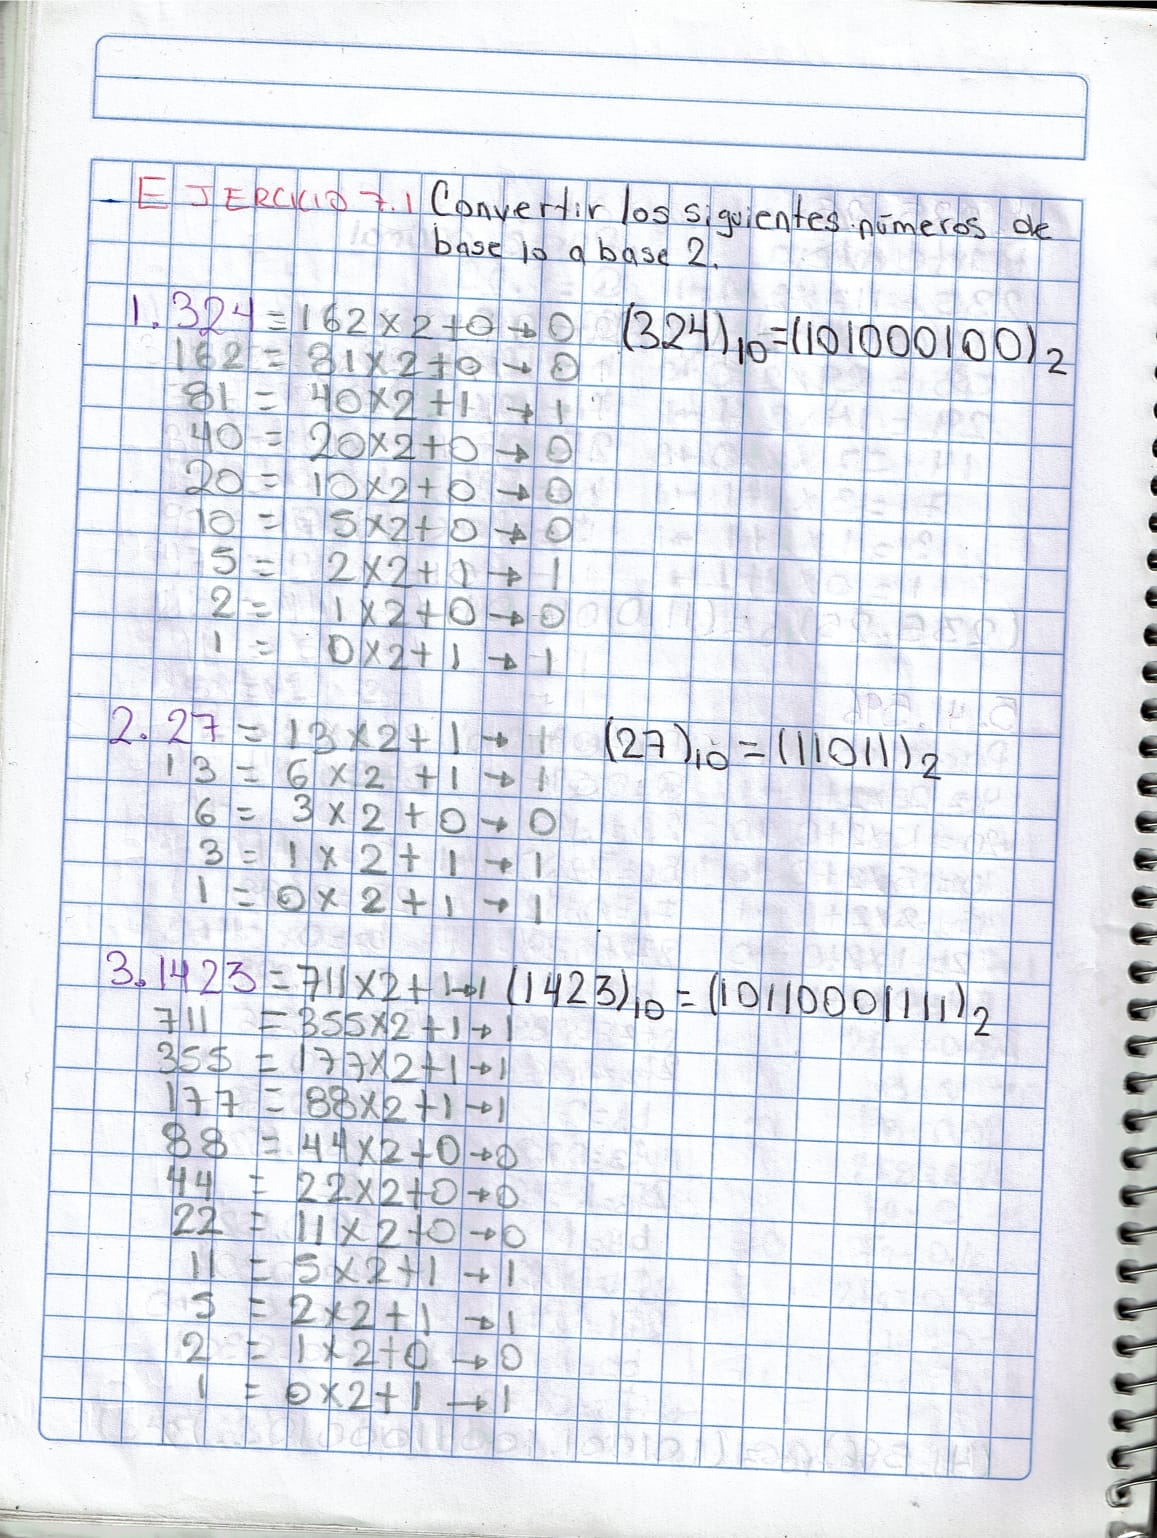
\includegraphics[width=6.25in,height=\textheight,keepaspectratio,alt={Ejercicios 1, 2 y 3}]{Ejercicio71Base2_123.jpg}
\caption{Ejercicios 1, 2 y 3}
\end{figure}

\begin{figure}
\centering
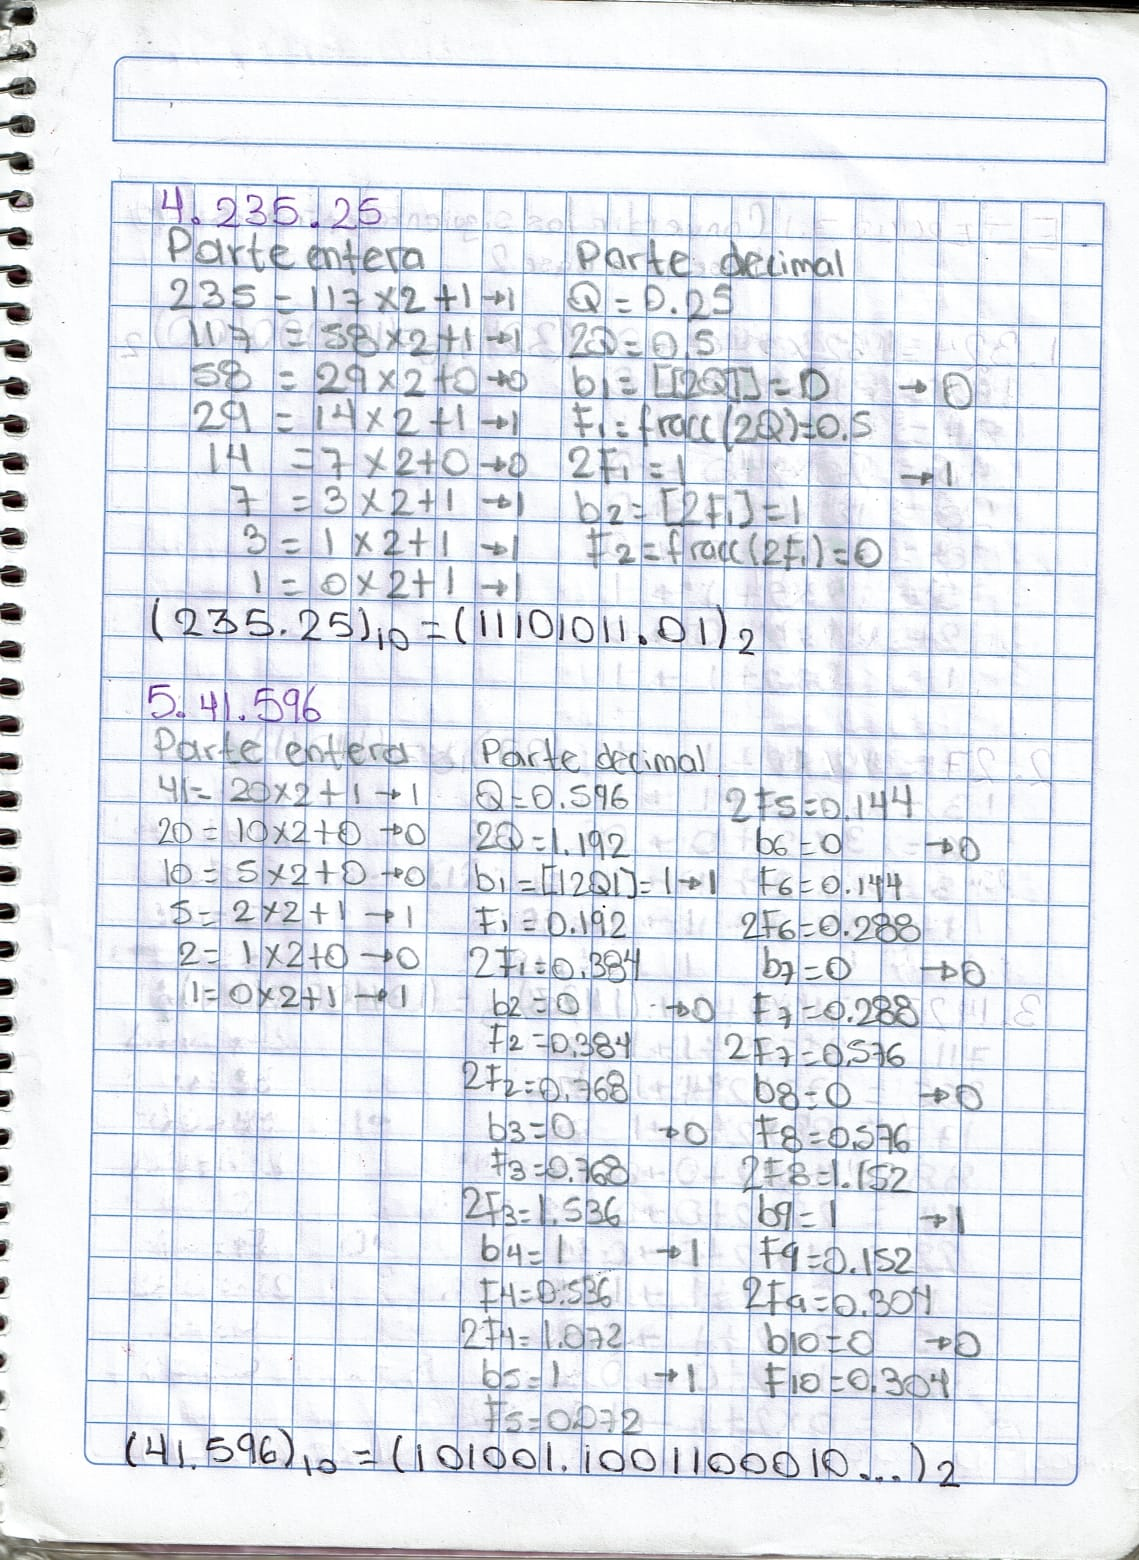
\includegraphics[width=6.25in,height=\textheight,keepaspectratio,alt={Ejercicios 4 y 5}]{Ejercicio71Base2_45.jpg}
\caption{Ejercicios 4 y 5}
\end{figure}

\begin{Shaded}
\begin{Highlighting}[]
\CommentTok{\# Asignación de funciones}

\CommentTok{\# Parte entera}

\NormalTok{binario }\OtherTok{\textless{}{-}} \ControlFlowTok{function}\NormalTok{(x) \{}
    \ControlFlowTok{if}\NormalTok{ (x }\SpecialCharTok{==} \DecValTok{0}\NormalTok{) }\FunctionTok{return}\NormalTok{(}\StringTok{"0"}\NormalTok{)}
\NormalTok{    nueva\_x }\OtherTok{\textless{}{-}} \FunctionTok{abs}\NormalTok{(x)}
\NormalTok{    iteracion }\OtherTok{\textless{}{-}} \StringTok{""}
    \ControlFlowTok{while}\NormalTok{ (nueva\_x }\SpecialCharTok{\textgreater{}} \DecValTok{0}\NormalTok{) \{}
\NormalTok{        iteracion }\OtherTok{\textless{}{-}} \FunctionTok{paste0}\NormalTok{(nueva\_x }\SpecialCharTok{\%\%}\NormalTok{ base, iteracion)}
\NormalTok{        nueva\_x }\OtherTok{\textless{}{-}}\NormalTok{ nueva\_x }\SpecialCharTok{\%/\%}\NormalTok{ base}
\NormalTok{    \}}
    \ControlFlowTok{if}\NormalTok{ (x }\SpecialCharTok{\textless{}} \DecValTok{0}\NormalTok{) iteracion }\OtherTok{\textless{}{-}} \FunctionTok{paste0}\NormalTok{(}\StringTok{"{-}"}\NormalTok{, iteracion)}
    \FunctionTok{return}\NormalTok{(iteracion)}
\NormalTok{\}}

\CommentTok{\# Parte decimal}

\NormalTok{decimal }\OtherTok{\textless{}{-}} \ControlFlowTok{function}\NormalTok{(x2) \{}
    \ControlFlowTok{if}\NormalTok{ (x2 }\SpecialCharTok{==} \DecValTok{0}\NormalTok{) }\FunctionTok{return}\NormalTok{(}\StringTok{"0"}\NormalTok{)}
\NormalTok{    nueva\_x }\OtherTok{\textless{}{-}}\NormalTok{ x2}
\NormalTok{    iteracion }\OtherTok{\textless{}{-}} \StringTok{"."}
    \ControlFlowTok{for}\NormalTok{ (i }\ControlFlowTok{in} \DecValTok{1}\SpecialCharTok{:}\DecValTok{10}\NormalTok{) \{}
\NormalTok{      nueva\_x }\OtherTok{\textless{}{-}}\NormalTok{ nueva\_x }\SpecialCharTok{*}\NormalTok{ base}
      \ControlFlowTok{if}\NormalTok{ (nueva\_x }\SpecialCharTok{\textgreater{}=} \DecValTok{1}\NormalTok{)}
\NormalTok{      \{}
\NormalTok{        iteracion }\OtherTok{\textless{}{-}} \FunctionTok{paste0}\NormalTok{(iteracion, }\StringTok{"1"}\NormalTok{)}
\NormalTok{       nueva\_x }\OtherTok{\textless{}{-}}\NormalTok{ nueva\_x }\SpecialCharTok{{-}}\DecValTok{1}
\NormalTok{      \}}
      \ControlFlowTok{else}\NormalTok{ \{}
\NormalTok{        iteracion }\OtherTok{\textless{}{-}} \FunctionTok{paste0}\NormalTok{(iteracion, }\StringTok{"0"}\NormalTok{)}
\NormalTok{      \}}
      \ControlFlowTok{if}\NormalTok{ (nueva\_x }\SpecialCharTok{==} \DecValTok{0}\NormalTok{) }\ControlFlowTok{break}
\NormalTok{    \} }
    \FunctionTok{return}\NormalTok{(iteracion)}
\NormalTok{\}}
\end{Highlighting}
\end{Shaded}

\subsubsection{\texorpdfstring{\(1.\) \(324\)}{1. 324}}\label{section}

\paragraph{Procedimiento}\label{procedimiento}

\begin{Shaded}
\begin{Highlighting}[]
\NormalTok{x }\OtherTok{\textless{}{-}} \DecValTok{324} \CommentTok{\#Número a convertir}
\NormalTok{base }\OtherTok{\textless{}{-}} \DecValTok{2} \CommentTok{\#Base a la que se convierte}

\NormalTok{resultado }\OtherTok{\textless{}{-}} \FunctionTok{binario}\NormalTok{(x)}
\end{Highlighting}
\end{Shaded}

\paragraph{Resultado}\label{resultado}

\begin{Shaded}
\begin{Highlighting}[]
\FunctionTok{paste0}\NormalTok{(}\StringTok{"El número "}\NormalTok{, x, }\StringTok{" convertido a base "}\NormalTok{, base, }\StringTok{" es: "}\NormalTok{, resultado)}
\end{Highlighting}
\end{Shaded}

\begin{verbatim}
## [1] "El número 324 convertido a base 2 es: 101000100"
\end{verbatim}

\subsubsection{\texorpdfstring{\(2.\) \(27\)}{2. 27}}\label{section-1}

\paragraph{Procedimiento}\label{procedimiento-1}

\begin{Shaded}
\begin{Highlighting}[]
\NormalTok{x }\OtherTok{\textless{}{-}} \DecValTok{27} \CommentTok{\#Número a convertir}
\NormalTok{base }\OtherTok{\textless{}{-}} \DecValTok{2} \CommentTok{\#Base a la que se convierte}

\NormalTok{resultado }\OtherTok{\textless{}{-}} \FunctionTok{binario}\NormalTok{(x)}
\end{Highlighting}
\end{Shaded}

\paragraph{Resultado}\label{resultado-1}

\begin{Shaded}
\begin{Highlighting}[]
\FunctionTok{paste0}\NormalTok{(}\StringTok{"El número "}\NormalTok{, x, }\StringTok{" convertido a base "}\NormalTok{, base, }\StringTok{" es: "}\NormalTok{, resultado)}
\end{Highlighting}
\end{Shaded}

\begin{verbatim}
## [1] "El número 27 convertido a base 2 es: 11011"
\end{verbatim}

\subsubsection{\texorpdfstring{\(3.\)
\(1423\)}{3. 1423}}\label{section-2}

\paragraph{Procedimiento}\label{procedimiento-2}

\begin{Shaded}
\begin{Highlighting}[]
\NormalTok{x }\OtherTok{\textless{}{-}} \DecValTok{1423} \CommentTok{\#Número a convertir}
\NormalTok{base }\OtherTok{\textless{}{-}} \DecValTok{2} \CommentTok{\#Base a la que se convierte}

\NormalTok{resultado }\OtherTok{\textless{}{-}} \FunctionTok{binario}\NormalTok{(x)}
\end{Highlighting}
\end{Shaded}

\paragraph{Resultado}\label{resultado-2}

\begin{Shaded}
\begin{Highlighting}[]
\FunctionTok{paste0}\NormalTok{(}\StringTok{"El número "}\NormalTok{, x, }\StringTok{" convertido a base "}\NormalTok{, base, }\StringTok{" es: "}\NormalTok{, resultado)}
\end{Highlighting}
\end{Shaded}

\begin{verbatim}
## [1] "El número 1423 convertido a base 2 es: 10110001111"
\end{verbatim}

\subsubsection{\texorpdfstring{\(4.\)
\(235.25\)}{4. 235.25}}\label{section-3}

\paragraph{Procedimiento}\label{procedimiento-3}

\begin{Shaded}
\begin{Highlighting}[]
\CommentTok{\# Parte entera}

\NormalTok{x1 }\OtherTok{\textless{}{-}} \DecValTok{235} \CommentTok{\#Número a convertir}
\NormalTok{base }\OtherTok{\textless{}{-}} \DecValTok{2} \CommentTok{\#Base a la que se convierte}

\NormalTok{resultado1 }\OtherTok{\textless{}{-}} \FunctionTok{binario}\NormalTok{(x1)}

\FunctionTok{paste0}\NormalTok{(}\StringTok{"La parte entera es: "}\NormalTok{, resultado1)}
\end{Highlighting}
\end{Shaded}

\begin{verbatim}
## [1] "La parte entera es: 11101011"
\end{verbatim}

\begin{Shaded}
\begin{Highlighting}[]
\CommentTok{\# Parte decimal}

\NormalTok{x2 }\OtherTok{\textless{}{-}} \FloatTok{0.25} \CommentTok{\#Número a convertir}
\NormalTok{base }\OtherTok{\textless{}{-}} \DecValTok{2} \CommentTok{\#Base a la que se convierte}

\NormalTok{resultado2 }\OtherTok{\textless{}{-}} \FunctionTok{decimal}\NormalTok{(x2)}

\FunctionTok{paste0}\NormalTok{(}\StringTok{"La parte decimal es: "}\NormalTok{, resultado2)}
\end{Highlighting}
\end{Shaded}

\begin{verbatim}
## [1] "La parte decimal es: .01"
\end{verbatim}

\begin{Shaded}
\begin{Highlighting}[]
\NormalTok{numero }\OtherTok{\textless{}{-}}\NormalTok{ x1 }\SpecialCharTok{+}\NormalTok{ x2}
\end{Highlighting}
\end{Shaded}

\paragraph{Resultado}\label{resultado-3}

\begin{Shaded}
\begin{Highlighting}[]
\FunctionTok{paste0}\NormalTok{(}\StringTok{"Juntando las dos partes, el número "}\NormalTok{, numero, }\StringTok{" es: "}\NormalTok{, resultado1, resultado2)}
\end{Highlighting}
\end{Shaded}

\begin{verbatim}
## [1] "Juntando las dos partes, el número 235.25 es: 11101011.01"
\end{verbatim}

\subsubsection{\texorpdfstring{\(5.\)
\(41.596\)}{5. 41.596}}\label{section-4}

\paragraph{Procedimiento}\label{procedimiento-4}

\begin{Shaded}
\begin{Highlighting}[]
\CommentTok{\# Parte entera}

\NormalTok{x1 }\OtherTok{\textless{}{-}} \DecValTok{41} \CommentTok{\#Número a convertir}
\NormalTok{base }\OtherTok{\textless{}{-}} \DecValTok{2} \CommentTok{\#Base a la que se convierte}

\NormalTok{resultado1 }\OtherTok{\textless{}{-}} \FunctionTok{binario}\NormalTok{(x1)}

\FunctionTok{paste0}\NormalTok{(}\StringTok{"La parte entera es: "}\NormalTok{, resultado1)}
\end{Highlighting}
\end{Shaded}

\begin{verbatim}
## [1] "La parte entera es: 101001"
\end{verbatim}

\begin{Shaded}
\begin{Highlighting}[]
\CommentTok{\# Parte decimal}

\NormalTok{x2 }\OtherTok{\textless{}{-}} \FloatTok{0.596} \CommentTok{\#Número a convertir}
\NormalTok{base }\OtherTok{\textless{}{-}} \DecValTok{2} \CommentTok{\#Base a la que se convierte}

\NormalTok{resultado2 }\OtherTok{\textless{}{-}} \FunctionTok{decimal}\NormalTok{(x2)}

\FunctionTok{paste0}\NormalTok{(}\StringTok{"La parte decimal es: "}\NormalTok{, resultado2)}
\end{Highlighting}
\end{Shaded}

\begin{verbatim}
## [1] "La parte decimal es: .1001100010"
\end{verbatim}

\begin{Shaded}
\begin{Highlighting}[]
\NormalTok{numero }\OtherTok{\textless{}{-}}\NormalTok{ x1 }\SpecialCharTok{+}\NormalTok{ x2}
\end{Highlighting}
\end{Shaded}

\paragraph{Resultado}\label{resultado-4}

\begin{Shaded}
\begin{Highlighting}[]
\FunctionTok{paste0}\NormalTok{(}\StringTok{"Juntando las dos partes, el número "}\NormalTok{, numero, }\StringTok{" es: "}\NormalTok{, resultado1, resultado2)}
\end{Highlighting}
\end{Shaded}

\begin{verbatim}
## [1] "Juntando las dos partes, el número 41.596 es: 101001.1001100010"
\end{verbatim}

\subsection{\texorpdfstring{\(7.2\) Breve historia de métodos númericos
y base
2}{7.2 Breve historia de métodos númericos y base 2}}\label{breve-historia-de-muxe9todos-nuxfamericos-y-base-2}

\subsubsection{\texorpdfstring{\(1.\) Breve
historia}{1. Breve historia}}\label{breve-historia}

Historia y evolución de los métodos numéricos

El análisis numérico representa una disciplina fundamental dentro de las
matemáticas aplicadas, dedicada al diseño y estudio de algoritmos para
obtener soluciones aproximadas a problemas matemáticos complejos. Estos
procedimientos sistemáticos, conocidos como métodos numéricos, han
evolucionado a la par del desarrollo tecnológico y científico de la
humanidad, constituyendo un puente esencial entre la teoría matemática y
las aplicaciones prácticas en ingeniería, física, economía y muchas
otras áreas del conocimiento.

Los primeros indicios de haberse utilizado los métodos numéricos se
remontan a las civilizaciones antiguas, donde ya existía la necesidad de
resolver problemas de cálculo en la vida cotidiana. Los babilonios que
se conocen por haber utilizado una de las primeras herramientas para el
cálculo conocido como el ábaco, alrededor del 2000 a.C., utilizaban
métodos iterativos para calcular raíces cuadradas, como lo demuestran
las tablillas de barro que se encontraron y se tienen conservadas hoy en
día. No obstante, fueron los griegos quienes establecieron un precedente
conceptual fundamental con Arquímedes (287-212 a.C.), cuyo ``método de
exhaución'' permitió acotar el valor de π (pi) y calcular el área del
círculo mediante polígonos regulares, encapsulando la esencia de la
aproximación sucesiva que caracteriza a los métodos numéricos modernos.

El desarrollo histórico de estas técnicas experimentó un impulso
significativo durante los siglos XVII y XVIII con el surgimiento del
cálculo infinitesimal y las contribuciones de genios matemáticos como
Isaac Newton, Leonhard Euler y Carl Friedrich Gauss. Newton no solo
desarrolló los fundamentos del cálculo, sino que también aportó
algoritmos prácticos como el método que lleva su nombre para encontrar
raíces de ecuaciones. Euler estableció las bases para resolver
ecuaciones diferenciales con su propuesta numérica, mientras que Gauss
desarrolló procedimientos fundamentales para sistemas de ecuaciones
lineales y técnicas de integración avanzada. Sin embargo, la aplicación
de estos métodos permaneció limitada a la tecnología de su época.

La verdadera revolución en el campo ocurrió durante el siglo XX con la
aparición de las computadoras electrónicas. Como señala Vargas et
al.~(s. f.) de la UNAM, esta innovación tecnológica transformó
radicalmente la disciplina, permitiendo implementar algoritmos numéricos
para resolver problemas a una escala antes inconcebible. Este periodo
presenció el surgimiento formal del análisis numérico como una
disciplina dedicada no solo a crear métodos, sino también a analizar su
estabilidad, convergencia y el impacto de los errores de redondeo. La
creación de librerías estandarizadas como EISPACK y LINPACK consolidó
las mejores prácticas y garantizó la confiabilidad de los cálculos,
estableciendo estándares de calidad en la implementación computacional.

Su importancia radica en su capacidad para resolver problemas que
carecen de solución analítica exacta o que son demasiado complejos para
abordarse mediante métodos tradicionales. Desde la industria
aeroespacial y la predicción meteorológica, hasta en la economía y el
entrenamiento de sistemas de inteligencia artificial, estos algoritmos
permiten modelar y analizar sistemas del mundo real con un nivel de
precisión sin precedentes. La evolución de los métodos numéricos ha
estado marcada por la interacción constante entre las necesidades
prácticas y el desarrollo teórico. Cada avance tecnológico, desde el
ábaco hasta las supercomputadoras modernas, ha expandido los horizontes
de lo que es posible calcular. El Renacimiento trajo consigo el
desarrollo de métodos para ecuaciones algebraicas, mientras que la era
industrial impulsó la creación de técnicas para ecuaciones diferenciales
que modelaban sistemas físicos complejos. El siglo XX, con la
computación digital, permitió implementar estos métodos de manera
sistemática y a gran escala además de rápida, dando lugar a nuevas áreas
como el análisis de error y el estudio de la estabilidad numérica.

Entornos de programación como MATLAB, Python con sus librerías
especializadas han puesto estas herramientas al alcance de todos,
permitiendo a estudiantes, investigadores y profesionales implementar
soluciones numéricas sin requerir conocimientos profundos en
computación. Esta accesibilidad ha acelerado la innovación y ha
permitido que los métodos numéricos encuentren aplicación en campos tan
diversos como la bioinformática, la ciencia de datos y la inteligencia
artificial.

En perspectiva, la historia de los métodos numéricos representa un viaje
continuo desde la intuición hasta el rigor algorítmico, desde la
aproximación manual hasta la simulación computacional de alta fidelidad.
Como bien señala Vargas et al.~(s. f.), estos métodos constituyen hoy
una herramienta indispensable en el arsenal de cualquier científico o
ingeniero, permitiendo traducir problemas del mundo real a formulaciones
matemáticas y encontrar soluciones útiles incluso cuando los métodos
analíticos tradicionales resultan insuficientes. Esto solo afirma que la
humanidad siempre busca cuantificar la información que posee y este
avanza al mismo tiempo que la humanidad misma.

Bibliografía

Martínez, R. C. (s. f.). Notas sobre Métodos Numéricos con R. GitHub.
\url{https://github.com/ProfTodoMundo/ProyectosMN/blob/main/Notas/NotasRaicesFunciones.pdf}

Pantoja, R. (2018). Guía de estudio de Métodos Numéricos {[}PDF{]}.
\url{https://www.cucei.udg.mx/maestrias/matedu/sites/default/files/25._met_num.pdf}

Vargas, T., \& Zamora, A. (s. f.). Historia métodos numéricos.
Matemáticas y Métodos Numéricos.
\url{https://blogceta.zaragoza.unam.mx/mnumericos/mn/mnintro/mn1b/}

\subsubsection{\texorpdfstring{\(2.\) Conversiones en base 2 a
mano}{2. Conversiones en base 2 a mano}}\label{conversiones-en-base-2-a-mano}

\begin{figure}
\centering
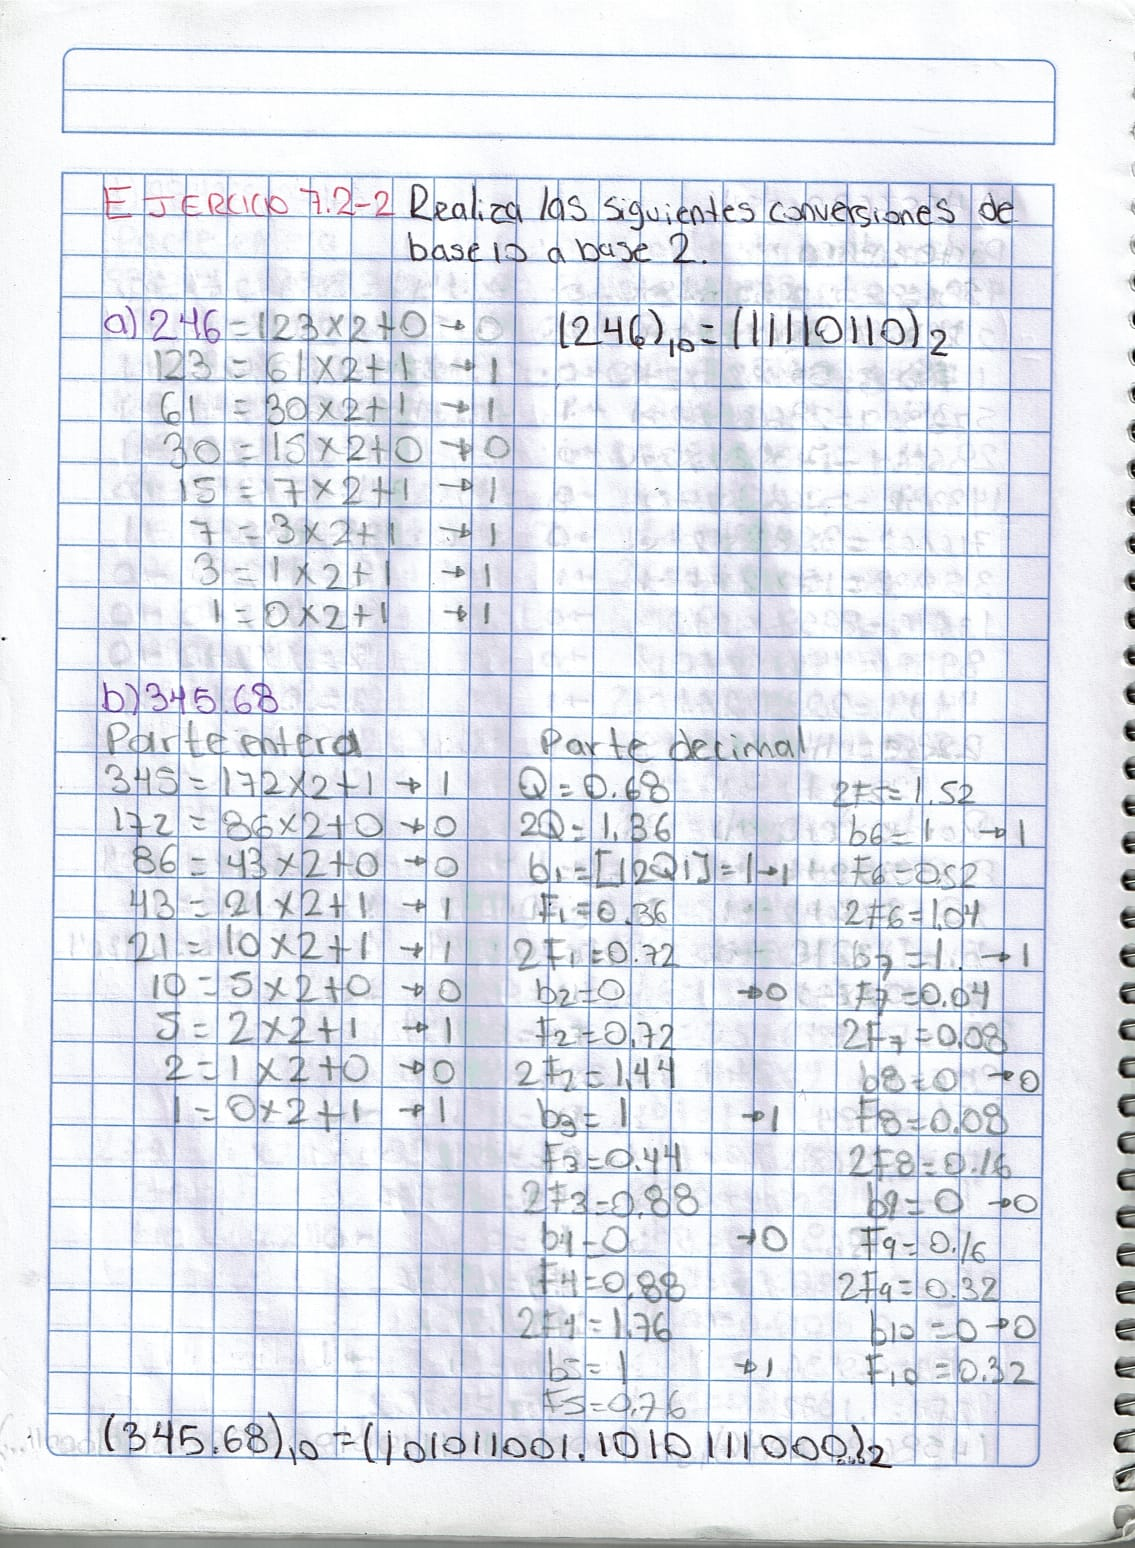
\includegraphics[width=6.25in,height=\textheight,keepaspectratio,alt={Ejercicios a y b}]{Ejercicio72Base2_ab.jpg}
\caption{Ejercicios a y b}
\end{figure}

\begin{figure}
\centering
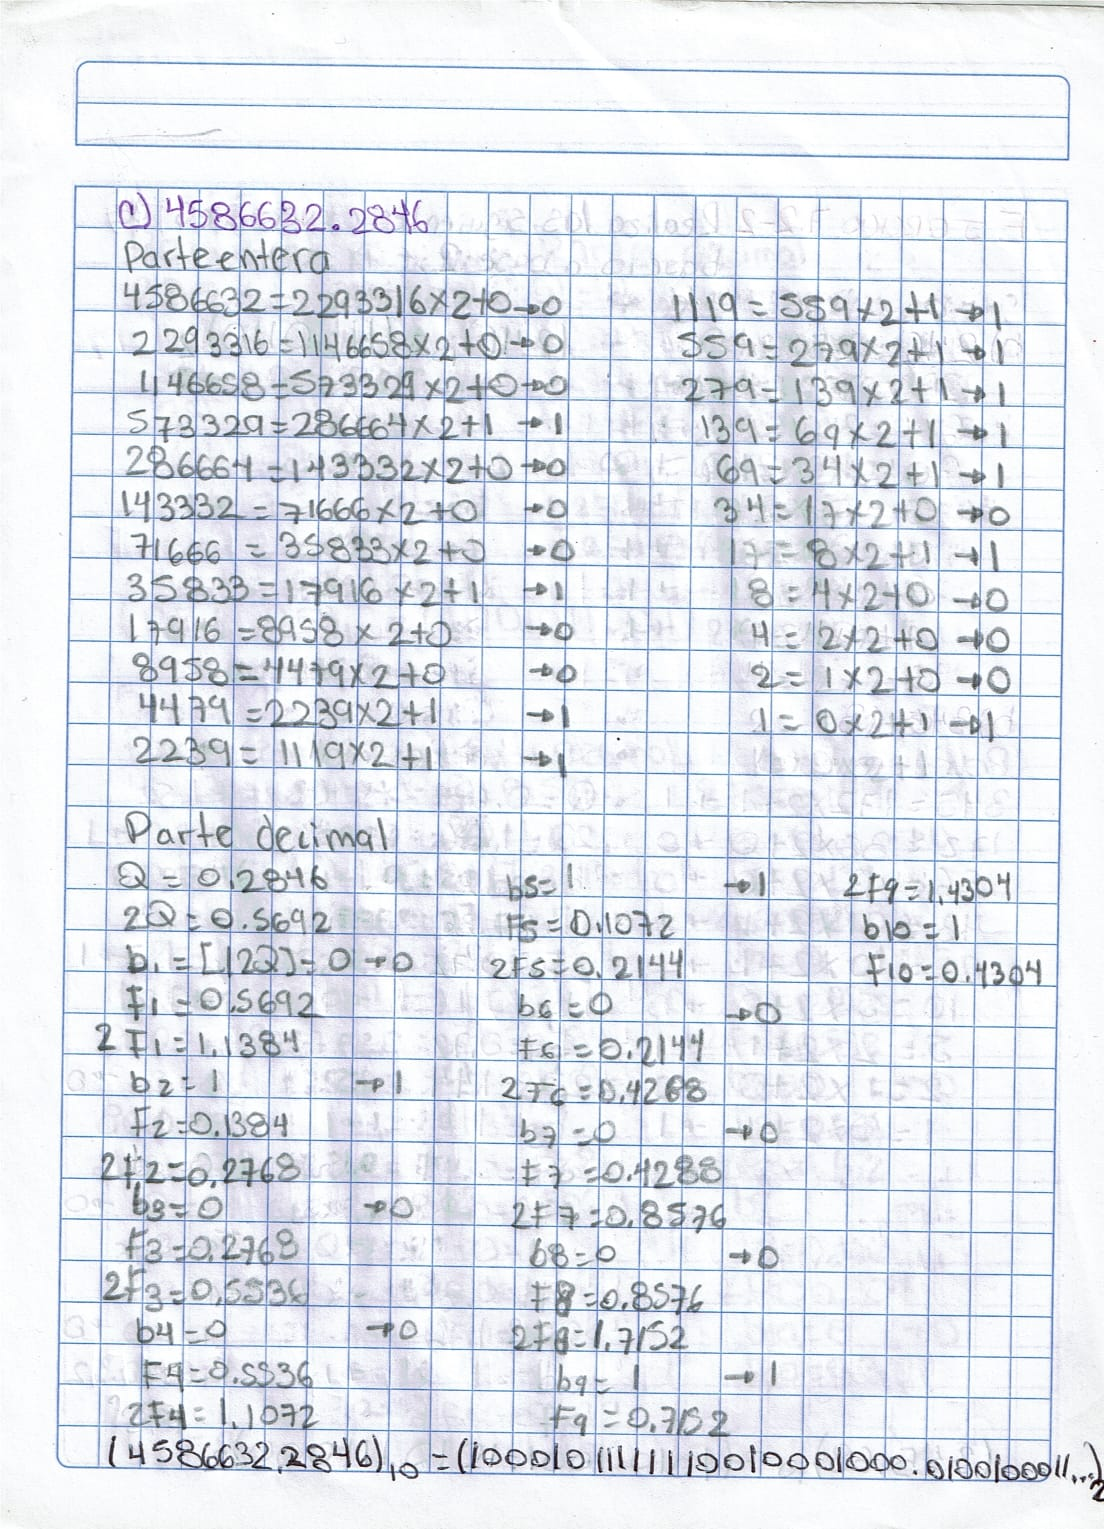
\includegraphics[width=6.25in,height=\textheight,keepaspectratio,alt={Ejercicio c}]{Ejercicio72Base2_c.jpg}
\caption{Ejercicio c}
\end{figure}

\begin{figure}
\centering
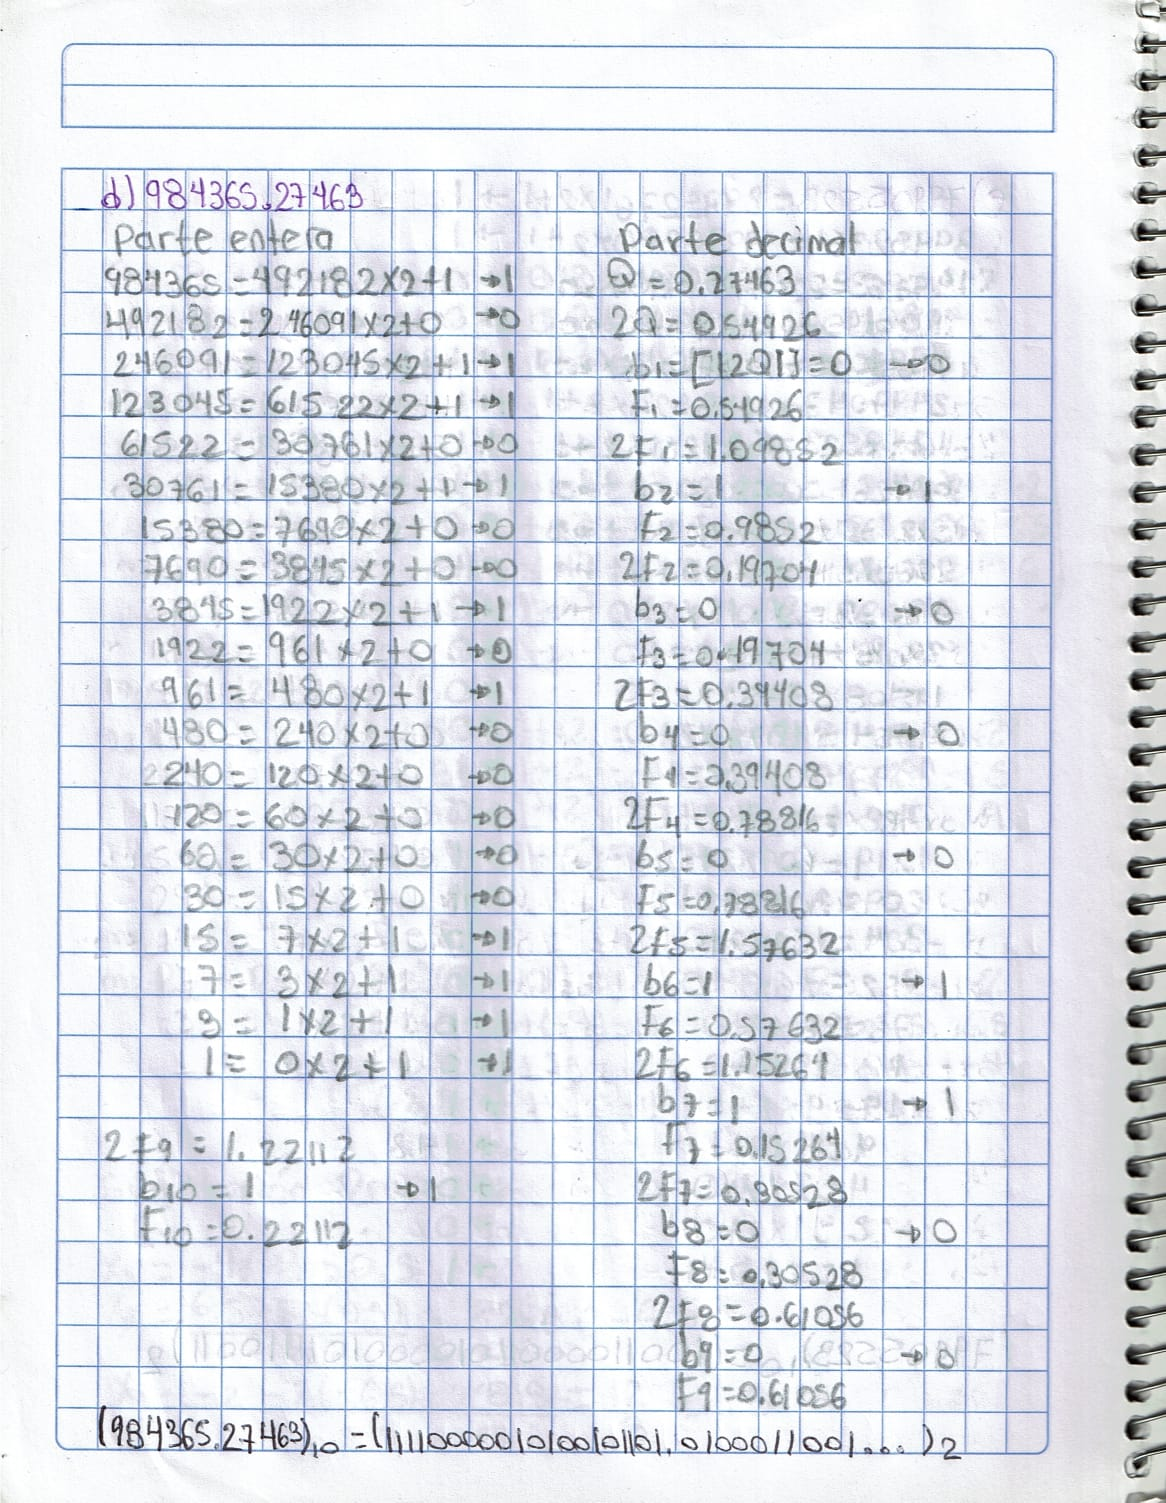
\includegraphics[width=6.25in,height=\textheight,keepaspectratio,alt={Ejercicio d}]{Ejercicio72Base2_d.jpg}
\caption{Ejercicio d}
\end{figure}

\begin{figure}
\centering
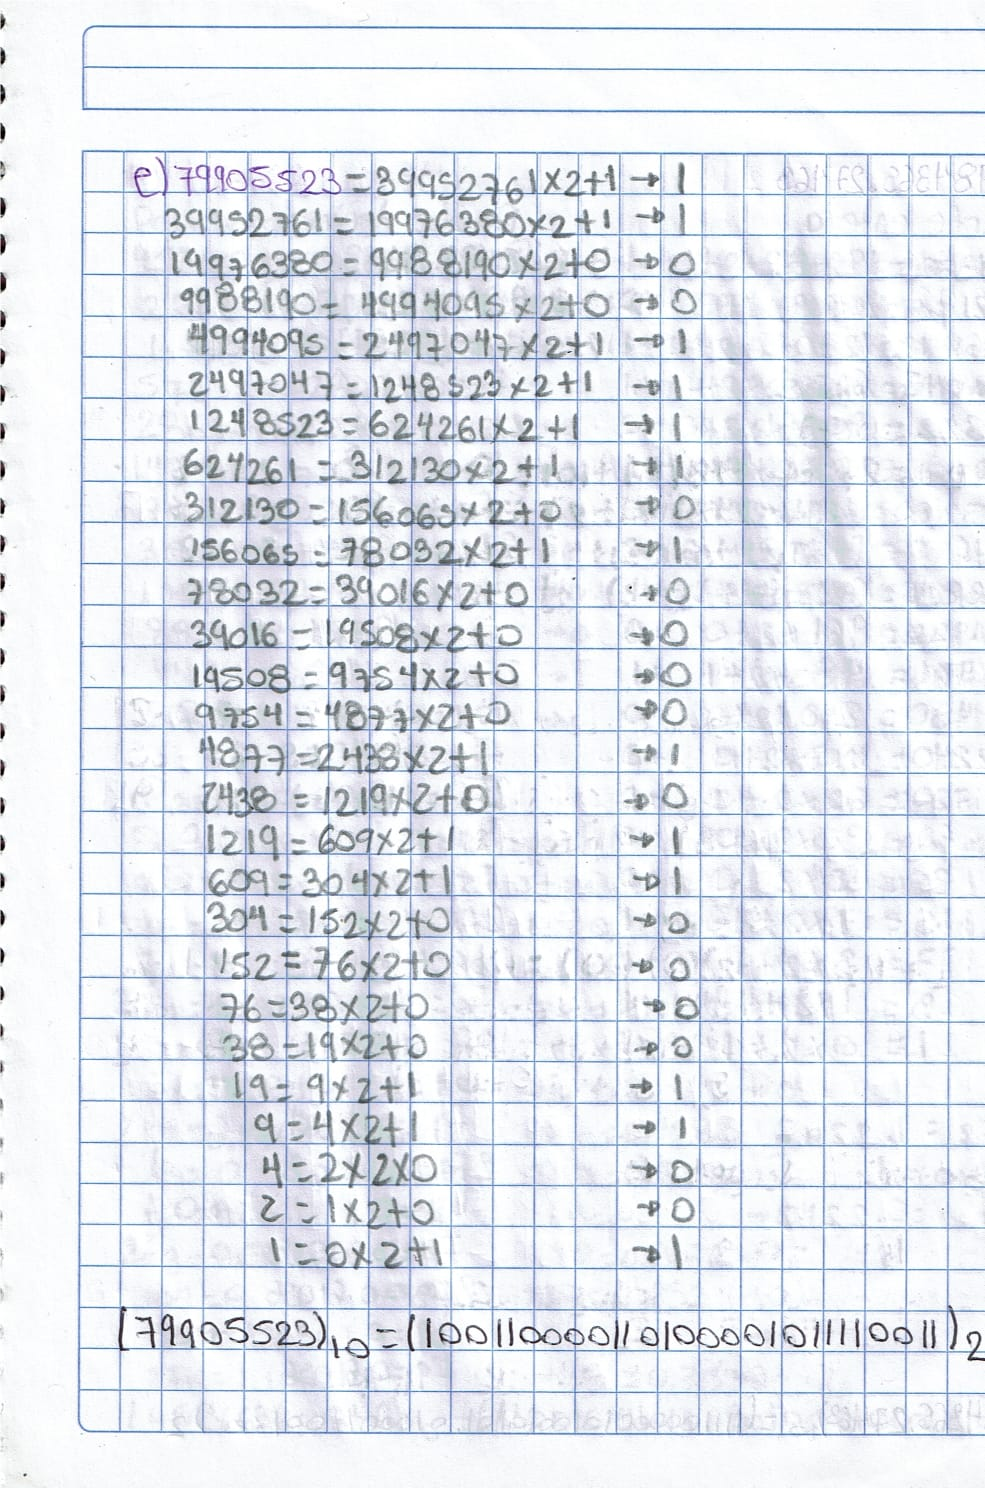
\includegraphics[width=6.25in,height=\textheight,keepaspectratio,alt={Ejercicio e}]{Ejercicio72Base2_e.jpg}
\caption{Ejercicio e}
\end{figure}

\subsubsection{\texorpdfstring{\(3.\) Conversiones en base 2 en
R}{3. Conversiones en base 2 en R}}\label{conversiones-en-base-2-en-r}

\paragraph{\texorpdfstring{\(a)\) \(246\)}{a) 246}}\label{a-246}

\subparagraph{Procedimiento}\label{procedimiento-5}

\begin{Shaded}
\begin{Highlighting}[]
\NormalTok{x }\OtherTok{\textless{}{-}} \DecValTok{246} \CommentTok{\#Número a convertir}
\NormalTok{base }\OtherTok{\textless{}{-}} \DecValTok{2} \CommentTok{\#Base a la que se convierte}

\NormalTok{resultado }\OtherTok{\textless{}{-}} \FunctionTok{binario}\NormalTok{(x)}
\end{Highlighting}
\end{Shaded}

\subparagraph{Resultado}\label{resultado-5}

\begin{Shaded}
\begin{Highlighting}[]
\FunctionTok{paste0}\NormalTok{(}\StringTok{"El número "}\NormalTok{, x, }\StringTok{" convertido a base "}\NormalTok{, base, }\StringTok{" es: "}\NormalTok{, resultado)}
\end{Highlighting}
\end{Shaded}

\begin{verbatim}
## [1] "El número 246 convertido a base 2 es: 11110110"
\end{verbatim}

\paragraph{\texorpdfstring{\(b)\)
\(345.68\)}{b) 345.68}}\label{b-345.68}

\subparagraph{Procedimiento}\label{procedimiento-6}

\begin{Shaded}
\begin{Highlighting}[]
\CommentTok{\# Parte entera}

\NormalTok{x1 }\OtherTok{\textless{}{-}} \DecValTok{345} \CommentTok{\#Número a convertir}
\NormalTok{base }\OtherTok{\textless{}{-}} \DecValTok{2} \CommentTok{\#Base a la que se convierte}

\NormalTok{resultado1 }\OtherTok{\textless{}{-}} \FunctionTok{binario}\NormalTok{(x1)}

\FunctionTok{paste0}\NormalTok{(}\StringTok{"La parte entera es: "}\NormalTok{, resultado1)}
\end{Highlighting}
\end{Shaded}

\begin{verbatim}
## [1] "La parte entera es: 101011001"
\end{verbatim}

\begin{Shaded}
\begin{Highlighting}[]
\CommentTok{\# Parte decimal}

\NormalTok{x2 }\OtherTok{\textless{}{-}} \FloatTok{0.68} \CommentTok{\#Número a convertir}
\NormalTok{base }\OtherTok{\textless{}{-}} \DecValTok{2} \CommentTok{\#Base a la que se convierte}

\NormalTok{resultado2 }\OtherTok{\textless{}{-}} \FunctionTok{decimal}\NormalTok{(x2)}

\FunctionTok{paste0}\NormalTok{(}\StringTok{"La parte decimal es: "}\NormalTok{, resultado2)}
\end{Highlighting}
\end{Shaded}

\begin{verbatim}
## [1] "La parte decimal es: .1010111000"
\end{verbatim}

\begin{Shaded}
\begin{Highlighting}[]
\NormalTok{numero }\OtherTok{\textless{}{-}}\NormalTok{ x1 }\SpecialCharTok{+}\NormalTok{ x2}
\end{Highlighting}
\end{Shaded}

\subparagraph{Resultado}\label{resultado-6}

\begin{Shaded}
\begin{Highlighting}[]
\FunctionTok{paste0}\NormalTok{(}\StringTok{"Juntando las dos partes, el número "}\NormalTok{, numero, }\StringTok{" es: "}\NormalTok{, resultado1, resultado2)}
\end{Highlighting}
\end{Shaded}

\begin{verbatim}
## [1] "Juntando las dos partes, el número 345.68 es: 101011001.1010111000"
\end{verbatim}

\paragraph{\texorpdfstring{\(c)\)
\(4586632.2846\)}{c) 4586632.2846}}\label{c-4586632.2846}

\subparagraph{Procedimiento}\label{procedimiento-7}

\begin{Shaded}
\begin{Highlighting}[]
\CommentTok{\# Parte entera}

\NormalTok{x1 }\OtherTok{\textless{}{-}} \DecValTok{4586632} \CommentTok{\#Número a convertir}
\NormalTok{base }\OtherTok{\textless{}{-}} \DecValTok{2} \CommentTok{\#Base a la que se convierte}

\NormalTok{resultado1 }\OtherTok{\textless{}{-}} \FunctionTok{binario}\NormalTok{(x1)}

\FunctionTok{paste0}\NormalTok{(}\StringTok{"La parte entera es: "}\NormalTok{, resultado1)}
\end{Highlighting}
\end{Shaded}

\begin{verbatim}
## [1] "La parte entera es: 10001011111110010001000"
\end{verbatim}

\begin{Shaded}
\begin{Highlighting}[]
\CommentTok{\# Parte decimal}

\NormalTok{x2 }\OtherTok{\textless{}{-}} \FloatTok{0.2846} \CommentTok{\#Número a convertir}
\NormalTok{base }\OtherTok{\textless{}{-}} \DecValTok{2} \CommentTok{\#Base a la que se convierte}

\NormalTok{resultado2 }\OtherTok{\textless{}{-}} \FunctionTok{decimal}\NormalTok{(x2)}

\FunctionTok{paste0}\NormalTok{(}\StringTok{"La parte decimal es: "}\NormalTok{, resultado2)}
\end{Highlighting}
\end{Shaded}

\begin{verbatim}
## [1] "La parte decimal es: .0100100011"
\end{verbatim}

\begin{Shaded}
\begin{Highlighting}[]
\NormalTok{numero }\OtherTok{\textless{}{-}}\NormalTok{ x1 }\SpecialCharTok{+}\NormalTok{ x2}
\end{Highlighting}
\end{Shaded}

\subparagraph{Resultado}\label{resultado-7}

\begin{Shaded}
\begin{Highlighting}[]
\FunctionTok{paste0}\NormalTok{(}\StringTok{"Juntando las dos partes, el número "}\NormalTok{, numero, }\StringTok{" es: "}\NormalTok{, resultado1, resultado2)}
\end{Highlighting}
\end{Shaded}

\begin{verbatim}
## [1] "Juntando las dos partes, el número 4586632.2846 es: 10001011111110010001000.0100100011"
\end{verbatim}

\paragraph{\texorpdfstring{\(d)\)
\(984365.27463\)}{d) 984365.27463}}\label{d-984365.27463}

\subparagraph{Procedimiento}\label{procedimiento-8}

\begin{Shaded}
\begin{Highlighting}[]
\CommentTok{\# Parte entera}

\NormalTok{x1 }\OtherTok{\textless{}{-}} \DecValTok{984365} \CommentTok{\#Número a convertir}
\NormalTok{base }\OtherTok{\textless{}{-}} \DecValTok{2} \CommentTok{\#Base a la que se convierte}

\NormalTok{resultado1 }\OtherTok{\textless{}{-}} \FunctionTok{binario}\NormalTok{(x1)}

\FunctionTok{paste0}\NormalTok{(}\StringTok{"La parte entera es: "}\NormalTok{, resultado1)}
\end{Highlighting}
\end{Shaded}

\begin{verbatim}
## [1] "La parte entera es: 11110000010100101101"
\end{verbatim}

\begin{Shaded}
\begin{Highlighting}[]
\CommentTok{\# Parte decimal}

\NormalTok{x2 }\OtherTok{\textless{}{-}} \FloatTok{0.27463} \CommentTok{\#Número a convertir}
\NormalTok{base }\OtherTok{\textless{}{-}} \DecValTok{2} \CommentTok{\#Base a la que se convierte}

\NormalTok{resultado2 }\OtherTok{\textless{}{-}} \FunctionTok{decimal}\NormalTok{(x2)}

\FunctionTok{paste0}\NormalTok{(}\StringTok{"La parte decimal es: "}\NormalTok{, resultado2)}
\end{Highlighting}
\end{Shaded}

\begin{verbatim}
## [1] "La parte decimal es: .0100011001"
\end{verbatim}

\begin{Shaded}
\begin{Highlighting}[]
\NormalTok{numero }\OtherTok{\textless{}{-}}\NormalTok{ x1 }\SpecialCharTok{+}\NormalTok{ x2}
\end{Highlighting}
\end{Shaded}

\subparagraph{Resultado}\label{resultado-8}

\begin{Shaded}
\begin{Highlighting}[]
\FunctionTok{paste0}\NormalTok{(}\StringTok{"Juntando las dos partes, el número "}\NormalTok{, numero, }\StringTok{" es: "}\NormalTok{, resultado1, resultado2)}
\end{Highlighting}
\end{Shaded}

\begin{verbatim}
## [1] "Juntando las dos partes, el número 984365.27463 es: 11110000010100101101.0100011001"
\end{verbatim}

\paragraph{\texorpdfstring{\(e)\)
\(79905523\)}{e) 79905523}}\label{e-79905523}

\subparagraph{Procedimiento}\label{procedimiento-9}

\begin{Shaded}
\begin{Highlighting}[]
\NormalTok{x }\OtherTok{\textless{}{-}} \DecValTok{79905523} \CommentTok{\#Número a convertir}
\NormalTok{base }\OtherTok{\textless{}{-}} \DecValTok{2} \CommentTok{\#Base a la que se convierte}

\NormalTok{resultado }\OtherTok{\textless{}{-}} \FunctionTok{binario}\NormalTok{(x)}
\end{Highlighting}
\end{Shaded}

\subparagraph{Resultado}\label{resultado-9}

\begin{Shaded}
\begin{Highlighting}[]
\FunctionTok{paste0}\NormalTok{(}\StringTok{"El número "}\NormalTok{, x, }\StringTok{" convertido a base "}\NormalTok{, base, }\StringTok{" es: "}\NormalTok{, resultado)}
\end{Highlighting}
\end{Shaded}

\begin{verbatim}
## [1] "El número 79905523 convertido a base 2 es: 100110000110100001011110011"
\end{verbatim}

\subsubsection{\texorpdfstring{\(4.\) Tipos de
Errores}{4. Tipos de Errores}}\label{tipos-de-errores}

Descripción Exhaustiva de los Tipos de Errores en Métodos Numéricos

En el ámbito de los métodos numéricos, la confiabilidad de un resultado
depende críticamente de la comprensión y el control de los errores
inherentes a todo proceso de cálculo. Dado que las soluciones rara vez
son exactas, es fundamental cuantificar y gestionar las discrepancias
entre el valor calculado y el valor real o teórico. Para expresar
numéricamente este nivel de confianza, se emplea el concepto de ``cifras
significativas'', que permite comunicar la precisión de una medición o
cálculo de manera estandarizada.

\(1\). Clasificación General de los Errores

Los errores en los cálculos numéricos se pueden clasificar en dos
categorías principales según su origen:

\(1.1\). Errores Inherentes o del Modelo

Estos errores son intrínsecos al problema mismo y surgen antes de
iniciar cualquier cálculo numérico. Sus fuentes principales son:

\begin{verbatim}
Incertidumbres en los datos de entrada: Ninguna magnitud física puede medirse con exactitud absoluta debido a las limitaciones de los instrumentos o a la naturaleza misma del fenómeno.

Equivocaciones: Errores humanos groseros, como una lectura incorrecta de un instrumento, una mala transcripción de datos o un descuido en el procedimiento, a menudo referidos como "ceguera de taller".

Simplificaciones del modelo matemático: Las suposiciones y simplificaciones que se realizan para modelar un fenómeno físico introducen inevitablemente una discrepancia con la realidad. Estos errores no pueden eliminarse por completo.
\end{verbatim}

\(1.2\). Errores del Método Numérico

Estos errores son introducidos por las aproximaciones necesarias para
resolver el problema de manera computacional. Se subdividen en:

Error de Truncamiento: Surge cuando un procedimiento matemático exacto,
que requiere un número infinito de operaciones, es reemplazado por uno
aproximado y finito. Un ejemplo clásico es el uso de un número limitado
de términos en una serie de Taylor para aproximar una función, o la
discretización de un proceso continuo usando un tamaño de paso \((h)\).
La notación \(O(hⁿ)\) se utiliza para describir el orden de magnitud de
este error.

\begin{verbatim}
Error de Redondeo: Se produce debido a que las computadoras tienen una precisión finita y deben representar los números reales con un conjunto limitado de bits (formato de punto flotante). Cuando un número no puede almacenarse con exactitud, debe ser redondeado. A diferencia del truncamiento, el redondeo afecta la última cifra significativa retenida. Existe un equilibrio crucial entre ambos: aumentar la precisión para reducir el redondeo puede incrementar el costo computacional y, en algunos casos, la propagación de otros errores.
\end{verbatim}

\(2\). Cuantificación de los Errores

Para evaluar la magnitud de un error, se utilizan las siguientes
definiciones:

Error Absoluto \((E)\): Representa la diferencia directa entre el valor
real \((V_{real})\) y el valor aproximado \((V_{aprox})\).

\(E = |V_{real} – V_{aprox}|\)

Error Relativo \((e)\): Proporciona una medida del error en relación con
la magnitud del valor real, lo que lo hace más significativo para
comparar precisiones en diferentes escalas. Suele expresarse como
porcentaje.

\(e = \frac{|V_{real} – V_{aprox}|}{|V_{real}|} × 100%
\)

En la práctica del análisis numérico, donde el valor real exacto a
menudo se desconoce, es común aproximar el error absoluto en un proceso
iterativo como la diferencia entre dos iteraciones consecutivas:
\(E ≈ |V_i – V_{i-1}|\).

\(3\). Errores en Punto Flotante y Precisión de Máquina

Dado que las computadoras almacenan números en formato binario de punto
flotante, la representación exacta de muchos números reales es
imposible. Un número real \((x)\) se almacena como una aproximación,
\(fl(x)\), tal que:

\(x = fl(x) × (1 + ε),donde |ε| ≤ ε_{mach}\)

El valor \(ε_{mach}\) se conoce como ``precisión de máquina'' y
representa el error de redondeo relativo máximo posible para un sistema
computacional dado. Su valor depende directamente del número de bits
asignados a la mantisa.

\(4\). Aproximación Numérica: Convergencia, Estabilidad y Robustez

Una ``aproximación numérica'' es un valor que se acerca a la solución
real, y la diferencia entre ambos constituye el error. En este contexto,
se evalúan propiedades clave de los métodos numéricos:

Convergencia: Un método es convergente si, a medida que avanza el
proceso iterativo (por ejemplo, reduciendo el tamaño de paso \(h\)), la
solución aproximada se acerca progresivamente a la solución exacta. Un
método converge de forma monótona si
\(|x_n – x_{n-1}| ≤ |x_{n-1} – x_{n-2}|\).

\begin{verbatim}
Estabilidad: Un método es estable si los pequeños errores iniciales (como los de redondeo) no se amplifican descontroladamente durante los sucesivos cálculos, evitando que la solución se desvíe catastróficamente.

Robustez: Un método robusto combina la convergencia y la estabilidad, siendo capaz de proporcionar resultados confiables incluso ante una amplia gama de condiciones iniciales o problemas mal condicionados, sin ser excesivamente sensible a las perturbaciones numéricas.
\end{verbatim}

La búsqueda de métodos que sean a la vez convergentes, estables y
robustos es uno de los objetivos centrales en el diseño y la selección
de algoritmos numéricos efectivos.

\section{Solucion de Sistemas de Ecuaciones Lineales por métodos
directos}\label{solucion-de-sistemas-de-ecuaciones-lineales-por-muxe9todos-directos}

\subsection{\texorpdfstring{\(7.3.\) Eliminación Gaussiana Simple
(Método
directo)}{7.3. Eliminación Gaussiana Simple (Método directo)}}\label{eliminaciuxf3n-gaussiana-simple-muxe9todo-directo}

\subsubsection{Ejercicios a mano}\label{ejercicios-a-mano-1}

\begin{figure}
\centering
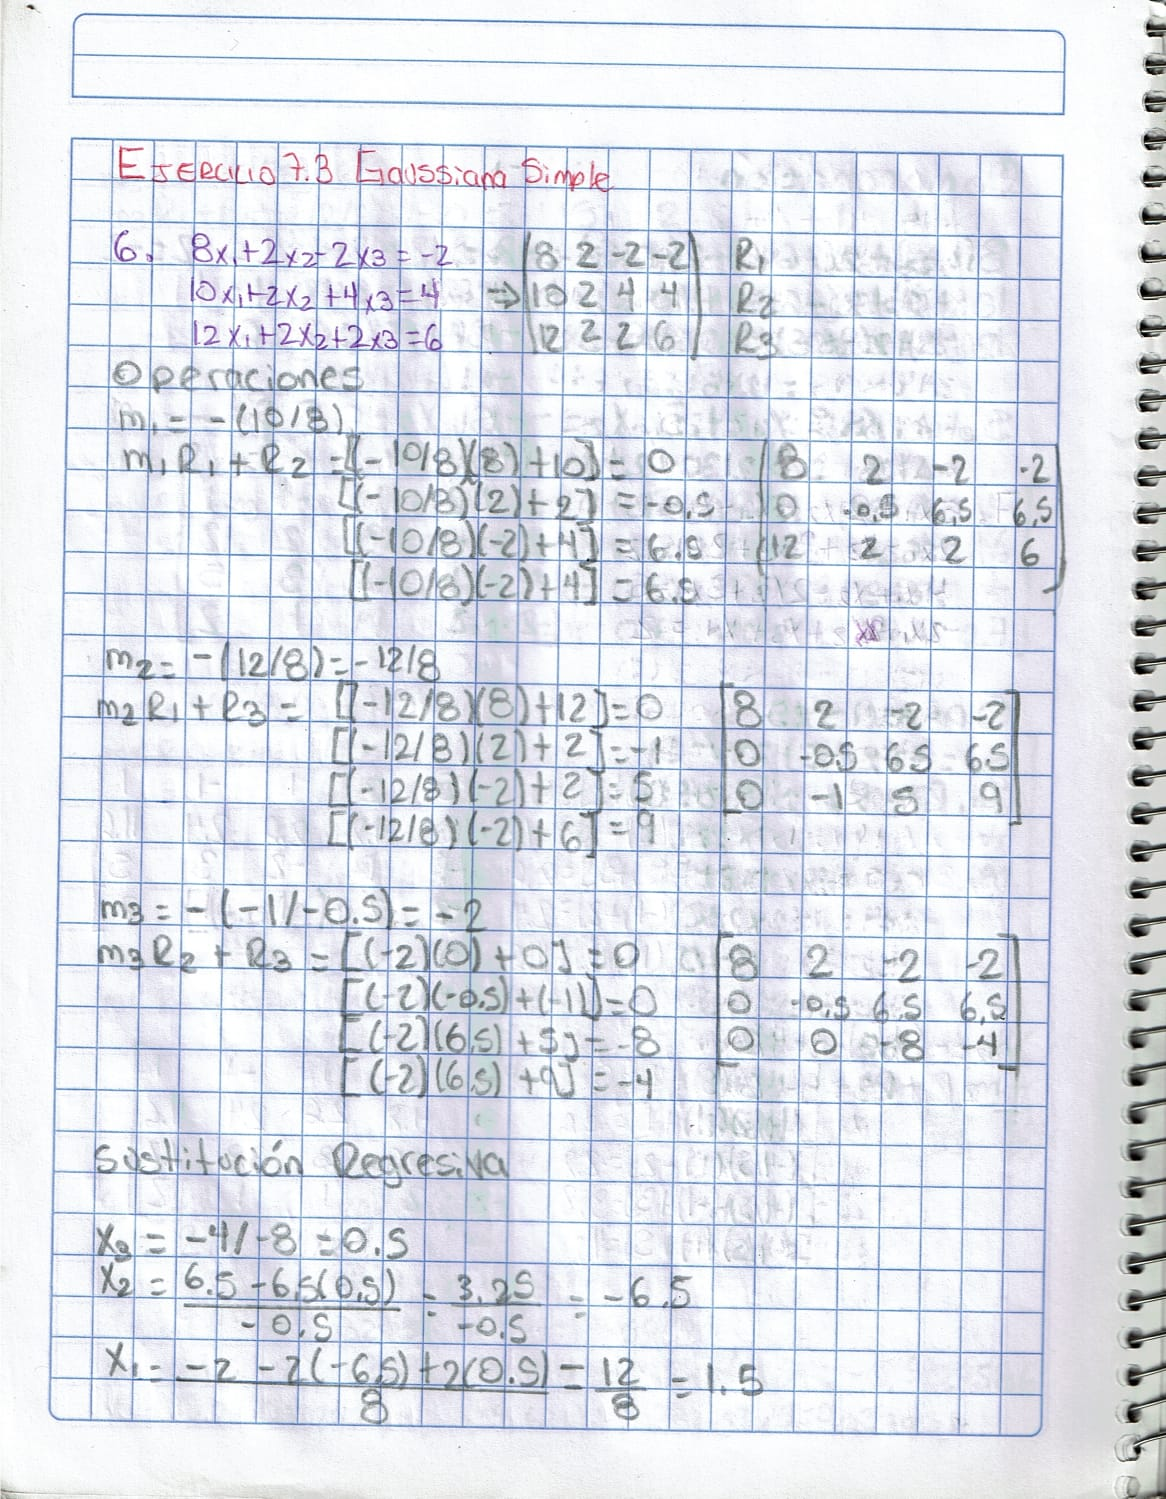
\includegraphics[width=6.25in,height=\textheight,keepaspectratio,alt={Ejercicio 6}]{Ejercicio73Gauss6.jpg}
\caption{Ejercicio 6}
\end{figure}

\begin{figure}
\centering
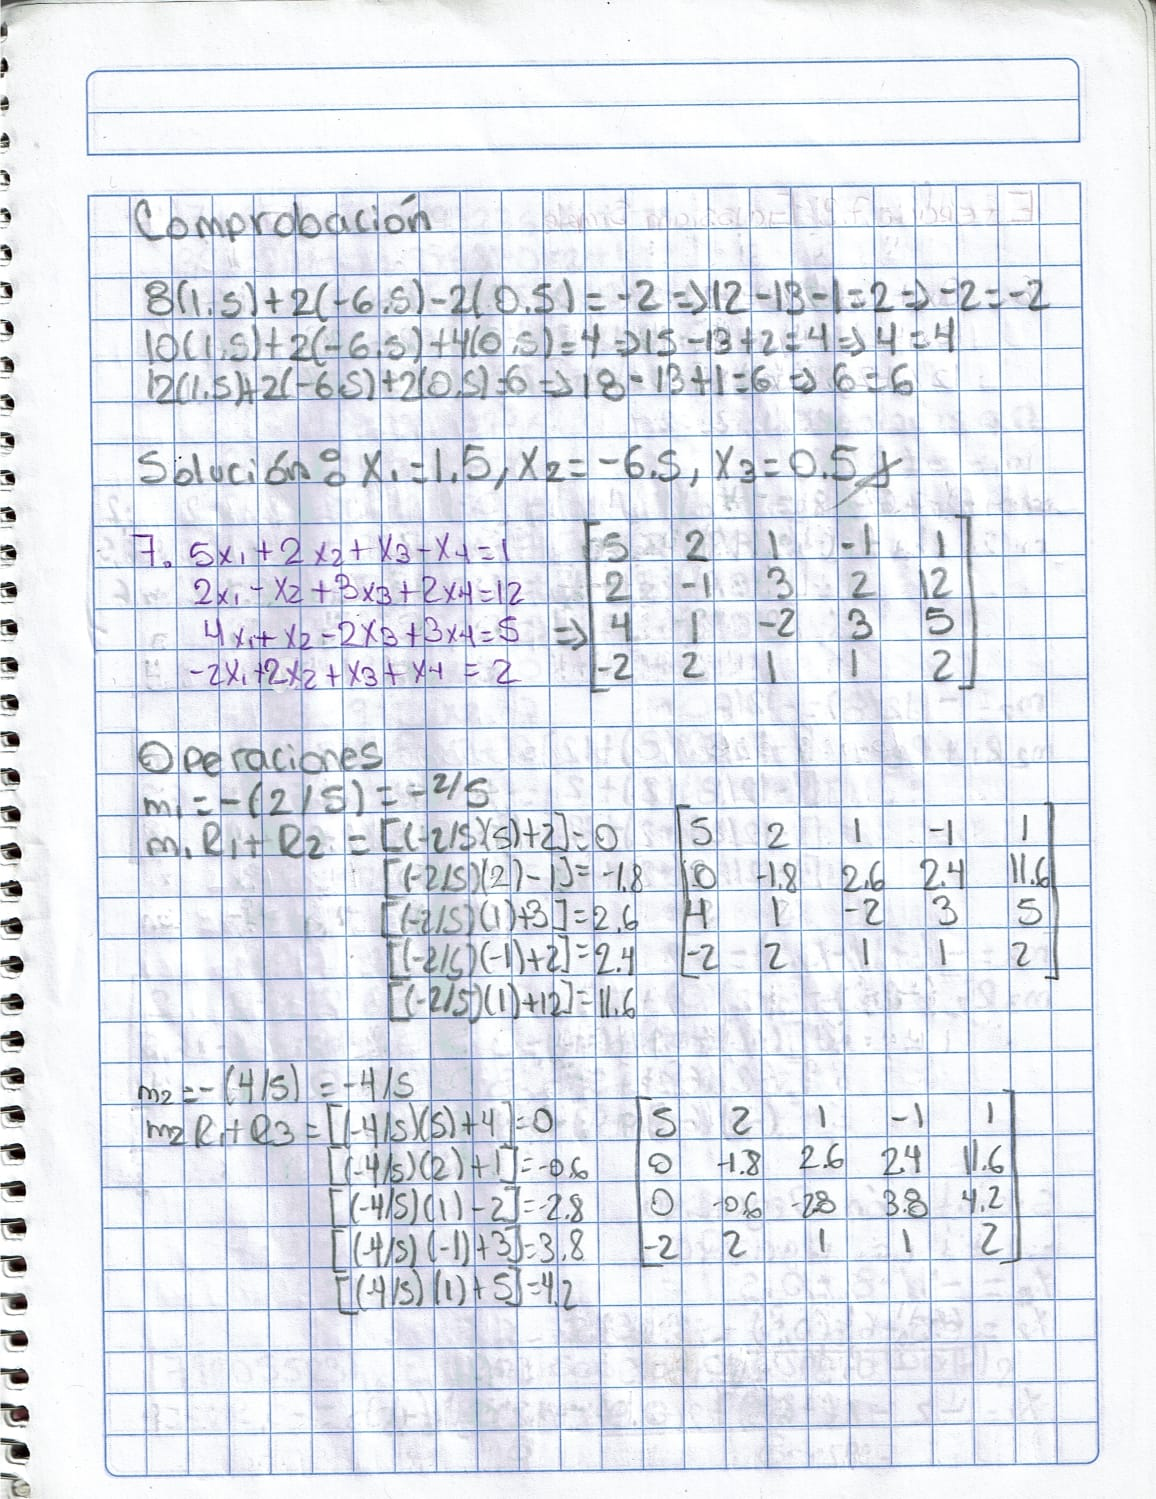
\includegraphics[width=6.25in,height=\textheight,keepaspectratio,alt={Ejercicio 7}]{Ejercicio73Gauss7.jpg}
\caption{Ejercicio 7}
\end{figure}

\begin{figure}
\centering
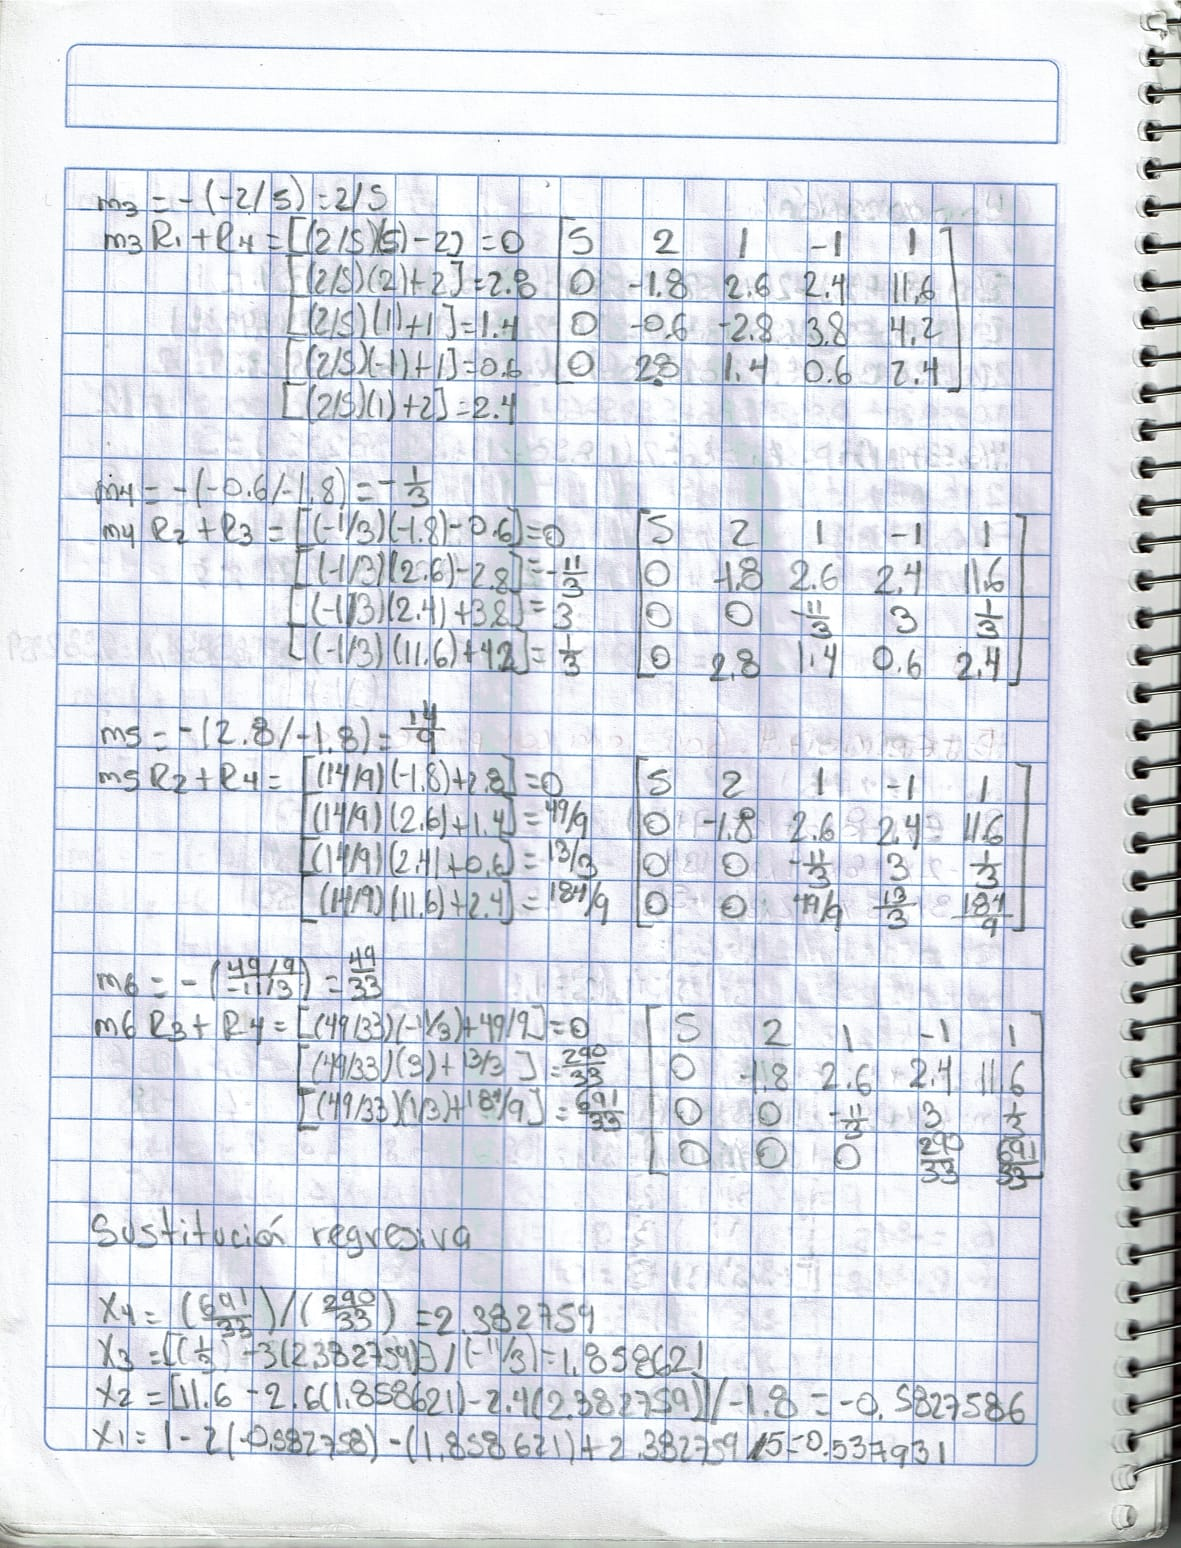
\includegraphics[width=6.25in,height=\textheight,keepaspectratio,alt={Ejercicio 7-2}]{Ejercicio73Gauss7_2.jpg}
\caption{Ejercicio 7-2}
\end{figure}

\begin{figure}
\centering
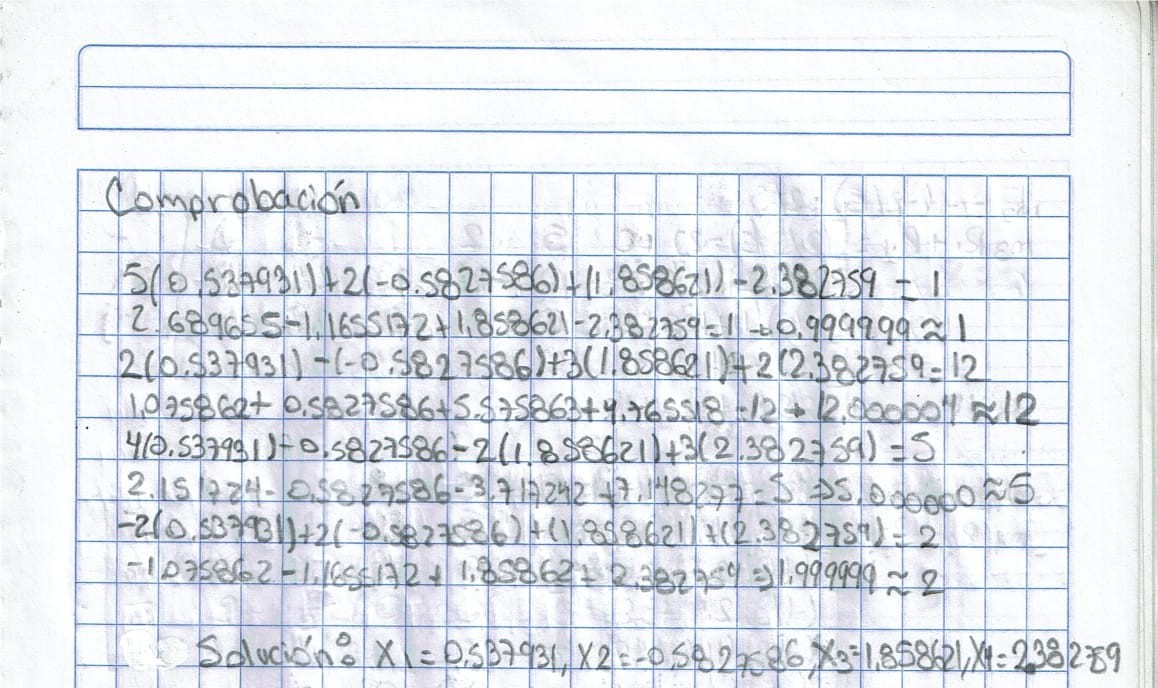
\includegraphics[width=6.25in,height=\textheight,keepaspectratio,alt={Ejercicio 7-3}]{Ejercicio73Gauss7_3.jpg}
\caption{Ejercicio 7-3}
\end{figure}

\subsubsection{\texorpdfstring{Sistema
\(1\)}{Sistema 1}}\label{sistema-1}

\(x_1 − 2x_2 + 0.5x_3 = −5\)

\(−2x_1 + 5x_2 − 1.5x_3 = 0\)

\(−0.2x_1 + 1.75x_2 − x_3 = 10\)

\begin{Shaded}
\begin{Highlighting}[]
\NormalTok{A }\OtherTok{\textless{}{-}} \FunctionTok{matrix}\NormalTok{(}\FunctionTok{c}\NormalTok{(}\DecValTok{1}\NormalTok{, }\SpecialCharTok{{-}}\DecValTok{2}\NormalTok{, }\FloatTok{0.5}\NormalTok{,}
              \SpecialCharTok{{-}}\DecValTok{2}\NormalTok{, }\DecValTok{5}\NormalTok{, }\SpecialCharTok{{-}}\FloatTok{1.5}\NormalTok{,}
              \SpecialCharTok{{-}}\FloatTok{0.2}\NormalTok{, }\FloatTok{1.75}\NormalTok{, }\SpecialCharTok{{-}}\DecValTok{1}\NormalTok{),}
      \AttributeTok{nrow =} \DecValTok{3}\NormalTok{, }\AttributeTok{byrow =} \ConstantTok{TRUE}\NormalTok{)}
\NormalTok{b }\OtherTok{\textless{}{-}} \FunctionTok{matrix}\NormalTok{(}\FunctionTok{c}\NormalTok{(}\SpecialCharTok{{-}}\DecValTok{5}\NormalTok{, }\DecValTok{0}\NormalTok{, }\DecValTok{10}\NormalTok{), }\AttributeTok{nrow =} \DecValTok{3}\NormalTok{)}

\NormalTok{Ab }\OtherTok{\textless{}{-}} \FunctionTok{cbind}\NormalTok{(A,b); (Ab)}
\end{Highlighting}
\end{Shaded}

\begin{verbatim}
##      [,1]  [,2] [,3] [,4]
## [1,]  1.0 -2.00  0.5   -5
## [2,] -2.0  5.00 -1.5    0
## [3,] -0.2  1.75 -1.0   10
\end{verbatim}

\paragraph{Procedimiento}\label{procedimiento-10}

\begin{Shaded}
\begin{Highlighting}[]
\CommentTok{\# Primera eliminación}

\NormalTok{m1 }\OtherTok{\textless{}{-}} \SpecialCharTok{{-}}\NormalTok{Ab[}\DecValTok{2}\NormalTok{,}\DecValTok{1}\NormalTok{] }\SpecialCharTok{/}\NormalTok{ Ab[}\DecValTok{1}\NormalTok{,}\DecValTok{1}\NormalTok{]}
\NormalTok{(m1)}
\end{Highlighting}
\end{Shaded}

\begin{verbatim}
## [1] 2
\end{verbatim}

\begin{Shaded}
\begin{Highlighting}[]
\NormalTok{m2 }\OtherTok{\textless{}{-}} \SpecialCharTok{{-}}\NormalTok{Ab[}\DecValTok{3}\NormalTok{,}\DecValTok{1}\NormalTok{] }\SpecialCharTok{/}\NormalTok{ Ab[}\DecValTok{1}\NormalTok{,}\DecValTok{1}\NormalTok{]}
\NormalTok{(m2)}
\end{Highlighting}
\end{Shaded}

\begin{verbatim}
## [1] 0.2
\end{verbatim}

\begin{Shaded}
\begin{Highlighting}[]
\NormalTok{A1 }\OtherTok{\textless{}{-}}\NormalTok{ Ab[}\DecValTok{1}\NormalTok{,]}
\NormalTok{(A1)}
\end{Highlighting}
\end{Shaded}

\begin{verbatim}
## [1]  1.0 -2.0  0.5 -5.0
\end{verbatim}

\begin{Shaded}
\begin{Highlighting}[]
\NormalTok{A2 }\OtherTok{\textless{}{-}}\NormalTok{ m1 }\SpecialCharTok{*}\NormalTok{ Ab[}\DecValTok{1}\NormalTok{,] }\SpecialCharTok{+}\NormalTok{ Ab[}\DecValTok{2}\NormalTok{,]}
\NormalTok{(A2)}
\end{Highlighting}
\end{Shaded}

\begin{verbatim}
## [1]   0.0   1.0  -0.5 -10.0
\end{verbatim}

\begin{Shaded}
\begin{Highlighting}[]
\NormalTok{A3 }\OtherTok{\textless{}{-}}\NormalTok{ m2 }\SpecialCharTok{*}\NormalTok{ Ab[}\DecValTok{1}\NormalTok{,] }\SpecialCharTok{+}\NormalTok{ Ab[}\DecValTok{3}\NormalTok{,]}
\NormalTok{(A3)}
\end{Highlighting}
\end{Shaded}

\begin{verbatim}
## [1]  0.00  1.35 -0.90  9.00
\end{verbatim}

\begin{Shaded}
\begin{Highlighting}[]
\NormalTok{NuevaA }\OtherTok{\textless{}{-}} \FunctionTok{rbind}\NormalTok{(A1, A2, A3)}
\NormalTok{(NuevaA)}
\end{Highlighting}
\end{Shaded}

\begin{verbatim}
##    [,1]  [,2] [,3] [,4]
## A1    1 -2.00  0.5   -5
## A2    0  1.00 -0.5  -10
## A3    0  1.35 -0.9    9
\end{verbatim}

\begin{Shaded}
\begin{Highlighting}[]
\CommentTok{\# Segunda eliminación}

\NormalTok{Ab }\OtherTok{\textless{}{-}}\NormalTok{ NuevaA}
\NormalTok{m3 }\OtherTok{\textless{}{-}}\SpecialCharTok{{-}}\NormalTok{Ab[}\DecValTok{3}\NormalTok{,}\DecValTok{2}\NormalTok{] }\SpecialCharTok{/}\NormalTok{ Ab[}\DecValTok{2}\NormalTok{,}\DecValTok{2}\NormalTok{]}
\NormalTok{(m3)}
\end{Highlighting}
\end{Shaded}

\begin{verbatim}
##    A3 
## -1.35
\end{verbatim}

\begin{Shaded}
\begin{Highlighting}[]
\NormalTok{A3 }\OtherTok{\textless{}{-}}\NormalTok{ m3 }\SpecialCharTok{*}\NormalTok{ Ab[}\DecValTok{2}\NormalTok{,] }\SpecialCharTok{+}\NormalTok{ Ab[}\DecValTok{3}\NormalTok{,]}
\NormalTok{(A3)}
\end{Highlighting}
\end{Shaded}

\begin{verbatim}
## [1]  0.000  0.000 -0.225 22.500
\end{verbatim}

\begin{Shaded}
\begin{Highlighting}[]
\NormalTok{NuevaA }\OtherTok{\textless{}{-}} \FunctionTok{rbind}\NormalTok{(A1, A2, A3)}
\NormalTok{(NuevaA)}
\end{Highlighting}
\end{Shaded}

\begin{verbatim}
##    [,1] [,2]   [,3]  [,4]
## A1    1   -2  0.500  -5.0
## A2    0    1 -0.500 -10.0
## A3    0    0 -0.225  22.5
\end{verbatim}

Con esto sabemos los valores de \(x_n\)

\begin{Shaded}
\begin{Highlighting}[]
\CommentTok{\# Sustitución regresiva}

\NormalTok{Ab }\OtherTok{\textless{}{-}}\NormalTok{ NuevaA}
\NormalTok{x3 }\OtherTok{\textless{}{-}}\NormalTok{ Ab[}\DecValTok{3}\NormalTok{,}\DecValTok{4}\NormalTok{] }\SpecialCharTok{/}\NormalTok{ Ab[}\DecValTok{3}\NormalTok{,}\DecValTok{3}\NormalTok{]; (x3)}
\end{Highlighting}
\end{Shaded}

\begin{verbatim}
##   A3 
## -100
\end{verbatim}

\begin{Shaded}
\begin{Highlighting}[]
\NormalTok{x2 }\OtherTok{\textless{}{-}}\NormalTok{ (Ab[}\DecValTok{2}\NormalTok{,}\DecValTok{4}\NormalTok{] }\SpecialCharTok{{-}}\NormalTok{ (Ab[}\DecValTok{2}\NormalTok{,}\DecValTok{3}\NormalTok{] }\SpecialCharTok{*}\NormalTok{ x3)) }\SpecialCharTok{/}\NormalTok{ Ab[}\DecValTok{2}\NormalTok{,}\DecValTok{2}\NormalTok{]; (x2)}
\end{Highlighting}
\end{Shaded}

\begin{verbatim}
##  A2 
## -60
\end{verbatim}

\begin{Shaded}
\begin{Highlighting}[]
\NormalTok{x1 }\OtherTok{\textless{}{-}}\NormalTok{ (Ab[}\DecValTok{1}\NormalTok{,}\DecValTok{4}\NormalTok{] }\SpecialCharTok{{-}}\NormalTok{ (Ab[}\DecValTok{1}\NormalTok{,}\DecValTok{2}\NormalTok{] }\SpecialCharTok{*}\NormalTok{ x2) }\SpecialCharTok{{-}}\NormalTok{ (Ab[}\DecValTok{1}\NormalTok{,}\DecValTok{3}\NormalTok{] }\SpecialCharTok{*}\NormalTok{ x3)) }\SpecialCharTok{/}\NormalTok{ Ab[}\DecValTok{1}\NormalTok{,}\DecValTok{1}\NormalTok{]; (x1)}
\end{Highlighting}
\end{Shaded}

\begin{verbatim}
##  A1 
## -75
\end{verbatim}

\begin{Shaded}
\begin{Highlighting}[]
\CommentTok{\# Comprobación}

\NormalTok{I }\OtherTok{\textless{}{-}}\NormalTok{ b[}\DecValTok{1}\NormalTok{,]; (I)}
\end{Highlighting}
\end{Shaded}

\begin{verbatim}
## [1] -5
\end{verbatim}

\begin{Shaded}
\begin{Highlighting}[]
\NormalTok{II }\OtherTok{\textless{}{-}}\NormalTok{ b[}\DecValTok{2}\NormalTok{,]; (II)}
\end{Highlighting}
\end{Shaded}

\begin{verbatim}
## [1] 0
\end{verbatim}

\begin{Shaded}
\begin{Highlighting}[]
\NormalTok{III }\OtherTok{\textless{}{-}}\NormalTok{ b[}\DecValTok{3}\NormalTok{,]; (III)}
\end{Highlighting}
\end{Shaded}

\begin{verbatim}
## [1] 10
\end{verbatim}

\begin{Shaded}
\begin{Highlighting}[]
\NormalTok{c1 }\OtherTok{\textless{}{-}}\NormalTok{ (A[}\DecValTok{1}\NormalTok{,}\DecValTok{1}\NormalTok{] }\SpecialCharTok{*}\NormalTok{ x1) }\SpecialCharTok{+}\NormalTok{ (A[}\DecValTok{1}\NormalTok{,}\DecValTok{2}\NormalTok{] }\SpecialCharTok{*}\NormalTok{ x2) }\SpecialCharTok{+}\NormalTok{ (A[}\DecValTok{1}\NormalTok{,}\DecValTok{3}\NormalTok{] }\SpecialCharTok{*}\NormalTok{ x3); }\FunctionTok{paste0}\NormalTok{(}\StringTok{"El resultado es: "}\NormalTok{,c1)}
\end{Highlighting}
\end{Shaded}

\begin{verbatim}
## [1] "El resultado es: -4.99999999999999"
\end{verbatim}

\begin{Shaded}
\begin{Highlighting}[]
\NormalTok{c2 }\OtherTok{\textless{}{-}}\NormalTok{ (A[}\DecValTok{2}\NormalTok{,}\DecValTok{1}\NormalTok{] }\SpecialCharTok{*}\NormalTok{ x1) }\SpecialCharTok{+}\NormalTok{ (A[}\DecValTok{2}\NormalTok{,}\DecValTok{2}\NormalTok{] }\SpecialCharTok{*}\NormalTok{ x2) }\SpecialCharTok{+}\NormalTok{ (A[}\DecValTok{2}\NormalTok{,}\DecValTok{3}\NormalTok{] }\SpecialCharTok{*}\NormalTok{ x3); }\FunctionTok{paste0}\NormalTok{(}\StringTok{"El resultado es: "}\NormalTok{,c2)}
\end{Highlighting}
\end{Shaded}

\begin{verbatim}
## [1] "El resultado es: -2.8421709430404e-14"
\end{verbatim}

\begin{Shaded}
\begin{Highlighting}[]
\NormalTok{c3 }\OtherTok{\textless{}{-}}\NormalTok{ (A[}\DecValTok{3}\NormalTok{,}\DecValTok{1}\NormalTok{] }\SpecialCharTok{*}\NormalTok{ x1) }\SpecialCharTok{+}\NormalTok{ (A[}\DecValTok{3}\NormalTok{,}\DecValTok{2}\NormalTok{] }\SpecialCharTok{*}\NormalTok{ x2) }\SpecialCharTok{+}\NormalTok{ (A[}\DecValTok{3}\NormalTok{,}\DecValTok{3}\NormalTok{] }\SpecialCharTok{*}\NormalTok{ x3); }\FunctionTok{paste0}\NormalTok{(}\StringTok{"El resultado es: "}\NormalTok{,c3)}
\end{Highlighting}
\end{Shaded}

\begin{verbatim}
## [1] "El resultado es: 10"
\end{verbatim}

\begin{Shaded}
\begin{Highlighting}[]
\FunctionTok{paste0}\NormalTok{(}\StringTok{"En la ecuación 1: "}\NormalTok{, c1, }\StringTok{" tecnicamente es: "}\NormalTok{, I)}
\end{Highlighting}
\end{Shaded}

\begin{verbatim}
## [1] "En la ecuación 1: -4.99999999999999 tecnicamente es: -5"
\end{verbatim}

\begin{Shaded}
\begin{Highlighting}[]
\FunctionTok{paste0}\NormalTok{(}\StringTok{"En la ecuación 2: "}\NormalTok{, c2, }\StringTok{" tecnicamente es: "}\NormalTok{, II)}
\end{Highlighting}
\end{Shaded}

\begin{verbatim}
## [1] "En la ecuación 2: -2.8421709430404e-14 tecnicamente es: 0"
\end{verbatim}

\begin{Shaded}
\begin{Highlighting}[]
\FunctionTok{paste0}\NormalTok{(}\StringTok{"En la ecuación 3: "}\NormalTok{, c3, }\StringTok{" tecnicamente es: "}\NormalTok{, III)}
\end{Highlighting}
\end{Shaded}

\begin{verbatim}
## [1] "En la ecuación 3: 10 tecnicamente es: 10"
\end{verbatim}

\paragraph{Resultados}\label{resultados}

\begin{Shaded}
\begin{Highlighting}[]
\FunctionTok{cat}\NormalTok{(}\StringTok{"Por lo tanto, los valores son:"}\NormalTok{)}
\end{Highlighting}
\end{Shaded}

\begin{verbatim}
## Por lo tanto, los valores son:
\end{verbatim}

\begin{Shaded}
\begin{Highlighting}[]
\FunctionTok{paste0}\NormalTok{(}\StringTok{"x1 = "}\NormalTok{, x1)}
\end{Highlighting}
\end{Shaded}

\begin{verbatim}
## [1] "x1 = -75"
\end{verbatim}

\begin{Shaded}
\begin{Highlighting}[]
\FunctionTok{paste0}\NormalTok{(}\StringTok{"x2 = "}\NormalTok{, x2)}
\end{Highlighting}
\end{Shaded}

\begin{verbatim}
## [1] "x2 = -60"
\end{verbatim}

\begin{Shaded}
\begin{Highlighting}[]
\FunctionTok{paste0}\NormalTok{(}\StringTok{"x3 = "}\NormalTok{, x3)}
\end{Highlighting}
\end{Shaded}

\begin{verbatim}
## [1] "x3 = -100"
\end{verbatim}

\subsubsection{\texorpdfstring{Sistema
\(2\)}{Sistema 2}}\label{sistema-2}

\(3x_1 − x_2 + 6x_4 = 2.3\)

\(4x_1 + 2x_2 − x_3 − 5x_4 = 6.9\)

\(−5x_1 + x_2 − 3x_3 = −36\)

\(10x_2 − 4x_3 + 7x_4 = −36\)

\begin{Shaded}
\begin{Highlighting}[]
\NormalTok{A }\OtherTok{\textless{}{-}} \FunctionTok{matrix}\NormalTok{(}\FunctionTok{c}\NormalTok{(}\DecValTok{3}\NormalTok{, }\SpecialCharTok{{-}}\DecValTok{1}\NormalTok{, }\DecValTok{0}\NormalTok{, }\DecValTok{6}\NormalTok{,}
              \DecValTok{4}\NormalTok{, }\DecValTok{2}\NormalTok{, }\SpecialCharTok{{-}}\DecValTok{1}\NormalTok{, }\SpecialCharTok{{-}}\DecValTok{5}\NormalTok{,}
              \SpecialCharTok{{-}}\DecValTok{5}\NormalTok{, }\DecValTok{1}\NormalTok{, }\SpecialCharTok{{-}}\DecValTok{3}\NormalTok{, }\DecValTok{0}\NormalTok{,}
              \DecValTok{0}\NormalTok{, }\DecValTok{10}\NormalTok{, }\SpecialCharTok{{-}}\DecValTok{4}\NormalTok{, }\DecValTok{7}\NormalTok{),}
      \AttributeTok{nrow =} \DecValTok{4}\NormalTok{, }\AttributeTok{byrow =} \ConstantTok{TRUE}\NormalTok{)}
\NormalTok{b }\OtherTok{\textless{}{-}} \FunctionTok{matrix}\NormalTok{(}\FunctionTok{c}\NormalTok{(}\FloatTok{2.3}\NormalTok{, }\FloatTok{6.9}\NormalTok{, }\SpecialCharTok{{-}}\DecValTok{36}\NormalTok{, }\SpecialCharTok{{-}}\DecValTok{36}\NormalTok{), }\AttributeTok{nrow =} \DecValTok{4}\NormalTok{)}

\NormalTok{Ab}\OtherTok{\textless{}{-}} \FunctionTok{cbind}\NormalTok{(A,b);(Ab)}
\end{Highlighting}
\end{Shaded}

\begin{verbatim}
##      [,1] [,2] [,3] [,4]  [,5]
## [1,]    3   -1    0    6   2.3
## [2,]    4    2   -1   -5   6.9
## [3,]   -5    1   -3    0 -36.0
## [4,]    0   10   -4    7 -36.0
\end{verbatim}

\paragraph{Procedimiento}\label{procedimiento-11}

\begin{Shaded}
\begin{Highlighting}[]
\CommentTok{\# Primera eliminación}

\NormalTok{m1 }\OtherTok{\textless{}{-}} \SpecialCharTok{{-}}\NormalTok{Ab[}\DecValTok{2}\NormalTok{,}\DecValTok{1}\NormalTok{] }\SpecialCharTok{/}\NormalTok{ Ab[}\DecValTok{1}\NormalTok{,}\DecValTok{1}\NormalTok{]}
\NormalTok{(m1)}
\end{Highlighting}
\end{Shaded}

\begin{verbatim}
## [1] -1.333333
\end{verbatim}

\begin{Shaded}
\begin{Highlighting}[]
\NormalTok{m2 }\OtherTok{\textless{}{-}} \SpecialCharTok{{-}}\NormalTok{Ab[}\DecValTok{3}\NormalTok{,}\DecValTok{1}\NormalTok{] }\SpecialCharTok{/}\NormalTok{ Ab[}\DecValTok{1}\NormalTok{,}\DecValTok{1}\NormalTok{]}
\NormalTok{(m2)}
\end{Highlighting}
\end{Shaded}

\begin{verbatim}
## [1] 1.666667
\end{verbatim}

\begin{Shaded}
\begin{Highlighting}[]
\NormalTok{m3 }\OtherTok{\textless{}{-}} \SpecialCharTok{{-}}\NormalTok{Ab[}\DecValTok{4}\NormalTok{,}\DecValTok{1}\NormalTok{] }\SpecialCharTok{/}\NormalTok{ Ab[}\DecValTok{1}\NormalTok{,}\DecValTok{1}\NormalTok{]}
\NormalTok{(m3)}
\end{Highlighting}
\end{Shaded}

\begin{verbatim}
## [1] 0
\end{verbatim}

\begin{Shaded}
\begin{Highlighting}[]
\NormalTok{A1 }\OtherTok{\textless{}{-}}\NormalTok{ Ab[}\DecValTok{1}\NormalTok{,]}
\NormalTok{(A1)}
\end{Highlighting}
\end{Shaded}

\begin{verbatim}
## [1]  3.0 -1.0  0.0  6.0  2.3
\end{verbatim}

\begin{Shaded}
\begin{Highlighting}[]
\NormalTok{A2 }\OtherTok{\textless{}{-}}\NormalTok{ m1 }\SpecialCharTok{*}\NormalTok{ Ab[}\DecValTok{1}\NormalTok{,] }\SpecialCharTok{+}\NormalTok{ Ab[}\DecValTok{2}\NormalTok{,]}
\NormalTok{(A2)}
\end{Highlighting}
\end{Shaded}

\begin{verbatim}
## [1]   0.000000   3.333333  -1.000000 -13.000000   3.833333
\end{verbatim}

\begin{Shaded}
\begin{Highlighting}[]
\NormalTok{A3 }\OtherTok{\textless{}{-}}\NormalTok{ m2 }\SpecialCharTok{*}\NormalTok{ Ab[}\DecValTok{1}\NormalTok{,] }\SpecialCharTok{+}\NormalTok{ Ab[}\DecValTok{3}\NormalTok{,]}
\NormalTok{(A3)}
\end{Highlighting}
\end{Shaded}

\begin{verbatim}
## [1]   0.0000000  -0.6666667  -3.0000000  10.0000000 -32.1666667
\end{verbatim}

\begin{Shaded}
\begin{Highlighting}[]
\NormalTok{A4 }\OtherTok{\textless{}{-}}\NormalTok{ m3 }\SpecialCharTok{*}\NormalTok{ Ab[}\DecValTok{1}\NormalTok{,] }\SpecialCharTok{+}\NormalTok{ Ab[}\DecValTok{4}\NormalTok{,]}
\NormalTok{(A4)}
\end{Highlighting}
\end{Shaded}

\begin{verbatim}
## [1]   0  10  -4   7 -36
\end{verbatim}

\begin{Shaded}
\begin{Highlighting}[]
\NormalTok{NuevaA }\OtherTok{\textless{}{-}} \FunctionTok{rbind}\NormalTok{(A1, A2, A3, A4)}
\NormalTok{(NuevaA)}
\end{Highlighting}
\end{Shaded}

\begin{verbatim}
##    [,1]       [,2] [,3] [,4]       [,5]
## A1    3 -1.0000000    0    6   2.300000
## A2    0  3.3333333   -1  -13   3.833333
## A3    0 -0.6666667   -3   10 -32.166667
## A4    0 10.0000000   -4    7 -36.000000
\end{verbatim}

\begin{Shaded}
\begin{Highlighting}[]
\CommentTok{\# Segunda eliminación}

\NormalTok{Ab }\OtherTok{\textless{}{-}}\NormalTok{ NuevaA}
\NormalTok{m4 }\OtherTok{\textless{}{-}} \SpecialCharTok{{-}}\NormalTok{Ab[}\DecValTok{3}\NormalTok{,}\DecValTok{2}\NormalTok{] }\SpecialCharTok{/}\NormalTok{ Ab[}\DecValTok{2}\NormalTok{,}\DecValTok{2}\NormalTok{]}
\NormalTok{(m4)}
\end{Highlighting}
\end{Shaded}

\begin{verbatim}
##  A3 
## 0.2
\end{verbatim}

\begin{Shaded}
\begin{Highlighting}[]
\NormalTok{m5 }\OtherTok{\textless{}{-}} \SpecialCharTok{{-}}\NormalTok{Ab[}\DecValTok{4}\NormalTok{,}\DecValTok{2}\NormalTok{] }\SpecialCharTok{/}\NormalTok{ Ab[}\DecValTok{2}\NormalTok{,}\DecValTok{2}\NormalTok{]}
\NormalTok{(m5)}
\end{Highlighting}
\end{Shaded}

\begin{verbatim}
## A4 
## -3
\end{verbatim}

\begin{Shaded}
\begin{Highlighting}[]
\NormalTok{A3}\OtherTok{\textless{}{-}}\NormalTok{ m4 }\SpecialCharTok{*}\NormalTok{ Ab[}\DecValTok{2}\NormalTok{,] }\SpecialCharTok{+}\NormalTok{ Ab[}\DecValTok{3}\NormalTok{,]}
\NormalTok{(A3)}
\end{Highlighting}
\end{Shaded}

\begin{verbatim}
## [1]   0.0   0.0  -3.2   7.4 -31.4
\end{verbatim}

\begin{Shaded}
\begin{Highlighting}[]
\NormalTok{A4}\OtherTok{\textless{}{-}}\NormalTok{ m5 }\SpecialCharTok{*}\NormalTok{ Ab[}\DecValTok{2}\NormalTok{,] }\SpecialCharTok{+}\NormalTok{ Ab[}\DecValTok{4}\NormalTok{,]}
\NormalTok{(A4)}
\end{Highlighting}
\end{Shaded}

\begin{verbatim}
## [1]   0.0   0.0  -1.0  46.0 -47.5
\end{verbatim}

\begin{Shaded}
\begin{Highlighting}[]
\NormalTok{NuevaA}\OtherTok{\textless{}{-}} \FunctionTok{rbind}\NormalTok{(A1, A2, A3, A4)}
\NormalTok{(NuevaA)}
\end{Highlighting}
\end{Shaded}

\begin{verbatim}
##    [,1]      [,2] [,3]  [,4]       [,5]
## A1    3 -1.000000  0.0   6.0   2.300000
## A2    0  3.333333 -1.0 -13.0   3.833333
## A3    0  0.000000 -3.2   7.4 -31.400000
## A4    0  0.000000 -1.0  46.0 -47.500000
\end{verbatim}

\begin{Shaded}
\begin{Highlighting}[]
\CommentTok{\# Tercera eliminación}

\NormalTok{Ab }\OtherTok{\textless{}{-}}\NormalTok{ NuevaA}
\NormalTok{m6 }\OtherTok{\textless{}{-}} \SpecialCharTok{{-}}\NormalTok{Ab[}\DecValTok{4}\NormalTok{,}\DecValTok{3}\NormalTok{] }\SpecialCharTok{/}\NormalTok{ Ab[}\DecValTok{3}\NormalTok{,}\DecValTok{3}\NormalTok{]}
\NormalTok{(m5)}
\end{Highlighting}
\end{Shaded}

\begin{verbatim}
## A4 
## -3
\end{verbatim}

\begin{Shaded}
\begin{Highlighting}[]
\NormalTok{A4}\OtherTok{\textless{}{-}}\NormalTok{ m6 }\SpecialCharTok{*}\NormalTok{ Ab[}\DecValTok{3}\NormalTok{,] }\SpecialCharTok{+}\NormalTok{ Ab[}\DecValTok{4}\NormalTok{,]}
\NormalTok{(A4)}
\end{Highlighting}
\end{Shaded}

\begin{verbatim}
## [1]   0.0000   0.0000   0.0000  43.6875 -37.6875
\end{verbatim}

\begin{Shaded}
\begin{Highlighting}[]
\NormalTok{NuevaA}\OtherTok{\textless{}{-}} \FunctionTok{rbind}\NormalTok{(A1, A2, A3, A4)}
\NormalTok{(NuevaA)}
\end{Highlighting}
\end{Shaded}

\begin{verbatim}
##    [,1]      [,2] [,3]     [,4]       [,5]
## A1    3 -1.000000  0.0   6.0000   2.300000
## A2    0  3.333333 -1.0 -13.0000   3.833333
## A3    0  0.000000 -3.2   7.4000 -31.400000
## A4    0  0.000000  0.0  43.6875 -37.687500
\end{verbatim}

Con esto sabemos los valores de \(x_n\)

\begin{Shaded}
\begin{Highlighting}[]
\CommentTok{\# Sustitución regresiva}

\NormalTok{Ab }\OtherTok{\textless{}{-}}\NormalTok{ NuevaA}
\NormalTok{x4 }\OtherTok{\textless{}{-}}\NormalTok{ Ab[}\DecValTok{4}\NormalTok{,}\DecValTok{5}\NormalTok{] }\SpecialCharTok{/}\NormalTok{ Ab[}\DecValTok{4}\NormalTok{,}\DecValTok{4}\NormalTok{]; (x4)}
\end{Highlighting}
\end{Shaded}

\begin{verbatim}
##         A4 
## -0.8626609
\end{verbatim}

\begin{Shaded}
\begin{Highlighting}[]
\NormalTok{x3 }\OtherTok{\textless{}{-}}\NormalTok{ (Ab[}\DecValTok{3}\NormalTok{,}\DecValTok{5}\NormalTok{] }\SpecialCharTok{{-}}\NormalTok{ (Ab[}\DecValTok{3}\NormalTok{,}\DecValTok{4}\NormalTok{] }\SpecialCharTok{*}\NormalTok{ x4)) }\SpecialCharTok{/}\NormalTok{ Ab[}\DecValTok{3}\NormalTok{,}\DecValTok{3}\NormalTok{]; (x3)}
\end{Highlighting}
\end{Shaded}

\begin{verbatim}
##       A3 
## 7.817597
\end{verbatim}

\begin{Shaded}
\begin{Highlighting}[]
\NormalTok{x2 }\OtherTok{\textless{}{-}}\NormalTok{ (Ab[}\DecValTok{2}\NormalTok{,}\DecValTok{5}\NormalTok{] }\SpecialCharTok{{-}}\NormalTok{ (Ab[}\DecValTok{2}\NormalTok{,}\DecValTok{3}\NormalTok{] }\SpecialCharTok{*}\NormalTok{ x3) }\SpecialCharTok{{-}}\NormalTok{ (Ab[}\DecValTok{2}\NormalTok{,}\DecValTok{4}\NormalTok{] }\SpecialCharTok{*}\NormalTok{ x4)) }\SpecialCharTok{/}\NormalTok{ Ab[}\DecValTok{2}\NormalTok{,}\DecValTok{2}\NormalTok{]; (x2)}
\end{Highlighting}
\end{Shaded}

\begin{verbatim}
##        A2 
## 0.1309013
\end{verbatim}

\begin{Shaded}
\begin{Highlighting}[]
\NormalTok{x1 }\OtherTok{\textless{}{-}}\NormalTok{ (Ab[}\DecValTok{1}\NormalTok{,}\DecValTok{5}\NormalTok{] }\SpecialCharTok{{-}}\NormalTok{ (Ab[}\DecValTok{1}\NormalTok{,}\DecValTok{2}\NormalTok{] }\SpecialCharTok{*}\NormalTok{ x2) }\SpecialCharTok{{-}}\NormalTok{ (Ab[}\DecValTok{1}\NormalTok{,}\DecValTok{4}\NormalTok{] }\SpecialCharTok{*}\NormalTok{ x4)) }\SpecialCharTok{/}\NormalTok{ Ab[}\DecValTok{1}\NormalTok{,}\DecValTok{1}\NormalTok{]; (x1)}
\end{Highlighting}
\end{Shaded}

\begin{verbatim}
##       A1 
## 2.535622
\end{verbatim}

\begin{Shaded}
\begin{Highlighting}[]
\CommentTok{\# Comprobación}

\NormalTok{I }\OtherTok{\textless{}{-}}\NormalTok{ b[}\DecValTok{1}\NormalTok{,]; (I)}
\end{Highlighting}
\end{Shaded}

\begin{verbatim}
## [1] 2.3
\end{verbatim}

\begin{Shaded}
\begin{Highlighting}[]
\NormalTok{II }\OtherTok{\textless{}{-}}\NormalTok{ b[}\DecValTok{2}\NormalTok{,]; (II)}
\end{Highlighting}
\end{Shaded}

\begin{verbatim}
## [1] 6.9
\end{verbatim}

\begin{Shaded}
\begin{Highlighting}[]
\NormalTok{III }\OtherTok{\textless{}{-}}\NormalTok{ b[}\DecValTok{3}\NormalTok{,]; (III)}
\end{Highlighting}
\end{Shaded}

\begin{verbatim}
## [1] -36
\end{verbatim}

\begin{Shaded}
\begin{Highlighting}[]
\NormalTok{IV }\OtherTok{\textless{}{-}}\NormalTok{ b[}\DecValTok{4}\NormalTok{,]; (IV)}
\end{Highlighting}
\end{Shaded}

\begin{verbatim}
## [1] -36
\end{verbatim}

\begin{Shaded}
\begin{Highlighting}[]
\NormalTok{c1 }\OtherTok{\textless{}{-}}\NormalTok{ (A[}\DecValTok{1}\NormalTok{,}\DecValTok{1}\NormalTok{] }\SpecialCharTok{*}\NormalTok{ x1) }\SpecialCharTok{+}\NormalTok{ (A[}\DecValTok{1}\NormalTok{,}\DecValTok{2}\NormalTok{] }\SpecialCharTok{*}\NormalTok{ x2) }\SpecialCharTok{+}\NormalTok{ (A[}\DecValTok{1}\NormalTok{,}\DecValTok{3}\NormalTok{] }\SpecialCharTok{*}\NormalTok{ x3) }\SpecialCharTok{+}\NormalTok{ (A[}\DecValTok{1}\NormalTok{,}\DecValTok{4}\NormalTok{] }\SpecialCharTok{*}\NormalTok{ x4); }\FunctionTok{paste0}\NormalTok{(}\StringTok{"El resultado es: "}\NormalTok{, c1)}
\end{Highlighting}
\end{Shaded}

\begin{verbatim}
## [1] "El resultado es: 2.3"
\end{verbatim}

\begin{Shaded}
\begin{Highlighting}[]
\NormalTok{c2 }\OtherTok{\textless{}{-}}\NormalTok{ (A[}\DecValTok{2}\NormalTok{,}\DecValTok{1}\NormalTok{] }\SpecialCharTok{*}\NormalTok{ x1) }\SpecialCharTok{+}\NormalTok{ (A[}\DecValTok{2}\NormalTok{,}\DecValTok{2}\NormalTok{] }\SpecialCharTok{*}\NormalTok{ x2) }\SpecialCharTok{+}\NormalTok{ (A[}\DecValTok{2}\NormalTok{,}\DecValTok{3}\NormalTok{] }\SpecialCharTok{*}\NormalTok{x3) }\SpecialCharTok{+}\NormalTok{ (A[}\DecValTok{2}\NormalTok{,}\DecValTok{4}\NormalTok{] }\SpecialCharTok{*}\NormalTok{ x4); }\FunctionTok{paste0}\NormalTok{(}\StringTok{"El resultado es: "}\NormalTok{, c2)}
\end{Highlighting}
\end{Shaded}

\begin{verbatim}
## [1] "El resultado es: 6.9"
\end{verbatim}

\begin{Shaded}
\begin{Highlighting}[]
\NormalTok{c3 }\OtherTok{\textless{}{-}}\NormalTok{ (A[}\DecValTok{3}\NormalTok{,}\DecValTok{1}\NormalTok{] }\SpecialCharTok{*}\NormalTok{ x1) }\SpecialCharTok{+}\NormalTok{ (A[}\DecValTok{3}\NormalTok{,}\DecValTok{2}\NormalTok{] }\SpecialCharTok{*}\NormalTok{ x2) }\SpecialCharTok{+}\NormalTok{ (A[}\DecValTok{3}\NormalTok{,}\DecValTok{3}\NormalTok{] }\SpecialCharTok{*}\NormalTok{ x3) }\SpecialCharTok{+}\NormalTok{ (A[}\DecValTok{3}\NormalTok{,}\DecValTok{4}\NormalTok{] }\SpecialCharTok{*}\NormalTok{ x4); }\FunctionTok{paste0}\NormalTok{(}\StringTok{"El resultado es: "}\NormalTok{, c3)}
\end{Highlighting}
\end{Shaded}

\begin{verbatim}
## [1] "El resultado es: -36"
\end{verbatim}

\begin{Shaded}
\begin{Highlighting}[]
\NormalTok{c4 }\OtherTok{\textless{}{-}}\NormalTok{ (A[}\DecValTok{4}\NormalTok{,}\DecValTok{1}\NormalTok{] }\SpecialCharTok{*}\NormalTok{ x1 ) }\SpecialCharTok{+}\NormalTok{ (A[}\DecValTok{4}\NormalTok{,}\DecValTok{2}\NormalTok{] }\SpecialCharTok{*}\NormalTok{ x2) }\SpecialCharTok{+}\NormalTok{ (A[}\DecValTok{4}\NormalTok{,}\DecValTok{3}\NormalTok{] }\SpecialCharTok{*}\NormalTok{ x3) }\SpecialCharTok{+}\NormalTok{ (A[}\DecValTok{4}\NormalTok{,}\DecValTok{4}\NormalTok{] }\SpecialCharTok{*}\NormalTok{ x4); }\FunctionTok{paste0}\NormalTok{(}\StringTok{"El resultado es: "}\NormalTok{, c4)}
\end{Highlighting}
\end{Shaded}

\begin{verbatim}
## [1] "El resultado es: -36"
\end{verbatim}

\begin{Shaded}
\begin{Highlighting}[]
\FunctionTok{paste0}\NormalTok{(}\StringTok{"En la ecuación 1: "}\NormalTok{, c1, }\StringTok{" tecnicamente es "}\NormalTok{, I)}
\end{Highlighting}
\end{Shaded}

\begin{verbatim}
## [1] "En la ecuación 1: 2.3 tecnicamente es 2.3"
\end{verbatim}

\begin{Shaded}
\begin{Highlighting}[]
\FunctionTok{paste0}\NormalTok{(}\StringTok{"En la ecuación 2: "}\NormalTok{, c2, }\StringTok{" tecnicamente es"}\NormalTok{, II)}
\end{Highlighting}
\end{Shaded}

\begin{verbatim}
## [1] "En la ecuación 2: 6.9 tecnicamente es6.9"
\end{verbatim}

\begin{Shaded}
\begin{Highlighting}[]
\FunctionTok{paste0}\NormalTok{(}\StringTok{"En la ecuación 3: "}\NormalTok{, c3, }\StringTok{" tecnicamente es"}\NormalTok{, III)}
\end{Highlighting}
\end{Shaded}

\begin{verbatim}
## [1] "En la ecuación 3: -36 tecnicamente es-36"
\end{verbatim}

\begin{Shaded}
\begin{Highlighting}[]
\FunctionTok{paste0}\NormalTok{(}\StringTok{"En la ecuación 4: "}\NormalTok{, c4, }\StringTok{" tecnicamente es"}\NormalTok{, IV)}
\end{Highlighting}
\end{Shaded}

\begin{verbatim}
## [1] "En la ecuación 4: -36 tecnicamente es-36"
\end{verbatim}

\paragraph{Resultados}\label{resultados-1}

\begin{Shaded}
\begin{Highlighting}[]
\FunctionTok{cat}\NormalTok{(}\StringTok{"Por lo tanto, los valores son:"}\NormalTok{)}
\end{Highlighting}
\end{Shaded}

\begin{verbatim}
## Por lo tanto, los valores son:
\end{verbatim}

\begin{Shaded}
\begin{Highlighting}[]
\FunctionTok{paste0}\NormalTok{(}\StringTok{"x1 = "}\NormalTok{, x1)}
\end{Highlighting}
\end{Shaded}

\begin{verbatim}
## [1] "x1 = 2.53562231759657"
\end{verbatim}

\begin{Shaded}
\begin{Highlighting}[]
\FunctionTok{paste0}\NormalTok{(}\StringTok{"x2 = "}\NormalTok{, x2)}
\end{Highlighting}
\end{Shaded}

\begin{verbatim}
## [1] "x2 = 0.130901287553648"
\end{verbatim}

\begin{Shaded}
\begin{Highlighting}[]
\FunctionTok{paste0}\NormalTok{(}\StringTok{"x3 = "}\NormalTok{, x3)}
\end{Highlighting}
\end{Shaded}

\begin{verbatim}
## [1] "x3 = 7.8175965665236"
\end{verbatim}

\begin{Shaded}
\begin{Highlighting}[]
\FunctionTok{paste0}\NormalTok{(}\StringTok{"x4 = "}\NormalTok{, x4)}
\end{Highlighting}
\end{Shaded}

\begin{verbatim}
## [1] "x4 = -0.862660944206009"
\end{verbatim}

\subsubsection{\texorpdfstring{Sistema
\(3\)}{Sistema 3}}\label{sistema-3}

\(0.003000x_1 + 59.14x_2 = 59.17\)

\(5.291x_1 − 6.130x_2 = 46.78\)

Para este ejercicio se utiliza redondeo a 4 cifras significarivas.

\paragraph{Procedimiento}\label{procedimiento-12}

\begin{Shaded}
\begin{Highlighting}[]
\NormalTok{A }\OtherTok{\textless{}{-}} \FunctionTok{matrix}\NormalTok{(}\FunctionTok{c}\NormalTok{(}\FloatTok{0.003000}\NormalTok{, }\FloatTok{59.14}\NormalTok{,}
              \FloatTok{5.291}\NormalTok{, }\SpecialCharTok{{-}}\FloatTok{6.130}\NormalTok{),}
      \AttributeTok{nrow =} \DecValTok{2}\NormalTok{, }\AttributeTok{byrow =} \ConstantTok{TRUE}\NormalTok{)}
\NormalTok{b }\OtherTok{\textless{}{-}} \FunctionTok{matrix}\NormalTok{(}\FunctionTok{c}\NormalTok{(}\FloatTok{59.17}\NormalTok{, }\FloatTok{46.78}\NormalTok{), }\AttributeTok{nrow =} \DecValTok{2}\NormalTok{)}

\NormalTok{Ab }\OtherTok{\textless{}{-}} \FunctionTok{cbind}\NormalTok{(A,b); (Ab)}
\end{Highlighting}
\end{Shaded}

\begin{verbatim}
##       [,1]  [,2]  [,3]
## [1,] 0.003 59.14 59.17
## [2,] 5.291 -6.13 46.78
\end{verbatim}

\begin{Shaded}
\begin{Highlighting}[]
\CommentTok{\# Primera eliminación }

\NormalTok{m1 }\OtherTok{\textless{}{-}} \FunctionTok{round}\NormalTok{(}\SpecialCharTok{{-}}\NormalTok{Ab[}\DecValTok{2}\NormalTok{,}\DecValTok{1}\NormalTok{] }\SpecialCharTok{/}\NormalTok{ Ab[}\DecValTok{1}\NormalTok{,}\DecValTok{1}\NormalTok{], }\DecValTok{4}\NormalTok{)}
\NormalTok{(m1)}
\end{Highlighting}
\end{Shaded}

\begin{verbatim}
## [1] -1763.667
\end{verbatim}

\begin{Shaded}
\begin{Highlighting}[]
\NormalTok{A1 }\OtherTok{\textless{}{-}} \FunctionTok{round}\NormalTok{(Ab[}\DecValTok{1}\NormalTok{,], }\DecValTok{4}\NormalTok{)}
\NormalTok{(A1)}
\end{Highlighting}
\end{Shaded}

\begin{verbatim}
## [1]  0.003 59.140 59.170
\end{verbatim}

\begin{Shaded}
\begin{Highlighting}[]
\NormalTok{A2 }\OtherTok{\textless{}{-}} \FunctionTok{round}\NormalTok{((m1 }\SpecialCharTok{*}\NormalTok{ Ab[}\DecValTok{1}\NormalTok{,] }\SpecialCharTok{+}\NormalTok{ Ab[}\DecValTok{2}\NormalTok{,]), }\DecValTok{4}\NormalTok{)}
\NormalTok{(A2)}
\end{Highlighting}
\end{Shaded}

\begin{verbatim}
## [1]       0.0 -104309.4 -104309.4
\end{verbatim}

\begin{Shaded}
\begin{Highlighting}[]
\NormalTok{NuevaA }\OtherTok{\textless{}{-}} \FunctionTok{rbind}\NormalTok{(A1, A2)}
\NormalTok{(NuevaA)}
\end{Highlighting}
\end{Shaded}

\begin{verbatim}
##     [,1]       [,2]       [,3]
## A1 0.003      59.14      59.17
## A2 0.000 -104309.38 -104309.38
\end{verbatim}

Con esto sabemos los valores de \(x_n\)

\begin{Shaded}
\begin{Highlighting}[]
\CommentTok{\# Sustitución regresiva}

\NormalTok{Ab }\OtherTok{\textless{}{-}}\NormalTok{ NuevaA}
\NormalTok{x2 }\OtherTok{\textless{}{-}}\NormalTok{ Ab[}\DecValTok{2}\NormalTok{,}\DecValTok{3}\NormalTok{] }\SpecialCharTok{/}\NormalTok{ Ab[}\DecValTok{2}\NormalTok{,}\DecValTok{2}\NormalTok{]; (x2)}
\end{Highlighting}
\end{Shaded}

\begin{verbatim}
## A2 
##  1
\end{verbatim}

\begin{Shaded}
\begin{Highlighting}[]
\NormalTok{x1 }\OtherTok{\textless{}{-}}\NormalTok{ (Ab[}\DecValTok{1}\NormalTok{,}\DecValTok{3}\NormalTok{] }\SpecialCharTok{{-}}\NormalTok{ (Ab[}\DecValTok{1}\NormalTok{,}\DecValTok{2}\NormalTok{] }\SpecialCharTok{*}\NormalTok{ x2)) }\SpecialCharTok{/}\NormalTok{ Ab[}\DecValTok{1}\NormalTok{,}\DecValTok{1}\NormalTok{]; (x1)}
\end{Highlighting}
\end{Shaded}

\begin{verbatim}
## A1 
## 10
\end{verbatim}

\begin{Shaded}
\begin{Highlighting}[]
\CommentTok{\# Comprobación}

\NormalTok{I }\OtherTok{\textless{}{-}}\NormalTok{ b[}\DecValTok{1}\NormalTok{,]; (I)}
\end{Highlighting}
\end{Shaded}

\begin{verbatim}
## [1] 59.17
\end{verbatim}

\begin{Shaded}
\begin{Highlighting}[]
\NormalTok{II }\OtherTok{\textless{}{-}}\NormalTok{ b[}\DecValTok{2}\NormalTok{,]; (II)}
\end{Highlighting}
\end{Shaded}

\begin{verbatim}
## [1] 46.78
\end{verbatim}

\begin{Shaded}
\begin{Highlighting}[]
\NormalTok{c1 }\OtherTok{\textless{}{-}}\NormalTok{ (A[}\DecValTok{1}\NormalTok{,}\DecValTok{1}\NormalTok{] }\SpecialCharTok{*}\NormalTok{ x1) }\SpecialCharTok{+}\NormalTok{ (A[}\DecValTok{1}\NormalTok{,}\DecValTok{2}\NormalTok{] }\SpecialCharTok{*}\NormalTok{ x2); }\FunctionTok{paste0}\NormalTok{(}\StringTok{"El resultado es: "}\NormalTok{,c1)}
\end{Highlighting}
\end{Shaded}

\begin{verbatim}
## [1] "El resultado es: 59.17"
\end{verbatim}

\begin{Shaded}
\begin{Highlighting}[]
\NormalTok{c2 }\OtherTok{\textless{}{-}}\NormalTok{ (A[}\DecValTok{2}\NormalTok{,}\DecValTok{1}\NormalTok{] }\SpecialCharTok{*}\NormalTok{ x1) }\SpecialCharTok{+}\NormalTok{ (A[}\DecValTok{2}\NormalTok{,}\DecValTok{2}\NormalTok{] }\SpecialCharTok{*}\NormalTok{ x2); }\FunctionTok{paste0}\NormalTok{(}\StringTok{"El resultado es: "}\NormalTok{,c2)}
\end{Highlighting}
\end{Shaded}

\begin{verbatim}
## [1] "El resultado es: 46.780000000002"
\end{verbatim}

\begin{Shaded}
\begin{Highlighting}[]
\FunctionTok{paste0}\NormalTok{(}\StringTok{"En la ecuación 1: "}\NormalTok{, c1, }\StringTok{" tecnicamente es: "}\NormalTok{, I)}
\end{Highlighting}
\end{Shaded}

\begin{verbatim}
## [1] "En la ecuación 1: 59.17 tecnicamente es: 59.17"
\end{verbatim}

\begin{Shaded}
\begin{Highlighting}[]
\FunctionTok{paste0}\NormalTok{(}\StringTok{"En la ecuación 2: "}\NormalTok{, c2, }\StringTok{" tecnicamente es: "}\NormalTok{, II)}
\end{Highlighting}
\end{Shaded}

\begin{verbatim}
## [1] "En la ecuación 2: 46.780000000002 tecnicamente es: 46.78"
\end{verbatim}

\paragraph{Resultados}\label{resultados-2}

\begin{Shaded}
\begin{Highlighting}[]
\FunctionTok{cat}\NormalTok{(}\StringTok{"Por lo tanto, los valores son:"}\NormalTok{)}
\end{Highlighting}
\end{Shaded}

\begin{verbatim}
## Por lo tanto, los valores son:
\end{verbatim}

\begin{Shaded}
\begin{Highlighting}[]
\FunctionTok{paste0}\NormalTok{(}\StringTok{"x1 = "}\NormalTok{, x1)}
\end{Highlighting}
\end{Shaded}

\begin{verbatim}
## [1] "x1 = 10.0000000000004"
\end{verbatim}

\begin{Shaded}
\begin{Highlighting}[]
\FunctionTok{paste0}\NormalTok{(}\StringTok{"x2 = "}\NormalTok{, x2)}
\end{Highlighting}
\end{Shaded}

\begin{verbatim}
## [1] "x2 = 1"
\end{verbatim}

\subsubsection{\texorpdfstring{Sistema
\(4\)}{Sistema 4}}\label{sistema-4}

\(4x_1 + 2x_2 = 2\)

\(2x_1 + 3x_2 + x_3 = -1\)

\(x_2 + \frac{5}{2}x_3 = 3\)

\paragraph{Procedimiento}\label{procedimiento-13}

\begin{Shaded}
\begin{Highlighting}[]
\NormalTok{A }\OtherTok{\textless{}{-}} \FunctionTok{matrix}\NormalTok{(}\FunctionTok{c}\NormalTok{(}\DecValTok{4}\NormalTok{, }\DecValTok{2}\NormalTok{, }\DecValTok{0}\NormalTok{,}
              \DecValTok{2}\NormalTok{, }\DecValTok{3}\NormalTok{, }\DecValTok{1}\NormalTok{,}
              \DecValTok{0}\NormalTok{, }\DecValTok{1}\NormalTok{, }\DecValTok{5}\SpecialCharTok{/}\DecValTok{2}\NormalTok{),}
      \AttributeTok{nrow =} \DecValTok{3}\NormalTok{, }\AttributeTok{byrow =} \ConstantTok{TRUE}\NormalTok{)}
\NormalTok{b }\OtherTok{\textless{}{-}} \FunctionTok{matrix}\NormalTok{(}\FunctionTok{c}\NormalTok{(}\DecValTok{2}\NormalTok{, }\SpecialCharTok{{-}}\DecValTok{1}\NormalTok{, }\DecValTok{3}\NormalTok{), }\AttributeTok{nrow =} \DecValTok{3}\NormalTok{)}

\NormalTok{Ab }\OtherTok{\textless{}{-}} \FunctionTok{cbind}\NormalTok{(A,b); (Ab)}
\end{Highlighting}
\end{Shaded}

\begin{verbatim}
##      [,1] [,2] [,3] [,4]
## [1,]    4    2  0.0    2
## [2,]    2    3  1.0   -1
## [3,]    0    1  2.5    3
\end{verbatim}

\begin{Shaded}
\begin{Highlighting}[]
\CommentTok{\# Primera eliminación}

\NormalTok{m1 }\OtherTok{\textless{}{-}} \SpecialCharTok{{-}}\NormalTok{Ab[}\DecValTok{2}\NormalTok{,}\DecValTok{1}\NormalTok{] }\SpecialCharTok{/}\NormalTok{ Ab[}\DecValTok{1}\NormalTok{,}\DecValTok{1}\NormalTok{]}
\NormalTok{(m1)}
\end{Highlighting}
\end{Shaded}

\begin{verbatim}
## [1] -0.5
\end{verbatim}

\begin{Shaded}
\begin{Highlighting}[]
\NormalTok{m2 }\OtherTok{\textless{}{-}} \SpecialCharTok{{-}}\NormalTok{Ab[}\DecValTok{3}\NormalTok{,}\DecValTok{1}\NormalTok{] }\SpecialCharTok{/}\NormalTok{ Ab[}\DecValTok{1}\NormalTok{,}\DecValTok{1}\NormalTok{]}
\NormalTok{(m2)}
\end{Highlighting}
\end{Shaded}

\begin{verbatim}
## [1] 0
\end{verbatim}

\begin{Shaded}
\begin{Highlighting}[]
\NormalTok{A1 }\OtherTok{\textless{}{-}}\NormalTok{ Ab[}\DecValTok{1}\NormalTok{,]}
\NormalTok{(A1)}
\end{Highlighting}
\end{Shaded}

\begin{verbatim}
## [1] 4 2 0 2
\end{verbatim}

\begin{Shaded}
\begin{Highlighting}[]
\NormalTok{A2 }\OtherTok{\textless{}{-}}\NormalTok{ m1 }\SpecialCharTok{*}\NormalTok{ Ab[}\DecValTok{1}\NormalTok{,] }\SpecialCharTok{+}\NormalTok{ Ab[}\DecValTok{2}\NormalTok{,]}
\NormalTok{(A2)}
\end{Highlighting}
\end{Shaded}

\begin{verbatim}
## [1]  0  2  1 -2
\end{verbatim}

\begin{Shaded}
\begin{Highlighting}[]
\NormalTok{A3 }\OtherTok{\textless{}{-}}\NormalTok{ m2 }\SpecialCharTok{*}\NormalTok{ Ab[}\DecValTok{1}\NormalTok{,] }\SpecialCharTok{+}\NormalTok{ Ab[}\DecValTok{3}\NormalTok{,]}
\NormalTok{(A3)}
\end{Highlighting}
\end{Shaded}

\begin{verbatim}
## [1] 0.0 1.0 2.5 3.0
\end{verbatim}

\begin{Shaded}
\begin{Highlighting}[]
\NormalTok{NuevaA }\OtherTok{\textless{}{-}} \FunctionTok{rbind}\NormalTok{(A1, A2, A3)}
\NormalTok{(NuevaA)}
\end{Highlighting}
\end{Shaded}

\begin{verbatim}
##    [,1] [,2] [,3] [,4]
## A1    4    2  0.0    2
## A2    0    2  1.0   -2
## A3    0    1  2.5    3
\end{verbatim}

\begin{Shaded}
\begin{Highlighting}[]
\CommentTok{\# Segunda eliminación}

\NormalTok{Ab }\OtherTok{\textless{}{-}}\NormalTok{ NuevaA}
\NormalTok{m3 }\OtherTok{\textless{}{-}}\SpecialCharTok{{-}}\NormalTok{Ab[}\DecValTok{3}\NormalTok{,}\DecValTok{2}\NormalTok{] }\SpecialCharTok{/}\NormalTok{ Ab[}\DecValTok{2}\NormalTok{,}\DecValTok{2}\NormalTok{]}
\NormalTok{(m3)}
\end{Highlighting}
\end{Shaded}

\begin{verbatim}
##   A3 
## -0.5
\end{verbatim}

\begin{Shaded}
\begin{Highlighting}[]
\NormalTok{A3 }\OtherTok{\textless{}{-}}\NormalTok{ m3 }\SpecialCharTok{*}\NormalTok{ Ab[}\DecValTok{2}\NormalTok{,] }\SpecialCharTok{+}\NormalTok{ Ab[}\DecValTok{3}\NormalTok{,]}
\NormalTok{(A3)}
\end{Highlighting}
\end{Shaded}

\begin{verbatim}
## [1] 0 0 2 4
\end{verbatim}

\begin{Shaded}
\begin{Highlighting}[]
\NormalTok{NuevaA }\OtherTok{\textless{}{-}} \FunctionTok{rbind}\NormalTok{(A1, A2, A3)}
\NormalTok{(NuevaA)}
\end{Highlighting}
\end{Shaded}

\begin{verbatim}
##    [,1] [,2] [,3] [,4]
## A1    4    2    0    2
## A2    0    2    1   -2
## A3    0    0    2    4
\end{verbatim}

Con esto sabemos los valores de \(x_n\)

\begin{Shaded}
\begin{Highlighting}[]
\CommentTok{\# Sustitución regresiva}

\NormalTok{Ab }\OtherTok{\textless{}{-}}\NormalTok{ NuevaA}
\NormalTok{x3 }\OtherTok{\textless{}{-}}\NormalTok{ Ab[}\DecValTok{3}\NormalTok{,}\DecValTok{4}\NormalTok{] }\SpecialCharTok{/}\NormalTok{ Ab[}\DecValTok{3}\NormalTok{,}\DecValTok{3}\NormalTok{]; (x3)}
\end{Highlighting}
\end{Shaded}

\begin{verbatim}
## A3 
##  2
\end{verbatim}

\begin{Shaded}
\begin{Highlighting}[]
\NormalTok{x2 }\OtherTok{\textless{}{-}}\NormalTok{ (Ab[}\DecValTok{2}\NormalTok{,}\DecValTok{4}\NormalTok{] }\SpecialCharTok{{-}}\NormalTok{ (Ab[}\DecValTok{2}\NormalTok{,}\DecValTok{3}\NormalTok{] }\SpecialCharTok{*}\NormalTok{ x3)) }\SpecialCharTok{/}\NormalTok{ Ab[}\DecValTok{2}\NormalTok{,}\DecValTok{2}\NormalTok{]; (x2)}
\end{Highlighting}
\end{Shaded}

\begin{verbatim}
## A2 
## -2
\end{verbatim}

\begin{Shaded}
\begin{Highlighting}[]
\NormalTok{x1 }\OtherTok{\textless{}{-}}\NormalTok{ (Ab[}\DecValTok{1}\NormalTok{,}\DecValTok{4}\NormalTok{] }\SpecialCharTok{{-}}\NormalTok{ (Ab[}\DecValTok{1}\NormalTok{,}\DecValTok{2}\NormalTok{] }\SpecialCharTok{*}\NormalTok{ x2) }\SpecialCharTok{{-}}\NormalTok{ (Ab[}\DecValTok{1}\NormalTok{,}\DecValTok{3}\NormalTok{] }\SpecialCharTok{*}\NormalTok{ x3)) }\SpecialCharTok{/}\NormalTok{ Ab[}\DecValTok{1}\NormalTok{,}\DecValTok{1}\NormalTok{]; (x1)}
\end{Highlighting}
\end{Shaded}

\begin{verbatim}
##  A1 
## 1.5
\end{verbatim}

\begin{Shaded}
\begin{Highlighting}[]
\CommentTok{\# Comprobación}

\NormalTok{I }\OtherTok{\textless{}{-}}\NormalTok{ b[}\DecValTok{1}\NormalTok{,]; (I)}
\end{Highlighting}
\end{Shaded}

\begin{verbatim}
## [1] 2
\end{verbatim}

\begin{Shaded}
\begin{Highlighting}[]
\NormalTok{II }\OtherTok{\textless{}{-}}\NormalTok{ b[}\DecValTok{2}\NormalTok{,]; (II)}
\end{Highlighting}
\end{Shaded}

\begin{verbatim}
## [1] -1
\end{verbatim}

\begin{Shaded}
\begin{Highlighting}[]
\NormalTok{III }\OtherTok{\textless{}{-}}\NormalTok{ b[}\DecValTok{3}\NormalTok{,]; (III)}
\end{Highlighting}
\end{Shaded}

\begin{verbatim}
## [1] 3
\end{verbatim}

\begin{Shaded}
\begin{Highlighting}[]
\NormalTok{c1 }\OtherTok{\textless{}{-}}\NormalTok{ (A[}\DecValTok{1}\NormalTok{,}\DecValTok{1}\NormalTok{] }\SpecialCharTok{*}\NormalTok{ x1) }\SpecialCharTok{+}\NormalTok{ (A[}\DecValTok{1}\NormalTok{,}\DecValTok{2}\NormalTok{] }\SpecialCharTok{*}\NormalTok{ x2) }\SpecialCharTok{+}\NormalTok{ (A[}\DecValTok{1}\NormalTok{,}\DecValTok{3}\NormalTok{] }\SpecialCharTok{*}\NormalTok{ x3); }\FunctionTok{paste0}\NormalTok{(}\StringTok{"El resultado es: "}\NormalTok{, c1)}
\end{Highlighting}
\end{Shaded}

\begin{verbatim}
## [1] "El resultado es: 2"
\end{verbatim}

\begin{Shaded}
\begin{Highlighting}[]
\NormalTok{c2 }\OtherTok{\textless{}{-}}\NormalTok{ (A[}\DecValTok{2}\NormalTok{,}\DecValTok{1}\NormalTok{] }\SpecialCharTok{*}\NormalTok{ x1) }\SpecialCharTok{+}\NormalTok{ (A[}\DecValTok{2}\NormalTok{,}\DecValTok{2}\NormalTok{] }\SpecialCharTok{*}\NormalTok{ x2) }\SpecialCharTok{+}\NormalTok{ (A[}\DecValTok{2}\NormalTok{,}\DecValTok{3}\NormalTok{] }\SpecialCharTok{*}\NormalTok{ x3); }\FunctionTok{paste0}\NormalTok{(}\StringTok{"El resultado es: "}\NormalTok{, c2)}
\end{Highlighting}
\end{Shaded}

\begin{verbatim}
## [1] "El resultado es: -1"
\end{verbatim}

\begin{Shaded}
\begin{Highlighting}[]
\NormalTok{c3 }\OtherTok{\textless{}{-}}\NormalTok{ (A[}\DecValTok{3}\NormalTok{,}\DecValTok{1}\NormalTok{] }\SpecialCharTok{*}\NormalTok{ x1) }\SpecialCharTok{+}\NormalTok{ (A[}\DecValTok{3}\NormalTok{,}\DecValTok{2}\NormalTok{] }\SpecialCharTok{*}\NormalTok{ x2) }\SpecialCharTok{+}\NormalTok{ (A[}\DecValTok{3}\NormalTok{,}\DecValTok{3}\NormalTok{] }\SpecialCharTok{*}\NormalTok{ x3); }\FunctionTok{paste0}\NormalTok{(}\StringTok{"El resultado es: "}\NormalTok{, c3)}
\end{Highlighting}
\end{Shaded}

\begin{verbatim}
## [1] "El resultado es: 3"
\end{verbatim}

\begin{Shaded}
\begin{Highlighting}[]
\FunctionTok{paste0}\NormalTok{(}\StringTok{"En la ecuación 1: "}\NormalTok{, c1, }\StringTok{" tecnicamente es: "}\NormalTok{, I)}
\end{Highlighting}
\end{Shaded}

\begin{verbatim}
## [1] "En la ecuación 1: 2 tecnicamente es: 2"
\end{verbatim}

\begin{Shaded}
\begin{Highlighting}[]
\FunctionTok{paste0}\NormalTok{(}\StringTok{"En la ecuación 2: "}\NormalTok{, c2, }\StringTok{" tecnicamente es: "}\NormalTok{, II)}
\end{Highlighting}
\end{Shaded}

\begin{verbatim}
## [1] "En la ecuación 2: -1 tecnicamente es: -1"
\end{verbatim}

\begin{Shaded}
\begin{Highlighting}[]
\FunctionTok{paste0}\NormalTok{(}\StringTok{"En la ecuación 3: "}\NormalTok{, c3, }\StringTok{" tecnicamente es: "}\NormalTok{, III)}
\end{Highlighting}
\end{Shaded}

\begin{verbatim}
## [1] "En la ecuación 3: 3 tecnicamente es: 3"
\end{verbatim}

\paragraph{Resultados}\label{resultados-3}

\begin{Shaded}
\begin{Highlighting}[]
\FunctionTok{paste0}\NormalTok{(}\StringTok{"Por lo tanto, los valores son:"}\NormalTok{)}
\end{Highlighting}
\end{Shaded}

\begin{verbatim}
## [1] "Por lo tanto, los valores son:"
\end{verbatim}

\begin{Shaded}
\begin{Highlighting}[]
\FunctionTok{paste0}\NormalTok{(}\StringTok{"x1 = "}\NormalTok{, x1)}
\end{Highlighting}
\end{Shaded}

\begin{verbatim}
## [1] "x1 = 1.5"
\end{verbatim}

\begin{Shaded}
\begin{Highlighting}[]
\FunctionTok{paste0}\NormalTok{(}\StringTok{"x2 = "}\NormalTok{, x2)}
\end{Highlighting}
\end{Shaded}

\begin{verbatim}
## [1] "x2 = -2"
\end{verbatim}

\begin{Shaded}
\begin{Highlighting}[]
\FunctionTok{paste0}\NormalTok{(}\StringTok{"x3 = "}\NormalTok{, x3)}
\end{Highlighting}
\end{Shaded}

\begin{verbatim}
## [1] "x3 = 2"
\end{verbatim}

\subsubsection{\texorpdfstring{Sistema
\(5\)}{Sistema 5}}\label{sistema-5}

\(3x_1 - 0.1x_2 - 0.2x_3 = 7.85\)

\(0.1x_1 + 7x_2 - 0.3x_3 = -19.3\)

\(0.3x_1 - 0.2x_2 + 10x_3 = 71.4\)

\paragraph{Procedimiento}\label{procedimiento-14}

\begin{Shaded}
\begin{Highlighting}[]
\NormalTok{A }\OtherTok{\textless{}{-}} \FunctionTok{matrix}\NormalTok{(}\FunctionTok{c}\NormalTok{(}\DecValTok{3}\NormalTok{, }\SpecialCharTok{{-}}\FloatTok{0.1}\NormalTok{, }\SpecialCharTok{{-}}\FloatTok{0.2}\NormalTok{,}
              \FloatTok{0.1}\NormalTok{, }\DecValTok{7}\NormalTok{, }\SpecialCharTok{{-}}\FloatTok{0.3}\NormalTok{,}
              \FloatTok{0.3}\NormalTok{, }\SpecialCharTok{{-}}\FloatTok{0.2}\NormalTok{, }\DecValTok{10}\NormalTok{),}
      \AttributeTok{nrow =} \DecValTok{3}\NormalTok{, }\AttributeTok{byrow =} \ConstantTok{TRUE}\NormalTok{)}
\NormalTok{b }\OtherTok{\textless{}{-}} \FunctionTok{matrix}\NormalTok{(}\FunctionTok{c}\NormalTok{(}\FloatTok{7.85}\NormalTok{, }\SpecialCharTok{{-}}\FloatTok{19.3}\NormalTok{, }\FloatTok{71.4}\NormalTok{), }\AttributeTok{nrow =} \DecValTok{3}\NormalTok{)}

\NormalTok{Ab }\OtherTok{\textless{}{-}} \FunctionTok{cbind}\NormalTok{(A,b); (Ab)}
\end{Highlighting}
\end{Shaded}

\begin{verbatim}
##      [,1] [,2] [,3]   [,4]
## [1,]  3.0 -0.1 -0.2   7.85
## [2,]  0.1  7.0 -0.3 -19.30
## [3,]  0.3 -0.2 10.0  71.40
\end{verbatim}

\begin{Shaded}
\begin{Highlighting}[]
\CommentTok{\# Primera eliminación }

\NormalTok{m1 }\OtherTok{\textless{}{-}} \SpecialCharTok{{-}}\NormalTok{Ab[}\DecValTok{2}\NormalTok{,}\DecValTok{1}\NormalTok{] }\SpecialCharTok{/}\NormalTok{ Ab[}\DecValTok{1}\NormalTok{,}\DecValTok{1}\NormalTok{]}
\NormalTok{(m1)}
\end{Highlighting}
\end{Shaded}

\begin{verbatim}
## [1] -0.03333333
\end{verbatim}

\begin{Shaded}
\begin{Highlighting}[]
\NormalTok{m2 }\OtherTok{\textless{}{-}} \SpecialCharTok{{-}}\NormalTok{Ab[}\DecValTok{3}\NormalTok{,}\DecValTok{1}\NormalTok{] }\SpecialCharTok{/}\NormalTok{ Ab[}\DecValTok{1}\NormalTok{,}\DecValTok{1}\NormalTok{]}
\NormalTok{(m2)}
\end{Highlighting}
\end{Shaded}

\begin{verbatim}
## [1] -0.1
\end{verbatim}

\begin{Shaded}
\begin{Highlighting}[]
\NormalTok{A1 }\OtherTok{\textless{}{-}}\NormalTok{ Ab[}\DecValTok{1}\NormalTok{,]}
\NormalTok{(A1)}
\end{Highlighting}
\end{Shaded}

\begin{verbatim}
## [1]  3.00 -0.10 -0.20  7.85
\end{verbatim}

\begin{Shaded}
\begin{Highlighting}[]
\NormalTok{A2 }\OtherTok{\textless{}{-}}\NormalTok{ m1 }\SpecialCharTok{*}\NormalTok{ Ab[}\DecValTok{1}\NormalTok{,] }\SpecialCharTok{+}\NormalTok{ Ab[}\DecValTok{2}\NormalTok{,]}
\NormalTok{(A2)}
\end{Highlighting}
\end{Shaded}

\begin{verbatim}
## [1]   0.0000000   7.0033333  -0.2933333 -19.5616667
\end{verbatim}

\begin{Shaded}
\begin{Highlighting}[]
\NormalTok{A3 }\OtherTok{\textless{}{-}}\NormalTok{ m2 }\SpecialCharTok{*}\NormalTok{ Ab[}\DecValTok{1}\NormalTok{,] }\SpecialCharTok{+}\NormalTok{ Ab[}\DecValTok{3}\NormalTok{,]}
\NormalTok{(A3)}
\end{Highlighting}
\end{Shaded}

\begin{verbatim}
## [1]  0.000 -0.190 10.020 70.615
\end{verbatim}

\begin{Shaded}
\begin{Highlighting}[]
\NormalTok{NuevaA }\OtherTok{\textless{}{-}} \FunctionTok{rbind}\NormalTok{(A1, A2, A3)}
\NormalTok{(NuevaA)}
\end{Highlighting}
\end{Shaded}

\begin{verbatim}
##    [,1]      [,2]       [,3]      [,4]
## A1    3 -0.100000 -0.2000000   7.85000
## A2    0  7.003333 -0.2933333 -19.56167
## A3    0 -0.190000 10.0200000  70.61500
\end{verbatim}

\begin{Shaded}
\begin{Highlighting}[]
\CommentTok{\# Segunda eliminación}

\NormalTok{Ab }\OtherTok{\textless{}{-}}\NormalTok{ NuevaA}
\NormalTok{m3 }\OtherTok{\textless{}{-}}\SpecialCharTok{{-}}\NormalTok{Ab[}\DecValTok{3}\NormalTok{,}\DecValTok{2}\NormalTok{] }\SpecialCharTok{/}\NormalTok{ Ab[}\DecValTok{2}\NormalTok{,}\DecValTok{2}\NormalTok{]}
\NormalTok{(m3)}
\end{Highlighting}
\end{Shaded}

\begin{verbatim}
##         A3 
## 0.02712994
\end{verbatim}

\begin{Shaded}
\begin{Highlighting}[]
\NormalTok{A3 }\OtherTok{\textless{}{-}}\NormalTok{ m3 }\SpecialCharTok{*}\NormalTok{ Ab[}\DecValTok{2}\NormalTok{,] }\SpecialCharTok{+}\NormalTok{ Ab[}\DecValTok{3}\NormalTok{,]}
\NormalTok{(A3)}
\end{Highlighting}
\end{Shaded}

\begin{verbatim}
## [1]  0.00000  0.00000 10.01204 70.08429
\end{verbatim}

\begin{Shaded}
\begin{Highlighting}[]
\NormalTok{NuevaA }\OtherTok{\textless{}{-}} \FunctionTok{rbind}\NormalTok{(A1, A2, A3)}
\NormalTok{(NuevaA)}
\end{Highlighting}
\end{Shaded}

\begin{verbatim}
##    [,1]      [,2]       [,3]      [,4]
## A1    3 -0.100000 -0.2000000   7.85000
## A2    0  7.003333 -0.2933333 -19.56167
## A3    0  0.000000 10.0120419  70.08429
\end{verbatim}

Con esto sabemos los valores de \(x_n\)

\begin{Shaded}
\begin{Highlighting}[]
\CommentTok{\# Sustitución regresiva}

\NormalTok{Ab }\OtherTok{\textless{}{-}}\NormalTok{ NuevaA}
\NormalTok{x3 }\OtherTok{\textless{}{-}}\NormalTok{ Ab[}\DecValTok{3}\NormalTok{,}\DecValTok{4}\NormalTok{] }\SpecialCharTok{/}\NormalTok{ Ab[}\DecValTok{3}\NormalTok{,}\DecValTok{3}\NormalTok{]; (x3)}
\end{Highlighting}
\end{Shaded}

\begin{verbatim}
## A3 
##  7
\end{verbatim}

\begin{Shaded}
\begin{Highlighting}[]
\NormalTok{x2 }\OtherTok{\textless{}{-}}\NormalTok{ (Ab[}\DecValTok{2}\NormalTok{,}\DecValTok{4}\NormalTok{] }\SpecialCharTok{{-}}\NormalTok{ (Ab[}\DecValTok{2}\NormalTok{,}\DecValTok{3}\NormalTok{] }\SpecialCharTok{*}\NormalTok{ x3)) }\SpecialCharTok{/}\NormalTok{ Ab[}\DecValTok{2}\NormalTok{,}\DecValTok{2}\NormalTok{]; (x2)}
\end{Highlighting}
\end{Shaded}

\begin{verbatim}
##   A2 
## -2.5
\end{verbatim}

\begin{Shaded}
\begin{Highlighting}[]
\NormalTok{x1 }\OtherTok{\textless{}{-}}\NormalTok{ (Ab[}\DecValTok{1}\NormalTok{,}\DecValTok{4}\NormalTok{] }\SpecialCharTok{{-}}\NormalTok{ (Ab[}\DecValTok{1}\NormalTok{,}\DecValTok{2}\NormalTok{] }\SpecialCharTok{*}\NormalTok{ x2) }\SpecialCharTok{{-}}\NormalTok{ (Ab[}\DecValTok{1}\NormalTok{,}\DecValTok{3}\NormalTok{] }\SpecialCharTok{*}\NormalTok{ x3)) }\SpecialCharTok{/}\NormalTok{ Ab[}\DecValTok{1}\NormalTok{,}\DecValTok{1}\NormalTok{]; (x1)}
\end{Highlighting}
\end{Shaded}

\begin{verbatim}
## A1 
##  3
\end{verbatim}

\begin{Shaded}
\begin{Highlighting}[]
\CommentTok{\# Comprobación}

\NormalTok{I }\OtherTok{\textless{}{-}}\NormalTok{ b[}\DecValTok{1}\NormalTok{,]; (I)}
\end{Highlighting}
\end{Shaded}

\begin{verbatim}
## [1] 7.85
\end{verbatim}

\begin{Shaded}
\begin{Highlighting}[]
\NormalTok{II }\OtherTok{\textless{}{-}}\NormalTok{ b[}\DecValTok{2}\NormalTok{,]; (II)}
\end{Highlighting}
\end{Shaded}

\begin{verbatim}
## [1] -19.3
\end{verbatim}

\begin{Shaded}
\begin{Highlighting}[]
\NormalTok{III }\OtherTok{\textless{}{-}}\NormalTok{ b[}\DecValTok{3}\NormalTok{,]; (III)}
\end{Highlighting}
\end{Shaded}

\begin{verbatim}
## [1] 71.4
\end{verbatim}

\begin{Shaded}
\begin{Highlighting}[]
\NormalTok{c1 }\OtherTok{\textless{}{-}}\NormalTok{ (A[}\DecValTok{1}\NormalTok{,}\DecValTok{1}\NormalTok{] }\SpecialCharTok{*}\NormalTok{ x1) }\SpecialCharTok{+}\NormalTok{ (A[}\DecValTok{1}\NormalTok{,}\DecValTok{2}\NormalTok{] }\SpecialCharTok{*}\NormalTok{ x2) }\SpecialCharTok{+}\NormalTok{ (A[}\DecValTok{1}\NormalTok{,}\DecValTok{3}\NormalTok{] }\SpecialCharTok{*}\NormalTok{ x3); }\FunctionTok{paste0}\NormalTok{(}\StringTok{"El resultado es: "}\NormalTok{,c1)}
\end{Highlighting}
\end{Shaded}

\begin{verbatim}
## [1] "El resultado es: 7.85"
\end{verbatim}

\begin{Shaded}
\begin{Highlighting}[]
\NormalTok{c2 }\OtherTok{\textless{}{-}}\NormalTok{ (A[}\DecValTok{2}\NormalTok{,}\DecValTok{1}\NormalTok{] }\SpecialCharTok{*}\NormalTok{ x1) }\SpecialCharTok{+}\NormalTok{ (A[}\DecValTok{2}\NormalTok{,}\DecValTok{2}\NormalTok{] }\SpecialCharTok{*}\NormalTok{ x2) }\SpecialCharTok{+}\NormalTok{ (A[}\DecValTok{2}\NormalTok{,}\DecValTok{3}\NormalTok{] }\SpecialCharTok{*}\NormalTok{ x3); }\FunctionTok{paste0}\NormalTok{(}\StringTok{"El resultado es: "}\NormalTok{,c2)}
\end{Highlighting}
\end{Shaded}

\begin{verbatim}
## [1] "El resultado es: -19.3"
\end{verbatim}

\begin{Shaded}
\begin{Highlighting}[]
\NormalTok{c3 }\OtherTok{\textless{}{-}}\NormalTok{ (A[}\DecValTok{3}\NormalTok{,}\DecValTok{1}\NormalTok{] }\SpecialCharTok{*}\NormalTok{ x1) }\SpecialCharTok{+}\NormalTok{ (A[}\DecValTok{3}\NormalTok{,}\DecValTok{2}\NormalTok{] }\SpecialCharTok{*}\NormalTok{ x2) }\SpecialCharTok{+}\NormalTok{ (A[}\DecValTok{3}\NormalTok{,}\DecValTok{3}\NormalTok{] }\SpecialCharTok{*}\NormalTok{ x3); }\FunctionTok{paste0}\NormalTok{(}\StringTok{"El resultado es: "}\NormalTok{,c3)}
\end{Highlighting}
\end{Shaded}

\begin{verbatim}
## [1] "El resultado es: 71.4"
\end{verbatim}

\begin{Shaded}
\begin{Highlighting}[]
\FunctionTok{paste0}\NormalTok{(}\StringTok{"En la ecuación 1: "}\NormalTok{, c1, }\StringTok{" tecnicamente es: "}\NormalTok{, I)}
\end{Highlighting}
\end{Shaded}

\begin{verbatim}
## [1] "En la ecuación 1: 7.85 tecnicamente es: 7.85"
\end{verbatim}

\begin{Shaded}
\begin{Highlighting}[]
\FunctionTok{paste0}\NormalTok{(}\StringTok{"En la ecuación 2: "}\NormalTok{, c2, }\StringTok{" tecnicamente es: "}\NormalTok{, II)}
\end{Highlighting}
\end{Shaded}

\begin{verbatim}
## [1] "En la ecuación 2: -19.3 tecnicamente es: -19.3"
\end{verbatim}

\begin{Shaded}
\begin{Highlighting}[]
\FunctionTok{paste0}\NormalTok{(}\StringTok{"En la ecuación 3: "}\NormalTok{, c3, }\StringTok{" tecnicamente es: "}\NormalTok{, III)}
\end{Highlighting}
\end{Shaded}

\begin{verbatim}
## [1] "En la ecuación 3: 71.4 tecnicamente es: 71.4"
\end{verbatim}

\paragraph{Resultados}\label{resultados-4}

\begin{Shaded}
\begin{Highlighting}[]
\FunctionTok{paste0}\NormalTok{(}\StringTok{"Por lo tanto, los valores son:"}\NormalTok{)}
\end{Highlighting}
\end{Shaded}

\begin{verbatim}
## [1] "Por lo tanto, los valores son:"
\end{verbatim}

\begin{Shaded}
\begin{Highlighting}[]
\FunctionTok{paste0}\NormalTok{(}\StringTok{"x1 = "}\NormalTok{, x1)}
\end{Highlighting}
\end{Shaded}

\begin{verbatim}
## [1] "x1 = 3"
\end{verbatim}

\begin{Shaded}
\begin{Highlighting}[]
\FunctionTok{paste0}\NormalTok{(}\StringTok{"x2 = "}\NormalTok{, x2)}
\end{Highlighting}
\end{Shaded}

\begin{verbatim}
## [1] "x2 = -2.5"
\end{verbatim}

\begin{Shaded}
\begin{Highlighting}[]
\FunctionTok{paste0}\NormalTok{(}\StringTok{"x3 = "}\NormalTok{, x3)}
\end{Highlighting}
\end{Shaded}

\begin{verbatim}
## [1] "x3 = 7"
\end{verbatim}

\subsubsection{\texorpdfstring{Sistema
\(6\)}{Sistema 6}}\label{sistema-6}

\(8x_1 + 2x_2 - 2x_3 = -2\)

\(10x_1 + 2x_2 + 4x_3 = 4\)

\(12x_1 - 2x_2 + 2x_3 = 6\)

\paragraph{Procedimiento}\label{procedimiento-15}

\begin{Shaded}
\begin{Highlighting}[]
\NormalTok{A }\OtherTok{\textless{}{-}} \FunctionTok{matrix}\NormalTok{(}\FunctionTok{c}\NormalTok{(}\DecValTok{8}\NormalTok{, }\DecValTok{2}\NormalTok{, }\SpecialCharTok{{-}}\DecValTok{2}\NormalTok{,}
              \DecValTok{10}\NormalTok{, }\DecValTok{2}\NormalTok{, }\DecValTok{4}\NormalTok{,}
              \DecValTok{12}\NormalTok{, }\DecValTok{2}\NormalTok{, }\DecValTok{2}\NormalTok{),}
      \AttributeTok{nrow =} \DecValTok{3}\NormalTok{, }\AttributeTok{byrow =} \ConstantTok{TRUE}\NormalTok{)}
\NormalTok{b }\OtherTok{\textless{}{-}} \FunctionTok{matrix}\NormalTok{(}\FunctionTok{c}\NormalTok{(}\SpecialCharTok{{-}}\DecValTok{2}\NormalTok{, }\DecValTok{4}\NormalTok{, }\DecValTok{6}\NormalTok{), }\AttributeTok{nrow =} \DecValTok{3}\NormalTok{)}

\NormalTok{Ab }\OtherTok{\textless{}{-}} \FunctionTok{cbind}\NormalTok{(A,b); (Ab)}
\end{Highlighting}
\end{Shaded}

\begin{verbatim}
##      [,1] [,2] [,3] [,4]
## [1,]    8    2   -2   -2
## [2,]   10    2    4    4
## [3,]   12    2    2    6
\end{verbatim}

\begin{Shaded}
\begin{Highlighting}[]
\CommentTok{\# Primera eliminación }

\NormalTok{m1 }\OtherTok{\textless{}{-}} \SpecialCharTok{{-}}\NormalTok{Ab[}\DecValTok{2}\NormalTok{,}\DecValTok{1}\NormalTok{] }\SpecialCharTok{/}\NormalTok{ Ab[}\DecValTok{1}\NormalTok{,}\DecValTok{1}\NormalTok{]}
\NormalTok{(m1)}
\end{Highlighting}
\end{Shaded}

\begin{verbatim}
## [1] -1.25
\end{verbatim}

\begin{Shaded}
\begin{Highlighting}[]
\NormalTok{m2 }\OtherTok{\textless{}{-}} \SpecialCharTok{{-}}\NormalTok{Ab[}\DecValTok{3}\NormalTok{,}\DecValTok{1}\NormalTok{] }\SpecialCharTok{/}\NormalTok{ Ab[}\DecValTok{1}\NormalTok{,}\DecValTok{1}\NormalTok{]}
\NormalTok{(m2)}
\end{Highlighting}
\end{Shaded}

\begin{verbatim}
## [1] -1.5
\end{verbatim}

\begin{Shaded}
\begin{Highlighting}[]
\NormalTok{A1 }\OtherTok{\textless{}{-}}\NormalTok{ Ab[}\DecValTok{1}\NormalTok{,]}
\NormalTok{(A1)}
\end{Highlighting}
\end{Shaded}

\begin{verbatim}
## [1]  8  2 -2 -2
\end{verbatim}

\begin{Shaded}
\begin{Highlighting}[]
\NormalTok{A2 }\OtherTok{\textless{}{-}}\NormalTok{ m1 }\SpecialCharTok{*}\NormalTok{ Ab[}\DecValTok{1}\NormalTok{,] }\SpecialCharTok{+}\NormalTok{ Ab[}\DecValTok{2}\NormalTok{,]}
\NormalTok{(A2)}
\end{Highlighting}
\end{Shaded}

\begin{verbatim}
## [1]  0.0 -0.5  6.5  6.5
\end{verbatim}

\begin{Shaded}
\begin{Highlighting}[]
\NormalTok{A3 }\OtherTok{\textless{}{-}}\NormalTok{ m2 }\SpecialCharTok{*}\NormalTok{ Ab[}\DecValTok{1}\NormalTok{,] }\SpecialCharTok{+}\NormalTok{ Ab[}\DecValTok{3}\NormalTok{,]}
\NormalTok{(A3)}
\end{Highlighting}
\end{Shaded}

\begin{verbatim}
## [1]  0 -1  5  9
\end{verbatim}

\begin{Shaded}
\begin{Highlighting}[]
\NormalTok{NuevaA }\OtherTok{\textless{}{-}} \FunctionTok{rbind}\NormalTok{(A1, A2, A3)}
\NormalTok{(NuevaA)}
\end{Highlighting}
\end{Shaded}

\begin{verbatim}
##    [,1] [,2] [,3] [,4]
## A1    8  2.0 -2.0 -2.0
## A2    0 -0.5  6.5  6.5
## A3    0 -1.0  5.0  9.0
\end{verbatim}

\begin{Shaded}
\begin{Highlighting}[]
\CommentTok{\# Segunda eliminación}

\NormalTok{Ab }\OtherTok{\textless{}{-}}\NormalTok{ NuevaA}
\NormalTok{m3 }\OtherTok{\textless{}{-}}\SpecialCharTok{{-}}\NormalTok{Ab[}\DecValTok{3}\NormalTok{,}\DecValTok{2}\NormalTok{] }\SpecialCharTok{/}\NormalTok{ Ab[}\DecValTok{2}\NormalTok{,}\DecValTok{2}\NormalTok{]}
\NormalTok{(m3)}
\end{Highlighting}
\end{Shaded}

\begin{verbatim}
## A3 
## -2
\end{verbatim}

\begin{Shaded}
\begin{Highlighting}[]
\NormalTok{A3 }\OtherTok{\textless{}{-}}\NormalTok{ m3 }\SpecialCharTok{*}\NormalTok{ Ab[}\DecValTok{2}\NormalTok{,] }\SpecialCharTok{+}\NormalTok{ Ab[}\DecValTok{3}\NormalTok{,]}
\NormalTok{(A3)}
\end{Highlighting}
\end{Shaded}

\begin{verbatim}
## [1]  0  0 -8 -4
\end{verbatim}

\begin{Shaded}
\begin{Highlighting}[]
\NormalTok{NuevaA }\OtherTok{\textless{}{-}} \FunctionTok{rbind}\NormalTok{(A1, A2, A3)}
\NormalTok{(NuevaA)}
\end{Highlighting}
\end{Shaded}

\begin{verbatim}
##    [,1] [,2] [,3] [,4]
## A1    8  2.0 -2.0 -2.0
## A2    0 -0.5  6.5  6.5
## A3    0  0.0 -8.0 -4.0
\end{verbatim}

Con esto sabemos los valores de \(x_n\)

\begin{Shaded}
\begin{Highlighting}[]
\CommentTok{\# Sustitución regresiva}

\NormalTok{Ab }\OtherTok{\textless{}{-}}\NormalTok{ NuevaA}
\NormalTok{x3 }\OtherTok{\textless{}{-}}\NormalTok{ Ab[}\DecValTok{3}\NormalTok{,}\DecValTok{4}\NormalTok{] }\SpecialCharTok{/}\NormalTok{ Ab[}\DecValTok{3}\NormalTok{,}\DecValTok{3}\NormalTok{]; (x3)}
\end{Highlighting}
\end{Shaded}

\begin{verbatim}
##  A3 
## 0.5
\end{verbatim}

\begin{Shaded}
\begin{Highlighting}[]
\NormalTok{x2 }\OtherTok{\textless{}{-}}\NormalTok{ (Ab[}\DecValTok{2}\NormalTok{,}\DecValTok{4}\NormalTok{] }\SpecialCharTok{{-}}\NormalTok{ (Ab[}\DecValTok{2}\NormalTok{,}\DecValTok{3}\NormalTok{] }\SpecialCharTok{*}\NormalTok{ x3)) }\SpecialCharTok{/}\NormalTok{ Ab[}\DecValTok{2}\NormalTok{,}\DecValTok{2}\NormalTok{]; (x2)}
\end{Highlighting}
\end{Shaded}

\begin{verbatim}
##   A2 
## -6.5
\end{verbatim}

\begin{Shaded}
\begin{Highlighting}[]
\NormalTok{x1 }\OtherTok{\textless{}{-}}\NormalTok{ (Ab[}\DecValTok{1}\NormalTok{,}\DecValTok{4}\NormalTok{] }\SpecialCharTok{{-}}\NormalTok{ (Ab[}\DecValTok{1}\NormalTok{,}\DecValTok{2}\NormalTok{] }\SpecialCharTok{*}\NormalTok{ x2) }\SpecialCharTok{{-}}\NormalTok{ (Ab[}\DecValTok{1}\NormalTok{,}\DecValTok{3}\NormalTok{] }\SpecialCharTok{*}\NormalTok{ x3)) }\SpecialCharTok{/}\NormalTok{ Ab[}\DecValTok{1}\NormalTok{,}\DecValTok{1}\NormalTok{]; (x1)}
\end{Highlighting}
\end{Shaded}

\begin{verbatim}
##  A1 
## 1.5
\end{verbatim}

\begin{Shaded}
\begin{Highlighting}[]
\CommentTok{\# Comprobación}

\NormalTok{I }\OtherTok{\textless{}{-}}\NormalTok{ b[}\DecValTok{1}\NormalTok{,]; (I)}
\end{Highlighting}
\end{Shaded}

\begin{verbatim}
## [1] -2
\end{verbatim}

\begin{Shaded}
\begin{Highlighting}[]
\NormalTok{II }\OtherTok{\textless{}{-}}\NormalTok{ b[}\DecValTok{2}\NormalTok{,]; (II)}
\end{Highlighting}
\end{Shaded}

\begin{verbatim}
## [1] 4
\end{verbatim}

\begin{Shaded}
\begin{Highlighting}[]
\NormalTok{III }\OtherTok{\textless{}{-}}\NormalTok{ b[}\DecValTok{3}\NormalTok{,]; (III)}
\end{Highlighting}
\end{Shaded}

\begin{verbatim}
## [1] 6
\end{verbatim}

\begin{Shaded}
\begin{Highlighting}[]
\NormalTok{c1 }\OtherTok{\textless{}{-}}\NormalTok{ (A[}\DecValTok{1}\NormalTok{,}\DecValTok{1}\NormalTok{] }\SpecialCharTok{*}\NormalTok{ x1) }\SpecialCharTok{+}\NormalTok{ (A[}\DecValTok{1}\NormalTok{,}\DecValTok{2}\NormalTok{] }\SpecialCharTok{*}\NormalTok{ x2) }\SpecialCharTok{+}\NormalTok{ (A[}\DecValTok{1}\NormalTok{,}\DecValTok{3}\NormalTok{] }\SpecialCharTok{*}\NormalTok{ x3); }\FunctionTok{paste0}\NormalTok{(}\StringTok{"El resultado es: "}\NormalTok{,c1)}
\end{Highlighting}
\end{Shaded}

\begin{verbatim}
## [1] "El resultado es: -2"
\end{verbatim}

\begin{Shaded}
\begin{Highlighting}[]
\NormalTok{c2 }\OtherTok{\textless{}{-}}\NormalTok{ (A[}\DecValTok{2}\NormalTok{,}\DecValTok{1}\NormalTok{] }\SpecialCharTok{*}\NormalTok{ x1) }\SpecialCharTok{+}\NormalTok{ (A[}\DecValTok{2}\NormalTok{,}\DecValTok{2}\NormalTok{] }\SpecialCharTok{*}\NormalTok{ x2) }\SpecialCharTok{+}\NormalTok{ (A[}\DecValTok{2}\NormalTok{,}\DecValTok{3}\NormalTok{] }\SpecialCharTok{*}\NormalTok{ x3); }\FunctionTok{paste0}\NormalTok{(}\StringTok{"El resultado es: "}\NormalTok{,c2)}
\end{Highlighting}
\end{Shaded}

\begin{verbatim}
## [1] "El resultado es: 4"
\end{verbatim}

\begin{Shaded}
\begin{Highlighting}[]
\NormalTok{c3 }\OtherTok{\textless{}{-}}\NormalTok{ (A[}\DecValTok{3}\NormalTok{,}\DecValTok{1}\NormalTok{] }\SpecialCharTok{*}\NormalTok{ x1) }\SpecialCharTok{+}\NormalTok{ (A[}\DecValTok{3}\NormalTok{,}\DecValTok{2}\NormalTok{] }\SpecialCharTok{*}\NormalTok{ x2) }\SpecialCharTok{+}\NormalTok{ (A[}\DecValTok{3}\NormalTok{,}\DecValTok{3}\NormalTok{] }\SpecialCharTok{*}\NormalTok{ x3); }\FunctionTok{paste0}\NormalTok{(}\StringTok{"El resultado es: "}\NormalTok{,c3)}
\end{Highlighting}
\end{Shaded}

\begin{verbatim}
## [1] "El resultado es: 6"
\end{verbatim}

\begin{Shaded}
\begin{Highlighting}[]
\FunctionTok{paste0}\NormalTok{(}\StringTok{"En la ecuación 1: "}\NormalTok{, c1, }\StringTok{" tecnicamente es: "}\NormalTok{, I)}
\end{Highlighting}
\end{Shaded}

\begin{verbatim}
## [1] "En la ecuación 1: -2 tecnicamente es: -2"
\end{verbatim}

\begin{Shaded}
\begin{Highlighting}[]
\FunctionTok{paste0}\NormalTok{(}\StringTok{"En la ecuación 2: "}\NormalTok{, c2, }\StringTok{" tecnicamente es "}\NormalTok{, II)}
\end{Highlighting}
\end{Shaded}

\begin{verbatim}
## [1] "En la ecuación 2: 4 tecnicamente es 4"
\end{verbatim}

\begin{Shaded}
\begin{Highlighting}[]
\FunctionTok{paste0}\NormalTok{(}\StringTok{"En la ecuación 3: "}\NormalTok{, c3, }\StringTok{" tecnicamente es "}\NormalTok{, III)}
\end{Highlighting}
\end{Shaded}

\begin{verbatim}
## [1] "En la ecuación 3: 6 tecnicamente es 6"
\end{verbatim}

\paragraph{Resultados}\label{resultados-5}

\begin{Shaded}
\begin{Highlighting}[]
\FunctionTok{paste0}\NormalTok{(}\StringTok{"Por lo tanto, los valores son:"}\NormalTok{)}
\end{Highlighting}
\end{Shaded}

\begin{verbatim}
## [1] "Por lo tanto, los valores son:"
\end{verbatim}

\begin{Shaded}
\begin{Highlighting}[]
\FunctionTok{paste0}\NormalTok{(}\StringTok{"x1 = "}\NormalTok{, x1)}
\end{Highlighting}
\end{Shaded}

\begin{verbatim}
## [1] "x1 = 1.5"
\end{verbatim}

\begin{Shaded}
\begin{Highlighting}[]
\FunctionTok{paste0}\NormalTok{(}\StringTok{"x2 = "}\NormalTok{, x2)}
\end{Highlighting}
\end{Shaded}

\begin{verbatim}
## [1] "x2 = -6.5"
\end{verbatim}

\begin{Shaded}
\begin{Highlighting}[]
\FunctionTok{paste0}\NormalTok{(}\StringTok{"x3 = "}\NormalTok{, x3)}
\end{Highlighting}
\end{Shaded}

\begin{verbatim}
## [1] "x3 = 0.5"
\end{verbatim}

\subsubsection{\texorpdfstring{Sistema
\(7\)}{Sistema 7}}\label{sistema-7}

\(5x_1 + 2x_2 + x_3 - x_4 = 1\)

\(2x_1 - x_2 + 3x_3 + 2x_4 = 12\)

\(4x_1 + x_2 - 2x_3 + 3x_4 = 5\)

\(-2x_1 + 2x_2 + x_3 + x_4 = 2\)

\paragraph{Procedimiento}\label{procedimiento-16}

\begin{Shaded}
\begin{Highlighting}[]
\NormalTok{A }\OtherTok{\textless{}{-}} \FunctionTok{matrix}\NormalTok{(}\FunctionTok{c}\NormalTok{(}\DecValTok{5}\NormalTok{, }\DecValTok{2}\NormalTok{, }\DecValTok{1}\NormalTok{, }\SpecialCharTok{{-}}\DecValTok{1}\NormalTok{,}
              \DecValTok{2}\NormalTok{, }\SpecialCharTok{{-}}\DecValTok{1}\NormalTok{, }\DecValTok{3}\NormalTok{, }\DecValTok{2}\NormalTok{,}
              \DecValTok{4}\NormalTok{, }\DecValTok{1}\NormalTok{, }\SpecialCharTok{{-}}\DecValTok{2}\NormalTok{, }\DecValTok{3}\NormalTok{,}
              \SpecialCharTok{{-}}\DecValTok{2}\NormalTok{, }\DecValTok{2}\NormalTok{, }\DecValTok{1}\NormalTok{, }\DecValTok{1}\NormalTok{),}
      \AttributeTok{nrow =} \DecValTok{4}\NormalTok{, }\AttributeTok{byrow =} \ConstantTok{TRUE}\NormalTok{)}
\NormalTok{b }\OtherTok{\textless{}{-}} \FunctionTok{matrix}\NormalTok{(}\FunctionTok{c}\NormalTok{(}\DecValTok{1}\NormalTok{, }\DecValTok{12}\NormalTok{, }\DecValTok{5}\NormalTok{, }\DecValTok{2}\NormalTok{), }\AttributeTok{nrow =} \DecValTok{4}\NormalTok{)}

\NormalTok{Ab }\OtherTok{\textless{}{-}} \FunctionTok{cbind}\NormalTok{(A,b); (Ab)}
\end{Highlighting}
\end{Shaded}

\begin{verbatim}
##      [,1] [,2] [,3] [,4] [,5]
## [1,]    5    2    1   -1    1
## [2,]    2   -1    3    2   12
## [3,]    4    1   -2    3    5
## [4,]   -2    2    1    1    2
\end{verbatim}

\begin{Shaded}
\begin{Highlighting}[]
\CommentTok{\# Primera eliminación}

\NormalTok{m1 }\OtherTok{\textless{}{-}} \SpecialCharTok{{-}}\NormalTok{Ab[}\DecValTok{2}\NormalTok{,}\DecValTok{1}\NormalTok{] }\SpecialCharTok{/}\NormalTok{ Ab[}\DecValTok{1}\NormalTok{,}\DecValTok{1}\NormalTok{]}
\NormalTok{(m1)}
\end{Highlighting}
\end{Shaded}

\begin{verbatim}
## [1] -0.4
\end{verbatim}

\begin{Shaded}
\begin{Highlighting}[]
\NormalTok{m2 }\OtherTok{\textless{}{-}} \SpecialCharTok{{-}}\NormalTok{Ab[}\DecValTok{3}\NormalTok{,}\DecValTok{1}\NormalTok{] }\SpecialCharTok{/}\NormalTok{ Ab[}\DecValTok{1}\NormalTok{,}\DecValTok{1}\NormalTok{]}
\NormalTok{(m2)}
\end{Highlighting}
\end{Shaded}

\begin{verbatim}
## [1] -0.8
\end{verbatim}

\begin{Shaded}
\begin{Highlighting}[]
\NormalTok{m3 }\OtherTok{\textless{}{-}} \SpecialCharTok{{-}}\NormalTok{Ab[}\DecValTok{4}\NormalTok{,}\DecValTok{1}\NormalTok{] }\SpecialCharTok{/}\NormalTok{ Ab[}\DecValTok{1}\NormalTok{,}\DecValTok{1}\NormalTok{]}
\NormalTok{A1 }\OtherTok{\textless{}{-}}\NormalTok{ Ab[}\DecValTok{1}\NormalTok{,]}
\NormalTok{(A1)}
\end{Highlighting}
\end{Shaded}

\begin{verbatim}
## [1]  5  2  1 -1  1
\end{verbatim}

\begin{Shaded}
\begin{Highlighting}[]
\NormalTok{A2 }\OtherTok{\textless{}{-}}\NormalTok{ m1 }\SpecialCharTok{*}\NormalTok{ Ab[}\DecValTok{1}\NormalTok{,] }\SpecialCharTok{+}\NormalTok{ Ab[}\DecValTok{2}\NormalTok{,]}
\NormalTok{(A2)}
\end{Highlighting}
\end{Shaded}

\begin{verbatim}
## [1]  0.0 -1.8  2.6  2.4 11.6
\end{verbatim}

\begin{Shaded}
\begin{Highlighting}[]
\NormalTok{A3 }\OtherTok{\textless{}{-}}\NormalTok{ m2 }\SpecialCharTok{*}\NormalTok{ Ab[}\DecValTok{1}\NormalTok{,] }\SpecialCharTok{+}\NormalTok{ Ab[}\DecValTok{3}\NormalTok{,]}
\NormalTok{(A3)}
\end{Highlighting}
\end{Shaded}

\begin{verbatim}
## [1]  0.0 -0.6 -2.8  3.8  4.2
\end{verbatim}

\begin{Shaded}
\begin{Highlighting}[]
\NormalTok{A4 }\OtherTok{\textless{}{-}}\NormalTok{ m3 }\SpecialCharTok{*}\NormalTok{ Ab[}\DecValTok{1}\NormalTok{,] }\SpecialCharTok{+}\NormalTok{ Ab[}\DecValTok{4}\NormalTok{,]}
\NormalTok{(A4)}
\end{Highlighting}
\end{Shaded}

\begin{verbatim}
## [1] 0.0 2.8 1.4 0.6 2.4
\end{verbatim}

\begin{Shaded}
\begin{Highlighting}[]
\NormalTok{NuevaA }\OtherTok{\textless{}{-}} \FunctionTok{rbind}\NormalTok{(A1, A2, A3, A4)}
\NormalTok{(NuevaA)}
\end{Highlighting}
\end{Shaded}

\begin{verbatim}
##    [,1] [,2] [,3] [,4] [,5]
## A1    5  2.0  1.0 -1.0  1.0
## A2    0 -1.8  2.6  2.4 11.6
## A3    0 -0.6 -2.8  3.8  4.2
## A4    0  2.8  1.4  0.6  2.4
\end{verbatim}

\begin{Shaded}
\begin{Highlighting}[]
\CommentTok{\# Segunda eliminación}

\NormalTok{Ab }\OtherTok{\textless{}{-}}\NormalTok{ NuevaA}
\NormalTok{m4 }\OtherTok{\textless{}{-}}\SpecialCharTok{{-}}\NormalTok{Ab[}\DecValTok{3}\NormalTok{,}\DecValTok{2}\NormalTok{] }\SpecialCharTok{/}\NormalTok{ Ab[}\DecValTok{2}\NormalTok{,}\DecValTok{2}\NormalTok{]}
\NormalTok{(m4)}
\end{Highlighting}
\end{Shaded}

\begin{verbatim}
##         A3 
## -0.3333333
\end{verbatim}

\begin{Shaded}
\begin{Highlighting}[]
\NormalTok{m5 }\OtherTok{\textless{}{-}}\SpecialCharTok{{-}}\NormalTok{Ab[}\DecValTok{4}\NormalTok{,}\DecValTok{2}\NormalTok{] }\SpecialCharTok{/}\NormalTok{ Ab[}\DecValTok{2}\NormalTok{,}\DecValTok{2}\NormalTok{]}
\NormalTok{(m5)}
\end{Highlighting}
\end{Shaded}

\begin{verbatim}
##       A4 
## 1.555556
\end{verbatim}

\begin{Shaded}
\begin{Highlighting}[]
\NormalTok{A3 }\OtherTok{\textless{}{-}}\NormalTok{ m4 }\SpecialCharTok{*}\NormalTok{ Ab[}\DecValTok{2}\NormalTok{,] }\SpecialCharTok{+}\NormalTok{ Ab[}\DecValTok{3}\NormalTok{,]}
\NormalTok{(A3)}
\end{Highlighting}
\end{Shaded}

\begin{verbatim}
## [1]  0.0000000  0.0000000 -3.6666667  3.0000000  0.3333333
\end{verbatim}

\begin{Shaded}
\begin{Highlighting}[]
\NormalTok{A4 }\OtherTok{\textless{}{-}}\NormalTok{ m5 }\SpecialCharTok{*}\NormalTok{ Ab[}\DecValTok{2}\NormalTok{,] }\SpecialCharTok{+}\NormalTok{ Ab[}\DecValTok{4}\NormalTok{,]}
\NormalTok{(A4)}
\end{Highlighting}
\end{Shaded}

\begin{verbatim}
## [1]  0.000000  0.000000  5.444444  4.333333 20.444444
\end{verbatim}

\begin{Shaded}
\begin{Highlighting}[]
\NormalTok{NuevaA }\OtherTok{\textless{}{-}} \FunctionTok{rbind}\NormalTok{(A1, A2, A3, A4)}
\NormalTok{(NuevaA)}
\end{Highlighting}
\end{Shaded}

\begin{verbatim}
##    [,1] [,2]      [,3]      [,4]       [,5]
## A1    5  2.0  1.000000 -1.000000  1.0000000
## A2    0 -1.8  2.600000  2.400000 11.6000000
## A3    0  0.0 -3.666667  3.000000  0.3333333
## A4    0  0.0  5.444444  4.333333 20.4444444
\end{verbatim}

\begin{Shaded}
\begin{Highlighting}[]
\CommentTok{\# Tercera eliminación}

\NormalTok{Ab }\OtherTok{\textless{}{-}}\NormalTok{ NuevaA}
\NormalTok{m6 }\OtherTok{\textless{}{-}}\SpecialCharTok{{-}}\NormalTok{Ab[}\DecValTok{4}\NormalTok{,}\DecValTok{3}\NormalTok{] }\SpecialCharTok{/}\NormalTok{ Ab[}\DecValTok{3}\NormalTok{,}\DecValTok{3}\NormalTok{]}
\NormalTok{(m6)}
\end{Highlighting}
\end{Shaded}

\begin{verbatim}
##       A4 
## 1.484848
\end{verbatim}

\begin{Shaded}
\begin{Highlighting}[]
\NormalTok{A4 }\OtherTok{\textless{}{-}}\NormalTok{ m6 }\SpecialCharTok{*}\NormalTok{ Ab[}\DecValTok{3}\NormalTok{,] }\SpecialCharTok{+}\NormalTok{ Ab[}\DecValTok{4}\NormalTok{,]}
\NormalTok{(A4)}
\end{Highlighting}
\end{Shaded}

\begin{verbatim}
## [1]  0.000000  0.000000  0.000000  8.787879 20.939394
\end{verbatim}

\begin{Shaded}
\begin{Highlighting}[]
\NormalTok{NuevaA }\OtherTok{\textless{}{-}} \FunctionTok{rbind}\NormalTok{(A1, A2, A3, A4)}
\NormalTok{(NuevaA)}
\end{Highlighting}
\end{Shaded}

\begin{verbatim}
##    [,1] [,2]      [,3]      [,4]       [,5]
## A1    5  2.0  1.000000 -1.000000  1.0000000
## A2    0 -1.8  2.600000  2.400000 11.6000000
## A3    0  0.0 -3.666667  3.000000  0.3333333
## A4    0  0.0  0.000000  8.787879 20.9393939
\end{verbatim}

Con esto sabemos los valores de \(x_n\)

\begin{Shaded}
\begin{Highlighting}[]
\CommentTok{\# Sustitución regresiva}

\NormalTok{Ab }\OtherTok{\textless{}{-}}\NormalTok{ NuevaA}
\NormalTok{x4 }\OtherTok{\textless{}{-}}\NormalTok{ Ab[}\DecValTok{4}\NormalTok{,}\DecValTok{5}\NormalTok{] }\SpecialCharTok{/}\NormalTok{ Ab[}\DecValTok{4}\NormalTok{,}\DecValTok{4}\NormalTok{]; (x4)}
\end{Highlighting}
\end{Shaded}

\begin{verbatim}
##       A4 
## 2.382759
\end{verbatim}

\begin{Shaded}
\begin{Highlighting}[]
\NormalTok{x3 }\OtherTok{\textless{}{-}}\NormalTok{ (Ab[}\DecValTok{3}\NormalTok{,}\DecValTok{5}\NormalTok{] }\SpecialCharTok{{-}}\NormalTok{ (Ab[}\DecValTok{3}\NormalTok{,}\DecValTok{4}\NormalTok{] }\SpecialCharTok{*}\NormalTok{ x4)) }\SpecialCharTok{/}\NormalTok{ Ab[}\DecValTok{3}\NormalTok{,}\DecValTok{3}\NormalTok{]; (x3)}
\end{Highlighting}
\end{Shaded}

\begin{verbatim}
##       A3 
## 1.858621
\end{verbatim}

\begin{Shaded}
\begin{Highlighting}[]
\NormalTok{x2 }\OtherTok{\textless{}{-}}\NormalTok{ (Ab[}\DecValTok{2}\NormalTok{,}\DecValTok{5}\NormalTok{] }\SpecialCharTok{{-}}\NormalTok{ (Ab[}\DecValTok{2}\NormalTok{,}\DecValTok{4}\NormalTok{] }\SpecialCharTok{*}\NormalTok{ x4) }\SpecialCharTok{{-}}\NormalTok{ (Ab[}\DecValTok{2}\NormalTok{,}\DecValTok{3}\NormalTok{] }\SpecialCharTok{*}\NormalTok{ x3)) }\SpecialCharTok{/}\NormalTok{ Ab[}\DecValTok{2}\NormalTok{,}\DecValTok{2}\NormalTok{]; (x2)}
\end{Highlighting}
\end{Shaded}

\begin{verbatim}
##         A2 
## -0.5827586
\end{verbatim}

\begin{Shaded}
\begin{Highlighting}[]
\NormalTok{x1 }\OtherTok{\textless{}{-}}\NormalTok{ (Ab[}\DecValTok{1}\NormalTok{,}\DecValTok{5}\NormalTok{] }\SpecialCharTok{{-}}\NormalTok{ (Ab[}\DecValTok{1}\NormalTok{,}\DecValTok{4}\NormalTok{] }\SpecialCharTok{*}\NormalTok{ x4) }\SpecialCharTok{{-}}\NormalTok{ (Ab[}\DecValTok{1}\NormalTok{,}\DecValTok{3}\NormalTok{] }\SpecialCharTok{*}\NormalTok{ x3) }\SpecialCharTok{{-}}\NormalTok{ (Ab[}\DecValTok{1}\NormalTok{,}\DecValTok{2}\NormalTok{] }\SpecialCharTok{*}\NormalTok{ x2)) }\SpecialCharTok{/}\NormalTok{ Ab[}\DecValTok{1}\NormalTok{,}\DecValTok{1}\NormalTok{]; (x1)}
\end{Highlighting}
\end{Shaded}

\begin{verbatim}
##       A1 
## 0.537931
\end{verbatim}

\begin{Shaded}
\begin{Highlighting}[]
\CommentTok{\# Comprobación}

\NormalTok{I }\OtherTok{\textless{}{-}}\NormalTok{ b[}\DecValTok{1}\NormalTok{,]; (I)}
\end{Highlighting}
\end{Shaded}

\begin{verbatim}
## [1] 1
\end{verbatim}

\begin{Shaded}
\begin{Highlighting}[]
\NormalTok{II }\OtherTok{\textless{}{-}}\NormalTok{ b[}\DecValTok{2}\NormalTok{,]; (II)}
\end{Highlighting}
\end{Shaded}

\begin{verbatim}
## [1] 12
\end{verbatim}

\begin{Shaded}
\begin{Highlighting}[]
\NormalTok{III }\OtherTok{\textless{}{-}}\NormalTok{ b[}\DecValTok{3}\NormalTok{,]; (III)}
\end{Highlighting}
\end{Shaded}

\begin{verbatim}
## [1] 5
\end{verbatim}

\begin{Shaded}
\begin{Highlighting}[]
\NormalTok{IV }\OtherTok{\textless{}{-}}\NormalTok{ b[}\DecValTok{4}\NormalTok{,]; (IV)}
\end{Highlighting}
\end{Shaded}

\begin{verbatim}
## [1] 2
\end{verbatim}

\begin{Shaded}
\begin{Highlighting}[]
\NormalTok{c1 }\OtherTok{\textless{}{-}}\NormalTok{ (A[}\DecValTok{1}\NormalTok{,}\DecValTok{1}\NormalTok{] }\SpecialCharTok{*}\NormalTok{ x1) }\SpecialCharTok{+}\NormalTok{ (A[}\DecValTok{1}\NormalTok{,}\DecValTok{2}\NormalTok{] }\SpecialCharTok{*}\NormalTok{ x2) }\SpecialCharTok{+}\NormalTok{ (A[}\DecValTok{1}\NormalTok{,}\DecValTok{3}\NormalTok{] }\SpecialCharTok{*}\NormalTok{ x3) }\SpecialCharTok{+}\NormalTok{ (A[}\DecValTok{1}\NormalTok{,}\DecValTok{4}\NormalTok{] }\SpecialCharTok{*}\NormalTok{ x4); }\FunctionTok{paste0}\NormalTok{(}\StringTok{"El resultado es: "}\NormalTok{,c1)}
\end{Highlighting}
\end{Shaded}

\begin{verbatim}
## [1] "El resultado es: 1"
\end{verbatim}

\begin{Shaded}
\begin{Highlighting}[]
\NormalTok{c2 }\OtherTok{\textless{}{-}}\NormalTok{ (A[}\DecValTok{2}\NormalTok{,}\DecValTok{1}\NormalTok{] }\SpecialCharTok{*}\NormalTok{ x1) }\SpecialCharTok{+}\NormalTok{ (A[}\DecValTok{2}\NormalTok{,}\DecValTok{2}\NormalTok{] }\SpecialCharTok{*}\NormalTok{x2) }\SpecialCharTok{+}\NormalTok{ (A[}\DecValTok{2}\NormalTok{,}\DecValTok{3}\NormalTok{] }\SpecialCharTok{*}\NormalTok{ x3) }\SpecialCharTok{+}\NormalTok{ (A[}\DecValTok{2}\NormalTok{,}\DecValTok{4}\NormalTok{] }\SpecialCharTok{*}\NormalTok{ x4); }\FunctionTok{paste0}\NormalTok{(}\StringTok{"El resultado es: "}\NormalTok{,c2)}
\end{Highlighting}
\end{Shaded}

\begin{verbatim}
## [1] "El resultado es: 12"
\end{verbatim}

\begin{Shaded}
\begin{Highlighting}[]
\NormalTok{c3 }\OtherTok{\textless{}{-}}\NormalTok{ (A[}\DecValTok{3}\NormalTok{,}\DecValTok{1}\NormalTok{] }\SpecialCharTok{*}\NormalTok{ x1) }\SpecialCharTok{+}\NormalTok{ (A[}\DecValTok{3}\NormalTok{,}\DecValTok{2}\NormalTok{] }\SpecialCharTok{*}\NormalTok{ x2) }\SpecialCharTok{+}\NormalTok{ (A[}\DecValTok{3}\NormalTok{,}\DecValTok{3}\NormalTok{] }\SpecialCharTok{*}\NormalTok{ x3) }\SpecialCharTok{+}\NormalTok{ (A[}\DecValTok{3}\NormalTok{,}\DecValTok{4}\NormalTok{] }\SpecialCharTok{*}\NormalTok{ x4); }\FunctionTok{paste0}\NormalTok{(}\StringTok{"El resultado es: "}\NormalTok{,c3)}
\end{Highlighting}
\end{Shaded}

\begin{verbatim}
## [1] "El resultado es: 5"
\end{verbatim}

\begin{Shaded}
\begin{Highlighting}[]
\NormalTok{c4 }\OtherTok{\textless{}{-}}\NormalTok{ (A[}\DecValTok{4}\NormalTok{,}\DecValTok{1}\NormalTok{] }\SpecialCharTok{*}\NormalTok{ x1) }\SpecialCharTok{+}\NormalTok{ (A[}\DecValTok{4}\NormalTok{,}\DecValTok{2}\NormalTok{] }\SpecialCharTok{*}\NormalTok{ x2) }\SpecialCharTok{+}\NormalTok{ (A[}\DecValTok{4}\NormalTok{,}\DecValTok{3}\NormalTok{] }\SpecialCharTok{*}\NormalTok{ x3) }\SpecialCharTok{+}\NormalTok{ (A[}\DecValTok{4}\NormalTok{,}\DecValTok{4}\NormalTok{] }\SpecialCharTok{*}\NormalTok{ x4); }\FunctionTok{paste0}\NormalTok{(}\StringTok{"El resultado es: "}\NormalTok{,c4)}
\end{Highlighting}
\end{Shaded}

\begin{verbatim}
## [1] "El resultado es: 2"
\end{verbatim}

\begin{Shaded}
\begin{Highlighting}[]
\FunctionTok{paste0}\NormalTok{(}\StringTok{"En la ecuación 1: "}\NormalTok{, c1, }\StringTok{" tecnicamente es: "}\NormalTok{, I)}
\end{Highlighting}
\end{Shaded}

\begin{verbatim}
## [1] "En la ecuación 1: 1 tecnicamente es: 1"
\end{verbatim}

\begin{Shaded}
\begin{Highlighting}[]
\FunctionTok{paste0}\NormalTok{(}\StringTok{"En la ecuación 2: "}\NormalTok{, c2, }\StringTok{" tecnicamente es: "}\NormalTok{, II)}
\end{Highlighting}
\end{Shaded}

\begin{verbatim}
## [1] "En la ecuación 2: 12 tecnicamente es: 12"
\end{verbatim}

\begin{Shaded}
\begin{Highlighting}[]
\FunctionTok{paste0}\NormalTok{(}\StringTok{"En la ecuación 3: "}\NormalTok{, c3, }\StringTok{" tecnicamente es: "}\NormalTok{, III)}
\end{Highlighting}
\end{Shaded}

\begin{verbatim}
## [1] "En la ecuación 3: 5 tecnicamente es: 5"
\end{verbatim}

\begin{Shaded}
\begin{Highlighting}[]
\FunctionTok{paste0}\NormalTok{(}\StringTok{"En la ecuación 3: "}\NormalTok{, c4, }\StringTok{" tecnicamente es: "}\NormalTok{, IV)}
\end{Highlighting}
\end{Shaded}

\begin{verbatim}
## [1] "En la ecuación 3: 2 tecnicamente es: 2"
\end{verbatim}

\paragraph{Resultados}\label{resultados-6}

\begin{Shaded}
\begin{Highlighting}[]
\FunctionTok{paste0}\NormalTok{(}\StringTok{"Por lo tanto, los valores son:"}\NormalTok{)}
\end{Highlighting}
\end{Shaded}

\begin{verbatim}
## [1] "Por lo tanto, los valores son:"
\end{verbatim}

\begin{Shaded}
\begin{Highlighting}[]
\FunctionTok{paste0}\NormalTok{(}\StringTok{"x1 = "}\NormalTok{, x1)}
\end{Highlighting}
\end{Shaded}

\begin{verbatim}
## [1] "x1 = 0.537931034482759"
\end{verbatim}

\begin{Shaded}
\begin{Highlighting}[]
\FunctionTok{paste0}\NormalTok{(}\StringTok{"x2 = "}\NormalTok{, x2)}
\end{Highlighting}
\end{Shaded}

\begin{verbatim}
## [1] "x2 = -0.582758620689656"
\end{verbatim}

\begin{Shaded}
\begin{Highlighting}[]
\FunctionTok{paste0}\NormalTok{(}\StringTok{"x3 = "}\NormalTok{, x3)}
\end{Highlighting}
\end{Shaded}

\begin{verbatim}
## [1] "x3 = 1.85862068965517"
\end{verbatim}

\begin{Shaded}
\begin{Highlighting}[]
\FunctionTok{paste0}\NormalTok{(}\StringTok{"x4 = "}\NormalTok{, x4)}
\end{Highlighting}
\end{Shaded}

\begin{verbatim}
## [1] "x4 = 2.38275862068965"
\end{verbatim}

\subsubsection{\texorpdfstring{Sistema
\(8\)}{Sistema 8}}\label{sistema-8}

\(2x_1 + 3x_2 + 2x_3 + 4x_4 = 4\)

\(4x_1 + 10x_2 - 4x_3 = -8\)

\(-3x_1 - 2x_2 - 5x_3 - 2x_4 = -4\)

\(-2x_1 + 4x_2 + 4x_3 - 7x_4 = -1\)

\paragraph{Procedimiento}\label{procedimiento-17}

\begin{Shaded}
\begin{Highlighting}[]
\NormalTok{A }\OtherTok{\textless{}{-}} \FunctionTok{matrix}\NormalTok{(}\FunctionTok{c}\NormalTok{(}\DecValTok{2}\NormalTok{, }\DecValTok{3}\NormalTok{, }\DecValTok{2}\NormalTok{, }\DecValTok{4}\NormalTok{,}
              \DecValTok{4}\NormalTok{, }\DecValTok{10}\NormalTok{, }\SpecialCharTok{{-}}\DecValTok{4}\NormalTok{, }\DecValTok{0}\NormalTok{,}
              \SpecialCharTok{{-}}\DecValTok{3}\NormalTok{, }\SpecialCharTok{{-}}\DecValTok{2}\NormalTok{, }\SpecialCharTok{{-}}\DecValTok{5}\NormalTok{, }\SpecialCharTok{{-}}\DecValTok{2}\NormalTok{,}
              \SpecialCharTok{{-}}\DecValTok{2}\NormalTok{, }\DecValTok{4}\NormalTok{, }\DecValTok{4}\NormalTok{, }\SpecialCharTok{{-}}\DecValTok{7}\NormalTok{),}
      \AttributeTok{nrow =} \DecValTok{4}\NormalTok{, }\AttributeTok{byrow =} \ConstantTok{TRUE}\NormalTok{)}
\NormalTok{b }\OtherTok{\textless{}{-}} \FunctionTok{matrix}\NormalTok{(}\FunctionTok{c}\NormalTok{(}\DecValTok{4}\NormalTok{, }\SpecialCharTok{{-}}\DecValTok{8}\NormalTok{, }\SpecialCharTok{{-}}\DecValTok{4}\NormalTok{, }\SpecialCharTok{{-}}\DecValTok{1}\NormalTok{), }\AttributeTok{nrow =} \DecValTok{4}\NormalTok{)}

\NormalTok{Ab }\OtherTok{\textless{}{-}} \FunctionTok{cbind}\NormalTok{(A,b); (Ab)}
\end{Highlighting}
\end{Shaded}

\begin{verbatim}
##      [,1] [,2] [,3] [,4] [,5]
## [1,]    2    3    2    4    4
## [2,]    4   10   -4    0   -8
## [3,]   -3   -2   -5   -2   -4
## [4,]   -2    4    4   -7   -1
\end{verbatim}

\begin{Shaded}
\begin{Highlighting}[]
\CommentTok{\# Primera eliminación}

\NormalTok{m1 }\OtherTok{\textless{}{-}} \SpecialCharTok{{-}}\NormalTok{Ab[}\DecValTok{2}\NormalTok{,}\DecValTok{1}\NormalTok{] }\SpecialCharTok{/}\NormalTok{ Ab[}\DecValTok{1}\NormalTok{,}\DecValTok{1}\NormalTok{]}
\NormalTok{(m1)}
\end{Highlighting}
\end{Shaded}

\begin{verbatim}
## [1] -2
\end{verbatim}

\begin{Shaded}
\begin{Highlighting}[]
\NormalTok{m2 }\OtherTok{\textless{}{-}} \SpecialCharTok{{-}}\NormalTok{Ab[}\DecValTok{3}\NormalTok{,}\DecValTok{1}\NormalTok{] }\SpecialCharTok{/}\NormalTok{ Ab[}\DecValTok{1}\NormalTok{,}\DecValTok{1}\NormalTok{]}
\NormalTok{(m2)}
\end{Highlighting}
\end{Shaded}

\begin{verbatim}
## [1] 1.5
\end{verbatim}

\begin{Shaded}
\begin{Highlighting}[]
\NormalTok{m3 }\OtherTok{\textless{}{-}} \SpecialCharTok{{-}}\NormalTok{Ab[}\DecValTok{4}\NormalTok{,}\DecValTok{1}\NormalTok{] }\SpecialCharTok{/}\NormalTok{ Ab[}\DecValTok{1}\NormalTok{,}\DecValTok{1}\NormalTok{]}
\NormalTok{A1 }\OtherTok{\textless{}{-}}\NormalTok{ Ab[}\DecValTok{1}\NormalTok{,]}
\NormalTok{(A1)}
\end{Highlighting}
\end{Shaded}

\begin{verbatim}
## [1] 2 3 2 4 4
\end{verbatim}

\begin{Shaded}
\begin{Highlighting}[]
\NormalTok{A2 }\OtherTok{\textless{}{-}}\NormalTok{ m1 }\SpecialCharTok{*}\NormalTok{ Ab[}\DecValTok{1}\NormalTok{,] }\SpecialCharTok{+}\NormalTok{ Ab[}\DecValTok{2}\NormalTok{,]}
\NormalTok{(A2)}
\end{Highlighting}
\end{Shaded}

\begin{verbatim}
## [1]   0   4  -8  -8 -16
\end{verbatim}

\begin{Shaded}
\begin{Highlighting}[]
\NormalTok{A3 }\OtherTok{\textless{}{-}}\NormalTok{ m2 }\SpecialCharTok{*}\NormalTok{ Ab[}\DecValTok{1}\NormalTok{,] }\SpecialCharTok{+}\NormalTok{ Ab[}\DecValTok{3}\NormalTok{,]}
\NormalTok{(A3)}
\end{Highlighting}
\end{Shaded}

\begin{verbatim}
## [1]  0.0  2.5 -2.0  4.0  2.0
\end{verbatim}

\begin{Shaded}
\begin{Highlighting}[]
\NormalTok{A4 }\OtherTok{\textless{}{-}}\NormalTok{ m3 }\SpecialCharTok{*}\NormalTok{ Ab[}\DecValTok{1}\NormalTok{,] }\SpecialCharTok{+}\NormalTok{ Ab[}\DecValTok{4}\NormalTok{,]}
\NormalTok{(A4)}
\end{Highlighting}
\end{Shaded}

\begin{verbatim}
## [1]  0  7  6 -3  3
\end{verbatim}

\begin{Shaded}
\begin{Highlighting}[]
\NormalTok{NuevaA }\OtherTok{\textless{}{-}} \FunctionTok{rbind}\NormalTok{(A1, A2, A3, A4)}
\NormalTok{(NuevaA)}
\end{Highlighting}
\end{Shaded}

\begin{verbatim}
##    [,1] [,2] [,3] [,4] [,5]
## A1    2  3.0    2    4    4
## A2    0  4.0   -8   -8  -16
## A3    0  2.5   -2    4    2
## A4    0  7.0    6   -3    3
\end{verbatim}

\begin{Shaded}
\begin{Highlighting}[]
\CommentTok{\# Segunda eliminación}

\NormalTok{Ab }\OtherTok{\textless{}{-}}\NormalTok{ NuevaA}
\NormalTok{m4 }\OtherTok{\textless{}{-}}\SpecialCharTok{{-}}\NormalTok{Ab[}\DecValTok{3}\NormalTok{,}\DecValTok{2}\NormalTok{] }\SpecialCharTok{/}\NormalTok{ Ab[}\DecValTok{2}\NormalTok{,}\DecValTok{2}\NormalTok{]}
\NormalTok{(m4)}
\end{Highlighting}
\end{Shaded}

\begin{verbatim}
##     A3 
## -0.625
\end{verbatim}

\begin{Shaded}
\begin{Highlighting}[]
\NormalTok{m5 }\OtherTok{\textless{}{-}}\SpecialCharTok{{-}}\NormalTok{Ab[}\DecValTok{4}\NormalTok{,}\DecValTok{2}\NormalTok{] }\SpecialCharTok{/}\NormalTok{ Ab[}\DecValTok{2}\NormalTok{,}\DecValTok{2}\NormalTok{]}
\NormalTok{(m5)}
\end{Highlighting}
\end{Shaded}

\begin{verbatim}
##    A4 
## -1.75
\end{verbatim}

\begin{Shaded}
\begin{Highlighting}[]
\NormalTok{A3 }\OtherTok{\textless{}{-}}\NormalTok{ m4 }\SpecialCharTok{*}\NormalTok{ Ab[}\DecValTok{2}\NormalTok{,] }\SpecialCharTok{+}\NormalTok{ Ab[}\DecValTok{3}\NormalTok{,]}
\NormalTok{(A3)}
\end{Highlighting}
\end{Shaded}

\begin{verbatim}
## [1]  0  0  3  9 12
\end{verbatim}

\begin{Shaded}
\begin{Highlighting}[]
\NormalTok{A4 }\OtherTok{\textless{}{-}}\NormalTok{ m5 }\SpecialCharTok{*}\NormalTok{ Ab[}\DecValTok{2}\NormalTok{,] }\SpecialCharTok{+}\NormalTok{ Ab[}\DecValTok{4}\NormalTok{,]}
\NormalTok{(A4)}
\end{Highlighting}
\end{Shaded}

\begin{verbatim}
## [1]  0  0 20 11 31
\end{verbatim}

\begin{Shaded}
\begin{Highlighting}[]
\NormalTok{NuevaA }\OtherTok{\textless{}{-}} \FunctionTok{rbind}\NormalTok{(A1, A2, A3, A4)}
\NormalTok{(NuevaA)}
\end{Highlighting}
\end{Shaded}

\begin{verbatim}
##    [,1] [,2] [,3] [,4] [,5]
## A1    2    3    2    4    4
## A2    0    4   -8   -8  -16
## A3    0    0    3    9   12
## A4    0    0   20   11   31
\end{verbatim}

\begin{Shaded}
\begin{Highlighting}[]
\CommentTok{\# Tercera eliminación}

\NormalTok{Ab }\OtherTok{\textless{}{-}}\NormalTok{ NuevaA}
\NormalTok{m6 }\OtherTok{\textless{}{-}}\SpecialCharTok{{-}}\NormalTok{Ab[}\DecValTok{4}\NormalTok{,}\DecValTok{3}\NormalTok{] }\SpecialCharTok{/}\NormalTok{ Ab[}\DecValTok{3}\NormalTok{,}\DecValTok{3}\NormalTok{]}
\NormalTok{(m6)}
\end{Highlighting}
\end{Shaded}

\begin{verbatim}
##        A4 
## -6.666667
\end{verbatim}

\begin{Shaded}
\begin{Highlighting}[]
\NormalTok{A4 }\OtherTok{\textless{}{-}}\NormalTok{ m6 }\SpecialCharTok{*}\NormalTok{ Ab[}\DecValTok{3}\NormalTok{,] }\SpecialCharTok{+}\NormalTok{ Ab[}\DecValTok{4}\NormalTok{,]}
\NormalTok{(A4)}
\end{Highlighting}
\end{Shaded}

\begin{verbatim}
## [1]   0   0   0 -49 -49
\end{verbatim}

\begin{Shaded}
\begin{Highlighting}[]
\NormalTok{NuevaA }\OtherTok{\textless{}{-}} \FunctionTok{rbind}\NormalTok{(A1, A2, A3, A4)}
\NormalTok{(NuevaA)}
\end{Highlighting}
\end{Shaded}

\begin{verbatim}
##    [,1] [,2] [,3] [,4] [,5]
## A1    2    3    2    4    4
## A2    0    4   -8   -8  -16
## A3    0    0    3    9   12
## A4    0    0    0  -49  -49
\end{verbatim}

Con esto sabemos los valores de \(x_n\)

\begin{Shaded}
\begin{Highlighting}[]
\CommentTok{\# Sustitución regresiva}

\NormalTok{Ab }\OtherTok{\textless{}{-}}\NormalTok{ NuevaA}
\NormalTok{x4 }\OtherTok{\textless{}{-}}\NormalTok{ Ab[}\DecValTok{4}\NormalTok{,}\DecValTok{5}\NormalTok{] }\SpecialCharTok{/}\NormalTok{ Ab[}\DecValTok{4}\NormalTok{,}\DecValTok{4}\NormalTok{]; (x4)}
\end{Highlighting}
\end{Shaded}

\begin{verbatim}
## A4 
##  1
\end{verbatim}

\begin{Shaded}
\begin{Highlighting}[]
\NormalTok{x3 }\OtherTok{\textless{}{-}}\NormalTok{ (Ab[}\DecValTok{3}\NormalTok{,}\DecValTok{5}\NormalTok{] }\SpecialCharTok{{-}}\NormalTok{ (Ab[}\DecValTok{3}\NormalTok{,}\DecValTok{4}\NormalTok{] }\SpecialCharTok{*}\NormalTok{ x4)) }\SpecialCharTok{/}\NormalTok{ Ab[}\DecValTok{3}\NormalTok{,}\DecValTok{3}\NormalTok{]; (x3)}
\end{Highlighting}
\end{Shaded}

\begin{verbatim}
## A3 
##  1
\end{verbatim}

\begin{Shaded}
\begin{Highlighting}[]
\NormalTok{x2 }\OtherTok{\textless{}{-}}\NormalTok{ (Ab[}\DecValTok{2}\NormalTok{,}\DecValTok{5}\NormalTok{] }\SpecialCharTok{{-}}\NormalTok{ (Ab[}\DecValTok{2}\NormalTok{,}\DecValTok{4}\NormalTok{] }\SpecialCharTok{*}\NormalTok{ x4) }\SpecialCharTok{{-}}\NormalTok{ (Ab[}\DecValTok{2}\NormalTok{,}\DecValTok{3}\NormalTok{] }\SpecialCharTok{*}\NormalTok{ x3)) }\SpecialCharTok{/}\NormalTok{ Ab[}\DecValTok{2}\NormalTok{,}\DecValTok{2}\NormalTok{]; (x2)}
\end{Highlighting}
\end{Shaded}

\begin{verbatim}
## A2 
##  0
\end{verbatim}

\begin{Shaded}
\begin{Highlighting}[]
\NormalTok{x1 }\OtherTok{\textless{}{-}}\NormalTok{ (Ab[}\DecValTok{1}\NormalTok{,}\DecValTok{5}\NormalTok{] }\SpecialCharTok{{-}}\NormalTok{ (Ab[}\DecValTok{1}\NormalTok{,}\DecValTok{4}\NormalTok{] }\SpecialCharTok{*}\NormalTok{ x4) }\SpecialCharTok{{-}}\NormalTok{ (Ab[}\DecValTok{1}\NormalTok{,}\DecValTok{3}\NormalTok{] }\SpecialCharTok{*}\NormalTok{ x3) }\SpecialCharTok{{-}}\NormalTok{ (Ab[}\DecValTok{1}\NormalTok{,}\DecValTok{2}\NormalTok{] }\SpecialCharTok{*}\NormalTok{ x2)) }\SpecialCharTok{/}\NormalTok{ Ab[}\DecValTok{1}\NormalTok{,}\DecValTok{1}\NormalTok{]; (x1)}
\end{Highlighting}
\end{Shaded}

\begin{verbatim}
## A1 
## -1
\end{verbatim}

\begin{Shaded}
\begin{Highlighting}[]
\CommentTok{\# Comprobación}

\NormalTok{I }\OtherTok{\textless{}{-}}\NormalTok{ b[}\DecValTok{1}\NormalTok{,]; (I)}
\end{Highlighting}
\end{Shaded}

\begin{verbatim}
## [1] 4
\end{verbatim}

\begin{Shaded}
\begin{Highlighting}[]
\NormalTok{II }\OtherTok{\textless{}{-}}\NormalTok{ b[}\DecValTok{2}\NormalTok{,]; (II)}
\end{Highlighting}
\end{Shaded}

\begin{verbatim}
## [1] -8
\end{verbatim}

\begin{Shaded}
\begin{Highlighting}[]
\NormalTok{III }\OtherTok{\textless{}{-}}\NormalTok{ b[}\DecValTok{3}\NormalTok{,]; (III)}
\end{Highlighting}
\end{Shaded}

\begin{verbatim}
## [1] -4
\end{verbatim}

\begin{Shaded}
\begin{Highlighting}[]
\NormalTok{IV }\OtherTok{\textless{}{-}}\NormalTok{ b[}\DecValTok{4}\NormalTok{,]; (IV)}
\end{Highlighting}
\end{Shaded}

\begin{verbatim}
## [1] -1
\end{verbatim}

\begin{Shaded}
\begin{Highlighting}[]
\NormalTok{c1 }\OtherTok{\textless{}{-}}\NormalTok{ (A[}\DecValTok{1}\NormalTok{,}\DecValTok{1}\NormalTok{] }\SpecialCharTok{*}\NormalTok{ x1) }\SpecialCharTok{+}\NormalTok{ (A[}\DecValTok{1}\NormalTok{,}\DecValTok{2}\NormalTok{] }\SpecialCharTok{*}\NormalTok{ x2) }\SpecialCharTok{+}\NormalTok{ (A[}\DecValTok{1}\NormalTok{,}\DecValTok{3}\NormalTok{] }\SpecialCharTok{*}\NormalTok{ x3) }\SpecialCharTok{+}\NormalTok{ (A[}\DecValTok{1}\NormalTok{,}\DecValTok{4}\NormalTok{] }\SpecialCharTok{*}\NormalTok{ x4); }\FunctionTok{paste0}\NormalTok{(}\StringTok{"El resultado es: "}\NormalTok{,c1)}
\end{Highlighting}
\end{Shaded}

\begin{verbatim}
## [1] "El resultado es: 4"
\end{verbatim}

\begin{Shaded}
\begin{Highlighting}[]
\NormalTok{c2 }\OtherTok{\textless{}{-}}\NormalTok{ (A[}\DecValTok{2}\NormalTok{,}\DecValTok{1}\NormalTok{] }\SpecialCharTok{*}\NormalTok{ x1) }\SpecialCharTok{+}\NormalTok{ (A[}\DecValTok{2}\NormalTok{,}\DecValTok{2}\NormalTok{] }\SpecialCharTok{*}\NormalTok{ x2) }\SpecialCharTok{+}\NormalTok{ (A[}\DecValTok{2}\NormalTok{,}\DecValTok{3}\NormalTok{] }\SpecialCharTok{*}\NormalTok{ x3) }\SpecialCharTok{+}\NormalTok{ (A[}\DecValTok{2}\NormalTok{,}\DecValTok{4}\NormalTok{] }\SpecialCharTok{*}\NormalTok{ x4); }\FunctionTok{paste0}\NormalTok{(}\StringTok{"El resultado es: "}\NormalTok{,c2)}
\end{Highlighting}
\end{Shaded}

\begin{verbatim}
## [1] "El resultado es: -8"
\end{verbatim}

\begin{Shaded}
\begin{Highlighting}[]
\NormalTok{c3 }\OtherTok{\textless{}{-}}\NormalTok{ (A[}\DecValTok{3}\NormalTok{,}\DecValTok{1}\NormalTok{] }\SpecialCharTok{*}\NormalTok{ x1) }\SpecialCharTok{+}\NormalTok{ (A[}\DecValTok{3}\NormalTok{,}\DecValTok{2}\NormalTok{] }\SpecialCharTok{*}\NormalTok{ x2) }\SpecialCharTok{+}\NormalTok{ (A[}\DecValTok{3}\NormalTok{,}\DecValTok{3}\NormalTok{] }\SpecialCharTok{*}\NormalTok{ x3) }\SpecialCharTok{+}\NormalTok{ (A[}\DecValTok{3}\NormalTok{,}\DecValTok{4}\NormalTok{] }\SpecialCharTok{*}\NormalTok{ x4); }\FunctionTok{paste0}\NormalTok{(}\StringTok{"El resultado es: "}\NormalTok{,c3)}
\end{Highlighting}
\end{Shaded}

\begin{verbatim}
## [1] "El resultado es: -4"
\end{verbatim}

\begin{Shaded}
\begin{Highlighting}[]
\NormalTok{c4 }\OtherTok{\textless{}{-}}\NormalTok{ (A[}\DecValTok{4}\NormalTok{,}\DecValTok{1}\NormalTok{] }\SpecialCharTok{*}\NormalTok{ x1) }\SpecialCharTok{+}\NormalTok{ (A[}\DecValTok{4}\NormalTok{,}\DecValTok{2}\NormalTok{] }\SpecialCharTok{*}\NormalTok{ x2) }\SpecialCharTok{+}\NormalTok{ (A[}\DecValTok{4}\NormalTok{,}\DecValTok{3}\NormalTok{] }\SpecialCharTok{*}\NormalTok{ x3) }\SpecialCharTok{+}\NormalTok{ (A[}\DecValTok{4}\NormalTok{,}\DecValTok{4}\NormalTok{] }\SpecialCharTok{*}\NormalTok{ x4); }\FunctionTok{paste0}\NormalTok{(}\StringTok{"El resultado es: "}\NormalTok{,c4)}
\end{Highlighting}
\end{Shaded}

\begin{verbatim}
## [1] "El resultado es: -1"
\end{verbatim}

\begin{Shaded}
\begin{Highlighting}[]
\FunctionTok{paste0}\NormalTok{(}\StringTok{"En la ecuación 1: "}\NormalTok{, c1, }\StringTok{" debería ser "}\NormalTok{, I)}
\end{Highlighting}
\end{Shaded}

\begin{verbatim}
## [1] "En la ecuación 1: 4 debería ser 4"
\end{verbatim}

\begin{Shaded}
\begin{Highlighting}[]
\FunctionTok{paste0}\NormalTok{(}\StringTok{"En la ecuación 2: "}\NormalTok{, c2, }\StringTok{" debería ser "}\NormalTok{, II)}
\end{Highlighting}
\end{Shaded}

\begin{verbatim}
## [1] "En la ecuación 2: -8 debería ser -8"
\end{verbatim}

\begin{Shaded}
\begin{Highlighting}[]
\FunctionTok{paste0}\NormalTok{(}\StringTok{"En la ecuación 3: "}\NormalTok{, c3, }\StringTok{" debería ser "}\NormalTok{, III)}
\end{Highlighting}
\end{Shaded}

\begin{verbatim}
## [1] "En la ecuación 3: -4 debería ser -4"
\end{verbatim}

\begin{Shaded}
\begin{Highlighting}[]
\FunctionTok{paste0}\NormalTok{(}\StringTok{"En la ecuación 3: "}\NormalTok{, c4, }\StringTok{" debería ser "}\NormalTok{, IV)}
\end{Highlighting}
\end{Shaded}

\begin{verbatim}
## [1] "En la ecuación 3: -1 debería ser -1"
\end{verbatim}

\paragraph{Resultados}\label{resultados-7}

\begin{Shaded}
\begin{Highlighting}[]
\FunctionTok{paste0}\NormalTok{(}\StringTok{"Por lo tanto, los valores son:"}\NormalTok{)}
\end{Highlighting}
\end{Shaded}

\begin{verbatim}
## [1] "Por lo tanto, los valores son:"
\end{verbatim}

\begin{Shaded}
\begin{Highlighting}[]
\FunctionTok{paste0}\NormalTok{(}\StringTok{"x1 = "}\NormalTok{, x1)}
\end{Highlighting}
\end{Shaded}

\begin{verbatim}
## [1] "x1 = -1"
\end{verbatim}

\begin{Shaded}
\begin{Highlighting}[]
\FunctionTok{paste0}\NormalTok{(}\StringTok{"x2 = "}\NormalTok{, x2)}
\end{Highlighting}
\end{Shaded}

\begin{verbatim}
## [1] "x2 = 0"
\end{verbatim}

\begin{Shaded}
\begin{Highlighting}[]
\FunctionTok{paste0}\NormalTok{(}\StringTok{"x3 = "}\NormalTok{, x3)}
\end{Highlighting}
\end{Shaded}

\begin{verbatim}
## [1] "x3 = 1"
\end{verbatim}

\begin{Shaded}
\begin{Highlighting}[]
\FunctionTok{paste0}\NormalTok{(}\StringTok{"x4 = "}\NormalTok{, x4)}
\end{Highlighting}
\end{Shaded}

\begin{verbatim}
## [1] "x4 = 1"
\end{verbatim}

\subsubsection{\texorpdfstring{Sistema
\(9\)}{Sistema 9}}\label{sistema-9}

\(1.133x_1 + 5.281x_2 - 2.454x_3 = 6.414\)

\(24.14x_1 - 1.21x_2 + 5.281x_3 = 113.8\)

\(-10.123x_1 + 6.387x_2 - x_3 = 1\)

\paragraph{Procedimiento}\label{procedimiento-18}

\begin{Shaded}
\begin{Highlighting}[]
\NormalTok{A }\OtherTok{\textless{}{-}} \FunctionTok{matrix}\NormalTok{(}\FunctionTok{c}\NormalTok{(}\FloatTok{1.133}\NormalTok{, }\FloatTok{5.281}\NormalTok{, }\SpecialCharTok{{-}}\FloatTok{2.454}\NormalTok{,}
              \FloatTok{24.14}\NormalTok{, }\SpecialCharTok{{-}}\FloatTok{1.21}\NormalTok{, }\FloatTok{5.281}\NormalTok{,}
              \SpecialCharTok{{-}}\FloatTok{10.123}\NormalTok{, }\FloatTok{6.387}\NormalTok{, }\SpecialCharTok{{-}}\DecValTok{1}\NormalTok{),}
      \AttributeTok{nrow =} \DecValTok{3}\NormalTok{, }\AttributeTok{byrow =} \ConstantTok{TRUE}\NormalTok{)}
\NormalTok{b }\OtherTok{\textless{}{-}} \FunctionTok{matrix}\NormalTok{(}\FunctionTok{c}\NormalTok{(}\FloatTok{6.414}\NormalTok{, }\FloatTok{113.8}\NormalTok{, }\DecValTok{1}\NormalTok{), }\AttributeTok{nrow =} \DecValTok{3}\NormalTok{)}

\NormalTok{Ab }\OtherTok{\textless{}{-}} \FunctionTok{cbind}\NormalTok{(A,b); (Ab)}
\end{Highlighting}
\end{Shaded}

\begin{verbatim}
##         [,1]   [,2]   [,3]    [,4]
## [1,]   1.133  5.281 -2.454   6.414
## [2,]  24.140 -1.210  5.281 113.800
## [3,] -10.123  6.387 -1.000   1.000
\end{verbatim}

\begin{Shaded}
\begin{Highlighting}[]
\CommentTok{\# Primera eliminación }

\NormalTok{m1 }\OtherTok{\textless{}{-}} \SpecialCharTok{{-}}\NormalTok{Ab[}\DecValTok{2}\NormalTok{,}\DecValTok{1}\NormalTok{] }\SpecialCharTok{/}\NormalTok{ Ab[}\DecValTok{1}\NormalTok{,}\DecValTok{1}\NormalTok{]}
\NormalTok{(m1)}
\end{Highlighting}
\end{Shaded}

\begin{verbatim}
## [1] -21.30627
\end{verbatim}

\begin{Shaded}
\begin{Highlighting}[]
\NormalTok{m2 }\OtherTok{\textless{}{-}} \SpecialCharTok{{-}}\NormalTok{Ab[}\DecValTok{3}\NormalTok{,}\DecValTok{1}\NormalTok{] }\SpecialCharTok{/}\NormalTok{ Ab[}\DecValTok{1}\NormalTok{,}\DecValTok{1}\NormalTok{]}
\NormalTok{(m2)}
\end{Highlighting}
\end{Shaded}

\begin{verbatim}
## [1] 8.934687
\end{verbatim}

\begin{Shaded}
\begin{Highlighting}[]
\NormalTok{A1 }\OtherTok{\textless{}{-}}\NormalTok{ Ab[}\DecValTok{1}\NormalTok{,]}
\NormalTok{(A1)}
\end{Highlighting}
\end{Shaded}

\begin{verbatim}
## [1]  1.133  5.281 -2.454  6.414
\end{verbatim}

\begin{Shaded}
\begin{Highlighting}[]
\NormalTok{A2 }\OtherTok{\textless{}{-}}\NormalTok{ m1 }\SpecialCharTok{*}\NormalTok{ Ab[}\DecValTok{1}\NormalTok{,] }\SpecialCharTok{+}\NormalTok{ Ab[}\DecValTok{2}\NormalTok{,]}
\NormalTok{(A2)}
\end{Highlighting}
\end{Shaded}

\begin{verbatim}
## [1]    0.00000 -113.72839   57.56658  -22.85839
\end{verbatim}

\begin{Shaded}
\begin{Highlighting}[]
\NormalTok{A3 }\OtherTok{\textless{}{-}}\NormalTok{ m2 }\SpecialCharTok{*}\NormalTok{ Ab[}\DecValTok{1}\NormalTok{,] }\SpecialCharTok{+}\NormalTok{ Ab[}\DecValTok{3}\NormalTok{,]}
\NormalTok{(A3)}
\end{Highlighting}
\end{Shaded}

\begin{verbatim}
## [1]   0.00000  53.57108 -22.92572  58.30708
\end{verbatim}

\begin{Shaded}
\begin{Highlighting}[]
\NormalTok{NuevaA }\OtherTok{\textless{}{-}} \FunctionTok{rbind}\NormalTok{(A1, A2, A3)}
\NormalTok{(NuevaA)}
\end{Highlighting}
\end{Shaded}

\begin{verbatim}
##     [,1]       [,2]      [,3]      [,4]
## A1 1.133    5.28100  -2.45400   6.41400
## A2 0.000 -113.72839  57.56658 -22.85839
## A3 0.000   53.57108 -22.92572  58.30708
\end{verbatim}

\begin{Shaded}
\begin{Highlighting}[]
\CommentTok{\# Segunda eliminación}

\NormalTok{Ab }\OtherTok{\textless{}{-}}\NormalTok{ NuevaA}
\NormalTok{m3 }\OtherTok{\textless{}{-}}\SpecialCharTok{{-}}\NormalTok{Ab[}\DecValTok{3}\NormalTok{,}\DecValTok{2}\NormalTok{] }\SpecialCharTok{/}\NormalTok{ Ab[}\DecValTok{2}\NormalTok{,}\DecValTok{2}\NormalTok{]}
\NormalTok{(m3)}
\end{Highlighting}
\end{Shaded}

\begin{verbatim}
##       A3 
## 0.471044
\end{verbatim}

\begin{Shaded}
\begin{Highlighting}[]
\NormalTok{A3 }\OtherTok{\textless{}{-}}\NormalTok{ m3 }\SpecialCharTok{*}\NormalTok{ Ab[}\DecValTok{2}\NormalTok{,] }\SpecialCharTok{+}\NormalTok{ Ab[}\DecValTok{3}\NormalTok{,]}
\NormalTok{(A3)}
\end{Highlighting}
\end{Shaded}

\begin{verbatim}
## [1]  0.000000  0.000000  4.190672 47.539771
\end{verbatim}

\begin{Shaded}
\begin{Highlighting}[]
\NormalTok{NuevaA }\OtherTok{\textless{}{-}} \FunctionTok{rbind}\NormalTok{(A1, A2, A3)}
\NormalTok{(NuevaA)}
\end{Highlighting}
\end{Shaded}

\begin{verbatim}
##     [,1]      [,2]      [,3]      [,4]
## A1 1.133    5.2810 -2.454000   6.41400
## A2 0.000 -113.7284 57.566578 -22.85839
## A3 0.000    0.0000  4.190672  47.53977
\end{verbatim}

Con esto sabemos los valores de \(x_n\)

\begin{Shaded}
\begin{Highlighting}[]
\CommentTok{\# Sustitución regresiva}

\NormalTok{Ab }\OtherTok{\textless{}{-}}\NormalTok{ NuevaA}
\NormalTok{x3 }\OtherTok{\textless{}{-}}\NormalTok{ Ab[}\DecValTok{3}\NormalTok{,}\DecValTok{4}\NormalTok{] }\SpecialCharTok{/}\NormalTok{ Ab[}\DecValTok{3}\NormalTok{,}\DecValTok{3}\NormalTok{]; (x3)}
\end{Highlighting}
\end{Shaded}

\begin{verbatim}
##       A3 
## 11.34419
\end{verbatim}

\begin{Shaded}
\begin{Highlighting}[]
\NormalTok{x2 }\OtherTok{\textless{}{-}}\NormalTok{ (Ab[}\DecValTok{2}\NormalTok{,}\DecValTok{4}\NormalTok{] }\SpecialCharTok{{-}}\NormalTok{ (Ab[}\DecValTok{2}\NormalTok{,}\DecValTok{3}\NormalTok{] }\SpecialCharTok{*}\NormalTok{ x3)) }\SpecialCharTok{/}\NormalTok{ Ab[}\DecValTok{2}\NormalTok{,}\DecValTok{2}\NormalTok{]; (x2)}
\end{Highlighting}
\end{Shaded}

\begin{verbatim}
##       A2 
## 5.943147
\end{verbatim}

\begin{Shaded}
\begin{Highlighting}[]
\NormalTok{x1 }\OtherTok{\textless{}{-}}\NormalTok{ (Ab[}\DecValTok{1}\NormalTok{,}\DecValTok{4}\NormalTok{] }\SpecialCharTok{{-}}\NormalTok{ (Ab[}\DecValTok{1}\NormalTok{,}\DecValTok{2}\NormalTok{] }\SpecialCharTok{*}\NormalTok{ x2) }\SpecialCharTok{{-}}\NormalTok{ (Ab[}\DecValTok{1}\NormalTok{,}\DecValTok{3}\NormalTok{] }\SpecialCharTok{*}\NormalTok{ x3)) }\SpecialCharTok{/}\NormalTok{ Ab[}\DecValTok{1}\NormalTok{,}\DecValTok{1}\NormalTok{]; (x1)}
\end{Highlighting}
\end{Shaded}

\begin{verbatim}
##       A1 
## 2.530346
\end{verbatim}

\begin{Shaded}
\begin{Highlighting}[]
\CommentTok{\# Comprobación}

\NormalTok{I }\OtherTok{\textless{}{-}}\NormalTok{ b[}\DecValTok{1}\NormalTok{,]; (I)}
\end{Highlighting}
\end{Shaded}

\begin{verbatim}
## [1] 6.414
\end{verbatim}

\begin{Shaded}
\begin{Highlighting}[]
\NormalTok{II }\OtherTok{\textless{}{-}}\NormalTok{ b[}\DecValTok{2}\NormalTok{,]; (II)}
\end{Highlighting}
\end{Shaded}

\begin{verbatim}
## [1] 113.8
\end{verbatim}

\begin{Shaded}
\begin{Highlighting}[]
\NormalTok{III }\OtherTok{\textless{}{-}}\NormalTok{ b[}\DecValTok{3}\NormalTok{,]; (III)}
\end{Highlighting}
\end{Shaded}

\begin{verbatim}
## [1] 1
\end{verbatim}

\begin{Shaded}
\begin{Highlighting}[]
\NormalTok{c1 }\OtherTok{\textless{}{-}}\NormalTok{ (A[}\DecValTok{1}\NormalTok{,}\DecValTok{1}\NormalTok{] }\SpecialCharTok{*}\NormalTok{ x1) }\SpecialCharTok{+}\NormalTok{ (A[}\DecValTok{1}\NormalTok{,}\DecValTok{2}\NormalTok{] }\SpecialCharTok{*}\NormalTok{ x2) }\SpecialCharTok{+}\NormalTok{ (A[}\DecValTok{1}\NormalTok{,}\DecValTok{3}\NormalTok{] }\SpecialCharTok{*}\NormalTok{ x3); }\FunctionTok{paste0}\NormalTok{(}\StringTok{"El resultado es: "}\NormalTok{,c1)}
\end{Highlighting}
\end{Shaded}

\begin{verbatim}
## [1] "El resultado es: 6.414"
\end{verbatim}

\begin{Shaded}
\begin{Highlighting}[]
\NormalTok{c2 }\OtherTok{\textless{}{-}}\NormalTok{ (A[}\DecValTok{2}\NormalTok{,}\DecValTok{1}\NormalTok{] }\SpecialCharTok{*}\NormalTok{ x1) }\SpecialCharTok{+}\NormalTok{ (A[}\DecValTok{2}\NormalTok{,}\DecValTok{2}\NormalTok{] }\SpecialCharTok{*}\NormalTok{ x2) }\SpecialCharTok{+}\NormalTok{ (A[}\DecValTok{2}\NormalTok{,}\DecValTok{3}\NormalTok{] }\SpecialCharTok{*}\NormalTok{ x3); }\FunctionTok{paste0}\NormalTok{(}\StringTok{"El resultado es: "}\NormalTok{,c2)}
\end{Highlighting}
\end{Shaded}

\begin{verbatim}
## [1] "El resultado es: 113.8"
\end{verbatim}

\begin{Shaded}
\begin{Highlighting}[]
\NormalTok{c3 }\OtherTok{\textless{}{-}}\NormalTok{ (A[}\DecValTok{3}\NormalTok{,}\DecValTok{1}\NormalTok{] }\SpecialCharTok{*}\NormalTok{ x1) }\SpecialCharTok{+}\NormalTok{ (A[}\DecValTok{3}\NormalTok{,}\DecValTok{2}\NormalTok{] }\SpecialCharTok{*}\NormalTok{ x2) }\SpecialCharTok{+}\NormalTok{ (A[}\DecValTok{3}\NormalTok{,}\DecValTok{3}\NormalTok{] }\SpecialCharTok{*}\NormalTok{ x3); }\FunctionTok{paste0}\NormalTok{(}\StringTok{"El resultado es: "}\NormalTok{,c3)}
\end{Highlighting}
\end{Shaded}

\begin{verbatim}
## [1] "El resultado es: 0.999999999999961"
\end{verbatim}

\begin{Shaded}
\begin{Highlighting}[]
\FunctionTok{paste0}\NormalTok{(}\StringTok{"En la ecuación 1: "}\NormalTok{, c1, }\StringTok{" tecnicamente es: "}\NormalTok{, I)}
\end{Highlighting}
\end{Shaded}

\begin{verbatim}
## [1] "En la ecuación 1: 6.414 tecnicamente es: 6.414"
\end{verbatim}

\begin{Shaded}
\begin{Highlighting}[]
\FunctionTok{paste0}\NormalTok{(}\StringTok{"En la ecuación 2: "}\NormalTok{, c2, }\StringTok{" tecnicamente es: "}\NormalTok{, II)}
\end{Highlighting}
\end{Shaded}

\begin{verbatim}
## [1] "En la ecuación 2: 113.8 tecnicamente es: 113.8"
\end{verbatim}

\begin{Shaded}
\begin{Highlighting}[]
\FunctionTok{paste0}\NormalTok{(}\StringTok{"En la ecuación 3: "}\NormalTok{, c3, }\StringTok{" tecnicamente es: "}\NormalTok{, III)}
\end{Highlighting}
\end{Shaded}

\begin{verbatim}
## [1] "En la ecuación 3: 0.999999999999961 tecnicamente es: 1"
\end{verbatim}

\paragraph{Resultados}\label{resultados-8}

\begin{Shaded}
\begin{Highlighting}[]
\FunctionTok{paste0}\NormalTok{(}\StringTok{"Por lo tanto, los valores son:"}\NormalTok{)}
\end{Highlighting}
\end{Shaded}

\begin{verbatim}
## [1] "Por lo tanto, los valores son:"
\end{verbatim}

\begin{Shaded}
\begin{Highlighting}[]
\FunctionTok{paste0}\NormalTok{(}\StringTok{"x1 = "}\NormalTok{, x1)}
\end{Highlighting}
\end{Shaded}

\begin{verbatim}
## [1] "x1 = 2.53034570295305"
\end{verbatim}

\begin{Shaded}
\begin{Highlighting}[]
\FunctionTok{paste0}\NormalTok{(}\StringTok{"x2 = "}\NormalTok{, x2)}
\end{Highlighting}
\end{Shaded}

\begin{verbatim}
## [1] "x2 = 5.94314679783675"
\end{verbatim}

\begin{Shaded}
\begin{Highlighting}[]
\FunctionTok{paste0}\NormalTok{(}\StringTok{"x3 = "}\NormalTok{, x3)}
\end{Highlighting}
\end{Shaded}

\begin{verbatim}
## [1] "x3 = 11.3441890467896"
\end{verbatim}

\subsubsection{\texorpdfstring{Sistema
\(10\)}{Sistema 10}}\label{sistema-10}

\(A=\begin{bmatrix} 2 & 3 & 2  & 4\\ 4 & 10 & -4 & 0 \\ -3 & -2 & -5 & -2 \\ -2 & 4 & 4 & -7\end{bmatrix}\)

\(b=\begin{bmatrix} 9\\-15 \\ 6 \\ 2\end{bmatrix}\)

\paragraph{Procedimiento}\label{procedimiento-19}

\begin{Shaded}
\begin{Highlighting}[]
\NormalTok{A }\OtherTok{\textless{}{-}} \FunctionTok{matrix}\NormalTok{(}\FunctionTok{c}\NormalTok{(}\DecValTok{2}\NormalTok{, }\DecValTok{3}\NormalTok{, }\DecValTok{2}\NormalTok{, }\DecValTok{4}\NormalTok{,}
              \DecValTok{4}\NormalTok{, }\DecValTok{10}\NormalTok{, }\SpecialCharTok{{-}}\DecValTok{4}\NormalTok{, }\DecValTok{0}\NormalTok{,}
              \SpecialCharTok{{-}}\DecValTok{3}\NormalTok{, }\SpecialCharTok{{-}}\DecValTok{2}\NormalTok{, }\SpecialCharTok{{-}}\DecValTok{5}\NormalTok{, }\SpecialCharTok{{-}}\DecValTok{2}\NormalTok{,}
              \SpecialCharTok{{-}}\DecValTok{2}\NormalTok{, }\DecValTok{4}\NormalTok{, }\DecValTok{4}\NormalTok{, }\SpecialCharTok{{-}}\DecValTok{7}\NormalTok{),}
      \AttributeTok{nrow =} \DecValTok{4}\NormalTok{, }\AttributeTok{byrow =} \ConstantTok{TRUE}\NormalTok{)}
\NormalTok{b }\OtherTok{\textless{}{-}} \FunctionTok{matrix}\NormalTok{(}\FunctionTok{c}\NormalTok{(}\DecValTok{9}\NormalTok{, }\SpecialCharTok{{-}}\DecValTok{15}\NormalTok{, }\DecValTok{6}\NormalTok{, }\DecValTok{2}\NormalTok{), }\AttributeTok{nrow =} \DecValTok{4}\NormalTok{)}

\NormalTok{Ab }\OtherTok{\textless{}{-}} \FunctionTok{cbind}\NormalTok{(A,b); (Ab)}
\end{Highlighting}
\end{Shaded}

\begin{verbatim}
##      [,1] [,2] [,3] [,4] [,5]
## [1,]    2    3    2    4    9
## [2,]    4   10   -4    0  -15
## [3,]   -3   -2   -5   -2    6
## [4,]   -2    4    4   -7    2
\end{verbatim}

\begin{Shaded}
\begin{Highlighting}[]
\CommentTok{\# Primera eliminación }

\NormalTok{m1 }\OtherTok{\textless{}{-}} \SpecialCharTok{{-}}\NormalTok{Ab[}\DecValTok{2}\NormalTok{,}\DecValTok{1}\NormalTok{] }\SpecialCharTok{/}\NormalTok{ Ab[}\DecValTok{1}\NormalTok{,}\DecValTok{1}\NormalTok{]}
\NormalTok{(m1)}
\end{Highlighting}
\end{Shaded}

\begin{verbatim}
## [1] -2
\end{verbatim}

\begin{Shaded}
\begin{Highlighting}[]
\NormalTok{m2 }\OtherTok{\textless{}{-}} \SpecialCharTok{{-}}\NormalTok{Ab[}\DecValTok{3}\NormalTok{,}\DecValTok{1}\NormalTok{] }\SpecialCharTok{/}\NormalTok{ Ab[}\DecValTok{1}\NormalTok{,}\DecValTok{1}\NormalTok{]}
\NormalTok{(m2)}
\end{Highlighting}
\end{Shaded}

\begin{verbatim}
## [1] 1.5
\end{verbatim}

\begin{Shaded}
\begin{Highlighting}[]
\NormalTok{m3 }\OtherTok{\textless{}{-}} \SpecialCharTok{{-}}\NormalTok{Ab[}\DecValTok{4}\NormalTok{,}\DecValTok{1}\NormalTok{] }\SpecialCharTok{/}\NormalTok{ Ab[}\DecValTok{1}\NormalTok{,}\DecValTok{1}\NormalTok{]}
\NormalTok{A1 }\OtherTok{\textless{}{-}}\NormalTok{ Ab[}\DecValTok{1}\NormalTok{,]}
\NormalTok{(A1)}
\end{Highlighting}
\end{Shaded}

\begin{verbatim}
## [1] 2 3 2 4 9
\end{verbatim}

\begin{Shaded}
\begin{Highlighting}[]
\NormalTok{A2 }\OtherTok{\textless{}{-}}\NormalTok{ m1 }\SpecialCharTok{*}\NormalTok{ Ab[}\DecValTok{1}\NormalTok{,] }\SpecialCharTok{+}\NormalTok{ Ab[}\DecValTok{2}\NormalTok{,]}
\NormalTok{(A2)}
\end{Highlighting}
\end{Shaded}

\begin{verbatim}
## [1]   0   4  -8  -8 -33
\end{verbatim}

\begin{Shaded}
\begin{Highlighting}[]
\NormalTok{A3 }\OtherTok{\textless{}{-}}\NormalTok{ m2 }\SpecialCharTok{*}\NormalTok{ Ab[}\DecValTok{1}\NormalTok{,] }\SpecialCharTok{+}\NormalTok{ Ab[}\DecValTok{3}\NormalTok{,]}
\NormalTok{(A3)}
\end{Highlighting}
\end{Shaded}

\begin{verbatim}
## [1]  0.0  2.5 -2.0  4.0 19.5
\end{verbatim}

\begin{Shaded}
\begin{Highlighting}[]
\NormalTok{A4 }\OtherTok{\textless{}{-}}\NormalTok{ m3 }\SpecialCharTok{*}\NormalTok{ Ab[}\DecValTok{1}\NormalTok{,] }\SpecialCharTok{+}\NormalTok{ Ab[}\DecValTok{4}\NormalTok{,]}
\NormalTok{(A4)}
\end{Highlighting}
\end{Shaded}

\begin{verbatim}
## [1]  0  7  6 -3 11
\end{verbatim}

\begin{Shaded}
\begin{Highlighting}[]
\NormalTok{NuevaA }\OtherTok{\textless{}{-}} \FunctionTok{rbind}\NormalTok{(A1, A2, A3, A4)}
\NormalTok{(NuevaA)}
\end{Highlighting}
\end{Shaded}

\begin{verbatim}
##    [,1] [,2] [,3] [,4]  [,5]
## A1    2  3.0    2    4   9.0
## A2    0  4.0   -8   -8 -33.0
## A3    0  2.5   -2    4  19.5
## A4    0  7.0    6   -3  11.0
\end{verbatim}

\begin{Shaded}
\begin{Highlighting}[]
\CommentTok{\# Segunda eliminación}

\NormalTok{Ab }\OtherTok{\textless{}{-}}\NormalTok{ NuevaA}
\NormalTok{m4 }\OtherTok{\textless{}{-}}\SpecialCharTok{{-}}\NormalTok{Ab[}\DecValTok{3}\NormalTok{,}\DecValTok{2}\NormalTok{] }\SpecialCharTok{/}\NormalTok{ Ab[}\DecValTok{2}\NormalTok{,}\DecValTok{2}\NormalTok{]}
\NormalTok{(m4)}
\end{Highlighting}
\end{Shaded}

\begin{verbatim}
##     A3 
## -0.625
\end{verbatim}

\begin{Shaded}
\begin{Highlighting}[]
\NormalTok{m5 }\OtherTok{\textless{}{-}}\SpecialCharTok{{-}}\NormalTok{Ab[}\DecValTok{4}\NormalTok{,}\DecValTok{2}\NormalTok{] }\SpecialCharTok{/}\NormalTok{ Ab[}\DecValTok{2}\NormalTok{,}\DecValTok{2}\NormalTok{]}
\NormalTok{(m5)}
\end{Highlighting}
\end{Shaded}

\begin{verbatim}
##    A4 
## -1.75
\end{verbatim}

\begin{Shaded}
\begin{Highlighting}[]
\NormalTok{A3 }\OtherTok{\textless{}{-}}\NormalTok{ m4 }\SpecialCharTok{*}\NormalTok{ Ab[}\DecValTok{2}\NormalTok{,] }\SpecialCharTok{+}\NormalTok{ Ab[}\DecValTok{3}\NormalTok{,]}
\NormalTok{(A3)}
\end{Highlighting}
\end{Shaded}

\begin{verbatim}
## [1]  0.000  0.000  3.000  9.000 40.125
\end{verbatim}

\begin{Shaded}
\begin{Highlighting}[]
\NormalTok{A4 }\OtherTok{\textless{}{-}}\NormalTok{ m5 }\SpecialCharTok{*}\NormalTok{ Ab[}\DecValTok{2}\NormalTok{,] }\SpecialCharTok{+}\NormalTok{ Ab[}\DecValTok{4}\NormalTok{,]}
\NormalTok{(A4)}
\end{Highlighting}
\end{Shaded}

\begin{verbatim}
## [1]  0.00  0.00 20.00 11.00 68.75
\end{verbatim}

\begin{Shaded}
\begin{Highlighting}[]
\NormalTok{NuevaA }\OtherTok{\textless{}{-}} \FunctionTok{rbind}\NormalTok{(A1, A2, A3, A4)}
\NormalTok{(NuevaA)}
\end{Highlighting}
\end{Shaded}

\begin{verbatim}
##    [,1] [,2] [,3] [,4]    [,5]
## A1    2    3    2    4   9.000
## A2    0    4   -8   -8 -33.000
## A3    0    0    3    9  40.125
## A4    0    0   20   11  68.750
\end{verbatim}

\begin{Shaded}
\begin{Highlighting}[]
\CommentTok{\# Tercera eliminación}

\NormalTok{Ab }\OtherTok{\textless{}{-}}\NormalTok{ NuevaA}
\NormalTok{m6 }\OtherTok{\textless{}{-}}\SpecialCharTok{{-}}\NormalTok{Ab[}\DecValTok{4}\NormalTok{,}\DecValTok{3}\NormalTok{] }\SpecialCharTok{/}\NormalTok{ Ab[}\DecValTok{3}\NormalTok{,}\DecValTok{3}\NormalTok{]}
\NormalTok{(m6)}
\end{Highlighting}
\end{Shaded}

\begin{verbatim}
##        A4 
## -6.666667
\end{verbatim}

\begin{Shaded}
\begin{Highlighting}[]
\NormalTok{A4 }\OtherTok{\textless{}{-}}\NormalTok{ m6 }\SpecialCharTok{*}\NormalTok{ Ab[}\DecValTok{3}\NormalTok{,] }\SpecialCharTok{+}\NormalTok{ Ab[}\DecValTok{4}\NormalTok{,]}
\NormalTok{(A4)}
\end{Highlighting}
\end{Shaded}

\begin{verbatim}
## [1]    0.00    0.00    0.00  -49.00 -198.75
\end{verbatim}

\begin{Shaded}
\begin{Highlighting}[]
\NormalTok{NuevaA }\OtherTok{\textless{}{-}} \FunctionTok{rbind}\NormalTok{(A1, A2, A3, A4)}
\NormalTok{(NuevaA)}
\end{Highlighting}
\end{Shaded}

\begin{verbatim}
##    [,1] [,2] [,3] [,4]     [,5]
## A1    2    3    2    4    9.000
## A2    0    4   -8   -8  -33.000
## A3    0    0    3    9   40.125
## A4    0    0    0  -49 -198.750
\end{verbatim}

Con esto sabemos los valores de \(x_n\)

\begin{Shaded}
\begin{Highlighting}[]
\CommentTok{\# Sustitución regresiva}

\NormalTok{Ab }\OtherTok{\textless{}{-}}\NormalTok{ NuevaA}
\NormalTok{x4 }\OtherTok{\textless{}{-}}\NormalTok{ Ab[}\DecValTok{4}\NormalTok{,}\DecValTok{5}\NormalTok{] }\SpecialCharTok{/}\NormalTok{ Ab[}\DecValTok{4}\NormalTok{,}\DecValTok{4}\NormalTok{]; (x4)}
\end{Highlighting}
\end{Shaded}

\begin{verbatim}
##       A4 
## 4.056122
\end{verbatim}

\begin{Shaded}
\begin{Highlighting}[]
\NormalTok{x3 }\OtherTok{\textless{}{-}}\NormalTok{ (Ab[}\DecValTok{3}\NormalTok{,}\DecValTok{5}\NormalTok{] }\SpecialCharTok{{-}}\NormalTok{ (Ab[}\DecValTok{3}\NormalTok{,}\DecValTok{4}\NormalTok{] }\SpecialCharTok{*}\NormalTok{ x4)) }\SpecialCharTok{/}\NormalTok{ Ab[}\DecValTok{3}\NormalTok{,}\DecValTok{3}\NormalTok{]; (x3)}
\end{Highlighting}
\end{Shaded}

\begin{verbatim}
##       A3 
## 1.206633
\end{verbatim}

\begin{Shaded}
\begin{Highlighting}[]
\NormalTok{x2 }\OtherTok{\textless{}{-}}\NormalTok{ (Ab[}\DecValTok{2}\NormalTok{,}\DecValTok{5}\NormalTok{] }\SpecialCharTok{{-}}\NormalTok{ (Ab[}\DecValTok{2}\NormalTok{,}\DecValTok{4}\NormalTok{] }\SpecialCharTok{*}\NormalTok{ x4) }\SpecialCharTok{{-}}\NormalTok{ (Ab[}\DecValTok{2}\NormalTok{,}\DecValTok{3}\NormalTok{] }\SpecialCharTok{*}\NormalTok{ x3)) }\SpecialCharTok{/}\NormalTok{ Ab[}\DecValTok{2}\NormalTok{,}\DecValTok{2}\NormalTok{]; (x2)}
\end{Highlighting}
\end{Shaded}

\begin{verbatim}
##      A2 
## 2.27551
\end{verbatim}

\begin{Shaded}
\begin{Highlighting}[]
\NormalTok{x1 }\OtherTok{\textless{}{-}}\NormalTok{ (Ab[}\DecValTok{1}\NormalTok{,}\DecValTok{5}\NormalTok{] }\SpecialCharTok{{-}}\NormalTok{ (Ab[}\DecValTok{1}\NormalTok{,}\DecValTok{4}\NormalTok{] }\SpecialCharTok{*}\NormalTok{ x4) }\SpecialCharTok{{-}}\NormalTok{ (Ab[}\DecValTok{1}\NormalTok{,}\DecValTok{3}\NormalTok{] }\SpecialCharTok{*}\NormalTok{ x3) }\SpecialCharTok{{-}}\NormalTok{ (Ab[}\DecValTok{1}\NormalTok{,}\DecValTok{2}\NormalTok{] }\SpecialCharTok{*}\NormalTok{ x2)) }\SpecialCharTok{/}\NormalTok{ Ab[}\DecValTok{1}\NormalTok{,}\DecValTok{1}\NormalTok{]; (x1)}
\end{Highlighting}
\end{Shaded}

\begin{verbatim}
##        A1 
## -8.232143
\end{verbatim}

\begin{Shaded}
\begin{Highlighting}[]
\CommentTok{\# Comprobación}

\NormalTok{I }\OtherTok{\textless{}{-}}\NormalTok{ b[}\DecValTok{1}\NormalTok{,]; (I)}
\end{Highlighting}
\end{Shaded}

\begin{verbatim}
## [1] 9
\end{verbatim}

\begin{Shaded}
\begin{Highlighting}[]
\NormalTok{II }\OtherTok{\textless{}{-}}\NormalTok{ b[}\DecValTok{2}\NormalTok{,]; (II)}
\end{Highlighting}
\end{Shaded}

\begin{verbatim}
## [1] -15
\end{verbatim}

\begin{Shaded}
\begin{Highlighting}[]
\NormalTok{III }\OtherTok{\textless{}{-}}\NormalTok{ b[}\DecValTok{3}\NormalTok{,]; (III)}
\end{Highlighting}
\end{Shaded}

\begin{verbatim}
## [1] 6
\end{verbatim}

\begin{Shaded}
\begin{Highlighting}[]
\NormalTok{IV }\OtherTok{\textless{}{-}}\NormalTok{ b[}\DecValTok{4}\NormalTok{,]; (IV)}
\end{Highlighting}
\end{Shaded}

\begin{verbatim}
## [1] 2
\end{verbatim}

\begin{Shaded}
\begin{Highlighting}[]
\NormalTok{c1 }\OtherTok{\textless{}{-}}\NormalTok{ (A[}\DecValTok{1}\NormalTok{,}\DecValTok{1}\NormalTok{] }\SpecialCharTok{*}\NormalTok{ x1) }\SpecialCharTok{+}\NormalTok{ (A[}\DecValTok{1}\NormalTok{,}\DecValTok{2}\NormalTok{] }\SpecialCharTok{*}\NormalTok{ x2) }\SpecialCharTok{+}\NormalTok{ (A[}\DecValTok{1}\NormalTok{,}\DecValTok{3}\NormalTok{] }\SpecialCharTok{*}\NormalTok{ x3) }\SpecialCharTok{+}\NormalTok{ (A[}\DecValTok{1}\NormalTok{,}\DecValTok{4}\NormalTok{] }\SpecialCharTok{*}\NormalTok{ x4); }\FunctionTok{paste0}\NormalTok{(}\StringTok{"El resultado es: "}\NormalTok{,c1)}
\end{Highlighting}
\end{Shaded}

\begin{verbatim}
## [1] "El resultado es: 9"
\end{verbatim}

\begin{Shaded}
\begin{Highlighting}[]
\NormalTok{c2 }\OtherTok{\textless{}{-}}\NormalTok{ (A[}\DecValTok{2}\NormalTok{,}\DecValTok{1}\NormalTok{] }\SpecialCharTok{*}\NormalTok{ x1) }\SpecialCharTok{+}\NormalTok{ (A[}\DecValTok{2}\NormalTok{,}\DecValTok{2}\NormalTok{] }\SpecialCharTok{*}\NormalTok{ x2) }\SpecialCharTok{+}\NormalTok{ (A[}\DecValTok{2}\NormalTok{,}\DecValTok{3}\NormalTok{] }\SpecialCharTok{*}\NormalTok{ x3) }\SpecialCharTok{+}\NormalTok{ (A[}\DecValTok{2}\NormalTok{,}\DecValTok{4}\NormalTok{] }\SpecialCharTok{*}\NormalTok{ x4); }\FunctionTok{paste0}\NormalTok{(}\StringTok{"El resultado es: "}\NormalTok{,c2)}
\end{Highlighting}
\end{Shaded}

\begin{verbatim}
## [1] "El resultado es: -15"
\end{verbatim}

\begin{Shaded}
\begin{Highlighting}[]
\NormalTok{c3 }\OtherTok{\textless{}{-}}\NormalTok{ (A[}\DecValTok{3}\NormalTok{,}\DecValTok{1}\NormalTok{] }\SpecialCharTok{*}\NormalTok{ x1) }\SpecialCharTok{+}\NormalTok{ (A[}\DecValTok{3}\NormalTok{,}\DecValTok{2}\NormalTok{] }\SpecialCharTok{*}\NormalTok{ x2) }\SpecialCharTok{+}\NormalTok{ (A[}\DecValTok{3}\NormalTok{,}\DecValTok{3}\NormalTok{] }\SpecialCharTok{*}\NormalTok{ x3) }\SpecialCharTok{+}\NormalTok{ (A[}\DecValTok{3}\NormalTok{,}\DecValTok{4}\NormalTok{] }\SpecialCharTok{*}\NormalTok{ x4); }\FunctionTok{paste0}\NormalTok{(}\StringTok{"El resultado es: "}\NormalTok{,c3)}
\end{Highlighting}
\end{Shaded}

\begin{verbatim}
## [1] "El resultado es: 6"
\end{verbatim}

\begin{Shaded}
\begin{Highlighting}[]
\NormalTok{c4 }\OtherTok{\textless{}{-}}\NormalTok{ (A[}\DecValTok{4}\NormalTok{,}\DecValTok{1}\NormalTok{] }\SpecialCharTok{*}\NormalTok{ x1) }\SpecialCharTok{+}\NormalTok{ (A[}\DecValTok{4}\NormalTok{,}\DecValTok{2}\NormalTok{] }\SpecialCharTok{*}\NormalTok{ x2) }\SpecialCharTok{+}\NormalTok{ (A[}\DecValTok{4}\NormalTok{,}\DecValTok{3}\NormalTok{] }\SpecialCharTok{*}\NormalTok{ x3) }\SpecialCharTok{+}\NormalTok{ (A[}\DecValTok{4}\NormalTok{,}\DecValTok{4}\NormalTok{] }\SpecialCharTok{*}\NormalTok{x4); }\FunctionTok{paste0}\NormalTok{(}\StringTok{"El resultado es: "}\NormalTok{,c4)}
\end{Highlighting}
\end{Shaded}

\begin{verbatim}
## [1] "El resultado es: 2"
\end{verbatim}

\begin{Shaded}
\begin{Highlighting}[]
\FunctionTok{paste0}\NormalTok{(}\StringTok{"En la ecuación 1: "}\NormalTok{, c1, }\StringTok{" debería ser "}\NormalTok{, I)}
\end{Highlighting}
\end{Shaded}

\begin{verbatim}
## [1] "En la ecuación 1: 9 debería ser 9"
\end{verbatim}

\begin{Shaded}
\begin{Highlighting}[]
\FunctionTok{paste0}\NormalTok{(}\StringTok{"En la ecuación 2: "}\NormalTok{, c2, }\StringTok{" debería ser "}\NormalTok{, II)}
\end{Highlighting}
\end{Shaded}

\begin{verbatim}
## [1] "En la ecuación 2: -15 debería ser -15"
\end{verbatim}

\begin{Shaded}
\begin{Highlighting}[]
\FunctionTok{paste0}\NormalTok{(}\StringTok{"En la ecuación 3: "}\NormalTok{, c3, }\StringTok{" debería ser "}\NormalTok{, III)}
\end{Highlighting}
\end{Shaded}

\begin{verbatim}
## [1] "En la ecuación 3: 6 debería ser 6"
\end{verbatim}

\begin{Shaded}
\begin{Highlighting}[]
\FunctionTok{paste0}\NormalTok{(}\StringTok{"En la ecuación 3: "}\NormalTok{, c4, }\StringTok{" debería ser "}\NormalTok{, IV)}
\end{Highlighting}
\end{Shaded}

\begin{verbatim}
## [1] "En la ecuación 3: 2 debería ser 2"
\end{verbatim}

\paragraph{Resultados}\label{resultados-9}

\begin{Shaded}
\begin{Highlighting}[]
\FunctionTok{paste0}\NormalTok{(}\StringTok{"Por lo tanto, los valores son:"}\NormalTok{)}
\end{Highlighting}
\end{Shaded}

\begin{verbatim}
## [1] "Por lo tanto, los valores son:"
\end{verbatim}

\begin{Shaded}
\begin{Highlighting}[]
\FunctionTok{paste0}\NormalTok{(}\StringTok{"x1 = "}\NormalTok{, x1)}
\end{Highlighting}
\end{Shaded}

\begin{verbatim}
## [1] "x1 = -8.23214285714286"
\end{verbatim}

\begin{Shaded}
\begin{Highlighting}[]
\FunctionTok{paste0}\NormalTok{(}\StringTok{"x2 = "}\NormalTok{, x2)}
\end{Highlighting}
\end{Shaded}

\begin{verbatim}
## [1] "x2 = 2.27551020408163"
\end{verbatim}

\begin{Shaded}
\begin{Highlighting}[]
\FunctionTok{paste0}\NormalTok{(}\StringTok{"x3 = "}\NormalTok{, x3)}
\end{Highlighting}
\end{Shaded}

\begin{verbatim}
## [1] "x3 = 1.20663265306122"
\end{verbatim}

\begin{Shaded}
\begin{Highlighting}[]
\FunctionTok{paste0}\NormalTok{(}\StringTok{"x4 = "}\NormalTok{, x4)}
\end{Highlighting}
\end{Shaded}

\begin{verbatim}
## [1] "x4 = 4.05612244897959"
\end{verbatim}

\subsection{\texorpdfstring{\(7.4.\) Eliminación Gaussiana con Pivoteo
(Método
directo)}{7.4. Eliminación Gaussiana con Pivoteo (Método directo)}}\label{eliminaciuxf3n-gaussiana-con-pivoteo-muxe9todo-directo}

\subsubsection{Ejercicios a mano}\label{ejercicios-a-mano-2}

\begin{figure}
\centering
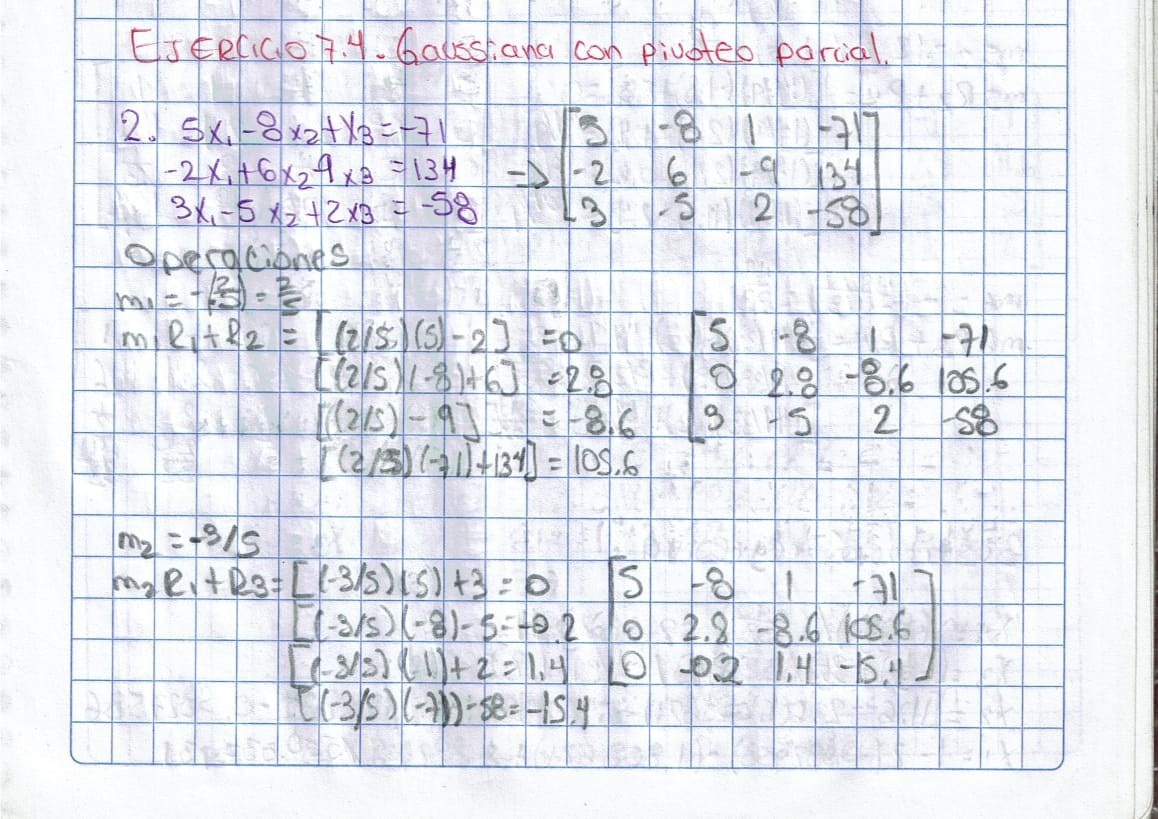
\includegraphics[width=6.25in,height=\textheight,keepaspectratio,alt={Ejercicio 2}]{Ejercicio74Pivote2.jpg}
\caption{Ejercicio 2}
\end{figure}

\begin{figure}
\centering
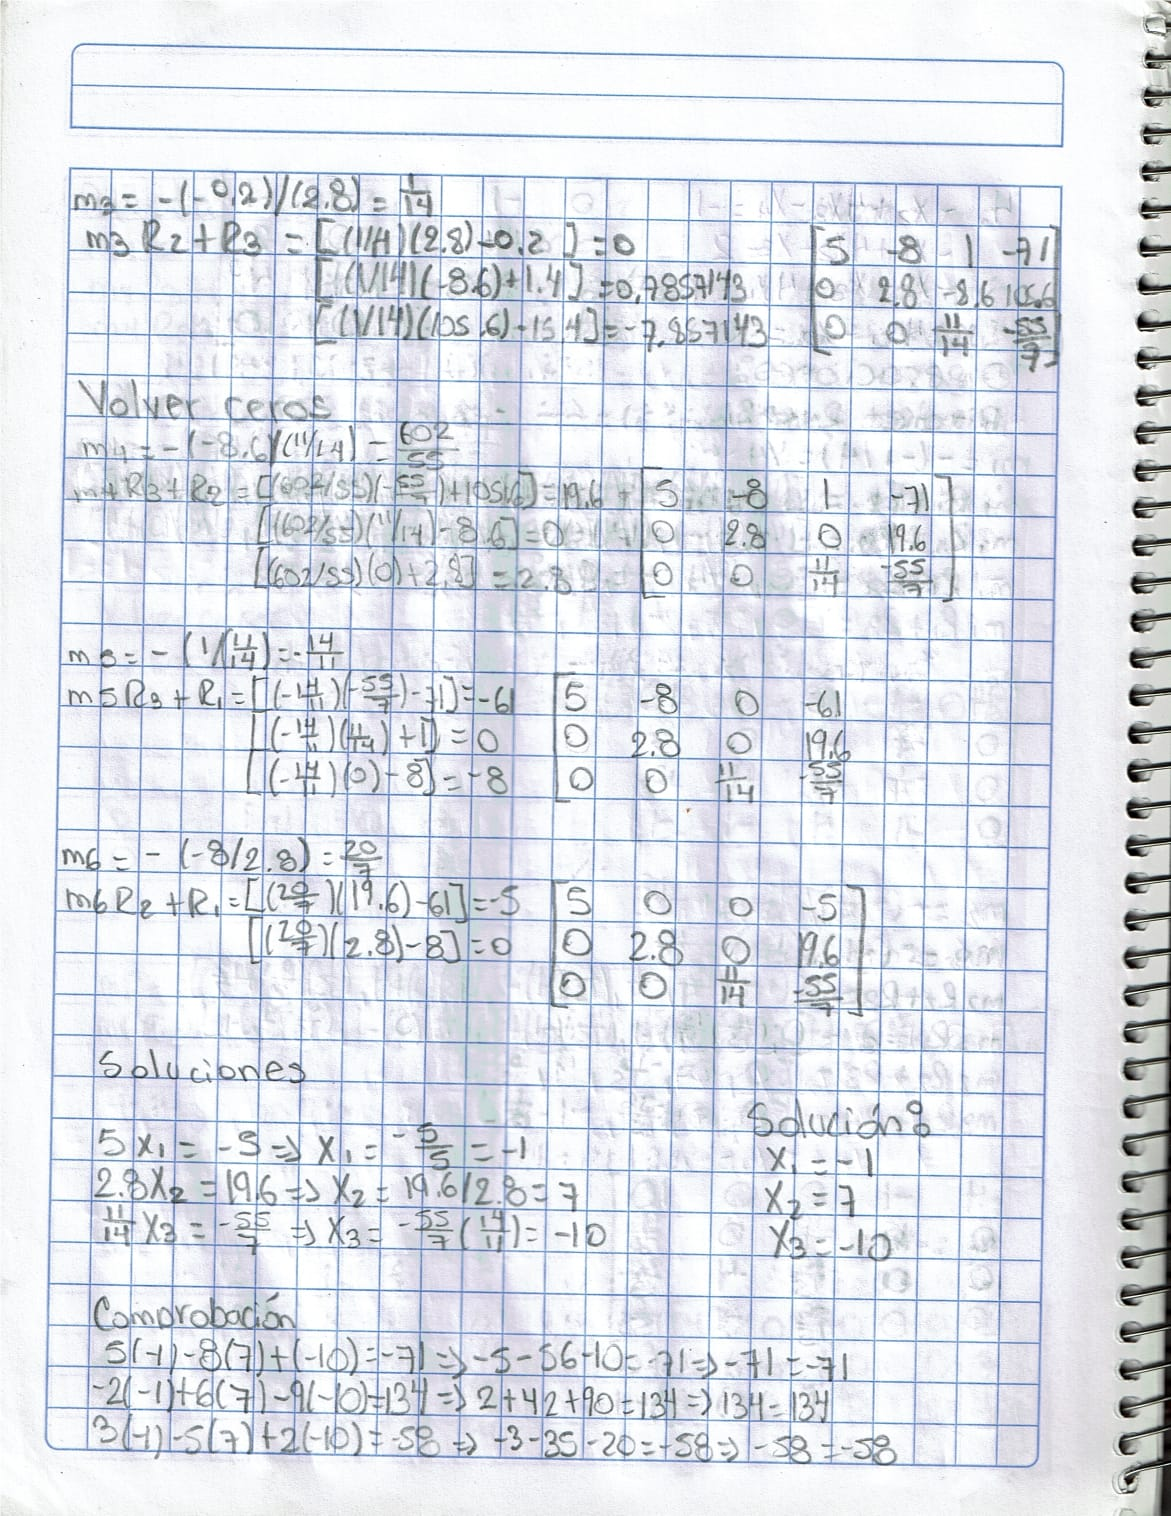
\includegraphics[width=6.25in,height=\textheight,keepaspectratio,alt={Ejercicio 2-2}]{Ejercicio74Pivote2_2.jpg}
\caption{Ejercicio 2-2}
\end{figure}

\begin{figure}
\centering
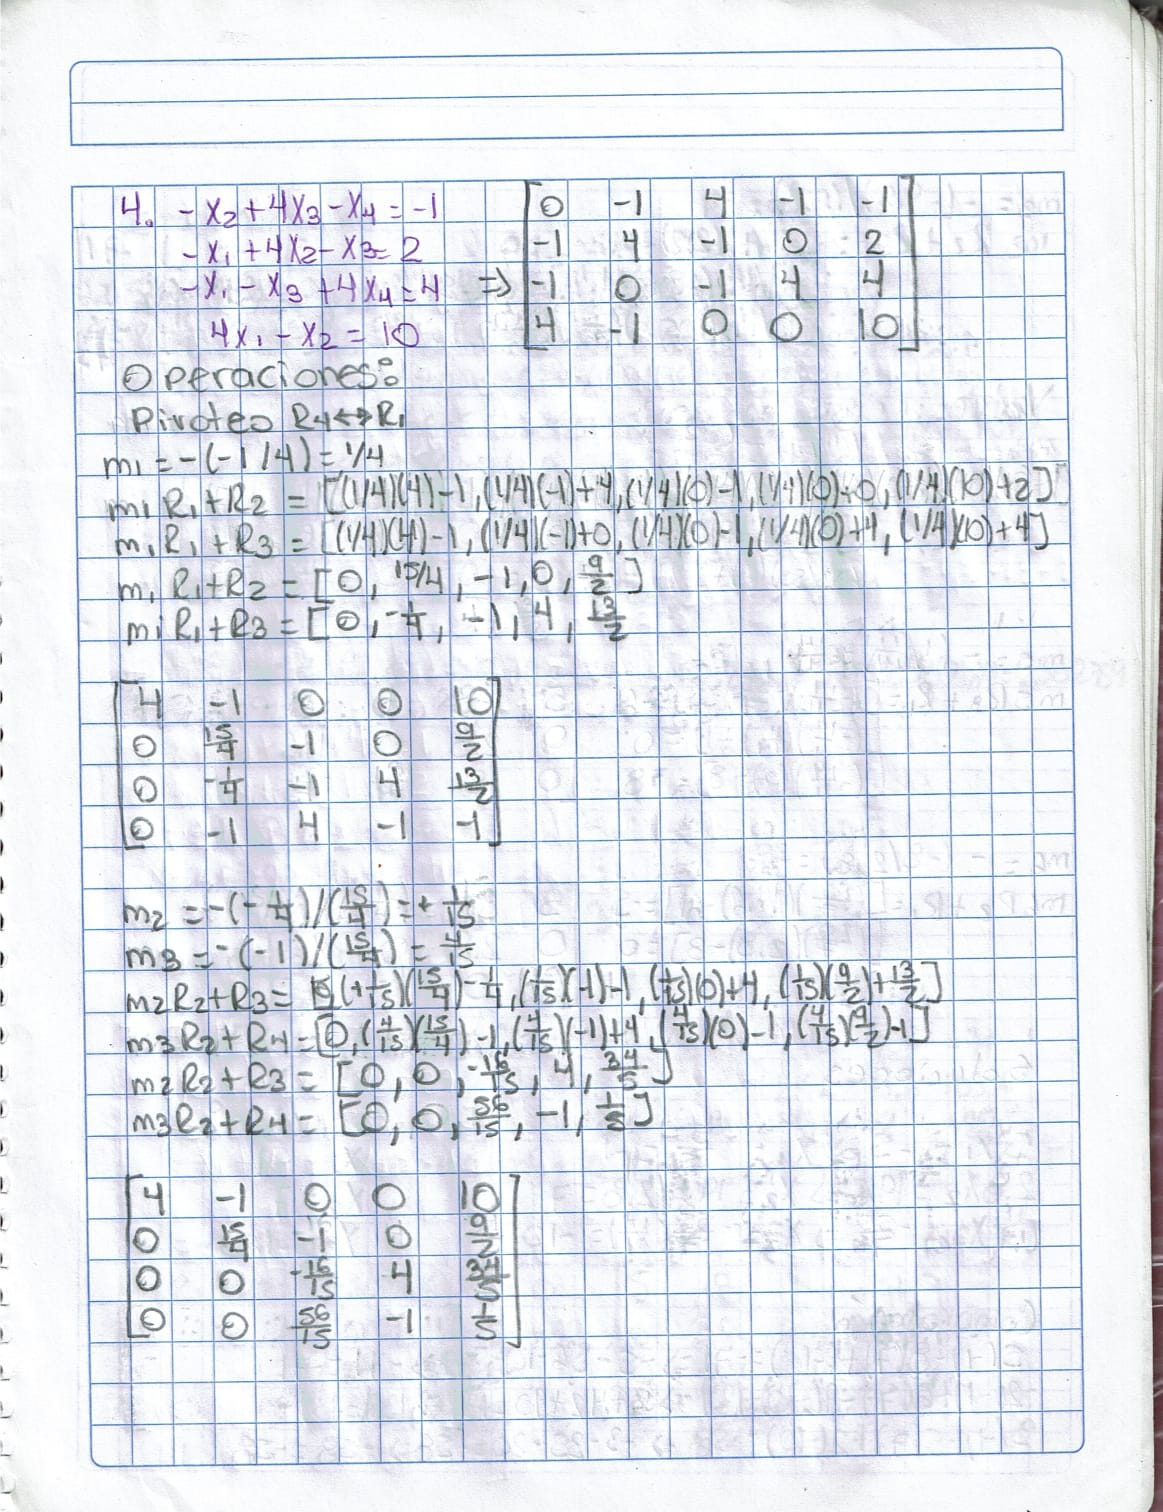
\includegraphics[width=6.25in,height=\textheight,keepaspectratio,alt={Ejercicio 4}]{Ejercicio74Pivote4.jpg}
\caption{Ejercicio 4}
\end{figure}

\begin{figure}
\centering
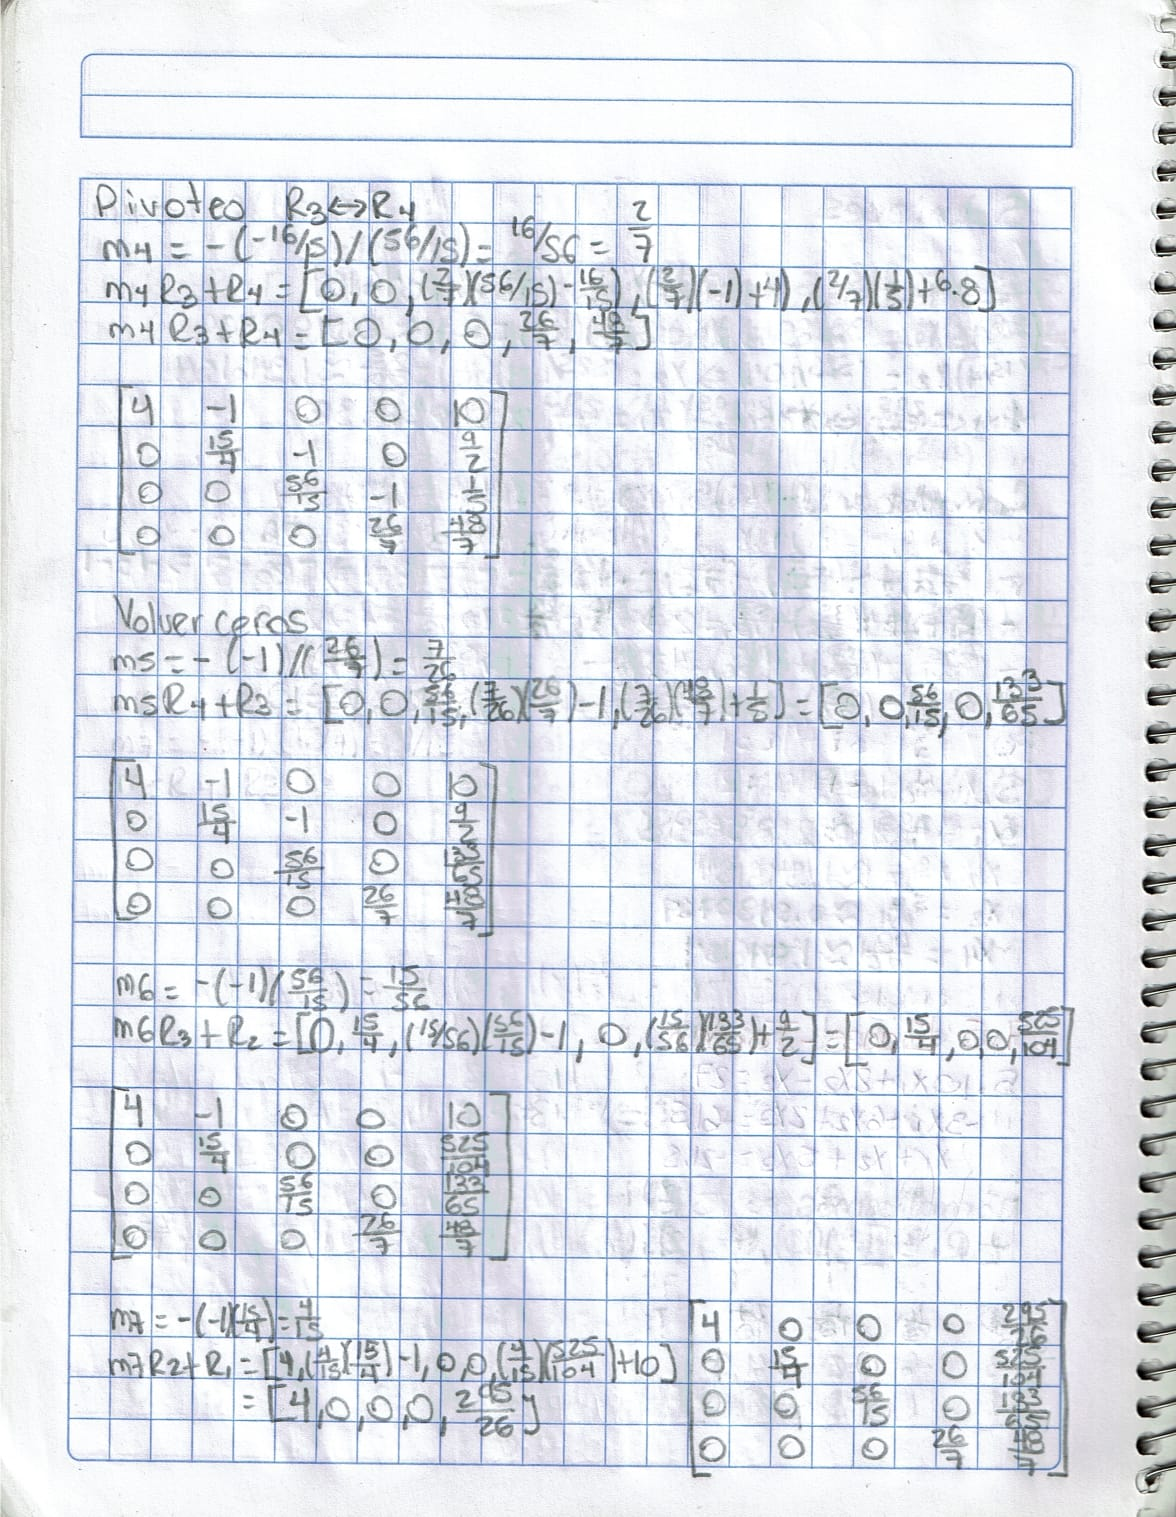
\includegraphics[width=6.25in,height=\textheight,keepaspectratio,alt={Ejercicio 4-2}]{Ejercicio74Pivote4_2.jpg}
\caption{Ejercicio 4-2}
\end{figure}

\begin{figure}
\centering
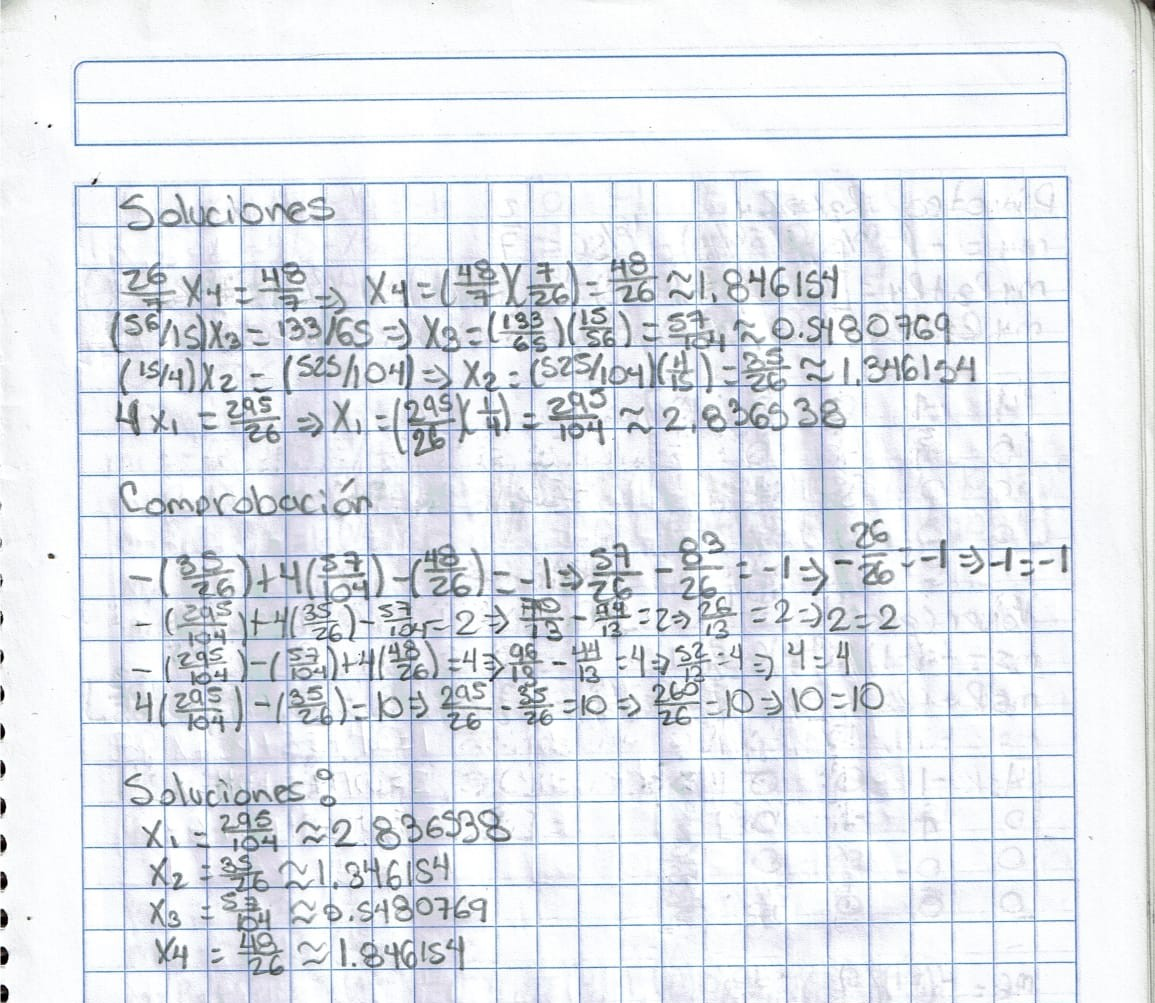
\includegraphics[width=6.25in,height=\textheight,keepaspectratio,alt={Ejercicio 4-3}]{Ejercicio74Pivote4_3.jpg}
\caption{Ejercicio 4-3}
\end{figure}

\subsubsection{\texorpdfstring{Sistema
\(1\)}{Sistema 1}}\label{sistema-1-1}

\(0.4x_1 - 1.5x_2 + 0.75x_3 = -20\)

\(-0.5x_1 - 15x_2 + 10x_3 = -10\)

\(-10x_1 - 9x_2 + 2.5x_3 = 30\)

\paragraph{Procedimiento}\label{procedimiento-20}

\begin{Shaded}
\begin{Highlighting}[]
\NormalTok{A }\OtherTok{\textless{}{-}} \FunctionTok{matrix}\NormalTok{(}\FunctionTok{c}\NormalTok{(}\FloatTok{0.4}\NormalTok{, }\SpecialCharTok{{-}}\FloatTok{1.5}\NormalTok{, }\FloatTok{0.75}\NormalTok{,}
              \SpecialCharTok{{-}}\FloatTok{0.5}\NormalTok{, }\SpecialCharTok{{-}}\DecValTok{15}\NormalTok{, }\DecValTok{10}\NormalTok{,}
              \SpecialCharTok{{-}}\DecValTok{10}\NormalTok{, }\SpecialCharTok{{-}}\DecValTok{9}\NormalTok{, }\FloatTok{2.5}\NormalTok{),}
      \AttributeTok{nrow =} \DecValTok{3}\NormalTok{, }\AttributeTok{byrow =} \ConstantTok{TRUE}\NormalTok{)}
\NormalTok{b }\OtherTok{\textless{}{-}} \FunctionTok{matrix}\NormalTok{(}\FunctionTok{c}\NormalTok{(}\SpecialCharTok{{-}}\DecValTok{20}\NormalTok{, }\SpecialCharTok{{-}}\DecValTok{10}\NormalTok{, }\DecValTok{30}\NormalTok{), }\AttributeTok{nrow =} \DecValTok{3}\NormalTok{)}

\NormalTok{Ab }\OtherTok{\textless{}{-}} \FunctionTok{cbind}\NormalTok{(A, b); (Ab)}
\end{Highlighting}
\end{Shaded}

\begin{verbatim}
##       [,1]  [,2]  [,3] [,4]
## [1,]   0.4  -1.5  0.75  -20
## [2,]  -0.5 -15.0 10.00  -10
## [3,] -10.0  -9.0  2.50   30
\end{verbatim}

\subparagraph{Primera eliminación}\label{primera-eliminaciuxf3n}

\begin{Shaded}
\begin{Highlighting}[]
\CommentTok{\# Primer pivoteo}

\NormalTok{NuevaA }\OtherTok{\textless{}{-}}\NormalTok{ Ab[}\FunctionTok{c}\NormalTok{(}\DecValTok{3}\NormalTok{, }\DecValTok{2}\NormalTok{, }\DecValTok{1}\NormalTok{), ]}
\NormalTok{(NuevaA)}
\end{Highlighting}
\end{Shaded}

\begin{verbatim}
##       [,1]  [,2]  [,3] [,4]
## [1,] -10.0  -9.0  2.50   30
## [2,]  -0.5 -15.0 10.00  -10
## [3,]   0.4  -1.5  0.75  -20
\end{verbatim}

\begin{Shaded}
\begin{Highlighting}[]
\CommentTok{\# Volver ceros}

\NormalTok{m1 }\OtherTok{\textless{}{-}} \SpecialCharTok{{-}}\NormalTok{ Ab[}\DecValTok{2}\NormalTok{,}\DecValTok{1}\NormalTok{] }\SpecialCharTok{/}\NormalTok{ Ab[}\DecValTok{1}\NormalTok{,}\DecValTok{1}\NormalTok{]}
\NormalTok{m2 }\OtherTok{\textless{}{-}} \SpecialCharTok{{-}}\NormalTok{ Ab[}\DecValTok{3}\NormalTok{,}\DecValTok{1}\NormalTok{] }\SpecialCharTok{/}\NormalTok{ Ab[}\DecValTok{1}\NormalTok{,}\DecValTok{1}\NormalTok{]}
\NormalTok{R1 }\OtherTok{\textless{}{-}}\NormalTok{ NuevaA[}\DecValTok{1}\NormalTok{,]}
\NormalTok{R2 }\OtherTok{\textless{}{-}}\NormalTok{ m1 }\SpecialCharTok{*}\NormalTok{ Ab[}\DecValTok{1}\NormalTok{,] }\SpecialCharTok{+}\NormalTok{ Ab[}\DecValTok{2}\NormalTok{,]}
\NormalTok{R3 }\OtherTok{\textless{}{-}}\NormalTok{ m2 }\SpecialCharTok{*}\NormalTok{ Ab[}\DecValTok{1}\NormalTok{,] }\SpecialCharTok{+}\NormalTok{ Ab[}\DecValTok{3}\NormalTok{,]}
\NormalTok{NuevaA }\OtherTok{\textless{}{-}} \FunctionTok{rbind}\NormalTok{(R1, R2, R3)}
\NormalTok{(NuevaA)}
\end{Highlighting}
\end{Shaded}

\begin{verbatim}
##    [,1]    [,2]    [,3] [,4]
## R1  -10  -9.000  2.5000   30
## R2    0 -16.875 10.9375  -35
## R3    0 -46.500 21.2500 -470
\end{verbatim}

\subparagraph{Segunda eliminación}\label{segunda-eliminaciuxf3n}

\begin{Shaded}
\begin{Highlighting}[]
\CommentTok{\# Segundo pivoteo}

\NormalTok{Ab }\OtherTok{\textless{}{-}}\NormalTok{ NuevaA[}\FunctionTok{c}\NormalTok{(}\DecValTok{1}\NormalTok{, }\DecValTok{3}\NormalTok{, }\DecValTok{2}\NormalTok{), ]}
\NormalTok{(Ab)}
\end{Highlighting}
\end{Shaded}

\begin{verbatim}
##    [,1]    [,2]    [,3] [,4]
## R1  -10  -9.000  2.5000   30
## R3    0 -46.500 21.2500 -470
## R2    0 -16.875 10.9375  -35
\end{verbatim}

\begin{Shaded}
\begin{Highlighting}[]
\CommentTok{\# Volver ceros }

\NormalTok{m3 }\OtherTok{\textless{}{-}} \SpecialCharTok{{-}}\NormalTok{ Ab[}\DecValTok{3}\NormalTok{,}\DecValTok{2}\NormalTok{] }\SpecialCharTok{/}\NormalTok{ Ab[}\DecValTok{2}\NormalTok{,}\DecValTok{2}\NormalTok{]}
\NormalTok{R1 }\OtherTok{\textless{}{-}}\NormalTok{ Ab[}\DecValTok{1}\NormalTok{,]}
\NormalTok{R2 }\OtherTok{\textless{}{-}}\NormalTok{ Ab[}\DecValTok{2}\NormalTok{,]}
\NormalTok{R3 }\OtherTok{\textless{}{-}}\NormalTok{ m3 }\SpecialCharTok{*}\NormalTok{ Ab[}\DecValTok{2}\NormalTok{,] }\SpecialCharTok{+}\NormalTok{ Ab[}\DecValTok{3}\NormalTok{,]}
\NormalTok{NuevaA }\OtherTok{\textless{}{-}} \FunctionTok{rbind}\NormalTok{(R1, R2, R3)}
\NormalTok{(NuevaA)}
\end{Highlighting}
\end{Shaded}

\begin{verbatim}
##    [,1]  [,2]      [,3]      [,4]
## R1  -10  -9.0  2.500000   30.0000
## R2    0 -46.5 21.250000 -470.0000
## R3    0   0.0  3.225806  135.5645
\end{verbatim}

Volver ceros con eliminación hacía atrás

\begin{Shaded}
\begin{Highlighting}[]
\CommentTok{\# Tercera columna}

\NormalTok{Ab }\OtherTok{\textless{}{-}}\NormalTok{ NuevaA; (Ab)}
\end{Highlighting}
\end{Shaded}

\begin{verbatim}
##    [,1]  [,2]      [,3]      [,4]
## R1  -10  -9.0  2.500000   30.0000
## R2    0 -46.5 21.250000 -470.0000
## R3    0   0.0  3.225806  135.5645
\end{verbatim}

\begin{Shaded}
\begin{Highlighting}[]
\NormalTok{m4 }\OtherTok{\textless{}{-}} \SpecialCharTok{{-}}\NormalTok{ Ab[}\DecValTok{2}\NormalTok{,}\DecValTok{3}\NormalTok{] }\SpecialCharTok{/}\NormalTok{ Ab[}\DecValTok{3}\NormalTok{,}\DecValTok{3}\NormalTok{]}
\NormalTok{m5 }\OtherTok{\textless{}{-}} \SpecialCharTok{{-}}\NormalTok{ Ab[}\DecValTok{1}\NormalTok{,}\DecValTok{3}\NormalTok{] }\SpecialCharTok{/}\NormalTok{ Ab[}\DecValTok{3}\NormalTok{,}\DecValTok{3}\NormalTok{]}
\NormalTok{R1 }\OtherTok{\textless{}{-}}\NormalTok{ m5 }\SpecialCharTok{*}\NormalTok{ Ab[}\DecValTok{3}\NormalTok{,] }\SpecialCharTok{+}\NormalTok{ Ab[}\DecValTok{1}\NormalTok{,]}
\NormalTok{R2 }\OtherTok{\textless{}{-}}\NormalTok{ m4 }\SpecialCharTok{*}\NormalTok{ Ab[}\DecValTok{3}\NormalTok{,] }\SpecialCharTok{+}\NormalTok{ Ab[}\DecValTok{2}\NormalTok{,]}
\NormalTok{R3 }\OtherTok{\textless{}{-}}\NormalTok{ Ab[}\DecValTok{3}\NormalTok{,]}

\NormalTok{NuevaA}\OtherTok{\textless{}{-}} \FunctionTok{rbind}\NormalTok{(R1, R2, R3)}
\NormalTok{(NuevaA)}
\end{Highlighting}
\end{Shaded}

\begin{verbatim}
##    [,1]  [,2]     [,3]       [,4]
## R1  -10  -9.0 0.000000   -75.0625
## R2    0 -46.5 0.000000 -1363.0312
## R3    0   0.0 3.225806   135.5645
\end{verbatim}

\begin{Shaded}
\begin{Highlighting}[]
\CommentTok{\# Segunda columna}

\NormalTok{Ab }\OtherTok{\textless{}{-}}\NormalTok{ NuevaA; (Ab)}
\end{Highlighting}
\end{Shaded}

\begin{verbatim}
##    [,1]  [,2]     [,3]       [,4]
## R1  -10  -9.0 0.000000   -75.0625
## R2    0 -46.5 0.000000 -1363.0312
## R3    0   0.0 3.225806   135.5645
\end{verbatim}

\begin{Shaded}
\begin{Highlighting}[]
\NormalTok{m6 }\OtherTok{\textless{}{-}} \SpecialCharTok{{-}}\NormalTok{ Ab[}\DecValTok{1}\NormalTok{,}\DecValTok{2}\NormalTok{] }\SpecialCharTok{/}\NormalTok{ Ab[}\DecValTok{2}\NormalTok{,}\DecValTok{2}\NormalTok{]}

\NormalTok{R1 }\OtherTok{\textless{}{-}}\NormalTok{ m6 }\SpecialCharTok{*}\NormalTok{ Ab[}\DecValTok{2}\NormalTok{,] }\SpecialCharTok{+}\NormalTok{ Ab[}\DecValTok{1}\NormalTok{,]}
\NormalTok{R2 }\OtherTok{\textless{}{-}}\NormalTok{ Ab[}\DecValTok{2}\NormalTok{,]}
\NormalTok{R3 }\OtherTok{\textless{}{-}}\NormalTok{ Ab[}\DecValTok{3}\NormalTok{,]}

\NormalTok{NuevaA }\OtherTok{\textless{}{-}} \FunctionTok{rbind}\NormalTok{(R1, R2, R3)}
\NormalTok{(NuevaA)}
\end{Highlighting}
\end{Shaded}

\begin{verbatim}
##    [,1]  [,2]     [,3]       [,4]
## R1  -10   0.0 0.000000   188.7500
## R2    0 -46.5 0.000000 -1363.0312
## R3    0   0.0 3.225806   135.5645
\end{verbatim}

\begin{Shaded}
\begin{Highlighting}[]
\CommentTok{\# Soluciones}

\NormalTok{Ab }\OtherTok{\textless{}{-}}\NormalTok{ NuevaA; (Ab)}
\end{Highlighting}
\end{Shaded}

\begin{verbatim}
##    [,1]  [,2]     [,3]       [,4]
## R1  -10   0.0 0.000000   188.7500
## R2    0 -46.5 0.000000 -1363.0312
## R3    0   0.0 3.225806   135.5645
\end{verbatim}

\begin{Shaded}
\begin{Highlighting}[]
\NormalTok{x1 }\OtherTok{\textless{}{-}}\NormalTok{ Ab[}\DecValTok{1}\NormalTok{,}\DecValTok{4}\NormalTok{] }\SpecialCharTok{/}\NormalTok{ Ab[}\DecValTok{1}\NormalTok{,}\DecValTok{1}\NormalTok{]}
\NormalTok{x2 }\OtherTok{\textless{}{-}}\NormalTok{ Ab[}\DecValTok{2}\NormalTok{,}\DecValTok{4}\NormalTok{] }\SpecialCharTok{/}\NormalTok{ Ab[}\DecValTok{2}\NormalTok{,}\DecValTok{2}\NormalTok{]}
\NormalTok{x3 }\OtherTok{\textless{}{-}}\NormalTok{ Ab[}\DecValTok{3}\NormalTok{,}\DecValTok{4}\NormalTok{] }\SpecialCharTok{/}\NormalTok{ Ab[}\DecValTok{3}\NormalTok{,}\DecValTok{3}\NormalTok{]}
\end{Highlighting}
\end{Shaded}

\begin{Shaded}
\begin{Highlighting}[]
\CommentTok{\# Comprobación}

\NormalTok{I }\OtherTok{\textless{}{-}}\NormalTok{ b[}\DecValTok{1}\NormalTok{,]; (I)}
\end{Highlighting}
\end{Shaded}

\begin{verbatim}
## [1] -20
\end{verbatim}

\begin{Shaded}
\begin{Highlighting}[]
\NormalTok{II }\OtherTok{\textless{}{-}}\NormalTok{ b[}\DecValTok{2}\NormalTok{,]; (II)}
\end{Highlighting}
\end{Shaded}

\begin{verbatim}
## [1] -10
\end{verbatim}

\begin{Shaded}
\begin{Highlighting}[]
\NormalTok{III }\OtherTok{\textless{}{-}}\NormalTok{ b[}\DecValTok{3}\NormalTok{,]; (III)}
\end{Highlighting}
\end{Shaded}

\begin{verbatim}
## [1] 30
\end{verbatim}

\begin{Shaded}
\begin{Highlighting}[]
\NormalTok{c1 }\OtherTok{\textless{}{-}}\NormalTok{ (A[}\DecValTok{1}\NormalTok{,}\DecValTok{1}\NormalTok{] }\SpecialCharTok{*}\NormalTok{ x1) }\SpecialCharTok{+}\NormalTok{ (A[}\DecValTok{1}\NormalTok{,}\DecValTok{2}\NormalTok{] }\SpecialCharTok{*}\NormalTok{ x2) }\SpecialCharTok{+}\NormalTok{ (A[}\DecValTok{1}\NormalTok{,}\DecValTok{3}\NormalTok{] }\SpecialCharTok{*}\NormalTok{ x3); }\FunctionTok{paste0}\NormalTok{(}\StringTok{"El resultado es: "}\NormalTok{,c1)}
\end{Highlighting}
\end{Shaded}

\begin{verbatim}
## [1] "El resultado es: -20"
\end{verbatim}

\begin{Shaded}
\begin{Highlighting}[]
\NormalTok{c2 }\OtherTok{\textless{}{-}}\NormalTok{ (A[}\DecValTok{2}\NormalTok{,}\DecValTok{1}\NormalTok{] }\SpecialCharTok{*}\NormalTok{ x1) }\SpecialCharTok{+}\NormalTok{ (A[}\DecValTok{2}\NormalTok{,}\DecValTok{2}\NormalTok{] }\SpecialCharTok{*}\NormalTok{ x2) }\SpecialCharTok{+}\NormalTok{ (A[}\DecValTok{2}\NormalTok{,}\DecValTok{3}\NormalTok{] }\SpecialCharTok{*}\NormalTok{ x3); }\FunctionTok{paste0}\NormalTok{(}\StringTok{"El resultado es: "}\NormalTok{,c2)}
\end{Highlighting}
\end{Shaded}

\begin{verbatim}
## [1] "El resultado es: -10"
\end{verbatim}

\begin{Shaded}
\begin{Highlighting}[]
\NormalTok{c3 }\OtherTok{\textless{}{-}}\NormalTok{ (A[}\DecValTok{3}\NormalTok{,}\DecValTok{1}\NormalTok{] }\SpecialCharTok{*}\NormalTok{ x1) }\SpecialCharTok{+}\NormalTok{ (A[}\DecValTok{3}\NormalTok{,}\DecValTok{2}\NormalTok{] }\SpecialCharTok{*}\NormalTok{ x2) }\SpecialCharTok{+}\NormalTok{ (A[}\DecValTok{3}\NormalTok{,}\DecValTok{3}\NormalTok{] }\SpecialCharTok{*}\NormalTok{ x3); }\FunctionTok{paste0}\NormalTok{(}\StringTok{"El resultado es: "}\NormalTok{,c3)}
\end{Highlighting}
\end{Shaded}

\begin{verbatim}
## [1] "El resultado es: 30"
\end{verbatim}

\begin{Shaded}
\begin{Highlighting}[]
\FunctionTok{paste0}\NormalTok{(}\StringTok{"En la ecuación 1: "}\NormalTok{, c1, }\StringTok{" tecnicamente es: "}\NormalTok{, I)}
\end{Highlighting}
\end{Shaded}

\begin{verbatim}
## [1] "En la ecuación 1: -20 tecnicamente es: -20"
\end{verbatim}

\begin{Shaded}
\begin{Highlighting}[]
\FunctionTok{paste0}\NormalTok{(}\StringTok{"En la ecuación 2: "}\NormalTok{, c2, }\StringTok{" tecnicamente es: "}\NormalTok{, II)}
\end{Highlighting}
\end{Shaded}

\begin{verbatim}
## [1] "En la ecuación 2: -10 tecnicamente es: -10"
\end{verbatim}

\begin{Shaded}
\begin{Highlighting}[]
\FunctionTok{paste0}\NormalTok{(}\StringTok{"En la ecuación 3: "}\NormalTok{, c3, }\StringTok{" tecnicamente es: "}\NormalTok{, III)}
\end{Highlighting}
\end{Shaded}

\begin{verbatim}
## [1] "En la ecuación 3: 30 tecnicamente es: 30"
\end{verbatim}

\paragraph{Resultados}\label{resultados-10}

\begin{Shaded}
\begin{Highlighting}[]
\FunctionTok{cat}\NormalTok{(}\StringTok{"Soluciones del sistema:"}\NormalTok{)}
\end{Highlighting}
\end{Shaded}

\begin{verbatim}
## Soluciones del sistema:
\end{verbatim}

\begin{Shaded}
\begin{Highlighting}[]
\FunctionTok{cat}\NormalTok{(}\StringTok{"x1 ="}\NormalTok{, x1)}
\end{Highlighting}
\end{Shaded}

\begin{verbatim}
## x1 = -18.875
\end{verbatim}

\begin{Shaded}
\begin{Highlighting}[]
\FunctionTok{cat}\NormalTok{(}\StringTok{"x2 ="}\NormalTok{, x2) }
\end{Highlighting}
\end{Shaded}

\begin{verbatim}
## x2 = 29.3125
\end{verbatim}

\begin{Shaded}
\begin{Highlighting}[]
\FunctionTok{cat}\NormalTok{(}\StringTok{"x3 ="}\NormalTok{, x3)}
\end{Highlighting}
\end{Shaded}

\begin{verbatim}
## x3 = 42.025
\end{verbatim}

\subsubsection{\texorpdfstring{Sistema
\(2\)}{Sistema 2}}\label{sistema-2-1}

\(5x_1 - 8x_2 + x_3 = -71\)

\(-2x_1 + 6x_2 - 9x_3 = 134\)

\(3x_1 - 5x_2 + 2x_3 = -58\)

\paragraph{Procedimiento}\label{procedimiento-21}

\begin{Shaded}
\begin{Highlighting}[]
\NormalTok{A }\OtherTok{\textless{}{-}} \FunctionTok{matrix}\NormalTok{(}\FunctionTok{c}\NormalTok{(}\DecValTok{5}\NormalTok{, }\SpecialCharTok{{-}}\DecValTok{8}\NormalTok{, }\DecValTok{1}\NormalTok{,}
              \SpecialCharTok{{-}}\DecValTok{2}\NormalTok{, }\DecValTok{6}\NormalTok{, }\SpecialCharTok{{-}}\DecValTok{9}\NormalTok{,}
              \DecValTok{3}\NormalTok{, }\SpecialCharTok{{-}}\DecValTok{5}\NormalTok{, }\DecValTok{2}\NormalTok{),}
      \AttributeTok{nrow =} \DecValTok{3}\NormalTok{, }\AttributeTok{byrow =} \ConstantTok{TRUE}\NormalTok{)}
\NormalTok{b }\OtherTok{\textless{}{-}} \FunctionTok{matrix}\NormalTok{(}\FunctionTok{c}\NormalTok{(}\SpecialCharTok{{-}}\DecValTok{71}\NormalTok{, }\DecValTok{134}\NormalTok{, }\SpecialCharTok{{-}}\DecValTok{58}\NormalTok{), }\AttributeTok{nrow =} \DecValTok{3}\NormalTok{)}

\NormalTok{Ab }\OtherTok{\textless{}{-}} \FunctionTok{cbind}\NormalTok{(A, b); (Ab)}
\end{Highlighting}
\end{Shaded}

\begin{verbatim}
##      [,1] [,2] [,3] [,4]
## [1,]    5   -8    1  -71
## [2,]   -2    6   -9  134
## [3,]    3   -5    2  -58
\end{verbatim}

\subparagraph{Primera eliminación}\label{primera-eliminaciuxf3n-1}

No se necesita hacer el pivoteo ya que se encuentra acomodado

\begin{Shaded}
\begin{Highlighting}[]
\CommentTok{\# Volver ceros}

\NormalTok{m1 }\OtherTok{\textless{}{-}} \SpecialCharTok{{-}}\NormalTok{ Ab[}\DecValTok{2}\NormalTok{,}\DecValTok{1}\NormalTok{] }\SpecialCharTok{/}\NormalTok{ Ab[}\DecValTok{1}\NormalTok{,}\DecValTok{1}\NormalTok{]}
\NormalTok{m2 }\OtherTok{\textless{}{-}} \SpecialCharTok{{-}}\NormalTok{ Ab[}\DecValTok{3}\NormalTok{,}\DecValTok{1}\NormalTok{] }\SpecialCharTok{/}\NormalTok{ Ab[}\DecValTok{1}\NormalTok{,}\DecValTok{1}\NormalTok{]}
\NormalTok{R1 }\OtherTok{\textless{}{-}}\NormalTok{ Ab[}\DecValTok{1}\NormalTok{,]}
\NormalTok{R2 }\OtherTok{\textless{}{-}}\NormalTok{ m1 }\SpecialCharTok{*}\NormalTok{ Ab[}\DecValTok{1}\NormalTok{,] }\SpecialCharTok{+}\NormalTok{ Ab[}\DecValTok{2}\NormalTok{,]}
\NormalTok{R3 }\OtherTok{\textless{}{-}}\NormalTok{ m2 }\SpecialCharTok{*}\NormalTok{ Ab[}\DecValTok{1}\NormalTok{,] }\SpecialCharTok{+}\NormalTok{ Ab[}\DecValTok{3}\NormalTok{,]}
\NormalTok{NuevaA }\OtherTok{\textless{}{-}} \FunctionTok{rbind}\NormalTok{(R1, R2, R3)}
\NormalTok{(NuevaA)}
\end{Highlighting}
\end{Shaded}

\begin{verbatim}
##    [,1] [,2] [,3]  [,4]
## R1    5 -8.0  1.0 -71.0
## R2    0  2.8 -8.6 105.6
## R3    0 -0.2  1.4 -15.4
\end{verbatim}

\subparagraph{Segunda eliminación}\label{segunda-eliminaciuxf3n-1}

Tampoco se necesita pivoteo en esta ocasión

\begin{Shaded}
\begin{Highlighting}[]
\CommentTok{\# Volver ceros}

\NormalTok{Ab }\OtherTok{\textless{}{-}}\NormalTok{ NuevaA}
\NormalTok{m3 }\OtherTok{\textless{}{-}} \SpecialCharTok{{-}}\NormalTok{ Ab[}\DecValTok{3}\NormalTok{,}\DecValTok{2}\NormalTok{] }\SpecialCharTok{/}\NormalTok{ Ab[}\DecValTok{2}\NormalTok{,}\DecValTok{2}\NormalTok{]}
\NormalTok{R1 }\OtherTok{\textless{}{-}}\NormalTok{ Ab[}\DecValTok{1}\NormalTok{,]}
\NormalTok{R2 }\OtherTok{\textless{}{-}}\NormalTok{ Ab[}\DecValTok{2}\NormalTok{,]}
\NormalTok{R3 }\OtherTok{\textless{}{-}}\NormalTok{ m3 }\SpecialCharTok{*}\NormalTok{ Ab[}\DecValTok{2}\NormalTok{,] }\SpecialCharTok{+}\NormalTok{ Ab[}\DecValTok{3}\NormalTok{,]}
\NormalTok{NuevaA }\OtherTok{\textless{}{-}} \FunctionTok{rbind}\NormalTok{(R1, R2, R3)}
\NormalTok{(NuevaA)}
\end{Highlighting}
\end{Shaded}

\begin{verbatim}
##    [,1] [,2]       [,3]       [,4]
## R1    5 -8.0  1.0000000 -71.000000
## R2    0  2.8 -8.6000000 105.600000
## R3    0  0.0  0.7857143  -7.857143
\end{verbatim}

Volver ceros con eliminación hacía atrás

\begin{Shaded}
\begin{Highlighting}[]
\CommentTok{\# Tercera columna}

\NormalTok{Ab }\OtherTok{\textless{}{-}}\NormalTok{ NuevaA; (Ab)}
\end{Highlighting}
\end{Shaded}

\begin{verbatim}
##    [,1] [,2]       [,3]       [,4]
## R1    5 -8.0  1.0000000 -71.000000
## R2    0  2.8 -8.6000000 105.600000
## R3    0  0.0  0.7857143  -7.857143
\end{verbatim}

\begin{Shaded}
\begin{Highlighting}[]
\NormalTok{m4 }\OtherTok{\textless{}{-}} \SpecialCharTok{{-}}\NormalTok{ Ab[}\DecValTok{2}\NormalTok{,}\DecValTok{3}\NormalTok{] }\SpecialCharTok{/}\NormalTok{ Ab[}\DecValTok{3}\NormalTok{,}\DecValTok{3}\NormalTok{]}
\NormalTok{m5 }\OtherTok{\textless{}{-}} \SpecialCharTok{{-}}\NormalTok{ Ab[}\DecValTok{1}\NormalTok{,}\DecValTok{3}\NormalTok{] }\SpecialCharTok{/}\NormalTok{ Ab[}\DecValTok{3}\NormalTok{,}\DecValTok{3}\NormalTok{]}
\NormalTok{R1 }\OtherTok{\textless{}{-}}\NormalTok{ m5 }\SpecialCharTok{*}\NormalTok{ Ab[}\DecValTok{3}\NormalTok{,] }\SpecialCharTok{+}\NormalTok{ Ab[}\DecValTok{1}\NormalTok{,]}
\NormalTok{R2 }\OtherTok{\textless{}{-}}\NormalTok{ m4 }\SpecialCharTok{*}\NormalTok{ Ab[}\DecValTok{3}\NormalTok{,] }\SpecialCharTok{+}\NormalTok{ Ab[}\DecValTok{2}\NormalTok{,]}
\NormalTok{R3 }\OtherTok{\textless{}{-}}\NormalTok{ Ab[}\DecValTok{3}\NormalTok{,]}

\NormalTok{NuevaA }\OtherTok{\textless{}{-}} \FunctionTok{rbind}\NormalTok{(R1, R2, R3)}
\NormalTok{(NuevaA)}
\end{Highlighting}
\end{Shaded}

\begin{verbatim}
##    [,1] [,2]      [,3]       [,4]
## R1    5 -8.0 0.0000000 -61.000000
## R2    0  2.8 0.0000000  19.600000
## R3    0  0.0 0.7857143  -7.857143
\end{verbatim}

\begin{Shaded}
\begin{Highlighting}[]
\CommentTok{\# Segunda columna}

\NormalTok{Ab }\OtherTok{\textless{}{-}}\NormalTok{ NuevaA; (Ab)}
\end{Highlighting}
\end{Shaded}

\begin{verbatim}
##    [,1] [,2]      [,3]       [,4]
## R1    5 -8.0 0.0000000 -61.000000
## R2    0  2.8 0.0000000  19.600000
## R3    0  0.0 0.7857143  -7.857143
\end{verbatim}

\begin{Shaded}
\begin{Highlighting}[]
\NormalTok{m6 }\OtherTok{\textless{}{-}} \SpecialCharTok{{-}}\NormalTok{ Ab[}\DecValTok{1}\NormalTok{,}\DecValTok{2}\NormalTok{] }\SpecialCharTok{/}\NormalTok{ Ab[}\DecValTok{2}\NormalTok{,}\DecValTok{2}\NormalTok{]}

\NormalTok{R1 }\OtherTok{\textless{}{-}}\NormalTok{ m6 }\SpecialCharTok{*}\NormalTok{ Ab[}\DecValTok{2}\NormalTok{,] }\SpecialCharTok{+}\NormalTok{ Ab[}\DecValTok{1}\NormalTok{,]}
\NormalTok{R2 }\OtherTok{\textless{}{-}}\NormalTok{ Ab[}\DecValTok{2}\NormalTok{,]}
\NormalTok{R3 }\OtherTok{\textless{}{-}}\NormalTok{ Ab[}\DecValTok{3}\NormalTok{,]}

\NormalTok{NuevaA }\OtherTok{\textless{}{-}} \FunctionTok{rbind}\NormalTok{(R1, R2, R3)}
\NormalTok{(NuevaA)}
\end{Highlighting}
\end{Shaded}

\begin{verbatim}
##    [,1] [,2]      [,3]      [,4]
## R1    5  0.0 0.0000000 -5.000000
## R2    0  2.8 0.0000000 19.600000
## R3    0  0.0 0.7857143 -7.857143
\end{verbatim}

\begin{Shaded}
\begin{Highlighting}[]
\CommentTok{\# Soluciones}

\NormalTok{Ab }\OtherTok{\textless{}{-}}\NormalTok{ NuevaA; (Ab)}
\end{Highlighting}
\end{Shaded}

\begin{verbatim}
##    [,1] [,2]      [,3]      [,4]
## R1    5  0.0 0.0000000 -5.000000
## R2    0  2.8 0.0000000 19.600000
## R3    0  0.0 0.7857143 -7.857143
\end{verbatim}

\begin{Shaded}
\begin{Highlighting}[]
\NormalTok{x1 }\OtherTok{\textless{}{-}}\NormalTok{ Ab[}\DecValTok{1}\NormalTok{,}\DecValTok{4}\NormalTok{] }\SpecialCharTok{/}\NormalTok{ Ab[}\DecValTok{1}\NormalTok{,}\DecValTok{1}\NormalTok{]}
\NormalTok{x2 }\OtherTok{\textless{}{-}}\NormalTok{ Ab[}\DecValTok{2}\NormalTok{,}\DecValTok{4}\NormalTok{] }\SpecialCharTok{/}\NormalTok{ Ab[}\DecValTok{2}\NormalTok{,}\DecValTok{2}\NormalTok{]}
\NormalTok{x3 }\OtherTok{\textless{}{-}}\NormalTok{ Ab[}\DecValTok{3}\NormalTok{,}\DecValTok{4}\NormalTok{] }\SpecialCharTok{/}\NormalTok{ Ab[}\DecValTok{3}\NormalTok{,}\DecValTok{3}\NormalTok{]}
\end{Highlighting}
\end{Shaded}

\begin{Shaded}
\begin{Highlighting}[]
\CommentTok{\# Comprobación}

\NormalTok{I }\OtherTok{\textless{}{-}}\NormalTok{ b[}\DecValTok{1}\NormalTok{,]; (I)}
\end{Highlighting}
\end{Shaded}

\begin{verbatim}
## [1] -71
\end{verbatim}

\begin{Shaded}
\begin{Highlighting}[]
\NormalTok{II }\OtherTok{\textless{}{-}}\NormalTok{ b[}\DecValTok{2}\NormalTok{,]; (II)}
\end{Highlighting}
\end{Shaded}

\begin{verbatim}
## [1] 134
\end{verbatim}

\begin{Shaded}
\begin{Highlighting}[]
\NormalTok{III }\OtherTok{\textless{}{-}}\NormalTok{ b[}\DecValTok{3}\NormalTok{,]; (III)}
\end{Highlighting}
\end{Shaded}

\begin{verbatim}
## [1] -58
\end{verbatim}

\begin{Shaded}
\begin{Highlighting}[]
\NormalTok{c1 }\OtherTok{\textless{}{-}}\NormalTok{ (A[}\DecValTok{1}\NormalTok{,}\DecValTok{1}\NormalTok{] }\SpecialCharTok{*}\NormalTok{ x1) }\SpecialCharTok{+}\NormalTok{ (A[}\DecValTok{1}\NormalTok{,}\DecValTok{2}\NormalTok{] }\SpecialCharTok{*}\NormalTok{ x2) }\SpecialCharTok{+}\NormalTok{ (A[}\DecValTok{1}\NormalTok{,}\DecValTok{3}\NormalTok{] }\SpecialCharTok{*}\NormalTok{ x3); }\FunctionTok{paste0}\NormalTok{(}\StringTok{"El resultado es: "}\NormalTok{,c1)}
\end{Highlighting}
\end{Shaded}

\begin{verbatim}
## [1] "El resultado es: -71"
\end{verbatim}

\begin{Shaded}
\begin{Highlighting}[]
\NormalTok{c2 }\OtherTok{\textless{}{-}}\NormalTok{ (A[}\DecValTok{2}\NormalTok{,}\DecValTok{1}\NormalTok{] }\SpecialCharTok{*}\NormalTok{ x1) }\SpecialCharTok{+}\NormalTok{ (A[}\DecValTok{2}\NormalTok{,}\DecValTok{2}\NormalTok{] }\SpecialCharTok{*}\NormalTok{ x2) }\SpecialCharTok{+}\NormalTok{ (A[}\DecValTok{2}\NormalTok{,}\DecValTok{3}\NormalTok{] }\SpecialCharTok{*}\NormalTok{ x3); }\FunctionTok{paste0}\NormalTok{(}\StringTok{"El resultado es: "}\NormalTok{,c2)}
\end{Highlighting}
\end{Shaded}

\begin{verbatim}
## [1] "El resultado es: 134"
\end{verbatim}

\begin{Shaded}
\begin{Highlighting}[]
\NormalTok{c3 }\OtherTok{\textless{}{-}}\NormalTok{ (A[}\DecValTok{3}\NormalTok{,}\DecValTok{1}\NormalTok{] }\SpecialCharTok{*}\NormalTok{ x1) }\SpecialCharTok{+}\NormalTok{ (A[}\DecValTok{3}\NormalTok{,}\DecValTok{2}\NormalTok{] }\SpecialCharTok{*}\NormalTok{ x2) }\SpecialCharTok{+}\NormalTok{ (A[}\DecValTok{3}\NormalTok{,}\DecValTok{3}\NormalTok{] }\SpecialCharTok{*}\NormalTok{ x3); }\FunctionTok{paste0}\NormalTok{(}\StringTok{"El resultado es: "}\NormalTok{,c3)}
\end{Highlighting}
\end{Shaded}

\begin{verbatim}
## [1] "El resultado es: -58"
\end{verbatim}

\begin{Shaded}
\begin{Highlighting}[]
\FunctionTok{paste0}\NormalTok{(}\StringTok{"En la ecuación 1: "}\NormalTok{, c1, }\StringTok{" tecnicamente es: "}\NormalTok{, I)}
\end{Highlighting}
\end{Shaded}

\begin{verbatim}
## [1] "En la ecuación 1: -71 tecnicamente es: -71"
\end{verbatim}

\begin{Shaded}
\begin{Highlighting}[]
\FunctionTok{paste0}\NormalTok{(}\StringTok{"En la ecuación 2: "}\NormalTok{, c2, }\StringTok{" tecnicamente es: "}\NormalTok{, II)}
\end{Highlighting}
\end{Shaded}

\begin{verbatim}
## [1] "En la ecuación 2: 134 tecnicamente es: 134"
\end{verbatim}

\begin{Shaded}
\begin{Highlighting}[]
\FunctionTok{paste0}\NormalTok{(}\StringTok{"En la ecuación 3: "}\NormalTok{, c3, }\StringTok{" tecnicamente es: "}\NormalTok{, III)}
\end{Highlighting}
\end{Shaded}

\begin{verbatim}
## [1] "En la ecuación 3: -58 tecnicamente es: -58"
\end{verbatim}

\paragraph{Resultados}\label{resultados-11}

\begin{Shaded}
\begin{Highlighting}[]
\FunctionTok{cat}\NormalTok{(}\StringTok{"Soluciones del sistema:"}\NormalTok{)}
\end{Highlighting}
\end{Shaded}

\begin{verbatim}
## Soluciones del sistema:
\end{verbatim}

\begin{Shaded}
\begin{Highlighting}[]
\FunctionTok{cat}\NormalTok{(}\StringTok{"x1 ="}\NormalTok{, x1)}
\end{Highlighting}
\end{Shaded}

\begin{verbatim}
## x1 = -1
\end{verbatim}

\begin{Shaded}
\begin{Highlighting}[]
\FunctionTok{cat}\NormalTok{(}\StringTok{"x2 ="}\NormalTok{, x2) }
\end{Highlighting}
\end{Shaded}

\begin{verbatim}
## x2 = 7
\end{verbatim}

\begin{Shaded}
\begin{Highlighting}[]
\FunctionTok{cat}\NormalTok{(}\StringTok{"x3 ="}\NormalTok{, x3)}
\end{Highlighting}
\end{Shaded}

\begin{verbatim}
## x3 = -10
\end{verbatim}

\subsubsection{\texorpdfstring{Sistema
\(3\)}{Sistema 3}}\label{sistema-3-1}

\(0.003000x_1 + 59.14x_2 = 59.17\)

\(5.291x_1 - 6.130x_2 = 46.78\)

Utilice redondeo a 4 cifras significativas

\paragraph{Procedimiento}\label{procedimiento-22}

\begin{Shaded}
\begin{Highlighting}[]
\NormalTok{A }\OtherTok{\textless{}{-}} \FunctionTok{matrix}\NormalTok{(}\FunctionTok{c}\NormalTok{(}\FloatTok{0.003000}\NormalTok{, }\FloatTok{59.14}\NormalTok{,}
              \FloatTok{5.291}\NormalTok{, }\SpecialCharTok{{-}}\FloatTok{6.130}\NormalTok{),}
      \AttributeTok{nrow =} \DecValTok{2}\NormalTok{, }\AttributeTok{byrow =} \ConstantTok{TRUE}\NormalTok{)}
\NormalTok{b }\OtherTok{\textless{}{-}} \FunctionTok{matrix}\NormalTok{(}\FunctionTok{c}\NormalTok{(}\FloatTok{59.17}\NormalTok{, }\FloatTok{46.78}\NormalTok{), }\AttributeTok{nrow =} \DecValTok{2}\NormalTok{)}

\NormalTok{Ab }\OtherTok{\textless{}{-}} \FunctionTok{cbind}\NormalTok{(A, b); (Ab)}
\end{Highlighting}
\end{Shaded}

\begin{verbatim}
##       [,1]  [,2]  [,3]
## [1,] 0.003 59.14 59.17
## [2,] 5.291 -6.13 46.78
\end{verbatim}

\subparagraph{Primera eliminación}\label{primera-eliminaciuxf3n-2}

\begin{Shaded}
\begin{Highlighting}[]
\CommentTok{\# Primer pivoteo}

\NormalTok{NuevaA }\OtherTok{\textless{}{-}}\NormalTok{ Ab[}\FunctionTok{c}\NormalTok{(}\DecValTok{2}\NormalTok{, }\DecValTok{1}\NormalTok{), ]}
\NormalTok{(NuevaA)}
\end{Highlighting}
\end{Shaded}

\begin{verbatim}
##       [,1]  [,2]  [,3]
## [1,] 5.291 -6.13 46.78
## [2,] 0.003 59.14 59.17
\end{verbatim}

\begin{Shaded}
\begin{Highlighting}[]
\CommentTok{\# Volver ceros }

\NormalTok{Ab }\OtherTok{\textless{}{-}}\NormalTok{ NuevaA}
\NormalTok{m1 }\OtherTok{\textless{}{-}} \SpecialCharTok{{-}}\NormalTok{ Ab[}\DecValTok{2}\NormalTok{,}\DecValTok{1}\NormalTok{] }\SpecialCharTok{/}\NormalTok{ Ab[}\DecValTok{1}\NormalTok{,}\DecValTok{1}\NormalTok{]}
\NormalTok{R1 }\OtherTok{\textless{}{-}}\NormalTok{ Ab[}\DecValTok{1}\NormalTok{,]}
\NormalTok{R2 }\OtherTok{\textless{}{-}} \FunctionTok{round}\NormalTok{(m1 }\SpecialCharTok{*}\NormalTok{ Ab[}\DecValTok{1}\NormalTok{,] }\SpecialCharTok{+}\NormalTok{ Ab[}\DecValTok{2}\NormalTok{,], }\DecValTok{4}\NormalTok{)}
\NormalTok{NuevaA }\OtherTok{\textless{}{-}} \FunctionTok{rbind}\NormalTok{(R1, R2)}
\NormalTok{(NuevaA)}
\end{Highlighting}
\end{Shaded}

\begin{verbatim}
##     [,1]    [,2]    [,3]
## R1 5.291 -6.1300 46.7800
## R2 0.000 59.1435 59.1435
\end{verbatim}

Volver ceros con eliminación hacía atrás

\begin{Shaded}
\begin{Highlighting}[]
\CommentTok{\# Segunda columna}

\NormalTok{Ab }\OtherTok{\textless{}{-}}\NormalTok{ NuevaA; (Ab)}
\end{Highlighting}
\end{Shaded}

\begin{verbatim}
##     [,1]    [,2]    [,3]
## R1 5.291 -6.1300 46.7800
## R2 0.000 59.1435 59.1435
\end{verbatim}

\begin{Shaded}
\begin{Highlighting}[]
\NormalTok{m2 }\OtherTok{\textless{}{-}} \SpecialCharTok{{-}}\NormalTok{ Ab[}\DecValTok{1}\NormalTok{,}\DecValTok{2}\NormalTok{] }\SpecialCharTok{/}\NormalTok{ Ab[}\DecValTok{2}\NormalTok{,}\DecValTok{2}\NormalTok{]}
\NormalTok{R1 }\OtherTok{\textless{}{-}} \FunctionTok{round}\NormalTok{(m2 }\SpecialCharTok{*}\NormalTok{ Ab[}\DecValTok{2}\NormalTok{,] }\SpecialCharTok{+}\NormalTok{ Ab[}\DecValTok{1}\NormalTok{,], }\DecValTok{4}\NormalTok{)}
\NormalTok{R3 }\OtherTok{\textless{}{-}}\NormalTok{ Ab[}\DecValTok{2}\NormalTok{,]}

\NormalTok{NuevaA }\OtherTok{\textless{}{-}} \FunctionTok{rbind}\NormalTok{(R1, R2)}
\NormalTok{(NuevaA)}
\end{Highlighting}
\end{Shaded}

\begin{verbatim}
##     [,1]    [,2]    [,3]
## R1 5.291  0.0000 52.9100
## R2 0.000 59.1435 59.1435
\end{verbatim}

\begin{Shaded}
\begin{Highlighting}[]
\CommentTok{\# Soluciones}

\NormalTok{Ab }\OtherTok{\textless{}{-}}\NormalTok{ NuevaA; (Ab)}
\end{Highlighting}
\end{Shaded}

\begin{verbatim}
##     [,1]    [,2]    [,3]
## R1 5.291  0.0000 52.9100
## R2 0.000 59.1435 59.1435
\end{verbatim}

\begin{Shaded}
\begin{Highlighting}[]
\NormalTok{x1 }\OtherTok{\textless{}{-}} \FunctionTok{round}\NormalTok{(Ab[}\DecValTok{1}\NormalTok{,}\DecValTok{3}\NormalTok{] }\SpecialCharTok{/}\NormalTok{ Ab[}\DecValTok{1}\NormalTok{,}\DecValTok{1}\NormalTok{], }\DecValTok{4}\NormalTok{)}
\NormalTok{x2 }\OtherTok{\textless{}{-}} \FunctionTok{round}\NormalTok{(Ab[}\DecValTok{2}\NormalTok{,}\DecValTok{3}\NormalTok{] }\SpecialCharTok{/}\NormalTok{ Ab[}\DecValTok{2}\NormalTok{,}\DecValTok{2}\NormalTok{], }\DecValTok{4}\NormalTok{)}
\end{Highlighting}
\end{Shaded}

\begin{Shaded}
\begin{Highlighting}[]
\CommentTok{\# Comprobación}

\NormalTok{I }\OtherTok{\textless{}{-}}\NormalTok{ b[}\DecValTok{1}\NormalTok{,]; (I)}
\end{Highlighting}
\end{Shaded}

\begin{verbatim}
## [1] 59.17
\end{verbatim}

\begin{Shaded}
\begin{Highlighting}[]
\NormalTok{II }\OtherTok{\textless{}{-}}\NormalTok{ b[}\DecValTok{2}\NormalTok{,]; (II)}
\end{Highlighting}
\end{Shaded}

\begin{verbatim}
## [1] 46.78
\end{verbatim}

\begin{Shaded}
\begin{Highlighting}[]
\NormalTok{c1 }\OtherTok{\textless{}{-}} \FunctionTok{round}\NormalTok{((A[}\DecValTok{1}\NormalTok{,}\DecValTok{1}\NormalTok{] }\SpecialCharTok{*}\NormalTok{ x1) }\SpecialCharTok{+}\NormalTok{ (A[}\DecValTok{1}\NormalTok{,}\DecValTok{2}\NormalTok{] }\SpecialCharTok{*}\NormalTok{ x2), }\DecValTok{4}\NormalTok{); }\FunctionTok{paste0}\NormalTok{(}\StringTok{"El resultado es: "}\NormalTok{, c1)}
\end{Highlighting}
\end{Shaded}

\begin{verbatim}
## [1] "El resultado es: 59.17"
\end{verbatim}

\begin{Shaded}
\begin{Highlighting}[]
\NormalTok{c2 }\OtherTok{\textless{}{-}} \FunctionTok{round}\NormalTok{((A[}\DecValTok{2}\NormalTok{,}\DecValTok{1}\NormalTok{] }\SpecialCharTok{*}\NormalTok{ x1) }\SpecialCharTok{+}\NormalTok{ (A[}\DecValTok{2}\NormalTok{,}\DecValTok{2}\NormalTok{] }\SpecialCharTok{*}\NormalTok{ x2), }\DecValTok{4}\NormalTok{); }\FunctionTok{paste0}\NormalTok{(}\StringTok{"El resultado es: "}\NormalTok{, c2)}
\end{Highlighting}
\end{Shaded}

\begin{verbatim}
## [1] "El resultado es: 46.78"
\end{verbatim}

\begin{Shaded}
\begin{Highlighting}[]
\FunctionTok{paste0}\NormalTok{(}\StringTok{"En la ecuación 1: "}\NormalTok{, c1, }\StringTok{" tecnicamente es: "}\NormalTok{, I)}
\end{Highlighting}
\end{Shaded}

\begin{verbatim}
## [1] "En la ecuación 1: 59.17 tecnicamente es: 59.17"
\end{verbatim}

\begin{Shaded}
\begin{Highlighting}[]
\FunctionTok{paste0}\NormalTok{(}\StringTok{"En la ecuación 2: "}\NormalTok{, c2, }\StringTok{" tecnicamente es: "}\NormalTok{, II)}
\end{Highlighting}
\end{Shaded}

\begin{verbatim}
## [1] "En la ecuación 2: 46.78 tecnicamente es: 46.78"
\end{verbatim}

\paragraph{Resultados}\label{resultados-12}

\begin{Shaded}
\begin{Highlighting}[]
\FunctionTok{cat}\NormalTok{(}\StringTok{"Soluciones del sistema:"}\NormalTok{)}
\end{Highlighting}
\end{Shaded}

\begin{verbatim}
## Soluciones del sistema:
\end{verbatim}

\begin{Shaded}
\begin{Highlighting}[]
\FunctionTok{cat}\NormalTok{(}\StringTok{"x1 ="}\NormalTok{, x1)}
\end{Highlighting}
\end{Shaded}

\begin{verbatim}
## x1 = 10
\end{verbatim}

\begin{Shaded}
\begin{Highlighting}[]
\FunctionTok{cat}\NormalTok{(}\StringTok{"x2 ="}\NormalTok{, x2) }
\end{Highlighting}
\end{Shaded}

\begin{verbatim}
## x2 = 1
\end{verbatim}

\subsubsection{\texorpdfstring{Sistema
\(4\)}{Sistema 4}}\label{sistema-4-1}

\(-x_2 + 4x_3 - x_4 = -1\)

\(-x_1 + 4x_2 - x_3 = 2\)

\(-x_1 - x_3 + x_4 = 4\)

\(4x_1 - x_2 = 10\)

\paragraph{Procedimiento}\label{procedimiento-23}

\begin{Shaded}
\begin{Highlighting}[]
\NormalTok{A }\OtherTok{\textless{}{-}} \FunctionTok{matrix}\NormalTok{(}\FunctionTok{c}\NormalTok{(}\DecValTok{0}\NormalTok{, }\SpecialCharTok{{-}}\DecValTok{1}\NormalTok{, }\DecValTok{4}\NormalTok{, }\SpecialCharTok{{-}}\DecValTok{1}\NormalTok{,}
              \SpecialCharTok{{-}}\DecValTok{1}\NormalTok{, }\DecValTok{4}\NormalTok{, }\SpecialCharTok{{-}}\DecValTok{1}\NormalTok{, }\DecValTok{0}\NormalTok{,}
              \SpecialCharTok{{-}}\DecValTok{1}\NormalTok{, }\DecValTok{0}\NormalTok{, }\SpecialCharTok{{-}}\DecValTok{1}\NormalTok{, }\DecValTok{4}\NormalTok{,}
              \DecValTok{4}\NormalTok{, }\SpecialCharTok{{-}}\DecValTok{1}\NormalTok{, }\DecValTok{0}\NormalTok{, }\DecValTok{0}\NormalTok{),}
      \AttributeTok{nrow =} \DecValTok{4}\NormalTok{, }\AttributeTok{byrow =} \ConstantTok{TRUE}\NormalTok{)}
\NormalTok{b }\OtherTok{\textless{}{-}} \FunctionTok{matrix}\NormalTok{(}\FunctionTok{c}\NormalTok{(}\SpecialCharTok{{-}}\DecValTok{1}\NormalTok{, }\DecValTok{2}\NormalTok{, }\DecValTok{4}\NormalTok{, }\DecValTok{10}\NormalTok{), }\AttributeTok{nrow =} \DecValTok{4}\NormalTok{)}

\NormalTok{Ab }\OtherTok{\textless{}{-}} \FunctionTok{cbind}\NormalTok{(A, b); (Ab)}
\end{Highlighting}
\end{Shaded}

\begin{verbatim}
##      [,1] [,2] [,3] [,4] [,5]
## [1,]    0   -1    4   -1   -1
## [2,]   -1    4   -1    0    2
## [3,]   -1    0   -1    4    4
## [4,]    4   -1    0    0   10
\end{verbatim}

\subparagraph{Primera eliminación}\label{primera-eliminaciuxf3n-3}

\begin{Shaded}
\begin{Highlighting}[]
\CommentTok{\# Primer pivoteo}

\NormalTok{NuevaA }\OtherTok{\textless{}{-}}\NormalTok{ Ab[}\FunctionTok{c}\NormalTok{(}\DecValTok{4}\NormalTok{, }\DecValTok{3}\NormalTok{, }\DecValTok{2}\NormalTok{, }\DecValTok{1}\NormalTok{), ]}
\NormalTok{(NuevaA)}
\end{Highlighting}
\end{Shaded}

\begin{verbatim}
##      [,1] [,2] [,3] [,4] [,5]
## [1,]    4   -1    0    0   10
## [2,]   -1    0   -1    4    4
## [3,]   -1    4   -1    0    2
## [4,]    0   -1    4   -1   -1
\end{verbatim}

\begin{Shaded}
\begin{Highlighting}[]
\CommentTok{\# Volver ceros}

\NormalTok{Ab }\OtherTok{\textless{}{-}}\NormalTok{ NuevaA}
\NormalTok{m1 }\OtherTok{\textless{}{-}} \SpecialCharTok{{-}}\NormalTok{ Ab[}\DecValTok{2}\NormalTok{,}\DecValTok{1}\NormalTok{] }\SpecialCharTok{/}\NormalTok{ Ab[}\DecValTok{1}\NormalTok{,}\DecValTok{1}\NormalTok{]}
\NormalTok{m2 }\OtherTok{\textless{}{-}} \SpecialCharTok{{-}}\NormalTok{ Ab[}\DecValTok{3}\NormalTok{,}\DecValTok{1}\NormalTok{] }\SpecialCharTok{/}\NormalTok{ Ab[}\DecValTok{1}\NormalTok{,}\DecValTok{1}\NormalTok{]}
\NormalTok{R1 }\OtherTok{\textless{}{-}}\NormalTok{ Ab[}\DecValTok{1}\NormalTok{,]}
\NormalTok{R2 }\OtherTok{\textless{}{-}}\NormalTok{ m1 }\SpecialCharTok{*}\NormalTok{ Ab[}\DecValTok{1}\NormalTok{,] }\SpecialCharTok{+}\NormalTok{ Ab[}\DecValTok{2}\NormalTok{,]}
\NormalTok{R3 }\OtherTok{\textless{}{-}}\NormalTok{ m2 }\SpecialCharTok{*}\NormalTok{ Ab[}\DecValTok{1}\NormalTok{,] }\SpecialCharTok{+}\NormalTok{ Ab[}\DecValTok{3}\NormalTok{,]}
\NormalTok{R4 }\OtherTok{\textless{}{-}}\NormalTok{ Ab[}\DecValTok{4}\NormalTok{,]}
\NormalTok{NuevaA }\OtherTok{\textless{}{-}} \FunctionTok{rbind}\NormalTok{(R1, R2, R3, R4)}
\NormalTok{(NuevaA)}
\end{Highlighting}
\end{Shaded}

\begin{verbatim}
##    [,1]  [,2] [,3] [,4] [,5]
## R1    4 -1.00    0    0 10.0
## R2    0 -0.25   -1    4  6.5
## R3    0  3.75   -1    0  4.5
## R4    0 -1.00    4   -1 -1.0
\end{verbatim}

\subparagraph{Segunda eliminación}\label{segunda-eliminaciuxf3n-2}

\begin{Shaded}
\begin{Highlighting}[]
\CommentTok{\# Segundo pivoteo}

\NormalTok{Ab}\OtherTok{\textless{}{-}}\NormalTok{ NuevaA[}\FunctionTok{c}\NormalTok{(}\DecValTok{1}\NormalTok{,}\DecValTok{3}\NormalTok{,}\DecValTok{2}\NormalTok{,}\DecValTok{4}\NormalTok{), ]}
\NormalTok{(Ab)}
\end{Highlighting}
\end{Shaded}

\begin{verbatim}
##    [,1]  [,2] [,3] [,4] [,5]
## R1    4 -1.00    0    0 10.0
## R3    0  3.75   -1    0  4.5
## R2    0 -0.25   -1    4  6.5
## R4    0 -1.00    4   -1 -1.0
\end{verbatim}

\begin{Shaded}
\begin{Highlighting}[]
\CommentTok{\# Volver ceros }

\NormalTok{m3 }\OtherTok{\textless{}{-}} \SpecialCharTok{{-}}\NormalTok{ Ab[}\DecValTok{3}\NormalTok{,}\DecValTok{2}\NormalTok{] }\SpecialCharTok{/}\NormalTok{ Ab[}\DecValTok{2}\NormalTok{,}\DecValTok{2}\NormalTok{]}
\NormalTok{m4 }\OtherTok{\textless{}{-}} \SpecialCharTok{{-}}\NormalTok{ Ab[}\DecValTok{4}\NormalTok{,}\DecValTok{2}\NormalTok{] }\SpecialCharTok{/}\NormalTok{ Ab[}\DecValTok{2}\NormalTok{,}\DecValTok{2}\NormalTok{]}
\NormalTok{R1 }\OtherTok{\textless{}{-}}\NormalTok{ Ab[}\DecValTok{1}\NormalTok{,]}
\NormalTok{R2 }\OtherTok{\textless{}{-}}\NormalTok{ Ab[}\DecValTok{2}\NormalTok{,]}
\NormalTok{R3 }\OtherTok{\textless{}{-}}\NormalTok{ m3 }\SpecialCharTok{*}\NormalTok{ Ab[}\DecValTok{2}\NormalTok{,] }\SpecialCharTok{+}\NormalTok{ Ab[}\DecValTok{3}\NormalTok{,]}
\NormalTok{R4 }\OtherTok{\textless{}{-}}\NormalTok{ m4 }\SpecialCharTok{*}\NormalTok{ Ab[}\DecValTok{2}\NormalTok{,] }\SpecialCharTok{+}\NormalTok{ Ab[}\DecValTok{4}\NormalTok{,]}
\NormalTok{NuevaA }\OtherTok{\textless{}{-}} \FunctionTok{rbind}\NormalTok{(R1, R2, R3, R4)}
\NormalTok{(NuevaA)}
\end{Highlighting}
\end{Shaded}

\begin{verbatim}
##    [,1]  [,2]      [,3] [,4] [,5]
## R1    4 -1.00  0.000000    0 10.0
## R2    0  3.75 -1.000000    0  4.5
## R3    0  0.00 -1.066667    4  6.8
## R4    0  0.00  3.733333   -1  0.2
\end{verbatim}

\subparagraph{Tercera eliminación}\label{tercera-eliminaciuxf3n}

\begin{Shaded}
\begin{Highlighting}[]
\CommentTok{\# Segundo pivoteo}

\NormalTok{Ab}\OtherTok{\textless{}{-}}\NormalTok{ NuevaA[}\FunctionTok{c}\NormalTok{(}\DecValTok{1}\NormalTok{, }\DecValTok{2}\NormalTok{, }\DecValTok{4}\NormalTok{, }\DecValTok{3}\NormalTok{), ]}
\NormalTok{(Ab)}
\end{Highlighting}
\end{Shaded}

\begin{verbatim}
##    [,1]  [,2]      [,3] [,4] [,5]
## R1    4 -1.00  0.000000    0 10.0
## R2    0  3.75 -1.000000    0  4.5
## R4    0  0.00  3.733333   -1  0.2
## R3    0  0.00 -1.066667    4  6.8
\end{verbatim}

\begin{Shaded}
\begin{Highlighting}[]
\CommentTok{\# Volver ceros }

\NormalTok{m5 }\OtherTok{\textless{}{-}} \SpecialCharTok{{-}}\NormalTok{ Ab[}\DecValTok{4}\NormalTok{,}\DecValTok{3}\NormalTok{] }\SpecialCharTok{/}\NormalTok{ Ab[}\DecValTok{3}\NormalTok{,}\DecValTok{3}\NormalTok{]}
\NormalTok{R1 }\OtherTok{\textless{}{-}}\NormalTok{ Ab[}\DecValTok{1}\NormalTok{,]}
\NormalTok{R2 }\OtherTok{\textless{}{-}}\NormalTok{ Ab[}\DecValTok{2}\NormalTok{,]}
\NormalTok{R3 }\OtherTok{\textless{}{-}}\NormalTok{ Ab[}\DecValTok{3}\NormalTok{,]}
\NormalTok{R4 }\OtherTok{\textless{}{-}}\NormalTok{ m5 }\SpecialCharTok{*}\NormalTok{ Ab[}\DecValTok{3}\NormalTok{,] }\SpecialCharTok{+}\NormalTok{ Ab[}\DecValTok{4}\NormalTok{,]}
\NormalTok{NuevaA }\OtherTok{\textless{}{-}} \FunctionTok{rbind}\NormalTok{(R1, R2, R3, R4)}
\NormalTok{(NuevaA)}
\end{Highlighting}
\end{Shaded}

\begin{verbatim}
##    [,1]  [,2]      [,3]      [,4]      [,5]
## R1    4 -1.00  0.000000  0.000000 10.000000
## R2    0  3.75 -1.000000  0.000000  4.500000
## R3    0  0.00  3.733333 -1.000000  0.200000
## R4    0  0.00  0.000000  3.714286  6.857143
\end{verbatim}

Volver ceros con eliminación hacía atrás

\begin{Shaded}
\begin{Highlighting}[]
\CommentTok{\# Cuarta columna}

\NormalTok{Ab }\OtherTok{\textless{}{-}}\NormalTok{ NuevaA; (Ab)}
\end{Highlighting}
\end{Shaded}

\begin{verbatim}
##    [,1]  [,2]      [,3]      [,4]      [,5]
## R1    4 -1.00  0.000000  0.000000 10.000000
## R2    0  3.75 -1.000000  0.000000  4.500000
## R3    0  0.00  3.733333 -1.000000  0.200000
## R4    0  0.00  0.000000  3.714286  6.857143
\end{verbatim}

\begin{Shaded}
\begin{Highlighting}[]
\NormalTok{m6 }\OtherTok{\textless{}{-}} \SpecialCharTok{{-}}\NormalTok{ Ab[}\DecValTok{3}\NormalTok{,}\DecValTok{4}\NormalTok{] }\SpecialCharTok{/}\NormalTok{ Ab[}\DecValTok{4}\NormalTok{,}\DecValTok{4}\NormalTok{]}
\NormalTok{R1 }\OtherTok{\textless{}{-}}\NormalTok{ Ab[}\DecValTok{1}\NormalTok{,]}
\NormalTok{R2 }\OtherTok{\textless{}{-}}\NormalTok{ Ab[}\DecValTok{2}\NormalTok{,]}
\NormalTok{R3 }\OtherTok{\textless{}{-}}\NormalTok{ m6 }\SpecialCharTok{*}\NormalTok{ Ab[}\DecValTok{4}\NormalTok{,] }\SpecialCharTok{+}\NormalTok{ Ab[}\DecValTok{3}\NormalTok{,]}
\NormalTok{R4 }\OtherTok{\textless{}{-}}\NormalTok{ Ab[}\DecValTok{4}\NormalTok{,]}

\NormalTok{NuevaA }\OtherTok{\textless{}{-}} \FunctionTok{rbind}\NormalTok{(R1, R2, R3, R4)}
\NormalTok{(NuevaA)}
\end{Highlighting}
\end{Shaded}

\begin{verbatim}
##    [,1]  [,2]      [,3]     [,4]      [,5]
## R1    4 -1.00  0.000000 0.000000 10.000000
## R2    0  3.75 -1.000000 0.000000  4.500000
## R3    0  0.00  3.733333 0.000000  2.046154
## R4    0  0.00  0.000000 3.714286  6.857143
\end{verbatim}

\begin{Shaded}
\begin{Highlighting}[]
\CommentTok{\# Tercera columna}

\NormalTok{Ab }\OtherTok{\textless{}{-}}\NormalTok{ NuevaA; (Ab)}
\end{Highlighting}
\end{Shaded}

\begin{verbatim}
##    [,1]  [,2]      [,3]     [,4]      [,5]
## R1    4 -1.00  0.000000 0.000000 10.000000
## R2    0  3.75 -1.000000 0.000000  4.500000
## R3    0  0.00  3.733333 0.000000  2.046154
## R4    0  0.00  0.000000 3.714286  6.857143
\end{verbatim}

\begin{Shaded}
\begin{Highlighting}[]
\NormalTok{m7 }\OtherTok{\textless{}{-}} \SpecialCharTok{{-}}\NormalTok{ Ab[}\DecValTok{2}\NormalTok{,}\DecValTok{3}\NormalTok{] }\SpecialCharTok{/}\NormalTok{ Ab[}\DecValTok{3}\NormalTok{,}\DecValTok{3}\NormalTok{]}

\NormalTok{R1 }\OtherTok{\textless{}{-}}\NormalTok{ Ab[}\DecValTok{1}\NormalTok{,]}
\NormalTok{R2 }\OtherTok{\textless{}{-}}\NormalTok{ m7 }\SpecialCharTok{*}\NormalTok{ Ab[}\DecValTok{3}\NormalTok{,] }\SpecialCharTok{+}\NormalTok{ Ab[}\DecValTok{2}\NormalTok{,]}
\NormalTok{R3 }\OtherTok{\textless{}{-}}\NormalTok{ Ab[}\DecValTok{3}\NormalTok{,]}
\NormalTok{R4 }\OtherTok{\textless{}{-}}\NormalTok{ Ab[}\DecValTok{4}\NormalTok{,]}
\NormalTok{NuevaA}\OtherTok{\textless{}{-}} \FunctionTok{rbind}\NormalTok{(R1, R2, R3, R4)}
\NormalTok{(NuevaA)}
\end{Highlighting}
\end{Shaded}

\begin{verbatim}
##    [,1]  [,2]     [,3]     [,4]      [,5]
## R1    4 -1.00 0.000000 0.000000 10.000000
## R2    0  3.75 0.000000 0.000000  5.048077
## R3    0  0.00 3.733333 0.000000  2.046154
## R4    0  0.00 0.000000 3.714286  6.857143
\end{verbatim}

\begin{Shaded}
\begin{Highlighting}[]
\CommentTok{\# Segunda columna}

\NormalTok{Ab }\OtherTok{\textless{}{-}}\NormalTok{ NuevaA; (Ab)}
\end{Highlighting}
\end{Shaded}

\begin{verbatim}
##    [,1]  [,2]     [,3]     [,4]      [,5]
## R1    4 -1.00 0.000000 0.000000 10.000000
## R2    0  3.75 0.000000 0.000000  5.048077
## R3    0  0.00 3.733333 0.000000  2.046154
## R4    0  0.00 0.000000 3.714286  6.857143
\end{verbatim}

\begin{Shaded}
\begin{Highlighting}[]
\NormalTok{m8 }\OtherTok{\textless{}{-}} \SpecialCharTok{{-}}\NormalTok{ Ab[}\DecValTok{1}\NormalTok{,}\DecValTok{2}\NormalTok{] }\SpecialCharTok{/}\NormalTok{ Ab[}\DecValTok{2}\NormalTok{,}\DecValTok{2}\NormalTok{]}

\NormalTok{R1 }\OtherTok{\textless{}{-}}\NormalTok{ m8 }\SpecialCharTok{*}\NormalTok{ Ab[}\DecValTok{2}\NormalTok{,] }\SpecialCharTok{+}\NormalTok{ Ab[}\DecValTok{1}\NormalTok{,]}
\NormalTok{R2 }\OtherTok{\textless{}{-}}\NormalTok{ Ab[}\DecValTok{2}\NormalTok{,]}
\NormalTok{R3 }\OtherTok{\textless{}{-}}\NormalTok{ Ab[}\DecValTok{3}\NormalTok{,]}
\NormalTok{R4 }\OtherTok{\textless{}{-}}\NormalTok{ Ab[}\DecValTok{4}\NormalTok{,]}
\NormalTok{NuevaA}\OtherTok{\textless{}{-}} \FunctionTok{rbind}\NormalTok{(R1, R2, R3, R4)}
\NormalTok{(NuevaA)}
\end{Highlighting}
\end{Shaded}

\begin{verbatim}
##    [,1] [,2]     [,3]     [,4]      [,5]
## R1    4 0.00 0.000000 0.000000 11.346154
## R2    0 3.75 0.000000 0.000000  5.048077
## R3    0 0.00 3.733333 0.000000  2.046154
## R4    0 0.00 0.000000 3.714286  6.857143
\end{verbatim}

\begin{Shaded}
\begin{Highlighting}[]
\CommentTok{\# Soluciones}

\NormalTok{Ab}\OtherTok{\textless{}{-}}\NormalTok{ NuevaA; (Ab)}
\end{Highlighting}
\end{Shaded}

\begin{verbatim}
##    [,1] [,2]     [,3]     [,4]      [,5]
## R1    4 0.00 0.000000 0.000000 11.346154
## R2    0 3.75 0.000000 0.000000  5.048077
## R3    0 0.00 3.733333 0.000000  2.046154
## R4    0 0.00 0.000000 3.714286  6.857143
\end{verbatim}

\begin{Shaded}
\begin{Highlighting}[]
\NormalTok{x1}\OtherTok{\textless{}{-}}\NormalTok{ Ab[}\DecValTok{1}\NormalTok{,}\DecValTok{5}\NormalTok{] }\SpecialCharTok{/}\NormalTok{ Ab[}\DecValTok{1}\NormalTok{,}\DecValTok{1}\NormalTok{]}
\NormalTok{x2}\OtherTok{\textless{}{-}}\NormalTok{ Ab[}\DecValTok{2}\NormalTok{,}\DecValTok{5}\NormalTok{] }\SpecialCharTok{/}\NormalTok{ Ab[}\DecValTok{2}\NormalTok{,}\DecValTok{2}\NormalTok{]}
\NormalTok{x3}\OtherTok{\textless{}{-}}\NormalTok{ Ab[}\DecValTok{3}\NormalTok{,}\DecValTok{5}\NormalTok{] }\SpecialCharTok{/}\NormalTok{ Ab[}\DecValTok{3}\NormalTok{,}\DecValTok{3}\NormalTok{]}
\NormalTok{x4}\OtherTok{\textless{}{-}}\NormalTok{ Ab[}\DecValTok{4}\NormalTok{,}\DecValTok{5}\NormalTok{] }\SpecialCharTok{/}\NormalTok{ Ab[}\DecValTok{4}\NormalTok{,}\DecValTok{4}\NormalTok{]}
\end{Highlighting}
\end{Shaded}

\begin{Shaded}
\begin{Highlighting}[]
\CommentTok{\# Comprobación}

\NormalTok{I }\OtherTok{\textless{}{-}}\NormalTok{ b[}\DecValTok{1}\NormalTok{,]; (I)}
\end{Highlighting}
\end{Shaded}

\begin{verbatim}
## [1] -1
\end{verbatim}

\begin{Shaded}
\begin{Highlighting}[]
\NormalTok{II }\OtherTok{\textless{}{-}}\NormalTok{ b[}\DecValTok{2}\NormalTok{,]; (II)}
\end{Highlighting}
\end{Shaded}

\begin{verbatim}
## [1] 2
\end{verbatim}

\begin{Shaded}
\begin{Highlighting}[]
\NormalTok{III }\OtherTok{\textless{}{-}}\NormalTok{ b[}\DecValTok{3}\NormalTok{,]; (III)}
\end{Highlighting}
\end{Shaded}

\begin{verbatim}
## [1] 4
\end{verbatim}

\begin{Shaded}
\begin{Highlighting}[]
\NormalTok{IV }\OtherTok{\textless{}{-}}\NormalTok{ b[}\DecValTok{4}\NormalTok{,]; (IV)}
\end{Highlighting}
\end{Shaded}

\begin{verbatim}
## [1] 10
\end{verbatim}

\begin{Shaded}
\begin{Highlighting}[]
\NormalTok{c1 }\OtherTok{\textless{}{-}}\NormalTok{ (A[}\DecValTok{1}\NormalTok{,}\DecValTok{1}\NormalTok{] }\SpecialCharTok{*}\NormalTok{ x1) }\SpecialCharTok{+}\NormalTok{ (A[}\DecValTok{1}\NormalTok{,}\DecValTok{2}\NormalTok{] }\SpecialCharTok{*}\NormalTok{ x2) }\SpecialCharTok{+}\NormalTok{ (A[}\DecValTok{1}\NormalTok{,}\DecValTok{3}\NormalTok{] }\SpecialCharTok{*}\NormalTok{ x3) }\SpecialCharTok{+}\NormalTok{ (A[}\DecValTok{1}\NormalTok{,}\DecValTok{4}\NormalTok{] }\SpecialCharTok{*}\NormalTok{ x4); }\FunctionTok{paste0}\NormalTok{(}\StringTok{"El resultado es: "}\NormalTok{,c1)}
\end{Highlighting}
\end{Shaded}

\begin{verbatim}
## [1] "El resultado es: -1"
\end{verbatim}

\begin{Shaded}
\begin{Highlighting}[]
\NormalTok{c2 }\OtherTok{\textless{}{-}}\NormalTok{ (A[}\DecValTok{2}\NormalTok{,}\DecValTok{1}\NormalTok{] }\SpecialCharTok{*}\NormalTok{ x1) }\SpecialCharTok{+}\NormalTok{ (A[}\DecValTok{2}\NormalTok{,}\DecValTok{2}\NormalTok{] }\SpecialCharTok{*}\NormalTok{ x2) }\SpecialCharTok{+}\NormalTok{ (A[}\DecValTok{2}\NormalTok{,}\DecValTok{3}\NormalTok{] }\SpecialCharTok{*}\NormalTok{ x3) }\SpecialCharTok{+}\NormalTok{ (A[}\DecValTok{2}\NormalTok{,}\DecValTok{4}\NormalTok{] }\SpecialCharTok{*}\NormalTok{ x4); }\FunctionTok{paste0}\NormalTok{(}\StringTok{"El resultado es: "}\NormalTok{,c2)}
\end{Highlighting}
\end{Shaded}

\begin{verbatim}
## [1] "El resultado es: 2"
\end{verbatim}

\begin{Shaded}
\begin{Highlighting}[]
\NormalTok{c3 }\OtherTok{\textless{}{-}}\NormalTok{ (A[}\DecValTok{3}\NormalTok{,}\DecValTok{1}\NormalTok{] }\SpecialCharTok{*}\NormalTok{ x1) }\SpecialCharTok{+}\NormalTok{ (A[}\DecValTok{3}\NormalTok{,}\DecValTok{2}\NormalTok{] }\SpecialCharTok{*}\NormalTok{ x2) }\SpecialCharTok{+}\NormalTok{ (A[}\DecValTok{3}\NormalTok{,}\DecValTok{3}\NormalTok{] }\SpecialCharTok{*}\NormalTok{ x3) }\SpecialCharTok{+}\NormalTok{ (A[}\DecValTok{3}\NormalTok{,}\DecValTok{4}\NormalTok{] }\SpecialCharTok{*}\NormalTok{ x4); }\FunctionTok{paste0}\NormalTok{(}\StringTok{"El resultado es: "}\NormalTok{,c3)}
\end{Highlighting}
\end{Shaded}

\begin{verbatim}
## [1] "El resultado es: 4"
\end{verbatim}

\begin{Shaded}
\begin{Highlighting}[]
\NormalTok{c4 }\OtherTok{\textless{}{-}}\NormalTok{ (A[}\DecValTok{4}\NormalTok{,}\DecValTok{1}\NormalTok{] }\SpecialCharTok{*}\NormalTok{ x1) }\SpecialCharTok{+}\NormalTok{ (A[}\DecValTok{4}\NormalTok{,}\DecValTok{2}\NormalTok{] }\SpecialCharTok{*}\NormalTok{ x2) }\SpecialCharTok{+}\NormalTok{ (A[}\DecValTok{4}\NormalTok{,}\DecValTok{3}\NormalTok{] }\SpecialCharTok{*}\NormalTok{ x3) }\SpecialCharTok{+}\NormalTok{ (A[}\DecValTok{4}\NormalTok{,}\DecValTok{4}\NormalTok{] }\SpecialCharTok{*}\NormalTok{ x4); }\FunctionTok{paste0}\NormalTok{(}\StringTok{"El resultado es: "}\NormalTok{,c4)}
\end{Highlighting}
\end{Shaded}

\begin{verbatim}
## [1] "El resultado es: 10"
\end{verbatim}

\begin{Shaded}
\begin{Highlighting}[]
\FunctionTok{paste0}\NormalTok{(}\StringTok{"En la ecuación 1: "}\NormalTok{, c1, }\StringTok{" tecnicamente es: "}\NormalTok{, I)}
\end{Highlighting}
\end{Shaded}

\begin{verbatim}
## [1] "En la ecuación 1: -1 tecnicamente es: -1"
\end{verbatim}

\begin{Shaded}
\begin{Highlighting}[]
\FunctionTok{paste0}\NormalTok{(}\StringTok{"En la ecuación 2: "}\NormalTok{, c2, }\StringTok{" tecnicamente es: "}\NormalTok{, II)}
\end{Highlighting}
\end{Shaded}

\begin{verbatim}
## [1] "En la ecuación 2: 2 tecnicamente es: 2"
\end{verbatim}

\begin{Shaded}
\begin{Highlighting}[]
\FunctionTok{paste0}\NormalTok{(}\StringTok{"En la ecuación 3: "}\NormalTok{, c3, }\StringTok{" tecnicamente es: "}\NormalTok{, III)}
\end{Highlighting}
\end{Shaded}

\begin{verbatim}
## [1] "En la ecuación 3: 4 tecnicamente es: 4"
\end{verbatim}

\begin{Shaded}
\begin{Highlighting}[]
\FunctionTok{paste0}\NormalTok{(}\StringTok{"En la ecuación 3: "}\NormalTok{, c4, }\StringTok{" tecnicamente es: "}\NormalTok{, IV)}
\end{Highlighting}
\end{Shaded}

\begin{verbatim}
## [1] "En la ecuación 3: 10 tecnicamente es: 10"
\end{verbatim}

\paragraph{Resultados}\label{resultados-13}

\begin{Shaded}
\begin{Highlighting}[]
\FunctionTok{cat}\NormalTok{(}\StringTok{"Soluciones del sistema:"}\NormalTok{)}
\end{Highlighting}
\end{Shaded}

\begin{verbatim}
## Soluciones del sistema:
\end{verbatim}

\begin{Shaded}
\begin{Highlighting}[]
\FunctionTok{cat}\NormalTok{(}\StringTok{"x1 ="}\NormalTok{, x1)}
\end{Highlighting}
\end{Shaded}

\begin{verbatim}
## x1 = 2.836538
\end{verbatim}

\begin{Shaded}
\begin{Highlighting}[]
\FunctionTok{cat}\NormalTok{(}\StringTok{"x2 ="}\NormalTok{, x2) }
\end{Highlighting}
\end{Shaded}

\begin{verbatim}
## x2 = 1.346154
\end{verbatim}

\begin{Shaded}
\begin{Highlighting}[]
\FunctionTok{cat}\NormalTok{(}\StringTok{"x3 ="}\NormalTok{, x3)}
\end{Highlighting}
\end{Shaded}

\begin{verbatim}
## x3 = 0.5480769
\end{verbatim}

\begin{Shaded}
\begin{Highlighting}[]
\FunctionTok{cat}\NormalTok{(}\StringTok{"x4 ="}\NormalTok{, x4)}
\end{Highlighting}
\end{Shaded}

\begin{verbatim}
## x4 = 1.846154
\end{verbatim}

\subsubsection{\texorpdfstring{Sistema
\(5\)}{Sistema 5}}\label{sistema-5-1}

\(0.00031000x_1 + 1.000000x_2 = 3.000000\)

\(1.00045534x_1 - 1.00034333x_2 = 7.000\)

\paragraph{Procedimiento}\label{procedimiento-24}

\begin{Shaded}
\begin{Highlighting}[]
\NormalTok{A }\OtherTok{\textless{}{-}} \FunctionTok{matrix}\NormalTok{(}\FunctionTok{c}\NormalTok{(}\FloatTok{0.00031000}\NormalTok{, }\FloatTok{1.000000}\NormalTok{,}
              \FloatTok{1.00045534}\NormalTok{, }\FloatTok{1.00034333}\NormalTok{),}
      \AttributeTok{nrow =} \DecValTok{2}\NormalTok{, }\AttributeTok{byrow =} \ConstantTok{TRUE}\NormalTok{)}
\NormalTok{b }\OtherTok{\textless{}{-}} \FunctionTok{matrix}\NormalTok{(}\FunctionTok{c}\NormalTok{(}\FloatTok{3.000000}\NormalTok{, }\FloatTok{7.000}\NormalTok{), }\AttributeTok{nrow =} \DecValTok{2}\NormalTok{)}

\NormalTok{Ab }\OtherTok{\textless{}{-}} \FunctionTok{cbind}\NormalTok{(A, b); (Ab)}
\end{Highlighting}
\end{Shaded}

\begin{verbatim}
##          [,1]     [,2] [,3]
## [1,] 0.000310 1.000000    3
## [2,] 1.000455 1.000343    7
\end{verbatim}

\subparagraph{Primera eliminación}\label{primera-eliminaciuxf3n-4}

\begin{Shaded}
\begin{Highlighting}[]
\CommentTok{\# Primer pivoteo}

\NormalTok{NuevaA }\OtherTok{\textless{}{-}}\NormalTok{ Ab[}\FunctionTok{c}\NormalTok{(}\DecValTok{2}\NormalTok{, }\DecValTok{1}\NormalTok{), ]}
\NormalTok{(NuevaA)}
\end{Highlighting}
\end{Shaded}

\begin{verbatim}
##          [,1]     [,2] [,3]
## [1,] 1.000455 1.000343    7
## [2,] 0.000310 1.000000    3
\end{verbatim}

\begin{Shaded}
\begin{Highlighting}[]
\CommentTok{\# Volver ceros}

\NormalTok{Ab }\OtherTok{\textless{}{-}}\NormalTok{ NuevaA}
\NormalTok{m1 }\OtherTok{\textless{}{-}} \SpecialCharTok{{-}}\NormalTok{ Ab[}\DecValTok{2}\NormalTok{,}\DecValTok{1}\NormalTok{] }\SpecialCharTok{/}\NormalTok{ Ab[}\DecValTok{1}\NormalTok{,}\DecValTok{1}\NormalTok{]}
\NormalTok{R1 }\OtherTok{\textless{}{-}}\NormalTok{ Ab[}\DecValTok{1}\NormalTok{,]}
\NormalTok{R2 }\OtherTok{\textless{}{-}}\NormalTok{ m1 }\SpecialCharTok{*}\NormalTok{ Ab[}\DecValTok{1}\NormalTok{,] }\SpecialCharTok{+}\NormalTok{ Ab[}\DecValTok{2}\NormalTok{,]}
\NormalTok{NuevaA }\OtherTok{\textless{}{-}} \FunctionTok{rbind}\NormalTok{(R1, R2)}
\NormalTok{(NuevaA)}
\end{Highlighting}
\end{Shaded}

\begin{verbatim}
##        [,1]     [,2]     [,3]
## R1 1.000455 1.000343 7.000000
## R2 0.000000 0.999690 2.997831
\end{verbatim}

Volver ceros con eliminación hacía atrás

\begin{Shaded}
\begin{Highlighting}[]
\CommentTok{\# Segunda columna}

\NormalTok{Ab }\OtherTok{\textless{}{-}}\NormalTok{ NuevaA; (Ab)}
\end{Highlighting}
\end{Shaded}

\begin{verbatim}
##        [,1]     [,2]     [,3]
## R1 1.000455 1.000343 7.000000
## R2 0.000000 0.999690 2.997831
\end{verbatim}

\begin{Shaded}
\begin{Highlighting}[]
\NormalTok{m2 }\OtherTok{\textless{}{-}} \SpecialCharTok{{-}}\NormalTok{ Ab[}\DecValTok{1}\NormalTok{,}\DecValTok{2}\NormalTok{] }\SpecialCharTok{/}\NormalTok{ Ab[}\DecValTok{2}\NormalTok{,}\DecValTok{2}\NormalTok{]}
\NormalTok{R1 }\OtherTok{\textless{}{-}}\NormalTok{ m2 }\SpecialCharTok{*}\NormalTok{ Ab[}\DecValTok{2}\NormalTok{,] }\SpecialCharTok{+}\NormalTok{ Ab[}\DecValTok{1}\NormalTok{,]}
\NormalTok{R3 }\OtherTok{\textless{}{-}}\NormalTok{ Ab[}\DecValTok{2}\NormalTok{,]}

\NormalTok{NuevaA }\OtherTok{\textless{}{-}} \FunctionTok{rbind}\NormalTok{(R1, R2)}
\NormalTok{(NuevaA)}
\end{Highlighting}
\end{Shaded}

\begin{verbatim}
##        [,1]    [,2]     [,3]
## R1 1.000455 0.00000 4.000210
## R2 0.000000 0.99969 2.997831
\end{verbatim}

\begin{Shaded}
\begin{Highlighting}[]
\CommentTok{\# Soluciones}

\NormalTok{Ab }\OtherTok{\textless{}{-}}\NormalTok{ NuevaA; (Ab)}
\end{Highlighting}
\end{Shaded}

\begin{verbatim}
##        [,1]    [,2]     [,3]
## R1 1.000455 0.00000 4.000210
## R2 0.000000 0.99969 2.997831
\end{verbatim}

\begin{Shaded}
\begin{Highlighting}[]
\NormalTok{x1 }\OtherTok{\textless{}{-}}\NormalTok{ Ab[}\DecValTok{1}\NormalTok{,}\DecValTok{3}\NormalTok{] }\SpecialCharTok{/}\NormalTok{ Ab[}\DecValTok{1}\NormalTok{,}\DecValTok{1}\NormalTok{]}
\NormalTok{x2 }\OtherTok{\textless{}{-}}\NormalTok{ Ab[}\DecValTok{2}\NormalTok{,}\DecValTok{3}\NormalTok{] }\SpecialCharTok{/}\NormalTok{ Ab[}\DecValTok{2}\NormalTok{,}\DecValTok{2}\NormalTok{]}
\end{Highlighting}
\end{Shaded}

\begin{Shaded}
\begin{Highlighting}[]
\CommentTok{\# Comprobación}

\NormalTok{I }\OtherTok{\textless{}{-}}\NormalTok{ b[}\DecValTok{1}\NormalTok{,]; (I)}
\end{Highlighting}
\end{Shaded}

\begin{verbatim}
## [1] 3
\end{verbatim}

\begin{Shaded}
\begin{Highlighting}[]
\NormalTok{II }\OtherTok{\textless{}{-}}\NormalTok{ b[}\DecValTok{2}\NormalTok{,]; (II)}
\end{Highlighting}
\end{Shaded}

\begin{verbatim}
## [1] 7
\end{verbatim}

\begin{Shaded}
\begin{Highlighting}[]
\NormalTok{c1 }\OtherTok{\textless{}{-}}\NormalTok{ (A[}\DecValTok{1}\NormalTok{,}\DecValTok{1}\NormalTok{] }\SpecialCharTok{*}\NormalTok{ x1) }\SpecialCharTok{+}\NormalTok{ (A[}\DecValTok{1}\NormalTok{,}\DecValTok{2}\NormalTok{] }\SpecialCharTok{*}\NormalTok{ x2); }\FunctionTok{paste0}\NormalTok{(}\StringTok{"El resultado es: "}\NormalTok{, c1)}
\end{Highlighting}
\end{Shaded}

\begin{verbatim}
## [1] "El resultado es: 3"
\end{verbatim}

\begin{Shaded}
\begin{Highlighting}[]
\NormalTok{c2 }\OtherTok{\textless{}{-}}\NormalTok{ (A[}\DecValTok{2}\NormalTok{,}\DecValTok{1}\NormalTok{] }\SpecialCharTok{*}\NormalTok{ x1) }\SpecialCharTok{+}\NormalTok{ (A[}\DecValTok{2}\NormalTok{,}\DecValTok{2}\NormalTok{] }\SpecialCharTok{*}\NormalTok{ x2); }\FunctionTok{paste0}\NormalTok{(}\StringTok{"El resultado es: "}\NormalTok{, c2)}
\end{Highlighting}
\end{Shaded}

\begin{verbatim}
## [1] "El resultado es: 7"
\end{verbatim}

\begin{Shaded}
\begin{Highlighting}[]
\FunctionTok{paste0}\NormalTok{(}\StringTok{"En la ecuación 1: "}\NormalTok{, c1, }\StringTok{" tecnicamente es: "}\NormalTok{, I)}
\end{Highlighting}
\end{Shaded}

\begin{verbatim}
## [1] "En la ecuación 1: 3 tecnicamente es: 3"
\end{verbatim}

\begin{Shaded}
\begin{Highlighting}[]
\FunctionTok{paste0}\NormalTok{(}\StringTok{"En la ecuación 2: "}\NormalTok{, c2, }\StringTok{" tecnicamente es: "}\NormalTok{, II)}
\end{Highlighting}
\end{Shaded}

\begin{verbatim}
## [1] "En la ecuación 2: 7 tecnicamente es: 7"
\end{verbatim}

\paragraph{Resultados}\label{resultados-14}

\begin{Shaded}
\begin{Highlighting}[]
\FunctionTok{cat}\NormalTok{(}\StringTok{"Soluciones del sistema:"}\NormalTok{)}
\end{Highlighting}
\end{Shaded}

\begin{verbatim}
## Soluciones del sistema:
\end{verbatim}

\begin{Shaded}
\begin{Highlighting}[]
\FunctionTok{cat}\NormalTok{(}\StringTok{"x1 ="}\NormalTok{, x1)}
\end{Highlighting}
\end{Shaded}

\begin{verbatim}
## x1 = 3.998389
\end{verbatim}

\begin{Shaded}
\begin{Highlighting}[]
\FunctionTok{cat}\NormalTok{(}\StringTok{"x2 ="}\NormalTok{, x2)}
\end{Highlighting}
\end{Shaded}

\begin{verbatim}
## x2 = 2.99876
\end{verbatim}

\subsubsection{\texorpdfstring{Sistema
\(6\)}{Sistema 6}}\label{sistema-6-1}

\(A=\begin{bmatrix} 14 & 14 & -9 &  3 &  -5 \\ 14 & 52 & -15 &  2 &  -32 \\ -9 & -15 & 36 &  -5 &  16 \\ 3 &  2 &  -15 &  47 &  49 \\ -5 &  32 &  16 &  49 &  79 \end{bmatrix}\)

\(b=\begin{bmatrix} -15 \\ -100 \\ 106 \\ 329 \\ 463\end{bmatrix}\)

\(X=\begin{bmatrix} x_1\\ x_2 \\ x_3 \\ x_4 \\ x_5 \end{bmatrix}\)

\(Resolver para A\)

\paragraph{Procedimiento}\label{procedimiento-25}

\begin{Shaded}
\begin{Highlighting}[]
\NormalTok{A }\OtherTok{\textless{}{-}} \FunctionTok{matrix}\NormalTok{(}\FunctionTok{c}\NormalTok{(}\DecValTok{14}\NormalTok{, }\DecValTok{14}\NormalTok{, }\SpecialCharTok{{-}}\DecValTok{9}\NormalTok{, }\DecValTok{3}\NormalTok{, }\SpecialCharTok{{-}}\DecValTok{5}\NormalTok{,}
              \DecValTok{14}\NormalTok{, }\DecValTok{52}\NormalTok{, }\SpecialCharTok{{-}}\DecValTok{15}\NormalTok{, }\DecValTok{2}\NormalTok{, }\SpecialCharTok{{-}}\DecValTok{32}\NormalTok{,}
              \SpecialCharTok{{-}}\DecValTok{9}\NormalTok{, }\SpecialCharTok{{-}}\DecValTok{15}\NormalTok{, }\DecValTok{36}\NormalTok{, }\SpecialCharTok{{-}}\DecValTok{5}\NormalTok{, }\DecValTok{16}\NormalTok{,}
              \DecValTok{3}\NormalTok{, }\DecValTok{2}\NormalTok{, }\SpecialCharTok{{-}}\DecValTok{5}\NormalTok{, }\DecValTok{47}\NormalTok{, }\DecValTok{49}\NormalTok{,}
              \SpecialCharTok{{-}}\DecValTok{5}\NormalTok{, }\DecValTok{32}\NormalTok{, }\DecValTok{16}\NormalTok{, }\DecValTok{49}\NormalTok{, }\DecValTok{79}\NormalTok{),}
      \AttributeTok{nrow =} \DecValTok{5}\NormalTok{, }\AttributeTok{byrow =} \ConstantTok{TRUE}\NormalTok{)}
\NormalTok{b }\OtherTok{\textless{}{-}} \FunctionTok{matrix}\NormalTok{(}\FunctionTok{c}\NormalTok{(}\SpecialCharTok{{-}}\DecValTok{15}\NormalTok{, }\SpecialCharTok{{-}}\DecValTok{100}\NormalTok{, }\DecValTok{106}\NormalTok{, }\DecValTok{329}\NormalTok{, }\DecValTok{463}\NormalTok{), }\AttributeTok{nrow =} \DecValTok{5}\NormalTok{)}

\NormalTok{Ab }\OtherTok{\textless{}{-}} \FunctionTok{cbind}\NormalTok{(A, b); (Ab)}
\end{Highlighting}
\end{Shaded}

\begin{verbatim}
##      [,1] [,2] [,3] [,4] [,5] [,6]
## [1,]   14   14   -9    3   -5  -15
## [2,]   14   52  -15    2  -32 -100
## [3,]   -9  -15   36   -5   16  106
## [4,]    3    2   -5   47   49  329
## [5,]   -5   32   16   49   79  463
\end{verbatim}

\subparagraph{Primera eliminación}\label{primera-eliminaciuxf3n-5}

No se necesita realizar pivoteo

\begin{Shaded}
\begin{Highlighting}[]
\CommentTok{\# Volver ceros}

\NormalTok{m1 }\OtherTok{\textless{}{-}} \SpecialCharTok{{-}}\NormalTok{ Ab[}\DecValTok{2}\NormalTok{,}\DecValTok{1}\NormalTok{] }\SpecialCharTok{/}\NormalTok{ Ab[}\DecValTok{1}\NormalTok{,}\DecValTok{1}\NormalTok{]}
\NormalTok{m2 }\OtherTok{\textless{}{-}} \SpecialCharTok{{-}}\NormalTok{ Ab[}\DecValTok{3}\NormalTok{,}\DecValTok{1}\NormalTok{] }\SpecialCharTok{/}\NormalTok{ Ab[}\DecValTok{1}\NormalTok{,}\DecValTok{1}\NormalTok{]}
\NormalTok{m3 }\OtherTok{\textless{}{-}} \SpecialCharTok{{-}}\NormalTok{ Ab[}\DecValTok{4}\NormalTok{,}\DecValTok{1}\NormalTok{] }\SpecialCharTok{/}\NormalTok{ Ab[}\DecValTok{1}\NormalTok{,}\DecValTok{1}\NormalTok{]}
\NormalTok{m4 }\OtherTok{\textless{}{-}} \SpecialCharTok{{-}}\NormalTok{ Ab[}\DecValTok{5}\NormalTok{,}\DecValTok{1}\NormalTok{] }\SpecialCharTok{/}\NormalTok{ Ab[}\DecValTok{1}\NormalTok{,}\DecValTok{1}\NormalTok{]}

\NormalTok{R1 }\OtherTok{\textless{}{-}}\NormalTok{ Ab[}\DecValTok{1}\NormalTok{,]}
\NormalTok{R2 }\OtherTok{\textless{}{-}}\NormalTok{ m1 }\SpecialCharTok{*}\NormalTok{ Ab[}\DecValTok{1}\NormalTok{,] }\SpecialCharTok{+}\NormalTok{ Ab[}\DecValTok{2}\NormalTok{,]}
\NormalTok{R3 }\OtherTok{\textless{}{-}}\NormalTok{ m2 }\SpecialCharTok{*}\NormalTok{ Ab[}\DecValTok{1}\NormalTok{,] }\SpecialCharTok{+}\NormalTok{ Ab[}\DecValTok{3}\NormalTok{,]}
\NormalTok{R4 }\OtherTok{\textless{}{-}}\NormalTok{ m3 }\SpecialCharTok{*}\NormalTok{ Ab[}\DecValTok{1}\NormalTok{,] }\SpecialCharTok{+}\NormalTok{ Ab[}\DecValTok{4}\NormalTok{,]}
\NormalTok{R5 }\OtherTok{\textless{}{-}}\NormalTok{ m4 }\SpecialCharTok{*}\NormalTok{ Ab[}\DecValTok{1}\NormalTok{,] }\SpecialCharTok{+}\NormalTok{ Ab[}\DecValTok{5}\NormalTok{,]}
\NormalTok{NuevaA }\OtherTok{\textless{}{-}} \FunctionTok{rbind}\NormalTok{(R1, R2, R3, R4, R5)}
\NormalTok{(NuevaA)}
\end{Highlighting}
\end{Shaded}

\begin{verbatim}
##    [,1] [,2]      [,3]      [,4]      [,5]      [,6]
## R1   14   14 -9.000000  3.000000  -5.00000 -15.00000
## R2    0   38 -6.000000 -1.000000 -27.00000 -85.00000
## R3    0   -6 30.214286 -3.071429  12.78571  96.35714
## R4    0   -1 -3.071429 46.357143  50.07143 332.21429
## R5    0   37 12.785714 50.071429  77.21429 457.64286
\end{verbatim}

\subparagraph{Segunda eliminación}\label{segunda-eliminaciuxf3n-3}

No se necesita realizar pivoteo

\begin{Shaded}
\begin{Highlighting}[]
\CommentTok{\# Volver ceros}

\NormalTok{Ab }\OtherTok{\textless{}{-}}\NormalTok{ NuevaA; (Ab)}
\end{Highlighting}
\end{Shaded}

\begin{verbatim}
##    [,1] [,2]      [,3]      [,4]      [,5]      [,6]
## R1   14   14 -9.000000  3.000000  -5.00000 -15.00000
## R2    0   38 -6.000000 -1.000000 -27.00000 -85.00000
## R3    0   -6 30.214286 -3.071429  12.78571  96.35714
## R4    0   -1 -3.071429 46.357143  50.07143 332.21429
## R5    0   37 12.785714 50.071429  77.21429 457.64286
\end{verbatim}

\begin{Shaded}
\begin{Highlighting}[]
\NormalTok{m5 }\OtherTok{\textless{}{-}} \SpecialCharTok{{-}}\NormalTok{ Ab[}\DecValTok{3}\NormalTok{,}\DecValTok{2}\NormalTok{] }\SpecialCharTok{/}\NormalTok{ Ab[}\DecValTok{2}\NormalTok{,}\DecValTok{2}\NormalTok{]}
\NormalTok{m6 }\OtherTok{\textless{}{-}} \SpecialCharTok{{-}}\NormalTok{ Ab[}\DecValTok{4}\NormalTok{,}\DecValTok{2}\NormalTok{] }\SpecialCharTok{/}\NormalTok{ Ab[}\DecValTok{2}\NormalTok{,}\DecValTok{2}\NormalTok{]}
\NormalTok{m7 }\OtherTok{\textless{}{-}} \SpecialCharTok{{-}}\NormalTok{ Ab[}\DecValTok{5}\NormalTok{,}\DecValTok{2}\NormalTok{] }\SpecialCharTok{/}\NormalTok{ Ab[}\DecValTok{2}\NormalTok{,}\DecValTok{2}\NormalTok{]}

\NormalTok{R1 }\OtherTok{\textless{}{-}}\NormalTok{ Ab[}\DecValTok{1}\NormalTok{,]}
\NormalTok{R2 }\OtherTok{\textless{}{-}}\NormalTok{ Ab[}\DecValTok{2}\NormalTok{,]}
\NormalTok{R3 }\OtherTok{\textless{}{-}}\NormalTok{ m5 }\SpecialCharTok{*}\NormalTok{ Ab[}\DecValTok{2}\NormalTok{,] }\SpecialCharTok{+}\NormalTok{ Ab[}\DecValTok{3}\NormalTok{,]}
\NormalTok{R4 }\OtherTok{\textless{}{-}}\NormalTok{ m6 }\SpecialCharTok{*}\NormalTok{ Ab[}\DecValTok{2}\NormalTok{,] }\SpecialCharTok{+}\NormalTok{ Ab[}\DecValTok{4}\NormalTok{,]}
\NormalTok{R5 }\OtherTok{\textless{}{-}}\NormalTok{ m7 }\SpecialCharTok{*}\NormalTok{ Ab[}\DecValTok{2}\NormalTok{,] }\SpecialCharTok{+}\NormalTok{ Ab[}\DecValTok{5}\NormalTok{,]}
\NormalTok{NuevaA }\OtherTok{\textless{}{-}} \FunctionTok{rbind}\NormalTok{(R1, R2, R3, R4, R5)}
\NormalTok{(NuevaA)}
\end{Highlighting}
\end{Shaded}

\begin{verbatim}
##    [,1] [,2]      [,3]      [,4]       [,5]      [,6]
## R1   14   14 -9.000000  3.000000  -5.000000 -15.00000
## R2    0   38 -6.000000 -1.000000 -27.000000 -85.00000
## R3    0    0 29.266917 -3.229323   8.522556  82.93609
## R4    0    0 -3.229323 46.330827  49.360902 329.97744
## R5    0    0 18.627820 51.045113 103.503759 540.40602
\end{verbatim}

\subparagraph{Tercera eliminación}\label{tercera-eliminaciuxf3n-1}

\begin{Shaded}
\begin{Highlighting}[]
\CommentTok{\# Primer pivoteo}

\NormalTok{Ab}\OtherTok{\textless{}{-}}\NormalTok{ NuevaA[}\FunctionTok{c}\NormalTok{(}\DecValTok{1}\NormalTok{, }\DecValTok{2}\NormalTok{, }\DecValTok{5}\NormalTok{, }\DecValTok{4}\NormalTok{, }\DecValTok{3}\NormalTok{), ]}
\NormalTok{(Ab)}
\end{Highlighting}
\end{Shaded}

\begin{verbatim}
##    [,1] [,2]      [,3]      [,4]       [,5]      [,6]
## R1   14   14 -9.000000  3.000000  -5.000000 -15.00000
## R2    0   38 -6.000000 -1.000000 -27.000000 -85.00000
## R5    0    0 18.627820 51.045113 103.503759 540.40602
## R4    0    0 -3.229323 46.330827  49.360902 329.97744
## R3    0    0 29.266917 -3.229323   8.522556  82.93609
\end{verbatim}

\begin{Shaded}
\begin{Highlighting}[]
\CommentTok{\# Volver ceros}

\NormalTok{Ab }\OtherTok{\textless{}{-}}\NormalTok{ NuevaA; (Ab)}
\end{Highlighting}
\end{Shaded}

\begin{verbatim}
##    [,1] [,2]      [,3]      [,4]       [,5]      [,6]
## R1   14   14 -9.000000  3.000000  -5.000000 -15.00000
## R2    0   38 -6.000000 -1.000000 -27.000000 -85.00000
## R3    0    0 29.266917 -3.229323   8.522556  82.93609
## R4    0    0 -3.229323 46.330827  49.360902 329.97744
## R5    0    0 18.627820 51.045113 103.503759 540.40602
\end{verbatim}

\begin{Shaded}
\begin{Highlighting}[]
\NormalTok{m5 }\OtherTok{\textless{}{-}} \SpecialCharTok{{-}}\NormalTok{ Ab[}\DecValTok{3}\NormalTok{,}\DecValTok{2}\NormalTok{] }\SpecialCharTok{/}\NormalTok{ Ab[}\DecValTok{2}\NormalTok{,}\DecValTok{2}\NormalTok{]}
\NormalTok{m6 }\OtherTok{\textless{}{-}} \SpecialCharTok{{-}}\NormalTok{ Ab[}\DecValTok{4}\NormalTok{,}\DecValTok{2}\NormalTok{] }\SpecialCharTok{/}\NormalTok{ Ab[}\DecValTok{2}\NormalTok{,}\DecValTok{2}\NormalTok{]}
\NormalTok{m7 }\OtherTok{\textless{}{-}} \SpecialCharTok{{-}}\NormalTok{ Ab[}\DecValTok{5}\NormalTok{,}\DecValTok{2}\NormalTok{] }\SpecialCharTok{/}\NormalTok{ Ab[}\DecValTok{2}\NormalTok{,}\DecValTok{2}\NormalTok{]}

\NormalTok{R1 }\OtherTok{\textless{}{-}}\NormalTok{ Ab[}\DecValTok{1}\NormalTok{,]}
\NormalTok{R2 }\OtherTok{\textless{}{-}}\NormalTok{ Ab[}\DecValTok{2}\NormalTok{,]}
\NormalTok{R3 }\OtherTok{\textless{}{-}}\NormalTok{ m5 }\SpecialCharTok{*}\NormalTok{ Ab[}\DecValTok{2}\NormalTok{,] }\SpecialCharTok{+}\NormalTok{ Ab[}\DecValTok{3}\NormalTok{,]}
\NormalTok{R4 }\OtherTok{\textless{}{-}}\NormalTok{ m6 }\SpecialCharTok{*}\NormalTok{ Ab[}\DecValTok{2}\NormalTok{,] }\SpecialCharTok{+}\NormalTok{ Ab[}\DecValTok{4}\NormalTok{,]}
\NormalTok{R5 }\OtherTok{\textless{}{-}}\NormalTok{ m7 }\SpecialCharTok{*}\NormalTok{ Ab[}\DecValTok{2}\NormalTok{,] }\SpecialCharTok{+}\NormalTok{ Ab[}\DecValTok{5}\NormalTok{,]}
\NormalTok{NuevaA }\OtherTok{\textless{}{-}} \FunctionTok{rbind}\NormalTok{(R1, R2, R3, R4, R5)}
\NormalTok{(NuevaA)}
\end{Highlighting}
\end{Shaded}

\begin{verbatim}
##    [,1] [,2]      [,3]      [,4]       [,5]      [,6]
## R1   14   14 -9.000000  3.000000  -5.000000 -15.00000
## R2    0   38 -6.000000 -1.000000 -27.000000 -85.00000
## R3    0    0 29.266917 -3.229323   8.522556  82.93609
## R4    0    0 -3.229323 46.330827  49.360902 329.97744
## R5    0    0 18.627820 51.045113 103.503759 540.40602
\end{verbatim}

\subparagraph{Cuarta eliminación}\label{cuarta-eliminaciuxf3n}

No se necesita hacer pivoteo

\begin{Shaded}
\begin{Highlighting}[]
\CommentTok{\# Volver ceros }

\NormalTok{Ab }\OtherTok{\textless{}{-}}\NormalTok{ NuevaA; (Ab)}
\end{Highlighting}
\end{Shaded}

\begin{verbatim}
##    [,1] [,2]      [,3]      [,4]       [,5]      [,6]
## R1   14   14 -9.000000  3.000000  -5.000000 -15.00000
## R2    0   38 -6.000000 -1.000000 -27.000000 -85.00000
## R3    0    0 29.266917 -3.229323   8.522556  82.93609
## R4    0    0 -3.229323 46.330827  49.360902 329.97744
## R5    0    0 18.627820 51.045113 103.503759 540.40602
\end{verbatim}

\begin{Shaded}
\begin{Highlighting}[]
\NormalTok{m8 }\OtherTok{\textless{}{-}} \SpecialCharTok{{-}}\NormalTok{ Ab[}\DecValTok{4}\NormalTok{,}\DecValTok{3}\NormalTok{] }\SpecialCharTok{/}\NormalTok{ Ab[}\DecValTok{3}\NormalTok{,}\DecValTok{3}\NormalTok{]}
\NormalTok{m9 }\OtherTok{\textless{}{-}} \SpecialCharTok{{-}}\NormalTok{ Ab[}\DecValTok{5}\NormalTok{,}\DecValTok{3}\NormalTok{] }\SpecialCharTok{/}\NormalTok{ Ab[}\DecValTok{3}\NormalTok{,}\DecValTok{3}\NormalTok{]}

\NormalTok{R1 }\OtherTok{\textless{}{-}}\NormalTok{ Ab[}\DecValTok{1}\NormalTok{,]}
\NormalTok{R2 }\OtherTok{\textless{}{-}}\NormalTok{ Ab[}\DecValTok{2}\NormalTok{,]}
\NormalTok{R3 }\OtherTok{\textless{}{-}}\NormalTok{ Ab[}\DecValTok{3}\NormalTok{,]}
\NormalTok{R4 }\OtherTok{\textless{}{-}}\NormalTok{ m8 }\SpecialCharTok{*}\NormalTok{ Ab[}\DecValTok{3}\NormalTok{,] }\SpecialCharTok{+}\NormalTok{ Ab[}\DecValTok{4}\NormalTok{,]}
\NormalTok{R5 }\OtherTok{\textless{}{-}}\NormalTok{ m9 }\SpecialCharTok{*}\NormalTok{ Ab[}\DecValTok{3}\NormalTok{,] }\SpecialCharTok{+}\NormalTok{ Ab[}\DecValTok{5}\NormalTok{,]}
\NormalTok{NuevaA }\OtherTok{\textless{}{-}} \FunctionTok{rbind}\NormalTok{(R1, R2, R3, R4, R5)}
\NormalTok{(NuevaA)}
\end{Highlighting}
\end{Shaded}

\begin{verbatim}
##    [,1] [,2]     [,3]      [,4]       [,5]      [,6]
## R1   14   14 -9.00000  3.000000  -5.000000 -15.00000
## R2    0   38 -6.00000 -1.000000 -27.000000 -85.00000
## R3    0    0 29.26692 -3.229323   8.522556  82.93609
## R4    0    0  0.00000 45.974502  50.301285 339.12864
## R5    0    0  0.00000 53.100514  98.079319 487.61882
\end{verbatim}

\subparagraph{Quinta eliminación}\label{quinta-eliminaciuxf3n}

\begin{Shaded}
\begin{Highlighting}[]
\CommentTok{\# Segundo pivoteo}

\NormalTok{Ab}\OtherTok{\textless{}{-}}\NormalTok{ NuevaA[}\FunctionTok{c}\NormalTok{(}\DecValTok{1}\NormalTok{, }\DecValTok{2}\NormalTok{, }\DecValTok{3}\NormalTok{, }\DecValTok{5}\NormalTok{, }\DecValTok{4}\NormalTok{), ]}
\NormalTok{(Ab)}
\end{Highlighting}
\end{Shaded}

\begin{verbatim}
##    [,1] [,2]     [,3]      [,4]       [,5]      [,6]
## R1   14   14 -9.00000  3.000000  -5.000000 -15.00000
## R2    0   38 -6.00000 -1.000000 -27.000000 -85.00000
## R3    0    0 29.26692 -3.229323   8.522556  82.93609
## R5    0    0  0.00000 53.100514  98.079319 487.61882
## R4    0    0  0.00000 45.974502  50.301285 339.12864
\end{verbatim}

\begin{Shaded}
\begin{Highlighting}[]
\CommentTok{\# Volver ceros }

\NormalTok{Ab }\OtherTok{\textless{}{-}}\NormalTok{ NuevaA; (Ab)}
\end{Highlighting}
\end{Shaded}

\begin{verbatim}
##    [,1] [,2]     [,3]      [,4]       [,5]      [,6]
## R1   14   14 -9.00000  3.000000  -5.000000 -15.00000
## R2    0   38 -6.00000 -1.000000 -27.000000 -85.00000
## R3    0    0 29.26692 -3.229323   8.522556  82.93609
## R4    0    0  0.00000 45.974502  50.301285 339.12864
## R5    0    0  0.00000 53.100514  98.079319 487.61882
\end{verbatim}

\begin{Shaded}
\begin{Highlighting}[]
\NormalTok{m10 }\OtherTok{\textless{}{-}} \SpecialCharTok{{-}}\NormalTok{ Ab[}\DecValTok{5}\NormalTok{,}\DecValTok{4}\NormalTok{] }\SpecialCharTok{/}\NormalTok{ Ab[}\DecValTok{4}\NormalTok{,}\DecValTok{4}\NormalTok{]}

\NormalTok{R1 }\OtherTok{\textless{}{-}}\NormalTok{ Ab[}\DecValTok{1}\NormalTok{,]}
\NormalTok{R2 }\OtherTok{\textless{}{-}}\NormalTok{ Ab[}\DecValTok{2}\NormalTok{,]}
\NormalTok{R3 }\OtherTok{\textless{}{-}}\NormalTok{ Ab[}\DecValTok{3}\NormalTok{,]}
\NormalTok{R4 }\OtherTok{\textless{}{-}}\NormalTok{ Ab[}\DecValTok{4}\NormalTok{,]}
\NormalTok{R5 }\OtherTok{\textless{}{-}}\NormalTok{ m10 }\SpecialCharTok{*}\NormalTok{ Ab[}\DecValTok{4}\NormalTok{,] }\SpecialCharTok{+}\NormalTok{ Ab[}\DecValTok{5}\NormalTok{,]}
\NormalTok{NuevaA }\OtherTok{\textless{}{-}} \FunctionTok{rbind}\NormalTok{(R1, R2, R3, R4, R5)}
\NormalTok{(NuevaA)}
\end{Highlighting}
\end{Shaded}

\begin{verbatim}
##    [,1] [,2]     [,3]      [,4]       [,5]      [,6]
## R1   14   14 -9.00000  3.000000  -5.000000 -15.00000
## R2    0   38 -6.00000 -1.000000 -27.000000 -85.00000
## R3    0    0 29.26692 -3.229323   8.522556  82.93609
## R4    0    0  0.00000 45.974502  50.301285 339.12864
## R5    0    0  0.00000  0.000000  39.981375  95.92550
\end{verbatim}

Volver ceros con eliminación hacía atrás

\begin{Shaded}
\begin{Highlighting}[]
\CommentTok{\# Quinta columna}

\NormalTok{Ab }\OtherTok{\textless{}{-}}\NormalTok{ NuevaA; (Ab)}
\end{Highlighting}
\end{Shaded}

\begin{verbatim}
##    [,1] [,2]     [,3]      [,4]       [,5]      [,6]
## R1   14   14 -9.00000  3.000000  -5.000000 -15.00000
## R2    0   38 -6.00000 -1.000000 -27.000000 -85.00000
## R3    0    0 29.26692 -3.229323   8.522556  82.93609
## R4    0    0  0.00000 45.974502  50.301285 339.12864
## R5    0    0  0.00000  0.000000  39.981375  95.92550
\end{verbatim}

\begin{Shaded}
\begin{Highlighting}[]
\NormalTok{m11 }\OtherTok{\textless{}{-}} \SpecialCharTok{{-}}\NormalTok{ Ab[}\DecValTok{1}\NormalTok{,}\DecValTok{5}\NormalTok{] }\SpecialCharTok{/}\NormalTok{ Ab[}\DecValTok{5}\NormalTok{,}\DecValTok{5}\NormalTok{]}
\NormalTok{m12 }\OtherTok{\textless{}{-}} \SpecialCharTok{{-}}\NormalTok{ Ab[}\DecValTok{2}\NormalTok{,}\DecValTok{5}\NormalTok{] }\SpecialCharTok{/}\NormalTok{ Ab[}\DecValTok{5}\NormalTok{,}\DecValTok{5}\NormalTok{]}
\NormalTok{m13 }\OtherTok{\textless{}{-}} \SpecialCharTok{{-}}\NormalTok{ Ab[}\DecValTok{3}\NormalTok{,}\DecValTok{5}\NormalTok{] }\SpecialCharTok{/}\NormalTok{ Ab[}\DecValTok{5}\NormalTok{,}\DecValTok{5}\NormalTok{]}
\NormalTok{m14 }\OtherTok{\textless{}{-}} \SpecialCharTok{{-}}\NormalTok{ Ab[}\DecValTok{4}\NormalTok{,}\DecValTok{5}\NormalTok{] }\SpecialCharTok{/}\NormalTok{ Ab[}\DecValTok{5}\NormalTok{,}\DecValTok{5}\NormalTok{]}
\NormalTok{R1 }\OtherTok{\textless{}{-}}\NormalTok{ m11 }\SpecialCharTok{*}\NormalTok{ Ab[}\DecValTok{5}\NormalTok{,] }\SpecialCharTok{+}\NormalTok{ Ab[}\DecValTok{1}\NormalTok{,]}
\NormalTok{R2 }\OtherTok{\textless{}{-}}\NormalTok{ m12 }\SpecialCharTok{*}\NormalTok{ Ab[}\DecValTok{5}\NormalTok{,] }\SpecialCharTok{+}\NormalTok{ Ab[}\DecValTok{2}\NormalTok{,]}
\NormalTok{R3 }\OtherTok{\textless{}{-}}\NormalTok{ m13 }\SpecialCharTok{*}\NormalTok{ Ab[}\DecValTok{5}\NormalTok{,] }\SpecialCharTok{+}\NormalTok{ Ab[}\DecValTok{3}\NormalTok{,]}
\NormalTok{R4 }\OtherTok{\textless{}{-}}\NormalTok{ m14 }\SpecialCharTok{*}\NormalTok{ Ab[}\DecValTok{5}\NormalTok{,] }\SpecialCharTok{+}\NormalTok{ Ab[}\DecValTok{4}\NormalTok{,]}
\NormalTok{R5 }\OtherTok{\textless{}{-}}\NormalTok{ Ab[}\DecValTok{5}\NormalTok{,]}

\NormalTok{NuevaA }\OtherTok{\textless{}{-}} \FunctionTok{rbind}\NormalTok{(R1, R2, R3, R4, R5)}
\NormalTok{(NuevaA)}
\end{Highlighting}
\end{Shaded}

\begin{verbatim}
##    [,1] [,2]     [,3]      [,4]          [,5]       [,6]
## R1   14   14 -9.00000  3.000000 -8.881784e-16  -3.003727
## R2    0   38 -6.00000 -1.000000  0.000000e+00 -20.220124
## R3    0    0 29.26692 -3.229323  0.000000e+00  62.488307
## R4    0    0  0.00000 45.974502  0.000000e+00 218.443053
## R5    0    0  0.00000  0.000000  3.998138e+01  95.925501
\end{verbatim}

\begin{Shaded}
\begin{Highlighting}[]
\CommentTok{\# Cuarta columna}

\NormalTok{Ab }\OtherTok{\textless{}{-}}\NormalTok{ NuevaA; (Ab)}
\end{Highlighting}
\end{Shaded}

\begin{verbatim}
##    [,1] [,2]     [,3]      [,4]          [,5]       [,6]
## R1   14   14 -9.00000  3.000000 -8.881784e-16  -3.003727
## R2    0   38 -6.00000 -1.000000  0.000000e+00 -20.220124
## R3    0    0 29.26692 -3.229323  0.000000e+00  62.488307
## R4    0    0  0.00000 45.974502  0.000000e+00 218.443053
## R5    0    0  0.00000  0.000000  3.998138e+01  95.925501
\end{verbatim}

\begin{Shaded}
\begin{Highlighting}[]
\NormalTok{m15 }\OtherTok{\textless{}{-}} \SpecialCharTok{{-}}\NormalTok{ Ab[}\DecValTok{1}\NormalTok{,}\DecValTok{4}\NormalTok{] }\SpecialCharTok{/}\NormalTok{ Ab[}\DecValTok{4}\NormalTok{,}\DecValTok{4}\NormalTok{]}
\NormalTok{m16 }\OtherTok{\textless{}{-}} \SpecialCharTok{{-}}\NormalTok{ Ab[}\DecValTok{2}\NormalTok{,}\DecValTok{4}\NormalTok{] }\SpecialCharTok{/}\NormalTok{ Ab[}\DecValTok{4}\NormalTok{,}\DecValTok{4}\NormalTok{]}
\NormalTok{m17 }\OtherTok{\textless{}{-}} \SpecialCharTok{{-}}\NormalTok{ Ab[}\DecValTok{3}\NormalTok{,}\DecValTok{4}\NormalTok{] }\SpecialCharTok{/}\NormalTok{ Ab[}\DecValTok{4}\NormalTok{,}\DecValTok{4}\NormalTok{]}
\NormalTok{R1 }\OtherTok{\textless{}{-}}\NormalTok{ m15 }\SpecialCharTok{*}\NormalTok{ Ab[}\DecValTok{4}\NormalTok{,] }\SpecialCharTok{+}\NormalTok{ Ab[}\DecValTok{1}\NormalTok{,]}
\NormalTok{R2 }\OtherTok{\textless{}{-}}\NormalTok{ m16 }\SpecialCharTok{*}\NormalTok{ Ab[}\DecValTok{4}\NormalTok{,] }\SpecialCharTok{+}\NormalTok{ Ab[}\DecValTok{2}\NormalTok{,]}
\NormalTok{R3 }\OtherTok{\textless{}{-}}\NormalTok{ m17 }\SpecialCharTok{*}\NormalTok{ Ab[}\DecValTok{4}\NormalTok{,] }\SpecialCharTok{+}\NormalTok{ Ab[}\DecValTok{3}\NormalTok{,]}
\NormalTok{R4 }\OtherTok{\textless{}{-}}\NormalTok{ Ab[}\DecValTok{4}\NormalTok{,]}
\NormalTok{R5 }\OtherTok{\textless{}{-}}\NormalTok{ Ab[}\DecValTok{5}\NormalTok{,]}

\NormalTok{NuevaA }\OtherTok{\textless{}{-}} \FunctionTok{rbind}\NormalTok{(R1, R2, R3, R4, R5)}
\NormalTok{(NuevaA)}
\end{Highlighting}
\end{Shaded}

\begin{verbatim}
##    [,1] [,2]     [,3]         [,4]          [,5]      [,6]
## R1   14   14 -9.00000 0.000000e+00 -8.881784e-16 -17.25791
## R2    0   38 -6.00000 0.000000e+00  0.000000e+00 -15.46873
## R3    0    0 29.26692 4.440892e-16  0.000000e+00  77.83210
## R4    0    0  0.00000 4.597450e+01  0.000000e+00 218.44305
## R5    0    0  0.00000 0.000000e+00  3.998138e+01  95.92550
\end{verbatim}

\begin{Shaded}
\begin{Highlighting}[]
\CommentTok{\# Tercera columna}

\NormalTok{Ab }\OtherTok{\textless{}{-}}\NormalTok{ NuevaA; (Ab)}
\end{Highlighting}
\end{Shaded}

\begin{verbatim}
##    [,1] [,2]     [,3]         [,4]          [,5]      [,6]
## R1   14   14 -9.00000 0.000000e+00 -8.881784e-16 -17.25791
## R2    0   38 -6.00000 0.000000e+00  0.000000e+00 -15.46873
## R3    0    0 29.26692 4.440892e-16  0.000000e+00  77.83210
## R4    0    0  0.00000 4.597450e+01  0.000000e+00 218.44305
## R5    0    0  0.00000 0.000000e+00  3.998138e+01  95.92550
\end{verbatim}

\begin{Shaded}
\begin{Highlighting}[]
\NormalTok{m18 }\OtherTok{\textless{}{-}} \SpecialCharTok{{-}}\NormalTok{ Ab[}\DecValTok{1}\NormalTok{,}\DecValTok{3}\NormalTok{] }\SpecialCharTok{/}\NormalTok{ Ab[}\DecValTok{3}\NormalTok{,}\DecValTok{3}\NormalTok{]}
\NormalTok{m19 }\OtherTok{\textless{}{-}} \SpecialCharTok{{-}}\NormalTok{ Ab[}\DecValTok{2}\NormalTok{,}\DecValTok{3}\NormalTok{] }\SpecialCharTok{/}\NormalTok{ Ab[}\DecValTok{3}\NormalTok{,}\DecValTok{3}\NormalTok{]}
\NormalTok{R1 }\OtherTok{\textless{}{-}}\NormalTok{ m18 }\SpecialCharTok{*}\NormalTok{ Ab[}\DecValTok{3}\NormalTok{,] }\SpecialCharTok{+}\NormalTok{ Ab[}\DecValTok{1}\NormalTok{,]}
\NormalTok{R2 }\OtherTok{\textless{}{-}}\NormalTok{ m19 }\SpecialCharTok{*}\NormalTok{ Ab[}\DecValTok{3}\NormalTok{,] }\SpecialCharTok{+}\NormalTok{ Ab[}\DecValTok{2}\NormalTok{,]}
\NormalTok{R3 }\OtherTok{\textless{}{-}}\NormalTok{ Ab[}\DecValTok{3}\NormalTok{,]}
\NormalTok{R4 }\OtherTok{\textless{}{-}}\NormalTok{ Ab[}\DecValTok{4}\NormalTok{,]}
\NormalTok{R5 }\OtherTok{\textless{}{-}}\NormalTok{ Ab[}\DecValTok{5}\NormalTok{,]}

\NormalTok{NuevaA }\OtherTok{\textless{}{-}} \FunctionTok{rbind}\NormalTok{(R1, R2, R3, R4, R5)}
\NormalTok{(NuevaA)}
\end{Highlighting}
\end{Shaded}

\begin{verbatim}
##    [,1] [,2]     [,3]         [,4]          [,5]       [,6]
## R1   14   14  0.00000 1.365638e-16 -8.881784e-16   6.676582
## R2    0   38  0.00000 9.104257e-17  0.000000e+00   0.487602
## R3    0    0 29.26692 4.440892e-16  0.000000e+00  77.832100
## R4    0    0  0.00000 4.597450e+01  0.000000e+00 218.443053
## R5    0    0  0.00000 0.000000e+00  3.998138e+01  95.925501
\end{verbatim}

\begin{Shaded}
\begin{Highlighting}[]
\CommentTok{\# Segunda columna}

\NormalTok{Ab }\OtherTok{\textless{}{-}}\NormalTok{ NuevaA; (Ab)}
\end{Highlighting}
\end{Shaded}

\begin{verbatim}
##    [,1] [,2]     [,3]         [,4]          [,5]       [,6]
## R1   14   14  0.00000 1.365638e-16 -8.881784e-16   6.676582
## R2    0   38  0.00000 9.104257e-17  0.000000e+00   0.487602
## R3    0    0 29.26692 4.440892e-16  0.000000e+00  77.832100
## R4    0    0  0.00000 4.597450e+01  0.000000e+00 218.443053
## R5    0    0  0.00000 0.000000e+00  3.998138e+01  95.925501
\end{verbatim}

\begin{Shaded}
\begin{Highlighting}[]
\NormalTok{m20 }\OtherTok{\textless{}{-}} \SpecialCharTok{{-}}\NormalTok{ Ab[}\DecValTok{1}\NormalTok{,}\DecValTok{2}\NormalTok{] }\SpecialCharTok{/}\NormalTok{ Ab[}\DecValTok{2}\NormalTok{,}\DecValTok{2}\NormalTok{]}
\NormalTok{R1 }\OtherTok{\textless{}{-}}\NormalTok{ m20 }\SpecialCharTok{*}\NormalTok{ Ab[}\DecValTok{2}\NormalTok{,] }\SpecialCharTok{+}\NormalTok{ Ab[}\DecValTok{1}\NormalTok{,]}
\NormalTok{R2 }\OtherTok{\textless{}{-}}\NormalTok{ Ab[}\DecValTok{2}\NormalTok{,]}
\NormalTok{R3 }\OtherTok{\textless{}{-}}\NormalTok{ Ab[}\DecValTok{3}\NormalTok{,]}
\NormalTok{R4 }\OtherTok{\textless{}{-}}\NormalTok{ Ab[}\DecValTok{4}\NormalTok{,]}
\NormalTok{R5 }\OtherTok{\textless{}{-}}\NormalTok{ Ab[}\DecValTok{5}\NormalTok{,]}

\NormalTok{NuevaA }\OtherTok{\textless{}{-}} \FunctionTok{rbind}\NormalTok{(R1, R2, R3, R4, R5)}
\NormalTok{(NuevaA)}
\end{Highlighting}
\end{Shaded}

\begin{verbatim}
##    [,1] [,2]     [,3]         [,4]          [,5]       [,6]
## R1   14    0  0.00000 1.030219e-16 -8.881784e-16   6.496939
## R2    0   38  0.00000 9.104257e-17  0.000000e+00   0.487602
## R3    0    0 29.26692 4.440892e-16  0.000000e+00  77.832100
## R4    0    0  0.00000 4.597450e+01  0.000000e+00 218.443053
## R5    0    0  0.00000 0.000000e+00  3.998138e+01  95.925501
\end{verbatim}

\begin{Shaded}
\begin{Highlighting}[]
\CommentTok{\# Soluciones}

\NormalTok{Ab }\OtherTok{\textless{}{-}}\NormalTok{ NuevaA; (Ab)}
\end{Highlighting}
\end{Shaded}

\begin{verbatim}
##    [,1] [,2]     [,3]         [,4]          [,5]       [,6]
## R1   14    0  0.00000 1.030219e-16 -8.881784e-16   6.496939
## R2    0   38  0.00000 9.104257e-17  0.000000e+00   0.487602
## R3    0    0 29.26692 4.440892e-16  0.000000e+00  77.832100
## R4    0    0  0.00000 4.597450e+01  0.000000e+00 218.443053
## R5    0    0  0.00000 0.000000e+00  3.998138e+01  95.925501
\end{verbatim}

\begin{Shaded}
\begin{Highlighting}[]
\NormalTok{X }\OtherTok{\textless{}{-}} \FunctionTok{matrix}\NormalTok{(}\FunctionTok{c}\NormalTok{(}\DecValTok{1}\NormalTok{, }\DecValTok{2}\NormalTok{, }\DecValTok{3}\NormalTok{, }\DecValTok{4}\NormalTok{, }\DecValTok{5}\NormalTok{), }\AttributeTok{nrow =} \DecValTok{5}\NormalTok{)}

\NormalTok{X[}\DecValTok{1}\NormalTok{,] }\OtherTok{\textless{}{-}}\NormalTok{ Ab[}\DecValTok{1}\NormalTok{,}\DecValTok{6}\NormalTok{] }\SpecialCharTok{/}\NormalTok{ Ab[}\DecValTok{1}\NormalTok{,}\DecValTok{1}\NormalTok{]}
\NormalTok{X[}\DecValTok{2}\NormalTok{,] }\OtherTok{\textless{}{-}}\NormalTok{ Ab[}\DecValTok{2}\NormalTok{,}\DecValTok{6}\NormalTok{] }\SpecialCharTok{/}\NormalTok{ Ab[}\DecValTok{2}\NormalTok{,}\DecValTok{2}\NormalTok{]}
\NormalTok{X[}\DecValTok{3}\NormalTok{,] }\OtherTok{\textless{}{-}}\NormalTok{ Ab[}\DecValTok{3}\NormalTok{,}\DecValTok{6}\NormalTok{] }\SpecialCharTok{/}\NormalTok{ Ab[}\DecValTok{3}\NormalTok{,}\DecValTok{3}\NormalTok{]}
\NormalTok{X[}\DecValTok{4}\NormalTok{,] }\OtherTok{\textless{}{-}}\NormalTok{ Ab[}\DecValTok{4}\NormalTok{,}\DecValTok{6}\NormalTok{] }\SpecialCharTok{/}\NormalTok{ Ab[}\DecValTok{4}\NormalTok{,}\DecValTok{4}\NormalTok{]}
\NormalTok{X[}\DecValTok{5}\NormalTok{,] }\OtherTok{\textless{}{-}}\NormalTok{ Ab[}\DecValTok{5}\NormalTok{,}\DecValTok{6}\NormalTok{] }\SpecialCharTok{/}\NormalTok{ Ab[}\DecValTok{5}\NormalTok{,}\DecValTok{5}\NormalTok{]}
\end{Highlighting}
\end{Shaded}

\begin{Shaded}
\begin{Highlighting}[]
\CommentTok{\# Comprobaciónç}

\NormalTok{I }\OtherTok{\textless{}{-}}\NormalTok{ b[}\DecValTok{1}\NormalTok{,]; (I)}
\end{Highlighting}
\end{Shaded}

\begin{verbatim}
## [1] -15
\end{verbatim}

\begin{Shaded}
\begin{Highlighting}[]
\NormalTok{II }\OtherTok{\textless{}{-}}\NormalTok{ b[}\DecValTok{2}\NormalTok{,]; (II)}
\end{Highlighting}
\end{Shaded}

\begin{verbatim}
## [1] -100
\end{verbatim}

\begin{Shaded}
\begin{Highlighting}[]
\NormalTok{III }\OtherTok{\textless{}{-}}\NormalTok{ b[}\DecValTok{3}\NormalTok{,]; (III)}
\end{Highlighting}
\end{Shaded}

\begin{verbatim}
## [1] 106
\end{verbatim}

\begin{Shaded}
\begin{Highlighting}[]
\NormalTok{IV }\OtherTok{\textless{}{-}}\NormalTok{ b[}\DecValTok{4}\NormalTok{,]; (IV)}
\end{Highlighting}
\end{Shaded}

\begin{verbatim}
## [1] 329
\end{verbatim}

\begin{Shaded}
\begin{Highlighting}[]
\NormalTok{V }\OtherTok{\textless{}{-}}\NormalTok{ b[}\DecValTok{5}\NormalTok{,]; (V)}
\end{Highlighting}
\end{Shaded}

\begin{verbatim}
## [1] 463
\end{verbatim}

\begin{Shaded}
\begin{Highlighting}[]
\NormalTok{c1 }\OtherTok{\textless{}{-}}\NormalTok{ (A[}\DecValTok{1}\NormalTok{,}\DecValTok{1}\NormalTok{] }\SpecialCharTok{*}\NormalTok{ X[}\DecValTok{1}\NormalTok{,]) }\SpecialCharTok{+}\NormalTok{ (A[}\DecValTok{1}\NormalTok{,}\DecValTok{2}\NormalTok{] }\SpecialCharTok{*}\NormalTok{ X[}\DecValTok{2}\NormalTok{,]) }\SpecialCharTok{+}\NormalTok{ (A[}\DecValTok{1}\NormalTok{,}\DecValTok{3}\NormalTok{] }\SpecialCharTok{*}\NormalTok{ X[}\DecValTok{3}\NormalTok{,]) }\SpecialCharTok{+}\NormalTok{ (A[}\DecValTok{1}\NormalTok{,}\DecValTok{4}\NormalTok{] }\SpecialCharTok{*}\NormalTok{ X[}\DecValTok{4}\NormalTok{,]) }\SpecialCharTok{+}\NormalTok{ (A[}\DecValTok{1}\NormalTok{,}\DecValTok{5}\NormalTok{] }\SpecialCharTok{*}\NormalTok{ X[}\DecValTok{5}\NormalTok{,]); }\FunctionTok{paste0}\NormalTok{(}\StringTok{"El resultado es: "}\NormalTok{, c1)}
\end{Highlighting}
\end{Shaded}

\begin{verbatim}
## [1] "El resultado es: -15"
\end{verbatim}

\begin{Shaded}
\begin{Highlighting}[]
\NormalTok{c2 }\OtherTok{\textless{}{-}}\NormalTok{ (A[}\DecValTok{2}\NormalTok{,}\DecValTok{1}\NormalTok{] }\SpecialCharTok{*}\NormalTok{ X[}\DecValTok{1}\NormalTok{,]) }\SpecialCharTok{+}\NormalTok{ (A[}\DecValTok{2}\NormalTok{,}\DecValTok{2}\NormalTok{] }\SpecialCharTok{*}\NormalTok{ X[}\DecValTok{2}\NormalTok{,]) }\SpecialCharTok{+}\NormalTok{ (A[}\DecValTok{2}\NormalTok{,}\DecValTok{3}\NormalTok{] }\SpecialCharTok{*}\NormalTok{ X[}\DecValTok{3}\NormalTok{,]) }\SpecialCharTok{+}\NormalTok{ (A[}\DecValTok{2}\NormalTok{,}\DecValTok{4}\NormalTok{] }\SpecialCharTok{*}\NormalTok{ X[}\DecValTok{4}\NormalTok{,]) }\SpecialCharTok{+}\NormalTok{ (A[}\DecValTok{2}\NormalTok{,}\DecValTok{5}\NormalTok{] }\SpecialCharTok{*}\NormalTok{ X[}\DecValTok{5}\NormalTok{,]); }\FunctionTok{paste0}\NormalTok{(}\StringTok{"El resultado es: "}\NormalTok{, c2)}
\end{Highlighting}
\end{Shaded}

\begin{verbatim}
## [1] "El resultado es: -100"
\end{verbatim}

\begin{Shaded}
\begin{Highlighting}[]
\NormalTok{c3 }\OtherTok{\textless{}{-}}\NormalTok{ (A[}\DecValTok{3}\NormalTok{,}\DecValTok{1}\NormalTok{] }\SpecialCharTok{*}\NormalTok{ X[}\DecValTok{1}\NormalTok{,]) }\SpecialCharTok{+}\NormalTok{ (A[}\DecValTok{3}\NormalTok{,}\DecValTok{2}\NormalTok{] }\SpecialCharTok{*}\NormalTok{ X[}\DecValTok{2}\NormalTok{,]) }\SpecialCharTok{+}\NormalTok{ (A[}\DecValTok{3}\NormalTok{,}\DecValTok{3}\NormalTok{] }\SpecialCharTok{*}\NormalTok{ X[}\DecValTok{3}\NormalTok{,]) }\SpecialCharTok{+}\NormalTok{ (A[}\DecValTok{3}\NormalTok{,}\DecValTok{4}\NormalTok{] }\SpecialCharTok{*}\NormalTok{ X[}\DecValTok{4}\NormalTok{,]) }\SpecialCharTok{+}\NormalTok{ (A[}\DecValTok{3}\NormalTok{,}\DecValTok{5}\NormalTok{] }\SpecialCharTok{*}\NormalTok{ X[}\DecValTok{5}\NormalTok{,]); }\FunctionTok{paste0}\NormalTok{(}\StringTok{"El resultado es: "}\NormalTok{, c3)}
\end{Highlighting}
\end{Shaded}

\begin{verbatim}
## [1] "El resultado es: 106"
\end{verbatim}

\begin{Shaded}
\begin{Highlighting}[]
\NormalTok{c4 }\OtherTok{\textless{}{-}}\NormalTok{ (A[}\DecValTok{4}\NormalTok{,}\DecValTok{1}\NormalTok{] }\SpecialCharTok{*}\NormalTok{ X[}\DecValTok{1}\NormalTok{,]) }\SpecialCharTok{+}\NormalTok{ (A[}\DecValTok{4}\NormalTok{,}\DecValTok{2}\NormalTok{] }\SpecialCharTok{*}\NormalTok{ X[}\DecValTok{2}\NormalTok{,]) }\SpecialCharTok{+}\NormalTok{ (A[}\DecValTok{4}\NormalTok{,}\DecValTok{3}\NormalTok{] }\SpecialCharTok{*}\NormalTok{ X[}\DecValTok{3}\NormalTok{,]) }\SpecialCharTok{+}\NormalTok{ (A[}\DecValTok{4}\NormalTok{,}\DecValTok{4}\NormalTok{] }\SpecialCharTok{*}\NormalTok{ X[}\DecValTok{4}\NormalTok{,]) }\SpecialCharTok{+}\NormalTok{ (A[}\DecValTok{4}\NormalTok{,}\DecValTok{5}\NormalTok{] }\SpecialCharTok{*}\NormalTok{ X[}\DecValTok{5}\NormalTok{,]); }\FunctionTok{paste0}\NormalTok{(}\StringTok{"El resultado es: "}\NormalTok{, c4)}
\end{Highlighting}
\end{Shaded}

\begin{verbatim}
## [1] "El resultado es: 329"
\end{verbatim}

\begin{Shaded}
\begin{Highlighting}[]
\NormalTok{c5 }\OtherTok{\textless{}{-}}\NormalTok{ (A[}\DecValTok{5}\NormalTok{,}\DecValTok{1}\NormalTok{] }\SpecialCharTok{*}\NormalTok{ X[}\DecValTok{1}\NormalTok{,]) }\SpecialCharTok{+}\NormalTok{ (A[}\DecValTok{5}\NormalTok{,}\DecValTok{2}\NormalTok{] }\SpecialCharTok{*}\NormalTok{ X[}\DecValTok{2}\NormalTok{,]) }\SpecialCharTok{+}\NormalTok{ (A[}\DecValTok{5}\NormalTok{,}\DecValTok{3}\NormalTok{] }\SpecialCharTok{*}\NormalTok{ X[}\DecValTok{3}\NormalTok{,]) }\SpecialCharTok{+}\NormalTok{ (A[}\DecValTok{5}\NormalTok{,}\DecValTok{4}\NormalTok{] }\SpecialCharTok{*}\NormalTok{ X[}\DecValTok{4}\NormalTok{,]) }\SpecialCharTok{+}\NormalTok{ (A[}\DecValTok{5}\NormalTok{,}\DecValTok{5}\NormalTok{] }\SpecialCharTok{*}\NormalTok{ X[}\DecValTok{5}\NormalTok{,]); }\FunctionTok{paste0}\NormalTok{(}\StringTok{"El resultado es: "}\NormalTok{, c5)}
\end{Highlighting}
\end{Shaded}

\begin{verbatim}
## [1] "El resultado es: 463"
\end{verbatim}

\begin{Shaded}
\begin{Highlighting}[]
\FunctionTok{paste0}\NormalTok{(}\StringTok{"En la ecuación 1: "}\NormalTok{, c1, }\StringTok{" tecnicamente es: "}\NormalTok{, I)}
\end{Highlighting}
\end{Shaded}

\begin{verbatim}
## [1] "En la ecuación 1: -15 tecnicamente es: -15"
\end{verbatim}

\begin{Shaded}
\begin{Highlighting}[]
\FunctionTok{paste0}\NormalTok{(}\StringTok{"En la ecuación 2: "}\NormalTok{, c2, }\StringTok{" tecnicamente es: "}\NormalTok{, II)}
\end{Highlighting}
\end{Shaded}

\begin{verbatim}
## [1] "En la ecuación 2: -100 tecnicamente es: -100"
\end{verbatim}

\begin{Shaded}
\begin{Highlighting}[]
\FunctionTok{paste0}\NormalTok{(}\StringTok{"En la ecuación 3: "}\NormalTok{, c3, }\StringTok{" tecnicamente es: "}\NormalTok{, III)}
\end{Highlighting}
\end{Shaded}

\begin{verbatim}
## [1] "En la ecuación 3: 106 tecnicamente es: 106"
\end{verbatim}

\begin{Shaded}
\begin{Highlighting}[]
\FunctionTok{paste0}\NormalTok{(}\StringTok{"En la ecuación 4: "}\NormalTok{, c4, }\StringTok{" tecnicamente es: "}\NormalTok{, IV)}
\end{Highlighting}
\end{Shaded}

\begin{verbatim}
## [1] "En la ecuación 4: 329 tecnicamente es: 329"
\end{verbatim}

\begin{Shaded}
\begin{Highlighting}[]
\FunctionTok{paste0}\NormalTok{(}\StringTok{"En la ecuación 5: "}\NormalTok{, c5, }\StringTok{" tecnicamente es: "}\NormalTok{, V)}
\end{Highlighting}
\end{Shaded}

\begin{verbatim}
## [1] "En la ecuación 5: 463 tecnicamente es: 463"
\end{verbatim}

\paragraph{Resultados}\label{resultados-15}

\begin{Shaded}
\begin{Highlighting}[]
\FunctionTok{cat}\NormalTok{(}\StringTok{"Soluciones del sistema:"}\NormalTok{)}
\end{Highlighting}
\end{Shaded}

\begin{verbatim}
## Soluciones del sistema:
\end{verbatim}

\begin{Shaded}
\begin{Highlighting}[]
\FunctionTok{cat}\NormalTok{(}\StringTok{"x1 = "}\NormalTok{, X[}\DecValTok{1}\NormalTok{,])}
\end{Highlighting}
\end{Shaded}

\begin{verbatim}
## x1 =  0.4640671
\end{verbatim}

\begin{Shaded}
\begin{Highlighting}[]
\FunctionTok{cat}\NormalTok{(}\StringTok{"x2 = "}\NormalTok{, X[}\DecValTok{2}\NormalTok{,]) }
\end{Highlighting}
\end{Shaded}

\begin{verbatim}
## x2 =  0.01283163
\end{verbatim}

\begin{Shaded}
\begin{Highlighting}[]
\FunctionTok{cat}\NormalTok{(}\StringTok{"x3 = "}\NormalTok{, X[}\DecValTok{3}\NormalTok{,])}
\end{Highlighting}
\end{Shaded}

\begin{verbatim}
## x3 =  2.659388
\end{verbatim}

\begin{Shaded}
\begin{Highlighting}[]
\FunctionTok{cat}\NormalTok{(}\StringTok{"x4 = "}\NormalTok{, X[}\DecValTok{4}\NormalTok{,])}
\end{Highlighting}
\end{Shaded}

\begin{verbatim}
## x4 =  4.751396
\end{verbatim}

\begin{Shaded}
\begin{Highlighting}[]
\FunctionTok{cat}\NormalTok{(}\StringTok{"x5 = "}\NormalTok{, X[}\DecValTok{5}\NormalTok{,])}
\end{Highlighting}
\end{Shaded}

\begin{verbatim}
## x5 =  2.399255
\end{verbatim}

\subsubsection{\texorpdfstring{Sistema
\(7\)}{Sistema 7}}\label{sistema-7-1}

\(A=\begin{bmatrix} \frac{1}{4} & \frac{1}{5} & \frac{1}{6} \\ \frac{1}{3} & \frac{1}{4} & \frac{1}{5} \\ \frac{1}{2} & 1 & 2 \end{bmatrix}\)

\(b=\begin{bmatrix} 9 \\ 8 \\ 8 \end{bmatrix}\)

\(X=\begin{bmatrix} x_1\\ x_2 \\ x_3 \end{bmatrix}\)

\(Resolver para A\)

\paragraph{Procedimiento}\label{procedimiento-26}

\begin{Shaded}
\begin{Highlighting}[]
\NormalTok{A }\OtherTok{\textless{}{-}} \FunctionTok{matrix}\NormalTok{(}\FunctionTok{c}\NormalTok{(}\DecValTok{1}\SpecialCharTok{/}\DecValTok{4}\NormalTok{, }\DecValTok{1}\SpecialCharTok{/}\DecValTok{5}\NormalTok{, }\DecValTok{1}\SpecialCharTok{/}\DecValTok{6}\NormalTok{,}
              \DecValTok{1}\SpecialCharTok{/}\DecValTok{3}\NormalTok{, }\DecValTok{1}\SpecialCharTok{/}\DecValTok{4}\NormalTok{, }\DecValTok{1}\SpecialCharTok{/}\DecValTok{5}\NormalTok{,}
              \DecValTok{1}\SpecialCharTok{/}\DecValTok{2}\NormalTok{, }\DecValTok{1}\NormalTok{, }\DecValTok{2}\NormalTok{),}
      \AttributeTok{nrow =} \DecValTok{3}\NormalTok{, }\AttributeTok{byrow =} \ConstantTok{TRUE}\NormalTok{)}
\NormalTok{b }\OtherTok{\textless{}{-}} \FunctionTok{matrix}\NormalTok{(}\FunctionTok{c}\NormalTok{(}\DecValTok{9}\NormalTok{, }\DecValTok{8}\NormalTok{, }\DecValTok{8}\NormalTok{), }\AttributeTok{nrow =} \DecValTok{3}\NormalTok{)}

\NormalTok{Ab }\OtherTok{\textless{}{-}} \FunctionTok{cbind}\NormalTok{(A, b); (Ab)}
\end{Highlighting}
\end{Shaded}

\begin{verbatim}
##           [,1] [,2]      [,3] [,4]
## [1,] 0.2500000 0.20 0.1666667    9
## [2,] 0.3333333 0.25 0.2000000    8
## [3,] 0.5000000 1.00 2.0000000    8
\end{verbatim}

\subparagraph{Primera eliminación}\label{primera-eliminaciuxf3n-6}

\begin{Shaded}
\begin{Highlighting}[]
\CommentTok{\# Primer pivoteo}

\NormalTok{Ab}\OtherTok{\textless{}{-}}\NormalTok{ Ab[}\FunctionTok{c}\NormalTok{(}\DecValTok{3}\NormalTok{, }\DecValTok{2}\NormalTok{, }\DecValTok{1}\NormalTok{), ]}
\NormalTok{(Ab)}
\end{Highlighting}
\end{Shaded}

\begin{verbatim}
##           [,1] [,2]      [,3] [,4]
## [1,] 0.5000000 1.00 2.0000000    8
## [2,] 0.3333333 0.25 0.2000000    8
## [3,] 0.2500000 0.20 0.1666667    9
\end{verbatim}

\begin{Shaded}
\begin{Highlighting}[]
\CommentTok{\# Volver ceros}

\NormalTok{m1 }\OtherTok{\textless{}{-}} \SpecialCharTok{{-}}\NormalTok{ Ab[}\DecValTok{2}\NormalTok{,}\DecValTok{1}\NormalTok{] }\SpecialCharTok{/}\NormalTok{ Ab[}\DecValTok{1}\NormalTok{,}\DecValTok{1}\NormalTok{]}
\NormalTok{m2 }\OtherTok{\textless{}{-}} \SpecialCharTok{{-}}\NormalTok{ Ab[}\DecValTok{3}\NormalTok{,}\DecValTok{1}\NormalTok{] }\SpecialCharTok{/}\NormalTok{ Ab[}\DecValTok{1}\NormalTok{,}\DecValTok{1}\NormalTok{]}

\NormalTok{R1 }\OtherTok{\textless{}{-}}\NormalTok{ Ab[}\DecValTok{1}\NormalTok{,]}
\NormalTok{R2 }\OtherTok{\textless{}{-}}\NormalTok{ m1 }\SpecialCharTok{*}\NormalTok{ Ab[}\DecValTok{1}\NormalTok{,] }\SpecialCharTok{+}\NormalTok{ Ab[}\DecValTok{2}\NormalTok{,]}
\NormalTok{R3 }\OtherTok{\textless{}{-}}\NormalTok{ m2 }\SpecialCharTok{*}\NormalTok{ Ab[}\DecValTok{1}\NormalTok{,] }\SpecialCharTok{+}\NormalTok{ Ab[}\DecValTok{3}\NormalTok{,]}
\NormalTok{NuevaA }\OtherTok{\textless{}{-}} \FunctionTok{rbind}\NormalTok{(R1, R2, R3)}
\NormalTok{(NuevaA)}
\end{Highlighting}
\end{Shaded}

\begin{verbatim}
##    [,1]       [,2]       [,3]     [,4]
## R1  0.5  1.0000000  2.0000000 8.000000
## R2  0.0 -0.4166667 -1.1333333 2.666667
## R3  0.0 -0.3000000 -0.8333333 5.000000
\end{verbatim}

\subparagraph{Segunda eliminación}\label{segunda-eliminaciuxf3n-4}

No se necesita realizar pivoteo

\begin{Shaded}
\begin{Highlighting}[]
\CommentTok{\# Volver ceros}

\NormalTok{Ab }\OtherTok{\textless{}{-}}\NormalTok{ NuevaA; (Ab)}
\end{Highlighting}
\end{Shaded}

\begin{verbatim}
##    [,1]       [,2]       [,3]     [,4]
## R1  0.5  1.0000000  2.0000000 8.000000
## R2  0.0 -0.4166667 -1.1333333 2.666667
## R3  0.0 -0.3000000 -0.8333333 5.000000
\end{verbatim}

\begin{Shaded}
\begin{Highlighting}[]
\NormalTok{m3 }\OtherTok{\textless{}{-}} \SpecialCharTok{{-}}\NormalTok{ Ab[}\DecValTok{3}\NormalTok{,}\DecValTok{2}\NormalTok{] }\SpecialCharTok{/}\NormalTok{ Ab[}\DecValTok{2}\NormalTok{,}\DecValTok{2}\NormalTok{]}

\NormalTok{R1 }\OtherTok{\textless{}{-}}\NormalTok{ Ab[}\DecValTok{1}\NormalTok{,]}
\NormalTok{R2 }\OtherTok{\textless{}{-}}\NormalTok{ Ab[}\DecValTok{2}\NormalTok{,]}
\NormalTok{R3 }\OtherTok{\textless{}{-}}\NormalTok{ m3 }\SpecialCharTok{*}\NormalTok{ Ab[}\DecValTok{2}\NormalTok{,] }\SpecialCharTok{+}\NormalTok{ Ab[}\DecValTok{3}\NormalTok{,]}
\NormalTok{NuevaA }\OtherTok{\textless{}{-}} \FunctionTok{rbind}\NormalTok{(R1, R2, R3)}
\NormalTok{(NuevaA)}
\end{Highlighting}
\end{Shaded}

\begin{verbatim}
##    [,1]       [,2]        [,3]     [,4]
## R1  0.5  1.0000000  2.00000000 8.000000
## R2  0.0 -0.4166667 -1.13333333 2.666667
## R3  0.0  0.0000000 -0.01733333 3.080000
\end{verbatim}

Volver ceros con eliminación hacía atrás

\begin{Shaded}
\begin{Highlighting}[]
\CommentTok{\# Tercera columna}

\NormalTok{Ab }\OtherTok{\textless{}{-}}\NormalTok{ NuevaA; (Ab)}
\end{Highlighting}
\end{Shaded}

\begin{verbatim}
##    [,1]       [,2]        [,3]     [,4]
## R1  0.5  1.0000000  2.00000000 8.000000
## R2  0.0 -0.4166667 -1.13333333 2.666667
## R3  0.0  0.0000000 -0.01733333 3.080000
\end{verbatim}

\begin{Shaded}
\begin{Highlighting}[]
\NormalTok{m4 }\OtherTok{\textless{}{-}} \SpecialCharTok{{-}}\NormalTok{ Ab[}\DecValTok{1}\NormalTok{,}\DecValTok{3}\NormalTok{] }\SpecialCharTok{/}\NormalTok{ Ab[}\DecValTok{3}\NormalTok{,}\DecValTok{3}\NormalTok{]}
\NormalTok{m5 }\OtherTok{\textless{}{-}} \SpecialCharTok{{-}}\NormalTok{ Ab[}\DecValTok{2}\NormalTok{,}\DecValTok{3}\NormalTok{] }\SpecialCharTok{/}\NormalTok{ Ab[}\DecValTok{3}\NormalTok{,}\DecValTok{3}\NormalTok{]}
\NormalTok{R1 }\OtherTok{\textless{}{-}}\NormalTok{ m4 }\SpecialCharTok{*}\NormalTok{ Ab[}\DecValTok{3}\NormalTok{,] }\SpecialCharTok{+}\NormalTok{ Ab[}\DecValTok{1}\NormalTok{,]}
\NormalTok{R2 }\OtherTok{\textless{}{-}}\NormalTok{ m5 }\SpecialCharTok{*}\NormalTok{ Ab[}\DecValTok{3}\NormalTok{,] }\SpecialCharTok{+}\NormalTok{ Ab[}\DecValTok{2}\NormalTok{,]}
\NormalTok{R3 }\OtherTok{\textless{}{-}}\NormalTok{ Ab[}\DecValTok{3}\NormalTok{,]}

\NormalTok{NuevaA }\OtherTok{\textless{}{-}} \FunctionTok{rbind}\NormalTok{(R1, R2, R3)}
\NormalTok{(NuevaA)}
\end{Highlighting}
\end{Shaded}

\begin{verbatim}
##    [,1]       [,2]          [,3]      [,4]
## R1  0.5  1.0000000  0.000000e+00  363.3846
## R2  0.0 -0.4166667 -2.220446e-16 -198.7179
## R3  0.0  0.0000000 -1.733333e-02    3.0800
\end{verbatim}

\begin{Shaded}
\begin{Highlighting}[]
\CommentTok{\# Segunda columna}

\NormalTok{Ab }\OtherTok{\textless{}{-}}\NormalTok{ NuevaA; (Ab)}
\end{Highlighting}
\end{Shaded}

\begin{verbatim}
##    [,1]       [,2]          [,3]      [,4]
## R1  0.5  1.0000000  0.000000e+00  363.3846
## R2  0.0 -0.4166667 -2.220446e-16 -198.7179
## R3  0.0  0.0000000 -1.733333e-02    3.0800
\end{verbatim}

\begin{Shaded}
\begin{Highlighting}[]
\NormalTok{m6 }\OtherTok{\textless{}{-}} \SpecialCharTok{{-}}\NormalTok{ Ab[}\DecValTok{1}\NormalTok{,}\DecValTok{2}\NormalTok{] }\SpecialCharTok{/}\NormalTok{ Ab[}\DecValTok{2}\NormalTok{,}\DecValTok{2}\NormalTok{]}
\NormalTok{R1 }\OtherTok{\textless{}{-}}\NormalTok{ m6 }\SpecialCharTok{*}\NormalTok{ Ab[}\DecValTok{2}\NormalTok{,] }\SpecialCharTok{+}\NormalTok{ Ab[}\DecValTok{1}\NormalTok{,]}
\NormalTok{R2 }\OtherTok{\textless{}{-}}\NormalTok{ Ab[}\DecValTok{2}\NormalTok{,]}
\NormalTok{R3 }\OtherTok{\textless{}{-}}\NormalTok{ Ab[}\DecValTok{3}\NormalTok{,]}

\NormalTok{NuevaA }\OtherTok{\textless{}{-}} \FunctionTok{rbind}\NormalTok{(R1, R2, R3)}
\NormalTok{(NuevaA)}
\end{Highlighting}
\end{Shaded}

\begin{verbatim}
##    [,1]       [,2]          [,3]      [,4]
## R1  0.5  0.0000000 -5.329071e-16 -113.5385
## R2  0.0 -0.4166667 -2.220446e-16 -198.7179
## R3  0.0  0.0000000 -1.733333e-02    3.0800
\end{verbatim}

\begin{Shaded}
\begin{Highlighting}[]
\CommentTok{\# Soluciones}

\NormalTok{Ab }\OtherTok{\textless{}{-}}\NormalTok{ NuevaA; (Ab)}
\end{Highlighting}
\end{Shaded}

\begin{verbatim}
##    [,1]       [,2]          [,3]      [,4]
## R1  0.5  0.0000000 -5.329071e-16 -113.5385
## R2  0.0 -0.4166667 -2.220446e-16 -198.7179
## R3  0.0  0.0000000 -1.733333e-02    3.0800
\end{verbatim}

\begin{Shaded}
\begin{Highlighting}[]
\NormalTok{X }\OtherTok{\textless{}{-}} \FunctionTok{matrix}\NormalTok{(}\FunctionTok{c}\NormalTok{(}\DecValTok{1}\NormalTok{, }\DecValTok{2}\NormalTok{, }\DecValTok{3}\NormalTok{), }\AttributeTok{nrow =} \DecValTok{3}\NormalTok{)}

\NormalTok{X[}\DecValTok{1}\NormalTok{,] }\OtherTok{\textless{}{-}}\NormalTok{ Ab[}\DecValTok{1}\NormalTok{,}\DecValTok{4}\NormalTok{] }\SpecialCharTok{/}\NormalTok{ Ab[}\DecValTok{1}\NormalTok{,}\DecValTok{1}\NormalTok{]}
\NormalTok{X[}\DecValTok{2}\NormalTok{,] }\OtherTok{\textless{}{-}}\NormalTok{ Ab[}\DecValTok{2}\NormalTok{,}\DecValTok{4}\NormalTok{] }\SpecialCharTok{/}\NormalTok{ Ab[}\DecValTok{2}\NormalTok{,}\DecValTok{2}\NormalTok{]}
\NormalTok{X[}\DecValTok{3}\NormalTok{,] }\OtherTok{\textless{}{-}}\NormalTok{ Ab[}\DecValTok{3}\NormalTok{,}\DecValTok{4}\NormalTok{] }\SpecialCharTok{/}\NormalTok{ Ab[}\DecValTok{3}\NormalTok{,}\DecValTok{3}\NormalTok{]}
\end{Highlighting}
\end{Shaded}

\begin{Shaded}
\begin{Highlighting}[]
\CommentTok{\# Comprobación}

\NormalTok{I }\OtherTok{\textless{}{-}}\NormalTok{ b[}\DecValTok{1}\NormalTok{,]; (I)}
\end{Highlighting}
\end{Shaded}

\begin{verbatim}
## [1] 9
\end{verbatim}

\begin{Shaded}
\begin{Highlighting}[]
\NormalTok{II }\OtherTok{\textless{}{-}}\NormalTok{ b[}\DecValTok{2}\NormalTok{,]; (II)}
\end{Highlighting}
\end{Shaded}

\begin{verbatim}
## [1] 8
\end{verbatim}

\begin{Shaded}
\begin{Highlighting}[]
\NormalTok{III }\OtherTok{\textless{}{-}}\NormalTok{ b[}\DecValTok{3}\NormalTok{,]; (III)}
\end{Highlighting}
\end{Shaded}

\begin{verbatim}
## [1] 8
\end{verbatim}

\begin{Shaded}
\begin{Highlighting}[]
\NormalTok{c1 }\OtherTok{\textless{}{-}}\NormalTok{ (A[}\DecValTok{1}\NormalTok{,}\DecValTok{1}\NormalTok{] }\SpecialCharTok{*}\NormalTok{ X[}\DecValTok{1}\NormalTok{,]) }\SpecialCharTok{+}\NormalTok{ (A[}\DecValTok{1}\NormalTok{,}\DecValTok{2}\NormalTok{] }\SpecialCharTok{*}\NormalTok{ X[}\DecValTok{2}\NormalTok{,]) }\SpecialCharTok{+}\NormalTok{ (A[}\DecValTok{1}\NormalTok{,}\DecValTok{3}\NormalTok{] }\SpecialCharTok{*}\NormalTok{ X[}\DecValTok{3}\NormalTok{,]); }\FunctionTok{paste0}\NormalTok{(}\StringTok{"El resultado es: "}\NormalTok{, c1)}
\end{Highlighting}
\end{Shaded}

\begin{verbatim}
## [1] "El resultado es: 9.00000000000002"
\end{verbatim}

\begin{Shaded}
\begin{Highlighting}[]
\NormalTok{c2 }\OtherTok{\textless{}{-}}\NormalTok{ (A[}\DecValTok{2}\NormalTok{,}\DecValTok{1}\NormalTok{] }\SpecialCharTok{*}\NormalTok{ X[}\DecValTok{1}\NormalTok{,]) }\SpecialCharTok{+}\NormalTok{ (A[}\DecValTok{2}\NormalTok{,}\DecValTok{2}\NormalTok{] }\SpecialCharTok{*}\NormalTok{ X[}\DecValTok{2}\NormalTok{,]) }\SpecialCharTok{+}\NormalTok{ (A[}\DecValTok{2}\NormalTok{,}\DecValTok{3}\NormalTok{] }\SpecialCharTok{*}\NormalTok{ X[}\DecValTok{3}\NormalTok{,]); }\FunctionTok{paste0}\NormalTok{(}\StringTok{"El resultado es: "}\NormalTok{, c2)}
\end{Highlighting}
\end{Shaded}

\begin{verbatim}
## [1] "El resultado es: 8.00000000000003"
\end{verbatim}

\begin{Shaded}
\begin{Highlighting}[]
\NormalTok{c3 }\OtherTok{\textless{}{-}}\NormalTok{ (A[}\DecValTok{3}\NormalTok{,}\DecValTok{1}\NormalTok{] }\SpecialCharTok{*}\NormalTok{ X[}\DecValTok{1}\NormalTok{,]) }\SpecialCharTok{+}\NormalTok{ (A[}\DecValTok{3}\NormalTok{,}\DecValTok{2}\NormalTok{] }\SpecialCharTok{*}\NormalTok{ X[}\DecValTok{2}\NormalTok{,]) }\SpecialCharTok{+}\NormalTok{ (A[}\DecValTok{3}\NormalTok{,}\DecValTok{3}\NormalTok{] }\SpecialCharTok{*}\NormalTok{ X[}\DecValTok{3}\NormalTok{,]); }\FunctionTok{paste0}\NormalTok{(}\StringTok{"El resultado es: "}\NormalTok{, c3)}
\end{Highlighting}
\end{Shaded}

\begin{verbatim}
## [1] "El resultado es: 8.00000000000006"
\end{verbatim}

\begin{Shaded}
\begin{Highlighting}[]
\FunctionTok{paste0}\NormalTok{(}\StringTok{"En la ecuación 1: "}\NormalTok{, c1, }\StringTok{" tecnicamente es: "}\NormalTok{, I)}
\end{Highlighting}
\end{Shaded}

\begin{verbatim}
## [1] "En la ecuación 1: 9.00000000000002 tecnicamente es: 9"
\end{verbatim}

\begin{Shaded}
\begin{Highlighting}[]
\FunctionTok{paste0}\NormalTok{(}\StringTok{"En la ecuación 2: "}\NormalTok{, c2, }\StringTok{" tecnicamente es: "}\NormalTok{, II)}
\end{Highlighting}
\end{Shaded}

\begin{verbatim}
## [1] "En la ecuación 2: 8.00000000000003 tecnicamente es: 8"
\end{verbatim}

\begin{Shaded}
\begin{Highlighting}[]
\FunctionTok{paste0}\NormalTok{(}\StringTok{"En la ecuación 3: "}\NormalTok{, c3, }\StringTok{" tecnicamente es: "}\NormalTok{, III)}
\end{Highlighting}
\end{Shaded}

\begin{verbatim}
## [1] "En la ecuación 3: 8.00000000000006 tecnicamente es: 8"
\end{verbatim}

\paragraph{Resultados}\label{resultados-16}

\begin{Shaded}
\begin{Highlighting}[]
\FunctionTok{cat}\NormalTok{(}\StringTok{"Soluciones del sistema:"}\NormalTok{)}
\end{Highlighting}
\end{Shaded}

\begin{verbatim}
## Soluciones del sistema:
\end{verbatim}

\begin{Shaded}
\begin{Highlighting}[]
\FunctionTok{cat}\NormalTok{(}\StringTok{"x1 = "}\NormalTok{, X[}\DecValTok{1}\NormalTok{,])}
\end{Highlighting}
\end{Shaded}

\begin{verbatim}
## x1 =  -227.0769
\end{verbatim}

\begin{Shaded}
\begin{Highlighting}[]
\FunctionTok{cat}\NormalTok{(}\StringTok{"x2 = "}\NormalTok{, X[}\DecValTok{2}\NormalTok{,]) }
\end{Highlighting}
\end{Shaded}

\begin{verbatim}
## x2 =  476.9231
\end{verbatim}

\begin{Shaded}
\begin{Highlighting}[]
\FunctionTok{cat}\NormalTok{(}\StringTok{"x3 = "}\NormalTok{, X[}\DecValTok{3}\NormalTok{,])}
\end{Highlighting}
\end{Shaded}

\begin{verbatim}
## x3 =  -177.6923
\end{verbatim}

\subsubsection{\texorpdfstring{Sistema
\(8\)}{Sistema 8}}\label{sistema-8-1}

\(A=\begin{bmatrix} 1 & \frac{1}{2} & \frac{1}{3} & \frac{1}{4} \\ \frac{1}{2} & \frac{1}{3} & \frac{1}{4} & \frac{1}{5} \\ \frac{1}{3} & \frac{1}{4} & \frac{1}{5} & \frac{1}{6} \\ \frac{1}{4} & \frac{1}{5} & \frac{1}{6} & \frac{1}{7} \end{bmatrix}\)

\(b=\begin{bmatrix} \frac{1}{6} \\ \frac{1}{7} \\ \frac{1}{8} \\ \frac{1}{9} \end{bmatrix}\)

\(X=\begin{bmatrix} x_1\\ x_2 \\ x_3 \\ x_4 \end{bmatrix}\)

\(Resolver para A\)

\paragraph{Procedimiento}\label{procedimiento-27}

\begin{Shaded}
\begin{Highlighting}[]
\NormalTok{A }\OtherTok{\textless{}{-}} \FunctionTok{matrix}\NormalTok{(}\FunctionTok{c}\NormalTok{(}\DecValTok{1}\NormalTok{, }\DecValTok{1}\SpecialCharTok{/}\DecValTok{2}\NormalTok{, }\DecValTok{1}\SpecialCharTok{/}\DecValTok{3}\NormalTok{, }\DecValTok{1}\SpecialCharTok{/}\DecValTok{4}\NormalTok{,}
              \DecValTok{1}\SpecialCharTok{/}\DecValTok{2}\NormalTok{, }\DecValTok{1}\SpecialCharTok{/}\DecValTok{3}\NormalTok{, }\DecValTok{1}\SpecialCharTok{/}\DecValTok{4}\NormalTok{, }\DecValTok{1}\SpecialCharTok{/}\DecValTok{5}\NormalTok{,}
              \DecValTok{1}\SpecialCharTok{/}\DecValTok{3}\NormalTok{, }\DecValTok{1}\SpecialCharTok{/}\DecValTok{4}\NormalTok{, }\DecValTok{1}\SpecialCharTok{/}\DecValTok{5}\NormalTok{, }\DecValTok{1}\SpecialCharTok{/}\DecValTok{6}\NormalTok{,}
              \DecValTok{1}\SpecialCharTok{/}\DecValTok{4}\NormalTok{, }\DecValTok{1}\SpecialCharTok{/}\DecValTok{5}\NormalTok{, }\DecValTok{1}\SpecialCharTok{/}\DecValTok{6}\NormalTok{, }\DecValTok{1}\SpecialCharTok{/}\DecValTok{7}\NormalTok{),}
      \AttributeTok{nrow =} \DecValTok{4}\NormalTok{, }\AttributeTok{byrow =} \ConstantTok{TRUE}\NormalTok{)}
\NormalTok{b }\OtherTok{\textless{}{-}} \FunctionTok{matrix}\NormalTok{(}\FunctionTok{c}\NormalTok{(}\DecValTok{1}\SpecialCharTok{/}\DecValTok{6}\NormalTok{, }\DecValTok{1}\SpecialCharTok{/}\DecValTok{7}\NormalTok{, }\DecValTok{1}\SpecialCharTok{/}\DecValTok{8}\NormalTok{, }\DecValTok{1}\SpecialCharTok{/}\DecValTok{9}\NormalTok{), }\AttributeTok{nrow =} \DecValTok{4}\NormalTok{)}

\NormalTok{Ab }\OtherTok{\textless{}{-}} \FunctionTok{cbind}\NormalTok{(A, b); (Ab)}
\end{Highlighting}
\end{Shaded}

\begin{verbatim}
##           [,1]      [,2]      [,3]      [,4]      [,5]
## [1,] 1.0000000 0.5000000 0.3333333 0.2500000 0.1666667
## [2,] 0.5000000 0.3333333 0.2500000 0.2000000 0.1428571
## [3,] 0.3333333 0.2500000 0.2000000 0.1666667 0.1250000
## [4,] 0.2500000 0.2000000 0.1666667 0.1428571 0.1111111
\end{verbatim}

\subparagraph{Primera eliminación}\label{primera-eliminaciuxf3n-7}

No se necesita pivoteo

\begin{Shaded}
\begin{Highlighting}[]
\CommentTok{\# Volver ceros }

\NormalTok{m1 }\OtherTok{\textless{}{-}} \SpecialCharTok{{-}}\NormalTok{ Ab[}\DecValTok{2}\NormalTok{,}\DecValTok{1}\NormalTok{] }\SpecialCharTok{/}\NormalTok{ Ab[}\DecValTok{1}\NormalTok{,}\DecValTok{1}\NormalTok{]}
\NormalTok{m2 }\OtherTok{\textless{}{-}} \SpecialCharTok{{-}}\NormalTok{ Ab[}\DecValTok{3}\NormalTok{,}\DecValTok{1}\NormalTok{] }\SpecialCharTok{/}\NormalTok{ Ab[}\DecValTok{1}\NormalTok{,}\DecValTok{1}\NormalTok{]}
\NormalTok{m3 }\OtherTok{\textless{}{-}} \SpecialCharTok{{-}}\NormalTok{ Ab[}\DecValTok{4}\NormalTok{,}\DecValTok{1}\NormalTok{] }\SpecialCharTok{/}\NormalTok{ Ab[}\DecValTok{1}\NormalTok{,}\DecValTok{1}\NormalTok{]}

\NormalTok{R1 }\OtherTok{\textless{}{-}}\NormalTok{ Ab[}\DecValTok{1}\NormalTok{,]}
\NormalTok{R2 }\OtherTok{\textless{}{-}}\NormalTok{ m1 }\SpecialCharTok{*}\NormalTok{ Ab[}\DecValTok{1}\NormalTok{,] }\SpecialCharTok{+}\NormalTok{ Ab[}\DecValTok{2}\NormalTok{,]}
\NormalTok{R3 }\OtherTok{\textless{}{-}}\NormalTok{ m2 }\SpecialCharTok{*}\NormalTok{ Ab[}\DecValTok{1}\NormalTok{,] }\SpecialCharTok{+}\NormalTok{ Ab[}\DecValTok{3}\NormalTok{,]}
\NormalTok{R4 }\OtherTok{\textless{}{-}}\NormalTok{ m3 }\SpecialCharTok{*}\NormalTok{ Ab[}\DecValTok{1}\NormalTok{,] }\SpecialCharTok{+}\NormalTok{ Ab[}\DecValTok{4}\NormalTok{,]}
\NormalTok{NuevaA }\OtherTok{\textless{}{-}} \FunctionTok{rbind}\NormalTok{(R1, R2, R3, R4)}
\NormalTok{(NuevaA)}
\end{Highlighting}
\end{Shaded}

\begin{verbatim}
##    [,1]       [,2]       [,3]       [,4]       [,5]
## R1    1 0.50000000 0.33333333 0.25000000 0.16666667
## R2    0 0.08333333 0.08333333 0.07500000 0.05952381
## R3    0 0.08333333 0.08888889 0.08333333 0.06944444
## R4    0 0.07500000 0.08333333 0.08035714 0.06944444
\end{verbatim}

\subparagraph{Segunda eliminación}\label{segunda-eliminaciuxf3n-5}

No se necesita realizar pivoteo

\begin{Shaded}
\begin{Highlighting}[]
\CommentTok{\# Volver ceros}

\NormalTok{Ab }\OtherTok{\textless{}{-}}\NormalTok{ NuevaA; (Ab)}
\end{Highlighting}
\end{Shaded}

\begin{verbatim}
##    [,1]       [,2]       [,3]       [,4]       [,5]
## R1    1 0.50000000 0.33333333 0.25000000 0.16666667
## R2    0 0.08333333 0.08333333 0.07500000 0.05952381
## R3    0 0.08333333 0.08888889 0.08333333 0.06944444
## R4    0 0.07500000 0.08333333 0.08035714 0.06944444
\end{verbatim}

\begin{Shaded}
\begin{Highlighting}[]
\NormalTok{m4 }\OtherTok{\textless{}{-}} \SpecialCharTok{{-}}\NormalTok{ Ab[}\DecValTok{3}\NormalTok{,}\DecValTok{2}\NormalTok{] }\SpecialCharTok{/}\NormalTok{ Ab[}\DecValTok{2}\NormalTok{,}\DecValTok{2}\NormalTok{]}
\NormalTok{m5 }\OtherTok{\textless{}{-}} \SpecialCharTok{{-}}\NormalTok{ Ab[}\DecValTok{4}\NormalTok{,}\DecValTok{2}\NormalTok{] }\SpecialCharTok{/}\NormalTok{ Ab[}\DecValTok{2}\NormalTok{,}\DecValTok{2}\NormalTok{]}

\NormalTok{R1 }\OtherTok{\textless{}{-}}\NormalTok{ Ab[}\DecValTok{1}\NormalTok{,]}
\NormalTok{R2 }\OtherTok{\textless{}{-}}\NormalTok{ Ab[}\DecValTok{2}\NormalTok{,]}
\NormalTok{R3 }\OtherTok{\textless{}{-}}\NormalTok{ m4 }\SpecialCharTok{*}\NormalTok{ Ab[}\DecValTok{2}\NormalTok{,] }\SpecialCharTok{+}\NormalTok{ Ab[}\DecValTok{3}\NormalTok{,]}
\NormalTok{R4 }\OtherTok{\textless{}{-}}\NormalTok{ m5 }\SpecialCharTok{*}\NormalTok{ Ab[}\DecValTok{2}\NormalTok{,] }\SpecialCharTok{+}\NormalTok{ Ab[}\DecValTok{4}\NormalTok{,]}
\NormalTok{NuevaA }\OtherTok{\textless{}{-}} \FunctionTok{rbind}\NormalTok{(R1, R2, R3, R4)}
\NormalTok{(NuevaA)}
\end{Highlighting}
\end{Shaded}

\begin{verbatim}
##    [,1]          [,2]        [,3]        [,4]        [,5]
## R1    1  5.000000e-01 0.333333333 0.250000000 0.166666667
## R2    0  8.333333e-02 0.083333333 0.075000000 0.059523810
## R3    0 -1.387779e-17 0.005555556 0.008333333 0.009920635
## R4    0  0.000000e+00 0.008333333 0.012857143 0.015873016
\end{verbatim}

\subparagraph{Tercera eliminación}\label{tercera-eliminaciuxf3n-2}

No se necesita realizar pivoteo

\begin{Shaded}
\begin{Highlighting}[]
\CommentTok{\# Volver ceros}

\NormalTok{Ab }\OtherTok{\textless{}{-}}\NormalTok{ NuevaA; (Ab)}
\end{Highlighting}
\end{Shaded}

\begin{verbatim}
##    [,1]          [,2]        [,3]        [,4]        [,5]
## R1    1  5.000000e-01 0.333333333 0.250000000 0.166666667
## R2    0  8.333333e-02 0.083333333 0.075000000 0.059523810
## R3    0 -1.387779e-17 0.005555556 0.008333333 0.009920635
## R4    0  0.000000e+00 0.008333333 0.012857143 0.015873016
\end{verbatim}

\begin{Shaded}
\begin{Highlighting}[]
\NormalTok{m6 }\OtherTok{\textless{}{-}} \SpecialCharTok{{-}}\NormalTok{ Ab[}\DecValTok{4}\NormalTok{,}\DecValTok{3}\NormalTok{] }\SpecialCharTok{/}\NormalTok{ Ab[}\DecValTok{3}\NormalTok{,}\DecValTok{3}\NormalTok{]}


\NormalTok{R1 }\OtherTok{\textless{}{-}}\NormalTok{ Ab[}\DecValTok{1}\NormalTok{,]}
\NormalTok{R2 }\OtherTok{\textless{}{-}}\NormalTok{ Ab[}\DecValTok{2}\NormalTok{,]}
\NormalTok{R3 }\OtherTok{\textless{}{-}}\NormalTok{ Ab[}\DecValTok{3}\NormalTok{,]}
\NormalTok{R4 }\OtherTok{\textless{}{-}}\NormalTok{ m6 }\SpecialCharTok{*}\NormalTok{ Ab[}\DecValTok{3}\NormalTok{,] }\SpecialCharTok{+}\NormalTok{ Ab[}\DecValTok{4}\NormalTok{,]}
\NormalTok{NuevaA }\OtherTok{\textless{}{-}} \FunctionTok{rbind}\NormalTok{(R1, R2, R3, R4)}
\NormalTok{(NuevaA)}
\end{Highlighting}
\end{Shaded}

\begin{verbatim}
##    [,1]          [,2]        [,3]         [,4]         [,5]
## R1    1  5.000000e-01 0.333333333 0.2500000000 0.1666666667
## R2    0  8.333333e-02 0.083333333 0.0750000000 0.0595238095
## R3    0 -1.387779e-17 0.005555556 0.0083333333 0.0099206349
## R4    0  2.081668e-17 0.000000000 0.0003571429 0.0009920635
\end{verbatim}

Volver ceros con eliminación hacía atrás

\begin{Shaded}
\begin{Highlighting}[]
\CommentTok{\# Cuarta columna}

\NormalTok{Ab }\OtherTok{\textless{}{-}}\NormalTok{ NuevaA; (Ab)}
\end{Highlighting}
\end{Shaded}

\begin{verbatim}
##    [,1]          [,2]        [,3]         [,4]         [,5]
## R1    1  5.000000e-01 0.333333333 0.2500000000 0.1666666667
## R2    0  8.333333e-02 0.083333333 0.0750000000 0.0595238095
## R3    0 -1.387779e-17 0.005555556 0.0083333333 0.0099206349
## R4    0  2.081668e-17 0.000000000 0.0003571429 0.0009920635
\end{verbatim}

\begin{Shaded}
\begin{Highlighting}[]
\NormalTok{m7 }\OtherTok{\textless{}{-}} \SpecialCharTok{{-}}\NormalTok{ Ab[}\DecValTok{1}\NormalTok{,}\DecValTok{4}\NormalTok{] }\SpecialCharTok{/}\NormalTok{ Ab[}\DecValTok{4}\NormalTok{,}\DecValTok{4}\NormalTok{]}
\NormalTok{m8 }\OtherTok{\textless{}{-}} \SpecialCharTok{{-}}\NormalTok{ Ab[}\DecValTok{2}\NormalTok{,}\DecValTok{4}\NormalTok{] }\SpecialCharTok{/}\NormalTok{ Ab[}\DecValTok{4}\NormalTok{,}\DecValTok{4}\NormalTok{]}
\NormalTok{m9 }\OtherTok{\textless{}{-}} \SpecialCharTok{{-}}\NormalTok{ Ab[}\DecValTok{3}\NormalTok{,}\DecValTok{4}\NormalTok{] }\SpecialCharTok{/}\NormalTok{ Ab[}\DecValTok{4}\NormalTok{,}\DecValTok{4}\NormalTok{]}
\NormalTok{R1 }\OtherTok{\textless{}{-}}\NormalTok{ m7 }\SpecialCharTok{*}\NormalTok{ Ab[}\DecValTok{4}\NormalTok{,] }\SpecialCharTok{+}\NormalTok{ Ab[}\DecValTok{1}\NormalTok{,]}
\NormalTok{R2 }\OtherTok{\textless{}{-}}\NormalTok{ m8 }\SpecialCharTok{*}\NormalTok{ Ab[}\DecValTok{4}\NormalTok{,] }\SpecialCharTok{+}\NormalTok{ Ab[}\DecValTok{2}\NormalTok{,]}
\NormalTok{R3 }\OtherTok{\textless{}{-}}\NormalTok{ m9 }\SpecialCharTok{*}\NormalTok{ Ab[}\DecValTok{4}\NormalTok{,] }\SpecialCharTok{+}\NormalTok{ Ab[}\DecValTok{3}\NormalTok{,]}
\NormalTok{R4 }\OtherTok{\textless{}{-}}\NormalTok{ Ab[}\DecValTok{4}\NormalTok{,]}

\NormalTok{NuevaA }\OtherTok{\textless{}{-}} \FunctionTok{rbind}\NormalTok{(R1, R2, R3, R4)}
\NormalTok{(NuevaA)}
\end{Highlighting}
\end{Shaded}

\begin{verbatim}
##    [,1]          [,2]        [,3]         [,4]          [,5]
## R1    1  5.000000e-01 0.333333333 0.0000000000 -0.5277777778
## R2    0  8.333333e-02 0.083333333 0.0000000000 -0.1488095238
## R3    0 -4.996004e-16 0.005555556 0.0000000000 -0.0132275132
## R4    0  2.081668e-17 0.000000000 0.0003571429  0.0009920635
\end{verbatim}

\begin{Shaded}
\begin{Highlighting}[]
\CommentTok{\# Tercera columna}

\NormalTok{Ab }\OtherTok{\textless{}{-}}\NormalTok{ NuevaA; (Ab)}
\end{Highlighting}
\end{Shaded}

\begin{verbatim}
##    [,1]          [,2]        [,3]         [,4]          [,5]
## R1    1  5.000000e-01 0.333333333 0.0000000000 -0.5277777778
## R2    0  8.333333e-02 0.083333333 0.0000000000 -0.1488095238
## R3    0 -4.996004e-16 0.005555556 0.0000000000 -0.0132275132
## R4    0  2.081668e-17 0.000000000 0.0003571429  0.0009920635
\end{verbatim}

\begin{Shaded}
\begin{Highlighting}[]
\NormalTok{m10 }\OtherTok{\textless{}{-}} \SpecialCharTok{{-}}\NormalTok{ Ab[}\DecValTok{1}\NormalTok{,}\DecValTok{3}\NormalTok{] }\SpecialCharTok{/}\NormalTok{ Ab[}\DecValTok{3}\NormalTok{,}\DecValTok{3}\NormalTok{]}
\NormalTok{m11 }\OtherTok{\textless{}{-}} \SpecialCharTok{{-}}\NormalTok{ Ab[}\DecValTok{2}\NormalTok{,}\DecValTok{3}\NormalTok{] }\SpecialCharTok{/}\NormalTok{ Ab[}\DecValTok{3}\NormalTok{,}\DecValTok{3}\NormalTok{]}
\NormalTok{R1 }\OtherTok{\textless{}{-}}\NormalTok{ m10 }\SpecialCharTok{*}\NormalTok{ Ab[}\DecValTok{3}\NormalTok{,] }\SpecialCharTok{+}\NormalTok{ Ab[}\DecValTok{1}\NormalTok{,]}
\NormalTok{R2 }\OtherTok{\textless{}{-}}\NormalTok{ m11 }\SpecialCharTok{*}\NormalTok{ Ab[}\DecValTok{3}\NormalTok{,] }\SpecialCharTok{+}\NormalTok{ Ab[}\DecValTok{2}\NormalTok{,]}
\NormalTok{R3 }\OtherTok{\textless{}{-}}\NormalTok{ Ab[}\DecValTok{3}\NormalTok{,]}
\NormalTok{R4 }\OtherTok{\textless{}{-}}\NormalTok{ Ab[}\DecValTok{4}\NormalTok{,]}

\NormalTok{NuevaA }\OtherTok{\textless{}{-}} \FunctionTok{rbind}\NormalTok{(R1, R2, R3, R4)}
\NormalTok{(NuevaA)}
\end{Highlighting}
\end{Shaded}

\begin{verbatim}
##    [,1]          [,2]        [,3]         [,4]          [,5]
## R1    1  5.000000e-01 0.000000000 0.0000000000  0.2658730159
## R2    0  8.333333e-02 0.000000000 0.0000000000  0.0496031746
## R3    0 -4.996004e-16 0.005555556 0.0000000000 -0.0132275132
## R4    0  2.081668e-17 0.000000000 0.0003571429  0.0009920635
\end{verbatim}

\begin{Shaded}
\begin{Highlighting}[]
\CommentTok{\# Segunda columna}

\NormalTok{Ab }\OtherTok{\textless{}{-}}\NormalTok{ NuevaA; (Ab)}
\end{Highlighting}
\end{Shaded}

\begin{verbatim}
##    [,1]          [,2]        [,3]         [,4]          [,5]
## R1    1  5.000000e-01 0.000000000 0.0000000000  0.2658730159
## R2    0  8.333333e-02 0.000000000 0.0000000000  0.0496031746
## R3    0 -4.996004e-16 0.005555556 0.0000000000 -0.0132275132
## R4    0  2.081668e-17 0.000000000 0.0003571429  0.0009920635
\end{verbatim}

\begin{Shaded}
\begin{Highlighting}[]
\NormalTok{m12 }\OtherTok{\textless{}{-}} \SpecialCharTok{{-}}\NormalTok{ Ab[}\DecValTok{1}\NormalTok{,}\DecValTok{2}\NormalTok{] }\SpecialCharTok{/}\NormalTok{ Ab[}\DecValTok{2}\NormalTok{,}\DecValTok{2}\NormalTok{]}
\NormalTok{R1 }\OtherTok{\textless{}{-}}\NormalTok{ m12 }\SpecialCharTok{*}\NormalTok{ Ab[}\DecValTok{2}\NormalTok{,] }\SpecialCharTok{+}\NormalTok{ Ab[}\DecValTok{1}\NormalTok{,]}
\NormalTok{R2 }\OtherTok{\textless{}{-}}\NormalTok{ Ab[}\DecValTok{2}\NormalTok{,]}
\NormalTok{R3 }\OtherTok{\textless{}{-}}\NormalTok{ Ab[}\DecValTok{3}\NormalTok{,]}
\NormalTok{R4 }\OtherTok{\textless{}{-}}\NormalTok{ Ab[}\DecValTok{4}\NormalTok{,]}

\NormalTok{NuevaA }\OtherTok{\textless{}{-}} \FunctionTok{rbind}\NormalTok{(R1, R2, R3, R4)}
\NormalTok{(NuevaA)}
\end{Highlighting}
\end{Shaded}

\begin{verbatim}
##    [,1]          [,2]        [,3]         [,4]          [,5]
## R1    1  0.000000e+00 0.000000000 0.0000000000 -0.0317460317
## R2    0  8.333333e-02 0.000000000 0.0000000000  0.0496031746
## R3    0 -4.996004e-16 0.005555556 0.0000000000 -0.0132275132
## R4    0  2.081668e-17 0.000000000 0.0003571429  0.0009920635
\end{verbatim}

\begin{Shaded}
\begin{Highlighting}[]
\CommentTok{\# Soluciones}

\NormalTok{Ab }\OtherTok{\textless{}{-}}\NormalTok{ NuevaA; (Ab)}
\end{Highlighting}
\end{Shaded}

\begin{verbatim}
##    [,1]          [,2]        [,3]         [,4]          [,5]
## R1    1  0.000000e+00 0.000000000 0.0000000000 -0.0317460317
## R2    0  8.333333e-02 0.000000000 0.0000000000  0.0496031746
## R3    0 -4.996004e-16 0.005555556 0.0000000000 -0.0132275132
## R4    0  2.081668e-17 0.000000000 0.0003571429  0.0009920635
\end{verbatim}

\begin{Shaded}
\begin{Highlighting}[]
\NormalTok{X }\OtherTok{\textless{}{-}} \FunctionTok{matrix}\NormalTok{(}\FunctionTok{c}\NormalTok{(}\DecValTok{1}\NormalTok{, }\DecValTok{2}\NormalTok{, }\DecValTok{3}\NormalTok{, }\DecValTok{4}\NormalTok{), }\AttributeTok{nrow =} \DecValTok{4}\NormalTok{)}

\NormalTok{X[}\DecValTok{1}\NormalTok{,] }\OtherTok{\textless{}{-}}\NormalTok{ Ab[}\DecValTok{1}\NormalTok{,}\DecValTok{5}\NormalTok{] }\SpecialCharTok{/}\NormalTok{ Ab[}\DecValTok{1}\NormalTok{,}\DecValTok{1}\NormalTok{]}
\NormalTok{X[}\DecValTok{2}\NormalTok{,] }\OtherTok{\textless{}{-}}\NormalTok{ Ab[}\DecValTok{2}\NormalTok{,}\DecValTok{5}\NormalTok{] }\SpecialCharTok{/}\NormalTok{ Ab[}\DecValTok{2}\NormalTok{,}\DecValTok{2}\NormalTok{]}
\NormalTok{X[}\DecValTok{3}\NormalTok{,] }\OtherTok{\textless{}{-}}\NormalTok{ Ab[}\DecValTok{3}\NormalTok{,}\DecValTok{5}\NormalTok{] }\SpecialCharTok{/}\NormalTok{ Ab[}\DecValTok{3}\NormalTok{,}\DecValTok{3}\NormalTok{]}
\NormalTok{X[}\DecValTok{4}\NormalTok{,] }\OtherTok{\textless{}{-}}\NormalTok{ Ab[}\DecValTok{4}\NormalTok{,}\DecValTok{5}\NormalTok{] }\SpecialCharTok{/}\NormalTok{ Ab[}\DecValTok{4}\NormalTok{,}\DecValTok{4}\NormalTok{]}
\end{Highlighting}
\end{Shaded}

\begin{Shaded}
\begin{Highlighting}[]
\CommentTok{\# Comprobación}

\NormalTok{I }\OtherTok{\textless{}{-}}\NormalTok{ b[}\DecValTok{1}\NormalTok{,]; (I)}
\end{Highlighting}
\end{Shaded}

\begin{verbatim}
## [1] 0.1666667
\end{verbatim}

\begin{Shaded}
\begin{Highlighting}[]
\NormalTok{II }\OtherTok{\textless{}{-}}\NormalTok{ b[}\DecValTok{2}\NormalTok{,]; (II)}
\end{Highlighting}
\end{Shaded}

\begin{verbatim}
## [1] 0.1428571
\end{verbatim}

\begin{Shaded}
\begin{Highlighting}[]
\NormalTok{III }\OtherTok{\textless{}{-}}\NormalTok{ b[}\DecValTok{3}\NormalTok{,]; (III)}
\end{Highlighting}
\end{Shaded}

\begin{verbatim}
## [1] 0.125
\end{verbatim}

\begin{Shaded}
\begin{Highlighting}[]
\NormalTok{IV }\OtherTok{\textless{}{-}}\NormalTok{ b[}\DecValTok{4}\NormalTok{,]; (IV)}
\end{Highlighting}
\end{Shaded}

\begin{verbatim}
## [1] 0.1111111
\end{verbatim}

\begin{Shaded}
\begin{Highlighting}[]
\NormalTok{c1 }\OtherTok{\textless{}{-}}\NormalTok{  (A[}\DecValTok{1}\NormalTok{,}\DecValTok{1}\NormalTok{] }\SpecialCharTok{*}\NormalTok{ X[}\DecValTok{1}\NormalTok{,]) }\SpecialCharTok{+}\NormalTok{ (A[}\DecValTok{1}\NormalTok{,}\DecValTok{2}\NormalTok{] }\SpecialCharTok{*}\NormalTok{ X[}\DecValTok{2}\NormalTok{,]) }\SpecialCharTok{+}\NormalTok{ (A[}\DecValTok{1}\NormalTok{,}\DecValTok{3}\NormalTok{] }\SpecialCharTok{*}\NormalTok{ X[}\DecValTok{3}\NormalTok{,]) }\SpecialCharTok{+}\NormalTok{ (A[}\DecValTok{1}\NormalTok{,}\DecValTok{4}\NormalTok{] }\SpecialCharTok{*}\NormalTok{ X[}\DecValTok{4}\NormalTok{,]); }\FunctionTok{paste0}\NormalTok{(}\StringTok{"El resultado es: "}\NormalTok{, c1)}
\end{Highlighting}
\end{Shaded}

\begin{verbatim}
## [1] "El resultado es: 0.166666666666657"
\end{verbatim}

\begin{Shaded}
\begin{Highlighting}[]
\NormalTok{c2 }\OtherTok{\textless{}{-}}\NormalTok{ (A[}\DecValTok{2}\NormalTok{,}\DecValTok{1}\NormalTok{] }\SpecialCharTok{*}\NormalTok{ X[}\DecValTok{1}\NormalTok{,]) }\SpecialCharTok{+}\NormalTok{ (A[}\DecValTok{2}\NormalTok{,}\DecValTok{2}\NormalTok{] }\SpecialCharTok{*}\NormalTok{ X[}\DecValTok{2}\NormalTok{,]) }\SpecialCharTok{+}\NormalTok{ (A[}\DecValTok{2}\NormalTok{,}\DecValTok{3}\NormalTok{] }\SpecialCharTok{*}\NormalTok{ X[}\DecValTok{3}\NormalTok{,]) }\SpecialCharTok{+}\NormalTok{ (A[}\DecValTok{2}\NormalTok{,}\DecValTok{4}\NormalTok{] }\SpecialCharTok{*}\NormalTok{ X[}\DecValTok{4}\NormalTok{,]); }\FunctionTok{paste0}\NormalTok{(}\StringTok{"El resultado es: "}\NormalTok{, c2)}
\end{Highlighting}
\end{Shaded}

\begin{verbatim}
## [1] "El resultado es: 0.142857142857136"
\end{verbatim}

\begin{Shaded}
\begin{Highlighting}[]
\NormalTok{c3 }\OtherTok{\textless{}{-}}\NormalTok{ (A[}\DecValTok{3}\NormalTok{,}\DecValTok{1}\NormalTok{] }\SpecialCharTok{*}\NormalTok{ X[}\DecValTok{1}\NormalTok{,]) }\SpecialCharTok{+}\NormalTok{ (A[}\DecValTok{3}\NormalTok{,}\DecValTok{2}\NormalTok{] }\SpecialCharTok{*}\NormalTok{ X[}\DecValTok{2}\NormalTok{,]) }\SpecialCharTok{+}\NormalTok{ (A[}\DecValTok{3}\NormalTok{,}\DecValTok{3}\NormalTok{] }\SpecialCharTok{*}\NormalTok{ X[}\DecValTok{3}\NormalTok{,]) }\SpecialCharTok{+}\NormalTok{ (A[}\DecValTok{3}\NormalTok{,}\DecValTok{4}\NormalTok{] }\SpecialCharTok{*}\NormalTok{ X[}\DecValTok{4}\NormalTok{,]); }\FunctionTok{paste0}\NormalTok{(}\StringTok{"El resultado es: "}\NormalTok{, c3)}
\end{Highlighting}
\end{Shaded}

\begin{verbatim}
## [1] "El resultado es: 0.124999999999995"
\end{verbatim}

\begin{Shaded}
\begin{Highlighting}[]
\NormalTok{c4 }\OtherTok{\textless{}{-}}\NormalTok{ (A[}\DecValTok{4}\NormalTok{,}\DecValTok{1}\NormalTok{] }\SpecialCharTok{*}\NormalTok{ X[}\DecValTok{1}\NormalTok{,]) }\SpecialCharTok{+}\NormalTok{ (A[}\DecValTok{4}\NormalTok{,}\DecValTok{2}\NormalTok{] }\SpecialCharTok{*}\NormalTok{ X[}\DecValTok{2}\NormalTok{,]) }\SpecialCharTok{+}\NormalTok{ (A[}\DecValTok{4}\NormalTok{,}\DecValTok{3}\NormalTok{] }\SpecialCharTok{*}\NormalTok{ X[}\DecValTok{3}\NormalTok{,]) }\SpecialCharTok{+}\NormalTok{ (A[}\DecValTok{4}\NormalTok{,}\DecValTok{4}\NormalTok{] }\SpecialCharTok{*}\NormalTok{ X[}\DecValTok{4}\NormalTok{,]); }\FunctionTok{paste0}\NormalTok{(}\StringTok{"El resultado es: "}\NormalTok{, c4)}
\end{Highlighting}
\end{Shaded}

\begin{verbatim}
## [1] "El resultado es: 0.111111111111107"
\end{verbatim}

\begin{Shaded}
\begin{Highlighting}[]
\FunctionTok{paste0}\NormalTok{(}\StringTok{"En la ecuación 1: "}\NormalTok{, c1, }\StringTok{" tecnicamente es: "}\NormalTok{, I)}
\end{Highlighting}
\end{Shaded}

\begin{verbatim}
## [1] "En la ecuación 1: 0.166666666666657 tecnicamente es: 0.166666666666667"
\end{verbatim}

\begin{Shaded}
\begin{Highlighting}[]
\FunctionTok{paste0}\NormalTok{(}\StringTok{"En la ecuación 2: "}\NormalTok{, c2, }\StringTok{" tecnicamente es: "}\NormalTok{, II)}
\end{Highlighting}
\end{Shaded}

\begin{verbatim}
## [1] "En la ecuación 2: 0.142857142857136 tecnicamente es: 0.142857142857143"
\end{verbatim}

\begin{Shaded}
\begin{Highlighting}[]
\FunctionTok{paste0}\NormalTok{(}\StringTok{"En la ecuación 3: "}\NormalTok{, c3, }\StringTok{" tecnicamente es: "}\NormalTok{, III)}
\end{Highlighting}
\end{Shaded}

\begin{verbatim}
## [1] "En la ecuación 3: 0.124999999999995 tecnicamente es: 0.125"
\end{verbatim}

\begin{Shaded}
\begin{Highlighting}[]
\FunctionTok{paste0}\NormalTok{(}\StringTok{"En la ecuación 4: "}\NormalTok{, c4, }\StringTok{" tecnicamente es: "}\NormalTok{, IV)}
\end{Highlighting}
\end{Shaded}

\begin{verbatim}
## [1] "En la ecuación 4: 0.111111111111107 tecnicamente es: 0.111111111111111"
\end{verbatim}

\paragraph{Resultados}\label{resultados-17}

\begin{Shaded}
\begin{Highlighting}[]
\FunctionTok{cat}\NormalTok{(}\StringTok{"Soluciones del sistema:"}\NormalTok{)}
\end{Highlighting}
\end{Shaded}

\begin{verbatim}
## Soluciones del sistema:
\end{verbatim}

\begin{Shaded}
\begin{Highlighting}[]
\FunctionTok{cat}\NormalTok{(}\StringTok{"x1 = "}\NormalTok{, X[}\DecValTok{1}\NormalTok{,])}
\end{Highlighting}
\end{Shaded}

\begin{verbatim}
## x1 =  -0.03174603
\end{verbatim}

\begin{Shaded}
\begin{Highlighting}[]
\FunctionTok{cat}\NormalTok{(}\StringTok{"x2 = "}\NormalTok{, X[}\DecValTok{2}\NormalTok{,]) }
\end{Highlighting}
\end{Shaded}

\begin{verbatim}
## x2 =  0.5952381
\end{verbatim}

\begin{Shaded}
\begin{Highlighting}[]
\FunctionTok{cat}\NormalTok{(}\StringTok{"x3 = "}\NormalTok{, X[}\DecValTok{3}\NormalTok{,])}
\end{Highlighting}
\end{Shaded}

\begin{verbatim}
## x3 =  -2.380952
\end{verbatim}

\begin{Shaded}
\begin{Highlighting}[]
\FunctionTok{cat}\NormalTok{(}\StringTok{"x4 = "}\NormalTok{, X[}\DecValTok{4}\NormalTok{,])}
\end{Highlighting}
\end{Shaded}

\begin{verbatim}
## x4 =  2.777778
\end{verbatim}

\subsubsection{\texorpdfstring{Sistema
\(9\)}{Sistema 9}}\label{sistema-9-1}

\(2x_1 + x_2 − x_3 + x_4 − 3x_5 = 7\)

\(x_1 + 2x3 − x4 + x5 = 2\)

\(− 2x_2 − x_3 + x_4 − x_5 = − 5\)

\(3x_1 + x_2 − 4x_3 + 5x_5 = 6\)

\(x_1 − x_2 − x_3 − x_4 + x_5 = 3\)

\paragraph{Procedimiento}\label{procedimiento-28}

\begin{Shaded}
\begin{Highlighting}[]
\NormalTok{A }\OtherTok{\textless{}{-}} \FunctionTok{matrix}\NormalTok{(}\FunctionTok{c}\NormalTok{(}\DecValTok{2}\NormalTok{, }\DecValTok{1}\NormalTok{, }\SpecialCharTok{{-}}\DecValTok{1}\NormalTok{, }\DecValTok{1}\NormalTok{, }\SpecialCharTok{{-}}\DecValTok{3}\NormalTok{,}
              \DecValTok{1}\NormalTok{, }\DecValTok{0}\NormalTok{, }\DecValTok{2}\NormalTok{, }\SpecialCharTok{{-}}\DecValTok{1}\NormalTok{, }\DecValTok{1}\NormalTok{,}
              \DecValTok{0}\NormalTok{, }\SpecialCharTok{{-}}\DecValTok{2}\NormalTok{, }\SpecialCharTok{{-}}\DecValTok{1}\NormalTok{, }\DecValTok{1}\NormalTok{, }\SpecialCharTok{{-}}\DecValTok{1}\NormalTok{,}
              \DecValTok{3}\NormalTok{, }\DecValTok{1}\NormalTok{, }\SpecialCharTok{{-}}\DecValTok{4}\NormalTok{, }\DecValTok{0}\NormalTok{, }\DecValTok{5}\NormalTok{,}
              \DecValTok{1}\NormalTok{, }\SpecialCharTok{{-}}\DecValTok{1}\NormalTok{, }\SpecialCharTok{{-}}\DecValTok{1}\NormalTok{, }\SpecialCharTok{{-}}\DecValTok{1}\NormalTok{, }\DecValTok{1}\NormalTok{),}
      \AttributeTok{nrow =} \DecValTok{5}\NormalTok{, }\AttributeTok{byrow =} \ConstantTok{TRUE}\NormalTok{)}
\NormalTok{b }\OtherTok{\textless{}{-}} \FunctionTok{matrix}\NormalTok{(}\FunctionTok{c}\NormalTok{(}\DecValTok{7}\NormalTok{, }\DecValTok{2}\NormalTok{, }\SpecialCharTok{{-}}\DecValTok{5}\NormalTok{, }\DecValTok{6}\NormalTok{, }\DecValTok{3}\NormalTok{), }\AttributeTok{nrow =} \DecValTok{5}\NormalTok{)}

\NormalTok{Ab }\OtherTok{\textless{}{-}} \FunctionTok{cbind}\NormalTok{(A, b); (Ab)}
\end{Highlighting}
\end{Shaded}

\begin{verbatim}
##      [,1] [,2] [,3] [,4] [,5] [,6]
## [1,]    2    1   -1    1   -3    7
## [2,]    1    0    2   -1    1    2
## [3,]    0   -2   -1    1   -1   -5
## [4,]    3    1   -4    0    5    6
## [5,]    1   -1   -1   -1    1    3
\end{verbatim}

\subparagraph{Primera eliminación}\label{primera-eliminaciuxf3n-8}

\begin{Shaded}
\begin{Highlighting}[]
\CommentTok{\# Primer pivoteo}

\NormalTok{NuevaA }\OtherTok{\textless{}{-}}\NormalTok{ Ab[}\FunctionTok{c}\NormalTok{(}\DecValTok{4}\NormalTok{,}\DecValTok{2}\NormalTok{, }\DecValTok{3}\NormalTok{, }\DecValTok{1}\NormalTok{, }\DecValTok{5}\NormalTok{), ]}
\NormalTok{(NuevaA)}
\end{Highlighting}
\end{Shaded}

\begin{verbatim}
##      [,1] [,2] [,3] [,4] [,5] [,6]
## [1,]    3    1   -4    0    5    6
## [2,]    1    0    2   -1    1    2
## [3,]    0   -2   -1    1   -1   -5
## [4,]    2    1   -1    1   -3    7
## [5,]    1   -1   -1   -1    1    3
\end{verbatim}

\begin{Shaded}
\begin{Highlighting}[]
\CommentTok{\# Volver ceros }

\NormalTok{Ab }\OtherTok{\textless{}{-}}\NormalTok{ NuevaA}
\NormalTok{m1 }\OtherTok{\textless{}{-}} \SpecialCharTok{{-}}\NormalTok{ Ab[}\DecValTok{2}\NormalTok{,}\DecValTok{1}\NormalTok{] }\SpecialCharTok{/}\NormalTok{ Ab[}\DecValTok{1}\NormalTok{,}\DecValTok{1}\NormalTok{]}
\NormalTok{m2 }\OtherTok{\textless{}{-}} \SpecialCharTok{{-}}\NormalTok{ Ab[}\DecValTok{3}\NormalTok{,}\DecValTok{1}\NormalTok{] }\SpecialCharTok{/}\NormalTok{ Ab[}\DecValTok{1}\NormalTok{,}\DecValTok{1}\NormalTok{]}
\NormalTok{m3 }\OtherTok{\textless{}{-}} \SpecialCharTok{{-}}\NormalTok{ Ab[}\DecValTok{4}\NormalTok{,}\DecValTok{1}\NormalTok{] }\SpecialCharTok{/}\NormalTok{ Ab[}\DecValTok{1}\NormalTok{,}\DecValTok{1}\NormalTok{]}
\NormalTok{m4 }\OtherTok{\textless{}{-}} \SpecialCharTok{{-}}\NormalTok{ Ab[}\DecValTok{5}\NormalTok{,}\DecValTok{1}\NormalTok{] }\SpecialCharTok{/}\NormalTok{ Ab[}\DecValTok{1}\NormalTok{,}\DecValTok{1}\NormalTok{]}
\NormalTok{R1 }\OtherTok{\textless{}{-}}\NormalTok{ Ab[}\DecValTok{1}\NormalTok{,]}
\NormalTok{R2 }\OtherTok{\textless{}{-}}\NormalTok{ m1 }\SpecialCharTok{*}\NormalTok{ Ab[}\DecValTok{1}\NormalTok{,] }\SpecialCharTok{+}\NormalTok{ Ab[}\DecValTok{2}\NormalTok{,]}
\NormalTok{R3 }\OtherTok{\textless{}{-}}\NormalTok{ m2 }\SpecialCharTok{*}\NormalTok{ Ab[}\DecValTok{1}\NormalTok{,] }\SpecialCharTok{+}\NormalTok{ Ab[}\DecValTok{3}\NormalTok{,]}
\NormalTok{R4 }\OtherTok{\textless{}{-}}\NormalTok{ m3 }\SpecialCharTok{*}\NormalTok{ Ab[}\DecValTok{1}\NormalTok{,] }\SpecialCharTok{+}\NormalTok{ Ab[}\DecValTok{4}\NormalTok{,]}
\NormalTok{R5 }\OtherTok{\textless{}{-}}\NormalTok{ m4 }\SpecialCharTok{*}\NormalTok{ Ab[}\DecValTok{1}\NormalTok{,] }\SpecialCharTok{+}\NormalTok{ Ab[}\DecValTok{5}\NormalTok{,]}
\NormalTok{NuevaA }\OtherTok{\textless{}{-}} \FunctionTok{rbind}\NormalTok{(R1, R2, R3, R4, R5)}
\NormalTok{(NuevaA)}
\end{Highlighting}
\end{Shaded}

\begin{verbatim}
##    [,1]       [,2]       [,3] [,4]       [,5] [,6]
## R1    3  1.0000000 -4.0000000    0  5.0000000    6
## R2    0 -0.3333333  3.3333333   -1 -0.6666667    0
## R3    0 -2.0000000 -1.0000000    1 -1.0000000   -5
## R4    0  0.3333333  1.6666667    1 -6.3333333    3
## R5    0 -1.3333333  0.3333333   -1 -0.6666667    1
\end{verbatim}

\subparagraph{Segunda Eliminación}\label{segunda-eliminaciuxf3n-6}

\begin{Shaded}
\begin{Highlighting}[]
\CommentTok{\# Segundo pivoteo}

\NormalTok{Ab }\OtherTok{\textless{}{-}}\NormalTok{ NuevaA[}\FunctionTok{c}\NormalTok{(}\DecValTok{1}\NormalTok{,}\DecValTok{3}\NormalTok{, }\DecValTok{2}\NormalTok{, }\DecValTok{4}\NormalTok{, }\DecValTok{5}\NormalTok{), ]}
\NormalTok{(Ab)}
\end{Highlighting}
\end{Shaded}

\begin{verbatim}
##    [,1]       [,2]       [,3] [,4]       [,5] [,6]
## R1    3  1.0000000 -4.0000000    0  5.0000000    6
## R3    0 -2.0000000 -1.0000000    1 -1.0000000   -5
## R2    0 -0.3333333  3.3333333   -1 -0.6666667    0
## R4    0  0.3333333  1.6666667    1 -6.3333333    3
## R5    0 -1.3333333  0.3333333   -1 -0.6666667    1
\end{verbatim}

\begin{Shaded}
\begin{Highlighting}[]
\CommentTok{\# Volver ceros }

\NormalTok{Ab }\OtherTok{\textless{}{-}}\NormalTok{ NuevaA}
\NormalTok{m5 }\OtherTok{\textless{}{-}} \SpecialCharTok{{-}}\NormalTok{ Ab[}\DecValTok{3}\NormalTok{,}\DecValTok{2}\NormalTok{] }\SpecialCharTok{/}\NormalTok{ Ab[}\DecValTok{2}\NormalTok{,}\DecValTok{2}\NormalTok{]}
\NormalTok{m6 }\OtherTok{\textless{}{-}} \SpecialCharTok{{-}}\NormalTok{ Ab[}\DecValTok{4}\NormalTok{,}\DecValTok{2}\NormalTok{] }\SpecialCharTok{/}\NormalTok{ Ab[}\DecValTok{2}\NormalTok{,}\DecValTok{2}\NormalTok{]}
\NormalTok{m7 }\OtherTok{\textless{}{-}} \SpecialCharTok{{-}}\NormalTok{ Ab[}\DecValTok{5}\NormalTok{,}\DecValTok{2}\NormalTok{] }\SpecialCharTok{/}\NormalTok{ Ab[}\DecValTok{2}\NormalTok{,}\DecValTok{2}\NormalTok{]}
\NormalTok{R1 }\OtherTok{\textless{}{-}}\NormalTok{ Ab[}\DecValTok{1}\NormalTok{,]}
\NormalTok{R2 }\OtherTok{\textless{}{-}}\NormalTok{ Ab[}\DecValTok{2}\NormalTok{,]}
\NormalTok{R3 }\OtherTok{\textless{}{-}}\NormalTok{ m5 }\SpecialCharTok{*}\NormalTok{ Ab[}\DecValTok{2}\NormalTok{,] }\SpecialCharTok{+}\NormalTok{ Ab[}\DecValTok{3}\NormalTok{,]}
\NormalTok{R4 }\OtherTok{\textless{}{-}}\NormalTok{ m6 }\SpecialCharTok{*}\NormalTok{ Ab[}\DecValTok{2}\NormalTok{,] }\SpecialCharTok{+}\NormalTok{ Ab[}\DecValTok{4}\NormalTok{,]}
\NormalTok{R5 }\OtherTok{\textless{}{-}}\NormalTok{ m7 }\SpecialCharTok{*}\NormalTok{ Ab[}\DecValTok{2}\NormalTok{,] }\SpecialCharTok{+}\NormalTok{ Ab[}\DecValTok{5}\NormalTok{,]}
\NormalTok{NuevaA }\OtherTok{\textless{}{-}} \FunctionTok{rbind}\NormalTok{(R1, R2, R3, R4, R5)}
\NormalTok{(NuevaA)}
\end{Highlighting}
\end{Shaded}

\begin{verbatim}
##    [,1]       [,2]       [,3]          [,4]       [,5] [,6]
## R1    3  1.0000000  -4.000000  0.000000e+00  5.0000000    6
## R2    0 -0.3333333   3.333333 -1.000000e+00 -0.6666667    0
## R3    0  0.0000000 -21.000000  7.000000e+00  3.0000000   -5
## R4    0  0.0000000   5.000000 -2.220446e-16 -7.0000000    3
## R5    0  0.0000000 -13.000000  3.000000e+00  2.0000000    1
\end{verbatim}

\subparagraph{Tercera Eliminación}\label{tercera-eliminaciuxf3n-3}

No necesita pivoteo

\begin{Shaded}
\begin{Highlighting}[]
\CommentTok{\# Volver ceros }

\NormalTok{Ab }\OtherTok{\textless{}{-}}\NormalTok{ NuevaA}
\NormalTok{m8 }\OtherTok{\textless{}{-}} \SpecialCharTok{{-}}\NormalTok{ Ab[}\DecValTok{4}\NormalTok{,}\DecValTok{3}\NormalTok{] }\SpecialCharTok{/}\NormalTok{ Ab[}\DecValTok{3}\NormalTok{,}\DecValTok{3}\NormalTok{]}
\NormalTok{m9 }\OtherTok{\textless{}{-}} \SpecialCharTok{{-}}\NormalTok{ Ab[}\DecValTok{5}\NormalTok{,}\DecValTok{3}\NormalTok{] }\SpecialCharTok{/}\NormalTok{ Ab[}\DecValTok{3}\NormalTok{,}\DecValTok{3}\NormalTok{]}
\NormalTok{R1 }\OtherTok{\textless{}{-}}\NormalTok{ Ab[}\DecValTok{1}\NormalTok{,]}
\NormalTok{R2 }\OtherTok{\textless{}{-}}\NormalTok{ Ab[}\DecValTok{2}\NormalTok{,]}
\NormalTok{R3 }\OtherTok{\textless{}{-}}\NormalTok{ Ab[}\DecValTok{3}\NormalTok{,]}
\NormalTok{R4 }\OtherTok{\textless{}{-}}\NormalTok{ m8 }\SpecialCharTok{*}\NormalTok{ Ab[}\DecValTok{3}\NormalTok{,] }\SpecialCharTok{+}\NormalTok{ Ab[}\DecValTok{4}\NormalTok{,]}
\NormalTok{R5 }\OtherTok{\textless{}{-}}\NormalTok{ m9 }\SpecialCharTok{*}\NormalTok{ Ab[}\DecValTok{3}\NormalTok{,] }\SpecialCharTok{+}\NormalTok{ Ab[}\DecValTok{5}\NormalTok{,]}
\NormalTok{NuevaA }\OtherTok{\textless{}{-}} \FunctionTok{rbind}\NormalTok{(R1, R2, R3, R4, R5)}
\NormalTok{(NuevaA)}
\end{Highlighting}
\end{Shaded}

\begin{verbatim}
##    [,1]       [,2]       [,3]      [,4]       [,5]      [,6]
## R1    3  1.0000000  -4.000000  0.000000  5.0000000  6.000000
## R2    0 -0.3333333   3.333333 -1.000000 -0.6666667  0.000000
## R3    0  0.0000000 -21.000000  7.000000  3.0000000 -5.000000
## R4    0  0.0000000   0.000000  1.666667 -6.2857143  1.809524
## R5    0  0.0000000   0.000000 -1.333333  0.1428571  4.095238
\end{verbatim}

\subparagraph{Cuarta Eliminación}\label{cuarta-eliminaciuxf3n-1}

No necesita pivoteo

\begin{Shaded}
\begin{Highlighting}[]
\CommentTok{\# Volver ceros}

\NormalTok{Ab }\OtherTok{\textless{}{-}}\NormalTok{ NuevaA}
\NormalTok{m10 }\OtherTok{\textless{}{-}} \SpecialCharTok{{-}}\NormalTok{ Ab[}\DecValTok{5}\NormalTok{,}\DecValTok{4}\NormalTok{] }\SpecialCharTok{/}\NormalTok{ Ab[}\DecValTok{4}\NormalTok{,}\DecValTok{4}\NormalTok{]}
\NormalTok{R1 }\OtherTok{\textless{}{-}}\NormalTok{ Ab[}\DecValTok{1}\NormalTok{,]}
\NormalTok{R2 }\OtherTok{\textless{}{-}}\NormalTok{ Ab[}\DecValTok{2}\NormalTok{,]}
\NormalTok{R3 }\OtherTok{\textless{}{-}}\NormalTok{ Ab[}\DecValTok{3}\NormalTok{,]}
\NormalTok{R4 }\OtherTok{\textless{}{-}}\NormalTok{ Ab[}\DecValTok{4}\NormalTok{,]}
\NormalTok{R5 }\OtherTok{\textless{}{-}}\NormalTok{ m10 }\SpecialCharTok{*}\NormalTok{ Ab[}\DecValTok{4}\NormalTok{,] }\SpecialCharTok{+}\NormalTok{ Ab[}\DecValTok{5}\NormalTok{,]}
\NormalTok{NuevaA }\OtherTok{\textless{}{-}} \FunctionTok{rbind}\NormalTok{(R1, R2, R3, R4, R5)}
\NormalTok{(NuevaA)}
\end{Highlighting}
\end{Shaded}

\begin{verbatim}
##    [,1]       [,2]       [,3]      [,4]       [,5]      [,6]
## R1    3  1.0000000  -4.000000  0.000000  5.0000000  6.000000
## R2    0 -0.3333333   3.333333 -1.000000 -0.6666667  0.000000
## R3    0  0.0000000 -21.000000  7.000000  3.0000000 -5.000000
## R4    0  0.0000000   0.000000  1.666667 -6.2857143  1.809524
## R5    0  0.0000000   0.000000  0.000000 -4.8857143  5.542857
\end{verbatim}

Volver ceros con eliminación hacía atrás

\begin{Shaded}
\begin{Highlighting}[]
\CommentTok{\# Quinta columna}

\NormalTok{Ab }\OtherTok{\textless{}{-}}\NormalTok{ NuevaA; (Ab)}
\end{Highlighting}
\end{Shaded}

\begin{verbatim}
##    [,1]       [,2]       [,3]      [,4]       [,5]      [,6]
## R1    3  1.0000000  -4.000000  0.000000  5.0000000  6.000000
## R2    0 -0.3333333   3.333333 -1.000000 -0.6666667  0.000000
## R3    0  0.0000000 -21.000000  7.000000  3.0000000 -5.000000
## R4    0  0.0000000   0.000000  1.666667 -6.2857143  1.809524
## R5    0  0.0000000   0.000000  0.000000 -4.8857143  5.542857
\end{verbatim}

\begin{Shaded}
\begin{Highlighting}[]
\NormalTok{m11 }\OtherTok{\textless{}{-}} \SpecialCharTok{{-}}\NormalTok{ Ab[}\DecValTok{1}\NormalTok{,}\DecValTok{5}\NormalTok{] }\SpecialCharTok{/}\NormalTok{ Ab[}\DecValTok{5}\NormalTok{,}\DecValTok{5}\NormalTok{]}
\NormalTok{m12 }\OtherTok{\textless{}{-}} \SpecialCharTok{{-}}\NormalTok{ Ab[}\DecValTok{2}\NormalTok{,}\DecValTok{5}\NormalTok{] }\SpecialCharTok{/}\NormalTok{ Ab[}\DecValTok{5}\NormalTok{,}\DecValTok{5}\NormalTok{]}
\NormalTok{m13 }\OtherTok{\textless{}{-}} \SpecialCharTok{{-}}\NormalTok{ Ab[}\DecValTok{3}\NormalTok{,}\DecValTok{5}\NormalTok{] }\SpecialCharTok{/}\NormalTok{ Ab[}\DecValTok{5}\NormalTok{,}\DecValTok{5}\NormalTok{]}
\NormalTok{m14 }\OtherTok{\textless{}{-}} \SpecialCharTok{{-}}\NormalTok{ Ab[}\DecValTok{4}\NormalTok{,}\DecValTok{5}\NormalTok{] }\SpecialCharTok{/}\NormalTok{ Ab[}\DecValTok{5}\NormalTok{,}\DecValTok{5}\NormalTok{]}
\NormalTok{R1 }\OtherTok{\textless{}{-}}\NormalTok{ m11 }\SpecialCharTok{*}\NormalTok{ Ab[}\DecValTok{5}\NormalTok{,] }\SpecialCharTok{+}\NormalTok{ Ab[}\DecValTok{1}\NormalTok{,]}
\NormalTok{R2 }\OtherTok{\textless{}{-}}\NormalTok{ m12 }\SpecialCharTok{*}\NormalTok{ Ab[}\DecValTok{5}\NormalTok{,] }\SpecialCharTok{+}\NormalTok{ Ab[}\DecValTok{2}\NormalTok{,]}
\NormalTok{R3 }\OtherTok{\textless{}{-}}\NormalTok{ m13 }\SpecialCharTok{*}\NormalTok{ Ab[}\DecValTok{5}\NormalTok{,] }\SpecialCharTok{+}\NormalTok{ Ab[}\DecValTok{3}\NormalTok{,]}
\NormalTok{R4 }\OtherTok{\textless{}{-}}\NormalTok{ m14 }\SpecialCharTok{*}\NormalTok{ Ab[}\DecValTok{5}\NormalTok{,] }\SpecialCharTok{+}\NormalTok{ Ab[}\DecValTok{4}\NormalTok{,]}
\NormalTok{R5 }\OtherTok{\textless{}{-}}\NormalTok{ Ab[}\DecValTok{5}\NormalTok{,]}

\NormalTok{NuevaA }\OtherTok{\textless{}{-}} \FunctionTok{rbind}\NormalTok{(R1, R2, R3, R4, R5)}
\NormalTok{(NuevaA)}
\end{Highlighting}
\end{Shaded}

\begin{verbatim}
##    [,1]       [,2]       [,3]      [,4]          [,5]       [,6]
## R1    3  1.0000000  -4.000000  0.000000  8.881784e-16 11.6725146
## R2    0 -0.3333333   3.333333 -1.000000  0.000000e+00 -0.7563353
## R3    0  0.0000000 -21.000000  7.000000  0.000000e+00 -1.5964912
## R4    0  0.0000000   0.000000  1.666667  0.000000e+00 -5.3216374
## R5    0  0.0000000   0.000000  0.000000 -4.885714e+00  5.5428571
\end{verbatim}

\begin{Shaded}
\begin{Highlighting}[]
\CommentTok{\# Cuarta columna}

\NormalTok{Ab }\OtherTok{\textless{}{-}}\NormalTok{ NuevaA; (Ab)}
\end{Highlighting}
\end{Shaded}

\begin{verbatim}
##    [,1]       [,2]       [,3]      [,4]          [,5]       [,6]
## R1    3  1.0000000  -4.000000  0.000000  8.881784e-16 11.6725146
## R2    0 -0.3333333   3.333333 -1.000000  0.000000e+00 -0.7563353
## R3    0  0.0000000 -21.000000  7.000000  0.000000e+00 -1.5964912
## R4    0  0.0000000   0.000000  1.666667  0.000000e+00 -5.3216374
## R5    0  0.0000000   0.000000  0.000000 -4.885714e+00  5.5428571
\end{verbatim}

\begin{Shaded}
\begin{Highlighting}[]
\NormalTok{m15 }\OtherTok{\textless{}{-}} \SpecialCharTok{{-}}\NormalTok{ Ab[}\DecValTok{1}\NormalTok{,}\DecValTok{4}\NormalTok{] }\SpecialCharTok{/}\NormalTok{ Ab[}\DecValTok{4}\NormalTok{,}\DecValTok{4}\NormalTok{]}
\NormalTok{m16 }\OtherTok{\textless{}{-}} \SpecialCharTok{{-}}\NormalTok{ Ab[}\DecValTok{2}\NormalTok{,}\DecValTok{4}\NormalTok{] }\SpecialCharTok{/}\NormalTok{ Ab[}\DecValTok{4}\NormalTok{,}\DecValTok{4}\NormalTok{]}
\NormalTok{m17 }\OtherTok{\textless{}{-}} \SpecialCharTok{{-}}\NormalTok{ Ab[}\DecValTok{3}\NormalTok{,}\DecValTok{4}\NormalTok{] }\SpecialCharTok{/}\NormalTok{ Ab[}\DecValTok{4}\NormalTok{,}\DecValTok{4}\NormalTok{]}
\NormalTok{R1 }\OtherTok{\textless{}{-}}\NormalTok{ m15 }\SpecialCharTok{*}\NormalTok{ Ab[}\DecValTok{4}\NormalTok{,] }\SpecialCharTok{+}\NormalTok{ Ab[}\DecValTok{1}\NormalTok{,]}
\NormalTok{R2 }\OtherTok{\textless{}{-}}\NormalTok{ m16 }\SpecialCharTok{*}\NormalTok{ Ab[}\DecValTok{4}\NormalTok{,] }\SpecialCharTok{+}\NormalTok{ Ab[}\DecValTok{2}\NormalTok{,]}
\NormalTok{R3 }\OtherTok{\textless{}{-}}\NormalTok{ m17 }\SpecialCharTok{*}\NormalTok{ Ab[}\DecValTok{4}\NormalTok{,] }\SpecialCharTok{+}\NormalTok{ Ab[}\DecValTok{3}\NormalTok{,]}
\NormalTok{R4 }\OtherTok{\textless{}{-}}\NormalTok{ Ab[}\DecValTok{4}\NormalTok{,]}
\NormalTok{R5 }\OtherTok{\textless{}{-}}\NormalTok{ Ab[}\DecValTok{5}\NormalTok{,]}

\NormalTok{NuevaA }\OtherTok{\textless{}{-}} \FunctionTok{rbind}\NormalTok{(R1, R2, R3, R4, R5)}
\NormalTok{(NuevaA)}
\end{Highlighting}
\end{Shaded}

\begin{verbatim}
##    [,1]       [,2]       [,3]          [,4]          [,5]      [,6]
## R1    3  1.0000000  -4.000000  0.000000e+00  8.881784e-16 11.672515
## R2    0 -0.3333333   3.333333 -1.110223e-16  0.000000e+00 -3.949318
## R3    0  0.0000000 -21.000000  0.000000e+00  0.000000e+00 20.754386
## R4    0  0.0000000   0.000000  1.666667e+00  0.000000e+00 -5.321637
## R5    0  0.0000000   0.000000  0.000000e+00 -4.885714e+00  5.542857
\end{verbatim}

\begin{Shaded}
\begin{Highlighting}[]
\CommentTok{\# Tercera columna}

\NormalTok{Ab }\OtherTok{\textless{}{-}}\NormalTok{ NuevaA; (Ab)}
\end{Highlighting}
\end{Shaded}

\begin{verbatim}
##    [,1]       [,2]       [,3]          [,4]          [,5]      [,6]
## R1    3  1.0000000  -4.000000  0.000000e+00  8.881784e-16 11.672515
## R2    0 -0.3333333   3.333333 -1.110223e-16  0.000000e+00 -3.949318
## R3    0  0.0000000 -21.000000  0.000000e+00  0.000000e+00 20.754386
## R4    0  0.0000000   0.000000  1.666667e+00  0.000000e+00 -5.321637
## R5    0  0.0000000   0.000000  0.000000e+00 -4.885714e+00  5.542857
\end{verbatim}

\begin{Shaded}
\begin{Highlighting}[]
\NormalTok{m18 }\OtherTok{\textless{}{-}} \SpecialCharTok{{-}}\NormalTok{ Ab[}\DecValTok{1}\NormalTok{,}\DecValTok{3}\NormalTok{] }\SpecialCharTok{/}\NormalTok{ Ab[}\DecValTok{3}\NormalTok{,}\DecValTok{3}\NormalTok{]}
\NormalTok{m19 }\OtherTok{\textless{}{-}} \SpecialCharTok{{-}}\NormalTok{ Ab[}\DecValTok{2}\NormalTok{,}\DecValTok{3}\NormalTok{] }\SpecialCharTok{/}\NormalTok{ Ab[}\DecValTok{3}\NormalTok{,}\DecValTok{3}\NormalTok{]}
\NormalTok{R1 }\OtherTok{\textless{}{-}}\NormalTok{ m18 }\SpecialCharTok{*}\NormalTok{ Ab[}\DecValTok{3}\NormalTok{,] }\SpecialCharTok{+}\NormalTok{ Ab[}\DecValTok{1}\NormalTok{,]}
\NormalTok{R2 }\OtherTok{\textless{}{-}}\NormalTok{ m19 }\SpecialCharTok{*}\NormalTok{ Ab[}\DecValTok{3}\NormalTok{,] }\SpecialCharTok{+}\NormalTok{ Ab[}\DecValTok{2}\NormalTok{,]}
\NormalTok{R3 }\OtherTok{\textless{}{-}}\NormalTok{ Ab[}\DecValTok{3}\NormalTok{,]}
\NormalTok{R4 }\OtherTok{\textless{}{-}}\NormalTok{ Ab[}\DecValTok{4}\NormalTok{,]}
\NormalTok{R5 }\OtherTok{\textless{}{-}}\NormalTok{ Ab[}\DecValTok{5}\NormalTok{,]}

\NormalTok{NuevaA }\OtherTok{\textless{}{-}} \FunctionTok{rbind}\NormalTok{(R1, R2, R3, R4, R5)}
\NormalTok{(NuevaA)}
\end{Highlighting}
\end{Shaded}

\begin{verbatim}
##    [,1]       [,2] [,3]          [,4]          [,5]       [,6]
## R1    3  1.0000000    0  0.000000e+00  8.881784e-16  7.7192982
## R2    0 -0.3333333    0 -1.110223e-16  0.000000e+00 -0.6549708
## R3    0  0.0000000  -21  0.000000e+00  0.000000e+00 20.7543860
## R4    0  0.0000000    0  1.666667e+00  0.000000e+00 -5.3216374
## R5    0  0.0000000    0  0.000000e+00 -4.885714e+00  5.5428571
\end{verbatim}

\begin{Shaded}
\begin{Highlighting}[]
\CommentTok{\# Segunda columna}

\NormalTok{Ab }\OtherTok{\textless{}{-}}\NormalTok{ NuevaA; (Ab)}
\end{Highlighting}
\end{Shaded}

\begin{verbatim}
##    [,1]       [,2] [,3]          [,4]          [,5]       [,6]
## R1    3  1.0000000    0  0.000000e+00  8.881784e-16  7.7192982
## R2    0 -0.3333333    0 -1.110223e-16  0.000000e+00 -0.6549708
## R3    0  0.0000000  -21  0.000000e+00  0.000000e+00 20.7543860
## R4    0  0.0000000    0  1.666667e+00  0.000000e+00 -5.3216374
## R5    0  0.0000000    0  0.000000e+00 -4.885714e+00  5.5428571
\end{verbatim}

\begin{Shaded}
\begin{Highlighting}[]
\NormalTok{m20 }\OtherTok{\textless{}{-}} \SpecialCharTok{{-}}\NormalTok{ Ab[}\DecValTok{1}\NormalTok{,}\DecValTok{2}\NormalTok{] }\SpecialCharTok{/}\NormalTok{ Ab[}\DecValTok{2}\NormalTok{,}\DecValTok{2}\NormalTok{]}
\NormalTok{R1 }\OtherTok{\textless{}{-}}\NormalTok{ m20 }\SpecialCharTok{*}\NormalTok{ Ab[}\DecValTok{2}\NormalTok{,] }\SpecialCharTok{+}\NormalTok{ Ab[}\DecValTok{1}\NormalTok{,]}
\NormalTok{R2 }\OtherTok{\textless{}{-}}\NormalTok{ Ab[}\DecValTok{2}\NormalTok{,]}
\NormalTok{R3 }\OtherTok{\textless{}{-}}\NormalTok{ Ab[}\DecValTok{3}\NormalTok{,]}
\NormalTok{R4 }\OtherTok{\textless{}{-}}\NormalTok{ Ab[}\DecValTok{4}\NormalTok{,]}
\NormalTok{R5 }\OtherTok{\textless{}{-}}\NormalTok{ Ab[}\DecValTok{5}\NormalTok{,]}

\NormalTok{NuevaA }\OtherTok{\textless{}{-}} \FunctionTok{rbind}\NormalTok{(R1, R2, R3, R4, R5)}
\NormalTok{(NuevaA)}
\end{Highlighting}
\end{Shaded}

\begin{verbatim}
##    [,1]       [,2] [,3]          [,4]          [,5]       [,6]
## R1    3  0.0000000    0 -3.330669e-16  8.881784e-16  5.7543860
## R2    0 -0.3333333    0 -1.110223e-16  0.000000e+00 -0.6549708
## R3    0  0.0000000  -21  0.000000e+00  0.000000e+00 20.7543860
## R4    0  0.0000000    0  1.666667e+00  0.000000e+00 -5.3216374
## R5    0  0.0000000    0  0.000000e+00 -4.885714e+00  5.5428571
\end{verbatim}

\begin{Shaded}
\begin{Highlighting}[]
\CommentTok{\# Soluciones}

\NormalTok{Ab }\OtherTok{\textless{}{-}}\NormalTok{ NuevaA; (Ab)}
\end{Highlighting}
\end{Shaded}

\begin{verbatim}
##    [,1]       [,2] [,3]          [,4]          [,5]       [,6]
## R1    3  0.0000000    0 -3.330669e-16  8.881784e-16  5.7543860
## R2    0 -0.3333333    0 -1.110223e-16  0.000000e+00 -0.6549708
## R3    0  0.0000000  -21  0.000000e+00  0.000000e+00 20.7543860
## R4    0  0.0000000    0  1.666667e+00  0.000000e+00 -5.3216374
## R5    0  0.0000000    0  0.000000e+00 -4.885714e+00  5.5428571
\end{verbatim}

\begin{Shaded}
\begin{Highlighting}[]
\NormalTok{X }\OtherTok{\textless{}{-}} \FunctionTok{matrix}\NormalTok{(}\FunctionTok{c}\NormalTok{(}\DecValTok{1}\NormalTok{, }\DecValTok{2}\NormalTok{, }\DecValTok{3}\NormalTok{, }\DecValTok{4}\NormalTok{, }\DecValTok{5}\NormalTok{), }\AttributeTok{nrow =} \DecValTok{5}\NormalTok{)}

\NormalTok{X[}\DecValTok{1}\NormalTok{,] }\OtherTok{\textless{}{-}}\NormalTok{ Ab[}\DecValTok{1}\NormalTok{,}\DecValTok{6}\NormalTok{] }\SpecialCharTok{/}\NormalTok{ Ab[}\DecValTok{1}\NormalTok{,}\DecValTok{1}\NormalTok{]}
\NormalTok{X[}\DecValTok{2}\NormalTok{,] }\OtherTok{\textless{}{-}}\NormalTok{ Ab[}\DecValTok{2}\NormalTok{,}\DecValTok{6}\NormalTok{] }\SpecialCharTok{/}\NormalTok{ Ab[}\DecValTok{2}\NormalTok{,}\DecValTok{2}\NormalTok{]}
\NormalTok{X[}\DecValTok{3}\NormalTok{,] }\OtherTok{\textless{}{-}}\NormalTok{ Ab[}\DecValTok{3}\NormalTok{,}\DecValTok{6}\NormalTok{] }\SpecialCharTok{/}\NormalTok{ Ab[}\DecValTok{3}\NormalTok{,}\DecValTok{3}\NormalTok{]}
\NormalTok{X[}\DecValTok{4}\NormalTok{,] }\OtherTok{\textless{}{-}}\NormalTok{ Ab[}\DecValTok{4}\NormalTok{,}\DecValTok{6}\NormalTok{] }\SpecialCharTok{/}\NormalTok{ Ab[}\DecValTok{4}\NormalTok{,}\DecValTok{4}\NormalTok{]}
\NormalTok{X[}\DecValTok{5}\NormalTok{,] }\OtherTok{\textless{}{-}}\NormalTok{ Ab[}\DecValTok{5}\NormalTok{,}\DecValTok{6}\NormalTok{] }\SpecialCharTok{/}\NormalTok{ Ab[}\DecValTok{5}\NormalTok{,}\DecValTok{5}\NormalTok{]}
\end{Highlighting}
\end{Shaded}

\begin{Shaded}
\begin{Highlighting}[]
\CommentTok{\# Comprobación}

\NormalTok{I }\OtherTok{\textless{}{-}}\NormalTok{ b[}\DecValTok{1}\NormalTok{,]; (I)}
\end{Highlighting}
\end{Shaded}

\begin{verbatim}
## [1] 7
\end{verbatim}

\begin{Shaded}
\begin{Highlighting}[]
\NormalTok{II }\OtherTok{\textless{}{-}}\NormalTok{ b[}\DecValTok{2}\NormalTok{,]; (II)}
\end{Highlighting}
\end{Shaded}

\begin{verbatim}
## [1] 2
\end{verbatim}

\begin{Shaded}
\begin{Highlighting}[]
\NormalTok{III }\OtherTok{\textless{}{-}}\NormalTok{ b[}\DecValTok{3}\NormalTok{,]; (III)}
\end{Highlighting}
\end{Shaded}

\begin{verbatim}
## [1] -5
\end{verbatim}

\begin{Shaded}
\begin{Highlighting}[]
\NormalTok{IV }\OtherTok{\textless{}{-}}\NormalTok{ b[}\DecValTok{4}\NormalTok{,]; (IV)}
\end{Highlighting}
\end{Shaded}

\begin{verbatim}
## [1] 6
\end{verbatim}

\begin{Shaded}
\begin{Highlighting}[]
\NormalTok{V }\OtherTok{\textless{}{-}}\NormalTok{ b[}\DecValTok{5}\NormalTok{,]; (V)}
\end{Highlighting}
\end{Shaded}

\begin{verbatim}
## [1] 3
\end{verbatim}

\begin{Shaded}
\begin{Highlighting}[]
\NormalTok{c1 }\OtherTok{\textless{}{-}}\NormalTok{ (A[}\DecValTok{1}\NormalTok{,}\DecValTok{1}\NormalTok{] }\SpecialCharTok{*}\NormalTok{ X[}\DecValTok{1}\NormalTok{,]) }\SpecialCharTok{+}\NormalTok{ (A[}\DecValTok{1}\NormalTok{,}\DecValTok{2}\NormalTok{] }\SpecialCharTok{*}\NormalTok{ X[}\DecValTok{2}\NormalTok{,]) }\SpecialCharTok{+}\NormalTok{ (A[}\DecValTok{1}\NormalTok{,}\DecValTok{3}\NormalTok{] }\SpecialCharTok{*}\NormalTok{ X[}\DecValTok{3}\NormalTok{,]) }\SpecialCharTok{+}\NormalTok{ (A[}\DecValTok{1}\NormalTok{,}\DecValTok{4}\NormalTok{] }\SpecialCharTok{*}\NormalTok{ X[}\DecValTok{4}\NormalTok{,]) }\SpecialCharTok{+}\NormalTok{ (A[}\DecValTok{1}\NormalTok{,}\DecValTok{5}\NormalTok{] }\SpecialCharTok{*}\NormalTok{ X[}\DecValTok{5}\NormalTok{,]); }\FunctionTok{paste0}\NormalTok{(}\StringTok{"El resultado es: "}\NormalTok{, c1)}
\end{Highlighting}
\end{Shaded}

\begin{verbatim}
## [1] "El resultado es: 7"
\end{verbatim}

\begin{Shaded}
\begin{Highlighting}[]
\NormalTok{c2 }\OtherTok{\textless{}{-}}\NormalTok{ (A[}\DecValTok{2}\NormalTok{,}\DecValTok{1}\NormalTok{] }\SpecialCharTok{*}\NormalTok{ X[}\DecValTok{1}\NormalTok{,]) }\SpecialCharTok{+}\NormalTok{ (A[}\DecValTok{2}\NormalTok{,}\DecValTok{2}\NormalTok{] }\SpecialCharTok{*}\NormalTok{ X[}\DecValTok{2}\NormalTok{,]) }\SpecialCharTok{+}\NormalTok{ (A[}\DecValTok{2}\NormalTok{,}\DecValTok{3}\NormalTok{] }\SpecialCharTok{*}\NormalTok{ X[}\DecValTok{3}\NormalTok{,]) }\SpecialCharTok{+}\NormalTok{ (A[}\DecValTok{2}\NormalTok{,}\DecValTok{4}\NormalTok{] }\SpecialCharTok{*}\NormalTok{ X[}\DecValTok{4}\NormalTok{,]) }\SpecialCharTok{+}\NormalTok{ (A[}\DecValTok{2}\NormalTok{,}\DecValTok{5}\NormalTok{] }\SpecialCharTok{*}\NormalTok{ X[}\DecValTok{5}\NormalTok{,]); }\FunctionTok{paste0}\NormalTok{(}\StringTok{"El resultado es: "}\NormalTok{, c2)}
\end{Highlighting}
\end{Shaded}

\begin{verbatim}
## [1] "El resultado es: 2"
\end{verbatim}

\begin{Shaded}
\begin{Highlighting}[]
\NormalTok{c3 }\OtherTok{\textless{}{-}} \SpecialCharTok{{-}}\NormalTok{ (A[}\DecValTok{3}\NormalTok{,}\DecValTok{1}\NormalTok{] }\SpecialCharTok{*}\NormalTok{ X[}\DecValTok{1}\NormalTok{,]) }\SpecialCharTok{+}\NormalTok{ (A[}\DecValTok{3}\NormalTok{,}\DecValTok{2}\NormalTok{] }\SpecialCharTok{*}\NormalTok{ X[}\DecValTok{2}\NormalTok{,]) }\SpecialCharTok{+}\NormalTok{ (A[}\DecValTok{3}\NormalTok{,}\DecValTok{3}\NormalTok{] }\SpecialCharTok{*}\NormalTok{ X[}\DecValTok{3}\NormalTok{,]) }\SpecialCharTok{+}\NormalTok{ (A[}\DecValTok{3}\NormalTok{,}\DecValTok{4}\NormalTok{] }\SpecialCharTok{*}\NormalTok{ X[}\DecValTok{4}\NormalTok{,]) }\SpecialCharTok{+}\NormalTok{ (A[}\DecValTok{3}\NormalTok{,}\DecValTok{5}\NormalTok{] }\SpecialCharTok{*}\NormalTok{ X[}\DecValTok{5}\NormalTok{,]); }\FunctionTok{paste0}\NormalTok{(}\StringTok{"El resultado es: "}\NormalTok{, c3)}
\end{Highlighting}
\end{Shaded}

\begin{verbatim}
## [1] "El resultado es: -5"
\end{verbatim}

\begin{Shaded}
\begin{Highlighting}[]
\NormalTok{c4 }\OtherTok{\textless{}{-}}\NormalTok{ (A[}\DecValTok{4}\NormalTok{,}\DecValTok{1}\NormalTok{] }\SpecialCharTok{*}\NormalTok{ X[}\DecValTok{1}\NormalTok{,]) }\SpecialCharTok{+}\NormalTok{ (A[}\DecValTok{4}\NormalTok{,}\DecValTok{2}\NormalTok{] }\SpecialCharTok{*}\NormalTok{ X[}\DecValTok{2}\NormalTok{,]) }\SpecialCharTok{+}\NormalTok{ (A[}\DecValTok{4}\NormalTok{,}\DecValTok{3}\NormalTok{] }\SpecialCharTok{*}\NormalTok{ X[}\DecValTok{3}\NormalTok{,]) }\SpecialCharTok{+}\NormalTok{ (A[}\DecValTok{4}\NormalTok{,}\DecValTok{4}\NormalTok{] }\SpecialCharTok{*}\NormalTok{ X[}\DecValTok{4}\NormalTok{,]) }\SpecialCharTok{+}\NormalTok{ (A[}\DecValTok{4}\NormalTok{,}\DecValTok{5}\NormalTok{] }\SpecialCharTok{*}\NormalTok{ X[}\DecValTok{5}\NormalTok{,]); }\FunctionTok{paste0}\NormalTok{(}\StringTok{"El resultado es: "}\NormalTok{, c4)}
\end{Highlighting}
\end{Shaded}

\begin{verbatim}
## [1] "El resultado es: 6"
\end{verbatim}

\begin{Shaded}
\begin{Highlighting}[]
\NormalTok{c5 }\OtherTok{\textless{}{-}}\NormalTok{ (A[}\DecValTok{5}\NormalTok{,}\DecValTok{1}\NormalTok{] }\SpecialCharTok{*}\NormalTok{ X[}\DecValTok{1}\NormalTok{,]) }\SpecialCharTok{+}\NormalTok{ (A[}\DecValTok{5}\NormalTok{,}\DecValTok{2}\NormalTok{] }\SpecialCharTok{*}\NormalTok{ X[}\DecValTok{2}\NormalTok{,]) }\SpecialCharTok{+}\NormalTok{ (A[}\DecValTok{5}\NormalTok{,}\DecValTok{3}\NormalTok{] }\SpecialCharTok{*}\NormalTok{ X[}\DecValTok{3}\NormalTok{,]) }\SpecialCharTok{+}\NormalTok{ (A[}\DecValTok{5}\NormalTok{,}\DecValTok{4}\NormalTok{] }\SpecialCharTok{*}\NormalTok{ X[}\DecValTok{4}\NormalTok{,]) }\SpecialCharTok{+}\NormalTok{ (A[}\DecValTok{5}\NormalTok{,}\DecValTok{5}\NormalTok{] }\SpecialCharTok{*}\NormalTok{ X[}\DecValTok{5}\NormalTok{,]); }\FunctionTok{paste0}\NormalTok{(}\StringTok{"El resultado es: "}\NormalTok{, c5)}
\end{Highlighting}
\end{Shaded}

\begin{verbatim}
## [1] "El resultado es: 3"
\end{verbatim}

\begin{Shaded}
\begin{Highlighting}[]
\FunctionTok{paste0}\NormalTok{(}\StringTok{"En la ecuación 1: "}\NormalTok{, c1, }\StringTok{" tecnicamente es: "}\NormalTok{, I)}
\end{Highlighting}
\end{Shaded}

\begin{verbatim}
## [1] "En la ecuación 1: 7 tecnicamente es: 7"
\end{verbatim}

\begin{Shaded}
\begin{Highlighting}[]
\FunctionTok{paste0}\NormalTok{(}\StringTok{"En la ecuación 2: "}\NormalTok{, c2, }\StringTok{" tecnicamente es: "}\NormalTok{, II)}
\end{Highlighting}
\end{Shaded}

\begin{verbatim}
## [1] "En la ecuación 2: 2 tecnicamente es: 2"
\end{verbatim}

\begin{Shaded}
\begin{Highlighting}[]
\FunctionTok{paste0}\NormalTok{(}\StringTok{"En la ecuación 3: "}\NormalTok{, c3, }\StringTok{" tecnicamente es: "}\NormalTok{, III)}
\end{Highlighting}
\end{Shaded}

\begin{verbatim}
## [1] "En la ecuación 3: -5 tecnicamente es: -5"
\end{verbatim}

\begin{Shaded}
\begin{Highlighting}[]
\FunctionTok{paste0}\NormalTok{(}\StringTok{"En la ecuación 4: "}\NormalTok{, c4, }\StringTok{" tecnicamente es: "}\NormalTok{, IV)}
\end{Highlighting}
\end{Shaded}

\begin{verbatim}
## [1] "En la ecuación 4: 6 tecnicamente es: 6"
\end{verbatim}

\begin{Shaded}
\begin{Highlighting}[]
\FunctionTok{paste0}\NormalTok{(}\StringTok{"En la ecuación 5: "}\NormalTok{, c5, }\StringTok{" tecnicamente es: "}\NormalTok{, V)}
\end{Highlighting}
\end{Shaded}

\begin{verbatim}
## [1] "En la ecuación 5: 3 tecnicamente es: 3"
\end{verbatim}

\paragraph{Resultados}\label{resultados-18}

\begin{Shaded}
\begin{Highlighting}[]
\FunctionTok{cat}\NormalTok{(}\StringTok{"Soluciones del sistema:"}\NormalTok{)}
\end{Highlighting}
\end{Shaded}

\begin{verbatim}
## Soluciones del sistema:
\end{verbatim}

\begin{Shaded}
\begin{Highlighting}[]
\FunctionTok{cat}\NormalTok{(}\StringTok{"x1 = "}\NormalTok{, X[}\DecValTok{1}\NormalTok{,])}
\end{Highlighting}
\end{Shaded}

\begin{verbatim}
## x1 =  1.918129
\end{verbatim}

\begin{Shaded}
\begin{Highlighting}[]
\FunctionTok{cat}\NormalTok{(}\StringTok{"x2 = "}\NormalTok{, X[}\DecValTok{2}\NormalTok{,]) }
\end{Highlighting}
\end{Shaded}

\begin{verbatim}
## x2 =  1.964912
\end{verbatim}

\begin{Shaded}
\begin{Highlighting}[]
\FunctionTok{cat}\NormalTok{(}\StringTok{"x3 = "}\NormalTok{, X[}\DecValTok{3}\NormalTok{,])}
\end{Highlighting}
\end{Shaded}

\begin{verbatim}
## x3 =  -0.9883041
\end{verbatim}

\begin{Shaded}
\begin{Highlighting}[]
\FunctionTok{cat}\NormalTok{(}\StringTok{"x4 = "}\NormalTok{, X[}\DecValTok{4}\NormalTok{,])}
\end{Highlighting}
\end{Shaded}

\begin{verbatim}
## x4 =  -3.192982
\end{verbatim}

\begin{Shaded}
\begin{Highlighting}[]
\FunctionTok{cat}\NormalTok{(}\StringTok{"x5 = "}\NormalTok{, X[}\DecValTok{5}\NormalTok{,])}
\end{Highlighting}
\end{Shaded}

\begin{verbatim}
## x5 =  -1.134503
\end{verbatim}

\subsubsection{\texorpdfstring{Sistema
\(10\)}{Sistema 10}}\label{sistema-10-1}

\(3.333x_1 + 15920x_2 − 10.333x_3 = 15913\)

\(2.222x_1 + 16.71x_2 ? 9.612x_3 = 28.544\)

\(1.5611x_1 + 5.1791x_2 + 1.6852x_3 = 8.4254\)

\paragraph{Procedimiento}\label{procedimiento-29}

\begin{Shaded}
\begin{Highlighting}[]
\NormalTok{A }\OtherTok{\textless{}{-}} \FunctionTok{matrix}\NormalTok{(}\FunctionTok{c}\NormalTok{(}\FloatTok{3.333}\NormalTok{, }\DecValTok{15920}\NormalTok{, }\SpecialCharTok{{-}}\FloatTok{10.333}\NormalTok{,}
              \FloatTok{2.222}\NormalTok{, }\FloatTok{16.71}\NormalTok{, }\FloatTok{9.612}\NormalTok{,}
              \FloatTok{1.5611}\NormalTok{, }\FloatTok{5.1791}\NormalTok{, }\FloatTok{1.6852}\NormalTok{),}
      \AttributeTok{nrow =} \DecValTok{3}\NormalTok{, }\AttributeTok{byrow =} \ConstantTok{TRUE}\NormalTok{)}
\NormalTok{b }\OtherTok{\textless{}{-}} \FunctionTok{matrix}\NormalTok{(}\FunctionTok{c}\NormalTok{(}\DecValTok{15913}\NormalTok{, }\FloatTok{28.544}\NormalTok{, }\FloatTok{8.4254}\NormalTok{), }\AttributeTok{nrow =} \DecValTok{3}\NormalTok{)}

\NormalTok{Ab }\OtherTok{\textless{}{-}} \FunctionTok{cbind}\NormalTok{(A, b); (Ab)}
\end{Highlighting}
\end{Shaded}

\begin{verbatim}
##        [,1]       [,2]     [,3]       [,4]
## [1,] 3.3330 15920.0000 -10.3330 15913.0000
## [2,] 2.2220    16.7100   9.6120    28.5440
## [3,] 1.5611     5.1791   1.6852     8.4254
\end{verbatim}

\subparagraph{Primera eliminación}\label{primera-eliminaciuxf3n-9}

No necesita pivoteo

\begin{Shaded}
\begin{Highlighting}[]
\CommentTok{\# Volver ceros}

\NormalTok{m1 }\OtherTok{\textless{}{-}} \SpecialCharTok{{-}}\NormalTok{ Ab[}\DecValTok{2}\NormalTok{,}\DecValTok{1}\NormalTok{] }\SpecialCharTok{/}\NormalTok{ Ab[}\DecValTok{1}\NormalTok{,}\DecValTok{1}\NormalTok{]}
\NormalTok{m2 }\OtherTok{\textless{}{-}} \SpecialCharTok{{-}}\NormalTok{ Ab[}\DecValTok{3}\NormalTok{,}\DecValTok{1}\NormalTok{] }\SpecialCharTok{/}\NormalTok{ Ab[}\DecValTok{1}\NormalTok{,}\DecValTok{1}\NormalTok{]}
\NormalTok{R1 }\OtherTok{\textless{}{-}}\NormalTok{ Ab[}\DecValTok{1}\NormalTok{,]}
\NormalTok{R2 }\OtherTok{\textless{}{-}}\NormalTok{ m1 }\SpecialCharTok{*}\NormalTok{ Ab[}\DecValTok{1}\NormalTok{,] }\SpecialCharTok{+}\NormalTok{ Ab[}\DecValTok{2}\NormalTok{,]}
\NormalTok{R3 }\OtherTok{\textless{}{-}}\NormalTok{ m2 }\SpecialCharTok{*}\NormalTok{ Ab[}\DecValTok{1}\NormalTok{,] }\SpecialCharTok{+}\NormalTok{ Ab[}\DecValTok{3}\NormalTok{,]}
\NormalTok{NuevaA }\OtherTok{\textless{}{-}} \FunctionTok{rbind}\NormalTok{(R1, R2, R3)}
\NormalTok{(NuevaA)}
\end{Highlighting}
\end{Shaded}

\begin{verbatim}
##     [,1]      [,2]       [,3]       [,4]
## R1 3.333  15920.00 -10.333000  15913.000
## R2 0.000 -10596.62  16.500667 -10580.123
## R3 0.000  -7451.38   6.524938  -7444.855
\end{verbatim}

\subparagraph{Segunda Eliminación}\label{segunda-eliminaciuxf3n-7}

No necesita pivoteo

\begin{Shaded}
\begin{Highlighting}[]
\CommentTok{\# Volver ceros }

\NormalTok{Ab }\OtherTok{\textless{}{-}}\NormalTok{ NuevaA}
\NormalTok{m3 }\OtherTok{\textless{}{-}} \SpecialCharTok{{-}}\NormalTok{ Ab[}\DecValTok{3}\NormalTok{,}\DecValTok{2}\NormalTok{] }\SpecialCharTok{/}\NormalTok{ Ab[}\DecValTok{2}\NormalTok{,}\DecValTok{2}\NormalTok{]}
\NormalTok{R1 }\OtherTok{\textless{}{-}}\NormalTok{ Ab[}\DecValTok{1}\NormalTok{,]}
\NormalTok{R2 }\OtherTok{\textless{}{-}}\NormalTok{ Ab[}\DecValTok{2}\NormalTok{,]}
\NormalTok{R3 }\OtherTok{\textless{}{-}}\NormalTok{ m3 }\SpecialCharTok{*}\NormalTok{ Ab[}\DecValTok{2}\NormalTok{,] }\SpecialCharTok{+}\NormalTok{ Ab[}\DecValTok{3}\NormalTok{,]}
\NormalTok{NuevaA }\OtherTok{\textless{}{-}} \FunctionTok{rbind}\NormalTok{(R1, R2, R3)}
\NormalTok{(NuevaA)}
\end{Highlighting}
\end{Shaded}

\begin{verbatim}
##     [,1]      [,2]       [,3]          [,4]
## R1 3.333  15920.00 -10.333000  15913.000000
## R2 0.000 -10596.62  16.500667 -10580.122667
## R3 0.000      0.00  -5.078073     -5.078073
\end{verbatim}

Volver ceros con eliminación hacía atrás

\begin{Shaded}
\begin{Highlighting}[]
\CommentTok{\# Tercera columna}

\NormalTok{Ab }\OtherTok{\textless{}{-}}\NormalTok{ NuevaA; (Ab)}
\end{Highlighting}
\end{Shaded}

\begin{verbatim}
##     [,1]      [,2]       [,3]          [,4]
## R1 3.333  15920.00 -10.333000  15913.000000
## R2 0.000 -10596.62  16.500667 -10580.122667
## R3 0.000      0.00  -5.078073     -5.078073
\end{verbatim}

\begin{Shaded}
\begin{Highlighting}[]
\NormalTok{m4 }\OtherTok{\textless{}{-}} \SpecialCharTok{{-}}\NormalTok{ Ab[}\DecValTok{1}\NormalTok{,}\DecValTok{3}\NormalTok{] }\SpecialCharTok{/}\NormalTok{ Ab[}\DecValTok{3}\NormalTok{,}\DecValTok{3}\NormalTok{]}
\NormalTok{m5 }\OtherTok{\textless{}{-}} \SpecialCharTok{{-}}\NormalTok{ Ab[}\DecValTok{2}\NormalTok{,}\DecValTok{3}\NormalTok{] }\SpecialCharTok{/}\NormalTok{ Ab[}\DecValTok{3}\NormalTok{,}\DecValTok{3}\NormalTok{]}
\NormalTok{R1 }\OtherTok{\textless{}{-}}\NormalTok{ m4 }\SpecialCharTok{*}\NormalTok{ Ab[}\DecValTok{3}\NormalTok{,] }\SpecialCharTok{+}\NormalTok{ Ab[}\DecValTok{1}\NormalTok{,]}
\NormalTok{R2 }\OtherTok{\textless{}{-}}\NormalTok{ m5 }\SpecialCharTok{*}\NormalTok{ Ab[}\DecValTok{3}\NormalTok{,] }\SpecialCharTok{+}\NormalTok{ Ab[}\DecValTok{2}\NormalTok{,]}
\NormalTok{R3 }\OtherTok{\textless{}{-}}\NormalTok{ Ab[}\DecValTok{3}\NormalTok{,]}

\NormalTok{NuevaA }\OtherTok{\textless{}{-}} \FunctionTok{rbind}\NormalTok{(R1, R2, R3)}
\NormalTok{(NuevaA)}
\end{Highlighting}
\end{Shaded}

\begin{verbatim}
##     [,1]      [,2]      [,3]          [,4]
## R1 3.333  15920.00  0.000000  15923.333000
## R2 0.000 -10596.62  0.000000 -10596.623333
## R3 0.000      0.00 -5.078073     -5.078073
\end{verbatim}

\begin{Shaded}
\begin{Highlighting}[]
\CommentTok{\# Segunda columna}

\NormalTok{Ab }\OtherTok{\textless{}{-}}\NormalTok{ NuevaA; (Ab)}
\end{Highlighting}
\end{Shaded}

\begin{verbatim}
##     [,1]      [,2]      [,3]          [,4]
## R1 3.333  15920.00  0.000000  15923.333000
## R2 0.000 -10596.62  0.000000 -10596.623333
## R3 0.000      0.00 -5.078073     -5.078073
\end{verbatim}

\begin{Shaded}
\begin{Highlighting}[]
\NormalTok{m6 }\OtherTok{\textless{}{-}} \SpecialCharTok{{-}}\NormalTok{ Ab[}\DecValTok{1}\NormalTok{,}\DecValTok{2}\NormalTok{] }\SpecialCharTok{/}\NormalTok{ Ab[}\DecValTok{2}\NormalTok{,}\DecValTok{2}\NormalTok{]}
\NormalTok{R1 }\OtherTok{\textless{}{-}}\NormalTok{ m6 }\SpecialCharTok{*}\NormalTok{ Ab[}\DecValTok{2}\NormalTok{,] }\SpecialCharTok{+}\NormalTok{ Ab[}\DecValTok{1}\NormalTok{,]}
\NormalTok{R2 }\OtherTok{\textless{}{-}}\NormalTok{ Ab[}\DecValTok{2}\NormalTok{,]}
\NormalTok{R3 }\OtherTok{\textless{}{-}}\NormalTok{ Ab[}\DecValTok{3}\NormalTok{,]}

\NormalTok{NuevaA }\OtherTok{\textless{}{-}} \FunctionTok{rbind}\NormalTok{(R1, R2, R3)}
\NormalTok{(NuevaA)}
\end{Highlighting}
\end{Shaded}

\begin{verbatim}
##     [,1]      [,2]      [,3]          [,4]
## R1 3.333      0.00  0.000000      3.333000
## R2 0.000 -10596.62  0.000000 -10596.623333
## R3 0.000      0.00 -5.078073     -5.078073
\end{verbatim}

\begin{Shaded}
\begin{Highlighting}[]
\CommentTok{\# Soluciones}

\NormalTok{Ab }\OtherTok{\textless{}{-}}\NormalTok{ NuevaA; (Ab)}
\end{Highlighting}
\end{Shaded}

\begin{verbatim}
##     [,1]      [,2]      [,3]          [,4]
## R1 3.333      0.00  0.000000      3.333000
## R2 0.000 -10596.62  0.000000 -10596.623333
## R3 0.000      0.00 -5.078073     -5.078073
\end{verbatim}

\begin{Shaded}
\begin{Highlighting}[]
\NormalTok{X }\OtherTok{\textless{}{-}} \FunctionTok{matrix}\NormalTok{(}\FunctionTok{c}\NormalTok{(}\DecValTok{1}\NormalTok{, }\DecValTok{2}\NormalTok{, }\DecValTok{3}\NormalTok{), }\AttributeTok{nrow =} \DecValTok{3}\NormalTok{)}

\NormalTok{X[}\DecValTok{1}\NormalTok{,] }\OtherTok{\textless{}{-}}\NormalTok{ Ab[}\DecValTok{1}\NormalTok{,}\DecValTok{4}\NormalTok{] }\SpecialCharTok{/}\NormalTok{ Ab[}\DecValTok{1}\NormalTok{,}\DecValTok{1}\NormalTok{]}
\NormalTok{X[}\DecValTok{2}\NormalTok{,] }\OtherTok{\textless{}{-}}\NormalTok{ Ab[}\DecValTok{2}\NormalTok{,}\DecValTok{4}\NormalTok{] }\SpecialCharTok{/}\NormalTok{ Ab[}\DecValTok{2}\NormalTok{,}\DecValTok{2}\NormalTok{]}
\NormalTok{X[}\DecValTok{3}\NormalTok{,] }\OtherTok{\textless{}{-}}\NormalTok{ Ab[}\DecValTok{3}\NormalTok{,}\DecValTok{4}\NormalTok{] }\SpecialCharTok{/}\NormalTok{ Ab[}\DecValTok{3}\NormalTok{,}\DecValTok{3}\NormalTok{]}
\end{Highlighting}
\end{Shaded}

\begin{Shaded}
\begin{Highlighting}[]
\CommentTok{\# Comprobación}

\NormalTok{I }\OtherTok{\textless{}{-}}\NormalTok{ b[}\DecValTok{1}\NormalTok{,]; (I)}
\end{Highlighting}
\end{Shaded}

\begin{verbatim}
## [1] 15913
\end{verbatim}

\begin{Shaded}
\begin{Highlighting}[]
\NormalTok{II }\OtherTok{\textless{}{-}}\NormalTok{ b[}\DecValTok{2}\NormalTok{,]; (II)}
\end{Highlighting}
\end{Shaded}

\begin{verbatim}
## [1] 28.544
\end{verbatim}

\begin{Shaded}
\begin{Highlighting}[]
\NormalTok{III }\OtherTok{\textless{}{-}}\NormalTok{ b[}\DecValTok{3}\NormalTok{,]; (III)}
\end{Highlighting}
\end{Shaded}

\begin{verbatim}
## [1] 8.4254
\end{verbatim}

\begin{Shaded}
\begin{Highlighting}[]
\NormalTok{c1 }\OtherTok{\textless{}{-}}\NormalTok{ (A[}\DecValTok{1}\NormalTok{,}\DecValTok{1}\NormalTok{] }\SpecialCharTok{*}\NormalTok{ X[}\DecValTok{1}\NormalTok{,]) }\SpecialCharTok{+}\NormalTok{ (A[}\DecValTok{1}\NormalTok{,}\DecValTok{2}\NormalTok{] }\SpecialCharTok{*}\NormalTok{ X[}\DecValTok{2}\NormalTok{,]) }\SpecialCharTok{+}\NormalTok{ (A[}\DecValTok{1}\NormalTok{,}\DecValTok{3}\NormalTok{] }\SpecialCharTok{*}\NormalTok{ X[}\DecValTok{3}\NormalTok{,]); }\FunctionTok{paste0}\NormalTok{(}\StringTok{"El resultado es: "}\NormalTok{, c1)}
\end{Highlighting}
\end{Shaded}

\begin{verbatim}
## [1] "El resultado es: 15913"
\end{verbatim}

\begin{Shaded}
\begin{Highlighting}[]
\NormalTok{c2 }\OtherTok{\textless{}{-}}\NormalTok{ (A[}\DecValTok{2}\NormalTok{,}\DecValTok{1}\NormalTok{] }\SpecialCharTok{*}\NormalTok{ X[}\DecValTok{1}\NormalTok{,]) }\SpecialCharTok{+}\NormalTok{ (A[}\DecValTok{2}\NormalTok{,}\DecValTok{2}\NormalTok{] }\SpecialCharTok{*}\NormalTok{ X[}\DecValTok{2}\NormalTok{,]) }\SpecialCharTok{+}\NormalTok{ (A[}\DecValTok{2}\NormalTok{,}\DecValTok{3}\NormalTok{] }\SpecialCharTok{*}\NormalTok{ X[}\DecValTok{3}\NormalTok{,]); }\FunctionTok{paste0}\NormalTok{(}\StringTok{"El resultado es: "}\NormalTok{, c2)}
\end{Highlighting}
\end{Shaded}

\begin{verbatim}
## [1] "El resultado es: 28.5440000000006"
\end{verbatim}

\begin{Shaded}
\begin{Highlighting}[]
\NormalTok{c3 }\OtherTok{\textless{}{-}}\NormalTok{ (A[}\DecValTok{3}\NormalTok{,}\DecValTok{1}\NormalTok{] }\SpecialCharTok{*}\NormalTok{ X[}\DecValTok{1}\NormalTok{,]) }\SpecialCharTok{+}\NormalTok{ (A[}\DecValTok{3}\NormalTok{,}\DecValTok{2}\NormalTok{] }\SpecialCharTok{*}\NormalTok{ X[}\DecValTok{2}\NormalTok{,]) }\SpecialCharTok{+}\NormalTok{ (A[}\DecValTok{3}\NormalTok{,}\DecValTok{3}\NormalTok{] }\SpecialCharTok{*}\NormalTok{ X[}\DecValTok{3}\NormalTok{,]); }\FunctionTok{paste0}\NormalTok{(}\StringTok{"El resultado es: "}\NormalTok{, c3)}
\end{Highlighting}
\end{Shaded}

\begin{verbatim}
## [1] "El resultado es: 8.42539999999965"
\end{verbatim}

\begin{Shaded}
\begin{Highlighting}[]
\FunctionTok{paste0}\NormalTok{(}\StringTok{"En la ecuación 1: "}\NormalTok{, c1, }\StringTok{" tecnicamente es: "}\NormalTok{, I)}
\end{Highlighting}
\end{Shaded}

\begin{verbatim}
## [1] "En la ecuación 1: 15913 tecnicamente es: 15913"
\end{verbatim}

\begin{Shaded}
\begin{Highlighting}[]
\FunctionTok{paste0}\NormalTok{(}\StringTok{"En la ecuación 2: "}\NormalTok{, c2, }\StringTok{" tecnicamente es: "}\NormalTok{, II)}
\end{Highlighting}
\end{Shaded}

\begin{verbatim}
## [1] "En la ecuación 2: 28.5440000000006 tecnicamente es: 28.544"
\end{verbatim}

\begin{Shaded}
\begin{Highlighting}[]
\FunctionTok{paste0}\NormalTok{(}\StringTok{"En la ecuación 3: "}\NormalTok{, c3, }\StringTok{" tecnicamente es: "}\NormalTok{, III)}
\end{Highlighting}
\end{Shaded}

\begin{verbatim}
## [1] "En la ecuación 3: 8.42539999999965 tecnicamente es: 8.4254"
\end{verbatim}

\paragraph{Resultados}\label{resultados-19}

\begin{Shaded}
\begin{Highlighting}[]
\FunctionTok{cat}\NormalTok{(}\StringTok{"Soluciones del sistema:"}\NormalTok{)}
\end{Highlighting}
\end{Shaded}

\begin{verbatim}
## Soluciones del sistema:
\end{verbatim}

\begin{Shaded}
\begin{Highlighting}[]
\FunctionTok{cat}\NormalTok{(}\StringTok{"x1 = "}\NormalTok{, X[}\DecValTok{1}\NormalTok{,])}
\end{Highlighting}
\end{Shaded}

\begin{verbatim}
## x1 =  1
\end{verbatim}

\begin{Shaded}
\begin{Highlighting}[]
\FunctionTok{cat}\NormalTok{(}\StringTok{"x2 = "}\NormalTok{, X[}\DecValTok{2}\NormalTok{,]) }
\end{Highlighting}
\end{Shaded}

\begin{verbatim}
## x2 =  1
\end{verbatim}

\begin{Shaded}
\begin{Highlighting}[]
\FunctionTok{cat}\NormalTok{(}\StringTok{"x3 = "}\NormalTok{, X[}\DecValTok{3}\NormalTok{,])}
\end{Highlighting}
\end{Shaded}

\begin{verbatim}
## x3 =  1
\end{verbatim}

\subsection{\texorpdfstring{\(7.5.\) Eliminación Gauss-Jordan (Método
directo)}{7.5. Eliminación Gauss-Jordan (Método directo)}}\label{eliminaciuxf3n-gauss-jordan-muxe9todo-directo}

\subsubsection{Ejercicios a mano}\label{ejercicios-a-mano-3}

\begin{figure}
\centering
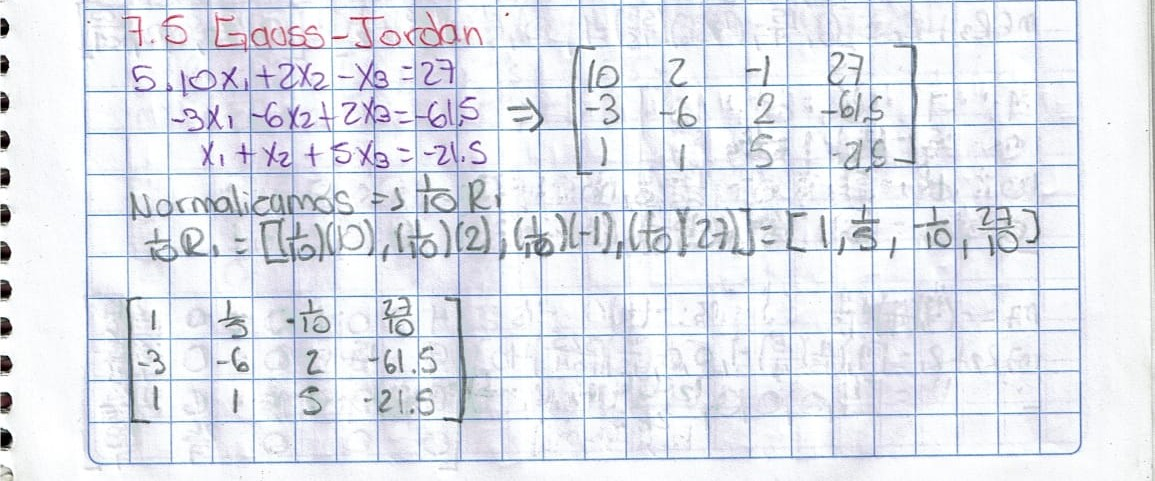
\includegraphics[width=6.25in,height=\textheight,keepaspectratio,alt={Ejercicio 5}]{Ejercicio75Jordan5.jpg}
\caption{Ejercicio 5}
\end{figure}

\begin{figure}
\centering
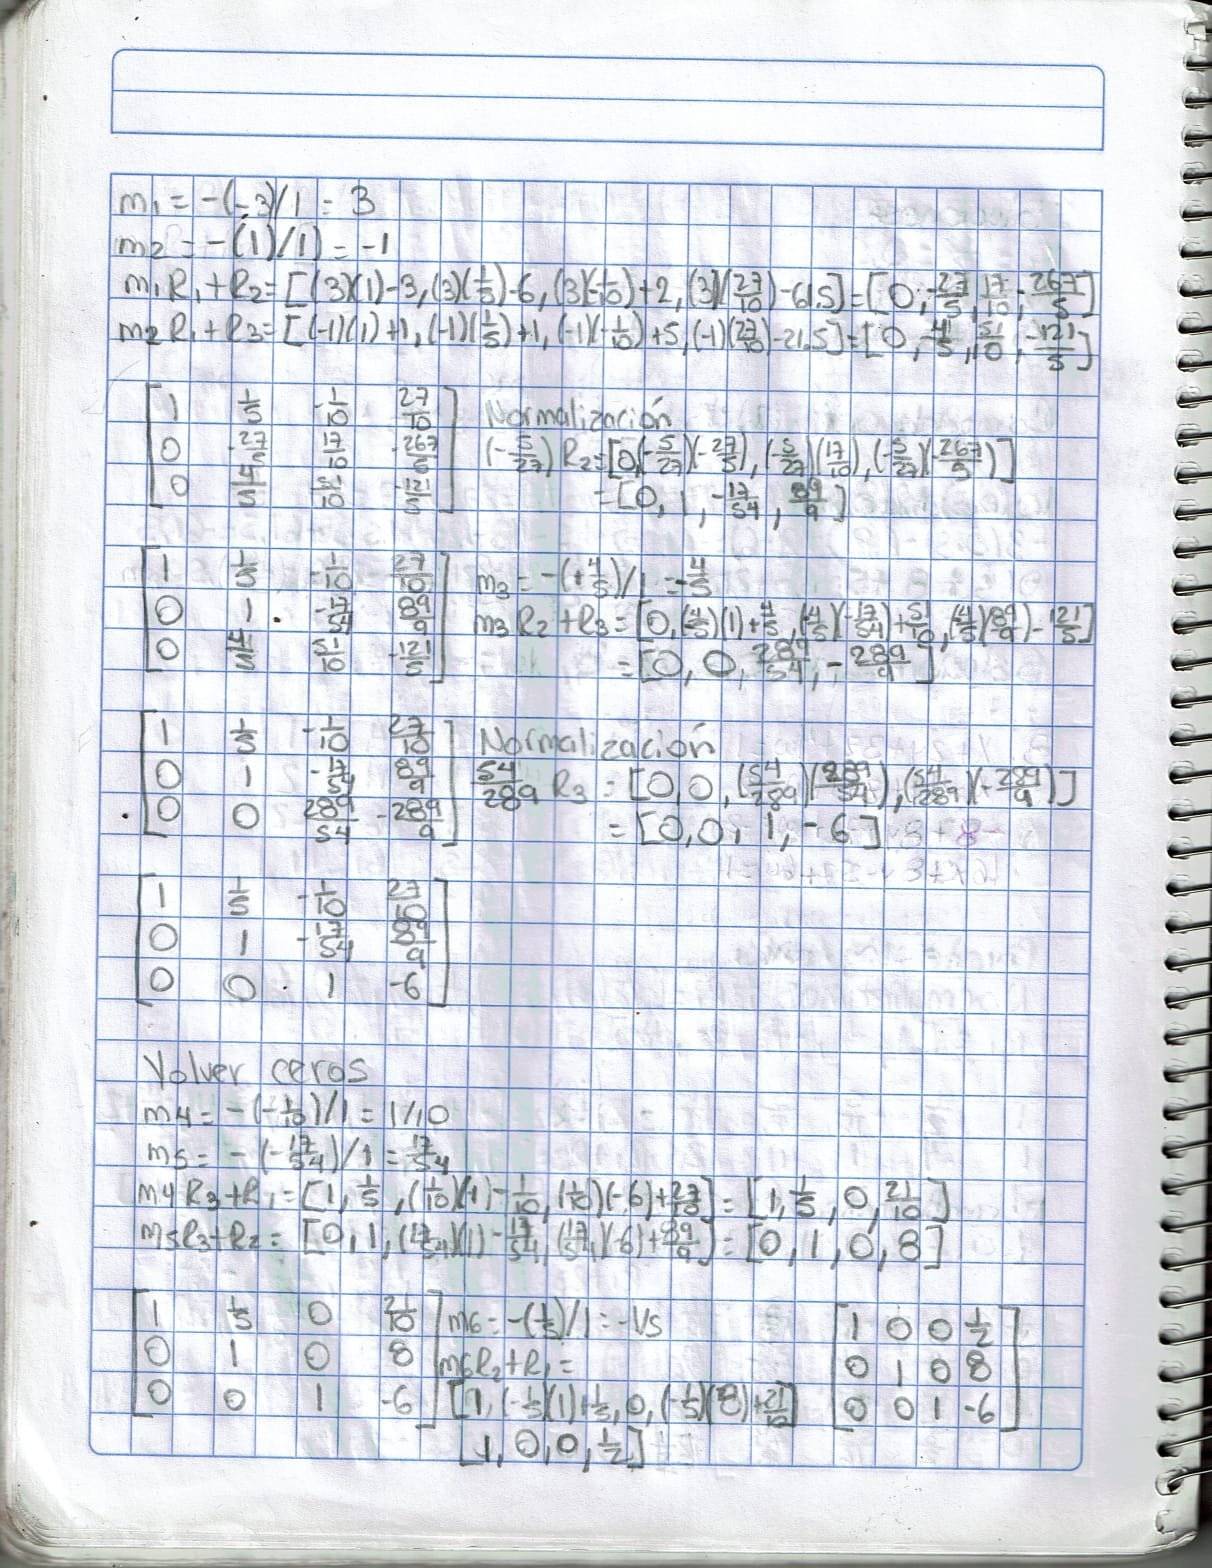
\includegraphics[width=6.25in,height=\textheight,keepaspectratio,alt={Ejercicio 5-2}]{Ejercicio75Jordan5_2.jpg}
\caption{Ejercicio 5-2}
\end{figure}

\begin{figure}
\centering
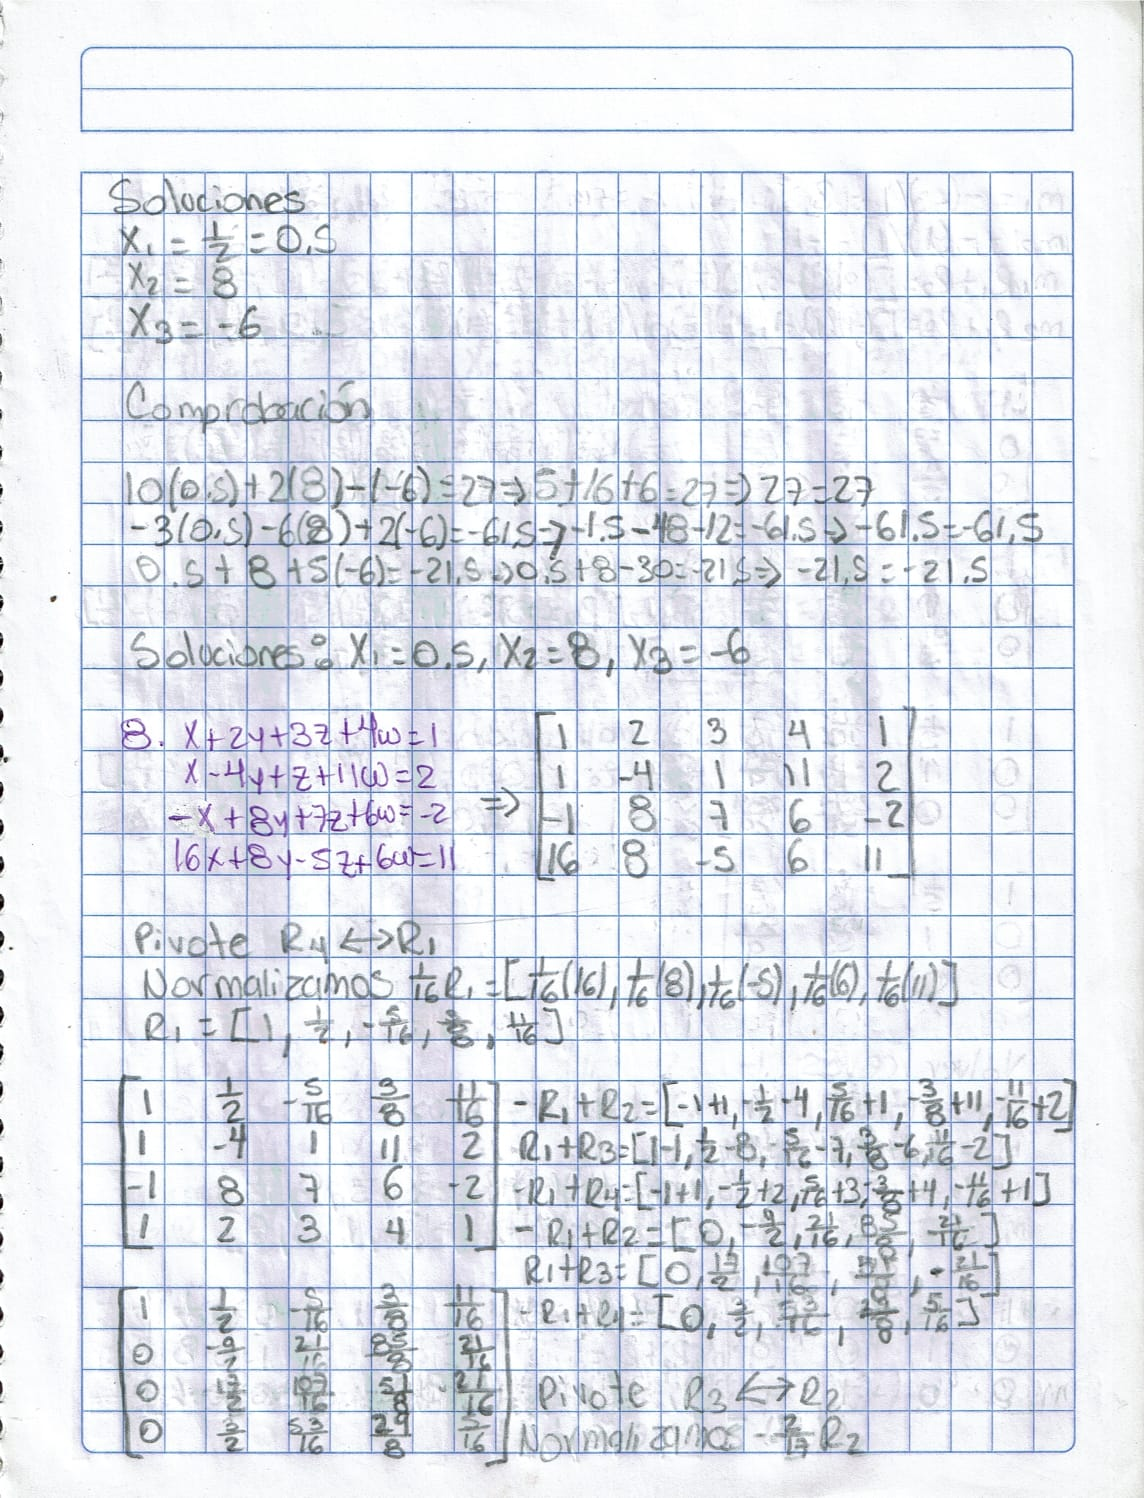
\includegraphics[width=6.25in,height=\textheight,keepaspectratio,alt={Ejercicio 8}]{Ejercicio75Jordan8.jpg}
\caption{Ejercicio 8}
\end{figure}

\begin{figure}
\centering
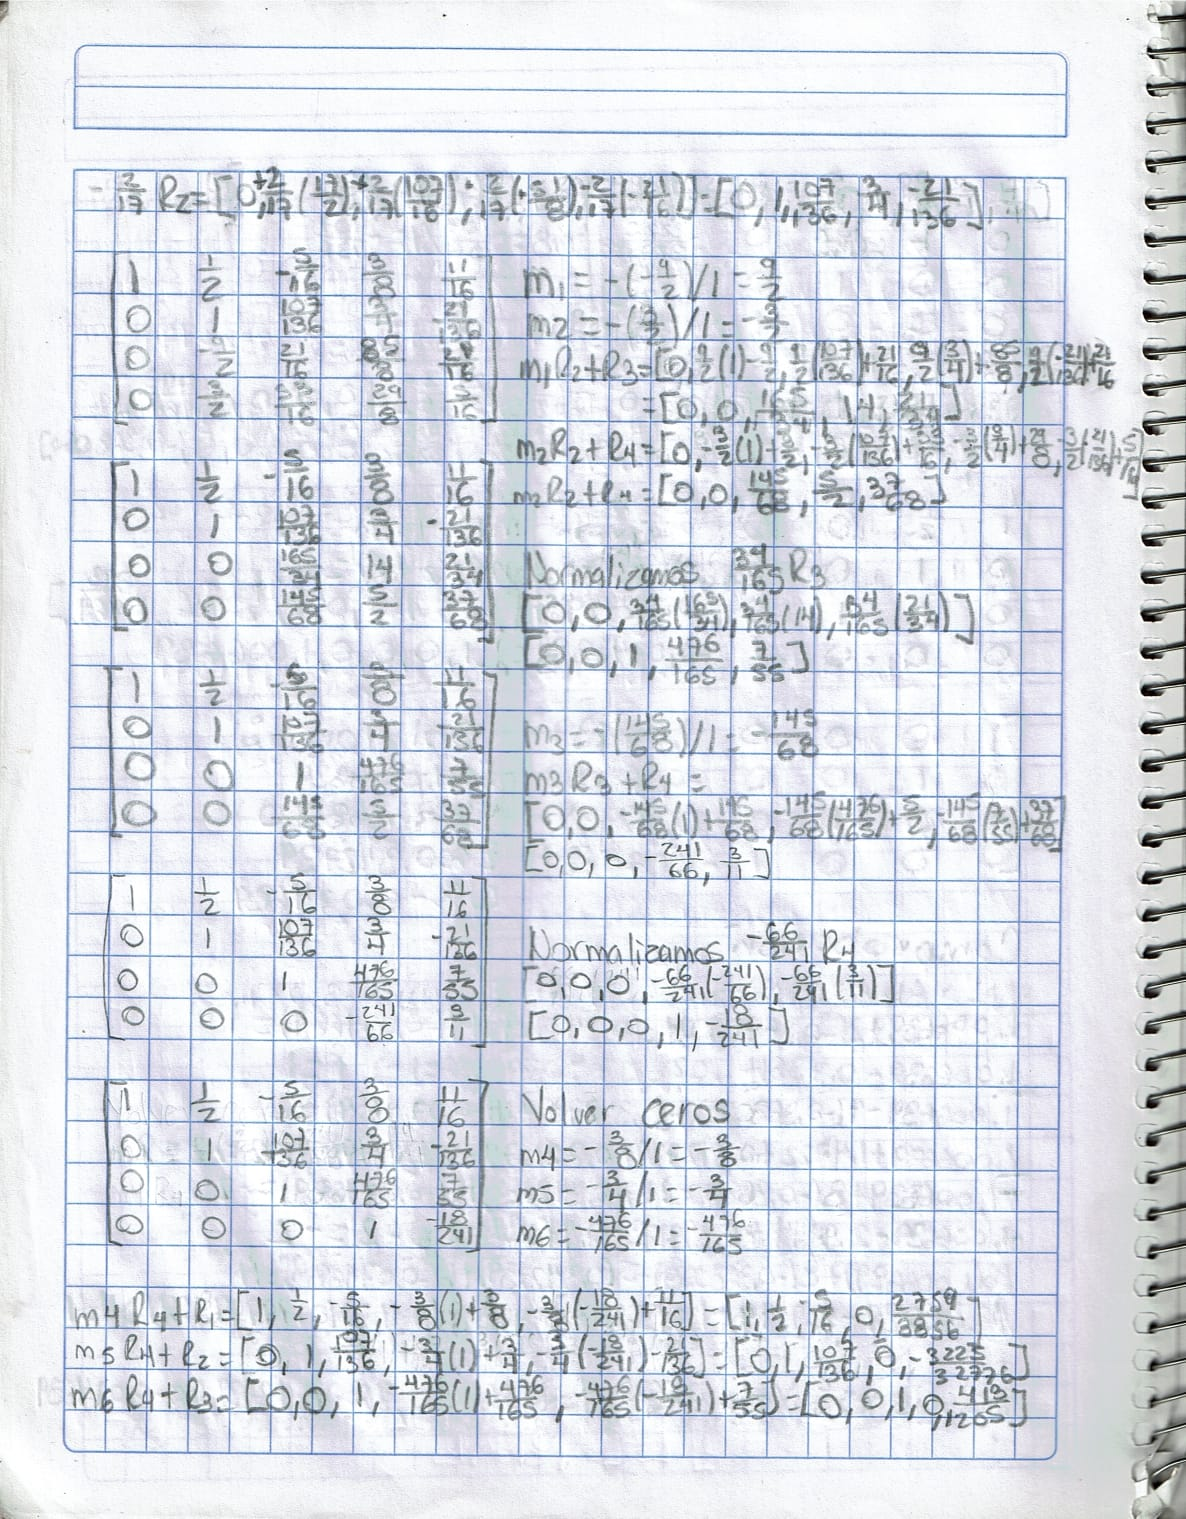
\includegraphics[width=6.25in,height=\textheight,keepaspectratio,alt={Ejercicio 8-2}]{Ejercicio75Jordan8_2.jpg}
\caption{Ejercicio 8-2}
\end{figure}

\begin{figure}
\centering
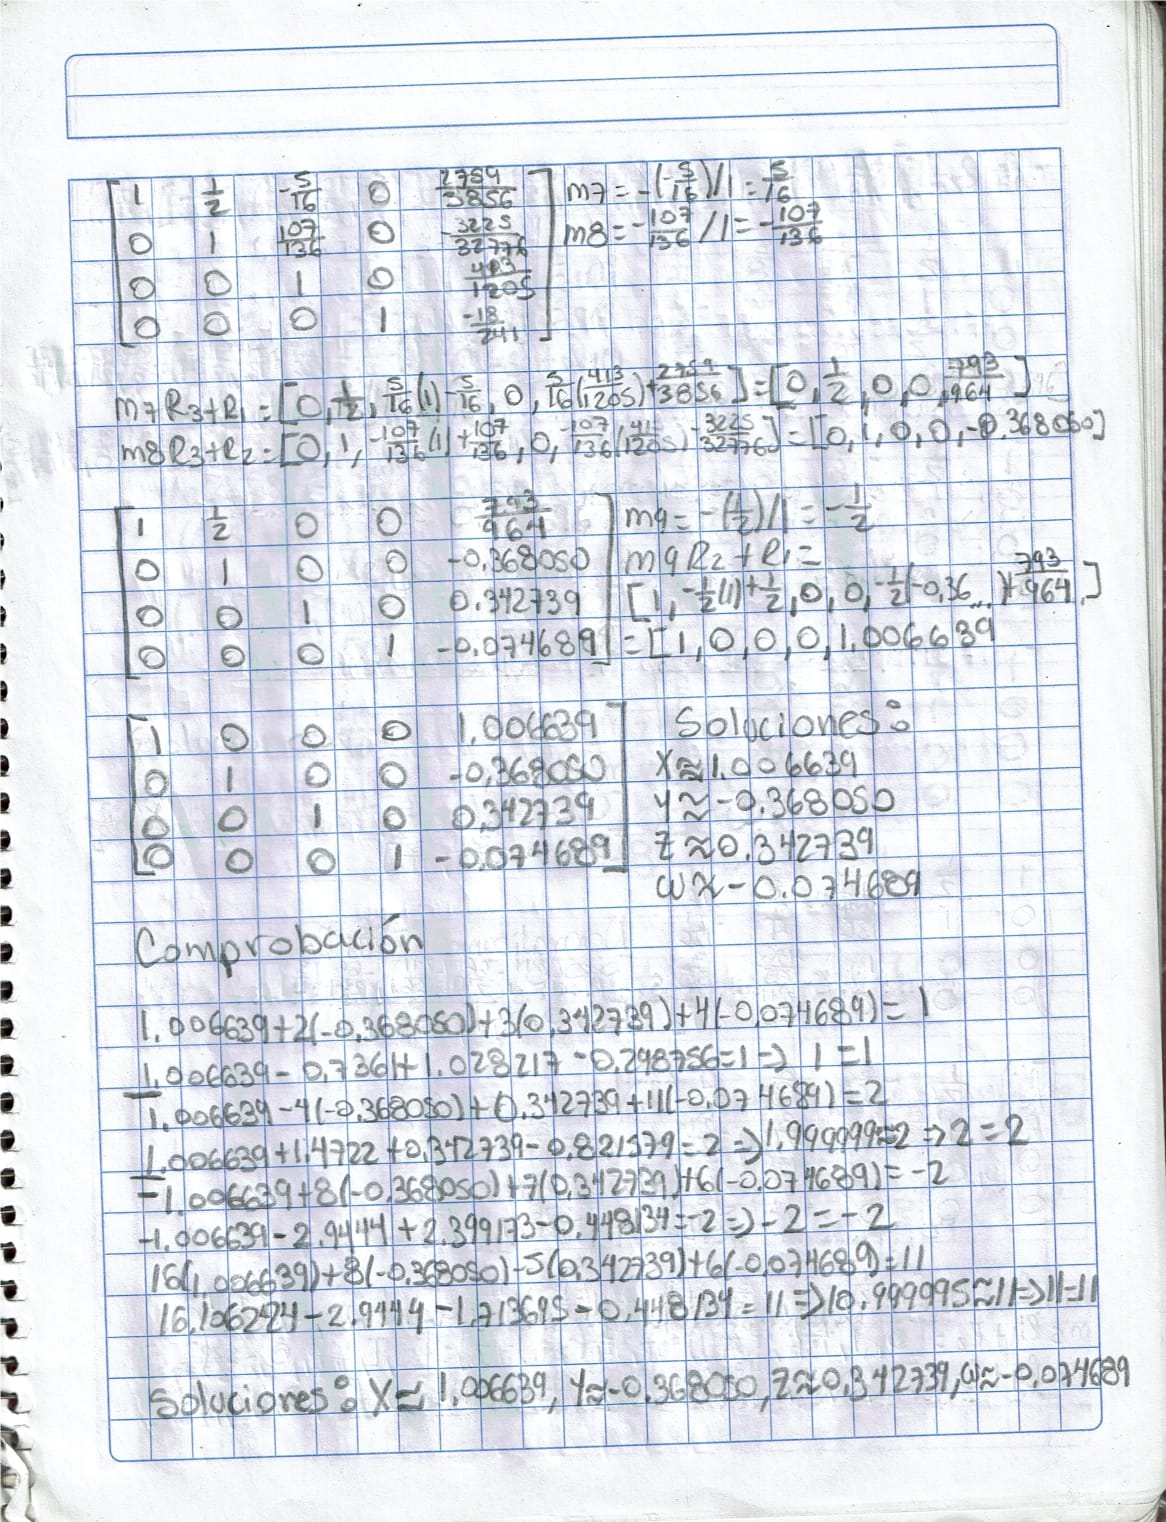
\includegraphics[width=6.25in,height=\textheight,keepaspectratio,alt={Ejercicio 8-3}]{Ejercicio75Jordan8_3.jpg}
\caption{Ejercicio 8-3}
\end{figure}

\subsubsection{\texorpdfstring{Sistema
\(1\)}{Sistema 1}}\label{sistema-1-2}

\(x_1 + 2x_2 + 3x_3 = 1\)

\(−0.4x_1 + 2x_2 − x_3 = 10\)

\(0.5x_1 − 3x_2 + x_3 = 15\)

\paragraph{Procedimiento}\label{procedimiento-30}

\begin{Shaded}
\begin{Highlighting}[]
\NormalTok{A }\OtherTok{\textless{}{-}} \FunctionTok{matrix}\NormalTok{(}\FunctionTok{c}\NormalTok{(}\DecValTok{1}\NormalTok{, }\DecValTok{2}\NormalTok{, }\DecValTok{3}\NormalTok{,}
              \SpecialCharTok{{-}}\FloatTok{0.4}\NormalTok{, }\DecValTok{2}\NormalTok{, }\SpecialCharTok{{-}}\DecValTok{1}\NormalTok{,}
              \FloatTok{0.5}\NormalTok{, }\SpecialCharTok{{-}}\DecValTok{3}\NormalTok{, }\DecValTok{1}\NormalTok{),}
      \AttributeTok{nrow =} \DecValTok{3}\NormalTok{, }\AttributeTok{byrow =} \ConstantTok{TRUE}\NormalTok{)}
\NormalTok{b }\OtherTok{\textless{}{-}} \FunctionTok{matrix}\NormalTok{(}\FunctionTok{c}\NormalTok{(}\DecValTok{1}\NormalTok{, }\DecValTok{10}\NormalTok{, }\DecValTok{15}\NormalTok{), }\AttributeTok{nrow =} \DecValTok{3}\NormalTok{)}

\NormalTok{Ab }\OtherTok{\textless{}{-}} \FunctionTok{cbind}\NormalTok{(A, b); (Ab)}
\end{Highlighting}
\end{Shaded}

\begin{verbatim}
##      [,1] [,2] [,3] [,4]
## [1,]  1.0    2    3    1
## [2,] -0.4    2   -1   10
## [3,]  0.5   -3    1   15
\end{verbatim}

\subparagraph{Primera eliminación}\label{primera-eliminaciuxf3n-10}

\begin{Shaded}
\begin{Highlighting}[]
\NormalTok{m1 }\OtherTok{\textless{}{-}} \SpecialCharTok{{-}}\NormalTok{ Ab[}\DecValTok{2}\NormalTok{,}\DecValTok{1}\NormalTok{] }\SpecialCharTok{/}\NormalTok{ Ab[}\DecValTok{1}\NormalTok{,}\DecValTok{1}\NormalTok{]}
\NormalTok{(m1)}
\end{Highlighting}
\end{Shaded}

\begin{verbatim}
## [1] 0.4
\end{verbatim}

\begin{Shaded}
\begin{Highlighting}[]
\NormalTok{m2 }\OtherTok{\textless{}{-}} \SpecialCharTok{{-}}\NormalTok{ Ab[}\DecValTok{3}\NormalTok{,}\DecValTok{1}\NormalTok{] }\SpecialCharTok{/}\NormalTok{ Ab[}\DecValTok{1}\NormalTok{,}\DecValTok{1}\NormalTok{]}
\NormalTok{(m2)}
\end{Highlighting}
\end{Shaded}

\begin{verbatim}
## [1] -0.5
\end{verbatim}

\begin{Shaded}
\begin{Highlighting}[]
\NormalTok{A1 }\OtherTok{\textless{}{-}}\NormalTok{ Ab[}\DecValTok{1}\NormalTok{,]}
\NormalTok{(A1)}
\end{Highlighting}
\end{Shaded}

\begin{verbatim}
## [1] 1 2 3 1
\end{verbatim}

\begin{Shaded}
\begin{Highlighting}[]
\NormalTok{A2 }\OtherTok{\textless{}{-}}\NormalTok{ m1 }\SpecialCharTok{*}\NormalTok{ Ab[}\DecValTok{1}\NormalTok{,] }\SpecialCharTok{+}\NormalTok{ Ab[}\DecValTok{2}\NormalTok{,]}
\NormalTok{(A2)}
\end{Highlighting}
\end{Shaded}

\begin{verbatim}
## [1]  0.0  2.8  0.2 10.4
\end{verbatim}

\begin{Shaded}
\begin{Highlighting}[]
\NormalTok{A3 }\OtherTok{\textless{}{-}}\NormalTok{ m2 }\SpecialCharTok{*}\NormalTok{ Ab[}\DecValTok{1}\NormalTok{,] }\SpecialCharTok{+}\NormalTok{ Ab[}\DecValTok{3}\NormalTok{,]}
\NormalTok{(A3)}
\end{Highlighting}
\end{Shaded}

\begin{verbatim}
## [1]  0.0 -4.0 -0.5 14.5
\end{verbatim}

\begin{Shaded}
\begin{Highlighting}[]
\NormalTok{NuevaA }\OtherTok{\textless{}{-}} \FunctionTok{rbind}\NormalTok{(A1, A2, A3)}
\NormalTok{(NuevaA)}
\end{Highlighting}
\end{Shaded}

\begin{verbatim}
##    [,1] [,2] [,3] [,4]
## A1    1  2.0  3.0  1.0
## A2    0  2.8  0.2 10.4
## A3    0 -4.0 -0.5 14.5
\end{verbatim}

\begin{Shaded}
\begin{Highlighting}[]
\CommentTok{\# Primer pivote}

\NormalTok{Ab }\OtherTok{\textless{}{-}}\NormalTok{ NuevaA[}\FunctionTok{c}\NormalTok{(}\DecValTok{1}\NormalTok{, }\DecValTok{3}\NormalTok{, }\DecValTok{2}\NormalTok{), ]}
\NormalTok{(Ab)}
\end{Highlighting}
\end{Shaded}

\begin{verbatim}
##    [,1] [,2] [,3] [,4]
## A1    1  2.0  3.0  1.0
## A3    0 -4.0 -0.5 14.5
## A2    0  2.8  0.2 10.4
\end{verbatim}

\begin{Shaded}
\begin{Highlighting}[]
\CommentTok{\# Primera normalización}

\NormalTok{n1 }\OtherTok{\textless{}{-}} \DecValTok{1} \SpecialCharTok{/}\NormalTok{ Ab[}\DecValTok{2}\NormalTok{,}\DecValTok{2}\NormalTok{]}
\NormalTok{A1 }\OtherTok{\textless{}{-}}\NormalTok{ Ab[}\DecValTok{1}\NormalTok{,]}
\NormalTok{A2 }\OtherTok{\textless{}{-}}\NormalTok{ n1 }\SpecialCharTok{*}\NormalTok{ Ab[}\DecValTok{2}\NormalTok{,]}
\NormalTok{(A2)}
\end{Highlighting}
\end{Shaded}

\begin{verbatim}
## [1]  0.000  1.000  0.125 -3.625
\end{verbatim}

\begin{Shaded}
\begin{Highlighting}[]
\NormalTok{A3 }\OtherTok{\textless{}{-}}\NormalTok{ Ab[}\DecValTok{3}\NormalTok{,]}
\NormalTok{NuevaA }\OtherTok{\textless{}{-}} \FunctionTok{rbind}\NormalTok{(A1, A2, A3)}
\NormalTok{(NuevaA)}
\end{Highlighting}
\end{Shaded}

\begin{verbatim}
##    [,1] [,2]  [,3]   [,4]
## A1    1  2.0 3.000  1.000
## A2    0  1.0 0.125 -3.625
## A3    0  2.8 0.200 10.400
\end{verbatim}

\subparagraph{Segunda eliminación}\label{segunda-eliminaciuxf3n-8}

\begin{Shaded}
\begin{Highlighting}[]
\NormalTok{Ab }\OtherTok{\textless{}{-}}\NormalTok{ NuevaA}
\NormalTok{m3 }\OtherTok{\textless{}{-}} \SpecialCharTok{{-}}\NormalTok{ Ab[}\DecValTok{1}\NormalTok{,}\DecValTok{2}\NormalTok{] }\SpecialCharTok{/}\NormalTok{ Ab[}\DecValTok{2}\NormalTok{,}\DecValTok{2}\NormalTok{]}
\NormalTok{(m3)}
\end{Highlighting}
\end{Shaded}

\begin{verbatim}
## A1 
## -2
\end{verbatim}

\begin{Shaded}
\begin{Highlighting}[]
\NormalTok{m4 }\OtherTok{\textless{}{-}} \SpecialCharTok{{-}}\NormalTok{ Ab[}\DecValTok{3}\NormalTok{,}\DecValTok{2}\NormalTok{] }\SpecialCharTok{/}\NormalTok{ Ab[}\DecValTok{2}\NormalTok{,}\DecValTok{2}\NormalTok{]}
\NormalTok{(m4)}
\end{Highlighting}
\end{Shaded}

\begin{verbatim}
##   A3 
## -2.8
\end{verbatim}

\begin{Shaded}
\begin{Highlighting}[]
\NormalTok{A1 }\OtherTok{\textless{}{-}}\NormalTok{ m3 }\SpecialCharTok{*}\NormalTok{ Ab[}\DecValTok{2}\NormalTok{,] }\SpecialCharTok{+}\NormalTok{ Ab[}\DecValTok{1}\NormalTok{,]}
\NormalTok{A2 }\OtherTok{\textless{}{-}}\NormalTok{ Ab[}\DecValTok{2}\NormalTok{,]}
\NormalTok{A3 }\OtherTok{\textless{}{-}}\NormalTok{ m4 }\SpecialCharTok{*}\NormalTok{ Ab[}\DecValTok{2}\NormalTok{,] }\SpecialCharTok{+}\NormalTok{ Ab[}\DecValTok{3}\NormalTok{,]}
\NormalTok{(A3)}
\end{Highlighting}
\end{Shaded}

\begin{verbatim}
## [1]  0.00  0.00 -0.15 20.55
\end{verbatim}

\begin{Shaded}
\begin{Highlighting}[]
\NormalTok{NuevaA }\OtherTok{\textless{}{-}} \FunctionTok{rbind}\NormalTok{(A1, A2, A3)}
\NormalTok{(NuevaA)}
\end{Highlighting}
\end{Shaded}

\begin{verbatim}
##    [,1] [,2]   [,3]   [,4]
## A1    1    0  2.750  8.250
## A2    0    1  0.125 -3.625
## A3    0    0 -0.150 20.550
\end{verbatim}

\begin{Shaded}
\begin{Highlighting}[]
\CommentTok{\# Segunda normalización}

\NormalTok{Ab }\OtherTok{\textless{}{-}}\NormalTok{ NuevaA}
\NormalTok{n2 }\OtherTok{\textless{}{-}} \DecValTok{1} \SpecialCharTok{/}\NormalTok{ Ab[}\DecValTok{3}\NormalTok{,}\DecValTok{3}\NormalTok{]}
\NormalTok{A1 }\OtherTok{\textless{}{-}}\NormalTok{ Ab[}\DecValTok{1}\NormalTok{,]}
\NormalTok{A2 }\OtherTok{\textless{}{-}}\NormalTok{ Ab[}\DecValTok{2}\NormalTok{,]}
\NormalTok{A3 }\OtherTok{\textless{}{-}}\NormalTok{ n2 }\SpecialCharTok{*}\NormalTok{ Ab[}\DecValTok{3}\NormalTok{,]}
\NormalTok{(A3)}
\end{Highlighting}
\end{Shaded}

\begin{verbatim}
## [1]    0    0    1 -137
\end{verbatim}

\begin{Shaded}
\begin{Highlighting}[]
\NormalTok{NuevaA }\OtherTok{\textless{}{-}} \FunctionTok{rbind}\NormalTok{(A1, A2, A3)}
\NormalTok{(NuevaA)}
\end{Highlighting}
\end{Shaded}

\begin{verbatim}
##    [,1] [,2]  [,3]     [,4]
## A1    1    0 2.750    8.250
## A2    0    1 0.125   -3.625
## A3    0    0 1.000 -137.000
\end{verbatim}

\subparagraph{Tercera eliminación}\label{tercera-eliminaciuxf3n-4}

\begin{Shaded}
\begin{Highlighting}[]
\NormalTok{Ab }\OtherTok{\textless{}{-}}\NormalTok{ NuevaA}
\NormalTok{m5 }\OtherTok{\textless{}{-}} \SpecialCharTok{{-}}\NormalTok{ Ab[}\DecValTok{1}\NormalTok{,}\DecValTok{3}\NormalTok{] }\SpecialCharTok{/}\NormalTok{ Ab[}\DecValTok{3}\NormalTok{,}\DecValTok{3}\NormalTok{]}
\NormalTok{(m5)}
\end{Highlighting}
\end{Shaded}

\begin{verbatim}
##    A1 
## -2.75
\end{verbatim}

\begin{Shaded}
\begin{Highlighting}[]
\NormalTok{m6 }\OtherTok{\textless{}{-}} \SpecialCharTok{{-}}\NormalTok{ Ab[}\DecValTok{2}\NormalTok{,}\DecValTok{3}\NormalTok{] }\SpecialCharTok{/}\NormalTok{ Ab[}\DecValTok{3}\NormalTok{,}\DecValTok{3}\NormalTok{]}
\NormalTok{(m6)}
\end{Highlighting}
\end{Shaded}

\begin{verbatim}
##     A2 
## -0.125
\end{verbatim}

\begin{Shaded}
\begin{Highlighting}[]
\NormalTok{A1 }\OtherTok{\textless{}{-}}\NormalTok{ m5 }\SpecialCharTok{*}\NormalTok{ Ab[}\DecValTok{3}\NormalTok{,] }\SpecialCharTok{+}\NormalTok{ Ab[}\DecValTok{1}\NormalTok{,]}
\NormalTok{A2 }\OtherTok{\textless{}{-}}\NormalTok{ m6 }\SpecialCharTok{*}\NormalTok{ Ab[}\DecValTok{3}\NormalTok{,] }\SpecialCharTok{+}\NormalTok{ Ab[}\DecValTok{2}\NormalTok{,]}
\NormalTok{A3 }\OtherTok{\textless{}{-}}\NormalTok{ Ab[}\DecValTok{3}\NormalTok{,]}
\NormalTok{(A3)}
\end{Highlighting}
\end{Shaded}

\begin{verbatim}
## [1]    0    0    1 -137
\end{verbatim}

\begin{Shaded}
\begin{Highlighting}[]
\NormalTok{NuevaA }\OtherTok{\textless{}{-}} \FunctionTok{rbind}\NormalTok{(A1, A2, A3)}
\NormalTok{(NuevaA)}
\end{Highlighting}
\end{Shaded}

\begin{verbatim}
##    [,1] [,2] [,3]   [,4]
## A1    1    0    0  385.0
## A2    0    1    0   13.5
## A3    0    0    1 -137.0
\end{verbatim}

\begin{Shaded}
\begin{Highlighting}[]
\CommentTok{\# Soluciones}

\NormalTok{Ab }\OtherTok{\textless{}{-}}\NormalTok{ NuevaA; (Ab)}
\end{Highlighting}
\end{Shaded}

\begin{verbatim}
##    [,1] [,2] [,3]   [,4]
## A1    1    0    0  385.0
## A2    0    1    0   13.5
## A3    0    0    1 -137.0
\end{verbatim}

\begin{Shaded}
\begin{Highlighting}[]
\NormalTok{x1 }\OtherTok{\textless{}{-}}\NormalTok{ Ab[}\DecValTok{1}\NormalTok{,}\DecValTok{4}\NormalTok{] }\SpecialCharTok{/}\NormalTok{ Ab[}\DecValTok{1}\NormalTok{,}\DecValTok{1}\NormalTok{]}
\NormalTok{x2 }\OtherTok{\textless{}{-}}\NormalTok{ Ab[}\DecValTok{2}\NormalTok{,}\DecValTok{4}\NormalTok{] }\SpecialCharTok{/}\NormalTok{ Ab[}\DecValTok{2}\NormalTok{,}\DecValTok{2}\NormalTok{]}
\NormalTok{x3 }\OtherTok{\textless{}{-}}\NormalTok{ Ab[}\DecValTok{3}\NormalTok{,}\DecValTok{4}\NormalTok{] }\SpecialCharTok{/}\NormalTok{ Ab[}\DecValTok{3}\NormalTok{,}\DecValTok{3}\NormalTok{]}
\end{Highlighting}
\end{Shaded}

\begin{Shaded}
\begin{Highlighting}[]
\CommentTok{\# Comprobación}

\NormalTok{I }\OtherTok{\textless{}{-}}\NormalTok{ b[}\DecValTok{1}\NormalTok{,]; (I)}
\end{Highlighting}
\end{Shaded}

\begin{verbatim}
## [1] 1
\end{verbatim}

\begin{Shaded}
\begin{Highlighting}[]
\NormalTok{II }\OtherTok{\textless{}{-}}\NormalTok{ b[}\DecValTok{2}\NormalTok{,]; (II)}
\end{Highlighting}
\end{Shaded}

\begin{verbatim}
## [1] 10
\end{verbatim}

\begin{Shaded}
\begin{Highlighting}[]
\NormalTok{III }\OtherTok{\textless{}{-}}\NormalTok{ b[}\DecValTok{3}\NormalTok{,]; (III)}
\end{Highlighting}
\end{Shaded}

\begin{verbatim}
## [1] 15
\end{verbatim}

\begin{Shaded}
\begin{Highlighting}[]
\NormalTok{c1 }\OtherTok{\textless{}{-}}\NormalTok{ (A[}\DecValTok{1}\NormalTok{,}\DecValTok{1}\NormalTok{] }\SpecialCharTok{*}\NormalTok{ x1) }\SpecialCharTok{+}\NormalTok{ (A[}\DecValTok{1}\NormalTok{,}\DecValTok{2}\NormalTok{] }\SpecialCharTok{*}\NormalTok{ x2) }\SpecialCharTok{+}\NormalTok{ (A[}\DecValTok{1}\NormalTok{,}\DecValTok{3}\NormalTok{] }\SpecialCharTok{*}\NormalTok{ x3); }\FunctionTok{paste0}\NormalTok{(}\StringTok{"El resultado es: "}\NormalTok{,c1)}
\end{Highlighting}
\end{Shaded}

\begin{verbatim}
## [1] "El resultado es: 1"
\end{verbatim}

\begin{Shaded}
\begin{Highlighting}[]
\NormalTok{c2 }\OtherTok{\textless{}{-}}\NormalTok{ (A[}\DecValTok{2}\NormalTok{,}\DecValTok{1}\NormalTok{] }\SpecialCharTok{*}\NormalTok{ x1) }\SpecialCharTok{+}\NormalTok{ (A[}\DecValTok{2}\NormalTok{,}\DecValTok{2}\NormalTok{] }\SpecialCharTok{*}\NormalTok{ x2) }\SpecialCharTok{+}\NormalTok{ (A[}\DecValTok{2}\NormalTok{,}\DecValTok{3}\NormalTok{] }\SpecialCharTok{*}\NormalTok{ x3); }\FunctionTok{paste0}\NormalTok{(}\StringTok{"El resultado es: "}\NormalTok{,c2)}
\end{Highlighting}
\end{Shaded}

\begin{verbatim}
## [1] "El resultado es: 10"
\end{verbatim}

\begin{Shaded}
\begin{Highlighting}[]
\NormalTok{c3 }\OtherTok{\textless{}{-}}\NormalTok{ (A[}\DecValTok{3}\NormalTok{,}\DecValTok{1}\NormalTok{] }\SpecialCharTok{*}\NormalTok{ x1) }\SpecialCharTok{+}\NormalTok{ (A[}\DecValTok{3}\NormalTok{,}\DecValTok{2}\NormalTok{] }\SpecialCharTok{*}\NormalTok{ x2) }\SpecialCharTok{+}\NormalTok{ (A[}\DecValTok{3}\NormalTok{,}\DecValTok{3}\NormalTok{] }\SpecialCharTok{*}\NormalTok{ x3); }\FunctionTok{paste0}\NormalTok{(}\StringTok{"El resultado es: "}\NormalTok{,c3)}
\end{Highlighting}
\end{Shaded}

\begin{verbatim}
## [1] "El resultado es: 15"
\end{verbatim}

\begin{Shaded}
\begin{Highlighting}[]
\FunctionTok{paste0}\NormalTok{(}\StringTok{"En la ecuación 1: "}\NormalTok{, c1, }\StringTok{" tecnicamente es: "}\NormalTok{, I)}
\end{Highlighting}
\end{Shaded}

\begin{verbatim}
## [1] "En la ecuación 1: 1 tecnicamente es: 1"
\end{verbatim}

\begin{Shaded}
\begin{Highlighting}[]
\FunctionTok{paste0}\NormalTok{(}\StringTok{"En la ecuación 2: "}\NormalTok{, c2, }\StringTok{" tecnicamente es: "}\NormalTok{, II)}
\end{Highlighting}
\end{Shaded}

\begin{verbatim}
## [1] "En la ecuación 2: 10 tecnicamente es: 10"
\end{verbatim}

\begin{Shaded}
\begin{Highlighting}[]
\FunctionTok{paste0}\NormalTok{(}\StringTok{"En la ecuación 3: "}\NormalTok{, c3, }\StringTok{" tecnicamente es: "}\NormalTok{, III)}
\end{Highlighting}
\end{Shaded}

\begin{verbatim}
## [1] "En la ecuación 3: 15 tecnicamente es: 15"
\end{verbatim}

\paragraph{Resultados}\label{resultados-20}

\begin{Shaded}
\begin{Highlighting}[]
\FunctionTok{cat}\NormalTok{(}\StringTok{"Soluciones del sistema:"}\NormalTok{)}
\end{Highlighting}
\end{Shaded}

\begin{verbatim}
## Soluciones del sistema:
\end{verbatim}

\begin{Shaded}
\begin{Highlighting}[]
\FunctionTok{cat}\NormalTok{(}\StringTok{"x1 ="}\NormalTok{, x1)}
\end{Highlighting}
\end{Shaded}

\begin{verbatim}
## x1 = 385
\end{verbatim}

\begin{Shaded}
\begin{Highlighting}[]
\FunctionTok{cat}\NormalTok{(}\StringTok{"x2 ="}\NormalTok{, x2) }
\end{Highlighting}
\end{Shaded}

\begin{verbatim}
## x2 = 13.5
\end{verbatim}

\begin{Shaded}
\begin{Highlighting}[]
\FunctionTok{cat}\NormalTok{(}\StringTok{"x3 ="}\NormalTok{, x3)}
\end{Highlighting}
\end{Shaded}

\begin{verbatim}
## x3 = -137
\end{verbatim}

\subsubsection{\texorpdfstring{Sistema
\(2\)}{Sistema 2}}\label{sistema-2-2}

\(2x_1 − 0.9x_2 + 3x_3 = −3.61\)

\(−0.5x_1 + 0.1x_2 − x_3 = 2.035\)

\(x_1 − 6.35x_2 − 0.45x_3 = 15.401\)

\paragraph{Procedimiento}\label{procedimiento-31}

\begin{Shaded}
\begin{Highlighting}[]
\NormalTok{A }\OtherTok{\textless{}{-}} \FunctionTok{matrix}\NormalTok{(}\FunctionTok{c}\NormalTok{(}\DecValTok{2}\NormalTok{, }\SpecialCharTok{{-}}\FloatTok{0.9}\NormalTok{, }\DecValTok{3}\NormalTok{,}
              \SpecialCharTok{{-}}\FloatTok{0.5}\NormalTok{, }\FloatTok{0.1}\NormalTok{, }\SpecialCharTok{{-}}\DecValTok{1}\NormalTok{,}
              \DecValTok{1}\NormalTok{, }\SpecialCharTok{{-}}\FloatTok{6.35}\NormalTok{, }\SpecialCharTok{{-}}\FloatTok{0.45}\NormalTok{),}
      \AttributeTok{nrow =} \DecValTok{3}\NormalTok{, }\AttributeTok{byrow =} \ConstantTok{TRUE}\NormalTok{)}
\NormalTok{b }\OtherTok{\textless{}{-}} \FunctionTok{matrix}\NormalTok{(}\FunctionTok{c}\NormalTok{(}\SpecialCharTok{{-}}\FloatTok{3.61}\NormalTok{, }\FloatTok{2.035}\NormalTok{, }\FloatTok{15.401}\NormalTok{), }\AttributeTok{nrow =} \DecValTok{3}\NormalTok{)}

\NormalTok{Ab }\OtherTok{\textless{}{-}} \FunctionTok{cbind}\NormalTok{(A, b); (Ab)}
\end{Highlighting}
\end{Shaded}

\begin{verbatim}
##      [,1]  [,2]  [,3]   [,4]
## [1,]  2.0 -0.90  3.00 -3.610
## [2,] -0.5  0.10 -1.00  2.035
## [3,]  1.0 -6.35 -0.45 15.401
\end{verbatim}

\subparagraph{Primera eliminación}\label{primera-eliminaciuxf3n-11}

\begin{Shaded}
\begin{Highlighting}[]
\CommentTok{\# Primera normalización}

\NormalTok{n1 }\OtherTok{\textless{}{-}} \DecValTok{1} \SpecialCharTok{/}\NormalTok{ Ab[}\DecValTok{1}\NormalTok{,}\DecValTok{1}\NormalTok{]}
\NormalTok{A1 }\OtherTok{\textless{}{-}}\NormalTok{ n1 }\SpecialCharTok{*}\NormalTok{ Ab[}\DecValTok{1}\NormalTok{,]}
\NormalTok{(A1)}
\end{Highlighting}
\end{Shaded}

\begin{verbatim}
## [1]  1.000 -0.450  1.500 -1.805
\end{verbatim}

\begin{Shaded}
\begin{Highlighting}[]
\NormalTok{A2 }\OtherTok{\textless{}{-}}\NormalTok{ Ab[}\DecValTok{2}\NormalTok{,]}
\NormalTok{A3 }\OtherTok{\textless{}{-}}\NormalTok{ Ab[}\DecValTok{3}\NormalTok{,]}
\NormalTok{NuevaA }\OtherTok{\textless{}{-}} \FunctionTok{rbind}\NormalTok{(A1, A2, A3)}
\NormalTok{(NuevaA)}
\end{Highlighting}
\end{Shaded}

\begin{verbatim}
##    [,1]  [,2]  [,3]   [,4]
## A1  1.0 -0.45  1.50 -1.805
## A2 -0.5  0.10 -1.00  2.035
## A3  1.0 -6.35 -0.45 15.401
\end{verbatim}

\begin{Shaded}
\begin{Highlighting}[]
\CommentTok{\# Volver ceros}
\NormalTok{Ab }\OtherTok{\textless{}{-}}\NormalTok{ NuevaA}
\NormalTok{m1 }\OtherTok{\textless{}{-}} \SpecialCharTok{{-}}\NormalTok{ Ab[}\DecValTok{2}\NormalTok{,}\DecValTok{1}\NormalTok{] }\SpecialCharTok{/}\NormalTok{ Ab[}\DecValTok{1}\NormalTok{,}\DecValTok{1}\NormalTok{]}
\NormalTok{(m1)}
\end{Highlighting}
\end{Shaded}

\begin{verbatim}
##  A2 
## 0.5
\end{verbatim}

\begin{Shaded}
\begin{Highlighting}[]
\NormalTok{m2 }\OtherTok{\textless{}{-}} \SpecialCharTok{{-}}\NormalTok{ Ab[}\DecValTok{3}\NormalTok{,}\DecValTok{1}\NormalTok{] }\SpecialCharTok{/}\NormalTok{ Ab[}\DecValTok{1}\NormalTok{,}\DecValTok{1}\NormalTok{]}
\NormalTok{(m2)}
\end{Highlighting}
\end{Shaded}

\begin{verbatim}
## A3 
## -1
\end{verbatim}

\begin{Shaded}
\begin{Highlighting}[]
\NormalTok{A1 }\OtherTok{\textless{}{-}}\NormalTok{ Ab[}\DecValTok{1}\NormalTok{,]}
\NormalTok{(A1)}
\end{Highlighting}
\end{Shaded}

\begin{verbatim}
## [1]  1.000 -0.450  1.500 -1.805
\end{verbatim}

\begin{Shaded}
\begin{Highlighting}[]
\NormalTok{A2 }\OtherTok{\textless{}{-}}\NormalTok{ m1 }\SpecialCharTok{*}\NormalTok{ Ab[}\DecValTok{1}\NormalTok{,] }\SpecialCharTok{+}\NormalTok{ Ab[}\DecValTok{2}\NormalTok{,]}
\NormalTok{(A2)}
\end{Highlighting}
\end{Shaded}

\begin{verbatim}
## [1]  0.0000 -0.1250 -0.2500  1.1325
\end{verbatim}

\begin{Shaded}
\begin{Highlighting}[]
\NormalTok{A3 }\OtherTok{\textless{}{-}}\NormalTok{ m2 }\SpecialCharTok{*}\NormalTok{ Ab[}\DecValTok{1}\NormalTok{,] }\SpecialCharTok{+}\NormalTok{ Ab[}\DecValTok{3}\NormalTok{,]}
\NormalTok{(A3)}
\end{Highlighting}
\end{Shaded}

\begin{verbatim}
## [1]  0.000 -5.900 -1.950 17.206
\end{verbatim}

\begin{Shaded}
\begin{Highlighting}[]
\NormalTok{NuevaA }\OtherTok{\textless{}{-}} \FunctionTok{rbind}\NormalTok{(A1, A2, A3)}
\NormalTok{(NuevaA)}
\end{Highlighting}
\end{Shaded}

\begin{verbatim}
##    [,1]   [,2]  [,3]    [,4]
## A1    1 -0.450  1.50 -1.8050
## A2    0 -0.125 -0.25  1.1325
## A3    0 -5.900 -1.95 17.2060
\end{verbatim}

\subparagraph{Segunda eliminación}\label{segunda-eliminaciuxf3n-9}

\begin{Shaded}
\begin{Highlighting}[]
\CommentTok{\# Primer pivote}

\NormalTok{Ab }\OtherTok{\textless{}{-}}\NormalTok{ NuevaA[}\FunctionTok{c}\NormalTok{(}\DecValTok{1}\NormalTok{, }\DecValTok{3}\NormalTok{, }\DecValTok{2}\NormalTok{), ]}
\NormalTok{(Ab)}
\end{Highlighting}
\end{Shaded}

\begin{verbatim}
##    [,1]   [,2]  [,3]    [,4]
## A1    1 -0.450  1.50 -1.8050
## A3    0 -5.900 -1.95 17.2060
## A2    0 -0.125 -0.25  1.1325
\end{verbatim}

\begin{Shaded}
\begin{Highlighting}[]
\CommentTok{\# Segunda normalización}

\NormalTok{n1 }\OtherTok{\textless{}{-}} \DecValTok{1} \SpecialCharTok{/}\NormalTok{ Ab[}\DecValTok{2}\NormalTok{,}\DecValTok{2}\NormalTok{]}
\NormalTok{A1 }\OtherTok{\textless{}{-}}\NormalTok{ Ab[}\DecValTok{1}\NormalTok{,]}
\NormalTok{A2 }\OtherTok{\textless{}{-}}\NormalTok{ n1 }\SpecialCharTok{*}\NormalTok{ Ab[}\DecValTok{2}\NormalTok{,]}
\NormalTok{(A2)}
\end{Highlighting}
\end{Shaded}

\begin{verbatim}
## [1]  0.0000000  1.0000000  0.3305085 -2.9162712
\end{verbatim}

\begin{Shaded}
\begin{Highlighting}[]
\NormalTok{A3 }\OtherTok{\textless{}{-}}\NormalTok{ Ab[}\DecValTok{3}\NormalTok{,]}
\NormalTok{NuevaA }\OtherTok{\textless{}{-}} \FunctionTok{rbind}\NormalTok{(A1, A2, A3)}
\NormalTok{(NuevaA)}
\end{Highlighting}
\end{Shaded}

\begin{verbatim}
##    [,1]   [,2]       [,3]      [,4]
## A1    1 -0.450  1.5000000 -1.805000
## A2    0  1.000  0.3305085 -2.916271
## A3    0 -0.125 -0.2500000  1.132500
\end{verbatim}

\begin{Shaded}
\begin{Highlighting}[]
\CommentTok{\# Volver ceros}

\NormalTok{Ab }\OtherTok{\textless{}{-}}\NormalTok{ NuevaA}
\NormalTok{m3 }\OtherTok{\textless{}{-}} \SpecialCharTok{{-}}\NormalTok{ Ab[}\DecValTok{1}\NormalTok{,}\DecValTok{2}\NormalTok{] }\SpecialCharTok{/}\NormalTok{ Ab[}\DecValTok{2}\NormalTok{,}\DecValTok{2}\NormalTok{]}
\NormalTok{(m3)}
\end{Highlighting}
\end{Shaded}

\begin{verbatim}
##   A1 
## 0.45
\end{verbatim}

\begin{Shaded}
\begin{Highlighting}[]
\NormalTok{m4 }\OtherTok{\textless{}{-}} \SpecialCharTok{{-}}\NormalTok{ Ab[}\DecValTok{3}\NormalTok{,}\DecValTok{2}\NormalTok{] }\SpecialCharTok{/}\NormalTok{ Ab[}\DecValTok{2}\NormalTok{,}\DecValTok{2}\NormalTok{]}
\NormalTok{(m4)}
\end{Highlighting}
\end{Shaded}

\begin{verbatim}
##    A3 
## 0.125
\end{verbatim}

\begin{Shaded}
\begin{Highlighting}[]
\NormalTok{A1 }\OtherTok{\textless{}{-}}\NormalTok{ m3 }\SpecialCharTok{*}\NormalTok{ Ab[}\DecValTok{2}\NormalTok{,] }\SpecialCharTok{+}\NormalTok{ Ab[}\DecValTok{1}\NormalTok{,]}
\NormalTok{A2 }\OtherTok{\textless{}{-}}\NormalTok{ Ab[}\DecValTok{2}\NormalTok{,]}
\NormalTok{A3 }\OtherTok{\textless{}{-}}\NormalTok{ m4 }\SpecialCharTok{*}\NormalTok{ Ab[}\DecValTok{2}\NormalTok{,] }\SpecialCharTok{+}\NormalTok{ Ab[}\DecValTok{3}\NormalTok{,]}
\NormalTok{(A3)}
\end{Highlighting}
\end{Shaded}

\begin{verbatim}
## [1]  0.0000000  0.0000000 -0.2086864  0.7679661
\end{verbatim}

\begin{Shaded}
\begin{Highlighting}[]
\NormalTok{NuevaA }\OtherTok{\textless{}{-}} \FunctionTok{rbind}\NormalTok{(A1, A2, A3)}
\NormalTok{(NuevaA)}
\end{Highlighting}
\end{Shaded}

\begin{verbatim}
##    [,1] [,2]       [,3]       [,4]
## A1    1    0  1.6487288 -3.1173220
## A2    0    1  0.3305085 -2.9162712
## A3    0    0 -0.2086864  0.7679661
\end{verbatim}

\subparagraph{Tercera eliminación}\label{tercera-eliminaciuxf3n-5}

\begin{Shaded}
\begin{Highlighting}[]
\CommentTok{\# Tercera normalización}

\NormalTok{Ab }\OtherTok{\textless{}{-}}\NormalTok{ NuevaA}
\NormalTok{n2 }\OtherTok{\textless{}{-}} \DecValTok{1} \SpecialCharTok{/}\NormalTok{ Ab[}\DecValTok{3}\NormalTok{,}\DecValTok{3}\NormalTok{]}
\NormalTok{A1 }\OtherTok{\textless{}{-}}\NormalTok{ Ab[}\DecValTok{1}\NormalTok{,]}
\NormalTok{A2 }\OtherTok{\textless{}{-}}\NormalTok{ Ab[}\DecValTok{2}\NormalTok{,]}
\NormalTok{A3 }\OtherTok{\textless{}{-}}\NormalTok{ n2 }\SpecialCharTok{*}\NormalTok{ Ab[}\DecValTok{3}\NormalTok{,]}
\NormalTok{(A3)}
\end{Highlighting}
\end{Shaded}

\begin{verbatim}
## [1]  0.00  0.00  1.00 -3.68
\end{verbatim}

\begin{Shaded}
\begin{Highlighting}[]
\NormalTok{NuevaA }\OtherTok{\textless{}{-}} \FunctionTok{rbind}\NormalTok{(A1, A2, A3)}
\NormalTok{(NuevaA)}
\end{Highlighting}
\end{Shaded}

\begin{verbatim}
##    [,1] [,2]      [,3]      [,4]
## A1    1    0 1.6487288 -3.117322
## A2    0    1 0.3305085 -2.916271
## A3    0    0 1.0000000 -3.680000
\end{verbatim}

\begin{Shaded}
\begin{Highlighting}[]
\CommentTok{\# Volver ceros}

\NormalTok{Ab }\OtherTok{\textless{}{-}}\NormalTok{ NuevaA}
\NormalTok{m5 }\OtherTok{\textless{}{-}} \SpecialCharTok{{-}}\NormalTok{ Ab[}\DecValTok{1}\NormalTok{,}\DecValTok{3}\NormalTok{] }\SpecialCharTok{/}\NormalTok{ Ab[}\DecValTok{3}\NormalTok{,}\DecValTok{3}\NormalTok{]}
\NormalTok{(m5)}
\end{Highlighting}
\end{Shaded}

\begin{verbatim}
##        A1 
## -1.648729
\end{verbatim}

\begin{Shaded}
\begin{Highlighting}[]
\NormalTok{m6 }\OtherTok{\textless{}{-}} \SpecialCharTok{{-}}\NormalTok{ Ab[}\DecValTok{2}\NormalTok{,}\DecValTok{3}\NormalTok{] }\SpecialCharTok{/}\NormalTok{ Ab[}\DecValTok{3}\NormalTok{,}\DecValTok{3}\NormalTok{]}
\NormalTok{(m6)}
\end{Highlighting}
\end{Shaded}

\begin{verbatim}
##         A2 
## -0.3305085
\end{verbatim}

\begin{Shaded}
\begin{Highlighting}[]
\NormalTok{A1 }\OtherTok{\textless{}{-}}\NormalTok{ m5 }\SpecialCharTok{*}\NormalTok{ Ab[}\DecValTok{3}\NormalTok{,] }\SpecialCharTok{+}\NormalTok{ Ab[}\DecValTok{1}\NormalTok{,]}
\NormalTok{A2 }\OtherTok{\textless{}{-}}\NormalTok{ m6 }\SpecialCharTok{*}\NormalTok{ Ab[}\DecValTok{3}\NormalTok{,] }\SpecialCharTok{+}\NormalTok{ Ab[}\DecValTok{2}\NormalTok{,]}
\NormalTok{A3 }\OtherTok{\textless{}{-}}\NormalTok{ Ab[}\DecValTok{3}\NormalTok{,]}
\NormalTok{(A3)}
\end{Highlighting}
\end{Shaded}

\begin{verbatim}
## [1]  0.00  0.00  1.00 -3.68
\end{verbatim}

\begin{Shaded}
\begin{Highlighting}[]
\NormalTok{NuevaA }\OtherTok{\textless{}{-}} \FunctionTok{rbind}\NormalTok{(A1, A2, A3)}
\NormalTok{(NuevaA)}
\end{Highlighting}
\end{Shaded}

\begin{verbatim}
##    [,1] [,2] [,3]  [,4]
## A1    1    0    0  2.95
## A2    0    1    0 -1.70
## A3    0    0    1 -3.68
\end{verbatim}

\begin{Shaded}
\begin{Highlighting}[]
\CommentTok{\# Soluciones}

\NormalTok{Ab }\OtherTok{\textless{}{-}}\NormalTok{ NuevaA; (Ab)}
\end{Highlighting}
\end{Shaded}

\begin{verbatim}
##    [,1] [,2] [,3]  [,4]
## A1    1    0    0  2.95
## A2    0    1    0 -1.70
## A3    0    0    1 -3.68
\end{verbatim}

\begin{Shaded}
\begin{Highlighting}[]
\NormalTok{x1 }\OtherTok{\textless{}{-}}\NormalTok{ Ab[}\DecValTok{1}\NormalTok{,}\DecValTok{4}\NormalTok{] }\SpecialCharTok{/}\NormalTok{ Ab[}\DecValTok{1}\NormalTok{,}\DecValTok{1}\NormalTok{]}
\NormalTok{x2 }\OtherTok{\textless{}{-}}\NormalTok{ Ab[}\DecValTok{2}\NormalTok{,}\DecValTok{4}\NormalTok{] }\SpecialCharTok{/}\NormalTok{ Ab[}\DecValTok{2}\NormalTok{,}\DecValTok{2}\NormalTok{]}
\NormalTok{x3 }\OtherTok{\textless{}{-}}\NormalTok{ Ab[}\DecValTok{3}\NormalTok{,}\DecValTok{4}\NormalTok{] }\SpecialCharTok{/}\NormalTok{ Ab[}\DecValTok{3}\NormalTok{,}\DecValTok{3}\NormalTok{]}
\end{Highlighting}
\end{Shaded}

\begin{Shaded}
\begin{Highlighting}[]
\CommentTok{\# Comprobación}

\NormalTok{I }\OtherTok{\textless{}{-}}\NormalTok{ b[}\DecValTok{1}\NormalTok{,]; (I)}
\end{Highlighting}
\end{Shaded}

\begin{verbatim}
## [1] -3.61
\end{verbatim}

\begin{Shaded}
\begin{Highlighting}[]
\NormalTok{II }\OtherTok{\textless{}{-}}\NormalTok{ b[}\DecValTok{2}\NormalTok{,]; (II)}
\end{Highlighting}
\end{Shaded}

\begin{verbatim}
## [1] 2.035
\end{verbatim}

\begin{Shaded}
\begin{Highlighting}[]
\NormalTok{III }\OtherTok{\textless{}{-}}\NormalTok{ b[}\DecValTok{3}\NormalTok{,]; (III)}
\end{Highlighting}
\end{Shaded}

\begin{verbatim}
## [1] 15.401
\end{verbatim}

\begin{Shaded}
\begin{Highlighting}[]
\NormalTok{c1 }\OtherTok{\textless{}{-}}\NormalTok{ (A[}\DecValTok{1}\NormalTok{,}\DecValTok{1}\NormalTok{] }\SpecialCharTok{*}\NormalTok{ x1) }\SpecialCharTok{+}\NormalTok{ (A[}\DecValTok{1}\NormalTok{,}\DecValTok{2}\NormalTok{] }\SpecialCharTok{*}\NormalTok{ x2) }\SpecialCharTok{+}\NormalTok{ (A[}\DecValTok{1}\NormalTok{,}\DecValTok{3}\NormalTok{] }\SpecialCharTok{*}\NormalTok{ x3); }\FunctionTok{paste0}\NormalTok{(}\StringTok{"El resultado es: "}\NormalTok{,c1)}
\end{Highlighting}
\end{Shaded}

\begin{verbatim}
## [1] "El resultado es: -3.61"
\end{verbatim}

\begin{Shaded}
\begin{Highlighting}[]
\NormalTok{c2 }\OtherTok{\textless{}{-}}\NormalTok{ (A[}\DecValTok{2}\NormalTok{,}\DecValTok{1}\NormalTok{] }\SpecialCharTok{*}\NormalTok{ x1) }\SpecialCharTok{+}\NormalTok{ (A[}\DecValTok{2}\NormalTok{,}\DecValTok{2}\NormalTok{] }\SpecialCharTok{*}\NormalTok{ x2) }\SpecialCharTok{+}\NormalTok{ (A[}\DecValTok{2}\NormalTok{,}\DecValTok{3}\NormalTok{] }\SpecialCharTok{*}\NormalTok{ x3); }\FunctionTok{paste0}\NormalTok{(}\StringTok{"El resultado es: "}\NormalTok{,c2)}
\end{Highlighting}
\end{Shaded}

\begin{verbatim}
## [1] "El resultado es: 2.035"
\end{verbatim}

\begin{Shaded}
\begin{Highlighting}[]
\NormalTok{c3 }\OtherTok{\textless{}{-}}\NormalTok{ (A[}\DecValTok{3}\NormalTok{,}\DecValTok{1}\NormalTok{] }\SpecialCharTok{*}\NormalTok{ x1) }\SpecialCharTok{+}\NormalTok{ (A[}\DecValTok{3}\NormalTok{,}\DecValTok{2}\NormalTok{] }\SpecialCharTok{*}\NormalTok{ x2) }\SpecialCharTok{+}\NormalTok{ (A[}\DecValTok{3}\NormalTok{,}\DecValTok{3}\NormalTok{] }\SpecialCharTok{*}\NormalTok{ x3); }\FunctionTok{paste0}\NormalTok{(}\StringTok{"El resultado es: "}\NormalTok{,c3)}
\end{Highlighting}
\end{Shaded}

\begin{verbatim}
## [1] "El resultado es: 15.401"
\end{verbatim}

\begin{Shaded}
\begin{Highlighting}[]
\FunctionTok{paste0}\NormalTok{(}\StringTok{"En la ecuación 1: "}\NormalTok{, c1, }\StringTok{" tecnicamente es: "}\NormalTok{, I)}
\end{Highlighting}
\end{Shaded}

\begin{verbatim}
## [1] "En la ecuación 1: -3.61 tecnicamente es: -3.61"
\end{verbatim}

\begin{Shaded}
\begin{Highlighting}[]
\FunctionTok{paste0}\NormalTok{(}\StringTok{"En la ecuación 2: "}\NormalTok{, c2, }\StringTok{" tecnicamente es: "}\NormalTok{, II)}
\end{Highlighting}
\end{Shaded}

\begin{verbatim}
## [1] "En la ecuación 2: 2.035 tecnicamente es: 2.035"
\end{verbatim}

\begin{Shaded}
\begin{Highlighting}[]
\FunctionTok{paste0}\NormalTok{(}\StringTok{"En la ecuación 3: "}\NormalTok{, c3, }\StringTok{" tecnicamente es: "}\NormalTok{, III)}
\end{Highlighting}
\end{Shaded}

\begin{verbatim}
## [1] "En la ecuación 3: 15.401 tecnicamente es: 15.401"
\end{verbatim}

\paragraph{Resultados}\label{resultados-21}

\begin{Shaded}
\begin{Highlighting}[]
\FunctionTok{cat}\NormalTok{(}\StringTok{"Soluciones del sistema:"}\NormalTok{)}
\end{Highlighting}
\end{Shaded}

\begin{verbatim}
## Soluciones del sistema:
\end{verbatim}

\begin{Shaded}
\begin{Highlighting}[]
\FunctionTok{cat}\NormalTok{(}\StringTok{"x1 ="}\NormalTok{, x1)}
\end{Highlighting}
\end{Shaded}

\begin{verbatim}
## x1 = 2.95
\end{verbatim}

\begin{Shaded}
\begin{Highlighting}[]
\FunctionTok{cat}\NormalTok{(}\StringTok{"x2 ="}\NormalTok{, x2) }
\end{Highlighting}
\end{Shaded}

\begin{verbatim}
## x2 = -1.7
\end{verbatim}

\begin{Shaded}
\begin{Highlighting}[]
\FunctionTok{cat}\NormalTok{(}\StringTok{"x3 ="}\NormalTok{, x3)}
\end{Highlighting}
\end{Shaded}

\begin{verbatim}
## x3 = -3.68
\end{verbatim}

\subsubsection{\texorpdfstring{Sistema
\(3\)}{Sistema 3}}\label{sistema-3-2}

\(0.7x_1 + 2.7x_2 − 6x_3 + 0.7x_4 = 1.6487\)

\(2x_1 − 0.8x_2 + 3x_3 − x_4 = −2.342\)

\(−x_1 − 1.5x_2 + 1.4x_3 + 3x_4 = −4.189\)

\(7x_2 − 1.56x_3 + x_4 = 15.792\)

\paragraph{Procedimiento}\label{procedimiento-32}

\begin{Shaded}
\begin{Highlighting}[]
\NormalTok{A }\OtherTok{\textless{}{-}} \FunctionTok{matrix}\NormalTok{(}\FunctionTok{c}\NormalTok{(}\FloatTok{0.7}\NormalTok{, }\FloatTok{2.7}\NormalTok{, }\SpecialCharTok{{-}}\DecValTok{6}\NormalTok{, }\FloatTok{0.7}\NormalTok{,}
              \DecValTok{2}\NormalTok{, }\SpecialCharTok{{-}}\FloatTok{0.8}\NormalTok{, }\DecValTok{3}\NormalTok{, }\SpecialCharTok{{-}}\DecValTok{1}\NormalTok{,}
              \SpecialCharTok{{-}}\DecValTok{1}\NormalTok{, }\SpecialCharTok{{-}}\FloatTok{1.5}\NormalTok{, }\FloatTok{1.4}\NormalTok{, }\DecValTok{3}\NormalTok{,}
              \DecValTok{0}\NormalTok{, }\DecValTok{7}\NormalTok{, }\SpecialCharTok{{-}}\FloatTok{1.56}\NormalTok{, }\DecValTok{1}\NormalTok{),}
      \AttributeTok{nrow =} \DecValTok{4}\NormalTok{, }\AttributeTok{byrow =} \ConstantTok{TRUE}\NormalTok{)}
\NormalTok{b }\OtherTok{\textless{}{-}} \FunctionTok{matrix}\NormalTok{(}\FunctionTok{c}\NormalTok{(}\FloatTok{1.6487}\NormalTok{, }\SpecialCharTok{{-}}\FloatTok{2.342}\NormalTok{, }\SpecialCharTok{{-}}\FloatTok{4.189}\NormalTok{, }\FloatTok{15.792}\NormalTok{), }\AttributeTok{nrow =} \DecValTok{4}\NormalTok{)}

\NormalTok{Ab }\OtherTok{\textless{}{-}} \FunctionTok{cbind}\NormalTok{(A, b); (Ab)}
\end{Highlighting}
\end{Shaded}

\begin{verbatim}
##      [,1] [,2]  [,3] [,4]    [,5]
## [1,]  0.7  2.7 -6.00  0.7  1.6487
## [2,]  2.0 -0.8  3.00 -1.0 -2.3420
## [3,] -1.0 -1.5  1.40  3.0 -4.1890
## [4,]  0.0  7.0 -1.56  1.0 15.7920
\end{verbatim}

\subparagraph{Primera eliminación}\label{primera-eliminaciuxf3n-12}

\begin{Shaded}
\begin{Highlighting}[]
\CommentTok{\# Primera normalización}

\NormalTok{n1 }\OtherTok{\textless{}{-}} \DecValTok{1} \SpecialCharTok{/}\NormalTok{ Ab[}\DecValTok{1}\NormalTok{,}\DecValTok{1}\NormalTok{]}
\NormalTok{A1 }\OtherTok{\textless{}{-}}\NormalTok{ n1 }\SpecialCharTok{*}\NormalTok{ Ab[}\DecValTok{1}\NormalTok{,]}
\NormalTok{(A1)}
\end{Highlighting}
\end{Shaded}

\begin{verbatim}
## [1]  1.000000  3.857143 -8.571429  1.000000  2.355286
\end{verbatim}

\begin{Shaded}
\begin{Highlighting}[]
\NormalTok{A2 }\OtherTok{\textless{}{-}}\NormalTok{ Ab[}\DecValTok{2}\NormalTok{,]}
\NormalTok{A3 }\OtherTok{\textless{}{-}}\NormalTok{ Ab[}\DecValTok{3}\NormalTok{,]}
\NormalTok{A4 }\OtherTok{\textless{}{-}}\NormalTok{ Ab[}\DecValTok{4}\NormalTok{,]}
\NormalTok{NuevaA }\OtherTok{\textless{}{-}} \FunctionTok{rbind}\NormalTok{(A1, A2, A3, A4)}
\NormalTok{(NuevaA)}
\end{Highlighting}
\end{Shaded}

\begin{verbatim}
##    [,1]      [,2]      [,3] [,4]      [,5]
## A1    1  3.857143 -8.571429    1  2.355286
## A2    2 -0.800000  3.000000   -1 -2.342000
## A3   -1 -1.500000  1.400000    3 -4.189000
## A4    0  7.000000 -1.560000    1 15.792000
\end{verbatim}

\begin{Shaded}
\begin{Highlighting}[]
\CommentTok{\# Volver ceros}

\NormalTok{Ab }\OtherTok{\textless{}{-}}\NormalTok{ NuevaA}
\NormalTok{m1 }\OtherTok{\textless{}{-}} \SpecialCharTok{{-}}\NormalTok{ Ab[}\DecValTok{2}\NormalTok{,}\DecValTok{1}\NormalTok{] }\SpecialCharTok{/}\NormalTok{ Ab[}\DecValTok{1}\NormalTok{,}\DecValTok{1}\NormalTok{]}
\NormalTok{(m1)}
\end{Highlighting}
\end{Shaded}

\begin{verbatim}
## A2 
## -2
\end{verbatim}

\begin{Shaded}
\begin{Highlighting}[]
\NormalTok{m2 }\OtherTok{\textless{}{-}} \SpecialCharTok{{-}}\NormalTok{ Ab[}\DecValTok{3}\NormalTok{,}\DecValTok{1}\NormalTok{] }\SpecialCharTok{/}\NormalTok{ Ab[}\DecValTok{1}\NormalTok{,}\DecValTok{1}\NormalTok{]}
\NormalTok{(m2)}
\end{Highlighting}
\end{Shaded}

\begin{verbatim}
## A3 
##  1
\end{verbatim}

\begin{Shaded}
\begin{Highlighting}[]
\NormalTok{A1 }\OtherTok{\textless{}{-}}\NormalTok{ Ab[}\DecValTok{1}\NormalTok{,]}
\NormalTok{(A1)}
\end{Highlighting}
\end{Shaded}

\begin{verbatim}
## [1]  1.000000  3.857143 -8.571429  1.000000  2.355286
\end{verbatim}

\begin{Shaded}
\begin{Highlighting}[]
\NormalTok{A2 }\OtherTok{\textless{}{-}}\NormalTok{ m1 }\SpecialCharTok{*}\NormalTok{ Ab[}\DecValTok{1}\NormalTok{,] }\SpecialCharTok{+}\NormalTok{ Ab[}\DecValTok{2}\NormalTok{,]}
\NormalTok{(A2)}
\end{Highlighting}
\end{Shaded}

\begin{verbatim}
## [1]  0.000000 -8.514286 20.142857 -3.000000 -7.052571
\end{verbatim}

\begin{Shaded}
\begin{Highlighting}[]
\NormalTok{A3 }\OtherTok{\textless{}{-}}\NormalTok{ m2 }\SpecialCharTok{*}\NormalTok{ Ab[}\DecValTok{1}\NormalTok{,] }\SpecialCharTok{+}\NormalTok{ Ab[}\DecValTok{3}\NormalTok{,]}
\NormalTok{(A3)}
\end{Highlighting}
\end{Shaded}

\begin{verbatim}
## [1]  0.000000  2.357143 -7.171429  4.000000 -1.833714
\end{verbatim}

\begin{Shaded}
\begin{Highlighting}[]
\NormalTok{A4 }\OtherTok{\textless{}{-}}\NormalTok{ Ab[}\DecValTok{4}\NormalTok{,]}
\NormalTok{(A4)}
\end{Highlighting}
\end{Shaded}

\begin{verbatim}
## [1]  0.000  7.000 -1.560  1.000 15.792
\end{verbatim}

\begin{Shaded}
\begin{Highlighting}[]
\NormalTok{NuevaA }\OtherTok{\textless{}{-}} \FunctionTok{rbind}\NormalTok{(A1, A2, A3, A4)}
\NormalTok{(NuevaA)}
\end{Highlighting}
\end{Shaded}

\begin{verbatim}
##    [,1]      [,2]      [,3] [,4]      [,5]
## A1    1  3.857143 -8.571429    1  2.355286
## A2    0 -8.514286 20.142857   -3 -7.052571
## A3    0  2.357143 -7.171429    4 -1.833714
## A4    0  7.000000 -1.560000    1 15.792000
\end{verbatim}

\subparagraph{Segunda eliminación}\label{segunda-eliminaciuxf3n-10}

\begin{Shaded}
\begin{Highlighting}[]
\CommentTok{\# Segunda normalización}

\NormalTok{Ab }\OtherTok{\textless{}{-}}\NormalTok{ NuevaA}
\NormalTok{n }\OtherTok{\textless{}{-}} \DecValTok{1} \SpecialCharTok{/}\NormalTok{ Ab[}\DecValTok{2}\NormalTok{,}\DecValTok{2}\NormalTok{]}
\NormalTok{A1 }\OtherTok{\textless{}{-}}\NormalTok{ Ab[}\DecValTok{1}\NormalTok{,]}
\NormalTok{A2 }\OtherTok{\textless{}{-}}\NormalTok{ n }\SpecialCharTok{*}\NormalTok{ Ab[}\DecValTok{2}\NormalTok{,]}
\NormalTok{(A2)}
\end{Highlighting}
\end{Shaded}

\begin{verbatim}
## [1]  0.0000000  1.0000000 -2.3657718  0.3523490  0.8283221
\end{verbatim}

\begin{Shaded}
\begin{Highlighting}[]
\NormalTok{A3 }\OtherTok{\textless{}{-}}\NormalTok{ Ab[}\DecValTok{3}\NormalTok{,]}
\NormalTok{A4 }\OtherTok{\textless{}{-}}\NormalTok{ Ab[}\DecValTok{4}\NormalTok{,]}
\NormalTok{NuevaA }\OtherTok{\textless{}{-}} \FunctionTok{rbind}\NormalTok{(A1, A2, A3, A4)}
\NormalTok{(NuevaA)}
\end{Highlighting}
\end{Shaded}

\begin{verbatim}
##    [,1]     [,2]      [,3]     [,4]       [,5]
## A1    1 3.857143 -8.571429 1.000000  2.3552857
## A2    0 1.000000 -2.365772 0.352349  0.8283221
## A3    0 2.357143 -7.171429 4.000000 -1.8337143
## A4    0 7.000000 -1.560000 1.000000 15.7920000
\end{verbatim}

\begin{Shaded}
\begin{Highlighting}[]
\CommentTok{\# Volver ceros}

\NormalTok{Ab }\OtherTok{\textless{}{-}}\NormalTok{ NuevaA}
\NormalTok{m3 }\OtherTok{\textless{}{-}} \SpecialCharTok{{-}}\NormalTok{ Ab[}\DecValTok{1}\NormalTok{,}\DecValTok{2}\NormalTok{] }\SpecialCharTok{/}\NormalTok{ Ab[}\DecValTok{2}\NormalTok{,}\DecValTok{2}\NormalTok{]}
\NormalTok{(m3)}
\end{Highlighting}
\end{Shaded}

\begin{verbatim}
##        A1 
## -3.857143
\end{verbatim}

\begin{Shaded}
\begin{Highlighting}[]
\NormalTok{m4 }\OtherTok{\textless{}{-}} \SpecialCharTok{{-}}\NormalTok{ Ab[}\DecValTok{3}\NormalTok{,}\DecValTok{2}\NormalTok{] }\SpecialCharTok{/}\NormalTok{ Ab[}\DecValTok{2}\NormalTok{,}\DecValTok{2}\NormalTok{]}
\NormalTok{(m4)}
\end{Highlighting}
\end{Shaded}

\begin{verbatim}
##        A3 
## -2.357143
\end{verbatim}

\begin{Shaded}
\begin{Highlighting}[]
\NormalTok{m5 }\OtherTok{\textless{}{-}} \SpecialCharTok{{-}}\NormalTok{ Ab[}\DecValTok{4}\NormalTok{,}\DecValTok{2}\NormalTok{] }\SpecialCharTok{/}\NormalTok{ Ab[}\DecValTok{2}\NormalTok{,}\DecValTok{2}\NormalTok{]}
\NormalTok{(m5)}
\end{Highlighting}
\end{Shaded}

\begin{verbatim}
## A4 
## -7
\end{verbatim}

\begin{Shaded}
\begin{Highlighting}[]
\NormalTok{A1 }\OtherTok{\textless{}{-}}\NormalTok{ m3 }\SpecialCharTok{*}\NormalTok{ Ab[}\DecValTok{2}\NormalTok{,] }\SpecialCharTok{+}\NormalTok{ Ab[}\DecValTok{1}\NormalTok{,]}
\NormalTok{A2 }\OtherTok{\textless{}{-}}\NormalTok{ Ab[}\DecValTok{2}\NormalTok{,]}
\NormalTok{A3 }\OtherTok{\textless{}{-}}\NormalTok{ m4 }\SpecialCharTok{*}\NormalTok{ Ab[}\DecValTok{2}\NormalTok{,] }\SpecialCharTok{+}\NormalTok{ Ab[}\DecValTok{3}\NormalTok{,]}
\NormalTok{(A3)}
\end{Highlighting}
\end{Shaded}

\begin{verbatim}
## [1]  0.000000  0.000000 -1.594966  3.169463 -3.786188
\end{verbatim}

\begin{Shaded}
\begin{Highlighting}[]
\NormalTok{A4 }\OtherTok{\textless{}{-}}\NormalTok{ m5 }\SpecialCharTok{*}\NormalTok{ Ab[}\DecValTok{2}\NormalTok{,] }\SpecialCharTok{+}\NormalTok{ Ab[}\DecValTok{4}\NormalTok{,]}
\NormalTok{(A4)}
\end{Highlighting}
\end{Shaded}

\begin{verbatim}
## [1]  0.000000  0.000000 15.000403 -1.466443  9.993745
\end{verbatim}

\begin{Shaded}
\begin{Highlighting}[]
\NormalTok{NuevaA }\OtherTok{\textless{}{-}} \FunctionTok{rbind}\NormalTok{(A1, A2, A3, A4)}
\NormalTok{(NuevaA)}
\end{Highlighting}
\end{Shaded}

\begin{verbatim}
##    [,1] [,2]       [,3]       [,4]       [,5]
## A1    1    0  0.5536913 -0.3590604 -0.8396711
## A2    0    1 -2.3657718  0.3523490  0.8283221
## A3    0    0 -1.5949664  3.1694631 -3.7861879
## A4    0    0 15.0004027 -1.4664430  9.9937450
\end{verbatim}

\subparagraph{Tercera eliminación}\label{tercera-eliminaciuxf3n-6}

\begin{Shaded}
\begin{Highlighting}[]
\CommentTok{\# Primer pivote}

\NormalTok{Ab }\OtherTok{\textless{}{-}}\NormalTok{ NuevaA[}\FunctionTok{c}\NormalTok{(}\DecValTok{1}\NormalTok{, }\DecValTok{2}\NormalTok{, }\DecValTok{4}\NormalTok{, }\DecValTok{3}\NormalTok{), ]}
\NormalTok{(Ab)}
\end{Highlighting}
\end{Shaded}

\begin{verbatim}
##    [,1] [,2]       [,3]       [,4]       [,5]
## A1    1    0  0.5536913 -0.3590604 -0.8396711
## A2    0    1 -2.3657718  0.3523490  0.8283221
## A4    0    0 15.0004027 -1.4664430  9.9937450
## A3    0    0 -1.5949664  3.1694631 -3.7861879
\end{verbatim}

\begin{Shaded}
\begin{Highlighting}[]
\CommentTok{\# Tercera normalización}

\NormalTok{Ab }\OtherTok{\textless{}{-}}\NormalTok{ NuevaA}
\NormalTok{n2 }\OtherTok{\textless{}{-}} \DecValTok{1} \SpecialCharTok{/}\NormalTok{ Ab[}\DecValTok{3}\NormalTok{,}\DecValTok{3}\NormalTok{]}
\NormalTok{A1 }\OtherTok{\textless{}{-}}\NormalTok{ Ab[}\DecValTok{1}\NormalTok{,]}
\NormalTok{A2 }\OtherTok{\textless{}{-}}\NormalTok{ Ab[}\DecValTok{2}\NormalTok{,]}
\NormalTok{A3 }\OtherTok{\textless{}{-}}\NormalTok{ n2 }\SpecialCharTok{*}\NormalTok{ Ab[}\DecValTok{3}\NormalTok{,]}
\NormalTok{(A3)}
\end{Highlighting}
\end{Shaded}

\begin{verbatim}
## [1]  0.000000  0.000000  1.000000 -1.987166  2.373835
\end{verbatim}

\begin{Shaded}
\begin{Highlighting}[]
\NormalTok{A4 }\OtherTok{\textless{}{-}}\NormalTok{ Ab[}\DecValTok{4}\NormalTok{,]}
\NormalTok{NuevaA }\OtherTok{\textless{}{-}} \FunctionTok{rbind}\NormalTok{(A1, A2, A3, A4)}
\NormalTok{(NuevaA)}
\end{Highlighting}
\end{Shaded}

\begin{verbatim}
##    [,1] [,2]       [,3]       [,4]       [,5]
## A1    1    0  0.5536913 -0.3590604 -0.8396711
## A2    0    1 -2.3657718  0.3523490  0.8283221
## A3    0    0  1.0000000 -1.9871660  2.3738355
## A4    0    0 15.0004027 -1.4664430  9.9937450
\end{verbatim}

\begin{Shaded}
\begin{Highlighting}[]
\CommentTok{\# Volver ceros}

\NormalTok{Ab }\OtherTok{\textless{}{-}}\NormalTok{ NuevaA}
\NormalTok{m5 }\OtherTok{\textless{}{-}} \SpecialCharTok{{-}}\NormalTok{ Ab[}\DecValTok{1}\NormalTok{,}\DecValTok{3}\NormalTok{] }\SpecialCharTok{/}\NormalTok{ Ab[}\DecValTok{3}\NormalTok{,}\DecValTok{3}\NormalTok{]}
\NormalTok{(m5)}
\end{Highlighting}
\end{Shaded}

\begin{verbatim}
##         A1 
## -0.5536913
\end{verbatim}

\begin{Shaded}
\begin{Highlighting}[]
\NormalTok{m6 }\OtherTok{\textless{}{-}} \SpecialCharTok{{-}}\NormalTok{ Ab[}\DecValTok{2}\NormalTok{,}\DecValTok{3}\NormalTok{] }\SpecialCharTok{/}\NormalTok{ Ab[}\DecValTok{3}\NormalTok{,}\DecValTok{3}\NormalTok{]}
\NormalTok{(m6)}
\end{Highlighting}
\end{Shaded}

\begin{verbatim}
##       A2 
## 2.365772
\end{verbatim}

\begin{Shaded}
\begin{Highlighting}[]
\NormalTok{m7 }\OtherTok{\textless{}{-}} \SpecialCharTok{{-}}\NormalTok{ Ab[}\DecValTok{4}\NormalTok{,}\DecValTok{3}\NormalTok{] }\SpecialCharTok{/}\NormalTok{ Ab[}\DecValTok{3}\NormalTok{,}\DecValTok{3}\NormalTok{]}
\NormalTok{(m7)}
\end{Highlighting}
\end{Shaded}

\begin{verbatim}
##       A4 
## -15.0004
\end{verbatim}

\begin{Shaded}
\begin{Highlighting}[]
\NormalTok{A1 }\OtherTok{\textless{}{-}}\NormalTok{ m5 }\SpecialCharTok{*}\NormalTok{ Ab[}\DecValTok{3}\NormalTok{,] }\SpecialCharTok{+}\NormalTok{ Ab[}\DecValTok{1}\NormalTok{,]}
\NormalTok{A2 }\OtherTok{\textless{}{-}}\NormalTok{ m6 }\SpecialCharTok{*}\NormalTok{ Ab[}\DecValTok{3}\NormalTok{,] }\SpecialCharTok{+}\NormalTok{ Ab[}\DecValTok{2}\NormalTok{,]}
\NormalTok{A3 }\OtherTok{\textless{}{-}}\NormalTok{ Ab[}\DecValTok{3}\NormalTok{,]}
\NormalTok{A4 }\OtherTok{\textless{}{-}}\NormalTok{ m7 }\SpecialCharTok{*}\NormalTok{ Ab[}\DecValTok{3}\NormalTok{,] }\SpecialCharTok{+}\NormalTok{ Ab[}\DecValTok{4}\NormalTok{,]}
\NormalTok{NuevaA }\OtherTok{\textless{}{-}} \FunctionTok{rbind}\NormalTok{(A1, A2, A3, A4)}
\NormalTok{(NuevaA)}
\end{Highlighting}
\end{Shaded}

\begin{verbatim}
##    [,1] [,2] [,3]       [,4]       [,5]
## A1    1    0    0  0.7412161  -2.154043
## A2    0    1    0 -4.3488323   6.444275
## A3    0    0    1 -1.9871660   2.373835
## A4    0    0    0 28.3418473 -25.614743
\end{verbatim}

\subparagraph{Cuarta eliminación}\label{cuarta-eliminaciuxf3n-2}

\begin{Shaded}
\begin{Highlighting}[]
\CommentTok{\#  Cuarta normalización}

\NormalTok{Ab }\OtherTok{\textless{}{-}}\NormalTok{ NuevaA}
\NormalTok{n2 }\OtherTok{\textless{}{-}} \DecValTok{1} \SpecialCharTok{/}\NormalTok{ Ab[}\DecValTok{4}\NormalTok{,}\DecValTok{4}\NormalTok{]}
\NormalTok{A1 }\OtherTok{\textless{}{-}}\NormalTok{ Ab[}\DecValTok{1}\NormalTok{,]}
\NormalTok{A2 }\OtherTok{\textless{}{-}}\NormalTok{ Ab[}\DecValTok{2}\NormalTok{,]}
\NormalTok{A3 }\OtherTok{\textless{}{-}}\NormalTok{ Ab[}\DecValTok{3}\NormalTok{,]}
\NormalTok{A4 }\OtherTok{\textless{}{-}}\NormalTok{ n2 }\SpecialCharTok{*}\NormalTok{ Ab[}\DecValTok{4}\NormalTok{,]}
\NormalTok{(A4)}
\end{Highlighting}
\end{Shaded}

\begin{verbatim}
## [1]  0.0000000  0.0000000  0.0000000  1.0000000 -0.9037782
\end{verbatim}

\begin{Shaded}
\begin{Highlighting}[]
\NormalTok{NuevaA }\OtherTok{\textless{}{-}} \FunctionTok{rbind}\NormalTok{(A1, A2, A3, A4)}
\NormalTok{(NuevaA)}
\end{Highlighting}
\end{Shaded}

\begin{verbatim}
##    [,1] [,2] [,3]       [,4]       [,5]
## A1    1    0    0  0.7412161 -2.1540431
## A2    0    1    0 -4.3488323  6.4442752
## A3    0    0    1 -1.9871660  2.3738355
## A4    0    0    0  1.0000000 -0.9037782
\end{verbatim}

\begin{Shaded}
\begin{Highlighting}[]
\CommentTok{\# Volver ceros}

\NormalTok{Ab }\OtherTok{\textless{}{-}}\NormalTok{ NuevaA}
\NormalTok{m5 }\OtherTok{\textless{}{-}} \SpecialCharTok{{-}}\NormalTok{ Ab[}\DecValTok{1}\NormalTok{,}\DecValTok{4}\NormalTok{] }\SpecialCharTok{/}\NormalTok{ Ab[}\DecValTok{4}\NormalTok{,}\DecValTok{4}\NormalTok{]}
\NormalTok{(m5)}
\end{Highlighting}
\end{Shaded}

\begin{verbatim}
##         A1 
## -0.7412161
\end{verbatim}

\begin{Shaded}
\begin{Highlighting}[]
\NormalTok{m6 }\OtherTok{\textless{}{-}} \SpecialCharTok{{-}}\NormalTok{ Ab[}\DecValTok{2}\NormalTok{,}\DecValTok{4}\NormalTok{] }\SpecialCharTok{/}\NormalTok{ Ab[}\DecValTok{4}\NormalTok{,}\DecValTok{4}\NormalTok{]}
\NormalTok{(m6)}
\end{Highlighting}
\end{Shaded}

\begin{verbatim}
##       A2 
## 4.348832
\end{verbatim}

\begin{Shaded}
\begin{Highlighting}[]
\NormalTok{m7 }\OtherTok{\textless{}{-}} \SpecialCharTok{{-}}\NormalTok{ Ab[}\DecValTok{3}\NormalTok{,}\DecValTok{4}\NormalTok{] }\SpecialCharTok{/}\NormalTok{ Ab[}\DecValTok{4}\NormalTok{,}\DecValTok{4}\NormalTok{]}
\NormalTok{(m7)}
\end{Highlighting}
\end{Shaded}

\begin{verbatim}
##       A3 
## 1.987166
\end{verbatim}

\begin{Shaded}
\begin{Highlighting}[]
\NormalTok{A1 }\OtherTok{\textless{}{-}}\NormalTok{ m5 }\SpecialCharTok{*}\NormalTok{ Ab[}\DecValTok{4}\NormalTok{,] }\SpecialCharTok{+}\NormalTok{ Ab[}\DecValTok{1}\NormalTok{,]}
\NormalTok{A2 }\OtherTok{\textless{}{-}}\NormalTok{ m6 }\SpecialCharTok{*}\NormalTok{ Ab[}\DecValTok{4}\NormalTok{,] }\SpecialCharTok{+}\NormalTok{ Ab[}\DecValTok{2}\NormalTok{,]}
\NormalTok{A3 }\OtherTok{\textless{}{-}}\NormalTok{ m7 }\SpecialCharTok{*}\NormalTok{ Ab[}\DecValTok{4}\NormalTok{,] }\SpecialCharTok{+}\NormalTok{ Ab[}\DecValTok{3}\NormalTok{,]}
\NormalTok{A4 }\OtherTok{\textless{}{-}}\NormalTok{ Ab[}\DecValTok{4}\NormalTok{,]}
\NormalTok{NuevaA }\OtherTok{\textless{}{-}} \FunctionTok{rbind}\NormalTok{(A1, A2, A3, A4)}
\NormalTok{(NuevaA)}
\end{Highlighting}
\end{Shaded}

\begin{verbatim}
##    [,1] [,2] [,3] [,4]       [,5]
## A1    1    0    0    0 -1.4841482
## A2    0    1    0    0  2.5138955
## A3    0    0    1    0  0.5778782
## A4    0    0    0    1 -0.9037782
\end{verbatim}

\begin{Shaded}
\begin{Highlighting}[]
\CommentTok{\# Soluciones}

\NormalTok{Ab }\OtherTok{\textless{}{-}}\NormalTok{ NuevaA; (Ab)}
\end{Highlighting}
\end{Shaded}

\begin{verbatim}
##    [,1] [,2] [,3] [,4]       [,5]
## A1    1    0    0    0 -1.4841482
## A2    0    1    0    0  2.5138955
## A3    0    0    1    0  0.5778782
## A4    0    0    0    1 -0.9037782
\end{verbatim}

\begin{Shaded}
\begin{Highlighting}[]
\NormalTok{x1 }\OtherTok{\textless{}{-}}\NormalTok{ Ab[}\DecValTok{1}\NormalTok{,}\DecValTok{5}\NormalTok{] }\SpecialCharTok{/}\NormalTok{ Ab[}\DecValTok{1}\NormalTok{,}\DecValTok{1}\NormalTok{]}
\NormalTok{x2 }\OtherTok{\textless{}{-}}\NormalTok{ Ab[}\DecValTok{2}\NormalTok{,}\DecValTok{5}\NormalTok{] }\SpecialCharTok{/}\NormalTok{ Ab[}\DecValTok{2}\NormalTok{,}\DecValTok{2}\NormalTok{]}
\NormalTok{x3 }\OtherTok{\textless{}{-}}\NormalTok{ Ab[}\DecValTok{3}\NormalTok{,}\DecValTok{5}\NormalTok{] }\SpecialCharTok{/}\NormalTok{ Ab[}\DecValTok{3}\NormalTok{,}\DecValTok{3}\NormalTok{]}
\NormalTok{x4 }\OtherTok{\textless{}{-}}\NormalTok{ Ab[}\DecValTok{4}\NormalTok{,}\DecValTok{5}\NormalTok{] }\SpecialCharTok{/}\NormalTok{ Ab[}\DecValTok{4}\NormalTok{,}\DecValTok{4}\NormalTok{]}
\end{Highlighting}
\end{Shaded}

\begin{Shaded}
\begin{Highlighting}[]
\CommentTok{\# Comprobación}
\NormalTok{I }\OtherTok{\textless{}{-}}\NormalTok{ b[}\DecValTok{1}\NormalTok{,]; (I)}
\end{Highlighting}
\end{Shaded}

\begin{verbatim}
## [1] 1.6487
\end{verbatim}

\begin{Shaded}
\begin{Highlighting}[]
\NormalTok{II }\OtherTok{\textless{}{-}}\NormalTok{ b[}\DecValTok{2}\NormalTok{,]; (II)}
\end{Highlighting}
\end{Shaded}

\begin{verbatim}
## [1] -2.342
\end{verbatim}

\begin{Shaded}
\begin{Highlighting}[]
\NormalTok{III }\OtherTok{\textless{}{-}}\NormalTok{ b[}\DecValTok{3}\NormalTok{,]; (III)}
\end{Highlighting}
\end{Shaded}

\begin{verbatim}
## [1] -4.189
\end{verbatim}

\begin{Shaded}
\begin{Highlighting}[]
\NormalTok{IV }\OtherTok{\textless{}{-}}\NormalTok{ b[}\DecValTok{4}\NormalTok{,]; (IV)}
\end{Highlighting}
\end{Shaded}

\begin{verbatim}
## [1] 15.792
\end{verbatim}

\begin{Shaded}
\begin{Highlighting}[]
\NormalTok{c1 }\OtherTok{\textless{}{-}}\NormalTok{ (A[}\DecValTok{1}\NormalTok{,}\DecValTok{1}\NormalTok{] }\SpecialCharTok{*}\NormalTok{ x1) }\SpecialCharTok{+}\NormalTok{ (A[}\DecValTok{1}\NormalTok{,}\DecValTok{2}\NormalTok{] }\SpecialCharTok{*}\NormalTok{ x2) }\SpecialCharTok{+}\NormalTok{ (A[}\DecValTok{1}\NormalTok{,}\DecValTok{3}\NormalTok{] }\SpecialCharTok{*}\NormalTok{ x3) }\SpecialCharTok{+}\NormalTok{ (A[}\DecValTok{1}\NormalTok{,}\DecValTok{4}\NormalTok{] }\SpecialCharTok{*}\NormalTok{ x4); }\FunctionTok{paste0}\NormalTok{(}\StringTok{"El resultado es: "}\NormalTok{,c1)}
\end{Highlighting}
\end{Shaded}

\begin{verbatim}
## [1] "El resultado es: 1.6487"
\end{verbatim}

\begin{Shaded}
\begin{Highlighting}[]
\NormalTok{c2 }\OtherTok{\textless{}{-}}\NormalTok{ (A[}\DecValTok{2}\NormalTok{,}\DecValTok{1}\NormalTok{] }\SpecialCharTok{*}\NormalTok{ x1) }\SpecialCharTok{+}\NormalTok{ (A[}\DecValTok{2}\NormalTok{,}\DecValTok{2}\NormalTok{] }\SpecialCharTok{*}\NormalTok{ x2) }\SpecialCharTok{+}\NormalTok{ (A[}\DecValTok{2}\NormalTok{,}\DecValTok{3}\NormalTok{] }\SpecialCharTok{*}\NormalTok{ x3) }\SpecialCharTok{+}\NormalTok{ (A[}\DecValTok{2}\NormalTok{,}\DecValTok{4}\NormalTok{] }\SpecialCharTok{*}\NormalTok{ x4); }\FunctionTok{paste0}\NormalTok{(}\StringTok{"El resultado es: "}\NormalTok{,c2)}
\end{Highlighting}
\end{Shaded}

\begin{verbatim}
## [1] "El resultado es: -2.342"
\end{verbatim}

\begin{Shaded}
\begin{Highlighting}[]
\NormalTok{c3 }\OtherTok{\textless{}{-}}\NormalTok{ (A[}\DecValTok{3}\NormalTok{,}\DecValTok{1}\NormalTok{] }\SpecialCharTok{*}\NormalTok{ x1) }\SpecialCharTok{+}\NormalTok{ (A[}\DecValTok{3}\NormalTok{,}\DecValTok{2}\NormalTok{] }\SpecialCharTok{*}\NormalTok{ x2) }\SpecialCharTok{+}\NormalTok{ (A[}\DecValTok{3}\NormalTok{,}\DecValTok{3}\NormalTok{] }\SpecialCharTok{*}\NormalTok{ x3) }\SpecialCharTok{+}\NormalTok{ (A[}\DecValTok{3}\NormalTok{,}\DecValTok{4}\NormalTok{] }\SpecialCharTok{*}\NormalTok{ x4); }\FunctionTok{paste0}\NormalTok{(}\StringTok{"El resultado es: "}\NormalTok{,c3)}
\end{Highlighting}
\end{Shaded}

\begin{verbatim}
## [1] "El resultado es: -4.189"
\end{verbatim}

\begin{Shaded}
\begin{Highlighting}[]
\NormalTok{c4 }\OtherTok{\textless{}{-}}\NormalTok{ (A[}\DecValTok{4}\NormalTok{,}\DecValTok{1}\NormalTok{] }\SpecialCharTok{*}\NormalTok{ x1) }\SpecialCharTok{+}\NormalTok{ (A[}\DecValTok{4}\NormalTok{,}\DecValTok{2}\NormalTok{] }\SpecialCharTok{*}\NormalTok{ x2) }\SpecialCharTok{+}\NormalTok{ (A[}\DecValTok{4}\NormalTok{,}\DecValTok{3}\NormalTok{] }\SpecialCharTok{*}\NormalTok{ x3) }\SpecialCharTok{+}\NormalTok{ (A[}\DecValTok{4}\NormalTok{,}\DecValTok{4}\NormalTok{] }\SpecialCharTok{*}\NormalTok{ x4); }\FunctionTok{paste0}\NormalTok{(}\StringTok{"El resultado es: "}\NormalTok{,c4)}
\end{Highlighting}
\end{Shaded}

\begin{verbatim}
## [1] "El resultado es: 15.792"
\end{verbatim}

\begin{Shaded}
\begin{Highlighting}[]
\FunctionTok{paste0}\NormalTok{(}\StringTok{"En la ecuación 1: "}\NormalTok{, c1, }\StringTok{" tecnicamente es: "}\NormalTok{, I)}
\end{Highlighting}
\end{Shaded}

\begin{verbatim}
## [1] "En la ecuación 1: 1.6487 tecnicamente es: 1.6487"
\end{verbatim}

\begin{Shaded}
\begin{Highlighting}[]
\FunctionTok{paste0}\NormalTok{(}\StringTok{"En la ecuación 2: "}\NormalTok{, c2, }\StringTok{" tecnicamente es: "}\NormalTok{, II)}
\end{Highlighting}
\end{Shaded}

\begin{verbatim}
## [1] "En la ecuación 2: -2.342 tecnicamente es: -2.342"
\end{verbatim}

\begin{Shaded}
\begin{Highlighting}[]
\FunctionTok{paste0}\NormalTok{(}\StringTok{"En la ecuación 3: "}\NormalTok{, c3, }\StringTok{" tecnicamente es: "}\NormalTok{, III)}
\end{Highlighting}
\end{Shaded}

\begin{verbatim}
## [1] "En la ecuación 3: -4.189 tecnicamente es: -4.189"
\end{verbatim}

\begin{Shaded}
\begin{Highlighting}[]
\FunctionTok{paste0}\NormalTok{(}\StringTok{"En la ecuación 4: "}\NormalTok{, c4, }\StringTok{" tecnicamente es: "}\NormalTok{, IV)}
\end{Highlighting}
\end{Shaded}

\begin{verbatim}
## [1] "En la ecuación 4: 15.792 tecnicamente es: 15.792"
\end{verbatim}

\paragraph{Resultados}\label{resultados-22}

\begin{Shaded}
\begin{Highlighting}[]
\FunctionTok{cat}\NormalTok{(}\StringTok{"Soluciones del sistema:"}\NormalTok{)}
\end{Highlighting}
\end{Shaded}

\begin{verbatim}
## Soluciones del sistema:
\end{verbatim}

\begin{Shaded}
\begin{Highlighting}[]
\FunctionTok{cat}\NormalTok{(}\StringTok{"x1 ="}\NormalTok{, x1)}
\end{Highlighting}
\end{Shaded}

\begin{verbatim}
## x1 = -1.484148
\end{verbatim}

\begin{Shaded}
\begin{Highlighting}[]
\FunctionTok{cat}\NormalTok{(}\StringTok{"x2 ="}\NormalTok{, x2) }
\end{Highlighting}
\end{Shaded}

\begin{verbatim}
## x2 = 2.513895
\end{verbatim}

\begin{Shaded}
\begin{Highlighting}[]
\FunctionTok{cat}\NormalTok{(}\StringTok{"x3 ="}\NormalTok{, x3)}
\end{Highlighting}
\end{Shaded}

\begin{verbatim}
## x3 = 0.5778782
\end{verbatim}

\begin{Shaded}
\begin{Highlighting}[]
\FunctionTok{cat}\NormalTok{(}\StringTok{"x4 ="}\NormalTok{, x4)}
\end{Highlighting}
\end{Shaded}

\begin{verbatim}
## x4 = -0.9037782
\end{verbatim}

\subsubsection{\texorpdfstring{Sistema
\(4\)}{Sistema 4}}\label{sistema-4-2}

\(3x_1 − 0.1x_2 − 0.2x_3 = 7.85\)

\(0.1x_1 + 7x_2 − 0.3x_3 = −19.3\)

\(0.3x_1 − 0.2x_2 + 10x_3 = 71.4\)

\paragraph{Procedimiento}\label{procedimiento-33}

\begin{Shaded}
\begin{Highlighting}[]
\NormalTok{A }\OtherTok{\textless{}{-}} \FunctionTok{matrix}\NormalTok{(}\FunctionTok{c}\NormalTok{(}\DecValTok{3}\NormalTok{, }\SpecialCharTok{{-}} \FloatTok{0.1}\NormalTok{, }\SpecialCharTok{{-}}\FloatTok{0.2}\NormalTok{,}
              \FloatTok{0.1}\NormalTok{, }\DecValTok{7}\NormalTok{, }\SpecialCharTok{{-}}\FloatTok{0.3}\NormalTok{,}
              \FloatTok{0.3}\NormalTok{, }\SpecialCharTok{{-}}\FloatTok{0.2}\NormalTok{, }\DecValTok{10}\NormalTok{),}
      \AttributeTok{nrow =} \DecValTok{3}\NormalTok{, }\AttributeTok{byrow =} \ConstantTok{TRUE}\NormalTok{)}
\NormalTok{b }\OtherTok{\textless{}{-}} \FunctionTok{matrix}\NormalTok{(}\FunctionTok{c}\NormalTok{(}\FloatTok{7.85}\NormalTok{, }\SpecialCharTok{{-}}\FloatTok{19.3}\NormalTok{, }\FloatTok{71.4}\NormalTok{), }\AttributeTok{nrow =} \DecValTok{3}\NormalTok{)}

\NormalTok{Ab }\OtherTok{\textless{}{-}} \FunctionTok{cbind}\NormalTok{(A, b); (Ab)}
\end{Highlighting}
\end{Shaded}

\begin{verbatim}
##      [,1] [,2] [,3]   [,4]
## [1,]  3.0 -0.1 -0.2   7.85
## [2,]  0.1  7.0 -0.3 -19.30
## [3,]  0.3 -0.2 10.0  71.40
\end{verbatim}

\subparagraph{Primera eliminación}\label{primera-eliminaciuxf3n-13}

\begin{Shaded}
\begin{Highlighting}[]
\CommentTok{\# Primera normalización}

\NormalTok{n1 }\OtherTok{\textless{}{-}} \DecValTok{1} \SpecialCharTok{/}\NormalTok{ Ab[}\DecValTok{1}\NormalTok{,}\DecValTok{1}\NormalTok{]}
\NormalTok{A1 }\OtherTok{\textless{}{-}}\NormalTok{ n1 }\SpecialCharTok{*}\NormalTok{ Ab[}\DecValTok{1}\NormalTok{,]}
\NormalTok{(A1)}
\end{Highlighting}
\end{Shaded}

\begin{verbatim}
## [1]  1.00000000 -0.03333333 -0.06666667  2.61666667
\end{verbatim}

\begin{Shaded}
\begin{Highlighting}[]
\NormalTok{A2 }\OtherTok{\textless{}{-}}\NormalTok{ Ab[}\DecValTok{2}\NormalTok{,]}
\NormalTok{A3 }\OtherTok{\textless{}{-}}\NormalTok{ Ab[}\DecValTok{3}\NormalTok{,]}
\NormalTok{NuevaA }\OtherTok{\textless{}{-}} \FunctionTok{rbind}\NormalTok{(A1, A2, A3)}
\NormalTok{(NuevaA)}
\end{Highlighting}
\end{Shaded}

\begin{verbatim}
##    [,1]        [,2]        [,3]       [,4]
## A1  1.0 -0.03333333 -0.06666667   2.616667
## A2  0.1  7.00000000 -0.30000000 -19.300000
## A3  0.3 -0.20000000 10.00000000  71.400000
\end{verbatim}

\begin{Shaded}
\begin{Highlighting}[]
\CommentTok{\# Volver ceros}

\NormalTok{Ab }\OtherTok{\textless{}{-}}\NormalTok{ NuevaA}
\NormalTok{m1 }\OtherTok{\textless{}{-}} \SpecialCharTok{{-}}\NormalTok{ Ab[}\DecValTok{2}\NormalTok{,}\DecValTok{1}\NormalTok{] }\SpecialCharTok{/}\NormalTok{ Ab[}\DecValTok{1}\NormalTok{,}\DecValTok{1}\NormalTok{]}
\NormalTok{(m1)}
\end{Highlighting}
\end{Shaded}

\begin{verbatim}
##   A2 
## -0.1
\end{verbatim}

\begin{Shaded}
\begin{Highlighting}[]
\NormalTok{m2 }\OtherTok{\textless{}{-}} \SpecialCharTok{{-}}\NormalTok{ Ab[}\DecValTok{3}\NormalTok{,}\DecValTok{1}\NormalTok{] }\SpecialCharTok{/}\NormalTok{ Ab[}\DecValTok{1}\NormalTok{,}\DecValTok{1}\NormalTok{]}
\NormalTok{(m2)}
\end{Highlighting}
\end{Shaded}

\begin{verbatim}
##   A3 
## -0.3
\end{verbatim}

\begin{Shaded}
\begin{Highlighting}[]
\NormalTok{A1 }\OtherTok{\textless{}{-}}\NormalTok{ Ab[}\DecValTok{1}\NormalTok{,]}
\NormalTok{(A1)}
\end{Highlighting}
\end{Shaded}

\begin{verbatim}
## [1]  1.00000000 -0.03333333 -0.06666667  2.61666667
\end{verbatim}

\begin{Shaded}
\begin{Highlighting}[]
\NormalTok{A2 }\OtherTok{\textless{}{-}}\NormalTok{ m1 }\SpecialCharTok{*}\NormalTok{ Ab[}\DecValTok{1}\NormalTok{,] }\SpecialCharTok{+}\NormalTok{ Ab[}\DecValTok{2}\NormalTok{,]}
\NormalTok{(A2)}
\end{Highlighting}
\end{Shaded}

\begin{verbatim}
## [1]   0.0000000   7.0033333  -0.2933333 -19.5616667
\end{verbatim}

\begin{Shaded}
\begin{Highlighting}[]
\NormalTok{A3 }\OtherTok{\textless{}{-}}\NormalTok{ m2 }\SpecialCharTok{*}\NormalTok{ Ab[}\DecValTok{1}\NormalTok{,] }\SpecialCharTok{+}\NormalTok{ Ab[}\DecValTok{3}\NormalTok{,]}
\NormalTok{(A3)}
\end{Highlighting}
\end{Shaded}

\begin{verbatim}
## [1]  0.000 -0.190 10.020 70.615
\end{verbatim}

\begin{Shaded}
\begin{Highlighting}[]
\NormalTok{NuevaA }\OtherTok{\textless{}{-}} \FunctionTok{rbind}\NormalTok{(A1, A2, A3)}
\NormalTok{(NuevaA)}
\end{Highlighting}
\end{Shaded}

\begin{verbatim}
##    [,1]        [,2]        [,3]       [,4]
## A1    1 -0.03333333 -0.06666667   2.616667
## A2    0  7.00333333 -0.29333333 -19.561667
## A3    0 -0.19000000 10.02000000  70.615000
\end{verbatim}

\subparagraph{Segunda eliminación}\label{segunda-eliminaciuxf3n-11}

\begin{Shaded}
\begin{Highlighting}[]
\CommentTok{\# Segunda normalización}

\NormalTok{Ab }\OtherTok{\textless{}{-}}\NormalTok{ NuevaA}
\NormalTok{n1 }\OtherTok{\textless{}{-}} \DecValTok{1} \SpecialCharTok{/}\NormalTok{ Ab[}\DecValTok{2}\NormalTok{,}\DecValTok{2}\NormalTok{]}
\NormalTok{A1 }\OtherTok{\textless{}{-}}\NormalTok{ Ab[}\DecValTok{1}\NormalTok{,]}
\NormalTok{A2 }\OtherTok{\textless{}{-}}\NormalTok{ n1 }\SpecialCharTok{*}\NormalTok{ Ab[}\DecValTok{2}\NormalTok{,]}
\NormalTok{(A2)}
\end{Highlighting}
\end{Shaded}

\begin{verbatim}
## [1]  0.00000000  1.00000000 -0.04188482 -2.79319372
\end{verbatim}

\begin{Shaded}
\begin{Highlighting}[]
\NormalTok{A3 }\OtherTok{\textless{}{-}}\NormalTok{ Ab[}\DecValTok{3}\NormalTok{,]}
\NormalTok{NuevaA }\OtherTok{\textless{}{-}} \FunctionTok{rbind}\NormalTok{(A1, A2, A3)}
\NormalTok{(NuevaA)}
\end{Highlighting}
\end{Shaded}

\begin{verbatim}
##    [,1]        [,2]        [,3]      [,4]
## A1    1 -0.03333333 -0.06666667  2.616667
## A2    0  1.00000000 -0.04188482 -2.793194
## A3    0 -0.19000000 10.02000000 70.615000
\end{verbatim}

\begin{Shaded}
\begin{Highlighting}[]
\CommentTok{\# Volver ceros}

\NormalTok{Ab }\OtherTok{\textless{}{-}}\NormalTok{ NuevaA}
\NormalTok{m3 }\OtherTok{\textless{}{-}} \SpecialCharTok{{-}}\NormalTok{ Ab[}\DecValTok{1}\NormalTok{,}\DecValTok{2}\NormalTok{] }\SpecialCharTok{/}\NormalTok{ Ab[}\DecValTok{2}\NormalTok{,}\DecValTok{2}\NormalTok{]}
\NormalTok{(m3)}
\end{Highlighting}
\end{Shaded}

\begin{verbatim}
##         A1 
## 0.03333333
\end{verbatim}

\begin{Shaded}
\begin{Highlighting}[]
\NormalTok{m4 }\OtherTok{\textless{}{-}} \SpecialCharTok{{-}}\NormalTok{ Ab[}\DecValTok{3}\NormalTok{,}\DecValTok{2}\NormalTok{] }\SpecialCharTok{/}\NormalTok{ Ab[}\DecValTok{2}\NormalTok{,}\DecValTok{2}\NormalTok{]}
\NormalTok{(m4)}
\end{Highlighting}
\end{Shaded}

\begin{verbatim}
##   A3 
## 0.19
\end{verbatim}

\begin{Shaded}
\begin{Highlighting}[]
\NormalTok{A1 }\OtherTok{\textless{}{-}}\NormalTok{ m3 }\SpecialCharTok{*}\NormalTok{ Ab[}\DecValTok{2}\NormalTok{,] }\SpecialCharTok{+}\NormalTok{ Ab[}\DecValTok{1}\NormalTok{,]}
\NormalTok{A2 }\OtherTok{\textless{}{-}}\NormalTok{ Ab[}\DecValTok{2}\NormalTok{,]}
\NormalTok{A3 }\OtherTok{\textless{}{-}}\NormalTok{ m4 }\SpecialCharTok{*}\NormalTok{ Ab[}\DecValTok{2}\NormalTok{,] }\SpecialCharTok{+}\NormalTok{ Ab[}\DecValTok{3}\NormalTok{,]}
\NormalTok{(A3)}
\end{Highlighting}
\end{Shaded}

\begin{verbatim}
## [1]  0.00000  0.00000 10.01204 70.08429
\end{verbatim}

\begin{Shaded}
\begin{Highlighting}[]
\NormalTok{NuevaA }\OtherTok{\textless{}{-}} \FunctionTok{rbind}\NormalTok{(A1, A2, A3)}
\NormalTok{(NuevaA)}
\end{Highlighting}
\end{Shaded}

\begin{verbatim}
##    [,1] [,2]        [,3]      [,4]
## A1    1    0 -0.06806283  2.523560
## A2    0    1 -0.04188482 -2.793194
## A3    0    0 10.01204188 70.084293
\end{verbatim}

\subparagraph{Tercera eliminación}\label{tercera-eliminaciuxf3n-7}

\begin{Shaded}
\begin{Highlighting}[]
\CommentTok{\# Tercera normalización}

\NormalTok{Ab }\OtherTok{\textless{}{-}}\NormalTok{ NuevaA}
\NormalTok{n2 }\OtherTok{\textless{}{-}} \DecValTok{1} \SpecialCharTok{/}\NormalTok{ Ab[}\DecValTok{3}\NormalTok{,}\DecValTok{3}\NormalTok{]}
\NormalTok{A1 }\OtherTok{\textless{}{-}}\NormalTok{ Ab[}\DecValTok{1}\NormalTok{,]}
\NormalTok{A2 }\OtherTok{\textless{}{-}}\NormalTok{ Ab[}\DecValTok{2}\NormalTok{,]}
\NormalTok{A3 }\OtherTok{\textless{}{-}}\NormalTok{ n2 }\SpecialCharTok{*}\NormalTok{ Ab[}\DecValTok{3}\NormalTok{,]}
\NormalTok{(A3)}
\end{Highlighting}
\end{Shaded}

\begin{verbatim}
## [1] 0 0 1 7
\end{verbatim}

\begin{Shaded}
\begin{Highlighting}[]
\NormalTok{NuevaA }\OtherTok{\textless{}{-}} \FunctionTok{rbind}\NormalTok{(A1, A2, A3)}
\NormalTok{(NuevaA)}
\end{Highlighting}
\end{Shaded}

\begin{verbatim}
##    [,1] [,2]        [,3]      [,4]
## A1    1    0 -0.06806283  2.523560
## A2    0    1 -0.04188482 -2.793194
## A3    0    0  1.00000000  7.000000
\end{verbatim}

\begin{Shaded}
\begin{Highlighting}[]
\CommentTok{\# Volver ceros}

\NormalTok{Ab }\OtherTok{\textless{}{-}}\NormalTok{ NuevaA}
\NormalTok{m5 }\OtherTok{\textless{}{-}} \SpecialCharTok{{-}}\NormalTok{ Ab[}\DecValTok{1}\NormalTok{,}\DecValTok{3}\NormalTok{] }\SpecialCharTok{/}\NormalTok{ Ab[}\DecValTok{3}\NormalTok{,}\DecValTok{3}\NormalTok{]}
\NormalTok{(m5)}
\end{Highlighting}
\end{Shaded}

\begin{verbatim}
##         A1 
## 0.06806283
\end{verbatim}

\begin{Shaded}
\begin{Highlighting}[]
\NormalTok{m6 }\OtherTok{\textless{}{-}} \SpecialCharTok{{-}}\NormalTok{ Ab[}\DecValTok{2}\NormalTok{,}\DecValTok{3}\NormalTok{] }\SpecialCharTok{/}\NormalTok{ Ab[}\DecValTok{3}\NormalTok{,}\DecValTok{3}\NormalTok{]}
\NormalTok{(m6)}
\end{Highlighting}
\end{Shaded}

\begin{verbatim}
##         A2 
## 0.04188482
\end{verbatim}

\begin{Shaded}
\begin{Highlighting}[]
\NormalTok{A1 }\OtherTok{\textless{}{-}}\NormalTok{ m5 }\SpecialCharTok{*}\NormalTok{ Ab[}\DecValTok{3}\NormalTok{,] }\SpecialCharTok{+}\NormalTok{ Ab[}\DecValTok{1}\NormalTok{,]}
\NormalTok{A2 }\OtherTok{\textless{}{-}}\NormalTok{ m6 }\SpecialCharTok{*}\NormalTok{ Ab[}\DecValTok{3}\NormalTok{,] }\SpecialCharTok{+}\NormalTok{ Ab[}\DecValTok{2}\NormalTok{,]}
\NormalTok{A3 }\OtherTok{\textless{}{-}}\NormalTok{ Ab[}\DecValTok{3}\NormalTok{,]}
\NormalTok{(A3)}
\end{Highlighting}
\end{Shaded}

\begin{verbatim}
## [1] 0 0 1 7
\end{verbatim}

\begin{Shaded}
\begin{Highlighting}[]
\NormalTok{NuevaA }\OtherTok{\textless{}{-}} \FunctionTok{rbind}\NormalTok{(A1, A2, A3)}
\NormalTok{(NuevaA)}
\end{Highlighting}
\end{Shaded}

\begin{verbatim}
##    [,1] [,2] [,3] [,4]
## A1    1    0    0  3.0
## A2    0    1    0 -2.5
## A3    0    0    1  7.0
\end{verbatim}

\begin{Shaded}
\begin{Highlighting}[]
\CommentTok{\# Soluciones}

\NormalTok{Ab }\OtherTok{\textless{}{-}}\NormalTok{ NuevaA; (Ab)}
\end{Highlighting}
\end{Shaded}

\begin{verbatim}
##    [,1] [,2] [,3] [,4]
## A1    1    0    0  3.0
## A2    0    1    0 -2.5
## A3    0    0    1  7.0
\end{verbatim}

\begin{Shaded}
\begin{Highlighting}[]
\NormalTok{x1 }\OtherTok{\textless{}{-}}\NormalTok{ Ab[}\DecValTok{1}\NormalTok{,}\DecValTok{4}\NormalTok{] }\SpecialCharTok{/}\NormalTok{ Ab[}\DecValTok{1}\NormalTok{,}\DecValTok{1}\NormalTok{]}
\NormalTok{x2 }\OtherTok{\textless{}{-}}\NormalTok{ Ab[}\DecValTok{2}\NormalTok{,}\DecValTok{4}\NormalTok{] }\SpecialCharTok{/}\NormalTok{ Ab[}\DecValTok{2}\NormalTok{,}\DecValTok{2}\NormalTok{]}
\NormalTok{x3 }\OtherTok{\textless{}{-}}\NormalTok{ Ab[}\DecValTok{3}\NormalTok{,}\DecValTok{4}\NormalTok{] }\SpecialCharTok{/}\NormalTok{ Ab[}\DecValTok{3}\NormalTok{,}\DecValTok{3}\NormalTok{]}
\end{Highlighting}
\end{Shaded}

\begin{Shaded}
\begin{Highlighting}[]
\CommentTok{\# Comprobación}

\NormalTok{I }\OtherTok{\textless{}{-}}\NormalTok{ b[}\DecValTok{1}\NormalTok{,]; (I)}
\end{Highlighting}
\end{Shaded}

\begin{verbatim}
## [1] 7.85
\end{verbatim}

\begin{Shaded}
\begin{Highlighting}[]
\NormalTok{II }\OtherTok{\textless{}{-}}\NormalTok{ b[}\DecValTok{2}\NormalTok{,]; (II)}
\end{Highlighting}
\end{Shaded}

\begin{verbatim}
## [1] -19.3
\end{verbatim}

\begin{Shaded}
\begin{Highlighting}[]
\NormalTok{III }\OtherTok{\textless{}{-}}\NormalTok{ b[}\DecValTok{3}\NormalTok{,]; (III)}
\end{Highlighting}
\end{Shaded}

\begin{verbatim}
## [1] 71.4
\end{verbatim}

\begin{Shaded}
\begin{Highlighting}[]
\NormalTok{c1 }\OtherTok{\textless{}{-}}\NormalTok{ (A[}\DecValTok{1}\NormalTok{,}\DecValTok{1}\NormalTok{] }\SpecialCharTok{*}\NormalTok{ x1) }\SpecialCharTok{+}\NormalTok{ (A[}\DecValTok{1}\NormalTok{,}\DecValTok{2}\NormalTok{] }\SpecialCharTok{*}\NormalTok{ x2) }\SpecialCharTok{+}\NormalTok{ (A[}\DecValTok{1}\NormalTok{,}\DecValTok{3}\NormalTok{] }\SpecialCharTok{*}\NormalTok{ x3); }\FunctionTok{paste0}\NormalTok{(}\StringTok{"El resultado es: "}\NormalTok{,c1)}
\end{Highlighting}
\end{Shaded}

\begin{verbatim}
## [1] "El resultado es: 7.85"
\end{verbatim}

\begin{Shaded}
\begin{Highlighting}[]
\NormalTok{c2 }\OtherTok{\textless{}{-}}\NormalTok{ (A[}\DecValTok{2}\NormalTok{,}\DecValTok{1}\NormalTok{] }\SpecialCharTok{*}\NormalTok{ x1) }\SpecialCharTok{+}\NormalTok{ (A[}\DecValTok{2}\NormalTok{,}\DecValTok{2}\NormalTok{] }\SpecialCharTok{*}\NormalTok{ x2) }\SpecialCharTok{+}\NormalTok{ (A[}\DecValTok{2}\NormalTok{,}\DecValTok{3}\NormalTok{] }\SpecialCharTok{*}\NormalTok{ x3); }\FunctionTok{paste0}\NormalTok{(}\StringTok{"El resultado es: "}\NormalTok{,c2)}
\end{Highlighting}
\end{Shaded}

\begin{verbatim}
## [1] "El resultado es: -19.3"
\end{verbatim}

\begin{Shaded}
\begin{Highlighting}[]
\NormalTok{c3 }\OtherTok{\textless{}{-}}\NormalTok{ (A[}\DecValTok{3}\NormalTok{,}\DecValTok{1}\NormalTok{] }\SpecialCharTok{*}\NormalTok{ x1) }\SpecialCharTok{+}\NormalTok{ (A[}\DecValTok{3}\NormalTok{,}\DecValTok{2}\NormalTok{] }\SpecialCharTok{*}\NormalTok{ x2) }\SpecialCharTok{+}\NormalTok{ (A[}\DecValTok{3}\NormalTok{,}\DecValTok{3}\NormalTok{] }\SpecialCharTok{*}\NormalTok{ x3); }\FunctionTok{paste0}\NormalTok{(}\StringTok{"El resultado es: "}\NormalTok{,c3)}
\end{Highlighting}
\end{Shaded}

\begin{verbatim}
## [1] "El resultado es: 71.4"
\end{verbatim}

\begin{Shaded}
\begin{Highlighting}[]
\FunctionTok{paste0}\NormalTok{(}\StringTok{"En la ecuación 1: "}\NormalTok{, c1, }\StringTok{" tecnicamente es: "}\NormalTok{, I)}
\end{Highlighting}
\end{Shaded}

\begin{verbatim}
## [1] "En la ecuación 1: 7.85 tecnicamente es: 7.85"
\end{verbatim}

\begin{Shaded}
\begin{Highlighting}[]
\FunctionTok{paste0}\NormalTok{(}\StringTok{"En la ecuación 2: "}\NormalTok{, c2, }\StringTok{" tecnicamente es: "}\NormalTok{, II)}
\end{Highlighting}
\end{Shaded}

\begin{verbatim}
## [1] "En la ecuación 2: -19.3 tecnicamente es: -19.3"
\end{verbatim}

\begin{Shaded}
\begin{Highlighting}[]
\FunctionTok{paste0}\NormalTok{(}\StringTok{"En la ecuación 3: "}\NormalTok{, c3, }\StringTok{" tecnicamente es: "}\NormalTok{, III)}
\end{Highlighting}
\end{Shaded}

\begin{verbatim}
## [1] "En la ecuación 3: 71.4 tecnicamente es: 71.4"
\end{verbatim}

\paragraph{Resultados}\label{resultados-23}

\begin{Shaded}
\begin{Highlighting}[]
\FunctionTok{cat}\NormalTok{(}\StringTok{"Soluciones del sistema:"}\NormalTok{)}
\end{Highlighting}
\end{Shaded}

\begin{verbatim}
## Soluciones del sistema:
\end{verbatim}

\begin{Shaded}
\begin{Highlighting}[]
\FunctionTok{cat}\NormalTok{(}\StringTok{"x1 ="}\NormalTok{, x1)}
\end{Highlighting}
\end{Shaded}

\begin{verbatim}
## x1 = 3
\end{verbatim}

\begin{Shaded}
\begin{Highlighting}[]
\FunctionTok{cat}\NormalTok{(}\StringTok{"x2 ="}\NormalTok{, x2) }
\end{Highlighting}
\end{Shaded}

\begin{verbatim}
## x2 = -2.5
\end{verbatim}

\begin{Shaded}
\begin{Highlighting}[]
\FunctionTok{cat}\NormalTok{(}\StringTok{"x3 ="}\NormalTok{, x3)}
\end{Highlighting}
\end{Shaded}

\begin{verbatim}
## x3 = 7
\end{verbatim}

\subsubsection{\texorpdfstring{Sistema
\(5\)}{Sistema 5}}\label{sistema-5-2}

\(10x_1 + 2x_2 − x_3 = 27\)

\(−3x_1 − 6x_2 + 2x_3 = −61.5\)

\(x_1 + x_2 + 5x_3 = −21.5\)

\paragraph{Procedimiento}\label{procedimiento-34}

\begin{Shaded}
\begin{Highlighting}[]
\NormalTok{A }\OtherTok{\textless{}{-}} \FunctionTok{matrix}\NormalTok{(}\FunctionTok{c}\NormalTok{(}\DecValTok{10}\NormalTok{, }\DecValTok{2}\NormalTok{, }\SpecialCharTok{{-}}\DecValTok{1}\NormalTok{,}
              \SpecialCharTok{{-}}\DecValTok{3}\NormalTok{, }\SpecialCharTok{{-}}\DecValTok{6}\NormalTok{, }\DecValTok{2}\NormalTok{,}
              \DecValTok{1}\NormalTok{, }\DecValTok{1}\NormalTok{, }\DecValTok{5}\NormalTok{),}
      \AttributeTok{nrow =} \DecValTok{3}\NormalTok{, }\AttributeTok{byrow =} \ConstantTok{TRUE}\NormalTok{)}
\NormalTok{b }\OtherTok{\textless{}{-}} \FunctionTok{matrix}\NormalTok{(}\FunctionTok{c}\NormalTok{(}\DecValTok{27}\NormalTok{, }\SpecialCharTok{{-}}\FloatTok{61.5}\NormalTok{, }\SpecialCharTok{{-}}\FloatTok{21.5}\NormalTok{), }\AttributeTok{nrow =} \DecValTok{3}\NormalTok{)}

\NormalTok{Ab }\OtherTok{\textless{}{-}} \FunctionTok{cbind}\NormalTok{(A, b); (Ab)}
\end{Highlighting}
\end{Shaded}

\begin{verbatim}
##      [,1] [,2] [,3]  [,4]
## [1,]   10    2   -1  27.0
## [2,]   -3   -6    2 -61.5
## [3,]    1    1    5 -21.5
\end{verbatim}

\subparagraph{Primera eliminación}\label{primera-eliminaciuxf3n-14}

\begin{Shaded}
\begin{Highlighting}[]
\CommentTok{\# Primera normalización}

\NormalTok{n1 }\OtherTok{\textless{}{-}} \DecValTok{1} \SpecialCharTok{/}\NormalTok{ Ab[}\DecValTok{1}\NormalTok{,}\DecValTok{1}\NormalTok{]}
\NormalTok{A1 }\OtherTok{\textless{}{-}}\NormalTok{ n1 }\SpecialCharTok{*}\NormalTok{ Ab[}\DecValTok{1}\NormalTok{,]}
\NormalTok{(A1)}
\end{Highlighting}
\end{Shaded}

\begin{verbatim}
## [1]  1.0  0.2 -0.1  2.7
\end{verbatim}

\begin{Shaded}
\begin{Highlighting}[]
\NormalTok{A2 }\OtherTok{\textless{}{-}}\NormalTok{ Ab[}\DecValTok{2}\NormalTok{,]}
\NormalTok{A3 }\OtherTok{\textless{}{-}}\NormalTok{ Ab[}\DecValTok{3}\NormalTok{,]}
\NormalTok{NuevaA }\OtherTok{\textless{}{-}} \FunctionTok{rbind}\NormalTok{(A1, A2, A3)}
\NormalTok{(NuevaA)}
\end{Highlighting}
\end{Shaded}

\begin{verbatim}
##    [,1] [,2] [,3]  [,4]
## A1    1  0.2 -0.1   2.7
## A2   -3 -6.0  2.0 -61.5
## A3    1  1.0  5.0 -21.5
\end{verbatim}

\begin{Shaded}
\begin{Highlighting}[]
\CommentTok{\# Vovler ceros}

\NormalTok{Ab }\OtherTok{\textless{}{-}}\NormalTok{ NuevaA}
\NormalTok{m1 }\OtherTok{\textless{}{-}} \SpecialCharTok{{-}}\NormalTok{ Ab[}\DecValTok{2}\NormalTok{,}\DecValTok{1}\NormalTok{] }\SpecialCharTok{/}\NormalTok{ Ab[}\DecValTok{1}\NormalTok{,}\DecValTok{1}\NormalTok{]}
\NormalTok{(m1)}
\end{Highlighting}
\end{Shaded}

\begin{verbatim}
## A2 
##  3
\end{verbatim}

\begin{Shaded}
\begin{Highlighting}[]
\NormalTok{m2 }\OtherTok{\textless{}{-}} \SpecialCharTok{{-}}\NormalTok{ Ab[}\DecValTok{3}\NormalTok{,}\DecValTok{1}\NormalTok{] }\SpecialCharTok{/}\NormalTok{ Ab[}\DecValTok{1}\NormalTok{,}\DecValTok{1}\NormalTok{]}
\NormalTok{(m2)}
\end{Highlighting}
\end{Shaded}

\begin{verbatim}
## A3 
## -1
\end{verbatim}

\begin{Shaded}
\begin{Highlighting}[]
\NormalTok{A1 }\OtherTok{\textless{}{-}}\NormalTok{ Ab[}\DecValTok{1}\NormalTok{,]}
\NormalTok{(A1)}
\end{Highlighting}
\end{Shaded}

\begin{verbatim}
## [1]  1.0  0.2 -0.1  2.7
\end{verbatim}

\begin{Shaded}
\begin{Highlighting}[]
\NormalTok{A2 }\OtherTok{\textless{}{-}}\NormalTok{ m1 }\SpecialCharTok{*}\NormalTok{ Ab[}\DecValTok{1}\NormalTok{,] }\SpecialCharTok{+}\NormalTok{ Ab[}\DecValTok{2}\NormalTok{,]}
\NormalTok{(A2)}
\end{Highlighting}
\end{Shaded}

\begin{verbatim}
## [1]   0.0  -5.4   1.7 -53.4
\end{verbatim}

\begin{Shaded}
\begin{Highlighting}[]
\NormalTok{A3 }\OtherTok{\textless{}{-}}\NormalTok{ m2 }\SpecialCharTok{*}\NormalTok{ Ab[}\DecValTok{1}\NormalTok{,] }\SpecialCharTok{+}\NormalTok{ Ab[}\DecValTok{3}\NormalTok{,]}
\NormalTok{(A3)}
\end{Highlighting}
\end{Shaded}

\begin{verbatim}
## [1]   0.0   0.8   5.1 -24.2
\end{verbatim}

\begin{Shaded}
\begin{Highlighting}[]
\NormalTok{NuevaA }\OtherTok{\textless{}{-}} \FunctionTok{rbind}\NormalTok{(A1, A2, A3)}
\NormalTok{(NuevaA)}
\end{Highlighting}
\end{Shaded}

\begin{verbatim}
##    [,1] [,2] [,3]  [,4]
## A1    1  0.2 -0.1   2.7
## A2    0 -5.4  1.7 -53.4
## A3    0  0.8  5.1 -24.2
\end{verbatim}

\subparagraph{Segunda eliminación}\label{segunda-eliminaciuxf3n-12}

\begin{Shaded}
\begin{Highlighting}[]
\CommentTok{\# Segunda normalización}

\NormalTok{Ab }\OtherTok{\textless{}{-}}\NormalTok{ NuevaA}
\NormalTok{n1 }\OtherTok{\textless{}{-}} \DecValTok{1} \SpecialCharTok{/}\NormalTok{ Ab[}\DecValTok{2}\NormalTok{,}\DecValTok{2}\NormalTok{]}
\NormalTok{A1 }\OtherTok{\textless{}{-}}\NormalTok{ Ab[}\DecValTok{1}\NormalTok{,]}
\NormalTok{A2 }\OtherTok{\textless{}{-}}\NormalTok{ n1 }\SpecialCharTok{*}\NormalTok{ Ab[}\DecValTok{2}\NormalTok{,]}
\NormalTok{(A2)}
\end{Highlighting}
\end{Shaded}

\begin{verbatim}
## [1]  0.0000000  1.0000000 -0.3148148  9.8888889
\end{verbatim}

\begin{Shaded}
\begin{Highlighting}[]
\NormalTok{A3 }\OtherTok{\textless{}{-}}\NormalTok{ Ab[}\DecValTok{3}\NormalTok{,]}
\NormalTok{NuevaA }\OtherTok{\textless{}{-}} \FunctionTok{rbind}\NormalTok{(A1, A2, A3)}
\NormalTok{(NuevaA)}
\end{Highlighting}
\end{Shaded}

\begin{verbatim}
##    [,1] [,2]       [,3]       [,4]
## A1    1  0.2 -0.1000000   2.700000
## A2    0  1.0 -0.3148148   9.888889
## A3    0  0.8  5.1000000 -24.200000
\end{verbatim}

\begin{Shaded}
\begin{Highlighting}[]
\CommentTok{\# Volver ceros}

\NormalTok{Ab }\OtherTok{\textless{}{-}}\NormalTok{ NuevaA}
\NormalTok{m3 }\OtherTok{\textless{}{-}} \SpecialCharTok{{-}}\NormalTok{ Ab[}\DecValTok{1}\NormalTok{,}\DecValTok{2}\NormalTok{] }\SpecialCharTok{/}\NormalTok{ Ab[}\DecValTok{2}\NormalTok{,}\DecValTok{2}\NormalTok{]}
\NormalTok{(m3)}
\end{Highlighting}
\end{Shaded}

\begin{verbatim}
##   A1 
## -0.2
\end{verbatim}

\begin{Shaded}
\begin{Highlighting}[]
\NormalTok{m4 }\OtherTok{\textless{}{-}} \SpecialCharTok{{-}}\NormalTok{ Ab[}\DecValTok{3}\NormalTok{,}\DecValTok{2}\NormalTok{] }\SpecialCharTok{/}\NormalTok{ Ab[}\DecValTok{2}\NormalTok{,}\DecValTok{2}\NormalTok{]}
\NormalTok{(m4)}
\end{Highlighting}
\end{Shaded}

\begin{verbatim}
##   A3 
## -0.8
\end{verbatim}

\begin{Shaded}
\begin{Highlighting}[]
\NormalTok{A1 }\OtherTok{\textless{}{-}}\NormalTok{ m3 }\SpecialCharTok{*}\NormalTok{ Ab[}\DecValTok{2}\NormalTok{,] }\SpecialCharTok{+}\NormalTok{ Ab[}\DecValTok{1}\NormalTok{,]}
\NormalTok{A2 }\OtherTok{\textless{}{-}}\NormalTok{ Ab[}\DecValTok{2}\NormalTok{,]}
\NormalTok{A3 }\OtherTok{\textless{}{-}}\NormalTok{ m4 }\SpecialCharTok{*}\NormalTok{ Ab[}\DecValTok{2}\NormalTok{,] }\SpecialCharTok{+}\NormalTok{ Ab[}\DecValTok{3}\NormalTok{,]}
\NormalTok{(A3)}
\end{Highlighting}
\end{Shaded}

\begin{verbatim}
## [1]   0.000000   0.000000   5.351852 -32.111111
\end{verbatim}

\begin{Shaded}
\begin{Highlighting}[]
\NormalTok{NuevaA }\OtherTok{\textless{}{-}} \FunctionTok{rbind}\NormalTok{(A1, A2, A3)}
\NormalTok{(NuevaA)}
\end{Highlighting}
\end{Shaded}

\begin{verbatim}
##    [,1] [,2]        [,3]        [,4]
## A1    1    0 -0.03703704   0.7222222
## A2    0    1 -0.31481481   9.8888889
## A3    0    0  5.35185185 -32.1111111
\end{verbatim}

\subparagraph{Tercera eliminación}\label{tercera-eliminaciuxf3n-8}

\begin{Shaded}
\begin{Highlighting}[]
\CommentTok{\# Tercera normalización}

\NormalTok{Ab }\OtherTok{\textless{}{-}}\NormalTok{ NuevaA}
\NormalTok{n2 }\OtherTok{\textless{}{-}} \DecValTok{1} \SpecialCharTok{/}\NormalTok{ Ab[}\DecValTok{3}\NormalTok{,}\DecValTok{3}\NormalTok{]}
\NormalTok{A1 }\OtherTok{\textless{}{-}}\NormalTok{ Ab[}\DecValTok{1}\NormalTok{,]}
\NormalTok{A2 }\OtherTok{\textless{}{-}}\NormalTok{ Ab[}\DecValTok{2}\NormalTok{,]}
\NormalTok{A3 }\OtherTok{\textless{}{-}}\NormalTok{ n2 }\SpecialCharTok{*}\NormalTok{ Ab[}\DecValTok{3}\NormalTok{,]}
\NormalTok{(A3)}
\end{Highlighting}
\end{Shaded}

\begin{verbatim}
## [1]  0  0  1 -6
\end{verbatim}

\begin{Shaded}
\begin{Highlighting}[]
\NormalTok{NuevaA }\OtherTok{\textless{}{-}} \FunctionTok{rbind}\NormalTok{(A1, A2, A3)}
\NormalTok{(NuevaA)}
\end{Highlighting}
\end{Shaded}

\begin{verbatim}
##    [,1] [,2]        [,3]       [,4]
## A1    1    0 -0.03703704  0.7222222
## A2    0    1 -0.31481481  9.8888889
## A3    0    0  1.00000000 -6.0000000
\end{verbatim}

\begin{Shaded}
\begin{Highlighting}[]
\CommentTok{\# Volver ceros}

\NormalTok{Ab }\OtherTok{\textless{}{-}}\NormalTok{ NuevaA}
\NormalTok{m5 }\OtherTok{\textless{}{-}} \SpecialCharTok{{-}}\NormalTok{ Ab[}\DecValTok{1}\NormalTok{,}\DecValTok{3}\NormalTok{] }\SpecialCharTok{/}\NormalTok{ Ab[}\DecValTok{3}\NormalTok{,}\DecValTok{3}\NormalTok{]}
\NormalTok{(m5)}
\end{Highlighting}
\end{Shaded}

\begin{verbatim}
##         A1 
## 0.03703704
\end{verbatim}

\begin{Shaded}
\begin{Highlighting}[]
\NormalTok{m6 }\OtherTok{\textless{}{-}} \SpecialCharTok{{-}}\NormalTok{ Ab[}\DecValTok{2}\NormalTok{,}\DecValTok{3}\NormalTok{] }\SpecialCharTok{/}\NormalTok{ Ab[}\DecValTok{3}\NormalTok{,}\DecValTok{3}\NormalTok{]}
\NormalTok{(m6)}
\end{Highlighting}
\end{Shaded}

\begin{verbatim}
##        A2 
## 0.3148148
\end{verbatim}

\begin{Shaded}
\begin{Highlighting}[]
\NormalTok{A1 }\OtherTok{\textless{}{-}}\NormalTok{ m5 }\SpecialCharTok{*}\NormalTok{ Ab[}\DecValTok{3}\NormalTok{,] }\SpecialCharTok{+}\NormalTok{ Ab[}\DecValTok{1}\NormalTok{,]}
\NormalTok{A2 }\OtherTok{\textless{}{-}}\NormalTok{ m6 }\SpecialCharTok{*}\NormalTok{ Ab[}\DecValTok{3}\NormalTok{,] }\SpecialCharTok{+}\NormalTok{ Ab[}\DecValTok{2}\NormalTok{,]}
\NormalTok{A3 }\OtherTok{\textless{}{-}}\NormalTok{ Ab[}\DecValTok{3}\NormalTok{,]}
\NormalTok{(A3)}
\end{Highlighting}
\end{Shaded}

\begin{verbatim}
## [1]  0  0  1 -6
\end{verbatim}

\begin{Shaded}
\begin{Highlighting}[]
\NormalTok{NuevaA }\OtherTok{\textless{}{-}} \FunctionTok{rbind}\NormalTok{(A1, A2, A3)}
\NormalTok{(NuevaA)}
\end{Highlighting}
\end{Shaded}

\begin{verbatim}
##    [,1] [,2] [,3] [,4]
## A1    1    0    0  0.5
## A2    0    1    0  8.0
## A3    0    0    1 -6.0
\end{verbatim}

\begin{Shaded}
\begin{Highlighting}[]
\CommentTok{\# Soluciones}

\NormalTok{Ab }\OtherTok{\textless{}{-}}\NormalTok{ NuevaA; (Ab)}
\end{Highlighting}
\end{Shaded}

\begin{verbatim}
##    [,1] [,2] [,3] [,4]
## A1    1    0    0  0.5
## A2    0    1    0  8.0
## A3    0    0    1 -6.0
\end{verbatim}

\begin{Shaded}
\begin{Highlighting}[]
\NormalTok{x1 }\OtherTok{\textless{}{-}}\NormalTok{ Ab[}\DecValTok{1}\NormalTok{,}\DecValTok{4}\NormalTok{] }\SpecialCharTok{/}\NormalTok{ Ab[}\DecValTok{1}\NormalTok{,}\DecValTok{1}\NormalTok{]}
\NormalTok{x2 }\OtherTok{\textless{}{-}}\NormalTok{ Ab[}\DecValTok{2}\NormalTok{,}\DecValTok{4}\NormalTok{] }\SpecialCharTok{/}\NormalTok{ Ab[}\DecValTok{2}\NormalTok{,}\DecValTok{2}\NormalTok{]}
\NormalTok{x3 }\OtherTok{\textless{}{-}}\NormalTok{ Ab[}\DecValTok{3}\NormalTok{,}\DecValTok{4}\NormalTok{] }\SpecialCharTok{/}\NormalTok{ Ab[}\DecValTok{3}\NormalTok{,}\DecValTok{3}\NormalTok{]}
\end{Highlighting}
\end{Shaded}

\begin{Shaded}
\begin{Highlighting}[]
\CommentTok{\# Comprobación}

\NormalTok{I }\OtherTok{\textless{}{-}}\NormalTok{ b[}\DecValTok{1}\NormalTok{,]; (I)}
\end{Highlighting}
\end{Shaded}

\begin{verbatim}
## [1] 27
\end{verbatim}

\begin{Shaded}
\begin{Highlighting}[]
\NormalTok{II }\OtherTok{\textless{}{-}}\NormalTok{ b[}\DecValTok{2}\NormalTok{,]; (II)}
\end{Highlighting}
\end{Shaded}

\begin{verbatim}
## [1] -61.5
\end{verbatim}

\begin{Shaded}
\begin{Highlighting}[]
\NormalTok{III }\OtherTok{\textless{}{-}}\NormalTok{ b[}\DecValTok{3}\NormalTok{,]; (III)}
\end{Highlighting}
\end{Shaded}

\begin{verbatim}
## [1] -21.5
\end{verbatim}

\begin{Shaded}
\begin{Highlighting}[]
\NormalTok{c1 }\OtherTok{\textless{}{-}}\NormalTok{ (A[}\DecValTok{1}\NormalTok{,}\DecValTok{1}\NormalTok{] }\SpecialCharTok{*}\NormalTok{ x1) }\SpecialCharTok{+}\NormalTok{ (A[}\DecValTok{1}\NormalTok{,}\DecValTok{2}\NormalTok{] }\SpecialCharTok{*}\NormalTok{ x2) }\SpecialCharTok{+}\NormalTok{ (A[}\DecValTok{1}\NormalTok{,}\DecValTok{3}\NormalTok{] }\SpecialCharTok{*}\NormalTok{ x3); }\FunctionTok{paste0}\NormalTok{(}\StringTok{"El resultado es: "}\NormalTok{,c1)}
\end{Highlighting}
\end{Shaded}

\begin{verbatim}
## [1] "El resultado es: 27"
\end{verbatim}

\begin{Shaded}
\begin{Highlighting}[]
\NormalTok{c2 }\OtherTok{\textless{}{-}}\NormalTok{ (A[}\DecValTok{2}\NormalTok{,}\DecValTok{1}\NormalTok{] }\SpecialCharTok{*}\NormalTok{ x1) }\SpecialCharTok{+}\NormalTok{ (A[}\DecValTok{2}\NormalTok{,}\DecValTok{2}\NormalTok{] }\SpecialCharTok{*}\NormalTok{ x2) }\SpecialCharTok{+}\NormalTok{ (A[}\DecValTok{2}\NormalTok{,}\DecValTok{3}\NormalTok{] }\SpecialCharTok{*}\NormalTok{ x3); }\FunctionTok{paste0}\NormalTok{(}\StringTok{"El resultado es: "}\NormalTok{,c2)}
\end{Highlighting}
\end{Shaded}

\begin{verbatim}
## [1] "El resultado es: -61.5"
\end{verbatim}

\begin{Shaded}
\begin{Highlighting}[]
\NormalTok{c3 }\OtherTok{\textless{}{-}}\NormalTok{ (A[}\DecValTok{3}\NormalTok{,}\DecValTok{1}\NormalTok{] }\SpecialCharTok{*}\NormalTok{ x1) }\SpecialCharTok{+}\NormalTok{ (A[}\DecValTok{3}\NormalTok{,}\DecValTok{2}\NormalTok{] }\SpecialCharTok{*}\NormalTok{ x2) }\SpecialCharTok{+}\NormalTok{ (A[}\DecValTok{3}\NormalTok{,}\DecValTok{3}\NormalTok{] }\SpecialCharTok{*}\NormalTok{ x3); }\FunctionTok{paste0}\NormalTok{(}\StringTok{"El resultado es: "}\NormalTok{,c3)}
\end{Highlighting}
\end{Shaded}

\begin{verbatim}
## [1] "El resultado es: -21.5"
\end{verbatim}

\begin{Shaded}
\begin{Highlighting}[]
\FunctionTok{paste0}\NormalTok{(}\StringTok{"En la ecuación 1: "}\NormalTok{, c1, }\StringTok{" tecnicamente es: "}\NormalTok{, I)}
\end{Highlighting}
\end{Shaded}

\begin{verbatim}
## [1] "En la ecuación 1: 27 tecnicamente es: 27"
\end{verbatim}

\begin{Shaded}
\begin{Highlighting}[]
\FunctionTok{paste0}\NormalTok{(}\StringTok{"En la ecuación 2: "}\NormalTok{, c2, }\StringTok{" tecnicamente es: "}\NormalTok{, II)}
\end{Highlighting}
\end{Shaded}

\begin{verbatim}
## [1] "En la ecuación 2: -61.5 tecnicamente es: -61.5"
\end{verbatim}

\begin{Shaded}
\begin{Highlighting}[]
\FunctionTok{paste0}\NormalTok{(}\StringTok{"En la ecuación 3: "}\NormalTok{, c3, }\StringTok{" tecnicamente es: "}\NormalTok{, III)}
\end{Highlighting}
\end{Shaded}

\begin{verbatim}
## [1] "En la ecuación 3: -21.5 tecnicamente es: -21.5"
\end{verbatim}

\paragraph{Resultados}\label{resultados-24}

\begin{Shaded}
\begin{Highlighting}[]
\FunctionTok{cat}\NormalTok{(}\StringTok{"Soluciones del sistema:"}\NormalTok{)}
\end{Highlighting}
\end{Shaded}

\begin{verbatim}
## Soluciones del sistema:
\end{verbatim}

\begin{Shaded}
\begin{Highlighting}[]
\FunctionTok{cat}\NormalTok{(}\StringTok{"x1 ="}\NormalTok{, x1)}
\end{Highlighting}
\end{Shaded}

\begin{verbatim}
## x1 = 0.5
\end{verbatim}

\begin{Shaded}
\begin{Highlighting}[]
\FunctionTok{cat}\NormalTok{(}\StringTok{"x2 ="}\NormalTok{, x2) }
\end{Highlighting}
\end{Shaded}

\begin{verbatim}
## x2 = 8
\end{verbatim}

\begin{Shaded}
\begin{Highlighting}[]
\FunctionTok{cat}\NormalTok{(}\StringTok{"x3 ="}\NormalTok{, x3)}
\end{Highlighting}
\end{Shaded}

\begin{verbatim}
## x3 = -6
\end{verbatim}

\subsubsection{\texorpdfstring{Sistema
\(6\)}{Sistema 6}}\label{sistema-6-2}

\(A=\begin{bmatrix} 1 & 3 & -2 & 1 \\ 1 & 3 & -1 & 2 \\ 0 & 1 & -1 & 4 \\ 2 & 6 & 1 & 2 \end{bmatrix}\)

\(b=\begin{bmatrix} 4 \\ 1 \\ 5 \\ 2 \end{bmatrix}\)

\(X=\begin{bmatrix} x_1\\ x_2 \\ x_3 \\ x_4 \end{bmatrix}\)

\(Resolver para A\)

\paragraph{Procedimiento}\label{procedimiento-35}

\begin{Shaded}
\begin{Highlighting}[]
\NormalTok{A }\OtherTok{\textless{}{-}} \FunctionTok{matrix}\NormalTok{(}\FunctionTok{c}\NormalTok{(}\DecValTok{1}\NormalTok{, }\DecValTok{3}\NormalTok{, }\SpecialCharTok{{-}}\DecValTok{2}\NormalTok{, }\DecValTok{1}\NormalTok{,}
              \DecValTok{1}\NormalTok{, }\DecValTok{3}\NormalTok{, }\SpecialCharTok{{-}}\DecValTok{1}\NormalTok{, }\DecValTok{2}\NormalTok{,}
              \DecValTok{0}\NormalTok{, }\DecValTok{1}\NormalTok{, }\SpecialCharTok{{-}}\DecValTok{1}\NormalTok{, }\DecValTok{4}\NormalTok{,}
              \DecValTok{2}\NormalTok{, }\DecValTok{6}\NormalTok{, }\DecValTok{1}\NormalTok{, }\DecValTok{2}\NormalTok{),}
      \AttributeTok{nrow =} \DecValTok{4}\NormalTok{, }\AttributeTok{byrow =} \ConstantTok{TRUE}\NormalTok{)}
\NormalTok{b }\OtherTok{\textless{}{-}} \FunctionTok{matrix}\NormalTok{(}\FunctionTok{c}\NormalTok{(}\DecValTok{4}\NormalTok{, }\DecValTok{1}\NormalTok{, }\DecValTok{5}\NormalTok{, }\DecValTok{2}\NormalTok{), }\AttributeTok{nrow =} \DecValTok{4}\NormalTok{)}

\NormalTok{Ab }\OtherTok{\textless{}{-}} \FunctionTok{cbind}\NormalTok{(A, b); (Ab)}
\end{Highlighting}
\end{Shaded}

\begin{verbatim}
##      [,1] [,2] [,3] [,4] [,5]
## [1,]    1    3   -2    1    4
## [2,]    1    3   -1    2    1
## [3,]    0    1   -1    4    5
## [4,]    2    6    1    2    2
\end{verbatim}

\subparagraph{Primera eliminación}\label{primera-eliminaciuxf3n-15}

\begin{Shaded}
\begin{Highlighting}[]
\CommentTok{\# Primer pivote}

\NormalTok{Ab }\OtherTok{\textless{}{-}}\NormalTok{ Ab[}\FunctionTok{c}\NormalTok{(}\DecValTok{4}\NormalTok{, }\DecValTok{2}\NormalTok{, }\DecValTok{3}\NormalTok{, }\DecValTok{1}\NormalTok{), ]}
\NormalTok{(Ab)}
\end{Highlighting}
\end{Shaded}

\begin{verbatim}
##      [,1] [,2] [,3] [,4] [,5]
## [1,]    2    6    1    2    2
## [2,]    1    3   -1    2    1
## [3,]    0    1   -1    4    5
## [4,]    1    3   -2    1    4
\end{verbatim}

\begin{Shaded}
\begin{Highlighting}[]
\CommentTok{\# Primera normalización}

\NormalTok{n1 }\OtherTok{\textless{}{-}} \DecValTok{1} \SpecialCharTok{/}\NormalTok{ Ab[}\DecValTok{1}\NormalTok{,}\DecValTok{1}\NormalTok{]}
\NormalTok{A1 }\OtherTok{\textless{}{-}}\NormalTok{ n1 }\SpecialCharTok{*}\NormalTok{ Ab[}\DecValTok{1}\NormalTok{,]}
\NormalTok{(A1)}
\end{Highlighting}
\end{Shaded}

\begin{verbatim}
## [1] 1.0 3.0 0.5 1.0 1.0
\end{verbatim}

\begin{Shaded}
\begin{Highlighting}[]
\NormalTok{A2 }\OtherTok{\textless{}{-}}\NormalTok{ Ab[}\DecValTok{2}\NormalTok{,]}
\NormalTok{A3 }\OtherTok{\textless{}{-}}\NormalTok{ Ab[}\DecValTok{3}\NormalTok{,]}
\NormalTok{A4 }\OtherTok{\textless{}{-}}\NormalTok{ Ab[}\DecValTok{4}\NormalTok{,]}
\NormalTok{NuevaA }\OtherTok{\textless{}{-}} \FunctionTok{rbind}\NormalTok{(A1, A2, A3, A4)}
\NormalTok{(NuevaA)}
\end{Highlighting}
\end{Shaded}

\begin{verbatim}
##    [,1] [,2] [,3] [,4] [,5]
## A1    1    3  0.5    1    1
## A2    1    3 -1.0    2    1
## A3    0    1 -1.0    4    5
## A4    1    3 -2.0    1    4
\end{verbatim}

\begin{Shaded}
\begin{Highlighting}[]
\CommentTok{\# Vovler ceros}

\NormalTok{Ab }\OtherTok{\textless{}{-}}\NormalTok{ NuevaA}
\NormalTok{m1 }\OtherTok{\textless{}{-}} \SpecialCharTok{{-}}\NormalTok{ Ab[}\DecValTok{2}\NormalTok{,}\DecValTok{1}\NormalTok{] }\SpecialCharTok{/}\NormalTok{ Ab[}\DecValTok{1}\NormalTok{,}\DecValTok{1}\NormalTok{]}
\NormalTok{(m1)}
\end{Highlighting}
\end{Shaded}

\begin{verbatim}
## A2 
## -1
\end{verbatim}

\begin{Shaded}
\begin{Highlighting}[]
\NormalTok{m2 }\OtherTok{\textless{}{-}}  \SpecialCharTok{{-}}\NormalTok{ Ab[}\DecValTok{4}\NormalTok{,}\DecValTok{1}\NormalTok{] }\SpecialCharTok{/}\NormalTok{ Ab[}\DecValTok{1}\NormalTok{,}\DecValTok{1}\NormalTok{]}
\NormalTok{(m2)}
\end{Highlighting}
\end{Shaded}

\begin{verbatim}
## A4 
## -1
\end{verbatim}

\begin{Shaded}
\begin{Highlighting}[]
\NormalTok{A1 }\OtherTok{\textless{}{-}}\NormalTok{ Ab[}\DecValTok{1}\NormalTok{,]}
\NormalTok{(A1)}
\end{Highlighting}
\end{Shaded}

\begin{verbatim}
## [1] 1.0 3.0 0.5 1.0 1.0
\end{verbatim}

\begin{Shaded}
\begin{Highlighting}[]
\NormalTok{A2 }\OtherTok{\textless{}{-}}\NormalTok{ m1 }\SpecialCharTok{*}\NormalTok{ Ab[}\DecValTok{1}\NormalTok{,] }\SpecialCharTok{+}\NormalTok{ Ab[}\DecValTok{2}\NormalTok{,]}
\NormalTok{(A2)}
\end{Highlighting}
\end{Shaded}

\begin{verbatim}
## [1]  0.0  0.0 -1.5  1.0  0.0
\end{verbatim}

\begin{Shaded}
\begin{Highlighting}[]
\NormalTok{A3 }\OtherTok{\textless{}{-}}\NormalTok{ Ab[}\DecValTok{3}\NormalTok{,]}
\NormalTok{(A3)}
\end{Highlighting}
\end{Shaded}

\begin{verbatim}
## [1]  0  1 -1  4  5
\end{verbatim}

\begin{Shaded}
\begin{Highlighting}[]
\NormalTok{A4 }\OtherTok{\textless{}{-}}\NormalTok{ m2 }\SpecialCharTok{*}\NormalTok{ Ab[}\DecValTok{1}\NormalTok{,] }\SpecialCharTok{+}\NormalTok{ Ab[}\DecValTok{4}\NormalTok{,]}
\NormalTok{(A4)}
\end{Highlighting}
\end{Shaded}

\begin{verbatim}
## [1]  0.0  0.0 -2.5  0.0  3.0
\end{verbatim}

\begin{Shaded}
\begin{Highlighting}[]
\NormalTok{NuevaA }\OtherTok{\textless{}{-}} \FunctionTok{rbind}\NormalTok{(A1, A2, A3, A4)}
\NormalTok{(NuevaA)}
\end{Highlighting}
\end{Shaded}

\begin{verbatim}
##    [,1] [,2] [,3] [,4] [,5]
## A1    1    3  0.5    1    1
## A2    0    0 -1.5    1    0
## A3    0    1 -1.0    4    5
## A4    0    0 -2.5    0    3
\end{verbatim}

\subparagraph{Segunda eliminación}\label{segunda-eliminaciuxf3n-13}

\begin{Shaded}
\begin{Highlighting}[]
\CommentTok{\# Segundo pivote}

\NormalTok{Ab }\OtherTok{\textless{}{-}}\NormalTok{ NuevaA[}\FunctionTok{c}\NormalTok{(}\DecValTok{1}\NormalTok{, }\DecValTok{3}\NormalTok{, }\DecValTok{2}\NormalTok{, }\DecValTok{4}\NormalTok{), ]}
\NormalTok{(Ab)}
\end{Highlighting}
\end{Shaded}

\begin{verbatim}
##    [,1] [,2] [,3] [,4] [,5]
## A1    1    3  0.5    1    1
## A3    0    1 -1.0    4    5
## A2    0    0 -1.5    1    0
## A4    0    0 -2.5    0    3
\end{verbatim}

\begin{Shaded}
\begin{Highlighting}[]
\CommentTok{\# Volver ceros}

\NormalTok{m1 }\OtherTok{\textless{}{-}} \SpecialCharTok{{-}}\NormalTok{ Ab[}\DecValTok{1}\NormalTok{,}\DecValTok{2}\NormalTok{] }\SpecialCharTok{/}\NormalTok{ Ab[}\DecValTok{2}\NormalTok{,}\DecValTok{2}\NormalTok{]}
\NormalTok{(m1)}
\end{Highlighting}
\end{Shaded}

\begin{verbatim}
## A1 
## -3
\end{verbatim}

\begin{Shaded}
\begin{Highlighting}[]
\NormalTok{A1 }\OtherTok{\textless{}{-}}\NormalTok{ m1 }\SpecialCharTok{*}\NormalTok{ Ab[}\DecValTok{2}\NormalTok{,] }\SpecialCharTok{+}\NormalTok{ Ab[}\DecValTok{1}\NormalTok{,] }
\NormalTok{(A1)}
\end{Highlighting}
\end{Shaded}

\begin{verbatim}
## [1]   1.0   0.0   3.5 -11.0 -14.0
\end{verbatim}

\begin{Shaded}
\begin{Highlighting}[]
\NormalTok{A2 }\OtherTok{\textless{}{-}}\NormalTok{ Ab[}\DecValTok{2}\NormalTok{,]}
\NormalTok{(A2)}
\end{Highlighting}
\end{Shaded}

\begin{verbatim}
## [1]  0  1 -1  4  5
\end{verbatim}

\begin{Shaded}
\begin{Highlighting}[]
\NormalTok{A3 }\OtherTok{\textless{}{-}}\NormalTok{ Ab[}\DecValTok{3}\NormalTok{,]}
\NormalTok{(A3)}
\end{Highlighting}
\end{Shaded}

\begin{verbatim}
## [1]  0.0  0.0 -1.5  1.0  0.0
\end{verbatim}

\begin{Shaded}
\begin{Highlighting}[]
\NormalTok{A4 }\OtherTok{\textless{}{-}}\NormalTok{ Ab[}\DecValTok{4}\NormalTok{,]}
\NormalTok{(A4)}
\end{Highlighting}
\end{Shaded}

\begin{verbatim}
## [1]  0.0  0.0 -2.5  0.0  3.0
\end{verbatim}

\begin{Shaded}
\begin{Highlighting}[]
\NormalTok{NuevaA }\OtherTok{\textless{}{-}} \FunctionTok{rbind}\NormalTok{(A1, A2, A3, A4)}
\NormalTok{(NuevaA)}
\end{Highlighting}
\end{Shaded}

\begin{verbatim}
##    [,1] [,2] [,3] [,4] [,5]
## A1    1    0  3.5  -11  -14
## A2    0    1 -1.0    4    5
## A3    0    0 -1.5    1    0
## A4    0    0 -2.5    0    3
\end{verbatim}

\subparagraph{Tercera eliminación}\label{tercera-eliminaciuxf3n-9}

\begin{Shaded}
\begin{Highlighting}[]
\CommentTok{\# Tercer pivote}

\NormalTok{Ab }\OtherTok{\textless{}{-}}\NormalTok{ NuevaA[}\FunctionTok{c}\NormalTok{(}\DecValTok{1}\NormalTok{, }\DecValTok{2}\NormalTok{, }\DecValTok{4}\NormalTok{, }\DecValTok{3}\NormalTok{), ]}
\NormalTok{(Ab)}
\end{Highlighting}
\end{Shaded}

\begin{verbatim}
##    [,1] [,2] [,3] [,4] [,5]
## A1    1    0  3.5  -11  -14
## A2    0    1 -1.0    4    5
## A4    0    0 -2.5    0    3
## A3    0    0 -1.5    1    0
\end{verbatim}

\begin{Shaded}
\begin{Highlighting}[]
\CommentTok{\# Tercera normalización}

\NormalTok{Ab }\OtherTok{\textless{}{-}}\NormalTok{ NuevaA}
\NormalTok{n2 }\OtherTok{\textless{}{-}} \DecValTok{1} \SpecialCharTok{/}\NormalTok{ Ab[}\DecValTok{3}\NormalTok{,}\DecValTok{3}\NormalTok{]}
\NormalTok{A1 }\OtherTok{\textless{}{-}}\NormalTok{ Ab[}\DecValTok{1}\NormalTok{,]}
\NormalTok{A2 }\OtherTok{\textless{}{-}}\NormalTok{ Ab[}\DecValTok{2}\NormalTok{,]}
\NormalTok{A3 }\OtherTok{\textless{}{-}}\NormalTok{ n2 }\SpecialCharTok{*}\NormalTok{ Ab[}\DecValTok{3}\NormalTok{,]}
\NormalTok{(A3)}
\end{Highlighting}
\end{Shaded}

\begin{verbatim}
## [1]  0.0000000  0.0000000  1.0000000 -0.6666667  0.0000000
\end{verbatim}

\begin{Shaded}
\begin{Highlighting}[]
\NormalTok{A4 }\OtherTok{\textless{}{-}}\NormalTok{ Ab[}\DecValTok{4}\NormalTok{,]}
\NormalTok{NuevaA }\OtherTok{\textless{}{-}} \FunctionTok{rbind}\NormalTok{(A1, A2, A3, A4)}
\NormalTok{(NuevaA)}
\end{Highlighting}
\end{Shaded}

\begin{verbatim}
##    [,1] [,2] [,3]        [,4] [,5]
## A1    1    0  3.5 -11.0000000  -14
## A2    0    1 -1.0   4.0000000    5
## A3    0    0  1.0  -0.6666667    0
## A4    0    0 -2.5   0.0000000    3
\end{verbatim}

\begin{Shaded}
\begin{Highlighting}[]
\CommentTok{\# Volver ceros}

\NormalTok{Ab }\OtherTok{\textless{}{-}}\NormalTok{ NuevaA}
\NormalTok{m5 }\OtherTok{\textless{}{-}} \SpecialCharTok{{-}}\NormalTok{ Ab[}\DecValTok{1}\NormalTok{,}\DecValTok{3}\NormalTok{] }\SpecialCharTok{/}\NormalTok{ Ab[}\DecValTok{3}\NormalTok{,}\DecValTok{3}\NormalTok{]}
\NormalTok{(m5)}
\end{Highlighting}
\end{Shaded}

\begin{verbatim}
##   A1 
## -3.5
\end{verbatim}

\begin{Shaded}
\begin{Highlighting}[]
\NormalTok{m6 }\OtherTok{\textless{}{-}} \SpecialCharTok{{-}}\NormalTok{ Ab[}\DecValTok{2}\NormalTok{,}\DecValTok{3}\NormalTok{] }\SpecialCharTok{/}\NormalTok{ Ab[}\DecValTok{3}\NormalTok{,}\DecValTok{3}\NormalTok{]}
\NormalTok{(m6)}
\end{Highlighting}
\end{Shaded}

\begin{verbatim}
## A2 
##  1
\end{verbatim}

\begin{Shaded}
\begin{Highlighting}[]
\NormalTok{m7 }\OtherTok{\textless{}{-}} \SpecialCharTok{{-}}\NormalTok{ Ab[}\DecValTok{4}\NormalTok{,}\DecValTok{3}\NormalTok{] }\SpecialCharTok{/}\NormalTok{ Ab[}\DecValTok{3}\NormalTok{,}\DecValTok{3}\NormalTok{]}
\NormalTok{(m7)}
\end{Highlighting}
\end{Shaded}

\begin{verbatim}
##  A4 
## 2.5
\end{verbatim}

\begin{Shaded}
\begin{Highlighting}[]
\NormalTok{A1 }\OtherTok{\textless{}{-}}\NormalTok{ m5 }\SpecialCharTok{*}\NormalTok{ Ab[}\DecValTok{3}\NormalTok{,] }\SpecialCharTok{+}\NormalTok{ Ab[}\DecValTok{1}\NormalTok{,]}
\NormalTok{A2 }\OtherTok{\textless{}{-}}\NormalTok{ m6 }\SpecialCharTok{*}\NormalTok{ Ab[}\DecValTok{3}\NormalTok{,] }\SpecialCharTok{+}\NormalTok{ Ab[}\DecValTok{2}\NormalTok{,]}
\NormalTok{A3 }\OtherTok{\textless{}{-}}\NormalTok{ Ab[}\DecValTok{3}\NormalTok{,]}
\NormalTok{A4 }\OtherTok{\textless{}{-}}\NormalTok{ m7 }\SpecialCharTok{*}\NormalTok{ Ab[}\DecValTok{3}\NormalTok{,] }\SpecialCharTok{+}\NormalTok{ Ab[}\DecValTok{4}\NormalTok{,]}
\NormalTok{NuevaA }\OtherTok{\textless{}{-}} \FunctionTok{rbind}\NormalTok{(A1, A2, A3, A4)}
\NormalTok{(NuevaA)}
\end{Highlighting}
\end{Shaded}

\begin{verbatim}
##    [,1] [,2] [,3]       [,4] [,5]
## A1    1    0    0 -8.6666667  -14
## A2    0    1    0  3.3333333    5
## A3    0    0    1 -0.6666667    0
## A4    0    0    0 -1.6666667    3
\end{verbatim}

\subparagraph{Cuarta eliminación}\label{cuarta-eliminaciuxf3n-3}

\begin{Shaded}
\begin{Highlighting}[]
\CommentTok{\# Cuarta normalización}

\NormalTok{Ab }\OtherTok{\textless{}{-}}\NormalTok{ NuevaA}
\NormalTok{n2 }\OtherTok{\textless{}{-}} \DecValTok{1} \SpecialCharTok{/}\NormalTok{ Ab[}\DecValTok{4}\NormalTok{,}\DecValTok{4}\NormalTok{]}
\NormalTok{A1 }\OtherTok{\textless{}{-}}\NormalTok{ Ab[}\DecValTok{1}\NormalTok{,]}
\NormalTok{A2 }\OtherTok{\textless{}{-}}\NormalTok{ Ab[}\DecValTok{2}\NormalTok{,]}
\NormalTok{A3 }\OtherTok{\textless{}{-}}\NormalTok{ Ab[}\DecValTok{3}\NormalTok{,]}
\NormalTok{A4 }\OtherTok{\textless{}{-}}\NormalTok{ n2 }\SpecialCharTok{*}\NormalTok{ Ab[}\DecValTok{4}\NormalTok{,]}
\NormalTok{(A4)}
\end{Highlighting}
\end{Shaded}

\begin{verbatim}
## [1]  0.0  0.0  0.0  1.0 -1.8
\end{verbatim}

\begin{Shaded}
\begin{Highlighting}[]
\NormalTok{NuevaA }\OtherTok{\textless{}{-}} \FunctionTok{rbind}\NormalTok{(A1, A2, A3, A4)}
\NormalTok{(NuevaA)}
\end{Highlighting}
\end{Shaded}

\begin{verbatim}
##    [,1] [,2] [,3]       [,4]  [,5]
## A1    1    0    0 -8.6666667 -14.0
## A2    0    1    0  3.3333333   5.0
## A3    0    0    1 -0.6666667   0.0
## A4    0    0    0  1.0000000  -1.8
\end{verbatim}

\begin{Shaded}
\begin{Highlighting}[]
\CommentTok{\# Volver ceros}

\NormalTok{Ab }\OtherTok{\textless{}{-}}\NormalTok{ NuevaA}
\NormalTok{m5 }\OtherTok{\textless{}{-}} \SpecialCharTok{{-}}\NormalTok{ Ab[}\DecValTok{1}\NormalTok{,}\DecValTok{4}\NormalTok{] }\SpecialCharTok{/}\NormalTok{ Ab[}\DecValTok{4}\NormalTok{,}\DecValTok{4}\NormalTok{]}
\NormalTok{(m5)}
\end{Highlighting}
\end{Shaded}

\begin{verbatim}
##       A1 
## 8.666667
\end{verbatim}

\begin{Shaded}
\begin{Highlighting}[]
\NormalTok{m6 }\OtherTok{\textless{}{-}} \SpecialCharTok{{-}}\NormalTok{ Ab[}\DecValTok{2}\NormalTok{,}\DecValTok{4}\NormalTok{] }\SpecialCharTok{/}\NormalTok{ Ab[}\DecValTok{4}\NormalTok{,}\DecValTok{4}\NormalTok{]}
\NormalTok{(m6)}
\end{Highlighting}
\end{Shaded}

\begin{verbatim}
##        A2 
## -3.333333
\end{verbatim}

\begin{Shaded}
\begin{Highlighting}[]
\NormalTok{m7 }\OtherTok{\textless{}{-}} \SpecialCharTok{{-}}\NormalTok{ Ab[}\DecValTok{3}\NormalTok{,}\DecValTok{4}\NormalTok{] }\SpecialCharTok{/}\NormalTok{ Ab[}\DecValTok{4}\NormalTok{,}\DecValTok{4}\NormalTok{]}
\NormalTok{(m7)}
\end{Highlighting}
\end{Shaded}

\begin{verbatim}
##        A3 
## 0.6666667
\end{verbatim}

\begin{Shaded}
\begin{Highlighting}[]
\NormalTok{A1 }\OtherTok{\textless{}{-}}\NormalTok{ m5 }\SpecialCharTok{*}\NormalTok{ Ab[}\DecValTok{4}\NormalTok{,] }\SpecialCharTok{+}\NormalTok{ Ab[}\DecValTok{1}\NormalTok{,]}
\NormalTok{A2 }\OtherTok{\textless{}{-}}\NormalTok{ m6 }\SpecialCharTok{*}\NormalTok{ Ab[}\DecValTok{4}\NormalTok{,] }\SpecialCharTok{+}\NormalTok{ Ab[}\DecValTok{2}\NormalTok{,]}
\NormalTok{A3 }\OtherTok{\textless{}{-}}\NormalTok{ m7 }\SpecialCharTok{*}\NormalTok{ Ab[}\DecValTok{4}\NormalTok{,] }\SpecialCharTok{+}\NormalTok{ Ab[}\DecValTok{3}\NormalTok{,]}
\NormalTok{A4 }\OtherTok{\textless{}{-}}\NormalTok{ Ab[}\DecValTok{4}\NormalTok{,]}
\NormalTok{NuevaA }\OtherTok{\textless{}{-}} \FunctionTok{rbind}\NormalTok{(A1, A2, A3, A4)}
\NormalTok{(NuevaA)}
\end{Highlighting}
\end{Shaded}

\begin{verbatim}
##    [,1] [,2] [,3] [,4]  [,5]
## A1    1    0    0    0 -29.6
## A2    0    1    0    0  11.0
## A3    0    0    1    0  -1.2
## A4    0    0    0    1  -1.8
\end{verbatim}

\begin{Shaded}
\begin{Highlighting}[]
\CommentTok{\# Soluciones}

\NormalTok{Ab }\OtherTok{\textless{}{-}}\NormalTok{ NuevaA; (Ab)}
\end{Highlighting}
\end{Shaded}

\begin{verbatim}
##    [,1] [,2] [,3] [,4]  [,5]
## A1    1    0    0    0 -29.6
## A2    0    1    0    0  11.0
## A3    0    0    1    0  -1.2
## A4    0    0    0    1  -1.8
\end{verbatim}

\begin{Shaded}
\begin{Highlighting}[]
\NormalTok{x1 }\OtherTok{\textless{}{-}}\NormalTok{ Ab[}\DecValTok{1}\NormalTok{,}\DecValTok{5}\NormalTok{] }\SpecialCharTok{/}\NormalTok{ Ab[}\DecValTok{1}\NormalTok{,}\DecValTok{1}\NormalTok{]}
\NormalTok{x2 }\OtherTok{\textless{}{-}}\NormalTok{ Ab[}\DecValTok{2}\NormalTok{,}\DecValTok{5}\NormalTok{] }\SpecialCharTok{/}\NormalTok{ Ab[}\DecValTok{2}\NormalTok{,}\DecValTok{2}\NormalTok{]}
\NormalTok{x3 }\OtherTok{\textless{}{-}}\NormalTok{ Ab[}\DecValTok{3}\NormalTok{,}\DecValTok{5}\NormalTok{] }\SpecialCharTok{/}\NormalTok{ Ab[}\DecValTok{3}\NormalTok{,}\DecValTok{3}\NormalTok{]}
\NormalTok{x4 }\OtherTok{\textless{}{-}}\NormalTok{ Ab[}\DecValTok{4}\NormalTok{,}\DecValTok{5}\NormalTok{] }\SpecialCharTok{/}\NormalTok{ Ab[}\DecValTok{4}\NormalTok{,}\DecValTok{4}\NormalTok{]}
\end{Highlighting}
\end{Shaded}

\begin{Shaded}
\begin{Highlighting}[]
\CommentTok{\# Comprobación}

\NormalTok{I }\OtherTok{\textless{}{-}}\NormalTok{ b[}\DecValTok{1}\NormalTok{,]; (I)}
\end{Highlighting}
\end{Shaded}

\begin{verbatim}
## [1] 4
\end{verbatim}

\begin{Shaded}
\begin{Highlighting}[]
\NormalTok{II }\OtherTok{\textless{}{-}}\NormalTok{ b[}\DecValTok{2}\NormalTok{,]; (II)}
\end{Highlighting}
\end{Shaded}

\begin{verbatim}
## [1] 1
\end{verbatim}

\begin{Shaded}
\begin{Highlighting}[]
\NormalTok{III }\OtherTok{\textless{}{-}}\NormalTok{ b[}\DecValTok{3}\NormalTok{,]; (III)}
\end{Highlighting}
\end{Shaded}

\begin{verbatim}
## [1] 5
\end{verbatim}

\begin{Shaded}
\begin{Highlighting}[]
\NormalTok{IV }\OtherTok{\textless{}{-}}\NormalTok{ b[}\DecValTok{4}\NormalTok{,]; (IV)}
\end{Highlighting}
\end{Shaded}

\begin{verbatim}
## [1] 2
\end{verbatim}

\begin{Shaded}
\begin{Highlighting}[]
\NormalTok{c1 }\OtherTok{\textless{}{-}}\NormalTok{ (A[}\DecValTok{1}\NormalTok{,}\DecValTok{1}\NormalTok{] }\SpecialCharTok{*}\NormalTok{ x1) }\SpecialCharTok{+}\NormalTok{ (A[}\DecValTok{1}\NormalTok{,}\DecValTok{2}\NormalTok{] }\SpecialCharTok{*}\NormalTok{ x2) }\SpecialCharTok{+}\NormalTok{ (A[}\DecValTok{1}\NormalTok{,}\DecValTok{3}\NormalTok{] }\SpecialCharTok{*}\NormalTok{ x3) }\SpecialCharTok{+}\NormalTok{ (A[}\DecValTok{1}\NormalTok{,}\DecValTok{4}\NormalTok{] }\SpecialCharTok{*}\NormalTok{ x4); }\FunctionTok{paste0}\NormalTok{(}\StringTok{"El resultado es: "}\NormalTok{,c1)}
\end{Highlighting}
\end{Shaded}

\begin{verbatim}
## [1] "El resultado es: 4"
\end{verbatim}

\begin{Shaded}
\begin{Highlighting}[]
\NormalTok{c2 }\OtherTok{\textless{}{-}}\NormalTok{ (A[}\DecValTok{2}\NormalTok{,}\DecValTok{1}\NormalTok{] }\SpecialCharTok{*}\NormalTok{ x1) }\SpecialCharTok{+}\NormalTok{ (A[}\DecValTok{2}\NormalTok{,}\DecValTok{2}\NormalTok{] }\SpecialCharTok{*}\NormalTok{ x2) }\SpecialCharTok{+}\NormalTok{ (A[}\DecValTok{2}\NormalTok{,}\DecValTok{3}\NormalTok{] }\SpecialCharTok{*}\NormalTok{ x3) }\SpecialCharTok{+}\NormalTok{ (A[}\DecValTok{2}\NormalTok{,}\DecValTok{4}\NormalTok{] }\SpecialCharTok{*}\NormalTok{ x4); }\FunctionTok{paste0}\NormalTok{(}\StringTok{"El resultado es: "}\NormalTok{,c2)}
\end{Highlighting}
\end{Shaded}

\begin{verbatim}
## [1] "El resultado es: 0.999999999999995"
\end{verbatim}

\begin{Shaded}
\begin{Highlighting}[]
\NormalTok{c3 }\OtherTok{\textless{}{-}}\NormalTok{ (A[}\DecValTok{3}\NormalTok{,}\DecValTok{1}\NormalTok{] }\SpecialCharTok{*}\NormalTok{ x1) }\SpecialCharTok{+}\NormalTok{ (A[}\DecValTok{3}\NormalTok{,}\DecValTok{2}\NormalTok{] }\SpecialCharTok{*}\NormalTok{ x2) }\SpecialCharTok{+}\NormalTok{ (A[}\DecValTok{3}\NormalTok{,}\DecValTok{3}\NormalTok{] }\SpecialCharTok{*}\NormalTok{ x3) }\SpecialCharTok{+}\NormalTok{ (A[}\DecValTok{3}\NormalTok{,}\DecValTok{4}\NormalTok{] }\SpecialCharTok{*}\NormalTok{ x4); }\FunctionTok{paste0}\NormalTok{(}\StringTok{"El resultado es: "}\NormalTok{,c3)}
\end{Highlighting}
\end{Shaded}

\begin{verbatim}
## [1] "El resultado es: 5"
\end{verbatim}

\begin{Shaded}
\begin{Highlighting}[]
\NormalTok{c4 }\OtherTok{\textless{}{-}}\NormalTok{ (A[}\DecValTok{4}\NormalTok{,}\DecValTok{1}\NormalTok{] }\SpecialCharTok{*}\NormalTok{ x1) }\SpecialCharTok{+}\NormalTok{ (A[}\DecValTok{4}\NormalTok{,}\DecValTok{2}\NormalTok{] }\SpecialCharTok{*}\NormalTok{ x2) }\SpecialCharTok{+}\NormalTok{ (A[}\DecValTok{4}\NormalTok{,}\DecValTok{3}\NormalTok{] }\SpecialCharTok{*}\NormalTok{ x3) }\SpecialCharTok{+}\NormalTok{ (A[}\DecValTok{4}\NormalTok{,}\DecValTok{4}\NormalTok{] }\SpecialCharTok{*}\NormalTok{ x4); }\FunctionTok{paste0}\NormalTok{(}\StringTok{"El resultado es: "}\NormalTok{,c4)}
\end{Highlighting}
\end{Shaded}

\begin{verbatim}
## [1] "El resultado es: 1.99999999999999"
\end{verbatim}

\begin{Shaded}
\begin{Highlighting}[]
\FunctionTok{paste0}\NormalTok{(}\StringTok{"En la ecuación 1: "}\NormalTok{, c1, }\StringTok{" tecnicamente es: "}\NormalTok{, I)}
\end{Highlighting}
\end{Shaded}

\begin{verbatim}
## [1] "En la ecuación 1: 4 tecnicamente es: 4"
\end{verbatim}

\begin{Shaded}
\begin{Highlighting}[]
\FunctionTok{paste0}\NormalTok{(}\StringTok{"En la ecuación 2: "}\NormalTok{, c2, }\StringTok{" tecnicamente es: "}\NormalTok{, II)}
\end{Highlighting}
\end{Shaded}

\begin{verbatim}
## [1] "En la ecuación 2: 0.999999999999995 tecnicamente es: 1"
\end{verbatim}

\begin{Shaded}
\begin{Highlighting}[]
\FunctionTok{paste0}\NormalTok{(}\StringTok{"En la ecuación 3: "}\NormalTok{, c3, }\StringTok{" tecnicamente es: "}\NormalTok{, III)}
\end{Highlighting}
\end{Shaded}

\begin{verbatim}
## [1] "En la ecuación 3: 5 tecnicamente es: 5"
\end{verbatim}

\begin{Shaded}
\begin{Highlighting}[]
\FunctionTok{paste0}\NormalTok{(}\StringTok{"En la ecuación 4: "}\NormalTok{, c4, }\StringTok{" tecnicamente es: "}\NormalTok{, IV)}
\end{Highlighting}
\end{Shaded}

\begin{verbatim}
## [1] "En la ecuación 4: 1.99999999999999 tecnicamente es: 2"
\end{verbatim}

\paragraph{Resultados}\label{resultados-25}

\begin{Shaded}
\begin{Highlighting}[]
\FunctionTok{cat}\NormalTok{(}\StringTok{"Soluciones del sistema:"}\NormalTok{)}
\end{Highlighting}
\end{Shaded}

\begin{verbatim}
## Soluciones del sistema:
\end{verbatim}

\begin{Shaded}
\begin{Highlighting}[]
\FunctionTok{cat}\NormalTok{(}\StringTok{"x1 ="}\NormalTok{, x1)}
\end{Highlighting}
\end{Shaded}

\begin{verbatim}
## x1 = -29.6
\end{verbatim}

\begin{Shaded}
\begin{Highlighting}[]
\FunctionTok{cat}\NormalTok{(}\StringTok{"x2 ="}\NormalTok{, x2) }
\end{Highlighting}
\end{Shaded}

\begin{verbatim}
## x2 = 11
\end{verbatim}

\begin{Shaded}
\begin{Highlighting}[]
\FunctionTok{cat}\NormalTok{(}\StringTok{"x3 ="}\NormalTok{, x3)}
\end{Highlighting}
\end{Shaded}

\begin{verbatim}
## x3 = -1.2
\end{verbatim}

\begin{Shaded}
\begin{Highlighting}[]
\FunctionTok{cat}\NormalTok{(}\StringTok{"x4 ="}\NormalTok{, x4)}
\end{Highlighting}
\end{Shaded}

\begin{verbatim}
## x4 = -1.8
\end{verbatim}

\subsubsection{\texorpdfstring{Sistema
\(7\)}{Sistema 7}}\label{sistema-7-2}

\(6x_1 − x_2 − x_3 + 4x_4 = 17\)

\(x_1 − 10x_2 + 2x_3 − x_4 = −17\)

\(3x_1 − 2x_2 + 8x_3 − x_4 = 19\)

\(x_1 + x_2 + x_3 − 5x_4 = −14\)

\paragraph{Procedimiento}\label{procedimiento-36}

\begin{Shaded}
\begin{Highlighting}[]
\NormalTok{A }\OtherTok{\textless{}{-}} \FunctionTok{matrix}\NormalTok{(}\FunctionTok{c}\NormalTok{(}\DecValTok{6}\NormalTok{, }\SpecialCharTok{{-}}\DecValTok{1}\NormalTok{, }\SpecialCharTok{{-}}\DecValTok{1}\NormalTok{, }\DecValTok{4}\NormalTok{,}
              \DecValTok{1}\NormalTok{, }\SpecialCharTok{{-}}\DecValTok{10}\NormalTok{, }\DecValTok{2}\NormalTok{, }\SpecialCharTok{{-}}\DecValTok{1}\NormalTok{,}
              \DecValTok{3}\NormalTok{, }\SpecialCharTok{{-}}\DecValTok{2}\NormalTok{, }\DecValTok{8}\NormalTok{, }\SpecialCharTok{{-}}\DecValTok{1}\NormalTok{,}
              \DecValTok{1}\NormalTok{, }\DecValTok{1}\NormalTok{, }\DecValTok{1}\NormalTok{, }\SpecialCharTok{{-}}\DecValTok{5}\NormalTok{),}
      \AttributeTok{nrow =} \DecValTok{4}\NormalTok{, }\AttributeTok{byrow =} \ConstantTok{TRUE}\NormalTok{)}
\NormalTok{b }\OtherTok{\textless{}{-}} \FunctionTok{matrix}\NormalTok{(}\FunctionTok{c}\NormalTok{(}\DecValTok{17}\NormalTok{, }\SpecialCharTok{{-}}\DecValTok{17}\NormalTok{, }\DecValTok{19}\NormalTok{, }\SpecialCharTok{{-}}\DecValTok{14}\NormalTok{), }\AttributeTok{nrow =} \DecValTok{4}\NormalTok{)}

\NormalTok{Ab }\OtherTok{\textless{}{-}} \FunctionTok{cbind}\NormalTok{(A, b); (Ab)}
\end{Highlighting}
\end{Shaded}

\begin{verbatim}
##      [,1] [,2] [,3] [,4] [,5]
## [1,]    6   -1   -1    4   17
## [2,]    1  -10    2   -1  -17
## [3,]    3   -2    8   -1   19
## [4,]    1    1    1   -5  -14
\end{verbatim}

\subparagraph{Primera eliminación}\label{primera-eliminaciuxf3n-16}

\begin{Shaded}
\begin{Highlighting}[]
\CommentTok{\# Primera normalización}

\NormalTok{n1 }\OtherTok{\textless{}{-}} \DecValTok{1} \SpecialCharTok{/}\NormalTok{ Ab[}\DecValTok{1}\NormalTok{,}\DecValTok{1}\NormalTok{]}
\NormalTok{A1 }\OtherTok{\textless{}{-}}\NormalTok{ n1 }\SpecialCharTok{*}\NormalTok{ Ab[}\DecValTok{1}\NormalTok{,]}
\NormalTok{(A1)}
\end{Highlighting}
\end{Shaded}

\begin{verbatim}
## [1]  1.0000000 -0.1666667 -0.1666667  0.6666667  2.8333333
\end{verbatim}

\begin{Shaded}
\begin{Highlighting}[]
\NormalTok{A2 }\OtherTok{\textless{}{-}}\NormalTok{ Ab[}\DecValTok{2}\NormalTok{,]}
\NormalTok{A3 }\OtherTok{\textless{}{-}}\NormalTok{ Ab[}\DecValTok{3}\NormalTok{,]}
\NormalTok{A4 }\OtherTok{\textless{}{-}}\NormalTok{ Ab[}\DecValTok{4}\NormalTok{,]}
\NormalTok{NuevaA }\OtherTok{\textless{}{-}} \FunctionTok{rbind}\NormalTok{(A1, A2, A3, A4)}
\NormalTok{(NuevaA)}
\end{Highlighting}
\end{Shaded}

\begin{verbatim}
##    [,1]        [,2]       [,3]       [,4]       [,5]
## A1    1  -0.1666667 -0.1666667  0.6666667   2.833333
## A2    1 -10.0000000  2.0000000 -1.0000000 -17.000000
## A3    3  -2.0000000  8.0000000 -1.0000000  19.000000
## A4    1   1.0000000  1.0000000 -5.0000000 -14.000000
\end{verbatim}

\begin{Shaded}
\begin{Highlighting}[]
\CommentTok{\# Volver ceros}

\NormalTok{Ab }\OtherTok{\textless{}{-}}\NormalTok{ NuevaA}
\NormalTok{m1 }\OtherTok{\textless{}{-}} \SpecialCharTok{{-}}\NormalTok{ Ab[}\DecValTok{2}\NormalTok{,}\DecValTok{1}\NormalTok{] }\SpecialCharTok{/}\NormalTok{ Ab[}\DecValTok{1}\NormalTok{,}\DecValTok{1}\NormalTok{]}
\NormalTok{(m1)}
\end{Highlighting}
\end{Shaded}

\begin{verbatim}
## A2 
## -1
\end{verbatim}

\begin{Shaded}
\begin{Highlighting}[]
\NormalTok{m2 }\OtherTok{\textless{}{-}}  \SpecialCharTok{{-}}\NormalTok{ Ab[}\DecValTok{3}\NormalTok{,}\DecValTok{1}\NormalTok{] }\SpecialCharTok{/}\NormalTok{ Ab[}\DecValTok{1}\NormalTok{,}\DecValTok{1}\NormalTok{]}
\NormalTok{(m2)}
\end{Highlighting}
\end{Shaded}

\begin{verbatim}
## A3 
## -3
\end{verbatim}

\begin{Shaded}
\begin{Highlighting}[]
\NormalTok{m3 }\OtherTok{\textless{}{-}}  \SpecialCharTok{{-}}\NormalTok{ Ab[}\DecValTok{4}\NormalTok{,}\DecValTok{1}\NormalTok{] }\SpecialCharTok{/}\NormalTok{ Ab[}\DecValTok{1}\NormalTok{,}\DecValTok{1}\NormalTok{]}
\NormalTok{(m3)}
\end{Highlighting}
\end{Shaded}

\begin{verbatim}
## A4 
## -1
\end{verbatim}

\begin{Shaded}
\begin{Highlighting}[]
\NormalTok{A1 }\OtherTok{\textless{}{-}}\NormalTok{ Ab[}\DecValTok{1}\NormalTok{,]}
\NormalTok{(A1)}
\end{Highlighting}
\end{Shaded}

\begin{verbatim}
## [1]  1.0000000 -0.1666667 -0.1666667  0.6666667  2.8333333
\end{verbatim}

\begin{Shaded}
\begin{Highlighting}[]
\NormalTok{A2 }\OtherTok{\textless{}{-}}\NormalTok{ m1 }\SpecialCharTok{*}\NormalTok{ Ab[}\DecValTok{1}\NormalTok{,] }\SpecialCharTok{+}\NormalTok{ Ab[}\DecValTok{2}\NormalTok{,]}
\NormalTok{(A2)}
\end{Highlighting}
\end{Shaded}

\begin{verbatim}
## [1]   0.000000  -9.833333   2.166667  -1.666667 -19.833333
\end{verbatim}

\begin{Shaded}
\begin{Highlighting}[]
\NormalTok{A3 }\OtherTok{\textless{}{-}}\NormalTok{ m2 }\SpecialCharTok{*}\NormalTok{ Ab[}\DecValTok{1}\NormalTok{,] }\SpecialCharTok{+}\NormalTok{ Ab[}\DecValTok{3}\NormalTok{,]}
\NormalTok{(A3)}
\end{Highlighting}
\end{Shaded}

\begin{verbatim}
## [1]  0.0 -1.5  8.5 -3.0 10.5
\end{verbatim}

\begin{Shaded}
\begin{Highlighting}[]
\NormalTok{A4 }\OtherTok{\textless{}{-}}\NormalTok{ m3 }\SpecialCharTok{*}\NormalTok{ Ab[}\DecValTok{1}\NormalTok{,] }\SpecialCharTok{+}\NormalTok{ Ab[}\DecValTok{4}\NormalTok{,]}
\NormalTok{(A4)}
\end{Highlighting}
\end{Shaded}

\begin{verbatim}
## [1]   0.000000   1.166667   1.166667  -5.666667 -16.833333
\end{verbatim}

\begin{Shaded}
\begin{Highlighting}[]
\NormalTok{NuevaA }\OtherTok{\textless{}{-}} \FunctionTok{rbind}\NormalTok{(A1, A2, A3, A4)}
\NormalTok{(NuevaA)}
\end{Highlighting}
\end{Shaded}

\begin{verbatim}
##    [,1]       [,2]       [,3]       [,4]       [,5]
## A1    1 -0.1666667 -0.1666667  0.6666667   2.833333
## A2    0 -9.8333333  2.1666667 -1.6666667 -19.833333
## A3    0 -1.5000000  8.5000000 -3.0000000  10.500000
## A4    0  1.1666667  1.1666667 -5.6666667 -16.833333
\end{verbatim}

\subparagraph{Segunda eliminación}\label{segunda-eliminaciuxf3n-14}

\begin{Shaded}
\begin{Highlighting}[]
\CommentTok{\# Segunda normalización}

\NormalTok{Ab }\OtherTok{\textless{}{-}}\NormalTok{ NuevaA}
\NormalTok{n1 }\OtherTok{\textless{}{-}} \DecValTok{1} \SpecialCharTok{/}\NormalTok{ Ab[}\DecValTok{2}\NormalTok{,}\DecValTok{2}\NormalTok{]}
\NormalTok{A1 }\OtherTok{\textless{}{-}}\NormalTok{ Ab[}\DecValTok{1}\NormalTok{,]}
\NormalTok{A2 }\OtherTok{\textless{}{-}}\NormalTok{ n1 }\SpecialCharTok{*}\NormalTok{ Ab[}\DecValTok{2}\NormalTok{,]}
\NormalTok{A3 }\OtherTok{\textless{}{-}}\NormalTok{ Ab[}\DecValTok{3}\NormalTok{,]}
\NormalTok{A4 }\OtherTok{\textless{}{-}}\NormalTok{ Ab[}\DecValTok{4}\NormalTok{,]}
\NormalTok{NuevaA }\OtherTok{\textless{}{-}} \FunctionTok{rbind}\NormalTok{(A1, A2, A3, A4)}
\NormalTok{(NuevaA)}
\end{Highlighting}
\end{Shaded}

\begin{verbatim}
##    [,1]       [,2]       [,3]       [,4]       [,5]
## A1    1 -0.1666667 -0.1666667  0.6666667   2.833333
## A2    0  1.0000000 -0.2203390  0.1694915   2.016949
## A3    0 -1.5000000  8.5000000 -3.0000000  10.500000
## A4    0  1.1666667  1.1666667 -5.6666667 -16.833333
\end{verbatim}

\begin{Shaded}
\begin{Highlighting}[]
\CommentTok{\# Volver ceros}

\NormalTok{Ab }\OtherTok{\textless{}{-}}\NormalTok{ NuevaA}
\NormalTok{m1 }\OtherTok{\textless{}{-}} \SpecialCharTok{{-}}\NormalTok{ Ab[}\DecValTok{1}\NormalTok{,}\DecValTok{2}\NormalTok{] }\SpecialCharTok{/}\NormalTok{ Ab[}\DecValTok{2}\NormalTok{,}\DecValTok{2}\NormalTok{]}
\NormalTok{(m1)}
\end{Highlighting}
\end{Shaded}

\begin{verbatim}
##        A1 
## 0.1666667
\end{verbatim}

\begin{Shaded}
\begin{Highlighting}[]
\NormalTok{m2 }\OtherTok{\textless{}{-}}  \SpecialCharTok{{-}}\NormalTok{ Ab[}\DecValTok{3}\NormalTok{,}\DecValTok{2}\NormalTok{] }\SpecialCharTok{/}\NormalTok{ Ab[}\DecValTok{2}\NormalTok{,}\DecValTok{2}\NormalTok{]}
\NormalTok{(m2)}
\end{Highlighting}
\end{Shaded}

\begin{verbatim}
##  A3 
## 1.5
\end{verbatim}

\begin{Shaded}
\begin{Highlighting}[]
\NormalTok{m3 }\OtherTok{\textless{}{-}}  \SpecialCharTok{{-}}\NormalTok{ Ab[}\DecValTok{4}\NormalTok{,}\DecValTok{2}\NormalTok{] }\SpecialCharTok{/}\NormalTok{ Ab[}\DecValTok{2}\NormalTok{,}\DecValTok{2}\NormalTok{]}
\NormalTok{(m3)}
\end{Highlighting}
\end{Shaded}

\begin{verbatim}
##        A4 
## -1.166667
\end{verbatim}

\begin{Shaded}
\begin{Highlighting}[]
\NormalTok{A1 }\OtherTok{\textless{}{-}}\NormalTok{ m1 }\SpecialCharTok{*}\NormalTok{ Ab[}\DecValTok{2}\NormalTok{,] }\SpecialCharTok{+}\NormalTok{ Ab[}\DecValTok{1}\NormalTok{,] }
\NormalTok{(A1)}
\end{Highlighting}
\end{Shaded}

\begin{verbatim}
## [1]  1.0000000  0.0000000 -0.2033898  0.6949153  3.1694915
\end{verbatim}

\begin{Shaded}
\begin{Highlighting}[]
\NormalTok{A2 }\OtherTok{\textless{}{-}}\NormalTok{ Ab[}\DecValTok{2}\NormalTok{,]}
\NormalTok{(A2)}
\end{Highlighting}
\end{Shaded}

\begin{verbatim}
## [1]  0.0000000  1.0000000 -0.2203390  0.1694915  2.0169492
\end{verbatim}

\begin{Shaded}
\begin{Highlighting}[]
\NormalTok{A3 }\OtherTok{\textless{}{-}}\NormalTok{ m2 }\SpecialCharTok{*}\NormalTok{ Ab[}\DecValTok{2}\NormalTok{,] }\SpecialCharTok{+}\NormalTok{ Ab[}\DecValTok{3}\NormalTok{,]}
\NormalTok{(A3)}
\end{Highlighting}
\end{Shaded}

\begin{verbatim}
## [1]  0.000000  0.000000  8.169492 -2.745763 13.525424
\end{verbatim}

\begin{Shaded}
\begin{Highlighting}[]
\NormalTok{A4 }\OtherTok{\textless{}{-}}\NormalTok{ m3 }\SpecialCharTok{*}\NormalTok{ Ab[}\DecValTok{2}\NormalTok{,] }\SpecialCharTok{+}\NormalTok{ Ab[}\DecValTok{4}\NormalTok{,]}
\NormalTok{(A4)}
\end{Highlighting}
\end{Shaded}

\begin{verbatim}
## [1]   0.000000   0.000000   1.423729  -5.864407 -19.186441
\end{verbatim}

\begin{Shaded}
\begin{Highlighting}[]
\NormalTok{NuevaA }\OtherTok{\textless{}{-}} \FunctionTok{rbind}\NormalTok{(A1, A2, A3, A4)}
\NormalTok{(NuevaA)}
\end{Highlighting}
\end{Shaded}

\begin{verbatim}
##    [,1] [,2]       [,3]       [,4]       [,5]
## A1    1    0 -0.2033898  0.6949153   3.169492
## A2    0    1 -0.2203390  0.1694915   2.016949
## A3    0    0  8.1694915 -2.7457627  13.525424
## A4    0    0  1.4237288 -5.8644068 -19.186441
\end{verbatim}

\subparagraph{Tercera eliminación}\label{tercera-eliminaciuxf3n-10}

\begin{Shaded}
\begin{Highlighting}[]
\CommentTok{\# Tercera normalización}

\NormalTok{Ab }\OtherTok{\textless{}{-}}\NormalTok{ NuevaA}
\NormalTok{n2 }\OtherTok{\textless{}{-}} \DecValTok{1} \SpecialCharTok{/}\NormalTok{ Ab[}\DecValTok{3}\NormalTok{,}\DecValTok{3}\NormalTok{]}
\NormalTok{A1 }\OtherTok{\textless{}{-}}\NormalTok{ Ab[}\DecValTok{1}\NormalTok{,]}
\NormalTok{A2 }\OtherTok{\textless{}{-}}\NormalTok{ Ab[}\DecValTok{2}\NormalTok{,]}
\NormalTok{A3 }\OtherTok{\textless{}{-}}\NormalTok{ n2 }\SpecialCharTok{*}\NormalTok{ Ab[}\DecValTok{3}\NormalTok{,]}
\NormalTok{(A3)}
\end{Highlighting}
\end{Shaded}

\begin{verbatim}
## [1]  0.0000000  0.0000000  1.0000000 -0.3360996  1.6556017
\end{verbatim}

\begin{Shaded}
\begin{Highlighting}[]
\NormalTok{A4 }\OtherTok{\textless{}{-}}\NormalTok{ Ab[}\DecValTok{4}\NormalTok{,]}
\NormalTok{NuevaA }\OtherTok{\textless{}{-}} \FunctionTok{rbind}\NormalTok{(A1, A2, A3, A4)}
\NormalTok{(NuevaA)}
\end{Highlighting}
\end{Shaded}

\begin{verbatim}
##    [,1] [,2]       [,3]       [,4]       [,5]
## A1    1    0 -0.2033898  0.6949153   3.169492
## A2    0    1 -0.2203390  0.1694915   2.016949
## A3    0    0  1.0000000 -0.3360996   1.655602
## A4    0    0  1.4237288 -5.8644068 -19.186441
\end{verbatim}

\begin{Shaded}
\begin{Highlighting}[]
\CommentTok{\# Volver ceros}

\NormalTok{Ab }\OtherTok{\textless{}{-}}\NormalTok{ NuevaA}
\NormalTok{m5 }\OtherTok{\textless{}{-}} \SpecialCharTok{{-}}\NormalTok{ Ab[}\DecValTok{1}\NormalTok{,}\DecValTok{3}\NormalTok{] }\SpecialCharTok{/}\NormalTok{ Ab[}\DecValTok{3}\NormalTok{,}\DecValTok{3}\NormalTok{]}
\NormalTok{(m5)}
\end{Highlighting}
\end{Shaded}

\begin{verbatim}
##        A1 
## 0.2033898
\end{verbatim}

\begin{Shaded}
\begin{Highlighting}[]
\NormalTok{m6 }\OtherTok{\textless{}{-}} \SpecialCharTok{{-}}\NormalTok{ Ab[}\DecValTok{2}\NormalTok{,}\DecValTok{3}\NormalTok{] }\SpecialCharTok{/}\NormalTok{ Ab[}\DecValTok{3}\NormalTok{,}\DecValTok{3}\NormalTok{]}
\NormalTok{(m6)}
\end{Highlighting}
\end{Shaded}

\begin{verbatim}
##       A2 
## 0.220339
\end{verbatim}

\begin{Shaded}
\begin{Highlighting}[]
\NormalTok{m7 }\OtherTok{\textless{}{-}} \SpecialCharTok{{-}}\NormalTok{ Ab[}\DecValTok{4}\NormalTok{,}\DecValTok{3}\NormalTok{] }\SpecialCharTok{/}\NormalTok{ Ab[}\DecValTok{3}\NormalTok{,}\DecValTok{3}\NormalTok{]}
\NormalTok{(m7)}
\end{Highlighting}
\end{Shaded}

\begin{verbatim}
##        A4 
## -1.423729
\end{verbatim}

\begin{Shaded}
\begin{Highlighting}[]
\NormalTok{A1 }\OtherTok{\textless{}{-}}\NormalTok{ m5 }\SpecialCharTok{*}\NormalTok{ Ab[}\DecValTok{3}\NormalTok{,] }\SpecialCharTok{+}\NormalTok{ Ab[}\DecValTok{1}\NormalTok{,]}
\NormalTok{A2 }\OtherTok{\textless{}{-}}\NormalTok{ m6 }\SpecialCharTok{*}\NormalTok{ Ab[}\DecValTok{3}\NormalTok{,] }\SpecialCharTok{+}\NormalTok{ Ab[}\DecValTok{2}\NormalTok{,]}
\NormalTok{A3 }\OtherTok{\textless{}{-}}\NormalTok{ Ab[}\DecValTok{3}\NormalTok{,]}
\NormalTok{A4 }\OtherTok{\textless{}{-}}\NormalTok{ m7 }\SpecialCharTok{*}\NormalTok{ Ab[}\DecValTok{3}\NormalTok{,] }\SpecialCharTok{+}\NormalTok{ Ab[}\DecValTok{4}\NormalTok{,]}
\NormalTok{NuevaA }\OtherTok{\textless{}{-}} \FunctionTok{rbind}\NormalTok{(A1, A2, A3, A4)}
\NormalTok{(NuevaA)}
\end{Highlighting}
\end{Shaded}

\begin{verbatim}
##    [,1] [,2] [,3]        [,4]       [,5]
## A1    1    0    0  0.62655602   3.506224
## A2    0    1    0  0.09543568   2.381743
## A3    0    0    1 -0.33609959   1.655602
## A4    0    0    0 -5.38589212 -21.543568
\end{verbatim}

\subparagraph{Cuarta eliminación}\label{cuarta-eliminaciuxf3n-4}

\begin{Shaded}
\begin{Highlighting}[]
\CommentTok{\# Cuarta normalización}

\NormalTok{Ab }\OtherTok{\textless{}{-}}\NormalTok{ NuevaA}
\NormalTok{n2 }\OtherTok{\textless{}{-}} \DecValTok{1} \SpecialCharTok{/}\NormalTok{ Ab[}\DecValTok{4}\NormalTok{,}\DecValTok{4}\NormalTok{]}
\NormalTok{A1 }\OtherTok{\textless{}{-}}\NormalTok{ Ab[}\DecValTok{1}\NormalTok{,]}
\NormalTok{A2 }\OtherTok{\textless{}{-}}\NormalTok{ Ab[}\DecValTok{2}\NormalTok{,]}
\NormalTok{A3 }\OtherTok{\textless{}{-}}\NormalTok{ Ab[}\DecValTok{3}\NormalTok{,]}
\NormalTok{A4 }\OtherTok{\textless{}{-}}\NormalTok{ n2 }\SpecialCharTok{*}\NormalTok{ Ab[}\DecValTok{4}\NormalTok{,]}
\NormalTok{(A4)}
\end{Highlighting}
\end{Shaded}

\begin{verbatim}
## [1] 0 0 0 1 4
\end{verbatim}

\begin{Shaded}
\begin{Highlighting}[]
\NormalTok{NuevaA }\OtherTok{\textless{}{-}} \FunctionTok{rbind}\NormalTok{(A1, A2, A3, A4)}
\NormalTok{(NuevaA)}
\end{Highlighting}
\end{Shaded}

\begin{verbatim}
##    [,1] [,2] [,3]        [,4]     [,5]
## A1    1    0    0  0.62655602 3.506224
## A2    0    1    0  0.09543568 2.381743
## A3    0    0    1 -0.33609959 1.655602
## A4    0    0    0  1.00000000 4.000000
\end{verbatim}

\begin{Shaded}
\begin{Highlighting}[]
\CommentTok{\# Volver ceros}

\NormalTok{Ab }\OtherTok{\textless{}{-}}\NormalTok{ NuevaA}
\NormalTok{m5 }\OtherTok{\textless{}{-}} \SpecialCharTok{{-}}\NormalTok{ Ab[}\DecValTok{1}\NormalTok{,}\DecValTok{4}\NormalTok{] }\SpecialCharTok{/}\NormalTok{ Ab[}\DecValTok{4}\NormalTok{,}\DecValTok{4}\NormalTok{]}
\NormalTok{(m5)}
\end{Highlighting}
\end{Shaded}

\begin{verbatim}
##        A1 
## -0.626556
\end{verbatim}

\begin{Shaded}
\begin{Highlighting}[]
\NormalTok{m6 }\OtherTok{\textless{}{-}} \SpecialCharTok{{-}}\NormalTok{ Ab[}\DecValTok{2}\NormalTok{,}\DecValTok{4}\NormalTok{] }\SpecialCharTok{/}\NormalTok{ Ab[}\DecValTok{4}\NormalTok{,}\DecValTok{4}\NormalTok{]}
\NormalTok{(m6)}
\end{Highlighting}
\end{Shaded}

\begin{verbatim}
##          A2 
## -0.09543568
\end{verbatim}

\begin{Shaded}
\begin{Highlighting}[]
\NormalTok{m7 }\OtherTok{\textless{}{-}} \SpecialCharTok{{-}}\NormalTok{ Ab[}\DecValTok{3}\NormalTok{,}\DecValTok{4}\NormalTok{] }\SpecialCharTok{/}\NormalTok{ Ab[}\DecValTok{4}\NormalTok{,}\DecValTok{4}\NormalTok{]}
\NormalTok{(m7)}
\end{Highlighting}
\end{Shaded}

\begin{verbatim}
##        A3 
## 0.3360996
\end{verbatim}

\begin{Shaded}
\begin{Highlighting}[]
\NormalTok{A1 }\OtherTok{\textless{}{-}}\NormalTok{ m5 }\SpecialCharTok{*}\NormalTok{ Ab[}\DecValTok{4}\NormalTok{,] }\SpecialCharTok{+}\NormalTok{ Ab[}\DecValTok{1}\NormalTok{,]}
\NormalTok{A2 }\OtherTok{\textless{}{-}}\NormalTok{ m6 }\SpecialCharTok{*}\NormalTok{ Ab[}\DecValTok{4}\NormalTok{,] }\SpecialCharTok{+}\NormalTok{ Ab[}\DecValTok{2}\NormalTok{,]}
\NormalTok{A3 }\OtherTok{\textless{}{-}}\NormalTok{ m7 }\SpecialCharTok{*}\NormalTok{ Ab[}\DecValTok{4}\NormalTok{,] }\SpecialCharTok{+}\NormalTok{ Ab[}\DecValTok{3}\NormalTok{,]}
\NormalTok{A4 }\OtherTok{\textless{}{-}}\NormalTok{ Ab[}\DecValTok{4}\NormalTok{,]}
\NormalTok{NuevaA }\OtherTok{\textless{}{-}} \FunctionTok{rbind}\NormalTok{(A1, A2, A3, A4)}
\NormalTok{(NuevaA)}
\end{Highlighting}
\end{Shaded}

\begin{verbatim}
##    [,1] [,2] [,3] [,4] [,5]
## A1    1    0    0    0    1
## A2    0    1    0    0    2
## A3    0    0    1    0    3
## A4    0    0    0    1    4
\end{verbatim}

\begin{Shaded}
\begin{Highlighting}[]
\CommentTok{\# Soluciones}

\NormalTok{Ab }\OtherTok{\textless{}{-}}\NormalTok{ NuevaA; (Ab)}
\end{Highlighting}
\end{Shaded}

\begin{verbatim}
##    [,1] [,2] [,3] [,4] [,5]
## A1    1    0    0    0    1
## A2    0    1    0    0    2
## A3    0    0    1    0    3
## A4    0    0    0    1    4
\end{verbatim}

\begin{Shaded}
\begin{Highlighting}[]
\NormalTok{x1 }\OtherTok{\textless{}{-}}\NormalTok{ Ab[}\DecValTok{1}\NormalTok{,}\DecValTok{5}\NormalTok{] }\SpecialCharTok{/}\NormalTok{ Ab[}\DecValTok{1}\NormalTok{,}\DecValTok{1}\NormalTok{]}
\NormalTok{x2 }\OtherTok{\textless{}{-}}\NormalTok{ Ab[}\DecValTok{2}\NormalTok{,}\DecValTok{5}\NormalTok{] }\SpecialCharTok{/}\NormalTok{ Ab[}\DecValTok{2}\NormalTok{,}\DecValTok{2}\NormalTok{]}
\NormalTok{x3 }\OtherTok{\textless{}{-}}\NormalTok{ Ab[}\DecValTok{3}\NormalTok{,}\DecValTok{5}\NormalTok{] }\SpecialCharTok{/}\NormalTok{ Ab[}\DecValTok{3}\NormalTok{,}\DecValTok{3}\NormalTok{]}
\NormalTok{x4 }\OtherTok{\textless{}{-}}\NormalTok{ Ab[}\DecValTok{4}\NormalTok{,}\DecValTok{5}\NormalTok{] }\SpecialCharTok{/}\NormalTok{ Ab[}\DecValTok{4}\NormalTok{,}\DecValTok{4}\NormalTok{]}
\end{Highlighting}
\end{Shaded}

\begin{Shaded}
\begin{Highlighting}[]
\CommentTok{\# Comprobación}

\NormalTok{I }\OtherTok{\textless{}{-}}\NormalTok{ b[}\DecValTok{1}\NormalTok{,]; (I)}
\end{Highlighting}
\end{Shaded}

\begin{verbatim}
## [1] 17
\end{verbatim}

\begin{Shaded}
\begin{Highlighting}[]
\NormalTok{II }\OtherTok{\textless{}{-}}\NormalTok{ b[}\DecValTok{2}\NormalTok{,]; (II)}
\end{Highlighting}
\end{Shaded}

\begin{verbatim}
## [1] -17
\end{verbatim}

\begin{Shaded}
\begin{Highlighting}[]
\NormalTok{III }\OtherTok{\textless{}{-}}\NormalTok{ b[}\DecValTok{3}\NormalTok{,]; (III)}
\end{Highlighting}
\end{Shaded}

\begin{verbatim}
## [1] 19
\end{verbatim}

\begin{Shaded}
\begin{Highlighting}[]
\NormalTok{IV }\OtherTok{\textless{}{-}}\NormalTok{ b[}\DecValTok{4}\NormalTok{,]; (IV)}
\end{Highlighting}
\end{Shaded}

\begin{verbatim}
## [1] -14
\end{verbatim}

\begin{Shaded}
\begin{Highlighting}[]
\NormalTok{c1 }\OtherTok{\textless{}{-}}\NormalTok{ (A[}\DecValTok{1}\NormalTok{,}\DecValTok{1}\NormalTok{] }\SpecialCharTok{*}\NormalTok{ x1) }\SpecialCharTok{+}\NormalTok{ (A[}\DecValTok{1}\NormalTok{,}\DecValTok{2}\NormalTok{] }\SpecialCharTok{*}\NormalTok{ x2) }\SpecialCharTok{+}\NormalTok{ (A[}\DecValTok{1}\NormalTok{,}\DecValTok{3}\NormalTok{] }\SpecialCharTok{*}\NormalTok{ x3) }\SpecialCharTok{+}\NormalTok{ (A[}\DecValTok{1}\NormalTok{,}\DecValTok{4}\NormalTok{] }\SpecialCharTok{*}\NormalTok{ x4); }\FunctionTok{paste0}\NormalTok{(}\StringTok{"El resultado es: "}\NormalTok{,c1)}
\end{Highlighting}
\end{Shaded}

\begin{verbatim}
## [1] "El resultado es: 17"
\end{verbatim}

\begin{Shaded}
\begin{Highlighting}[]
\NormalTok{c2 }\OtherTok{\textless{}{-}}\NormalTok{ (A[}\DecValTok{2}\NormalTok{,}\DecValTok{1}\NormalTok{] }\SpecialCharTok{*}\NormalTok{ x1) }\SpecialCharTok{+}\NormalTok{ (A[}\DecValTok{2}\NormalTok{,}\DecValTok{2}\NormalTok{] }\SpecialCharTok{*}\NormalTok{ x2) }\SpecialCharTok{+}\NormalTok{ (A[}\DecValTok{2}\NormalTok{,}\DecValTok{3}\NormalTok{] }\SpecialCharTok{*}\NormalTok{ x3) }\SpecialCharTok{+}\NormalTok{ (A[}\DecValTok{2}\NormalTok{,}\DecValTok{4}\NormalTok{] }\SpecialCharTok{*}\NormalTok{ x4); }\FunctionTok{paste0}\NormalTok{(}\StringTok{"El resultado es: "}\NormalTok{,c2)}
\end{Highlighting}
\end{Shaded}

\begin{verbatim}
## [1] "El resultado es: -17"
\end{verbatim}

\begin{Shaded}
\begin{Highlighting}[]
\NormalTok{c3 }\OtherTok{\textless{}{-}}\NormalTok{ (A[}\DecValTok{3}\NormalTok{,}\DecValTok{1}\NormalTok{] }\SpecialCharTok{*}\NormalTok{ x1) }\SpecialCharTok{+}\NormalTok{ (A[}\DecValTok{3}\NormalTok{,}\DecValTok{2}\NormalTok{] }\SpecialCharTok{*}\NormalTok{ x2) }\SpecialCharTok{+}\NormalTok{ (A[}\DecValTok{3}\NormalTok{,}\DecValTok{3}\NormalTok{] }\SpecialCharTok{*}\NormalTok{ x3) }\SpecialCharTok{+}\NormalTok{ (A[}\DecValTok{3}\NormalTok{,}\DecValTok{4}\NormalTok{] }\SpecialCharTok{*}\NormalTok{ x4); }\FunctionTok{paste0}\NormalTok{(}\StringTok{"El resultado es: "}\NormalTok{,c3)}
\end{Highlighting}
\end{Shaded}

\begin{verbatim}
## [1] "El resultado es: 19"
\end{verbatim}

\begin{Shaded}
\begin{Highlighting}[]
\NormalTok{c4 }\OtherTok{\textless{}{-}}\NormalTok{ (A[}\DecValTok{4}\NormalTok{,}\DecValTok{1}\NormalTok{] }\SpecialCharTok{*}\NormalTok{ x1) }\SpecialCharTok{+}\NormalTok{ (A[}\DecValTok{4}\NormalTok{,}\DecValTok{2}\NormalTok{] }\SpecialCharTok{*}\NormalTok{ x2) }\SpecialCharTok{+}\NormalTok{ (A[}\DecValTok{4}\NormalTok{,}\DecValTok{3}\NormalTok{] }\SpecialCharTok{*}\NormalTok{ x3) }\SpecialCharTok{+}\NormalTok{ (A[}\DecValTok{4}\NormalTok{,}\DecValTok{4}\NormalTok{] }\SpecialCharTok{*}\NormalTok{ x4); }\FunctionTok{paste0}\NormalTok{(}\StringTok{"El resultado es: "}\NormalTok{,c4)}
\end{Highlighting}
\end{Shaded}

\begin{verbatim}
## [1] "El resultado es: -14"
\end{verbatim}

\begin{Shaded}
\begin{Highlighting}[]
\FunctionTok{paste0}\NormalTok{(}\StringTok{"En la ecuación 1: "}\NormalTok{, c1, }\StringTok{" tecnicamente es: "}\NormalTok{, I)}
\end{Highlighting}
\end{Shaded}

\begin{verbatim}
## [1] "En la ecuación 1: 17 tecnicamente es: 17"
\end{verbatim}

\begin{Shaded}
\begin{Highlighting}[]
\FunctionTok{paste0}\NormalTok{(}\StringTok{"En la ecuación 2: "}\NormalTok{, c2, }\StringTok{" tecnicamente es: "}\NormalTok{, II)}
\end{Highlighting}
\end{Shaded}

\begin{verbatim}
## [1] "En la ecuación 2: -17 tecnicamente es: -17"
\end{verbatim}

\begin{Shaded}
\begin{Highlighting}[]
\FunctionTok{paste0}\NormalTok{(}\StringTok{"En la ecuación 3: "}\NormalTok{, c3, }\StringTok{" tecnicamente es: "}\NormalTok{, III)}
\end{Highlighting}
\end{Shaded}

\begin{verbatim}
## [1] "En la ecuación 3: 19 tecnicamente es: 19"
\end{verbatim}

\begin{Shaded}
\begin{Highlighting}[]
\FunctionTok{paste0}\NormalTok{(}\StringTok{"En la ecuación 4: "}\NormalTok{, c4, }\StringTok{" tecnicamente es: "}\NormalTok{, IV)}
\end{Highlighting}
\end{Shaded}

\begin{verbatim}
## [1] "En la ecuación 4: -14 tecnicamente es: -14"
\end{verbatim}

\paragraph{Resultados}\label{resultados-26}

\begin{Shaded}
\begin{Highlighting}[]
\FunctionTok{cat}\NormalTok{(}\StringTok{"Soluciones del sistema:"}\NormalTok{)}
\end{Highlighting}
\end{Shaded}

\begin{verbatim}
## Soluciones del sistema:
\end{verbatim}

\begin{Shaded}
\begin{Highlighting}[]
\FunctionTok{cat}\NormalTok{(}\StringTok{"x1 ="}\NormalTok{, x1)}
\end{Highlighting}
\end{Shaded}

\begin{verbatim}
## x1 = 1
\end{verbatim}

\begin{Shaded}
\begin{Highlighting}[]
\FunctionTok{cat}\NormalTok{(}\StringTok{"x2 ="}\NormalTok{, x2) }
\end{Highlighting}
\end{Shaded}

\begin{verbatim}
## x2 = 2
\end{verbatim}

\begin{Shaded}
\begin{Highlighting}[]
\FunctionTok{cat}\NormalTok{(}\StringTok{"x3 ="}\NormalTok{, x3)}
\end{Highlighting}
\end{Shaded}

\begin{verbatim}
## x3 = 3
\end{verbatim}

\begin{Shaded}
\begin{Highlighting}[]
\FunctionTok{cat}\NormalTok{(}\StringTok{"x4 ="}\NormalTok{, x4)}
\end{Highlighting}
\end{Shaded}

\begin{verbatim}
## x4 = 4
\end{verbatim}

\subsubsection{\texorpdfstring{Sistema
\(8\)}{Sistema 8}}\label{sistema-8-2}

\(x + 2y + 3z + 4w = 1\)

\(x − 4y + z + 11w = 2\)

\(−x + 8y + 7z + 6w = −2\)

\(16x + 8y − 5z + 6w = 11\)

\paragraph{Procedimiento}\label{procedimiento-37}

\begin{Shaded}
\begin{Highlighting}[]
\NormalTok{A }\OtherTok{\textless{}{-}} \FunctionTok{matrix}\NormalTok{(}\FunctionTok{c}\NormalTok{(}\DecValTok{1}\NormalTok{, }\DecValTok{2}\NormalTok{, }\DecValTok{3}\NormalTok{, }\DecValTok{4}\NormalTok{,}
              \DecValTok{1}\NormalTok{, }\SpecialCharTok{{-}}\DecValTok{4}\NormalTok{, }\DecValTok{1}\NormalTok{, }\DecValTok{11}\NormalTok{,}
              \SpecialCharTok{{-}}\DecValTok{1}\NormalTok{, }\DecValTok{8}\NormalTok{, }\DecValTok{7}\NormalTok{, }\DecValTok{6}\NormalTok{,}
              \DecValTok{16}\NormalTok{, }\DecValTok{8}\NormalTok{, }\SpecialCharTok{{-}}\DecValTok{5}\NormalTok{, }\DecValTok{6}\NormalTok{),}
      \AttributeTok{nrow =} \DecValTok{4}\NormalTok{, }\AttributeTok{byrow =} \ConstantTok{TRUE}\NormalTok{)}
\NormalTok{b }\OtherTok{\textless{}{-}} \FunctionTok{matrix}\NormalTok{(}\FunctionTok{c}\NormalTok{(}\DecValTok{1}\NormalTok{, }\DecValTok{2}\NormalTok{, }\SpecialCharTok{{-}}\DecValTok{2}\NormalTok{, }\DecValTok{11}\NormalTok{), }\AttributeTok{nrow =} \DecValTok{4}\NormalTok{)}

\NormalTok{Ab }\OtherTok{\textless{}{-}} \FunctionTok{cbind}\NormalTok{(A, b); (Ab)}
\end{Highlighting}
\end{Shaded}

\begin{verbatim}
##      [,1] [,2] [,3] [,4] [,5]
## [1,]    1    2    3    4    1
## [2,]    1   -4    1   11    2
## [3,]   -1    8    7    6   -2
## [4,]   16    8   -5    6   11
\end{verbatim}

\subparagraph{Primera eliminación}\label{primera-eliminaciuxf3n-17}

\begin{Shaded}
\begin{Highlighting}[]
\CommentTok{\# Primer pivote}

\NormalTok{Ab }\OtherTok{\textless{}{-}}\NormalTok{ Ab[}\FunctionTok{c}\NormalTok{(}\DecValTok{4}\NormalTok{, }\DecValTok{2}\NormalTok{, }\DecValTok{3}\NormalTok{, }\DecValTok{1}\NormalTok{), ]}
\NormalTok{(Ab)}
\end{Highlighting}
\end{Shaded}

\begin{verbatim}
##      [,1] [,2] [,3] [,4] [,5]
## [1,]   16    8   -5    6   11
## [2,]    1   -4    1   11    2
## [3,]   -1    8    7    6   -2
## [4,]    1    2    3    4    1
\end{verbatim}

\begin{Shaded}
\begin{Highlighting}[]
\CommentTok{\# Primera normalización}

\NormalTok{n1 }\OtherTok{\textless{}{-}} \DecValTok{1} \SpecialCharTok{/}\NormalTok{ Ab[}\DecValTok{1}\NormalTok{,}\DecValTok{1}\NormalTok{]}
\NormalTok{A1 }\OtherTok{\textless{}{-}}\NormalTok{ n1 }\SpecialCharTok{*}\NormalTok{ Ab[}\DecValTok{1}\NormalTok{,]}
\NormalTok{(A1)}
\end{Highlighting}
\end{Shaded}

\begin{verbatim}
## [1]  1.0000  0.5000 -0.3125  0.3750  0.6875
\end{verbatim}

\begin{Shaded}
\begin{Highlighting}[]
\NormalTok{A2 }\OtherTok{\textless{}{-}}\NormalTok{ Ab[}\DecValTok{2}\NormalTok{,]}
\NormalTok{A3 }\OtherTok{\textless{}{-}}\NormalTok{ Ab[}\DecValTok{3}\NormalTok{,]}
\NormalTok{A4 }\OtherTok{\textless{}{-}}\NormalTok{ Ab[}\DecValTok{4}\NormalTok{,]}
\NormalTok{NuevaA }\OtherTok{\textless{}{-}} \FunctionTok{rbind}\NormalTok{(A1, A2, A3, A4)}
\NormalTok{(NuevaA)}
\end{Highlighting}
\end{Shaded}

\begin{verbatim}
##    [,1] [,2]    [,3]   [,4]    [,5]
## A1    1  0.5 -0.3125  0.375  0.6875
## A2    1 -4.0  1.0000 11.000  2.0000
## A3   -1  8.0  7.0000  6.000 -2.0000
## A4    1  2.0  3.0000  4.000  1.0000
\end{verbatim}

\begin{Shaded}
\begin{Highlighting}[]
\CommentTok{\# Volver ceros}

\NormalTok{Ab }\OtherTok{\textless{}{-}}\NormalTok{ NuevaA}
\NormalTok{m1 }\OtherTok{\textless{}{-}} \SpecialCharTok{{-}}\NormalTok{ Ab[}\DecValTok{2}\NormalTok{,}\DecValTok{1}\NormalTok{] }\SpecialCharTok{/}\NormalTok{ Ab[}\DecValTok{1}\NormalTok{,}\DecValTok{1}\NormalTok{]}
\NormalTok{(m1)}
\end{Highlighting}
\end{Shaded}

\begin{verbatim}
## A2 
## -1
\end{verbatim}

\begin{Shaded}
\begin{Highlighting}[]
\NormalTok{m2 }\OtherTok{\textless{}{-}}  \SpecialCharTok{{-}}\NormalTok{ Ab[}\DecValTok{3}\NormalTok{,}\DecValTok{1}\NormalTok{] }\SpecialCharTok{/}\NormalTok{ Ab[}\DecValTok{1}\NormalTok{,}\DecValTok{1}\NormalTok{]}
\NormalTok{(m2)}
\end{Highlighting}
\end{Shaded}

\begin{verbatim}
## A3 
##  1
\end{verbatim}

\begin{Shaded}
\begin{Highlighting}[]
\NormalTok{m3 }\OtherTok{\textless{}{-}}  \SpecialCharTok{{-}}\NormalTok{ Ab[}\DecValTok{4}\NormalTok{,}\DecValTok{1}\NormalTok{] }\SpecialCharTok{/}\NormalTok{ Ab[}\DecValTok{1}\NormalTok{,}\DecValTok{1}\NormalTok{]}
\NormalTok{(m3)}
\end{Highlighting}
\end{Shaded}

\begin{verbatim}
## A4 
## -1
\end{verbatim}

\begin{Shaded}
\begin{Highlighting}[]
\NormalTok{A1 }\OtherTok{\textless{}{-}}\NormalTok{ Ab[}\DecValTok{1}\NormalTok{,]}
\NormalTok{(A1)}
\end{Highlighting}
\end{Shaded}

\begin{verbatim}
## [1]  1.0000  0.5000 -0.3125  0.3750  0.6875
\end{verbatim}

\begin{Shaded}
\begin{Highlighting}[]
\NormalTok{A2 }\OtherTok{\textless{}{-}}\NormalTok{ m1 }\SpecialCharTok{*}\NormalTok{ Ab[}\DecValTok{1}\NormalTok{,] }\SpecialCharTok{+}\NormalTok{ Ab[}\DecValTok{2}\NormalTok{,]}
\NormalTok{(A2)}
\end{Highlighting}
\end{Shaded}

\begin{verbatim}
## [1]  0.0000 -4.5000  1.3125 10.6250  1.3125
\end{verbatim}

\begin{Shaded}
\begin{Highlighting}[]
\NormalTok{A3 }\OtherTok{\textless{}{-}}\NormalTok{ m2 }\SpecialCharTok{*}\NormalTok{ Ab[}\DecValTok{1}\NormalTok{,] }\SpecialCharTok{+}\NormalTok{ Ab[}\DecValTok{3}\NormalTok{,]}
\NormalTok{(A3)}
\end{Highlighting}
\end{Shaded}

\begin{verbatim}
## [1]  0.0000  8.5000  6.6875  6.3750 -1.3125
\end{verbatim}

\begin{Shaded}
\begin{Highlighting}[]
\NormalTok{A4 }\OtherTok{\textless{}{-}}\NormalTok{ m3 }\SpecialCharTok{*}\NormalTok{ Ab[}\DecValTok{1}\NormalTok{,] }\SpecialCharTok{+}\NormalTok{ Ab[}\DecValTok{4}\NormalTok{,]}
\NormalTok{(A4)}
\end{Highlighting}
\end{Shaded}

\begin{verbatim}
## [1] 0.0000 1.5000 3.3125 3.6250 0.3125
\end{verbatim}

\begin{Shaded}
\begin{Highlighting}[]
\NormalTok{NuevaA }\OtherTok{\textless{}{-}} \FunctionTok{rbind}\NormalTok{(A1, A2, A3, A4)}
\NormalTok{(NuevaA)}
\end{Highlighting}
\end{Shaded}

\begin{verbatim}
##    [,1] [,2]    [,3]   [,4]    [,5]
## A1    1  0.5 -0.3125  0.375  0.6875
## A2    0 -4.5  1.3125 10.625  1.3125
## A3    0  8.5  6.6875  6.375 -1.3125
## A4    0  1.5  3.3125  3.625  0.3125
\end{verbatim}

\subparagraph{Segunda eliminación}\label{segunda-eliminaciuxf3n-15}

\begin{Shaded}
\begin{Highlighting}[]
\CommentTok{\# Segundo pivote}

\NormalTok{Ab }\OtherTok{\textless{}{-}}\NormalTok{ NuevaA[}\FunctionTok{c}\NormalTok{(}\DecValTok{1}\NormalTok{, }\DecValTok{3}\NormalTok{, }\DecValTok{2}\NormalTok{, }\DecValTok{4}\NormalTok{), ]}
\NormalTok{(Ab)}
\end{Highlighting}
\end{Shaded}

\begin{verbatim}
##    [,1] [,2]    [,3]   [,4]    [,5]
## A1    1  0.5 -0.3125  0.375  0.6875
## A3    0  8.5  6.6875  6.375 -1.3125
## A2    0 -4.5  1.3125 10.625  1.3125
## A4    0  1.5  3.3125  3.625  0.3125
\end{verbatim}

\begin{Shaded}
\begin{Highlighting}[]
\CommentTok{\# Segunda normalización}

\NormalTok{n1 }\OtherTok{\textless{}{-}} \DecValTok{1} \SpecialCharTok{/}\NormalTok{ Ab[}\DecValTok{2}\NormalTok{,}\DecValTok{2}\NormalTok{]}
\NormalTok{A1 }\OtherTok{\textless{}{-}}\NormalTok{ Ab[}\DecValTok{1}\NormalTok{,]}
\NormalTok{A2 }\OtherTok{\textless{}{-}}\NormalTok{ n1 }\SpecialCharTok{*}\NormalTok{ Ab[}\DecValTok{2}\NormalTok{,]}
\NormalTok{A3 }\OtherTok{\textless{}{-}}\NormalTok{ Ab[}\DecValTok{3}\NormalTok{,]}
\NormalTok{A4 }\OtherTok{\textless{}{-}}\NormalTok{ Ab[}\DecValTok{4}\NormalTok{,]}
\NormalTok{NuevaA }\OtherTok{\textless{}{-}} \FunctionTok{rbind}\NormalTok{(A1, A2, A3, A4)}
\NormalTok{(NuevaA)}
\end{Highlighting}
\end{Shaded}

\begin{verbatim}
##    [,1] [,2]       [,3]   [,4]       [,5]
## A1    1  0.5 -0.3125000  0.375  0.6875000
## A2    0  1.0  0.7867647  0.750 -0.1544118
## A3    0 -4.5  1.3125000 10.625  1.3125000
## A4    0  1.5  3.3125000  3.625  0.3125000
\end{verbatim}

\begin{Shaded}
\begin{Highlighting}[]
\CommentTok{\# Volver ceros}

\NormalTok{Ab }\OtherTok{\textless{}{-}}\NormalTok{ NuevaA}
\NormalTok{m1 }\OtherTok{\textless{}{-}} \SpecialCharTok{{-}}\NormalTok{ Ab[}\DecValTok{1}\NormalTok{,}\DecValTok{2}\NormalTok{] }\SpecialCharTok{/}\NormalTok{ Ab[}\DecValTok{2}\NormalTok{,}\DecValTok{2}\NormalTok{]}
\NormalTok{(m1)}
\end{Highlighting}
\end{Shaded}

\begin{verbatim}
##   A1 
## -0.5
\end{verbatim}

\begin{Shaded}
\begin{Highlighting}[]
\NormalTok{m2 }\OtherTok{\textless{}{-}}  \SpecialCharTok{{-}}\NormalTok{ Ab[}\DecValTok{3}\NormalTok{,}\DecValTok{2}\NormalTok{] }\SpecialCharTok{/}\NormalTok{ Ab[}\DecValTok{2}\NormalTok{,}\DecValTok{2}\NormalTok{]}
\NormalTok{(m2)}
\end{Highlighting}
\end{Shaded}

\begin{verbatim}
##  A3 
## 4.5
\end{verbatim}

\begin{Shaded}
\begin{Highlighting}[]
\NormalTok{m3 }\OtherTok{\textless{}{-}}  \SpecialCharTok{{-}}\NormalTok{ Ab[}\DecValTok{4}\NormalTok{,}\DecValTok{2}\NormalTok{] }\SpecialCharTok{/}\NormalTok{ Ab[}\DecValTok{2}\NormalTok{,}\DecValTok{2}\NormalTok{]}
\NormalTok{(m3)}
\end{Highlighting}
\end{Shaded}

\begin{verbatim}
##   A4 
## -1.5
\end{verbatim}

\begin{Shaded}
\begin{Highlighting}[]
\NormalTok{A1 }\OtherTok{\textless{}{-}}\NormalTok{ m1 }\SpecialCharTok{*}\NormalTok{ Ab[}\DecValTok{2}\NormalTok{,] }\SpecialCharTok{+}\NormalTok{ Ab[}\DecValTok{1}\NormalTok{,] }
\NormalTok{(A1)}
\end{Highlighting}
\end{Shaded}

\begin{verbatim}
## [1]  1.0000000  0.0000000 -0.7058824  0.0000000  0.7647059
\end{verbatim}

\begin{Shaded}
\begin{Highlighting}[]
\NormalTok{A2 }\OtherTok{\textless{}{-}}\NormalTok{ Ab[}\DecValTok{2}\NormalTok{,]}
\NormalTok{(A2)}
\end{Highlighting}
\end{Shaded}

\begin{verbatim}
## [1]  0.0000000  1.0000000  0.7867647  0.7500000 -0.1544118
\end{verbatim}

\begin{Shaded}
\begin{Highlighting}[]
\NormalTok{A3 }\OtherTok{\textless{}{-}}\NormalTok{ m2 }\SpecialCharTok{*}\NormalTok{ Ab[}\DecValTok{2}\NormalTok{,] }\SpecialCharTok{+}\NormalTok{ Ab[}\DecValTok{3}\NormalTok{,]}
\NormalTok{(A3)}
\end{Highlighting}
\end{Shaded}

\begin{verbatim}
## [1]  0.0000000  0.0000000  4.8529412 14.0000000  0.6176471
\end{verbatim}

\begin{Shaded}
\begin{Highlighting}[]
\NormalTok{A4 }\OtherTok{\textless{}{-}}\NormalTok{ m3 }\SpecialCharTok{*}\NormalTok{ Ab[}\DecValTok{2}\NormalTok{,] }\SpecialCharTok{+}\NormalTok{ Ab[}\DecValTok{4}\NormalTok{,]}
\NormalTok{(A4)}
\end{Highlighting}
\end{Shaded}

\begin{verbatim}
## [1] 0.0000000 0.0000000 2.1323529 2.5000000 0.5441176
\end{verbatim}

\begin{Shaded}
\begin{Highlighting}[]
\NormalTok{NuevaA }\OtherTok{\textless{}{-}} \FunctionTok{rbind}\NormalTok{(A1, A2, A3, A4)}
\NormalTok{(NuevaA)}
\end{Highlighting}
\end{Shaded}

\begin{verbatim}
##    [,1] [,2]       [,3]  [,4]       [,5]
## A1    1    0 -0.7058824  0.00  0.7647059
## A2    0    1  0.7867647  0.75 -0.1544118
## A3    0    0  4.8529412 14.00  0.6176471
## A4    0    0  2.1323529  2.50  0.5441176
\end{verbatim}

\subparagraph{Tercera eliminación}\label{tercera-eliminaciuxf3n-11}

\begin{Shaded}
\begin{Highlighting}[]
\CommentTok{\# Tercera normalización}

\NormalTok{Ab }\OtherTok{\textless{}{-}}\NormalTok{ NuevaA}
\NormalTok{n2 }\OtherTok{\textless{}{-}} \DecValTok{1} \SpecialCharTok{/}\NormalTok{ Ab[}\DecValTok{3}\NormalTok{,}\DecValTok{3}\NormalTok{]}
\NormalTok{A1 }\OtherTok{\textless{}{-}}\NormalTok{ Ab[}\DecValTok{1}\NormalTok{,]}
\NormalTok{A2 }\OtherTok{\textless{}{-}}\NormalTok{ Ab[}\DecValTok{2}\NormalTok{,]}
\NormalTok{A3 }\OtherTok{\textless{}{-}}\NormalTok{ n2 }\SpecialCharTok{*}\NormalTok{ Ab[}\DecValTok{3}\NormalTok{,]}
\NormalTok{(A3)}
\end{Highlighting}
\end{Shaded}

\begin{verbatim}
## [1] 0.0000000 0.0000000 1.0000000 2.8848485 0.1272727
\end{verbatim}

\begin{Shaded}
\begin{Highlighting}[]
\NormalTok{A4 }\OtherTok{\textless{}{-}}\NormalTok{ Ab[}\DecValTok{4}\NormalTok{,]}
\NormalTok{NuevaA }\OtherTok{\textless{}{-}} \FunctionTok{rbind}\NormalTok{(A1, A2, A3, A4)}
\NormalTok{(NuevaA)}
\end{Highlighting}
\end{Shaded}

\begin{verbatim}
##    [,1] [,2]       [,3]     [,4]       [,5]
## A1    1    0 -0.7058824 0.000000  0.7647059
## A2    0    1  0.7867647 0.750000 -0.1544118
## A3    0    0  1.0000000 2.884848  0.1272727
## A4    0    0  2.1323529 2.500000  0.5441176
\end{verbatim}

\begin{Shaded}
\begin{Highlighting}[]
\CommentTok{\# Volver ceros}

\NormalTok{Ab }\OtherTok{\textless{}{-}}\NormalTok{ NuevaA}
\NormalTok{m5 }\OtherTok{\textless{}{-}} \SpecialCharTok{{-}}\NormalTok{ Ab[}\DecValTok{1}\NormalTok{,}\DecValTok{3}\NormalTok{] }\SpecialCharTok{/}\NormalTok{ Ab[}\DecValTok{3}\NormalTok{,}\DecValTok{3}\NormalTok{]}
\NormalTok{(m5)}
\end{Highlighting}
\end{Shaded}

\begin{verbatim}
##        A1 
## 0.7058824
\end{verbatim}

\begin{Shaded}
\begin{Highlighting}[]
\NormalTok{m6 }\OtherTok{\textless{}{-}} \SpecialCharTok{{-}}\NormalTok{ Ab[}\DecValTok{2}\NormalTok{,}\DecValTok{3}\NormalTok{] }\SpecialCharTok{/}\NormalTok{ Ab[}\DecValTok{3}\NormalTok{,}\DecValTok{3}\NormalTok{]}
\NormalTok{(m6)}
\end{Highlighting}
\end{Shaded}

\begin{verbatim}
##         A2 
## -0.7867647
\end{verbatim}

\begin{Shaded}
\begin{Highlighting}[]
\NormalTok{m7 }\OtherTok{\textless{}{-}} \SpecialCharTok{{-}}\NormalTok{ Ab[}\DecValTok{4}\NormalTok{,}\DecValTok{3}\NormalTok{] }\SpecialCharTok{/}\NormalTok{ Ab[}\DecValTok{3}\NormalTok{,}\DecValTok{3}\NormalTok{]}
\NormalTok{(m7)}
\end{Highlighting}
\end{Shaded}

\begin{verbatim}
##        A4 
## -2.132353
\end{verbatim}

\begin{Shaded}
\begin{Highlighting}[]
\NormalTok{A1 }\OtherTok{\textless{}{-}}\NormalTok{ m5 }\SpecialCharTok{*}\NormalTok{ Ab[}\DecValTok{3}\NormalTok{,] }\SpecialCharTok{+}\NormalTok{ Ab[}\DecValTok{1}\NormalTok{,]}
\NormalTok{A2 }\OtherTok{\textless{}{-}}\NormalTok{ m6 }\SpecialCharTok{*}\NormalTok{ Ab[}\DecValTok{3}\NormalTok{,] }\SpecialCharTok{+}\NormalTok{ Ab[}\DecValTok{2}\NormalTok{,]}
\NormalTok{A3 }\OtherTok{\textless{}{-}}\NormalTok{ Ab[}\DecValTok{3}\NormalTok{,]}
\NormalTok{A4 }\OtherTok{\textless{}{-}}\NormalTok{ m7 }\SpecialCharTok{*}\NormalTok{ Ab[}\DecValTok{3}\NormalTok{,] }\SpecialCharTok{+}\NormalTok{ Ab[}\DecValTok{4}\NormalTok{,]}
\NormalTok{NuevaA }\OtherTok{\textless{}{-}} \FunctionTok{rbind}\NormalTok{(A1, A2, A3, A4)}
\NormalTok{(NuevaA)}
\end{Highlighting}
\end{Shaded}

\begin{verbatim}
##    [,1] [,2] [,3]      [,4]       [,5]
## A1    1    0    0  2.036364  0.8545455
## A2    0    1    0 -1.519697 -0.2545455
## A3    0    0    1  2.884848  0.1272727
## A4    0    0    0 -3.651515  0.2727273
\end{verbatim}

\subparagraph{Cuarta eliminación}\label{cuarta-eliminaciuxf3n-5}

\begin{Shaded}
\begin{Highlighting}[]
\CommentTok{\# Cuarta normalización}

\NormalTok{Ab }\OtherTok{\textless{}{-}}\NormalTok{ NuevaA}
\NormalTok{n2 }\OtherTok{\textless{}{-}} \DecValTok{1} \SpecialCharTok{/}\NormalTok{ Ab[}\DecValTok{4}\NormalTok{,}\DecValTok{4}\NormalTok{]}
\NormalTok{A1 }\OtherTok{\textless{}{-}}\NormalTok{ Ab[}\DecValTok{1}\NormalTok{,]}
\NormalTok{A2 }\OtherTok{\textless{}{-}}\NormalTok{ Ab[}\DecValTok{2}\NormalTok{,]}
\NormalTok{A3 }\OtherTok{\textless{}{-}}\NormalTok{ Ab[}\DecValTok{3}\NormalTok{,]}
\NormalTok{A4 }\OtherTok{\textless{}{-}}\NormalTok{ n2 }\SpecialCharTok{*}\NormalTok{ Ab[}\DecValTok{4}\NormalTok{,]}
\NormalTok{(A4)}
\end{Highlighting}
\end{Shaded}

\begin{verbatim}
## [1]  0.0000000  0.0000000  0.0000000  1.0000000 -0.0746888
\end{verbatim}

\begin{Shaded}
\begin{Highlighting}[]
\NormalTok{NuevaA }\OtherTok{\textless{}{-}} \FunctionTok{rbind}\NormalTok{(A1, A2, A3, A4)}
\NormalTok{(NuevaA)}
\end{Highlighting}
\end{Shaded}

\begin{verbatim}
##    [,1] [,2] [,3]      [,4]       [,5]
## A1    1    0    0  2.036364  0.8545455
## A2    0    1    0 -1.519697 -0.2545455
## A3    0    0    1  2.884848  0.1272727
## A4    0    0    0  1.000000 -0.0746888
\end{verbatim}

\begin{Shaded}
\begin{Highlighting}[]
\CommentTok{\# Volver ceros}

\NormalTok{Ab }\OtherTok{\textless{}{-}}\NormalTok{ NuevaA}
\NormalTok{m5 }\OtherTok{\textless{}{-}} \SpecialCharTok{{-}}\NormalTok{ Ab[}\DecValTok{1}\NormalTok{,}\DecValTok{4}\NormalTok{] }\SpecialCharTok{/}\NormalTok{ Ab[}\DecValTok{4}\NormalTok{,}\DecValTok{4}\NormalTok{]}
\NormalTok{(m5)}
\end{Highlighting}
\end{Shaded}

\begin{verbatim}
##        A1 
## -2.036364
\end{verbatim}

\begin{Shaded}
\begin{Highlighting}[]
\NormalTok{m6 }\OtherTok{\textless{}{-}} \SpecialCharTok{{-}}\NormalTok{ Ab[}\DecValTok{2}\NormalTok{,}\DecValTok{4}\NormalTok{] }\SpecialCharTok{/}\NormalTok{ Ab[}\DecValTok{4}\NormalTok{,}\DecValTok{4}\NormalTok{]}
\NormalTok{(m6)}
\end{Highlighting}
\end{Shaded}

\begin{verbatim}
##       A2 
## 1.519697
\end{verbatim}

\begin{Shaded}
\begin{Highlighting}[]
\NormalTok{m7 }\OtherTok{\textless{}{-}} \SpecialCharTok{{-}}\NormalTok{ Ab[}\DecValTok{3}\NormalTok{,}\DecValTok{4}\NormalTok{] }\SpecialCharTok{/}\NormalTok{ Ab[}\DecValTok{4}\NormalTok{,}\DecValTok{4}\NormalTok{]}
\NormalTok{(m7)}
\end{Highlighting}
\end{Shaded}

\begin{verbatim}
##        A3 
## -2.884848
\end{verbatim}

\begin{Shaded}
\begin{Highlighting}[]
\NormalTok{A1 }\OtherTok{\textless{}{-}}\NormalTok{ m5 }\SpecialCharTok{*}\NormalTok{ Ab[}\DecValTok{4}\NormalTok{,] }\SpecialCharTok{+}\NormalTok{ Ab[}\DecValTok{1}\NormalTok{,]}
\NormalTok{A2 }\OtherTok{\textless{}{-}}\NormalTok{ m6 }\SpecialCharTok{*}\NormalTok{ Ab[}\DecValTok{4}\NormalTok{,] }\SpecialCharTok{+}\NormalTok{ Ab[}\DecValTok{2}\NormalTok{,]}
\NormalTok{A3 }\OtherTok{\textless{}{-}}\NormalTok{ m7 }\SpecialCharTok{*}\NormalTok{ Ab[}\DecValTok{4}\NormalTok{,] }\SpecialCharTok{+}\NormalTok{ Ab[}\DecValTok{3}\NormalTok{,]}
\NormalTok{A4 }\OtherTok{\textless{}{-}}\NormalTok{ Ab[}\DecValTok{4}\NormalTok{,]}
\NormalTok{NuevaA }\OtherTok{\textless{}{-}} \FunctionTok{rbind}\NormalTok{(A1, A2, A3, A4)}
\NormalTok{(NuevaA)}
\end{Highlighting}
\end{Shaded}

\begin{verbatim}
##    [,1] [,2] [,3] [,4]       [,5]
## A1    1    0    0    0  1.0066390
## A2    0    1    0    0 -0.3680498
## A3    0    0    1    0  0.3427386
## A4    0    0    0    1 -0.0746888
\end{verbatim}

\begin{Shaded}
\begin{Highlighting}[]
\CommentTok{\# Soluciones}

\NormalTok{Ab }\OtherTok{\textless{}{-}}\NormalTok{ NuevaA; (Ab)}
\end{Highlighting}
\end{Shaded}

\begin{verbatim}
##    [,1] [,2] [,3] [,4]       [,5]
## A1    1    0    0    0  1.0066390
## A2    0    1    0    0 -0.3680498
## A3    0    0    1    0  0.3427386
## A4    0    0    0    1 -0.0746888
\end{verbatim}

\begin{Shaded}
\begin{Highlighting}[]
\NormalTok{x }\OtherTok{\textless{}{-}}\NormalTok{ Ab[}\DecValTok{1}\NormalTok{,}\DecValTok{5}\NormalTok{] }\SpecialCharTok{/}\NormalTok{ Ab[}\DecValTok{1}\NormalTok{,}\DecValTok{1}\NormalTok{]}
\NormalTok{y }\OtherTok{\textless{}{-}}\NormalTok{ Ab[}\DecValTok{2}\NormalTok{,}\DecValTok{5}\NormalTok{] }\SpecialCharTok{/}\NormalTok{ Ab[}\DecValTok{2}\NormalTok{,}\DecValTok{2}\NormalTok{]}
\NormalTok{z }\OtherTok{\textless{}{-}}\NormalTok{ Ab[}\DecValTok{3}\NormalTok{,}\DecValTok{5}\NormalTok{] }\SpecialCharTok{/}\NormalTok{ Ab[}\DecValTok{3}\NormalTok{,}\DecValTok{3}\NormalTok{]}
\NormalTok{w }\OtherTok{\textless{}{-}}\NormalTok{ Ab[}\DecValTok{4}\NormalTok{,}\DecValTok{5}\NormalTok{] }\SpecialCharTok{/}\NormalTok{ Ab[}\DecValTok{4}\NormalTok{,}\DecValTok{4}\NormalTok{]}
\end{Highlighting}
\end{Shaded}

\begin{Shaded}
\begin{Highlighting}[]
\CommentTok{\# Comprobación}

\NormalTok{I }\OtherTok{\textless{}{-}}\NormalTok{ b[}\DecValTok{1}\NormalTok{,]; (I)}
\end{Highlighting}
\end{Shaded}

\begin{verbatim}
## [1] 1
\end{verbatim}

\begin{Shaded}
\begin{Highlighting}[]
\NormalTok{II }\OtherTok{\textless{}{-}}\NormalTok{ b[}\DecValTok{2}\NormalTok{,]; (II)}
\end{Highlighting}
\end{Shaded}

\begin{verbatim}
## [1] 2
\end{verbatim}

\begin{Shaded}
\begin{Highlighting}[]
\NormalTok{III }\OtherTok{\textless{}{-}}\NormalTok{ b[}\DecValTok{3}\NormalTok{,]; (III)}
\end{Highlighting}
\end{Shaded}

\begin{verbatim}
## [1] -2
\end{verbatim}

\begin{Shaded}
\begin{Highlighting}[]
\NormalTok{IV }\OtherTok{\textless{}{-}}\NormalTok{ b[}\DecValTok{4}\NormalTok{,]; (IV)}
\end{Highlighting}
\end{Shaded}

\begin{verbatim}
## [1] 11
\end{verbatim}

\begin{Shaded}
\begin{Highlighting}[]
\NormalTok{c1 }\OtherTok{\textless{}{-}}\NormalTok{ (A[}\DecValTok{1}\NormalTok{,}\DecValTok{1}\NormalTok{] }\SpecialCharTok{*}\NormalTok{ x) }\SpecialCharTok{+}\NormalTok{ (A[}\DecValTok{1}\NormalTok{,}\DecValTok{2}\NormalTok{] }\SpecialCharTok{*}\NormalTok{ y) }\SpecialCharTok{+}\NormalTok{ (A[}\DecValTok{1}\NormalTok{,}\DecValTok{3}\NormalTok{] }\SpecialCharTok{*}\NormalTok{ z) }\SpecialCharTok{+}\NormalTok{ (A[}\DecValTok{1}\NormalTok{,}\DecValTok{4}\NormalTok{] }\SpecialCharTok{*}\NormalTok{ w); }\FunctionTok{paste0}\NormalTok{(}\StringTok{"El resultado es: "}\NormalTok{,c1)}
\end{Highlighting}
\end{Shaded}

\begin{verbatim}
## [1] "El resultado es: 1"
\end{verbatim}

\begin{Shaded}
\begin{Highlighting}[]
\NormalTok{c2 }\OtherTok{\textless{}{-}}\NormalTok{ (A[}\DecValTok{2}\NormalTok{,}\DecValTok{1}\NormalTok{] }\SpecialCharTok{*}\NormalTok{ x) }\SpecialCharTok{+}\NormalTok{ (A[}\DecValTok{2}\NormalTok{,}\DecValTok{2}\NormalTok{] }\SpecialCharTok{*}\NormalTok{ y) }\SpecialCharTok{+}\NormalTok{ (A[}\DecValTok{2}\NormalTok{,}\DecValTok{3}\NormalTok{] }\SpecialCharTok{*}\NormalTok{ z) }\SpecialCharTok{+}\NormalTok{ (A[}\DecValTok{2}\NormalTok{,}\DecValTok{4}\NormalTok{] }\SpecialCharTok{*}\NormalTok{ w); }\FunctionTok{paste0}\NormalTok{(}\StringTok{"El resultado es: "}\NormalTok{,c2)}
\end{Highlighting}
\end{Shaded}

\begin{verbatim}
## [1] "El resultado es: 2"
\end{verbatim}

\begin{Shaded}
\begin{Highlighting}[]
\NormalTok{c3 }\OtherTok{\textless{}{-}}\NormalTok{ (A[}\DecValTok{3}\NormalTok{,}\DecValTok{1}\NormalTok{] }\SpecialCharTok{*}\NormalTok{ x) }\SpecialCharTok{+}\NormalTok{ (A[}\DecValTok{3}\NormalTok{,}\DecValTok{2}\NormalTok{] }\SpecialCharTok{*}\NormalTok{ y) }\SpecialCharTok{+}\NormalTok{ (A[}\DecValTok{3}\NormalTok{,}\DecValTok{3}\NormalTok{] }\SpecialCharTok{*}\NormalTok{ z) }\SpecialCharTok{+}\NormalTok{ (A[}\DecValTok{3}\NormalTok{,}\DecValTok{4}\NormalTok{] }\SpecialCharTok{*}\NormalTok{ w); }\FunctionTok{paste0}\NormalTok{(}\StringTok{"El resultado es: "}\NormalTok{,c3)}
\end{Highlighting}
\end{Shaded}

\begin{verbatim}
## [1] "El resultado es: -2"
\end{verbatim}

\begin{Shaded}
\begin{Highlighting}[]
\NormalTok{c4 }\OtherTok{\textless{}{-}}\NormalTok{ (A[}\DecValTok{4}\NormalTok{,}\DecValTok{1}\NormalTok{] }\SpecialCharTok{*}\NormalTok{ x) }\SpecialCharTok{+}\NormalTok{ (A[}\DecValTok{4}\NormalTok{,}\DecValTok{2}\NormalTok{] }\SpecialCharTok{*}\NormalTok{ y) }\SpecialCharTok{+}\NormalTok{ (A[}\DecValTok{4}\NormalTok{,}\DecValTok{3}\NormalTok{] }\SpecialCharTok{*}\NormalTok{ z) }\SpecialCharTok{+}\NormalTok{ (A[}\DecValTok{4}\NormalTok{,}\DecValTok{4}\NormalTok{] }\SpecialCharTok{*}\NormalTok{ w); }\FunctionTok{paste0}\NormalTok{(}\StringTok{"El resultado es: "}\NormalTok{,c4)}
\end{Highlighting}
\end{Shaded}

\begin{verbatim}
## [1] "El resultado es: 11"
\end{verbatim}

\begin{Shaded}
\begin{Highlighting}[]
\FunctionTok{paste0}\NormalTok{(}\StringTok{"En la ecuación 1: "}\NormalTok{, c1, }\StringTok{" tecnicamente es: "}\NormalTok{, I)}
\end{Highlighting}
\end{Shaded}

\begin{verbatim}
## [1] "En la ecuación 1: 1 tecnicamente es: 1"
\end{verbatim}

\begin{Shaded}
\begin{Highlighting}[]
\FunctionTok{paste0}\NormalTok{(}\StringTok{"En la ecuación 2: "}\NormalTok{, c2, }\StringTok{" tecnicamente es: "}\NormalTok{, II)}
\end{Highlighting}
\end{Shaded}

\begin{verbatim}
## [1] "En la ecuación 2: 2 tecnicamente es: 2"
\end{verbatim}

\begin{Shaded}
\begin{Highlighting}[]
\FunctionTok{paste0}\NormalTok{(}\StringTok{"En la ecuación 3: "}\NormalTok{, c3, }\StringTok{" tecnicamente es: "}\NormalTok{, III)}
\end{Highlighting}
\end{Shaded}

\begin{verbatim}
## [1] "En la ecuación 3: -2 tecnicamente es: -2"
\end{verbatim}

\begin{Shaded}
\begin{Highlighting}[]
\FunctionTok{paste0}\NormalTok{(}\StringTok{"En la ecuación 4: "}\NormalTok{, c4, }\StringTok{" tecnicamente es: "}\NormalTok{, IV)}
\end{Highlighting}
\end{Shaded}

\begin{verbatim}
## [1] "En la ecuación 4: 11 tecnicamente es: 11"
\end{verbatim}

\paragraph{Resultados}\label{resultados-27}

\begin{Shaded}
\begin{Highlighting}[]
\FunctionTok{cat}\NormalTok{(}\StringTok{"Soluciones del sistema:"}\NormalTok{)}
\end{Highlighting}
\end{Shaded}

\begin{verbatim}
## Soluciones del sistema:
\end{verbatim}

\begin{Shaded}
\begin{Highlighting}[]
\FunctionTok{cat}\NormalTok{(}\StringTok{"x ="}\NormalTok{, x)}
\end{Highlighting}
\end{Shaded}

\begin{verbatim}
## x = 1.006639
\end{verbatim}

\begin{Shaded}
\begin{Highlighting}[]
\FunctionTok{cat}\NormalTok{(}\StringTok{"y ="}\NormalTok{, y) }
\end{Highlighting}
\end{Shaded}

\begin{verbatim}
## y = -0.3680498
\end{verbatim}

\begin{Shaded}
\begin{Highlighting}[]
\FunctionTok{cat}\NormalTok{(}\StringTok{"z ="}\NormalTok{, z)}
\end{Highlighting}
\end{Shaded}

\begin{verbatim}
## z = 0.3427386
\end{verbatim}

\begin{Shaded}
\begin{Highlighting}[]
\FunctionTok{cat}\NormalTok{(}\StringTok{"w ="}\NormalTok{, w)}
\end{Highlighting}
\end{Shaded}

\begin{verbatim}
## w = -0.0746888
\end{verbatim}

\subsubsection{\texorpdfstring{Sistema
\(9\)}{Sistema 9}}\label{sistema-9-2}

\(x_1 + x_2 = 3\)

\(x_1 + 2x_2 + x_3 = −1\)

\(x_2 + 3x_3 + x_4 = 2\)

\(x_3 + 4x_4 + x_5 = 1\)

\(x_4 + 5x_5 = 3\)

\paragraph{Procedimiento}\label{procedimiento-38}

\begin{Shaded}
\begin{Highlighting}[]
\NormalTok{A }\OtherTok{\textless{}{-}} \FunctionTok{matrix}\NormalTok{(}\FunctionTok{c}\NormalTok{(}\DecValTok{1}\NormalTok{, }\DecValTok{1}\NormalTok{, }\DecValTok{0}\NormalTok{, }\DecValTok{0}\NormalTok{, }\DecValTok{0}\NormalTok{,}
              \DecValTok{1}\NormalTok{, }\DecValTok{2}\NormalTok{, }\DecValTok{1}\NormalTok{, }\DecValTok{0}\NormalTok{, }\DecValTok{0}\NormalTok{,}
              \DecValTok{0}\NormalTok{, }\DecValTok{1}\NormalTok{, }\DecValTok{3}\NormalTok{, }\DecValTok{1}\NormalTok{, }\DecValTok{0}\NormalTok{,}
              \DecValTok{0}\NormalTok{, }\DecValTok{0}\NormalTok{, }\DecValTok{1}\NormalTok{, }\DecValTok{4}\NormalTok{, }\DecValTok{1}\NormalTok{,}
              \DecValTok{0}\NormalTok{, }\DecValTok{0}\NormalTok{, }\DecValTok{0}\NormalTok{, }\DecValTok{1}\NormalTok{, }\DecValTok{5}\NormalTok{),}
      \AttributeTok{nrow =} \DecValTok{5}\NormalTok{, }\AttributeTok{byrow =} \ConstantTok{TRUE}\NormalTok{)}
\NormalTok{b }\OtherTok{\textless{}{-}} \FunctionTok{matrix}\NormalTok{(}\FunctionTok{c}\NormalTok{(}\DecValTok{3}\NormalTok{, }\SpecialCharTok{{-}}\DecValTok{1}\NormalTok{, }\DecValTok{2}\NormalTok{, }\DecValTok{1}\NormalTok{, }\DecValTok{3}\NormalTok{), }\AttributeTok{nrow =} \DecValTok{5}\NormalTok{)}

\NormalTok{Ab }\OtherTok{\textless{}{-}} \FunctionTok{cbind}\NormalTok{(A, b); (Ab)}
\end{Highlighting}
\end{Shaded}

\begin{verbatim}
##      [,1] [,2] [,3] [,4] [,5] [,6]
## [1,]    1    1    0    0    0    3
## [2,]    1    2    1    0    0   -1
## [3,]    0    1    3    1    0    2
## [4,]    0    0    1    4    1    1
## [5,]    0    0    0    1    5    3
\end{verbatim}

\subparagraph{Primera eliminación}\label{primera-eliminaciuxf3n-18}

\begin{Shaded}
\begin{Highlighting}[]
\CommentTok{\#Volver ceros}

\NormalTok{A1 }\OtherTok{\textless{}{-}}\NormalTok{ Ab[}\DecValTok{1}\NormalTok{,]}
\NormalTok{(A1)}
\end{Highlighting}
\end{Shaded}

\begin{verbatim}
## [1] 1 1 0 0 0 3
\end{verbatim}

\begin{Shaded}
\begin{Highlighting}[]
\NormalTok{A2 }\OtherTok{\textless{}{-}}\NormalTok{ Ab[}\DecValTok{1}\NormalTok{,] }\SpecialCharTok{{-}}\NormalTok{ Ab[}\DecValTok{2}\NormalTok{,]}
\NormalTok{(A2)}
\end{Highlighting}
\end{Shaded}

\begin{verbatim}
## [1]  0 -1 -1  0  0  4
\end{verbatim}

\begin{Shaded}
\begin{Highlighting}[]
\NormalTok{A3 }\OtherTok{\textless{}{-}}\NormalTok{ Ab[}\DecValTok{3}\NormalTok{,]}
\NormalTok{(A3)}
\end{Highlighting}
\end{Shaded}

\begin{verbatim}
## [1] 0 1 3 1 0 2
\end{verbatim}

\begin{Shaded}
\begin{Highlighting}[]
\NormalTok{A4 }\OtherTok{\textless{}{-}}\NormalTok{ Ab[}\DecValTok{4}\NormalTok{,]}
\NormalTok{(A4)}
\end{Highlighting}
\end{Shaded}

\begin{verbatim}
## [1] 0 0 1 4 1 1
\end{verbatim}

\begin{Shaded}
\begin{Highlighting}[]
\NormalTok{A5 }\OtherTok{\textless{}{-}}\NormalTok{ Ab[}\DecValTok{5}\NormalTok{,]}
\NormalTok{(A5)}
\end{Highlighting}
\end{Shaded}

\begin{verbatim}
## [1] 0 0 0 1 5 3
\end{verbatim}

\begin{Shaded}
\begin{Highlighting}[]
\NormalTok{NuevaA }\OtherTok{\textless{}{-}} \FunctionTok{rbind}\NormalTok{(A1, A2, A3, A4, A5)}
\NormalTok{(NuevaA)}
\end{Highlighting}
\end{Shaded}

\begin{verbatim}
##    [,1] [,2] [,3] [,4] [,5] [,6]
## A1    1    1    0    0    0    3
## A2    0   -1   -1    0    0    4
## A3    0    1    3    1    0    2
## A4    0    0    1    4    1    1
## A5    0    0    0    1    5    3
\end{verbatim}

\subparagraph{Segunda eliminación}\label{segunda-eliminaciuxf3n-16}

\begin{Shaded}
\begin{Highlighting}[]
\CommentTok{\# Primera normalización}

\NormalTok{Ab }\OtherTok{\textless{}{-}}\NormalTok{ NuevaA}
\NormalTok{n1 }\OtherTok{\textless{}{-}} \SpecialCharTok{{-}}\DecValTok{1}
\NormalTok{A1 }\OtherTok{\textless{}{-}}\NormalTok{ Ab[}\DecValTok{1}\NormalTok{,]}
\NormalTok{A2 }\OtherTok{\textless{}{-}}\NormalTok{ n1 }\SpecialCharTok{*}\NormalTok{ Ab[}\DecValTok{2}\NormalTok{,]}
\NormalTok{A3 }\OtherTok{\textless{}{-}}\NormalTok{ Ab[}\DecValTok{3}\NormalTok{,]}
\NormalTok{A4 }\OtherTok{\textless{}{-}}\NormalTok{ Ab[}\DecValTok{4}\NormalTok{,]}
\NormalTok{A5 }\OtherTok{\textless{}{-}}\NormalTok{ Ab[}\DecValTok{5}\NormalTok{,]}
\NormalTok{NuevaA }\OtherTok{\textless{}{-}} \FunctionTok{rbind}\NormalTok{(A1, A2, A3, A4, A5)}
\NormalTok{(NuevaA)}
\end{Highlighting}
\end{Shaded}

\begin{verbatim}
##    [,1] [,2] [,3] [,4] [,5] [,6]
## A1    1    1    0    0    0    3
## A2    0    1    1    0    0   -4
## A3    0    1    3    1    0    2
## A4    0    0    1    4    1    1
## A5    0    0    0    1    5    3
\end{verbatim}

\begin{Shaded}
\begin{Highlighting}[]
\CommentTok{\# Volver ceros}

\NormalTok{Ab }\OtherTok{\textless{}{-}}\NormalTok{ NuevaA}
\NormalTok{(Ab)}
\end{Highlighting}
\end{Shaded}

\begin{verbatim}
##    [,1] [,2] [,3] [,4] [,5] [,6]
## A1    1    1    0    0    0    3
## A2    0    1    1    0    0   -4
## A3    0    1    3    1    0    2
## A4    0    0    1    4    1    1
## A5    0    0    0    1    5    3
\end{verbatim}

\begin{Shaded}
\begin{Highlighting}[]
\NormalTok{A1 }\OtherTok{\textless{}{-}}\NormalTok{ Ab[}\DecValTok{1}\NormalTok{,] }\SpecialCharTok{{-}}\NormalTok{ Ab[}\DecValTok{2}\NormalTok{,] }
\NormalTok{(A1)}
\end{Highlighting}
\end{Shaded}

\begin{verbatim}
## [1]  1  0 -1  0  0  7
\end{verbatim}

\begin{Shaded}
\begin{Highlighting}[]
\NormalTok{A2 }\OtherTok{\textless{}{-}}\NormalTok{ Ab[}\DecValTok{2}\NormalTok{,]}
\NormalTok{(A2)}
\end{Highlighting}
\end{Shaded}

\begin{verbatim}
## [1]  0  1  1  0  0 -4
\end{verbatim}

\begin{Shaded}
\begin{Highlighting}[]
\NormalTok{A3 }\OtherTok{\textless{}{-}}\NormalTok{ Ab[}\DecValTok{2}\NormalTok{,] }\SpecialCharTok{{-}}\NormalTok{ Ab[}\DecValTok{3}\NormalTok{,]}
\NormalTok{(A3)}
\end{Highlighting}
\end{Shaded}

\begin{verbatim}
## [1]  0  0 -2 -1  0 -6
\end{verbatim}

\begin{Shaded}
\begin{Highlighting}[]
\NormalTok{A4 }\OtherTok{\textless{}{-}}\NormalTok{ Ab[}\DecValTok{4}\NormalTok{,]}
\NormalTok{(A4)}
\end{Highlighting}
\end{Shaded}

\begin{verbatim}
## [1] 0 0 1 4 1 1
\end{verbatim}

\begin{Shaded}
\begin{Highlighting}[]
\NormalTok{A5 }\OtherTok{\textless{}{-}}\NormalTok{ Ab[}\DecValTok{5}\NormalTok{,]}
\NormalTok{(A5)}
\end{Highlighting}
\end{Shaded}

\begin{verbatim}
## [1] 0 0 0 1 5 3
\end{verbatim}

\begin{Shaded}
\begin{Highlighting}[]
\NormalTok{NuevaA }\OtherTok{\textless{}{-}} \FunctionTok{rbind}\NormalTok{(A1, A2, A3, A4, A5)}
\NormalTok{(NuevaA)}
\end{Highlighting}
\end{Shaded}

\begin{verbatim}
##    [,1] [,2] [,3] [,4] [,5] [,6]
## A1    1    0   -1    0    0    7
## A2    0    1    1    0    0   -4
## A3    0    0   -2   -1    0   -6
## A4    0    0    1    4    1    1
## A5    0    0    0    1    5    3
\end{verbatim}

\subparagraph{Tercera eliminación}\label{tercera-eliminaciuxf3n-12}

\begin{Shaded}
\begin{Highlighting}[]
\CommentTok{\# Tercera normalización}

\NormalTok{Ab }\OtherTok{\textless{}{-}}\NormalTok{ NuevaA}
\NormalTok{n2 }\OtherTok{\textless{}{-}} \DecValTok{1} \SpecialCharTok{/}\NormalTok{ Ab[}\DecValTok{3}\NormalTok{,}\DecValTok{3}\NormalTok{]}
\NormalTok{A1 }\OtherTok{\textless{}{-}}\NormalTok{ Ab[}\DecValTok{1}\NormalTok{,]}
\NormalTok{A2 }\OtherTok{\textless{}{-}}\NormalTok{ Ab[}\DecValTok{2}\NormalTok{,]}
\NormalTok{A3 }\OtherTok{\textless{}{-}}\NormalTok{ n2 }\SpecialCharTok{*}\NormalTok{ Ab[}\DecValTok{3}\NormalTok{,]}
\NormalTok{(A3)}
\end{Highlighting}
\end{Shaded}

\begin{verbatim}
## [1] 0.0 0.0 1.0 0.5 0.0 3.0
\end{verbatim}

\begin{Shaded}
\begin{Highlighting}[]
\NormalTok{A4 }\OtherTok{\textless{}{-}}\NormalTok{ Ab[}\DecValTok{4}\NormalTok{,]}
\NormalTok{A5 }\OtherTok{\textless{}{-}}\NormalTok{ Ab[}\DecValTok{5}\NormalTok{,]}
\NormalTok{NuevaA }\OtherTok{\textless{}{-}} \FunctionTok{rbind}\NormalTok{(A1, A2, A3, A4, A5)}
\NormalTok{(NuevaA)}
\end{Highlighting}
\end{Shaded}

\begin{verbatim}
##    [,1] [,2] [,3] [,4] [,5] [,6]
## A1    1    0   -1  0.0    0    7
## A2    0    1    1  0.0    0   -4
## A3    0    0    1  0.5    0    3
## A4    0    0    1  4.0    1    1
## A5    0    0    0  1.0    5    3
\end{verbatim}

\begin{Shaded}
\begin{Highlighting}[]
\CommentTok{\# Volver ceros}

\NormalTok{Ab }\OtherTok{\textless{}{-}}\NormalTok{ NuevaA}
\NormalTok{m5 }\OtherTok{\textless{}{-}} \SpecialCharTok{{-}}\NormalTok{ Ab[}\DecValTok{1}\NormalTok{,}\DecValTok{3}\NormalTok{] }\SpecialCharTok{/}\NormalTok{ Ab[}\DecValTok{3}\NormalTok{,}\DecValTok{3}\NormalTok{]}
\NormalTok{(m5)}
\end{Highlighting}
\end{Shaded}

\begin{verbatim}
## A1 
##  1
\end{verbatim}

\begin{Shaded}
\begin{Highlighting}[]
\NormalTok{m6 }\OtherTok{\textless{}{-}} \SpecialCharTok{{-}}\NormalTok{ Ab[}\DecValTok{2}\NormalTok{,}\DecValTok{3}\NormalTok{] }\SpecialCharTok{/}\NormalTok{ Ab[}\DecValTok{3}\NormalTok{,}\DecValTok{3}\NormalTok{]}
\NormalTok{(m6)}
\end{Highlighting}
\end{Shaded}

\begin{verbatim}
## A2 
## -1
\end{verbatim}

\begin{Shaded}
\begin{Highlighting}[]
\NormalTok{m7 }\OtherTok{\textless{}{-}} \SpecialCharTok{{-}}\NormalTok{ Ab[}\DecValTok{4}\NormalTok{,}\DecValTok{3}\NormalTok{] }\SpecialCharTok{/}\NormalTok{ Ab[}\DecValTok{3}\NormalTok{,}\DecValTok{3}\NormalTok{]}
\NormalTok{(m7)}
\end{Highlighting}
\end{Shaded}

\begin{verbatim}
## A4 
## -1
\end{verbatim}

\begin{Shaded}
\begin{Highlighting}[]
\NormalTok{A1 }\OtherTok{\textless{}{-}}\NormalTok{ m5 }\SpecialCharTok{*}\NormalTok{ Ab[}\DecValTok{3}\NormalTok{,] }\SpecialCharTok{+}\NormalTok{ Ab[}\DecValTok{1}\NormalTok{,]}
\NormalTok{A2 }\OtherTok{\textless{}{-}}\NormalTok{ m6 }\SpecialCharTok{*}\NormalTok{ Ab[}\DecValTok{3}\NormalTok{,] }\SpecialCharTok{+}\NormalTok{ Ab[}\DecValTok{2}\NormalTok{,]}
\NormalTok{A3 }\OtherTok{\textless{}{-}}\NormalTok{ Ab[}\DecValTok{3}\NormalTok{,]}
\NormalTok{A4 }\OtherTok{\textless{}{-}}\NormalTok{ m7 }\SpecialCharTok{*}\NormalTok{ Ab[}\DecValTok{3}\NormalTok{,] }\SpecialCharTok{+}\NormalTok{ Ab[}\DecValTok{4}\NormalTok{,]}
\NormalTok{A5 }\OtherTok{\textless{}{-}}\NormalTok{ Ab[}\DecValTok{5}\NormalTok{,]}
\NormalTok{NuevaA }\OtherTok{\textless{}{-}} \FunctionTok{rbind}\NormalTok{(A1, A2, A3, A4, A5)}
\NormalTok{(NuevaA)}
\end{Highlighting}
\end{Shaded}

\begin{verbatim}
##    [,1] [,2] [,3] [,4] [,5] [,6]
## A1    1    0    0  0.5    0   10
## A2    0    1    0 -0.5    0   -7
## A3    0    0    1  0.5    0    3
## A4    0    0    0  3.5    1   -2
## A5    0    0    0  1.0    5    3
\end{verbatim}

\subparagraph{Cuarta eliminación}\label{cuarta-eliminaciuxf3n-6}

\begin{Shaded}
\begin{Highlighting}[]
\CommentTok{\# Cuarta normalización}

\NormalTok{Ab }\OtherTok{\textless{}{-}}\NormalTok{ NuevaA}
\NormalTok{n2 }\OtherTok{\textless{}{-}} \DecValTok{1} \SpecialCharTok{/}\NormalTok{ Ab[}\DecValTok{4}\NormalTok{,}\DecValTok{4}\NormalTok{]}
\NormalTok{A1 }\OtherTok{\textless{}{-}}\NormalTok{ Ab[}\DecValTok{1}\NormalTok{,]}
\NormalTok{A2 }\OtherTok{\textless{}{-}}\NormalTok{ Ab[}\DecValTok{2}\NormalTok{,]}
\NormalTok{A3 }\OtherTok{\textless{}{-}}\NormalTok{ Ab[}\DecValTok{3}\NormalTok{,]}
\NormalTok{A4 }\OtherTok{\textless{}{-}}\NormalTok{ n2 }\SpecialCharTok{*}\NormalTok{ Ab[}\DecValTok{4}\NormalTok{,]}
\NormalTok{(A4)}
\end{Highlighting}
\end{Shaded}

\begin{verbatim}
## [1]  0.0000000  0.0000000  0.0000000  1.0000000  0.2857143 -0.5714286
\end{verbatim}

\begin{Shaded}
\begin{Highlighting}[]
\NormalTok{A5 }\OtherTok{\textless{}{-}}\NormalTok{ Ab[}\DecValTok{5}\NormalTok{,]}
\NormalTok{NuevaA }\OtherTok{\textless{}{-}} \FunctionTok{rbind}\NormalTok{(A1, A2, A3, A4, A5)}
\NormalTok{(NuevaA)}
\end{Highlighting}
\end{Shaded}

\begin{verbatim}
##    [,1] [,2] [,3] [,4]      [,5]       [,6]
## A1    1    0    0  0.5 0.0000000 10.0000000
## A2    0    1    0 -0.5 0.0000000 -7.0000000
## A3    0    0    1  0.5 0.0000000  3.0000000
## A4    0    0    0  1.0 0.2857143 -0.5714286
## A5    0    0    0  1.0 5.0000000  3.0000000
\end{verbatim}

\begin{Shaded}
\begin{Highlighting}[]
\CommentTok{\# Volver ceros}

\NormalTok{Ab }\OtherTok{\textless{}{-}}\NormalTok{ NuevaA}
\NormalTok{m5 }\OtherTok{\textless{}{-}} \SpecialCharTok{{-}}\NormalTok{ Ab[}\DecValTok{1}\NormalTok{,}\DecValTok{4}\NormalTok{] }\SpecialCharTok{/}\NormalTok{ Ab[}\DecValTok{4}\NormalTok{,}\DecValTok{4}\NormalTok{]}
\NormalTok{(m5)}
\end{Highlighting}
\end{Shaded}

\begin{verbatim}
##   A1 
## -0.5
\end{verbatim}

\begin{Shaded}
\begin{Highlighting}[]
\NormalTok{m6 }\OtherTok{\textless{}{-}} \SpecialCharTok{{-}}\NormalTok{ Ab[}\DecValTok{2}\NormalTok{,}\DecValTok{4}\NormalTok{] }\SpecialCharTok{/}\NormalTok{ Ab[}\DecValTok{4}\NormalTok{,}\DecValTok{4}\NormalTok{]}
\NormalTok{(m6)}
\end{Highlighting}
\end{Shaded}

\begin{verbatim}
##  A2 
## 0.5
\end{verbatim}

\begin{Shaded}
\begin{Highlighting}[]
\NormalTok{m7 }\OtherTok{\textless{}{-}} \SpecialCharTok{{-}}\NormalTok{ Ab[}\DecValTok{3}\NormalTok{,}\DecValTok{4}\NormalTok{] }\SpecialCharTok{/}\NormalTok{ Ab[}\DecValTok{4}\NormalTok{,}\DecValTok{4}\NormalTok{]}
\NormalTok{(m7)}
\end{Highlighting}
\end{Shaded}

\begin{verbatim}
##   A3 
## -0.5
\end{verbatim}

\begin{Shaded}
\begin{Highlighting}[]
\NormalTok{A1 }\OtherTok{\textless{}{-}}\NormalTok{ m5 }\SpecialCharTok{*}\NormalTok{ Ab[}\DecValTok{4}\NormalTok{,] }\SpecialCharTok{+}\NormalTok{ Ab[}\DecValTok{1}\NormalTok{,]}
\NormalTok{A2 }\OtherTok{\textless{}{-}}\NormalTok{ m6 }\SpecialCharTok{*}\NormalTok{ Ab[}\DecValTok{4}\NormalTok{,] }\SpecialCharTok{+}\NormalTok{ Ab[}\DecValTok{2}\NormalTok{,]}
\NormalTok{A3 }\OtherTok{\textless{}{-}}\NormalTok{ m7 }\SpecialCharTok{*}\NormalTok{ Ab[}\DecValTok{4}\NormalTok{,] }\SpecialCharTok{+}\NormalTok{ Ab[}\DecValTok{3}\NormalTok{,]}
\NormalTok{A4 }\OtherTok{\textless{}{-}}\NormalTok{ Ab[}\DecValTok{4}\NormalTok{,]}
\NormalTok{A5  }\OtherTok{\textless{}{-}}\NormalTok{ Ab[}\DecValTok{5}\NormalTok{,] }\SpecialCharTok{{-}}\NormalTok{ Ab[}\DecValTok{4}\NormalTok{,]}
\NormalTok{NuevaA }\OtherTok{\textless{}{-}} \FunctionTok{rbind}\NormalTok{(A1, A2, A3, A4, A5)}
\NormalTok{(NuevaA)}
\end{Highlighting}
\end{Shaded}

\begin{verbatim}
##    [,1] [,2] [,3] [,4]       [,5]       [,6]
## A1    1    0    0    0 -0.1428571 10.2857143
## A2    0    1    0    0  0.1428571 -7.2857143
## A3    0    0    1    0 -0.1428571  3.2857143
## A4    0    0    0    1  0.2857143 -0.5714286
## A5    0    0    0    0  4.7142857  3.5714286
\end{verbatim}

\subparagraph{Quinta eliminación}\label{quinta-eliminaciuxf3n-1}

\begin{Shaded}
\begin{Highlighting}[]
\CommentTok{\# Quinta normalización}

\NormalTok{Ab }\OtherTok{\textless{}{-}}\NormalTok{ NuevaA}
\NormalTok{n2 }\OtherTok{\textless{}{-}} \DecValTok{1} \SpecialCharTok{/}\NormalTok{ Ab[}\DecValTok{5}\NormalTok{,}\DecValTok{5}\NormalTok{]}
\NormalTok{A1 }\OtherTok{\textless{}{-}}\NormalTok{ Ab[}\DecValTok{1}\NormalTok{,]}
\NormalTok{A2 }\OtherTok{\textless{}{-}}\NormalTok{ Ab[}\DecValTok{2}\NormalTok{,]}
\NormalTok{A3 }\OtherTok{\textless{}{-}}\NormalTok{ Ab[}\DecValTok{3}\NormalTok{,]}
\NormalTok{A4 }\OtherTok{\textless{}{-}}\NormalTok{ Ab[}\DecValTok{4}\NormalTok{,]}
\NormalTok{(A4)}
\end{Highlighting}
\end{Shaded}

\begin{verbatim}
## [1]  0.0000000  0.0000000  0.0000000  1.0000000  0.2857143 -0.5714286
\end{verbatim}

\begin{Shaded}
\begin{Highlighting}[]
\NormalTok{A5 }\OtherTok{\textless{}{-}}\NormalTok{ n2 }\SpecialCharTok{*}\NormalTok{ Ab[}\DecValTok{5}\NormalTok{,]}
\NormalTok{NuevaA }\OtherTok{\textless{}{-}} \FunctionTok{rbind}\NormalTok{(A1, A2, A3, A4, A5)}
\NormalTok{(NuevaA)}
\end{Highlighting}
\end{Shaded}

\begin{verbatim}
##    [,1] [,2] [,3] [,4]       [,5]       [,6]
## A1    1    0    0    0 -0.1428571 10.2857143
## A2    0    1    0    0  0.1428571 -7.2857143
## A3    0    0    1    0 -0.1428571  3.2857143
## A4    0    0    0    1  0.2857143 -0.5714286
## A5    0    0    0    0  1.0000000  0.7575758
\end{verbatim}

\begin{Shaded}
\begin{Highlighting}[]
\CommentTok{\# Vovlver ceros}

\NormalTok{Ab }\OtherTok{\textless{}{-}}\NormalTok{ NuevaA}
\NormalTok{m5 }\OtherTok{\textless{}{-}} \SpecialCharTok{{-}}\NormalTok{ Ab[}\DecValTok{1}\NormalTok{,}\DecValTok{5}\NormalTok{] }\SpecialCharTok{/}\NormalTok{ Ab[}\DecValTok{5}\NormalTok{,}\DecValTok{5}\NormalTok{]}
\NormalTok{(m5)}
\end{Highlighting}
\end{Shaded}

\begin{verbatim}
##        A1 
## 0.1428571
\end{verbatim}

\begin{Shaded}
\begin{Highlighting}[]
\NormalTok{m6 }\OtherTok{\textless{}{-}} \SpecialCharTok{{-}}\NormalTok{ Ab[}\DecValTok{2}\NormalTok{,}\DecValTok{5}\NormalTok{] }\SpecialCharTok{/}\NormalTok{ Ab[}\DecValTok{5}\NormalTok{,}\DecValTok{5}\NormalTok{]}
\NormalTok{(m6)}
\end{Highlighting}
\end{Shaded}

\begin{verbatim}
##         A2 
## -0.1428571
\end{verbatim}

\begin{Shaded}
\begin{Highlighting}[]
\NormalTok{m7 }\OtherTok{\textless{}{-}} \SpecialCharTok{{-}}\NormalTok{ Ab[}\DecValTok{3}\NormalTok{,}\DecValTok{5}\NormalTok{] }\SpecialCharTok{/}\NormalTok{ Ab[}\DecValTok{5}\NormalTok{,}\DecValTok{5}\NormalTok{]}
\NormalTok{(m7)}
\end{Highlighting}
\end{Shaded}

\begin{verbatim}
##        A3 
## 0.1428571
\end{verbatim}

\begin{Shaded}
\begin{Highlighting}[]
\NormalTok{m8 }\OtherTok{\textless{}{-}} \SpecialCharTok{{-}}\NormalTok{ Ab[}\DecValTok{4}\NormalTok{,}\DecValTok{5}\NormalTok{] }\SpecialCharTok{/}\NormalTok{ Ab[}\DecValTok{5}\NormalTok{,}\DecValTok{5}\NormalTok{]}
\NormalTok{(m8)}
\end{Highlighting}
\end{Shaded}

\begin{verbatim}
##         A4 
## -0.2857143
\end{verbatim}

\begin{Shaded}
\begin{Highlighting}[]
\NormalTok{A1 }\OtherTok{\textless{}{-}}\NormalTok{ m5 }\SpecialCharTok{*}\NormalTok{ Ab[}\DecValTok{5}\NormalTok{,] }\SpecialCharTok{+}\NormalTok{ Ab[}\DecValTok{1}\NormalTok{,]}
\NormalTok{A2 }\OtherTok{\textless{}{-}}\NormalTok{ m6 }\SpecialCharTok{*}\NormalTok{ Ab[}\DecValTok{5}\NormalTok{,] }\SpecialCharTok{+}\NormalTok{ Ab[}\DecValTok{2}\NormalTok{,]}
\NormalTok{A3 }\OtherTok{\textless{}{-}}\NormalTok{ m7 }\SpecialCharTok{*}\NormalTok{ Ab[}\DecValTok{5}\NormalTok{,] }\SpecialCharTok{+}\NormalTok{ Ab[}\DecValTok{3}\NormalTok{,]}
\NormalTok{A4 }\OtherTok{\textless{}{-}}\NormalTok{ m8 }\SpecialCharTok{*}\NormalTok{ Ab[}\DecValTok{5}\NormalTok{,] }\SpecialCharTok{+}\NormalTok{ Ab[}\DecValTok{4}\NormalTok{,]}
\NormalTok{A5 }\OtherTok{\textless{}{-}}\NormalTok{ Ab[}\DecValTok{5}\NormalTok{,]}
\NormalTok{NuevaA }\OtherTok{\textless{}{-}} \FunctionTok{rbind}\NormalTok{(A1, A2, A3, A4, A5)}
\NormalTok{(NuevaA)}
\end{Highlighting}
\end{Shaded}

\begin{verbatim}
##    [,1] [,2] [,3] [,4] [,5]       [,6]
## A1    1    0    0    0    0 10.3939394
## A2    0    1    0    0    0 -7.3939394
## A3    0    0    1    0    0  3.3939394
## A4    0    0    0    1    0 -0.7878788
## A5    0    0    0    0    1  0.7575758
\end{verbatim}

\begin{Shaded}
\begin{Highlighting}[]
\CommentTok{\# Soluciones}

\NormalTok{Ab }\OtherTok{\textless{}{-}}\NormalTok{ NuevaA; (Ab)}
\end{Highlighting}
\end{Shaded}

\begin{verbatim}
##    [,1] [,2] [,3] [,4] [,5]       [,6]
## A1    1    0    0    0    0 10.3939394
## A2    0    1    0    0    0 -7.3939394
## A3    0    0    1    0    0  3.3939394
## A4    0    0    0    1    0 -0.7878788
## A5    0    0    0    0    1  0.7575758
\end{verbatim}

\begin{Shaded}
\begin{Highlighting}[]
\NormalTok{x1 }\OtherTok{\textless{}{-}}\NormalTok{ Ab[}\DecValTok{1}\NormalTok{,}\DecValTok{6}\NormalTok{] }\SpecialCharTok{/}\NormalTok{ Ab[}\DecValTok{1}\NormalTok{,}\DecValTok{1}\NormalTok{]}
\NormalTok{x2 }\OtherTok{\textless{}{-}}\NormalTok{ Ab[}\DecValTok{2}\NormalTok{,}\DecValTok{6}\NormalTok{] }\SpecialCharTok{/}\NormalTok{ Ab[}\DecValTok{2}\NormalTok{,}\DecValTok{2}\NormalTok{]}
\NormalTok{x3 }\OtherTok{\textless{}{-}}\NormalTok{ Ab[}\DecValTok{3}\NormalTok{,}\DecValTok{6}\NormalTok{] }\SpecialCharTok{/}\NormalTok{ Ab[}\DecValTok{3}\NormalTok{,}\DecValTok{3}\NormalTok{]}
\NormalTok{x4 }\OtherTok{\textless{}{-}}\NormalTok{ Ab[}\DecValTok{4}\NormalTok{,}\DecValTok{6}\NormalTok{] }\SpecialCharTok{/}\NormalTok{ Ab[}\DecValTok{4}\NormalTok{,}\DecValTok{4}\NormalTok{]}
\NormalTok{x5 }\OtherTok{\textless{}{-}}\NormalTok{ Ab[}\DecValTok{5}\NormalTok{,}\DecValTok{6}\NormalTok{] }\SpecialCharTok{/}\NormalTok{ Ab[}\DecValTok{5}\NormalTok{,}\DecValTok{5}\NormalTok{]}
\end{Highlighting}
\end{Shaded}

\begin{Shaded}
\begin{Highlighting}[]
\CommentTok{\# Comprobación}

\NormalTok{I }\OtherTok{\textless{}{-}}\NormalTok{ b[}\DecValTok{1}\NormalTok{,]; (I)}
\end{Highlighting}
\end{Shaded}

\begin{verbatim}
## [1] 3
\end{verbatim}

\begin{Shaded}
\begin{Highlighting}[]
\NormalTok{II }\OtherTok{\textless{}{-}}\NormalTok{ b[}\DecValTok{2}\NormalTok{,]; (II)}
\end{Highlighting}
\end{Shaded}

\begin{verbatim}
## [1] -1
\end{verbatim}

\begin{Shaded}
\begin{Highlighting}[]
\NormalTok{III }\OtherTok{\textless{}{-}}\NormalTok{ b[}\DecValTok{3}\NormalTok{,]; (III)}
\end{Highlighting}
\end{Shaded}

\begin{verbatim}
## [1] 2
\end{verbatim}

\begin{Shaded}
\begin{Highlighting}[]
\NormalTok{IV }\OtherTok{\textless{}{-}}\NormalTok{ b[}\DecValTok{4}\NormalTok{,]; (IV)}
\end{Highlighting}
\end{Shaded}

\begin{verbatim}
## [1] 1
\end{verbatim}

\begin{Shaded}
\begin{Highlighting}[]
\NormalTok{V }\OtherTok{\textless{}{-}}\NormalTok{ b[}\DecValTok{5}\NormalTok{,]; (V)}
\end{Highlighting}
\end{Shaded}

\begin{verbatim}
## [1] 3
\end{verbatim}

\begin{Shaded}
\begin{Highlighting}[]
\NormalTok{c1 }\OtherTok{\textless{}{-}}\NormalTok{ (A[}\DecValTok{1}\NormalTok{,}\DecValTok{1}\NormalTok{] }\SpecialCharTok{*}\NormalTok{ x1) }\SpecialCharTok{+}\NormalTok{ (A[}\DecValTok{1}\NormalTok{,}\DecValTok{2}\NormalTok{] }\SpecialCharTok{*}\NormalTok{ x2) }\SpecialCharTok{+}\NormalTok{ (A[}\DecValTok{1}\NormalTok{,}\DecValTok{3}\NormalTok{] }\SpecialCharTok{*}\NormalTok{ x3) }\SpecialCharTok{+}\NormalTok{ (A[}\DecValTok{1}\NormalTok{,}\DecValTok{4}\NormalTok{] }\SpecialCharTok{*}\NormalTok{ x4) }\SpecialCharTok{+}\NormalTok{ (A[}\DecValTok{1}\NormalTok{,}\DecValTok{5}\NormalTok{] }\SpecialCharTok{*}\NormalTok{ x5); }\FunctionTok{paste0}\NormalTok{(}\StringTok{"El resultado es: "}\NormalTok{,c1)}
\end{Highlighting}
\end{Shaded}

\begin{verbatim}
## [1] "El resultado es: 3"
\end{verbatim}

\begin{Shaded}
\begin{Highlighting}[]
\NormalTok{c2 }\OtherTok{\textless{}{-}}\NormalTok{ (A[}\DecValTok{2}\NormalTok{,}\DecValTok{1}\NormalTok{] }\SpecialCharTok{*}\NormalTok{ x1) }\SpecialCharTok{+}\NormalTok{ (A[}\DecValTok{2}\NormalTok{,}\DecValTok{2}\NormalTok{] }\SpecialCharTok{*}\NormalTok{ x2) }\SpecialCharTok{+}\NormalTok{ (A[}\DecValTok{2}\NormalTok{,}\DecValTok{3}\NormalTok{] }\SpecialCharTok{*}\NormalTok{ x3) }\SpecialCharTok{+}\NormalTok{ (A[}\DecValTok{2}\NormalTok{,}\DecValTok{4}\NormalTok{] }\SpecialCharTok{*}\NormalTok{ x4) }\SpecialCharTok{+}\NormalTok{ (A[}\DecValTok{2}\NormalTok{,}\DecValTok{5}\NormalTok{] }\SpecialCharTok{*}\NormalTok{ x5); }\FunctionTok{paste0}\NormalTok{(}\StringTok{"El resultado es: "}\NormalTok{,c2)}
\end{Highlighting}
\end{Shaded}

\begin{verbatim}
## [1] "El resultado es: -0.999999999999999"
\end{verbatim}

\begin{Shaded}
\begin{Highlighting}[]
\NormalTok{c3 }\OtherTok{\textless{}{-}}\NormalTok{ (A[}\DecValTok{3}\NormalTok{,}\DecValTok{1}\NormalTok{] }\SpecialCharTok{*}\NormalTok{ x1) }\SpecialCharTok{+}\NormalTok{ (A[}\DecValTok{3}\NormalTok{,}\DecValTok{2}\NormalTok{] }\SpecialCharTok{*}\NormalTok{ x2) }\SpecialCharTok{+}\NormalTok{ (A[}\DecValTok{3}\NormalTok{,}\DecValTok{3}\NormalTok{] }\SpecialCharTok{*}\NormalTok{ x3) }\SpecialCharTok{+}\NormalTok{ (A[}\DecValTok{3}\NormalTok{,}\DecValTok{4}\NormalTok{] }\SpecialCharTok{*}\NormalTok{ x4) }\SpecialCharTok{+}\NormalTok{ (A[}\DecValTok{3}\NormalTok{,}\DecValTok{5}\NormalTok{] }\SpecialCharTok{*}\NormalTok{ x5); }\FunctionTok{paste0}\NormalTok{(}\StringTok{"El resultado es: "}\NormalTok{,c3)}
\end{Highlighting}
\end{Shaded}

\begin{verbatim}
## [1] "El resultado es: 2"
\end{verbatim}

\begin{Shaded}
\begin{Highlighting}[]
\NormalTok{c4 }\OtherTok{\textless{}{-}}\NormalTok{ (A[}\DecValTok{4}\NormalTok{,}\DecValTok{1}\NormalTok{] }\SpecialCharTok{*}\NormalTok{ x1) }\SpecialCharTok{+}\NormalTok{ (A[}\DecValTok{4}\NormalTok{,}\DecValTok{2}\NormalTok{] }\SpecialCharTok{*}\NormalTok{ x2) }\SpecialCharTok{+}\NormalTok{ (A[}\DecValTok{4}\NormalTok{,}\DecValTok{3}\NormalTok{] }\SpecialCharTok{*}\NormalTok{ x3) }\SpecialCharTok{+}\NormalTok{ (A[}\DecValTok{4}\NormalTok{,}\DecValTok{4}\NormalTok{] }\SpecialCharTok{*}\NormalTok{ x4) }\SpecialCharTok{+}\NormalTok{ (A[}\DecValTok{4}\NormalTok{,}\DecValTok{5}\NormalTok{] }\SpecialCharTok{*}\NormalTok{ x5); }\FunctionTok{paste0}\NormalTok{(}\StringTok{"El resultado es: "}\NormalTok{,c4)}
\end{Highlighting}
\end{Shaded}

\begin{verbatim}
## [1] "El resultado es: 1"
\end{verbatim}

\begin{Shaded}
\begin{Highlighting}[]
\NormalTok{c5 }\OtherTok{\textless{}{-}}\NormalTok{ (A[}\DecValTok{5}\NormalTok{,}\DecValTok{1}\NormalTok{] }\SpecialCharTok{*}\NormalTok{ x1) }\SpecialCharTok{+}\NormalTok{ (A[}\DecValTok{5}\NormalTok{,}\DecValTok{2}\NormalTok{] }\SpecialCharTok{*}\NormalTok{ x2) }\SpecialCharTok{+}\NormalTok{ (A[}\DecValTok{5}\NormalTok{,}\DecValTok{3}\NormalTok{] }\SpecialCharTok{*}\NormalTok{ x3) }\SpecialCharTok{+}\NormalTok{ (A[}\DecValTok{5}\NormalTok{,}\DecValTok{4}\NormalTok{] }\SpecialCharTok{*}\NormalTok{ x4) }\SpecialCharTok{+}\NormalTok{ (A[}\DecValTok{5}\NormalTok{,}\DecValTok{5}\NormalTok{] }\SpecialCharTok{*}\NormalTok{ x5); }\FunctionTok{paste0}\NormalTok{(}\StringTok{"El resultado es: "}\NormalTok{,c5)}
\end{Highlighting}
\end{Shaded}

\begin{verbatim}
## [1] "El resultado es: 3"
\end{verbatim}

\begin{Shaded}
\begin{Highlighting}[]
\FunctionTok{paste0}\NormalTok{(}\StringTok{"En la ecuación 1: "}\NormalTok{, c1, }\StringTok{" tecnicamente es: "}\NormalTok{, I)}
\end{Highlighting}
\end{Shaded}

\begin{verbatim}
## [1] "En la ecuación 1: 3 tecnicamente es: 3"
\end{verbatim}

\begin{Shaded}
\begin{Highlighting}[]
\FunctionTok{paste0}\NormalTok{(}\StringTok{"En la ecuación 2: "}\NormalTok{, c2, }\StringTok{" tecnicamente es: "}\NormalTok{, II)}
\end{Highlighting}
\end{Shaded}

\begin{verbatim}
## [1] "En la ecuación 2: -0.999999999999999 tecnicamente es: -1"
\end{verbatim}

\begin{Shaded}
\begin{Highlighting}[]
\FunctionTok{paste0}\NormalTok{(}\StringTok{"En la ecuación 3: "}\NormalTok{, c3, }\StringTok{" tecnicamente es: "}\NormalTok{, III)}
\end{Highlighting}
\end{Shaded}

\begin{verbatim}
## [1] "En la ecuación 3: 2 tecnicamente es: 2"
\end{verbatim}

\begin{Shaded}
\begin{Highlighting}[]
\FunctionTok{paste0}\NormalTok{(}\StringTok{"En la ecuación 4: "}\NormalTok{, c4, }\StringTok{" tecnicamente es: "}\NormalTok{, IV)}
\end{Highlighting}
\end{Shaded}

\begin{verbatim}
## [1] "En la ecuación 4: 1 tecnicamente es: 1"
\end{verbatim}

\begin{Shaded}
\begin{Highlighting}[]
\FunctionTok{paste0}\NormalTok{(}\StringTok{"En la ecuación 5: "}\NormalTok{, c5, }\StringTok{" tecnicamente es: "}\NormalTok{, V)}
\end{Highlighting}
\end{Shaded}

\begin{verbatim}
## [1] "En la ecuación 5: 3 tecnicamente es: 3"
\end{verbatim}

\paragraph{Resultados}\label{resultados-28}

\begin{Shaded}
\begin{Highlighting}[]
\FunctionTok{cat}\NormalTok{(}\StringTok{"Soluciones del sistema:"}\NormalTok{)}
\end{Highlighting}
\end{Shaded}

\begin{verbatim}
## Soluciones del sistema:
\end{verbatim}

\begin{Shaded}
\begin{Highlighting}[]
\FunctionTok{cat}\NormalTok{(}\StringTok{"x1 = "}\NormalTok{, x1)}
\end{Highlighting}
\end{Shaded}

\begin{verbatim}
## x1 =  10.39394
\end{verbatim}

\begin{Shaded}
\begin{Highlighting}[]
\FunctionTok{cat}\NormalTok{(}\StringTok{"x2 = "}\NormalTok{, x2) }
\end{Highlighting}
\end{Shaded}

\begin{verbatim}
## x2 =  -7.393939
\end{verbatim}

\begin{Shaded}
\begin{Highlighting}[]
\FunctionTok{cat}\NormalTok{(}\StringTok{"x3 = "}\NormalTok{, x3)}
\end{Highlighting}
\end{Shaded}

\begin{verbatim}
## x3 =  3.393939
\end{verbatim}

\begin{Shaded}
\begin{Highlighting}[]
\FunctionTok{cat}\NormalTok{(}\StringTok{"x4 = "}\NormalTok{, x4)}
\end{Highlighting}
\end{Shaded}

\begin{verbatim}
## x4 =  -0.7878788
\end{verbatim}

\begin{Shaded}
\begin{Highlighting}[]
\FunctionTok{cat}\NormalTok{(}\StringTok{"x5 = "}\NormalTok{, x5)}
\end{Highlighting}
\end{Shaded}

\begin{verbatim}
## x5 =  0.7575758
\end{verbatim}

\subsubsection{\texorpdfstring{Sistema
\(10\)}{Sistema 10}}\label{sistema-10-2}

\(15x1 − 18x2 + 15x3 − 3x4 = 11\)

\(−18x1 + 242 − 18x3 + 4x4 = 10\)

\(15x1 − 18x2 + 18x3 − 3x4 = 11\)

\(−3x1 + 4x2 − 3x3 + x4 = 13\)

\paragraph{Procedimiento}\label{procedimiento-39}

\begin{Shaded}
\begin{Highlighting}[]
\NormalTok{A }\OtherTok{\textless{}{-}} \FunctionTok{matrix}\NormalTok{(}\FunctionTok{c}\NormalTok{(}\DecValTok{15}\NormalTok{, }\SpecialCharTok{{-}}\DecValTok{18}\NormalTok{, }\DecValTok{15}\NormalTok{, }\SpecialCharTok{{-}}\DecValTok{3}\NormalTok{,}
              \SpecialCharTok{{-}}\DecValTok{18}\NormalTok{, }\DecValTok{24}\NormalTok{, }\SpecialCharTok{{-}}\DecValTok{18}\NormalTok{, }\DecValTok{4}\NormalTok{,}
              \DecValTok{15}\NormalTok{, }\SpecialCharTok{{-}}\DecValTok{18}\NormalTok{, }\DecValTok{18}\NormalTok{, }\SpecialCharTok{{-}}\DecValTok{3}\NormalTok{,}
              \SpecialCharTok{{-}}\DecValTok{3}\NormalTok{, }\DecValTok{4}\NormalTok{, }\SpecialCharTok{{-}}\DecValTok{3}\NormalTok{, }\DecValTok{1}\NormalTok{),}
      \AttributeTok{nrow =} \DecValTok{4}\NormalTok{, }\AttributeTok{byrow =} \ConstantTok{TRUE}\NormalTok{)}
\NormalTok{b }\OtherTok{\textless{}{-}} \FunctionTok{matrix}\NormalTok{(}\FunctionTok{c}\NormalTok{(}\DecValTok{11}\NormalTok{, }\DecValTok{10}\NormalTok{, }\DecValTok{11}\NormalTok{, }\DecValTok{13}\NormalTok{), }\AttributeTok{nrow =} \DecValTok{4}\NormalTok{)}

\NormalTok{Ab }\OtherTok{\textless{}{-}} \FunctionTok{cbind}\NormalTok{(A, b); (Ab)}
\end{Highlighting}
\end{Shaded}

\begin{verbatim}
##      [,1] [,2] [,3] [,4] [,5]
## [1,]   15  -18   15   -3   11
## [2,]  -18   24  -18    4   10
## [3,]   15  -18   18   -3   11
## [4,]   -3    4   -3    1   13
\end{verbatim}

\subparagraph{Primera eliminación}\label{primera-eliminaciuxf3n-19}

\begin{Shaded}
\begin{Highlighting}[]
\CommentTok{\# Primer pivote}

\NormalTok{Ab }\OtherTok{\textless{}{-}}\NormalTok{ Ab[}\FunctionTok{c}\NormalTok{(}\DecValTok{2}\NormalTok{, }\DecValTok{1}\NormalTok{, }\DecValTok{3}\NormalTok{, }\DecValTok{4}\NormalTok{), ]}
\NormalTok{(Ab)}
\end{Highlighting}
\end{Shaded}

\begin{verbatim}
##      [,1] [,2] [,3] [,4] [,5]
## [1,]  -18   24  -18    4   10
## [2,]   15  -18   15   -3   11
## [3,]   15  -18   18   -3   11
## [4,]   -3    4   -3    1   13
\end{verbatim}

\begin{Shaded}
\begin{Highlighting}[]
\CommentTok{\# Primera normalización}

\NormalTok{n1 }\OtherTok{\textless{}{-}} \DecValTok{1} \SpecialCharTok{/}\NormalTok{ Ab[}\DecValTok{1}\NormalTok{,}\DecValTok{1}\NormalTok{]}
\NormalTok{A1 }\OtherTok{\textless{}{-}}\NormalTok{ n1 }\SpecialCharTok{*}\NormalTok{ Ab[}\DecValTok{1}\NormalTok{,]}
\NormalTok{(A1)}
\end{Highlighting}
\end{Shaded}

\begin{verbatim}
## [1]  1.0000000 -1.3333333  1.0000000 -0.2222222 -0.5555556
\end{verbatim}

\begin{Shaded}
\begin{Highlighting}[]
\NormalTok{A2 }\OtherTok{\textless{}{-}}\NormalTok{ Ab[}\DecValTok{2}\NormalTok{,]}
\NormalTok{A3 }\OtherTok{\textless{}{-}}\NormalTok{ Ab[}\DecValTok{3}\NormalTok{,]}
\NormalTok{A4 }\OtherTok{\textless{}{-}}\NormalTok{ Ab[}\DecValTok{4}\NormalTok{,]}
\NormalTok{NuevaA }\OtherTok{\textless{}{-}} \FunctionTok{rbind}\NormalTok{(A1, A2, A3, A4)}
\NormalTok{(NuevaA)}
\end{Highlighting}
\end{Shaded}

\begin{verbatim}
##    [,1]       [,2] [,3]       [,4]       [,5]
## A1    1  -1.333333    1 -0.2222222 -0.5555556
## A2   15 -18.000000   15 -3.0000000 11.0000000
## A3   15 -18.000000   18 -3.0000000 11.0000000
## A4   -3   4.000000   -3  1.0000000 13.0000000
\end{verbatim}

\begin{Shaded}
\begin{Highlighting}[]
\CommentTok{\# Volver ceros}

\NormalTok{Ab }\OtherTok{\textless{}{-}}\NormalTok{ NuevaA}
\NormalTok{m1 }\OtherTok{\textless{}{-}} \SpecialCharTok{{-}}\NormalTok{ Ab[}\DecValTok{2}\NormalTok{,}\DecValTok{1}\NormalTok{] }\SpecialCharTok{/}\NormalTok{ Ab[}\DecValTok{1}\NormalTok{,}\DecValTok{1}\NormalTok{]}
\NormalTok{(m1)}
\end{Highlighting}
\end{Shaded}

\begin{verbatim}
##  A2 
## -15
\end{verbatim}

\begin{Shaded}
\begin{Highlighting}[]
\NormalTok{m2 }\OtherTok{\textless{}{-}}  \SpecialCharTok{{-}}\NormalTok{ Ab[}\DecValTok{3}\NormalTok{,}\DecValTok{1}\NormalTok{] }\SpecialCharTok{/}\NormalTok{ Ab[}\DecValTok{1}\NormalTok{,}\DecValTok{1}\NormalTok{]}
\NormalTok{(m2)}
\end{Highlighting}
\end{Shaded}

\begin{verbatim}
##  A3 
## -15
\end{verbatim}

\begin{Shaded}
\begin{Highlighting}[]
\NormalTok{m3 }\OtherTok{\textless{}{-}}  \SpecialCharTok{{-}}\NormalTok{ Ab[}\DecValTok{4}\NormalTok{,}\DecValTok{1}\NormalTok{] }\SpecialCharTok{/}\NormalTok{ Ab[}\DecValTok{1}\NormalTok{,}\DecValTok{1}\NormalTok{]}
\NormalTok{(m3)}
\end{Highlighting}
\end{Shaded}

\begin{verbatim}
## A4 
##  3
\end{verbatim}

\begin{Shaded}
\begin{Highlighting}[]
\NormalTok{A1 }\OtherTok{\textless{}{-}}\NormalTok{ Ab[}\DecValTok{1}\NormalTok{,]}
\NormalTok{(A1)}
\end{Highlighting}
\end{Shaded}

\begin{verbatim}
## [1]  1.0000000 -1.3333333  1.0000000 -0.2222222 -0.5555556
\end{verbatim}

\begin{Shaded}
\begin{Highlighting}[]
\NormalTok{A2 }\OtherTok{\textless{}{-}}\NormalTok{ m1 }\SpecialCharTok{*}\NormalTok{ Ab[}\DecValTok{1}\NormalTok{,] }\SpecialCharTok{+}\NormalTok{ Ab[}\DecValTok{2}\NormalTok{,]}
\NormalTok{(A2)}
\end{Highlighting}
\end{Shaded}

\begin{verbatim}
## [1]  0.0000000  2.0000000  0.0000000  0.3333333 19.3333333
\end{verbatim}

\begin{Shaded}
\begin{Highlighting}[]
\NormalTok{A3 }\OtherTok{\textless{}{-}}\NormalTok{ m2 }\SpecialCharTok{*}\NormalTok{ Ab[}\DecValTok{1}\NormalTok{,] }\SpecialCharTok{+}\NormalTok{ Ab[}\DecValTok{3}\NormalTok{,]}
\NormalTok{(A3)}
\end{Highlighting}
\end{Shaded}

\begin{verbatim}
## [1]  0.0000000  2.0000000  3.0000000  0.3333333 19.3333333
\end{verbatim}

\begin{Shaded}
\begin{Highlighting}[]
\NormalTok{A4 }\OtherTok{\textless{}{-}}\NormalTok{ m3 }\SpecialCharTok{*}\NormalTok{ Ab[}\DecValTok{1}\NormalTok{,] }\SpecialCharTok{+}\NormalTok{ Ab[}\DecValTok{4}\NormalTok{,]}
\NormalTok{(A4)}
\end{Highlighting}
\end{Shaded}

\begin{verbatim}
## [1]  0.0000000  0.0000000  0.0000000  0.3333333 11.3333333
\end{verbatim}

\begin{Shaded}
\begin{Highlighting}[]
\NormalTok{NuevaA }\OtherTok{\textless{}{-}} \FunctionTok{rbind}\NormalTok{(A1, A2, A3, A4)}
\NormalTok{(NuevaA)}
\end{Highlighting}
\end{Shaded}

\begin{verbatim}
##    [,1]      [,2] [,3]       [,4]       [,5]
## A1    1 -1.333333    1 -0.2222222 -0.5555556
## A2    0  2.000000    0  0.3333333 19.3333333
## A3    0  2.000000    3  0.3333333 19.3333333
## A4    0  0.000000    0  0.3333333 11.3333333
\end{verbatim}

\subparagraph{Segunda eliminación}\label{segunda-eliminaciuxf3n-17}

\begin{Shaded}
\begin{Highlighting}[]
\CommentTok{\# Segunda normalización}

\NormalTok{Ab }\OtherTok{\textless{}{-}}\NormalTok{ NuevaA}
\NormalTok{n1 }\OtherTok{\textless{}{-}} \DecValTok{1} \SpecialCharTok{/}\NormalTok{ Ab[}\DecValTok{2}\NormalTok{,}\DecValTok{2}\NormalTok{]}
\NormalTok{A1 }\OtherTok{\textless{}{-}}\NormalTok{ Ab[}\DecValTok{1}\NormalTok{,]}
\NormalTok{A2 }\OtherTok{\textless{}{-}}\NormalTok{ n1 }\SpecialCharTok{*}\NormalTok{ Ab[}\DecValTok{2}\NormalTok{,]}
\NormalTok{A3 }\OtherTok{\textless{}{-}}\NormalTok{ Ab[}\DecValTok{3}\NormalTok{,]}
\NormalTok{A4 }\OtherTok{\textless{}{-}}\NormalTok{ Ab[}\DecValTok{4}\NormalTok{,]}
\NormalTok{NuevaA }\OtherTok{\textless{}{-}} \FunctionTok{rbind}\NormalTok{(A1, A2, A3, A4)}
\NormalTok{(NuevaA)}
\end{Highlighting}
\end{Shaded}

\begin{verbatim}
##    [,1]      [,2] [,3]       [,4]       [,5]
## A1    1 -1.333333    1 -0.2222222 -0.5555556
## A2    0  1.000000    0  0.1666667  9.6666667
## A3    0  2.000000    3  0.3333333 19.3333333
## A4    0  0.000000    0  0.3333333 11.3333333
\end{verbatim}

\begin{Shaded}
\begin{Highlighting}[]
\CommentTok{\# Volver ceros}

\NormalTok{Ab }\OtherTok{\textless{}{-}}\NormalTok{ NuevaA}
\NormalTok{m1 }\OtherTok{\textless{}{-}} \SpecialCharTok{{-}}\NormalTok{ Ab[}\DecValTok{1}\NormalTok{,}\DecValTok{2}\NormalTok{] }\SpecialCharTok{/}\NormalTok{ Ab[}\DecValTok{2}\NormalTok{,}\DecValTok{2}\NormalTok{]}
\NormalTok{(m1)}
\end{Highlighting}
\end{Shaded}

\begin{verbatim}
##       A1 
## 1.333333
\end{verbatim}

\begin{Shaded}
\begin{Highlighting}[]
\NormalTok{m2 }\OtherTok{\textless{}{-}}  \SpecialCharTok{{-}}\NormalTok{ Ab[}\DecValTok{3}\NormalTok{,}\DecValTok{2}\NormalTok{] }\SpecialCharTok{/}\NormalTok{ Ab[}\DecValTok{2}\NormalTok{,}\DecValTok{2}\NormalTok{]}
\NormalTok{(m2)}
\end{Highlighting}
\end{Shaded}

\begin{verbatim}
## A3 
## -2
\end{verbatim}

\begin{Shaded}
\begin{Highlighting}[]
\NormalTok{m3 }\OtherTok{\textless{}{-}}  \SpecialCharTok{{-}}\NormalTok{ Ab[}\DecValTok{4}\NormalTok{,}\DecValTok{2}\NormalTok{] }\SpecialCharTok{/}\NormalTok{ Ab[}\DecValTok{2}\NormalTok{,}\DecValTok{2}\NormalTok{]}
\NormalTok{(m3)}
\end{Highlighting}
\end{Shaded}

\begin{verbatim}
## A4 
##  0
\end{verbatim}

\begin{Shaded}
\begin{Highlighting}[]
\NormalTok{A1 }\OtherTok{\textless{}{-}}\NormalTok{ m1 }\SpecialCharTok{*}\NormalTok{ Ab[}\DecValTok{2}\NormalTok{,] }\SpecialCharTok{+}\NormalTok{ Ab[}\DecValTok{1}\NormalTok{,] }
\NormalTok{(A1)}
\end{Highlighting}
\end{Shaded}

\begin{verbatim}
## [1]  1.000000e+00  0.000000e+00  1.000000e+00 -1.942890e-16  1.233333e+01
\end{verbatim}

\begin{Shaded}
\begin{Highlighting}[]
\NormalTok{A2 }\OtherTok{\textless{}{-}}\NormalTok{ Ab[}\DecValTok{2}\NormalTok{,]}
\NormalTok{(A2)}
\end{Highlighting}
\end{Shaded}

\begin{verbatim}
## [1] 0.0000000 1.0000000 0.0000000 0.1666667 9.6666667
\end{verbatim}

\begin{Shaded}
\begin{Highlighting}[]
\NormalTok{A3 }\OtherTok{\textless{}{-}}\NormalTok{ m2 }\SpecialCharTok{*}\NormalTok{ Ab[}\DecValTok{2}\NormalTok{,] }\SpecialCharTok{+}\NormalTok{ Ab[}\DecValTok{3}\NormalTok{,]}
\NormalTok{(A3)}
\end{Highlighting}
\end{Shaded}

\begin{verbatim}
## [1] 0 0 3 0 0
\end{verbatim}

\begin{Shaded}
\begin{Highlighting}[]
\NormalTok{A4 }\OtherTok{\textless{}{-}}\NormalTok{ Ab[}\DecValTok{4}\NormalTok{,]}
\NormalTok{(A4)}
\end{Highlighting}
\end{Shaded}

\begin{verbatim}
## [1]  0.0000000  0.0000000  0.0000000  0.3333333 11.3333333
\end{verbatim}

\begin{Shaded}
\begin{Highlighting}[]
\NormalTok{NuevaA }\OtherTok{\textless{}{-}} \FunctionTok{rbind}\NormalTok{(A1, A2, A3, A4)}
\NormalTok{(NuevaA)}
\end{Highlighting}
\end{Shaded}

\begin{verbatim}
##    [,1] [,2] [,3]          [,4]      [,5]
## A1    1    0    1 -1.942890e-16 12.333333
## A2    0    1    0  1.666667e-01  9.666667
## A3    0    0    3  0.000000e+00  0.000000
## A4    0    0    0  3.333333e-01 11.333333
\end{verbatim}

\subparagraph{Tercera eliminación}\label{tercera-eliminaciuxf3n-13}

\begin{Shaded}
\begin{Highlighting}[]
\CommentTok{\# Tercera normalización}

\NormalTok{Ab }\OtherTok{\textless{}{-}}\NormalTok{ NuevaA}
\NormalTok{n2 }\OtherTok{\textless{}{-}} \DecValTok{1} \SpecialCharTok{/}\NormalTok{ Ab[}\DecValTok{3}\NormalTok{,}\DecValTok{3}\NormalTok{]}
\NormalTok{A1 }\OtherTok{\textless{}{-}}\NormalTok{ Ab[}\DecValTok{1}\NormalTok{,]}
\NormalTok{A2 }\OtherTok{\textless{}{-}}\NormalTok{ Ab[}\DecValTok{2}\NormalTok{,]}
\NormalTok{A3 }\OtherTok{\textless{}{-}}\NormalTok{ n2 }\SpecialCharTok{*}\NormalTok{ Ab[}\DecValTok{3}\NormalTok{,]}
\NormalTok{(A3)}
\end{Highlighting}
\end{Shaded}

\begin{verbatim}
## [1] 0 0 1 0 0
\end{verbatim}

\begin{Shaded}
\begin{Highlighting}[]
\NormalTok{A4 }\OtherTok{\textless{}{-}}\NormalTok{ Ab[}\DecValTok{4}\NormalTok{,]}
\NormalTok{NuevaA }\OtherTok{\textless{}{-}} \FunctionTok{rbind}\NormalTok{(A1, A2, A3, A4)}
\NormalTok{(NuevaA)}
\end{Highlighting}
\end{Shaded}

\begin{verbatim}
##    [,1] [,2] [,3]          [,4]      [,5]
## A1    1    0    1 -1.942890e-16 12.333333
## A2    0    1    0  1.666667e-01  9.666667
## A3    0    0    1  0.000000e+00  0.000000
## A4    0    0    0  3.333333e-01 11.333333
\end{verbatim}

\begin{Shaded}
\begin{Highlighting}[]
\CommentTok{\# Volver ceros}

\NormalTok{Ab }\OtherTok{\textless{}{-}}\NormalTok{ NuevaA}
\NormalTok{m5 }\OtherTok{\textless{}{-}} \SpecialCharTok{{-}}\NormalTok{ Ab[}\DecValTok{1}\NormalTok{,}\DecValTok{3}\NormalTok{] }\SpecialCharTok{/}\NormalTok{ Ab[}\DecValTok{3}\NormalTok{,}\DecValTok{3}\NormalTok{]}
\NormalTok{(m5)}
\end{Highlighting}
\end{Shaded}

\begin{verbatim}
## A1 
## -1
\end{verbatim}

\begin{Shaded}
\begin{Highlighting}[]
\NormalTok{A1 }\OtherTok{\textless{}{-}}\NormalTok{ m5 }\SpecialCharTok{*}\NormalTok{ Ab[}\DecValTok{3}\NormalTok{,] }\SpecialCharTok{+}\NormalTok{ Ab[}\DecValTok{1}\NormalTok{,]}
\NormalTok{A2 }\OtherTok{\textless{}{-}}\NormalTok{ Ab[}\DecValTok{2}\NormalTok{,]}
\NormalTok{A3 }\OtherTok{\textless{}{-}}\NormalTok{ Ab[}\DecValTok{3}\NormalTok{,]}
\NormalTok{A4 }\OtherTok{\textless{}{-}}\NormalTok{ Ab[}\DecValTok{4}\NormalTok{,]}
\NormalTok{NuevaA }\OtherTok{\textless{}{-}} \FunctionTok{rbind}\NormalTok{(A1, A2, A3, A4)}
\NormalTok{(NuevaA)}
\end{Highlighting}
\end{Shaded}

\begin{verbatim}
##    [,1] [,2] [,3]          [,4]      [,5]
## A1    1    0    0 -1.942890e-16 12.333333
## A2    0    1    0  1.666667e-01  9.666667
## A3    0    0    1  0.000000e+00  0.000000
## A4    0    0    0  3.333333e-01 11.333333
\end{verbatim}

\subparagraph{Cuarta eliminación}\label{cuarta-eliminaciuxf3n-7}

\begin{Shaded}
\begin{Highlighting}[]
\CommentTok{\# Cuarta normalización}

\NormalTok{Ab }\OtherTok{\textless{}{-}}\NormalTok{ NuevaA}
\NormalTok{n2 }\OtherTok{\textless{}{-}} \DecValTok{1} \SpecialCharTok{/}\NormalTok{ Ab[}\DecValTok{4}\NormalTok{,}\DecValTok{4}\NormalTok{]}
\NormalTok{A1 }\OtherTok{\textless{}{-}}\NormalTok{ Ab[}\DecValTok{1}\NormalTok{,]}
\NormalTok{A2 }\OtherTok{\textless{}{-}}\NormalTok{ Ab[}\DecValTok{2}\NormalTok{,]}
\NormalTok{A3 }\OtherTok{\textless{}{-}}\NormalTok{ Ab[}\DecValTok{3}\NormalTok{,]}
\NormalTok{A4 }\OtherTok{\textless{}{-}}\NormalTok{ n2 }\SpecialCharTok{*}\NormalTok{ Ab[}\DecValTok{4}\NormalTok{,]}
\NormalTok{(A4)}
\end{Highlighting}
\end{Shaded}

\begin{verbatim}
## [1]  0  0  0  1 34
\end{verbatim}

\begin{Shaded}
\begin{Highlighting}[]
\NormalTok{NuevaA }\OtherTok{\textless{}{-}} \FunctionTok{rbind}\NormalTok{(A1, A2, A3, A4)}
\NormalTok{(NuevaA)}
\end{Highlighting}
\end{Shaded}

\begin{verbatim}
##    [,1] [,2] [,3]          [,4]      [,5]
## A1    1    0    0 -1.942890e-16 12.333333
## A2    0    1    0  1.666667e-01  9.666667
## A3    0    0    1  0.000000e+00  0.000000
## A4    0    0    0  1.000000e+00 34.000000
\end{verbatim}

\begin{Shaded}
\begin{Highlighting}[]
\CommentTok{\# Volver ceros}

\NormalTok{Ab }\OtherTok{\textless{}{-}}\NormalTok{ NuevaA}
\NormalTok{m5 }\OtherTok{\textless{}{-}} \SpecialCharTok{{-}}\NormalTok{ Ab[}\DecValTok{1}\NormalTok{,}\DecValTok{4}\NormalTok{] }\SpecialCharTok{/}\NormalTok{ Ab[}\DecValTok{4}\NormalTok{,}\DecValTok{4}\NormalTok{]}
\NormalTok{(m5)}
\end{Highlighting}
\end{Shaded}

\begin{verbatim}
##          A1 
## 1.94289e-16
\end{verbatim}

\begin{Shaded}
\begin{Highlighting}[]
\NormalTok{m6 }\OtherTok{\textless{}{-}} \SpecialCharTok{{-}}\NormalTok{ Ab[}\DecValTok{2}\NormalTok{,}\DecValTok{4}\NormalTok{] }\SpecialCharTok{/}\NormalTok{ Ab[}\DecValTok{4}\NormalTok{,}\DecValTok{4}\NormalTok{]}
\NormalTok{(m6)}
\end{Highlighting}
\end{Shaded}

\begin{verbatim}
##         A2 
## -0.1666667
\end{verbatim}

\begin{Shaded}
\begin{Highlighting}[]
\NormalTok{m7 }\OtherTok{\textless{}{-}} \SpecialCharTok{{-}}\NormalTok{ Ab[}\DecValTok{3}\NormalTok{,}\DecValTok{4}\NormalTok{] }\SpecialCharTok{/}\NormalTok{ Ab[}\DecValTok{4}\NormalTok{,}\DecValTok{4}\NormalTok{]}
\NormalTok{(m7)}
\end{Highlighting}
\end{Shaded}

\begin{verbatim}
## A3 
##  0
\end{verbatim}

\begin{Shaded}
\begin{Highlighting}[]
\NormalTok{A1 }\OtherTok{\textless{}{-}}\NormalTok{ m5 }\SpecialCharTok{*}\NormalTok{ Ab[}\DecValTok{4}\NormalTok{,] }\SpecialCharTok{+}\NormalTok{ Ab[}\DecValTok{1}\NormalTok{,]}
\NormalTok{A2 }\OtherTok{\textless{}{-}}\NormalTok{ m6 }\SpecialCharTok{*}\NormalTok{ Ab[}\DecValTok{4}\NormalTok{,] }\SpecialCharTok{+}\NormalTok{ Ab[}\DecValTok{2}\NormalTok{,]}
\NormalTok{A3 }\OtherTok{\textless{}{-}}\NormalTok{ m7 }\SpecialCharTok{*}\NormalTok{ Ab[}\DecValTok{4}\NormalTok{,] }\SpecialCharTok{+}\NormalTok{ Ab[}\DecValTok{3}\NormalTok{,]}
\NormalTok{A4 }\OtherTok{\textless{}{-}}\NormalTok{ Ab[}\DecValTok{4}\NormalTok{,]}
\NormalTok{NuevaA }\OtherTok{\textless{}{-}} \FunctionTok{rbind}\NormalTok{(A1, A2, A3, A4)}
\NormalTok{(NuevaA)}
\end{Highlighting}
\end{Shaded}

\begin{verbatim}
##    [,1] [,2] [,3] [,4]     [,5]
## A1    1    0    0    0 12.33333
## A2    0    1    0    0  4.00000
## A3    0    0    1    0  0.00000
## A4    0    0    0    1 34.00000
\end{verbatim}

\begin{Shaded}
\begin{Highlighting}[]
\CommentTok{\# Soluciones}

\NormalTok{Ab }\OtherTok{\textless{}{-}}\NormalTok{ NuevaA; (Ab)}
\end{Highlighting}
\end{Shaded}

\begin{verbatim}
##    [,1] [,2] [,3] [,4]     [,5]
## A1    1    0    0    0 12.33333
## A2    0    1    0    0  4.00000
## A3    0    0    1    0  0.00000
## A4    0    0    0    1 34.00000
\end{verbatim}

\begin{Shaded}
\begin{Highlighting}[]
\NormalTok{x1 }\OtherTok{\textless{}{-}}\NormalTok{ Ab[}\DecValTok{1}\NormalTok{,}\DecValTok{5}\NormalTok{] }\SpecialCharTok{/}\NormalTok{ Ab[}\DecValTok{1}\NormalTok{,}\DecValTok{1}\NormalTok{]}
\NormalTok{x2 }\OtherTok{\textless{}{-}}\NormalTok{ Ab[}\DecValTok{2}\NormalTok{,}\DecValTok{5}\NormalTok{] }\SpecialCharTok{/}\NormalTok{ Ab[}\DecValTok{2}\NormalTok{,}\DecValTok{2}\NormalTok{]}
\NormalTok{x3 }\OtherTok{\textless{}{-}}\NormalTok{ Ab[}\DecValTok{3}\NormalTok{,}\DecValTok{5}\NormalTok{] }\SpecialCharTok{/}\NormalTok{ Ab[}\DecValTok{3}\NormalTok{,}\DecValTok{3}\NormalTok{]}
\NormalTok{x4 }\OtherTok{\textless{}{-}}\NormalTok{ Ab[}\DecValTok{4}\NormalTok{,}\DecValTok{5}\NormalTok{] }\SpecialCharTok{/}\NormalTok{ Ab[}\DecValTok{4}\NormalTok{,}\DecValTok{4}\NormalTok{]}
\end{Highlighting}
\end{Shaded}

\begin{Shaded}
\begin{Highlighting}[]
\CommentTok{\# Comprobación}

\NormalTok{I }\OtherTok{\textless{}{-}}\NormalTok{ b[}\DecValTok{1}\NormalTok{,]; (I)}
\end{Highlighting}
\end{Shaded}

\begin{verbatim}
## [1] 11
\end{verbatim}

\begin{Shaded}
\begin{Highlighting}[]
\NormalTok{II }\OtherTok{\textless{}{-}}\NormalTok{ b[}\DecValTok{2}\NormalTok{,]; (II)}
\end{Highlighting}
\end{Shaded}

\begin{verbatim}
## [1] 10
\end{verbatim}

\begin{Shaded}
\begin{Highlighting}[]
\NormalTok{III }\OtherTok{\textless{}{-}}\NormalTok{ b[}\DecValTok{3}\NormalTok{,]; (III)}
\end{Highlighting}
\end{Shaded}

\begin{verbatim}
## [1] 11
\end{verbatim}

\begin{Shaded}
\begin{Highlighting}[]
\NormalTok{IV }\OtherTok{\textless{}{-}}\NormalTok{ b[}\DecValTok{4}\NormalTok{,]; (IV)}
\end{Highlighting}
\end{Shaded}

\begin{verbatim}
## [1] 13
\end{verbatim}

\begin{Shaded}
\begin{Highlighting}[]
\NormalTok{c1 }\OtherTok{\textless{}{-}}\NormalTok{ (A[}\DecValTok{1}\NormalTok{,}\DecValTok{1}\NormalTok{] }\SpecialCharTok{*}\NormalTok{ x1) }\SpecialCharTok{+}\NormalTok{ (A[}\DecValTok{1}\NormalTok{,}\DecValTok{2}\NormalTok{] }\SpecialCharTok{*}\NormalTok{ x2) }\SpecialCharTok{+}\NormalTok{ (A[}\DecValTok{1}\NormalTok{,}\DecValTok{3}\NormalTok{] }\SpecialCharTok{*}\NormalTok{ x3) }\SpecialCharTok{+}\NormalTok{ (A[}\DecValTok{1}\NormalTok{,}\DecValTok{4}\NormalTok{] }\SpecialCharTok{*}\NormalTok{ x4); }\FunctionTok{paste0}\NormalTok{(}\StringTok{"El resultado es: "}\NormalTok{,c1)}
\end{Highlighting}
\end{Shaded}

\begin{verbatim}
## [1] "El resultado es: 11"
\end{verbatim}

\begin{Shaded}
\begin{Highlighting}[]
\NormalTok{c2 }\OtherTok{\textless{}{-}}\NormalTok{ (A[}\DecValTok{2}\NormalTok{,}\DecValTok{1}\NormalTok{] }\SpecialCharTok{*}\NormalTok{ x1) }\SpecialCharTok{+}\NormalTok{ (A[}\DecValTok{2}\NormalTok{,}\DecValTok{2}\NormalTok{] }\SpecialCharTok{*}\NormalTok{ x2) }\SpecialCharTok{+}\NormalTok{ (A[}\DecValTok{2}\NormalTok{,}\DecValTok{3}\NormalTok{] }\SpecialCharTok{*}\NormalTok{ x3) }\SpecialCharTok{+}\NormalTok{ (A[}\DecValTok{2}\NormalTok{,}\DecValTok{4}\NormalTok{] }\SpecialCharTok{*}\NormalTok{ x4); }\FunctionTok{paste0}\NormalTok{(}\StringTok{"El resultado es: "}\NormalTok{,c2)}
\end{Highlighting}
\end{Shaded}

\begin{verbatim}
## [1] "El resultado es: 10"
\end{verbatim}

\begin{Shaded}
\begin{Highlighting}[]
\NormalTok{c3 }\OtherTok{\textless{}{-}}\NormalTok{ (A[}\DecValTok{3}\NormalTok{,}\DecValTok{1}\NormalTok{] }\SpecialCharTok{*}\NormalTok{ x1) }\SpecialCharTok{+}\NormalTok{ (A[}\DecValTok{3}\NormalTok{,}\DecValTok{2}\NormalTok{] }\SpecialCharTok{*}\NormalTok{ x2) }\SpecialCharTok{+}\NormalTok{ (A[}\DecValTok{3}\NormalTok{,}\DecValTok{3}\NormalTok{] }\SpecialCharTok{*}\NormalTok{ x3) }\SpecialCharTok{+}\NormalTok{ (A[}\DecValTok{3}\NormalTok{,}\DecValTok{4}\NormalTok{] }\SpecialCharTok{*}\NormalTok{ x4); }\FunctionTok{paste0}\NormalTok{(}\StringTok{"El resultado es: "}\NormalTok{,c3)}
\end{Highlighting}
\end{Shaded}

\begin{verbatim}
## [1] "El resultado es: 11"
\end{verbatim}

\begin{Shaded}
\begin{Highlighting}[]
\NormalTok{c4 }\OtherTok{\textless{}{-}}\NormalTok{ (A[}\DecValTok{4}\NormalTok{,}\DecValTok{1}\NormalTok{] }\SpecialCharTok{*}\NormalTok{ x1) }\SpecialCharTok{+}\NormalTok{ (A[}\DecValTok{4}\NormalTok{,}\DecValTok{2}\NormalTok{] }\SpecialCharTok{*}\NormalTok{ x2) }\SpecialCharTok{+}\NormalTok{ (A[}\DecValTok{4}\NormalTok{,}\DecValTok{3}\NormalTok{] }\SpecialCharTok{*}\NormalTok{ x3) }\SpecialCharTok{+}\NormalTok{ (A[}\DecValTok{4}\NormalTok{,}\DecValTok{4}\NormalTok{] }\SpecialCharTok{*}\NormalTok{ x4); }\FunctionTok{paste0}\NormalTok{(}\StringTok{"El resultado es: "}\NormalTok{,c4)}
\end{Highlighting}
\end{Shaded}

\begin{verbatim}
## [1] "El resultado es: 13"
\end{verbatim}

\begin{Shaded}
\begin{Highlighting}[]
\FunctionTok{paste0}\NormalTok{(}\StringTok{"En la ecuación 1: "}\NormalTok{, c1, }\StringTok{" tecnicamente es: "}\NormalTok{, I)}
\end{Highlighting}
\end{Shaded}

\begin{verbatim}
## [1] "En la ecuación 1: 11 tecnicamente es: 11"
\end{verbatim}

\begin{Shaded}
\begin{Highlighting}[]
\FunctionTok{paste0}\NormalTok{(}\StringTok{"En la ecuación 2: "}\NormalTok{, c2, }\StringTok{" tecnicamente es: "}\NormalTok{, II)}
\end{Highlighting}
\end{Shaded}

\begin{verbatim}
## [1] "En la ecuación 2: 10 tecnicamente es: 10"
\end{verbatim}

\begin{Shaded}
\begin{Highlighting}[]
\FunctionTok{paste0}\NormalTok{(}\StringTok{"En la ecuación 3: "}\NormalTok{, c3, }\StringTok{" tecnicamente es: "}\NormalTok{, III)}
\end{Highlighting}
\end{Shaded}

\begin{verbatim}
## [1] "En la ecuación 3: 11 tecnicamente es: 11"
\end{verbatim}

\begin{Shaded}
\begin{Highlighting}[]
\FunctionTok{paste0}\NormalTok{(}\StringTok{"En la ecuación 4: "}\NormalTok{, c4, }\StringTok{" tecnicamente es: "}\NormalTok{, IV)}
\end{Highlighting}
\end{Shaded}

\begin{verbatim}
## [1] "En la ecuación 4: 13 tecnicamente es: 13"
\end{verbatim}

\paragraph{Resultados}\label{resultados-29}

\begin{Shaded}
\begin{Highlighting}[]
\FunctionTok{cat}\NormalTok{(}\StringTok{"Soluciones del sistema:"}\NormalTok{)}
\end{Highlighting}
\end{Shaded}

\begin{verbatim}
## Soluciones del sistema:
\end{verbatim}

\begin{Shaded}
\begin{Highlighting}[]
\FunctionTok{cat}\NormalTok{(}\StringTok{"x1 ="}\NormalTok{, x1)}
\end{Highlighting}
\end{Shaded}

\begin{verbatim}
## x1 = 12.33333
\end{verbatim}

\begin{Shaded}
\begin{Highlighting}[]
\FunctionTok{cat}\NormalTok{(}\StringTok{"x2 ="}\NormalTok{, x2) }
\end{Highlighting}
\end{Shaded}

\begin{verbatim}
## x2 = 4
\end{verbatim}

\begin{Shaded}
\begin{Highlighting}[]
\FunctionTok{cat}\NormalTok{(}\StringTok{"x3 ="}\NormalTok{, x3)}
\end{Highlighting}
\end{Shaded}

\begin{verbatim}
## x3 = 0
\end{verbatim}

\begin{Shaded}
\begin{Highlighting}[]
\FunctionTok{cat}\NormalTok{(}\StringTok{"x4 ="}\NormalTok{, x4)}
\end{Highlighting}
\end{Shaded}

\begin{verbatim}
## x4 = 34
\end{verbatim}

\section{Solucion de Sistemas de Ecuaciones Lineales por métodos
iterativos}\label{solucion-de-sistemas-de-ecuaciones-lineales-por-muxe9todos-iterativos}

\subsection{\texorpdfstring{\(7.6.\) Eliminación Gauss-Seidel (Método
iterativo)}{7.6. Eliminación Gauss-Seidel (Método iterativo)}}\label{eliminaciuxf3n-gauss-seidel-muxe9todo-iterativo}

\subsubsection{Ejercicios a mano}\label{ejercicios-a-mano-4}

\begin{figure}
\centering
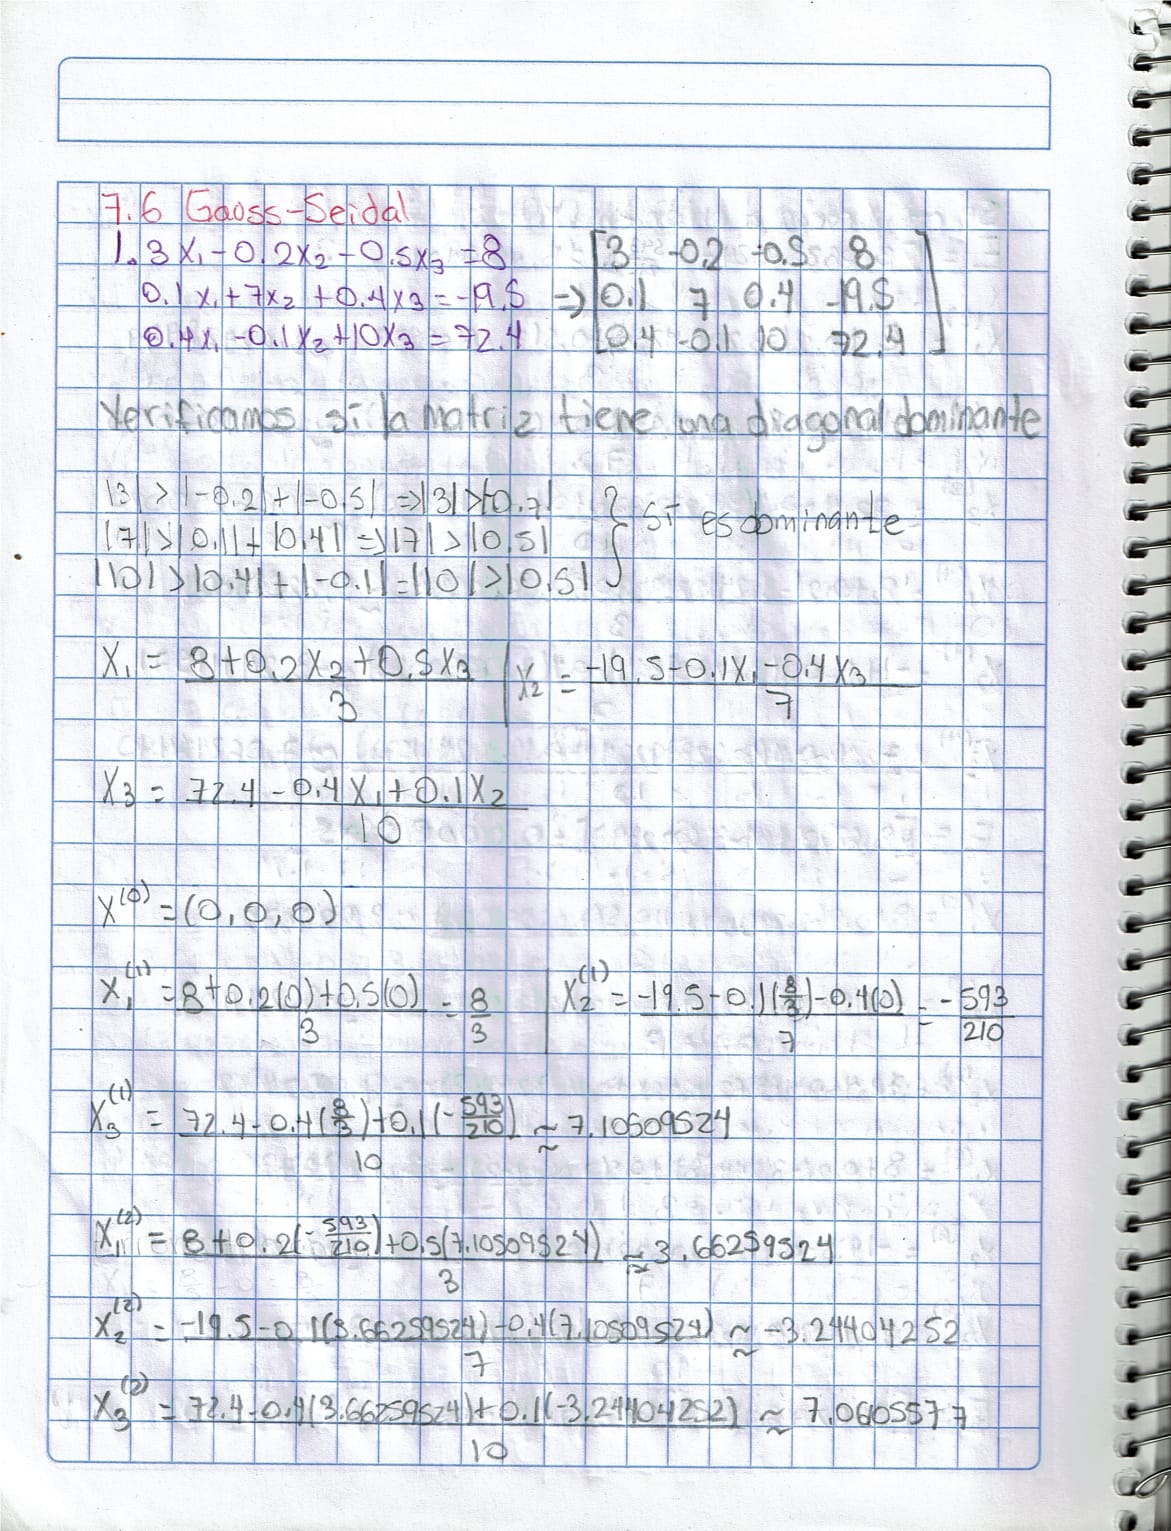
\includegraphics[width=6.25in,height=\textheight,keepaspectratio,alt={Ejercicio 1}]{Ejercicio76Seidel1.jpg}
\caption{Ejercicio 1}
\end{figure}

\begin{figure}
\centering
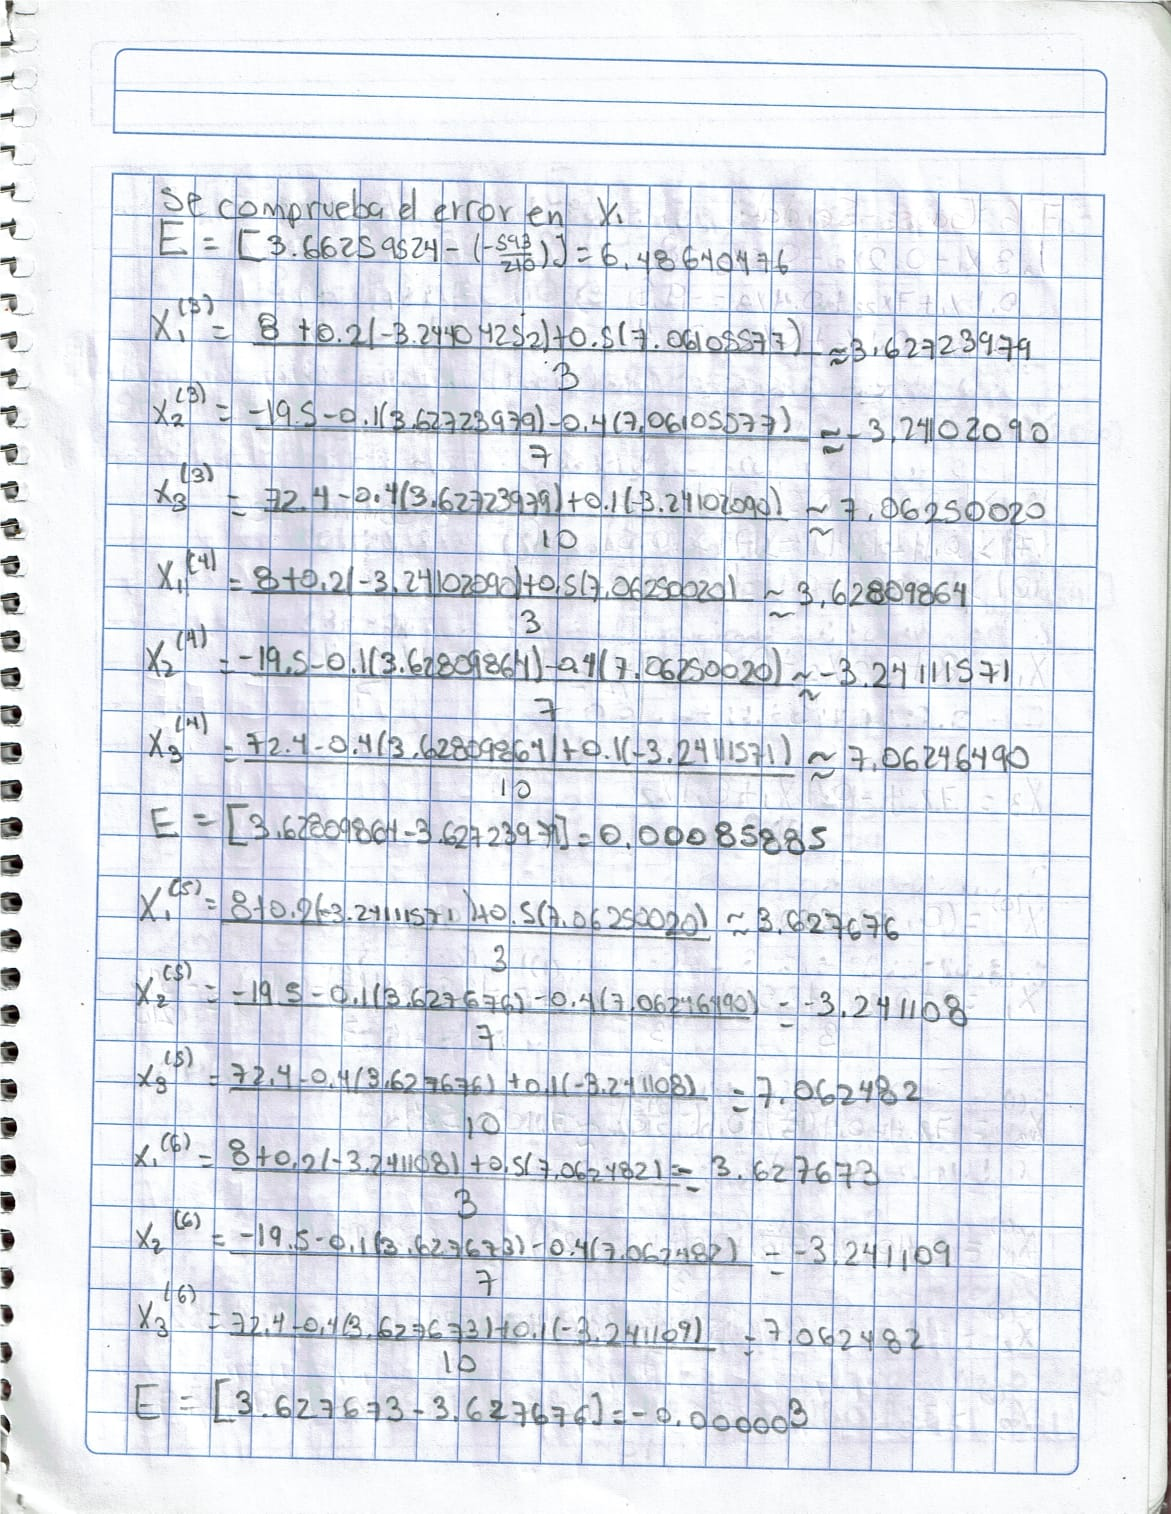
\includegraphics[width=6.25in,height=\textheight,keepaspectratio,alt={Ejercicio 1-2}]{Ejercicio76Seidel1_2.jpg}
\caption{Ejercicio 1-2}
\end{figure}

\begin{figure}
\centering
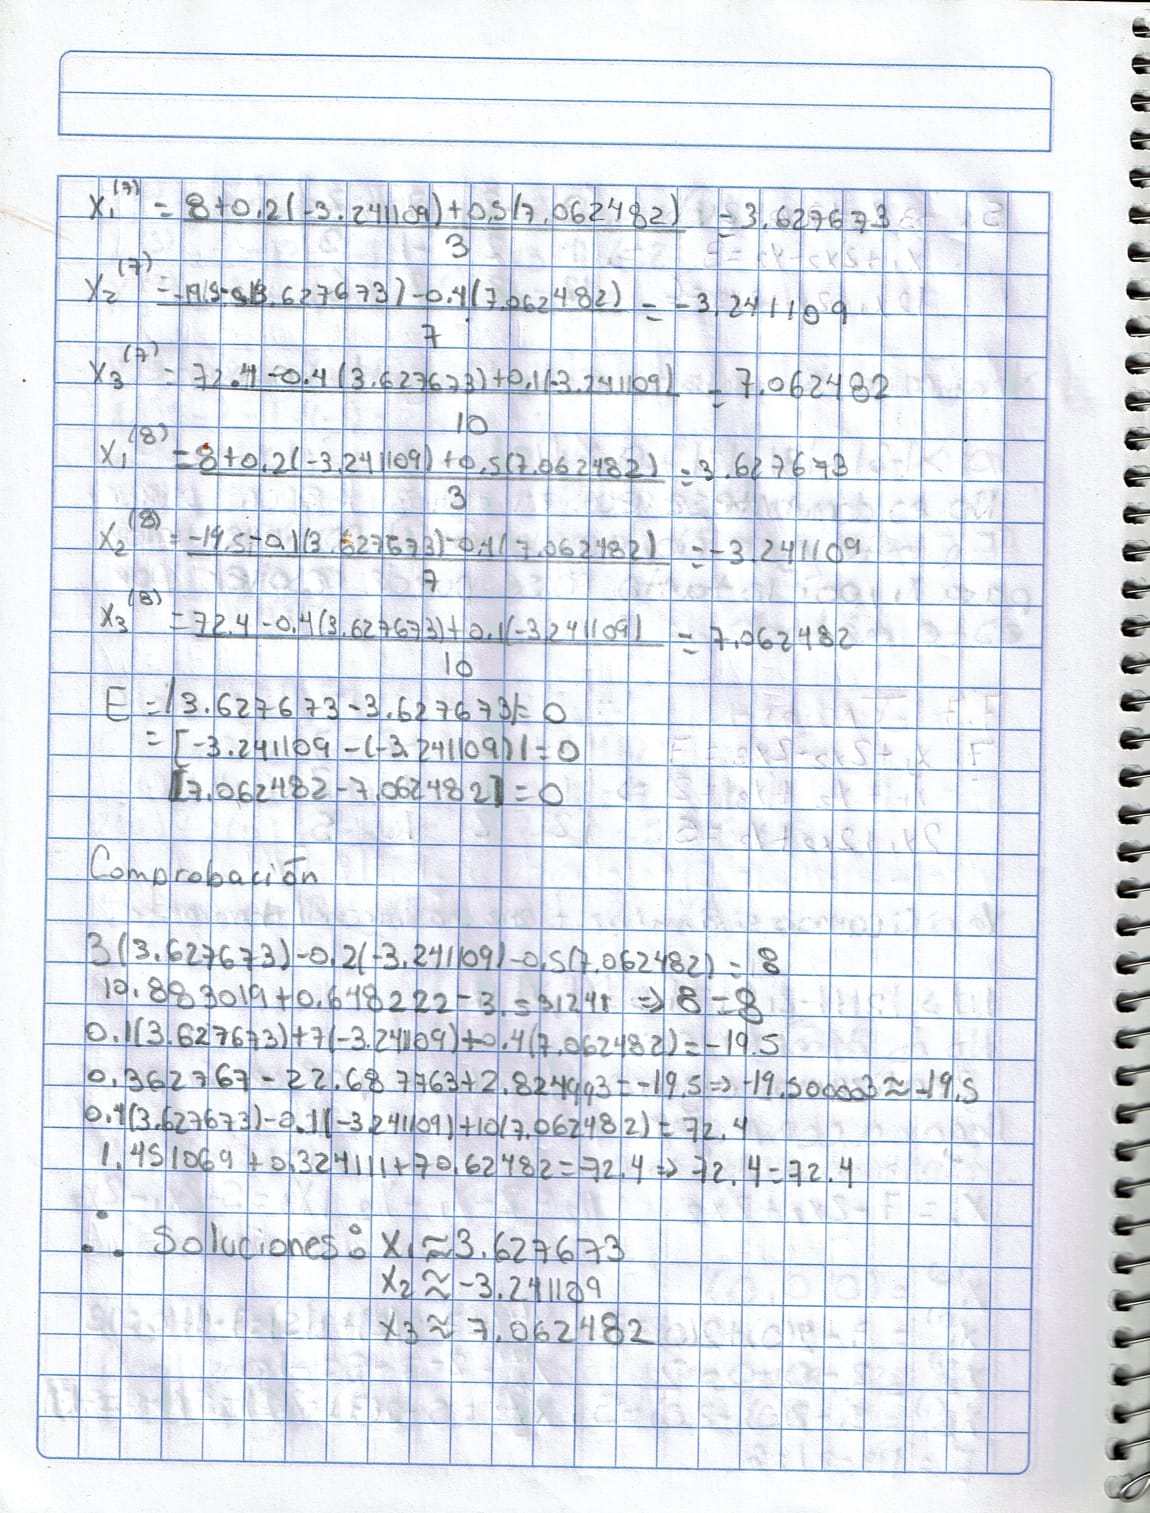
\includegraphics[width=6.25in,height=\textheight,keepaspectratio,alt={Ejercicio 1-3}]{Ejercicio76Seidel1_3.jpg}
\caption{Ejercicio 1-3}
\end{figure}

\begin{figure}
\centering
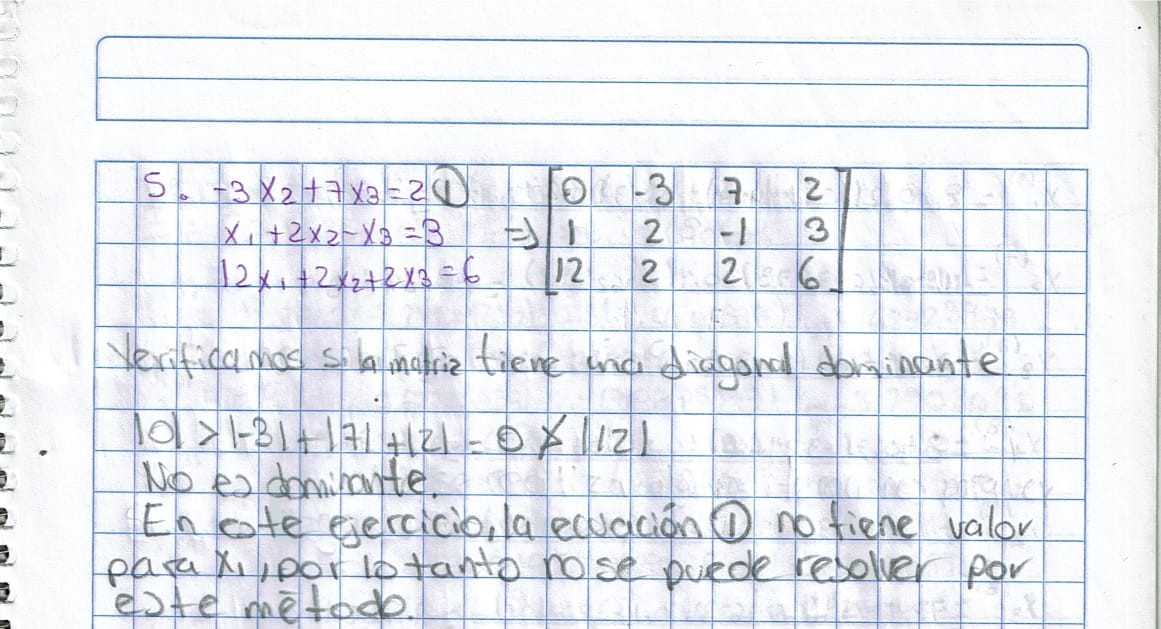
\includegraphics[width=6.25in,height=\textheight,keepaspectratio,alt={Ejercicio 5}]{Ejercicio76Seidel5.jpg}
\caption{Ejercicio 5}
\end{figure}

\subsubsection{\texorpdfstring{Sistema
\(1\)}{Sistema 1}}\label{sistema-1-3}

\(3x_1 − 0.2x_2 − 0.5x_3 = 8\)

\(0.1x_1 + 7x_2 + 0.4x_3 = −19.5\)

\(0.4x_1 − 0.1x_2 + 10x_3 = 72.4\)

\paragraph{Procedimiento}\label{procedimiento-40}

\begin{Shaded}
\begin{Highlighting}[]
\NormalTok{A }\OtherTok{\textless{}{-}} \FunctionTok{matrix}\NormalTok{(}\FunctionTok{c}\NormalTok{(}\DecValTok{3}\NormalTok{, }\SpecialCharTok{{-}}\FloatTok{0.2}\NormalTok{, }\SpecialCharTok{{-}}\FloatTok{0.5}\NormalTok{,}
              \FloatTok{0.1}\NormalTok{, }\DecValTok{7}\NormalTok{, }\FloatTok{0.4}\NormalTok{,}
              \FloatTok{0.4}\NormalTok{, }\SpecialCharTok{{-}}\FloatTok{0.1}\NormalTok{, }\DecValTok{10}\NormalTok{),}
      \AttributeTok{nrow =} \DecValTok{3}\NormalTok{, }\AttributeTok{byrow =} \ConstantTok{TRUE}\NormalTok{)}
\NormalTok{b }\OtherTok{\textless{}{-}} \FunctionTok{c}\NormalTok{(}\DecValTok{8}\NormalTok{, }\SpecialCharTok{{-}}\FloatTok{19.5}\NormalTok{, }\FloatTok{72.4}\NormalTok{)}

\NormalTok{Ab }\OtherTok{\textless{}{-}} \FunctionTok{cbind}\NormalTok{(A, b); (Ab)}
\end{Highlighting}
\end{Shaded}

\begin{verbatim}
##                        b
## [1,] 3.0 -0.2 -0.5   8.0
## [2,] 0.1  7.0  0.4 -19.5
## [3,] 0.4 -0.1 10.0  72.4
\end{verbatim}

\begin{Shaded}
\begin{Highlighting}[]
\CommentTok{\# Checar si converge o no con la diagonal dominante}

\NormalTok{F1 }\OtherTok{\textless{}{-}} \FunctionTok{abs}\NormalTok{(A[}\DecValTok{1}\NormalTok{,}\DecValTok{1}\NormalTok{]) }\SpecialCharTok{\textgreater{}}\NormalTok{ (}\FunctionTok{abs}\NormalTok{(A[}\DecValTok{1}\NormalTok{,}\DecValTok{2}\NormalTok{]) }\SpecialCharTok{+} \FunctionTok{abs}\NormalTok{(A[}\DecValTok{1}\NormalTok{,}\DecValTok{3}\NormalTok{]))}
\NormalTok{F2 }\OtherTok{\textless{}{-}} \FunctionTok{abs}\NormalTok{(A[}\DecValTok{2}\NormalTok{,}\DecValTok{2}\NormalTok{]) }\SpecialCharTok{\textgreater{}}\NormalTok{ (}\FunctionTok{abs}\NormalTok{(A[}\DecValTok{2}\NormalTok{,}\DecValTok{1}\NormalTok{]) }\SpecialCharTok{+} \FunctionTok{abs}\NormalTok{(A[}\DecValTok{2}\NormalTok{,}\DecValTok{3}\NormalTok{]))}
\NormalTok{F3 }\OtherTok{\textless{}{-}} \FunctionTok{abs}\NormalTok{(A[}\DecValTok{3}\NormalTok{,}\DecValTok{3}\NormalTok{]) }\SpecialCharTok{\textgreater{}}\NormalTok{ (}\FunctionTok{abs}\NormalTok{(A[}\DecValTok{3}\NormalTok{,}\DecValTok{1}\NormalTok{]) }\SpecialCharTok{+} \FunctionTok{abs}\NormalTok{(A[}\DecValTok{3}\NormalTok{,}\DecValTok{2}\NormalTok{]))}

\ControlFlowTok{if}\NormalTok{(F1 }\SpecialCharTok{==} \ConstantTok{TRUE} \SpecialCharTok{\&}\NormalTok{ F2 }\SpecialCharTok{==} \ConstantTok{TRUE} \SpecialCharTok{\&}\NormalTok{ F3 }\SpecialCharTok{==} \ConstantTok{TRUE}\NormalTok{) \{}
  \FunctionTok{cat}\NormalTok{(}\StringTok{"Sí es dominante"}\NormalTok{)}
\NormalTok{\} }\ControlFlowTok{else}\NormalTok{ \{}
  \FunctionTok{cat}\NormalTok{(}\StringTok{"No es dominante"}\NormalTok{)}
\NormalTok{\}}
\end{Highlighting}
\end{Shaded}

\begin{verbatim}
## Sí es dominante
\end{verbatim}

\begin{Shaded}
\begin{Highlighting}[]
\CommentTok{\# Asignar valores iniciales}

\NormalTok{x }\OtherTok{\textless{}{-}} \FunctionTok{rep}\NormalTok{(}\DecValTok{0}\NormalTok{, }\DecValTok{3}\NormalTok{) }\CommentTok{\# x\^{}(0)=(0,0,0)}
\FunctionTok{cat}\NormalTok{(}\StringTok{"x\^{}(0)="}\NormalTok{,}\FunctionTok{paste}\NormalTok{(}\FunctionTok{sprintf}\NormalTok{(}\StringTok{"\%.8f"}\NormalTok{,x), }\AttributeTok{collapse=}\StringTok{", "}\NormalTok{), }\StringTok{"}\SpecialCharTok{\textbackslash{}n}\StringTok{"}\NormalTok{)}
\end{Highlighting}
\end{Shaded}

\begin{verbatim}
## x^(0)= 0.00000000, 0.00000000, 0.00000000
\end{verbatim}

\subparagraph{Iteración 1}\label{iteraciuxf3n-1}

\begin{Shaded}
\begin{Highlighting}[]
\NormalTok{x\_old }\OtherTok{\textless{}{-}}\NormalTok{ x}
\NormalTok{x[}\DecValTok{1}\NormalTok{] }\OtherTok{\textless{}{-}}\NormalTok{ (b[}\DecValTok{1}\NormalTok{] }\SpecialCharTok{{-}}\NormalTok{ A[}\DecValTok{1}\NormalTok{,}\DecValTok{2}\NormalTok{]}\SpecialCharTok{*}\NormalTok{x\_old[}\DecValTok{2}\NormalTok{] }\SpecialCharTok{{-}}\NormalTok{ A[}\DecValTok{1}\NormalTok{,}\DecValTok{3}\NormalTok{]}\SpecialCharTok{*}\NormalTok{x\_old[}\DecValTok{3}\NormalTok{]) }\SpecialCharTok{/}\NormalTok{ A[}\DecValTok{1}\NormalTok{,}\DecValTok{1}\NormalTok{]}
\FunctionTok{cat}\NormalTok{(}\FunctionTok{sprintf}\NormalTok{(}\StringTok{"x1\^{}(1) = (\%.1f {-} (\%.1f)*\%.8f {-} (\%.1f)*\%.8f)/\%.1f = \%.8f}\SpecialCharTok{\textbackslash{}n}\StringTok{"}\NormalTok{, b[}\DecValTok{1}\NormalTok{], A[}\DecValTok{1}\NormalTok{,}\DecValTok{2}\NormalTok{], x\_old[}\DecValTok{2}\NormalTok{], A[}\DecValTok{1}\NormalTok{,}\DecValTok{3}\NormalTok{], x\_old[}\DecValTok{3}\NormalTok{], A[}\DecValTok{1}\NormalTok{,}\DecValTok{1}\NormalTok{], x[}\DecValTok{1}\NormalTok{]))}
\end{Highlighting}
\end{Shaded}

\begin{verbatim}
## x1^(1) = (8.0 - (-0.2)*0.00000000 - (-0.5)*0.00000000)/3.0 = 2.66666667
\end{verbatim}

\begin{Shaded}
\begin{Highlighting}[]
\NormalTok{x[}\DecValTok{2}\NormalTok{] }\OtherTok{\textless{}{-}}\NormalTok{ (b[}\DecValTok{2}\NormalTok{] }\SpecialCharTok{{-}}\NormalTok{ A[}\DecValTok{2}\NormalTok{,}\DecValTok{1}\NormalTok{]}\SpecialCharTok{*}\NormalTok{x[}\DecValTok{1}\NormalTok{] }\SpecialCharTok{{-}}\NormalTok{ A[}\DecValTok{2}\NormalTok{,}\DecValTok{3}\NormalTok{]}\SpecialCharTok{*}\NormalTok{x\_old[}\DecValTok{3}\NormalTok{]) }\SpecialCharTok{/}\NormalTok{ A[}\DecValTok{2}\NormalTok{,}\DecValTok{2}\NormalTok{]}
\FunctionTok{cat}\NormalTok{(}\FunctionTok{sprintf}\NormalTok{(}\StringTok{"x2\^{}(1) = (\%.1f {-} (\%.1f)*\%.8f {-} (\%.1f)*\%.8f)/\%.1f = \%.8f}\SpecialCharTok{\textbackslash{}n}\StringTok{"}\NormalTok{, b[}\DecValTok{2}\NormalTok{], A[}\DecValTok{2}\NormalTok{,}\DecValTok{1}\NormalTok{], x[}\DecValTok{1}\NormalTok{], A[}\DecValTok{2}\NormalTok{,}\DecValTok{3}\NormalTok{], x\_old[}\DecValTok{3}\NormalTok{], A[}\DecValTok{2}\NormalTok{,}\DecValTok{2}\NormalTok{], x[}\DecValTok{2}\NormalTok{]))}
\end{Highlighting}
\end{Shaded}

\begin{verbatim}
## x2^(1) = (-19.5 - (0.1)*2.66666667 - (0.4)*0.00000000)/7.0 = -2.82380952
\end{verbatim}

\begin{Shaded}
\begin{Highlighting}[]
\NormalTok{x[}\DecValTok{3}\NormalTok{] }\OtherTok{\textless{}{-}}\NormalTok{ (b[}\DecValTok{3}\NormalTok{] }\SpecialCharTok{{-}}\NormalTok{ A[}\DecValTok{3}\NormalTok{,}\DecValTok{1}\NormalTok{]}\SpecialCharTok{*}\NormalTok{x[}\DecValTok{1}\NormalTok{] }\SpecialCharTok{{-}}\NormalTok{ A[}\DecValTok{3}\NormalTok{,}\DecValTok{2}\NormalTok{]}\SpecialCharTok{*}\NormalTok{x[}\DecValTok{2}\NormalTok{]) }\SpecialCharTok{/}\NormalTok{ A[}\DecValTok{3}\NormalTok{,}\DecValTok{3}\NormalTok{]}
\FunctionTok{cat}\NormalTok{(}\FunctionTok{sprintf}\NormalTok{(}\StringTok{"x3\^{}(1) = (\%.1f {-} (\%.1f)*\%.8f {-} (\%.1f)*\%.8f)/\%.1f = \%.8f}\SpecialCharTok{\textbackslash{}n}\StringTok{"}\NormalTok{, b[}\DecValTok{3}\NormalTok{], A[}\DecValTok{3}\NormalTok{,}\DecValTok{1}\NormalTok{], x[}\DecValTok{1}\NormalTok{], A[}\DecValTok{3}\NormalTok{,}\DecValTok{2}\NormalTok{], x[}\DecValTok{2}\NormalTok{], A[}\DecValTok{3}\NormalTok{,}\DecValTok{3}\NormalTok{], x[}\DecValTok{3}\NormalTok{]))}
\end{Highlighting}
\end{Shaded}

\begin{verbatim}
## x3^(1) = (72.4 - (0.4)*2.66666667 - (-0.1)*-2.82380952)/10.0 = 7.10509524
\end{verbatim}

\begin{Shaded}
\begin{Highlighting}[]
\CommentTok{\#Error o tolerancia}

\NormalTok{r }\OtherTok{\textless{}{-}}\NormalTok{ b }\SpecialCharTok{{-}}\NormalTok{ A }\SpecialCharTok{\%*\%}\NormalTok{ x}
\NormalTok{dx\_inf }\OtherTok{\textless{}{-}} \FunctionTok{max}\NormalTok{(}\FunctionTok{abs}\NormalTok{(x }\SpecialCharTok{{-}}\NormalTok{ x\_old))}
\FunctionTok{cat}\NormalTok{(}\FunctionTok{sprintf}\NormalTok{(}\StringTok{"x\^{}(1) = \%s}\SpecialCharTok{\textbackslash{}n}\StringTok{"}\NormalTok{, }\FunctionTok{paste}\NormalTok{(}\FunctionTok{sprintf}\NormalTok{(}\StringTok{"\%.8f"}\NormalTok{, x), }\AttributeTok{collapse=}\StringTok{", "}\NormalTok{)))}
\end{Highlighting}
\end{Shaded}

\begin{verbatim}
## x^(1) = 2.66666667, -2.82380952, 7.10509524
\end{verbatim}

\begin{Shaded}
\begin{Highlighting}[]
\FunctionTok{cat}\NormalTok{(}\FunctionTok{sprintf}\NormalTok{(}\StringTok{"||dx||\_inf = \%.8e | ||r||\_inf = \%.8e}\SpecialCharTok{\textbackslash{}n}\StringTok{"}\NormalTok{, dx\_inf, }\FunctionTok{max}\NormalTok{(}\FunctionTok{abs}\NormalTok{(r))))}
\end{Highlighting}
\end{Shaded}

\begin{verbatim}
## ||dx||_inf = 7.10509524e+00 | ||r||_inf = 2.98778571e+00
\end{verbatim}

\subparagraph{Iteración 2}\label{iteraciuxf3n-2}

\begin{Shaded}
\begin{Highlighting}[]
\NormalTok{x\_old }\OtherTok{\textless{}{-}}\NormalTok{ x}
\NormalTok{x[}\DecValTok{1}\NormalTok{] }\OtherTok{\textless{}{-}}\NormalTok{ (b[}\DecValTok{1}\NormalTok{] }\SpecialCharTok{{-}}\NormalTok{ A[}\DecValTok{1}\NormalTok{,}\DecValTok{2}\NormalTok{]}\SpecialCharTok{*}\NormalTok{x\_old[}\DecValTok{2}\NormalTok{] }\SpecialCharTok{{-}}\NormalTok{ A[}\DecValTok{1}\NormalTok{,}\DecValTok{3}\NormalTok{]}\SpecialCharTok{*}\NormalTok{x\_old[}\DecValTok{3}\NormalTok{]) }\SpecialCharTok{/}\NormalTok{ A[}\DecValTok{1}\NormalTok{,}\DecValTok{1}\NormalTok{]}
\FunctionTok{cat}\NormalTok{(}\FunctionTok{sprintf}\NormalTok{(}\StringTok{"x1\^{}(2) = (\%.1f {-} (\%.1f)*\%.8f {-} (\%.1f)*\%.8f)/\%.1f = \%.8f}\SpecialCharTok{\textbackslash{}n}\StringTok{"}\NormalTok{, b[}\DecValTok{1}\NormalTok{], A[}\DecValTok{1}\NormalTok{,}\DecValTok{2}\NormalTok{], x\_old[}\DecValTok{2}\NormalTok{], A[}\DecValTok{1}\NormalTok{,}\DecValTok{3}\NormalTok{], x\_old[}\DecValTok{3}\NormalTok{], A[}\DecValTok{1}\NormalTok{,}\DecValTok{1}\NormalTok{], x[}\DecValTok{1}\NormalTok{]))}
\end{Highlighting}
\end{Shaded}

\begin{verbatim}
## x1^(2) = (8.0 - (-0.2)*-2.82380952 - (-0.5)*7.10509524)/3.0 = 3.66259524
\end{verbatim}

\begin{Shaded}
\begin{Highlighting}[]
\NormalTok{x[}\DecValTok{2}\NormalTok{] }\OtherTok{\textless{}{-}}\NormalTok{ (b[}\DecValTok{2}\NormalTok{] }\SpecialCharTok{{-}}\NormalTok{ A[}\DecValTok{2}\NormalTok{,}\DecValTok{1}\NormalTok{]}\SpecialCharTok{*}\NormalTok{x[}\DecValTok{1}\NormalTok{] }\SpecialCharTok{{-}}\NormalTok{ A[}\DecValTok{2}\NormalTok{,}\DecValTok{3}\NormalTok{]}\SpecialCharTok{*}\NormalTok{x\_old[}\DecValTok{3}\NormalTok{]) }\SpecialCharTok{/}\NormalTok{ A[}\DecValTok{2}\NormalTok{,}\DecValTok{2}\NormalTok{]}
\FunctionTok{cat}\NormalTok{(}\FunctionTok{sprintf}\NormalTok{(}\StringTok{"x2\^{}(2) = (\%.1f {-} (\%.1f)*\%.8f {-} (\%.1f)*\%.8f)/\%.1f = \%.8f}\SpecialCharTok{\textbackslash{}n}\StringTok{"}\NormalTok{, b[}\DecValTok{2}\NormalTok{], A[}\DecValTok{2}\NormalTok{,}\DecValTok{1}\NormalTok{], x[}\DecValTok{1}\NormalTok{], A[}\DecValTok{2}\NormalTok{,}\DecValTok{3}\NormalTok{], x\_old[}\DecValTok{3}\NormalTok{], A[}\DecValTok{2}\NormalTok{,}\DecValTok{2}\NormalTok{], x[}\DecValTok{2}\NormalTok{]))}
\end{Highlighting}
\end{Shaded}

\begin{verbatim}
## x2^(2) = (-19.5 - (0.1)*3.66259524 - (0.4)*7.10509524)/7.0 = -3.24404252
\end{verbatim}

\begin{Shaded}
\begin{Highlighting}[]
\NormalTok{x[}\DecValTok{3}\NormalTok{] }\OtherTok{\textless{}{-}}\NormalTok{ (b[}\DecValTok{3}\NormalTok{] }\SpecialCharTok{{-}}\NormalTok{ A[}\DecValTok{3}\NormalTok{,}\DecValTok{1}\NormalTok{]}\SpecialCharTok{*}\NormalTok{x[}\DecValTok{1}\NormalTok{] }\SpecialCharTok{{-}}\NormalTok{ A[}\DecValTok{3}\NormalTok{,}\DecValTok{2}\NormalTok{]}\SpecialCharTok{*}\NormalTok{x[}\DecValTok{2}\NormalTok{]) }\SpecialCharTok{/}\NormalTok{ A[}\DecValTok{3}\NormalTok{,}\DecValTok{3}\NormalTok{]}
\FunctionTok{cat}\NormalTok{(}\FunctionTok{sprintf}\NormalTok{(}\StringTok{"x3\^{}(2) = (\%.1f {-} (\%.1f)*\%.8f {-} (\%.1f)*\%.8f)/\%.1f = \%.8f}\SpecialCharTok{\textbackslash{}n}\StringTok{"}\NormalTok{, b[}\DecValTok{3}\NormalTok{], A[}\DecValTok{3}\NormalTok{,}\DecValTok{1}\NormalTok{], x[}\DecValTok{1}\NormalTok{], A[}\DecValTok{3}\NormalTok{,}\DecValTok{2}\NormalTok{], x[}\DecValTok{2}\NormalTok{], A[}\DecValTok{3}\NormalTok{,}\DecValTok{3}\NormalTok{], x[}\DecValTok{3}\NormalTok{]))}
\end{Highlighting}
\end{Shaded}

\begin{verbatim}
## x3^(2) = (72.4 - (0.4)*3.66259524 - (-0.1)*-3.24404252)/10.0 = 7.06105577
\end{verbatim}

\begin{Shaded}
\begin{Highlighting}[]
\CommentTok{\#Error o tolerancia}

\NormalTok{r }\OtherTok{\textless{}{-}}\NormalTok{ b }\SpecialCharTok{{-}}\NormalTok{ A }\SpecialCharTok{\%*\%}\NormalTok{ x}
\NormalTok{dx\_inf }\OtherTok{\textless{}{-}} \FunctionTok{max}\NormalTok{(}\FunctionTok{abs}\NormalTok{(x }\SpecialCharTok{{-}}\NormalTok{ x\_old))}
\FunctionTok{cat}\NormalTok{(}\FunctionTok{sprintf}\NormalTok{(}\StringTok{"x\^{}(2) = \%s}\SpecialCharTok{\textbackslash{}n}\StringTok{"}\NormalTok{, }\FunctionTok{paste}\NormalTok{(}\FunctionTok{sprintf}\NormalTok{(}\StringTok{"\%.8f"}\NormalTok{, x), }\AttributeTok{collapse=}\StringTok{", "}\NormalTok{)))}
\end{Highlighting}
\end{Shaded}

\begin{verbatim}
## x^(2) = 3.66259524, -3.24404252, 7.06105577
\end{verbatim}

\begin{Shaded}
\begin{Highlighting}[]
\FunctionTok{cat}\NormalTok{(}\FunctionTok{sprintf}\NormalTok{(}\StringTok{"||dx||\_inf = \%.8e | ||r||\_inf = \%.8e}\SpecialCharTok{\textbackslash{}n}\StringTok{"}\NormalTok{, dx\_inf, }\FunctionTok{max}\NormalTok{(}\FunctionTok{abs}\NormalTok{(r))))}
\end{Highlighting}
\end{Shaded}

\begin{verbatim}
## ||dx||_inf = 9.95928571e-01 | ||r||_inf = 1.06066335e-01
\end{verbatim}

\subparagraph{Iteración 3}\label{iteraciuxf3n-3}

\begin{Shaded}
\begin{Highlighting}[]
\NormalTok{x\_old }\OtherTok{\textless{}{-}}\NormalTok{ x}
\NormalTok{x[}\DecValTok{1}\NormalTok{] }\OtherTok{\textless{}{-}}\NormalTok{ (b[}\DecValTok{1}\NormalTok{] }\SpecialCharTok{{-}}\NormalTok{ A[}\DecValTok{1}\NormalTok{,}\DecValTok{2}\NormalTok{]}\SpecialCharTok{*}\NormalTok{x\_old[}\DecValTok{2}\NormalTok{] }\SpecialCharTok{{-}}\NormalTok{ A[}\DecValTok{1}\NormalTok{,}\DecValTok{3}\NormalTok{]}\SpecialCharTok{*}\NormalTok{x\_old[}\DecValTok{3}\NormalTok{]) }\SpecialCharTok{/}\NormalTok{ A[}\DecValTok{1}\NormalTok{,}\DecValTok{1}\NormalTok{]}
\FunctionTok{cat}\NormalTok{(}\FunctionTok{sprintf}\NormalTok{(}\StringTok{"x1\^{}(3) = (\%.1f {-} (\%.1f)*\%.8f {-} (\%.1f)*\%.8f)/\%.1f = \%.8f}\SpecialCharTok{\textbackslash{}n}\StringTok{"}\NormalTok{, b[}\DecValTok{1}\NormalTok{], A[}\DecValTok{1}\NormalTok{,}\DecValTok{2}\NormalTok{], x\_old[}\DecValTok{2}\NormalTok{], A[}\DecValTok{1}\NormalTok{,}\DecValTok{3}\NormalTok{], x\_old[}\DecValTok{3}\NormalTok{], A[}\DecValTok{1}\NormalTok{,}\DecValTok{1}\NormalTok{], x[}\DecValTok{1}\NormalTok{]))}
\end{Highlighting}
\end{Shaded}

\begin{verbatim}
## x1^(3) = (8.0 - (-0.2)*-3.24404252 - (-0.5)*7.06105577)/3.0 = 3.62723979
\end{verbatim}

\begin{Shaded}
\begin{Highlighting}[]
\NormalTok{x[}\DecValTok{2}\NormalTok{] }\OtherTok{\textless{}{-}}\NormalTok{ (b[}\DecValTok{2}\NormalTok{] }\SpecialCharTok{{-}}\NormalTok{ A[}\DecValTok{2}\NormalTok{,}\DecValTok{1}\NormalTok{]}\SpecialCharTok{*}\NormalTok{x[}\DecValTok{1}\NormalTok{] }\SpecialCharTok{{-}}\NormalTok{ A[}\DecValTok{2}\NormalTok{,}\DecValTok{3}\NormalTok{]}\SpecialCharTok{*}\NormalTok{x\_old[}\DecValTok{3}\NormalTok{]) }\SpecialCharTok{/}\NormalTok{ A[}\DecValTok{2}\NormalTok{,}\DecValTok{2}\NormalTok{]}
\FunctionTok{cat}\NormalTok{(}\FunctionTok{sprintf}\NormalTok{(}\StringTok{"x2\^{}(3) = (\%.1f {-} (\%.1f)*\%.8f {-} (\%.1f)*\%.8f)/\%.1f = \%.8f}\SpecialCharTok{\textbackslash{}n}\StringTok{"}\NormalTok{, b[}\DecValTok{2}\NormalTok{], A[}\DecValTok{2}\NormalTok{,}\DecValTok{1}\NormalTok{], x[}\DecValTok{1}\NormalTok{], A[}\DecValTok{2}\NormalTok{,}\DecValTok{3}\NormalTok{], x\_old[}\DecValTok{3}\NormalTok{], A[}\DecValTok{2}\NormalTok{,}\DecValTok{2}\NormalTok{], x[}\DecValTok{2}\NormalTok{]))}
\end{Highlighting}
\end{Shaded}

\begin{verbatim}
## x2^(3) = (-19.5 - (0.1)*3.62723979 - (0.4)*7.06105577)/7.0 = -3.24102090
\end{verbatim}

\begin{Shaded}
\begin{Highlighting}[]
\NormalTok{x[}\DecValTok{3}\NormalTok{] }\OtherTok{\textless{}{-}}\NormalTok{ (b[}\DecValTok{3}\NormalTok{] }\SpecialCharTok{{-}}\NormalTok{ A[}\DecValTok{3}\NormalTok{,}\DecValTok{1}\NormalTok{]}\SpecialCharTok{*}\NormalTok{x[}\DecValTok{1}\NormalTok{] }\SpecialCharTok{{-}}\NormalTok{ A[}\DecValTok{3}\NormalTok{,}\DecValTok{2}\NormalTok{]}\SpecialCharTok{*}\NormalTok{x[}\DecValTok{2}\NormalTok{]) }\SpecialCharTok{/}\NormalTok{ A[}\DecValTok{3}\NormalTok{,}\DecValTok{3}\NormalTok{]}
\FunctionTok{cat}\NormalTok{(}\FunctionTok{sprintf}\NormalTok{(}\StringTok{"x3\^{}(3) = (\%.1f {-} (\%.1f)*\%.8f {-} (\%.1f)*\%.8f)/\%.1f = \%.8f}\SpecialCharTok{\textbackslash{}n}\StringTok{"}\NormalTok{, b[}\DecValTok{3}\NormalTok{], A[}\DecValTok{3}\NormalTok{,}\DecValTok{1}\NormalTok{], x[}\DecValTok{1}\NormalTok{], A[}\DecValTok{3}\NormalTok{,}\DecValTok{2}\NormalTok{], x[}\DecValTok{2}\NormalTok{], A[}\DecValTok{3}\NormalTok{,}\DecValTok{3}\NormalTok{], x[}\DecValTok{3}\NormalTok{]))}
\end{Highlighting}
\end{Shaded}

\begin{verbatim}
## x3^(3) = (72.4 - (0.4)*3.62723979 - (-0.1)*-3.24102090)/10.0 = 7.06250020
\end{verbatim}

\begin{Shaded}
\begin{Highlighting}[]
\CommentTok{\#Error o tolerancia}

\NormalTok{r }\OtherTok{\textless{}{-}}\NormalTok{ b }\SpecialCharTok{{-}}\NormalTok{ A }\SpecialCharTok{\%*\%}\NormalTok{ x}
\NormalTok{dx\_inf }\OtherTok{\textless{}{-}} \FunctionTok{max}\NormalTok{(}\FunctionTok{abs}\NormalTok{(x }\SpecialCharTok{{-}}\NormalTok{ x\_old))}
\FunctionTok{cat}\NormalTok{(}\FunctionTok{sprintf}\NormalTok{(}\StringTok{"x\^{}(3) = \%s}\SpecialCharTok{\textbackslash{}n}\StringTok{"}\NormalTok{, }\FunctionTok{paste}\NormalTok{(}\FunctionTok{sprintf}\NormalTok{(}\StringTok{"\%.8f"}\NormalTok{, x), }\AttributeTok{collapse=}\StringTok{", "}\NormalTok{)))}
\end{Highlighting}
\end{Shaded}

\begin{verbatim}
## x^(3) = 3.62723979, -3.24102090, 7.06250020
\end{verbatim}

\begin{Shaded}
\begin{Highlighting}[]
\FunctionTok{cat}\NormalTok{(}\FunctionTok{sprintf}\NormalTok{(}\StringTok{"||dx||\_inf = \%.8e | ||r||\_inf = \%.8e}\SpecialCharTok{\textbackslash{}n}\StringTok{"}\NormalTok{, dx\_inf, }\FunctionTok{max}\NormalTok{(}\FunctionTok{abs}\NormalTok{(r))))}
\end{Highlighting}
\end{Shaded}

\begin{verbatim}
## ||dx||_inf = 3.53554450e-02 | ||r||_inf = 1.32654081e-03
\end{verbatim}

\subparagraph{Iteración 4}\label{iteraciuxf3n-4}

\begin{Shaded}
\begin{Highlighting}[]
\NormalTok{x\_old }\OtherTok{\textless{}{-}}\NormalTok{ x}
\NormalTok{x[}\DecValTok{1}\NormalTok{] }\OtherTok{\textless{}{-}}\NormalTok{ (b[}\DecValTok{1}\NormalTok{] }\SpecialCharTok{{-}}\NormalTok{ A[}\DecValTok{1}\NormalTok{,}\DecValTok{2}\NormalTok{]}\SpecialCharTok{*}\NormalTok{x\_old[}\DecValTok{2}\NormalTok{] }\SpecialCharTok{{-}}\NormalTok{ A[}\DecValTok{1}\NormalTok{,}\DecValTok{3}\NormalTok{]}\SpecialCharTok{*}\NormalTok{x\_old[}\DecValTok{3}\NormalTok{]) }\SpecialCharTok{/}\NormalTok{ A[}\DecValTok{1}\NormalTok{,}\DecValTok{1}\NormalTok{]}
\FunctionTok{cat}\NormalTok{(}\FunctionTok{sprintf}\NormalTok{(}\StringTok{"x1\^{}(4) = (\%.1f {-} (\%.1f)*\%.8f {-} (\%.1f)*\%.8f)/\%.1f = \%.8f}\SpecialCharTok{\textbackslash{}n}\StringTok{"}\NormalTok{, b[}\DecValTok{1}\NormalTok{], A[}\DecValTok{1}\NormalTok{,}\DecValTok{2}\NormalTok{], x\_old[}\DecValTok{2}\NormalTok{], A[}\DecValTok{1}\NormalTok{,}\DecValTok{3}\NormalTok{], x\_old[}\DecValTok{3}\NormalTok{], A[}\DecValTok{1}\NormalTok{,}\DecValTok{1}\NormalTok{], x[}\DecValTok{1}\NormalTok{]))}
\end{Highlighting}
\end{Shaded}

\begin{verbatim}
## x1^(4) = (8.0 - (-0.2)*-3.24102090 - (-0.5)*7.06250020)/3.0 = 3.62768197
\end{verbatim}

\begin{Shaded}
\begin{Highlighting}[]
\NormalTok{x[}\DecValTok{2}\NormalTok{] }\OtherTok{\textless{}{-}}\NormalTok{ (b[}\DecValTok{2}\NormalTok{] }\SpecialCharTok{{-}}\NormalTok{ A[}\DecValTok{2}\NormalTok{,}\DecValTok{1}\NormalTok{]}\SpecialCharTok{*}\NormalTok{x[}\DecValTok{1}\NormalTok{] }\SpecialCharTok{{-}}\NormalTok{ A[}\DecValTok{2}\NormalTok{,}\DecValTok{3}\NormalTok{]}\SpecialCharTok{*}\NormalTok{x\_old[}\DecValTok{3}\NormalTok{]) }\SpecialCharTok{/}\NormalTok{ A[}\DecValTok{2}\NormalTok{,}\DecValTok{2}\NormalTok{]}
\FunctionTok{cat}\NormalTok{(}\FunctionTok{sprintf}\NormalTok{(}\StringTok{"x2\^{}(4) = (\%.1f {-} (\%.1f)*\%.8f {-} (\%.1f)*\%.8f)/\%.1f = \%.8f}\SpecialCharTok{\textbackslash{}n}\StringTok{"}\NormalTok{, b[}\DecValTok{2}\NormalTok{], A[}\DecValTok{2}\NormalTok{,}\DecValTok{1}\NormalTok{], x[}\DecValTok{1}\NormalTok{], A[}\DecValTok{2}\NormalTok{,}\DecValTok{3}\NormalTok{], x\_old[}\DecValTok{3}\NormalTok{], A[}\DecValTok{2}\NormalTok{,}\DecValTok{2}\NormalTok{], x[}\DecValTok{2}\NormalTok{]))}
\end{Highlighting}
\end{Shaded}

\begin{verbatim}
## x2^(4) = (-19.5 - (0.1)*3.62768197 - (0.4)*7.06250020)/7.0 = -3.24110975
\end{verbatim}

\begin{Shaded}
\begin{Highlighting}[]
\NormalTok{x[}\DecValTok{3}\NormalTok{] }\OtherTok{\textless{}{-}}\NormalTok{ (b[}\DecValTok{3}\NormalTok{] }\SpecialCharTok{{-}}\NormalTok{ A[}\DecValTok{3}\NormalTok{,}\DecValTok{1}\NormalTok{]}\SpecialCharTok{*}\NormalTok{x[}\DecValTok{1}\NormalTok{] }\SpecialCharTok{{-}}\NormalTok{ A[}\DecValTok{3}\NormalTok{,}\DecValTok{2}\NormalTok{]}\SpecialCharTok{*}\NormalTok{x[}\DecValTok{2}\NormalTok{]) }\SpecialCharTok{/}\NormalTok{ A[}\DecValTok{3}\NormalTok{,}\DecValTok{3}\NormalTok{]}
\FunctionTok{cat}\NormalTok{(}\FunctionTok{sprintf}\NormalTok{(}\StringTok{"x3\^{}(4) = (\%.1f {-} (\%.1f)*\%.8f {-} (\%.1f)*\%.8f)/\%.1f = \%.8f}\SpecialCharTok{\textbackslash{}n}\StringTok{"}\NormalTok{, b[}\DecValTok{3}\NormalTok{], A[}\DecValTok{3}\NormalTok{,}\DecValTok{1}\NormalTok{], x[}\DecValTok{1}\NormalTok{], A[}\DecValTok{3}\NormalTok{,}\DecValTok{2}\NormalTok{], x[}\DecValTok{2}\NormalTok{], A[}\DecValTok{3}\NormalTok{,}\DecValTok{3}\NormalTok{], x[}\DecValTok{3}\NormalTok{]))}
\end{Highlighting}
\end{Shaded}

\begin{verbatim}
## x3^(4) = (72.4 - (0.4)*3.62768197 - (-0.1)*-3.24110975)/10.0 = 7.06248162
\end{verbatim}

\begin{Shaded}
\begin{Highlighting}[]
\CommentTok{\#Error o tolerancia}

\NormalTok{r }\OtherTok{\textless{}{-}}\NormalTok{ b }\SpecialCharTok{{-}}\NormalTok{ A }\SpecialCharTok{\%*\%}\NormalTok{ x}
\NormalTok{dx\_inf }\OtherTok{\textless{}{-}} \FunctionTok{max}\NormalTok{(}\FunctionTok{abs}\NormalTok{(x }\SpecialCharTok{{-}}\NormalTok{ x\_old))}
\FunctionTok{cat}\NormalTok{(}\FunctionTok{sprintf}\NormalTok{(}\StringTok{"x\^{}(4) = \%s}\SpecialCharTok{\textbackslash{}n}\StringTok{"}\NormalTok{, }\FunctionTok{paste}\NormalTok{(}\FunctionTok{sprintf}\NormalTok{(}\StringTok{"\%.8f"}\NormalTok{, x), }\AttributeTok{collapse=}\StringTok{", "}\NormalTok{)))}
\end{Highlighting}
\end{Shaded}

\begin{verbatim}
## x^(4) = 3.62768197, -3.24110975, 7.06248162
\end{verbatim}

\begin{Shaded}
\begin{Highlighting}[]
\FunctionTok{cat}\NormalTok{(}\FunctionTok{sprintf}\NormalTok{(}\StringTok{"||dx||\_inf = \%.8e | ||r||\_inf = \%.8e}\SpecialCharTok{\textbackslash{}n}\StringTok{"}\NormalTok{, dx\_inf, }\FunctionTok{max}\NormalTok{(}\FunctionTok{abs}\NormalTok{(r))))}
\end{Highlighting}
\end{Shaded}

\begin{verbatim}
## ||dx||_inf = 4.42180271e-04 | ||r||_inf = 2.70590744e-05
\end{verbatim}

\subparagraph{Iteración 5}\label{iteraciuxf3n-5}

\begin{Shaded}
\begin{Highlighting}[]
\NormalTok{x\_old }\OtherTok{\textless{}{-}}\NormalTok{ x}
\NormalTok{x[}\DecValTok{1}\NormalTok{] }\OtherTok{\textless{}{-}}\NormalTok{ (b[}\DecValTok{1}\NormalTok{] }\SpecialCharTok{{-}}\NormalTok{ A[}\DecValTok{1}\NormalTok{,}\DecValTok{2}\NormalTok{]}\SpecialCharTok{*}\NormalTok{x\_old[}\DecValTok{2}\NormalTok{] }\SpecialCharTok{{-}}\NormalTok{ A[}\DecValTok{1}\NormalTok{,}\DecValTok{3}\NormalTok{]}\SpecialCharTok{*}\NormalTok{x\_old[}\DecValTok{3}\NormalTok{]) }\SpecialCharTok{/}\NormalTok{ A[}\DecValTok{1}\NormalTok{,}\DecValTok{1}\NormalTok{]}
\FunctionTok{cat}\NormalTok{(}\FunctionTok{sprintf}\NormalTok{(}\StringTok{"x1\^{}(5) = (\%.1f {-} (\%.1f)*\%.8f {-} (\%.1f)*\%.8f)/\%.1f = \%.8f}\SpecialCharTok{\textbackslash{}n}\StringTok{"}\NormalTok{, b[}\DecValTok{1}\NormalTok{], A[}\DecValTok{1}\NormalTok{,}\DecValTok{2}\NormalTok{], x\_old[}\DecValTok{2}\NormalTok{], A[}\DecValTok{1}\NormalTok{,}\DecValTok{3}\NormalTok{], x\_old[}\DecValTok{3}\NormalTok{], A[}\DecValTok{1}\NormalTok{,}\DecValTok{1}\NormalTok{], x[}\DecValTok{1}\NormalTok{]))}
\end{Highlighting}
\end{Shaded}

\begin{verbatim}
## x1^(5) = (8.0 - (-0.2)*-3.24110975 - (-0.5)*7.06248162)/3.0 = 3.62767295
\end{verbatim}

\begin{Shaded}
\begin{Highlighting}[]
\NormalTok{x[}\DecValTok{2}\NormalTok{] }\OtherTok{\textless{}{-}}\NormalTok{ (b[}\DecValTok{2}\NormalTok{] }\SpecialCharTok{{-}}\NormalTok{ A[}\DecValTok{2}\NormalTok{,}\DecValTok{1}\NormalTok{]}\SpecialCharTok{*}\NormalTok{x[}\DecValTok{1}\NormalTok{] }\SpecialCharTok{{-}}\NormalTok{ A[}\DecValTok{2}\NormalTok{,}\DecValTok{3}\NormalTok{]}\SpecialCharTok{*}\NormalTok{x\_old[}\DecValTok{3}\NormalTok{]) }\SpecialCharTok{/}\NormalTok{ A[}\DecValTok{2}\NormalTok{,}\DecValTok{2}\NormalTok{]}
\FunctionTok{cat}\NormalTok{(}\FunctionTok{sprintf}\NormalTok{(}\StringTok{"x2\^{}(5) = (\%.1f {-} (\%.1f)*\%.8f {-} (\%.1f)*\%.8f)/\%.1f = \%.8f}\SpecialCharTok{\textbackslash{}n}\StringTok{"}\NormalTok{, b[}\DecValTok{2}\NormalTok{], A[}\DecValTok{2}\NormalTok{,}\DecValTok{1}\NormalTok{], x[}\DecValTok{1}\NormalTok{], A[}\DecValTok{2}\NormalTok{,}\DecValTok{3}\NormalTok{], x\_old[}\DecValTok{3}\NormalTok{], A[}\DecValTok{2}\NormalTok{,}\DecValTok{2}\NormalTok{], x[}\DecValTok{2}\NormalTok{]))}
\end{Highlighting}
\end{Shaded}

\begin{verbatim}
## x2^(5) = (-19.5 - (0.1)*3.62767295 - (0.4)*7.06248162)/7.0 = -3.24110856
\end{verbatim}

\begin{Shaded}
\begin{Highlighting}[]
\NormalTok{x[}\DecValTok{3}\NormalTok{] }\OtherTok{\textless{}{-}}\NormalTok{ (b[}\DecValTok{3}\NormalTok{] }\SpecialCharTok{{-}}\NormalTok{ A[}\DecValTok{3}\NormalTok{,}\DecValTok{1}\NormalTok{]}\SpecialCharTok{*}\NormalTok{x[}\DecValTok{1}\NormalTok{] }\SpecialCharTok{{-}}\NormalTok{ A[}\DecValTok{3}\NormalTok{,}\DecValTok{2}\NormalTok{]}\SpecialCharTok{*}\NormalTok{x[}\DecValTok{2}\NormalTok{]) }\SpecialCharTok{/}\NormalTok{ A[}\DecValTok{3}\NormalTok{,}\DecValTok{3}\NormalTok{]}
\FunctionTok{cat}\NormalTok{(}\FunctionTok{sprintf}\NormalTok{(}\StringTok{"x3\^{}(5) = (\%.1f {-} (\%.1f)*\%.8f {-} (\%.1f)*\%.8f)/\%.1f = \%.8f}\SpecialCharTok{\textbackslash{}n}\StringTok{"}\NormalTok{, b[}\DecValTok{3}\NormalTok{], A[}\DecValTok{3}\NormalTok{,}\DecValTok{1}\NormalTok{], x[}\DecValTok{1}\NormalTok{], A[}\DecValTok{3}\NormalTok{,}\DecValTok{2}\NormalTok{], x[}\DecValTok{2}\NormalTok{], A[}\DecValTok{3}\NormalTok{,}\DecValTok{3}\NormalTok{], x[}\DecValTok{3}\NormalTok{]))}
\end{Highlighting}
\end{Shaded}

\begin{verbatim}
## x3^(5) = (72.4 - (0.4)*3.62767295 - (-0.1)*-3.24110856)/10.0 = 7.06248200
\end{verbatim}

\begin{Shaded}
\begin{Highlighting}[]
\CommentTok{\#Error o tolerancia}

\NormalTok{r }\OtherTok{\textless{}{-}}\NormalTok{ b }\SpecialCharTok{{-}}\NormalTok{ A }\SpecialCharTok{\%*\%}\NormalTok{ x}
\NormalTok{dx\_inf }\OtherTok{\textless{}{-}} \FunctionTok{max}\NormalTok{(}\FunctionTok{abs}\NormalTok{(x }\SpecialCharTok{{-}}\NormalTok{ x\_old))}
\FunctionTok{cat}\NormalTok{(}\FunctionTok{sprintf}\NormalTok{(}\StringTok{"x\^{}(5) = \%s}\SpecialCharTok{\textbackslash{}n}\StringTok{"}\NormalTok{, }\FunctionTok{paste}\NormalTok{(}\FunctionTok{sprintf}\NormalTok{(}\StringTok{"\%.8f"}\NormalTok{, x), }\AttributeTok{collapse=}\StringTok{", "}\NormalTok{)))}
\end{Highlighting}
\end{Shaded}

\begin{verbatim}
## x^(5) = 3.62767295, -3.24110856, 7.06248200
\end{verbatim}

\begin{Shaded}
\begin{Highlighting}[]
\FunctionTok{cat}\NormalTok{(}\FunctionTok{sprintf}\NormalTok{(}\StringTok{"||dx||\_inf = \%.8e | ||r||\_inf = \%.8e}\SpecialCharTok{\textbackslash{}n}\StringTok{"}\NormalTok{, dx\_inf, }\FunctionTok{max}\NormalTok{(}\FunctionTok{abs}\NormalTok{(r))))}
\end{Highlighting}
\end{Shaded}

\begin{verbatim}
## ||dx||_inf = 9.01969147e-06 | ||r||_inf = 4.24410521e-07
\end{verbatim}

\subparagraph{Iteración 6}\label{iteraciuxf3n-6}

\begin{Shaded}
\begin{Highlighting}[]
\NormalTok{x\_old }\OtherTok{\textless{}{-}}\NormalTok{ x}
\NormalTok{x[}\DecValTok{1}\NormalTok{] }\OtherTok{\textless{}{-}}\NormalTok{ (b[}\DecValTok{1}\NormalTok{] }\SpecialCharTok{{-}}\NormalTok{ A[}\DecValTok{1}\NormalTok{,}\DecValTok{2}\NormalTok{]}\SpecialCharTok{*}\NormalTok{x\_old[}\DecValTok{2}\NormalTok{] }\SpecialCharTok{{-}}\NormalTok{ A[}\DecValTok{1}\NormalTok{,}\DecValTok{3}\NormalTok{]}\SpecialCharTok{*}\NormalTok{x\_old[}\DecValTok{3}\NormalTok{]) }\SpecialCharTok{/}\NormalTok{ A[}\DecValTok{1}\NormalTok{,}\DecValTok{1}\NormalTok{]}
\FunctionTok{cat}\NormalTok{(}\FunctionTok{sprintf}\NormalTok{(}\StringTok{"x1\^{}(6) = (\%.1f {-} (\%.1f)*\%.8f {-} (\%.1f)*\%.8f)/\%.1f = \%.8f}\SpecialCharTok{\textbackslash{}n}\StringTok{"}\NormalTok{, b[}\DecValTok{1}\NormalTok{], A[}\DecValTok{1}\NormalTok{,}\DecValTok{2}\NormalTok{], x\_old[}\DecValTok{2}\NormalTok{], A[}\DecValTok{1}\NormalTok{,}\DecValTok{3}\NormalTok{], x\_old[}\DecValTok{3}\NormalTok{], A[}\DecValTok{1}\NormalTok{,}\DecValTok{1}\NormalTok{], x[}\DecValTok{1}\NormalTok{]))}
\end{Highlighting}
\end{Shaded}

\begin{verbatim}
## x1^(6) = (8.0 - (-0.2)*-3.24110856 - (-0.5)*7.06248200)/3.0 = 3.62767310
\end{verbatim}

\begin{Shaded}
\begin{Highlighting}[]
\NormalTok{x[}\DecValTok{2}\NormalTok{] }\OtherTok{\textless{}{-}}\NormalTok{ (b[}\DecValTok{2}\NormalTok{] }\SpecialCharTok{{-}}\NormalTok{ A[}\DecValTok{2}\NormalTok{,}\DecValTok{1}\NormalTok{]}\SpecialCharTok{*}\NormalTok{x[}\DecValTok{1}\NormalTok{] }\SpecialCharTok{{-}}\NormalTok{ A[}\DecValTok{2}\NormalTok{,}\DecValTok{3}\NormalTok{]}\SpecialCharTok{*}\NormalTok{x\_old[}\DecValTok{3}\NormalTok{]) }\SpecialCharTok{/}\NormalTok{ A[}\DecValTok{2}\NormalTok{,}\DecValTok{2}\NormalTok{]}
\FunctionTok{cat}\NormalTok{(}\FunctionTok{sprintf}\NormalTok{(}\StringTok{"x2\^{}(6) = (\%.1f {-} (\%.1f)*\%.8f {-} (\%.1f)*\%.8f)/\%.1f = \%.8f}\SpecialCharTok{\textbackslash{}n}\StringTok{"}\NormalTok{, b[}\DecValTok{2}\NormalTok{], A[}\DecValTok{2}\NormalTok{,}\DecValTok{1}\NormalTok{], x[}\DecValTok{1}\NormalTok{], A[}\DecValTok{2}\NormalTok{,}\DecValTok{3}\NormalTok{], x\_old[}\DecValTok{3}\NormalTok{], A[}\DecValTok{2}\NormalTok{,}\DecValTok{2}\NormalTok{], x[}\DecValTok{2}\NormalTok{]))}
\end{Highlighting}
\end{Shaded}

\begin{verbatim}
## x2^(6) = (-19.5 - (0.1)*3.62767310 - (0.4)*7.06248200)/7.0 = -3.24110859
\end{verbatim}

\begin{Shaded}
\begin{Highlighting}[]
\NormalTok{x[}\DecValTok{3}\NormalTok{] }\OtherTok{\textless{}{-}}\NormalTok{ (b[}\DecValTok{3}\NormalTok{] }\SpecialCharTok{{-}}\NormalTok{ A[}\DecValTok{3}\NormalTok{,}\DecValTok{1}\NormalTok{]}\SpecialCharTok{*}\NormalTok{x[}\DecValTok{1}\NormalTok{] }\SpecialCharTok{{-}}\NormalTok{ A[}\DecValTok{3}\NormalTok{,}\DecValTok{2}\NormalTok{]}\SpecialCharTok{*}\NormalTok{x[}\DecValTok{2}\NormalTok{]) }\SpecialCharTok{/}\NormalTok{ A[}\DecValTok{3}\NormalTok{,}\DecValTok{3}\NormalTok{]}
\FunctionTok{cat}\NormalTok{(}\FunctionTok{sprintf}\NormalTok{(}\StringTok{"x3\^{}(6) = (\%.1f {-} (\%.1f)*\%.8f {-} (\%.1f)*\%.8f)/\%.1f = \%.8f}\SpecialCharTok{\textbackslash{}n}\StringTok{"}\NormalTok{, b[}\DecValTok{3}\NormalTok{], A[}\DecValTok{3}\NormalTok{,}\DecValTok{1}\NormalTok{], x[}\DecValTok{1}\NormalTok{], A[}\DecValTok{3}\NormalTok{,}\DecValTok{2}\NormalTok{], x[}\DecValTok{2}\NormalTok{], A[}\DecValTok{3}\NormalTok{,}\DecValTok{3}\NormalTok{], x[}\DecValTok{3}\NormalTok{]))}
\end{Highlighting}
\end{Shaded}

\begin{verbatim}
## x3^(6) = (72.4 - (0.4)*3.62767310 - (-0.1)*-3.24110859)/10.0 = 7.06248199
\end{verbatim}

\begin{Shaded}
\begin{Highlighting}[]
\CommentTok{\#Error o tolerancia}

\NormalTok{r }\OtherTok{\textless{}{-}}\NormalTok{ b }\SpecialCharTok{{-}}\NormalTok{ A }\SpecialCharTok{\%*\%}\NormalTok{ x}
\NormalTok{dx\_inf }\OtherTok{\textless{}{-}} \FunctionTok{max}\NormalTok{(}\FunctionTok{abs}\NormalTok{(x }\SpecialCharTok{{-}}\NormalTok{ x\_old))}
\FunctionTok{cat}\NormalTok{(}\FunctionTok{sprintf}\NormalTok{(}\StringTok{"x\^{}(6) = \%s}\SpecialCharTok{\textbackslash{}n}\StringTok{"}\NormalTok{, }\FunctionTok{paste}\NormalTok{(}\FunctionTok{sprintf}\NormalTok{(}\StringTok{"\%.8f"}\NormalTok{, x), }\AttributeTok{collapse=}\StringTok{", "}\NormalTok{)))}
\end{Highlighting}
\end{Shaded}

\begin{verbatim}
## x^(6) = 3.62767310, -3.24110859, 7.06248199
\end{verbatim}

\begin{Shaded}
\begin{Highlighting}[]
\FunctionTok{cat}\NormalTok{(}\FunctionTok{sprintf}\NormalTok{(}\StringTok{"||dx||\_inf = \%.8e | ||r||\_inf = \%.8e}\SpecialCharTok{\textbackslash{}n}\StringTok{"}\NormalTok{, dx\_inf, }\FunctionTok{max}\NormalTok{(}\FunctionTok{abs}\NormalTok{(r))))}
\end{Highlighting}
\end{Shaded}

\begin{verbatim}
## ||dx||_inf = 1.41470173e-07 | ||r||_inf = 7.60951657e-09
\end{verbatim}

\subparagraph{Iteración 7}\label{iteraciuxf3n-7}

\begin{Shaded}
\begin{Highlighting}[]
\NormalTok{x\_old }\OtherTok{\textless{}{-}}\NormalTok{ x}
\NormalTok{x[}\DecValTok{1}\NormalTok{] }\OtherTok{\textless{}{-}}\NormalTok{ (b[}\DecValTok{1}\NormalTok{] }\SpecialCharTok{{-}}\NormalTok{ A[}\DecValTok{1}\NormalTok{,}\DecValTok{2}\NormalTok{]}\SpecialCharTok{*}\NormalTok{x\_old[}\DecValTok{2}\NormalTok{] }\SpecialCharTok{{-}}\NormalTok{ A[}\DecValTok{1}\NormalTok{,}\DecValTok{3}\NormalTok{]}\SpecialCharTok{*}\NormalTok{x\_old[}\DecValTok{3}\NormalTok{]) }\SpecialCharTok{/}\NormalTok{ A[}\DecValTok{1}\NormalTok{,}\DecValTok{1}\NormalTok{]}
\FunctionTok{cat}\NormalTok{(}\FunctionTok{sprintf}\NormalTok{(}\StringTok{"x1\^{}(7) = (\%.1f {-} (\%.1f)*\%.8f {-} (\%.1f)*\%.8f)/\%.1f = \%.8f}\SpecialCharTok{\textbackslash{}n}\StringTok{"}\NormalTok{, b[}\DecValTok{1}\NormalTok{], A[}\DecValTok{1}\NormalTok{,}\DecValTok{2}\NormalTok{], x\_old[}\DecValTok{2}\NormalTok{], A[}\DecValTok{1}\NormalTok{,}\DecValTok{3}\NormalTok{], x\_old[}\DecValTok{3}\NormalTok{], A[}\DecValTok{1}\NormalTok{,}\DecValTok{1}\NormalTok{], x[}\DecValTok{1}\NormalTok{]))}
\end{Highlighting}
\end{Shaded}

\begin{verbatim}
## x1^(7) = (8.0 - (-0.2)*-3.24110859 - (-0.5)*7.06248199)/3.0 = 3.62767309
\end{verbatim}

\begin{Shaded}
\begin{Highlighting}[]
\NormalTok{x[}\DecValTok{2}\NormalTok{] }\OtherTok{\textless{}{-}}\NormalTok{ (b[}\DecValTok{2}\NormalTok{] }\SpecialCharTok{{-}}\NormalTok{ A[}\DecValTok{2}\NormalTok{,}\DecValTok{1}\NormalTok{]}\SpecialCharTok{*}\NormalTok{x[}\DecValTok{1}\NormalTok{] }\SpecialCharTok{{-}}\NormalTok{ A[}\DecValTok{2}\NormalTok{,}\DecValTok{3}\NormalTok{]}\SpecialCharTok{*}\NormalTok{x\_old[}\DecValTok{3}\NormalTok{]) }\SpecialCharTok{/}\NormalTok{ A[}\DecValTok{2}\NormalTok{,}\DecValTok{2}\NormalTok{]}
\FunctionTok{cat}\NormalTok{(}\FunctionTok{sprintf}\NormalTok{(}\StringTok{"x2\^{}(7) = (\%.1f {-} (\%.1f)*\%.8f {-} (\%.1f)*\%.8f)/\%.1f = \%.8f}\SpecialCharTok{\textbackslash{}n}\StringTok{"}\NormalTok{, b[}\DecValTok{2}\NormalTok{], A[}\DecValTok{2}\NormalTok{,}\DecValTok{1}\NormalTok{], x[}\DecValTok{1}\NormalTok{], A[}\DecValTok{2}\NormalTok{,}\DecValTok{3}\NormalTok{], x\_old[}\DecValTok{3}\NormalTok{], A[}\DecValTok{2}\NormalTok{,}\DecValTok{2}\NormalTok{], x[}\DecValTok{2}\NormalTok{]))}
\end{Highlighting}
\end{Shaded}

\begin{verbatim}
## x2^(7) = (-19.5 - (0.1)*3.62767309 - (0.4)*7.06248199)/7.0 = -3.24110859
\end{verbatim}

\begin{Shaded}
\begin{Highlighting}[]
\NormalTok{x[}\DecValTok{3}\NormalTok{] }\OtherTok{\textless{}{-}}\NormalTok{ (b[}\DecValTok{3}\NormalTok{] }\SpecialCharTok{{-}}\NormalTok{ A[}\DecValTok{3}\NormalTok{,}\DecValTok{1}\NormalTok{]}\SpecialCharTok{*}\NormalTok{x[}\DecValTok{1}\NormalTok{] }\SpecialCharTok{{-}}\NormalTok{ A[}\DecValTok{3}\NormalTok{,}\DecValTok{2}\NormalTok{]}\SpecialCharTok{*}\NormalTok{x[}\DecValTok{2}\NormalTok{]) }\SpecialCharTok{/}\NormalTok{ A[}\DecValTok{3}\NormalTok{,}\DecValTok{3}\NormalTok{]}
\FunctionTok{cat}\NormalTok{(}\FunctionTok{sprintf}\NormalTok{(}\StringTok{"x3\^{}(7) = (\%.1f {-} (\%.1f)*\%.8f {-} (\%.1f)*\%.8f)/\%.1f = \%.8f}\SpecialCharTok{\textbackslash{}n}\StringTok{"}\NormalTok{, b[}\DecValTok{3}\NormalTok{], A[}\DecValTok{3}\NormalTok{,}\DecValTok{1}\NormalTok{], x[}\DecValTok{1}\NormalTok{], A[}\DecValTok{3}\NormalTok{,}\DecValTok{2}\NormalTok{], x[}\DecValTok{2}\NormalTok{], A[}\DecValTok{3}\NormalTok{,}\DecValTok{3}\NormalTok{], x[}\DecValTok{3}\NormalTok{]))}
\end{Highlighting}
\end{Shaded}

\begin{verbatim}
## x3^(7) = (72.4 - (0.4)*3.62767309 - (-0.1)*-3.24110859)/10.0 = 7.06248199
\end{verbatim}

\begin{Shaded}
\begin{Highlighting}[]
\CommentTok{\#Error o tolerancia}

\NormalTok{r }\OtherTok{\textless{}{-}}\NormalTok{ b }\SpecialCharTok{{-}}\NormalTok{ A }\SpecialCharTok{\%*\%}\NormalTok{ x}
\NormalTok{dx\_inf }\OtherTok{\textless{}{-}} \FunctionTok{max}\NormalTok{(}\FunctionTok{abs}\NormalTok{(x }\SpecialCharTok{{-}}\NormalTok{ x\_old))}
\FunctionTok{cat}\NormalTok{(}\FunctionTok{sprintf}\NormalTok{(}\StringTok{"x\^{}(7) = \%s}\SpecialCharTok{\textbackslash{}n}\StringTok{"}\NormalTok{, }\FunctionTok{paste}\NormalTok{(}\FunctionTok{sprintf}\NormalTok{(}\StringTok{"\%.8f"}\NormalTok{, x), }\AttributeTok{collapse=}\StringTok{", "}\NormalTok{)))}
\end{Highlighting}
\end{Shaded}

\begin{verbatim}
## x^(7) = 3.62767309, -3.24110859, 7.06248199
\end{verbatim}

\begin{Shaded}
\begin{Highlighting}[]
\FunctionTok{cat}\NormalTok{(}\FunctionTok{sprintf}\NormalTok{(}\StringTok{"||dx||\_inf = \%.8e | ||r||\_inf = \%.8e}\SpecialCharTok{\textbackslash{}n}\StringTok{"}\NormalTok{, dx\_inf, }\FunctionTok{max}\NormalTok{(}\FunctionTok{abs}\NormalTok{(r))))}
\end{Highlighting}
\end{Shaded}

\begin{verbatim}
## ||dx||_inf = 2.53650523e-09 | ||r||_inf = 1.27178268e-10
\end{verbatim}

\subparagraph{Iteración 8}\label{iteraciuxf3n-8}

\begin{Shaded}
\begin{Highlighting}[]
\NormalTok{x\_old }\OtherTok{\textless{}{-}}\NormalTok{ x}
\NormalTok{x[}\DecValTok{1}\NormalTok{] }\OtherTok{\textless{}{-}}\NormalTok{ (b[}\DecValTok{1}\NormalTok{] }\SpecialCharTok{{-}}\NormalTok{ A[}\DecValTok{1}\NormalTok{,}\DecValTok{2}\NormalTok{]}\SpecialCharTok{*}\NormalTok{x\_old[}\DecValTok{2}\NormalTok{] }\SpecialCharTok{{-}}\NormalTok{ A[}\DecValTok{1}\NormalTok{,}\DecValTok{3}\NormalTok{]}\SpecialCharTok{*}\NormalTok{x\_old[}\DecValTok{3}\NormalTok{]) }\SpecialCharTok{/}\NormalTok{ A[}\DecValTok{1}\NormalTok{,}\DecValTok{1}\NormalTok{]}
\FunctionTok{cat}\NormalTok{(}\FunctionTok{sprintf}\NormalTok{(}\StringTok{"x1\^{}(8) = (\%.1f {-} (\%.1f)*\%.8f {-} (\%.1f)*\%.8f)/\%.1f = \%.8f}\SpecialCharTok{\textbackslash{}n}\StringTok{"}\NormalTok{, b[}\DecValTok{1}\NormalTok{], A[}\DecValTok{1}\NormalTok{,}\DecValTok{2}\NormalTok{], x\_old[}\DecValTok{2}\NormalTok{], A[}\DecValTok{1}\NormalTok{,}\DecValTok{3}\NormalTok{], x\_old[}\DecValTok{3}\NormalTok{], A[}\DecValTok{1}\NormalTok{,}\DecValTok{1}\NormalTok{], x[}\DecValTok{1}\NormalTok{]))}
\end{Highlighting}
\end{Shaded}

\begin{verbatim}
## x1^(8) = (8.0 - (-0.2)*-3.24110859 - (-0.5)*7.06248199)/3.0 = 3.62767309
\end{verbatim}

\begin{Shaded}
\begin{Highlighting}[]
\NormalTok{x[}\DecValTok{2}\NormalTok{] }\OtherTok{\textless{}{-}}\NormalTok{ (b[}\DecValTok{2}\NormalTok{] }\SpecialCharTok{{-}}\NormalTok{ A[}\DecValTok{2}\NormalTok{,}\DecValTok{1}\NormalTok{]}\SpecialCharTok{*}\NormalTok{x[}\DecValTok{1}\NormalTok{] }\SpecialCharTok{{-}}\NormalTok{ A[}\DecValTok{2}\NormalTok{,}\DecValTok{3}\NormalTok{]}\SpecialCharTok{*}\NormalTok{x\_old[}\DecValTok{3}\NormalTok{]) }\SpecialCharTok{/}\NormalTok{ A[}\DecValTok{2}\NormalTok{,}\DecValTok{2}\NormalTok{]}
\FunctionTok{cat}\NormalTok{(}\FunctionTok{sprintf}\NormalTok{(}\StringTok{"x2\^{}(8) = (\%.1f {-} (\%.1f)*\%.8f {-} (\%.1f)*\%.8f)/\%.1f = \%.8f}\SpecialCharTok{\textbackslash{}n}\StringTok{"}\NormalTok{, b[}\DecValTok{2}\NormalTok{], A[}\DecValTok{2}\NormalTok{,}\DecValTok{1}\NormalTok{], x[}\DecValTok{1}\NormalTok{], A[}\DecValTok{2}\NormalTok{,}\DecValTok{3}\NormalTok{], x\_old[}\DecValTok{3}\NormalTok{], A[}\DecValTok{2}\NormalTok{,}\DecValTok{2}\NormalTok{], x[}\DecValTok{2}\NormalTok{]))}
\end{Highlighting}
\end{Shaded}

\begin{verbatim}
## x2^(8) = (-19.5 - (0.1)*3.62767309 - (0.4)*7.06248199)/7.0 = -3.24110859
\end{verbatim}

\begin{Shaded}
\begin{Highlighting}[]
\NormalTok{x[}\DecValTok{3}\NormalTok{] }\OtherTok{\textless{}{-}}\NormalTok{ (b[}\DecValTok{3}\NormalTok{] }\SpecialCharTok{{-}}\NormalTok{ A[}\DecValTok{3}\NormalTok{,}\DecValTok{1}\NormalTok{]}\SpecialCharTok{*}\NormalTok{x[}\DecValTok{1}\NormalTok{] }\SpecialCharTok{{-}}\NormalTok{ A[}\DecValTok{3}\NormalTok{,}\DecValTok{2}\NormalTok{]}\SpecialCharTok{*}\NormalTok{x[}\DecValTok{2}\NormalTok{]) }\SpecialCharTok{/}\NormalTok{ A[}\DecValTok{3}\NormalTok{,}\DecValTok{3}\NormalTok{]}
\FunctionTok{cat}\NormalTok{(}\FunctionTok{sprintf}\NormalTok{(}\StringTok{"x3\^{}(8) = (\%.1f {-} (\%.1f)*\%.8f {-} (\%.1f)*\%.8f)/\%.1f = \%.8f}\SpecialCharTok{\textbackslash{}n}\StringTok{"}\NormalTok{, b[}\DecValTok{3}\NormalTok{], A[}\DecValTok{3}\NormalTok{,}\DecValTok{1}\NormalTok{], x[}\DecValTok{1}\NormalTok{], A[}\DecValTok{3}\NormalTok{,}\DecValTok{2}\NormalTok{], x[}\DecValTok{2}\NormalTok{], A[}\DecValTok{3}\NormalTok{,}\DecValTok{3}\NormalTok{], x[}\DecValTok{3}\NormalTok{]))}
\end{Highlighting}
\end{Shaded}

\begin{verbatim}
## x3^(8) = (72.4 - (0.4)*3.62767309 - (-0.1)*-3.24110859)/10.0 = 7.06248199
\end{verbatim}

\begin{Shaded}
\begin{Highlighting}[]
\CommentTok{\#Error o tolerancia}

\NormalTok{r }\OtherTok{\textless{}{-}}\NormalTok{ b }\SpecialCharTok{{-}}\NormalTok{ A }\SpecialCharTok{\%*\%}\NormalTok{ x}
\NormalTok{dx\_inf }\OtherTok{\textless{}{-}} \FunctionTok{max}\NormalTok{(}\FunctionTok{abs}\NormalTok{(x }\SpecialCharTok{{-}}\NormalTok{ x\_old))}
\FunctionTok{cat}\NormalTok{(}\FunctionTok{sprintf}\NormalTok{(}\StringTok{"x\^{}(8) = \%s}\SpecialCharTok{\textbackslash{}n}\StringTok{"}\NormalTok{, }\FunctionTok{paste}\NormalTok{(}\FunctionTok{sprintf}\NormalTok{(}\StringTok{"\%.8f"}\NormalTok{, x), }\AttributeTok{collapse=}\StringTok{", "}\NormalTok{)))}
\end{Highlighting}
\end{Shaded}

\begin{verbatim}
## x^(8) = 3.62767309, -3.24110859, 7.06248199
\end{verbatim}

\begin{Shaded}
\begin{Highlighting}[]
\FunctionTok{cat}\NormalTok{(}\FunctionTok{sprintf}\NormalTok{(}\StringTok{"||dx||\_inf = \%.8e | ||r||\_inf = \%.8e}\SpecialCharTok{\textbackslash{}n}\StringTok{"}\NormalTok{, dx\_inf, }\FunctionTok{max}\NormalTok{(}\FunctionTok{abs}\NormalTok{(r))))}
\end{Highlighting}
\end{Shaded}

\begin{verbatim}
## ||dx||_inf = 4.23927560e-11 | ||r||_inf = 2.20445884e-12
\end{verbatim}

\subparagraph{Iteración 9}\label{iteraciuxf3n-9}

\begin{Shaded}
\begin{Highlighting}[]
\NormalTok{x\_old }\OtherTok{\textless{}{-}}\NormalTok{ x}
\NormalTok{x[}\DecValTok{1}\NormalTok{] }\OtherTok{\textless{}{-}}\NormalTok{ (b[}\DecValTok{1}\NormalTok{] }\SpecialCharTok{{-}}\NormalTok{ A[}\DecValTok{1}\NormalTok{,}\DecValTok{2}\NormalTok{]}\SpecialCharTok{*}\NormalTok{x\_old[}\DecValTok{2}\NormalTok{] }\SpecialCharTok{{-}}\NormalTok{ A[}\DecValTok{1}\NormalTok{,}\DecValTok{3}\NormalTok{]}\SpecialCharTok{*}\NormalTok{x\_old[}\DecValTok{3}\NormalTok{]) }\SpecialCharTok{/}\NormalTok{ A[}\DecValTok{1}\NormalTok{,}\DecValTok{1}\NormalTok{]}
\FunctionTok{cat}\NormalTok{(}\FunctionTok{sprintf}\NormalTok{(}\StringTok{"x1\^{}(9) = (\%.1f {-} (\%.1f)*\%.8f {-} (\%.1f)*\%.8f)/\%.1f = \%.8f}\SpecialCharTok{\textbackslash{}n}\StringTok{"}\NormalTok{, b[}\DecValTok{1}\NormalTok{], A[}\DecValTok{1}\NormalTok{,}\DecValTok{2}\NormalTok{], x\_old[}\DecValTok{2}\NormalTok{], A[}\DecValTok{1}\NormalTok{,}\DecValTok{3}\NormalTok{], x\_old[}\DecValTok{3}\NormalTok{], A[}\DecValTok{1}\NormalTok{,}\DecValTok{1}\NormalTok{], x[}\DecValTok{1}\NormalTok{]))}
\end{Highlighting}
\end{Shaded}

\begin{verbatim}
## x1^(9) = (8.0 - (-0.2)*-3.24110859 - (-0.5)*7.06248199)/3.0 = 3.62767309
\end{verbatim}

\begin{Shaded}
\begin{Highlighting}[]
\NormalTok{x[}\DecValTok{2}\NormalTok{] }\OtherTok{\textless{}{-}}\NormalTok{ (b[}\DecValTok{2}\NormalTok{] }\SpecialCharTok{{-}}\NormalTok{ A[}\DecValTok{2}\NormalTok{,}\DecValTok{1}\NormalTok{]}\SpecialCharTok{*}\NormalTok{x[}\DecValTok{1}\NormalTok{] }\SpecialCharTok{{-}}\NormalTok{ A[}\DecValTok{2}\NormalTok{,}\DecValTok{3}\NormalTok{]}\SpecialCharTok{*}\NormalTok{x\_old[}\DecValTok{3}\NormalTok{]) }\SpecialCharTok{/}\NormalTok{ A[}\DecValTok{2}\NormalTok{,}\DecValTok{2}\NormalTok{]}
\FunctionTok{cat}\NormalTok{(}\FunctionTok{sprintf}\NormalTok{(}\StringTok{"x2\^{}(9) = (\%.1f {-} (\%.1f)*\%.8f {-} (\%.1f)*\%.8f)/\%.1f = \%.8f}\SpecialCharTok{\textbackslash{}n}\StringTok{"}\NormalTok{, b[}\DecValTok{2}\NormalTok{], A[}\DecValTok{2}\NormalTok{,}\DecValTok{1}\NormalTok{], x[}\DecValTok{1}\NormalTok{], A[}\DecValTok{2}\NormalTok{,}\DecValTok{3}\NormalTok{], x\_old[}\DecValTok{3}\NormalTok{], A[}\DecValTok{2}\NormalTok{,}\DecValTok{2}\NormalTok{], x[}\DecValTok{2}\NormalTok{]))}
\end{Highlighting}
\end{Shaded}

\begin{verbatim}
## x2^(9) = (-19.5 - (0.1)*3.62767309 - (0.4)*7.06248199)/7.0 = -3.24110859
\end{verbatim}

\begin{Shaded}
\begin{Highlighting}[]
\NormalTok{x[}\DecValTok{3}\NormalTok{] }\OtherTok{\textless{}{-}}\NormalTok{ (b[}\DecValTok{3}\NormalTok{] }\SpecialCharTok{{-}}\NormalTok{ A[}\DecValTok{3}\NormalTok{,}\DecValTok{1}\NormalTok{]}\SpecialCharTok{*}\NormalTok{x[}\DecValTok{1}\NormalTok{] }\SpecialCharTok{{-}}\NormalTok{ A[}\DecValTok{3}\NormalTok{,}\DecValTok{2}\NormalTok{]}\SpecialCharTok{*}\NormalTok{x[}\DecValTok{2}\NormalTok{]) }\SpecialCharTok{/}\NormalTok{ A[}\DecValTok{3}\NormalTok{,}\DecValTok{3}\NormalTok{]}
\FunctionTok{cat}\NormalTok{(}\FunctionTok{sprintf}\NormalTok{(}\StringTok{"x3\^{}(9) = (\%.1f {-} (\%.1f)*\%.8f {-} (\%.1f)*\%.8f)/\%.1f = \%.8f}\SpecialCharTok{\textbackslash{}n}\StringTok{"}\NormalTok{, b[}\DecValTok{3}\NormalTok{], A[}\DecValTok{3}\NormalTok{,}\DecValTok{1}\NormalTok{], x[}\DecValTok{1}\NormalTok{], A[}\DecValTok{3}\NormalTok{,}\DecValTok{2}\NormalTok{], x[}\DecValTok{2}\NormalTok{], A[}\DecValTok{3}\NormalTok{,}\DecValTok{3}\NormalTok{], x[}\DecValTok{3}\NormalTok{]))}
\end{Highlighting}
\end{Shaded}

\begin{verbatim}
## x3^(9) = (72.4 - (0.4)*3.62767309 - (-0.1)*-3.24110859)/10.0 = 7.06248199
\end{verbatim}

\begin{Shaded}
\begin{Highlighting}[]
\CommentTok{\#Error o tolerancia}

\NormalTok{r }\OtherTok{\textless{}{-}}\NormalTok{ b }\SpecialCharTok{{-}}\NormalTok{ A }\SpecialCharTok{\%*\%}\NormalTok{ x}
\NormalTok{dx\_inf }\OtherTok{\textless{}{-}} \FunctionTok{max}\NormalTok{(}\FunctionTok{abs}\NormalTok{(x }\SpecialCharTok{{-}}\NormalTok{ x\_old))}
\FunctionTok{cat}\NormalTok{(}\FunctionTok{sprintf}\NormalTok{(}\StringTok{"x\^{}(9) = \%s}\SpecialCharTok{\textbackslash{}n}\StringTok{"}\NormalTok{, }\FunctionTok{paste}\NormalTok{(}\FunctionTok{sprintf}\NormalTok{(}\StringTok{"\%.8f"}\NormalTok{, x), }\AttributeTok{collapse=}\StringTok{", "}\NormalTok{)))}
\end{Highlighting}
\end{Shaded}

\begin{verbatim}
## x^(9) = 3.62767309, -3.24110859, 7.06248199
\end{verbatim}

\begin{Shaded}
\begin{Highlighting}[]
\FunctionTok{cat}\NormalTok{(}\FunctionTok{sprintf}\NormalTok{(}\StringTok{"||dx||\_inf = \%.8e | ||r||\_inf = \%.8e}\SpecialCharTok{\textbackslash{}n}\StringTok{"}\NormalTok{, dx\_inf, }\FunctionTok{max}\NormalTok{(}\FunctionTok{abs}\NormalTok{(r))))}
\end{Highlighting}
\end{Shaded}

\begin{verbatim}
## ||dx||_inf = 7.34967642e-13 | ||r||_inf = 3.64153152e-14
\end{verbatim}

\subparagraph{Iteración 10}\label{iteraciuxf3n-10}

\begin{Shaded}
\begin{Highlighting}[]
\NormalTok{x\_old }\OtherTok{\textless{}{-}}\NormalTok{ x}
\NormalTok{x[}\DecValTok{1}\NormalTok{] }\OtherTok{\textless{}{-}}\NormalTok{ (b[}\DecValTok{1}\NormalTok{] }\SpecialCharTok{{-}}\NormalTok{ A[}\DecValTok{1}\NormalTok{,}\DecValTok{2}\NormalTok{]}\SpecialCharTok{*}\NormalTok{x\_old[}\DecValTok{2}\NormalTok{] }\SpecialCharTok{{-}}\NormalTok{ A[}\DecValTok{1}\NormalTok{,}\DecValTok{3}\NormalTok{]}\SpecialCharTok{*}\NormalTok{x\_old[}\DecValTok{3}\NormalTok{]) }\SpecialCharTok{/}\NormalTok{ A[}\DecValTok{1}\NormalTok{,}\DecValTok{1}\NormalTok{]}
\FunctionTok{cat}\NormalTok{(}\FunctionTok{sprintf}\NormalTok{(}\StringTok{"x1\^{}(10) = (\%.1f {-} (\%.1f)*\%.8f {-} (\%.1f)*\%.8f)/\%.1f = \%.8f}\SpecialCharTok{\textbackslash{}n}\StringTok{"}\NormalTok{, b[}\DecValTok{1}\NormalTok{], A[}\DecValTok{1}\NormalTok{,}\DecValTok{2}\NormalTok{], x\_old[}\DecValTok{2}\NormalTok{], A[}\DecValTok{1}\NormalTok{,}\DecValTok{3}\NormalTok{], x\_old[}\DecValTok{3}\NormalTok{], A[}\DecValTok{1}\NormalTok{,}\DecValTok{1}\NormalTok{], x[}\DecValTok{1}\NormalTok{]))}
\end{Highlighting}
\end{Shaded}

\begin{verbatim}
## x1^(10) = (8.0 - (-0.2)*-3.24110859 - (-0.5)*7.06248199)/3.0 = 3.62767309
\end{verbatim}

\begin{Shaded}
\begin{Highlighting}[]
\NormalTok{x[}\DecValTok{2}\NormalTok{] }\OtherTok{\textless{}{-}}\NormalTok{ (b[}\DecValTok{2}\NormalTok{] }\SpecialCharTok{{-}}\NormalTok{ A[}\DecValTok{2}\NormalTok{,}\DecValTok{1}\NormalTok{]}\SpecialCharTok{*}\NormalTok{x[}\DecValTok{1}\NormalTok{] }\SpecialCharTok{{-}}\NormalTok{ A[}\DecValTok{2}\NormalTok{,}\DecValTok{3}\NormalTok{]}\SpecialCharTok{*}\NormalTok{x\_old[}\DecValTok{3}\NormalTok{]) }\SpecialCharTok{/}\NormalTok{ A[}\DecValTok{2}\NormalTok{,}\DecValTok{2}\NormalTok{]}
\FunctionTok{cat}\NormalTok{(}\FunctionTok{sprintf}\NormalTok{(}\StringTok{"x2\^{}(10) = (\%.1f {-} (\%.1f)*\%.8f {-} (\%.1f)*\%.8f)/\%.1f = \%.8f}\SpecialCharTok{\textbackslash{}n}\StringTok{"}\NormalTok{, b[}\DecValTok{2}\NormalTok{], A[}\DecValTok{2}\NormalTok{,}\DecValTok{1}\NormalTok{], x[}\DecValTok{1}\NormalTok{], A[}\DecValTok{2}\NormalTok{,}\DecValTok{3}\NormalTok{], x\_old[}\DecValTok{3}\NormalTok{], A[}\DecValTok{2}\NormalTok{,}\DecValTok{2}\NormalTok{], x[}\DecValTok{2}\NormalTok{]))}
\end{Highlighting}
\end{Shaded}

\begin{verbatim}
## x2^(10) = (-19.5 - (0.1)*3.62767309 - (0.4)*7.06248199)/7.0 = -3.24110859
\end{verbatim}

\begin{Shaded}
\begin{Highlighting}[]
\NormalTok{x[}\DecValTok{3}\NormalTok{] }\OtherTok{\textless{}{-}}\NormalTok{ (b[}\DecValTok{3}\NormalTok{] }\SpecialCharTok{{-}}\NormalTok{ A[}\DecValTok{3}\NormalTok{,}\DecValTok{1}\NormalTok{]}\SpecialCharTok{*}\NormalTok{x[}\DecValTok{1}\NormalTok{] }\SpecialCharTok{{-}}\NormalTok{ A[}\DecValTok{3}\NormalTok{,}\DecValTok{2}\NormalTok{]}\SpecialCharTok{*}\NormalTok{x[}\DecValTok{2}\NormalTok{]) }\SpecialCharTok{/}\NormalTok{ A[}\DecValTok{3}\NormalTok{,}\DecValTok{3}\NormalTok{]}
\FunctionTok{cat}\NormalTok{(}\FunctionTok{sprintf}\NormalTok{(}\StringTok{"x3\^{}(10) = (\%.1f {-} (\%.1f)*\%.8f {-} (\%.1f)*\%.8f)/\%.1f = \%.8f}\SpecialCharTok{\textbackslash{}n}\StringTok{"}\NormalTok{, b[}\DecValTok{3}\NormalTok{], A[}\DecValTok{3}\NormalTok{,}\DecValTok{1}\NormalTok{], x[}\DecValTok{1}\NormalTok{], A[}\DecValTok{3}\NormalTok{,}\DecValTok{2}\NormalTok{], x[}\DecValTok{2}\NormalTok{], A[}\DecValTok{3}\NormalTok{,}\DecValTok{3}\NormalTok{], x[}\DecValTok{3}\NormalTok{]))}
\end{Highlighting}
\end{Shaded}

\begin{verbatim}
## x3^(10) = (72.4 - (0.4)*3.62767309 - (-0.1)*-3.24110859)/10.0 = 7.06248199
\end{verbatim}

\begin{Shaded}
\begin{Highlighting}[]
\CommentTok{\#Error o tolerancia}

\NormalTok{r }\OtherTok{\textless{}{-}}\NormalTok{ b }\SpecialCharTok{{-}}\NormalTok{ A }\SpecialCharTok{\%*\%}\NormalTok{ x}
\NormalTok{dx\_inf }\OtherTok{\textless{}{-}} \FunctionTok{max}\NormalTok{(}\FunctionTok{abs}\NormalTok{(x }\SpecialCharTok{{-}}\NormalTok{ x\_old))}
\FunctionTok{cat}\NormalTok{(}\FunctionTok{sprintf}\NormalTok{(}\StringTok{"x\^{}(10) = \%s}\SpecialCharTok{\textbackslash{}n}\StringTok{"}\NormalTok{, }\FunctionTok{paste}\NormalTok{(}\FunctionTok{sprintf}\NormalTok{(}\StringTok{"\%.8f"}\NormalTok{, x), }\AttributeTok{collapse=}\StringTok{", "}\NormalTok{)))}
\end{Highlighting}
\end{Shaded}

\begin{verbatim}
## x^(10) = 3.62767309, -3.24110859, 7.06248199
\end{verbatim}

\begin{Shaded}
\begin{Highlighting}[]
\FunctionTok{cat}\NormalTok{(}\FunctionTok{sprintf}\NormalTok{(}\StringTok{"||dx||\_inf = \%.8e | ||r||\_inf = \%.8e}\SpecialCharTok{\textbackslash{}n}\StringTok{"}\NormalTok{, dx\_inf, }\FunctionTok{max}\NormalTok{(}\FunctionTok{abs}\NormalTok{(r))))}
\end{Highlighting}
\end{Shaded}

\begin{verbatim}
## ||dx||_inf = 1.24344979e-14 | ||r||_inf = 0.00000000e+00
\end{verbatim}

\begin{Shaded}
\begin{Highlighting}[]
\CommentTok{\# Soluciones}
\NormalTok{x\_old }\OtherTok{\textless{}{-}}\NormalTok{ x}
\NormalTok{x1 }\OtherTok{\textless{}{-}}\NormalTok{ x\_old[}\DecValTok{1}\NormalTok{]}
\NormalTok{x2 }\OtherTok{\textless{}{-}}\NormalTok{ x\_old[}\DecValTok{2}\NormalTok{]}
\NormalTok{x3 }\OtherTok{\textless{}{-}}\NormalTok{ x\_old[}\DecValTok{3}\NormalTok{]}
\end{Highlighting}
\end{Shaded}

\begin{Shaded}
\begin{Highlighting}[]
\CommentTok{\# Comprobación}

\NormalTok{I }\OtherTok{\textless{}{-}}\NormalTok{ b[}\DecValTok{1}\NormalTok{]; (I)}
\end{Highlighting}
\end{Shaded}

\begin{verbatim}
## [1] 8
\end{verbatim}

\begin{Shaded}
\begin{Highlighting}[]
\NormalTok{II }\OtherTok{\textless{}{-}}\NormalTok{ b[}\DecValTok{2}\NormalTok{]; (II)}
\end{Highlighting}
\end{Shaded}

\begin{verbatim}
## [1] -19.5
\end{verbatim}

\begin{Shaded}
\begin{Highlighting}[]
\NormalTok{III }\OtherTok{\textless{}{-}}\NormalTok{ b[}\DecValTok{3}\NormalTok{]; (III)}
\end{Highlighting}
\end{Shaded}

\begin{verbatim}
## [1] 72.4
\end{verbatim}

\begin{Shaded}
\begin{Highlighting}[]
\NormalTok{c1 }\OtherTok{\textless{}{-}}\NormalTok{ (A[}\DecValTok{1}\NormalTok{,}\DecValTok{1}\NormalTok{] }\SpecialCharTok{*}\NormalTok{ x1) }\SpecialCharTok{+}\NormalTok{ (A[}\DecValTok{1}\NormalTok{,}\DecValTok{2}\NormalTok{] }\SpecialCharTok{*}\NormalTok{ x2) }\SpecialCharTok{+}\NormalTok{ (A[}\DecValTok{1}\NormalTok{,}\DecValTok{3}\NormalTok{] }\SpecialCharTok{*}\NormalTok{ x3); }\FunctionTok{paste0}\NormalTok{(}\StringTok{"El resultado es: "}\NormalTok{,c1)}
\end{Highlighting}
\end{Shaded}

\begin{verbatim}
## [1] "El resultado es: 8"
\end{verbatim}

\begin{Shaded}
\begin{Highlighting}[]
\NormalTok{c2 }\OtherTok{\textless{}{-}}\NormalTok{ (A[}\DecValTok{2}\NormalTok{,}\DecValTok{1}\NormalTok{] }\SpecialCharTok{*}\NormalTok{ x1) }\SpecialCharTok{+}\NormalTok{ (A[}\DecValTok{2}\NormalTok{,}\DecValTok{2}\NormalTok{] }\SpecialCharTok{*}\NormalTok{ x2) }\SpecialCharTok{+}\NormalTok{ (A[}\DecValTok{2}\NormalTok{,}\DecValTok{3}\NormalTok{] }\SpecialCharTok{*}\NormalTok{ x3); }\FunctionTok{paste0}\NormalTok{(}\StringTok{"El resultado es: "}\NormalTok{,c2)}
\end{Highlighting}
\end{Shaded}

\begin{verbatim}
## [1] "El resultado es: -19.5"
\end{verbatim}

\begin{Shaded}
\begin{Highlighting}[]
\NormalTok{c3 }\OtherTok{\textless{}{-}}\NormalTok{ (A[}\DecValTok{3}\NormalTok{,}\DecValTok{1}\NormalTok{] }\SpecialCharTok{*}\NormalTok{ x1) }\SpecialCharTok{+}\NormalTok{ (A[}\DecValTok{3}\NormalTok{,}\DecValTok{2}\NormalTok{] }\SpecialCharTok{*}\NormalTok{ x2) }\SpecialCharTok{+}\NormalTok{ (A[}\DecValTok{3}\NormalTok{,}\DecValTok{3}\NormalTok{] }\SpecialCharTok{*}\NormalTok{ x3); }\FunctionTok{paste0}\NormalTok{(}\StringTok{"El resultado es: "}\NormalTok{,c3)}
\end{Highlighting}
\end{Shaded}

\begin{verbatim}
## [1] "El resultado es: 72.4"
\end{verbatim}

\begin{Shaded}
\begin{Highlighting}[]
\FunctionTok{paste0}\NormalTok{(}\StringTok{"En la ecuación 1: "}\NormalTok{, c1, }\StringTok{" tecnicamente es: "}\NormalTok{, I)}
\end{Highlighting}
\end{Shaded}

\begin{verbatim}
## [1] "En la ecuación 1: 8 tecnicamente es: 8"
\end{verbatim}

\begin{Shaded}
\begin{Highlighting}[]
\FunctionTok{paste0}\NormalTok{(}\StringTok{"En la ecuación 2: "}\NormalTok{, c2, }\StringTok{" tecnicamente es: "}\NormalTok{, II)}
\end{Highlighting}
\end{Shaded}

\begin{verbatim}
## [1] "En la ecuación 2: -19.5 tecnicamente es: -19.5"
\end{verbatim}

\begin{Shaded}
\begin{Highlighting}[]
\FunctionTok{paste0}\NormalTok{(}\StringTok{"En la ecuación 3: "}\NormalTok{, c3, }\StringTok{" tecnicamente es: "}\NormalTok{, III)}
\end{Highlighting}
\end{Shaded}

\begin{verbatim}
## [1] "En la ecuación 3: 72.4 tecnicamente es: 72.4"
\end{verbatim}

\paragraph{Resultados}\label{resultados-30}

\begin{Shaded}
\begin{Highlighting}[]
\FunctionTok{cat}\NormalTok{(}\StringTok{"Soluciones del sistema:"}\NormalTok{)}
\end{Highlighting}
\end{Shaded}

\begin{verbatim}
## Soluciones del sistema:
\end{verbatim}

\begin{Shaded}
\begin{Highlighting}[]
\FunctionTok{cat}\NormalTok{(}\StringTok{"x1 ="}\NormalTok{, x1)}
\end{Highlighting}
\end{Shaded}

\begin{verbatim}
## x1 = 3.627673
\end{verbatim}

\begin{Shaded}
\begin{Highlighting}[]
\FunctionTok{cat}\NormalTok{(}\StringTok{"x2 ="}\NormalTok{, x2) }
\end{Highlighting}
\end{Shaded}

\begin{verbatim}
## x2 = -3.241109
\end{verbatim}

\begin{Shaded}
\begin{Highlighting}[]
\FunctionTok{cat}\NormalTok{(}\StringTok{"x3 ="}\NormalTok{, x3)}
\end{Highlighting}
\end{Shaded}

\begin{verbatim}
## x3 = 7.062482
\end{verbatim}

\subsubsection{\texorpdfstring{Sistema
\(2\)}{Sistema 2}}\label{sistema-2-3}

\(−5x_1 + 1.4x_2 − 2.7x_3 = 94.2\)

\(0.7x_1 − 2.5x_2 + 15x_3 = −6\)

\(3.3x_1 − 11x_2 + 4.4x_3 = −27.5\)

\paragraph{Procedimiento}\label{procedimiento-41}

\begin{Shaded}
\begin{Highlighting}[]
\NormalTok{A }\OtherTok{\textless{}{-}} \FunctionTok{matrix}\NormalTok{(}\FunctionTok{c}\NormalTok{(}\SpecialCharTok{{-}}\DecValTok{5}\NormalTok{, }\FloatTok{1.4}\NormalTok{, }\SpecialCharTok{{-}}\FloatTok{2.7}\NormalTok{,}
              \FloatTok{0.7}\NormalTok{, }\SpecialCharTok{{-}}\FloatTok{2.5}\NormalTok{, }\DecValTok{15}\NormalTok{,}
              \FloatTok{3.3}\NormalTok{, }\SpecialCharTok{{-}}\DecValTok{11}\NormalTok{, }\FloatTok{4.4}\NormalTok{),}
      \AttributeTok{nrow =} \DecValTok{3}\NormalTok{, }\AttributeTok{byrow =} \ConstantTok{TRUE}\NormalTok{)}
\NormalTok{b }\OtherTok{\textless{}{-}} \FunctionTok{c}\NormalTok{(}\FloatTok{94.2}\NormalTok{, }\SpecialCharTok{{-}}\DecValTok{6}\NormalTok{, }\SpecialCharTok{{-}}\FloatTok{27.5}\NormalTok{)}

\NormalTok{Ab }\OtherTok{\textless{}{-}} \FunctionTok{cbind}\NormalTok{(A, b); (Ab)}
\end{Highlighting}
\end{Shaded}

\begin{verbatim}
##                          b
## [1,] -5.0   1.4 -2.7  94.2
## [2,]  0.7  -2.5 15.0  -6.0
## [3,]  3.3 -11.0  4.4 -27.5
\end{verbatim}

\begin{Shaded}
\begin{Highlighting}[]
\CommentTok{\# Checar si converge o no con la diagonal dominante}

\NormalTok{F1 }\OtherTok{\textless{}{-}} \FunctionTok{abs}\NormalTok{(A[}\DecValTok{1}\NormalTok{,}\DecValTok{1}\NormalTok{]) }\SpecialCharTok{\textgreater{}}\NormalTok{ (}\FunctionTok{abs}\NormalTok{(A[}\DecValTok{1}\NormalTok{,}\DecValTok{2}\NormalTok{]) }\SpecialCharTok{+} \FunctionTok{abs}\NormalTok{(A[}\DecValTok{1}\NormalTok{,}\DecValTok{3}\NormalTok{]))}
\NormalTok{F2 }\OtherTok{\textless{}{-}} \FunctionTok{abs}\NormalTok{(A[}\DecValTok{2}\NormalTok{,}\DecValTok{2}\NormalTok{]) }\SpecialCharTok{\textgreater{}}\NormalTok{ (}\FunctionTok{abs}\NormalTok{(A[}\DecValTok{2}\NormalTok{,}\DecValTok{1}\NormalTok{]) }\SpecialCharTok{+} \FunctionTok{abs}\NormalTok{(A[}\DecValTok{2}\NormalTok{,}\DecValTok{3}\NormalTok{]))}
\NormalTok{F3 }\OtherTok{\textless{}{-}} \FunctionTok{abs}\NormalTok{(A[}\DecValTok{3}\NormalTok{,}\DecValTok{3}\NormalTok{]) }\SpecialCharTok{\textgreater{}}\NormalTok{ (}\FunctionTok{abs}\NormalTok{(A[}\DecValTok{3}\NormalTok{,}\DecValTok{1}\NormalTok{]) }\SpecialCharTok{+} \FunctionTok{abs}\NormalTok{(A[}\DecValTok{3}\NormalTok{,}\DecValTok{2}\NormalTok{]))}

\ControlFlowTok{if}\NormalTok{(F1 }\SpecialCharTok{==} \ConstantTok{TRUE} \SpecialCharTok{\&}\NormalTok{ F2 }\SpecialCharTok{==} \ConstantTok{TRUE} \SpecialCharTok{\&}\NormalTok{ F3 }\SpecialCharTok{==} \ConstantTok{TRUE}\NormalTok{) \{}
  \FunctionTok{cat}\NormalTok{(}\StringTok{"Sí es dominante"}\NormalTok{)}
\NormalTok{\} }\ControlFlowTok{else}\NormalTok{ \{}
  \FunctionTok{cat}\NormalTok{(}\StringTok{"No es dominante"}\NormalTok{)}
\NormalTok{\}}
\end{Highlighting}
\end{Shaded}

\begin{verbatim}
## No es dominante
\end{verbatim}

Aunque no es una matriz con diagonal dominante, se intenta resolverlo
con 10 iteraciones para ver si puede o no llegar a converger.

\begin{Shaded}
\begin{Highlighting}[]
\CommentTok{\# Asignar valores iniciales}

\NormalTok{x }\OtherTok{\textless{}{-}} \FunctionTok{rep}\NormalTok{(}\DecValTok{0}\NormalTok{, }\DecValTok{3}\NormalTok{) }\CommentTok{\# x\^{}(0)=(0,0,0)}
\FunctionTok{cat}\NormalTok{(}\StringTok{"x\^{}(0)="}\NormalTok{,}\FunctionTok{paste}\NormalTok{(}\FunctionTok{sprintf}\NormalTok{(}\StringTok{"\%.8f"}\NormalTok{,x), }\AttributeTok{collapse=}\StringTok{", "}\NormalTok{), }\StringTok{"}\SpecialCharTok{\textbackslash{}n}\StringTok{"}\NormalTok{)}
\end{Highlighting}
\end{Shaded}

\begin{verbatim}
## x^(0)= 0.00000000, 0.00000000, 0.00000000
\end{verbatim}

\subparagraph{Iteración 1}\label{iteraciuxf3n-1-1}

\begin{Shaded}
\begin{Highlighting}[]
\NormalTok{x\_old }\OtherTok{\textless{}{-}}\NormalTok{ x}
\NormalTok{x[}\DecValTok{1}\NormalTok{] }\OtherTok{\textless{}{-}}\NormalTok{ (b[}\DecValTok{1}\NormalTok{] }\SpecialCharTok{{-}}\NormalTok{ A[}\DecValTok{1}\NormalTok{,}\DecValTok{2}\NormalTok{]}\SpecialCharTok{*}\NormalTok{x\_old[}\DecValTok{2}\NormalTok{] }\SpecialCharTok{{-}}\NormalTok{ A[}\DecValTok{1}\NormalTok{,}\DecValTok{3}\NormalTok{]}\SpecialCharTok{*}\NormalTok{x\_old[}\DecValTok{3}\NormalTok{]) }\SpecialCharTok{/}\NormalTok{ A[}\DecValTok{1}\NormalTok{,}\DecValTok{1}\NormalTok{]}
\FunctionTok{cat}\NormalTok{(}\FunctionTok{sprintf}\NormalTok{(}\StringTok{"x1\^{}(1) = (\%.1f {-} (\%.1f)*\%.8f {-} (\%.1f)*\%.8f)/\%.1f = \%.8f}\SpecialCharTok{\textbackslash{}n}\StringTok{"}\NormalTok{, b[}\DecValTok{1}\NormalTok{], A[}\DecValTok{1}\NormalTok{,}\DecValTok{2}\NormalTok{], x\_old[}\DecValTok{2}\NormalTok{], A[}\DecValTok{1}\NormalTok{,}\DecValTok{3}\NormalTok{], x\_old[}\DecValTok{3}\NormalTok{], A[}\DecValTok{1}\NormalTok{,}\DecValTok{1}\NormalTok{], x[}\DecValTok{1}\NormalTok{]))}
\end{Highlighting}
\end{Shaded}

\begin{verbatim}
## x1^(1) = (94.2 - (1.4)*0.00000000 - (-2.7)*0.00000000)/-5.0 = -18.84000000
\end{verbatim}

\begin{Shaded}
\begin{Highlighting}[]
\NormalTok{x[}\DecValTok{2}\NormalTok{] }\OtherTok{\textless{}{-}}\NormalTok{ (b[}\DecValTok{2}\NormalTok{] }\SpecialCharTok{{-}}\NormalTok{ A[}\DecValTok{2}\NormalTok{,}\DecValTok{1}\NormalTok{]}\SpecialCharTok{*}\NormalTok{x[}\DecValTok{1}\NormalTok{] }\SpecialCharTok{{-}}\NormalTok{ A[}\DecValTok{2}\NormalTok{,}\DecValTok{3}\NormalTok{]}\SpecialCharTok{*}\NormalTok{x\_old[}\DecValTok{3}\NormalTok{]) }\SpecialCharTok{/}\NormalTok{ A[}\DecValTok{2}\NormalTok{,}\DecValTok{2}\NormalTok{]}
\FunctionTok{cat}\NormalTok{(}\FunctionTok{sprintf}\NormalTok{(}\StringTok{"x2\^{}(1) = (\%.1f {-} (\%.1f)*\%.8f {-} (\%.1f)*\%.8f)/\%.1f = \%.8f}\SpecialCharTok{\textbackslash{}n}\StringTok{"}\NormalTok{, b[}\DecValTok{2}\NormalTok{], A[}\DecValTok{2}\NormalTok{,}\DecValTok{1}\NormalTok{], x[}\DecValTok{1}\NormalTok{], A[}\DecValTok{2}\NormalTok{,}\DecValTok{3}\NormalTok{], x\_old[}\DecValTok{3}\NormalTok{], A[}\DecValTok{2}\NormalTok{,}\DecValTok{2}\NormalTok{], x[}\DecValTok{2}\NormalTok{]))}
\end{Highlighting}
\end{Shaded}

\begin{verbatim}
## x2^(1) = (-6.0 - (0.7)*-18.84000000 - (15.0)*0.00000000)/-2.5 = -2.87520000
\end{verbatim}

\begin{Shaded}
\begin{Highlighting}[]
\NormalTok{x[}\DecValTok{3}\NormalTok{] }\OtherTok{\textless{}{-}}\NormalTok{ (b[}\DecValTok{3}\NormalTok{] }\SpecialCharTok{{-}}\NormalTok{ A[}\DecValTok{3}\NormalTok{,}\DecValTok{1}\NormalTok{]}\SpecialCharTok{*}\NormalTok{x[}\DecValTok{1}\NormalTok{] }\SpecialCharTok{{-}}\NormalTok{ A[}\DecValTok{3}\NormalTok{,}\DecValTok{2}\NormalTok{]}\SpecialCharTok{*}\NormalTok{x[}\DecValTok{2}\NormalTok{]) }\SpecialCharTok{/}\NormalTok{ A[}\DecValTok{3}\NormalTok{,}\DecValTok{3}\NormalTok{]}
\FunctionTok{cat}\NormalTok{(}\FunctionTok{sprintf}\NormalTok{(}\StringTok{"x3\^{}(1) = (\%.1f {-} (\%.1f)*\%.8f {-} (\%.1f)*\%.8f)/\%.1f = \%.8f}\SpecialCharTok{\textbackslash{}n}\StringTok{"}\NormalTok{, b[}\DecValTok{3}\NormalTok{], A[}\DecValTok{3}\NormalTok{,}\DecValTok{1}\NormalTok{], x[}\DecValTok{1}\NormalTok{], A[}\DecValTok{3}\NormalTok{,}\DecValTok{2}\NormalTok{], x[}\DecValTok{2}\NormalTok{], A[}\DecValTok{3}\NormalTok{,}\DecValTok{3}\NormalTok{], x[}\DecValTok{3}\NormalTok{]))}
\end{Highlighting}
\end{Shaded}

\begin{verbatim}
## x3^(1) = (-27.5 - (3.3)*-18.84000000 - (-11.0)*-2.87520000)/4.4 = 0.69200000
\end{verbatim}

\begin{Shaded}
\begin{Highlighting}[]
\CommentTok{\#Error o tolerancia}

\NormalTok{r }\OtherTok{\textless{}{-}}\NormalTok{ b }\SpecialCharTok{{-}}\NormalTok{ A }\SpecialCharTok{\%*\%}\NormalTok{ x}
\NormalTok{dx\_inf }\OtherTok{\textless{}{-}} \FunctionTok{max}\NormalTok{(}\FunctionTok{abs}\NormalTok{(x }\SpecialCharTok{{-}}\NormalTok{ x\_old))}
\FunctionTok{cat}\NormalTok{(}\FunctionTok{sprintf}\NormalTok{(}\StringTok{"x\^{}(1) = \%s}\SpecialCharTok{\textbackslash{}n}\StringTok{"}\NormalTok{, }\FunctionTok{paste}\NormalTok{(}\FunctionTok{sprintf}\NormalTok{(}\StringTok{"\%.8f"}\NormalTok{, x), }\AttributeTok{collapse=}\StringTok{", "}\NormalTok{)))}
\end{Highlighting}
\end{Shaded}

\begin{verbatim}
## x^(1) = -18.84000000, -2.87520000, 0.69200000
\end{verbatim}

\begin{Shaded}
\begin{Highlighting}[]
\FunctionTok{cat}\NormalTok{(}\FunctionTok{sprintf}\NormalTok{(}\StringTok{"||dx||\_inf = \%.8e | ||r||\_inf = \%.8e}\SpecialCharTok{\textbackslash{}n}\StringTok{"}\NormalTok{, dx\_inf, }\FunctionTok{max}\NormalTok{(}\FunctionTok{abs}\NormalTok{(r))))}
\end{Highlighting}
\end{Shaded}

\begin{verbatim}
## ||dx||_inf = 1.88400000e+01 | ||r||_inf = 1.03800000e+01
\end{verbatim}

\subparagraph{Iteración 2}\label{iteraciuxf3n-2-1}

\begin{Shaded}
\begin{Highlighting}[]
\NormalTok{x\_old }\OtherTok{\textless{}{-}}\NormalTok{ x}
\NormalTok{x[}\DecValTok{1}\NormalTok{] }\OtherTok{\textless{}{-}}\NormalTok{ (b[}\DecValTok{1}\NormalTok{] }\SpecialCharTok{{-}}\NormalTok{ A[}\DecValTok{1}\NormalTok{,}\DecValTok{2}\NormalTok{]}\SpecialCharTok{*}\NormalTok{x\_old[}\DecValTok{2}\NormalTok{] }\SpecialCharTok{{-}}\NormalTok{ A[}\DecValTok{1}\NormalTok{,}\DecValTok{3}\NormalTok{]}\SpecialCharTok{*}\NormalTok{x\_old[}\DecValTok{3}\NormalTok{]) }\SpecialCharTok{/}\NormalTok{ A[}\DecValTok{1}\NormalTok{,}\DecValTok{1}\NormalTok{]}
\FunctionTok{cat}\NormalTok{(}\FunctionTok{sprintf}\NormalTok{(}\StringTok{"x1\^{}(2) = (\%.1f {-} (\%.1f)*\%.8f {-} (\%.1f)*\%.8f)/\%.1f = \%.8f}\SpecialCharTok{\textbackslash{}n}\StringTok{"}\NormalTok{, b[}\DecValTok{1}\NormalTok{], A[}\DecValTok{1}\NormalTok{,}\DecValTok{2}\NormalTok{], x\_old[}\DecValTok{2}\NormalTok{], A[}\DecValTok{1}\NormalTok{,}\DecValTok{3}\NormalTok{], x\_old[}\DecValTok{3}\NormalTok{], A[}\DecValTok{1}\NormalTok{,}\DecValTok{1}\NormalTok{], x[}\DecValTok{1}\NormalTok{]))}
\end{Highlighting}
\end{Shaded}

\begin{verbatim}
## x1^(2) = (94.2 - (1.4)*-2.87520000 - (-2.7)*0.69200000)/-5.0 = -20.01873600
\end{verbatim}

\begin{Shaded}
\begin{Highlighting}[]
\NormalTok{x[}\DecValTok{2}\NormalTok{] }\OtherTok{\textless{}{-}}\NormalTok{ (b[}\DecValTok{2}\NormalTok{] }\SpecialCharTok{{-}}\NormalTok{ A[}\DecValTok{2}\NormalTok{,}\DecValTok{1}\NormalTok{]}\SpecialCharTok{*}\NormalTok{x[}\DecValTok{1}\NormalTok{] }\SpecialCharTok{{-}}\NormalTok{ A[}\DecValTok{2}\NormalTok{,}\DecValTok{3}\NormalTok{]}\SpecialCharTok{*}\NormalTok{x\_old[}\DecValTok{3}\NormalTok{]) }\SpecialCharTok{/}\NormalTok{ A[}\DecValTok{2}\NormalTok{,}\DecValTok{2}\NormalTok{]}
\FunctionTok{cat}\NormalTok{(}\FunctionTok{sprintf}\NormalTok{(}\StringTok{"x2\^{}(2) = (\%.1f {-} (\%.1f)*\%.8f {-} (\%.1f)*\%.8f)/\%.1f = \%.8f}\SpecialCharTok{\textbackslash{}n}\StringTok{"}\NormalTok{, b[}\DecValTok{2}\NormalTok{], A[}\DecValTok{2}\NormalTok{,}\DecValTok{1}\NormalTok{], x[}\DecValTok{1}\NormalTok{], A[}\DecValTok{2}\NormalTok{,}\DecValTok{3}\NormalTok{], x\_old[}\DecValTok{3}\NormalTok{], A[}\DecValTok{2}\NormalTok{,}\DecValTok{2}\NormalTok{], x[}\DecValTok{2}\NormalTok{]))}
\end{Highlighting}
\end{Shaded}

\begin{verbatim}
## x2^(2) = (-6.0 - (0.7)*-20.01873600 - (15.0)*0.69200000)/-2.5 = 0.94675392
\end{verbatim}

\begin{Shaded}
\begin{Highlighting}[]
\NormalTok{x[}\DecValTok{3}\NormalTok{] }\OtherTok{\textless{}{-}}\NormalTok{ (b[}\DecValTok{3}\NormalTok{] }\SpecialCharTok{{-}}\NormalTok{ A[}\DecValTok{3}\NormalTok{,}\DecValTok{1}\NormalTok{]}\SpecialCharTok{*}\NormalTok{x[}\DecValTok{1}\NormalTok{] }\SpecialCharTok{{-}}\NormalTok{ A[}\DecValTok{3}\NormalTok{,}\DecValTok{2}\NormalTok{]}\SpecialCharTok{*}\NormalTok{x[}\DecValTok{2}\NormalTok{]) }\SpecialCharTok{/}\NormalTok{ A[}\DecValTok{3}\NormalTok{,}\DecValTok{3}\NormalTok{]}
\FunctionTok{cat}\NormalTok{(}\FunctionTok{sprintf}\NormalTok{(}\StringTok{"x3\^{}(2) = (\%.1f {-} (\%.1f)*\%.8f {-} (\%.1f)*\%.8f)/\%.1f = \%.8f}\SpecialCharTok{\textbackslash{}n}\StringTok{"}\NormalTok{, b[}\DecValTok{3}\NormalTok{], A[}\DecValTok{3}\NormalTok{,}\DecValTok{1}\NormalTok{], x[}\DecValTok{1}\NormalTok{], A[}\DecValTok{3}\NormalTok{,}\DecValTok{2}\NormalTok{], x[}\DecValTok{2}\NormalTok{], A[}\DecValTok{3}\NormalTok{,}\DecValTok{3}\NormalTok{], x[}\DecValTok{3}\NormalTok{]))}
\end{Highlighting}
\end{Shaded}

\begin{verbatim}
## x3^(2) = (-27.5 - (3.3)*-20.01873600 - (-11.0)*0.94675392)/4.4 = 11.13093680
\end{verbatim}

\begin{Shaded}
\begin{Highlighting}[]
\CommentTok{\#Error o tolerancia}

\NormalTok{r }\OtherTok{\textless{}{-}}\NormalTok{ b }\SpecialCharTok{{-}}\NormalTok{ A }\SpecialCharTok{\%*\%}\NormalTok{ x}
\NormalTok{dx\_inf }\OtherTok{\textless{}{-}} \FunctionTok{max}\NormalTok{(}\FunctionTok{abs}\NormalTok{(x }\SpecialCharTok{{-}}\NormalTok{ x\_old))}
\FunctionTok{cat}\NormalTok{(}\FunctionTok{sprintf}\NormalTok{(}\StringTok{"x\^{}(2) = \%s}\SpecialCharTok{\textbackslash{}n}\StringTok{"}\NormalTok{, }\FunctionTok{paste}\NormalTok{(}\FunctionTok{sprintf}\NormalTok{(}\StringTok{"\%.8f"}\NormalTok{, x), }\AttributeTok{collapse=}\StringTok{", "}\NormalTok{)))}
\end{Highlighting}
\end{Shaded}

\begin{verbatim}
## x^(2) = -20.01873600, 0.94675392, 11.13093680
\end{verbatim}

\begin{Shaded}
\begin{Highlighting}[]
\FunctionTok{cat}\NormalTok{(}\FunctionTok{sprintf}\NormalTok{(}\StringTok{"||dx||\_inf = \%.8e | ||r||\_inf = \%.8e}\SpecialCharTok{\textbackslash{}n}\StringTok{"}\NormalTok{, dx\_inf, }\FunctionTok{max}\NormalTok{(}\FunctionTok{abs}\NormalTok{(r))))}
\end{Highlighting}
\end{Shaded}

\begin{verbatim}
## ||dx||_inf = 1.04389368e+01 | ||r||_inf = 1.56584052e+02
\end{verbatim}

\subparagraph{Iteración 3}\label{iteraciuxf3n-3-1}

\begin{Shaded}
\begin{Highlighting}[]
\NormalTok{x\_old }\OtherTok{\textless{}{-}}\NormalTok{ x}
\NormalTok{x[}\DecValTok{1}\NormalTok{] }\OtherTok{\textless{}{-}}\NormalTok{ (b[}\DecValTok{1}\NormalTok{] }\SpecialCharTok{{-}}\NormalTok{ A[}\DecValTok{1}\NormalTok{,}\DecValTok{2}\NormalTok{]}\SpecialCharTok{*}\NormalTok{x\_old[}\DecValTok{2}\NormalTok{] }\SpecialCharTok{{-}}\NormalTok{ A[}\DecValTok{1}\NormalTok{,}\DecValTok{3}\NormalTok{]}\SpecialCharTok{*}\NormalTok{x\_old[}\DecValTok{3}\NormalTok{]) }\SpecialCharTok{/}\NormalTok{ A[}\DecValTok{1}\NormalTok{,}\DecValTok{1}\NormalTok{]}
\FunctionTok{cat}\NormalTok{(}\FunctionTok{sprintf}\NormalTok{(}\StringTok{"x1\^{}(3) = (\%.1f {-} (\%.1f)*\%.8f {-} (\%.1f)*\%.8f)/\%.1f = \%.8f}\SpecialCharTok{\textbackslash{}n}\StringTok{"}\NormalTok{, b[}\DecValTok{1}\NormalTok{], A[}\DecValTok{1}\NormalTok{,}\DecValTok{2}\NormalTok{], x\_old[}\DecValTok{2}\NormalTok{], A[}\DecValTok{1}\NormalTok{,}\DecValTok{3}\NormalTok{], x\_old[}\DecValTok{3}\NormalTok{], A[}\DecValTok{1}\NormalTok{,}\DecValTok{1}\NormalTok{], x[}\DecValTok{1}\NormalTok{]))}
\end{Highlighting}
\end{Shaded}

\begin{verbatim}
## x1^(3) = (94.2 - (1.4)*0.94675392 - (-2.7)*11.13093680)/-5.0 = -24.58561477
\end{verbatim}

\begin{Shaded}
\begin{Highlighting}[]
\NormalTok{x[}\DecValTok{2}\NormalTok{] }\OtherTok{\textless{}{-}}\NormalTok{ (b[}\DecValTok{2}\NormalTok{] }\SpecialCharTok{{-}}\NormalTok{ A[}\DecValTok{2}\NormalTok{,}\DecValTok{1}\NormalTok{]}\SpecialCharTok{*}\NormalTok{x[}\DecValTok{1}\NormalTok{] }\SpecialCharTok{{-}}\NormalTok{ A[}\DecValTok{2}\NormalTok{,}\DecValTok{3}\NormalTok{]}\SpecialCharTok{*}\NormalTok{x\_old[}\DecValTok{3}\NormalTok{]) }\SpecialCharTok{/}\NormalTok{ A[}\DecValTok{2}\NormalTok{,}\DecValTok{2}\NormalTok{]}
\FunctionTok{cat}\NormalTok{(}\FunctionTok{sprintf}\NormalTok{(}\StringTok{"x2\^{}(3) = (\%.1f {-} (\%.1f)*\%.8f {-} (\%.1f)*\%.8f)/\%.1f = \%.8f}\SpecialCharTok{\textbackslash{}n}\StringTok{"}\NormalTok{, b[}\DecValTok{2}\NormalTok{], A[}\DecValTok{2}\NormalTok{,}\DecValTok{1}\NormalTok{], x[}\DecValTok{1}\NormalTok{], A[}\DecValTok{2}\NormalTok{,}\DecValTok{3}\NormalTok{], x\_old[}\DecValTok{3}\NormalTok{], A[}\DecValTok{2}\NormalTok{,}\DecValTok{2}\NormalTok{], x[}\DecValTok{2}\NormalTok{]))}
\end{Highlighting}
\end{Shaded}

\begin{verbatim}
## x2^(3) = (-6.0 - (0.7)*-24.58561477 - (15.0)*11.13093680)/-2.5 = 62.30164866
\end{verbatim}

\begin{Shaded}
\begin{Highlighting}[]
\NormalTok{x[}\DecValTok{3}\NormalTok{] }\OtherTok{\textless{}{-}}\NormalTok{ (b[}\DecValTok{3}\NormalTok{] }\SpecialCharTok{{-}}\NormalTok{ A[}\DecValTok{3}\NormalTok{,}\DecValTok{1}\NormalTok{]}\SpecialCharTok{*}\NormalTok{x[}\DecValTok{1}\NormalTok{] }\SpecialCharTok{{-}}\NormalTok{ A[}\DecValTok{3}\NormalTok{,}\DecValTok{2}\NormalTok{]}\SpecialCharTok{*}\NormalTok{x[}\DecValTok{2}\NormalTok{]) }\SpecialCharTok{/}\NormalTok{ A[}\DecValTok{3}\NormalTok{,}\DecValTok{3}\NormalTok{]}
\FunctionTok{cat}\NormalTok{(}\FunctionTok{sprintf}\NormalTok{(}\StringTok{"x3\^{}(3) = (\%.1f {-} (\%.1f)*\%.8f {-} (\%.1f)*\%.8f)/\%.1f = \%.8f}\SpecialCharTok{\textbackslash{}n}\StringTok{"}\NormalTok{, b[}\DecValTok{3}\NormalTok{], A[}\DecValTok{3}\NormalTok{,}\DecValTok{1}\NormalTok{], x[}\DecValTok{1}\NormalTok{], A[}\DecValTok{3}\NormalTok{,}\DecValTok{2}\NormalTok{], x[}\DecValTok{2}\NormalTok{], A[}\DecValTok{3}\NormalTok{,}\DecValTok{3}\NormalTok{], x[}\DecValTok{3}\NormalTok{]))}
\end{Highlighting}
\end{Shaded}

\begin{verbatim}
## x3^(3) = (-27.5 - (3.3)*-24.58561477 - (-11.0)*62.30164866)/4.4 = 167.94333274
\end{verbatim}

\begin{Shaded}
\begin{Highlighting}[]
\CommentTok{\#Error o tolerancia}

\NormalTok{r }\OtherTok{\textless{}{-}}\NormalTok{ b }\SpecialCharTok{{-}}\NormalTok{ A }\SpecialCharTok{\%*\%}\NormalTok{ x}
\NormalTok{dx\_inf }\OtherTok{\textless{}{-}} \FunctionTok{max}\NormalTok{(}\FunctionTok{abs}\NormalTok{(x }\SpecialCharTok{{-}}\NormalTok{ x\_old))}
\FunctionTok{cat}\NormalTok{(}\FunctionTok{sprintf}\NormalTok{(}\StringTok{"x\^{}(3) = \%s}\SpecialCharTok{\textbackslash{}n}\StringTok{"}\NormalTok{, }\FunctionTok{paste}\NormalTok{(}\FunctionTok{sprintf}\NormalTok{(}\StringTok{"\%.8f"}\NormalTok{, x), }\AttributeTok{collapse=}\StringTok{", "}\NormalTok{)))}
\end{Highlighting}
\end{Shaded}

\begin{verbatim}
## x^(3) = -24.58561477, 62.30164866, 167.94333274
\end{verbatim}

\begin{Shaded}
\begin{Highlighting}[]
\FunctionTok{cat}\NormalTok{(}\FunctionTok{sprintf}\NormalTok{(}\StringTok{"||dx||\_inf = \%.8e | ||r||\_inf = \%.8e}\SpecialCharTok{\textbackslash{}n}\StringTok{"}\NormalTok{, dx\_inf, }\FunctionTok{max}\NormalTok{(}\FunctionTok{abs}\NormalTok{(r))))}
\end{Highlighting}
\end{Shaded}

\begin{verbatim}
## ||dx||_inf = 1.56812396e+02 | ||r||_inf = 2.35218594e+03
\end{verbatim}

\subparagraph{Iteración 4}\label{iteraciuxf3n-4-1}

\begin{Shaded}
\begin{Highlighting}[]
\NormalTok{x\_old }\OtherTok{\textless{}{-}}\NormalTok{ x}
\NormalTok{x[}\DecValTok{1}\NormalTok{] }\OtherTok{\textless{}{-}}\NormalTok{ (b[}\DecValTok{1}\NormalTok{] }\SpecialCharTok{{-}}\NormalTok{ A[}\DecValTok{1}\NormalTok{,}\DecValTok{2}\NormalTok{]}\SpecialCharTok{*}\NormalTok{x\_old[}\DecValTok{2}\NormalTok{] }\SpecialCharTok{{-}}\NormalTok{ A[}\DecValTok{1}\NormalTok{,}\DecValTok{3}\NormalTok{]}\SpecialCharTok{*}\NormalTok{x\_old[}\DecValTok{3}\NormalTok{]) }\SpecialCharTok{/}\NormalTok{ A[}\DecValTok{1}\NormalTok{,}\DecValTok{1}\NormalTok{]}
\FunctionTok{cat}\NormalTok{(}\FunctionTok{sprintf}\NormalTok{(}\StringTok{"x1\^{}(4) = (\%.1f {-} (\%.1f)*\%.8f {-} (\%.1f)*\%.8f)/\%.1f = \%.8f}\SpecialCharTok{\textbackslash{}n}\StringTok{"}\NormalTok{, b[}\DecValTok{1}\NormalTok{], A[}\DecValTok{1}\NormalTok{,}\DecValTok{2}\NormalTok{], x\_old[}\DecValTok{2}\NormalTok{], A[}\DecValTok{1}\NormalTok{,}\DecValTok{3}\NormalTok{], x\_old[}\DecValTok{3}\NormalTok{], A[}\DecValTok{1}\NormalTok{,}\DecValTok{1}\NormalTok{], x[}\DecValTok{1}\NormalTok{]))}
\end{Highlighting}
\end{Shaded}

\begin{verbatim}
## x1^(4) = (94.2 - (1.4)*62.30164866 - (-2.7)*167.94333274)/-5.0 = -92.08493805
\end{verbatim}

\begin{Shaded}
\begin{Highlighting}[]
\NormalTok{x[}\DecValTok{2}\NormalTok{] }\OtherTok{\textless{}{-}}\NormalTok{ (b[}\DecValTok{2}\NormalTok{] }\SpecialCharTok{{-}}\NormalTok{ A[}\DecValTok{2}\NormalTok{,}\DecValTok{1}\NormalTok{]}\SpecialCharTok{*}\NormalTok{x[}\DecValTok{1}\NormalTok{] }\SpecialCharTok{{-}}\NormalTok{ A[}\DecValTok{2}\NormalTok{,}\DecValTok{3}\NormalTok{]}\SpecialCharTok{*}\NormalTok{x\_old[}\DecValTok{3}\NormalTok{]) }\SpecialCharTok{/}\NormalTok{ A[}\DecValTok{2}\NormalTok{,}\DecValTok{2}\NormalTok{]}
\FunctionTok{cat}\NormalTok{(}\FunctionTok{sprintf}\NormalTok{(}\StringTok{"x2\^{}(4) = (\%.1f {-} (\%.1f)*\%.8f {-} (\%.1f)*\%.8f)/\%.1f = \%.8f}\SpecialCharTok{\textbackslash{}n}\StringTok{"}\NormalTok{, b[}\DecValTok{2}\NormalTok{], A[}\DecValTok{2}\NormalTok{,}\DecValTok{1}\NormalTok{], x[}\DecValTok{1}\NormalTok{], A[}\DecValTok{2}\NormalTok{,}\DecValTok{3}\NormalTok{], x\_old[}\DecValTok{3}\NormalTok{], A[}\DecValTok{2}\NormalTok{,}\DecValTok{2}\NormalTok{], x[}\DecValTok{2}\NormalTok{]))}
\end{Highlighting}
\end{Shaded}

\begin{verbatim}
## x2^(4) = (-6.0 - (0.7)*-92.08493805 - (15.0)*167.94333274)/-2.5 = 984.27621378
\end{verbatim}

\begin{Shaded}
\begin{Highlighting}[]
\NormalTok{x[}\DecValTok{3}\NormalTok{] }\OtherTok{\textless{}{-}}\NormalTok{ (b[}\DecValTok{3}\NormalTok{] }\SpecialCharTok{{-}}\NormalTok{ A[}\DecValTok{3}\NormalTok{,}\DecValTok{1}\NormalTok{]}\SpecialCharTok{*}\NormalTok{x[}\DecValTok{1}\NormalTok{] }\SpecialCharTok{{-}}\NormalTok{ A[}\DecValTok{3}\NormalTok{,}\DecValTok{2}\NormalTok{]}\SpecialCharTok{*}\NormalTok{x[}\DecValTok{2}\NormalTok{]) }\SpecialCharTok{/}\NormalTok{ A[}\DecValTok{3}\NormalTok{,}\DecValTok{3}\NormalTok{]}
\FunctionTok{cat}\NormalTok{(}\FunctionTok{sprintf}\NormalTok{(}\StringTok{"x3\^{}(4) = (\%.1f {-} (\%.1f)*\%.8f {-} (\%.1f)*\%.8f)/\%.1f = \%.8f}\SpecialCharTok{\textbackslash{}n}\StringTok{"}\NormalTok{, b[}\DecValTok{3}\NormalTok{], A[}\DecValTok{3}\NormalTok{,}\DecValTok{1}\NormalTok{], x[}\DecValTok{1}\NormalTok{], A[}\DecValTok{3}\NormalTok{,}\DecValTok{2}\NormalTok{], x[}\DecValTok{2}\NormalTok{], A[}\DecValTok{3}\NormalTok{,}\DecValTok{3}\NormalTok{], x[}\DecValTok{3}\NormalTok{]))}
\end{Highlighting}
\end{Shaded}

\begin{verbatim}
## x3^(4) = (-27.5 - (3.3)*-92.08493805 - (-11.0)*984.27621378)/4.4 = 2523.50423798
\end{verbatim}

\begin{Shaded}
\begin{Highlighting}[]
\CommentTok{\#Error o tolerancia}

\NormalTok{r }\OtherTok{\textless{}{-}}\NormalTok{ b }\SpecialCharTok{{-}}\NormalTok{ A }\SpecialCharTok{\%*\%}\NormalTok{ x}
\NormalTok{dx\_inf }\OtherTok{\textless{}{-}} \FunctionTok{max}\NormalTok{(}\FunctionTok{abs}\NormalTok{(x }\SpecialCharTok{{-}}\NormalTok{ x\_old))}
\FunctionTok{cat}\NormalTok{(}\FunctionTok{sprintf}\NormalTok{(}\StringTok{"x\^{}(4) = \%s}\SpecialCharTok{\textbackslash{}n}\StringTok{"}\NormalTok{, }\FunctionTok{paste}\NormalTok{(}\FunctionTok{sprintf}\NormalTok{(}\StringTok{"\%.8f"}\NormalTok{, x), }\AttributeTok{collapse=}\StringTok{", "}\NormalTok{)))}
\end{Highlighting}
\end{Shaded}

\begin{verbatim}
## x^(4) = -92.08493805, 984.27621378, 2523.50423798
\end{verbatim}

\begin{Shaded}
\begin{Highlighting}[]
\FunctionTok{cat}\NormalTok{(}\FunctionTok{sprintf}\NormalTok{(}\StringTok{"||dx||\_inf = \%.8e | ||r||\_inf = \%.8e}\SpecialCharTok{\textbackslash{}n}\StringTok{"}\NormalTok{, dx\_inf, }\FunctionTok{max}\NormalTok{(}\FunctionTok{abs}\NormalTok{(r))))}
\end{Highlighting}
\end{Shaded}

\begin{verbatim}
## ||dx||_inf = 2.35556091e+03 | ||r||_inf = 3.53334136e+04
\end{verbatim}

\subparagraph{Iteración 5}\label{iteraciuxf3n-5-1}

\begin{Shaded}
\begin{Highlighting}[]
\NormalTok{x\_old }\OtherTok{\textless{}{-}}\NormalTok{ x}
\NormalTok{x[}\DecValTok{1}\NormalTok{] }\OtherTok{\textless{}{-}}\NormalTok{ (b[}\DecValTok{1}\NormalTok{] }\SpecialCharTok{{-}}\NormalTok{ A[}\DecValTok{1}\NormalTok{,}\DecValTok{2}\NormalTok{]}\SpecialCharTok{*}\NormalTok{x\_old[}\DecValTok{2}\NormalTok{] }\SpecialCharTok{{-}}\NormalTok{ A[}\DecValTok{1}\NormalTok{,}\DecValTok{3}\NormalTok{]}\SpecialCharTok{*}\NormalTok{x\_old[}\DecValTok{3}\NormalTok{]) }\SpecialCharTok{/}\NormalTok{ A[}\DecValTok{1}\NormalTok{,}\DecValTok{1}\NormalTok{]}
\FunctionTok{cat}\NormalTok{(}\FunctionTok{sprintf}\NormalTok{(}\StringTok{"x1\^{}(5) = (\%.1f {-} (\%.1f)*\%.8f {-} (\%.1f)*\%.8f)/\%.1f = \%.8f}\SpecialCharTok{\textbackslash{}n}\StringTok{"}\NormalTok{, b[}\DecValTok{1}\NormalTok{], A[}\DecValTok{1}\NormalTok{,}\DecValTok{2}\NormalTok{], x\_old[}\DecValTok{2}\NormalTok{], A[}\DecValTok{1}\NormalTok{,}\DecValTok{3}\NormalTok{], x\_old[}\DecValTok{3}\NormalTok{], A[}\DecValTok{1}\NormalTok{,}\DecValTok{1}\NormalTok{], x[}\DecValTok{1}\NormalTok{]))}
\end{Highlighting}
\end{Shaded}

\begin{verbatim}
## x1^(5) = (94.2 - (1.4)*984.27621378 - (-2.7)*2523.50423798)/-5.0 = -1105.93494865
\end{verbatim}

\begin{Shaded}
\begin{Highlighting}[]
\NormalTok{x[}\DecValTok{2}\NormalTok{] }\OtherTok{\textless{}{-}}\NormalTok{ (b[}\DecValTok{2}\NormalTok{] }\SpecialCharTok{{-}}\NormalTok{ A[}\DecValTok{2}\NormalTok{,}\DecValTok{1}\NormalTok{]}\SpecialCharTok{*}\NormalTok{x[}\DecValTok{1}\NormalTok{] }\SpecialCharTok{{-}}\NormalTok{ A[}\DecValTok{2}\NormalTok{,}\DecValTok{3}\NormalTok{]}\SpecialCharTok{*}\NormalTok{x\_old[}\DecValTok{3}\NormalTok{]) }\SpecialCharTok{/}\NormalTok{ A[}\DecValTok{2}\NormalTok{,}\DecValTok{2}\NormalTok{]}
\FunctionTok{cat}\NormalTok{(}\FunctionTok{sprintf}\NormalTok{(}\StringTok{"x2\^{}(5) = (\%.1f {-} (\%.1f)*\%.8f {-} (\%.1f)*\%.8f)/\%.1f = \%.8f}\SpecialCharTok{\textbackslash{}n}\StringTok{"}\NormalTok{, b[}\DecValTok{2}\NormalTok{], A[}\DecValTok{2}\NormalTok{,}\DecValTok{1}\NormalTok{], x[}\DecValTok{1}\NormalTok{], A[}\DecValTok{2}\NormalTok{,}\DecValTok{3}\NormalTok{], x\_old[}\DecValTok{3}\NormalTok{], A[}\DecValTok{2}\NormalTok{,}\DecValTok{2}\NormalTok{], x[}\DecValTok{2}\NormalTok{]))}
\end{Highlighting}
\end{Shaded}

\begin{verbatim}
## x2^(5) = (-6.0 - (0.7)*-1105.93494865 - (15.0)*2523.50423798)/-2.5 = 14833.76364228
\end{verbatim}

\begin{Shaded}
\begin{Highlighting}[]
\NormalTok{x[}\DecValTok{3}\NormalTok{] }\OtherTok{\textless{}{-}}\NormalTok{ (b[}\DecValTok{3}\NormalTok{] }\SpecialCharTok{{-}}\NormalTok{ A[}\DecValTok{3}\NormalTok{,}\DecValTok{1}\NormalTok{]}\SpecialCharTok{*}\NormalTok{x[}\DecValTok{1}\NormalTok{] }\SpecialCharTok{{-}}\NormalTok{ A[}\DecValTok{3}\NormalTok{,}\DecValTok{2}\NormalTok{]}\SpecialCharTok{*}\NormalTok{x[}\DecValTok{2}\NormalTok{]) }\SpecialCharTok{/}\NormalTok{ A[}\DecValTok{3}\NormalTok{,}\DecValTok{3}\NormalTok{]}
\FunctionTok{cat}\NormalTok{(}\FunctionTok{sprintf}\NormalTok{(}\StringTok{"x3\^{}(5) = (\%.1f {-} (\%.1f)*\%.8f {-} (\%.1f)*\%.8f)/\%.1f = \%.8f}\SpecialCharTok{\textbackslash{}n}\StringTok{"}\NormalTok{, b[}\DecValTok{3}\NormalTok{], A[}\DecValTok{3}\NormalTok{,}\DecValTok{1}\NormalTok{], x[}\DecValTok{1}\NormalTok{], A[}\DecValTok{3}\NormalTok{,}\DecValTok{2}\NormalTok{], x[}\DecValTok{2}\NormalTok{], A[}\DecValTok{3}\NormalTok{,}\DecValTok{3}\NormalTok{], x[}\DecValTok{3}\NormalTok{]))}
\end{Highlighting}
\end{Shaded}

\begin{verbatim}
## x3^(5) = (-27.5 - (3.3)*-1105.93494865 - (-11.0)*14833.76364228)/4.4 = 37907.61031718
\end{verbatim}

\begin{Shaded}
\begin{Highlighting}[]
\CommentTok{\#Error o tolerancia}

\NormalTok{r }\OtherTok{\textless{}{-}}\NormalTok{ b }\SpecialCharTok{{-}}\NormalTok{ A }\SpecialCharTok{\%*\%}\NormalTok{ x}
\NormalTok{dx\_inf }\OtherTok{\textless{}{-}} \FunctionTok{max}\NormalTok{(}\FunctionTok{abs}\NormalTok{(x }\SpecialCharTok{{-}}\NormalTok{ x\_old))}
\FunctionTok{cat}\NormalTok{(}\FunctionTok{sprintf}\NormalTok{(}\StringTok{"x\^{}(5) = \%s}\SpecialCharTok{\textbackslash{}n}\StringTok{"}\NormalTok{, }\FunctionTok{paste}\NormalTok{(}\FunctionTok{sprintf}\NormalTok{(}\StringTok{"\%.8f"}\NormalTok{, x), }\AttributeTok{collapse=}\StringTok{", "}\NormalTok{)))}
\end{Highlighting}
\end{Shaded}

\begin{verbatim}
## x^(5) = -1105.93494865, 14833.76364228, 37907.61031718
\end{verbatim}

\begin{Shaded}
\begin{Highlighting}[]
\FunctionTok{cat}\NormalTok{(}\FunctionTok{sprintf}\NormalTok{(}\StringTok{"||dx||\_inf = \%.8e | ||r||\_inf = \%.8e}\SpecialCharTok{\textbackslash{}n}\StringTok{"}\NormalTok{, dx\_inf, }\FunctionTok{max}\NormalTok{(}\FunctionTok{abs}\NormalTok{(r))))}
\end{Highlighting}
\end{Shaded}

\begin{verbatim}
## ||dx||_inf = 3.53841061e+04 | ||r||_inf = 5.30761591e+05
\end{verbatim}

\subparagraph{Iteración 6}\label{iteraciuxf3n-6-1}

\begin{Shaded}
\begin{Highlighting}[]
\NormalTok{x\_old }\OtherTok{\textless{}{-}}\NormalTok{ x}
\NormalTok{x[}\DecValTok{1}\NormalTok{] }\OtherTok{\textless{}{-}}\NormalTok{ (b[}\DecValTok{1}\NormalTok{] }\SpecialCharTok{{-}}\NormalTok{ A[}\DecValTok{1}\NormalTok{,}\DecValTok{2}\NormalTok{]}\SpecialCharTok{*}\NormalTok{x\_old[}\DecValTok{2}\NormalTok{] }\SpecialCharTok{{-}}\NormalTok{ A[}\DecValTok{1}\NormalTok{,}\DecValTok{3}\NormalTok{]}\SpecialCharTok{*}\NormalTok{x\_old[}\DecValTok{3}\NormalTok{]) }\SpecialCharTok{/}\NormalTok{ A[}\DecValTok{1}\NormalTok{,}\DecValTok{1}\NormalTok{]}
\FunctionTok{cat}\NormalTok{(}\FunctionTok{sprintf}\NormalTok{(}\StringTok{"x1\^{}(6) = (\%.1f {-} (\%.1f)*\%.8f {-} (\%.1f)*\%.8f)/\%.1f = \%.8f}\SpecialCharTok{\textbackslash{}n}\StringTok{"}\NormalTok{, b[}\DecValTok{1}\NormalTok{], A[}\DecValTok{1}\NormalTok{,}\DecValTok{2}\NormalTok{], x\_old[}\DecValTok{2}\NormalTok{], A[}\DecValTok{1}\NormalTok{,}\DecValTok{3}\NormalTok{], x\_old[}\DecValTok{3}\NormalTok{], A[}\DecValTok{1}\NormalTok{,}\DecValTok{1}\NormalTok{], x[}\DecValTok{1}\NormalTok{]))}
\end{Highlighting}
\end{Shaded}

\begin{verbatim}
## x1^(6) = (94.2 - (1.4)*14833.76364228 - (-2.7)*37907.61031718)/-5.0 = -16335.49575144
\end{verbatim}

\begin{Shaded}
\begin{Highlighting}[]
\NormalTok{x[}\DecValTok{2}\NormalTok{] }\OtherTok{\textless{}{-}}\NormalTok{ (b[}\DecValTok{2}\NormalTok{] }\SpecialCharTok{{-}}\NormalTok{ A[}\DecValTok{2}\NormalTok{,}\DecValTok{1}\NormalTok{]}\SpecialCharTok{*}\NormalTok{x[}\DecValTok{1}\NormalTok{] }\SpecialCharTok{{-}}\NormalTok{ A[}\DecValTok{2}\NormalTok{,}\DecValTok{3}\NormalTok{]}\SpecialCharTok{*}\NormalTok{x\_old[}\DecValTok{3}\NormalTok{]) }\SpecialCharTok{/}\NormalTok{ A[}\DecValTok{2}\NormalTok{,}\DecValTok{2}\NormalTok{]}
\FunctionTok{cat}\NormalTok{(}\FunctionTok{sprintf}\NormalTok{(}\StringTok{"x2\^{}(6) = (\%.1f {-} (\%.1f)*\%.8f {-} (\%.1f)*\%.8f)/\%.1f = \%.8f}\SpecialCharTok{\textbackslash{}n}\StringTok{"}\NormalTok{, b[}\DecValTok{2}\NormalTok{], A[}\DecValTok{2}\NormalTok{,}\DecValTok{1}\NormalTok{], x[}\DecValTok{1}\NormalTok{], A[}\DecValTok{2}\NormalTok{,}\DecValTok{3}\NormalTok{], x\_old[}\DecValTok{3}\NormalTok{], A[}\DecValTok{2}\NormalTok{,}\DecValTok{2}\NormalTok{], x[}\DecValTok{2}\NormalTok{]))}
\end{Highlighting}
\end{Shaded}

\begin{verbatim}
## x2^(6) = (-6.0 - (0.7)*-16335.49575144 - (15.0)*37907.61031718)/-2.5 = 222874.12309270
\end{verbatim}

\begin{Shaded}
\begin{Highlighting}[]
\NormalTok{x[}\DecValTok{3}\NormalTok{] }\OtherTok{\textless{}{-}}\NormalTok{ (b[}\DecValTok{3}\NormalTok{] }\SpecialCharTok{{-}}\NormalTok{ A[}\DecValTok{3}\NormalTok{,}\DecValTok{1}\NormalTok{]}\SpecialCharTok{*}\NormalTok{x[}\DecValTok{1}\NormalTok{] }\SpecialCharTok{{-}}\NormalTok{ A[}\DecValTok{3}\NormalTok{,}\DecValTok{2}\NormalTok{]}\SpecialCharTok{*}\NormalTok{x[}\DecValTok{2}\NormalTok{]) }\SpecialCharTok{/}\NormalTok{ A[}\DecValTok{3}\NormalTok{,}\DecValTok{3}\NormalTok{]}
\FunctionTok{cat}\NormalTok{(}\FunctionTok{sprintf}\NormalTok{(}\StringTok{"x3\^{}(6) = (\%.1f {-} (\%.1f)*\%.8f {-} (\%.1f)*\%.8f)/\%.1f = \%.8f}\SpecialCharTok{\textbackslash{}n}\StringTok{"}\NormalTok{, b[}\DecValTok{3}\NormalTok{], A[}\DecValTok{3}\NormalTok{,}\DecValTok{1}\NormalTok{], x[}\DecValTok{1}\NormalTok{], A[}\DecValTok{3}\NormalTok{,}\DecValTok{2}\NormalTok{], x[}\DecValTok{2}\NormalTok{], A[}\DecValTok{3}\NormalTok{,}\DecValTok{3}\NormalTok{], x[}\DecValTok{3}\NormalTok{]))}
\end{Highlighting}
\end{Shaded}

\begin{verbatim}
## x3^(6) = (-27.5 - (3.3)*-16335.49575144 - (-11.0)*222874.12309270)/4.4 = 569430.67954534
\end{verbatim}

\begin{Shaded}
\begin{Highlighting}[]
\CommentTok{\#Error o tolerancia}

\NormalTok{r }\OtherTok{\textless{}{-}}\NormalTok{ b }\SpecialCharTok{{-}}\NormalTok{ A }\SpecialCharTok{\%*\%}\NormalTok{ x}
\NormalTok{dx\_inf }\OtherTok{\textless{}{-}} \FunctionTok{max}\NormalTok{(}\FunctionTok{abs}\NormalTok{(x }\SpecialCharTok{{-}}\NormalTok{ x\_old))}
\FunctionTok{cat}\NormalTok{(}\FunctionTok{sprintf}\NormalTok{(}\StringTok{"x\^{}(6) = \%s}\SpecialCharTok{\textbackslash{}n}\StringTok{"}\NormalTok{, }\FunctionTok{paste}\NormalTok{(}\FunctionTok{sprintf}\NormalTok{(}\StringTok{"\%.8f"}\NormalTok{, x), }\AttributeTok{collapse=}\StringTok{", "}\NormalTok{)))}
\end{Highlighting}
\end{Shaded}

\begin{verbatim}
## x^(6) = -16335.49575144, 222874.12309270, 569430.67954534
\end{verbatim}

\begin{Shaded}
\begin{Highlighting}[]
\FunctionTok{cat}\NormalTok{(}\FunctionTok{sprintf}\NormalTok{(}\StringTok{"||dx||\_inf = \%.8e | ||r||\_inf = \%.8e}\SpecialCharTok{\textbackslash{}n}\StringTok{"}\NormalTok{, dx\_inf, }\FunctionTok{max}\NormalTok{(}\FunctionTok{abs}\NormalTok{(r))))}
\end{Highlighting}
\end{Shaded}

\begin{verbatim}
## ||dx||_inf = 5.31523069e+05 | ||r||_inf = 7.97284604e+06
\end{verbatim}

\subparagraph{Iteración 7}\label{iteraciuxf3n-7-1}

\begin{Shaded}
\begin{Highlighting}[]
\NormalTok{x\_old }\OtherTok{\textless{}{-}}\NormalTok{ x}
\NormalTok{x[}\DecValTok{1}\NormalTok{] }\OtherTok{\textless{}{-}}\NormalTok{ (b[}\DecValTok{1}\NormalTok{] }\SpecialCharTok{{-}}\NormalTok{ A[}\DecValTok{1}\NormalTok{,}\DecValTok{2}\NormalTok{]}\SpecialCharTok{*}\NormalTok{x\_old[}\DecValTok{2}\NormalTok{] }\SpecialCharTok{{-}}\NormalTok{ A[}\DecValTok{1}\NormalTok{,}\DecValTok{3}\NormalTok{]}\SpecialCharTok{*}\NormalTok{x\_old[}\DecValTok{3}\NormalTok{]) }\SpecialCharTok{/}\NormalTok{ A[}\DecValTok{1}\NormalTok{,}\DecValTok{1}\NormalTok{]}
\FunctionTok{cat}\NormalTok{(}\FunctionTok{sprintf}\NormalTok{(}\StringTok{"x1\^{}(7) = (\%.1f {-} (\%.1f)*\%.8f {-} (\%.1f)*\%.8f)/\%.1f = \%.8f}\SpecialCharTok{\textbackslash{}n}\StringTok{"}\NormalTok{, b[}\DecValTok{1}\NormalTok{], A[}\DecValTok{1}\NormalTok{,}\DecValTok{2}\NormalTok{], x\_old[}\DecValTok{2}\NormalTok{], A[}\DecValTok{1}\NormalTok{,}\DecValTok{3}\NormalTok{], x\_old[}\DecValTok{3}\NormalTok{], A[}\DecValTok{1}\NormalTok{,}\DecValTok{1}\NormalTok{], x[}\DecValTok{1}\NormalTok{]))}
\end{Highlighting}
\end{Shaded}

\begin{verbatim}
## x1^(7) = (94.2 - (1.4)*222874.12309270 - (-2.7)*569430.67954534)/-5.0 = -245106.65248853
\end{verbatim}

\begin{Shaded}
\begin{Highlighting}[]
\NormalTok{x[}\DecValTok{2}\NormalTok{] }\OtherTok{\textless{}{-}}\NormalTok{ (b[}\DecValTok{2}\NormalTok{] }\SpecialCharTok{{-}}\NormalTok{ A[}\DecValTok{2}\NormalTok{,}\DecValTok{1}\NormalTok{]}\SpecialCharTok{*}\NormalTok{x[}\DecValTok{1}\NormalTok{] }\SpecialCharTok{{-}}\NormalTok{ A[}\DecValTok{2}\NormalTok{,}\DecValTok{3}\NormalTok{]}\SpecialCharTok{*}\NormalTok{x\_old[}\DecValTok{3}\NormalTok{]) }\SpecialCharTok{/}\NormalTok{ A[}\DecValTok{2}\NormalTok{,}\DecValTok{2}\NormalTok{]}
\FunctionTok{cat}\NormalTok{(}\FunctionTok{sprintf}\NormalTok{(}\StringTok{"x2\^{}(7) = (\%.1f {-} (\%.1f)*\%.8f {-} (\%.1f)*\%.8f)/\%.1f = \%.8f}\SpecialCharTok{\textbackslash{}n}\StringTok{"}\NormalTok{, b[}\DecValTok{2}\NormalTok{], A[}\DecValTok{2}\NormalTok{,}\DecValTok{1}\NormalTok{], x[}\DecValTok{1}\NormalTok{], A[}\DecValTok{2}\NormalTok{,}\DecValTok{3}\NormalTok{], x\_old[}\DecValTok{3}\NormalTok{], A[}\DecValTok{2}\NormalTok{,}\DecValTok{2}\NormalTok{], x[}\DecValTok{2}\NormalTok{]))}
\end{Highlighting}
\end{Shaded}

\begin{verbatim}
## x2^(7) = (-6.0 - (0.7)*-245106.65248853 - (15.0)*569430.67954534)/-2.5 = 3347956.61457526
\end{verbatim}

\begin{Shaded}
\begin{Highlighting}[]
\NormalTok{x[}\DecValTok{3}\NormalTok{] }\OtherTok{\textless{}{-}}\NormalTok{ (b[}\DecValTok{3}\NormalTok{] }\SpecialCharTok{{-}}\NormalTok{ A[}\DecValTok{3}\NormalTok{,}\DecValTok{1}\NormalTok{]}\SpecialCharTok{*}\NormalTok{x[}\DecValTok{1}\NormalTok{] }\SpecialCharTok{{-}}\NormalTok{ A[}\DecValTok{3}\NormalTok{,}\DecValTok{2}\NormalTok{]}\SpecialCharTok{*}\NormalTok{x[}\DecValTok{2}\NormalTok{]) }\SpecialCharTok{/}\NormalTok{ A[}\DecValTok{3}\NormalTok{,}\DecValTok{3}\NormalTok{]}
\FunctionTok{cat}\NormalTok{(}\FunctionTok{sprintf}\NormalTok{(}\StringTok{"x3\^{}(7) = (\%.1f {-} (\%.1f)*\%.8f {-} (\%.1f)*\%.8f)/\%.1f = \%.8f}\SpecialCharTok{\textbackslash{}n}\StringTok{"}\NormalTok{, b[}\DecValTok{3}\NormalTok{], A[}\DecValTok{3}\NormalTok{,}\DecValTok{1}\NormalTok{], x[}\DecValTok{1}\NormalTok{], A[}\DecValTok{3}\NormalTok{,}\DecValTok{2}\NormalTok{], x[}\DecValTok{2}\NormalTok{], A[}\DecValTok{3}\NormalTok{,}\DecValTok{3}\NormalTok{], x[}\DecValTok{3}\NormalTok{]))}
\end{Highlighting}
\end{Shaded}

\begin{verbatim}
## x3^(7) = (-27.5 - (3.3)*-245106.65248853 - (-11.0)*3347956.61457526)/4.4 = 8553715.27580454
\end{verbatim}

\begin{Shaded}
\begin{Highlighting}[]
\CommentTok{\#Error o tolerancia}

\NormalTok{r }\OtherTok{\textless{}{-}}\NormalTok{ b }\SpecialCharTok{{-}}\NormalTok{ A }\SpecialCharTok{\%*\%}\NormalTok{ x}
\NormalTok{dx\_inf }\OtherTok{\textless{}{-}} \FunctionTok{max}\NormalTok{(}\FunctionTok{abs}\NormalTok{(x }\SpecialCharTok{{-}}\NormalTok{ x\_old))}
\FunctionTok{cat}\NormalTok{(}\FunctionTok{sprintf}\NormalTok{(}\StringTok{"x\^{}(7) = \%s}\SpecialCharTok{\textbackslash{}n}\StringTok{"}\NormalTok{, }\FunctionTok{paste}\NormalTok{(}\FunctionTok{sprintf}\NormalTok{(}\StringTok{"\%.8f"}\NormalTok{, x), }\AttributeTok{collapse=}\StringTok{", "}\NormalTok{)))}
\end{Highlighting}
\end{Shaded}

\begin{verbatim}
## x^(7) = -245106.65248853, 3347956.61457526, 8553715.27580454
\end{verbatim}

\begin{Shaded}
\begin{Highlighting}[]
\FunctionTok{cat}\NormalTok{(}\FunctionTok{sprintf}\NormalTok{(}\StringTok{"||dx||\_inf = \%.8e | ||r||\_inf = \%.8e}\SpecialCharTok{\textbackslash{}n}\StringTok{"}\NormalTok{, dx\_inf, }\FunctionTok{max}\NormalTok{(}\FunctionTok{abs}\NormalTok{(r))))}
\end{Highlighting}
\end{Shaded}

\begin{verbatim}
## ||dx||_inf = 7.98428460e+06 | ||r||_inf = 1.19764269e+08
\end{verbatim}

\subparagraph{Iteración 8}\label{iteraciuxf3n-8-1}

\begin{Shaded}
\begin{Highlighting}[]
\NormalTok{x\_old }\OtherTok{\textless{}{-}}\NormalTok{ x}
\NormalTok{x[}\DecValTok{1}\NormalTok{] }\OtherTok{\textless{}{-}}\NormalTok{ (b[}\DecValTok{1}\NormalTok{] }\SpecialCharTok{{-}}\NormalTok{ A[}\DecValTok{1}\NormalTok{,}\DecValTok{2}\NormalTok{]}\SpecialCharTok{*}\NormalTok{x\_old[}\DecValTok{2}\NormalTok{] }\SpecialCharTok{{-}}\NormalTok{ A[}\DecValTok{1}\NormalTok{,}\DecValTok{3}\NormalTok{]}\SpecialCharTok{*}\NormalTok{x\_old[}\DecValTok{3}\NormalTok{]) }\SpecialCharTok{/}\NormalTok{ A[}\DecValTok{1}\NormalTok{,}\DecValTok{1}\NormalTok{]}
\FunctionTok{cat}\NormalTok{(}\FunctionTok{sprintf}\NormalTok{(}\StringTok{"x1\^{}(8) = (\%.1f {-} (\%.1f)*\%.8f {-} (\%.1f)*\%.8f)/\%.1f = \%.8f}\SpecialCharTok{\textbackslash{}n}\StringTok{"}\NormalTok{, b[}\DecValTok{1}\NormalTok{], A[}\DecValTok{1}\NormalTok{,}\DecValTok{2}\NormalTok{], x\_old[}\DecValTok{2}\NormalTok{], A[}\DecValTok{1}\NormalTok{,}\DecValTok{3}\NormalTok{], x\_old[}\DecValTok{3}\NormalTok{], A[}\DecValTok{1}\NormalTok{,}\DecValTok{1}\NormalTok{], x[}\DecValTok{1}\NormalTok{]))}
\end{Highlighting}
\end{Shaded}

\begin{verbatim}
## x1^(8) = (94.2 - (1.4)*3347956.61457526 - (-2.7)*8553715.27580454)/-5.0 = -3681597.23685338
\end{verbatim}

\begin{Shaded}
\begin{Highlighting}[]
\NormalTok{x[}\DecValTok{2}\NormalTok{] }\OtherTok{\textless{}{-}}\NormalTok{ (b[}\DecValTok{2}\NormalTok{] }\SpecialCharTok{{-}}\NormalTok{ A[}\DecValTok{2}\NormalTok{,}\DecValTok{1}\NormalTok{]}\SpecialCharTok{*}\NormalTok{x[}\DecValTok{1}\NormalTok{] }\SpecialCharTok{{-}}\NormalTok{ A[}\DecValTok{2}\NormalTok{,}\DecValTok{3}\NormalTok{]}\SpecialCharTok{*}\NormalTok{x\_old[}\DecValTok{3}\NormalTok{]) }\SpecialCharTok{/}\NormalTok{ A[}\DecValTok{2}\NormalTok{,}\DecValTok{2}\NormalTok{]}
\FunctionTok{cat}\NormalTok{(}\FunctionTok{sprintf}\NormalTok{(}\StringTok{"x2\^{}(8) = (\%.1f {-} (\%.1f)*\%.8f {-} (\%.1f)*\%.8f)/\%.1f = \%.8f}\SpecialCharTok{\textbackslash{}n}\StringTok{"}\NormalTok{, b[}\DecValTok{2}\NormalTok{], A[}\DecValTok{2}\NormalTok{,}\DecValTok{1}\NormalTok{], x[}\DecValTok{1}\NormalTok{], A[}\DecValTok{2}\NormalTok{,}\DecValTok{3}\NormalTok{], x\_old[}\DecValTok{3}\NormalTok{], A[}\DecValTok{2}\NormalTok{,}\DecValTok{2}\NormalTok{], x[}\DecValTok{2}\NormalTok{]))}
\end{Highlighting}
\end{Shaded}

\begin{verbatim}
## x2^(8) = (-6.0 - (0.7)*-3681597.23685338 - (15.0)*8553715.27580454)/-2.5 = 50291446.82850830
\end{verbatim}

\begin{Shaded}
\begin{Highlighting}[]
\NormalTok{x[}\DecValTok{3}\NormalTok{] }\OtherTok{\textless{}{-}}\NormalTok{ (b[}\DecValTok{3}\NormalTok{] }\SpecialCharTok{{-}}\NormalTok{ A[}\DecValTok{3}\NormalTok{,}\DecValTok{1}\NormalTok{]}\SpecialCharTok{*}\NormalTok{x[}\DecValTok{1}\NormalTok{] }\SpecialCharTok{{-}}\NormalTok{ A[}\DecValTok{3}\NormalTok{,}\DecValTok{2}\NormalTok{]}\SpecialCharTok{*}\NormalTok{x[}\DecValTok{2}\NormalTok{]) }\SpecialCharTok{/}\NormalTok{ A[}\DecValTok{3}\NormalTok{,}\DecValTok{3}\NormalTok{]}
\FunctionTok{cat}\NormalTok{(}\FunctionTok{sprintf}\NormalTok{(}\StringTok{"x3\^{}(8) = (\%.1f {-} (\%.1f)*\%.8f {-} (\%.1f)*\%.8f)/\%.1f = \%.8f}\SpecialCharTok{\textbackslash{}n}\StringTok{"}\NormalTok{, b[}\DecValTok{3}\NormalTok{], A[}\DecValTok{3}\NormalTok{,}\DecValTok{1}\NormalTok{], x[}\DecValTok{1}\NormalTok{], A[}\DecValTok{3}\NormalTok{,}\DecValTok{2}\NormalTok{], x[}\DecValTok{2}\NormalTok{], A[}\DecValTok{3}\NormalTok{,}\DecValTok{3}\NormalTok{], x[}\DecValTok{3}\NormalTok{]))}
\end{Highlighting}
\end{Shaded}

\begin{verbatim}
## x3^(8) = (-27.5 - (3.3)*-3681597.23685338 - (-11.0)*50291446.82850830)/4.4 = 128489808.74891074
\end{verbatim}

\begin{Shaded}
\begin{Highlighting}[]
\CommentTok{\#Error o tolerancia}

\NormalTok{r }\OtherTok{\textless{}{-}}\NormalTok{ b }\SpecialCharTok{{-}}\NormalTok{ A }\SpecialCharTok{\%*\%}\NormalTok{ x}
\NormalTok{dx\_inf }\OtherTok{\textless{}{-}} \FunctionTok{max}\NormalTok{(}\FunctionTok{abs}\NormalTok{(x }\SpecialCharTok{{-}}\NormalTok{ x\_old))}
\FunctionTok{cat}\NormalTok{(}\FunctionTok{sprintf}\NormalTok{(}\StringTok{"x\^{}(8) = \%s}\SpecialCharTok{\textbackslash{}n}\StringTok{"}\NormalTok{, }\FunctionTok{paste}\NormalTok{(}\FunctionTok{sprintf}\NormalTok{(}\StringTok{"\%.8f"}\NormalTok{, x), }\AttributeTok{collapse=}\StringTok{", "}\NormalTok{)))}
\end{Highlighting}
\end{Shaded}

\begin{verbatim}
## x^(8) = -3681597.23685338, 50291446.82850830, 128489808.74891074
\end{verbatim}

\begin{Shaded}
\begin{Highlighting}[]
\FunctionTok{cat}\NormalTok{(}\FunctionTok{sprintf}\NormalTok{(}\StringTok{"||dx||\_inf = \%.8e | ||r||\_inf = \%.8e}\SpecialCharTok{\textbackslash{}n}\StringTok{"}\NormalTok{, dx\_inf, }\FunctionTok{max}\NormalTok{(}\FunctionTok{abs}\NormalTok{(r))))}
\end{Highlighting}
\end{Shaded}

\begin{verbatim}
## ||dx||_inf = 1.19936093e+08 | ||r||_inf = 1.79904140e+09
\end{verbatim}

\subparagraph{Iteración 9}\label{iteraciuxf3n-9-1}

\begin{Shaded}
\begin{Highlighting}[]
\NormalTok{x\_old }\OtherTok{\textless{}{-}}\NormalTok{ x}
\NormalTok{x[}\DecValTok{1}\NormalTok{] }\OtherTok{\textless{}{-}}\NormalTok{ (b[}\DecValTok{1}\NormalTok{] }\SpecialCharTok{{-}}\NormalTok{ A[}\DecValTok{1}\NormalTok{,}\DecValTok{2}\NormalTok{]}\SpecialCharTok{*}\NormalTok{x\_old[}\DecValTok{2}\NormalTok{] }\SpecialCharTok{{-}}\NormalTok{ A[}\DecValTok{1}\NormalTok{,}\DecValTok{3}\NormalTok{]}\SpecialCharTok{*}\NormalTok{x\_old[}\DecValTok{3}\NormalTok{]) }\SpecialCharTok{/}\NormalTok{ A[}\DecValTok{1}\NormalTok{,}\DecValTok{1}\NormalTok{]}
\FunctionTok{cat}\NormalTok{(}\FunctionTok{sprintf}\NormalTok{(}\StringTok{"x1\^{}(9) = (\%.1f {-} (\%.1f)*\%.8f {-} (\%.1f)*\%.8f)/\%.1f = \%.8f}\SpecialCharTok{\textbackslash{}n}\StringTok{"}\NormalTok{, b[}\DecValTok{1}\NormalTok{], A[}\DecValTok{1}\NormalTok{,}\DecValTok{2}\NormalTok{], x\_old[}\DecValTok{2}\NormalTok{], A[}\DecValTok{1}\NormalTok{,}\DecValTok{3}\NormalTok{], x\_old[}\DecValTok{3}\NormalTok{], A[}\DecValTok{1}\NormalTok{,}\DecValTok{1}\NormalTok{], x[}\DecValTok{1}\NormalTok{]))}
\end{Highlighting}
\end{Shaded}

\begin{verbatim}
## x1^(9) = (94.2 - (1.4)*50291446.82850830 - (-2.7)*128489808.74891074)/-5.0 = -55302910.45242949
\end{verbatim}

\begin{Shaded}
\begin{Highlighting}[]
\NormalTok{x[}\DecValTok{2}\NormalTok{] }\OtherTok{\textless{}{-}}\NormalTok{ (b[}\DecValTok{2}\NormalTok{] }\SpecialCharTok{{-}}\NormalTok{ A[}\DecValTok{2}\NormalTok{,}\DecValTok{1}\NormalTok{]}\SpecialCharTok{*}\NormalTok{x[}\DecValTok{1}\NormalTok{] }\SpecialCharTok{{-}}\NormalTok{ A[}\DecValTok{2}\NormalTok{,}\DecValTok{3}\NormalTok{]}\SpecialCharTok{*}\NormalTok{x\_old[}\DecValTok{3}\NormalTok{]) }\SpecialCharTok{/}\NormalTok{ A[}\DecValTok{2}\NormalTok{,}\DecValTok{2}\NormalTok{]}
\FunctionTok{cat}\NormalTok{(}\FunctionTok{sprintf}\NormalTok{(}\StringTok{"x2\^{}(9) = (\%.1f {-} (\%.1f)*\%.8f {-} (\%.1f)*\%.8f)/\%.1f = \%.8f}\SpecialCharTok{\textbackslash{}n}\StringTok{"}\NormalTok{, b[}\DecValTok{2}\NormalTok{], A[}\DecValTok{2}\NormalTok{,}\DecValTok{1}\NormalTok{], x[}\DecValTok{1}\NormalTok{], A[}\DecValTok{2}\NormalTok{,}\DecValTok{3}\NormalTok{], x\_old[}\DecValTok{3}\NormalTok{], A[}\DecValTok{2}\NormalTok{,}\DecValTok{2}\NormalTok{], x[}\DecValTok{2}\NormalTok{]))}
\end{Highlighting}
\end{Shaded}

\begin{verbatim}
## x2^(9) = (-6.0 - (0.7)*-55302910.45242949 - (15.0)*128489808.74891074)/-2.5 = 755454039.96678424
\end{verbatim}

\begin{Shaded}
\begin{Highlighting}[]
\NormalTok{x[}\DecValTok{3}\NormalTok{] }\OtherTok{\textless{}{-}}\NormalTok{ (b[}\DecValTok{3}\NormalTok{] }\SpecialCharTok{{-}}\NormalTok{ A[}\DecValTok{3}\NormalTok{,}\DecValTok{1}\NormalTok{]}\SpecialCharTok{*}\NormalTok{x[}\DecValTok{1}\NormalTok{] }\SpecialCharTok{{-}}\NormalTok{ A[}\DecValTok{3}\NormalTok{,}\DecValTok{2}\NormalTok{]}\SpecialCharTok{*}\NormalTok{x[}\DecValTok{2}\NormalTok{]) }\SpecialCharTok{/}\NormalTok{ A[}\DecValTok{3}\NormalTok{,}\DecValTok{3}\NormalTok{]}
\FunctionTok{cat}\NormalTok{(}\FunctionTok{sprintf}\NormalTok{(}\StringTok{"x3\^{}(9) = (\%.1f {-} (\%.1f)*\%.8f {-} (\%.1f)*\%.8f)/\%.1f = \%.8f}\SpecialCharTok{\textbackslash{}n}\StringTok{"}\NormalTok{, b[}\DecValTok{3}\NormalTok{], A[}\DecValTok{3}\NormalTok{,}\DecValTok{1}\NormalTok{], x[}\DecValTok{1}\NormalTok{], A[}\DecValTok{3}\NormalTok{,}\DecValTok{2}\NormalTok{], x[}\DecValTok{2}\NormalTok{], A[}\DecValTok{3}\NormalTok{,}\DecValTok{3}\NormalTok{], x[}\DecValTok{3}\NormalTok{]))}
\end{Highlighting}
\end{Shaded}

\begin{verbatim}
## x3^(9) = (-27.5 - (3.3)*-55302910.45242949 - (-11.0)*755454039.96678424)/4.4 = 1930112276.50628257
\end{verbatim}

\begin{Shaded}
\begin{Highlighting}[]
\CommentTok{\#Error o tolerancia}

\NormalTok{r }\OtherTok{\textless{}{-}}\NormalTok{ b }\SpecialCharTok{{-}}\NormalTok{ A }\SpecialCharTok{\%*\%}\NormalTok{ x}
\NormalTok{dx\_inf }\OtherTok{\textless{}{-}} \FunctionTok{max}\NormalTok{(}\FunctionTok{abs}\NormalTok{(x }\SpecialCharTok{{-}}\NormalTok{ x\_old))}
\FunctionTok{cat}\NormalTok{(}\FunctionTok{sprintf}\NormalTok{(}\StringTok{"x\^{}(9) = \%s}\SpecialCharTok{\textbackslash{}n}\StringTok{"}\NormalTok{, }\FunctionTok{paste}\NormalTok{(}\FunctionTok{sprintf}\NormalTok{(}\StringTok{"\%.8f"}\NormalTok{, x), }\AttributeTok{collapse=}\StringTok{", "}\NormalTok{)))}
\end{Highlighting}
\end{Shaded}

\begin{verbatim}
## x^(9) = -55302910.45242949, 755454039.96678424, 1930112276.50628257
\end{verbatim}

\begin{Shaded}
\begin{Highlighting}[]
\FunctionTok{cat}\NormalTok{(}\FunctionTok{sprintf}\NormalTok{(}\StringTok{"||dx||\_inf = \%.8e | ||r||\_inf = \%.8e}\SpecialCharTok{\textbackslash{}n}\StringTok{"}\NormalTok{, dx\_inf, }\FunctionTok{max}\NormalTok{(}\FunctionTok{abs}\NormalTok{(r))))}
\end{Highlighting}
\end{Shaded}

\begin{verbatim}
## ||dx||_inf = 1.80162247e+09 | ||r||_inf = 2.70243370e+10
\end{verbatim}

\subparagraph{Iteración 10}\label{iteraciuxf3n-10-1}

\begin{Shaded}
\begin{Highlighting}[]
\NormalTok{x\_old }\OtherTok{\textless{}{-}}\NormalTok{ x}
\NormalTok{x[}\DecValTok{1}\NormalTok{] }\OtherTok{\textless{}{-}}\NormalTok{ (b[}\DecValTok{1}\NormalTok{] }\SpecialCharTok{{-}}\NormalTok{ A[}\DecValTok{1}\NormalTok{,}\DecValTok{2}\NormalTok{]}\SpecialCharTok{*}\NormalTok{x\_old[}\DecValTok{2}\NormalTok{] }\SpecialCharTok{{-}}\NormalTok{ A[}\DecValTok{1}\NormalTok{,}\DecValTok{3}\NormalTok{]}\SpecialCharTok{*}\NormalTok{x\_old[}\DecValTok{3}\NormalTok{]) }\SpecialCharTok{/}\NormalTok{ A[}\DecValTok{1}\NormalTok{,}\DecValTok{1}\NormalTok{]}
\FunctionTok{cat}\NormalTok{(}\FunctionTok{sprintf}\NormalTok{(}\StringTok{"x1\^{}(10) = (\%.1f {-} (\%.1f)*\%.8f {-} (\%.1f)*\%.8f)/\%.1f = \%.8f}\SpecialCharTok{\textbackslash{}n}\StringTok{"}\NormalTok{, b[}\DecValTok{1}\NormalTok{], A[}\DecValTok{1}\NormalTok{,}\DecValTok{2}\NormalTok{], x\_old[}\DecValTok{2}\NormalTok{], A[}\DecValTok{1}\NormalTok{,}\DecValTok{3}\NormalTok{], x\_old[}\DecValTok{3}\NormalTok{], A[}\DecValTok{1}\NormalTok{,}\DecValTok{1}\NormalTok{], x[}\DecValTok{1}\NormalTok{]))}
\end{Highlighting}
\end{Shaded}

\begin{verbatim}
## x1^(10) = (94.2 - (1.4)*755454039.96678424 - (-2.7)*1930112276.50628257)/-5.0 = -830733516.96269298
\end{verbatim}

\begin{Shaded}
\begin{Highlighting}[]
\NormalTok{x[}\DecValTok{2}\NormalTok{] }\OtherTok{\textless{}{-}}\NormalTok{ (b[}\DecValTok{2}\NormalTok{] }\SpecialCharTok{{-}}\NormalTok{ A[}\DecValTok{2}\NormalTok{,}\DecValTok{1}\NormalTok{]}\SpecialCharTok{*}\NormalTok{x[}\DecValTok{1}\NormalTok{] }\SpecialCharTok{{-}}\NormalTok{ A[}\DecValTok{2}\NormalTok{,}\DecValTok{3}\NormalTok{]}\SpecialCharTok{*}\NormalTok{x\_old[}\DecValTok{3}\NormalTok{]) }\SpecialCharTok{/}\NormalTok{ A[}\DecValTok{2}\NormalTok{,}\DecValTok{2}\NormalTok{]}
\FunctionTok{cat}\NormalTok{(}\FunctionTok{sprintf}\NormalTok{(}\StringTok{"x2\^{}(10) = (\%.1f {-} (\%.1f)*\%.8f {-} (\%.1f)*\%.8f)/\%.1f = \%.8f}\SpecialCharTok{\textbackslash{}n}\StringTok{"}\NormalTok{, b[}\DecValTok{2}\NormalTok{], A[}\DecValTok{2}\NormalTok{,}\DecValTok{1}\NormalTok{], x[}\DecValTok{1}\NormalTok{], A[}\DecValTok{2}\NormalTok{,}\DecValTok{3}\NormalTok{], x\_old[}\DecValTok{3}\NormalTok{], A[}\DecValTok{2}\NormalTok{,}\DecValTok{2}\NormalTok{], x[}\DecValTok{2}\NormalTok{]))}
\end{Highlighting}
\end{Shaded}

\begin{verbatim}
## x2^(10) = (-6.0 - (0.7)*-830733516.96269298 - (15.0)*1930112276.50628257)/-2.5 = 11348068276.68814087
\end{verbatim}

\begin{Shaded}
\begin{Highlighting}[]
\NormalTok{x[}\DecValTok{3}\NormalTok{] }\OtherTok{\textless{}{-}}\NormalTok{ (b[}\DecValTok{3}\NormalTok{] }\SpecialCharTok{{-}}\NormalTok{ A[}\DecValTok{3}\NormalTok{,}\DecValTok{1}\NormalTok{]}\SpecialCharTok{*}\NormalTok{x[}\DecValTok{1}\NormalTok{] }\SpecialCharTok{{-}}\NormalTok{ A[}\DecValTok{3}\NormalTok{,}\DecValTok{2}\NormalTok{]}\SpecialCharTok{*}\NormalTok{x[}\DecValTok{2}\NormalTok{]) }\SpecialCharTok{/}\NormalTok{ A[}\DecValTok{3}\NormalTok{,}\DecValTok{3}\NormalTok{]}
\FunctionTok{cat}\NormalTok{(}\FunctionTok{sprintf}\NormalTok{(}\StringTok{"x3\^{}(10) = (\%.1f {-} (\%.1f)*\%.8f {-} (\%.1f)*\%.8f)/\%.1f = \%.8f}\SpecialCharTok{\textbackslash{}n}\StringTok{"}\NormalTok{, b[}\DecValTok{3}\NormalTok{], A[}\DecValTok{3}\NormalTok{,}\DecValTok{1}\NormalTok{], x[}\DecValTok{1}\NormalTok{], A[}\DecValTok{3}\NormalTok{,}\DecValTok{2}\NormalTok{], x[}\DecValTok{2}\NormalTok{], A[}\DecValTok{3}\NormalTok{,}\DecValTok{3}\NormalTok{], x[}\DecValTok{3}\NormalTok{]))}
\end{Highlighting}
\end{Shaded}

\begin{verbatim}
## x3^(10) = (-27.5 - (3.3)*-830733516.96269298 - (-11.0)*11348068276.68814087)/4.4 = 28993220823.19236755
\end{verbatim}

\begin{Shaded}
\begin{Highlighting}[]
\CommentTok{\#Error o tolerancia}

\NormalTok{r }\OtherTok{\textless{}{-}}\NormalTok{ b }\SpecialCharTok{{-}}\NormalTok{ A }\SpecialCharTok{\%*\%}\NormalTok{ x}
\NormalTok{dx\_inf }\OtherTok{\textless{}{-}} \FunctionTok{max}\NormalTok{(}\FunctionTok{abs}\NormalTok{(x }\SpecialCharTok{{-}}\NormalTok{ x\_old))}
\FunctionTok{cat}\NormalTok{(}\FunctionTok{sprintf}\NormalTok{(}\StringTok{"x\^{}(10) = \%s}\SpecialCharTok{\textbackslash{}n}\StringTok{"}\NormalTok{, }\FunctionTok{paste}\NormalTok{(}\FunctionTok{sprintf}\NormalTok{(}\StringTok{"\%.8f"}\NormalTok{, x), }\AttributeTok{collapse=}\StringTok{", "}\NormalTok{)))}
\end{Highlighting}
\end{Shaded}

\begin{verbatim}
## x^(10) = -830733516.96269298, 11348068276.68814087, 28993220823.19236755
\end{verbatim}

\begin{Shaded}
\begin{Highlighting}[]
\FunctionTok{cat}\NormalTok{(}\FunctionTok{sprintf}\NormalTok{(}\StringTok{"||dx||\_inf = \%.8e | ||r||\_inf = \%.8e}\SpecialCharTok{\textbackslash{}n}\StringTok{"}\NormalTok{, dx\_inf, }\FunctionTok{max}\NormalTok{(}\FunctionTok{abs}\NormalTok{(r))))}
\end{Highlighting}
\end{Shaded}

\begin{verbatim}
## ||dx||_inf = 2.70631085e+10 | ||r||_inf = 4.05946628e+11
\end{verbatim}

\paragraph{Resultados}\label{resultados-31}

Después de 10 iteraciones, se observa que el sistema no converge, al
contrario, hay divergencia.

\subsubsection{\texorpdfstring{Sistema
\(3\)}{Sistema 3}}\label{sistema-3-3}

\(3x_1 − 0.5x_2 + 0.6x_3 = 5.24\)

\(0.3x_1 − 4x_2 − x_3 = −0.387\)

\(−0.7x_1 + 2x_2 + 7x_3 = 14.803\)

\paragraph{Procedimiento}\label{procedimiento-42}

\begin{Shaded}
\begin{Highlighting}[]
\NormalTok{A }\OtherTok{\textless{}{-}} \FunctionTok{matrix}\NormalTok{(}\FunctionTok{c}\NormalTok{(}\DecValTok{3}\NormalTok{, }\SpecialCharTok{{-}}\FloatTok{0.5}\NormalTok{, }\FloatTok{0.6}\NormalTok{,}
              \FloatTok{0.3}\NormalTok{, }\SpecialCharTok{{-}}\DecValTok{4}\NormalTok{, }\SpecialCharTok{{-}}\DecValTok{1}\NormalTok{,}
              \SpecialCharTok{{-}}\FloatTok{0.7}\NormalTok{, }\DecValTok{2}\NormalTok{, }\DecValTok{7}\NormalTok{),}
      \AttributeTok{nrow =} \DecValTok{3}\NormalTok{, }\AttributeTok{byrow =} \ConstantTok{TRUE}\NormalTok{)}
\NormalTok{b }\OtherTok{\textless{}{-}} \FunctionTok{c}\NormalTok{(}\FloatTok{5.24}\NormalTok{, }\SpecialCharTok{{-}}\FloatTok{0.387}\NormalTok{, }\FloatTok{14.803}\NormalTok{)}

\NormalTok{Ab }\OtherTok{\textless{}{-}} \FunctionTok{cbind}\NormalTok{(A, b); (Ab)}
\end{Highlighting}
\end{Shaded}

\begin{verbatim}
##                          b
## [1,]  3.0 -0.5  0.6  5.240
## [2,]  0.3 -4.0 -1.0 -0.387
## [3,] -0.7  2.0  7.0 14.803
\end{verbatim}

\begin{Shaded}
\begin{Highlighting}[]
\CommentTok{\# Checar si converge o no con la diagonal dominante}

\NormalTok{F1 }\OtherTok{\textless{}{-}} \FunctionTok{abs}\NormalTok{(A[}\DecValTok{1}\NormalTok{,}\DecValTok{1}\NormalTok{]) }\SpecialCharTok{\textgreater{}}\NormalTok{ (}\FunctionTok{abs}\NormalTok{(A[}\DecValTok{1}\NormalTok{,}\DecValTok{2}\NormalTok{]) }\SpecialCharTok{+} \FunctionTok{abs}\NormalTok{(A[}\DecValTok{1}\NormalTok{,}\DecValTok{3}\NormalTok{]))}
\NormalTok{F2 }\OtherTok{\textless{}{-}} \FunctionTok{abs}\NormalTok{(A[}\DecValTok{2}\NormalTok{,}\DecValTok{2}\NormalTok{]) }\SpecialCharTok{\textgreater{}}\NormalTok{ (}\FunctionTok{abs}\NormalTok{(A[}\DecValTok{2}\NormalTok{,}\DecValTok{1}\NormalTok{]) }\SpecialCharTok{+} \FunctionTok{abs}\NormalTok{(A[}\DecValTok{2}\NormalTok{,}\DecValTok{3}\NormalTok{]))}
\NormalTok{F3 }\OtherTok{\textless{}{-}} \FunctionTok{abs}\NormalTok{(A[}\DecValTok{3}\NormalTok{,}\DecValTok{3}\NormalTok{]) }\SpecialCharTok{\textgreater{}}\NormalTok{ (}\FunctionTok{abs}\NormalTok{(A[}\DecValTok{3}\NormalTok{,}\DecValTok{1}\NormalTok{]) }\SpecialCharTok{+} \FunctionTok{abs}\NormalTok{(A[}\DecValTok{3}\NormalTok{,}\DecValTok{2}\NormalTok{]))}

\ControlFlowTok{if}\NormalTok{(F1 }\SpecialCharTok{==} \ConstantTok{TRUE} \SpecialCharTok{\&}\NormalTok{ F2 }\SpecialCharTok{==} \ConstantTok{TRUE} \SpecialCharTok{\&}\NormalTok{ F3 }\SpecialCharTok{==} \ConstantTok{TRUE}\NormalTok{) \{}
  \FunctionTok{cat}\NormalTok{(}\StringTok{"Sí es dominante"}\NormalTok{)}
\NormalTok{\} }\ControlFlowTok{else}\NormalTok{ \{}
  \FunctionTok{cat}\NormalTok{(}\StringTok{"No es dominante"}\NormalTok{)}
\NormalTok{\}}
\end{Highlighting}
\end{Shaded}

\begin{verbatim}
## Sí es dominante
\end{verbatim}

\begin{Shaded}
\begin{Highlighting}[]
\CommentTok{\# Asignar valores iniciales}

\NormalTok{x }\OtherTok{\textless{}{-}} \FunctionTok{rep}\NormalTok{(}\DecValTok{0}\NormalTok{, }\DecValTok{3}\NormalTok{) }\CommentTok{\# x\^{}(0)=(0,0,0)}
\FunctionTok{cat}\NormalTok{(}\StringTok{"x\^{}(0)="}\NormalTok{,}\FunctionTok{paste}\NormalTok{(}\FunctionTok{sprintf}\NormalTok{(}\StringTok{"\%.8f"}\NormalTok{,x), }\AttributeTok{collapse=}\StringTok{", "}\NormalTok{), }\StringTok{"}\SpecialCharTok{\textbackslash{}n}\StringTok{"}\NormalTok{)}
\end{Highlighting}
\end{Shaded}

\begin{verbatim}
## x^(0)= 0.00000000, 0.00000000, 0.00000000
\end{verbatim}

\subparagraph{Iteración 1}\label{iteraciuxf3n-1-2}

\begin{Shaded}
\begin{Highlighting}[]
\NormalTok{x\_old }\OtherTok{\textless{}{-}}\NormalTok{ x}
\NormalTok{x[}\DecValTok{1}\NormalTok{] }\OtherTok{\textless{}{-}}\NormalTok{ (b[}\DecValTok{1}\NormalTok{] }\SpecialCharTok{{-}}\NormalTok{ A[}\DecValTok{1}\NormalTok{,}\DecValTok{2}\NormalTok{]}\SpecialCharTok{*}\NormalTok{x\_old[}\DecValTok{2}\NormalTok{] }\SpecialCharTok{{-}}\NormalTok{ A[}\DecValTok{1}\NormalTok{,}\DecValTok{3}\NormalTok{]}\SpecialCharTok{*}\NormalTok{x\_old[}\DecValTok{3}\NormalTok{]) }\SpecialCharTok{/}\NormalTok{ A[}\DecValTok{1}\NormalTok{,}\DecValTok{1}\NormalTok{]}
\FunctionTok{cat}\NormalTok{(}\FunctionTok{sprintf}\NormalTok{(}\StringTok{"x1\^{}(1) = (\%.1f {-} (\%.1f)*\%.8f {-} (\%.1f)*\%.8f)/\%.1f = \%.8f}\SpecialCharTok{\textbackslash{}n}\StringTok{"}\NormalTok{, b[}\DecValTok{1}\NormalTok{], A[}\DecValTok{1}\NormalTok{,}\DecValTok{2}\NormalTok{], x\_old[}\DecValTok{2}\NormalTok{], A[}\DecValTok{1}\NormalTok{,}\DecValTok{3}\NormalTok{], x\_old[}\DecValTok{3}\NormalTok{], A[}\DecValTok{1}\NormalTok{,}\DecValTok{1}\NormalTok{], x[}\DecValTok{1}\NormalTok{]))}
\end{Highlighting}
\end{Shaded}

\begin{verbatim}
## x1^(1) = (5.2 - (-0.5)*0.00000000 - (0.6)*0.00000000)/3.0 = 1.74666667
\end{verbatim}

\begin{Shaded}
\begin{Highlighting}[]
\NormalTok{x[}\DecValTok{2}\NormalTok{] }\OtherTok{\textless{}{-}}\NormalTok{ (b[}\DecValTok{2}\NormalTok{] }\SpecialCharTok{{-}}\NormalTok{ A[}\DecValTok{2}\NormalTok{,}\DecValTok{1}\NormalTok{]}\SpecialCharTok{*}\NormalTok{x[}\DecValTok{1}\NormalTok{] }\SpecialCharTok{{-}}\NormalTok{ A[}\DecValTok{2}\NormalTok{,}\DecValTok{3}\NormalTok{]}\SpecialCharTok{*}\NormalTok{x\_old[}\DecValTok{3}\NormalTok{]) }\SpecialCharTok{/}\NormalTok{ A[}\DecValTok{2}\NormalTok{,}\DecValTok{2}\NormalTok{]}
\FunctionTok{cat}\NormalTok{(}\FunctionTok{sprintf}\NormalTok{(}\StringTok{"x2\^{}(1) = (\%.1f {-} (\%.1f)*\%.8f {-} (\%.1f)*\%.8f)/\%.1f = \%.8f}\SpecialCharTok{\textbackslash{}n}\StringTok{"}\NormalTok{, b[}\DecValTok{2}\NormalTok{], A[}\DecValTok{2}\NormalTok{,}\DecValTok{1}\NormalTok{], x[}\DecValTok{1}\NormalTok{], A[}\DecValTok{2}\NormalTok{,}\DecValTok{3}\NormalTok{], x\_old[}\DecValTok{3}\NormalTok{], A[}\DecValTok{2}\NormalTok{,}\DecValTok{2}\NormalTok{], x[}\DecValTok{2}\NormalTok{]))}
\end{Highlighting}
\end{Shaded}

\begin{verbatim}
## x2^(1) = (-0.4 - (0.3)*1.74666667 - (-1.0)*0.00000000)/-4.0 = 0.22775000
\end{verbatim}

\begin{Shaded}
\begin{Highlighting}[]
\NormalTok{x[}\DecValTok{3}\NormalTok{] }\OtherTok{\textless{}{-}}\NormalTok{ (b[}\DecValTok{3}\NormalTok{] }\SpecialCharTok{{-}}\NormalTok{ A[}\DecValTok{3}\NormalTok{,}\DecValTok{1}\NormalTok{]}\SpecialCharTok{*}\NormalTok{x[}\DecValTok{1}\NormalTok{] }\SpecialCharTok{{-}}\NormalTok{ A[}\DecValTok{3}\NormalTok{,}\DecValTok{2}\NormalTok{]}\SpecialCharTok{*}\NormalTok{x[}\DecValTok{2}\NormalTok{]) }\SpecialCharTok{/}\NormalTok{ A[}\DecValTok{3}\NormalTok{,}\DecValTok{3}\NormalTok{]}
\FunctionTok{cat}\NormalTok{(}\FunctionTok{sprintf}\NormalTok{(}\StringTok{"x3\^{}(1) = (\%.1f {-} (\%.1f)*\%.8f {-} (\%.1f)*\%.8f)/\%.1f = \%.8f}\SpecialCharTok{\textbackslash{}n}\StringTok{"}\NormalTok{, b[}\DecValTok{3}\NormalTok{], A[}\DecValTok{3}\NormalTok{,}\DecValTok{1}\NormalTok{], x[}\DecValTok{1}\NormalTok{], A[}\DecValTok{3}\NormalTok{,}\DecValTok{2}\NormalTok{], x[}\DecValTok{2}\NormalTok{], A[}\DecValTok{3}\NormalTok{,}\DecValTok{3}\NormalTok{], x[}\DecValTok{3}\NormalTok{]))}
\end{Highlighting}
\end{Shaded}

\begin{verbatim}
## x3^(1) = (14.8 - (-0.7)*1.74666667 - (2.0)*0.22775000)/7.0 = 2.22430952
\end{verbatim}

\begin{Shaded}
\begin{Highlighting}[]
\CommentTok{\#Error o tolerancia}

\NormalTok{r }\OtherTok{\textless{}{-}}\NormalTok{ b }\SpecialCharTok{{-}}\NormalTok{ A }\SpecialCharTok{\%*\%}\NormalTok{ x}
\NormalTok{dx\_inf }\OtherTok{\textless{}{-}} \FunctionTok{max}\NormalTok{(}\FunctionTok{abs}\NormalTok{(x }\SpecialCharTok{{-}}\NormalTok{ x\_old))}
\FunctionTok{cat}\NormalTok{(}\FunctionTok{sprintf}\NormalTok{(}\StringTok{"x\^{}(1) = \%s}\SpecialCharTok{\textbackslash{}n}\StringTok{"}\NormalTok{, }\FunctionTok{paste}\NormalTok{(}\FunctionTok{sprintf}\NormalTok{(}\StringTok{"\%.8f"}\NormalTok{, x), }\AttributeTok{collapse=}\StringTok{", "}\NormalTok{)))}
\end{Highlighting}
\end{Shaded}

\begin{verbatim}
## x^(1) = 1.74666667, 0.22775000, 2.22430952
\end{verbatim}

\begin{Shaded}
\begin{Highlighting}[]
\FunctionTok{cat}\NormalTok{(}\FunctionTok{sprintf}\NormalTok{(}\StringTok{"||dx||\_inf = \%.8e | ||r||\_inf = \%.8e}\SpecialCharTok{\textbackslash{}n}\StringTok{"}\NormalTok{, dx\_inf, }\FunctionTok{max}\NormalTok{(}\FunctionTok{abs}\NormalTok{(r))))}
\end{Highlighting}
\end{Shaded}

\begin{verbatim}
## ||dx||_inf = 2.22430952e+00 | ||r||_inf = 2.22430952e+00
\end{verbatim}

\subparagraph{Iteración 2}\label{iteraciuxf3n-2-2}

\begin{Shaded}
\begin{Highlighting}[]
\NormalTok{x\_old }\OtherTok{\textless{}{-}}\NormalTok{ x}
\NormalTok{x[}\DecValTok{1}\NormalTok{] }\OtherTok{\textless{}{-}}\NormalTok{ (b[}\DecValTok{1}\NormalTok{] }\SpecialCharTok{{-}}\NormalTok{ A[}\DecValTok{1}\NormalTok{,}\DecValTok{2}\NormalTok{]}\SpecialCharTok{*}\NormalTok{x\_old[}\DecValTok{2}\NormalTok{] }\SpecialCharTok{{-}}\NormalTok{ A[}\DecValTok{1}\NormalTok{,}\DecValTok{3}\NormalTok{]}\SpecialCharTok{*}\NormalTok{x\_old[}\DecValTok{3}\NormalTok{]) }\SpecialCharTok{/}\NormalTok{ A[}\DecValTok{1}\NormalTok{,}\DecValTok{1}\NormalTok{]}
\FunctionTok{cat}\NormalTok{(}\FunctionTok{sprintf}\NormalTok{(}\StringTok{"x1\^{}(2) = (\%.1f {-} (\%.1f)*\%.8f {-} (\%.1f)*\%.8f)/\%.1f = \%.8f}\SpecialCharTok{\textbackslash{}n}\StringTok{"}\NormalTok{, b[}\DecValTok{1}\NormalTok{], A[}\DecValTok{1}\NormalTok{,}\DecValTok{2}\NormalTok{], x\_old[}\DecValTok{2}\NormalTok{], A[}\DecValTok{1}\NormalTok{,}\DecValTok{3}\NormalTok{], x\_old[}\DecValTok{3}\NormalTok{], A[}\DecValTok{1}\NormalTok{,}\DecValTok{1}\NormalTok{], x[}\DecValTok{1}\NormalTok{]))}
\end{Highlighting}
\end{Shaded}

\begin{verbatim}
## x1^(2) = (5.2 - (-0.5)*0.22775000 - (0.6)*2.22430952)/3.0 = 1.33976310
\end{verbatim}

\begin{Shaded}
\begin{Highlighting}[]
\NormalTok{x[}\DecValTok{2}\NormalTok{] }\OtherTok{\textless{}{-}}\NormalTok{ (b[}\DecValTok{2}\NormalTok{] }\SpecialCharTok{{-}}\NormalTok{ A[}\DecValTok{2}\NormalTok{,}\DecValTok{1}\NormalTok{]}\SpecialCharTok{*}\NormalTok{x[}\DecValTok{1}\NormalTok{] }\SpecialCharTok{{-}}\NormalTok{ A[}\DecValTok{2}\NormalTok{,}\DecValTok{3}\NormalTok{]}\SpecialCharTok{*}\NormalTok{x\_old[}\DecValTok{3}\NormalTok{]) }\SpecialCharTok{/}\NormalTok{ A[}\DecValTok{2}\NormalTok{,}\DecValTok{2}\NormalTok{]}
\FunctionTok{cat}\NormalTok{(}\FunctionTok{sprintf}\NormalTok{(}\StringTok{"x2\^{}(2) = (\%.1f {-} (\%.1f)*\%.8f {-} (\%.1f)*\%.8f)/\%.1f = \%.8f}\SpecialCharTok{\textbackslash{}n}\StringTok{"}\NormalTok{, b[}\DecValTok{2}\NormalTok{], A[}\DecValTok{2}\NormalTok{,}\DecValTok{1}\NormalTok{], x[}\DecValTok{1}\NormalTok{], A[}\DecValTok{2}\NormalTok{,}\DecValTok{3}\NormalTok{], x\_old[}\DecValTok{3}\NormalTok{], A[}\DecValTok{2}\NormalTok{,}\DecValTok{2}\NormalTok{], x[}\DecValTok{2}\NormalTok{]))}
\end{Highlighting}
\end{Shaded}

\begin{verbatim}
## x2^(2) = (-0.4 - (0.3)*1.33976310 - (-1.0)*2.22430952)/-4.0 = -0.35884515
\end{verbatim}

\begin{Shaded}
\begin{Highlighting}[]
\NormalTok{x[}\DecValTok{3}\NormalTok{] }\OtherTok{\textless{}{-}}\NormalTok{ (b[}\DecValTok{3}\NormalTok{] }\SpecialCharTok{{-}}\NormalTok{ A[}\DecValTok{3}\NormalTok{,}\DecValTok{1}\NormalTok{]}\SpecialCharTok{*}\NormalTok{x[}\DecValTok{1}\NormalTok{] }\SpecialCharTok{{-}}\NormalTok{ A[}\DecValTok{3}\NormalTok{,}\DecValTok{2}\NormalTok{]}\SpecialCharTok{*}\NormalTok{x[}\DecValTok{2}\NormalTok{]) }\SpecialCharTok{/}\NormalTok{ A[}\DecValTok{3}\NormalTok{,}\DecValTok{3}\NormalTok{]}
\FunctionTok{cat}\NormalTok{(}\FunctionTok{sprintf}\NormalTok{(}\StringTok{"x3\^{}(2) = (\%.1f {-} (\%.1f)*\%.8f {-} (\%.1f)*\%.8f)/\%.1f = \%.8f}\SpecialCharTok{\textbackslash{}n}\StringTok{"}\NormalTok{, b[}\DecValTok{3}\NormalTok{], A[}\DecValTok{3}\NormalTok{,}\DecValTok{1}\NormalTok{], x[}\DecValTok{1}\NormalTok{], A[}\DecValTok{3}\NormalTok{,}\DecValTok{2}\NormalTok{], x[}\DecValTok{2}\NormalTok{], A[}\DecValTok{3}\NormalTok{,}\DecValTok{3}\NormalTok{], x[}\DecValTok{3}\NormalTok{]))}
\end{Highlighting}
\end{Shaded}

\begin{verbatim}
## x3^(2) = (14.8 - (-0.7)*1.33976310 - (2.0)*-0.35884515)/7.0 = 2.35121778
\end{verbatim}

\begin{Shaded}
\begin{Highlighting}[]
\CommentTok{\#Error o tolerancia}

\NormalTok{r }\OtherTok{\textless{}{-}}\NormalTok{ b }\SpecialCharTok{{-}}\NormalTok{ A }\SpecialCharTok{\%*\%}\NormalTok{ x}
\NormalTok{dx\_inf }\OtherTok{\textless{}{-}} \FunctionTok{max}\NormalTok{(}\FunctionTok{abs}\NormalTok{(x }\SpecialCharTok{{-}}\NormalTok{ x\_old))}
\FunctionTok{cat}\NormalTok{(}\FunctionTok{sprintf}\NormalTok{(}\StringTok{"x\^{}(2) = \%s}\SpecialCharTok{\textbackslash{}n}\StringTok{"}\NormalTok{, }\FunctionTok{paste}\NormalTok{(}\FunctionTok{sprintf}\NormalTok{(}\StringTok{"\%.8f"}\NormalTok{, x), }\AttributeTok{collapse=}\StringTok{", "}\NormalTok{)))}
\end{Highlighting}
\end{Shaded}

\begin{verbatim}
## x^(2) = 1.33976310, -0.35884515, 2.35121778
\end{verbatim}

\begin{Shaded}
\begin{Highlighting}[]
\FunctionTok{cat}\NormalTok{(}\FunctionTok{sprintf}\NormalTok{(}\StringTok{"||dx||\_inf = \%.8e | ||r||\_inf = \%.8e}\SpecialCharTok{\textbackslash{}n}\StringTok{"}\NormalTok{, dx\_inf, }\FunctionTok{max}\NormalTok{(}\FunctionTok{abs}\NormalTok{(r))))}
\end{Highlighting}
\end{Shaded}

\begin{verbatim}
## ||dx||_inf = 5.86595149e-01 | ||r||_inf = 3.69442528e-01
\end{verbatim}

\subparagraph{Iteración 3}\label{iteraciuxf3n-3-2}

\begin{Shaded}
\begin{Highlighting}[]
\NormalTok{x\_old }\OtherTok{\textless{}{-}}\NormalTok{ x}
\NormalTok{x[}\DecValTok{1}\NormalTok{] }\OtherTok{\textless{}{-}}\NormalTok{ (b[}\DecValTok{1}\NormalTok{] }\SpecialCharTok{{-}}\NormalTok{ A[}\DecValTok{1}\NormalTok{,}\DecValTok{2}\NormalTok{]}\SpecialCharTok{*}\NormalTok{x\_old[}\DecValTok{2}\NormalTok{] }\SpecialCharTok{{-}}\NormalTok{ A[}\DecValTok{1}\NormalTok{,}\DecValTok{3}\NormalTok{]}\SpecialCharTok{*}\NormalTok{x\_old[}\DecValTok{3}\NormalTok{]) }\SpecialCharTok{/}\NormalTok{ A[}\DecValTok{1}\NormalTok{,}\DecValTok{1}\NormalTok{]}
\FunctionTok{cat}\NormalTok{(}\FunctionTok{sprintf}\NormalTok{(}\StringTok{"x1\^{}(3) = (\%.1f {-} (\%.1f)*\%.8f {-} (\%.1f)*\%.8f)/\%.1f = \%.8f}\SpecialCharTok{\textbackslash{}n}\StringTok{"}\NormalTok{, b[}\DecValTok{1}\NormalTok{], A[}\DecValTok{1}\NormalTok{,}\DecValTok{2}\NormalTok{], x\_old[}\DecValTok{2}\NormalTok{], A[}\DecValTok{1}\NormalTok{,}\DecValTok{3}\NormalTok{], x\_old[}\DecValTok{3}\NormalTok{], A[}\DecValTok{1}\NormalTok{,}\DecValTok{1}\NormalTok{], x[}\DecValTok{1}\NormalTok{]))}
\end{Highlighting}
\end{Shaded}

\begin{verbatim}
## x1^(3) = (5.2 - (-0.5)*-0.35884515 - (0.6)*2.35121778)/3.0 = 1.21661559
\end{verbatim}

\begin{Shaded}
\begin{Highlighting}[]
\NormalTok{x[}\DecValTok{2}\NormalTok{] }\OtherTok{\textless{}{-}}\NormalTok{ (b[}\DecValTok{2}\NormalTok{] }\SpecialCharTok{{-}}\NormalTok{ A[}\DecValTok{2}\NormalTok{,}\DecValTok{1}\NormalTok{]}\SpecialCharTok{*}\NormalTok{x[}\DecValTok{1}\NormalTok{] }\SpecialCharTok{{-}}\NormalTok{ A[}\DecValTok{2}\NormalTok{,}\DecValTok{3}\NormalTok{]}\SpecialCharTok{*}\NormalTok{x\_old[}\DecValTok{3}\NormalTok{]) }\SpecialCharTok{/}\NormalTok{ A[}\DecValTok{2}\NormalTok{,}\DecValTok{2}\NormalTok{]}
\FunctionTok{cat}\NormalTok{(}\FunctionTok{sprintf}\NormalTok{(}\StringTok{"x2\^{}(3) = (\%.1f {-} (\%.1f)*\%.8f {-} (\%.1f)*\%.8f)/\%.1f = \%.8f}\SpecialCharTok{\textbackslash{}n}\StringTok{"}\NormalTok{, b[}\DecValTok{2}\NormalTok{], A[}\DecValTok{2}\NormalTok{,}\DecValTok{1}\NormalTok{], x[}\DecValTok{1}\NormalTok{], A[}\DecValTok{2}\NormalTok{,}\DecValTok{3}\NormalTok{], x\_old[}\DecValTok{3}\NormalTok{], A[}\DecValTok{2}\NormalTok{,}\DecValTok{2}\NormalTok{], x[}\DecValTok{2}\NormalTok{]))}
\end{Highlighting}
\end{Shaded}

\begin{verbatim}
## x2^(3) = (-0.4 - (0.3)*1.21661559 - (-1.0)*2.35121778)/-4.0 = -0.39980828
\end{verbatim}

\begin{Shaded}
\begin{Highlighting}[]
\NormalTok{x[}\DecValTok{3}\NormalTok{] }\OtherTok{\textless{}{-}}\NormalTok{ (b[}\DecValTok{3}\NormalTok{] }\SpecialCharTok{{-}}\NormalTok{ A[}\DecValTok{3}\NormalTok{,}\DecValTok{1}\NormalTok{]}\SpecialCharTok{*}\NormalTok{x[}\DecValTok{1}\NormalTok{] }\SpecialCharTok{{-}}\NormalTok{ A[}\DecValTok{3}\NormalTok{,}\DecValTok{2}\NormalTok{]}\SpecialCharTok{*}\NormalTok{x[}\DecValTok{2}\NormalTok{]) }\SpecialCharTok{/}\NormalTok{ A[}\DecValTok{3}\NormalTok{,}\DecValTok{3}\NormalTok{]}
\FunctionTok{cat}\NormalTok{(}\FunctionTok{sprintf}\NormalTok{(}\StringTok{"x3\^{}(3) = (\%.1f {-} (\%.1f)*\%.8f {-} (\%.1f)*\%.8f)/\%.1f = \%.8f}\SpecialCharTok{\textbackslash{}n}\StringTok{"}\NormalTok{, b[}\DecValTok{3}\NormalTok{], A[}\DecValTok{3}\NormalTok{,}\DecValTok{1}\NormalTok{], x[}\DecValTok{1}\NormalTok{], A[}\DecValTok{3}\NormalTok{,}\DecValTok{2}\NormalTok{], x[}\DecValTok{2}\NormalTok{], A[}\DecValTok{3}\NormalTok{,}\DecValTok{3}\NormalTok{], x[}\DecValTok{3}\NormalTok{]))}
\end{Highlighting}
\end{Shaded}

\begin{verbatim}
## x3^(3) = (14.8 - (-0.7)*1.21661559 - (2.0)*-0.39980828)/7.0 = 2.35060678
\end{verbatim}

\begin{Shaded}
\begin{Highlighting}[]
\CommentTok{\#Error o tolerancia}

\NormalTok{r }\OtherTok{\textless{}{-}}\NormalTok{ b }\SpecialCharTok{{-}}\NormalTok{ A }\SpecialCharTok{\%*\%}\NormalTok{ x}
\NormalTok{dx\_inf }\OtherTok{\textless{}{-}} \FunctionTok{max}\NormalTok{(}\FunctionTok{abs}\NormalTok{(x }\SpecialCharTok{{-}}\NormalTok{ x\_old))}
\FunctionTok{cat}\NormalTok{(}\FunctionTok{sprintf}\NormalTok{(}\StringTok{"x\^{}(3) = \%s}\SpecialCharTok{\textbackslash{}n}\StringTok{"}\NormalTok{, }\FunctionTok{paste}\NormalTok{(}\FunctionTok{sprintf}\NormalTok{(}\StringTok{"\%.8f"}\NormalTok{, x), }\AttributeTok{collapse=}\StringTok{", "}\NormalTok{)))}
\end{Highlighting}
\end{Shaded}

\begin{verbatim}
## x^(3) = 1.21661559, -0.39980828, 2.35060678
\end{verbatim}

\begin{Shaded}
\begin{Highlighting}[]
\FunctionTok{cat}\NormalTok{(}\FunctionTok{sprintf}\NormalTok{(}\StringTok{"||dx||\_inf = \%.8e | ||r||\_inf = \%.8e}\SpecialCharTok{\textbackslash{}n}\StringTok{"}\NormalTok{, dx\_inf, }\FunctionTok{max}\NormalTok{(}\FunctionTok{abs}\NormalTok{(r))))}
\end{Highlighting}
\end{Shaded}

\begin{verbatim}
## ||dx||_inf = 1.23147509e-01 | ||r||_inf = 2.01149636e-02
\end{verbatim}

\subparagraph{Iteración 4}\label{iteraciuxf3n-4-2}

\begin{Shaded}
\begin{Highlighting}[]
\NormalTok{x\_old }\OtherTok{\textless{}{-}}\NormalTok{ x}
\NormalTok{x[}\DecValTok{1}\NormalTok{] }\OtherTok{\textless{}{-}}\NormalTok{ (b[}\DecValTok{1}\NormalTok{] }\SpecialCharTok{{-}}\NormalTok{ A[}\DecValTok{1}\NormalTok{,}\DecValTok{2}\NormalTok{]}\SpecialCharTok{*}\NormalTok{x\_old[}\DecValTok{2}\NormalTok{] }\SpecialCharTok{{-}}\NormalTok{ A[}\DecValTok{1}\NormalTok{,}\DecValTok{3}\NormalTok{]}\SpecialCharTok{*}\NormalTok{x\_old[}\DecValTok{3}\NormalTok{]) }\SpecialCharTok{/}\NormalTok{ A[}\DecValTok{1}\NormalTok{,}\DecValTok{1}\NormalTok{]}
\FunctionTok{cat}\NormalTok{(}\FunctionTok{sprintf}\NormalTok{(}\StringTok{"x1\^{}(4) = (\%.1f {-} (\%.1f)*\%.8f {-} (\%.1f)*\%.8f)/\%.1f = \%.8f}\SpecialCharTok{\textbackslash{}n}\StringTok{"}\NormalTok{, b[}\DecValTok{1}\NormalTok{], A[}\DecValTok{1}\NormalTok{,}\DecValTok{2}\NormalTok{], x\_old[}\DecValTok{2}\NormalTok{], A[}\DecValTok{1}\NormalTok{,}\DecValTok{3}\NormalTok{], x\_old[}\DecValTok{3}\NormalTok{], A[}\DecValTok{1}\NormalTok{,}\DecValTok{1}\NormalTok{], x[}\DecValTok{1}\NormalTok{]))}
\end{Highlighting}
\end{Shaded}

\begin{verbatim}
## x1^(4) = (5.2 - (-0.5)*-0.39980828 - (0.6)*2.35060678)/3.0 = 1.20991060
\end{verbatim}

\begin{Shaded}
\begin{Highlighting}[]
\NormalTok{x[}\DecValTok{2}\NormalTok{] }\OtherTok{\textless{}{-}}\NormalTok{ (b[}\DecValTok{2}\NormalTok{] }\SpecialCharTok{{-}}\NormalTok{ A[}\DecValTok{2}\NormalTok{,}\DecValTok{1}\NormalTok{]}\SpecialCharTok{*}\NormalTok{x[}\DecValTok{1}\NormalTok{] }\SpecialCharTok{{-}}\NormalTok{ A[}\DecValTok{2}\NormalTok{,}\DecValTok{3}\NormalTok{]}\SpecialCharTok{*}\NormalTok{x\_old[}\DecValTok{3}\NormalTok{]) }\SpecialCharTok{/}\NormalTok{ A[}\DecValTok{2}\NormalTok{,}\DecValTok{2}\NormalTok{]}
\FunctionTok{cat}\NormalTok{(}\FunctionTok{sprintf}\NormalTok{(}\StringTok{"x2\^{}(4) = (\%.1f {-} (\%.1f)*\%.8f {-} (\%.1f)*\%.8f)/\%.1f = \%.8f}\SpecialCharTok{\textbackslash{}n}\StringTok{"}\NormalTok{, b[}\DecValTok{2}\NormalTok{], A[}\DecValTok{2}\NormalTok{,}\DecValTok{1}\NormalTok{], x[}\DecValTok{1}\NormalTok{], A[}\DecValTok{2}\NormalTok{,}\DecValTok{3}\NormalTok{], x\_old[}\DecValTok{3}\NormalTok{], A[}\DecValTok{2}\NormalTok{,}\DecValTok{2}\NormalTok{], x[}\DecValTok{2}\NormalTok{]))}
\end{Highlighting}
\end{Shaded}

\begin{verbatim}
## x2^(4) = (-0.4 - (0.3)*1.20991060 - (-1.0)*2.35060678)/-4.0 = -0.40015840
\end{verbatim}

\begin{Shaded}
\begin{Highlighting}[]
\NormalTok{x[}\DecValTok{3}\NormalTok{] }\OtherTok{\textless{}{-}}\NormalTok{ (b[}\DecValTok{3}\NormalTok{] }\SpecialCharTok{{-}}\NormalTok{ A[}\DecValTok{3}\NormalTok{,}\DecValTok{1}\NormalTok{]}\SpecialCharTok{*}\NormalTok{x[}\DecValTok{1}\NormalTok{] }\SpecialCharTok{{-}}\NormalTok{ A[}\DecValTok{3}\NormalTok{,}\DecValTok{2}\NormalTok{]}\SpecialCharTok{*}\NormalTok{x[}\DecValTok{2}\NormalTok{]) }\SpecialCharTok{/}\NormalTok{ A[}\DecValTok{3}\NormalTok{,}\DecValTok{3}\NormalTok{]}
\FunctionTok{cat}\NormalTok{(}\FunctionTok{sprintf}\NormalTok{(}\StringTok{"x3\^{}(4) = (\%.1f {-} (\%.1f)*\%.8f {-} (\%.1f)*\%.8f)/\%.1f = \%.8f}\SpecialCharTok{\textbackslash{}n}\StringTok{"}\NormalTok{, b[}\DecValTok{3}\NormalTok{], A[}\DecValTok{3}\NormalTok{,}\DecValTok{1}\NormalTok{], x[}\DecValTok{1}\NormalTok{], A[}\DecValTok{3}\NormalTok{,}\DecValTok{2}\NormalTok{], x[}\DecValTok{2}\NormalTok{], A[}\DecValTok{3}\NormalTok{,}\DecValTok{3}\NormalTok{], x[}\DecValTok{3}\NormalTok{]))}
\end{Highlighting}
\end{Shaded}

\begin{verbatim}
## x3^(4) = (14.8 - (-0.7)*1.20991060 - (2.0)*-0.40015840)/7.0 = 2.35003632
\end{verbatim}

\begin{Shaded}
\begin{Highlighting}[]
\CommentTok{\#Error o tolerancia}

\NormalTok{r }\OtherTok{\textless{}{-}}\NormalTok{ b }\SpecialCharTok{{-}}\NormalTok{ A }\SpecialCharTok{\%*\%}\NormalTok{ x}
\NormalTok{dx\_inf }\OtherTok{\textless{}{-}} \FunctionTok{max}\NormalTok{(}\FunctionTok{abs}\NormalTok{(x }\SpecialCharTok{{-}}\NormalTok{ x\_old))}
\FunctionTok{cat}\NormalTok{(}\FunctionTok{sprintf}\NormalTok{(}\StringTok{"x\^{}(4) = \%s}\SpecialCharTok{\textbackslash{}n}\StringTok{"}\NormalTok{, }\FunctionTok{paste}\NormalTok{(}\FunctionTok{sprintf}\NormalTok{(}\StringTok{"\%.8f"}\NormalTok{, x), }\AttributeTok{collapse=}\StringTok{", "}\NormalTok{)))}
\end{Highlighting}
\end{Shaded}

\begin{verbatim}
## x^(4) = 1.20991060, -0.40015840, 2.35003632
\end{verbatim}

\begin{Shaded}
\begin{Highlighting}[]
\FunctionTok{cat}\NormalTok{(}\FunctionTok{sprintf}\NormalTok{(}\StringTok{"||dx||\_inf = \%.8e | ||r||\_inf = \%.8e}\SpecialCharTok{\textbackslash{}n}\StringTok{"}\NormalTok{, dx\_inf, }\FunctionTok{max}\NormalTok{(}\FunctionTok{abs}\NormalTok{(r))))}
\end{Highlighting}
\end{Shaded}

\begin{verbatim}
## ||dx||_inf = 6.70498785e-03 | ||r||_inf = 5.70463350e-04
\end{verbatim}

\subparagraph{Iteración 5}\label{iteraciuxf3n-5-2}

\begin{Shaded}
\begin{Highlighting}[]
\NormalTok{x\_old }\OtherTok{\textless{}{-}}\NormalTok{ x}
\NormalTok{x[}\DecValTok{1}\NormalTok{] }\OtherTok{\textless{}{-}}\NormalTok{ (b[}\DecValTok{1}\NormalTok{] }\SpecialCharTok{{-}}\NormalTok{ A[}\DecValTok{1}\NormalTok{,}\DecValTok{2}\NormalTok{]}\SpecialCharTok{*}\NormalTok{x\_old[}\DecValTok{2}\NormalTok{] }\SpecialCharTok{{-}}\NormalTok{ A[}\DecValTok{1}\NormalTok{,}\DecValTok{3}\NormalTok{]}\SpecialCharTok{*}\NormalTok{x\_old[}\DecValTok{3}\NormalTok{]) }\SpecialCharTok{/}\NormalTok{ A[}\DecValTok{1}\NormalTok{,}\DecValTok{1}\NormalTok{]}
\FunctionTok{cat}\NormalTok{(}\FunctionTok{sprintf}\NormalTok{(}\StringTok{"x1\^{}(5) = (\%.1f {-} (\%.1f)*\%.8f {-} (\%.1f)*\%.8f)/\%.1f = \%.8f}\SpecialCharTok{\textbackslash{}n}\StringTok{"}\NormalTok{, b[}\DecValTok{1}\NormalTok{], A[}\DecValTok{1}\NormalTok{,}\DecValTok{2}\NormalTok{], x\_old[}\DecValTok{2}\NormalTok{], A[}\DecValTok{1}\NormalTok{,}\DecValTok{3}\NormalTok{], x\_old[}\DecValTok{3}\NormalTok{], A[}\DecValTok{1}\NormalTok{,}\DecValTok{1}\NormalTok{], x[}\DecValTok{1}\NormalTok{]))}
\end{Highlighting}
\end{Shaded}

\begin{verbatim}
## x1^(5) = (5.2 - (-0.5)*-0.40015840 - (0.6)*2.35003632)/3.0 = 1.20996634
\end{verbatim}

\begin{Shaded}
\begin{Highlighting}[]
\NormalTok{x[}\DecValTok{2}\NormalTok{] }\OtherTok{\textless{}{-}}\NormalTok{ (b[}\DecValTok{2}\NormalTok{] }\SpecialCharTok{{-}}\NormalTok{ A[}\DecValTok{2}\NormalTok{,}\DecValTok{1}\NormalTok{]}\SpecialCharTok{*}\NormalTok{x[}\DecValTok{1}\NormalTok{] }\SpecialCharTok{{-}}\NormalTok{ A[}\DecValTok{2}\NormalTok{,}\DecValTok{3}\NormalTok{]}\SpecialCharTok{*}\NormalTok{x\_old[}\DecValTok{3}\NormalTok{]) }\SpecialCharTok{/}\NormalTok{ A[}\DecValTok{2}\NormalTok{,}\DecValTok{2}\NormalTok{]}
\FunctionTok{cat}\NormalTok{(}\FunctionTok{sprintf}\NormalTok{(}\StringTok{"x2\^{}(5) = (\%.1f {-} (\%.1f)*\%.8f {-} (\%.1f)*\%.8f)/\%.1f = \%.8f}\SpecialCharTok{\textbackslash{}n}\StringTok{"}\NormalTok{, b[}\DecValTok{2}\NormalTok{], A[}\DecValTok{2}\NormalTok{,}\DecValTok{1}\NormalTok{], x[}\DecValTok{1}\NormalTok{], A[}\DecValTok{2}\NormalTok{,}\DecValTok{3}\NormalTok{], x\_old[}\DecValTok{3}\NormalTok{], A[}\DecValTok{2}\NormalTok{,}\DecValTok{2}\NormalTok{], x[}\DecValTok{2}\NormalTok{]))}
\end{Highlighting}
\end{Shaded}

\begin{verbatim}
## x2^(5) = (-0.4 - (0.3)*1.20996634 - (-1.0)*2.35003632)/-4.0 = -0.40001160
\end{verbatim}

\begin{Shaded}
\begin{Highlighting}[]
\NormalTok{x[}\DecValTok{3}\NormalTok{] }\OtherTok{\textless{}{-}}\NormalTok{ (b[}\DecValTok{3}\NormalTok{] }\SpecialCharTok{{-}}\NormalTok{ A[}\DecValTok{3}\NormalTok{,}\DecValTok{1}\NormalTok{]}\SpecialCharTok{*}\NormalTok{x[}\DecValTok{1}\NormalTok{] }\SpecialCharTok{{-}}\NormalTok{ A[}\DecValTok{3}\NormalTok{,}\DecValTok{2}\NormalTok{]}\SpecialCharTok{*}\NormalTok{x[}\DecValTok{2}\NormalTok{]) }\SpecialCharTok{/}\NormalTok{ A[}\DecValTok{3}\NormalTok{,}\DecValTok{3}\NormalTok{]}
\FunctionTok{cat}\NormalTok{(}\FunctionTok{sprintf}\NormalTok{(}\StringTok{"x3\^{}(5) = (\%.1f {-} (\%.1f)*\%.8f {-} (\%.1f)*\%.8f)/\%.1f = \%.8f}\SpecialCharTok{\textbackslash{}n}\StringTok{"}\NormalTok{, b[}\DecValTok{3}\NormalTok{], A[}\DecValTok{3}\NormalTok{,}\DecValTok{1}\NormalTok{], x[}\DecValTok{1}\NormalTok{], A[}\DecValTok{3}\NormalTok{,}\DecValTok{2}\NormalTok{], x[}\DecValTok{2}\NormalTok{], A[}\DecValTok{3}\NormalTok{,}\DecValTok{3}\NormalTok{], x[}\DecValTok{3}\NormalTok{]))}
\end{Highlighting}
\end{Shaded}

\begin{verbatim}
## x3^(5) = (14.8 - (-0.7)*1.20996634 - (2.0)*-0.40001160)/7.0 = 2.34999995
\end{verbatim}

\begin{Shaded}
\begin{Highlighting}[]
\CommentTok{\#Error o tolerancia}

\NormalTok{r }\OtherTok{\textless{}{-}}\NormalTok{ b }\SpecialCharTok{{-}}\NormalTok{ A }\SpecialCharTok{\%*\%}\NormalTok{ x}
\NormalTok{dx\_inf }\OtherTok{\textless{}{-}} \FunctionTok{max}\NormalTok{(}\FunctionTok{abs}\NormalTok{(x }\SpecialCharTok{{-}}\NormalTok{ x\_old))}
\FunctionTok{cat}\NormalTok{(}\FunctionTok{sprintf}\NormalTok{(}\StringTok{"x\^{}(5) = \%s}\SpecialCharTok{\textbackslash{}n}\StringTok{"}\NormalTok{, }\FunctionTok{paste}\NormalTok{(}\FunctionTok{sprintf}\NormalTok{(}\StringTok{"\%.8f"}\NormalTok{, x), }\AttributeTok{collapse=}\StringTok{", "}\NormalTok{)))}
\end{Highlighting}
\end{Shaded}

\begin{verbatim}
## x^(5) = 1.20996634, -0.40001160, 2.34999995
\end{verbatim}

\begin{Shaded}
\begin{Highlighting}[]
\FunctionTok{cat}\NormalTok{(}\FunctionTok{sprintf}\NormalTok{(}\StringTok{"||dx||\_inf = \%.8e | ||r||\_inf = \%.8e}\SpecialCharTok{\textbackslash{}n}\StringTok{"}\NormalTok{, dx\_inf, }\FunctionTok{max}\NormalTok{(}\FunctionTok{abs}\NormalTok{(r))))}
\end{Highlighting}
\end{Shaded}

\begin{verbatim}
## ||dx||_inf = 1.46796237e-04 | ||r||_inf = 9.52188680e-05
\end{verbatim}

\subparagraph{Iteración 6}\label{iteraciuxf3n-6-2}

\begin{Shaded}
\begin{Highlighting}[]
\NormalTok{x\_old }\OtherTok{\textless{}{-}}\NormalTok{ x}
\NormalTok{x[}\DecValTok{1}\NormalTok{] }\OtherTok{\textless{}{-}}\NormalTok{ (b[}\DecValTok{1}\NormalTok{] }\SpecialCharTok{{-}}\NormalTok{ A[}\DecValTok{1}\NormalTok{,}\DecValTok{2}\NormalTok{]}\SpecialCharTok{*}\NormalTok{x\_old[}\DecValTok{2}\NormalTok{] }\SpecialCharTok{{-}}\NormalTok{ A[}\DecValTok{1}\NormalTok{,}\DecValTok{3}\NormalTok{]}\SpecialCharTok{*}\NormalTok{x\_old[}\DecValTok{3}\NormalTok{]) }\SpecialCharTok{/}\NormalTok{ A[}\DecValTok{1}\NormalTok{,}\DecValTok{1}\NormalTok{]}
\FunctionTok{cat}\NormalTok{(}\FunctionTok{sprintf}\NormalTok{(}\StringTok{"x1\^{}(6) = (\%.1f {-} (\%.1f)*\%.8f {-} (\%.1f)*\%.8f)/\%.1f = \%.8f}\SpecialCharTok{\textbackslash{}n}\StringTok{"}\NormalTok{, b[}\DecValTok{1}\NormalTok{], A[}\DecValTok{1}\NormalTok{,}\DecValTok{2}\NormalTok{], x\_old[}\DecValTok{2}\NormalTok{], A[}\DecValTok{1}\NormalTok{,}\DecValTok{3}\NormalTok{], x\_old[}\DecValTok{3}\NormalTok{], A[}\DecValTok{1}\NormalTok{,}\DecValTok{1}\NormalTok{], x[}\DecValTok{1}\NormalTok{]))}
\end{Highlighting}
\end{Shaded}

\begin{verbatim}
## x1^(6) = (5.2 - (-0.5)*-0.40001160 - (0.6)*2.34999995)/3.0 = 1.20999808
\end{verbatim}

\begin{Shaded}
\begin{Highlighting}[]
\NormalTok{x[}\DecValTok{2}\NormalTok{] }\OtherTok{\textless{}{-}}\NormalTok{ (b[}\DecValTok{2}\NormalTok{] }\SpecialCharTok{{-}}\NormalTok{ A[}\DecValTok{2}\NormalTok{,}\DecValTok{1}\NormalTok{]}\SpecialCharTok{*}\NormalTok{x[}\DecValTok{1}\NormalTok{] }\SpecialCharTok{{-}}\NormalTok{ A[}\DecValTok{2}\NormalTok{,}\DecValTok{3}\NormalTok{]}\SpecialCharTok{*}\NormalTok{x\_old[}\DecValTok{3}\NormalTok{]) }\SpecialCharTok{/}\NormalTok{ A[}\DecValTok{2}\NormalTok{,}\DecValTok{2}\NormalTok{]}
\FunctionTok{cat}\NormalTok{(}\FunctionTok{sprintf}\NormalTok{(}\StringTok{"x2\^{}(6) = (\%.1f {-} (\%.1f)*\%.8f {-} (\%.1f)*\%.8f)/\%.1f = \%.8f}\SpecialCharTok{\textbackslash{}n}\StringTok{"}\NormalTok{, b[}\DecValTok{2}\NormalTok{], A[}\DecValTok{2}\NormalTok{,}\DecValTok{1}\NormalTok{], x[}\DecValTok{1}\NormalTok{], A[}\DecValTok{2}\NormalTok{,}\DecValTok{3}\NormalTok{], x\_old[}\DecValTok{3}\NormalTok{], A[}\DecValTok{2}\NormalTok{,}\DecValTok{2}\NormalTok{], x[}\DecValTok{2}\NormalTok{]))}
\end{Highlighting}
\end{Shaded}

\begin{verbatim}
## x2^(6) = (-0.4 - (0.3)*1.20999808 - (-1.0)*2.34999995)/-4.0 = -0.40000013
\end{verbatim}

\begin{Shaded}
\begin{Highlighting}[]
\NormalTok{x[}\DecValTok{3}\NormalTok{] }\OtherTok{\textless{}{-}}\NormalTok{ (b[}\DecValTok{3}\NormalTok{] }\SpecialCharTok{{-}}\NormalTok{ A[}\DecValTok{3}\NormalTok{,}\DecValTok{1}\NormalTok{]}\SpecialCharTok{*}\NormalTok{x[}\DecValTok{1}\NormalTok{] }\SpecialCharTok{{-}}\NormalTok{ A[}\DecValTok{3}\NormalTok{,}\DecValTok{2}\NormalTok{]}\SpecialCharTok{*}\NormalTok{x[}\DecValTok{2}\NormalTok{]) }\SpecialCharTok{/}\NormalTok{ A[}\DecValTok{3}\NormalTok{,}\DecValTok{3}\NormalTok{]}
\FunctionTok{cat}\NormalTok{(}\FunctionTok{sprintf}\NormalTok{(}\StringTok{"x3\^{}(6) = (\%.1f {-} (\%.1f)*\%.8f {-} (\%.1f)*\%.8f)/\%.1f = \%.8f}\SpecialCharTok{\textbackslash{}n}\StringTok{"}\NormalTok{, b[}\DecValTok{3}\NormalTok{], A[}\DecValTok{3}\NormalTok{,}\DecValTok{1}\NormalTok{], x[}\DecValTok{1}\NormalTok{], A[}\DecValTok{3}\NormalTok{,}\DecValTok{2}\NormalTok{], x[}\DecValTok{2}\NormalTok{], A[}\DecValTok{3}\NormalTok{,}\DecValTok{3}\NormalTok{], x[}\DecValTok{3}\NormalTok{]))}
\end{Highlighting}
\end{Shaded}

\begin{verbatim}
## x3^(6) = (14.8 - (-0.7)*1.20999808 - (2.0)*-0.40000013)/7.0 = 2.34999985
\end{verbatim}

\begin{Shaded}
\begin{Highlighting}[]
\CommentTok{\#Error o tolerancia}

\NormalTok{r }\OtherTok{\textless{}{-}}\NormalTok{ b }\SpecialCharTok{{-}}\NormalTok{ A }\SpecialCharTok{\%*\%}\NormalTok{ x}
\NormalTok{dx\_inf }\OtherTok{\textless{}{-}} \FunctionTok{max}\NormalTok{(}\FunctionTok{abs}\NormalTok{(x }\SpecialCharTok{{-}}\NormalTok{ x\_old))}
\FunctionTok{cat}\NormalTok{(}\FunctionTok{sprintf}\NormalTok{(}\StringTok{"x\^{}(6) = \%s}\SpecialCharTok{\textbackslash{}n}\StringTok{"}\NormalTok{, }\FunctionTok{paste}\NormalTok{(}\FunctionTok{sprintf}\NormalTok{(}\StringTok{"\%.8f"}\NormalTok{, x), }\AttributeTok{collapse=}\StringTok{", "}\NormalTok{)))}
\end{Highlighting}
\end{Shaded}

\begin{verbatim}
## x^(6) = 1.20999808, -0.40000013, 2.34999985
\end{verbatim}

\begin{Shaded}
\begin{Highlighting}[]
\FunctionTok{cat}\NormalTok{(}\FunctionTok{sprintf}\NormalTok{(}\StringTok{"||dx||\_inf = \%.8e | ||r||\_inf = \%.8e}\SpecialCharTok{\textbackslash{}n}\StringTok{"}\NormalTok{, dx\_inf, }\FunctionTok{max}\NormalTok{(}\FunctionTok{abs}\NormalTok{(r))))}
\end{Highlighting}
\end{Shaded}

\begin{verbatim}
## ||dx||_inf = 3.17396227e-05 | ||r||_inf = 5.79855374e-06
\end{verbatim}

\subparagraph{Iteración 7}\label{iteraciuxf3n-7-2}

\begin{Shaded}
\begin{Highlighting}[]
\NormalTok{x\_old }\OtherTok{\textless{}{-}}\NormalTok{ x}
\NormalTok{x[}\DecValTok{1}\NormalTok{] }\OtherTok{\textless{}{-}}\NormalTok{ (b[}\DecValTok{1}\NormalTok{] }\SpecialCharTok{{-}}\NormalTok{ A[}\DecValTok{1}\NormalTok{,}\DecValTok{2}\NormalTok{]}\SpecialCharTok{*}\NormalTok{x\_old[}\DecValTok{2}\NormalTok{] }\SpecialCharTok{{-}}\NormalTok{ A[}\DecValTok{1}\NormalTok{,}\DecValTok{3}\NormalTok{]}\SpecialCharTok{*}\NormalTok{x\_old[}\DecValTok{3}\NormalTok{]) }\SpecialCharTok{/}\NormalTok{ A[}\DecValTok{1}\NormalTok{,}\DecValTok{1}\NormalTok{]}
\FunctionTok{cat}\NormalTok{(}\FunctionTok{sprintf}\NormalTok{(}\StringTok{"x1\^{}(7) = (\%.1f {-} (\%.1f)*\%.8f {-} (\%.1f)*\%.8f)/\%.1f = \%.8f}\SpecialCharTok{\textbackslash{}n}\StringTok{"}\NormalTok{, b[}\DecValTok{1}\NormalTok{], A[}\DecValTok{1}\NormalTok{,}\DecValTok{2}\NormalTok{], x\_old[}\DecValTok{2}\NormalTok{], A[}\DecValTok{1}\NormalTok{,}\DecValTok{3}\NormalTok{], x\_old[}\DecValTok{3}\NormalTok{], A[}\DecValTok{1}\NormalTok{,}\DecValTok{1}\NormalTok{], x[}\DecValTok{1}\NormalTok{]))}
\end{Highlighting}
\end{Shaded}

\begin{verbatim}
## x1^(7) = (5.2 - (-0.5)*-0.40000013 - (0.6)*2.34999985)/3.0 = 1.21000001
\end{verbatim}

\begin{Shaded}
\begin{Highlighting}[]
\NormalTok{x[}\DecValTok{2}\NormalTok{] }\OtherTok{\textless{}{-}}\NormalTok{ (b[}\DecValTok{2}\NormalTok{] }\SpecialCharTok{{-}}\NormalTok{ A[}\DecValTok{2}\NormalTok{,}\DecValTok{1}\NormalTok{]}\SpecialCharTok{*}\NormalTok{x[}\DecValTok{1}\NormalTok{] }\SpecialCharTok{{-}}\NormalTok{ A[}\DecValTok{2}\NormalTok{,}\DecValTok{3}\NormalTok{]}\SpecialCharTok{*}\NormalTok{x\_old[}\DecValTok{3}\NormalTok{]) }\SpecialCharTok{/}\NormalTok{ A[}\DecValTok{2}\NormalTok{,}\DecValTok{2}\NormalTok{]}
\FunctionTok{cat}\NormalTok{(}\FunctionTok{sprintf}\NormalTok{(}\StringTok{"x2\^{}(7) = (\%.1f {-} (\%.1f)*\%.8f {-} (\%.1f)*\%.8f)/\%.1f = \%.8f}\SpecialCharTok{\textbackslash{}n}\StringTok{"}\NormalTok{, b[}\DecValTok{2}\NormalTok{], A[}\DecValTok{2}\NormalTok{,}\DecValTok{1}\NormalTok{], x[}\DecValTok{1}\NormalTok{], A[}\DecValTok{2}\NormalTok{,}\DecValTok{3}\NormalTok{], x\_old[}\DecValTok{3}\NormalTok{], A[}\DecValTok{2}\NormalTok{,}\DecValTok{2}\NormalTok{], x[}\DecValTok{2}\NormalTok{]))}
\end{Highlighting}
\end{Shaded}

\begin{verbatim}
## x2^(7) = (-0.4 - (0.3)*1.21000001 - (-1.0)*2.34999985)/-4.0 = -0.39999996
\end{verbatim}

\begin{Shaded}
\begin{Highlighting}[]
\NormalTok{x[}\DecValTok{3}\NormalTok{] }\OtherTok{\textless{}{-}}\NormalTok{ (b[}\DecValTok{3}\NormalTok{] }\SpecialCharTok{{-}}\NormalTok{ A[}\DecValTok{3}\NormalTok{,}\DecValTok{1}\NormalTok{]}\SpecialCharTok{*}\NormalTok{x[}\DecValTok{1}\NormalTok{] }\SpecialCharTok{{-}}\NormalTok{ A[}\DecValTok{3}\NormalTok{,}\DecValTok{2}\NormalTok{]}\SpecialCharTok{*}\NormalTok{x[}\DecValTok{2}\NormalTok{]) }\SpecialCharTok{/}\NormalTok{ A[}\DecValTok{3}\NormalTok{,}\DecValTok{3}\NormalTok{]}
\FunctionTok{cat}\NormalTok{(}\FunctionTok{sprintf}\NormalTok{(}\StringTok{"x3\^{}(7) = (\%.1f {-} (\%.1f)*\%.8f {-} (\%.1f)*\%.8f)/\%.1f = \%.8f}\SpecialCharTok{\textbackslash{}n}\StringTok{"}\NormalTok{, b[}\DecValTok{3}\NormalTok{], A[}\DecValTok{3}\NormalTok{,}\DecValTok{1}\NormalTok{], x[}\DecValTok{1}\NormalTok{], A[}\DecValTok{3}\NormalTok{,}\DecValTok{2}\NormalTok{], x[}\DecValTok{2}\NormalTok{], A[}\DecValTok{3}\NormalTok{,}\DecValTok{3}\NormalTok{], x[}\DecValTok{3}\NormalTok{]))}
\end{Highlighting}
\end{Shaded}

\begin{verbatim}
## x3^(7) = (14.8 - (-0.7)*1.21000001 - (2.0)*-0.39999996)/7.0 = 2.34999999
\end{verbatim}

\begin{Shaded}
\begin{Highlighting}[]
\CommentTok{\#Error o tolerancia}

\NormalTok{r }\OtherTok{\textless{}{-}}\NormalTok{ b }\SpecialCharTok{{-}}\NormalTok{ A }\SpecialCharTok{\%*\%}\NormalTok{ x}
\NormalTok{dx\_inf }\OtherTok{\textless{}{-}} \FunctionTok{max}\NormalTok{(}\FunctionTok{abs}\NormalTok{(x }\SpecialCharTok{{-}}\NormalTok{ x\_old))}
\FunctionTok{cat}\NormalTok{(}\FunctionTok{sprintf}\NormalTok{(}\StringTok{"x\^{}(7) = \%s}\SpecialCharTok{\textbackslash{}n}\StringTok{"}\NormalTok{, }\FunctionTok{paste}\NormalTok{(}\FunctionTok{sprintf}\NormalTok{(}\StringTok{"\%.8f"}\NormalTok{, x), }\AttributeTok{collapse=}\StringTok{", "}\NormalTok{)))}
\end{Highlighting}
\end{Shaded}

\begin{verbatim}
## x^(7) = 1.21000001, -0.39999996, 2.34999999
\end{verbatim}

\begin{Shaded}
\begin{Highlighting}[]
\FunctionTok{cat}\NormalTok{(}\FunctionTok{sprintf}\NormalTok{(}\StringTok{"||dx||\_inf = \%.8e | ||r||\_inf = \%.8e}\SpecialCharTok{\textbackslash{}n}\StringTok{"}\NormalTok{, dx\_inf, }\FunctionTok{max}\NormalTok{(}\FunctionTok{abs}\NormalTok{(r))))}
\end{Highlighting}
\end{Shaded}

\begin{verbatim}
## ||dx||_inf = 1.93285125e-06 | ||r||_inf = 1.44446830e-07
\end{verbatim}

\subparagraph{Iteración 8}\label{iteraciuxf3n-8-2}

\begin{Shaded}
\begin{Highlighting}[]
\NormalTok{x\_old }\OtherTok{\textless{}{-}}\NormalTok{ x}
\NormalTok{x[}\DecValTok{1}\NormalTok{] }\OtherTok{\textless{}{-}}\NormalTok{ (b[}\DecValTok{1}\NormalTok{] }\SpecialCharTok{{-}}\NormalTok{ A[}\DecValTok{1}\NormalTok{,}\DecValTok{2}\NormalTok{]}\SpecialCharTok{*}\NormalTok{x\_old[}\DecValTok{2}\NormalTok{] }\SpecialCharTok{{-}}\NormalTok{ A[}\DecValTok{1}\NormalTok{,}\DecValTok{3}\NormalTok{]}\SpecialCharTok{*}\NormalTok{x\_old[}\DecValTok{3}\NormalTok{]) }\SpecialCharTok{/}\NormalTok{ A[}\DecValTok{1}\NormalTok{,}\DecValTok{1}\NormalTok{]}
\FunctionTok{cat}\NormalTok{(}\FunctionTok{sprintf}\NormalTok{(}\StringTok{"x1\^{}(8) = (\%.1f {-} (\%.1f)*\%.8f {-} (\%.1f)*\%.8f)/\%.1f = \%.8f}\SpecialCharTok{\textbackslash{}n}\StringTok{"}\NormalTok{, b[}\DecValTok{1}\NormalTok{], A[}\DecValTok{1}\NormalTok{,}\DecValTok{2}\NormalTok{], x\_old[}\DecValTok{2}\NormalTok{], A[}\DecValTok{1}\NormalTok{,}\DecValTok{3}\NormalTok{], x\_old[}\DecValTok{3}\NormalTok{], A[}\DecValTok{1}\NormalTok{,}\DecValTok{1}\NormalTok{], x[}\DecValTok{1}\NormalTok{]))}
\end{Highlighting}
\end{Shaded}

\begin{verbatim}
## x1^(8) = (5.2 - (-0.5)*-0.39999996 - (0.6)*2.34999999)/3.0 = 1.21000001
\end{verbatim}

\begin{Shaded}
\begin{Highlighting}[]
\NormalTok{x[}\DecValTok{2}\NormalTok{] }\OtherTok{\textless{}{-}}\NormalTok{ (b[}\DecValTok{2}\NormalTok{] }\SpecialCharTok{{-}}\NormalTok{ A[}\DecValTok{2}\NormalTok{,}\DecValTok{1}\NormalTok{]}\SpecialCharTok{*}\NormalTok{x[}\DecValTok{1}\NormalTok{] }\SpecialCharTok{{-}}\NormalTok{ A[}\DecValTok{2}\NormalTok{,}\DecValTok{3}\NormalTok{]}\SpecialCharTok{*}\NormalTok{x\_old[}\DecValTok{3}\NormalTok{]) }\SpecialCharTok{/}\NormalTok{ A[}\DecValTok{2}\NormalTok{,}\DecValTok{2}\NormalTok{]}
\FunctionTok{cat}\NormalTok{(}\FunctionTok{sprintf}\NormalTok{(}\StringTok{"x2\^{}(8) = (\%.1f {-} (\%.1f)*\%.8f {-} (\%.1f)*\%.8f)/\%.1f = \%.8f}\SpecialCharTok{\textbackslash{}n}\StringTok{"}\NormalTok{, b[}\DecValTok{2}\NormalTok{], A[}\DecValTok{2}\NormalTok{,}\DecValTok{1}\NormalTok{], x[}\DecValTok{1}\NormalTok{], A[}\DecValTok{2}\NormalTok{,}\DecValTok{3}\NormalTok{], x\_old[}\DecValTok{3}\NormalTok{], A[}\DecValTok{2}\NormalTok{,}\DecValTok{2}\NormalTok{], x[}\DecValTok{2}\NormalTok{]))}
\end{Highlighting}
\end{Shaded}

\begin{verbatim}
## x2^(8) = (-0.4 - (0.3)*1.21000001 - (-1.0)*2.34999999)/-4.0 = -0.40000000
\end{verbatim}

\begin{Shaded}
\begin{Highlighting}[]
\NormalTok{x[}\DecValTok{3}\NormalTok{] }\OtherTok{\textless{}{-}}\NormalTok{ (b[}\DecValTok{3}\NormalTok{] }\SpecialCharTok{{-}}\NormalTok{ A[}\DecValTok{3}\NormalTok{,}\DecValTok{1}\NormalTok{]}\SpecialCharTok{*}\NormalTok{x[}\DecValTok{1}\NormalTok{] }\SpecialCharTok{{-}}\NormalTok{ A[}\DecValTok{3}\NormalTok{,}\DecValTok{2}\NormalTok{]}\SpecialCharTok{*}\NormalTok{x[}\DecValTok{2}\NormalTok{]) }\SpecialCharTok{/}\NormalTok{ A[}\DecValTok{3}\NormalTok{,}\DecValTok{3}\NormalTok{]}
\FunctionTok{cat}\NormalTok{(}\FunctionTok{sprintf}\NormalTok{(}\StringTok{"x3\^{}(8) = (\%.1f {-} (\%.1f)*\%.8f {-} (\%.1f)*\%.8f)/\%.1f = \%.8f}\SpecialCharTok{\textbackslash{}n}\StringTok{"}\NormalTok{, b[}\DecValTok{3}\NormalTok{], A[}\DecValTok{3}\NormalTok{,}\DecValTok{1}\NormalTok{], x[}\DecValTok{1}\NormalTok{], A[}\DecValTok{3}\NormalTok{,}\DecValTok{2}\NormalTok{], x[}\DecValTok{2}\NormalTok{], A[}\DecValTok{3}\NormalTok{,}\DecValTok{3}\NormalTok{], x[}\DecValTok{3}\NormalTok{]))}
\end{Highlighting}
\end{Shaded}

\begin{verbatim}
## x3^(8) = (14.8 - (-0.7)*1.21000001 - (2.0)*-0.40000000)/7.0 = 2.35000000
\end{verbatim}

\begin{Shaded}
\begin{Highlighting}[]
\CommentTok{\#Error o tolerancia}

\NormalTok{r }\OtherTok{\textless{}{-}}\NormalTok{ b }\SpecialCharTok{{-}}\NormalTok{ A }\SpecialCharTok{\%*\%}\NormalTok{ x}
\NormalTok{dx\_inf }\OtherTok{\textless{}{-}} \FunctionTok{max}\NormalTok{(}\FunctionTok{abs}\NormalTok{(x }\SpecialCharTok{{-}}\NormalTok{ x\_old))}
\FunctionTok{cat}\NormalTok{(}\FunctionTok{sprintf}\NormalTok{(}\StringTok{"x\^{}(8) = \%s}\SpecialCharTok{\textbackslash{}n}\StringTok{"}\NormalTok{, }\FunctionTok{paste}\NormalTok{(}\FunctionTok{sprintf}\NormalTok{(}\StringTok{"\%.8f"}\NormalTok{, x), }\AttributeTok{collapse=}\StringTok{", "}\NormalTok{)))}
\end{Highlighting}
\end{Shaded}

\begin{verbatim}
## x^(8) = 1.21000001, -0.40000000, 2.35000000
\end{verbatim}

\begin{Shaded}
\begin{Highlighting}[]
\FunctionTok{cat}\NormalTok{(}\FunctionTok{sprintf}\NormalTok{(}\StringTok{"||dx||\_inf = \%.8e | ||r||\_inf = \%.8e}\SpecialCharTok{\textbackslash{}n}\StringTok{"}\NormalTok{, dx\_inf, }\FunctionTok{max}\NormalTok{(}\FunctionTok{abs}\NormalTok{(r))))}
\end{Highlighting}
\end{Shaded}

\begin{verbatim}
## ||dx||_inf = 3.61417344e-08 | ||r||_inf = 2.42425715e-08
\end{verbatim}

\subparagraph{Iteración 9}\label{iteraciuxf3n-9-2}

\begin{Shaded}
\begin{Highlighting}[]
\NormalTok{x\_old }\OtherTok{\textless{}{-}}\NormalTok{ x}
\NormalTok{x[}\DecValTok{1}\NormalTok{] }\OtherTok{\textless{}{-}}\NormalTok{ (b[}\DecValTok{1}\NormalTok{] }\SpecialCharTok{{-}}\NormalTok{ A[}\DecValTok{1}\NormalTok{,}\DecValTok{2}\NormalTok{]}\SpecialCharTok{*}\NormalTok{x\_old[}\DecValTok{2}\NormalTok{] }\SpecialCharTok{{-}}\NormalTok{ A[}\DecValTok{1}\NormalTok{,}\DecValTok{3}\NormalTok{]}\SpecialCharTok{*}\NormalTok{x\_old[}\DecValTok{3}\NormalTok{]) }\SpecialCharTok{/}\NormalTok{ A[}\DecValTok{1}\NormalTok{,}\DecValTok{1}\NormalTok{]}
\FunctionTok{cat}\NormalTok{(}\FunctionTok{sprintf}\NormalTok{(}\StringTok{"x1\^{}(9) = (\%.1f {-} (\%.1f)*\%.8f {-} (\%.1f)*\%.8f)/\%.1f = \%.8f}\SpecialCharTok{\textbackslash{}n}\StringTok{"}\NormalTok{, b[}\DecValTok{1}\NormalTok{], A[}\DecValTok{1}\NormalTok{,}\DecValTok{2}\NormalTok{], x\_old[}\DecValTok{2}\NormalTok{], A[}\DecValTok{1}\NormalTok{,}\DecValTok{3}\NormalTok{], x\_old[}\DecValTok{3}\NormalTok{], A[}\DecValTok{1}\NormalTok{,}\DecValTok{1}\NormalTok{], x[}\DecValTok{1}\NormalTok{]))}
\end{Highlighting}
\end{Shaded}

\begin{verbatim}
## x1^(9) = (5.2 - (-0.5)*-0.40000000 - (0.6)*2.35000000)/3.0 = 1.21000000
\end{verbatim}

\begin{Shaded}
\begin{Highlighting}[]
\NormalTok{x[}\DecValTok{2}\NormalTok{] }\OtherTok{\textless{}{-}}\NormalTok{ (b[}\DecValTok{2}\NormalTok{] }\SpecialCharTok{{-}}\NormalTok{ A[}\DecValTok{2}\NormalTok{,}\DecValTok{1}\NormalTok{]}\SpecialCharTok{*}\NormalTok{x[}\DecValTok{1}\NormalTok{] }\SpecialCharTok{{-}}\NormalTok{ A[}\DecValTok{2}\NormalTok{,}\DecValTok{3}\NormalTok{]}\SpecialCharTok{*}\NormalTok{x\_old[}\DecValTok{3}\NormalTok{]) }\SpecialCharTok{/}\NormalTok{ A[}\DecValTok{2}\NormalTok{,}\DecValTok{2}\NormalTok{]}
\FunctionTok{cat}\NormalTok{(}\FunctionTok{sprintf}\NormalTok{(}\StringTok{"x2\^{}(9) = (\%.1f {-} (\%.1f)*\%.8f {-} (\%.1f)*\%.8f)/\%.1f = \%.8f}\SpecialCharTok{\textbackslash{}n}\StringTok{"}\NormalTok{, b[}\DecValTok{2}\NormalTok{], A[}\DecValTok{2}\NormalTok{,}\DecValTok{1}\NormalTok{], x[}\DecValTok{1}\NormalTok{], A[}\DecValTok{2}\NormalTok{,}\DecValTok{3}\NormalTok{], x\_old[}\DecValTok{3}\NormalTok{], A[}\DecValTok{2}\NormalTok{,}\DecValTok{2}\NormalTok{], x[}\DecValTok{2}\NormalTok{]))}
\end{Highlighting}
\end{Shaded}

\begin{verbatim}
## x2^(9) = (-0.4 - (0.3)*1.21000000 - (-1.0)*2.35000000)/-4.0 = -0.40000000
\end{verbatim}

\begin{Shaded}
\begin{Highlighting}[]
\NormalTok{x[}\DecValTok{3}\NormalTok{] }\OtherTok{\textless{}{-}}\NormalTok{ (b[}\DecValTok{3}\NormalTok{] }\SpecialCharTok{{-}}\NormalTok{ A[}\DecValTok{3}\NormalTok{,}\DecValTok{1}\NormalTok{]}\SpecialCharTok{*}\NormalTok{x[}\DecValTok{1}\NormalTok{] }\SpecialCharTok{{-}}\NormalTok{ A[}\DecValTok{3}\NormalTok{,}\DecValTok{2}\NormalTok{]}\SpecialCharTok{*}\NormalTok{x[}\DecValTok{2}\NormalTok{]) }\SpecialCharTok{/}\NormalTok{ A[}\DecValTok{3}\NormalTok{,}\DecValTok{3}\NormalTok{]}
\FunctionTok{cat}\NormalTok{(}\FunctionTok{sprintf}\NormalTok{(}\StringTok{"x3\^{}(9) = (\%.1f {-} (\%.1f)*\%.8f {-} (\%.1f)*\%.8f)/\%.1f = \%.8f}\SpecialCharTok{\textbackslash{}n}\StringTok{"}\NormalTok{, b[}\DecValTok{3}\NormalTok{], A[}\DecValTok{3}\NormalTok{,}\DecValTok{1}\NormalTok{], x[}\DecValTok{1}\NormalTok{], A[}\DecValTok{3}\NormalTok{,}\DecValTok{2}\NormalTok{], x[}\DecValTok{2}\NormalTok{], A[}\DecValTok{3}\NormalTok{,}\DecValTok{3}\NormalTok{], x[}\DecValTok{3}\NormalTok{]))}
\end{Highlighting}
\end{Shaded}

\begin{verbatim}
## x3^(9) = (14.8 - (-0.7)*1.21000000 - (2.0)*-0.40000000)/7.0 = 2.35000000
\end{verbatim}

\begin{Shaded}
\begin{Highlighting}[]
\CommentTok{\#Error o tolerancia}

\NormalTok{r }\OtherTok{\textless{}{-}}\NormalTok{ b }\SpecialCharTok{{-}}\NormalTok{ A }\SpecialCharTok{\%*\%}\NormalTok{ x}
\NormalTok{dx\_inf }\OtherTok{\textless{}{-}} \FunctionTok{max}\NormalTok{(}\FunctionTok{abs}\NormalTok{(x }\SpecialCharTok{{-}}\NormalTok{ x\_old))}
\FunctionTok{cat}\NormalTok{(}\FunctionTok{sprintf}\NormalTok{(}\StringTok{"x\^{}(9) = \%s}\SpecialCharTok{\textbackslash{}n}\StringTok{"}\NormalTok{, }\FunctionTok{paste}\NormalTok{(}\FunctionTok{sprintf}\NormalTok{(}\StringTok{"\%.8f"}\NormalTok{, x), }\AttributeTok{collapse=}\StringTok{", "}\NormalTok{)))}
\end{Highlighting}
\end{Shaded}

\begin{verbatim}
## x^(9) = 1.21000000, -0.40000000, 2.35000000
\end{verbatim}

\begin{Shaded}
\begin{Highlighting}[]
\FunctionTok{cat}\NormalTok{(}\FunctionTok{sprintf}\NormalTok{(}\StringTok{"||dx||\_inf = \%.8e | ||r||\_inf = \%.8e}\SpecialCharTok{\textbackslash{}n}\StringTok{"}\NormalTok{, dx\_inf, }\FunctionTok{max}\NormalTok{(}\FunctionTok{abs}\NormalTok{(r))))}
\end{Highlighting}
\end{Shaded}

\begin{verbatim}
## ||dx||_inf = 8.08085709e-09 | ||r||_inf = 1.64868563e-09
\end{verbatim}

\subparagraph{Iteración 10}\label{iteraciuxf3n-10-2}

\begin{Shaded}
\begin{Highlighting}[]
\NormalTok{x\_old }\OtherTok{\textless{}{-}}\NormalTok{ x}
\NormalTok{x[}\DecValTok{1}\NormalTok{] }\OtherTok{\textless{}{-}}\NormalTok{ (b[}\DecValTok{1}\NormalTok{] }\SpecialCharTok{{-}}\NormalTok{ A[}\DecValTok{1}\NormalTok{,}\DecValTok{2}\NormalTok{]}\SpecialCharTok{*}\NormalTok{x\_old[}\DecValTok{2}\NormalTok{] }\SpecialCharTok{{-}}\NormalTok{ A[}\DecValTok{1}\NormalTok{,}\DecValTok{3}\NormalTok{]}\SpecialCharTok{*}\NormalTok{x\_old[}\DecValTok{3}\NormalTok{]) }\SpecialCharTok{/}\NormalTok{ A[}\DecValTok{1}\NormalTok{,}\DecValTok{1}\NormalTok{]}
\FunctionTok{cat}\NormalTok{(}\FunctionTok{sprintf}\NormalTok{(}\StringTok{"x1\^{}(10) = (\%.1f {-} (\%.1f)*\%.8f {-} (\%.1f)*\%.8f)/\%.1f = \%.8f}\SpecialCharTok{\textbackslash{}n}\StringTok{"}\NormalTok{, b[}\DecValTok{1}\NormalTok{], A[}\DecValTok{1}\NormalTok{,}\DecValTok{2}\NormalTok{], x\_old[}\DecValTok{2}\NormalTok{], A[}\DecValTok{1}\NormalTok{,}\DecValTok{3}\NormalTok{], x\_old[}\DecValTok{3}\NormalTok{], A[}\DecValTok{1}\NormalTok{,}\DecValTok{1}\NormalTok{], x[}\DecValTok{1}\NormalTok{]))}
\end{Highlighting}
\end{Shaded}

\begin{verbatim}
## x1^(10) = (5.2 - (-0.5)*-0.40000000 - (0.6)*2.35000000)/3.0 = 1.21000000
\end{verbatim}

\begin{Shaded}
\begin{Highlighting}[]
\NormalTok{x[}\DecValTok{2}\NormalTok{] }\OtherTok{\textless{}{-}}\NormalTok{ (b[}\DecValTok{2}\NormalTok{] }\SpecialCharTok{{-}}\NormalTok{ A[}\DecValTok{2}\NormalTok{,}\DecValTok{1}\NormalTok{]}\SpecialCharTok{*}\NormalTok{x[}\DecValTok{1}\NormalTok{] }\SpecialCharTok{{-}}\NormalTok{ A[}\DecValTok{2}\NormalTok{,}\DecValTok{3}\NormalTok{]}\SpecialCharTok{*}\NormalTok{x\_old[}\DecValTok{3}\NormalTok{]) }\SpecialCharTok{/}\NormalTok{ A[}\DecValTok{2}\NormalTok{,}\DecValTok{2}\NormalTok{]}
\FunctionTok{cat}\NormalTok{(}\FunctionTok{sprintf}\NormalTok{(}\StringTok{"x2\^{}(10) = (\%.1f {-} (\%.1f)*\%.8f {-} (\%.1f)*\%.8f)/\%.1f = \%.8f}\SpecialCharTok{\textbackslash{}n}\StringTok{"}\NormalTok{, b[}\DecValTok{2}\NormalTok{], A[}\DecValTok{2}\NormalTok{,}\DecValTok{1}\NormalTok{], x[}\DecValTok{1}\NormalTok{], A[}\DecValTok{2}\NormalTok{,}\DecValTok{3}\NormalTok{], x\_old[}\DecValTok{3}\NormalTok{], A[}\DecValTok{2}\NormalTok{,}\DecValTok{2}\NormalTok{], x[}\DecValTok{2}\NormalTok{]))}
\end{Highlighting}
\end{Shaded}

\begin{verbatim}
## x2^(10) = (-0.4 - (0.3)*1.21000000 - (-1.0)*2.35000000)/-4.0 = -0.40000000
\end{verbatim}

\begin{Shaded}
\begin{Highlighting}[]
\NormalTok{x[}\DecValTok{3}\NormalTok{] }\OtherTok{\textless{}{-}}\NormalTok{ (b[}\DecValTok{3}\NormalTok{] }\SpecialCharTok{{-}}\NormalTok{ A[}\DecValTok{3}\NormalTok{,}\DecValTok{1}\NormalTok{]}\SpecialCharTok{*}\NormalTok{x[}\DecValTok{1}\NormalTok{] }\SpecialCharTok{{-}}\NormalTok{ A[}\DecValTok{3}\NormalTok{,}\DecValTok{2}\NormalTok{]}\SpecialCharTok{*}\NormalTok{x[}\DecValTok{2}\NormalTok{]) }\SpecialCharTok{/}\NormalTok{ A[}\DecValTok{3}\NormalTok{,}\DecValTok{3}\NormalTok{]}
\FunctionTok{cat}\NormalTok{(}\FunctionTok{sprintf}\NormalTok{(}\StringTok{"x3\^{}(10) = (\%.1f {-} (\%.1f)*\%.8f {-} (\%.1f)*\%.8f)/\%.1f = \%.8f}\SpecialCharTok{\textbackslash{}n}\StringTok{"}\NormalTok{, b[}\DecValTok{3}\NormalTok{], A[}\DecValTok{3}\NormalTok{,}\DecValTok{1}\NormalTok{], x[}\DecValTok{1}\NormalTok{], A[}\DecValTok{3}\NormalTok{,}\DecValTok{2}\NormalTok{], x[}\DecValTok{2}\NormalTok{], A[}\DecValTok{3}\NormalTok{,}\DecValTok{3}\NormalTok{], x[}\DecValTok{3}\NormalTok{]))}
\end{Highlighting}
\end{Shaded}

\begin{verbatim}
## x3^(10) = (14.8 - (-0.7)*1.21000000 - (2.0)*-0.40000000)/7.0 = 2.35000000
\end{verbatim}

\begin{Shaded}
\begin{Highlighting}[]
\CommentTok{\#Error o tolerancia}

\NormalTok{r }\OtherTok{\textless{}{-}}\NormalTok{ b }\SpecialCharTok{{-}}\NormalTok{ A }\SpecialCharTok{\%*\%}\NormalTok{ x}
\NormalTok{dx\_inf }\OtherTok{\textless{}{-}} \FunctionTok{max}\NormalTok{(}\FunctionTok{abs}\NormalTok{(x }\SpecialCharTok{{-}}\NormalTok{ x\_old))}
\FunctionTok{cat}\NormalTok{(}\FunctionTok{sprintf}\NormalTok{(}\StringTok{"x\^{}(10) = \%s}\SpecialCharTok{\textbackslash{}n}\StringTok{"}\NormalTok{, }\FunctionTok{paste}\NormalTok{(}\FunctionTok{sprintf}\NormalTok{(}\StringTok{"\%.8f"}\NormalTok{, x), }\AttributeTok{collapse=}\StringTok{", "}\NormalTok{)))}
\end{Highlighting}
\end{Shaded}

\begin{verbatim}
## x^(10) = 1.21000000, -0.40000000, 2.35000000
\end{verbatim}

\begin{Shaded}
\begin{Highlighting}[]
\FunctionTok{cat}\NormalTok{(}\FunctionTok{sprintf}\NormalTok{(}\StringTok{"||dx||\_inf = \%.8e | ||r||\_inf = \%.8e}\SpecialCharTok{\textbackslash{}n}\StringTok{"}\NormalTok{, dx\_inf, }\FunctionTok{max}\NormalTok{(}\FunctionTok{abs}\NormalTok{(r))))}
\end{Highlighting}
\end{Shaded}

\begin{verbatim}
## ||dx||_inf = 5.49561952e-10 | ||r||_inf = 3.60516061e-11
\end{verbatim}

\begin{Shaded}
\begin{Highlighting}[]
\CommentTok{\# Soluciones}
\NormalTok{x\_old }\OtherTok{\textless{}{-}}\NormalTok{ x}
\NormalTok{x1 }\OtherTok{\textless{}{-}}\NormalTok{ x\_old[}\DecValTok{1}\NormalTok{]}
\NormalTok{x2 }\OtherTok{\textless{}{-}}\NormalTok{ x\_old[}\DecValTok{2}\NormalTok{]}
\NormalTok{x3 }\OtherTok{\textless{}{-}}\NormalTok{ x\_old[}\DecValTok{3}\NormalTok{]}
\end{Highlighting}
\end{Shaded}

\begin{Shaded}
\begin{Highlighting}[]
\CommentTok{\# Comprobación}

\NormalTok{I }\OtherTok{\textless{}{-}}\NormalTok{ b[}\DecValTok{1}\NormalTok{]; (I)}
\end{Highlighting}
\end{Shaded}

\begin{verbatim}
## [1] 5.24
\end{verbatim}

\begin{Shaded}
\begin{Highlighting}[]
\NormalTok{II }\OtherTok{\textless{}{-}}\NormalTok{ b[}\DecValTok{2}\NormalTok{]; (II)}
\end{Highlighting}
\end{Shaded}

\begin{verbatim}
## [1] -0.387
\end{verbatim}

\begin{Shaded}
\begin{Highlighting}[]
\NormalTok{III }\OtherTok{\textless{}{-}}\NormalTok{ b[}\DecValTok{3}\NormalTok{]; (III)}
\end{Highlighting}
\end{Shaded}

\begin{verbatim}
## [1] 14.803
\end{verbatim}

\begin{Shaded}
\begin{Highlighting}[]
\NormalTok{c1 }\OtherTok{\textless{}{-}}\NormalTok{ (A[}\DecValTok{1}\NormalTok{,}\DecValTok{1}\NormalTok{] }\SpecialCharTok{*}\NormalTok{ x1) }\SpecialCharTok{+}\NormalTok{ (A[}\DecValTok{1}\NormalTok{,}\DecValTok{2}\NormalTok{] }\SpecialCharTok{*}\NormalTok{ x2) }\SpecialCharTok{+}\NormalTok{ (A[}\DecValTok{1}\NormalTok{,}\DecValTok{3}\NormalTok{] }\SpecialCharTok{*}\NormalTok{ x3); }\FunctionTok{paste0}\NormalTok{(}\StringTok{"El resultado es: "}\NormalTok{,c1)}
\end{Highlighting}
\end{Shaded}

\begin{verbatim}
## [1] "El resultado es: 5.24000000001145"
\end{verbatim}

\begin{Shaded}
\begin{Highlighting}[]
\NormalTok{c2 }\OtherTok{\textless{}{-}}\NormalTok{ (A[}\DecValTok{2}\NormalTok{,}\DecValTok{1}\NormalTok{] }\SpecialCharTok{*}\NormalTok{ x1) }\SpecialCharTok{+}\NormalTok{ (A[}\DecValTok{2}\NormalTok{,}\DecValTok{2}\NormalTok{] }\SpecialCharTok{*}\NormalTok{ x2) }\SpecialCharTok{+}\NormalTok{ (A[}\DecValTok{2}\NormalTok{,}\DecValTok{3}\NormalTok{] }\SpecialCharTok{*}\NormalTok{ x3); }\FunctionTok{paste0}\NormalTok{(}\StringTok{"El resultado es: "}\NormalTok{,c2)}
\end{Highlighting}
\end{Shaded}

\begin{verbatim}
## [1] "El resultado es: -0.386999999963948"
\end{verbatim}

\begin{Shaded}
\begin{Highlighting}[]
\NormalTok{c3 }\OtherTok{\textless{}{-}}\NormalTok{ (A[}\DecValTok{3}\NormalTok{,}\DecValTok{1}\NormalTok{] }\SpecialCharTok{*}\NormalTok{ x1) }\SpecialCharTok{+}\NormalTok{ (A[}\DecValTok{3}\NormalTok{,}\DecValTok{2}\NormalTok{] }\SpecialCharTok{*}\NormalTok{ x2) }\SpecialCharTok{+}\NormalTok{ (A[}\DecValTok{3}\NormalTok{,}\DecValTok{3}\NormalTok{] }\SpecialCharTok{*}\NormalTok{ x3); }\FunctionTok{paste0}\NormalTok{(}\StringTok{"El resultado es: "}\NormalTok{,c3)}
\end{Highlighting}
\end{Shaded}

\begin{verbatim}
## [1] "El resultado es: 14.803"
\end{verbatim}

\begin{Shaded}
\begin{Highlighting}[]
\FunctionTok{paste0}\NormalTok{(}\StringTok{"En la ecuación 1: "}\NormalTok{, c1, }\StringTok{" tecnicamente es: "}\NormalTok{, I)}
\end{Highlighting}
\end{Shaded}

\begin{verbatim}
## [1] "En la ecuación 1: 5.24000000001145 tecnicamente es: 5.24"
\end{verbatim}

\begin{Shaded}
\begin{Highlighting}[]
\FunctionTok{paste0}\NormalTok{(}\StringTok{"En la ecuación 2: "}\NormalTok{, c2, }\StringTok{" tecnicamente es: "}\NormalTok{, II)}
\end{Highlighting}
\end{Shaded}

\begin{verbatim}
## [1] "En la ecuación 2: -0.386999999963948 tecnicamente es: -0.387"
\end{verbatim}

\begin{Shaded}
\begin{Highlighting}[]
\FunctionTok{paste0}\NormalTok{(}\StringTok{"En la ecuación 3: "}\NormalTok{, c3, }\StringTok{" tecnicamente es: "}\NormalTok{, III)}
\end{Highlighting}
\end{Shaded}

\begin{verbatim}
## [1] "En la ecuación 3: 14.803 tecnicamente es: 14.803"
\end{verbatim}

\paragraph{Resultados}\label{resultados-32}

\begin{Shaded}
\begin{Highlighting}[]
\FunctionTok{cat}\NormalTok{(}\StringTok{"Soluciones del sistema:"}\NormalTok{)}
\end{Highlighting}
\end{Shaded}

\begin{verbatim}
## Soluciones del sistema:
\end{verbatim}

\begin{Shaded}
\begin{Highlighting}[]
\FunctionTok{cat}\NormalTok{(}\StringTok{"x1 ="}\NormalTok{, x1)}
\end{Highlighting}
\end{Shaded}

\begin{verbatim}
## x1 = 1.21
\end{verbatim}

\begin{Shaded}
\begin{Highlighting}[]
\FunctionTok{cat}\NormalTok{(}\StringTok{"x2 ="}\NormalTok{, x2) }
\end{Highlighting}
\end{Shaded}

\begin{verbatim}
## x2 = -0.4
\end{verbatim}

\begin{Shaded}
\begin{Highlighting}[]
\FunctionTok{cat}\NormalTok{(}\StringTok{"x3 ="}\NormalTok{, x3)}
\end{Highlighting}
\end{Shaded}

\begin{verbatim}
## x3 = 2.35
\end{verbatim}

\subsubsection{\texorpdfstring{Sistema
\(4\)}{Sistema 4}}\label{sistema-4-3}

\(5x_1 − 0.2x_2 + x_3 = 1.5\)

\(0.1x_1 + 3x_2 − 0.5x_3 = −2.7\)

\(−0.3x_1 + x_2 − 7x_3 = 9.5\)

\paragraph{Procedimiento}\label{procedimiento-43}

\begin{Shaded}
\begin{Highlighting}[]
\NormalTok{A }\OtherTok{\textless{}{-}} \FunctionTok{matrix}\NormalTok{(}\FunctionTok{c}\NormalTok{(}\DecValTok{5}\NormalTok{, }\SpecialCharTok{{-}}\FloatTok{0.2}\NormalTok{, }\DecValTok{1}\NormalTok{,}
              \FloatTok{0.1}\NormalTok{, }\DecValTok{3}\NormalTok{, }\SpecialCharTok{{-}}\FloatTok{0.5}\NormalTok{,}
              \SpecialCharTok{{-}}\FloatTok{0.3}\NormalTok{, }\DecValTok{1}\NormalTok{, }\SpecialCharTok{{-}}\DecValTok{7}\NormalTok{),}
      \AttributeTok{nrow =} \DecValTok{3}\NormalTok{, }\AttributeTok{byrow =} \ConstantTok{TRUE}\NormalTok{)}
\NormalTok{b }\OtherTok{\textless{}{-}} \FunctionTok{c}\NormalTok{(}\FloatTok{1.5}\NormalTok{, }\SpecialCharTok{{-}}\FloatTok{2.7}\NormalTok{, }\FloatTok{9.5}\NormalTok{)}

\NormalTok{Ab }\OtherTok{\textless{}{-}} \FunctionTok{cbind}\NormalTok{(A, b); (Ab)}
\end{Highlighting}
\end{Shaded}

\begin{verbatim}
##                        b
## [1,]  5.0 -0.2  1.0  1.5
## [2,]  0.1  3.0 -0.5 -2.7
## [3,] -0.3  1.0 -7.0  9.5
\end{verbatim}

\begin{Shaded}
\begin{Highlighting}[]
\CommentTok{\# Checar si converge o no con la diagonal dominante}

\NormalTok{F1 }\OtherTok{\textless{}{-}} \FunctionTok{abs}\NormalTok{(A[}\DecValTok{1}\NormalTok{,}\DecValTok{1}\NormalTok{]) }\SpecialCharTok{\textgreater{}}\NormalTok{ (}\FunctionTok{abs}\NormalTok{(A[}\DecValTok{1}\NormalTok{,}\DecValTok{2}\NormalTok{]) }\SpecialCharTok{+} \FunctionTok{abs}\NormalTok{(A[}\DecValTok{1}\NormalTok{,}\DecValTok{3}\NormalTok{]))}
\NormalTok{F2 }\OtherTok{\textless{}{-}} \FunctionTok{abs}\NormalTok{(A[}\DecValTok{2}\NormalTok{,}\DecValTok{2}\NormalTok{]) }\SpecialCharTok{\textgreater{}}\NormalTok{ (}\FunctionTok{abs}\NormalTok{(A[}\DecValTok{2}\NormalTok{,}\DecValTok{1}\NormalTok{]) }\SpecialCharTok{+} \FunctionTok{abs}\NormalTok{(A[}\DecValTok{2}\NormalTok{,}\DecValTok{3}\NormalTok{]))}
\NormalTok{F3 }\OtherTok{\textless{}{-}} \FunctionTok{abs}\NormalTok{(A[}\DecValTok{3}\NormalTok{,}\DecValTok{3}\NormalTok{]) }\SpecialCharTok{\textgreater{}}\NormalTok{ (}\FunctionTok{abs}\NormalTok{(A[}\DecValTok{3}\NormalTok{,}\DecValTok{1}\NormalTok{]) }\SpecialCharTok{+} \FunctionTok{abs}\NormalTok{(A[}\DecValTok{3}\NormalTok{,}\DecValTok{2}\NormalTok{]))}

\ControlFlowTok{if}\NormalTok{(F1 }\SpecialCharTok{==} \ConstantTok{TRUE} \SpecialCharTok{\&}\NormalTok{ F2 }\SpecialCharTok{==} \ConstantTok{TRUE} \SpecialCharTok{\&}\NormalTok{ F3 }\SpecialCharTok{==} \ConstantTok{TRUE}\NormalTok{) \{}
  \FunctionTok{cat}\NormalTok{(}\StringTok{"Sí es dominante"}\NormalTok{)}
\NormalTok{\} }\ControlFlowTok{else}\NormalTok{ \{}
  \FunctionTok{cat}\NormalTok{(}\StringTok{"No es dominante"}\NormalTok{)}
\NormalTok{\}}
\end{Highlighting}
\end{Shaded}

\begin{verbatim}
## Sí es dominante
\end{verbatim}

\begin{Shaded}
\begin{Highlighting}[]
\CommentTok{\# Asignar valores iniciales}

\NormalTok{x }\OtherTok{\textless{}{-}} \FunctionTok{rep}\NormalTok{(}\DecValTok{0}\NormalTok{, }\DecValTok{3}\NormalTok{) }\CommentTok{\# x\^{}(0)=(0,0,0)}
\FunctionTok{cat}\NormalTok{(}\StringTok{"x\^{}(0)="}\NormalTok{,}\FunctionTok{paste}\NormalTok{(}\FunctionTok{sprintf}\NormalTok{(}\StringTok{"\%.8f"}\NormalTok{,x), }\AttributeTok{collapse=}\StringTok{", "}\NormalTok{), }\StringTok{"}\SpecialCharTok{\textbackslash{}n}\StringTok{"}\NormalTok{)}
\end{Highlighting}
\end{Shaded}

\begin{verbatim}
## x^(0)= 0.00000000, 0.00000000, 0.00000000
\end{verbatim}

\subparagraph{Iteración 1}\label{iteraciuxf3n-1-3}

\begin{Shaded}
\begin{Highlighting}[]
\NormalTok{x\_old }\OtherTok{\textless{}{-}}\NormalTok{ x}
\NormalTok{x[}\DecValTok{1}\NormalTok{] }\OtherTok{\textless{}{-}}\NormalTok{ (b[}\DecValTok{1}\NormalTok{] }\SpecialCharTok{{-}}\NormalTok{ A[}\DecValTok{1}\NormalTok{,}\DecValTok{2}\NormalTok{]}\SpecialCharTok{*}\NormalTok{x\_old[}\DecValTok{2}\NormalTok{] }\SpecialCharTok{{-}}\NormalTok{ A[}\DecValTok{1}\NormalTok{,}\DecValTok{3}\NormalTok{]}\SpecialCharTok{*}\NormalTok{x\_old[}\DecValTok{3}\NormalTok{]) }\SpecialCharTok{/}\NormalTok{ A[}\DecValTok{1}\NormalTok{,}\DecValTok{1}\NormalTok{]}
\FunctionTok{cat}\NormalTok{(}\FunctionTok{sprintf}\NormalTok{(}\StringTok{"x1\^{}(1) = (\%.1f {-} (\%.1f)*\%.8f {-} (\%.1f)*\%.8f)/\%.1f = \%.8f}\SpecialCharTok{\textbackslash{}n}\StringTok{"}\NormalTok{, b[}\DecValTok{1}\NormalTok{], A[}\DecValTok{1}\NormalTok{,}\DecValTok{2}\NormalTok{], x\_old[}\DecValTok{2}\NormalTok{], A[}\DecValTok{1}\NormalTok{,}\DecValTok{3}\NormalTok{], x\_old[}\DecValTok{3}\NormalTok{], A[}\DecValTok{1}\NormalTok{,}\DecValTok{1}\NormalTok{], x[}\DecValTok{1}\NormalTok{]))}
\end{Highlighting}
\end{Shaded}

\begin{verbatim}
## x1^(1) = (1.5 - (-0.2)*0.00000000 - (1.0)*0.00000000)/5.0 = 0.30000000
\end{verbatim}

\begin{Shaded}
\begin{Highlighting}[]
\NormalTok{x[}\DecValTok{2}\NormalTok{] }\OtherTok{\textless{}{-}}\NormalTok{ (b[}\DecValTok{2}\NormalTok{] }\SpecialCharTok{{-}}\NormalTok{ A[}\DecValTok{2}\NormalTok{,}\DecValTok{1}\NormalTok{]}\SpecialCharTok{*}\NormalTok{x[}\DecValTok{1}\NormalTok{] }\SpecialCharTok{{-}}\NormalTok{ A[}\DecValTok{2}\NormalTok{,}\DecValTok{3}\NormalTok{]}\SpecialCharTok{*}\NormalTok{x\_old[}\DecValTok{3}\NormalTok{]) }\SpecialCharTok{/}\NormalTok{ A[}\DecValTok{2}\NormalTok{,}\DecValTok{2}\NormalTok{]}
\FunctionTok{cat}\NormalTok{(}\FunctionTok{sprintf}\NormalTok{(}\StringTok{"x2\^{}(1) = (\%.1f {-} (\%.1f)*\%.8f {-} (\%.1f)*\%.8f)/\%.1f = \%.8f}\SpecialCharTok{\textbackslash{}n}\StringTok{"}\NormalTok{, b[}\DecValTok{2}\NormalTok{], A[}\DecValTok{2}\NormalTok{,}\DecValTok{1}\NormalTok{], x[}\DecValTok{1}\NormalTok{], A[}\DecValTok{2}\NormalTok{,}\DecValTok{3}\NormalTok{], x\_old[}\DecValTok{3}\NormalTok{], A[}\DecValTok{2}\NormalTok{,}\DecValTok{2}\NormalTok{], x[}\DecValTok{2}\NormalTok{]))}
\end{Highlighting}
\end{Shaded}

\begin{verbatim}
## x2^(1) = (-2.7 - (0.1)*0.30000000 - (-0.5)*0.00000000)/3.0 = -0.91000000
\end{verbatim}

\begin{Shaded}
\begin{Highlighting}[]
\NormalTok{x[}\DecValTok{3}\NormalTok{] }\OtherTok{\textless{}{-}}\NormalTok{ (b[}\DecValTok{3}\NormalTok{] }\SpecialCharTok{{-}}\NormalTok{ A[}\DecValTok{3}\NormalTok{,}\DecValTok{1}\NormalTok{]}\SpecialCharTok{*}\NormalTok{x[}\DecValTok{1}\NormalTok{] }\SpecialCharTok{{-}}\NormalTok{ A[}\DecValTok{3}\NormalTok{,}\DecValTok{2}\NormalTok{]}\SpecialCharTok{*}\NormalTok{x[}\DecValTok{2}\NormalTok{]) }\SpecialCharTok{/}\NormalTok{ A[}\DecValTok{3}\NormalTok{,}\DecValTok{3}\NormalTok{]}
\FunctionTok{cat}\NormalTok{(}\FunctionTok{sprintf}\NormalTok{(}\StringTok{"x3\^{}(1) = (\%.1f {-} (\%.1f)*\%.8f {-} (\%.1f)*\%.8f)/\%.1f = \%.8f}\SpecialCharTok{\textbackslash{}n}\StringTok{"}\NormalTok{, b[}\DecValTok{3}\NormalTok{], A[}\DecValTok{3}\NormalTok{,}\DecValTok{1}\NormalTok{], x[}\DecValTok{1}\NormalTok{], A[}\DecValTok{3}\NormalTok{,}\DecValTok{2}\NormalTok{], x[}\DecValTok{2}\NormalTok{], A[}\DecValTok{3}\NormalTok{,}\DecValTok{3}\NormalTok{], x[}\DecValTok{3}\NormalTok{]))}
\end{Highlighting}
\end{Shaded}

\begin{verbatim}
## x3^(1) = (9.5 - (-0.3)*0.30000000 - (1.0)*-0.91000000)/-7.0 = -1.50000000
\end{verbatim}

\begin{Shaded}
\begin{Highlighting}[]
\CommentTok{\#Error o tolerancia}

\NormalTok{r }\OtherTok{\textless{}{-}}\NormalTok{ b }\SpecialCharTok{{-}}\NormalTok{ A }\SpecialCharTok{\%*\%}\NormalTok{ x}
\NormalTok{dx\_inf }\OtherTok{\textless{}{-}} \FunctionTok{max}\NormalTok{(}\FunctionTok{abs}\NormalTok{(x }\SpecialCharTok{{-}}\NormalTok{ x\_old))}
\FunctionTok{cat}\NormalTok{(}\FunctionTok{sprintf}\NormalTok{(}\StringTok{"x\^{}(1) = \%s}\SpecialCharTok{\textbackslash{}n}\StringTok{"}\NormalTok{, }\FunctionTok{paste}\NormalTok{(}\FunctionTok{sprintf}\NormalTok{(}\StringTok{"\%.8f"}\NormalTok{, x), }\AttributeTok{collapse=}\StringTok{", "}\NormalTok{)))}
\end{Highlighting}
\end{Shaded}

\begin{verbatim}
## x^(1) = 0.30000000, -0.91000000, -1.50000000
\end{verbatim}

\begin{Shaded}
\begin{Highlighting}[]
\FunctionTok{cat}\NormalTok{(}\FunctionTok{sprintf}\NormalTok{(}\StringTok{"||dx||\_inf = \%.8e | ||r||\_inf = \%.8e}\SpecialCharTok{\textbackslash{}n}\StringTok{"}\NormalTok{, dx\_inf, }\FunctionTok{max}\NormalTok{(}\FunctionTok{abs}\NormalTok{(r))))}
\end{Highlighting}
\end{Shaded}

\begin{verbatim}
## ||dx||_inf = 1.50000000e+00 | ||r||_inf = 1.31800000e+00
\end{verbatim}

\subparagraph{Iteración 2}\label{iteraciuxf3n-2-3}

\begin{Shaded}
\begin{Highlighting}[]
\NormalTok{x\_old }\OtherTok{\textless{}{-}}\NormalTok{ x}
\NormalTok{x[}\DecValTok{1}\NormalTok{] }\OtherTok{\textless{}{-}}\NormalTok{ (b[}\DecValTok{1}\NormalTok{] }\SpecialCharTok{{-}}\NormalTok{ A[}\DecValTok{1}\NormalTok{,}\DecValTok{2}\NormalTok{]}\SpecialCharTok{*}\NormalTok{x\_old[}\DecValTok{2}\NormalTok{] }\SpecialCharTok{{-}}\NormalTok{ A[}\DecValTok{1}\NormalTok{,}\DecValTok{3}\NormalTok{]}\SpecialCharTok{*}\NormalTok{x\_old[}\DecValTok{3}\NormalTok{]) }\SpecialCharTok{/}\NormalTok{ A[}\DecValTok{1}\NormalTok{,}\DecValTok{1}\NormalTok{]}
\FunctionTok{cat}\NormalTok{(}\FunctionTok{sprintf}\NormalTok{(}\StringTok{"x1\^{}(2) = (\%.1f {-} (\%.1f)*\%.8f {-} (\%.1f)*\%.8f)/\%.1f = \%.8f}\SpecialCharTok{\textbackslash{}n}\StringTok{"}\NormalTok{, b[}\DecValTok{1}\NormalTok{], A[}\DecValTok{1}\NormalTok{,}\DecValTok{2}\NormalTok{], x\_old[}\DecValTok{2}\NormalTok{], A[}\DecValTok{1}\NormalTok{,}\DecValTok{3}\NormalTok{], x\_old[}\DecValTok{3}\NormalTok{], A[}\DecValTok{1}\NormalTok{,}\DecValTok{1}\NormalTok{], x[}\DecValTok{1}\NormalTok{]))}
\end{Highlighting}
\end{Shaded}

\begin{verbatim}
## x1^(2) = (1.5 - (-0.2)*-0.91000000 - (1.0)*-1.50000000)/5.0 = 0.56360000
\end{verbatim}

\begin{Shaded}
\begin{Highlighting}[]
\NormalTok{x[}\DecValTok{2}\NormalTok{] }\OtherTok{\textless{}{-}}\NormalTok{ (b[}\DecValTok{2}\NormalTok{] }\SpecialCharTok{{-}}\NormalTok{ A[}\DecValTok{2}\NormalTok{,}\DecValTok{1}\NormalTok{]}\SpecialCharTok{*}\NormalTok{x[}\DecValTok{1}\NormalTok{] }\SpecialCharTok{{-}}\NormalTok{ A[}\DecValTok{2}\NormalTok{,}\DecValTok{3}\NormalTok{]}\SpecialCharTok{*}\NormalTok{x\_old[}\DecValTok{3}\NormalTok{]) }\SpecialCharTok{/}\NormalTok{ A[}\DecValTok{2}\NormalTok{,}\DecValTok{2}\NormalTok{]}
\FunctionTok{cat}\NormalTok{(}\FunctionTok{sprintf}\NormalTok{(}\StringTok{"x2\^{}(2) = (\%.1f {-} (\%.1f)*\%.8f {-} (\%.1f)*\%.8f)/\%.1f = \%.8f}\SpecialCharTok{\textbackslash{}n}\StringTok{"}\NormalTok{, b[}\DecValTok{2}\NormalTok{], A[}\DecValTok{2}\NormalTok{,}\DecValTok{1}\NormalTok{], x[}\DecValTok{1}\NormalTok{], A[}\DecValTok{2}\NormalTok{,}\DecValTok{3}\NormalTok{], x\_old[}\DecValTok{3}\NormalTok{], A[}\DecValTok{2}\NormalTok{,}\DecValTok{2}\NormalTok{], x[}\DecValTok{2}\NormalTok{]))}
\end{Highlighting}
\end{Shaded}

\begin{verbatim}
## x2^(2) = (-2.7 - (0.1)*0.56360000 - (-0.5)*-1.50000000)/3.0 = -1.16878667
\end{verbatim}

\begin{Shaded}
\begin{Highlighting}[]
\NormalTok{x[}\DecValTok{3}\NormalTok{] }\OtherTok{\textless{}{-}}\NormalTok{ (b[}\DecValTok{3}\NormalTok{] }\SpecialCharTok{{-}}\NormalTok{ A[}\DecValTok{3}\NormalTok{,}\DecValTok{1}\NormalTok{]}\SpecialCharTok{*}\NormalTok{x[}\DecValTok{1}\NormalTok{] }\SpecialCharTok{{-}}\NormalTok{ A[}\DecValTok{3}\NormalTok{,}\DecValTok{2}\NormalTok{]}\SpecialCharTok{*}\NormalTok{x[}\DecValTok{2}\NormalTok{]) }\SpecialCharTok{/}\NormalTok{ A[}\DecValTok{3}\NormalTok{,}\DecValTok{3}\NormalTok{]}
\FunctionTok{cat}\NormalTok{(}\FunctionTok{sprintf}\NormalTok{(}\StringTok{"x3\^{}(2) = (\%.1f {-} (\%.1f)*\%.8f {-} (\%.1f)*\%.8f)/\%.1f = \%.8f}\SpecialCharTok{\textbackslash{}n}\StringTok{"}\NormalTok{, b[}\DecValTok{3}\NormalTok{], A[}\DecValTok{3}\NormalTok{,}\DecValTok{1}\NormalTok{], x[}\DecValTok{1}\NormalTok{], A[}\DecValTok{3}\NormalTok{,}\DecValTok{2}\NormalTok{], x[}\DecValTok{2}\NormalTok{], A[}\DecValTok{3}\NormalTok{,}\DecValTok{3}\NormalTok{], x[}\DecValTok{3}\NormalTok{]))}
\end{Highlighting}
\end{Shaded}

\begin{verbatim}
## x3^(2) = (9.5 - (-0.3)*0.56360000 - (1.0)*-1.16878667)/-7.0 = -1.54826667
\end{verbatim}

\begin{Shaded}
\begin{Highlighting}[]
\CommentTok{\#Error o tolerancia}

\NormalTok{r }\OtherTok{\textless{}{-}}\NormalTok{ b }\SpecialCharTok{{-}}\NormalTok{ A }\SpecialCharTok{\%*\%}\NormalTok{ x}
\NormalTok{dx\_inf }\OtherTok{\textless{}{-}} \FunctionTok{max}\NormalTok{(}\FunctionTok{abs}\NormalTok{(x }\SpecialCharTok{{-}}\NormalTok{ x\_old))}
\FunctionTok{cat}\NormalTok{(}\FunctionTok{sprintf}\NormalTok{(}\StringTok{"x\^{}(2) = \%s}\SpecialCharTok{\textbackslash{}n}\StringTok{"}\NormalTok{, }\FunctionTok{paste}\NormalTok{(}\FunctionTok{sprintf}\NormalTok{(}\StringTok{"\%.8f"}\NormalTok{, x), }\AttributeTok{collapse=}\StringTok{", "}\NormalTok{)))}
\end{Highlighting}
\end{Shaded}

\begin{verbatim}
## x^(2) = 0.56360000, -1.16878667, -1.54826667
\end{verbatim}

\begin{Shaded}
\begin{Highlighting}[]
\FunctionTok{cat}\NormalTok{(}\FunctionTok{sprintf}\NormalTok{(}\StringTok{"||dx||\_inf = \%.8e | ||r||\_inf = \%.8e}\SpecialCharTok{\textbackslash{}n}\StringTok{"}\NormalTok{, dx\_inf, }\FunctionTok{max}\NormalTok{(}\FunctionTok{abs}\NormalTok{(r))))}
\end{Highlighting}
\end{Shaded}

\begin{verbatim}
## ||dx||_inf = 2.63600000e-01 | ||r||_inf = 2.41333333e-02
\end{verbatim}

\subparagraph{Iteración 3}\label{iteraciuxf3n-3-3}

\begin{Shaded}
\begin{Highlighting}[]
\NormalTok{x\_old }\OtherTok{\textless{}{-}}\NormalTok{ x}
\NormalTok{x[}\DecValTok{1}\NormalTok{] }\OtherTok{\textless{}{-}}\NormalTok{ (b[}\DecValTok{1}\NormalTok{] }\SpecialCharTok{{-}}\NormalTok{ A[}\DecValTok{1}\NormalTok{,}\DecValTok{2}\NormalTok{]}\SpecialCharTok{*}\NormalTok{x\_old[}\DecValTok{2}\NormalTok{] }\SpecialCharTok{{-}}\NormalTok{ A[}\DecValTok{1}\NormalTok{,}\DecValTok{3}\NormalTok{]}\SpecialCharTok{*}\NormalTok{x\_old[}\DecValTok{3}\NormalTok{]) }\SpecialCharTok{/}\NormalTok{ A[}\DecValTok{1}\NormalTok{,}\DecValTok{1}\NormalTok{]}
\FunctionTok{cat}\NormalTok{(}\FunctionTok{sprintf}\NormalTok{(}\StringTok{"x1\^{}(3) = (\%.1f {-} (\%.1f)*\%.8f {-} (\%.1f)*\%.8f)/\%.1f = \%.8f}\SpecialCharTok{\textbackslash{}n}\StringTok{"}\NormalTok{, b[}\DecValTok{1}\NormalTok{], A[}\DecValTok{1}\NormalTok{,}\DecValTok{2}\NormalTok{], x\_old[}\DecValTok{2}\NormalTok{], A[}\DecValTok{1}\NormalTok{,}\DecValTok{3}\NormalTok{], x\_old[}\DecValTok{3}\NormalTok{], A[}\DecValTok{1}\NormalTok{,}\DecValTok{1}\NormalTok{], x[}\DecValTok{1}\NormalTok{]))}
\end{Highlighting}
\end{Shaded}

\begin{verbatim}
## x1^(3) = (1.5 - (-0.2)*-1.16878667 - (1.0)*-1.54826667)/5.0 = 0.56290187
\end{verbatim}

\begin{Shaded}
\begin{Highlighting}[]
\NormalTok{x[}\DecValTok{2}\NormalTok{] }\OtherTok{\textless{}{-}}\NormalTok{ (b[}\DecValTok{2}\NormalTok{] }\SpecialCharTok{{-}}\NormalTok{ A[}\DecValTok{2}\NormalTok{,}\DecValTok{1}\NormalTok{]}\SpecialCharTok{*}\NormalTok{x[}\DecValTok{1}\NormalTok{] }\SpecialCharTok{{-}}\NormalTok{ A[}\DecValTok{2}\NormalTok{,}\DecValTok{3}\NormalTok{]}\SpecialCharTok{*}\NormalTok{x\_old[}\DecValTok{3}\NormalTok{]) }\SpecialCharTok{/}\NormalTok{ A[}\DecValTok{2}\NormalTok{,}\DecValTok{2}\NormalTok{]}
\FunctionTok{cat}\NormalTok{(}\FunctionTok{sprintf}\NormalTok{(}\StringTok{"x2\^{}(3) = (\%.1f {-} (\%.1f)*\%.8f {-} (\%.1f)*\%.8f)/\%.1f = \%.8f}\SpecialCharTok{\textbackslash{}n}\StringTok{"}\NormalTok{, b[}\DecValTok{2}\NormalTok{], A[}\DecValTok{2}\NormalTok{,}\DecValTok{1}\NormalTok{], x[}\DecValTok{1}\NormalTok{], A[}\DecValTok{2}\NormalTok{,}\DecValTok{3}\NormalTok{], x\_old[}\DecValTok{3}\NormalTok{], A[}\DecValTok{2}\NormalTok{,}\DecValTok{2}\NormalTok{], x[}\DecValTok{2}\NormalTok{]))}
\end{Highlighting}
\end{Shaded}

\begin{verbatim}
## x2^(3) = (-2.7 - (0.1)*0.56290187 - (-0.5)*-1.54826667)/3.0 = -1.17680784
\end{verbatim}

\begin{Shaded}
\begin{Highlighting}[]
\NormalTok{x[}\DecValTok{3}\NormalTok{] }\OtherTok{\textless{}{-}}\NormalTok{ (b[}\DecValTok{3}\NormalTok{] }\SpecialCharTok{{-}}\NormalTok{ A[}\DecValTok{3}\NormalTok{,}\DecValTok{1}\NormalTok{]}\SpecialCharTok{*}\NormalTok{x[}\DecValTok{1}\NormalTok{] }\SpecialCharTok{{-}}\NormalTok{ A[}\DecValTok{3}\NormalTok{,}\DecValTok{2}\NormalTok{]}\SpecialCharTok{*}\NormalTok{x[}\DecValTok{2}\NormalTok{]) }\SpecialCharTok{/}\NormalTok{ A[}\DecValTok{3}\NormalTok{,}\DecValTok{3}\NormalTok{]}
\FunctionTok{cat}\NormalTok{(}\FunctionTok{sprintf}\NormalTok{(}\StringTok{"x3\^{}(3) = (\%.1f {-} (\%.1f)*\%.8f {-} (\%.1f)*\%.8f)/\%.1f = \%.8f}\SpecialCharTok{\textbackslash{}n}\StringTok{"}\NormalTok{, b[}\DecValTok{3}\NormalTok{], A[}\DecValTok{3}\NormalTok{,}\DecValTok{1}\NormalTok{], x[}\DecValTok{1}\NormalTok{], A[}\DecValTok{3}\NormalTok{,}\DecValTok{2}\NormalTok{], x[}\DecValTok{2}\NormalTok{], A[}\DecValTok{3}\NormalTok{,}\DecValTok{3}\NormalTok{], x[}\DecValTok{3}\NormalTok{]))}
\end{Highlighting}
\end{Shaded}

\begin{verbatim}
## x3^(3) = (9.5 - (-0.3)*0.56290187 - (1.0)*-1.17680784)/-7.0 = -1.54938263
\end{verbatim}

\begin{Shaded}
\begin{Highlighting}[]
\CommentTok{\#Error o tolerancia}

\NormalTok{r }\OtherTok{\textless{}{-}}\NormalTok{ b }\SpecialCharTok{{-}}\NormalTok{ A }\SpecialCharTok{\%*\%}\NormalTok{ x}
\NormalTok{dx\_inf }\OtherTok{\textless{}{-}} \FunctionTok{max}\NormalTok{(}\FunctionTok{abs}\NormalTok{(x }\SpecialCharTok{{-}}\NormalTok{ x\_old))}
\FunctionTok{cat}\NormalTok{(}\FunctionTok{sprintf}\NormalTok{(}\StringTok{"x\^{}(3) = \%s}\SpecialCharTok{\textbackslash{}n}\StringTok{"}\NormalTok{, }\FunctionTok{paste}\NormalTok{(}\FunctionTok{sprintf}\NormalTok{(}\StringTok{"\%.8f"}\NormalTok{, x), }\AttributeTok{collapse=}\StringTok{", "}\NormalTok{)))}
\end{Highlighting}
\end{Shaded}

\begin{verbatim}
## x^(3) = 0.56290187, -1.17680784, -1.54938263
\end{verbatim}

\begin{Shaded}
\begin{Highlighting}[]
\FunctionTok{cat}\NormalTok{(}\FunctionTok{sprintf}\NormalTok{(}\StringTok{"||dx||\_inf = \%.8e | ||r||\_inf = \%.8e}\SpecialCharTok{\textbackslash{}n}\StringTok{"}\NormalTok{, dx\_inf, }\FunctionTok{max}\NormalTok{(}\FunctionTok{abs}\NormalTok{(r))))}
\end{Highlighting}
\end{Shaded}

\begin{verbatim}
## ||dx||_inf = 8.02117333e-03 | ||r||_inf = 5.57980952e-04
\end{verbatim}

\subparagraph{Iteración 4}\label{iteraciuxf3n-4-3}

\begin{Shaded}
\begin{Highlighting}[]
\NormalTok{x\_old }\OtherTok{\textless{}{-}}\NormalTok{ x}
\NormalTok{x[}\DecValTok{1}\NormalTok{] }\OtherTok{\textless{}{-}}\NormalTok{ (b[}\DecValTok{1}\NormalTok{] }\SpecialCharTok{{-}}\NormalTok{ A[}\DecValTok{1}\NormalTok{,}\DecValTok{2}\NormalTok{]}\SpecialCharTok{*}\NormalTok{x\_old[}\DecValTok{2}\NormalTok{] }\SpecialCharTok{{-}}\NormalTok{ A[}\DecValTok{1}\NormalTok{,}\DecValTok{3}\NormalTok{]}\SpecialCharTok{*}\NormalTok{x\_old[}\DecValTok{3}\NormalTok{]) }\SpecialCharTok{/}\NormalTok{ A[}\DecValTok{1}\NormalTok{,}\DecValTok{1}\NormalTok{]}
\FunctionTok{cat}\NormalTok{(}\FunctionTok{sprintf}\NormalTok{(}\StringTok{"x1\^{}(4) = (\%.1f {-} (\%.1f)*\%.8f {-} (\%.1f)*\%.8f)/\%.1f = \%.8f}\SpecialCharTok{\textbackslash{}n}\StringTok{"}\NormalTok{, b[}\DecValTok{1}\NormalTok{], A[}\DecValTok{1}\NormalTok{,}\DecValTok{2}\NormalTok{], x\_old[}\DecValTok{2}\NormalTok{], A[}\DecValTok{1}\NormalTok{,}\DecValTok{3}\NormalTok{], x\_old[}\DecValTok{3}\NormalTok{], A[}\DecValTok{1}\NormalTok{,}\DecValTok{1}\NormalTok{], x[}\DecValTok{1}\NormalTok{]))}
\end{Highlighting}
\end{Shaded}

\begin{verbatim}
## x1^(4) = (1.5 - (-0.2)*-1.17680784 - (1.0)*-1.54938263)/5.0 = 0.56280421
\end{verbatim}

\begin{Shaded}
\begin{Highlighting}[]
\NormalTok{x[}\DecValTok{2}\NormalTok{] }\OtherTok{\textless{}{-}}\NormalTok{ (b[}\DecValTok{2}\NormalTok{] }\SpecialCharTok{{-}}\NormalTok{ A[}\DecValTok{2}\NormalTok{,}\DecValTok{1}\NormalTok{]}\SpecialCharTok{*}\NormalTok{x[}\DecValTok{1}\NormalTok{] }\SpecialCharTok{{-}}\NormalTok{ A[}\DecValTok{2}\NormalTok{,}\DecValTok{3}\NormalTok{]}\SpecialCharTok{*}\NormalTok{x\_old[}\DecValTok{3}\NormalTok{]) }\SpecialCharTok{/}\NormalTok{ A[}\DecValTok{2}\NormalTok{,}\DecValTok{2}\NormalTok{]}
\FunctionTok{cat}\NormalTok{(}\FunctionTok{sprintf}\NormalTok{(}\StringTok{"x2\^{}(4) = (\%.1f {-} (\%.1f)*\%.8f {-} (\%.1f)*\%.8f)/\%.1f = \%.8f}\SpecialCharTok{\textbackslash{}n}\StringTok{"}\NormalTok{, b[}\DecValTok{2}\NormalTok{], A[}\DecValTok{2}\NormalTok{,}\DecValTok{1}\NormalTok{], x[}\DecValTok{1}\NormalTok{], A[}\DecValTok{2}\NormalTok{,}\DecValTok{3}\NormalTok{], x\_old[}\DecValTok{3}\NormalTok{], A[}\DecValTok{2}\NormalTok{,}\DecValTok{2}\NormalTok{], x[}\DecValTok{2}\NormalTok{]))}
\end{Highlighting}
\end{Shaded}

\begin{verbatim}
## x2^(4) = (-2.7 - (0.1)*0.56280421 - (-0.5)*-1.54938263)/3.0 = -1.17699058
\end{verbatim}

\begin{Shaded}
\begin{Highlighting}[]
\NormalTok{x[}\DecValTok{3}\NormalTok{] }\OtherTok{\textless{}{-}}\NormalTok{ (b[}\DecValTok{3}\NormalTok{] }\SpecialCharTok{{-}}\NormalTok{ A[}\DecValTok{3}\NormalTok{,}\DecValTok{1}\NormalTok{]}\SpecialCharTok{*}\NormalTok{x[}\DecValTok{1}\NormalTok{] }\SpecialCharTok{{-}}\NormalTok{ A[}\DecValTok{3}\NormalTok{,}\DecValTok{2}\NormalTok{]}\SpecialCharTok{*}\NormalTok{x[}\DecValTok{2}\NormalTok{]) }\SpecialCharTok{/}\NormalTok{ A[}\DecValTok{3}\NormalTok{,}\DecValTok{3}\NormalTok{]}
\FunctionTok{cat}\NormalTok{(}\FunctionTok{sprintf}\NormalTok{(}\StringTok{"x3\^{}(4) = (\%.1f {-} (\%.1f)*\%.8f {-} (\%.1f)*\%.8f)/\%.1f = \%.8f}\SpecialCharTok{\textbackslash{}n}\StringTok{"}\NormalTok{, b[}\DecValTok{3}\NormalTok{], A[}\DecValTok{3}\NormalTok{,}\DecValTok{1}\NormalTok{], x[}\DecValTok{1}\NormalTok{], A[}\DecValTok{3}\NormalTok{,}\DecValTok{2}\NormalTok{], x[}\DecValTok{2}\NormalTok{], A[}\DecValTok{3}\NormalTok{,}\DecValTok{3}\NormalTok{], x[}\DecValTok{3}\NormalTok{]))}
\end{Highlighting}
\end{Shaded}

\begin{verbatim}
## x3^(4) = (9.5 - (-0.3)*0.56280421 - (1.0)*-1.17699058)/-7.0 = -1.54940455
\end{verbatim}

\begin{Shaded}
\begin{Highlighting}[]
\CommentTok{\#Error o tolerancia}

\NormalTok{r }\OtherTok{\textless{}{-}}\NormalTok{ b }\SpecialCharTok{{-}}\NormalTok{ A }\SpecialCharTok{\%*\%}\NormalTok{ x}
\NormalTok{dx\_inf }\OtherTok{\textless{}{-}} \FunctionTok{max}\NormalTok{(}\FunctionTok{abs}\NormalTok{(x }\SpecialCharTok{{-}}\NormalTok{ x\_old))}
\FunctionTok{cat}\NormalTok{(}\FunctionTok{sprintf}\NormalTok{(}\StringTok{"x\^{}(4) = \%s}\SpecialCharTok{\textbackslash{}n}\StringTok{"}\NormalTok{, }\FunctionTok{paste}\NormalTok{(}\FunctionTok{sprintf}\NormalTok{(}\StringTok{"\%.8f"}\NormalTok{, x), }\AttributeTok{collapse=}\StringTok{", "}\NormalTok{)))}
\end{Highlighting}
\end{Shaded}

\begin{verbatim}
## x^(4) = 0.56280421, -1.17699058, -1.54940455
\end{verbatim}

\begin{Shaded}
\begin{Highlighting}[]
\FunctionTok{cat}\NormalTok{(}\FunctionTok{sprintf}\NormalTok{(}\StringTok{"||dx||\_inf = \%.8e | ||r||\_inf = \%.8e}\SpecialCharTok{\textbackslash{}n}\StringTok{"}\NormalTok{, dx\_inf, }\FunctionTok{max}\NormalTok{(}\FunctionTok{abs}\NormalTok{(r))))}
\end{Highlighting}
\end{Shaded}

\begin{verbatim}
## ||dx||_inf = 1.82738499e-04 | ||r||_inf = 1.46273950e-05
\end{verbatim}

\subparagraph{Iteración 5}\label{iteraciuxf3n-5-3}

\begin{Shaded}
\begin{Highlighting}[]
\NormalTok{x\_old }\OtherTok{\textless{}{-}}\NormalTok{ x}
\NormalTok{x[}\DecValTok{1}\NormalTok{] }\OtherTok{\textless{}{-}}\NormalTok{ (b[}\DecValTok{1}\NormalTok{] }\SpecialCharTok{{-}}\NormalTok{ A[}\DecValTok{1}\NormalTok{,}\DecValTok{2}\NormalTok{]}\SpecialCharTok{*}\NormalTok{x\_old[}\DecValTok{2}\NormalTok{] }\SpecialCharTok{{-}}\NormalTok{ A[}\DecValTok{1}\NormalTok{,}\DecValTok{3}\NormalTok{]}\SpecialCharTok{*}\NormalTok{x\_old[}\DecValTok{3}\NormalTok{]) }\SpecialCharTok{/}\NormalTok{ A[}\DecValTok{1}\NormalTok{,}\DecValTok{1}\NormalTok{]}
\FunctionTok{cat}\NormalTok{(}\FunctionTok{sprintf}\NormalTok{(}\StringTok{"x1\^{}(5) = (\%.1f {-} (\%.1f)*\%.8f {-} (\%.1f)*\%.8f)/\%.1f = \%.8f}\SpecialCharTok{\textbackslash{}n}\StringTok{"}\NormalTok{, b[}\DecValTok{1}\NormalTok{], A[}\DecValTok{1}\NormalTok{,}\DecValTok{2}\NormalTok{], x\_old[}\DecValTok{2}\NormalTok{], A[}\DecValTok{1}\NormalTok{,}\DecValTok{3}\NormalTok{], x\_old[}\DecValTok{3}\NormalTok{], A[}\DecValTok{1}\NormalTok{,}\DecValTok{1}\NormalTok{], x[}\DecValTok{1}\NormalTok{]))}
\end{Highlighting}
\end{Shaded}

\begin{verbatim}
## x1^(5) = (1.5 - (-0.2)*-1.17699058 - (1.0)*-1.54940455)/5.0 = 0.56280129
\end{verbatim}

\begin{Shaded}
\begin{Highlighting}[]
\NormalTok{x[}\DecValTok{2}\NormalTok{] }\OtherTok{\textless{}{-}}\NormalTok{ (b[}\DecValTok{2}\NormalTok{] }\SpecialCharTok{{-}}\NormalTok{ A[}\DecValTok{2}\NormalTok{,}\DecValTok{1}\NormalTok{]}\SpecialCharTok{*}\NormalTok{x[}\DecValTok{1}\NormalTok{] }\SpecialCharTok{{-}}\NormalTok{ A[}\DecValTok{2}\NormalTok{,}\DecValTok{3}\NormalTok{]}\SpecialCharTok{*}\NormalTok{x\_old[}\DecValTok{3}\NormalTok{]) }\SpecialCharTok{/}\NormalTok{ A[}\DecValTok{2}\NormalTok{,}\DecValTok{2}\NormalTok{]}
\FunctionTok{cat}\NormalTok{(}\FunctionTok{sprintf}\NormalTok{(}\StringTok{"x2\^{}(5) = (\%.1f {-} (\%.1f)*\%.8f {-} (\%.1f)*\%.8f)/\%.1f = \%.8f}\SpecialCharTok{\textbackslash{}n}\StringTok{"}\NormalTok{, b[}\DecValTok{2}\NormalTok{], A[}\DecValTok{2}\NormalTok{,}\DecValTok{1}\NormalTok{], x[}\DecValTok{1}\NormalTok{], A[}\DecValTok{2}\NormalTok{,}\DecValTok{3}\NormalTok{], x\_old[}\DecValTok{3}\NormalTok{], A[}\DecValTok{2}\NormalTok{,}\DecValTok{2}\NormalTok{], x[}\DecValTok{2}\NormalTok{]))}
\end{Highlighting}
\end{Shaded}

\begin{verbatim}
## x2^(5) = (-2.7 - (0.1)*0.56280129 - (-0.5)*-1.54940455)/3.0 = -1.17699413
\end{verbatim}

\begin{Shaded}
\begin{Highlighting}[]
\NormalTok{x[}\DecValTok{3}\NormalTok{] }\OtherTok{\textless{}{-}}\NormalTok{ (b[}\DecValTok{3}\NormalTok{] }\SpecialCharTok{{-}}\NormalTok{ A[}\DecValTok{3}\NormalTok{,}\DecValTok{1}\NormalTok{]}\SpecialCharTok{*}\NormalTok{x[}\DecValTok{1}\NormalTok{] }\SpecialCharTok{{-}}\NormalTok{ A[}\DecValTok{3}\NormalTok{,}\DecValTok{2}\NormalTok{]}\SpecialCharTok{*}\NormalTok{x[}\DecValTok{2}\NormalTok{]) }\SpecialCharTok{/}\NormalTok{ A[}\DecValTok{3}\NormalTok{,}\DecValTok{3}\NormalTok{]}
\FunctionTok{cat}\NormalTok{(}\FunctionTok{sprintf}\NormalTok{(}\StringTok{"x3\^{}(5) = (\%.1f {-} (\%.1f)*\%.8f {-} (\%.1f)*\%.8f)/\%.1f = \%.8f}\SpecialCharTok{\textbackslash{}n}\StringTok{"}\NormalTok{, b[}\DecValTok{3}\NormalTok{], A[}\DecValTok{3}\NormalTok{,}\DecValTok{1}\NormalTok{], x[}\DecValTok{1}\NormalTok{], A[}\DecValTok{3}\NormalTok{,}\DecValTok{2}\NormalTok{], x[}\DecValTok{2}\NormalTok{], A[}\DecValTok{3}\NormalTok{,}\DecValTok{3}\NormalTok{], x[}\DecValTok{3}\NormalTok{]))}
\end{Highlighting}
\end{Shaded}

\begin{verbatim}
## x3^(5) = (9.5 - (-0.3)*0.56280129 - (1.0)*-1.17699413)/-7.0 = -1.54940493
\end{verbatim}

\begin{Shaded}
\begin{Highlighting}[]
\CommentTok{\#Error o tolerancia}

\NormalTok{r }\OtherTok{\textless{}{-}}\NormalTok{ b }\SpecialCharTok{{-}}\NormalTok{ A }\SpecialCharTok{\%*\%}\NormalTok{ x}
\NormalTok{dx\_inf }\OtherTok{\textless{}{-}} \FunctionTok{max}\NormalTok{(}\FunctionTok{abs}\NormalTok{(x }\SpecialCharTok{{-}}\NormalTok{ x\_old))}
\FunctionTok{cat}\NormalTok{(}\FunctionTok{sprintf}\NormalTok{(}\StringTok{"x\^{}(5) = \%s}\SpecialCharTok{\textbackslash{}n}\StringTok{"}\NormalTok{, }\FunctionTok{paste}\NormalTok{(}\FunctionTok{sprintf}\NormalTok{(}\StringTok{"\%.8f"}\NormalTok{, x), }\AttributeTok{collapse=}\StringTok{", "}\NormalTok{)))}
\end{Highlighting}
\end{Shaded}

\begin{verbatim}
## x^(5) = 0.56280129, -1.17699413, -1.54940493
\end{verbatim}

\begin{Shaded}
\begin{Highlighting}[]
\FunctionTok{cat}\NormalTok{(}\FunctionTok{sprintf}\NormalTok{(}\StringTok{"||dx||\_inf = \%.8e | ||r||\_inf = \%.8e}\SpecialCharTok{\textbackslash{}n}\StringTok{"}\NormalTok{, dx\_inf, }\FunctionTok{max}\NormalTok{(}\FunctionTok{abs}\NormalTok{(r))))}
\end{Highlighting}
\end{Shaded}

\begin{verbatim}
## ||dx||_inf = 3.55586816e-06 | ||r||_inf = 3.28570138e-07
\end{verbatim}

\subparagraph{Iteración 6}\label{iteraciuxf3n-6-3}

\begin{Shaded}
\begin{Highlighting}[]
\NormalTok{x\_old }\OtherTok{\textless{}{-}}\NormalTok{ x}
\NormalTok{x[}\DecValTok{1}\NormalTok{] }\OtherTok{\textless{}{-}}\NormalTok{ (b[}\DecValTok{1}\NormalTok{] }\SpecialCharTok{{-}}\NormalTok{ A[}\DecValTok{1}\NormalTok{,}\DecValTok{2}\NormalTok{]}\SpecialCharTok{*}\NormalTok{x\_old[}\DecValTok{2}\NormalTok{] }\SpecialCharTok{{-}}\NormalTok{ A[}\DecValTok{1}\NormalTok{,}\DecValTok{3}\NormalTok{]}\SpecialCharTok{*}\NormalTok{x\_old[}\DecValTok{3}\NormalTok{]) }\SpecialCharTok{/}\NormalTok{ A[}\DecValTok{1}\NormalTok{,}\DecValTok{1}\NormalTok{]}
\FunctionTok{cat}\NormalTok{(}\FunctionTok{sprintf}\NormalTok{(}\StringTok{"x1\^{}(6) = (\%.1f {-} (\%.1f)*\%.8f {-} (\%.1f)*\%.8f)/\%.1f = \%.8f}\SpecialCharTok{\textbackslash{}n}\StringTok{"}\NormalTok{, b[}\DecValTok{1}\NormalTok{], A[}\DecValTok{1}\NormalTok{,}\DecValTok{2}\NormalTok{], x\_old[}\DecValTok{2}\NormalTok{], A[}\DecValTok{1}\NormalTok{,}\DecValTok{3}\NormalTok{], x\_old[}\DecValTok{3}\NormalTok{], A[}\DecValTok{1}\NormalTok{,}\DecValTok{1}\NormalTok{], x[}\DecValTok{1}\NormalTok{]))}
\end{Highlighting}
\end{Shaded}

\begin{verbatim}
## x1^(6) = (1.5 - (-0.2)*-1.17699413 - (1.0)*-1.54940493)/5.0 = 0.56280122
\end{verbatim}

\begin{Shaded}
\begin{Highlighting}[]
\NormalTok{x[}\DecValTok{2}\NormalTok{] }\OtherTok{\textless{}{-}}\NormalTok{ (b[}\DecValTok{2}\NormalTok{] }\SpecialCharTok{{-}}\NormalTok{ A[}\DecValTok{2}\NormalTok{,}\DecValTok{1}\NormalTok{]}\SpecialCharTok{*}\NormalTok{x[}\DecValTok{1}\NormalTok{] }\SpecialCharTok{{-}}\NormalTok{ A[}\DecValTok{2}\NormalTok{,}\DecValTok{3}\NormalTok{]}\SpecialCharTok{*}\NormalTok{x\_old[}\DecValTok{3}\NormalTok{]) }\SpecialCharTok{/}\NormalTok{ A[}\DecValTok{2}\NormalTok{,}\DecValTok{2}\NormalTok{]}
\FunctionTok{cat}\NormalTok{(}\FunctionTok{sprintf}\NormalTok{(}\StringTok{"x2\^{}(6) = (\%.1f {-} (\%.1f)*\%.8f {-} (\%.1f)*\%.8f)/\%.1f = \%.8f}\SpecialCharTok{\textbackslash{}n}\StringTok{"}\NormalTok{, b[}\DecValTok{2}\NormalTok{], A[}\DecValTok{2}\NormalTok{,}\DecValTok{1}\NormalTok{], x[}\DecValTok{1}\NormalTok{], A[}\DecValTok{2}\NormalTok{,}\DecValTok{3}\NormalTok{], x\_old[}\DecValTok{3}\NormalTok{], A[}\DecValTok{2}\NormalTok{,}\DecValTok{2}\NormalTok{], x[}\DecValTok{2}\NormalTok{]))}
\end{Highlighting}
\end{Shaded}

\begin{verbatim}
## x2^(6) = (-2.7 - (0.1)*0.56280122 - (-0.5)*-1.54940493)/3.0 = -1.17699420
\end{verbatim}

\begin{Shaded}
\begin{Highlighting}[]
\NormalTok{x[}\DecValTok{3}\NormalTok{] }\OtherTok{\textless{}{-}}\NormalTok{ (b[}\DecValTok{3}\NormalTok{] }\SpecialCharTok{{-}}\NormalTok{ A[}\DecValTok{3}\NormalTok{,}\DecValTok{1}\NormalTok{]}\SpecialCharTok{*}\NormalTok{x[}\DecValTok{1}\NormalTok{] }\SpecialCharTok{{-}}\NormalTok{ A[}\DecValTok{3}\NormalTok{,}\DecValTok{2}\NormalTok{]}\SpecialCharTok{*}\NormalTok{x[}\DecValTok{2}\NormalTok{]) }\SpecialCharTok{/}\NormalTok{ A[}\DecValTok{3}\NormalTok{,}\DecValTok{3}\NormalTok{]}
\FunctionTok{cat}\NormalTok{(}\FunctionTok{sprintf}\NormalTok{(}\StringTok{"x3\^{}(6) = (\%.1f {-} (\%.1f)*\%.8f {-} (\%.1f)*\%.8f)/\%.1f = \%.8f}\SpecialCharTok{\textbackslash{}n}\StringTok{"}\NormalTok{, b[}\DecValTok{3}\NormalTok{], A[}\DecValTok{3}\NormalTok{,}\DecValTok{1}\NormalTok{], x[}\DecValTok{1}\NormalTok{], A[}\DecValTok{3}\NormalTok{,}\DecValTok{2}\NormalTok{], x[}\DecValTok{2}\NormalTok{], A[}\DecValTok{3}\NormalTok{,}\DecValTok{3}\NormalTok{], x[}\DecValTok{3}\NormalTok{]))}
\end{Highlighting}
\end{Shaded}

\begin{verbatim}
## x3^(6) = (9.5 - (-0.3)*0.56280122 - (1.0)*-1.17699420)/-7.0 = -1.54940494
\end{verbatim}

\begin{Shaded}
\begin{Highlighting}[]
\CommentTok{\#Error o tolerancia}

\NormalTok{r }\OtherTok{\textless{}{-}}\NormalTok{ b }\SpecialCharTok{{-}}\NormalTok{ A }\SpecialCharTok{\%*\%}\NormalTok{ x}
\NormalTok{dx\_inf }\OtherTok{\textless{}{-}} \FunctionTok{max}\NormalTok{(}\FunctionTok{abs}\NormalTok{(x }\SpecialCharTok{{-}}\NormalTok{ x\_old))}
\FunctionTok{cat}\NormalTok{(}\FunctionTok{sprintf}\NormalTok{(}\StringTok{"x\^{}(6) = \%s}\SpecialCharTok{\textbackslash{}n}\StringTok{"}\NormalTok{, }\FunctionTok{paste}\NormalTok{(}\FunctionTok{sprintf}\NormalTok{(}\StringTok{"\%.8f"}\NormalTok{, x), }\AttributeTok{collapse=}\StringTok{", "}\NormalTok{)))}
\end{Highlighting}
\end{Shaded}

\begin{verbatim}
## x^(6) = 0.56280122, -1.17699420, -1.54940494
\end{verbatim}

\begin{Shaded}
\begin{Highlighting}[]
\FunctionTok{cat}\NormalTok{(}\FunctionTok{sprintf}\NormalTok{(}\StringTok{"||dx||\_inf = \%.8e | ||r||\_inf = \%.8e}\SpecialCharTok{\textbackslash{}n}\StringTok{"}\NormalTok{, dx\_inf, }\FunctionTok{max}\NormalTok{(}\FunctionTok{abs}\NormalTok{(r))))}
\end{Highlighting}
\end{Shaded}

\begin{verbatim}
## ||dx||_inf = 6.57140277e-08 | ||r||_inf = 6.33498898e-09
\end{verbatim}

\subparagraph{Iteración 7}\label{iteraciuxf3n-7-3}

\begin{Shaded}
\begin{Highlighting}[]
\NormalTok{x\_old }\OtherTok{\textless{}{-}}\NormalTok{ x}
\NormalTok{x[}\DecValTok{1}\NormalTok{] }\OtherTok{\textless{}{-}}\NormalTok{ (b[}\DecValTok{1}\NormalTok{] }\SpecialCharTok{{-}}\NormalTok{ A[}\DecValTok{1}\NormalTok{,}\DecValTok{2}\NormalTok{]}\SpecialCharTok{*}\NormalTok{x\_old[}\DecValTok{2}\NormalTok{] }\SpecialCharTok{{-}}\NormalTok{ A[}\DecValTok{1}\NormalTok{,}\DecValTok{3}\NormalTok{]}\SpecialCharTok{*}\NormalTok{x\_old[}\DecValTok{3}\NormalTok{]) }\SpecialCharTok{/}\NormalTok{ A[}\DecValTok{1}\NormalTok{,}\DecValTok{1}\NormalTok{]}
\FunctionTok{cat}\NormalTok{(}\FunctionTok{sprintf}\NormalTok{(}\StringTok{"x1\^{}(7) = (\%.1f {-} (\%.1f)*\%.8f {-} (\%.1f)*\%.8f)/\%.1f = \%.8f}\SpecialCharTok{\textbackslash{}n}\StringTok{"}\NormalTok{, b[}\DecValTok{1}\NormalTok{], A[}\DecValTok{1}\NormalTok{,}\DecValTok{2}\NormalTok{], x\_old[}\DecValTok{2}\NormalTok{], A[}\DecValTok{1}\NormalTok{,}\DecValTok{3}\NormalTok{], x\_old[}\DecValTok{3}\NormalTok{], A[}\DecValTok{1}\NormalTok{,}\DecValTok{1}\NormalTok{], x[}\DecValTok{1}\NormalTok{]))}
\end{Highlighting}
\end{Shaded}

\begin{verbatim}
## x1^(7) = (1.5 - (-0.2)*-1.17699420 - (1.0)*-1.54940494)/5.0 = 0.56280122
\end{verbatim}

\begin{Shaded}
\begin{Highlighting}[]
\NormalTok{x[}\DecValTok{2}\NormalTok{] }\OtherTok{\textless{}{-}}\NormalTok{ (b[}\DecValTok{2}\NormalTok{] }\SpecialCharTok{{-}}\NormalTok{ A[}\DecValTok{2}\NormalTok{,}\DecValTok{1}\NormalTok{]}\SpecialCharTok{*}\NormalTok{x[}\DecValTok{1}\NormalTok{] }\SpecialCharTok{{-}}\NormalTok{ A[}\DecValTok{2}\NormalTok{,}\DecValTok{3}\NormalTok{]}\SpecialCharTok{*}\NormalTok{x\_old[}\DecValTok{3}\NormalTok{]) }\SpecialCharTok{/}\NormalTok{ A[}\DecValTok{2}\NormalTok{,}\DecValTok{2}\NormalTok{]}
\FunctionTok{cat}\NormalTok{(}\FunctionTok{sprintf}\NormalTok{(}\StringTok{"x2\^{}(7) = (\%.1f {-} (\%.1f)*\%.8f {-} (\%.1f)*\%.8f)/\%.1f = \%.8f}\SpecialCharTok{\textbackslash{}n}\StringTok{"}\NormalTok{, b[}\DecValTok{2}\NormalTok{], A[}\DecValTok{2}\NormalTok{,}\DecValTok{1}\NormalTok{], x[}\DecValTok{1}\NormalTok{], A[}\DecValTok{2}\NormalTok{,}\DecValTok{3}\NormalTok{], x\_old[}\DecValTok{3}\NormalTok{], A[}\DecValTok{2}\NormalTok{,}\DecValTok{2}\NormalTok{], x[}\DecValTok{2}\NormalTok{]))}
\end{Highlighting}
\end{Shaded}

\begin{verbatim}
## x2^(7) = (-2.7 - (0.1)*0.56280122 - (-0.5)*-1.54940494)/3.0 = -1.17699420
\end{verbatim}

\begin{Shaded}
\begin{Highlighting}[]
\NormalTok{x[}\DecValTok{3}\NormalTok{] }\OtherTok{\textless{}{-}}\NormalTok{ (b[}\DecValTok{3}\NormalTok{] }\SpecialCharTok{{-}}\NormalTok{ A[}\DecValTok{3}\NormalTok{,}\DecValTok{1}\NormalTok{]}\SpecialCharTok{*}\NormalTok{x[}\DecValTok{1}\NormalTok{] }\SpecialCharTok{{-}}\NormalTok{ A[}\DecValTok{3}\NormalTok{,}\DecValTok{2}\NormalTok{]}\SpecialCharTok{*}\NormalTok{x[}\DecValTok{2}\NormalTok{]) }\SpecialCharTok{/}\NormalTok{ A[}\DecValTok{3}\NormalTok{,}\DecValTok{3}\NormalTok{]}
\FunctionTok{cat}\NormalTok{(}\FunctionTok{sprintf}\NormalTok{(}\StringTok{"x3\^{}(7) = (\%.1f {-} (\%.1f)*\%.8f {-} (\%.1f)*\%.8f)/\%.1f = \%.8f}\SpecialCharTok{\textbackslash{}n}\StringTok{"}\NormalTok{, b[}\DecValTok{3}\NormalTok{], A[}\DecValTok{3}\NormalTok{,}\DecValTok{1}\NormalTok{], x[}\DecValTok{1}\NormalTok{], A[}\DecValTok{3}\NormalTok{,}\DecValTok{2}\NormalTok{], x[}\DecValTok{2}\NormalTok{], A[}\DecValTok{3}\NormalTok{,}\DecValTok{3}\NormalTok{], x[}\DecValTok{3}\NormalTok{]))}
\end{Highlighting}
\end{Shaded}

\begin{verbatim}
## x3^(7) = (9.5 - (-0.3)*0.56280122 - (1.0)*-1.17699420)/-7.0 = -1.54940494
\end{verbatim}

\begin{Shaded}
\begin{Highlighting}[]
\CommentTok{\#Error o tolerancia}

\NormalTok{r }\OtherTok{\textless{}{-}}\NormalTok{ b }\SpecialCharTok{{-}}\NormalTok{ A }\SpecialCharTok{\%*\%}\NormalTok{ x}
\NormalTok{dx\_inf }\OtherTok{\textless{}{-}} \FunctionTok{max}\NormalTok{(}\FunctionTok{abs}\NormalTok{(x }\SpecialCharTok{{-}}\NormalTok{ x\_old))}
\FunctionTok{cat}\NormalTok{(}\FunctionTok{sprintf}\NormalTok{(}\StringTok{"x\^{}(7) = \%s}\SpecialCharTok{\textbackslash{}n}\StringTok{"}\NormalTok{, }\FunctionTok{paste}\NormalTok{(}\FunctionTok{sprintf}\NormalTok{(}\StringTok{"\%.8f"}\NormalTok{, x), }\AttributeTok{collapse=}\StringTok{", "}\NormalTok{)))}
\end{Highlighting}
\end{Shaded}

\begin{verbatim}
## x^(7) = 0.56280122, -1.17699420, -1.54940494
\end{verbatim}

\begin{Shaded}
\begin{Highlighting}[]
\FunctionTok{cat}\NormalTok{(}\FunctionTok{sprintf}\NormalTok{(}\StringTok{"||dx||\_inf = \%.8e | ||r||\_inf = \%.8e}\SpecialCharTok{\textbackslash{}n}\StringTok{"}\NormalTok{, dx\_inf, }\FunctionTok{max}\NormalTok{(}\FunctionTok{abs}\NormalTok{(r))))}
\end{Highlighting}
\end{Shaded}

\begin{verbatim}
## ||dx||_inf = 1.26699762e-09 | ||r||_inf = 1.08842713e-10
\end{verbatim}

\subparagraph{Iteración 8}\label{iteraciuxf3n-8-3}

\begin{Shaded}
\begin{Highlighting}[]
\NormalTok{x\_old }\OtherTok{\textless{}{-}}\NormalTok{ x}
\NormalTok{x[}\DecValTok{1}\NormalTok{] }\OtherTok{\textless{}{-}}\NormalTok{ (b[}\DecValTok{1}\NormalTok{] }\SpecialCharTok{{-}}\NormalTok{ A[}\DecValTok{1}\NormalTok{,}\DecValTok{2}\NormalTok{]}\SpecialCharTok{*}\NormalTok{x\_old[}\DecValTok{2}\NormalTok{] }\SpecialCharTok{{-}}\NormalTok{ A[}\DecValTok{1}\NormalTok{,}\DecValTok{3}\NormalTok{]}\SpecialCharTok{*}\NormalTok{x\_old[}\DecValTok{3}\NormalTok{]) }\SpecialCharTok{/}\NormalTok{ A[}\DecValTok{1}\NormalTok{,}\DecValTok{1}\NormalTok{]}
\FunctionTok{cat}\NormalTok{(}\FunctionTok{sprintf}\NormalTok{(}\StringTok{"x1\^{}(8) = (\%.1f {-} (\%.1f)*\%.8f {-} (\%.1f)*\%.8f)/\%.1f = \%.8f}\SpecialCharTok{\textbackslash{}n}\StringTok{"}\NormalTok{, b[}\DecValTok{1}\NormalTok{], A[}\DecValTok{1}\NormalTok{,}\DecValTok{2}\NormalTok{], x\_old[}\DecValTok{2}\NormalTok{], A[}\DecValTok{1}\NormalTok{,}\DecValTok{3}\NormalTok{], x\_old[}\DecValTok{3}\NormalTok{], A[}\DecValTok{1}\NormalTok{,}\DecValTok{1}\NormalTok{], x[}\DecValTok{1}\NormalTok{]))}
\end{Highlighting}
\end{Shaded}

\begin{verbatim}
## x1^(8) = (1.5 - (-0.2)*-1.17699420 - (1.0)*-1.54940494)/5.0 = 0.56280122
\end{verbatim}

\begin{Shaded}
\begin{Highlighting}[]
\NormalTok{x[}\DecValTok{2}\NormalTok{] }\OtherTok{\textless{}{-}}\NormalTok{ (b[}\DecValTok{2}\NormalTok{] }\SpecialCharTok{{-}}\NormalTok{ A[}\DecValTok{2}\NormalTok{,}\DecValTok{1}\NormalTok{]}\SpecialCharTok{*}\NormalTok{x[}\DecValTok{1}\NormalTok{] }\SpecialCharTok{{-}}\NormalTok{ A[}\DecValTok{2}\NormalTok{,}\DecValTok{3}\NormalTok{]}\SpecialCharTok{*}\NormalTok{x\_old[}\DecValTok{3}\NormalTok{]) }\SpecialCharTok{/}\NormalTok{ A[}\DecValTok{2}\NormalTok{,}\DecValTok{2}\NormalTok{]}
\FunctionTok{cat}\NormalTok{(}\FunctionTok{sprintf}\NormalTok{(}\StringTok{"x2\^{}(8) = (\%.1f {-} (\%.1f)*\%.8f {-} (\%.1f)*\%.8f)/\%.1f = \%.8f}\SpecialCharTok{\textbackslash{}n}\StringTok{"}\NormalTok{, b[}\DecValTok{2}\NormalTok{], A[}\DecValTok{2}\NormalTok{,}\DecValTok{1}\NormalTok{], x[}\DecValTok{1}\NormalTok{], A[}\DecValTok{2}\NormalTok{,}\DecValTok{3}\NormalTok{], x\_old[}\DecValTok{3}\NormalTok{], A[}\DecValTok{2}\NormalTok{,}\DecValTok{2}\NormalTok{], x[}\DecValTok{2}\NormalTok{]))}
\end{Highlighting}
\end{Shaded}

\begin{verbatim}
## x2^(8) = (-2.7 - (0.1)*0.56280122 - (-0.5)*-1.54940494)/3.0 = -1.17699420
\end{verbatim}

\begin{Shaded}
\begin{Highlighting}[]
\NormalTok{x[}\DecValTok{3}\NormalTok{] }\OtherTok{\textless{}{-}}\NormalTok{ (b[}\DecValTok{3}\NormalTok{] }\SpecialCharTok{{-}}\NormalTok{ A[}\DecValTok{3}\NormalTok{,}\DecValTok{1}\NormalTok{]}\SpecialCharTok{*}\NormalTok{x[}\DecValTok{1}\NormalTok{] }\SpecialCharTok{{-}}\NormalTok{ A[}\DecValTok{3}\NormalTok{,}\DecValTok{2}\NormalTok{]}\SpecialCharTok{*}\NormalTok{x[}\DecValTok{2}\NormalTok{]) }\SpecialCharTok{/}\NormalTok{ A[}\DecValTok{3}\NormalTok{,}\DecValTok{3}\NormalTok{]}
\FunctionTok{cat}\NormalTok{(}\FunctionTok{sprintf}\NormalTok{(}\StringTok{"x3\^{}(8) = (\%.1f {-} (\%.1f)*\%.8f {-} (\%.1f)*\%.8f)/\%.1f = \%.8f}\SpecialCharTok{\textbackslash{}n}\StringTok{"}\NormalTok{, b[}\DecValTok{3}\NormalTok{], A[}\DecValTok{3}\NormalTok{,}\DecValTok{1}\NormalTok{], x[}\DecValTok{1}\NormalTok{], A[}\DecValTok{3}\NormalTok{,}\DecValTok{2}\NormalTok{], x[}\DecValTok{2}\NormalTok{], A[}\DecValTok{3}\NormalTok{,}\DecValTok{3}\NormalTok{], x[}\DecValTok{3}\NormalTok{]))}
\end{Highlighting}
\end{Shaded}

\begin{verbatim}
## x3^(8) = (9.5 - (-0.3)*0.56280122 - (1.0)*-1.17699420)/-7.0 = -1.54940494
\end{verbatim}

\begin{Shaded}
\begin{Highlighting}[]
\CommentTok{\#Error o tolerancia}

\NormalTok{r }\OtherTok{\textless{}{-}}\NormalTok{ b }\SpecialCharTok{{-}}\NormalTok{ A }\SpecialCharTok{\%*\%}\NormalTok{ x}
\NormalTok{dx\_inf }\OtherTok{\textless{}{-}} \FunctionTok{max}\NormalTok{(}\FunctionTok{abs}\NormalTok{(x }\SpecialCharTok{{-}}\NormalTok{ x\_old))}
\FunctionTok{cat}\NormalTok{(}\FunctionTok{sprintf}\NormalTok{(}\StringTok{"x\^{}(8) = \%s}\SpecialCharTok{\textbackslash{}n}\StringTok{"}\NormalTok{, }\FunctionTok{paste}\NormalTok{(}\FunctionTok{sprintf}\NormalTok{(}\StringTok{"\%.8f"}\NormalTok{, x), }\AttributeTok{collapse=}\StringTok{", "}\NormalTok{)))}
\end{Highlighting}
\end{Shaded}

\begin{verbatim}
## x^(8) = 0.56280122, -1.17699420, -1.54940494
\end{verbatim}

\begin{Shaded}
\begin{Highlighting}[]
\FunctionTok{cat}\NormalTok{(}\FunctionTok{sprintf}\NormalTok{(}\StringTok{"||dx||\_inf = \%.8e | ||r||\_inf = \%.8e}\SpecialCharTok{\textbackslash{}n}\StringTok{"}\NormalTok{, dx\_inf, }\FunctionTok{max}\NormalTok{(}\FunctionTok{abs}\NormalTok{(r))))}
\end{Highlighting}
\end{Shaded}

\begin{verbatim}
## ||dx||_inf = 2.17685869e-11 | ||r||_inf = 1.67288405e-12
\end{verbatim}

\subparagraph{Iteración 9}\label{iteraciuxf3n-9-3}

\begin{Shaded}
\begin{Highlighting}[]
\NormalTok{x\_old }\OtherTok{\textless{}{-}}\NormalTok{ x}
\NormalTok{x[}\DecValTok{1}\NormalTok{] }\OtherTok{\textless{}{-}}\NormalTok{ (b[}\DecValTok{1}\NormalTok{] }\SpecialCharTok{{-}}\NormalTok{ A[}\DecValTok{1}\NormalTok{,}\DecValTok{2}\NormalTok{]}\SpecialCharTok{*}\NormalTok{x\_old[}\DecValTok{2}\NormalTok{] }\SpecialCharTok{{-}}\NormalTok{ A[}\DecValTok{1}\NormalTok{,}\DecValTok{3}\NormalTok{]}\SpecialCharTok{*}\NormalTok{x\_old[}\DecValTok{3}\NormalTok{]) }\SpecialCharTok{/}\NormalTok{ A[}\DecValTok{1}\NormalTok{,}\DecValTok{1}\NormalTok{]}
\FunctionTok{cat}\NormalTok{(}\FunctionTok{sprintf}\NormalTok{(}\StringTok{"x1\^{}(9) = (\%.1f {-} (\%.1f)*\%.8f {-} (\%.1f)*\%.8f)/\%.1f = \%.8f}\SpecialCharTok{\textbackslash{}n}\StringTok{"}\NormalTok{, b[}\DecValTok{1}\NormalTok{], A[}\DecValTok{1}\NormalTok{,}\DecValTok{2}\NormalTok{], x\_old[}\DecValTok{2}\NormalTok{], A[}\DecValTok{1}\NormalTok{,}\DecValTok{3}\NormalTok{], x\_old[}\DecValTok{3}\NormalTok{], A[}\DecValTok{1}\NormalTok{,}\DecValTok{1}\NormalTok{], x[}\DecValTok{1}\NormalTok{]))}
\end{Highlighting}
\end{Shaded}

\begin{verbatim}
## x1^(9) = (1.5 - (-0.2)*-1.17699420 - (1.0)*-1.54940494)/5.0 = 0.56280122
\end{verbatim}

\begin{Shaded}
\begin{Highlighting}[]
\NormalTok{x[}\DecValTok{2}\NormalTok{] }\OtherTok{\textless{}{-}}\NormalTok{ (b[}\DecValTok{2}\NormalTok{] }\SpecialCharTok{{-}}\NormalTok{ A[}\DecValTok{2}\NormalTok{,}\DecValTok{1}\NormalTok{]}\SpecialCharTok{*}\NormalTok{x[}\DecValTok{1}\NormalTok{] }\SpecialCharTok{{-}}\NormalTok{ A[}\DecValTok{2}\NormalTok{,}\DecValTok{3}\NormalTok{]}\SpecialCharTok{*}\NormalTok{x\_old[}\DecValTok{3}\NormalTok{]) }\SpecialCharTok{/}\NormalTok{ A[}\DecValTok{2}\NormalTok{,}\DecValTok{2}\NormalTok{]}
\FunctionTok{cat}\NormalTok{(}\FunctionTok{sprintf}\NormalTok{(}\StringTok{"x2\^{}(9) = (\%.1f {-} (\%.1f)*\%.8f {-} (\%.1f)*\%.8f)/\%.1f = \%.8f}\SpecialCharTok{\textbackslash{}n}\StringTok{"}\NormalTok{, b[}\DecValTok{2}\NormalTok{], A[}\DecValTok{2}\NormalTok{,}\DecValTok{1}\NormalTok{], x[}\DecValTok{1}\NormalTok{], A[}\DecValTok{2}\NormalTok{,}\DecValTok{3}\NormalTok{], x\_old[}\DecValTok{3}\NormalTok{], A[}\DecValTok{2}\NormalTok{,}\DecValTok{2}\NormalTok{], x[}\DecValTok{2}\NormalTok{]))}
\end{Highlighting}
\end{Shaded}

\begin{verbatim}
## x2^(9) = (-2.7 - (0.1)*0.56280122 - (-0.5)*-1.54940494)/3.0 = -1.17699420
\end{verbatim}

\begin{Shaded}
\begin{Highlighting}[]
\NormalTok{x[}\DecValTok{3}\NormalTok{] }\OtherTok{\textless{}{-}}\NormalTok{ (b[}\DecValTok{3}\NormalTok{] }\SpecialCharTok{{-}}\NormalTok{ A[}\DecValTok{3}\NormalTok{,}\DecValTok{1}\NormalTok{]}\SpecialCharTok{*}\NormalTok{x[}\DecValTok{1}\NormalTok{] }\SpecialCharTok{{-}}\NormalTok{ A[}\DecValTok{3}\NormalTok{,}\DecValTok{2}\NormalTok{]}\SpecialCharTok{*}\NormalTok{x[}\DecValTok{2}\NormalTok{]) }\SpecialCharTok{/}\NormalTok{ A[}\DecValTok{3}\NormalTok{,}\DecValTok{3}\NormalTok{]}
\FunctionTok{cat}\NormalTok{(}\FunctionTok{sprintf}\NormalTok{(}\StringTok{"x3\^{}(9) = (\%.1f {-} (\%.1f)*\%.8f {-} (\%.1f)*\%.8f)/\%.1f = \%.8f}\SpecialCharTok{\textbackslash{}n}\StringTok{"}\NormalTok{, b[}\DecValTok{3}\NormalTok{], A[}\DecValTok{3}\NormalTok{,}\DecValTok{1}\NormalTok{], x[}\DecValTok{1}\NormalTok{], A[}\DecValTok{3}\NormalTok{,}\DecValTok{2}\NormalTok{], x[}\DecValTok{2}\NormalTok{], A[}\DecValTok{3}\NormalTok{,}\DecValTok{3}\NormalTok{], x[}\DecValTok{3}\NormalTok{]))}
\end{Highlighting}
\end{Shaded}

\begin{verbatim}
## x3^(9) = (9.5 - (-0.3)*0.56280122 - (1.0)*-1.17699420)/-7.0 = -1.54940494
\end{verbatim}

\begin{Shaded}
\begin{Highlighting}[]
\CommentTok{\#Error o tolerancia}

\NormalTok{r }\OtherTok{\textless{}{-}}\NormalTok{ b }\SpecialCharTok{{-}}\NormalTok{ A }\SpecialCharTok{\%*\%}\NormalTok{ x}
\NormalTok{dx\_inf }\OtherTok{\textless{}{-}} \FunctionTok{max}\NormalTok{(}\FunctionTok{abs}\NormalTok{(x }\SpecialCharTok{{-}}\NormalTok{ x\_old))}
\FunctionTok{cat}\NormalTok{(}\FunctionTok{sprintf}\NormalTok{(}\StringTok{"x\^{}(9) = \%s}\SpecialCharTok{\textbackslash{}n}\StringTok{"}\NormalTok{, }\FunctionTok{paste}\NormalTok{(}\FunctionTok{sprintf}\NormalTok{(}\StringTok{"\%.8f"}\NormalTok{, x), }\AttributeTok{collapse=}\StringTok{", "}\NormalTok{)))}
\end{Highlighting}
\end{Shaded}

\begin{verbatim}
## x^(9) = 0.56280122, -1.17699420, -1.54940494
\end{verbatim}

\begin{Shaded}
\begin{Highlighting}[]
\FunctionTok{cat}\NormalTok{(}\FunctionTok{sprintf}\NormalTok{(}\StringTok{"||dx||\_inf = \%.8e | ||r||\_inf = \%.8e}\SpecialCharTok{\textbackslash{}n}\StringTok{"}\NormalTok{, dx\_inf, }\FunctionTok{max}\NormalTok{(}\FunctionTok{abs}\NormalTok{(r))))}
\end{Highlighting}
\end{Shaded}

\begin{verbatim}
## ||dx||_inf = 3.34621220e-13 | ||r||_inf = 2.19824159e-14
\end{verbatim}

\subparagraph{Iteración 10}\label{iteraciuxf3n-10-3}

\begin{Shaded}
\begin{Highlighting}[]
\NormalTok{x\_old }\OtherTok{\textless{}{-}}\NormalTok{ x}
\NormalTok{x[}\DecValTok{1}\NormalTok{] }\OtherTok{\textless{}{-}}\NormalTok{ (b[}\DecValTok{1}\NormalTok{] }\SpecialCharTok{{-}}\NormalTok{ A[}\DecValTok{1}\NormalTok{,}\DecValTok{2}\NormalTok{]}\SpecialCharTok{*}\NormalTok{x\_old[}\DecValTok{2}\NormalTok{] }\SpecialCharTok{{-}}\NormalTok{ A[}\DecValTok{1}\NormalTok{,}\DecValTok{3}\NormalTok{]}\SpecialCharTok{*}\NormalTok{x\_old[}\DecValTok{3}\NormalTok{]) }\SpecialCharTok{/}\NormalTok{ A[}\DecValTok{1}\NormalTok{,}\DecValTok{1}\NormalTok{]}
\FunctionTok{cat}\NormalTok{(}\FunctionTok{sprintf}\NormalTok{(}\StringTok{"x1\^{}(10) = (\%.1f {-} (\%.1f)*\%.8f {-} (\%.1f)*\%.8f)/\%.1f = \%.8f}\SpecialCharTok{\textbackslash{}n}\StringTok{"}\NormalTok{, b[}\DecValTok{1}\NormalTok{], A[}\DecValTok{1}\NormalTok{,}\DecValTok{2}\NormalTok{], x\_old[}\DecValTok{2}\NormalTok{], A[}\DecValTok{1}\NormalTok{,}\DecValTok{3}\NormalTok{], x\_old[}\DecValTok{3}\NormalTok{], A[}\DecValTok{1}\NormalTok{,}\DecValTok{1}\NormalTok{], x[}\DecValTok{1}\NormalTok{]))}
\end{Highlighting}
\end{Shaded}

\begin{verbatim}
## x1^(10) = (1.5 - (-0.2)*-1.17699420 - (1.0)*-1.54940494)/5.0 = 0.56280122
\end{verbatim}

\begin{Shaded}
\begin{Highlighting}[]
\NormalTok{x[}\DecValTok{2}\NormalTok{] }\OtherTok{\textless{}{-}}\NormalTok{ (b[}\DecValTok{2}\NormalTok{] }\SpecialCharTok{{-}}\NormalTok{ A[}\DecValTok{2}\NormalTok{,}\DecValTok{1}\NormalTok{]}\SpecialCharTok{*}\NormalTok{x[}\DecValTok{1}\NormalTok{] }\SpecialCharTok{{-}}\NormalTok{ A[}\DecValTok{2}\NormalTok{,}\DecValTok{3}\NormalTok{]}\SpecialCharTok{*}\NormalTok{x\_old[}\DecValTok{3}\NormalTok{]) }\SpecialCharTok{/}\NormalTok{ A[}\DecValTok{2}\NormalTok{,}\DecValTok{2}\NormalTok{]}
\FunctionTok{cat}\NormalTok{(}\FunctionTok{sprintf}\NormalTok{(}\StringTok{"x2\^{}(10) = (\%.1f {-} (\%.1f)*\%.8f {-} (\%.1f)*\%.8f)/\%.1f = \%.8f}\SpecialCharTok{\textbackslash{}n}\StringTok{"}\NormalTok{, b[}\DecValTok{2}\NormalTok{], A[}\DecValTok{2}\NormalTok{,}\DecValTok{1}\NormalTok{], x[}\DecValTok{1}\NormalTok{], A[}\DecValTok{2}\NormalTok{,}\DecValTok{3}\NormalTok{], x\_old[}\DecValTok{3}\NormalTok{], A[}\DecValTok{2}\NormalTok{,}\DecValTok{2}\NormalTok{], x[}\DecValTok{2}\NormalTok{]))}
\end{Highlighting}
\end{Shaded}

\begin{verbatim}
## x2^(10) = (-2.7 - (0.1)*0.56280122 - (-0.5)*-1.54940494)/3.0 = -1.17699420
\end{verbatim}

\begin{Shaded}
\begin{Highlighting}[]
\NormalTok{x[}\DecValTok{3}\NormalTok{] }\OtherTok{\textless{}{-}}\NormalTok{ (b[}\DecValTok{3}\NormalTok{] }\SpecialCharTok{{-}}\NormalTok{ A[}\DecValTok{3}\NormalTok{,}\DecValTok{1}\NormalTok{]}\SpecialCharTok{*}\NormalTok{x[}\DecValTok{1}\NormalTok{] }\SpecialCharTok{{-}}\NormalTok{ A[}\DecValTok{3}\NormalTok{,}\DecValTok{2}\NormalTok{]}\SpecialCharTok{*}\NormalTok{x[}\DecValTok{2}\NormalTok{]) }\SpecialCharTok{/}\NormalTok{ A[}\DecValTok{3}\NormalTok{,}\DecValTok{3}\NormalTok{]}
\FunctionTok{cat}\NormalTok{(}\FunctionTok{sprintf}\NormalTok{(}\StringTok{"x3\^{}(10) = (\%.1f {-} (\%.1f)*\%.8f {-} (\%.1f)*\%.8f)/\%.1f = \%.8f}\SpecialCharTok{\textbackslash{}n}\StringTok{"}\NormalTok{, b[}\DecValTok{3}\NormalTok{], A[}\DecValTok{3}\NormalTok{,}\DecValTok{1}\NormalTok{], x[}\DecValTok{1}\NormalTok{], A[}\DecValTok{3}\NormalTok{,}\DecValTok{2}\NormalTok{], x[}\DecValTok{2}\NormalTok{], A[}\DecValTok{3}\NormalTok{,}\DecValTok{3}\NormalTok{], x[}\DecValTok{3}\NormalTok{]))}
\end{Highlighting}
\end{Shaded}

\begin{verbatim}
## x3^(10) = (9.5 - (-0.3)*0.56280122 - (1.0)*-1.17699420)/-7.0 = -1.54940494
\end{verbatim}

\begin{Shaded}
\begin{Highlighting}[]
\CommentTok{\#Error o tolerancia}

\NormalTok{r }\OtherTok{\textless{}{-}}\NormalTok{ b }\SpecialCharTok{{-}}\NormalTok{ A }\SpecialCharTok{\%*\%}\NormalTok{ x}
\NormalTok{dx\_inf }\OtherTok{\textless{}{-}} \FunctionTok{max}\NormalTok{(}\FunctionTok{abs}\NormalTok{(x }\SpecialCharTok{{-}}\NormalTok{ x\_old))}
\FunctionTok{cat}\NormalTok{(}\FunctionTok{sprintf}\NormalTok{(}\StringTok{"x\^{}(10) = \%s}\SpecialCharTok{\textbackslash{}n}\StringTok{"}\NormalTok{, }\FunctionTok{paste}\NormalTok{(}\FunctionTok{sprintf}\NormalTok{(}\StringTok{"\%.8f"}\NormalTok{, x), }\AttributeTok{collapse=}\StringTok{", "}\NormalTok{)))}
\end{Highlighting}
\end{Shaded}

\begin{verbatim}
## x^(10) = 0.56280122, -1.17699420, -1.54940494
\end{verbatim}

\begin{Shaded}
\begin{Highlighting}[]
\FunctionTok{cat}\NormalTok{(}\FunctionTok{sprintf}\NormalTok{(}\StringTok{"||dx||\_inf = \%.8e | ||r||\_inf = \%.8e}\SpecialCharTok{\textbackslash{}n}\StringTok{"}\NormalTok{, dx\_inf, }\FunctionTok{max}\NormalTok{(}\FunctionTok{abs}\NormalTok{(r))))}
\end{Highlighting}
\end{Shaded}

\begin{verbatim}
## ||dx||_inf = 4.44089210e-15 | ||r||_inf = 4.44089210e-16
\end{verbatim}

\begin{Shaded}
\begin{Highlighting}[]
\CommentTok{\# Soluciones}
\NormalTok{x\_old }\OtherTok{\textless{}{-}}\NormalTok{ x}
\NormalTok{x1 }\OtherTok{\textless{}{-}}\NormalTok{ x\_old[}\DecValTok{1}\NormalTok{]}
\NormalTok{x2 }\OtherTok{\textless{}{-}}\NormalTok{ x\_old[}\DecValTok{2}\NormalTok{]}
\NormalTok{x3 }\OtherTok{\textless{}{-}}\NormalTok{ x\_old[}\DecValTok{3}\NormalTok{]}
\end{Highlighting}
\end{Shaded}

\begin{Shaded}
\begin{Highlighting}[]
\CommentTok{\# Comprobación}

\NormalTok{I }\OtherTok{\textless{}{-}}\NormalTok{ b[}\DecValTok{1}\NormalTok{]; (I)}
\end{Highlighting}
\end{Shaded}

\begin{verbatim}
## [1] 1.5
\end{verbatim}

\begin{Shaded}
\begin{Highlighting}[]
\NormalTok{II }\OtherTok{\textless{}{-}}\NormalTok{ b[}\DecValTok{2}\NormalTok{]; (II)}
\end{Highlighting}
\end{Shaded}

\begin{verbatim}
## [1] -2.7
\end{verbatim}

\begin{Shaded}
\begin{Highlighting}[]
\NormalTok{III }\OtherTok{\textless{}{-}}\NormalTok{ b[}\DecValTok{3}\NormalTok{]; (III)}
\end{Highlighting}
\end{Shaded}

\begin{verbatim}
## [1] 9.5
\end{verbatim}

\begin{Shaded}
\begin{Highlighting}[]
\NormalTok{c1 }\OtherTok{\textless{}{-}}\NormalTok{ (A[}\DecValTok{1}\NormalTok{,}\DecValTok{1}\NormalTok{] }\SpecialCharTok{*}\NormalTok{ x1) }\SpecialCharTok{+}\NormalTok{ (A[}\DecValTok{1}\NormalTok{,}\DecValTok{2}\NormalTok{] }\SpecialCharTok{*}\NormalTok{ x2) }\SpecialCharTok{+}\NormalTok{ (A[}\DecValTok{1}\NormalTok{,}\DecValTok{3}\NormalTok{] }\SpecialCharTok{*}\NormalTok{ x3); }\FunctionTok{paste0}\NormalTok{(}\StringTok{"El resultado es: "}\NormalTok{,c1)}
\end{Highlighting}
\end{Shaded}

\begin{verbatim}
## [1] "El resultado es: 1.5"
\end{verbatim}

\begin{Shaded}
\begin{Highlighting}[]
\NormalTok{c2 }\OtherTok{\textless{}{-}}\NormalTok{ (A[}\DecValTok{2}\NormalTok{,}\DecValTok{1}\NormalTok{] }\SpecialCharTok{*}\NormalTok{ x1) }\SpecialCharTok{+}\NormalTok{ (A[}\DecValTok{2}\NormalTok{,}\DecValTok{2}\NormalTok{] }\SpecialCharTok{*}\NormalTok{ x2) }\SpecialCharTok{+}\NormalTok{ (A[}\DecValTok{2}\NormalTok{,}\DecValTok{3}\NormalTok{] }\SpecialCharTok{*}\NormalTok{ x3); }\FunctionTok{paste0}\NormalTok{(}\StringTok{"El resultado es: "}\NormalTok{,c2)}
\end{Highlighting}
\end{Shaded}

\begin{verbatim}
## [1] "El resultado es: -2.7"
\end{verbatim}

\begin{Shaded}
\begin{Highlighting}[]
\NormalTok{c3 }\OtherTok{\textless{}{-}}\NormalTok{ (A[}\DecValTok{3}\NormalTok{,}\DecValTok{1}\NormalTok{] }\SpecialCharTok{*}\NormalTok{ x1) }\SpecialCharTok{+}\NormalTok{ (A[}\DecValTok{3}\NormalTok{,}\DecValTok{2}\NormalTok{] }\SpecialCharTok{*}\NormalTok{ x2) }\SpecialCharTok{+}\NormalTok{ (A[}\DecValTok{3}\NormalTok{,}\DecValTok{3}\NormalTok{] }\SpecialCharTok{*}\NormalTok{ x3); }\FunctionTok{paste0}\NormalTok{(}\StringTok{"El resultado es: "}\NormalTok{,c3)}
\end{Highlighting}
\end{Shaded}

\begin{verbatim}
## [1] "El resultado es: 9.5"
\end{verbatim}

\begin{Shaded}
\begin{Highlighting}[]
\FunctionTok{paste0}\NormalTok{(}\StringTok{"En la ecuación 1: "}\NormalTok{, c1, }\StringTok{" tecnicamente es: "}\NormalTok{, I)}
\end{Highlighting}
\end{Shaded}

\begin{verbatim}
## [1] "En la ecuación 1: 1.5 tecnicamente es: 1.5"
\end{verbatim}

\begin{Shaded}
\begin{Highlighting}[]
\FunctionTok{paste0}\NormalTok{(}\StringTok{"En la ecuación 2: "}\NormalTok{, c2, }\StringTok{" tecnicamente es: "}\NormalTok{, II)}
\end{Highlighting}
\end{Shaded}

\begin{verbatim}
## [1] "En la ecuación 2: -2.7 tecnicamente es: -2.7"
\end{verbatim}

\begin{Shaded}
\begin{Highlighting}[]
\FunctionTok{paste0}\NormalTok{(}\StringTok{"En la ecuación 3: "}\NormalTok{, c3, }\StringTok{" tecnicamente es: "}\NormalTok{, III)}
\end{Highlighting}
\end{Shaded}

\begin{verbatim}
## [1] "En la ecuación 3: 9.5 tecnicamente es: 9.5"
\end{verbatim}

\paragraph{Resultados}\label{resultados-33}

\begin{Shaded}
\begin{Highlighting}[]
\FunctionTok{cat}\NormalTok{(}\StringTok{"Soluciones del sistema:"}\NormalTok{)}
\end{Highlighting}
\end{Shaded}

\begin{verbatim}
## Soluciones del sistema:
\end{verbatim}

\begin{Shaded}
\begin{Highlighting}[]
\FunctionTok{cat}\NormalTok{(}\StringTok{"x1 ="}\NormalTok{, x1)}
\end{Highlighting}
\end{Shaded}

\begin{verbatim}
## x1 = 0.5628012
\end{verbatim}

\begin{Shaded}
\begin{Highlighting}[]
\FunctionTok{cat}\NormalTok{(}\StringTok{"x2 ="}\NormalTok{, x2) }
\end{Highlighting}
\end{Shaded}

\begin{verbatim}
## x2 = -1.176994
\end{verbatim}

\begin{Shaded}
\begin{Highlighting}[]
\FunctionTok{cat}\NormalTok{(}\StringTok{"x3 ="}\NormalTok{, x3)}
\end{Highlighting}
\end{Shaded}

\begin{verbatim}
## x3 = -1.549405
\end{verbatim}

\subsubsection{\texorpdfstring{Sistema
\(5\)}{Sistema 5}}\label{sistema-5-3}

\(−3x_2 + 7x_3 = 2\)

\(x_1 + 2x_2 − x_3 = 3\)

\(12x_1 + 2x_2 + 2x_3 = 6\)

\paragraph{Procedimiento}\label{procedimiento-44}

\begin{Shaded}
\begin{Highlighting}[]
\NormalTok{A }\OtherTok{\textless{}{-}} \FunctionTok{matrix}\NormalTok{(}\FunctionTok{c}\NormalTok{(}\DecValTok{0}\NormalTok{, }\SpecialCharTok{{-}}\DecValTok{3}\NormalTok{, }\DecValTok{7}\NormalTok{,}
              \DecValTok{1}\NormalTok{, }\DecValTok{2}\NormalTok{, }\SpecialCharTok{{-}}\DecValTok{1}\NormalTok{,}
              \DecValTok{12}\NormalTok{, }\DecValTok{2}\NormalTok{, }\DecValTok{2}\NormalTok{),}
      \AttributeTok{nrow =} \DecValTok{3}\NormalTok{, }\AttributeTok{byrow =} \ConstantTok{TRUE}\NormalTok{)}
\NormalTok{b }\OtherTok{\textless{}{-}} \FunctionTok{c}\NormalTok{(}\DecValTok{2}\NormalTok{, }\DecValTok{3}\NormalTok{, }\DecValTok{6}\NormalTok{)}

\NormalTok{Ab }\OtherTok{\textless{}{-}} \FunctionTok{cbind}\NormalTok{(A, b); (Ab)}
\end{Highlighting}
\end{Shaded}

\begin{verbatim}
##               b
## [1,]  0 -3  7 2
## [2,]  1  2 -1 3
## [3,] 12  2  2 6
\end{verbatim}

\begin{Shaded}
\begin{Highlighting}[]
\CommentTok{\# Checar si converge o no con la diagonal dominante}

\NormalTok{F1 }\OtherTok{\textless{}{-}} \FunctionTok{abs}\NormalTok{(A[}\DecValTok{1}\NormalTok{,}\DecValTok{1}\NormalTok{]) }\SpecialCharTok{\textgreater{}}\NormalTok{ (}\FunctionTok{abs}\NormalTok{(A[}\DecValTok{1}\NormalTok{,}\DecValTok{2}\NormalTok{]) }\SpecialCharTok{+} \FunctionTok{abs}\NormalTok{(A[}\DecValTok{1}\NormalTok{,}\DecValTok{3}\NormalTok{]))}
\NormalTok{F2 }\OtherTok{\textless{}{-}} \FunctionTok{abs}\NormalTok{(A[}\DecValTok{2}\NormalTok{,}\DecValTok{2}\NormalTok{]) }\SpecialCharTok{\textgreater{}}\NormalTok{ (}\FunctionTok{abs}\NormalTok{(A[}\DecValTok{2}\NormalTok{,}\DecValTok{1}\NormalTok{]) }\SpecialCharTok{+} \FunctionTok{abs}\NormalTok{(A[}\DecValTok{2}\NormalTok{,}\DecValTok{3}\NormalTok{]))}
\NormalTok{F3 }\OtherTok{\textless{}{-}} \FunctionTok{abs}\NormalTok{(A[}\DecValTok{3}\NormalTok{,}\DecValTok{3}\NormalTok{]) }\SpecialCharTok{\textgreater{}}\NormalTok{ (}\FunctionTok{abs}\NormalTok{(A[}\DecValTok{3}\NormalTok{,}\DecValTok{1}\NormalTok{]) }\SpecialCharTok{+} \FunctionTok{abs}\NormalTok{(A[}\DecValTok{3}\NormalTok{,}\DecValTok{2}\NormalTok{]))}

\ControlFlowTok{if}\NormalTok{(F1 }\SpecialCharTok{==} \ConstantTok{TRUE} \SpecialCharTok{\&}\NormalTok{ F2 }\SpecialCharTok{==} \ConstantTok{TRUE} \SpecialCharTok{\&}\NormalTok{ F3 }\SpecialCharTok{==} \ConstantTok{TRUE}\NormalTok{) \{}
  \FunctionTok{cat}\NormalTok{(}\StringTok{"Sí es dominante"}\NormalTok{)}
\NormalTok{\} }\ControlFlowTok{else}\NormalTok{ \{}
  \FunctionTok{cat}\NormalTok{(}\StringTok{"No es dominante"}\NormalTok{)}
\NormalTok{\}}
\end{Highlighting}
\end{Shaded}

\begin{verbatim}
## No es dominante
\end{verbatim}

Aunque no es una matriz con diagonal dominante, se intenta resolverlo
con 10 iteraciones para ver si puede o no llegar a converger.

\begin{Shaded}
\begin{Highlighting}[]
\CommentTok{\# Asignar valores iniciales}

\NormalTok{x }\OtherTok{\textless{}{-}} \FunctionTok{rep}\NormalTok{(}\DecValTok{0}\NormalTok{, }\DecValTok{3}\NormalTok{) }\CommentTok{\# x\^{}(0)=(0,0,0)}
\FunctionTok{cat}\NormalTok{(}\StringTok{"x\^{}(0)="}\NormalTok{,}\FunctionTok{paste}\NormalTok{(}\FunctionTok{sprintf}\NormalTok{(}\StringTok{"\%.8f"}\NormalTok{,x), }\AttributeTok{collapse=}\StringTok{", "}\NormalTok{), }\StringTok{"}\SpecialCharTok{\textbackslash{}n}\StringTok{"}\NormalTok{)}
\end{Highlighting}
\end{Shaded}

\begin{verbatim}
## x^(0)= 0.00000000, 0.00000000, 0.00000000
\end{verbatim}

\subparagraph{Iteración 1}\label{iteraciuxf3n-1-4}

\begin{Shaded}
\begin{Highlighting}[]
\NormalTok{x\_old }\OtherTok{\textless{}{-}}\NormalTok{ x}
\NormalTok{x[}\DecValTok{1}\NormalTok{] }\OtherTok{\textless{}{-}}\NormalTok{ (b[}\DecValTok{1}\NormalTok{] }\SpecialCharTok{{-}}\NormalTok{ A[}\DecValTok{1}\NormalTok{,}\DecValTok{2}\NormalTok{]}\SpecialCharTok{*}\NormalTok{x\_old[}\DecValTok{2}\NormalTok{] }\SpecialCharTok{{-}}\NormalTok{ A[}\DecValTok{1}\NormalTok{,}\DecValTok{3}\NormalTok{]}\SpecialCharTok{*}\NormalTok{x\_old[}\DecValTok{3}\NormalTok{]) }\SpecialCharTok{/}\NormalTok{ A[}\DecValTok{1}\NormalTok{,}\DecValTok{1}\NormalTok{]}
\FunctionTok{cat}\NormalTok{(}\FunctionTok{sprintf}\NormalTok{(}\StringTok{"x1\^{}(1) = (\%.1f {-} (\%.1f)*\%.8f {-} (\%.1f)*\%.8f)/\%.1f = \%.8f}\SpecialCharTok{\textbackslash{}n}\StringTok{"}\NormalTok{, b[}\DecValTok{1}\NormalTok{], A[}\DecValTok{1}\NormalTok{,}\DecValTok{2}\NormalTok{], x\_old[}\DecValTok{2}\NormalTok{], A[}\DecValTok{1}\NormalTok{,}\DecValTok{3}\NormalTok{], x\_old[}\DecValTok{3}\NormalTok{], A[}\DecValTok{1}\NormalTok{,}\DecValTok{1}\NormalTok{], x[}\DecValTok{1}\NormalTok{]))}
\end{Highlighting}
\end{Shaded}

\begin{verbatim}
## x1^(1) = (2.0 - (-3.0)*0.00000000 - (7.0)*0.00000000)/0.0 = Inf
\end{verbatim}

\begin{Shaded}
\begin{Highlighting}[]
\NormalTok{x[}\DecValTok{2}\NormalTok{] }\OtherTok{\textless{}{-}}\NormalTok{ (b[}\DecValTok{2}\NormalTok{] }\SpecialCharTok{{-}}\NormalTok{ A[}\DecValTok{2}\NormalTok{,}\DecValTok{1}\NormalTok{]}\SpecialCharTok{*}\NormalTok{x[}\DecValTok{1}\NormalTok{] }\SpecialCharTok{{-}}\NormalTok{ A[}\DecValTok{2}\NormalTok{,}\DecValTok{3}\NormalTok{]}\SpecialCharTok{*}\NormalTok{x\_old[}\DecValTok{3}\NormalTok{]) }\SpecialCharTok{/}\NormalTok{ A[}\DecValTok{2}\NormalTok{,}\DecValTok{2}\NormalTok{]}
\FunctionTok{cat}\NormalTok{(}\FunctionTok{sprintf}\NormalTok{(}\StringTok{"x2\^{}(1) = (\%.1f {-} (\%.1f)*\%.8f {-} (\%.1f)*\%.8f)/\%.1f = \%.8f}\SpecialCharTok{\textbackslash{}n}\StringTok{"}\NormalTok{, b[}\DecValTok{2}\NormalTok{], A[}\DecValTok{2}\NormalTok{,}\DecValTok{1}\NormalTok{], x[}\DecValTok{1}\NormalTok{], A[}\DecValTok{2}\NormalTok{,}\DecValTok{3}\NormalTok{], x\_old[}\DecValTok{3}\NormalTok{], A[}\DecValTok{2}\NormalTok{,}\DecValTok{2}\NormalTok{], x[}\DecValTok{2}\NormalTok{]))}
\end{Highlighting}
\end{Shaded}

\begin{verbatim}
## x2^(1) = (3.0 - (1.0)*Inf - (-1.0)*0.00000000)/2.0 = -Inf
\end{verbatim}

\begin{Shaded}
\begin{Highlighting}[]
\NormalTok{x[}\DecValTok{3}\NormalTok{] }\OtherTok{\textless{}{-}}\NormalTok{ (b[}\DecValTok{3}\NormalTok{] }\SpecialCharTok{{-}}\NormalTok{ A[}\DecValTok{3}\NormalTok{,}\DecValTok{1}\NormalTok{]}\SpecialCharTok{*}\NormalTok{x[}\DecValTok{1}\NormalTok{] }\SpecialCharTok{{-}}\NormalTok{ A[}\DecValTok{3}\NormalTok{,}\DecValTok{2}\NormalTok{]}\SpecialCharTok{*}\NormalTok{x[}\DecValTok{2}\NormalTok{]) }\SpecialCharTok{/}\NormalTok{ A[}\DecValTok{3}\NormalTok{,}\DecValTok{3}\NormalTok{]}
\FunctionTok{cat}\NormalTok{(}\FunctionTok{sprintf}\NormalTok{(}\StringTok{"x3\^{}(1) = (\%.1f {-} (\%.1f)*\%.8f {-} (\%.1f)*\%.8f)/\%.1f = \%.8f}\SpecialCharTok{\textbackslash{}n}\StringTok{"}\NormalTok{, b[}\DecValTok{3}\NormalTok{], A[}\DecValTok{3}\NormalTok{,}\DecValTok{1}\NormalTok{], x[}\DecValTok{1}\NormalTok{], A[}\DecValTok{3}\NormalTok{,}\DecValTok{2}\NormalTok{], x[}\DecValTok{2}\NormalTok{], A[}\DecValTok{3}\NormalTok{,}\DecValTok{3}\NormalTok{], x[}\DecValTok{3}\NormalTok{]))}
\end{Highlighting}
\end{Shaded}

\begin{verbatim}
## x3^(1) = (6.0 - (12.0)*Inf - (2.0)*-Inf)/2.0 = NaN
\end{verbatim}

\begin{Shaded}
\begin{Highlighting}[]
\CommentTok{\#Error o tolerancia}

\NormalTok{r }\OtherTok{\textless{}{-}}\NormalTok{ b }\SpecialCharTok{{-}}\NormalTok{ A }\SpecialCharTok{\%*\%}\NormalTok{ x}
\NormalTok{dx\_inf }\OtherTok{\textless{}{-}} \FunctionTok{max}\NormalTok{(}\FunctionTok{abs}\NormalTok{(x }\SpecialCharTok{{-}}\NormalTok{ x\_old))}
\FunctionTok{cat}\NormalTok{(}\FunctionTok{sprintf}\NormalTok{(}\StringTok{"x\^{}(1) = \%s}\SpecialCharTok{\textbackslash{}n}\StringTok{"}\NormalTok{, }\FunctionTok{paste}\NormalTok{(}\FunctionTok{sprintf}\NormalTok{(}\StringTok{"\%.8f"}\NormalTok{, x), }\AttributeTok{collapse=}\StringTok{", "}\NormalTok{)))}
\end{Highlighting}
\end{Shaded}

\begin{verbatim}
## x^(1) = Inf, -Inf, NaN
\end{verbatim}

\begin{Shaded}
\begin{Highlighting}[]
\FunctionTok{cat}\NormalTok{(}\FunctionTok{sprintf}\NormalTok{(}\StringTok{"||dx||\_inf = \%.8e | ||r||\_inf = \%.8e}\SpecialCharTok{\textbackslash{}n}\StringTok{"}\NormalTok{, dx\_inf, }\FunctionTok{max}\NormalTok{(}\FunctionTok{abs}\NormalTok{(r))))}
\end{Highlighting}
\end{Shaded}

\begin{verbatim}
## ||dx||_inf = NaN | ||r||_inf = NaN
\end{verbatim}

\subparagraph{Iteración 2}\label{iteraciuxf3n-2-4}

\begin{Shaded}
\begin{Highlighting}[]
\NormalTok{x\_old }\OtherTok{\textless{}{-}}\NormalTok{ x}
\NormalTok{x[}\DecValTok{1}\NormalTok{] }\OtherTok{\textless{}{-}}\NormalTok{ (b[}\DecValTok{1}\NormalTok{] }\SpecialCharTok{{-}}\NormalTok{ A[}\DecValTok{1}\NormalTok{,}\DecValTok{2}\NormalTok{]}\SpecialCharTok{*}\NormalTok{x\_old[}\DecValTok{2}\NormalTok{] }\SpecialCharTok{{-}}\NormalTok{ A[}\DecValTok{1}\NormalTok{,}\DecValTok{3}\NormalTok{]}\SpecialCharTok{*}\NormalTok{x\_old[}\DecValTok{3}\NormalTok{]) }\SpecialCharTok{/}\NormalTok{ A[}\DecValTok{1}\NormalTok{,}\DecValTok{1}\NormalTok{]}
\FunctionTok{cat}\NormalTok{(}\FunctionTok{sprintf}\NormalTok{(}\StringTok{"x1\^{}(2) = (\%.1f {-} (\%.1f)*\%.8f {-} (\%.1f)*\%.8f)/\%.1f = \%.8f}\SpecialCharTok{\textbackslash{}n}\StringTok{"}\NormalTok{, b[}\DecValTok{1}\NormalTok{], A[}\DecValTok{1}\NormalTok{,}\DecValTok{2}\NormalTok{], x\_old[}\DecValTok{2}\NormalTok{], A[}\DecValTok{1}\NormalTok{,}\DecValTok{3}\NormalTok{], x\_old[}\DecValTok{3}\NormalTok{], A[}\DecValTok{1}\NormalTok{,}\DecValTok{1}\NormalTok{], x[}\DecValTok{1}\NormalTok{]))}
\end{Highlighting}
\end{Shaded}

\begin{verbatim}
## x1^(2) = (2.0 - (-3.0)*-Inf - (7.0)*NaN)/0.0 = NaN
\end{verbatim}

\begin{Shaded}
\begin{Highlighting}[]
\NormalTok{x[}\DecValTok{2}\NormalTok{] }\OtherTok{\textless{}{-}}\NormalTok{ (b[}\DecValTok{2}\NormalTok{] }\SpecialCharTok{{-}}\NormalTok{ A[}\DecValTok{2}\NormalTok{,}\DecValTok{1}\NormalTok{]}\SpecialCharTok{*}\NormalTok{x[}\DecValTok{1}\NormalTok{] }\SpecialCharTok{{-}}\NormalTok{ A[}\DecValTok{2}\NormalTok{,}\DecValTok{3}\NormalTok{]}\SpecialCharTok{*}\NormalTok{x\_old[}\DecValTok{3}\NormalTok{]) }\SpecialCharTok{/}\NormalTok{ A[}\DecValTok{2}\NormalTok{,}\DecValTok{2}\NormalTok{]}
\FunctionTok{cat}\NormalTok{(}\FunctionTok{sprintf}\NormalTok{(}\StringTok{"x2\^{}(2) = (\%.1f {-} (\%.1f)*\%.8f {-} (\%.1f)*\%.8f)/\%.1f = \%.8f}\SpecialCharTok{\textbackslash{}n}\StringTok{"}\NormalTok{, b[}\DecValTok{2}\NormalTok{], A[}\DecValTok{2}\NormalTok{,}\DecValTok{1}\NormalTok{], x[}\DecValTok{1}\NormalTok{], A[}\DecValTok{2}\NormalTok{,}\DecValTok{3}\NormalTok{], x\_old[}\DecValTok{3}\NormalTok{], A[}\DecValTok{2}\NormalTok{,}\DecValTok{2}\NormalTok{], x[}\DecValTok{2}\NormalTok{]))}
\end{Highlighting}
\end{Shaded}

\begin{verbatim}
## x2^(2) = (3.0 - (1.0)*NaN - (-1.0)*NaN)/2.0 = NaN
\end{verbatim}

\begin{Shaded}
\begin{Highlighting}[]
\NormalTok{x[}\DecValTok{3}\NormalTok{] }\OtherTok{\textless{}{-}}\NormalTok{ (b[}\DecValTok{3}\NormalTok{] }\SpecialCharTok{{-}}\NormalTok{ A[}\DecValTok{3}\NormalTok{,}\DecValTok{1}\NormalTok{]}\SpecialCharTok{*}\NormalTok{x[}\DecValTok{1}\NormalTok{] }\SpecialCharTok{{-}}\NormalTok{ A[}\DecValTok{3}\NormalTok{,}\DecValTok{2}\NormalTok{]}\SpecialCharTok{*}\NormalTok{x[}\DecValTok{2}\NormalTok{]) }\SpecialCharTok{/}\NormalTok{ A[}\DecValTok{3}\NormalTok{,}\DecValTok{3}\NormalTok{]}
\FunctionTok{cat}\NormalTok{(}\FunctionTok{sprintf}\NormalTok{(}\StringTok{"x3\^{}(2) = (\%.1f {-} (\%.1f)*\%.8f {-} (\%.1f)*\%.8f)/\%.1f = \%.8f}\SpecialCharTok{\textbackslash{}n}\StringTok{"}\NormalTok{, b[}\DecValTok{3}\NormalTok{], A[}\DecValTok{3}\NormalTok{,}\DecValTok{1}\NormalTok{], x[}\DecValTok{1}\NormalTok{], A[}\DecValTok{3}\NormalTok{,}\DecValTok{2}\NormalTok{], x[}\DecValTok{2}\NormalTok{], A[}\DecValTok{3}\NormalTok{,}\DecValTok{3}\NormalTok{], x[}\DecValTok{3}\NormalTok{]))}
\end{Highlighting}
\end{Shaded}

\begin{verbatim}
## x3^(2) = (6.0 - (12.0)*NaN - (2.0)*NaN)/2.0 = NaN
\end{verbatim}

\begin{Shaded}
\begin{Highlighting}[]
\CommentTok{\#Error o tolerancia}

\NormalTok{r }\OtherTok{\textless{}{-}}\NormalTok{ b }\SpecialCharTok{{-}}\NormalTok{ A }\SpecialCharTok{\%*\%}\NormalTok{ x}
\NormalTok{dx\_inf }\OtherTok{\textless{}{-}} \FunctionTok{max}\NormalTok{(}\FunctionTok{abs}\NormalTok{(x }\SpecialCharTok{{-}}\NormalTok{ x\_old))}
\FunctionTok{cat}\NormalTok{(}\FunctionTok{sprintf}\NormalTok{(}\StringTok{"x\^{}(2) = \%s}\SpecialCharTok{\textbackslash{}n}\StringTok{"}\NormalTok{, }\FunctionTok{paste}\NormalTok{(}\FunctionTok{sprintf}\NormalTok{(}\StringTok{"\%.8f"}\NormalTok{, x), }\AttributeTok{collapse=}\StringTok{", "}\NormalTok{)))}
\end{Highlighting}
\end{Shaded}

\begin{verbatim}
## x^(2) = NaN, NaN, NaN
\end{verbatim}

\begin{Shaded}
\begin{Highlighting}[]
\FunctionTok{cat}\NormalTok{(}\FunctionTok{sprintf}\NormalTok{(}\StringTok{"||dx||\_inf = \%.8e | ||r||\_inf = \%.8e}\SpecialCharTok{\textbackslash{}n}\StringTok{"}\NormalTok{, dx\_inf, }\FunctionTok{max}\NormalTok{(}\FunctionTok{abs}\NormalTok{(r))))}
\end{Highlighting}
\end{Shaded}

\begin{verbatim}
## ||dx||_inf = NaN | ||r||_inf = NaN
\end{verbatim}

\subparagraph{Iteración 3}\label{iteraciuxf3n-3-4}

\begin{Shaded}
\begin{Highlighting}[]
\NormalTok{x\_old }\OtherTok{\textless{}{-}}\NormalTok{ x}
\NormalTok{x[}\DecValTok{1}\NormalTok{] }\OtherTok{\textless{}{-}}\NormalTok{ (b[}\DecValTok{1}\NormalTok{] }\SpecialCharTok{{-}}\NormalTok{ A[}\DecValTok{1}\NormalTok{,}\DecValTok{2}\NormalTok{]}\SpecialCharTok{*}\NormalTok{x\_old[}\DecValTok{2}\NormalTok{] }\SpecialCharTok{{-}}\NormalTok{ A[}\DecValTok{1}\NormalTok{,}\DecValTok{3}\NormalTok{]}\SpecialCharTok{*}\NormalTok{x\_old[}\DecValTok{3}\NormalTok{]) }\SpecialCharTok{/}\NormalTok{ A[}\DecValTok{1}\NormalTok{,}\DecValTok{1}\NormalTok{]}
\FunctionTok{cat}\NormalTok{(}\FunctionTok{sprintf}\NormalTok{(}\StringTok{"x1\^{}(3) = (\%.1f {-} (\%.1f)*\%.8f {-} (\%.1f)*\%.8f)/\%.1f = \%.8f}\SpecialCharTok{\textbackslash{}n}\StringTok{"}\NormalTok{, b[}\DecValTok{1}\NormalTok{], A[}\DecValTok{1}\NormalTok{,}\DecValTok{2}\NormalTok{], x\_old[}\DecValTok{2}\NormalTok{], A[}\DecValTok{1}\NormalTok{,}\DecValTok{3}\NormalTok{], x\_old[}\DecValTok{3}\NormalTok{], A[}\DecValTok{1}\NormalTok{,}\DecValTok{1}\NormalTok{], x[}\DecValTok{1}\NormalTok{]))}
\end{Highlighting}
\end{Shaded}

\begin{verbatim}
## x1^(3) = (2.0 - (-3.0)*NaN - (7.0)*NaN)/0.0 = NaN
\end{verbatim}

\begin{Shaded}
\begin{Highlighting}[]
\NormalTok{x[}\DecValTok{2}\NormalTok{] }\OtherTok{\textless{}{-}}\NormalTok{ (b[}\DecValTok{2}\NormalTok{] }\SpecialCharTok{{-}}\NormalTok{ A[}\DecValTok{2}\NormalTok{,}\DecValTok{1}\NormalTok{]}\SpecialCharTok{*}\NormalTok{x[}\DecValTok{1}\NormalTok{] }\SpecialCharTok{{-}}\NormalTok{ A[}\DecValTok{2}\NormalTok{,}\DecValTok{3}\NormalTok{]}\SpecialCharTok{*}\NormalTok{x\_old[}\DecValTok{3}\NormalTok{]) }\SpecialCharTok{/}\NormalTok{ A[}\DecValTok{2}\NormalTok{,}\DecValTok{2}\NormalTok{]}
\FunctionTok{cat}\NormalTok{(}\FunctionTok{sprintf}\NormalTok{(}\StringTok{"x2\^{}(3) = (\%.1f {-} (\%.1f)*\%.8f {-} (\%.1f)*\%.8f)/\%.1f = \%.8f}\SpecialCharTok{\textbackslash{}n}\StringTok{"}\NormalTok{, b[}\DecValTok{2}\NormalTok{], A[}\DecValTok{2}\NormalTok{,}\DecValTok{1}\NormalTok{], x[}\DecValTok{1}\NormalTok{], A[}\DecValTok{2}\NormalTok{,}\DecValTok{3}\NormalTok{], x\_old[}\DecValTok{3}\NormalTok{], A[}\DecValTok{2}\NormalTok{,}\DecValTok{2}\NormalTok{], x[}\DecValTok{2}\NormalTok{]))}
\end{Highlighting}
\end{Shaded}

\begin{verbatim}
## x2^(3) = (3.0 - (1.0)*NaN - (-1.0)*NaN)/2.0 = NaN
\end{verbatim}

\begin{Shaded}
\begin{Highlighting}[]
\NormalTok{x[}\DecValTok{3}\NormalTok{] }\OtherTok{\textless{}{-}}\NormalTok{ (b[}\DecValTok{3}\NormalTok{] }\SpecialCharTok{{-}}\NormalTok{ A[}\DecValTok{3}\NormalTok{,}\DecValTok{1}\NormalTok{]}\SpecialCharTok{*}\NormalTok{x[}\DecValTok{1}\NormalTok{] }\SpecialCharTok{{-}}\NormalTok{ A[}\DecValTok{3}\NormalTok{,}\DecValTok{2}\NormalTok{]}\SpecialCharTok{*}\NormalTok{x[}\DecValTok{2}\NormalTok{]) }\SpecialCharTok{/}\NormalTok{ A[}\DecValTok{3}\NormalTok{,}\DecValTok{3}\NormalTok{]}
\FunctionTok{cat}\NormalTok{(}\FunctionTok{sprintf}\NormalTok{(}\StringTok{"x3\^{}(3) = (\%.1f {-} (\%.1f)*\%.8f {-} (\%.1f)*\%.8f)/\%.1f = \%.8f}\SpecialCharTok{\textbackslash{}n}\StringTok{"}\NormalTok{, b[}\DecValTok{3}\NormalTok{], A[}\DecValTok{3}\NormalTok{,}\DecValTok{1}\NormalTok{], x[}\DecValTok{1}\NormalTok{], A[}\DecValTok{3}\NormalTok{,}\DecValTok{2}\NormalTok{], x[}\DecValTok{2}\NormalTok{], A[}\DecValTok{3}\NormalTok{,}\DecValTok{3}\NormalTok{], x[}\DecValTok{3}\NormalTok{]))}
\end{Highlighting}
\end{Shaded}

\begin{verbatim}
## x3^(3) = (6.0 - (12.0)*NaN - (2.0)*NaN)/2.0 = NaN
\end{verbatim}

\begin{Shaded}
\begin{Highlighting}[]
\CommentTok{\#Error o tolerancia}

\NormalTok{r }\OtherTok{\textless{}{-}}\NormalTok{ b }\SpecialCharTok{{-}}\NormalTok{ A }\SpecialCharTok{\%*\%}\NormalTok{ x}
\NormalTok{dx\_inf }\OtherTok{\textless{}{-}} \FunctionTok{max}\NormalTok{(}\FunctionTok{abs}\NormalTok{(x }\SpecialCharTok{{-}}\NormalTok{ x\_old))}
\FunctionTok{cat}\NormalTok{(}\FunctionTok{sprintf}\NormalTok{(}\StringTok{"x\^{}(3) = \%s}\SpecialCharTok{\textbackslash{}n}\StringTok{"}\NormalTok{, }\FunctionTok{paste}\NormalTok{(}\FunctionTok{sprintf}\NormalTok{(}\StringTok{"\%.8f"}\NormalTok{, x), }\AttributeTok{collapse=}\StringTok{", "}\NormalTok{)))}
\end{Highlighting}
\end{Shaded}

\begin{verbatim}
## x^(3) = NaN, NaN, NaN
\end{verbatim}

\begin{Shaded}
\begin{Highlighting}[]
\FunctionTok{cat}\NormalTok{(}\FunctionTok{sprintf}\NormalTok{(}\StringTok{"||dx||\_inf = \%.8e | ||r||\_inf = \%.8e}\SpecialCharTok{\textbackslash{}n}\StringTok{"}\NormalTok{, dx\_inf, }\FunctionTok{max}\NormalTok{(}\FunctionTok{abs}\NormalTok{(r))))}
\end{Highlighting}
\end{Shaded}

\begin{verbatim}
## ||dx||_inf = NaN | ||r||_inf = NaN
\end{verbatim}

\subparagraph{Iteración 4}\label{iteraciuxf3n-4-4}

\begin{Shaded}
\begin{Highlighting}[]
\NormalTok{x\_old }\OtherTok{\textless{}{-}}\NormalTok{ x}
\NormalTok{x[}\DecValTok{1}\NormalTok{] }\OtherTok{\textless{}{-}}\NormalTok{ (b[}\DecValTok{1}\NormalTok{] }\SpecialCharTok{{-}}\NormalTok{ A[}\DecValTok{1}\NormalTok{,}\DecValTok{2}\NormalTok{]}\SpecialCharTok{*}\NormalTok{x\_old[}\DecValTok{2}\NormalTok{] }\SpecialCharTok{{-}}\NormalTok{ A[}\DecValTok{1}\NormalTok{,}\DecValTok{3}\NormalTok{]}\SpecialCharTok{*}\NormalTok{x\_old[}\DecValTok{3}\NormalTok{]) }\SpecialCharTok{/}\NormalTok{ A[}\DecValTok{1}\NormalTok{,}\DecValTok{1}\NormalTok{]}
\FunctionTok{cat}\NormalTok{(}\FunctionTok{sprintf}\NormalTok{(}\StringTok{"x1\^{}(4) = (\%.1f {-} (\%.1f)*\%.8f {-} (\%.1f)*\%.8f)/\%.1f = \%.8f}\SpecialCharTok{\textbackslash{}n}\StringTok{"}\NormalTok{, b[}\DecValTok{1}\NormalTok{], A[}\DecValTok{1}\NormalTok{,}\DecValTok{2}\NormalTok{], x\_old[}\DecValTok{2}\NormalTok{], A[}\DecValTok{1}\NormalTok{,}\DecValTok{3}\NormalTok{], x\_old[}\DecValTok{3}\NormalTok{], A[}\DecValTok{1}\NormalTok{,}\DecValTok{1}\NormalTok{], x[}\DecValTok{1}\NormalTok{]))}
\end{Highlighting}
\end{Shaded}

\begin{verbatim}
## x1^(4) = (2.0 - (-3.0)*NaN - (7.0)*NaN)/0.0 = NaN
\end{verbatim}

\begin{Shaded}
\begin{Highlighting}[]
\NormalTok{x[}\DecValTok{2}\NormalTok{] }\OtherTok{\textless{}{-}}\NormalTok{ (b[}\DecValTok{2}\NormalTok{] }\SpecialCharTok{{-}}\NormalTok{ A[}\DecValTok{2}\NormalTok{,}\DecValTok{1}\NormalTok{]}\SpecialCharTok{*}\NormalTok{x[}\DecValTok{1}\NormalTok{] }\SpecialCharTok{{-}}\NormalTok{ A[}\DecValTok{2}\NormalTok{,}\DecValTok{3}\NormalTok{]}\SpecialCharTok{*}\NormalTok{x\_old[}\DecValTok{3}\NormalTok{]) }\SpecialCharTok{/}\NormalTok{ A[}\DecValTok{2}\NormalTok{,}\DecValTok{2}\NormalTok{]}
\FunctionTok{cat}\NormalTok{(}\FunctionTok{sprintf}\NormalTok{(}\StringTok{"x2\^{}(4) = (\%.1f {-} (\%.1f)*\%.8f {-} (\%.1f)*\%.8f)/\%.1f = \%.8f}\SpecialCharTok{\textbackslash{}n}\StringTok{"}\NormalTok{, b[}\DecValTok{2}\NormalTok{], A[}\DecValTok{2}\NormalTok{,}\DecValTok{1}\NormalTok{], x[}\DecValTok{1}\NormalTok{], A[}\DecValTok{2}\NormalTok{,}\DecValTok{3}\NormalTok{], x\_old[}\DecValTok{3}\NormalTok{], A[}\DecValTok{2}\NormalTok{,}\DecValTok{2}\NormalTok{], x[}\DecValTok{2}\NormalTok{]))}
\end{Highlighting}
\end{Shaded}

\begin{verbatim}
## x2^(4) = (3.0 - (1.0)*NaN - (-1.0)*NaN)/2.0 = NaN
\end{verbatim}

\begin{Shaded}
\begin{Highlighting}[]
\NormalTok{x[}\DecValTok{3}\NormalTok{] }\OtherTok{\textless{}{-}}\NormalTok{ (b[}\DecValTok{3}\NormalTok{] }\SpecialCharTok{{-}}\NormalTok{ A[}\DecValTok{3}\NormalTok{,}\DecValTok{1}\NormalTok{]}\SpecialCharTok{*}\NormalTok{x[}\DecValTok{1}\NormalTok{] }\SpecialCharTok{{-}}\NormalTok{ A[}\DecValTok{3}\NormalTok{,}\DecValTok{2}\NormalTok{]}\SpecialCharTok{*}\NormalTok{x[}\DecValTok{2}\NormalTok{]) }\SpecialCharTok{/}\NormalTok{ A[}\DecValTok{3}\NormalTok{,}\DecValTok{3}\NormalTok{]}
\FunctionTok{cat}\NormalTok{(}\FunctionTok{sprintf}\NormalTok{(}\StringTok{"x3\^{}(4) = (\%.1f {-} (\%.1f)*\%.8f {-} (\%.1f)*\%.8f)/\%.1f = \%.8f}\SpecialCharTok{\textbackslash{}n}\StringTok{"}\NormalTok{, b[}\DecValTok{3}\NormalTok{], A[}\DecValTok{3}\NormalTok{,}\DecValTok{1}\NormalTok{], x[}\DecValTok{1}\NormalTok{], A[}\DecValTok{3}\NormalTok{,}\DecValTok{2}\NormalTok{], x[}\DecValTok{2}\NormalTok{], A[}\DecValTok{3}\NormalTok{,}\DecValTok{3}\NormalTok{], x[}\DecValTok{3}\NormalTok{]))}
\end{Highlighting}
\end{Shaded}

\begin{verbatim}
## x3^(4) = (6.0 - (12.0)*NaN - (2.0)*NaN)/2.0 = NaN
\end{verbatim}

\begin{Shaded}
\begin{Highlighting}[]
\CommentTok{\#Error o tolerancia}

\NormalTok{r }\OtherTok{\textless{}{-}}\NormalTok{ b }\SpecialCharTok{{-}}\NormalTok{ A }\SpecialCharTok{\%*\%}\NormalTok{ x}
\NormalTok{dx\_inf }\OtherTok{\textless{}{-}} \FunctionTok{max}\NormalTok{(}\FunctionTok{abs}\NormalTok{(x }\SpecialCharTok{{-}}\NormalTok{ x\_old))}
\FunctionTok{cat}\NormalTok{(}\FunctionTok{sprintf}\NormalTok{(}\StringTok{"x\^{}(4) = \%s}\SpecialCharTok{\textbackslash{}n}\StringTok{"}\NormalTok{, }\FunctionTok{paste}\NormalTok{(}\FunctionTok{sprintf}\NormalTok{(}\StringTok{"\%.8f"}\NormalTok{, x), }\AttributeTok{collapse=}\StringTok{", "}\NormalTok{)))}
\end{Highlighting}
\end{Shaded}

\begin{verbatim}
## x^(4) = NaN, NaN, NaN
\end{verbatim}

\begin{Shaded}
\begin{Highlighting}[]
\FunctionTok{cat}\NormalTok{(}\FunctionTok{sprintf}\NormalTok{(}\StringTok{"||dx||\_inf = \%.8e | ||r||\_inf = \%.8e}\SpecialCharTok{\textbackslash{}n}\StringTok{"}\NormalTok{, dx\_inf, }\FunctionTok{max}\NormalTok{(}\FunctionTok{abs}\NormalTok{(r))))}
\end{Highlighting}
\end{Shaded}

\begin{verbatim}
## ||dx||_inf = NaN | ||r||_inf = NaN
\end{verbatim}

\subparagraph{Iteración 5}\label{iteraciuxf3n-5-4}

\begin{Shaded}
\begin{Highlighting}[]
\NormalTok{x\_old }\OtherTok{\textless{}{-}}\NormalTok{ x}
\NormalTok{x[}\DecValTok{1}\NormalTok{] }\OtherTok{\textless{}{-}}\NormalTok{ (b[}\DecValTok{1}\NormalTok{] }\SpecialCharTok{{-}}\NormalTok{ A[}\DecValTok{1}\NormalTok{,}\DecValTok{2}\NormalTok{]}\SpecialCharTok{*}\NormalTok{x\_old[}\DecValTok{2}\NormalTok{] }\SpecialCharTok{{-}}\NormalTok{ A[}\DecValTok{1}\NormalTok{,}\DecValTok{3}\NormalTok{]}\SpecialCharTok{*}\NormalTok{x\_old[}\DecValTok{3}\NormalTok{]) }\SpecialCharTok{/}\NormalTok{ A[}\DecValTok{1}\NormalTok{,}\DecValTok{1}\NormalTok{]}
\FunctionTok{cat}\NormalTok{(}\FunctionTok{sprintf}\NormalTok{(}\StringTok{"x1\^{}(5) = (\%.1f {-} (\%.1f)*\%.8f {-} (\%.1f)*\%.8f)/\%.1f = \%.8f}\SpecialCharTok{\textbackslash{}n}\StringTok{"}\NormalTok{, b[}\DecValTok{1}\NormalTok{], A[}\DecValTok{1}\NormalTok{,}\DecValTok{2}\NormalTok{], x\_old[}\DecValTok{2}\NormalTok{], A[}\DecValTok{1}\NormalTok{,}\DecValTok{3}\NormalTok{], x\_old[}\DecValTok{3}\NormalTok{], A[}\DecValTok{1}\NormalTok{,}\DecValTok{1}\NormalTok{], x[}\DecValTok{1}\NormalTok{]))}
\end{Highlighting}
\end{Shaded}

\begin{verbatim}
## x1^(5) = (2.0 - (-3.0)*NaN - (7.0)*NaN)/0.0 = NaN
\end{verbatim}

\begin{Shaded}
\begin{Highlighting}[]
\NormalTok{x[}\DecValTok{2}\NormalTok{] }\OtherTok{\textless{}{-}}\NormalTok{ (b[}\DecValTok{2}\NormalTok{] }\SpecialCharTok{{-}}\NormalTok{ A[}\DecValTok{2}\NormalTok{,}\DecValTok{1}\NormalTok{]}\SpecialCharTok{*}\NormalTok{x[}\DecValTok{1}\NormalTok{] }\SpecialCharTok{{-}}\NormalTok{ A[}\DecValTok{2}\NormalTok{,}\DecValTok{3}\NormalTok{]}\SpecialCharTok{*}\NormalTok{x\_old[}\DecValTok{3}\NormalTok{]) }\SpecialCharTok{/}\NormalTok{ A[}\DecValTok{2}\NormalTok{,}\DecValTok{2}\NormalTok{]}
\FunctionTok{cat}\NormalTok{(}\FunctionTok{sprintf}\NormalTok{(}\StringTok{"x2\^{}(5) = (\%.1f {-} (\%.1f)*\%.8f {-} (\%.1f)*\%.8f)/\%.1f = \%.8f}\SpecialCharTok{\textbackslash{}n}\StringTok{"}\NormalTok{, b[}\DecValTok{2}\NormalTok{], A[}\DecValTok{2}\NormalTok{,}\DecValTok{1}\NormalTok{], x[}\DecValTok{1}\NormalTok{], A[}\DecValTok{2}\NormalTok{,}\DecValTok{3}\NormalTok{], x\_old[}\DecValTok{3}\NormalTok{], A[}\DecValTok{2}\NormalTok{,}\DecValTok{2}\NormalTok{], x[}\DecValTok{2}\NormalTok{]))}
\end{Highlighting}
\end{Shaded}

\begin{verbatim}
## x2^(5) = (3.0 - (1.0)*NaN - (-1.0)*NaN)/2.0 = NaN
\end{verbatim}

\begin{Shaded}
\begin{Highlighting}[]
\NormalTok{x[}\DecValTok{3}\NormalTok{] }\OtherTok{\textless{}{-}}\NormalTok{ (b[}\DecValTok{3}\NormalTok{] }\SpecialCharTok{{-}}\NormalTok{ A[}\DecValTok{3}\NormalTok{,}\DecValTok{1}\NormalTok{]}\SpecialCharTok{*}\NormalTok{x[}\DecValTok{1}\NormalTok{] }\SpecialCharTok{{-}}\NormalTok{ A[}\DecValTok{3}\NormalTok{,}\DecValTok{2}\NormalTok{]}\SpecialCharTok{*}\NormalTok{x[}\DecValTok{2}\NormalTok{]) }\SpecialCharTok{/}\NormalTok{ A[}\DecValTok{3}\NormalTok{,}\DecValTok{3}\NormalTok{]}
\FunctionTok{cat}\NormalTok{(}\FunctionTok{sprintf}\NormalTok{(}\StringTok{"x3\^{}(5) = (\%.1f {-} (\%.1f)*\%.8f {-} (\%.1f)*\%.8f)/\%.1f = \%.8f}\SpecialCharTok{\textbackslash{}n}\StringTok{"}\NormalTok{, b[}\DecValTok{3}\NormalTok{], A[}\DecValTok{3}\NormalTok{,}\DecValTok{1}\NormalTok{], x[}\DecValTok{1}\NormalTok{], A[}\DecValTok{3}\NormalTok{,}\DecValTok{2}\NormalTok{], x[}\DecValTok{2}\NormalTok{], A[}\DecValTok{3}\NormalTok{,}\DecValTok{3}\NormalTok{], x[}\DecValTok{3}\NormalTok{]))}
\end{Highlighting}
\end{Shaded}

\begin{verbatim}
## x3^(5) = (6.0 - (12.0)*NaN - (2.0)*NaN)/2.0 = NaN
\end{verbatim}

\begin{Shaded}
\begin{Highlighting}[]
\CommentTok{\#Error o tolerancia}

\NormalTok{r }\OtherTok{\textless{}{-}}\NormalTok{ b }\SpecialCharTok{{-}}\NormalTok{ A }\SpecialCharTok{\%*\%}\NormalTok{ x}
\NormalTok{dx\_inf }\OtherTok{\textless{}{-}} \FunctionTok{max}\NormalTok{(}\FunctionTok{abs}\NormalTok{(x }\SpecialCharTok{{-}}\NormalTok{ x\_old))}
\FunctionTok{cat}\NormalTok{(}\FunctionTok{sprintf}\NormalTok{(}\StringTok{"x\^{}(5) = \%s}\SpecialCharTok{\textbackslash{}n}\StringTok{"}\NormalTok{, }\FunctionTok{paste}\NormalTok{(}\FunctionTok{sprintf}\NormalTok{(}\StringTok{"\%.8f"}\NormalTok{, x), }\AttributeTok{collapse=}\StringTok{", "}\NormalTok{)))}
\end{Highlighting}
\end{Shaded}

\begin{verbatim}
## x^(5) = NaN, NaN, NaN
\end{verbatim}

\begin{Shaded}
\begin{Highlighting}[]
\FunctionTok{cat}\NormalTok{(}\FunctionTok{sprintf}\NormalTok{(}\StringTok{"||dx||\_inf = \%.8e | ||r||\_inf = \%.8e}\SpecialCharTok{\textbackslash{}n}\StringTok{"}\NormalTok{, dx\_inf, }\FunctionTok{max}\NormalTok{(}\FunctionTok{abs}\NormalTok{(r))))}
\end{Highlighting}
\end{Shaded}

\begin{verbatim}
## ||dx||_inf = NaN | ||r||_inf = NaN
\end{verbatim}

\subparagraph{Iteración 6}\label{iteraciuxf3n-6-4}

\begin{Shaded}
\begin{Highlighting}[]
\NormalTok{x\_old }\OtherTok{\textless{}{-}}\NormalTok{ x}
\NormalTok{x[}\DecValTok{1}\NormalTok{] }\OtherTok{\textless{}{-}}\NormalTok{ (b[}\DecValTok{1}\NormalTok{] }\SpecialCharTok{{-}}\NormalTok{ A[}\DecValTok{1}\NormalTok{,}\DecValTok{2}\NormalTok{]}\SpecialCharTok{*}\NormalTok{x\_old[}\DecValTok{2}\NormalTok{] }\SpecialCharTok{{-}}\NormalTok{ A[}\DecValTok{1}\NormalTok{,}\DecValTok{3}\NormalTok{]}\SpecialCharTok{*}\NormalTok{x\_old[}\DecValTok{3}\NormalTok{]) }\SpecialCharTok{/}\NormalTok{ A[}\DecValTok{1}\NormalTok{,}\DecValTok{1}\NormalTok{]}
\FunctionTok{cat}\NormalTok{(}\FunctionTok{sprintf}\NormalTok{(}\StringTok{"x1\^{}(6) = (\%.1f {-} (\%.1f)*\%.8f {-} (\%.1f)*\%.8f)/\%.1f = \%.8f}\SpecialCharTok{\textbackslash{}n}\StringTok{"}\NormalTok{, b[}\DecValTok{1}\NormalTok{], A[}\DecValTok{1}\NormalTok{,}\DecValTok{2}\NormalTok{], x\_old[}\DecValTok{2}\NormalTok{], A[}\DecValTok{1}\NormalTok{,}\DecValTok{3}\NormalTok{], x\_old[}\DecValTok{3}\NormalTok{], A[}\DecValTok{1}\NormalTok{,}\DecValTok{1}\NormalTok{], x[}\DecValTok{1}\NormalTok{]))}
\end{Highlighting}
\end{Shaded}

\begin{verbatim}
## x1^(6) = (2.0 - (-3.0)*NaN - (7.0)*NaN)/0.0 = NaN
\end{verbatim}

\begin{Shaded}
\begin{Highlighting}[]
\NormalTok{x[}\DecValTok{2}\NormalTok{] }\OtherTok{\textless{}{-}}\NormalTok{ (b[}\DecValTok{2}\NormalTok{] }\SpecialCharTok{{-}}\NormalTok{ A[}\DecValTok{2}\NormalTok{,}\DecValTok{1}\NormalTok{]}\SpecialCharTok{*}\NormalTok{x[}\DecValTok{1}\NormalTok{] }\SpecialCharTok{{-}}\NormalTok{ A[}\DecValTok{2}\NormalTok{,}\DecValTok{3}\NormalTok{]}\SpecialCharTok{*}\NormalTok{x\_old[}\DecValTok{3}\NormalTok{]) }\SpecialCharTok{/}\NormalTok{ A[}\DecValTok{2}\NormalTok{,}\DecValTok{2}\NormalTok{]}
\FunctionTok{cat}\NormalTok{(}\FunctionTok{sprintf}\NormalTok{(}\StringTok{"x2\^{}(6) = (\%.1f {-} (\%.1f)*\%.8f {-} (\%.1f)*\%.8f)/\%.1f = \%.8f}\SpecialCharTok{\textbackslash{}n}\StringTok{"}\NormalTok{, b[}\DecValTok{2}\NormalTok{], A[}\DecValTok{2}\NormalTok{,}\DecValTok{1}\NormalTok{], x[}\DecValTok{1}\NormalTok{], A[}\DecValTok{2}\NormalTok{,}\DecValTok{3}\NormalTok{], x\_old[}\DecValTok{3}\NormalTok{], A[}\DecValTok{2}\NormalTok{,}\DecValTok{2}\NormalTok{], x[}\DecValTok{2}\NormalTok{]))}
\end{Highlighting}
\end{Shaded}

\begin{verbatim}
## x2^(6) = (3.0 - (1.0)*NaN - (-1.0)*NaN)/2.0 = NaN
\end{verbatim}

\begin{Shaded}
\begin{Highlighting}[]
\NormalTok{x[}\DecValTok{3}\NormalTok{] }\OtherTok{\textless{}{-}}\NormalTok{ (b[}\DecValTok{3}\NormalTok{] }\SpecialCharTok{{-}}\NormalTok{ A[}\DecValTok{3}\NormalTok{,}\DecValTok{1}\NormalTok{]}\SpecialCharTok{*}\NormalTok{x[}\DecValTok{1}\NormalTok{] }\SpecialCharTok{{-}}\NormalTok{ A[}\DecValTok{3}\NormalTok{,}\DecValTok{2}\NormalTok{]}\SpecialCharTok{*}\NormalTok{x[}\DecValTok{2}\NormalTok{]) }\SpecialCharTok{/}\NormalTok{ A[}\DecValTok{3}\NormalTok{,}\DecValTok{3}\NormalTok{]}
\FunctionTok{cat}\NormalTok{(}\FunctionTok{sprintf}\NormalTok{(}\StringTok{"x3\^{}(6) = (\%.1f {-} (\%.1f)*\%.8f {-} (\%.1f)*\%.8f)/\%.1f = \%.8f}\SpecialCharTok{\textbackslash{}n}\StringTok{"}\NormalTok{, b[}\DecValTok{3}\NormalTok{], A[}\DecValTok{3}\NormalTok{,}\DecValTok{1}\NormalTok{], x[}\DecValTok{1}\NormalTok{], A[}\DecValTok{3}\NormalTok{,}\DecValTok{2}\NormalTok{], x[}\DecValTok{2}\NormalTok{], A[}\DecValTok{3}\NormalTok{,}\DecValTok{3}\NormalTok{], x[}\DecValTok{3}\NormalTok{]))}
\end{Highlighting}
\end{Shaded}

\begin{verbatim}
## x3^(6) = (6.0 - (12.0)*NaN - (2.0)*NaN)/2.0 = NaN
\end{verbatim}

\begin{Shaded}
\begin{Highlighting}[]
\CommentTok{\#Error o tolerancia}

\NormalTok{r }\OtherTok{\textless{}{-}}\NormalTok{ b }\SpecialCharTok{{-}}\NormalTok{ A }\SpecialCharTok{\%*\%}\NormalTok{ x}
\NormalTok{dx\_inf }\OtherTok{\textless{}{-}} \FunctionTok{max}\NormalTok{(}\FunctionTok{abs}\NormalTok{(x }\SpecialCharTok{{-}}\NormalTok{ x\_old))}
\FunctionTok{cat}\NormalTok{(}\FunctionTok{sprintf}\NormalTok{(}\StringTok{"x\^{}(6) = \%s}\SpecialCharTok{\textbackslash{}n}\StringTok{"}\NormalTok{, }\FunctionTok{paste}\NormalTok{(}\FunctionTok{sprintf}\NormalTok{(}\StringTok{"\%.8f"}\NormalTok{, x), }\AttributeTok{collapse=}\StringTok{", "}\NormalTok{)))}
\end{Highlighting}
\end{Shaded}

\begin{verbatim}
## x^(6) = NaN, NaN, NaN
\end{verbatim}

\begin{Shaded}
\begin{Highlighting}[]
\FunctionTok{cat}\NormalTok{(}\FunctionTok{sprintf}\NormalTok{(}\StringTok{"||dx||\_inf = \%.8e | ||r||\_inf = \%.8e}\SpecialCharTok{\textbackslash{}n}\StringTok{"}\NormalTok{, dx\_inf, }\FunctionTok{max}\NormalTok{(}\FunctionTok{abs}\NormalTok{(r))))}
\end{Highlighting}
\end{Shaded}

\begin{verbatim}
## ||dx||_inf = NaN | ||r||_inf = NaN
\end{verbatim}

\subparagraph{Iteración 7}\label{iteraciuxf3n-7-4}

\begin{Shaded}
\begin{Highlighting}[]
\NormalTok{x\_old }\OtherTok{\textless{}{-}}\NormalTok{ x}
\NormalTok{x[}\DecValTok{1}\NormalTok{] }\OtherTok{\textless{}{-}}\NormalTok{ (b[}\DecValTok{1}\NormalTok{] }\SpecialCharTok{{-}}\NormalTok{ A[}\DecValTok{1}\NormalTok{,}\DecValTok{2}\NormalTok{]}\SpecialCharTok{*}\NormalTok{x\_old[}\DecValTok{2}\NormalTok{] }\SpecialCharTok{{-}}\NormalTok{ A[}\DecValTok{1}\NormalTok{,}\DecValTok{3}\NormalTok{]}\SpecialCharTok{*}\NormalTok{x\_old[}\DecValTok{3}\NormalTok{]) }\SpecialCharTok{/}\NormalTok{ A[}\DecValTok{1}\NormalTok{,}\DecValTok{1}\NormalTok{]}
\FunctionTok{cat}\NormalTok{(}\FunctionTok{sprintf}\NormalTok{(}\StringTok{"x1\^{}(7) = (\%.1f {-} (\%.1f)*\%.8f {-} (\%.1f)*\%.8f)/\%.1f = \%.8f}\SpecialCharTok{\textbackslash{}n}\StringTok{"}\NormalTok{, b[}\DecValTok{1}\NormalTok{], A[}\DecValTok{1}\NormalTok{,}\DecValTok{2}\NormalTok{], x\_old[}\DecValTok{2}\NormalTok{], A[}\DecValTok{1}\NormalTok{,}\DecValTok{3}\NormalTok{], x\_old[}\DecValTok{3}\NormalTok{], A[}\DecValTok{1}\NormalTok{,}\DecValTok{1}\NormalTok{], x[}\DecValTok{1}\NormalTok{]))}
\end{Highlighting}
\end{Shaded}

\begin{verbatim}
## x1^(7) = (2.0 - (-3.0)*NaN - (7.0)*NaN)/0.0 = NaN
\end{verbatim}

\begin{Shaded}
\begin{Highlighting}[]
\NormalTok{x[}\DecValTok{2}\NormalTok{] }\OtherTok{\textless{}{-}}\NormalTok{ (b[}\DecValTok{2}\NormalTok{] }\SpecialCharTok{{-}}\NormalTok{ A[}\DecValTok{2}\NormalTok{,}\DecValTok{1}\NormalTok{]}\SpecialCharTok{*}\NormalTok{x[}\DecValTok{1}\NormalTok{] }\SpecialCharTok{{-}}\NormalTok{ A[}\DecValTok{2}\NormalTok{,}\DecValTok{3}\NormalTok{]}\SpecialCharTok{*}\NormalTok{x\_old[}\DecValTok{3}\NormalTok{]) }\SpecialCharTok{/}\NormalTok{ A[}\DecValTok{2}\NormalTok{,}\DecValTok{2}\NormalTok{]}
\FunctionTok{cat}\NormalTok{(}\FunctionTok{sprintf}\NormalTok{(}\StringTok{"x2\^{}(7) = (\%.1f {-} (\%.1f)*\%.8f {-} (\%.1f)*\%.8f)/\%.1f = \%.8f}\SpecialCharTok{\textbackslash{}n}\StringTok{"}\NormalTok{, b[}\DecValTok{2}\NormalTok{], A[}\DecValTok{2}\NormalTok{,}\DecValTok{1}\NormalTok{], x[}\DecValTok{1}\NormalTok{], A[}\DecValTok{2}\NormalTok{,}\DecValTok{3}\NormalTok{], x\_old[}\DecValTok{3}\NormalTok{], A[}\DecValTok{2}\NormalTok{,}\DecValTok{2}\NormalTok{], x[}\DecValTok{2}\NormalTok{]))}
\end{Highlighting}
\end{Shaded}

\begin{verbatim}
## x2^(7) = (3.0 - (1.0)*NaN - (-1.0)*NaN)/2.0 = NaN
\end{verbatim}

\begin{Shaded}
\begin{Highlighting}[]
\NormalTok{x[}\DecValTok{3}\NormalTok{] }\OtherTok{\textless{}{-}}\NormalTok{ (b[}\DecValTok{3}\NormalTok{] }\SpecialCharTok{{-}}\NormalTok{ A[}\DecValTok{3}\NormalTok{,}\DecValTok{1}\NormalTok{]}\SpecialCharTok{*}\NormalTok{x[}\DecValTok{1}\NormalTok{] }\SpecialCharTok{{-}}\NormalTok{ A[}\DecValTok{3}\NormalTok{,}\DecValTok{2}\NormalTok{]}\SpecialCharTok{*}\NormalTok{x[}\DecValTok{2}\NormalTok{]) }\SpecialCharTok{/}\NormalTok{ A[}\DecValTok{3}\NormalTok{,}\DecValTok{3}\NormalTok{]}
\FunctionTok{cat}\NormalTok{(}\FunctionTok{sprintf}\NormalTok{(}\StringTok{"x3\^{}(7) = (\%.1f {-} (\%.1f)*\%.8f {-} (\%.1f)*\%.8f)/\%.1f = \%.8f}\SpecialCharTok{\textbackslash{}n}\StringTok{"}\NormalTok{, b[}\DecValTok{3}\NormalTok{], A[}\DecValTok{3}\NormalTok{,}\DecValTok{1}\NormalTok{], x[}\DecValTok{1}\NormalTok{], A[}\DecValTok{3}\NormalTok{,}\DecValTok{2}\NormalTok{], x[}\DecValTok{2}\NormalTok{], A[}\DecValTok{3}\NormalTok{,}\DecValTok{3}\NormalTok{], x[}\DecValTok{3}\NormalTok{]))}
\end{Highlighting}
\end{Shaded}

\begin{verbatim}
## x3^(7) = (6.0 - (12.0)*NaN - (2.0)*NaN)/2.0 = NaN
\end{verbatim}

\begin{Shaded}
\begin{Highlighting}[]
\CommentTok{\#Error o tolerancia}

\NormalTok{r }\OtherTok{\textless{}{-}}\NormalTok{ b }\SpecialCharTok{{-}}\NormalTok{ A }\SpecialCharTok{\%*\%}\NormalTok{ x}
\NormalTok{dx\_inf }\OtherTok{\textless{}{-}} \FunctionTok{max}\NormalTok{(}\FunctionTok{abs}\NormalTok{(x }\SpecialCharTok{{-}}\NormalTok{ x\_old))}
\FunctionTok{cat}\NormalTok{(}\FunctionTok{sprintf}\NormalTok{(}\StringTok{"x\^{}(7) = \%s}\SpecialCharTok{\textbackslash{}n}\StringTok{"}\NormalTok{, }\FunctionTok{paste}\NormalTok{(}\FunctionTok{sprintf}\NormalTok{(}\StringTok{"\%.8f"}\NormalTok{, x), }\AttributeTok{collapse=}\StringTok{", "}\NormalTok{)))}
\end{Highlighting}
\end{Shaded}

\begin{verbatim}
## x^(7) = NaN, NaN, NaN
\end{verbatim}

\begin{Shaded}
\begin{Highlighting}[]
\FunctionTok{cat}\NormalTok{(}\FunctionTok{sprintf}\NormalTok{(}\StringTok{"||dx||\_inf = \%.8e | ||r||\_inf = \%.8e}\SpecialCharTok{\textbackslash{}n}\StringTok{"}\NormalTok{, dx\_inf, }\FunctionTok{max}\NormalTok{(}\FunctionTok{abs}\NormalTok{(r))))}
\end{Highlighting}
\end{Shaded}

\begin{verbatim}
## ||dx||_inf = NaN | ||r||_inf = NaN
\end{verbatim}

\subparagraph{Iteración 8}\label{iteraciuxf3n-8-4}

\begin{Shaded}
\begin{Highlighting}[]
\NormalTok{x\_old }\OtherTok{\textless{}{-}}\NormalTok{ x}
\NormalTok{x[}\DecValTok{1}\NormalTok{] }\OtherTok{\textless{}{-}}\NormalTok{ (b[}\DecValTok{1}\NormalTok{] }\SpecialCharTok{{-}}\NormalTok{ A[}\DecValTok{1}\NormalTok{,}\DecValTok{2}\NormalTok{]}\SpecialCharTok{*}\NormalTok{x\_old[}\DecValTok{2}\NormalTok{] }\SpecialCharTok{{-}}\NormalTok{ A[}\DecValTok{1}\NormalTok{,}\DecValTok{3}\NormalTok{]}\SpecialCharTok{*}\NormalTok{x\_old[}\DecValTok{3}\NormalTok{]) }\SpecialCharTok{/}\NormalTok{ A[}\DecValTok{1}\NormalTok{,}\DecValTok{1}\NormalTok{]}
\FunctionTok{cat}\NormalTok{(}\FunctionTok{sprintf}\NormalTok{(}\StringTok{"x1\^{}(8) = (\%.1f {-} (\%.1f)*\%.8f {-} (\%.1f)*\%.8f)/\%.1f = \%.8f}\SpecialCharTok{\textbackslash{}n}\StringTok{"}\NormalTok{, b[}\DecValTok{1}\NormalTok{], A[}\DecValTok{1}\NormalTok{,}\DecValTok{2}\NormalTok{], x\_old[}\DecValTok{2}\NormalTok{], A[}\DecValTok{1}\NormalTok{,}\DecValTok{3}\NormalTok{], x\_old[}\DecValTok{3}\NormalTok{], A[}\DecValTok{1}\NormalTok{,}\DecValTok{1}\NormalTok{], x[}\DecValTok{1}\NormalTok{]))}
\end{Highlighting}
\end{Shaded}

\begin{verbatim}
## x1^(8) = (2.0 - (-3.0)*NaN - (7.0)*NaN)/0.0 = NaN
\end{verbatim}

\begin{Shaded}
\begin{Highlighting}[]
\NormalTok{x[}\DecValTok{2}\NormalTok{] }\OtherTok{\textless{}{-}}\NormalTok{ (b[}\DecValTok{2}\NormalTok{] }\SpecialCharTok{{-}}\NormalTok{ A[}\DecValTok{2}\NormalTok{,}\DecValTok{1}\NormalTok{]}\SpecialCharTok{*}\NormalTok{x[}\DecValTok{1}\NormalTok{] }\SpecialCharTok{{-}}\NormalTok{ A[}\DecValTok{2}\NormalTok{,}\DecValTok{3}\NormalTok{]}\SpecialCharTok{*}\NormalTok{x\_old[}\DecValTok{3}\NormalTok{]) }\SpecialCharTok{/}\NormalTok{ A[}\DecValTok{2}\NormalTok{,}\DecValTok{2}\NormalTok{]}
\FunctionTok{cat}\NormalTok{(}\FunctionTok{sprintf}\NormalTok{(}\StringTok{"x2\^{}(8) = (\%.1f {-} (\%.1f)*\%.8f {-} (\%.1f)*\%.8f)/\%.1f = \%.8f}\SpecialCharTok{\textbackslash{}n}\StringTok{"}\NormalTok{, b[}\DecValTok{2}\NormalTok{], A[}\DecValTok{2}\NormalTok{,}\DecValTok{1}\NormalTok{], x[}\DecValTok{1}\NormalTok{], A[}\DecValTok{2}\NormalTok{,}\DecValTok{3}\NormalTok{], x\_old[}\DecValTok{3}\NormalTok{], A[}\DecValTok{2}\NormalTok{,}\DecValTok{2}\NormalTok{], x[}\DecValTok{2}\NormalTok{]))}
\end{Highlighting}
\end{Shaded}

\begin{verbatim}
## x2^(8) = (3.0 - (1.0)*NaN - (-1.0)*NaN)/2.0 = NaN
\end{verbatim}

\begin{Shaded}
\begin{Highlighting}[]
\NormalTok{x[}\DecValTok{3}\NormalTok{] }\OtherTok{\textless{}{-}}\NormalTok{ (b[}\DecValTok{3}\NormalTok{] }\SpecialCharTok{{-}}\NormalTok{ A[}\DecValTok{3}\NormalTok{,}\DecValTok{1}\NormalTok{]}\SpecialCharTok{*}\NormalTok{x[}\DecValTok{1}\NormalTok{] }\SpecialCharTok{{-}}\NormalTok{ A[}\DecValTok{3}\NormalTok{,}\DecValTok{2}\NormalTok{]}\SpecialCharTok{*}\NormalTok{x[}\DecValTok{2}\NormalTok{]) }\SpecialCharTok{/}\NormalTok{ A[}\DecValTok{3}\NormalTok{,}\DecValTok{3}\NormalTok{]}
\FunctionTok{cat}\NormalTok{(}\FunctionTok{sprintf}\NormalTok{(}\StringTok{"x3\^{}(8) = (\%.1f {-} (\%.1f)*\%.8f {-} (\%.1f)*\%.8f)/\%.1f = \%.8f}\SpecialCharTok{\textbackslash{}n}\StringTok{"}\NormalTok{, b[}\DecValTok{3}\NormalTok{], A[}\DecValTok{3}\NormalTok{,}\DecValTok{1}\NormalTok{], x[}\DecValTok{1}\NormalTok{], A[}\DecValTok{3}\NormalTok{,}\DecValTok{2}\NormalTok{], x[}\DecValTok{2}\NormalTok{], A[}\DecValTok{3}\NormalTok{,}\DecValTok{3}\NormalTok{], x[}\DecValTok{3}\NormalTok{]))}
\end{Highlighting}
\end{Shaded}

\begin{verbatim}
## x3^(8) = (6.0 - (12.0)*NaN - (2.0)*NaN)/2.0 = NaN
\end{verbatim}

\begin{Shaded}
\begin{Highlighting}[]
\CommentTok{\#Error o tolerancia}

\NormalTok{r }\OtherTok{\textless{}{-}}\NormalTok{ b }\SpecialCharTok{{-}}\NormalTok{ A }\SpecialCharTok{\%*\%}\NormalTok{ x}
\NormalTok{dx\_inf }\OtherTok{\textless{}{-}} \FunctionTok{max}\NormalTok{(}\FunctionTok{abs}\NormalTok{(x }\SpecialCharTok{{-}}\NormalTok{ x\_old))}
\FunctionTok{cat}\NormalTok{(}\FunctionTok{sprintf}\NormalTok{(}\StringTok{"x\^{}(8) = \%s}\SpecialCharTok{\textbackslash{}n}\StringTok{"}\NormalTok{, }\FunctionTok{paste}\NormalTok{(}\FunctionTok{sprintf}\NormalTok{(}\StringTok{"\%.8f"}\NormalTok{, x), }\AttributeTok{collapse=}\StringTok{", "}\NormalTok{)))}
\end{Highlighting}
\end{Shaded}

\begin{verbatim}
## x^(8) = NaN, NaN, NaN
\end{verbatim}

\begin{Shaded}
\begin{Highlighting}[]
\FunctionTok{cat}\NormalTok{(}\FunctionTok{sprintf}\NormalTok{(}\StringTok{"||dx||\_inf = \%.8e | ||r||\_inf = \%.8e}\SpecialCharTok{\textbackslash{}n}\StringTok{"}\NormalTok{, dx\_inf, }\FunctionTok{max}\NormalTok{(}\FunctionTok{abs}\NormalTok{(r))))}
\end{Highlighting}
\end{Shaded}

\begin{verbatim}
## ||dx||_inf = NaN | ||r||_inf = NaN
\end{verbatim}

\subparagraph{Iteración 9}\label{iteraciuxf3n-9-4}

\begin{Shaded}
\begin{Highlighting}[]
\NormalTok{x\_old }\OtherTok{\textless{}{-}}\NormalTok{ x}
\NormalTok{x[}\DecValTok{1}\NormalTok{] }\OtherTok{\textless{}{-}}\NormalTok{ (b[}\DecValTok{1}\NormalTok{] }\SpecialCharTok{{-}}\NormalTok{ A[}\DecValTok{1}\NormalTok{,}\DecValTok{2}\NormalTok{]}\SpecialCharTok{*}\NormalTok{x\_old[}\DecValTok{2}\NormalTok{] }\SpecialCharTok{{-}}\NormalTok{ A[}\DecValTok{1}\NormalTok{,}\DecValTok{3}\NormalTok{]}\SpecialCharTok{*}\NormalTok{x\_old[}\DecValTok{3}\NormalTok{]) }\SpecialCharTok{/}\NormalTok{ A[}\DecValTok{1}\NormalTok{,}\DecValTok{1}\NormalTok{]}
\FunctionTok{cat}\NormalTok{(}\FunctionTok{sprintf}\NormalTok{(}\StringTok{"x1\^{}(9) = (\%.1f {-} (\%.1f)*\%.8f {-} (\%.1f)*\%.8f)/\%.1f = \%.8f}\SpecialCharTok{\textbackslash{}n}\StringTok{"}\NormalTok{, b[}\DecValTok{1}\NormalTok{], A[}\DecValTok{1}\NormalTok{,}\DecValTok{2}\NormalTok{], x\_old[}\DecValTok{2}\NormalTok{], A[}\DecValTok{1}\NormalTok{,}\DecValTok{3}\NormalTok{], x\_old[}\DecValTok{3}\NormalTok{], A[}\DecValTok{1}\NormalTok{,}\DecValTok{1}\NormalTok{], x[}\DecValTok{1}\NormalTok{]))}
\end{Highlighting}
\end{Shaded}

\begin{verbatim}
## x1^(9) = (2.0 - (-3.0)*NaN - (7.0)*NaN)/0.0 = NaN
\end{verbatim}

\begin{Shaded}
\begin{Highlighting}[]
\NormalTok{x[}\DecValTok{2}\NormalTok{] }\OtherTok{\textless{}{-}}\NormalTok{ (b[}\DecValTok{2}\NormalTok{] }\SpecialCharTok{{-}}\NormalTok{ A[}\DecValTok{2}\NormalTok{,}\DecValTok{1}\NormalTok{]}\SpecialCharTok{*}\NormalTok{x[}\DecValTok{1}\NormalTok{] }\SpecialCharTok{{-}}\NormalTok{ A[}\DecValTok{2}\NormalTok{,}\DecValTok{3}\NormalTok{]}\SpecialCharTok{*}\NormalTok{x\_old[}\DecValTok{3}\NormalTok{]) }\SpecialCharTok{/}\NormalTok{ A[}\DecValTok{2}\NormalTok{,}\DecValTok{2}\NormalTok{]}
\FunctionTok{cat}\NormalTok{(}\FunctionTok{sprintf}\NormalTok{(}\StringTok{"x2\^{}(9) = (\%.1f {-} (\%.1f)*\%.8f {-} (\%.1f)*\%.8f)/\%.1f = \%.8f}\SpecialCharTok{\textbackslash{}n}\StringTok{"}\NormalTok{, b[}\DecValTok{2}\NormalTok{], A[}\DecValTok{2}\NormalTok{,}\DecValTok{1}\NormalTok{], x[}\DecValTok{1}\NormalTok{], A[}\DecValTok{2}\NormalTok{,}\DecValTok{3}\NormalTok{], x\_old[}\DecValTok{3}\NormalTok{], A[}\DecValTok{2}\NormalTok{,}\DecValTok{2}\NormalTok{], x[}\DecValTok{2}\NormalTok{]))}
\end{Highlighting}
\end{Shaded}

\begin{verbatim}
## x2^(9) = (3.0 - (1.0)*NaN - (-1.0)*NaN)/2.0 = NaN
\end{verbatim}

\begin{Shaded}
\begin{Highlighting}[]
\NormalTok{x[}\DecValTok{3}\NormalTok{] }\OtherTok{\textless{}{-}}\NormalTok{ (b[}\DecValTok{3}\NormalTok{] }\SpecialCharTok{{-}}\NormalTok{ A[}\DecValTok{3}\NormalTok{,}\DecValTok{1}\NormalTok{]}\SpecialCharTok{*}\NormalTok{x[}\DecValTok{1}\NormalTok{] }\SpecialCharTok{{-}}\NormalTok{ A[}\DecValTok{3}\NormalTok{,}\DecValTok{2}\NormalTok{]}\SpecialCharTok{*}\NormalTok{x[}\DecValTok{2}\NormalTok{]) }\SpecialCharTok{/}\NormalTok{ A[}\DecValTok{3}\NormalTok{,}\DecValTok{3}\NormalTok{]}
\FunctionTok{cat}\NormalTok{(}\FunctionTok{sprintf}\NormalTok{(}\StringTok{"x3\^{}(9) = (\%.1f {-} (\%.1f)*\%.8f {-} (\%.1f)*\%.8f)/\%.1f = \%.8f}\SpecialCharTok{\textbackslash{}n}\StringTok{"}\NormalTok{, b[}\DecValTok{3}\NormalTok{], A[}\DecValTok{3}\NormalTok{,}\DecValTok{1}\NormalTok{], x[}\DecValTok{1}\NormalTok{], A[}\DecValTok{3}\NormalTok{,}\DecValTok{2}\NormalTok{], x[}\DecValTok{2}\NormalTok{], A[}\DecValTok{3}\NormalTok{,}\DecValTok{3}\NormalTok{], x[}\DecValTok{3}\NormalTok{]))}
\end{Highlighting}
\end{Shaded}

\begin{verbatim}
## x3^(9) = (6.0 - (12.0)*NaN - (2.0)*NaN)/2.0 = NaN
\end{verbatim}

\begin{Shaded}
\begin{Highlighting}[]
\CommentTok{\#Error o tolerancia}

\NormalTok{r }\OtherTok{\textless{}{-}}\NormalTok{ b }\SpecialCharTok{{-}}\NormalTok{ A }\SpecialCharTok{\%*\%}\NormalTok{ x}
\NormalTok{dx\_inf }\OtherTok{\textless{}{-}} \FunctionTok{max}\NormalTok{(}\FunctionTok{abs}\NormalTok{(x }\SpecialCharTok{{-}}\NormalTok{ x\_old))}
\FunctionTok{cat}\NormalTok{(}\FunctionTok{sprintf}\NormalTok{(}\StringTok{"x\^{}(9) = \%s}\SpecialCharTok{\textbackslash{}n}\StringTok{"}\NormalTok{, }\FunctionTok{paste}\NormalTok{(}\FunctionTok{sprintf}\NormalTok{(}\StringTok{"\%.8f"}\NormalTok{, x), }\AttributeTok{collapse=}\StringTok{", "}\NormalTok{)))}
\end{Highlighting}
\end{Shaded}

\begin{verbatim}
## x^(9) = NaN, NaN, NaN
\end{verbatim}

\begin{Shaded}
\begin{Highlighting}[]
\FunctionTok{cat}\NormalTok{(}\FunctionTok{sprintf}\NormalTok{(}\StringTok{"||dx||\_inf = \%.8e | ||r||\_inf = \%.8e}\SpecialCharTok{\textbackslash{}n}\StringTok{"}\NormalTok{, dx\_inf, }\FunctionTok{max}\NormalTok{(}\FunctionTok{abs}\NormalTok{(r))))}
\end{Highlighting}
\end{Shaded}

\begin{verbatim}
## ||dx||_inf = NaN | ||r||_inf = NaN
\end{verbatim}

\subparagraph{Iteración 10}\label{iteraciuxf3n-10-4}

\begin{Shaded}
\begin{Highlighting}[]
\NormalTok{x\_old }\OtherTok{\textless{}{-}}\NormalTok{ x}
\NormalTok{x[}\DecValTok{1}\NormalTok{] }\OtherTok{\textless{}{-}}\NormalTok{ (b[}\DecValTok{1}\NormalTok{] }\SpecialCharTok{{-}}\NormalTok{ A[}\DecValTok{1}\NormalTok{,}\DecValTok{2}\NormalTok{]}\SpecialCharTok{*}\NormalTok{x\_old[}\DecValTok{2}\NormalTok{] }\SpecialCharTok{{-}}\NormalTok{ A[}\DecValTok{1}\NormalTok{,}\DecValTok{3}\NormalTok{]}\SpecialCharTok{*}\NormalTok{x\_old[}\DecValTok{3}\NormalTok{]) }\SpecialCharTok{/}\NormalTok{ A[}\DecValTok{1}\NormalTok{,}\DecValTok{1}\NormalTok{]}
\FunctionTok{cat}\NormalTok{(}\FunctionTok{sprintf}\NormalTok{(}\StringTok{"x1\^{}(10) = (\%.1f {-} (\%.1f)*\%.8f {-} (\%.1f)*\%.8f)/\%.1f = \%.8f}\SpecialCharTok{\textbackslash{}n}\StringTok{"}\NormalTok{, b[}\DecValTok{1}\NormalTok{], A[}\DecValTok{1}\NormalTok{,}\DecValTok{2}\NormalTok{], x\_old[}\DecValTok{2}\NormalTok{], A[}\DecValTok{1}\NormalTok{,}\DecValTok{3}\NormalTok{], x\_old[}\DecValTok{3}\NormalTok{], A[}\DecValTok{1}\NormalTok{,}\DecValTok{1}\NormalTok{], x[}\DecValTok{1}\NormalTok{]))}
\end{Highlighting}
\end{Shaded}

\begin{verbatim}
## x1^(10) = (2.0 - (-3.0)*NaN - (7.0)*NaN)/0.0 = NaN
\end{verbatim}

\begin{Shaded}
\begin{Highlighting}[]
\NormalTok{x[}\DecValTok{2}\NormalTok{] }\OtherTok{\textless{}{-}}\NormalTok{ (b[}\DecValTok{2}\NormalTok{] }\SpecialCharTok{{-}}\NormalTok{ A[}\DecValTok{2}\NormalTok{,}\DecValTok{1}\NormalTok{]}\SpecialCharTok{*}\NormalTok{x[}\DecValTok{1}\NormalTok{] }\SpecialCharTok{{-}}\NormalTok{ A[}\DecValTok{2}\NormalTok{,}\DecValTok{3}\NormalTok{]}\SpecialCharTok{*}\NormalTok{x\_old[}\DecValTok{3}\NormalTok{]) }\SpecialCharTok{/}\NormalTok{ A[}\DecValTok{2}\NormalTok{,}\DecValTok{2}\NormalTok{]}
\FunctionTok{cat}\NormalTok{(}\FunctionTok{sprintf}\NormalTok{(}\StringTok{"x2\^{}(10) = (\%.1f {-} (\%.1f)*\%.8f {-} (\%.1f)*\%.8f)/\%.1f = \%.8f}\SpecialCharTok{\textbackslash{}n}\StringTok{"}\NormalTok{, b[}\DecValTok{2}\NormalTok{], A[}\DecValTok{2}\NormalTok{,}\DecValTok{1}\NormalTok{], x[}\DecValTok{1}\NormalTok{], A[}\DecValTok{2}\NormalTok{,}\DecValTok{3}\NormalTok{], x\_old[}\DecValTok{3}\NormalTok{], A[}\DecValTok{2}\NormalTok{,}\DecValTok{2}\NormalTok{], x[}\DecValTok{2}\NormalTok{]))}
\end{Highlighting}
\end{Shaded}

\begin{verbatim}
## x2^(10) = (3.0 - (1.0)*NaN - (-1.0)*NaN)/2.0 = NaN
\end{verbatim}

\begin{Shaded}
\begin{Highlighting}[]
\NormalTok{x[}\DecValTok{3}\NormalTok{] }\OtherTok{\textless{}{-}}\NormalTok{ (b[}\DecValTok{3}\NormalTok{] }\SpecialCharTok{{-}}\NormalTok{ A[}\DecValTok{3}\NormalTok{,}\DecValTok{1}\NormalTok{]}\SpecialCharTok{*}\NormalTok{x[}\DecValTok{1}\NormalTok{] }\SpecialCharTok{{-}}\NormalTok{ A[}\DecValTok{3}\NormalTok{,}\DecValTok{2}\NormalTok{]}\SpecialCharTok{*}\NormalTok{x[}\DecValTok{2}\NormalTok{]) }\SpecialCharTok{/}\NormalTok{ A[}\DecValTok{3}\NormalTok{,}\DecValTok{3}\NormalTok{]}
\FunctionTok{cat}\NormalTok{(}\FunctionTok{sprintf}\NormalTok{(}\StringTok{"x3\^{}(10) = (\%.1f {-} (\%.1f)*\%.8f {-} (\%.1f)*\%.8f)/\%.1f = \%.8f}\SpecialCharTok{\textbackslash{}n}\StringTok{"}\NormalTok{, b[}\DecValTok{3}\NormalTok{], A[}\DecValTok{3}\NormalTok{,}\DecValTok{1}\NormalTok{], x[}\DecValTok{1}\NormalTok{], A[}\DecValTok{3}\NormalTok{,}\DecValTok{2}\NormalTok{], x[}\DecValTok{2}\NormalTok{], A[}\DecValTok{3}\NormalTok{,}\DecValTok{3}\NormalTok{], x[}\DecValTok{3}\NormalTok{]))}
\end{Highlighting}
\end{Shaded}

\begin{verbatim}
## x3^(10) = (6.0 - (12.0)*NaN - (2.0)*NaN)/2.0 = NaN
\end{verbatim}

\begin{Shaded}
\begin{Highlighting}[]
\CommentTok{\#Error o tolerancia}

\NormalTok{r }\OtherTok{\textless{}{-}}\NormalTok{ b }\SpecialCharTok{{-}}\NormalTok{ A }\SpecialCharTok{\%*\%}\NormalTok{ x}
\NormalTok{dx\_inf }\OtherTok{\textless{}{-}} \FunctionTok{max}\NormalTok{(}\FunctionTok{abs}\NormalTok{(x }\SpecialCharTok{{-}}\NormalTok{ x\_old))}
\FunctionTok{cat}\NormalTok{(}\FunctionTok{sprintf}\NormalTok{(}\StringTok{"x\^{}(10) = \%s}\SpecialCharTok{\textbackslash{}n}\StringTok{"}\NormalTok{, }\FunctionTok{paste}\NormalTok{(}\FunctionTok{sprintf}\NormalTok{(}\StringTok{"\%.8f"}\NormalTok{, x), }\AttributeTok{collapse=}\StringTok{", "}\NormalTok{)))}
\end{Highlighting}
\end{Shaded}

\begin{verbatim}
## x^(10) = NaN, NaN, NaN
\end{verbatim}

\begin{Shaded}
\begin{Highlighting}[]
\FunctionTok{cat}\NormalTok{(}\FunctionTok{sprintf}\NormalTok{(}\StringTok{"||dx||\_inf = \%.8e | ||r||\_inf = \%.8e}\SpecialCharTok{\textbackslash{}n}\StringTok{"}\NormalTok{, dx\_inf, }\FunctionTok{max}\NormalTok{(}\FunctionTok{abs}\NormalTok{(r))))}
\end{Highlighting}
\end{Shaded}

\begin{verbatim}
## ||dx||_inf = NaN | ||r||_inf = NaN
\end{verbatim}

\paragraph{Resultados}\label{resultados-34}

Después de 10 iteraciones, se observa que el sistema no converge, y se
puede notar desde el principio porque en la ecuación 1 se indefine al
dividirse entre 0.

\subsubsection{\texorpdfstring{Sistema
\(6\)}{Sistema 6}}\label{sistema-6-3}

\(0.15x_1 + 2.11x_2 + 30.75x_3 = −26.38\)

\(0.64x_1 + 1.21x_2 + 2.05x_3 = 1.01\)

\(3.21x_1 + 1.53x_2 + 1.04x_3 = 5.23\)

\paragraph{Procedimiento}\label{procedimiento-45}

\begin{Shaded}
\begin{Highlighting}[]
\NormalTok{A }\OtherTok{\textless{}{-}} \FunctionTok{matrix}\NormalTok{(}\FunctionTok{c}\NormalTok{(}\FloatTok{0.15}\NormalTok{, }\FloatTok{2.11}\NormalTok{, }\FloatTok{30.75}\NormalTok{,}
              \FloatTok{0.64}\NormalTok{, }\FloatTok{1.21}\NormalTok{, }\FloatTok{2.05}\NormalTok{,}
              \FloatTok{3.21}\NormalTok{, }\FloatTok{1.53}\NormalTok{, }\FloatTok{1.04}\NormalTok{),}
      \AttributeTok{nrow =} \DecValTok{3}\NormalTok{, }\AttributeTok{byrow =} \ConstantTok{TRUE}\NormalTok{)}
\NormalTok{b }\OtherTok{\textless{}{-}} \FunctionTok{c}\NormalTok{(}\SpecialCharTok{{-}}\FloatTok{26.38}\NormalTok{, }\FloatTok{1.01}\NormalTok{, }\FloatTok{5.23}\NormalTok{)}

\NormalTok{Ab }\OtherTok{\textless{}{-}} \FunctionTok{cbind}\NormalTok{(A, b); (Ab)}
\end{Highlighting}
\end{Shaded}

\begin{verbatim}
##                           b
## [1,] 0.15 2.11 30.75 -26.38
## [2,] 0.64 1.21  2.05   1.01
## [3,] 3.21 1.53  1.04   5.23
\end{verbatim}

\begin{Shaded}
\begin{Highlighting}[]
\CommentTok{\# Checar si converge o no con la diagonal dominante}

\NormalTok{F1 }\OtherTok{\textless{}{-}} \FunctionTok{abs}\NormalTok{(A[}\DecValTok{1}\NormalTok{,}\DecValTok{1}\NormalTok{]) }\SpecialCharTok{\textgreater{}}\NormalTok{ (}\FunctionTok{abs}\NormalTok{(A[}\DecValTok{1}\NormalTok{,}\DecValTok{2}\NormalTok{]) }\SpecialCharTok{+} \FunctionTok{abs}\NormalTok{(A[}\DecValTok{1}\NormalTok{,}\DecValTok{3}\NormalTok{]))}
\NormalTok{F2 }\OtherTok{\textless{}{-}} \FunctionTok{abs}\NormalTok{(A[}\DecValTok{2}\NormalTok{,}\DecValTok{2}\NormalTok{]) }\SpecialCharTok{\textgreater{}}\NormalTok{ (}\FunctionTok{abs}\NormalTok{(A[}\DecValTok{2}\NormalTok{,}\DecValTok{1}\NormalTok{]) }\SpecialCharTok{+} \FunctionTok{abs}\NormalTok{(A[}\DecValTok{2}\NormalTok{,}\DecValTok{3}\NormalTok{]))}
\NormalTok{F3 }\OtherTok{\textless{}{-}} \FunctionTok{abs}\NormalTok{(A[}\DecValTok{3}\NormalTok{,}\DecValTok{3}\NormalTok{]) }\SpecialCharTok{\textgreater{}}\NormalTok{ (}\FunctionTok{abs}\NormalTok{(A[}\DecValTok{3}\NormalTok{,}\DecValTok{1}\NormalTok{]) }\SpecialCharTok{+} \FunctionTok{abs}\NormalTok{(A[}\DecValTok{3}\NormalTok{,}\DecValTok{2}\NormalTok{]))}

\ControlFlowTok{if}\NormalTok{(F1 }\SpecialCharTok{==} \ConstantTok{TRUE} \SpecialCharTok{\&}\NormalTok{ F2 }\SpecialCharTok{==} \ConstantTok{TRUE} \SpecialCharTok{\&}\NormalTok{ F3 }\SpecialCharTok{==} \ConstantTok{TRUE}\NormalTok{) \{}
  \FunctionTok{cat}\NormalTok{(}\StringTok{"Sí es dominante"}\NormalTok{)}
\NormalTok{\} }\ControlFlowTok{else}\NormalTok{ \{}
  \FunctionTok{cat}\NormalTok{(}\StringTok{"No es dominante"}\NormalTok{)}
\NormalTok{\}}
\end{Highlighting}
\end{Shaded}

\begin{verbatim}
## No es dominante
\end{verbatim}

Aunque no es una matriz con diagonal dominante, se intenta resolverlo
con 10 iteraciones para ver si puede o no llegar a converger.

\begin{Shaded}
\begin{Highlighting}[]
\CommentTok{\# Asignar valores iniciales}

\NormalTok{x }\OtherTok{\textless{}{-}} \FunctionTok{rep}\NormalTok{(}\DecValTok{0}\NormalTok{, }\DecValTok{3}\NormalTok{) }\CommentTok{\# x\^{}(0)=(0,0,0)}
\FunctionTok{cat}\NormalTok{(}\StringTok{"x\^{}(0)="}\NormalTok{,}\FunctionTok{paste}\NormalTok{(}\FunctionTok{sprintf}\NormalTok{(}\StringTok{"\%.8f"}\NormalTok{,x), }\AttributeTok{collapse=}\StringTok{", "}\NormalTok{), }\StringTok{"}\SpecialCharTok{\textbackslash{}n}\StringTok{"}\NormalTok{)}
\end{Highlighting}
\end{Shaded}

\begin{verbatim}
## x^(0)= 0.00000000, 0.00000000, 0.00000000
\end{verbatim}

\subparagraph{Iteración 1}\label{iteraciuxf3n-1-5}

\begin{Shaded}
\begin{Highlighting}[]
\NormalTok{x\_old }\OtherTok{\textless{}{-}}\NormalTok{ x}
\NormalTok{x[}\DecValTok{1}\NormalTok{] }\OtherTok{\textless{}{-}}\NormalTok{ (b[}\DecValTok{1}\NormalTok{] }\SpecialCharTok{{-}}\NormalTok{ A[}\DecValTok{1}\NormalTok{,}\DecValTok{2}\NormalTok{]}\SpecialCharTok{*}\NormalTok{x\_old[}\DecValTok{2}\NormalTok{] }\SpecialCharTok{{-}}\NormalTok{ A[}\DecValTok{1}\NormalTok{,}\DecValTok{3}\NormalTok{]}\SpecialCharTok{*}\NormalTok{x\_old[}\DecValTok{3}\NormalTok{]) }\SpecialCharTok{/}\NormalTok{ A[}\DecValTok{1}\NormalTok{,}\DecValTok{1}\NormalTok{]}
\FunctionTok{cat}\NormalTok{(}\FunctionTok{sprintf}\NormalTok{(}\StringTok{"x1\^{}(1) = (\%.1f {-} (\%.1f)*\%.8f {-} (\%.1f)*\%.8f)/\%.1f = \%.8f}\SpecialCharTok{\textbackslash{}n}\StringTok{"}\NormalTok{, b[}\DecValTok{1}\NormalTok{], A[}\DecValTok{1}\NormalTok{,}\DecValTok{2}\NormalTok{], x\_old[}\DecValTok{2}\NormalTok{], A[}\DecValTok{1}\NormalTok{,}\DecValTok{3}\NormalTok{], x\_old[}\DecValTok{3}\NormalTok{], A[}\DecValTok{1}\NormalTok{,}\DecValTok{1}\NormalTok{], x[}\DecValTok{1}\NormalTok{]))}
\end{Highlighting}
\end{Shaded}

\begin{verbatim}
## x1^(1) = (-26.4 - (2.1)*0.00000000 - (30.8)*0.00000000)/0.1 = -175.86666667
\end{verbatim}

\begin{Shaded}
\begin{Highlighting}[]
\NormalTok{x[}\DecValTok{2}\NormalTok{] }\OtherTok{\textless{}{-}}\NormalTok{ (b[}\DecValTok{2}\NormalTok{] }\SpecialCharTok{{-}}\NormalTok{ A[}\DecValTok{2}\NormalTok{,}\DecValTok{1}\NormalTok{]}\SpecialCharTok{*}\NormalTok{x[}\DecValTok{1}\NormalTok{] }\SpecialCharTok{{-}}\NormalTok{ A[}\DecValTok{2}\NormalTok{,}\DecValTok{3}\NormalTok{]}\SpecialCharTok{*}\NormalTok{x\_old[}\DecValTok{3}\NormalTok{]) }\SpecialCharTok{/}\NormalTok{ A[}\DecValTok{2}\NormalTok{,}\DecValTok{2}\NormalTok{]}
\FunctionTok{cat}\NormalTok{(}\FunctionTok{sprintf}\NormalTok{(}\StringTok{"x2\^{}(1) = (\%.1f {-} (\%.1f)*\%.8f {-} (\%.1f)*\%.8f)/\%.1f = \%.8f}\SpecialCharTok{\textbackslash{}n}\StringTok{"}\NormalTok{, b[}\DecValTok{2}\NormalTok{], A[}\DecValTok{2}\NormalTok{,}\DecValTok{1}\NormalTok{], x[}\DecValTok{1}\NormalTok{], A[}\DecValTok{2}\NormalTok{,}\DecValTok{3}\NormalTok{], x\_old[}\DecValTok{3}\NormalTok{], A[}\DecValTok{2}\NormalTok{,}\DecValTok{2}\NormalTok{], x[}\DecValTok{2}\NormalTok{]))}
\end{Highlighting}
\end{Shaded}

\begin{verbatim}
## x2^(1) = (1.0 - (0.6)*-175.86666667 - (2.0)*0.00000000)/1.2 = 93.85509642
\end{verbatim}

\begin{Shaded}
\begin{Highlighting}[]
\NormalTok{x[}\DecValTok{3}\NormalTok{] }\OtherTok{\textless{}{-}}\NormalTok{ (b[}\DecValTok{3}\NormalTok{] }\SpecialCharTok{{-}}\NormalTok{ A[}\DecValTok{3}\NormalTok{,}\DecValTok{1}\NormalTok{]}\SpecialCharTok{*}\NormalTok{x[}\DecValTok{1}\NormalTok{] }\SpecialCharTok{{-}}\NormalTok{ A[}\DecValTok{3}\NormalTok{,}\DecValTok{2}\NormalTok{]}\SpecialCharTok{*}\NormalTok{x[}\DecValTok{2}\NormalTok{]) }\SpecialCharTok{/}\NormalTok{ A[}\DecValTok{3}\NormalTok{,}\DecValTok{3}\NormalTok{]}
\FunctionTok{cat}\NormalTok{(}\FunctionTok{sprintf}\NormalTok{(}\StringTok{"x3\^{}(1) = (\%.1f {-} (\%.1f)*\%.8f {-} (\%.1f)*\%.8f)/\%.1f = \%.8f}\SpecialCharTok{\textbackslash{}n}\StringTok{"}\NormalTok{, b[}\DecValTok{3}\NormalTok{], A[}\DecValTok{3}\NormalTok{,}\DecValTok{1}\NormalTok{], x[}\DecValTok{1}\NormalTok{], A[}\DecValTok{3}\NormalTok{,}\DecValTok{2}\NormalTok{], x[}\DecValTok{2}\NormalTok{], A[}\DecValTok{3}\NormalTok{,}\DecValTok{3}\NormalTok{], x[}\DecValTok{3}\NormalTok{]))}
\end{Highlighting}
\end{Shaded}

\begin{verbatim}
## x3^(1) = (5.2 - (3.2)*-175.86666667 - (1.5)*93.85509642)/1.0 = 409.77279085
\end{verbatim}

\begin{Shaded}
\begin{Highlighting}[]
\CommentTok{\#Error o tolerancia}

\NormalTok{r }\OtherTok{\textless{}{-}}\NormalTok{ b }\SpecialCharTok{{-}}\NormalTok{ A }\SpecialCharTok{\%*\%}\NormalTok{ x}
\NormalTok{dx\_inf }\OtherTok{\textless{}{-}} \FunctionTok{max}\NormalTok{(}\FunctionTok{abs}\NormalTok{(x }\SpecialCharTok{{-}}\NormalTok{ x\_old))}
\FunctionTok{cat}\NormalTok{(}\FunctionTok{sprintf}\NormalTok{(}\StringTok{"x\^{}(1) = \%s}\SpecialCharTok{\textbackslash{}n}\StringTok{"}\NormalTok{, }\FunctionTok{paste}\NormalTok{(}\FunctionTok{sprintf}\NormalTok{(}\StringTok{"\%.8f"}\NormalTok{, x), }\AttributeTok{collapse=}\StringTok{", "}\NormalTok{)))}
\end{Highlighting}
\end{Shaded}

\begin{verbatim}
## x^(1) = -175.86666667, 93.85509642, 409.77279085
\end{verbatim}

\begin{Shaded}
\begin{Highlighting}[]
\FunctionTok{cat}\NormalTok{(}\FunctionTok{sprintf}\NormalTok{(}\StringTok{"||dx||\_inf = \%.8e | ||r||\_inf = \%.8e}\SpecialCharTok{\textbackslash{}n}\StringTok{"}\NormalTok{, dx\_inf, }\FunctionTok{max}\NormalTok{(}\FunctionTok{abs}\NormalTok{(r))))}
\end{Highlighting}
\end{Shaded}

\begin{verbatim}
## ||dx||_inf = 4.09772791e+02 | ||r||_inf = 1.27985476e+04
\end{verbatim}

\subparagraph{Iteración 2}\label{iteraciuxf3n-2-5}

\begin{Shaded}
\begin{Highlighting}[]
\NormalTok{x\_old }\OtherTok{\textless{}{-}}\NormalTok{ x}
\NormalTok{x[}\DecValTok{1}\NormalTok{] }\OtherTok{\textless{}{-}}\NormalTok{ (b[}\DecValTok{1}\NormalTok{] }\SpecialCharTok{{-}}\NormalTok{ A[}\DecValTok{1}\NormalTok{,}\DecValTok{2}\NormalTok{]}\SpecialCharTok{*}\NormalTok{x\_old[}\DecValTok{2}\NormalTok{] }\SpecialCharTok{{-}}\NormalTok{ A[}\DecValTok{1}\NormalTok{,}\DecValTok{3}\NormalTok{]}\SpecialCharTok{*}\NormalTok{x\_old[}\DecValTok{3}\NormalTok{]) }\SpecialCharTok{/}\NormalTok{ A[}\DecValTok{1}\NormalTok{,}\DecValTok{1}\NormalTok{]}
\FunctionTok{cat}\NormalTok{(}\FunctionTok{sprintf}\NormalTok{(}\StringTok{"x1\^{}(2) = (\%.1f {-} (\%.1f)*\%.8f {-} (\%.1f)*\%.8f)/\%.1f = \%.8f}\SpecialCharTok{\textbackslash{}n}\StringTok{"}\NormalTok{, b[}\DecValTok{1}\NormalTok{], A[}\DecValTok{1}\NormalTok{,}\DecValTok{2}\NormalTok{], x\_old[}\DecValTok{2}\NormalTok{], A[}\DecValTok{1}\NormalTok{,}\DecValTok{3}\NormalTok{], x\_old[}\DecValTok{3}\NormalTok{], A[}\DecValTok{1}\NormalTok{,}\DecValTok{1}\NormalTok{], x[}\DecValTok{1}\NormalTok{]))}
\end{Highlighting}
\end{Shaded}

\begin{verbatim}
## x1^(2) = (-26.4 - (2.1)*93.85509642 - (30.8)*409.77279085)/0.1 = -85499.51714629
\end{verbatim}

\begin{Shaded}
\begin{Highlighting}[]
\NormalTok{x[}\DecValTok{2}\NormalTok{] }\OtherTok{\textless{}{-}}\NormalTok{ (b[}\DecValTok{2}\NormalTok{] }\SpecialCharTok{{-}}\NormalTok{ A[}\DecValTok{2}\NormalTok{,}\DecValTok{1}\NormalTok{]}\SpecialCharTok{*}\NormalTok{x[}\DecValTok{1}\NormalTok{] }\SpecialCharTok{{-}}\NormalTok{ A[}\DecValTok{2}\NormalTok{,}\DecValTok{3}\NormalTok{]}\SpecialCharTok{*}\NormalTok{x\_old[}\DecValTok{3}\NormalTok{]) }\SpecialCharTok{/}\NormalTok{ A[}\DecValTok{2}\NormalTok{,}\DecValTok{2}\NormalTok{]}
\FunctionTok{cat}\NormalTok{(}\FunctionTok{sprintf}\NormalTok{(}\StringTok{"x2\^{}(2) = (\%.1f {-} (\%.1f)*\%.8f {-} (\%.1f)*\%.8f)/\%.1f = \%.8f}\SpecialCharTok{\textbackslash{}n}\StringTok{"}\NormalTok{, b[}\DecValTok{2}\NormalTok{], A[}\DecValTok{2}\NormalTok{,}\DecValTok{1}\NormalTok{], x[}\DecValTok{1}\NormalTok{], A[}\DecValTok{2}\NormalTok{,}\DecValTok{3}\NormalTok{], x\_old[}\DecValTok{3}\NormalTok{], A[}\DecValTok{2}\NormalTok{,}\DecValTok{2}\NormalTok{], x[}\DecValTok{2}\NormalTok{]))}
\end{Highlighting}
\end{Shaded}

\begin{verbatim}
## x2^(2) = (1.0 - (0.6)*-85499.51714629 - (2.0)*409.77279085)/1.2 = 44529.47665487
\end{verbatim}

\begin{Shaded}
\begin{Highlighting}[]
\NormalTok{x[}\DecValTok{3}\NormalTok{] }\OtherTok{\textless{}{-}}\NormalTok{ (b[}\DecValTok{3}\NormalTok{] }\SpecialCharTok{{-}}\NormalTok{ A[}\DecValTok{3}\NormalTok{,}\DecValTok{1}\NormalTok{]}\SpecialCharTok{*}\NormalTok{x[}\DecValTok{1}\NormalTok{] }\SpecialCharTok{{-}}\NormalTok{ A[}\DecValTok{3}\NormalTok{,}\DecValTok{2}\NormalTok{]}\SpecialCharTok{*}\NormalTok{x[}\DecValTok{2}\NormalTok{]) }\SpecialCharTok{/}\NormalTok{ A[}\DecValTok{3}\NormalTok{,}\DecValTok{3}\NormalTok{]}
\FunctionTok{cat}\NormalTok{(}\FunctionTok{sprintf}\NormalTok{(}\StringTok{"x3\^{}(2) = (\%.1f {-} (\%.1f)*\%.8f {-} (\%.1f)*\%.8f)/\%.1f = \%.8f}\SpecialCharTok{\textbackslash{}n}\StringTok{"}\NormalTok{, b[}\DecValTok{3}\NormalTok{], A[}\DecValTok{3}\NormalTok{,}\DecValTok{1}\NormalTok{], x[}\DecValTok{1}\NormalTok{], A[}\DecValTok{3}\NormalTok{,}\DecValTok{2}\NormalTok{], x[}\DecValTok{2}\NormalTok{], A[}\DecValTok{3}\NormalTok{,}\DecValTok{3}\NormalTok{], x[}\DecValTok{3}\NormalTok{]))}
\end{Highlighting}
\end{Shaded}

\begin{verbatim}
## x3^(2) = (5.2 - (3.2)*-85499.51714629 - (1.5)*44529.47665487)/1.0 = 198392.86611311
\end{verbatim}

\begin{Shaded}
\begin{Highlighting}[]
\CommentTok{\#Error o tolerancia}

\NormalTok{r }\OtherTok{\textless{}{-}}\NormalTok{ b }\SpecialCharTok{{-}}\NormalTok{ A }\SpecialCharTok{\%*\%}\NormalTok{ x}
\NormalTok{dx\_inf }\OtherTok{\textless{}{-}} \FunctionTok{max}\NormalTok{(}\FunctionTok{abs}\NormalTok{(x }\SpecialCharTok{{-}}\NormalTok{ x\_old))}
\FunctionTok{cat}\NormalTok{(}\FunctionTok{sprintf}\NormalTok{(}\StringTok{"x\^{}(2) = \%s}\SpecialCharTok{\textbackslash{}n}\StringTok{"}\NormalTok{, }\FunctionTok{paste}\NormalTok{(}\FunctionTok{sprintf}\NormalTok{(}\StringTok{"\%.8f"}\NormalTok{, x), }\AttributeTok{collapse=}\StringTok{", "}\NormalTok{)))}
\end{Highlighting}
\end{Shaded}

\begin{verbatim}
## x^(2) = -85499.51714629, 44529.47665487, 198392.86611311
\end{verbatim}

\begin{Shaded}
\begin{Highlighting}[]
\FunctionTok{cat}\NormalTok{(}\FunctionTok{sprintf}\NormalTok{(}\StringTok{"||dx||\_inf = \%.8e | ||r||\_inf = \%.8e}\SpecialCharTok{\textbackslash{}n}\StringTok{"}\NormalTok{, dx\_inf, }\FunctionTok{max}\NormalTok{(}\FunctionTok{abs}\NormalTok{(r))))}
\end{Highlighting}
\end{Shaded}

\begin{verbatim}
## ||dx||_inf = 1.97983093e+05 | ||r||_inf = 6.18173928e+06
\end{verbatim}

\subparagraph{Iteración 3}\label{iteraciuxf3n-3-5}

\begin{Shaded}
\begin{Highlighting}[]
\NormalTok{x\_old }\OtherTok{\textless{}{-}}\NormalTok{ x}
\NormalTok{x[}\DecValTok{1}\NormalTok{] }\OtherTok{\textless{}{-}}\NormalTok{ (b[}\DecValTok{1}\NormalTok{] }\SpecialCharTok{{-}}\NormalTok{ A[}\DecValTok{1}\NormalTok{,}\DecValTok{2}\NormalTok{]}\SpecialCharTok{*}\NormalTok{x\_old[}\DecValTok{2}\NormalTok{] }\SpecialCharTok{{-}}\NormalTok{ A[}\DecValTok{1}\NormalTok{,}\DecValTok{3}\NormalTok{]}\SpecialCharTok{*}\NormalTok{x\_old[}\DecValTok{3}\NormalTok{]) }\SpecialCharTok{/}\NormalTok{ A[}\DecValTok{1}\NormalTok{,}\DecValTok{1}\NormalTok{]}
\FunctionTok{cat}\NormalTok{(}\FunctionTok{sprintf}\NormalTok{(}\StringTok{"x1\^{}(3) = (\%.1f {-} (\%.1f)*\%.8f {-} (\%.1f)*\%.8f)/\%.1f = \%.8f}\SpecialCharTok{\textbackslash{}n}\StringTok{"}\NormalTok{, b[}\DecValTok{1}\NormalTok{], A[}\DecValTok{1}\NormalTok{,}\DecValTok{2}\NormalTok{], x\_old[}\DecValTok{2}\NormalTok{], A[}\DecValTok{1}\NormalTok{,}\DecValTok{3}\NormalTok{], x\_old[}\DecValTok{3}\NormalTok{], A[}\DecValTok{1}\NormalTok{,}\DecValTok{1}\NormalTok{], x[}\DecValTok{1}\NormalTok{]))}
\end{Highlighting}
\end{Shaded}

\begin{verbatim}
## x1^(3) = (-26.4 - (2.1)*44529.47665487 - (30.8)*198392.86611311)/0.1 = -41297094.72479962
\end{verbatim}

\begin{Shaded}
\begin{Highlighting}[]
\NormalTok{x[}\DecValTok{2}\NormalTok{] }\OtherTok{\textless{}{-}}\NormalTok{ (b[}\DecValTok{2}\NormalTok{] }\SpecialCharTok{{-}}\NormalTok{ A[}\DecValTok{2}\NormalTok{,}\DecValTok{1}\NormalTok{]}\SpecialCharTok{*}\NormalTok{x[}\DecValTok{1}\NormalTok{] }\SpecialCharTok{{-}}\NormalTok{ A[}\DecValTok{2}\NormalTok{,}\DecValTok{3}\NormalTok{]}\SpecialCharTok{*}\NormalTok{x\_old[}\DecValTok{3}\NormalTok{]) }\SpecialCharTok{/}\NormalTok{ A[}\DecValTok{2}\NormalTok{,}\DecValTok{2}\NormalTok{]}
\FunctionTok{cat}\NormalTok{(}\FunctionTok{sprintf}\NormalTok{(}\StringTok{"x2\^{}(3) = (\%.1f {-} (\%.1f)*\%.8f {-} (\%.1f)*\%.8f)/\%.1f = \%.8f}\SpecialCharTok{\textbackslash{}n}\StringTok{"}\NormalTok{, b[}\DecValTok{2}\NormalTok{], A[}\DecValTok{2}\NormalTok{,}\DecValTok{1}\NormalTok{], x[}\DecValTok{1}\NormalTok{], A[}\DecValTok{2}\NormalTok{,}\DecValTok{3}\NormalTok{], x\_old[}\DecValTok{3}\NormalTok{], A[}\DecValTok{2}\NormalTok{,}\DecValTok{2}\NormalTok{], x[}\DecValTok{2}\NormalTok{]))}
\end{Highlighting}
\end{Shaded}

\begin{verbatim}
## x2^(3) = (1.0 - (0.6)*-41297094.72479962 - (2.0)*198392.86611311)/1.2 = 21506972.11433048
\end{verbatim}

\begin{Shaded}
\begin{Highlighting}[]
\NormalTok{x[}\DecValTok{3}\NormalTok{] }\OtherTok{\textless{}{-}}\NormalTok{ (b[}\DecValTok{3}\NormalTok{] }\SpecialCharTok{{-}}\NormalTok{ A[}\DecValTok{3}\NormalTok{,}\DecValTok{1}\NormalTok{]}\SpecialCharTok{*}\NormalTok{x[}\DecValTok{1}\NormalTok{] }\SpecialCharTok{{-}}\NormalTok{ A[}\DecValTok{3}\NormalTok{,}\DecValTok{2}\NormalTok{]}\SpecialCharTok{*}\NormalTok{x[}\DecValTok{2}\NormalTok{]) }\SpecialCharTok{/}\NormalTok{ A[}\DecValTok{3}\NormalTok{,}\DecValTok{3}\NormalTok{]}
\FunctionTok{cat}\NormalTok{(}\FunctionTok{sprintf}\NormalTok{(}\StringTok{"x3\^{}(3) = (\%.1f {-} (\%.1f)*\%.8f {-} (\%.1f)*\%.8f)/\%.1f = \%.8f}\SpecialCharTok{\textbackslash{}n}\StringTok{"}\NormalTok{, b[}\DecValTok{3}\NormalTok{], A[}\DecValTok{3}\NormalTok{,}\DecValTok{1}\NormalTok{], x[}\DecValTok{1}\NormalTok{], A[}\DecValTok{3}\NormalTok{,}\DecValTok{2}\NormalTok{], x[}\DecValTok{2}\NormalTok{], A[}\DecValTok{3}\NormalTok{,}\DecValTok{3}\NormalTok{], x[}\DecValTok{3}\NormalTok{]))}
\end{Highlighting}
\end{Shaded}

\begin{verbatim}
## x3^(3) = (5.2 - (3.2)*-41297094.72479962 - (1.5)*21506972.11433048)/1.0 = 95825011.50161648
\end{verbatim}

\begin{Shaded}
\begin{Highlighting}[]
\CommentTok{\#Error o tolerancia}

\NormalTok{r }\OtherTok{\textless{}{-}}\NormalTok{ b }\SpecialCharTok{{-}}\NormalTok{ A }\SpecialCharTok{\%*\%}\NormalTok{ x}
\NormalTok{dx\_inf }\OtherTok{\textless{}{-}} \FunctionTok{max}\NormalTok{(}\FunctionTok{abs}\NormalTok{(x }\SpecialCharTok{{-}}\NormalTok{ x\_old))}
\FunctionTok{cat}\NormalTok{(}\FunctionTok{sprintf}\NormalTok{(}\StringTok{"x\^{}(3) = \%s}\SpecialCharTok{\textbackslash{}n}\StringTok{"}\NormalTok{, }\FunctionTok{paste}\NormalTok{(}\FunctionTok{sprintf}\NormalTok{(}\StringTok{"\%.8f"}\NormalTok{, x), }\AttributeTok{collapse=}\StringTok{", "}\NormalTok{)))}
\end{Highlighting}
\end{Shaded}

\begin{verbatim}
## x^(3) = -41297094.72479962, 21506972.11433048, 95825011.50161648
\end{verbatim}

\begin{Shaded}
\begin{Highlighting}[]
\FunctionTok{cat}\NormalTok{(}\FunctionTok{sprintf}\NormalTok{(}\StringTok{"||dx||\_inf = \%.8e | ||r||\_inf = \%.8e}\SpecialCharTok{\textbackslash{}n}\StringTok{"}\NormalTok{, dx\_inf, }\FunctionTok{max}\NormalTok{(}\FunctionTok{abs}\NormalTok{(r))))}
\end{Highlighting}
\end{Shaded}

\begin{verbatim}
## ||dx||_inf = 9.56266186e+07 | ||r||_inf = 2.98580428e+09
\end{verbatim}

\subparagraph{Iteración 4}\label{iteraciuxf3n-4-5}

\begin{Shaded}
\begin{Highlighting}[]
\NormalTok{x\_old }\OtherTok{\textless{}{-}}\NormalTok{ x}
\NormalTok{x[}\DecValTok{1}\NormalTok{] }\OtherTok{\textless{}{-}}\NormalTok{ (b[}\DecValTok{1}\NormalTok{] }\SpecialCharTok{{-}}\NormalTok{ A[}\DecValTok{1}\NormalTok{,}\DecValTok{2}\NormalTok{]}\SpecialCharTok{*}\NormalTok{x\_old[}\DecValTok{2}\NormalTok{] }\SpecialCharTok{{-}}\NormalTok{ A[}\DecValTok{1}\NormalTok{,}\DecValTok{3}\NormalTok{]}\SpecialCharTok{*}\NormalTok{x\_old[}\DecValTok{3}\NormalTok{]) }\SpecialCharTok{/}\NormalTok{ A[}\DecValTok{1}\NormalTok{,}\DecValTok{1}\NormalTok{]}
\FunctionTok{cat}\NormalTok{(}\FunctionTok{sprintf}\NormalTok{(}\StringTok{"x1\^{}(4) = (\%.1f {-} (\%.1f)*\%.8f {-} (\%.1f)*\%.8f)/\%.1f = \%.8f}\SpecialCharTok{\textbackslash{}n}\StringTok{"}\NormalTok{, b[}\DecValTok{1}\NormalTok{], A[}\DecValTok{1}\NormalTok{,}\DecValTok{2}\NormalTok{], x\_old[}\DecValTok{2}\NormalTok{], A[}\DecValTok{1}\NormalTok{,}\DecValTok{3}\NormalTok{], x\_old[}\DecValTok{3}\NormalTok{], A[}\DecValTok{1}\NormalTok{,}\DecValTok{1}\NormalTok{], x[}\DecValTok{1}\NormalTok{]))}
\end{Highlighting}
\end{Shaded}

\begin{verbatim}
## x1^(4) = (-26.4 - (2.1)*21506972.11433048 - (30.8)*95825011.50161648)/0.1 = -19946658941.43962479
\end{verbatim}

\begin{Shaded}
\begin{Highlighting}[]
\NormalTok{x[}\DecValTok{2}\NormalTok{] }\OtherTok{\textless{}{-}}\NormalTok{ (b[}\DecValTok{2}\NormalTok{] }\SpecialCharTok{{-}}\NormalTok{ A[}\DecValTok{2}\NormalTok{,}\DecValTok{1}\NormalTok{]}\SpecialCharTok{*}\NormalTok{x[}\DecValTok{1}\NormalTok{] }\SpecialCharTok{{-}}\NormalTok{ A[}\DecValTok{2}\NormalTok{,}\DecValTok{3}\NormalTok{]}\SpecialCharTok{*}\NormalTok{x\_old[}\DecValTok{3}\NormalTok{]) }\SpecialCharTok{/}\NormalTok{ A[}\DecValTok{2}\NormalTok{,}\DecValTok{2}\NormalTok{]}
\FunctionTok{cat}\NormalTok{(}\FunctionTok{sprintf}\NormalTok{(}\StringTok{"x2\^{}(4) = (\%.1f {-} (\%.1f)*\%.8f {-} (\%.1f)*\%.8f)/\%.1f = \%.8f}\SpecialCharTok{\textbackslash{}n}\StringTok{"}\NormalTok{, b[}\DecValTok{2}\NormalTok{], A[}\DecValTok{2}\NormalTok{,}\DecValTok{1}\NormalTok{], x[}\DecValTok{1}\NormalTok{], A[}\DecValTok{2}\NormalTok{,}\DecValTok{3}\NormalTok{], x\_old[}\DecValTok{3}\NormalTok{], A[}\DecValTok{2}\NormalTok{,}\DecValTok{2}\NormalTok{], x[}\DecValTok{2}\NormalTok{]))}
\end{Highlighting}
\end{Shaded}

\begin{verbatim}
## x2^(4) = (1.0 - (0.6)*-19946658941.43962479 - (2.0)*95825011.50161648)/1.2 = 10387950785.08516312
\end{verbatim}

\begin{Shaded}
\begin{Highlighting}[]
\NormalTok{x[}\DecValTok{3}\NormalTok{] }\OtherTok{\textless{}{-}}\NormalTok{ (b[}\DecValTok{3}\NormalTok{] }\SpecialCharTok{{-}}\NormalTok{ A[}\DecValTok{3}\NormalTok{,}\DecValTok{1}\NormalTok{]}\SpecialCharTok{*}\NormalTok{x[}\DecValTok{1}\NormalTok{] }\SpecialCharTok{{-}}\NormalTok{ A[}\DecValTok{3}\NormalTok{,}\DecValTok{2}\NormalTok{]}\SpecialCharTok{*}\NormalTok{x[}\DecValTok{2}\NormalTok{]) }\SpecialCharTok{/}\NormalTok{ A[}\DecValTok{3}\NormalTok{,}\DecValTok{3}\NormalTok{]}
\FunctionTok{cat}\NormalTok{(}\FunctionTok{sprintf}\NormalTok{(}\StringTok{"x3\^{}(4) = (\%.1f {-} (\%.1f)*\%.8f {-} (\%.1f)*\%.8f)/\%.1f = \%.8f}\SpecialCharTok{\textbackslash{}n}\StringTok{"}\NormalTok{, b[}\DecValTok{3}\NormalTok{], A[}\DecValTok{3}\NormalTok{,}\DecValTok{1}\NormalTok{], x[}\DecValTok{1}\NormalTok{], A[}\DecValTok{3}\NormalTok{,}\DecValTok{2}\NormalTok{], x[}\DecValTok{2}\NormalTok{], A[}\DecValTok{3}\NormalTok{,}\DecValTok{3}\NormalTok{], x[}\DecValTok{3}\NormalTok{]))}
\end{Highlighting}
\end{Shaded}

\begin{verbatim}
## x3^(4) = (5.2 - (3.2)*-19946658941.43962479 - (1.5)*10387950785.08516312)/1.0 = 46283856255.83740234
\end{verbatim}

\begin{Shaded}
\begin{Highlighting}[]
\CommentTok{\#Error o tolerancia}

\NormalTok{r }\OtherTok{\textless{}{-}}\NormalTok{ b }\SpecialCharTok{{-}}\NormalTok{ A }\SpecialCharTok{\%*\%}\NormalTok{ x}
\NormalTok{dx\_inf }\OtherTok{\textless{}{-}} \FunctionTok{max}\NormalTok{(}\FunctionTok{abs}\NormalTok{(x }\SpecialCharTok{{-}}\NormalTok{ x\_old))}
\FunctionTok{cat}\NormalTok{(}\FunctionTok{sprintf}\NormalTok{(}\StringTok{"x\^{}(4) = \%s}\SpecialCharTok{\textbackslash{}n}\StringTok{"}\NormalTok{, }\FunctionTok{paste}\NormalTok{(}\FunctionTok{sprintf}\NormalTok{(}\StringTok{"\%.8f"}\NormalTok{, x), }\AttributeTok{collapse=}\StringTok{", "}\NormalTok{)))}
\end{Highlighting}
\end{Shaded}

\begin{verbatim}
## x^(4) = -19946658941.43962479, 10387950785.08516312, 46283856255.83740234
\end{verbatim}

\begin{Shaded}
\begin{Highlighting}[]
\FunctionTok{cat}\NormalTok{(}\FunctionTok{sprintf}\NormalTok{(}\StringTok{"||dx||\_inf = \%.8e | ||r||\_inf = \%.8e}\SpecialCharTok{\textbackslash{}n}\StringTok{"}\NormalTok{, dx\_inf, }\FunctionTok{max}\NormalTok{(}\FunctionTok{abs}\NormalTok{(r))))}
\end{Highlighting}
\end{Shaded}

\begin{verbatim}
## ||dx||_inf = 4.61880312e+10 | ||r||_inf = 1.44215516e+12
\end{verbatim}

\subparagraph{Iteración 5}\label{iteraciuxf3n-5-5}

\begin{Shaded}
\begin{Highlighting}[]
\NormalTok{x\_old }\OtherTok{\textless{}{-}}\NormalTok{ x}
\NormalTok{x[}\DecValTok{1}\NormalTok{] }\OtherTok{\textless{}{-}}\NormalTok{ (b[}\DecValTok{1}\NormalTok{] }\SpecialCharTok{{-}}\NormalTok{ A[}\DecValTok{1}\NormalTok{,}\DecValTok{2}\NormalTok{]}\SpecialCharTok{*}\NormalTok{x\_old[}\DecValTok{2}\NormalTok{] }\SpecialCharTok{{-}}\NormalTok{ A[}\DecValTok{1}\NormalTok{,}\DecValTok{3}\NormalTok{]}\SpecialCharTok{*}\NormalTok{x\_old[}\DecValTok{3}\NormalTok{]) }\SpecialCharTok{/}\NormalTok{ A[}\DecValTok{1}\NormalTok{,}\DecValTok{1}\NormalTok{]}
\FunctionTok{cat}\NormalTok{(}\FunctionTok{sprintf}\NormalTok{(}\StringTok{"x1\^{}(5) = (\%.1f {-} (\%.1f)*\%.8f {-} (\%.1f)*\%.8f)/\%.1f = \%.8f}\SpecialCharTok{\textbackslash{}n}\StringTok{"}\NormalTok{, b[}\DecValTok{1}\NormalTok{], A[}\DecValTok{1}\NormalTok{,}\DecValTok{2}\NormalTok{], x\_old[}\DecValTok{2}\NormalTok{], A[}\DecValTok{1}\NormalTok{,}\DecValTok{3}\NormalTok{], x\_old[}\DecValTok{3}\NormalTok{], A[}\DecValTok{1}\NormalTok{,}\DecValTok{1}\NormalTok{], x[}\DecValTok{1}\NormalTok{]))}
\end{Highlighting}
\end{Shaded}

\begin{verbatim}
## x1^(5) = (-26.4 - (2.1)*10387950785.08516312 - (30.8)*46283856255.83740234)/0.1 = -9634314373666.06445312
\end{verbatim}

\begin{Shaded}
\begin{Highlighting}[]
\NormalTok{x[}\DecValTok{2}\NormalTok{] }\OtherTok{\textless{}{-}}\NormalTok{ (b[}\DecValTok{2}\NormalTok{] }\SpecialCharTok{{-}}\NormalTok{ A[}\DecValTok{2}\NormalTok{,}\DecValTok{1}\NormalTok{]}\SpecialCharTok{*}\NormalTok{x[}\DecValTok{1}\NormalTok{] }\SpecialCharTok{{-}}\NormalTok{ A[}\DecValTok{2}\NormalTok{,}\DecValTok{3}\NormalTok{]}\SpecialCharTok{*}\NormalTok{x\_old[}\DecValTok{3}\NormalTok{]) }\SpecialCharTok{/}\NormalTok{ A[}\DecValTok{2}\NormalTok{,}\DecValTok{2}\NormalTok{]}
\FunctionTok{cat}\NormalTok{(}\FunctionTok{sprintf}\NormalTok{(}\StringTok{"x2\^{}(5) = (\%.1f {-} (\%.1f)*\%.8f {-} (\%.1f)*\%.8f)/\%.1f = \%.8f}\SpecialCharTok{\textbackslash{}n}\StringTok{"}\NormalTok{, b[}\DecValTok{2}\NormalTok{], A[}\DecValTok{2}\NormalTok{,}\DecValTok{1}\NormalTok{], x[}\DecValTok{1}\NormalTok{], A[}\DecValTok{2}\NormalTok{,}\DecValTok{3}\NormalTok{], x\_old[}\DecValTok{3}\NormalTok{], A[}\DecValTok{2}\NormalTok{,}\DecValTok{2}\NormalTok{], x[}\DecValTok{2}\NormalTok{]))}
\end{Highlighting}
\end{Shaded}

\begin{verbatim}
## x2^(5) = (1.0 - (0.6)*-9634314373666.06445312 - (2.0)*46283856255.83740234)/1.2 = 5017420903985.80566406
\end{verbatim}

\begin{Shaded}
\begin{Highlighting}[]
\NormalTok{x[}\DecValTok{3}\NormalTok{] }\OtherTok{\textless{}{-}}\NormalTok{ (b[}\DecValTok{3}\NormalTok{] }\SpecialCharTok{{-}}\NormalTok{ A[}\DecValTok{3}\NormalTok{,}\DecValTok{1}\NormalTok{]}\SpecialCharTok{*}\NormalTok{x[}\DecValTok{1}\NormalTok{] }\SpecialCharTok{{-}}\NormalTok{ A[}\DecValTok{3}\NormalTok{,}\DecValTok{2}\NormalTok{]}\SpecialCharTok{*}\NormalTok{x[}\DecValTok{2}\NormalTok{]) }\SpecialCharTok{/}\NormalTok{ A[}\DecValTok{3}\NormalTok{,}\DecValTok{3}\NormalTok{]}
\FunctionTok{cat}\NormalTok{(}\FunctionTok{sprintf}\NormalTok{(}\StringTok{"x3\^{}(5) = (\%.1f {-} (\%.1f)*\%.8f {-} (\%.1f)*\%.8f)/\%.1f = \%.8f}\SpecialCharTok{\textbackslash{}n}\StringTok{"}\NormalTok{, b[}\DecValTok{3}\NormalTok{], A[}\DecValTok{3}\NormalTok{,}\DecValTok{1}\NormalTok{], x[}\DecValTok{1}\NormalTok{], A[}\DecValTok{3}\NormalTok{,}\DecValTok{2}\NormalTok{], x[}\DecValTok{2}\NormalTok{], A[}\DecValTok{3}\NormalTok{,}\DecValTok{3}\NormalTok{], x[}\DecValTok{3}\NormalTok{]))}
\end{Highlighting}
\end{Shaded}

\begin{verbatim}
## x3^(5) = (5.2 - (3.2)*-9634314373666.06445312 - (1.5)*5017420903985.80566406)/1.0 = 22355283804206.74609375
\end{verbatim}

\begin{Shaded}
\begin{Highlighting}[]
\CommentTok{\#Error o tolerancia}

\NormalTok{r }\OtherTok{\textless{}{-}}\NormalTok{ b }\SpecialCharTok{{-}}\NormalTok{ A }\SpecialCharTok{\%*\%}\NormalTok{ x}
\NormalTok{dx\_inf }\OtherTok{\textless{}{-}} \FunctionTok{max}\NormalTok{(}\FunctionTok{abs}\NormalTok{(x }\SpecialCharTok{{-}}\NormalTok{ x\_old))}
\FunctionTok{cat}\NormalTok{(}\FunctionTok{sprintf}\NormalTok{(}\StringTok{"x\^{}(5) = \%s}\SpecialCharTok{\textbackslash{}n}\StringTok{"}\NormalTok{, }\FunctionTok{paste}\NormalTok{(}\FunctionTok{sprintf}\NormalTok{(}\StringTok{"\%.8f"}\NormalTok{, x), }\AttributeTok{collapse=}\StringTok{", "}\NormalTok{)))}
\end{Highlighting}
\end{Shaded}

\begin{verbatim}
## x^(5) = -9634314373666.06445312, 5017420903985.80566406, 22355283804206.74609375
\end{verbatim}

\begin{Shaded}
\begin{Highlighting}[]
\FunctionTok{cat}\NormalTok{(}\FunctionTok{sprintf}\NormalTok{(}\StringTok{"||dx||\_inf = \%.8e | ||r||\_inf = \%.8e}\SpecialCharTok{\textbackslash{}n}\StringTok{"}\NormalTok{, dx\_inf, }\FunctionTok{max}\NormalTok{(}\FunctionTok{abs}\NormalTok{(r))))}
\end{Highlighting}
\end{Shaded}

\begin{verbatim}
## ||dx||_inf = 2.23089999e+13 | ||r||_inf = 6.96566588e+14
\end{verbatim}

\subparagraph{Iteración 6}\label{iteraciuxf3n-6-5}

\begin{Shaded}
\begin{Highlighting}[]
\NormalTok{x\_old }\OtherTok{\textless{}{-}}\NormalTok{ x}
\NormalTok{x[}\DecValTok{1}\NormalTok{] }\OtherTok{\textless{}{-}}\NormalTok{ (b[}\DecValTok{1}\NormalTok{] }\SpecialCharTok{{-}}\NormalTok{ A[}\DecValTok{1}\NormalTok{,}\DecValTok{2}\NormalTok{]}\SpecialCharTok{*}\NormalTok{x\_old[}\DecValTok{2}\NormalTok{] }\SpecialCharTok{{-}}\NormalTok{ A[}\DecValTok{1}\NormalTok{,}\DecValTok{3}\NormalTok{]}\SpecialCharTok{*}\NormalTok{x\_old[}\DecValTok{3}\NormalTok{]) }\SpecialCharTok{/}\NormalTok{ A[}\DecValTok{1}\NormalTok{,}\DecValTok{1}\NormalTok{]}
\FunctionTok{cat}\NormalTok{(}\FunctionTok{sprintf}\NormalTok{(}\StringTok{"x1\^{}(6) = (\%.1f {-} (\%.1f)*\%.8f {-} (\%.1f)*\%.8f)/\%.1f = \%.8f}\SpecialCharTok{\textbackslash{}n}\StringTok{"}\NormalTok{, b[}\DecValTok{1}\NormalTok{], A[}\DecValTok{1}\NormalTok{,}\DecValTok{2}\NormalTok{], x\_old[}\DecValTok{2}\NormalTok{], A[}\DecValTok{1}\NormalTok{,}\DecValTok{3}\NormalTok{], x\_old[}\DecValTok{3}\NormalTok{], A[}\DecValTok{1}\NormalTok{,}\DecValTok{1}\NormalTok{], x[}\DecValTok{1}\NormalTok{]))}
\end{Highlighting}
\end{Shaded}

\begin{verbatim}
## x1^(6) = (-26.4 - (2.1)*5017420903985.80566406 - (30.8)*22355283804206.74609375)/0.1 = -4653411567245293.00000000
\end{verbatim}

\begin{Shaded}
\begin{Highlighting}[]
\NormalTok{x[}\DecValTok{2}\NormalTok{] }\OtherTok{\textless{}{-}}\NormalTok{ (b[}\DecValTok{2}\NormalTok{] }\SpecialCharTok{{-}}\NormalTok{ A[}\DecValTok{2}\NormalTok{,}\DecValTok{1}\NormalTok{]}\SpecialCharTok{*}\NormalTok{x[}\DecValTok{1}\NormalTok{] }\SpecialCharTok{{-}}\NormalTok{ A[}\DecValTok{2}\NormalTok{,}\DecValTok{3}\NormalTok{]}\SpecialCharTok{*}\NormalTok{x\_old[}\DecValTok{3}\NormalTok{]) }\SpecialCharTok{/}\NormalTok{ A[}\DecValTok{2}\NormalTok{,}\DecValTok{2}\NormalTok{]}
\FunctionTok{cat}\NormalTok{(}\FunctionTok{sprintf}\NormalTok{(}\StringTok{"x2\^{}(6) = (\%.1f {-} (\%.1f)*\%.8f {-} (\%.1f)*\%.8f)/\%.1f = \%.8f}\SpecialCharTok{\textbackslash{}n}\StringTok{"}\NormalTok{, b[}\DecValTok{2}\NormalTok{], A[}\DecValTok{2}\NormalTok{,}\DecValTok{1}\NormalTok{], x[}\DecValTok{1}\NormalTok{], A[}\DecValTok{2}\NormalTok{,}\DecValTok{3}\NormalTok{], x\_old[}\DecValTok{3}\NormalTok{], A[}\DecValTok{2}\NormalTok{,}\DecValTok{2}\NormalTok{], x[}\DecValTok{2}\NormalTok{]))}
\end{Highlighting}
\end{Shaded}

\begin{verbatim}
## x2^(6) = (1.0 - (0.6)*-4653411567245293.00000000 - (2.0)*22355283804206.74609375)/1.2 = 2423433943172202.00000000
\end{verbatim}

\begin{Shaded}
\begin{Highlighting}[]
\NormalTok{x[}\DecValTok{3}\NormalTok{] }\OtherTok{\textless{}{-}}\NormalTok{ (b[}\DecValTok{3}\NormalTok{] }\SpecialCharTok{{-}}\NormalTok{ A[}\DecValTok{3}\NormalTok{,}\DecValTok{1}\NormalTok{]}\SpecialCharTok{*}\NormalTok{x[}\DecValTok{1}\NormalTok{] }\SpecialCharTok{{-}}\NormalTok{ A[}\DecValTok{3}\NormalTok{,}\DecValTok{2}\NormalTok{]}\SpecialCharTok{*}\NormalTok{x[}\DecValTok{2}\NormalTok{]) }\SpecialCharTok{/}\NormalTok{ A[}\DecValTok{3}\NormalTok{,}\DecValTok{3}\NormalTok{]}
\FunctionTok{cat}\NormalTok{(}\FunctionTok{sprintf}\NormalTok{(}\StringTok{"x3\^{}(6) = (\%.1f {-} (\%.1f)*\%.8f {-} (\%.1f)*\%.8f)/\%.1f = \%.8f}\SpecialCharTok{\textbackslash{}n}\StringTok{"}\NormalTok{, b[}\DecValTok{3}\NormalTok{], A[}\DecValTok{3}\NormalTok{,}\DecValTok{1}\NormalTok{], x[}\DecValTok{1}\NormalTok{], A[}\DecValTok{3}\NormalTok{,}\DecValTok{2}\NormalTok{], x[}\DecValTok{2}\NormalTok{], A[}\DecValTok{3}\NormalTok{,}\DecValTok{3}\NormalTok{], x[}\DecValTok{3}\NormalTok{]))}
\end{Highlighting}
\end{Shaded}

\begin{verbatim}
## x3^(6) = (5.2 - (3.2)*-4653411567245293.00000000 - (1.5)*2423433943172202.00000000)/1.0 = 10797689613273008.00000000
\end{verbatim}

\begin{Shaded}
\begin{Highlighting}[]
\CommentTok{\#Error o tolerancia}

\NormalTok{r }\OtherTok{\textless{}{-}}\NormalTok{ b }\SpecialCharTok{{-}}\NormalTok{ A }\SpecialCharTok{\%*\%}\NormalTok{ x}
\NormalTok{dx\_inf }\OtherTok{\textless{}{-}} \FunctionTok{max}\NormalTok{(}\FunctionTok{abs}\NormalTok{(x }\SpecialCharTok{{-}}\NormalTok{ x\_old))}
\FunctionTok{cat}\NormalTok{(}\FunctionTok{sprintf}\NormalTok{(}\StringTok{"x\^{}(6) = \%s}\SpecialCharTok{\textbackslash{}n}\StringTok{"}\NormalTok{, }\FunctionTok{paste}\NormalTok{(}\FunctionTok{sprintf}\NormalTok{(}\StringTok{"\%.8f"}\NormalTok{, x), }\AttributeTok{collapse=}\StringTok{", "}\NormalTok{)))}
\end{Highlighting}
\end{Shaded}

\begin{verbatim}
## x^(6) = -4653411567245293.00000000, 2423433943172202.00000000, 10797689613273008.00000000
\end{verbatim}

\begin{Shaded}
\begin{Highlighting}[]
\FunctionTok{cat}\NormalTok{(}\FunctionTok{sprintf}\NormalTok{(}\StringTok{"||dx||\_inf = \%.8e | ||r||\_inf = \%.8e}\SpecialCharTok{\textbackslash{}n}\StringTok{"}\NormalTok{, dx\_inf, }\FunctionTok{max}\NormalTok{(}\FunctionTok{abs}\NormalTok{(r))))}
\end{Highlighting}
\end{Shaded}

\begin{verbatim}
## ||dx||_inf = 1.07753343e+16 | ||r||_inf = 3.36444389e+17
\end{verbatim}

\subparagraph{Iteración 7}\label{iteraciuxf3n-7-5}

\begin{Shaded}
\begin{Highlighting}[]
\NormalTok{x\_old }\OtherTok{\textless{}{-}}\NormalTok{ x}
\NormalTok{x[}\DecValTok{1}\NormalTok{] }\OtherTok{\textless{}{-}}\NormalTok{ (b[}\DecValTok{1}\NormalTok{] }\SpecialCharTok{{-}}\NormalTok{ A[}\DecValTok{1}\NormalTok{,}\DecValTok{2}\NormalTok{]}\SpecialCharTok{*}\NormalTok{x\_old[}\DecValTok{2}\NormalTok{] }\SpecialCharTok{{-}}\NormalTok{ A[}\DecValTok{1}\NormalTok{,}\DecValTok{3}\NormalTok{]}\SpecialCharTok{*}\NormalTok{x\_old[}\DecValTok{3}\NormalTok{]) }\SpecialCharTok{/}\NormalTok{ A[}\DecValTok{1}\NormalTok{,}\DecValTok{1}\NormalTok{]}
\FunctionTok{cat}\NormalTok{(}\FunctionTok{sprintf}\NormalTok{(}\StringTok{"x1\^{}(7) = (\%.1f {-} (\%.1f)*\%.8f {-} (\%.1f)*\%.8f)/\%.1f = \%.8f}\SpecialCharTok{\textbackslash{}n}\StringTok{"}\NormalTok{, b[}\DecValTok{1}\NormalTok{], A[}\DecValTok{1}\NormalTok{,}\DecValTok{2}\NormalTok{], x\_old[}\DecValTok{2}\NormalTok{], A[}\DecValTok{1}\NormalTok{,}\DecValTok{3}\NormalTok{], x\_old[}\DecValTok{3}\NormalTok{], A[}\DecValTok{1}\NormalTok{,}\DecValTok{1}\NormalTok{], x[}\DecValTok{1}\NormalTok{]))}
\end{Highlighting}
\end{Shaded}

\begin{verbatim}
## x1^(7) = (-26.4 - (2.1)*2423433943172202.00000000 - (30.8)*10797689613273008.00000000)/0.1 = -2247616008188256000.00000000
\end{verbatim}

\begin{Shaded}
\begin{Highlighting}[]
\NormalTok{x[}\DecValTok{2}\NormalTok{] }\OtherTok{\textless{}{-}}\NormalTok{ (b[}\DecValTok{2}\NormalTok{] }\SpecialCharTok{{-}}\NormalTok{ A[}\DecValTok{2}\NormalTok{,}\DecValTok{1}\NormalTok{]}\SpecialCharTok{*}\NormalTok{x[}\DecValTok{1}\NormalTok{] }\SpecialCharTok{{-}}\NormalTok{ A[}\DecValTok{2}\NormalTok{,}\DecValTok{3}\NormalTok{]}\SpecialCharTok{*}\NormalTok{x\_old[}\DecValTok{3}\NormalTok{]) }\SpecialCharTok{/}\NormalTok{ A[}\DecValTok{2}\NormalTok{,}\DecValTok{2}\NormalTok{]}
\FunctionTok{cat}\NormalTok{(}\FunctionTok{sprintf}\NormalTok{(}\StringTok{"x2\^{}(7) = (\%.1f {-} (\%.1f)*\%.8f {-} (\%.1f)*\%.8f)/\%.1f = \%.8f}\SpecialCharTok{\textbackslash{}n}\StringTok{"}\NormalTok{, b[}\DecValTok{2}\NormalTok{], A[}\DecValTok{2}\NormalTok{,}\DecValTok{1}\NormalTok{], x[}\DecValTok{1}\NormalTok{], A[}\DecValTok{2}\NormalTok{,}\DecValTok{3}\NormalTok{], x\_old[}\DecValTok{3}\NormalTok{], A[}\DecValTok{2}\NormalTok{,}\DecValTok{2}\NormalTok{], x[}\DecValTok{2}\NormalTok{]))}
\end{Highlighting}
\end{Shaded}

\begin{verbatim}
## x2^(7) = (1.0 - (0.6)*-2247616008188256000.00000000 - (2.0)*10797689613273008.00000000)/1.2 = 1170528083911796736.00000000
\end{verbatim}

\begin{Shaded}
\begin{Highlighting}[]
\NormalTok{x[}\DecValTok{3}\NormalTok{] }\OtherTok{\textless{}{-}}\NormalTok{ (b[}\DecValTok{3}\NormalTok{] }\SpecialCharTok{{-}}\NormalTok{ A[}\DecValTok{3}\NormalTok{,}\DecValTok{1}\NormalTok{]}\SpecialCharTok{*}\NormalTok{x[}\DecValTok{1}\NormalTok{] }\SpecialCharTok{{-}}\NormalTok{ A[}\DecValTok{3}\NormalTok{,}\DecValTok{2}\NormalTok{]}\SpecialCharTok{*}\NormalTok{x[}\DecValTok{2}\NormalTok{]) }\SpecialCharTok{/}\NormalTok{ A[}\DecValTok{3}\NormalTok{,}\DecValTok{3}\NormalTok{]}
\FunctionTok{cat}\NormalTok{(}\FunctionTok{sprintf}\NormalTok{(}\StringTok{"x3\^{}(7) = (\%.1f {-} (\%.1f)*\%.8f {-} (\%.1f)*\%.8f)/\%.1f = \%.8f}\SpecialCharTok{\textbackslash{}n}\StringTok{"}\NormalTok{, b[}\DecValTok{3}\NormalTok{], A[}\DecValTok{3}\NormalTok{,}\DecValTok{1}\NormalTok{], x[}\DecValTok{1}\NormalTok{], A[}\DecValTok{3}\NormalTok{,}\DecValTok{2}\NormalTok{], x[}\DecValTok{2}\NormalTok{], A[}\DecValTok{3}\NormalTok{,}\DecValTok{3}\NormalTok{], x[}\DecValTok{3}\NormalTok{]))}
\end{Highlighting}
\end{Shaded}

\begin{verbatim}
## x3^(7) = (5.2 - (3.2)*-2247616008188256000.00000000 - (1.5)*1170528083911796736.00000000)/1.0 = 5215326363364665344.00000000
\end{verbatim}

\begin{Shaded}
\begin{Highlighting}[]
\CommentTok{\#Error o tolerancia}

\NormalTok{r }\OtherTok{\textless{}{-}}\NormalTok{ b }\SpecialCharTok{{-}}\NormalTok{ A }\SpecialCharTok{\%*\%}\NormalTok{ x}
\NormalTok{dx\_inf }\OtherTok{\textless{}{-}} \FunctionTok{max}\NormalTok{(}\FunctionTok{abs}\NormalTok{(x }\SpecialCharTok{{-}}\NormalTok{ x\_old))}
\FunctionTok{cat}\NormalTok{(}\FunctionTok{sprintf}\NormalTok{(}\StringTok{"x\^{}(7) = \%s}\SpecialCharTok{\textbackslash{}n}\StringTok{"}\NormalTok{, }\FunctionTok{paste}\NormalTok{(}\FunctionTok{sprintf}\NormalTok{(}\StringTok{"\%.8f"}\NormalTok{, x), }\AttributeTok{collapse=}\StringTok{", "}\NormalTok{)))}
\end{Highlighting}
\end{Shaded}

\begin{verbatim}
## x^(7) = -2247616008188256000.00000000, 1170528083911796736.00000000, 5215326363364665344.00000000
\end{verbatim}

\begin{Shaded}
\begin{Highlighting}[]
\FunctionTok{cat}\NormalTok{(}\FunctionTok{sprintf}\NormalTok{(}\StringTok{"||dx||\_inf = \%.8e | ||r||\_inf = \%.8e}\SpecialCharTok{\textbackslash{}n}\StringTok{"}\NormalTok{, dx\_inf, }\FunctionTok{max}\NormalTok{(}\FunctionTok{abs}\NormalTok{(r))))}
\end{Highlighting}
\end{Shaded}

\begin{verbatim}
## ||dx||_inf = 5.20452867e+18 | ||r||_inf = 1.62503958e+20
\end{verbatim}

\subparagraph{Iteración 8}\label{iteraciuxf3n-8-5}

\begin{Shaded}
\begin{Highlighting}[]
\NormalTok{x\_old }\OtherTok{\textless{}{-}}\NormalTok{ x}
\NormalTok{x[}\DecValTok{1}\NormalTok{] }\OtherTok{\textless{}{-}}\NormalTok{ (b[}\DecValTok{1}\NormalTok{] }\SpecialCharTok{{-}}\NormalTok{ A[}\DecValTok{1}\NormalTok{,}\DecValTok{2}\NormalTok{]}\SpecialCharTok{*}\NormalTok{x\_old[}\DecValTok{2}\NormalTok{] }\SpecialCharTok{{-}}\NormalTok{ A[}\DecValTok{1}\NormalTok{,}\DecValTok{3}\NormalTok{]}\SpecialCharTok{*}\NormalTok{x\_old[}\DecValTok{3}\NormalTok{]) }\SpecialCharTok{/}\NormalTok{ A[}\DecValTok{1}\NormalTok{,}\DecValTok{1}\NormalTok{]}
\FunctionTok{cat}\NormalTok{(}\FunctionTok{sprintf}\NormalTok{(}\StringTok{"x1\^{}(8) = (\%.1f {-} (\%.1f)*\%.8f {-} (\%.1f)*\%.8f)/\%.1f = \%.8f}\SpecialCharTok{\textbackslash{}n}\StringTok{"}\NormalTok{, b[}\DecValTok{1}\NormalTok{], A[}\DecValTok{1}\NormalTok{,}\DecValTok{2}\NormalTok{], x\_old[}\DecValTok{2}\NormalTok{], A[}\DecValTok{1}\NormalTok{,}\DecValTok{3}\NormalTok{], x\_old[}\DecValTok{3}\NormalTok{], A[}\DecValTok{1}\NormalTok{,}\DecValTok{1}\NormalTok{], x[}\DecValTok{1}\NormalTok{]))}
\end{Highlighting}
\end{Shaded}

\begin{verbatim}
## x1^(8) = (-26.4 - (2.1)*1170528083911796736.00000000 - (30.8)*5215326363364665344.00000000)/0.1 = -1085607332870115688448.00000000
\end{verbatim}

\begin{Shaded}
\begin{Highlighting}[]
\NormalTok{x[}\DecValTok{2}\NormalTok{] }\OtherTok{\textless{}{-}}\NormalTok{ (b[}\DecValTok{2}\NormalTok{] }\SpecialCharTok{{-}}\NormalTok{ A[}\DecValTok{2}\NormalTok{,}\DecValTok{1}\NormalTok{]}\SpecialCharTok{*}\NormalTok{x[}\DecValTok{1}\NormalTok{] }\SpecialCharTok{{-}}\NormalTok{ A[}\DecValTok{2}\NormalTok{,}\DecValTok{3}\NormalTok{]}\SpecialCharTok{*}\NormalTok{x\_old[}\DecValTok{3}\NormalTok{]) }\SpecialCharTok{/}\NormalTok{ A[}\DecValTok{2}\NormalTok{,}\DecValTok{2}\NormalTok{]}
\FunctionTok{cat}\NormalTok{(}\FunctionTok{sprintf}\NormalTok{(}\StringTok{"x2\^{}(8) = (\%.1f {-} (\%.1f)*\%.8f {-} (\%.1f)*\%.8f)/\%.1f = \%.8f}\SpecialCharTok{\textbackslash{}n}\StringTok{"}\NormalTok{, b[}\DecValTok{2}\NormalTok{], A[}\DecValTok{2}\NormalTok{,}\DecValTok{1}\NormalTok{], x[}\DecValTok{1}\NormalTok{], A[}\DecValTok{2}\NormalTok{,}\DecValTok{3}\NormalTok{], x\_old[}\DecValTok{3}\NormalTok{], A[}\DecValTok{2}\NormalTok{,}\DecValTok{2}\NormalTok{], x[}\DecValTok{2}\NormalTok{]))}
\end{Highlighting}
\end{Shaded}

\begin{verbatim}
## x2^(8) = (1.0 - (0.6)*-1085607332870115688448.00000000 - (2.0)*5215326363364665344.00000000)/1.2 = 565369647927253270528.00000000
\end{verbatim}

\begin{Shaded}
\begin{Highlighting}[]
\NormalTok{x[}\DecValTok{3}\NormalTok{] }\OtherTok{\textless{}{-}}\NormalTok{ (b[}\DecValTok{3}\NormalTok{] }\SpecialCharTok{{-}}\NormalTok{ A[}\DecValTok{3}\NormalTok{,}\DecValTok{1}\NormalTok{]}\SpecialCharTok{*}\NormalTok{x[}\DecValTok{1}\NormalTok{] }\SpecialCharTok{{-}}\NormalTok{ A[}\DecValTok{3}\NormalTok{,}\DecValTok{2}\NormalTok{]}\SpecialCharTok{*}\NormalTok{x[}\DecValTok{2}\NormalTok{]) }\SpecialCharTok{/}\NormalTok{ A[}\DecValTok{3}\NormalTok{,}\DecValTok{3}\NormalTok{]}
\FunctionTok{cat}\NormalTok{(}\FunctionTok{sprintf}\NormalTok{(}\StringTok{"x3\^{}(8) = (\%.1f {-} (\%.1f)*\%.8f {-} (\%.1f)*\%.8f)/\%.1f = \%.8f}\SpecialCharTok{\textbackslash{}n}\StringTok{"}\NormalTok{, b[}\DecValTok{3}\NormalTok{], A[}\DecValTok{3}\NormalTok{,}\DecValTok{1}\NormalTok{], x[}\DecValTok{1}\NormalTok{], A[}\DecValTok{3}\NormalTok{,}\DecValTok{2}\NormalTok{], x[}\DecValTok{2}\NormalTok{], A[}\DecValTok{3}\NormalTok{,}\DecValTok{3}\NormalTok{], x[}\DecValTok{3}\NormalTok{]))}
\end{Highlighting}
\end{Shaded}

\begin{verbatim}
## x3^(8) = (5.2 - (3.2)*-1085607332870115688448.00000000 - (1.5)*565369647927253270528.00000000)/1.0 = 2519023054984974958592.00000000
\end{verbatim}

\begin{Shaded}
\begin{Highlighting}[]
\CommentTok{\#Error o tolerancia}

\NormalTok{r }\OtherTok{\textless{}{-}}\NormalTok{ b }\SpecialCharTok{{-}}\NormalTok{ A }\SpecialCharTok{\%*\%}\NormalTok{ x}
\NormalTok{dx\_inf }\OtherTok{\textless{}{-}} \FunctionTok{max}\NormalTok{(}\FunctionTok{abs}\NormalTok{(x }\SpecialCharTok{{-}}\NormalTok{ x\_old))}
\FunctionTok{cat}\NormalTok{(}\FunctionTok{sprintf}\NormalTok{(}\StringTok{"x\^{}(8) = \%s}\SpecialCharTok{\textbackslash{}n}\StringTok{"}\NormalTok{, }\FunctionTok{paste}\NormalTok{(}\FunctionTok{sprintf}\NormalTok{(}\StringTok{"\%.8f"}\NormalTok{, x), }\AttributeTok{collapse=}\StringTok{", "}\NormalTok{)))}
\end{Highlighting}
\end{Shaded}

\begin{verbatim}
## x^(8) = -1085607332870115688448.00000000, 565369647927253270528.00000000, 2519023054984974958592.00000000
\end{verbatim}

\begin{Shaded}
\begin{Highlighting}[]
\FunctionTok{cat}\NormalTok{(}\FunctionTok{sprintf}\NormalTok{(}\StringTok{"||dx||\_inf = \%.8e | ||r||\_inf = \%.8e}\SpecialCharTok{\textbackslash{}n}\StringTok{"}\NormalTok{, dx\_inf, }\FunctionTok{max}\NormalTok{(}\FunctionTok{abs}\NormalTok{(r))))}
\end{Highlighting}
\end{Shaded}

\begin{verbatim}
## ||dx||_inf = 2.51380773e+21 | ||r||_inf = 7.84900478e+22
\end{verbatim}

\subparagraph{Iteración 9}\label{iteraciuxf3n-9-5}

\begin{Shaded}
\begin{Highlighting}[]
\NormalTok{x\_old }\OtherTok{\textless{}{-}}\NormalTok{ x}
\NormalTok{x[}\DecValTok{1}\NormalTok{] }\OtherTok{\textless{}{-}}\NormalTok{ (b[}\DecValTok{1}\NormalTok{] }\SpecialCharTok{{-}}\NormalTok{ A[}\DecValTok{1}\NormalTok{,}\DecValTok{2}\NormalTok{]}\SpecialCharTok{*}\NormalTok{x\_old[}\DecValTok{2}\NormalTok{] }\SpecialCharTok{{-}}\NormalTok{ A[}\DecValTok{1}\NormalTok{,}\DecValTok{3}\NormalTok{]}\SpecialCharTok{*}\NormalTok{x\_old[}\DecValTok{3}\NormalTok{]) }\SpecialCharTok{/}\NormalTok{ A[}\DecValTok{1}\NormalTok{,}\DecValTok{1}\NormalTok{]}
\FunctionTok{cat}\NormalTok{(}\FunctionTok{sprintf}\NormalTok{(}\StringTok{"x1\^{}(9) = (\%.1f {-} (\%.1f)*\%.8f {-} (\%.1f)*\%.8f)/\%.1f = \%.8f}\SpecialCharTok{\textbackslash{}n}\StringTok{"}\NormalTok{, b[}\DecValTok{1}\NormalTok{], A[}\DecValTok{1}\NormalTok{,}\DecValTok{2}\NormalTok{], x\_old[}\DecValTok{2}\NormalTok{], A[}\DecValTok{1}\NormalTok{,}\DecValTok{3}\NormalTok{], x\_old[}\DecValTok{3}\NormalTok{], A[}\DecValTok{1}\NormalTok{,}\DecValTok{1}\NormalTok{], x[}\DecValTok{1}\NormalTok{]))}
\end{Highlighting}
\end{Shaded}

\begin{verbatim}
## x1^(9) = (-26.4 - (2.1)*565369647927253270528.00000000 - (30.8)*2519023054984974958592.00000000)/0.1 = -524352592652763289092096.00000000
\end{verbatim}

\begin{Shaded}
\begin{Highlighting}[]
\NormalTok{x[}\DecValTok{2}\NormalTok{] }\OtherTok{\textless{}{-}}\NormalTok{ (b[}\DecValTok{2}\NormalTok{] }\SpecialCharTok{{-}}\NormalTok{ A[}\DecValTok{2}\NormalTok{,}\DecValTok{1}\NormalTok{]}\SpecialCharTok{*}\NormalTok{x[}\DecValTok{1}\NormalTok{] }\SpecialCharTok{{-}}\NormalTok{ A[}\DecValTok{2}\NormalTok{,}\DecValTok{3}\NormalTok{]}\SpecialCharTok{*}\NormalTok{x\_old[}\DecValTok{3}\NormalTok{]) }\SpecialCharTok{/}\NormalTok{ A[}\DecValTok{2}\NormalTok{,}\DecValTok{2}\NormalTok{]}
\FunctionTok{cat}\NormalTok{(}\FunctionTok{sprintf}\NormalTok{(}\StringTok{"x2\^{}(9) = (\%.1f {-} (\%.1f)*\%.8f {-} (\%.1f)*\%.8f)/\%.1f = \%.8f}\SpecialCharTok{\textbackslash{}n}\StringTok{"}\NormalTok{, b[}\DecValTok{2}\NormalTok{], A[}\DecValTok{2}\NormalTok{,}\DecValTok{1}\NormalTok{], x[}\DecValTok{1}\NormalTok{], A[}\DecValTok{2}\NormalTok{,}\DecValTok{3}\NormalTok{], x\_old[}\DecValTok{3}\NormalTok{], A[}\DecValTok{2}\NormalTok{,}\DecValTok{2}\NormalTok{], x[}\DecValTok{2}\NormalTok{]))}
\end{Highlighting}
\end{Shaded}

\begin{verbatim}
## x2^(9) = (1.0 - (0.6)*-524352592652763289092096.00000000 - (2.0)*2519023054984974958592.00000000)/1.2 = 273075753747974648233984.00000000
\end{verbatim}

\begin{Shaded}
\begin{Highlighting}[]
\NormalTok{x[}\DecValTok{3}\NormalTok{] }\OtherTok{\textless{}{-}}\NormalTok{ (b[}\DecValTok{3}\NormalTok{] }\SpecialCharTok{{-}}\NormalTok{ A[}\DecValTok{3}\NormalTok{,}\DecValTok{1}\NormalTok{]}\SpecialCharTok{*}\NormalTok{x[}\DecValTok{1}\NormalTok{] }\SpecialCharTok{{-}}\NormalTok{ A[}\DecValTok{3}\NormalTok{,}\DecValTok{2}\NormalTok{]}\SpecialCharTok{*}\NormalTok{x[}\DecValTok{2}\NormalTok{]) }\SpecialCharTok{/}\NormalTok{ A[}\DecValTok{3}\NormalTok{,}\DecValTok{3}\NormalTok{]}
\FunctionTok{cat}\NormalTok{(}\FunctionTok{sprintf}\NormalTok{(}\StringTok{"x3\^{}(9) = (\%.1f {-} (\%.1f)*\%.8f {-} (\%.1f)*\%.8f)/\%.1f = \%.8f}\SpecialCharTok{\textbackslash{}n}\StringTok{"}\NormalTok{, b[}\DecValTok{3}\NormalTok{], A[}\DecValTok{3}\NormalTok{,}\DecValTok{1}\NormalTok{], x[}\DecValTok{1}\NormalTok{], A[}\DecValTok{3}\NormalTok{,}\DecValTok{2}\NormalTok{], x[}\DecValTok{2}\NormalTok{], A[}\DecValTok{3}\NormalTok{,}\DecValTok{3}\NormalTok{], x[}\DecValTok{3}\NormalTok{]))}
\end{Highlighting}
\end{Shaded}

\begin{verbatim}
## x3^(9) = (5.2 - (3.2)*-524352592652763289092096.00000000 - (1.5)*273075753747974648233984.00000000)/1.0 = 1216697999212469987311616.00000000
\end{verbatim}

\begin{Shaded}
\begin{Highlighting}[]
\CommentTok{\#Error o tolerancia}

\NormalTok{r }\OtherTok{\textless{}{-}}\NormalTok{ b }\SpecialCharTok{{-}}\NormalTok{ A }\SpecialCharTok{\%*\%}\NormalTok{ x}
\NormalTok{dx\_inf }\OtherTok{\textless{}{-}} \FunctionTok{max}\NormalTok{(}\FunctionTok{abs}\NormalTok{(x }\SpecialCharTok{{-}}\NormalTok{ x\_old))}
\FunctionTok{cat}\NormalTok{(}\FunctionTok{sprintf}\NormalTok{(}\StringTok{"x\^{}(9) = \%s}\SpecialCharTok{\textbackslash{}n}\StringTok{"}\NormalTok{, }\FunctionTok{paste}\NormalTok{(}\FunctionTok{sprintf}\NormalTok{(}\StringTok{"\%.8f"}\NormalTok{, x), }\AttributeTok{collapse=}\StringTok{", "}\NormalTok{)))}
\end{Highlighting}
\end{Shaded}

\begin{verbatim}
## x^(9) = -524352592652763289092096.00000000, 273075753747974648233984.00000000, 1216697999212469987311616.00000000
\end{verbatim}

\begin{Shaded}
\begin{Highlighting}[]
\FunctionTok{cat}\NormalTok{(}\FunctionTok{sprintf}\NormalTok{(}\StringTok{"||dx||\_inf = \%.8e | ||r||\_inf = \%.8e}\SpecialCharTok{\textbackslash{}n}\StringTok{"}\NormalTok{, dx\_inf, }\FunctionTok{max}\NormalTok{(}\FunctionTok{abs}\NormalTok{(r))))}
\end{Highlighting}
\end{Shaded}

\begin{verbatim}
## ||dx||_inf = 1.21417898e+24 | ||r||_inf = 3.79110004e+25
\end{verbatim}

\subparagraph{Iteración 10}\label{iteraciuxf3n-10-5}

\begin{Shaded}
\begin{Highlighting}[]
\NormalTok{x\_old }\OtherTok{\textless{}{-}}\NormalTok{ x}
\NormalTok{x[}\DecValTok{1}\NormalTok{] }\OtherTok{\textless{}{-}}\NormalTok{ (b[}\DecValTok{1}\NormalTok{] }\SpecialCharTok{{-}}\NormalTok{ A[}\DecValTok{1}\NormalTok{,}\DecValTok{2}\NormalTok{]}\SpecialCharTok{*}\NormalTok{x\_old[}\DecValTok{2}\NormalTok{] }\SpecialCharTok{{-}}\NormalTok{ A[}\DecValTok{1}\NormalTok{,}\DecValTok{3}\NormalTok{]}\SpecialCharTok{*}\NormalTok{x\_old[}\DecValTok{3}\NormalTok{]) }\SpecialCharTok{/}\NormalTok{ A[}\DecValTok{1}\NormalTok{,}\DecValTok{1}\NormalTok{]}
\FunctionTok{cat}\NormalTok{(}\FunctionTok{sprintf}\NormalTok{(}\StringTok{"x1\^{}(10) = (\%.1f {-} (\%.1f)*\%.8f {-} (\%.1f)*\%.8f)/\%.1f = \%.8f}\SpecialCharTok{\textbackslash{}n}\StringTok{"}\NormalTok{, b[}\DecValTok{1}\NormalTok{], A[}\DecValTok{1}\NormalTok{,}\DecValTok{2}\NormalTok{], x\_old[}\DecValTok{2}\NormalTok{], A[}\DecValTok{1}\NormalTok{,}\DecValTok{3}\NormalTok{], x\_old[}\DecValTok{3}\NormalTok{], A[}\DecValTok{1}\NormalTok{,}\DecValTok{1}\NormalTok{], x[}\DecValTok{1}\NormalTok{]))}
\end{Highlighting}
\end{Shaded}

\begin{verbatim}
## x1^(10) = (-26.4 - (2.1)*273075753747974648233984.00000000 - (30.8)*1216697999212469987311616.00000000)/0.1 = -253264355441277898684628992.00000000
\end{verbatim}

\begin{Shaded}
\begin{Highlighting}[]
\NormalTok{x[}\DecValTok{2}\NormalTok{] }\OtherTok{\textless{}{-}}\NormalTok{ (b[}\DecValTok{2}\NormalTok{] }\SpecialCharTok{{-}}\NormalTok{ A[}\DecValTok{2}\NormalTok{,}\DecValTok{1}\NormalTok{]}\SpecialCharTok{*}\NormalTok{x[}\DecValTok{1}\NormalTok{] }\SpecialCharTok{{-}}\NormalTok{ A[}\DecValTok{2}\NormalTok{,}\DecValTok{3}\NormalTok{]}\SpecialCharTok{*}\NormalTok{x\_old[}\DecValTok{3}\NormalTok{]) }\SpecialCharTok{/}\NormalTok{ A[}\DecValTok{2}\NormalTok{,}\DecValTok{2}\NormalTok{]}
\FunctionTok{cat}\NormalTok{(}\FunctionTok{sprintf}\NormalTok{(}\StringTok{"x2\^{}(10) = (\%.1f {-} (\%.1f)*\%.8f {-} (\%.1f)*\%.8f)/\%.1f = \%.8f}\SpecialCharTok{\textbackslash{}n}\StringTok{"}\NormalTok{, b[}\DecValTok{2}\NormalTok{], A[}\DecValTok{2}\NormalTok{,}\DecValTok{1}\NormalTok{], x[}\DecValTok{1}\NormalTok{], A[}\DecValTok{2}\NormalTok{,}\DecValTok{3}\NormalTok{], x\_old[}\DecValTok{3}\NormalTok{], A[}\DecValTok{2}\NormalTok{,}\DecValTok{2}\NormalTok{], x[}\DecValTok{2}\NormalTok{]))}
\end{Highlighting}
\end{Shaded}

\begin{verbatim}
## x2^(10) = (1.0 - (0.6)*-253264355441277898684628992.00000000 - (2.0)*1216697999212469987311616.00000000)/1.2 = 131896658333910991953199104.00000000
\end{verbatim}

\begin{Shaded}
\begin{Highlighting}[]
\NormalTok{x[}\DecValTok{3}\NormalTok{] }\OtherTok{\textless{}{-}}\NormalTok{ (b[}\DecValTok{3}\NormalTok{] }\SpecialCharTok{{-}}\NormalTok{ A[}\DecValTok{3}\NormalTok{,}\DecValTok{1}\NormalTok{]}\SpecialCharTok{*}\NormalTok{x[}\DecValTok{1}\NormalTok{] }\SpecialCharTok{{-}}\NormalTok{ A[}\DecValTok{3}\NormalTok{,}\DecValTok{2}\NormalTok{]}\SpecialCharTok{*}\NormalTok{x[}\DecValTok{2}\NormalTok{]) }\SpecialCharTok{/}\NormalTok{ A[}\DecValTok{3}\NormalTok{,}\DecValTok{3}\NormalTok{]}
\FunctionTok{cat}\NormalTok{(}\FunctionTok{sprintf}\NormalTok{(}\StringTok{"x3\^{}(10) = (\%.1f {-} (\%.1f)*\%.8f {-} (\%.1f)*\%.8f)/\%.1f = \%.8f}\SpecialCharTok{\textbackslash{}n}\StringTok{"}\NormalTok{, b[}\DecValTok{3}\NormalTok{], A[}\DecValTok{3}\NormalTok{,}\DecValTok{1}\NormalTok{], x[}\DecValTok{1}\NormalTok{], A[}\DecValTok{3}\NormalTok{,}\DecValTok{2}\NormalTok{], x[}\DecValTok{2}\NormalTok{], A[}\DecValTok{3}\NormalTok{,}\DecValTok{3}\NormalTok{], x[}\DecValTok{3}\NormalTok{]))}
\end{Highlighting}
\end{Shaded}

\begin{verbatim}
## x3^(10) = (5.2 - (3.2)*-253264355441277898684628992.00000000 - (1.5)*131896658333910991953199104.00000000)/1.0 = 587669897803479029192327168.00000000
\end{verbatim}

\begin{Shaded}
\begin{Highlighting}[]
\CommentTok{\#Error o tolerancia}

\NormalTok{r }\OtherTok{\textless{}{-}}\NormalTok{ b }\SpecialCharTok{{-}}\NormalTok{ A }\SpecialCharTok{\%*\%}\NormalTok{ x}
\NormalTok{dx\_inf }\OtherTok{\textless{}{-}} \FunctionTok{max}\NormalTok{(}\FunctionTok{abs}\NormalTok{(x }\SpecialCharTok{{-}}\NormalTok{ x\_old))}
\FunctionTok{cat}\NormalTok{(}\FunctionTok{sprintf}\NormalTok{(}\StringTok{"x\^{}(10) = \%s}\SpecialCharTok{\textbackslash{}n}\StringTok{"}\NormalTok{, }\FunctionTok{paste}\NormalTok{(}\FunctionTok{sprintf}\NormalTok{(}\StringTok{"\%.8f"}\NormalTok{, x), }\AttributeTok{collapse=}\StringTok{", "}\NormalTok{)))}
\end{Highlighting}
\end{Shaded}

\begin{verbatim}
## x^(10) = -253264355441277898684628992.00000000, 131896658333910991953199104.00000000, 587669897803479029192327168.00000000
\end{verbatim}

\begin{Shaded}
\begin{Highlighting}[]
\FunctionTok{cat}\NormalTok{(}\FunctionTok{sprintf}\NormalTok{(}\StringTok{"||dx||\_inf = \%.8e | ||r||\_inf = \%.8e}\SpecialCharTok{\textbackslash{}n}\StringTok{"}\NormalTok{, dx\_inf, }\FunctionTok{max}\NormalTok{(}\FunctionTok{abs}\NormalTok{(r))))}
\end{Highlighting}
\end{Shaded}

\begin{verbatim}
## ||dx||_inf = 5.86453200e+26 | ||r||_inf = 1.83111617e+28
\end{verbatim}

\paragraph{Resultados}\label{resultados-35}

Después de 10 iteraciones, se observa que el sistema no converge, al
contrario, diverge.

\subsubsection{\texorpdfstring{Sistema
\(7\)}{Sistema 7}}\label{sistema-7-3}

\(x_1 + x_2 − x_3 = −3\)

\(6x_1 + 2x_2 + 2x_3 = 2\)

\(−3x_1 + 4x_2 + x_3 = 1\)

\paragraph{Procedimiento}\label{procedimiento-46}

\begin{Shaded}
\begin{Highlighting}[]
\NormalTok{A }\OtherTok{\textless{}{-}} \FunctionTok{matrix}\NormalTok{(}\FunctionTok{c}\NormalTok{(}\DecValTok{1}\NormalTok{, }\DecValTok{1}\NormalTok{, }\SpecialCharTok{{-}}\DecValTok{1}\NormalTok{,}
              \DecValTok{6}\NormalTok{, }\DecValTok{2}\NormalTok{, }\DecValTok{2}\NormalTok{,}
              \SpecialCharTok{{-}}\DecValTok{3}\NormalTok{, }\DecValTok{4}\NormalTok{, }\DecValTok{1}\NormalTok{),}
      \AttributeTok{nrow =} \DecValTok{3}\NormalTok{, }\AttributeTok{byrow =} \ConstantTok{TRUE}\NormalTok{)}
\NormalTok{b }\OtherTok{\textless{}{-}} \FunctionTok{c}\NormalTok{(}\SpecialCharTok{{-}}\DecValTok{3}\NormalTok{, }\DecValTok{2}\NormalTok{, }\DecValTok{1}\NormalTok{)}

\NormalTok{Ab }\OtherTok{\textless{}{-}} \FunctionTok{cbind}\NormalTok{(A, b); (Ab)}
\end{Highlighting}
\end{Shaded}

\begin{verbatim}
##               b
## [1,]  1 1 -1 -3
## [2,]  6 2  2  2
## [3,] -3 4  1  1
\end{verbatim}

\begin{Shaded}
\begin{Highlighting}[]
\CommentTok{\# Checar si converge o no con la diagonal dominante}

\NormalTok{F1 }\OtherTok{\textless{}{-}} \FunctionTok{abs}\NormalTok{(A[}\DecValTok{1}\NormalTok{,}\DecValTok{1}\NormalTok{]) }\SpecialCharTok{\textgreater{}}\NormalTok{ (}\FunctionTok{abs}\NormalTok{(A[}\DecValTok{1}\NormalTok{,}\DecValTok{2}\NormalTok{]) }\SpecialCharTok{+} \FunctionTok{abs}\NormalTok{(A[}\DecValTok{1}\NormalTok{,}\DecValTok{3}\NormalTok{]))}
\NormalTok{F2 }\OtherTok{\textless{}{-}} \FunctionTok{abs}\NormalTok{(A[}\DecValTok{2}\NormalTok{,}\DecValTok{2}\NormalTok{]) }\SpecialCharTok{\textgreater{}}\NormalTok{ (}\FunctionTok{abs}\NormalTok{(A[}\DecValTok{2}\NormalTok{,}\DecValTok{1}\NormalTok{]) }\SpecialCharTok{+} \FunctionTok{abs}\NormalTok{(A[}\DecValTok{2}\NormalTok{,}\DecValTok{3}\NormalTok{]))}
\NormalTok{F3 }\OtherTok{\textless{}{-}} \FunctionTok{abs}\NormalTok{(A[}\DecValTok{3}\NormalTok{,}\DecValTok{3}\NormalTok{]) }\SpecialCharTok{\textgreater{}}\NormalTok{ (}\FunctionTok{abs}\NormalTok{(A[}\DecValTok{3}\NormalTok{,}\DecValTok{1}\NormalTok{]) }\SpecialCharTok{+} \FunctionTok{abs}\NormalTok{(A[}\DecValTok{3}\NormalTok{,}\DecValTok{2}\NormalTok{]))}

\ControlFlowTok{if}\NormalTok{(F1 }\SpecialCharTok{==} \ConstantTok{TRUE} \SpecialCharTok{\&}\NormalTok{ F2 }\SpecialCharTok{==} \ConstantTok{TRUE} \SpecialCharTok{\&}\NormalTok{ F3 }\SpecialCharTok{==} \ConstantTok{TRUE}\NormalTok{) \{}
  \FunctionTok{cat}\NormalTok{(}\StringTok{"Sí es dominante"}\NormalTok{)}
\NormalTok{\} }\ControlFlowTok{else}\NormalTok{ \{}
  \FunctionTok{cat}\NormalTok{(}\StringTok{"No es dominante"}\NormalTok{)}
\NormalTok{\}}
\end{Highlighting}
\end{Shaded}

\begin{verbatim}
## No es dominante
\end{verbatim}

La diagonal de la matriz no es dominante, de igual forma se realizan 10
iteraciones para ver si puede llegar a converger.

\begin{Shaded}
\begin{Highlighting}[]
\CommentTok{\# Asignar valores iniciales}

\NormalTok{x }\OtherTok{\textless{}{-}} \FunctionTok{rep}\NormalTok{(}\DecValTok{0}\NormalTok{, }\DecValTok{3}\NormalTok{) }\CommentTok{\# x\^{}(0)=(0,0,0)}
\FunctionTok{cat}\NormalTok{(}\StringTok{"x\^{}(0)="}\NormalTok{,}\FunctionTok{paste}\NormalTok{(}\FunctionTok{sprintf}\NormalTok{(}\StringTok{"\%.8f"}\NormalTok{,x), }\AttributeTok{collapse=}\StringTok{", "}\NormalTok{), }\StringTok{"}\SpecialCharTok{\textbackslash{}n}\StringTok{"}\NormalTok{)}
\end{Highlighting}
\end{Shaded}

\begin{verbatim}
## x^(0)= 0.00000000, 0.00000000, 0.00000000
\end{verbatim}

\subparagraph{Iteración 1}\label{iteraciuxf3n-1-6}

\begin{Shaded}
\begin{Highlighting}[]
\NormalTok{x\_old }\OtherTok{\textless{}{-}}\NormalTok{ x}
\NormalTok{x[}\DecValTok{1}\NormalTok{] }\OtherTok{\textless{}{-}}\NormalTok{ (b[}\DecValTok{1}\NormalTok{] }\SpecialCharTok{{-}}\NormalTok{ A[}\DecValTok{1}\NormalTok{,}\DecValTok{2}\NormalTok{]}\SpecialCharTok{*}\NormalTok{x\_old[}\DecValTok{2}\NormalTok{] }\SpecialCharTok{{-}}\NormalTok{ A[}\DecValTok{1}\NormalTok{,}\DecValTok{3}\NormalTok{]}\SpecialCharTok{*}\NormalTok{x\_old[}\DecValTok{3}\NormalTok{]) }\SpecialCharTok{/}\NormalTok{ A[}\DecValTok{1}\NormalTok{,}\DecValTok{1}\NormalTok{]}
\FunctionTok{cat}\NormalTok{(}\FunctionTok{sprintf}\NormalTok{(}\StringTok{"x1\^{}(1) = (\%.1f {-} (\%.1f)*\%.8f {-} (\%.1f)*\%.8f)/\%.1f = \%.8f}\SpecialCharTok{\textbackslash{}n}\StringTok{"}\NormalTok{, b[}\DecValTok{1}\NormalTok{], A[}\DecValTok{1}\NormalTok{,}\DecValTok{2}\NormalTok{], x\_old[}\DecValTok{2}\NormalTok{], A[}\DecValTok{1}\NormalTok{,}\DecValTok{3}\NormalTok{], x\_old[}\DecValTok{3}\NormalTok{], A[}\DecValTok{1}\NormalTok{,}\DecValTok{1}\NormalTok{], x[}\DecValTok{1}\NormalTok{]))}
\end{Highlighting}
\end{Shaded}

\begin{verbatim}
## x1^(1) = (-3.0 - (1.0)*0.00000000 - (-1.0)*0.00000000)/1.0 = -3.00000000
\end{verbatim}

\begin{Shaded}
\begin{Highlighting}[]
\NormalTok{x[}\DecValTok{2}\NormalTok{] }\OtherTok{\textless{}{-}}\NormalTok{ (b[}\DecValTok{2}\NormalTok{] }\SpecialCharTok{{-}}\NormalTok{ A[}\DecValTok{2}\NormalTok{,}\DecValTok{1}\NormalTok{]}\SpecialCharTok{*}\NormalTok{x[}\DecValTok{1}\NormalTok{] }\SpecialCharTok{{-}}\NormalTok{ A[}\DecValTok{2}\NormalTok{,}\DecValTok{3}\NormalTok{]}\SpecialCharTok{*}\NormalTok{x\_old[}\DecValTok{3}\NormalTok{]) }\SpecialCharTok{/}\NormalTok{ A[}\DecValTok{2}\NormalTok{,}\DecValTok{2}\NormalTok{]}
\FunctionTok{cat}\NormalTok{(}\FunctionTok{sprintf}\NormalTok{(}\StringTok{"x2\^{}(1) = (\%.1f {-} (\%.1f)*\%.8f {-} (\%.1f)*\%.8f)/\%.1f = \%.8f}\SpecialCharTok{\textbackslash{}n}\StringTok{"}\NormalTok{, b[}\DecValTok{2}\NormalTok{], A[}\DecValTok{2}\NormalTok{,}\DecValTok{1}\NormalTok{], x[}\DecValTok{1}\NormalTok{], A[}\DecValTok{2}\NormalTok{,}\DecValTok{3}\NormalTok{], x\_old[}\DecValTok{3}\NormalTok{], A[}\DecValTok{2}\NormalTok{,}\DecValTok{2}\NormalTok{], x[}\DecValTok{2}\NormalTok{]))}
\end{Highlighting}
\end{Shaded}

\begin{verbatim}
## x2^(1) = (2.0 - (6.0)*-3.00000000 - (2.0)*0.00000000)/2.0 = 10.00000000
\end{verbatim}

\begin{Shaded}
\begin{Highlighting}[]
\NormalTok{x[}\DecValTok{3}\NormalTok{] }\OtherTok{\textless{}{-}}\NormalTok{ (b[}\DecValTok{3}\NormalTok{] }\SpecialCharTok{{-}}\NormalTok{ A[}\DecValTok{3}\NormalTok{,}\DecValTok{1}\NormalTok{]}\SpecialCharTok{*}\NormalTok{x[}\DecValTok{1}\NormalTok{] }\SpecialCharTok{{-}}\NormalTok{ A[}\DecValTok{3}\NormalTok{,}\DecValTok{2}\NormalTok{]}\SpecialCharTok{*}\NormalTok{x[}\DecValTok{2}\NormalTok{]) }\SpecialCharTok{/}\NormalTok{ A[}\DecValTok{3}\NormalTok{,}\DecValTok{3}\NormalTok{]}
\FunctionTok{cat}\NormalTok{(}\FunctionTok{sprintf}\NormalTok{(}\StringTok{"x3\^{}(1) = (\%.1f {-} (\%.1f)*\%.8f {-} (\%.1f)*\%.8f)/\%.1f = \%.8f}\SpecialCharTok{\textbackslash{}n}\StringTok{"}\NormalTok{, b[}\DecValTok{3}\NormalTok{], A[}\DecValTok{3}\NormalTok{,}\DecValTok{1}\NormalTok{], x[}\DecValTok{1}\NormalTok{], A[}\DecValTok{3}\NormalTok{,}\DecValTok{2}\NormalTok{], x[}\DecValTok{2}\NormalTok{], A[}\DecValTok{3}\NormalTok{,}\DecValTok{3}\NormalTok{], x[}\DecValTok{3}\NormalTok{]))}
\end{Highlighting}
\end{Shaded}

\begin{verbatim}
## x3^(1) = (1.0 - (-3.0)*-3.00000000 - (4.0)*10.00000000)/1.0 = -48.00000000
\end{verbatim}

\begin{Shaded}
\begin{Highlighting}[]
\CommentTok{\#Error o tolerancia}

\NormalTok{r }\OtherTok{\textless{}{-}}\NormalTok{ b }\SpecialCharTok{{-}}\NormalTok{ A }\SpecialCharTok{\%*\%}\NormalTok{ x}
\NormalTok{dx\_inf }\OtherTok{\textless{}{-}} \FunctionTok{max}\NormalTok{(}\FunctionTok{abs}\NormalTok{(x }\SpecialCharTok{{-}}\NormalTok{ x\_old))}
\FunctionTok{cat}\NormalTok{(}\FunctionTok{sprintf}\NormalTok{(}\StringTok{"x\^{}(1) = \%s}\SpecialCharTok{\textbackslash{}n}\StringTok{"}\NormalTok{, }\FunctionTok{paste}\NormalTok{(}\FunctionTok{sprintf}\NormalTok{(}\StringTok{"\%.8f"}\NormalTok{, x), }\AttributeTok{collapse=}\StringTok{", "}\NormalTok{)))}
\end{Highlighting}
\end{Shaded}

\begin{verbatim}
## x^(1) = -3.00000000, 10.00000000, -48.00000000
\end{verbatim}

\begin{Shaded}
\begin{Highlighting}[]
\FunctionTok{cat}\NormalTok{(}\FunctionTok{sprintf}\NormalTok{(}\StringTok{"||dx||\_inf = \%.8e | ||r||\_inf = \%.8e}\SpecialCharTok{\textbackslash{}n}\StringTok{"}\NormalTok{, dx\_inf, }\FunctionTok{max}\NormalTok{(}\FunctionTok{abs}\NormalTok{(r))))}
\end{Highlighting}
\end{Shaded}

\begin{verbatim}
## ||dx||_inf = 4.80000000e+01 | ||r||_inf = 9.60000000e+01
\end{verbatim}

\subparagraph{Iteración 2}\label{iteraciuxf3n-2-6}

\begin{Shaded}
\begin{Highlighting}[]
\NormalTok{x\_old }\OtherTok{\textless{}{-}}\NormalTok{ x}
\NormalTok{x[}\DecValTok{1}\NormalTok{] }\OtherTok{\textless{}{-}}\NormalTok{ (b[}\DecValTok{1}\NormalTok{] }\SpecialCharTok{{-}}\NormalTok{ A[}\DecValTok{1}\NormalTok{,}\DecValTok{2}\NormalTok{]}\SpecialCharTok{*}\NormalTok{x\_old[}\DecValTok{2}\NormalTok{] }\SpecialCharTok{{-}}\NormalTok{ A[}\DecValTok{1}\NormalTok{,}\DecValTok{3}\NormalTok{]}\SpecialCharTok{*}\NormalTok{x\_old[}\DecValTok{3}\NormalTok{]) }\SpecialCharTok{/}\NormalTok{ A[}\DecValTok{1}\NormalTok{,}\DecValTok{1}\NormalTok{]}
\FunctionTok{cat}\NormalTok{(}\FunctionTok{sprintf}\NormalTok{(}\StringTok{"x1\^{}(2) = (\%.1f {-} (\%.1f)*\%.8f {-} (\%.1f)*\%.8f)/\%.1f = \%.8f}\SpecialCharTok{\textbackslash{}n}\StringTok{"}\NormalTok{, b[}\DecValTok{1}\NormalTok{], A[}\DecValTok{1}\NormalTok{,}\DecValTok{2}\NormalTok{], x\_old[}\DecValTok{2}\NormalTok{], A[}\DecValTok{1}\NormalTok{,}\DecValTok{3}\NormalTok{], x\_old[}\DecValTok{3}\NormalTok{], A[}\DecValTok{1}\NormalTok{,}\DecValTok{1}\NormalTok{], x[}\DecValTok{1}\NormalTok{]))}
\end{Highlighting}
\end{Shaded}

\begin{verbatim}
## x1^(2) = (-3.0 - (1.0)*10.00000000 - (-1.0)*-48.00000000)/1.0 = -61.00000000
\end{verbatim}

\begin{Shaded}
\begin{Highlighting}[]
\NormalTok{x[}\DecValTok{2}\NormalTok{] }\OtherTok{\textless{}{-}}\NormalTok{ (b[}\DecValTok{2}\NormalTok{] }\SpecialCharTok{{-}}\NormalTok{ A[}\DecValTok{2}\NormalTok{,}\DecValTok{1}\NormalTok{]}\SpecialCharTok{*}\NormalTok{x[}\DecValTok{1}\NormalTok{] }\SpecialCharTok{{-}}\NormalTok{ A[}\DecValTok{2}\NormalTok{,}\DecValTok{3}\NormalTok{]}\SpecialCharTok{*}\NormalTok{x\_old[}\DecValTok{3}\NormalTok{]) }\SpecialCharTok{/}\NormalTok{ A[}\DecValTok{2}\NormalTok{,}\DecValTok{2}\NormalTok{]}
\FunctionTok{cat}\NormalTok{(}\FunctionTok{sprintf}\NormalTok{(}\StringTok{"x2\^{}(2) = (\%.1f {-} (\%.1f)*\%.8f {-} (\%.1f)*\%.8f)/\%.1f = \%.8f}\SpecialCharTok{\textbackslash{}n}\StringTok{"}\NormalTok{, b[}\DecValTok{2}\NormalTok{], A[}\DecValTok{2}\NormalTok{,}\DecValTok{1}\NormalTok{], x[}\DecValTok{1}\NormalTok{], A[}\DecValTok{2}\NormalTok{,}\DecValTok{3}\NormalTok{], x\_old[}\DecValTok{3}\NormalTok{], A[}\DecValTok{2}\NormalTok{,}\DecValTok{2}\NormalTok{], x[}\DecValTok{2}\NormalTok{]))}
\end{Highlighting}
\end{Shaded}

\begin{verbatim}
## x2^(2) = (2.0 - (6.0)*-61.00000000 - (2.0)*-48.00000000)/2.0 = 232.00000000
\end{verbatim}

\begin{Shaded}
\begin{Highlighting}[]
\NormalTok{x[}\DecValTok{3}\NormalTok{] }\OtherTok{\textless{}{-}}\NormalTok{ (b[}\DecValTok{3}\NormalTok{] }\SpecialCharTok{{-}}\NormalTok{ A[}\DecValTok{3}\NormalTok{,}\DecValTok{1}\NormalTok{]}\SpecialCharTok{*}\NormalTok{x[}\DecValTok{1}\NormalTok{] }\SpecialCharTok{{-}}\NormalTok{ A[}\DecValTok{3}\NormalTok{,}\DecValTok{2}\NormalTok{]}\SpecialCharTok{*}\NormalTok{x[}\DecValTok{2}\NormalTok{]) }\SpecialCharTok{/}\NormalTok{ A[}\DecValTok{3}\NormalTok{,}\DecValTok{3}\NormalTok{]}
\FunctionTok{cat}\NormalTok{(}\FunctionTok{sprintf}\NormalTok{(}\StringTok{"x3\^{}(2) = (\%.1f {-} (\%.1f)*\%.8f {-} (\%.1f)*\%.8f)/\%.1f = \%.8f}\SpecialCharTok{\textbackslash{}n}\StringTok{"}\NormalTok{, b[}\DecValTok{3}\NormalTok{], A[}\DecValTok{3}\NormalTok{,}\DecValTok{1}\NormalTok{], x[}\DecValTok{1}\NormalTok{], A[}\DecValTok{3}\NormalTok{,}\DecValTok{2}\NormalTok{], x[}\DecValTok{2}\NormalTok{], A[}\DecValTok{3}\NormalTok{,}\DecValTok{3}\NormalTok{], x[}\DecValTok{3}\NormalTok{]))}
\end{Highlighting}
\end{Shaded}

\begin{verbatim}
## x3^(2) = (1.0 - (-3.0)*-61.00000000 - (4.0)*232.00000000)/1.0 = -1110.00000000
\end{verbatim}

\begin{Shaded}
\begin{Highlighting}[]
\CommentTok{\#Error o tolerancia}

\NormalTok{r }\OtherTok{\textless{}{-}}\NormalTok{ b }\SpecialCharTok{{-}}\NormalTok{ A }\SpecialCharTok{\%*\%}\NormalTok{ x}
\NormalTok{dx\_inf }\OtherTok{\textless{}{-}} \FunctionTok{max}\NormalTok{(}\FunctionTok{abs}\NormalTok{(x }\SpecialCharTok{{-}}\NormalTok{ x\_old))}
\FunctionTok{cat}\NormalTok{(}\FunctionTok{sprintf}\NormalTok{(}\StringTok{"x\^{}(2) = \%s}\SpecialCharTok{\textbackslash{}n}\StringTok{"}\NormalTok{, }\FunctionTok{paste}\NormalTok{(}\FunctionTok{sprintf}\NormalTok{(}\StringTok{"\%.8f"}\NormalTok{, x), }\AttributeTok{collapse=}\StringTok{", "}\NormalTok{)))}
\end{Highlighting}
\end{Shaded}

\begin{verbatim}
## x^(2) = -61.00000000, 232.00000000, -1110.00000000
\end{verbatim}

\begin{Shaded}
\begin{Highlighting}[]
\FunctionTok{cat}\NormalTok{(}\FunctionTok{sprintf}\NormalTok{(}\StringTok{"||dx||\_inf = \%.8e | ||r||\_inf = \%.8e}\SpecialCharTok{\textbackslash{}n}\StringTok{"}\NormalTok{, dx\_inf, }\FunctionTok{max}\NormalTok{(}\FunctionTok{abs}\NormalTok{(r))))}
\end{Highlighting}
\end{Shaded}

\begin{verbatim}
## ||dx||_inf = 1.06200000e+03 | ||r||_inf = 2.12400000e+03
\end{verbatim}

\subparagraph{Iteración 3}\label{iteraciuxf3n-3-6}

\begin{Shaded}
\begin{Highlighting}[]
\NormalTok{x\_old }\OtherTok{\textless{}{-}}\NormalTok{ x}
\NormalTok{x[}\DecValTok{1}\NormalTok{] }\OtherTok{\textless{}{-}}\NormalTok{ (b[}\DecValTok{1}\NormalTok{] }\SpecialCharTok{{-}}\NormalTok{ A[}\DecValTok{1}\NormalTok{,}\DecValTok{2}\NormalTok{]}\SpecialCharTok{*}\NormalTok{x\_old[}\DecValTok{2}\NormalTok{] }\SpecialCharTok{{-}}\NormalTok{ A[}\DecValTok{1}\NormalTok{,}\DecValTok{3}\NormalTok{]}\SpecialCharTok{*}\NormalTok{x\_old[}\DecValTok{3}\NormalTok{]) }\SpecialCharTok{/}\NormalTok{ A[}\DecValTok{1}\NormalTok{,}\DecValTok{1}\NormalTok{]}
\FunctionTok{cat}\NormalTok{(}\FunctionTok{sprintf}\NormalTok{(}\StringTok{"x1\^{}(3) = (\%.1f {-} (\%.1f)*\%.8f {-} (\%.1f)*\%.8f)/\%.1f = \%.8f}\SpecialCharTok{\textbackslash{}n}\StringTok{"}\NormalTok{, b[}\DecValTok{1}\NormalTok{], A[}\DecValTok{1}\NormalTok{,}\DecValTok{2}\NormalTok{], x\_old[}\DecValTok{2}\NormalTok{], A[}\DecValTok{1}\NormalTok{,}\DecValTok{3}\NormalTok{], x\_old[}\DecValTok{3}\NormalTok{], A[}\DecValTok{1}\NormalTok{,}\DecValTok{1}\NormalTok{], x[}\DecValTok{1}\NormalTok{]))}
\end{Highlighting}
\end{Shaded}

\begin{verbatim}
## x1^(3) = (-3.0 - (1.0)*232.00000000 - (-1.0)*-1110.00000000)/1.0 = -1345.00000000
\end{verbatim}

\begin{Shaded}
\begin{Highlighting}[]
\NormalTok{x[}\DecValTok{2}\NormalTok{] }\OtherTok{\textless{}{-}}\NormalTok{ (b[}\DecValTok{2}\NormalTok{] }\SpecialCharTok{{-}}\NormalTok{ A[}\DecValTok{2}\NormalTok{,}\DecValTok{1}\NormalTok{]}\SpecialCharTok{*}\NormalTok{x[}\DecValTok{1}\NormalTok{] }\SpecialCharTok{{-}}\NormalTok{ A[}\DecValTok{2}\NormalTok{,}\DecValTok{3}\NormalTok{]}\SpecialCharTok{*}\NormalTok{x\_old[}\DecValTok{3}\NormalTok{]) }\SpecialCharTok{/}\NormalTok{ A[}\DecValTok{2}\NormalTok{,}\DecValTok{2}\NormalTok{]}
\FunctionTok{cat}\NormalTok{(}\FunctionTok{sprintf}\NormalTok{(}\StringTok{"x2\^{}(3) = (\%.1f {-} (\%.1f)*\%.8f {-} (\%.1f)*\%.8f)/\%.1f = \%.8f}\SpecialCharTok{\textbackslash{}n}\StringTok{"}\NormalTok{, b[}\DecValTok{2}\NormalTok{], A[}\DecValTok{2}\NormalTok{,}\DecValTok{1}\NormalTok{], x[}\DecValTok{1}\NormalTok{], A[}\DecValTok{2}\NormalTok{,}\DecValTok{3}\NormalTok{], x\_old[}\DecValTok{3}\NormalTok{], A[}\DecValTok{2}\NormalTok{,}\DecValTok{2}\NormalTok{], x[}\DecValTok{2}\NormalTok{]))}
\end{Highlighting}
\end{Shaded}

\begin{verbatim}
## x2^(3) = (2.0 - (6.0)*-1345.00000000 - (2.0)*-1110.00000000)/2.0 = 5146.00000000
\end{verbatim}

\begin{Shaded}
\begin{Highlighting}[]
\NormalTok{x[}\DecValTok{3}\NormalTok{] }\OtherTok{\textless{}{-}}\NormalTok{ (b[}\DecValTok{3}\NormalTok{] }\SpecialCharTok{{-}}\NormalTok{ A[}\DecValTok{3}\NormalTok{,}\DecValTok{1}\NormalTok{]}\SpecialCharTok{*}\NormalTok{x[}\DecValTok{1}\NormalTok{] }\SpecialCharTok{{-}}\NormalTok{ A[}\DecValTok{3}\NormalTok{,}\DecValTok{2}\NormalTok{]}\SpecialCharTok{*}\NormalTok{x[}\DecValTok{2}\NormalTok{]) }\SpecialCharTok{/}\NormalTok{ A[}\DecValTok{3}\NormalTok{,}\DecValTok{3}\NormalTok{]}
\FunctionTok{cat}\NormalTok{(}\FunctionTok{sprintf}\NormalTok{(}\StringTok{"x3\^{}(3) = (\%.1f {-} (\%.1f)*\%.8f {-} (\%.1f)*\%.8f)/\%.1f = \%.8f}\SpecialCharTok{\textbackslash{}n}\StringTok{"}\NormalTok{, b[}\DecValTok{3}\NormalTok{], A[}\DecValTok{3}\NormalTok{,}\DecValTok{1}\NormalTok{], x[}\DecValTok{1}\NormalTok{], A[}\DecValTok{3}\NormalTok{,}\DecValTok{2}\NormalTok{], x[}\DecValTok{2}\NormalTok{], A[}\DecValTok{3}\NormalTok{,}\DecValTok{3}\NormalTok{], x[}\DecValTok{3}\NormalTok{]))}
\end{Highlighting}
\end{Shaded}

\begin{verbatim}
## x3^(3) = (1.0 - (-3.0)*-1345.00000000 - (4.0)*5146.00000000)/1.0 = -24618.00000000
\end{verbatim}

\begin{Shaded}
\begin{Highlighting}[]
\CommentTok{\#Error o tolerancia}

\NormalTok{r }\OtherTok{\textless{}{-}}\NormalTok{ b }\SpecialCharTok{{-}}\NormalTok{ A }\SpecialCharTok{\%*\%}\NormalTok{ x}
\NormalTok{dx\_inf }\OtherTok{\textless{}{-}} \FunctionTok{max}\NormalTok{(}\FunctionTok{abs}\NormalTok{(x }\SpecialCharTok{{-}}\NormalTok{ x\_old))}
\FunctionTok{cat}\NormalTok{(}\FunctionTok{sprintf}\NormalTok{(}\StringTok{"x\^{}(3) = \%s}\SpecialCharTok{\textbackslash{}n}\StringTok{"}\NormalTok{, }\FunctionTok{paste}\NormalTok{(}\FunctionTok{sprintf}\NormalTok{(}\StringTok{"\%.8f"}\NormalTok{, x), }\AttributeTok{collapse=}\StringTok{", "}\NormalTok{)))}
\end{Highlighting}
\end{Shaded}

\begin{verbatim}
## x^(3) = -1345.00000000, 5146.00000000, -24618.00000000
\end{verbatim}

\begin{Shaded}
\begin{Highlighting}[]
\FunctionTok{cat}\NormalTok{(}\FunctionTok{sprintf}\NormalTok{(}\StringTok{"||dx||\_inf = \%.8e | ||r||\_inf = \%.8e}\SpecialCharTok{\textbackslash{}n}\StringTok{"}\NormalTok{, dx\_inf, }\FunctionTok{max}\NormalTok{(}\FunctionTok{abs}\NormalTok{(r))))}
\end{Highlighting}
\end{Shaded}

\begin{verbatim}
## ||dx||_inf = 2.35080000e+04 | ||r||_inf = 4.70160000e+04
\end{verbatim}

\subparagraph{Iteración 4}\label{iteraciuxf3n-4-6}

\begin{Shaded}
\begin{Highlighting}[]
\NormalTok{x\_old }\OtherTok{\textless{}{-}}\NormalTok{ x}
\NormalTok{x[}\DecValTok{1}\NormalTok{] }\OtherTok{\textless{}{-}}\NormalTok{ (b[}\DecValTok{1}\NormalTok{] }\SpecialCharTok{{-}}\NormalTok{ A[}\DecValTok{1}\NormalTok{,}\DecValTok{2}\NormalTok{]}\SpecialCharTok{*}\NormalTok{x\_old[}\DecValTok{2}\NormalTok{] }\SpecialCharTok{{-}}\NormalTok{ A[}\DecValTok{1}\NormalTok{,}\DecValTok{3}\NormalTok{]}\SpecialCharTok{*}\NormalTok{x\_old[}\DecValTok{3}\NormalTok{]) }\SpecialCharTok{/}\NormalTok{ A[}\DecValTok{1}\NormalTok{,}\DecValTok{1}\NormalTok{]}
\FunctionTok{cat}\NormalTok{(}\FunctionTok{sprintf}\NormalTok{(}\StringTok{"x1\^{}(4) = (\%.1f {-} (\%.1f)*\%.8f {-} (\%.1f)*\%.8f)/\%.1f = \%.8f}\SpecialCharTok{\textbackslash{}n}\StringTok{"}\NormalTok{, b[}\DecValTok{1}\NormalTok{], A[}\DecValTok{1}\NormalTok{,}\DecValTok{2}\NormalTok{], x\_old[}\DecValTok{2}\NormalTok{], A[}\DecValTok{1}\NormalTok{,}\DecValTok{3}\NormalTok{], x\_old[}\DecValTok{3}\NormalTok{], A[}\DecValTok{1}\NormalTok{,}\DecValTok{1}\NormalTok{], x[}\DecValTok{1}\NormalTok{]))}
\end{Highlighting}
\end{Shaded}

\begin{verbatim}
## x1^(4) = (-3.0 - (1.0)*5146.00000000 - (-1.0)*-24618.00000000)/1.0 = -29767.00000000
\end{verbatim}

\begin{Shaded}
\begin{Highlighting}[]
\NormalTok{x[}\DecValTok{2}\NormalTok{] }\OtherTok{\textless{}{-}}\NormalTok{ (b[}\DecValTok{2}\NormalTok{] }\SpecialCharTok{{-}}\NormalTok{ A[}\DecValTok{2}\NormalTok{,}\DecValTok{1}\NormalTok{]}\SpecialCharTok{*}\NormalTok{x[}\DecValTok{1}\NormalTok{] }\SpecialCharTok{{-}}\NormalTok{ A[}\DecValTok{2}\NormalTok{,}\DecValTok{3}\NormalTok{]}\SpecialCharTok{*}\NormalTok{x\_old[}\DecValTok{3}\NormalTok{]) }\SpecialCharTok{/}\NormalTok{ A[}\DecValTok{2}\NormalTok{,}\DecValTok{2}\NormalTok{]}
\FunctionTok{cat}\NormalTok{(}\FunctionTok{sprintf}\NormalTok{(}\StringTok{"x2\^{}(4) = (\%.1f {-} (\%.1f)*\%.8f {-} (\%.1f)*\%.8f)/\%.1f = \%.8f}\SpecialCharTok{\textbackslash{}n}\StringTok{"}\NormalTok{, b[}\DecValTok{2}\NormalTok{], A[}\DecValTok{2}\NormalTok{,}\DecValTok{1}\NormalTok{], x[}\DecValTok{1}\NormalTok{], A[}\DecValTok{2}\NormalTok{,}\DecValTok{3}\NormalTok{], x\_old[}\DecValTok{3}\NormalTok{], A[}\DecValTok{2}\NormalTok{,}\DecValTok{2}\NormalTok{], x[}\DecValTok{2}\NormalTok{]))}
\end{Highlighting}
\end{Shaded}

\begin{verbatim}
## x2^(4) = (2.0 - (6.0)*-29767.00000000 - (2.0)*-24618.00000000)/2.0 = 113920.00000000
\end{verbatim}

\begin{Shaded}
\begin{Highlighting}[]
\NormalTok{x[}\DecValTok{3}\NormalTok{] }\OtherTok{\textless{}{-}}\NormalTok{ (b[}\DecValTok{3}\NormalTok{] }\SpecialCharTok{{-}}\NormalTok{ A[}\DecValTok{3}\NormalTok{,}\DecValTok{1}\NormalTok{]}\SpecialCharTok{*}\NormalTok{x[}\DecValTok{1}\NormalTok{] }\SpecialCharTok{{-}}\NormalTok{ A[}\DecValTok{3}\NormalTok{,}\DecValTok{2}\NormalTok{]}\SpecialCharTok{*}\NormalTok{x[}\DecValTok{2}\NormalTok{]) }\SpecialCharTok{/}\NormalTok{ A[}\DecValTok{3}\NormalTok{,}\DecValTok{3}\NormalTok{]}
\FunctionTok{cat}\NormalTok{(}\FunctionTok{sprintf}\NormalTok{(}\StringTok{"x3\^{}(4) = (\%.1f {-} (\%.1f)*\%.8f {-} (\%.1f)*\%.8f)/\%.1f = \%.8f}\SpecialCharTok{\textbackslash{}n}\StringTok{"}\NormalTok{, b[}\DecValTok{3}\NormalTok{], A[}\DecValTok{3}\NormalTok{,}\DecValTok{1}\NormalTok{], x[}\DecValTok{1}\NormalTok{], A[}\DecValTok{3}\NormalTok{,}\DecValTok{2}\NormalTok{], x[}\DecValTok{2}\NormalTok{], A[}\DecValTok{3}\NormalTok{,}\DecValTok{3}\NormalTok{], x[}\DecValTok{3}\NormalTok{]))}
\end{Highlighting}
\end{Shaded}

\begin{verbatim}
## x3^(4) = (1.0 - (-3.0)*-29767.00000000 - (4.0)*113920.00000000)/1.0 = -544980.00000000
\end{verbatim}

\begin{Shaded}
\begin{Highlighting}[]
\CommentTok{\#Error o tolerancia}

\NormalTok{r }\OtherTok{\textless{}{-}}\NormalTok{ b }\SpecialCharTok{{-}}\NormalTok{ A }\SpecialCharTok{\%*\%}\NormalTok{ x}
\NormalTok{dx\_inf }\OtherTok{\textless{}{-}} \FunctionTok{max}\NormalTok{(}\FunctionTok{abs}\NormalTok{(x }\SpecialCharTok{{-}}\NormalTok{ x\_old))}
\FunctionTok{cat}\NormalTok{(}\FunctionTok{sprintf}\NormalTok{(}\StringTok{"x\^{}(4) = \%s}\SpecialCharTok{\textbackslash{}n}\StringTok{"}\NormalTok{, }\FunctionTok{paste}\NormalTok{(}\FunctionTok{sprintf}\NormalTok{(}\StringTok{"\%.8f"}\NormalTok{, x), }\AttributeTok{collapse=}\StringTok{", "}\NormalTok{)))}
\end{Highlighting}
\end{Shaded}

\begin{verbatim}
## x^(4) = -29767.00000000, 113920.00000000, -544980.00000000
\end{verbatim}

\begin{Shaded}
\begin{Highlighting}[]
\FunctionTok{cat}\NormalTok{(}\FunctionTok{sprintf}\NormalTok{(}\StringTok{"||dx||\_inf = \%.8e | ||r||\_inf = \%.8e}\SpecialCharTok{\textbackslash{}n}\StringTok{"}\NormalTok{, dx\_inf, }\FunctionTok{max}\NormalTok{(}\FunctionTok{abs}\NormalTok{(r))))}
\end{Highlighting}
\end{Shaded}

\begin{verbatim}
## ||dx||_inf = 5.20362000e+05 | ||r||_inf = 1.04072400e+06
\end{verbatim}

\subparagraph{Iteración 5}\label{iteraciuxf3n-5-6}

\begin{Shaded}
\begin{Highlighting}[]
\NormalTok{x\_old }\OtherTok{\textless{}{-}}\NormalTok{ x}
\NormalTok{x[}\DecValTok{1}\NormalTok{] }\OtherTok{\textless{}{-}}\NormalTok{ (b[}\DecValTok{1}\NormalTok{] }\SpecialCharTok{{-}}\NormalTok{ A[}\DecValTok{1}\NormalTok{,}\DecValTok{2}\NormalTok{]}\SpecialCharTok{*}\NormalTok{x\_old[}\DecValTok{2}\NormalTok{] }\SpecialCharTok{{-}}\NormalTok{ A[}\DecValTok{1}\NormalTok{,}\DecValTok{3}\NormalTok{]}\SpecialCharTok{*}\NormalTok{x\_old[}\DecValTok{3}\NormalTok{]) }\SpecialCharTok{/}\NormalTok{ A[}\DecValTok{1}\NormalTok{,}\DecValTok{1}\NormalTok{]}
\FunctionTok{cat}\NormalTok{(}\FunctionTok{sprintf}\NormalTok{(}\StringTok{"x1\^{}(5) = (\%.1f {-} (\%.1f)*\%.8f {-} (\%.1f)*\%.8f)/\%.1f = \%.8f}\SpecialCharTok{\textbackslash{}n}\StringTok{"}\NormalTok{, b[}\DecValTok{1}\NormalTok{], A[}\DecValTok{1}\NormalTok{,}\DecValTok{2}\NormalTok{], x\_old[}\DecValTok{2}\NormalTok{], A[}\DecValTok{1}\NormalTok{,}\DecValTok{3}\NormalTok{], x\_old[}\DecValTok{3}\NormalTok{], A[}\DecValTok{1}\NormalTok{,}\DecValTok{1}\NormalTok{], x[}\DecValTok{1}\NormalTok{]))}
\end{Highlighting}
\end{Shaded}

\begin{verbatim}
## x1^(5) = (-3.0 - (1.0)*113920.00000000 - (-1.0)*-544980.00000000)/1.0 = -658903.00000000
\end{verbatim}

\begin{Shaded}
\begin{Highlighting}[]
\NormalTok{x[}\DecValTok{2}\NormalTok{] }\OtherTok{\textless{}{-}}\NormalTok{ (b[}\DecValTok{2}\NormalTok{] }\SpecialCharTok{{-}}\NormalTok{ A[}\DecValTok{2}\NormalTok{,}\DecValTok{1}\NormalTok{]}\SpecialCharTok{*}\NormalTok{x[}\DecValTok{1}\NormalTok{] }\SpecialCharTok{{-}}\NormalTok{ A[}\DecValTok{2}\NormalTok{,}\DecValTok{3}\NormalTok{]}\SpecialCharTok{*}\NormalTok{x\_old[}\DecValTok{3}\NormalTok{]) }\SpecialCharTok{/}\NormalTok{ A[}\DecValTok{2}\NormalTok{,}\DecValTok{2}\NormalTok{]}
\FunctionTok{cat}\NormalTok{(}\FunctionTok{sprintf}\NormalTok{(}\StringTok{"x2\^{}(5) = (\%.1f {-} (\%.1f)*\%.8f {-} (\%.1f)*\%.8f)/\%.1f = \%.8f}\SpecialCharTok{\textbackslash{}n}\StringTok{"}\NormalTok{, b[}\DecValTok{2}\NormalTok{], A[}\DecValTok{2}\NormalTok{,}\DecValTok{1}\NormalTok{], x[}\DecValTok{1}\NormalTok{], A[}\DecValTok{2}\NormalTok{,}\DecValTok{3}\NormalTok{], x\_old[}\DecValTok{3}\NormalTok{], A[}\DecValTok{2}\NormalTok{,}\DecValTok{2}\NormalTok{], x[}\DecValTok{2}\NormalTok{]))}
\end{Highlighting}
\end{Shaded}

\begin{verbatim}
## x2^(5) = (2.0 - (6.0)*-658903.00000000 - (2.0)*-544980.00000000)/2.0 = 2521690.00000000
\end{verbatim}

\begin{Shaded}
\begin{Highlighting}[]
\NormalTok{x[}\DecValTok{3}\NormalTok{] }\OtherTok{\textless{}{-}}\NormalTok{ (b[}\DecValTok{3}\NormalTok{] }\SpecialCharTok{{-}}\NormalTok{ A[}\DecValTok{3}\NormalTok{,}\DecValTok{1}\NormalTok{]}\SpecialCharTok{*}\NormalTok{x[}\DecValTok{1}\NormalTok{] }\SpecialCharTok{{-}}\NormalTok{ A[}\DecValTok{3}\NormalTok{,}\DecValTok{2}\NormalTok{]}\SpecialCharTok{*}\NormalTok{x[}\DecValTok{2}\NormalTok{]) }\SpecialCharTok{/}\NormalTok{ A[}\DecValTok{3}\NormalTok{,}\DecValTok{3}\NormalTok{]}
\FunctionTok{cat}\NormalTok{(}\FunctionTok{sprintf}\NormalTok{(}\StringTok{"x3\^{}(5) = (\%.1f {-} (\%.1f)*\%.8f {-} (\%.1f)*\%.8f)/\%.1f = \%.8f}\SpecialCharTok{\textbackslash{}n}\StringTok{"}\NormalTok{, b[}\DecValTok{3}\NormalTok{], A[}\DecValTok{3}\NormalTok{,}\DecValTok{1}\NormalTok{], x[}\DecValTok{1}\NormalTok{], A[}\DecValTok{3}\NormalTok{,}\DecValTok{2}\NormalTok{], x[}\DecValTok{2}\NormalTok{], A[}\DecValTok{3}\NormalTok{,}\DecValTok{3}\NormalTok{], x[}\DecValTok{3}\NormalTok{]))}
\end{Highlighting}
\end{Shaded}

\begin{verbatim}
## x3^(5) = (1.0 - (-3.0)*-658903.00000000 - (4.0)*2521690.00000000)/1.0 = -12063468.00000000
\end{verbatim}

\begin{Shaded}
\begin{Highlighting}[]
\CommentTok{\#Error o tolerancia}

\NormalTok{r }\OtherTok{\textless{}{-}}\NormalTok{ b }\SpecialCharTok{{-}}\NormalTok{ A }\SpecialCharTok{\%*\%}\NormalTok{ x}
\NormalTok{dx\_inf }\OtherTok{\textless{}{-}} \FunctionTok{max}\NormalTok{(}\FunctionTok{abs}\NormalTok{(x }\SpecialCharTok{{-}}\NormalTok{ x\_old))}
\FunctionTok{cat}\NormalTok{(}\FunctionTok{sprintf}\NormalTok{(}\StringTok{"x\^{}(5) = \%s}\SpecialCharTok{\textbackslash{}n}\StringTok{"}\NormalTok{, }\FunctionTok{paste}\NormalTok{(}\FunctionTok{sprintf}\NormalTok{(}\StringTok{"\%.8f"}\NormalTok{, x), }\AttributeTok{collapse=}\StringTok{", "}\NormalTok{)))}
\end{Highlighting}
\end{Shaded}

\begin{verbatim}
## x^(5) = -658903.00000000, 2521690.00000000, -12063468.00000000
\end{verbatim}

\begin{Shaded}
\begin{Highlighting}[]
\FunctionTok{cat}\NormalTok{(}\FunctionTok{sprintf}\NormalTok{(}\StringTok{"||dx||\_inf = \%.8e | ||r||\_inf = \%.8e}\SpecialCharTok{\textbackslash{}n}\StringTok{"}\NormalTok{, dx\_inf, }\FunctionTok{max}\NormalTok{(}\FunctionTok{abs}\NormalTok{(r))))}
\end{Highlighting}
\end{Shaded}

\begin{verbatim}
## ||dx||_inf = 1.15184880e+07 | ||r||_inf = 2.30369760e+07
\end{verbatim}

\subparagraph{Iteración 6}\label{iteraciuxf3n-6-6}

\begin{Shaded}
\begin{Highlighting}[]
\NormalTok{x\_old }\OtherTok{\textless{}{-}}\NormalTok{ x}
\NormalTok{x[}\DecValTok{1}\NormalTok{] }\OtherTok{\textless{}{-}}\NormalTok{ (b[}\DecValTok{1}\NormalTok{] }\SpecialCharTok{{-}}\NormalTok{ A[}\DecValTok{1}\NormalTok{,}\DecValTok{2}\NormalTok{]}\SpecialCharTok{*}\NormalTok{x\_old[}\DecValTok{2}\NormalTok{] }\SpecialCharTok{{-}}\NormalTok{ A[}\DecValTok{1}\NormalTok{,}\DecValTok{3}\NormalTok{]}\SpecialCharTok{*}\NormalTok{x\_old[}\DecValTok{3}\NormalTok{]) }\SpecialCharTok{/}\NormalTok{ A[}\DecValTok{1}\NormalTok{,}\DecValTok{1}\NormalTok{]}
\FunctionTok{cat}\NormalTok{(}\FunctionTok{sprintf}\NormalTok{(}\StringTok{"x1\^{}(6) = (\%.1f {-} (\%.1f)*\%.8f {-} (\%.1f)*\%.8f)/\%.1f = \%.8f}\SpecialCharTok{\textbackslash{}n}\StringTok{"}\NormalTok{, b[}\DecValTok{1}\NormalTok{], A[}\DecValTok{1}\NormalTok{,}\DecValTok{2}\NormalTok{], x\_old[}\DecValTok{2}\NormalTok{], A[}\DecValTok{1}\NormalTok{,}\DecValTok{3}\NormalTok{], x\_old[}\DecValTok{3}\NormalTok{], A[}\DecValTok{1}\NormalTok{,}\DecValTok{1}\NormalTok{], x[}\DecValTok{1}\NormalTok{]))}
\end{Highlighting}
\end{Shaded}

\begin{verbatim}
## x1^(6) = (-3.0 - (1.0)*2521690.00000000 - (-1.0)*-12063468.00000000)/1.0 = -14585161.00000000
\end{verbatim}

\begin{Shaded}
\begin{Highlighting}[]
\NormalTok{x[}\DecValTok{2}\NormalTok{] }\OtherTok{\textless{}{-}}\NormalTok{ (b[}\DecValTok{2}\NormalTok{] }\SpecialCharTok{{-}}\NormalTok{ A[}\DecValTok{2}\NormalTok{,}\DecValTok{1}\NormalTok{]}\SpecialCharTok{*}\NormalTok{x[}\DecValTok{1}\NormalTok{] }\SpecialCharTok{{-}}\NormalTok{ A[}\DecValTok{2}\NormalTok{,}\DecValTok{3}\NormalTok{]}\SpecialCharTok{*}\NormalTok{x\_old[}\DecValTok{3}\NormalTok{]) }\SpecialCharTok{/}\NormalTok{ A[}\DecValTok{2}\NormalTok{,}\DecValTok{2}\NormalTok{]}
\FunctionTok{cat}\NormalTok{(}\FunctionTok{sprintf}\NormalTok{(}\StringTok{"x2\^{}(6) = (\%.1f {-} (\%.1f)*\%.8f {-} (\%.1f)*\%.8f)/\%.1f = \%.8f}\SpecialCharTok{\textbackslash{}n}\StringTok{"}\NormalTok{, b[}\DecValTok{2}\NormalTok{], A[}\DecValTok{2}\NormalTok{,}\DecValTok{1}\NormalTok{], x[}\DecValTok{1}\NormalTok{], A[}\DecValTok{2}\NormalTok{,}\DecValTok{3}\NormalTok{], x\_old[}\DecValTok{3}\NormalTok{], A[}\DecValTok{2}\NormalTok{,}\DecValTok{2}\NormalTok{], x[}\DecValTok{2}\NormalTok{]))}
\end{Highlighting}
\end{Shaded}

\begin{verbatim}
## x2^(6) = (2.0 - (6.0)*-14585161.00000000 - (2.0)*-12063468.00000000)/2.0 = 55818952.00000000
\end{verbatim}

\begin{Shaded}
\begin{Highlighting}[]
\NormalTok{x[}\DecValTok{3}\NormalTok{] }\OtherTok{\textless{}{-}}\NormalTok{ (b[}\DecValTok{3}\NormalTok{] }\SpecialCharTok{{-}}\NormalTok{ A[}\DecValTok{3}\NormalTok{,}\DecValTok{1}\NormalTok{]}\SpecialCharTok{*}\NormalTok{x[}\DecValTok{1}\NormalTok{] }\SpecialCharTok{{-}}\NormalTok{ A[}\DecValTok{3}\NormalTok{,}\DecValTok{2}\NormalTok{]}\SpecialCharTok{*}\NormalTok{x[}\DecValTok{2}\NormalTok{]) }\SpecialCharTok{/}\NormalTok{ A[}\DecValTok{3}\NormalTok{,}\DecValTok{3}\NormalTok{]}
\FunctionTok{cat}\NormalTok{(}\FunctionTok{sprintf}\NormalTok{(}\StringTok{"x3\^{}(6) = (\%.1f {-} (\%.1f)*\%.8f {-} (\%.1f)*\%.8f)/\%.1f = \%.8f}\SpecialCharTok{\textbackslash{}n}\StringTok{"}\NormalTok{, b[}\DecValTok{3}\NormalTok{], A[}\DecValTok{3}\NormalTok{,}\DecValTok{1}\NormalTok{], x[}\DecValTok{1}\NormalTok{], A[}\DecValTok{3}\NormalTok{,}\DecValTok{2}\NormalTok{], x[}\DecValTok{2}\NormalTok{], A[}\DecValTok{3}\NormalTok{,}\DecValTok{3}\NormalTok{], x[}\DecValTok{3}\NormalTok{]))}
\end{Highlighting}
\end{Shaded}

\begin{verbatim}
## x3^(6) = (1.0 - (-3.0)*-14585161.00000000 - (4.0)*55818952.00000000)/1.0 = -267031290.00000000
\end{verbatim}

\begin{Shaded}
\begin{Highlighting}[]
\CommentTok{\#Error o tolerancia}

\NormalTok{r }\OtherTok{\textless{}{-}}\NormalTok{ b }\SpecialCharTok{{-}}\NormalTok{ A }\SpecialCharTok{\%*\%}\NormalTok{ x}
\NormalTok{dx\_inf }\OtherTok{\textless{}{-}} \FunctionTok{max}\NormalTok{(}\FunctionTok{abs}\NormalTok{(x }\SpecialCharTok{{-}}\NormalTok{ x\_old))}
\FunctionTok{cat}\NormalTok{(}\FunctionTok{sprintf}\NormalTok{(}\StringTok{"x\^{}(6) = \%s}\SpecialCharTok{\textbackslash{}n}\StringTok{"}\NormalTok{, }\FunctionTok{paste}\NormalTok{(}\FunctionTok{sprintf}\NormalTok{(}\StringTok{"\%.8f"}\NormalTok{, x), }\AttributeTok{collapse=}\StringTok{", "}\NormalTok{)))}
\end{Highlighting}
\end{Shaded}

\begin{verbatim}
## x^(6) = -14585161.00000000, 55818952.00000000, -267031290.00000000
\end{verbatim}

\begin{Shaded}
\begin{Highlighting}[]
\FunctionTok{cat}\NormalTok{(}\FunctionTok{sprintf}\NormalTok{(}\StringTok{"||dx||\_inf = \%.8e | ||r||\_inf = \%.8e}\SpecialCharTok{\textbackslash{}n}\StringTok{"}\NormalTok{, dx\_inf, }\FunctionTok{max}\NormalTok{(}\FunctionTok{abs}\NormalTok{(r))))}
\end{Highlighting}
\end{Shaded}

\begin{verbatim}
## ||dx||_inf = 2.54967822e+08 | ||r||_inf = 5.09935644e+08
\end{verbatim}

\subparagraph{Iteración 7}\label{iteraciuxf3n-7-6}

\begin{Shaded}
\begin{Highlighting}[]
\NormalTok{x\_old }\OtherTok{\textless{}{-}}\NormalTok{ x}
\NormalTok{x[}\DecValTok{1}\NormalTok{] }\OtherTok{\textless{}{-}}\NormalTok{ (b[}\DecValTok{1}\NormalTok{] }\SpecialCharTok{{-}}\NormalTok{ A[}\DecValTok{1}\NormalTok{,}\DecValTok{2}\NormalTok{]}\SpecialCharTok{*}\NormalTok{x\_old[}\DecValTok{2}\NormalTok{] }\SpecialCharTok{{-}}\NormalTok{ A[}\DecValTok{1}\NormalTok{,}\DecValTok{3}\NormalTok{]}\SpecialCharTok{*}\NormalTok{x\_old[}\DecValTok{3}\NormalTok{]) }\SpecialCharTok{/}\NormalTok{ A[}\DecValTok{1}\NormalTok{,}\DecValTok{1}\NormalTok{]}
\FunctionTok{cat}\NormalTok{(}\FunctionTok{sprintf}\NormalTok{(}\StringTok{"x1\^{}(7) = (\%.1f {-} (\%.1f)*\%.8f {-} (\%.1f)*\%.8f)/\%.1f = \%.8f}\SpecialCharTok{\textbackslash{}n}\StringTok{"}\NormalTok{, b[}\DecValTok{1}\NormalTok{], A[}\DecValTok{1}\NormalTok{,}\DecValTok{2}\NormalTok{], x\_old[}\DecValTok{2}\NormalTok{], A[}\DecValTok{1}\NormalTok{,}\DecValTok{3}\NormalTok{], x\_old[}\DecValTok{3}\NormalTok{], A[}\DecValTok{1}\NormalTok{,}\DecValTok{1}\NormalTok{], x[}\DecValTok{1}\NormalTok{]))}
\end{Highlighting}
\end{Shaded}

\begin{verbatim}
## x1^(7) = (-3.0 - (1.0)*55818952.00000000 - (-1.0)*-267031290.00000000)/1.0 = -322850245.00000000
\end{verbatim}

\begin{Shaded}
\begin{Highlighting}[]
\NormalTok{x[}\DecValTok{2}\NormalTok{] }\OtherTok{\textless{}{-}}\NormalTok{ (b[}\DecValTok{2}\NormalTok{] }\SpecialCharTok{{-}}\NormalTok{ A[}\DecValTok{2}\NormalTok{,}\DecValTok{1}\NormalTok{]}\SpecialCharTok{*}\NormalTok{x[}\DecValTok{1}\NormalTok{] }\SpecialCharTok{{-}}\NormalTok{ A[}\DecValTok{2}\NormalTok{,}\DecValTok{3}\NormalTok{]}\SpecialCharTok{*}\NormalTok{x\_old[}\DecValTok{3}\NormalTok{]) }\SpecialCharTok{/}\NormalTok{ A[}\DecValTok{2}\NormalTok{,}\DecValTok{2}\NormalTok{]}
\FunctionTok{cat}\NormalTok{(}\FunctionTok{sprintf}\NormalTok{(}\StringTok{"x2\^{}(7) = (\%.1f {-} (\%.1f)*\%.8f {-} (\%.1f)*\%.8f)/\%.1f = \%.8f}\SpecialCharTok{\textbackslash{}n}\StringTok{"}\NormalTok{, b[}\DecValTok{2}\NormalTok{], A[}\DecValTok{2}\NormalTok{,}\DecValTok{1}\NormalTok{], x[}\DecValTok{1}\NormalTok{], A[}\DecValTok{2}\NormalTok{,}\DecValTok{3}\NormalTok{], x\_old[}\DecValTok{3}\NormalTok{], A[}\DecValTok{2}\NormalTok{,}\DecValTok{2}\NormalTok{], x[}\DecValTok{2}\NormalTok{]))}
\end{Highlighting}
\end{Shaded}

\begin{verbatim}
## x2^(7) = (2.0 - (6.0)*-322850245.00000000 - (2.0)*-267031290.00000000)/2.0 = 1235582026.00000000
\end{verbatim}

\begin{Shaded}
\begin{Highlighting}[]
\NormalTok{x[}\DecValTok{3}\NormalTok{] }\OtherTok{\textless{}{-}}\NormalTok{ (b[}\DecValTok{3}\NormalTok{] }\SpecialCharTok{{-}}\NormalTok{ A[}\DecValTok{3}\NormalTok{,}\DecValTok{1}\NormalTok{]}\SpecialCharTok{*}\NormalTok{x[}\DecValTok{1}\NormalTok{] }\SpecialCharTok{{-}}\NormalTok{ A[}\DecValTok{3}\NormalTok{,}\DecValTok{2}\NormalTok{]}\SpecialCharTok{*}\NormalTok{x[}\DecValTok{2}\NormalTok{]) }\SpecialCharTok{/}\NormalTok{ A[}\DecValTok{3}\NormalTok{,}\DecValTok{3}\NormalTok{]}
\FunctionTok{cat}\NormalTok{(}\FunctionTok{sprintf}\NormalTok{(}\StringTok{"x3\^{}(7) = (\%.1f {-} (\%.1f)*\%.8f {-} (\%.1f)*\%.8f)/\%.1f = \%.8f}\SpecialCharTok{\textbackslash{}n}\StringTok{"}\NormalTok{, b[}\DecValTok{3}\NormalTok{], A[}\DecValTok{3}\NormalTok{,}\DecValTok{1}\NormalTok{], x[}\DecValTok{1}\NormalTok{], A[}\DecValTok{3}\NormalTok{,}\DecValTok{2}\NormalTok{], x[}\DecValTok{2}\NormalTok{], A[}\DecValTok{3}\NormalTok{,}\DecValTok{3}\NormalTok{], x[}\DecValTok{3}\NormalTok{]))}
\end{Highlighting}
\end{Shaded}

\begin{verbatim}
## x3^(7) = (1.0 - (-3.0)*-322850245.00000000 - (4.0)*1235582026.00000000)/1.0 = -5910878838.00000000
\end{verbatim}

\begin{Shaded}
\begin{Highlighting}[]
\CommentTok{\#Error o tolerancia}

\NormalTok{r }\OtherTok{\textless{}{-}}\NormalTok{ b }\SpecialCharTok{{-}}\NormalTok{ A }\SpecialCharTok{\%*\%}\NormalTok{ x}
\NormalTok{dx\_inf }\OtherTok{\textless{}{-}} \FunctionTok{max}\NormalTok{(}\FunctionTok{abs}\NormalTok{(x }\SpecialCharTok{{-}}\NormalTok{ x\_old))}
\FunctionTok{cat}\NormalTok{(}\FunctionTok{sprintf}\NormalTok{(}\StringTok{"x\^{}(7) = \%s}\SpecialCharTok{\textbackslash{}n}\StringTok{"}\NormalTok{, }\FunctionTok{paste}\NormalTok{(}\FunctionTok{sprintf}\NormalTok{(}\StringTok{"\%.8f"}\NormalTok{, x), }\AttributeTok{collapse=}\StringTok{", "}\NormalTok{)))}
\end{Highlighting}
\end{Shaded}

\begin{verbatim}
## x^(7) = -322850245.00000000, 1235582026.00000000, -5910878838.00000000
\end{verbatim}

\begin{Shaded}
\begin{Highlighting}[]
\FunctionTok{cat}\NormalTok{(}\FunctionTok{sprintf}\NormalTok{(}\StringTok{"||dx||\_inf = \%.8e | ||r||\_inf = \%.8e}\SpecialCharTok{\textbackslash{}n}\StringTok{"}\NormalTok{, dx\_inf, }\FunctionTok{max}\NormalTok{(}\FunctionTok{abs}\NormalTok{(r))))}
\end{Highlighting}
\end{Shaded}

\begin{verbatim}
## ||dx||_inf = 5.64384755e+09 | ||r||_inf = 1.12876951e+10
\end{verbatim}

\subparagraph{Iteración 8}\label{iteraciuxf3n-8-6}

\begin{Shaded}
\begin{Highlighting}[]
\NormalTok{x\_old }\OtherTok{\textless{}{-}}\NormalTok{ x}
\NormalTok{x[}\DecValTok{1}\NormalTok{] }\OtherTok{\textless{}{-}}\NormalTok{ (b[}\DecValTok{1}\NormalTok{] }\SpecialCharTok{{-}}\NormalTok{ A[}\DecValTok{1}\NormalTok{,}\DecValTok{2}\NormalTok{]}\SpecialCharTok{*}\NormalTok{x\_old[}\DecValTok{2}\NormalTok{] }\SpecialCharTok{{-}}\NormalTok{ A[}\DecValTok{1}\NormalTok{,}\DecValTok{3}\NormalTok{]}\SpecialCharTok{*}\NormalTok{x\_old[}\DecValTok{3}\NormalTok{]) }\SpecialCharTok{/}\NormalTok{ A[}\DecValTok{1}\NormalTok{,}\DecValTok{1}\NormalTok{]}
\FunctionTok{cat}\NormalTok{(}\FunctionTok{sprintf}\NormalTok{(}\StringTok{"x1\^{}(8) = (\%.1f {-} (\%.1f)*\%.8f {-} (\%.1f)*\%.8f)/\%.1f = \%.8f}\SpecialCharTok{\textbackslash{}n}\StringTok{"}\NormalTok{, b[}\DecValTok{1}\NormalTok{], A[}\DecValTok{1}\NormalTok{,}\DecValTok{2}\NormalTok{], x\_old[}\DecValTok{2}\NormalTok{], A[}\DecValTok{1}\NormalTok{,}\DecValTok{3}\NormalTok{], x\_old[}\DecValTok{3}\NormalTok{], A[}\DecValTok{1}\NormalTok{,}\DecValTok{1}\NormalTok{], x[}\DecValTok{1}\NormalTok{]))}
\end{Highlighting}
\end{Shaded}

\begin{verbatim}
## x1^(8) = (-3.0 - (1.0)*1235582026.00000000 - (-1.0)*-5910878838.00000000)/1.0 = -7146460867.00000000
\end{verbatim}

\begin{Shaded}
\begin{Highlighting}[]
\NormalTok{x[}\DecValTok{2}\NormalTok{] }\OtherTok{\textless{}{-}}\NormalTok{ (b[}\DecValTok{2}\NormalTok{] }\SpecialCharTok{{-}}\NormalTok{ A[}\DecValTok{2}\NormalTok{,}\DecValTok{1}\NormalTok{]}\SpecialCharTok{*}\NormalTok{x[}\DecValTok{1}\NormalTok{] }\SpecialCharTok{{-}}\NormalTok{ A[}\DecValTok{2}\NormalTok{,}\DecValTok{3}\NormalTok{]}\SpecialCharTok{*}\NormalTok{x\_old[}\DecValTok{3}\NormalTok{]) }\SpecialCharTok{/}\NormalTok{ A[}\DecValTok{2}\NormalTok{,}\DecValTok{2}\NormalTok{]}
\FunctionTok{cat}\NormalTok{(}\FunctionTok{sprintf}\NormalTok{(}\StringTok{"x2\^{}(8) = (\%.1f {-} (\%.1f)*\%.8f {-} (\%.1f)*\%.8f)/\%.1f = \%.8f}\SpecialCharTok{\textbackslash{}n}\StringTok{"}\NormalTok{, b[}\DecValTok{2}\NormalTok{], A[}\DecValTok{2}\NormalTok{,}\DecValTok{1}\NormalTok{], x[}\DecValTok{1}\NormalTok{], A[}\DecValTok{2}\NormalTok{,}\DecValTok{3}\NormalTok{], x\_old[}\DecValTok{3}\NormalTok{], A[}\DecValTok{2}\NormalTok{,}\DecValTok{2}\NormalTok{], x[}\DecValTok{2}\NormalTok{]))}
\end{Highlighting}
\end{Shaded}

\begin{verbatim}
## x2^(8) = (2.0 - (6.0)*-7146460867.00000000 - (2.0)*-5910878838.00000000)/2.0 = 27350261440.00000000
\end{verbatim}

\begin{Shaded}
\begin{Highlighting}[]
\NormalTok{x[}\DecValTok{3}\NormalTok{] }\OtherTok{\textless{}{-}}\NormalTok{ (b[}\DecValTok{3}\NormalTok{] }\SpecialCharTok{{-}}\NormalTok{ A[}\DecValTok{3}\NormalTok{,}\DecValTok{1}\NormalTok{]}\SpecialCharTok{*}\NormalTok{x[}\DecValTok{1}\NormalTok{] }\SpecialCharTok{{-}}\NormalTok{ A[}\DecValTok{3}\NormalTok{,}\DecValTok{2}\NormalTok{]}\SpecialCharTok{*}\NormalTok{x[}\DecValTok{2}\NormalTok{]) }\SpecialCharTok{/}\NormalTok{ A[}\DecValTok{3}\NormalTok{,}\DecValTok{3}\NormalTok{]}
\FunctionTok{cat}\NormalTok{(}\FunctionTok{sprintf}\NormalTok{(}\StringTok{"x3\^{}(8) = (\%.1f {-} (\%.1f)*\%.8f {-} (\%.1f)*\%.8f)/\%.1f = \%.8f}\SpecialCharTok{\textbackslash{}n}\StringTok{"}\NormalTok{, b[}\DecValTok{3}\NormalTok{], A[}\DecValTok{3}\NormalTok{,}\DecValTok{1}\NormalTok{], x[}\DecValTok{1}\NormalTok{], A[}\DecValTok{3}\NormalTok{,}\DecValTok{2}\NormalTok{], x[}\DecValTok{2}\NormalTok{], A[}\DecValTok{3}\NormalTok{,}\DecValTok{3}\NormalTok{], x[}\DecValTok{3}\NormalTok{]))}
\end{Highlighting}
\end{Shaded}

\begin{verbatim}
## x3^(8) = (1.0 - (-3.0)*-7146460867.00000000 - (4.0)*27350261440.00000000)/1.0 = -130840428360.00000000
\end{verbatim}

\begin{Shaded}
\begin{Highlighting}[]
\CommentTok{\#Error o tolerancia}

\NormalTok{r }\OtherTok{\textless{}{-}}\NormalTok{ b }\SpecialCharTok{{-}}\NormalTok{ A }\SpecialCharTok{\%*\%}\NormalTok{ x}
\NormalTok{dx\_inf }\OtherTok{\textless{}{-}} \FunctionTok{max}\NormalTok{(}\FunctionTok{abs}\NormalTok{(x }\SpecialCharTok{{-}}\NormalTok{ x\_old))}
\FunctionTok{cat}\NormalTok{(}\FunctionTok{sprintf}\NormalTok{(}\StringTok{"x\^{}(8) = \%s}\SpecialCharTok{\textbackslash{}n}\StringTok{"}\NormalTok{, }\FunctionTok{paste}\NormalTok{(}\FunctionTok{sprintf}\NormalTok{(}\StringTok{"\%.8f"}\NormalTok{, x), }\AttributeTok{collapse=}\StringTok{", "}\NormalTok{)))}
\end{Highlighting}
\end{Shaded}

\begin{verbatim}
## x^(8) = -7146460867.00000000, 27350261440.00000000, -130840428360.00000000
\end{verbatim}

\begin{Shaded}
\begin{Highlighting}[]
\FunctionTok{cat}\NormalTok{(}\FunctionTok{sprintf}\NormalTok{(}\StringTok{"||dx||\_inf = \%.8e | ||r||\_inf = \%.8e}\SpecialCharTok{\textbackslash{}n}\StringTok{"}\NormalTok{, dx\_inf, }\FunctionTok{max}\NormalTok{(}\FunctionTok{abs}\NormalTok{(r))))}
\end{Highlighting}
\end{Shaded}

\begin{verbatim}
## ||dx||_inf = 1.24929550e+11 | ||r||_inf = 2.49859099e+11
\end{verbatim}

\subparagraph{Iteración 9}\label{iteraciuxf3n-9-6}

\begin{Shaded}
\begin{Highlighting}[]
\NormalTok{x\_old }\OtherTok{\textless{}{-}}\NormalTok{ x}
\NormalTok{x[}\DecValTok{1}\NormalTok{] }\OtherTok{\textless{}{-}}\NormalTok{ (b[}\DecValTok{1}\NormalTok{] }\SpecialCharTok{{-}}\NormalTok{ A[}\DecValTok{1}\NormalTok{,}\DecValTok{2}\NormalTok{]}\SpecialCharTok{*}\NormalTok{x\_old[}\DecValTok{2}\NormalTok{] }\SpecialCharTok{{-}}\NormalTok{ A[}\DecValTok{1}\NormalTok{,}\DecValTok{3}\NormalTok{]}\SpecialCharTok{*}\NormalTok{x\_old[}\DecValTok{3}\NormalTok{]) }\SpecialCharTok{/}\NormalTok{ A[}\DecValTok{1}\NormalTok{,}\DecValTok{1}\NormalTok{]}
\FunctionTok{cat}\NormalTok{(}\FunctionTok{sprintf}\NormalTok{(}\StringTok{"x1\^{}(9) = (\%.1f {-} (\%.1f)*\%.8f {-} (\%.1f)*\%.8f)/\%.1f = \%.8f}\SpecialCharTok{\textbackslash{}n}\StringTok{"}\NormalTok{, b[}\DecValTok{1}\NormalTok{], A[}\DecValTok{1}\NormalTok{,}\DecValTok{2}\NormalTok{], x\_old[}\DecValTok{2}\NormalTok{], A[}\DecValTok{1}\NormalTok{,}\DecValTok{3}\NormalTok{], x\_old[}\DecValTok{3}\NormalTok{], A[}\DecValTok{1}\NormalTok{,}\DecValTok{1}\NormalTok{], x[}\DecValTok{1}\NormalTok{]))}
\end{Highlighting}
\end{Shaded}

\begin{verbatim}
## x1^(9) = (-3.0 - (1.0)*27350261440.00000000 - (-1.0)*-130840428360.00000000)/1.0 = -158190689803.00000000
\end{verbatim}

\begin{Shaded}
\begin{Highlighting}[]
\NormalTok{x[}\DecValTok{2}\NormalTok{] }\OtherTok{\textless{}{-}}\NormalTok{ (b[}\DecValTok{2}\NormalTok{] }\SpecialCharTok{{-}}\NormalTok{ A[}\DecValTok{2}\NormalTok{,}\DecValTok{1}\NormalTok{]}\SpecialCharTok{*}\NormalTok{x[}\DecValTok{1}\NormalTok{] }\SpecialCharTok{{-}}\NormalTok{ A[}\DecValTok{2}\NormalTok{,}\DecValTok{3}\NormalTok{]}\SpecialCharTok{*}\NormalTok{x\_old[}\DecValTok{3}\NormalTok{]) }\SpecialCharTok{/}\NormalTok{ A[}\DecValTok{2}\NormalTok{,}\DecValTok{2}\NormalTok{]}
\FunctionTok{cat}\NormalTok{(}\FunctionTok{sprintf}\NormalTok{(}\StringTok{"x2\^{}(9) = (\%.1f {-} (\%.1f)*\%.8f {-} (\%.1f)*\%.8f)/\%.1f = \%.8f}\SpecialCharTok{\textbackslash{}n}\StringTok{"}\NormalTok{, b[}\DecValTok{2}\NormalTok{], A[}\DecValTok{2}\NormalTok{,}\DecValTok{1}\NormalTok{], x[}\DecValTok{1}\NormalTok{], A[}\DecValTok{2}\NormalTok{,}\DecValTok{3}\NormalTok{], x\_old[}\DecValTok{3}\NormalTok{], A[}\DecValTok{2}\NormalTok{,}\DecValTok{2}\NormalTok{], x[}\DecValTok{2}\NormalTok{]))}
\end{Highlighting}
\end{Shaded}

\begin{verbatim}
## x2^(9) = (2.0 - (6.0)*-158190689803.00000000 - (2.0)*-130840428360.00000000)/2.0 = 605412497770.00000000
\end{verbatim}

\begin{Shaded}
\begin{Highlighting}[]
\NormalTok{x[}\DecValTok{3}\NormalTok{] }\OtherTok{\textless{}{-}}\NormalTok{ (b[}\DecValTok{3}\NormalTok{] }\SpecialCharTok{{-}}\NormalTok{ A[}\DecValTok{3}\NormalTok{,}\DecValTok{1}\NormalTok{]}\SpecialCharTok{*}\NormalTok{x[}\DecValTok{1}\NormalTok{] }\SpecialCharTok{{-}}\NormalTok{ A[}\DecValTok{3}\NormalTok{,}\DecValTok{2}\NormalTok{]}\SpecialCharTok{*}\NormalTok{x[}\DecValTok{2}\NormalTok{]) }\SpecialCharTok{/}\NormalTok{ A[}\DecValTok{3}\NormalTok{,}\DecValTok{3}\NormalTok{]}
\FunctionTok{cat}\NormalTok{(}\FunctionTok{sprintf}\NormalTok{(}\StringTok{"x3\^{}(9) = (\%.1f {-} (\%.1f)*\%.8f {-} (\%.1f)*\%.8f)/\%.1f = \%.8f}\SpecialCharTok{\textbackslash{}n}\StringTok{"}\NormalTok{, b[}\DecValTok{3}\NormalTok{], A[}\DecValTok{3}\NormalTok{,}\DecValTok{1}\NormalTok{], x[}\DecValTok{1}\NormalTok{], A[}\DecValTok{3}\NormalTok{,}\DecValTok{2}\NormalTok{], x[}\DecValTok{2}\NormalTok{], A[}\DecValTok{3}\NormalTok{,}\DecValTok{3}\NormalTok{], x[}\DecValTok{3}\NormalTok{]))}
\end{Highlighting}
\end{Shaded}

\begin{verbatim}
## x3^(9) = (1.0 - (-3.0)*-158190689803.00000000 - (4.0)*605412497770.00000000)/1.0 = -2896222060488.00000000
\end{verbatim}

\begin{Shaded}
\begin{Highlighting}[]
\CommentTok{\#Error o tolerancia}

\NormalTok{r }\OtherTok{\textless{}{-}}\NormalTok{ b }\SpecialCharTok{{-}}\NormalTok{ A }\SpecialCharTok{\%*\%}\NormalTok{ x}
\NormalTok{dx\_inf }\OtherTok{\textless{}{-}} \FunctionTok{max}\NormalTok{(}\FunctionTok{abs}\NormalTok{(x }\SpecialCharTok{{-}}\NormalTok{ x\_old))}
\FunctionTok{cat}\NormalTok{(}\FunctionTok{sprintf}\NormalTok{(}\StringTok{"x\^{}(9) = \%s}\SpecialCharTok{\textbackslash{}n}\StringTok{"}\NormalTok{, }\FunctionTok{paste}\NormalTok{(}\FunctionTok{sprintf}\NormalTok{(}\StringTok{"\%.8f"}\NormalTok{, x), }\AttributeTok{collapse=}\StringTok{", "}\NormalTok{)))}
\end{Highlighting}
\end{Shaded}

\begin{verbatim}
## x^(9) = -158190689803.00000000, 605412497770.00000000, -2896222060488.00000000
\end{verbatim}

\begin{Shaded}
\begin{Highlighting}[]
\FunctionTok{cat}\NormalTok{(}\FunctionTok{sprintf}\NormalTok{(}\StringTok{"||dx||\_inf = \%.8e | ||r||\_inf = \%.8e}\SpecialCharTok{\textbackslash{}n}\StringTok{"}\NormalTok{, dx\_inf, }\FunctionTok{max}\NormalTok{(}\FunctionTok{abs}\NormalTok{(r))))}
\end{Highlighting}
\end{Shaded}

\begin{verbatim}
## ||dx||_inf = 2.76538163e+12 | ||r||_inf = 5.53076326e+12
\end{verbatim}

\subparagraph{Iteración 10}\label{iteraciuxf3n-10-6}

\begin{Shaded}
\begin{Highlighting}[]
\NormalTok{x\_old }\OtherTok{\textless{}{-}}\NormalTok{ x}
\NormalTok{x[}\DecValTok{1}\NormalTok{] }\OtherTok{\textless{}{-}}\NormalTok{ (b[}\DecValTok{1}\NormalTok{] }\SpecialCharTok{{-}}\NormalTok{ A[}\DecValTok{1}\NormalTok{,}\DecValTok{2}\NormalTok{]}\SpecialCharTok{*}\NormalTok{x\_old[}\DecValTok{2}\NormalTok{] }\SpecialCharTok{{-}}\NormalTok{ A[}\DecValTok{1}\NormalTok{,}\DecValTok{3}\NormalTok{]}\SpecialCharTok{*}\NormalTok{x\_old[}\DecValTok{3}\NormalTok{]) }\SpecialCharTok{/}\NormalTok{ A[}\DecValTok{1}\NormalTok{,}\DecValTok{1}\NormalTok{]}
\FunctionTok{cat}\NormalTok{(}\FunctionTok{sprintf}\NormalTok{(}\StringTok{"x1\^{}(10) = (\%.1f {-} (\%.1f)*\%.8f {-} (\%.1f)*\%.8f)/\%.1f = \%.8f}\SpecialCharTok{\textbackslash{}n}\StringTok{"}\NormalTok{, b[}\DecValTok{1}\NormalTok{], A[}\DecValTok{1}\NormalTok{,}\DecValTok{2}\NormalTok{], x\_old[}\DecValTok{2}\NormalTok{], A[}\DecValTok{1}\NormalTok{,}\DecValTok{3}\NormalTok{], x\_old[}\DecValTok{3}\NormalTok{], A[}\DecValTok{1}\NormalTok{,}\DecValTok{1}\NormalTok{], x[}\DecValTok{1}\NormalTok{]))}
\end{Highlighting}
\end{Shaded}

\begin{verbatim}
## x1^(10) = (-3.0 - (1.0)*605412497770.00000000 - (-1.0)*-2896222060488.00000000)/1.0 = -3501634558261.00000000
\end{verbatim}

\begin{Shaded}
\begin{Highlighting}[]
\NormalTok{x[}\DecValTok{2}\NormalTok{] }\OtherTok{\textless{}{-}}\NormalTok{ (b[}\DecValTok{2}\NormalTok{] }\SpecialCharTok{{-}}\NormalTok{ A[}\DecValTok{2}\NormalTok{,}\DecValTok{1}\NormalTok{]}\SpecialCharTok{*}\NormalTok{x[}\DecValTok{1}\NormalTok{] }\SpecialCharTok{{-}}\NormalTok{ A[}\DecValTok{2}\NormalTok{,}\DecValTok{3}\NormalTok{]}\SpecialCharTok{*}\NormalTok{x\_old[}\DecValTok{3}\NormalTok{]) }\SpecialCharTok{/}\NormalTok{ A[}\DecValTok{2}\NormalTok{,}\DecValTok{2}\NormalTok{]}
\FunctionTok{cat}\NormalTok{(}\FunctionTok{sprintf}\NormalTok{(}\StringTok{"x2\^{}(10) = (\%.1f {-} (\%.1f)*\%.8f {-} (\%.1f)*\%.8f)/\%.1f = \%.8f}\SpecialCharTok{\textbackslash{}n}\StringTok{"}\NormalTok{, b[}\DecValTok{2}\NormalTok{], A[}\DecValTok{2}\NormalTok{,}\DecValTok{1}\NormalTok{], x[}\DecValTok{1}\NormalTok{], A[}\DecValTok{2}\NormalTok{,}\DecValTok{3}\NormalTok{], x\_old[}\DecValTok{3}\NormalTok{], A[}\DecValTok{2}\NormalTok{,}\DecValTok{2}\NormalTok{], x[}\DecValTok{2}\NormalTok{]))}
\end{Highlighting}
\end{Shaded}

\begin{verbatim}
## x2^(10) = (2.0 - (6.0)*-3501634558261.00000000 - (2.0)*-2896222060488.00000000)/2.0 = 13401125735272.00000000
\end{verbatim}

\begin{Shaded}
\begin{Highlighting}[]
\NormalTok{x[}\DecValTok{3}\NormalTok{] }\OtherTok{\textless{}{-}}\NormalTok{ (b[}\DecValTok{3}\NormalTok{] }\SpecialCharTok{{-}}\NormalTok{ A[}\DecValTok{3}\NormalTok{,}\DecValTok{1}\NormalTok{]}\SpecialCharTok{*}\NormalTok{x[}\DecValTok{1}\NormalTok{] }\SpecialCharTok{{-}}\NormalTok{ A[}\DecValTok{3}\NormalTok{,}\DecValTok{2}\NormalTok{]}\SpecialCharTok{*}\NormalTok{x[}\DecValTok{2}\NormalTok{]) }\SpecialCharTok{/}\NormalTok{ A[}\DecValTok{3}\NormalTok{,}\DecValTok{3}\NormalTok{]}
\FunctionTok{cat}\NormalTok{(}\FunctionTok{sprintf}\NormalTok{(}\StringTok{"x3\^{}(10) = (\%.1f {-} (\%.1f)*\%.8f {-} (\%.1f)*\%.8f)/\%.1f = \%.8f}\SpecialCharTok{\textbackslash{}n}\StringTok{"}\NormalTok{, b[}\DecValTok{3}\NormalTok{], A[}\DecValTok{3}\NormalTok{,}\DecValTok{1}\NormalTok{], x[}\DecValTok{1}\NormalTok{], A[}\DecValTok{3}\NormalTok{,}\DecValTok{2}\NormalTok{], x[}\DecValTok{2}\NormalTok{], A[}\DecValTok{3}\NormalTok{,}\DecValTok{3}\NormalTok{], x[}\DecValTok{3}\NormalTok{]))}
\end{Highlighting}
\end{Shaded}

\begin{verbatim}
## x3^(10) = (1.0 - (-3.0)*-3501634558261.00000000 - (4.0)*13401125735272.00000000)/1.0 = -64109406615870.00000000
\end{verbatim}

\begin{Shaded}
\begin{Highlighting}[]
\CommentTok{\#Error o tolerancia}

\NormalTok{r }\OtherTok{\textless{}{-}}\NormalTok{ b }\SpecialCharTok{{-}}\NormalTok{ A }\SpecialCharTok{\%*\%}\NormalTok{ x}
\NormalTok{dx\_inf }\OtherTok{\textless{}{-}} \FunctionTok{max}\NormalTok{(}\FunctionTok{abs}\NormalTok{(x }\SpecialCharTok{{-}}\NormalTok{ x\_old))}
\FunctionTok{cat}\NormalTok{(}\FunctionTok{sprintf}\NormalTok{(}\StringTok{"x\^{}(10) = \%s}\SpecialCharTok{\textbackslash{}n}\StringTok{"}\NormalTok{, }\FunctionTok{paste}\NormalTok{(}\FunctionTok{sprintf}\NormalTok{(}\StringTok{"\%.8f"}\NormalTok{, x), }\AttributeTok{collapse=}\StringTok{", "}\NormalTok{)))}
\end{Highlighting}
\end{Shaded}

\begin{verbatim}
## x^(10) = -3501634558261.00000000, 13401125735272.00000000, -64109406615870.00000000
\end{verbatim}

\begin{Shaded}
\begin{Highlighting}[]
\FunctionTok{cat}\NormalTok{(}\FunctionTok{sprintf}\NormalTok{(}\StringTok{"||dx||\_inf = \%.8e | ||r||\_inf = \%.8e}\SpecialCharTok{\textbackslash{}n}\StringTok{"}\NormalTok{, dx\_inf, }\FunctionTok{max}\NormalTok{(}\FunctionTok{abs}\NormalTok{(r))))}
\end{Highlighting}
\end{Shaded}

\begin{verbatim}
## ||dx||_inf = 6.12131846e+13 | ||r||_inf = 1.22426369e+14
\end{verbatim}

\paragraph{Resultados}\label{resultados-36}

Después de 10 iteraciones, se observa que el sistema no converge, al
contrario, diverge.

\subsubsection{\texorpdfstring{Sistema
\(8\)}{Sistema 8}}\label{sistema-8-3}

\(2x_1 + x_2 − x_3 = 1\)

\(5x_1 + 2x_2 + 2x_3 = −4\)

\(3x_1 + x_2 + x_3 = 5\)

\paragraph{Procedimiento}\label{procedimiento-47}

\begin{Shaded}
\begin{Highlighting}[]
\NormalTok{A }\OtherTok{\textless{}{-}} \FunctionTok{matrix}\NormalTok{(}\FunctionTok{c}\NormalTok{(}\DecValTok{2}\NormalTok{, }\DecValTok{1}\NormalTok{, }\SpecialCharTok{{-}}\DecValTok{1}\NormalTok{,}
              \DecValTok{5}\NormalTok{, }\DecValTok{2}\NormalTok{, }\DecValTok{2}\NormalTok{,}
              \DecValTok{3}\NormalTok{, }\DecValTok{1}\NormalTok{, }\DecValTok{1}\NormalTok{),}
      \AttributeTok{nrow =} \DecValTok{3}\NormalTok{, }\AttributeTok{byrow =} \ConstantTok{TRUE}\NormalTok{)}
\NormalTok{b }\OtherTok{\textless{}{-}} \FunctionTok{c}\NormalTok{(}\DecValTok{1}\NormalTok{, }\SpecialCharTok{{-}}\DecValTok{4}\NormalTok{, }\DecValTok{5}\NormalTok{)}

\NormalTok{Ab }\OtherTok{\textless{}{-}} \FunctionTok{cbind}\NormalTok{(A, b); (Ab)}
\end{Highlighting}
\end{Shaded}

\begin{verbatim}
##              b
## [1,] 2 1 -1  1
## [2,] 5 2  2 -4
## [3,] 3 1  1  5
\end{verbatim}

\begin{Shaded}
\begin{Highlighting}[]
\CommentTok{\# Checar si converge o no con la diagonal dominante}

\NormalTok{F1 }\OtherTok{\textless{}{-}} \FunctionTok{abs}\NormalTok{(A[}\DecValTok{1}\NormalTok{,}\DecValTok{1}\NormalTok{]) }\SpecialCharTok{\textgreater{}}\NormalTok{ (}\FunctionTok{abs}\NormalTok{(A[}\DecValTok{1}\NormalTok{,}\DecValTok{2}\NormalTok{]) }\SpecialCharTok{+} \FunctionTok{abs}\NormalTok{(A[}\DecValTok{1}\NormalTok{,}\DecValTok{3}\NormalTok{]))}
\NormalTok{F2 }\OtherTok{\textless{}{-}} \FunctionTok{abs}\NormalTok{(A[}\DecValTok{2}\NormalTok{,}\DecValTok{2}\NormalTok{]) }\SpecialCharTok{\textgreater{}}\NormalTok{ (}\FunctionTok{abs}\NormalTok{(A[}\DecValTok{2}\NormalTok{,}\DecValTok{1}\NormalTok{]) }\SpecialCharTok{+} \FunctionTok{abs}\NormalTok{(A[}\DecValTok{2}\NormalTok{,}\DecValTok{3}\NormalTok{]))}
\NormalTok{F3 }\OtherTok{\textless{}{-}} \FunctionTok{abs}\NormalTok{(A[}\DecValTok{3}\NormalTok{,}\DecValTok{3}\NormalTok{]) }\SpecialCharTok{\textgreater{}}\NormalTok{ (}\FunctionTok{abs}\NormalTok{(A[}\DecValTok{3}\NormalTok{,}\DecValTok{1}\NormalTok{]) }\SpecialCharTok{+} \FunctionTok{abs}\NormalTok{(A[}\DecValTok{3}\NormalTok{,}\DecValTok{2}\NormalTok{]))}

\ControlFlowTok{if}\NormalTok{(F1 }\SpecialCharTok{==} \ConstantTok{TRUE} \SpecialCharTok{\&}\NormalTok{ F2 }\SpecialCharTok{==} \ConstantTok{TRUE} \SpecialCharTok{\&}\NormalTok{ F3 }\SpecialCharTok{==} \ConstantTok{TRUE}\NormalTok{) \{}
  \FunctionTok{cat}\NormalTok{(}\StringTok{"Sí es dominante"}\NormalTok{)}
\NormalTok{\} }\ControlFlowTok{else}\NormalTok{ \{}
  \FunctionTok{cat}\NormalTok{(}\StringTok{"No es dominante"}\NormalTok{)}
\NormalTok{\}}
\end{Highlighting}
\end{Shaded}

\begin{verbatim}
## No es dominante
\end{verbatim}

La matriz no tiene una diagonal dominante, aún así se intentan 10
iteraciones para ver si puede llegar a converger.

\begin{Shaded}
\begin{Highlighting}[]
\CommentTok{\# Asignar valores iniciales}

\NormalTok{x }\OtherTok{\textless{}{-}} \FunctionTok{rep}\NormalTok{(}\DecValTok{0}\NormalTok{, }\DecValTok{3}\NormalTok{) }\CommentTok{\# x\^{}(0)=(0,0,0)}
\FunctionTok{cat}\NormalTok{(}\StringTok{"x\^{}(0)="}\NormalTok{,}\FunctionTok{paste}\NormalTok{(}\FunctionTok{sprintf}\NormalTok{(}\StringTok{"\%.8f"}\NormalTok{,x), }\AttributeTok{collapse=}\StringTok{", "}\NormalTok{), }\StringTok{"}\SpecialCharTok{\textbackslash{}n}\StringTok{"}\NormalTok{)}
\end{Highlighting}
\end{Shaded}

\begin{verbatim}
## x^(0)= 0.00000000, 0.00000000, 0.00000000
\end{verbatim}

\subparagraph{Iteración 1}\label{iteraciuxf3n-1-7}

\begin{Shaded}
\begin{Highlighting}[]
\NormalTok{x\_old }\OtherTok{\textless{}{-}}\NormalTok{ x}
\NormalTok{x[}\DecValTok{1}\NormalTok{] }\OtherTok{\textless{}{-}}\NormalTok{ (b[}\DecValTok{1}\NormalTok{] }\SpecialCharTok{{-}}\NormalTok{ A[}\DecValTok{1}\NormalTok{,}\DecValTok{2}\NormalTok{]}\SpecialCharTok{*}\NormalTok{x\_old[}\DecValTok{2}\NormalTok{] }\SpecialCharTok{{-}}\NormalTok{ A[}\DecValTok{1}\NormalTok{,}\DecValTok{3}\NormalTok{]}\SpecialCharTok{*}\NormalTok{x\_old[}\DecValTok{3}\NormalTok{]) }\SpecialCharTok{/}\NormalTok{ A[}\DecValTok{1}\NormalTok{,}\DecValTok{1}\NormalTok{]}
\FunctionTok{cat}\NormalTok{(}\FunctionTok{sprintf}\NormalTok{(}\StringTok{"x1\^{}(1) = (\%.1f {-} (\%.1f)*\%.8f {-} (\%.1f)*\%.8f)/\%.1f = \%.8f}\SpecialCharTok{\textbackslash{}n}\StringTok{"}\NormalTok{, b[}\DecValTok{1}\NormalTok{], A[}\DecValTok{1}\NormalTok{,}\DecValTok{2}\NormalTok{], x\_old[}\DecValTok{2}\NormalTok{], A[}\DecValTok{1}\NormalTok{,}\DecValTok{3}\NormalTok{], x\_old[}\DecValTok{3}\NormalTok{], A[}\DecValTok{1}\NormalTok{,}\DecValTok{1}\NormalTok{], x[}\DecValTok{1}\NormalTok{]))}
\end{Highlighting}
\end{Shaded}

\begin{verbatim}
## x1^(1) = (1.0 - (1.0)*0.00000000 - (-1.0)*0.00000000)/2.0 = 0.50000000
\end{verbatim}

\begin{Shaded}
\begin{Highlighting}[]
\NormalTok{x[}\DecValTok{2}\NormalTok{] }\OtherTok{\textless{}{-}}\NormalTok{ (b[}\DecValTok{2}\NormalTok{] }\SpecialCharTok{{-}}\NormalTok{ A[}\DecValTok{2}\NormalTok{,}\DecValTok{1}\NormalTok{]}\SpecialCharTok{*}\NormalTok{x[}\DecValTok{1}\NormalTok{] }\SpecialCharTok{{-}}\NormalTok{ A[}\DecValTok{2}\NormalTok{,}\DecValTok{3}\NormalTok{]}\SpecialCharTok{*}\NormalTok{x\_old[}\DecValTok{3}\NormalTok{]) }\SpecialCharTok{/}\NormalTok{ A[}\DecValTok{2}\NormalTok{,}\DecValTok{2}\NormalTok{]}
\FunctionTok{cat}\NormalTok{(}\FunctionTok{sprintf}\NormalTok{(}\StringTok{"x2\^{}(1) = (\%.1f {-} (\%.1f)*\%.8f {-} (\%.1f)*\%.8f)/\%.1f = \%.8f}\SpecialCharTok{\textbackslash{}n}\StringTok{"}\NormalTok{, b[}\DecValTok{2}\NormalTok{], A[}\DecValTok{2}\NormalTok{,}\DecValTok{1}\NormalTok{], x[}\DecValTok{1}\NormalTok{], A[}\DecValTok{2}\NormalTok{,}\DecValTok{3}\NormalTok{], x\_old[}\DecValTok{3}\NormalTok{], A[}\DecValTok{2}\NormalTok{,}\DecValTok{2}\NormalTok{], x[}\DecValTok{2}\NormalTok{]))}
\end{Highlighting}
\end{Shaded}

\begin{verbatim}
## x2^(1) = (-4.0 - (5.0)*0.50000000 - (2.0)*0.00000000)/2.0 = -3.25000000
\end{verbatim}

\begin{Shaded}
\begin{Highlighting}[]
\NormalTok{x[}\DecValTok{3}\NormalTok{] }\OtherTok{\textless{}{-}}\NormalTok{ (b[}\DecValTok{3}\NormalTok{] }\SpecialCharTok{{-}}\NormalTok{ A[}\DecValTok{3}\NormalTok{,}\DecValTok{1}\NormalTok{]}\SpecialCharTok{*}\NormalTok{x[}\DecValTok{1}\NormalTok{] }\SpecialCharTok{{-}}\NormalTok{ A[}\DecValTok{3}\NormalTok{,}\DecValTok{2}\NormalTok{]}\SpecialCharTok{*}\NormalTok{x[}\DecValTok{2}\NormalTok{]) }\SpecialCharTok{/}\NormalTok{ A[}\DecValTok{3}\NormalTok{,}\DecValTok{3}\NormalTok{]}
\FunctionTok{cat}\NormalTok{(}\FunctionTok{sprintf}\NormalTok{(}\StringTok{"x3\^{}(1) = (\%.1f {-} (\%.1f)*\%.8f {-} (\%.1f)*\%.8f)/\%.1f = \%.8f}\SpecialCharTok{\textbackslash{}n}\StringTok{"}\NormalTok{, b[}\DecValTok{3}\NormalTok{], A[}\DecValTok{3}\NormalTok{,}\DecValTok{1}\NormalTok{], x[}\DecValTok{1}\NormalTok{], A[}\DecValTok{3}\NormalTok{,}\DecValTok{2}\NormalTok{], x[}\DecValTok{2}\NormalTok{], A[}\DecValTok{3}\NormalTok{,}\DecValTok{3}\NormalTok{], x[}\DecValTok{3}\NormalTok{]))}
\end{Highlighting}
\end{Shaded}

\begin{verbatim}
## x3^(1) = (5.0 - (3.0)*0.50000000 - (1.0)*-3.25000000)/1.0 = 6.75000000
\end{verbatim}

\begin{Shaded}
\begin{Highlighting}[]
\CommentTok{\#Error o tolerancia}

\NormalTok{r }\OtherTok{\textless{}{-}}\NormalTok{ b }\SpecialCharTok{{-}}\NormalTok{ A }\SpecialCharTok{\%*\%}\NormalTok{ x}
\NormalTok{dx\_inf }\OtherTok{\textless{}{-}} \FunctionTok{max}\NormalTok{(}\FunctionTok{abs}\NormalTok{(x }\SpecialCharTok{{-}}\NormalTok{ x\_old))}
\FunctionTok{cat}\NormalTok{(}\FunctionTok{sprintf}\NormalTok{(}\StringTok{"x\^{}(1) = \%s}\SpecialCharTok{\textbackslash{}n}\StringTok{"}\NormalTok{, }\FunctionTok{paste}\NormalTok{(}\FunctionTok{sprintf}\NormalTok{(}\StringTok{"\%.8f"}\NormalTok{, x), }\AttributeTok{collapse=}\StringTok{", "}\NormalTok{)))}
\end{Highlighting}
\end{Shaded}

\begin{verbatim}
## x^(1) = 0.50000000, -3.25000000, 6.75000000
\end{verbatim}

\begin{Shaded}
\begin{Highlighting}[]
\FunctionTok{cat}\NormalTok{(}\FunctionTok{sprintf}\NormalTok{(}\StringTok{"||dx||\_inf = \%.8e | ||r||\_inf = \%.8e}\SpecialCharTok{\textbackslash{}n}\StringTok{"}\NormalTok{, dx\_inf, }\FunctionTok{max}\NormalTok{(}\FunctionTok{abs}\NormalTok{(r))))}
\end{Highlighting}
\end{Shaded}

\begin{verbatim}
## ||dx||_inf = 6.75000000e+00 | ||r||_inf = 1.35000000e+01
\end{verbatim}

\subparagraph{Iteración 2}\label{iteraciuxf3n-2-7}

\begin{Shaded}
\begin{Highlighting}[]
\NormalTok{x\_old }\OtherTok{\textless{}{-}}\NormalTok{ x}
\NormalTok{x[}\DecValTok{1}\NormalTok{] }\OtherTok{\textless{}{-}}\NormalTok{ (b[}\DecValTok{1}\NormalTok{] }\SpecialCharTok{{-}}\NormalTok{ A[}\DecValTok{1}\NormalTok{,}\DecValTok{2}\NormalTok{]}\SpecialCharTok{*}\NormalTok{x\_old[}\DecValTok{2}\NormalTok{] }\SpecialCharTok{{-}}\NormalTok{ A[}\DecValTok{1}\NormalTok{,}\DecValTok{3}\NormalTok{]}\SpecialCharTok{*}\NormalTok{x\_old[}\DecValTok{3}\NormalTok{]) }\SpecialCharTok{/}\NormalTok{ A[}\DecValTok{1}\NormalTok{,}\DecValTok{1}\NormalTok{]}
\FunctionTok{cat}\NormalTok{(}\FunctionTok{sprintf}\NormalTok{(}\StringTok{"x1\^{}(2) = (\%.1f {-} (\%.1f)*\%.8f {-} (\%.1f)*\%.8f)/\%.1f = \%.8f}\SpecialCharTok{\textbackslash{}n}\StringTok{"}\NormalTok{, b[}\DecValTok{1}\NormalTok{], A[}\DecValTok{1}\NormalTok{,}\DecValTok{2}\NormalTok{], x\_old[}\DecValTok{2}\NormalTok{], A[}\DecValTok{1}\NormalTok{,}\DecValTok{3}\NormalTok{], x\_old[}\DecValTok{3}\NormalTok{], A[}\DecValTok{1}\NormalTok{,}\DecValTok{1}\NormalTok{], x[}\DecValTok{1}\NormalTok{]))}
\end{Highlighting}
\end{Shaded}

\begin{verbatim}
## x1^(2) = (1.0 - (1.0)*-3.25000000 - (-1.0)*6.75000000)/2.0 = 5.50000000
\end{verbatim}

\begin{Shaded}
\begin{Highlighting}[]
\NormalTok{x[}\DecValTok{2}\NormalTok{] }\OtherTok{\textless{}{-}}\NormalTok{ (b[}\DecValTok{2}\NormalTok{] }\SpecialCharTok{{-}}\NormalTok{ A[}\DecValTok{2}\NormalTok{,}\DecValTok{1}\NormalTok{]}\SpecialCharTok{*}\NormalTok{x[}\DecValTok{1}\NormalTok{] }\SpecialCharTok{{-}}\NormalTok{ A[}\DecValTok{2}\NormalTok{,}\DecValTok{3}\NormalTok{]}\SpecialCharTok{*}\NormalTok{x\_old[}\DecValTok{3}\NormalTok{]) }\SpecialCharTok{/}\NormalTok{ A[}\DecValTok{2}\NormalTok{,}\DecValTok{2}\NormalTok{]}
\FunctionTok{cat}\NormalTok{(}\FunctionTok{sprintf}\NormalTok{(}\StringTok{"x2\^{}(2) = (\%.1f {-} (\%.1f)*\%.8f {-} (\%.1f)*\%.8f)/\%.1f = \%.8f}\SpecialCharTok{\textbackslash{}n}\StringTok{"}\NormalTok{, b[}\DecValTok{2}\NormalTok{], A[}\DecValTok{2}\NormalTok{,}\DecValTok{1}\NormalTok{], x[}\DecValTok{1}\NormalTok{], A[}\DecValTok{2}\NormalTok{,}\DecValTok{3}\NormalTok{], x\_old[}\DecValTok{3}\NormalTok{], A[}\DecValTok{2}\NormalTok{,}\DecValTok{2}\NormalTok{], x[}\DecValTok{2}\NormalTok{]))}
\end{Highlighting}
\end{Shaded}

\begin{verbatim}
## x2^(2) = (-4.0 - (5.0)*5.50000000 - (2.0)*6.75000000)/2.0 = -22.50000000
\end{verbatim}

\begin{Shaded}
\begin{Highlighting}[]
\NormalTok{x[}\DecValTok{3}\NormalTok{] }\OtherTok{\textless{}{-}}\NormalTok{ (b[}\DecValTok{3}\NormalTok{] }\SpecialCharTok{{-}}\NormalTok{ A[}\DecValTok{3}\NormalTok{,}\DecValTok{1}\NormalTok{]}\SpecialCharTok{*}\NormalTok{x[}\DecValTok{1}\NormalTok{] }\SpecialCharTok{{-}}\NormalTok{ A[}\DecValTok{3}\NormalTok{,}\DecValTok{2}\NormalTok{]}\SpecialCharTok{*}\NormalTok{x[}\DecValTok{2}\NormalTok{]) }\SpecialCharTok{/}\NormalTok{ A[}\DecValTok{3}\NormalTok{,}\DecValTok{3}\NormalTok{]}
\FunctionTok{cat}\NormalTok{(}\FunctionTok{sprintf}\NormalTok{(}\StringTok{"x3\^{}(2) = (\%.1f {-} (\%.1f)*\%.8f {-} (\%.1f)*\%.8f)/\%.1f = \%.8f}\SpecialCharTok{\textbackslash{}n}\StringTok{"}\NormalTok{, b[}\DecValTok{3}\NormalTok{], A[}\DecValTok{3}\NormalTok{,}\DecValTok{1}\NormalTok{], x[}\DecValTok{1}\NormalTok{], A[}\DecValTok{3}\NormalTok{,}\DecValTok{2}\NormalTok{], x[}\DecValTok{2}\NormalTok{], A[}\DecValTok{3}\NormalTok{,}\DecValTok{3}\NormalTok{], x[}\DecValTok{3}\NormalTok{]))}
\end{Highlighting}
\end{Shaded}

\begin{verbatim}
## x3^(2) = (5.0 - (3.0)*5.50000000 - (1.0)*-22.50000000)/1.0 = 11.00000000
\end{verbatim}

\begin{Shaded}
\begin{Highlighting}[]
\CommentTok{\#Error o tolerancia}

\NormalTok{r }\OtherTok{\textless{}{-}}\NormalTok{ b }\SpecialCharTok{{-}}\NormalTok{ A }\SpecialCharTok{\%*\%}\NormalTok{ x}
\NormalTok{dx\_inf }\OtherTok{\textless{}{-}} \FunctionTok{max}\NormalTok{(}\FunctionTok{abs}\NormalTok{(x }\SpecialCharTok{{-}}\NormalTok{ x\_old))}
\FunctionTok{cat}\NormalTok{(}\FunctionTok{sprintf}\NormalTok{(}\StringTok{"x\^{}(2) = \%s}\SpecialCharTok{\textbackslash{}n}\StringTok{"}\NormalTok{, }\FunctionTok{paste}\NormalTok{(}\FunctionTok{sprintf}\NormalTok{(}\StringTok{"\%.8f"}\NormalTok{, x), }\AttributeTok{collapse=}\StringTok{", "}\NormalTok{)))}
\end{Highlighting}
\end{Shaded}

\begin{verbatim}
## x^(2) = 5.50000000, -22.50000000, 11.00000000
\end{verbatim}

\begin{Shaded}
\begin{Highlighting}[]
\FunctionTok{cat}\NormalTok{(}\FunctionTok{sprintf}\NormalTok{(}\StringTok{"||dx||\_inf = \%.8e | ||r||\_inf = \%.8e}\SpecialCharTok{\textbackslash{}n}\StringTok{"}\NormalTok{, dx\_inf, }\FunctionTok{max}\NormalTok{(}\FunctionTok{abs}\NormalTok{(r))))}
\end{Highlighting}
\end{Shaded}

\begin{verbatim}
## ||dx||_inf = 1.92500000e+01 | ||r||_inf = 2.35000000e+01
\end{verbatim}

\subparagraph{Iteración 3}\label{iteraciuxf3n-3-7}

\begin{Shaded}
\begin{Highlighting}[]
\NormalTok{x\_old }\OtherTok{\textless{}{-}}\NormalTok{ x}
\NormalTok{x[}\DecValTok{1}\NormalTok{] }\OtherTok{\textless{}{-}}\NormalTok{ (b[}\DecValTok{1}\NormalTok{] }\SpecialCharTok{{-}}\NormalTok{ A[}\DecValTok{1}\NormalTok{,}\DecValTok{2}\NormalTok{]}\SpecialCharTok{*}\NormalTok{x\_old[}\DecValTok{2}\NormalTok{] }\SpecialCharTok{{-}}\NormalTok{ A[}\DecValTok{1}\NormalTok{,}\DecValTok{3}\NormalTok{]}\SpecialCharTok{*}\NormalTok{x\_old[}\DecValTok{3}\NormalTok{]) }\SpecialCharTok{/}\NormalTok{ A[}\DecValTok{1}\NormalTok{,}\DecValTok{1}\NormalTok{]}
\FunctionTok{cat}\NormalTok{(}\FunctionTok{sprintf}\NormalTok{(}\StringTok{"x1\^{}(3) = (\%.1f {-} (\%.1f)*\%.8f {-} (\%.1f)*\%.8f)/\%.1f = \%.8f}\SpecialCharTok{\textbackslash{}n}\StringTok{"}\NormalTok{, b[}\DecValTok{1}\NormalTok{], A[}\DecValTok{1}\NormalTok{,}\DecValTok{2}\NormalTok{], x\_old[}\DecValTok{2}\NormalTok{], A[}\DecValTok{1}\NormalTok{,}\DecValTok{3}\NormalTok{], x\_old[}\DecValTok{3}\NormalTok{], A[}\DecValTok{1}\NormalTok{,}\DecValTok{1}\NormalTok{], x[}\DecValTok{1}\NormalTok{]))}
\end{Highlighting}
\end{Shaded}

\begin{verbatim}
## x1^(3) = (1.0 - (1.0)*-22.50000000 - (-1.0)*11.00000000)/2.0 = 17.25000000
\end{verbatim}

\begin{Shaded}
\begin{Highlighting}[]
\NormalTok{x[}\DecValTok{2}\NormalTok{] }\OtherTok{\textless{}{-}}\NormalTok{ (b[}\DecValTok{2}\NormalTok{] }\SpecialCharTok{{-}}\NormalTok{ A[}\DecValTok{2}\NormalTok{,}\DecValTok{1}\NormalTok{]}\SpecialCharTok{*}\NormalTok{x[}\DecValTok{1}\NormalTok{] }\SpecialCharTok{{-}}\NormalTok{ A[}\DecValTok{2}\NormalTok{,}\DecValTok{3}\NormalTok{]}\SpecialCharTok{*}\NormalTok{x\_old[}\DecValTok{3}\NormalTok{]) }\SpecialCharTok{/}\NormalTok{ A[}\DecValTok{2}\NormalTok{,}\DecValTok{2}\NormalTok{]}
\FunctionTok{cat}\NormalTok{(}\FunctionTok{sprintf}\NormalTok{(}\StringTok{"x2\^{}(3) = (\%.1f {-} (\%.1f)*\%.8f {-} (\%.1f)*\%.8f)/\%.1f = \%.8f}\SpecialCharTok{\textbackslash{}n}\StringTok{"}\NormalTok{, b[}\DecValTok{2}\NormalTok{], A[}\DecValTok{2}\NormalTok{,}\DecValTok{1}\NormalTok{], x[}\DecValTok{1}\NormalTok{], A[}\DecValTok{2}\NormalTok{,}\DecValTok{3}\NormalTok{], x\_old[}\DecValTok{3}\NormalTok{], A[}\DecValTok{2}\NormalTok{,}\DecValTok{2}\NormalTok{], x[}\DecValTok{2}\NormalTok{]))}
\end{Highlighting}
\end{Shaded}

\begin{verbatim}
## x2^(3) = (-4.0 - (5.0)*17.25000000 - (2.0)*11.00000000)/2.0 = -56.12500000
\end{verbatim}

\begin{Shaded}
\begin{Highlighting}[]
\NormalTok{x[}\DecValTok{3}\NormalTok{] }\OtherTok{\textless{}{-}}\NormalTok{ (b[}\DecValTok{3}\NormalTok{] }\SpecialCharTok{{-}}\NormalTok{ A[}\DecValTok{3}\NormalTok{,}\DecValTok{1}\NormalTok{]}\SpecialCharTok{*}\NormalTok{x[}\DecValTok{1}\NormalTok{] }\SpecialCharTok{{-}}\NormalTok{ A[}\DecValTok{3}\NormalTok{,}\DecValTok{2}\NormalTok{]}\SpecialCharTok{*}\NormalTok{x[}\DecValTok{2}\NormalTok{]) }\SpecialCharTok{/}\NormalTok{ A[}\DecValTok{3}\NormalTok{,}\DecValTok{3}\NormalTok{]}
\FunctionTok{cat}\NormalTok{(}\FunctionTok{sprintf}\NormalTok{(}\StringTok{"x3\^{}(3) = (\%.1f {-} (\%.1f)*\%.8f {-} (\%.1f)*\%.8f)/\%.1f = \%.8f}\SpecialCharTok{\textbackslash{}n}\StringTok{"}\NormalTok{, b[}\DecValTok{3}\NormalTok{], A[}\DecValTok{3}\NormalTok{,}\DecValTok{1}\NormalTok{], x[}\DecValTok{1}\NormalTok{], A[}\DecValTok{3}\NormalTok{,}\DecValTok{2}\NormalTok{], x[}\DecValTok{2}\NormalTok{], A[}\DecValTok{3}\NormalTok{,}\DecValTok{3}\NormalTok{], x[}\DecValTok{3}\NormalTok{]))}
\end{Highlighting}
\end{Shaded}

\begin{verbatim}
## x3^(3) = (5.0 - (3.0)*17.25000000 - (1.0)*-56.12500000)/1.0 = 9.37500000
\end{verbatim}

\begin{Shaded}
\begin{Highlighting}[]
\CommentTok{\#Error o tolerancia}

\NormalTok{r }\OtherTok{\textless{}{-}}\NormalTok{ b }\SpecialCharTok{{-}}\NormalTok{ A }\SpecialCharTok{\%*\%}\NormalTok{ x}
\NormalTok{dx\_inf }\OtherTok{\textless{}{-}} \FunctionTok{max}\NormalTok{(}\FunctionTok{abs}\NormalTok{(x }\SpecialCharTok{{-}}\NormalTok{ x\_old))}
\FunctionTok{cat}\NormalTok{(}\FunctionTok{sprintf}\NormalTok{(}\StringTok{"x\^{}(3) = \%s}\SpecialCharTok{\textbackslash{}n}\StringTok{"}\NormalTok{, }\FunctionTok{paste}\NormalTok{(}\FunctionTok{sprintf}\NormalTok{(}\StringTok{"\%.8f"}\NormalTok{, x), }\AttributeTok{collapse=}\StringTok{", "}\NormalTok{)))}
\end{Highlighting}
\end{Shaded}

\begin{verbatim}
## x^(3) = 17.25000000, -56.12500000, 9.37500000
\end{verbatim}

\begin{Shaded}
\begin{Highlighting}[]
\FunctionTok{cat}\NormalTok{(}\FunctionTok{sprintf}\NormalTok{(}\StringTok{"||dx||\_inf = \%.8e | ||r||\_inf = \%.8e}\SpecialCharTok{\textbackslash{}n}\StringTok{"}\NormalTok{, dx\_inf, }\FunctionTok{max}\NormalTok{(}\FunctionTok{abs}\NormalTok{(r))))}
\end{Highlighting}
\end{Shaded}

\begin{verbatim}
## ||dx||_inf = 3.36250000e+01 | ||r||_inf = 3.20000000e+01
\end{verbatim}

\subparagraph{Iteración 4}\label{iteraciuxf3n-4-7}

\begin{Shaded}
\begin{Highlighting}[]
\NormalTok{x\_old }\OtherTok{\textless{}{-}}\NormalTok{ x}
\NormalTok{x[}\DecValTok{1}\NormalTok{] }\OtherTok{\textless{}{-}}\NormalTok{ (b[}\DecValTok{1}\NormalTok{] }\SpecialCharTok{{-}}\NormalTok{ A[}\DecValTok{1}\NormalTok{,}\DecValTok{2}\NormalTok{]}\SpecialCharTok{*}\NormalTok{x\_old[}\DecValTok{2}\NormalTok{] }\SpecialCharTok{{-}}\NormalTok{ A[}\DecValTok{1}\NormalTok{,}\DecValTok{3}\NormalTok{]}\SpecialCharTok{*}\NormalTok{x\_old[}\DecValTok{3}\NormalTok{]) }\SpecialCharTok{/}\NormalTok{ A[}\DecValTok{1}\NormalTok{,}\DecValTok{1}\NormalTok{]}
\FunctionTok{cat}\NormalTok{(}\FunctionTok{sprintf}\NormalTok{(}\StringTok{"x1\^{}(4) = (\%.1f {-} (\%.1f)*\%.8f {-} (\%.1f)*\%.8f)/\%.1f = \%.8f}\SpecialCharTok{\textbackslash{}n}\StringTok{"}\NormalTok{, b[}\DecValTok{1}\NormalTok{], A[}\DecValTok{1}\NormalTok{,}\DecValTok{2}\NormalTok{], x\_old[}\DecValTok{2}\NormalTok{], A[}\DecValTok{1}\NormalTok{,}\DecValTok{3}\NormalTok{], x\_old[}\DecValTok{3}\NormalTok{], A[}\DecValTok{1}\NormalTok{,}\DecValTok{1}\NormalTok{], x[}\DecValTok{1}\NormalTok{]))}
\end{Highlighting}
\end{Shaded}

\begin{verbatim}
## x1^(4) = (1.0 - (1.0)*-56.12500000 - (-1.0)*9.37500000)/2.0 = 33.25000000
\end{verbatim}

\begin{Shaded}
\begin{Highlighting}[]
\NormalTok{x[}\DecValTok{2}\NormalTok{] }\OtherTok{\textless{}{-}}\NormalTok{ (b[}\DecValTok{2}\NormalTok{] }\SpecialCharTok{{-}}\NormalTok{ A[}\DecValTok{2}\NormalTok{,}\DecValTok{1}\NormalTok{]}\SpecialCharTok{*}\NormalTok{x[}\DecValTok{1}\NormalTok{] }\SpecialCharTok{{-}}\NormalTok{ A[}\DecValTok{2}\NormalTok{,}\DecValTok{3}\NormalTok{]}\SpecialCharTok{*}\NormalTok{x\_old[}\DecValTok{3}\NormalTok{]) }\SpecialCharTok{/}\NormalTok{ A[}\DecValTok{2}\NormalTok{,}\DecValTok{2}\NormalTok{]}
\FunctionTok{cat}\NormalTok{(}\FunctionTok{sprintf}\NormalTok{(}\StringTok{"x2\^{}(4) = (\%.1f {-} (\%.1f)*\%.8f {-} (\%.1f)*\%.8f)/\%.1f = \%.8f}\SpecialCharTok{\textbackslash{}n}\StringTok{"}\NormalTok{, b[}\DecValTok{2}\NormalTok{], A[}\DecValTok{2}\NormalTok{,}\DecValTok{1}\NormalTok{], x[}\DecValTok{1}\NormalTok{], A[}\DecValTok{2}\NormalTok{,}\DecValTok{3}\NormalTok{], x\_old[}\DecValTok{3}\NormalTok{], A[}\DecValTok{2}\NormalTok{,}\DecValTok{2}\NormalTok{], x[}\DecValTok{2}\NormalTok{]))}
\end{Highlighting}
\end{Shaded}

\begin{verbatim}
## x2^(4) = (-4.0 - (5.0)*33.25000000 - (2.0)*9.37500000)/2.0 = -94.50000000
\end{verbatim}

\begin{Shaded}
\begin{Highlighting}[]
\NormalTok{x[}\DecValTok{3}\NormalTok{] }\OtherTok{\textless{}{-}}\NormalTok{ (b[}\DecValTok{3}\NormalTok{] }\SpecialCharTok{{-}}\NormalTok{ A[}\DecValTok{3}\NormalTok{,}\DecValTok{1}\NormalTok{]}\SpecialCharTok{*}\NormalTok{x[}\DecValTok{1}\NormalTok{] }\SpecialCharTok{{-}}\NormalTok{ A[}\DecValTok{3}\NormalTok{,}\DecValTok{2}\NormalTok{]}\SpecialCharTok{*}\NormalTok{x[}\DecValTok{2}\NormalTok{]) }\SpecialCharTok{/}\NormalTok{ A[}\DecValTok{3}\NormalTok{,}\DecValTok{3}\NormalTok{]}
\FunctionTok{cat}\NormalTok{(}\FunctionTok{sprintf}\NormalTok{(}\StringTok{"x3\^{}(4) = (\%.1f {-} (\%.1f)*\%.8f {-} (\%.1f)*\%.8f)/\%.1f = \%.8f}\SpecialCharTok{\textbackslash{}n}\StringTok{"}\NormalTok{, b[}\DecValTok{3}\NormalTok{], A[}\DecValTok{3}\NormalTok{,}\DecValTok{1}\NormalTok{], x[}\DecValTok{1}\NormalTok{], A[}\DecValTok{3}\NormalTok{,}\DecValTok{2}\NormalTok{], x[}\DecValTok{2}\NormalTok{], A[}\DecValTok{3}\NormalTok{,}\DecValTok{3}\NormalTok{], x[}\DecValTok{3}\NormalTok{]))}
\end{Highlighting}
\end{Shaded}

\begin{verbatim}
## x3^(4) = (5.0 - (3.0)*33.25000000 - (1.0)*-94.50000000)/1.0 = -0.25000000
\end{verbatim}

\begin{Shaded}
\begin{Highlighting}[]
\CommentTok{\#Error o tolerancia}

\NormalTok{r }\OtherTok{\textless{}{-}}\NormalTok{ b }\SpecialCharTok{{-}}\NormalTok{ A }\SpecialCharTok{\%*\%}\NormalTok{ x}
\NormalTok{dx\_inf }\OtherTok{\textless{}{-}} \FunctionTok{max}\NormalTok{(}\FunctionTok{abs}\NormalTok{(x }\SpecialCharTok{{-}}\NormalTok{ x\_old))}
\FunctionTok{cat}\NormalTok{(}\FunctionTok{sprintf}\NormalTok{(}\StringTok{"x\^{}(4) = \%s}\SpecialCharTok{\textbackslash{}n}\StringTok{"}\NormalTok{, }\FunctionTok{paste}\NormalTok{(}\FunctionTok{sprintf}\NormalTok{(}\StringTok{"\%.8f"}\NormalTok{, x), }\AttributeTok{collapse=}\StringTok{", "}\NormalTok{)))}
\end{Highlighting}
\end{Shaded}

\begin{verbatim}
## x^(4) = 33.25000000, -94.50000000, -0.25000000
\end{verbatim}

\begin{Shaded}
\begin{Highlighting}[]
\FunctionTok{cat}\NormalTok{(}\FunctionTok{sprintf}\NormalTok{(}\StringTok{"||dx||\_inf = \%.8e | ||r||\_inf = \%.8e}\SpecialCharTok{\textbackslash{}n}\StringTok{"}\NormalTok{, dx\_inf, }\FunctionTok{max}\NormalTok{(}\FunctionTok{abs}\NormalTok{(r))))}
\end{Highlighting}
\end{Shaded}

\begin{verbatim}
## ||dx||_inf = 3.83750000e+01 | ||r||_inf = 2.87500000e+01
\end{verbatim}

\subparagraph{Iteración 5}\label{iteraciuxf3n-5-7}

\begin{Shaded}
\begin{Highlighting}[]
\NormalTok{x\_old }\OtherTok{\textless{}{-}}\NormalTok{ x}
\NormalTok{x[}\DecValTok{1}\NormalTok{] }\OtherTok{\textless{}{-}}\NormalTok{ (b[}\DecValTok{1}\NormalTok{] }\SpecialCharTok{{-}}\NormalTok{ A[}\DecValTok{1}\NormalTok{,}\DecValTok{2}\NormalTok{]}\SpecialCharTok{*}\NormalTok{x\_old[}\DecValTok{2}\NormalTok{] }\SpecialCharTok{{-}}\NormalTok{ A[}\DecValTok{1}\NormalTok{,}\DecValTok{3}\NormalTok{]}\SpecialCharTok{*}\NormalTok{x\_old[}\DecValTok{3}\NormalTok{]) }\SpecialCharTok{/}\NormalTok{ A[}\DecValTok{1}\NormalTok{,}\DecValTok{1}\NormalTok{]}
\FunctionTok{cat}\NormalTok{(}\FunctionTok{sprintf}\NormalTok{(}\StringTok{"x1\^{}(5) = (\%.1f {-} (\%.1f)*\%.8f {-} (\%.1f)*\%.8f)/\%.1f = \%.8f}\SpecialCharTok{\textbackslash{}n}\StringTok{"}\NormalTok{, b[}\DecValTok{1}\NormalTok{], A[}\DecValTok{1}\NormalTok{,}\DecValTok{2}\NormalTok{], x\_old[}\DecValTok{2}\NormalTok{], A[}\DecValTok{1}\NormalTok{,}\DecValTok{3}\NormalTok{], x\_old[}\DecValTok{3}\NormalTok{], A[}\DecValTok{1}\NormalTok{,}\DecValTok{1}\NormalTok{], x[}\DecValTok{1}\NormalTok{]))}
\end{Highlighting}
\end{Shaded}

\begin{verbatim}
## x1^(5) = (1.0 - (1.0)*-94.50000000 - (-1.0)*-0.25000000)/2.0 = 47.62500000
\end{verbatim}

\begin{Shaded}
\begin{Highlighting}[]
\NormalTok{x[}\DecValTok{2}\NormalTok{] }\OtherTok{\textless{}{-}}\NormalTok{ (b[}\DecValTok{2}\NormalTok{] }\SpecialCharTok{{-}}\NormalTok{ A[}\DecValTok{2}\NormalTok{,}\DecValTok{1}\NormalTok{]}\SpecialCharTok{*}\NormalTok{x[}\DecValTok{1}\NormalTok{] }\SpecialCharTok{{-}}\NormalTok{ A[}\DecValTok{2}\NormalTok{,}\DecValTok{3}\NormalTok{]}\SpecialCharTok{*}\NormalTok{x\_old[}\DecValTok{3}\NormalTok{]) }\SpecialCharTok{/}\NormalTok{ A[}\DecValTok{2}\NormalTok{,}\DecValTok{2}\NormalTok{]}
\FunctionTok{cat}\NormalTok{(}\FunctionTok{sprintf}\NormalTok{(}\StringTok{"x2\^{}(5) = (\%.1f {-} (\%.1f)*\%.8f {-} (\%.1f)*\%.8f)/\%.1f = \%.8f}\SpecialCharTok{\textbackslash{}n}\StringTok{"}\NormalTok{, b[}\DecValTok{2}\NormalTok{], A[}\DecValTok{2}\NormalTok{,}\DecValTok{1}\NormalTok{], x[}\DecValTok{1}\NormalTok{], A[}\DecValTok{2}\NormalTok{,}\DecValTok{3}\NormalTok{], x\_old[}\DecValTok{3}\NormalTok{], A[}\DecValTok{2}\NormalTok{,}\DecValTok{2}\NormalTok{], x[}\DecValTok{2}\NormalTok{]))}
\end{Highlighting}
\end{Shaded}

\begin{verbatim}
## x2^(5) = (-4.0 - (5.0)*47.62500000 - (2.0)*-0.25000000)/2.0 = -120.81250000
\end{verbatim}

\begin{Shaded}
\begin{Highlighting}[]
\NormalTok{x[}\DecValTok{3}\NormalTok{] }\OtherTok{\textless{}{-}}\NormalTok{ (b[}\DecValTok{3}\NormalTok{] }\SpecialCharTok{{-}}\NormalTok{ A[}\DecValTok{3}\NormalTok{,}\DecValTok{1}\NormalTok{]}\SpecialCharTok{*}\NormalTok{x[}\DecValTok{1}\NormalTok{] }\SpecialCharTok{{-}}\NormalTok{ A[}\DecValTok{3}\NormalTok{,}\DecValTok{2}\NormalTok{]}\SpecialCharTok{*}\NormalTok{x[}\DecValTok{2}\NormalTok{]) }\SpecialCharTok{/}\NormalTok{ A[}\DecValTok{3}\NormalTok{,}\DecValTok{3}\NormalTok{]}
\FunctionTok{cat}\NormalTok{(}\FunctionTok{sprintf}\NormalTok{(}\StringTok{"x3\^{}(5) = (\%.1f {-} (\%.1f)*\%.8f {-} (\%.1f)*\%.8f)/\%.1f = \%.8f}\SpecialCharTok{\textbackslash{}n}\StringTok{"}\NormalTok{, b[}\DecValTok{3}\NormalTok{], A[}\DecValTok{3}\NormalTok{,}\DecValTok{1}\NormalTok{], x[}\DecValTok{1}\NormalTok{], A[}\DecValTok{3}\NormalTok{,}\DecValTok{2}\NormalTok{], x[}\DecValTok{2}\NormalTok{], A[}\DecValTok{3}\NormalTok{,}\DecValTok{3}\NormalTok{], x[}\DecValTok{3}\NormalTok{]))}
\end{Highlighting}
\end{Shaded}

\begin{verbatim}
## x3^(5) = (5.0 - (3.0)*47.62500000 - (1.0)*-120.81250000)/1.0 = -17.06250000
\end{verbatim}

\begin{Shaded}
\begin{Highlighting}[]
\CommentTok{\#Error o tolerancia}

\NormalTok{r }\OtherTok{\textless{}{-}}\NormalTok{ b }\SpecialCharTok{{-}}\NormalTok{ A }\SpecialCharTok{\%*\%}\NormalTok{ x}
\NormalTok{dx\_inf }\OtherTok{\textless{}{-}} \FunctionTok{max}\NormalTok{(}\FunctionTok{abs}\NormalTok{(x }\SpecialCharTok{{-}}\NormalTok{ x\_old))}
\FunctionTok{cat}\NormalTok{(}\FunctionTok{sprintf}\NormalTok{(}\StringTok{"x\^{}(5) = \%s}\SpecialCharTok{\textbackslash{}n}\StringTok{"}\NormalTok{, }\FunctionTok{paste}\NormalTok{(}\FunctionTok{sprintf}\NormalTok{(}\StringTok{"\%.8f"}\NormalTok{, x), }\AttributeTok{collapse=}\StringTok{", "}\NormalTok{)))}
\end{Highlighting}
\end{Shaded}

\begin{verbatim}
## x^(5) = 47.62500000, -120.81250000, -17.06250000
\end{verbatim}

\begin{Shaded}
\begin{Highlighting}[]
\FunctionTok{cat}\NormalTok{(}\FunctionTok{sprintf}\NormalTok{(}\StringTok{"||dx||\_inf = \%.8e | ||r||\_inf = \%.8e}\SpecialCharTok{\textbackslash{}n}\StringTok{"}\NormalTok{, dx\_inf, }\FunctionTok{max}\NormalTok{(}\FunctionTok{abs}\NormalTok{(r))))}
\end{Highlighting}
\end{Shaded}

\begin{verbatim}
## ||dx||_inf = 2.63125000e+01 | ||r||_inf = 3.36250000e+01
\end{verbatim}

\subparagraph{Iteración 6}\label{iteraciuxf3n-6-7}

\begin{Shaded}
\begin{Highlighting}[]
\NormalTok{x\_old }\OtherTok{\textless{}{-}}\NormalTok{ x}
\NormalTok{x[}\DecValTok{1}\NormalTok{] }\OtherTok{\textless{}{-}}\NormalTok{ (b[}\DecValTok{1}\NormalTok{] }\SpecialCharTok{{-}}\NormalTok{ A[}\DecValTok{1}\NormalTok{,}\DecValTok{2}\NormalTok{]}\SpecialCharTok{*}\NormalTok{x\_old[}\DecValTok{2}\NormalTok{] }\SpecialCharTok{{-}}\NormalTok{ A[}\DecValTok{1}\NormalTok{,}\DecValTok{3}\NormalTok{]}\SpecialCharTok{*}\NormalTok{x\_old[}\DecValTok{3}\NormalTok{]) }\SpecialCharTok{/}\NormalTok{ A[}\DecValTok{1}\NormalTok{,}\DecValTok{1}\NormalTok{]}
\FunctionTok{cat}\NormalTok{(}\FunctionTok{sprintf}\NormalTok{(}\StringTok{"x1\^{}(6) = (\%.1f {-} (\%.1f)*\%.8f {-} (\%.1f)*\%.8f)/\%.1f = \%.8f}\SpecialCharTok{\textbackslash{}n}\StringTok{"}\NormalTok{, b[}\DecValTok{1}\NormalTok{], A[}\DecValTok{1}\NormalTok{,}\DecValTok{2}\NormalTok{], x\_old[}\DecValTok{2}\NormalTok{], A[}\DecValTok{1}\NormalTok{,}\DecValTok{3}\NormalTok{], x\_old[}\DecValTok{3}\NormalTok{], A[}\DecValTok{1}\NormalTok{,}\DecValTok{1}\NormalTok{], x[}\DecValTok{1}\NormalTok{]))}
\end{Highlighting}
\end{Shaded}

\begin{verbatim}
## x1^(6) = (1.0 - (1.0)*-120.81250000 - (-1.0)*-17.06250000)/2.0 = 52.37500000
\end{verbatim}

\begin{Shaded}
\begin{Highlighting}[]
\NormalTok{x[}\DecValTok{2}\NormalTok{] }\OtherTok{\textless{}{-}}\NormalTok{ (b[}\DecValTok{2}\NormalTok{] }\SpecialCharTok{{-}}\NormalTok{ A[}\DecValTok{2}\NormalTok{,}\DecValTok{1}\NormalTok{]}\SpecialCharTok{*}\NormalTok{x[}\DecValTok{1}\NormalTok{] }\SpecialCharTok{{-}}\NormalTok{ A[}\DecValTok{2}\NormalTok{,}\DecValTok{3}\NormalTok{]}\SpecialCharTok{*}\NormalTok{x\_old[}\DecValTok{3}\NormalTok{]) }\SpecialCharTok{/}\NormalTok{ A[}\DecValTok{2}\NormalTok{,}\DecValTok{2}\NormalTok{]}
\FunctionTok{cat}\NormalTok{(}\FunctionTok{sprintf}\NormalTok{(}\StringTok{"x2\^{}(6) = (\%.1f {-} (\%.1f)*\%.8f {-} (\%.1f)*\%.8f)/\%.1f = \%.8f}\SpecialCharTok{\textbackslash{}n}\StringTok{"}\NormalTok{, b[}\DecValTok{2}\NormalTok{], A[}\DecValTok{2}\NormalTok{,}\DecValTok{1}\NormalTok{], x[}\DecValTok{1}\NormalTok{], A[}\DecValTok{2}\NormalTok{,}\DecValTok{3}\NormalTok{], x\_old[}\DecValTok{3}\NormalTok{], A[}\DecValTok{2}\NormalTok{,}\DecValTok{2}\NormalTok{], x[}\DecValTok{2}\NormalTok{]))}
\end{Highlighting}
\end{Shaded}

\begin{verbatim}
## x2^(6) = (-4.0 - (5.0)*52.37500000 - (2.0)*-17.06250000)/2.0 = -115.87500000
\end{verbatim}

\begin{Shaded}
\begin{Highlighting}[]
\NormalTok{x[}\DecValTok{3}\NormalTok{] }\OtherTok{\textless{}{-}}\NormalTok{ (b[}\DecValTok{3}\NormalTok{] }\SpecialCharTok{{-}}\NormalTok{ A[}\DecValTok{3}\NormalTok{,}\DecValTok{1}\NormalTok{]}\SpecialCharTok{*}\NormalTok{x[}\DecValTok{1}\NormalTok{] }\SpecialCharTok{{-}}\NormalTok{ A[}\DecValTok{3}\NormalTok{,}\DecValTok{2}\NormalTok{]}\SpecialCharTok{*}\NormalTok{x[}\DecValTok{2}\NormalTok{]) }\SpecialCharTok{/}\NormalTok{ A[}\DecValTok{3}\NormalTok{,}\DecValTok{3}\NormalTok{]}
\FunctionTok{cat}\NormalTok{(}\FunctionTok{sprintf}\NormalTok{(}\StringTok{"x3\^{}(6) = (\%.1f {-} (\%.1f)*\%.8f {-} (\%.1f)*\%.8f)/\%.1f = \%.8f}\SpecialCharTok{\textbackslash{}n}\StringTok{"}\NormalTok{, b[}\DecValTok{3}\NormalTok{], A[}\DecValTok{3}\NormalTok{,}\DecValTok{1}\NormalTok{], x[}\DecValTok{1}\NormalTok{], A[}\DecValTok{3}\NormalTok{,}\DecValTok{2}\NormalTok{], x[}\DecValTok{2}\NormalTok{], A[}\DecValTok{3}\NormalTok{,}\DecValTok{3}\NormalTok{], x[}\DecValTok{3}\NormalTok{]))}
\end{Highlighting}
\end{Shaded}

\begin{verbatim}
## x3^(6) = (5.0 - (3.0)*52.37500000 - (1.0)*-115.87500000)/1.0 = -36.25000000
\end{verbatim}

\begin{Shaded}
\begin{Highlighting}[]
\CommentTok{\#Error o tolerancia}

\NormalTok{r }\OtherTok{\textless{}{-}}\NormalTok{ b }\SpecialCharTok{{-}}\NormalTok{ A }\SpecialCharTok{\%*\%}\NormalTok{ x}
\NormalTok{dx\_inf }\OtherTok{\textless{}{-}} \FunctionTok{max}\NormalTok{(}\FunctionTok{abs}\NormalTok{(x }\SpecialCharTok{{-}}\NormalTok{ x\_old))}
\FunctionTok{cat}\NormalTok{(}\FunctionTok{sprintf}\NormalTok{(}\StringTok{"x\^{}(6) = \%s}\SpecialCharTok{\textbackslash{}n}\StringTok{"}\NormalTok{, }\FunctionTok{paste}\NormalTok{(}\FunctionTok{sprintf}\NormalTok{(}\StringTok{"\%.8f"}\NormalTok{, x), }\AttributeTok{collapse=}\StringTok{", "}\NormalTok{)))}
\end{Highlighting}
\end{Shaded}

\begin{verbatim}
## x^(6) = 52.37500000, -115.87500000, -36.25000000
\end{verbatim}

\begin{Shaded}
\begin{Highlighting}[]
\FunctionTok{cat}\NormalTok{(}\FunctionTok{sprintf}\NormalTok{(}\StringTok{"||dx||\_inf = \%.8e | ||r||\_inf = \%.8e}\SpecialCharTok{\textbackslash{}n}\StringTok{"}\NormalTok{, dx\_inf, }\FunctionTok{max}\NormalTok{(}\FunctionTok{abs}\NormalTok{(r))))}
\end{Highlighting}
\end{Shaded}

\begin{verbatim}
## ||dx||_inf = 1.91875000e+01 | ||r||_inf = 3.83750000e+01
\end{verbatim}

\subparagraph{Iteración 7}\label{iteraciuxf3n-7-7}

\begin{Shaded}
\begin{Highlighting}[]
\NormalTok{x\_old }\OtherTok{\textless{}{-}}\NormalTok{ x}
\NormalTok{x[}\DecValTok{1}\NormalTok{] }\OtherTok{\textless{}{-}}\NormalTok{ (b[}\DecValTok{1}\NormalTok{] }\SpecialCharTok{{-}}\NormalTok{ A[}\DecValTok{1}\NormalTok{,}\DecValTok{2}\NormalTok{]}\SpecialCharTok{*}\NormalTok{x\_old[}\DecValTok{2}\NormalTok{] }\SpecialCharTok{{-}}\NormalTok{ A[}\DecValTok{1}\NormalTok{,}\DecValTok{3}\NormalTok{]}\SpecialCharTok{*}\NormalTok{x\_old[}\DecValTok{3}\NormalTok{]) }\SpecialCharTok{/}\NormalTok{ A[}\DecValTok{1}\NormalTok{,}\DecValTok{1}\NormalTok{]}
\FunctionTok{cat}\NormalTok{(}\FunctionTok{sprintf}\NormalTok{(}\StringTok{"x1\^{}(7) = (\%.1f {-} (\%.1f)*\%.8f {-} (\%.1f)*\%.8f)/\%.1f = \%.8f}\SpecialCharTok{\textbackslash{}n}\StringTok{"}\NormalTok{, b[}\DecValTok{1}\NormalTok{], A[}\DecValTok{1}\NormalTok{,}\DecValTok{2}\NormalTok{], x\_old[}\DecValTok{2}\NormalTok{], A[}\DecValTok{1}\NormalTok{,}\DecValTok{3}\NormalTok{], x\_old[}\DecValTok{3}\NormalTok{], A[}\DecValTok{1}\NormalTok{,}\DecValTok{1}\NormalTok{], x[}\DecValTok{1}\NormalTok{]))}
\end{Highlighting}
\end{Shaded}

\begin{verbatim}
## x1^(7) = (1.0 - (1.0)*-115.87500000 - (-1.0)*-36.25000000)/2.0 = 40.31250000
\end{verbatim}

\begin{Shaded}
\begin{Highlighting}[]
\NormalTok{x[}\DecValTok{2}\NormalTok{] }\OtherTok{\textless{}{-}}\NormalTok{ (b[}\DecValTok{2}\NormalTok{] }\SpecialCharTok{{-}}\NormalTok{ A[}\DecValTok{2}\NormalTok{,}\DecValTok{1}\NormalTok{]}\SpecialCharTok{*}\NormalTok{x[}\DecValTok{1}\NormalTok{] }\SpecialCharTok{{-}}\NormalTok{ A[}\DecValTok{2}\NormalTok{,}\DecValTok{3}\NormalTok{]}\SpecialCharTok{*}\NormalTok{x\_old[}\DecValTok{3}\NormalTok{]) }\SpecialCharTok{/}\NormalTok{ A[}\DecValTok{2}\NormalTok{,}\DecValTok{2}\NormalTok{]}
\FunctionTok{cat}\NormalTok{(}\FunctionTok{sprintf}\NormalTok{(}\StringTok{"x2\^{}(7) = (\%.1f {-} (\%.1f)*\%.8f {-} (\%.1f)*\%.8f)/\%.1f = \%.8f}\SpecialCharTok{\textbackslash{}n}\StringTok{"}\NormalTok{, b[}\DecValTok{2}\NormalTok{], A[}\DecValTok{2}\NormalTok{,}\DecValTok{1}\NormalTok{], x[}\DecValTok{1}\NormalTok{], A[}\DecValTok{2}\NormalTok{,}\DecValTok{3}\NormalTok{], x\_old[}\DecValTok{3}\NormalTok{], A[}\DecValTok{2}\NormalTok{,}\DecValTok{2}\NormalTok{], x[}\DecValTok{2}\NormalTok{]))}
\end{Highlighting}
\end{Shaded}

\begin{verbatim}
## x2^(7) = (-4.0 - (5.0)*40.31250000 - (2.0)*-36.25000000)/2.0 = -66.53125000
\end{verbatim}

\begin{Shaded}
\begin{Highlighting}[]
\NormalTok{x[}\DecValTok{3}\NormalTok{] }\OtherTok{\textless{}{-}}\NormalTok{ (b[}\DecValTok{3}\NormalTok{] }\SpecialCharTok{{-}}\NormalTok{ A[}\DecValTok{3}\NormalTok{,}\DecValTok{1}\NormalTok{]}\SpecialCharTok{*}\NormalTok{x[}\DecValTok{1}\NormalTok{] }\SpecialCharTok{{-}}\NormalTok{ A[}\DecValTok{3}\NormalTok{,}\DecValTok{2}\NormalTok{]}\SpecialCharTok{*}\NormalTok{x[}\DecValTok{2}\NormalTok{]) }\SpecialCharTok{/}\NormalTok{ A[}\DecValTok{3}\NormalTok{,}\DecValTok{3}\NormalTok{]}
\FunctionTok{cat}\NormalTok{(}\FunctionTok{sprintf}\NormalTok{(}\StringTok{"x3\^{}(7) = (\%.1f {-} (\%.1f)*\%.8f {-} (\%.1f)*\%.8f)/\%.1f = \%.8f}\SpecialCharTok{\textbackslash{}n}\StringTok{"}\NormalTok{, b[}\DecValTok{3}\NormalTok{], A[}\DecValTok{3}\NormalTok{,}\DecValTok{1}\NormalTok{], x[}\DecValTok{1}\NormalTok{], A[}\DecValTok{3}\NormalTok{,}\DecValTok{2}\NormalTok{], x[}\DecValTok{2}\NormalTok{], A[}\DecValTok{3}\NormalTok{,}\DecValTok{3}\NormalTok{], x[}\DecValTok{3}\NormalTok{]))}
\end{Highlighting}
\end{Shaded}

\begin{verbatim}
## x3^(7) = (5.0 - (3.0)*40.31250000 - (1.0)*-66.53125000)/1.0 = -49.40625000
\end{verbatim}

\begin{Shaded}
\begin{Highlighting}[]
\CommentTok{\#Error o tolerancia}

\NormalTok{r }\OtherTok{\textless{}{-}}\NormalTok{ b }\SpecialCharTok{{-}}\NormalTok{ A }\SpecialCharTok{\%*\%}\NormalTok{ x}
\NormalTok{dx\_inf }\OtherTok{\textless{}{-}} \FunctionTok{max}\NormalTok{(}\FunctionTok{abs}\NormalTok{(x }\SpecialCharTok{{-}}\NormalTok{ x\_old))}
\FunctionTok{cat}\NormalTok{(}\FunctionTok{sprintf}\NormalTok{(}\StringTok{"x\^{}(7) = \%s}\SpecialCharTok{\textbackslash{}n}\StringTok{"}\NormalTok{, }\FunctionTok{paste}\NormalTok{(}\FunctionTok{sprintf}\NormalTok{(}\StringTok{"\%.8f"}\NormalTok{, x), }\AttributeTok{collapse=}\StringTok{", "}\NormalTok{)))}
\end{Highlighting}
\end{Shaded}

\begin{verbatim}
## x^(7) = 40.31250000, -66.53125000, -49.40625000
\end{verbatim}

\begin{Shaded}
\begin{Highlighting}[]
\FunctionTok{cat}\NormalTok{(}\FunctionTok{sprintf}\NormalTok{(}\StringTok{"||dx||\_inf = \%.8e | ||r||\_inf = \%.8e}\SpecialCharTok{\textbackslash{}n}\StringTok{"}\NormalTok{, dx\_inf, }\FunctionTok{max}\NormalTok{(}\FunctionTok{abs}\NormalTok{(r))))}
\end{Highlighting}
\end{Shaded}

\begin{verbatim}
## ||dx||_inf = 4.93437500e+01 | ||r||_inf = 6.25000000e+01
\end{verbatim}

\subparagraph{Iteración 8}\label{iteraciuxf3n-8-7}

\begin{Shaded}
\begin{Highlighting}[]
\NormalTok{x\_old }\OtherTok{\textless{}{-}}\NormalTok{ x}
\NormalTok{x[}\DecValTok{1}\NormalTok{] }\OtherTok{\textless{}{-}}\NormalTok{ (b[}\DecValTok{1}\NormalTok{] }\SpecialCharTok{{-}}\NormalTok{ A[}\DecValTok{1}\NormalTok{,}\DecValTok{2}\NormalTok{]}\SpecialCharTok{*}\NormalTok{x\_old[}\DecValTok{2}\NormalTok{] }\SpecialCharTok{{-}}\NormalTok{ A[}\DecValTok{1}\NormalTok{,}\DecValTok{3}\NormalTok{]}\SpecialCharTok{*}\NormalTok{x\_old[}\DecValTok{3}\NormalTok{]) }\SpecialCharTok{/}\NormalTok{ A[}\DecValTok{1}\NormalTok{,}\DecValTok{1}\NormalTok{]}
\FunctionTok{cat}\NormalTok{(}\FunctionTok{sprintf}\NormalTok{(}\StringTok{"x1\^{}(8) = (\%.1f {-} (\%.1f)*\%.8f {-} (\%.1f)*\%.8f)/\%.1f = \%.8f}\SpecialCharTok{\textbackslash{}n}\StringTok{"}\NormalTok{, b[}\DecValTok{1}\NormalTok{], A[}\DecValTok{1}\NormalTok{,}\DecValTok{2}\NormalTok{], x\_old[}\DecValTok{2}\NormalTok{], A[}\DecValTok{1}\NormalTok{,}\DecValTok{3}\NormalTok{], x\_old[}\DecValTok{3}\NormalTok{], A[}\DecValTok{1}\NormalTok{,}\DecValTok{1}\NormalTok{], x[}\DecValTok{1}\NormalTok{]))}
\end{Highlighting}
\end{Shaded}

\begin{verbatim}
## x1^(8) = (1.0 - (1.0)*-66.53125000 - (-1.0)*-49.40625000)/2.0 = 9.06250000
\end{verbatim}

\begin{Shaded}
\begin{Highlighting}[]
\NormalTok{x[}\DecValTok{2}\NormalTok{] }\OtherTok{\textless{}{-}}\NormalTok{ (b[}\DecValTok{2}\NormalTok{] }\SpecialCharTok{{-}}\NormalTok{ A[}\DecValTok{2}\NormalTok{,}\DecValTok{1}\NormalTok{]}\SpecialCharTok{*}\NormalTok{x[}\DecValTok{1}\NormalTok{] }\SpecialCharTok{{-}}\NormalTok{ A[}\DecValTok{2}\NormalTok{,}\DecValTok{3}\NormalTok{]}\SpecialCharTok{*}\NormalTok{x\_old[}\DecValTok{3}\NormalTok{]) }\SpecialCharTok{/}\NormalTok{ A[}\DecValTok{2}\NormalTok{,}\DecValTok{2}\NormalTok{]}
\FunctionTok{cat}\NormalTok{(}\FunctionTok{sprintf}\NormalTok{(}\StringTok{"x2\^{}(8) = (\%.1f {-} (\%.1f)*\%.8f {-} (\%.1f)*\%.8f)/\%.1f = \%.8f}\SpecialCharTok{\textbackslash{}n}\StringTok{"}\NormalTok{, b[}\DecValTok{2}\NormalTok{], A[}\DecValTok{2}\NormalTok{,}\DecValTok{1}\NormalTok{], x[}\DecValTok{1}\NormalTok{], A[}\DecValTok{2}\NormalTok{,}\DecValTok{3}\NormalTok{], x\_old[}\DecValTok{3}\NormalTok{], A[}\DecValTok{2}\NormalTok{,}\DecValTok{2}\NormalTok{], x[}\DecValTok{2}\NormalTok{]))}
\end{Highlighting}
\end{Shaded}

\begin{verbatim}
## x2^(8) = (-4.0 - (5.0)*9.06250000 - (2.0)*-49.40625000)/2.0 = 24.75000000
\end{verbatim}

\begin{Shaded}
\begin{Highlighting}[]
\NormalTok{x[}\DecValTok{3}\NormalTok{] }\OtherTok{\textless{}{-}}\NormalTok{ (b[}\DecValTok{3}\NormalTok{] }\SpecialCharTok{{-}}\NormalTok{ A[}\DecValTok{3}\NormalTok{,}\DecValTok{1}\NormalTok{]}\SpecialCharTok{*}\NormalTok{x[}\DecValTok{1}\NormalTok{] }\SpecialCharTok{{-}}\NormalTok{ A[}\DecValTok{3}\NormalTok{,}\DecValTok{2}\NormalTok{]}\SpecialCharTok{*}\NormalTok{x[}\DecValTok{2}\NormalTok{]) }\SpecialCharTok{/}\NormalTok{ A[}\DecValTok{3}\NormalTok{,}\DecValTok{3}\NormalTok{]}
\FunctionTok{cat}\NormalTok{(}\FunctionTok{sprintf}\NormalTok{(}\StringTok{"x3\^{}(8) = (\%.1f {-} (\%.1f)*\%.8f {-} (\%.1f)*\%.8f)/\%.1f = \%.8f}\SpecialCharTok{\textbackslash{}n}\StringTok{"}\NormalTok{, b[}\DecValTok{3}\NormalTok{], A[}\DecValTok{3}\NormalTok{,}\DecValTok{1}\NormalTok{], x[}\DecValTok{1}\NormalTok{], A[}\DecValTok{3}\NormalTok{,}\DecValTok{2}\NormalTok{], x[}\DecValTok{2}\NormalTok{], A[}\DecValTok{3}\NormalTok{,}\DecValTok{3}\NormalTok{], x[}\DecValTok{3}\NormalTok{]))}
\end{Highlighting}
\end{Shaded}

\begin{verbatim}
## x3^(8) = (5.0 - (3.0)*9.06250000 - (1.0)*24.75000000)/1.0 = -46.93750000
\end{verbatim}

\begin{Shaded}
\begin{Highlighting}[]
\CommentTok{\#Error o tolerancia}

\NormalTok{r }\OtherTok{\textless{}{-}}\NormalTok{ b }\SpecialCharTok{{-}}\NormalTok{ A }\SpecialCharTok{\%*\%}\NormalTok{ x}
\NormalTok{dx\_inf }\OtherTok{\textless{}{-}} \FunctionTok{max}\NormalTok{(}\FunctionTok{abs}\NormalTok{(x }\SpecialCharTok{{-}}\NormalTok{ x\_old))}
\FunctionTok{cat}\NormalTok{(}\FunctionTok{sprintf}\NormalTok{(}\StringTok{"x\^{}(8) = \%s}\SpecialCharTok{\textbackslash{}n}\StringTok{"}\NormalTok{, }\FunctionTok{paste}\NormalTok{(}\FunctionTok{sprintf}\NormalTok{(}\StringTok{"\%.8f"}\NormalTok{, x), }\AttributeTok{collapse=}\StringTok{", "}\NormalTok{)))}
\end{Highlighting}
\end{Shaded}

\begin{verbatim}
## x^(8) = 9.06250000, 24.75000000, -46.93750000
\end{verbatim}

\begin{Shaded}
\begin{Highlighting}[]
\FunctionTok{cat}\NormalTok{(}\FunctionTok{sprintf}\NormalTok{(}\StringTok{"||dx||\_inf = \%.8e | ||r||\_inf = \%.8e}\SpecialCharTok{\textbackslash{}n}\StringTok{"}\NormalTok{, dx\_inf, }\FunctionTok{max}\NormalTok{(}\FunctionTok{abs}\NormalTok{(r))))}
\end{Highlighting}
\end{Shaded}

\begin{verbatim}
## ||dx||_inf = 9.12812500e+01 | ||r||_inf = 8.88125000e+01
\end{verbatim}

\subparagraph{Iteración 9}\label{iteraciuxf3n-9-7}

\begin{Shaded}
\begin{Highlighting}[]
\NormalTok{x\_old }\OtherTok{\textless{}{-}}\NormalTok{ x}
\NormalTok{x[}\DecValTok{1}\NormalTok{] }\OtherTok{\textless{}{-}}\NormalTok{ (b[}\DecValTok{1}\NormalTok{] }\SpecialCharTok{{-}}\NormalTok{ A[}\DecValTok{1}\NormalTok{,}\DecValTok{2}\NormalTok{]}\SpecialCharTok{*}\NormalTok{x\_old[}\DecValTok{2}\NormalTok{] }\SpecialCharTok{{-}}\NormalTok{ A[}\DecValTok{1}\NormalTok{,}\DecValTok{3}\NormalTok{]}\SpecialCharTok{*}\NormalTok{x\_old[}\DecValTok{3}\NormalTok{]) }\SpecialCharTok{/}\NormalTok{ A[}\DecValTok{1}\NormalTok{,}\DecValTok{1}\NormalTok{]}
\FunctionTok{cat}\NormalTok{(}\FunctionTok{sprintf}\NormalTok{(}\StringTok{"x1\^{}(9) = (\%.1f {-} (\%.1f)*\%.8f {-} (\%.1f)*\%.8f)/\%.1f = \%.8f}\SpecialCharTok{\textbackslash{}n}\StringTok{"}\NormalTok{, b[}\DecValTok{1}\NormalTok{], A[}\DecValTok{1}\NormalTok{,}\DecValTok{2}\NormalTok{], x\_old[}\DecValTok{2}\NormalTok{], A[}\DecValTok{1}\NormalTok{,}\DecValTok{3}\NormalTok{], x\_old[}\DecValTok{3}\NormalTok{], A[}\DecValTok{1}\NormalTok{,}\DecValTok{1}\NormalTok{], x[}\DecValTok{1}\NormalTok{]))}
\end{Highlighting}
\end{Shaded}

\begin{verbatim}
## x1^(9) = (1.0 - (1.0)*24.75000000 - (-1.0)*-46.93750000)/2.0 = -35.34375000
\end{verbatim}

\begin{Shaded}
\begin{Highlighting}[]
\NormalTok{x[}\DecValTok{2}\NormalTok{] }\OtherTok{\textless{}{-}}\NormalTok{ (b[}\DecValTok{2}\NormalTok{] }\SpecialCharTok{{-}}\NormalTok{ A[}\DecValTok{2}\NormalTok{,}\DecValTok{1}\NormalTok{]}\SpecialCharTok{*}\NormalTok{x[}\DecValTok{1}\NormalTok{] }\SpecialCharTok{{-}}\NormalTok{ A[}\DecValTok{2}\NormalTok{,}\DecValTok{3}\NormalTok{]}\SpecialCharTok{*}\NormalTok{x\_old[}\DecValTok{3}\NormalTok{]) }\SpecialCharTok{/}\NormalTok{ A[}\DecValTok{2}\NormalTok{,}\DecValTok{2}\NormalTok{]}
\FunctionTok{cat}\NormalTok{(}\FunctionTok{sprintf}\NormalTok{(}\StringTok{"x2\^{}(9) = (\%.1f {-} (\%.1f)*\%.8f {-} (\%.1f)*\%.8f)/\%.1f = \%.8f}\SpecialCharTok{\textbackslash{}n}\StringTok{"}\NormalTok{, b[}\DecValTok{2}\NormalTok{], A[}\DecValTok{2}\NormalTok{,}\DecValTok{1}\NormalTok{], x[}\DecValTok{1}\NormalTok{], A[}\DecValTok{2}\NormalTok{,}\DecValTok{3}\NormalTok{], x\_old[}\DecValTok{3}\NormalTok{], A[}\DecValTok{2}\NormalTok{,}\DecValTok{2}\NormalTok{], x[}\DecValTok{2}\NormalTok{]))}
\end{Highlighting}
\end{Shaded}

\begin{verbatim}
## x2^(9) = (-4.0 - (5.0)*-35.34375000 - (2.0)*-46.93750000)/2.0 = 133.29687500
\end{verbatim}

\begin{Shaded}
\begin{Highlighting}[]
\NormalTok{x[}\DecValTok{3}\NormalTok{] }\OtherTok{\textless{}{-}}\NormalTok{ (b[}\DecValTok{3}\NormalTok{] }\SpecialCharTok{{-}}\NormalTok{ A[}\DecValTok{3}\NormalTok{,}\DecValTok{1}\NormalTok{]}\SpecialCharTok{*}\NormalTok{x[}\DecValTok{1}\NormalTok{] }\SpecialCharTok{{-}}\NormalTok{ A[}\DecValTok{3}\NormalTok{,}\DecValTok{2}\NormalTok{]}\SpecialCharTok{*}\NormalTok{x[}\DecValTok{2}\NormalTok{]) }\SpecialCharTok{/}\NormalTok{ A[}\DecValTok{3}\NormalTok{,}\DecValTok{3}\NormalTok{]}
\FunctionTok{cat}\NormalTok{(}\FunctionTok{sprintf}\NormalTok{(}\StringTok{"x3\^{}(9) = (\%.1f {-} (\%.1f)*\%.8f {-} (\%.1f)*\%.8f)/\%.1f = \%.8f}\SpecialCharTok{\textbackslash{}n}\StringTok{"}\NormalTok{, b[}\DecValTok{3}\NormalTok{], A[}\DecValTok{3}\NormalTok{,}\DecValTok{1}\NormalTok{], x[}\DecValTok{1}\NormalTok{], A[}\DecValTok{3}\NormalTok{,}\DecValTok{2}\NormalTok{], x[}\DecValTok{2}\NormalTok{], A[}\DecValTok{3}\NormalTok{,}\DecValTok{3}\NormalTok{], x[}\DecValTok{3}\NormalTok{]))}
\end{Highlighting}
\end{Shaded}

\begin{verbatim}
## x3^(9) = (5.0 - (3.0)*-35.34375000 - (1.0)*133.29687500)/1.0 = -22.26562500
\end{verbatim}

\begin{Shaded}
\begin{Highlighting}[]
\CommentTok{\#Error o tolerancia}

\NormalTok{r }\OtherTok{\textless{}{-}}\NormalTok{ b }\SpecialCharTok{{-}}\NormalTok{ A }\SpecialCharTok{\%*\%}\NormalTok{ x}
\NormalTok{dx\_inf }\OtherTok{\textless{}{-}} \FunctionTok{max}\NormalTok{(}\FunctionTok{abs}\NormalTok{(x }\SpecialCharTok{{-}}\NormalTok{ x\_old))}
\FunctionTok{cat}\NormalTok{(}\FunctionTok{sprintf}\NormalTok{(}\StringTok{"x\^{}(9) = \%s}\SpecialCharTok{\textbackslash{}n}\StringTok{"}\NormalTok{, }\FunctionTok{paste}\NormalTok{(}\FunctionTok{sprintf}\NormalTok{(}\StringTok{"\%.8f"}\NormalTok{, x), }\AttributeTok{collapse=}\StringTok{", "}\NormalTok{)))}
\end{Highlighting}
\end{Shaded}

\begin{verbatim}
## x^(9) = -35.34375000, 133.29687500, -22.26562500
\end{verbatim}

\begin{Shaded}
\begin{Highlighting}[]
\FunctionTok{cat}\NormalTok{(}\FunctionTok{sprintf}\NormalTok{(}\StringTok{"||dx||\_inf = \%.8e | ||r||\_inf = \%.8e}\SpecialCharTok{\textbackslash{}n}\StringTok{"}\NormalTok{, dx\_inf, }\FunctionTok{max}\NormalTok{(}\FunctionTok{abs}\NormalTok{(r))))}
\end{Highlighting}
\end{Shaded}

\begin{verbatim}
## ||dx||_inf = 1.08546875e+02 | ||r||_inf = 8.38750000e+01
\end{verbatim}

\subparagraph{Iteración 10}\label{iteraciuxf3n-10-7}

\begin{Shaded}
\begin{Highlighting}[]
\NormalTok{x\_old }\OtherTok{\textless{}{-}}\NormalTok{ x}
\NormalTok{x[}\DecValTok{1}\NormalTok{] }\OtherTok{\textless{}{-}}\NormalTok{ (b[}\DecValTok{1}\NormalTok{] }\SpecialCharTok{{-}}\NormalTok{ A[}\DecValTok{1}\NormalTok{,}\DecValTok{2}\NormalTok{]}\SpecialCharTok{*}\NormalTok{x\_old[}\DecValTok{2}\NormalTok{] }\SpecialCharTok{{-}}\NormalTok{ A[}\DecValTok{1}\NormalTok{,}\DecValTok{3}\NormalTok{]}\SpecialCharTok{*}\NormalTok{x\_old[}\DecValTok{3}\NormalTok{]) }\SpecialCharTok{/}\NormalTok{ A[}\DecValTok{1}\NormalTok{,}\DecValTok{1}\NormalTok{]}
\FunctionTok{cat}\NormalTok{(}\FunctionTok{sprintf}\NormalTok{(}\StringTok{"x1\^{}(10) = (\%.1f {-} (\%.1f)*\%.8f {-} (\%.1f)*\%.8f)/\%.1f = \%.8f}\SpecialCharTok{\textbackslash{}n}\StringTok{"}\NormalTok{, b[}\DecValTok{1}\NormalTok{], A[}\DecValTok{1}\NormalTok{,}\DecValTok{2}\NormalTok{], x\_old[}\DecValTok{2}\NormalTok{], A[}\DecValTok{1}\NormalTok{,}\DecValTok{3}\NormalTok{], x\_old[}\DecValTok{3}\NormalTok{], A[}\DecValTok{1}\NormalTok{,}\DecValTok{1}\NormalTok{], x[}\DecValTok{1}\NormalTok{]))}
\end{Highlighting}
\end{Shaded}

\begin{verbatim}
## x1^(10) = (1.0 - (1.0)*133.29687500 - (-1.0)*-22.26562500)/2.0 = -77.28125000
\end{verbatim}

\begin{Shaded}
\begin{Highlighting}[]
\NormalTok{x[}\DecValTok{2}\NormalTok{] }\OtherTok{\textless{}{-}}\NormalTok{ (b[}\DecValTok{2}\NormalTok{] }\SpecialCharTok{{-}}\NormalTok{ A[}\DecValTok{2}\NormalTok{,}\DecValTok{1}\NormalTok{]}\SpecialCharTok{*}\NormalTok{x[}\DecValTok{1}\NormalTok{] }\SpecialCharTok{{-}}\NormalTok{ A[}\DecValTok{2}\NormalTok{,}\DecValTok{3}\NormalTok{]}\SpecialCharTok{*}\NormalTok{x\_old[}\DecValTok{3}\NormalTok{]) }\SpecialCharTok{/}\NormalTok{ A[}\DecValTok{2}\NormalTok{,}\DecValTok{2}\NormalTok{]}
\FunctionTok{cat}\NormalTok{(}\FunctionTok{sprintf}\NormalTok{(}\StringTok{"x2\^{}(10) = (\%.1f {-} (\%.1f)*\%.8f {-} (\%.1f)*\%.8f)/\%.1f = \%.8f}\SpecialCharTok{\textbackslash{}n}\StringTok{"}\NormalTok{, b[}\DecValTok{2}\NormalTok{], A[}\DecValTok{2}\NormalTok{,}\DecValTok{1}\NormalTok{], x[}\DecValTok{1}\NormalTok{], A[}\DecValTok{2}\NormalTok{,}\DecValTok{3}\NormalTok{], x\_old[}\DecValTok{3}\NormalTok{], A[}\DecValTok{2}\NormalTok{,}\DecValTok{2}\NormalTok{], x[}\DecValTok{2}\NormalTok{]))}
\end{Highlighting}
\end{Shaded}

\begin{verbatim}
## x2^(10) = (-4.0 - (5.0)*-77.28125000 - (2.0)*-22.26562500)/2.0 = 213.46875000
\end{verbatim}

\begin{Shaded}
\begin{Highlighting}[]
\NormalTok{x[}\DecValTok{3}\NormalTok{] }\OtherTok{\textless{}{-}}\NormalTok{ (b[}\DecValTok{3}\NormalTok{] }\SpecialCharTok{{-}}\NormalTok{ A[}\DecValTok{3}\NormalTok{,}\DecValTok{1}\NormalTok{]}\SpecialCharTok{*}\NormalTok{x[}\DecValTok{1}\NormalTok{] }\SpecialCharTok{{-}}\NormalTok{ A[}\DecValTok{3}\NormalTok{,}\DecValTok{2}\NormalTok{]}\SpecialCharTok{*}\NormalTok{x[}\DecValTok{2}\NormalTok{]) }\SpecialCharTok{/}\NormalTok{ A[}\DecValTok{3}\NormalTok{,}\DecValTok{3}\NormalTok{]}
\FunctionTok{cat}\NormalTok{(}\FunctionTok{sprintf}\NormalTok{(}\StringTok{"x3\^{}(10) = (\%.1f {-} (\%.1f)*\%.8f {-} (\%.1f)*\%.8f)/\%.1f = \%.8f}\SpecialCharTok{\textbackslash{}n}\StringTok{"}\NormalTok{, b[}\DecValTok{3}\NormalTok{], A[}\DecValTok{3}\NormalTok{,}\DecValTok{1}\NormalTok{], x[}\DecValTok{1}\NormalTok{], A[}\DecValTok{3}\NormalTok{,}\DecValTok{2}\NormalTok{], x[}\DecValTok{2}\NormalTok{], A[}\DecValTok{3}\NormalTok{,}\DecValTok{3}\NormalTok{], x[}\DecValTok{3}\NormalTok{]))}
\end{Highlighting}
\end{Shaded}

\begin{verbatim}
## x3^(10) = (5.0 - (3.0)*-77.28125000 - (1.0)*213.46875000)/1.0 = 23.37500000
\end{verbatim}

\begin{Shaded}
\begin{Highlighting}[]
\CommentTok{\#Error o tolerancia}

\NormalTok{r }\OtherTok{\textless{}{-}}\NormalTok{ b }\SpecialCharTok{{-}}\NormalTok{ A }\SpecialCharTok{\%*\%}\NormalTok{ x}
\NormalTok{dx\_inf }\OtherTok{\textless{}{-}} \FunctionTok{max}\NormalTok{(}\FunctionTok{abs}\NormalTok{(x }\SpecialCharTok{{-}}\NormalTok{ x\_old))}
\FunctionTok{cat}\NormalTok{(}\FunctionTok{sprintf}\NormalTok{(}\StringTok{"x\^{}(10) = \%s}\SpecialCharTok{\textbackslash{}n}\StringTok{"}\NormalTok{, }\FunctionTok{paste}\NormalTok{(}\FunctionTok{sprintf}\NormalTok{(}\StringTok{"\%.8f"}\NormalTok{, x), }\AttributeTok{collapse=}\StringTok{", "}\NormalTok{)))}
\end{Highlighting}
\end{Shaded}

\begin{verbatim}
## x^(10) = -77.28125000, 213.46875000, 23.37500000
\end{verbatim}

\begin{Shaded}
\begin{Highlighting}[]
\FunctionTok{cat}\NormalTok{(}\FunctionTok{sprintf}\NormalTok{(}\StringTok{"||dx||\_inf = \%.8e | ||r||\_inf = \%.8e}\SpecialCharTok{\textbackslash{}n}\StringTok{"}\NormalTok{, dx\_inf, }\FunctionTok{max}\NormalTok{(}\FunctionTok{abs}\NormalTok{(r))))}
\end{Highlighting}
\end{Shaded}

\begin{verbatim}
## ||dx||_inf = 8.01718750e+01 | ||r||_inf = 9.12812500e+01
\end{verbatim}

\begin{Shaded}
\begin{Highlighting}[]
\CommentTok{\# Soluciones}
\NormalTok{x\_old }\OtherTok{\textless{}{-}}\NormalTok{ x}
\NormalTok{x1 }\OtherTok{\textless{}{-}}\NormalTok{ x\_old[}\DecValTok{1}\NormalTok{]}
\NormalTok{x2 }\OtherTok{\textless{}{-}}\NormalTok{ x\_old[}\DecValTok{2}\NormalTok{]}
\NormalTok{x3 }\OtherTok{\textless{}{-}}\NormalTok{ x\_old[}\DecValTok{3}\NormalTok{]}
\end{Highlighting}
\end{Shaded}

\begin{Shaded}
\begin{Highlighting}[]
\CommentTok{\# Comprobación}

\NormalTok{I }\OtherTok{\textless{}{-}}\NormalTok{ b[}\DecValTok{1}\NormalTok{]; (I)}
\end{Highlighting}
\end{Shaded}

\begin{verbatim}
## [1] 1
\end{verbatim}

\begin{Shaded}
\begin{Highlighting}[]
\NormalTok{II }\OtherTok{\textless{}{-}}\NormalTok{ b[}\DecValTok{2}\NormalTok{]; (II)}
\end{Highlighting}
\end{Shaded}

\begin{verbatim}
## [1] -4
\end{verbatim}

\begin{Shaded}
\begin{Highlighting}[]
\NormalTok{III }\OtherTok{\textless{}{-}}\NormalTok{ b[}\DecValTok{3}\NormalTok{]; (III)}
\end{Highlighting}
\end{Shaded}

\begin{verbatim}
## [1] 5
\end{verbatim}

\begin{Shaded}
\begin{Highlighting}[]
\NormalTok{c1 }\OtherTok{\textless{}{-}}\NormalTok{ (A[}\DecValTok{1}\NormalTok{,}\DecValTok{1}\NormalTok{] }\SpecialCharTok{*}\NormalTok{ x1) }\SpecialCharTok{+}\NormalTok{ (A[}\DecValTok{1}\NormalTok{,}\DecValTok{2}\NormalTok{] }\SpecialCharTok{*}\NormalTok{ x2) }\SpecialCharTok{+}\NormalTok{ (A[}\DecValTok{1}\NormalTok{,}\DecValTok{3}\NormalTok{] }\SpecialCharTok{*}\NormalTok{ x3); }\FunctionTok{paste0}\NormalTok{(}\StringTok{"El resultado es: "}\NormalTok{,c1)}
\end{Highlighting}
\end{Shaded}

\begin{verbatim}
## [1] "El resultado es: 35.53125"
\end{verbatim}

\begin{Shaded}
\begin{Highlighting}[]
\NormalTok{c2 }\OtherTok{\textless{}{-}}\NormalTok{ (A[}\DecValTok{2}\NormalTok{,}\DecValTok{1}\NormalTok{] }\SpecialCharTok{*}\NormalTok{ x1) }\SpecialCharTok{+}\NormalTok{ (A[}\DecValTok{2}\NormalTok{,}\DecValTok{2}\NormalTok{] }\SpecialCharTok{*}\NormalTok{ x2) }\SpecialCharTok{+}\NormalTok{ (A[}\DecValTok{2}\NormalTok{,}\DecValTok{3}\NormalTok{] }\SpecialCharTok{*}\NormalTok{ x3); }\FunctionTok{paste0}\NormalTok{(}\StringTok{"El resultado es: "}\NormalTok{,c2)}
\end{Highlighting}
\end{Shaded}

\begin{verbatim}
## [1] "El resultado es: 87.28125"
\end{verbatim}

\begin{Shaded}
\begin{Highlighting}[]
\NormalTok{c3 }\OtherTok{\textless{}{-}}\NormalTok{ (A[}\DecValTok{3}\NormalTok{,}\DecValTok{1}\NormalTok{] }\SpecialCharTok{*}\NormalTok{ x1) }\SpecialCharTok{+}\NormalTok{ (A[}\DecValTok{3}\NormalTok{,}\DecValTok{2}\NormalTok{] }\SpecialCharTok{*}\NormalTok{ x2) }\SpecialCharTok{+}\NormalTok{ (A[}\DecValTok{3}\NormalTok{,}\DecValTok{3}\NormalTok{] }\SpecialCharTok{*}\NormalTok{ x3); }\FunctionTok{paste0}\NormalTok{(}\StringTok{"El resultado es: "}\NormalTok{,c3)}
\end{Highlighting}
\end{Shaded}

\begin{verbatim}
## [1] "El resultado es: 5"
\end{verbatim}

\begin{Shaded}
\begin{Highlighting}[]
\FunctionTok{paste0}\NormalTok{(}\StringTok{"En la ecuación 1: "}\NormalTok{, c1, }\StringTok{" tecnicamente es: "}\NormalTok{, I)}
\end{Highlighting}
\end{Shaded}

\begin{verbatim}
## [1] "En la ecuación 1: 35.53125 tecnicamente es: 1"
\end{verbatim}

\begin{Shaded}
\begin{Highlighting}[]
\FunctionTok{paste0}\NormalTok{(}\StringTok{"En la ecuación 2: "}\NormalTok{, c2, }\StringTok{" tecnicamente es: "}\NormalTok{, II)}
\end{Highlighting}
\end{Shaded}

\begin{verbatim}
## [1] "En la ecuación 2: 87.28125 tecnicamente es: -4"
\end{verbatim}

\begin{Shaded}
\begin{Highlighting}[]
\FunctionTok{paste0}\NormalTok{(}\StringTok{"En la ecuación 3: "}\NormalTok{, c3, }\StringTok{" tecnicamente es: "}\NormalTok{, III)}
\end{Highlighting}
\end{Shaded}

\begin{verbatim}
## [1] "En la ecuación 3: 5 tecnicamente es: 5"
\end{verbatim}

\paragraph{Resultados}\label{resultados-37}

Después de 10 iteraciones se aprecia que la matriz en vez de converger,
diverge.

\begin{Shaded}
\begin{Highlighting}[]
\FunctionTok{cat}\NormalTok{(}\StringTok{"Soluciones del sistema:"}\NormalTok{)}
\end{Highlighting}
\end{Shaded}

\begin{verbatim}
## Soluciones del sistema:
\end{verbatim}

\begin{Shaded}
\begin{Highlighting}[]
\FunctionTok{cat}\NormalTok{(}\StringTok{"x1 ="}\NormalTok{, x1)}
\end{Highlighting}
\end{Shaded}

\begin{verbatim}
## x1 = -77.28125
\end{verbatim}

\begin{Shaded}
\begin{Highlighting}[]
\FunctionTok{cat}\NormalTok{(}\StringTok{"x2 ="}\NormalTok{, x2) }
\end{Highlighting}
\end{Shaded}

\begin{verbatim}
## x2 = 213.4688
\end{verbatim}

\begin{Shaded}
\begin{Highlighting}[]
\FunctionTok{cat}\NormalTok{(}\StringTok{"x3 ="}\NormalTok{, x3)}
\end{Highlighting}
\end{Shaded}

\begin{verbatim}
## x3 = 23.375
\end{verbatim}

\subsubsection{\texorpdfstring{Sistema
\(9\)}{Sistema 9}}\label{sistema-9-3}

\(3x − 0.1y − 0.2z = 7.85\)

\(0.1x + 7y − 0.3z = −19.3\)

\(0.3x − 0.2y + 10z = 71.4\)

\paragraph{Procedimiento}\label{procedimiento-48}

\begin{Shaded}
\begin{Highlighting}[]
\NormalTok{A }\OtherTok{\textless{}{-}} \FunctionTok{matrix}\NormalTok{(}\FunctionTok{c}\NormalTok{(}\DecValTok{3}\NormalTok{, }\SpecialCharTok{{-}}\FloatTok{0.1}\NormalTok{, }\SpecialCharTok{{-}}\FloatTok{0.2}\NormalTok{,}
              \FloatTok{0.1}\NormalTok{, }\DecValTok{7}\NormalTok{, }\SpecialCharTok{{-}}\FloatTok{0.3}\NormalTok{,}
              \FloatTok{0.3}\NormalTok{, }\SpecialCharTok{{-}}\FloatTok{0.2}\NormalTok{, }\DecValTok{10}\NormalTok{),}
      \AttributeTok{nrow =} \DecValTok{3}\NormalTok{, }\AttributeTok{byrow =} \ConstantTok{TRUE}\NormalTok{)}
\NormalTok{b }\OtherTok{\textless{}{-}} \FunctionTok{c}\NormalTok{(}\FloatTok{7.85}\NormalTok{, }\SpecialCharTok{{-}}\FloatTok{19.3}\NormalTok{, }\FloatTok{71.4}\NormalTok{)}

\NormalTok{Ab }\OtherTok{\textless{}{-}} \FunctionTok{cbind}\NormalTok{(A, b); (Ab)}
\end{Highlighting}
\end{Shaded}

\begin{verbatim}
##                         b
## [1,] 3.0 -0.1 -0.2   7.85
## [2,] 0.1  7.0 -0.3 -19.30
## [3,] 0.3 -0.2 10.0  71.40
\end{verbatim}

\begin{Shaded}
\begin{Highlighting}[]
\CommentTok{\# Checar si converge o no con la diagonal dominante}

\NormalTok{F1 }\OtherTok{\textless{}{-}} \FunctionTok{abs}\NormalTok{(A[}\DecValTok{1}\NormalTok{,}\DecValTok{1}\NormalTok{]) }\SpecialCharTok{\textgreater{}}\NormalTok{ (}\FunctionTok{abs}\NormalTok{(A[}\DecValTok{1}\NormalTok{,}\DecValTok{2}\NormalTok{]) }\SpecialCharTok{+} \FunctionTok{abs}\NormalTok{(A[}\DecValTok{1}\NormalTok{,}\DecValTok{3}\NormalTok{]))}
\NormalTok{F2 }\OtherTok{\textless{}{-}} \FunctionTok{abs}\NormalTok{(A[}\DecValTok{2}\NormalTok{,}\DecValTok{2}\NormalTok{]) }\SpecialCharTok{\textgreater{}}\NormalTok{ (}\FunctionTok{abs}\NormalTok{(A[}\DecValTok{2}\NormalTok{,}\DecValTok{1}\NormalTok{]) }\SpecialCharTok{+} \FunctionTok{abs}\NormalTok{(A[}\DecValTok{2}\NormalTok{,}\DecValTok{3}\NormalTok{]))}
\NormalTok{F3 }\OtherTok{\textless{}{-}} \FunctionTok{abs}\NormalTok{(A[}\DecValTok{3}\NormalTok{,}\DecValTok{3}\NormalTok{]) }\SpecialCharTok{\textgreater{}}\NormalTok{ (}\FunctionTok{abs}\NormalTok{(A[}\DecValTok{3}\NormalTok{,}\DecValTok{1}\NormalTok{]) }\SpecialCharTok{+} \FunctionTok{abs}\NormalTok{(A[}\DecValTok{3}\NormalTok{,}\DecValTok{2}\NormalTok{]))}

\ControlFlowTok{if}\NormalTok{(F1 }\SpecialCharTok{==} \ConstantTok{TRUE} \SpecialCharTok{\&}\NormalTok{ F2 }\SpecialCharTok{==} \ConstantTok{TRUE} \SpecialCharTok{\&}\NormalTok{ F3 }\SpecialCharTok{==} \ConstantTok{TRUE}\NormalTok{) \{}
  \FunctionTok{cat}\NormalTok{(}\StringTok{"Sí es dominante"}\NormalTok{)}
\NormalTok{\} }\ControlFlowTok{else}\NormalTok{ \{}
  \FunctionTok{cat}\NormalTok{(}\StringTok{"No es dominante"}\NormalTok{)}
\NormalTok{\}}
\end{Highlighting}
\end{Shaded}

\begin{verbatim}
## Sí es dominante
\end{verbatim}

\begin{Shaded}
\begin{Highlighting}[]
\CommentTok{\# Asignar valores iniciales}

\NormalTok{x }\OtherTok{\textless{}{-}} \FunctionTok{rep}\NormalTok{(}\DecValTok{0}\NormalTok{, }\DecValTok{3}\NormalTok{) }\CommentTok{\# x\^{}(0)=(0,0,0)}
\FunctionTok{cat}\NormalTok{(}\StringTok{"x\^{}(0)="}\NormalTok{,}\FunctionTok{paste}\NormalTok{(}\FunctionTok{sprintf}\NormalTok{(}\StringTok{"\%.8f"}\NormalTok{,x), }\AttributeTok{collapse=}\StringTok{", "}\NormalTok{), }\StringTok{"}\SpecialCharTok{\textbackslash{}n}\StringTok{"}\NormalTok{)}
\end{Highlighting}
\end{Shaded}

\begin{verbatim}
## x^(0)= 0.00000000, 0.00000000, 0.00000000
\end{verbatim}

\subparagraph{Iteración 1}\label{iteraciuxf3n-1-8}

\begin{Shaded}
\begin{Highlighting}[]
\NormalTok{x\_old }\OtherTok{\textless{}{-}}\NormalTok{ x}
\NormalTok{x[}\DecValTok{1}\NormalTok{] }\OtherTok{\textless{}{-}}\NormalTok{ (b[}\DecValTok{1}\NormalTok{] }\SpecialCharTok{{-}}\NormalTok{ A[}\DecValTok{1}\NormalTok{,}\DecValTok{2}\NormalTok{]}\SpecialCharTok{*}\NormalTok{x\_old[}\DecValTok{2}\NormalTok{] }\SpecialCharTok{{-}}\NormalTok{ A[}\DecValTok{1}\NormalTok{,}\DecValTok{3}\NormalTok{]}\SpecialCharTok{*}\NormalTok{x\_old[}\DecValTok{3}\NormalTok{]) }\SpecialCharTok{/}\NormalTok{ A[}\DecValTok{1}\NormalTok{,}\DecValTok{1}\NormalTok{]}
\FunctionTok{cat}\NormalTok{(}\FunctionTok{sprintf}\NormalTok{(}\StringTok{"x1\^{}(1) = (\%.1f {-} (\%.1f)*\%.8f {-} (\%.1f)*\%.8f)/\%.1f = \%.8f}\SpecialCharTok{\textbackslash{}n}\StringTok{"}\NormalTok{, b[}\DecValTok{1}\NormalTok{], A[}\DecValTok{1}\NormalTok{,}\DecValTok{2}\NormalTok{], x\_old[}\DecValTok{2}\NormalTok{], A[}\DecValTok{1}\NormalTok{,}\DecValTok{3}\NormalTok{], x\_old[}\DecValTok{3}\NormalTok{], A[}\DecValTok{1}\NormalTok{,}\DecValTok{1}\NormalTok{], x[}\DecValTok{1}\NormalTok{]))}
\end{Highlighting}
\end{Shaded}

\begin{verbatim}
## x1^(1) = (7.8 - (-0.1)*0.00000000 - (-0.2)*0.00000000)/3.0 = 2.61666667
\end{verbatim}

\begin{Shaded}
\begin{Highlighting}[]
\NormalTok{x[}\DecValTok{2}\NormalTok{] }\OtherTok{\textless{}{-}}\NormalTok{ (b[}\DecValTok{2}\NormalTok{] }\SpecialCharTok{{-}}\NormalTok{ A[}\DecValTok{2}\NormalTok{,}\DecValTok{1}\NormalTok{]}\SpecialCharTok{*}\NormalTok{x[}\DecValTok{1}\NormalTok{] }\SpecialCharTok{{-}}\NormalTok{ A[}\DecValTok{2}\NormalTok{,}\DecValTok{3}\NormalTok{]}\SpecialCharTok{*}\NormalTok{x\_old[}\DecValTok{3}\NormalTok{]) }\SpecialCharTok{/}\NormalTok{ A[}\DecValTok{2}\NormalTok{,}\DecValTok{2}\NormalTok{]}
\FunctionTok{cat}\NormalTok{(}\FunctionTok{sprintf}\NormalTok{(}\StringTok{"x2\^{}(1) = (\%.1f {-} (\%.1f)*\%.8f {-} (\%.1f)*\%.8f)/\%.1f = \%.8f}\SpecialCharTok{\textbackslash{}n}\StringTok{"}\NormalTok{, b[}\DecValTok{2}\NormalTok{], A[}\DecValTok{2}\NormalTok{,}\DecValTok{1}\NormalTok{], x[}\DecValTok{1}\NormalTok{], A[}\DecValTok{2}\NormalTok{,}\DecValTok{3}\NormalTok{], x\_old[}\DecValTok{3}\NormalTok{], A[}\DecValTok{2}\NormalTok{,}\DecValTok{2}\NormalTok{], x[}\DecValTok{2}\NormalTok{]))}
\end{Highlighting}
\end{Shaded}

\begin{verbatim}
## x2^(1) = (-19.3 - (0.1)*2.61666667 - (-0.3)*0.00000000)/7.0 = -2.79452381
\end{verbatim}

\begin{Shaded}
\begin{Highlighting}[]
\NormalTok{x[}\DecValTok{3}\NormalTok{] }\OtherTok{\textless{}{-}}\NormalTok{ (b[}\DecValTok{3}\NormalTok{] }\SpecialCharTok{{-}}\NormalTok{ A[}\DecValTok{3}\NormalTok{,}\DecValTok{1}\NormalTok{]}\SpecialCharTok{*}\NormalTok{x[}\DecValTok{1}\NormalTok{] }\SpecialCharTok{{-}}\NormalTok{ A[}\DecValTok{3}\NormalTok{,}\DecValTok{2}\NormalTok{]}\SpecialCharTok{*}\NormalTok{x[}\DecValTok{2}\NormalTok{]) }\SpecialCharTok{/}\NormalTok{ A[}\DecValTok{3}\NormalTok{,}\DecValTok{3}\NormalTok{]}
\FunctionTok{cat}\NormalTok{(}\FunctionTok{sprintf}\NormalTok{(}\StringTok{"x3\^{}(1) = (\%.1f {-} (\%.1f)*\%.8f {-} (\%.1f)*\%.8f)/\%.1f = \%.8f}\SpecialCharTok{\textbackslash{}n}\StringTok{"}\NormalTok{, b[}\DecValTok{3}\NormalTok{], A[}\DecValTok{3}\NormalTok{,}\DecValTok{1}\NormalTok{], x[}\DecValTok{1}\NormalTok{], A[}\DecValTok{3}\NormalTok{,}\DecValTok{2}\NormalTok{], x[}\DecValTok{2}\NormalTok{], A[}\DecValTok{3}\NormalTok{,}\DecValTok{3}\NormalTok{], x[}\DecValTok{3}\NormalTok{]))}
\end{Highlighting}
\end{Shaded}

\begin{verbatim}
## x3^(1) = (71.4 - (0.3)*2.61666667 - (-0.2)*-2.79452381)/10.0 = 7.00560952
\end{verbatim}

\begin{Shaded}
\begin{Highlighting}[]
\CommentTok{\#Error o tolerancia}

\NormalTok{r }\OtherTok{\textless{}{-}}\NormalTok{ b }\SpecialCharTok{{-}}\NormalTok{ A }\SpecialCharTok{\%*\%}\NormalTok{ x}
\NormalTok{dx\_inf }\OtherTok{\textless{}{-}} \FunctionTok{max}\NormalTok{(}\FunctionTok{abs}\NormalTok{(x }\SpecialCharTok{{-}}\NormalTok{ x\_old))}
\FunctionTok{cat}\NormalTok{(}\FunctionTok{sprintf}\NormalTok{(}\StringTok{"x\^{}(1) = \%s}\SpecialCharTok{\textbackslash{}n}\StringTok{"}\NormalTok{, }\FunctionTok{paste}\NormalTok{(}\FunctionTok{sprintf}\NormalTok{(}\StringTok{"\%.8f"}\NormalTok{, x), }\AttributeTok{collapse=}\StringTok{", "}\NormalTok{)))}
\end{Highlighting}
\end{Shaded}

\begin{verbatim}
## x^(1) = 2.61666667, -2.79452381, 7.00560952
\end{verbatim}

\begin{Shaded}
\begin{Highlighting}[]
\FunctionTok{cat}\NormalTok{(}\FunctionTok{sprintf}\NormalTok{(}\StringTok{"||dx||\_inf = \%.8e | ||r||\_inf = \%.8e}\SpecialCharTok{\textbackslash{}n}\StringTok{"}\NormalTok{, dx\_inf, }\FunctionTok{max}\NormalTok{(}\FunctionTok{abs}\NormalTok{(r))))}
\end{Highlighting}
\end{Shaded}

\begin{verbatim}
## ||dx||_inf = 7.00560952e+00 | ||r||_inf = 2.10168286e+00
\end{verbatim}

\subparagraph{Iteración 2}\label{iteraciuxf3n-2-8}

\begin{Shaded}
\begin{Highlighting}[]
\NormalTok{x\_old }\OtherTok{\textless{}{-}}\NormalTok{ x}
\NormalTok{x[}\DecValTok{1}\NormalTok{] }\OtherTok{\textless{}{-}}\NormalTok{ (b[}\DecValTok{1}\NormalTok{] }\SpecialCharTok{{-}}\NormalTok{ A[}\DecValTok{1}\NormalTok{,}\DecValTok{2}\NormalTok{]}\SpecialCharTok{*}\NormalTok{x\_old[}\DecValTok{2}\NormalTok{] }\SpecialCharTok{{-}}\NormalTok{ A[}\DecValTok{1}\NormalTok{,}\DecValTok{3}\NormalTok{]}\SpecialCharTok{*}\NormalTok{x\_old[}\DecValTok{3}\NormalTok{]) }\SpecialCharTok{/}\NormalTok{ A[}\DecValTok{1}\NormalTok{,}\DecValTok{1}\NormalTok{]}
\FunctionTok{cat}\NormalTok{(}\FunctionTok{sprintf}\NormalTok{(}\StringTok{"x1\^{}(2) = (\%.1f {-} (\%.1f)*\%.8f {-} (\%.1f)*\%.8f)/\%.1f = \%.8f}\SpecialCharTok{\textbackslash{}n}\StringTok{"}\NormalTok{, b[}\DecValTok{1}\NormalTok{], A[}\DecValTok{1}\NormalTok{,}\DecValTok{2}\NormalTok{], x\_old[}\DecValTok{2}\NormalTok{], A[}\DecValTok{1}\NormalTok{,}\DecValTok{3}\NormalTok{], x\_old[}\DecValTok{3}\NormalTok{], A[}\DecValTok{1}\NormalTok{,}\DecValTok{1}\NormalTok{], x[}\DecValTok{1}\NormalTok{]))}
\end{Highlighting}
\end{Shaded}

\begin{verbatim}
## x1^(2) = (7.8 - (-0.1)*-2.79452381 - (-0.2)*7.00560952)/3.0 = 2.99055651
\end{verbatim}

\begin{Shaded}
\begin{Highlighting}[]
\NormalTok{x[}\DecValTok{2}\NormalTok{] }\OtherTok{\textless{}{-}}\NormalTok{ (b[}\DecValTok{2}\NormalTok{] }\SpecialCharTok{{-}}\NormalTok{ A[}\DecValTok{2}\NormalTok{,}\DecValTok{1}\NormalTok{]}\SpecialCharTok{*}\NormalTok{x[}\DecValTok{1}\NormalTok{] }\SpecialCharTok{{-}}\NormalTok{ A[}\DecValTok{2}\NormalTok{,}\DecValTok{3}\NormalTok{]}\SpecialCharTok{*}\NormalTok{x\_old[}\DecValTok{3}\NormalTok{]) }\SpecialCharTok{/}\NormalTok{ A[}\DecValTok{2}\NormalTok{,}\DecValTok{2}\NormalTok{]}
\FunctionTok{cat}\NormalTok{(}\FunctionTok{sprintf}\NormalTok{(}\StringTok{"x2\^{}(2) = (\%.1f {-} (\%.1f)*\%.8f {-} (\%.1f)*\%.8f)/\%.1f = \%.8f}\SpecialCharTok{\textbackslash{}n}\StringTok{"}\NormalTok{, b[}\DecValTok{2}\NormalTok{], A[}\DecValTok{2}\NormalTok{,}\DecValTok{1}\NormalTok{], x[}\DecValTok{1}\NormalTok{], A[}\DecValTok{2}\NormalTok{,}\DecValTok{3}\NormalTok{], x\_old[}\DecValTok{3}\NormalTok{], A[}\DecValTok{2}\NormalTok{,}\DecValTok{2}\NormalTok{], x[}\DecValTok{2}\NormalTok{]))}
\end{Highlighting}
\end{Shaded}

\begin{verbatim}
## x2^(2) = (-19.3 - (0.1)*2.99055651 - (-0.3)*7.00560952)/7.0 = -2.49962468
\end{verbatim}

\begin{Shaded}
\begin{Highlighting}[]
\NormalTok{x[}\DecValTok{3}\NormalTok{] }\OtherTok{\textless{}{-}}\NormalTok{ (b[}\DecValTok{3}\NormalTok{] }\SpecialCharTok{{-}}\NormalTok{ A[}\DecValTok{3}\NormalTok{,}\DecValTok{1}\NormalTok{]}\SpecialCharTok{*}\NormalTok{x[}\DecValTok{1}\NormalTok{] }\SpecialCharTok{{-}}\NormalTok{ A[}\DecValTok{3}\NormalTok{,}\DecValTok{2}\NormalTok{]}\SpecialCharTok{*}\NormalTok{x[}\DecValTok{2}\NormalTok{]) }\SpecialCharTok{/}\NormalTok{ A[}\DecValTok{3}\NormalTok{,}\DecValTok{3}\NormalTok{]}
\FunctionTok{cat}\NormalTok{(}\FunctionTok{sprintf}\NormalTok{(}\StringTok{"x3\^{}(2) = (\%.1f {-} (\%.1f)*\%.8f {-} (\%.1f)*\%.8f)/\%.1f = \%.8f}\SpecialCharTok{\textbackslash{}n}\StringTok{"}\NormalTok{, b[}\DecValTok{3}\NormalTok{], A[}\DecValTok{3}\NormalTok{,}\DecValTok{1}\NormalTok{], x[}\DecValTok{1}\NormalTok{], A[}\DecValTok{3}\NormalTok{,}\DecValTok{2}\NormalTok{], x[}\DecValTok{2}\NormalTok{], A[}\DecValTok{3}\NormalTok{,}\DecValTok{3}\NormalTok{], x[}\DecValTok{3}\NormalTok{]))}
\end{Highlighting}
\end{Shaded}

\begin{verbatim}
## x3^(2) = (71.4 - (0.3)*2.99055651 - (-0.2)*-2.49962468)/10.0 = 7.00029081
\end{verbatim}

\begin{Shaded}
\begin{Highlighting}[]
\CommentTok{\#Error o tolerancia}

\NormalTok{r }\OtherTok{\textless{}{-}}\NormalTok{ b }\SpecialCharTok{{-}}\NormalTok{ A }\SpecialCharTok{\%*\%}\NormalTok{ x}
\NormalTok{dx\_inf }\OtherTok{\textless{}{-}} \FunctionTok{max}\NormalTok{(}\FunctionTok{abs}\NormalTok{(x }\SpecialCharTok{{-}}\NormalTok{ x\_old))}
\FunctionTok{cat}\NormalTok{(}\FunctionTok{sprintf}\NormalTok{(}\StringTok{"x\^{}(2) = \%s}\SpecialCharTok{\textbackslash{}n}\StringTok{"}\NormalTok{, }\FunctionTok{paste}\NormalTok{(}\FunctionTok{sprintf}\NormalTok{(}\StringTok{"\%.8f"}\NormalTok{, x), }\AttributeTok{collapse=}\StringTok{", "}\NormalTok{)))}
\end{Highlighting}
\end{Shaded}

\begin{verbatim}
## x^(2) = 2.99055651, -2.49962468, 7.00029081
\end{verbatim}

\begin{Shaded}
\begin{Highlighting}[]
\FunctionTok{cat}\NormalTok{(}\FunctionTok{sprintf}\NormalTok{(}\StringTok{"||dx||\_inf = \%.8e | ||r||\_inf = \%.8e}\SpecialCharTok{\textbackslash{}n}\StringTok{"}\NormalTok{, dx\_inf, }\FunctionTok{max}\NormalTok{(}\FunctionTok{abs}\NormalTok{(r))))}
\end{Highlighting}
\end{Shaded}

\begin{verbatim}
## ||dx||_inf = 3.73889841e-01 | ||r||_inf = 2.84261699e-02
\end{verbatim}

\subparagraph{Iteración 3}\label{iteraciuxf3n-3-8}

\begin{Shaded}
\begin{Highlighting}[]
\NormalTok{x\_old }\OtherTok{\textless{}{-}}\NormalTok{ x}
\NormalTok{x[}\DecValTok{1}\NormalTok{] }\OtherTok{\textless{}{-}}\NormalTok{ (b[}\DecValTok{1}\NormalTok{] }\SpecialCharTok{{-}}\NormalTok{ A[}\DecValTok{1}\NormalTok{,}\DecValTok{2}\NormalTok{]}\SpecialCharTok{*}\NormalTok{x\_old[}\DecValTok{2}\NormalTok{] }\SpecialCharTok{{-}}\NormalTok{ A[}\DecValTok{1}\NormalTok{,}\DecValTok{3}\NormalTok{]}\SpecialCharTok{*}\NormalTok{x\_old[}\DecValTok{3}\NormalTok{]) }\SpecialCharTok{/}\NormalTok{ A[}\DecValTok{1}\NormalTok{,}\DecValTok{1}\NormalTok{]}
\FunctionTok{cat}\NormalTok{(}\FunctionTok{sprintf}\NormalTok{(}\StringTok{"x1\^{}(3) = (\%.1f {-} (\%.1f)*\%.8f {-} (\%.1f)*\%.8f)/\%.1f = \%.8f}\SpecialCharTok{\textbackslash{}n}\StringTok{"}\NormalTok{, b[}\DecValTok{1}\NormalTok{], A[}\DecValTok{1}\NormalTok{,}\DecValTok{2}\NormalTok{], x\_old[}\DecValTok{2}\NormalTok{], A[}\DecValTok{1}\NormalTok{,}\DecValTok{3}\NormalTok{], x\_old[}\DecValTok{3}\NormalTok{], A[}\DecValTok{1}\NormalTok{,}\DecValTok{1}\NormalTok{], x[}\DecValTok{1}\NormalTok{]))}
\end{Highlighting}
\end{Shaded}

\begin{verbatim}
## x1^(3) = (7.8 - (-0.1)*-2.49962468 - (-0.2)*7.00029081)/3.0 = 3.00003190
\end{verbatim}

\begin{Shaded}
\begin{Highlighting}[]
\NormalTok{x[}\DecValTok{2}\NormalTok{] }\OtherTok{\textless{}{-}}\NormalTok{ (b[}\DecValTok{2}\NormalTok{] }\SpecialCharTok{{-}}\NormalTok{ A[}\DecValTok{2}\NormalTok{,}\DecValTok{1}\NormalTok{]}\SpecialCharTok{*}\NormalTok{x[}\DecValTok{1}\NormalTok{] }\SpecialCharTok{{-}}\NormalTok{ A[}\DecValTok{2}\NormalTok{,}\DecValTok{3}\NormalTok{]}\SpecialCharTok{*}\NormalTok{x\_old[}\DecValTok{3}\NormalTok{]) }\SpecialCharTok{/}\NormalTok{ A[}\DecValTok{2}\NormalTok{,}\DecValTok{2}\NormalTok{]}
\FunctionTok{cat}\NormalTok{(}\FunctionTok{sprintf}\NormalTok{(}\StringTok{"x2\^{}(3) = (\%.1f {-} (\%.1f)*\%.8f {-} (\%.1f)*\%.8f)/\%.1f = \%.8f}\SpecialCharTok{\textbackslash{}n}\StringTok{"}\NormalTok{, b[}\DecValTok{2}\NormalTok{], A[}\DecValTok{2}\NormalTok{,}\DecValTok{1}\NormalTok{], x[}\DecValTok{1}\NormalTok{], A[}\DecValTok{2}\NormalTok{,}\DecValTok{3}\NormalTok{], x\_old[}\DecValTok{3}\NormalTok{], A[}\DecValTok{2}\NormalTok{,}\DecValTok{2}\NormalTok{], x[}\DecValTok{2}\NormalTok{]))}
\end{Highlighting}
\end{Shaded}

\begin{verbatim}
## x2^(3) = (-19.3 - (0.1)*3.00003190 - (-0.3)*7.00029081)/7.0 = -2.49998799
\end{verbatim}

\begin{Shaded}
\begin{Highlighting}[]
\NormalTok{x[}\DecValTok{3}\NormalTok{] }\OtherTok{\textless{}{-}}\NormalTok{ (b[}\DecValTok{3}\NormalTok{] }\SpecialCharTok{{-}}\NormalTok{ A[}\DecValTok{3}\NormalTok{,}\DecValTok{1}\NormalTok{]}\SpecialCharTok{*}\NormalTok{x[}\DecValTok{1}\NormalTok{] }\SpecialCharTok{{-}}\NormalTok{ A[}\DecValTok{3}\NormalTok{,}\DecValTok{2}\NormalTok{]}\SpecialCharTok{*}\NormalTok{x[}\DecValTok{2}\NormalTok{]) }\SpecialCharTok{/}\NormalTok{ A[}\DecValTok{3}\NormalTok{,}\DecValTok{3}\NormalTok{]}
\FunctionTok{cat}\NormalTok{(}\FunctionTok{sprintf}\NormalTok{(}\StringTok{"x3\^{}(3) = (\%.1f {-} (\%.1f)*\%.8f {-} (\%.1f)*\%.8f)/\%.1f = \%.8f}\SpecialCharTok{\textbackslash{}n}\StringTok{"}\NormalTok{, b[}\DecValTok{3}\NormalTok{], A[}\DecValTok{3}\NormalTok{,}\DecValTok{1}\NormalTok{], x[}\DecValTok{1}\NormalTok{], A[}\DecValTok{3}\NormalTok{,}\DecValTok{2}\NormalTok{], x[}\DecValTok{2}\NormalTok{], A[}\DecValTok{3}\NormalTok{,}\DecValTok{3}\NormalTok{], x[}\DecValTok{3}\NormalTok{]))}
\end{Highlighting}
\end{Shaded}

\begin{verbatim}
## x3^(3) = (71.4 - (0.3)*3.00003190 - (-0.2)*-2.49998799)/10.0 = 6.99999928
\end{verbatim}

\begin{Shaded}
\begin{Highlighting}[]
\CommentTok{\#Error o tolerancia}

\NormalTok{r }\OtherTok{\textless{}{-}}\NormalTok{ b }\SpecialCharTok{{-}}\NormalTok{ A }\SpecialCharTok{\%*\%}\NormalTok{ x}
\NormalTok{dx\_inf }\OtherTok{\textless{}{-}} \FunctionTok{max}\NormalTok{(}\FunctionTok{abs}\NormalTok{(x }\SpecialCharTok{{-}}\NormalTok{ x\_old))}
\FunctionTok{cat}\NormalTok{(}\FunctionTok{sprintf}\NormalTok{(}\StringTok{"x\^{}(3) = \%s}\SpecialCharTok{\textbackslash{}n}\StringTok{"}\NormalTok{, }\FunctionTok{paste}\NormalTok{(}\FunctionTok{sprintf}\NormalTok{(}\StringTok{"\%.8f"}\NormalTok{, x), }\AttributeTok{collapse=}\StringTok{", "}\NormalTok{)))}
\end{Highlighting}
\end{Shaded}

\begin{verbatim}
## x^(3) = 3.00003190, -2.49998799, 6.99999928
\end{verbatim}

\begin{Shaded}
\begin{Highlighting}[]
\FunctionTok{cat}\NormalTok{(}\FunctionTok{sprintf}\NormalTok{(}\StringTok{"||dx||\_inf = \%.8e | ||r||\_inf = \%.8e}\SpecialCharTok{\textbackslash{}n}\StringTok{"}\NormalTok{, dx\_inf, }\FunctionTok{max}\NormalTok{(}\FunctionTok{abs}\NormalTok{(r))))}
\end{Highlighting}
\end{Shaded}

\begin{verbatim}
## ||dx||_inf = 9.47538997e-03 | ||r||_inf = 9.46363246e-05
\end{verbatim}

\subparagraph{Iteración 4}\label{iteraciuxf3n-4-8}

\begin{Shaded}
\begin{Highlighting}[]
\NormalTok{x\_old }\OtherTok{\textless{}{-}}\NormalTok{ x}
\NormalTok{x[}\DecValTok{1}\NormalTok{] }\OtherTok{\textless{}{-}}\NormalTok{ (b[}\DecValTok{1}\NormalTok{] }\SpecialCharTok{{-}}\NormalTok{ A[}\DecValTok{1}\NormalTok{,}\DecValTok{2}\NormalTok{]}\SpecialCharTok{*}\NormalTok{x\_old[}\DecValTok{2}\NormalTok{] }\SpecialCharTok{{-}}\NormalTok{ A[}\DecValTok{1}\NormalTok{,}\DecValTok{3}\NormalTok{]}\SpecialCharTok{*}\NormalTok{x\_old[}\DecValTok{3}\NormalTok{]) }\SpecialCharTok{/}\NormalTok{ A[}\DecValTok{1}\NormalTok{,}\DecValTok{1}\NormalTok{]}
\FunctionTok{cat}\NormalTok{(}\FunctionTok{sprintf}\NormalTok{(}\StringTok{"x1\^{}(4) = (\%.1f {-} (\%.1f)*\%.8f {-} (\%.1f)*\%.8f)/\%.1f = \%.8f}\SpecialCharTok{\textbackslash{}n}\StringTok{"}\NormalTok{, b[}\DecValTok{1}\NormalTok{], A[}\DecValTok{1}\NormalTok{,}\DecValTok{2}\NormalTok{], x\_old[}\DecValTok{2}\NormalTok{], A[}\DecValTok{1}\NormalTok{,}\DecValTok{3}\NormalTok{], x\_old[}\DecValTok{3}\NormalTok{], A[}\DecValTok{1}\NormalTok{,}\DecValTok{1}\NormalTok{], x[}\DecValTok{1}\NormalTok{]))}
\end{Highlighting}
\end{Shaded}

\begin{verbatim}
## x1^(4) = (7.8 - (-0.1)*-2.49998799 - (-0.2)*6.99999928)/3.0 = 3.00000035
\end{verbatim}

\begin{Shaded}
\begin{Highlighting}[]
\NormalTok{x[}\DecValTok{2}\NormalTok{] }\OtherTok{\textless{}{-}}\NormalTok{ (b[}\DecValTok{2}\NormalTok{] }\SpecialCharTok{{-}}\NormalTok{ A[}\DecValTok{2}\NormalTok{,}\DecValTok{1}\NormalTok{]}\SpecialCharTok{*}\NormalTok{x[}\DecValTok{1}\NormalTok{] }\SpecialCharTok{{-}}\NormalTok{ A[}\DecValTok{2}\NormalTok{,}\DecValTok{3}\NormalTok{]}\SpecialCharTok{*}\NormalTok{x\_old[}\DecValTok{3}\NormalTok{]) }\SpecialCharTok{/}\NormalTok{ A[}\DecValTok{2}\NormalTok{,}\DecValTok{2}\NormalTok{]}
\FunctionTok{cat}\NormalTok{(}\FunctionTok{sprintf}\NormalTok{(}\StringTok{"x2\^{}(4) = (\%.1f {-} (\%.1f)*\%.8f {-} (\%.1f)*\%.8f)/\%.1f = \%.8f}\SpecialCharTok{\textbackslash{}n}\StringTok{"}\NormalTok{, b[}\DecValTok{2}\NormalTok{], A[}\DecValTok{2}\NormalTok{,}\DecValTok{1}\NormalTok{], x[}\DecValTok{1}\NormalTok{], A[}\DecValTok{2}\NormalTok{,}\DecValTok{3}\NormalTok{], x\_old[}\DecValTok{3}\NormalTok{], A[}\DecValTok{2}\NormalTok{,}\DecValTok{2}\NormalTok{], x[}\DecValTok{2}\NormalTok{]))}
\end{Highlighting}
\end{Shaded}

\begin{verbatim}
## x2^(4) = (-19.3 - (0.1)*3.00000035 - (-0.3)*6.99999928)/7.0 = -2.50000004
\end{verbatim}

\begin{Shaded}
\begin{Highlighting}[]
\NormalTok{x[}\DecValTok{3}\NormalTok{] }\OtherTok{\textless{}{-}}\NormalTok{ (b[}\DecValTok{3}\NormalTok{] }\SpecialCharTok{{-}}\NormalTok{ A[}\DecValTok{3}\NormalTok{,}\DecValTok{1}\NormalTok{]}\SpecialCharTok{*}\NormalTok{x[}\DecValTok{1}\NormalTok{] }\SpecialCharTok{{-}}\NormalTok{ A[}\DecValTok{3}\NormalTok{,}\DecValTok{2}\NormalTok{]}\SpecialCharTok{*}\NormalTok{x[}\DecValTok{2}\NormalTok{]) }\SpecialCharTok{/}\NormalTok{ A[}\DecValTok{3}\NormalTok{,}\DecValTok{3}\NormalTok{]}
\FunctionTok{cat}\NormalTok{(}\FunctionTok{sprintf}\NormalTok{(}\StringTok{"x3\^{}(4) = (\%.1f {-} (\%.1f)*\%.8f {-} (\%.1f)*\%.8f)/\%.1f = \%.8f}\SpecialCharTok{\textbackslash{}n}\StringTok{"}\NormalTok{, b[}\DecValTok{3}\NormalTok{], A[}\DecValTok{3}\NormalTok{,}\DecValTok{1}\NormalTok{], x[}\DecValTok{1}\NormalTok{], A[}\DecValTok{3}\NormalTok{,}\DecValTok{2}\NormalTok{], x[}\DecValTok{2}\NormalTok{], A[}\DecValTok{3}\NormalTok{,}\DecValTok{3}\NormalTok{], x[}\DecValTok{3}\NormalTok{]))}
\end{Highlighting}
\end{Shaded}

\begin{verbatim}
## x3^(4) = (71.4 - (0.3)*3.00000035 - (-0.2)*-2.50000004)/10.0 = 6.99999999
\end{verbatim}

\begin{Shaded}
\begin{Highlighting}[]
\CommentTok{\#Error o tolerancia}

\NormalTok{r }\OtherTok{\textless{}{-}}\NormalTok{ b }\SpecialCharTok{{-}}\NormalTok{ A }\SpecialCharTok{\%*\%}\NormalTok{ x}
\NormalTok{dx\_inf }\OtherTok{\textless{}{-}} \FunctionTok{max}\NormalTok{(}\FunctionTok{abs}\NormalTok{(x }\SpecialCharTok{{-}}\NormalTok{ x\_old))}
\FunctionTok{cat}\NormalTok{(}\FunctionTok{sprintf}\NormalTok{(}\StringTok{"x\^{}(4) = \%s}\SpecialCharTok{\textbackslash{}n}\StringTok{"}\NormalTok{, }\FunctionTok{paste}\NormalTok{(}\FunctionTok{sprintf}\NormalTok{(}\StringTok{"\%.8f"}\NormalTok{, x), }\AttributeTok{collapse=}\StringTok{", "}\NormalTok{)))}
\end{Highlighting}
\end{Shaded}

\begin{verbatim}
## x^(4) = 3.00000035, -2.50000004, 6.99999999
\end{verbatim}

\begin{Shaded}
\begin{Highlighting}[]
\FunctionTok{cat}\NormalTok{(}\FunctionTok{sprintf}\NormalTok{(}\StringTok{"||dx||\_inf = \%.8e | ||r||\_inf = \%.8e}\SpecialCharTok{\textbackslash{}n}\StringTok{"}\NormalTok{, dx\_inf, }\FunctionTok{max}\NormalTok{(}\FunctionTok{abs}\NormalTok{(r))))}
\end{Highlighting}
\end{Shaded}

\begin{verbatim}
## ||dx||_inf = 3.15454415e-05 | ||r||_inf = 1.06324111e-06
\end{verbatim}

\subparagraph{Iteración 5}\label{iteraciuxf3n-5-8}

\begin{Shaded}
\begin{Highlighting}[]
\NormalTok{x\_old }\OtherTok{\textless{}{-}}\NormalTok{ x}
\NormalTok{x[}\DecValTok{1}\NormalTok{] }\OtherTok{\textless{}{-}}\NormalTok{ (b[}\DecValTok{1}\NormalTok{] }\SpecialCharTok{{-}}\NormalTok{ A[}\DecValTok{1}\NormalTok{,}\DecValTok{2}\NormalTok{]}\SpecialCharTok{*}\NormalTok{x\_old[}\DecValTok{2}\NormalTok{] }\SpecialCharTok{{-}}\NormalTok{ A[}\DecValTok{1}\NormalTok{,}\DecValTok{3}\NormalTok{]}\SpecialCharTok{*}\NormalTok{x\_old[}\DecValTok{3}\NormalTok{]) }\SpecialCharTok{/}\NormalTok{ A[}\DecValTok{1}\NormalTok{,}\DecValTok{1}\NormalTok{]}
\FunctionTok{cat}\NormalTok{(}\FunctionTok{sprintf}\NormalTok{(}\StringTok{"x1\^{}(5) = (\%.1f {-} (\%.1f)*\%.8f {-} (\%.1f)*\%.8f)/\%.1f = \%.8f}\SpecialCharTok{\textbackslash{}n}\StringTok{"}\NormalTok{, b[}\DecValTok{1}\NormalTok{], A[}\DecValTok{1}\NormalTok{,}\DecValTok{2}\NormalTok{], x\_old[}\DecValTok{2}\NormalTok{], A[}\DecValTok{1}\NormalTok{,}\DecValTok{3}\NormalTok{], x\_old[}\DecValTok{3}\NormalTok{], A[}\DecValTok{1}\NormalTok{,}\DecValTok{1}\NormalTok{], x[}\DecValTok{1}\NormalTok{]))}
\end{Highlighting}
\end{Shaded}

\begin{verbatim}
## x1^(5) = (7.8 - (-0.1)*-2.50000004 - (-0.2)*6.99999999)/3.0 = 3.00000000
\end{verbatim}

\begin{Shaded}
\begin{Highlighting}[]
\NormalTok{x[}\DecValTok{2}\NormalTok{] }\OtherTok{\textless{}{-}}\NormalTok{ (b[}\DecValTok{2}\NormalTok{] }\SpecialCharTok{{-}}\NormalTok{ A[}\DecValTok{2}\NormalTok{,}\DecValTok{1}\NormalTok{]}\SpecialCharTok{*}\NormalTok{x[}\DecValTok{1}\NormalTok{] }\SpecialCharTok{{-}}\NormalTok{ A[}\DecValTok{2}\NormalTok{,}\DecValTok{3}\NormalTok{]}\SpecialCharTok{*}\NormalTok{x\_old[}\DecValTok{3}\NormalTok{]) }\SpecialCharTok{/}\NormalTok{ A[}\DecValTok{2}\NormalTok{,}\DecValTok{2}\NormalTok{]}
\FunctionTok{cat}\NormalTok{(}\FunctionTok{sprintf}\NormalTok{(}\StringTok{"x2\^{}(5) = (\%.1f {-} (\%.1f)*\%.8f {-} (\%.1f)*\%.8f)/\%.1f = \%.8f}\SpecialCharTok{\textbackslash{}n}\StringTok{"}\NormalTok{, b[}\DecValTok{2}\NormalTok{], A[}\DecValTok{2}\NormalTok{,}\DecValTok{1}\NormalTok{], x[}\DecValTok{1}\NormalTok{], A[}\DecValTok{2}\NormalTok{,}\DecValTok{3}\NormalTok{], x\_old[}\DecValTok{3}\NormalTok{], A[}\DecValTok{2}\NormalTok{,}\DecValTok{2}\NormalTok{], x[}\DecValTok{2}\NormalTok{]))}
\end{Highlighting}
\end{Shaded}

\begin{verbatim}
## x2^(5) = (-19.3 - (0.1)*3.00000000 - (-0.3)*6.99999999)/7.0 = -2.50000000
\end{verbatim}

\begin{Shaded}
\begin{Highlighting}[]
\NormalTok{x[}\DecValTok{3}\NormalTok{] }\OtherTok{\textless{}{-}}\NormalTok{ (b[}\DecValTok{3}\NormalTok{] }\SpecialCharTok{{-}}\NormalTok{ A[}\DecValTok{3}\NormalTok{,}\DecValTok{1}\NormalTok{]}\SpecialCharTok{*}\NormalTok{x[}\DecValTok{1}\NormalTok{] }\SpecialCharTok{{-}}\NormalTok{ A[}\DecValTok{3}\NormalTok{,}\DecValTok{2}\NormalTok{]}\SpecialCharTok{*}\NormalTok{x[}\DecValTok{2}\NormalTok{]) }\SpecialCharTok{/}\NormalTok{ A[}\DecValTok{3}\NormalTok{,}\DecValTok{3}\NormalTok{]}
\FunctionTok{cat}\NormalTok{(}\FunctionTok{sprintf}\NormalTok{(}\StringTok{"x3\^{}(5) = (\%.1f {-} (\%.1f)*\%.8f {-} (\%.1f)*\%.8f)/\%.1f = \%.8f}\SpecialCharTok{\textbackslash{}n}\StringTok{"}\NormalTok{, b[}\DecValTok{3}\NormalTok{], A[}\DecValTok{3}\NormalTok{,}\DecValTok{1}\NormalTok{], x[}\DecValTok{1}\NormalTok{], A[}\DecValTok{3}\NormalTok{,}\DecValTok{2}\NormalTok{], x[}\DecValTok{2}\NormalTok{], A[}\DecValTok{3}\NormalTok{,}\DecValTok{3}\NormalTok{], x[}\DecValTok{3}\NormalTok{]))}
\end{Highlighting}
\end{Shaded}

\begin{verbatim}
## x3^(5) = (71.4 - (0.3)*3.00000000 - (-0.2)*-2.50000000)/10.0 = 7.00000000
\end{verbatim}

\begin{Shaded}
\begin{Highlighting}[]
\CommentTok{\#Error o tolerancia}

\NormalTok{r }\OtherTok{\textless{}{-}}\NormalTok{ b }\SpecialCharTok{{-}}\NormalTok{ A }\SpecialCharTok{\%*\%}\NormalTok{ x}
\NormalTok{dx\_inf }\OtherTok{\textless{}{-}} \FunctionTok{max}\NormalTok{(}\FunctionTok{abs}\NormalTok{(x }\SpecialCharTok{{-}}\NormalTok{ x\_old))}
\FunctionTok{cat}\NormalTok{(}\FunctionTok{sprintf}\NormalTok{(}\StringTok{"x\^{}(5) = \%s}\SpecialCharTok{\textbackslash{}n}\StringTok{"}\NormalTok{, }\FunctionTok{paste}\NormalTok{(}\FunctionTok{sprintf}\NormalTok{(}\StringTok{"\%.8f"}\NormalTok{, x), }\AttributeTok{collapse=}\StringTok{", "}\NormalTok{)))}
\end{Highlighting}
\end{Shaded}

\begin{verbatim}
## x^(5) = 3.00000000, -2.50000000, 7.00000000
\end{verbatim}

\begin{Shaded}
\begin{Highlighting}[]
\FunctionTok{cat}\NormalTok{(}\FunctionTok{sprintf}\NormalTok{(}\StringTok{"||dx||\_inf = \%.8e | ||r||\_inf = \%.8e}\SpecialCharTok{\textbackslash{}n}\StringTok{"}\NormalTok{, dx\_inf, }\FunctionTok{max}\NormalTok{(}\FunctionTok{abs}\NormalTok{(r))))}
\end{Highlighting}
\end{Shaded}

\begin{verbatim}
## ||dx||_inf = 3.54413705e-07 | ||r||_inf = 5.79753312e-09
\end{verbatim}

\subparagraph{Iteración 6}\label{iteraciuxf3n-6-8}

\begin{Shaded}
\begin{Highlighting}[]
\NormalTok{x\_old }\OtherTok{\textless{}{-}}\NormalTok{ x}
\NormalTok{x[}\DecValTok{1}\NormalTok{] }\OtherTok{\textless{}{-}}\NormalTok{ (b[}\DecValTok{1}\NormalTok{] }\SpecialCharTok{{-}}\NormalTok{ A[}\DecValTok{1}\NormalTok{,}\DecValTok{2}\NormalTok{]}\SpecialCharTok{*}\NormalTok{x\_old[}\DecValTok{2}\NormalTok{] }\SpecialCharTok{{-}}\NormalTok{ A[}\DecValTok{1}\NormalTok{,}\DecValTok{3}\NormalTok{]}\SpecialCharTok{*}\NormalTok{x\_old[}\DecValTok{3}\NormalTok{]) }\SpecialCharTok{/}\NormalTok{ A[}\DecValTok{1}\NormalTok{,}\DecValTok{1}\NormalTok{]}
\FunctionTok{cat}\NormalTok{(}\FunctionTok{sprintf}\NormalTok{(}\StringTok{"x1\^{}(6) = (\%.1f {-} (\%.1f)*\%.8f {-} (\%.1f)*\%.8f)/\%.1f = \%.8f}\SpecialCharTok{\textbackslash{}n}\StringTok{"}\NormalTok{, b[}\DecValTok{1}\NormalTok{], A[}\DecValTok{1}\NormalTok{,}\DecValTok{2}\NormalTok{], x\_old[}\DecValTok{2}\NormalTok{], A[}\DecValTok{1}\NormalTok{,}\DecValTok{3}\NormalTok{], x\_old[}\DecValTok{3}\NormalTok{], A[}\DecValTok{1}\NormalTok{,}\DecValTok{1}\NormalTok{], x[}\DecValTok{1}\NormalTok{]))}
\end{Highlighting}
\end{Shaded}

\begin{verbatim}
## x1^(6) = (7.8 - (-0.1)*-2.50000000 - (-0.2)*7.00000000)/3.0 = 3.00000000
\end{verbatim}

\begin{Shaded}
\begin{Highlighting}[]
\NormalTok{x[}\DecValTok{2}\NormalTok{] }\OtherTok{\textless{}{-}}\NormalTok{ (b[}\DecValTok{2}\NormalTok{] }\SpecialCharTok{{-}}\NormalTok{ A[}\DecValTok{2}\NormalTok{,}\DecValTok{1}\NormalTok{]}\SpecialCharTok{*}\NormalTok{x[}\DecValTok{1}\NormalTok{] }\SpecialCharTok{{-}}\NormalTok{ A[}\DecValTok{2}\NormalTok{,}\DecValTok{3}\NormalTok{]}\SpecialCharTok{*}\NormalTok{x\_old[}\DecValTok{3}\NormalTok{]) }\SpecialCharTok{/}\NormalTok{ A[}\DecValTok{2}\NormalTok{,}\DecValTok{2}\NormalTok{]}
\FunctionTok{cat}\NormalTok{(}\FunctionTok{sprintf}\NormalTok{(}\StringTok{"x2\^{}(6) = (\%.1f {-} (\%.1f)*\%.8f {-} (\%.1f)*\%.8f)/\%.1f = \%.8f}\SpecialCharTok{\textbackslash{}n}\StringTok{"}\NormalTok{, b[}\DecValTok{2}\NormalTok{], A[}\DecValTok{2}\NormalTok{,}\DecValTok{1}\NormalTok{], x[}\DecValTok{1}\NormalTok{], A[}\DecValTok{2}\NormalTok{,}\DecValTok{3}\NormalTok{], x\_old[}\DecValTok{3}\NormalTok{], A[}\DecValTok{2}\NormalTok{,}\DecValTok{2}\NormalTok{], x[}\DecValTok{2}\NormalTok{]))}
\end{Highlighting}
\end{Shaded}

\begin{verbatim}
## x2^(6) = (-19.3 - (0.1)*3.00000000 - (-0.3)*7.00000000)/7.0 = -2.50000000
\end{verbatim}

\begin{Shaded}
\begin{Highlighting}[]
\NormalTok{x[}\DecValTok{3}\NormalTok{] }\OtherTok{\textless{}{-}}\NormalTok{ (b[}\DecValTok{3}\NormalTok{] }\SpecialCharTok{{-}}\NormalTok{ A[}\DecValTok{3}\NormalTok{,}\DecValTok{1}\NormalTok{]}\SpecialCharTok{*}\NormalTok{x[}\DecValTok{1}\NormalTok{] }\SpecialCharTok{{-}}\NormalTok{ A[}\DecValTok{3}\NormalTok{,}\DecValTok{2}\NormalTok{]}\SpecialCharTok{*}\NormalTok{x[}\DecValTok{2}\NormalTok{]) }\SpecialCharTok{/}\NormalTok{ A[}\DecValTok{3}\NormalTok{,}\DecValTok{3}\NormalTok{]}
\FunctionTok{cat}\NormalTok{(}\FunctionTok{sprintf}\NormalTok{(}\StringTok{"x3\^{}(6) = (\%.1f {-} (\%.1f)*\%.8f {-} (\%.1f)*\%.8f)/\%.1f = \%.8f}\SpecialCharTok{\textbackslash{}n}\StringTok{"}\NormalTok{, b[}\DecValTok{3}\NormalTok{], A[}\DecValTok{3}\NormalTok{,}\DecValTok{1}\NormalTok{], x[}\DecValTok{1}\NormalTok{], A[}\DecValTok{3}\NormalTok{,}\DecValTok{2}\NormalTok{], x[}\DecValTok{2}\NormalTok{], A[}\DecValTok{3}\NormalTok{,}\DecValTok{3}\NormalTok{], x[}\DecValTok{3}\NormalTok{]))}
\end{Highlighting}
\end{Shaded}

\begin{verbatim}
## x3^(6) = (71.4 - (0.3)*3.00000000 - (-0.2)*-2.50000000)/10.0 = 7.00000000
\end{verbatim}

\begin{Shaded}
\begin{Highlighting}[]
\CommentTok{\#Error o tolerancia}

\NormalTok{r }\OtherTok{\textless{}{-}}\NormalTok{ b }\SpecialCharTok{{-}}\NormalTok{ A }\SpecialCharTok{\%*\%}\NormalTok{ x}
\NormalTok{dx\_inf }\OtherTok{\textless{}{-}} \FunctionTok{max}\NormalTok{(}\FunctionTok{abs}\NormalTok{(x }\SpecialCharTok{{-}}\NormalTok{ x\_old))}
\FunctionTok{cat}\NormalTok{(}\FunctionTok{sprintf}\NormalTok{(}\StringTok{"x\^{}(6) = \%s}\SpecialCharTok{\textbackslash{}n}\StringTok{"}\NormalTok{, }\FunctionTok{paste}\NormalTok{(}\FunctionTok{sprintf}\NormalTok{(}\StringTok{"\%.8f"}\NormalTok{, x), }\AttributeTok{collapse=}\StringTok{", "}\NormalTok{)))}
\end{Highlighting}
\end{Shaded}

\begin{verbatim}
## x^(6) = 3.00000000, -2.50000000, 7.00000000
\end{verbatim}

\begin{Shaded}
\begin{Highlighting}[]
\FunctionTok{cat}\NormalTok{(}\FunctionTok{sprintf}\NormalTok{(}\StringTok{"||dx||\_inf = \%.8e | ||r||\_inf = \%.8e}\SpecialCharTok{\textbackslash{}n}\StringTok{"}\NormalTok{, dx\_inf, }\FunctionTok{max}\NormalTok{(}\FunctionTok{abs}\NormalTok{(r))))}
\end{Highlighting}
\end{Shaded}

\begin{verbatim}
## ||dx||_inf = 1.93251104e-09 | ||r||_inf = 3.60689256e-11
\end{verbatim}

\subparagraph{Iteración 7}\label{iteraciuxf3n-7-8}

\begin{Shaded}
\begin{Highlighting}[]
\NormalTok{x\_old }\OtherTok{\textless{}{-}}\NormalTok{ x}
\NormalTok{x[}\DecValTok{1}\NormalTok{] }\OtherTok{\textless{}{-}}\NormalTok{ (b[}\DecValTok{1}\NormalTok{] }\SpecialCharTok{{-}}\NormalTok{ A[}\DecValTok{1}\NormalTok{,}\DecValTok{2}\NormalTok{]}\SpecialCharTok{*}\NormalTok{x\_old[}\DecValTok{2}\NormalTok{] }\SpecialCharTok{{-}}\NormalTok{ A[}\DecValTok{1}\NormalTok{,}\DecValTok{3}\NormalTok{]}\SpecialCharTok{*}\NormalTok{x\_old[}\DecValTok{3}\NormalTok{]) }\SpecialCharTok{/}\NormalTok{ A[}\DecValTok{1}\NormalTok{,}\DecValTok{1}\NormalTok{]}
\FunctionTok{cat}\NormalTok{(}\FunctionTok{sprintf}\NormalTok{(}\StringTok{"x1\^{}(7) = (\%.1f {-} (\%.1f)*\%.8f {-} (\%.1f)*\%.8f)/\%.1f = \%.8f}\SpecialCharTok{\textbackslash{}n}\StringTok{"}\NormalTok{, b[}\DecValTok{1}\NormalTok{], A[}\DecValTok{1}\NormalTok{,}\DecValTok{2}\NormalTok{], x\_old[}\DecValTok{2}\NormalTok{], A[}\DecValTok{1}\NormalTok{,}\DecValTok{3}\NormalTok{], x\_old[}\DecValTok{3}\NormalTok{], A[}\DecValTok{1}\NormalTok{,}\DecValTok{1}\NormalTok{], x[}\DecValTok{1}\NormalTok{]))}
\end{Highlighting}
\end{Shaded}

\begin{verbatim}
## x1^(7) = (7.8 - (-0.1)*-2.50000000 - (-0.2)*7.00000000)/3.0 = 3.00000000
\end{verbatim}

\begin{Shaded}
\begin{Highlighting}[]
\NormalTok{x[}\DecValTok{2}\NormalTok{] }\OtherTok{\textless{}{-}}\NormalTok{ (b[}\DecValTok{2}\NormalTok{] }\SpecialCharTok{{-}}\NormalTok{ A[}\DecValTok{2}\NormalTok{,}\DecValTok{1}\NormalTok{]}\SpecialCharTok{*}\NormalTok{x[}\DecValTok{1}\NormalTok{] }\SpecialCharTok{{-}}\NormalTok{ A[}\DecValTok{2}\NormalTok{,}\DecValTok{3}\NormalTok{]}\SpecialCharTok{*}\NormalTok{x\_old[}\DecValTok{3}\NormalTok{]) }\SpecialCharTok{/}\NormalTok{ A[}\DecValTok{2}\NormalTok{,}\DecValTok{2}\NormalTok{]}
\FunctionTok{cat}\NormalTok{(}\FunctionTok{sprintf}\NormalTok{(}\StringTok{"x2\^{}(7) = (\%.1f {-} (\%.1f)*\%.8f {-} (\%.1f)*\%.8f)/\%.1f = \%.8f}\SpecialCharTok{\textbackslash{}n}\StringTok{"}\NormalTok{, b[}\DecValTok{2}\NormalTok{], A[}\DecValTok{2}\NormalTok{,}\DecValTok{1}\NormalTok{], x[}\DecValTok{1}\NormalTok{], A[}\DecValTok{2}\NormalTok{,}\DecValTok{3}\NormalTok{], x\_old[}\DecValTok{3}\NormalTok{], A[}\DecValTok{2}\NormalTok{,}\DecValTok{2}\NormalTok{], x[}\DecValTok{2}\NormalTok{]))}
\end{Highlighting}
\end{Shaded}

\begin{verbatim}
## x2^(7) = (-19.3 - (0.1)*3.00000000 - (-0.3)*7.00000000)/7.0 = -2.50000000
\end{verbatim}

\begin{Shaded}
\begin{Highlighting}[]
\NormalTok{x[}\DecValTok{3}\NormalTok{] }\OtherTok{\textless{}{-}}\NormalTok{ (b[}\DecValTok{3}\NormalTok{] }\SpecialCharTok{{-}}\NormalTok{ A[}\DecValTok{3}\NormalTok{,}\DecValTok{1}\NormalTok{]}\SpecialCharTok{*}\NormalTok{x[}\DecValTok{1}\NormalTok{] }\SpecialCharTok{{-}}\NormalTok{ A[}\DecValTok{3}\NormalTok{,}\DecValTok{2}\NormalTok{]}\SpecialCharTok{*}\NormalTok{x[}\DecValTok{2}\NormalTok{]) }\SpecialCharTok{/}\NormalTok{ A[}\DecValTok{3}\NormalTok{,}\DecValTok{3}\NormalTok{]}
\FunctionTok{cat}\NormalTok{(}\FunctionTok{sprintf}\NormalTok{(}\StringTok{"x3\^{}(7) = (\%.1f {-} (\%.1f)*\%.8f {-} (\%.1f)*\%.8f)/\%.1f = \%.8f}\SpecialCharTok{\textbackslash{}n}\StringTok{"}\NormalTok{, b[}\DecValTok{3}\NormalTok{], A[}\DecValTok{3}\NormalTok{,}\DecValTok{1}\NormalTok{], x[}\DecValTok{1}\NormalTok{], A[}\DecValTok{3}\NormalTok{,}\DecValTok{2}\NormalTok{], x[}\DecValTok{2}\NormalTok{], A[}\DecValTok{3}\NormalTok{,}\DecValTok{3}\NormalTok{], x[}\DecValTok{3}\NormalTok{]))}
\end{Highlighting}
\end{Shaded}

\begin{verbatim}
## x3^(7) = (71.4 - (0.3)*3.00000000 - (-0.2)*-2.50000000)/10.0 = 7.00000000
\end{verbatim}

\begin{Shaded}
\begin{Highlighting}[]
\CommentTok{\#Error o tolerancia}

\NormalTok{r }\OtherTok{\textless{}{-}}\NormalTok{ b }\SpecialCharTok{{-}}\NormalTok{ A }\SpecialCharTok{\%*\%}\NormalTok{ x}
\NormalTok{dx\_inf }\OtherTok{\textless{}{-}} \FunctionTok{max}\NormalTok{(}\FunctionTok{abs}\NormalTok{(x }\SpecialCharTok{{-}}\NormalTok{ x\_old))}
\FunctionTok{cat}\NormalTok{(}\FunctionTok{sprintf}\NormalTok{(}\StringTok{"x\^{}(7) = \%s}\SpecialCharTok{\textbackslash{}n}\StringTok{"}\NormalTok{, }\FunctionTok{paste}\NormalTok{(}\FunctionTok{sprintf}\NormalTok{(}\StringTok{"\%.8f"}\NormalTok{, x), }\AttributeTok{collapse=}\StringTok{", "}\NormalTok{)))}
\end{Highlighting}
\end{Shaded}

\begin{verbatim}
## x^(7) = 3.00000000, -2.50000000, 7.00000000
\end{verbatim}

\begin{Shaded}
\begin{Highlighting}[]
\FunctionTok{cat}\NormalTok{(}\FunctionTok{sprintf}\NormalTok{(}\StringTok{"||dx||\_inf = \%.8e | ||r||\_inf = \%.8e}\SpecialCharTok{\textbackslash{}n}\StringTok{"}\NormalTok{, dx\_inf, }\FunctionTok{max}\NormalTok{(}\FunctionTok{abs}\NormalTok{(r))))}
\end{Highlighting}
\end{Shaded}

\begin{verbatim}
## ||dx||_inf = 1.20237154e-11 | ||r||_inf = 3.08197912e-13
\end{verbatim}

\subparagraph{Iteración 8}\label{iteraciuxf3n-8-8}

\begin{Shaded}
\begin{Highlighting}[]
\NormalTok{x\_old }\OtherTok{\textless{}{-}}\NormalTok{ x}
\NormalTok{x[}\DecValTok{1}\NormalTok{] }\OtherTok{\textless{}{-}}\NormalTok{ (b[}\DecValTok{1}\NormalTok{] }\SpecialCharTok{{-}}\NormalTok{ A[}\DecValTok{1}\NormalTok{,}\DecValTok{2}\NormalTok{]}\SpecialCharTok{*}\NormalTok{x\_old[}\DecValTok{2}\NormalTok{] }\SpecialCharTok{{-}}\NormalTok{ A[}\DecValTok{1}\NormalTok{,}\DecValTok{3}\NormalTok{]}\SpecialCharTok{*}\NormalTok{x\_old[}\DecValTok{3}\NormalTok{]) }\SpecialCharTok{/}\NormalTok{ A[}\DecValTok{1}\NormalTok{,}\DecValTok{1}\NormalTok{]}
\FunctionTok{cat}\NormalTok{(}\FunctionTok{sprintf}\NormalTok{(}\StringTok{"x1\^{}(8) = (\%.1f {-} (\%.1f)*\%.8f {-} (\%.1f)*\%.8f)/\%.1f = \%.8f}\SpecialCharTok{\textbackslash{}n}\StringTok{"}\NormalTok{, b[}\DecValTok{1}\NormalTok{], A[}\DecValTok{1}\NormalTok{,}\DecValTok{2}\NormalTok{], x\_old[}\DecValTok{2}\NormalTok{], A[}\DecValTok{1}\NormalTok{,}\DecValTok{3}\NormalTok{], x\_old[}\DecValTok{3}\NormalTok{], A[}\DecValTok{1}\NormalTok{,}\DecValTok{1}\NormalTok{], x[}\DecValTok{1}\NormalTok{]))}
\end{Highlighting}
\end{Shaded}

\begin{verbatim}
## x1^(8) = (7.8 - (-0.1)*-2.50000000 - (-0.2)*7.00000000)/3.0 = 3.00000000
\end{verbatim}

\begin{Shaded}
\begin{Highlighting}[]
\NormalTok{x[}\DecValTok{2}\NormalTok{] }\OtherTok{\textless{}{-}}\NormalTok{ (b[}\DecValTok{2}\NormalTok{] }\SpecialCharTok{{-}}\NormalTok{ A[}\DecValTok{2}\NormalTok{,}\DecValTok{1}\NormalTok{]}\SpecialCharTok{*}\NormalTok{x[}\DecValTok{1}\NormalTok{] }\SpecialCharTok{{-}}\NormalTok{ A[}\DecValTok{2}\NormalTok{,}\DecValTok{3}\NormalTok{]}\SpecialCharTok{*}\NormalTok{x\_old[}\DecValTok{3}\NormalTok{]) }\SpecialCharTok{/}\NormalTok{ A[}\DecValTok{2}\NormalTok{,}\DecValTok{2}\NormalTok{]}
\FunctionTok{cat}\NormalTok{(}\FunctionTok{sprintf}\NormalTok{(}\StringTok{"x2\^{}(8) = (\%.1f {-} (\%.1f)*\%.8f {-} (\%.1f)*\%.8f)/\%.1f = \%.8f}\SpecialCharTok{\textbackslash{}n}\StringTok{"}\NormalTok{, b[}\DecValTok{2}\NormalTok{], A[}\DecValTok{2}\NormalTok{,}\DecValTok{1}\NormalTok{], x[}\DecValTok{1}\NormalTok{], A[}\DecValTok{2}\NormalTok{,}\DecValTok{3}\NormalTok{], x\_old[}\DecValTok{3}\NormalTok{], A[}\DecValTok{2}\NormalTok{,}\DecValTok{2}\NormalTok{], x[}\DecValTok{2}\NormalTok{]))}
\end{Highlighting}
\end{Shaded}

\begin{verbatim}
## x2^(8) = (-19.3 - (0.1)*3.00000000 - (-0.3)*7.00000000)/7.0 = -2.50000000
\end{verbatim}

\begin{Shaded}
\begin{Highlighting}[]
\NormalTok{x[}\DecValTok{3}\NormalTok{] }\OtherTok{\textless{}{-}}\NormalTok{ (b[}\DecValTok{3}\NormalTok{] }\SpecialCharTok{{-}}\NormalTok{ A[}\DecValTok{3}\NormalTok{,}\DecValTok{1}\NormalTok{]}\SpecialCharTok{*}\NormalTok{x[}\DecValTok{1}\NormalTok{] }\SpecialCharTok{{-}}\NormalTok{ A[}\DecValTok{3}\NormalTok{,}\DecValTok{2}\NormalTok{]}\SpecialCharTok{*}\NormalTok{x[}\DecValTok{2}\NormalTok{]) }\SpecialCharTok{/}\NormalTok{ A[}\DecValTok{3}\NormalTok{,}\DecValTok{3}\NormalTok{]}
\FunctionTok{cat}\NormalTok{(}\FunctionTok{sprintf}\NormalTok{(}\StringTok{"x3\^{}(8) = (\%.1f {-} (\%.1f)*\%.8f {-} (\%.1f)*\%.8f)/\%.1f = \%.8f}\SpecialCharTok{\textbackslash{}n}\StringTok{"}\NormalTok{, b[}\DecValTok{3}\NormalTok{], A[}\DecValTok{3}\NormalTok{,}\DecValTok{1}\NormalTok{], x[}\DecValTok{1}\NormalTok{], A[}\DecValTok{3}\NormalTok{,}\DecValTok{2}\NormalTok{], x[}\DecValTok{2}\NormalTok{], A[}\DecValTok{3}\NormalTok{,}\DecValTok{3}\NormalTok{], x[}\DecValTok{3}\NormalTok{]))}
\end{Highlighting}
\end{Shaded}

\begin{verbatim}
## x3^(8) = (71.4 - (0.3)*3.00000000 - (-0.2)*-2.50000000)/10.0 = 7.00000000
\end{verbatim}

\begin{Shaded}
\begin{Highlighting}[]
\CommentTok{\#Error o tolerancia}

\NormalTok{r }\OtherTok{\textless{}{-}}\NormalTok{ b }\SpecialCharTok{{-}}\NormalTok{ A }\SpecialCharTok{\%*\%}\NormalTok{ x}
\NormalTok{dx\_inf }\OtherTok{\textless{}{-}} \FunctionTok{max}\NormalTok{(}\FunctionTok{abs}\NormalTok{(x }\SpecialCharTok{{-}}\NormalTok{ x\_old))}
\FunctionTok{cat}\NormalTok{(}\FunctionTok{sprintf}\NormalTok{(}\StringTok{"x\^{}(8) = \%s}\SpecialCharTok{\textbackslash{}n}\StringTok{"}\NormalTok{, }\FunctionTok{paste}\NormalTok{(}\FunctionTok{sprintf}\NormalTok{(}\StringTok{"\%.8f"}\NormalTok{, x), }\AttributeTok{collapse=}\StringTok{", "}\NormalTok{)))}
\end{Highlighting}
\end{Shaded}

\begin{verbatim}
## x^(8) = 3.00000000, -2.50000000, 7.00000000
\end{verbatim}

\begin{Shaded}
\begin{Highlighting}[]
\FunctionTok{cat}\NormalTok{(}\FunctionTok{sprintf}\NormalTok{(}\StringTok{"||dx||\_inf = \%.8e | ||r||\_inf = \%.8e}\SpecialCharTok{\textbackslash{}n}\StringTok{"}\NormalTok{, dx\_inf, }\FunctionTok{max}\NormalTok{(}\FunctionTok{abs}\NormalTok{(r))))}
\end{Highlighting}
\end{Shaded}

\begin{verbatim}
## ||dx||_inf = 1.03028697e-13 | ||r||_inf = 3.55271368e-15
\end{verbatim}

\subparagraph{Iteración 9}\label{iteraciuxf3n-9-8}

\begin{Shaded}
\begin{Highlighting}[]
\NormalTok{x\_old }\OtherTok{\textless{}{-}}\NormalTok{ x}
\NormalTok{x[}\DecValTok{1}\NormalTok{] }\OtherTok{\textless{}{-}}\NormalTok{ (b[}\DecValTok{1}\NormalTok{] }\SpecialCharTok{{-}}\NormalTok{ A[}\DecValTok{1}\NormalTok{,}\DecValTok{2}\NormalTok{]}\SpecialCharTok{*}\NormalTok{x\_old[}\DecValTok{2}\NormalTok{] }\SpecialCharTok{{-}}\NormalTok{ A[}\DecValTok{1}\NormalTok{,}\DecValTok{3}\NormalTok{]}\SpecialCharTok{*}\NormalTok{x\_old[}\DecValTok{3}\NormalTok{]) }\SpecialCharTok{/}\NormalTok{ A[}\DecValTok{1}\NormalTok{,}\DecValTok{1}\NormalTok{]}
\FunctionTok{cat}\NormalTok{(}\FunctionTok{sprintf}\NormalTok{(}\StringTok{"x1\^{}(9) = (\%.1f {-} (\%.1f)*\%.8f {-} (\%.1f)*\%.8f)/\%.1f = \%.8f}\SpecialCharTok{\textbackslash{}n}\StringTok{"}\NormalTok{, b[}\DecValTok{1}\NormalTok{], A[}\DecValTok{1}\NormalTok{,}\DecValTok{2}\NormalTok{], x\_old[}\DecValTok{2}\NormalTok{], A[}\DecValTok{1}\NormalTok{,}\DecValTok{3}\NormalTok{], x\_old[}\DecValTok{3}\NormalTok{], A[}\DecValTok{1}\NormalTok{,}\DecValTok{1}\NormalTok{], x[}\DecValTok{1}\NormalTok{]))}
\end{Highlighting}
\end{Shaded}

\begin{verbatim}
## x1^(9) = (7.8 - (-0.1)*-2.50000000 - (-0.2)*7.00000000)/3.0 = 3.00000000
\end{verbatim}

\begin{Shaded}
\begin{Highlighting}[]
\NormalTok{x[}\DecValTok{2}\NormalTok{] }\OtherTok{\textless{}{-}}\NormalTok{ (b[}\DecValTok{2}\NormalTok{] }\SpecialCharTok{{-}}\NormalTok{ A[}\DecValTok{2}\NormalTok{,}\DecValTok{1}\NormalTok{]}\SpecialCharTok{*}\NormalTok{x[}\DecValTok{1}\NormalTok{] }\SpecialCharTok{{-}}\NormalTok{ A[}\DecValTok{2}\NormalTok{,}\DecValTok{3}\NormalTok{]}\SpecialCharTok{*}\NormalTok{x\_old[}\DecValTok{3}\NormalTok{]) }\SpecialCharTok{/}\NormalTok{ A[}\DecValTok{2}\NormalTok{,}\DecValTok{2}\NormalTok{]}
\FunctionTok{cat}\NormalTok{(}\FunctionTok{sprintf}\NormalTok{(}\StringTok{"x2\^{}(9) = (\%.1f {-} (\%.1f)*\%.8f {-} (\%.1f)*\%.8f)/\%.1f = \%.8f}\SpecialCharTok{\textbackslash{}n}\StringTok{"}\NormalTok{, b[}\DecValTok{2}\NormalTok{], A[}\DecValTok{2}\NormalTok{,}\DecValTok{1}\NormalTok{], x[}\DecValTok{1}\NormalTok{], A[}\DecValTok{2}\NormalTok{,}\DecValTok{3}\NormalTok{], x\_old[}\DecValTok{3}\NormalTok{], A[}\DecValTok{2}\NormalTok{,}\DecValTok{2}\NormalTok{], x[}\DecValTok{2}\NormalTok{]))}
\end{Highlighting}
\end{Shaded}

\begin{verbatim}
## x2^(9) = (-19.3 - (0.1)*3.00000000 - (-0.3)*7.00000000)/7.0 = -2.50000000
\end{verbatim}

\begin{Shaded}
\begin{Highlighting}[]
\NormalTok{x[}\DecValTok{3}\NormalTok{] }\OtherTok{\textless{}{-}}\NormalTok{ (b[}\DecValTok{3}\NormalTok{] }\SpecialCharTok{{-}}\NormalTok{ A[}\DecValTok{3}\NormalTok{,}\DecValTok{1}\NormalTok{]}\SpecialCharTok{*}\NormalTok{x[}\DecValTok{1}\NormalTok{] }\SpecialCharTok{{-}}\NormalTok{ A[}\DecValTok{3}\NormalTok{,}\DecValTok{2}\NormalTok{]}\SpecialCharTok{*}\NormalTok{x[}\DecValTok{2}\NormalTok{]) }\SpecialCharTok{/}\NormalTok{ A[}\DecValTok{3}\NormalTok{,}\DecValTok{3}\NormalTok{]}
\FunctionTok{cat}\NormalTok{(}\FunctionTok{sprintf}\NormalTok{(}\StringTok{"x3\^{}(9) = (\%.1f {-} (\%.1f)*\%.8f {-} (\%.1f)*\%.8f)/\%.1f = \%.8f}\SpecialCharTok{\textbackslash{}n}\StringTok{"}\NormalTok{, b[}\DecValTok{3}\NormalTok{], A[}\DecValTok{3}\NormalTok{,}\DecValTok{1}\NormalTok{], x[}\DecValTok{1}\NormalTok{], A[}\DecValTok{3}\NormalTok{,}\DecValTok{2}\NormalTok{], x[}\DecValTok{2}\NormalTok{], A[}\DecValTok{3}\NormalTok{,}\DecValTok{3}\NormalTok{], x[}\DecValTok{3}\NormalTok{]))}
\end{Highlighting}
\end{Shaded}

\begin{verbatim}
## x3^(9) = (71.4 - (0.3)*3.00000000 - (-0.2)*-2.50000000)/10.0 = 7.00000000
\end{verbatim}

\begin{Shaded}
\begin{Highlighting}[]
\CommentTok{\#Error o tolerancia}

\NormalTok{r }\OtherTok{\textless{}{-}}\NormalTok{ b }\SpecialCharTok{{-}}\NormalTok{ A }\SpecialCharTok{\%*\%}\NormalTok{ x}
\NormalTok{dx\_inf }\OtherTok{\textless{}{-}} \FunctionTok{max}\NormalTok{(}\FunctionTok{abs}\NormalTok{(x }\SpecialCharTok{{-}}\NormalTok{ x\_old))}
\FunctionTok{cat}\NormalTok{(}\FunctionTok{sprintf}\NormalTok{(}\StringTok{"x\^{}(9) = \%s}\SpecialCharTok{\textbackslash{}n}\StringTok{"}\NormalTok{, }\FunctionTok{paste}\NormalTok{(}\FunctionTok{sprintf}\NormalTok{(}\StringTok{"\%.8f"}\NormalTok{, x), }\AttributeTok{collapse=}\StringTok{", "}\NormalTok{)))}
\end{Highlighting}
\end{Shaded}

\begin{verbatim}
## x^(9) = 3.00000000, -2.50000000, 7.00000000
\end{verbatim}

\begin{Shaded}
\begin{Highlighting}[]
\FunctionTok{cat}\NormalTok{(}\FunctionTok{sprintf}\NormalTok{(}\StringTok{"||dx||\_inf = \%.8e | ||r||\_inf = \%.8e}\SpecialCharTok{\textbackslash{}n}\StringTok{"}\NormalTok{, dx\_inf, }\FunctionTok{max}\NormalTok{(}\FunctionTok{abs}\NormalTok{(r))))}
\end{Highlighting}
\end{Shaded}

\begin{verbatim}
## ||dx||_inf = 4.44089210e-16 | ||r||_inf = 0.00000000e+00
\end{verbatim}

\subparagraph{Iteración 10}\label{iteraciuxf3n-10-8}

\begin{Shaded}
\begin{Highlighting}[]
\NormalTok{x\_old }\OtherTok{\textless{}{-}}\NormalTok{ x}
\NormalTok{x[}\DecValTok{1}\NormalTok{] }\OtherTok{\textless{}{-}}\NormalTok{ (b[}\DecValTok{1}\NormalTok{] }\SpecialCharTok{{-}}\NormalTok{ A[}\DecValTok{1}\NormalTok{,}\DecValTok{2}\NormalTok{]}\SpecialCharTok{*}\NormalTok{x\_old[}\DecValTok{2}\NormalTok{] }\SpecialCharTok{{-}}\NormalTok{ A[}\DecValTok{1}\NormalTok{,}\DecValTok{3}\NormalTok{]}\SpecialCharTok{*}\NormalTok{x\_old[}\DecValTok{3}\NormalTok{]) }\SpecialCharTok{/}\NormalTok{ A[}\DecValTok{1}\NormalTok{,}\DecValTok{1}\NormalTok{]}
\FunctionTok{cat}\NormalTok{(}\FunctionTok{sprintf}\NormalTok{(}\StringTok{"x1\^{}(10) = (\%.1f {-} (\%.1f)*\%.8f {-} (\%.1f)*\%.8f)/\%.1f = \%.8f}\SpecialCharTok{\textbackslash{}n}\StringTok{"}\NormalTok{, b[}\DecValTok{1}\NormalTok{], A[}\DecValTok{1}\NormalTok{,}\DecValTok{2}\NormalTok{], x\_old[}\DecValTok{2}\NormalTok{], A[}\DecValTok{1}\NormalTok{,}\DecValTok{3}\NormalTok{], x\_old[}\DecValTok{3}\NormalTok{], A[}\DecValTok{1}\NormalTok{,}\DecValTok{1}\NormalTok{], x[}\DecValTok{1}\NormalTok{]))}
\end{Highlighting}
\end{Shaded}

\begin{verbatim}
## x1^(10) = (7.8 - (-0.1)*-2.50000000 - (-0.2)*7.00000000)/3.0 = 3.00000000
\end{verbatim}

\begin{Shaded}
\begin{Highlighting}[]
\NormalTok{x[}\DecValTok{2}\NormalTok{] }\OtherTok{\textless{}{-}}\NormalTok{ (b[}\DecValTok{2}\NormalTok{] }\SpecialCharTok{{-}}\NormalTok{ A[}\DecValTok{2}\NormalTok{,}\DecValTok{1}\NormalTok{]}\SpecialCharTok{*}\NormalTok{x[}\DecValTok{1}\NormalTok{] }\SpecialCharTok{{-}}\NormalTok{ A[}\DecValTok{2}\NormalTok{,}\DecValTok{3}\NormalTok{]}\SpecialCharTok{*}\NormalTok{x\_old[}\DecValTok{3}\NormalTok{]) }\SpecialCharTok{/}\NormalTok{ A[}\DecValTok{2}\NormalTok{,}\DecValTok{2}\NormalTok{]}
\FunctionTok{cat}\NormalTok{(}\FunctionTok{sprintf}\NormalTok{(}\StringTok{"x2\^{}(10) = (\%.1f {-} (\%.1f)*\%.8f {-} (\%.1f)*\%.8f)/\%.1f = \%.8f}\SpecialCharTok{\textbackslash{}n}\StringTok{"}\NormalTok{, b[}\DecValTok{2}\NormalTok{], A[}\DecValTok{2}\NormalTok{,}\DecValTok{1}\NormalTok{], x[}\DecValTok{1}\NormalTok{], A[}\DecValTok{2}\NormalTok{,}\DecValTok{3}\NormalTok{], x\_old[}\DecValTok{3}\NormalTok{], A[}\DecValTok{2}\NormalTok{,}\DecValTok{2}\NormalTok{], x[}\DecValTok{2}\NormalTok{]))}
\end{Highlighting}
\end{Shaded}

\begin{verbatim}
## x2^(10) = (-19.3 - (0.1)*3.00000000 - (-0.3)*7.00000000)/7.0 = -2.50000000
\end{verbatim}

\begin{Shaded}
\begin{Highlighting}[]
\NormalTok{x[}\DecValTok{3}\NormalTok{] }\OtherTok{\textless{}{-}}\NormalTok{ (b[}\DecValTok{3}\NormalTok{] }\SpecialCharTok{{-}}\NormalTok{ A[}\DecValTok{3}\NormalTok{,}\DecValTok{1}\NormalTok{]}\SpecialCharTok{*}\NormalTok{x[}\DecValTok{1}\NormalTok{] }\SpecialCharTok{{-}}\NormalTok{ A[}\DecValTok{3}\NormalTok{,}\DecValTok{2}\NormalTok{]}\SpecialCharTok{*}\NormalTok{x[}\DecValTok{2}\NormalTok{]) }\SpecialCharTok{/}\NormalTok{ A[}\DecValTok{3}\NormalTok{,}\DecValTok{3}\NormalTok{]}
\FunctionTok{cat}\NormalTok{(}\FunctionTok{sprintf}\NormalTok{(}\StringTok{"x3\^{}(10) = (\%.1f {-} (\%.1f)*\%.8f {-} (\%.1f)*\%.8f)/\%.1f = \%.8f}\SpecialCharTok{\textbackslash{}n}\StringTok{"}\NormalTok{, b[}\DecValTok{3}\NormalTok{], A[}\DecValTok{3}\NormalTok{,}\DecValTok{1}\NormalTok{], x[}\DecValTok{1}\NormalTok{], A[}\DecValTok{3}\NormalTok{,}\DecValTok{2}\NormalTok{], x[}\DecValTok{2}\NormalTok{], A[}\DecValTok{3}\NormalTok{,}\DecValTok{3}\NormalTok{], x[}\DecValTok{3}\NormalTok{]))}
\end{Highlighting}
\end{Shaded}

\begin{verbatim}
## x3^(10) = (71.4 - (0.3)*3.00000000 - (-0.2)*-2.50000000)/10.0 = 7.00000000
\end{verbatim}

\begin{Shaded}
\begin{Highlighting}[]
\CommentTok{\#Error o tolerancia}

\NormalTok{r }\OtherTok{\textless{}{-}}\NormalTok{ b }\SpecialCharTok{{-}}\NormalTok{ A }\SpecialCharTok{\%*\%}\NormalTok{ x}
\NormalTok{dx\_inf }\OtherTok{\textless{}{-}} \FunctionTok{max}\NormalTok{(}\FunctionTok{abs}\NormalTok{(x }\SpecialCharTok{{-}}\NormalTok{ x\_old))}
\FunctionTok{cat}\NormalTok{(}\FunctionTok{sprintf}\NormalTok{(}\StringTok{"x\^{}(10) = \%s}\SpecialCharTok{\textbackslash{}n}\StringTok{"}\NormalTok{, }\FunctionTok{paste}\NormalTok{(}\FunctionTok{sprintf}\NormalTok{(}\StringTok{"\%.8f"}\NormalTok{, x), }\AttributeTok{collapse=}\StringTok{", "}\NormalTok{)))}
\end{Highlighting}
\end{Shaded}

\begin{verbatim}
## x^(10) = 3.00000000, -2.50000000, 7.00000000
\end{verbatim}

\begin{Shaded}
\begin{Highlighting}[]
\FunctionTok{cat}\NormalTok{(}\FunctionTok{sprintf}\NormalTok{(}\StringTok{"||dx||\_inf = \%.8e | ||r||\_inf = \%.8e}\SpecialCharTok{\textbackslash{}n}\StringTok{"}\NormalTok{, dx\_inf, }\FunctionTok{max}\NormalTok{(}\FunctionTok{abs}\NormalTok{(r))))}
\end{Highlighting}
\end{Shaded}

\begin{verbatim}
## ||dx||_inf = 0.00000000e+00 | ||r||_inf = 0.00000000e+00
\end{verbatim}

\begin{Shaded}
\begin{Highlighting}[]
\CommentTok{\# Soluciones}
\NormalTok{x\_old }\OtherTok{\textless{}{-}}\NormalTok{ x}
\NormalTok{x1 }\OtherTok{\textless{}{-}}\NormalTok{ x\_old[}\DecValTok{1}\NormalTok{]}
\NormalTok{x2 }\OtherTok{\textless{}{-}}\NormalTok{ x\_old[}\DecValTok{2}\NormalTok{]}
\NormalTok{x3 }\OtherTok{\textless{}{-}}\NormalTok{ x\_old[}\DecValTok{3}\NormalTok{]}
\end{Highlighting}
\end{Shaded}

\begin{Shaded}
\begin{Highlighting}[]
\CommentTok{\# Comprobación}

\NormalTok{I }\OtherTok{\textless{}{-}}\NormalTok{ b[}\DecValTok{1}\NormalTok{]; (I)}
\end{Highlighting}
\end{Shaded}

\begin{verbatim}
## [1] 7.85
\end{verbatim}

\begin{Shaded}
\begin{Highlighting}[]
\NormalTok{II }\OtherTok{\textless{}{-}}\NormalTok{ b[}\DecValTok{2}\NormalTok{]; (II)}
\end{Highlighting}
\end{Shaded}

\begin{verbatim}
## [1] -19.3
\end{verbatim}

\begin{Shaded}
\begin{Highlighting}[]
\NormalTok{III }\OtherTok{\textless{}{-}}\NormalTok{ b[}\DecValTok{3}\NormalTok{]; (III)}
\end{Highlighting}
\end{Shaded}

\begin{verbatim}
## [1] 71.4
\end{verbatim}

\begin{Shaded}
\begin{Highlighting}[]
\NormalTok{c1 }\OtherTok{\textless{}{-}}\NormalTok{ (A[}\DecValTok{1}\NormalTok{,}\DecValTok{1}\NormalTok{] }\SpecialCharTok{*}\NormalTok{ x1) }\SpecialCharTok{+}\NormalTok{ (A[}\DecValTok{1}\NormalTok{,}\DecValTok{2}\NormalTok{] }\SpecialCharTok{*}\NormalTok{ x2) }\SpecialCharTok{+}\NormalTok{ (A[}\DecValTok{1}\NormalTok{,}\DecValTok{3}\NormalTok{] }\SpecialCharTok{*}\NormalTok{ x3); }\FunctionTok{paste0}\NormalTok{(}\StringTok{"El resultado es: "}\NormalTok{,c1)}
\end{Highlighting}
\end{Shaded}

\begin{verbatim}
## [1] "El resultado es: 7.85"
\end{verbatim}

\begin{Shaded}
\begin{Highlighting}[]
\NormalTok{c2 }\OtherTok{\textless{}{-}}\NormalTok{ (A[}\DecValTok{2}\NormalTok{,}\DecValTok{1}\NormalTok{] }\SpecialCharTok{*}\NormalTok{ x1) }\SpecialCharTok{+}\NormalTok{ (A[}\DecValTok{2}\NormalTok{,}\DecValTok{2}\NormalTok{] }\SpecialCharTok{*}\NormalTok{ x2) }\SpecialCharTok{+}\NormalTok{ (A[}\DecValTok{2}\NormalTok{,}\DecValTok{3}\NormalTok{] }\SpecialCharTok{*}\NormalTok{ x3); }\FunctionTok{paste0}\NormalTok{(}\StringTok{"El resultado es: "}\NormalTok{,c2)}
\end{Highlighting}
\end{Shaded}

\begin{verbatim}
## [1] "El resultado es: -19.3"
\end{verbatim}

\begin{Shaded}
\begin{Highlighting}[]
\NormalTok{c3 }\OtherTok{\textless{}{-}}\NormalTok{ (A[}\DecValTok{3}\NormalTok{,}\DecValTok{1}\NormalTok{] }\SpecialCharTok{*}\NormalTok{ x1) }\SpecialCharTok{+}\NormalTok{ (A[}\DecValTok{3}\NormalTok{,}\DecValTok{2}\NormalTok{] }\SpecialCharTok{*}\NormalTok{ x2) }\SpecialCharTok{+}\NormalTok{ (A[}\DecValTok{3}\NormalTok{,}\DecValTok{3}\NormalTok{] }\SpecialCharTok{*}\NormalTok{ x3); }\FunctionTok{paste0}\NormalTok{(}\StringTok{"El resultado es: "}\NormalTok{,c3)}
\end{Highlighting}
\end{Shaded}

\begin{verbatim}
## [1] "El resultado es: 71.4"
\end{verbatim}

\begin{Shaded}
\begin{Highlighting}[]
\FunctionTok{paste0}\NormalTok{(}\StringTok{"En la ecuación 1: "}\NormalTok{, c1, }\StringTok{" tecnicamente es: "}\NormalTok{, I)}
\end{Highlighting}
\end{Shaded}

\begin{verbatim}
## [1] "En la ecuación 1: 7.85 tecnicamente es: 7.85"
\end{verbatim}

\begin{Shaded}
\begin{Highlighting}[]
\FunctionTok{paste0}\NormalTok{(}\StringTok{"En la ecuación 2: "}\NormalTok{, c2, }\StringTok{" tecnicamente es: "}\NormalTok{, II)}
\end{Highlighting}
\end{Shaded}

\begin{verbatim}
## [1] "En la ecuación 2: -19.3 tecnicamente es: -19.3"
\end{verbatim}

\begin{Shaded}
\begin{Highlighting}[]
\FunctionTok{paste0}\NormalTok{(}\StringTok{"En la ecuación 3: "}\NormalTok{, c3, }\StringTok{" tecnicamente es: "}\NormalTok{, III)}
\end{Highlighting}
\end{Shaded}

\begin{verbatim}
## [1] "En la ecuación 3: 71.4 tecnicamente es: 71.4"
\end{verbatim}

\paragraph{Resultados}\label{resultados-38}

\begin{Shaded}
\begin{Highlighting}[]
\FunctionTok{cat}\NormalTok{(}\StringTok{"Soluciones del sistema:"}\NormalTok{)}
\end{Highlighting}
\end{Shaded}

\begin{verbatim}
## Soluciones del sistema:
\end{verbatim}

\begin{Shaded}
\begin{Highlighting}[]
\FunctionTok{cat}\NormalTok{(}\StringTok{"x ="}\NormalTok{, x1)}
\end{Highlighting}
\end{Shaded}

\begin{verbatim}
## x = 3
\end{verbatim}

\begin{Shaded}
\begin{Highlighting}[]
\FunctionTok{cat}\NormalTok{(}\StringTok{"y ="}\NormalTok{, x2) }
\end{Highlighting}
\end{Shaded}

\begin{verbatim}
## y = -2.5
\end{verbatim}

\begin{Shaded}
\begin{Highlighting}[]
\FunctionTok{cat}\NormalTok{(}\StringTok{"z ="}\NormalTok{, x3)}
\end{Highlighting}
\end{Shaded}

\begin{verbatim}
## z = 7
\end{verbatim}

\subsubsection{\texorpdfstring{Sistema
\(10\)}{Sistema 10}}\label{sistema-10-3}

\(17x_1 − 2x_2 − 3x_3 = 500\)

\(−5x_1 + 21x_2 − 2x_3 = 200\)

\(−5x_1 − 5x_2 + 22x_3 = 30\)

\paragraph{Procedimiento}\label{procedimiento-49}

\begin{Shaded}
\begin{Highlighting}[]
\NormalTok{A }\OtherTok{\textless{}{-}} \FunctionTok{matrix}\NormalTok{(}\FunctionTok{c}\NormalTok{(}\DecValTok{17}\NormalTok{, }\SpecialCharTok{{-}}\DecValTok{2}\NormalTok{, }\SpecialCharTok{{-}}\DecValTok{3}\NormalTok{,}
              \SpecialCharTok{{-}}\DecValTok{5}\NormalTok{, }\DecValTok{21}\NormalTok{, }\SpecialCharTok{{-}}\DecValTok{2}\NormalTok{,}
              \SpecialCharTok{{-}}\DecValTok{5}\NormalTok{, }\SpecialCharTok{{-}}\DecValTok{5}\NormalTok{, }\DecValTok{22}\NormalTok{),}
      \AttributeTok{nrow =} \DecValTok{3}\NormalTok{, }\AttributeTok{byrow =} \ConstantTok{TRUE}\NormalTok{)}
\NormalTok{b }\OtherTok{\textless{}{-}} \FunctionTok{c}\NormalTok{(}\DecValTok{500}\NormalTok{, }\DecValTok{200}\NormalTok{, }\DecValTok{30}\NormalTok{)}

\NormalTok{Ab }\OtherTok{\textless{}{-}} \FunctionTok{cbind}\NormalTok{(A, b); (Ab)}
\end{Highlighting}
\end{Shaded}

\begin{verbatim}
##                 b
## [1,] 17 -2 -3 500
## [2,] -5 21 -2 200
## [3,] -5 -5 22  30
\end{verbatim}

\begin{Shaded}
\begin{Highlighting}[]
\CommentTok{\# Checar si converge o no con la diagonal dominante}

\NormalTok{F1 }\OtherTok{\textless{}{-}} \FunctionTok{abs}\NormalTok{(A[}\DecValTok{1}\NormalTok{,}\DecValTok{1}\NormalTok{]) }\SpecialCharTok{\textgreater{}}\NormalTok{ (}\FunctionTok{abs}\NormalTok{(A[}\DecValTok{1}\NormalTok{,}\DecValTok{2}\NormalTok{]) }\SpecialCharTok{+} \FunctionTok{abs}\NormalTok{(A[}\DecValTok{1}\NormalTok{,}\DecValTok{3}\NormalTok{]))}
\NormalTok{F2 }\OtherTok{\textless{}{-}} \FunctionTok{abs}\NormalTok{(A[}\DecValTok{2}\NormalTok{,}\DecValTok{2}\NormalTok{]) }\SpecialCharTok{\textgreater{}}\NormalTok{ (}\FunctionTok{abs}\NormalTok{(A[}\DecValTok{2}\NormalTok{,}\DecValTok{1}\NormalTok{]) }\SpecialCharTok{+} \FunctionTok{abs}\NormalTok{(A[}\DecValTok{2}\NormalTok{,}\DecValTok{3}\NormalTok{]))}
\NormalTok{F3 }\OtherTok{\textless{}{-}} \FunctionTok{abs}\NormalTok{(A[}\DecValTok{3}\NormalTok{,}\DecValTok{3}\NormalTok{]) }\SpecialCharTok{\textgreater{}}\NormalTok{ (}\FunctionTok{abs}\NormalTok{(A[}\DecValTok{3}\NormalTok{,}\DecValTok{1}\NormalTok{]) }\SpecialCharTok{+} \FunctionTok{abs}\NormalTok{(A[}\DecValTok{3}\NormalTok{,}\DecValTok{2}\NormalTok{]))}

\ControlFlowTok{if}\NormalTok{(F1 }\SpecialCharTok{==} \ConstantTok{TRUE} \SpecialCharTok{\&}\NormalTok{ F2 }\SpecialCharTok{==} \ConstantTok{TRUE} \SpecialCharTok{\&}\NormalTok{ F3 }\SpecialCharTok{==} \ConstantTok{TRUE}\NormalTok{) \{}
  \FunctionTok{cat}\NormalTok{(}\StringTok{"Sí es dominante"}\NormalTok{)}
\NormalTok{\} }\ControlFlowTok{else}\NormalTok{ \{}
  \FunctionTok{cat}\NormalTok{(}\StringTok{"No es dominante"}\NormalTok{)}
\NormalTok{\}}
\end{Highlighting}
\end{Shaded}

\begin{verbatim}
## Sí es dominante
\end{verbatim}

\begin{Shaded}
\begin{Highlighting}[]
\CommentTok{\# Asignar valores iniciales}

\NormalTok{x }\OtherTok{\textless{}{-}} \FunctionTok{rep}\NormalTok{(}\DecValTok{0}\NormalTok{, }\DecValTok{3}\NormalTok{) }\CommentTok{\# x\^{}(0)=(0,0,0)}
\FunctionTok{cat}\NormalTok{(}\StringTok{"x\^{}(0)="}\NormalTok{,}\FunctionTok{paste}\NormalTok{(}\FunctionTok{sprintf}\NormalTok{(}\StringTok{"\%.8f"}\NormalTok{,x), }\AttributeTok{collapse=}\StringTok{", "}\NormalTok{), }\StringTok{"}\SpecialCharTok{\textbackslash{}n}\StringTok{"}\NormalTok{)}
\end{Highlighting}
\end{Shaded}

\begin{verbatim}
## x^(0)= 0.00000000, 0.00000000, 0.00000000
\end{verbatim}

\subparagraph{Iteración 1}\label{iteraciuxf3n-1-9}

\begin{Shaded}
\begin{Highlighting}[]
\NormalTok{x\_old }\OtherTok{\textless{}{-}}\NormalTok{ x}
\NormalTok{x[}\DecValTok{1}\NormalTok{] }\OtherTok{\textless{}{-}}\NormalTok{ (b[}\DecValTok{1}\NormalTok{] }\SpecialCharTok{{-}}\NormalTok{ A[}\DecValTok{1}\NormalTok{,}\DecValTok{2}\NormalTok{]}\SpecialCharTok{*}\NormalTok{x\_old[}\DecValTok{2}\NormalTok{] }\SpecialCharTok{{-}}\NormalTok{ A[}\DecValTok{1}\NormalTok{,}\DecValTok{3}\NormalTok{]}\SpecialCharTok{*}\NormalTok{x\_old[}\DecValTok{3}\NormalTok{]) }\SpecialCharTok{/}\NormalTok{ A[}\DecValTok{1}\NormalTok{,}\DecValTok{1}\NormalTok{]}
\FunctionTok{cat}\NormalTok{(}\FunctionTok{sprintf}\NormalTok{(}\StringTok{"x1\^{}(1) = (\%.1f {-} (\%.1f)*\%.8f {-} (\%.1f)*\%.8f)/\%.1f = \%.8f}\SpecialCharTok{\textbackslash{}n}\StringTok{"}\NormalTok{, b[}\DecValTok{1}\NormalTok{], A[}\DecValTok{1}\NormalTok{,}\DecValTok{2}\NormalTok{], x\_old[}\DecValTok{2}\NormalTok{], A[}\DecValTok{1}\NormalTok{,}\DecValTok{3}\NormalTok{], x\_old[}\DecValTok{3}\NormalTok{], A[}\DecValTok{1}\NormalTok{,}\DecValTok{1}\NormalTok{], x[}\DecValTok{1}\NormalTok{]))}
\end{Highlighting}
\end{Shaded}

\begin{verbatim}
## x1^(1) = (500.0 - (-2.0)*0.00000000 - (-3.0)*0.00000000)/17.0 = 29.41176471
\end{verbatim}

\begin{Shaded}
\begin{Highlighting}[]
\NormalTok{x[}\DecValTok{2}\NormalTok{] }\OtherTok{\textless{}{-}}\NormalTok{ (b[}\DecValTok{2}\NormalTok{] }\SpecialCharTok{{-}}\NormalTok{ A[}\DecValTok{2}\NormalTok{,}\DecValTok{1}\NormalTok{]}\SpecialCharTok{*}\NormalTok{x[}\DecValTok{1}\NormalTok{] }\SpecialCharTok{{-}}\NormalTok{ A[}\DecValTok{2}\NormalTok{,}\DecValTok{3}\NormalTok{]}\SpecialCharTok{*}\NormalTok{x\_old[}\DecValTok{3}\NormalTok{]) }\SpecialCharTok{/}\NormalTok{ A[}\DecValTok{2}\NormalTok{,}\DecValTok{2}\NormalTok{]}
\FunctionTok{cat}\NormalTok{(}\FunctionTok{sprintf}\NormalTok{(}\StringTok{"x2\^{}(1) = (\%.1f {-} (\%.1f)*\%.8f {-} (\%.1f)*\%.8f)/\%.1f = \%.8f}\SpecialCharTok{\textbackslash{}n}\StringTok{"}\NormalTok{, b[}\DecValTok{2}\NormalTok{], A[}\DecValTok{2}\NormalTok{,}\DecValTok{1}\NormalTok{], x[}\DecValTok{1}\NormalTok{], A[}\DecValTok{2}\NormalTok{,}\DecValTok{3}\NormalTok{], x\_old[}\DecValTok{3}\NormalTok{], A[}\DecValTok{2}\NormalTok{,}\DecValTok{2}\NormalTok{], x[}\DecValTok{2}\NormalTok{]))}
\end{Highlighting}
\end{Shaded}

\begin{verbatim}
## x2^(1) = (200.0 - (-5.0)*29.41176471 - (-2.0)*0.00000000)/21.0 = 16.52661064
\end{verbatim}

\begin{Shaded}
\begin{Highlighting}[]
\NormalTok{x[}\DecValTok{3}\NormalTok{] }\OtherTok{\textless{}{-}}\NormalTok{ (b[}\DecValTok{3}\NormalTok{] }\SpecialCharTok{{-}}\NormalTok{ A[}\DecValTok{3}\NormalTok{,}\DecValTok{1}\NormalTok{]}\SpecialCharTok{*}\NormalTok{x[}\DecValTok{1}\NormalTok{] }\SpecialCharTok{{-}}\NormalTok{ A[}\DecValTok{3}\NormalTok{,}\DecValTok{2}\NormalTok{]}\SpecialCharTok{*}\NormalTok{x[}\DecValTok{2}\NormalTok{]) }\SpecialCharTok{/}\NormalTok{ A[}\DecValTok{3}\NormalTok{,}\DecValTok{3}\NormalTok{]}
\FunctionTok{cat}\NormalTok{(}\FunctionTok{sprintf}\NormalTok{(}\StringTok{"x3\^{}(1) = (\%.1f {-} (\%.1f)*\%.8f {-} (\%.1f)*\%.8f)/\%.1f = \%.8f}\SpecialCharTok{\textbackslash{}n}\StringTok{"}\NormalTok{, b[}\DecValTok{3}\NormalTok{], A[}\DecValTok{3}\NormalTok{,}\DecValTok{1}\NormalTok{], x[}\DecValTok{1}\NormalTok{], A[}\DecValTok{3}\NormalTok{,}\DecValTok{2}\NormalTok{], x[}\DecValTok{2}\NormalTok{], A[}\DecValTok{3}\NormalTok{,}\DecValTok{3}\NormalTok{], x[}\DecValTok{3}\NormalTok{]))}
\end{Highlighting}
\end{Shaded}

\begin{verbatim}
## x3^(1) = (30.0 - (-5.0)*29.41176471 - (-5.0)*16.52661064)/22.0 = 11.80417622
\end{verbatim}

\begin{Shaded}
\begin{Highlighting}[]
\CommentTok{\#Error o tolerancia}

\NormalTok{r }\OtherTok{\textless{}{-}}\NormalTok{ b }\SpecialCharTok{{-}}\NormalTok{ A }\SpecialCharTok{\%*\%}\NormalTok{ x}
\NormalTok{dx\_inf }\OtherTok{\textless{}{-}} \FunctionTok{max}\NormalTok{(}\FunctionTok{abs}\NormalTok{(x }\SpecialCharTok{{-}}\NormalTok{ x\_old))}
\FunctionTok{cat}\NormalTok{(}\FunctionTok{sprintf}\NormalTok{(}\StringTok{"x\^{}(1) = \%s}\SpecialCharTok{\textbackslash{}n}\StringTok{"}\NormalTok{, }\FunctionTok{paste}\NormalTok{(}\FunctionTok{sprintf}\NormalTok{(}\StringTok{"\%.8f"}\NormalTok{, x), }\AttributeTok{collapse=}\StringTok{", "}\NormalTok{)))}
\end{Highlighting}
\end{Shaded}

\begin{verbatim}
## x^(1) = 29.41176471, 16.52661064, 11.80417622
\end{verbatim}

\begin{Shaded}
\begin{Highlighting}[]
\FunctionTok{cat}\NormalTok{(}\FunctionTok{sprintf}\NormalTok{(}\StringTok{"||dx||\_inf = \%.8e | ||r||\_inf = \%.8e}\SpecialCharTok{\textbackslash{}n}\StringTok{"}\NormalTok{, dx\_inf, }\FunctionTok{max}\NormalTok{(}\FunctionTok{abs}\NormalTok{(r))))}
\end{Highlighting}
\end{Shaded}

\begin{verbatim}
## ||dx||_inf = 2.94117647e+01 | ||r||_inf = 6.84657499e+01
\end{verbatim}

\subparagraph{Iteración 2}\label{iteraciuxf3n-2-9}

\begin{Shaded}
\begin{Highlighting}[]
\NormalTok{x\_old }\OtherTok{\textless{}{-}}\NormalTok{ x}
\NormalTok{x[}\DecValTok{1}\NormalTok{] }\OtherTok{\textless{}{-}}\NormalTok{ (b[}\DecValTok{1}\NormalTok{] }\SpecialCharTok{{-}}\NormalTok{ A[}\DecValTok{1}\NormalTok{,}\DecValTok{2}\NormalTok{]}\SpecialCharTok{*}\NormalTok{x\_old[}\DecValTok{2}\NormalTok{] }\SpecialCharTok{{-}}\NormalTok{ A[}\DecValTok{1}\NormalTok{,}\DecValTok{3}\NormalTok{]}\SpecialCharTok{*}\NormalTok{x\_old[}\DecValTok{3}\NormalTok{]) }\SpecialCharTok{/}\NormalTok{ A[}\DecValTok{1}\NormalTok{,}\DecValTok{1}\NormalTok{]}
\FunctionTok{cat}\NormalTok{(}\FunctionTok{sprintf}\NormalTok{(}\StringTok{"x1\^{}(2) = (\%.1f {-} (\%.1f)*\%.8f {-} (\%.1f)*\%.8f)/\%.1f = \%.8f}\SpecialCharTok{\textbackslash{}n}\StringTok{"}\NormalTok{, b[}\DecValTok{1}\NormalTok{], A[}\DecValTok{1}\NormalTok{,}\DecValTok{2}\NormalTok{], x\_old[}\DecValTok{2}\NormalTok{], A[}\DecValTok{1}\NormalTok{,}\DecValTok{3}\NormalTok{], x\_old[}\DecValTok{3}\NormalTok{], A[}\DecValTok{1}\NormalTok{,}\DecValTok{1}\NormalTok{], x[}\DecValTok{1}\NormalTok{]))}
\end{Highlighting}
\end{Shaded}

\begin{verbatim}
## x1^(2) = (500.0 - (-2.0)*16.52661064 - (-3.0)*11.80417622)/17.0 = 33.43916176
\end{verbatim}

\begin{Shaded}
\begin{Highlighting}[]
\NormalTok{x[}\DecValTok{2}\NormalTok{] }\OtherTok{\textless{}{-}}\NormalTok{ (b[}\DecValTok{2}\NormalTok{] }\SpecialCharTok{{-}}\NormalTok{ A[}\DecValTok{2}\NormalTok{,}\DecValTok{1}\NormalTok{]}\SpecialCharTok{*}\NormalTok{x[}\DecValTok{1}\NormalTok{] }\SpecialCharTok{{-}}\NormalTok{ A[}\DecValTok{2}\NormalTok{,}\DecValTok{3}\NormalTok{]}\SpecialCharTok{*}\NormalTok{x\_old[}\DecValTok{3}\NormalTok{]) }\SpecialCharTok{/}\NormalTok{ A[}\DecValTok{2}\NormalTok{,}\DecValTok{2}\NormalTok{]}
\FunctionTok{cat}\NormalTok{(}\FunctionTok{sprintf}\NormalTok{(}\StringTok{"x2\^{}(2) = (\%.1f {-} (\%.1f)*\%.8f {-} (\%.1f)*\%.8f)/\%.1f = \%.8f}\SpecialCharTok{\textbackslash{}n}\StringTok{"}\NormalTok{, b[}\DecValTok{2}\NormalTok{], A[}\DecValTok{2}\NormalTok{,}\DecValTok{1}\NormalTok{], x[}\DecValTok{1}\NormalTok{], A[}\DecValTok{2}\NormalTok{,}\DecValTok{3}\NormalTok{], x\_old[}\DecValTok{3}\NormalTok{], A[}\DecValTok{2}\NormalTok{,}\DecValTok{2}\NormalTok{], x[}\DecValTok{2}\NormalTok{]))}
\end{Highlighting}
\end{Shaded}

\begin{verbatim}
## x2^(2) = (200.0 - (-5.0)*33.43916176 - (-2.0)*11.80417622)/21.0 = 18.60972196
\end{verbatim}

\begin{Shaded}
\begin{Highlighting}[]
\NormalTok{x[}\DecValTok{3}\NormalTok{] }\OtherTok{\textless{}{-}}\NormalTok{ (b[}\DecValTok{3}\NormalTok{] }\SpecialCharTok{{-}}\NormalTok{ A[}\DecValTok{3}\NormalTok{,}\DecValTok{1}\NormalTok{]}\SpecialCharTok{*}\NormalTok{x[}\DecValTok{1}\NormalTok{] }\SpecialCharTok{{-}}\NormalTok{ A[}\DecValTok{3}\NormalTok{,}\DecValTok{2}\NormalTok{]}\SpecialCharTok{*}\NormalTok{x[}\DecValTok{2}\NormalTok{]) }\SpecialCharTok{/}\NormalTok{ A[}\DecValTok{3}\NormalTok{,}\DecValTok{3}\NormalTok{]}
\FunctionTok{cat}\NormalTok{(}\FunctionTok{sprintf}\NormalTok{(}\StringTok{"x3\^{}(2) = (\%.1f {-} (\%.1f)*\%.8f {-} (\%.1f)*\%.8f)/\%.1f = \%.8f}\SpecialCharTok{\textbackslash{}n}\StringTok{"}\NormalTok{, b[}\DecValTok{3}\NormalTok{], A[}\DecValTok{3}\NormalTok{,}\DecValTok{1}\NormalTok{], x[}\DecValTok{1}\NormalTok{], A[}\DecValTok{3}\NormalTok{,}\DecValTok{2}\NormalTok{], x[}\DecValTok{2}\NormalTok{], A[}\DecValTok{3}\NormalTok{,}\DecValTok{3}\NormalTok{], x[}\DecValTok{3}\NormalTok{]))}
\end{Highlighting}
\end{Shaded}

\begin{verbatim}
## x3^(2) = (30.0 - (-5.0)*33.43916176 - (-5.0)*18.60972196)/22.0 = 13.19292812
\end{verbatim}

\begin{Shaded}
\begin{Highlighting}[]
\CommentTok{\#Error o tolerancia}

\NormalTok{r }\OtherTok{\textless{}{-}}\NormalTok{ b }\SpecialCharTok{{-}}\NormalTok{ A }\SpecialCharTok{\%*\%}\NormalTok{ x}
\NormalTok{dx\_inf }\OtherTok{\textless{}{-}} \FunctionTok{max}\NormalTok{(}\FunctionTok{abs}\NormalTok{(x }\SpecialCharTok{{-}}\NormalTok{ x\_old))}
\FunctionTok{cat}\NormalTok{(}\FunctionTok{sprintf}\NormalTok{(}\StringTok{"x\^{}(2) = \%s}\SpecialCharTok{\textbackslash{}n}\StringTok{"}\NormalTok{, }\FunctionTok{paste}\NormalTok{(}\FunctionTok{sprintf}\NormalTok{(}\StringTok{"\%.8f"}\NormalTok{, x), }\AttributeTok{collapse=}\StringTok{", "}\NormalTok{)))}
\end{Highlighting}
\end{Shaded}

\begin{verbatim}
## x^(2) = 33.43916176, 18.60972196, 13.19292812
\end{verbatim}

\begin{Shaded}
\begin{Highlighting}[]
\FunctionTok{cat}\NormalTok{(}\FunctionTok{sprintf}\NormalTok{(}\StringTok{"||dx||\_inf = \%.8e | ||r||\_inf = \%.8e}\SpecialCharTok{\textbackslash{}n}\StringTok{"}\NormalTok{, dx\_inf, }\FunctionTok{max}\NormalTok{(}\FunctionTok{abs}\NormalTok{(r))))}
\end{Highlighting}
\end{Shaded}

\begin{verbatim}
## ||dx||_inf = 4.02739706e+00 | ||r||_inf = 8.33247835e+00
\end{verbatim}

\subparagraph{Iteración 3}\label{iteraciuxf3n-3-9}

\begin{Shaded}
\begin{Highlighting}[]
\NormalTok{x\_old }\OtherTok{\textless{}{-}}\NormalTok{ x}
\NormalTok{x[}\DecValTok{1}\NormalTok{] }\OtherTok{\textless{}{-}}\NormalTok{ (b[}\DecValTok{1}\NormalTok{] }\SpecialCharTok{{-}}\NormalTok{ A[}\DecValTok{1}\NormalTok{,}\DecValTok{2}\NormalTok{]}\SpecialCharTok{*}\NormalTok{x\_old[}\DecValTok{2}\NormalTok{] }\SpecialCharTok{{-}}\NormalTok{ A[}\DecValTok{1}\NormalTok{,}\DecValTok{3}\NormalTok{]}\SpecialCharTok{*}\NormalTok{x\_old[}\DecValTok{3}\NormalTok{]) }\SpecialCharTok{/}\NormalTok{ A[}\DecValTok{1}\NormalTok{,}\DecValTok{1}\NormalTok{]}
\FunctionTok{cat}\NormalTok{(}\FunctionTok{sprintf}\NormalTok{(}\StringTok{"x1\^{}(3) = (\%.1f {-} (\%.1f)*\%.8f {-} (\%.1f)*\%.8f)/\%.1f = \%.8f}\SpecialCharTok{\textbackslash{}n}\StringTok{"}\NormalTok{, b[}\DecValTok{1}\NormalTok{], A[}\DecValTok{1}\NormalTok{,}\DecValTok{2}\NormalTok{], x\_old[}\DecValTok{2}\NormalTok{], A[}\DecValTok{1}\NormalTok{,}\DecValTok{3}\NormalTok{], x\_old[}\DecValTok{3}\NormalTok{], A[}\DecValTok{1}\NormalTok{,}\DecValTok{1}\NormalTok{], x[}\DecValTok{1}\NormalTok{]))}
\end{Highlighting}
\end{Shaded}

\begin{verbatim}
## x1^(3) = (500.0 - (-2.0)*18.60972196 - (-3.0)*13.19292812)/17.0 = 33.92930755
\end{verbatim}

\begin{Shaded}
\begin{Highlighting}[]
\NormalTok{x[}\DecValTok{2}\NormalTok{] }\OtherTok{\textless{}{-}}\NormalTok{ (b[}\DecValTok{2}\NormalTok{] }\SpecialCharTok{{-}}\NormalTok{ A[}\DecValTok{2}\NormalTok{,}\DecValTok{1}\NormalTok{]}\SpecialCharTok{*}\NormalTok{x[}\DecValTok{1}\NormalTok{] }\SpecialCharTok{{-}}\NormalTok{ A[}\DecValTok{2}\NormalTok{,}\DecValTok{3}\NormalTok{]}\SpecialCharTok{*}\NormalTok{x\_old[}\DecValTok{3}\NormalTok{]) }\SpecialCharTok{/}\NormalTok{ A[}\DecValTok{2}\NormalTok{,}\DecValTok{2}\NormalTok{]}
\FunctionTok{cat}\NormalTok{(}\FunctionTok{sprintf}\NormalTok{(}\StringTok{"x2\^{}(3) = (\%.1f {-} (\%.1f)*\%.8f {-} (\%.1f)*\%.8f)/\%.1f = \%.8f}\SpecialCharTok{\textbackslash{}n}\StringTok{"}\NormalTok{, b[}\DecValTok{2}\NormalTok{], A[}\DecValTok{2}\NormalTok{,}\DecValTok{1}\NormalTok{], x[}\DecValTok{1}\NormalTok{], A[}\DecValTok{2}\NormalTok{,}\DecValTok{3}\NormalTok{], x\_old[}\DecValTok{3}\NormalTok{], A[}\DecValTok{2}\NormalTok{,}\DecValTok{2}\NormalTok{], x[}\DecValTok{2}\NormalTok{]))}
\end{Highlighting}
\end{Shaded}

\begin{verbatim}
## x2^(3) = (200.0 - (-5.0)*33.92930755 - (-2.0)*13.19292812)/21.0 = 18.85868543
\end{verbatim}

\begin{Shaded}
\begin{Highlighting}[]
\NormalTok{x[}\DecValTok{3}\NormalTok{] }\OtherTok{\textless{}{-}}\NormalTok{ (b[}\DecValTok{3}\NormalTok{] }\SpecialCharTok{{-}}\NormalTok{ A[}\DecValTok{3}\NormalTok{,}\DecValTok{1}\NormalTok{]}\SpecialCharTok{*}\NormalTok{x[}\DecValTok{1}\NormalTok{] }\SpecialCharTok{{-}}\NormalTok{ A[}\DecValTok{3}\NormalTok{,}\DecValTok{2}\NormalTok{]}\SpecialCharTok{*}\NormalTok{x[}\DecValTok{2}\NormalTok{]) }\SpecialCharTok{/}\NormalTok{ A[}\DecValTok{3}\NormalTok{,}\DecValTok{3}\NormalTok{]}
\FunctionTok{cat}\NormalTok{(}\FunctionTok{sprintf}\NormalTok{(}\StringTok{"x3\^{}(3) = (\%.1f {-} (\%.1f)*\%.8f {-} (\%.1f)*\%.8f)/\%.1f = \%.8f}\SpecialCharTok{\textbackslash{}n}\StringTok{"}\NormalTok{, b[}\DecValTok{3}\NormalTok{], A[}\DecValTok{3}\NormalTok{,}\DecValTok{1}\NormalTok{], x[}\DecValTok{1}\NormalTok{], A[}\DecValTok{3}\NormalTok{,}\DecValTok{2}\NormalTok{], x[}\DecValTok{2}\NormalTok{], A[}\DecValTok{3}\NormalTok{,}\DecValTok{3}\NormalTok{], x[}\DecValTok{3}\NormalTok{]))}
\end{Highlighting}
\end{Shaded}

\begin{verbatim}
## x3^(3) = (30.0 - (-5.0)*33.92930755 - (-5.0)*18.85868543)/22.0 = 13.36090749
\end{verbatim}

\begin{Shaded}
\begin{Highlighting}[]
\CommentTok{\#Error o tolerancia}

\NormalTok{r }\OtherTok{\textless{}{-}}\NormalTok{ b }\SpecialCharTok{{-}}\NormalTok{ A }\SpecialCharTok{\%*\%}\NormalTok{ x}
\NormalTok{dx\_inf }\OtherTok{\textless{}{-}} \FunctionTok{max}\NormalTok{(}\FunctionTok{abs}\NormalTok{(x }\SpecialCharTok{{-}}\NormalTok{ x\_old))}
\FunctionTok{cat}\NormalTok{(}\FunctionTok{sprintf}\NormalTok{(}\StringTok{"x\^{}(3) = \%s}\SpecialCharTok{\textbackslash{}n}\StringTok{"}\NormalTok{, }\FunctionTok{paste}\NormalTok{(}\FunctionTok{sprintf}\NormalTok{(}\StringTok{"\%.8f"}\NormalTok{, x), }\AttributeTok{collapse=}\StringTok{", "}\NormalTok{)))}
\end{Highlighting}
\end{Shaded}

\begin{verbatim}
## x^(3) = 33.92930755, 18.85868543, 13.36090749
\end{verbatim}

\begin{Shaded}
\begin{Highlighting}[]
\FunctionTok{cat}\NormalTok{(}\FunctionTok{sprintf}\NormalTok{(}\StringTok{"||dx||\_inf = \%.8e | ||r||\_inf = \%.8e}\SpecialCharTok{\textbackslash{}n}\StringTok{"}\NormalTok{, dx\_inf, }\FunctionTok{max}\NormalTok{(}\FunctionTok{abs}\NormalTok{(r))))}
\end{Highlighting}
\end{Shaded}

\begin{verbatim}
## ||dx||_inf = 4.90145785e-01 | ||r||_inf = 1.00186505e+00
\end{verbatim}

\subparagraph{Iteración 4}\label{iteraciuxf3n-4-9}

\begin{Shaded}
\begin{Highlighting}[]
\NormalTok{x\_old }\OtherTok{\textless{}{-}}\NormalTok{ x}
\NormalTok{x[}\DecValTok{1}\NormalTok{] }\OtherTok{\textless{}{-}}\NormalTok{ (b[}\DecValTok{1}\NormalTok{] }\SpecialCharTok{{-}}\NormalTok{ A[}\DecValTok{1}\NormalTok{,}\DecValTok{2}\NormalTok{]}\SpecialCharTok{*}\NormalTok{x\_old[}\DecValTok{2}\NormalTok{] }\SpecialCharTok{{-}}\NormalTok{ A[}\DecValTok{1}\NormalTok{,}\DecValTok{3}\NormalTok{]}\SpecialCharTok{*}\NormalTok{x\_old[}\DecValTok{3}\NormalTok{]) }\SpecialCharTok{/}\NormalTok{ A[}\DecValTok{1}\NormalTok{,}\DecValTok{1}\NormalTok{]}
\FunctionTok{cat}\NormalTok{(}\FunctionTok{sprintf}\NormalTok{(}\StringTok{"x1\^{}(4) = (\%.1f {-} (\%.1f)*\%.8f {-} (\%.1f)*\%.8f)/\%.1f = \%.8f}\SpecialCharTok{\textbackslash{}n}\StringTok{"}\NormalTok{, b[}\DecValTok{1}\NormalTok{], A[}\DecValTok{1}\NormalTok{,}\DecValTok{2}\NormalTok{], x\_old[}\DecValTok{2}\NormalTok{], A[}\DecValTok{1}\NormalTok{,}\DecValTok{3}\NormalTok{], x\_old[}\DecValTok{3}\NormalTok{], A[}\DecValTok{1}\NormalTok{,}\DecValTok{1}\NormalTok{], x[}\DecValTok{1}\NormalTok{]))}
\end{Highlighting}
\end{Shaded}

\begin{verbatim}
## x1^(4) = (500.0 - (-2.0)*18.85868543 - (-3.0)*13.36090749)/17.0 = 33.98824078
\end{verbatim}

\begin{Shaded}
\begin{Highlighting}[]
\NormalTok{x[}\DecValTok{2}\NormalTok{] }\OtherTok{\textless{}{-}}\NormalTok{ (b[}\DecValTok{2}\NormalTok{] }\SpecialCharTok{{-}}\NormalTok{ A[}\DecValTok{2}\NormalTok{,}\DecValTok{1}\NormalTok{]}\SpecialCharTok{*}\NormalTok{x[}\DecValTok{1}\NormalTok{] }\SpecialCharTok{{-}}\NormalTok{ A[}\DecValTok{2}\NormalTok{,}\DecValTok{3}\NormalTok{]}\SpecialCharTok{*}\NormalTok{x\_old[}\DecValTok{3}\NormalTok{]) }\SpecialCharTok{/}\NormalTok{ A[}\DecValTok{2}\NormalTok{,}\DecValTok{2}\NormalTok{]}
\FunctionTok{cat}\NormalTok{(}\FunctionTok{sprintf}\NormalTok{(}\StringTok{"x2\^{}(4) = (\%.1f {-} (\%.1f)*\%.8f {-} (\%.1f)*\%.8f)/\%.1f = \%.8f}\SpecialCharTok{\textbackslash{}n}\StringTok{"}\NormalTok{, b[}\DecValTok{2}\NormalTok{], A[}\DecValTok{2}\NormalTok{,}\DecValTok{1}\NormalTok{], x[}\DecValTok{1}\NormalTok{], A[}\DecValTok{2}\NormalTok{,}\DecValTok{3}\NormalTok{], x\_old[}\DecValTok{3}\NormalTok{], A[}\DecValTok{2}\NormalTok{,}\DecValTok{2}\NormalTok{], x[}\DecValTok{2}\NormalTok{]))}
\end{Highlighting}
\end{Shaded}

\begin{verbatim}
## x2^(4) = (200.0 - (-5.0)*33.98824078 - (-2.0)*13.36090749)/21.0 = 18.88871519
\end{verbatim}

\begin{Shaded}
\begin{Highlighting}[]
\NormalTok{x[}\DecValTok{3}\NormalTok{] }\OtherTok{\textless{}{-}}\NormalTok{ (b[}\DecValTok{3}\NormalTok{] }\SpecialCharTok{{-}}\NormalTok{ A[}\DecValTok{3}\NormalTok{,}\DecValTok{1}\NormalTok{]}\SpecialCharTok{*}\NormalTok{x[}\DecValTok{1}\NormalTok{] }\SpecialCharTok{{-}}\NormalTok{ A[}\DecValTok{3}\NormalTok{,}\DecValTok{2}\NormalTok{]}\SpecialCharTok{*}\NormalTok{x[}\DecValTok{2}\NormalTok{]) }\SpecialCharTok{/}\NormalTok{ A[}\DecValTok{3}\NormalTok{,}\DecValTok{3}\NormalTok{]}
\FunctionTok{cat}\NormalTok{(}\FunctionTok{sprintf}\NormalTok{(}\StringTok{"x3\^{}(4) = (\%.1f {-} (\%.1f)*\%.8f {-} (\%.1f)*\%.8f)/\%.1f = \%.8f}\SpecialCharTok{\textbackslash{}n}\StringTok{"}\NormalTok{, b[}\DecValTok{3}\NormalTok{], A[}\DecValTok{3}\NormalTok{,}\DecValTok{1}\NormalTok{], x[}\DecValTok{1}\NormalTok{], A[}\DecValTok{3}\NormalTok{,}\DecValTok{2}\NormalTok{], x[}\DecValTok{2}\NormalTok{], A[}\DecValTok{3}\NormalTok{,}\DecValTok{3}\NormalTok{], x[}\DecValTok{3}\NormalTok{]))}
\end{Highlighting}
\end{Shaded}

\begin{verbatim}
## x3^(4) = (30.0 - (-5.0)*33.98824078 - (-5.0)*18.88871519)/22.0 = 13.38112636
\end{verbatim}

\begin{Shaded}
\begin{Highlighting}[]
\CommentTok{\#Error o tolerancia}

\NormalTok{r }\OtherTok{\textless{}{-}}\NormalTok{ b }\SpecialCharTok{{-}}\NormalTok{ A }\SpecialCharTok{\%*\%}\NormalTok{ x}
\NormalTok{dx\_inf }\OtherTok{\textless{}{-}} \FunctionTok{max}\NormalTok{(}\FunctionTok{abs}\NormalTok{(x }\SpecialCharTok{{-}}\NormalTok{ x\_old))}
\FunctionTok{cat}\NormalTok{(}\FunctionTok{sprintf}\NormalTok{(}\StringTok{"x\^{}(4) = \%s}\SpecialCharTok{\textbackslash{}n}\StringTok{"}\NormalTok{, }\FunctionTok{paste}\NormalTok{(}\FunctionTok{sprintf}\NormalTok{(}\StringTok{"\%.8f"}\NormalTok{, x), }\AttributeTok{collapse=}\StringTok{", "}\NormalTok{)))}
\end{Highlighting}
\end{Shaded}

\begin{verbatim}
## x^(4) = 33.98824078, 18.88871519, 13.38112636
\end{verbatim}

\begin{Shaded}
\begin{Highlighting}[]
\FunctionTok{cat}\NormalTok{(}\FunctionTok{sprintf}\NormalTok{(}\StringTok{"||dx||\_inf = \%.8e | ||r||\_inf = \%.8e}\SpecialCharTok{\textbackslash{}n}\StringTok{"}\NormalTok{, dx\_inf, }\FunctionTok{max}\NormalTok{(}\FunctionTok{abs}\NormalTok{(r))))}
\end{Highlighting}
\end{Shaded}

\begin{verbatim}
## ||dx||_inf = 5.89332383e-02 | ||r||_inf = 1.20716107e-01
\end{verbatim}

\subparagraph{Iteración 5}\label{iteraciuxf3n-5-9}

\begin{Shaded}
\begin{Highlighting}[]
\NormalTok{x\_old }\OtherTok{\textless{}{-}}\NormalTok{ x}
\NormalTok{x[}\DecValTok{1}\NormalTok{] }\OtherTok{\textless{}{-}}\NormalTok{ (b[}\DecValTok{1}\NormalTok{] }\SpecialCharTok{{-}}\NormalTok{ A[}\DecValTok{1}\NormalTok{,}\DecValTok{2}\NormalTok{]}\SpecialCharTok{*}\NormalTok{x\_old[}\DecValTok{2}\NormalTok{] }\SpecialCharTok{{-}}\NormalTok{ A[}\DecValTok{1}\NormalTok{,}\DecValTok{3}\NormalTok{]}\SpecialCharTok{*}\NormalTok{x\_old[}\DecValTok{3}\NormalTok{]) }\SpecialCharTok{/}\NormalTok{ A[}\DecValTok{1}\NormalTok{,}\DecValTok{1}\NormalTok{]}
\FunctionTok{cat}\NormalTok{(}\FunctionTok{sprintf}\NormalTok{(}\StringTok{"x1\^{}(5) = (\%.1f {-} (\%.1f)*\%.8f {-} (\%.1f)*\%.8f)/\%.1f = \%.8f}\SpecialCharTok{\textbackslash{}n}\StringTok{"}\NormalTok{, b[}\DecValTok{1}\NormalTok{], A[}\DecValTok{1}\NormalTok{,}\DecValTok{2}\NormalTok{], x\_old[}\DecValTok{2}\NormalTok{], A[}\DecValTok{1}\NormalTok{,}\DecValTok{3}\NormalTok{], x\_old[}\DecValTok{3}\NormalTok{], A[}\DecValTok{1}\NormalTok{,}\DecValTok{1}\NormalTok{], x[}\DecValTok{1}\NormalTok{]))}
\end{Highlighting}
\end{Shaded}

\begin{verbatim}
## x1^(5) = (500.0 - (-2.0)*18.88871519 - (-3.0)*13.38112636)/17.0 = 33.99534173
\end{verbatim}

\begin{Shaded}
\begin{Highlighting}[]
\NormalTok{x[}\DecValTok{2}\NormalTok{] }\OtherTok{\textless{}{-}}\NormalTok{ (b[}\DecValTok{2}\NormalTok{] }\SpecialCharTok{{-}}\NormalTok{ A[}\DecValTok{2}\NormalTok{,}\DecValTok{1}\NormalTok{]}\SpecialCharTok{*}\NormalTok{x[}\DecValTok{1}\NormalTok{] }\SpecialCharTok{{-}}\NormalTok{ A[}\DecValTok{2}\NormalTok{,}\DecValTok{3}\NormalTok{]}\SpecialCharTok{*}\NormalTok{x\_old[}\DecValTok{3}\NormalTok{]) }\SpecialCharTok{/}\NormalTok{ A[}\DecValTok{2}\NormalTok{,}\DecValTok{2}\NormalTok{]}
\FunctionTok{cat}\NormalTok{(}\FunctionTok{sprintf}\NormalTok{(}\StringTok{"x2\^{}(5) = (\%.1f {-} (\%.1f)*\%.8f {-} (\%.1f)*\%.8f)/\%.1f = \%.8f}\SpecialCharTok{\textbackslash{}n}\StringTok{"}\NormalTok{, b[}\DecValTok{2}\NormalTok{], A[}\DecValTok{2}\NormalTok{,}\DecValTok{1}\NormalTok{], x[}\DecValTok{1}\NormalTok{], A[}\DecValTok{2}\NormalTok{,}\DecValTok{3}\NormalTok{], x\_old[}\DecValTok{3}\NormalTok{], A[}\DecValTok{2}\NormalTok{,}\DecValTok{2}\NormalTok{], x[}\DecValTok{2}\NormalTok{]))}
\end{Highlighting}
\end{Shaded}

\begin{verbatim}
## x2^(5) = (200.0 - (-5.0)*33.99534173 - (-2.0)*13.38112636)/21.0 = 18.89233149
\end{verbatim}

\begin{Shaded}
\begin{Highlighting}[]
\NormalTok{x[}\DecValTok{3}\NormalTok{] }\OtherTok{\textless{}{-}}\NormalTok{ (b[}\DecValTok{3}\NormalTok{] }\SpecialCharTok{{-}}\NormalTok{ A[}\DecValTok{3}\NormalTok{,}\DecValTok{1}\NormalTok{]}\SpecialCharTok{*}\NormalTok{x[}\DecValTok{1}\NormalTok{] }\SpecialCharTok{{-}}\NormalTok{ A[}\DecValTok{3}\NormalTok{,}\DecValTok{2}\NormalTok{]}\SpecialCharTok{*}\NormalTok{x[}\DecValTok{2}\NormalTok{]) }\SpecialCharTok{/}\NormalTok{ A[}\DecValTok{3}\NormalTok{,}\DecValTok{3}\NormalTok{]}
\FunctionTok{cat}\NormalTok{(}\FunctionTok{sprintf}\NormalTok{(}\StringTok{"x3\^{}(5) = (\%.1f {-} (\%.1f)*\%.8f {-} (\%.1f)*\%.8f)/\%.1f = \%.8f}\SpecialCharTok{\textbackslash{}n}\StringTok{"}\NormalTok{, b[}\DecValTok{3}\NormalTok{], A[}\DecValTok{3}\NormalTok{,}\DecValTok{1}\NormalTok{], x[}\DecValTok{1}\NormalTok{], A[}\DecValTok{3}\NormalTok{,}\DecValTok{2}\NormalTok{], x[}\DecValTok{2}\NormalTok{], A[}\DecValTok{3}\NormalTok{,}\DecValTok{3}\NormalTok{], x[}\DecValTok{3}\NormalTok{]))}
\end{Highlighting}
\end{Shaded}

\begin{verbatim}
## x3^(5) = (30.0 - (-5.0)*33.99534173 - (-5.0)*18.89233149)/22.0 = 13.38356210
\end{verbatim}

\begin{Shaded}
\begin{Highlighting}[]
\CommentTok{\#Error o tolerancia}

\NormalTok{r }\OtherTok{\textless{}{-}}\NormalTok{ b }\SpecialCharTok{{-}}\NormalTok{ A }\SpecialCharTok{\%*\%}\NormalTok{ x}
\NormalTok{dx\_inf }\OtherTok{\textless{}{-}} \FunctionTok{max}\NormalTok{(}\FunctionTok{abs}\NormalTok{(x }\SpecialCharTok{{-}}\NormalTok{ x\_old))}
\FunctionTok{cat}\NormalTok{(}\FunctionTok{sprintf}\NormalTok{(}\StringTok{"x\^{}(5) = \%s}\SpecialCharTok{\textbackslash{}n}\StringTok{"}\NormalTok{, }\FunctionTok{paste}\NormalTok{(}\FunctionTok{sprintf}\NormalTok{(}\StringTok{"\%.8f"}\NormalTok{, x), }\AttributeTok{collapse=}\StringTok{", "}\NormalTok{)))}
\end{Highlighting}
\end{Shaded}

\begin{verbatim}
## x^(5) = 33.99534173, 18.89233149, 13.38356210
\end{verbatim}

\begin{Shaded}
\begin{Highlighting}[]
\FunctionTok{cat}\NormalTok{(}\FunctionTok{sprintf}\NormalTok{(}\StringTok{"||dx||\_inf = \%.8e | ||r||\_inf = \%.8e}\SpecialCharTok{\textbackslash{}n}\StringTok{"}\NormalTok{, dx\_inf, }\FunctionTok{max}\NormalTok{(}\FunctionTok{abs}\NormalTok{(r))))}
\end{Highlighting}
\end{Shaded}

\begin{verbatim}
## ||dx||_inf = 7.10094749e-03 | ||r||_inf = 1.45398351e-02
\end{verbatim}

\subparagraph{Iteración 6}\label{iteraciuxf3n-6-9}

\begin{Shaded}
\begin{Highlighting}[]
\NormalTok{x\_old }\OtherTok{\textless{}{-}}\NormalTok{ x}
\NormalTok{x[}\DecValTok{1}\NormalTok{] }\OtherTok{\textless{}{-}}\NormalTok{ (b[}\DecValTok{1}\NormalTok{] }\SpecialCharTok{{-}}\NormalTok{ A[}\DecValTok{1}\NormalTok{,}\DecValTok{2}\NormalTok{]}\SpecialCharTok{*}\NormalTok{x\_old[}\DecValTok{2}\NormalTok{] }\SpecialCharTok{{-}}\NormalTok{ A[}\DecValTok{1}\NormalTok{,}\DecValTok{3}\NormalTok{]}\SpecialCharTok{*}\NormalTok{x\_old[}\DecValTok{3}\NormalTok{]) }\SpecialCharTok{/}\NormalTok{ A[}\DecValTok{1}\NormalTok{,}\DecValTok{1}\NormalTok{]}
\FunctionTok{cat}\NormalTok{(}\FunctionTok{sprintf}\NormalTok{(}\StringTok{"x1\^{}(6) = (\%.1f {-} (\%.1f)*\%.8f {-} (\%.1f)*\%.8f)/\%.1f = \%.8f}\SpecialCharTok{\textbackslash{}n}\StringTok{"}\NormalTok{, b[}\DecValTok{1}\NormalTok{], A[}\DecValTok{1}\NormalTok{,}\DecValTok{2}\NormalTok{], x\_old[}\DecValTok{2}\NormalTok{], A[}\DecValTok{1}\NormalTok{,}\DecValTok{3}\NormalTok{], x\_old[}\DecValTok{3}\NormalTok{], A[}\DecValTok{1}\NormalTok{,}\DecValTok{1}\NormalTok{], x[}\DecValTok{1}\NormalTok{]))}
\end{Highlighting}
\end{Shaded}

\begin{verbatim}
## x1^(6) = (500.0 - (-2.0)*18.89233149 - (-3.0)*13.38356210)/17.0 = 33.99619702
\end{verbatim}

\begin{Shaded}
\begin{Highlighting}[]
\NormalTok{x[}\DecValTok{2}\NormalTok{] }\OtherTok{\textless{}{-}}\NormalTok{ (b[}\DecValTok{2}\NormalTok{] }\SpecialCharTok{{-}}\NormalTok{ A[}\DecValTok{2}\NormalTok{,}\DecValTok{1}\NormalTok{]}\SpecialCharTok{*}\NormalTok{x[}\DecValTok{1}\NormalTok{] }\SpecialCharTok{{-}}\NormalTok{ A[}\DecValTok{2}\NormalTok{,}\DecValTok{3}\NormalTok{]}\SpecialCharTok{*}\NormalTok{x\_old[}\DecValTok{3}\NormalTok{]) }\SpecialCharTok{/}\NormalTok{ A[}\DecValTok{2}\NormalTok{,}\DecValTok{2}\NormalTok{]}
\FunctionTok{cat}\NormalTok{(}\FunctionTok{sprintf}\NormalTok{(}\StringTok{"x2\^{}(6) = (\%.1f {-} (\%.1f)*\%.8f {-} (\%.1f)*\%.8f)/\%.1f = \%.8f}\SpecialCharTok{\textbackslash{}n}\StringTok{"}\NormalTok{, b[}\DecValTok{2}\NormalTok{], A[}\DecValTok{2}\NormalTok{,}\DecValTok{1}\NormalTok{], x[}\DecValTok{1}\NormalTok{], A[}\DecValTok{2}\NormalTok{,}\DecValTok{3}\NormalTok{], x\_old[}\DecValTok{3}\NormalTok{], A[}\DecValTok{2}\NormalTok{,}\DecValTok{2}\NormalTok{], x[}\DecValTok{2}\NormalTok{]))}
\end{Highlighting}
\end{Shaded}

\begin{verbatim}
## x2^(6) = (200.0 - (-5.0)*33.99619702 - (-2.0)*13.38356210)/21.0 = 18.89276711
\end{verbatim}

\begin{Shaded}
\begin{Highlighting}[]
\NormalTok{x[}\DecValTok{3}\NormalTok{] }\OtherTok{\textless{}{-}}\NormalTok{ (b[}\DecValTok{3}\NormalTok{] }\SpecialCharTok{{-}}\NormalTok{ A[}\DecValTok{3}\NormalTok{,}\DecValTok{1}\NormalTok{]}\SpecialCharTok{*}\NormalTok{x[}\DecValTok{1}\NormalTok{] }\SpecialCharTok{{-}}\NormalTok{ A[}\DecValTok{3}\NormalTok{,}\DecValTok{2}\NormalTok{]}\SpecialCharTok{*}\NormalTok{x[}\DecValTok{2}\NormalTok{]) }\SpecialCharTok{/}\NormalTok{ A[}\DecValTok{3}\NormalTok{,}\DecValTok{3}\NormalTok{]}
\FunctionTok{cat}\NormalTok{(}\FunctionTok{sprintf}\NormalTok{(}\StringTok{"x3\^{}(6) = (\%.1f {-} (\%.1f)*\%.8f {-} (\%.1f)*\%.8f)/\%.1f = \%.8f}\SpecialCharTok{\textbackslash{}n}\StringTok{"}\NormalTok{, b[}\DecValTok{3}\NormalTok{], A[}\DecValTok{3}\NormalTok{,}\DecValTok{1}\NormalTok{], x[}\DecValTok{1}\NormalTok{], A[}\DecValTok{3}\NormalTok{,}\DecValTok{2}\NormalTok{], x[}\DecValTok{2}\NormalTok{], A[}\DecValTok{3}\NormalTok{,}\DecValTok{3}\NormalTok{], x[}\DecValTok{3}\NormalTok{]))}
\end{Highlighting}
\end{Shaded}

\begin{verbatim}
## x3^(6) = (30.0 - (-5.0)*33.99619702 - (-5.0)*18.89276711)/22.0 = 13.38385548
\end{verbatim}

\begin{Shaded}
\begin{Highlighting}[]
\CommentTok{\#Error o tolerancia}

\NormalTok{r }\OtherTok{\textless{}{-}}\NormalTok{ b }\SpecialCharTok{{-}}\NormalTok{ A }\SpecialCharTok{\%*\%}\NormalTok{ x}
\NormalTok{dx\_inf }\OtherTok{\textless{}{-}} \FunctionTok{max}\NormalTok{(}\FunctionTok{abs}\NormalTok{(x }\SpecialCharTok{{-}}\NormalTok{ x\_old))}
\FunctionTok{cat}\NormalTok{(}\FunctionTok{sprintf}\NormalTok{(}\StringTok{"x\^{}(6) = \%s}\SpecialCharTok{\textbackslash{}n}\StringTok{"}\NormalTok{, }\FunctionTok{paste}\NormalTok{(}\FunctionTok{sprintf}\NormalTok{(}\StringTok{"\%.8f"}\NormalTok{, x), }\AttributeTok{collapse=}\StringTok{", "}\NormalTok{)))}
\end{Highlighting}
\end{Shaded}

\begin{verbatim}
## x^(6) = 33.99619702, 18.89276711, 13.38385548
\end{verbatim}

\begin{Shaded}
\begin{Highlighting}[]
\FunctionTok{cat}\NormalTok{(}\FunctionTok{sprintf}\NormalTok{(}\StringTok{"||dx||\_inf = \%.8e | ||r||\_inf = \%.8e}\SpecialCharTok{\textbackslash{}n}\StringTok{"}\NormalTok{, dx\_inf, }\FunctionTok{max}\NormalTok{(}\FunctionTok{abs}\NormalTok{(r))))}
\end{Highlighting}
\end{Shaded}

\begin{verbatim}
## ||dx||_inf = 8.55284416e-04 | ||r||_inf = 1.75138700e-03
\end{verbatim}

\subparagraph{Iteración 7}\label{iteraciuxf3n-7-9}

\begin{Shaded}
\begin{Highlighting}[]
\NormalTok{x\_old }\OtherTok{\textless{}{-}}\NormalTok{ x}
\NormalTok{x[}\DecValTok{1}\NormalTok{] }\OtherTok{\textless{}{-}}\NormalTok{ (b[}\DecValTok{1}\NormalTok{] }\SpecialCharTok{{-}}\NormalTok{ A[}\DecValTok{1}\NormalTok{,}\DecValTok{2}\NormalTok{]}\SpecialCharTok{*}\NormalTok{x\_old[}\DecValTok{2}\NormalTok{] }\SpecialCharTok{{-}}\NormalTok{ A[}\DecValTok{1}\NormalTok{,}\DecValTok{3}\NormalTok{]}\SpecialCharTok{*}\NormalTok{x\_old[}\DecValTok{3}\NormalTok{]) }\SpecialCharTok{/}\NormalTok{ A[}\DecValTok{1}\NormalTok{,}\DecValTok{1}\NormalTok{]}
\FunctionTok{cat}\NormalTok{(}\FunctionTok{sprintf}\NormalTok{(}\StringTok{"x1\^{}(7) = (\%.1f {-} (\%.1f)*\%.8f {-} (\%.1f)*\%.8f)/\%.1f = \%.8f}\SpecialCharTok{\textbackslash{}n}\StringTok{"}\NormalTok{, b[}\DecValTok{1}\NormalTok{], A[}\DecValTok{1}\NormalTok{,}\DecValTok{2}\NormalTok{], x\_old[}\DecValTok{2}\NormalTok{], A[}\DecValTok{1}\NormalTok{,}\DecValTok{3}\NormalTok{], x\_old[}\DecValTok{3}\NormalTok{], A[}\DecValTok{1}\NormalTok{,}\DecValTok{1}\NormalTok{], x[}\DecValTok{1}\NormalTok{]))}
\end{Highlighting}
\end{Shaded}

\begin{verbatim}
## x1^(7) = (500.0 - (-2.0)*18.89276711 - (-3.0)*13.38385548)/17.0 = 33.99630004
\end{verbatim}

\begin{Shaded}
\begin{Highlighting}[]
\NormalTok{x[}\DecValTok{2}\NormalTok{] }\OtherTok{\textless{}{-}}\NormalTok{ (b[}\DecValTok{2}\NormalTok{] }\SpecialCharTok{{-}}\NormalTok{ A[}\DecValTok{2}\NormalTok{,}\DecValTok{1}\NormalTok{]}\SpecialCharTok{*}\NormalTok{x[}\DecValTok{1}\NormalTok{] }\SpecialCharTok{{-}}\NormalTok{ A[}\DecValTok{2}\NormalTok{,}\DecValTok{3}\NormalTok{]}\SpecialCharTok{*}\NormalTok{x\_old[}\DecValTok{3}\NormalTok{]) }\SpecialCharTok{/}\NormalTok{ A[}\DecValTok{2}\NormalTok{,}\DecValTok{2}\NormalTok{]}
\FunctionTok{cat}\NormalTok{(}\FunctionTok{sprintf}\NormalTok{(}\StringTok{"x2\^{}(7) = (\%.1f {-} (\%.1f)*\%.8f {-} (\%.1f)*\%.8f)/\%.1f = \%.8f}\SpecialCharTok{\textbackslash{}n}\StringTok{"}\NormalTok{, b[}\DecValTok{2}\NormalTok{], A[}\DecValTok{2}\NormalTok{,}\DecValTok{1}\NormalTok{], x[}\DecValTok{1}\NormalTok{], A[}\DecValTok{2}\NormalTok{,}\DecValTok{3}\NormalTok{], x\_old[}\DecValTok{3}\NormalTok{], A[}\DecValTok{2}\NormalTok{,}\DecValTok{2}\NormalTok{], x[}\DecValTok{2}\NormalTok{]))}
\end{Highlighting}
\end{Shaded}

\begin{verbatim}
## x2^(7) = (200.0 - (-5.0)*33.99630004 - (-2.0)*13.38385548)/21.0 = 18.89281958
\end{verbatim}

\begin{Shaded}
\begin{Highlighting}[]
\NormalTok{x[}\DecValTok{3}\NormalTok{] }\OtherTok{\textless{}{-}}\NormalTok{ (b[}\DecValTok{3}\NormalTok{] }\SpecialCharTok{{-}}\NormalTok{ A[}\DecValTok{3}\NormalTok{,}\DecValTok{1}\NormalTok{]}\SpecialCharTok{*}\NormalTok{x[}\DecValTok{1}\NormalTok{] }\SpecialCharTok{{-}}\NormalTok{ A[}\DecValTok{3}\NormalTok{,}\DecValTok{2}\NormalTok{]}\SpecialCharTok{*}\NormalTok{x[}\DecValTok{2}\NormalTok{]) }\SpecialCharTok{/}\NormalTok{ A[}\DecValTok{3}\NormalTok{,}\DecValTok{3}\NormalTok{]}
\FunctionTok{cat}\NormalTok{(}\FunctionTok{sprintf}\NormalTok{(}\StringTok{"x3\^{}(7) = (\%.1f {-} (\%.1f)*\%.8f {-} (\%.1f)*\%.8f)/\%.1f = \%.8f}\SpecialCharTok{\textbackslash{}n}\StringTok{"}\NormalTok{, b[}\DecValTok{3}\NormalTok{], A[}\DecValTok{3}\NormalTok{,}\DecValTok{1}\NormalTok{], x[}\DecValTok{1}\NormalTok{], A[}\DecValTok{3}\NormalTok{,}\DecValTok{2}\NormalTok{], x[}\DecValTok{2}\NormalTok{], A[}\DecValTok{3}\NormalTok{,}\DecValTok{3}\NormalTok{], x[}\DecValTok{3}\NormalTok{]))}
\end{Highlighting}
\end{Shaded}

\begin{verbatim}
## x3^(7) = (30.0 - (-5.0)*33.99630004 - (-5.0)*18.89281958)/22.0 = 13.38389082
\end{verbatim}

\begin{Shaded}
\begin{Highlighting}[]
\CommentTok{\#Error o tolerancia}

\NormalTok{r }\OtherTok{\textless{}{-}}\NormalTok{ b }\SpecialCharTok{{-}}\NormalTok{ A }\SpecialCharTok{\%*\%}\NormalTok{ x}
\NormalTok{dx\_inf }\OtherTok{\textless{}{-}} \FunctionTok{max}\NormalTok{(}\FunctionTok{abs}\NormalTok{(x }\SpecialCharTok{{-}}\NormalTok{ x\_old))}
\FunctionTok{cat}\NormalTok{(}\FunctionTok{sprintf}\NormalTok{(}\StringTok{"x\^{}(7) = \%s}\SpecialCharTok{\textbackslash{}n}\StringTok{"}\NormalTok{, }\FunctionTok{paste}\NormalTok{(}\FunctionTok{sprintf}\NormalTok{(}\StringTok{"\%.8f"}\NormalTok{, x), }\AttributeTok{collapse=}\StringTok{", "}\NormalTok{)))}
\end{Highlighting}
\end{Shaded}

\begin{verbatim}
## x^(7) = 33.99630004, 18.89281958, 13.38389082
\end{verbatim}

\begin{Shaded}
\begin{Highlighting}[]
\FunctionTok{cat}\NormalTok{(}\FunctionTok{sprintf}\NormalTok{(}\StringTok{"||dx||\_inf = \%.8e | ||r||\_inf = \%.8e}\SpecialCharTok{\textbackslash{}n}\StringTok{"}\NormalTok{, dx\_inf, }\FunctionTok{max}\NormalTok{(}\FunctionTok{abs}\NormalTok{(r))))}
\end{Highlighting}
\end{Shaded}

\begin{verbatim}
## ||dx||_inf = 1.03022765e-04 | ||r||_inf = 2.10959837e-04
\end{verbatim}

\subparagraph{Iteración 8}\label{iteraciuxf3n-8-9}

\begin{Shaded}
\begin{Highlighting}[]
\NormalTok{x\_old }\OtherTok{\textless{}{-}}\NormalTok{ x}
\NormalTok{x[}\DecValTok{1}\NormalTok{] }\OtherTok{\textless{}{-}}\NormalTok{ (b[}\DecValTok{1}\NormalTok{] }\SpecialCharTok{{-}}\NormalTok{ A[}\DecValTok{1}\NormalTok{,}\DecValTok{2}\NormalTok{]}\SpecialCharTok{*}\NormalTok{x\_old[}\DecValTok{2}\NormalTok{] }\SpecialCharTok{{-}}\NormalTok{ A[}\DecValTok{1}\NormalTok{,}\DecValTok{3}\NormalTok{]}\SpecialCharTok{*}\NormalTok{x\_old[}\DecValTok{3}\NormalTok{]) }\SpecialCharTok{/}\NormalTok{ A[}\DecValTok{1}\NormalTok{,}\DecValTok{1}\NormalTok{]}
\FunctionTok{cat}\NormalTok{(}\FunctionTok{sprintf}\NormalTok{(}\StringTok{"x1\^{}(8) = (\%.1f {-} (\%.1f)*\%.8f {-} (\%.1f)*\%.8f)/\%.1f = \%.8f}\SpecialCharTok{\textbackslash{}n}\StringTok{"}\NormalTok{, b[}\DecValTok{1}\NormalTok{], A[}\DecValTok{1}\NormalTok{,}\DecValTok{2}\NormalTok{], x\_old[}\DecValTok{2}\NormalTok{], A[}\DecValTok{1}\NormalTok{,}\DecValTok{3}\NormalTok{], x\_old[}\DecValTok{3}\NormalTok{], A[}\DecValTok{1}\NormalTok{,}\DecValTok{1}\NormalTok{], x[}\DecValTok{1}\NormalTok{]))}
\end{Highlighting}
\end{Shaded}

\begin{verbatim}
## x1^(8) = (500.0 - (-2.0)*18.89281958 - (-3.0)*13.38389082)/17.0 = 33.99631245
\end{verbatim}

\begin{Shaded}
\begin{Highlighting}[]
\NormalTok{x[}\DecValTok{2}\NormalTok{] }\OtherTok{\textless{}{-}}\NormalTok{ (b[}\DecValTok{2}\NormalTok{] }\SpecialCharTok{{-}}\NormalTok{ A[}\DecValTok{2}\NormalTok{,}\DecValTok{1}\NormalTok{]}\SpecialCharTok{*}\NormalTok{x[}\DecValTok{1}\NormalTok{] }\SpecialCharTok{{-}}\NormalTok{ A[}\DecValTok{2}\NormalTok{,}\DecValTok{3}\NormalTok{]}\SpecialCharTok{*}\NormalTok{x\_old[}\DecValTok{3}\NormalTok{]) }\SpecialCharTok{/}\NormalTok{ A[}\DecValTok{2}\NormalTok{,}\DecValTok{2}\NormalTok{]}
\FunctionTok{cat}\NormalTok{(}\FunctionTok{sprintf}\NormalTok{(}\StringTok{"x2\^{}(8) = (\%.1f {-} (\%.1f)*\%.8f {-} (\%.1f)*\%.8f)/\%.1f = \%.8f}\SpecialCharTok{\textbackslash{}n}\StringTok{"}\NormalTok{, b[}\DecValTok{2}\NormalTok{], A[}\DecValTok{2}\NormalTok{,}\DecValTok{1}\NormalTok{], x[}\DecValTok{1}\NormalTok{], A[}\DecValTok{2}\NormalTok{,}\DecValTok{3}\NormalTok{], x\_old[}\DecValTok{3}\NormalTok{], A[}\DecValTok{2}\NormalTok{,}\DecValTok{2}\NormalTok{], x[}\DecValTok{2}\NormalTok{]))}
\end{Highlighting}
\end{Shaded}

\begin{verbatim}
## x2^(8) = (200.0 - (-5.0)*33.99631245 - (-2.0)*13.38389082)/21.0 = 18.89282590
\end{verbatim}

\begin{Shaded}
\begin{Highlighting}[]
\NormalTok{x[}\DecValTok{3}\NormalTok{] }\OtherTok{\textless{}{-}}\NormalTok{ (b[}\DecValTok{3}\NormalTok{] }\SpecialCharTok{{-}}\NormalTok{ A[}\DecValTok{3}\NormalTok{,}\DecValTok{1}\NormalTok{]}\SpecialCharTok{*}\NormalTok{x[}\DecValTok{1}\NormalTok{] }\SpecialCharTok{{-}}\NormalTok{ A[}\DecValTok{3}\NormalTok{,}\DecValTok{2}\NormalTok{]}\SpecialCharTok{*}\NormalTok{x[}\DecValTok{2}\NormalTok{]) }\SpecialCharTok{/}\NormalTok{ A[}\DecValTok{3}\NormalTok{,}\DecValTok{3}\NormalTok{]}
\FunctionTok{cat}\NormalTok{(}\FunctionTok{sprintf}\NormalTok{(}\StringTok{"x3\^{}(8) = (\%.1f {-} (\%.1f)*\%.8f {-} (\%.1f)*\%.8f)/\%.1f = \%.8f}\SpecialCharTok{\textbackslash{}n}\StringTok{"}\NormalTok{, b[}\DecValTok{3}\NormalTok{], A[}\DecValTok{3}\NormalTok{,}\DecValTok{1}\NormalTok{], x[}\DecValTok{1}\NormalTok{], A[}\DecValTok{3}\NormalTok{,}\DecValTok{2}\NormalTok{], x[}\DecValTok{2}\NormalTok{], A[}\DecValTok{3}\NormalTok{,}\DecValTok{3}\NormalTok{], x[}\DecValTok{3}\NormalTok{]))}
\end{Highlighting}
\end{Shaded}

\begin{verbatim}
## x3^(8) = (30.0 - (-5.0)*33.99631245 - (-5.0)*18.89282590)/22.0 = 13.38389508
\end{verbatim}

\begin{Shaded}
\begin{Highlighting}[]
\CommentTok{\#Error o tolerancia}

\NormalTok{r }\OtherTok{\textless{}{-}}\NormalTok{ b }\SpecialCharTok{{-}}\NormalTok{ A }\SpecialCharTok{\%*\%}\NormalTok{ x}
\NormalTok{dx\_inf }\OtherTok{\textless{}{-}} \FunctionTok{max}\NormalTok{(}\FunctionTok{abs}\NormalTok{(x }\SpecialCharTok{{-}}\NormalTok{ x\_old))}
\FunctionTok{cat}\NormalTok{(}\FunctionTok{sprintf}\NormalTok{(}\StringTok{"x\^{}(8) = \%s}\SpecialCharTok{\textbackslash{}n}\StringTok{"}\NormalTok{, }\FunctionTok{paste}\NormalTok{(}\FunctionTok{sprintf}\NormalTok{(}\StringTok{"\%.8f"}\NormalTok{, x), }\AttributeTok{collapse=}\StringTok{", "}\NormalTok{)))}
\end{Highlighting}
\end{Shaded}

\begin{verbatim}
## x^(8) = 33.99631245, 18.89282590, 13.38389508
\end{verbatim}

\begin{Shaded}
\begin{Highlighting}[]
\FunctionTok{cat}\NormalTok{(}\FunctionTok{sprintf}\NormalTok{(}\StringTok{"||dx||\_inf = \%.8e | ||r||\_inf = \%.8e}\SpecialCharTok{\textbackslash{}n}\StringTok{"}\NormalTok{, dx\_inf, }\FunctionTok{max}\NormalTok{(}\FunctionTok{abs}\NormalTok{(r))))}
\end{Highlighting}
\end{Shaded}

\begin{verbatim}
## ||dx||_inf = 1.24094022e-05 | ||r||_inf = 2.54107987e-05
\end{verbatim}

\subparagraph{Iteración 9}\label{iteraciuxf3n-9-9}

\begin{Shaded}
\begin{Highlighting}[]
\NormalTok{x\_old }\OtherTok{\textless{}{-}}\NormalTok{ x}
\NormalTok{x[}\DecValTok{1}\NormalTok{] }\OtherTok{\textless{}{-}}\NormalTok{ (b[}\DecValTok{1}\NormalTok{] }\SpecialCharTok{{-}}\NormalTok{ A[}\DecValTok{1}\NormalTok{,}\DecValTok{2}\NormalTok{]}\SpecialCharTok{*}\NormalTok{x\_old[}\DecValTok{2}\NormalTok{] }\SpecialCharTok{{-}}\NormalTok{ A[}\DecValTok{1}\NormalTok{,}\DecValTok{3}\NormalTok{]}\SpecialCharTok{*}\NormalTok{x\_old[}\DecValTok{3}\NormalTok{]) }\SpecialCharTok{/}\NormalTok{ A[}\DecValTok{1}\NormalTok{,}\DecValTok{1}\NormalTok{]}
\FunctionTok{cat}\NormalTok{(}\FunctionTok{sprintf}\NormalTok{(}\StringTok{"x1\^{}(9) = (\%.1f {-} (\%.1f)*\%.8f {-} (\%.1f)*\%.8f)/\%.1f = \%.8f}\SpecialCharTok{\textbackslash{}n}\StringTok{"}\NormalTok{, b[}\DecValTok{1}\NormalTok{], A[}\DecValTok{1}\NormalTok{,}\DecValTok{2}\NormalTok{], x\_old[}\DecValTok{2}\NormalTok{], A[}\DecValTok{1}\NormalTok{,}\DecValTok{3}\NormalTok{], x\_old[}\DecValTok{3}\NormalTok{], A[}\DecValTok{1}\NormalTok{,}\DecValTok{1}\NormalTok{], x[}\DecValTok{1}\NormalTok{]))}
\end{Highlighting}
\end{Shaded}

\begin{verbatim}
## x1^(9) = (500.0 - (-2.0)*18.89282590 - (-3.0)*13.38389508)/17.0 = 33.99631394
\end{verbatim}

\begin{Shaded}
\begin{Highlighting}[]
\NormalTok{x[}\DecValTok{2}\NormalTok{] }\OtherTok{\textless{}{-}}\NormalTok{ (b[}\DecValTok{2}\NormalTok{] }\SpecialCharTok{{-}}\NormalTok{ A[}\DecValTok{2}\NormalTok{,}\DecValTok{1}\NormalTok{]}\SpecialCharTok{*}\NormalTok{x[}\DecValTok{1}\NormalTok{] }\SpecialCharTok{{-}}\NormalTok{ A[}\DecValTok{2}\NormalTok{,}\DecValTok{3}\NormalTok{]}\SpecialCharTok{*}\NormalTok{x\_old[}\DecValTok{3}\NormalTok{]) }\SpecialCharTok{/}\NormalTok{ A[}\DecValTok{2}\NormalTok{,}\DecValTok{2}\NormalTok{]}
\FunctionTok{cat}\NormalTok{(}\FunctionTok{sprintf}\NormalTok{(}\StringTok{"x2\^{}(9) = (\%.1f {-} (\%.1f)*\%.8f {-} (\%.1f)*\%.8f)/\%.1f = \%.8f}\SpecialCharTok{\textbackslash{}n}\StringTok{"}\NormalTok{, b[}\DecValTok{2}\NormalTok{], A[}\DecValTok{2}\NormalTok{,}\DecValTok{1}\NormalTok{], x[}\DecValTok{1}\NormalTok{], A[}\DecValTok{2}\NormalTok{,}\DecValTok{3}\NormalTok{], x\_old[}\DecValTok{3}\NormalTok{], A[}\DecValTok{2}\NormalTok{,}\DecValTok{2}\NormalTok{], x[}\DecValTok{2}\NormalTok{]))}
\end{Highlighting}
\end{Shaded}

\begin{verbatim}
## x2^(9) = (200.0 - (-5.0)*33.99631394 - (-2.0)*13.38389508)/21.0 = 18.89282666
\end{verbatim}

\begin{Shaded}
\begin{Highlighting}[]
\NormalTok{x[}\DecValTok{3}\NormalTok{] }\OtherTok{\textless{}{-}}\NormalTok{ (b[}\DecValTok{3}\NormalTok{] }\SpecialCharTok{{-}}\NormalTok{ A[}\DecValTok{3}\NormalTok{,}\DecValTok{1}\NormalTok{]}\SpecialCharTok{*}\NormalTok{x[}\DecValTok{1}\NormalTok{] }\SpecialCharTok{{-}}\NormalTok{ A[}\DecValTok{3}\NormalTok{,}\DecValTok{2}\NormalTok{]}\SpecialCharTok{*}\NormalTok{x[}\DecValTok{2}\NormalTok{]) }\SpecialCharTok{/}\NormalTok{ A[}\DecValTok{3}\NormalTok{,}\DecValTok{3}\NormalTok{]}
\FunctionTok{cat}\NormalTok{(}\FunctionTok{sprintf}\NormalTok{(}\StringTok{"x3\^{}(9) = (\%.1f {-} (\%.1f)*\%.8f {-} (\%.1f)*\%.8f)/\%.1f = \%.8f}\SpecialCharTok{\textbackslash{}n}\StringTok{"}\NormalTok{, b[}\DecValTok{3}\NormalTok{], A[}\DecValTok{3}\NormalTok{,}\DecValTok{1}\NormalTok{], x[}\DecValTok{1}\NormalTok{], A[}\DecValTok{3}\NormalTok{,}\DecValTok{2}\NormalTok{], x[}\DecValTok{2}\NormalTok{], A[}\DecValTok{3}\NormalTok{,}\DecValTok{3}\NormalTok{], x[}\DecValTok{3}\NormalTok{]))}
\end{Highlighting}
\end{Shaded}

\begin{verbatim}
## x3^(9) = (30.0 - (-5.0)*33.99631394 - (-5.0)*18.89282666)/22.0 = 13.38389559
\end{verbatim}

\begin{Shaded}
\begin{Highlighting}[]
\CommentTok{\#Error o tolerancia}

\NormalTok{r }\OtherTok{\textless{}{-}}\NormalTok{ b }\SpecialCharTok{{-}}\NormalTok{ A }\SpecialCharTok{\%*\%}\NormalTok{ x}
\NormalTok{dx\_inf }\OtherTok{\textless{}{-}} \FunctionTok{max}\NormalTok{(}\FunctionTok{abs}\NormalTok{(x }\SpecialCharTok{{-}}\NormalTok{ x\_old))}
\FunctionTok{cat}\NormalTok{(}\FunctionTok{sprintf}\NormalTok{(}\StringTok{"x\^{}(9) = \%s}\SpecialCharTok{\textbackslash{}n}\StringTok{"}\NormalTok{, }\FunctionTok{paste}\NormalTok{(}\FunctionTok{sprintf}\NormalTok{(}\StringTok{"\%.8f"}\NormalTok{, x), }\AttributeTok{collapse=}\StringTok{", "}\NormalTok{)))}
\end{Highlighting}
\end{Shaded}

\begin{verbatim}
## x^(9) = 33.99631394, 18.89282666, 13.38389559
\end{verbatim}

\begin{Shaded}
\begin{Highlighting}[]
\FunctionTok{cat}\NormalTok{(}\FunctionTok{sprintf}\NormalTok{(}\StringTok{"||dx||\_inf = \%.8e | ||r||\_inf = \%.8e}\SpecialCharTok{\textbackslash{}n}\StringTok{"}\NormalTok{, dx\_inf, }\FunctionTok{max}\NormalTok{(}\FunctionTok{abs}\NormalTok{(r))))}
\end{Highlighting}
\end{Shaded}

\begin{verbatim}
## ||dx||_inf = 1.49475287e-06 | ||r||_inf = 3.06081233e-06
\end{verbatim}

\subparagraph{Iteración 10}\label{iteraciuxf3n-10-9}

\begin{Shaded}
\begin{Highlighting}[]
\NormalTok{x\_old }\OtherTok{\textless{}{-}}\NormalTok{ x}
\NormalTok{x[}\DecValTok{1}\NormalTok{] }\OtherTok{\textless{}{-}}\NormalTok{ (b[}\DecValTok{1}\NormalTok{] }\SpecialCharTok{{-}}\NormalTok{ A[}\DecValTok{1}\NormalTok{,}\DecValTok{2}\NormalTok{]}\SpecialCharTok{*}\NormalTok{x\_old[}\DecValTok{2}\NormalTok{] }\SpecialCharTok{{-}}\NormalTok{ A[}\DecValTok{1}\NormalTok{,}\DecValTok{3}\NormalTok{]}\SpecialCharTok{*}\NormalTok{x\_old[}\DecValTok{3}\NormalTok{]) }\SpecialCharTok{/}\NormalTok{ A[}\DecValTok{1}\NormalTok{,}\DecValTok{1}\NormalTok{]}
\FunctionTok{cat}\NormalTok{(}\FunctionTok{sprintf}\NormalTok{(}\StringTok{"x1\^{}(10) = (\%.1f {-} (\%.1f)*\%.8f {-} (\%.1f)*\%.8f)/\%.1f = \%.8f}\SpecialCharTok{\textbackslash{}n}\StringTok{"}\NormalTok{, b[}\DecValTok{1}\NormalTok{], A[}\DecValTok{1}\NormalTok{,}\DecValTok{2}\NormalTok{], x\_old[}\DecValTok{2}\NormalTok{], A[}\DecValTok{1}\NormalTok{,}\DecValTok{3}\NormalTok{], x\_old[}\DecValTok{3}\NormalTok{], A[}\DecValTok{1}\NormalTok{,}\DecValTok{1}\NormalTok{], x[}\DecValTok{1}\NormalTok{]))}
\end{Highlighting}
\end{Shaded}

\begin{verbatim}
## x1^(10) = (500.0 - (-2.0)*18.89282666 - (-3.0)*13.38389559)/17.0 = 33.99631412
\end{verbatim}

\begin{Shaded}
\begin{Highlighting}[]
\NormalTok{x[}\DecValTok{2}\NormalTok{] }\OtherTok{\textless{}{-}}\NormalTok{ (b[}\DecValTok{2}\NormalTok{] }\SpecialCharTok{{-}}\NormalTok{ A[}\DecValTok{2}\NormalTok{,}\DecValTok{1}\NormalTok{]}\SpecialCharTok{*}\NormalTok{x[}\DecValTok{1}\NormalTok{] }\SpecialCharTok{{-}}\NormalTok{ A[}\DecValTok{2}\NormalTok{,}\DecValTok{3}\NormalTok{]}\SpecialCharTok{*}\NormalTok{x\_old[}\DecValTok{3}\NormalTok{]) }\SpecialCharTok{/}\NormalTok{ A[}\DecValTok{2}\NormalTok{,}\DecValTok{2}\NormalTok{]}
\FunctionTok{cat}\NormalTok{(}\FunctionTok{sprintf}\NormalTok{(}\StringTok{"x2\^{}(10) = (\%.1f {-} (\%.1f)*\%.8f {-} (\%.1f)*\%.8f)/\%.1f = \%.8f}\SpecialCharTok{\textbackslash{}n}\StringTok{"}\NormalTok{, b[}\DecValTok{2}\NormalTok{], A[}\DecValTok{2}\NormalTok{,}\DecValTok{1}\NormalTok{], x[}\DecValTok{1}\NormalTok{], A[}\DecValTok{2}\NormalTok{,}\DecValTok{3}\NormalTok{], x\_old[}\DecValTok{3}\NormalTok{], A[}\DecValTok{2}\NormalTok{,}\DecValTok{2}\NormalTok{], x[}\DecValTok{2}\NormalTok{]))}
\end{Highlighting}
\end{Shaded}

\begin{verbatim}
## x2^(10) = (200.0 - (-5.0)*33.99631412 - (-2.0)*13.38389559)/21.0 = 18.89282675
\end{verbatim}

\begin{Shaded}
\begin{Highlighting}[]
\NormalTok{x[}\DecValTok{3}\NormalTok{] }\OtherTok{\textless{}{-}}\NormalTok{ (b[}\DecValTok{3}\NormalTok{] }\SpecialCharTok{{-}}\NormalTok{ A[}\DecValTok{3}\NormalTok{,}\DecValTok{1}\NormalTok{]}\SpecialCharTok{*}\NormalTok{x[}\DecValTok{1}\NormalTok{] }\SpecialCharTok{{-}}\NormalTok{ A[}\DecValTok{3}\NormalTok{,}\DecValTok{2}\NormalTok{]}\SpecialCharTok{*}\NormalTok{x[}\DecValTok{2}\NormalTok{]) }\SpecialCharTok{/}\NormalTok{ A[}\DecValTok{3}\NormalTok{,}\DecValTok{3}\NormalTok{]}
\FunctionTok{cat}\NormalTok{(}\FunctionTok{sprintf}\NormalTok{(}\StringTok{"x3\^{}(10) = (\%.1f {-} (\%.1f)*\%.8f {-} (\%.1f)*\%.8f)/\%.1f = \%.8f}\SpecialCharTok{\textbackslash{}n}\StringTok{"}\NormalTok{, b[}\DecValTok{3}\NormalTok{], A[}\DecValTok{3}\NormalTok{,}\DecValTok{1}\NormalTok{], x[}\DecValTok{1}\NormalTok{], A[}\DecValTok{3}\NormalTok{,}\DecValTok{2}\NormalTok{], x[}\DecValTok{2}\NormalTok{], A[}\DecValTok{3}\NormalTok{,}\DecValTok{3}\NormalTok{], x[}\DecValTok{3}\NormalTok{]))}
\end{Highlighting}
\end{Shaded}

\begin{verbatim}
## x3^(10) = (30.0 - (-5.0)*33.99631412 - (-5.0)*18.89282675)/22.0 = 13.38389565
\end{verbatim}

\begin{Shaded}
\begin{Highlighting}[]
\CommentTok{\#Error o tolerancia}

\NormalTok{r }\OtherTok{\textless{}{-}}\NormalTok{ b }\SpecialCharTok{{-}}\NormalTok{ A }\SpecialCharTok{\%*\%}\NormalTok{ x}
\NormalTok{dx\_inf }\OtherTok{\textless{}{-}} \FunctionTok{max}\NormalTok{(}\FunctionTok{abs}\NormalTok{(x }\SpecialCharTok{{-}}\NormalTok{ x\_old))}
\FunctionTok{cat}\NormalTok{(}\FunctionTok{sprintf}\NormalTok{(}\StringTok{"x\^{}(10) = \%s}\SpecialCharTok{\textbackslash{}n}\StringTok{"}\NormalTok{, }\FunctionTok{paste}\NormalTok{(}\FunctionTok{sprintf}\NormalTok{(}\StringTok{"\%.8f"}\NormalTok{, x), }\AttributeTok{collapse=}\StringTok{", "}\NormalTok{)))}
\end{Highlighting}
\end{Shaded}

\begin{verbatim}
## x^(10) = 33.99631412, 18.89282675, 13.38389565
\end{verbatim}

\begin{Shaded}
\begin{Highlighting}[]
\FunctionTok{cat}\NormalTok{(}\FunctionTok{sprintf}\NormalTok{(}\StringTok{"||dx||\_inf = \%.8e | ||r||\_inf = \%.8e}\SpecialCharTok{\textbackslash{}n}\StringTok{"}\NormalTok{, dx\_inf, }\FunctionTok{max}\NormalTok{(}\FunctionTok{abs}\NormalTok{(r))))}
\end{Highlighting}
\end{Shaded}

\begin{verbatim}
## ||dx||_inf = 1.80047785e-07 | ||r||_inf = 3.68684653e-07
\end{verbatim}

\subparagraph{Iteración 11}\label{iteraciuxf3n-11}

\begin{Shaded}
\begin{Highlighting}[]
\NormalTok{x\_old }\OtherTok{\textless{}{-}}\NormalTok{ x}
\NormalTok{x[}\DecValTok{1}\NormalTok{] }\OtherTok{\textless{}{-}}\NormalTok{ (b[}\DecValTok{1}\NormalTok{] }\SpecialCharTok{{-}}\NormalTok{ A[}\DecValTok{1}\NormalTok{,}\DecValTok{2}\NormalTok{]}\SpecialCharTok{*}\NormalTok{x\_old[}\DecValTok{2}\NormalTok{] }\SpecialCharTok{{-}}\NormalTok{ A[}\DecValTok{1}\NormalTok{,}\DecValTok{3}\NormalTok{]}\SpecialCharTok{*}\NormalTok{x\_old[}\DecValTok{3}\NormalTok{]) }\SpecialCharTok{/}\NormalTok{ A[}\DecValTok{1}\NormalTok{,}\DecValTok{1}\NormalTok{]}
\FunctionTok{cat}\NormalTok{(}\FunctionTok{sprintf}\NormalTok{(}\StringTok{"x1\^{}(11) = (\%.1f {-} (\%.1f)*\%.8f {-} (\%.1f)*\%.8f)/\%.1f = \%.8f}\SpecialCharTok{\textbackslash{}n}\StringTok{"}\NormalTok{, b[}\DecValTok{1}\NormalTok{], A[}\DecValTok{1}\NormalTok{,}\DecValTok{2}\NormalTok{], x\_old[}\DecValTok{2}\NormalTok{], A[}\DecValTok{1}\NormalTok{,}\DecValTok{3}\NormalTok{], x\_old[}\DecValTok{3}\NormalTok{], A[}\DecValTok{1}\NormalTok{,}\DecValTok{1}\NormalTok{], x[}\DecValTok{1}\NormalTok{]))}
\end{Highlighting}
\end{Shaded}

\begin{verbatim}
## x1^(11) = (500.0 - (-2.0)*18.89282675 - (-3.0)*13.38389565)/17.0 = 33.99631415
\end{verbatim}

\begin{Shaded}
\begin{Highlighting}[]
\NormalTok{x[}\DecValTok{2}\NormalTok{] }\OtherTok{\textless{}{-}}\NormalTok{ (b[}\DecValTok{2}\NormalTok{] }\SpecialCharTok{{-}}\NormalTok{ A[}\DecValTok{2}\NormalTok{,}\DecValTok{1}\NormalTok{]}\SpecialCharTok{*}\NormalTok{x[}\DecValTok{1}\NormalTok{] }\SpecialCharTok{{-}}\NormalTok{ A[}\DecValTok{2}\NormalTok{,}\DecValTok{3}\NormalTok{]}\SpecialCharTok{*}\NormalTok{x\_old[}\DecValTok{3}\NormalTok{]) }\SpecialCharTok{/}\NormalTok{ A[}\DecValTok{2}\NormalTok{,}\DecValTok{2}\NormalTok{]}
\FunctionTok{cat}\NormalTok{(}\FunctionTok{sprintf}\NormalTok{(}\StringTok{"x2\^{}(11) = (\%.1f {-} (\%.1f)*\%.8f {-} (\%.1f)*\%.8f)/\%.1f = \%.8f}\SpecialCharTok{\textbackslash{}n}\StringTok{"}\NormalTok{, b[}\DecValTok{2}\NormalTok{], A[}\DecValTok{2}\NormalTok{,}\DecValTok{1}\NormalTok{], x[}\DecValTok{1}\NormalTok{], A[}\DecValTok{2}\NormalTok{,}\DecValTok{3}\NormalTok{], x\_old[}\DecValTok{3}\NormalTok{], A[}\DecValTok{2}\NormalTok{,}\DecValTok{2}\NormalTok{], x[}\DecValTok{2}\NormalTok{]))}
\end{Highlighting}
\end{Shaded}

\begin{verbatim}
## x2^(11) = (200.0 - (-5.0)*33.99631415 - (-2.0)*13.38389565)/21.0 = 18.89282676
\end{verbatim}

\begin{Shaded}
\begin{Highlighting}[]
\NormalTok{x[}\DecValTok{3}\NormalTok{] }\OtherTok{\textless{}{-}}\NormalTok{ (b[}\DecValTok{3}\NormalTok{] }\SpecialCharTok{{-}}\NormalTok{ A[}\DecValTok{3}\NormalTok{,}\DecValTok{1}\NormalTok{]}\SpecialCharTok{*}\NormalTok{x[}\DecValTok{1}\NormalTok{] }\SpecialCharTok{{-}}\NormalTok{ A[}\DecValTok{3}\NormalTok{,}\DecValTok{2}\NormalTok{]}\SpecialCharTok{*}\NormalTok{x[}\DecValTok{2}\NormalTok{]) }\SpecialCharTok{/}\NormalTok{ A[}\DecValTok{3}\NormalTok{,}\DecValTok{3}\NormalTok{]}
\FunctionTok{cat}\NormalTok{(}\FunctionTok{sprintf}\NormalTok{(}\StringTok{"x3\^{}(11) = (\%.1f {-} (\%.1f)*\%.8f {-} (\%.1f)*\%.8f)/\%.1f = \%.8f}\SpecialCharTok{\textbackslash{}n}\StringTok{"}\NormalTok{, b[}\DecValTok{3}\NormalTok{], A[}\DecValTok{3}\NormalTok{,}\DecValTok{1}\NormalTok{], x[}\DecValTok{1}\NormalTok{], A[}\DecValTok{3}\NormalTok{,}\DecValTok{2}\NormalTok{], x[}\DecValTok{2}\NormalTok{], A[}\DecValTok{3}\NormalTok{,}\DecValTok{3}\NormalTok{], x[}\DecValTok{3}\NormalTok{]))}
\end{Highlighting}
\end{Shaded}

\begin{verbatim}
## x3^(11) = (30.0 - (-5.0)*33.99631415 - (-5.0)*18.89282676)/22.0 = 13.38389566
\end{verbatim}

\begin{Shaded}
\begin{Highlighting}[]
\CommentTok{\#Error o tolerancia}

\NormalTok{r }\OtherTok{\textless{}{-}}\NormalTok{ b }\SpecialCharTok{{-}}\NormalTok{ A }\SpecialCharTok{\%*\%}\NormalTok{ x}
\NormalTok{dx\_inf }\OtherTok{\textless{}{-}} \FunctionTok{max}\NormalTok{(}\FunctionTok{abs}\NormalTok{(x }\SpecialCharTok{{-}}\NormalTok{ x\_old))}
\FunctionTok{cat}\NormalTok{(}\FunctionTok{sprintf}\NormalTok{(}\StringTok{"x\^{}(11) = \%s}\SpecialCharTok{\textbackslash{}n}\StringTok{"}\NormalTok{, }\FunctionTok{paste}\NormalTok{(}\FunctionTok{sprintf}\NormalTok{(}\StringTok{"\%.8f"}\NormalTok{, x), }\AttributeTok{collapse=}\StringTok{", "}\NormalTok{)))}
\end{Highlighting}
\end{Shaded}

\begin{verbatim}
## x^(11) = 33.99631415, 18.89282676, 13.38389566
\end{verbatim}

\begin{Shaded}
\begin{Highlighting}[]
\FunctionTok{cat}\NormalTok{(}\FunctionTok{sprintf}\NormalTok{(}\StringTok{"||dx||\_inf = \%.8e | ||r||\_inf = \%.8e}\SpecialCharTok{\textbackslash{}n}\StringTok{"}\NormalTok{, dx\_inf, }\FunctionTok{max}\NormalTok{(}\FunctionTok{abs}\NormalTok{(r))))}
\end{Highlighting}
\end{Shaded}

\begin{verbatim}
## ||dx||_inf = 2.16873346e-08 | ||r||_inf = 4.44092052e-08
\end{verbatim}

\subparagraph{Iteración 12}\label{iteraciuxf3n-12}

\begin{Shaded}
\begin{Highlighting}[]
\NormalTok{x\_old }\OtherTok{\textless{}{-}}\NormalTok{ x}
\NormalTok{x[}\DecValTok{1}\NormalTok{] }\OtherTok{\textless{}{-}}\NormalTok{ (b[}\DecValTok{1}\NormalTok{] }\SpecialCharTok{{-}}\NormalTok{ A[}\DecValTok{1}\NormalTok{,}\DecValTok{2}\NormalTok{]}\SpecialCharTok{*}\NormalTok{x\_old[}\DecValTok{2}\NormalTok{] }\SpecialCharTok{{-}}\NormalTok{ A[}\DecValTok{1}\NormalTok{,}\DecValTok{3}\NormalTok{]}\SpecialCharTok{*}\NormalTok{x\_old[}\DecValTok{3}\NormalTok{]) }\SpecialCharTok{/}\NormalTok{ A[}\DecValTok{1}\NormalTok{,}\DecValTok{1}\NormalTok{]}
\FunctionTok{cat}\NormalTok{(}\FunctionTok{sprintf}\NormalTok{(}\StringTok{"x1\^{}(12) = (\%.1f {-} (\%.1f)*\%.8f {-} (\%.1f)*\%.8f)/\%.1f = \%.8f}\SpecialCharTok{\textbackslash{}n}\StringTok{"}\NormalTok{, b[}\DecValTok{1}\NormalTok{], A[}\DecValTok{1}\NormalTok{,}\DecValTok{2}\NormalTok{], x\_old[}\DecValTok{2}\NormalTok{], A[}\DecValTok{1}\NormalTok{,}\DecValTok{3}\NormalTok{], x\_old[}\DecValTok{3}\NormalTok{], A[}\DecValTok{1}\NormalTok{,}\DecValTok{1}\NormalTok{], x[}\DecValTok{1}\NormalTok{]))}
\end{Highlighting}
\end{Shaded}

\begin{verbatim}
## x1^(12) = (500.0 - (-2.0)*18.89282676 - (-3.0)*13.38389566)/17.0 = 33.99631415
\end{verbatim}

\begin{Shaded}
\begin{Highlighting}[]
\NormalTok{x[}\DecValTok{2}\NormalTok{] }\OtherTok{\textless{}{-}}\NormalTok{ (b[}\DecValTok{2}\NormalTok{] }\SpecialCharTok{{-}}\NormalTok{ A[}\DecValTok{2}\NormalTok{,}\DecValTok{1}\NormalTok{]}\SpecialCharTok{*}\NormalTok{x[}\DecValTok{1}\NormalTok{] }\SpecialCharTok{{-}}\NormalTok{ A[}\DecValTok{2}\NormalTok{,}\DecValTok{3}\NormalTok{]}\SpecialCharTok{*}\NormalTok{x\_old[}\DecValTok{3}\NormalTok{]) }\SpecialCharTok{/}\NormalTok{ A[}\DecValTok{2}\NormalTok{,}\DecValTok{2}\NormalTok{]}
\FunctionTok{cat}\NormalTok{(}\FunctionTok{sprintf}\NormalTok{(}\StringTok{"x2\^{}(12) = (\%.1f {-} (\%.1f)*\%.8f {-} (\%.1f)*\%.8f)/\%.1f = \%.8f}\SpecialCharTok{\textbackslash{}n}\StringTok{"}\NormalTok{, b[}\DecValTok{2}\NormalTok{], A[}\DecValTok{2}\NormalTok{,}\DecValTok{1}\NormalTok{], x[}\DecValTok{1}\NormalTok{], A[}\DecValTok{2}\NormalTok{,}\DecValTok{3}\NormalTok{], x\_old[}\DecValTok{3}\NormalTok{], A[}\DecValTok{2}\NormalTok{,}\DecValTok{2}\NormalTok{], x[}\DecValTok{2}\NormalTok{]))}
\end{Highlighting}
\end{Shaded}

\begin{verbatim}
## x2^(12) = (200.0 - (-5.0)*33.99631415 - (-2.0)*13.38389566)/21.0 = 18.89282676
\end{verbatim}

\begin{Shaded}
\begin{Highlighting}[]
\NormalTok{x[}\DecValTok{3}\NormalTok{] }\OtherTok{\textless{}{-}}\NormalTok{ (b[}\DecValTok{3}\NormalTok{] }\SpecialCharTok{{-}}\NormalTok{ A[}\DecValTok{3}\NormalTok{,}\DecValTok{1}\NormalTok{]}\SpecialCharTok{*}\NormalTok{x[}\DecValTok{1}\NormalTok{] }\SpecialCharTok{{-}}\NormalTok{ A[}\DecValTok{3}\NormalTok{,}\DecValTok{2}\NormalTok{]}\SpecialCharTok{*}\NormalTok{x[}\DecValTok{2}\NormalTok{]) }\SpecialCharTok{/}\NormalTok{ A[}\DecValTok{3}\NormalTok{,}\DecValTok{3}\NormalTok{]}
\FunctionTok{cat}\NormalTok{(}\FunctionTok{sprintf}\NormalTok{(}\StringTok{"x3\^{}(12) = (\%.1f {-} (\%.1f)*\%.8f {-} (\%.1f)*\%.8f)/\%.1f = \%.8f}\SpecialCharTok{\textbackslash{}n}\StringTok{"}\NormalTok{, b[}\DecValTok{3}\NormalTok{], A[}\DecValTok{3}\NormalTok{,}\DecValTok{1}\NormalTok{], x[}\DecValTok{1}\NormalTok{], A[}\DecValTok{3}\NormalTok{,}\DecValTok{2}\NormalTok{], x[}\DecValTok{2}\NormalTok{], A[}\DecValTok{3}\NormalTok{,}\DecValTok{3}\NormalTok{], x[}\DecValTok{3}\NormalTok{]))}
\end{Highlighting}
\end{Shaded}

\begin{verbatim}
## x3^(12) = (30.0 - (-5.0)*33.99631415 - (-5.0)*18.89282676)/22.0 = 13.38389566
\end{verbatim}

\begin{Shaded}
\begin{Highlighting}[]
\CommentTok{\#Error o tolerancia}

\NormalTok{r }\OtherTok{\textless{}{-}}\NormalTok{ b }\SpecialCharTok{{-}}\NormalTok{ A }\SpecialCharTok{\%*\%}\NormalTok{ x}
\NormalTok{dx\_inf }\OtherTok{\textless{}{-}} \FunctionTok{max}\NormalTok{(}\FunctionTok{abs}\NormalTok{(x }\SpecialCharTok{{-}}\NormalTok{ x\_old))}
\FunctionTok{cat}\NormalTok{(}\FunctionTok{sprintf}\NormalTok{(}\StringTok{"x\^{}(12) = \%s}\SpecialCharTok{\textbackslash{}n}\StringTok{"}\NormalTok{, }\FunctionTok{paste}\NormalTok{(}\FunctionTok{sprintf}\NormalTok{(}\StringTok{"\%.8f"}\NormalTok{, x), }\AttributeTok{collapse=}\StringTok{", "}\NormalTok{)))}
\end{Highlighting}
\end{Shaded}

\begin{verbatim}
## x^(12) = 33.99631415, 18.89282676, 13.38389566
\end{verbatim}

\begin{Shaded}
\begin{Highlighting}[]
\FunctionTok{cat}\NormalTok{(}\FunctionTok{sprintf}\NormalTok{(}\StringTok{"||dx||\_inf = \%.8e | ||r||\_inf = \%.8e}\SpecialCharTok{\textbackslash{}n}\StringTok{"}\NormalTok{, dx\_inf, }\FunctionTok{max}\NormalTok{(}\FunctionTok{abs}\NormalTok{(r))))}
\end{Highlighting}
\end{Shaded}

\begin{verbatim}
## ||dx||_inf = 2.61231037e-09 | ||r||_inf = 5.34924993e-09
\end{verbatim}

\subparagraph{Iteración 13}\label{iteraciuxf3n-13}

\begin{Shaded}
\begin{Highlighting}[]
\NormalTok{x\_old }\OtherTok{\textless{}{-}}\NormalTok{ x}
\NormalTok{x[}\DecValTok{1}\NormalTok{] }\OtherTok{\textless{}{-}}\NormalTok{ (b[}\DecValTok{1}\NormalTok{] }\SpecialCharTok{{-}}\NormalTok{ A[}\DecValTok{1}\NormalTok{,}\DecValTok{2}\NormalTok{]}\SpecialCharTok{*}\NormalTok{x\_old[}\DecValTok{2}\NormalTok{] }\SpecialCharTok{{-}}\NormalTok{ A[}\DecValTok{1}\NormalTok{,}\DecValTok{3}\NormalTok{]}\SpecialCharTok{*}\NormalTok{x\_old[}\DecValTok{3}\NormalTok{]) }\SpecialCharTok{/}\NormalTok{ A[}\DecValTok{1}\NormalTok{,}\DecValTok{1}\NormalTok{]}
\FunctionTok{cat}\NormalTok{(}\FunctionTok{sprintf}\NormalTok{(}\StringTok{"x1\^{}(13) = (\%.1f {-} (\%.1f)*\%.8f {-} (\%.1f)*\%.8f)/\%.1f = \%.8f}\SpecialCharTok{\textbackslash{}n}\StringTok{"}\NormalTok{, b[}\DecValTok{1}\NormalTok{], A[}\DecValTok{1}\NormalTok{,}\DecValTok{2}\NormalTok{], x\_old[}\DecValTok{2}\NormalTok{], A[}\DecValTok{1}\NormalTok{,}\DecValTok{3}\NormalTok{], x\_old[}\DecValTok{3}\NormalTok{], A[}\DecValTok{1}\NormalTok{,}\DecValTok{1}\NormalTok{], x[}\DecValTok{1}\NormalTok{]))}
\end{Highlighting}
\end{Shaded}

\begin{verbatim}
## x1^(13) = (500.0 - (-2.0)*18.89282676 - (-3.0)*13.38389566)/17.0 = 33.99631415
\end{verbatim}

\begin{Shaded}
\begin{Highlighting}[]
\NormalTok{x[}\DecValTok{2}\NormalTok{] }\OtherTok{\textless{}{-}}\NormalTok{ (b[}\DecValTok{2}\NormalTok{] }\SpecialCharTok{{-}}\NormalTok{ A[}\DecValTok{2}\NormalTok{,}\DecValTok{1}\NormalTok{]}\SpecialCharTok{*}\NormalTok{x[}\DecValTok{1}\NormalTok{] }\SpecialCharTok{{-}}\NormalTok{ A[}\DecValTok{2}\NormalTok{,}\DecValTok{3}\NormalTok{]}\SpecialCharTok{*}\NormalTok{x\_old[}\DecValTok{3}\NormalTok{]) }\SpecialCharTok{/}\NormalTok{ A[}\DecValTok{2}\NormalTok{,}\DecValTok{2}\NormalTok{]}
\FunctionTok{cat}\NormalTok{(}\FunctionTok{sprintf}\NormalTok{(}\StringTok{"x2\^{}(13) = (\%.1f {-} (\%.1f)*\%.8f {-} (\%.1f)*\%.8f)/\%.1f = \%.8f}\SpecialCharTok{\textbackslash{}n}\StringTok{"}\NormalTok{, b[}\DecValTok{2}\NormalTok{], A[}\DecValTok{2}\NormalTok{,}\DecValTok{1}\NormalTok{], x[}\DecValTok{1}\NormalTok{], A[}\DecValTok{2}\NormalTok{,}\DecValTok{3}\NormalTok{], x\_old[}\DecValTok{3}\NormalTok{], A[}\DecValTok{2}\NormalTok{,}\DecValTok{2}\NormalTok{], x[}\DecValTok{2}\NormalTok{]))}
\end{Highlighting}
\end{Shaded}

\begin{verbatim}
## x2^(13) = (200.0 - (-5.0)*33.99631415 - (-2.0)*13.38389566)/21.0 = 18.89282676
\end{verbatim}

\begin{Shaded}
\begin{Highlighting}[]
\NormalTok{x[}\DecValTok{3}\NormalTok{] }\OtherTok{\textless{}{-}}\NormalTok{ (b[}\DecValTok{3}\NormalTok{] }\SpecialCharTok{{-}}\NormalTok{ A[}\DecValTok{3}\NormalTok{,}\DecValTok{1}\NormalTok{]}\SpecialCharTok{*}\NormalTok{x[}\DecValTok{1}\NormalTok{] }\SpecialCharTok{{-}}\NormalTok{ A[}\DecValTok{3}\NormalTok{,}\DecValTok{2}\NormalTok{]}\SpecialCharTok{*}\NormalTok{x[}\DecValTok{2}\NormalTok{]) }\SpecialCharTok{/}\NormalTok{ A[}\DecValTok{3}\NormalTok{,}\DecValTok{3}\NormalTok{]}
\FunctionTok{cat}\NormalTok{(}\FunctionTok{sprintf}\NormalTok{(}\StringTok{"x3\^{}(3) = (\%.1f {-} (\%.1f)*\%.8f {-} (\%.1f)*\%.8f)/\%.1f = \%.8f}\SpecialCharTok{\textbackslash{}n}\StringTok{"}\NormalTok{, b[}\DecValTok{3}\NormalTok{], A[}\DecValTok{3}\NormalTok{,}\DecValTok{1}\NormalTok{], x[}\DecValTok{1}\NormalTok{], A[}\DecValTok{3}\NormalTok{,}\DecValTok{2}\NormalTok{], x[}\DecValTok{2}\NormalTok{], A[}\DecValTok{3}\NormalTok{,}\DecValTok{3}\NormalTok{], x[}\DecValTok{3}\NormalTok{]))}
\end{Highlighting}
\end{Shaded}

\begin{verbatim}
## x3^(3) = (30.0 - (-5.0)*33.99631415 - (-5.0)*18.89282676)/22.0 = 13.38389566
\end{verbatim}

\begin{Shaded}
\begin{Highlighting}[]
\CommentTok{\#Error o tolerancia}

\NormalTok{r }\OtherTok{\textless{}{-}}\NormalTok{ b }\SpecialCharTok{{-}}\NormalTok{ A }\SpecialCharTok{\%*\%}\NormalTok{ x}
\NormalTok{dx\_inf }\OtherTok{\textless{}{-}} \FunctionTok{max}\NormalTok{(}\FunctionTok{abs}\NormalTok{(x }\SpecialCharTok{{-}}\NormalTok{ x\_old))}
\FunctionTok{cat}\NormalTok{(}\FunctionTok{sprintf}\NormalTok{(}\StringTok{"x\^{}(13) = \%s}\SpecialCharTok{\textbackslash{}n}\StringTok{"}\NormalTok{, }\FunctionTok{paste}\NormalTok{(}\FunctionTok{sprintf}\NormalTok{(}\StringTok{"\%.8f"}\NormalTok{, x), }\AttributeTok{collapse=}\StringTok{", "}\NormalTok{)))}
\end{Highlighting}
\end{Shaded}

\begin{verbatim}
## x^(13) = 33.99631415, 18.89282676, 13.38389566
\end{verbatim}

\begin{Shaded}
\begin{Highlighting}[]
\FunctionTok{cat}\NormalTok{(}\FunctionTok{sprintf}\NormalTok{(}\StringTok{"||dx||\_inf = \%.8e | ||r||\_inf = \%.8e}\SpecialCharTok{\textbackslash{}n}\StringTok{"}\NormalTok{, dx\_inf, }\FunctionTok{max}\NormalTok{(}\FunctionTok{abs}\NormalTok{(r))))}
\end{Highlighting}
\end{Shaded}

\begin{verbatim}
## ||dx||_inf = 3.14663851e-10 | ||r||_inf = 6.44263309e-10
\end{verbatim}

\subparagraph{Iteración 14}\label{iteraciuxf3n-14}

\begin{Shaded}
\begin{Highlighting}[]
\NormalTok{x\_old }\OtherTok{\textless{}{-}}\NormalTok{ x}
\NormalTok{x[}\DecValTok{1}\NormalTok{] }\OtherTok{\textless{}{-}}\NormalTok{ (b[}\DecValTok{1}\NormalTok{] }\SpecialCharTok{{-}}\NormalTok{ A[}\DecValTok{1}\NormalTok{,}\DecValTok{2}\NormalTok{]}\SpecialCharTok{*}\NormalTok{x\_old[}\DecValTok{2}\NormalTok{] }\SpecialCharTok{{-}}\NormalTok{ A[}\DecValTok{1}\NormalTok{,}\DecValTok{3}\NormalTok{]}\SpecialCharTok{*}\NormalTok{x\_old[}\DecValTok{3}\NormalTok{]) }\SpecialCharTok{/}\NormalTok{ A[}\DecValTok{1}\NormalTok{,}\DecValTok{1}\NormalTok{]}
\FunctionTok{cat}\NormalTok{(}\FunctionTok{sprintf}\NormalTok{(}\StringTok{"x1\^{}(14) = (\%.1f {-} (\%.1f)*\%.8f {-} (\%.1f)*\%.8f)/\%.1f = \%.8f}\SpecialCharTok{\textbackslash{}n}\StringTok{"}\NormalTok{, b[}\DecValTok{1}\NormalTok{], A[}\DecValTok{1}\NormalTok{,}\DecValTok{2}\NormalTok{], x\_old[}\DecValTok{2}\NormalTok{], A[}\DecValTok{1}\NormalTok{,}\DecValTok{3}\NormalTok{], x\_old[}\DecValTok{3}\NormalTok{], A[}\DecValTok{1}\NormalTok{,}\DecValTok{1}\NormalTok{], x[}\DecValTok{1}\NormalTok{]))}
\end{Highlighting}
\end{Shaded}

\begin{verbatim}
## x1^(14) = (500.0 - (-2.0)*18.89282676 - (-3.0)*13.38389566)/17.0 = 33.99631415
\end{verbatim}

\begin{Shaded}
\begin{Highlighting}[]
\NormalTok{x[}\DecValTok{2}\NormalTok{] }\OtherTok{\textless{}{-}}\NormalTok{ (b[}\DecValTok{2}\NormalTok{] }\SpecialCharTok{{-}}\NormalTok{ A[}\DecValTok{2}\NormalTok{,}\DecValTok{1}\NormalTok{]}\SpecialCharTok{*}\NormalTok{x[}\DecValTok{1}\NormalTok{] }\SpecialCharTok{{-}}\NormalTok{ A[}\DecValTok{2}\NormalTok{,}\DecValTok{3}\NormalTok{]}\SpecialCharTok{*}\NormalTok{x\_old[}\DecValTok{3}\NormalTok{]) }\SpecialCharTok{/}\NormalTok{ A[}\DecValTok{2}\NormalTok{,}\DecValTok{2}\NormalTok{]}
\FunctionTok{cat}\NormalTok{(}\FunctionTok{sprintf}\NormalTok{(}\StringTok{"x2\^{}(14) = (\%.1f {-} (\%.1f)*\%.8f {-} (\%.1f)*\%.8f)/\%.1f = \%.8f}\SpecialCharTok{\textbackslash{}n}\StringTok{"}\NormalTok{, b[}\DecValTok{2}\NormalTok{], A[}\DecValTok{2}\NormalTok{,}\DecValTok{1}\NormalTok{], x[}\DecValTok{1}\NormalTok{], A[}\DecValTok{2}\NormalTok{,}\DecValTok{3}\NormalTok{], x\_old[}\DecValTok{3}\NormalTok{], A[}\DecValTok{2}\NormalTok{,}\DecValTok{2}\NormalTok{], x[}\DecValTok{2}\NormalTok{]))}
\end{Highlighting}
\end{Shaded}

\begin{verbatim}
## x2^(14) = (200.0 - (-5.0)*33.99631415 - (-2.0)*13.38389566)/21.0 = 18.89282676
\end{verbatim}

\begin{Shaded}
\begin{Highlighting}[]
\NormalTok{x[}\DecValTok{3}\NormalTok{] }\OtherTok{\textless{}{-}}\NormalTok{ (b[}\DecValTok{3}\NormalTok{] }\SpecialCharTok{{-}}\NormalTok{ A[}\DecValTok{3}\NormalTok{,}\DecValTok{1}\NormalTok{]}\SpecialCharTok{*}\NormalTok{x[}\DecValTok{1}\NormalTok{] }\SpecialCharTok{{-}}\NormalTok{ A[}\DecValTok{3}\NormalTok{,}\DecValTok{2}\NormalTok{]}\SpecialCharTok{*}\NormalTok{x[}\DecValTok{2}\NormalTok{]) }\SpecialCharTok{/}\NormalTok{ A[}\DecValTok{3}\NormalTok{,}\DecValTok{3}\NormalTok{]}
\FunctionTok{cat}\NormalTok{(}\FunctionTok{sprintf}\NormalTok{(}\StringTok{"x3\^{}(14) = (\%.1f {-} (\%.1f)*\%.8f {-} (\%.1f)*\%.8f)/\%.1f = \%.8f}\SpecialCharTok{\textbackslash{}n}\StringTok{"}\NormalTok{, b[}\DecValTok{3}\NormalTok{], A[}\DecValTok{3}\NormalTok{,}\DecValTok{1}\NormalTok{], x[}\DecValTok{1}\NormalTok{], A[}\DecValTok{3}\NormalTok{,}\DecValTok{2}\NormalTok{], x[}\DecValTok{2}\NormalTok{], A[}\DecValTok{3}\NormalTok{,}\DecValTok{3}\NormalTok{], x[}\DecValTok{3}\NormalTok{]))}
\end{Highlighting}
\end{Shaded}

\begin{verbatim}
## x3^(14) = (30.0 - (-5.0)*33.99631415 - (-5.0)*18.89282676)/22.0 = 13.38389566
\end{verbatim}

\begin{Shaded}
\begin{Highlighting}[]
\CommentTok{\#Error o tolerancia}

\NormalTok{r }\OtherTok{\textless{}{-}}\NormalTok{ b }\SpecialCharTok{{-}}\NormalTok{ A }\SpecialCharTok{\%*\%}\NormalTok{ x}
\NormalTok{dx\_inf }\OtherTok{\textless{}{-}} \FunctionTok{max}\NormalTok{(}\FunctionTok{abs}\NormalTok{(x }\SpecialCharTok{{-}}\NormalTok{ x\_old))}
\FunctionTok{cat}\NormalTok{(}\FunctionTok{sprintf}\NormalTok{(}\StringTok{"x\^{}(14) = \%s}\SpecialCharTok{\textbackslash{}n}\StringTok{"}\NormalTok{, }\FunctionTok{paste}\NormalTok{(}\FunctionTok{sprintf}\NormalTok{(}\StringTok{"\%.8f"}\NormalTok{, x), }\AttributeTok{collapse=}\StringTok{", "}\NormalTok{)))}
\end{Highlighting}
\end{Shaded}

\begin{verbatim}
## x^(14) = 33.99631415, 18.89282676, 13.38389566
\end{verbatim}

\begin{Shaded}
\begin{Highlighting}[]
\FunctionTok{cat}\NormalTok{(}\FunctionTok{sprintf}\NormalTok{(}\StringTok{"||dx||\_inf = \%.8e | ||r||\_inf = \%.8e}\SpecialCharTok{\textbackslash{}n}\StringTok{"}\NormalTok{, dx\_inf, }\FunctionTok{max}\NormalTok{(}\FunctionTok{abs}\NormalTok{(r))))}
\end{Highlighting}
\end{Shaded}

\begin{verbatim}
## ||dx||_inf = 3.79003495e-11 | ||r||_inf = 7.75344233e-11
\end{verbatim}

\subparagraph{Iteración 15}\label{iteraciuxf3n-15}

\begin{Shaded}
\begin{Highlighting}[]
\NormalTok{x\_old }\OtherTok{\textless{}{-}}\NormalTok{ x}
\NormalTok{x[}\DecValTok{1}\NormalTok{] }\OtherTok{\textless{}{-}}\NormalTok{ (b[}\DecValTok{1}\NormalTok{] }\SpecialCharTok{{-}}\NormalTok{ A[}\DecValTok{1}\NormalTok{,}\DecValTok{2}\NormalTok{]}\SpecialCharTok{*}\NormalTok{x\_old[}\DecValTok{2}\NormalTok{] }\SpecialCharTok{{-}}\NormalTok{ A[}\DecValTok{1}\NormalTok{,}\DecValTok{3}\NormalTok{]}\SpecialCharTok{*}\NormalTok{x\_old[}\DecValTok{3}\NormalTok{]) }\SpecialCharTok{/}\NormalTok{ A[}\DecValTok{1}\NormalTok{,}\DecValTok{1}\NormalTok{]}
\FunctionTok{cat}\NormalTok{(}\FunctionTok{sprintf}\NormalTok{(}\StringTok{"x1\^{}(15) = (\%.1f {-} (\%.1f)*\%.8f {-} (\%.1f)*\%.8f)/\%.1f = \%.8f}\SpecialCharTok{\textbackslash{}n}\StringTok{"}\NormalTok{, b[}\DecValTok{1}\NormalTok{], A[}\DecValTok{1}\NormalTok{,}\DecValTok{2}\NormalTok{], x\_old[}\DecValTok{2}\NormalTok{], A[}\DecValTok{1}\NormalTok{,}\DecValTok{3}\NormalTok{], x\_old[}\DecValTok{3}\NormalTok{], A[}\DecValTok{1}\NormalTok{,}\DecValTok{1}\NormalTok{], x[}\DecValTok{1}\NormalTok{]))}
\end{Highlighting}
\end{Shaded}

\begin{verbatim}
## x1^(15) = (500.0 - (-2.0)*18.89282676 - (-3.0)*13.38389566)/17.0 = 33.99631415
\end{verbatim}

\begin{Shaded}
\begin{Highlighting}[]
\NormalTok{x[}\DecValTok{2}\NormalTok{] }\OtherTok{\textless{}{-}}\NormalTok{ (b[}\DecValTok{2}\NormalTok{] }\SpecialCharTok{{-}}\NormalTok{ A[}\DecValTok{2}\NormalTok{,}\DecValTok{1}\NormalTok{]}\SpecialCharTok{*}\NormalTok{x[}\DecValTok{1}\NormalTok{] }\SpecialCharTok{{-}}\NormalTok{ A[}\DecValTok{2}\NormalTok{,}\DecValTok{3}\NormalTok{]}\SpecialCharTok{*}\NormalTok{x\_old[}\DecValTok{3}\NormalTok{]) }\SpecialCharTok{/}\NormalTok{ A[}\DecValTok{2}\NormalTok{,}\DecValTok{2}\NormalTok{]}
\FunctionTok{cat}\NormalTok{(}\FunctionTok{sprintf}\NormalTok{(}\StringTok{"x2\^{}(15) = (\%.1f {-} (\%.1f)*\%.8f {-} (\%.1f)*\%.8f)/\%.1f = \%.8f}\SpecialCharTok{\textbackslash{}n}\StringTok{"}\NormalTok{, b[}\DecValTok{2}\NormalTok{], A[}\DecValTok{2}\NormalTok{,}\DecValTok{1}\NormalTok{], x[}\DecValTok{1}\NormalTok{], A[}\DecValTok{2}\NormalTok{,}\DecValTok{3}\NormalTok{], x\_old[}\DecValTok{3}\NormalTok{], A[}\DecValTok{2}\NormalTok{,}\DecValTok{2}\NormalTok{], x[}\DecValTok{2}\NormalTok{]))}
\end{Highlighting}
\end{Shaded}

\begin{verbatim}
## x2^(15) = (200.0 - (-5.0)*33.99631415 - (-2.0)*13.38389566)/21.0 = 18.89282676
\end{verbatim}

\begin{Shaded}
\begin{Highlighting}[]
\NormalTok{x[}\DecValTok{3}\NormalTok{] }\OtherTok{\textless{}{-}}\NormalTok{ (b[}\DecValTok{3}\NormalTok{] }\SpecialCharTok{{-}}\NormalTok{ A[}\DecValTok{3}\NormalTok{,}\DecValTok{1}\NormalTok{]}\SpecialCharTok{*}\NormalTok{x[}\DecValTok{1}\NormalTok{] }\SpecialCharTok{{-}}\NormalTok{ A[}\DecValTok{3}\NormalTok{,}\DecValTok{2}\NormalTok{]}\SpecialCharTok{*}\NormalTok{x[}\DecValTok{2}\NormalTok{]) }\SpecialCharTok{/}\NormalTok{ A[}\DecValTok{3}\NormalTok{,}\DecValTok{3}\NormalTok{]}
\FunctionTok{cat}\NormalTok{(}\FunctionTok{sprintf}\NormalTok{(}\StringTok{"x3\^{}(15) = (\%.1f {-} (\%.1f)*\%.8f {-} (\%.1f)*\%.8f)/\%.1f = \%.8f}\SpecialCharTok{\textbackslash{}n}\StringTok{"}\NormalTok{, b[}\DecValTok{3}\NormalTok{], A[}\DecValTok{3}\NormalTok{,}\DecValTok{1}\NormalTok{], x[}\DecValTok{1}\NormalTok{], A[}\DecValTok{3}\NormalTok{,}\DecValTok{2}\NormalTok{], x[}\DecValTok{2}\NormalTok{], A[}\DecValTok{3}\NormalTok{,}\DecValTok{3}\NormalTok{], x[}\DecValTok{3}\NormalTok{]))}
\end{Highlighting}
\end{Shaded}

\begin{verbatim}
## x3^(15) = (30.0 - (-5.0)*33.99631415 - (-5.0)*18.89282676)/22.0 = 13.38389566
\end{verbatim}

\begin{Shaded}
\begin{Highlighting}[]
\CommentTok{\#Error o tolerancia}

\NormalTok{r }\OtherTok{\textless{}{-}}\NormalTok{ b }\SpecialCharTok{{-}}\NormalTok{ A }\SpecialCharTok{\%*\%}\NormalTok{ x}
\NormalTok{dx\_inf }\OtherTok{\textless{}{-}} \FunctionTok{max}\NormalTok{(}\FunctionTok{abs}\NormalTok{(x }\SpecialCharTok{{-}}\NormalTok{ x\_old))}
\FunctionTok{cat}\NormalTok{(}\FunctionTok{sprintf}\NormalTok{(}\StringTok{"x\^{}(15) = \%s}\SpecialCharTok{\textbackslash{}n}\StringTok{"}\NormalTok{, }\FunctionTok{paste}\NormalTok{(}\FunctionTok{sprintf}\NormalTok{(}\StringTok{"\%.8f"}\NormalTok{, x), }\AttributeTok{collapse=}\StringTok{", "}\NormalTok{)))}
\end{Highlighting}
\end{Shaded}

\begin{verbatim}
## x^(15) = 33.99631415, 18.89282676, 13.38389566
\end{verbatim}

\begin{Shaded}
\begin{Highlighting}[]
\FunctionTok{cat}\NormalTok{(}\FunctionTok{sprintf}\NormalTok{(}\StringTok{"||dx||\_inf = \%.8e | ||r||\_inf = \%.8e}\SpecialCharTok{\textbackslash{}n}\StringTok{"}\NormalTok{, dx\_inf, }\FunctionTok{max}\NormalTok{(}\FunctionTok{abs}\NormalTok{(r))))}
\end{Highlighting}
\end{Shaded}

\begin{verbatim}
## ||dx||_inf = 4.56168436e-12 | ||r||_inf = 9.37916411e-12
\end{verbatim}

\subparagraph{Iteración 16}\label{iteraciuxf3n-16}

\begin{Shaded}
\begin{Highlighting}[]
\NormalTok{x\_old }\OtherTok{\textless{}{-}}\NormalTok{ x}
\NormalTok{x[}\DecValTok{1}\NormalTok{] }\OtherTok{\textless{}{-}}\NormalTok{ (b[}\DecValTok{1}\NormalTok{] }\SpecialCharTok{{-}}\NormalTok{ A[}\DecValTok{1}\NormalTok{,}\DecValTok{2}\NormalTok{]}\SpecialCharTok{*}\NormalTok{x\_old[}\DecValTok{2}\NormalTok{] }\SpecialCharTok{{-}}\NormalTok{ A[}\DecValTok{1}\NormalTok{,}\DecValTok{3}\NormalTok{]}\SpecialCharTok{*}\NormalTok{x\_old[}\DecValTok{3}\NormalTok{]) }\SpecialCharTok{/}\NormalTok{ A[}\DecValTok{1}\NormalTok{,}\DecValTok{1}\NormalTok{]}
\FunctionTok{cat}\NormalTok{(}\FunctionTok{sprintf}\NormalTok{(}\StringTok{"x1\^{}(16) = (\%.1f {-} (\%.1f)*\%.8f {-} (\%.1f)*\%.8f)/\%.1f = \%.8f}\SpecialCharTok{\textbackslash{}n}\StringTok{"}\NormalTok{, b[}\DecValTok{1}\NormalTok{], A[}\DecValTok{1}\NormalTok{,}\DecValTok{2}\NormalTok{], x\_old[}\DecValTok{2}\NormalTok{], A[}\DecValTok{1}\NormalTok{,}\DecValTok{3}\NormalTok{], x\_old[}\DecValTok{3}\NormalTok{], A[}\DecValTok{1}\NormalTok{,}\DecValTok{1}\NormalTok{], x[}\DecValTok{1}\NormalTok{]))}
\end{Highlighting}
\end{Shaded}

\begin{verbatim}
## x1^(16) = (500.0 - (-2.0)*18.89282676 - (-3.0)*13.38389566)/17.0 = 33.99631415
\end{verbatim}

\begin{Shaded}
\begin{Highlighting}[]
\NormalTok{x[}\DecValTok{2}\NormalTok{] }\OtherTok{\textless{}{-}}\NormalTok{ (b[}\DecValTok{2}\NormalTok{] }\SpecialCharTok{{-}}\NormalTok{ A[}\DecValTok{2}\NormalTok{,}\DecValTok{1}\NormalTok{]}\SpecialCharTok{*}\NormalTok{x[}\DecValTok{1}\NormalTok{] }\SpecialCharTok{{-}}\NormalTok{ A[}\DecValTok{2}\NormalTok{,}\DecValTok{3}\NormalTok{]}\SpecialCharTok{*}\NormalTok{x\_old[}\DecValTok{3}\NormalTok{]) }\SpecialCharTok{/}\NormalTok{ A[}\DecValTok{2}\NormalTok{,}\DecValTok{2}\NormalTok{]}
\FunctionTok{cat}\NormalTok{(}\FunctionTok{sprintf}\NormalTok{(}\StringTok{"x2\^{}(16) = (\%.1f {-} (\%.1f)*\%.8f {-} (\%.1f)*\%.8f)/\%.1f = \%.8f}\SpecialCharTok{\textbackslash{}n}\StringTok{"}\NormalTok{, b[}\DecValTok{2}\NormalTok{], A[}\DecValTok{2}\NormalTok{,}\DecValTok{1}\NormalTok{], x[}\DecValTok{1}\NormalTok{], A[}\DecValTok{2}\NormalTok{,}\DecValTok{3}\NormalTok{], x\_old[}\DecValTok{3}\NormalTok{], A[}\DecValTok{2}\NormalTok{,}\DecValTok{2}\NormalTok{], x[}\DecValTok{2}\NormalTok{]))}
\end{Highlighting}
\end{Shaded}

\begin{verbatim}
## x2^(16) = (200.0 - (-5.0)*33.99631415 - (-2.0)*13.38389566)/21.0 = 18.89282676
\end{verbatim}

\begin{Shaded}
\begin{Highlighting}[]
\NormalTok{x[}\DecValTok{3}\NormalTok{] }\OtherTok{\textless{}{-}}\NormalTok{ (b[}\DecValTok{3}\NormalTok{] }\SpecialCharTok{{-}}\NormalTok{ A[}\DecValTok{3}\NormalTok{,}\DecValTok{1}\NormalTok{]}\SpecialCharTok{*}\NormalTok{x[}\DecValTok{1}\NormalTok{] }\SpecialCharTok{{-}}\NormalTok{ A[}\DecValTok{3}\NormalTok{,}\DecValTok{2}\NormalTok{]}\SpecialCharTok{*}\NormalTok{x[}\DecValTok{2}\NormalTok{]) }\SpecialCharTok{/}\NormalTok{ A[}\DecValTok{3}\NormalTok{,}\DecValTok{3}\NormalTok{]}
\FunctionTok{cat}\NormalTok{(}\FunctionTok{sprintf}\NormalTok{(}\StringTok{"x3\^{}(16) = (\%.1f {-} (\%.1f)*\%.8f {-} (\%.1f)*\%.8f)/\%.1f = \%.8f}\SpecialCharTok{\textbackslash{}n}\StringTok{"}\NormalTok{, b[}\DecValTok{3}\NormalTok{], A[}\DecValTok{3}\NormalTok{,}\DecValTok{1}\NormalTok{], x[}\DecValTok{1}\NormalTok{], A[}\DecValTok{3}\NormalTok{,}\DecValTok{2}\NormalTok{], x[}\DecValTok{2}\NormalTok{], A[}\DecValTok{3}\NormalTok{,}\DecValTok{3}\NormalTok{], x[}\DecValTok{3}\NormalTok{]))}
\end{Highlighting}
\end{Shaded}

\begin{verbatim}
## x3^(16) = (30.0 - (-5.0)*33.99631415 - (-5.0)*18.89282676)/22.0 = 13.38389566
\end{verbatim}

\begin{Shaded}
\begin{Highlighting}[]
\CommentTok{\#Error o tolerancia}

\NormalTok{r }\OtherTok{\textless{}{-}}\NormalTok{ b }\SpecialCharTok{{-}}\NormalTok{ A }\SpecialCharTok{\%*\%}\NormalTok{ x}
\NormalTok{dx\_inf }\OtherTok{\textless{}{-}} \FunctionTok{max}\NormalTok{(}\FunctionTok{abs}\NormalTok{(x }\SpecialCharTok{{-}}\NormalTok{ x\_old))}
\FunctionTok{cat}\NormalTok{(}\FunctionTok{sprintf}\NormalTok{(}\StringTok{"x\^{}(1) = \%s}\SpecialCharTok{\textbackslash{}n}\StringTok{"}\NormalTok{, }\FunctionTok{paste}\NormalTok{(}\FunctionTok{sprintf}\NormalTok{(}\StringTok{"\%.8f"}\NormalTok{, x), }\AttributeTok{collapse=}\StringTok{", "}\NormalTok{)))}
\end{Highlighting}
\end{Shaded}

\begin{verbatim}
## x^(1) = 33.99631415, 18.89282676, 13.38389566
\end{verbatim}

\begin{Shaded}
\begin{Highlighting}[]
\FunctionTok{cat}\NormalTok{(}\FunctionTok{sprintf}\NormalTok{(}\StringTok{"||dx||\_inf = \%.8e | ||r||\_inf = \%.8e}\SpecialCharTok{\textbackslash{}n}\StringTok{"}\NormalTok{, dx\_inf, }\FunctionTok{max}\NormalTok{(}\FunctionTok{abs}\NormalTok{(r))))}
\end{Highlighting}
\end{Shaded}

\begin{verbatim}
## ||dx||_inf = 5.47117907e-13 | ||r||_inf = 1.19371180e-12
\end{verbatim}

\subparagraph{Iteración 17}\label{iteraciuxf3n-17}

\begin{Shaded}
\begin{Highlighting}[]
\NormalTok{x\_old }\OtherTok{\textless{}{-}}\NormalTok{ x}
\NormalTok{x[}\DecValTok{1}\NormalTok{] }\OtherTok{\textless{}{-}}\NormalTok{ (b[}\DecValTok{1}\NormalTok{] }\SpecialCharTok{{-}}\NormalTok{ A[}\DecValTok{1}\NormalTok{,}\DecValTok{2}\NormalTok{]}\SpecialCharTok{*}\NormalTok{x\_old[}\DecValTok{2}\NormalTok{] }\SpecialCharTok{{-}}\NormalTok{ A[}\DecValTok{1}\NormalTok{,}\DecValTok{3}\NormalTok{]}\SpecialCharTok{*}\NormalTok{x\_old[}\DecValTok{3}\NormalTok{]) }\SpecialCharTok{/}\NormalTok{ A[}\DecValTok{1}\NormalTok{,}\DecValTok{1}\NormalTok{]}
\FunctionTok{cat}\NormalTok{(}\FunctionTok{sprintf}\NormalTok{(}\StringTok{"x1\^{}(17) = (\%.1f {-} (\%.1f)*\%.8f {-} (\%.1f)*\%.8f)/\%.1f = \%.8f}\SpecialCharTok{\textbackslash{}n}\StringTok{"}\NormalTok{, b[}\DecValTok{1}\NormalTok{], A[}\DecValTok{1}\NormalTok{,}\DecValTok{2}\NormalTok{], x\_old[}\DecValTok{2}\NormalTok{], A[}\DecValTok{1}\NormalTok{,}\DecValTok{3}\NormalTok{], x\_old[}\DecValTok{3}\NormalTok{], A[}\DecValTok{1}\NormalTok{,}\DecValTok{1}\NormalTok{], x[}\DecValTok{1}\NormalTok{]))}
\end{Highlighting}
\end{Shaded}

\begin{verbatim}
## x1^(17) = (500.0 - (-2.0)*18.89282676 - (-3.0)*13.38389566)/17.0 = 33.99631415
\end{verbatim}

\begin{Shaded}
\begin{Highlighting}[]
\NormalTok{x[}\DecValTok{2}\NormalTok{] }\OtherTok{\textless{}{-}}\NormalTok{ (b[}\DecValTok{2}\NormalTok{] }\SpecialCharTok{{-}}\NormalTok{ A[}\DecValTok{2}\NormalTok{,}\DecValTok{1}\NormalTok{]}\SpecialCharTok{*}\NormalTok{x[}\DecValTok{1}\NormalTok{] }\SpecialCharTok{{-}}\NormalTok{ A[}\DecValTok{2}\NormalTok{,}\DecValTok{3}\NormalTok{]}\SpecialCharTok{*}\NormalTok{x\_old[}\DecValTok{3}\NormalTok{]) }\SpecialCharTok{/}\NormalTok{ A[}\DecValTok{2}\NormalTok{,}\DecValTok{2}\NormalTok{]}
\FunctionTok{cat}\NormalTok{(}\FunctionTok{sprintf}\NormalTok{(}\StringTok{"x2\^{}(17) = (\%.1f {-} (\%.1f)*\%.8f {-} (\%.1f)*\%.8f)/\%.1f = \%.8f}\SpecialCharTok{\textbackslash{}n}\StringTok{"}\NormalTok{, b[}\DecValTok{2}\NormalTok{], A[}\DecValTok{2}\NormalTok{,}\DecValTok{1}\NormalTok{], x[}\DecValTok{1}\NormalTok{], A[}\DecValTok{2}\NormalTok{,}\DecValTok{3}\NormalTok{], x\_old[}\DecValTok{3}\NormalTok{], A[}\DecValTok{2}\NormalTok{,}\DecValTok{2}\NormalTok{], x[}\DecValTok{2}\NormalTok{]))}
\end{Highlighting}
\end{Shaded}

\begin{verbatim}
## x2^(17) = (200.0 - (-5.0)*33.99631415 - (-2.0)*13.38389566)/21.0 = 18.89282676
\end{verbatim}

\begin{Shaded}
\begin{Highlighting}[]
\NormalTok{x[}\DecValTok{3}\NormalTok{] }\OtherTok{\textless{}{-}}\NormalTok{ (b[}\DecValTok{3}\NormalTok{] }\SpecialCharTok{{-}}\NormalTok{ A[}\DecValTok{3}\NormalTok{,}\DecValTok{1}\NormalTok{]}\SpecialCharTok{*}\NormalTok{x[}\DecValTok{1}\NormalTok{] }\SpecialCharTok{{-}}\NormalTok{ A[}\DecValTok{3}\NormalTok{,}\DecValTok{2}\NormalTok{]}\SpecialCharTok{*}\NormalTok{x[}\DecValTok{2}\NormalTok{]) }\SpecialCharTok{/}\NormalTok{ A[}\DecValTok{3}\NormalTok{,}\DecValTok{3}\NormalTok{]}
\FunctionTok{cat}\NormalTok{(}\FunctionTok{sprintf}\NormalTok{(}\StringTok{"x3\^{}(17) = (\%.1f {-} (\%.1f)*\%.8f {-} (\%.1f)*\%.8f)/\%.1f = \%.8f}\SpecialCharTok{\textbackslash{}n}\StringTok{"}\NormalTok{, b[}\DecValTok{3}\NormalTok{], A[}\DecValTok{3}\NormalTok{,}\DecValTok{1}\NormalTok{], x[}\DecValTok{1}\NormalTok{], A[}\DecValTok{3}\NormalTok{,}\DecValTok{2}\NormalTok{], x[}\DecValTok{2}\NormalTok{], A[}\DecValTok{3}\NormalTok{,}\DecValTok{3}\NormalTok{], x[}\DecValTok{3}\NormalTok{]))}
\end{Highlighting}
\end{Shaded}

\begin{verbatim}
## x3^(17) = (30.0 - (-5.0)*33.99631415 - (-5.0)*18.89282676)/22.0 = 13.38389566
\end{verbatim}

\begin{Shaded}
\begin{Highlighting}[]
\CommentTok{\#Error o tolerancia}

\NormalTok{r }\OtherTok{\textless{}{-}}\NormalTok{ b }\SpecialCharTok{{-}}\NormalTok{ A }\SpecialCharTok{\%*\%}\NormalTok{ x}
\NormalTok{dx\_inf }\OtherTok{\textless{}{-}} \FunctionTok{max}\NormalTok{(}\FunctionTok{abs}\NormalTok{(x }\SpecialCharTok{{-}}\NormalTok{ x\_old))}
\FunctionTok{cat}\NormalTok{(}\FunctionTok{sprintf}\NormalTok{(}\StringTok{"x\^{}(17) = \%s}\SpecialCharTok{\textbackslash{}n}\StringTok{"}\NormalTok{, }\FunctionTok{paste}\NormalTok{(}\FunctionTok{sprintf}\NormalTok{(}\StringTok{"\%.8f"}\NormalTok{, x), }\AttributeTok{collapse=}\StringTok{", "}\NormalTok{)))}
\end{Highlighting}
\end{Shaded}

\begin{verbatim}
## x^(17) = 33.99631415, 18.89282676, 13.38389566
\end{verbatim}

\begin{Shaded}
\begin{Highlighting}[]
\FunctionTok{cat}\NormalTok{(}\FunctionTok{sprintf}\NormalTok{(}\StringTok{"||dx||\_inf = \%.8e | ||r||\_inf = \%.8e}\SpecialCharTok{\textbackslash{}n}\StringTok{"}\NormalTok{, dx\_inf, }\FunctionTok{max}\NormalTok{(}\FunctionTok{abs}\NormalTok{(r))))}
\end{Highlighting}
\end{Shaded}

\begin{verbatim}
## ||dx||_inf = 6.39488462e-14 | ||r||_inf = 2.27373675e-13
\end{verbatim}

\subparagraph{Iteración 18}\label{iteraciuxf3n-18}

\begin{Shaded}
\begin{Highlighting}[]
\NormalTok{x\_old }\OtherTok{\textless{}{-}}\NormalTok{ x}
\NormalTok{x[}\DecValTok{1}\NormalTok{] }\OtherTok{\textless{}{-}}\NormalTok{ (b[}\DecValTok{1}\NormalTok{] }\SpecialCharTok{{-}}\NormalTok{ A[}\DecValTok{1}\NormalTok{,}\DecValTok{2}\NormalTok{]}\SpecialCharTok{*}\NormalTok{x\_old[}\DecValTok{2}\NormalTok{] }\SpecialCharTok{{-}}\NormalTok{ A[}\DecValTok{1}\NormalTok{,}\DecValTok{3}\NormalTok{]}\SpecialCharTok{*}\NormalTok{x\_old[}\DecValTok{3}\NormalTok{]) }\SpecialCharTok{/}\NormalTok{ A[}\DecValTok{1}\NormalTok{,}\DecValTok{1}\NormalTok{]}
\FunctionTok{cat}\NormalTok{(}\FunctionTok{sprintf}\NormalTok{(}\StringTok{"x1\^{}(18) = (\%.1f {-} (\%.1f)*\%.8f {-} (\%.1f)*\%.8f)/\%.1f = \%.8f}\SpecialCharTok{\textbackslash{}n}\StringTok{"}\NormalTok{, b[}\DecValTok{1}\NormalTok{], A[}\DecValTok{1}\NormalTok{,}\DecValTok{2}\NormalTok{], x\_old[}\DecValTok{2}\NormalTok{], A[}\DecValTok{1}\NormalTok{,}\DecValTok{3}\NormalTok{], x\_old[}\DecValTok{3}\NormalTok{], A[}\DecValTok{1}\NormalTok{,}\DecValTok{1}\NormalTok{], x[}\DecValTok{1}\NormalTok{]))}
\end{Highlighting}
\end{Shaded}

\begin{verbatim}
## x1^(18) = (500.0 - (-2.0)*18.89282676 - (-3.0)*13.38389566)/17.0 = 33.99631415
\end{verbatim}

\begin{Shaded}
\begin{Highlighting}[]
\NormalTok{x[}\DecValTok{2}\NormalTok{] }\OtherTok{\textless{}{-}}\NormalTok{ (b[}\DecValTok{2}\NormalTok{] }\SpecialCharTok{{-}}\NormalTok{ A[}\DecValTok{2}\NormalTok{,}\DecValTok{1}\NormalTok{]}\SpecialCharTok{*}\NormalTok{x[}\DecValTok{1}\NormalTok{] }\SpecialCharTok{{-}}\NormalTok{ A[}\DecValTok{2}\NormalTok{,}\DecValTok{3}\NormalTok{]}\SpecialCharTok{*}\NormalTok{x\_old[}\DecValTok{3}\NormalTok{]) }\SpecialCharTok{/}\NormalTok{ A[}\DecValTok{2}\NormalTok{,}\DecValTok{2}\NormalTok{]}
\FunctionTok{cat}\NormalTok{(}\FunctionTok{sprintf}\NormalTok{(}\StringTok{"x2\^{}(18) = (\%.1f {-} (\%.1f)*\%.8f {-} (\%.1f)*\%.8f)/\%.1f = \%.8f}\SpecialCharTok{\textbackslash{}n}\StringTok{"}\NormalTok{, b[}\DecValTok{2}\NormalTok{], A[}\DecValTok{2}\NormalTok{,}\DecValTok{1}\NormalTok{], x[}\DecValTok{1}\NormalTok{], A[}\DecValTok{2}\NormalTok{,}\DecValTok{3}\NormalTok{], x\_old[}\DecValTok{3}\NormalTok{], A[}\DecValTok{2}\NormalTok{,}\DecValTok{2}\NormalTok{], x[}\DecValTok{2}\NormalTok{]))}
\end{Highlighting}
\end{Shaded}

\begin{verbatim}
## x2^(18) = (200.0 - (-5.0)*33.99631415 - (-2.0)*13.38389566)/21.0 = 18.89282676
\end{verbatim}

\begin{Shaded}
\begin{Highlighting}[]
\NormalTok{x[}\DecValTok{3}\NormalTok{] }\OtherTok{\textless{}{-}}\NormalTok{ (b[}\DecValTok{3}\NormalTok{] }\SpecialCharTok{{-}}\NormalTok{ A[}\DecValTok{3}\NormalTok{,}\DecValTok{1}\NormalTok{]}\SpecialCharTok{*}\NormalTok{x[}\DecValTok{1}\NormalTok{] }\SpecialCharTok{{-}}\NormalTok{ A[}\DecValTok{3}\NormalTok{,}\DecValTok{2}\NormalTok{]}\SpecialCharTok{*}\NormalTok{x[}\DecValTok{2}\NormalTok{]) }\SpecialCharTok{/}\NormalTok{ A[}\DecValTok{3}\NormalTok{,}\DecValTok{3}\NormalTok{]}
\FunctionTok{cat}\NormalTok{(}\FunctionTok{sprintf}\NormalTok{(}\StringTok{"x3\^{}(18) = (\%.1f {-} (\%.1f)*\%.8f {-} (\%.1f)*\%.8f)/\%.1f = \%.8f}\SpecialCharTok{\textbackslash{}n}\StringTok{"}\NormalTok{, b[}\DecValTok{3}\NormalTok{], A[}\DecValTok{3}\NormalTok{,}\DecValTok{1}\NormalTok{], x[}\DecValTok{1}\NormalTok{], A[}\DecValTok{3}\NormalTok{,}\DecValTok{2}\NormalTok{], x[}\DecValTok{2}\NormalTok{], A[}\DecValTok{3}\NormalTok{,}\DecValTok{3}\NormalTok{], x[}\DecValTok{3}\NormalTok{]))}
\end{Highlighting}
\end{Shaded}

\begin{verbatim}
## x3^(18) = (30.0 - (-5.0)*33.99631415 - (-5.0)*18.89282676)/22.0 = 13.38389566
\end{verbatim}

\begin{Shaded}
\begin{Highlighting}[]
\CommentTok{\#Error o tolerancia}

\NormalTok{r }\OtherTok{\textless{}{-}}\NormalTok{ b }\SpecialCharTok{{-}}\NormalTok{ A }\SpecialCharTok{\%*\%}\NormalTok{ x}
\NormalTok{dx\_inf }\OtherTok{\textless{}{-}} \FunctionTok{max}\NormalTok{(}\FunctionTok{abs}\NormalTok{(x }\SpecialCharTok{{-}}\NormalTok{ x\_old))}
\FunctionTok{cat}\NormalTok{(}\FunctionTok{sprintf}\NormalTok{(}\StringTok{"x\^{}(18) = \%s}\SpecialCharTok{\textbackslash{}n}\StringTok{"}\NormalTok{, }\FunctionTok{paste}\NormalTok{(}\FunctionTok{sprintf}\NormalTok{(}\StringTok{"\%.8f"}\NormalTok{, x), }\AttributeTok{collapse=}\StringTok{", "}\NormalTok{)))}
\end{Highlighting}
\end{Shaded}

\begin{verbatim}
## x^(18) = 33.99631415, 18.89282676, 13.38389566
\end{verbatim}

\begin{Shaded}
\begin{Highlighting}[]
\FunctionTok{cat}\NormalTok{(}\FunctionTok{sprintf}\NormalTok{(}\StringTok{"||dx||\_inf = \%.8e | ||r||\_inf = \%.8e}\SpecialCharTok{\textbackslash{}n}\StringTok{"}\NormalTok{, dx\_inf, }\FunctionTok{max}\NormalTok{(}\FunctionTok{abs}\NormalTok{(r))))}
\end{Highlighting}
\end{Shaded}

\begin{verbatim}
## ||dx||_inf = 1.42108547e-14 | ||r||_inf = 5.68434189e-14
\end{verbatim}

\subparagraph{Iteración 19}\label{iteraciuxf3n-19}

\begin{Shaded}
\begin{Highlighting}[]
\NormalTok{x\_old }\OtherTok{\textless{}{-}}\NormalTok{ x}
\NormalTok{x[}\DecValTok{1}\NormalTok{] }\OtherTok{\textless{}{-}}\NormalTok{ (b[}\DecValTok{1}\NormalTok{] }\SpecialCharTok{{-}}\NormalTok{ A[}\DecValTok{1}\NormalTok{,}\DecValTok{2}\NormalTok{]}\SpecialCharTok{*}\NormalTok{x\_old[}\DecValTok{2}\NormalTok{] }\SpecialCharTok{{-}}\NormalTok{ A[}\DecValTok{1}\NormalTok{,}\DecValTok{3}\NormalTok{]}\SpecialCharTok{*}\NormalTok{x\_old[}\DecValTok{3}\NormalTok{]) }\SpecialCharTok{/}\NormalTok{ A[}\DecValTok{1}\NormalTok{,}\DecValTok{1}\NormalTok{]}
\FunctionTok{cat}\NormalTok{(}\FunctionTok{sprintf}\NormalTok{(}\StringTok{"x1\^{}(19) = (\%.1f {-} (\%.1f)*\%.8f {-} (\%.1f)*\%.8f)/\%.1f = \%.8f}\SpecialCharTok{\textbackslash{}n}\StringTok{"}\NormalTok{, b[}\DecValTok{1}\NormalTok{], A[}\DecValTok{1}\NormalTok{,}\DecValTok{2}\NormalTok{], x\_old[}\DecValTok{2}\NormalTok{], A[}\DecValTok{1}\NormalTok{,}\DecValTok{3}\NormalTok{], x\_old[}\DecValTok{3}\NormalTok{], A[}\DecValTok{1}\NormalTok{,}\DecValTok{1}\NormalTok{], x[}\DecValTok{1}\NormalTok{]))}
\end{Highlighting}
\end{Shaded}

\begin{verbatim}
## x1^(19) = (500.0 - (-2.0)*18.89282676 - (-3.0)*13.38389566)/17.0 = 33.99631415
\end{verbatim}

\begin{Shaded}
\begin{Highlighting}[]
\NormalTok{x[}\DecValTok{2}\NormalTok{] }\OtherTok{\textless{}{-}}\NormalTok{ (b[}\DecValTok{2}\NormalTok{] }\SpecialCharTok{{-}}\NormalTok{ A[}\DecValTok{2}\NormalTok{,}\DecValTok{1}\NormalTok{]}\SpecialCharTok{*}\NormalTok{x[}\DecValTok{1}\NormalTok{] }\SpecialCharTok{{-}}\NormalTok{ A[}\DecValTok{2}\NormalTok{,}\DecValTok{3}\NormalTok{]}\SpecialCharTok{*}\NormalTok{x\_old[}\DecValTok{3}\NormalTok{]) }\SpecialCharTok{/}\NormalTok{ A[}\DecValTok{2}\NormalTok{,}\DecValTok{2}\NormalTok{]}
\FunctionTok{cat}\NormalTok{(}\FunctionTok{sprintf}\NormalTok{(}\StringTok{"x2\^{}(19) = (\%.1f {-} (\%.1f)*\%.8f {-} (\%.1f)*\%.8f)/\%.1f = \%.8f}\SpecialCharTok{\textbackslash{}n}\StringTok{"}\NormalTok{, b[}\DecValTok{2}\NormalTok{], A[}\DecValTok{2}\NormalTok{,}\DecValTok{1}\NormalTok{], x[}\DecValTok{1}\NormalTok{], A[}\DecValTok{2}\NormalTok{,}\DecValTok{3}\NormalTok{], x\_old[}\DecValTok{3}\NormalTok{], A[}\DecValTok{2}\NormalTok{,}\DecValTok{2}\NormalTok{], x[}\DecValTok{2}\NormalTok{]))}
\end{Highlighting}
\end{Shaded}

\begin{verbatim}
## x2^(19) = (200.0 - (-5.0)*33.99631415 - (-2.0)*13.38389566)/21.0 = 18.89282676
\end{verbatim}

\begin{Shaded}
\begin{Highlighting}[]
\NormalTok{x[}\DecValTok{3}\NormalTok{] }\OtherTok{\textless{}{-}}\NormalTok{ (b[}\DecValTok{3}\NormalTok{] }\SpecialCharTok{{-}}\NormalTok{ A[}\DecValTok{3}\NormalTok{,}\DecValTok{1}\NormalTok{]}\SpecialCharTok{*}\NormalTok{x[}\DecValTok{1}\NormalTok{] }\SpecialCharTok{{-}}\NormalTok{ A[}\DecValTok{3}\NormalTok{,}\DecValTok{2}\NormalTok{]}\SpecialCharTok{*}\NormalTok{x[}\DecValTok{2}\NormalTok{]) }\SpecialCharTok{/}\NormalTok{ A[}\DecValTok{3}\NormalTok{,}\DecValTok{3}\NormalTok{]}
\FunctionTok{cat}\NormalTok{(}\FunctionTok{sprintf}\NormalTok{(}\StringTok{"x3\^{}(19) = (\%.1f {-} (\%.1f)*\%.8f {-} (\%.1f)*\%.8f)/\%.1f = \%.8f}\SpecialCharTok{\textbackslash{}n}\StringTok{"}\NormalTok{, b[}\DecValTok{3}\NormalTok{], A[}\DecValTok{3}\NormalTok{,}\DecValTok{1}\NormalTok{], x[}\DecValTok{1}\NormalTok{], A[}\DecValTok{3}\NormalTok{,}\DecValTok{2}\NormalTok{], x[}\DecValTok{2}\NormalTok{], A[}\DecValTok{3}\NormalTok{,}\DecValTok{3}\NormalTok{], x[}\DecValTok{3}\NormalTok{]))}
\end{Highlighting}
\end{Shaded}

\begin{verbatim}
## x3^(19) = (30.0 - (-5.0)*33.99631415 - (-5.0)*18.89282676)/22.0 = 13.38389566
\end{verbatim}

\begin{Shaded}
\begin{Highlighting}[]
\CommentTok{\#Error o tolerancia}

\NormalTok{r }\OtherTok{\textless{}{-}}\NormalTok{ b }\SpecialCharTok{{-}}\NormalTok{ A }\SpecialCharTok{\%*\%}\NormalTok{ x}
\NormalTok{dx\_inf }\OtherTok{\textless{}{-}} \FunctionTok{max}\NormalTok{(}\FunctionTok{abs}\NormalTok{(x }\SpecialCharTok{{-}}\NormalTok{ x\_old))}
\FunctionTok{cat}\NormalTok{(}\FunctionTok{sprintf}\NormalTok{(}\StringTok{"x\^{}(19) = \%s}\SpecialCharTok{\textbackslash{}n}\StringTok{"}\NormalTok{, }\FunctionTok{paste}\NormalTok{(}\FunctionTok{sprintf}\NormalTok{(}\StringTok{"\%.8f"}\NormalTok{, x), }\AttributeTok{collapse=}\StringTok{", "}\NormalTok{)))}
\end{Highlighting}
\end{Shaded}

\begin{verbatim}
## x^(19) = 33.99631415, 18.89282676, 13.38389566
\end{verbatim}

\begin{Shaded}
\begin{Highlighting}[]
\FunctionTok{cat}\NormalTok{(}\FunctionTok{sprintf}\NormalTok{(}\StringTok{"||dx||\_inf = \%.8e | ||r||\_inf = \%.8e}\SpecialCharTok{\textbackslash{}n}\StringTok{"}\NormalTok{, dx\_inf, }\FunctionTok{max}\NormalTok{(}\FunctionTok{abs}\NormalTok{(r))))}
\end{Highlighting}
\end{Shaded}

\begin{verbatim}
## ||dx||_inf = 0.00000000e+00 | ||r||_inf = 5.68434189e-14
\end{verbatim}

\subparagraph{Iteración 20}\label{iteraciuxf3n-20}

\begin{Shaded}
\begin{Highlighting}[]
\NormalTok{x\_old }\OtherTok{\textless{}{-}}\NormalTok{ x}
\NormalTok{x[}\DecValTok{1}\NormalTok{] }\OtherTok{\textless{}{-}}\NormalTok{ (b[}\DecValTok{1}\NormalTok{] }\SpecialCharTok{{-}}\NormalTok{ A[}\DecValTok{1}\NormalTok{,}\DecValTok{2}\NormalTok{]}\SpecialCharTok{*}\NormalTok{x\_old[}\DecValTok{2}\NormalTok{] }\SpecialCharTok{{-}}\NormalTok{ A[}\DecValTok{1}\NormalTok{,}\DecValTok{3}\NormalTok{]}\SpecialCharTok{*}\NormalTok{x\_old[}\DecValTok{3}\NormalTok{]) }\SpecialCharTok{/}\NormalTok{ A[}\DecValTok{1}\NormalTok{,}\DecValTok{1}\NormalTok{]}
\FunctionTok{cat}\NormalTok{(}\FunctionTok{sprintf}\NormalTok{(}\StringTok{"x1\^{}(20) = (\%.1f {-} (\%.1f)*\%.8f {-} (\%.1f)*\%.8f)/\%.1f = \%.8f}\SpecialCharTok{\textbackslash{}n}\StringTok{"}\NormalTok{, b[}\DecValTok{1}\NormalTok{], A[}\DecValTok{1}\NormalTok{,}\DecValTok{2}\NormalTok{], x\_old[}\DecValTok{2}\NormalTok{], A[}\DecValTok{1}\NormalTok{,}\DecValTok{3}\NormalTok{], x\_old[}\DecValTok{3}\NormalTok{], A[}\DecValTok{1}\NormalTok{,}\DecValTok{1}\NormalTok{], x[}\DecValTok{1}\NormalTok{]))}
\end{Highlighting}
\end{Shaded}

\begin{verbatim}
## x1^(20) = (500.0 - (-2.0)*18.89282676 - (-3.0)*13.38389566)/17.0 = 33.99631415
\end{verbatim}

\begin{Shaded}
\begin{Highlighting}[]
\NormalTok{x[}\DecValTok{2}\NormalTok{] }\OtherTok{\textless{}{-}}\NormalTok{ (b[}\DecValTok{2}\NormalTok{] }\SpecialCharTok{{-}}\NormalTok{ A[}\DecValTok{2}\NormalTok{,}\DecValTok{1}\NormalTok{]}\SpecialCharTok{*}\NormalTok{x[}\DecValTok{1}\NormalTok{] }\SpecialCharTok{{-}}\NormalTok{ A[}\DecValTok{2}\NormalTok{,}\DecValTok{3}\NormalTok{]}\SpecialCharTok{*}\NormalTok{x\_old[}\DecValTok{3}\NormalTok{]) }\SpecialCharTok{/}\NormalTok{ A[}\DecValTok{2}\NormalTok{,}\DecValTok{2}\NormalTok{]}
\FunctionTok{cat}\NormalTok{(}\FunctionTok{sprintf}\NormalTok{(}\StringTok{"x2\^{}(20) = (\%.1f {-} (\%.1f)*\%.8f {-} (\%.1f)*\%.8f)/\%.1f = \%.8f}\SpecialCharTok{\textbackslash{}n}\StringTok{"}\NormalTok{, b[}\DecValTok{2}\NormalTok{], A[}\DecValTok{2}\NormalTok{,}\DecValTok{1}\NormalTok{], x[}\DecValTok{1}\NormalTok{], A[}\DecValTok{2}\NormalTok{,}\DecValTok{3}\NormalTok{], x\_old[}\DecValTok{3}\NormalTok{], A[}\DecValTok{2}\NormalTok{,}\DecValTok{2}\NormalTok{], x[}\DecValTok{2}\NormalTok{]))}
\end{Highlighting}
\end{Shaded}

\begin{verbatim}
## x2^(20) = (200.0 - (-5.0)*33.99631415 - (-2.0)*13.38389566)/21.0 = 18.89282676
\end{verbatim}

\begin{Shaded}
\begin{Highlighting}[]
\NormalTok{x[}\DecValTok{3}\NormalTok{] }\OtherTok{\textless{}{-}}\NormalTok{ (b[}\DecValTok{3}\NormalTok{] }\SpecialCharTok{{-}}\NormalTok{ A[}\DecValTok{3}\NormalTok{,}\DecValTok{1}\NormalTok{]}\SpecialCharTok{*}\NormalTok{x[}\DecValTok{1}\NormalTok{] }\SpecialCharTok{{-}}\NormalTok{ A[}\DecValTok{3}\NormalTok{,}\DecValTok{2}\NormalTok{]}\SpecialCharTok{*}\NormalTok{x[}\DecValTok{2}\NormalTok{]) }\SpecialCharTok{/}\NormalTok{ A[}\DecValTok{3}\NormalTok{,}\DecValTok{3}\NormalTok{]}
\FunctionTok{cat}\NormalTok{(}\FunctionTok{sprintf}\NormalTok{(}\StringTok{"x3\^{}(20) = (\%.1f {-} (\%.1f)*\%.8f {-} (\%.1f)*\%.8f)/\%.1f = \%.8f}\SpecialCharTok{\textbackslash{}n}\StringTok{"}\NormalTok{, b[}\DecValTok{3}\NormalTok{], A[}\DecValTok{3}\NormalTok{,}\DecValTok{1}\NormalTok{], x[}\DecValTok{1}\NormalTok{], A[}\DecValTok{3}\NormalTok{,}\DecValTok{2}\NormalTok{], x[}\DecValTok{2}\NormalTok{], A[}\DecValTok{3}\NormalTok{,}\DecValTok{3}\NormalTok{], x[}\DecValTok{3}\NormalTok{]))}
\end{Highlighting}
\end{Shaded}

\begin{verbatim}
## x3^(20) = (30.0 - (-5.0)*33.99631415 - (-5.0)*18.89282676)/22.0 = 13.38389566
\end{verbatim}

\begin{Shaded}
\begin{Highlighting}[]
\CommentTok{\#Error o tolerancia}

\NormalTok{r }\OtherTok{\textless{}{-}}\NormalTok{ b }\SpecialCharTok{{-}}\NormalTok{ A }\SpecialCharTok{\%*\%}\NormalTok{ x}
\NormalTok{dx\_inf }\OtherTok{\textless{}{-}} \FunctionTok{max}\NormalTok{(}\FunctionTok{abs}\NormalTok{(x }\SpecialCharTok{{-}}\NormalTok{ x\_old))}
\FunctionTok{cat}\NormalTok{(}\FunctionTok{sprintf}\NormalTok{(}\StringTok{"x\^{}(20) = \%s}\SpecialCharTok{\textbackslash{}n}\StringTok{"}\NormalTok{, }\FunctionTok{paste}\NormalTok{(}\FunctionTok{sprintf}\NormalTok{(}\StringTok{"\%.8f"}\NormalTok{, x), }\AttributeTok{collapse=}\StringTok{", "}\NormalTok{)))}
\end{Highlighting}
\end{Shaded}

\begin{verbatim}
## x^(20) = 33.99631415, 18.89282676, 13.38389566
\end{verbatim}

\begin{Shaded}
\begin{Highlighting}[]
\FunctionTok{cat}\NormalTok{(}\FunctionTok{sprintf}\NormalTok{(}\StringTok{"||dx||\_inf = \%.8e | ||r||\_inf = \%.8e}\SpecialCharTok{\textbackslash{}n}\StringTok{"}\NormalTok{, dx\_inf, }\FunctionTok{max}\NormalTok{(}\FunctionTok{abs}\NormalTok{(r))))}
\end{Highlighting}
\end{Shaded}

\begin{verbatim}
## ||dx||_inf = 0.00000000e+00 | ||r||_inf = 5.68434189e-14
\end{verbatim}

\begin{Shaded}
\begin{Highlighting}[]
\CommentTok{\# Soluciones}
\NormalTok{x\_old }\OtherTok{\textless{}{-}}\NormalTok{ x}
\NormalTok{x1 }\OtherTok{\textless{}{-}}\NormalTok{ x\_old[}\DecValTok{1}\NormalTok{]}
\NormalTok{x2 }\OtherTok{\textless{}{-}}\NormalTok{ x\_old[}\DecValTok{2}\NormalTok{]}
\NormalTok{x3 }\OtherTok{\textless{}{-}}\NormalTok{ x\_old[}\DecValTok{3}\NormalTok{]}
\end{Highlighting}
\end{Shaded}

\begin{Shaded}
\begin{Highlighting}[]
\CommentTok{\# Comprobación}

\NormalTok{I }\OtherTok{\textless{}{-}}\NormalTok{ b[}\DecValTok{1}\NormalTok{]; (I)}
\end{Highlighting}
\end{Shaded}

\begin{verbatim}
## [1] 500
\end{verbatim}

\begin{Shaded}
\begin{Highlighting}[]
\NormalTok{II }\OtherTok{\textless{}{-}}\NormalTok{ b[}\DecValTok{2}\NormalTok{]; (II)}
\end{Highlighting}
\end{Shaded}

\begin{verbatim}
## [1] 200
\end{verbatim}

\begin{Shaded}
\begin{Highlighting}[]
\NormalTok{III }\OtherTok{\textless{}{-}}\NormalTok{ b[}\DecValTok{3}\NormalTok{]; (III)}
\end{Highlighting}
\end{Shaded}

\begin{verbatim}
## [1] 30
\end{verbatim}

\begin{Shaded}
\begin{Highlighting}[]
\NormalTok{c1 }\OtherTok{\textless{}{-}}\NormalTok{ (A[}\DecValTok{1}\NormalTok{,}\DecValTok{1}\NormalTok{] }\SpecialCharTok{*}\NormalTok{ x1) }\SpecialCharTok{+}\NormalTok{ (A[}\DecValTok{1}\NormalTok{,}\DecValTok{2}\NormalTok{] }\SpecialCharTok{*}\NormalTok{ x2) }\SpecialCharTok{+}\NormalTok{ (A[}\DecValTok{1}\NormalTok{,}\DecValTok{3}\NormalTok{] }\SpecialCharTok{*}\NormalTok{ x3); }\FunctionTok{paste0}\NormalTok{(}\StringTok{"El resultado es: "}\NormalTok{,c1)}
\end{Highlighting}
\end{Shaded}

\begin{verbatim}
## [1] "El resultado es: 500"
\end{verbatim}

\begin{Shaded}
\begin{Highlighting}[]
\NormalTok{c2 }\OtherTok{\textless{}{-}}\NormalTok{ (A[}\DecValTok{2}\NormalTok{,}\DecValTok{1}\NormalTok{] }\SpecialCharTok{*}\NormalTok{ x1) }\SpecialCharTok{+}\NormalTok{ (A[}\DecValTok{2}\NormalTok{,}\DecValTok{2}\NormalTok{] }\SpecialCharTok{*}\NormalTok{ x2) }\SpecialCharTok{+}\NormalTok{ (A[}\DecValTok{2}\NormalTok{,}\DecValTok{3}\NormalTok{] }\SpecialCharTok{*}\NormalTok{ x3); }\FunctionTok{paste0}\NormalTok{(}\StringTok{"El resultado es: "}\NormalTok{,c2)}
\end{Highlighting}
\end{Shaded}

\begin{verbatim}
## [1] "El resultado es: 200"
\end{verbatim}

\begin{Shaded}
\begin{Highlighting}[]
\NormalTok{c3 }\OtherTok{\textless{}{-}}\NormalTok{ (A[}\DecValTok{3}\NormalTok{,}\DecValTok{1}\NormalTok{] }\SpecialCharTok{*}\NormalTok{ x1) }\SpecialCharTok{+}\NormalTok{ (A[}\DecValTok{3}\NormalTok{,}\DecValTok{2}\NormalTok{] }\SpecialCharTok{*}\NormalTok{ x2) }\SpecialCharTok{+}\NormalTok{ (A[}\DecValTok{3}\NormalTok{,}\DecValTok{3}\NormalTok{] }\SpecialCharTok{*}\NormalTok{ x3); }\FunctionTok{paste0}\NormalTok{(}\StringTok{"El resultado es: "}\NormalTok{,c3)}
\end{Highlighting}
\end{Shaded}

\begin{verbatim}
## [1] "El resultado es: 30"
\end{verbatim}

\begin{Shaded}
\begin{Highlighting}[]
\FunctionTok{paste0}\NormalTok{(}\StringTok{"En la ecuación 1: "}\NormalTok{, c1, }\StringTok{" tecnicamente es: "}\NormalTok{, I)}
\end{Highlighting}
\end{Shaded}

\begin{verbatim}
## [1] "En la ecuación 1: 500 tecnicamente es: 500"
\end{verbatim}

\begin{Shaded}
\begin{Highlighting}[]
\FunctionTok{paste0}\NormalTok{(}\StringTok{"En la ecuación 2: "}\NormalTok{, c2, }\StringTok{" tecnicamente es: "}\NormalTok{, II)}
\end{Highlighting}
\end{Shaded}

\begin{verbatim}
## [1] "En la ecuación 2: 200 tecnicamente es: 200"
\end{verbatim}

\begin{Shaded}
\begin{Highlighting}[]
\FunctionTok{paste0}\NormalTok{(}\StringTok{"En la ecuación 3: "}\NormalTok{, c3, }\StringTok{" tecnicamente es: "}\NormalTok{, III)}
\end{Highlighting}
\end{Shaded}

\begin{verbatim}
## [1] "En la ecuación 3: 30 tecnicamente es: 30"
\end{verbatim}

\paragraph{Resultados}\label{resultados-39}

\begin{Shaded}
\begin{Highlighting}[]
\FunctionTok{cat}\NormalTok{(}\StringTok{"Soluciones del sistema:"}\NormalTok{)}
\end{Highlighting}
\end{Shaded}

\begin{verbatim}
## Soluciones del sistema:
\end{verbatim}

\begin{Shaded}
\begin{Highlighting}[]
\FunctionTok{cat}\NormalTok{(}\StringTok{"x1 ="}\NormalTok{, x1)}
\end{Highlighting}
\end{Shaded}

\begin{verbatim}
## x1 = 33.99631
\end{verbatim}

\begin{Shaded}
\begin{Highlighting}[]
\FunctionTok{cat}\NormalTok{(}\StringTok{"x2 ="}\NormalTok{, x2) }
\end{Highlighting}
\end{Shaded}

\begin{verbatim}
## x2 = 18.89283
\end{verbatim}

\begin{Shaded}
\begin{Highlighting}[]
\FunctionTok{cat}\NormalTok{(}\StringTok{"x3 ="}\NormalTok{, x3)}
\end{Highlighting}
\end{Shaded}

\begin{verbatim}
## x3 = 13.3839
\end{verbatim}

\subsection{\texorpdfstring{\(7.7.\) Eliminación por Jacobi (Método
iterativo)}{7.7. Eliminación por Jacobi (Método iterativo)}}\label{eliminaciuxf3n-por-jacobi-muxe9todo-iterativo}

\subsubsection{Ejercicios a mano}\label{ejercicios-a-mano-5}

\begin{figure}
\centering
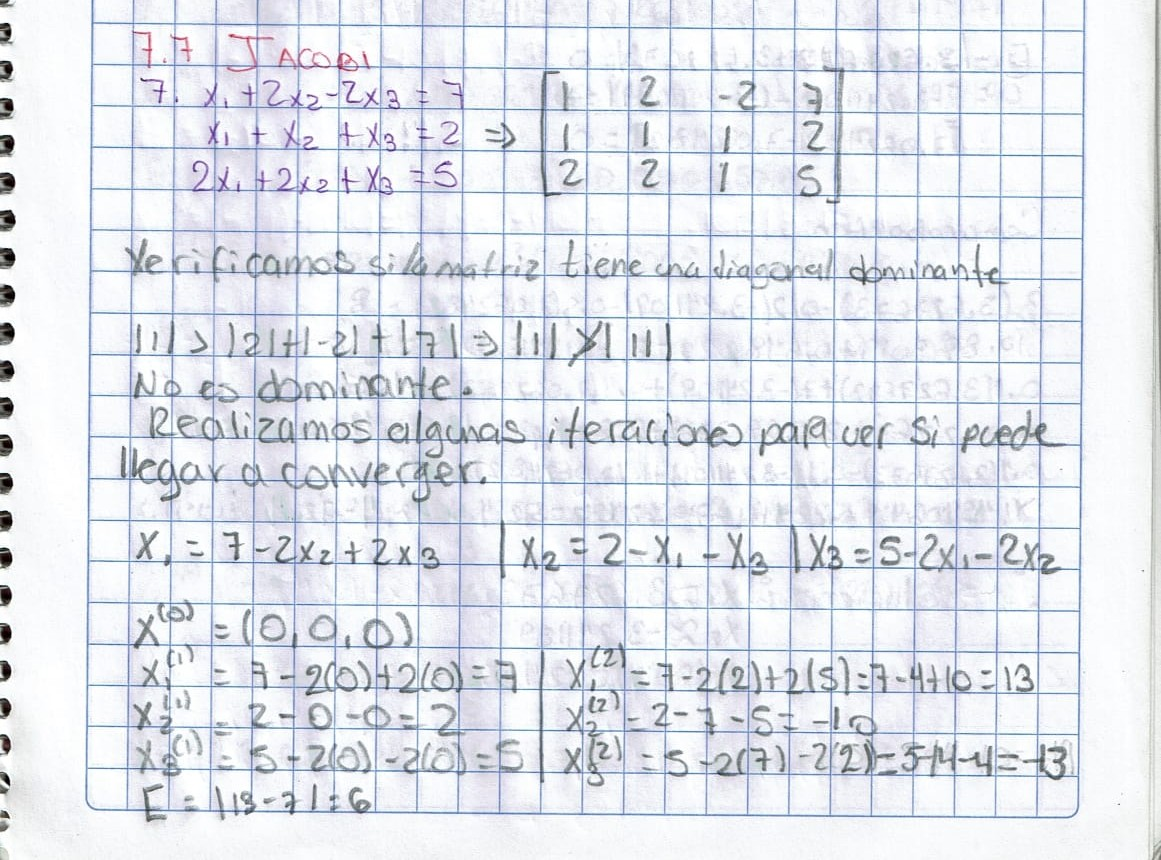
\includegraphics[width=6.25in,height=\textheight,keepaspectratio,alt={Ejercicio 7}]{Ejercicio77Jacobi7.jpg}
\caption{Ejercicio 7}
\end{figure}

\begin{figure}
\centering
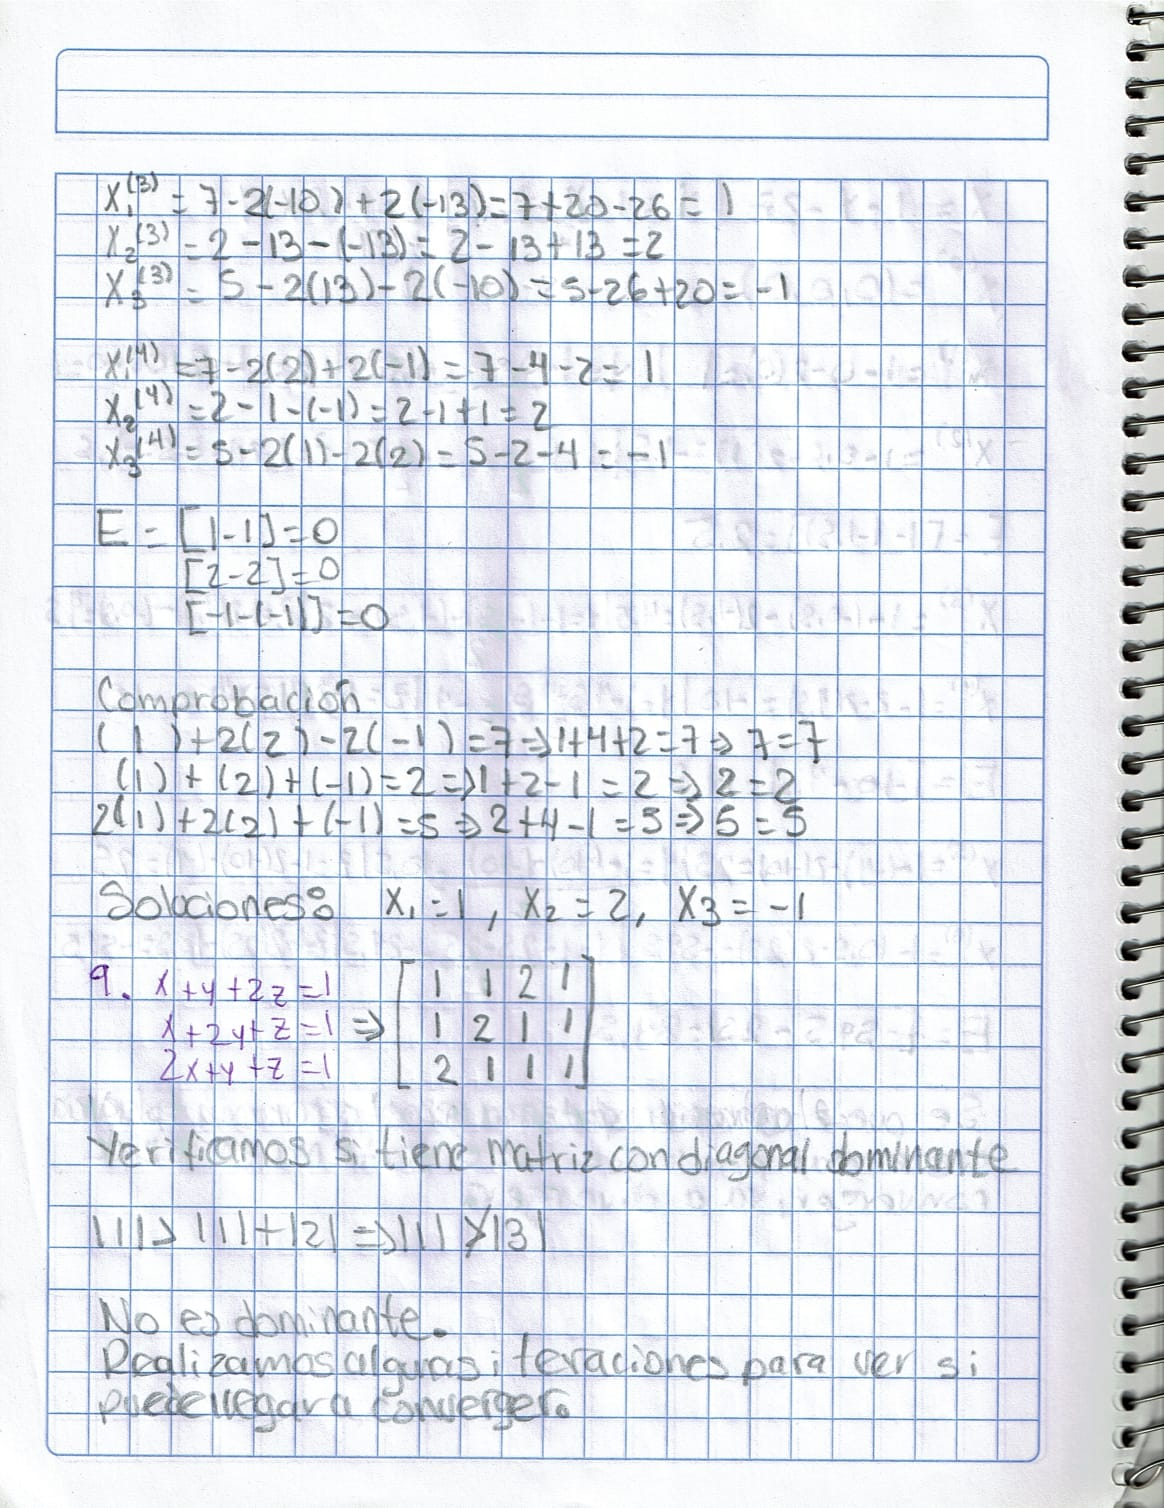
\includegraphics[width=6.25in,height=\textheight,keepaspectratio,alt={Ejercicio 9}]{Ejercicio77Jacobi9.jpg}
\caption{Ejercicio 9}
\end{figure}

\begin{figure}
\centering
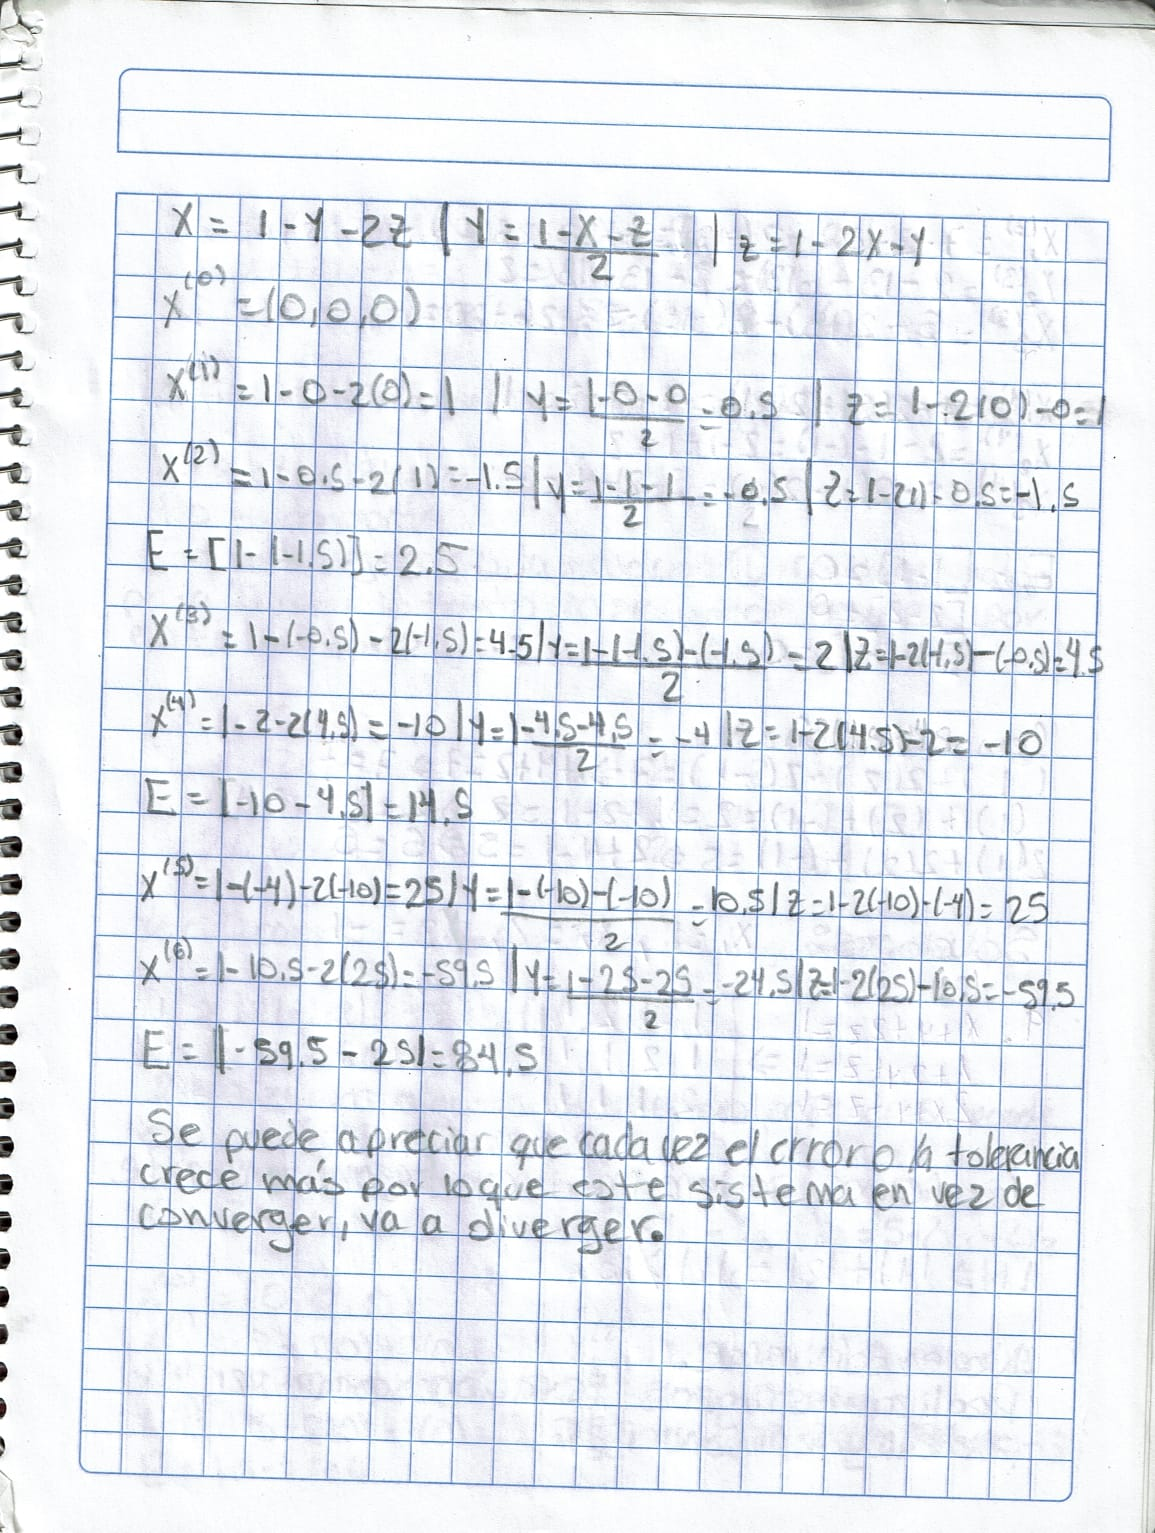
\includegraphics[width=6.25in,height=\textheight,keepaspectratio,alt={Ejercicio 9-2}]{Ejercicio77Jacobi9_2.jpg}
\caption{Ejercicio 9-2}
\end{figure}

\subsubsection{\texorpdfstring{Sistema
\(1\)}{Sistema 1}}\label{sistema-1-4}

\(A = \left[\begin{array}{cccc|c}
10 & 2 & -1 & 0 & 26 \\
1 & 20 & -2 & 3 & -15 \\
-2 & 1 & 30 & 0 & 53 \\
1 & 2 & 3 & 20 & 47
\end{array}\right]\)

\paragraph{Procedimiento}\label{procedimiento-50}

\begin{Shaded}
\begin{Highlighting}[]
\NormalTok{A }\OtherTok{\textless{}{-}} \FunctionTok{matrix}\NormalTok{(}\FunctionTok{c}\NormalTok{(}\DecValTok{10}\NormalTok{, }\DecValTok{2}\NormalTok{, }\SpecialCharTok{{-}}\DecValTok{1}\NormalTok{, }\DecValTok{0}\NormalTok{,}
              \DecValTok{1}\NormalTok{, }\DecValTok{20}\NormalTok{, }\SpecialCharTok{{-}}\DecValTok{2}\NormalTok{, }\DecValTok{3}\NormalTok{,}
              \SpecialCharTok{{-}}\DecValTok{2}\NormalTok{, }\DecValTok{1}\NormalTok{, }\DecValTok{30}\NormalTok{, }\DecValTok{0}\NormalTok{,}
              \DecValTok{1}\NormalTok{, }\DecValTok{2}\NormalTok{, }\DecValTok{3}\NormalTok{, }\DecValTok{20}\NormalTok{),}
      \AttributeTok{nrow =} \DecValTok{4}\NormalTok{, }\AttributeTok{byrow =} \ConstantTok{TRUE}\NormalTok{)}
\NormalTok{b }\OtherTok{\textless{}{-}} \FunctionTok{matrix}\NormalTok{(}\FunctionTok{c}\NormalTok{(}\DecValTok{26}\NormalTok{, }\SpecialCharTok{{-}}\DecValTok{15}\NormalTok{, }\DecValTok{53}\NormalTok{, }\DecValTok{47}\NormalTok{), }\AttributeTok{nrow =} \DecValTok{4}\NormalTok{)}

\NormalTok{Ab }\OtherTok{\textless{}{-}} \FunctionTok{cbind}\NormalTok{(A, b); (Ab)}
\end{Highlighting}
\end{Shaded}

\begin{verbatim}
##      [,1] [,2] [,3] [,4] [,5]
## [1,]   10    2   -1    0   26
## [2,]    1   20   -2    3  -15
## [3,]   -2    1   30    0   53
## [4,]    1    2    3   20   47
\end{verbatim}

\begin{Shaded}
\begin{Highlighting}[]
\CommentTok{\# Checar si converge o no con la diagonal dominante}

\NormalTok{F1 }\OtherTok{\textless{}{-}} \FunctionTok{abs}\NormalTok{(A[}\DecValTok{1}\NormalTok{,}\DecValTok{1}\NormalTok{]) }\SpecialCharTok{\textgreater{}}\NormalTok{ (}\FunctionTok{abs}\NormalTok{(A[}\DecValTok{1}\NormalTok{,}\DecValTok{2}\NormalTok{]) }\SpecialCharTok{+} \FunctionTok{abs}\NormalTok{(A[}\DecValTok{1}\NormalTok{,}\DecValTok{3}\NormalTok{]) }\SpecialCharTok{+} \FunctionTok{abs}\NormalTok{(A[}\DecValTok{1}\NormalTok{,}\DecValTok{4}\NormalTok{]))}
\NormalTok{F2 }\OtherTok{\textless{}{-}} \FunctionTok{abs}\NormalTok{(A[}\DecValTok{2}\NormalTok{,}\DecValTok{2}\NormalTok{]) }\SpecialCharTok{\textgreater{}}\NormalTok{ (}\FunctionTok{abs}\NormalTok{(A[}\DecValTok{2}\NormalTok{,}\DecValTok{1}\NormalTok{]) }\SpecialCharTok{+} \FunctionTok{abs}\NormalTok{(A[}\DecValTok{2}\NormalTok{,}\DecValTok{3}\NormalTok{])}\SpecialCharTok{+} \FunctionTok{abs}\NormalTok{(A[}\DecValTok{2}\NormalTok{,}\DecValTok{4}\NormalTok{]))}
\NormalTok{F3 }\OtherTok{\textless{}{-}} \FunctionTok{abs}\NormalTok{(A[}\DecValTok{3}\NormalTok{,}\DecValTok{3}\NormalTok{]) }\SpecialCharTok{\textgreater{}}\NormalTok{ (}\FunctionTok{abs}\NormalTok{(A[}\DecValTok{3}\NormalTok{,}\DecValTok{1}\NormalTok{]) }\SpecialCharTok{+} \FunctionTok{abs}\NormalTok{(A[}\DecValTok{3}\NormalTok{,}\DecValTok{2}\NormalTok{])}\SpecialCharTok{+} \FunctionTok{abs}\NormalTok{(A[}\DecValTok{3}\NormalTok{,}\DecValTok{4}\NormalTok{]))}
\NormalTok{F4 }\OtherTok{\textless{}{-}} \FunctionTok{abs}\NormalTok{(A[}\DecValTok{4}\NormalTok{,}\DecValTok{4}\NormalTok{]) }\SpecialCharTok{\textgreater{}}\NormalTok{ (}\FunctionTok{abs}\NormalTok{(A[}\DecValTok{4}\NormalTok{,}\DecValTok{1}\NormalTok{]) }\SpecialCharTok{+} \FunctionTok{abs}\NormalTok{(A[}\DecValTok{4}\NormalTok{,}\DecValTok{2}\NormalTok{])}\SpecialCharTok{+} \FunctionTok{abs}\NormalTok{(A[}\DecValTok{4}\NormalTok{,}\DecValTok{3}\NormalTok{]))}

\ControlFlowTok{if}\NormalTok{(F1 }\SpecialCharTok{==} \ConstantTok{TRUE} \SpecialCharTok{\&}\NormalTok{ F2 }\SpecialCharTok{==} \ConstantTok{TRUE} \SpecialCharTok{\&}\NormalTok{ F3 }\SpecialCharTok{==} \ConstantTok{TRUE}\NormalTok{) \{}
  \FunctionTok{cat}\NormalTok{(}\StringTok{"Sí es dominante"}\NormalTok{)}
\NormalTok{\} }\ControlFlowTok{else}\NormalTok{ \{}
  \FunctionTok{cat}\NormalTok{(}\StringTok{"No es dominante"}\NormalTok{)}
\NormalTok{\}}
\end{Highlighting}
\end{Shaded}

\begin{verbatim}
## Sí es dominante
\end{verbatim}

\begin{Shaded}
\begin{Highlighting}[]
\CommentTok{\# Asignar valores iniciales}

\NormalTok{x }\OtherTok{\textless{}{-}} \FunctionTok{rep}\NormalTok{(}\DecValTok{0}\NormalTok{, }\DecValTok{4}\NormalTok{) }\CommentTok{\# x\^{}(0)=(0,0,0)}
\FunctionTok{cat}\NormalTok{(}\StringTok{"x\^{}(0)="}\NormalTok{,}\FunctionTok{paste}\NormalTok{(}\FunctionTok{sprintf}\NormalTok{(}\StringTok{"\%.8f"}\NormalTok{,x), }\AttributeTok{collapse=}\StringTok{", "}\NormalTok{), }\StringTok{"}\SpecialCharTok{\textbackslash{}n}\StringTok{"}\NormalTok{)}
\end{Highlighting}
\end{Shaded}

\begin{verbatim}
## x^(0)= 0.00000000, 0.00000000, 0.00000000, 0.00000000
\end{verbatim}

\subparagraph{Iteración 1}\label{iteraciuxf3n-1-10}

\begin{Shaded}
\begin{Highlighting}[]
\NormalTok{x\_old }\OtherTok{\textless{}{-}}\NormalTok{ x}
\NormalTok{x[}\DecValTok{1}\NormalTok{] }\OtherTok{\textless{}{-}}\NormalTok{ (b[}\DecValTok{1}\NormalTok{] }\SpecialCharTok{{-}}\NormalTok{ A[}\DecValTok{1}\NormalTok{,}\DecValTok{2}\NormalTok{] }\SpecialCharTok{*}\NormalTok{ x\_old[}\DecValTok{2}\NormalTok{] }\SpecialCharTok{{-}}\NormalTok{ A[}\DecValTok{1}\NormalTok{,}\DecValTok{3}\NormalTok{] }\SpecialCharTok{*}\NormalTok{ x\_old[}\DecValTok{3}\NormalTok{] }\SpecialCharTok{{-}}\NormalTok{ A[}\DecValTok{1}\NormalTok{,}\DecValTok{4}\NormalTok{] }\SpecialCharTok{*}\NormalTok{ x\_old[}\DecValTok{4}\NormalTok{]) }\SpecialCharTok{/}\NormalTok{ A[}\DecValTok{1}\NormalTok{,}\DecValTok{1}\NormalTok{]}
\FunctionTok{cat}\NormalTok{(}\FunctionTok{sprintf}\NormalTok{(}\StringTok{"x1\^{}(1) = (\%.1f {-} (\%.1f)*\%.8f {-} (\%.1f)*\%.8f {-} (\%.1f)*\%.8f)/\%.1f = \%.8f}\SpecialCharTok{\textbackslash{}n}\StringTok{"}\NormalTok{, b[}\DecValTok{1}\NormalTok{], A[}\DecValTok{1}\NormalTok{,}\DecValTok{2}\NormalTok{], x\_old[}\DecValTok{2}\NormalTok{], A[}\DecValTok{1}\NormalTok{,}\DecValTok{3}\NormalTok{], x\_old[}\DecValTok{3}\NormalTok{],A[}\DecValTok{1}\NormalTok{,}\DecValTok{4}\NormalTok{], x\_old[}\DecValTok{4}\NormalTok{], A[}\DecValTok{1}\NormalTok{,}\DecValTok{1}\NormalTok{], x[}\DecValTok{1}\NormalTok{]))}
\end{Highlighting}
\end{Shaded}

\begin{verbatim}
## x1^(1) = (26.0 - (2.0)*0.00000000 - (-1.0)*0.00000000 - (0.0)*0.00000000)/10.0 = 2.60000000
\end{verbatim}

\begin{Shaded}
\begin{Highlighting}[]
\NormalTok{x[}\DecValTok{2}\NormalTok{] }\OtherTok{\textless{}{-}}\NormalTok{ (b[}\DecValTok{2}\NormalTok{] }\SpecialCharTok{{-}}\NormalTok{ A[}\DecValTok{2}\NormalTok{,}\DecValTok{1}\NormalTok{]}\SpecialCharTok{*}\NormalTok{x\_old[}\DecValTok{1}\NormalTok{] }\SpecialCharTok{{-}}\NormalTok{ A[}\DecValTok{2}\NormalTok{,}\DecValTok{3}\NormalTok{]}\SpecialCharTok{*}\NormalTok{x\_old[}\DecValTok{3}\NormalTok{] }\SpecialCharTok{{-}}\NormalTok{ A[}\DecValTok{2}\NormalTok{,}\DecValTok{4}\NormalTok{]}\SpecialCharTok{*}\NormalTok{x\_old[}\DecValTok{4}\NormalTok{]) }\SpecialCharTok{/}\NormalTok{ A[}\DecValTok{2}\NormalTok{,}\DecValTok{2}\NormalTok{]}
\FunctionTok{cat}\NormalTok{(}\FunctionTok{sprintf}\NormalTok{(}\StringTok{"x2\^{}(1) = (\%.1f {-} (\%.1f)*\%.8f {-} (\%.1f)*\%.8f {-} (\%.1f)*\%.8f)/\%.1f = \%.8f}\SpecialCharTok{\textbackslash{}n}\StringTok{"}\NormalTok{, b[}\DecValTok{2}\NormalTok{], A[}\DecValTok{2}\NormalTok{,}\DecValTok{1}\NormalTok{], x\_old[}\DecValTok{1}\NormalTok{], A[}\DecValTok{2}\NormalTok{,}\DecValTok{3}\NormalTok{], x\_old[}\DecValTok{3}\NormalTok{],A[}\DecValTok{2}\NormalTok{,}\DecValTok{4}\NormalTok{], x\_old[}\DecValTok{4}\NormalTok{], A[}\DecValTok{2}\NormalTok{,}\DecValTok{2}\NormalTok{], x[}\DecValTok{2}\NormalTok{]))}
\end{Highlighting}
\end{Shaded}

\begin{verbatim}
## x2^(1) = (-15.0 - (1.0)*0.00000000 - (-2.0)*0.00000000 - (3.0)*0.00000000)/20.0 = -0.75000000
\end{verbatim}

\begin{Shaded}
\begin{Highlighting}[]
\NormalTok{x[}\DecValTok{3}\NormalTok{] }\OtherTok{\textless{}{-}}\NormalTok{ (b[}\DecValTok{3}\NormalTok{] }\SpecialCharTok{{-}}\NormalTok{ A[}\DecValTok{3}\NormalTok{,}\DecValTok{1}\NormalTok{]}\SpecialCharTok{*}\NormalTok{x\_old[}\DecValTok{1}\NormalTok{] }\SpecialCharTok{{-}}\NormalTok{ A[}\DecValTok{3}\NormalTok{,}\DecValTok{2}\NormalTok{]}\SpecialCharTok{*}\NormalTok{x\_old[}\DecValTok{2}\NormalTok{] }\SpecialCharTok{{-}}\NormalTok{ A[}\DecValTok{3}\NormalTok{,}\DecValTok{4}\NormalTok{]}\SpecialCharTok{*}\NormalTok{x\_old[}\DecValTok{4}\NormalTok{]) }\SpecialCharTok{/}\NormalTok{ A[}\DecValTok{3}\NormalTok{,}\DecValTok{3}\NormalTok{]}
\FunctionTok{cat}\NormalTok{(}\FunctionTok{sprintf}\NormalTok{(}\StringTok{"x3\^{}(1) = (\%.1f {-} (\%.1f)*\%.8f {-} (\%.1f)*\%.8f {-} (\%.1f)*\%.8f)/\%.1f = \%.8f}\SpecialCharTok{\textbackslash{}n}\StringTok{"}\NormalTok{, b[}\DecValTok{3}\NormalTok{], A[}\DecValTok{3}\NormalTok{,}\DecValTok{1}\NormalTok{], x\_old[}\DecValTok{1}\NormalTok{], A[}\DecValTok{3}\NormalTok{,}\DecValTok{2}\NormalTok{], x\_old[}\DecValTok{2}\NormalTok{], A[}\DecValTok{3}\NormalTok{,}\DecValTok{4}\NormalTok{], x\_old[}\DecValTok{4}\NormalTok{], A[}\DecValTok{3}\NormalTok{,}\DecValTok{3}\NormalTok{], x[}\DecValTok{3}\NormalTok{]))}
\end{Highlighting}
\end{Shaded}

\begin{verbatim}
## x3^(1) = (53.0 - (-2.0)*0.00000000 - (1.0)*0.00000000 - (0.0)*0.00000000)/30.0 = 1.76666667
\end{verbatim}

\begin{Shaded}
\begin{Highlighting}[]
\NormalTok{x[}\DecValTok{4}\NormalTok{] }\OtherTok{\textless{}{-}}\NormalTok{ (b[}\DecValTok{4}\NormalTok{] }\SpecialCharTok{{-}}\NormalTok{ A[}\DecValTok{4}\NormalTok{,}\DecValTok{1}\NormalTok{]}\SpecialCharTok{*}\NormalTok{x\_old[}\DecValTok{1}\NormalTok{] }\SpecialCharTok{{-}}\NormalTok{ A[}\DecValTok{4}\NormalTok{,}\DecValTok{2}\NormalTok{]}\SpecialCharTok{*}\NormalTok{x\_old[}\DecValTok{2}\NormalTok{] }\SpecialCharTok{{-}}\NormalTok{ A[}\DecValTok{4}\NormalTok{,}\DecValTok{3}\NormalTok{]}\SpecialCharTok{*}\NormalTok{x\_old[}\DecValTok{3}\NormalTok{]) }\SpecialCharTok{/}\NormalTok{ A[}\DecValTok{4}\NormalTok{,}\DecValTok{4}\NormalTok{]}
\FunctionTok{cat}\NormalTok{(}\FunctionTok{sprintf}\NormalTok{(}\StringTok{"x4\^{}(1) = (\%.1f {-} (\%.1f)*\%.8f {-} (\%.1f)*\%.8f {-} (\%.1f)*\%.8f)/\%.1f = \%.8f}\SpecialCharTok{\textbackslash{}n}\StringTok{"}\NormalTok{, b[}\DecValTok{4}\NormalTok{], A[}\DecValTok{4}\NormalTok{,}\DecValTok{1}\NormalTok{], x\_old[}\DecValTok{1}\NormalTok{], A[}\DecValTok{4}\NormalTok{,}\DecValTok{2}\NormalTok{], x\_old[}\DecValTok{2}\NormalTok{], A[}\DecValTok{4}\NormalTok{,}\DecValTok{3}\NormalTok{], x\_old[}\DecValTok{4}\NormalTok{], A[}\DecValTok{4}\NormalTok{,}\DecValTok{4}\NormalTok{], x[}\DecValTok{4}\NormalTok{]))}
\end{Highlighting}
\end{Shaded}

\begin{verbatim}
## x4^(1) = (47.0 - (1.0)*0.00000000 - (2.0)*0.00000000 - (3.0)*0.00000000)/20.0 = 2.35000000
\end{verbatim}

\begin{Shaded}
\begin{Highlighting}[]
\CommentTok{\# Imprime los valores de la iteración}
\NormalTok{x\_old }\OtherTok{\textless{}{-}}\NormalTok{ x}
\NormalTok{x1 }\OtherTok{\textless{}{-}}\NormalTok{ x\_old[}\DecValTok{1}\NormalTok{]; (x1)}
\end{Highlighting}
\end{Shaded}

\begin{verbatim}
## [1] 2.6
\end{verbatim}

\begin{Shaded}
\begin{Highlighting}[]
\NormalTok{x2 }\OtherTok{\textless{}{-}}\NormalTok{ x\_old[}\DecValTok{2}\NormalTok{]; (x2)}
\end{Highlighting}
\end{Shaded}

\begin{verbatim}
## [1] -0.75
\end{verbatim}

\begin{Shaded}
\begin{Highlighting}[]
\NormalTok{x3 }\OtherTok{\textless{}{-}}\NormalTok{ x\_old[}\DecValTok{3}\NormalTok{]; (x3)}
\end{Highlighting}
\end{Shaded}

\begin{verbatim}
## [1] 1.766667
\end{verbatim}

\begin{Shaded}
\begin{Highlighting}[]
\NormalTok{x4 }\OtherTok{\textless{}{-}}\NormalTok{ x\_old[}\DecValTok{4}\NormalTok{]; (x4)}
\end{Highlighting}
\end{Shaded}

\begin{verbatim}
## [1] 2.35
\end{verbatim}

\begin{Shaded}
\begin{Highlighting}[]
\CommentTok{\#Error o tolerancia}

\NormalTok{r }\OtherTok{\textless{}{-}}\NormalTok{ b }\SpecialCharTok{{-}}\NormalTok{ A }\SpecialCharTok{\%*\%}\NormalTok{ x}
\NormalTok{dx\_inf }\OtherTok{\textless{}{-}} \FunctionTok{max}\NormalTok{(}\FunctionTok{abs}\NormalTok{(x }\SpecialCharTok{{-}}\NormalTok{ x\_old))}
\FunctionTok{cat}\NormalTok{(}\FunctionTok{sprintf}\NormalTok{(}\StringTok{"x\^{}(1) = \%s}\SpecialCharTok{\textbackslash{}n}\StringTok{"}\NormalTok{, }\FunctionTok{paste}\NormalTok{(}\FunctionTok{sprintf}\NormalTok{(}\StringTok{"\%.8f"}\NormalTok{, x), }\AttributeTok{collapse=}\StringTok{", "}\NormalTok{)))}
\end{Highlighting}
\end{Shaded}

\begin{verbatim}
## x^(1) = 2.60000000, -0.75000000, 1.76666667, 2.35000000
\end{verbatim}

\begin{Shaded}
\begin{Highlighting}[]
\FunctionTok{cat}\NormalTok{(}\FunctionTok{sprintf}\NormalTok{(}\StringTok{"||dx||\_inf = \%.8e | ||r||\_inf = \%.8e}\SpecialCharTok{\textbackslash{}n}\StringTok{"}\NormalTok{, dx\_inf, }\FunctionTok{max}\NormalTok{(}\FunctionTok{abs}\NormalTok{(r))))}
\end{Highlighting}
\end{Shaded}

\begin{verbatim}
## ||dx||_inf = 0.00000000e+00 | ||r||_inf = 6.40000000e+00
\end{verbatim}

\subparagraph{Iteración 2}\label{iteraciuxf3n-2-10}

\begin{Shaded}
\begin{Highlighting}[]
\NormalTok{x\_old }\OtherTok{\textless{}{-}}\NormalTok{ x}
\NormalTok{x[}\DecValTok{1}\NormalTok{] }\OtherTok{\textless{}{-}}\NormalTok{ (b[}\DecValTok{1}\NormalTok{] }\SpecialCharTok{{-}}\NormalTok{ A[}\DecValTok{1}\NormalTok{,}\DecValTok{2}\NormalTok{] }\SpecialCharTok{*}\NormalTok{ x\_old[}\DecValTok{2}\NormalTok{] }\SpecialCharTok{{-}}\NormalTok{ A[}\DecValTok{1}\NormalTok{,}\DecValTok{3}\NormalTok{] }\SpecialCharTok{*}\NormalTok{ x\_old[}\DecValTok{3}\NormalTok{] }\SpecialCharTok{{-}}\NormalTok{ A[}\DecValTok{1}\NormalTok{,}\DecValTok{4}\NormalTok{] }\SpecialCharTok{*}\NormalTok{ x\_old[}\DecValTok{4}\NormalTok{]) }\SpecialCharTok{/}\NormalTok{ A[}\DecValTok{1}\NormalTok{,}\DecValTok{1}\NormalTok{]}
\FunctionTok{cat}\NormalTok{(}\FunctionTok{sprintf}\NormalTok{(}\StringTok{"x1\^{}(2) = (\%.1f {-} (\%.1f)*\%.8f {-} (\%.1f)*\%.8f {-} (\%.1f)*\%.8f)/\%.1f = \%.8f}\SpecialCharTok{\textbackslash{}n}\StringTok{"}\NormalTok{, b[}\DecValTok{1}\NormalTok{], A[}\DecValTok{1}\NormalTok{,}\DecValTok{2}\NormalTok{], x\_old[}\DecValTok{2}\NormalTok{], A[}\DecValTok{1}\NormalTok{,}\DecValTok{3}\NormalTok{], x\_old[}\DecValTok{3}\NormalTok{],A[}\DecValTok{1}\NormalTok{,}\DecValTok{4}\NormalTok{], x\_old[}\DecValTok{4}\NormalTok{], A[}\DecValTok{1}\NormalTok{,}\DecValTok{1}\NormalTok{], x[}\DecValTok{1}\NormalTok{]))}
\end{Highlighting}
\end{Shaded}

\begin{verbatim}
## x1^(2) = (26.0 - (2.0)*-0.75000000 - (-1.0)*1.76666667 - (0.0)*2.35000000)/10.0 = 2.92666667
\end{verbatim}

\begin{Shaded}
\begin{Highlighting}[]
\NormalTok{x[}\DecValTok{2}\NormalTok{] }\OtherTok{\textless{}{-}}\NormalTok{ (b[}\DecValTok{2}\NormalTok{] }\SpecialCharTok{{-}}\NormalTok{ A[}\DecValTok{2}\NormalTok{,}\DecValTok{1}\NormalTok{]}\SpecialCharTok{*}\NormalTok{x\_old[}\DecValTok{1}\NormalTok{] }\SpecialCharTok{{-}}\NormalTok{ A[}\DecValTok{2}\NormalTok{,}\DecValTok{3}\NormalTok{]}\SpecialCharTok{*}\NormalTok{x\_old[}\DecValTok{3}\NormalTok{] }\SpecialCharTok{{-}}\NormalTok{ A[}\DecValTok{2}\NormalTok{,}\DecValTok{4}\NormalTok{]}\SpecialCharTok{*}\NormalTok{x\_old[}\DecValTok{4}\NormalTok{]) }\SpecialCharTok{/}\NormalTok{ A[}\DecValTok{2}\NormalTok{,}\DecValTok{2}\NormalTok{]}
\FunctionTok{cat}\NormalTok{(}\FunctionTok{sprintf}\NormalTok{(}\StringTok{"x2\^{}(2) = (\%.1f {-} (\%.1f)*\%.8f {-} (\%.1f)*\%.8f {-} (\%.1f)*\%.8f)/\%.1f = \%.8f}\SpecialCharTok{\textbackslash{}n}\StringTok{"}\NormalTok{, b[}\DecValTok{2}\NormalTok{], A[}\DecValTok{2}\NormalTok{,}\DecValTok{1}\NormalTok{], x\_old[}\DecValTok{1}\NormalTok{], A[}\DecValTok{2}\NormalTok{,}\DecValTok{3}\NormalTok{], x\_old[}\DecValTok{3}\NormalTok{],A[}\DecValTok{2}\NormalTok{,}\DecValTok{4}\NormalTok{], x\_old[}\DecValTok{4}\NormalTok{], A[}\DecValTok{2}\NormalTok{,}\DecValTok{2}\NormalTok{], x[}\DecValTok{2}\NormalTok{]))}
\end{Highlighting}
\end{Shaded}

\begin{verbatim}
## x2^(2) = (-15.0 - (1.0)*2.60000000 - (-2.0)*1.76666667 - (3.0)*2.35000000)/20.0 = -1.05583333
\end{verbatim}

\begin{Shaded}
\begin{Highlighting}[]
\NormalTok{x[}\DecValTok{3}\NormalTok{] }\OtherTok{\textless{}{-}}\NormalTok{ (b[}\DecValTok{3}\NormalTok{] }\SpecialCharTok{{-}}\NormalTok{ A[}\DecValTok{3}\NormalTok{,}\DecValTok{1}\NormalTok{]}\SpecialCharTok{*}\NormalTok{x\_old[}\DecValTok{1}\NormalTok{] }\SpecialCharTok{{-}}\NormalTok{ A[}\DecValTok{3}\NormalTok{,}\DecValTok{2}\NormalTok{]}\SpecialCharTok{*}\NormalTok{x\_old[}\DecValTok{2}\NormalTok{] }\SpecialCharTok{{-}}\NormalTok{ A[}\DecValTok{3}\NormalTok{,}\DecValTok{4}\NormalTok{]}\SpecialCharTok{*}\NormalTok{x\_old[}\DecValTok{4}\NormalTok{]) }\SpecialCharTok{/}\NormalTok{ A[}\DecValTok{3}\NormalTok{,}\DecValTok{3}\NormalTok{]}
\FunctionTok{cat}\NormalTok{(}\FunctionTok{sprintf}\NormalTok{(}\StringTok{"x3\^{}(2) = (\%.1f {-} (\%.1f)*\%.8f {-} (\%.1f)*\%.8f {-} (\%.1f)*\%.8f)/\%.1f = \%.8f}\SpecialCharTok{\textbackslash{}n}\StringTok{"}\NormalTok{, b[}\DecValTok{3}\NormalTok{], A[}\DecValTok{3}\NormalTok{,}\DecValTok{1}\NormalTok{], x\_old[}\DecValTok{1}\NormalTok{], A[}\DecValTok{3}\NormalTok{,}\DecValTok{2}\NormalTok{], x\_old[}\DecValTok{2}\NormalTok{], A[}\DecValTok{3}\NormalTok{,}\DecValTok{4}\NormalTok{], x\_old[}\DecValTok{4}\NormalTok{], A[}\DecValTok{3}\NormalTok{,}\DecValTok{3}\NormalTok{], x[}\DecValTok{3}\NormalTok{]))}
\end{Highlighting}
\end{Shaded}

\begin{verbatim}
## x3^(2) = (53.0 - (-2.0)*2.60000000 - (1.0)*-0.75000000 - (0.0)*2.35000000)/30.0 = 1.96500000
\end{verbatim}

\begin{Shaded}
\begin{Highlighting}[]
\NormalTok{x[}\DecValTok{4}\NormalTok{] }\OtherTok{\textless{}{-}}\NormalTok{ (b[}\DecValTok{4}\NormalTok{] }\SpecialCharTok{{-}}\NormalTok{ A[}\DecValTok{4}\NormalTok{,}\DecValTok{1}\NormalTok{]}\SpecialCharTok{*}\NormalTok{x\_old[}\DecValTok{1}\NormalTok{] }\SpecialCharTok{{-}}\NormalTok{ A[}\DecValTok{4}\NormalTok{,}\DecValTok{2}\NormalTok{]}\SpecialCharTok{*}\NormalTok{x\_old[}\DecValTok{2}\NormalTok{] }\SpecialCharTok{{-}}\NormalTok{ A[}\DecValTok{4}\NormalTok{,}\DecValTok{3}\NormalTok{]}\SpecialCharTok{*}\NormalTok{x\_old[}\DecValTok{3}\NormalTok{]) }\SpecialCharTok{/}\NormalTok{ A[}\DecValTok{4}\NormalTok{,}\DecValTok{4}\NormalTok{]}
\FunctionTok{cat}\NormalTok{(}\FunctionTok{sprintf}\NormalTok{(}\StringTok{"x4\^{}(2) = (\%.1f {-} (\%.1f)*\%.8f {-} (\%.1f)*\%.8f {-} (\%.1f)*\%.8f)/\%.1f = \%.8f}\SpecialCharTok{\textbackslash{}n}\StringTok{"}\NormalTok{, b[}\DecValTok{4}\NormalTok{], A[}\DecValTok{4}\NormalTok{,}\DecValTok{1}\NormalTok{], x\_old[}\DecValTok{1}\NormalTok{], A[}\DecValTok{4}\NormalTok{,}\DecValTok{2}\NormalTok{], x\_old[}\DecValTok{2}\NormalTok{], A[}\DecValTok{4}\NormalTok{,}\DecValTok{3}\NormalTok{], x\_old[}\DecValTok{4}\NormalTok{], A[}\DecValTok{4}\NormalTok{,}\DecValTok{4}\NormalTok{], x[}\DecValTok{4}\NormalTok{]))}
\end{Highlighting}
\end{Shaded}

\begin{verbatim}
## x4^(2) = (47.0 - (1.0)*2.60000000 - (2.0)*-0.75000000 - (3.0)*2.35000000)/20.0 = 2.03000000
\end{verbatim}

\begin{Shaded}
\begin{Highlighting}[]
\CommentTok{\# Imprime los valores de la iteración}
\NormalTok{x\_old }\OtherTok{\textless{}{-}}\NormalTok{ x}
\NormalTok{x1 }\OtherTok{\textless{}{-}}\NormalTok{ x\_old[}\DecValTok{1}\NormalTok{]; (x1)}
\end{Highlighting}
\end{Shaded}

\begin{verbatim}
## [1] 2.926667
\end{verbatim}

\begin{Shaded}
\begin{Highlighting}[]
\NormalTok{x2 }\OtherTok{\textless{}{-}}\NormalTok{ x\_old[}\DecValTok{2}\NormalTok{]; (x2)}
\end{Highlighting}
\end{Shaded}

\begin{verbatim}
## [1] -1.055833
\end{verbatim}

\begin{Shaded}
\begin{Highlighting}[]
\NormalTok{x3 }\OtherTok{\textless{}{-}}\NormalTok{ x\_old[}\DecValTok{3}\NormalTok{]; (x3)}
\end{Highlighting}
\end{Shaded}

\begin{verbatim}
## [1] 1.965
\end{verbatim}

\begin{Shaded}
\begin{Highlighting}[]
\NormalTok{x4 }\OtherTok{\textless{}{-}}\NormalTok{ x\_old[}\DecValTok{4}\NormalTok{]; (x4)}
\end{Highlighting}
\end{Shaded}

\begin{verbatim}
## [1] 2.03
\end{verbatim}

\begin{Shaded}
\begin{Highlighting}[]
\CommentTok{\#Error o tolerancia}

\NormalTok{r }\OtherTok{\textless{}{-}}\NormalTok{ b }\SpecialCharTok{{-}}\NormalTok{ A }\SpecialCharTok{\%*\%}\NormalTok{ x}
\NormalTok{dx\_inf }\OtherTok{\textless{}{-}} \FunctionTok{max}\NormalTok{(}\FunctionTok{abs}\NormalTok{(x }\SpecialCharTok{{-}}\NormalTok{ x\_old))}
\FunctionTok{cat}\NormalTok{(}\FunctionTok{sprintf}\NormalTok{(}\StringTok{"x\^{}(2) = \%s}\SpecialCharTok{\textbackslash{}n}\StringTok{"}\NormalTok{, }\FunctionTok{paste}\NormalTok{(}\FunctionTok{sprintf}\NormalTok{(}\StringTok{"\%.8f"}\NormalTok{, x), }\AttributeTok{collapse=}\StringTok{", "}\NormalTok{)))}
\end{Highlighting}
\end{Shaded}

\begin{verbatim}
## x^(2) = 2.92666667, -1.05583333, 1.96500000, 2.03000000
\end{verbatim}

\begin{Shaded}
\begin{Highlighting}[]
\FunctionTok{cat}\NormalTok{(}\FunctionTok{sprintf}\NormalTok{(}\StringTok{"||dx||\_inf = \%.8e | ||r||\_inf = \%.8e}\SpecialCharTok{\textbackslash{}n}\StringTok{"}\NormalTok{, dx\_inf, }\FunctionTok{max}\NormalTok{(}\FunctionTok{abs}\NormalTok{(r))))}
\end{Highlighting}
\end{Shaded}

\begin{verbatim}
## ||dx||_inf = 0.00000000e+00 | ||r||_inf = 1.03000000e+00
\end{verbatim}

\subparagraph{Iteración 3}\label{iteraciuxf3n-3-10}

\begin{Shaded}
\begin{Highlighting}[]
\NormalTok{x\_old }\OtherTok{\textless{}{-}}\NormalTok{ x}
\NormalTok{x[}\DecValTok{1}\NormalTok{] }\OtherTok{\textless{}{-}}\NormalTok{ (b[}\DecValTok{1}\NormalTok{] }\SpecialCharTok{{-}}\NormalTok{ A[}\DecValTok{1}\NormalTok{,}\DecValTok{2}\NormalTok{] }\SpecialCharTok{*}\NormalTok{ x\_old[}\DecValTok{2}\NormalTok{] }\SpecialCharTok{{-}}\NormalTok{ A[}\DecValTok{1}\NormalTok{,}\DecValTok{3}\NormalTok{] }\SpecialCharTok{*}\NormalTok{ x\_old[}\DecValTok{3}\NormalTok{] }\SpecialCharTok{{-}}\NormalTok{ A[}\DecValTok{1}\NormalTok{,}\DecValTok{4}\NormalTok{] }\SpecialCharTok{*}\NormalTok{ x\_old[}\DecValTok{4}\NormalTok{]) }\SpecialCharTok{/}\NormalTok{ A[}\DecValTok{1}\NormalTok{,}\DecValTok{1}\NormalTok{]}
\FunctionTok{cat}\NormalTok{(}\FunctionTok{sprintf}\NormalTok{(}\StringTok{"x1\^{}(3) = (\%.1f {-} (\%.1f)*\%.8f {-} (\%.1f)*\%.8f {-} (\%.1f)*\%.8f)/\%.1f = \%.8f}\SpecialCharTok{\textbackslash{}n}\StringTok{"}\NormalTok{, b[}\DecValTok{1}\NormalTok{], A[}\DecValTok{1}\NormalTok{,}\DecValTok{2}\NormalTok{], x\_old[}\DecValTok{2}\NormalTok{], A[}\DecValTok{1}\NormalTok{,}\DecValTok{3}\NormalTok{], x\_old[}\DecValTok{3}\NormalTok{],A[}\DecValTok{1}\NormalTok{,}\DecValTok{4}\NormalTok{], x\_old[}\DecValTok{4}\NormalTok{], A[}\DecValTok{1}\NormalTok{,}\DecValTok{1}\NormalTok{], x[}\DecValTok{1}\NormalTok{]))}
\end{Highlighting}
\end{Shaded}

\begin{verbatim}
## x1^(3) = (26.0 - (2.0)*-1.05583333 - (-1.0)*1.96500000 - (0.0)*2.03000000)/10.0 = 3.00766667
\end{verbatim}

\begin{Shaded}
\begin{Highlighting}[]
\NormalTok{x[}\DecValTok{2}\NormalTok{] }\OtherTok{\textless{}{-}}\NormalTok{ (b[}\DecValTok{2}\NormalTok{] }\SpecialCharTok{{-}}\NormalTok{ A[}\DecValTok{2}\NormalTok{,}\DecValTok{1}\NormalTok{]}\SpecialCharTok{*}\NormalTok{x\_old[}\DecValTok{1}\NormalTok{] }\SpecialCharTok{{-}}\NormalTok{ A[}\DecValTok{2}\NormalTok{,}\DecValTok{3}\NormalTok{]}\SpecialCharTok{*}\NormalTok{x\_old[}\DecValTok{3}\NormalTok{] }\SpecialCharTok{{-}}\NormalTok{ A[}\DecValTok{2}\NormalTok{,}\DecValTok{4}\NormalTok{]}\SpecialCharTok{*}\NormalTok{x\_old[}\DecValTok{4}\NormalTok{]) }\SpecialCharTok{/}\NormalTok{ A[}\DecValTok{2}\NormalTok{,}\DecValTok{2}\NormalTok{]}
\FunctionTok{cat}\NormalTok{(}\FunctionTok{sprintf}\NormalTok{(}\StringTok{"x2\^{}(3) = (\%.1f {-} (\%.1f)*\%.8f {-} (\%.1f)*\%.8f {-} (\%.1f)*\%.8f)/\%.1f = \%.8f}\SpecialCharTok{\textbackslash{}n}\StringTok{"}\NormalTok{, b[}\DecValTok{2}\NormalTok{], A[}\DecValTok{2}\NormalTok{,}\DecValTok{1}\NormalTok{], x\_old[}\DecValTok{1}\NormalTok{], A[}\DecValTok{2}\NormalTok{,}\DecValTok{3}\NormalTok{], x\_old[}\DecValTok{3}\NormalTok{],A[}\DecValTok{2}\NormalTok{,}\DecValTok{4}\NormalTok{], x\_old[}\DecValTok{4}\NormalTok{], A[}\DecValTok{2}\NormalTok{,}\DecValTok{2}\NormalTok{], x[}\DecValTok{2}\NormalTok{]))}
\end{Highlighting}
\end{Shaded}

\begin{verbatim}
## x2^(3) = (-15.0 - (1.0)*2.92666667 - (-2.0)*1.96500000 - (3.0)*2.03000000)/20.0 = -1.00433333
\end{verbatim}

\begin{Shaded}
\begin{Highlighting}[]
\NormalTok{x[}\DecValTok{3}\NormalTok{] }\OtherTok{\textless{}{-}}\NormalTok{ (b[}\DecValTok{3}\NormalTok{] }\SpecialCharTok{{-}}\NormalTok{ A[}\DecValTok{3}\NormalTok{,}\DecValTok{1}\NormalTok{]}\SpecialCharTok{*}\NormalTok{x\_old[}\DecValTok{1}\NormalTok{] }\SpecialCharTok{{-}}\NormalTok{ A[}\DecValTok{3}\NormalTok{,}\DecValTok{2}\NormalTok{]}\SpecialCharTok{*}\NormalTok{x\_old[}\DecValTok{2}\NormalTok{] }\SpecialCharTok{{-}}\NormalTok{ A[}\DecValTok{3}\NormalTok{,}\DecValTok{4}\NormalTok{]}\SpecialCharTok{*}\NormalTok{x\_old[}\DecValTok{4}\NormalTok{]) }\SpecialCharTok{/}\NormalTok{ A[}\DecValTok{3}\NormalTok{,}\DecValTok{3}\NormalTok{]}
\FunctionTok{cat}\NormalTok{(}\FunctionTok{sprintf}\NormalTok{(}\StringTok{"x3\^{}(3) = (\%.1f {-} (\%.1f)*\%.8f {-} (\%.1f)*\%.8f {-} (\%.1f)*\%.8f)/\%.1f = \%.8f}\SpecialCharTok{\textbackslash{}n}\StringTok{"}\NormalTok{, b[}\DecValTok{3}\NormalTok{], A[}\DecValTok{3}\NormalTok{,}\DecValTok{1}\NormalTok{], x\_old[}\DecValTok{1}\NormalTok{], A[}\DecValTok{3}\NormalTok{,}\DecValTok{2}\NormalTok{], x\_old[}\DecValTok{2}\NormalTok{], A[}\DecValTok{3}\NormalTok{,}\DecValTok{4}\NormalTok{], x\_old[}\DecValTok{4}\NormalTok{], A[}\DecValTok{3}\NormalTok{,}\DecValTok{3}\NormalTok{], x[}\DecValTok{3}\NormalTok{]))}
\end{Highlighting}
\end{Shaded}

\begin{verbatim}
## x3^(3) = (53.0 - (-2.0)*2.92666667 - (1.0)*-1.05583333 - (0.0)*2.03000000)/30.0 = 1.99697222
\end{verbatim}

\begin{Shaded}
\begin{Highlighting}[]
\NormalTok{x[}\DecValTok{4}\NormalTok{] }\OtherTok{\textless{}{-}}\NormalTok{ (b[}\DecValTok{4}\NormalTok{] }\SpecialCharTok{{-}}\NormalTok{ A[}\DecValTok{4}\NormalTok{,}\DecValTok{1}\NormalTok{]}\SpecialCharTok{*}\NormalTok{x\_old[}\DecValTok{1}\NormalTok{] }\SpecialCharTok{{-}}\NormalTok{ A[}\DecValTok{4}\NormalTok{,}\DecValTok{2}\NormalTok{]}\SpecialCharTok{*}\NormalTok{x\_old[}\DecValTok{2}\NormalTok{] }\SpecialCharTok{{-}}\NormalTok{ A[}\DecValTok{4}\NormalTok{,}\DecValTok{3}\NormalTok{]}\SpecialCharTok{*}\NormalTok{x\_old[}\DecValTok{3}\NormalTok{]) }\SpecialCharTok{/}\NormalTok{ A[}\DecValTok{4}\NormalTok{,}\DecValTok{4}\NormalTok{]}
\FunctionTok{cat}\NormalTok{(}\FunctionTok{sprintf}\NormalTok{(}\StringTok{"x4\^{}(3) = (\%.1f {-} (\%.1f)*\%.8f {-} (\%.1f)*\%.8f {-} (\%.1f)*\%.8f)/\%.1f = \%.8f}\SpecialCharTok{\textbackslash{}n}\StringTok{"}\NormalTok{, b[}\DecValTok{4}\NormalTok{], A[}\DecValTok{4}\NormalTok{,}\DecValTok{1}\NormalTok{], x\_old[}\DecValTok{1}\NormalTok{], A[}\DecValTok{4}\NormalTok{,}\DecValTok{2}\NormalTok{], x\_old[}\DecValTok{2}\NormalTok{], A[}\DecValTok{4}\NormalTok{,}\DecValTok{3}\NormalTok{], x\_old[}\DecValTok{4}\NormalTok{], A[}\DecValTok{4}\NormalTok{,}\DecValTok{4}\NormalTok{], x[}\DecValTok{4}\NormalTok{]))}
\end{Highlighting}
\end{Shaded}

\begin{verbatim}
## x4^(3) = (47.0 - (1.0)*2.92666667 - (2.0)*-1.05583333 - (3.0)*2.03000000)/20.0 = 2.01450000
\end{verbatim}

\begin{Shaded}
\begin{Highlighting}[]
\CommentTok{\# Imprime los valores de la iteración}
\NormalTok{x\_old }\OtherTok{\textless{}{-}}\NormalTok{ x}
\NormalTok{x1 }\OtherTok{\textless{}{-}}\NormalTok{ x\_old[}\DecValTok{1}\NormalTok{]; (x1)}
\end{Highlighting}
\end{Shaded}

\begin{verbatim}
## [1] 3.007667
\end{verbatim}

\begin{Shaded}
\begin{Highlighting}[]
\NormalTok{x2 }\OtherTok{\textless{}{-}}\NormalTok{ x\_old[}\DecValTok{2}\NormalTok{]; (x2)}
\end{Highlighting}
\end{Shaded}

\begin{verbatim}
## [1] -1.004333
\end{verbatim}

\begin{Shaded}
\begin{Highlighting}[]
\NormalTok{x3 }\OtherTok{\textless{}{-}}\NormalTok{ x\_old[}\DecValTok{3}\NormalTok{]; (x3)}
\end{Highlighting}
\end{Shaded}

\begin{verbatim}
## [1] 1.996972
\end{verbatim}

\begin{Shaded}
\begin{Highlighting}[]
\NormalTok{x4 }\OtherTok{\textless{}{-}}\NormalTok{ x\_old[}\DecValTok{4}\NormalTok{]; (x4)}
\end{Highlighting}
\end{Shaded}

\begin{verbatim}
## [1] 2.0145
\end{verbatim}

\begin{Shaded}
\begin{Highlighting}[]
\CommentTok{\#Error o tolerancia}

\NormalTok{r }\OtherTok{\textless{}{-}}\NormalTok{ b }\SpecialCharTok{{-}}\NormalTok{ A }\SpecialCharTok{\%*\%}\NormalTok{ x}
\NormalTok{dx\_inf }\OtherTok{\textless{}{-}} \FunctionTok{max}\NormalTok{(}\FunctionTok{abs}\NormalTok{(x }\SpecialCharTok{{-}}\NormalTok{ x\_old))}
\FunctionTok{cat}\NormalTok{(}\FunctionTok{sprintf}\NormalTok{(}\StringTok{"x\^{}(3) = \%s}\SpecialCharTok{\textbackslash{}n}\StringTok{"}\NormalTok{, }\FunctionTok{paste}\NormalTok{(}\FunctionTok{sprintf}\NormalTok{(}\StringTok{"\%.8f"}\NormalTok{, x), }\AttributeTok{collapse=}\StringTok{", "}\NormalTok{)))}
\end{Highlighting}
\end{Shaded}

\begin{verbatim}
## x^(3) = 3.00766667, -1.00433333, 1.99697222, 2.01450000
\end{verbatim}

\begin{Shaded}
\begin{Highlighting}[]
\FunctionTok{cat}\NormalTok{(}\FunctionTok{sprintf}\NormalTok{(}\StringTok{"||dx||\_inf = \%.8e | ||r||\_inf = \%.8e}\SpecialCharTok{\textbackslash{}n}\StringTok{"}\NormalTok{, dx\_inf, }\FunctionTok{max}\NormalTok{(}\FunctionTok{abs}\NormalTok{(r))))}
\end{Highlighting}
\end{Shaded}

\begin{verbatim}
## ||dx||_inf = 0.00000000e+00 | ||r||_inf = 2.79916667e-01
\end{verbatim}

\subparagraph{Iteración 4}\label{iteraciuxf3n-4-10}

\begin{Shaded}
\begin{Highlighting}[]
\NormalTok{x\_old }\OtherTok{\textless{}{-}}\NormalTok{ x}
\NormalTok{x[}\DecValTok{1}\NormalTok{] }\OtherTok{\textless{}{-}}\NormalTok{ (b[}\DecValTok{1}\NormalTok{] }\SpecialCharTok{{-}}\NormalTok{ A[}\DecValTok{1}\NormalTok{,}\DecValTok{2}\NormalTok{] }\SpecialCharTok{*}\NormalTok{ x\_old[}\DecValTok{2}\NormalTok{] }\SpecialCharTok{{-}}\NormalTok{ A[}\DecValTok{1}\NormalTok{,}\DecValTok{3}\NormalTok{] }\SpecialCharTok{*}\NormalTok{ x\_old[}\DecValTok{3}\NormalTok{] }\SpecialCharTok{{-}}\NormalTok{ A[}\DecValTok{1}\NormalTok{,}\DecValTok{4}\NormalTok{] }\SpecialCharTok{*}\NormalTok{ x\_old[}\DecValTok{4}\NormalTok{]) }\SpecialCharTok{/}\NormalTok{ A[}\DecValTok{1}\NormalTok{,}\DecValTok{1}\NormalTok{]}
\FunctionTok{cat}\NormalTok{(}\FunctionTok{sprintf}\NormalTok{(}\StringTok{"x1\^{}(4) = (\%.1f {-} (\%.1f)*\%.8f {-} (\%.1f)*\%.8f {-} (\%.1f)*\%.8f)/\%.1f = \%.8f}\SpecialCharTok{\textbackslash{}n}\StringTok{"}\NormalTok{, b[}\DecValTok{1}\NormalTok{], A[}\DecValTok{1}\NormalTok{,}\DecValTok{2}\NormalTok{], x\_old[}\DecValTok{2}\NormalTok{], A[}\DecValTok{1}\NormalTok{,}\DecValTok{3}\NormalTok{], x\_old[}\DecValTok{3}\NormalTok{],A[}\DecValTok{1}\NormalTok{,}\DecValTok{4}\NormalTok{], x\_old[}\DecValTok{4}\NormalTok{], A[}\DecValTok{1}\NormalTok{,}\DecValTok{1}\NormalTok{], x[}\DecValTok{1}\NormalTok{]))}
\end{Highlighting}
\end{Shaded}

\begin{verbatim}
## x1^(4) = (26.0 - (2.0)*-1.00433333 - (-1.0)*1.99697222 - (0.0)*2.01450000)/10.0 = 3.00056389
\end{verbatim}

\begin{Shaded}
\begin{Highlighting}[]
\NormalTok{x[}\DecValTok{2}\NormalTok{] }\OtherTok{\textless{}{-}}\NormalTok{ (b[}\DecValTok{2}\NormalTok{] }\SpecialCharTok{{-}}\NormalTok{ A[}\DecValTok{2}\NormalTok{,}\DecValTok{1}\NormalTok{]}\SpecialCharTok{*}\NormalTok{x\_old[}\DecValTok{1}\NormalTok{] }\SpecialCharTok{{-}}\NormalTok{ A[}\DecValTok{2}\NormalTok{,}\DecValTok{3}\NormalTok{]}\SpecialCharTok{*}\NormalTok{x\_old[}\DecValTok{3}\NormalTok{] }\SpecialCharTok{{-}}\NormalTok{ A[}\DecValTok{2}\NormalTok{,}\DecValTok{4}\NormalTok{]}\SpecialCharTok{*}\NormalTok{x\_old[}\DecValTok{4}\NormalTok{]) }\SpecialCharTok{/}\NormalTok{ A[}\DecValTok{2}\NormalTok{,}\DecValTok{2}\NormalTok{]}
\FunctionTok{cat}\NormalTok{(}\FunctionTok{sprintf}\NormalTok{(}\StringTok{"x2\^{}(4) = (\%.1f {-} (\%.1f)*\%.8f {-} (\%.1f)*\%.8f {-} (\%.1f)*\%.8f)/\%.1f = \%.8f}\SpecialCharTok{\textbackslash{}n}\StringTok{"}\NormalTok{, b[}\DecValTok{2}\NormalTok{], A[}\DecValTok{2}\NormalTok{,}\DecValTok{1}\NormalTok{], x\_old[}\DecValTok{1}\NormalTok{], A[}\DecValTok{2}\NormalTok{,}\DecValTok{3}\NormalTok{], x\_old[}\DecValTok{3}\NormalTok{],A[}\DecValTok{2}\NormalTok{,}\DecValTok{4}\NormalTok{], x\_old[}\DecValTok{4}\NormalTok{], A[}\DecValTok{2}\NormalTok{,}\DecValTok{2}\NormalTok{], x[}\DecValTok{2}\NormalTok{]))}
\end{Highlighting}
\end{Shaded}

\begin{verbatim}
## x2^(4) = (-15.0 - (1.0)*3.00766667 - (-2.0)*1.99697222 - (3.0)*2.01450000)/20.0 = -1.00286111
\end{verbatim}

\begin{Shaded}
\begin{Highlighting}[]
\NormalTok{x[}\DecValTok{3}\NormalTok{] }\OtherTok{\textless{}{-}}\NormalTok{ (b[}\DecValTok{3}\NormalTok{] }\SpecialCharTok{{-}}\NormalTok{ A[}\DecValTok{3}\NormalTok{,}\DecValTok{1}\NormalTok{]}\SpecialCharTok{*}\NormalTok{x\_old[}\DecValTok{1}\NormalTok{] }\SpecialCharTok{{-}}\NormalTok{ A[}\DecValTok{3}\NormalTok{,}\DecValTok{2}\NormalTok{]}\SpecialCharTok{*}\NormalTok{x\_old[}\DecValTok{2}\NormalTok{] }\SpecialCharTok{{-}}\NormalTok{ A[}\DecValTok{3}\NormalTok{,}\DecValTok{4}\NormalTok{]}\SpecialCharTok{*}\NormalTok{x\_old[}\DecValTok{4}\NormalTok{]) }\SpecialCharTok{/}\NormalTok{ A[}\DecValTok{3}\NormalTok{,}\DecValTok{3}\NormalTok{]}
\FunctionTok{cat}\NormalTok{(}\FunctionTok{sprintf}\NormalTok{(}\StringTok{"x3\^{}(4) = (\%.1f {-} (\%.1f)*\%.8f {-} (\%.1f)*\%.8f {-} (\%.1f)*\%.8f)/\%.1f = \%.8f}\SpecialCharTok{\textbackslash{}n}\StringTok{"}\NormalTok{, b[}\DecValTok{3}\NormalTok{], A[}\DecValTok{3}\NormalTok{,}\DecValTok{1}\NormalTok{], x\_old[}\DecValTok{1}\NormalTok{], A[}\DecValTok{3}\NormalTok{,}\DecValTok{2}\NormalTok{], x\_old[}\DecValTok{2}\NormalTok{], A[}\DecValTok{3}\NormalTok{,}\DecValTok{4}\NormalTok{], x\_old[}\DecValTok{4}\NormalTok{], A[}\DecValTok{3}\NormalTok{,}\DecValTok{3}\NormalTok{], x[}\DecValTok{3}\NormalTok{]))}
\end{Highlighting}
\end{Shaded}

\begin{verbatim}
## x3^(4) = (53.0 - (-2.0)*3.00766667 - (1.0)*-1.00433333 - (0.0)*2.01450000)/30.0 = 2.00065556
\end{verbatim}

\begin{Shaded}
\begin{Highlighting}[]
\NormalTok{x[}\DecValTok{4}\NormalTok{] }\OtherTok{\textless{}{-}}\NormalTok{ (b[}\DecValTok{4}\NormalTok{] }\SpecialCharTok{{-}}\NormalTok{ A[}\DecValTok{4}\NormalTok{,}\DecValTok{1}\NormalTok{]}\SpecialCharTok{*}\NormalTok{x\_old[}\DecValTok{1}\NormalTok{] }\SpecialCharTok{{-}}\NormalTok{ A[}\DecValTok{4}\NormalTok{,}\DecValTok{2}\NormalTok{]}\SpecialCharTok{*}\NormalTok{x\_old[}\DecValTok{2}\NormalTok{] }\SpecialCharTok{{-}}\NormalTok{ A[}\DecValTok{4}\NormalTok{,}\DecValTok{3}\NormalTok{]}\SpecialCharTok{*}\NormalTok{x\_old[}\DecValTok{3}\NormalTok{]) }\SpecialCharTok{/}\NormalTok{ A[}\DecValTok{4}\NormalTok{,}\DecValTok{4}\NormalTok{]}
\FunctionTok{cat}\NormalTok{(}\FunctionTok{sprintf}\NormalTok{(}\StringTok{"x4\^{}(4) = (\%.1f {-} (\%.1f)*\%.8f {-} (\%.1f)*\%.8f {-} (\%.1f)*\%.8f)/\%.1f = \%.8f}\SpecialCharTok{\textbackslash{}n}\StringTok{"}\NormalTok{, b[}\DecValTok{4}\NormalTok{], A[}\DecValTok{4}\NormalTok{,}\DecValTok{1}\NormalTok{], x\_old[}\DecValTok{1}\NormalTok{], A[}\DecValTok{4}\NormalTok{,}\DecValTok{2}\NormalTok{], x\_old[}\DecValTok{2}\NormalTok{], A[}\DecValTok{4}\NormalTok{,}\DecValTok{3}\NormalTok{], x\_old[}\DecValTok{4}\NormalTok{], A[}\DecValTok{4}\NormalTok{,}\DecValTok{4}\NormalTok{], x[}\DecValTok{4}\NormalTok{]))}
\end{Highlighting}
\end{Shaded}

\begin{verbatim}
## x4^(4) = (47.0 - (1.0)*3.00766667 - (2.0)*-1.00433333 - (3.0)*2.01450000)/20.0 = 2.00050417
\end{verbatim}

\begin{Shaded}
\begin{Highlighting}[]
\CommentTok{\# Imprime los valores de la iteración}
\NormalTok{x\_old }\OtherTok{\textless{}{-}}\NormalTok{ x}
\NormalTok{x1 }\OtherTok{\textless{}{-}}\NormalTok{ x\_old[}\DecValTok{1}\NormalTok{]; (x1)}
\end{Highlighting}
\end{Shaded}

\begin{verbatim}
## [1] 3.000564
\end{verbatim}

\begin{Shaded}
\begin{Highlighting}[]
\NormalTok{x2 }\OtherTok{\textless{}{-}}\NormalTok{ x\_old[}\DecValTok{2}\NormalTok{]; (x2)}
\end{Highlighting}
\end{Shaded}

\begin{verbatim}
## [1] -1.002861
\end{verbatim}

\begin{Shaded}
\begin{Highlighting}[]
\NormalTok{x3 }\OtherTok{\textless{}{-}}\NormalTok{ x\_old[}\DecValTok{3}\NormalTok{]; (x3)}
\end{Highlighting}
\end{Shaded}

\begin{verbatim}
## [1] 2.000656
\end{verbatim}

\begin{Shaded}
\begin{Highlighting}[]
\NormalTok{x4 }\OtherTok{\textless{}{-}}\NormalTok{ x\_old[}\DecValTok{4}\NormalTok{]; (x4)}
\end{Highlighting}
\end{Shaded}

\begin{verbatim}
## [1] 2.000504
\end{verbatim}

\begin{Shaded}
\begin{Highlighting}[]
\CommentTok{\#Error o tolerancia}

\NormalTok{r }\OtherTok{\textless{}{-}}\NormalTok{ b }\SpecialCharTok{{-}}\NormalTok{ A }\SpecialCharTok{\%*\%}\NormalTok{ x}
\NormalTok{dx\_inf }\OtherTok{\textless{}{-}} \FunctionTok{max}\NormalTok{(}\FunctionTok{abs}\NormalTok{(x }\SpecialCharTok{{-}}\NormalTok{ x\_old))}
\FunctionTok{cat}\NormalTok{(}\FunctionTok{sprintf}\NormalTok{(}\StringTok{"x\^{}(4) = \%s}\SpecialCharTok{\textbackslash{}n}\StringTok{"}\NormalTok{, }\FunctionTok{paste}\NormalTok{(}\FunctionTok{sprintf}\NormalTok{(}\StringTok{"\%.8f"}\NormalTok{, x), }\AttributeTok{collapse=}\StringTok{", "}\NormalTok{)))}
\end{Highlighting}
\end{Shaded}

\begin{verbatim}
## x^(4) = 3.00056389, -1.00286111, 2.00065556, 2.00050417
\end{verbatim}

\begin{Shaded}
\begin{Highlighting}[]
\FunctionTok{cat}\NormalTok{(}\FunctionTok{sprintf}\NormalTok{(}\StringTok{"||dx||\_inf = \%.8e | ||r||\_inf = \%.8e}\SpecialCharTok{\textbackslash{}n}\StringTok{"}\NormalTok{, dx\_inf, }\FunctionTok{max}\NormalTok{(}\FunctionTok{abs}\NormalTok{(r))))}
\end{Highlighting}
\end{Shaded}

\begin{verbatim}
## ||dx||_inf = 0.00000000e+00 | ||r||_inf = 5.64569444e-02
\end{verbatim}

\subparagraph{Iteración 5}\label{iteraciuxf3n-5-10}

\begin{Shaded}
\begin{Highlighting}[]
\NormalTok{x\_old }\OtherTok{\textless{}{-}}\NormalTok{ x}
\NormalTok{x[}\DecValTok{1}\NormalTok{] }\OtherTok{\textless{}{-}}\NormalTok{ (b[}\DecValTok{1}\NormalTok{] }\SpecialCharTok{{-}}\NormalTok{ A[}\DecValTok{1}\NormalTok{,}\DecValTok{2}\NormalTok{] }\SpecialCharTok{*}\NormalTok{ x\_old[}\DecValTok{2}\NormalTok{] }\SpecialCharTok{{-}}\NormalTok{ A[}\DecValTok{1}\NormalTok{,}\DecValTok{3}\NormalTok{] }\SpecialCharTok{*}\NormalTok{ x\_old[}\DecValTok{3}\NormalTok{] }\SpecialCharTok{{-}}\NormalTok{ A[}\DecValTok{1}\NormalTok{,}\DecValTok{4}\NormalTok{] }\SpecialCharTok{*}\NormalTok{ x\_old[}\DecValTok{4}\NormalTok{]) }\SpecialCharTok{/}\NormalTok{ A[}\DecValTok{1}\NormalTok{,}\DecValTok{1}\NormalTok{]}
\FunctionTok{cat}\NormalTok{(}\FunctionTok{sprintf}\NormalTok{(}\StringTok{"x1\^{}(5) = (\%.1f {-} (\%.1f)*\%.8f {-} (\%.1f)*\%.8f {-} (\%.1f)*\%.8f)/\%.1f = \%.8f}\SpecialCharTok{\textbackslash{}n}\StringTok{"}\NormalTok{, b[}\DecValTok{1}\NormalTok{], A[}\DecValTok{1}\NormalTok{,}\DecValTok{2}\NormalTok{], x\_old[}\DecValTok{2}\NormalTok{], A[}\DecValTok{1}\NormalTok{,}\DecValTok{3}\NormalTok{], x\_old[}\DecValTok{3}\NormalTok{],A[}\DecValTok{1}\NormalTok{,}\DecValTok{4}\NormalTok{], x\_old[}\DecValTok{4}\NormalTok{], A[}\DecValTok{1}\NormalTok{,}\DecValTok{1}\NormalTok{], x[}\DecValTok{1}\NormalTok{]))}
\end{Highlighting}
\end{Shaded}

\begin{verbatim}
## x1^(5) = (26.0 - (2.0)*-1.00286111 - (-1.0)*2.00065556 - (0.0)*2.00050417)/10.0 = 3.00063778
\end{verbatim}

\begin{Shaded}
\begin{Highlighting}[]
\NormalTok{x[}\DecValTok{2}\NormalTok{] }\OtherTok{\textless{}{-}}\NormalTok{ (b[}\DecValTok{2}\NormalTok{] }\SpecialCharTok{{-}}\NormalTok{ A[}\DecValTok{2}\NormalTok{,}\DecValTok{1}\NormalTok{]}\SpecialCharTok{*}\NormalTok{x\_old[}\DecValTok{1}\NormalTok{] }\SpecialCharTok{{-}}\NormalTok{ A[}\DecValTok{2}\NormalTok{,}\DecValTok{3}\NormalTok{]}\SpecialCharTok{*}\NormalTok{x\_old[}\DecValTok{3}\NormalTok{] }\SpecialCharTok{{-}}\NormalTok{ A[}\DecValTok{2}\NormalTok{,}\DecValTok{4}\NormalTok{]}\SpecialCharTok{*}\NormalTok{x\_old[}\DecValTok{4}\NormalTok{]) }\SpecialCharTok{/}\NormalTok{ A[}\DecValTok{2}\NormalTok{,}\DecValTok{2}\NormalTok{]}
\FunctionTok{cat}\NormalTok{(}\FunctionTok{sprintf}\NormalTok{(}\StringTok{"x2\^{}(5) = (\%.1f {-} (\%.1f)*\%.8f {-} (\%.1f)*\%.8f {-} (\%.1f)*\%.8f)/\%.1f = \%.8f}\SpecialCharTok{\textbackslash{}n}\StringTok{"}\NormalTok{, b[}\DecValTok{2}\NormalTok{], A[}\DecValTok{2}\NormalTok{,}\DecValTok{1}\NormalTok{], x\_old[}\DecValTok{1}\NormalTok{], A[}\DecValTok{2}\NormalTok{,}\DecValTok{3}\NormalTok{], x\_old[}\DecValTok{3}\NormalTok{],A[}\DecValTok{2}\NormalTok{,}\DecValTok{4}\NormalTok{], x\_old[}\DecValTok{4}\NormalTok{], A[}\DecValTok{2}\NormalTok{,}\DecValTok{2}\NormalTok{], x[}\DecValTok{2}\NormalTok{]))}
\end{Highlighting}
\end{Shaded}

\begin{verbatim}
## x2^(5) = (-15.0 - (1.0)*3.00056389 - (-2.0)*2.00065556 - (3.0)*2.00050417)/20.0 = -1.00003826
\end{verbatim}

\begin{Shaded}
\begin{Highlighting}[]
\NormalTok{x[}\DecValTok{3}\NormalTok{] }\OtherTok{\textless{}{-}}\NormalTok{ (b[}\DecValTok{3}\NormalTok{] }\SpecialCharTok{{-}}\NormalTok{ A[}\DecValTok{3}\NormalTok{,}\DecValTok{1}\NormalTok{]}\SpecialCharTok{*}\NormalTok{x\_old[}\DecValTok{1}\NormalTok{] }\SpecialCharTok{{-}}\NormalTok{ A[}\DecValTok{3}\NormalTok{,}\DecValTok{2}\NormalTok{]}\SpecialCharTok{*}\NormalTok{x\_old[}\DecValTok{2}\NormalTok{] }\SpecialCharTok{{-}}\NormalTok{ A[}\DecValTok{3}\NormalTok{,}\DecValTok{4}\NormalTok{]}\SpecialCharTok{*}\NormalTok{x\_old[}\DecValTok{4}\NormalTok{]) }\SpecialCharTok{/}\NormalTok{ A[}\DecValTok{3}\NormalTok{,}\DecValTok{3}\NormalTok{]}
\FunctionTok{cat}\NormalTok{(}\FunctionTok{sprintf}\NormalTok{(}\StringTok{"x3\^{}(5) = (\%.1f {-} (\%.1f)*\%.8f {-} (\%.1f)*\%.8f {-} (\%.1f)*\%.8f)/\%.1f = \%.8f}\SpecialCharTok{\textbackslash{}n}\StringTok{"}\NormalTok{, b[}\DecValTok{3}\NormalTok{], A[}\DecValTok{3}\NormalTok{,}\DecValTok{1}\NormalTok{], x\_old[}\DecValTok{1}\NormalTok{], A[}\DecValTok{3}\NormalTok{,}\DecValTok{2}\NormalTok{], x\_old[}\DecValTok{2}\NormalTok{], A[}\DecValTok{3}\NormalTok{,}\DecValTok{4}\NormalTok{], x\_old[}\DecValTok{4}\NormalTok{], A[}\DecValTok{3}\NormalTok{,}\DecValTok{3}\NormalTok{], x[}\DecValTok{3}\NormalTok{]))}
\end{Highlighting}
\end{Shaded}

\begin{verbatim}
## x3^(5) = (53.0 - (-2.0)*3.00056389 - (1.0)*-1.00286111 - (0.0)*2.00050417)/30.0 = 2.00013296
\end{verbatim}

\begin{Shaded}
\begin{Highlighting}[]
\NormalTok{x[}\DecValTok{4}\NormalTok{] }\OtherTok{\textless{}{-}}\NormalTok{ (b[}\DecValTok{4}\NormalTok{] }\SpecialCharTok{{-}}\NormalTok{ A[}\DecValTok{4}\NormalTok{,}\DecValTok{1}\NormalTok{]}\SpecialCharTok{*}\NormalTok{x\_old[}\DecValTok{1}\NormalTok{] }\SpecialCharTok{{-}}\NormalTok{ A[}\DecValTok{4}\NormalTok{,}\DecValTok{2}\NormalTok{]}\SpecialCharTok{*}\NormalTok{x\_old[}\DecValTok{2}\NormalTok{] }\SpecialCharTok{{-}}\NormalTok{ A[}\DecValTok{4}\NormalTok{,}\DecValTok{3}\NormalTok{]}\SpecialCharTok{*}\NormalTok{x\_old[}\DecValTok{3}\NormalTok{]) }\SpecialCharTok{/}\NormalTok{ A[}\DecValTok{4}\NormalTok{,}\DecValTok{4}\NormalTok{]}
\FunctionTok{cat}\NormalTok{(}\FunctionTok{sprintf}\NormalTok{(}\StringTok{"x4\^{}(5) = (\%.1f {-} (\%.1f)*\%.8f {-} (\%.1f)*\%.8f {-} (\%.1f)*\%.8f)/\%.1f = \%.8f}\SpecialCharTok{\textbackslash{}n}\StringTok{"}\NormalTok{, b[}\DecValTok{4}\NormalTok{], A[}\DecValTok{4}\NormalTok{,}\DecValTok{1}\NormalTok{], x\_old[}\DecValTok{1}\NormalTok{], A[}\DecValTok{4}\NormalTok{,}\DecValTok{2}\NormalTok{], x\_old[}\DecValTok{2}\NormalTok{], A[}\DecValTok{4}\NormalTok{,}\DecValTok{3}\NormalTok{], x\_old[}\DecValTok{4}\NormalTok{], A[}\DecValTok{4}\NormalTok{,}\DecValTok{4}\NormalTok{], x[}\DecValTok{4}\NormalTok{]))}
\end{Highlighting}
\end{Shaded}

\begin{verbatim}
## x4^(5) = (47.0 - (1.0)*3.00056389 - (2.0)*-1.00286111 - (3.0)*2.00050417)/20.0 = 2.00015958
\end{verbatim}

\begin{Shaded}
\begin{Highlighting}[]
\CommentTok{\# Imprime los valores de la iteración}
\NormalTok{x\_old }\OtherTok{\textless{}{-}}\NormalTok{ x}
\NormalTok{x1 }\OtherTok{\textless{}{-}}\NormalTok{ x\_old[}\DecValTok{1}\NormalTok{]; (x1)}
\end{Highlighting}
\end{Shaded}

\begin{verbatim}
## [1] 3.000638
\end{verbatim}

\begin{Shaded}
\begin{Highlighting}[]
\NormalTok{x2 }\OtherTok{\textless{}{-}}\NormalTok{ x\_old[}\DecValTok{2}\NormalTok{]; (x2)}
\end{Highlighting}
\end{Shaded}

\begin{verbatim}
## [1] -1.000038
\end{verbatim}

\begin{Shaded}
\begin{Highlighting}[]
\NormalTok{x3 }\OtherTok{\textless{}{-}}\NormalTok{ x\_old[}\DecValTok{3}\NormalTok{]; (x3)}
\end{Highlighting}
\end{Shaded}

\begin{verbatim}
## [1] 2.000133
\end{verbatim}

\begin{Shaded}
\begin{Highlighting}[]
\NormalTok{x4 }\OtherTok{\textless{}{-}}\NormalTok{ x\_old[}\DecValTok{4}\NormalTok{]; (x4)}
\end{Highlighting}
\end{Shaded}

\begin{verbatim}
## [1] 2.00016
\end{verbatim}

\begin{Shaded}
\begin{Highlighting}[]
\CommentTok{\#Error o tolerancia}

\NormalTok{r }\OtherTok{\textless{}{-}}\NormalTok{ b }\SpecialCharTok{{-}}\NormalTok{ A }\SpecialCharTok{\%*\%}\NormalTok{ x}
\NormalTok{dx\_inf }\OtherTok{\textless{}{-}} \FunctionTok{max}\NormalTok{(}\FunctionTok{abs}\NormalTok{(x }\SpecialCharTok{{-}}\NormalTok{ x\_old))}
\FunctionTok{cat}\NormalTok{(}\FunctionTok{sprintf}\NormalTok{(}\StringTok{"x\^{}(5) = \%s}\SpecialCharTok{\textbackslash{}n}\StringTok{"}\NormalTok{, }\FunctionTok{paste}\NormalTok{(}\FunctionTok{sprintf}\NormalTok{(}\StringTok{"\%.8f"}\NormalTok{, x), }\AttributeTok{collapse=}\StringTok{", "}\NormalTok{)))}
\end{Highlighting}
\end{Shaded}

\begin{verbatim}
## x^(5) = 3.00063778, -1.00003826, 2.00013296, 2.00015958
\end{verbatim}

\begin{Shaded}
\begin{Highlighting}[]
\FunctionTok{cat}\NormalTok{(}\FunctionTok{sprintf}\NormalTok{(}\StringTok{"||dx||\_inf = \%.8e | ||r||\_inf = \%.8e}\SpecialCharTok{\textbackslash{}n}\StringTok{"}\NormalTok{, dx\_inf, }\FunctionTok{max}\NormalTok{(}\FunctionTok{abs}\NormalTok{(r))))}
\end{Highlighting}
\end{Shaded}

\begin{verbatim}
## ||dx||_inf = 0.00000000e+00 | ||r||_inf = 6.16828704e-03
\end{verbatim}

\subparagraph{Iteración 6}\label{iteraciuxf3n-6-10}

\begin{Shaded}
\begin{Highlighting}[]
\NormalTok{x\_old }\OtherTok{\textless{}{-}}\NormalTok{ x}
\NormalTok{x[}\DecValTok{1}\NormalTok{] }\OtherTok{\textless{}{-}}\NormalTok{ (b[}\DecValTok{1}\NormalTok{] }\SpecialCharTok{{-}}\NormalTok{ A[}\DecValTok{1}\NormalTok{,}\DecValTok{2}\NormalTok{] }\SpecialCharTok{*}\NormalTok{ x\_old[}\DecValTok{2}\NormalTok{] }\SpecialCharTok{{-}}\NormalTok{ A[}\DecValTok{1}\NormalTok{,}\DecValTok{3}\NormalTok{] }\SpecialCharTok{*}\NormalTok{ x\_old[}\DecValTok{3}\NormalTok{] }\SpecialCharTok{{-}}\NormalTok{ A[}\DecValTok{1}\NormalTok{,}\DecValTok{4}\NormalTok{] }\SpecialCharTok{*}\NormalTok{ x\_old[}\DecValTok{4}\NormalTok{]) }\SpecialCharTok{/}\NormalTok{ A[}\DecValTok{1}\NormalTok{,}\DecValTok{1}\NormalTok{]}
\FunctionTok{cat}\NormalTok{(}\FunctionTok{sprintf}\NormalTok{(}\StringTok{"x1\^{}(6) = (\%.1f {-} (\%.1f)*\%.8f {-} (\%.1f)*\%.8f {-} (\%.1f)*\%.8f)/\%.1f = \%.8f}\SpecialCharTok{\textbackslash{}n}\StringTok{"}\NormalTok{, b[}\DecValTok{1}\NormalTok{], A[}\DecValTok{1}\NormalTok{,}\DecValTok{2}\NormalTok{], x\_old[}\DecValTok{2}\NormalTok{], A[}\DecValTok{1}\NormalTok{,}\DecValTok{3}\NormalTok{], x\_old[}\DecValTok{3}\NormalTok{],A[}\DecValTok{1}\NormalTok{,}\DecValTok{4}\NormalTok{], x\_old[}\DecValTok{4}\NormalTok{], A[}\DecValTok{1}\NormalTok{,}\DecValTok{1}\NormalTok{], x[}\DecValTok{1}\NormalTok{]))}
\end{Highlighting}
\end{Shaded}

\begin{verbatim}
## x1^(6) = (26.0 - (2.0)*-1.00003826 - (-1.0)*2.00013296 - (0.0)*2.00015958)/10.0 = 3.00002095
\end{verbatim}

\begin{Shaded}
\begin{Highlighting}[]
\NormalTok{x[}\DecValTok{2}\NormalTok{] }\OtherTok{\textless{}{-}}\NormalTok{ (b[}\DecValTok{2}\NormalTok{] }\SpecialCharTok{{-}}\NormalTok{ A[}\DecValTok{2}\NormalTok{,}\DecValTok{1}\NormalTok{]}\SpecialCharTok{*}\NormalTok{x\_old[}\DecValTok{1}\NormalTok{] }\SpecialCharTok{{-}}\NormalTok{ A[}\DecValTok{2}\NormalTok{,}\DecValTok{3}\NormalTok{]}\SpecialCharTok{*}\NormalTok{x\_old[}\DecValTok{3}\NormalTok{] }\SpecialCharTok{{-}}\NormalTok{ A[}\DecValTok{2}\NormalTok{,}\DecValTok{4}\NormalTok{]}\SpecialCharTok{*}\NormalTok{x\_old[}\DecValTok{4}\NormalTok{]) }\SpecialCharTok{/}\NormalTok{ A[}\DecValTok{2}\NormalTok{,}\DecValTok{2}\NormalTok{]}
\FunctionTok{cat}\NormalTok{(}\FunctionTok{sprintf}\NormalTok{(}\StringTok{"x2\^{}(6) = (\%.1f {-} (\%.1f)*\%.8f {-} (\%.1f)*\%.8f {-} (\%.1f)*\%.8f)/\%.1f = \%.8f}\SpecialCharTok{\textbackslash{}n}\StringTok{"}\NormalTok{, b[}\DecValTok{2}\NormalTok{], A[}\DecValTok{2}\NormalTok{,}\DecValTok{1}\NormalTok{], x\_old[}\DecValTok{1}\NormalTok{], A[}\DecValTok{2}\NormalTok{,}\DecValTok{3}\NormalTok{], x\_old[}\DecValTok{3}\NormalTok{],A[}\DecValTok{2}\NormalTok{,}\DecValTok{4}\NormalTok{], x\_old[}\DecValTok{4}\NormalTok{], A[}\DecValTok{2}\NormalTok{,}\DecValTok{2}\NormalTok{], x[}\DecValTok{2}\NormalTok{]))}
\end{Highlighting}
\end{Shaded}

\begin{verbatim}
## x2^(6) = (-15.0 - (1.0)*3.00063778 - (-2.0)*2.00013296 - (3.0)*2.00015958)/20.0 = -1.00004253
\end{verbatim}

\begin{Shaded}
\begin{Highlighting}[]
\NormalTok{x[}\DecValTok{3}\NormalTok{] }\OtherTok{\textless{}{-}}\NormalTok{ (b[}\DecValTok{3}\NormalTok{] }\SpecialCharTok{{-}}\NormalTok{ A[}\DecValTok{3}\NormalTok{,}\DecValTok{1}\NormalTok{]}\SpecialCharTok{*}\NormalTok{x\_old[}\DecValTok{1}\NormalTok{] }\SpecialCharTok{{-}}\NormalTok{ A[}\DecValTok{3}\NormalTok{,}\DecValTok{2}\NormalTok{]}\SpecialCharTok{*}\NormalTok{x\_old[}\DecValTok{2}\NormalTok{] }\SpecialCharTok{{-}}\NormalTok{ A[}\DecValTok{3}\NormalTok{,}\DecValTok{4}\NormalTok{]}\SpecialCharTok{*}\NormalTok{x\_old[}\DecValTok{4}\NormalTok{]) }\SpecialCharTok{/}\NormalTok{ A[}\DecValTok{3}\NormalTok{,}\DecValTok{3}\NormalTok{]}
\FunctionTok{cat}\NormalTok{(}\FunctionTok{sprintf}\NormalTok{(}\StringTok{"x3\^{}(6) = (\%.1f {-} (\%.1f)*\%.8f {-} (\%.1f)*\%.8f {-} (\%.1f)*\%.8f)/\%.1f = \%.8f}\SpecialCharTok{\textbackslash{}n}\StringTok{"}\NormalTok{, b[}\DecValTok{3}\NormalTok{], A[}\DecValTok{3}\NormalTok{,}\DecValTok{1}\NormalTok{], x\_old[}\DecValTok{1}\NormalTok{], A[}\DecValTok{3}\NormalTok{,}\DecValTok{2}\NormalTok{], x\_old[}\DecValTok{2}\NormalTok{], A[}\DecValTok{3}\NormalTok{,}\DecValTok{4}\NormalTok{], x\_old[}\DecValTok{4}\NormalTok{], A[}\DecValTok{3}\NormalTok{,}\DecValTok{3}\NormalTok{], x[}\DecValTok{3}\NormalTok{]))}
\end{Highlighting}
\end{Shaded}

\begin{verbatim}
## x3^(6) = (53.0 - (-2.0)*3.00063778 - (1.0)*-1.00003826 - (0.0)*2.00015958)/30.0 = 2.00004379
\end{verbatim}

\begin{Shaded}
\begin{Highlighting}[]
\NormalTok{x[}\DecValTok{4}\NormalTok{] }\OtherTok{\textless{}{-}}\NormalTok{ (b[}\DecValTok{4}\NormalTok{] }\SpecialCharTok{{-}}\NormalTok{ A[}\DecValTok{4}\NormalTok{,}\DecValTok{1}\NormalTok{]}\SpecialCharTok{*}\NormalTok{x\_old[}\DecValTok{1}\NormalTok{] }\SpecialCharTok{{-}}\NormalTok{ A[}\DecValTok{4}\NormalTok{,}\DecValTok{2}\NormalTok{]}\SpecialCharTok{*}\NormalTok{x\_old[}\DecValTok{2}\NormalTok{] }\SpecialCharTok{{-}}\NormalTok{ A[}\DecValTok{4}\NormalTok{,}\DecValTok{3}\NormalTok{]}\SpecialCharTok{*}\NormalTok{x\_old[}\DecValTok{3}\NormalTok{]) }\SpecialCharTok{/}\NormalTok{ A[}\DecValTok{4}\NormalTok{,}\DecValTok{4}\NormalTok{]}
\FunctionTok{cat}\NormalTok{(}\FunctionTok{sprintf}\NormalTok{(}\StringTok{"x4\^{}(6) = (\%.1f {-} (\%.1f)*\%.8f {-} (\%.1f)*\%.8f {-} (\%.1f)*\%.8f)/\%.1f = \%.8f}\SpecialCharTok{\textbackslash{}n}\StringTok{"}\NormalTok{, b[}\DecValTok{4}\NormalTok{], A[}\DecValTok{4}\NormalTok{,}\DecValTok{1}\NormalTok{], x\_old[}\DecValTok{1}\NormalTok{], A[}\DecValTok{4}\NormalTok{,}\DecValTok{2}\NormalTok{], x\_old[}\DecValTok{2}\NormalTok{], A[}\DecValTok{4}\NormalTok{,}\DecValTok{3}\NormalTok{], x\_old[}\DecValTok{4}\NormalTok{], A[}\DecValTok{4}\NormalTok{,}\DecValTok{4}\NormalTok{], x[}\DecValTok{4}\NormalTok{]))}
\end{Highlighting}
\end{Shaded}

\begin{verbatim}
## x4^(6) = (47.0 - (1.0)*3.00063778 - (2.0)*-1.00003826 - (3.0)*2.00015958)/20.0 = 1.99995199
\end{verbatim}

\begin{Shaded}
\begin{Highlighting}[]
\CommentTok{\# Imprime los valores de la iteración}
\NormalTok{x\_old }\OtherTok{\textless{}{-}}\NormalTok{ x}
\NormalTok{x1 }\OtherTok{\textless{}{-}}\NormalTok{ x\_old[}\DecValTok{1}\NormalTok{]; (x1)}
\end{Highlighting}
\end{Shaded}

\begin{verbatim}
## [1] 3.000021
\end{verbatim}

\begin{Shaded}
\begin{Highlighting}[]
\NormalTok{x2 }\OtherTok{\textless{}{-}}\NormalTok{ x\_old[}\DecValTok{2}\NormalTok{]; (x2)}
\end{Highlighting}
\end{Shaded}

\begin{verbatim}
## [1] -1.000043
\end{verbatim}

\begin{Shaded}
\begin{Highlighting}[]
\NormalTok{x3 }\OtherTok{\textless{}{-}}\NormalTok{ x\_old[}\DecValTok{3}\NormalTok{]; (x3)}
\end{Highlighting}
\end{Shaded}

\begin{verbatim}
## [1] 2.000044
\end{verbatim}

\begin{Shaded}
\begin{Highlighting}[]
\NormalTok{x4 }\OtherTok{\textless{}{-}}\NormalTok{ x\_old[}\DecValTok{4}\NormalTok{]; (x4)}
\end{Highlighting}
\end{Shaded}

\begin{verbatim}
## [1] 1.999952
\end{verbatim}

\begin{Shaded}
\begin{Highlighting}[]
\CommentTok{\#Error o tolerancia}

\NormalTok{r }\OtherTok{\textless{}{-}}\NormalTok{ b }\SpecialCharTok{{-}}\NormalTok{ A }\SpecialCharTok{\%*\%}\NormalTok{ x}
\NormalTok{dx\_inf }\OtherTok{\textless{}{-}} \FunctionTok{max}\NormalTok{(}\FunctionTok{abs}\NormalTok{(x }\SpecialCharTok{{-}}\NormalTok{ x\_old))}
\FunctionTok{cat}\NormalTok{(}\FunctionTok{sprintf}\NormalTok{(}\StringTok{"x\^{}(6) = \%s}\SpecialCharTok{\textbackslash{}n}\StringTok{"}\NormalTok{, }\FunctionTok{paste}\NormalTok{(}\FunctionTok{sprintf}\NormalTok{(}\StringTok{"\%.8f"}\NormalTok{, x), }\AttributeTok{collapse=}\StringTok{", "}\NormalTok{)))}
\end{Highlighting}
\end{Shaded}

\begin{verbatim}
## x^(6) = 3.00002095, -1.00004253, 2.00004379, 1.99995199
\end{verbatim}

\begin{Shaded}
\begin{Highlighting}[]
\FunctionTok{cat}\NormalTok{(}\FunctionTok{sprintf}\NormalTok{(}\StringTok{"||dx||\_inf = \%.8e | ||r||\_inf = \%.8e}\SpecialCharTok{\textbackslash{}n}\StringTok{"}\NormalTok{, dx\_inf, }\FunctionTok{max}\NormalTok{(}\FunctionTok{abs}\NormalTok{(r))))}
\end{Highlighting}
\end{Shaded}

\begin{verbatim}
## ||dx||_inf = 0.00000000e+00 | ||r||_inf = 1.22939120e-03
\end{verbatim}

\subparagraph{Iteración 7}\label{iteraciuxf3n-7-10}

\begin{Shaded}
\begin{Highlighting}[]
\NormalTok{x\_old }\OtherTok{\textless{}{-}}\NormalTok{ x}
\NormalTok{x[}\DecValTok{1}\NormalTok{] }\OtherTok{\textless{}{-}}\NormalTok{ (b[}\DecValTok{1}\NormalTok{] }\SpecialCharTok{{-}}\NormalTok{ A[}\DecValTok{1}\NormalTok{,}\DecValTok{2}\NormalTok{] }\SpecialCharTok{*}\NormalTok{ x\_old[}\DecValTok{2}\NormalTok{] }\SpecialCharTok{{-}}\NormalTok{ A[}\DecValTok{1}\NormalTok{,}\DecValTok{3}\NormalTok{] }\SpecialCharTok{*}\NormalTok{ x\_old[}\DecValTok{3}\NormalTok{] }\SpecialCharTok{{-}}\NormalTok{ A[}\DecValTok{1}\NormalTok{,}\DecValTok{4}\NormalTok{] }\SpecialCharTok{*}\NormalTok{ x\_old[}\DecValTok{4}\NormalTok{]) }\SpecialCharTok{/}\NormalTok{ A[}\DecValTok{1}\NormalTok{,}\DecValTok{1}\NormalTok{]}
\FunctionTok{cat}\NormalTok{(}\FunctionTok{sprintf}\NormalTok{(}\StringTok{"x1\^{}(7) = (\%.1f {-} (\%.1f)*\%.8f {-} (\%.1f)*\%.8f {-} (\%.1f)*\%.8f)/\%.1f = \%.8f}\SpecialCharTok{\textbackslash{}n}\StringTok{"}\NormalTok{, b[}\DecValTok{1}\NormalTok{], A[}\DecValTok{1}\NormalTok{,}\DecValTok{2}\NormalTok{], x\_old[}\DecValTok{2}\NormalTok{], A[}\DecValTok{1}\NormalTok{,}\DecValTok{3}\NormalTok{], x\_old[}\DecValTok{3}\NormalTok{],A[}\DecValTok{1}\NormalTok{,}\DecValTok{4}\NormalTok{], x\_old[}\DecValTok{4}\NormalTok{], A[}\DecValTok{1}\NormalTok{,}\DecValTok{1}\NormalTok{], x[}\DecValTok{1}\NormalTok{]))}
\end{Highlighting}
\end{Shaded}

\begin{verbatim}
## x1^(7) = (26.0 - (2.0)*-1.00004253 - (-1.0)*2.00004379 - (0.0)*1.99995199)/10.0 = 3.00001289
\end{verbatim}

\begin{Shaded}
\begin{Highlighting}[]
\NormalTok{x[}\DecValTok{2}\NormalTok{] }\OtherTok{\textless{}{-}}\NormalTok{ (b[}\DecValTok{2}\NormalTok{] }\SpecialCharTok{{-}}\NormalTok{ A[}\DecValTok{2}\NormalTok{,}\DecValTok{1}\NormalTok{]}\SpecialCharTok{*}\NormalTok{x\_old[}\DecValTok{1}\NormalTok{] }\SpecialCharTok{{-}}\NormalTok{ A[}\DecValTok{2}\NormalTok{,}\DecValTok{3}\NormalTok{]}\SpecialCharTok{*}\NormalTok{x\_old[}\DecValTok{3}\NormalTok{] }\SpecialCharTok{{-}}\NormalTok{ A[}\DecValTok{2}\NormalTok{,}\DecValTok{4}\NormalTok{]}\SpecialCharTok{*}\NormalTok{x\_old[}\DecValTok{4}\NormalTok{]) }\SpecialCharTok{/}\NormalTok{ A[}\DecValTok{2}\NormalTok{,}\DecValTok{2}\NormalTok{]}
\FunctionTok{cat}\NormalTok{(}\FunctionTok{sprintf}\NormalTok{(}\StringTok{"x2\^{}(7) = (\%.1f {-} (\%.1f)*\%.8f {-} (\%.1f)*\%.8f {-} (\%.1f)*\%.8f)/\%.1f = \%.8f}\SpecialCharTok{\textbackslash{}n}\StringTok{"}\NormalTok{, b[}\DecValTok{2}\NormalTok{], A[}\DecValTok{2}\NormalTok{,}\DecValTok{1}\NormalTok{], x\_old[}\DecValTok{1}\NormalTok{], A[}\DecValTok{2}\NormalTok{,}\DecValTok{3}\NormalTok{], x\_old[}\DecValTok{3}\NormalTok{],A[}\DecValTok{2}\NormalTok{,}\DecValTok{4}\NormalTok{], x\_old[}\DecValTok{4}\NormalTok{], A[}\DecValTok{2}\NormalTok{,}\DecValTok{2}\NormalTok{], x[}\DecValTok{2}\NormalTok{]))}
\end{Highlighting}
\end{Shaded}

\begin{verbatim}
## x2^(7) = (-15.0 - (1.0)*3.00002095 - (-2.0)*2.00004379 - (3.0)*1.99995199)/20.0 = -0.99998947
\end{verbatim}

\begin{Shaded}
\begin{Highlighting}[]
\NormalTok{x[}\DecValTok{3}\NormalTok{] }\OtherTok{\textless{}{-}}\NormalTok{ (b[}\DecValTok{3}\NormalTok{] }\SpecialCharTok{{-}}\NormalTok{ A[}\DecValTok{3}\NormalTok{,}\DecValTok{1}\NormalTok{]}\SpecialCharTok{*}\NormalTok{x\_old[}\DecValTok{1}\NormalTok{] }\SpecialCharTok{{-}}\NormalTok{ A[}\DecValTok{3}\NormalTok{,}\DecValTok{2}\NormalTok{]}\SpecialCharTok{*}\NormalTok{x\_old[}\DecValTok{2}\NormalTok{] }\SpecialCharTok{{-}}\NormalTok{ A[}\DecValTok{3}\NormalTok{,}\DecValTok{4}\NormalTok{]}\SpecialCharTok{*}\NormalTok{x\_old[}\DecValTok{4}\NormalTok{]) }\SpecialCharTok{/}\NormalTok{ A[}\DecValTok{3}\NormalTok{,}\DecValTok{3}\NormalTok{]}
\FunctionTok{cat}\NormalTok{(}\FunctionTok{sprintf}\NormalTok{(}\StringTok{"x3\^{}(7) = (\%.1f {-} (\%.1f)*\%.8f {-} (\%.1f)*\%.8f {-} (\%.1f)*\%.8f)/\%.1f = \%.8f}\SpecialCharTok{\textbackslash{}n}\StringTok{"}\NormalTok{, b[}\DecValTok{3}\NormalTok{], A[}\DecValTok{3}\NormalTok{,}\DecValTok{1}\NormalTok{], x\_old[}\DecValTok{1}\NormalTok{], A[}\DecValTok{3}\NormalTok{,}\DecValTok{2}\NormalTok{], x\_old[}\DecValTok{2}\NormalTok{], A[}\DecValTok{3}\NormalTok{,}\DecValTok{4}\NormalTok{], x\_old[}\DecValTok{4}\NormalTok{], A[}\DecValTok{3}\NormalTok{,}\DecValTok{3}\NormalTok{], x[}\DecValTok{3}\NormalTok{]))}
\end{Highlighting}
\end{Shaded}

\begin{verbatim}
## x3^(7) = (53.0 - (-2.0)*3.00002095 - (1.0)*-1.00004253 - (0.0)*1.99995199)/30.0 = 2.00000281
\end{verbatim}

\begin{Shaded}
\begin{Highlighting}[]
\NormalTok{x[}\DecValTok{4}\NormalTok{] }\OtherTok{\textless{}{-}}\NormalTok{ (b[}\DecValTok{4}\NormalTok{] }\SpecialCharTok{{-}}\NormalTok{ A[}\DecValTok{4}\NormalTok{,}\DecValTok{1}\NormalTok{]}\SpecialCharTok{*}\NormalTok{x\_old[}\DecValTok{1}\NormalTok{] }\SpecialCharTok{{-}}\NormalTok{ A[}\DecValTok{4}\NormalTok{,}\DecValTok{2}\NormalTok{]}\SpecialCharTok{*}\NormalTok{x\_old[}\DecValTok{2}\NormalTok{] }\SpecialCharTok{{-}}\NormalTok{ A[}\DecValTok{4}\NormalTok{,}\DecValTok{3}\NormalTok{]}\SpecialCharTok{*}\NormalTok{x\_old[}\DecValTok{3}\NormalTok{]) }\SpecialCharTok{/}\NormalTok{ A[}\DecValTok{4}\NormalTok{,}\DecValTok{4}\NormalTok{]}
\FunctionTok{cat}\NormalTok{(}\FunctionTok{sprintf}\NormalTok{(}\StringTok{"x4\^{}(7) = (\%.1f {-} (\%.1f)*\%.8f {-} (\%.1f)*\%.8f {-} (\%.1f)*\%.8f)/\%.1f = \%.8f}\SpecialCharTok{\textbackslash{}n}\StringTok{"}\NormalTok{, b[}\DecValTok{4}\NormalTok{], A[}\DecValTok{4}\NormalTok{,}\DecValTok{1}\NormalTok{], x\_old[}\DecValTok{1}\NormalTok{], A[}\DecValTok{4}\NormalTok{,}\DecValTok{2}\NormalTok{], x\_old[}\DecValTok{2}\NormalTok{], A[}\DecValTok{4}\NormalTok{,}\DecValTok{3}\NormalTok{], x\_old[}\DecValTok{4}\NormalTok{], A[}\DecValTok{4}\NormalTok{,}\DecValTok{4}\NormalTok{], x[}\DecValTok{4}\NormalTok{]))}
\end{Highlighting}
\end{Shaded}

\begin{verbatim}
## x4^(7) = (47.0 - (1.0)*3.00002095 - (2.0)*-1.00004253 - (3.0)*1.99995199)/20.0 = 1.99999664
\end{verbatim}

\begin{Shaded}
\begin{Highlighting}[]
\CommentTok{\# Imprime los valores de la iteración}
\NormalTok{x\_old }\OtherTok{\textless{}{-}}\NormalTok{ x}
\NormalTok{x1 }\OtherTok{\textless{}{-}}\NormalTok{ x\_old[}\DecValTok{1}\NormalTok{]; (x1)}
\end{Highlighting}
\end{Shaded}

\begin{verbatim}
## [1] 3.000013
\end{verbatim}

\begin{Shaded}
\begin{Highlighting}[]
\NormalTok{x2 }\OtherTok{\textless{}{-}}\NormalTok{ x\_old[}\DecValTok{2}\NormalTok{]; (x2)}
\end{Highlighting}
\end{Shaded}

\begin{verbatim}
## [1] -0.9999895
\end{verbatim}

\begin{Shaded}
\begin{Highlighting}[]
\NormalTok{x3 }\OtherTok{\textless{}{-}}\NormalTok{ x\_old[}\DecValTok{3}\NormalTok{]; (x3)}
\end{Highlighting}
\end{Shaded}

\begin{verbatim}
## [1] 2.000003
\end{verbatim}

\begin{Shaded}
\begin{Highlighting}[]
\NormalTok{x4 }\OtherTok{\textless{}{-}}\NormalTok{ x\_old[}\DecValTok{4}\NormalTok{]; (x4)}
\end{Highlighting}
\end{Shaded}

\begin{verbatim}
## [1] 1.999997
\end{verbatim}

\begin{Shaded}
\begin{Highlighting}[]
\CommentTok{\#Error o tolerancia}

\NormalTok{r }\OtherTok{\textless{}{-}}\NormalTok{ b }\SpecialCharTok{{-}}\NormalTok{ A }\SpecialCharTok{\%*\%}\NormalTok{ x}
\NormalTok{dx\_inf }\OtherTok{\textless{}{-}} \FunctionTok{max}\NormalTok{(}\FunctionTok{abs}\NormalTok{(x }\SpecialCharTok{{-}}\NormalTok{ x\_old))}
\FunctionTok{cat}\NormalTok{(}\FunctionTok{sprintf}\NormalTok{(}\StringTok{"x\^{}(7) = \%s}\SpecialCharTok{\textbackslash{}n}\StringTok{"}\NormalTok{, }\FunctionTok{paste}\NormalTok{(}\FunctionTok{sprintf}\NormalTok{(}\StringTok{"\%.8f"}\NormalTok{, x), }\AttributeTok{collapse=}\StringTok{", "}\NormalTok{)))}
\end{Highlighting}
\end{Shaded}

\begin{verbatim}
## x^(7) = 3.00001289, -0.99998947, 2.00000281, 1.99999664
\end{verbatim}

\begin{Shaded}
\begin{Highlighting}[]
\FunctionTok{cat}\NormalTok{(}\FunctionTok{sprintf}\NormalTok{(}\StringTok{"||dx||\_inf = \%.8e | ||r||\_inf = \%.8e}\SpecialCharTok{\textbackslash{}n}\StringTok{"}\NormalTok{, dx\_inf, }\FunctionTok{max}\NormalTok{(}\FunctionTok{abs}\NormalTok{(r))))}
\end{Highlighting}
\end{Shaded}

\begin{verbatim}
## ||dx||_inf = 0.00000000e+00 | ||r||_inf = 2.07825965e-04
\end{verbatim}

\subparagraph{Iteración 8}\label{iteraciuxf3n-8-10}

\begin{Shaded}
\begin{Highlighting}[]
\NormalTok{x\_old }\OtherTok{\textless{}{-}}\NormalTok{ x}
\NormalTok{x[}\DecValTok{1}\NormalTok{] }\OtherTok{\textless{}{-}}\NormalTok{ (b[}\DecValTok{1}\NormalTok{] }\SpecialCharTok{{-}}\NormalTok{ A[}\DecValTok{1}\NormalTok{,}\DecValTok{2}\NormalTok{] }\SpecialCharTok{*}\NormalTok{ x\_old[}\DecValTok{2}\NormalTok{] }\SpecialCharTok{{-}}\NormalTok{ A[}\DecValTok{1}\NormalTok{,}\DecValTok{3}\NormalTok{] }\SpecialCharTok{*}\NormalTok{ x\_old[}\DecValTok{3}\NormalTok{] }\SpecialCharTok{{-}}\NormalTok{ A[}\DecValTok{1}\NormalTok{,}\DecValTok{4}\NormalTok{] }\SpecialCharTok{*}\NormalTok{ x\_old[}\DecValTok{4}\NormalTok{]) }\SpecialCharTok{/}\NormalTok{ A[}\DecValTok{1}\NormalTok{,}\DecValTok{1}\NormalTok{]}
\FunctionTok{cat}\NormalTok{(}\FunctionTok{sprintf}\NormalTok{(}\StringTok{"x1\^{}(8) = (\%.1f {-} (\%.1f)*\%.8f {-} (\%.1f)*\%.8f {-} (\%.1f)*\%.8f)/\%.1f = \%.8f}\SpecialCharTok{\textbackslash{}n}\StringTok{"}\NormalTok{, b[}\DecValTok{1}\NormalTok{], A[}\DecValTok{1}\NormalTok{,}\DecValTok{2}\NormalTok{], x\_old[}\DecValTok{2}\NormalTok{], A[}\DecValTok{1}\NormalTok{,}\DecValTok{3}\NormalTok{], x\_old[}\DecValTok{3}\NormalTok{],A[}\DecValTok{1}\NormalTok{,}\DecValTok{4}\NormalTok{], x\_old[}\DecValTok{4}\NormalTok{], A[}\DecValTok{1}\NormalTok{,}\DecValTok{1}\NormalTok{], x[}\DecValTok{1}\NormalTok{]))}
\end{Highlighting}
\end{Shaded}

\begin{verbatim}
## x1^(8) = (26.0 - (2.0)*-0.99998947 - (-1.0)*2.00000281 - (0.0)*1.99999664)/10.0 = 2.99999817
\end{verbatim}

\begin{Shaded}
\begin{Highlighting}[]
\NormalTok{x[}\DecValTok{2}\NormalTok{] }\OtherTok{\textless{}{-}}\NormalTok{ (b[}\DecValTok{2}\NormalTok{] }\SpecialCharTok{{-}}\NormalTok{ A[}\DecValTok{2}\NormalTok{,}\DecValTok{1}\NormalTok{]}\SpecialCharTok{*}\NormalTok{x\_old[}\DecValTok{1}\NormalTok{] }\SpecialCharTok{{-}}\NormalTok{ A[}\DecValTok{2}\NormalTok{,}\DecValTok{3}\NormalTok{]}\SpecialCharTok{*}\NormalTok{x\_old[}\DecValTok{3}\NormalTok{] }\SpecialCharTok{{-}}\NormalTok{ A[}\DecValTok{2}\NormalTok{,}\DecValTok{4}\NormalTok{]}\SpecialCharTok{*}\NormalTok{x\_old[}\DecValTok{4}\NormalTok{]) }\SpecialCharTok{/}\NormalTok{ A[}\DecValTok{2}\NormalTok{,}\DecValTok{2}\NormalTok{]}
\FunctionTok{cat}\NormalTok{(}\FunctionTok{sprintf}\NormalTok{(}\StringTok{"x2\^{}(8) = (\%.1f {-} (\%.1f)*\%.8f {-} (\%.1f)*\%.8f {-} (\%.1f)*\%.8f)/\%.1f = \%.8f}\SpecialCharTok{\textbackslash{}n}\StringTok{"}\NormalTok{, b[}\DecValTok{2}\NormalTok{], A[}\DecValTok{2}\NormalTok{,}\DecValTok{1}\NormalTok{], x\_old[}\DecValTok{1}\NormalTok{], A[}\DecValTok{2}\NormalTok{,}\DecValTok{3}\NormalTok{], x\_old[}\DecValTok{3}\NormalTok{],A[}\DecValTok{2}\NormalTok{,}\DecValTok{4}\NormalTok{], x\_old[}\DecValTok{4}\NormalTok{], A[}\DecValTok{2}\NormalTok{,}\DecValTok{2}\NormalTok{], x[}\DecValTok{2}\NormalTok{]))}
\end{Highlighting}
\end{Shaded}

\begin{verbatim}
## x2^(8) = (-15.0 - (1.0)*3.00001289 - (-2.0)*2.00000281 - (3.0)*1.99999664)/20.0 = -0.99999986
\end{verbatim}

\begin{Shaded}
\begin{Highlighting}[]
\NormalTok{x[}\DecValTok{3}\NormalTok{] }\OtherTok{\textless{}{-}}\NormalTok{ (b[}\DecValTok{3}\NormalTok{] }\SpecialCharTok{{-}}\NormalTok{ A[}\DecValTok{3}\NormalTok{,}\DecValTok{1}\NormalTok{]}\SpecialCharTok{*}\NormalTok{x\_old[}\DecValTok{1}\NormalTok{] }\SpecialCharTok{{-}}\NormalTok{ A[}\DecValTok{3}\NormalTok{,}\DecValTok{2}\NormalTok{]}\SpecialCharTok{*}\NormalTok{x\_old[}\DecValTok{2}\NormalTok{] }\SpecialCharTok{{-}}\NormalTok{ A[}\DecValTok{3}\NormalTok{,}\DecValTok{4}\NormalTok{]}\SpecialCharTok{*}\NormalTok{x\_old[}\DecValTok{4}\NormalTok{]) }\SpecialCharTok{/}\NormalTok{ A[}\DecValTok{3}\NormalTok{,}\DecValTok{3}\NormalTok{]}
\FunctionTok{cat}\NormalTok{(}\FunctionTok{sprintf}\NormalTok{(}\StringTok{"x3\^{}(8) = (\%.1f {-} (\%.1f)*\%.8f {-} (\%.1f)*\%.8f {-} (\%.1f)*\%.8f)/\%.1f = \%.8f}\SpecialCharTok{\textbackslash{}n}\StringTok{"}\NormalTok{, b[}\DecValTok{3}\NormalTok{], A[}\DecValTok{3}\NormalTok{,}\DecValTok{1}\NormalTok{], x\_old[}\DecValTok{1}\NormalTok{], A[}\DecValTok{3}\NormalTok{,}\DecValTok{2}\NormalTok{], x\_old[}\DecValTok{2}\NormalTok{], A[}\DecValTok{3}\NormalTok{,}\DecValTok{4}\NormalTok{], x\_old[}\DecValTok{4}\NormalTok{], A[}\DecValTok{3}\NormalTok{,}\DecValTok{3}\NormalTok{], x[}\DecValTok{3}\NormalTok{]))}
\end{Highlighting}
\end{Shaded}

\begin{verbatim}
## x3^(8) = (53.0 - (-2.0)*3.00001289 - (1.0)*-0.99998947 - (0.0)*1.99999664)/30.0 = 2.00000051
\end{verbatim}

\begin{Shaded}
\begin{Highlighting}[]
\NormalTok{x[}\DecValTok{4}\NormalTok{] }\OtherTok{\textless{}{-}}\NormalTok{ (b[}\DecValTok{4}\NormalTok{] }\SpecialCharTok{{-}}\NormalTok{ A[}\DecValTok{4}\NormalTok{,}\DecValTok{1}\NormalTok{]}\SpecialCharTok{*}\NormalTok{x\_old[}\DecValTok{1}\NormalTok{] }\SpecialCharTok{{-}}\NormalTok{ A[}\DecValTok{4}\NormalTok{,}\DecValTok{2}\NormalTok{]}\SpecialCharTok{*}\NormalTok{x\_old[}\DecValTok{2}\NormalTok{] }\SpecialCharTok{{-}}\NormalTok{ A[}\DecValTok{4}\NormalTok{,}\DecValTok{3}\NormalTok{]}\SpecialCharTok{*}\NormalTok{x\_old[}\DecValTok{3}\NormalTok{]) }\SpecialCharTok{/}\NormalTok{ A[}\DecValTok{4}\NormalTok{,}\DecValTok{4}\NormalTok{]}
\FunctionTok{cat}\NormalTok{(}\FunctionTok{sprintf}\NormalTok{(}\StringTok{"x4\^{}(8) = (\%.1f {-} (\%.1f)*\%.8f {-} (\%.1f)*\%.8f {-} (\%.1f)*\%.8f)/\%.1f = \%.8f}\SpecialCharTok{\textbackslash{}n}\StringTok{"}\NormalTok{, b[}\DecValTok{4}\NormalTok{], A[}\DecValTok{4}\NormalTok{,}\DecValTok{1}\NormalTok{], x\_old[}\DecValTok{1}\NormalTok{], A[}\DecValTok{4}\NormalTok{,}\DecValTok{2}\NormalTok{], x\_old[}\DecValTok{2}\NormalTok{], A[}\DecValTok{4}\NormalTok{,}\DecValTok{3}\NormalTok{], x\_old[}\DecValTok{4}\NormalTok{], A[}\DecValTok{4}\NormalTok{,}\DecValTok{4}\NormalTok{], x[}\DecValTok{4}\NormalTok{]))}
\end{Highlighting}
\end{Shaded}

\begin{verbatim}
## x4^(8) = (47.0 - (1.0)*3.00001289 - (2.0)*-0.99998947 - (3.0)*1.99999664)/20.0 = 1.99999788
\end{verbatim}

\begin{Shaded}
\begin{Highlighting}[]
\CommentTok{\# Imprime los valores de la iteración}
\NormalTok{x\_old }\OtherTok{\textless{}{-}}\NormalTok{ x}
\NormalTok{x1 }\OtherTok{\textless{}{-}}\NormalTok{ x\_old[}\DecValTok{1}\NormalTok{]; (x1)}
\end{Highlighting}
\end{Shaded}

\begin{verbatim}
## [1] 2.999998
\end{verbatim}

\begin{Shaded}
\begin{Highlighting}[]
\NormalTok{x2 }\OtherTok{\textless{}{-}}\NormalTok{ x\_old[}\DecValTok{2}\NormalTok{]; (x2)}
\end{Highlighting}
\end{Shaded}

\begin{verbatim}
## [1] -0.9999999
\end{verbatim}

\begin{Shaded}
\begin{Highlighting}[]
\NormalTok{x3 }\OtherTok{\textless{}{-}}\NormalTok{ x\_old[}\DecValTok{3}\NormalTok{]; (x3)}
\end{Highlighting}
\end{Shaded}

\begin{verbatim}
## [1] 2.000001
\end{verbatim}

\begin{Shaded}
\begin{Highlighting}[]
\NormalTok{x4 }\OtherTok{\textless{}{-}}\NormalTok{ x\_old[}\DecValTok{4}\NormalTok{]; (x4)}
\end{Highlighting}
\end{Shaded}

\begin{verbatim}
## [1] 1.999998
\end{verbatim}

\begin{Shaded}
\begin{Highlighting}[]
\CommentTok{\#Error o tolerancia}

\NormalTok{r }\OtherTok{\textless{}{-}}\NormalTok{ b }\SpecialCharTok{{-}}\NormalTok{ A }\SpecialCharTok{\%*\%}\NormalTok{ x}
\NormalTok{dx\_inf }\OtherTok{\textless{}{-}} \FunctionTok{max}\NormalTok{(}\FunctionTok{abs}\NormalTok{(x }\SpecialCharTok{{-}}\NormalTok{ x\_old))}
\FunctionTok{cat}\NormalTok{(}\FunctionTok{sprintf}\NormalTok{(}\StringTok{"x\^{}(8) = \%s}\SpecialCharTok{\textbackslash{}n}\StringTok{"}\NormalTok{, }\FunctionTok{paste}\NormalTok{(}\FunctionTok{sprintf}\NormalTok{(}\StringTok{"\%.8f"}\NormalTok{, x), }\AttributeTok{collapse=}\StringTok{", "}\NormalTok{)))}
\end{Highlighting}
\end{Shaded}

\begin{verbatim}
## x^(8) = 2.99999817, -0.99999986, 2.00000051, 1.99999788
\end{verbatim}

\begin{Shaded}
\begin{Highlighting}[]
\FunctionTok{cat}\NormalTok{(}\FunctionTok{sprintf}\NormalTok{(}\StringTok{"||dx||\_inf = \%.8e | ||r||\_inf = \%.8e}\SpecialCharTok{\textbackslash{}n}\StringTok{"}\NormalTok{, dx\_inf, }\FunctionTok{max}\NormalTok{(}\FunctionTok{abs}\NormalTok{(r))))}
\end{Highlighting}
\end{Shaded}

\begin{verbatim}
## ||dx||_inf = 0.00000000e+00 | ||r||_inf = 4.24122222e-05
\end{verbatim}

\subparagraph{Iteración 9}\label{iteraciuxf3n-9-10}

\begin{Shaded}
\begin{Highlighting}[]
\NormalTok{x\_old }\OtherTok{\textless{}{-}}\NormalTok{ x}
\NormalTok{x[}\DecValTok{1}\NormalTok{] }\OtherTok{\textless{}{-}}\NormalTok{ (b[}\DecValTok{1}\NormalTok{] }\SpecialCharTok{{-}}\NormalTok{ A[}\DecValTok{1}\NormalTok{,}\DecValTok{2}\NormalTok{] }\SpecialCharTok{*}\NormalTok{ x\_old[}\DecValTok{2}\NormalTok{] }\SpecialCharTok{{-}}\NormalTok{ A[}\DecValTok{1}\NormalTok{,}\DecValTok{3}\NormalTok{] }\SpecialCharTok{*}\NormalTok{ x\_old[}\DecValTok{3}\NormalTok{] }\SpecialCharTok{{-}}\NormalTok{ A[}\DecValTok{1}\NormalTok{,}\DecValTok{4}\NormalTok{] }\SpecialCharTok{*}\NormalTok{ x\_old[}\DecValTok{4}\NormalTok{]) }\SpecialCharTok{/}\NormalTok{ A[}\DecValTok{1}\NormalTok{,}\DecValTok{1}\NormalTok{]}
\FunctionTok{cat}\NormalTok{(}\FunctionTok{sprintf}\NormalTok{(}\StringTok{"x1\^{}(9) = (\%.1f {-} (\%.1f)*\%.8f {-} (\%.1f)*\%.8f {-} (\%.1f)*\%.8f)/\%.1f = \%.8f}\SpecialCharTok{\textbackslash{}n}\StringTok{"}\NormalTok{, b[}\DecValTok{1}\NormalTok{], A[}\DecValTok{1}\NormalTok{,}\DecValTok{2}\NormalTok{], x\_old[}\DecValTok{2}\NormalTok{], A[}\DecValTok{1}\NormalTok{,}\DecValTok{3}\NormalTok{], x\_old[}\DecValTok{3}\NormalTok{],A[}\DecValTok{1}\NormalTok{,}\DecValTok{4}\NormalTok{], x\_old[}\DecValTok{4}\NormalTok{], A[}\DecValTok{1}\NormalTok{,}\DecValTok{1}\NormalTok{], x[}\DecValTok{1}\NormalTok{]))}
\end{Highlighting}
\end{Shaded}

\begin{verbatim}
## x1^(9) = (26.0 - (2.0)*-0.99999986 - (-1.0)*2.00000051 - (0.0)*1.99999788)/10.0 = 3.00000002
\end{verbatim}

\begin{Shaded}
\begin{Highlighting}[]
\NormalTok{x[}\DecValTok{2}\NormalTok{] }\OtherTok{\textless{}{-}}\NormalTok{ (b[}\DecValTok{2}\NormalTok{] }\SpecialCharTok{{-}}\NormalTok{ A[}\DecValTok{2}\NormalTok{,}\DecValTok{1}\NormalTok{]}\SpecialCharTok{*}\NormalTok{x\_old[}\DecValTok{1}\NormalTok{] }\SpecialCharTok{{-}}\NormalTok{ A[}\DecValTok{2}\NormalTok{,}\DecValTok{3}\NormalTok{]}\SpecialCharTok{*}\NormalTok{x\_old[}\DecValTok{3}\NormalTok{] }\SpecialCharTok{{-}}\NormalTok{ A[}\DecValTok{2}\NormalTok{,}\DecValTok{4}\NormalTok{]}\SpecialCharTok{*}\NormalTok{x\_old[}\DecValTok{4}\NormalTok{]) }\SpecialCharTok{/}\NormalTok{ A[}\DecValTok{2}\NormalTok{,}\DecValTok{2}\NormalTok{]}
\FunctionTok{cat}\NormalTok{(}\FunctionTok{sprintf}\NormalTok{(}\StringTok{"x2\^{}(9) = (\%.1f {-} (\%.1f)*\%.8f {-} (\%.1f)*\%.8f {-} (\%.1f)*\%.8f)/\%.1f = \%.8f}\SpecialCharTok{\textbackslash{}n}\StringTok{"}\NormalTok{, b[}\DecValTok{2}\NormalTok{], A[}\DecValTok{2}\NormalTok{,}\DecValTok{1}\NormalTok{], x\_old[}\DecValTok{1}\NormalTok{], A[}\DecValTok{2}\NormalTok{,}\DecValTok{3}\NormalTok{], x\_old[}\DecValTok{3}\NormalTok{],A[}\DecValTok{2}\NormalTok{,}\DecValTok{4}\NormalTok{], x\_old[}\DecValTok{4}\NormalTok{], A[}\DecValTok{2}\NormalTok{,}\DecValTok{2}\NormalTok{], x[}\DecValTok{2}\NormalTok{]))}
\end{Highlighting}
\end{Shaded}

\begin{verbatim}
## x2^(9) = (-15.0 - (1.0)*2.99999817 - (-2.0)*2.00000051 - (3.0)*1.99999788)/20.0 = -0.99999954
\end{verbatim}

\begin{Shaded}
\begin{Highlighting}[]
\NormalTok{x[}\DecValTok{3}\NormalTok{] }\OtherTok{\textless{}{-}}\NormalTok{ (b[}\DecValTok{3}\NormalTok{] }\SpecialCharTok{{-}}\NormalTok{ A[}\DecValTok{3}\NormalTok{,}\DecValTok{1}\NormalTok{]}\SpecialCharTok{*}\NormalTok{x\_old[}\DecValTok{1}\NormalTok{] }\SpecialCharTok{{-}}\NormalTok{ A[}\DecValTok{3}\NormalTok{,}\DecValTok{2}\NormalTok{]}\SpecialCharTok{*}\NormalTok{x\_old[}\DecValTok{2}\NormalTok{] }\SpecialCharTok{{-}}\NormalTok{ A[}\DecValTok{3}\NormalTok{,}\DecValTok{4}\NormalTok{]}\SpecialCharTok{*}\NormalTok{x\_old[}\DecValTok{4}\NormalTok{]) }\SpecialCharTok{/}\NormalTok{ A[}\DecValTok{3}\NormalTok{,}\DecValTok{3}\NormalTok{]}
\FunctionTok{cat}\NormalTok{(}\FunctionTok{sprintf}\NormalTok{(}\StringTok{"x3\^{}(9) = (\%.1f {-} (\%.1f)*\%.8f {-} (\%.1f)*\%.8f {-} (\%.1f)*\%.8f)/\%.1f = \%.8f}\SpecialCharTok{\textbackslash{}n}\StringTok{"}\NormalTok{, b[}\DecValTok{3}\NormalTok{], A[}\DecValTok{3}\NormalTok{,}\DecValTok{1}\NormalTok{], x\_old[}\DecValTok{1}\NormalTok{], A[}\DecValTok{3}\NormalTok{,}\DecValTok{2}\NormalTok{], x\_old[}\DecValTok{2}\NormalTok{], A[}\DecValTok{3}\NormalTok{,}\DecValTok{4}\NormalTok{], x\_old[}\DecValTok{4}\NormalTok{], A[}\DecValTok{3}\NormalTok{,}\DecValTok{3}\NormalTok{], x[}\DecValTok{3}\NormalTok{]))}
\end{Highlighting}
\end{Shaded}

\begin{verbatim}
## x3^(9) = (53.0 - (-2.0)*2.99999817 - (1.0)*-0.99999986 - (0.0)*1.99999788)/30.0 = 1.99999987
\end{verbatim}

\begin{Shaded}
\begin{Highlighting}[]
\NormalTok{x[}\DecValTok{4}\NormalTok{] }\OtherTok{\textless{}{-}}\NormalTok{ (b[}\DecValTok{4}\NormalTok{] }\SpecialCharTok{{-}}\NormalTok{ A[}\DecValTok{4}\NormalTok{,}\DecValTok{1}\NormalTok{]}\SpecialCharTok{*}\NormalTok{x\_old[}\DecValTok{1}\NormalTok{] }\SpecialCharTok{{-}}\NormalTok{ A[}\DecValTok{4}\NormalTok{,}\DecValTok{2}\NormalTok{]}\SpecialCharTok{*}\NormalTok{x\_old[}\DecValTok{2}\NormalTok{] }\SpecialCharTok{{-}}\NormalTok{ A[}\DecValTok{4}\NormalTok{,}\DecValTok{3}\NormalTok{]}\SpecialCharTok{*}\NormalTok{x\_old[}\DecValTok{3}\NormalTok{]) }\SpecialCharTok{/}\NormalTok{ A[}\DecValTok{4}\NormalTok{,}\DecValTok{4}\NormalTok{]}
\FunctionTok{cat}\NormalTok{(}\FunctionTok{sprintf}\NormalTok{(}\StringTok{"x4\^{}(9) = (\%.1f {-} (\%.1f)*\%.8f {-} (\%.1f)*\%.8f {-} (\%.1f)*\%.8f)/\%.1f = \%.8f}\SpecialCharTok{\textbackslash{}n}\StringTok{"}\NormalTok{, b[}\DecValTok{4}\NormalTok{], A[}\DecValTok{4}\NormalTok{,}\DecValTok{1}\NormalTok{], x\_old[}\DecValTok{1}\NormalTok{], A[}\DecValTok{4}\NormalTok{,}\DecValTok{2}\NormalTok{], x\_old[}\DecValTok{2}\NormalTok{], A[}\DecValTok{4}\NormalTok{,}\DecValTok{3}\NormalTok{], x\_old[}\DecValTok{4}\NormalTok{], A[}\DecValTok{4}\NormalTok{,}\DecValTok{4}\NormalTok{], x[}\DecValTok{4}\NormalTok{]))}
\end{Highlighting}
\end{Shaded}

\begin{verbatim}
## x4^(9) = (47.0 - (1.0)*2.99999817 - (2.0)*-0.99999986 - (3.0)*1.99999788)/20.0 = 2.00000000
\end{verbatim}

\begin{Shaded}
\begin{Highlighting}[]
\CommentTok{\# Imprime los valores de la iteración}
\NormalTok{x\_old }\OtherTok{\textless{}{-}}\NormalTok{ x}
\NormalTok{x1 }\OtherTok{\textless{}{-}}\NormalTok{ x\_old[}\DecValTok{1}\NormalTok{]; (x1)}
\end{Highlighting}
\end{Shaded}

\begin{verbatim}
## [1] 3
\end{verbatim}

\begin{Shaded}
\begin{Highlighting}[]
\NormalTok{x2 }\OtherTok{\textless{}{-}}\NormalTok{ x\_old[}\DecValTok{2}\NormalTok{]; (x2)}
\end{Highlighting}
\end{Shaded}

\begin{verbatim}
## [1] -0.9999995
\end{verbatim}

\begin{Shaded}
\begin{Highlighting}[]
\NormalTok{x3 }\OtherTok{\textless{}{-}}\NormalTok{ x\_old[}\DecValTok{3}\NormalTok{]; (x3)}
\end{Highlighting}
\end{Shaded}

\begin{verbatim}
## [1] 2
\end{verbatim}

\begin{Shaded}
\begin{Highlighting}[]
\NormalTok{x4 }\OtherTok{\textless{}{-}}\NormalTok{ x\_old[}\DecValTok{4}\NormalTok{]; (x4)}
\end{Highlighting}
\end{Shaded}

\begin{verbatim}
## [1] 2
\end{verbatim}

\begin{Shaded}
\begin{Highlighting}[]
\CommentTok{\#Error o tolerancia}

\NormalTok{r }\OtherTok{\textless{}{-}}\NormalTok{ b }\SpecialCharTok{{-}}\NormalTok{ A }\SpecialCharTok{\%*\%}\NormalTok{ x}
\NormalTok{dx\_inf }\OtherTok{\textless{}{-}} \FunctionTok{max}\NormalTok{(}\FunctionTok{abs}\NormalTok{(x }\SpecialCharTok{{-}}\NormalTok{ x\_old))}
\FunctionTok{cat}\NormalTok{(}\FunctionTok{sprintf}\NormalTok{(}\StringTok{"x\^{}(9) = \%s}\SpecialCharTok{\textbackslash{}n}\StringTok{"}\NormalTok{, }\FunctionTok{paste}\NormalTok{(}\FunctionTok{sprintf}\NormalTok{(}\StringTok{"\%.8f"}\NormalTok{, x), }\AttributeTok{collapse=}\StringTok{", "}\NormalTok{)))}
\end{Highlighting}
\end{Shaded}

\begin{verbatim}
## x^(9) = 3.00000002, -0.99999954, 1.99999987, 2.00000000
\end{verbatim}

\begin{Shaded}
\begin{Highlighting}[]
\FunctionTok{cat}\NormalTok{(}\FunctionTok{sprintf}\NormalTok{(}\StringTok{"||dx||\_inf = \%.8e | ||r||\_inf = \%.8e}\SpecialCharTok{\textbackslash{}n}\StringTok{"}\NormalTok{, dx\_inf, }\FunctionTok{max}\NormalTok{(}\FunctionTok{abs}\NormalTok{(r))))}
\end{Highlighting}
\end{Shaded}

\begin{verbatim}
## ||dx||_inf = 0.00000000e+00 | ||r||_inf = 9.47811664e-06
\end{verbatim}

\subparagraph{Iteración 10}\label{iteraciuxf3n-10-10}

\begin{Shaded}
\begin{Highlighting}[]
\NormalTok{x\_old }\OtherTok{\textless{}{-}}\NormalTok{ x}
\NormalTok{x[}\DecValTok{1}\NormalTok{] }\OtherTok{\textless{}{-}}\NormalTok{ (b[}\DecValTok{1}\NormalTok{] }\SpecialCharTok{{-}}\NormalTok{ A[}\DecValTok{1}\NormalTok{,}\DecValTok{2}\NormalTok{] }\SpecialCharTok{*}\NormalTok{ x\_old[}\DecValTok{2}\NormalTok{] }\SpecialCharTok{{-}}\NormalTok{ A[}\DecValTok{1}\NormalTok{,}\DecValTok{3}\NormalTok{] }\SpecialCharTok{*}\NormalTok{ x\_old[}\DecValTok{3}\NormalTok{] }\SpecialCharTok{{-}}\NormalTok{ A[}\DecValTok{1}\NormalTok{,}\DecValTok{4}\NormalTok{] }\SpecialCharTok{*}\NormalTok{ x\_old[}\DecValTok{4}\NormalTok{]) }\SpecialCharTok{/}\NormalTok{ A[}\DecValTok{1}\NormalTok{,}\DecValTok{1}\NormalTok{]}
\FunctionTok{cat}\NormalTok{(}\FunctionTok{sprintf}\NormalTok{(}\StringTok{"x1\^{}(10) = (\%.1f {-} (\%.1f)*\%.8f {-} (\%.1f)*\%.8f {-} (\%.1f)*\%.8f)/\%.1f = \%.8f}\SpecialCharTok{\textbackslash{}n}\StringTok{"}\NormalTok{, b[}\DecValTok{1}\NormalTok{], A[}\DecValTok{1}\NormalTok{,}\DecValTok{2}\NormalTok{], x\_old[}\DecValTok{2}\NormalTok{], A[}\DecValTok{1}\NormalTok{,}\DecValTok{3}\NormalTok{], x\_old[}\DecValTok{3}\NormalTok{],A[}\DecValTok{1}\NormalTok{,}\DecValTok{4}\NormalTok{], x\_old[}\DecValTok{4}\NormalTok{], A[}\DecValTok{1}\NormalTok{,}\DecValTok{1}\NormalTok{], x[}\DecValTok{1}\NormalTok{]))}
\end{Highlighting}
\end{Shaded}

\begin{verbatim}
## x1^(10) = (26.0 - (2.0)*-0.99999954 - (-1.0)*1.99999987 - (0.0)*2.00000000)/10.0 = 2.99999990
\end{verbatim}

\begin{Shaded}
\begin{Highlighting}[]
\NormalTok{x[}\DecValTok{2}\NormalTok{] }\OtherTok{\textless{}{-}}\NormalTok{ (b[}\DecValTok{2}\NormalTok{] }\SpecialCharTok{{-}}\NormalTok{ A[}\DecValTok{2}\NormalTok{,}\DecValTok{1}\NormalTok{]}\SpecialCharTok{*}\NormalTok{x\_old[}\DecValTok{1}\NormalTok{] }\SpecialCharTok{{-}}\NormalTok{ A[}\DecValTok{2}\NormalTok{,}\DecValTok{3}\NormalTok{]}\SpecialCharTok{*}\NormalTok{x\_old[}\DecValTok{3}\NormalTok{] }\SpecialCharTok{{-}}\NormalTok{ A[}\DecValTok{2}\NormalTok{,}\DecValTok{4}\NormalTok{]}\SpecialCharTok{*}\NormalTok{x\_old[}\DecValTok{4}\NormalTok{]) }\SpecialCharTok{/}\NormalTok{ A[}\DecValTok{2}\NormalTok{,}\DecValTok{2}\NormalTok{]}
\FunctionTok{cat}\NormalTok{(}\FunctionTok{sprintf}\NormalTok{(}\StringTok{"x2\^{}(10) = (\%.1f {-} (\%.1f)*\%.8f {-} (\%.1f)*\%.8f {-} (\%.1f)*\%.8f)/\%.1f = \%.8f}\SpecialCharTok{\textbackslash{}n}\StringTok{"}\NormalTok{, b[}\DecValTok{2}\NormalTok{], A[}\DecValTok{2}\NormalTok{,}\DecValTok{1}\NormalTok{], x\_old[}\DecValTok{1}\NormalTok{], A[}\DecValTok{2}\NormalTok{,}\DecValTok{3}\NormalTok{], x\_old[}\DecValTok{3}\NormalTok{],A[}\DecValTok{2}\NormalTok{,}\DecValTok{4}\NormalTok{], x\_old[}\DecValTok{4}\NormalTok{], A[}\DecValTok{2}\NormalTok{,}\DecValTok{2}\NormalTok{], x[}\DecValTok{2}\NormalTok{]))}
\end{Highlighting}
\end{Shaded}

\begin{verbatim}
## x2^(10) = (-15.0 - (1.0)*3.00000002 - (-2.0)*1.99999987 - (3.0)*2.00000000)/20.0 = -1.00000001
\end{verbatim}

\begin{Shaded}
\begin{Highlighting}[]
\NormalTok{x[}\DecValTok{3}\NormalTok{] }\OtherTok{\textless{}{-}}\NormalTok{ (b[}\DecValTok{3}\NormalTok{] }\SpecialCharTok{{-}}\NormalTok{ A[}\DecValTok{3}\NormalTok{,}\DecValTok{1}\NormalTok{]}\SpecialCharTok{*}\NormalTok{x\_old[}\DecValTok{1}\NormalTok{] }\SpecialCharTok{{-}}\NormalTok{ A[}\DecValTok{3}\NormalTok{,}\DecValTok{2}\NormalTok{]}\SpecialCharTok{*}\NormalTok{x\_old[}\DecValTok{2}\NormalTok{] }\SpecialCharTok{{-}}\NormalTok{ A[}\DecValTok{3}\NormalTok{,}\DecValTok{4}\NormalTok{]}\SpecialCharTok{*}\NormalTok{x\_old[}\DecValTok{4}\NormalTok{]) }\SpecialCharTok{/}\NormalTok{ A[}\DecValTok{3}\NormalTok{,}\DecValTok{3}\NormalTok{]}
\FunctionTok{cat}\NormalTok{(}\FunctionTok{sprintf}\NormalTok{(}\StringTok{"x3\^{}(10) = (\%.1f {-} (\%.1f)*\%.8f {-} (\%.1f)*\%.8f {-} (\%.1f)*\%.8f)/\%.1f = \%.8f}\SpecialCharTok{\textbackslash{}n}\StringTok{"}\NormalTok{, b[}\DecValTok{3}\NormalTok{], A[}\DecValTok{3}\NormalTok{,}\DecValTok{1}\NormalTok{], x\_old[}\DecValTok{1}\NormalTok{], A[}\DecValTok{3}\NormalTok{,}\DecValTok{2}\NormalTok{], x\_old[}\DecValTok{2}\NormalTok{], A[}\DecValTok{3}\NormalTok{,}\DecValTok{4}\NormalTok{], x\_old[}\DecValTok{4}\NormalTok{], A[}\DecValTok{3}\NormalTok{,}\DecValTok{3}\NormalTok{], x[}\DecValTok{3}\NormalTok{]))}
\end{Highlighting}
\end{Shaded}

\begin{verbatim}
## x3^(10) = (53.0 - (-2.0)*3.00000002 - (1.0)*-0.99999954 - (0.0)*2.00000000)/30.0 = 1.99999999
\end{verbatim}

\begin{Shaded}
\begin{Highlighting}[]
\NormalTok{x[}\DecValTok{4}\NormalTok{] }\OtherTok{\textless{}{-}}\NormalTok{ (b[}\DecValTok{4}\NormalTok{] }\SpecialCharTok{{-}}\NormalTok{ A[}\DecValTok{4}\NormalTok{,}\DecValTok{1}\NormalTok{]}\SpecialCharTok{*}\NormalTok{x\_old[}\DecValTok{1}\NormalTok{] }\SpecialCharTok{{-}}\NormalTok{ A[}\DecValTok{4}\NormalTok{,}\DecValTok{2}\NormalTok{]}\SpecialCharTok{*}\NormalTok{x\_old[}\DecValTok{2}\NormalTok{] }\SpecialCharTok{{-}}\NormalTok{ A[}\DecValTok{4}\NormalTok{,}\DecValTok{3}\NormalTok{]}\SpecialCharTok{*}\NormalTok{x\_old[}\DecValTok{3}\NormalTok{]) }\SpecialCharTok{/}\NormalTok{ A[}\DecValTok{4}\NormalTok{,}\DecValTok{4}\NormalTok{]}
\FunctionTok{cat}\NormalTok{(}\FunctionTok{sprintf}\NormalTok{(}\StringTok{"x4\^{}(10) = (\%.1f {-} (\%.1f)*\%.8f {-} (\%.1f)*\%.8f {-} (\%.1f)*\%.8f)/\%.1f = \%.8f}\SpecialCharTok{\textbackslash{}n}\StringTok{"}\NormalTok{, b[}\DecValTok{4}\NormalTok{], A[}\DecValTok{4}\NormalTok{,}\DecValTok{1}\NormalTok{], x\_old[}\DecValTok{1}\NormalTok{], A[}\DecValTok{4}\NormalTok{,}\DecValTok{2}\NormalTok{], x\_old[}\DecValTok{2}\NormalTok{], A[}\DecValTok{4}\NormalTok{,}\DecValTok{3}\NormalTok{], x\_old[}\DecValTok{4}\NormalTok{], A[}\DecValTok{4}\NormalTok{,}\DecValTok{4}\NormalTok{], x[}\DecValTok{4}\NormalTok{]))}
\end{Highlighting}
\end{Shaded}

\begin{verbatim}
## x4^(10) = (47.0 - (1.0)*3.00000002 - (2.0)*-0.99999954 - (3.0)*2.00000000)/20.0 = 1.99999997
\end{verbatim}

\begin{Shaded}
\begin{Highlighting}[]
\CommentTok{\# Imprime los valores de la iteración}
\NormalTok{x\_old }\OtherTok{\textless{}{-}}\NormalTok{ x}
\NormalTok{x1 }\OtherTok{\textless{}{-}}\NormalTok{ x\_old[}\DecValTok{1}\NormalTok{]; (x1)}
\end{Highlighting}
\end{Shaded}

\begin{verbatim}
## [1] 3
\end{verbatim}

\begin{Shaded}
\begin{Highlighting}[]
\NormalTok{x2 }\OtherTok{\textless{}{-}}\NormalTok{ x\_old[}\DecValTok{2}\NormalTok{]; (x2)}
\end{Highlighting}
\end{Shaded}

\begin{verbatim}
## [1] -1
\end{verbatim}

\begin{Shaded}
\begin{Highlighting}[]
\NormalTok{x3 }\OtherTok{\textless{}{-}}\NormalTok{ x\_old[}\DecValTok{3}\NormalTok{]; (x3)}
\end{Highlighting}
\end{Shaded}

\begin{verbatim}
## [1] 2
\end{verbatim}

\begin{Shaded}
\begin{Highlighting}[]
\NormalTok{x4 }\OtherTok{\textless{}{-}}\NormalTok{ x\_old[}\DecValTok{4}\NormalTok{]; (x4)}
\end{Highlighting}
\end{Shaded}

\begin{verbatim}
## [1] 2
\end{verbatim}

\begin{Shaded}
\begin{Highlighting}[]
\CommentTok{\#Error o tolerancia}

\NormalTok{r }\OtherTok{\textless{}{-}}\NormalTok{ b }\SpecialCharTok{{-}}\NormalTok{ A }\SpecialCharTok{\%*\%}\NormalTok{ x}
\NormalTok{dx\_inf }\OtherTok{\textless{}{-}} \FunctionTok{max}\NormalTok{(}\FunctionTok{abs}\NormalTok{(x }\SpecialCharTok{{-}}\NormalTok{ x\_old))}
\FunctionTok{cat}\NormalTok{(}\FunctionTok{sprintf}\NormalTok{(}\StringTok{"x\^{}(10) = \%s}\SpecialCharTok{\textbackslash{}n}\StringTok{"}\NormalTok{, }\FunctionTok{paste}\NormalTok{(}\FunctionTok{sprintf}\NormalTok{(}\StringTok{"\%.8f"}\NormalTok{, x), }\AttributeTok{collapse=}\StringTok{", "}\NormalTok{)))}
\end{Highlighting}
\end{Shaded}

\begin{verbatim}
## x^(10) = 2.99999990, -1.00000001, 1.99999999, 1.99999997
\end{verbatim}

\begin{Shaded}
\begin{Highlighting}[]
\FunctionTok{cat}\NormalTok{(}\FunctionTok{sprintf}\NormalTok{(}\StringTok{"||dx||\_inf = \%.8e | ||r||\_inf = \%.8e}\SpecialCharTok{\textbackslash{}n}\StringTok{"}\NormalTok{, dx\_inf, }\FunctionTok{max}\NormalTok{(}\FunctionTok{abs}\NormalTok{(r))))}
\end{Highlighting}
\end{Shaded}

\begin{verbatim}
## ||dx||_inf = 0.00000000e+00 | ||r||_inf = 1.06037600e-06
\end{verbatim}

\subparagraph{Iteración 11}\label{iteraciuxf3n-11-1}

\begin{Shaded}
\begin{Highlighting}[]
\NormalTok{x\_old }\OtherTok{\textless{}{-}}\NormalTok{ x}
\NormalTok{x[}\DecValTok{1}\NormalTok{] }\OtherTok{\textless{}{-}}\NormalTok{ (b[}\DecValTok{1}\NormalTok{] }\SpecialCharTok{{-}}\NormalTok{ A[}\DecValTok{1}\NormalTok{,}\DecValTok{2}\NormalTok{] }\SpecialCharTok{*}\NormalTok{ x\_old[}\DecValTok{2}\NormalTok{] }\SpecialCharTok{{-}}\NormalTok{ A[}\DecValTok{1}\NormalTok{,}\DecValTok{3}\NormalTok{] }\SpecialCharTok{*}\NormalTok{ x\_old[}\DecValTok{3}\NormalTok{] }\SpecialCharTok{{-}}\NormalTok{ A[}\DecValTok{1}\NormalTok{,}\DecValTok{4}\NormalTok{] }\SpecialCharTok{*}\NormalTok{ x\_old[}\DecValTok{4}\NormalTok{]) }\SpecialCharTok{/}\NormalTok{ A[}\DecValTok{1}\NormalTok{,}\DecValTok{1}\NormalTok{]}
\FunctionTok{cat}\NormalTok{(}\FunctionTok{sprintf}\NormalTok{(}\StringTok{"x1\^{}(11) = (\%.1f {-} (\%.1f)*\%.8f {-} (\%.1f)*\%.8f {-} (\%.1f)*\%.8f)/\%.1f = \%.8f}\SpecialCharTok{\textbackslash{}n}\StringTok{"}\NormalTok{, b[}\DecValTok{1}\NormalTok{], A[}\DecValTok{1}\NormalTok{,}\DecValTok{2}\NormalTok{], x\_old[}\DecValTok{2}\NormalTok{], A[}\DecValTok{1}\NormalTok{,}\DecValTok{3}\NormalTok{], x\_old[}\DecValTok{3}\NormalTok{],A[}\DecValTok{1}\NormalTok{,}\DecValTok{4}\NormalTok{], x\_old[}\DecValTok{4}\NormalTok{], A[}\DecValTok{1}\NormalTok{,}\DecValTok{1}\NormalTok{], x[}\DecValTok{1}\NormalTok{]))}
\end{Highlighting}
\end{Shaded}

\begin{verbatim}
## x1^(11) = (26.0 - (2.0)*-1.00000001 - (-1.0)*1.99999999 - (0.0)*1.99999997)/10.0 = 3.00000000
\end{verbatim}

\begin{Shaded}
\begin{Highlighting}[]
\NormalTok{x[}\DecValTok{2}\NormalTok{] }\OtherTok{\textless{}{-}}\NormalTok{ (b[}\DecValTok{2}\NormalTok{] }\SpecialCharTok{{-}}\NormalTok{ A[}\DecValTok{2}\NormalTok{,}\DecValTok{1}\NormalTok{]}\SpecialCharTok{*}\NormalTok{x\_old[}\DecValTok{1}\NormalTok{] }\SpecialCharTok{{-}}\NormalTok{ A[}\DecValTok{2}\NormalTok{,}\DecValTok{3}\NormalTok{]}\SpecialCharTok{*}\NormalTok{x\_old[}\DecValTok{3}\NormalTok{] }\SpecialCharTok{{-}}\NormalTok{ A[}\DecValTok{2}\NormalTok{,}\DecValTok{4}\NormalTok{]}\SpecialCharTok{*}\NormalTok{x\_old[}\DecValTok{4}\NormalTok{]) }\SpecialCharTok{/}\NormalTok{ A[}\DecValTok{2}\NormalTok{,}\DecValTok{2}\NormalTok{]}
\FunctionTok{cat}\NormalTok{(}\FunctionTok{sprintf}\NormalTok{(}\StringTok{"x2\^{}(11) = (\%.1f {-} (\%.1f)*\%.8f {-} (\%.1f)*\%.8f {-} (\%.1f)*\%.8f)/\%.1f = \%.8f}\SpecialCharTok{\textbackslash{}n}\StringTok{"}\NormalTok{, b[}\DecValTok{2}\NormalTok{], A[}\DecValTok{2}\NormalTok{,}\DecValTok{1}\NormalTok{], x\_old[}\DecValTok{1}\NormalTok{], A[}\DecValTok{2}\NormalTok{,}\DecValTok{3}\NormalTok{], x\_old[}\DecValTok{3}\NormalTok{],A[}\DecValTok{2}\NormalTok{,}\DecValTok{4}\NormalTok{], x\_old[}\DecValTok{4}\NormalTok{], A[}\DecValTok{2}\NormalTok{,}\DecValTok{2}\NormalTok{], x[}\DecValTok{2}\NormalTok{]))}
\end{Highlighting}
\end{Shaded}

\begin{verbatim}
## x2^(11) = (-15.0 - (1.0)*2.99999990 - (-2.0)*1.99999999 - (3.0)*1.99999997)/20.0 = -0.99999999
\end{verbatim}

\begin{Shaded}
\begin{Highlighting}[]
\NormalTok{x[}\DecValTok{3}\NormalTok{] }\OtherTok{\textless{}{-}}\NormalTok{ (b[}\DecValTok{3}\NormalTok{] }\SpecialCharTok{{-}}\NormalTok{ A[}\DecValTok{3}\NormalTok{,}\DecValTok{1}\NormalTok{]}\SpecialCharTok{*}\NormalTok{x\_old[}\DecValTok{1}\NormalTok{] }\SpecialCharTok{{-}}\NormalTok{ A[}\DecValTok{3}\NormalTok{,}\DecValTok{2}\NormalTok{]}\SpecialCharTok{*}\NormalTok{x\_old[}\DecValTok{2}\NormalTok{] }\SpecialCharTok{{-}}\NormalTok{ A[}\DecValTok{3}\NormalTok{,}\DecValTok{4}\NormalTok{]}\SpecialCharTok{*}\NormalTok{x\_old[}\DecValTok{4}\NormalTok{]) }\SpecialCharTok{/}\NormalTok{ A[}\DecValTok{3}\NormalTok{,}\DecValTok{3}\NormalTok{]}
\FunctionTok{cat}\NormalTok{(}\FunctionTok{sprintf}\NormalTok{(}\StringTok{"x3\^{}(11) = (\%.1f {-} (\%.1f)*\%.8f {-} (\%.1f)*\%.8f {-} (\%.1f)*\%.8f)/\%.1f = \%.8f}\SpecialCharTok{\textbackslash{}n}\StringTok{"}\NormalTok{, b[}\DecValTok{3}\NormalTok{], A[}\DecValTok{3}\NormalTok{,}\DecValTok{1}\NormalTok{], x\_old[}\DecValTok{1}\NormalTok{], A[}\DecValTok{3}\NormalTok{,}\DecValTok{2}\NormalTok{], x\_old[}\DecValTok{2}\NormalTok{], A[}\DecValTok{3}\NormalTok{,}\DecValTok{4}\NormalTok{], x\_old[}\DecValTok{4}\NormalTok{], A[}\DecValTok{3}\NormalTok{,}\DecValTok{3}\NormalTok{], x[}\DecValTok{3}\NormalTok{]))}
\end{Highlighting}
\end{Shaded}

\begin{verbatim}
## x3^(11) = (53.0 - (-2.0)*2.99999990 - (1.0)*-1.00000001 - (0.0)*1.99999997)/30.0 = 1.99999999
\end{verbatim}

\begin{Shaded}
\begin{Highlighting}[]
\NormalTok{x[}\DecValTok{4}\NormalTok{] }\OtherTok{\textless{}{-}}\NormalTok{ (b[}\DecValTok{4}\NormalTok{] }\SpecialCharTok{{-}}\NormalTok{ A[}\DecValTok{4}\NormalTok{,}\DecValTok{1}\NormalTok{]}\SpecialCharTok{*}\NormalTok{x\_old[}\DecValTok{1}\NormalTok{] }\SpecialCharTok{{-}}\NormalTok{ A[}\DecValTok{4}\NormalTok{,}\DecValTok{2}\NormalTok{]}\SpecialCharTok{*}\NormalTok{x\_old[}\DecValTok{2}\NormalTok{] }\SpecialCharTok{{-}}\NormalTok{ A[}\DecValTok{4}\NormalTok{,}\DecValTok{3}\NormalTok{]}\SpecialCharTok{*}\NormalTok{x\_old[}\DecValTok{3}\NormalTok{]) }\SpecialCharTok{/}\NormalTok{ A[}\DecValTok{4}\NormalTok{,}\DecValTok{4}\NormalTok{]}
\FunctionTok{cat}\NormalTok{(}\FunctionTok{sprintf}\NormalTok{(}\StringTok{"x4\^{}(11) = (\%.1f {-} (\%.1f)*\%.8f {-} (\%.1f)*\%.8f {-} (\%.1f)*\%.8f)/\%.1f = \%.8f}\SpecialCharTok{\textbackslash{}n}\StringTok{"}\NormalTok{, b[}\DecValTok{4}\NormalTok{], A[}\DecValTok{4}\NormalTok{,}\DecValTok{1}\NormalTok{], x\_old[}\DecValTok{1}\NormalTok{], A[}\DecValTok{4}\NormalTok{,}\DecValTok{2}\NormalTok{], x\_old[}\DecValTok{2}\NormalTok{], A[}\DecValTok{4}\NormalTok{,}\DecValTok{3}\NormalTok{], x\_old[}\DecValTok{4}\NormalTok{], A[}\DecValTok{4}\NormalTok{,}\DecValTok{4}\NormalTok{], x[}\DecValTok{4}\NormalTok{]))}
\end{Highlighting}
\end{Shaded}

\begin{verbatim}
## x4^(11) = (47.0 - (1.0)*2.99999990 - (2.0)*-1.00000001 - (3.0)*1.99999997)/20.0 = 2.00000001
\end{verbatim}

\begin{Shaded}
\begin{Highlighting}[]
\CommentTok{\# Imprime los valores de la iteración}
\NormalTok{x\_old }\OtherTok{\textless{}{-}}\NormalTok{ x}
\NormalTok{x1 }\OtherTok{\textless{}{-}}\NormalTok{ x\_old[}\DecValTok{1}\NormalTok{]; (x1)}
\end{Highlighting}
\end{Shaded}

\begin{verbatim}
## [1] 3
\end{verbatim}

\begin{Shaded}
\begin{Highlighting}[]
\NormalTok{x2 }\OtherTok{\textless{}{-}}\NormalTok{ x\_old[}\DecValTok{2}\NormalTok{]; (x2)}
\end{Highlighting}
\end{Shaded}

\begin{verbatim}
## [1] -1
\end{verbatim}

\begin{Shaded}
\begin{Highlighting}[]
\NormalTok{x3 }\OtherTok{\textless{}{-}}\NormalTok{ x\_old[}\DecValTok{3}\NormalTok{]; (x3)}
\end{Highlighting}
\end{Shaded}

\begin{verbatim}
## [1] 2
\end{verbatim}

\begin{Shaded}
\begin{Highlighting}[]
\NormalTok{x4 }\OtherTok{\textless{}{-}}\NormalTok{ x\_old[}\DecValTok{4}\NormalTok{]; (x4)}
\end{Highlighting}
\end{Shaded}

\begin{verbatim}
## [1] 2
\end{verbatim}

\begin{Shaded}
\begin{Highlighting}[]
\CommentTok{\#Error o tolerancia}

\NormalTok{r }\OtherTok{\textless{}{-}}\NormalTok{ b }\SpecialCharTok{{-}}\NormalTok{ A }\SpecialCharTok{\%*\%}\NormalTok{ x}
\NormalTok{dx\_inf }\OtherTok{\textless{}{-}} \FunctionTok{max}\NormalTok{(}\FunctionTok{abs}\NormalTok{(x }\SpecialCharTok{{-}}\NormalTok{ x\_old))}
\FunctionTok{cat}\NormalTok{(}\FunctionTok{sprintf}\NormalTok{(}\StringTok{"x\^{}(11) = \%s}\SpecialCharTok{\textbackslash{}n}\StringTok{"}\NormalTok{, }\FunctionTok{paste}\NormalTok{(}\FunctionTok{sprintf}\NormalTok{(}\StringTok{"\%.8f"}\NormalTok{, x), }\AttributeTok{collapse=}\StringTok{", "}\NormalTok{)))}
\end{Highlighting}
\end{Shaded}

\begin{verbatim}
## x^(11) = 3.00000000, -0.99999999, 1.99999999, 2.00000001
\end{verbatim}

\begin{Shaded}
\begin{Highlighting}[]
\FunctionTok{cat}\NormalTok{(}\FunctionTok{sprintf}\NormalTok{(}\StringTok{"||dx||\_inf = \%.8e | ||r||\_inf = \%.8e}\SpecialCharTok{\textbackslash{}n}\StringTok{"}\NormalTok{, dx\_inf, }\FunctionTok{max}\NormalTok{(}\FunctionTok{abs}\NormalTok{(r))))}
\end{Highlighting}
\end{Shaded}

\begin{verbatim}
## ||dx||_inf = 0.00000000e+00 | ||r||_inf = 2.01972467e-07
\end{verbatim}

\subparagraph{Iteración 12}\label{iteraciuxf3n-12-1}

\begin{Shaded}
\begin{Highlighting}[]
\NormalTok{x\_old }\OtherTok{\textless{}{-}}\NormalTok{ x}
\NormalTok{x[}\DecValTok{1}\NormalTok{] }\OtherTok{\textless{}{-}}\NormalTok{ (b[}\DecValTok{1}\NormalTok{] }\SpecialCharTok{{-}}\NormalTok{ A[}\DecValTok{1}\NormalTok{,}\DecValTok{2}\NormalTok{] }\SpecialCharTok{*}\NormalTok{ x\_old[}\DecValTok{2}\NormalTok{] }\SpecialCharTok{{-}}\NormalTok{ A[}\DecValTok{1}\NormalTok{,}\DecValTok{3}\NormalTok{] }\SpecialCharTok{*}\NormalTok{ x\_old[}\DecValTok{3}\NormalTok{] }\SpecialCharTok{{-}}\NormalTok{ A[}\DecValTok{1}\NormalTok{,}\DecValTok{4}\NormalTok{] }\SpecialCharTok{*}\NormalTok{ x\_old[}\DecValTok{4}\NormalTok{]) }\SpecialCharTok{/}\NormalTok{ A[}\DecValTok{1}\NormalTok{,}\DecValTok{1}\NormalTok{]}
\FunctionTok{cat}\NormalTok{(}\FunctionTok{sprintf}\NormalTok{(}\StringTok{"x1\^{}(12) = (\%.1f {-} (\%.1f)*\%.8f {-} (\%.1f)*\%.8f {-} (\%.1f)*\%.8f)/\%.1f = \%.8f}\SpecialCharTok{\textbackslash{}n}\StringTok{"}\NormalTok{, b[}\DecValTok{1}\NormalTok{], A[}\DecValTok{1}\NormalTok{,}\DecValTok{2}\NormalTok{], x\_old[}\DecValTok{2}\NormalTok{], A[}\DecValTok{1}\NormalTok{,}\DecValTok{3}\NormalTok{], x\_old[}\DecValTok{3}\NormalTok{],A[}\DecValTok{1}\NormalTok{,}\DecValTok{4}\NormalTok{], x\_old[}\DecValTok{4}\NormalTok{], A[}\DecValTok{1}\NormalTok{,}\DecValTok{1}\NormalTok{], x[}\DecValTok{1}\NormalTok{]))}
\end{Highlighting}
\end{Shaded}

\begin{verbatim}
## x1^(12) = (26.0 - (2.0)*-0.99999999 - (-1.0)*1.99999999 - (0.0)*2.00000001)/10.0 = 3.00000000
\end{verbatim}

\begin{Shaded}
\begin{Highlighting}[]
\NormalTok{x[}\DecValTok{2}\NormalTok{] }\OtherTok{\textless{}{-}}\NormalTok{ (b[}\DecValTok{2}\NormalTok{] }\SpecialCharTok{{-}}\NormalTok{ A[}\DecValTok{2}\NormalTok{,}\DecValTok{1}\NormalTok{]}\SpecialCharTok{*}\NormalTok{x\_old[}\DecValTok{1}\NormalTok{] }\SpecialCharTok{{-}}\NormalTok{ A[}\DecValTok{2}\NormalTok{,}\DecValTok{3}\NormalTok{]}\SpecialCharTok{*}\NormalTok{x\_old[}\DecValTok{3}\NormalTok{] }\SpecialCharTok{{-}}\NormalTok{ A[}\DecValTok{2}\NormalTok{,}\DecValTok{4}\NormalTok{]}\SpecialCharTok{*}\NormalTok{x\_old[}\DecValTok{4}\NormalTok{]) }\SpecialCharTok{/}\NormalTok{ A[}\DecValTok{2}\NormalTok{,}\DecValTok{2}\NormalTok{]}
\FunctionTok{cat}\NormalTok{(}\FunctionTok{sprintf}\NormalTok{(}\StringTok{"x2\^{}(12) = (\%.1f {-} (\%.1f)*\%.8f {-} (\%.1f)*\%.8f {-} (\%.1f)*\%.8f)/\%.1f = \%.8f}\SpecialCharTok{\textbackslash{}n}\StringTok{"}\NormalTok{, b[}\DecValTok{2}\NormalTok{], A[}\DecValTok{2}\NormalTok{,}\DecValTok{1}\NormalTok{], x\_old[}\DecValTok{1}\NormalTok{], A[}\DecValTok{2}\NormalTok{,}\DecValTok{3}\NormalTok{], x\_old[}\DecValTok{3}\NormalTok{],A[}\DecValTok{2}\NormalTok{,}\DecValTok{4}\NormalTok{], x\_old[}\DecValTok{4}\NormalTok{], A[}\DecValTok{2}\NormalTok{,}\DecValTok{2}\NormalTok{], x[}\DecValTok{2}\NormalTok{]))}
\end{Highlighting}
\end{Shaded}

\begin{verbatim}
## x2^(12) = (-15.0 - (1.0)*3.00000000 - (-2.0)*1.99999999 - (3.0)*2.00000001)/20.0 = -1.00000000
\end{verbatim}

\begin{Shaded}
\begin{Highlighting}[]
\NormalTok{x[}\DecValTok{3}\NormalTok{] }\OtherTok{\textless{}{-}}\NormalTok{ (b[}\DecValTok{3}\NormalTok{] }\SpecialCharTok{{-}}\NormalTok{ A[}\DecValTok{3}\NormalTok{,}\DecValTok{1}\NormalTok{]}\SpecialCharTok{*}\NormalTok{x\_old[}\DecValTok{1}\NormalTok{] }\SpecialCharTok{{-}}\NormalTok{ A[}\DecValTok{3}\NormalTok{,}\DecValTok{2}\NormalTok{]}\SpecialCharTok{*}\NormalTok{x\_old[}\DecValTok{2}\NormalTok{] }\SpecialCharTok{{-}}\NormalTok{ A[}\DecValTok{3}\NormalTok{,}\DecValTok{4}\NormalTok{]}\SpecialCharTok{*}\NormalTok{x\_old[}\DecValTok{4}\NormalTok{]) }\SpecialCharTok{/}\NormalTok{ A[}\DecValTok{3}\NormalTok{,}\DecValTok{3}\NormalTok{]}
\FunctionTok{cat}\NormalTok{(}\FunctionTok{sprintf}\NormalTok{(}\StringTok{"x3\^{}(12) = (\%.1f {-} (\%.1f)*\%.8f {-} (\%.1f)*\%.8f {-} (\%.1f)*\%.8f)/\%.1f = \%.8f}\SpecialCharTok{\textbackslash{}n}\StringTok{"}\NormalTok{, b[}\DecValTok{3}\NormalTok{], A[}\DecValTok{3}\NormalTok{,}\DecValTok{1}\NormalTok{], x\_old[}\DecValTok{1}\NormalTok{], A[}\DecValTok{3}\NormalTok{,}\DecValTok{2}\NormalTok{], x\_old[}\DecValTok{2}\NormalTok{], A[}\DecValTok{3}\NormalTok{,}\DecValTok{4}\NormalTok{], x\_old[}\DecValTok{4}\NormalTok{], A[}\DecValTok{3}\NormalTok{,}\DecValTok{3}\NormalTok{], x[}\DecValTok{3}\NormalTok{]))}
\end{Highlighting}
\end{Shaded}

\begin{verbatim}
## x3^(12) = (53.0 - (-2.0)*3.00000000 - (1.0)*-0.99999999 - (0.0)*2.00000001)/30.0 = 2.00000000
\end{verbatim}

\begin{Shaded}
\begin{Highlighting}[]
\NormalTok{x[}\DecValTok{4}\NormalTok{] }\OtherTok{\textless{}{-}}\NormalTok{ (b[}\DecValTok{4}\NormalTok{] }\SpecialCharTok{{-}}\NormalTok{ A[}\DecValTok{4}\NormalTok{,}\DecValTok{1}\NormalTok{]}\SpecialCharTok{*}\NormalTok{x\_old[}\DecValTok{1}\NormalTok{] }\SpecialCharTok{{-}}\NormalTok{ A[}\DecValTok{4}\NormalTok{,}\DecValTok{2}\NormalTok{]}\SpecialCharTok{*}\NormalTok{x\_old[}\DecValTok{2}\NormalTok{] }\SpecialCharTok{{-}}\NormalTok{ A[}\DecValTok{4}\NormalTok{,}\DecValTok{3}\NormalTok{]}\SpecialCharTok{*}\NormalTok{x\_old[}\DecValTok{3}\NormalTok{]) }\SpecialCharTok{/}\NormalTok{ A[}\DecValTok{4}\NormalTok{,}\DecValTok{4}\NormalTok{]}
\FunctionTok{cat}\NormalTok{(}\FunctionTok{sprintf}\NormalTok{(}\StringTok{"x4\^{}(12) = (\%.1f {-} (\%.1f)*\%.8f {-} (\%.1f)*\%.8f {-} (\%.1f)*\%.8f)/\%.1f = \%.8f}\SpecialCharTok{\textbackslash{}n}\StringTok{"}\NormalTok{, b[}\DecValTok{4}\NormalTok{], A[}\DecValTok{4}\NormalTok{,}\DecValTok{1}\NormalTok{], x\_old[}\DecValTok{1}\NormalTok{], A[}\DecValTok{4}\NormalTok{,}\DecValTok{2}\NormalTok{], x\_old[}\DecValTok{2}\NormalTok{], A[}\DecValTok{4}\NormalTok{,}\DecValTok{3}\NormalTok{], x\_old[}\DecValTok{4}\NormalTok{], A[}\DecValTok{4}\NormalTok{,}\DecValTok{4}\NormalTok{], x[}\DecValTok{4}\NormalTok{]))}
\end{Highlighting}
\end{Shaded}

\begin{verbatim}
## x4^(12) = (47.0 - (1.0)*3.00000000 - (2.0)*-0.99999999 - (3.0)*2.00000001)/20.0 = 2.00000000
\end{verbatim}

\begin{Shaded}
\begin{Highlighting}[]
\CommentTok{\# Imprime los valores de la iteración}
\NormalTok{x\_old }\OtherTok{\textless{}{-}}\NormalTok{ x}
\NormalTok{x1 }\OtherTok{\textless{}{-}}\NormalTok{ x\_old[}\DecValTok{1}\NormalTok{]; (x1)}
\end{Highlighting}
\end{Shaded}

\begin{verbatim}
## [1] 3
\end{verbatim}

\begin{Shaded}
\begin{Highlighting}[]
\NormalTok{x2 }\OtherTok{\textless{}{-}}\NormalTok{ x\_old[}\DecValTok{2}\NormalTok{]; (x2)}
\end{Highlighting}
\end{Shaded}

\begin{verbatim}
## [1] -1
\end{verbatim}

\begin{Shaded}
\begin{Highlighting}[]
\NormalTok{x3 }\OtherTok{\textless{}{-}}\NormalTok{ x\_old[}\DecValTok{3}\NormalTok{]; (x3)}
\end{Highlighting}
\end{Shaded}

\begin{verbatim}
## [1] 2
\end{verbatim}

\begin{Shaded}
\begin{Highlighting}[]
\NormalTok{x4 }\OtherTok{\textless{}{-}}\NormalTok{ x\_old[}\DecValTok{4}\NormalTok{]; (x4)}
\end{Highlighting}
\end{Shaded}

\begin{verbatim}
## [1] 2
\end{verbatim}

\begin{Shaded}
\begin{Highlighting}[]
\CommentTok{\#Error o tolerancia}

\NormalTok{r }\OtherTok{\textless{}{-}}\NormalTok{ b }\SpecialCharTok{{-}}\NormalTok{ A }\SpecialCharTok{\%*\%}\NormalTok{ x}
\NormalTok{dx\_inf }\OtherTok{\textless{}{-}} \FunctionTok{max}\NormalTok{(}\FunctionTok{abs}\NormalTok{(x }\SpecialCharTok{{-}}\NormalTok{ x\_old))}
\FunctionTok{cat}\NormalTok{(}\FunctionTok{sprintf}\NormalTok{(}\StringTok{"x\^{}(12) = \%s}\SpecialCharTok{\textbackslash{}n}\StringTok{"}\NormalTok{, }\FunctionTok{paste}\NormalTok{(}\FunctionTok{sprintf}\NormalTok{(}\StringTok{"\%.8f"}\NormalTok{, x), }\AttributeTok{collapse=}\StringTok{", "}\NormalTok{)))}
\end{Highlighting}
\end{Shaded}

\begin{verbatim}
## x^(12) = 3.00000000, -1.00000000, 2.00000000, 2.00000000
\end{verbatim}

\begin{Shaded}
\begin{Highlighting}[]
\FunctionTok{cat}\NormalTok{(}\FunctionTok{sprintf}\NormalTok{(}\StringTok{"||dx||\_inf = \%.8e | ||r||\_inf = \%.8e}\SpecialCharTok{\textbackslash{}n}\StringTok{"}\NormalTok{, dx\_inf, }\FunctionTok{max}\NormalTok{(}\FunctionTok{abs}\NormalTok{(r))))}
\end{Highlighting}
\end{Shaded}

\begin{verbatim}
## ||dx||_inf = 0.00000000e+00 | ||r||_inf = 4.21280006e-08
\end{verbatim}

\subparagraph{Iteración 13}\label{iteraciuxf3n-13-1}

\begin{Shaded}
\begin{Highlighting}[]
\NormalTok{x\_old }\OtherTok{\textless{}{-}}\NormalTok{ x}
\NormalTok{x[}\DecValTok{1}\NormalTok{] }\OtherTok{\textless{}{-}}\NormalTok{ (b[}\DecValTok{1}\NormalTok{] }\SpecialCharTok{{-}}\NormalTok{ A[}\DecValTok{1}\NormalTok{,}\DecValTok{2}\NormalTok{] }\SpecialCharTok{*}\NormalTok{ x\_old[}\DecValTok{2}\NormalTok{] }\SpecialCharTok{{-}}\NormalTok{ A[}\DecValTok{1}\NormalTok{,}\DecValTok{3}\NormalTok{] }\SpecialCharTok{*}\NormalTok{ x\_old[}\DecValTok{3}\NormalTok{] }\SpecialCharTok{{-}}\NormalTok{ A[}\DecValTok{1}\NormalTok{,}\DecValTok{4}\NormalTok{] }\SpecialCharTok{*}\NormalTok{ x\_old[}\DecValTok{4}\NormalTok{]) }\SpecialCharTok{/}\NormalTok{ A[}\DecValTok{1}\NormalTok{,}\DecValTok{1}\NormalTok{]}
\FunctionTok{cat}\NormalTok{(}\FunctionTok{sprintf}\NormalTok{(}\StringTok{"x1\^{}(13) = (\%.1f {-} (\%.1f)*\%.8f {-} (\%.1f)*\%.8f {-} (\%.1f)*\%.8f)/\%.1f = \%.8f}\SpecialCharTok{\textbackslash{}n}\StringTok{"}\NormalTok{, b[}\DecValTok{1}\NormalTok{], A[}\DecValTok{1}\NormalTok{,}\DecValTok{2}\NormalTok{], x\_old[}\DecValTok{2}\NormalTok{], A[}\DecValTok{1}\NormalTok{,}\DecValTok{3}\NormalTok{], x\_old[}\DecValTok{3}\NormalTok{],A[}\DecValTok{1}\NormalTok{,}\DecValTok{4}\NormalTok{], x\_old[}\DecValTok{4}\NormalTok{], A[}\DecValTok{1}\NormalTok{,}\DecValTok{1}\NormalTok{], x[}\DecValTok{1}\NormalTok{]))}
\end{Highlighting}
\end{Shaded}

\begin{verbatim}
## x1^(13) = (26.0 - (2.0)*-1.00000000 - (-1.0)*2.00000000 - (0.0)*2.00000000)/10.0 = 3.00000000
\end{verbatim}

\begin{Shaded}
\begin{Highlighting}[]
\NormalTok{x[}\DecValTok{2}\NormalTok{] }\OtherTok{\textless{}{-}}\NormalTok{ (b[}\DecValTok{2}\NormalTok{] }\SpecialCharTok{{-}}\NormalTok{ A[}\DecValTok{2}\NormalTok{,}\DecValTok{1}\NormalTok{]}\SpecialCharTok{*}\NormalTok{x\_old[}\DecValTok{1}\NormalTok{] }\SpecialCharTok{{-}}\NormalTok{ A[}\DecValTok{2}\NormalTok{,}\DecValTok{3}\NormalTok{]}\SpecialCharTok{*}\NormalTok{x\_old[}\DecValTok{3}\NormalTok{] }\SpecialCharTok{{-}}\NormalTok{ A[}\DecValTok{2}\NormalTok{,}\DecValTok{4}\NormalTok{]}\SpecialCharTok{*}\NormalTok{x\_old[}\DecValTok{4}\NormalTok{]) }\SpecialCharTok{/}\NormalTok{ A[}\DecValTok{2}\NormalTok{,}\DecValTok{2}\NormalTok{]}
\FunctionTok{cat}\NormalTok{(}\FunctionTok{sprintf}\NormalTok{(}\StringTok{"x2\^{}(13) = (\%.1f {-} (\%.1f)*\%.8f {-} (\%.1f)*\%.8f {-} (\%.1f)*\%.8f)/\%.1f = \%.8f}\SpecialCharTok{\textbackslash{}n}\StringTok{"}\NormalTok{, b[}\DecValTok{2}\NormalTok{], A[}\DecValTok{2}\NormalTok{,}\DecValTok{1}\NormalTok{], x\_old[}\DecValTok{1}\NormalTok{], A[}\DecValTok{2}\NormalTok{,}\DecValTok{3}\NormalTok{], x\_old[}\DecValTok{3}\NormalTok{],A[}\DecValTok{2}\NormalTok{,}\DecValTok{4}\NormalTok{], x\_old[}\DecValTok{4}\NormalTok{], A[}\DecValTok{2}\NormalTok{,}\DecValTok{2}\NormalTok{], x[}\DecValTok{2}\NormalTok{]))}
\end{Highlighting}
\end{Shaded}

\begin{verbatim}
## x2^(13) = (-15.0 - (1.0)*3.00000000 - (-2.0)*2.00000000 - (3.0)*2.00000000)/20.0 = -1.00000000
\end{verbatim}

\begin{Shaded}
\begin{Highlighting}[]
\NormalTok{x[}\DecValTok{3}\NormalTok{] }\OtherTok{\textless{}{-}}\NormalTok{ (b[}\DecValTok{3}\NormalTok{] }\SpecialCharTok{{-}}\NormalTok{ A[}\DecValTok{3}\NormalTok{,}\DecValTok{1}\NormalTok{]}\SpecialCharTok{*}\NormalTok{x\_old[}\DecValTok{1}\NormalTok{] }\SpecialCharTok{{-}}\NormalTok{ A[}\DecValTok{3}\NormalTok{,}\DecValTok{2}\NormalTok{]}\SpecialCharTok{*}\NormalTok{x\_old[}\DecValTok{2}\NormalTok{] }\SpecialCharTok{{-}}\NormalTok{ A[}\DecValTok{3}\NormalTok{,}\DecValTok{4}\NormalTok{]}\SpecialCharTok{*}\NormalTok{x\_old[}\DecValTok{4}\NormalTok{]) }\SpecialCharTok{/}\NormalTok{ A[}\DecValTok{3}\NormalTok{,}\DecValTok{3}\NormalTok{]}
\FunctionTok{cat}\NormalTok{(}\FunctionTok{sprintf}\NormalTok{(}\StringTok{"x3\^{}(13) = (\%.1f {-} (\%.1f)*\%.8f {-} (\%.1f)*\%.8f {-} (\%.1f)*\%.8f)/\%.1f = \%.8f}\SpecialCharTok{\textbackslash{}n}\StringTok{"}\NormalTok{, b[}\DecValTok{3}\NormalTok{], A[}\DecValTok{3}\NormalTok{,}\DecValTok{1}\NormalTok{], x\_old[}\DecValTok{1}\NormalTok{], A[}\DecValTok{3}\NormalTok{,}\DecValTok{2}\NormalTok{], x\_old[}\DecValTok{2}\NormalTok{], A[}\DecValTok{3}\NormalTok{,}\DecValTok{4}\NormalTok{], x\_old[}\DecValTok{4}\NormalTok{], A[}\DecValTok{3}\NormalTok{,}\DecValTok{3}\NormalTok{], x[}\DecValTok{3}\NormalTok{]))}
\end{Highlighting}
\end{Shaded}

\begin{verbatim}
## x3^(13) = (53.0 - (-2.0)*3.00000000 - (1.0)*-1.00000000 - (0.0)*2.00000000)/30.0 = 2.00000000
\end{verbatim}

\begin{Shaded}
\begin{Highlighting}[]
\NormalTok{x[}\DecValTok{4}\NormalTok{] }\OtherTok{\textless{}{-}}\NormalTok{ (b[}\DecValTok{4}\NormalTok{] }\SpecialCharTok{{-}}\NormalTok{ A[}\DecValTok{4}\NormalTok{,}\DecValTok{1}\NormalTok{]}\SpecialCharTok{*}\NormalTok{x\_old[}\DecValTok{1}\NormalTok{] }\SpecialCharTok{{-}}\NormalTok{ A[}\DecValTok{4}\NormalTok{,}\DecValTok{2}\NormalTok{]}\SpecialCharTok{*}\NormalTok{x\_old[}\DecValTok{2}\NormalTok{] }\SpecialCharTok{{-}}\NormalTok{ A[}\DecValTok{4}\NormalTok{,}\DecValTok{3}\NormalTok{]}\SpecialCharTok{*}\NormalTok{x\_old[}\DecValTok{3}\NormalTok{]) }\SpecialCharTok{/}\NormalTok{ A[}\DecValTok{4}\NormalTok{,}\DecValTok{4}\NormalTok{]}
\FunctionTok{cat}\NormalTok{(}\FunctionTok{sprintf}\NormalTok{(}\StringTok{"x4\^{}(13) = (\%.1f {-} (\%.1f)*\%.8f {-} (\%.1f)*\%.8f {-} (\%.1f)*\%.8f)/\%.1f = \%.8f}\SpecialCharTok{\textbackslash{}n}\StringTok{"}\NormalTok{, b[}\DecValTok{4}\NormalTok{], A[}\DecValTok{4}\NormalTok{,}\DecValTok{1}\NormalTok{], x\_old[}\DecValTok{1}\NormalTok{], A[}\DecValTok{4}\NormalTok{,}\DecValTok{2}\NormalTok{], x\_old[}\DecValTok{2}\NormalTok{], A[}\DecValTok{4}\NormalTok{,}\DecValTok{3}\NormalTok{], x\_old[}\DecValTok{4}\NormalTok{], A[}\DecValTok{4}\NormalTok{,}\DecValTok{4}\NormalTok{], x[}\DecValTok{4}\NormalTok{]))}
\end{Highlighting}
\end{Shaded}

\begin{verbatim}
## x4^(13) = (47.0 - (1.0)*3.00000000 - (2.0)*-1.00000000 - (3.0)*2.00000000)/20.0 = 2.00000000
\end{verbatim}

\begin{Shaded}
\begin{Highlighting}[]
\CommentTok{\# Imprime los valores de la iteración}
\NormalTok{x\_old }\OtherTok{\textless{}{-}}\NormalTok{ x}
\NormalTok{x1 }\OtherTok{\textless{}{-}}\NormalTok{ x\_old[}\DecValTok{1}\NormalTok{]; (x1)}
\end{Highlighting}
\end{Shaded}

\begin{verbatim}
## [1] 3
\end{verbatim}

\begin{Shaded}
\begin{Highlighting}[]
\NormalTok{x2 }\OtherTok{\textless{}{-}}\NormalTok{ x\_old[}\DecValTok{2}\NormalTok{]; (x2)}
\end{Highlighting}
\end{Shaded}

\begin{verbatim}
## [1] -1
\end{verbatim}

\begin{Shaded}
\begin{Highlighting}[]
\NormalTok{x3 }\OtherTok{\textless{}{-}}\NormalTok{ x\_old[}\DecValTok{3}\NormalTok{]; (x3)}
\end{Highlighting}
\end{Shaded}

\begin{verbatim}
## [1] 2
\end{verbatim}

\begin{Shaded}
\begin{Highlighting}[]
\NormalTok{x4 }\OtherTok{\textless{}{-}}\NormalTok{ x\_old[}\DecValTok{4}\NormalTok{]; (x4)}
\end{Highlighting}
\end{Shaded}

\begin{verbatim}
## [1] 2
\end{verbatim}

\begin{Shaded}
\begin{Highlighting}[]
\CommentTok{\#Error o tolerancia}

\NormalTok{r }\OtherTok{\textless{}{-}}\NormalTok{ b }\SpecialCharTok{{-}}\NormalTok{ A }\SpecialCharTok{\%*\%}\NormalTok{ x}
\NormalTok{dx\_inf }\OtherTok{\textless{}{-}} \FunctionTok{max}\NormalTok{(}\FunctionTok{abs}\NormalTok{(x }\SpecialCharTok{{-}}\NormalTok{ x\_old))}
\FunctionTok{cat}\NormalTok{(}\FunctionTok{sprintf}\NormalTok{(}\StringTok{"x\^{}(13) = \%s}\SpecialCharTok{\textbackslash{}n}\StringTok{"}\NormalTok{, }\FunctionTok{paste}\NormalTok{(}\FunctionTok{sprintf}\NormalTok{(}\StringTok{"\%.8f"}\NormalTok{, x), }\AttributeTok{collapse=}\StringTok{", "}\NormalTok{)))}
\end{Highlighting}
\end{Shaded}

\begin{verbatim}
## x^(13) = 3.00000000, -1.00000000, 2.00000000, 2.00000000
\end{verbatim}

\begin{Shaded}
\begin{Highlighting}[]
\FunctionTok{cat}\NormalTok{(}\FunctionTok{sprintf}\NormalTok{(}\StringTok{"||dx||\_inf = \%.8e | ||r||\_inf = \%.8e}\SpecialCharTok{\textbackslash{}n}\StringTok{"}\NormalTok{, dx\_inf, }\FunctionTok{max}\NormalTok{(}\FunctionTok{abs}\NormalTok{(r))))}
\end{Highlighting}
\end{Shaded}

\begin{verbatim}
## ||dx||_inf = 0.00000000e+00 | ||r||_inf = 7.14371140e-09
\end{verbatim}

\subparagraph{Iteración 14}\label{iteraciuxf3n-14-1}

\begin{Shaded}
\begin{Highlighting}[]
\NormalTok{x\_old }\OtherTok{\textless{}{-}}\NormalTok{ x}
\NormalTok{x[}\DecValTok{1}\NormalTok{] }\OtherTok{\textless{}{-}}\NormalTok{ (b[}\DecValTok{1}\NormalTok{] }\SpecialCharTok{{-}}\NormalTok{ A[}\DecValTok{1}\NormalTok{,}\DecValTok{2}\NormalTok{] }\SpecialCharTok{*}\NormalTok{ x\_old[}\DecValTok{2}\NormalTok{] }\SpecialCharTok{{-}}\NormalTok{ A[}\DecValTok{1}\NormalTok{,}\DecValTok{3}\NormalTok{] }\SpecialCharTok{*}\NormalTok{ x\_old[}\DecValTok{3}\NormalTok{] }\SpecialCharTok{{-}}\NormalTok{ A[}\DecValTok{1}\NormalTok{,}\DecValTok{4}\NormalTok{] }\SpecialCharTok{*}\NormalTok{ x\_old[}\DecValTok{4}\NormalTok{]) }\SpecialCharTok{/}\NormalTok{ A[}\DecValTok{1}\NormalTok{,}\DecValTok{1}\NormalTok{]}
\FunctionTok{cat}\NormalTok{(}\FunctionTok{sprintf}\NormalTok{(}\StringTok{"x1\^{}(14) = (\%.1f {-} (\%.1f)*\%.8f {-} (\%.1f)*\%.8f {-} (\%.1f)*\%.8f)/\%.1f = \%.8f}\SpecialCharTok{\textbackslash{}n}\StringTok{"}\NormalTok{, b[}\DecValTok{1}\NormalTok{], A[}\DecValTok{1}\NormalTok{,}\DecValTok{2}\NormalTok{], x\_old[}\DecValTok{2}\NormalTok{], A[}\DecValTok{1}\NormalTok{,}\DecValTok{3}\NormalTok{], x\_old[}\DecValTok{3}\NormalTok{],A[}\DecValTok{1}\NormalTok{,}\DecValTok{4}\NormalTok{], x\_old[}\DecValTok{4}\NormalTok{], A[}\DecValTok{1}\NormalTok{,}\DecValTok{1}\NormalTok{], x[}\DecValTok{1}\NormalTok{]))}
\end{Highlighting}
\end{Shaded}

\begin{verbatim}
## x1^(14) = (26.0 - (2.0)*-1.00000000 - (-1.0)*2.00000000 - (0.0)*2.00000000)/10.0 = 3.00000000
\end{verbatim}

\begin{Shaded}
\begin{Highlighting}[]
\NormalTok{x[}\DecValTok{2}\NormalTok{] }\OtherTok{\textless{}{-}}\NormalTok{ (b[}\DecValTok{2}\NormalTok{] }\SpecialCharTok{{-}}\NormalTok{ A[}\DecValTok{2}\NormalTok{,}\DecValTok{1}\NormalTok{]}\SpecialCharTok{*}\NormalTok{x\_old[}\DecValTok{1}\NormalTok{] }\SpecialCharTok{{-}}\NormalTok{ A[}\DecValTok{2}\NormalTok{,}\DecValTok{3}\NormalTok{]}\SpecialCharTok{*}\NormalTok{x\_old[}\DecValTok{3}\NormalTok{] }\SpecialCharTok{{-}}\NormalTok{ A[}\DecValTok{2}\NormalTok{,}\DecValTok{4}\NormalTok{]}\SpecialCharTok{*}\NormalTok{x\_old[}\DecValTok{4}\NormalTok{]) }\SpecialCharTok{/}\NormalTok{ A[}\DecValTok{2}\NormalTok{,}\DecValTok{2}\NormalTok{]}
\FunctionTok{cat}\NormalTok{(}\FunctionTok{sprintf}\NormalTok{(}\StringTok{"x2\^{}(14) = (\%.1f {-} (\%.1f)*\%.8f {-} (\%.1f)*\%.8f {-} (\%.1f)*\%.8f)/\%.1f = \%.8f}\SpecialCharTok{\textbackslash{}n}\StringTok{"}\NormalTok{, b[}\DecValTok{2}\NormalTok{], A[}\DecValTok{2}\NormalTok{,}\DecValTok{1}\NormalTok{], x\_old[}\DecValTok{1}\NormalTok{], A[}\DecValTok{2}\NormalTok{,}\DecValTok{3}\NormalTok{], x\_old[}\DecValTok{3}\NormalTok{],A[}\DecValTok{2}\NormalTok{,}\DecValTok{4}\NormalTok{], x\_old[}\DecValTok{4}\NormalTok{], A[}\DecValTok{2}\NormalTok{,}\DecValTok{2}\NormalTok{], x[}\DecValTok{2}\NormalTok{]))}
\end{Highlighting}
\end{Shaded}

\begin{verbatim}
## x2^(14) = (-15.0 - (1.0)*3.00000000 - (-2.0)*2.00000000 - (3.0)*2.00000000)/20.0 = -1.00000000
\end{verbatim}

\begin{Shaded}
\begin{Highlighting}[]
\NormalTok{x[}\DecValTok{3}\NormalTok{] }\OtherTok{\textless{}{-}}\NormalTok{ (b[}\DecValTok{3}\NormalTok{] }\SpecialCharTok{{-}}\NormalTok{ A[}\DecValTok{3}\NormalTok{,}\DecValTok{1}\NormalTok{]}\SpecialCharTok{*}\NormalTok{x\_old[}\DecValTok{1}\NormalTok{] }\SpecialCharTok{{-}}\NormalTok{ A[}\DecValTok{3}\NormalTok{,}\DecValTok{2}\NormalTok{]}\SpecialCharTok{*}\NormalTok{x\_old[}\DecValTok{2}\NormalTok{] }\SpecialCharTok{{-}}\NormalTok{ A[}\DecValTok{3}\NormalTok{,}\DecValTok{4}\NormalTok{]}\SpecialCharTok{*}\NormalTok{x\_old[}\DecValTok{4}\NormalTok{]) }\SpecialCharTok{/}\NormalTok{ A[}\DecValTok{3}\NormalTok{,}\DecValTok{3}\NormalTok{]}
\FunctionTok{cat}\NormalTok{(}\FunctionTok{sprintf}\NormalTok{(}\StringTok{"x3\^{}(14) = (\%.1f {-} (\%.1f)*\%.8f {-} (\%.1f)*\%.8f {-} (\%.1f)*\%.8f)/\%.1f = \%.8f}\SpecialCharTok{\textbackslash{}n}\StringTok{"}\NormalTok{, b[}\DecValTok{3}\NormalTok{], A[}\DecValTok{3}\NormalTok{,}\DecValTok{1}\NormalTok{], x\_old[}\DecValTok{1}\NormalTok{], A[}\DecValTok{3}\NormalTok{,}\DecValTok{2}\NormalTok{], x\_old[}\DecValTok{2}\NormalTok{], A[}\DecValTok{3}\NormalTok{,}\DecValTok{4}\NormalTok{], x\_old[}\DecValTok{4}\NormalTok{], A[}\DecValTok{3}\NormalTok{,}\DecValTok{3}\NormalTok{], x[}\DecValTok{3}\NormalTok{]))}
\end{Highlighting}
\end{Shaded}

\begin{verbatim}
## x3^(14) = (53.0 - (-2.0)*3.00000000 - (1.0)*-1.00000000 - (0.0)*2.00000000)/30.0 = 2.00000000
\end{verbatim}

\begin{Shaded}
\begin{Highlighting}[]
\NormalTok{x[}\DecValTok{4}\NormalTok{] }\OtherTok{\textless{}{-}}\NormalTok{ (b[}\DecValTok{4}\NormalTok{] }\SpecialCharTok{{-}}\NormalTok{ A[}\DecValTok{4}\NormalTok{,}\DecValTok{1}\NormalTok{]}\SpecialCharTok{*}\NormalTok{x\_old[}\DecValTok{1}\NormalTok{] }\SpecialCharTok{{-}}\NormalTok{ A[}\DecValTok{4}\NormalTok{,}\DecValTok{2}\NormalTok{]}\SpecialCharTok{*}\NormalTok{x\_old[}\DecValTok{2}\NormalTok{] }\SpecialCharTok{{-}}\NormalTok{ A[}\DecValTok{4}\NormalTok{,}\DecValTok{3}\NormalTok{]}\SpecialCharTok{*}\NormalTok{x\_old[}\DecValTok{3}\NormalTok{]) }\SpecialCharTok{/}\NormalTok{ A[}\DecValTok{4}\NormalTok{,}\DecValTok{4}\NormalTok{]}
\FunctionTok{cat}\NormalTok{(}\FunctionTok{sprintf}\NormalTok{(}\StringTok{"x4\^{}(14) = (\%.1f {-} (\%.1f)*\%.8f {-} (\%.1f)*\%.8f {-} (\%.1f)*\%.8f)/\%.1f = \%.8f}\SpecialCharTok{\textbackslash{}n}\StringTok{"}\NormalTok{, b[}\DecValTok{4}\NormalTok{], A[}\DecValTok{4}\NormalTok{,}\DecValTok{1}\NormalTok{], x\_old[}\DecValTok{1}\NormalTok{], A[}\DecValTok{4}\NormalTok{,}\DecValTok{2}\NormalTok{], x\_old[}\DecValTok{2}\NormalTok{], A[}\DecValTok{4}\NormalTok{,}\DecValTok{3}\NormalTok{], x\_old[}\DecValTok{4}\NormalTok{], A[}\DecValTok{4}\NormalTok{,}\DecValTok{4}\NormalTok{], x[}\DecValTok{4}\NormalTok{]))}
\end{Highlighting}
\end{Shaded}

\begin{verbatim}
## x4^(14) = (47.0 - (1.0)*3.00000000 - (2.0)*-1.00000000 - (3.0)*2.00000000)/20.0 = 2.00000000
\end{verbatim}

\begin{Shaded}
\begin{Highlighting}[]
\CommentTok{\# Imprime los valores de la iteración}
\NormalTok{x\_old }\OtherTok{\textless{}{-}}\NormalTok{ x}
\NormalTok{x1 }\OtherTok{\textless{}{-}}\NormalTok{ x\_old[}\DecValTok{1}\NormalTok{]; (x1)}
\end{Highlighting}
\end{Shaded}

\begin{verbatim}
## [1] 3
\end{verbatim}

\begin{Shaded}
\begin{Highlighting}[]
\NormalTok{x2 }\OtherTok{\textless{}{-}}\NormalTok{ x\_old[}\DecValTok{2}\NormalTok{]; (x2)}
\end{Highlighting}
\end{Shaded}

\begin{verbatim}
## [1] -1
\end{verbatim}

\begin{Shaded}
\begin{Highlighting}[]
\NormalTok{x3 }\OtherTok{\textless{}{-}}\NormalTok{ x\_old[}\DecValTok{3}\NormalTok{]; (x3)}
\end{Highlighting}
\end{Shaded}

\begin{verbatim}
## [1] 2
\end{verbatim}

\begin{Shaded}
\begin{Highlighting}[]
\NormalTok{x4 }\OtherTok{\textless{}{-}}\NormalTok{ x\_old[}\DecValTok{4}\NormalTok{]; (x4)}
\end{Highlighting}
\end{Shaded}

\begin{verbatim}
## [1] 2
\end{verbatim}

\begin{Shaded}
\begin{Highlighting}[]
\CommentTok{\#Error o tolerancia}

\NormalTok{r }\OtherTok{\textless{}{-}}\NormalTok{ b }\SpecialCharTok{{-}}\NormalTok{ A }\SpecialCharTok{\%*\%}\NormalTok{ x}
\NormalTok{dx\_inf }\OtherTok{\textless{}{-}} \FunctionTok{max}\NormalTok{(}\FunctionTok{abs}\NormalTok{(x }\SpecialCharTok{{-}}\NormalTok{ x\_old))}
\FunctionTok{cat}\NormalTok{(}\FunctionTok{sprintf}\NormalTok{(}\StringTok{"x\^{}(14) = \%s}\SpecialCharTok{\textbackslash{}n}\StringTok{"}\NormalTok{, }\FunctionTok{paste}\NormalTok{(}\FunctionTok{sprintf}\NormalTok{(}\StringTok{"\%.8f"}\NormalTok{, x), }\AttributeTok{collapse=}\StringTok{", "}\NormalTok{)))}
\end{Highlighting}
\end{Shaded}

\begin{verbatim}
## x^(14) = 3.00000000, -1.00000000, 2.00000000, 2.00000000
\end{verbatim}

\begin{Shaded}
\begin{Highlighting}[]
\FunctionTok{cat}\NormalTok{(}\FunctionTok{sprintf}\NormalTok{(}\StringTok{"||dx||\_inf = \%.8e | ||r||\_inf = \%.8e}\SpecialCharTok{\textbackslash{}n}\StringTok{"}\NormalTok{, dx\_inf, }\FunctionTok{max}\NormalTok{(}\FunctionTok{abs}\NormalTok{(r))))}
\end{Highlighting}
\end{Shaded}

\begin{verbatim}
## ||dx||_inf = 0.00000000e+00 | ||r||_inf = 1.69694125e-09
\end{verbatim}

\subparagraph{Iteración 15}\label{iteraciuxf3n-15-1}

\begin{Shaded}
\begin{Highlighting}[]
\NormalTok{x\_old }\OtherTok{\textless{}{-}}\NormalTok{ x}
\NormalTok{x[}\DecValTok{1}\NormalTok{] }\OtherTok{\textless{}{-}}\NormalTok{ (b[}\DecValTok{1}\NormalTok{] }\SpecialCharTok{{-}}\NormalTok{ A[}\DecValTok{1}\NormalTok{,}\DecValTok{2}\NormalTok{] }\SpecialCharTok{*}\NormalTok{ x\_old[}\DecValTok{2}\NormalTok{] }\SpecialCharTok{{-}}\NormalTok{ A[}\DecValTok{1}\NormalTok{,}\DecValTok{3}\NormalTok{] }\SpecialCharTok{*}\NormalTok{ x\_old[}\DecValTok{3}\NormalTok{] }\SpecialCharTok{{-}}\NormalTok{ A[}\DecValTok{1}\NormalTok{,}\DecValTok{4}\NormalTok{] }\SpecialCharTok{*}\NormalTok{ x\_old[}\DecValTok{4}\NormalTok{]) }\SpecialCharTok{/}\NormalTok{ A[}\DecValTok{1}\NormalTok{,}\DecValTok{1}\NormalTok{]}
\FunctionTok{cat}\NormalTok{(}\FunctionTok{sprintf}\NormalTok{(}\StringTok{"x1\^{}(15) = (\%.1f {-} (\%.1f)*\%.8f {-} (\%.1f)*\%.8f {-} (\%.1f)*\%.8f)/\%.1f = \%.8f}\SpecialCharTok{\textbackslash{}n}\StringTok{"}\NormalTok{, b[}\DecValTok{1}\NormalTok{], A[}\DecValTok{1}\NormalTok{,}\DecValTok{2}\NormalTok{], x\_old[}\DecValTok{2}\NormalTok{], A[}\DecValTok{1}\NormalTok{,}\DecValTok{3}\NormalTok{], x\_old[}\DecValTok{3}\NormalTok{],A[}\DecValTok{1}\NormalTok{,}\DecValTok{4}\NormalTok{], x\_old[}\DecValTok{4}\NormalTok{], A[}\DecValTok{1}\NormalTok{,}\DecValTok{1}\NormalTok{], x[}\DecValTok{1}\NormalTok{]))}
\end{Highlighting}
\end{Shaded}

\begin{verbatim}
## x1^(15) = (26.0 - (2.0)*-1.00000000 - (-1.0)*2.00000000 - (0.0)*2.00000000)/10.0 = 3.00000000
\end{verbatim}

\begin{Shaded}
\begin{Highlighting}[]
\NormalTok{x[}\DecValTok{2}\NormalTok{] }\OtherTok{\textless{}{-}}\NormalTok{ (b[}\DecValTok{2}\NormalTok{] }\SpecialCharTok{{-}}\NormalTok{ A[}\DecValTok{2}\NormalTok{,}\DecValTok{1}\NormalTok{]}\SpecialCharTok{*}\NormalTok{x\_old[}\DecValTok{1}\NormalTok{] }\SpecialCharTok{{-}}\NormalTok{ A[}\DecValTok{2}\NormalTok{,}\DecValTok{3}\NormalTok{]}\SpecialCharTok{*}\NormalTok{x\_old[}\DecValTok{3}\NormalTok{] }\SpecialCharTok{{-}}\NormalTok{ A[}\DecValTok{2}\NormalTok{,}\DecValTok{4}\NormalTok{]}\SpecialCharTok{*}\NormalTok{x\_old[}\DecValTok{4}\NormalTok{]) }\SpecialCharTok{/}\NormalTok{ A[}\DecValTok{2}\NormalTok{,}\DecValTok{2}\NormalTok{]}
\FunctionTok{cat}\NormalTok{(}\FunctionTok{sprintf}\NormalTok{(}\StringTok{"x2\^{}(15) = (\%.1f {-} (\%.1f)*\%.8f {-} (\%.1f)*\%.8f {-} (\%.1f)*\%.8f)/\%.1f = \%.8f}\SpecialCharTok{\textbackslash{}n}\StringTok{"}\NormalTok{, b[}\DecValTok{2}\NormalTok{], A[}\DecValTok{2}\NormalTok{,}\DecValTok{1}\NormalTok{], x\_old[}\DecValTok{1}\NormalTok{], A[}\DecValTok{2}\NormalTok{,}\DecValTok{3}\NormalTok{], x\_old[}\DecValTok{3}\NormalTok{],A[}\DecValTok{2}\NormalTok{,}\DecValTok{4}\NormalTok{], x\_old[}\DecValTok{4}\NormalTok{], A[}\DecValTok{2}\NormalTok{,}\DecValTok{2}\NormalTok{], x[}\DecValTok{2}\NormalTok{]))}
\end{Highlighting}
\end{Shaded}

\begin{verbatim}
## x2^(15) = (-15.0 - (1.0)*3.00000000 - (-2.0)*2.00000000 - (3.0)*2.00000000)/20.0 = -1.00000000
\end{verbatim}

\begin{Shaded}
\begin{Highlighting}[]
\NormalTok{x[}\DecValTok{3}\NormalTok{] }\OtherTok{\textless{}{-}}\NormalTok{ (b[}\DecValTok{3}\NormalTok{] }\SpecialCharTok{{-}}\NormalTok{ A[}\DecValTok{3}\NormalTok{,}\DecValTok{1}\NormalTok{]}\SpecialCharTok{*}\NormalTok{x\_old[}\DecValTok{1}\NormalTok{] }\SpecialCharTok{{-}}\NormalTok{ A[}\DecValTok{3}\NormalTok{,}\DecValTok{2}\NormalTok{]}\SpecialCharTok{*}\NormalTok{x\_old[}\DecValTok{2}\NormalTok{] }\SpecialCharTok{{-}}\NormalTok{ A[}\DecValTok{3}\NormalTok{,}\DecValTok{4}\NormalTok{]}\SpecialCharTok{*}\NormalTok{x\_old[}\DecValTok{4}\NormalTok{]) }\SpecialCharTok{/}\NormalTok{ A[}\DecValTok{3}\NormalTok{,}\DecValTok{3}\NormalTok{]}
\FunctionTok{cat}\NormalTok{(}\FunctionTok{sprintf}\NormalTok{(}\StringTok{"x3\^{}(15) = (\%.1f {-} (\%.1f)*\%.8f {-} (\%.1f)*\%.8f {-} (\%.1f)*\%.8f)/\%.1f = \%.8f}\SpecialCharTok{\textbackslash{}n}\StringTok{"}\NormalTok{, b[}\DecValTok{3}\NormalTok{], A[}\DecValTok{3}\NormalTok{,}\DecValTok{1}\NormalTok{], x\_old[}\DecValTok{1}\NormalTok{], A[}\DecValTok{3}\NormalTok{,}\DecValTok{2}\NormalTok{], x\_old[}\DecValTok{2}\NormalTok{], A[}\DecValTok{3}\NormalTok{,}\DecValTok{4}\NormalTok{], x\_old[}\DecValTok{4}\NormalTok{], A[}\DecValTok{3}\NormalTok{,}\DecValTok{3}\NormalTok{], x[}\DecValTok{3}\NormalTok{]))}
\end{Highlighting}
\end{Shaded}

\begin{verbatim}
## x3^(15) = (53.0 - (-2.0)*3.00000000 - (1.0)*-1.00000000 - (0.0)*2.00000000)/30.0 = 2.00000000
\end{verbatim}

\begin{Shaded}
\begin{Highlighting}[]
\NormalTok{x[}\DecValTok{4}\NormalTok{] }\OtherTok{\textless{}{-}}\NormalTok{ (b[}\DecValTok{4}\NormalTok{] }\SpecialCharTok{{-}}\NormalTok{ A[}\DecValTok{4}\NormalTok{,}\DecValTok{1}\NormalTok{]}\SpecialCharTok{*}\NormalTok{x\_old[}\DecValTok{1}\NormalTok{] }\SpecialCharTok{{-}}\NormalTok{ A[}\DecValTok{4}\NormalTok{,}\DecValTok{2}\NormalTok{]}\SpecialCharTok{*}\NormalTok{x\_old[}\DecValTok{2}\NormalTok{] }\SpecialCharTok{{-}}\NormalTok{ A[}\DecValTok{4}\NormalTok{,}\DecValTok{3}\NormalTok{]}\SpecialCharTok{*}\NormalTok{x\_old[}\DecValTok{3}\NormalTok{]) }\SpecialCharTok{/}\NormalTok{ A[}\DecValTok{4}\NormalTok{,}\DecValTok{4}\NormalTok{]}
\FunctionTok{cat}\NormalTok{(}\FunctionTok{sprintf}\NormalTok{(}\StringTok{"x4\^{}(15) = (\%.1f {-} (\%.1f)*\%.8f {-} (\%.1f)*\%.8f {-} (\%.1f)*\%.8f)/\%.1f = \%.8f}\SpecialCharTok{\textbackslash{}n}\StringTok{"}\NormalTok{, b[}\DecValTok{4}\NormalTok{], A[}\DecValTok{4}\NormalTok{,}\DecValTok{1}\NormalTok{], x\_old[}\DecValTok{1}\NormalTok{], A[}\DecValTok{4}\NormalTok{,}\DecValTok{2}\NormalTok{], x\_old[}\DecValTok{2}\NormalTok{], A[}\DecValTok{4}\NormalTok{,}\DecValTok{3}\NormalTok{], x\_old[}\DecValTok{4}\NormalTok{], A[}\DecValTok{4}\NormalTok{,}\DecValTok{4}\NormalTok{], x[}\DecValTok{4}\NormalTok{]))}
\end{Highlighting}
\end{Shaded}

\begin{verbatim}
## x4^(15) = (47.0 - (1.0)*3.00000000 - (2.0)*-1.00000000 - (3.0)*2.00000000)/20.0 = 2.00000000
\end{verbatim}

\begin{Shaded}
\begin{Highlighting}[]
\CommentTok{\# Imprime los valores de la iteración}
\NormalTok{x\_old }\OtherTok{\textless{}{-}}\NormalTok{ x}
\NormalTok{x1 }\OtherTok{\textless{}{-}}\NormalTok{ x\_old[}\DecValTok{1}\NormalTok{]; (x1)}
\end{Highlighting}
\end{Shaded}

\begin{verbatim}
## [1] 3
\end{verbatim}

\begin{Shaded}
\begin{Highlighting}[]
\NormalTok{x2 }\OtherTok{\textless{}{-}}\NormalTok{ x\_old[}\DecValTok{2}\NormalTok{]; (x2)}
\end{Highlighting}
\end{Shaded}

\begin{verbatim}
## [1] -1
\end{verbatim}

\begin{Shaded}
\begin{Highlighting}[]
\NormalTok{x3 }\OtherTok{\textless{}{-}}\NormalTok{ x\_old[}\DecValTok{3}\NormalTok{]; (x3)}
\end{Highlighting}
\end{Shaded}

\begin{verbatim}
## [1] 2
\end{verbatim}

\begin{Shaded}
\begin{Highlighting}[]
\NormalTok{x4 }\OtherTok{\textless{}{-}}\NormalTok{ x\_old[}\DecValTok{4}\NormalTok{]; (x4)}
\end{Highlighting}
\end{Shaded}

\begin{verbatim}
## [1] 2
\end{verbatim}

\begin{Shaded}
\begin{Highlighting}[]
\CommentTok{\#Error o tolerancia}

\NormalTok{r }\OtherTok{\textless{}{-}}\NormalTok{ b }\SpecialCharTok{{-}}\NormalTok{ A }\SpecialCharTok{\%*\%}\NormalTok{ x}
\NormalTok{dx\_inf }\OtherTok{\textless{}{-}} \FunctionTok{max}\NormalTok{(}\FunctionTok{abs}\NormalTok{(x }\SpecialCharTok{{-}}\NormalTok{ x\_old))}
\FunctionTok{cat}\NormalTok{(}\FunctionTok{sprintf}\NormalTok{(}\StringTok{"x\^{}(15) = \%s}\SpecialCharTok{\textbackslash{}n}\StringTok{"}\NormalTok{, }\FunctionTok{paste}\NormalTok{(}\FunctionTok{sprintf}\NormalTok{(}\StringTok{"\%.8f"}\NormalTok{, x), }\AttributeTok{collapse=}\StringTok{", "}\NormalTok{)))}
\end{Highlighting}
\end{Shaded}

\begin{verbatim}
## x^(15) = 3.00000000, -1.00000000, 2.00000000, 2.00000000
\end{verbatim}

\begin{Shaded}
\begin{Highlighting}[]
\FunctionTok{cat}\NormalTok{(}\FunctionTok{sprintf}\NormalTok{(}\StringTok{"||dx||\_inf = \%.8e | ||r||\_inf = \%.8e}\SpecialCharTok{\textbackslash{}n}\StringTok{"}\NormalTok{, dx\_inf, }\FunctionTok{max}\NormalTok{(}\FunctionTok{abs}\NormalTok{(r))))}
\end{Highlighting}
\end{Shaded}

\begin{verbatim}
## ||dx||_inf = 0.00000000e+00 | ||r||_inf = 1.91839433e-10
\end{verbatim}

\subparagraph{Iteración 16}\label{iteraciuxf3n-16-1}

\begin{Shaded}
\begin{Highlighting}[]
\NormalTok{x\_old }\OtherTok{\textless{}{-}}\NormalTok{ x}
\NormalTok{x[}\DecValTok{1}\NormalTok{] }\OtherTok{\textless{}{-}}\NormalTok{ (b[}\DecValTok{1}\NormalTok{] }\SpecialCharTok{{-}}\NormalTok{ A[}\DecValTok{1}\NormalTok{,}\DecValTok{2}\NormalTok{] }\SpecialCharTok{*}\NormalTok{ x\_old[}\DecValTok{2}\NormalTok{] }\SpecialCharTok{{-}}\NormalTok{ A[}\DecValTok{1}\NormalTok{,}\DecValTok{3}\NormalTok{] }\SpecialCharTok{*}\NormalTok{ x\_old[}\DecValTok{3}\NormalTok{] }\SpecialCharTok{{-}}\NormalTok{ A[}\DecValTok{1}\NormalTok{,}\DecValTok{4}\NormalTok{] }\SpecialCharTok{*}\NormalTok{ x\_old[}\DecValTok{4}\NormalTok{]) }\SpecialCharTok{/}\NormalTok{ A[}\DecValTok{1}\NormalTok{,}\DecValTok{1}\NormalTok{]}
\FunctionTok{cat}\NormalTok{(}\FunctionTok{sprintf}\NormalTok{(}\StringTok{"x1\^{}(16) = (\%.1f {-} (\%.1f)*\%.8f {-} (\%.1f)*\%.8f {-} (\%.1f)*\%.8f)/\%.1f = \%.8f}\SpecialCharTok{\textbackslash{}n}\StringTok{"}\NormalTok{, b[}\DecValTok{1}\NormalTok{], A[}\DecValTok{1}\NormalTok{,}\DecValTok{2}\NormalTok{], x\_old[}\DecValTok{2}\NormalTok{], A[}\DecValTok{1}\NormalTok{,}\DecValTok{3}\NormalTok{], x\_old[}\DecValTok{3}\NormalTok{],A[}\DecValTok{1}\NormalTok{,}\DecValTok{4}\NormalTok{], x\_old[}\DecValTok{4}\NormalTok{], A[}\DecValTok{1}\NormalTok{,}\DecValTok{1}\NormalTok{], x[}\DecValTok{1}\NormalTok{]))}
\end{Highlighting}
\end{Shaded}

\begin{verbatim}
## x1^(16) = (26.0 - (2.0)*-1.00000000 - (-1.0)*2.00000000 - (0.0)*2.00000000)/10.0 = 3.00000000
\end{verbatim}

\begin{Shaded}
\begin{Highlighting}[]
\NormalTok{x[}\DecValTok{2}\NormalTok{] }\OtherTok{\textless{}{-}}\NormalTok{ (b[}\DecValTok{2}\NormalTok{] }\SpecialCharTok{{-}}\NormalTok{ A[}\DecValTok{2}\NormalTok{,}\DecValTok{1}\NormalTok{]}\SpecialCharTok{*}\NormalTok{x\_old[}\DecValTok{1}\NormalTok{] }\SpecialCharTok{{-}}\NormalTok{ A[}\DecValTok{2}\NormalTok{,}\DecValTok{3}\NormalTok{]}\SpecialCharTok{*}\NormalTok{x\_old[}\DecValTok{3}\NormalTok{] }\SpecialCharTok{{-}}\NormalTok{ A[}\DecValTok{2}\NormalTok{,}\DecValTok{4}\NormalTok{]}\SpecialCharTok{*}\NormalTok{x\_old[}\DecValTok{4}\NormalTok{]) }\SpecialCharTok{/}\NormalTok{ A[}\DecValTok{2}\NormalTok{,}\DecValTok{2}\NormalTok{]}
\FunctionTok{cat}\NormalTok{(}\FunctionTok{sprintf}\NormalTok{(}\StringTok{"x2\^{}(16) = (\%.1f {-} (\%.1f)*\%.8f {-} (\%.1f)*\%.8f {-} (\%.1f)*\%.8f)/\%.1f = \%.8f}\SpecialCharTok{\textbackslash{}n}\StringTok{"}\NormalTok{, b[}\DecValTok{2}\NormalTok{], A[}\DecValTok{2}\NormalTok{,}\DecValTok{1}\NormalTok{], x\_old[}\DecValTok{1}\NormalTok{], A[}\DecValTok{2}\NormalTok{,}\DecValTok{3}\NormalTok{], x\_old[}\DecValTok{3}\NormalTok{],A[}\DecValTok{2}\NormalTok{,}\DecValTok{4}\NormalTok{], x\_old[}\DecValTok{4}\NormalTok{], A[}\DecValTok{2}\NormalTok{,}\DecValTok{2}\NormalTok{], x[}\DecValTok{2}\NormalTok{]))}
\end{Highlighting}
\end{Shaded}

\begin{verbatim}
## x2^(16) = (-15.0 - (1.0)*3.00000000 - (-2.0)*2.00000000 - (3.0)*2.00000000)/20.0 = -1.00000000
\end{verbatim}

\begin{Shaded}
\begin{Highlighting}[]
\NormalTok{x[}\DecValTok{3}\NormalTok{] }\OtherTok{\textless{}{-}}\NormalTok{ (b[}\DecValTok{3}\NormalTok{] }\SpecialCharTok{{-}}\NormalTok{ A[}\DecValTok{3}\NormalTok{,}\DecValTok{1}\NormalTok{]}\SpecialCharTok{*}\NormalTok{x\_old[}\DecValTok{1}\NormalTok{] }\SpecialCharTok{{-}}\NormalTok{ A[}\DecValTok{3}\NormalTok{,}\DecValTok{2}\NormalTok{]}\SpecialCharTok{*}\NormalTok{x\_old[}\DecValTok{2}\NormalTok{] }\SpecialCharTok{{-}}\NormalTok{ A[}\DecValTok{3}\NormalTok{,}\DecValTok{4}\NormalTok{]}\SpecialCharTok{*}\NormalTok{x\_old[}\DecValTok{4}\NormalTok{]) }\SpecialCharTok{/}\NormalTok{ A[}\DecValTok{3}\NormalTok{,}\DecValTok{3}\NormalTok{]}
\FunctionTok{cat}\NormalTok{(}\FunctionTok{sprintf}\NormalTok{(}\StringTok{"x3\^{}(16) = (\%.1f {-} (\%.1f)*\%.8f {-} (\%.1f)*\%.8f {-} (\%.1f)*\%.8f)/\%.1f = \%.8f}\SpecialCharTok{\textbackslash{}n}\StringTok{"}\NormalTok{, b[}\DecValTok{3}\NormalTok{], A[}\DecValTok{3}\NormalTok{,}\DecValTok{1}\NormalTok{], x\_old[}\DecValTok{1}\NormalTok{], A[}\DecValTok{3}\NormalTok{,}\DecValTok{2}\NormalTok{], x\_old[}\DecValTok{2}\NormalTok{], A[}\DecValTok{3}\NormalTok{,}\DecValTok{4}\NormalTok{], x\_old[}\DecValTok{4}\NormalTok{], A[}\DecValTok{3}\NormalTok{,}\DecValTok{3}\NormalTok{], x[}\DecValTok{3}\NormalTok{]))}
\end{Highlighting}
\end{Shaded}

\begin{verbatim}
## x3^(16) = (53.0 - (-2.0)*3.00000000 - (1.0)*-1.00000000 - (0.0)*2.00000000)/30.0 = 2.00000000
\end{verbatim}

\begin{Shaded}
\begin{Highlighting}[]
\NormalTok{x[}\DecValTok{4}\NormalTok{] }\OtherTok{\textless{}{-}}\NormalTok{ (b[}\DecValTok{4}\NormalTok{] }\SpecialCharTok{{-}}\NormalTok{ A[}\DecValTok{4}\NormalTok{,}\DecValTok{1}\NormalTok{]}\SpecialCharTok{*}\NormalTok{x\_old[}\DecValTok{1}\NormalTok{] }\SpecialCharTok{{-}}\NormalTok{ A[}\DecValTok{4}\NormalTok{,}\DecValTok{2}\NormalTok{]}\SpecialCharTok{*}\NormalTok{x\_old[}\DecValTok{2}\NormalTok{] }\SpecialCharTok{{-}}\NormalTok{ A[}\DecValTok{4}\NormalTok{,}\DecValTok{3}\NormalTok{]}\SpecialCharTok{*}\NormalTok{x\_old[}\DecValTok{3}\NormalTok{]) }\SpecialCharTok{/}\NormalTok{ A[}\DecValTok{4}\NormalTok{,}\DecValTok{4}\NormalTok{]}
\FunctionTok{cat}\NormalTok{(}\FunctionTok{sprintf}\NormalTok{(}\StringTok{"x4\^{}(16) = (\%.1f {-} (\%.1f)*\%.8f {-} (\%.1f)*\%.8f {-} (\%.1f)*\%.8f)/\%.1f = \%.8f}\SpecialCharTok{\textbackslash{}n}\StringTok{"}\NormalTok{, b[}\DecValTok{4}\NormalTok{], A[}\DecValTok{4}\NormalTok{,}\DecValTok{1}\NormalTok{], x\_old[}\DecValTok{1}\NormalTok{], A[}\DecValTok{4}\NormalTok{,}\DecValTok{2}\NormalTok{], x\_old[}\DecValTok{2}\NormalTok{], A[}\DecValTok{4}\NormalTok{,}\DecValTok{3}\NormalTok{], x\_old[}\DecValTok{4}\NormalTok{], A[}\DecValTok{4}\NormalTok{,}\DecValTok{4}\NormalTok{], x[}\DecValTok{4}\NormalTok{]))}
\end{Highlighting}
\end{Shaded}

\begin{verbatim}
## x4^(16) = (47.0 - (1.0)*3.00000000 - (2.0)*-1.00000000 - (3.0)*2.00000000)/20.0 = 2.00000000
\end{verbatim}

\begin{Shaded}
\begin{Highlighting}[]
\CommentTok{\# Imprime los valores de la iteración}
\NormalTok{x\_old }\OtherTok{\textless{}{-}}\NormalTok{ x}
\NormalTok{x1 }\OtherTok{\textless{}{-}}\NormalTok{ x\_old[}\DecValTok{1}\NormalTok{]; (x1)}
\end{Highlighting}
\end{Shaded}

\begin{verbatim}
## [1] 3
\end{verbatim}

\begin{Shaded}
\begin{Highlighting}[]
\NormalTok{x2 }\OtherTok{\textless{}{-}}\NormalTok{ x\_old[}\DecValTok{2}\NormalTok{]; (x2)}
\end{Highlighting}
\end{Shaded}

\begin{verbatim}
## [1] -1
\end{verbatim}

\begin{Shaded}
\begin{Highlighting}[]
\NormalTok{x3 }\OtherTok{\textless{}{-}}\NormalTok{ x\_old[}\DecValTok{3}\NormalTok{]; (x3)}
\end{Highlighting}
\end{Shaded}

\begin{verbatim}
## [1] 2
\end{verbatim}

\begin{Shaded}
\begin{Highlighting}[]
\NormalTok{x4 }\OtherTok{\textless{}{-}}\NormalTok{ x\_old[}\DecValTok{4}\NormalTok{]; (x4)}
\end{Highlighting}
\end{Shaded}

\begin{verbatim}
## [1] 2
\end{verbatim}

\begin{Shaded}
\begin{Highlighting}[]
\CommentTok{\#Error o tolerancia}

\NormalTok{r }\OtherTok{\textless{}{-}}\NormalTok{ b }\SpecialCharTok{{-}}\NormalTok{ A }\SpecialCharTok{\%*\%}\NormalTok{ x}
\NormalTok{dx\_inf }\OtherTok{\textless{}{-}} \FunctionTok{max}\NormalTok{(}\FunctionTok{abs}\NormalTok{(x }\SpecialCharTok{{-}}\NormalTok{ x\_old))}
\FunctionTok{cat}\NormalTok{(}\FunctionTok{sprintf}\NormalTok{(}\StringTok{"x\^{}(16) = \%s}\SpecialCharTok{\textbackslash{}n}\StringTok{"}\NormalTok{, }\FunctionTok{paste}\NormalTok{(}\FunctionTok{sprintf}\NormalTok{(}\StringTok{"\%.8f"}\NormalTok{, x), }\AttributeTok{collapse=}\StringTok{", "}\NormalTok{)))}
\end{Highlighting}
\end{Shaded}

\begin{verbatim}
## x^(16) = 3.00000000, -1.00000000, 2.00000000, 2.00000000
\end{verbatim}

\begin{Shaded}
\begin{Highlighting}[]
\FunctionTok{cat}\NormalTok{(}\FunctionTok{sprintf}\NormalTok{(}\StringTok{"||dx||\_inf = \%.8e | ||r||\_inf = \%.8e}\SpecialCharTok{\textbackslash{}n}\StringTok{"}\NormalTok{, dx\_inf, }\FunctionTok{max}\NormalTok{(}\FunctionTok{abs}\NormalTok{(r))))}
\end{Highlighting}
\end{Shaded}

\begin{verbatim}
## ||dx||_inf = 0.00000000e+00 | ||r||_inf = 4.10906864e-11
\end{verbatim}

\subparagraph{Iteración 17}\label{iteraciuxf3n-17-1}

\begin{Shaded}
\begin{Highlighting}[]
\NormalTok{x\_old }\OtherTok{\textless{}{-}}\NormalTok{ x}
\NormalTok{x[}\DecValTok{1}\NormalTok{] }\OtherTok{\textless{}{-}}\NormalTok{ (b[}\DecValTok{1}\NormalTok{] }\SpecialCharTok{{-}}\NormalTok{ A[}\DecValTok{1}\NormalTok{,}\DecValTok{2}\NormalTok{] }\SpecialCharTok{*}\NormalTok{ x\_old[}\DecValTok{2}\NormalTok{] }\SpecialCharTok{{-}}\NormalTok{ A[}\DecValTok{1}\NormalTok{,}\DecValTok{3}\NormalTok{] }\SpecialCharTok{*}\NormalTok{ x\_old[}\DecValTok{3}\NormalTok{] }\SpecialCharTok{{-}}\NormalTok{ A[}\DecValTok{1}\NormalTok{,}\DecValTok{4}\NormalTok{] }\SpecialCharTok{*}\NormalTok{ x\_old[}\DecValTok{4}\NormalTok{]) }\SpecialCharTok{/}\NormalTok{ A[}\DecValTok{1}\NormalTok{,}\DecValTok{1}\NormalTok{]}
\FunctionTok{cat}\NormalTok{(}\FunctionTok{sprintf}\NormalTok{(}\StringTok{"x1\^{}(17) = (\%.1f {-} (\%.1f)*\%.8f {-} (\%.1f)*\%.8f {-} (\%.1f)*\%.8f)/\%.1f = \%.8f}\SpecialCharTok{\textbackslash{}n}\StringTok{"}\NormalTok{, b[}\DecValTok{1}\NormalTok{], A[}\DecValTok{1}\NormalTok{,}\DecValTok{2}\NormalTok{], x\_old[}\DecValTok{2}\NormalTok{], A[}\DecValTok{1}\NormalTok{,}\DecValTok{3}\NormalTok{], x\_old[}\DecValTok{3}\NormalTok{],A[}\DecValTok{1}\NormalTok{,}\DecValTok{4}\NormalTok{], x\_old[}\DecValTok{4}\NormalTok{], A[}\DecValTok{1}\NormalTok{,}\DecValTok{1}\NormalTok{], x[}\DecValTok{1}\NormalTok{]))}
\end{Highlighting}
\end{Shaded}

\begin{verbatim}
## x1^(17) = (26.0 - (2.0)*-1.00000000 - (-1.0)*2.00000000 - (0.0)*2.00000000)/10.0 = 3.00000000
\end{verbatim}

\begin{Shaded}
\begin{Highlighting}[]
\NormalTok{x[}\DecValTok{2}\NormalTok{] }\OtherTok{\textless{}{-}}\NormalTok{ (b[}\DecValTok{2}\NormalTok{] }\SpecialCharTok{{-}}\NormalTok{ A[}\DecValTok{2}\NormalTok{,}\DecValTok{1}\NormalTok{]}\SpecialCharTok{*}\NormalTok{x\_old[}\DecValTok{1}\NormalTok{] }\SpecialCharTok{{-}}\NormalTok{ A[}\DecValTok{2}\NormalTok{,}\DecValTok{3}\NormalTok{]}\SpecialCharTok{*}\NormalTok{x\_old[}\DecValTok{3}\NormalTok{] }\SpecialCharTok{{-}}\NormalTok{ A[}\DecValTok{2}\NormalTok{,}\DecValTok{4}\NormalTok{]}\SpecialCharTok{*}\NormalTok{x\_old[}\DecValTok{4}\NormalTok{]) }\SpecialCharTok{/}\NormalTok{ A[}\DecValTok{2}\NormalTok{,}\DecValTok{2}\NormalTok{]}
\FunctionTok{cat}\NormalTok{(}\FunctionTok{sprintf}\NormalTok{(}\StringTok{"x2\^{}(17) = (\%.1f {-} (\%.1f)*\%.8f {-} (\%.1f)*\%.8f {-} (\%.1f)*\%.8f)/\%.1f = \%.8f}\SpecialCharTok{\textbackslash{}n}\StringTok{"}\NormalTok{, b[}\DecValTok{2}\NormalTok{], A[}\DecValTok{2}\NormalTok{,}\DecValTok{1}\NormalTok{], x\_old[}\DecValTok{1}\NormalTok{], A[}\DecValTok{2}\NormalTok{,}\DecValTok{3}\NormalTok{], x\_old[}\DecValTok{3}\NormalTok{],A[}\DecValTok{2}\NormalTok{,}\DecValTok{4}\NormalTok{], x\_old[}\DecValTok{4}\NormalTok{], A[}\DecValTok{2}\NormalTok{,}\DecValTok{2}\NormalTok{], x[}\DecValTok{2}\NormalTok{]))}
\end{Highlighting}
\end{Shaded}

\begin{verbatim}
## x2^(17) = (-15.0 - (1.0)*3.00000000 - (-2.0)*2.00000000 - (3.0)*2.00000000)/20.0 = -1.00000000
\end{verbatim}

\begin{Shaded}
\begin{Highlighting}[]
\NormalTok{x[}\DecValTok{3}\NormalTok{] }\OtherTok{\textless{}{-}}\NormalTok{ (b[}\DecValTok{3}\NormalTok{] }\SpecialCharTok{{-}}\NormalTok{ A[}\DecValTok{3}\NormalTok{,}\DecValTok{1}\NormalTok{]}\SpecialCharTok{*}\NormalTok{x\_old[}\DecValTok{1}\NormalTok{] }\SpecialCharTok{{-}}\NormalTok{ A[}\DecValTok{3}\NormalTok{,}\DecValTok{2}\NormalTok{]}\SpecialCharTok{*}\NormalTok{x\_old[}\DecValTok{2}\NormalTok{] }\SpecialCharTok{{-}}\NormalTok{ A[}\DecValTok{3}\NormalTok{,}\DecValTok{4}\NormalTok{]}\SpecialCharTok{*}\NormalTok{x\_old[}\DecValTok{4}\NormalTok{]) }\SpecialCharTok{/}\NormalTok{ A[}\DecValTok{3}\NormalTok{,}\DecValTok{3}\NormalTok{]}
\FunctionTok{cat}\NormalTok{(}\FunctionTok{sprintf}\NormalTok{(}\StringTok{"x3\^{}(17) = (\%.1f {-} (\%.1f)*\%.8f {-} (\%.1f)*\%.8f {-} (\%.1f)*\%.8f)/\%.1f = \%.8f}\SpecialCharTok{\textbackslash{}n}\StringTok{"}\NormalTok{, b[}\DecValTok{3}\NormalTok{], A[}\DecValTok{3}\NormalTok{,}\DecValTok{1}\NormalTok{], x\_old[}\DecValTok{1}\NormalTok{], A[}\DecValTok{3}\NormalTok{,}\DecValTok{2}\NormalTok{], x\_old[}\DecValTok{2}\NormalTok{], A[}\DecValTok{3}\NormalTok{,}\DecValTok{4}\NormalTok{], x\_old[}\DecValTok{4}\NormalTok{], A[}\DecValTok{3}\NormalTok{,}\DecValTok{3}\NormalTok{], x[}\DecValTok{3}\NormalTok{]))}
\end{Highlighting}
\end{Shaded}

\begin{verbatim}
## x3^(17) = (53.0 - (-2.0)*3.00000000 - (1.0)*-1.00000000 - (0.0)*2.00000000)/30.0 = 2.00000000
\end{verbatim}

\begin{Shaded}
\begin{Highlighting}[]
\NormalTok{x[}\DecValTok{4}\NormalTok{] }\OtherTok{\textless{}{-}}\NormalTok{ (b[}\DecValTok{4}\NormalTok{] }\SpecialCharTok{{-}}\NormalTok{ A[}\DecValTok{4}\NormalTok{,}\DecValTok{1}\NormalTok{]}\SpecialCharTok{*}\NormalTok{x\_old[}\DecValTok{1}\NormalTok{] }\SpecialCharTok{{-}}\NormalTok{ A[}\DecValTok{4}\NormalTok{,}\DecValTok{2}\NormalTok{]}\SpecialCharTok{*}\NormalTok{x\_old[}\DecValTok{2}\NormalTok{] }\SpecialCharTok{{-}}\NormalTok{ A[}\DecValTok{4}\NormalTok{,}\DecValTok{3}\NormalTok{]}\SpecialCharTok{*}\NormalTok{x\_old[}\DecValTok{3}\NormalTok{]) }\SpecialCharTok{/}\NormalTok{ A[}\DecValTok{4}\NormalTok{,}\DecValTok{4}\NormalTok{]}
\FunctionTok{cat}\NormalTok{(}\FunctionTok{sprintf}\NormalTok{(}\StringTok{"x4\^{}(17) = (\%.1f {-} (\%.1f)*\%.8f {-} (\%.1f)*\%.8f {-} (\%.1f)*\%.8f)/\%.1f = \%.8f}\SpecialCharTok{\textbackslash{}n}\StringTok{"}\NormalTok{, b[}\DecValTok{4}\NormalTok{], A[}\DecValTok{4}\NormalTok{,}\DecValTok{1}\NormalTok{], x\_old[}\DecValTok{1}\NormalTok{], A[}\DecValTok{4}\NormalTok{,}\DecValTok{2}\NormalTok{], x\_old[}\DecValTok{2}\NormalTok{], A[}\DecValTok{4}\NormalTok{,}\DecValTok{3}\NormalTok{], x\_old[}\DecValTok{4}\NormalTok{], A[}\DecValTok{4}\NormalTok{,}\DecValTok{4}\NormalTok{], x[}\DecValTok{4}\NormalTok{]))}
\end{Highlighting}
\end{Shaded}

\begin{verbatim}
## x4^(17) = (47.0 - (1.0)*3.00000000 - (2.0)*-1.00000000 - (3.0)*2.00000000)/20.0 = 2.00000000
\end{verbatim}

\begin{Shaded}
\begin{Highlighting}[]
\CommentTok{\# Imprime los valores de la iteración}
\NormalTok{x\_old }\OtherTok{\textless{}{-}}\NormalTok{ x}
\NormalTok{x1 }\OtherTok{\textless{}{-}}\NormalTok{ x\_old[}\DecValTok{1}\NormalTok{]; (x1)}
\end{Highlighting}
\end{Shaded}

\begin{verbatim}
## [1] 3
\end{verbatim}

\begin{Shaded}
\begin{Highlighting}[]
\NormalTok{x2 }\OtherTok{\textless{}{-}}\NormalTok{ x\_old[}\DecValTok{2}\NormalTok{]; (x2)}
\end{Highlighting}
\end{Shaded}

\begin{verbatim}
## [1] -1
\end{verbatim}

\begin{Shaded}
\begin{Highlighting}[]
\NormalTok{x3 }\OtherTok{\textless{}{-}}\NormalTok{ x\_old[}\DecValTok{3}\NormalTok{]; (x3)}
\end{Highlighting}
\end{Shaded}

\begin{verbatim}
## [1] 2
\end{verbatim}

\begin{Shaded}
\begin{Highlighting}[]
\NormalTok{x4 }\OtherTok{\textless{}{-}}\NormalTok{ x\_old[}\DecValTok{4}\NormalTok{]; (x4)}
\end{Highlighting}
\end{Shaded}

\begin{verbatim}
## [1] 2
\end{verbatim}

\begin{Shaded}
\begin{Highlighting}[]
\CommentTok{\#Error o tolerancia}

\NormalTok{r }\OtherTok{\textless{}{-}}\NormalTok{ b }\SpecialCharTok{{-}}\NormalTok{ A }\SpecialCharTok{\%*\%}\NormalTok{ x}
\NormalTok{dx\_inf }\OtherTok{\textless{}{-}} \FunctionTok{max}\NormalTok{(}\FunctionTok{abs}\NormalTok{(x }\SpecialCharTok{{-}}\NormalTok{ x\_old))}
\FunctionTok{cat}\NormalTok{(}\FunctionTok{sprintf}\NormalTok{(}\StringTok{"x\^{}(17) = \%s}\SpecialCharTok{\textbackslash{}n}\StringTok{"}\NormalTok{, }\FunctionTok{paste}\NormalTok{(}\FunctionTok{sprintf}\NormalTok{(}\StringTok{"\%.8f"}\NormalTok{, x), }\AttributeTok{collapse=}\StringTok{", "}\NormalTok{)))}
\end{Highlighting}
\end{Shaded}

\begin{verbatim}
## x^(17) = 3.00000000, -1.00000000, 2.00000000, 2.00000000
\end{verbatim}

\begin{Shaded}
\begin{Highlighting}[]
\FunctionTok{cat}\NormalTok{(}\FunctionTok{sprintf}\NormalTok{(}\StringTok{"||dx||\_inf = \%.8e | ||r||\_inf = \%.8e}\SpecialCharTok{\textbackslash{}n}\StringTok{"}\NormalTok{, dx\_inf, }\FunctionTok{max}\NormalTok{(}\FunctionTok{abs}\NormalTok{(r))))}
\end{Highlighting}
\end{Shaded}

\begin{verbatim}
## ||dx||_inf = 0.00000000e+00 | ||r||_inf = 8.64552874e-12
\end{verbatim}

\subparagraph{Iteración 18}\label{iteraciuxf3n-18-1}

\begin{Shaded}
\begin{Highlighting}[]
\NormalTok{x\_old }\OtherTok{\textless{}{-}}\NormalTok{ x}
\NormalTok{x[}\DecValTok{1}\NormalTok{] }\OtherTok{\textless{}{-}}\NormalTok{ (b[}\DecValTok{1}\NormalTok{] }\SpecialCharTok{{-}}\NormalTok{ A[}\DecValTok{1}\NormalTok{,}\DecValTok{2}\NormalTok{] }\SpecialCharTok{*}\NormalTok{ x\_old[}\DecValTok{2}\NormalTok{] }\SpecialCharTok{{-}}\NormalTok{ A[}\DecValTok{1}\NormalTok{,}\DecValTok{3}\NormalTok{] }\SpecialCharTok{*}\NormalTok{ x\_old[}\DecValTok{3}\NormalTok{] }\SpecialCharTok{{-}}\NormalTok{ A[}\DecValTok{1}\NormalTok{,}\DecValTok{4}\NormalTok{] }\SpecialCharTok{*}\NormalTok{ x\_old[}\DecValTok{4}\NormalTok{]) }\SpecialCharTok{/}\NormalTok{ A[}\DecValTok{1}\NormalTok{,}\DecValTok{1}\NormalTok{]}
\FunctionTok{cat}\NormalTok{(}\FunctionTok{sprintf}\NormalTok{(}\StringTok{"x1\^{}(18) = (\%.1f {-} (\%.1f)*\%.8f {-} (\%.1f)*\%.8f {-} (\%.1f)*\%.8f)/\%.1f = \%.8f}\SpecialCharTok{\textbackslash{}n}\StringTok{"}\NormalTok{, b[}\DecValTok{1}\NormalTok{], A[}\DecValTok{1}\NormalTok{,}\DecValTok{2}\NormalTok{], x\_old[}\DecValTok{2}\NormalTok{], A[}\DecValTok{1}\NormalTok{,}\DecValTok{3}\NormalTok{], x\_old[}\DecValTok{3}\NormalTok{],A[}\DecValTok{1}\NormalTok{,}\DecValTok{4}\NormalTok{], x\_old[}\DecValTok{4}\NormalTok{], A[}\DecValTok{1}\NormalTok{,}\DecValTok{1}\NormalTok{], x[}\DecValTok{1}\NormalTok{]))}
\end{Highlighting}
\end{Shaded}

\begin{verbatim}
## x1^(18) = (26.0 - (2.0)*-1.00000000 - (-1.0)*2.00000000 - (0.0)*2.00000000)/10.0 = 3.00000000
\end{verbatim}

\begin{Shaded}
\begin{Highlighting}[]
\NormalTok{x[}\DecValTok{2}\NormalTok{] }\OtherTok{\textless{}{-}}\NormalTok{ (b[}\DecValTok{2}\NormalTok{] }\SpecialCharTok{{-}}\NormalTok{ A[}\DecValTok{2}\NormalTok{,}\DecValTok{1}\NormalTok{]}\SpecialCharTok{*}\NormalTok{x\_old[}\DecValTok{1}\NormalTok{] }\SpecialCharTok{{-}}\NormalTok{ A[}\DecValTok{2}\NormalTok{,}\DecValTok{3}\NormalTok{]}\SpecialCharTok{*}\NormalTok{x\_old[}\DecValTok{3}\NormalTok{] }\SpecialCharTok{{-}}\NormalTok{ A[}\DecValTok{2}\NormalTok{,}\DecValTok{4}\NormalTok{]}\SpecialCharTok{*}\NormalTok{x\_old[}\DecValTok{4}\NormalTok{]) }\SpecialCharTok{/}\NormalTok{ A[}\DecValTok{2}\NormalTok{,}\DecValTok{2}\NormalTok{]}
\FunctionTok{cat}\NormalTok{(}\FunctionTok{sprintf}\NormalTok{(}\StringTok{"x2\^{}(18) = (\%.1f {-} (\%.1f)*\%.8f {-} (\%.1f)*\%.8f {-} (\%.1f)*\%.8f)/\%.1f = \%.8f}\SpecialCharTok{\textbackslash{}n}\StringTok{"}\NormalTok{, b[}\DecValTok{2}\NormalTok{], A[}\DecValTok{2}\NormalTok{,}\DecValTok{1}\NormalTok{], x\_old[}\DecValTok{1}\NormalTok{], A[}\DecValTok{2}\NormalTok{,}\DecValTok{3}\NormalTok{], x\_old[}\DecValTok{3}\NormalTok{],A[}\DecValTok{2}\NormalTok{,}\DecValTok{4}\NormalTok{], x\_old[}\DecValTok{4}\NormalTok{], A[}\DecValTok{2}\NormalTok{,}\DecValTok{2}\NormalTok{], x[}\DecValTok{2}\NormalTok{]))}
\end{Highlighting}
\end{Shaded}

\begin{verbatim}
## x2^(18) = (-15.0 - (1.0)*3.00000000 - (-2.0)*2.00000000 - (3.0)*2.00000000)/20.0 = -1.00000000
\end{verbatim}

\begin{Shaded}
\begin{Highlighting}[]
\NormalTok{x[}\DecValTok{3}\NormalTok{] }\OtherTok{\textless{}{-}}\NormalTok{ (b[}\DecValTok{3}\NormalTok{] }\SpecialCharTok{{-}}\NormalTok{ A[}\DecValTok{3}\NormalTok{,}\DecValTok{1}\NormalTok{]}\SpecialCharTok{*}\NormalTok{x\_old[}\DecValTok{1}\NormalTok{] }\SpecialCharTok{{-}}\NormalTok{ A[}\DecValTok{3}\NormalTok{,}\DecValTok{2}\NormalTok{]}\SpecialCharTok{*}\NormalTok{x\_old[}\DecValTok{2}\NormalTok{] }\SpecialCharTok{{-}}\NormalTok{ A[}\DecValTok{3}\NormalTok{,}\DecValTok{4}\NormalTok{]}\SpecialCharTok{*}\NormalTok{x\_old[}\DecValTok{4}\NormalTok{]) }\SpecialCharTok{/}\NormalTok{ A[}\DecValTok{3}\NormalTok{,}\DecValTok{3}\NormalTok{]}
\FunctionTok{cat}\NormalTok{(}\FunctionTok{sprintf}\NormalTok{(}\StringTok{"x3\^{}(18) = (\%.1f {-} (\%.1f)*\%.8f {-} (\%.1f)*\%.8f {-} (\%.1f)*\%.8f)/\%.1f = \%.8f}\SpecialCharTok{\textbackslash{}n}\StringTok{"}\NormalTok{, b[}\DecValTok{3}\NormalTok{], A[}\DecValTok{3}\NormalTok{,}\DecValTok{1}\NormalTok{], x\_old[}\DecValTok{1}\NormalTok{], A[}\DecValTok{3}\NormalTok{,}\DecValTok{2}\NormalTok{], x\_old[}\DecValTok{2}\NormalTok{], A[}\DecValTok{3}\NormalTok{,}\DecValTok{4}\NormalTok{], x\_old[}\DecValTok{4}\NormalTok{], A[}\DecValTok{3}\NormalTok{,}\DecValTok{3}\NormalTok{], x[}\DecValTok{3}\NormalTok{]))}
\end{Highlighting}
\end{Shaded}

\begin{verbatim}
## x3^(18) = (53.0 - (-2.0)*3.00000000 - (1.0)*-1.00000000 - (0.0)*2.00000000)/30.0 = 2.00000000
\end{verbatim}

\begin{Shaded}
\begin{Highlighting}[]
\NormalTok{x[}\DecValTok{4}\NormalTok{] }\OtherTok{\textless{}{-}}\NormalTok{ (b[}\DecValTok{4}\NormalTok{] }\SpecialCharTok{{-}}\NormalTok{ A[}\DecValTok{4}\NormalTok{,}\DecValTok{1}\NormalTok{]}\SpecialCharTok{*}\NormalTok{x\_old[}\DecValTok{1}\NormalTok{] }\SpecialCharTok{{-}}\NormalTok{ A[}\DecValTok{4}\NormalTok{,}\DecValTok{2}\NormalTok{]}\SpecialCharTok{*}\NormalTok{x\_old[}\DecValTok{2}\NormalTok{] }\SpecialCharTok{{-}}\NormalTok{ A[}\DecValTok{4}\NormalTok{,}\DecValTok{3}\NormalTok{]}\SpecialCharTok{*}\NormalTok{x\_old[}\DecValTok{3}\NormalTok{]) }\SpecialCharTok{/}\NormalTok{ A[}\DecValTok{4}\NormalTok{,}\DecValTok{4}\NormalTok{]}
\FunctionTok{cat}\NormalTok{(}\FunctionTok{sprintf}\NormalTok{(}\StringTok{"x4\^{}(18) = (\%.1f {-} (\%.1f)*\%.8f {-} (\%.1f)*\%.8f {-} (\%.1f)*\%.8f)/\%.1f = \%.8f}\SpecialCharTok{\textbackslash{}n}\StringTok{"}\NormalTok{, b[}\DecValTok{4}\NormalTok{], A[}\DecValTok{4}\NormalTok{,}\DecValTok{1}\NormalTok{], x\_old[}\DecValTok{1}\NormalTok{], A[}\DecValTok{4}\NormalTok{,}\DecValTok{2}\NormalTok{], x\_old[}\DecValTok{2}\NormalTok{], A[}\DecValTok{4}\NormalTok{,}\DecValTok{3}\NormalTok{], x\_old[}\DecValTok{4}\NormalTok{], A[}\DecValTok{4}\NormalTok{,}\DecValTok{4}\NormalTok{], x[}\DecValTok{4}\NormalTok{]))}
\end{Highlighting}
\end{Shaded}

\begin{verbatim}
## x4^(18) = (47.0 - (1.0)*3.00000000 - (2.0)*-1.00000000 - (3.0)*2.00000000)/20.0 = 2.00000000
\end{verbatim}

\begin{Shaded}
\begin{Highlighting}[]
\CommentTok{\# Imprime los valores de la iteración}
\NormalTok{x\_old }\OtherTok{\textless{}{-}}\NormalTok{ x}
\NormalTok{x1 }\OtherTok{\textless{}{-}}\NormalTok{ x\_old[}\DecValTok{1}\NormalTok{]; (x1)}
\end{Highlighting}
\end{Shaded}

\begin{verbatim}
## [1] 3
\end{verbatim}

\begin{Shaded}
\begin{Highlighting}[]
\NormalTok{x2 }\OtherTok{\textless{}{-}}\NormalTok{ x\_old[}\DecValTok{2}\NormalTok{]; (x2)}
\end{Highlighting}
\end{Shaded}

\begin{verbatim}
## [1] -1
\end{verbatim}

\begin{Shaded}
\begin{Highlighting}[]
\NormalTok{x3 }\OtherTok{\textless{}{-}}\NormalTok{ x\_old[}\DecValTok{3}\NormalTok{]; (x3)}
\end{Highlighting}
\end{Shaded}

\begin{verbatim}
## [1] 2
\end{verbatim}

\begin{Shaded}
\begin{Highlighting}[]
\NormalTok{x4 }\OtherTok{\textless{}{-}}\NormalTok{ x\_old[}\DecValTok{4}\NormalTok{]; (x4)}
\end{Highlighting}
\end{Shaded}

\begin{verbatim}
## [1] 2
\end{verbatim}

\begin{Shaded}
\begin{Highlighting}[]
\CommentTok{\#Error o tolerancia}

\NormalTok{r }\OtherTok{\textless{}{-}}\NormalTok{ b }\SpecialCharTok{{-}}\NormalTok{ A }\SpecialCharTok{\%*\%}\NormalTok{ x}
\NormalTok{dx\_inf }\OtherTok{\textless{}{-}} \FunctionTok{max}\NormalTok{(}\FunctionTok{abs}\NormalTok{(x }\SpecialCharTok{{-}}\NormalTok{ x\_old))}
\FunctionTok{cat}\NormalTok{(}\FunctionTok{sprintf}\NormalTok{(}\StringTok{"x\^{}(18) = \%s}\SpecialCharTok{\textbackslash{}n}\StringTok{"}\NormalTok{, }\FunctionTok{paste}\NormalTok{(}\FunctionTok{sprintf}\NormalTok{(}\StringTok{"\%.8f"}\NormalTok{, x), }\AttributeTok{collapse=}\StringTok{", "}\NormalTok{)))}
\end{Highlighting}
\end{Shaded}

\begin{verbatim}
## x^(18) = 3.00000000, -1.00000000, 2.00000000, 2.00000000
\end{verbatim}

\begin{Shaded}
\begin{Highlighting}[]
\FunctionTok{cat}\NormalTok{(}\FunctionTok{sprintf}\NormalTok{(}\StringTok{"||dx||\_inf = \%.8e | ||r||\_inf = \%.8e}\SpecialCharTok{\textbackslash{}n}\StringTok{"}\NormalTok{, dx\_inf, }\FunctionTok{max}\NormalTok{(}\FunctionTok{abs}\NormalTok{(r))))}
\end{Highlighting}
\end{Shaded}

\begin{verbatim}
## ||dx||_inf = 0.00000000e+00 | ||r||_inf = 1.28608235e-12
\end{verbatim}

\subparagraph{Iteración 19}\label{iteraciuxf3n-19-1}

\begin{Shaded}
\begin{Highlighting}[]
\NormalTok{x\_old }\OtherTok{\textless{}{-}}\NormalTok{ x}
\NormalTok{x[}\DecValTok{1}\NormalTok{] }\OtherTok{\textless{}{-}}\NormalTok{ (b[}\DecValTok{1}\NormalTok{] }\SpecialCharTok{{-}}\NormalTok{ A[}\DecValTok{1}\NormalTok{,}\DecValTok{2}\NormalTok{] }\SpecialCharTok{*}\NormalTok{ x\_old[}\DecValTok{2}\NormalTok{] }\SpecialCharTok{{-}}\NormalTok{ A[}\DecValTok{1}\NormalTok{,}\DecValTok{3}\NormalTok{] }\SpecialCharTok{*}\NormalTok{ x\_old[}\DecValTok{3}\NormalTok{] }\SpecialCharTok{{-}}\NormalTok{ A[}\DecValTok{1}\NormalTok{,}\DecValTok{4}\NormalTok{] }\SpecialCharTok{*}\NormalTok{ x\_old[}\DecValTok{4}\NormalTok{]) }\SpecialCharTok{/}\NormalTok{ A[}\DecValTok{1}\NormalTok{,}\DecValTok{1}\NormalTok{]}
\FunctionTok{cat}\NormalTok{(}\FunctionTok{sprintf}\NormalTok{(}\StringTok{"x1\^{}(19) = (\%.1f {-} (\%.1f)*\%.8f {-} (\%.1f)*\%.8f {-} (\%.1f)*\%.8f)/\%.1f = \%.8f}\SpecialCharTok{\textbackslash{}n}\StringTok{"}\NormalTok{, b[}\DecValTok{1}\NormalTok{], A[}\DecValTok{1}\NormalTok{,}\DecValTok{2}\NormalTok{], x\_old[}\DecValTok{2}\NormalTok{], A[}\DecValTok{1}\NormalTok{,}\DecValTok{3}\NormalTok{], x\_old[}\DecValTok{3}\NormalTok{],A[}\DecValTok{1}\NormalTok{,}\DecValTok{4}\NormalTok{], x\_old[}\DecValTok{4}\NormalTok{], A[}\DecValTok{1}\NormalTok{,}\DecValTok{1}\NormalTok{], x[}\DecValTok{1}\NormalTok{]))}
\end{Highlighting}
\end{Shaded}

\begin{verbatim}
## x1^(19) = (26.0 - (2.0)*-1.00000000 - (-1.0)*2.00000000 - (0.0)*2.00000000)/10.0 = 3.00000000
\end{verbatim}

\begin{Shaded}
\begin{Highlighting}[]
\NormalTok{x[}\DecValTok{2}\NormalTok{] }\OtherTok{\textless{}{-}}\NormalTok{ (b[}\DecValTok{2}\NormalTok{] }\SpecialCharTok{{-}}\NormalTok{ A[}\DecValTok{2}\NormalTok{,}\DecValTok{1}\NormalTok{]}\SpecialCharTok{*}\NormalTok{x\_old[}\DecValTok{1}\NormalTok{] }\SpecialCharTok{{-}}\NormalTok{ A[}\DecValTok{2}\NormalTok{,}\DecValTok{3}\NormalTok{]}\SpecialCharTok{*}\NormalTok{x\_old[}\DecValTok{3}\NormalTok{] }\SpecialCharTok{{-}}\NormalTok{ A[}\DecValTok{2}\NormalTok{,}\DecValTok{4}\NormalTok{]}\SpecialCharTok{*}\NormalTok{x\_old[}\DecValTok{4}\NormalTok{]) }\SpecialCharTok{/}\NormalTok{ A[}\DecValTok{2}\NormalTok{,}\DecValTok{2}\NormalTok{]}
\FunctionTok{cat}\NormalTok{(}\FunctionTok{sprintf}\NormalTok{(}\StringTok{"x2\^{}(19) = (\%.1f {-} (\%.1f)*\%.8f {-} (\%.1f)*\%.8f {-} (\%.1f)*\%.8f)/\%.1f = \%.8f}\SpecialCharTok{\textbackslash{}n}\StringTok{"}\NormalTok{, b[}\DecValTok{2}\NormalTok{], A[}\DecValTok{2}\NormalTok{,}\DecValTok{1}\NormalTok{], x\_old[}\DecValTok{1}\NormalTok{], A[}\DecValTok{2}\NormalTok{,}\DecValTok{3}\NormalTok{], x\_old[}\DecValTok{3}\NormalTok{],A[}\DecValTok{2}\NormalTok{,}\DecValTok{4}\NormalTok{], x\_old[}\DecValTok{4}\NormalTok{], A[}\DecValTok{2}\NormalTok{,}\DecValTok{2}\NormalTok{], x[}\DecValTok{2}\NormalTok{]))}
\end{Highlighting}
\end{Shaded}

\begin{verbatim}
## x2^(19) = (-15.0 - (1.0)*3.00000000 - (-2.0)*2.00000000 - (3.0)*2.00000000)/20.0 = -1.00000000
\end{verbatim}

\begin{Shaded}
\begin{Highlighting}[]
\NormalTok{x[}\DecValTok{3}\NormalTok{] }\OtherTok{\textless{}{-}}\NormalTok{ (b[}\DecValTok{3}\NormalTok{] }\SpecialCharTok{{-}}\NormalTok{ A[}\DecValTok{3}\NormalTok{,}\DecValTok{1}\NormalTok{]}\SpecialCharTok{*}\NormalTok{x\_old[}\DecValTok{1}\NormalTok{] }\SpecialCharTok{{-}}\NormalTok{ A[}\DecValTok{3}\NormalTok{,}\DecValTok{2}\NormalTok{]}\SpecialCharTok{*}\NormalTok{x\_old[}\DecValTok{2}\NormalTok{] }\SpecialCharTok{{-}}\NormalTok{ A[}\DecValTok{3}\NormalTok{,}\DecValTok{4}\NormalTok{]}\SpecialCharTok{*}\NormalTok{x\_old[}\DecValTok{4}\NormalTok{]) }\SpecialCharTok{/}\NormalTok{ A[}\DecValTok{3}\NormalTok{,}\DecValTok{3}\NormalTok{]}
\FunctionTok{cat}\NormalTok{(}\FunctionTok{sprintf}\NormalTok{(}\StringTok{"x3\^{}(19) = (\%.1f {-} (\%.1f)*\%.8f {-} (\%.1f)*\%.8f {-} (\%.1f)*\%.8f)/\%.1f = \%.8f}\SpecialCharTok{\textbackslash{}n}\StringTok{"}\NormalTok{, b[}\DecValTok{3}\NormalTok{], A[}\DecValTok{3}\NormalTok{,}\DecValTok{1}\NormalTok{], x\_old[}\DecValTok{1}\NormalTok{], A[}\DecValTok{3}\NormalTok{,}\DecValTok{2}\NormalTok{], x\_old[}\DecValTok{2}\NormalTok{], A[}\DecValTok{3}\NormalTok{,}\DecValTok{4}\NormalTok{], x\_old[}\DecValTok{4}\NormalTok{], A[}\DecValTok{3}\NormalTok{,}\DecValTok{3}\NormalTok{], x[}\DecValTok{3}\NormalTok{]))}
\end{Highlighting}
\end{Shaded}

\begin{verbatim}
## x3^(19) = (53.0 - (-2.0)*3.00000000 - (1.0)*-1.00000000 - (0.0)*2.00000000)/30.0 = 2.00000000
\end{verbatim}

\begin{Shaded}
\begin{Highlighting}[]
\NormalTok{x[}\DecValTok{4}\NormalTok{] }\OtherTok{\textless{}{-}}\NormalTok{ (b[}\DecValTok{4}\NormalTok{] }\SpecialCharTok{{-}}\NormalTok{ A[}\DecValTok{4}\NormalTok{,}\DecValTok{1}\NormalTok{]}\SpecialCharTok{*}\NormalTok{x\_old[}\DecValTok{1}\NormalTok{] }\SpecialCharTok{{-}}\NormalTok{ A[}\DecValTok{4}\NormalTok{,}\DecValTok{2}\NormalTok{]}\SpecialCharTok{*}\NormalTok{x\_old[}\DecValTok{2}\NormalTok{] }\SpecialCharTok{{-}}\NormalTok{ A[}\DecValTok{4}\NormalTok{,}\DecValTok{3}\NormalTok{]}\SpecialCharTok{*}\NormalTok{x\_old[}\DecValTok{3}\NormalTok{]) }\SpecialCharTok{/}\NormalTok{ A[}\DecValTok{4}\NormalTok{,}\DecValTok{4}\NormalTok{]}
\FunctionTok{cat}\NormalTok{(}\FunctionTok{sprintf}\NormalTok{(}\StringTok{"x4\^{}(19) = (\%.1f {-} (\%.1f)*\%.8f {-} (\%.1f)*\%.8f {-} (\%.1f)*\%.8f)/\%.1f = \%.8f}\SpecialCharTok{\textbackslash{}n}\StringTok{"}\NormalTok{, b[}\DecValTok{4}\NormalTok{], A[}\DecValTok{4}\NormalTok{,}\DecValTok{1}\NormalTok{], x\_old[}\DecValTok{1}\NormalTok{], A[}\DecValTok{4}\NormalTok{,}\DecValTok{2}\NormalTok{], x\_old[}\DecValTok{2}\NormalTok{], A[}\DecValTok{4}\NormalTok{,}\DecValTok{3}\NormalTok{], x\_old[}\DecValTok{4}\NormalTok{], A[}\DecValTok{4}\NormalTok{,}\DecValTok{4}\NormalTok{], x[}\DecValTok{4}\NormalTok{]))}
\end{Highlighting}
\end{Shaded}

\begin{verbatim}
## x4^(19) = (47.0 - (1.0)*3.00000000 - (2.0)*-1.00000000 - (3.0)*2.00000000)/20.0 = 2.00000000
\end{verbatim}

\begin{Shaded}
\begin{Highlighting}[]
\CommentTok{\# Imprime los valores de la iteración}
\NormalTok{x\_old }\OtherTok{\textless{}{-}}\NormalTok{ x}
\NormalTok{x1 }\OtherTok{\textless{}{-}}\NormalTok{ x\_old[}\DecValTok{1}\NormalTok{]; (x1)}
\end{Highlighting}
\end{Shaded}

\begin{verbatim}
## [1] 3
\end{verbatim}

\begin{Shaded}
\begin{Highlighting}[]
\NormalTok{x2 }\OtherTok{\textless{}{-}}\NormalTok{ x\_old[}\DecValTok{2}\NormalTok{]; (x2)}
\end{Highlighting}
\end{Shaded}

\begin{verbatim}
## [1] -1
\end{verbatim}

\begin{Shaded}
\begin{Highlighting}[]
\NormalTok{x3 }\OtherTok{\textless{}{-}}\NormalTok{ x\_old[}\DecValTok{3}\NormalTok{]; (x3)}
\end{Highlighting}
\end{Shaded}

\begin{verbatim}
## [1] 2
\end{verbatim}

\begin{Shaded}
\begin{Highlighting}[]
\NormalTok{x4 }\OtherTok{\textless{}{-}}\NormalTok{ x\_old[}\DecValTok{4}\NormalTok{]; (x4)}
\end{Highlighting}
\end{Shaded}

\begin{verbatim}
## [1] 2
\end{verbatim}

\begin{Shaded}
\begin{Highlighting}[]
\CommentTok{\#Error o tolerancia}

\NormalTok{r }\OtherTok{\textless{}{-}}\NormalTok{ b }\SpecialCharTok{{-}}\NormalTok{ A }\SpecialCharTok{\%*\%}\NormalTok{ x}
\NormalTok{dx\_inf }\OtherTok{\textless{}{-}} \FunctionTok{max}\NormalTok{(}\FunctionTok{abs}\NormalTok{(x }\SpecialCharTok{{-}}\NormalTok{ x\_old))}
\FunctionTok{cat}\NormalTok{(}\FunctionTok{sprintf}\NormalTok{(}\StringTok{"x\^{}(19) = \%s}\SpecialCharTok{\textbackslash{}n}\StringTok{"}\NormalTok{, }\FunctionTok{paste}\NormalTok{(}\FunctionTok{sprintf}\NormalTok{(}\StringTok{"\%.8f"}\NormalTok{, x), }\AttributeTok{collapse=}\StringTok{", "}\NormalTok{)))}
\end{Highlighting}
\end{Shaded}

\begin{verbatim}
## x^(19) = 3.00000000, -1.00000000, 2.00000000, 2.00000000
\end{verbatim}

\begin{Shaded}
\begin{Highlighting}[]
\FunctionTok{cat}\NormalTok{(}\FunctionTok{sprintf}\NormalTok{(}\StringTok{"||dx||\_inf = \%.8e | ||r||\_inf = \%.8e}\SpecialCharTok{\textbackslash{}n}\StringTok{"}\NormalTok{, dx\_inf, }\FunctionTok{max}\NormalTok{(}\FunctionTok{abs}\NormalTok{(r))))}
\end{Highlighting}
\end{Shaded}

\begin{verbatim}
## ||dx||_inf = 0.00000000e+00 | ||r||_inf = 3.19744231e-13
\end{verbatim}

\subparagraph{Iteración 20}\label{iteraciuxf3n-20-1}

\begin{Shaded}
\begin{Highlighting}[]
\NormalTok{x\_old }\OtherTok{\textless{}{-}}\NormalTok{ x}
\NormalTok{x[}\DecValTok{1}\NormalTok{] }\OtherTok{\textless{}{-}}\NormalTok{ (b[}\DecValTok{1}\NormalTok{] }\SpecialCharTok{{-}}\NormalTok{ A[}\DecValTok{1}\NormalTok{,}\DecValTok{2}\NormalTok{] }\SpecialCharTok{*}\NormalTok{ x\_old[}\DecValTok{2}\NormalTok{] }\SpecialCharTok{{-}}\NormalTok{ A[}\DecValTok{1}\NormalTok{,}\DecValTok{3}\NormalTok{] }\SpecialCharTok{*}\NormalTok{ x\_old[}\DecValTok{3}\NormalTok{] }\SpecialCharTok{{-}}\NormalTok{ A[}\DecValTok{1}\NormalTok{,}\DecValTok{4}\NormalTok{] }\SpecialCharTok{*}\NormalTok{ x\_old[}\DecValTok{4}\NormalTok{]) }\SpecialCharTok{/}\NormalTok{ A[}\DecValTok{1}\NormalTok{,}\DecValTok{1}\NormalTok{]}
\FunctionTok{cat}\NormalTok{(}\FunctionTok{sprintf}\NormalTok{(}\StringTok{"x1\^{}(20) = (\%.1f {-} (\%.1f)*\%.8f {-} (\%.1f)*\%.8f {-} (\%.1f)*\%.8f)/\%.1f = \%.8f}\SpecialCharTok{\textbackslash{}n}\StringTok{"}\NormalTok{, b[}\DecValTok{1}\NormalTok{], A[}\DecValTok{1}\NormalTok{,}\DecValTok{2}\NormalTok{], x\_old[}\DecValTok{2}\NormalTok{], A[}\DecValTok{1}\NormalTok{,}\DecValTok{3}\NormalTok{], x\_old[}\DecValTok{3}\NormalTok{],A[}\DecValTok{1}\NormalTok{,}\DecValTok{4}\NormalTok{], x\_old[}\DecValTok{4}\NormalTok{], A[}\DecValTok{1}\NormalTok{,}\DecValTok{1}\NormalTok{], x[}\DecValTok{1}\NormalTok{]))}
\end{Highlighting}
\end{Shaded}

\begin{verbatim}
## x1^(20) = (26.0 - (2.0)*-1.00000000 - (-1.0)*2.00000000 - (0.0)*2.00000000)/10.0 = 3.00000000
\end{verbatim}

\begin{Shaded}
\begin{Highlighting}[]
\NormalTok{x[}\DecValTok{2}\NormalTok{] }\OtherTok{\textless{}{-}}\NormalTok{ (b[}\DecValTok{2}\NormalTok{] }\SpecialCharTok{{-}}\NormalTok{ A[}\DecValTok{2}\NormalTok{,}\DecValTok{1}\NormalTok{]}\SpecialCharTok{*}\NormalTok{x\_old[}\DecValTok{1}\NormalTok{] }\SpecialCharTok{{-}}\NormalTok{ A[}\DecValTok{2}\NormalTok{,}\DecValTok{3}\NormalTok{]}\SpecialCharTok{*}\NormalTok{x\_old[}\DecValTok{3}\NormalTok{] }\SpecialCharTok{{-}}\NormalTok{ A[}\DecValTok{2}\NormalTok{,}\DecValTok{4}\NormalTok{]}\SpecialCharTok{*}\NormalTok{x\_old[}\DecValTok{4}\NormalTok{]) }\SpecialCharTok{/}\NormalTok{ A[}\DecValTok{2}\NormalTok{,}\DecValTok{2}\NormalTok{]}
\FunctionTok{cat}\NormalTok{(}\FunctionTok{sprintf}\NormalTok{(}\StringTok{"x2\^{}(20) = (\%.1f {-} (\%.1f)*\%.8f {-} (\%.1f)*\%.8f {-} (\%.1f)*\%.8f)/\%.1f = \%.8f}\SpecialCharTok{\textbackslash{}n}\StringTok{"}\NormalTok{, b[}\DecValTok{2}\NormalTok{], A[}\DecValTok{2}\NormalTok{,}\DecValTok{1}\NormalTok{], x\_old[}\DecValTok{1}\NormalTok{], A[}\DecValTok{2}\NormalTok{,}\DecValTok{3}\NormalTok{], x\_old[}\DecValTok{3}\NormalTok{],A[}\DecValTok{2}\NormalTok{,}\DecValTok{4}\NormalTok{], x\_old[}\DecValTok{4}\NormalTok{], A[}\DecValTok{2}\NormalTok{,}\DecValTok{2}\NormalTok{], x[}\DecValTok{2}\NormalTok{]))}
\end{Highlighting}
\end{Shaded}

\begin{verbatim}
## x2^(20) = (-15.0 - (1.0)*3.00000000 - (-2.0)*2.00000000 - (3.0)*2.00000000)/20.0 = -1.00000000
\end{verbatim}

\begin{Shaded}
\begin{Highlighting}[]
\NormalTok{x[}\DecValTok{3}\NormalTok{] }\OtherTok{\textless{}{-}}\NormalTok{ (b[}\DecValTok{3}\NormalTok{] }\SpecialCharTok{{-}}\NormalTok{ A[}\DecValTok{3}\NormalTok{,}\DecValTok{1}\NormalTok{]}\SpecialCharTok{*}\NormalTok{x\_old[}\DecValTok{1}\NormalTok{] }\SpecialCharTok{{-}}\NormalTok{ A[}\DecValTok{3}\NormalTok{,}\DecValTok{2}\NormalTok{]}\SpecialCharTok{*}\NormalTok{x\_old[}\DecValTok{2}\NormalTok{] }\SpecialCharTok{{-}}\NormalTok{ A[}\DecValTok{3}\NormalTok{,}\DecValTok{4}\NormalTok{]}\SpecialCharTok{*}\NormalTok{x\_old[}\DecValTok{4}\NormalTok{]) }\SpecialCharTok{/}\NormalTok{ A[}\DecValTok{3}\NormalTok{,}\DecValTok{3}\NormalTok{]}
\FunctionTok{cat}\NormalTok{(}\FunctionTok{sprintf}\NormalTok{(}\StringTok{"x3\^{}(20) = (\%.1f {-} (\%.1f)*\%.8f {-} (\%.1f)*\%.8f {-} (\%.1f)*\%.8f)/\%.1f = \%.8f}\SpecialCharTok{\textbackslash{}n}\StringTok{"}\NormalTok{, b[}\DecValTok{3}\NormalTok{], A[}\DecValTok{3}\NormalTok{,}\DecValTok{1}\NormalTok{], x\_old[}\DecValTok{1}\NormalTok{], A[}\DecValTok{3}\NormalTok{,}\DecValTok{2}\NormalTok{], x\_old[}\DecValTok{2}\NormalTok{], A[}\DecValTok{3}\NormalTok{,}\DecValTok{4}\NormalTok{], x\_old[}\DecValTok{4}\NormalTok{], A[}\DecValTok{3}\NormalTok{,}\DecValTok{3}\NormalTok{], x[}\DecValTok{3}\NormalTok{]))}
\end{Highlighting}
\end{Shaded}

\begin{verbatim}
## x3^(20) = (53.0 - (-2.0)*3.00000000 - (1.0)*-1.00000000 - (0.0)*2.00000000)/30.0 = 2.00000000
\end{verbatim}

\begin{Shaded}
\begin{Highlighting}[]
\NormalTok{x[}\DecValTok{4}\NormalTok{] }\OtherTok{\textless{}{-}}\NormalTok{ (b[}\DecValTok{4}\NormalTok{] }\SpecialCharTok{{-}}\NormalTok{ A[}\DecValTok{4}\NormalTok{,}\DecValTok{1}\NormalTok{]}\SpecialCharTok{*}\NormalTok{x\_old[}\DecValTok{1}\NormalTok{] }\SpecialCharTok{{-}}\NormalTok{ A[}\DecValTok{4}\NormalTok{,}\DecValTok{2}\NormalTok{]}\SpecialCharTok{*}\NormalTok{x\_old[}\DecValTok{2}\NormalTok{] }\SpecialCharTok{{-}}\NormalTok{ A[}\DecValTok{4}\NormalTok{,}\DecValTok{3}\NormalTok{]}\SpecialCharTok{*}\NormalTok{x\_old[}\DecValTok{3}\NormalTok{]) }\SpecialCharTok{/}\NormalTok{ A[}\DecValTok{4}\NormalTok{,}\DecValTok{4}\NormalTok{]}
\FunctionTok{cat}\NormalTok{(}\FunctionTok{sprintf}\NormalTok{(}\StringTok{"x4\^{}(20) = (\%.1f {-} (\%.1f)*\%.8f {-} (\%.1f)*\%.8f {-} (\%.1f)*\%.8f)/\%.1f = \%.8f}\SpecialCharTok{\textbackslash{}n}\StringTok{"}\NormalTok{, b[}\DecValTok{4}\NormalTok{], A[}\DecValTok{4}\NormalTok{,}\DecValTok{1}\NormalTok{], x\_old[}\DecValTok{1}\NormalTok{], A[}\DecValTok{4}\NormalTok{,}\DecValTok{2}\NormalTok{], x\_old[}\DecValTok{2}\NormalTok{], A[}\DecValTok{4}\NormalTok{,}\DecValTok{3}\NormalTok{], x\_old[}\DecValTok{4}\NormalTok{], A[}\DecValTok{4}\NormalTok{,}\DecValTok{4}\NormalTok{], x[}\DecValTok{4}\NormalTok{]))}
\end{Highlighting}
\end{Shaded}

\begin{verbatim}
## x4^(20) = (47.0 - (1.0)*3.00000000 - (2.0)*-1.00000000 - (3.0)*2.00000000)/20.0 = 2.00000000
\end{verbatim}

\begin{Shaded}
\begin{Highlighting}[]
\CommentTok{\# Imprime los valores de la iteración}
\NormalTok{x\_old }\OtherTok{\textless{}{-}}\NormalTok{ x}
\NormalTok{x1 }\OtherTok{\textless{}{-}}\NormalTok{ x\_old[}\DecValTok{1}\NormalTok{]; (x1)}
\end{Highlighting}
\end{Shaded}

\begin{verbatim}
## [1] 3
\end{verbatim}

\begin{Shaded}
\begin{Highlighting}[]
\NormalTok{x2 }\OtherTok{\textless{}{-}}\NormalTok{ x\_old[}\DecValTok{2}\NormalTok{]; (x2)}
\end{Highlighting}
\end{Shaded}

\begin{verbatim}
## [1] -1
\end{verbatim}

\begin{Shaded}
\begin{Highlighting}[]
\NormalTok{x3 }\OtherTok{\textless{}{-}}\NormalTok{ x\_old[}\DecValTok{3}\NormalTok{]; (x3)}
\end{Highlighting}
\end{Shaded}

\begin{verbatim}
## [1] 2
\end{verbatim}

\begin{Shaded}
\begin{Highlighting}[]
\NormalTok{x4 }\OtherTok{\textless{}{-}}\NormalTok{ x\_old[}\DecValTok{4}\NormalTok{]; (x4)}
\end{Highlighting}
\end{Shaded}

\begin{verbatim}
## [1] 2
\end{verbatim}

\begin{Shaded}
\begin{Highlighting}[]
\CommentTok{\#Error o tolerancia}

\NormalTok{r }\OtherTok{\textless{}{-}}\NormalTok{ b }\SpecialCharTok{{-}}\NormalTok{ A }\SpecialCharTok{\%*\%}\NormalTok{ x}
\NormalTok{dx\_inf }\OtherTok{\textless{}{-}} \FunctionTok{max}\NormalTok{(}\FunctionTok{abs}\NormalTok{(x }\SpecialCharTok{{-}}\NormalTok{ x\_old))}
\FunctionTok{cat}\NormalTok{(}\FunctionTok{sprintf}\NormalTok{(}\StringTok{"x\^{}(20) = \%s}\SpecialCharTok{\textbackslash{}n}\StringTok{"}\NormalTok{, }\FunctionTok{paste}\NormalTok{(}\FunctionTok{sprintf}\NormalTok{(}\StringTok{"\%.8f"}\NormalTok{, x), }\AttributeTok{collapse=}\StringTok{", "}\NormalTok{)))}
\end{Highlighting}
\end{Shaded}

\begin{verbatim}
## x^(20) = 3.00000000, -1.00000000, 2.00000000, 2.00000000
\end{verbatim}

\begin{Shaded}
\begin{Highlighting}[]
\FunctionTok{cat}\NormalTok{(}\FunctionTok{sprintf}\NormalTok{(}\StringTok{"||dx||\_inf = \%.8e | ||r||\_inf = \%.8e}\SpecialCharTok{\textbackslash{}n}\StringTok{"}\NormalTok{, dx\_inf, }\FunctionTok{max}\NormalTok{(}\FunctionTok{abs}\NormalTok{(r))))}
\end{Highlighting}
\end{Shaded}

\begin{verbatim}
## ||dx||_inf = 0.00000000e+00 | ||r||_inf = 3.55271368e-14
\end{verbatim}

\begin{Shaded}
\begin{Highlighting}[]
\CommentTok{\# Comprobación}

\NormalTok{I }\OtherTok{\textless{}{-}}\NormalTok{ b[}\DecValTok{1}\NormalTok{]; (I)}
\end{Highlighting}
\end{Shaded}

\begin{verbatim}
## [1] 26
\end{verbatim}

\begin{Shaded}
\begin{Highlighting}[]
\NormalTok{II }\OtherTok{\textless{}{-}}\NormalTok{ b[}\DecValTok{2}\NormalTok{]; (II)}
\end{Highlighting}
\end{Shaded}

\begin{verbatim}
## [1] -15
\end{verbatim}

\begin{Shaded}
\begin{Highlighting}[]
\NormalTok{III }\OtherTok{\textless{}{-}}\NormalTok{ b[}\DecValTok{3}\NormalTok{]; (III)}
\end{Highlighting}
\end{Shaded}

\begin{verbatim}
## [1] 53
\end{verbatim}

\begin{Shaded}
\begin{Highlighting}[]
\NormalTok{IV }\OtherTok{\textless{}{-}}\NormalTok{ b[}\DecValTok{4}\NormalTok{]; (IV)}
\end{Highlighting}
\end{Shaded}

\begin{verbatim}
## [1] 47
\end{verbatim}

\begin{Shaded}
\begin{Highlighting}[]
\NormalTok{c1 }\OtherTok{\textless{}{-}}\NormalTok{ (A[}\DecValTok{1}\NormalTok{,}\DecValTok{1}\NormalTok{] }\SpecialCharTok{*}\NormalTok{ x1) }\SpecialCharTok{+}\NormalTok{ (A[}\DecValTok{1}\NormalTok{,}\DecValTok{2}\NormalTok{] }\SpecialCharTok{*}\NormalTok{ x2) }\SpecialCharTok{+}\NormalTok{ (A[}\DecValTok{1}\NormalTok{,}\DecValTok{3}\NormalTok{] }\SpecialCharTok{*}\NormalTok{ x3) }\SpecialCharTok{+}\NormalTok{ (A[}\DecValTok{1}\NormalTok{,}\DecValTok{4}\NormalTok{] }\SpecialCharTok{*}\NormalTok{ x4); }\FunctionTok{paste0}\NormalTok{(}\StringTok{"El resultado es: "}\NormalTok{,c1)}
\end{Highlighting}
\end{Shaded}

\begin{verbatim}
## [1] "El resultado es: 26"
\end{verbatim}

\begin{Shaded}
\begin{Highlighting}[]
\NormalTok{c2 }\OtherTok{\textless{}{-}}\NormalTok{ (A[}\DecValTok{2}\NormalTok{,}\DecValTok{1}\NormalTok{] }\SpecialCharTok{*}\NormalTok{ x1) }\SpecialCharTok{+}\NormalTok{ (A[}\DecValTok{2}\NormalTok{,}\DecValTok{2}\NormalTok{] }\SpecialCharTok{*}\NormalTok{ x2) }\SpecialCharTok{+}\NormalTok{ (A[}\DecValTok{2}\NormalTok{,}\DecValTok{3}\NormalTok{] }\SpecialCharTok{*}\NormalTok{ x3) }\SpecialCharTok{+}\NormalTok{ (A[}\DecValTok{2}\NormalTok{,}\DecValTok{4}\NormalTok{] }\SpecialCharTok{*}\NormalTok{ x4); }\FunctionTok{paste0}\NormalTok{(}\StringTok{"El resultado es: "}\NormalTok{,c2)}
\end{Highlighting}
\end{Shaded}

\begin{verbatim}
## [1] "El resultado es: -15"
\end{verbatim}

\begin{Shaded}
\begin{Highlighting}[]
\NormalTok{c3 }\OtherTok{\textless{}{-}}\NormalTok{ (A[}\DecValTok{3}\NormalTok{,}\DecValTok{1}\NormalTok{] }\SpecialCharTok{*}\NormalTok{ x1) }\SpecialCharTok{+}\NormalTok{ (A[}\DecValTok{3}\NormalTok{,}\DecValTok{2}\NormalTok{] }\SpecialCharTok{*}\NormalTok{ x2) }\SpecialCharTok{+}\NormalTok{ (A[}\DecValTok{3}\NormalTok{,}\DecValTok{3}\NormalTok{] }\SpecialCharTok{*}\NormalTok{ x3) }\SpecialCharTok{+}\NormalTok{ (A[}\DecValTok{3}\NormalTok{,}\DecValTok{4}\NormalTok{] }\SpecialCharTok{*}\NormalTok{ x4); }\FunctionTok{paste0}\NormalTok{(}\StringTok{"El resultado es: "}\NormalTok{,c3)}
\end{Highlighting}
\end{Shaded}

\begin{verbatim}
## [1] "El resultado es: 53"
\end{verbatim}

\begin{Shaded}
\begin{Highlighting}[]
\NormalTok{c4}\OtherTok{\textless{}{-}}\NormalTok{ (A[}\DecValTok{4}\NormalTok{,}\DecValTok{1}\NormalTok{] }\SpecialCharTok{*}\NormalTok{ x1) }\SpecialCharTok{+}\NormalTok{ (A[}\DecValTok{4}\NormalTok{,}\DecValTok{2}\NormalTok{] }\SpecialCharTok{*}\NormalTok{ x2) }\SpecialCharTok{+}\NormalTok{ (A[}\DecValTok{4}\NormalTok{,}\DecValTok{3}\NormalTok{] }\SpecialCharTok{*}\NormalTok{ x3) }\SpecialCharTok{+}\NormalTok{ (A[}\DecValTok{4}\NormalTok{,}\DecValTok{4}\NormalTok{] }\SpecialCharTok{*}\NormalTok{ x4); }\FunctionTok{paste0}\NormalTok{(}\StringTok{"El resultado es: "}\NormalTok{,c4)}
\end{Highlighting}
\end{Shaded}

\begin{verbatim}
## [1] "El resultado es: 47"
\end{verbatim}

\begin{Shaded}
\begin{Highlighting}[]
\FunctionTok{paste0}\NormalTok{(}\StringTok{"En la ecuación 1: "}\NormalTok{, c1, }\StringTok{" tecnicamente es: "}\NormalTok{, I)}
\end{Highlighting}
\end{Shaded}

\begin{verbatim}
## [1] "En la ecuación 1: 26 tecnicamente es: 26"
\end{verbatim}

\begin{Shaded}
\begin{Highlighting}[]
\FunctionTok{paste0}\NormalTok{(}\StringTok{"En la ecuación 2: "}\NormalTok{, c2, }\StringTok{" tecnicamente es: "}\NormalTok{, II)}
\end{Highlighting}
\end{Shaded}

\begin{verbatim}
## [1] "En la ecuación 2: -15 tecnicamente es: -15"
\end{verbatim}

\begin{Shaded}
\begin{Highlighting}[]
\FunctionTok{paste0}\NormalTok{(}\StringTok{"En la ecuación 3: "}\NormalTok{, c3, }\StringTok{" tecnicamente es: "}\NormalTok{, III)}
\end{Highlighting}
\end{Shaded}

\begin{verbatim}
## [1] "En la ecuación 3: 53 tecnicamente es: 53"
\end{verbatim}

\begin{Shaded}
\begin{Highlighting}[]
\FunctionTok{paste0}\NormalTok{(}\StringTok{"En la ecuación 3: "}\NormalTok{, c4, }\StringTok{" tecnicamente es: "}\NormalTok{, IV)}
\end{Highlighting}
\end{Shaded}

\begin{verbatim}
## [1] "En la ecuación 3: 47 tecnicamente es: 47"
\end{verbatim}

\paragraph{Resultados}\label{resultados-40}

\begin{Shaded}
\begin{Highlighting}[]
\FunctionTok{cat}\NormalTok{(}\StringTok{"Soluciones del sistema:"}\NormalTok{)}
\end{Highlighting}
\end{Shaded}

\begin{verbatim}
## Soluciones del sistema:
\end{verbatim}

\begin{Shaded}
\begin{Highlighting}[]
\FunctionTok{cat}\NormalTok{(}\StringTok{"x1 ="}\NormalTok{, x1)}
\end{Highlighting}
\end{Shaded}

\begin{verbatim}
## x1 = 3
\end{verbatim}

\begin{Shaded}
\begin{Highlighting}[]
\FunctionTok{cat}\NormalTok{(}\StringTok{"x2 ="}\NormalTok{, x2) }
\end{Highlighting}
\end{Shaded}

\begin{verbatim}
## x2 = -1
\end{verbatim}

\begin{Shaded}
\begin{Highlighting}[]
\FunctionTok{cat}\NormalTok{(}\StringTok{"x3 ="}\NormalTok{, x3)}
\end{Highlighting}
\end{Shaded}

\begin{verbatim}
## x3 = 2
\end{verbatim}

\begin{Shaded}
\begin{Highlighting}[]
\FunctionTok{cat}\NormalTok{(}\StringTok{"x4 ="}\NormalTok{, x4)}
\end{Highlighting}
\end{Shaded}

\begin{verbatim}
## x4 = 2
\end{verbatim}

\subsubsection{\texorpdfstring{Sistema
\(2\)}{Sistema 2}}\label{sistema-2-4}

\(A = \left[\begin{array}{ccc|c}
-1 & 2 & 10 & 26 \\
11 & -1 & 2 & 12 \\
1 & 5 & 2 & 8 \\
\end{array}\right]\)

\paragraph{Procedimiento}\label{procedimiento-51}

\begin{Shaded}
\begin{Highlighting}[]
\NormalTok{A }\OtherTok{\textless{}{-}} \FunctionTok{matrix}\NormalTok{(}\FunctionTok{c}\NormalTok{(}\SpecialCharTok{{-}}\DecValTok{1}\NormalTok{, }\DecValTok{2}\NormalTok{, }\DecValTok{10}\NormalTok{,}
              \DecValTok{11}\NormalTok{, }\SpecialCharTok{{-}}\DecValTok{1}\NormalTok{, }\DecValTok{2}\NormalTok{,}
              \DecValTok{1}\NormalTok{, }\DecValTok{5}\NormalTok{, }\DecValTok{2}\NormalTok{),}
      \AttributeTok{nrow =} \DecValTok{3}\NormalTok{, }\AttributeTok{byrow =} \ConstantTok{TRUE}\NormalTok{)}
\NormalTok{b }\OtherTok{\textless{}{-}} \FunctionTok{matrix}\NormalTok{(}\FunctionTok{c}\NormalTok{(}\DecValTok{11}\NormalTok{, }\DecValTok{2}\NormalTok{, }\DecValTok{8}\NormalTok{), }\AttributeTok{nrow =} \DecValTok{3}\NormalTok{)}

\NormalTok{Ab }\OtherTok{\textless{}{-}} \FunctionTok{cbind}\NormalTok{(A, b); (Ab)}
\end{Highlighting}
\end{Shaded}

\begin{verbatim}
##      [,1] [,2] [,3] [,4]
## [1,]   -1    2   10   11
## [2,]   11   -1    2    2
## [3,]    1    5    2    8
\end{verbatim}

\begin{Shaded}
\begin{Highlighting}[]
\CommentTok{\# Checar si converge o no con la diagonal dominante}

\NormalTok{F1 }\OtherTok{\textless{}{-}} \FunctionTok{abs}\NormalTok{(A[}\DecValTok{1}\NormalTok{,}\DecValTok{1}\NormalTok{]) }\SpecialCharTok{\textgreater{}}\NormalTok{ (}\FunctionTok{abs}\NormalTok{(A[}\DecValTok{1}\NormalTok{,}\DecValTok{2}\NormalTok{]) }\SpecialCharTok{+} \FunctionTok{abs}\NormalTok{(A[}\DecValTok{1}\NormalTok{,}\DecValTok{3}\NormalTok{]))}
\NormalTok{F2 }\OtherTok{\textless{}{-}} \FunctionTok{abs}\NormalTok{(A[}\DecValTok{2}\NormalTok{,}\DecValTok{2}\NormalTok{]) }\SpecialCharTok{\textgreater{}}\NormalTok{ (}\FunctionTok{abs}\NormalTok{(A[}\DecValTok{2}\NormalTok{,}\DecValTok{1}\NormalTok{]) }\SpecialCharTok{+} \FunctionTok{abs}\NormalTok{(A[}\DecValTok{2}\NormalTok{,}\DecValTok{3}\NormalTok{]))}
\NormalTok{F3 }\OtherTok{\textless{}{-}} \FunctionTok{abs}\NormalTok{(A[}\DecValTok{3}\NormalTok{,}\DecValTok{3}\NormalTok{]) }\SpecialCharTok{\textgreater{}}\NormalTok{ (}\FunctionTok{abs}\NormalTok{(A[}\DecValTok{3}\NormalTok{,}\DecValTok{1}\NormalTok{]) }\SpecialCharTok{+} \FunctionTok{abs}\NormalTok{(A[}\DecValTok{3}\NormalTok{,}\DecValTok{2}\NormalTok{]))}


\ControlFlowTok{if}\NormalTok{(F1 }\SpecialCharTok{==} \ConstantTok{TRUE} \SpecialCharTok{\&}\NormalTok{ F2 }\SpecialCharTok{==} \ConstantTok{TRUE} \SpecialCharTok{\&}\NormalTok{ F3 }\SpecialCharTok{==} \ConstantTok{TRUE}\NormalTok{) \{}
  \FunctionTok{cat}\NormalTok{(}\StringTok{"Sí es dominante"}\NormalTok{)}
\NormalTok{\} }\ControlFlowTok{else}\NormalTok{ \{}
  \FunctionTok{cat}\NormalTok{(}\StringTok{"No es dominante"}\NormalTok{)}
\NormalTok{\}}
\end{Highlighting}
\end{Shaded}

\begin{verbatim}
## No es dominante
\end{verbatim}

La matriz no tiene diagonal dominante pero se hacen 10 iteraciones para
ver si puede llegar a converger.

\begin{Shaded}
\begin{Highlighting}[]
\CommentTok{\# Asignar valores iniciales}

\NormalTok{x }\OtherTok{\textless{}{-}} \FunctionTok{rep}\NormalTok{(}\DecValTok{0}\NormalTok{, }\DecValTok{3}\NormalTok{) }\CommentTok{\# x\^{}(0)=(0,0,0)}
\FunctionTok{cat}\NormalTok{(}\StringTok{"x\^{}(0)="}\NormalTok{,}\FunctionTok{paste}\NormalTok{(}\FunctionTok{sprintf}\NormalTok{(}\StringTok{"\%.8f"}\NormalTok{,x), }\AttributeTok{collapse=}\StringTok{", "}\NormalTok{), }\StringTok{"}\SpecialCharTok{\textbackslash{}n}\StringTok{"}\NormalTok{)}
\end{Highlighting}
\end{Shaded}

\begin{verbatim}
## x^(0)= 0.00000000, 0.00000000, 0.00000000
\end{verbatim}

\subparagraph{Iteración 1}\label{iteraciuxf3n-1-11}

\begin{Shaded}
\begin{Highlighting}[]
\NormalTok{x\_old }\OtherTok{\textless{}{-}}\NormalTok{ x}
\NormalTok{x[}\DecValTok{1}\NormalTok{] }\OtherTok{\textless{}{-}}\NormalTok{ (b[}\DecValTok{1}\NormalTok{] }\SpecialCharTok{{-}}\NormalTok{ A[}\DecValTok{1}\NormalTok{,}\DecValTok{2}\NormalTok{] }\SpecialCharTok{*}\NormalTok{ x\_old[}\DecValTok{2}\NormalTok{] }\SpecialCharTok{{-}}\NormalTok{ A[}\DecValTok{1}\NormalTok{,}\DecValTok{3}\NormalTok{] }\SpecialCharTok{*}\NormalTok{ x\_old[}\DecValTok{3}\NormalTok{]) }\SpecialCharTok{/}\NormalTok{ A[}\DecValTok{1}\NormalTok{,}\DecValTok{1}\NormalTok{]}
\FunctionTok{cat}\NormalTok{(}\FunctionTok{sprintf}\NormalTok{(}\StringTok{"x1\^{}(1) = (\%.1f {-} (\%.1f)*\%.8f {-} (\%.1f)*\%.8f /\%.1f = \%.8f}\SpecialCharTok{\textbackslash{}n}\StringTok{"}\NormalTok{, b[}\DecValTok{1}\NormalTok{], A[}\DecValTok{1}\NormalTok{,}\DecValTok{2}\NormalTok{], x\_old[}\DecValTok{2}\NormalTok{], A[}\DecValTok{1}\NormalTok{,}\DecValTok{3}\NormalTok{], x\_old[}\DecValTok{3}\NormalTok{], A[}\DecValTok{1}\NormalTok{,}\DecValTok{1}\NormalTok{], x[}\DecValTok{1}\NormalTok{]))}
\end{Highlighting}
\end{Shaded}

\begin{verbatim}
## x1^(1) = (11.0 - (2.0)*0.00000000 - (10.0)*0.00000000 /-1.0 = -11.00000000
\end{verbatim}

\begin{Shaded}
\begin{Highlighting}[]
\NormalTok{x[}\DecValTok{2}\NormalTok{] }\OtherTok{\textless{}{-}}\NormalTok{ (b[}\DecValTok{2}\NormalTok{] }\SpecialCharTok{{-}}\NormalTok{ A[}\DecValTok{2}\NormalTok{,}\DecValTok{1}\NormalTok{]}\SpecialCharTok{*}\NormalTok{x\_old[}\DecValTok{1}\NormalTok{] }\SpecialCharTok{{-}}\NormalTok{ A[}\DecValTok{2}\NormalTok{,}\DecValTok{3}\NormalTok{]}\SpecialCharTok{*}\NormalTok{x\_old[}\DecValTok{3}\NormalTok{]) }\SpecialCharTok{/}\NormalTok{ A[}\DecValTok{2}\NormalTok{,}\DecValTok{2}\NormalTok{]}
\FunctionTok{cat}\NormalTok{(}\FunctionTok{sprintf}\NormalTok{(}\StringTok{"x2\^{}(1) = (\%.1f {-} (\%.1f)*\%.8f {-} (\%.1f)*\%.8f /\%.1f = \%.8f}\SpecialCharTok{\textbackslash{}n}\StringTok{"}\NormalTok{, b[}\DecValTok{2}\NormalTok{], A[}\DecValTok{2}\NormalTok{,}\DecValTok{1}\NormalTok{], x\_old[}\DecValTok{1}\NormalTok{], A[}\DecValTok{2}\NormalTok{,}\DecValTok{3}\NormalTok{], x\_old[}\DecValTok{3}\NormalTok{], A[}\DecValTok{2}\NormalTok{,}\DecValTok{2}\NormalTok{], x[}\DecValTok{2}\NormalTok{]))}
\end{Highlighting}
\end{Shaded}

\begin{verbatim}
## x2^(1) = (2.0 - (11.0)*0.00000000 - (2.0)*0.00000000 /-1.0 = -2.00000000
\end{verbatim}

\begin{Shaded}
\begin{Highlighting}[]
\NormalTok{x[}\DecValTok{3}\NormalTok{] }\OtherTok{\textless{}{-}}\NormalTok{ (b[}\DecValTok{3}\NormalTok{] }\SpecialCharTok{{-}}\NormalTok{ A[}\DecValTok{3}\NormalTok{,}\DecValTok{1}\NormalTok{]}\SpecialCharTok{*}\NormalTok{x\_old[}\DecValTok{1}\NormalTok{] }\SpecialCharTok{{-}}\NormalTok{ A[}\DecValTok{3}\NormalTok{,}\DecValTok{2}\NormalTok{]}\SpecialCharTok{*}\NormalTok{x\_old[}\DecValTok{2}\NormalTok{]) }\SpecialCharTok{/}\NormalTok{ A[}\DecValTok{3}\NormalTok{,}\DecValTok{3}\NormalTok{]}
\FunctionTok{cat}\NormalTok{(}\FunctionTok{sprintf}\NormalTok{(}\StringTok{"x3\^{}(1) = (\%.1f {-} (\%.1f)*\%.8f {-} (\%.1f)*\%.8f /\%.1f = \%.8f}\SpecialCharTok{\textbackslash{}n}\StringTok{"}\NormalTok{, b[}\DecValTok{3}\NormalTok{], A[}\DecValTok{3}\NormalTok{,}\DecValTok{1}\NormalTok{], x\_old[}\DecValTok{1}\NormalTok{], A[}\DecValTok{3}\NormalTok{,}\DecValTok{2}\NormalTok{], x\_old[}\DecValTok{2}\NormalTok{], A[}\DecValTok{3}\NormalTok{,}\DecValTok{3}\NormalTok{], x[}\DecValTok{3}\NormalTok{]))}
\end{Highlighting}
\end{Shaded}

\begin{verbatim}
## x3^(1) = (8.0 - (1.0)*0.00000000 - (5.0)*0.00000000 /2.0 = 4.00000000
\end{verbatim}

\begin{Shaded}
\begin{Highlighting}[]
\CommentTok{\# Imprime los valores de la iteración}
\NormalTok{x\_old }\OtherTok{\textless{}{-}}\NormalTok{ x}
\NormalTok{x1 }\OtherTok{\textless{}{-}}\NormalTok{ x\_old[}\DecValTok{1}\NormalTok{]; (x1)}
\end{Highlighting}
\end{Shaded}

\begin{verbatim}
## [1] -11
\end{verbatim}

\begin{Shaded}
\begin{Highlighting}[]
\NormalTok{x2 }\OtherTok{\textless{}{-}}\NormalTok{ x\_old[}\DecValTok{2}\NormalTok{]; (x2)}
\end{Highlighting}
\end{Shaded}

\begin{verbatim}
## [1] -2
\end{verbatim}

\begin{Shaded}
\begin{Highlighting}[]
\NormalTok{x3 }\OtherTok{\textless{}{-}}\NormalTok{ x\_old[}\DecValTok{3}\NormalTok{]; (x3)}
\end{Highlighting}
\end{Shaded}

\begin{verbatim}
## [1] 4
\end{verbatim}

\begin{Shaded}
\begin{Highlighting}[]
\CommentTok{\#Error o tolerancia}

\NormalTok{r }\OtherTok{\textless{}{-}}\NormalTok{ b }\SpecialCharTok{{-}}\NormalTok{ A }\SpecialCharTok{\%*\%}\NormalTok{ x}
\NormalTok{dx\_inf }\OtherTok{\textless{}{-}} \FunctionTok{max}\NormalTok{(}\FunctionTok{abs}\NormalTok{(x }\SpecialCharTok{{-}}\NormalTok{ x\_old))}
\FunctionTok{cat}\NormalTok{(}\FunctionTok{sprintf}\NormalTok{(}\StringTok{"x\^{}(1) = \%s}\SpecialCharTok{\textbackslash{}n}\StringTok{"}\NormalTok{, }\FunctionTok{paste}\NormalTok{(}\FunctionTok{sprintf}\NormalTok{(}\StringTok{"\%.8f"}\NormalTok{, x), }\AttributeTok{collapse=}\StringTok{", "}\NormalTok{)))}
\end{Highlighting}
\end{Shaded}

\begin{verbatim}
## x^(1) = -11.00000000, -2.00000000, 4.00000000
\end{verbatim}

\begin{Shaded}
\begin{Highlighting}[]
\FunctionTok{cat}\NormalTok{(}\FunctionTok{sprintf}\NormalTok{(}\StringTok{"||dx||\_inf = \%.8e | ||r||\_inf = \%.8e}\SpecialCharTok{\textbackslash{}n}\StringTok{"}\NormalTok{, dx\_inf, }\FunctionTok{max}\NormalTok{(}\FunctionTok{abs}\NormalTok{(r))))}
\end{Highlighting}
\end{Shaded}

\begin{verbatim}
## ||dx||_inf = 0.00000000e+00 | ||r||_inf = 1.13000000e+02
\end{verbatim}

\subparagraph{Iteración 2}\label{iteraciuxf3n-2-11}

\begin{Shaded}
\begin{Highlighting}[]
\NormalTok{x\_old }\OtherTok{\textless{}{-}}\NormalTok{ x}
\NormalTok{x[}\DecValTok{1}\NormalTok{] }\OtherTok{\textless{}{-}}\NormalTok{ (b[}\DecValTok{1}\NormalTok{] }\SpecialCharTok{{-}}\NormalTok{ A[}\DecValTok{1}\NormalTok{,}\DecValTok{2}\NormalTok{] }\SpecialCharTok{*}\NormalTok{ x\_old[}\DecValTok{2}\NormalTok{] }\SpecialCharTok{{-}}\NormalTok{ A[}\DecValTok{1}\NormalTok{,}\DecValTok{3}\NormalTok{] }\SpecialCharTok{*}\NormalTok{ x\_old[}\DecValTok{3}\NormalTok{]) }\SpecialCharTok{/}\NormalTok{ A[}\DecValTok{1}\NormalTok{,}\DecValTok{1}\NormalTok{]}
\FunctionTok{cat}\NormalTok{(}\FunctionTok{sprintf}\NormalTok{(}\StringTok{"x1\^{}(2) = (\%.1f {-} (\%.1f)*\%.8f {-} (\%.1f)*\%.8f /\%.1f = \%.8f}\SpecialCharTok{\textbackslash{}n}\StringTok{"}\NormalTok{, b[}\DecValTok{1}\NormalTok{], A[}\DecValTok{1}\NormalTok{,}\DecValTok{2}\NormalTok{], x\_old[}\DecValTok{2}\NormalTok{], A[}\DecValTok{1}\NormalTok{,}\DecValTok{3}\NormalTok{], x\_old[}\DecValTok{3}\NormalTok{], A[}\DecValTok{1}\NormalTok{,}\DecValTok{1}\NormalTok{], x[}\DecValTok{1}\NormalTok{]))}
\end{Highlighting}
\end{Shaded}

\begin{verbatim}
## x1^(2) = (11.0 - (2.0)*-2.00000000 - (10.0)*4.00000000 /-1.0 = 25.00000000
\end{verbatim}

\begin{Shaded}
\begin{Highlighting}[]
\NormalTok{x[}\DecValTok{2}\NormalTok{] }\OtherTok{\textless{}{-}}\NormalTok{ (b[}\DecValTok{2}\NormalTok{] }\SpecialCharTok{{-}}\NormalTok{ A[}\DecValTok{2}\NormalTok{,}\DecValTok{1}\NormalTok{]}\SpecialCharTok{*}\NormalTok{x\_old[}\DecValTok{1}\NormalTok{] }\SpecialCharTok{{-}}\NormalTok{ A[}\DecValTok{2}\NormalTok{,}\DecValTok{3}\NormalTok{]}\SpecialCharTok{*}\NormalTok{x\_old[}\DecValTok{3}\NormalTok{]) }\SpecialCharTok{/}\NormalTok{ A[}\DecValTok{2}\NormalTok{,}\DecValTok{2}\NormalTok{]}
\FunctionTok{cat}\NormalTok{(}\FunctionTok{sprintf}\NormalTok{(}\StringTok{"x2\^{}(2) = (\%.1f {-} (\%.1f)*\%.8f {-} (\%.1f)*\%.8f /\%.1f = \%.8f}\SpecialCharTok{\textbackslash{}n}\StringTok{"}\NormalTok{, b[}\DecValTok{2}\NormalTok{], A[}\DecValTok{2}\NormalTok{,}\DecValTok{1}\NormalTok{], x\_old[}\DecValTok{1}\NormalTok{], A[}\DecValTok{2}\NormalTok{,}\DecValTok{3}\NormalTok{], x\_old[}\DecValTok{3}\NormalTok{], A[}\DecValTok{2}\NormalTok{,}\DecValTok{2}\NormalTok{], x[}\DecValTok{2}\NormalTok{]))}
\end{Highlighting}
\end{Shaded}

\begin{verbatim}
## x2^(2) = (2.0 - (11.0)*-11.00000000 - (2.0)*4.00000000 /-1.0 = -115.00000000
\end{verbatim}

\begin{Shaded}
\begin{Highlighting}[]
\NormalTok{x[}\DecValTok{3}\NormalTok{] }\OtherTok{\textless{}{-}}\NormalTok{ (b[}\DecValTok{3}\NormalTok{] }\SpecialCharTok{{-}}\NormalTok{ A[}\DecValTok{3}\NormalTok{,}\DecValTok{1}\NormalTok{]}\SpecialCharTok{*}\NormalTok{x\_old[}\DecValTok{1}\NormalTok{] }\SpecialCharTok{{-}}\NormalTok{ A[}\DecValTok{3}\NormalTok{,}\DecValTok{2}\NormalTok{]}\SpecialCharTok{*}\NormalTok{x\_old[}\DecValTok{2}\NormalTok{]) }\SpecialCharTok{/}\NormalTok{ A[}\DecValTok{3}\NormalTok{,}\DecValTok{3}\NormalTok{]}
\FunctionTok{cat}\NormalTok{(}\FunctionTok{sprintf}\NormalTok{(}\StringTok{"x3\^{}(2) = (\%.1f {-} (\%.1f)*\%.8f {-} (\%.1f)*\%.8f /\%.1f = \%.8f}\SpecialCharTok{\textbackslash{}n}\StringTok{"}\NormalTok{, b[}\DecValTok{3}\NormalTok{], A[}\DecValTok{3}\NormalTok{,}\DecValTok{1}\NormalTok{], x\_old[}\DecValTok{1}\NormalTok{], A[}\DecValTok{3}\NormalTok{,}\DecValTok{2}\NormalTok{], x\_old[}\DecValTok{2}\NormalTok{], A[}\DecValTok{3}\NormalTok{,}\DecValTok{3}\NormalTok{], x[}\DecValTok{3}\NormalTok{]))}
\end{Highlighting}
\end{Shaded}

\begin{verbatim}
## x3^(2) = (8.0 - (1.0)*-11.00000000 - (5.0)*-2.00000000 /2.0 = 14.50000000
\end{verbatim}

\begin{Shaded}
\begin{Highlighting}[]
\CommentTok{\# Imprime los valores de la iteración}
\NormalTok{x\_old }\OtherTok{\textless{}{-}}\NormalTok{ x}
\NormalTok{x1 }\OtherTok{\textless{}{-}}\NormalTok{ x\_old[}\DecValTok{1}\NormalTok{]; (x1)}
\end{Highlighting}
\end{Shaded}

\begin{verbatim}
## [1] 25
\end{verbatim}

\begin{Shaded}
\begin{Highlighting}[]
\NormalTok{x2 }\OtherTok{\textless{}{-}}\NormalTok{ x\_old[}\DecValTok{2}\NormalTok{]; (x2)}
\end{Highlighting}
\end{Shaded}

\begin{verbatim}
## [1] -115
\end{verbatim}

\begin{Shaded}
\begin{Highlighting}[]
\NormalTok{x3 }\OtherTok{\textless{}{-}}\NormalTok{ x\_old[}\DecValTok{3}\NormalTok{]; (x3)}
\end{Highlighting}
\end{Shaded}

\begin{verbatim}
## [1] 14.5
\end{verbatim}

\begin{Shaded}
\begin{Highlighting}[]
\CommentTok{\#Error o tolerancia}

\NormalTok{r }\OtherTok{\textless{}{-}}\NormalTok{ b }\SpecialCharTok{{-}}\NormalTok{ A }\SpecialCharTok{\%*\%}\NormalTok{ x}
\NormalTok{dx\_inf }\OtherTok{\textless{}{-}} \FunctionTok{max}\NormalTok{(}\FunctionTok{abs}\NormalTok{(x }\SpecialCharTok{{-}}\NormalTok{ x\_old))}
\FunctionTok{cat}\NormalTok{(}\FunctionTok{sprintf}\NormalTok{(}\StringTok{"x\^{}(2) = \%s}\SpecialCharTok{\textbackslash{}n}\StringTok{"}\NormalTok{, }\FunctionTok{paste}\NormalTok{(}\FunctionTok{sprintf}\NormalTok{(}\StringTok{"\%.8f"}\NormalTok{, x), }\AttributeTok{collapse=}\StringTok{", "}\NormalTok{)))}
\end{Highlighting}
\end{Shaded}

\begin{verbatim}
## x^(2) = 25.00000000, -115.00000000, 14.50000000
\end{verbatim}

\begin{Shaded}
\begin{Highlighting}[]
\FunctionTok{cat}\NormalTok{(}\FunctionTok{sprintf}\NormalTok{(}\StringTok{"||dx||\_inf = \%.8e | ||r||\_inf = \%.8e}\SpecialCharTok{\textbackslash{}n}\StringTok{"}\NormalTok{, dx\_inf, }\FunctionTok{max}\NormalTok{(}\FunctionTok{abs}\NormalTok{(r))))}
\end{Highlighting}
\end{Shaded}

\begin{verbatim}
## ||dx||_inf = 0.00000000e+00 | ||r||_inf = 5.29000000e+02
\end{verbatim}

\subparagraph{Iteración 3}\label{iteraciuxf3n-3-11}

\begin{Shaded}
\begin{Highlighting}[]
\NormalTok{x\_old }\OtherTok{\textless{}{-}}\NormalTok{ x}
\NormalTok{x[}\DecValTok{1}\NormalTok{] }\OtherTok{\textless{}{-}}\NormalTok{ (b[}\DecValTok{1}\NormalTok{] }\SpecialCharTok{{-}}\NormalTok{ A[}\DecValTok{1}\NormalTok{,}\DecValTok{2}\NormalTok{] }\SpecialCharTok{*}\NormalTok{ x\_old[}\DecValTok{2}\NormalTok{] }\SpecialCharTok{{-}}\NormalTok{ A[}\DecValTok{1}\NormalTok{,}\DecValTok{3}\NormalTok{] }\SpecialCharTok{*}\NormalTok{ x\_old[}\DecValTok{3}\NormalTok{]) }\SpecialCharTok{/}\NormalTok{ A[}\DecValTok{1}\NormalTok{,}\DecValTok{1}\NormalTok{]}
\FunctionTok{cat}\NormalTok{(}\FunctionTok{sprintf}\NormalTok{(}\StringTok{"x1\^{}(3) = (\%.1f {-} (\%.1f)*\%.8f {-} (\%.1f)*\%.8f /\%.1f = \%.8f}\SpecialCharTok{\textbackslash{}n}\StringTok{"}\NormalTok{, b[}\DecValTok{1}\NormalTok{], A[}\DecValTok{1}\NormalTok{,}\DecValTok{2}\NormalTok{], x\_old[}\DecValTok{2}\NormalTok{], A[}\DecValTok{1}\NormalTok{,}\DecValTok{3}\NormalTok{], x\_old[}\DecValTok{3}\NormalTok{], A[}\DecValTok{1}\NormalTok{,}\DecValTok{1}\NormalTok{], x[}\DecValTok{1}\NormalTok{]))}
\end{Highlighting}
\end{Shaded}

\begin{verbatim}
## x1^(3) = (11.0 - (2.0)*-115.00000000 - (10.0)*14.50000000 /-1.0 = -96.00000000
\end{verbatim}

\begin{Shaded}
\begin{Highlighting}[]
\NormalTok{x[}\DecValTok{2}\NormalTok{] }\OtherTok{\textless{}{-}}\NormalTok{ (b[}\DecValTok{2}\NormalTok{] }\SpecialCharTok{{-}}\NormalTok{ A[}\DecValTok{2}\NormalTok{,}\DecValTok{1}\NormalTok{]}\SpecialCharTok{*}\NormalTok{x\_old[}\DecValTok{1}\NormalTok{] }\SpecialCharTok{{-}}\NormalTok{ A[}\DecValTok{2}\NormalTok{,}\DecValTok{3}\NormalTok{]}\SpecialCharTok{*}\NormalTok{x\_old[}\DecValTok{3}\NormalTok{]) }\SpecialCharTok{/}\NormalTok{ A[}\DecValTok{2}\NormalTok{,}\DecValTok{2}\NormalTok{]}
\FunctionTok{cat}\NormalTok{(}\FunctionTok{sprintf}\NormalTok{(}\StringTok{"x2\^{}(3) = (\%.1f {-} (\%.1f)*\%.8f {-} (\%.1f)*\%.8f /\%.1f = \%.8f}\SpecialCharTok{\textbackslash{}n}\StringTok{"}\NormalTok{, b[}\DecValTok{2}\NormalTok{], A[}\DecValTok{2}\NormalTok{,}\DecValTok{1}\NormalTok{], x\_old[}\DecValTok{1}\NormalTok{], A[}\DecValTok{2}\NormalTok{,}\DecValTok{3}\NormalTok{], x\_old[}\DecValTok{3}\NormalTok{], A[}\DecValTok{2}\NormalTok{,}\DecValTok{2}\NormalTok{], x[}\DecValTok{2}\NormalTok{]))}
\end{Highlighting}
\end{Shaded}

\begin{verbatim}
## x2^(3) = (2.0 - (11.0)*25.00000000 - (2.0)*14.50000000 /-1.0 = 302.00000000
\end{verbatim}

\begin{Shaded}
\begin{Highlighting}[]
\NormalTok{x[}\DecValTok{3}\NormalTok{] }\OtherTok{\textless{}{-}}\NormalTok{ (b[}\DecValTok{3}\NormalTok{] }\SpecialCharTok{{-}}\NormalTok{ A[}\DecValTok{3}\NormalTok{,}\DecValTok{1}\NormalTok{]}\SpecialCharTok{*}\NormalTok{x\_old[}\DecValTok{1}\NormalTok{] }\SpecialCharTok{{-}}\NormalTok{ A[}\DecValTok{3}\NormalTok{,}\DecValTok{2}\NormalTok{]}\SpecialCharTok{*}\NormalTok{x\_old[}\DecValTok{2}\NormalTok{]) }\SpecialCharTok{/}\NormalTok{ A[}\DecValTok{3}\NormalTok{,}\DecValTok{3}\NormalTok{]}
\FunctionTok{cat}\NormalTok{(}\FunctionTok{sprintf}\NormalTok{(}\StringTok{"x3\^{}(3) = (\%.1f {-} (\%.1f)*\%.8f {-} (\%.1f)*\%.8f /\%.1f = \%.8f}\SpecialCharTok{\textbackslash{}n}\StringTok{"}\NormalTok{, b[}\DecValTok{3}\NormalTok{], A[}\DecValTok{3}\NormalTok{,}\DecValTok{1}\NormalTok{], x\_old[}\DecValTok{1}\NormalTok{], A[}\DecValTok{3}\NormalTok{,}\DecValTok{2}\NormalTok{], x\_old[}\DecValTok{2}\NormalTok{], A[}\DecValTok{3}\NormalTok{,}\DecValTok{3}\NormalTok{], x[}\DecValTok{3}\NormalTok{]))}
\end{Highlighting}
\end{Shaded}

\begin{verbatim}
## x3^(3) = (8.0 - (1.0)*25.00000000 - (5.0)*-115.00000000 /2.0 = 279.00000000
\end{verbatim}

\begin{Shaded}
\begin{Highlighting}[]
\CommentTok{\# Imprime los valores de la iteración}
\NormalTok{x\_old }\OtherTok{\textless{}{-}}\NormalTok{ x}
\NormalTok{x1 }\OtherTok{\textless{}{-}}\NormalTok{ x\_old[}\DecValTok{1}\NormalTok{]; (x1)}
\end{Highlighting}
\end{Shaded}

\begin{verbatim}
## [1] -96
\end{verbatim}

\begin{Shaded}
\begin{Highlighting}[]
\NormalTok{x2 }\OtherTok{\textless{}{-}}\NormalTok{ x\_old[}\DecValTok{2}\NormalTok{]; (x2)}
\end{Highlighting}
\end{Shaded}

\begin{verbatim}
## [1] 302
\end{verbatim}

\begin{Shaded}
\begin{Highlighting}[]
\NormalTok{x3 }\OtherTok{\textless{}{-}}\NormalTok{ x\_old[}\DecValTok{3}\NormalTok{]; (x3)}
\end{Highlighting}
\end{Shaded}

\begin{verbatim}
## [1] 279
\end{verbatim}

\begin{Shaded}
\begin{Highlighting}[]
\CommentTok{\#Error o tolerancia}

\NormalTok{r }\OtherTok{\textless{}{-}}\NormalTok{ b }\SpecialCharTok{{-}}\NormalTok{ A }\SpecialCharTok{\%*\%}\NormalTok{ x}
\NormalTok{dx\_inf }\OtherTok{\textless{}{-}} \FunctionTok{max}\NormalTok{(}\FunctionTok{abs}\NormalTok{(x }\SpecialCharTok{{-}}\NormalTok{ x\_old))}
\FunctionTok{cat}\NormalTok{(}\FunctionTok{sprintf}\NormalTok{(}\StringTok{"x\^{}(3) = \%s}\SpecialCharTok{\textbackslash{}n}\StringTok{"}\NormalTok{, }\FunctionTok{paste}\NormalTok{(}\FunctionTok{sprintf}\NormalTok{(}\StringTok{"\%.8f"}\NormalTok{, x), }\AttributeTok{collapse=}\StringTok{", "}\NormalTok{)))}
\end{Highlighting}
\end{Shaded}

\begin{verbatim}
## x^(3) = -96.00000000, 302.00000000, 279.00000000
\end{verbatim}

\begin{Shaded}
\begin{Highlighting}[]
\FunctionTok{cat}\NormalTok{(}\FunctionTok{sprintf}\NormalTok{(}\StringTok{"||dx||\_inf = \%.8e | ||r||\_inf = \%.8e}\SpecialCharTok{\textbackslash{}n}\StringTok{"}\NormalTok{, dx\_inf, }\FunctionTok{max}\NormalTok{(}\FunctionTok{abs}\NormalTok{(r))))}
\end{Highlighting}
\end{Shaded}

\begin{verbatim}
## ||dx||_inf = 0.00000000e+00 | ||r||_inf = 3.47900000e+03
\end{verbatim}

\subparagraph{Iteración 4}\label{iteraciuxf3n-4-11}

\begin{Shaded}
\begin{Highlighting}[]
\NormalTok{x\_old }\OtherTok{\textless{}{-}}\NormalTok{ x}
\NormalTok{x[}\DecValTok{1}\NormalTok{] }\OtherTok{\textless{}{-}}\NormalTok{ (b[}\DecValTok{1}\NormalTok{] }\SpecialCharTok{{-}}\NormalTok{ A[}\DecValTok{1}\NormalTok{,}\DecValTok{2}\NormalTok{] }\SpecialCharTok{*}\NormalTok{ x\_old[}\DecValTok{2}\NormalTok{] }\SpecialCharTok{{-}}\NormalTok{ A[}\DecValTok{1}\NormalTok{,}\DecValTok{3}\NormalTok{] }\SpecialCharTok{*}\NormalTok{ x\_old[}\DecValTok{3}\NormalTok{]) }\SpecialCharTok{/}\NormalTok{ A[}\DecValTok{1}\NormalTok{,}\DecValTok{1}\NormalTok{]}
\FunctionTok{cat}\NormalTok{(}\FunctionTok{sprintf}\NormalTok{(}\StringTok{"x1\^{}(4) = (\%.1f {-} (\%.1f)*\%.8f {-} (\%.1f)*\%.8f /\%.1f = \%.8f}\SpecialCharTok{\textbackslash{}n}\StringTok{"}\NormalTok{, b[}\DecValTok{1}\NormalTok{], A[}\DecValTok{1}\NormalTok{,}\DecValTok{2}\NormalTok{], x\_old[}\DecValTok{2}\NormalTok{], A[}\DecValTok{1}\NormalTok{,}\DecValTok{3}\NormalTok{], x\_old[}\DecValTok{3}\NormalTok{], A[}\DecValTok{1}\NormalTok{,}\DecValTok{1}\NormalTok{], x[}\DecValTok{1}\NormalTok{]))}
\end{Highlighting}
\end{Shaded}

\begin{verbatim}
## x1^(4) = (11.0 - (2.0)*302.00000000 - (10.0)*279.00000000 /-1.0 = 3383.00000000
\end{verbatim}

\begin{Shaded}
\begin{Highlighting}[]
\NormalTok{x[}\DecValTok{2}\NormalTok{] }\OtherTok{\textless{}{-}}\NormalTok{ (b[}\DecValTok{2}\NormalTok{] }\SpecialCharTok{{-}}\NormalTok{ A[}\DecValTok{2}\NormalTok{,}\DecValTok{1}\NormalTok{]}\SpecialCharTok{*}\NormalTok{x\_old[}\DecValTok{1}\NormalTok{] }\SpecialCharTok{{-}}\NormalTok{ A[}\DecValTok{2}\NormalTok{,}\DecValTok{3}\NormalTok{]}\SpecialCharTok{*}\NormalTok{x\_old[}\DecValTok{3}\NormalTok{]) }\SpecialCharTok{/}\NormalTok{ A[}\DecValTok{2}\NormalTok{,}\DecValTok{2}\NormalTok{]}
\FunctionTok{cat}\NormalTok{(}\FunctionTok{sprintf}\NormalTok{(}\StringTok{"x2\^{}(4) = (\%.1f {-} (\%.1f)*\%.8f {-} (\%.1f)*\%.8f /\%.1f = \%.8f}\SpecialCharTok{\textbackslash{}n}\StringTok{"}\NormalTok{, b[}\DecValTok{2}\NormalTok{], A[}\DecValTok{2}\NormalTok{,}\DecValTok{1}\NormalTok{], x\_old[}\DecValTok{1}\NormalTok{], A[}\DecValTok{2}\NormalTok{,}\DecValTok{3}\NormalTok{], x\_old[}\DecValTok{3}\NormalTok{], A[}\DecValTok{2}\NormalTok{,}\DecValTok{2}\NormalTok{], x[}\DecValTok{2}\NormalTok{]))}
\end{Highlighting}
\end{Shaded}

\begin{verbatim}
## x2^(4) = (2.0 - (11.0)*-96.00000000 - (2.0)*279.00000000 /-1.0 = -500.00000000
\end{verbatim}

\begin{Shaded}
\begin{Highlighting}[]
\NormalTok{x[}\DecValTok{3}\NormalTok{] }\OtherTok{\textless{}{-}}\NormalTok{ (b[}\DecValTok{3}\NormalTok{] }\SpecialCharTok{{-}}\NormalTok{ A[}\DecValTok{3}\NormalTok{,}\DecValTok{1}\NormalTok{]}\SpecialCharTok{*}\NormalTok{x\_old[}\DecValTok{1}\NormalTok{] }\SpecialCharTok{{-}}\NormalTok{ A[}\DecValTok{3}\NormalTok{,}\DecValTok{2}\NormalTok{]}\SpecialCharTok{*}\NormalTok{x\_old[}\DecValTok{2}\NormalTok{]) }\SpecialCharTok{/}\NormalTok{ A[}\DecValTok{3}\NormalTok{,}\DecValTok{3}\NormalTok{]}
\FunctionTok{cat}\NormalTok{(}\FunctionTok{sprintf}\NormalTok{(}\StringTok{"x3\^{}(4) = (\%.1f {-} (\%.1f)*\%.8f {-} (\%.1f)*\%.8f /\%.1f = \%.8f}\SpecialCharTok{\textbackslash{}n}\StringTok{"}\NormalTok{, b[}\DecValTok{3}\NormalTok{], A[}\DecValTok{3}\NormalTok{,}\DecValTok{1}\NormalTok{], x\_old[}\DecValTok{1}\NormalTok{], A[}\DecValTok{3}\NormalTok{,}\DecValTok{2}\NormalTok{], x\_old[}\DecValTok{2}\NormalTok{], A[}\DecValTok{3}\NormalTok{,}\DecValTok{3}\NormalTok{], x[}\DecValTok{3}\NormalTok{]))}
\end{Highlighting}
\end{Shaded}

\begin{verbatim}
## x3^(4) = (8.0 - (1.0)*-96.00000000 - (5.0)*302.00000000 /2.0 = -703.00000000
\end{verbatim}

\begin{Shaded}
\begin{Highlighting}[]
\CommentTok{\# Imprime los valores de la iteración}
\NormalTok{x\_old }\OtherTok{\textless{}{-}}\NormalTok{ x}
\NormalTok{x1 }\OtherTok{\textless{}{-}}\NormalTok{ x\_old[}\DecValTok{1}\NormalTok{]; (x1)}
\end{Highlighting}
\end{Shaded}

\begin{verbatim}
## [1] 3383
\end{verbatim}

\begin{Shaded}
\begin{Highlighting}[]
\NormalTok{x2 }\OtherTok{\textless{}{-}}\NormalTok{ x\_old[}\DecValTok{2}\NormalTok{]; (x2)}
\end{Highlighting}
\end{Shaded}

\begin{verbatim}
## [1] -500
\end{verbatim}

\begin{Shaded}
\begin{Highlighting}[]
\NormalTok{x3 }\OtherTok{\textless{}{-}}\NormalTok{ x\_old[}\DecValTok{3}\NormalTok{]; (x3)}
\end{Highlighting}
\end{Shaded}

\begin{verbatim}
## [1] -703
\end{verbatim}

\begin{Shaded}
\begin{Highlighting}[]
\CommentTok{\#Error o tolerancia}

\NormalTok{r }\OtherTok{\textless{}{-}}\NormalTok{ b }\SpecialCharTok{{-}}\NormalTok{ A }\SpecialCharTok{\%*\%}\NormalTok{ x}
\NormalTok{dx\_inf }\OtherTok{\textless{}{-}} \FunctionTok{max}\NormalTok{(}\FunctionTok{abs}\NormalTok{(x }\SpecialCharTok{{-}}\NormalTok{ x\_old))}
\FunctionTok{cat}\NormalTok{(}\FunctionTok{sprintf}\NormalTok{(}\StringTok{"x\^{}(4) = \%s}\SpecialCharTok{\textbackslash{}n}\StringTok{"}\NormalTok{, }\FunctionTok{paste}\NormalTok{(}\FunctionTok{sprintf}\NormalTok{(}\StringTok{"\%.8f"}\NormalTok{, x), }\AttributeTok{collapse=}\StringTok{", "}\NormalTok{)))}
\end{Highlighting}
\end{Shaded}

\begin{verbatim}
## x^(4) = 3383.00000000, -500.00000000, -703.00000000
\end{verbatim}

\begin{Shaded}
\begin{Highlighting}[]
\FunctionTok{cat}\NormalTok{(}\FunctionTok{sprintf}\NormalTok{(}\StringTok{"||dx||\_inf = \%.8e | ||r||\_inf = \%.8e}\SpecialCharTok{\textbackslash{}n}\StringTok{"}\NormalTok{, dx\_inf, }\FunctionTok{max}\NormalTok{(}\FunctionTok{abs}\NormalTok{(r))))}
\end{Highlighting}
\end{Shaded}

\begin{verbatim}
## ||dx||_inf = 0.00000000e+00 | ||r||_inf = 3.63050000e+04
\end{verbatim}

\subparagraph{Iteración 5}\label{iteraciuxf3n-5-11}

\begin{Shaded}
\begin{Highlighting}[]
\NormalTok{x\_old }\OtherTok{\textless{}{-}}\NormalTok{ x}
\NormalTok{x[}\DecValTok{1}\NormalTok{] }\OtherTok{\textless{}{-}}\NormalTok{ (b[}\DecValTok{1}\NormalTok{] }\SpecialCharTok{{-}}\NormalTok{ A[}\DecValTok{1}\NormalTok{,}\DecValTok{2}\NormalTok{] }\SpecialCharTok{*}\NormalTok{ x\_old[}\DecValTok{2}\NormalTok{] }\SpecialCharTok{{-}}\NormalTok{ A[}\DecValTok{1}\NormalTok{,}\DecValTok{3}\NormalTok{] }\SpecialCharTok{*}\NormalTok{ x\_old[}\DecValTok{3}\NormalTok{]) }\SpecialCharTok{/}\NormalTok{ A[}\DecValTok{1}\NormalTok{,}\DecValTok{1}\NormalTok{]}
\FunctionTok{cat}\NormalTok{(}\FunctionTok{sprintf}\NormalTok{(}\StringTok{"x1\^{}(5) = (\%.1f {-} (\%.1f)*\%.8f {-} (\%.1f)*\%.8f /\%.1f = \%.8f}\SpecialCharTok{\textbackslash{}n}\StringTok{"}\NormalTok{, b[}\DecValTok{1}\NormalTok{], A[}\DecValTok{1}\NormalTok{,}\DecValTok{2}\NormalTok{], x\_old[}\DecValTok{2}\NormalTok{], A[}\DecValTok{1}\NormalTok{,}\DecValTok{3}\NormalTok{], x\_old[}\DecValTok{3}\NormalTok{], A[}\DecValTok{1}\NormalTok{,}\DecValTok{1}\NormalTok{], x[}\DecValTok{1}\NormalTok{]))}
\end{Highlighting}
\end{Shaded}

\begin{verbatim}
## x1^(5) = (11.0 - (2.0)*-500.00000000 - (10.0)*-703.00000000 /-1.0 = -8041.00000000
\end{verbatim}

\begin{Shaded}
\begin{Highlighting}[]
\NormalTok{x[}\DecValTok{2}\NormalTok{] }\OtherTok{\textless{}{-}}\NormalTok{ (b[}\DecValTok{2}\NormalTok{] }\SpecialCharTok{{-}}\NormalTok{ A[}\DecValTok{2}\NormalTok{,}\DecValTok{1}\NormalTok{]}\SpecialCharTok{*}\NormalTok{x\_old[}\DecValTok{1}\NormalTok{] }\SpecialCharTok{{-}}\NormalTok{ A[}\DecValTok{2}\NormalTok{,}\DecValTok{3}\NormalTok{]}\SpecialCharTok{*}\NormalTok{x\_old[}\DecValTok{3}\NormalTok{]) }\SpecialCharTok{/}\NormalTok{ A[}\DecValTok{2}\NormalTok{,}\DecValTok{2}\NormalTok{]}
\FunctionTok{cat}\NormalTok{(}\FunctionTok{sprintf}\NormalTok{(}\StringTok{"x2\^{}(5) = (\%.1f {-} (\%.1f)*\%.8f {-} (\%.1f)*\%.8f /\%.1f = \%.8f}\SpecialCharTok{\textbackslash{}n}\StringTok{"}\NormalTok{, b[}\DecValTok{2}\NormalTok{], A[}\DecValTok{2}\NormalTok{,}\DecValTok{1}\NormalTok{], x\_old[}\DecValTok{1}\NormalTok{], A[}\DecValTok{2}\NormalTok{,}\DecValTok{3}\NormalTok{], x\_old[}\DecValTok{3}\NormalTok{], A[}\DecValTok{2}\NormalTok{,}\DecValTok{2}\NormalTok{], x[}\DecValTok{2}\NormalTok{]))}
\end{Highlighting}
\end{Shaded}

\begin{verbatim}
## x2^(5) = (2.0 - (11.0)*3383.00000000 - (2.0)*-703.00000000 /-1.0 = 35805.00000000
\end{verbatim}

\begin{Shaded}
\begin{Highlighting}[]
\NormalTok{x[}\DecValTok{3}\NormalTok{] }\OtherTok{\textless{}{-}}\NormalTok{ (b[}\DecValTok{3}\NormalTok{] }\SpecialCharTok{{-}}\NormalTok{ A[}\DecValTok{3}\NormalTok{,}\DecValTok{1}\NormalTok{]}\SpecialCharTok{*}\NormalTok{x\_old[}\DecValTok{1}\NormalTok{] }\SpecialCharTok{{-}}\NormalTok{ A[}\DecValTok{3}\NormalTok{,}\DecValTok{2}\NormalTok{]}\SpecialCharTok{*}\NormalTok{x\_old[}\DecValTok{2}\NormalTok{]) }\SpecialCharTok{/}\NormalTok{ A[}\DecValTok{3}\NormalTok{,}\DecValTok{3}\NormalTok{]}
\FunctionTok{cat}\NormalTok{(}\FunctionTok{sprintf}\NormalTok{(}\StringTok{"x3\^{}(5) = (\%.1f {-} (\%.1f)*\%.8f {-} (\%.1f)*\%.8f /\%.1f = \%.8f}\SpecialCharTok{\textbackslash{}n}\StringTok{"}\NormalTok{, b[}\DecValTok{3}\NormalTok{], A[}\DecValTok{3}\NormalTok{,}\DecValTok{1}\NormalTok{], x\_old[}\DecValTok{1}\NormalTok{], A[}\DecValTok{3}\NormalTok{,}\DecValTok{2}\NormalTok{], x\_old[}\DecValTok{2}\NormalTok{], A[}\DecValTok{3}\NormalTok{,}\DecValTok{3}\NormalTok{], x[}\DecValTok{3}\NormalTok{]))}
\end{Highlighting}
\end{Shaded}

\begin{verbatim}
## x3^(5) = (8.0 - (1.0)*3383.00000000 - (5.0)*-500.00000000 /2.0 = -437.50000000
\end{verbatim}

\begin{Shaded}
\begin{Highlighting}[]
\CommentTok{\# Imprime los valores de la iteración}
\NormalTok{x\_old }\OtherTok{\textless{}{-}}\NormalTok{ x}
\NormalTok{x1 }\OtherTok{\textless{}{-}}\NormalTok{ x\_old[}\DecValTok{1}\NormalTok{]; (x1)}
\end{Highlighting}
\end{Shaded}

\begin{verbatim}
## [1] -8041
\end{verbatim}

\begin{Shaded}
\begin{Highlighting}[]
\NormalTok{x2 }\OtherTok{\textless{}{-}}\NormalTok{ x\_old[}\DecValTok{2}\NormalTok{]; (x2)}
\end{Highlighting}
\end{Shaded}

\begin{verbatim}
## [1] 35805
\end{verbatim}

\begin{Shaded}
\begin{Highlighting}[]
\NormalTok{x3 }\OtherTok{\textless{}{-}}\NormalTok{ x\_old[}\DecValTok{3}\NormalTok{]; (x3)}
\end{Highlighting}
\end{Shaded}

\begin{verbatim}
## [1] -437.5
\end{verbatim}

\begin{Shaded}
\begin{Highlighting}[]
\CommentTok{\#Error o tolerancia}

\NormalTok{r }\OtherTok{\textless{}{-}}\NormalTok{ b }\SpecialCharTok{{-}}\NormalTok{ A }\SpecialCharTok{\%*\%}\NormalTok{ x}
\NormalTok{dx\_inf }\OtherTok{\textless{}{-}} \FunctionTok{max}\NormalTok{(}\FunctionTok{abs}\NormalTok{(x }\SpecialCharTok{{-}}\NormalTok{ x\_old))}
\FunctionTok{cat}\NormalTok{(}\FunctionTok{sprintf}\NormalTok{(}\StringTok{"x\^{}(5) = \%s}\SpecialCharTok{\textbackslash{}n}\StringTok{"}\NormalTok{, }\FunctionTok{paste}\NormalTok{(}\FunctionTok{sprintf}\NormalTok{(}\StringTok{"\%.8f"}\NormalTok{, x), }\AttributeTok{collapse=}\StringTok{", "}\NormalTok{)))}
\end{Highlighting}
\end{Shaded}

\begin{verbatim}
## x^(5) = -8041.00000000, 35805.00000000, -437.50000000
\end{verbatim}

\begin{Shaded}
\begin{Highlighting}[]
\FunctionTok{cat}\NormalTok{(}\FunctionTok{sprintf}\NormalTok{(}\StringTok{"||dx||\_inf = \%.8e | ||r||\_inf = \%.8e}\SpecialCharTok{\textbackslash{}n}\StringTok{"}\NormalTok{, dx\_inf, }\FunctionTok{max}\NormalTok{(}\FunctionTok{abs}\NormalTok{(r))))}
\end{Highlighting}
\end{Shaded}

\begin{verbatim}
## ||dx||_inf = 0.00000000e+00 | ||r||_inf = 1.70101000e+05
\end{verbatim}

\subparagraph{Iteración 6}\label{iteraciuxf3n-6-11}

\begin{Shaded}
\begin{Highlighting}[]
\NormalTok{x\_old }\OtherTok{\textless{}{-}}\NormalTok{ x}
\NormalTok{x[}\DecValTok{1}\NormalTok{] }\OtherTok{\textless{}{-}}\NormalTok{ (b[}\DecValTok{1}\NormalTok{] }\SpecialCharTok{{-}}\NormalTok{ A[}\DecValTok{1}\NormalTok{,}\DecValTok{2}\NormalTok{] }\SpecialCharTok{*}\NormalTok{ x\_old[}\DecValTok{2}\NormalTok{] }\SpecialCharTok{{-}}\NormalTok{ A[}\DecValTok{1}\NormalTok{,}\DecValTok{3}\NormalTok{] }\SpecialCharTok{*}\NormalTok{ x\_old[}\DecValTok{3}\NormalTok{]) }\SpecialCharTok{/}\NormalTok{ A[}\DecValTok{1}\NormalTok{,}\DecValTok{1}\NormalTok{]}
\FunctionTok{cat}\NormalTok{(}\FunctionTok{sprintf}\NormalTok{(}\StringTok{"x1\^{}(6) = (\%.1f {-} (\%.1f)*\%.8f {-} (\%.1f)*\%.8f /\%.1f = \%.8f}\SpecialCharTok{\textbackslash{}n}\StringTok{"}\NormalTok{, b[}\DecValTok{1}\NormalTok{], A[}\DecValTok{1}\NormalTok{,}\DecValTok{2}\NormalTok{], x\_old[}\DecValTok{2}\NormalTok{], A[}\DecValTok{1}\NormalTok{,}\DecValTok{3}\NormalTok{], x\_old[}\DecValTok{3}\NormalTok{], A[}\DecValTok{1}\NormalTok{,}\DecValTok{1}\NormalTok{], x[}\DecValTok{1}\NormalTok{]))}
\end{Highlighting}
\end{Shaded}

\begin{verbatim}
## x1^(6) = (11.0 - (2.0)*35805.00000000 - (10.0)*-437.50000000 /-1.0 = 67224.00000000
\end{verbatim}

\begin{Shaded}
\begin{Highlighting}[]
\NormalTok{x[}\DecValTok{2}\NormalTok{] }\OtherTok{\textless{}{-}}\NormalTok{ (b[}\DecValTok{2}\NormalTok{] }\SpecialCharTok{{-}}\NormalTok{ A[}\DecValTok{2}\NormalTok{,}\DecValTok{1}\NormalTok{]}\SpecialCharTok{*}\NormalTok{x\_old[}\DecValTok{1}\NormalTok{] }\SpecialCharTok{{-}}\NormalTok{ A[}\DecValTok{2}\NormalTok{,}\DecValTok{3}\NormalTok{]}\SpecialCharTok{*}\NormalTok{x\_old[}\DecValTok{3}\NormalTok{]) }\SpecialCharTok{/}\NormalTok{ A[}\DecValTok{2}\NormalTok{,}\DecValTok{2}\NormalTok{]}
\FunctionTok{cat}\NormalTok{(}\FunctionTok{sprintf}\NormalTok{(}\StringTok{"x2\^{}(6) = (\%.1f {-} (\%.1f)*\%.8f {-} (\%.1f)*\%.8f /\%.1f = \%.8f}\SpecialCharTok{\textbackslash{}n}\StringTok{"}\NormalTok{, b[}\DecValTok{2}\NormalTok{], A[}\DecValTok{2}\NormalTok{,}\DecValTok{1}\NormalTok{], x\_old[}\DecValTok{1}\NormalTok{], A[}\DecValTok{2}\NormalTok{,}\DecValTok{3}\NormalTok{], x\_old[}\DecValTok{3}\NormalTok{], A[}\DecValTok{2}\NormalTok{,}\DecValTok{2}\NormalTok{], x[}\DecValTok{2}\NormalTok{]))}
\end{Highlighting}
\end{Shaded}

\begin{verbatim}
## x2^(6) = (2.0 - (11.0)*-8041.00000000 - (2.0)*-437.50000000 /-1.0 = -89328.00000000
\end{verbatim}

\begin{Shaded}
\begin{Highlighting}[]
\NormalTok{x[}\DecValTok{3}\NormalTok{] }\OtherTok{\textless{}{-}}\NormalTok{ (b[}\DecValTok{3}\NormalTok{] }\SpecialCharTok{{-}}\NormalTok{ A[}\DecValTok{3}\NormalTok{,}\DecValTok{1}\NormalTok{]}\SpecialCharTok{*}\NormalTok{x\_old[}\DecValTok{1}\NormalTok{] }\SpecialCharTok{{-}}\NormalTok{ A[}\DecValTok{3}\NormalTok{,}\DecValTok{2}\NormalTok{]}\SpecialCharTok{*}\NormalTok{x\_old[}\DecValTok{2}\NormalTok{]) }\SpecialCharTok{/}\NormalTok{ A[}\DecValTok{3}\NormalTok{,}\DecValTok{3}\NormalTok{]}
\FunctionTok{cat}\NormalTok{(}\FunctionTok{sprintf}\NormalTok{(}\StringTok{"x3\^{}(6) = (\%.1f {-} (\%.1f)*\%.8f {-} (\%.1f)*\%.8f /\%.1f = \%.8f}\SpecialCharTok{\textbackslash{}n}\StringTok{"}\NormalTok{, b[}\DecValTok{3}\NormalTok{], A[}\DecValTok{3}\NormalTok{,}\DecValTok{1}\NormalTok{], x\_old[}\DecValTok{1}\NormalTok{], A[}\DecValTok{3}\NormalTok{,}\DecValTok{2}\NormalTok{], x\_old[}\DecValTok{2}\NormalTok{], A[}\DecValTok{3}\NormalTok{,}\DecValTok{3}\NormalTok{], x[}\DecValTok{3}\NormalTok{]))}
\end{Highlighting}
\end{Shaded}

\begin{verbatim}
## x3^(6) = (8.0 - (1.0)*-8041.00000000 - (5.0)*35805.00000000 /2.0 = -85488.00000000
\end{verbatim}

\begin{Shaded}
\begin{Highlighting}[]
\CommentTok{\# Imprime los valores de la iteración}
\NormalTok{x\_old }\OtherTok{\textless{}{-}}\NormalTok{ x}
\NormalTok{x1 }\OtherTok{\textless{}{-}}\NormalTok{ x\_old[}\DecValTok{1}\NormalTok{]; (x1)}
\end{Highlighting}
\end{Shaded}

\begin{verbatim}
## [1] 67224
\end{verbatim}

\begin{Shaded}
\begin{Highlighting}[]
\NormalTok{x2 }\OtherTok{\textless{}{-}}\NormalTok{ x\_old[}\DecValTok{2}\NormalTok{]; (x2)}
\end{Highlighting}
\end{Shaded}

\begin{verbatim}
## [1] -89328
\end{verbatim}

\begin{Shaded}
\begin{Highlighting}[]
\NormalTok{x3 }\OtherTok{\textless{}{-}}\NormalTok{ x\_old[}\DecValTok{3}\NormalTok{]; (x3)}
\end{Highlighting}
\end{Shaded}

\begin{verbatim}
## [1] -85488
\end{verbatim}

\begin{Shaded}
\begin{Highlighting}[]
\CommentTok{\#Error o tolerancia}

\NormalTok{r }\OtherTok{\textless{}{-}}\NormalTok{ b }\SpecialCharTok{{-}}\NormalTok{ A }\SpecialCharTok{\%*\%}\NormalTok{ x}
\NormalTok{dx\_inf }\OtherTok{\textless{}{-}} \FunctionTok{max}\NormalTok{(}\FunctionTok{abs}\NormalTok{(x }\SpecialCharTok{{-}}\NormalTok{ x\_old))}
\FunctionTok{cat}\NormalTok{(}\FunctionTok{sprintf}\NormalTok{(}\StringTok{"x\^{}(6) = \%s}\SpecialCharTok{\textbackslash{}n}\StringTok{"}\NormalTok{, }\FunctionTok{paste}\NormalTok{(}\FunctionTok{sprintf}\NormalTok{(}\StringTok{"\%.8f"}\NormalTok{, x), }\AttributeTok{collapse=}\StringTok{", "}\NormalTok{)))}
\end{Highlighting}
\end{Shaded}

\begin{verbatim}
## x^(6) = 67224.00000000, -89328.00000000, -85488.00000000
\end{verbatim}

\begin{Shaded}
\begin{Highlighting}[]
\FunctionTok{cat}\NormalTok{(}\FunctionTok{sprintf}\NormalTok{(}\StringTok{"||dx||\_inf = \%.8e | ||r||\_inf = \%.8e}\SpecialCharTok{\textbackslash{}n}\StringTok{"}\NormalTok{, dx\_inf, }\FunctionTok{max}\NormalTok{(}\FunctionTok{abs}\NormalTok{(r))))}
\end{Highlighting}
\end{Shaded}

\begin{verbatim}
## ||dx||_inf = 0.00000000e+00 | ||r||_inf = 1.10077100e+06
\end{verbatim}

\subparagraph{Iteración 7}\label{iteraciuxf3n-7-11}

\begin{Shaded}
\begin{Highlighting}[]
\NormalTok{x\_old }\OtherTok{\textless{}{-}}\NormalTok{ x}
\NormalTok{x[}\DecValTok{1}\NormalTok{] }\OtherTok{\textless{}{-}}\NormalTok{ (b[}\DecValTok{1}\NormalTok{] }\SpecialCharTok{{-}}\NormalTok{ A[}\DecValTok{1}\NormalTok{,}\DecValTok{2}\NormalTok{] }\SpecialCharTok{*}\NormalTok{ x\_old[}\DecValTok{2}\NormalTok{] }\SpecialCharTok{{-}}\NormalTok{ A[}\DecValTok{1}\NormalTok{,}\DecValTok{3}\NormalTok{] }\SpecialCharTok{*}\NormalTok{ x\_old[}\DecValTok{3}\NormalTok{]) }\SpecialCharTok{/}\NormalTok{ A[}\DecValTok{1}\NormalTok{,}\DecValTok{1}\NormalTok{]}
\FunctionTok{cat}\NormalTok{(}\FunctionTok{sprintf}\NormalTok{(}\StringTok{"x1\^{}(7) = (\%.1f {-} (\%.1f)*\%.8f {-} (\%.1f)*\%.8f /\%.1f = \%.8f}\SpecialCharTok{\textbackslash{}n}\StringTok{"}\NormalTok{, b[}\DecValTok{1}\NormalTok{], A[}\DecValTok{1}\NormalTok{,}\DecValTok{2}\NormalTok{], x\_old[}\DecValTok{2}\NormalTok{], A[}\DecValTok{1}\NormalTok{,}\DecValTok{3}\NormalTok{], x\_old[}\DecValTok{3}\NormalTok{], A[}\DecValTok{1}\NormalTok{,}\DecValTok{1}\NormalTok{], x[}\DecValTok{1}\NormalTok{]))}
\end{Highlighting}
\end{Shaded}

\begin{verbatim}
## x1^(7) = (11.0 - (2.0)*-89328.00000000 - (10.0)*-85488.00000000 /-1.0 = -1033547.00000000
\end{verbatim}

\begin{Shaded}
\begin{Highlighting}[]
\NormalTok{x[}\DecValTok{2}\NormalTok{] }\OtherTok{\textless{}{-}}\NormalTok{ (b[}\DecValTok{2}\NormalTok{] }\SpecialCharTok{{-}}\NormalTok{ A[}\DecValTok{2}\NormalTok{,}\DecValTok{1}\NormalTok{]}\SpecialCharTok{*}\NormalTok{x\_old[}\DecValTok{1}\NormalTok{] }\SpecialCharTok{{-}}\NormalTok{ A[}\DecValTok{2}\NormalTok{,}\DecValTok{3}\NormalTok{]}\SpecialCharTok{*}\NormalTok{x\_old[}\DecValTok{3}\NormalTok{]) }\SpecialCharTok{/}\NormalTok{ A[}\DecValTok{2}\NormalTok{,}\DecValTok{2}\NormalTok{]}
\FunctionTok{cat}\NormalTok{(}\FunctionTok{sprintf}\NormalTok{(}\StringTok{"x2\^{}(7) = (\%.1f {-} (\%.1f)*\%.8f {-} (\%.1f)*\%.8f /\%.1f = \%.8f}\SpecialCharTok{\textbackslash{}n}\StringTok{"}\NormalTok{, b[}\DecValTok{2}\NormalTok{], A[}\DecValTok{2}\NormalTok{,}\DecValTok{1}\NormalTok{], x\_old[}\DecValTok{1}\NormalTok{], A[}\DecValTok{2}\NormalTok{,}\DecValTok{3}\NormalTok{], x\_old[}\DecValTok{3}\NormalTok{], A[}\DecValTok{2}\NormalTok{,}\DecValTok{2}\NormalTok{], x[}\DecValTok{2}\NormalTok{]))}
\end{Highlighting}
\end{Shaded}

\begin{verbatim}
## x2^(7) = (2.0 - (11.0)*67224.00000000 - (2.0)*-85488.00000000 /-1.0 = 568486.00000000
\end{verbatim}

\begin{Shaded}
\begin{Highlighting}[]
\NormalTok{x[}\DecValTok{3}\NormalTok{] }\OtherTok{\textless{}{-}}\NormalTok{ (b[}\DecValTok{3}\NormalTok{] }\SpecialCharTok{{-}}\NormalTok{ A[}\DecValTok{3}\NormalTok{,}\DecValTok{1}\NormalTok{]}\SpecialCharTok{*}\NormalTok{x\_old[}\DecValTok{1}\NormalTok{] }\SpecialCharTok{{-}}\NormalTok{ A[}\DecValTok{3}\NormalTok{,}\DecValTok{2}\NormalTok{]}\SpecialCharTok{*}\NormalTok{x\_old[}\DecValTok{2}\NormalTok{]) }\SpecialCharTok{/}\NormalTok{ A[}\DecValTok{3}\NormalTok{,}\DecValTok{3}\NormalTok{]}
\FunctionTok{cat}\NormalTok{(}\FunctionTok{sprintf}\NormalTok{(}\StringTok{"x3\^{}(7) = (\%.1f {-} (\%.1f)*\%.8f {-} (\%.1f)*\%.8f /\%.1f = \%.8f}\SpecialCharTok{\textbackslash{}n}\StringTok{"}\NormalTok{, b[}\DecValTok{3}\NormalTok{], A[}\DecValTok{3}\NormalTok{,}\DecValTok{1}\NormalTok{], x\_old[}\DecValTok{1}\NormalTok{], A[}\DecValTok{3}\NormalTok{,}\DecValTok{2}\NormalTok{], x\_old[}\DecValTok{2}\NormalTok{], A[}\DecValTok{3}\NormalTok{,}\DecValTok{3}\NormalTok{], x[}\DecValTok{3}\NormalTok{]))}
\end{Highlighting}
\end{Shaded}

\begin{verbatim}
## x3^(7) = (8.0 - (1.0)*67224.00000000 - (5.0)*-89328.00000000 /2.0 = 189712.00000000
\end{verbatim}

\begin{Shaded}
\begin{Highlighting}[]
\CommentTok{\# Imprime los valores de la iteración}
\NormalTok{x\_old }\OtherTok{\textless{}{-}}\NormalTok{ x}
\NormalTok{x1 }\OtherTok{\textless{}{-}}\NormalTok{ x\_old[}\DecValTok{1}\NormalTok{]; (x1)}
\end{Highlighting}
\end{Shaded}

\begin{verbatim}
## [1] -1033547
\end{verbatim}

\begin{Shaded}
\begin{Highlighting}[]
\NormalTok{x2 }\OtherTok{\textless{}{-}}\NormalTok{ x\_old[}\DecValTok{2}\NormalTok{]; (x2)}
\end{Highlighting}
\end{Shaded}

\begin{verbatim}
## [1] 568486
\end{verbatim}

\begin{Shaded}
\begin{Highlighting}[]
\NormalTok{x3 }\OtherTok{\textless{}{-}}\NormalTok{ x\_old[}\DecValTok{3}\NormalTok{]; (x3)}
\end{Highlighting}
\end{Shaded}

\begin{verbatim}
## [1] 189712
\end{verbatim}

\begin{Shaded}
\begin{Highlighting}[]
\CommentTok{\#Error o tolerancia}

\NormalTok{r }\OtherTok{\textless{}{-}}\NormalTok{ b }\SpecialCharTok{{-}}\NormalTok{ A }\SpecialCharTok{\%*\%}\NormalTok{ x}
\NormalTok{dx\_inf }\OtherTok{\textless{}{-}} \FunctionTok{max}\NormalTok{(}\FunctionTok{abs}\NormalTok{(x }\SpecialCharTok{{-}}\NormalTok{ x\_old))}
\FunctionTok{cat}\NormalTok{(}\FunctionTok{sprintf}\NormalTok{(}\StringTok{"x\^{}(7) = \%s}\SpecialCharTok{\textbackslash{}n}\StringTok{"}\NormalTok{, }\FunctionTok{paste}\NormalTok{(}\FunctionTok{sprintf}\NormalTok{(}\StringTok{"\%.8f"}\NormalTok{, x), }\AttributeTok{collapse=}\StringTok{", "}\NormalTok{)))}
\end{Highlighting}
\end{Shaded}

\begin{verbatim}
## x^(7) = -1033547.00000000, 568486.00000000, 189712.00000000
\end{verbatim}

\begin{Shaded}
\begin{Highlighting}[]
\FunctionTok{cat}\NormalTok{(}\FunctionTok{sprintf}\NormalTok{(}\StringTok{"||dx||\_inf = \%.8e | ||r||\_inf = \%.8e}\SpecialCharTok{\textbackslash{}n}\StringTok{"}\NormalTok{, dx\_inf, }\FunctionTok{max}\NormalTok{(}\FunctionTok{abs}\NormalTok{(r))))}
\end{Highlighting}
\end{Shaded}

\begin{verbatim}
## ||dx||_inf = 0.00000000e+00 | ||r||_inf = 1.15580810e+07
\end{verbatim}

\subparagraph{Iteración 8}\label{iteraciuxf3n-8-11}

\begin{Shaded}
\begin{Highlighting}[]
\NormalTok{x\_old }\OtherTok{\textless{}{-}}\NormalTok{ x}
\NormalTok{x[}\DecValTok{1}\NormalTok{] }\OtherTok{\textless{}{-}}\NormalTok{ (b[}\DecValTok{1}\NormalTok{] }\SpecialCharTok{{-}}\NormalTok{ A[}\DecValTok{1}\NormalTok{,}\DecValTok{2}\NormalTok{] }\SpecialCharTok{*}\NormalTok{ x\_old[}\DecValTok{2}\NormalTok{] }\SpecialCharTok{{-}}\NormalTok{ A[}\DecValTok{1}\NormalTok{,}\DecValTok{3}\NormalTok{] }\SpecialCharTok{*}\NormalTok{ x\_old[}\DecValTok{3}\NormalTok{]) }\SpecialCharTok{/}\NormalTok{ A[}\DecValTok{1}\NormalTok{,}\DecValTok{1}\NormalTok{]}
\FunctionTok{cat}\NormalTok{(}\FunctionTok{sprintf}\NormalTok{(}\StringTok{"x1\^{}(8) = (\%.1f {-} (\%.1f)*\%.8f {-} (\%.1f)*\%.8f /\%.1f = \%.8f}\SpecialCharTok{\textbackslash{}n}\StringTok{"}\NormalTok{, b[}\DecValTok{1}\NormalTok{], A[}\DecValTok{1}\NormalTok{,}\DecValTok{2}\NormalTok{], x\_old[}\DecValTok{2}\NormalTok{], A[}\DecValTok{1}\NormalTok{,}\DecValTok{3}\NormalTok{], x\_old[}\DecValTok{3}\NormalTok{], A[}\DecValTok{1}\NormalTok{,}\DecValTok{1}\NormalTok{], x[}\DecValTok{1}\NormalTok{]))}
\end{Highlighting}
\end{Shaded}

\begin{verbatim}
## x1^(8) = (11.0 - (2.0)*568486.00000000 - (10.0)*189712.00000000 /-1.0 = 3034081.00000000
\end{verbatim}

\begin{Shaded}
\begin{Highlighting}[]
\NormalTok{x[}\DecValTok{2}\NormalTok{] }\OtherTok{\textless{}{-}}\NormalTok{ (b[}\DecValTok{2}\NormalTok{] }\SpecialCharTok{{-}}\NormalTok{ A[}\DecValTok{2}\NormalTok{,}\DecValTok{1}\NormalTok{]}\SpecialCharTok{*}\NormalTok{x\_old[}\DecValTok{1}\NormalTok{] }\SpecialCharTok{{-}}\NormalTok{ A[}\DecValTok{2}\NormalTok{,}\DecValTok{3}\NormalTok{]}\SpecialCharTok{*}\NormalTok{x\_old[}\DecValTok{3}\NormalTok{]) }\SpecialCharTok{/}\NormalTok{ A[}\DecValTok{2}\NormalTok{,}\DecValTok{2}\NormalTok{]}
\FunctionTok{cat}\NormalTok{(}\FunctionTok{sprintf}\NormalTok{(}\StringTok{"x2\^{}(8) = (\%.1f {-} (\%.1f)*\%.8f {-} (\%.1f)*\%.8f /\%.1f = \%.8f}\SpecialCharTok{\textbackslash{}n}\StringTok{"}\NormalTok{, b[}\DecValTok{2}\NormalTok{], A[}\DecValTok{2}\NormalTok{,}\DecValTok{1}\NormalTok{], x\_old[}\DecValTok{1}\NormalTok{], A[}\DecValTok{2}\NormalTok{,}\DecValTok{3}\NormalTok{], x\_old[}\DecValTok{3}\NormalTok{], A[}\DecValTok{2}\NormalTok{,}\DecValTok{2}\NormalTok{], x[}\DecValTok{2}\NormalTok{]))}
\end{Highlighting}
\end{Shaded}

\begin{verbatim}
## x2^(8) = (2.0 - (11.0)*-1033547.00000000 - (2.0)*189712.00000000 /-1.0 = -10989595.00000000
\end{verbatim}

\begin{Shaded}
\begin{Highlighting}[]
\NormalTok{x[}\DecValTok{3}\NormalTok{] }\OtherTok{\textless{}{-}}\NormalTok{ (b[}\DecValTok{3}\NormalTok{] }\SpecialCharTok{{-}}\NormalTok{ A[}\DecValTok{3}\NormalTok{,}\DecValTok{1}\NormalTok{]}\SpecialCharTok{*}\NormalTok{x\_old[}\DecValTok{1}\NormalTok{] }\SpecialCharTok{{-}}\NormalTok{ A[}\DecValTok{3}\NormalTok{,}\DecValTok{2}\NormalTok{]}\SpecialCharTok{*}\NormalTok{x\_old[}\DecValTok{2}\NormalTok{]) }\SpecialCharTok{/}\NormalTok{ A[}\DecValTok{3}\NormalTok{,}\DecValTok{3}\NormalTok{]}
\FunctionTok{cat}\NormalTok{(}\FunctionTok{sprintf}\NormalTok{(}\StringTok{"x3\^{}(8) = (\%.1f {-} (\%.1f)*\%.8f {-} (\%.1f)*\%.8f /\%.1f = \%.8f}\SpecialCharTok{\textbackslash{}n}\StringTok{"}\NormalTok{, b[}\DecValTok{3}\NormalTok{], A[}\DecValTok{3}\NormalTok{,}\DecValTok{1}\NormalTok{], x\_old[}\DecValTok{1}\NormalTok{], A[}\DecValTok{3}\NormalTok{,}\DecValTok{2}\NormalTok{], x\_old[}\DecValTok{2}\NormalTok{], A[}\DecValTok{3}\NormalTok{,}\DecValTok{3}\NormalTok{], x[}\DecValTok{3}\NormalTok{]))}
\end{Highlighting}
\end{Shaded}

\begin{verbatim}
## x3^(8) = (8.0 - (1.0)*-1033547.00000000 - (5.0)*568486.00000000 /2.0 = -904437.50000000
\end{verbatim}

\begin{Shaded}
\begin{Highlighting}[]
\CommentTok{\# Imprime los valores de la iteración}
\NormalTok{x\_old }\OtherTok{\textless{}{-}}\NormalTok{ x}
\NormalTok{x1 }\OtherTok{\textless{}{-}}\NormalTok{ x\_old[}\DecValTok{1}\NormalTok{]; (x1)}
\end{Highlighting}
\end{Shaded}

\begin{verbatim}
## [1] 3034081
\end{verbatim}

\begin{Shaded}
\begin{Highlighting}[]
\NormalTok{x2 }\OtherTok{\textless{}{-}}\NormalTok{ x\_old[}\DecValTok{2}\NormalTok{]; (x2)}
\end{Highlighting}
\end{Shaded}

\begin{verbatim}
## [1] -10989595
\end{verbatim}

\begin{Shaded}
\begin{Highlighting}[]
\NormalTok{x3 }\OtherTok{\textless{}{-}}\NormalTok{ x\_old[}\DecValTok{3}\NormalTok{]; (x3)}
\end{Highlighting}
\end{Shaded}

\begin{verbatim}
## [1] -904437.5
\end{verbatim}

\begin{Shaded}
\begin{Highlighting}[]
\CommentTok{\#Error o tolerancia}

\NormalTok{r }\OtherTok{\textless{}{-}}\NormalTok{ b }\SpecialCharTok{{-}}\NormalTok{ A }\SpecialCharTok{\%*\%}\NormalTok{ x}
\NormalTok{dx\_inf }\OtherTok{\textless{}{-}} \FunctionTok{max}\NormalTok{(}\FunctionTok{abs}\NormalTok{(x }\SpecialCharTok{{-}}\NormalTok{ x\_old))}
\FunctionTok{cat}\NormalTok{(}\FunctionTok{sprintf}\NormalTok{(}\StringTok{"x\^{}(8) = \%s}\SpecialCharTok{\textbackslash{}n}\StringTok{"}\NormalTok{, }\FunctionTok{paste}\NormalTok{(}\FunctionTok{sprintf}\NormalTok{(}\StringTok{"\%.8f"}\NormalTok{, x), }\AttributeTok{collapse=}\StringTok{", "}\NormalTok{)))}
\end{Highlighting}
\end{Shaded}

\begin{verbatim}
## x^(8) = 3034081.00000000, -10989595.00000000, -904437.50000000
\end{verbatim}

\begin{Shaded}
\begin{Highlighting}[]
\FunctionTok{cat}\NormalTok{(}\FunctionTok{sprintf}\NormalTok{(}\StringTok{"||dx||\_inf = \%.8e | ||r||\_inf = \%.8e}\SpecialCharTok{\textbackslash{}n}\StringTok{"}\NormalTok{, dx\_inf, }\FunctionTok{max}\NormalTok{(}\FunctionTok{abs}\NormalTok{(r))))}
\end{Highlighting}
\end{Shaded}

\begin{verbatim}
## ||dx||_inf = 0.00000000e+00 | ||r||_inf = 5.37227770e+07
\end{verbatim}

\subparagraph{Iteración 9}\label{iteraciuxf3n-9-11}

\begin{Shaded}
\begin{Highlighting}[]
\NormalTok{x\_old }\OtherTok{\textless{}{-}}\NormalTok{ x}
\NormalTok{x[}\DecValTok{1}\NormalTok{] }\OtherTok{\textless{}{-}}\NormalTok{ (b[}\DecValTok{1}\NormalTok{] }\SpecialCharTok{{-}}\NormalTok{ A[}\DecValTok{1}\NormalTok{,}\DecValTok{2}\NormalTok{] }\SpecialCharTok{*}\NormalTok{ x\_old[}\DecValTok{2}\NormalTok{] }\SpecialCharTok{{-}}\NormalTok{ A[}\DecValTok{1}\NormalTok{,}\DecValTok{3}\NormalTok{] }\SpecialCharTok{*}\NormalTok{ x\_old[}\DecValTok{3}\NormalTok{]) }\SpecialCharTok{/}\NormalTok{ A[}\DecValTok{1}\NormalTok{,}\DecValTok{1}\NormalTok{]}
\FunctionTok{cat}\NormalTok{(}\FunctionTok{sprintf}\NormalTok{(}\StringTok{"x1\^{}(9) = (\%.1f {-} (\%.1f)*\%.8f {-} (\%.1f)*\%.8f /\%.1f = \%.8f}\SpecialCharTok{\textbackslash{}n}\StringTok{"}\NormalTok{, b[}\DecValTok{1}\NormalTok{], A[}\DecValTok{1}\NormalTok{,}\DecValTok{2}\NormalTok{], x\_old[}\DecValTok{2}\NormalTok{], A[}\DecValTok{1}\NormalTok{,}\DecValTok{3}\NormalTok{], x\_old[}\DecValTok{3}\NormalTok{], A[}\DecValTok{1}\NormalTok{,}\DecValTok{1}\NormalTok{], x[}\DecValTok{1}\NormalTok{]))}
\end{Highlighting}
\end{Shaded}

\begin{verbatim}
## x1^(9) = (11.0 - (2.0)*-10989595.00000000 - (10.0)*-904437.50000000 /-1.0 = -31023576.00000000
\end{verbatim}

\begin{Shaded}
\begin{Highlighting}[]
\NormalTok{x[}\DecValTok{2}\NormalTok{] }\OtherTok{\textless{}{-}}\NormalTok{ (b[}\DecValTok{2}\NormalTok{] }\SpecialCharTok{{-}}\NormalTok{ A[}\DecValTok{2}\NormalTok{,}\DecValTok{1}\NormalTok{]}\SpecialCharTok{*}\NormalTok{x\_old[}\DecValTok{1}\NormalTok{] }\SpecialCharTok{{-}}\NormalTok{ A[}\DecValTok{2}\NormalTok{,}\DecValTok{3}\NormalTok{]}\SpecialCharTok{*}\NormalTok{x\_old[}\DecValTok{3}\NormalTok{]) }\SpecialCharTok{/}\NormalTok{ A[}\DecValTok{2}\NormalTok{,}\DecValTok{2}\NormalTok{]}
\FunctionTok{cat}\NormalTok{(}\FunctionTok{sprintf}\NormalTok{(}\StringTok{"x2\^{}(9) = (\%.1f {-} (\%.1f)*\%.8f {-} (\%.1f)*\%.8f /\%.1f = \%.8f}\SpecialCharTok{\textbackslash{}n}\StringTok{"}\NormalTok{, b[}\DecValTok{2}\NormalTok{], A[}\DecValTok{2}\NormalTok{,}\DecValTok{1}\NormalTok{], x\_old[}\DecValTok{1}\NormalTok{], A[}\DecValTok{2}\NormalTok{,}\DecValTok{3}\NormalTok{], x\_old[}\DecValTok{3}\NormalTok{], A[}\DecValTok{2}\NormalTok{,}\DecValTok{2}\NormalTok{], x[}\DecValTok{2}\NormalTok{]))}
\end{Highlighting}
\end{Shaded}

\begin{verbatim}
## x2^(9) = (2.0 - (11.0)*3034081.00000000 - (2.0)*-904437.50000000 /-1.0 = 31566014.00000000
\end{verbatim}

\begin{Shaded}
\begin{Highlighting}[]
\NormalTok{x[}\DecValTok{3}\NormalTok{] }\OtherTok{\textless{}{-}}\NormalTok{ (b[}\DecValTok{3}\NormalTok{] }\SpecialCharTok{{-}}\NormalTok{ A[}\DecValTok{3}\NormalTok{,}\DecValTok{1}\NormalTok{]}\SpecialCharTok{*}\NormalTok{x\_old[}\DecValTok{1}\NormalTok{] }\SpecialCharTok{{-}}\NormalTok{ A[}\DecValTok{3}\NormalTok{,}\DecValTok{2}\NormalTok{]}\SpecialCharTok{*}\NormalTok{x\_old[}\DecValTok{2}\NormalTok{]) }\SpecialCharTok{/}\NormalTok{ A[}\DecValTok{3}\NormalTok{,}\DecValTok{3}\NormalTok{]}
\FunctionTok{cat}\NormalTok{(}\FunctionTok{sprintf}\NormalTok{(}\StringTok{"x3\^{}(9) = (\%.1f {-} (\%.1f)*\%.8f {-} (\%.1f)*\%.8f /\%.1f = \%.8f}\SpecialCharTok{\textbackslash{}n}\StringTok{"}\NormalTok{, b[}\DecValTok{3}\NormalTok{], A[}\DecValTok{3}\NormalTok{,}\DecValTok{1}\NormalTok{], x\_old[}\DecValTok{1}\NormalTok{], A[}\DecValTok{3}\NormalTok{,}\DecValTok{2}\NormalTok{], x\_old[}\DecValTok{2}\NormalTok{], A[}\DecValTok{3}\NormalTok{,}\DecValTok{3}\NormalTok{], x[}\DecValTok{3}\NormalTok{]))}
\end{Highlighting}
\end{Shaded}

\begin{verbatim}
## x3^(9) = (8.0 - (1.0)*3034081.00000000 - (5.0)*-10989595.00000000 /2.0 = 25956951.00000000
\end{verbatim}

\begin{Shaded}
\begin{Highlighting}[]
\CommentTok{\# Imprime los valores de la iteración}
\NormalTok{x\_old }\OtherTok{\textless{}{-}}\NormalTok{ x}
\NormalTok{x1 }\OtherTok{\textless{}{-}}\NormalTok{ x\_old[}\DecValTok{1}\NormalTok{]; (x1)}
\end{Highlighting}
\end{Shaded}

\begin{verbatim}
## [1] -31023576
\end{verbatim}

\begin{Shaded}
\begin{Highlighting}[]
\NormalTok{x2 }\OtherTok{\textless{}{-}}\NormalTok{ x\_old[}\DecValTok{2}\NormalTok{]; (x2)}
\end{Highlighting}
\end{Shaded}

\begin{verbatim}
## [1] 31566014
\end{verbatim}

\begin{Shaded}
\begin{Highlighting}[]
\NormalTok{x3 }\OtherTok{\textless{}{-}}\NormalTok{ x\_old[}\DecValTok{3}\NormalTok{]; (x3)}
\end{Highlighting}
\end{Shaded}

\begin{verbatim}
## [1] 25956951
\end{verbatim}

\begin{Shaded}
\begin{Highlighting}[]
\CommentTok{\#Error o tolerancia}

\NormalTok{r }\OtherTok{\textless{}{-}}\NormalTok{ b }\SpecialCharTok{{-}}\NormalTok{ A }\SpecialCharTok{\%*\%}\NormalTok{ x}
\NormalTok{dx\_inf }\OtherTok{\textless{}{-}} \FunctionTok{max}\NormalTok{(}\FunctionTok{abs}\NormalTok{(x }\SpecialCharTok{{-}}\NormalTok{ x\_old))}
\FunctionTok{cat}\NormalTok{(}\FunctionTok{sprintf}\NormalTok{(}\StringTok{"x\^{}(9) = \%s}\SpecialCharTok{\textbackslash{}n}\StringTok{"}\NormalTok{, }\FunctionTok{paste}\NormalTok{(}\FunctionTok{sprintf}\NormalTok{(}\StringTok{"\%.8f"}\NormalTok{, x), }\AttributeTok{collapse=}\StringTok{", "}\NormalTok{)))}
\end{Highlighting}
\end{Shaded}

\begin{verbatim}
## x^(9) = -31023576.00000000, 31566014.00000000, 25956951.00000000
\end{verbatim}

\begin{Shaded}
\begin{Highlighting}[]
\FunctionTok{cat}\NormalTok{(}\FunctionTok{sprintf}\NormalTok{(}\StringTok{"||dx||\_inf = \%.8e | ||r||\_inf = \%.8e}\SpecialCharTok{\textbackslash{}n}\StringTok{"}\NormalTok{, dx\_inf, }\FunctionTok{max}\NormalTok{(}\FunctionTok{abs}\NormalTok{(r))))}
\end{Highlighting}
\end{Shaded}

\begin{verbatim}
## ||dx||_inf = 0.00000000e+00 | ||r||_inf = 3.53725103e+08
\end{verbatim}

\subparagraph{Iteración 10}\label{iteraciuxf3n-10-11}

\begin{Shaded}
\begin{Highlighting}[]
\NormalTok{x\_old }\OtherTok{\textless{}{-}}\NormalTok{ x}
\NormalTok{x[}\DecValTok{1}\NormalTok{] }\OtherTok{\textless{}{-}}\NormalTok{ (b[}\DecValTok{1}\NormalTok{] }\SpecialCharTok{{-}}\NormalTok{ A[}\DecValTok{1}\NormalTok{,}\DecValTok{2}\NormalTok{] }\SpecialCharTok{*}\NormalTok{ x\_old[}\DecValTok{2}\NormalTok{] }\SpecialCharTok{{-}}\NormalTok{ A[}\DecValTok{1}\NormalTok{,}\DecValTok{3}\NormalTok{] }\SpecialCharTok{*}\NormalTok{ x\_old[}\DecValTok{3}\NormalTok{]) }\SpecialCharTok{/}\NormalTok{ A[}\DecValTok{1}\NormalTok{,}\DecValTok{1}\NormalTok{]}
\FunctionTok{cat}\NormalTok{(}\FunctionTok{sprintf}\NormalTok{(}\StringTok{"x1\^{}(10) = (\%.1f {-} (\%.1f)*\%.8f {-} (\%.1f)*\%.8f /\%.1f = \%.8f}\SpecialCharTok{\textbackslash{}n}\StringTok{"}\NormalTok{, b[}\DecValTok{1}\NormalTok{], A[}\DecValTok{1}\NormalTok{,}\DecValTok{2}\NormalTok{], x\_old[}\DecValTok{2}\NormalTok{], A[}\DecValTok{1}\NormalTok{,}\DecValTok{3}\NormalTok{], x\_old[}\DecValTok{3}\NormalTok{], A[}\DecValTok{1}\NormalTok{,}\DecValTok{1}\NormalTok{], x[}\DecValTok{1}\NormalTok{]))}
\end{Highlighting}
\end{Shaded}

\begin{verbatim}
## x1^(10) = (11.0 - (2.0)*31566014.00000000 - (10.0)*25956951.00000000 /-1.0 = 322701527.00000000
\end{verbatim}

\begin{Shaded}
\begin{Highlighting}[]
\NormalTok{x[}\DecValTok{2}\NormalTok{] }\OtherTok{\textless{}{-}}\NormalTok{ (b[}\DecValTok{2}\NormalTok{] }\SpecialCharTok{{-}}\NormalTok{ A[}\DecValTok{2}\NormalTok{,}\DecValTok{1}\NormalTok{]}\SpecialCharTok{*}\NormalTok{x\_old[}\DecValTok{1}\NormalTok{] }\SpecialCharTok{{-}}\NormalTok{ A[}\DecValTok{2}\NormalTok{,}\DecValTok{3}\NormalTok{]}\SpecialCharTok{*}\NormalTok{x\_old[}\DecValTok{3}\NormalTok{]) }\SpecialCharTok{/}\NormalTok{ A[}\DecValTok{2}\NormalTok{,}\DecValTok{2}\NormalTok{]}
\FunctionTok{cat}\NormalTok{(}\FunctionTok{sprintf}\NormalTok{(}\StringTok{"x2\^{}(10) = (\%.1f {-} (\%.1f)*\%.8f {-} (\%.1f)*\%.8f /\%.1f = \%.8f}\SpecialCharTok{\textbackslash{}n}\StringTok{"}\NormalTok{, b[}\DecValTok{2}\NormalTok{], A[}\DecValTok{2}\NormalTok{,}\DecValTok{1}\NormalTok{], x\_old[}\DecValTok{1}\NormalTok{], A[}\DecValTok{2}\NormalTok{,}\DecValTok{3}\NormalTok{], x\_old[}\DecValTok{3}\NormalTok{], A[}\DecValTok{2}\NormalTok{,}\DecValTok{2}\NormalTok{], x[}\DecValTok{2}\NormalTok{]))}
\end{Highlighting}
\end{Shaded}

\begin{verbatim}
## x2^(10) = (2.0 - (11.0)*-31023576.00000000 - (2.0)*25956951.00000000 /-1.0 = -289345436.00000000
\end{verbatim}

\begin{Shaded}
\begin{Highlighting}[]
\NormalTok{x[}\DecValTok{3}\NormalTok{] }\OtherTok{\textless{}{-}}\NormalTok{ (b[}\DecValTok{3}\NormalTok{] }\SpecialCharTok{{-}}\NormalTok{ A[}\DecValTok{3}\NormalTok{,}\DecValTok{1}\NormalTok{]}\SpecialCharTok{*}\NormalTok{x\_old[}\DecValTok{1}\NormalTok{] }\SpecialCharTok{{-}}\NormalTok{ A[}\DecValTok{3}\NormalTok{,}\DecValTok{2}\NormalTok{]}\SpecialCharTok{*}\NormalTok{x\_old[}\DecValTok{2}\NormalTok{]) }\SpecialCharTok{/}\NormalTok{ A[}\DecValTok{3}\NormalTok{,}\DecValTok{3}\NormalTok{]}
\FunctionTok{cat}\NormalTok{(}\FunctionTok{sprintf}\NormalTok{(}\StringTok{"x3\^{}(10) = (\%.1f {-} (\%.1f)*\%.8f {-} (\%.1f)*\%.8f /\%.1f = \%.8f}\SpecialCharTok{\textbackslash{}n}\StringTok{"}\NormalTok{, b[}\DecValTok{3}\NormalTok{], A[}\DecValTok{3}\NormalTok{,}\DecValTok{1}\NormalTok{], x\_old[}\DecValTok{1}\NormalTok{], A[}\DecValTok{3}\NormalTok{,}\DecValTok{2}\NormalTok{], x\_old[}\DecValTok{2}\NormalTok{], A[}\DecValTok{3}\NormalTok{,}\DecValTok{3}\NormalTok{], x[}\DecValTok{3}\NormalTok{]))}
\end{Highlighting}
\end{Shaded}

\begin{verbatim}
## x3^(10) = (8.0 - (1.0)*-31023576.00000000 - (5.0)*31566014.00000000 /2.0 = -63403243.00000000
\end{verbatim}

\begin{Shaded}
\begin{Highlighting}[]
\CommentTok{\# Imprime los valores de la iteración}
\NormalTok{x\_old }\OtherTok{\textless{}{-}}\NormalTok{ x}
\NormalTok{x1 }\OtherTok{\textless{}{-}}\NormalTok{ x\_old[}\DecValTok{1}\NormalTok{]; (x1)}
\end{Highlighting}
\end{Shaded}

\begin{verbatim}
## [1] 322701527
\end{verbatim}

\begin{Shaded}
\begin{Highlighting}[]
\NormalTok{x2 }\OtherTok{\textless{}{-}}\NormalTok{ x\_old[}\DecValTok{2}\NormalTok{]; (x2)}
\end{Highlighting}
\end{Shaded}

\begin{verbatim}
## [1] -289345436
\end{verbatim}

\begin{Shaded}
\begin{Highlighting}[]
\NormalTok{x3 }\OtherTok{\textless{}{-}}\NormalTok{ x\_old[}\DecValTok{3}\NormalTok{]; (x3)}
\end{Highlighting}
\end{Shaded}

\begin{verbatim}
## [1] -63403243
\end{verbatim}

\begin{Shaded}
\begin{Highlighting}[]
\CommentTok{\#Error o tolerancia}

\NormalTok{r }\OtherTok{\textless{}{-}}\NormalTok{ b }\SpecialCharTok{{-}}\NormalTok{ A }\SpecialCharTok{\%*\%}\NormalTok{ x}
\NormalTok{dx\_inf }\OtherTok{\textless{}{-}} \FunctionTok{max}\NormalTok{(}\FunctionTok{abs}\NormalTok{(x }\SpecialCharTok{{-}}\NormalTok{ x\_old))}
\FunctionTok{cat}\NormalTok{(}\FunctionTok{sprintf}\NormalTok{(}\StringTok{"x\^{}(10) = \%s}\SpecialCharTok{\textbackslash{}n}\StringTok{"}\NormalTok{, }\FunctionTok{paste}\NormalTok{(}\FunctionTok{sprintf}\NormalTok{(}\StringTok{"\%.8f"}\NormalTok{, x), }\AttributeTok{collapse=}\StringTok{", "}\NormalTok{)))}
\end{Highlighting}
\end{Shaded}

\begin{verbatim}
## x^(10) = 322701527.00000000, -289345436.00000000, -63403243.00000000
\end{verbatim}

\begin{Shaded}
\begin{Highlighting}[]
\FunctionTok{cat}\NormalTok{(}\FunctionTok{sprintf}\NormalTok{(}\StringTok{"||dx||\_inf = \%.8e | ||r||\_inf = \%.8e}\SpecialCharTok{\textbackslash{}n}\StringTok{"}\NormalTok{, dx\_inf, }\FunctionTok{max}\NormalTok{(}\FunctionTok{abs}\NormalTok{(r))))}
\end{Highlighting}
\end{Shaded}

\begin{verbatim}
## ||dx||_inf = 0.00000000e+00 | ||r||_inf = 3.71225574e+09
\end{verbatim}

\paragraph{Resultados}\label{resultados-41}

La matriz no converge, de hecho, diverge de forma rápida.

\subsubsection{\texorpdfstring{Sistema
\(3\)}{Sistema 3}}\label{sistema-3-4}

\(A = \left[\begin{array}{ccc|c}
8 & 2 & 3 & 51 \\
2 & 5 & 1 & 23 \\
-3 & 1 & 6 & 20 \\
\end{array}\right]\)

\paragraph{Procedimiento}\label{procedimiento-52}

\begin{Shaded}
\begin{Highlighting}[]
\NormalTok{A }\OtherTok{\textless{}{-}} \FunctionTok{matrix}\NormalTok{(}\FunctionTok{c}\NormalTok{(}\DecValTok{8}\NormalTok{, }\DecValTok{2}\NormalTok{, }\DecValTok{3}\NormalTok{,}
              \DecValTok{2}\NormalTok{, }\DecValTok{5}\NormalTok{, }\DecValTok{1}\NormalTok{,}
              \SpecialCharTok{{-}}\DecValTok{3}\NormalTok{, }\DecValTok{1}\NormalTok{, }\DecValTok{6}\NormalTok{),}
      \AttributeTok{nrow =} \DecValTok{3}\NormalTok{, }\AttributeTok{byrow =} \ConstantTok{TRUE}\NormalTok{)}
\NormalTok{b }\OtherTok{\textless{}{-}} \FunctionTok{matrix}\NormalTok{(}\FunctionTok{c}\NormalTok{(}\DecValTok{51}\NormalTok{, }\DecValTok{23}\NormalTok{, }\DecValTok{20}\NormalTok{), }\AttributeTok{nrow =} \DecValTok{3}\NormalTok{)}

\NormalTok{Ab }\OtherTok{\textless{}{-}} \FunctionTok{cbind}\NormalTok{(A, b); (Ab)}
\end{Highlighting}
\end{Shaded}

\begin{verbatim}
##      [,1] [,2] [,3] [,4]
## [1,]    8    2    3   51
## [2,]    2    5    1   23
## [3,]   -3    1    6   20
\end{verbatim}

\begin{Shaded}
\begin{Highlighting}[]
\CommentTok{\# Checar si converge o no con la diagonal dominante}

\NormalTok{F1 }\OtherTok{\textless{}{-}} \FunctionTok{abs}\NormalTok{(A[}\DecValTok{1}\NormalTok{,}\DecValTok{1}\NormalTok{]) }\SpecialCharTok{\textgreater{}}\NormalTok{ (}\FunctionTok{abs}\NormalTok{(A[}\DecValTok{1}\NormalTok{,}\DecValTok{2}\NormalTok{]) }\SpecialCharTok{+} \FunctionTok{abs}\NormalTok{(A[}\DecValTok{1}\NormalTok{,}\DecValTok{3}\NormalTok{]))}
\NormalTok{F2 }\OtherTok{\textless{}{-}} \FunctionTok{abs}\NormalTok{(A[}\DecValTok{2}\NormalTok{,}\DecValTok{2}\NormalTok{]) }\SpecialCharTok{\textgreater{}}\NormalTok{ (}\FunctionTok{abs}\NormalTok{(A[}\DecValTok{2}\NormalTok{,}\DecValTok{1}\NormalTok{]) }\SpecialCharTok{+} \FunctionTok{abs}\NormalTok{(A[}\DecValTok{2}\NormalTok{,}\DecValTok{3}\NormalTok{]))}
\NormalTok{F3 }\OtherTok{\textless{}{-}} \FunctionTok{abs}\NormalTok{(A[}\DecValTok{3}\NormalTok{,}\DecValTok{3}\NormalTok{]) }\SpecialCharTok{\textgreater{}}\NormalTok{ (}\FunctionTok{abs}\NormalTok{(A[}\DecValTok{3}\NormalTok{,}\DecValTok{1}\NormalTok{]) }\SpecialCharTok{+} \FunctionTok{abs}\NormalTok{(A[}\DecValTok{3}\NormalTok{,}\DecValTok{2}\NormalTok{]))}


\ControlFlowTok{if}\NormalTok{(F1 }\SpecialCharTok{==} \ConstantTok{TRUE} \SpecialCharTok{\&}\NormalTok{ F2 }\SpecialCharTok{==} \ConstantTok{TRUE} \SpecialCharTok{\&}\NormalTok{ F3 }\SpecialCharTok{==} \ConstantTok{TRUE}\NormalTok{) \{}
  \FunctionTok{cat}\NormalTok{(}\StringTok{"Sí es dominante"}\NormalTok{)}
\NormalTok{\} }\ControlFlowTok{else}\NormalTok{ \{}
  \FunctionTok{cat}\NormalTok{(}\StringTok{"No es dominante"}\NormalTok{)}
\NormalTok{\}}
\end{Highlighting}
\end{Shaded}

\begin{verbatim}
## Sí es dominante
\end{verbatim}

\begin{Shaded}
\begin{Highlighting}[]
\CommentTok{\# Asignar valores iniciales}

\NormalTok{x }\OtherTok{\textless{}{-}} \FunctionTok{rep}\NormalTok{(}\DecValTok{0}\NormalTok{, }\DecValTok{3}\NormalTok{) }\CommentTok{\# x\^{}(0)=(0,0,0)}
\FunctionTok{cat}\NormalTok{(}\StringTok{"x\^{}(0)="}\NormalTok{,}\FunctionTok{paste}\NormalTok{(}\FunctionTok{sprintf}\NormalTok{(}\StringTok{"\%.8f"}\NormalTok{,x), }\AttributeTok{collapse=}\StringTok{", "}\NormalTok{), }\StringTok{"}\SpecialCharTok{\textbackslash{}n}\StringTok{"}\NormalTok{)}
\end{Highlighting}
\end{Shaded}

\begin{verbatim}
## x^(0)= 0.00000000, 0.00000000, 0.00000000
\end{verbatim}

\subparagraph{Iteración 1}\label{iteraciuxf3n-1-12}

\begin{Shaded}
\begin{Highlighting}[]
\NormalTok{x\_old }\OtherTok{\textless{}{-}}\NormalTok{ x}
\NormalTok{x[}\DecValTok{1}\NormalTok{] }\OtherTok{\textless{}{-}}\NormalTok{ (b[}\DecValTok{1}\NormalTok{] }\SpecialCharTok{{-}}\NormalTok{ A[}\DecValTok{1}\NormalTok{,}\DecValTok{2}\NormalTok{] }\SpecialCharTok{*}\NormalTok{ x\_old[}\DecValTok{2}\NormalTok{] }\SpecialCharTok{{-}}\NormalTok{ A[}\DecValTok{1}\NormalTok{,}\DecValTok{3}\NormalTok{] }\SpecialCharTok{*}\NormalTok{ x\_old[}\DecValTok{3}\NormalTok{]) }\SpecialCharTok{/}\NormalTok{ A[}\DecValTok{1}\NormalTok{,}\DecValTok{1}\NormalTok{]}
\FunctionTok{cat}\NormalTok{(}\FunctionTok{sprintf}\NormalTok{(}\StringTok{"x1\^{}(1) = (\%.1f {-} (\%.1f)*\%.8f {-} (\%.1f)*\%.8f /\%.1f = \%.8f}\SpecialCharTok{\textbackslash{}n}\StringTok{"}\NormalTok{, b[}\DecValTok{1}\NormalTok{], A[}\DecValTok{1}\NormalTok{,}\DecValTok{2}\NormalTok{], x\_old[}\DecValTok{2}\NormalTok{], A[}\DecValTok{1}\NormalTok{,}\DecValTok{3}\NormalTok{], x\_old[}\DecValTok{3}\NormalTok{], A[}\DecValTok{1}\NormalTok{,}\DecValTok{1}\NormalTok{], x[}\DecValTok{1}\NormalTok{]))}
\end{Highlighting}
\end{Shaded}

\begin{verbatim}
## x1^(1) = (51.0 - (2.0)*0.00000000 - (3.0)*0.00000000 /8.0 = 6.37500000
\end{verbatim}

\begin{Shaded}
\begin{Highlighting}[]
\NormalTok{x[}\DecValTok{2}\NormalTok{] }\OtherTok{\textless{}{-}}\NormalTok{ (b[}\DecValTok{2}\NormalTok{] }\SpecialCharTok{{-}}\NormalTok{ A[}\DecValTok{2}\NormalTok{,}\DecValTok{1}\NormalTok{]}\SpecialCharTok{*}\NormalTok{x\_old[}\DecValTok{1}\NormalTok{] }\SpecialCharTok{{-}}\NormalTok{ A[}\DecValTok{2}\NormalTok{,}\DecValTok{3}\NormalTok{]}\SpecialCharTok{*}\NormalTok{x\_old[}\DecValTok{3}\NormalTok{]) }\SpecialCharTok{/}\NormalTok{ A[}\DecValTok{2}\NormalTok{,}\DecValTok{2}\NormalTok{]}
\FunctionTok{cat}\NormalTok{(}\FunctionTok{sprintf}\NormalTok{(}\StringTok{"x2\^{}(1) = (\%.1f {-} (\%.1f)*\%.8f {-} (\%.1f)*\%.8f /\%.1f = \%.8f}\SpecialCharTok{\textbackslash{}n}\StringTok{"}\NormalTok{, b[}\DecValTok{2}\NormalTok{], A[}\DecValTok{2}\NormalTok{,}\DecValTok{1}\NormalTok{], x\_old[}\DecValTok{1}\NormalTok{], A[}\DecValTok{2}\NormalTok{,}\DecValTok{3}\NormalTok{], x\_old[}\DecValTok{3}\NormalTok{], A[}\DecValTok{2}\NormalTok{,}\DecValTok{2}\NormalTok{], x[}\DecValTok{2}\NormalTok{]))}
\end{Highlighting}
\end{Shaded}

\begin{verbatim}
## x2^(1) = (23.0 - (2.0)*0.00000000 - (1.0)*0.00000000 /5.0 = 4.60000000
\end{verbatim}

\begin{Shaded}
\begin{Highlighting}[]
\NormalTok{x[}\DecValTok{3}\NormalTok{] }\OtherTok{\textless{}{-}}\NormalTok{ (b[}\DecValTok{3}\NormalTok{] }\SpecialCharTok{{-}}\NormalTok{ A[}\DecValTok{3}\NormalTok{,}\DecValTok{1}\NormalTok{]}\SpecialCharTok{*}\NormalTok{x\_old[}\DecValTok{1}\NormalTok{] }\SpecialCharTok{{-}}\NormalTok{ A[}\DecValTok{3}\NormalTok{,}\DecValTok{2}\NormalTok{]}\SpecialCharTok{*}\NormalTok{x\_old[}\DecValTok{2}\NormalTok{]) }\SpecialCharTok{/}\NormalTok{ A[}\DecValTok{3}\NormalTok{,}\DecValTok{3}\NormalTok{]}
\FunctionTok{cat}\NormalTok{(}\FunctionTok{sprintf}\NormalTok{(}\StringTok{"x3\^{}(1) = (\%.1f {-} (\%.1f)*\%.8f {-} (\%.1f)*\%.8f /\%.1f = \%.8f}\SpecialCharTok{\textbackslash{}n}\StringTok{"}\NormalTok{, b[}\DecValTok{3}\NormalTok{], A[}\DecValTok{3}\NormalTok{,}\DecValTok{1}\NormalTok{], x\_old[}\DecValTok{1}\NormalTok{], A[}\DecValTok{3}\NormalTok{,}\DecValTok{2}\NormalTok{], x\_old[}\DecValTok{2}\NormalTok{], A[}\DecValTok{3}\NormalTok{,}\DecValTok{3}\NormalTok{], x[}\DecValTok{3}\NormalTok{]))}
\end{Highlighting}
\end{Shaded}

\begin{verbatim}
## x3^(1) = (20.0 - (-3.0)*0.00000000 - (1.0)*0.00000000 /6.0 = 3.33333333
\end{verbatim}

\begin{Shaded}
\begin{Highlighting}[]
\CommentTok{\# Imprime los valores de la iteración}
\NormalTok{x\_old }\OtherTok{\textless{}{-}}\NormalTok{ x}
\NormalTok{x1 }\OtherTok{\textless{}{-}}\NormalTok{ x\_old[}\DecValTok{1}\NormalTok{]; (x1)}
\end{Highlighting}
\end{Shaded}

\begin{verbatim}
## [1] 6.375
\end{verbatim}

\begin{Shaded}
\begin{Highlighting}[]
\NormalTok{x2 }\OtherTok{\textless{}{-}}\NormalTok{ x\_old[}\DecValTok{2}\NormalTok{]; (x2)}
\end{Highlighting}
\end{Shaded}

\begin{verbatim}
## [1] 4.6
\end{verbatim}

\begin{Shaded}
\begin{Highlighting}[]
\NormalTok{x3 }\OtherTok{\textless{}{-}}\NormalTok{ x\_old[}\DecValTok{3}\NormalTok{]; (x3)}
\end{Highlighting}
\end{Shaded}

\begin{verbatim}
## [1] 3.333333
\end{verbatim}

\begin{Shaded}
\begin{Highlighting}[]
\CommentTok{\#Error o tolerancia}

\NormalTok{r }\OtherTok{\textless{}{-}}\NormalTok{ b }\SpecialCharTok{{-}}\NormalTok{ A }\SpecialCharTok{\%*\%}\NormalTok{ x}
\NormalTok{dx\_inf }\OtherTok{\textless{}{-}} \FunctionTok{max}\NormalTok{(}\FunctionTok{abs}\NormalTok{(x }\SpecialCharTok{{-}}\NormalTok{ x\_old))}
\FunctionTok{cat}\NormalTok{(}\FunctionTok{sprintf}\NormalTok{(}\StringTok{"x\^{}(1) = \%s}\SpecialCharTok{\textbackslash{}n}\StringTok{"}\NormalTok{, }\FunctionTok{paste}\NormalTok{(}\FunctionTok{sprintf}\NormalTok{(}\StringTok{"\%.8f"}\NormalTok{, x), }\AttributeTok{collapse=}\StringTok{", "}\NormalTok{)))}
\end{Highlighting}
\end{Shaded}

\begin{verbatim}
## x^(1) = 6.37500000, 4.60000000, 3.33333333
\end{verbatim}

\begin{Shaded}
\begin{Highlighting}[]
\FunctionTok{cat}\NormalTok{(}\FunctionTok{sprintf}\NormalTok{(}\StringTok{"||dx||\_inf = \%.8e | ||r||\_inf = \%.8e}\SpecialCharTok{\textbackslash{}n}\StringTok{"}\NormalTok{, dx\_inf, }\FunctionTok{max}\NormalTok{(}\FunctionTok{abs}\NormalTok{(r))))}
\end{Highlighting}
\end{Shaded}

\begin{verbatim}
## ||dx||_inf = 0.00000000e+00 | ||r||_inf = 1.92000000e+01
\end{verbatim}

\subparagraph{Iteración 2}\label{iteraciuxf3n-2-12}

\begin{Shaded}
\begin{Highlighting}[]
\NormalTok{x\_old }\OtherTok{\textless{}{-}}\NormalTok{ x}
\NormalTok{x[}\DecValTok{1}\NormalTok{] }\OtherTok{\textless{}{-}}\NormalTok{ (b[}\DecValTok{1}\NormalTok{] }\SpecialCharTok{{-}}\NormalTok{ A[}\DecValTok{1}\NormalTok{,}\DecValTok{2}\NormalTok{] }\SpecialCharTok{*}\NormalTok{ x\_old[}\DecValTok{2}\NormalTok{] }\SpecialCharTok{{-}}\NormalTok{ A[}\DecValTok{1}\NormalTok{,}\DecValTok{3}\NormalTok{] }\SpecialCharTok{*}\NormalTok{ x\_old[}\DecValTok{3}\NormalTok{]) }\SpecialCharTok{/}\NormalTok{ A[}\DecValTok{1}\NormalTok{,}\DecValTok{1}\NormalTok{]}
\FunctionTok{cat}\NormalTok{(}\FunctionTok{sprintf}\NormalTok{(}\StringTok{"x1\^{}(2) = (\%.1f {-} (\%.1f)*\%.8f {-} (\%.1f)*\%.8f /\%.1f = \%.8f}\SpecialCharTok{\textbackslash{}n}\StringTok{"}\NormalTok{, b[}\DecValTok{1}\NormalTok{], A[}\DecValTok{1}\NormalTok{,}\DecValTok{2}\NormalTok{], x\_old[}\DecValTok{2}\NormalTok{], A[}\DecValTok{1}\NormalTok{,}\DecValTok{3}\NormalTok{], x\_old[}\DecValTok{3}\NormalTok{], A[}\DecValTok{1}\NormalTok{,}\DecValTok{1}\NormalTok{], x[}\DecValTok{1}\NormalTok{]))}
\end{Highlighting}
\end{Shaded}

\begin{verbatim}
## x1^(2) = (51.0 - (2.0)*4.60000000 - (3.0)*3.33333333 /8.0 = 3.97500000
\end{verbatim}

\begin{Shaded}
\begin{Highlighting}[]
\NormalTok{x[}\DecValTok{2}\NormalTok{] }\OtherTok{\textless{}{-}}\NormalTok{ (b[}\DecValTok{2}\NormalTok{] }\SpecialCharTok{{-}}\NormalTok{ A[}\DecValTok{2}\NormalTok{,}\DecValTok{1}\NormalTok{]}\SpecialCharTok{*}\NormalTok{x\_old[}\DecValTok{1}\NormalTok{] }\SpecialCharTok{{-}}\NormalTok{ A[}\DecValTok{2}\NormalTok{,}\DecValTok{3}\NormalTok{]}\SpecialCharTok{*}\NormalTok{x\_old[}\DecValTok{3}\NormalTok{]) }\SpecialCharTok{/}\NormalTok{ A[}\DecValTok{2}\NormalTok{,}\DecValTok{2}\NormalTok{]}
\FunctionTok{cat}\NormalTok{(}\FunctionTok{sprintf}\NormalTok{(}\StringTok{"x2\^{}(2) = (\%.1f {-} (\%.1f)*\%.8f {-} (\%.1f)*\%.8f /\%.1f = \%.8f}\SpecialCharTok{\textbackslash{}n}\StringTok{"}\NormalTok{, b[}\DecValTok{2}\NormalTok{], A[}\DecValTok{2}\NormalTok{,}\DecValTok{1}\NormalTok{], x\_old[}\DecValTok{1}\NormalTok{], A[}\DecValTok{2}\NormalTok{,}\DecValTok{3}\NormalTok{], x\_old[}\DecValTok{3}\NormalTok{], A[}\DecValTok{2}\NormalTok{,}\DecValTok{2}\NormalTok{], x[}\DecValTok{2}\NormalTok{]))}
\end{Highlighting}
\end{Shaded}

\begin{verbatim}
## x2^(2) = (23.0 - (2.0)*6.37500000 - (1.0)*3.33333333 /5.0 = 1.38333333
\end{verbatim}

\begin{Shaded}
\begin{Highlighting}[]
\NormalTok{x[}\DecValTok{3}\NormalTok{] }\OtherTok{\textless{}{-}}\NormalTok{ (b[}\DecValTok{3}\NormalTok{] }\SpecialCharTok{{-}}\NormalTok{ A[}\DecValTok{3}\NormalTok{,}\DecValTok{1}\NormalTok{]}\SpecialCharTok{*}\NormalTok{x\_old[}\DecValTok{1}\NormalTok{] }\SpecialCharTok{{-}}\NormalTok{ A[}\DecValTok{3}\NormalTok{,}\DecValTok{2}\NormalTok{]}\SpecialCharTok{*}\NormalTok{x\_old[}\DecValTok{2}\NormalTok{]) }\SpecialCharTok{/}\NormalTok{ A[}\DecValTok{3}\NormalTok{,}\DecValTok{3}\NormalTok{]}
\FunctionTok{cat}\NormalTok{(}\FunctionTok{sprintf}\NormalTok{(}\StringTok{"x3\^{}(2) = (\%.1f {-} (\%.1f)*\%.8f {-} (\%.1f)*\%.8f /\%.1f = \%.8f}\SpecialCharTok{\textbackslash{}n}\StringTok{"}\NormalTok{, b[}\DecValTok{3}\NormalTok{], A[}\DecValTok{3}\NormalTok{,}\DecValTok{1}\NormalTok{], x\_old[}\DecValTok{1}\NormalTok{], A[}\DecValTok{3}\NormalTok{,}\DecValTok{2}\NormalTok{], x\_old[}\DecValTok{2}\NormalTok{], A[}\DecValTok{3}\NormalTok{,}\DecValTok{3}\NormalTok{], x[}\DecValTok{3}\NormalTok{]))}
\end{Highlighting}
\end{Shaded}

\begin{verbatim}
## x3^(2) = (20.0 - (-3.0)*6.37500000 - (1.0)*4.60000000 /6.0 = 5.75416667
\end{verbatim}

\begin{Shaded}
\begin{Highlighting}[]
\CommentTok{\# Imprime los valores de la iteración}
\NormalTok{x\_old }\OtherTok{\textless{}{-}}\NormalTok{ x}
\NormalTok{x1 }\OtherTok{\textless{}{-}}\NormalTok{ x\_old[}\DecValTok{1}\NormalTok{]; (x1)}
\end{Highlighting}
\end{Shaded}

\begin{verbatim}
## [1] 3.975
\end{verbatim}

\begin{Shaded}
\begin{Highlighting}[]
\NormalTok{x2 }\OtherTok{\textless{}{-}}\NormalTok{ x\_old[}\DecValTok{2}\NormalTok{]; (x2)}
\end{Highlighting}
\end{Shaded}

\begin{verbatim}
## [1] 1.383333
\end{verbatim}

\begin{Shaded}
\begin{Highlighting}[]
\NormalTok{x3 }\OtherTok{\textless{}{-}}\NormalTok{ x\_old[}\DecValTok{3}\NormalTok{]; (x3)}
\end{Highlighting}
\end{Shaded}

\begin{verbatim}
## [1] 5.754167
\end{verbatim}

\begin{Shaded}
\begin{Highlighting}[]
\CommentTok{\#Error o tolerancia}

\NormalTok{r }\OtherTok{\textless{}{-}}\NormalTok{ b }\SpecialCharTok{{-}}\NormalTok{ A }\SpecialCharTok{\%*\%}\NormalTok{ x}
\NormalTok{dx\_inf }\OtherTok{\textless{}{-}} \FunctionTok{max}\NormalTok{(}\FunctionTok{abs}\NormalTok{(x }\SpecialCharTok{{-}}\NormalTok{ x\_old))}
\FunctionTok{cat}\NormalTok{(}\FunctionTok{sprintf}\NormalTok{(}\StringTok{"x\^{}(2) = \%s}\SpecialCharTok{\textbackslash{}n}\StringTok{"}\NormalTok{, }\FunctionTok{paste}\NormalTok{(}\FunctionTok{sprintf}\NormalTok{(}\StringTok{"\%.8f"}\NormalTok{, x), }\AttributeTok{collapse=}\StringTok{", "}\NormalTok{)))}
\end{Highlighting}
\end{Shaded}

\begin{verbatim}
## x^(2) = 3.97500000, 1.38333333, 5.75416667
\end{verbatim}

\begin{Shaded}
\begin{Highlighting}[]
\FunctionTok{cat}\NormalTok{(}\FunctionTok{sprintf}\NormalTok{(}\StringTok{"||dx||\_inf = \%.8e | ||r||\_inf = \%.8e}\SpecialCharTok{\textbackslash{}n}\StringTok{"}\NormalTok{, dx\_inf, }\FunctionTok{max}\NormalTok{(}\FunctionTok{abs}\NormalTok{(r))))}
\end{Highlighting}
\end{Shaded}

\begin{verbatim}
## ||dx||_inf = 0.00000000e+00 | ||r||_inf = 3.98333333e+00
\end{verbatim}

\subparagraph{Iteración 3}\label{iteraciuxf3n-3-12}

\begin{Shaded}
\begin{Highlighting}[]
\NormalTok{x\_old }\OtherTok{\textless{}{-}}\NormalTok{ x}
\NormalTok{x[}\DecValTok{1}\NormalTok{] }\OtherTok{\textless{}{-}}\NormalTok{ (b[}\DecValTok{1}\NormalTok{] }\SpecialCharTok{{-}}\NormalTok{ A[}\DecValTok{1}\NormalTok{,}\DecValTok{2}\NormalTok{] }\SpecialCharTok{*}\NormalTok{ x\_old[}\DecValTok{2}\NormalTok{] }\SpecialCharTok{{-}}\NormalTok{ A[}\DecValTok{1}\NormalTok{,}\DecValTok{3}\NormalTok{] }\SpecialCharTok{*}\NormalTok{ x\_old[}\DecValTok{3}\NormalTok{]) }\SpecialCharTok{/}\NormalTok{ A[}\DecValTok{1}\NormalTok{,}\DecValTok{1}\NormalTok{]}
\FunctionTok{cat}\NormalTok{(}\FunctionTok{sprintf}\NormalTok{(}\StringTok{"x1\^{}(3) = (\%.1f {-} (\%.1f)*\%.8f {-} (\%.1f)*\%.8f /\%.1f = \%.8f}\SpecialCharTok{\textbackslash{}n}\StringTok{"}\NormalTok{, b[}\DecValTok{1}\NormalTok{], A[}\DecValTok{1}\NormalTok{,}\DecValTok{2}\NormalTok{], x\_old[}\DecValTok{2}\NormalTok{], A[}\DecValTok{1}\NormalTok{,}\DecValTok{3}\NormalTok{], x\_old[}\DecValTok{3}\NormalTok{], A[}\DecValTok{1}\NormalTok{,}\DecValTok{1}\NormalTok{], x[}\DecValTok{1}\NormalTok{]))}
\end{Highlighting}
\end{Shaded}

\begin{verbatim}
## x1^(3) = (51.0 - (2.0)*1.38333333 - (3.0)*5.75416667 /8.0 = 3.87135417
\end{verbatim}

\begin{Shaded}
\begin{Highlighting}[]
\NormalTok{x[}\DecValTok{2}\NormalTok{] }\OtherTok{\textless{}{-}}\NormalTok{ (b[}\DecValTok{2}\NormalTok{] }\SpecialCharTok{{-}}\NormalTok{ A[}\DecValTok{2}\NormalTok{,}\DecValTok{1}\NormalTok{]}\SpecialCharTok{*}\NormalTok{x\_old[}\DecValTok{1}\NormalTok{] }\SpecialCharTok{{-}}\NormalTok{ A[}\DecValTok{2}\NormalTok{,}\DecValTok{3}\NormalTok{]}\SpecialCharTok{*}\NormalTok{x\_old[}\DecValTok{3}\NormalTok{]) }\SpecialCharTok{/}\NormalTok{ A[}\DecValTok{2}\NormalTok{,}\DecValTok{2}\NormalTok{]}
\FunctionTok{cat}\NormalTok{(}\FunctionTok{sprintf}\NormalTok{(}\StringTok{"x2\^{}(3) = (\%.1f {-} (\%.1f)*\%.8f {-} (\%.1f)*\%.8f /\%.1f = \%.8f}\SpecialCharTok{\textbackslash{}n}\StringTok{"}\NormalTok{, b[}\DecValTok{2}\NormalTok{], A[}\DecValTok{2}\NormalTok{,}\DecValTok{1}\NormalTok{], x\_old[}\DecValTok{1}\NormalTok{], A[}\DecValTok{2}\NormalTok{,}\DecValTok{3}\NormalTok{], x\_old[}\DecValTok{3}\NormalTok{], A[}\DecValTok{2}\NormalTok{,}\DecValTok{2}\NormalTok{], x[}\DecValTok{2}\NormalTok{]))}
\end{Highlighting}
\end{Shaded}

\begin{verbatim}
## x2^(3) = (23.0 - (2.0)*3.97500000 - (1.0)*5.75416667 /5.0 = 1.85916667
\end{verbatim}

\begin{Shaded}
\begin{Highlighting}[]
\NormalTok{x[}\DecValTok{3}\NormalTok{] }\OtherTok{\textless{}{-}}\NormalTok{ (b[}\DecValTok{3}\NormalTok{] }\SpecialCharTok{{-}}\NormalTok{ A[}\DecValTok{3}\NormalTok{,}\DecValTok{1}\NormalTok{]}\SpecialCharTok{*}\NormalTok{x\_old[}\DecValTok{1}\NormalTok{] }\SpecialCharTok{{-}}\NormalTok{ A[}\DecValTok{3}\NormalTok{,}\DecValTok{2}\NormalTok{]}\SpecialCharTok{*}\NormalTok{x\_old[}\DecValTok{2}\NormalTok{]) }\SpecialCharTok{/}\NormalTok{ A[}\DecValTok{3}\NormalTok{,}\DecValTok{3}\NormalTok{]}
\FunctionTok{cat}\NormalTok{(}\FunctionTok{sprintf}\NormalTok{(}\StringTok{"x3\^{}(3) = (\%.1f {-} (\%.1f)*\%.8f {-} (\%.1f)*\%.8f /\%.1f = \%.8f}\SpecialCharTok{\textbackslash{}n}\StringTok{"}\NormalTok{, b[}\DecValTok{3}\NormalTok{], A[}\DecValTok{3}\NormalTok{,}\DecValTok{1}\NormalTok{], x\_old[}\DecValTok{1}\NormalTok{], A[}\DecValTok{3}\NormalTok{,}\DecValTok{2}\NormalTok{], x\_old[}\DecValTok{2}\NormalTok{], A[}\DecValTok{3}\NormalTok{,}\DecValTok{3}\NormalTok{], x[}\DecValTok{3}\NormalTok{]))}
\end{Highlighting}
\end{Shaded}

\begin{verbatim}
## x3^(3) = (20.0 - (-3.0)*3.97500000 - (1.0)*1.38333333 /6.0 = 5.09027778
\end{verbatim}

\begin{Shaded}
\begin{Highlighting}[]
\CommentTok{\# Imprime los valores de la iteración}
\NormalTok{x\_old }\OtherTok{\textless{}{-}}\NormalTok{ x}
\NormalTok{x1 }\OtherTok{\textless{}{-}}\NormalTok{ x\_old[}\DecValTok{1}\NormalTok{]; (x1)}
\end{Highlighting}
\end{Shaded}

\begin{verbatim}
## [1] 3.871354
\end{verbatim}

\begin{Shaded}
\begin{Highlighting}[]
\NormalTok{x2 }\OtherTok{\textless{}{-}}\NormalTok{ x\_old[}\DecValTok{2}\NormalTok{]; (x2)}
\end{Highlighting}
\end{Shaded}

\begin{verbatim}
## [1] 1.859167
\end{verbatim}

\begin{Shaded}
\begin{Highlighting}[]
\NormalTok{x3 }\OtherTok{\textless{}{-}}\NormalTok{ x\_old[}\DecValTok{3}\NormalTok{]; (x3)}
\end{Highlighting}
\end{Shaded}

\begin{verbatim}
## [1] 5.090278
\end{verbatim}

\begin{Shaded}
\begin{Highlighting}[]
\CommentTok{\#Error o tolerancia}

\NormalTok{r }\OtherTok{\textless{}{-}}\NormalTok{ b }\SpecialCharTok{{-}}\NormalTok{ A }\SpecialCharTok{\%*\%}\NormalTok{ x}
\NormalTok{dx\_inf }\OtherTok{\textless{}{-}} \FunctionTok{max}\NormalTok{(}\FunctionTok{abs}\NormalTok{(x }\SpecialCharTok{{-}}\NormalTok{ x\_old))}
\FunctionTok{cat}\NormalTok{(}\FunctionTok{sprintf}\NormalTok{(}\StringTok{"x\^{}(3) = \%s}\SpecialCharTok{\textbackslash{}n}\StringTok{"}\NormalTok{, }\FunctionTok{paste}\NormalTok{(}\FunctionTok{sprintf}\NormalTok{(}\StringTok{"\%.8f"}\NormalTok{, x), }\AttributeTok{collapse=}\StringTok{", "}\NormalTok{)))}
\end{Highlighting}
\end{Shaded}

\begin{verbatim}
## x^(3) = 3.87135417, 1.85916667, 5.09027778
\end{verbatim}

\begin{Shaded}
\begin{Highlighting}[]
\FunctionTok{cat}\NormalTok{(}\FunctionTok{sprintf}\NormalTok{(}\StringTok{"||dx||\_inf = \%.8e | ||r||\_inf = \%.8e}\SpecialCharTok{\textbackslash{}n}\StringTok{"}\NormalTok{, dx\_inf, }\FunctionTok{max}\NormalTok{(}\FunctionTok{abs}\NormalTok{(r))))}
\end{Highlighting}
\end{Shaded}

\begin{verbatim}
## ||dx||_inf = 0.00000000e+00 | ||r||_inf = 1.04000000e+00
\end{verbatim}

\subparagraph{Iteración 4}\label{iteraciuxf3n-4-12}

\begin{Shaded}
\begin{Highlighting}[]
\NormalTok{x\_old }\OtherTok{\textless{}{-}}\NormalTok{ x}
\NormalTok{x[}\DecValTok{1}\NormalTok{] }\OtherTok{\textless{}{-}}\NormalTok{ (b[}\DecValTok{1}\NormalTok{] }\SpecialCharTok{{-}}\NormalTok{ A[}\DecValTok{1}\NormalTok{,}\DecValTok{2}\NormalTok{] }\SpecialCharTok{*}\NormalTok{ x\_old[}\DecValTok{2}\NormalTok{] }\SpecialCharTok{{-}}\NormalTok{ A[}\DecValTok{1}\NormalTok{,}\DecValTok{3}\NormalTok{] }\SpecialCharTok{*}\NormalTok{ x\_old[}\DecValTok{3}\NormalTok{]) }\SpecialCharTok{/}\NormalTok{ A[}\DecValTok{1}\NormalTok{,}\DecValTok{1}\NormalTok{]}
\FunctionTok{cat}\NormalTok{(}\FunctionTok{sprintf}\NormalTok{(}\StringTok{"x1\^{}(4) = (\%.1f {-} (\%.1f)*\%.8f {-} (\%.1f)*\%.8f /\%.1f = \%.8f}\SpecialCharTok{\textbackslash{}n}\StringTok{"}\NormalTok{, b[}\DecValTok{1}\NormalTok{], A[}\DecValTok{1}\NormalTok{,}\DecValTok{2}\NormalTok{], x\_old[}\DecValTok{2}\NormalTok{], A[}\DecValTok{1}\NormalTok{,}\DecValTok{3}\NormalTok{], x\_old[}\DecValTok{3}\NormalTok{], A[}\DecValTok{1}\NormalTok{,}\DecValTok{1}\NormalTok{], x[}\DecValTok{1}\NormalTok{]))}
\end{Highlighting}
\end{Shaded}

\begin{verbatim}
## x1^(4) = (51.0 - (2.0)*1.85916667 - (3.0)*5.09027778 /8.0 = 4.00135417
\end{verbatim}

\begin{Shaded}
\begin{Highlighting}[]
\NormalTok{x[}\DecValTok{2}\NormalTok{] }\OtherTok{\textless{}{-}}\NormalTok{ (b[}\DecValTok{2}\NormalTok{] }\SpecialCharTok{{-}}\NormalTok{ A[}\DecValTok{2}\NormalTok{,}\DecValTok{1}\NormalTok{]}\SpecialCharTok{*}\NormalTok{x\_old[}\DecValTok{1}\NormalTok{] }\SpecialCharTok{{-}}\NormalTok{ A[}\DecValTok{2}\NormalTok{,}\DecValTok{3}\NormalTok{]}\SpecialCharTok{*}\NormalTok{x\_old[}\DecValTok{3}\NormalTok{]) }\SpecialCharTok{/}\NormalTok{ A[}\DecValTok{2}\NormalTok{,}\DecValTok{2}\NormalTok{]}
\FunctionTok{cat}\NormalTok{(}\FunctionTok{sprintf}\NormalTok{(}\StringTok{"x2\^{}(4) = (\%.1f {-} (\%.1f)*\%.8f {-} (\%.1f)*\%.8f /\%.1f = \%.8f}\SpecialCharTok{\textbackslash{}n}\StringTok{"}\NormalTok{, b[}\DecValTok{2}\NormalTok{], A[}\DecValTok{2}\NormalTok{,}\DecValTok{1}\NormalTok{], x\_old[}\DecValTok{1}\NormalTok{], A[}\DecValTok{2}\NormalTok{,}\DecValTok{3}\NormalTok{], x\_old[}\DecValTok{3}\NormalTok{], A[}\DecValTok{2}\NormalTok{,}\DecValTok{2}\NormalTok{], x[}\DecValTok{2}\NormalTok{]))}
\end{Highlighting}
\end{Shaded}

\begin{verbatim}
## x2^(4) = (23.0 - (2.0)*3.87135417 - (1.0)*5.09027778 /5.0 = 2.03340278
\end{verbatim}

\begin{Shaded}
\begin{Highlighting}[]
\NormalTok{x[}\DecValTok{3}\NormalTok{] }\OtherTok{\textless{}{-}}\NormalTok{ (b[}\DecValTok{3}\NormalTok{] }\SpecialCharTok{{-}}\NormalTok{ A[}\DecValTok{3}\NormalTok{,}\DecValTok{1}\NormalTok{]}\SpecialCharTok{*}\NormalTok{x\_old[}\DecValTok{1}\NormalTok{] }\SpecialCharTok{{-}}\NormalTok{ A[}\DecValTok{3}\NormalTok{,}\DecValTok{2}\NormalTok{]}\SpecialCharTok{*}\NormalTok{x\_old[}\DecValTok{2}\NormalTok{]) }\SpecialCharTok{/}\NormalTok{ A[}\DecValTok{3}\NormalTok{,}\DecValTok{3}\NormalTok{]}
\FunctionTok{cat}\NormalTok{(}\FunctionTok{sprintf}\NormalTok{(}\StringTok{"x3\^{}(4) = (\%.1f {-} (\%.1f)*\%.8f {-} (\%.1f)*\%.8f /\%.1f = \%.8f}\SpecialCharTok{\textbackslash{}n}\StringTok{"}\NormalTok{, b[}\DecValTok{3}\NormalTok{], A[}\DecValTok{3}\NormalTok{,}\DecValTok{1}\NormalTok{], x\_old[}\DecValTok{1}\NormalTok{], A[}\DecValTok{3}\NormalTok{,}\DecValTok{2}\NormalTok{], x\_old[}\DecValTok{2}\NormalTok{], A[}\DecValTok{3}\NormalTok{,}\DecValTok{3}\NormalTok{], x[}\DecValTok{3}\NormalTok{]))}
\end{Highlighting}
\end{Shaded}

\begin{verbatim}
## x3^(4) = (20.0 - (-3.0)*3.87135417 - (1.0)*1.85916667 /6.0 = 4.95914931
\end{verbatim}

\begin{Shaded}
\begin{Highlighting}[]
\CommentTok{\# Imprime los valores de la iteración}
\NormalTok{x\_old }\OtherTok{\textless{}{-}}\NormalTok{ x}
\NormalTok{x1 }\OtherTok{\textless{}{-}}\NormalTok{ x\_old[}\DecValTok{1}\NormalTok{]; (x1)}
\end{Highlighting}
\end{Shaded}

\begin{verbatim}
## [1] 4.001354
\end{verbatim}

\begin{Shaded}
\begin{Highlighting}[]
\NormalTok{x2 }\OtherTok{\textless{}{-}}\NormalTok{ x\_old[}\DecValTok{2}\NormalTok{]; (x2)}
\end{Highlighting}
\end{Shaded}

\begin{verbatim}
## [1] 2.033403
\end{verbatim}

\begin{Shaded}
\begin{Highlighting}[]
\NormalTok{x3 }\OtherTok{\textless{}{-}}\NormalTok{ x\_old[}\DecValTok{3}\NormalTok{]; (x3)}
\end{Highlighting}
\end{Shaded}

\begin{verbatim}
## [1] 4.959149
\end{verbatim}

\begin{Shaded}
\begin{Highlighting}[]
\CommentTok{\#Error o tolerancia}

\NormalTok{r }\OtherTok{\textless{}{-}}\NormalTok{ b }\SpecialCharTok{{-}}\NormalTok{ A }\SpecialCharTok{\%*\%}\NormalTok{ x}
\NormalTok{dx\_inf }\OtherTok{\textless{}{-}} \FunctionTok{max}\NormalTok{(}\FunctionTok{abs}\NormalTok{(x }\SpecialCharTok{{-}}\NormalTok{ x\_old))}
\FunctionTok{cat}\NormalTok{(}\FunctionTok{sprintf}\NormalTok{(}\StringTok{"x\^{}(4) = \%s}\SpecialCharTok{\textbackslash{}n}\StringTok{"}\NormalTok{, }\FunctionTok{paste}\NormalTok{(}\FunctionTok{sprintf}\NormalTok{(}\StringTok{"\%.8f"}\NormalTok{, x), }\AttributeTok{collapse=}\StringTok{", "}\NormalTok{)))}
\end{Highlighting}
\end{Shaded}

\begin{verbatim}
## x^(4) = 4.00135417, 2.03340278, 4.95914931
\end{verbatim}

\begin{Shaded}
\begin{Highlighting}[]
\FunctionTok{cat}\NormalTok{(}\FunctionTok{sprintf}\NormalTok{(}\StringTok{"||dx||\_inf = \%.8e | ||r||\_inf = \%.8e}\SpecialCharTok{\textbackslash{}n}\StringTok{"}\NormalTok{, dx\_inf, }\FunctionTok{max}\NormalTok{(}\FunctionTok{abs}\NormalTok{(r))))}
\end{Highlighting}
\end{Shaded}

\begin{verbatim}
## ||dx||_inf = 0.00000000e+00 | ||r||_inf = 2.15763889e-01
\end{verbatim}

\subparagraph{Iteración 5}\label{iteraciuxf3n-5-12}

\begin{Shaded}
\begin{Highlighting}[]
\NormalTok{x\_old }\OtherTok{\textless{}{-}}\NormalTok{ x}
\NormalTok{x[}\DecValTok{1}\NormalTok{] }\OtherTok{\textless{}{-}}\NormalTok{ (b[}\DecValTok{1}\NormalTok{] }\SpecialCharTok{{-}}\NormalTok{ A[}\DecValTok{1}\NormalTok{,}\DecValTok{2}\NormalTok{] }\SpecialCharTok{*}\NormalTok{ x\_old[}\DecValTok{2}\NormalTok{] }\SpecialCharTok{{-}}\NormalTok{ A[}\DecValTok{1}\NormalTok{,}\DecValTok{3}\NormalTok{] }\SpecialCharTok{*}\NormalTok{ x\_old[}\DecValTok{3}\NormalTok{]) }\SpecialCharTok{/}\NormalTok{ A[}\DecValTok{1}\NormalTok{,}\DecValTok{1}\NormalTok{]}
\FunctionTok{cat}\NormalTok{(}\FunctionTok{sprintf}\NormalTok{(}\StringTok{"x1\^{}(5) = (\%.1f {-} (\%.1f)*\%.8f {-} (\%.1f)*\%.8f /\%.1f = \%.8f}\SpecialCharTok{\textbackslash{}n}\StringTok{"}\NormalTok{, b[}\DecValTok{1}\NormalTok{], A[}\DecValTok{1}\NormalTok{,}\DecValTok{2}\NormalTok{], x\_old[}\DecValTok{2}\NormalTok{], A[}\DecValTok{1}\NormalTok{,}\DecValTok{3}\NormalTok{], x\_old[}\DecValTok{3}\NormalTok{], A[}\DecValTok{1}\NormalTok{,}\DecValTok{1}\NormalTok{], x[}\DecValTok{1}\NormalTok{]))}
\end{Highlighting}
\end{Shaded}

\begin{verbatim}
## x1^(5) = (51.0 - (2.0)*2.03340278 - (3.0)*4.95914931 /8.0 = 4.00696832
\end{verbatim}

\begin{Shaded}
\begin{Highlighting}[]
\NormalTok{x[}\DecValTok{2}\NormalTok{] }\OtherTok{\textless{}{-}}\NormalTok{ (b[}\DecValTok{2}\NormalTok{] }\SpecialCharTok{{-}}\NormalTok{ A[}\DecValTok{2}\NormalTok{,}\DecValTok{1}\NormalTok{]}\SpecialCharTok{*}\NormalTok{x\_old[}\DecValTok{1}\NormalTok{] }\SpecialCharTok{{-}}\NormalTok{ A[}\DecValTok{2}\NormalTok{,}\DecValTok{3}\NormalTok{]}\SpecialCharTok{*}\NormalTok{x\_old[}\DecValTok{3}\NormalTok{]) }\SpecialCharTok{/}\NormalTok{ A[}\DecValTok{2}\NormalTok{,}\DecValTok{2}\NormalTok{]}
\FunctionTok{cat}\NormalTok{(}\FunctionTok{sprintf}\NormalTok{(}\StringTok{"x2\^{}(5) = (\%.1f {-} (\%.1f)*\%.8f {-} (\%.1f)*\%.8f /\%.1f = \%.8f}\SpecialCharTok{\textbackslash{}n}\StringTok{"}\NormalTok{, b[}\DecValTok{2}\NormalTok{], A[}\DecValTok{2}\NormalTok{,}\DecValTok{1}\NormalTok{], x\_old[}\DecValTok{1}\NormalTok{], A[}\DecValTok{2}\NormalTok{,}\DecValTok{3}\NormalTok{], x\_old[}\DecValTok{3}\NormalTok{], A[}\DecValTok{2}\NormalTok{,}\DecValTok{2}\NormalTok{], x[}\DecValTok{2}\NormalTok{]))}
\end{Highlighting}
\end{Shaded}

\begin{verbatim}
## x2^(5) = (23.0 - (2.0)*4.00135417 - (1.0)*4.95914931 /5.0 = 2.00762847
\end{verbatim}

\begin{Shaded}
\begin{Highlighting}[]
\NormalTok{x[}\DecValTok{3}\NormalTok{] }\OtherTok{\textless{}{-}}\NormalTok{ (b[}\DecValTok{3}\NormalTok{] }\SpecialCharTok{{-}}\NormalTok{ A[}\DecValTok{3}\NormalTok{,}\DecValTok{1}\NormalTok{]}\SpecialCharTok{*}\NormalTok{x\_old[}\DecValTok{1}\NormalTok{] }\SpecialCharTok{{-}}\NormalTok{ A[}\DecValTok{3}\NormalTok{,}\DecValTok{2}\NormalTok{]}\SpecialCharTok{*}\NormalTok{x\_old[}\DecValTok{2}\NormalTok{]) }\SpecialCharTok{/}\NormalTok{ A[}\DecValTok{3}\NormalTok{,}\DecValTok{3}\NormalTok{]}
\FunctionTok{cat}\NormalTok{(}\FunctionTok{sprintf}\NormalTok{(}\StringTok{"x3\^{}(5) = (\%.1f {-} (\%.1f)*\%.8f {-} (\%.1f)*\%.8f /\%.1f = \%.8f}\SpecialCharTok{\textbackslash{}n}\StringTok{"}\NormalTok{, b[}\DecValTok{3}\NormalTok{], A[}\DecValTok{3}\NormalTok{,}\DecValTok{1}\NormalTok{], x\_old[}\DecValTok{1}\NormalTok{], A[}\DecValTok{3}\NormalTok{,}\DecValTok{2}\NormalTok{], x\_old[}\DecValTok{2}\NormalTok{], A[}\DecValTok{3}\NormalTok{,}\DecValTok{3}\NormalTok{], x[}\DecValTok{3}\NormalTok{]))}
\end{Highlighting}
\end{Shaded}

\begin{verbatim}
## x3^(5) = (20.0 - (-3.0)*4.00135417 - (1.0)*2.03340278 /6.0 = 4.99510995
\end{verbatim}

\begin{Shaded}
\begin{Highlighting}[]
\CommentTok{\# Imprime los valores de la iteración}
\NormalTok{x\_old }\OtherTok{\textless{}{-}}\NormalTok{ x}
\NormalTok{x1 }\OtherTok{\textless{}{-}}\NormalTok{ x\_old[}\DecValTok{1}\NormalTok{]; (x1)}
\end{Highlighting}
\end{Shaded}

\begin{verbatim}
## [1] 4.006968
\end{verbatim}

\begin{Shaded}
\begin{Highlighting}[]
\NormalTok{x2 }\OtherTok{\textless{}{-}}\NormalTok{ x\_old[}\DecValTok{2}\NormalTok{]; (x2)}
\end{Highlighting}
\end{Shaded}

\begin{verbatim}
## [1] 2.007628
\end{verbatim}

\begin{Shaded}
\begin{Highlighting}[]
\NormalTok{x3 }\OtherTok{\textless{}{-}}\NormalTok{ x\_old[}\DecValTok{3}\NormalTok{]; (x3)}
\end{Highlighting}
\end{Shaded}

\begin{verbatim}
## [1] 4.99511
\end{verbatim}

\begin{Shaded}
\begin{Highlighting}[]
\CommentTok{\#Error o tolerancia}

\NormalTok{r }\OtherTok{\textless{}{-}}\NormalTok{ b }\SpecialCharTok{{-}}\NormalTok{ A }\SpecialCharTok{\%*\%}\NormalTok{ x}
\NormalTok{dx\_inf }\OtherTok{\textless{}{-}} \FunctionTok{max}\NormalTok{(}\FunctionTok{abs}\NormalTok{(x }\SpecialCharTok{{-}}\NormalTok{ x\_old))}
\FunctionTok{cat}\NormalTok{(}\FunctionTok{sprintf}\NormalTok{(}\StringTok{"x\^{}(5) = \%s}\SpecialCharTok{\textbackslash{}n}\StringTok{"}\NormalTok{, }\FunctionTok{paste}\NormalTok{(}\FunctionTok{sprintf}\NormalTok{(}\StringTok{"\%.8f"}\NormalTok{, x), }\AttributeTok{collapse=}\StringTok{", "}\NormalTok{)))}
\end{Highlighting}
\end{Shaded}

\begin{verbatim}
## x^(5) = 4.00696832, 2.00762847, 4.99510995
\end{verbatim}

\begin{Shaded}
\begin{Highlighting}[]
\FunctionTok{cat}\NormalTok{(}\FunctionTok{sprintf}\NormalTok{(}\StringTok{"||dx||\_inf = \%.8e | ||r||\_inf = \%.8e}\SpecialCharTok{\textbackslash{}n}\StringTok{"}\NormalTok{, dx\_inf, }\FunctionTok{max}\NormalTok{(}\FunctionTok{abs}\NormalTok{(r))))}
\end{Highlighting}
\end{Shaded}

\begin{verbatim}
## ||dx||_inf = 0.00000000e+00 | ||r||_inf = 5.63333333e-02
\end{verbatim}

\subparagraph{Iteración 6}\label{iteraciuxf3n-6-12}

\begin{Shaded}
\begin{Highlighting}[]
\NormalTok{x\_old }\OtherTok{\textless{}{-}}\NormalTok{ x}
\NormalTok{x[}\DecValTok{1}\NormalTok{] }\OtherTok{\textless{}{-}}\NormalTok{ (b[}\DecValTok{1}\NormalTok{] }\SpecialCharTok{{-}}\NormalTok{ A[}\DecValTok{1}\NormalTok{,}\DecValTok{2}\NormalTok{] }\SpecialCharTok{*}\NormalTok{ x\_old[}\DecValTok{2}\NormalTok{] }\SpecialCharTok{{-}}\NormalTok{ A[}\DecValTok{1}\NormalTok{,}\DecValTok{3}\NormalTok{] }\SpecialCharTok{*}\NormalTok{ x\_old[}\DecValTok{3}\NormalTok{]) }\SpecialCharTok{/}\NormalTok{ A[}\DecValTok{1}\NormalTok{,}\DecValTok{1}\NormalTok{]}
\FunctionTok{cat}\NormalTok{(}\FunctionTok{sprintf}\NormalTok{(}\StringTok{"x1\^{}(6) = (\%.1f {-} (\%.1f)*\%.8f {-} (\%.1f)*\%.8f /\%.1f = \%.8f}\SpecialCharTok{\textbackslash{}n}\StringTok{"}\NormalTok{, b[}\DecValTok{1}\NormalTok{], A[}\DecValTok{1}\NormalTok{,}\DecValTok{2}\NormalTok{], x\_old[}\DecValTok{2}\NormalTok{], A[}\DecValTok{1}\NormalTok{,}\DecValTok{3}\NormalTok{], x\_old[}\DecValTok{3}\NormalTok{], A[}\DecValTok{1}\NormalTok{,}\DecValTok{1}\NormalTok{], x[}\DecValTok{1}\NormalTok{]))}
\end{Highlighting}
\end{Shaded}

\begin{verbatim}
## x1^(6) = (51.0 - (2.0)*2.00762847 - (3.0)*4.99510995 /8.0 = 3.99992665
\end{verbatim}

\begin{Shaded}
\begin{Highlighting}[]
\NormalTok{x[}\DecValTok{2}\NormalTok{] }\OtherTok{\textless{}{-}}\NormalTok{ (b[}\DecValTok{2}\NormalTok{] }\SpecialCharTok{{-}}\NormalTok{ A[}\DecValTok{2}\NormalTok{,}\DecValTok{1}\NormalTok{]}\SpecialCharTok{*}\NormalTok{x\_old[}\DecValTok{1}\NormalTok{] }\SpecialCharTok{{-}}\NormalTok{ A[}\DecValTok{2}\NormalTok{,}\DecValTok{3}\NormalTok{]}\SpecialCharTok{*}\NormalTok{x\_old[}\DecValTok{3}\NormalTok{]) }\SpecialCharTok{/}\NormalTok{ A[}\DecValTok{2}\NormalTok{,}\DecValTok{2}\NormalTok{]}
\FunctionTok{cat}\NormalTok{(}\FunctionTok{sprintf}\NormalTok{(}\StringTok{"x2\^{}(6) = (\%.1f {-} (\%.1f)*\%.8f {-} (\%.1f)*\%.8f /\%.1f = \%.8f}\SpecialCharTok{\textbackslash{}n}\StringTok{"}\NormalTok{, b[}\DecValTok{2}\NormalTok{], A[}\DecValTok{2}\NormalTok{,}\DecValTok{1}\NormalTok{], x\_old[}\DecValTok{1}\NormalTok{], A[}\DecValTok{2}\NormalTok{,}\DecValTok{3}\NormalTok{], x\_old[}\DecValTok{3}\NormalTok{], A[}\DecValTok{2}\NormalTok{,}\DecValTok{2}\NormalTok{], x[}\DecValTok{2}\NormalTok{]))}
\end{Highlighting}
\end{Shaded}

\begin{verbatim}
## x2^(6) = (23.0 - (2.0)*4.00696832 - (1.0)*4.99510995 /5.0 = 1.99819068
\end{verbatim}

\begin{Shaded}
\begin{Highlighting}[]
\NormalTok{x[}\DecValTok{3}\NormalTok{] }\OtherTok{\textless{}{-}}\NormalTok{ (b[}\DecValTok{3}\NormalTok{] }\SpecialCharTok{{-}}\NormalTok{ A[}\DecValTok{3}\NormalTok{,}\DecValTok{1}\NormalTok{]}\SpecialCharTok{*}\NormalTok{x\_old[}\DecValTok{1}\NormalTok{] }\SpecialCharTok{{-}}\NormalTok{ A[}\DecValTok{3}\NormalTok{,}\DecValTok{2}\NormalTok{]}\SpecialCharTok{*}\NormalTok{x\_old[}\DecValTok{2}\NormalTok{]) }\SpecialCharTok{/}\NormalTok{ A[}\DecValTok{3}\NormalTok{,}\DecValTok{3}\NormalTok{]}
\FunctionTok{cat}\NormalTok{(}\FunctionTok{sprintf}\NormalTok{(}\StringTok{"x3\^{}(6) = (\%.1f {-} (\%.1f)*\%.8f {-} (\%.1f)*\%.8f /\%.1f = \%.8f}\SpecialCharTok{\textbackslash{}n}\StringTok{"}\NormalTok{, b[}\DecValTok{3}\NormalTok{], A[}\DecValTok{3}\NormalTok{,}\DecValTok{1}\NormalTok{], x\_old[}\DecValTok{1}\NormalTok{], A[}\DecValTok{3}\NormalTok{,}\DecValTok{2}\NormalTok{], x\_old[}\DecValTok{2}\NormalTok{], A[}\DecValTok{3}\NormalTok{,}\DecValTok{3}\NormalTok{], x[}\DecValTok{3}\NormalTok{]))}
\end{Highlighting}
\end{Shaded}

\begin{verbatim}
## x3^(6) = (20.0 - (-3.0)*4.00696832 - (1.0)*2.00762847 /6.0 = 5.00221275
\end{verbatim}

\begin{Shaded}
\begin{Highlighting}[]
\CommentTok{\# Imprime los valores de la iteración}
\NormalTok{x\_old }\OtherTok{\textless{}{-}}\NormalTok{ x}
\NormalTok{x1 }\OtherTok{\textless{}{-}}\NormalTok{ x\_old[}\DecValTok{1}\NormalTok{]; (x1)}
\end{Highlighting}
\end{Shaded}

\begin{verbatim}
## [1] 3.999927
\end{verbatim}

\begin{Shaded}
\begin{Highlighting}[]
\NormalTok{x2 }\OtherTok{\textless{}{-}}\NormalTok{ x\_old[}\DecValTok{2}\NormalTok{]; (x2)}
\end{Highlighting}
\end{Shaded}

\begin{verbatim}
## [1] 1.998191
\end{verbatim}

\begin{Shaded}
\begin{Highlighting}[]
\NormalTok{x3 }\OtherTok{\textless{}{-}}\NormalTok{ x\_old[}\DecValTok{3}\NormalTok{]; (x3)}
\end{Highlighting}
\end{Shaded}

\begin{verbatim}
## [1] 5.002213
\end{verbatim}

\begin{Shaded}
\begin{Highlighting}[]
\CommentTok{\#Error o tolerancia}

\NormalTok{r }\OtherTok{\textless{}{-}}\NormalTok{ b }\SpecialCharTok{{-}}\NormalTok{ A }\SpecialCharTok{\%*\%}\NormalTok{ x}
\NormalTok{dx\_inf }\OtherTok{\textless{}{-}} \FunctionTok{max}\NormalTok{(}\FunctionTok{abs}\NormalTok{(x }\SpecialCharTok{{-}}\NormalTok{ x\_old))}
\FunctionTok{cat}\NormalTok{(}\FunctionTok{sprintf}\NormalTok{(}\StringTok{"x\^{}(6) = \%s}\SpecialCharTok{\textbackslash{}n}\StringTok{"}\NormalTok{, }\FunctionTok{paste}\NormalTok{(}\FunctionTok{sprintf}\NormalTok{(}\StringTok{"\%.8f"}\NormalTok{, x), }\AttributeTok{collapse=}\StringTok{", "}\NormalTok{)))}
\end{Highlighting}
\end{Shaded}

\begin{verbatim}
## x^(6) = 3.99992665, 1.99819068, 5.00221275
\end{verbatim}

\begin{Shaded}
\begin{Highlighting}[]
\FunctionTok{cat}\NormalTok{(}\FunctionTok{sprintf}\NormalTok{(}\StringTok{"||dx||\_inf = \%.8e | ||r||\_inf = \%.8e}\SpecialCharTok{\textbackslash{}n}\StringTok{"}\NormalTok{, dx\_inf, }\FunctionTok{max}\NormalTok{(}\FunctionTok{abs}\NormalTok{(r))))}
\end{Highlighting}
\end{Shaded}

\begin{verbatim}
## ||dx||_inf = 0.00000000e+00 | ||r||_inf = 1.16872106e-02
\end{verbatim}

\subparagraph{Iteración 7}\label{iteraciuxf3n-7-12}

\begin{Shaded}
\begin{Highlighting}[]
\NormalTok{x\_old }\OtherTok{\textless{}{-}}\NormalTok{ x}
\NormalTok{x[}\DecValTok{1}\NormalTok{] }\OtherTok{\textless{}{-}}\NormalTok{ (b[}\DecValTok{1}\NormalTok{] }\SpecialCharTok{{-}}\NormalTok{ A[}\DecValTok{1}\NormalTok{,}\DecValTok{2}\NormalTok{] }\SpecialCharTok{*}\NormalTok{ x\_old[}\DecValTok{2}\NormalTok{] }\SpecialCharTok{{-}}\NormalTok{ A[}\DecValTok{1}\NormalTok{,}\DecValTok{3}\NormalTok{] }\SpecialCharTok{*}\NormalTok{ x\_old[}\DecValTok{3}\NormalTok{]) }\SpecialCharTok{/}\NormalTok{ A[}\DecValTok{1}\NormalTok{,}\DecValTok{1}\NormalTok{]}
\FunctionTok{cat}\NormalTok{(}\FunctionTok{sprintf}\NormalTok{(}\StringTok{"x1\^{}(7) = (\%.1f {-} (\%.1f)*\%.8f {-} (\%.1f)*\%.8f /\%.1f = \%.8f}\SpecialCharTok{\textbackslash{}n}\StringTok{"}\NormalTok{, b[}\DecValTok{1}\NormalTok{], A[}\DecValTok{1}\NormalTok{,}\DecValTok{2}\NormalTok{], x\_old[}\DecValTok{2}\NormalTok{], A[}\DecValTok{1}\NormalTok{,}\DecValTok{3}\NormalTok{], x\_old[}\DecValTok{3}\NormalTok{], A[}\DecValTok{1}\NormalTok{,}\DecValTok{1}\NormalTok{], x[}\DecValTok{1}\NormalTok{]))}
\end{Highlighting}
\end{Shaded}

\begin{verbatim}
## x1^(7) = (51.0 - (2.0)*1.99819068 - (3.0)*5.00221275 /8.0 = 3.99962255
\end{verbatim}

\begin{Shaded}
\begin{Highlighting}[]
\NormalTok{x[}\DecValTok{2}\NormalTok{] }\OtherTok{\textless{}{-}}\NormalTok{ (b[}\DecValTok{2}\NormalTok{] }\SpecialCharTok{{-}}\NormalTok{ A[}\DecValTok{2}\NormalTok{,}\DecValTok{1}\NormalTok{]}\SpecialCharTok{*}\NormalTok{x\_old[}\DecValTok{1}\NormalTok{] }\SpecialCharTok{{-}}\NormalTok{ A[}\DecValTok{2}\NormalTok{,}\DecValTok{3}\NormalTok{]}\SpecialCharTok{*}\NormalTok{x\_old[}\DecValTok{3}\NormalTok{]) }\SpecialCharTok{/}\NormalTok{ A[}\DecValTok{2}\NormalTok{,}\DecValTok{2}\NormalTok{]}
\FunctionTok{cat}\NormalTok{(}\FunctionTok{sprintf}\NormalTok{(}\StringTok{"x2\^{}(7) = (\%.1f {-} (\%.1f)*\%.8f {-} (\%.1f)*\%.8f /\%.1f = \%.8f}\SpecialCharTok{\textbackslash{}n}\StringTok{"}\NormalTok{, b[}\DecValTok{2}\NormalTok{], A[}\DecValTok{2}\NormalTok{,}\DecValTok{1}\NormalTok{], x\_old[}\DecValTok{1}\NormalTok{], A[}\DecValTok{2}\NormalTok{,}\DecValTok{3}\NormalTok{], x\_old[}\DecValTok{3}\NormalTok{], A[}\DecValTok{2}\NormalTok{,}\DecValTok{2}\NormalTok{], x[}\DecValTok{2}\NormalTok{]))}
\end{Highlighting}
\end{Shaded}

\begin{verbatim}
## x2^(7) = (23.0 - (2.0)*3.99992665 - (1.0)*5.00221275 /5.0 = 1.99958679
\end{verbatim}

\begin{Shaded}
\begin{Highlighting}[]
\NormalTok{x[}\DecValTok{3}\NormalTok{] }\OtherTok{\textless{}{-}}\NormalTok{ (b[}\DecValTok{3}\NormalTok{] }\SpecialCharTok{{-}}\NormalTok{ A[}\DecValTok{3}\NormalTok{,}\DecValTok{1}\NormalTok{]}\SpecialCharTok{*}\NormalTok{x\_old[}\DecValTok{1}\NormalTok{] }\SpecialCharTok{{-}}\NormalTok{ A[}\DecValTok{3}\NormalTok{,}\DecValTok{2}\NormalTok{]}\SpecialCharTok{*}\NormalTok{x\_old[}\DecValTok{2}\NormalTok{]) }\SpecialCharTok{/}\NormalTok{ A[}\DecValTok{3}\NormalTok{,}\DecValTok{3}\NormalTok{]}
\FunctionTok{cat}\NormalTok{(}\FunctionTok{sprintf}\NormalTok{(}\StringTok{"x3\^{}(7) = (\%.1f {-} (\%.1f)*\%.8f {-} (\%.1f)*\%.8f /\%.1f = \%.8f}\SpecialCharTok{\textbackslash{}n}\StringTok{"}\NormalTok{, b[}\DecValTok{3}\NormalTok{], A[}\DecValTok{3}\NormalTok{,}\DecValTok{1}\NormalTok{], x\_old[}\DecValTok{1}\NormalTok{], A[}\DecValTok{3}\NormalTok{,}\DecValTok{2}\NormalTok{], x\_old[}\DecValTok{2}\NormalTok{], A[}\DecValTok{3}\NormalTok{,}\DecValTok{3}\NormalTok{], x[}\DecValTok{3}\NormalTok{]))}
\end{Highlighting}
\end{Shaded}

\begin{verbatim}
## x3^(7) = (20.0 - (-3.0)*3.99992665 - (1.0)*1.99819068 /6.0 = 5.00026488
\end{verbatim}

\begin{Shaded}
\begin{Highlighting}[]
\CommentTok{\# Imprime los valores de la iteración}
\NormalTok{x\_old }\OtherTok{\textless{}{-}}\NormalTok{ x}
\NormalTok{x1 }\OtherTok{\textless{}{-}}\NormalTok{ x\_old[}\DecValTok{1}\NormalTok{]; (x1)}
\end{Highlighting}
\end{Shaded}

\begin{verbatim}
## [1] 3.999623
\end{verbatim}

\begin{Shaded}
\begin{Highlighting}[]
\NormalTok{x2 }\OtherTok{\textless{}{-}}\NormalTok{ x\_old[}\DecValTok{2}\NormalTok{]; (x2)}
\end{Highlighting}
\end{Shaded}

\begin{verbatim}
## [1] 1.999587
\end{verbatim}

\begin{Shaded}
\begin{Highlighting}[]
\NormalTok{x3 }\OtherTok{\textless{}{-}}\NormalTok{ x\_old[}\DecValTok{3}\NormalTok{]; (x3)}
\end{Highlighting}
\end{Shaded}

\begin{verbatim}
## [1] 5.000265
\end{verbatim}

\begin{Shaded}
\begin{Highlighting}[]
\CommentTok{\#Error o tolerancia}

\NormalTok{r }\OtherTok{\textless{}{-}}\NormalTok{ b }\SpecialCharTok{{-}}\NormalTok{ A }\SpecialCharTok{\%*\%}\NormalTok{ x}
\NormalTok{dx\_inf }\OtherTok{\textless{}{-}} \FunctionTok{max}\NormalTok{(}\FunctionTok{abs}\NormalTok{(x }\SpecialCharTok{{-}}\NormalTok{ x\_old))}
\FunctionTok{cat}\NormalTok{(}\FunctionTok{sprintf}\NormalTok{(}\StringTok{"x\^{}(7) = \%s}\SpecialCharTok{\textbackslash{}n}\StringTok{"}\NormalTok{, }\FunctionTok{paste}\NormalTok{(}\FunctionTok{sprintf}\NormalTok{(}\StringTok{"\%.8f"}\NormalTok{, x), }\AttributeTok{collapse=}\StringTok{", "}\NormalTok{)))}
\end{Highlighting}
\end{Shaded}

\begin{verbatim}
## x^(7) = 3.99962255, 1.99958679, 5.00026488
\end{verbatim}

\begin{Shaded}
\begin{Highlighting}[]
\FunctionTok{cat}\NormalTok{(}\FunctionTok{sprintf}\NormalTok{(}\StringTok{"||dx||\_inf = \%.8e | ||r||\_inf = \%.8e}\SpecialCharTok{\textbackslash{}n}\StringTok{"}\NormalTok{, dx\_inf, }\FunctionTok{max}\NormalTok{(}\FunctionTok{abs}\NormalTok{(r))))}
\end{Highlighting}
\end{Shaded}

\begin{verbatim}
## ||dx||_inf = 0.00000000e+00 | ||r||_inf = 3.05138889e-03
\end{verbatim}

\subparagraph{Iteración 8}\label{iteraciuxf3n-8-12}

\begin{Shaded}
\begin{Highlighting}[]
\NormalTok{x\_old }\OtherTok{\textless{}{-}}\NormalTok{ x}
\NormalTok{x[}\DecValTok{1}\NormalTok{] }\OtherTok{\textless{}{-}}\NormalTok{ (b[}\DecValTok{1}\NormalTok{] }\SpecialCharTok{{-}}\NormalTok{ A[}\DecValTok{1}\NormalTok{,}\DecValTok{2}\NormalTok{] }\SpecialCharTok{*}\NormalTok{ x\_old[}\DecValTok{2}\NormalTok{] }\SpecialCharTok{{-}}\NormalTok{ A[}\DecValTok{1}\NormalTok{,}\DecValTok{3}\NormalTok{] }\SpecialCharTok{*}\NormalTok{ x\_old[}\DecValTok{3}\NormalTok{]) }\SpecialCharTok{/}\NormalTok{ A[}\DecValTok{1}\NormalTok{,}\DecValTok{1}\NormalTok{]}
\FunctionTok{cat}\NormalTok{(}\FunctionTok{sprintf}\NormalTok{(}\StringTok{"x1\^{}(8) = (\%.1f {-} (\%.1f)*\%.8f {-} (\%.1f)*\%.8f /\%.1f = \%.8f}\SpecialCharTok{\textbackslash{}n}\StringTok{"}\NormalTok{, b[}\DecValTok{1}\NormalTok{], A[}\DecValTok{1}\NormalTok{,}\DecValTok{2}\NormalTok{], x\_old[}\DecValTok{2}\NormalTok{], A[}\DecValTok{1}\NormalTok{,}\DecValTok{3}\NormalTok{], x\_old[}\DecValTok{3}\NormalTok{], A[}\DecValTok{1}\NormalTok{,}\DecValTok{1}\NormalTok{], x[}\DecValTok{1}\NormalTok{]))}
\end{Highlighting}
\end{Shaded}

\begin{verbatim}
## x1^(8) = (51.0 - (2.0)*1.99958679 - (3.0)*5.00026488 /8.0 = 4.00000397
\end{verbatim}

\begin{Shaded}
\begin{Highlighting}[]
\NormalTok{x[}\DecValTok{2}\NormalTok{] }\OtherTok{\textless{}{-}}\NormalTok{ (b[}\DecValTok{2}\NormalTok{] }\SpecialCharTok{{-}}\NormalTok{ A[}\DecValTok{2}\NormalTok{,}\DecValTok{1}\NormalTok{]}\SpecialCharTok{*}\NormalTok{x\_old[}\DecValTok{1}\NormalTok{] }\SpecialCharTok{{-}}\NormalTok{ A[}\DecValTok{2}\NormalTok{,}\DecValTok{3}\NormalTok{]}\SpecialCharTok{*}\NormalTok{x\_old[}\DecValTok{3}\NormalTok{]) }\SpecialCharTok{/}\NormalTok{ A[}\DecValTok{2}\NormalTok{,}\DecValTok{2}\NormalTok{]}
\FunctionTok{cat}\NormalTok{(}\FunctionTok{sprintf}\NormalTok{(}\StringTok{"x2\^{}(8) = (\%.1f {-} (\%.1f)*\%.8f {-} (\%.1f)*\%.8f /\%.1f = \%.8f}\SpecialCharTok{\textbackslash{}n}\StringTok{"}\NormalTok{, b[}\DecValTok{2}\NormalTok{], A[}\DecValTok{2}\NormalTok{,}\DecValTok{1}\NormalTok{], x\_old[}\DecValTok{1}\NormalTok{], A[}\DecValTok{2}\NormalTok{,}\DecValTok{3}\NormalTok{], x\_old[}\DecValTok{3}\NormalTok{], A[}\DecValTok{2}\NormalTok{,}\DecValTok{2}\NormalTok{], x[}\DecValTok{2}\NormalTok{]))}
\end{Highlighting}
\end{Shaded}

\begin{verbatim}
## x2^(8) = (23.0 - (2.0)*3.99962255 - (1.0)*5.00026488 /5.0 = 2.00009800
\end{verbatim}

\begin{Shaded}
\begin{Highlighting}[]
\NormalTok{x[}\DecValTok{3}\NormalTok{] }\OtherTok{\textless{}{-}}\NormalTok{ (b[}\DecValTok{3}\NormalTok{] }\SpecialCharTok{{-}}\NormalTok{ A[}\DecValTok{3}\NormalTok{,}\DecValTok{1}\NormalTok{]}\SpecialCharTok{*}\NormalTok{x\_old[}\DecValTok{1}\NormalTok{] }\SpecialCharTok{{-}}\NormalTok{ A[}\DecValTok{3}\NormalTok{,}\DecValTok{2}\NormalTok{]}\SpecialCharTok{*}\NormalTok{x\_old[}\DecValTok{2}\NormalTok{]) }\SpecialCharTok{/}\NormalTok{ A[}\DecValTok{3}\NormalTok{,}\DecValTok{3}\NormalTok{]}
\FunctionTok{cat}\NormalTok{(}\FunctionTok{sprintf}\NormalTok{(}\StringTok{"x3\^{}(8) = (\%.1f {-} (\%.1f)*\%.8f {-} (\%.1f)*\%.8f /\%.1f = \%.8f}\SpecialCharTok{\textbackslash{}n}\StringTok{"}\NormalTok{, b[}\DecValTok{3}\NormalTok{], A[}\DecValTok{3}\NormalTok{,}\DecValTok{1}\NormalTok{], x\_old[}\DecValTok{1}\NormalTok{], A[}\DecValTok{3}\NormalTok{,}\DecValTok{2}\NormalTok{], x\_old[}\DecValTok{2}\NormalTok{], A[}\DecValTok{3}\NormalTok{,}\DecValTok{3}\NormalTok{], x[}\DecValTok{3}\NormalTok{]))}
\end{Highlighting}
\end{Shaded}

\begin{verbatim}
## x3^(8) = (20.0 - (-3.0)*3.99962255 - (1.0)*1.99958679 /6.0 = 4.99988014
\end{verbatim}

\begin{Shaded}
\begin{Highlighting}[]
\CommentTok{\# Imprime los valores de la iteración}
\NormalTok{x\_old }\OtherTok{\textless{}{-}}\NormalTok{ x}
\NormalTok{x1 }\OtherTok{\textless{}{-}}\NormalTok{ x\_old[}\DecValTok{1}\NormalTok{]; (x1)}
\end{Highlighting}
\end{Shaded}

\begin{verbatim}
## [1] 4.000004
\end{verbatim}

\begin{Shaded}
\begin{Highlighting}[]
\NormalTok{x2 }\OtherTok{\textless{}{-}}\NormalTok{ x\_old[}\DecValTok{2}\NormalTok{]; (x2)}
\end{Highlighting}
\end{Shaded}

\begin{verbatim}
## [1] 2.000098
\end{verbatim}

\begin{Shaded}
\begin{Highlighting}[]
\NormalTok{x3 }\OtherTok{\textless{}{-}}\NormalTok{ x\_old[}\DecValTok{3}\NormalTok{]; (x3)}
\end{Highlighting}
\end{Shaded}

\begin{verbatim}
## [1] 4.99988
\end{verbatim}

\begin{Shaded}
\begin{Highlighting}[]
\CommentTok{\#Error o tolerancia}

\NormalTok{r }\OtherTok{\textless{}{-}}\NormalTok{ b }\SpecialCharTok{{-}}\NormalTok{ A }\SpecialCharTok{\%*\%}\NormalTok{ x}
\NormalTok{dx\_inf }\OtherTok{\textless{}{-}} \FunctionTok{max}\NormalTok{(}\FunctionTok{abs}\NormalTok{(x }\SpecialCharTok{{-}}\NormalTok{ x\_old))}
\FunctionTok{cat}\NormalTok{(}\FunctionTok{sprintf}\NormalTok{(}\StringTok{"x\^{}(8) = \%s}\SpecialCharTok{\textbackslash{}n}\StringTok{"}\NormalTok{, }\FunctionTok{paste}\NormalTok{(}\FunctionTok{sprintf}\NormalTok{(}\StringTok{"\%.8f"}\NormalTok{, x), }\AttributeTok{collapse=}\StringTok{", "}\NormalTok{)))}
\end{Highlighting}
\end{Shaded}

\begin{verbatim}
## x^(8) = 4.00000397, 2.00009800, 4.99988014
\end{verbatim}

\begin{Shaded}
\begin{Highlighting}[]
\FunctionTok{cat}\NormalTok{(}\FunctionTok{sprintf}\NormalTok{(}\StringTok{"||dx||\_inf = \%.8e | ||r||\_inf = \%.8e}\SpecialCharTok{\textbackslash{}n}\StringTok{"}\NormalTok{, dx\_inf, }\FunctionTok{max}\NormalTok{(}\FunctionTok{abs}\NormalTok{(r))))}
\end{Highlighting}
\end{Shaded}

\begin{verbatim}
## ||dx||_inf = 0.00000000e+00 | ||r||_inf = 6.33057243e-04
\end{verbatim}

\subparagraph{Iteración 9}\label{iteraciuxf3n-9-12}

\begin{Shaded}
\begin{Highlighting}[]
\NormalTok{x\_old }\OtherTok{\textless{}{-}}\NormalTok{ x}
\NormalTok{x[}\DecValTok{1}\NormalTok{] }\OtherTok{\textless{}{-}}\NormalTok{ (b[}\DecValTok{1}\NormalTok{] }\SpecialCharTok{{-}}\NormalTok{ A[}\DecValTok{1}\NormalTok{,}\DecValTok{2}\NormalTok{] }\SpecialCharTok{*}\NormalTok{ x\_old[}\DecValTok{2}\NormalTok{] }\SpecialCharTok{{-}}\NormalTok{ A[}\DecValTok{1}\NormalTok{,}\DecValTok{3}\NormalTok{] }\SpecialCharTok{*}\NormalTok{ x\_old[}\DecValTok{3}\NormalTok{]) }\SpecialCharTok{/}\NormalTok{ A[}\DecValTok{1}\NormalTok{,}\DecValTok{1}\NormalTok{]}
\FunctionTok{cat}\NormalTok{(}\FunctionTok{sprintf}\NormalTok{(}\StringTok{"x1\^{}(9) = (\%.1f {-} (\%.1f)*\%.8f {-} (\%.1f)*\%.8f /\%.1f = \%.8f}\SpecialCharTok{\textbackslash{}n}\StringTok{"}\NormalTok{, b[}\DecValTok{1}\NormalTok{], A[}\DecValTok{1}\NormalTok{,}\DecValTok{2}\NormalTok{], x\_old[}\DecValTok{2}\NormalTok{], A[}\DecValTok{1}\NormalTok{,}\DecValTok{3}\NormalTok{], x\_old[}\DecValTok{3}\NormalTok{], A[}\DecValTok{1}\NormalTok{,}\DecValTok{1}\NormalTok{], x[}\DecValTok{1}\NormalTok{]))}
\end{Highlighting}
\end{Shaded}

\begin{verbatim}
## x1^(9) = (51.0 - (2.0)*2.00009800 - (3.0)*4.99988014 /8.0 = 4.00002045
\end{verbatim}

\begin{Shaded}
\begin{Highlighting}[]
\NormalTok{x[}\DecValTok{2}\NormalTok{] }\OtherTok{\textless{}{-}}\NormalTok{ (b[}\DecValTok{2}\NormalTok{] }\SpecialCharTok{{-}}\NormalTok{ A[}\DecValTok{2}\NormalTok{,}\DecValTok{1}\NormalTok{]}\SpecialCharTok{*}\NormalTok{x\_old[}\DecValTok{1}\NormalTok{] }\SpecialCharTok{{-}}\NormalTok{ A[}\DecValTok{2}\NormalTok{,}\DecValTok{3}\NormalTok{]}\SpecialCharTok{*}\NormalTok{x\_old[}\DecValTok{3}\NormalTok{]) }\SpecialCharTok{/}\NormalTok{ A[}\DecValTok{2}\NormalTok{,}\DecValTok{2}\NormalTok{]}
\FunctionTok{cat}\NormalTok{(}\FunctionTok{sprintf}\NormalTok{(}\StringTok{"x2\^{}(9) = (\%.1f {-} (\%.1f)*\%.8f {-} (\%.1f)*\%.8f /\%.1f = \%.8f}\SpecialCharTok{\textbackslash{}n}\StringTok{"}\NormalTok{, b[}\DecValTok{2}\NormalTok{], A[}\DecValTok{2}\NormalTok{,}\DecValTok{1}\NormalTok{], x\_old[}\DecValTok{1}\NormalTok{], A[}\DecValTok{2}\NormalTok{,}\DecValTok{3}\NormalTok{], x\_old[}\DecValTok{3}\NormalTok{], A[}\DecValTok{2}\NormalTok{,}\DecValTok{2}\NormalTok{], x[}\DecValTok{2}\NormalTok{]))}
\end{Highlighting}
\end{Shaded}

\begin{verbatim}
## x2^(9) = (23.0 - (2.0)*4.00000397 - (1.0)*4.99988014 /5.0 = 2.00002238
\end{verbatim}

\begin{Shaded}
\begin{Highlighting}[]
\NormalTok{x[}\DecValTok{3}\NormalTok{] }\OtherTok{\textless{}{-}}\NormalTok{ (b[}\DecValTok{3}\NormalTok{] }\SpecialCharTok{{-}}\NormalTok{ A[}\DecValTok{3}\NormalTok{,}\DecValTok{1}\NormalTok{]}\SpecialCharTok{*}\NormalTok{x\_old[}\DecValTok{1}\NormalTok{] }\SpecialCharTok{{-}}\NormalTok{ A[}\DecValTok{3}\NormalTok{,}\DecValTok{2}\NormalTok{]}\SpecialCharTok{*}\NormalTok{x\_old[}\DecValTok{2}\NormalTok{]) }\SpecialCharTok{/}\NormalTok{ A[}\DecValTok{3}\NormalTok{,}\DecValTok{3}\NormalTok{]}
\FunctionTok{cat}\NormalTok{(}\FunctionTok{sprintf}\NormalTok{(}\StringTok{"x3\^{}(9) = (\%.1f {-} (\%.1f)*\%.8f {-} (\%.1f)*\%.8f /\%.1f = \%.8f}\SpecialCharTok{\textbackslash{}n}\StringTok{"}\NormalTok{, b[}\DecValTok{3}\NormalTok{], A[}\DecValTok{3}\NormalTok{,}\DecValTok{1}\NormalTok{], x\_old[}\DecValTok{1}\NormalTok{], A[}\DecValTok{3}\NormalTok{,}\DecValTok{2}\NormalTok{], x\_old[}\DecValTok{2}\NormalTok{], A[}\DecValTok{3}\NormalTok{,}\DecValTok{3}\NormalTok{], x[}\DecValTok{3}\NormalTok{]))}
\end{Highlighting}
\end{Shaded}

\begin{verbatim}
## x3^(9) = (20.0 - (-3.0)*4.00000397 - (1.0)*2.00009800 /6.0 = 4.99998565
\end{verbatim}

\begin{Shaded}
\begin{Highlighting}[]
\CommentTok{\# Imprime los valores de la iteración}
\NormalTok{x\_old }\OtherTok{\textless{}{-}}\NormalTok{ x}
\NormalTok{x1 }\OtherTok{\textless{}{-}}\NormalTok{ x\_old[}\DecValTok{1}\NormalTok{]; (x1)}
\end{Highlighting}
\end{Shaded}

\begin{verbatim}
## [1] 4.00002
\end{verbatim}

\begin{Shaded}
\begin{Highlighting}[]
\NormalTok{x2 }\OtherTok{\textless{}{-}}\NormalTok{ x\_old[}\DecValTok{2}\NormalTok{]; (x2)}
\end{Highlighting}
\end{Shaded}

\begin{verbatim}
## [1] 2.000022
\end{verbatim}

\begin{Shaded}
\begin{Highlighting}[]
\NormalTok{x3 }\OtherTok{\textless{}{-}}\NormalTok{ x\_old[}\DecValTok{3}\NormalTok{]; (x3)}
\end{Highlighting}
\end{Shaded}

\begin{verbatim}
## [1] 4.999986
\end{verbatim}

\begin{Shaded}
\begin{Highlighting}[]
\CommentTok{\#Error o tolerancia}

\NormalTok{r }\OtherTok{\textless{}{-}}\NormalTok{ b }\SpecialCharTok{{-}}\NormalTok{ A }\SpecialCharTok{\%*\%}\NormalTok{ x}
\NormalTok{dx\_inf }\OtherTok{\textless{}{-}} \FunctionTok{max}\NormalTok{(}\FunctionTok{abs}\NormalTok{(x }\SpecialCharTok{{-}}\NormalTok{ x\_old))}
\FunctionTok{cat}\NormalTok{(}\FunctionTok{sprintf}\NormalTok{(}\StringTok{"x\^{}(9) = \%s}\SpecialCharTok{\textbackslash{}n}\StringTok{"}\NormalTok{, }\FunctionTok{paste}\NormalTok{(}\FunctionTok{sprintf}\NormalTok{(}\StringTok{"\%.8f"}\NormalTok{, x), }\AttributeTok{collapse=}\StringTok{", "}\NormalTok{)))}
\end{Highlighting}
\end{Shaded}

\begin{verbatim}
## x^(9) = 4.00002045, 2.00002238, 4.99998565
\end{verbatim}

\begin{Shaded}
\begin{Highlighting}[]
\FunctionTok{cat}\NormalTok{(}\FunctionTok{sprintf}\NormalTok{(}\StringTok{"||dx||\_inf = \%.8e | ||r||\_inf = \%.8e}\SpecialCharTok{\textbackslash{}n}\StringTok{"}\NormalTok{, dx\_inf, }\FunctionTok{max}\NormalTok{(}\FunctionTok{abs}\NormalTok{(r))))}
\end{Highlighting}
\end{Shaded}

\begin{verbatim}
## ||dx||_inf = 0.00000000e+00 | ||r||_inf = 1.65283565e-04
\end{verbatim}

\subparagraph{Iteración 10}\label{iteraciuxf3n-10-12}

\begin{Shaded}
\begin{Highlighting}[]
\NormalTok{x\_old }\OtherTok{\textless{}{-}}\NormalTok{ x}
\NormalTok{x[}\DecValTok{1}\NormalTok{] }\OtherTok{\textless{}{-}}\NormalTok{ (b[}\DecValTok{1}\NormalTok{] }\SpecialCharTok{{-}}\NormalTok{ A[}\DecValTok{1}\NormalTok{,}\DecValTok{2}\NormalTok{] }\SpecialCharTok{*}\NormalTok{ x\_old[}\DecValTok{2}\NormalTok{] }\SpecialCharTok{{-}}\NormalTok{ A[}\DecValTok{1}\NormalTok{,}\DecValTok{3}\NormalTok{] }\SpecialCharTok{*}\NormalTok{ x\_old[}\DecValTok{3}\NormalTok{]) }\SpecialCharTok{/}\NormalTok{ A[}\DecValTok{1}\NormalTok{,}\DecValTok{1}\NormalTok{]}
\FunctionTok{cat}\NormalTok{(}\FunctionTok{sprintf}\NormalTok{(}\StringTok{"x1\^{}(10) = (\%.1f {-} (\%.1f)*\%.8f {-} (\%.1f)*\%.8f /\%.1f = \%.8f}\SpecialCharTok{\textbackslash{}n}\StringTok{"}\NormalTok{, b[}\DecValTok{1}\NormalTok{], A[}\DecValTok{1}\NormalTok{,}\DecValTok{2}\NormalTok{], x\_old[}\DecValTok{2}\NormalTok{], A[}\DecValTok{1}\NormalTok{,}\DecValTok{3}\NormalTok{], x\_old[}\DecValTok{3}\NormalTok{], A[}\DecValTok{1}\NormalTok{,}\DecValTok{1}\NormalTok{], x[}\DecValTok{1}\NormalTok{]))}
\end{Highlighting}
\end{Shaded}

\begin{verbatim}
## x1^(10) = (51.0 - (2.0)*2.00002238 - (3.0)*4.99998565 /8.0 = 3.99999978
\end{verbatim}

\begin{Shaded}
\begin{Highlighting}[]
\NormalTok{x[}\DecValTok{2}\NormalTok{] }\OtherTok{\textless{}{-}}\NormalTok{ (b[}\DecValTok{2}\NormalTok{] }\SpecialCharTok{{-}}\NormalTok{ A[}\DecValTok{2}\NormalTok{,}\DecValTok{1}\NormalTok{]}\SpecialCharTok{*}\NormalTok{x\_old[}\DecValTok{1}\NormalTok{] }\SpecialCharTok{{-}}\NormalTok{ A[}\DecValTok{2}\NormalTok{,}\DecValTok{3}\NormalTok{]}\SpecialCharTok{*}\NormalTok{x\_old[}\DecValTok{3}\NormalTok{]) }\SpecialCharTok{/}\NormalTok{ A[}\DecValTok{2}\NormalTok{,}\DecValTok{2}\NormalTok{]}
\FunctionTok{cat}\NormalTok{(}\FunctionTok{sprintf}\NormalTok{(}\StringTok{"x2\^{}(10) = (\%.1f {-} (\%.1f)*\%.8f {-} (\%.1f)*\%.8f /\%.1f = \%.8f}\SpecialCharTok{\textbackslash{}n}\StringTok{"}\NormalTok{, b[}\DecValTok{2}\NormalTok{], A[}\DecValTok{2}\NormalTok{,}\DecValTok{1}\NormalTok{], x\_old[}\DecValTok{1}\NormalTok{], A[}\DecValTok{2}\NormalTok{,}\DecValTok{3}\NormalTok{], x\_old[}\DecValTok{3}\NormalTok{], A[}\DecValTok{2}\NormalTok{,}\DecValTok{2}\NormalTok{], x[}\DecValTok{2}\NormalTok{]))}
\end{Highlighting}
\end{Shaded}

\begin{verbatim}
## x2^(10) = (23.0 - (2.0)*4.00002045 - (1.0)*4.99998565 /5.0 = 1.99999469
\end{verbatim}

\begin{Shaded}
\begin{Highlighting}[]
\NormalTok{x[}\DecValTok{3}\NormalTok{] }\OtherTok{\textless{}{-}}\NormalTok{ (b[}\DecValTok{3}\NormalTok{] }\SpecialCharTok{{-}}\NormalTok{ A[}\DecValTok{3}\NormalTok{,}\DecValTok{1}\NormalTok{]}\SpecialCharTok{*}\NormalTok{x\_old[}\DecValTok{1}\NormalTok{] }\SpecialCharTok{{-}}\NormalTok{ A[}\DecValTok{3}\NormalTok{,}\DecValTok{2}\NormalTok{]}\SpecialCharTok{*}\NormalTok{x\_old[}\DecValTok{2}\NormalTok{]) }\SpecialCharTok{/}\NormalTok{ A[}\DecValTok{3}\NormalTok{,}\DecValTok{3}\NormalTok{]}
\FunctionTok{cat}\NormalTok{(}\FunctionTok{sprintf}\NormalTok{(}\StringTok{"x3\^{}(10) = (\%.1f {-} (\%.1f)*\%.8f {-} (\%.1f)*\%.8f /\%.1f = \%.8f}\SpecialCharTok{\textbackslash{}n}\StringTok{"}\NormalTok{, b[}\DecValTok{3}\NormalTok{], A[}\DecValTok{3}\NormalTok{,}\DecValTok{1}\NormalTok{], x\_old[}\DecValTok{1}\NormalTok{], A[}\DecValTok{3}\NormalTok{,}\DecValTok{2}\NormalTok{], x\_old[}\DecValTok{2}\NormalTok{], A[}\DecValTok{3}\NormalTok{,}\DecValTok{3}\NormalTok{], x[}\DecValTok{3}\NormalTok{]))}
\end{Highlighting}
\end{Shaded}

\begin{verbatim}
## x3^(10) = (20.0 - (-3.0)*4.00002045 - (1.0)*2.00002238 /6.0 = 5.00000649
\end{verbatim}

\begin{Shaded}
\begin{Highlighting}[]
\CommentTok{\# Imprime los valores de la iteración}
\NormalTok{x\_old }\OtherTok{\textless{}{-}}\NormalTok{ x}
\NormalTok{x1 }\OtherTok{\textless{}{-}}\NormalTok{ x\_old[}\DecValTok{1}\NormalTok{]; (x1)}
\end{Highlighting}
\end{Shaded}

\begin{verbatim}
## [1] 4
\end{verbatim}

\begin{Shaded}
\begin{Highlighting}[]
\NormalTok{x2 }\OtherTok{\textless{}{-}}\NormalTok{ x\_old[}\DecValTok{2}\NormalTok{]; (x2)}
\end{Highlighting}
\end{Shaded}

\begin{verbatim}
## [1] 1.999995
\end{verbatim}

\begin{Shaded}
\begin{Highlighting}[]
\NormalTok{x3 }\OtherTok{\textless{}{-}}\NormalTok{ x\_old[}\DecValTok{3}\NormalTok{]; (x3)}
\end{Highlighting}
\end{Shaded}

\begin{verbatim}
## [1] 5.000006
\end{verbatim}

\begin{Shaded}
\begin{Highlighting}[]
\CommentTok{\#Error o tolerancia}

\NormalTok{r }\OtherTok{\textless{}{-}}\NormalTok{ b }\SpecialCharTok{{-}}\NormalTok{ A }\SpecialCharTok{\%*\%}\NormalTok{ x}
\NormalTok{dx\_inf }\OtherTok{\textless{}{-}} \FunctionTok{max}\NormalTok{(}\FunctionTok{abs}\NormalTok{(x }\SpecialCharTok{{-}}\NormalTok{ x\_old))}
\FunctionTok{cat}\NormalTok{(}\FunctionTok{sprintf}\NormalTok{(}\StringTok{"x\^{}(10) = \%s}\SpecialCharTok{\textbackslash{}n}\StringTok{"}\NormalTok{, }\FunctionTok{paste}\NormalTok{(}\FunctionTok{sprintf}\NormalTok{(}\StringTok{"\%.8f"}\NormalTok{, x), }\AttributeTok{collapse=}\StringTok{", "}\NormalTok{)))}
\end{Highlighting}
\end{Shaded}

\begin{verbatim}
## x^(10) = 3.99999978, 1.99999469, 5.00000649
\end{verbatim}

\begin{Shaded}
\begin{Highlighting}[]
\FunctionTok{cat}\NormalTok{(}\FunctionTok{sprintf}\NormalTok{(}\StringTok{"||dx||\_inf = \%.8e | ||r||\_inf = \%.8e}\SpecialCharTok{\textbackslash{}n}\StringTok{"}\NormalTok{, dx\_inf, }\FunctionTok{max}\NormalTok{(}\FunctionTok{abs}\NormalTok{(r))))}
\end{Highlighting}
\end{Shaded}

\begin{verbatim}
## ||dx||_inf = 0.00000000e+00 | ||r||_inf = 3.42906007e-05
\end{verbatim}

\subparagraph{Iteración 11}\label{iteraciuxf3n-11-2}

\begin{Shaded}
\begin{Highlighting}[]
\NormalTok{x\_old }\OtherTok{\textless{}{-}}\NormalTok{ x}
\NormalTok{x[}\DecValTok{1}\NormalTok{] }\OtherTok{\textless{}{-}}\NormalTok{ (b[}\DecValTok{1}\NormalTok{] }\SpecialCharTok{{-}}\NormalTok{ A[}\DecValTok{1}\NormalTok{,}\DecValTok{2}\NormalTok{] }\SpecialCharTok{*}\NormalTok{ x\_old[}\DecValTok{2}\NormalTok{] }\SpecialCharTok{{-}}\NormalTok{ A[}\DecValTok{1}\NormalTok{,}\DecValTok{3}\NormalTok{] }\SpecialCharTok{*}\NormalTok{ x\_old[}\DecValTok{3}\NormalTok{]) }\SpecialCharTok{/}\NormalTok{ A[}\DecValTok{1}\NormalTok{,}\DecValTok{1}\NormalTok{]}
\FunctionTok{cat}\NormalTok{(}\FunctionTok{sprintf}\NormalTok{(}\StringTok{"x1\^{}(11) = (\%.1f {-} (\%.1f)*\%.8f {-} (\%.1f)*\%.8f /\%.1f = \%.8f}\SpecialCharTok{\textbackslash{}n}\StringTok{"}\NormalTok{, b[}\DecValTok{1}\NormalTok{], A[}\DecValTok{1}\NormalTok{,}\DecValTok{2}\NormalTok{], x\_old[}\DecValTok{2}\NormalTok{], A[}\DecValTok{1}\NormalTok{,}\DecValTok{3}\NormalTok{], x\_old[}\DecValTok{3}\NormalTok{], A[}\DecValTok{1}\NormalTok{,}\DecValTok{1}\NormalTok{], x[}\DecValTok{1}\NormalTok{]))}
\end{Highlighting}
\end{Shaded}

\begin{verbatim}
## x1^(11) = (51.0 - (2.0)*1.99999469 - (3.0)*5.00000649 /8.0 = 3.99999889
\end{verbatim}

\begin{Shaded}
\begin{Highlighting}[]
\NormalTok{x[}\DecValTok{2}\NormalTok{] }\OtherTok{\textless{}{-}}\NormalTok{ (b[}\DecValTok{2}\NormalTok{] }\SpecialCharTok{{-}}\NormalTok{ A[}\DecValTok{2}\NormalTok{,}\DecValTok{1}\NormalTok{]}\SpecialCharTok{*}\NormalTok{x\_old[}\DecValTok{1}\NormalTok{] }\SpecialCharTok{{-}}\NormalTok{ A[}\DecValTok{2}\NormalTok{,}\DecValTok{3}\NormalTok{]}\SpecialCharTok{*}\NormalTok{x\_old[}\DecValTok{3}\NormalTok{]) }\SpecialCharTok{/}\NormalTok{ A[}\DecValTok{2}\NormalTok{,}\DecValTok{2}\NormalTok{]}
\FunctionTok{cat}\NormalTok{(}\FunctionTok{sprintf}\NormalTok{(}\StringTok{"x2\^{}(11) = (\%.1f {-} (\%.1f)*\%.8f {-} (\%.1f)*\%.8f /\%.1f = \%.8f}\SpecialCharTok{\textbackslash{}n}\StringTok{"}\NormalTok{, b[}\DecValTok{2}\NormalTok{], A[}\DecValTok{2}\NormalTok{,}\DecValTok{1}\NormalTok{], x\_old[}\DecValTok{1}\NormalTok{], A[}\DecValTok{2}\NormalTok{,}\DecValTok{3}\NormalTok{], x\_old[}\DecValTok{3}\NormalTok{], A[}\DecValTok{2}\NormalTok{,}\DecValTok{2}\NormalTok{], x[}\DecValTok{2}\NormalTok{]))}
\end{Highlighting}
\end{Shaded}

\begin{verbatim}
## x2^(11) = (23.0 - (2.0)*3.99999978 - (1.0)*5.00000649 /5.0 = 1.99999879
\end{verbatim}

\begin{Shaded}
\begin{Highlighting}[]
\NormalTok{x[}\DecValTok{3}\NormalTok{] }\OtherTok{\textless{}{-}}\NormalTok{ (b[}\DecValTok{3}\NormalTok{] }\SpecialCharTok{{-}}\NormalTok{ A[}\DecValTok{3}\NormalTok{,}\DecValTok{1}\NormalTok{]}\SpecialCharTok{*}\NormalTok{x\_old[}\DecValTok{1}\NormalTok{] }\SpecialCharTok{{-}}\NormalTok{ A[}\DecValTok{3}\NormalTok{,}\DecValTok{2}\NormalTok{]}\SpecialCharTok{*}\NormalTok{x\_old[}\DecValTok{2}\NormalTok{]) }\SpecialCharTok{/}\NormalTok{ A[}\DecValTok{3}\NormalTok{,}\DecValTok{3}\NormalTok{]}
\FunctionTok{cat}\NormalTok{(}\FunctionTok{sprintf}\NormalTok{(}\StringTok{"x3\^{}(11) = (\%.1f {-} (\%.1f)*\%.8f {-} (\%.1f)*\%.8f /\%.1f = \%.8f}\SpecialCharTok{\textbackslash{}n}\StringTok{"}\NormalTok{, b[}\DecValTok{3}\NormalTok{], A[}\DecValTok{3}\NormalTok{,}\DecValTok{1}\NormalTok{], x\_old[}\DecValTok{1}\NormalTok{], A[}\DecValTok{3}\NormalTok{,}\DecValTok{2}\NormalTok{], x\_old[}\DecValTok{2}\NormalTok{], A[}\DecValTok{3}\NormalTok{,}\DecValTok{3}\NormalTok{], x[}\DecValTok{3}\NormalTok{]))}
\end{Highlighting}
\end{Shaded}

\begin{verbatim}
## x3^(11) = (20.0 - (-3.0)*3.99999978 - (1.0)*1.99999469 /6.0 = 5.00000078
\end{verbatim}

\begin{Shaded}
\begin{Highlighting}[]
\CommentTok{\# Imprime los valores de la iteración}
\NormalTok{x\_old }\OtherTok{\textless{}{-}}\NormalTok{ x}
\NormalTok{x1 }\OtherTok{\textless{}{-}}\NormalTok{ x\_old[}\DecValTok{1}\NormalTok{]; (x1)}
\end{Highlighting}
\end{Shaded}

\begin{verbatim}
## [1] 3.999999
\end{verbatim}

\begin{Shaded}
\begin{Highlighting}[]
\NormalTok{x2 }\OtherTok{\textless{}{-}}\NormalTok{ x\_old[}\DecValTok{2}\NormalTok{]; (x2)}
\end{Highlighting}
\end{Shaded}

\begin{verbatim}
## [1] 1.999999
\end{verbatim}

\begin{Shaded}
\begin{Highlighting}[]
\NormalTok{x3 }\OtherTok{\textless{}{-}}\NormalTok{ x\_old[}\DecValTok{3}\NormalTok{]; (x3)}
\end{Highlighting}
\end{Shaded}

\begin{verbatim}
## [1] 5.000001
\end{verbatim}

\begin{Shaded}
\begin{Highlighting}[]
\CommentTok{\#Error o tolerancia}

\NormalTok{r }\OtherTok{\textless{}{-}}\NormalTok{ b }\SpecialCharTok{{-}}\NormalTok{ A }\SpecialCharTok{\%*\%}\NormalTok{ x}
\NormalTok{dx\_inf }\OtherTok{\textless{}{-}} \FunctionTok{max}\NormalTok{(}\FunctionTok{abs}\NormalTok{(x }\SpecialCharTok{{-}}\NormalTok{ x\_old))}
\FunctionTok{cat}\NormalTok{(}\FunctionTok{sprintf}\NormalTok{(}\StringTok{"x\^{}(11) = \%s}\SpecialCharTok{\textbackslash{}n}\StringTok{"}\NormalTok{, }\FunctionTok{paste}\NormalTok{(}\FunctionTok{sprintf}\NormalTok{(}\StringTok{"\%.8f"}\NormalTok{, x), }\AttributeTok{collapse=}\StringTok{", "}\NormalTok{)))}
\end{Highlighting}
\end{Shaded}

\begin{verbatim}
## x^(11) = 3.99999889, 1.99999879, 5.00000078
\end{verbatim}

\begin{Shaded}
\begin{Highlighting}[]
\FunctionTok{cat}\NormalTok{(}\FunctionTok{sprintf}\NormalTok{(}\StringTok{"||dx||\_inf = \%.8e | ||r||\_inf = \%.8e}\SpecialCharTok{\textbackslash{}n}\StringTok{"}\NormalTok{, dx\_inf, }\FunctionTok{max}\NormalTok{(}\FunctionTok{abs}\NormalTok{(r))))}
\end{Highlighting}
\end{Shaded}

\begin{verbatim}
## ||dx||_inf = 0.00000000e+00 | ||r||_inf = 8.95285976e-06
\end{verbatim}

\subparagraph{Iteración 12}\label{iteraciuxf3n-12-2}

\begin{Shaded}
\begin{Highlighting}[]
\NormalTok{x\_old }\OtherTok{\textless{}{-}}\NormalTok{ x}
\NormalTok{x[}\DecValTok{1}\NormalTok{] }\OtherTok{\textless{}{-}}\NormalTok{ (b[}\DecValTok{1}\NormalTok{] }\SpecialCharTok{{-}}\NormalTok{ A[}\DecValTok{1}\NormalTok{,}\DecValTok{2}\NormalTok{] }\SpecialCharTok{*}\NormalTok{ x\_old[}\DecValTok{2}\NormalTok{] }\SpecialCharTok{{-}}\NormalTok{ A[}\DecValTok{1}\NormalTok{,}\DecValTok{3}\NormalTok{] }\SpecialCharTok{*}\NormalTok{ x\_old[}\DecValTok{3}\NormalTok{]) }\SpecialCharTok{/}\NormalTok{ A[}\DecValTok{1}\NormalTok{,}\DecValTok{1}\NormalTok{]}
\FunctionTok{cat}\NormalTok{(}\FunctionTok{sprintf}\NormalTok{(}\StringTok{"x1\^{}(12) = (\%.1f {-} (\%.1f)*\%.8f {-} (\%.1f)*\%.8f /\%.1f = \%.8f}\SpecialCharTok{\textbackslash{}n}\StringTok{"}\NormalTok{, b[}\DecValTok{1}\NormalTok{], A[}\DecValTok{1}\NormalTok{,}\DecValTok{2}\NormalTok{], x\_old[}\DecValTok{2}\NormalTok{], A[}\DecValTok{1}\NormalTok{,}\DecValTok{3}\NormalTok{], x\_old[}\DecValTok{3}\NormalTok{], A[}\DecValTok{1}\NormalTok{,}\DecValTok{1}\NormalTok{], x[}\DecValTok{1}\NormalTok{]))}
\end{Highlighting}
\end{Shaded}

\begin{verbatim}
## x1^(12) = (51.0 - (2.0)*1.99999879 - (3.0)*5.00000078 /8.0 = 4.00000001
\end{verbatim}

\begin{Shaded}
\begin{Highlighting}[]
\NormalTok{x[}\DecValTok{2}\NormalTok{] }\OtherTok{\textless{}{-}}\NormalTok{ (b[}\DecValTok{2}\NormalTok{] }\SpecialCharTok{{-}}\NormalTok{ A[}\DecValTok{2}\NormalTok{,}\DecValTok{1}\NormalTok{]}\SpecialCharTok{*}\NormalTok{x\_old[}\DecValTok{1}\NormalTok{] }\SpecialCharTok{{-}}\NormalTok{ A[}\DecValTok{2}\NormalTok{,}\DecValTok{3}\NormalTok{]}\SpecialCharTok{*}\NormalTok{x\_old[}\DecValTok{3}\NormalTok{]) }\SpecialCharTok{/}\NormalTok{ A[}\DecValTok{2}\NormalTok{,}\DecValTok{2}\NormalTok{]}
\FunctionTok{cat}\NormalTok{(}\FunctionTok{sprintf}\NormalTok{(}\StringTok{"x2\^{}(12) = (\%.1f {-} (\%.1f)*\%.8f {-} (\%.1f)*\%.8f /\%.1f = \%.8f}\SpecialCharTok{\textbackslash{}n}\StringTok{"}\NormalTok{, b[}\DecValTok{2}\NormalTok{], A[}\DecValTok{2}\NormalTok{,}\DecValTok{1}\NormalTok{], x\_old[}\DecValTok{1}\NormalTok{], A[}\DecValTok{2}\NormalTok{,}\DecValTok{3}\NormalTok{], x\_old[}\DecValTok{3}\NormalTok{], A[}\DecValTok{2}\NormalTok{,}\DecValTok{2}\NormalTok{], x[}\DecValTok{2}\NormalTok{]))}
\end{Highlighting}
\end{Shaded}

\begin{verbatim}
## x2^(12) = (23.0 - (2.0)*3.99999889 - (1.0)*5.00000078 /5.0 = 2.00000029
\end{verbatim}

\begin{Shaded}
\begin{Highlighting}[]
\NormalTok{x[}\DecValTok{3}\NormalTok{] }\OtherTok{\textless{}{-}}\NormalTok{ (b[}\DecValTok{3}\NormalTok{] }\SpecialCharTok{{-}}\NormalTok{ A[}\DecValTok{3}\NormalTok{,}\DecValTok{1}\NormalTok{]}\SpecialCharTok{*}\NormalTok{x\_old[}\DecValTok{1}\NormalTok{] }\SpecialCharTok{{-}}\NormalTok{ A[}\DecValTok{3}\NormalTok{,}\DecValTok{2}\NormalTok{]}\SpecialCharTok{*}\NormalTok{x\_old[}\DecValTok{2}\NormalTok{]) }\SpecialCharTok{/}\NormalTok{ A[}\DecValTok{3}\NormalTok{,}\DecValTok{3}\NormalTok{]}
\FunctionTok{cat}\NormalTok{(}\FunctionTok{sprintf}\NormalTok{(}\StringTok{"x3\^{}(12) = (\%.1f {-} (\%.1f)*\%.8f {-} (\%.1f)*\%.8f /\%.1f = \%.8f}\SpecialCharTok{\textbackslash{}n}\StringTok{"}\NormalTok{, b[}\DecValTok{3}\NormalTok{], A[}\DecValTok{3}\NormalTok{,}\DecValTok{1}\NormalTok{], x\_old[}\DecValTok{1}\NormalTok{], A[}\DecValTok{3}\NormalTok{,}\DecValTok{2}\NormalTok{], x\_old[}\DecValTok{2}\NormalTok{], A[}\DecValTok{3}\NormalTok{,}\DecValTok{3}\NormalTok{], x[}\DecValTok{3}\NormalTok{]))}
\end{Highlighting}
\end{Shaded}

\begin{verbatim}
## x3^(12) = (20.0 - (-3.0)*3.99999889 - (1.0)*1.99999879 /6.0 = 4.99999965
\end{verbatim}

\begin{Shaded}
\begin{Highlighting}[]
\CommentTok{\# Imprime los valores de la iteración}
\NormalTok{x\_old }\OtherTok{\textless{}{-}}\NormalTok{ x}
\NormalTok{x1 }\OtherTok{\textless{}{-}}\NormalTok{ x\_old[}\DecValTok{1}\NormalTok{]; (x1)}
\end{Highlighting}
\end{Shaded}

\begin{verbatim}
## [1] 4
\end{verbatim}

\begin{Shaded}
\begin{Highlighting}[]
\NormalTok{x2 }\OtherTok{\textless{}{-}}\NormalTok{ x\_old[}\DecValTok{2}\NormalTok{]; (x2)}
\end{Highlighting}
\end{Shaded}

\begin{verbatim}
## [1] 2
\end{verbatim}

\begin{Shaded}
\begin{Highlighting}[]
\NormalTok{x3 }\OtherTok{\textless{}{-}}\NormalTok{ x\_old[}\DecValTok{3}\NormalTok{]; (x3)}
\end{Highlighting}
\end{Shaded}

\begin{verbatim}
## [1] 5
\end{verbatim}

\begin{Shaded}
\begin{Highlighting}[]
\CommentTok{\#Error o tolerancia}

\NormalTok{r }\OtherTok{\textless{}{-}}\NormalTok{ b }\SpecialCharTok{{-}}\NormalTok{ A }\SpecialCharTok{\%*\%}\NormalTok{ x}
\NormalTok{dx\_inf }\OtherTok{\textless{}{-}} \FunctionTok{max}\NormalTok{(}\FunctionTok{abs}\NormalTok{(x }\SpecialCharTok{{-}}\NormalTok{ x\_old))}
\FunctionTok{cat}\NormalTok{(}\FunctionTok{sprintf}\NormalTok{(}\StringTok{"x\^{}(12) = \%s}\SpecialCharTok{\textbackslash{}n}\StringTok{"}\NormalTok{, }\FunctionTok{paste}\NormalTok{(}\FunctionTok{sprintf}\NormalTok{(}\StringTok{"\%.8f"}\NormalTok{, x), }\AttributeTok{collapse=}\StringTok{", "}\NormalTok{)))}
\end{Highlighting}
\end{Shaded}

\begin{verbatim}
## x^(12) = 4.00000001, 2.00000029, 4.99999965
\end{verbatim}

\begin{Shaded}
\begin{Highlighting}[]
\FunctionTok{cat}\NormalTok{(}\FunctionTok{sprintf}\NormalTok{(}\StringTok{"||dx||\_inf = \%.8e | ||r||\_inf = \%.8e}\SpecialCharTok{\textbackslash{}n}\StringTok{"}\NormalTok{, dx\_inf, }\FunctionTok{max}\NormalTok{(}\FunctionTok{abs}\NormalTok{(r))))}
\end{Highlighting}
\end{Shaded}

\begin{verbatim}
## ||dx||_inf = 0.00000000e+00 | ||r||_inf = 1.85740754e-06
\end{verbatim}

\subparagraph{Iteración 13}\label{iteraciuxf3n-13-2}

\begin{Shaded}
\begin{Highlighting}[]
\NormalTok{x\_old }\OtherTok{\textless{}{-}}\NormalTok{ x}
\NormalTok{x[}\DecValTok{1}\NormalTok{] }\OtherTok{\textless{}{-}}\NormalTok{ (b[}\DecValTok{1}\NormalTok{] }\SpecialCharTok{{-}}\NormalTok{ A[}\DecValTok{1}\NormalTok{,}\DecValTok{2}\NormalTok{] }\SpecialCharTok{*}\NormalTok{ x\_old[}\DecValTok{2}\NormalTok{] }\SpecialCharTok{{-}}\NormalTok{ A[}\DecValTok{1}\NormalTok{,}\DecValTok{3}\NormalTok{] }\SpecialCharTok{*}\NormalTok{ x\_old[}\DecValTok{3}\NormalTok{]) }\SpecialCharTok{/}\NormalTok{ A[}\DecValTok{1}\NormalTok{,}\DecValTok{1}\NormalTok{]}
\FunctionTok{cat}\NormalTok{(}\FunctionTok{sprintf}\NormalTok{(}\StringTok{"x1\^{}(13) = (\%.1f {-} (\%.1f)*\%.8f {-} (\%.1f)*\%.8f /\%.1f = \%.8f}\SpecialCharTok{\textbackslash{}n}\StringTok{"}\NormalTok{, b[}\DecValTok{1}\NormalTok{], A[}\DecValTok{1}\NormalTok{,}\DecValTok{2}\NormalTok{], x\_old[}\DecValTok{2}\NormalTok{], A[}\DecValTok{1}\NormalTok{,}\DecValTok{3}\NormalTok{], x\_old[}\DecValTok{3}\NormalTok{], A[}\DecValTok{1}\NormalTok{,}\DecValTok{1}\NormalTok{], x[}\DecValTok{1}\NormalTok{]))}
\end{Highlighting}
\end{Shaded}

\begin{verbatim}
## x1^(13) = (51.0 - (2.0)*2.00000029 - (3.0)*4.99999965 /8.0 = 4.00000006
\end{verbatim}

\begin{Shaded}
\begin{Highlighting}[]
\NormalTok{x[}\DecValTok{2}\NormalTok{] }\OtherTok{\textless{}{-}}\NormalTok{ (b[}\DecValTok{2}\NormalTok{] }\SpecialCharTok{{-}}\NormalTok{ A[}\DecValTok{2}\NormalTok{,}\DecValTok{1}\NormalTok{]}\SpecialCharTok{*}\NormalTok{x\_old[}\DecValTok{1}\NormalTok{] }\SpecialCharTok{{-}}\NormalTok{ A[}\DecValTok{2}\NormalTok{,}\DecValTok{3}\NormalTok{]}\SpecialCharTok{*}\NormalTok{x\_old[}\DecValTok{3}\NormalTok{]) }\SpecialCharTok{/}\NormalTok{ A[}\DecValTok{2}\NormalTok{,}\DecValTok{2}\NormalTok{]}
\FunctionTok{cat}\NormalTok{(}\FunctionTok{sprintf}\NormalTok{(}\StringTok{"x2\^{}(13) = (\%.1f {-} (\%.1f)*\%.8f {-} (\%.1f)*\%.8f /\%.1f = \%.8f}\SpecialCharTok{\textbackslash{}n}\StringTok{"}\NormalTok{, b[}\DecValTok{2}\NormalTok{], A[}\DecValTok{2}\NormalTok{,}\DecValTok{1}\NormalTok{], x\_old[}\DecValTok{1}\NormalTok{], A[}\DecValTok{2}\NormalTok{,}\DecValTok{3}\NormalTok{], x\_old[}\DecValTok{3}\NormalTok{], A[}\DecValTok{2}\NormalTok{,}\DecValTok{2}\NormalTok{], x[}\DecValTok{2}\NormalTok{]))}
\end{Highlighting}
\end{Shaded}

\begin{verbatim}
## x2^(13) = (23.0 - (2.0)*4.00000001 - (1.0)*4.99999965 /5.0 = 2.00000007
\end{verbatim}

\begin{Shaded}
\begin{Highlighting}[]
\NormalTok{x[}\DecValTok{3}\NormalTok{] }\OtherTok{\textless{}{-}}\NormalTok{ (b[}\DecValTok{3}\NormalTok{] }\SpecialCharTok{{-}}\NormalTok{ A[}\DecValTok{3}\NormalTok{,}\DecValTok{1}\NormalTok{]}\SpecialCharTok{*}\NormalTok{x\_old[}\DecValTok{1}\NormalTok{] }\SpecialCharTok{{-}}\NormalTok{ A[}\DecValTok{3}\NormalTok{,}\DecValTok{2}\NormalTok{]}\SpecialCharTok{*}\NormalTok{x\_old[}\DecValTok{2}\NormalTok{]) }\SpecialCharTok{/}\NormalTok{ A[}\DecValTok{3}\NormalTok{,}\DecValTok{3}\NormalTok{]}
\FunctionTok{cat}\NormalTok{(}\FunctionTok{sprintf}\NormalTok{(}\StringTok{"x3\^{}(13) = (\%.1f {-} (\%.1f)*\%.8f {-} (\%.1f)*\%.8f /\%.1f = \%.8f}\SpecialCharTok{\textbackslash{}n}\StringTok{"}\NormalTok{, b[}\DecValTok{3}\NormalTok{], A[}\DecValTok{3}\NormalTok{,}\DecValTok{1}\NormalTok{], x\_old[}\DecValTok{1}\NormalTok{], A[}\DecValTok{3}\NormalTok{,}\DecValTok{2}\NormalTok{], x\_old[}\DecValTok{2}\NormalTok{], A[}\DecValTok{3}\NormalTok{,}\DecValTok{3}\NormalTok{], x[}\DecValTok{3}\NormalTok{]))}
\end{Highlighting}
\end{Shaded}

\begin{verbatim}
## x3^(13) = (20.0 - (-3.0)*4.00000001 - (1.0)*2.00000029 /6.0 = 4.99999996
\end{verbatim}

\begin{Shaded}
\begin{Highlighting}[]
\CommentTok{\# Imprime los valores de la iteración}
\NormalTok{x\_old }\OtherTok{\textless{}{-}}\NormalTok{ x}
\NormalTok{x1 }\OtherTok{\textless{}{-}}\NormalTok{ x\_old[}\DecValTok{1}\NormalTok{]; (x1)}
\end{Highlighting}
\end{Shaded}

\begin{verbatim}
## [1] 4
\end{verbatim}

\begin{Shaded}
\begin{Highlighting}[]
\NormalTok{x2 }\OtherTok{\textless{}{-}}\NormalTok{ x\_old[}\DecValTok{2}\NormalTok{]; (x2)}
\end{Highlighting}
\end{Shaded}

\begin{verbatim}
## [1] 2
\end{verbatim}

\begin{Shaded}
\begin{Highlighting}[]
\NormalTok{x3 }\OtherTok{\textless{}{-}}\NormalTok{ x\_old[}\DecValTok{3}\NormalTok{]; (x3)}
\end{Highlighting}
\end{Shaded}

\begin{verbatim}
## [1] 5
\end{verbatim}

\begin{Shaded}
\begin{Highlighting}[]
\CommentTok{\#Error o tolerancia}

\NormalTok{r }\OtherTok{\textless{}{-}}\NormalTok{ b }\SpecialCharTok{{-}}\NormalTok{ A }\SpecialCharTok{\%*\%}\NormalTok{ x}
\NormalTok{dx\_inf }\OtherTok{\textless{}{-}} \FunctionTok{max}\NormalTok{(}\FunctionTok{abs}\NormalTok{(x }\SpecialCharTok{{-}}\NormalTok{ x\_old))}
\FunctionTok{cat}\NormalTok{(}\FunctionTok{sprintf}\NormalTok{(}\StringTok{"x\^{}(13) = \%s}\SpecialCharTok{\textbackslash{}n}\StringTok{"}\NormalTok{, }\FunctionTok{paste}\NormalTok{(}\FunctionTok{sprintf}\NormalTok{(}\StringTok{"\%.8f"}\NormalTok{, x), }\AttributeTok{collapse=}\StringTok{", "}\NormalTok{)))}
\end{Highlighting}
\end{Shaded}

\begin{verbatim}
## x^(13) = 4.00000006, 2.00000007, 4.99999996
\end{verbatim}

\begin{Shaded}
\begin{Highlighting}[]
\FunctionTok{cat}\NormalTok{(}\FunctionTok{sprintf}\NormalTok{(}\StringTok{"||dx||\_inf = \%.8e | ||r||\_inf = \%.8e}\SpecialCharTok{\textbackslash{}n}\StringTok{"}\NormalTok{, dx\_inf, }\FunctionTok{max}\NormalTok{(}\FunctionTok{abs}\NormalTok{(r))))}
\end{Highlighting}
\end{Shaded}

\begin{verbatim}
## ||dx||_inf = 0.00000000e+00 | ||r||_inf = 4.84946582e-07
\end{verbatim}

\subparagraph{Iteración 14}\label{iteraciuxf3n-14-2}

\begin{Shaded}
\begin{Highlighting}[]
\NormalTok{x\_old }\OtherTok{\textless{}{-}}\NormalTok{ x}
\NormalTok{x[}\DecValTok{1}\NormalTok{] }\OtherTok{\textless{}{-}}\NormalTok{ (b[}\DecValTok{1}\NormalTok{] }\SpecialCharTok{{-}}\NormalTok{ A[}\DecValTok{1}\NormalTok{,}\DecValTok{2}\NormalTok{] }\SpecialCharTok{*}\NormalTok{ x\_old[}\DecValTok{2}\NormalTok{] }\SpecialCharTok{{-}}\NormalTok{ A[}\DecValTok{1}\NormalTok{,}\DecValTok{3}\NormalTok{] }\SpecialCharTok{*}\NormalTok{ x\_old[}\DecValTok{3}\NormalTok{]) }\SpecialCharTok{/}\NormalTok{ A[}\DecValTok{1}\NormalTok{,}\DecValTok{1}\NormalTok{]}
\FunctionTok{cat}\NormalTok{(}\FunctionTok{sprintf}\NormalTok{(}\StringTok{"x1\^{}(14) = (\%.1f {-} (\%.1f)*\%.8f {-} (\%.1f)*\%.8f /\%.1f = \%.8f}\SpecialCharTok{\textbackslash{}n}\StringTok{"}\NormalTok{, b[}\DecValTok{1}\NormalTok{], A[}\DecValTok{1}\NormalTok{,}\DecValTok{2}\NormalTok{], x\_old[}\DecValTok{2}\NormalTok{], A[}\DecValTok{1}\NormalTok{,}\DecValTok{3}\NormalTok{], x\_old[}\DecValTok{3}\NormalTok{], A[}\DecValTok{1}\NormalTok{,}\DecValTok{1}\NormalTok{], x[}\DecValTok{1}\NormalTok{]))}
\end{Highlighting}
\end{Shaded}

\begin{verbatim}
## x1^(14) = (51.0 - (2.0)*2.00000007 - (3.0)*4.99999996 /8.0 = 4.00000000
\end{verbatim}

\begin{Shaded}
\begin{Highlighting}[]
\NormalTok{x[}\DecValTok{2}\NormalTok{] }\OtherTok{\textless{}{-}}\NormalTok{ (b[}\DecValTok{2}\NormalTok{] }\SpecialCharTok{{-}}\NormalTok{ A[}\DecValTok{2}\NormalTok{,}\DecValTok{1}\NormalTok{]}\SpecialCharTok{*}\NormalTok{x\_old[}\DecValTok{1}\NormalTok{] }\SpecialCharTok{{-}}\NormalTok{ A[}\DecValTok{2}\NormalTok{,}\DecValTok{3}\NormalTok{]}\SpecialCharTok{*}\NormalTok{x\_old[}\DecValTok{3}\NormalTok{]) }\SpecialCharTok{/}\NormalTok{ A[}\DecValTok{2}\NormalTok{,}\DecValTok{2}\NormalTok{]}
\FunctionTok{cat}\NormalTok{(}\FunctionTok{sprintf}\NormalTok{(}\StringTok{"x2\^{}(14) = (\%.1f {-} (\%.1f)*\%.8f {-} (\%.1f)*\%.8f /\%.1f = \%.8f}\SpecialCharTok{\textbackslash{}n}\StringTok{"}\NormalTok{, b[}\DecValTok{2}\NormalTok{], A[}\DecValTok{2}\NormalTok{,}\DecValTok{1}\NormalTok{], x\_old[}\DecValTok{1}\NormalTok{], A[}\DecValTok{2}\NormalTok{,}\DecValTok{3}\NormalTok{], x\_old[}\DecValTok{3}\NormalTok{], A[}\DecValTok{2}\NormalTok{,}\DecValTok{2}\NormalTok{], x[}\DecValTok{2}\NormalTok{]))}
\end{Highlighting}
\end{Shaded}

\begin{verbatim}
## x2^(14) = (23.0 - (2.0)*4.00000006 - (1.0)*4.99999996 /5.0 = 1.99999998
\end{verbatim}

\begin{Shaded}
\begin{Highlighting}[]
\NormalTok{x[}\DecValTok{3}\NormalTok{] }\OtherTok{\textless{}{-}}\NormalTok{ (b[}\DecValTok{3}\NormalTok{] }\SpecialCharTok{{-}}\NormalTok{ A[}\DecValTok{3}\NormalTok{,}\DecValTok{1}\NormalTok{]}\SpecialCharTok{*}\NormalTok{x\_old[}\DecValTok{1}\NormalTok{] }\SpecialCharTok{{-}}\NormalTok{ A[}\DecValTok{3}\NormalTok{,}\DecValTok{2}\NormalTok{]}\SpecialCharTok{*}\NormalTok{x\_old[}\DecValTok{2}\NormalTok{]) }\SpecialCharTok{/}\NormalTok{ A[}\DecValTok{3}\NormalTok{,}\DecValTok{3}\NormalTok{]}
\FunctionTok{cat}\NormalTok{(}\FunctionTok{sprintf}\NormalTok{(}\StringTok{"x3\^{}(14) = (\%.1f {-} (\%.1f)*\%.8f {-} (\%.1f)*\%.8f /\%.1f = \%.8f}\SpecialCharTok{\textbackslash{}n}\StringTok{"}\NormalTok{, b[}\DecValTok{3}\NormalTok{], A[}\DecValTok{3}\NormalTok{,}\DecValTok{1}\NormalTok{], x\_old[}\DecValTok{1}\NormalTok{], A[}\DecValTok{3}\NormalTok{,}\DecValTok{2}\NormalTok{], x\_old[}\DecValTok{2}\NormalTok{], A[}\DecValTok{3}\NormalTok{,}\DecValTok{3}\NormalTok{], x[}\DecValTok{3}\NormalTok{]))}
\end{Highlighting}
\end{Shaded}

\begin{verbatim}
## x3^(14) = (20.0 - (-3.0)*4.00000006 - (1.0)*2.00000007 /6.0 = 5.00000002
\end{verbatim}

\begin{Shaded}
\begin{Highlighting}[]
\CommentTok{\# Imprime los valores de la iteración}
\NormalTok{x\_old }\OtherTok{\textless{}{-}}\NormalTok{ x}
\NormalTok{x1 }\OtherTok{\textless{}{-}}\NormalTok{ x\_old[}\DecValTok{1}\NormalTok{]; (x1)}
\end{Highlighting}
\end{Shaded}

\begin{verbatim}
## [1] 4
\end{verbatim}

\begin{Shaded}
\begin{Highlighting}[]
\NormalTok{x2 }\OtherTok{\textless{}{-}}\NormalTok{ x\_old[}\DecValTok{2}\NormalTok{]; (x2)}
\end{Highlighting}
\end{Shaded}

\begin{verbatim}
## [1] 2
\end{verbatim}

\begin{Shaded}
\begin{Highlighting}[]
\NormalTok{x3 }\OtherTok{\textless{}{-}}\NormalTok{ x\_old[}\DecValTok{3}\NormalTok{]; (x3)}
\end{Highlighting}
\end{Shaded}

\begin{verbatim}
## [1] 5
\end{verbatim}

\begin{Shaded}
\begin{Highlighting}[]
\CommentTok{\#Error o tolerancia}

\NormalTok{r }\OtherTok{\textless{}{-}}\NormalTok{ b }\SpecialCharTok{{-}}\NormalTok{ A }\SpecialCharTok{\%*\%}\NormalTok{ x}
\NormalTok{dx\_inf }\OtherTok{\textless{}{-}} \FunctionTok{max}\NormalTok{(}\FunctionTok{abs}\NormalTok{(x }\SpecialCharTok{{-}}\NormalTok{ x\_old))}
\FunctionTok{cat}\NormalTok{(}\FunctionTok{sprintf}\NormalTok{(}\StringTok{"x\^{}(14) = \%s}\SpecialCharTok{\textbackslash{}n}\StringTok{"}\NormalTok{, }\FunctionTok{paste}\NormalTok{(}\FunctionTok{sprintf}\NormalTok{(}\StringTok{"\%.8f"}\NormalTok{, x), }\AttributeTok{collapse=}\StringTok{", "}\NormalTok{)))}
\end{Highlighting}
\end{Shaded}

\begin{verbatim}
## x^(14) = 4.00000000, 1.99999998, 5.00000002
\end{verbatim}

\begin{Shaded}
\begin{Highlighting}[]
\FunctionTok{cat}\NormalTok{(}\FunctionTok{sprintf}\NormalTok{(}\StringTok{"||dx||\_inf = \%.8e | ||r||\_inf = \%.8e}\SpecialCharTok{\textbackslash{}n}\StringTok{"}\NormalTok{, dx\_inf, }\FunctionTok{max}\NormalTok{(}\FunctionTok{abs}\NormalTok{(r))))}
\end{Highlighting}
\end{Shaded}

\begin{verbatim}
## ||dx||_inf = 0.00000000e+00 | ||r||_inf = 1.00609576e-07
\end{verbatim}

\subparagraph{Iteración 15}\label{iteraciuxf3n-15-2}

\begin{Shaded}
\begin{Highlighting}[]
\NormalTok{x\_old }\OtherTok{\textless{}{-}}\NormalTok{ x}
\NormalTok{x[}\DecValTok{1}\NormalTok{] }\OtherTok{\textless{}{-}}\NormalTok{ (b[}\DecValTok{1}\NormalTok{] }\SpecialCharTok{{-}}\NormalTok{ A[}\DecValTok{1}\NormalTok{,}\DecValTok{2}\NormalTok{] }\SpecialCharTok{*}\NormalTok{ x\_old[}\DecValTok{2}\NormalTok{] }\SpecialCharTok{{-}}\NormalTok{ A[}\DecValTok{1}\NormalTok{,}\DecValTok{3}\NormalTok{] }\SpecialCharTok{*}\NormalTok{ x\_old[}\DecValTok{3}\NormalTok{]) }\SpecialCharTok{/}\NormalTok{ A[}\DecValTok{1}\NormalTok{,}\DecValTok{1}\NormalTok{]}
\FunctionTok{cat}\NormalTok{(}\FunctionTok{sprintf}\NormalTok{(}\StringTok{"x1\^{}(15) = (\%.1f {-} (\%.1f)*\%.8f {-} (\%.1f)*\%.8f /\%.1f = \%.8f}\SpecialCharTok{\textbackslash{}n}\StringTok{"}\NormalTok{, b[}\DecValTok{1}\NormalTok{], A[}\DecValTok{1}\NormalTok{,}\DecValTok{2}\NormalTok{], x\_old[}\DecValTok{2}\NormalTok{], A[}\DecValTok{1}\NormalTok{,}\DecValTok{3}\NormalTok{], x\_old[}\DecValTok{3}\NormalTok{], A[}\DecValTok{1}\NormalTok{,}\DecValTok{1}\NormalTok{], x[}\DecValTok{1}\NormalTok{]))}
\end{Highlighting}
\end{Shaded}

\begin{verbatim}
## x1^(15) = (51.0 - (2.0)*1.99999998 - (3.0)*5.00000002 /8.0 = 4.00000000
\end{verbatim}

\begin{Shaded}
\begin{Highlighting}[]
\NormalTok{x[}\DecValTok{2}\NormalTok{] }\OtherTok{\textless{}{-}}\NormalTok{ (b[}\DecValTok{2}\NormalTok{] }\SpecialCharTok{{-}}\NormalTok{ A[}\DecValTok{2}\NormalTok{,}\DecValTok{1}\NormalTok{]}\SpecialCharTok{*}\NormalTok{x\_old[}\DecValTok{1}\NormalTok{] }\SpecialCharTok{{-}}\NormalTok{ A[}\DecValTok{2}\NormalTok{,}\DecValTok{3}\NormalTok{]}\SpecialCharTok{*}\NormalTok{x\_old[}\DecValTok{3}\NormalTok{]) }\SpecialCharTok{/}\NormalTok{ A[}\DecValTok{2}\NormalTok{,}\DecValTok{2}\NormalTok{]}
\FunctionTok{cat}\NormalTok{(}\FunctionTok{sprintf}\NormalTok{(}\StringTok{"x2\^{}(15) = (\%.1f {-} (\%.1f)*\%.8f {-} (\%.1f)*\%.8f /\%.1f = \%.8f}\SpecialCharTok{\textbackslash{}n}\StringTok{"}\NormalTok{, b[}\DecValTok{2}\NormalTok{], A[}\DecValTok{2}\NormalTok{,}\DecValTok{1}\NormalTok{], x\_old[}\DecValTok{1}\NormalTok{], A[}\DecValTok{2}\NormalTok{,}\DecValTok{3}\NormalTok{], x\_old[}\DecValTok{3}\NormalTok{], A[}\DecValTok{2}\NormalTok{,}\DecValTok{2}\NormalTok{], x[}\DecValTok{2}\NormalTok{]))}
\end{Highlighting}
\end{Shaded}

\begin{verbatim}
## x2^(15) = (23.0 - (2.0)*4.00000000 - (1.0)*5.00000002 /5.0 = 2.00000000
\end{verbatim}

\begin{Shaded}
\begin{Highlighting}[]
\NormalTok{x[}\DecValTok{3}\NormalTok{] }\OtherTok{\textless{}{-}}\NormalTok{ (b[}\DecValTok{3}\NormalTok{] }\SpecialCharTok{{-}}\NormalTok{ A[}\DecValTok{3}\NormalTok{,}\DecValTok{1}\NormalTok{]}\SpecialCharTok{*}\NormalTok{x\_old[}\DecValTok{1}\NormalTok{] }\SpecialCharTok{{-}}\NormalTok{ A[}\DecValTok{3}\NormalTok{,}\DecValTok{2}\NormalTok{]}\SpecialCharTok{*}\NormalTok{x\_old[}\DecValTok{2}\NormalTok{]) }\SpecialCharTok{/}\NormalTok{ A[}\DecValTok{3}\NormalTok{,}\DecValTok{3}\NormalTok{]}
\FunctionTok{cat}\NormalTok{(}\FunctionTok{sprintf}\NormalTok{(}\StringTok{"x3\^{}(15) = (\%.1f {-} (\%.1f)*\%.8f {-} (\%.1f)*\%.8f /\%.1f = \%.8f}\SpecialCharTok{\textbackslash{}n}\StringTok{"}\NormalTok{, b[}\DecValTok{3}\NormalTok{], A[}\DecValTok{3}\NormalTok{,}\DecValTok{1}\NormalTok{], x\_old[}\DecValTok{1}\NormalTok{], A[}\DecValTok{3}\NormalTok{,}\DecValTok{2}\NormalTok{], x\_old[}\DecValTok{2}\NormalTok{], A[}\DecValTok{3}\NormalTok{,}\DecValTok{3}\NormalTok{], x[}\DecValTok{3}\NormalTok{]))}
\end{Highlighting}
\end{Shaded}

\begin{verbatim}
## x3^(15) = (20.0 - (-3.0)*4.00000000 - (1.0)*1.99999998 /6.0 = 5.00000000
\end{verbatim}

\begin{Shaded}
\begin{Highlighting}[]
\CommentTok{\# Imprime los valores de la iteración}
\NormalTok{x\_old }\OtherTok{\textless{}{-}}\NormalTok{ x}
\NormalTok{x1 }\OtherTok{\textless{}{-}}\NormalTok{ x\_old[}\DecValTok{1}\NormalTok{]; (x1)}
\end{Highlighting}
\end{Shaded}

\begin{verbatim}
## [1] 4
\end{verbatim}

\begin{Shaded}
\begin{Highlighting}[]
\NormalTok{x2 }\OtherTok{\textless{}{-}}\NormalTok{ x\_old[}\DecValTok{2}\NormalTok{]; (x2)}
\end{Highlighting}
\end{Shaded}

\begin{verbatim}
## [1] 2
\end{verbatim}

\begin{Shaded}
\begin{Highlighting}[]
\NormalTok{x3 }\OtherTok{\textless{}{-}}\NormalTok{ x\_old[}\DecValTok{3}\NormalTok{]; (x3)}
\end{Highlighting}
\end{Shaded}

\begin{verbatim}
## [1] 5
\end{verbatim}

\begin{Shaded}
\begin{Highlighting}[]
\CommentTok{\#Error o tolerancia}

\NormalTok{r }\OtherTok{\textless{}{-}}\NormalTok{ b }\SpecialCharTok{{-}}\NormalTok{ A }\SpecialCharTok{\%*\%}\NormalTok{ x}
\NormalTok{dx\_inf }\OtherTok{\textless{}{-}} \FunctionTok{max}\NormalTok{(}\FunctionTok{abs}\NormalTok{(x }\SpecialCharTok{{-}}\NormalTok{ x\_old))}
\FunctionTok{cat}\NormalTok{(}\FunctionTok{sprintf}\NormalTok{(}\StringTok{"x\^{}(15) = \%s}\SpecialCharTok{\textbackslash{}n}\StringTok{"}\NormalTok{, }\FunctionTok{paste}\NormalTok{(}\FunctionTok{sprintf}\NormalTok{(}\StringTok{"\%.8f"}\NormalTok{, x), }\AttributeTok{collapse=}\StringTok{", "}\NormalTok{)))}
\end{Highlighting}
\end{Shaded}

\begin{verbatim}
## x^(15) = 4.00000000, 2.00000000, 5.00000000
\end{verbatim}

\begin{Shaded}
\begin{Highlighting}[]
\FunctionTok{cat}\NormalTok{(}\FunctionTok{sprintf}\NormalTok{(}\StringTok{"||dx||\_inf = \%.8e | ||r||\_inf = \%.8e}\SpecialCharTok{\textbackslash{}n}\StringTok{"}\NormalTok{, dx\_inf, }\FunctionTok{max}\NormalTok{(}\FunctionTok{abs}\NormalTok{(r))))}
\end{Highlighting}
\end{Shaded}

\begin{verbatim}
## ||dx||_inf = 0.00000000e+00 | ||r||_inf = 2.62679407e-08
\end{verbatim}

\subparagraph{Iteración 16}\label{iteraciuxf3n-16-2}

\begin{Shaded}
\begin{Highlighting}[]
\NormalTok{x\_old }\OtherTok{\textless{}{-}}\NormalTok{ x}
\NormalTok{x[}\DecValTok{1}\NormalTok{] }\OtherTok{\textless{}{-}}\NormalTok{ (b[}\DecValTok{1}\NormalTok{] }\SpecialCharTok{{-}}\NormalTok{ A[}\DecValTok{1}\NormalTok{,}\DecValTok{2}\NormalTok{] }\SpecialCharTok{*}\NormalTok{ x\_old[}\DecValTok{2}\NormalTok{] }\SpecialCharTok{{-}}\NormalTok{ A[}\DecValTok{1}\NormalTok{,}\DecValTok{3}\NormalTok{] }\SpecialCharTok{*}\NormalTok{ x\_old[}\DecValTok{3}\NormalTok{]) }\SpecialCharTok{/}\NormalTok{ A[}\DecValTok{1}\NormalTok{,}\DecValTok{1}\NormalTok{]}
\FunctionTok{cat}\NormalTok{(}\FunctionTok{sprintf}\NormalTok{(}\StringTok{"x1\^{}(16) = (\%.1f {-} (\%.1f)*\%.8f {-} (\%.1f)*\%.8f /\%.1f = \%.8f}\SpecialCharTok{\textbackslash{}n}\StringTok{"}\NormalTok{, b[}\DecValTok{1}\NormalTok{], A[}\DecValTok{1}\NormalTok{,}\DecValTok{2}\NormalTok{], x\_old[}\DecValTok{2}\NormalTok{], A[}\DecValTok{1}\NormalTok{,}\DecValTok{3}\NormalTok{], x\_old[}\DecValTok{3}\NormalTok{], A[}\DecValTok{1}\NormalTok{,}\DecValTok{1}\NormalTok{], x[}\DecValTok{1}\NormalTok{]))}
\end{Highlighting}
\end{Shaded}

\begin{verbatim}
## x1^(16) = (51.0 - (2.0)*2.00000000 - (3.0)*5.00000000 /8.0 = 4.00000000
\end{verbatim}

\begin{Shaded}
\begin{Highlighting}[]
\NormalTok{x[}\DecValTok{2}\NormalTok{] }\OtherTok{\textless{}{-}}\NormalTok{ (b[}\DecValTok{2}\NormalTok{] }\SpecialCharTok{{-}}\NormalTok{ A[}\DecValTok{2}\NormalTok{,}\DecValTok{1}\NormalTok{]}\SpecialCharTok{*}\NormalTok{x\_old[}\DecValTok{1}\NormalTok{] }\SpecialCharTok{{-}}\NormalTok{ A[}\DecValTok{2}\NormalTok{,}\DecValTok{3}\NormalTok{]}\SpecialCharTok{*}\NormalTok{x\_old[}\DecValTok{3}\NormalTok{]) }\SpecialCharTok{/}\NormalTok{ A[}\DecValTok{2}\NormalTok{,}\DecValTok{2}\NormalTok{]}
\FunctionTok{cat}\NormalTok{(}\FunctionTok{sprintf}\NormalTok{(}\StringTok{"x2\^{}(16) = (\%.1f {-} (\%.1f)*\%.8f {-} (\%.1f)*\%.8f /\%.1f = \%.8f}\SpecialCharTok{\textbackslash{}n}\StringTok{"}\NormalTok{, b[}\DecValTok{2}\NormalTok{], A[}\DecValTok{2}\NormalTok{,}\DecValTok{1}\NormalTok{], x\_old[}\DecValTok{1}\NormalTok{], A[}\DecValTok{2}\NormalTok{,}\DecValTok{3}\NormalTok{], x\_old[}\DecValTok{3}\NormalTok{], A[}\DecValTok{2}\NormalTok{,}\DecValTok{2}\NormalTok{], x[}\DecValTok{2}\NormalTok{]))}
\end{Highlighting}
\end{Shaded}

\begin{verbatim}
## x2^(16) = (23.0 - (2.0)*4.00000000 - (1.0)*5.00000000 /5.0 = 2.00000000
\end{verbatim}

\begin{Shaded}
\begin{Highlighting}[]
\NormalTok{x[}\DecValTok{3}\NormalTok{] }\OtherTok{\textless{}{-}}\NormalTok{ (b[}\DecValTok{3}\NormalTok{] }\SpecialCharTok{{-}}\NormalTok{ A[}\DecValTok{3}\NormalTok{,}\DecValTok{1}\NormalTok{]}\SpecialCharTok{*}\NormalTok{x\_old[}\DecValTok{1}\NormalTok{] }\SpecialCharTok{{-}}\NormalTok{ A[}\DecValTok{3}\NormalTok{,}\DecValTok{2}\NormalTok{]}\SpecialCharTok{*}\NormalTok{x\_old[}\DecValTok{2}\NormalTok{]) }\SpecialCharTok{/}\NormalTok{ A[}\DecValTok{3}\NormalTok{,}\DecValTok{3}\NormalTok{]}
\FunctionTok{cat}\NormalTok{(}\FunctionTok{sprintf}\NormalTok{(}\StringTok{"x3\^{}(16) = (\%.1f {-} (\%.1f)*\%.8f {-} (\%.1f)*\%.8f /\%.1f = \%.8f}\SpecialCharTok{\textbackslash{}n}\StringTok{"}\NormalTok{, b[}\DecValTok{3}\NormalTok{], A[}\DecValTok{3}\NormalTok{,}\DecValTok{1}\NormalTok{], x\_old[}\DecValTok{1}\NormalTok{], A[}\DecValTok{3}\NormalTok{,}\DecValTok{2}\NormalTok{], x\_old[}\DecValTok{2}\NormalTok{], A[}\DecValTok{3}\NormalTok{,}\DecValTok{3}\NormalTok{], x[}\DecValTok{3}\NormalTok{]))}
\end{Highlighting}
\end{Shaded}

\begin{verbatim}
## x3^(16) = (20.0 - (-3.0)*4.00000000 - (1.0)*2.00000000 /6.0 = 5.00000000
\end{verbatim}

\begin{Shaded}
\begin{Highlighting}[]
\CommentTok{\# Imprime los valores de la iteración}
\NormalTok{x\_old }\OtherTok{\textless{}{-}}\NormalTok{ x}
\NormalTok{x1 }\OtherTok{\textless{}{-}}\NormalTok{ x\_old[}\DecValTok{1}\NormalTok{]; (x1)}
\end{Highlighting}
\end{Shaded}

\begin{verbatim}
## [1] 4
\end{verbatim}

\begin{Shaded}
\begin{Highlighting}[]
\NormalTok{x2 }\OtherTok{\textless{}{-}}\NormalTok{ x\_old[}\DecValTok{2}\NormalTok{]; (x2)}
\end{Highlighting}
\end{Shaded}

\begin{verbatim}
## [1] 2
\end{verbatim}

\begin{Shaded}
\begin{Highlighting}[]
\NormalTok{x3 }\OtherTok{\textless{}{-}}\NormalTok{ x\_old[}\DecValTok{3}\NormalTok{]; (x3)}
\end{Highlighting}
\end{Shaded}

\begin{verbatim}
## [1] 5
\end{verbatim}

\begin{Shaded}
\begin{Highlighting}[]
\CommentTok{\#Error o tolerancia}

\NormalTok{r }\OtherTok{\textless{}{-}}\NormalTok{ b }\SpecialCharTok{{-}}\NormalTok{ A }\SpecialCharTok{\%*\%}\NormalTok{ x}
\NormalTok{dx\_inf }\OtherTok{\textless{}{-}} \FunctionTok{max}\NormalTok{(}\FunctionTok{abs}\NormalTok{(x }\SpecialCharTok{{-}}\NormalTok{ x\_old))}
\FunctionTok{cat}\NormalTok{(}\FunctionTok{sprintf}\NormalTok{(}\StringTok{"x\^{}(16) = \%s}\SpecialCharTok{\textbackslash{}n}\StringTok{"}\NormalTok{, }\FunctionTok{paste}\NormalTok{(}\FunctionTok{sprintf}\NormalTok{(}\StringTok{"\%.8f"}\NormalTok{, x), }\AttributeTok{collapse=}\StringTok{", "}\NormalTok{)))}
\end{Highlighting}
\end{Shaded}

\begin{verbatim}
## x^(16) = 4.00000000, 2.00000000, 5.00000000
\end{verbatim}

\begin{Shaded}
\begin{Highlighting}[]
\FunctionTok{cat}\NormalTok{(}\FunctionTok{sprintf}\NormalTok{(}\StringTok{"||dx||\_inf = \%.8e | ||r||\_inf = \%.8e}\SpecialCharTok{\textbackslash{}n}\StringTok{"}\NormalTok{, dx\_inf, }\FunctionTok{max}\NormalTok{(}\FunctionTok{abs}\NormalTok{(r))))}
\end{Highlighting}
\end{Shaded}

\begin{verbatim}
## ||dx||_inf = 0.00000000e+00 | ||r||_inf = 5.44968515e-09
\end{verbatim}

\subparagraph{Iteración 17}\label{iteraciuxf3n-17-2}

\begin{Shaded}
\begin{Highlighting}[]
\NormalTok{x\_old }\OtherTok{\textless{}{-}}\NormalTok{ x}
\NormalTok{x[}\DecValTok{1}\NormalTok{] }\OtherTok{\textless{}{-}}\NormalTok{ (b[}\DecValTok{1}\NormalTok{] }\SpecialCharTok{{-}}\NormalTok{ A[}\DecValTok{1}\NormalTok{,}\DecValTok{2}\NormalTok{] }\SpecialCharTok{*}\NormalTok{ x\_old[}\DecValTok{2}\NormalTok{] }\SpecialCharTok{{-}}\NormalTok{ A[}\DecValTok{1}\NormalTok{,}\DecValTok{3}\NormalTok{] }\SpecialCharTok{*}\NormalTok{ x\_old[}\DecValTok{3}\NormalTok{]) }\SpecialCharTok{/}\NormalTok{ A[}\DecValTok{1}\NormalTok{,}\DecValTok{1}\NormalTok{]}
\FunctionTok{cat}\NormalTok{(}\FunctionTok{sprintf}\NormalTok{(}\StringTok{"x1\^{}(17) = (\%.1f {-} (\%.1f)*\%.8f {-} (\%.1f)*\%.8f /\%.1f = \%.8f}\SpecialCharTok{\textbackslash{}n}\StringTok{"}\NormalTok{, b[}\DecValTok{1}\NormalTok{], A[}\DecValTok{1}\NormalTok{,}\DecValTok{2}\NormalTok{], x\_old[}\DecValTok{2}\NormalTok{], A[}\DecValTok{1}\NormalTok{,}\DecValTok{3}\NormalTok{], x\_old[}\DecValTok{3}\NormalTok{], A[}\DecValTok{1}\NormalTok{,}\DecValTok{1}\NormalTok{], x[}\DecValTok{1}\NormalTok{]))}
\end{Highlighting}
\end{Shaded}

\begin{verbatim}
## x1^(17) = (51.0 - (2.0)*2.00000000 - (3.0)*5.00000000 /8.0 = 4.00000000
\end{verbatim}

\begin{Shaded}
\begin{Highlighting}[]
\NormalTok{x[}\DecValTok{2}\NormalTok{] }\OtherTok{\textless{}{-}}\NormalTok{ (b[}\DecValTok{2}\NormalTok{] }\SpecialCharTok{{-}}\NormalTok{ A[}\DecValTok{2}\NormalTok{,}\DecValTok{1}\NormalTok{]}\SpecialCharTok{*}\NormalTok{x\_old[}\DecValTok{1}\NormalTok{] }\SpecialCharTok{{-}}\NormalTok{ A[}\DecValTok{2}\NormalTok{,}\DecValTok{3}\NormalTok{]}\SpecialCharTok{*}\NormalTok{x\_old[}\DecValTok{3}\NormalTok{]) }\SpecialCharTok{/}\NormalTok{ A[}\DecValTok{2}\NormalTok{,}\DecValTok{2}\NormalTok{]}
\FunctionTok{cat}\NormalTok{(}\FunctionTok{sprintf}\NormalTok{(}\StringTok{"x2\^{}(17) = (\%.1f {-} (\%.1f)*\%.8f {-} (\%.1f)*\%.8f /\%.1f = \%.8f}\SpecialCharTok{\textbackslash{}n}\StringTok{"}\NormalTok{, b[}\DecValTok{2}\NormalTok{], A[}\DecValTok{2}\NormalTok{,}\DecValTok{1}\NormalTok{], x\_old[}\DecValTok{1}\NormalTok{], A[}\DecValTok{2}\NormalTok{,}\DecValTok{3}\NormalTok{], x\_old[}\DecValTok{3}\NormalTok{], A[}\DecValTok{2}\NormalTok{,}\DecValTok{2}\NormalTok{], x[}\DecValTok{2}\NormalTok{]))}
\end{Highlighting}
\end{Shaded}

\begin{verbatim}
## x2^(17) = (23.0 - (2.0)*4.00000000 - (1.0)*5.00000000 /5.0 = 2.00000000
\end{verbatim}

\begin{Shaded}
\begin{Highlighting}[]
\NormalTok{x[}\DecValTok{3}\NormalTok{] }\OtherTok{\textless{}{-}}\NormalTok{ (b[}\DecValTok{3}\NormalTok{] }\SpecialCharTok{{-}}\NormalTok{ A[}\DecValTok{3}\NormalTok{,}\DecValTok{1}\NormalTok{]}\SpecialCharTok{*}\NormalTok{x\_old[}\DecValTok{1}\NormalTok{] }\SpecialCharTok{{-}}\NormalTok{ A[}\DecValTok{3}\NormalTok{,}\DecValTok{2}\NormalTok{]}\SpecialCharTok{*}\NormalTok{x\_old[}\DecValTok{2}\NormalTok{]) }\SpecialCharTok{/}\NormalTok{ A[}\DecValTok{3}\NormalTok{,}\DecValTok{3}\NormalTok{]}
\FunctionTok{cat}\NormalTok{(}\FunctionTok{sprintf}\NormalTok{(}\StringTok{"x3\^{}(17) = (\%.1f {-} (\%.1f)*\%.8f {-} (\%.1f)*\%.8f /\%.1f = \%.8f}\SpecialCharTok{\textbackslash{}n}\StringTok{"}\NormalTok{, b[}\DecValTok{3}\NormalTok{], A[}\DecValTok{3}\NormalTok{,}\DecValTok{1}\NormalTok{], x\_old[}\DecValTok{1}\NormalTok{], A[}\DecValTok{3}\NormalTok{,}\DecValTok{2}\NormalTok{], x\_old[}\DecValTok{2}\NormalTok{], A[}\DecValTok{3}\NormalTok{,}\DecValTok{3}\NormalTok{], x[}\DecValTok{3}\NormalTok{]))}
\end{Highlighting}
\end{Shaded}

\begin{verbatim}
## x3^(17) = (20.0 - (-3.0)*4.00000000 - (1.0)*2.00000000 /6.0 = 5.00000000
\end{verbatim}

\begin{Shaded}
\begin{Highlighting}[]
\CommentTok{\# Imprime los valores de la iteración}
\NormalTok{x\_old }\OtherTok{\textless{}{-}}\NormalTok{ x}
\NormalTok{x1 }\OtherTok{\textless{}{-}}\NormalTok{ x\_old[}\DecValTok{1}\NormalTok{]; (x1)}
\end{Highlighting}
\end{Shaded}

\begin{verbatim}
## [1] 4
\end{verbatim}

\begin{Shaded}
\begin{Highlighting}[]
\NormalTok{x2 }\OtherTok{\textless{}{-}}\NormalTok{ x\_old[}\DecValTok{2}\NormalTok{]; (x2)}
\end{Highlighting}
\end{Shaded}

\begin{verbatim}
## [1] 2
\end{verbatim}

\begin{Shaded}
\begin{Highlighting}[]
\NormalTok{x3 }\OtherTok{\textless{}{-}}\NormalTok{ x\_old[}\DecValTok{3}\NormalTok{]; (x3)}
\end{Highlighting}
\end{Shaded}

\begin{verbatim}
## [1] 5
\end{verbatim}

\begin{Shaded}
\begin{Highlighting}[]
\CommentTok{\#Error o tolerancia}

\NormalTok{r }\OtherTok{\textless{}{-}}\NormalTok{ b }\SpecialCharTok{{-}}\NormalTok{ A }\SpecialCharTok{\%*\%}\NormalTok{ x}
\NormalTok{dx\_inf }\OtherTok{\textless{}{-}} \FunctionTok{max}\NormalTok{(}\FunctionTok{abs}\NormalTok{(x }\SpecialCharTok{{-}}\NormalTok{ x\_old))}
\FunctionTok{cat}\NormalTok{(}\FunctionTok{sprintf}\NormalTok{(}\StringTok{"x\^{}(17) = \%s}\SpecialCharTok{\textbackslash{}n}\StringTok{"}\NormalTok{, }\FunctionTok{paste}\NormalTok{(}\FunctionTok{sprintf}\NormalTok{(}\StringTok{"\%.8f"}\NormalTok{, x), }\AttributeTok{collapse=}\StringTok{", "}\NormalTok{)))}
\end{Highlighting}
\end{Shaded}

\begin{verbatim}
## x^(17) = 4.00000000, 2.00000000, 5.00000000
\end{verbatim}

\begin{Shaded}
\begin{Highlighting}[]
\FunctionTok{cat}\NormalTok{(}\FunctionTok{sprintf}\NormalTok{(}\StringTok{"||dx||\_inf = \%.8e | ||r||\_inf = \%.8e}\SpecialCharTok{\textbackslash{}n}\StringTok{"}\NormalTok{, dx\_inf, }\FunctionTok{max}\NormalTok{(}\FunctionTok{abs}\NormalTok{(r))))}
\end{Highlighting}
\end{Shaded}

\begin{verbatim}
## ||dx||_inf = 0.00000000e+00 | ||r||_inf = 1.42284762e-09
\end{verbatim}

\subparagraph{Iteración 18}\label{iteraciuxf3n-18-2}

\begin{Shaded}
\begin{Highlighting}[]
\NormalTok{x\_old }\OtherTok{\textless{}{-}}\NormalTok{ x}
\NormalTok{x[}\DecValTok{1}\NormalTok{] }\OtherTok{\textless{}{-}}\NormalTok{ (b[}\DecValTok{1}\NormalTok{] }\SpecialCharTok{{-}}\NormalTok{ A[}\DecValTok{1}\NormalTok{,}\DecValTok{2}\NormalTok{] }\SpecialCharTok{*}\NormalTok{ x\_old[}\DecValTok{2}\NormalTok{] }\SpecialCharTok{{-}}\NormalTok{ A[}\DecValTok{1}\NormalTok{,}\DecValTok{3}\NormalTok{] }\SpecialCharTok{*}\NormalTok{ x\_old[}\DecValTok{3}\NormalTok{]) }\SpecialCharTok{/}\NormalTok{ A[}\DecValTok{1}\NormalTok{,}\DecValTok{1}\NormalTok{]}
\FunctionTok{cat}\NormalTok{(}\FunctionTok{sprintf}\NormalTok{(}\StringTok{"x1\^{}(18) = (\%.1f {-} (\%.1f)*\%.8f {-} (\%.1f)*\%.8f /\%.1f = \%.8f}\SpecialCharTok{\textbackslash{}n}\StringTok{"}\NormalTok{, b[}\DecValTok{1}\NormalTok{], A[}\DecValTok{1}\NormalTok{,}\DecValTok{2}\NormalTok{], x\_old[}\DecValTok{2}\NormalTok{], A[}\DecValTok{1}\NormalTok{,}\DecValTok{3}\NormalTok{], x\_old[}\DecValTok{3}\NormalTok{], A[}\DecValTok{1}\NormalTok{,}\DecValTok{1}\NormalTok{], x[}\DecValTok{1}\NormalTok{]))}
\end{Highlighting}
\end{Shaded}

\begin{verbatim}
## x1^(18) = (51.0 - (2.0)*2.00000000 - (3.0)*5.00000000 /8.0 = 4.00000000
\end{verbatim}

\begin{Shaded}
\begin{Highlighting}[]
\NormalTok{x[}\DecValTok{2}\NormalTok{] }\OtherTok{\textless{}{-}}\NormalTok{ (b[}\DecValTok{2}\NormalTok{] }\SpecialCharTok{{-}}\NormalTok{ A[}\DecValTok{2}\NormalTok{,}\DecValTok{1}\NormalTok{]}\SpecialCharTok{*}\NormalTok{x\_old[}\DecValTok{1}\NormalTok{] }\SpecialCharTok{{-}}\NormalTok{ A[}\DecValTok{2}\NormalTok{,}\DecValTok{3}\NormalTok{]}\SpecialCharTok{*}\NormalTok{x\_old[}\DecValTok{3}\NormalTok{]) }\SpecialCharTok{/}\NormalTok{ A[}\DecValTok{2}\NormalTok{,}\DecValTok{2}\NormalTok{]}
\FunctionTok{cat}\NormalTok{(}\FunctionTok{sprintf}\NormalTok{(}\StringTok{"x2\^{}(18) = (\%.1f {-} (\%.1f)*\%.8f {-} (\%.1f)*\%.8f /\%.1f = \%.8f}\SpecialCharTok{\textbackslash{}n}\StringTok{"}\NormalTok{, b[}\DecValTok{2}\NormalTok{], A[}\DecValTok{2}\NormalTok{,}\DecValTok{1}\NormalTok{], x\_old[}\DecValTok{1}\NormalTok{], A[}\DecValTok{2}\NormalTok{,}\DecValTok{3}\NormalTok{], x\_old[}\DecValTok{3}\NormalTok{], A[}\DecValTok{2}\NormalTok{,}\DecValTok{2}\NormalTok{], x[}\DecValTok{2}\NormalTok{]))}
\end{Highlighting}
\end{Shaded}

\begin{verbatim}
## x2^(18) = (23.0 - (2.0)*4.00000000 - (1.0)*5.00000000 /5.0 = 2.00000000
\end{verbatim}

\begin{Shaded}
\begin{Highlighting}[]
\NormalTok{x[}\DecValTok{3}\NormalTok{] }\OtherTok{\textless{}{-}}\NormalTok{ (b[}\DecValTok{3}\NormalTok{] }\SpecialCharTok{{-}}\NormalTok{ A[}\DecValTok{3}\NormalTok{,}\DecValTok{1}\NormalTok{]}\SpecialCharTok{*}\NormalTok{x\_old[}\DecValTok{1}\NormalTok{] }\SpecialCharTok{{-}}\NormalTok{ A[}\DecValTok{3}\NormalTok{,}\DecValTok{2}\NormalTok{]}\SpecialCharTok{*}\NormalTok{x\_old[}\DecValTok{2}\NormalTok{]) }\SpecialCharTok{/}\NormalTok{ A[}\DecValTok{3}\NormalTok{,}\DecValTok{3}\NormalTok{]}
\FunctionTok{cat}\NormalTok{(}\FunctionTok{sprintf}\NormalTok{(}\StringTok{"x3\^{}(18) = (\%.1f {-} (\%.1f)*\%.8f {-} (\%.1f)*\%.8f /\%.1f = \%.8f}\SpecialCharTok{\textbackslash{}n}\StringTok{"}\NormalTok{, b[}\DecValTok{3}\NormalTok{], A[}\DecValTok{3}\NormalTok{,}\DecValTok{1}\NormalTok{], x\_old[}\DecValTok{1}\NormalTok{], A[}\DecValTok{3}\NormalTok{,}\DecValTok{2}\NormalTok{], x\_old[}\DecValTok{2}\NormalTok{], A[}\DecValTok{3}\NormalTok{,}\DecValTok{3}\NormalTok{], x[}\DecValTok{3}\NormalTok{]))}
\end{Highlighting}
\end{Shaded}

\begin{verbatim}
## x3^(18) = (20.0 - (-3.0)*4.00000000 - (1.0)*2.00000000 /6.0 = 5.00000000
\end{verbatim}

\begin{Shaded}
\begin{Highlighting}[]
\CommentTok{\# Imprime los valores de la iteración}
\NormalTok{x\_old }\OtherTok{\textless{}{-}}\NormalTok{ x}
\NormalTok{x1 }\OtherTok{\textless{}{-}}\NormalTok{ x\_old[}\DecValTok{1}\NormalTok{]; (x1)}
\end{Highlighting}
\end{Shaded}

\begin{verbatim}
## [1] 4
\end{verbatim}

\begin{Shaded}
\begin{Highlighting}[]
\NormalTok{x2 }\OtherTok{\textless{}{-}}\NormalTok{ x\_old[}\DecValTok{2}\NormalTok{]; (x2)}
\end{Highlighting}
\end{Shaded}

\begin{verbatim}
## [1] 2
\end{verbatim}

\begin{Shaded}
\begin{Highlighting}[]
\NormalTok{x3 }\OtherTok{\textless{}{-}}\NormalTok{ x\_old[}\DecValTok{3}\NormalTok{]; (x3)}
\end{Highlighting}
\end{Shaded}

\begin{verbatim}
## [1] 5
\end{verbatim}

\begin{Shaded}
\begin{Highlighting}[]
\CommentTok{\#Error o tolerancia}

\NormalTok{r }\OtherTok{\textless{}{-}}\NormalTok{ b }\SpecialCharTok{{-}}\NormalTok{ A }\SpecialCharTok{\%*\%}\NormalTok{ x}
\NormalTok{dx\_inf }\OtherTok{\textless{}{-}} \FunctionTok{max}\NormalTok{(}\FunctionTok{abs}\NormalTok{(x }\SpecialCharTok{{-}}\NormalTok{ x\_old))}
\FunctionTok{cat}\NormalTok{(}\FunctionTok{sprintf}\NormalTok{(}\StringTok{"x\^{}(18) = \%s}\SpecialCharTok{\textbackslash{}n}\StringTok{"}\NormalTok{, }\FunctionTok{paste}\NormalTok{(}\FunctionTok{sprintf}\NormalTok{(}\StringTok{"\%.8f"}\NormalTok{, x), }\AttributeTok{collapse=}\StringTok{", "}\NormalTok{)))}
\end{Highlighting}
\end{Shaded}

\begin{verbatim}
## x^(18) = 4.00000000, 2.00000000, 5.00000000
\end{verbatim}

\begin{Shaded}
\begin{Highlighting}[]
\FunctionTok{cat}\NormalTok{(}\FunctionTok{sprintf}\NormalTok{(}\StringTok{"||dx||\_inf = \%.8e | ||r||\_inf = \%.8e}\SpecialCharTok{\textbackslash{}n}\StringTok{"}\NormalTok{, dx\_inf, }\FunctionTok{max}\NormalTok{(}\FunctionTok{abs}\NormalTok{(r))))}
\end{Highlighting}
\end{Shaded}

\begin{verbatim}
## ||dx||_inf = 0.00000000e+00 | ||r||_inf = 2.95191427e-10
\end{verbatim}

\subparagraph{Iteración 19}\label{iteraciuxf3n-19-2}

\begin{Shaded}
\begin{Highlighting}[]
\NormalTok{x\_old }\OtherTok{\textless{}{-}}\NormalTok{ x}
\NormalTok{x[}\DecValTok{1}\NormalTok{] }\OtherTok{\textless{}{-}}\NormalTok{ (b[}\DecValTok{1}\NormalTok{] }\SpecialCharTok{{-}}\NormalTok{ A[}\DecValTok{1}\NormalTok{,}\DecValTok{2}\NormalTok{] }\SpecialCharTok{*}\NormalTok{ x\_old[}\DecValTok{2}\NormalTok{] }\SpecialCharTok{{-}}\NormalTok{ A[}\DecValTok{1}\NormalTok{,}\DecValTok{3}\NormalTok{] }\SpecialCharTok{*}\NormalTok{ x\_old[}\DecValTok{3}\NormalTok{]) }\SpecialCharTok{/}\NormalTok{ A[}\DecValTok{1}\NormalTok{,}\DecValTok{1}\NormalTok{]}
\FunctionTok{cat}\NormalTok{(}\FunctionTok{sprintf}\NormalTok{(}\StringTok{"x1\^{}(19) = (\%.1f {-} (\%.1f)*\%.8f {-} (\%.1f)*\%.8f /\%.1f = \%.8f}\SpecialCharTok{\textbackslash{}n}\StringTok{"}\NormalTok{, b[}\DecValTok{1}\NormalTok{], A[}\DecValTok{1}\NormalTok{,}\DecValTok{2}\NormalTok{], x\_old[}\DecValTok{2}\NormalTok{], A[}\DecValTok{1}\NormalTok{,}\DecValTok{3}\NormalTok{], x\_old[}\DecValTok{3}\NormalTok{], A[}\DecValTok{1}\NormalTok{,}\DecValTok{1}\NormalTok{], x[}\DecValTok{1}\NormalTok{]))}
\end{Highlighting}
\end{Shaded}

\begin{verbatim}
## x1^(19) = (51.0 - (2.0)*2.00000000 - (3.0)*5.00000000 /8.0 = 4.00000000
\end{verbatim}

\begin{Shaded}
\begin{Highlighting}[]
\NormalTok{x[}\DecValTok{2}\NormalTok{] }\OtherTok{\textless{}{-}}\NormalTok{ (b[}\DecValTok{2}\NormalTok{] }\SpecialCharTok{{-}}\NormalTok{ A[}\DecValTok{2}\NormalTok{,}\DecValTok{1}\NormalTok{]}\SpecialCharTok{*}\NormalTok{x\_old[}\DecValTok{1}\NormalTok{] }\SpecialCharTok{{-}}\NormalTok{ A[}\DecValTok{2}\NormalTok{,}\DecValTok{3}\NormalTok{]}\SpecialCharTok{*}\NormalTok{x\_old[}\DecValTok{3}\NormalTok{]) }\SpecialCharTok{/}\NormalTok{ A[}\DecValTok{2}\NormalTok{,}\DecValTok{2}\NormalTok{]}
\FunctionTok{cat}\NormalTok{(}\FunctionTok{sprintf}\NormalTok{(}\StringTok{"x2\^{}(19) = (\%.1f {-} (\%.1f)*\%.8f {-} (\%.1f)*\%.8f /\%.1f = \%.8f}\SpecialCharTok{\textbackslash{}n}\StringTok{"}\NormalTok{, b[}\DecValTok{2}\NormalTok{], A[}\DecValTok{2}\NormalTok{,}\DecValTok{1}\NormalTok{], x\_old[}\DecValTok{1}\NormalTok{], A[}\DecValTok{2}\NormalTok{,}\DecValTok{3}\NormalTok{], x\_old[}\DecValTok{3}\NormalTok{], A[}\DecValTok{2}\NormalTok{,}\DecValTok{2}\NormalTok{], x[}\DecValTok{2}\NormalTok{]))}
\end{Highlighting}
\end{Shaded}

\begin{verbatim}
## x2^(19) = (23.0 - (2.0)*4.00000000 - (1.0)*5.00000000 /5.0 = 2.00000000
\end{verbatim}

\begin{Shaded}
\begin{Highlighting}[]
\NormalTok{x[}\DecValTok{3}\NormalTok{] }\OtherTok{\textless{}{-}}\NormalTok{ (b[}\DecValTok{3}\NormalTok{] }\SpecialCharTok{{-}}\NormalTok{ A[}\DecValTok{3}\NormalTok{,}\DecValTok{1}\NormalTok{]}\SpecialCharTok{*}\NormalTok{x\_old[}\DecValTok{1}\NormalTok{] }\SpecialCharTok{{-}}\NormalTok{ A[}\DecValTok{3}\NormalTok{,}\DecValTok{2}\NormalTok{]}\SpecialCharTok{*}\NormalTok{x\_old[}\DecValTok{2}\NormalTok{]) }\SpecialCharTok{/}\NormalTok{ A[}\DecValTok{3}\NormalTok{,}\DecValTok{3}\NormalTok{]}
\FunctionTok{cat}\NormalTok{(}\FunctionTok{sprintf}\NormalTok{(}\StringTok{"x3\^{}(19) = (\%.1f {-} (\%.1f)*\%.8f {-} (\%.1f)*\%.8f /\%.1f = \%.8f}\SpecialCharTok{\textbackslash{}n}\StringTok{"}\NormalTok{, b[}\DecValTok{3}\NormalTok{], A[}\DecValTok{3}\NormalTok{,}\DecValTok{1}\NormalTok{], x\_old[}\DecValTok{1}\NormalTok{], A[}\DecValTok{3}\NormalTok{,}\DecValTok{2}\NormalTok{], x\_old[}\DecValTok{2}\NormalTok{], A[}\DecValTok{3}\NormalTok{,}\DecValTok{3}\NormalTok{], x[}\DecValTok{3}\NormalTok{]))}
\end{Highlighting}
\end{Shaded}

\begin{verbatim}
## x3^(19) = (20.0 - (-3.0)*4.00000000 - (1.0)*2.00000000 /6.0 = 5.00000000
\end{verbatim}

\begin{Shaded}
\begin{Highlighting}[]
\CommentTok{\# Imprime los valores de la iteración}
\NormalTok{x\_old }\OtherTok{\textless{}{-}}\NormalTok{ x}
\NormalTok{x1 }\OtherTok{\textless{}{-}}\NormalTok{ x\_old[}\DecValTok{1}\NormalTok{]; (x1)}
\end{Highlighting}
\end{Shaded}

\begin{verbatim}
## [1] 4
\end{verbatim}

\begin{Shaded}
\begin{Highlighting}[]
\NormalTok{x2 }\OtherTok{\textless{}{-}}\NormalTok{ x\_old[}\DecValTok{2}\NormalTok{]; (x2)}
\end{Highlighting}
\end{Shaded}

\begin{verbatim}
## [1] 2
\end{verbatim}

\begin{Shaded}
\begin{Highlighting}[]
\NormalTok{x3 }\OtherTok{\textless{}{-}}\NormalTok{ x\_old[}\DecValTok{3}\NormalTok{]; (x3)}
\end{Highlighting}
\end{Shaded}

\begin{verbatim}
## [1] 5
\end{verbatim}

\begin{Shaded}
\begin{Highlighting}[]
\CommentTok{\#Error o tolerancia}

\NormalTok{r }\OtherTok{\textless{}{-}}\NormalTok{ b }\SpecialCharTok{{-}}\NormalTok{ A }\SpecialCharTok{\%*\%}\NormalTok{ x}
\NormalTok{dx\_inf }\OtherTok{\textless{}{-}} \FunctionTok{max}\NormalTok{(}\FunctionTok{abs}\NormalTok{(x }\SpecialCharTok{{-}}\NormalTok{ x\_old))}
\FunctionTok{cat}\NormalTok{(}\FunctionTok{sprintf}\NormalTok{(}\StringTok{"x\^{}(19) = \%s}\SpecialCharTok{\textbackslash{}n}\StringTok{"}\NormalTok{, }\FunctionTok{paste}\NormalTok{(}\FunctionTok{sprintf}\NormalTok{(}\StringTok{"\%.8f"}\NormalTok{, x), }\AttributeTok{collapse=}\StringTok{", "}\NormalTok{)))}
\end{Highlighting}
\end{Shaded}

\begin{verbatim}
## x^(19) = 4.00000000, 2.00000000, 5.00000000
\end{verbatim}

\begin{Shaded}
\begin{Highlighting}[]
\FunctionTok{cat}\NormalTok{(}\FunctionTok{sprintf}\NormalTok{(}\StringTok{"||dx||\_inf = \%.8e | ||r||\_inf = \%.8e}\SpecialCharTok{\textbackslash{}n}\StringTok{"}\NormalTok{, dx\_inf, }\FunctionTok{max}\NormalTok{(}\FunctionTok{abs}\NormalTok{(r))))}
\end{Highlighting}
\end{Shaded}

\begin{verbatim}
## ||dx||_inf = 0.00000000e+00 | ||r||_inf = 7.70725705e-11
\end{verbatim}

\subparagraph{Iteración 20}\label{iteraciuxf3n-20-2}

\begin{Shaded}
\begin{Highlighting}[]
\NormalTok{x\_old }\OtherTok{\textless{}{-}}\NormalTok{ x}
\NormalTok{x[}\DecValTok{1}\NormalTok{] }\OtherTok{\textless{}{-}}\NormalTok{ (b[}\DecValTok{1}\NormalTok{] }\SpecialCharTok{{-}}\NormalTok{ A[}\DecValTok{1}\NormalTok{,}\DecValTok{2}\NormalTok{] }\SpecialCharTok{*}\NormalTok{ x\_old[}\DecValTok{2}\NormalTok{] }\SpecialCharTok{{-}}\NormalTok{ A[}\DecValTok{1}\NormalTok{,}\DecValTok{3}\NormalTok{] }\SpecialCharTok{*}\NormalTok{ x\_old[}\DecValTok{3}\NormalTok{]) }\SpecialCharTok{/}\NormalTok{ A[}\DecValTok{1}\NormalTok{,}\DecValTok{1}\NormalTok{]}
\FunctionTok{cat}\NormalTok{(}\FunctionTok{sprintf}\NormalTok{(}\StringTok{"x1\^{}(20) = (\%.1f {-} (\%.1f)*\%.8f {-} (\%.1f)*\%.8f /\%.1f = \%.8f}\SpecialCharTok{\textbackslash{}n}\StringTok{"}\NormalTok{, b[}\DecValTok{1}\NormalTok{], A[}\DecValTok{1}\NormalTok{,}\DecValTok{2}\NormalTok{], x\_old[}\DecValTok{2}\NormalTok{], A[}\DecValTok{1}\NormalTok{,}\DecValTok{3}\NormalTok{], x\_old[}\DecValTok{3}\NormalTok{], A[}\DecValTok{1}\NormalTok{,}\DecValTok{1}\NormalTok{], x[}\DecValTok{1}\NormalTok{]))}
\end{Highlighting}
\end{Shaded}

\begin{verbatim}
## x1^(20) = (51.0 - (2.0)*2.00000000 - (3.0)*5.00000000 /8.0 = 4.00000000
\end{verbatim}

\begin{Shaded}
\begin{Highlighting}[]
\NormalTok{x[}\DecValTok{2}\NormalTok{] }\OtherTok{\textless{}{-}}\NormalTok{ (b[}\DecValTok{2}\NormalTok{] }\SpecialCharTok{{-}}\NormalTok{ A[}\DecValTok{2}\NormalTok{,}\DecValTok{1}\NormalTok{]}\SpecialCharTok{*}\NormalTok{x\_old[}\DecValTok{1}\NormalTok{] }\SpecialCharTok{{-}}\NormalTok{ A[}\DecValTok{2}\NormalTok{,}\DecValTok{3}\NormalTok{]}\SpecialCharTok{*}\NormalTok{x\_old[}\DecValTok{3}\NormalTok{]) }\SpecialCharTok{/}\NormalTok{ A[}\DecValTok{2}\NormalTok{,}\DecValTok{2}\NormalTok{]}
\FunctionTok{cat}\NormalTok{(}\FunctionTok{sprintf}\NormalTok{(}\StringTok{"x2\^{}(20) = (\%.1f {-} (\%.1f)*\%.8f {-} (\%.1f)*\%.8f /\%.1f = \%.8f}\SpecialCharTok{\textbackslash{}n}\StringTok{"}\NormalTok{, b[}\DecValTok{2}\NormalTok{], A[}\DecValTok{2}\NormalTok{,}\DecValTok{1}\NormalTok{], x\_old[}\DecValTok{1}\NormalTok{], A[}\DecValTok{2}\NormalTok{,}\DecValTok{3}\NormalTok{], x\_old[}\DecValTok{3}\NormalTok{], A[}\DecValTok{2}\NormalTok{,}\DecValTok{2}\NormalTok{], x[}\DecValTok{2}\NormalTok{]))}
\end{Highlighting}
\end{Shaded}

\begin{verbatim}
## x2^(20) = (23.0 - (2.0)*4.00000000 - (1.0)*5.00000000 /5.0 = 2.00000000
\end{verbatim}

\begin{Shaded}
\begin{Highlighting}[]
\NormalTok{x[}\DecValTok{3}\NormalTok{] }\OtherTok{\textless{}{-}}\NormalTok{ (b[}\DecValTok{3}\NormalTok{] }\SpecialCharTok{{-}}\NormalTok{ A[}\DecValTok{3}\NormalTok{,}\DecValTok{1}\NormalTok{]}\SpecialCharTok{*}\NormalTok{x\_old[}\DecValTok{1}\NormalTok{] }\SpecialCharTok{{-}}\NormalTok{ A[}\DecValTok{3}\NormalTok{,}\DecValTok{2}\NormalTok{]}\SpecialCharTok{*}\NormalTok{x\_old[}\DecValTok{2}\NormalTok{]) }\SpecialCharTok{/}\NormalTok{ A[}\DecValTok{3}\NormalTok{,}\DecValTok{3}\NormalTok{]}
\FunctionTok{cat}\NormalTok{(}\FunctionTok{sprintf}\NormalTok{(}\StringTok{"x3\^{}(20) = (\%.1f {-} (\%.1f)*\%.8f {-} (\%.1f)*\%.8f /\%.1f = \%.8f}\SpecialCharTok{\textbackslash{}n}\StringTok{"}\NormalTok{, b[}\DecValTok{3}\NormalTok{], A[}\DecValTok{3}\NormalTok{,}\DecValTok{1}\NormalTok{], x\_old[}\DecValTok{1}\NormalTok{], A[}\DecValTok{3}\NormalTok{,}\DecValTok{2}\NormalTok{], x\_old[}\DecValTok{2}\NormalTok{], A[}\DecValTok{3}\NormalTok{,}\DecValTok{3}\NormalTok{], x[}\DecValTok{3}\NormalTok{]))}
\end{Highlighting}
\end{Shaded}

\begin{verbatim}
## x3^(20) = (20.0 - (-3.0)*4.00000000 - (1.0)*2.00000000 /6.0 = 5.00000000
\end{verbatim}

\begin{Shaded}
\begin{Highlighting}[]
\CommentTok{\# Imprime los valores de la iteración}
\NormalTok{x\_old }\OtherTok{\textless{}{-}}\NormalTok{ x}
\NormalTok{x1 }\OtherTok{\textless{}{-}}\NormalTok{ x\_old[}\DecValTok{1}\NormalTok{]; (x1)}
\end{Highlighting}
\end{Shaded}

\begin{verbatim}
## [1] 4
\end{verbatim}

\begin{Shaded}
\begin{Highlighting}[]
\NormalTok{x2 }\OtherTok{\textless{}{-}}\NormalTok{ x\_old[}\DecValTok{2}\NormalTok{]; (x2)}
\end{Highlighting}
\end{Shaded}

\begin{verbatim}
## [1] 2
\end{verbatim}

\begin{Shaded}
\begin{Highlighting}[]
\NormalTok{x3 }\OtherTok{\textless{}{-}}\NormalTok{ x\_old[}\DecValTok{3}\NormalTok{]; (x3)}
\end{Highlighting}
\end{Shaded}

\begin{verbatim}
## [1] 5
\end{verbatim}

\begin{Shaded}
\begin{Highlighting}[]
\CommentTok{\#Error o tolerancia}

\NormalTok{r }\OtherTok{\textless{}{-}}\NormalTok{ b }\SpecialCharTok{{-}}\NormalTok{ A }\SpecialCharTok{\%*\%}\NormalTok{ x}
\NormalTok{dx\_inf }\OtherTok{\textless{}{-}} \FunctionTok{max}\NormalTok{(}\FunctionTok{abs}\NormalTok{(x }\SpecialCharTok{{-}}\NormalTok{ x\_old))}
\FunctionTok{cat}\NormalTok{(}\FunctionTok{sprintf}\NormalTok{(}\StringTok{"x\^{}(20) = \%s}\SpecialCharTok{\textbackslash{}n}\StringTok{"}\NormalTok{, }\FunctionTok{paste}\NormalTok{(}\FunctionTok{sprintf}\NormalTok{(}\StringTok{"\%.8f"}\NormalTok{, x), }\AttributeTok{collapse=}\StringTok{", "}\NormalTok{)))}
\end{Highlighting}
\end{Shaded}

\begin{verbatim}
## x^(20) = 4.00000000, 2.00000000, 5.00000000
\end{verbatim}

\begin{Shaded}
\begin{Highlighting}[]
\FunctionTok{cat}\NormalTok{(}\FunctionTok{sprintf}\NormalTok{(}\StringTok{"||dx||\_inf = \%.8e | ||r||\_inf = \%.8e}\SpecialCharTok{\textbackslash{}n}\StringTok{"}\NormalTok{, dx\_inf, }\FunctionTok{max}\NormalTok{(}\FunctionTok{abs}\NormalTok{(r))))}
\end{Highlighting}
\end{Shaded}

\begin{verbatim}
## ||dx||_inf = 0.00000000e+00 | ||r||_inf = 1.59872116e-11
\end{verbatim}

\subparagraph{Iteración 21}\label{iteraciuxf3n-21}

\begin{Shaded}
\begin{Highlighting}[]
\NormalTok{x\_old }\OtherTok{\textless{}{-}}\NormalTok{ x}
\NormalTok{x[}\DecValTok{1}\NormalTok{] }\OtherTok{\textless{}{-}}\NormalTok{ (b[}\DecValTok{1}\NormalTok{] }\SpecialCharTok{{-}}\NormalTok{ A[}\DecValTok{1}\NormalTok{,}\DecValTok{2}\NormalTok{] }\SpecialCharTok{*}\NormalTok{ x\_old[}\DecValTok{2}\NormalTok{] }\SpecialCharTok{{-}}\NormalTok{ A[}\DecValTok{1}\NormalTok{,}\DecValTok{3}\NormalTok{] }\SpecialCharTok{*}\NormalTok{ x\_old[}\DecValTok{3}\NormalTok{]) }\SpecialCharTok{/}\NormalTok{ A[}\DecValTok{1}\NormalTok{,}\DecValTok{1}\NormalTok{]}
\FunctionTok{cat}\NormalTok{(}\FunctionTok{sprintf}\NormalTok{(}\StringTok{"x1\^{}(21) = (\%.1f {-} (\%.1f)*\%.8f {-} (\%.1f)*\%.8f /\%.1f = \%.8f}\SpecialCharTok{\textbackslash{}n}\StringTok{"}\NormalTok{, b[}\DecValTok{1}\NormalTok{], A[}\DecValTok{1}\NormalTok{,}\DecValTok{2}\NormalTok{], x\_old[}\DecValTok{2}\NormalTok{], A[}\DecValTok{1}\NormalTok{,}\DecValTok{3}\NormalTok{], x\_old[}\DecValTok{3}\NormalTok{], A[}\DecValTok{1}\NormalTok{,}\DecValTok{1}\NormalTok{], x[}\DecValTok{1}\NormalTok{]))}
\end{Highlighting}
\end{Shaded}

\begin{verbatim}
## x1^(21) = (51.0 - (2.0)*2.00000000 - (3.0)*5.00000000 /8.0 = 4.00000000
\end{verbatim}

\begin{Shaded}
\begin{Highlighting}[]
\NormalTok{x[}\DecValTok{2}\NormalTok{] }\OtherTok{\textless{}{-}}\NormalTok{ (b[}\DecValTok{2}\NormalTok{] }\SpecialCharTok{{-}}\NormalTok{ A[}\DecValTok{2}\NormalTok{,}\DecValTok{1}\NormalTok{]}\SpecialCharTok{*}\NormalTok{x\_old[}\DecValTok{1}\NormalTok{] }\SpecialCharTok{{-}}\NormalTok{ A[}\DecValTok{2}\NormalTok{,}\DecValTok{3}\NormalTok{]}\SpecialCharTok{*}\NormalTok{x\_old[}\DecValTok{3}\NormalTok{]) }\SpecialCharTok{/}\NormalTok{ A[}\DecValTok{2}\NormalTok{,}\DecValTok{2}\NormalTok{]}
\FunctionTok{cat}\NormalTok{(}\FunctionTok{sprintf}\NormalTok{(}\StringTok{"x2\^{}(21) = (\%.1f {-} (\%.1f)*\%.8f {-} (\%.1f)*\%.8f /\%.1f = \%.8f}\SpecialCharTok{\textbackslash{}n}\StringTok{"}\NormalTok{, b[}\DecValTok{2}\NormalTok{], A[}\DecValTok{2}\NormalTok{,}\DecValTok{1}\NormalTok{], x\_old[}\DecValTok{1}\NormalTok{], A[}\DecValTok{2}\NormalTok{,}\DecValTok{3}\NormalTok{], x\_old[}\DecValTok{3}\NormalTok{], A[}\DecValTok{2}\NormalTok{,}\DecValTok{2}\NormalTok{], x[}\DecValTok{2}\NormalTok{]))}
\end{Highlighting}
\end{Shaded}

\begin{verbatim}
## x2^(21) = (23.0 - (2.0)*4.00000000 - (1.0)*5.00000000 /5.0 = 2.00000000
\end{verbatim}

\begin{Shaded}
\begin{Highlighting}[]
\NormalTok{x[}\DecValTok{3}\NormalTok{] }\OtherTok{\textless{}{-}}\NormalTok{ (b[}\DecValTok{3}\NormalTok{] }\SpecialCharTok{{-}}\NormalTok{ A[}\DecValTok{3}\NormalTok{,}\DecValTok{1}\NormalTok{]}\SpecialCharTok{*}\NormalTok{x\_old[}\DecValTok{1}\NormalTok{] }\SpecialCharTok{{-}}\NormalTok{ A[}\DecValTok{3}\NormalTok{,}\DecValTok{2}\NormalTok{]}\SpecialCharTok{*}\NormalTok{x\_old[}\DecValTok{2}\NormalTok{]) }\SpecialCharTok{/}\NormalTok{ A[}\DecValTok{3}\NormalTok{,}\DecValTok{3}\NormalTok{]}
\FunctionTok{cat}\NormalTok{(}\FunctionTok{sprintf}\NormalTok{(}\StringTok{"x3\^{}(21) = (\%.1f {-} (\%.1f)*\%.8f {-} (\%.1f)*\%.8f /\%.1f = \%.8f}\SpecialCharTok{\textbackslash{}n}\StringTok{"}\NormalTok{, b[}\DecValTok{3}\NormalTok{], A[}\DecValTok{3}\NormalTok{,}\DecValTok{1}\NormalTok{], x\_old[}\DecValTok{1}\NormalTok{], A[}\DecValTok{3}\NormalTok{,}\DecValTok{2}\NormalTok{], x\_old[}\DecValTok{2}\NormalTok{], A[}\DecValTok{3}\NormalTok{,}\DecValTok{3}\NormalTok{], x[}\DecValTok{3}\NormalTok{]))}
\end{Highlighting}
\end{Shaded}

\begin{verbatim}
## x3^(21) = (20.0 - (-3.0)*4.00000000 - (1.0)*2.00000000 /6.0 = 5.00000000
\end{verbatim}

\begin{Shaded}
\begin{Highlighting}[]
\CommentTok{\# Imprime los valores de la iteración}
\NormalTok{x\_old }\OtherTok{\textless{}{-}}\NormalTok{ x}
\NormalTok{x1 }\OtherTok{\textless{}{-}}\NormalTok{ x\_old[}\DecValTok{1}\NormalTok{]; (x1)}
\end{Highlighting}
\end{Shaded}

\begin{verbatim}
## [1] 4
\end{verbatim}

\begin{Shaded}
\begin{Highlighting}[]
\NormalTok{x2 }\OtherTok{\textless{}{-}}\NormalTok{ x\_old[}\DecValTok{2}\NormalTok{]; (x2)}
\end{Highlighting}
\end{Shaded}

\begin{verbatim}
## [1] 2
\end{verbatim}

\begin{Shaded}
\begin{Highlighting}[]
\NormalTok{x3 }\OtherTok{\textless{}{-}}\NormalTok{ x\_old[}\DecValTok{3}\NormalTok{]; (x3)}
\end{Highlighting}
\end{Shaded}

\begin{verbatim}
## [1] 5
\end{verbatim}

\begin{Shaded}
\begin{Highlighting}[]
\CommentTok{\#Error o tolerancia}

\NormalTok{r }\OtherTok{\textless{}{-}}\NormalTok{ b }\SpecialCharTok{{-}}\NormalTok{ A }\SpecialCharTok{\%*\%}\NormalTok{ x}
\NormalTok{dx\_inf }\OtherTok{\textless{}{-}} \FunctionTok{max}\NormalTok{(}\FunctionTok{abs}\NormalTok{(x }\SpecialCharTok{{-}}\NormalTok{ x\_old))}
\FunctionTok{cat}\NormalTok{(}\FunctionTok{sprintf}\NormalTok{(}\StringTok{"x\^{}(21) = \%s}\SpecialCharTok{\textbackslash{}n}\StringTok{"}\NormalTok{, }\FunctionTok{paste}\NormalTok{(}\FunctionTok{sprintf}\NormalTok{(}\StringTok{"\%.8f"}\NormalTok{, x), }\AttributeTok{collapse=}\StringTok{", "}\NormalTok{)))}
\end{Highlighting}
\end{Shaded}

\begin{verbatim}
## x^(21) = 4.00000000, 2.00000000, 5.00000000
\end{verbatim}

\begin{Shaded}
\begin{Highlighting}[]
\FunctionTok{cat}\NormalTok{(}\FunctionTok{sprintf}\NormalTok{(}\StringTok{"||dx||\_inf = \%.8e | ||r||\_inf = \%.8e}\SpecialCharTok{\textbackslash{}n}\StringTok{"}\NormalTok{, dx\_inf, }\FunctionTok{max}\NormalTok{(}\FunctionTok{abs}\NormalTok{(r))))}
\end{Highlighting}
\end{Shaded}

\begin{verbatim}
## ||dx||_inf = 0.00000000e+00 | ||r||_inf = 4.17088586e-12
\end{verbatim}

\subparagraph{Iteración 22}\label{iteraciuxf3n-22}

\begin{Shaded}
\begin{Highlighting}[]
\NormalTok{x\_old }\OtherTok{\textless{}{-}}\NormalTok{ x}
\NormalTok{x[}\DecValTok{1}\NormalTok{] }\OtherTok{\textless{}{-}}\NormalTok{ (b[}\DecValTok{1}\NormalTok{] }\SpecialCharTok{{-}}\NormalTok{ A[}\DecValTok{1}\NormalTok{,}\DecValTok{2}\NormalTok{] }\SpecialCharTok{*}\NormalTok{ x\_old[}\DecValTok{2}\NormalTok{] }\SpecialCharTok{{-}}\NormalTok{ A[}\DecValTok{1}\NormalTok{,}\DecValTok{3}\NormalTok{] }\SpecialCharTok{*}\NormalTok{ x\_old[}\DecValTok{3}\NormalTok{]) }\SpecialCharTok{/}\NormalTok{ A[}\DecValTok{1}\NormalTok{,}\DecValTok{1}\NormalTok{]}
\FunctionTok{cat}\NormalTok{(}\FunctionTok{sprintf}\NormalTok{(}\StringTok{"x1\^{}(22) = (\%.1f {-} (\%.1f)*\%.8f {-} (\%.1f)*\%.8f /\%.1f = \%.8f}\SpecialCharTok{\textbackslash{}n}\StringTok{"}\NormalTok{, b[}\DecValTok{1}\NormalTok{], A[}\DecValTok{1}\NormalTok{,}\DecValTok{2}\NormalTok{], x\_old[}\DecValTok{2}\NormalTok{], A[}\DecValTok{1}\NormalTok{,}\DecValTok{3}\NormalTok{], x\_old[}\DecValTok{3}\NormalTok{], A[}\DecValTok{1}\NormalTok{,}\DecValTok{1}\NormalTok{], x[}\DecValTok{1}\NormalTok{]))}
\end{Highlighting}
\end{Shaded}

\begin{verbatim}
## x1^(22) = (51.0 - (2.0)*2.00000000 - (3.0)*5.00000000 /8.0 = 4.00000000
\end{verbatim}

\begin{Shaded}
\begin{Highlighting}[]
\NormalTok{x[}\DecValTok{2}\NormalTok{] }\OtherTok{\textless{}{-}}\NormalTok{ (b[}\DecValTok{2}\NormalTok{] }\SpecialCharTok{{-}}\NormalTok{ A[}\DecValTok{2}\NormalTok{,}\DecValTok{1}\NormalTok{]}\SpecialCharTok{*}\NormalTok{x\_old[}\DecValTok{1}\NormalTok{] }\SpecialCharTok{{-}}\NormalTok{ A[}\DecValTok{2}\NormalTok{,}\DecValTok{3}\NormalTok{]}\SpecialCharTok{*}\NormalTok{x\_old[}\DecValTok{3}\NormalTok{]) }\SpecialCharTok{/}\NormalTok{ A[}\DecValTok{2}\NormalTok{,}\DecValTok{2}\NormalTok{]}
\FunctionTok{cat}\NormalTok{(}\FunctionTok{sprintf}\NormalTok{(}\StringTok{"x2\^{}(22) = (\%.1f {-} (\%.1f)*\%.8f {-} (\%.1f)*\%.8f /\%.1f = \%.8f}\SpecialCharTok{\textbackslash{}n}\StringTok{"}\NormalTok{, b[}\DecValTok{2}\NormalTok{], A[}\DecValTok{2}\NormalTok{,}\DecValTok{1}\NormalTok{], x\_old[}\DecValTok{1}\NormalTok{], A[}\DecValTok{2}\NormalTok{,}\DecValTok{3}\NormalTok{], x\_old[}\DecValTok{3}\NormalTok{], A[}\DecValTok{2}\NormalTok{,}\DecValTok{2}\NormalTok{], x[}\DecValTok{2}\NormalTok{]))}
\end{Highlighting}
\end{Shaded}

\begin{verbatim}
## x2^(22) = (23.0 - (2.0)*4.00000000 - (1.0)*5.00000000 /5.0 = 2.00000000
\end{verbatim}

\begin{Shaded}
\begin{Highlighting}[]
\NormalTok{x[}\DecValTok{3}\NormalTok{] }\OtherTok{\textless{}{-}}\NormalTok{ (b[}\DecValTok{3}\NormalTok{] }\SpecialCharTok{{-}}\NormalTok{ A[}\DecValTok{3}\NormalTok{,}\DecValTok{1}\NormalTok{]}\SpecialCharTok{*}\NormalTok{x\_old[}\DecValTok{1}\NormalTok{] }\SpecialCharTok{{-}}\NormalTok{ A[}\DecValTok{3}\NormalTok{,}\DecValTok{2}\NormalTok{]}\SpecialCharTok{*}\NormalTok{x\_old[}\DecValTok{2}\NormalTok{]) }\SpecialCharTok{/}\NormalTok{ A[}\DecValTok{3}\NormalTok{,}\DecValTok{3}\NormalTok{]}
\FunctionTok{cat}\NormalTok{(}\FunctionTok{sprintf}\NormalTok{(}\StringTok{"x3\^{}(22) = (\%.1f {-} (\%.1f)*\%.8f {-} (\%.1f)*\%.8f /\%.1f = \%.8f}\SpecialCharTok{\textbackslash{}n}\StringTok{"}\NormalTok{, b[}\DecValTok{3}\NormalTok{], A[}\DecValTok{3}\NormalTok{,}\DecValTok{1}\NormalTok{], x\_old[}\DecValTok{1}\NormalTok{], A[}\DecValTok{3}\NormalTok{,}\DecValTok{2}\NormalTok{], x\_old[}\DecValTok{2}\NormalTok{], A[}\DecValTok{3}\NormalTok{,}\DecValTok{3}\NormalTok{], x[}\DecValTok{3}\NormalTok{]))}
\end{Highlighting}
\end{Shaded}

\begin{verbatim}
## x3^(22) = (20.0 - (-3.0)*4.00000000 - (1.0)*2.00000000 /6.0 = 5.00000000
\end{verbatim}

\begin{Shaded}
\begin{Highlighting}[]
\CommentTok{\#Error o tolerancia}

\NormalTok{r }\OtherTok{\textless{}{-}}\NormalTok{ b }\SpecialCharTok{{-}}\NormalTok{ A }\SpecialCharTok{\%*\%}\NormalTok{ x}
\NormalTok{dx\_inf }\OtherTok{\textless{}{-}} \FunctionTok{max}\NormalTok{(}\FunctionTok{abs}\NormalTok{(x }\SpecialCharTok{{-}}\NormalTok{ x\_old))}
\FunctionTok{cat}\NormalTok{(}\FunctionTok{sprintf}\NormalTok{(}\StringTok{"x\^{}(22) = \%s}\SpecialCharTok{\textbackslash{}n}\StringTok{"}\NormalTok{, }\FunctionTok{paste}\NormalTok{(}\FunctionTok{sprintf}\NormalTok{(}\StringTok{"\%.8f"}\NormalTok{, x), }\AttributeTok{collapse=}\StringTok{", "}\NormalTok{)))}
\end{Highlighting}
\end{Shaded}

\begin{verbatim}
## x^(22) = 4.00000000, 2.00000000, 5.00000000
\end{verbatim}

\begin{Shaded}
\begin{Highlighting}[]
\FunctionTok{cat}\NormalTok{(}\FunctionTok{sprintf}\NormalTok{(}\StringTok{"||dx||\_inf = \%.8e | ||r||\_inf = \%.8e}\SpecialCharTok{\textbackslash{}n}\StringTok{"}\NormalTok{, dx\_inf, }\FunctionTok{max}\NormalTok{(}\FunctionTok{abs}\NormalTok{(r))))}
\end{Highlighting}
\end{Shaded}

\begin{verbatim}
## ||dx||_inf = 6.98996416e-13 | ||r||_inf = 8.66862138e-13
\end{verbatim}

\subparagraph{Iteración 23}\label{iteraciuxf3n-23}

\begin{Shaded}
\begin{Highlighting}[]
\NormalTok{x\_old }\OtherTok{\textless{}{-}}\NormalTok{ x}
\NormalTok{x[}\DecValTok{1}\NormalTok{] }\OtherTok{\textless{}{-}}\NormalTok{ (b[}\DecValTok{1}\NormalTok{] }\SpecialCharTok{{-}}\NormalTok{ A[}\DecValTok{1}\NormalTok{,}\DecValTok{2}\NormalTok{] }\SpecialCharTok{*}\NormalTok{ x\_old[}\DecValTok{2}\NormalTok{] }\SpecialCharTok{{-}}\NormalTok{ A[}\DecValTok{1}\NormalTok{,}\DecValTok{3}\NormalTok{] }\SpecialCharTok{*}\NormalTok{ x\_old[}\DecValTok{3}\NormalTok{]) }\SpecialCharTok{/}\NormalTok{ A[}\DecValTok{1}\NormalTok{,}\DecValTok{1}\NormalTok{]}
\FunctionTok{cat}\NormalTok{(}\FunctionTok{sprintf}\NormalTok{(}\StringTok{"x1\^{}(23) = (\%.1f {-} (\%.1f)*\%.8f {-} (\%.1f)*\%.8f /\%.1f = \%.8f}\SpecialCharTok{\textbackslash{}n}\StringTok{"}\NormalTok{, b[}\DecValTok{1}\NormalTok{], A[}\DecValTok{1}\NormalTok{,}\DecValTok{2}\NormalTok{], x\_old[}\DecValTok{2}\NormalTok{], A[}\DecValTok{1}\NormalTok{,}\DecValTok{3}\NormalTok{], x\_old[}\DecValTok{3}\NormalTok{], A[}\DecValTok{1}\NormalTok{,}\DecValTok{1}\NormalTok{], x[}\DecValTok{1}\NormalTok{]))}
\end{Highlighting}
\end{Shaded}

\begin{verbatim}
## x1^(23) = (51.0 - (2.0)*2.00000000 - (3.0)*5.00000000 /8.0 = 4.00000000
\end{verbatim}

\begin{Shaded}
\begin{Highlighting}[]
\NormalTok{x[}\DecValTok{2}\NormalTok{] }\OtherTok{\textless{}{-}}\NormalTok{ (b[}\DecValTok{2}\NormalTok{] }\SpecialCharTok{{-}}\NormalTok{ A[}\DecValTok{2}\NormalTok{,}\DecValTok{1}\NormalTok{]}\SpecialCharTok{*}\NormalTok{x\_old[}\DecValTok{1}\NormalTok{] }\SpecialCharTok{{-}}\NormalTok{ A[}\DecValTok{2}\NormalTok{,}\DecValTok{3}\NormalTok{]}\SpecialCharTok{*}\NormalTok{x\_old[}\DecValTok{3}\NormalTok{]) }\SpecialCharTok{/}\NormalTok{ A[}\DecValTok{2}\NormalTok{,}\DecValTok{2}\NormalTok{]}
\FunctionTok{cat}\NormalTok{(}\FunctionTok{sprintf}\NormalTok{(}\StringTok{"x2\^{}(23) = (\%.1f {-} (\%.1f)*\%.8f {-} (\%.1f)*\%.8f /\%.1f = \%.8f}\SpecialCharTok{\textbackslash{}n}\StringTok{"}\NormalTok{, b[}\DecValTok{2}\NormalTok{], A[}\DecValTok{2}\NormalTok{,}\DecValTok{1}\NormalTok{], x\_old[}\DecValTok{1}\NormalTok{], A[}\DecValTok{2}\NormalTok{,}\DecValTok{3}\NormalTok{], x\_old[}\DecValTok{3}\NormalTok{], A[}\DecValTok{2}\NormalTok{,}\DecValTok{2}\NormalTok{], x[}\DecValTok{2}\NormalTok{]))}
\end{Highlighting}
\end{Shaded}

\begin{verbatim}
## x2^(23) = (23.0 - (2.0)*4.00000000 - (1.0)*5.00000000 /5.0 = 2.00000000
\end{verbatim}

\begin{Shaded}
\begin{Highlighting}[]
\NormalTok{x[}\DecValTok{3}\NormalTok{] }\OtherTok{\textless{}{-}}\NormalTok{ (b[}\DecValTok{3}\NormalTok{] }\SpecialCharTok{{-}}\NormalTok{ A[}\DecValTok{3}\NormalTok{,}\DecValTok{1}\NormalTok{]}\SpecialCharTok{*}\NormalTok{x\_old[}\DecValTok{1}\NormalTok{] }\SpecialCharTok{{-}}\NormalTok{ A[}\DecValTok{3}\NormalTok{,}\DecValTok{2}\NormalTok{]}\SpecialCharTok{*}\NormalTok{x\_old[}\DecValTok{2}\NormalTok{]) }\SpecialCharTok{/}\NormalTok{ A[}\DecValTok{3}\NormalTok{,}\DecValTok{3}\NormalTok{]}
\FunctionTok{cat}\NormalTok{(}\FunctionTok{sprintf}\NormalTok{(}\StringTok{"x3\^{}(23) = (\%.1f {-} (\%.1f)*\%.8f {-} (\%.1f)*\%.8f /\%.1f = \%.8f}\SpecialCharTok{\textbackslash{}n}\StringTok{"}\NormalTok{, b[}\DecValTok{3}\NormalTok{], A[}\DecValTok{3}\NormalTok{,}\DecValTok{1}\NormalTok{], x\_old[}\DecValTok{1}\NormalTok{], A[}\DecValTok{3}\NormalTok{,}\DecValTok{2}\NormalTok{], x\_old[}\DecValTok{2}\NormalTok{], A[}\DecValTok{3}\NormalTok{,}\DecValTok{3}\NormalTok{], x[}\DecValTok{3}\NormalTok{]))}
\end{Highlighting}
\end{Shaded}

\begin{verbatim}
## x3^(23) = (20.0 - (-3.0)*4.00000000 - (1.0)*2.00000000 /6.0 = 5.00000000
\end{verbatim}

\begin{Shaded}
\begin{Highlighting}[]
\CommentTok{\# Imprime los valores de la iteración}
\NormalTok{x\_old }\OtherTok{\textless{}{-}}\NormalTok{ x}
\NormalTok{x1 }\OtherTok{\textless{}{-}}\NormalTok{ x\_old[}\DecValTok{1}\NormalTok{]; (x1)}
\end{Highlighting}
\end{Shaded}

\begin{verbatim}
## [1] 4
\end{verbatim}

\begin{Shaded}
\begin{Highlighting}[]
\NormalTok{x2 }\OtherTok{\textless{}{-}}\NormalTok{ x\_old[}\DecValTok{2}\NormalTok{]; (x2)}
\end{Highlighting}
\end{Shaded}

\begin{verbatim}
## [1] 2
\end{verbatim}

\begin{Shaded}
\begin{Highlighting}[]
\NormalTok{x3 }\OtherTok{\textless{}{-}}\NormalTok{ x\_old[}\DecValTok{3}\NormalTok{]; (x3)}
\end{Highlighting}
\end{Shaded}

\begin{verbatim}
## [1] 5
\end{verbatim}

\begin{Shaded}
\begin{Highlighting}[]
\CommentTok{\#Error o tolerancia}

\NormalTok{r }\OtherTok{\textless{}{-}}\NormalTok{ b }\SpecialCharTok{{-}}\NormalTok{ A }\SpecialCharTok{\%*\%}\NormalTok{ x}
\NormalTok{dx\_inf }\OtherTok{\textless{}{-}} \FunctionTok{max}\NormalTok{(}\FunctionTok{abs}\NormalTok{(x }\SpecialCharTok{{-}}\NormalTok{ x\_old))}
\FunctionTok{cat}\NormalTok{(}\FunctionTok{sprintf}\NormalTok{(}\StringTok{"x\^{}(23) = \%s}\SpecialCharTok{\textbackslash{}n}\StringTok{"}\NormalTok{, }\FunctionTok{paste}\NormalTok{(}\FunctionTok{sprintf}\NormalTok{(}\StringTok{"\%.8f"}\NormalTok{, x), }\AttributeTok{collapse=}\StringTok{", "}\NormalTok{)))}
\end{Highlighting}
\end{Shaded}

\begin{verbatim}
## x^(23) = 4.00000000, 2.00000000, 5.00000000
\end{verbatim}

\begin{Shaded}
\begin{Highlighting}[]
\FunctionTok{cat}\NormalTok{(}\FunctionTok{sprintf}\NormalTok{(}\StringTok{"||dx||\_inf = \%.8e | ||r||\_inf = \%.8e}\SpecialCharTok{\textbackslash{}n}\StringTok{"}\NormalTok{, dx\_inf, }\FunctionTok{max}\NormalTok{(}\FunctionTok{abs}\NormalTok{(r))))}
\end{Highlighting}
\end{Shaded}

\begin{verbatim}
## ||dx||_inf = 0.00000000e+00 | ||r||_inf = 2.20268248e-13
\end{verbatim}

\begin{Shaded}
\begin{Highlighting}[]
\CommentTok{\# Imprime los valores de la iteración}
\NormalTok{x\_old }\OtherTok{\textless{}{-}}\NormalTok{ x}
\NormalTok{x1 }\OtherTok{\textless{}{-}}\NormalTok{ x\_old[}\DecValTok{1}\NormalTok{]; (x1)}
\end{Highlighting}
\end{Shaded}

\begin{verbatim}
## [1] 4
\end{verbatim}

\begin{Shaded}
\begin{Highlighting}[]
\NormalTok{x2 }\OtherTok{\textless{}{-}}\NormalTok{ x\_old[}\DecValTok{2}\NormalTok{]; (x2)}
\end{Highlighting}
\end{Shaded}

\begin{verbatim}
## [1] 2
\end{verbatim}

\begin{Shaded}
\begin{Highlighting}[]
\NormalTok{x3 }\OtherTok{\textless{}{-}}\NormalTok{ x\_old[}\DecValTok{3}\NormalTok{]; (x3)}
\end{Highlighting}
\end{Shaded}

\begin{verbatim}
## [1] 5
\end{verbatim}

\subparagraph{Iteración 24}\label{iteraciuxf3n-24}

\begin{Shaded}
\begin{Highlighting}[]
\NormalTok{x\_old }\OtherTok{\textless{}{-}}\NormalTok{ x}
\NormalTok{x[}\DecValTok{1}\NormalTok{] }\OtherTok{\textless{}{-}}\NormalTok{ (b[}\DecValTok{1}\NormalTok{] }\SpecialCharTok{{-}}\NormalTok{ A[}\DecValTok{1}\NormalTok{,}\DecValTok{2}\NormalTok{] }\SpecialCharTok{*}\NormalTok{ x\_old[}\DecValTok{2}\NormalTok{] }\SpecialCharTok{{-}}\NormalTok{ A[}\DecValTok{1}\NormalTok{,}\DecValTok{3}\NormalTok{] }\SpecialCharTok{*}\NormalTok{ x\_old[}\DecValTok{3}\NormalTok{]) }\SpecialCharTok{/}\NormalTok{ A[}\DecValTok{1}\NormalTok{,}\DecValTok{1}\NormalTok{]}
\FunctionTok{cat}\NormalTok{(}\FunctionTok{sprintf}\NormalTok{(}\StringTok{"x1\^{}(24) = (\%.1f {-} (\%.1f)*\%.8f {-} (\%.1f)*\%.8f /\%.1f = \%.8f}\SpecialCharTok{\textbackslash{}n}\StringTok{"}\NormalTok{, b[}\DecValTok{1}\NormalTok{], A[}\DecValTok{1}\NormalTok{,}\DecValTok{2}\NormalTok{], x\_old[}\DecValTok{2}\NormalTok{], A[}\DecValTok{1}\NormalTok{,}\DecValTok{3}\NormalTok{], x\_old[}\DecValTok{3}\NormalTok{], A[}\DecValTok{1}\NormalTok{,}\DecValTok{1}\NormalTok{], x[}\DecValTok{1}\NormalTok{]))}
\end{Highlighting}
\end{Shaded}

\begin{verbatim}
## x1^(24) = (51.0 - (2.0)*2.00000000 - (3.0)*5.00000000 /8.0 = 4.00000000
\end{verbatim}

\begin{Shaded}
\begin{Highlighting}[]
\NormalTok{x[}\DecValTok{2}\NormalTok{] }\OtherTok{\textless{}{-}}\NormalTok{ (b[}\DecValTok{2}\NormalTok{] }\SpecialCharTok{{-}}\NormalTok{ A[}\DecValTok{2}\NormalTok{,}\DecValTok{1}\NormalTok{]}\SpecialCharTok{*}\NormalTok{x\_old[}\DecValTok{1}\NormalTok{] }\SpecialCharTok{{-}}\NormalTok{ A[}\DecValTok{2}\NormalTok{,}\DecValTok{3}\NormalTok{]}\SpecialCharTok{*}\NormalTok{x\_old[}\DecValTok{3}\NormalTok{]) }\SpecialCharTok{/}\NormalTok{ A[}\DecValTok{2}\NormalTok{,}\DecValTok{2}\NormalTok{]}
\FunctionTok{cat}\NormalTok{(}\FunctionTok{sprintf}\NormalTok{(}\StringTok{"x2\^{}(24) = (\%.1f {-} (\%.1f)*\%.8f {-} (\%.1f)*\%.8f /\%.1f = \%.8f}\SpecialCharTok{\textbackslash{}n}\StringTok{"}\NormalTok{, b[}\DecValTok{2}\NormalTok{], A[}\DecValTok{2}\NormalTok{,}\DecValTok{1}\NormalTok{], x\_old[}\DecValTok{1}\NormalTok{], A[}\DecValTok{2}\NormalTok{,}\DecValTok{3}\NormalTok{], x\_old[}\DecValTok{3}\NormalTok{], A[}\DecValTok{2}\NormalTok{,}\DecValTok{2}\NormalTok{], x[}\DecValTok{2}\NormalTok{]))}
\end{Highlighting}
\end{Shaded}

\begin{verbatim}
## x2^(24) = (23.0 - (2.0)*4.00000000 - (1.0)*5.00000000 /5.0 = 2.00000000
\end{verbatim}

\begin{Shaded}
\begin{Highlighting}[]
\NormalTok{x[}\DecValTok{3}\NormalTok{] }\OtherTok{\textless{}{-}}\NormalTok{ (b[}\DecValTok{3}\NormalTok{] }\SpecialCharTok{{-}}\NormalTok{ A[}\DecValTok{3}\NormalTok{,}\DecValTok{1}\NormalTok{]}\SpecialCharTok{*}\NormalTok{x\_old[}\DecValTok{1}\NormalTok{] }\SpecialCharTok{{-}}\NormalTok{ A[}\DecValTok{3}\NormalTok{,}\DecValTok{2}\NormalTok{]}\SpecialCharTok{*}\NormalTok{x\_old[}\DecValTok{2}\NormalTok{]) }\SpecialCharTok{/}\NormalTok{ A[}\DecValTok{3}\NormalTok{,}\DecValTok{3}\NormalTok{]}
\FunctionTok{cat}\NormalTok{(}\FunctionTok{sprintf}\NormalTok{(}\StringTok{"x3\^{}(24) = (\%.1f {-} (\%.1f)*\%.8f {-} (\%.1f)*\%.8f /\%.1f = \%.8f}\SpecialCharTok{\textbackslash{}n}\StringTok{"}\NormalTok{, b[}\DecValTok{3}\NormalTok{], A[}\DecValTok{3}\NormalTok{,}\DecValTok{1}\NormalTok{], x\_old[}\DecValTok{1}\NormalTok{], A[}\DecValTok{3}\NormalTok{,}\DecValTok{2}\NormalTok{], x\_old[}\DecValTok{2}\NormalTok{], A[}\DecValTok{3}\NormalTok{,}\DecValTok{3}\NormalTok{], x[}\DecValTok{3}\NormalTok{]))}
\end{Highlighting}
\end{Shaded}

\begin{verbatim}
## x3^(24) = (20.0 - (-3.0)*4.00000000 - (1.0)*2.00000000 /6.0 = 5.00000000
\end{verbatim}

\begin{Shaded}
\begin{Highlighting}[]
\CommentTok{\# Imprime los valores de la iteración}
\NormalTok{x\_old }\OtherTok{\textless{}{-}}\NormalTok{ x}
\NormalTok{x1 }\OtherTok{\textless{}{-}}\NormalTok{ x\_old[}\DecValTok{1}\NormalTok{]; (x1)}
\end{Highlighting}
\end{Shaded}

\begin{verbatim}
## [1] 4
\end{verbatim}

\begin{Shaded}
\begin{Highlighting}[]
\NormalTok{x2 }\OtherTok{\textless{}{-}}\NormalTok{ x\_old[}\DecValTok{2}\NormalTok{]; (x2)}
\end{Highlighting}
\end{Shaded}

\begin{verbatim}
## [1] 2
\end{verbatim}

\begin{Shaded}
\begin{Highlighting}[]
\NormalTok{x3 }\OtherTok{\textless{}{-}}\NormalTok{ x\_old[}\DecValTok{3}\NormalTok{]; (x3)}
\end{Highlighting}
\end{Shaded}

\begin{verbatim}
## [1] 5
\end{verbatim}

\begin{Shaded}
\begin{Highlighting}[]
\CommentTok{\#Error o tolerancia}

\NormalTok{r }\OtherTok{\textless{}{-}}\NormalTok{ b }\SpecialCharTok{{-}}\NormalTok{ A }\SpecialCharTok{\%*\%}\NormalTok{ x}
\NormalTok{dx\_inf }\OtherTok{\textless{}{-}} \FunctionTok{max}\NormalTok{(}\FunctionTok{abs}\NormalTok{(x }\SpecialCharTok{{-}}\NormalTok{ x\_old))}
\FunctionTok{cat}\NormalTok{(}\FunctionTok{sprintf}\NormalTok{(}\StringTok{"x\^{}(24) = \%s}\SpecialCharTok{\textbackslash{}n}\StringTok{"}\NormalTok{, }\FunctionTok{paste}\NormalTok{(}\FunctionTok{sprintf}\NormalTok{(}\StringTok{"\%.8f"}\NormalTok{, x), }\AttributeTok{collapse=}\StringTok{", "}\NormalTok{)))}
\end{Highlighting}
\end{Shaded}

\begin{verbatim}
## x^(24) = 4.00000000, 2.00000000, 5.00000000
\end{verbatim}

\begin{Shaded}
\begin{Highlighting}[]
\FunctionTok{cat}\NormalTok{(}\FunctionTok{sprintf}\NormalTok{(}\StringTok{"||dx||\_inf = \%.8e | ||r||\_inf = \%.8e}\SpecialCharTok{\textbackslash{}n}\StringTok{"}\NormalTok{, dx\_inf, }\FunctionTok{max}\NormalTok{(}\FunctionTok{abs}\NormalTok{(r))))}
\end{Highlighting}
\end{Shaded}

\begin{verbatim}
## ||dx||_inf = 0.00000000e+00 | ||r||_inf = 4.61852778e-14
\end{verbatim}

\begin{Shaded}
\begin{Highlighting}[]
\CommentTok{\# Imprime los valores de la iteración}
\NormalTok{x\_old }\OtherTok{\textless{}{-}}\NormalTok{ x}
\NormalTok{x1 }\OtherTok{\textless{}{-}}\NormalTok{ x\_old[}\DecValTok{1}\NormalTok{]; (x1)}
\end{Highlighting}
\end{Shaded}

\begin{verbatim}
## [1] 4
\end{verbatim}

\begin{Shaded}
\begin{Highlighting}[]
\NormalTok{x2 }\OtherTok{\textless{}{-}}\NormalTok{ x\_old[}\DecValTok{2}\NormalTok{]; (x2)}
\end{Highlighting}
\end{Shaded}

\begin{verbatim}
## [1] 2
\end{verbatim}

\begin{Shaded}
\begin{Highlighting}[]
\NormalTok{x3 }\OtherTok{\textless{}{-}}\NormalTok{ x\_old[}\DecValTok{3}\NormalTok{]; (x3)}
\end{Highlighting}
\end{Shaded}

\begin{verbatim}
## [1] 5
\end{verbatim}

\subparagraph{Iteración 25}\label{iteraciuxf3n-25}

\begin{Shaded}
\begin{Highlighting}[]
\NormalTok{x\_old }\OtherTok{\textless{}{-}}\NormalTok{ x}
\NormalTok{x[}\DecValTok{1}\NormalTok{] }\OtherTok{\textless{}{-}}\NormalTok{ (b[}\DecValTok{1}\NormalTok{] }\SpecialCharTok{{-}}\NormalTok{ A[}\DecValTok{1}\NormalTok{,}\DecValTok{2}\NormalTok{] }\SpecialCharTok{*}\NormalTok{ x\_old[}\DecValTok{2}\NormalTok{] }\SpecialCharTok{{-}}\NormalTok{ A[}\DecValTok{1}\NormalTok{,}\DecValTok{3}\NormalTok{] }\SpecialCharTok{*}\NormalTok{ x\_old[}\DecValTok{3}\NormalTok{]) }\SpecialCharTok{/}\NormalTok{ A[}\DecValTok{1}\NormalTok{,}\DecValTok{1}\NormalTok{]}
\FunctionTok{cat}\NormalTok{(}\FunctionTok{sprintf}\NormalTok{(}\StringTok{"x1\^{}(25) = (\%.1f {-} (\%.1f)*\%.8f {-} (\%.1f)*\%.8f /\%.1f = \%.8f}\SpecialCharTok{\textbackslash{}n}\StringTok{"}\NormalTok{, b[}\DecValTok{1}\NormalTok{], A[}\DecValTok{1}\NormalTok{,}\DecValTok{2}\NormalTok{], x\_old[}\DecValTok{2}\NormalTok{], A[}\DecValTok{1}\NormalTok{,}\DecValTok{3}\NormalTok{], x\_old[}\DecValTok{3}\NormalTok{], A[}\DecValTok{1}\NormalTok{,}\DecValTok{1}\NormalTok{], x[}\DecValTok{1}\NormalTok{]))}
\end{Highlighting}
\end{Shaded}

\begin{verbatim}
## x1^(25) = (51.0 - (2.0)*2.00000000 - (3.0)*5.00000000 /8.0 = 4.00000000
\end{verbatim}

\begin{Shaded}
\begin{Highlighting}[]
\NormalTok{x[}\DecValTok{2}\NormalTok{] }\OtherTok{\textless{}{-}}\NormalTok{ (b[}\DecValTok{2}\NormalTok{] }\SpecialCharTok{{-}}\NormalTok{ A[}\DecValTok{2}\NormalTok{,}\DecValTok{1}\NormalTok{]}\SpecialCharTok{*}\NormalTok{x\_old[}\DecValTok{1}\NormalTok{] }\SpecialCharTok{{-}}\NormalTok{ A[}\DecValTok{2}\NormalTok{,}\DecValTok{3}\NormalTok{]}\SpecialCharTok{*}\NormalTok{x\_old[}\DecValTok{3}\NormalTok{]) }\SpecialCharTok{/}\NormalTok{ A[}\DecValTok{2}\NormalTok{,}\DecValTok{2}\NormalTok{]}
\FunctionTok{cat}\NormalTok{(}\FunctionTok{sprintf}\NormalTok{(}\StringTok{"x2\^{}(25) = (\%.1f {-} (\%.1f)*\%.8f {-} (\%.1f)*\%.8f /\%.1f = \%.8f}\SpecialCharTok{\textbackslash{}n}\StringTok{"}\NormalTok{, b[}\DecValTok{2}\NormalTok{], A[}\DecValTok{2}\NormalTok{,}\DecValTok{1}\NormalTok{], x\_old[}\DecValTok{1}\NormalTok{], A[}\DecValTok{2}\NormalTok{,}\DecValTok{3}\NormalTok{], x\_old[}\DecValTok{3}\NormalTok{], A[}\DecValTok{2}\NormalTok{,}\DecValTok{2}\NormalTok{], x[}\DecValTok{2}\NormalTok{]))}
\end{Highlighting}
\end{Shaded}

\begin{verbatim}
## x2^(25) = (23.0 - (2.0)*4.00000000 - (1.0)*5.00000000 /5.0 = 2.00000000
\end{verbatim}

\begin{Shaded}
\begin{Highlighting}[]
\NormalTok{x[}\DecValTok{3}\NormalTok{] }\OtherTok{\textless{}{-}}\NormalTok{ (b[}\DecValTok{3}\NormalTok{] }\SpecialCharTok{{-}}\NormalTok{ A[}\DecValTok{3}\NormalTok{,}\DecValTok{1}\NormalTok{]}\SpecialCharTok{*}\NormalTok{x\_old[}\DecValTok{1}\NormalTok{] }\SpecialCharTok{{-}}\NormalTok{ A[}\DecValTok{3}\NormalTok{,}\DecValTok{2}\NormalTok{]}\SpecialCharTok{*}\NormalTok{x\_old[}\DecValTok{2}\NormalTok{]) }\SpecialCharTok{/}\NormalTok{ A[}\DecValTok{3}\NormalTok{,}\DecValTok{3}\NormalTok{]}
\FunctionTok{cat}\NormalTok{(}\FunctionTok{sprintf}\NormalTok{(}\StringTok{"x3\^{}(25) = (\%.1f {-} (\%.1f)*\%.8f {-} (\%.1f)*\%.8f /\%.1f = \%.8f}\SpecialCharTok{\textbackslash{}n}\StringTok{"}\NormalTok{, b[}\DecValTok{3}\NormalTok{], A[}\DecValTok{3}\NormalTok{,}\DecValTok{1}\NormalTok{], x\_old[}\DecValTok{1}\NormalTok{], A[}\DecValTok{3}\NormalTok{,}\DecValTok{2}\NormalTok{], x\_old[}\DecValTok{2}\NormalTok{], A[}\DecValTok{3}\NormalTok{,}\DecValTok{3}\NormalTok{], x[}\DecValTok{3}\NormalTok{]))}
\end{Highlighting}
\end{Shaded}

\begin{verbatim}
## x3^(25) = (20.0 - (-3.0)*4.00000000 - (1.0)*2.00000000 /6.0 = 5.00000000
\end{verbatim}

\begin{Shaded}
\begin{Highlighting}[]
\CommentTok{\# Imprime los valores de la iteración}
\NormalTok{x\_old }\OtherTok{\textless{}{-}}\NormalTok{ x}
\NormalTok{x1 }\OtherTok{\textless{}{-}}\NormalTok{ x\_old[}\DecValTok{1}\NormalTok{]; (x1)}
\end{Highlighting}
\end{Shaded}

\begin{verbatim}
## [1] 4
\end{verbatim}

\begin{Shaded}
\begin{Highlighting}[]
\NormalTok{x2 }\OtherTok{\textless{}{-}}\NormalTok{ x\_old[}\DecValTok{2}\NormalTok{]; (x2)}
\end{Highlighting}
\end{Shaded}

\begin{verbatim}
## [1] 2
\end{verbatim}

\begin{Shaded}
\begin{Highlighting}[]
\NormalTok{x3 }\OtherTok{\textless{}{-}}\NormalTok{ x\_old[}\DecValTok{3}\NormalTok{]; (x3)}
\end{Highlighting}
\end{Shaded}

\begin{verbatim}
## [1] 5
\end{verbatim}

\begin{Shaded}
\begin{Highlighting}[]
\CommentTok{\#Error o tolerancia}

\NormalTok{r }\OtherTok{\textless{}{-}}\NormalTok{ b }\SpecialCharTok{{-}}\NormalTok{ A }\SpecialCharTok{\%*\%}\NormalTok{ x}
\NormalTok{dx\_inf }\OtherTok{\textless{}{-}} \FunctionTok{max}\NormalTok{(}\FunctionTok{abs}\NormalTok{(x }\SpecialCharTok{{-}}\NormalTok{ x\_old))}
\FunctionTok{cat}\NormalTok{(}\FunctionTok{sprintf}\NormalTok{(}\StringTok{"x\^{}(25) = \%s}\SpecialCharTok{\textbackslash{}n}\StringTok{"}\NormalTok{, }\FunctionTok{paste}\NormalTok{(}\FunctionTok{sprintf}\NormalTok{(}\StringTok{"\%.8f"}\NormalTok{, x), }\AttributeTok{collapse=}\StringTok{", "}\NormalTok{)))}
\end{Highlighting}
\end{Shaded}

\begin{verbatim}
## x^(25) = 4.00000000, 2.00000000, 5.00000000
\end{verbatim}

\begin{Shaded}
\begin{Highlighting}[]
\FunctionTok{cat}\NormalTok{(}\FunctionTok{sprintf}\NormalTok{(}\StringTok{"||dx||\_inf = \%.8e | ||r||\_inf = \%.8e}\SpecialCharTok{\textbackslash{}n}\StringTok{"}\NormalTok{, dx\_inf, }\FunctionTok{max}\NormalTok{(}\FunctionTok{abs}\NormalTok{(r))))}
\end{Highlighting}
\end{Shaded}

\begin{verbatim}
## ||dx||_inf = 0.00000000e+00 | ||r||_inf = 1.42108547e-14
\end{verbatim}

\begin{Shaded}
\begin{Highlighting}[]
\CommentTok{\# Imprime los valores de la iteración}
\NormalTok{x\_old }\OtherTok{\textless{}{-}}\NormalTok{ x}
\NormalTok{x1 }\OtherTok{\textless{}{-}}\NormalTok{ x\_old[}\DecValTok{1}\NormalTok{]; (x1)}
\end{Highlighting}
\end{Shaded}

\begin{verbatim}
## [1] 4
\end{verbatim}

\begin{Shaded}
\begin{Highlighting}[]
\NormalTok{x2 }\OtherTok{\textless{}{-}}\NormalTok{ x\_old[}\DecValTok{2}\NormalTok{]; (x2)}
\end{Highlighting}
\end{Shaded}

\begin{verbatim}
## [1] 2
\end{verbatim}

\begin{Shaded}
\begin{Highlighting}[]
\NormalTok{x3 }\OtherTok{\textless{}{-}}\NormalTok{ x\_old[}\DecValTok{3}\NormalTok{]; (x3)}
\end{Highlighting}
\end{Shaded}

\begin{verbatim}
## [1] 5
\end{verbatim}

\begin{Shaded}
\begin{Highlighting}[]
\CommentTok{\# Comprobación}

\NormalTok{I }\OtherTok{\textless{}{-}}\NormalTok{ b[}\DecValTok{1}\NormalTok{]; (I)}
\end{Highlighting}
\end{Shaded}

\begin{verbatim}
## [1] 51
\end{verbatim}

\begin{Shaded}
\begin{Highlighting}[]
\NormalTok{II }\OtherTok{\textless{}{-}}\NormalTok{ b[}\DecValTok{2}\NormalTok{]; (II)}
\end{Highlighting}
\end{Shaded}

\begin{verbatim}
## [1] 23
\end{verbatim}

\begin{Shaded}
\begin{Highlighting}[]
\NormalTok{III }\OtherTok{\textless{}{-}}\NormalTok{ b[}\DecValTok{3}\NormalTok{]; (III)}
\end{Highlighting}
\end{Shaded}

\begin{verbatim}
## [1] 20
\end{verbatim}

\begin{Shaded}
\begin{Highlighting}[]
\NormalTok{c1 }\OtherTok{\textless{}{-}}\NormalTok{ (A[}\DecValTok{1}\NormalTok{,}\DecValTok{1}\NormalTok{] }\SpecialCharTok{*}\NormalTok{ x1) }\SpecialCharTok{+}\NormalTok{ (A[}\DecValTok{1}\NormalTok{,}\DecValTok{2}\NormalTok{] }\SpecialCharTok{*}\NormalTok{ x2) }\SpecialCharTok{+}\NormalTok{ (A[}\DecValTok{1}\NormalTok{,}\DecValTok{3}\NormalTok{] }\SpecialCharTok{*}\NormalTok{ x3); }\FunctionTok{paste0}\NormalTok{(}\StringTok{"El resultado es: "}\NormalTok{,c1)}
\end{Highlighting}
\end{Shaded}

\begin{verbatim}
## [1] "El resultado es: 51"
\end{verbatim}

\begin{Shaded}
\begin{Highlighting}[]
\NormalTok{c2 }\OtherTok{\textless{}{-}}\NormalTok{ (A[}\DecValTok{2}\NormalTok{,}\DecValTok{1}\NormalTok{] }\SpecialCharTok{*}\NormalTok{ x1) }\SpecialCharTok{+}\NormalTok{ (A[}\DecValTok{2}\NormalTok{,}\DecValTok{2}\NormalTok{] }\SpecialCharTok{*}\NormalTok{ x2) }\SpecialCharTok{+}\NormalTok{ (A[}\DecValTok{2}\NormalTok{,}\DecValTok{3}\NormalTok{] }\SpecialCharTok{*}\NormalTok{ x3); }\FunctionTok{paste0}\NormalTok{(}\StringTok{"El resultado es: "}\NormalTok{,c2)}
\end{Highlighting}
\end{Shaded}

\begin{verbatim}
## [1] "El resultado es: 23"
\end{verbatim}

\begin{Shaded}
\begin{Highlighting}[]
\NormalTok{c3 }\OtherTok{\textless{}{-}}\NormalTok{ (A[}\DecValTok{3}\NormalTok{,}\DecValTok{1}\NormalTok{] }\SpecialCharTok{*}\NormalTok{ x1) }\SpecialCharTok{+}\NormalTok{ (A[}\DecValTok{3}\NormalTok{,}\DecValTok{2}\NormalTok{] }\SpecialCharTok{*}\NormalTok{ x2) }\SpecialCharTok{+}\NormalTok{ (A[}\DecValTok{3}\NormalTok{,}\DecValTok{3}\NormalTok{] }\SpecialCharTok{*}\NormalTok{ x3); }\FunctionTok{paste0}\NormalTok{(}\StringTok{"El resultado es: "}\NormalTok{,c3)}
\end{Highlighting}
\end{Shaded}

\begin{verbatim}
## [1] "El resultado es: 20"
\end{verbatim}

\begin{Shaded}
\begin{Highlighting}[]
\FunctionTok{paste0}\NormalTok{(}\StringTok{"En la ecuación 1: "}\NormalTok{, c1, }\StringTok{" tecnicamente es: "}\NormalTok{, I)}
\end{Highlighting}
\end{Shaded}

\begin{verbatim}
## [1] "En la ecuación 1: 51 tecnicamente es: 51"
\end{verbatim}

\begin{Shaded}
\begin{Highlighting}[]
\FunctionTok{paste0}\NormalTok{(}\StringTok{"En la ecuación 2: "}\NormalTok{, c2, }\StringTok{" tecnicamente es: "}\NormalTok{, II)}
\end{Highlighting}
\end{Shaded}

\begin{verbatim}
## [1] "En la ecuación 2: 23 tecnicamente es: 23"
\end{verbatim}

\begin{Shaded}
\begin{Highlighting}[]
\FunctionTok{paste0}\NormalTok{(}\StringTok{"En la ecuación 3: "}\NormalTok{, c3, }\StringTok{" tecnicamente es: "}\NormalTok{, III)}
\end{Highlighting}
\end{Shaded}

\begin{verbatim}
## [1] "En la ecuación 3: 20 tecnicamente es: 20"
\end{verbatim}

\begin{Shaded}
\begin{Highlighting}[]
\CommentTok{\# Comprobación}

\NormalTok{I }\OtherTok{\textless{}{-}}\NormalTok{ b[}\DecValTok{1}\NormalTok{]; (I)}
\end{Highlighting}
\end{Shaded}

\begin{verbatim}
## [1] 51
\end{verbatim}

\begin{Shaded}
\begin{Highlighting}[]
\NormalTok{II }\OtherTok{\textless{}{-}}\NormalTok{ b[}\DecValTok{2}\NormalTok{]; (II)}
\end{Highlighting}
\end{Shaded}

\begin{verbatim}
## [1] 23
\end{verbatim}

\begin{Shaded}
\begin{Highlighting}[]
\NormalTok{III }\OtherTok{\textless{}{-}}\NormalTok{ b[}\DecValTok{3}\NormalTok{]; (III)}
\end{Highlighting}
\end{Shaded}

\begin{verbatim}
## [1] 20
\end{verbatim}

\begin{Shaded}
\begin{Highlighting}[]
\NormalTok{c1 }\OtherTok{\textless{}{-}}\NormalTok{ (A[}\DecValTok{1}\NormalTok{,}\DecValTok{1}\NormalTok{] }\SpecialCharTok{*}\NormalTok{ x1) }\SpecialCharTok{+}\NormalTok{ (A[}\DecValTok{1}\NormalTok{,}\DecValTok{2}\NormalTok{] }\SpecialCharTok{*}\NormalTok{ x2) }\SpecialCharTok{+}\NormalTok{ (A[}\DecValTok{1}\NormalTok{,}\DecValTok{3}\NormalTok{] }\SpecialCharTok{*}\NormalTok{ x3); }\FunctionTok{paste0}\NormalTok{(}\StringTok{"El resultado es: "}\NormalTok{,c1)}
\end{Highlighting}
\end{Shaded}

\begin{verbatim}
## [1] "El resultado es: 51"
\end{verbatim}

\begin{Shaded}
\begin{Highlighting}[]
\NormalTok{c2 }\OtherTok{\textless{}{-}}\NormalTok{ (A[}\DecValTok{2}\NormalTok{,}\DecValTok{1}\NormalTok{] }\SpecialCharTok{*}\NormalTok{ x1) }\SpecialCharTok{+}\NormalTok{ (A[}\DecValTok{2}\NormalTok{,}\DecValTok{2}\NormalTok{] }\SpecialCharTok{*}\NormalTok{ x2) }\SpecialCharTok{+}\NormalTok{ (A[}\DecValTok{2}\NormalTok{,}\DecValTok{3}\NormalTok{] }\SpecialCharTok{*}\NormalTok{ x3); }\FunctionTok{paste0}\NormalTok{(}\StringTok{"El resultado es: "}\NormalTok{,c2)}
\end{Highlighting}
\end{Shaded}

\begin{verbatim}
## [1] "El resultado es: 23"
\end{verbatim}

\begin{Shaded}
\begin{Highlighting}[]
\NormalTok{c3 }\OtherTok{\textless{}{-}}\NormalTok{ (A[}\DecValTok{3}\NormalTok{,}\DecValTok{1}\NormalTok{] }\SpecialCharTok{*}\NormalTok{ x1) }\SpecialCharTok{+}\NormalTok{ (A[}\DecValTok{3}\NormalTok{,}\DecValTok{2}\NormalTok{] }\SpecialCharTok{*}\NormalTok{ x2) }\SpecialCharTok{+}\NormalTok{ (A[}\DecValTok{3}\NormalTok{,}\DecValTok{3}\NormalTok{] }\SpecialCharTok{*}\NormalTok{ x3); }\FunctionTok{paste0}\NormalTok{(}\StringTok{"El resultado es: "}\NormalTok{,c3)}
\end{Highlighting}
\end{Shaded}

\begin{verbatim}
## [1] "El resultado es: 20"
\end{verbatim}

\begin{Shaded}
\begin{Highlighting}[]
\FunctionTok{paste0}\NormalTok{(}\StringTok{"En la ecuación 1: "}\NormalTok{, c1, }\StringTok{" tecnicamente es: "}\NormalTok{, I)}
\end{Highlighting}
\end{Shaded}

\begin{verbatim}
## [1] "En la ecuación 1: 51 tecnicamente es: 51"
\end{verbatim}

\begin{Shaded}
\begin{Highlighting}[]
\FunctionTok{paste0}\NormalTok{(}\StringTok{"En la ecuación 2: "}\NormalTok{, c2, }\StringTok{" tecnicamente es: "}\NormalTok{, II)}
\end{Highlighting}
\end{Shaded}

\begin{verbatim}
## [1] "En la ecuación 2: 23 tecnicamente es: 23"
\end{verbatim}

\begin{Shaded}
\begin{Highlighting}[]
\FunctionTok{paste0}\NormalTok{(}\StringTok{"En la ecuación 3: "}\NormalTok{, c3, }\StringTok{" tecnicamente es: "}\NormalTok{, III)}
\end{Highlighting}
\end{Shaded}

\begin{verbatim}
## [1] "En la ecuación 3: 20 tecnicamente es: 20"
\end{verbatim}

\paragraph{Resultados}\label{resultados-42}

\begin{Shaded}
\begin{Highlighting}[]
\FunctionTok{cat}\NormalTok{(}\StringTok{"Soluciones del sistema:"}\NormalTok{)}
\end{Highlighting}
\end{Shaded}

\begin{verbatim}
## Soluciones del sistema:
\end{verbatim}

\begin{Shaded}
\begin{Highlighting}[]
\FunctionTok{cat}\NormalTok{(}\StringTok{"x1 ="}\NormalTok{, x1)}
\end{Highlighting}
\end{Shaded}

\begin{verbatim}
## x1 = 4
\end{verbatim}

\begin{Shaded}
\begin{Highlighting}[]
\FunctionTok{cat}\NormalTok{(}\StringTok{"x2 ="}\NormalTok{, x2) }
\end{Highlighting}
\end{Shaded}

\begin{verbatim}
## x2 = 2
\end{verbatim}

\begin{Shaded}
\begin{Highlighting}[]
\FunctionTok{cat}\NormalTok{(}\StringTok{"x3 ="}\NormalTok{, x3)}
\end{Highlighting}
\end{Shaded}

\begin{verbatim}
## x3 = 5
\end{verbatim}

\subsubsection{\texorpdfstring{Sistema
\(4\)}{Sistema 4}}\label{sistema-4-4}

\(A = \left[\begin{array}{cccc|c}
2 & -1 & 1 & 3 & 10 \\
2 & 2 & 2 & 2 & 1 \\
-1 & -1 & 2 & 2 & -5 \\
3 & 1 & -1 & 4 & 6
\end{array}\right]\)

\paragraph{Procedimiento}\label{procedimiento-53}

\begin{Shaded}
\begin{Highlighting}[]
\NormalTok{A }\OtherTok{\textless{}{-}} \FunctionTok{matrix}\NormalTok{(}\FunctionTok{c}\NormalTok{(}\DecValTok{2}\NormalTok{, }\SpecialCharTok{{-}}\DecValTok{1}\NormalTok{, }\DecValTok{1}\NormalTok{, }\DecValTok{3}\NormalTok{,}
              \DecValTok{2}\NormalTok{, }\DecValTok{2}\NormalTok{, }\DecValTok{2}\NormalTok{, }\DecValTok{2}\NormalTok{,}
              \SpecialCharTok{{-}}\DecValTok{1}\NormalTok{, }\SpecialCharTok{{-}}\DecValTok{1}\NormalTok{, }\DecValTok{2}\NormalTok{, }\DecValTok{2}\NormalTok{,}
              \DecValTok{3}\NormalTok{, }\DecValTok{1}\NormalTok{, }\SpecialCharTok{{-}}\DecValTok{1}\NormalTok{, }\DecValTok{4}\NormalTok{),}
      \AttributeTok{nrow =} \DecValTok{4}\NormalTok{, }\AttributeTok{byrow =} \ConstantTok{TRUE}\NormalTok{)}
\NormalTok{b }\OtherTok{\textless{}{-}} \FunctionTok{matrix}\NormalTok{(}\FunctionTok{c}\NormalTok{(}\DecValTok{10}\NormalTok{, }\DecValTok{1}\NormalTok{, }\SpecialCharTok{{-}}\DecValTok{5}\NormalTok{, }\DecValTok{6}\NormalTok{), }\AttributeTok{nrow =} \DecValTok{4}\NormalTok{)}

\NormalTok{Ab }\OtherTok{\textless{}{-}} \FunctionTok{cbind}\NormalTok{(A, b); (Ab)}
\end{Highlighting}
\end{Shaded}

\begin{verbatim}
##      [,1] [,2] [,3] [,4] [,5]
## [1,]    2   -1    1    3   10
## [2,]    2    2    2    2    1
## [3,]   -1   -1    2    2   -5
## [4,]    3    1   -1    4    6
\end{verbatim}

\begin{Shaded}
\begin{Highlighting}[]
\CommentTok{\# Checar si converge o no con la diagonal dominante}

\NormalTok{F1 }\OtherTok{\textless{}{-}} \FunctionTok{abs}\NormalTok{(A[}\DecValTok{1}\NormalTok{,}\DecValTok{1}\NormalTok{]) }\SpecialCharTok{\textgreater{}}\NormalTok{ (}\FunctionTok{abs}\NormalTok{(A[}\DecValTok{1}\NormalTok{,}\DecValTok{2}\NormalTok{]) }\SpecialCharTok{+} \FunctionTok{abs}\NormalTok{(A[}\DecValTok{1}\NormalTok{,}\DecValTok{3}\NormalTok{]) }\SpecialCharTok{+} \FunctionTok{abs}\NormalTok{(A[}\DecValTok{1}\NormalTok{,}\DecValTok{4}\NormalTok{]))}
\NormalTok{F2 }\OtherTok{\textless{}{-}} \FunctionTok{abs}\NormalTok{(A[}\DecValTok{2}\NormalTok{,}\DecValTok{2}\NormalTok{]) }\SpecialCharTok{\textgreater{}}\NormalTok{ (}\FunctionTok{abs}\NormalTok{(A[}\DecValTok{2}\NormalTok{,}\DecValTok{1}\NormalTok{]) }\SpecialCharTok{+} \FunctionTok{abs}\NormalTok{(A[}\DecValTok{2}\NormalTok{,}\DecValTok{3}\NormalTok{])}\SpecialCharTok{+} \FunctionTok{abs}\NormalTok{(A[}\DecValTok{2}\NormalTok{,}\DecValTok{4}\NormalTok{]))}
\NormalTok{F3 }\OtherTok{\textless{}{-}} \FunctionTok{abs}\NormalTok{(A[}\DecValTok{3}\NormalTok{,}\DecValTok{3}\NormalTok{]) }\SpecialCharTok{\textgreater{}}\NormalTok{ (}\FunctionTok{abs}\NormalTok{(A[}\DecValTok{3}\NormalTok{,}\DecValTok{1}\NormalTok{]) }\SpecialCharTok{+} \FunctionTok{abs}\NormalTok{(A[}\DecValTok{3}\NormalTok{,}\DecValTok{2}\NormalTok{])}\SpecialCharTok{+} \FunctionTok{abs}\NormalTok{(A[}\DecValTok{3}\NormalTok{,}\DecValTok{4}\NormalTok{]))}
\NormalTok{F4 }\OtherTok{\textless{}{-}} \FunctionTok{abs}\NormalTok{(A[}\DecValTok{4}\NormalTok{,}\DecValTok{4}\NormalTok{]) }\SpecialCharTok{\textgreater{}}\NormalTok{ (}\FunctionTok{abs}\NormalTok{(A[}\DecValTok{4}\NormalTok{,}\DecValTok{1}\NormalTok{]) }\SpecialCharTok{+} \FunctionTok{abs}\NormalTok{(A[}\DecValTok{4}\NormalTok{,}\DecValTok{2}\NormalTok{])}\SpecialCharTok{+} \FunctionTok{abs}\NormalTok{(A[}\DecValTok{4}\NormalTok{,}\DecValTok{3}\NormalTok{]))}

\ControlFlowTok{if}\NormalTok{(F1 }\SpecialCharTok{==} \ConstantTok{TRUE} \SpecialCharTok{\&}\NormalTok{ F2 }\SpecialCharTok{==} \ConstantTok{TRUE} \SpecialCharTok{\&}\NormalTok{ F3 }\SpecialCharTok{==} \ConstantTok{TRUE}\NormalTok{) \{}
  \FunctionTok{cat}\NormalTok{(}\StringTok{"Sí es dominante"}\NormalTok{)}
\NormalTok{\} }\ControlFlowTok{else}\NormalTok{ \{}
  \FunctionTok{cat}\NormalTok{(}\StringTok{"No es dominante"}\NormalTok{)}
\NormalTok{\}}
\end{Highlighting}
\end{Shaded}

\begin{verbatim}
## No es dominante
\end{verbatim}

La matriz no tiene diagonal dominante pero se hacen 20 iteraciones para
ver si es que puede llegar a converger.

\begin{Shaded}
\begin{Highlighting}[]
\CommentTok{\# Asignar valores iniciales}

\NormalTok{x }\OtherTok{\textless{}{-}} \FunctionTok{rep}\NormalTok{(}\DecValTok{0}\NormalTok{, }\DecValTok{4}\NormalTok{) }\CommentTok{\# x\^{}(0)=(0,0,0)}
\FunctionTok{cat}\NormalTok{(}\StringTok{"x\^{}(0)="}\NormalTok{,}\FunctionTok{paste}\NormalTok{(}\FunctionTok{sprintf}\NormalTok{(}\StringTok{"\%.8f"}\NormalTok{,x), }\AttributeTok{collapse=}\StringTok{", "}\NormalTok{), }\StringTok{"}\SpecialCharTok{\textbackslash{}n}\StringTok{"}\NormalTok{)}
\end{Highlighting}
\end{Shaded}

\begin{verbatim}
## x^(0)= 0.00000000, 0.00000000, 0.00000000, 0.00000000
\end{verbatim}

\subparagraph{Iteración 1}\label{iteraciuxf3n-1-13}

\begin{Shaded}
\begin{Highlighting}[]
\NormalTok{x\_old }\OtherTok{\textless{}{-}}\NormalTok{ x}
\NormalTok{x[}\DecValTok{1}\NormalTok{] }\OtherTok{\textless{}{-}}\NormalTok{ (b[}\DecValTok{1}\NormalTok{] }\SpecialCharTok{{-}}\NormalTok{ A[}\DecValTok{1}\NormalTok{,}\DecValTok{2}\NormalTok{] }\SpecialCharTok{*}\NormalTok{ x\_old[}\DecValTok{2}\NormalTok{] }\SpecialCharTok{{-}}\NormalTok{ A[}\DecValTok{1}\NormalTok{,}\DecValTok{3}\NormalTok{] }\SpecialCharTok{*}\NormalTok{ x\_old[}\DecValTok{3}\NormalTok{] }\SpecialCharTok{{-}}\NormalTok{ A[}\DecValTok{1}\NormalTok{,}\DecValTok{4}\NormalTok{] }\SpecialCharTok{*}\NormalTok{ x\_old[}\DecValTok{4}\NormalTok{]) }\SpecialCharTok{/}\NormalTok{ A[}\DecValTok{1}\NormalTok{,}\DecValTok{1}\NormalTok{]}
\FunctionTok{cat}\NormalTok{(}\FunctionTok{sprintf}\NormalTok{(}\StringTok{"x1\^{}(1) = (\%.1f {-} (\%.1f)*\%.8f {-} (\%.1f)*\%.8f {-} (\%.1f)*\%.8f)/\%.1f = \%.8f}\SpecialCharTok{\textbackslash{}n}\StringTok{"}\NormalTok{, b[}\DecValTok{1}\NormalTok{], A[}\DecValTok{1}\NormalTok{,}\DecValTok{2}\NormalTok{], x\_old[}\DecValTok{2}\NormalTok{], A[}\DecValTok{1}\NormalTok{,}\DecValTok{3}\NormalTok{], x\_old[}\DecValTok{3}\NormalTok{],A[}\DecValTok{1}\NormalTok{,}\DecValTok{4}\NormalTok{], x\_old[}\DecValTok{4}\NormalTok{], A[}\DecValTok{1}\NormalTok{,}\DecValTok{1}\NormalTok{], x[}\DecValTok{1}\NormalTok{]))}
\end{Highlighting}
\end{Shaded}

\begin{verbatim}
## x1^(1) = (10.0 - (-1.0)*0.00000000 - (1.0)*0.00000000 - (3.0)*0.00000000)/2.0 = 5.00000000
\end{verbatim}

\begin{Shaded}
\begin{Highlighting}[]
\NormalTok{x[}\DecValTok{2}\NormalTok{] }\OtherTok{\textless{}{-}}\NormalTok{ (b[}\DecValTok{2}\NormalTok{] }\SpecialCharTok{{-}}\NormalTok{ A[}\DecValTok{2}\NormalTok{,}\DecValTok{1}\NormalTok{]}\SpecialCharTok{*}\NormalTok{x\_old[}\DecValTok{1}\NormalTok{] }\SpecialCharTok{{-}}\NormalTok{ A[}\DecValTok{2}\NormalTok{,}\DecValTok{3}\NormalTok{]}\SpecialCharTok{*}\NormalTok{x\_old[}\DecValTok{3}\NormalTok{] }\SpecialCharTok{{-}}\NormalTok{ A[}\DecValTok{2}\NormalTok{,}\DecValTok{4}\NormalTok{]}\SpecialCharTok{*}\NormalTok{x\_old[}\DecValTok{4}\NormalTok{]) }\SpecialCharTok{/}\NormalTok{ A[}\DecValTok{2}\NormalTok{,}\DecValTok{2}\NormalTok{]}
\FunctionTok{cat}\NormalTok{(}\FunctionTok{sprintf}\NormalTok{(}\StringTok{"x2\^{}(1) = (\%.1f {-} (\%.1f)*\%.8f {-} (\%.1f)*\%.8f {-} (\%.1f)*\%.8f)/\%.1f = \%.8f}\SpecialCharTok{\textbackslash{}n}\StringTok{"}\NormalTok{, b[}\DecValTok{2}\NormalTok{], A[}\DecValTok{2}\NormalTok{,}\DecValTok{1}\NormalTok{], x\_old[}\DecValTok{1}\NormalTok{], A[}\DecValTok{2}\NormalTok{,}\DecValTok{3}\NormalTok{], x\_old[}\DecValTok{3}\NormalTok{],A[}\DecValTok{2}\NormalTok{,}\DecValTok{4}\NormalTok{], x\_old[}\DecValTok{4}\NormalTok{], A[}\DecValTok{2}\NormalTok{,}\DecValTok{2}\NormalTok{], x[}\DecValTok{2}\NormalTok{]))}
\end{Highlighting}
\end{Shaded}

\begin{verbatim}
## x2^(1) = (1.0 - (2.0)*0.00000000 - (2.0)*0.00000000 - (2.0)*0.00000000)/2.0 = 0.50000000
\end{verbatim}

\begin{Shaded}
\begin{Highlighting}[]
\NormalTok{x[}\DecValTok{3}\NormalTok{] }\OtherTok{\textless{}{-}}\NormalTok{ (b[}\DecValTok{3}\NormalTok{] }\SpecialCharTok{{-}}\NormalTok{ A[}\DecValTok{3}\NormalTok{,}\DecValTok{1}\NormalTok{]}\SpecialCharTok{*}\NormalTok{x\_old[}\DecValTok{1}\NormalTok{] }\SpecialCharTok{{-}}\NormalTok{ A[}\DecValTok{3}\NormalTok{,}\DecValTok{2}\NormalTok{]}\SpecialCharTok{*}\NormalTok{x\_old[}\DecValTok{2}\NormalTok{] }\SpecialCharTok{{-}}\NormalTok{ A[}\DecValTok{3}\NormalTok{,}\DecValTok{4}\NormalTok{]}\SpecialCharTok{*}\NormalTok{x\_old[}\DecValTok{4}\NormalTok{]) }\SpecialCharTok{/}\NormalTok{ A[}\DecValTok{3}\NormalTok{,}\DecValTok{3}\NormalTok{]}
\FunctionTok{cat}\NormalTok{(}\FunctionTok{sprintf}\NormalTok{(}\StringTok{"x3\^{}(1) = (\%.1f {-} (\%.1f)*\%.8f {-} (\%.1f)*\%.8f {-} (\%.1f)*\%.8f)/\%.1f = \%.8f}\SpecialCharTok{\textbackslash{}n}\StringTok{"}\NormalTok{, b[}\DecValTok{3}\NormalTok{], A[}\DecValTok{3}\NormalTok{,}\DecValTok{1}\NormalTok{], x\_old[}\DecValTok{1}\NormalTok{], A[}\DecValTok{3}\NormalTok{,}\DecValTok{2}\NormalTok{], x\_old[}\DecValTok{2}\NormalTok{], A[}\DecValTok{3}\NormalTok{,}\DecValTok{4}\NormalTok{], x\_old[}\DecValTok{4}\NormalTok{], A[}\DecValTok{3}\NormalTok{,}\DecValTok{3}\NormalTok{], x[}\DecValTok{3}\NormalTok{]))}
\end{Highlighting}
\end{Shaded}

\begin{verbatim}
## x3^(1) = (-5.0 - (-1.0)*0.00000000 - (-1.0)*0.00000000 - (2.0)*0.00000000)/2.0 = -2.50000000
\end{verbatim}

\begin{Shaded}
\begin{Highlighting}[]
\NormalTok{x[}\DecValTok{4}\NormalTok{] }\OtherTok{\textless{}{-}}\NormalTok{ (b[}\DecValTok{4}\NormalTok{] }\SpecialCharTok{{-}}\NormalTok{ A[}\DecValTok{4}\NormalTok{,}\DecValTok{1}\NormalTok{]}\SpecialCharTok{*}\NormalTok{x\_old[}\DecValTok{1}\NormalTok{] }\SpecialCharTok{{-}}\NormalTok{ A[}\DecValTok{4}\NormalTok{,}\DecValTok{2}\NormalTok{]}\SpecialCharTok{*}\NormalTok{x\_old[}\DecValTok{2}\NormalTok{] }\SpecialCharTok{{-}}\NormalTok{ A[}\DecValTok{4}\NormalTok{,}\DecValTok{3}\NormalTok{]}\SpecialCharTok{*}\NormalTok{x\_old[}\DecValTok{3}\NormalTok{]) }\SpecialCharTok{/}\NormalTok{ A[}\DecValTok{4}\NormalTok{,}\DecValTok{4}\NormalTok{]}
\FunctionTok{cat}\NormalTok{(}\FunctionTok{sprintf}\NormalTok{(}\StringTok{"x4\^{}(1) = (\%.1f {-} (\%.1f)*\%.8f {-} (\%.1f)*\%.8f {-} (\%.1f)*\%.8f)/\%.1f = \%.8f}\SpecialCharTok{\textbackslash{}n}\StringTok{"}\NormalTok{, b[}\DecValTok{4}\NormalTok{], A[}\DecValTok{4}\NormalTok{,}\DecValTok{1}\NormalTok{], x\_old[}\DecValTok{1}\NormalTok{], A[}\DecValTok{4}\NormalTok{,}\DecValTok{2}\NormalTok{], x\_old[}\DecValTok{2}\NormalTok{], A[}\DecValTok{4}\NormalTok{,}\DecValTok{3}\NormalTok{], x\_old[}\DecValTok{4}\NormalTok{], A[}\DecValTok{4}\NormalTok{,}\DecValTok{4}\NormalTok{], x[}\DecValTok{4}\NormalTok{]))}
\end{Highlighting}
\end{Shaded}

\begin{verbatim}
## x4^(1) = (6.0 - (3.0)*0.00000000 - (1.0)*0.00000000 - (-1.0)*0.00000000)/4.0 = 1.50000000
\end{verbatim}

\begin{Shaded}
\begin{Highlighting}[]
\CommentTok{\# Imprime los valores de la iteración}
\NormalTok{x\_old }\OtherTok{\textless{}{-}}\NormalTok{ x}
\NormalTok{x1 }\OtherTok{\textless{}{-}}\NormalTok{ x\_old[}\DecValTok{1}\NormalTok{]; (x1)}
\end{Highlighting}
\end{Shaded}

\begin{verbatim}
## [1] 5
\end{verbatim}

\begin{Shaded}
\begin{Highlighting}[]
\NormalTok{x2 }\OtherTok{\textless{}{-}}\NormalTok{ x\_old[}\DecValTok{2}\NormalTok{]; (x2)}
\end{Highlighting}
\end{Shaded}

\begin{verbatim}
## [1] 0.5
\end{verbatim}

\begin{Shaded}
\begin{Highlighting}[]
\NormalTok{x3 }\OtherTok{\textless{}{-}}\NormalTok{ x\_old[}\DecValTok{3}\NormalTok{]; (x3)}
\end{Highlighting}
\end{Shaded}

\begin{verbatim}
## [1] -2.5
\end{verbatim}

\begin{Shaded}
\begin{Highlighting}[]
\NormalTok{x4 }\OtherTok{\textless{}{-}}\NormalTok{ x\_old[}\DecValTok{4}\NormalTok{]; (x4)}
\end{Highlighting}
\end{Shaded}

\begin{verbatim}
## [1] 1.5
\end{verbatim}

\begin{Shaded}
\begin{Highlighting}[]
\CommentTok{\#Error o tolerancia}

\NormalTok{r }\OtherTok{\textless{}{-}}\NormalTok{ b }\SpecialCharTok{{-}}\NormalTok{ A }\SpecialCharTok{\%*\%}\NormalTok{ x}
\NormalTok{dx\_inf }\OtherTok{\textless{}{-}} \FunctionTok{max}\NormalTok{(}\FunctionTok{abs}\NormalTok{(x }\SpecialCharTok{{-}}\NormalTok{ x\_old))}
\FunctionTok{cat}\NormalTok{(}\FunctionTok{sprintf}\NormalTok{(}\StringTok{"x\^{}(1) = \%s}\SpecialCharTok{\textbackslash{}n}\StringTok{"}\NormalTok{, }\FunctionTok{paste}\NormalTok{(}\FunctionTok{sprintf}\NormalTok{(}\StringTok{"\%.8f"}\NormalTok{, x), }\AttributeTok{collapse=}\StringTok{", "}\NormalTok{)))}
\end{Highlighting}
\end{Shaded}

\begin{verbatim}
## x^(1) = 5.00000000, 0.50000000, -2.50000000, 1.50000000
\end{verbatim}

\begin{Shaded}
\begin{Highlighting}[]
\FunctionTok{cat}\NormalTok{(}\FunctionTok{sprintf}\NormalTok{(}\StringTok{"||dx||\_inf = \%.8e | ||r||\_inf = \%.8e}\SpecialCharTok{\textbackslash{}n}\StringTok{"}\NormalTok{, dx\_inf, }\FunctionTok{max}\NormalTok{(}\FunctionTok{abs}\NormalTok{(r))))}
\end{Highlighting}
\end{Shaded}

\begin{verbatim}
## ||dx||_inf = 0.00000000e+00 | ||r||_inf = 1.80000000e+01
\end{verbatim}

\subparagraph{Iteración 2}\label{iteraciuxf3n-2-13}

\begin{Shaded}
\begin{Highlighting}[]
\NormalTok{x\_old }\OtherTok{\textless{}{-}}\NormalTok{ x}
\NormalTok{x[}\DecValTok{1}\NormalTok{] }\OtherTok{\textless{}{-}}\NormalTok{ (b[}\DecValTok{1}\NormalTok{] }\SpecialCharTok{{-}}\NormalTok{ A[}\DecValTok{1}\NormalTok{,}\DecValTok{2}\NormalTok{] }\SpecialCharTok{*}\NormalTok{ x\_old[}\DecValTok{2}\NormalTok{] }\SpecialCharTok{{-}}\NormalTok{ A[}\DecValTok{1}\NormalTok{,}\DecValTok{3}\NormalTok{] }\SpecialCharTok{*}\NormalTok{ x\_old[}\DecValTok{3}\NormalTok{] }\SpecialCharTok{{-}}\NormalTok{ A[}\DecValTok{1}\NormalTok{,}\DecValTok{4}\NormalTok{] }\SpecialCharTok{*}\NormalTok{ x\_old[}\DecValTok{4}\NormalTok{]) }\SpecialCharTok{/}\NormalTok{ A[}\DecValTok{1}\NormalTok{,}\DecValTok{1}\NormalTok{]}
\FunctionTok{cat}\NormalTok{(}\FunctionTok{sprintf}\NormalTok{(}\StringTok{"x1\^{}(2) = (\%.1f {-} (\%.1f)*\%.8f {-} (\%.1f)*\%.8f {-} (\%.1f)*\%.8f)/\%.1f = \%.8f}\SpecialCharTok{\textbackslash{}n}\StringTok{"}\NormalTok{, b[}\DecValTok{1}\NormalTok{], A[}\DecValTok{1}\NormalTok{,}\DecValTok{2}\NormalTok{], x\_old[}\DecValTok{2}\NormalTok{], A[}\DecValTok{1}\NormalTok{,}\DecValTok{3}\NormalTok{], x\_old[}\DecValTok{3}\NormalTok{],A[}\DecValTok{1}\NormalTok{,}\DecValTok{4}\NormalTok{], x\_old[}\DecValTok{4}\NormalTok{], A[}\DecValTok{1}\NormalTok{,}\DecValTok{1}\NormalTok{], x[}\DecValTok{1}\NormalTok{]))}
\end{Highlighting}
\end{Shaded}

\begin{verbatim}
## x1^(2) = (10.0 - (-1.0)*0.50000000 - (1.0)*-2.50000000 - (3.0)*1.50000000)/2.0 = 4.25000000
\end{verbatim}

\begin{Shaded}
\begin{Highlighting}[]
\NormalTok{x[}\DecValTok{2}\NormalTok{] }\OtherTok{\textless{}{-}}\NormalTok{ (b[}\DecValTok{2}\NormalTok{] }\SpecialCharTok{{-}}\NormalTok{ A[}\DecValTok{2}\NormalTok{,}\DecValTok{1}\NormalTok{]}\SpecialCharTok{*}\NormalTok{x\_old[}\DecValTok{1}\NormalTok{] }\SpecialCharTok{{-}}\NormalTok{ A[}\DecValTok{2}\NormalTok{,}\DecValTok{3}\NormalTok{]}\SpecialCharTok{*}\NormalTok{x\_old[}\DecValTok{3}\NormalTok{] }\SpecialCharTok{{-}}\NormalTok{ A[}\DecValTok{2}\NormalTok{,}\DecValTok{4}\NormalTok{]}\SpecialCharTok{*}\NormalTok{x\_old[}\DecValTok{4}\NormalTok{]) }\SpecialCharTok{/}\NormalTok{ A[}\DecValTok{2}\NormalTok{,}\DecValTok{2}\NormalTok{]}
\FunctionTok{cat}\NormalTok{(}\FunctionTok{sprintf}\NormalTok{(}\StringTok{"x2\^{}(2) = (\%.1f {-} (\%.1f)*\%.8f {-} (\%.1f)*\%.8f {-} (\%.1f)*\%.8f)/\%.1f = \%.8f}\SpecialCharTok{\textbackslash{}n}\StringTok{"}\NormalTok{, b[}\DecValTok{2}\NormalTok{], A[}\DecValTok{2}\NormalTok{,}\DecValTok{1}\NormalTok{], x\_old[}\DecValTok{1}\NormalTok{], A[}\DecValTok{2}\NormalTok{,}\DecValTok{3}\NormalTok{], x\_old[}\DecValTok{3}\NormalTok{],A[}\DecValTok{2}\NormalTok{,}\DecValTok{4}\NormalTok{], x\_old[}\DecValTok{4}\NormalTok{], A[}\DecValTok{2}\NormalTok{,}\DecValTok{2}\NormalTok{], x[}\DecValTok{2}\NormalTok{]))}
\end{Highlighting}
\end{Shaded}

\begin{verbatim}
## x2^(2) = (1.0 - (2.0)*5.00000000 - (2.0)*-2.50000000 - (2.0)*1.50000000)/2.0 = -3.50000000
\end{verbatim}

\begin{Shaded}
\begin{Highlighting}[]
\NormalTok{x[}\DecValTok{3}\NormalTok{] }\OtherTok{\textless{}{-}}\NormalTok{ (b[}\DecValTok{3}\NormalTok{] }\SpecialCharTok{{-}}\NormalTok{ A[}\DecValTok{3}\NormalTok{,}\DecValTok{1}\NormalTok{]}\SpecialCharTok{*}\NormalTok{x\_old[}\DecValTok{1}\NormalTok{] }\SpecialCharTok{{-}}\NormalTok{ A[}\DecValTok{3}\NormalTok{,}\DecValTok{2}\NormalTok{]}\SpecialCharTok{*}\NormalTok{x\_old[}\DecValTok{2}\NormalTok{] }\SpecialCharTok{{-}}\NormalTok{ A[}\DecValTok{3}\NormalTok{,}\DecValTok{4}\NormalTok{]}\SpecialCharTok{*}\NormalTok{x\_old[}\DecValTok{4}\NormalTok{]) }\SpecialCharTok{/}\NormalTok{ A[}\DecValTok{3}\NormalTok{,}\DecValTok{3}\NormalTok{]}
\FunctionTok{cat}\NormalTok{(}\FunctionTok{sprintf}\NormalTok{(}\StringTok{"x3\^{}(2) = (\%.1f {-} (\%.1f)*\%.8f {-} (\%.1f)*\%.8f {-} (\%.1f)*\%.8f)/\%.1f = \%.8f}\SpecialCharTok{\textbackslash{}n}\StringTok{"}\NormalTok{, b[}\DecValTok{3}\NormalTok{], A[}\DecValTok{3}\NormalTok{,}\DecValTok{1}\NormalTok{], x\_old[}\DecValTok{1}\NormalTok{], A[}\DecValTok{3}\NormalTok{,}\DecValTok{2}\NormalTok{], x\_old[}\DecValTok{2}\NormalTok{], A[}\DecValTok{3}\NormalTok{,}\DecValTok{4}\NormalTok{], x\_old[}\DecValTok{4}\NormalTok{], A[}\DecValTok{3}\NormalTok{,}\DecValTok{3}\NormalTok{], x[}\DecValTok{3}\NormalTok{]))}
\end{Highlighting}
\end{Shaded}

\begin{verbatim}
## x3^(2) = (-5.0 - (-1.0)*5.00000000 - (-1.0)*0.50000000 - (2.0)*1.50000000)/2.0 = -1.25000000
\end{verbatim}

\begin{Shaded}
\begin{Highlighting}[]
\NormalTok{x[}\DecValTok{4}\NormalTok{] }\OtherTok{\textless{}{-}}\NormalTok{ (b[}\DecValTok{4}\NormalTok{] }\SpecialCharTok{{-}}\NormalTok{ A[}\DecValTok{4}\NormalTok{,}\DecValTok{1}\NormalTok{]}\SpecialCharTok{*}\NormalTok{x\_old[}\DecValTok{1}\NormalTok{] }\SpecialCharTok{{-}}\NormalTok{ A[}\DecValTok{4}\NormalTok{,}\DecValTok{2}\NormalTok{]}\SpecialCharTok{*}\NormalTok{x\_old[}\DecValTok{2}\NormalTok{] }\SpecialCharTok{{-}}\NormalTok{ A[}\DecValTok{4}\NormalTok{,}\DecValTok{3}\NormalTok{]}\SpecialCharTok{*}\NormalTok{x\_old[}\DecValTok{3}\NormalTok{]) }\SpecialCharTok{/}\NormalTok{ A[}\DecValTok{4}\NormalTok{,}\DecValTok{4}\NormalTok{]}
\FunctionTok{cat}\NormalTok{(}\FunctionTok{sprintf}\NormalTok{(}\StringTok{"x4\^{}(2) = (\%.1f {-} (\%.1f)*\%.8f {-} (\%.1f)*\%.8f {-} (\%.1f)*\%.8f)/\%.1f = \%.8f}\SpecialCharTok{\textbackslash{}n}\StringTok{"}\NormalTok{, b[}\DecValTok{4}\NormalTok{], A[}\DecValTok{4}\NormalTok{,}\DecValTok{1}\NormalTok{], x\_old[}\DecValTok{1}\NormalTok{], A[}\DecValTok{4}\NormalTok{,}\DecValTok{2}\NormalTok{], x\_old[}\DecValTok{2}\NormalTok{], A[}\DecValTok{4}\NormalTok{,}\DecValTok{3}\NormalTok{], x\_old[}\DecValTok{4}\NormalTok{], A[}\DecValTok{4}\NormalTok{,}\DecValTok{4}\NormalTok{], x[}\DecValTok{4}\NormalTok{]))}
\end{Highlighting}
\end{Shaded}

\begin{verbatim}
## x4^(2) = (6.0 - (3.0)*5.00000000 - (1.0)*0.50000000 - (-1.0)*1.50000000)/4.0 = -3.00000000
\end{verbatim}

\begin{Shaded}
\begin{Highlighting}[]
\CommentTok{\# Imprime los valores de la iteración}
\NormalTok{x\_old }\OtherTok{\textless{}{-}}\NormalTok{ x}
\NormalTok{x1 }\OtherTok{\textless{}{-}}\NormalTok{ x\_old[}\DecValTok{1}\NormalTok{]; (x1)}
\end{Highlighting}
\end{Shaded}

\begin{verbatim}
## [1] 4.25
\end{verbatim}

\begin{Shaded}
\begin{Highlighting}[]
\NormalTok{x2 }\OtherTok{\textless{}{-}}\NormalTok{ x\_old[}\DecValTok{2}\NormalTok{]; (x2)}
\end{Highlighting}
\end{Shaded}

\begin{verbatim}
## [1] -3.5
\end{verbatim}

\begin{Shaded}
\begin{Highlighting}[]
\NormalTok{x3 }\OtherTok{\textless{}{-}}\NormalTok{ x\_old[}\DecValTok{3}\NormalTok{]; (x3)}
\end{Highlighting}
\end{Shaded}

\begin{verbatim}
## [1] -1.25
\end{verbatim}

\begin{Shaded}
\begin{Highlighting}[]
\NormalTok{x4 }\OtherTok{\textless{}{-}}\NormalTok{ x\_old[}\DecValTok{4}\NormalTok{]; (x4)}
\end{Highlighting}
\end{Shaded}

\begin{verbatim}
## [1] -3
\end{verbatim}

\begin{Shaded}
\begin{Highlighting}[]
\CommentTok{\#Error o tolerancia}

\NormalTok{r }\OtherTok{\textless{}{-}}\NormalTok{ b }\SpecialCharTok{{-}}\NormalTok{ A }\SpecialCharTok{\%*\%}\NormalTok{ x}
\NormalTok{dx\_inf }\OtherTok{\textless{}{-}} \FunctionTok{max}\NormalTok{(}\FunctionTok{abs}\NormalTok{(x }\SpecialCharTok{{-}}\NormalTok{ x\_old))}
\FunctionTok{cat}\NormalTok{(}\FunctionTok{sprintf}\NormalTok{(}\StringTok{"x\^{}(2) = \%s}\SpecialCharTok{\textbackslash{}n}\StringTok{"}\NormalTok{, }\FunctionTok{paste}\NormalTok{(}\FunctionTok{sprintf}\NormalTok{(}\StringTok{"\%.8f"}\NormalTok{, x), }\AttributeTok{collapse=}\StringTok{", "}\NormalTok{)))}
\end{Highlighting}
\end{Shaded}

\begin{verbatim}
## x^(2) = 4.25000000, -3.50000000, -1.25000000, -3.00000000
\end{verbatim}

\begin{Shaded}
\begin{Highlighting}[]
\FunctionTok{cat}\NormalTok{(}\FunctionTok{sprintf}\NormalTok{(}\StringTok{"||dx||\_inf = \%.8e | ||r||\_inf = \%.8e}\SpecialCharTok{\textbackslash{}n}\StringTok{"}\NormalTok{, dx\_inf, }\FunctionTok{max}\NormalTok{(}\FunctionTok{abs}\NormalTok{(r))))}
\end{Highlighting}
\end{Shaded}

\begin{verbatim}
## ||dx||_inf = 0.00000000e+00 | ||r||_inf = 8.25000000e+00
\end{verbatim}

\subparagraph{Iteración 3}\label{iteraciuxf3n-3-13}

\begin{Shaded}
\begin{Highlighting}[]
\NormalTok{x\_old }\OtherTok{\textless{}{-}}\NormalTok{ x}
\NormalTok{x[}\DecValTok{1}\NormalTok{] }\OtherTok{\textless{}{-}}\NormalTok{ (b[}\DecValTok{1}\NormalTok{] }\SpecialCharTok{{-}}\NormalTok{ A[}\DecValTok{1}\NormalTok{,}\DecValTok{2}\NormalTok{] }\SpecialCharTok{*}\NormalTok{ x\_old[}\DecValTok{2}\NormalTok{] }\SpecialCharTok{{-}}\NormalTok{ A[}\DecValTok{1}\NormalTok{,}\DecValTok{3}\NormalTok{] }\SpecialCharTok{*}\NormalTok{ x\_old[}\DecValTok{3}\NormalTok{] }\SpecialCharTok{{-}}\NormalTok{ A[}\DecValTok{1}\NormalTok{,}\DecValTok{4}\NormalTok{] }\SpecialCharTok{*}\NormalTok{ x\_old[}\DecValTok{4}\NormalTok{]) }\SpecialCharTok{/}\NormalTok{ A[}\DecValTok{1}\NormalTok{,}\DecValTok{1}\NormalTok{]}
\FunctionTok{cat}\NormalTok{(}\FunctionTok{sprintf}\NormalTok{(}\StringTok{"x1\^{}(3) = (\%.1f {-} (\%.1f)*\%.8f {-} (\%.1f)*\%.8f {-} (\%.1f)*\%.8f)/\%.1f = \%.8f}\SpecialCharTok{\textbackslash{}n}\StringTok{"}\NormalTok{, b[}\DecValTok{1}\NormalTok{], A[}\DecValTok{1}\NormalTok{,}\DecValTok{2}\NormalTok{], x\_old[}\DecValTok{2}\NormalTok{], A[}\DecValTok{1}\NormalTok{,}\DecValTok{3}\NormalTok{], x\_old[}\DecValTok{3}\NormalTok{],A[}\DecValTok{1}\NormalTok{,}\DecValTok{4}\NormalTok{], x\_old[}\DecValTok{4}\NormalTok{], A[}\DecValTok{1}\NormalTok{,}\DecValTok{1}\NormalTok{], x[}\DecValTok{1}\NormalTok{]))}
\end{Highlighting}
\end{Shaded}

\begin{verbatim}
## x1^(3) = (10.0 - (-1.0)*-3.50000000 - (1.0)*-1.25000000 - (3.0)*-3.00000000)/2.0 = 8.37500000
\end{verbatim}

\begin{Shaded}
\begin{Highlighting}[]
\NormalTok{x[}\DecValTok{2}\NormalTok{] }\OtherTok{\textless{}{-}}\NormalTok{ (b[}\DecValTok{2}\NormalTok{] }\SpecialCharTok{{-}}\NormalTok{ A[}\DecValTok{2}\NormalTok{,}\DecValTok{1}\NormalTok{]}\SpecialCharTok{*}\NormalTok{x\_old[}\DecValTok{1}\NormalTok{] }\SpecialCharTok{{-}}\NormalTok{ A[}\DecValTok{2}\NormalTok{,}\DecValTok{3}\NormalTok{]}\SpecialCharTok{*}\NormalTok{x\_old[}\DecValTok{3}\NormalTok{] }\SpecialCharTok{{-}}\NormalTok{ A[}\DecValTok{2}\NormalTok{,}\DecValTok{4}\NormalTok{]}\SpecialCharTok{*}\NormalTok{x\_old[}\DecValTok{4}\NormalTok{]) }\SpecialCharTok{/}\NormalTok{ A[}\DecValTok{2}\NormalTok{,}\DecValTok{2}\NormalTok{]}
\FunctionTok{cat}\NormalTok{(}\FunctionTok{sprintf}\NormalTok{(}\StringTok{"x2\^{}(3) = (\%.1f {-} (\%.1f)*\%.8f {-} (\%.1f)*\%.8f {-} (\%.1f)*\%.8f)/\%.1f = \%.8f}\SpecialCharTok{\textbackslash{}n}\StringTok{"}\NormalTok{, b[}\DecValTok{2}\NormalTok{], A[}\DecValTok{2}\NormalTok{,}\DecValTok{1}\NormalTok{], x\_old[}\DecValTok{1}\NormalTok{], A[}\DecValTok{2}\NormalTok{,}\DecValTok{3}\NormalTok{], x\_old[}\DecValTok{3}\NormalTok{],A[}\DecValTok{2}\NormalTok{,}\DecValTok{4}\NormalTok{], x\_old[}\DecValTok{4}\NormalTok{], A[}\DecValTok{2}\NormalTok{,}\DecValTok{2}\NormalTok{], x[}\DecValTok{2}\NormalTok{]))}
\end{Highlighting}
\end{Shaded}

\begin{verbatim}
## x2^(3) = (1.0 - (2.0)*4.25000000 - (2.0)*-1.25000000 - (2.0)*-3.00000000)/2.0 = 0.50000000
\end{verbatim}

\begin{Shaded}
\begin{Highlighting}[]
\NormalTok{x[}\DecValTok{3}\NormalTok{] }\OtherTok{\textless{}{-}}\NormalTok{ (b[}\DecValTok{3}\NormalTok{] }\SpecialCharTok{{-}}\NormalTok{ A[}\DecValTok{3}\NormalTok{,}\DecValTok{1}\NormalTok{]}\SpecialCharTok{*}\NormalTok{x\_old[}\DecValTok{1}\NormalTok{] }\SpecialCharTok{{-}}\NormalTok{ A[}\DecValTok{3}\NormalTok{,}\DecValTok{2}\NormalTok{]}\SpecialCharTok{*}\NormalTok{x\_old[}\DecValTok{2}\NormalTok{] }\SpecialCharTok{{-}}\NormalTok{ A[}\DecValTok{3}\NormalTok{,}\DecValTok{4}\NormalTok{]}\SpecialCharTok{*}\NormalTok{x\_old[}\DecValTok{4}\NormalTok{]) }\SpecialCharTok{/}\NormalTok{ A[}\DecValTok{3}\NormalTok{,}\DecValTok{3}\NormalTok{]}
\FunctionTok{cat}\NormalTok{(}\FunctionTok{sprintf}\NormalTok{(}\StringTok{"x3\^{}(3) = (\%.1f {-} (\%.1f)*\%.8f {-} (\%.1f)*\%.8f {-} (\%.1f)*\%.8f)/\%.1f = \%.8f}\SpecialCharTok{\textbackslash{}n}\StringTok{"}\NormalTok{, b[}\DecValTok{3}\NormalTok{], A[}\DecValTok{3}\NormalTok{,}\DecValTok{1}\NormalTok{], x\_old[}\DecValTok{1}\NormalTok{], A[}\DecValTok{3}\NormalTok{,}\DecValTok{2}\NormalTok{], x\_old[}\DecValTok{2}\NormalTok{], A[}\DecValTok{3}\NormalTok{,}\DecValTok{4}\NormalTok{], x\_old[}\DecValTok{4}\NormalTok{], A[}\DecValTok{3}\NormalTok{,}\DecValTok{3}\NormalTok{], x[}\DecValTok{3}\NormalTok{]))}
\end{Highlighting}
\end{Shaded}

\begin{verbatim}
## x3^(3) = (-5.0 - (-1.0)*4.25000000 - (-1.0)*-3.50000000 - (2.0)*-3.00000000)/2.0 = 0.87500000
\end{verbatim}

\begin{Shaded}
\begin{Highlighting}[]
\NormalTok{x[}\DecValTok{4}\NormalTok{] }\OtherTok{\textless{}{-}}\NormalTok{ (b[}\DecValTok{4}\NormalTok{] }\SpecialCharTok{{-}}\NormalTok{ A[}\DecValTok{4}\NormalTok{,}\DecValTok{1}\NormalTok{]}\SpecialCharTok{*}\NormalTok{x\_old[}\DecValTok{1}\NormalTok{] }\SpecialCharTok{{-}}\NormalTok{ A[}\DecValTok{4}\NormalTok{,}\DecValTok{2}\NormalTok{]}\SpecialCharTok{*}\NormalTok{x\_old[}\DecValTok{2}\NormalTok{] }\SpecialCharTok{{-}}\NormalTok{ A[}\DecValTok{4}\NormalTok{,}\DecValTok{3}\NormalTok{]}\SpecialCharTok{*}\NormalTok{x\_old[}\DecValTok{3}\NormalTok{]) }\SpecialCharTok{/}\NormalTok{ A[}\DecValTok{4}\NormalTok{,}\DecValTok{4}\NormalTok{]}
\FunctionTok{cat}\NormalTok{(}\FunctionTok{sprintf}\NormalTok{(}\StringTok{"x4\^{}(3) = (\%.1f {-} (\%.1f)*\%.8f {-} (\%.1f)*\%.8f {-} (\%.1f)*\%.8f)/\%.1f = \%.8f}\SpecialCharTok{\textbackslash{}n}\StringTok{"}\NormalTok{, b[}\DecValTok{4}\NormalTok{], A[}\DecValTok{4}\NormalTok{,}\DecValTok{1}\NormalTok{], x\_old[}\DecValTok{1}\NormalTok{], A[}\DecValTok{4}\NormalTok{,}\DecValTok{2}\NormalTok{], x\_old[}\DecValTok{2}\NormalTok{], A[}\DecValTok{4}\NormalTok{,}\DecValTok{3}\NormalTok{], x\_old[}\DecValTok{4}\NormalTok{], A[}\DecValTok{4}\NormalTok{,}\DecValTok{4}\NormalTok{], x[}\DecValTok{4}\NormalTok{]))}
\end{Highlighting}
\end{Shaded}

\begin{verbatim}
## x4^(3) = (6.0 - (3.0)*4.25000000 - (1.0)*-3.50000000 - (-1.0)*-3.00000000)/4.0 = -1.12500000
\end{verbatim}

\begin{Shaded}
\begin{Highlighting}[]
\CommentTok{\# Imprime los valores de la iteración}
\NormalTok{x\_old }\OtherTok{\textless{}{-}}\NormalTok{ x}
\NormalTok{x1 }\OtherTok{\textless{}{-}}\NormalTok{ x\_old[}\DecValTok{1}\NormalTok{]; (x1)}
\end{Highlighting}
\end{Shaded}

\begin{verbatim}
## [1] 8.375
\end{verbatim}

\begin{Shaded}
\begin{Highlighting}[]
\NormalTok{x2 }\OtherTok{\textless{}{-}}\NormalTok{ x\_old[}\DecValTok{2}\NormalTok{]; (x2)}
\end{Highlighting}
\end{Shaded}

\begin{verbatim}
## [1] 0.5
\end{verbatim}

\begin{Shaded}
\begin{Highlighting}[]
\NormalTok{x3 }\OtherTok{\textless{}{-}}\NormalTok{ x\_old[}\DecValTok{3}\NormalTok{]; (x3)}
\end{Highlighting}
\end{Shaded}

\begin{verbatim}
## [1] 0.875
\end{verbatim}

\begin{Shaded}
\begin{Highlighting}[]
\NormalTok{x4 }\OtherTok{\textless{}{-}}\NormalTok{ x\_old[}\DecValTok{4}\NormalTok{]; (x4)}
\end{Highlighting}
\end{Shaded}

\begin{verbatim}
## [1] -1.125
\end{verbatim}

\begin{Shaded}
\begin{Highlighting}[]
\CommentTok{\#Error o tolerancia}

\NormalTok{r }\OtherTok{\textless{}{-}}\NormalTok{ b }\SpecialCharTok{{-}}\NormalTok{ A }\SpecialCharTok{\%*\%}\NormalTok{ x}
\NormalTok{dx\_inf }\OtherTok{\textless{}{-}} \FunctionTok{max}\NormalTok{(}\FunctionTok{abs}\NormalTok{(x }\SpecialCharTok{{-}}\NormalTok{ x\_old))}
\FunctionTok{cat}\NormalTok{(}\FunctionTok{sprintf}\NormalTok{(}\StringTok{"x\^{}(3) = \%s}\SpecialCharTok{\textbackslash{}n}\StringTok{"}\NormalTok{, }\FunctionTok{paste}\NormalTok{(}\FunctionTok{sprintf}\NormalTok{(}\StringTok{"\%.8f"}\NormalTok{, x), }\AttributeTok{collapse=}\StringTok{", "}\NormalTok{)))}
\end{Highlighting}
\end{Shaded}

\begin{verbatim}
## x^(3) = 8.37500000, 0.50000000, 0.87500000, -1.12500000
\end{verbatim}

\begin{Shaded}
\begin{Highlighting}[]
\FunctionTok{cat}\NormalTok{(}\FunctionTok{sprintf}\NormalTok{(}\StringTok{"||dx||\_inf = \%.8e | ||r||\_inf = \%.8e}\SpecialCharTok{\textbackslash{}n}\StringTok{"}\NormalTok{, dx\_inf, }\FunctionTok{max}\NormalTok{(}\FunctionTok{abs}\NormalTok{(r))))}
\end{Highlighting}
\end{Shaded}

\begin{verbatim}
## ||dx||_inf = 0.00000000e+00 | ||r||_inf = 1.62500000e+01
\end{verbatim}

\subparagraph{Iteración 4}\label{iteraciuxf3n-4-13}

\begin{Shaded}
\begin{Highlighting}[]
\NormalTok{x\_old }\OtherTok{\textless{}{-}}\NormalTok{ x}
\NormalTok{x[}\DecValTok{1}\NormalTok{] }\OtherTok{\textless{}{-}}\NormalTok{ (b[}\DecValTok{1}\NormalTok{] }\SpecialCharTok{{-}}\NormalTok{ A[}\DecValTok{1}\NormalTok{,}\DecValTok{2}\NormalTok{] }\SpecialCharTok{*}\NormalTok{ x\_old[}\DecValTok{2}\NormalTok{] }\SpecialCharTok{{-}}\NormalTok{ A[}\DecValTok{1}\NormalTok{,}\DecValTok{3}\NormalTok{] }\SpecialCharTok{*}\NormalTok{ x\_old[}\DecValTok{3}\NormalTok{] }\SpecialCharTok{{-}}\NormalTok{ A[}\DecValTok{1}\NormalTok{,}\DecValTok{4}\NormalTok{] }\SpecialCharTok{*}\NormalTok{ x\_old[}\DecValTok{4}\NormalTok{]) }\SpecialCharTok{/}\NormalTok{ A[}\DecValTok{1}\NormalTok{,}\DecValTok{1}\NormalTok{]}
\FunctionTok{cat}\NormalTok{(}\FunctionTok{sprintf}\NormalTok{(}\StringTok{"x1\^{}(4) = (\%.1f {-} (\%.1f)*\%.8f {-} (\%.1f)*\%.8f {-} (\%.1f)*\%.8f)/\%.1f = \%.8f}\SpecialCharTok{\textbackslash{}n}\StringTok{"}\NormalTok{, b[}\DecValTok{1}\NormalTok{], A[}\DecValTok{1}\NormalTok{,}\DecValTok{2}\NormalTok{], x\_old[}\DecValTok{2}\NormalTok{], A[}\DecValTok{1}\NormalTok{,}\DecValTok{3}\NormalTok{], x\_old[}\DecValTok{3}\NormalTok{],A[}\DecValTok{1}\NormalTok{,}\DecValTok{4}\NormalTok{], x\_old[}\DecValTok{4}\NormalTok{], A[}\DecValTok{1}\NormalTok{,}\DecValTok{1}\NormalTok{], x[}\DecValTok{1}\NormalTok{]))}
\end{Highlighting}
\end{Shaded}

\begin{verbatim}
## x1^(4) = (10.0 - (-1.0)*0.50000000 - (1.0)*0.87500000 - (3.0)*-1.12500000)/2.0 = 6.50000000
\end{verbatim}

\begin{Shaded}
\begin{Highlighting}[]
\NormalTok{x[}\DecValTok{2}\NormalTok{] }\OtherTok{\textless{}{-}}\NormalTok{ (b[}\DecValTok{2}\NormalTok{] }\SpecialCharTok{{-}}\NormalTok{ A[}\DecValTok{2}\NormalTok{,}\DecValTok{1}\NormalTok{]}\SpecialCharTok{*}\NormalTok{x\_old[}\DecValTok{1}\NormalTok{] }\SpecialCharTok{{-}}\NormalTok{ A[}\DecValTok{2}\NormalTok{,}\DecValTok{3}\NormalTok{]}\SpecialCharTok{*}\NormalTok{x\_old[}\DecValTok{3}\NormalTok{] }\SpecialCharTok{{-}}\NormalTok{ A[}\DecValTok{2}\NormalTok{,}\DecValTok{4}\NormalTok{]}\SpecialCharTok{*}\NormalTok{x\_old[}\DecValTok{4}\NormalTok{]) }\SpecialCharTok{/}\NormalTok{ A[}\DecValTok{2}\NormalTok{,}\DecValTok{2}\NormalTok{]}
\FunctionTok{cat}\NormalTok{(}\FunctionTok{sprintf}\NormalTok{(}\StringTok{"x2\^{}(4) = (\%.1f {-} (\%.1f)*\%.8f {-} (\%.1f)*\%.8f {-} (\%.1f)*\%.8f)/\%.1f = \%.8f}\SpecialCharTok{\textbackslash{}n}\StringTok{"}\NormalTok{, b[}\DecValTok{2}\NormalTok{], A[}\DecValTok{2}\NormalTok{,}\DecValTok{1}\NormalTok{], x\_old[}\DecValTok{1}\NormalTok{], A[}\DecValTok{2}\NormalTok{,}\DecValTok{3}\NormalTok{], x\_old[}\DecValTok{3}\NormalTok{],A[}\DecValTok{2}\NormalTok{,}\DecValTok{4}\NormalTok{], x\_old[}\DecValTok{4}\NormalTok{], A[}\DecValTok{2}\NormalTok{,}\DecValTok{2}\NormalTok{], x[}\DecValTok{2}\NormalTok{]))}
\end{Highlighting}
\end{Shaded}

\begin{verbatim}
## x2^(4) = (1.0 - (2.0)*8.37500000 - (2.0)*0.87500000 - (2.0)*-1.12500000)/2.0 = -7.62500000
\end{verbatim}

\begin{Shaded}
\begin{Highlighting}[]
\NormalTok{x[}\DecValTok{3}\NormalTok{] }\OtherTok{\textless{}{-}}\NormalTok{ (b[}\DecValTok{3}\NormalTok{] }\SpecialCharTok{{-}}\NormalTok{ A[}\DecValTok{3}\NormalTok{,}\DecValTok{1}\NormalTok{]}\SpecialCharTok{*}\NormalTok{x\_old[}\DecValTok{1}\NormalTok{] }\SpecialCharTok{{-}}\NormalTok{ A[}\DecValTok{3}\NormalTok{,}\DecValTok{2}\NormalTok{]}\SpecialCharTok{*}\NormalTok{x\_old[}\DecValTok{2}\NormalTok{] }\SpecialCharTok{{-}}\NormalTok{ A[}\DecValTok{3}\NormalTok{,}\DecValTok{4}\NormalTok{]}\SpecialCharTok{*}\NormalTok{x\_old[}\DecValTok{4}\NormalTok{]) }\SpecialCharTok{/}\NormalTok{ A[}\DecValTok{3}\NormalTok{,}\DecValTok{3}\NormalTok{]}
\FunctionTok{cat}\NormalTok{(}\FunctionTok{sprintf}\NormalTok{(}\StringTok{"x3\^{}(4) = (\%.1f {-} (\%.1f)*\%.8f {-} (\%.1f)*\%.8f {-} (\%.1f)*\%.8f)/\%.1f = \%.8f}\SpecialCharTok{\textbackslash{}n}\StringTok{"}\NormalTok{, b[}\DecValTok{3}\NormalTok{], A[}\DecValTok{3}\NormalTok{,}\DecValTok{1}\NormalTok{], x\_old[}\DecValTok{1}\NormalTok{], A[}\DecValTok{3}\NormalTok{,}\DecValTok{2}\NormalTok{], x\_old[}\DecValTok{2}\NormalTok{], A[}\DecValTok{3}\NormalTok{,}\DecValTok{4}\NormalTok{], x\_old[}\DecValTok{4}\NormalTok{], A[}\DecValTok{3}\NormalTok{,}\DecValTok{3}\NormalTok{], x[}\DecValTok{3}\NormalTok{]))}
\end{Highlighting}
\end{Shaded}

\begin{verbatim}
## x3^(4) = (-5.0 - (-1.0)*8.37500000 - (-1.0)*0.50000000 - (2.0)*-1.12500000)/2.0 = 3.06250000
\end{verbatim}

\begin{Shaded}
\begin{Highlighting}[]
\NormalTok{x[}\DecValTok{4}\NormalTok{] }\OtherTok{\textless{}{-}}\NormalTok{ (b[}\DecValTok{4}\NormalTok{] }\SpecialCharTok{{-}}\NormalTok{ A[}\DecValTok{4}\NormalTok{,}\DecValTok{1}\NormalTok{]}\SpecialCharTok{*}\NormalTok{x\_old[}\DecValTok{1}\NormalTok{] }\SpecialCharTok{{-}}\NormalTok{ A[}\DecValTok{4}\NormalTok{,}\DecValTok{2}\NormalTok{]}\SpecialCharTok{*}\NormalTok{x\_old[}\DecValTok{2}\NormalTok{] }\SpecialCharTok{{-}}\NormalTok{ A[}\DecValTok{4}\NormalTok{,}\DecValTok{3}\NormalTok{]}\SpecialCharTok{*}\NormalTok{x\_old[}\DecValTok{3}\NormalTok{]) }\SpecialCharTok{/}\NormalTok{ A[}\DecValTok{4}\NormalTok{,}\DecValTok{4}\NormalTok{]}
\FunctionTok{cat}\NormalTok{(}\FunctionTok{sprintf}\NormalTok{(}\StringTok{"x4\^{}(4) = (\%.1f {-} (\%.1f)*\%.8f {-} (\%.1f)*\%.8f {-} (\%.1f)*\%.8f)/\%.1f = \%.8f}\SpecialCharTok{\textbackslash{}n}\StringTok{"}\NormalTok{, b[}\DecValTok{4}\NormalTok{], A[}\DecValTok{4}\NormalTok{,}\DecValTok{1}\NormalTok{], x\_old[}\DecValTok{1}\NormalTok{], A[}\DecValTok{4}\NormalTok{,}\DecValTok{2}\NormalTok{], x\_old[}\DecValTok{2}\NormalTok{], A[}\DecValTok{4}\NormalTok{,}\DecValTok{3}\NormalTok{], x\_old[}\DecValTok{4}\NormalTok{], A[}\DecValTok{4}\NormalTok{,}\DecValTok{4}\NormalTok{], x[}\DecValTok{4}\NormalTok{]))}
\end{Highlighting}
\end{Shaded}

\begin{verbatim}
## x4^(4) = (6.0 - (3.0)*8.37500000 - (1.0)*0.50000000 - (-1.0)*-1.12500000)/4.0 = -4.68750000
\end{verbatim}

\begin{Shaded}
\begin{Highlighting}[]
\CommentTok{\# Imprime los valores de la iteración}
\NormalTok{x\_old }\OtherTok{\textless{}{-}}\NormalTok{ x}
\NormalTok{x1 }\OtherTok{\textless{}{-}}\NormalTok{ x\_old[}\DecValTok{1}\NormalTok{]; (x1)}
\end{Highlighting}
\end{Shaded}

\begin{verbatim}
## [1] 6.5
\end{verbatim}

\begin{Shaded}
\begin{Highlighting}[]
\NormalTok{x2 }\OtherTok{\textless{}{-}}\NormalTok{ x\_old[}\DecValTok{2}\NormalTok{]; (x2)}
\end{Highlighting}
\end{Shaded}

\begin{verbatim}
## [1] -7.625
\end{verbatim}

\begin{Shaded}
\begin{Highlighting}[]
\NormalTok{x3 }\OtherTok{\textless{}{-}}\NormalTok{ x\_old[}\DecValTok{3}\NormalTok{]; (x3)}
\end{Highlighting}
\end{Shaded}

\begin{verbatim}
## [1] 3.0625
\end{verbatim}

\begin{Shaded}
\begin{Highlighting}[]
\NormalTok{x4 }\OtherTok{\textless{}{-}}\NormalTok{ x\_old[}\DecValTok{4}\NormalTok{]; (x4)}
\end{Highlighting}
\end{Shaded}

\begin{verbatim}
## [1] -4.6875
\end{verbatim}

\begin{Shaded}
\begin{Highlighting}[]
\CommentTok{\#Error o tolerancia}

\NormalTok{r }\OtherTok{\textless{}{-}}\NormalTok{ b }\SpecialCharTok{{-}}\NormalTok{ A }\SpecialCharTok{\%*\%}\NormalTok{ x}
\NormalTok{dx\_inf }\OtherTok{\textless{}{-}} \FunctionTok{max}\NormalTok{(}\FunctionTok{abs}\NormalTok{(x }\SpecialCharTok{{-}}\NormalTok{ x\_old))}
\FunctionTok{cat}\NormalTok{(}\FunctionTok{sprintf}\NormalTok{(}\StringTok{"x\^{}(4) = \%s}\SpecialCharTok{\textbackslash{}n}\StringTok{"}\NormalTok{, }\FunctionTok{paste}\NormalTok{(}\FunctionTok{sprintf}\NormalTok{(}\StringTok{"\%.8f"}\NormalTok{, x), }\AttributeTok{collapse=}\StringTok{", "}\NormalTok{)))}
\end{Highlighting}
\end{Shaded}

\begin{verbatim}
## x^(4) = 6.50000000, -7.62500000, 3.06250000, -4.68750000
\end{verbatim}

\begin{Shaded}
\begin{Highlighting}[]
\FunctionTok{cat}\NormalTok{(}\FunctionTok{sprintf}\NormalTok{(}\StringTok{"||dx||\_inf = \%.8e | ||r||\_inf = \%.8e}\SpecialCharTok{\textbackslash{}n}\StringTok{"}\NormalTok{, dx\_inf, }\FunctionTok{max}\NormalTok{(}\FunctionTok{abs}\NormalTok{(r))))}
\end{Highlighting}
\end{Shaded}

\begin{verbatim}
## ||dx||_inf = 0.00000000e+00 | ||r||_inf = 1.59375000e+01
\end{verbatim}

\subparagraph{Iteración 5}\label{iteraciuxf3n-5-13}

\begin{Shaded}
\begin{Highlighting}[]
\NormalTok{x\_old }\OtherTok{\textless{}{-}}\NormalTok{ x}
\NormalTok{x[}\DecValTok{1}\NormalTok{] }\OtherTok{\textless{}{-}}\NormalTok{ (b[}\DecValTok{1}\NormalTok{] }\SpecialCharTok{{-}}\NormalTok{ A[}\DecValTok{1}\NormalTok{,}\DecValTok{2}\NormalTok{] }\SpecialCharTok{*}\NormalTok{ x\_old[}\DecValTok{2}\NormalTok{] }\SpecialCharTok{{-}}\NormalTok{ A[}\DecValTok{1}\NormalTok{,}\DecValTok{3}\NormalTok{] }\SpecialCharTok{*}\NormalTok{ x\_old[}\DecValTok{3}\NormalTok{] }\SpecialCharTok{{-}}\NormalTok{ A[}\DecValTok{1}\NormalTok{,}\DecValTok{4}\NormalTok{] }\SpecialCharTok{*}\NormalTok{ x\_old[}\DecValTok{4}\NormalTok{]) }\SpecialCharTok{/}\NormalTok{ A[}\DecValTok{1}\NormalTok{,}\DecValTok{1}\NormalTok{]}
\FunctionTok{cat}\NormalTok{(}\FunctionTok{sprintf}\NormalTok{(}\StringTok{"x1\^{}(5) = (\%.1f {-} (\%.1f)*\%.8f {-} (\%.1f)*\%.8f {-} (\%.1f)*\%.8f)/\%.1f = \%.8f}\SpecialCharTok{\textbackslash{}n}\StringTok{"}\NormalTok{, b[}\DecValTok{1}\NormalTok{], A[}\DecValTok{1}\NormalTok{,}\DecValTok{2}\NormalTok{], x\_old[}\DecValTok{2}\NormalTok{], A[}\DecValTok{1}\NormalTok{,}\DecValTok{3}\NormalTok{], x\_old[}\DecValTok{3}\NormalTok{],A[}\DecValTok{1}\NormalTok{,}\DecValTok{4}\NormalTok{], x\_old[}\DecValTok{4}\NormalTok{], A[}\DecValTok{1}\NormalTok{,}\DecValTok{1}\NormalTok{], x[}\DecValTok{1}\NormalTok{]))}
\end{Highlighting}
\end{Shaded}

\begin{verbatim}
## x1^(5) = (10.0 - (-1.0)*-7.62500000 - (1.0)*3.06250000 - (3.0)*-4.68750000)/2.0 = 6.68750000
\end{verbatim}

\begin{Shaded}
\begin{Highlighting}[]
\NormalTok{x[}\DecValTok{2}\NormalTok{] }\OtherTok{\textless{}{-}}\NormalTok{ (b[}\DecValTok{2}\NormalTok{] }\SpecialCharTok{{-}}\NormalTok{ A[}\DecValTok{2}\NormalTok{,}\DecValTok{1}\NormalTok{]}\SpecialCharTok{*}\NormalTok{x\_old[}\DecValTok{1}\NormalTok{] }\SpecialCharTok{{-}}\NormalTok{ A[}\DecValTok{2}\NormalTok{,}\DecValTok{3}\NormalTok{]}\SpecialCharTok{*}\NormalTok{x\_old[}\DecValTok{3}\NormalTok{] }\SpecialCharTok{{-}}\NormalTok{ A[}\DecValTok{2}\NormalTok{,}\DecValTok{4}\NormalTok{]}\SpecialCharTok{*}\NormalTok{x\_old[}\DecValTok{4}\NormalTok{]) }\SpecialCharTok{/}\NormalTok{ A[}\DecValTok{2}\NormalTok{,}\DecValTok{2}\NormalTok{]}
\FunctionTok{cat}\NormalTok{(}\FunctionTok{sprintf}\NormalTok{(}\StringTok{"x2\^{}(5) = (\%.1f {-} (\%.1f)*\%.8f {-} (\%.1f)*\%.8f {-} (\%.1f)*\%.8f)/\%.1f = \%.8f}\SpecialCharTok{\textbackslash{}n}\StringTok{"}\NormalTok{, b[}\DecValTok{2}\NormalTok{], A[}\DecValTok{2}\NormalTok{,}\DecValTok{1}\NormalTok{], x\_old[}\DecValTok{1}\NormalTok{], A[}\DecValTok{2}\NormalTok{,}\DecValTok{3}\NormalTok{], x\_old[}\DecValTok{3}\NormalTok{],A[}\DecValTok{2}\NormalTok{,}\DecValTok{4}\NormalTok{], x\_old[}\DecValTok{4}\NormalTok{], A[}\DecValTok{2}\NormalTok{,}\DecValTok{2}\NormalTok{], x[}\DecValTok{2}\NormalTok{]))}
\end{Highlighting}
\end{Shaded}

\begin{verbatim}
## x2^(5) = (1.0 - (2.0)*6.50000000 - (2.0)*3.06250000 - (2.0)*-4.68750000)/2.0 = -4.37500000
\end{verbatim}

\begin{Shaded}
\begin{Highlighting}[]
\NormalTok{x[}\DecValTok{3}\NormalTok{] }\OtherTok{\textless{}{-}}\NormalTok{ (b[}\DecValTok{3}\NormalTok{] }\SpecialCharTok{{-}}\NormalTok{ A[}\DecValTok{3}\NormalTok{,}\DecValTok{1}\NormalTok{]}\SpecialCharTok{*}\NormalTok{x\_old[}\DecValTok{1}\NormalTok{] }\SpecialCharTok{{-}}\NormalTok{ A[}\DecValTok{3}\NormalTok{,}\DecValTok{2}\NormalTok{]}\SpecialCharTok{*}\NormalTok{x\_old[}\DecValTok{2}\NormalTok{] }\SpecialCharTok{{-}}\NormalTok{ A[}\DecValTok{3}\NormalTok{,}\DecValTok{4}\NormalTok{]}\SpecialCharTok{*}\NormalTok{x\_old[}\DecValTok{4}\NormalTok{]) }\SpecialCharTok{/}\NormalTok{ A[}\DecValTok{3}\NormalTok{,}\DecValTok{3}\NormalTok{]}
\FunctionTok{cat}\NormalTok{(}\FunctionTok{sprintf}\NormalTok{(}\StringTok{"x3\^{}(5) = (\%.1f {-} (\%.1f)*\%.8f {-} (\%.1f)*\%.8f {-} (\%.1f)*\%.8f)/\%.1f = \%.8f}\SpecialCharTok{\textbackslash{}n}\StringTok{"}\NormalTok{, b[}\DecValTok{3}\NormalTok{], A[}\DecValTok{3}\NormalTok{,}\DecValTok{1}\NormalTok{], x\_old[}\DecValTok{1}\NormalTok{], A[}\DecValTok{3}\NormalTok{,}\DecValTok{2}\NormalTok{], x\_old[}\DecValTok{2}\NormalTok{], A[}\DecValTok{3}\NormalTok{,}\DecValTok{4}\NormalTok{], x\_old[}\DecValTok{4}\NormalTok{], A[}\DecValTok{3}\NormalTok{,}\DecValTok{3}\NormalTok{], x[}\DecValTok{3}\NormalTok{]))}
\end{Highlighting}
\end{Shaded}

\begin{verbatim}
## x3^(5) = (-5.0 - (-1.0)*6.50000000 - (-1.0)*-7.62500000 - (2.0)*-4.68750000)/2.0 = 1.62500000
\end{verbatim}

\begin{Shaded}
\begin{Highlighting}[]
\NormalTok{x[}\DecValTok{4}\NormalTok{] }\OtherTok{\textless{}{-}}\NormalTok{ (b[}\DecValTok{4}\NormalTok{] }\SpecialCharTok{{-}}\NormalTok{ A[}\DecValTok{4}\NormalTok{,}\DecValTok{1}\NormalTok{]}\SpecialCharTok{*}\NormalTok{x\_old[}\DecValTok{1}\NormalTok{] }\SpecialCharTok{{-}}\NormalTok{ A[}\DecValTok{4}\NormalTok{,}\DecValTok{2}\NormalTok{]}\SpecialCharTok{*}\NormalTok{x\_old[}\DecValTok{2}\NormalTok{] }\SpecialCharTok{{-}}\NormalTok{ A[}\DecValTok{4}\NormalTok{,}\DecValTok{3}\NormalTok{]}\SpecialCharTok{*}\NormalTok{x\_old[}\DecValTok{3}\NormalTok{]) }\SpecialCharTok{/}\NormalTok{ A[}\DecValTok{4}\NormalTok{,}\DecValTok{4}\NormalTok{]}
\FunctionTok{cat}\NormalTok{(}\FunctionTok{sprintf}\NormalTok{(}\StringTok{"x4\^{}(5) = (\%.1f {-} (\%.1f)*\%.8f {-} (\%.1f)*\%.8f {-} (\%.1f)*\%.8f)/\%.1f = \%.8f}\SpecialCharTok{\textbackslash{}n}\StringTok{"}\NormalTok{, b[}\DecValTok{4}\NormalTok{], A[}\DecValTok{4}\NormalTok{,}\DecValTok{1}\NormalTok{], x\_old[}\DecValTok{1}\NormalTok{], A[}\DecValTok{4}\NormalTok{,}\DecValTok{2}\NormalTok{], x\_old[}\DecValTok{2}\NormalTok{], A[}\DecValTok{4}\NormalTok{,}\DecValTok{3}\NormalTok{], x\_old[}\DecValTok{4}\NormalTok{], A[}\DecValTok{4}\NormalTok{,}\DecValTok{4}\NormalTok{], x[}\DecValTok{4}\NormalTok{]))}
\end{Highlighting}
\end{Shaded}

\begin{verbatim}
## x4^(5) = (6.0 - (3.0)*6.50000000 - (1.0)*-7.62500000 - (-1.0)*-4.68750000)/4.0 = -0.70312500
\end{verbatim}

\begin{Shaded}
\begin{Highlighting}[]
\CommentTok{\# Imprime los valores de la iteración}
\NormalTok{x\_old }\OtherTok{\textless{}{-}}\NormalTok{ x}
\NormalTok{x1 }\OtherTok{\textless{}{-}}\NormalTok{ x\_old[}\DecValTok{1}\NormalTok{]; (x1)}
\end{Highlighting}
\end{Shaded}

\begin{verbatim}
## [1] 6.6875
\end{verbatim}

\begin{Shaded}
\begin{Highlighting}[]
\NormalTok{x2 }\OtherTok{\textless{}{-}}\NormalTok{ x\_old[}\DecValTok{2}\NormalTok{]; (x2)}
\end{Highlighting}
\end{Shaded}

\begin{verbatim}
## [1] -4.375
\end{verbatim}

\begin{Shaded}
\begin{Highlighting}[]
\NormalTok{x3 }\OtherTok{\textless{}{-}}\NormalTok{ x\_old[}\DecValTok{3}\NormalTok{]; (x3)}
\end{Highlighting}
\end{Shaded}

\begin{verbatim}
## [1] 1.625
\end{verbatim}

\begin{Shaded}
\begin{Highlighting}[]
\NormalTok{x4 }\OtherTok{\textless{}{-}}\NormalTok{ x\_old[}\DecValTok{4}\NormalTok{]; (x4)}
\end{Highlighting}
\end{Shaded}

\begin{verbatim}
## [1] -0.703125
\end{verbatim}

\begin{Shaded}
\begin{Highlighting}[]
\CommentTok{\#Error o tolerancia}

\NormalTok{r }\OtherTok{\textless{}{-}}\NormalTok{ b }\SpecialCharTok{{-}}\NormalTok{ A }\SpecialCharTok{\%*\%}\NormalTok{ x}
\NormalTok{dx\_inf }\OtherTok{\textless{}{-}} \FunctionTok{max}\NormalTok{(}\FunctionTok{abs}\NormalTok{(x }\SpecialCharTok{{-}}\NormalTok{ x\_old))}
\FunctionTok{cat}\NormalTok{(}\FunctionTok{sprintf}\NormalTok{(}\StringTok{"x\^{}(5) = \%s}\SpecialCharTok{\textbackslash{}n}\StringTok{"}\NormalTok{, }\FunctionTok{paste}\NormalTok{(}\FunctionTok{sprintf}\NormalTok{(}\StringTok{"\%.8f"}\NormalTok{, x), }\AttributeTok{collapse=}\StringTok{", "}\NormalTok{)))}
\end{Highlighting}
\end{Shaded}

\begin{verbatim}
## x^(5) = 6.68750000, -4.37500000, 1.62500000, -0.70312500
\end{verbatim}

\begin{Shaded}
\begin{Highlighting}[]
\FunctionTok{cat}\NormalTok{(}\FunctionTok{sprintf}\NormalTok{(}\StringTok{"||dx||\_inf = \%.8e | ||r||\_inf = \%.8e}\SpecialCharTok{\textbackslash{}n}\StringTok{"}\NormalTok{, dx\_inf, }\FunctionTok{max}\NormalTok{(}\FunctionTok{abs}\NormalTok{(r))))}
\end{Highlighting}
\end{Shaded}

\begin{verbatim}
## ||dx||_inf = 0.00000000e+00 | ||r||_inf = 7.26562500e+00
\end{verbatim}

\subparagraph{Iteración 6}\label{iteraciuxf3n-6-13}

\begin{Shaded}
\begin{Highlighting}[]
\NormalTok{x\_old }\OtherTok{\textless{}{-}}\NormalTok{ x}
\NormalTok{x[}\DecValTok{1}\NormalTok{] }\OtherTok{\textless{}{-}}\NormalTok{ (b[}\DecValTok{1}\NormalTok{] }\SpecialCharTok{{-}}\NormalTok{ A[}\DecValTok{1}\NormalTok{,}\DecValTok{2}\NormalTok{] }\SpecialCharTok{*}\NormalTok{ x\_old[}\DecValTok{2}\NormalTok{] }\SpecialCharTok{{-}}\NormalTok{ A[}\DecValTok{1}\NormalTok{,}\DecValTok{3}\NormalTok{] }\SpecialCharTok{*}\NormalTok{ x\_old[}\DecValTok{3}\NormalTok{] }\SpecialCharTok{{-}}\NormalTok{ A[}\DecValTok{1}\NormalTok{,}\DecValTok{4}\NormalTok{] }\SpecialCharTok{*}\NormalTok{ x\_old[}\DecValTok{4}\NormalTok{]) }\SpecialCharTok{/}\NormalTok{ A[}\DecValTok{1}\NormalTok{,}\DecValTok{1}\NormalTok{]}
\FunctionTok{cat}\NormalTok{(}\FunctionTok{sprintf}\NormalTok{(}\StringTok{"x1\^{}(6) = (\%.1f {-} (\%.1f)*\%.8f {-} (\%.1f)*\%.8f {-} (\%.1f)*\%.8f)/\%.1f = \%.8f}\SpecialCharTok{\textbackslash{}n}\StringTok{"}\NormalTok{, b[}\DecValTok{1}\NormalTok{], A[}\DecValTok{1}\NormalTok{,}\DecValTok{2}\NormalTok{], x\_old[}\DecValTok{2}\NormalTok{], A[}\DecValTok{1}\NormalTok{,}\DecValTok{3}\NormalTok{], x\_old[}\DecValTok{3}\NormalTok{],A[}\DecValTok{1}\NormalTok{,}\DecValTok{4}\NormalTok{], x\_old[}\DecValTok{4}\NormalTok{], A[}\DecValTok{1}\NormalTok{,}\DecValTok{1}\NormalTok{], x[}\DecValTok{1}\NormalTok{]))}
\end{Highlighting}
\end{Shaded}

\begin{verbatim}
## x1^(6) = (10.0 - (-1.0)*-4.37500000 - (1.0)*1.62500000 - (3.0)*-0.70312500)/2.0 = 3.05468750
\end{verbatim}

\begin{Shaded}
\begin{Highlighting}[]
\NormalTok{x[}\DecValTok{2}\NormalTok{] }\OtherTok{\textless{}{-}}\NormalTok{ (b[}\DecValTok{2}\NormalTok{] }\SpecialCharTok{{-}}\NormalTok{ A[}\DecValTok{2}\NormalTok{,}\DecValTok{1}\NormalTok{]}\SpecialCharTok{*}\NormalTok{x\_old[}\DecValTok{1}\NormalTok{] }\SpecialCharTok{{-}}\NormalTok{ A[}\DecValTok{2}\NormalTok{,}\DecValTok{3}\NormalTok{]}\SpecialCharTok{*}\NormalTok{x\_old[}\DecValTok{3}\NormalTok{] }\SpecialCharTok{{-}}\NormalTok{ A[}\DecValTok{2}\NormalTok{,}\DecValTok{4}\NormalTok{]}\SpecialCharTok{*}\NormalTok{x\_old[}\DecValTok{4}\NormalTok{]) }\SpecialCharTok{/}\NormalTok{ A[}\DecValTok{2}\NormalTok{,}\DecValTok{2}\NormalTok{]}
\FunctionTok{cat}\NormalTok{(}\FunctionTok{sprintf}\NormalTok{(}\StringTok{"x2\^{}(6) = (\%.1f {-} (\%.1f)*\%.8f {-} (\%.1f)*\%.8f {-} (\%.1f)*\%.8f)/\%.1f = \%.8f}\SpecialCharTok{\textbackslash{}n}\StringTok{"}\NormalTok{, b[}\DecValTok{2}\NormalTok{], A[}\DecValTok{2}\NormalTok{,}\DecValTok{1}\NormalTok{], x\_old[}\DecValTok{1}\NormalTok{], A[}\DecValTok{2}\NormalTok{,}\DecValTok{3}\NormalTok{], x\_old[}\DecValTok{3}\NormalTok{],A[}\DecValTok{2}\NormalTok{,}\DecValTok{4}\NormalTok{], x\_old[}\DecValTok{4}\NormalTok{], A[}\DecValTok{2}\NormalTok{,}\DecValTok{2}\NormalTok{], x[}\DecValTok{2}\NormalTok{]))}
\end{Highlighting}
\end{Shaded}

\begin{verbatim}
## x2^(6) = (1.0 - (2.0)*6.68750000 - (2.0)*1.62500000 - (2.0)*-0.70312500)/2.0 = -7.10937500
\end{verbatim}

\begin{Shaded}
\begin{Highlighting}[]
\NormalTok{x[}\DecValTok{3}\NormalTok{] }\OtherTok{\textless{}{-}}\NormalTok{ (b[}\DecValTok{3}\NormalTok{] }\SpecialCharTok{{-}}\NormalTok{ A[}\DecValTok{3}\NormalTok{,}\DecValTok{1}\NormalTok{]}\SpecialCharTok{*}\NormalTok{x\_old[}\DecValTok{1}\NormalTok{] }\SpecialCharTok{{-}}\NormalTok{ A[}\DecValTok{3}\NormalTok{,}\DecValTok{2}\NormalTok{]}\SpecialCharTok{*}\NormalTok{x\_old[}\DecValTok{2}\NormalTok{] }\SpecialCharTok{{-}}\NormalTok{ A[}\DecValTok{3}\NormalTok{,}\DecValTok{4}\NormalTok{]}\SpecialCharTok{*}\NormalTok{x\_old[}\DecValTok{4}\NormalTok{]) }\SpecialCharTok{/}\NormalTok{ A[}\DecValTok{3}\NormalTok{,}\DecValTok{3}\NormalTok{]}
\FunctionTok{cat}\NormalTok{(}\FunctionTok{sprintf}\NormalTok{(}\StringTok{"x3\^{}(6) = (\%.1f {-} (\%.1f)*\%.8f {-} (\%.1f)*\%.8f {-} (\%.1f)*\%.8f)/\%.1f = \%.8f}\SpecialCharTok{\textbackslash{}n}\StringTok{"}\NormalTok{, b[}\DecValTok{3}\NormalTok{], A[}\DecValTok{3}\NormalTok{,}\DecValTok{1}\NormalTok{], x\_old[}\DecValTok{1}\NormalTok{], A[}\DecValTok{3}\NormalTok{,}\DecValTok{2}\NormalTok{], x\_old[}\DecValTok{2}\NormalTok{], A[}\DecValTok{3}\NormalTok{,}\DecValTok{4}\NormalTok{], x\_old[}\DecValTok{4}\NormalTok{], A[}\DecValTok{3}\NormalTok{,}\DecValTok{3}\NormalTok{], x[}\DecValTok{3}\NormalTok{]))}
\end{Highlighting}
\end{Shaded}

\begin{verbatim}
## x3^(6) = (-5.0 - (-1.0)*6.68750000 - (-1.0)*-4.37500000 - (2.0)*-0.70312500)/2.0 = -0.64062500
\end{verbatim}

\begin{Shaded}
\begin{Highlighting}[]
\NormalTok{x[}\DecValTok{4}\NormalTok{] }\OtherTok{\textless{}{-}}\NormalTok{ (b[}\DecValTok{4}\NormalTok{] }\SpecialCharTok{{-}}\NormalTok{ A[}\DecValTok{4}\NormalTok{,}\DecValTok{1}\NormalTok{]}\SpecialCharTok{*}\NormalTok{x\_old[}\DecValTok{1}\NormalTok{] }\SpecialCharTok{{-}}\NormalTok{ A[}\DecValTok{4}\NormalTok{,}\DecValTok{2}\NormalTok{]}\SpecialCharTok{*}\NormalTok{x\_old[}\DecValTok{2}\NormalTok{] }\SpecialCharTok{{-}}\NormalTok{ A[}\DecValTok{4}\NormalTok{,}\DecValTok{3}\NormalTok{]}\SpecialCharTok{*}\NormalTok{x\_old[}\DecValTok{3}\NormalTok{]) }\SpecialCharTok{/}\NormalTok{ A[}\DecValTok{4}\NormalTok{,}\DecValTok{4}\NormalTok{]}
\FunctionTok{cat}\NormalTok{(}\FunctionTok{sprintf}\NormalTok{(}\StringTok{"x4\^{}(6) = (\%.1f {-} (\%.1f)*\%.8f {-} (\%.1f)*\%.8f {-} (\%.1f)*\%.8f)/\%.1f = \%.8f}\SpecialCharTok{\textbackslash{}n}\StringTok{"}\NormalTok{, b[}\DecValTok{4}\NormalTok{], A[}\DecValTok{4}\NormalTok{,}\DecValTok{1}\NormalTok{], x\_old[}\DecValTok{1}\NormalTok{], A[}\DecValTok{4}\NormalTok{,}\DecValTok{2}\NormalTok{], x\_old[}\DecValTok{2}\NormalTok{], A[}\DecValTok{4}\NormalTok{,}\DecValTok{3}\NormalTok{], x\_old[}\DecValTok{4}\NormalTok{], A[}\DecValTok{4}\NormalTok{,}\DecValTok{4}\NormalTok{], x[}\DecValTok{4}\NormalTok{]))}
\end{Highlighting}
\end{Shaded}

\begin{verbatim}
## x4^(6) = (6.0 - (3.0)*6.68750000 - (1.0)*-4.37500000 - (-1.0)*-0.70312500)/4.0 = -2.01562500
\end{verbatim}

\begin{Shaded}
\begin{Highlighting}[]
\CommentTok{\# Imprime los valores de la iteración}
\NormalTok{x\_old }\OtherTok{\textless{}{-}}\NormalTok{ x}
\NormalTok{x1 }\OtherTok{\textless{}{-}}\NormalTok{ x\_old[}\DecValTok{1}\NormalTok{]; (x1)}
\end{Highlighting}
\end{Shaded}

\begin{verbatim}
## [1] 3.054688
\end{verbatim}

\begin{Shaded}
\begin{Highlighting}[]
\NormalTok{x2 }\OtherTok{\textless{}{-}}\NormalTok{ x\_old[}\DecValTok{2}\NormalTok{]; (x2)}
\end{Highlighting}
\end{Shaded}

\begin{verbatim}
## [1] -7.109375
\end{verbatim}

\begin{Shaded}
\begin{Highlighting}[]
\NormalTok{x3 }\OtherTok{\textless{}{-}}\NormalTok{ x\_old[}\DecValTok{3}\NormalTok{]; (x3)}
\end{Highlighting}
\end{Shaded}

\begin{verbatim}
## [1] -0.640625
\end{verbatim}

\begin{Shaded}
\begin{Highlighting}[]
\NormalTok{x4 }\OtherTok{\textless{}{-}}\NormalTok{ x\_old[}\DecValTok{4}\NormalTok{]; (x4)}
\end{Highlighting}
\end{Shaded}

\begin{verbatim}
## [1] -2.015625
\end{verbatim}

\begin{Shaded}
\begin{Highlighting}[]
\CommentTok{\#Error o tolerancia}

\NormalTok{r }\OtherTok{\textless{}{-}}\NormalTok{ b }\SpecialCharTok{{-}}\NormalTok{ A }\SpecialCharTok{\%*\%}\NormalTok{ x}
\NormalTok{dx\_inf }\OtherTok{\textless{}{-}} \FunctionTok{max}\NormalTok{(}\FunctionTok{abs}\NormalTok{(x }\SpecialCharTok{{-}}\NormalTok{ x\_old))}
\FunctionTok{cat}\NormalTok{(}\FunctionTok{sprintf}\NormalTok{(}\StringTok{"x\^{}(6) = \%s}\SpecialCharTok{\textbackslash{}n}\StringTok{"}\NormalTok{, }\FunctionTok{paste}\NormalTok{(}\FunctionTok{sprintf}\NormalTok{(}\StringTok{"\%.8f"}\NormalTok{, x), }\AttributeTok{collapse=}\StringTok{", "}\NormalTok{)))}
\end{Highlighting}
\end{Shaded}

\begin{verbatim}
## x^(6) = 3.05468750, -7.10937500, -0.64062500, -2.01562500
\end{verbatim}

\begin{Shaded}
\begin{Highlighting}[]
\FunctionTok{cat}\NormalTok{(}\FunctionTok{sprintf}\NormalTok{(}\StringTok{"||dx||\_inf = \%.8e | ||r||\_inf = \%.8e}\SpecialCharTok{\textbackslash{}n}\StringTok{"}\NormalTok{, dx\_inf, }\FunctionTok{max}\NormalTok{(}\FunctionTok{abs}\NormalTok{(r))))}
\end{Highlighting}
\end{Shaded}

\begin{verbatim}
## ||dx||_inf = 0.00000000e+00 | ||r||_inf = 1.44218750e+01
\end{verbatim}

\subparagraph{Iteración 7}\label{iteraciuxf3n-7-13}

\begin{Shaded}
\begin{Highlighting}[]
\NormalTok{x\_old }\OtherTok{\textless{}{-}}\NormalTok{ x}
\NormalTok{x[}\DecValTok{1}\NormalTok{] }\OtherTok{\textless{}{-}}\NormalTok{ (b[}\DecValTok{1}\NormalTok{] }\SpecialCharTok{{-}}\NormalTok{ A[}\DecValTok{1}\NormalTok{,}\DecValTok{2}\NormalTok{] }\SpecialCharTok{*}\NormalTok{ x\_old[}\DecValTok{2}\NormalTok{] }\SpecialCharTok{{-}}\NormalTok{ A[}\DecValTok{1}\NormalTok{,}\DecValTok{3}\NormalTok{] }\SpecialCharTok{*}\NormalTok{ x\_old[}\DecValTok{3}\NormalTok{] }\SpecialCharTok{{-}}\NormalTok{ A[}\DecValTok{1}\NormalTok{,}\DecValTok{4}\NormalTok{] }\SpecialCharTok{*}\NormalTok{ x\_old[}\DecValTok{4}\NormalTok{]) }\SpecialCharTok{/}\NormalTok{ A[}\DecValTok{1}\NormalTok{,}\DecValTok{1}\NormalTok{]}
\FunctionTok{cat}\NormalTok{(}\FunctionTok{sprintf}\NormalTok{(}\StringTok{"x1\^{}(7) = (\%.1f {-} (\%.1f)*\%.8f {-} (\%.1f)*\%.8f {-} (\%.1f)*\%.8f)/\%.1f = \%.8f}\SpecialCharTok{\textbackslash{}n}\StringTok{"}\NormalTok{, b[}\DecValTok{1}\NormalTok{], A[}\DecValTok{1}\NormalTok{,}\DecValTok{2}\NormalTok{], x\_old[}\DecValTok{2}\NormalTok{], A[}\DecValTok{1}\NormalTok{,}\DecValTok{3}\NormalTok{], x\_old[}\DecValTok{3}\NormalTok{],A[}\DecValTok{1}\NormalTok{,}\DecValTok{4}\NormalTok{], x\_old[}\DecValTok{4}\NormalTok{], A[}\DecValTok{1}\NormalTok{,}\DecValTok{1}\NormalTok{], x[}\DecValTok{1}\NormalTok{]))}
\end{Highlighting}
\end{Shaded}

\begin{verbatim}
## x1^(7) = (10.0 - (-1.0)*-7.10937500 - (1.0)*-0.64062500 - (3.0)*-2.01562500)/2.0 = 4.78906250
\end{verbatim}

\begin{Shaded}
\begin{Highlighting}[]
\NormalTok{x[}\DecValTok{2}\NormalTok{] }\OtherTok{\textless{}{-}}\NormalTok{ (b[}\DecValTok{2}\NormalTok{] }\SpecialCharTok{{-}}\NormalTok{ A[}\DecValTok{2}\NormalTok{,}\DecValTok{1}\NormalTok{]}\SpecialCharTok{*}\NormalTok{x\_old[}\DecValTok{1}\NormalTok{] }\SpecialCharTok{{-}}\NormalTok{ A[}\DecValTok{2}\NormalTok{,}\DecValTok{3}\NormalTok{]}\SpecialCharTok{*}\NormalTok{x\_old[}\DecValTok{3}\NormalTok{] }\SpecialCharTok{{-}}\NormalTok{ A[}\DecValTok{2}\NormalTok{,}\DecValTok{4}\NormalTok{]}\SpecialCharTok{*}\NormalTok{x\_old[}\DecValTok{4}\NormalTok{]) }\SpecialCharTok{/}\NormalTok{ A[}\DecValTok{2}\NormalTok{,}\DecValTok{2}\NormalTok{]}
\FunctionTok{cat}\NormalTok{(}\FunctionTok{sprintf}\NormalTok{(}\StringTok{"x2\^{}(7) = (\%.1f {-} (\%.1f)*\%.8f {-} (\%.1f)*\%.8f {-} (\%.1f)*\%.8f)/\%.1f = \%.8f}\SpecialCharTok{\textbackslash{}n}\StringTok{"}\NormalTok{, b[}\DecValTok{2}\NormalTok{], A[}\DecValTok{2}\NormalTok{,}\DecValTok{1}\NormalTok{], x\_old[}\DecValTok{1}\NormalTok{], A[}\DecValTok{2}\NormalTok{,}\DecValTok{3}\NormalTok{], x\_old[}\DecValTok{3}\NormalTok{],A[}\DecValTok{2}\NormalTok{,}\DecValTok{4}\NormalTok{], x\_old[}\DecValTok{4}\NormalTok{], A[}\DecValTok{2}\NormalTok{,}\DecValTok{2}\NormalTok{], x[}\DecValTok{2}\NormalTok{]))}
\end{Highlighting}
\end{Shaded}

\begin{verbatim}
## x2^(7) = (1.0 - (2.0)*3.05468750 - (2.0)*-0.64062500 - (2.0)*-2.01562500)/2.0 = 0.10156250
\end{verbatim}

\begin{Shaded}
\begin{Highlighting}[]
\NormalTok{x[}\DecValTok{3}\NormalTok{] }\OtherTok{\textless{}{-}}\NormalTok{ (b[}\DecValTok{3}\NormalTok{] }\SpecialCharTok{{-}}\NormalTok{ A[}\DecValTok{3}\NormalTok{,}\DecValTok{1}\NormalTok{]}\SpecialCharTok{*}\NormalTok{x\_old[}\DecValTok{1}\NormalTok{] }\SpecialCharTok{{-}}\NormalTok{ A[}\DecValTok{3}\NormalTok{,}\DecValTok{2}\NormalTok{]}\SpecialCharTok{*}\NormalTok{x\_old[}\DecValTok{2}\NormalTok{] }\SpecialCharTok{{-}}\NormalTok{ A[}\DecValTok{3}\NormalTok{,}\DecValTok{4}\NormalTok{]}\SpecialCharTok{*}\NormalTok{x\_old[}\DecValTok{4}\NormalTok{]) }\SpecialCharTok{/}\NormalTok{ A[}\DecValTok{3}\NormalTok{,}\DecValTok{3}\NormalTok{]}
\FunctionTok{cat}\NormalTok{(}\FunctionTok{sprintf}\NormalTok{(}\StringTok{"x3\^{}(7) = (\%.1f {-} (\%.1f)*\%.8f {-} (\%.1f)*\%.8f {-} (\%.1f)*\%.8f)/\%.1f = \%.8f}\SpecialCharTok{\textbackslash{}n}\StringTok{"}\NormalTok{, b[}\DecValTok{3}\NormalTok{], A[}\DecValTok{3}\NormalTok{,}\DecValTok{1}\NormalTok{], x\_old[}\DecValTok{1}\NormalTok{], A[}\DecValTok{3}\NormalTok{,}\DecValTok{2}\NormalTok{], x\_old[}\DecValTok{2}\NormalTok{], A[}\DecValTok{3}\NormalTok{,}\DecValTok{4}\NormalTok{], x\_old[}\DecValTok{4}\NormalTok{], A[}\DecValTok{3}\NormalTok{,}\DecValTok{3}\NormalTok{], x[}\DecValTok{3}\NormalTok{]))}
\end{Highlighting}
\end{Shaded}

\begin{verbatim}
## x3^(7) = (-5.0 - (-1.0)*3.05468750 - (-1.0)*-7.10937500 - (2.0)*-2.01562500)/2.0 = -2.51171875
\end{verbatim}

\begin{Shaded}
\begin{Highlighting}[]
\NormalTok{x[}\DecValTok{4}\NormalTok{] }\OtherTok{\textless{}{-}}\NormalTok{ (b[}\DecValTok{4}\NormalTok{] }\SpecialCharTok{{-}}\NormalTok{ A[}\DecValTok{4}\NormalTok{,}\DecValTok{1}\NormalTok{]}\SpecialCharTok{*}\NormalTok{x\_old[}\DecValTok{1}\NormalTok{] }\SpecialCharTok{{-}}\NormalTok{ A[}\DecValTok{4}\NormalTok{,}\DecValTok{2}\NormalTok{]}\SpecialCharTok{*}\NormalTok{x\_old[}\DecValTok{2}\NormalTok{] }\SpecialCharTok{{-}}\NormalTok{ A[}\DecValTok{4}\NormalTok{,}\DecValTok{3}\NormalTok{]}\SpecialCharTok{*}\NormalTok{x\_old[}\DecValTok{3}\NormalTok{]) }\SpecialCharTok{/}\NormalTok{ A[}\DecValTok{4}\NormalTok{,}\DecValTok{4}\NormalTok{]}
\FunctionTok{cat}\NormalTok{(}\FunctionTok{sprintf}\NormalTok{(}\StringTok{"x4\^{}(7) = (\%.1f {-} (\%.1f)*\%.8f {-} (\%.1f)*\%.8f {-} (\%.1f)*\%.8f)/\%.1f = \%.8f}\SpecialCharTok{\textbackslash{}n}\StringTok{"}\NormalTok{, b[}\DecValTok{4}\NormalTok{], A[}\DecValTok{4}\NormalTok{,}\DecValTok{1}\NormalTok{], x\_old[}\DecValTok{1}\NormalTok{], A[}\DecValTok{4}\NormalTok{,}\DecValTok{2}\NormalTok{], x\_old[}\DecValTok{2}\NormalTok{], A[}\DecValTok{4}\NormalTok{,}\DecValTok{3}\NormalTok{], x\_old[}\DecValTok{4}\NormalTok{], A[}\DecValTok{4}\NormalTok{,}\DecValTok{4}\NormalTok{], x[}\DecValTok{4}\NormalTok{]))}
\end{Highlighting}
\end{Shaded}

\begin{verbatim}
## x4^(7) = (6.0 - (3.0)*3.05468750 - (1.0)*-7.10937500 - (-1.0)*-2.01562500)/4.0 = 0.82617188
\end{verbatim}

\begin{Shaded}
\begin{Highlighting}[]
\CommentTok{\# Imprime los valores de la iteración}
\NormalTok{x\_old }\OtherTok{\textless{}{-}}\NormalTok{ x}
\NormalTok{x1 }\OtherTok{\textless{}{-}}\NormalTok{ x\_old[}\DecValTok{1}\NormalTok{]; (x1)}
\end{Highlighting}
\end{Shaded}

\begin{verbatim}
## [1] 4.789062
\end{verbatim}

\begin{Shaded}
\begin{Highlighting}[]
\NormalTok{x2 }\OtherTok{\textless{}{-}}\NormalTok{ x\_old[}\DecValTok{2}\NormalTok{]; (x2)}
\end{Highlighting}
\end{Shaded}

\begin{verbatim}
## [1] 0.1015625
\end{verbatim}

\begin{Shaded}
\begin{Highlighting}[]
\NormalTok{x3 }\OtherTok{\textless{}{-}}\NormalTok{ x\_old[}\DecValTok{3}\NormalTok{]; (x3)}
\end{Highlighting}
\end{Shaded}

\begin{verbatim}
## [1] -2.511719
\end{verbatim}

\begin{Shaded}
\begin{Highlighting}[]
\NormalTok{x4 }\OtherTok{\textless{}{-}}\NormalTok{ x\_old[}\DecValTok{4}\NormalTok{]; (x4)}
\end{Highlighting}
\end{Shaded}

\begin{verbatim}
## [1] 0.8261719
\end{verbatim}

\begin{Shaded}
\begin{Highlighting}[]
\CommentTok{\#Error o tolerancia}

\NormalTok{r }\OtherTok{\textless{}{-}}\NormalTok{ b }\SpecialCharTok{{-}}\NormalTok{ A }\SpecialCharTok{\%*\%}\NormalTok{ x}
\NormalTok{dx\_inf }\OtherTok{\textless{}{-}} \FunctionTok{max}\NormalTok{(}\FunctionTok{abs}\NormalTok{(x }\SpecialCharTok{{-}}\NormalTok{ x\_old))}
\FunctionTok{cat}\NormalTok{(}\FunctionTok{sprintf}\NormalTok{(}\StringTok{"x\^{}(7) = \%s}\SpecialCharTok{\textbackslash{}n}\StringTok{"}\NormalTok{, }\FunctionTok{paste}\NormalTok{(}\FunctionTok{sprintf}\NormalTok{(}\StringTok{"\%.8f"}\NormalTok{, x), }\AttributeTok{collapse=}\StringTok{", "}\NormalTok{)))}
\end{Highlighting}
\end{Shaded}

\begin{verbatim}
## x^(7) = 4.78906250, 0.10156250, -2.51171875, 0.82617188
\end{verbatim}

\begin{Shaded}
\begin{Highlighting}[]
\FunctionTok{cat}\NormalTok{(}\FunctionTok{sprintf}\NormalTok{(}\StringTok{"||dx||\_inf = \%.8e | ||r||\_inf = \%.8e}\SpecialCharTok{\textbackslash{}n}\StringTok{"}\NormalTok{, dx\_inf, }\FunctionTok{max}\NormalTok{(}\FunctionTok{abs}\NormalTok{(r))))}
\end{Highlighting}
\end{Shaded}

\begin{verbatim}
## ||dx||_inf = 0.00000000e+00 | ||r||_inf = 1.42851562e+01
\end{verbatim}

\subparagraph{Iteración 8}\label{iteraciuxf3n-8-13}

\begin{Shaded}
\begin{Highlighting}[]
\NormalTok{x\_old }\OtherTok{\textless{}{-}}\NormalTok{ x}
\NormalTok{x[}\DecValTok{1}\NormalTok{] }\OtherTok{\textless{}{-}}\NormalTok{ (b[}\DecValTok{1}\NormalTok{] }\SpecialCharTok{{-}}\NormalTok{ A[}\DecValTok{1}\NormalTok{,}\DecValTok{2}\NormalTok{] }\SpecialCharTok{*}\NormalTok{ x\_old[}\DecValTok{2}\NormalTok{] }\SpecialCharTok{{-}}\NormalTok{ A[}\DecValTok{1}\NormalTok{,}\DecValTok{3}\NormalTok{] }\SpecialCharTok{*}\NormalTok{ x\_old[}\DecValTok{3}\NormalTok{] }\SpecialCharTok{{-}}\NormalTok{ A[}\DecValTok{1}\NormalTok{,}\DecValTok{4}\NormalTok{] }\SpecialCharTok{*}\NormalTok{ x\_old[}\DecValTok{4}\NormalTok{]) }\SpecialCharTok{/}\NormalTok{ A[}\DecValTok{1}\NormalTok{,}\DecValTok{1}\NormalTok{]}
\FunctionTok{cat}\NormalTok{(}\FunctionTok{sprintf}\NormalTok{(}\StringTok{"x1\^{}(8) = (\%.1f {-} (\%.1f)*\%.8f {-} (\%.1f)*\%.8f {-} (\%.1f)*\%.8f)/\%.1f = \%.8f}\SpecialCharTok{\textbackslash{}n}\StringTok{"}\NormalTok{, b[}\DecValTok{1}\NormalTok{], A[}\DecValTok{1}\NormalTok{,}\DecValTok{2}\NormalTok{], x\_old[}\DecValTok{2}\NormalTok{], A[}\DecValTok{1}\NormalTok{,}\DecValTok{3}\NormalTok{], x\_old[}\DecValTok{3}\NormalTok{],A[}\DecValTok{1}\NormalTok{,}\DecValTok{4}\NormalTok{], x\_old[}\DecValTok{4}\NormalTok{], A[}\DecValTok{1}\NormalTok{,}\DecValTok{1}\NormalTok{], x[}\DecValTok{1}\NormalTok{]))}
\end{Highlighting}
\end{Shaded}

\begin{verbatim}
## x1^(8) = (10.0 - (-1.0)*0.10156250 - (1.0)*-2.51171875 - (3.0)*0.82617188)/2.0 = 5.06738281
\end{verbatim}

\begin{Shaded}
\begin{Highlighting}[]
\NormalTok{x[}\DecValTok{2}\NormalTok{] }\OtherTok{\textless{}{-}}\NormalTok{ (b[}\DecValTok{2}\NormalTok{] }\SpecialCharTok{{-}}\NormalTok{ A[}\DecValTok{2}\NormalTok{,}\DecValTok{1}\NormalTok{]}\SpecialCharTok{*}\NormalTok{x\_old[}\DecValTok{1}\NormalTok{] }\SpecialCharTok{{-}}\NormalTok{ A[}\DecValTok{2}\NormalTok{,}\DecValTok{3}\NormalTok{]}\SpecialCharTok{*}\NormalTok{x\_old[}\DecValTok{3}\NormalTok{] }\SpecialCharTok{{-}}\NormalTok{ A[}\DecValTok{2}\NormalTok{,}\DecValTok{4}\NormalTok{]}\SpecialCharTok{*}\NormalTok{x\_old[}\DecValTok{4}\NormalTok{]) }\SpecialCharTok{/}\NormalTok{ A[}\DecValTok{2}\NormalTok{,}\DecValTok{2}\NormalTok{]}
\FunctionTok{cat}\NormalTok{(}\FunctionTok{sprintf}\NormalTok{(}\StringTok{"x2\^{}(8) = (\%.1f {-} (\%.1f)*\%.8f {-} (\%.1f)*\%.8f {-} (\%.1f)*\%.8f)/\%.1f = \%.8f}\SpecialCharTok{\textbackslash{}n}\StringTok{"}\NormalTok{, b[}\DecValTok{2}\NormalTok{], A[}\DecValTok{2}\NormalTok{,}\DecValTok{1}\NormalTok{], x\_old[}\DecValTok{1}\NormalTok{], A[}\DecValTok{2}\NormalTok{,}\DecValTok{3}\NormalTok{], x\_old[}\DecValTok{3}\NormalTok{],A[}\DecValTok{2}\NormalTok{,}\DecValTok{4}\NormalTok{], x\_old[}\DecValTok{4}\NormalTok{], A[}\DecValTok{2}\NormalTok{,}\DecValTok{2}\NormalTok{], x[}\DecValTok{2}\NormalTok{]))}
\end{Highlighting}
\end{Shaded}

\begin{verbatim}
## x2^(8) = (1.0 - (2.0)*4.78906250 - (2.0)*-2.51171875 - (2.0)*0.82617188)/2.0 = -2.60351562
\end{verbatim}

\begin{Shaded}
\begin{Highlighting}[]
\NormalTok{x[}\DecValTok{3}\NormalTok{] }\OtherTok{\textless{}{-}}\NormalTok{ (b[}\DecValTok{3}\NormalTok{] }\SpecialCharTok{{-}}\NormalTok{ A[}\DecValTok{3}\NormalTok{,}\DecValTok{1}\NormalTok{]}\SpecialCharTok{*}\NormalTok{x\_old[}\DecValTok{1}\NormalTok{] }\SpecialCharTok{{-}}\NormalTok{ A[}\DecValTok{3}\NormalTok{,}\DecValTok{2}\NormalTok{]}\SpecialCharTok{*}\NormalTok{x\_old[}\DecValTok{2}\NormalTok{] }\SpecialCharTok{{-}}\NormalTok{ A[}\DecValTok{3}\NormalTok{,}\DecValTok{4}\NormalTok{]}\SpecialCharTok{*}\NormalTok{x\_old[}\DecValTok{4}\NormalTok{]) }\SpecialCharTok{/}\NormalTok{ A[}\DecValTok{3}\NormalTok{,}\DecValTok{3}\NormalTok{]}
\FunctionTok{cat}\NormalTok{(}\FunctionTok{sprintf}\NormalTok{(}\StringTok{"x3\^{}(8) = (\%.1f {-} (\%.1f)*\%.8f {-} (\%.1f)*\%.8f {-} (\%.1f)*\%.8f)/\%.1f = \%.8f}\SpecialCharTok{\textbackslash{}n}\StringTok{"}\NormalTok{, b[}\DecValTok{3}\NormalTok{], A[}\DecValTok{3}\NormalTok{,}\DecValTok{1}\NormalTok{], x\_old[}\DecValTok{1}\NormalTok{], A[}\DecValTok{3}\NormalTok{,}\DecValTok{2}\NormalTok{], x\_old[}\DecValTok{2}\NormalTok{], A[}\DecValTok{3}\NormalTok{,}\DecValTok{4}\NormalTok{], x\_old[}\DecValTok{4}\NormalTok{], A[}\DecValTok{3}\NormalTok{,}\DecValTok{3}\NormalTok{], x[}\DecValTok{3}\NormalTok{]))}
\end{Highlighting}
\end{Shaded}

\begin{verbatim}
## x3^(8) = (-5.0 - (-1.0)*4.78906250 - (-1.0)*0.10156250 - (2.0)*0.82617188)/2.0 = -0.88085938
\end{verbatim}

\begin{Shaded}
\begin{Highlighting}[]
\NormalTok{x[}\DecValTok{4}\NormalTok{] }\OtherTok{\textless{}{-}}\NormalTok{ (b[}\DecValTok{4}\NormalTok{] }\SpecialCharTok{{-}}\NormalTok{ A[}\DecValTok{4}\NormalTok{,}\DecValTok{1}\NormalTok{]}\SpecialCharTok{*}\NormalTok{x\_old[}\DecValTok{1}\NormalTok{] }\SpecialCharTok{{-}}\NormalTok{ A[}\DecValTok{4}\NormalTok{,}\DecValTok{2}\NormalTok{]}\SpecialCharTok{*}\NormalTok{x\_old[}\DecValTok{2}\NormalTok{] }\SpecialCharTok{{-}}\NormalTok{ A[}\DecValTok{4}\NormalTok{,}\DecValTok{3}\NormalTok{]}\SpecialCharTok{*}\NormalTok{x\_old[}\DecValTok{3}\NormalTok{]) }\SpecialCharTok{/}\NormalTok{ A[}\DecValTok{4}\NormalTok{,}\DecValTok{4}\NormalTok{]}
\FunctionTok{cat}\NormalTok{(}\FunctionTok{sprintf}\NormalTok{(}\StringTok{"x4\^{}(8) = (\%.1f {-} (\%.1f)*\%.8f {-} (\%.1f)*\%.8f {-} (\%.1f)*\%.8f)/\%.1f = \%.8f}\SpecialCharTok{\textbackslash{}n}\StringTok{"}\NormalTok{, b[}\DecValTok{4}\NormalTok{], A[}\DecValTok{4}\NormalTok{,}\DecValTok{1}\NormalTok{], x\_old[}\DecValTok{1}\NormalTok{], A[}\DecValTok{4}\NormalTok{,}\DecValTok{2}\NormalTok{], x\_old[}\DecValTok{2}\NormalTok{], A[}\DecValTok{4}\NormalTok{,}\DecValTok{3}\NormalTok{], x\_old[}\DecValTok{4}\NormalTok{], A[}\DecValTok{4}\NormalTok{,}\DecValTok{4}\NormalTok{], x[}\DecValTok{4}\NormalTok{]))}
\end{Highlighting}
\end{Shaded}

\begin{verbatim}
## x4^(8) = (6.0 - (3.0)*4.78906250 - (1.0)*0.10156250 - (-1.0)*0.82617188)/4.0 = -2.74511719
\end{verbatim}

\begin{Shaded}
\begin{Highlighting}[]
\CommentTok{\# Imprime los valores de la iteración}
\NormalTok{x\_old }\OtherTok{\textless{}{-}}\NormalTok{ x}
\NormalTok{x1 }\OtherTok{\textless{}{-}}\NormalTok{ x\_old[}\DecValTok{1}\NormalTok{]; (x1)}
\end{Highlighting}
\end{Shaded}

\begin{verbatim}
## [1] 5.067383
\end{verbatim}

\begin{Shaded}
\begin{Highlighting}[]
\NormalTok{x2 }\OtherTok{\textless{}{-}}\NormalTok{ x\_old[}\DecValTok{2}\NormalTok{]; (x2)}
\end{Highlighting}
\end{Shaded}

\begin{verbatim}
## [1] -2.603516
\end{verbatim}

\begin{Shaded}
\begin{Highlighting}[]
\NormalTok{x3 }\OtherTok{\textless{}{-}}\NormalTok{ x\_old[}\DecValTok{3}\NormalTok{]; (x3)}
\end{Highlighting}
\end{Shaded}

\begin{verbatim}
## [1] -0.8808594
\end{verbatim}

\begin{Shaded}
\begin{Highlighting}[]
\NormalTok{x4 }\OtherTok{\textless{}{-}}\NormalTok{ x\_old[}\DecValTok{4}\NormalTok{]; (x4)}
\end{Highlighting}
\end{Shaded}

\begin{verbatim}
## [1] -2.745117
\end{verbatim}

\begin{Shaded}
\begin{Highlighting}[]
\CommentTok{\#Error o tolerancia}

\NormalTok{r }\OtherTok{\textless{}{-}}\NormalTok{ b }\SpecialCharTok{{-}}\NormalTok{ A }\SpecialCharTok{\%*\%}\NormalTok{ x}
\NormalTok{dx\_inf }\OtherTok{\textless{}{-}} \FunctionTok{max}\NormalTok{(}\FunctionTok{abs}\NormalTok{(x }\SpecialCharTok{{-}}\NormalTok{ x\_old))}
\FunctionTok{cat}\NormalTok{(}\FunctionTok{sprintf}\NormalTok{(}\StringTok{"x\^{}(8) = \%s}\SpecialCharTok{\textbackslash{}n}\StringTok{"}\NormalTok{, }\FunctionTok{paste}\NormalTok{(}\FunctionTok{sprintf}\NormalTok{(}\StringTok{"\%.8f"}\NormalTok{, x), }\AttributeTok{collapse=}\StringTok{", "}\NormalTok{)))}
\end{Highlighting}
\end{Shaded}

\begin{verbatim}
## x^(8) = 5.06738281, -2.60351562, -0.88085938, -2.74511719
\end{verbatim}

\begin{Shaded}
\begin{Highlighting}[]
\FunctionTok{cat}\NormalTok{(}\FunctionTok{sprintf}\NormalTok{(}\StringTok{"||dx||\_inf = \%.8e | ||r||\_inf = \%.8e}\SpecialCharTok{\textbackslash{}n}\StringTok{"}\NormalTok{, dx\_inf, }\FunctionTok{max}\NormalTok{(}\FunctionTok{abs}\NormalTok{(r))))}
\end{Highlighting}
\end{Shaded}

\begin{verbatim}
## ||dx||_inf = 0.00000000e+00 | ||r||_inf = 6.37792969e+00
\end{verbatim}

\subparagraph{Iteración 9}\label{iteraciuxf3n-9-13}

\begin{Shaded}
\begin{Highlighting}[]
\NormalTok{x\_old }\OtherTok{\textless{}{-}}\NormalTok{ x}
\NormalTok{x[}\DecValTok{1}\NormalTok{] }\OtherTok{\textless{}{-}}\NormalTok{ (b[}\DecValTok{1}\NormalTok{] }\SpecialCharTok{{-}}\NormalTok{ A[}\DecValTok{1}\NormalTok{,}\DecValTok{2}\NormalTok{] }\SpecialCharTok{*}\NormalTok{ x\_old[}\DecValTok{2}\NormalTok{] }\SpecialCharTok{{-}}\NormalTok{ A[}\DecValTok{1}\NormalTok{,}\DecValTok{3}\NormalTok{] }\SpecialCharTok{*}\NormalTok{ x\_old[}\DecValTok{3}\NormalTok{] }\SpecialCharTok{{-}}\NormalTok{ A[}\DecValTok{1}\NormalTok{,}\DecValTok{4}\NormalTok{] }\SpecialCharTok{*}\NormalTok{ x\_old[}\DecValTok{4}\NormalTok{]) }\SpecialCharTok{/}\NormalTok{ A[}\DecValTok{1}\NormalTok{,}\DecValTok{1}\NormalTok{]}
\FunctionTok{cat}\NormalTok{(}\FunctionTok{sprintf}\NormalTok{(}\StringTok{"x1\^{}(9) = (\%.1f {-} (\%.1f)*\%.8f {-} (\%.1f)*\%.8f {-} (\%.1f)*\%.8f)/\%.1f = \%.8f}\SpecialCharTok{\textbackslash{}n}\StringTok{"}\NormalTok{, b[}\DecValTok{1}\NormalTok{], A[}\DecValTok{1}\NormalTok{,}\DecValTok{2}\NormalTok{], x\_old[}\DecValTok{2}\NormalTok{], A[}\DecValTok{1}\NormalTok{,}\DecValTok{3}\NormalTok{], x\_old[}\DecValTok{3}\NormalTok{],A[}\DecValTok{1}\NormalTok{,}\DecValTok{4}\NormalTok{], x\_old[}\DecValTok{4}\NormalTok{], A[}\DecValTok{1}\NormalTok{,}\DecValTok{1}\NormalTok{], x[}\DecValTok{1}\NormalTok{]))}
\end{Highlighting}
\end{Shaded}

\begin{verbatim}
## x1^(9) = (10.0 - (-1.0)*-2.60351562 - (1.0)*-0.88085938 - (3.0)*-2.74511719)/2.0 = 8.25634766
\end{verbatim}

\begin{Shaded}
\begin{Highlighting}[]
\NormalTok{x[}\DecValTok{2}\NormalTok{] }\OtherTok{\textless{}{-}}\NormalTok{ (b[}\DecValTok{2}\NormalTok{] }\SpecialCharTok{{-}}\NormalTok{ A[}\DecValTok{2}\NormalTok{,}\DecValTok{1}\NormalTok{]}\SpecialCharTok{*}\NormalTok{x\_old[}\DecValTok{1}\NormalTok{] }\SpecialCharTok{{-}}\NormalTok{ A[}\DecValTok{2}\NormalTok{,}\DecValTok{3}\NormalTok{]}\SpecialCharTok{*}\NormalTok{x\_old[}\DecValTok{3}\NormalTok{] }\SpecialCharTok{{-}}\NormalTok{ A[}\DecValTok{2}\NormalTok{,}\DecValTok{4}\NormalTok{]}\SpecialCharTok{*}\NormalTok{x\_old[}\DecValTok{4}\NormalTok{]) }\SpecialCharTok{/}\NormalTok{ A[}\DecValTok{2}\NormalTok{,}\DecValTok{2}\NormalTok{]}
\FunctionTok{cat}\NormalTok{(}\FunctionTok{sprintf}\NormalTok{(}\StringTok{"x2\^{}(9) = (\%.1f {-} (\%.1f)*\%.8f {-} (\%.1f)*\%.8f {-} (\%.1f)*\%.8f)/\%.1f = \%.8f}\SpecialCharTok{\textbackslash{}n}\StringTok{"}\NormalTok{, b[}\DecValTok{2}\NormalTok{], A[}\DecValTok{2}\NormalTok{,}\DecValTok{1}\NormalTok{], x\_old[}\DecValTok{1}\NormalTok{], A[}\DecValTok{2}\NormalTok{,}\DecValTok{3}\NormalTok{], x\_old[}\DecValTok{3}\NormalTok{],A[}\DecValTok{2}\NormalTok{,}\DecValTok{4}\NormalTok{], x\_old[}\DecValTok{4}\NormalTok{], A[}\DecValTok{2}\NormalTok{,}\DecValTok{2}\NormalTok{], x[}\DecValTok{2}\NormalTok{]))}
\end{Highlighting}
\end{Shaded}

\begin{verbatim}
## x2^(9) = (1.0 - (2.0)*5.06738281 - (2.0)*-0.88085938 - (2.0)*-2.74511719)/2.0 = -0.94140625
\end{verbatim}

\begin{Shaded}
\begin{Highlighting}[]
\NormalTok{x[}\DecValTok{3}\NormalTok{] }\OtherTok{\textless{}{-}}\NormalTok{ (b[}\DecValTok{3}\NormalTok{] }\SpecialCharTok{{-}}\NormalTok{ A[}\DecValTok{3}\NormalTok{,}\DecValTok{1}\NormalTok{]}\SpecialCharTok{*}\NormalTok{x\_old[}\DecValTok{1}\NormalTok{] }\SpecialCharTok{{-}}\NormalTok{ A[}\DecValTok{3}\NormalTok{,}\DecValTok{2}\NormalTok{]}\SpecialCharTok{*}\NormalTok{x\_old[}\DecValTok{2}\NormalTok{] }\SpecialCharTok{{-}}\NormalTok{ A[}\DecValTok{3}\NormalTok{,}\DecValTok{4}\NormalTok{]}\SpecialCharTok{*}\NormalTok{x\_old[}\DecValTok{4}\NormalTok{]) }\SpecialCharTok{/}\NormalTok{ A[}\DecValTok{3}\NormalTok{,}\DecValTok{3}\NormalTok{]}
\FunctionTok{cat}\NormalTok{(}\FunctionTok{sprintf}\NormalTok{(}\StringTok{"x3\^{}(9) = (\%.1f {-} (\%.1f)*\%.8f {-} (\%.1f)*\%.8f {-} (\%.1f)*\%.8f)/\%.1f = \%.8f}\SpecialCharTok{\textbackslash{}n}\StringTok{"}\NormalTok{, b[}\DecValTok{3}\NormalTok{], A[}\DecValTok{3}\NormalTok{,}\DecValTok{1}\NormalTok{], x\_old[}\DecValTok{1}\NormalTok{], A[}\DecValTok{3}\NormalTok{,}\DecValTok{2}\NormalTok{], x\_old[}\DecValTok{2}\NormalTok{], A[}\DecValTok{3}\NormalTok{,}\DecValTok{4}\NormalTok{], x\_old[}\DecValTok{4}\NormalTok{], A[}\DecValTok{3}\NormalTok{,}\DecValTok{3}\NormalTok{], x[}\DecValTok{3}\NormalTok{]))}
\end{Highlighting}
\end{Shaded}

\begin{verbatim}
## x3^(9) = (-5.0 - (-1.0)*5.06738281 - (-1.0)*-2.60351562 - (2.0)*-2.74511719)/2.0 = 1.47705078
\end{verbatim}

\begin{Shaded}
\begin{Highlighting}[]
\NormalTok{x[}\DecValTok{4}\NormalTok{] }\OtherTok{\textless{}{-}}\NormalTok{ (b[}\DecValTok{4}\NormalTok{] }\SpecialCharTok{{-}}\NormalTok{ A[}\DecValTok{4}\NormalTok{,}\DecValTok{1}\NormalTok{]}\SpecialCharTok{*}\NormalTok{x\_old[}\DecValTok{1}\NormalTok{] }\SpecialCharTok{{-}}\NormalTok{ A[}\DecValTok{4}\NormalTok{,}\DecValTok{2}\NormalTok{]}\SpecialCharTok{*}\NormalTok{x\_old[}\DecValTok{2}\NormalTok{] }\SpecialCharTok{{-}}\NormalTok{ A[}\DecValTok{4}\NormalTok{,}\DecValTok{3}\NormalTok{]}\SpecialCharTok{*}\NormalTok{x\_old[}\DecValTok{3}\NormalTok{]) }\SpecialCharTok{/}\NormalTok{ A[}\DecValTok{4}\NormalTok{,}\DecValTok{4}\NormalTok{]}
\FunctionTok{cat}\NormalTok{(}\FunctionTok{sprintf}\NormalTok{(}\StringTok{"x4\^{}(9) = (\%.1f {-} (\%.1f)*\%.8f {-} (\%.1f)*\%.8f {-} (\%.1f)*\%.8f)/\%.1f = \%.8f}\SpecialCharTok{\textbackslash{}n}\StringTok{"}\NormalTok{, b[}\DecValTok{4}\NormalTok{], A[}\DecValTok{4}\NormalTok{,}\DecValTok{1}\NormalTok{], x\_old[}\DecValTok{1}\NormalTok{], A[}\DecValTok{4}\NormalTok{,}\DecValTok{2}\NormalTok{], x\_old[}\DecValTok{2}\NormalTok{], A[}\DecValTok{4}\NormalTok{,}\DecValTok{3}\NormalTok{], x\_old[}\DecValTok{4}\NormalTok{], A[}\DecValTok{4}\NormalTok{,}\DecValTok{4}\NormalTok{], x[}\DecValTok{4}\NormalTok{]))}
\end{Highlighting}
\end{Shaded}

\begin{verbatim}
## x4^(9) = (6.0 - (3.0)*5.06738281 - (1.0)*-2.60351562 - (-1.0)*-2.74511719)/4.0 = -1.86987305
\end{verbatim}

\begin{Shaded}
\begin{Highlighting}[]
\CommentTok{\# Imprime los valores de la iteración}
\NormalTok{x\_old }\OtherTok{\textless{}{-}}\NormalTok{ x}
\NormalTok{x1 }\OtherTok{\textless{}{-}}\NormalTok{ x\_old[}\DecValTok{1}\NormalTok{]; (x1)}
\end{Highlighting}
\end{Shaded}

\begin{verbatim}
## [1] 8.256348
\end{verbatim}

\begin{Shaded}
\begin{Highlighting}[]
\NormalTok{x2 }\OtherTok{\textless{}{-}}\NormalTok{ x\_old[}\DecValTok{2}\NormalTok{]; (x2)}
\end{Highlighting}
\end{Shaded}

\begin{verbatim}
## [1] -0.9414062
\end{verbatim}

\begin{Shaded}
\begin{Highlighting}[]
\NormalTok{x3 }\OtherTok{\textless{}{-}}\NormalTok{ x\_old[}\DecValTok{3}\NormalTok{]; (x3)}
\end{Highlighting}
\end{Shaded}

\begin{verbatim}
## [1] 1.477051
\end{verbatim}

\begin{Shaded}
\begin{Highlighting}[]
\NormalTok{x4 }\OtherTok{\textless{}{-}}\NormalTok{ x\_old[}\DecValTok{4}\NormalTok{]; (x4)}
\end{Highlighting}
\end{Shaded}

\begin{verbatim}
## [1] -1.869873
\end{verbatim}

\begin{Shaded}
\begin{Highlighting}[]
\CommentTok{\#Error o tolerancia}

\NormalTok{r }\OtherTok{\textless{}{-}}\NormalTok{ b }\SpecialCharTok{{-}}\NormalTok{ A }\SpecialCharTok{\%*\%}\NormalTok{ x}
\NormalTok{dx\_inf }\OtherTok{\textless{}{-}} \FunctionTok{max}\NormalTok{(}\FunctionTok{abs}\NormalTok{(x }\SpecialCharTok{{-}}\NormalTok{ x\_old))}
\FunctionTok{cat}\NormalTok{(}\FunctionTok{sprintf}\NormalTok{(}\StringTok{"x\^{}(9) = \%s}\SpecialCharTok{\textbackslash{}n}\StringTok{"}\NormalTok{, }\FunctionTok{paste}\NormalTok{(}\FunctionTok{sprintf}\NormalTok{(}\StringTok{"\%.8f"}\NormalTok{, x), }\AttributeTok{collapse=}\StringTok{", "}\NormalTok{)))}
\end{Highlighting}
\end{Shaded}

\begin{verbatim}
## x^(9) = 8.25634766, -0.94140625, 1.47705078, -1.86987305
\end{verbatim}

\begin{Shaded}
\begin{Highlighting}[]
\FunctionTok{cat}\NormalTok{(}\FunctionTok{sprintf}\NormalTok{(}\StringTok{"||dx||\_inf = \%.8e | ||r||\_inf = \%.8e}\SpecialCharTok{\textbackslash{}n}\StringTok{"}\NormalTok{, dx\_inf, }\FunctionTok{max}\NormalTok{(}\FunctionTok{abs}\NormalTok{(r))))}
\end{Highlighting}
\end{Shaded}

\begin{verbatim}
## ||dx||_inf = 0.00000000e+00 | ||r||_inf = 1.28442383e+01
\end{verbatim}

\subparagraph{Iteración 10}\label{iteraciuxf3n-10-13}

\begin{Shaded}
\begin{Highlighting}[]
\NormalTok{x\_old }\OtherTok{\textless{}{-}}\NormalTok{ x}
\NormalTok{x[}\DecValTok{1}\NormalTok{] }\OtherTok{\textless{}{-}}\NormalTok{ (b[}\DecValTok{1}\NormalTok{] }\SpecialCharTok{{-}}\NormalTok{ A[}\DecValTok{1}\NormalTok{,}\DecValTok{2}\NormalTok{] }\SpecialCharTok{*}\NormalTok{ x\_old[}\DecValTok{2}\NormalTok{] }\SpecialCharTok{{-}}\NormalTok{ A[}\DecValTok{1}\NormalTok{,}\DecValTok{3}\NormalTok{] }\SpecialCharTok{*}\NormalTok{ x\_old[}\DecValTok{3}\NormalTok{] }\SpecialCharTok{{-}}\NormalTok{ A[}\DecValTok{1}\NormalTok{,}\DecValTok{4}\NormalTok{] }\SpecialCharTok{*}\NormalTok{ x\_old[}\DecValTok{4}\NormalTok{]) }\SpecialCharTok{/}\NormalTok{ A[}\DecValTok{1}\NormalTok{,}\DecValTok{1}\NormalTok{]}
\FunctionTok{cat}\NormalTok{(}\FunctionTok{sprintf}\NormalTok{(}\StringTok{"x1\^{}(10) = (\%.1f {-} (\%.1f)*\%.8f {-} (\%.1f)*\%.8f {-} (\%.1f)*\%.8f)/\%.1f = \%.8f}\SpecialCharTok{\textbackslash{}n}\StringTok{"}\NormalTok{, b[}\DecValTok{1}\NormalTok{], A[}\DecValTok{1}\NormalTok{,}\DecValTok{2}\NormalTok{], x\_old[}\DecValTok{2}\NormalTok{], A[}\DecValTok{1}\NormalTok{,}\DecValTok{3}\NormalTok{], x\_old[}\DecValTok{3}\NormalTok{],A[}\DecValTok{1}\NormalTok{,}\DecValTok{4}\NormalTok{], x\_old[}\DecValTok{4}\NormalTok{], A[}\DecValTok{1}\NormalTok{,}\DecValTok{1}\NormalTok{], x[}\DecValTok{1}\NormalTok{]))}
\end{Highlighting}
\end{Shaded}

\begin{verbatim}
## x1^(10) = (10.0 - (-1.0)*-0.94140625 - (1.0)*1.47705078 - (3.0)*-1.86987305)/2.0 = 6.59558105
\end{verbatim}

\begin{Shaded}
\begin{Highlighting}[]
\NormalTok{x[}\DecValTok{2}\NormalTok{] }\OtherTok{\textless{}{-}}\NormalTok{ (b[}\DecValTok{2}\NormalTok{] }\SpecialCharTok{{-}}\NormalTok{ A[}\DecValTok{2}\NormalTok{,}\DecValTok{1}\NormalTok{]}\SpecialCharTok{*}\NormalTok{x\_old[}\DecValTok{1}\NormalTok{] }\SpecialCharTok{{-}}\NormalTok{ A[}\DecValTok{2}\NormalTok{,}\DecValTok{3}\NormalTok{]}\SpecialCharTok{*}\NormalTok{x\_old[}\DecValTok{3}\NormalTok{] }\SpecialCharTok{{-}}\NormalTok{ A[}\DecValTok{2}\NormalTok{,}\DecValTok{4}\NormalTok{]}\SpecialCharTok{*}\NormalTok{x\_old[}\DecValTok{4}\NormalTok{]) }\SpecialCharTok{/}\NormalTok{ A[}\DecValTok{2}\NormalTok{,}\DecValTok{2}\NormalTok{]}
\FunctionTok{cat}\NormalTok{(}\FunctionTok{sprintf}\NormalTok{(}\StringTok{"x2\^{}(10) = (\%.1f {-} (\%.1f)*\%.8f {-} (\%.1f)*\%.8f {-} (\%.1f)*\%.8f)/\%.1f = \%.8f}\SpecialCharTok{\textbackslash{}n}\StringTok{"}\NormalTok{, b[}\DecValTok{2}\NormalTok{], A[}\DecValTok{2}\NormalTok{,}\DecValTok{1}\NormalTok{], x\_old[}\DecValTok{1}\NormalTok{], A[}\DecValTok{2}\NormalTok{,}\DecValTok{3}\NormalTok{], x\_old[}\DecValTok{3}\NormalTok{],A[}\DecValTok{2}\NormalTok{,}\DecValTok{4}\NormalTok{], x\_old[}\DecValTok{4}\NormalTok{], A[}\DecValTok{2}\NormalTok{,}\DecValTok{2}\NormalTok{], x[}\DecValTok{2}\NormalTok{]))}
\end{Highlighting}
\end{Shaded}

\begin{verbatim}
## x2^(10) = (1.0 - (2.0)*8.25634766 - (2.0)*1.47705078 - (2.0)*-1.86987305)/2.0 = -7.36352539
\end{verbatim}

\begin{Shaded}
\begin{Highlighting}[]
\NormalTok{x[}\DecValTok{3}\NormalTok{] }\OtherTok{\textless{}{-}}\NormalTok{ (b[}\DecValTok{3}\NormalTok{] }\SpecialCharTok{{-}}\NormalTok{ A[}\DecValTok{3}\NormalTok{,}\DecValTok{1}\NormalTok{]}\SpecialCharTok{*}\NormalTok{x\_old[}\DecValTok{1}\NormalTok{] }\SpecialCharTok{{-}}\NormalTok{ A[}\DecValTok{3}\NormalTok{,}\DecValTok{2}\NormalTok{]}\SpecialCharTok{*}\NormalTok{x\_old[}\DecValTok{2}\NormalTok{] }\SpecialCharTok{{-}}\NormalTok{ A[}\DecValTok{3}\NormalTok{,}\DecValTok{4}\NormalTok{]}\SpecialCharTok{*}\NormalTok{x\_old[}\DecValTok{4}\NormalTok{]) }\SpecialCharTok{/}\NormalTok{ A[}\DecValTok{3}\NormalTok{,}\DecValTok{3}\NormalTok{]}
\FunctionTok{cat}\NormalTok{(}\FunctionTok{sprintf}\NormalTok{(}\StringTok{"x3\^{}(10) = (\%.1f {-} (\%.1f)*\%.8f {-} (\%.1f)*\%.8f {-} (\%.1f)*\%.8f)/\%.1f = \%.8f}\SpecialCharTok{\textbackslash{}n}\StringTok{"}\NormalTok{, b[}\DecValTok{3}\NormalTok{], A[}\DecValTok{3}\NormalTok{,}\DecValTok{1}\NormalTok{], x\_old[}\DecValTok{1}\NormalTok{], A[}\DecValTok{3}\NormalTok{,}\DecValTok{2}\NormalTok{], x\_old[}\DecValTok{2}\NormalTok{], A[}\DecValTok{3}\NormalTok{,}\DecValTok{4}\NormalTok{], x\_old[}\DecValTok{4}\NormalTok{], A[}\DecValTok{3}\NormalTok{,}\DecValTok{3}\NormalTok{], x[}\DecValTok{3}\NormalTok{]))}
\end{Highlighting}
\end{Shaded}

\begin{verbatim}
## x3^(10) = (-5.0 - (-1.0)*8.25634766 - (-1.0)*-0.94140625 - (2.0)*-1.86987305)/2.0 = 3.02734375
\end{verbatim}

\begin{Shaded}
\begin{Highlighting}[]
\NormalTok{x[}\DecValTok{4}\NormalTok{] }\OtherTok{\textless{}{-}}\NormalTok{ (b[}\DecValTok{4}\NormalTok{] }\SpecialCharTok{{-}}\NormalTok{ A[}\DecValTok{4}\NormalTok{,}\DecValTok{1}\NormalTok{]}\SpecialCharTok{*}\NormalTok{x\_old[}\DecValTok{1}\NormalTok{] }\SpecialCharTok{{-}}\NormalTok{ A[}\DecValTok{4}\NormalTok{,}\DecValTok{2}\NormalTok{]}\SpecialCharTok{*}\NormalTok{x\_old[}\DecValTok{2}\NormalTok{] }\SpecialCharTok{{-}}\NormalTok{ A[}\DecValTok{4}\NormalTok{,}\DecValTok{3}\NormalTok{]}\SpecialCharTok{*}\NormalTok{x\_old[}\DecValTok{3}\NormalTok{]) }\SpecialCharTok{/}\NormalTok{ A[}\DecValTok{4}\NormalTok{,}\DecValTok{4}\NormalTok{]}
\FunctionTok{cat}\NormalTok{(}\FunctionTok{sprintf}\NormalTok{(}\StringTok{"x4\^{}(10) = (\%.1f {-} (\%.1f)*\%.8f {-} (\%.1f)*\%.8f {-} (\%.1f)*\%.8f)/\%.1f = \%.8f}\SpecialCharTok{\textbackslash{}n}\StringTok{"}\NormalTok{, b[}\DecValTok{4}\NormalTok{], A[}\DecValTok{4}\NormalTok{,}\DecValTok{1}\NormalTok{], x\_old[}\DecValTok{1}\NormalTok{], A[}\DecValTok{4}\NormalTok{,}\DecValTok{2}\NormalTok{], x\_old[}\DecValTok{2}\NormalTok{], A[}\DecValTok{4}\NormalTok{,}\DecValTok{3}\NormalTok{], x\_old[}\DecValTok{4}\NormalTok{], A[}\DecValTok{4}\NormalTok{,}\DecValTok{4}\NormalTok{], x[}\DecValTok{4}\NormalTok{]))}
\end{Highlighting}
\end{Shaded}

\begin{verbatim}
## x4^(10) = (6.0 - (3.0)*8.25634766 - (1.0)*-0.94140625 - (-1.0)*-1.86987305)/4.0 = -4.08764648
\end{verbatim}

\begin{Shaded}
\begin{Highlighting}[]
\CommentTok{\# Imprime los valores de la iteración}
\NormalTok{x\_old }\OtherTok{\textless{}{-}}\NormalTok{ x}
\NormalTok{x1 }\OtherTok{\textless{}{-}}\NormalTok{ x\_old[}\DecValTok{1}\NormalTok{]; (x1)}
\end{Highlighting}
\end{Shaded}

\begin{verbatim}
## [1] 6.595581
\end{verbatim}

\begin{Shaded}
\begin{Highlighting}[]
\NormalTok{x2 }\OtherTok{\textless{}{-}}\NormalTok{ x\_old[}\DecValTok{2}\NormalTok{]; (x2)}
\end{Highlighting}
\end{Shaded}

\begin{verbatim}
## [1] -7.363525
\end{verbatim}

\begin{Shaded}
\begin{Highlighting}[]
\NormalTok{x3 }\OtherTok{\textless{}{-}}\NormalTok{ x\_old[}\DecValTok{3}\NormalTok{]; (x3)}
\end{Highlighting}
\end{Shaded}

\begin{verbatim}
## [1] 3.027344
\end{verbatim}

\begin{Shaded}
\begin{Highlighting}[]
\NormalTok{x4 }\OtherTok{\textless{}{-}}\NormalTok{ x\_old[}\DecValTok{4}\NormalTok{]; (x4)}
\end{Highlighting}
\end{Shaded}

\begin{verbatim}
## [1] -4.087646
\end{verbatim}

\begin{Shaded}
\begin{Highlighting}[]
\CommentTok{\#Error o tolerancia}

\NormalTok{r }\OtherTok{\textless{}{-}}\NormalTok{ b }\SpecialCharTok{{-}}\NormalTok{ A }\SpecialCharTok{\%*\%}\NormalTok{ x}
\NormalTok{dx\_inf }\OtherTok{\textless{}{-}} \FunctionTok{max}\NormalTok{(}\FunctionTok{abs}\NormalTok{(x }\SpecialCharTok{{-}}\NormalTok{ x\_old))}
\FunctionTok{cat}\NormalTok{(}\FunctionTok{sprintf}\NormalTok{(}\StringTok{"x\^{}(10) = \%s}\SpecialCharTok{\textbackslash{}n}\StringTok{"}\NormalTok{, }\FunctionTok{paste}\NormalTok{(}\FunctionTok{sprintf}\NormalTok{(}\StringTok{"\%.8f"}\NormalTok{, x), }\AttributeTok{collapse=}\StringTok{", "}\NormalTok{)))}
\end{Highlighting}
\end{Shaded}

\begin{verbatim}
## x^(10) = 6.59558105, -7.36352539, 3.02734375, -4.08764648
\end{verbatim}

\begin{Shaded}
\begin{Highlighting}[]
\FunctionTok{cat}\NormalTok{(}\FunctionTok{sprintf}\NormalTok{(}\StringTok{"||dx||\_inf = \%.8e | ||r||\_inf = \%.8e}\SpecialCharTok{\textbackslash{}n}\StringTok{"}\NormalTok{, dx\_inf, }\FunctionTok{max}\NormalTok{(}\FunctionTok{abs}\NormalTok{(r))))}
\end{Highlighting}
\end{Shaded}

\begin{verbatim}
## ||dx||_inf = 0.00000000e+00 | ||r||_inf = 1.29547119e+01
\end{verbatim}

\subparagraph{Iteración 11}\label{iteraciuxf3n-11-3}

\begin{Shaded}
\begin{Highlighting}[]
\NormalTok{x\_old }\OtherTok{\textless{}{-}}\NormalTok{ x}
\NormalTok{x[}\DecValTok{1}\NormalTok{] }\OtherTok{\textless{}{-}}\NormalTok{ (b[}\DecValTok{1}\NormalTok{] }\SpecialCharTok{{-}}\NormalTok{ A[}\DecValTok{1}\NormalTok{,}\DecValTok{2}\NormalTok{] }\SpecialCharTok{*}\NormalTok{ x\_old[}\DecValTok{2}\NormalTok{] }\SpecialCharTok{{-}}\NormalTok{ A[}\DecValTok{1}\NormalTok{,}\DecValTok{3}\NormalTok{] }\SpecialCharTok{*}\NormalTok{ x\_old[}\DecValTok{3}\NormalTok{] }\SpecialCharTok{{-}}\NormalTok{ A[}\DecValTok{1}\NormalTok{,}\DecValTok{4}\NormalTok{] }\SpecialCharTok{*}\NormalTok{ x\_old[}\DecValTok{4}\NormalTok{]) }\SpecialCharTok{/}\NormalTok{ A[}\DecValTok{1}\NormalTok{,}\DecValTok{1}\NormalTok{]}
\FunctionTok{cat}\NormalTok{(}\FunctionTok{sprintf}\NormalTok{(}\StringTok{"x1\^{}(11) = (\%.1f {-} (\%.1f)*\%.8f {-} (\%.1f)*\%.8f {-} (\%.1f)*\%.8f)/\%.1f = \%.8f}\SpecialCharTok{\textbackslash{}n}\StringTok{"}\NormalTok{, b[}\DecValTok{1}\NormalTok{], A[}\DecValTok{1}\NormalTok{,}\DecValTok{2}\NormalTok{], x\_old[}\DecValTok{2}\NormalTok{], A[}\DecValTok{1}\NormalTok{,}\DecValTok{3}\NormalTok{], x\_old[}\DecValTok{3}\NormalTok{],A[}\DecValTok{1}\NormalTok{,}\DecValTok{4}\NormalTok{], x\_old[}\DecValTok{4}\NormalTok{], A[}\DecValTok{1}\NormalTok{,}\DecValTok{1}\NormalTok{], x[}\DecValTok{1}\NormalTok{]))}
\end{Highlighting}
\end{Shaded}

\begin{verbatim}
## x1^(11) = (10.0 - (-1.0)*-7.36352539 - (1.0)*3.02734375 - (3.0)*-4.08764648)/2.0 = 5.93603516
\end{verbatim}

\begin{Shaded}
\begin{Highlighting}[]
\NormalTok{x[}\DecValTok{2}\NormalTok{] }\OtherTok{\textless{}{-}}\NormalTok{ (b[}\DecValTok{2}\NormalTok{] }\SpecialCharTok{{-}}\NormalTok{ A[}\DecValTok{2}\NormalTok{,}\DecValTok{1}\NormalTok{]}\SpecialCharTok{*}\NormalTok{x\_old[}\DecValTok{1}\NormalTok{] }\SpecialCharTok{{-}}\NormalTok{ A[}\DecValTok{2}\NormalTok{,}\DecValTok{3}\NormalTok{]}\SpecialCharTok{*}\NormalTok{x\_old[}\DecValTok{3}\NormalTok{] }\SpecialCharTok{{-}}\NormalTok{ A[}\DecValTok{2}\NormalTok{,}\DecValTok{4}\NormalTok{]}\SpecialCharTok{*}\NormalTok{x\_old[}\DecValTok{4}\NormalTok{]) }\SpecialCharTok{/}\NormalTok{ A[}\DecValTok{2}\NormalTok{,}\DecValTok{2}\NormalTok{]}
\FunctionTok{cat}\NormalTok{(}\FunctionTok{sprintf}\NormalTok{(}\StringTok{"x2\^{}(11) = (\%.1f {-} (\%.1f)*\%.8f {-} (\%.1f)*\%.8f {-} (\%.1f)*\%.8f)/\%.1f = \%.8f}\SpecialCharTok{\textbackslash{}n}\StringTok{"}\NormalTok{, b[}\DecValTok{2}\NormalTok{], A[}\DecValTok{2}\NormalTok{,}\DecValTok{1}\NormalTok{], x\_old[}\DecValTok{1}\NormalTok{], A[}\DecValTok{2}\NormalTok{,}\DecValTok{3}\NormalTok{], x\_old[}\DecValTok{3}\NormalTok{],A[}\DecValTok{2}\NormalTok{,}\DecValTok{4}\NormalTok{], x\_old[}\DecValTok{4}\NormalTok{], A[}\DecValTok{2}\NormalTok{,}\DecValTok{2}\NormalTok{], x[}\DecValTok{2}\NormalTok{]))}
\end{Highlighting}
\end{Shaded}

\begin{verbatim}
## x2^(11) = (1.0 - (2.0)*6.59558105 - (2.0)*3.02734375 - (2.0)*-4.08764648)/2.0 = -5.03527832
\end{verbatim}

\begin{Shaded}
\begin{Highlighting}[]
\NormalTok{x[}\DecValTok{3}\NormalTok{] }\OtherTok{\textless{}{-}}\NormalTok{ (b[}\DecValTok{3}\NormalTok{] }\SpecialCharTok{{-}}\NormalTok{ A[}\DecValTok{3}\NormalTok{,}\DecValTok{1}\NormalTok{]}\SpecialCharTok{*}\NormalTok{x\_old[}\DecValTok{1}\NormalTok{] }\SpecialCharTok{{-}}\NormalTok{ A[}\DecValTok{3}\NormalTok{,}\DecValTok{2}\NormalTok{]}\SpecialCharTok{*}\NormalTok{x\_old[}\DecValTok{2}\NormalTok{] }\SpecialCharTok{{-}}\NormalTok{ A[}\DecValTok{3}\NormalTok{,}\DecValTok{4}\NormalTok{]}\SpecialCharTok{*}\NormalTok{x\_old[}\DecValTok{4}\NormalTok{]) }\SpecialCharTok{/}\NormalTok{ A[}\DecValTok{3}\NormalTok{,}\DecValTok{3}\NormalTok{]}
\FunctionTok{cat}\NormalTok{(}\FunctionTok{sprintf}\NormalTok{(}\StringTok{"x3\^{}(11) = (\%.1f {-} (\%.1f)*\%.8f {-} (\%.1f)*\%.8f {-} (\%.1f)*\%.8f)/\%.1f = \%.8f}\SpecialCharTok{\textbackslash{}n}\StringTok{"}\NormalTok{, b[}\DecValTok{3}\NormalTok{], A[}\DecValTok{3}\NormalTok{,}\DecValTok{1}\NormalTok{], x\_old[}\DecValTok{1}\NormalTok{], A[}\DecValTok{3}\NormalTok{,}\DecValTok{2}\NormalTok{], x\_old[}\DecValTok{2}\NormalTok{], A[}\DecValTok{3}\NormalTok{,}\DecValTok{4}\NormalTok{], x\_old[}\DecValTok{4}\NormalTok{], A[}\DecValTok{3}\NormalTok{,}\DecValTok{3}\NormalTok{], x[}\DecValTok{3}\NormalTok{]))}
\end{Highlighting}
\end{Shaded}

\begin{verbatim}
## x3^(11) = (-5.0 - (-1.0)*6.59558105 - (-1.0)*-7.36352539 - (2.0)*-4.08764648)/2.0 = 1.20367432
\end{verbatim}

\begin{Shaded}
\begin{Highlighting}[]
\NormalTok{x[}\DecValTok{4}\NormalTok{] }\OtherTok{\textless{}{-}}\NormalTok{ (b[}\DecValTok{4}\NormalTok{] }\SpecialCharTok{{-}}\NormalTok{ A[}\DecValTok{4}\NormalTok{,}\DecValTok{1}\NormalTok{]}\SpecialCharTok{*}\NormalTok{x\_old[}\DecValTok{1}\NormalTok{] }\SpecialCharTok{{-}}\NormalTok{ A[}\DecValTok{4}\NormalTok{,}\DecValTok{2}\NormalTok{]}\SpecialCharTok{*}\NormalTok{x\_old[}\DecValTok{2}\NormalTok{] }\SpecialCharTok{{-}}\NormalTok{ A[}\DecValTok{4}\NormalTok{,}\DecValTok{3}\NormalTok{]}\SpecialCharTok{*}\NormalTok{x\_old[}\DecValTok{3}\NormalTok{]) }\SpecialCharTok{/}\NormalTok{ A[}\DecValTok{4}\NormalTok{,}\DecValTok{4}\NormalTok{]}
\FunctionTok{cat}\NormalTok{(}\FunctionTok{sprintf}\NormalTok{(}\StringTok{"x4\^{}(11) = (\%.1f {-} (\%.1f)*\%.8f {-} (\%.1f)*\%.8f {-} (\%.1f)*\%.8f)/\%.1f = \%.8f}\SpecialCharTok{\textbackslash{}n}\StringTok{"}\NormalTok{, b[}\DecValTok{4}\NormalTok{], A[}\DecValTok{4}\NormalTok{,}\DecValTok{1}\NormalTok{], x\_old[}\DecValTok{1}\NormalTok{], A[}\DecValTok{4}\NormalTok{,}\DecValTok{2}\NormalTok{], x\_old[}\DecValTok{2}\NormalTok{], A[}\DecValTok{4}\NormalTok{,}\DecValTok{3}\NormalTok{], x\_old[}\DecValTok{4}\NormalTok{], A[}\DecValTok{4}\NormalTok{,}\DecValTok{4}\NormalTok{], x[}\DecValTok{4}\NormalTok{]))}
\end{Highlighting}
\end{Shaded}

\begin{verbatim}
## x4^(11) = (6.0 - (3.0)*6.59558105 - (1.0)*-7.36352539 - (-1.0)*-4.08764648)/4.0 = -0.84896851
\end{verbatim}

\begin{Shaded}
\begin{Highlighting}[]
\CommentTok{\# Imprime los valores de la iteración}
\NormalTok{x\_old }\OtherTok{\textless{}{-}}\NormalTok{ x}
\NormalTok{x1 }\OtherTok{\textless{}{-}}\NormalTok{ x\_old[}\DecValTok{1}\NormalTok{]; (x1)}
\end{Highlighting}
\end{Shaded}

\begin{verbatim}
## [1] 5.936035
\end{verbatim}

\begin{Shaded}
\begin{Highlighting}[]
\NormalTok{x2 }\OtherTok{\textless{}{-}}\NormalTok{ x\_old[}\DecValTok{2}\NormalTok{]; (x2)}
\end{Highlighting}
\end{Shaded}

\begin{verbatim}
## [1] -5.035278
\end{verbatim}

\begin{Shaded}
\begin{Highlighting}[]
\NormalTok{x3 }\OtherTok{\textless{}{-}}\NormalTok{ x\_old[}\DecValTok{3}\NormalTok{]; (x3)}
\end{Highlighting}
\end{Shaded}

\begin{verbatim}
## [1] 1.203674
\end{verbatim}

\begin{Shaded}
\begin{Highlighting}[]
\NormalTok{x4 }\OtherTok{\textless{}{-}}\NormalTok{ x\_old[}\DecValTok{4}\NormalTok{]; (x4)}
\end{Highlighting}
\end{Shaded}

\begin{verbatim}
## [1] -0.8489685
\end{verbatim}

\begin{Shaded}
\begin{Highlighting}[]
\CommentTok{\#Error o tolerancia}

\NormalTok{r }\OtherTok{\textless{}{-}}\NormalTok{ b }\SpecialCharTok{{-}}\NormalTok{ A }\SpecialCharTok{\%*\%}\NormalTok{ x}
\NormalTok{dx\_inf }\OtherTok{\textless{}{-}} \FunctionTok{max}\NormalTok{(}\FunctionTok{abs}\NormalTok{(x }\SpecialCharTok{{-}}\NormalTok{ x\_old))}
\FunctionTok{cat}\NormalTok{(}\FunctionTok{sprintf}\NormalTok{(}\StringTok{"x\^{}(11) = \%s}\SpecialCharTok{\textbackslash{}n}\StringTok{"}\NormalTok{, }\FunctionTok{paste}\NormalTok{(}\FunctionTok{sprintf}\NormalTok{(}\StringTok{"\%.8f"}\NormalTok{, x), }\AttributeTok{collapse=}\StringTok{", "}\NormalTok{)))}
\end{Highlighting}
\end{Shaded}

\begin{verbatim}
## x^(11) = 5.93603516, -5.03527832, 1.20367432, -0.84896851
\end{verbatim}

\begin{Shaded}
\begin{Highlighting}[]
\FunctionTok{cat}\NormalTok{(}\FunctionTok{sprintf}\NormalTok{(}\StringTok{"||dx||\_inf = \%.8e | ||r||\_inf = \%.8e}\SpecialCharTok{\textbackslash{}n}\StringTok{"}\NormalTok{, dx\_inf, }\FunctionTok{max}\NormalTok{(}\FunctionTok{abs}\NormalTok{(r))))}
\end{Highlighting}
\end{Shaded}

\begin{verbatim}
## ||dx||_inf = 0.00000000e+00 | ||r||_inf = 5.56411743e+00
\end{verbatim}

\subparagraph{Iteración 12}\label{iteraciuxf3n-12-3}

\begin{Shaded}
\begin{Highlighting}[]
\NormalTok{x\_old }\OtherTok{\textless{}{-}}\NormalTok{ x}
\NormalTok{x[}\DecValTok{1}\NormalTok{] }\OtherTok{\textless{}{-}}\NormalTok{ (b[}\DecValTok{1}\NormalTok{] }\SpecialCharTok{{-}}\NormalTok{ A[}\DecValTok{1}\NormalTok{,}\DecValTok{2}\NormalTok{] }\SpecialCharTok{*}\NormalTok{ x\_old[}\DecValTok{2}\NormalTok{] }\SpecialCharTok{{-}}\NormalTok{ A[}\DecValTok{1}\NormalTok{,}\DecValTok{3}\NormalTok{] }\SpecialCharTok{*}\NormalTok{ x\_old[}\DecValTok{3}\NormalTok{] }\SpecialCharTok{{-}}\NormalTok{ A[}\DecValTok{1}\NormalTok{,}\DecValTok{4}\NormalTok{] }\SpecialCharTok{*}\NormalTok{ x\_old[}\DecValTok{4}\NormalTok{]) }\SpecialCharTok{/}\NormalTok{ A[}\DecValTok{1}\NormalTok{,}\DecValTok{1}\NormalTok{]}
\FunctionTok{cat}\NormalTok{(}\FunctionTok{sprintf}\NormalTok{(}\StringTok{"x1\^{}(12) = (\%.1f {-} (\%.1f)*\%.8f {-} (\%.1f)*\%.8f {-} (\%.1f)*\%.8f)/\%.1f = \%.8f}\SpecialCharTok{\textbackslash{}n}\StringTok{"}\NormalTok{, b[}\DecValTok{1}\NormalTok{], A[}\DecValTok{1}\NormalTok{,}\DecValTok{2}\NormalTok{], x\_old[}\DecValTok{2}\NormalTok{], A[}\DecValTok{1}\NormalTok{,}\DecValTok{3}\NormalTok{], x\_old[}\DecValTok{3}\NormalTok{],A[}\DecValTok{1}\NormalTok{,}\DecValTok{4}\NormalTok{], x\_old[}\DecValTok{4}\NormalTok{], A[}\DecValTok{1}\NormalTok{,}\DecValTok{1}\NormalTok{], x[}\DecValTok{1}\NormalTok{]))}
\end{Highlighting}
\end{Shaded}

\begin{verbatim}
## x1^(12) = (10.0 - (-1.0)*-5.03527832 - (1.0)*1.20367432 - (3.0)*-0.84896851)/2.0 = 3.15397644
\end{verbatim}

\begin{Shaded}
\begin{Highlighting}[]
\NormalTok{x[}\DecValTok{2}\NormalTok{] }\OtherTok{\textless{}{-}}\NormalTok{ (b[}\DecValTok{2}\NormalTok{] }\SpecialCharTok{{-}}\NormalTok{ A[}\DecValTok{2}\NormalTok{,}\DecValTok{1}\NormalTok{]}\SpecialCharTok{*}\NormalTok{x\_old[}\DecValTok{1}\NormalTok{] }\SpecialCharTok{{-}}\NormalTok{ A[}\DecValTok{2}\NormalTok{,}\DecValTok{3}\NormalTok{]}\SpecialCharTok{*}\NormalTok{x\_old[}\DecValTok{3}\NormalTok{] }\SpecialCharTok{{-}}\NormalTok{ A[}\DecValTok{2}\NormalTok{,}\DecValTok{4}\NormalTok{]}\SpecialCharTok{*}\NormalTok{x\_old[}\DecValTok{4}\NormalTok{]) }\SpecialCharTok{/}\NormalTok{ A[}\DecValTok{2}\NormalTok{,}\DecValTok{2}\NormalTok{]}
\FunctionTok{cat}\NormalTok{(}\FunctionTok{sprintf}\NormalTok{(}\StringTok{"x2\^{}(12) = (\%.1f {-} (\%.1f)*\%.8f {-} (\%.1f)*\%.8f {-} (\%.1f)*\%.8f)/\%.1f = \%.8f}\SpecialCharTok{\textbackslash{}n}\StringTok{"}\NormalTok{, b[}\DecValTok{2}\NormalTok{], A[}\DecValTok{2}\NormalTok{,}\DecValTok{1}\NormalTok{], x\_old[}\DecValTok{1}\NormalTok{], A[}\DecValTok{2}\NormalTok{,}\DecValTok{3}\NormalTok{], x\_old[}\DecValTok{3}\NormalTok{],A[}\DecValTok{2}\NormalTok{,}\DecValTok{4}\NormalTok{], x\_old[}\DecValTok{4}\NormalTok{], A[}\DecValTok{2}\NormalTok{,}\DecValTok{2}\NormalTok{], x[}\DecValTok{2}\NormalTok{]))}
\end{Highlighting}
\end{Shaded}

\begin{verbatim}
## x2^(12) = (1.0 - (2.0)*5.93603516 - (2.0)*1.20367432 - (2.0)*-0.84896851)/2.0 = -5.79074097
\end{verbatim}

\begin{Shaded}
\begin{Highlighting}[]
\NormalTok{x[}\DecValTok{3}\NormalTok{] }\OtherTok{\textless{}{-}}\NormalTok{ (b[}\DecValTok{3}\NormalTok{] }\SpecialCharTok{{-}}\NormalTok{ A[}\DecValTok{3}\NormalTok{,}\DecValTok{1}\NormalTok{]}\SpecialCharTok{*}\NormalTok{x\_old[}\DecValTok{1}\NormalTok{] }\SpecialCharTok{{-}}\NormalTok{ A[}\DecValTok{3}\NormalTok{,}\DecValTok{2}\NormalTok{]}\SpecialCharTok{*}\NormalTok{x\_old[}\DecValTok{2}\NormalTok{] }\SpecialCharTok{{-}}\NormalTok{ A[}\DecValTok{3}\NormalTok{,}\DecValTok{4}\NormalTok{]}\SpecialCharTok{*}\NormalTok{x\_old[}\DecValTok{4}\NormalTok{]) }\SpecialCharTok{/}\NormalTok{ A[}\DecValTok{3}\NormalTok{,}\DecValTok{3}\NormalTok{]}
\FunctionTok{cat}\NormalTok{(}\FunctionTok{sprintf}\NormalTok{(}\StringTok{"x3\^{}(12) = (\%.1f {-} (\%.1f)*\%.8f {-} (\%.1f)*\%.8f {-} (\%.1f)*\%.8f)/\%.1f = \%.8f}\SpecialCharTok{\textbackslash{}n}\StringTok{"}\NormalTok{, b[}\DecValTok{3}\NormalTok{], A[}\DecValTok{3}\NormalTok{,}\DecValTok{1}\NormalTok{], x\_old[}\DecValTok{1}\NormalTok{], A[}\DecValTok{3}\NormalTok{,}\DecValTok{2}\NormalTok{], x\_old[}\DecValTok{2}\NormalTok{], A[}\DecValTok{3}\NormalTok{,}\DecValTok{4}\NormalTok{], x\_old[}\DecValTok{4}\NormalTok{], A[}\DecValTok{3}\NormalTok{,}\DecValTok{3}\NormalTok{], x[}\DecValTok{3}\NormalTok{]))}
\end{Highlighting}
\end{Shaded}

\begin{verbatim}
## x3^(12) = (-5.0 - (-1.0)*5.93603516 - (-1.0)*-5.03527832 - (2.0)*-0.84896851)/2.0 = -1.20065308
\end{verbatim}

\begin{Shaded}
\begin{Highlighting}[]
\NormalTok{x[}\DecValTok{4}\NormalTok{] }\OtherTok{\textless{}{-}}\NormalTok{ (b[}\DecValTok{4}\NormalTok{] }\SpecialCharTok{{-}}\NormalTok{ A[}\DecValTok{4}\NormalTok{,}\DecValTok{1}\NormalTok{]}\SpecialCharTok{*}\NormalTok{x\_old[}\DecValTok{1}\NormalTok{] }\SpecialCharTok{{-}}\NormalTok{ A[}\DecValTok{4}\NormalTok{,}\DecValTok{2}\NormalTok{]}\SpecialCharTok{*}\NormalTok{x\_old[}\DecValTok{2}\NormalTok{] }\SpecialCharTok{{-}}\NormalTok{ A[}\DecValTok{4}\NormalTok{,}\DecValTok{3}\NormalTok{]}\SpecialCharTok{*}\NormalTok{x\_old[}\DecValTok{3}\NormalTok{]) }\SpecialCharTok{/}\NormalTok{ A[}\DecValTok{4}\NormalTok{,}\DecValTok{4}\NormalTok{]}
\FunctionTok{cat}\NormalTok{(}\FunctionTok{sprintf}\NormalTok{(}\StringTok{"x4\^{}(12) = (\%.1f {-} (\%.1f)*\%.8f {-} (\%.1f)*\%.8f {-} (\%.1f)*\%.8f)/\%.1f = \%.8f}\SpecialCharTok{\textbackslash{}n}\StringTok{"}\NormalTok{, b[}\DecValTok{4}\NormalTok{], A[}\DecValTok{4}\NormalTok{,}\DecValTok{1}\NormalTok{], x\_old[}\DecValTok{1}\NormalTok{], A[}\DecValTok{4}\NormalTok{,}\DecValTok{2}\NormalTok{], x\_old[}\DecValTok{2}\NormalTok{], A[}\DecValTok{4}\NormalTok{,}\DecValTok{3}\NormalTok{], x\_old[}\DecValTok{4}\NormalTok{], A[}\DecValTok{4}\NormalTok{,}\DecValTok{4}\NormalTok{], x[}\DecValTok{4}\NormalTok{]))}
\end{Highlighting}
\end{Shaded}

\begin{verbatim}
## x4^(12) = (6.0 - (3.0)*5.93603516 - (1.0)*-5.03527832 - (-1.0)*-0.84896851)/4.0 = -1.39228821
\end{verbatim}

\begin{Shaded}
\begin{Highlighting}[]
\CommentTok{\# Imprime los valores de la iteración}
\NormalTok{x\_old }\OtherTok{\textless{}{-}}\NormalTok{ x}
\NormalTok{x1 }\OtherTok{\textless{}{-}}\NormalTok{ x\_old[}\DecValTok{1}\NormalTok{]; (x1)}
\end{Highlighting}
\end{Shaded}

\begin{verbatim}
## [1] 3.153976
\end{verbatim}

\begin{Shaded}
\begin{Highlighting}[]
\NormalTok{x2 }\OtherTok{\textless{}{-}}\NormalTok{ x\_old[}\DecValTok{2}\NormalTok{]; (x2)}
\end{Highlighting}
\end{Shaded}

\begin{verbatim}
## [1] -5.790741
\end{verbatim}

\begin{Shaded}
\begin{Highlighting}[]
\NormalTok{x3 }\OtherTok{\textless{}{-}}\NormalTok{ x\_old[}\DecValTok{3}\NormalTok{]; (x3)}
\end{Highlighting}
\end{Shaded}

\begin{verbatim}
## [1] -1.200653
\end{verbatim}

\begin{Shaded}
\begin{Highlighting}[]
\NormalTok{x4 }\OtherTok{\textless{}{-}}\NormalTok{ x\_old[}\DecValTok{4}\NormalTok{]; (x4)}
\end{Highlighting}
\end{Shaded}

\begin{verbatim}
## [1] -1.392288
\end{verbatim}

\begin{Shaded}
\begin{Highlighting}[]
\CommentTok{\#Error o tolerancia}

\NormalTok{r }\OtherTok{\textless{}{-}}\NormalTok{ b }\SpecialCharTok{{-}}\NormalTok{ A }\SpecialCharTok{\%*\%}\NormalTok{ x}
\NormalTok{dx\_inf }\OtherTok{\textless{}{-}} \FunctionTok{max}\NormalTok{(}\FunctionTok{abs}\NormalTok{(x }\SpecialCharTok{{-}}\NormalTok{ x\_old))}
\FunctionTok{cat}\NormalTok{(}\FunctionTok{sprintf}\NormalTok{(}\StringTok{"x\^{}(12) = \%s}\SpecialCharTok{\textbackslash{}n}\StringTok{"}\NormalTok{, }\FunctionTok{paste}\NormalTok{(}\FunctionTok{sprintf}\NormalTok{(}\StringTok{"\%.8f"}\NormalTok{, x), }\AttributeTok{collapse=}\StringTok{", "}\NormalTok{)))}
\end{Highlighting}
\end{Shaded}

\begin{verbatim}
## x^(12) = 3.15397644, -5.79074097, -1.20065308, -1.39228821
\end{verbatim}

\begin{Shaded}
\begin{Highlighting}[]
\FunctionTok{cat}\NormalTok{(}\FunctionTok{sprintf}\NormalTok{(}\StringTok{"||dx||\_inf = \%.8e | ||r||\_inf = \%.8e}\SpecialCharTok{\textbackslash{}n}\StringTok{"}\NormalTok{, dx\_inf, }\FunctionTok{max}\NormalTok{(}\FunctionTok{abs}\NormalTok{(r))))}
\end{Highlighting}
\end{Shaded}

\begin{verbatim}
## ||dx||_inf = 0.00000000e+00 | ||r||_inf = 1.14594116e+01
\end{verbatim}

\subparagraph{Iteración 13}\label{iteraciuxf3n-13-3}

\begin{Shaded}
\begin{Highlighting}[]
\NormalTok{x\_old }\OtherTok{\textless{}{-}}\NormalTok{ x}
\NormalTok{x[}\DecValTok{1}\NormalTok{] }\OtherTok{\textless{}{-}}\NormalTok{ (b[}\DecValTok{1}\NormalTok{] }\SpecialCharTok{{-}}\NormalTok{ A[}\DecValTok{1}\NormalTok{,}\DecValTok{2}\NormalTok{] }\SpecialCharTok{*}\NormalTok{ x\_old[}\DecValTok{2}\NormalTok{] }\SpecialCharTok{{-}}\NormalTok{ A[}\DecValTok{1}\NormalTok{,}\DecValTok{3}\NormalTok{] }\SpecialCharTok{*}\NormalTok{ x\_old[}\DecValTok{3}\NormalTok{] }\SpecialCharTok{{-}}\NormalTok{ A[}\DecValTok{1}\NormalTok{,}\DecValTok{4}\NormalTok{] }\SpecialCharTok{*}\NormalTok{ x\_old[}\DecValTok{4}\NormalTok{]) }\SpecialCharTok{/}\NormalTok{ A[}\DecValTok{1}\NormalTok{,}\DecValTok{1}\NormalTok{]}
\FunctionTok{cat}\NormalTok{(}\FunctionTok{sprintf}\NormalTok{(}\StringTok{"x1\^{}(13) = (\%.1f {-} (\%.1f)*\%.8f {-} (\%.1f)*\%.8f {-} (\%.1f)*\%.8f)/\%.1f = \%.8f}\SpecialCharTok{\textbackslash{}n}\StringTok{"}\NormalTok{, b[}\DecValTok{1}\NormalTok{], A[}\DecValTok{1}\NormalTok{,}\DecValTok{2}\NormalTok{], x\_old[}\DecValTok{2}\NormalTok{], A[}\DecValTok{1}\NormalTok{,}\DecValTok{3}\NormalTok{], x\_old[}\DecValTok{3}\NormalTok{],A[}\DecValTok{1}\NormalTok{,}\DecValTok{4}\NormalTok{], x\_old[}\DecValTok{4}\NormalTok{], A[}\DecValTok{1}\NormalTok{,}\DecValTok{1}\NormalTok{], x[}\DecValTok{1}\NormalTok{]))}
\end{Highlighting}
\end{Shaded}

\begin{verbatim}
## x1^(13) = (10.0 - (-1.0)*-5.79074097 - (1.0)*-1.20065308 - (3.0)*-1.39228821)/2.0 = 4.79338837
\end{verbatim}

\begin{Shaded}
\begin{Highlighting}[]
\NormalTok{x[}\DecValTok{2}\NormalTok{] }\OtherTok{\textless{}{-}}\NormalTok{ (b[}\DecValTok{2}\NormalTok{] }\SpecialCharTok{{-}}\NormalTok{ A[}\DecValTok{2}\NormalTok{,}\DecValTok{1}\NormalTok{]}\SpecialCharTok{*}\NormalTok{x\_old[}\DecValTok{1}\NormalTok{] }\SpecialCharTok{{-}}\NormalTok{ A[}\DecValTok{2}\NormalTok{,}\DecValTok{3}\NormalTok{]}\SpecialCharTok{*}\NormalTok{x\_old[}\DecValTok{3}\NormalTok{] }\SpecialCharTok{{-}}\NormalTok{ A[}\DecValTok{2}\NormalTok{,}\DecValTok{4}\NormalTok{]}\SpecialCharTok{*}\NormalTok{x\_old[}\DecValTok{4}\NormalTok{]) }\SpecialCharTok{/}\NormalTok{ A[}\DecValTok{2}\NormalTok{,}\DecValTok{2}\NormalTok{]}
\FunctionTok{cat}\NormalTok{(}\FunctionTok{sprintf}\NormalTok{(}\StringTok{"x2\^{}(13) = (\%.1f {-} (\%.1f)*\%.8f {-} (\%.1f)*\%.8f {-} (\%.1f)*\%.8f)/\%.1f = \%.8f}\SpecialCharTok{\textbackslash{}n}\StringTok{"}\NormalTok{, b[}\DecValTok{2}\NormalTok{], A[}\DecValTok{2}\NormalTok{,}\DecValTok{1}\NormalTok{], x\_old[}\DecValTok{1}\NormalTok{], A[}\DecValTok{2}\NormalTok{,}\DecValTok{3}\NormalTok{], x\_old[}\DecValTok{3}\NormalTok{],A[}\DecValTok{2}\NormalTok{,}\DecValTok{4}\NormalTok{], x\_old[}\DecValTok{4}\NormalTok{], A[}\DecValTok{2}\NormalTok{,}\DecValTok{2}\NormalTok{], x[}\DecValTok{2}\NormalTok{]))}
\end{Highlighting}
\end{Shaded}

\begin{verbatim}
## x2^(13) = (1.0 - (2.0)*3.15397644 - (2.0)*-1.20065308 - (2.0)*-1.39228821)/2.0 = -0.06103516
\end{verbatim}

\begin{Shaded}
\begin{Highlighting}[]
\NormalTok{x[}\DecValTok{3}\NormalTok{] }\OtherTok{\textless{}{-}}\NormalTok{ (b[}\DecValTok{3}\NormalTok{] }\SpecialCharTok{{-}}\NormalTok{ A[}\DecValTok{3}\NormalTok{,}\DecValTok{1}\NormalTok{]}\SpecialCharTok{*}\NormalTok{x\_old[}\DecValTok{1}\NormalTok{] }\SpecialCharTok{{-}}\NormalTok{ A[}\DecValTok{3}\NormalTok{,}\DecValTok{2}\NormalTok{]}\SpecialCharTok{*}\NormalTok{x\_old[}\DecValTok{2}\NormalTok{] }\SpecialCharTok{{-}}\NormalTok{ A[}\DecValTok{3}\NormalTok{,}\DecValTok{4}\NormalTok{]}\SpecialCharTok{*}\NormalTok{x\_old[}\DecValTok{4}\NormalTok{]) }\SpecialCharTok{/}\NormalTok{ A[}\DecValTok{3}\NormalTok{,}\DecValTok{3}\NormalTok{]}
\FunctionTok{cat}\NormalTok{(}\FunctionTok{sprintf}\NormalTok{(}\StringTok{"x3\^{}(13) = (\%.1f {-} (\%.1f)*\%.8f {-} (\%.1f)*\%.8f {-} (\%.1f)*\%.8f)/\%.1f = \%.8f}\SpecialCharTok{\textbackslash{}n}\StringTok{"}\NormalTok{, b[}\DecValTok{3}\NormalTok{], A[}\DecValTok{3}\NormalTok{,}\DecValTok{1}\NormalTok{], x\_old[}\DecValTok{1}\NormalTok{], A[}\DecValTok{3}\NormalTok{,}\DecValTok{2}\NormalTok{], x\_old[}\DecValTok{2}\NormalTok{], A[}\DecValTok{3}\NormalTok{,}\DecValTok{4}\NormalTok{], x\_old[}\DecValTok{4}\NormalTok{], A[}\DecValTok{3}\NormalTok{,}\DecValTok{3}\NormalTok{], x[}\DecValTok{3}\NormalTok{]))}
\end{Highlighting}
\end{Shaded}

\begin{verbatim}
## x3^(13) = (-5.0 - (-1.0)*3.15397644 - (-1.0)*-5.79074097 - (2.0)*-1.39228821)/2.0 = -2.42609406
\end{verbatim}

\begin{Shaded}
\begin{Highlighting}[]
\NormalTok{x[}\DecValTok{4}\NormalTok{] }\OtherTok{\textless{}{-}}\NormalTok{ (b[}\DecValTok{4}\NormalTok{] }\SpecialCharTok{{-}}\NormalTok{ A[}\DecValTok{4}\NormalTok{,}\DecValTok{1}\NormalTok{]}\SpecialCharTok{*}\NormalTok{x\_old[}\DecValTok{1}\NormalTok{] }\SpecialCharTok{{-}}\NormalTok{ A[}\DecValTok{4}\NormalTok{,}\DecValTok{2}\NormalTok{]}\SpecialCharTok{*}\NormalTok{x\_old[}\DecValTok{2}\NormalTok{] }\SpecialCharTok{{-}}\NormalTok{ A[}\DecValTok{4}\NormalTok{,}\DecValTok{3}\NormalTok{]}\SpecialCharTok{*}\NormalTok{x\_old[}\DecValTok{3}\NormalTok{]) }\SpecialCharTok{/}\NormalTok{ A[}\DecValTok{4}\NormalTok{,}\DecValTok{4}\NormalTok{]}
\FunctionTok{cat}\NormalTok{(}\FunctionTok{sprintf}\NormalTok{(}\StringTok{"x4\^{}(13) = (\%.1f {-} (\%.1f)*\%.8f {-} (\%.1f)*\%.8f {-} (\%.1f)*\%.8f)/\%.1f = \%.8f}\SpecialCharTok{\textbackslash{}n}\StringTok{"}\NormalTok{, b[}\DecValTok{4}\NormalTok{], A[}\DecValTok{4}\NormalTok{,}\DecValTok{1}\NormalTok{], x\_old[}\DecValTok{1}\NormalTok{], A[}\DecValTok{4}\NormalTok{,}\DecValTok{2}\NormalTok{], x\_old[}\DecValTok{2}\NormalTok{], A[}\DecValTok{4}\NormalTok{,}\DecValTok{3}\NormalTok{], x\_old[}\DecValTok{4}\NormalTok{], A[}\DecValTok{4}\NormalTok{,}\DecValTok{4}\NormalTok{], x[}\DecValTok{4}\NormalTok{]))}
\end{Highlighting}
\end{Shaded}

\begin{verbatim}
## x4^(13) = (6.0 - (3.0)*3.15397644 - (1.0)*-5.79074097 - (-1.0)*-1.39228821)/4.0 = 0.28203964
\end{verbatim}

\begin{Shaded}
\begin{Highlighting}[]
\CommentTok{\# Imprime los valores de la iteración}
\NormalTok{x\_old }\OtherTok{\textless{}{-}}\NormalTok{ x}
\NormalTok{x1 }\OtherTok{\textless{}{-}}\NormalTok{ x\_old[}\DecValTok{1}\NormalTok{]; (x1)}
\end{Highlighting}
\end{Shaded}

\begin{verbatim}
## [1] 4.793388
\end{verbatim}

\begin{Shaded}
\begin{Highlighting}[]
\NormalTok{x2 }\OtherTok{\textless{}{-}}\NormalTok{ x\_old[}\DecValTok{2}\NormalTok{]; (x2)}
\end{Highlighting}
\end{Shaded}

\begin{verbatim}
## [1] -0.06103516
\end{verbatim}

\begin{Shaded}
\begin{Highlighting}[]
\NormalTok{x3 }\OtherTok{\textless{}{-}}\NormalTok{ x\_old[}\DecValTok{3}\NormalTok{]; (x3)}
\end{Highlighting}
\end{Shaded}

\begin{verbatim}
## [1] -2.426094
\end{verbatim}

\begin{Shaded}
\begin{Highlighting}[]
\NormalTok{x4 }\OtherTok{\textless{}{-}}\NormalTok{ x\_old[}\DecValTok{4}\NormalTok{]; (x4)}
\end{Highlighting}
\end{Shaded}

\begin{verbatim}
## [1] 0.2820396
\end{verbatim}

\begin{Shaded}
\begin{Highlighting}[]
\CommentTok{\#Error o tolerancia}

\NormalTok{r }\OtherTok{\textless{}{-}}\NormalTok{ b }\SpecialCharTok{{-}}\NormalTok{ A }\SpecialCharTok{\%*\%}\NormalTok{ x}
\NormalTok{dx\_inf }\OtherTok{\textless{}{-}} \FunctionTok{max}\NormalTok{(}\FunctionTok{abs}\NormalTok{(x }\SpecialCharTok{{-}}\NormalTok{ x\_old))}
\FunctionTok{cat}\NormalTok{(}\FunctionTok{sprintf}\NormalTok{(}\StringTok{"x\^{}(13) = \%s}\SpecialCharTok{\textbackslash{}n}\StringTok{"}\NormalTok{, }\FunctionTok{paste}\NormalTok{(}\FunctionTok{sprintf}\NormalTok{(}\StringTok{"\%.8f"}\NormalTok{, x), }\AttributeTok{collapse=}\StringTok{", "}\NormalTok{)))}
\end{Highlighting}
\end{Shaded}

\begin{verbatim}
## x^(13) = 4.79338837, -0.06103516, -2.42609406, 0.28203964
\end{verbatim}

\begin{Shaded}
\begin{Highlighting}[]
\FunctionTok{cat}\NormalTok{(}\FunctionTok{sprintf}\NormalTok{(}\StringTok{"||dx||\_inf = \%.8e | ||r||\_inf = \%.8e}\SpecialCharTok{\textbackslash{}n}\StringTok{"}\NormalTok{, dx\_inf, }\FunctionTok{max}\NormalTok{(}\FunctionTok{abs}\NormalTok{(r))))}
\end{Highlighting}
\end{Shaded}

\begin{verbatim}
## ||dx||_inf = 0.00000000e+00 | ||r||_inf = 1.18733826e+01
\end{verbatim}

\subparagraph{Iteración 14}\label{iteraciuxf3n-14-3}

\begin{Shaded}
\begin{Highlighting}[]
\NormalTok{x\_old }\OtherTok{\textless{}{-}}\NormalTok{ x}
\NormalTok{x[}\DecValTok{1}\NormalTok{] }\OtherTok{\textless{}{-}}\NormalTok{ (b[}\DecValTok{1}\NormalTok{] }\SpecialCharTok{{-}}\NormalTok{ A[}\DecValTok{1}\NormalTok{,}\DecValTok{2}\NormalTok{] }\SpecialCharTok{*}\NormalTok{ x\_old[}\DecValTok{2}\NormalTok{] }\SpecialCharTok{{-}}\NormalTok{ A[}\DecValTok{1}\NormalTok{,}\DecValTok{3}\NormalTok{] }\SpecialCharTok{*}\NormalTok{ x\_old[}\DecValTok{3}\NormalTok{] }\SpecialCharTok{{-}}\NormalTok{ A[}\DecValTok{1}\NormalTok{,}\DecValTok{4}\NormalTok{] }\SpecialCharTok{*}\NormalTok{ x\_old[}\DecValTok{4}\NormalTok{]) }\SpecialCharTok{/}\NormalTok{ A[}\DecValTok{1}\NormalTok{,}\DecValTok{1}\NormalTok{]}
\FunctionTok{cat}\NormalTok{(}\FunctionTok{sprintf}\NormalTok{(}\StringTok{"x1\^{}(14) = (\%.1f {-} (\%.1f)*\%.8f {-} (\%.1f)*\%.8f {-} (\%.1f)*\%.8f)/\%.1f = \%.8f}\SpecialCharTok{\textbackslash{}n}\StringTok{"}\NormalTok{, b[}\DecValTok{1}\NormalTok{], A[}\DecValTok{1}\NormalTok{,}\DecValTok{2}\NormalTok{], x\_old[}\DecValTok{2}\NormalTok{], A[}\DecValTok{1}\NormalTok{,}\DecValTok{3}\NormalTok{], x\_old[}\DecValTok{3}\NormalTok{],A[}\DecValTok{1}\NormalTok{,}\DecValTok{4}\NormalTok{], x\_old[}\DecValTok{4}\NormalTok{], A[}\DecValTok{1}\NormalTok{,}\DecValTok{1}\NormalTok{], x[}\DecValTok{1}\NormalTok{]))}
\end{Highlighting}
\end{Shaded}

\begin{verbatim}
## x1^(14) = (10.0 - (-1.0)*-0.06103516 - (1.0)*-2.42609406 - (3.0)*0.28203964)/2.0 = 5.75946999
\end{verbatim}

\begin{Shaded}
\begin{Highlighting}[]
\NormalTok{x[}\DecValTok{2}\NormalTok{] }\OtherTok{\textless{}{-}}\NormalTok{ (b[}\DecValTok{2}\NormalTok{] }\SpecialCharTok{{-}}\NormalTok{ A[}\DecValTok{2}\NormalTok{,}\DecValTok{1}\NormalTok{]}\SpecialCharTok{*}\NormalTok{x\_old[}\DecValTok{1}\NormalTok{] }\SpecialCharTok{{-}}\NormalTok{ A[}\DecValTok{2}\NormalTok{,}\DecValTok{3}\NormalTok{]}\SpecialCharTok{*}\NormalTok{x\_old[}\DecValTok{3}\NormalTok{] }\SpecialCharTok{{-}}\NormalTok{ A[}\DecValTok{2}\NormalTok{,}\DecValTok{4}\NormalTok{]}\SpecialCharTok{*}\NormalTok{x\_old[}\DecValTok{4}\NormalTok{]) }\SpecialCharTok{/}\NormalTok{ A[}\DecValTok{2}\NormalTok{,}\DecValTok{2}\NormalTok{]}
\FunctionTok{cat}\NormalTok{(}\FunctionTok{sprintf}\NormalTok{(}\StringTok{"x2\^{}(14) = (\%.1f {-} (\%.1f)*\%.8f {-} (\%.1f)*\%.8f {-} (\%.1f)*\%.8f)/\%.1f = \%.8f}\SpecialCharTok{\textbackslash{}n}\StringTok{"}\NormalTok{, b[}\DecValTok{2}\NormalTok{], A[}\DecValTok{2}\NormalTok{,}\DecValTok{1}\NormalTok{], x\_old[}\DecValTok{1}\NormalTok{], A[}\DecValTok{2}\NormalTok{,}\DecValTok{3}\NormalTok{], x\_old[}\DecValTok{3}\NormalTok{],A[}\DecValTok{2}\NormalTok{,}\DecValTok{4}\NormalTok{], x\_old[}\DecValTok{4}\NormalTok{], A[}\DecValTok{2}\NormalTok{,}\DecValTok{2}\NormalTok{], x[}\DecValTok{2}\NormalTok{]))}
\end{Highlighting}
\end{Shaded}

\begin{verbatim}
## x2^(14) = (1.0 - (2.0)*4.79338837 - (2.0)*-2.42609406 - (2.0)*0.28203964)/2.0 = -2.14933395
\end{verbatim}

\begin{Shaded}
\begin{Highlighting}[]
\NormalTok{x[}\DecValTok{3}\NormalTok{] }\OtherTok{\textless{}{-}}\NormalTok{ (b[}\DecValTok{3}\NormalTok{] }\SpecialCharTok{{-}}\NormalTok{ A[}\DecValTok{3}\NormalTok{,}\DecValTok{1}\NormalTok{]}\SpecialCharTok{*}\NormalTok{x\_old[}\DecValTok{1}\NormalTok{] }\SpecialCharTok{{-}}\NormalTok{ A[}\DecValTok{3}\NormalTok{,}\DecValTok{2}\NormalTok{]}\SpecialCharTok{*}\NormalTok{x\_old[}\DecValTok{2}\NormalTok{] }\SpecialCharTok{{-}}\NormalTok{ A[}\DecValTok{3}\NormalTok{,}\DecValTok{4}\NormalTok{]}\SpecialCharTok{*}\NormalTok{x\_old[}\DecValTok{4}\NormalTok{]) }\SpecialCharTok{/}\NormalTok{ A[}\DecValTok{3}\NormalTok{,}\DecValTok{3}\NormalTok{]}
\FunctionTok{cat}\NormalTok{(}\FunctionTok{sprintf}\NormalTok{(}\StringTok{"x3\^{}(14) = (\%.1f {-} (\%.1f)*\%.8f {-} (\%.1f)*\%.8f {-} (\%.1f)*\%.8f)/\%.1f = \%.8f}\SpecialCharTok{\textbackslash{}n}\StringTok{"}\NormalTok{, b[}\DecValTok{3}\NormalTok{], A[}\DecValTok{3}\NormalTok{,}\DecValTok{1}\NormalTok{], x\_old[}\DecValTok{1}\NormalTok{], A[}\DecValTok{3}\NormalTok{,}\DecValTok{2}\NormalTok{], x\_old[}\DecValTok{2}\NormalTok{], A[}\DecValTok{3}\NormalTok{,}\DecValTok{4}\NormalTok{], x\_old[}\DecValTok{4}\NormalTok{], A[}\DecValTok{3}\NormalTok{,}\DecValTok{3}\NormalTok{], x[}\DecValTok{3}\NormalTok{]))}
\end{Highlighting}
\end{Shaded}

\begin{verbatim}
## x3^(14) = (-5.0 - (-1.0)*4.79338837 - (-1.0)*-0.06103516 - (2.0)*0.28203964)/2.0 = -0.41586304
\end{verbatim}

\begin{Shaded}
\begin{Highlighting}[]
\NormalTok{x[}\DecValTok{4}\NormalTok{] }\OtherTok{\textless{}{-}}\NormalTok{ (b[}\DecValTok{4}\NormalTok{] }\SpecialCharTok{{-}}\NormalTok{ A[}\DecValTok{4}\NormalTok{,}\DecValTok{1}\NormalTok{]}\SpecialCharTok{*}\NormalTok{x\_old[}\DecValTok{1}\NormalTok{] }\SpecialCharTok{{-}}\NormalTok{ A[}\DecValTok{4}\NormalTok{,}\DecValTok{2}\NormalTok{]}\SpecialCharTok{*}\NormalTok{x\_old[}\DecValTok{2}\NormalTok{] }\SpecialCharTok{{-}}\NormalTok{ A[}\DecValTok{4}\NormalTok{,}\DecValTok{3}\NormalTok{]}\SpecialCharTok{*}\NormalTok{x\_old[}\DecValTok{3}\NormalTok{]) }\SpecialCharTok{/}\NormalTok{ A[}\DecValTok{4}\NormalTok{,}\DecValTok{4}\NormalTok{]}
\FunctionTok{cat}\NormalTok{(}\FunctionTok{sprintf}\NormalTok{(}\StringTok{"x4\^{}(14) = (\%.1f {-} (\%.1f)*\%.8f {-} (\%.1f)*\%.8f {-} (\%.1f)*\%.8f)/\%.1f = \%.8f}\SpecialCharTok{\textbackslash{}n}\StringTok{"}\NormalTok{, b[}\DecValTok{4}\NormalTok{], A[}\DecValTok{4}\NormalTok{,}\DecValTok{1}\NormalTok{], x\_old[}\DecValTok{1}\NormalTok{], A[}\DecValTok{4}\NormalTok{,}\DecValTok{2}\NormalTok{], x\_old[}\DecValTok{2}\NormalTok{], A[}\DecValTok{4}\NormalTok{,}\DecValTok{3}\NormalTok{], x\_old[}\DecValTok{4}\NormalTok{], A[}\DecValTok{4}\NormalTok{,}\DecValTok{4}\NormalTok{], x[}\DecValTok{4}\NormalTok{]))}
\end{Highlighting}
\end{Shaded}

\begin{verbatim}
## x4^(14) = (6.0 - (3.0)*4.79338837 - (1.0)*-0.06103516 - (-1.0)*0.28203964)/4.0 = -2.68630600
\end{verbatim}

\begin{Shaded}
\begin{Highlighting}[]
\CommentTok{\# Imprime los valores de la iteración}
\NormalTok{x\_old }\OtherTok{\textless{}{-}}\NormalTok{ x}
\NormalTok{x1 }\OtherTok{\textless{}{-}}\NormalTok{ x\_old[}\DecValTok{1}\NormalTok{]; (x1)}
\end{Highlighting}
\end{Shaded}

\begin{verbatim}
## [1] 5.75947
\end{verbatim}

\begin{Shaded}
\begin{Highlighting}[]
\NormalTok{x2 }\OtherTok{\textless{}{-}}\NormalTok{ x\_old[}\DecValTok{2}\NormalTok{]; (x2)}
\end{Highlighting}
\end{Shaded}

\begin{verbatim}
## [1] -2.149334
\end{verbatim}

\begin{Shaded}
\begin{Highlighting}[]
\NormalTok{x3 }\OtherTok{\textless{}{-}}\NormalTok{ x\_old[}\DecValTok{3}\NormalTok{]; (x3)}
\end{Highlighting}
\end{Shaded}

\begin{verbatim}
## [1] -0.415863
\end{verbatim}

\begin{Shaded}
\begin{Highlighting}[]
\NormalTok{x4 }\OtherTok{\textless{}{-}}\NormalTok{ x\_old[}\DecValTok{4}\NormalTok{]; (x4)}
\end{Highlighting}
\end{Shaded}

\begin{verbatim}
## [1] -2.686306
\end{verbatim}

\begin{Shaded}
\begin{Highlighting}[]
\CommentTok{\#Error o tolerancia}

\NormalTok{r }\OtherTok{\textless{}{-}}\NormalTok{ b }\SpecialCharTok{{-}}\NormalTok{ A }\SpecialCharTok{\%*\%}\NormalTok{ x}
\NormalTok{dx\_inf }\OtherTok{\textless{}{-}} \FunctionTok{max}\NormalTok{(}\FunctionTok{abs}\NormalTok{(x }\SpecialCharTok{{-}}\NormalTok{ x\_old))}
\FunctionTok{cat}\NormalTok{(}\FunctionTok{sprintf}\NormalTok{(}\StringTok{"x\^{}(14) = \%s}\SpecialCharTok{\textbackslash{}n}\StringTok{"}\NormalTok{, }\FunctionTok{paste}\NormalTok{(}\FunctionTok{sprintf}\NormalTok{(}\StringTok{"\%.8f"}\NormalTok{, x), }\AttributeTok{collapse=}\StringTok{", "}\NormalTok{)))}
\end{Highlighting}
\end{Shaded}

\begin{verbatim}
## x^(14) = 5.75946999, -2.14933395, -0.41586304, -2.68630600
\end{verbatim}

\begin{Shaded}
\begin{Highlighting}[]
\FunctionTok{cat}\NormalTok{(}\FunctionTok{sprintf}\NormalTok{(}\StringTok{"||dx||\_inf = \%.8e | ||r||\_inf = \%.8e}\SpecialCharTok{\textbackslash{}n}\StringTok{"}\NormalTok{, dx\_inf, }\FunctionTok{max}\NormalTok{(}\FunctionTok{abs}\NormalTok{(r))))}
\end{Highlighting}
\end{Shaded}

\begin{verbatim}
## ||dx||_inf = 0.00000000e+00 | ||r||_inf = 4.81447411e+00
\end{verbatim}

\subparagraph{Iteración 15}\label{iteraciuxf3n-15-3}

\begin{Shaded}
\begin{Highlighting}[]
\NormalTok{x\_old }\OtherTok{\textless{}{-}}\NormalTok{ x}
\NormalTok{x[}\DecValTok{1}\NormalTok{] }\OtherTok{\textless{}{-}}\NormalTok{ (b[}\DecValTok{1}\NormalTok{] }\SpecialCharTok{{-}}\NormalTok{ A[}\DecValTok{1}\NormalTok{,}\DecValTok{2}\NormalTok{] }\SpecialCharTok{*}\NormalTok{ x\_old[}\DecValTok{2}\NormalTok{] }\SpecialCharTok{{-}}\NormalTok{ A[}\DecValTok{1}\NormalTok{,}\DecValTok{3}\NormalTok{] }\SpecialCharTok{*}\NormalTok{ x\_old[}\DecValTok{3}\NormalTok{] }\SpecialCharTok{{-}}\NormalTok{ A[}\DecValTok{1}\NormalTok{,}\DecValTok{4}\NormalTok{] }\SpecialCharTok{*}\NormalTok{ x\_old[}\DecValTok{4}\NormalTok{]) }\SpecialCharTok{/}\NormalTok{ A[}\DecValTok{1}\NormalTok{,}\DecValTok{1}\NormalTok{]}
\FunctionTok{cat}\NormalTok{(}\FunctionTok{sprintf}\NormalTok{(}\StringTok{"x1\^{}(15) = (\%.1f {-} (\%.1f)*\%.8f {-} (\%.1f)*\%.8f {-} (\%.1f)*\%.8f)/\%.1f = \%.8f}\SpecialCharTok{\textbackslash{}n}\StringTok{"}\NormalTok{, b[}\DecValTok{1}\NormalTok{], A[}\DecValTok{1}\NormalTok{,}\DecValTok{2}\NormalTok{], x\_old[}\DecValTok{2}\NormalTok{], A[}\DecValTok{1}\NormalTok{,}\DecValTok{3}\NormalTok{], x\_old[}\DecValTok{3}\NormalTok{],A[}\DecValTok{1}\NormalTok{,}\DecValTok{4}\NormalTok{], x\_old[}\DecValTok{4}\NormalTok{], A[}\DecValTok{1}\NormalTok{,}\DecValTok{1}\NormalTok{], x[}\DecValTok{1}\NormalTok{]))}
\end{Highlighting}
\end{Shaded}

\begin{verbatim}
## x1^(15) = (10.0 - (-1.0)*-2.14933395 - (1.0)*-0.41586304 - (3.0)*-2.68630600)/2.0 = 8.16272354
\end{verbatim}

\begin{Shaded}
\begin{Highlighting}[]
\NormalTok{x[}\DecValTok{2}\NormalTok{] }\OtherTok{\textless{}{-}}\NormalTok{ (b[}\DecValTok{2}\NormalTok{] }\SpecialCharTok{{-}}\NormalTok{ A[}\DecValTok{2}\NormalTok{,}\DecValTok{1}\NormalTok{]}\SpecialCharTok{*}\NormalTok{x\_old[}\DecValTok{1}\NormalTok{] }\SpecialCharTok{{-}}\NormalTok{ A[}\DecValTok{2}\NormalTok{,}\DecValTok{3}\NormalTok{]}\SpecialCharTok{*}\NormalTok{x\_old[}\DecValTok{3}\NormalTok{] }\SpecialCharTok{{-}}\NormalTok{ A[}\DecValTok{2}\NormalTok{,}\DecValTok{4}\NormalTok{]}\SpecialCharTok{*}\NormalTok{x\_old[}\DecValTok{4}\NormalTok{]) }\SpecialCharTok{/}\NormalTok{ A[}\DecValTok{2}\NormalTok{,}\DecValTok{2}\NormalTok{]}
\FunctionTok{cat}\NormalTok{(}\FunctionTok{sprintf}\NormalTok{(}\StringTok{"x2\^{}(15) = (\%.1f {-} (\%.1f)*\%.8f {-} (\%.1f)*\%.8f {-} (\%.1f)*\%.8f)/\%.1f = \%.8f}\SpecialCharTok{\textbackslash{}n}\StringTok{"}\NormalTok{, b[}\DecValTok{2}\NormalTok{], A[}\DecValTok{2}\NormalTok{,}\DecValTok{1}\NormalTok{], x\_old[}\DecValTok{1}\NormalTok{], A[}\DecValTok{2}\NormalTok{,}\DecValTok{3}\NormalTok{], x\_old[}\DecValTok{3}\NormalTok{],A[}\DecValTok{2}\NormalTok{,}\DecValTok{4}\NormalTok{], x\_old[}\DecValTok{4}\NormalTok{], A[}\DecValTok{2}\NormalTok{,}\DecValTok{2}\NormalTok{], x[}\DecValTok{2}\NormalTok{]))}
\end{Highlighting}
\end{Shaded}

\begin{verbatim}
## x2^(15) = (1.0 - (2.0)*5.75946999 - (2.0)*-0.41586304 - (2.0)*-2.68630600)/2.0 = -2.15730095
\end{verbatim}

\begin{Shaded}
\begin{Highlighting}[]
\NormalTok{x[}\DecValTok{3}\NormalTok{] }\OtherTok{\textless{}{-}}\NormalTok{ (b[}\DecValTok{3}\NormalTok{] }\SpecialCharTok{{-}}\NormalTok{ A[}\DecValTok{3}\NormalTok{,}\DecValTok{1}\NormalTok{]}\SpecialCharTok{*}\NormalTok{x\_old[}\DecValTok{1}\NormalTok{] }\SpecialCharTok{{-}}\NormalTok{ A[}\DecValTok{3}\NormalTok{,}\DecValTok{2}\NormalTok{]}\SpecialCharTok{*}\NormalTok{x\_old[}\DecValTok{2}\NormalTok{] }\SpecialCharTok{{-}}\NormalTok{ A[}\DecValTok{3}\NormalTok{,}\DecValTok{4}\NormalTok{]}\SpecialCharTok{*}\NormalTok{x\_old[}\DecValTok{4}\NormalTok{]) }\SpecialCharTok{/}\NormalTok{ A[}\DecValTok{3}\NormalTok{,}\DecValTok{3}\NormalTok{]}
\FunctionTok{cat}\NormalTok{(}\FunctionTok{sprintf}\NormalTok{(}\StringTok{"x3\^{}(15) = (\%.1f {-} (\%.1f)*\%.8f {-} (\%.1f)*\%.8f {-} (\%.1f)*\%.8f)/\%.1f = \%.8f}\SpecialCharTok{\textbackslash{}n}\StringTok{"}\NormalTok{, b[}\DecValTok{3}\NormalTok{], A[}\DecValTok{3}\NormalTok{,}\DecValTok{1}\NormalTok{], x\_old[}\DecValTok{1}\NormalTok{], A[}\DecValTok{3}\NormalTok{,}\DecValTok{2}\NormalTok{], x\_old[}\DecValTok{2}\NormalTok{], A[}\DecValTok{3}\NormalTok{,}\DecValTok{4}\NormalTok{], x\_old[}\DecValTok{4}\NormalTok{], A[}\DecValTok{3}\NormalTok{,}\DecValTok{3}\NormalTok{], x[}\DecValTok{3}\NormalTok{]))}
\end{Highlighting}
\end{Shaded}

\begin{verbatim}
## x3^(15) = (-5.0 - (-1.0)*5.75946999 - (-1.0)*-2.14933395 - (2.0)*-2.68630600)/2.0 = 1.99137402
\end{verbatim}

\begin{Shaded}
\begin{Highlighting}[]
\NormalTok{x[}\DecValTok{4}\NormalTok{] }\OtherTok{\textless{}{-}}\NormalTok{ (b[}\DecValTok{4}\NormalTok{] }\SpecialCharTok{{-}}\NormalTok{ A[}\DecValTok{4}\NormalTok{,}\DecValTok{1}\NormalTok{]}\SpecialCharTok{*}\NormalTok{x\_old[}\DecValTok{1}\NormalTok{] }\SpecialCharTok{{-}}\NormalTok{ A[}\DecValTok{4}\NormalTok{,}\DecValTok{2}\NormalTok{]}\SpecialCharTok{*}\NormalTok{x\_old[}\DecValTok{2}\NormalTok{] }\SpecialCharTok{{-}}\NormalTok{ A[}\DecValTok{4}\NormalTok{,}\DecValTok{3}\NormalTok{]}\SpecialCharTok{*}\NormalTok{x\_old[}\DecValTok{3}\NormalTok{]) }\SpecialCharTok{/}\NormalTok{ A[}\DecValTok{4}\NormalTok{,}\DecValTok{4}\NormalTok{]}
\FunctionTok{cat}\NormalTok{(}\FunctionTok{sprintf}\NormalTok{(}\StringTok{"x4\^{}(15) = (\%.1f {-} (\%.1f)*\%.8f {-} (\%.1f)*\%.8f {-} (\%.1f)*\%.8f)/\%.1f = \%.8f}\SpecialCharTok{\textbackslash{}n}\StringTok{"}\NormalTok{, b[}\DecValTok{4}\NormalTok{], A[}\DecValTok{4}\NormalTok{,}\DecValTok{1}\NormalTok{], x\_old[}\DecValTok{1}\NormalTok{], A[}\DecValTok{4}\NormalTok{,}\DecValTok{2}\NormalTok{], x\_old[}\DecValTok{2}\NormalTok{], A[}\DecValTok{4}\NormalTok{,}\DecValTok{3}\NormalTok{], x\_old[}\DecValTok{4}\NormalTok{], A[}\DecValTok{4}\NormalTok{,}\DecValTok{4}\NormalTok{], x[}\DecValTok{4}\NormalTok{]))}
\end{Highlighting}
\end{Shaded}

\begin{verbatim}
## x4^(15) = (6.0 - (3.0)*5.75946999 - (1.0)*-2.14933395 - (-1.0)*-2.68630600)/4.0 = -2.38623476
\end{verbatim}

\begin{Shaded}
\begin{Highlighting}[]
\CommentTok{\# Imprime los valores de la iteración}
\NormalTok{x\_old }\OtherTok{\textless{}{-}}\NormalTok{ x}
\NormalTok{x1 }\OtherTok{\textless{}{-}}\NormalTok{ x\_old[}\DecValTok{1}\NormalTok{]; (x1)}
\end{Highlighting}
\end{Shaded}

\begin{verbatim}
## [1] 8.162724
\end{verbatim}

\begin{Shaded}
\begin{Highlighting}[]
\NormalTok{x2 }\OtherTok{\textless{}{-}}\NormalTok{ x\_old[}\DecValTok{2}\NormalTok{]; (x2)}
\end{Highlighting}
\end{Shaded}

\begin{verbatim}
## [1] -2.157301
\end{verbatim}

\begin{Shaded}
\begin{Highlighting}[]
\NormalTok{x3 }\OtherTok{\textless{}{-}}\NormalTok{ x\_old[}\DecValTok{3}\NormalTok{]; (x3)}
\end{Highlighting}
\end{Shaded}

\begin{verbatim}
## [1] 1.991374
\end{verbatim}

\begin{Shaded}
\begin{Highlighting}[]
\NormalTok{x4 }\OtherTok{\textless{}{-}}\NormalTok{ x\_old[}\DecValTok{4}\NormalTok{]; (x4)}
\end{Highlighting}
\end{Shaded}

\begin{verbatim}
## [1] -2.386235
\end{verbatim}

\begin{Shaded}
\begin{Highlighting}[]
\CommentTok{\#Error o tolerancia}

\NormalTok{r }\OtherTok{\textless{}{-}}\NormalTok{ b }\SpecialCharTok{{-}}\NormalTok{ A }\SpecialCharTok{\%*\%}\NormalTok{ x}
\NormalTok{dx\_inf }\OtherTok{\textless{}{-}} \FunctionTok{max}\NormalTok{(}\FunctionTok{abs}\NormalTok{(x }\SpecialCharTok{{-}}\NormalTok{ x\_old))}
\FunctionTok{cat}\NormalTok{(}\FunctionTok{sprintf}\NormalTok{(}\StringTok{"x\^{}(15) = \%s}\SpecialCharTok{\textbackslash{}n}\StringTok{"}\NormalTok{, }\FunctionTok{paste}\NormalTok{(}\FunctionTok{sprintf}\NormalTok{(}\StringTok{"\%.8f"}\NormalTok{, x), }\AttributeTok{collapse=}\StringTok{", "}\NormalTok{)))}
\end{Highlighting}
\end{Shaded}

\begin{verbatim}
## x^(15) = 8.16272354, -2.15730095, 1.99137402, -2.38623476
\end{verbatim}

\begin{Shaded}
\begin{Highlighting}[]
\FunctionTok{cat}\NormalTok{(}\FunctionTok{sprintf}\NormalTok{(}\StringTok{"||dx||\_inf = \%.8e | ||r||\_inf = \%.8e}\SpecialCharTok{\textbackslash{}n}\StringTok{"}\NormalTok{, dx\_inf, }\FunctionTok{max}\NormalTok{(}\FunctionTok{abs}\NormalTok{(r))))}
\end{Highlighting}
\end{Shaded}

\begin{verbatim}
## ||dx||_inf = 0.00000000e+00 | ||r||_inf = 1.02211237e+01
\end{verbatim}

\subparagraph{Iteración 16}\label{iteraciuxf3n-16-3}

\begin{Shaded}
\begin{Highlighting}[]
\NormalTok{x\_old }\OtherTok{\textless{}{-}}\NormalTok{ x}
\NormalTok{x[}\DecValTok{1}\NormalTok{] }\OtherTok{\textless{}{-}}\NormalTok{ (b[}\DecValTok{1}\NormalTok{] }\SpecialCharTok{{-}}\NormalTok{ A[}\DecValTok{1}\NormalTok{,}\DecValTok{2}\NormalTok{] }\SpecialCharTok{*}\NormalTok{ x\_old[}\DecValTok{2}\NormalTok{] }\SpecialCharTok{{-}}\NormalTok{ A[}\DecValTok{1}\NormalTok{,}\DecValTok{3}\NormalTok{] }\SpecialCharTok{*}\NormalTok{ x\_old[}\DecValTok{3}\NormalTok{] }\SpecialCharTok{{-}}\NormalTok{ A[}\DecValTok{1}\NormalTok{,}\DecValTok{4}\NormalTok{] }\SpecialCharTok{*}\NormalTok{ x\_old[}\DecValTok{4}\NormalTok{]) }\SpecialCharTok{/}\NormalTok{ A[}\DecValTok{1}\NormalTok{,}\DecValTok{1}\NormalTok{]}
\FunctionTok{cat}\NormalTok{(}\FunctionTok{sprintf}\NormalTok{(}\StringTok{"x1\^{}(16) = (\%.1f {-} (\%.1f)*\%.8f {-} (\%.1f)*\%.8f {-} (\%.1f)*\%.8f)/\%.1f = \%.8f}\SpecialCharTok{\textbackslash{}n}\StringTok{"}\NormalTok{, b[}\DecValTok{1}\NormalTok{], A[}\DecValTok{1}\NormalTok{,}\DecValTok{2}\NormalTok{], x\_old[}\DecValTok{2}\NormalTok{], A[}\DecValTok{1}\NormalTok{,}\DecValTok{3}\NormalTok{], x\_old[}\DecValTok{3}\NormalTok{],A[}\DecValTok{1}\NormalTok{,}\DecValTok{4}\NormalTok{], x\_old[}\DecValTok{4}\NormalTok{], A[}\DecValTok{1}\NormalTok{,}\DecValTok{1}\NormalTok{], x[}\DecValTok{1}\NormalTok{]))}
\end{Highlighting}
\end{Shaded}

\begin{verbatim}
## x1^(16) = (10.0 - (-1.0)*-2.15730095 - (1.0)*1.99137402 - (3.0)*-2.38623476)/2.0 = 6.50501466
\end{verbatim}

\begin{Shaded}
\begin{Highlighting}[]
\NormalTok{x[}\DecValTok{2}\NormalTok{] }\OtherTok{\textless{}{-}}\NormalTok{ (b[}\DecValTok{2}\NormalTok{] }\SpecialCharTok{{-}}\NormalTok{ A[}\DecValTok{2}\NormalTok{,}\DecValTok{1}\NormalTok{]}\SpecialCharTok{*}\NormalTok{x\_old[}\DecValTok{1}\NormalTok{] }\SpecialCharTok{{-}}\NormalTok{ A[}\DecValTok{2}\NormalTok{,}\DecValTok{3}\NormalTok{]}\SpecialCharTok{*}\NormalTok{x\_old[}\DecValTok{3}\NormalTok{] }\SpecialCharTok{{-}}\NormalTok{ A[}\DecValTok{2}\NormalTok{,}\DecValTok{4}\NormalTok{]}\SpecialCharTok{*}\NormalTok{x\_old[}\DecValTok{4}\NormalTok{]) }\SpecialCharTok{/}\NormalTok{ A[}\DecValTok{2}\NormalTok{,}\DecValTok{2}\NormalTok{]}
\FunctionTok{cat}\NormalTok{(}\FunctionTok{sprintf}\NormalTok{(}\StringTok{"x2\^{}(16) = (\%.1f {-} (\%.1f)*\%.8f {-} (\%.1f)*\%.8f {-} (\%.1f)*\%.8f)/\%.1f = \%.8f}\SpecialCharTok{\textbackslash{}n}\StringTok{"}\NormalTok{, b[}\DecValTok{2}\NormalTok{], A[}\DecValTok{2}\NormalTok{,}\DecValTok{1}\NormalTok{], x\_old[}\DecValTok{1}\NormalTok{], A[}\DecValTok{2}\NormalTok{,}\DecValTok{3}\NormalTok{], x\_old[}\DecValTok{3}\NormalTok{],A[}\DecValTok{2}\NormalTok{,}\DecValTok{4}\NormalTok{], x\_old[}\DecValTok{4}\NormalTok{], A[}\DecValTok{2}\NormalTok{,}\DecValTok{2}\NormalTok{], x[}\DecValTok{2}\NormalTok{]))}
\end{Highlighting}
\end{Shaded}

\begin{verbatim}
## x2^(16) = (1.0 - (2.0)*8.16272354 - (2.0)*1.99137402 - (2.0)*-2.38623476)/2.0 = -7.26786280
\end{verbatim}

\begin{Shaded}
\begin{Highlighting}[]
\NormalTok{x[}\DecValTok{3}\NormalTok{] }\OtherTok{\textless{}{-}}\NormalTok{ (b[}\DecValTok{3}\NormalTok{] }\SpecialCharTok{{-}}\NormalTok{ A[}\DecValTok{3}\NormalTok{,}\DecValTok{1}\NormalTok{]}\SpecialCharTok{*}\NormalTok{x\_old[}\DecValTok{1}\NormalTok{] }\SpecialCharTok{{-}}\NormalTok{ A[}\DecValTok{3}\NormalTok{,}\DecValTok{2}\NormalTok{]}\SpecialCharTok{*}\NormalTok{x\_old[}\DecValTok{2}\NormalTok{] }\SpecialCharTok{{-}}\NormalTok{ A[}\DecValTok{3}\NormalTok{,}\DecValTok{4}\NormalTok{]}\SpecialCharTok{*}\NormalTok{x\_old[}\DecValTok{4}\NormalTok{]) }\SpecialCharTok{/}\NormalTok{ A[}\DecValTok{3}\NormalTok{,}\DecValTok{3}\NormalTok{]}
\FunctionTok{cat}\NormalTok{(}\FunctionTok{sprintf}\NormalTok{(}\StringTok{"x3\^{}(16) = (\%.1f {-} (\%.1f)*\%.8f {-} (\%.1f)*\%.8f {-} (\%.1f)*\%.8f)/\%.1f = \%.8f}\SpecialCharTok{\textbackslash{}n}\StringTok{"}\NormalTok{, b[}\DecValTok{3}\NormalTok{], A[}\DecValTok{3}\NormalTok{,}\DecValTok{1}\NormalTok{], x\_old[}\DecValTok{1}\NormalTok{], A[}\DecValTok{3}\NormalTok{,}\DecValTok{2}\NormalTok{], x\_old[}\DecValTok{2}\NormalTok{], A[}\DecValTok{3}\NormalTok{,}\DecValTok{4}\NormalTok{], x\_old[}\DecValTok{4}\NormalTok{], A[}\DecValTok{3}\NormalTok{,}\DecValTok{3}\NormalTok{], x[}\DecValTok{3}\NormalTok{]))}
\end{Highlighting}
\end{Shaded}

\begin{verbatim}
## x3^(16) = (-5.0 - (-1.0)*8.16272354 - (-1.0)*-2.15730095 - (2.0)*-2.38623476)/2.0 = 2.88894606
\end{verbatim}

\begin{Shaded}
\begin{Highlighting}[]
\NormalTok{x[}\DecValTok{4}\NormalTok{] }\OtherTok{\textless{}{-}}\NormalTok{ (b[}\DecValTok{4}\NormalTok{] }\SpecialCharTok{{-}}\NormalTok{ A[}\DecValTok{4}\NormalTok{,}\DecValTok{1}\NormalTok{]}\SpecialCharTok{*}\NormalTok{x\_old[}\DecValTok{1}\NormalTok{] }\SpecialCharTok{{-}}\NormalTok{ A[}\DecValTok{4}\NormalTok{,}\DecValTok{2}\NormalTok{]}\SpecialCharTok{*}\NormalTok{x\_old[}\DecValTok{2}\NormalTok{] }\SpecialCharTok{{-}}\NormalTok{ A[}\DecValTok{4}\NormalTok{,}\DecValTok{3}\NormalTok{]}\SpecialCharTok{*}\NormalTok{x\_old[}\DecValTok{3}\NormalTok{]) }\SpecialCharTok{/}\NormalTok{ A[}\DecValTok{4}\NormalTok{,}\DecValTok{4}\NormalTok{]}
\FunctionTok{cat}\NormalTok{(}\FunctionTok{sprintf}\NormalTok{(}\StringTok{"x4\^{}(16) = (\%.1f {-} (\%.1f)*\%.8f {-} (\%.1f)*\%.8f {-} (\%.1f)*\%.8f)/\%.1f = \%.8f}\SpecialCharTok{\textbackslash{}n}\StringTok{"}\NormalTok{, b[}\DecValTok{4}\NormalTok{], A[}\DecValTok{4}\NormalTok{,}\DecValTok{1}\NormalTok{], x\_old[}\DecValTok{1}\NormalTok{], A[}\DecValTok{4}\NormalTok{,}\DecValTok{2}\NormalTok{], x\_old[}\DecValTok{2}\NormalTok{], A[}\DecValTok{4}\NormalTok{,}\DecValTok{3}\NormalTok{], x\_old[}\DecValTok{4}\NormalTok{], A[}\DecValTok{4}\NormalTok{,}\DecValTok{4}\NormalTok{], x[}\DecValTok{4}\NormalTok{]))}
\end{Highlighting}
\end{Shaded}

\begin{verbatim}
## x4^(16) = (6.0 - (3.0)*8.16272354 - (1.0)*-2.15730095 - (-1.0)*-2.38623476)/4.0 = -3.58487391
\end{verbatim}

\begin{Shaded}
\begin{Highlighting}[]
\CommentTok{\# Imprime los valores de la iteración}
\NormalTok{x\_old }\OtherTok{\textless{}{-}}\NormalTok{ x}
\NormalTok{x1 }\OtherTok{\textless{}{-}}\NormalTok{ x\_old[}\DecValTok{1}\NormalTok{]; (x1)}
\end{Highlighting}
\end{Shaded}

\begin{verbatim}
## [1] 6.505015
\end{verbatim}

\begin{Shaded}
\begin{Highlighting}[]
\NormalTok{x2 }\OtherTok{\textless{}{-}}\NormalTok{ x\_old[}\DecValTok{2}\NormalTok{]; (x2)}
\end{Highlighting}
\end{Shaded}

\begin{verbatim}
## [1] -7.267863
\end{verbatim}

\begin{Shaded}
\begin{Highlighting}[]
\NormalTok{x3 }\OtherTok{\textless{}{-}}\NormalTok{ x\_old[}\DecValTok{3}\NormalTok{]; (x3)}
\end{Highlighting}
\end{Shaded}

\begin{verbatim}
## [1] 2.888946
\end{verbatim}

\begin{Shaded}
\begin{Highlighting}[]
\NormalTok{x4 }\OtherTok{\textless{}{-}}\NormalTok{ x\_old[}\DecValTok{4}\NormalTok{]; (x4)}
\end{Highlighting}
\end{Shaded}

\begin{verbatim}
## [1] -3.584874
\end{verbatim}

\begin{Shaded}
\begin{Highlighting}[]
\CommentTok{\#Error o tolerancia}

\NormalTok{r }\OtherTok{\textless{}{-}}\NormalTok{ b }\SpecialCharTok{{-}}\NormalTok{ A }\SpecialCharTok{\%*\%}\NormalTok{ x}
\NormalTok{dx\_inf }\OtherTok{\textless{}{-}} \FunctionTok{max}\NormalTok{(}\FunctionTok{abs}\NormalTok{(x }\SpecialCharTok{{-}}\NormalTok{ x\_old))}
\FunctionTok{cat}\NormalTok{(}\FunctionTok{sprintf}\NormalTok{(}\StringTok{"x\^{}(16) = \%s}\SpecialCharTok{\textbackslash{}n}\StringTok{"}\NormalTok{, }\FunctionTok{paste}\NormalTok{(}\FunctionTok{sprintf}\NormalTok{(}\StringTok{"\%.8f"}\NormalTok{, x), }\AttributeTok{collapse=}\StringTok{", "}\NormalTok{)))}
\end{Highlighting}
\end{Shaded}

\begin{verbatim}
## x^(16) = 6.50501466, -7.26786280, 2.88894606, -3.58487391
\end{verbatim}

\begin{Shaded}
\begin{Highlighting}[]
\FunctionTok{cat}\NormalTok{(}\FunctionTok{sprintf}\NormalTok{(}\StringTok{"||dx||\_inf = \%.8e | ||r||\_inf = \%.8e}\SpecialCharTok{\textbackslash{}n}\StringTok{"}\NormalTok{, dx\_inf, }\FunctionTok{max}\NormalTok{(}\FunctionTok{abs}\NormalTok{(r))))}
\end{Highlighting}
\end{Shaded}

\begin{verbatim}
## ||dx||_inf = 0.00000000e+00 | ||r||_inf = 1.09812605e+01
\end{verbatim}

\subparagraph{Iteración 17}\label{iteraciuxf3n-17-3}

\begin{Shaded}
\begin{Highlighting}[]
\NormalTok{x\_old }\OtherTok{\textless{}{-}}\NormalTok{ x}
\NormalTok{x[}\DecValTok{1}\NormalTok{] }\OtherTok{\textless{}{-}}\NormalTok{ (b[}\DecValTok{1}\NormalTok{] }\SpecialCharTok{{-}}\NormalTok{ A[}\DecValTok{1}\NormalTok{,}\DecValTok{2}\NormalTok{] }\SpecialCharTok{*}\NormalTok{ x\_old[}\DecValTok{2}\NormalTok{] }\SpecialCharTok{{-}}\NormalTok{ A[}\DecValTok{1}\NormalTok{,}\DecValTok{3}\NormalTok{] }\SpecialCharTok{*}\NormalTok{ x\_old[}\DecValTok{3}\NormalTok{] }\SpecialCharTok{{-}}\NormalTok{ A[}\DecValTok{1}\NormalTok{,}\DecValTok{4}\NormalTok{] }\SpecialCharTok{*}\NormalTok{ x\_old[}\DecValTok{4}\NormalTok{]) }\SpecialCharTok{/}\NormalTok{ A[}\DecValTok{1}\NormalTok{,}\DecValTok{1}\NormalTok{]}
\FunctionTok{cat}\NormalTok{(}\FunctionTok{sprintf}\NormalTok{(}\StringTok{"x1\^{}(17) = (\%.1f {-} (\%.1f)*\%.8f {-} (\%.1f)*\%.8f {-} (\%.1f)*\%.8f)/\%.1f = \%.8f}\SpecialCharTok{\textbackslash{}n}\StringTok{"}\NormalTok{, b[}\DecValTok{1}\NormalTok{], A[}\DecValTok{1}\NormalTok{,}\DecValTok{2}\NormalTok{], x\_old[}\DecValTok{2}\NormalTok{], A[}\DecValTok{1}\NormalTok{,}\DecValTok{3}\NormalTok{], x\_old[}\DecValTok{3}\NormalTok{],A[}\DecValTok{1}\NormalTok{,}\DecValTok{4}\NormalTok{], x\_old[}\DecValTok{4}\NormalTok{], A[}\DecValTok{1}\NormalTok{,}\DecValTok{1}\NormalTok{], x[}\DecValTok{1}\NormalTok{]))}
\end{Highlighting}
\end{Shaded}

\begin{verbatim}
## x1^(17) = (10.0 - (-1.0)*-7.26786280 - (1.0)*2.88894606 - (3.0)*-3.58487391)/2.0 = 5.29890645
\end{verbatim}

\begin{Shaded}
\begin{Highlighting}[]
\NormalTok{x[}\DecValTok{2}\NormalTok{] }\OtherTok{\textless{}{-}}\NormalTok{ (b[}\DecValTok{2}\NormalTok{] }\SpecialCharTok{{-}}\NormalTok{ A[}\DecValTok{2}\NormalTok{,}\DecValTok{1}\NormalTok{]}\SpecialCharTok{*}\NormalTok{x\_old[}\DecValTok{1}\NormalTok{] }\SpecialCharTok{{-}}\NormalTok{ A[}\DecValTok{2}\NormalTok{,}\DecValTok{3}\NormalTok{]}\SpecialCharTok{*}\NormalTok{x\_old[}\DecValTok{3}\NormalTok{] }\SpecialCharTok{{-}}\NormalTok{ A[}\DecValTok{2}\NormalTok{,}\DecValTok{4}\NormalTok{]}\SpecialCharTok{*}\NormalTok{x\_old[}\DecValTok{4}\NormalTok{]) }\SpecialCharTok{/}\NormalTok{ A[}\DecValTok{2}\NormalTok{,}\DecValTok{2}\NormalTok{]}
\FunctionTok{cat}\NormalTok{(}\FunctionTok{sprintf}\NormalTok{(}\StringTok{"x2\^{}(17) = (\%.1f {-} (\%.1f)*\%.8f {-} (\%.1f)*\%.8f {-} (\%.1f)*\%.8f)/\%.1f = \%.8f}\SpecialCharTok{\textbackslash{}n}\StringTok{"}\NormalTok{, b[}\DecValTok{2}\NormalTok{], A[}\DecValTok{2}\NormalTok{,}\DecValTok{1}\NormalTok{], x\_old[}\DecValTok{1}\NormalTok{], A[}\DecValTok{2}\NormalTok{,}\DecValTok{3}\NormalTok{], x\_old[}\DecValTok{3}\NormalTok{],A[}\DecValTok{2}\NormalTok{,}\DecValTok{4}\NormalTok{], x\_old[}\DecValTok{4}\NormalTok{], A[}\DecValTok{2}\NormalTok{,}\DecValTok{2}\NormalTok{], x[}\DecValTok{2}\NormalTok{]))}
\end{Highlighting}
\end{Shaded}

\begin{verbatim}
## x2^(17) = (1.0 - (2.0)*6.50501466 - (2.0)*2.88894606 - (2.0)*-3.58487391)/2.0 = -5.30908680
\end{verbatim}

\begin{Shaded}
\begin{Highlighting}[]
\NormalTok{x[}\DecValTok{3}\NormalTok{] }\OtherTok{\textless{}{-}}\NormalTok{ (b[}\DecValTok{3}\NormalTok{] }\SpecialCharTok{{-}}\NormalTok{ A[}\DecValTok{3}\NormalTok{,}\DecValTok{1}\NormalTok{]}\SpecialCharTok{*}\NormalTok{x\_old[}\DecValTok{1}\NormalTok{] }\SpecialCharTok{{-}}\NormalTok{ A[}\DecValTok{3}\NormalTok{,}\DecValTok{2}\NormalTok{]}\SpecialCharTok{*}\NormalTok{x\_old[}\DecValTok{2}\NormalTok{] }\SpecialCharTok{{-}}\NormalTok{ A[}\DecValTok{3}\NormalTok{,}\DecValTok{4}\NormalTok{]}\SpecialCharTok{*}\NormalTok{x\_old[}\DecValTok{4}\NormalTok{]) }\SpecialCharTok{/}\NormalTok{ A[}\DecValTok{3}\NormalTok{,}\DecValTok{3}\NormalTok{]}
\FunctionTok{cat}\NormalTok{(}\FunctionTok{sprintf}\NormalTok{(}\StringTok{"x3\^{}(17) = (\%.1f {-} (\%.1f)*\%.8f {-} (\%.1f)*\%.8f {-} (\%.1f)*\%.8f)/\%.1f = \%.8f}\SpecialCharTok{\textbackslash{}n}\StringTok{"}\NormalTok{, b[}\DecValTok{3}\NormalTok{], A[}\DecValTok{3}\NormalTok{,}\DecValTok{1}\NormalTok{], x\_old[}\DecValTok{1}\NormalTok{], A[}\DecValTok{3}\NormalTok{,}\DecValTok{2}\NormalTok{], x\_old[}\DecValTok{2}\NormalTok{], A[}\DecValTok{3}\NormalTok{,}\DecValTok{4}\NormalTok{], x\_old[}\DecValTok{4}\NormalTok{], A[}\DecValTok{3}\NormalTok{,}\DecValTok{3}\NormalTok{], x[}\DecValTok{3}\NormalTok{]))}
\end{Highlighting}
\end{Shaded}

\begin{verbatim}
## x3^(17) = (-5.0 - (-1.0)*6.50501466 - (-1.0)*-7.26786280 - (2.0)*-3.58487391)/2.0 = 0.70344985
\end{verbatim}

\begin{Shaded}
\begin{Highlighting}[]
\NormalTok{x[}\DecValTok{4}\NormalTok{] }\OtherTok{\textless{}{-}}\NormalTok{ (b[}\DecValTok{4}\NormalTok{] }\SpecialCharTok{{-}}\NormalTok{ A[}\DecValTok{4}\NormalTok{,}\DecValTok{1}\NormalTok{]}\SpecialCharTok{*}\NormalTok{x\_old[}\DecValTok{1}\NormalTok{] }\SpecialCharTok{{-}}\NormalTok{ A[}\DecValTok{4}\NormalTok{,}\DecValTok{2}\NormalTok{]}\SpecialCharTok{*}\NormalTok{x\_old[}\DecValTok{2}\NormalTok{] }\SpecialCharTok{{-}}\NormalTok{ A[}\DecValTok{4}\NormalTok{,}\DecValTok{3}\NormalTok{]}\SpecialCharTok{*}\NormalTok{x\_old[}\DecValTok{3}\NormalTok{]) }\SpecialCharTok{/}\NormalTok{ A[}\DecValTok{4}\NormalTok{,}\DecValTok{4}\NormalTok{]}
\FunctionTok{cat}\NormalTok{(}\FunctionTok{sprintf}\NormalTok{(}\StringTok{"x4\^{}(17) = (\%.1f {-} (\%.1f)*\%.8f {-} (\%.1f)*\%.8f {-} (\%.1f)*\%.8f)/\%.1f = \%.8f}\SpecialCharTok{\textbackslash{}n}\StringTok{"}\NormalTok{, b[}\DecValTok{4}\NormalTok{], A[}\DecValTok{4}\NormalTok{,}\DecValTok{1}\NormalTok{], x\_old[}\DecValTok{1}\NormalTok{], A[}\DecValTok{4}\NormalTok{,}\DecValTok{2}\NormalTok{], x\_old[}\DecValTok{2}\NormalTok{], A[}\DecValTok{4}\NormalTok{,}\DecValTok{3}\NormalTok{], x\_old[}\DecValTok{4}\NormalTok{], A[}\DecValTok{4}\NormalTok{,}\DecValTok{4}\NormalTok{], x[}\DecValTok{4}\NormalTok{]))}
\end{Highlighting}
\end{Shaded}

\begin{verbatim}
## x4^(17) = (6.0 - (3.0)*6.50501466 - (1.0)*-7.26786280 - (-1.0)*-3.58487391)/4.0 = -0.83955878
\end{verbatim}

\begin{Shaded}
\begin{Highlighting}[]
\CommentTok{\# Imprime los valores de la iteración}
\NormalTok{x\_old }\OtherTok{\textless{}{-}}\NormalTok{ x}
\NormalTok{x1 }\OtherTok{\textless{}{-}}\NormalTok{ x\_old[}\DecValTok{1}\NormalTok{]; (x1)}
\end{Highlighting}
\end{Shaded}

\begin{verbatim}
## [1] 5.298906
\end{verbatim}

\begin{Shaded}
\begin{Highlighting}[]
\NormalTok{x2 }\OtherTok{\textless{}{-}}\NormalTok{ x\_old[}\DecValTok{2}\NormalTok{]; (x2)}
\end{Highlighting}
\end{Shaded}

\begin{verbatim}
## [1] -5.309087
\end{verbatim}

\begin{Shaded}
\begin{Highlighting}[]
\NormalTok{x3 }\OtherTok{\textless{}{-}}\NormalTok{ x\_old[}\DecValTok{3}\NormalTok{]; (x3)}
\end{Highlighting}
\end{Shaded}

\begin{verbatim}
## [1] 0.7034498
\end{verbatim}

\begin{Shaded}
\begin{Highlighting}[]
\NormalTok{x4 }\OtherTok{\textless{}{-}}\NormalTok{ x\_old[}\DecValTok{4}\NormalTok{]; (x4)}
\end{Highlighting}
\end{Shaded}

\begin{verbatim}
## [1] -0.8395588
\end{verbatim}

\begin{Shaded}
\begin{Highlighting}[]
\CommentTok{\#Error o tolerancia}

\NormalTok{r }\OtherTok{\textless{}{-}}\NormalTok{ b }\SpecialCharTok{{-}}\NormalTok{ A }\SpecialCharTok{\%*\%}\NormalTok{ x}
\NormalTok{dx\_inf }\OtherTok{\textless{}{-}} \FunctionTok{max}\NormalTok{(}\FunctionTok{abs}\NormalTok{(x }\SpecialCharTok{{-}}\NormalTok{ x\_old))}
\FunctionTok{cat}\NormalTok{(}\FunctionTok{sprintf}\NormalTok{(}\StringTok{"x\^{}(17) = \%s}\SpecialCharTok{\textbackslash{}n}\StringTok{"}\NormalTok{, }\FunctionTok{paste}\NormalTok{(}\FunctionTok{sprintf}\NormalTok{(}\StringTok{"\%.8f"}\NormalTok{, x), }\AttributeTok{collapse=}\StringTok{", "}\NormalTok{)))}
\end{Highlighting}
\end{Shaded}

\begin{verbatim}
## x^(17) = 5.29890645, -5.30908680, 0.70344985, -0.83955878
\end{verbatim}

\begin{Shaded}
\begin{Highlighting}[]
\FunctionTok{cat}\NormalTok{(}\FunctionTok{sprintf}\NormalTok{(}\StringTok{"||dx||\_inf = \%.8e | ||r||\_inf = \%.8e}\SpecialCharTok{\textbackslash{}n}\StringTok{"}\NormalTok{, dx\_inf, }\FunctionTok{max}\NormalTok{(}\FunctionTok{abs}\NormalTok{(r))))}
\end{Highlighting}
\end{Shaded}

\begin{verbatim}
## ||dx||_inf = 0.00000000e+00 | ||r||_inf = 4.73796248e+00
\end{verbatim}

\subparagraph{Iteración 18}\label{iteraciuxf3n-18-3}

\begin{Shaded}
\begin{Highlighting}[]
\NormalTok{x\_old }\OtherTok{\textless{}{-}}\NormalTok{ x}
\NormalTok{x[}\DecValTok{1}\NormalTok{] }\OtherTok{\textless{}{-}}\NormalTok{ (b[}\DecValTok{1}\NormalTok{] }\SpecialCharTok{{-}}\NormalTok{ A[}\DecValTok{1}\NormalTok{,}\DecValTok{2}\NormalTok{] }\SpecialCharTok{*}\NormalTok{ x\_old[}\DecValTok{2}\NormalTok{] }\SpecialCharTok{{-}}\NormalTok{ A[}\DecValTok{1}\NormalTok{,}\DecValTok{3}\NormalTok{] }\SpecialCharTok{*}\NormalTok{ x\_old[}\DecValTok{3}\NormalTok{] }\SpecialCharTok{{-}}\NormalTok{ A[}\DecValTok{1}\NormalTok{,}\DecValTok{4}\NormalTok{] }\SpecialCharTok{*}\NormalTok{ x\_old[}\DecValTok{4}\NormalTok{]) }\SpecialCharTok{/}\NormalTok{ A[}\DecValTok{1}\NormalTok{,}\DecValTok{1}\NormalTok{]}
\FunctionTok{cat}\NormalTok{(}\FunctionTok{sprintf}\NormalTok{(}\StringTok{"x1\^{}(18) = (\%.1f {-} (\%.1f)*\%.8f {-} (\%.1f)*\%.8f {-} (\%.1f)*\%.8f)/\%.1f = \%.8f}\SpecialCharTok{\textbackslash{}n}\StringTok{"}\NormalTok{, b[}\DecValTok{1}\NormalTok{], A[}\DecValTok{1}\NormalTok{,}\DecValTok{2}\NormalTok{], x\_old[}\DecValTok{2}\NormalTok{], A[}\DecValTok{1}\NormalTok{,}\DecValTok{3}\NormalTok{], x\_old[}\DecValTok{3}\NormalTok{],A[}\DecValTok{1}\NormalTok{,}\DecValTok{4}\NormalTok{], x\_old[}\DecValTok{4}\NormalTok{], A[}\DecValTok{1}\NormalTok{,}\DecValTok{1}\NormalTok{], x[}\DecValTok{1}\NormalTok{]))}
\end{Highlighting}
\end{Shaded}

\begin{verbatim}
## x1^(18) = (10.0 - (-1.0)*-5.30908680 - (1.0)*0.70344985 - (3.0)*-0.83955878)/2.0 = 3.25306985
\end{verbatim}

\begin{Shaded}
\begin{Highlighting}[]
\NormalTok{x[}\DecValTok{2}\NormalTok{] }\OtherTok{\textless{}{-}}\NormalTok{ (b[}\DecValTok{2}\NormalTok{] }\SpecialCharTok{{-}}\NormalTok{ A[}\DecValTok{2}\NormalTok{,}\DecValTok{1}\NormalTok{]}\SpecialCharTok{*}\NormalTok{x\_old[}\DecValTok{1}\NormalTok{] }\SpecialCharTok{{-}}\NormalTok{ A[}\DecValTok{2}\NormalTok{,}\DecValTok{3}\NormalTok{]}\SpecialCharTok{*}\NormalTok{x\_old[}\DecValTok{3}\NormalTok{] }\SpecialCharTok{{-}}\NormalTok{ A[}\DecValTok{2}\NormalTok{,}\DecValTok{4}\NormalTok{]}\SpecialCharTok{*}\NormalTok{x\_old[}\DecValTok{4}\NormalTok{]) }\SpecialCharTok{/}\NormalTok{ A[}\DecValTok{2}\NormalTok{,}\DecValTok{2}\NormalTok{]}
\FunctionTok{cat}\NormalTok{(}\FunctionTok{sprintf}\NormalTok{(}\StringTok{"x2\^{}(18) = (\%.1f {-} (\%.1f)*\%.8f {-} (\%.1f)*\%.8f {-} (\%.1f)*\%.8f)/\%.1f = \%.8f}\SpecialCharTok{\textbackslash{}n}\StringTok{"}\NormalTok{, b[}\DecValTok{2}\NormalTok{], A[}\DecValTok{2}\NormalTok{,}\DecValTok{1}\NormalTok{], x\_old[}\DecValTok{1}\NormalTok{], A[}\DecValTok{2}\NormalTok{,}\DecValTok{3}\NormalTok{], x\_old[}\DecValTok{3}\NormalTok{],A[}\DecValTok{2}\NormalTok{,}\DecValTok{4}\NormalTok{], x\_old[}\DecValTok{4}\NormalTok{], A[}\DecValTok{2}\NormalTok{,}\DecValTok{2}\NormalTok{], x[}\DecValTok{2}\NormalTok{]))}
\end{Highlighting}
\end{Shaded}

\begin{verbatim}
## x2^(18) = (1.0 - (2.0)*5.29890645 - (2.0)*0.70344985 - (2.0)*-0.83955878)/2.0 = -4.66279751
\end{verbatim}

\begin{Shaded}
\begin{Highlighting}[]
\NormalTok{x[}\DecValTok{3}\NormalTok{] }\OtherTok{\textless{}{-}}\NormalTok{ (b[}\DecValTok{3}\NormalTok{] }\SpecialCharTok{{-}}\NormalTok{ A[}\DecValTok{3}\NormalTok{,}\DecValTok{1}\NormalTok{]}\SpecialCharTok{*}\NormalTok{x\_old[}\DecValTok{1}\NormalTok{] }\SpecialCharTok{{-}}\NormalTok{ A[}\DecValTok{3}\NormalTok{,}\DecValTok{2}\NormalTok{]}\SpecialCharTok{*}\NormalTok{x\_old[}\DecValTok{2}\NormalTok{] }\SpecialCharTok{{-}}\NormalTok{ A[}\DecValTok{3}\NormalTok{,}\DecValTok{4}\NormalTok{]}\SpecialCharTok{*}\NormalTok{x\_old[}\DecValTok{4}\NormalTok{]) }\SpecialCharTok{/}\NormalTok{ A[}\DecValTok{3}\NormalTok{,}\DecValTok{3}\NormalTok{]}
\FunctionTok{cat}\NormalTok{(}\FunctionTok{sprintf}\NormalTok{(}\StringTok{"x3\^{}(18) = (\%.1f {-} (\%.1f)*\%.8f {-} (\%.1f)*\%.8f {-} (\%.1f)*\%.8f)/\%.1f = \%.8f}\SpecialCharTok{\textbackslash{}n}\StringTok{"}\NormalTok{, b[}\DecValTok{3}\NormalTok{], A[}\DecValTok{3}\NormalTok{,}\DecValTok{1}\NormalTok{], x\_old[}\DecValTok{1}\NormalTok{], A[}\DecValTok{3}\NormalTok{,}\DecValTok{2}\NormalTok{], x\_old[}\DecValTok{2}\NormalTok{], A[}\DecValTok{3}\NormalTok{,}\DecValTok{4}\NormalTok{], x\_old[}\DecValTok{4}\NormalTok{], A[}\DecValTok{3}\NormalTok{,}\DecValTok{3}\NormalTok{], x[}\DecValTok{3}\NormalTok{]))}
\end{Highlighting}
\end{Shaded}

\begin{verbatim}
## x3^(18) = (-5.0 - (-1.0)*5.29890645 - (-1.0)*-5.30908680 - (2.0)*-0.83955878)/2.0 = -1.66553140
\end{verbatim}

\begin{Shaded}
\begin{Highlighting}[]
\NormalTok{x[}\DecValTok{4}\NormalTok{] }\OtherTok{\textless{}{-}}\NormalTok{ (b[}\DecValTok{4}\NormalTok{] }\SpecialCharTok{{-}}\NormalTok{ A[}\DecValTok{4}\NormalTok{,}\DecValTok{1}\NormalTok{]}\SpecialCharTok{*}\NormalTok{x\_old[}\DecValTok{1}\NormalTok{] }\SpecialCharTok{{-}}\NormalTok{ A[}\DecValTok{4}\NormalTok{,}\DecValTok{2}\NormalTok{]}\SpecialCharTok{*}\NormalTok{x\_old[}\DecValTok{2}\NormalTok{] }\SpecialCharTok{{-}}\NormalTok{ A[}\DecValTok{4}\NormalTok{,}\DecValTok{3}\NormalTok{]}\SpecialCharTok{*}\NormalTok{x\_old[}\DecValTok{3}\NormalTok{]) }\SpecialCharTok{/}\NormalTok{ A[}\DecValTok{4}\NormalTok{,}\DecValTok{4}\NormalTok{]}
\FunctionTok{cat}\NormalTok{(}\FunctionTok{sprintf}\NormalTok{(}\StringTok{"x4\^{}(18) = (\%.1f {-} (\%.1f)*\%.8f {-} (\%.1f)*\%.8f {-} (\%.1f)*\%.8f)/\%.1f = \%.8f}\SpecialCharTok{\textbackslash{}n}\StringTok{"}\NormalTok{, b[}\DecValTok{4}\NormalTok{], A[}\DecValTok{4}\NormalTok{,}\DecValTok{1}\NormalTok{], x\_old[}\DecValTok{1}\NormalTok{], A[}\DecValTok{4}\NormalTok{,}\DecValTok{2}\NormalTok{], x\_old[}\DecValTok{2}\NormalTok{], A[}\DecValTok{4}\NormalTok{,}\DecValTok{3}\NormalTok{], x\_old[}\DecValTok{4}\NormalTok{], A[}\DecValTok{4}\NormalTok{,}\DecValTok{4}\NormalTok{], x[}\DecValTok{4}\NormalTok{]))}
\end{Highlighting}
\end{Shaded}

\begin{verbatim}
## x4^(18) = (6.0 - (3.0)*5.29890645 - (1.0)*-5.30908680 - (-1.0)*-0.83955878)/4.0 = -0.97104567
\end{verbatim}

\begin{Shaded}
\begin{Highlighting}[]
\CommentTok{\# Imprime los valores de la iteración}
\NormalTok{x\_old }\OtherTok{\textless{}{-}}\NormalTok{ x}
\NormalTok{x1 }\OtherTok{\textless{}{-}}\NormalTok{ x\_old[}\DecValTok{1}\NormalTok{]; (x1)}
\end{Highlighting}
\end{Shaded}

\begin{verbatim}
## [1] 3.25307
\end{verbatim}

\begin{Shaded}
\begin{Highlighting}[]
\NormalTok{x2 }\OtherTok{\textless{}{-}}\NormalTok{ x\_old[}\DecValTok{2}\NormalTok{]; (x2)}
\end{Highlighting}
\end{Shaded}

\begin{verbatim}
## [1] -4.662798
\end{verbatim}

\begin{Shaded}
\begin{Highlighting}[]
\NormalTok{x3 }\OtherTok{\textless{}{-}}\NormalTok{ x\_old[}\DecValTok{3}\NormalTok{]; (x3)}
\end{Highlighting}
\end{Shaded}

\begin{verbatim}
## [1] -1.665531
\end{verbatim}

\begin{Shaded}
\begin{Highlighting}[]
\NormalTok{x4 }\OtherTok{\textless{}{-}}\NormalTok{ x\_old[}\DecValTok{4}\NormalTok{]; (x4)}
\end{Highlighting}
\end{Shaded}

\begin{verbatim}
## [1] -0.9710457
\end{verbatim}

\begin{Shaded}
\begin{Highlighting}[]
\CommentTok{\#Error o tolerancia}

\NormalTok{r }\OtherTok{\textless{}{-}}\NormalTok{ b }\SpecialCharTok{{-}}\NormalTok{ A }\SpecialCharTok{\%*\%}\NormalTok{ x}
\NormalTok{dx\_inf }\OtherTok{\textless{}{-}} \FunctionTok{max}\NormalTok{(}\FunctionTok{abs}\NormalTok{(x }\SpecialCharTok{{-}}\NormalTok{ x\_old))}
\FunctionTok{cat}\NormalTok{(}\FunctionTok{sprintf}\NormalTok{(}\StringTok{"x\^{}(18) = \%s}\SpecialCharTok{\textbackslash{}n}\StringTok{"}\NormalTok{, }\FunctionTok{paste}\NormalTok{(}\FunctionTok{sprintf}\NormalTok{(}\StringTok{"\%.8f"}\NormalTok{, x), }\AttributeTok{collapse=}\StringTok{", "}\NormalTok{)))}
\end{Highlighting}
\end{Shaded}

\begin{verbatim}
## x^(18) = 3.25306985, -4.66279751, -1.66553140, -0.97104567
\end{verbatim}

\begin{Shaded}
\begin{Highlighting}[]
\FunctionTok{cat}\NormalTok{(}\FunctionTok{sprintf}\NormalTok{(}\StringTok{"||dx||\_inf = \%.8e | ||r||\_inf = \%.8e}\SpecialCharTok{\textbackslash{}n}\StringTok{"}\NormalTok{, dx\_inf, }\FunctionTok{max}\NormalTok{(}\FunctionTok{abs}\NormalTok{(r))))}
\end{Highlighting}
\end{Shaded}

\begin{verbatim}
## ||dx||_inf = 0.00000000e+00 | ||r||_inf = 9.09260947e+00
\end{verbatim}

\subparagraph{Iteración 19}\label{iteraciuxf3n-19-3}

\begin{Shaded}
\begin{Highlighting}[]
\NormalTok{x\_old }\OtherTok{\textless{}{-}}\NormalTok{ x}
\NormalTok{x[}\DecValTok{1}\NormalTok{] }\OtherTok{\textless{}{-}}\NormalTok{ (b[}\DecValTok{1}\NormalTok{] }\SpecialCharTok{{-}}\NormalTok{ A[}\DecValTok{1}\NormalTok{,}\DecValTok{2}\NormalTok{] }\SpecialCharTok{*}\NormalTok{ x\_old[}\DecValTok{2}\NormalTok{] }\SpecialCharTok{{-}}\NormalTok{ A[}\DecValTok{1}\NormalTok{,}\DecValTok{3}\NormalTok{] }\SpecialCharTok{*}\NormalTok{ x\_old[}\DecValTok{3}\NormalTok{] }\SpecialCharTok{{-}}\NormalTok{ A[}\DecValTok{1}\NormalTok{,}\DecValTok{4}\NormalTok{] }\SpecialCharTok{*}\NormalTok{ x\_old[}\DecValTok{4}\NormalTok{]) }\SpecialCharTok{/}\NormalTok{ A[}\DecValTok{1}\NormalTok{,}\DecValTok{1}\NormalTok{]}
\FunctionTok{cat}\NormalTok{(}\FunctionTok{sprintf}\NormalTok{(}\StringTok{"x1\^{}(19) = (\%.1f {-} (\%.1f)*\%.8f {-} (\%.1f)*\%.8f {-} (\%.1f)*\%.8f)/\%.1f = \%.8f}\SpecialCharTok{\textbackslash{}n}\StringTok{"}\NormalTok{, b[}\DecValTok{1}\NormalTok{], A[}\DecValTok{1}\NormalTok{,}\DecValTok{2}\NormalTok{], x\_old[}\DecValTok{2}\NormalTok{], A[}\DecValTok{1}\NormalTok{,}\DecValTok{3}\NormalTok{], x\_old[}\DecValTok{3}\NormalTok{],A[}\DecValTok{1}\NormalTok{,}\DecValTok{4}\NormalTok{], x\_old[}\DecValTok{4}\NormalTok{], A[}\DecValTok{1}\NormalTok{,}\DecValTok{1}\NormalTok{], x[}\DecValTok{1}\NormalTok{]))}
\end{Highlighting}
\end{Shaded}

\begin{verbatim}
## x1^(19) = (10.0 - (-1.0)*-4.66279751 - (1.0)*-1.66553140 - (3.0)*-0.97104567)/2.0 = 4.95793545
\end{verbatim}

\begin{Shaded}
\begin{Highlighting}[]
\NormalTok{x[}\DecValTok{2}\NormalTok{] }\OtherTok{\textless{}{-}}\NormalTok{ (b[}\DecValTok{2}\NormalTok{] }\SpecialCharTok{{-}}\NormalTok{ A[}\DecValTok{2}\NormalTok{,}\DecValTok{1}\NormalTok{]}\SpecialCharTok{*}\NormalTok{x\_old[}\DecValTok{1}\NormalTok{] }\SpecialCharTok{{-}}\NormalTok{ A[}\DecValTok{2}\NormalTok{,}\DecValTok{3}\NormalTok{]}\SpecialCharTok{*}\NormalTok{x\_old[}\DecValTok{3}\NormalTok{] }\SpecialCharTok{{-}}\NormalTok{ A[}\DecValTok{2}\NormalTok{,}\DecValTok{4}\NormalTok{]}\SpecialCharTok{*}\NormalTok{x\_old[}\DecValTok{4}\NormalTok{]) }\SpecialCharTok{/}\NormalTok{ A[}\DecValTok{2}\NormalTok{,}\DecValTok{2}\NormalTok{]}
\FunctionTok{cat}\NormalTok{(}\FunctionTok{sprintf}\NormalTok{(}\StringTok{"x2\^{}(19) = (\%.1f {-} (\%.1f)*\%.8f {-} (\%.1f)*\%.8f {-} (\%.1f)*\%.8f)/\%.1f = \%.8f}\SpecialCharTok{\textbackslash{}n}\StringTok{"}\NormalTok{, b[}\DecValTok{2}\NormalTok{], A[}\DecValTok{2}\NormalTok{,}\DecValTok{1}\NormalTok{], x\_old[}\DecValTok{1}\NormalTok{], A[}\DecValTok{2}\NormalTok{,}\DecValTok{3}\NormalTok{], x\_old[}\DecValTok{3}\NormalTok{],A[}\DecValTok{2}\NormalTok{,}\DecValTok{4}\NormalTok{], x\_old[}\DecValTok{4}\NormalTok{], A[}\DecValTok{2}\NormalTok{,}\DecValTok{2}\NormalTok{], x[}\DecValTok{2}\NormalTok{]))}
\end{Highlighting}
\end{Shaded}

\begin{verbatim}
## x2^(19) = (1.0 - (2.0)*3.25306985 - (2.0)*-1.66553140 - (2.0)*-0.97104567)/2.0 = -0.11649278
\end{verbatim}

\begin{Shaded}
\begin{Highlighting}[]
\NormalTok{x[}\DecValTok{3}\NormalTok{] }\OtherTok{\textless{}{-}}\NormalTok{ (b[}\DecValTok{3}\NormalTok{] }\SpecialCharTok{{-}}\NormalTok{ A[}\DecValTok{3}\NormalTok{,}\DecValTok{1}\NormalTok{]}\SpecialCharTok{*}\NormalTok{x\_old[}\DecValTok{1}\NormalTok{] }\SpecialCharTok{{-}}\NormalTok{ A[}\DecValTok{3}\NormalTok{,}\DecValTok{2}\NormalTok{]}\SpecialCharTok{*}\NormalTok{x\_old[}\DecValTok{2}\NormalTok{] }\SpecialCharTok{{-}}\NormalTok{ A[}\DecValTok{3}\NormalTok{,}\DecValTok{4}\NormalTok{]}\SpecialCharTok{*}\NormalTok{x\_old[}\DecValTok{4}\NormalTok{]) }\SpecialCharTok{/}\NormalTok{ A[}\DecValTok{3}\NormalTok{,}\DecValTok{3}\NormalTok{]}
\FunctionTok{cat}\NormalTok{(}\FunctionTok{sprintf}\NormalTok{(}\StringTok{"x3\^{}(19) = (\%.1f {-} (\%.1f)*\%.8f {-} (\%.1f)*\%.8f {-} (\%.1f)*\%.8f)/\%.1f = \%.8f}\SpecialCharTok{\textbackslash{}n}\StringTok{"}\NormalTok{, b[}\DecValTok{3}\NormalTok{], A[}\DecValTok{3}\NormalTok{,}\DecValTok{1}\NormalTok{], x\_old[}\DecValTok{1}\NormalTok{], A[}\DecValTok{3}\NormalTok{,}\DecValTok{2}\NormalTok{], x\_old[}\DecValTok{2}\NormalTok{], A[}\DecValTok{3}\NormalTok{,}\DecValTok{4}\NormalTok{], x\_old[}\DecValTok{4}\NormalTok{], A[}\DecValTok{3}\NormalTok{,}\DecValTok{3}\NormalTok{], x[}\DecValTok{3}\NormalTok{]))}
\end{Highlighting}
\end{Shaded}

\begin{verbatim}
## x3^(19) = (-5.0 - (-1.0)*3.25306985 - (-1.0)*-4.66279751 - (2.0)*-0.97104567)/2.0 = -2.23381816
\end{verbatim}

\begin{Shaded}
\begin{Highlighting}[]
\NormalTok{x[}\DecValTok{4}\NormalTok{] }\OtherTok{\textless{}{-}}\NormalTok{ (b[}\DecValTok{4}\NormalTok{] }\SpecialCharTok{{-}}\NormalTok{ A[}\DecValTok{4}\NormalTok{,}\DecValTok{1}\NormalTok{]}\SpecialCharTok{*}\NormalTok{x\_old[}\DecValTok{1}\NormalTok{] }\SpecialCharTok{{-}}\NormalTok{ A[}\DecValTok{4}\NormalTok{,}\DecValTok{2}\NormalTok{]}\SpecialCharTok{*}\NormalTok{x\_old[}\DecValTok{2}\NormalTok{] }\SpecialCharTok{{-}}\NormalTok{ A[}\DecValTok{4}\NormalTok{,}\DecValTok{3}\NormalTok{]}\SpecialCharTok{*}\NormalTok{x\_old[}\DecValTok{3}\NormalTok{]) }\SpecialCharTok{/}\NormalTok{ A[}\DecValTok{4}\NormalTok{,}\DecValTok{4}\NormalTok{]}
\FunctionTok{cat}\NormalTok{(}\FunctionTok{sprintf}\NormalTok{(}\StringTok{"x4\^{}(19) = (\%.1f {-} (\%.1f)*\%.8f {-} (\%.1f)*\%.8f {-} (\%.1f)*\%.8f)/\%.1f = \%.8f}\SpecialCharTok{\textbackslash{}n}\StringTok{"}\NormalTok{, b[}\DecValTok{4}\NormalTok{], A[}\DecValTok{4}\NormalTok{,}\DecValTok{1}\NormalTok{], x\_old[}\DecValTok{1}\NormalTok{], A[}\DecValTok{4}\NormalTok{,}\DecValTok{2}\NormalTok{], x\_old[}\DecValTok{2}\NormalTok{], A[}\DecValTok{4}\NormalTok{,}\DecValTok{3}\NormalTok{], x\_old[}\DecValTok{4}\NormalTok{], A[}\DecValTok{4}\NormalTok{,}\DecValTok{4}\NormalTok{], x[}\DecValTok{4}\NormalTok{]))}
\end{Highlighting}
\end{Shaded}

\begin{verbatim}
## x4^(19) = (6.0 - (3.0)*3.25306985 - (1.0)*-4.66279751 - (-1.0)*-0.97104567)/4.0 = -0.19048586
\end{verbatim}

\begin{Shaded}
\begin{Highlighting}[]
\CommentTok{\# Imprime los valores de la iteración}
\NormalTok{x\_old }\OtherTok{\textless{}{-}}\NormalTok{ x}
\NormalTok{x1 }\OtherTok{\textless{}{-}}\NormalTok{ x\_old[}\DecValTok{1}\NormalTok{]; (x1)}
\end{Highlighting}
\end{Shaded}

\begin{verbatim}
## [1] 4.957935
\end{verbatim}

\begin{Shaded}
\begin{Highlighting}[]
\NormalTok{x2 }\OtherTok{\textless{}{-}}\NormalTok{ x\_old[}\DecValTok{2}\NormalTok{]; (x2)}
\end{Highlighting}
\end{Shaded}

\begin{verbatim}
## [1] -0.1164928
\end{verbatim}

\begin{Shaded}
\begin{Highlighting}[]
\NormalTok{x3 }\OtherTok{\textless{}{-}}\NormalTok{ x\_old[}\DecValTok{3}\NormalTok{]; (x3)}
\end{Highlighting}
\end{Shaded}

\begin{verbatim}
## [1] -2.233818
\end{verbatim}

\begin{Shaded}
\begin{Highlighting}[]
\NormalTok{x4 }\OtherTok{\textless{}{-}}\NormalTok{ x\_old[}\DecValTok{4}\NormalTok{]; (x4)}
\end{Highlighting}
\end{Shaded}

\begin{verbatim}
## [1] -0.1904859
\end{verbatim}

\begin{Shaded}
\begin{Highlighting}[]
\CommentTok{\#Error o tolerancia}

\NormalTok{r }\OtherTok{\textless{}{-}}\NormalTok{ b }\SpecialCharTok{{-}}\NormalTok{ A }\SpecialCharTok{\%*\%}\NormalTok{ x}
\NormalTok{dx\_inf }\OtherTok{\textless{}{-}} \FunctionTok{max}\NormalTok{(}\FunctionTok{abs}\NormalTok{(x }\SpecialCharTok{{-}}\NormalTok{ x\_old))}
\FunctionTok{cat}\NormalTok{(}\FunctionTok{sprintf}\NormalTok{(}\StringTok{"x\^{}(19) = \%s}\SpecialCharTok{\textbackslash{}n}\StringTok{"}\NormalTok{, }\FunctionTok{paste}\NormalTok{(}\FunctionTok{sprintf}\NormalTok{(}\StringTok{"\%.8f"}\NormalTok{, x), }\AttributeTok{collapse=}\StringTok{", "}\NormalTok{)))}
\end{Highlighting}
\end{Shaded}

\begin{verbatim}
## x^(19) = 4.95793545, -0.11649278, -2.23381816, -0.19048586
\end{verbatim}

\begin{Shaded}
\begin{Highlighting}[]
\FunctionTok{cat}\NormalTok{(}\FunctionTok{sprintf}\NormalTok{(}\StringTok{"||dx||\_inf = \%.8e | ||r||\_inf = \%.8e}\SpecialCharTok{\textbackslash{}n}\StringTok{"}\NormalTok{, dx\_inf, }\FunctionTok{max}\NormalTok{(}\FunctionTok{abs}\NormalTok{(r))))}
\end{Highlighting}
\end{Shaded}

\begin{verbatim}
## ||dx||_inf = 0.00000000e+00 | ||r||_inf = 1.02291883e+01
\end{verbatim}

\subparagraph{Iteración 20}\label{iteraciuxf3n-20-3}

\begin{Shaded}
\begin{Highlighting}[]
\NormalTok{x\_old }\OtherTok{\textless{}{-}}\NormalTok{ x}
\NormalTok{x[}\DecValTok{1}\NormalTok{] }\OtherTok{\textless{}{-}}\NormalTok{ (b[}\DecValTok{1}\NormalTok{] }\SpecialCharTok{{-}}\NormalTok{ A[}\DecValTok{1}\NormalTok{,}\DecValTok{2}\NormalTok{] }\SpecialCharTok{*}\NormalTok{ x\_old[}\DecValTok{2}\NormalTok{] }\SpecialCharTok{{-}}\NormalTok{ A[}\DecValTok{1}\NormalTok{,}\DecValTok{3}\NormalTok{] }\SpecialCharTok{*}\NormalTok{ x\_old[}\DecValTok{3}\NormalTok{] }\SpecialCharTok{{-}}\NormalTok{ A[}\DecValTok{1}\NormalTok{,}\DecValTok{4}\NormalTok{] }\SpecialCharTok{*}\NormalTok{ x\_old[}\DecValTok{4}\NormalTok{]) }\SpecialCharTok{/}\NormalTok{ A[}\DecValTok{1}\NormalTok{,}\DecValTok{1}\NormalTok{]}
\FunctionTok{cat}\NormalTok{(}\FunctionTok{sprintf}\NormalTok{(}\StringTok{"x1\^{}(20) = (\%.1f {-} (\%.1f)*\%.8f {-} (\%.1f)*\%.8f {-} (\%.1f)*\%.8f)/\%.1f = \%.8f}\SpecialCharTok{\textbackslash{}n}\StringTok{"}\NormalTok{, b[}\DecValTok{1}\NormalTok{], A[}\DecValTok{1}\NormalTok{,}\DecValTok{2}\NormalTok{], x\_old[}\DecValTok{2}\NormalTok{], A[}\DecValTok{1}\NormalTok{,}\DecValTok{3}\NormalTok{], x\_old[}\DecValTok{3}\NormalTok{],A[}\DecValTok{1}\NormalTok{,}\DecValTok{4}\NormalTok{], x\_old[}\DecValTok{4}\NormalTok{], A[}\DecValTok{1}\NormalTok{,}\DecValTok{1}\NormalTok{], x[}\DecValTok{1}\NormalTok{]))}
\end{Highlighting}
\end{Shaded}

\begin{verbatim}
## x1^(20) = (10.0 - (-1.0)*-0.11649278 - (1.0)*-2.23381816 - (3.0)*-0.19048586)/2.0 = 6.34439148
\end{verbatim}

\begin{Shaded}
\begin{Highlighting}[]
\NormalTok{x[}\DecValTok{2}\NormalTok{] }\OtherTok{\textless{}{-}}\NormalTok{ (b[}\DecValTok{2}\NormalTok{] }\SpecialCharTok{{-}}\NormalTok{ A[}\DecValTok{2}\NormalTok{,}\DecValTok{1}\NormalTok{]}\SpecialCharTok{*}\NormalTok{x\_old[}\DecValTok{1}\NormalTok{] }\SpecialCharTok{{-}}\NormalTok{ A[}\DecValTok{2}\NormalTok{,}\DecValTok{3}\NormalTok{]}\SpecialCharTok{*}\NormalTok{x\_old[}\DecValTok{3}\NormalTok{] }\SpecialCharTok{{-}}\NormalTok{ A[}\DecValTok{2}\NormalTok{,}\DecValTok{4}\NormalTok{]}\SpecialCharTok{*}\NormalTok{x\_old[}\DecValTok{4}\NormalTok{]) }\SpecialCharTok{/}\NormalTok{ A[}\DecValTok{2}\NormalTok{,}\DecValTok{2}\NormalTok{]}
\FunctionTok{cat}\NormalTok{(}\FunctionTok{sprintf}\NormalTok{(}\StringTok{"x2\^{}(20) = (\%.1f {-} (\%.1f)*\%.8f {-} (\%.1f)*\%.8f {-} (\%.1f)*\%.8f)/\%.1f = \%.8f}\SpecialCharTok{\textbackslash{}n}\StringTok{"}\NormalTok{, b[}\DecValTok{2}\NormalTok{], A[}\DecValTok{2}\NormalTok{,}\DecValTok{1}\NormalTok{], x\_old[}\DecValTok{1}\NormalTok{], A[}\DecValTok{2}\NormalTok{,}\DecValTok{3}\NormalTok{], x\_old[}\DecValTok{3}\NormalTok{],A[}\DecValTok{2}\NormalTok{,}\DecValTok{4}\NormalTok{], x\_old[}\DecValTok{4}\NormalTok{], A[}\DecValTok{2}\NormalTok{,}\DecValTok{2}\NormalTok{], x[}\DecValTok{2}\NormalTok{]))}
\end{Highlighting}
\end{Shaded}

\begin{verbatim}
## x2^(20) = (1.0 - (2.0)*4.95793545 - (2.0)*-2.23381816 - (2.0)*-0.19048586)/2.0 = -2.03363144
\end{verbatim}

\begin{Shaded}
\begin{Highlighting}[]
\NormalTok{x[}\DecValTok{3}\NormalTok{] }\OtherTok{\textless{}{-}}\NormalTok{ (b[}\DecValTok{3}\NormalTok{] }\SpecialCharTok{{-}}\NormalTok{ A[}\DecValTok{3}\NormalTok{,}\DecValTok{1}\NormalTok{]}\SpecialCharTok{*}\NormalTok{x\_old[}\DecValTok{1}\NormalTok{] }\SpecialCharTok{{-}}\NormalTok{ A[}\DecValTok{3}\NormalTok{,}\DecValTok{2}\NormalTok{]}\SpecialCharTok{*}\NormalTok{x\_old[}\DecValTok{2}\NormalTok{] }\SpecialCharTok{{-}}\NormalTok{ A[}\DecValTok{3}\NormalTok{,}\DecValTok{4}\NormalTok{]}\SpecialCharTok{*}\NormalTok{x\_old[}\DecValTok{4}\NormalTok{]) }\SpecialCharTok{/}\NormalTok{ A[}\DecValTok{3}\NormalTok{,}\DecValTok{3}\NormalTok{]}
\FunctionTok{cat}\NormalTok{(}\FunctionTok{sprintf}\NormalTok{(}\StringTok{"x3\^{}(20) = (\%.1f {-} (\%.1f)*\%.8f {-} (\%.1f)*\%.8f {-} (\%.1f)*\%.8f)/\%.1f = \%.8f}\SpecialCharTok{\textbackslash{}n}\StringTok{"}\NormalTok{, b[}\DecValTok{3}\NormalTok{], A[}\DecValTok{3}\NormalTok{,}\DecValTok{1}\NormalTok{], x\_old[}\DecValTok{1}\NormalTok{], A[}\DecValTok{3}\NormalTok{,}\DecValTok{2}\NormalTok{], x\_old[}\DecValTok{2}\NormalTok{], A[}\DecValTok{3}\NormalTok{,}\DecValTok{4}\NormalTok{], x\_old[}\DecValTok{4}\NormalTok{], A[}\DecValTok{3}\NormalTok{,}\DecValTok{3}\NormalTok{], x[}\DecValTok{3}\NormalTok{]))}
\end{Highlighting}
\end{Shaded}

\begin{verbatim}
## x3^(20) = (-5.0 - (-1.0)*4.95793545 - (-1.0)*-0.11649278 - (2.0)*-0.19048586)/2.0 = 0.11120719
\end{verbatim}

\begin{Shaded}
\begin{Highlighting}[]
\NormalTok{x[}\DecValTok{4}\NormalTok{] }\OtherTok{\textless{}{-}}\NormalTok{ (b[}\DecValTok{4}\NormalTok{] }\SpecialCharTok{{-}}\NormalTok{ A[}\DecValTok{4}\NormalTok{,}\DecValTok{1}\NormalTok{]}\SpecialCharTok{*}\NormalTok{x\_old[}\DecValTok{1}\NormalTok{] }\SpecialCharTok{{-}}\NormalTok{ A[}\DecValTok{4}\NormalTok{,}\DecValTok{2}\NormalTok{]}\SpecialCharTok{*}\NormalTok{x\_old[}\DecValTok{2}\NormalTok{] }\SpecialCharTok{{-}}\NormalTok{ A[}\DecValTok{4}\NormalTok{,}\DecValTok{3}\NormalTok{]}\SpecialCharTok{*}\NormalTok{x\_old[}\DecValTok{3}\NormalTok{]) }\SpecialCharTok{/}\NormalTok{ A[}\DecValTok{4}\NormalTok{,}\DecValTok{4}\NormalTok{]}
\FunctionTok{cat}\NormalTok{(}\FunctionTok{sprintf}\NormalTok{(}\StringTok{"x4\^{}(20) = (\%.1f {-} (\%.1f)*\%.8f {-} (\%.1f)*\%.8f {-} (\%.1f)*\%.8f)/\%.1f = \%.8f}\SpecialCharTok{\textbackslash{}n}\StringTok{"}\NormalTok{, b[}\DecValTok{4}\NormalTok{], A[}\DecValTok{4}\NormalTok{,}\DecValTok{1}\NormalTok{], x\_old[}\DecValTok{1}\NormalTok{], A[}\DecValTok{4}\NormalTok{,}\DecValTok{2}\NormalTok{], x\_old[}\DecValTok{2}\NormalTok{], A[}\DecValTok{4}\NormalTok{,}\DecValTok{3}\NormalTok{], x\_old[}\DecValTok{4}\NormalTok{], A[}\DecValTok{4}\NormalTok{,}\DecValTok{4}\NormalTok{], x[}\DecValTok{4}\NormalTok{]))}
\end{Highlighting}
\end{Shaded}

\begin{verbatim}
## x4^(20) = (6.0 - (3.0)*4.95793545 - (1.0)*-0.11649278 - (-1.0)*-0.19048586)/4.0 = -2.74778293
\end{verbatim}

\begin{Shaded}
\begin{Highlighting}[]
\CommentTok{\# Imprime los valores de la iteración}
\NormalTok{x\_old }\OtherTok{\textless{}{-}}\NormalTok{ x}
\NormalTok{x1 }\OtherTok{\textless{}{-}}\NormalTok{ x\_old[}\DecValTok{1}\NormalTok{]; (x1)}
\end{Highlighting}
\end{Shaded}

\begin{verbatim}
## [1] 6.344391
\end{verbatim}

\begin{Shaded}
\begin{Highlighting}[]
\NormalTok{x2 }\OtherTok{\textless{}{-}}\NormalTok{ x\_old[}\DecValTok{2}\NormalTok{]; (x2)}
\end{Highlighting}
\end{Shaded}

\begin{verbatim}
## [1] -2.033631
\end{verbatim}

\begin{Shaded}
\begin{Highlighting}[]
\NormalTok{x3 }\OtherTok{\textless{}{-}}\NormalTok{ x\_old[}\DecValTok{3}\NormalTok{]; (x3)}
\end{Highlighting}
\end{Shaded}

\begin{verbatim}
## [1] 0.1112072
\end{verbatim}

\begin{Shaded}
\begin{Highlighting}[]
\NormalTok{x4 }\OtherTok{\textless{}{-}}\NormalTok{ x\_old[}\DecValTok{4}\NormalTok{]; (x4)}
\end{Highlighting}
\end{Shaded}

\begin{verbatim}
## [1] -2.747783
\end{verbatim}

\begin{Shaded}
\begin{Highlighting}[]
\CommentTok{\#Error o tolerancia}

\NormalTok{r }\OtherTok{\textless{}{-}}\NormalTok{ b }\SpecialCharTok{{-}}\NormalTok{ A }\SpecialCharTok{\%*\%}\NormalTok{ x}
\NormalTok{dx\_inf }\OtherTok{\textless{}{-}} \FunctionTok{max}\NormalTok{(}\FunctionTok{abs}\NormalTok{(x }\SpecialCharTok{{-}}\NormalTok{ x\_old))}
\FunctionTok{cat}\NormalTok{(}\FunctionTok{sprintf}\NormalTok{(}\StringTok{"x\^{}(20) = \%s}\SpecialCharTok{\textbackslash{}n}\StringTok{"}\NormalTok{, }\FunctionTok{paste}\NormalTok{(}\FunctionTok{sprintf}\NormalTok{(}\StringTok{"\%.8f"}\NormalTok{, x), }\AttributeTok{collapse=}\StringTok{", "}\NormalTok{)))}
\end{Highlighting}
\end{Shaded}

\begin{verbatim}
## x^(20) = 6.34439148, -2.03363144, 0.11120719, -2.74778293
\end{verbatim}

\begin{Shaded}
\begin{Highlighting}[]
\FunctionTok{cat}\NormalTok{(}\FunctionTok{sprintf}\NormalTok{(}\StringTok{"||dx||\_inf = \%.8e | ||r||\_inf = \%.8e}\SpecialCharTok{\textbackslash{}n}\StringTok{"}\NormalTok{, dx\_inf, }\FunctionTok{max}\NormalTok{(}\FunctionTok{abs}\NormalTok{(r))))}
\end{Highlighting}
\end{Shaded}

\begin{verbatim}
## ||dx||_inf = 0.00000000e+00 | ||r||_inf = 4.58391152e+00
\end{verbatim}

\paragraph{Resultados}\label{resultados-43}

A pesar de que la matriz no es dominante, esta si convergió, sin
embargo, no lo hizo en el lugar correct. Por lo tanto, por medio de
Jacobi, no se puede resolver este sistema.

\subsubsection{\texorpdfstring{Sistema
\(5\)}{Sistema 5}}\label{sistema-5-4}

\(A = \left[\begin{array}{cccc|c}
3 & 1 & 1 & -1 & 5 \\
0 & 2 & 1 & 4 & 0 \\
1 & 1 & -1 & 9 & 1 \\
2 & 4 & 6 & 3 & 0
\end{array}\right]\)

\paragraph{Procedimiento}\label{procedimiento-54}

\begin{Shaded}
\begin{Highlighting}[]
\NormalTok{A }\OtherTok{\textless{}{-}} \FunctionTok{matrix}\NormalTok{(}\FunctionTok{c}\NormalTok{(}\DecValTok{3}\NormalTok{, }\DecValTok{1}\NormalTok{, }\DecValTok{1}\NormalTok{, }\SpecialCharTok{{-}}\DecValTok{1}\NormalTok{,}
              \DecValTok{0}\NormalTok{, }\DecValTok{2}\NormalTok{, }\DecValTok{1}\NormalTok{, }\DecValTok{4}\NormalTok{,}
              \DecValTok{1}\NormalTok{, }\DecValTok{1}\NormalTok{, }\SpecialCharTok{{-}}\DecValTok{1}\NormalTok{, }\DecValTok{9}\NormalTok{,}
              \DecValTok{2}\NormalTok{, }\DecValTok{4}\NormalTok{, }\DecValTok{6}\NormalTok{, }\DecValTok{3}\NormalTok{),}
      \AttributeTok{nrow =} \DecValTok{4}\NormalTok{, }\AttributeTok{byrow =} \ConstantTok{TRUE}\NormalTok{)}
\NormalTok{b }\OtherTok{\textless{}{-}} \FunctionTok{matrix}\NormalTok{(}\FunctionTok{c}\NormalTok{(}\DecValTok{5}\NormalTok{, }\DecValTok{0}\NormalTok{, }\DecValTok{1}\NormalTok{, }\DecValTok{0}\NormalTok{), }\AttributeTok{nrow =} \DecValTok{4}\NormalTok{)}

\NormalTok{Ab }\OtherTok{\textless{}{-}} \FunctionTok{cbind}\NormalTok{(A, b); (Ab)}
\end{Highlighting}
\end{Shaded}

\begin{verbatim}
##      [,1] [,2] [,3] [,4] [,5]
## [1,]    3    1    1   -1    5
## [2,]    0    2    1    4    0
## [3,]    1    1   -1    9    1
## [4,]    2    4    6    3    0
\end{verbatim}

\begin{Shaded}
\begin{Highlighting}[]
\CommentTok{\# Checar si converge o no con la diagonal dominante}

\NormalTok{F1 }\OtherTok{\textless{}{-}} \FunctionTok{abs}\NormalTok{(A[}\DecValTok{1}\NormalTok{,}\DecValTok{1}\NormalTok{]) }\SpecialCharTok{\textgreater{}}\NormalTok{ (}\FunctionTok{abs}\NormalTok{(A[}\DecValTok{1}\NormalTok{,}\DecValTok{2}\NormalTok{]) }\SpecialCharTok{+} \FunctionTok{abs}\NormalTok{(A[}\DecValTok{1}\NormalTok{,}\DecValTok{3}\NormalTok{]) }\SpecialCharTok{+} \FunctionTok{abs}\NormalTok{(A[}\DecValTok{1}\NormalTok{,}\DecValTok{4}\NormalTok{]))}
\NormalTok{F2 }\OtherTok{\textless{}{-}} \FunctionTok{abs}\NormalTok{(A[}\DecValTok{2}\NormalTok{,}\DecValTok{2}\NormalTok{]) }\SpecialCharTok{\textgreater{}}\NormalTok{ (}\FunctionTok{abs}\NormalTok{(A[}\DecValTok{2}\NormalTok{,}\DecValTok{1}\NormalTok{]) }\SpecialCharTok{+} \FunctionTok{abs}\NormalTok{(A[}\DecValTok{2}\NormalTok{,}\DecValTok{3}\NormalTok{])}\SpecialCharTok{+} \FunctionTok{abs}\NormalTok{(A[}\DecValTok{2}\NormalTok{,}\DecValTok{4}\NormalTok{]))}
\NormalTok{F3 }\OtherTok{\textless{}{-}} \FunctionTok{abs}\NormalTok{(A[}\DecValTok{3}\NormalTok{,}\DecValTok{3}\NormalTok{]) }\SpecialCharTok{\textgreater{}}\NormalTok{ (}\FunctionTok{abs}\NormalTok{(A[}\DecValTok{3}\NormalTok{,}\DecValTok{1}\NormalTok{]) }\SpecialCharTok{+} \FunctionTok{abs}\NormalTok{(A[}\DecValTok{3}\NormalTok{,}\DecValTok{2}\NormalTok{])}\SpecialCharTok{+} \FunctionTok{abs}\NormalTok{(A[}\DecValTok{3}\NormalTok{,}\DecValTok{4}\NormalTok{]))}
\NormalTok{F4 }\OtherTok{\textless{}{-}} \FunctionTok{abs}\NormalTok{(A[}\DecValTok{4}\NormalTok{,}\DecValTok{4}\NormalTok{]) }\SpecialCharTok{\textgreater{}}\NormalTok{ (}\FunctionTok{abs}\NormalTok{(A[}\DecValTok{4}\NormalTok{,}\DecValTok{1}\NormalTok{]) }\SpecialCharTok{+} \FunctionTok{abs}\NormalTok{(A[}\DecValTok{4}\NormalTok{,}\DecValTok{2}\NormalTok{])}\SpecialCharTok{+} \FunctionTok{abs}\NormalTok{(A[}\DecValTok{4}\NormalTok{,}\DecValTok{3}\NormalTok{]))}

\ControlFlowTok{if}\NormalTok{(F1 }\SpecialCharTok{==} \ConstantTok{TRUE} \SpecialCharTok{\&}\NormalTok{ F2 }\SpecialCharTok{==} \ConstantTok{TRUE} \SpecialCharTok{\&}\NormalTok{ F3 }\SpecialCharTok{==} \ConstantTok{TRUE}\NormalTok{) \{}
  \FunctionTok{cat}\NormalTok{(}\StringTok{"Sí es dominante"}\NormalTok{)}
\NormalTok{\} }\ControlFlowTok{else}\NormalTok{ \{}
  \FunctionTok{cat}\NormalTok{(}\StringTok{"No es dominante"}\NormalTok{)}
\NormalTok{\}}
\end{Highlighting}
\end{Shaded}

\begin{verbatim}
## No es dominante
\end{verbatim}

La matriz no tiene diagonal dominante pero se hacen 10 iteraciones para
ver si es que puede llegar a converger.

\begin{Shaded}
\begin{Highlighting}[]
\CommentTok{\# Asignar valores iniciales}

\NormalTok{x }\OtherTok{\textless{}{-}} \FunctionTok{rep}\NormalTok{(}\DecValTok{0}\NormalTok{, }\DecValTok{4}\NormalTok{) }\CommentTok{\# x\^{}(0)=(0,0,0)}
\FunctionTok{cat}\NormalTok{(}\StringTok{"x\^{}(0)="}\NormalTok{,}\FunctionTok{paste}\NormalTok{(}\FunctionTok{sprintf}\NormalTok{(}\StringTok{"\%.8f"}\NormalTok{,x), }\AttributeTok{collapse=}\StringTok{", "}\NormalTok{), }\StringTok{"}\SpecialCharTok{\textbackslash{}n}\StringTok{"}\NormalTok{)}
\end{Highlighting}
\end{Shaded}

\begin{verbatim}
## x^(0)= 0.00000000, 0.00000000, 0.00000000, 0.00000000
\end{verbatim}

\subparagraph{Iteración 1}\label{iteraciuxf3n-1-14}

\begin{Shaded}
\begin{Highlighting}[]
\NormalTok{x\_old }\OtherTok{\textless{}{-}}\NormalTok{ x}
\NormalTok{x[}\DecValTok{1}\NormalTok{] }\OtherTok{\textless{}{-}}\NormalTok{ (b[}\DecValTok{1}\NormalTok{] }\SpecialCharTok{{-}}\NormalTok{ A[}\DecValTok{1}\NormalTok{,}\DecValTok{2}\NormalTok{] }\SpecialCharTok{*}\NormalTok{ x\_old[}\DecValTok{2}\NormalTok{] }\SpecialCharTok{{-}}\NormalTok{ A[}\DecValTok{1}\NormalTok{,}\DecValTok{3}\NormalTok{] }\SpecialCharTok{*}\NormalTok{ x\_old[}\DecValTok{3}\NormalTok{] }\SpecialCharTok{{-}}\NormalTok{ A[}\DecValTok{1}\NormalTok{,}\DecValTok{4}\NormalTok{] }\SpecialCharTok{*}\NormalTok{ x\_old[}\DecValTok{4}\NormalTok{]) }\SpecialCharTok{/}\NormalTok{ A[}\DecValTok{1}\NormalTok{,}\DecValTok{1}\NormalTok{]}
\FunctionTok{cat}\NormalTok{(}\FunctionTok{sprintf}\NormalTok{(}\StringTok{"x1\^{}(1) = (\%.1f {-} (\%.1f)*\%.8f {-} (\%.1f)*\%.8f {-} (\%.1f)*\%.8f)/\%.1f = \%.8f}\SpecialCharTok{\textbackslash{}n}\StringTok{"}\NormalTok{, b[}\DecValTok{1}\NormalTok{], A[}\DecValTok{1}\NormalTok{,}\DecValTok{2}\NormalTok{], x\_old[}\DecValTok{2}\NormalTok{], A[}\DecValTok{1}\NormalTok{,}\DecValTok{3}\NormalTok{], x\_old[}\DecValTok{3}\NormalTok{],A[}\DecValTok{1}\NormalTok{,}\DecValTok{4}\NormalTok{], x\_old[}\DecValTok{4}\NormalTok{], A[}\DecValTok{1}\NormalTok{,}\DecValTok{1}\NormalTok{], x[}\DecValTok{1}\NormalTok{]))}
\end{Highlighting}
\end{Shaded}

\begin{verbatim}
## x1^(1) = (5.0 - (1.0)*0.00000000 - (1.0)*0.00000000 - (-1.0)*0.00000000)/3.0 = 1.66666667
\end{verbatim}

\begin{Shaded}
\begin{Highlighting}[]
\NormalTok{x[}\DecValTok{2}\NormalTok{] }\OtherTok{\textless{}{-}}\NormalTok{ (b[}\DecValTok{2}\NormalTok{] }\SpecialCharTok{{-}}\NormalTok{ A[}\DecValTok{2}\NormalTok{,}\DecValTok{1}\NormalTok{]}\SpecialCharTok{*}\NormalTok{x\_old[}\DecValTok{1}\NormalTok{] }\SpecialCharTok{{-}}\NormalTok{ A[}\DecValTok{2}\NormalTok{,}\DecValTok{3}\NormalTok{]}\SpecialCharTok{*}\NormalTok{x\_old[}\DecValTok{3}\NormalTok{] }\SpecialCharTok{{-}}\NormalTok{ A[}\DecValTok{2}\NormalTok{,}\DecValTok{4}\NormalTok{]}\SpecialCharTok{*}\NormalTok{x\_old[}\DecValTok{4}\NormalTok{]) }\SpecialCharTok{/}\NormalTok{ A[}\DecValTok{2}\NormalTok{,}\DecValTok{2}\NormalTok{]}
\FunctionTok{cat}\NormalTok{(}\FunctionTok{sprintf}\NormalTok{(}\StringTok{"x2\^{}(1) = (\%.1f {-} (\%.1f)*\%.8f {-} (\%.1f)*\%.8f {-} (\%.1f)*\%.8f)/\%.1f = \%.8f}\SpecialCharTok{\textbackslash{}n}\StringTok{"}\NormalTok{, b[}\DecValTok{2}\NormalTok{], A[}\DecValTok{2}\NormalTok{,}\DecValTok{1}\NormalTok{], x\_old[}\DecValTok{1}\NormalTok{], A[}\DecValTok{2}\NormalTok{,}\DecValTok{3}\NormalTok{], x\_old[}\DecValTok{3}\NormalTok{],A[}\DecValTok{2}\NormalTok{,}\DecValTok{4}\NormalTok{], x\_old[}\DecValTok{4}\NormalTok{], A[}\DecValTok{2}\NormalTok{,}\DecValTok{2}\NormalTok{], x[}\DecValTok{2}\NormalTok{]))}
\end{Highlighting}
\end{Shaded}

\begin{verbatim}
## x2^(1) = (0.0 - (0.0)*0.00000000 - (1.0)*0.00000000 - (4.0)*0.00000000)/2.0 = 0.00000000
\end{verbatim}

\begin{Shaded}
\begin{Highlighting}[]
\NormalTok{x[}\DecValTok{3}\NormalTok{] }\OtherTok{\textless{}{-}}\NormalTok{ (b[}\DecValTok{3}\NormalTok{] }\SpecialCharTok{{-}}\NormalTok{ A[}\DecValTok{3}\NormalTok{,}\DecValTok{1}\NormalTok{]}\SpecialCharTok{*}\NormalTok{x\_old[}\DecValTok{1}\NormalTok{] }\SpecialCharTok{{-}}\NormalTok{ A[}\DecValTok{3}\NormalTok{,}\DecValTok{2}\NormalTok{]}\SpecialCharTok{*}\NormalTok{x\_old[}\DecValTok{2}\NormalTok{] }\SpecialCharTok{{-}}\NormalTok{ A[}\DecValTok{3}\NormalTok{,}\DecValTok{4}\NormalTok{]}\SpecialCharTok{*}\NormalTok{x\_old[}\DecValTok{4}\NormalTok{]) }\SpecialCharTok{/}\NormalTok{ A[}\DecValTok{3}\NormalTok{,}\DecValTok{3}\NormalTok{]}
\FunctionTok{cat}\NormalTok{(}\FunctionTok{sprintf}\NormalTok{(}\StringTok{"x3\^{}(1) = (\%.1f {-} (\%.1f)*\%.8f {-} (\%.1f)*\%.8f {-} (\%.1f)*\%.8f)/\%.1f = \%.8f}\SpecialCharTok{\textbackslash{}n}\StringTok{"}\NormalTok{, b[}\DecValTok{3}\NormalTok{], A[}\DecValTok{3}\NormalTok{,}\DecValTok{1}\NormalTok{], x\_old[}\DecValTok{1}\NormalTok{], A[}\DecValTok{3}\NormalTok{,}\DecValTok{2}\NormalTok{], x\_old[}\DecValTok{2}\NormalTok{], A[}\DecValTok{3}\NormalTok{,}\DecValTok{4}\NormalTok{], x\_old[}\DecValTok{4}\NormalTok{], A[}\DecValTok{3}\NormalTok{,}\DecValTok{3}\NormalTok{], x[}\DecValTok{3}\NormalTok{]))}
\end{Highlighting}
\end{Shaded}

\begin{verbatim}
## x3^(1) = (1.0 - (1.0)*0.00000000 - (1.0)*0.00000000 - (9.0)*0.00000000)/-1.0 = -1.00000000
\end{verbatim}

\begin{Shaded}
\begin{Highlighting}[]
\NormalTok{x[}\DecValTok{4}\NormalTok{] }\OtherTok{\textless{}{-}}\NormalTok{ (b[}\DecValTok{4}\NormalTok{] }\SpecialCharTok{{-}}\NormalTok{ A[}\DecValTok{4}\NormalTok{,}\DecValTok{1}\NormalTok{]}\SpecialCharTok{*}\NormalTok{x\_old[}\DecValTok{1}\NormalTok{] }\SpecialCharTok{{-}}\NormalTok{ A[}\DecValTok{4}\NormalTok{,}\DecValTok{2}\NormalTok{]}\SpecialCharTok{*}\NormalTok{x\_old[}\DecValTok{2}\NormalTok{] }\SpecialCharTok{{-}}\NormalTok{ A[}\DecValTok{4}\NormalTok{,}\DecValTok{3}\NormalTok{]}\SpecialCharTok{*}\NormalTok{x\_old[}\DecValTok{3}\NormalTok{]) }\SpecialCharTok{/}\NormalTok{ A[}\DecValTok{4}\NormalTok{,}\DecValTok{4}\NormalTok{]}
\FunctionTok{cat}\NormalTok{(}\FunctionTok{sprintf}\NormalTok{(}\StringTok{"x4\^{}(1) = (\%.1f {-} (\%.1f)*\%.8f {-} (\%.1f)*\%.8f {-} (\%.1f)*\%.8f)/\%.1f = \%.8f}\SpecialCharTok{\textbackslash{}n}\StringTok{"}\NormalTok{, b[}\DecValTok{4}\NormalTok{], A[}\DecValTok{4}\NormalTok{,}\DecValTok{1}\NormalTok{], x\_old[}\DecValTok{1}\NormalTok{], A[}\DecValTok{4}\NormalTok{,}\DecValTok{2}\NormalTok{], x\_old[}\DecValTok{2}\NormalTok{], A[}\DecValTok{4}\NormalTok{,}\DecValTok{3}\NormalTok{], x\_old[}\DecValTok{4}\NormalTok{], A[}\DecValTok{4}\NormalTok{,}\DecValTok{4}\NormalTok{], x[}\DecValTok{4}\NormalTok{]))}
\end{Highlighting}
\end{Shaded}

\begin{verbatim}
## x4^(1) = (0.0 - (2.0)*0.00000000 - (4.0)*0.00000000 - (6.0)*0.00000000)/3.0 = 0.00000000
\end{verbatim}

\begin{Shaded}
\begin{Highlighting}[]
\CommentTok{\# Imprime los valores de la iteración}
\NormalTok{x\_old }\OtherTok{\textless{}{-}}\NormalTok{ x}
\NormalTok{x1 }\OtherTok{\textless{}{-}}\NormalTok{ x\_old[}\DecValTok{1}\NormalTok{]; (x1)}
\end{Highlighting}
\end{Shaded}

\begin{verbatim}
## [1] 1.666667
\end{verbatim}

\begin{Shaded}
\begin{Highlighting}[]
\NormalTok{x2 }\OtherTok{\textless{}{-}}\NormalTok{ x\_old[}\DecValTok{2}\NormalTok{]; (x2)}
\end{Highlighting}
\end{Shaded}

\begin{verbatim}
## [1] 0
\end{verbatim}

\begin{Shaded}
\begin{Highlighting}[]
\NormalTok{x3 }\OtherTok{\textless{}{-}}\NormalTok{ x\_old[}\DecValTok{3}\NormalTok{]; (x3)}
\end{Highlighting}
\end{Shaded}

\begin{verbatim}
## [1] -1
\end{verbatim}

\begin{Shaded}
\begin{Highlighting}[]
\NormalTok{x4 }\OtherTok{\textless{}{-}}\NormalTok{ x\_old[}\DecValTok{4}\NormalTok{]; (x4)}
\end{Highlighting}
\end{Shaded}

\begin{verbatim}
## [1] 0
\end{verbatim}

\begin{Shaded}
\begin{Highlighting}[]
\CommentTok{\#Error o tolerancia}

\NormalTok{r }\OtherTok{\textless{}{-}}\NormalTok{ b }\SpecialCharTok{{-}}\NormalTok{ A }\SpecialCharTok{\%*\%}\NormalTok{ x}
\NormalTok{dx\_inf }\OtherTok{\textless{}{-}} \FunctionTok{max}\NormalTok{(}\FunctionTok{abs}\NormalTok{(x }\SpecialCharTok{{-}}\NormalTok{ x\_old))}
\FunctionTok{cat}\NormalTok{(}\FunctionTok{sprintf}\NormalTok{(}\StringTok{"x\^{}(1) = \%s}\SpecialCharTok{\textbackslash{}n}\StringTok{"}\NormalTok{, }\FunctionTok{paste}\NormalTok{(}\FunctionTok{sprintf}\NormalTok{(}\StringTok{"\%.8f"}\NormalTok{, x), }\AttributeTok{collapse=}\StringTok{", "}\NormalTok{)))}
\end{Highlighting}
\end{Shaded}

\begin{verbatim}
## x^(1) = 1.66666667, 0.00000000, -1.00000000, 0.00000000
\end{verbatim}

\begin{Shaded}
\begin{Highlighting}[]
\FunctionTok{cat}\NormalTok{(}\FunctionTok{sprintf}\NormalTok{(}\StringTok{"||dx||\_inf = \%.8e | ||r||\_inf = \%.8e}\SpecialCharTok{\textbackslash{}n}\StringTok{"}\NormalTok{, dx\_inf, }\FunctionTok{max}\NormalTok{(}\FunctionTok{abs}\NormalTok{(r))))}
\end{Highlighting}
\end{Shaded}

\begin{verbatim}
## ||dx||_inf = 0.00000000e+00 | ||r||_inf = 2.66666667e+00
\end{verbatim}

\subparagraph{Iteración 2}\label{iteraciuxf3n-2-14}

\begin{Shaded}
\begin{Highlighting}[]
\NormalTok{x\_old }\OtherTok{\textless{}{-}}\NormalTok{ x}
\NormalTok{x[}\DecValTok{1}\NormalTok{] }\OtherTok{\textless{}{-}}\NormalTok{ (b[}\DecValTok{1}\NormalTok{] }\SpecialCharTok{{-}}\NormalTok{ A[}\DecValTok{1}\NormalTok{,}\DecValTok{2}\NormalTok{] }\SpecialCharTok{*}\NormalTok{ x\_old[}\DecValTok{2}\NormalTok{] }\SpecialCharTok{{-}}\NormalTok{ A[}\DecValTok{1}\NormalTok{,}\DecValTok{3}\NormalTok{] }\SpecialCharTok{*}\NormalTok{ x\_old[}\DecValTok{3}\NormalTok{] }\SpecialCharTok{{-}}\NormalTok{ A[}\DecValTok{1}\NormalTok{,}\DecValTok{4}\NormalTok{] }\SpecialCharTok{*}\NormalTok{ x\_old[}\DecValTok{4}\NormalTok{]) }\SpecialCharTok{/}\NormalTok{ A[}\DecValTok{1}\NormalTok{,}\DecValTok{1}\NormalTok{]}
\FunctionTok{cat}\NormalTok{(}\FunctionTok{sprintf}\NormalTok{(}\StringTok{"x1\^{}(2) = (\%.1f {-} (\%.1f)*\%.8f {-} (\%.1f)*\%.8f {-} (\%.1f)*\%.8f)/\%.1f = \%.8f}\SpecialCharTok{\textbackslash{}n}\StringTok{"}\NormalTok{, b[}\DecValTok{1}\NormalTok{], A[}\DecValTok{1}\NormalTok{,}\DecValTok{2}\NormalTok{], x\_old[}\DecValTok{2}\NormalTok{], A[}\DecValTok{1}\NormalTok{,}\DecValTok{3}\NormalTok{], x\_old[}\DecValTok{3}\NormalTok{],A[}\DecValTok{1}\NormalTok{,}\DecValTok{4}\NormalTok{], x\_old[}\DecValTok{4}\NormalTok{], A[}\DecValTok{1}\NormalTok{,}\DecValTok{1}\NormalTok{], x[}\DecValTok{1}\NormalTok{]))}
\end{Highlighting}
\end{Shaded}

\begin{verbatim}
## x1^(2) = (5.0 - (1.0)*0.00000000 - (1.0)*-1.00000000 - (-1.0)*0.00000000)/3.0 = 2.00000000
\end{verbatim}

\begin{Shaded}
\begin{Highlighting}[]
\NormalTok{x[}\DecValTok{2}\NormalTok{] }\OtherTok{\textless{}{-}}\NormalTok{ (b[}\DecValTok{2}\NormalTok{] }\SpecialCharTok{{-}}\NormalTok{ A[}\DecValTok{2}\NormalTok{,}\DecValTok{1}\NormalTok{]}\SpecialCharTok{*}\NormalTok{x\_old[}\DecValTok{1}\NormalTok{] }\SpecialCharTok{{-}}\NormalTok{ A[}\DecValTok{2}\NormalTok{,}\DecValTok{3}\NormalTok{]}\SpecialCharTok{*}\NormalTok{x\_old[}\DecValTok{3}\NormalTok{] }\SpecialCharTok{{-}}\NormalTok{ A[}\DecValTok{2}\NormalTok{,}\DecValTok{4}\NormalTok{]}\SpecialCharTok{*}\NormalTok{x\_old[}\DecValTok{4}\NormalTok{]) }\SpecialCharTok{/}\NormalTok{ A[}\DecValTok{2}\NormalTok{,}\DecValTok{2}\NormalTok{]}
\FunctionTok{cat}\NormalTok{(}\FunctionTok{sprintf}\NormalTok{(}\StringTok{"x2\^{}(2) = (\%.1f {-} (\%.1f)*\%.8f {-} (\%.1f)*\%.8f {-} (\%.1f)*\%.8f)/\%.1f = \%.8f}\SpecialCharTok{\textbackslash{}n}\StringTok{"}\NormalTok{, b[}\DecValTok{2}\NormalTok{], A[}\DecValTok{2}\NormalTok{,}\DecValTok{1}\NormalTok{], x\_old[}\DecValTok{1}\NormalTok{], A[}\DecValTok{2}\NormalTok{,}\DecValTok{3}\NormalTok{], x\_old[}\DecValTok{3}\NormalTok{],A[}\DecValTok{2}\NormalTok{,}\DecValTok{4}\NormalTok{], x\_old[}\DecValTok{4}\NormalTok{], A[}\DecValTok{2}\NormalTok{,}\DecValTok{2}\NormalTok{], x[}\DecValTok{2}\NormalTok{]))}
\end{Highlighting}
\end{Shaded}

\begin{verbatim}
## x2^(2) = (0.0 - (0.0)*1.66666667 - (1.0)*-1.00000000 - (4.0)*0.00000000)/2.0 = 0.50000000
\end{verbatim}

\begin{Shaded}
\begin{Highlighting}[]
\NormalTok{x[}\DecValTok{3}\NormalTok{] }\OtherTok{\textless{}{-}}\NormalTok{ (b[}\DecValTok{3}\NormalTok{] }\SpecialCharTok{{-}}\NormalTok{ A[}\DecValTok{3}\NormalTok{,}\DecValTok{1}\NormalTok{]}\SpecialCharTok{*}\NormalTok{x\_old[}\DecValTok{1}\NormalTok{] }\SpecialCharTok{{-}}\NormalTok{ A[}\DecValTok{3}\NormalTok{,}\DecValTok{2}\NormalTok{]}\SpecialCharTok{*}\NormalTok{x\_old[}\DecValTok{2}\NormalTok{] }\SpecialCharTok{{-}}\NormalTok{ A[}\DecValTok{3}\NormalTok{,}\DecValTok{4}\NormalTok{]}\SpecialCharTok{*}\NormalTok{x\_old[}\DecValTok{4}\NormalTok{]) }\SpecialCharTok{/}\NormalTok{ A[}\DecValTok{3}\NormalTok{,}\DecValTok{3}\NormalTok{]}
\FunctionTok{cat}\NormalTok{(}\FunctionTok{sprintf}\NormalTok{(}\StringTok{"x3\^{}(2) = (\%.1f {-} (\%.1f)*\%.8f {-} (\%.1f)*\%.8f {-} (\%.1f)*\%.8f)/\%.1f = \%.8f}\SpecialCharTok{\textbackslash{}n}\StringTok{"}\NormalTok{, b[}\DecValTok{3}\NormalTok{], A[}\DecValTok{3}\NormalTok{,}\DecValTok{1}\NormalTok{], x\_old[}\DecValTok{1}\NormalTok{], A[}\DecValTok{3}\NormalTok{,}\DecValTok{2}\NormalTok{], x\_old[}\DecValTok{2}\NormalTok{], A[}\DecValTok{3}\NormalTok{,}\DecValTok{4}\NormalTok{], x\_old[}\DecValTok{4}\NormalTok{], A[}\DecValTok{3}\NormalTok{,}\DecValTok{3}\NormalTok{], x[}\DecValTok{3}\NormalTok{]))}
\end{Highlighting}
\end{Shaded}

\begin{verbatim}
## x3^(2) = (1.0 - (1.0)*1.66666667 - (1.0)*0.00000000 - (9.0)*0.00000000)/-1.0 = 0.66666667
\end{verbatim}

\begin{Shaded}
\begin{Highlighting}[]
\NormalTok{x[}\DecValTok{4}\NormalTok{] }\OtherTok{\textless{}{-}}\NormalTok{ (b[}\DecValTok{4}\NormalTok{] }\SpecialCharTok{{-}}\NormalTok{ A[}\DecValTok{4}\NormalTok{,}\DecValTok{1}\NormalTok{]}\SpecialCharTok{*}\NormalTok{x\_old[}\DecValTok{1}\NormalTok{] }\SpecialCharTok{{-}}\NormalTok{ A[}\DecValTok{4}\NormalTok{,}\DecValTok{2}\NormalTok{]}\SpecialCharTok{*}\NormalTok{x\_old[}\DecValTok{2}\NormalTok{] }\SpecialCharTok{{-}}\NormalTok{ A[}\DecValTok{4}\NormalTok{,}\DecValTok{3}\NormalTok{]}\SpecialCharTok{*}\NormalTok{x\_old[}\DecValTok{3}\NormalTok{]) }\SpecialCharTok{/}\NormalTok{ A[}\DecValTok{4}\NormalTok{,}\DecValTok{4}\NormalTok{]}
\FunctionTok{cat}\NormalTok{(}\FunctionTok{sprintf}\NormalTok{(}\StringTok{"x4\^{}(2) = (\%.1f {-} (\%.1f)*\%.8f {-} (\%.1f)*\%.8f {-} (\%.1f)*\%.8f)/\%.1f = \%.8f}\SpecialCharTok{\textbackslash{}n}\StringTok{"}\NormalTok{, b[}\DecValTok{4}\NormalTok{], A[}\DecValTok{4}\NormalTok{,}\DecValTok{1}\NormalTok{], x\_old[}\DecValTok{1}\NormalTok{], A[}\DecValTok{4}\NormalTok{,}\DecValTok{2}\NormalTok{], x\_old[}\DecValTok{2}\NormalTok{], A[}\DecValTok{4}\NormalTok{,}\DecValTok{3}\NormalTok{], x\_old[}\DecValTok{4}\NormalTok{], A[}\DecValTok{4}\NormalTok{,}\DecValTok{4}\NormalTok{], x[}\DecValTok{4}\NormalTok{]))}
\end{Highlighting}
\end{Shaded}

\begin{verbatim}
## x4^(2) = (0.0 - (2.0)*1.66666667 - (4.0)*0.00000000 - (6.0)*0.00000000)/3.0 = 0.88888889
\end{verbatim}

\begin{Shaded}
\begin{Highlighting}[]
\CommentTok{\# Imprime los valores de la iteración}
\NormalTok{x\_old }\OtherTok{\textless{}{-}}\NormalTok{ x}
\NormalTok{x1 }\OtherTok{\textless{}{-}}\NormalTok{ x\_old[}\DecValTok{1}\NormalTok{]; (x1)}
\end{Highlighting}
\end{Shaded}

\begin{verbatim}
## [1] 2
\end{verbatim}

\begin{Shaded}
\begin{Highlighting}[]
\NormalTok{x2 }\OtherTok{\textless{}{-}}\NormalTok{ x\_old[}\DecValTok{2}\NormalTok{]; (x2)}
\end{Highlighting}
\end{Shaded}

\begin{verbatim}
## [1] 0.5
\end{verbatim}

\begin{Shaded}
\begin{Highlighting}[]
\NormalTok{x3 }\OtherTok{\textless{}{-}}\NormalTok{ x\_old[}\DecValTok{3}\NormalTok{]; (x3)}
\end{Highlighting}
\end{Shaded}

\begin{verbatim}
## [1] 0.6666667
\end{verbatim}

\begin{Shaded}
\begin{Highlighting}[]
\NormalTok{x4 }\OtherTok{\textless{}{-}}\NormalTok{ x\_old[}\DecValTok{4}\NormalTok{]; (x4)}
\end{Highlighting}
\end{Shaded}

\begin{verbatim}
## [1] 0.8888889
\end{verbatim}

\begin{Shaded}
\begin{Highlighting}[]
\CommentTok{\#Error o tolerancia}

\NormalTok{r }\OtherTok{\textless{}{-}}\NormalTok{ b }\SpecialCharTok{{-}}\NormalTok{ A }\SpecialCharTok{\%*\%}\NormalTok{ x}
\NormalTok{dx\_inf }\OtherTok{\textless{}{-}} \FunctionTok{max}\NormalTok{(}\FunctionTok{abs}\NormalTok{(x }\SpecialCharTok{{-}}\NormalTok{ x\_old))}
\FunctionTok{cat}\NormalTok{(}\FunctionTok{sprintf}\NormalTok{(}\StringTok{"x\^{}(2) = \%s}\SpecialCharTok{\textbackslash{}n}\StringTok{"}\NormalTok{, }\FunctionTok{paste}\NormalTok{(}\FunctionTok{sprintf}\NormalTok{(}\StringTok{"\%.8f"}\NormalTok{, x), }\AttributeTok{collapse=}\StringTok{", "}\NormalTok{)))}
\end{Highlighting}
\end{Shaded}

\begin{verbatim}
## x^(2) = 2.00000000, 0.50000000, 0.66666667, 0.88888889
\end{verbatim}

\begin{Shaded}
\begin{Highlighting}[]
\FunctionTok{cat}\NormalTok{(}\FunctionTok{sprintf}\NormalTok{(}\StringTok{"||dx||\_inf = \%.8e | ||r||\_inf = \%.8e}\SpecialCharTok{\textbackslash{}n}\StringTok{"}\NormalTok{, dx\_inf, }\FunctionTok{max}\NormalTok{(}\FunctionTok{abs}\NormalTok{(r))))}
\end{Highlighting}
\end{Shaded}

\begin{verbatim}
## ||dx||_inf = 0.00000000e+00 | ||r||_inf = 1.26666667e+01
\end{verbatim}

\subparagraph{Iteración 3}\label{iteraciuxf3n-3-14}

\begin{Shaded}
\begin{Highlighting}[]
\NormalTok{x\_old }\OtherTok{\textless{}{-}}\NormalTok{ x}
\NormalTok{x[}\DecValTok{1}\NormalTok{] }\OtherTok{\textless{}{-}}\NormalTok{ (b[}\DecValTok{1}\NormalTok{] }\SpecialCharTok{{-}}\NormalTok{ A[}\DecValTok{1}\NormalTok{,}\DecValTok{2}\NormalTok{] }\SpecialCharTok{*}\NormalTok{ x\_old[}\DecValTok{2}\NormalTok{] }\SpecialCharTok{{-}}\NormalTok{ A[}\DecValTok{1}\NormalTok{,}\DecValTok{3}\NormalTok{] }\SpecialCharTok{*}\NormalTok{ x\_old[}\DecValTok{3}\NormalTok{] }\SpecialCharTok{{-}}\NormalTok{ A[}\DecValTok{1}\NormalTok{,}\DecValTok{4}\NormalTok{] }\SpecialCharTok{*}\NormalTok{ x\_old[}\DecValTok{4}\NormalTok{]) }\SpecialCharTok{/}\NormalTok{ A[}\DecValTok{1}\NormalTok{,}\DecValTok{1}\NormalTok{]}
\FunctionTok{cat}\NormalTok{(}\FunctionTok{sprintf}\NormalTok{(}\StringTok{"x1\^{}(3) = (\%.1f {-} (\%.1f)*\%.8f {-} (\%.1f)*\%.8f {-} (\%.1f)*\%.8f)/\%.1f = \%.8f}\SpecialCharTok{\textbackslash{}n}\StringTok{"}\NormalTok{, b[}\DecValTok{1}\NormalTok{], A[}\DecValTok{1}\NormalTok{,}\DecValTok{2}\NormalTok{], x\_old[}\DecValTok{2}\NormalTok{], A[}\DecValTok{1}\NormalTok{,}\DecValTok{3}\NormalTok{], x\_old[}\DecValTok{3}\NormalTok{],A[}\DecValTok{1}\NormalTok{,}\DecValTok{4}\NormalTok{], x\_old[}\DecValTok{4}\NormalTok{], A[}\DecValTok{1}\NormalTok{,}\DecValTok{1}\NormalTok{], x[}\DecValTok{1}\NormalTok{]))}
\end{Highlighting}
\end{Shaded}

\begin{verbatim}
## x1^(3) = (5.0 - (1.0)*0.50000000 - (1.0)*0.66666667 - (-1.0)*0.88888889)/3.0 = 1.57407407
\end{verbatim}

\begin{Shaded}
\begin{Highlighting}[]
\NormalTok{x[}\DecValTok{2}\NormalTok{] }\OtherTok{\textless{}{-}}\NormalTok{ (b[}\DecValTok{2}\NormalTok{] }\SpecialCharTok{{-}}\NormalTok{ A[}\DecValTok{2}\NormalTok{,}\DecValTok{1}\NormalTok{]}\SpecialCharTok{*}\NormalTok{x\_old[}\DecValTok{1}\NormalTok{] }\SpecialCharTok{{-}}\NormalTok{ A[}\DecValTok{2}\NormalTok{,}\DecValTok{3}\NormalTok{]}\SpecialCharTok{*}\NormalTok{x\_old[}\DecValTok{3}\NormalTok{] }\SpecialCharTok{{-}}\NormalTok{ A[}\DecValTok{2}\NormalTok{,}\DecValTok{4}\NormalTok{]}\SpecialCharTok{*}\NormalTok{x\_old[}\DecValTok{4}\NormalTok{]) }\SpecialCharTok{/}\NormalTok{ A[}\DecValTok{2}\NormalTok{,}\DecValTok{2}\NormalTok{]}
\FunctionTok{cat}\NormalTok{(}\FunctionTok{sprintf}\NormalTok{(}\StringTok{"x2\^{}(3) = (\%.1f {-} (\%.1f)*\%.8f {-} (\%.1f)*\%.8f {-} (\%.1f)*\%.8f)/\%.1f = \%.8f}\SpecialCharTok{\textbackslash{}n}\StringTok{"}\NormalTok{, b[}\DecValTok{2}\NormalTok{], A[}\DecValTok{2}\NormalTok{,}\DecValTok{1}\NormalTok{], x\_old[}\DecValTok{1}\NormalTok{], A[}\DecValTok{2}\NormalTok{,}\DecValTok{3}\NormalTok{], x\_old[}\DecValTok{3}\NormalTok{],A[}\DecValTok{2}\NormalTok{,}\DecValTok{4}\NormalTok{], x\_old[}\DecValTok{4}\NormalTok{], A[}\DecValTok{2}\NormalTok{,}\DecValTok{2}\NormalTok{], x[}\DecValTok{2}\NormalTok{]))}
\end{Highlighting}
\end{Shaded}

\begin{verbatim}
## x2^(3) = (0.0 - (0.0)*2.00000000 - (1.0)*0.66666667 - (4.0)*0.88888889)/2.0 = -2.11111111
\end{verbatim}

\begin{Shaded}
\begin{Highlighting}[]
\NormalTok{x[}\DecValTok{3}\NormalTok{] }\OtherTok{\textless{}{-}}\NormalTok{ (b[}\DecValTok{3}\NormalTok{] }\SpecialCharTok{{-}}\NormalTok{ A[}\DecValTok{3}\NormalTok{,}\DecValTok{1}\NormalTok{]}\SpecialCharTok{*}\NormalTok{x\_old[}\DecValTok{1}\NormalTok{] }\SpecialCharTok{{-}}\NormalTok{ A[}\DecValTok{3}\NormalTok{,}\DecValTok{2}\NormalTok{]}\SpecialCharTok{*}\NormalTok{x\_old[}\DecValTok{2}\NormalTok{] }\SpecialCharTok{{-}}\NormalTok{ A[}\DecValTok{3}\NormalTok{,}\DecValTok{4}\NormalTok{]}\SpecialCharTok{*}\NormalTok{x\_old[}\DecValTok{4}\NormalTok{]) }\SpecialCharTok{/}\NormalTok{ A[}\DecValTok{3}\NormalTok{,}\DecValTok{3}\NormalTok{]}
\FunctionTok{cat}\NormalTok{(}\FunctionTok{sprintf}\NormalTok{(}\StringTok{"x3\^{}(3) = (\%.1f {-} (\%.1f)*\%.8f {-} (\%.1f)*\%.8f {-} (\%.1f)*\%.8f)/\%.1f = \%.8f}\SpecialCharTok{\textbackslash{}n}\StringTok{"}\NormalTok{, b[}\DecValTok{3}\NormalTok{], A[}\DecValTok{3}\NormalTok{,}\DecValTok{1}\NormalTok{], x\_old[}\DecValTok{1}\NormalTok{], A[}\DecValTok{3}\NormalTok{,}\DecValTok{2}\NormalTok{], x\_old[}\DecValTok{2}\NormalTok{], A[}\DecValTok{3}\NormalTok{,}\DecValTok{4}\NormalTok{], x\_old[}\DecValTok{4}\NormalTok{], A[}\DecValTok{3}\NormalTok{,}\DecValTok{3}\NormalTok{], x[}\DecValTok{3}\NormalTok{]))}
\end{Highlighting}
\end{Shaded}

\begin{verbatim}
## x3^(3) = (1.0 - (1.0)*2.00000000 - (1.0)*0.50000000 - (9.0)*0.88888889)/-1.0 = 9.50000000
\end{verbatim}

\begin{Shaded}
\begin{Highlighting}[]
\NormalTok{x[}\DecValTok{4}\NormalTok{] }\OtherTok{\textless{}{-}}\NormalTok{ (b[}\DecValTok{4}\NormalTok{] }\SpecialCharTok{{-}}\NormalTok{ A[}\DecValTok{4}\NormalTok{,}\DecValTok{1}\NormalTok{]}\SpecialCharTok{*}\NormalTok{x\_old[}\DecValTok{1}\NormalTok{] }\SpecialCharTok{{-}}\NormalTok{ A[}\DecValTok{4}\NormalTok{,}\DecValTok{2}\NormalTok{]}\SpecialCharTok{*}\NormalTok{x\_old[}\DecValTok{2}\NormalTok{] }\SpecialCharTok{{-}}\NormalTok{ A[}\DecValTok{4}\NormalTok{,}\DecValTok{3}\NormalTok{]}\SpecialCharTok{*}\NormalTok{x\_old[}\DecValTok{3}\NormalTok{]) }\SpecialCharTok{/}\NormalTok{ A[}\DecValTok{4}\NormalTok{,}\DecValTok{4}\NormalTok{]}
\FunctionTok{cat}\NormalTok{(}\FunctionTok{sprintf}\NormalTok{(}\StringTok{"x4\^{}(3) = (\%.1f {-} (\%.1f)*\%.8f {-} (\%.1f)*\%.8f {-} (\%.1f)*\%.8f)/\%.1f = \%.8f}\SpecialCharTok{\textbackslash{}n}\StringTok{"}\NormalTok{, b[}\DecValTok{4}\NormalTok{], A[}\DecValTok{4}\NormalTok{,}\DecValTok{1}\NormalTok{], x\_old[}\DecValTok{1}\NormalTok{], A[}\DecValTok{4}\NormalTok{,}\DecValTok{2}\NormalTok{], x\_old[}\DecValTok{2}\NormalTok{], A[}\DecValTok{4}\NormalTok{,}\DecValTok{3}\NormalTok{], x\_old[}\DecValTok{4}\NormalTok{], A[}\DecValTok{4}\NormalTok{,}\DecValTok{4}\NormalTok{], x[}\DecValTok{4}\NormalTok{]))}
\end{Highlighting}
\end{Shaded}

\begin{verbatim}
## x4^(3) = (0.0 - (2.0)*2.00000000 - (4.0)*0.50000000 - (6.0)*0.88888889)/3.0 = -3.33333333
\end{verbatim}

\begin{Shaded}
\begin{Highlighting}[]
\CommentTok{\# Imprime los valores de la iteración}
\NormalTok{x\_old }\OtherTok{\textless{}{-}}\NormalTok{ x}
\NormalTok{x1 }\OtherTok{\textless{}{-}}\NormalTok{ x\_old[}\DecValTok{1}\NormalTok{]; (x1)}
\end{Highlighting}
\end{Shaded}

\begin{verbatim}
## [1] 1.574074
\end{verbatim}

\begin{Shaded}
\begin{Highlighting}[]
\NormalTok{x2 }\OtherTok{\textless{}{-}}\NormalTok{ x\_old[}\DecValTok{2}\NormalTok{]; (x2)}
\end{Highlighting}
\end{Shaded}

\begin{verbatim}
## [1] -2.111111
\end{verbatim}

\begin{Shaded}
\begin{Highlighting}[]
\NormalTok{x3 }\OtherTok{\textless{}{-}}\NormalTok{ x\_old[}\DecValTok{3}\NormalTok{]; (x3)}
\end{Highlighting}
\end{Shaded}

\begin{verbatim}
## [1] 9.5
\end{verbatim}

\begin{Shaded}
\begin{Highlighting}[]
\NormalTok{x4 }\OtherTok{\textless{}{-}}\NormalTok{ x\_old[}\DecValTok{4}\NormalTok{]; (x4)}
\end{Highlighting}
\end{Shaded}

\begin{verbatim}
## [1] -3.333333
\end{verbatim}

\begin{Shaded}
\begin{Highlighting}[]
\CommentTok{\#Error o tolerancia}

\NormalTok{r }\OtherTok{\textless{}{-}}\NormalTok{ b }\SpecialCharTok{{-}}\NormalTok{ A }\SpecialCharTok{\%*\%}\NormalTok{ x}
\NormalTok{dx\_inf }\OtherTok{\textless{}{-}} \FunctionTok{max}\NormalTok{(}\FunctionTok{abs}\NormalTok{(x }\SpecialCharTok{{-}}\NormalTok{ x\_old))}
\FunctionTok{cat}\NormalTok{(}\FunctionTok{sprintf}\NormalTok{(}\StringTok{"x\^{}(3) = \%s}\SpecialCharTok{\textbackslash{}n}\StringTok{"}\NormalTok{, }\FunctionTok{paste}\NormalTok{(}\FunctionTok{sprintf}\NormalTok{(}\StringTok{"\%.8f"}\NormalTok{, x), }\AttributeTok{collapse=}\StringTok{", "}\NormalTok{)))}
\end{Highlighting}
\end{Shaded}

\begin{verbatim}
## x^(3) = 1.57407407, -2.11111111, 9.50000000, -3.33333333
\end{verbatim}

\begin{Shaded}
\begin{Highlighting}[]
\FunctionTok{cat}\NormalTok{(}\FunctionTok{sprintf}\NormalTok{(}\StringTok{"||dx||\_inf = \%.8e | ||r||\_inf = \%.8e}\SpecialCharTok{\textbackslash{}n}\StringTok{"}\NormalTok{, dx\_inf, }\FunctionTok{max}\NormalTok{(}\FunctionTok{abs}\NormalTok{(r))))}
\end{Highlighting}
\end{Shaded}

\begin{verbatim}
## ||dx||_inf = 0.00000000e+00 | ||r||_inf = 4.17037037e+01
\end{verbatim}

\subparagraph{Iteración 4}\label{iteraciuxf3n-4-14}

\begin{Shaded}
\begin{Highlighting}[]
\NormalTok{x\_old }\OtherTok{\textless{}{-}}\NormalTok{ x}
\NormalTok{x[}\DecValTok{1}\NormalTok{] }\OtherTok{\textless{}{-}}\NormalTok{ (b[}\DecValTok{1}\NormalTok{] }\SpecialCharTok{{-}}\NormalTok{ A[}\DecValTok{1}\NormalTok{,}\DecValTok{2}\NormalTok{] }\SpecialCharTok{*}\NormalTok{ x\_old[}\DecValTok{2}\NormalTok{] }\SpecialCharTok{{-}}\NormalTok{ A[}\DecValTok{1}\NormalTok{,}\DecValTok{3}\NormalTok{] }\SpecialCharTok{*}\NormalTok{ x\_old[}\DecValTok{3}\NormalTok{] }\SpecialCharTok{{-}}\NormalTok{ A[}\DecValTok{1}\NormalTok{,}\DecValTok{4}\NormalTok{] }\SpecialCharTok{*}\NormalTok{ x\_old[}\DecValTok{4}\NormalTok{]) }\SpecialCharTok{/}\NormalTok{ A[}\DecValTok{1}\NormalTok{,}\DecValTok{1}\NormalTok{]}
\FunctionTok{cat}\NormalTok{(}\FunctionTok{sprintf}\NormalTok{(}\StringTok{"x1\^{}(4) = (\%.1f {-} (\%.1f)*\%.8f {-} (\%.1f)*\%.8f {-} (\%.1f)*\%.8f)/\%.1f = \%.8f}\SpecialCharTok{\textbackslash{}n}\StringTok{"}\NormalTok{, b[}\DecValTok{1}\NormalTok{], A[}\DecValTok{1}\NormalTok{,}\DecValTok{2}\NormalTok{], x\_old[}\DecValTok{2}\NormalTok{], A[}\DecValTok{1}\NormalTok{,}\DecValTok{3}\NormalTok{], x\_old[}\DecValTok{3}\NormalTok{],A[}\DecValTok{1}\NormalTok{,}\DecValTok{4}\NormalTok{], x\_old[}\DecValTok{4}\NormalTok{], A[}\DecValTok{1}\NormalTok{,}\DecValTok{1}\NormalTok{], x[}\DecValTok{1}\NormalTok{]))}
\end{Highlighting}
\end{Shaded}

\begin{verbatim}
## x1^(4) = (5.0 - (1.0)*-2.11111111 - (1.0)*9.50000000 - (-1.0)*-3.33333333)/3.0 = -1.90740741
\end{verbatim}

\begin{Shaded}
\begin{Highlighting}[]
\NormalTok{x[}\DecValTok{2}\NormalTok{] }\OtherTok{\textless{}{-}}\NormalTok{ (b[}\DecValTok{2}\NormalTok{] }\SpecialCharTok{{-}}\NormalTok{ A[}\DecValTok{2}\NormalTok{,}\DecValTok{1}\NormalTok{]}\SpecialCharTok{*}\NormalTok{x\_old[}\DecValTok{1}\NormalTok{] }\SpecialCharTok{{-}}\NormalTok{ A[}\DecValTok{2}\NormalTok{,}\DecValTok{3}\NormalTok{]}\SpecialCharTok{*}\NormalTok{x\_old[}\DecValTok{3}\NormalTok{] }\SpecialCharTok{{-}}\NormalTok{ A[}\DecValTok{2}\NormalTok{,}\DecValTok{4}\NormalTok{]}\SpecialCharTok{*}\NormalTok{x\_old[}\DecValTok{4}\NormalTok{]) }\SpecialCharTok{/}\NormalTok{ A[}\DecValTok{2}\NormalTok{,}\DecValTok{2}\NormalTok{]}
\FunctionTok{cat}\NormalTok{(}\FunctionTok{sprintf}\NormalTok{(}\StringTok{"x2\^{}(4) = (\%.1f {-} (\%.1f)*\%.8f {-} (\%.1f)*\%.8f {-} (\%.1f)*\%.8f)/\%.1f = \%.8f}\SpecialCharTok{\textbackslash{}n}\StringTok{"}\NormalTok{, b[}\DecValTok{2}\NormalTok{], A[}\DecValTok{2}\NormalTok{,}\DecValTok{1}\NormalTok{], x\_old[}\DecValTok{1}\NormalTok{], A[}\DecValTok{2}\NormalTok{,}\DecValTok{3}\NormalTok{], x\_old[}\DecValTok{3}\NormalTok{],A[}\DecValTok{2}\NormalTok{,}\DecValTok{4}\NormalTok{], x\_old[}\DecValTok{4}\NormalTok{], A[}\DecValTok{2}\NormalTok{,}\DecValTok{2}\NormalTok{], x[}\DecValTok{2}\NormalTok{]))}
\end{Highlighting}
\end{Shaded}

\begin{verbatim}
## x2^(4) = (0.0 - (0.0)*1.57407407 - (1.0)*9.50000000 - (4.0)*-3.33333333)/2.0 = 1.91666667
\end{verbatim}

\begin{Shaded}
\begin{Highlighting}[]
\NormalTok{x[}\DecValTok{3}\NormalTok{] }\OtherTok{\textless{}{-}}\NormalTok{ (b[}\DecValTok{3}\NormalTok{] }\SpecialCharTok{{-}}\NormalTok{ A[}\DecValTok{3}\NormalTok{,}\DecValTok{1}\NormalTok{]}\SpecialCharTok{*}\NormalTok{x\_old[}\DecValTok{1}\NormalTok{] }\SpecialCharTok{{-}}\NormalTok{ A[}\DecValTok{3}\NormalTok{,}\DecValTok{2}\NormalTok{]}\SpecialCharTok{*}\NormalTok{x\_old[}\DecValTok{2}\NormalTok{] }\SpecialCharTok{{-}}\NormalTok{ A[}\DecValTok{3}\NormalTok{,}\DecValTok{4}\NormalTok{]}\SpecialCharTok{*}\NormalTok{x\_old[}\DecValTok{4}\NormalTok{]) }\SpecialCharTok{/}\NormalTok{ A[}\DecValTok{3}\NormalTok{,}\DecValTok{3}\NormalTok{]}
\FunctionTok{cat}\NormalTok{(}\FunctionTok{sprintf}\NormalTok{(}\StringTok{"x3\^{}(4) = (\%.1f {-} (\%.1f)*\%.8f {-} (\%.1f)*\%.8f {-} (\%.1f)*\%.8f)/\%.1f = \%.8f}\SpecialCharTok{\textbackslash{}n}\StringTok{"}\NormalTok{, b[}\DecValTok{3}\NormalTok{], A[}\DecValTok{3}\NormalTok{,}\DecValTok{1}\NormalTok{], x\_old[}\DecValTok{1}\NormalTok{], A[}\DecValTok{3}\NormalTok{,}\DecValTok{2}\NormalTok{], x\_old[}\DecValTok{2}\NormalTok{], A[}\DecValTok{3}\NormalTok{,}\DecValTok{4}\NormalTok{], x\_old[}\DecValTok{4}\NormalTok{], A[}\DecValTok{3}\NormalTok{,}\DecValTok{3}\NormalTok{], x[}\DecValTok{3}\NormalTok{]))}
\end{Highlighting}
\end{Shaded}

\begin{verbatim}
## x3^(4) = (1.0 - (1.0)*1.57407407 - (1.0)*-2.11111111 - (9.0)*-3.33333333)/-1.0 = -31.53703704
\end{verbatim}

\begin{Shaded}
\begin{Highlighting}[]
\NormalTok{x[}\DecValTok{4}\NormalTok{] }\OtherTok{\textless{}{-}}\NormalTok{ (b[}\DecValTok{4}\NormalTok{] }\SpecialCharTok{{-}}\NormalTok{ A[}\DecValTok{4}\NormalTok{,}\DecValTok{1}\NormalTok{]}\SpecialCharTok{*}\NormalTok{x\_old[}\DecValTok{1}\NormalTok{] }\SpecialCharTok{{-}}\NormalTok{ A[}\DecValTok{4}\NormalTok{,}\DecValTok{2}\NormalTok{]}\SpecialCharTok{*}\NormalTok{x\_old[}\DecValTok{2}\NormalTok{] }\SpecialCharTok{{-}}\NormalTok{ A[}\DecValTok{4}\NormalTok{,}\DecValTok{3}\NormalTok{]}\SpecialCharTok{*}\NormalTok{x\_old[}\DecValTok{3}\NormalTok{]) }\SpecialCharTok{/}\NormalTok{ A[}\DecValTok{4}\NormalTok{,}\DecValTok{4}\NormalTok{]}
\FunctionTok{cat}\NormalTok{(}\FunctionTok{sprintf}\NormalTok{(}\StringTok{"x4\^{}(4) = (\%.1f {-} (\%.1f)*\%.8f {-} (\%.1f)*\%.8f {-} (\%.1f)*\%.8f)/\%.1f = \%.8f}\SpecialCharTok{\textbackslash{}n}\StringTok{"}\NormalTok{, b[}\DecValTok{4}\NormalTok{], A[}\DecValTok{4}\NormalTok{,}\DecValTok{1}\NormalTok{], x\_old[}\DecValTok{1}\NormalTok{], A[}\DecValTok{4}\NormalTok{,}\DecValTok{2}\NormalTok{], x\_old[}\DecValTok{2}\NormalTok{], A[}\DecValTok{4}\NormalTok{,}\DecValTok{3}\NormalTok{], x\_old[}\DecValTok{4}\NormalTok{], A[}\DecValTok{4}\NormalTok{,}\DecValTok{4}\NormalTok{], x[}\DecValTok{4}\NormalTok{]))}
\end{Highlighting}
\end{Shaded}

\begin{verbatim}
## x4^(4) = (0.0 - (2.0)*1.57407407 - (4.0)*-2.11111111 - (6.0)*-3.33333333)/3.0 = -17.23456790
\end{verbatim}

\begin{Shaded}
\begin{Highlighting}[]
\CommentTok{\# Imprime los valores de la iteración}
\NormalTok{x\_old }\OtherTok{\textless{}{-}}\NormalTok{ x}
\NormalTok{x1 }\OtherTok{\textless{}{-}}\NormalTok{ x\_old[}\DecValTok{1}\NormalTok{]; (x1)}
\end{Highlighting}
\end{Shaded}

\begin{verbatim}
## [1] -1.907407
\end{verbatim}

\begin{Shaded}
\begin{Highlighting}[]
\NormalTok{x2 }\OtherTok{\textless{}{-}}\NormalTok{ x\_old[}\DecValTok{2}\NormalTok{]; (x2)}
\end{Highlighting}
\end{Shaded}

\begin{verbatim}
## [1] 1.916667
\end{verbatim}

\begin{Shaded}
\begin{Highlighting}[]
\NormalTok{x3 }\OtherTok{\textless{}{-}}\NormalTok{ x\_old[}\DecValTok{3}\NormalTok{]; (x3)}
\end{Highlighting}
\end{Shaded}

\begin{verbatim}
## [1] -31.53704
\end{verbatim}

\begin{Shaded}
\begin{Highlighting}[]
\NormalTok{x4 }\OtherTok{\textless{}{-}}\NormalTok{ x\_old[}\DecValTok{4}\NormalTok{]; (x4)}
\end{Highlighting}
\end{Shaded}

\begin{verbatim}
## [1] -17.23457
\end{verbatim}

\begin{Shaded}
\begin{Highlighting}[]
\CommentTok{\#Error o tolerancia}

\NormalTok{r }\OtherTok{\textless{}{-}}\NormalTok{ b }\SpecialCharTok{{-}}\NormalTok{ A }\SpecialCharTok{\%*\%}\NormalTok{ x}
\NormalTok{dx\_inf }\OtherTok{\textless{}{-}} \FunctionTok{max}\NormalTok{(}\FunctionTok{abs}\NormalTok{(x }\SpecialCharTok{{-}}\NormalTok{ x\_old))}
\FunctionTok{cat}\NormalTok{(}\FunctionTok{sprintf}\NormalTok{(}\StringTok{"x\^{}(4) = \%s}\SpecialCharTok{\textbackslash{}n}\StringTok{"}\NormalTok{, }\FunctionTok{paste}\NormalTok{(}\FunctionTok{sprintf}\NormalTok{(}\StringTok{"\%.8f"}\NormalTok{, x), }\AttributeTok{collapse=}\StringTok{", "}\NormalTok{)))}
\end{Highlighting}
\end{Shaded}

\begin{verbatim}
## x^(4) = -1.90740741, 1.91666667, -31.53703704, -17.23456790
\end{verbatim}

\begin{Shaded}
\begin{Highlighting}[]
\FunctionTok{cat}\NormalTok{(}\FunctionTok{sprintf}\NormalTok{(}\StringTok{"||dx||\_inf = \%.8e | ||r||\_inf = \%.8e}\SpecialCharTok{\textbackslash{}n}\StringTok{"}\NormalTok{, dx\_inf, }\FunctionTok{max}\NormalTok{(}\FunctionTok{abs}\NormalTok{(r))))}
\end{Highlighting}
\end{Shaded}

\begin{verbatim}
## ||dx||_inf = 0.00000000e+00 | ||r||_inf = 2.37074074e+02
\end{verbatim}

\subparagraph{Iteración 5}\label{iteraciuxf3n-5-14}

\begin{Shaded}
\begin{Highlighting}[]
\NormalTok{x\_old }\OtherTok{\textless{}{-}}\NormalTok{ x}
\NormalTok{x[}\DecValTok{1}\NormalTok{] }\OtherTok{\textless{}{-}}\NormalTok{ (b[}\DecValTok{1}\NormalTok{] }\SpecialCharTok{{-}}\NormalTok{ A[}\DecValTok{1}\NormalTok{,}\DecValTok{2}\NormalTok{] }\SpecialCharTok{*}\NormalTok{ x\_old[}\DecValTok{2}\NormalTok{] }\SpecialCharTok{{-}}\NormalTok{ A[}\DecValTok{1}\NormalTok{,}\DecValTok{3}\NormalTok{] }\SpecialCharTok{*}\NormalTok{ x\_old[}\DecValTok{3}\NormalTok{] }\SpecialCharTok{{-}}\NormalTok{ A[}\DecValTok{1}\NormalTok{,}\DecValTok{4}\NormalTok{] }\SpecialCharTok{*}\NormalTok{ x\_old[}\DecValTok{4}\NormalTok{]) }\SpecialCharTok{/}\NormalTok{ A[}\DecValTok{1}\NormalTok{,}\DecValTok{1}\NormalTok{]}
\FunctionTok{cat}\NormalTok{(}\FunctionTok{sprintf}\NormalTok{(}\StringTok{"x1\^{}(5) = (\%.1f {-} (\%.1f)*\%.8f {-} (\%.1f)*\%.8f {-} (\%.1f)*\%.8f)/\%.1f = \%.8f}\SpecialCharTok{\textbackslash{}n}\StringTok{"}\NormalTok{, b[}\DecValTok{1}\NormalTok{], A[}\DecValTok{1}\NormalTok{,}\DecValTok{2}\NormalTok{], x\_old[}\DecValTok{2}\NormalTok{], A[}\DecValTok{1}\NormalTok{,}\DecValTok{3}\NormalTok{], x\_old[}\DecValTok{3}\NormalTok{],A[}\DecValTok{1}\NormalTok{,}\DecValTok{4}\NormalTok{], x\_old[}\DecValTok{4}\NormalTok{], A[}\DecValTok{1}\NormalTok{,}\DecValTok{1}\NormalTok{], x[}\DecValTok{1}\NormalTok{]))}
\end{Highlighting}
\end{Shaded}

\begin{verbatim}
## x1^(5) = (5.0 - (1.0)*1.91666667 - (1.0)*-31.53703704 - (-1.0)*-17.23456790)/3.0 = 5.79526749
\end{verbatim}

\begin{Shaded}
\begin{Highlighting}[]
\NormalTok{x[}\DecValTok{2}\NormalTok{] }\OtherTok{\textless{}{-}}\NormalTok{ (b[}\DecValTok{2}\NormalTok{] }\SpecialCharTok{{-}}\NormalTok{ A[}\DecValTok{2}\NormalTok{,}\DecValTok{1}\NormalTok{]}\SpecialCharTok{*}\NormalTok{x\_old[}\DecValTok{1}\NormalTok{] }\SpecialCharTok{{-}}\NormalTok{ A[}\DecValTok{2}\NormalTok{,}\DecValTok{3}\NormalTok{]}\SpecialCharTok{*}\NormalTok{x\_old[}\DecValTok{3}\NormalTok{] }\SpecialCharTok{{-}}\NormalTok{ A[}\DecValTok{2}\NormalTok{,}\DecValTok{4}\NormalTok{]}\SpecialCharTok{*}\NormalTok{x\_old[}\DecValTok{4}\NormalTok{]) }\SpecialCharTok{/}\NormalTok{ A[}\DecValTok{2}\NormalTok{,}\DecValTok{2}\NormalTok{]}
\FunctionTok{cat}\NormalTok{(}\FunctionTok{sprintf}\NormalTok{(}\StringTok{"x2\^{}(5) = (\%.1f {-} (\%.1f)*\%.8f {-} (\%.1f)*\%.8f {-} (\%.1f)*\%.8f)/\%.1f = \%.8f}\SpecialCharTok{\textbackslash{}n}\StringTok{"}\NormalTok{, b[}\DecValTok{2}\NormalTok{], A[}\DecValTok{2}\NormalTok{,}\DecValTok{1}\NormalTok{], x\_old[}\DecValTok{1}\NormalTok{], A[}\DecValTok{2}\NormalTok{,}\DecValTok{3}\NormalTok{], x\_old[}\DecValTok{3}\NormalTok{],A[}\DecValTok{2}\NormalTok{,}\DecValTok{4}\NormalTok{], x\_old[}\DecValTok{4}\NormalTok{], A[}\DecValTok{2}\NormalTok{,}\DecValTok{2}\NormalTok{], x[}\DecValTok{2}\NormalTok{]))}
\end{Highlighting}
\end{Shaded}

\begin{verbatim}
## x2^(5) = (0.0 - (0.0)*-1.90740741 - (1.0)*-31.53703704 - (4.0)*-17.23456790)/2.0 = 50.23765432
\end{verbatim}

\begin{Shaded}
\begin{Highlighting}[]
\NormalTok{x[}\DecValTok{3}\NormalTok{] }\OtherTok{\textless{}{-}}\NormalTok{ (b[}\DecValTok{3}\NormalTok{] }\SpecialCharTok{{-}}\NormalTok{ A[}\DecValTok{3}\NormalTok{,}\DecValTok{1}\NormalTok{]}\SpecialCharTok{*}\NormalTok{x\_old[}\DecValTok{1}\NormalTok{] }\SpecialCharTok{{-}}\NormalTok{ A[}\DecValTok{3}\NormalTok{,}\DecValTok{2}\NormalTok{]}\SpecialCharTok{*}\NormalTok{x\_old[}\DecValTok{2}\NormalTok{] }\SpecialCharTok{{-}}\NormalTok{ A[}\DecValTok{3}\NormalTok{,}\DecValTok{4}\NormalTok{]}\SpecialCharTok{*}\NormalTok{x\_old[}\DecValTok{4}\NormalTok{]) }\SpecialCharTok{/}\NormalTok{ A[}\DecValTok{3}\NormalTok{,}\DecValTok{3}\NormalTok{]}
\FunctionTok{cat}\NormalTok{(}\FunctionTok{sprintf}\NormalTok{(}\StringTok{"x3\^{}(5) = (\%.1f {-} (\%.1f)*\%.8f {-} (\%.1f)*\%.8f {-} (\%.1f)*\%.8f)/\%.1f = \%.8f}\SpecialCharTok{\textbackslash{}n}\StringTok{"}\NormalTok{, b[}\DecValTok{3}\NormalTok{], A[}\DecValTok{3}\NormalTok{,}\DecValTok{1}\NormalTok{], x\_old[}\DecValTok{1}\NormalTok{], A[}\DecValTok{3}\NormalTok{,}\DecValTok{2}\NormalTok{], x\_old[}\DecValTok{2}\NormalTok{], A[}\DecValTok{3}\NormalTok{,}\DecValTok{4}\NormalTok{], x\_old[}\DecValTok{4}\NormalTok{], A[}\DecValTok{3}\NormalTok{,}\DecValTok{3}\NormalTok{], x[}\DecValTok{3}\NormalTok{]))}
\end{Highlighting}
\end{Shaded}

\begin{verbatim}
## x3^(5) = (1.0 - (1.0)*-1.90740741 - (1.0)*1.91666667 - (9.0)*-17.23456790)/-1.0 = -156.10185185
\end{verbatim}

\begin{Shaded}
\begin{Highlighting}[]
\NormalTok{x[}\DecValTok{4}\NormalTok{] }\OtherTok{\textless{}{-}}\NormalTok{ (b[}\DecValTok{4}\NormalTok{] }\SpecialCharTok{{-}}\NormalTok{ A[}\DecValTok{4}\NormalTok{,}\DecValTok{1}\NormalTok{]}\SpecialCharTok{*}\NormalTok{x\_old[}\DecValTok{1}\NormalTok{] }\SpecialCharTok{{-}}\NormalTok{ A[}\DecValTok{4}\NormalTok{,}\DecValTok{2}\NormalTok{]}\SpecialCharTok{*}\NormalTok{x\_old[}\DecValTok{2}\NormalTok{] }\SpecialCharTok{{-}}\NormalTok{ A[}\DecValTok{4}\NormalTok{,}\DecValTok{3}\NormalTok{]}\SpecialCharTok{*}\NormalTok{x\_old[}\DecValTok{3}\NormalTok{]) }\SpecialCharTok{/}\NormalTok{ A[}\DecValTok{4}\NormalTok{,}\DecValTok{4}\NormalTok{]}
\FunctionTok{cat}\NormalTok{(}\FunctionTok{sprintf}\NormalTok{(}\StringTok{"x4\^{}(5) = (\%.1f {-} (\%.1f)*\%.8f {-} (\%.1f)*\%.8f {-} (\%.1f)*\%.8f)/\%.1f = \%.8f}\SpecialCharTok{\textbackslash{}n}\StringTok{"}\NormalTok{, b[}\DecValTok{4}\NormalTok{], A[}\DecValTok{4}\NormalTok{,}\DecValTok{1}\NormalTok{], x\_old[}\DecValTok{1}\NormalTok{], A[}\DecValTok{4}\NormalTok{,}\DecValTok{2}\NormalTok{], x\_old[}\DecValTok{2}\NormalTok{], A[}\DecValTok{4}\NormalTok{,}\DecValTok{3}\NormalTok{], x\_old[}\DecValTok{4}\NormalTok{], A[}\DecValTok{4}\NormalTok{,}\DecValTok{4}\NormalTok{], x[}\DecValTok{4}\NormalTok{]))}
\end{Highlighting}
\end{Shaded}

\begin{verbatim}
## x4^(5) = (0.0 - (2.0)*-1.90740741 - (4.0)*1.91666667 - (6.0)*-17.23456790)/3.0 = 61.79012346
\end{verbatim}

\begin{Shaded}
\begin{Highlighting}[]
\CommentTok{\# Imprime los valores de la iteración}
\NormalTok{x\_old }\OtherTok{\textless{}{-}}\NormalTok{ x}
\NormalTok{x1 }\OtherTok{\textless{}{-}}\NormalTok{ x\_old[}\DecValTok{1}\NormalTok{]; (x1)}
\end{Highlighting}
\end{Shaded}

\begin{verbatim}
## [1] 5.795267
\end{verbatim}

\begin{Shaded}
\begin{Highlighting}[]
\NormalTok{x2 }\OtherTok{\textless{}{-}}\NormalTok{ x\_old[}\DecValTok{2}\NormalTok{]; (x2)}
\end{Highlighting}
\end{Shaded}

\begin{verbatim}
## [1] 50.23765
\end{verbatim}

\begin{Shaded}
\begin{Highlighting}[]
\NormalTok{x3 }\OtherTok{\textless{}{-}}\NormalTok{ x\_old[}\DecValTok{3}\NormalTok{]; (x3)}
\end{Highlighting}
\end{Shaded}

\begin{verbatim}
## [1] -156.1019
\end{verbatim}

\begin{Shaded}
\begin{Highlighting}[]
\NormalTok{x4 }\OtherTok{\textless{}{-}}\NormalTok{ x\_old[}\DecValTok{4}\NormalTok{]; (x4)}
\end{Highlighting}
\end{Shaded}

\begin{verbatim}
## [1] 61.79012
\end{verbatim}

\begin{Shaded}
\begin{Highlighting}[]
\CommentTok{\#Error o tolerancia}

\NormalTok{r }\OtherTok{\textless{}{-}}\NormalTok{ b }\SpecialCharTok{{-}}\NormalTok{ A }\SpecialCharTok{\%*\%}\NormalTok{ x}
\NormalTok{dx\_inf }\OtherTok{\textless{}{-}} \FunctionTok{max}\NormalTok{(}\FunctionTok{abs}\NormalTok{(x }\SpecialCharTok{{-}}\NormalTok{ x\_old))}
\FunctionTok{cat}\NormalTok{(}\FunctionTok{sprintf}\NormalTok{(}\StringTok{"x\^{}(5) = \%s}\SpecialCharTok{\textbackslash{}n}\StringTok{"}\NormalTok{, }\FunctionTok{paste}\NormalTok{(}\FunctionTok{sprintf}\NormalTok{(}\StringTok{"\%.8f"}\NormalTok{, x), }\AttributeTok{collapse=}\StringTok{", "}\NormalTok{)))}
\end{Highlighting}
\end{Shaded}

\begin{verbatim}
## x^(5) = 5.79526749, 50.23765432, -156.10185185, 61.79012346
\end{verbatim}

\begin{Shaded}
\begin{Highlighting}[]
\FunctionTok{cat}\NormalTok{(}\FunctionTok{sprintf}\NormalTok{(}\StringTok{"||dx||\_inf = \%.8e | ||r||\_inf = \%.8e}\SpecialCharTok{\textbackslash{}n}\StringTok{"}\NormalTok{, dx\_inf, }\FunctionTok{max}\NormalTok{(}\FunctionTok{abs}\NormalTok{(r))))}
\end{Highlighting}
\end{Shaded}

\begin{verbatim}
## ||dx||_inf = 0.00000000e+00 | ||r||_inf = 7.67245885e+02
\end{verbatim}

\subparagraph{Iteración 6}\label{iteraciuxf3n-6-14}

\begin{Shaded}
\begin{Highlighting}[]
\NormalTok{x\_old }\OtherTok{\textless{}{-}}\NormalTok{ x}
\NormalTok{x[}\DecValTok{1}\NormalTok{] }\OtherTok{\textless{}{-}}\NormalTok{ (b[}\DecValTok{1}\NormalTok{] }\SpecialCharTok{{-}}\NormalTok{ A[}\DecValTok{1}\NormalTok{,}\DecValTok{2}\NormalTok{] }\SpecialCharTok{*}\NormalTok{ x\_old[}\DecValTok{2}\NormalTok{] }\SpecialCharTok{{-}}\NormalTok{ A[}\DecValTok{1}\NormalTok{,}\DecValTok{3}\NormalTok{] }\SpecialCharTok{*}\NormalTok{ x\_old[}\DecValTok{3}\NormalTok{] }\SpecialCharTok{{-}}\NormalTok{ A[}\DecValTok{1}\NormalTok{,}\DecValTok{4}\NormalTok{] }\SpecialCharTok{*}\NormalTok{ x\_old[}\DecValTok{4}\NormalTok{]) }\SpecialCharTok{/}\NormalTok{ A[}\DecValTok{1}\NormalTok{,}\DecValTok{1}\NormalTok{]}
\FunctionTok{cat}\NormalTok{(}\FunctionTok{sprintf}\NormalTok{(}\StringTok{"x1\^{}(6) = (\%.1f {-} (\%.1f)*\%.8f {-} (\%.1f)*\%.8f {-} (\%.1f)*\%.8f)/\%.1f = \%.8f}\SpecialCharTok{\textbackslash{}n}\StringTok{"}\NormalTok{, b[}\DecValTok{1}\NormalTok{], A[}\DecValTok{1}\NormalTok{,}\DecValTok{2}\NormalTok{], x\_old[}\DecValTok{2}\NormalTok{], A[}\DecValTok{1}\NormalTok{,}\DecValTok{3}\NormalTok{], x\_old[}\DecValTok{3}\NormalTok{],A[}\DecValTok{1}\NormalTok{,}\DecValTok{4}\NormalTok{], x\_old[}\DecValTok{4}\NormalTok{], A[}\DecValTok{1}\NormalTok{,}\DecValTok{1}\NormalTok{], x[}\DecValTok{1}\NormalTok{]))}
\end{Highlighting}
\end{Shaded}

\begin{verbatim}
## x1^(6) = (5.0 - (1.0)*50.23765432 - (1.0)*-156.10185185 - (-1.0)*61.79012346)/3.0 = 57.55144033
\end{verbatim}

\begin{Shaded}
\begin{Highlighting}[]
\NormalTok{x[}\DecValTok{2}\NormalTok{] }\OtherTok{\textless{}{-}}\NormalTok{ (b[}\DecValTok{2}\NormalTok{] }\SpecialCharTok{{-}}\NormalTok{ A[}\DecValTok{2}\NormalTok{,}\DecValTok{1}\NormalTok{]}\SpecialCharTok{*}\NormalTok{x\_old[}\DecValTok{1}\NormalTok{] }\SpecialCharTok{{-}}\NormalTok{ A[}\DecValTok{2}\NormalTok{,}\DecValTok{3}\NormalTok{]}\SpecialCharTok{*}\NormalTok{x\_old[}\DecValTok{3}\NormalTok{] }\SpecialCharTok{{-}}\NormalTok{ A[}\DecValTok{2}\NormalTok{,}\DecValTok{4}\NormalTok{]}\SpecialCharTok{*}\NormalTok{x\_old[}\DecValTok{4}\NormalTok{]) }\SpecialCharTok{/}\NormalTok{ A[}\DecValTok{2}\NormalTok{,}\DecValTok{2}\NormalTok{]}
\FunctionTok{cat}\NormalTok{(}\FunctionTok{sprintf}\NormalTok{(}\StringTok{"x2\^{}(6) = (\%.1f {-} (\%.1f)*\%.8f {-} (\%.1f)*\%.8f {-} (\%.1f)*\%.8f)/\%.1f = \%.8f}\SpecialCharTok{\textbackslash{}n}\StringTok{"}\NormalTok{, b[}\DecValTok{2}\NormalTok{], A[}\DecValTok{2}\NormalTok{,}\DecValTok{1}\NormalTok{], x\_old[}\DecValTok{1}\NormalTok{], A[}\DecValTok{2}\NormalTok{,}\DecValTok{3}\NormalTok{], x\_old[}\DecValTok{3}\NormalTok{],A[}\DecValTok{2}\NormalTok{,}\DecValTok{4}\NormalTok{], x\_old[}\DecValTok{4}\NormalTok{], A[}\DecValTok{2}\NormalTok{,}\DecValTok{2}\NormalTok{], x[}\DecValTok{2}\NormalTok{]))}
\end{Highlighting}
\end{Shaded}

\begin{verbatim}
## x2^(6) = (0.0 - (0.0)*5.79526749 - (1.0)*-156.10185185 - (4.0)*61.79012346)/2.0 = -45.52932099
\end{verbatim}

\begin{Shaded}
\begin{Highlighting}[]
\NormalTok{x[}\DecValTok{3}\NormalTok{] }\OtherTok{\textless{}{-}}\NormalTok{ (b[}\DecValTok{3}\NormalTok{] }\SpecialCharTok{{-}}\NormalTok{ A[}\DecValTok{3}\NormalTok{,}\DecValTok{1}\NormalTok{]}\SpecialCharTok{*}\NormalTok{x\_old[}\DecValTok{1}\NormalTok{] }\SpecialCharTok{{-}}\NormalTok{ A[}\DecValTok{3}\NormalTok{,}\DecValTok{2}\NormalTok{]}\SpecialCharTok{*}\NormalTok{x\_old[}\DecValTok{2}\NormalTok{] }\SpecialCharTok{{-}}\NormalTok{ A[}\DecValTok{3}\NormalTok{,}\DecValTok{4}\NormalTok{]}\SpecialCharTok{*}\NormalTok{x\_old[}\DecValTok{4}\NormalTok{]) }\SpecialCharTok{/}\NormalTok{ A[}\DecValTok{3}\NormalTok{,}\DecValTok{3}\NormalTok{]}
\FunctionTok{cat}\NormalTok{(}\FunctionTok{sprintf}\NormalTok{(}\StringTok{"x3\^{}(6) = (\%.1f {-} (\%.1f)*\%.8f {-} (\%.1f)*\%.8f {-} (\%.1f)*\%.8f)/\%.1f = \%.8f}\SpecialCharTok{\textbackslash{}n}\StringTok{"}\NormalTok{, b[}\DecValTok{3}\NormalTok{], A[}\DecValTok{3}\NormalTok{,}\DecValTok{1}\NormalTok{], x\_old[}\DecValTok{1}\NormalTok{], A[}\DecValTok{3}\NormalTok{,}\DecValTok{2}\NormalTok{], x\_old[}\DecValTok{2}\NormalTok{], A[}\DecValTok{3}\NormalTok{,}\DecValTok{4}\NormalTok{], x\_old[}\DecValTok{4}\NormalTok{], A[}\DecValTok{3}\NormalTok{,}\DecValTok{3}\NormalTok{], x[}\DecValTok{3}\NormalTok{]))}
\end{Highlighting}
\end{Shaded}

\begin{verbatim}
## x3^(6) = (1.0 - (1.0)*5.79526749 - (1.0)*50.23765432 - (9.0)*61.79012346)/-1.0 = 611.14403292
\end{verbatim}

\begin{Shaded}
\begin{Highlighting}[]
\NormalTok{x[}\DecValTok{4}\NormalTok{] }\OtherTok{\textless{}{-}}\NormalTok{ (b[}\DecValTok{4}\NormalTok{] }\SpecialCharTok{{-}}\NormalTok{ A[}\DecValTok{4}\NormalTok{,}\DecValTok{1}\NormalTok{]}\SpecialCharTok{*}\NormalTok{x\_old[}\DecValTok{1}\NormalTok{] }\SpecialCharTok{{-}}\NormalTok{ A[}\DecValTok{4}\NormalTok{,}\DecValTok{2}\NormalTok{]}\SpecialCharTok{*}\NormalTok{x\_old[}\DecValTok{2}\NormalTok{] }\SpecialCharTok{{-}}\NormalTok{ A[}\DecValTok{4}\NormalTok{,}\DecValTok{3}\NormalTok{]}\SpecialCharTok{*}\NormalTok{x\_old[}\DecValTok{3}\NormalTok{]) }\SpecialCharTok{/}\NormalTok{ A[}\DecValTok{4}\NormalTok{,}\DecValTok{4}\NormalTok{]}
\FunctionTok{cat}\NormalTok{(}\FunctionTok{sprintf}\NormalTok{(}\StringTok{"x4\^{}(6) = (\%.1f {-} (\%.1f)*\%.8f {-} (\%.1f)*\%.8f {-} (\%.1f)*\%.8f)/\%.1f = \%.8f}\SpecialCharTok{\textbackslash{}n}\StringTok{"}\NormalTok{, b[}\DecValTok{4}\NormalTok{], A[}\DecValTok{4}\NormalTok{,}\DecValTok{1}\NormalTok{], x\_old[}\DecValTok{1}\NormalTok{], A[}\DecValTok{4}\NormalTok{,}\DecValTok{2}\NormalTok{], x\_old[}\DecValTok{2}\NormalTok{], A[}\DecValTok{4}\NormalTok{,}\DecValTok{3}\NormalTok{], x\_old[}\DecValTok{4}\NormalTok{], A[}\DecValTok{4}\NormalTok{,}\DecValTok{4}\NormalTok{], x[}\DecValTok{4}\NormalTok{]))}
\end{Highlighting}
\end{Shaded}

\begin{verbatim}
## x4^(6) = (0.0 - (2.0)*5.79526749 - (4.0)*50.23765432 - (6.0)*61.79012346)/3.0 = 241.35665295
\end{verbatim}

\begin{Shaded}
\begin{Highlighting}[]
\CommentTok{\# Imprime los valores de la iteración}
\NormalTok{x\_old }\OtherTok{\textless{}{-}}\NormalTok{ x}
\NormalTok{x1 }\OtherTok{\textless{}{-}}\NormalTok{ x\_old[}\DecValTok{1}\NormalTok{]; (x1)}
\end{Highlighting}
\end{Shaded}

\begin{verbatim}
## [1] 57.55144
\end{verbatim}

\begin{Shaded}
\begin{Highlighting}[]
\NormalTok{x2 }\OtherTok{\textless{}{-}}\NormalTok{ x\_old[}\DecValTok{2}\NormalTok{]; (x2)}
\end{Highlighting}
\end{Shaded}

\begin{verbatim}
## [1] -45.52932
\end{verbatim}

\begin{Shaded}
\begin{Highlighting}[]
\NormalTok{x3 }\OtherTok{\textless{}{-}}\NormalTok{ x\_old[}\DecValTok{3}\NormalTok{]; (x3)}
\end{Highlighting}
\end{Shaded}

\begin{verbatim}
## [1] 611.144
\end{verbatim}

\begin{Shaded}
\begin{Highlighting}[]
\NormalTok{x4 }\OtherTok{\textless{}{-}}\NormalTok{ x\_old[}\DecValTok{4}\NormalTok{]; (x4)}
\end{Highlighting}
\end{Shaded}

\begin{verbatim}
## [1] 241.3567
\end{verbatim}

\begin{Shaded}
\begin{Highlighting}[]
\CommentTok{\#Error o tolerancia}

\NormalTok{r }\OtherTok{\textless{}{-}}\NormalTok{ b }\SpecialCharTok{{-}}\NormalTok{ A }\SpecialCharTok{\%*\%}\NormalTok{ x}
\NormalTok{dx\_inf }\OtherTok{\textless{}{-}} \FunctionTok{max}\NormalTok{(}\FunctionTok{abs}\NormalTok{(x }\SpecialCharTok{{-}}\NormalTok{ x\_old))}
\FunctionTok{cat}\NormalTok{(}\FunctionTok{sprintf}\NormalTok{(}\StringTok{"x\^{}(6) = \%s}\SpecialCharTok{\textbackslash{}n}\StringTok{"}\NormalTok{, }\FunctionTok{paste}\NormalTok{(}\FunctionTok{sprintf}\NormalTok{(}\StringTok{"\%.8f"}\NormalTok{, x), }\AttributeTok{collapse=}\StringTok{", "}\NormalTok{)))}
\end{Highlighting}
\end{Shaded}

\begin{verbatim}
## x^(6) = 57.55144033, -45.52932099, 611.14403292, 241.35665295
\end{verbatim}

\begin{Shaded}
\begin{Highlighting}[]
\FunctionTok{cat}\NormalTok{(}\FunctionTok{sprintf}\NormalTok{(}\StringTok{"||dx||\_inf = \%.8e | ||r||\_inf = \%.8e}\SpecialCharTok{\textbackslash{}n}\StringTok{"}\NormalTok{, dx\_inf, }\FunctionTok{max}\NormalTok{(}\FunctionTok{abs}\NormalTok{(r))))}
\end{Highlighting}
\end{Shaded}

\begin{verbatim}
## ||dx||_inf = 0.00000000e+00 | ||r||_inf = 4.32391975e+03
\end{verbatim}

\subparagraph{Iteración 7}\label{iteraciuxf3n-7-14}

\begin{Shaded}
\begin{Highlighting}[]
\NormalTok{x\_old }\OtherTok{\textless{}{-}}\NormalTok{ x}
\NormalTok{x[}\DecValTok{1}\NormalTok{] }\OtherTok{\textless{}{-}}\NormalTok{ (b[}\DecValTok{1}\NormalTok{] }\SpecialCharTok{{-}}\NormalTok{ A[}\DecValTok{1}\NormalTok{,}\DecValTok{2}\NormalTok{] }\SpecialCharTok{*}\NormalTok{ x\_old[}\DecValTok{2}\NormalTok{] }\SpecialCharTok{{-}}\NormalTok{ A[}\DecValTok{1}\NormalTok{,}\DecValTok{3}\NormalTok{] }\SpecialCharTok{*}\NormalTok{ x\_old[}\DecValTok{3}\NormalTok{] }\SpecialCharTok{{-}}\NormalTok{ A[}\DecValTok{1}\NormalTok{,}\DecValTok{4}\NormalTok{] }\SpecialCharTok{*}\NormalTok{ x\_old[}\DecValTok{4}\NormalTok{]) }\SpecialCharTok{/}\NormalTok{ A[}\DecValTok{1}\NormalTok{,}\DecValTok{1}\NormalTok{]}
\FunctionTok{cat}\NormalTok{(}\FunctionTok{sprintf}\NormalTok{(}\StringTok{"x1\^{}(7) = (\%.1f {-} (\%.1f)*\%.8f {-} (\%.1f)*\%.8f {-} (\%.1f)*\%.8f)/\%.1f = \%.8f}\SpecialCharTok{\textbackslash{}n}\StringTok{"}\NormalTok{, b[}\DecValTok{1}\NormalTok{], A[}\DecValTok{1}\NormalTok{,}\DecValTok{2}\NormalTok{], x\_old[}\DecValTok{2}\NormalTok{], A[}\DecValTok{1}\NormalTok{,}\DecValTok{3}\NormalTok{], x\_old[}\DecValTok{3}\NormalTok{],A[}\DecValTok{1}\NormalTok{,}\DecValTok{4}\NormalTok{], x\_old[}\DecValTok{4}\NormalTok{], A[}\DecValTok{1}\NormalTok{,}\DecValTok{1}\NormalTok{], x[}\DecValTok{1}\NormalTok{]))}
\end{Highlighting}
\end{Shaded}

\begin{verbatim}
## x1^(7) = (5.0 - (1.0)*-45.52932099 - (1.0)*611.14403292 - (-1.0)*241.35665295)/3.0 = -106.41935299
\end{verbatim}

\begin{Shaded}
\begin{Highlighting}[]
\NormalTok{x[}\DecValTok{2}\NormalTok{] }\OtherTok{\textless{}{-}}\NormalTok{ (b[}\DecValTok{2}\NormalTok{] }\SpecialCharTok{{-}}\NormalTok{ A[}\DecValTok{2}\NormalTok{,}\DecValTok{1}\NormalTok{]}\SpecialCharTok{*}\NormalTok{x\_old[}\DecValTok{1}\NormalTok{] }\SpecialCharTok{{-}}\NormalTok{ A[}\DecValTok{2}\NormalTok{,}\DecValTok{3}\NormalTok{]}\SpecialCharTok{*}\NormalTok{x\_old[}\DecValTok{3}\NormalTok{] }\SpecialCharTok{{-}}\NormalTok{ A[}\DecValTok{2}\NormalTok{,}\DecValTok{4}\NormalTok{]}\SpecialCharTok{*}\NormalTok{x\_old[}\DecValTok{4}\NormalTok{]) }\SpecialCharTok{/}\NormalTok{ A[}\DecValTok{2}\NormalTok{,}\DecValTok{2}\NormalTok{]}
\FunctionTok{cat}\NormalTok{(}\FunctionTok{sprintf}\NormalTok{(}\StringTok{"x2\^{}(7) = (\%.1f {-} (\%.1f)*\%.8f {-} (\%.1f)*\%.8f {-} (\%.1f)*\%.8f)/\%.1f = \%.8f}\SpecialCharTok{\textbackslash{}n}\StringTok{"}\NormalTok{, b[}\DecValTok{2}\NormalTok{], A[}\DecValTok{2}\NormalTok{,}\DecValTok{1}\NormalTok{], x\_old[}\DecValTok{1}\NormalTok{], A[}\DecValTok{2}\NormalTok{,}\DecValTok{3}\NormalTok{], x\_old[}\DecValTok{3}\NormalTok{],A[}\DecValTok{2}\NormalTok{,}\DecValTok{4}\NormalTok{], x\_old[}\DecValTok{4}\NormalTok{], A[}\DecValTok{2}\NormalTok{,}\DecValTok{2}\NormalTok{], x[}\DecValTok{2}\NormalTok{]))}
\end{Highlighting}
\end{Shaded}

\begin{verbatim}
## x2^(7) = (0.0 - (0.0)*57.55144033 - (1.0)*611.14403292 - (4.0)*241.35665295)/2.0 = -788.28532236
\end{verbatim}

\begin{Shaded}
\begin{Highlighting}[]
\NormalTok{x[}\DecValTok{3}\NormalTok{] }\OtherTok{\textless{}{-}}\NormalTok{ (b[}\DecValTok{3}\NormalTok{] }\SpecialCharTok{{-}}\NormalTok{ A[}\DecValTok{3}\NormalTok{,}\DecValTok{1}\NormalTok{]}\SpecialCharTok{*}\NormalTok{x\_old[}\DecValTok{1}\NormalTok{] }\SpecialCharTok{{-}}\NormalTok{ A[}\DecValTok{3}\NormalTok{,}\DecValTok{2}\NormalTok{]}\SpecialCharTok{*}\NormalTok{x\_old[}\DecValTok{2}\NormalTok{] }\SpecialCharTok{{-}}\NormalTok{ A[}\DecValTok{3}\NormalTok{,}\DecValTok{4}\NormalTok{]}\SpecialCharTok{*}\NormalTok{x\_old[}\DecValTok{4}\NormalTok{]) }\SpecialCharTok{/}\NormalTok{ A[}\DecValTok{3}\NormalTok{,}\DecValTok{3}\NormalTok{]}
\FunctionTok{cat}\NormalTok{(}\FunctionTok{sprintf}\NormalTok{(}\StringTok{"x3\^{}(7) = (\%.1f {-} (\%.1f)*\%.8f {-} (\%.1f)*\%.8f {-} (\%.1f)*\%.8f)/\%.1f = \%.8f}\SpecialCharTok{\textbackslash{}n}\StringTok{"}\NormalTok{, b[}\DecValTok{3}\NormalTok{], A[}\DecValTok{3}\NormalTok{,}\DecValTok{1}\NormalTok{], x\_old[}\DecValTok{1}\NormalTok{], A[}\DecValTok{3}\NormalTok{,}\DecValTok{2}\NormalTok{], x\_old[}\DecValTok{2}\NormalTok{], A[}\DecValTok{3}\NormalTok{,}\DecValTok{4}\NormalTok{], x\_old[}\DecValTok{4}\NormalTok{], A[}\DecValTok{3}\NormalTok{,}\DecValTok{3}\NormalTok{], x[}\DecValTok{3}\NormalTok{]))}
\end{Highlighting}
\end{Shaded}

\begin{verbatim}
## x3^(7) = (1.0 - (1.0)*57.55144033 - (1.0)*-45.52932099 - (9.0)*241.35665295)/-1.0 = 2183.23199588
\end{verbatim}

\begin{Shaded}
\begin{Highlighting}[]
\NormalTok{x[}\DecValTok{4}\NormalTok{] }\OtherTok{\textless{}{-}}\NormalTok{ (b[}\DecValTok{4}\NormalTok{] }\SpecialCharTok{{-}}\NormalTok{ A[}\DecValTok{4}\NormalTok{,}\DecValTok{1}\NormalTok{]}\SpecialCharTok{*}\NormalTok{x\_old[}\DecValTok{1}\NormalTok{] }\SpecialCharTok{{-}}\NormalTok{ A[}\DecValTok{4}\NormalTok{,}\DecValTok{2}\NormalTok{]}\SpecialCharTok{*}\NormalTok{x\_old[}\DecValTok{2}\NormalTok{] }\SpecialCharTok{{-}}\NormalTok{ A[}\DecValTok{4}\NormalTok{,}\DecValTok{3}\NormalTok{]}\SpecialCharTok{*}\NormalTok{x\_old[}\DecValTok{3}\NormalTok{]) }\SpecialCharTok{/}\NormalTok{ A[}\DecValTok{4}\NormalTok{,}\DecValTok{4}\NormalTok{]}
\FunctionTok{cat}\NormalTok{(}\FunctionTok{sprintf}\NormalTok{(}\StringTok{"x4\^{}(7) = (\%.1f {-} (\%.1f)*\%.8f {-} (\%.1f)*\%.8f {-} (\%.1f)*\%.8f)/\%.1f = \%.8f}\SpecialCharTok{\textbackslash{}n}\StringTok{"}\NormalTok{, b[}\DecValTok{4}\NormalTok{], A[}\DecValTok{4}\NormalTok{,}\DecValTok{1}\NormalTok{], x\_old[}\DecValTok{1}\NormalTok{], A[}\DecValTok{4}\NormalTok{,}\DecValTok{2}\NormalTok{], x\_old[}\DecValTok{2}\NormalTok{], A[}\DecValTok{4}\NormalTok{,}\DecValTok{3}\NormalTok{], x\_old[}\DecValTok{4}\NormalTok{], A[}\DecValTok{4}\NormalTok{,}\DecValTok{4}\NormalTok{], x[}\DecValTok{4}\NormalTok{]))}
\end{Highlighting}
\end{Shaded}

\begin{verbatim}
## x4^(7) = (0.0 - (2.0)*57.55144033 - (4.0)*-45.52932099 - (6.0)*241.35665295)/3.0 = -1199.94993141
\end{verbatim}

\begin{Shaded}
\begin{Highlighting}[]
\CommentTok{\# Imprime los valores de la iteración}
\NormalTok{x\_old }\OtherTok{\textless{}{-}}\NormalTok{ x}
\NormalTok{x1 }\OtherTok{\textless{}{-}}\NormalTok{ x\_old[}\DecValTok{1}\NormalTok{]; (x1)}
\end{Highlighting}
\end{Shaded}

\begin{verbatim}
## [1] -106.4194
\end{verbatim}

\begin{Shaded}
\begin{Highlighting}[]
\NormalTok{x2 }\OtherTok{\textless{}{-}}\NormalTok{ x\_old[}\DecValTok{2}\NormalTok{]; (x2)}
\end{Highlighting}
\end{Shaded}

\begin{verbatim}
## [1] -788.2853
\end{verbatim}

\begin{Shaded}
\begin{Highlighting}[]
\NormalTok{x3 }\OtherTok{\textless{}{-}}\NormalTok{ x\_old[}\DecValTok{3}\NormalTok{]; (x3)}
\end{Highlighting}
\end{Shaded}

\begin{verbatim}
## [1] 2183.232
\end{verbatim}

\begin{Shaded}
\begin{Highlighting}[]
\NormalTok{x4 }\OtherTok{\textless{}{-}}\NormalTok{ x\_old[}\DecValTok{4}\NormalTok{]; (x4)}
\end{Highlighting}
\end{Shaded}

\begin{verbatim}
## [1] -1199.95
\end{verbatim}

\begin{Shaded}
\begin{Highlighting}[]
\CommentTok{\#Error o tolerancia}

\NormalTok{r }\OtherTok{\textless{}{-}}\NormalTok{ b }\SpecialCharTok{{-}}\NormalTok{ A }\SpecialCharTok{\%*\%}\NormalTok{ x}
\NormalTok{dx\_inf }\OtherTok{\textless{}{-}} \FunctionTok{max}\NormalTok{(}\FunctionTok{abs}\NormalTok{(x }\SpecialCharTok{{-}}\NormalTok{ x\_old))}
\FunctionTok{cat}\NormalTok{(}\FunctionTok{sprintf}\NormalTok{(}\StringTok{"x\^{}(7) = \%s}\SpecialCharTok{\textbackslash{}n}\StringTok{"}\NormalTok{, }\FunctionTok{paste}\NormalTok{(}\FunctionTok{sprintf}\NormalTok{(}\StringTok{"\%.8f"}\NormalTok{, x), }\AttributeTok{collapse=}\StringTok{", "}\NormalTok{)))}
\end{Highlighting}
\end{Shaded}

\begin{verbatim}
## x^(7) = -106.41935299, -788.28532236, 2183.23199588, -1199.94993141
\end{verbatim}

\begin{Shaded}
\begin{Highlighting}[]
\FunctionTok{cat}\NormalTok{(}\FunctionTok{sprintf}\NormalTok{(}\StringTok{"||dx||\_inf = \%.8e | ||r||\_inf = \%.8e}\SpecialCharTok{\textbackslash{}n}\StringTok{"}\NormalTok{, dx\_inf, }\FunctionTok{max}\NormalTok{(}\FunctionTok{abs}\NormalTok{(r))))}
\end{Highlighting}
\end{Shaded}

\begin{verbatim}
## ||dx||_inf = 0.00000000e+00 | ||r||_inf = 1.38784861e+04
\end{verbatim}

\subparagraph{Iteración 8}\label{iteraciuxf3n-8-14}

\begin{Shaded}
\begin{Highlighting}[]
\NormalTok{x\_old }\OtherTok{\textless{}{-}}\NormalTok{ x}
\NormalTok{x[}\DecValTok{1}\NormalTok{] }\OtherTok{\textless{}{-}}\NormalTok{ (b[}\DecValTok{1}\NormalTok{] }\SpecialCharTok{{-}}\NormalTok{ A[}\DecValTok{1}\NormalTok{,}\DecValTok{2}\NormalTok{] }\SpecialCharTok{*}\NormalTok{ x\_old[}\DecValTok{2}\NormalTok{] }\SpecialCharTok{{-}}\NormalTok{ A[}\DecValTok{1}\NormalTok{,}\DecValTok{3}\NormalTok{] }\SpecialCharTok{*}\NormalTok{ x\_old[}\DecValTok{3}\NormalTok{] }\SpecialCharTok{{-}}\NormalTok{ A[}\DecValTok{1}\NormalTok{,}\DecValTok{4}\NormalTok{] }\SpecialCharTok{*}\NormalTok{ x\_old[}\DecValTok{4}\NormalTok{]) }\SpecialCharTok{/}\NormalTok{ A[}\DecValTok{1}\NormalTok{,}\DecValTok{1}\NormalTok{]}
\FunctionTok{cat}\NormalTok{(}\FunctionTok{sprintf}\NormalTok{(}\StringTok{"x1\^{}(8) = (\%.1f {-} (\%.1f)*\%.8f {-} (\%.1f)*\%.8f {-} (\%.1f)*\%.8f)/\%.1f = \%.8f}\SpecialCharTok{\textbackslash{}n}\StringTok{"}\NormalTok{, b[}\DecValTok{1}\NormalTok{], A[}\DecValTok{1}\NormalTok{,}\DecValTok{2}\NormalTok{], x\_old[}\DecValTok{2}\NormalTok{], A[}\DecValTok{1}\NormalTok{,}\DecValTok{3}\NormalTok{], x\_old[}\DecValTok{3}\NormalTok{],A[}\DecValTok{1}\NormalTok{,}\DecValTok{4}\NormalTok{], x\_old[}\DecValTok{4}\NormalTok{], A[}\DecValTok{1}\NormalTok{,}\DecValTok{1}\NormalTok{], x[}\DecValTok{1}\NormalTok{]))}
\end{Highlighting}
\end{Shaded}

\begin{verbatim}
## x1^(8) = (5.0 - (1.0)*-788.28532236 - (1.0)*2183.23199588 - (-1.0)*-1199.94993141)/3.0 = -863.29886831
\end{verbatim}

\begin{Shaded}
\begin{Highlighting}[]
\NormalTok{x[}\DecValTok{2}\NormalTok{] }\OtherTok{\textless{}{-}}\NormalTok{ (b[}\DecValTok{2}\NormalTok{] }\SpecialCharTok{{-}}\NormalTok{ A[}\DecValTok{2}\NormalTok{,}\DecValTok{1}\NormalTok{]}\SpecialCharTok{*}\NormalTok{x\_old[}\DecValTok{1}\NormalTok{] }\SpecialCharTok{{-}}\NormalTok{ A[}\DecValTok{2}\NormalTok{,}\DecValTok{3}\NormalTok{]}\SpecialCharTok{*}\NormalTok{x\_old[}\DecValTok{3}\NormalTok{] }\SpecialCharTok{{-}}\NormalTok{ A[}\DecValTok{2}\NormalTok{,}\DecValTok{4}\NormalTok{]}\SpecialCharTok{*}\NormalTok{x\_old[}\DecValTok{4}\NormalTok{]) }\SpecialCharTok{/}\NormalTok{ A[}\DecValTok{2}\NormalTok{,}\DecValTok{2}\NormalTok{]}
\FunctionTok{cat}\NormalTok{(}\FunctionTok{sprintf}\NormalTok{(}\StringTok{"x2\^{}(8) = (\%.1f {-} (\%.1f)*\%.8f {-} (\%.1f)*\%.8f {-} (\%.1f)*\%.8f)/\%.1f = \%.8f}\SpecialCharTok{\textbackslash{}n}\StringTok{"}\NormalTok{, b[}\DecValTok{2}\NormalTok{], A[}\DecValTok{2}\NormalTok{,}\DecValTok{1}\NormalTok{], x\_old[}\DecValTok{1}\NormalTok{], A[}\DecValTok{2}\NormalTok{,}\DecValTok{3}\NormalTok{], x\_old[}\DecValTok{3}\NormalTok{],A[}\DecValTok{2}\NormalTok{,}\DecValTok{4}\NormalTok{], x\_old[}\DecValTok{4}\NormalTok{], A[}\DecValTok{2}\NormalTok{,}\DecValTok{2}\NormalTok{], x[}\DecValTok{2}\NormalTok{]))}
\end{Highlighting}
\end{Shaded}

\begin{verbatim}
## x2^(8) = (0.0 - (0.0)*-106.41935299 - (1.0)*2183.23199588 - (4.0)*-1199.94993141)/2.0 = 1308.28386488
\end{verbatim}

\begin{Shaded}
\begin{Highlighting}[]
\NormalTok{x[}\DecValTok{3}\NormalTok{] }\OtherTok{\textless{}{-}}\NormalTok{ (b[}\DecValTok{3}\NormalTok{] }\SpecialCharTok{{-}}\NormalTok{ A[}\DecValTok{3}\NormalTok{,}\DecValTok{1}\NormalTok{]}\SpecialCharTok{*}\NormalTok{x\_old[}\DecValTok{1}\NormalTok{] }\SpecialCharTok{{-}}\NormalTok{ A[}\DecValTok{3}\NormalTok{,}\DecValTok{2}\NormalTok{]}\SpecialCharTok{*}\NormalTok{x\_old[}\DecValTok{2}\NormalTok{] }\SpecialCharTok{{-}}\NormalTok{ A[}\DecValTok{3}\NormalTok{,}\DecValTok{4}\NormalTok{]}\SpecialCharTok{*}\NormalTok{x\_old[}\DecValTok{4}\NormalTok{]) }\SpecialCharTok{/}\NormalTok{ A[}\DecValTok{3}\NormalTok{,}\DecValTok{3}\NormalTok{]}
\FunctionTok{cat}\NormalTok{(}\FunctionTok{sprintf}\NormalTok{(}\StringTok{"x3\^{}(8) = (\%.1f {-} (\%.1f)*\%.8f {-} (\%.1f)*\%.8f {-} (\%.1f)*\%.8f)/\%.1f = \%.8f}\SpecialCharTok{\textbackslash{}n}\StringTok{"}\NormalTok{, b[}\DecValTok{3}\NormalTok{], A[}\DecValTok{3}\NormalTok{,}\DecValTok{1}\NormalTok{], x\_old[}\DecValTok{1}\NormalTok{], A[}\DecValTok{3}\NormalTok{,}\DecValTok{2}\NormalTok{], x\_old[}\DecValTok{2}\NormalTok{], A[}\DecValTok{3}\NormalTok{,}\DecValTok{4}\NormalTok{], x\_old[}\DecValTok{4}\NormalTok{], A[}\DecValTok{3}\NormalTok{,}\DecValTok{3}\NormalTok{], x[}\DecValTok{3}\NormalTok{]))}
\end{Highlighting}
\end{Shaded}

\begin{verbatim}
## x3^(8) = (1.0 - (1.0)*-106.41935299 - (1.0)*-788.28532236 - (9.0)*-1199.94993141)/-1.0 = -11695.25405807
\end{verbatim}

\begin{Shaded}
\begin{Highlighting}[]
\NormalTok{x[}\DecValTok{4}\NormalTok{] }\OtherTok{\textless{}{-}}\NormalTok{ (b[}\DecValTok{4}\NormalTok{] }\SpecialCharTok{{-}}\NormalTok{ A[}\DecValTok{4}\NormalTok{,}\DecValTok{1}\NormalTok{]}\SpecialCharTok{*}\NormalTok{x\_old[}\DecValTok{1}\NormalTok{] }\SpecialCharTok{{-}}\NormalTok{ A[}\DecValTok{4}\NormalTok{,}\DecValTok{2}\NormalTok{]}\SpecialCharTok{*}\NormalTok{x\_old[}\DecValTok{2}\NormalTok{] }\SpecialCharTok{{-}}\NormalTok{ A[}\DecValTok{4}\NormalTok{,}\DecValTok{3}\NormalTok{]}\SpecialCharTok{*}\NormalTok{x\_old[}\DecValTok{3}\NormalTok{]) }\SpecialCharTok{/}\NormalTok{ A[}\DecValTok{4}\NormalTok{,}\DecValTok{4}\NormalTok{]}
\FunctionTok{cat}\NormalTok{(}\FunctionTok{sprintf}\NormalTok{(}\StringTok{"x4\^{}(8) = (\%.1f {-} (\%.1f)*\%.8f {-} (\%.1f)*\%.8f {-} (\%.1f)*\%.8f)/\%.1f = \%.8f}\SpecialCharTok{\textbackslash{}n}\StringTok{"}\NormalTok{, b[}\DecValTok{4}\NormalTok{], A[}\DecValTok{4}\NormalTok{,}\DecValTok{1}\NormalTok{], x\_old[}\DecValTok{1}\NormalTok{], A[}\DecValTok{4}\NormalTok{,}\DecValTok{2}\NormalTok{], x\_old[}\DecValTok{2}\NormalTok{], A[}\DecValTok{4}\NormalTok{,}\DecValTok{3}\NormalTok{], x\_old[}\DecValTok{4}\NormalTok{], A[}\DecValTok{4}\NormalTok{,}\DecValTok{4}\NormalTok{], x[}\DecValTok{4}\NormalTok{]))}
\end{Highlighting}
\end{Shaded}

\begin{verbatim}
## x4^(8) = (0.0 - (2.0)*-106.41935299 - (4.0)*-788.28532236 - (6.0)*-1199.94993141)/3.0 = -3244.47065996
\end{verbatim}

\begin{Shaded}
\begin{Highlighting}[]
\CommentTok{\# Imprime los valores de la iteración}
\NormalTok{x\_old }\OtherTok{\textless{}{-}}\NormalTok{ x}
\NormalTok{x1 }\OtherTok{\textless{}{-}}\NormalTok{ x\_old[}\DecValTok{1}\NormalTok{]; (x1)}
\end{Highlighting}
\end{Shaded}

\begin{verbatim}
## [1] -863.2989
\end{verbatim}

\begin{Shaded}
\begin{Highlighting}[]
\NormalTok{x2 }\OtherTok{\textless{}{-}}\NormalTok{ x\_old[}\DecValTok{2}\NormalTok{]; (x2)}
\end{Highlighting}
\end{Shaded}

\begin{verbatim}
## [1] 1308.284
\end{verbatim}

\begin{Shaded}
\begin{Highlighting}[]
\NormalTok{x3 }\OtherTok{\textless{}{-}}\NormalTok{ x\_old[}\DecValTok{3}\NormalTok{]; (x3)}
\end{Highlighting}
\end{Shaded}

\begin{verbatim}
## [1] -11695.25
\end{verbatim}

\begin{Shaded}
\begin{Highlighting}[]
\NormalTok{x4 }\OtherTok{\textless{}{-}}\NormalTok{ x\_old[}\DecValTok{4}\NormalTok{]; (x4)}
\end{Highlighting}
\end{Shaded}

\begin{verbatim}
## [1] -3244.471
\end{verbatim}

\begin{Shaded}
\begin{Highlighting}[]
\CommentTok{\#Error o tolerancia}

\NormalTok{r }\OtherTok{\textless{}{-}}\NormalTok{ b }\SpecialCharTok{{-}}\NormalTok{ A }\SpecialCharTok{\%*\%}\NormalTok{ x}
\NormalTok{dx\_inf }\OtherTok{\textless{}{-}} \FunctionTok{max}\NormalTok{(}\FunctionTok{abs}\NormalTok{(x }\SpecialCharTok{{-}}\NormalTok{ x\_old))}
\FunctionTok{cat}\NormalTok{(}\FunctionTok{sprintf}\NormalTok{(}\StringTok{"x\^{}(8) = \%s}\SpecialCharTok{\textbackslash{}n}\StringTok{"}\NormalTok{, }\FunctionTok{paste}\NormalTok{(}\FunctionTok{sprintf}\NormalTok{(}\StringTok{"\%.8f"}\NormalTok{, x), }\AttributeTok{collapse=}\StringTok{", "}\NormalTok{)))}
\end{Highlighting}
\end{Shaded}

\begin{verbatim}
## x^(8) = -863.29886831, 1308.28386488, -11695.25405807, -3244.47065996
\end{verbatim}

\begin{Shaded}
\begin{Highlighting}[]
\FunctionTok{cat}\NormalTok{(}\FunctionTok{sprintf}\NormalTok{(}\StringTok{"||dx||\_inf = \%.8e | ||r||\_inf = \%.8e}\SpecialCharTok{\textbackslash{}n}\StringTok{"}\NormalTok{, dx\_inf, }\FunctionTok{max}\NormalTok{(}\FunctionTok{abs}\NormalTok{(r))))}
\end{Highlighting}
\end{Shaded}

\begin{verbatim}
## ||dx||_inf = 0.00000000e+00 | ||r||_inf = 7.63983986e+04
\end{verbatim}

\subparagraph{Iteración 9}\label{iteraciuxf3n-9-14}

\begin{Shaded}
\begin{Highlighting}[]
\NormalTok{x\_old }\OtherTok{\textless{}{-}}\NormalTok{ x}
\NormalTok{x[}\DecValTok{1}\NormalTok{] }\OtherTok{\textless{}{-}}\NormalTok{ (b[}\DecValTok{1}\NormalTok{] }\SpecialCharTok{{-}}\NormalTok{ A[}\DecValTok{1}\NormalTok{,}\DecValTok{2}\NormalTok{] }\SpecialCharTok{*}\NormalTok{ x\_old[}\DecValTok{2}\NormalTok{] }\SpecialCharTok{{-}}\NormalTok{ A[}\DecValTok{1}\NormalTok{,}\DecValTok{3}\NormalTok{] }\SpecialCharTok{*}\NormalTok{ x\_old[}\DecValTok{3}\NormalTok{] }\SpecialCharTok{{-}}\NormalTok{ A[}\DecValTok{1}\NormalTok{,}\DecValTok{4}\NormalTok{] }\SpecialCharTok{*}\NormalTok{ x\_old[}\DecValTok{4}\NormalTok{]) }\SpecialCharTok{/}\NormalTok{ A[}\DecValTok{1}\NormalTok{,}\DecValTok{1}\NormalTok{]}
\FunctionTok{cat}\NormalTok{(}\FunctionTok{sprintf}\NormalTok{(}\StringTok{"x1\^{}(9) = (\%.1f {-} (\%.1f)*\%.8f {-} (\%.1f)*\%.8f {-} (\%.1f)*\%.8f)/\%.1f = \%.8f}\SpecialCharTok{\textbackslash{}n}\StringTok{"}\NormalTok{, b[}\DecValTok{1}\NormalTok{], A[}\DecValTok{1}\NormalTok{,}\DecValTok{2}\NormalTok{], x\_old[}\DecValTok{2}\NormalTok{], A[}\DecValTok{1}\NormalTok{,}\DecValTok{3}\NormalTok{], x\_old[}\DecValTok{3}\NormalTok{],A[}\DecValTok{1}\NormalTok{,}\DecValTok{4}\NormalTok{], x\_old[}\DecValTok{4}\NormalTok{], A[}\DecValTok{1}\NormalTok{,}\DecValTok{1}\NormalTok{], x[}\DecValTok{1}\NormalTok{]))}
\end{Highlighting}
\end{Shaded}

\begin{verbatim}
## x1^(9) = (5.0 - (1.0)*1308.28386488 - (1.0)*-11695.25405807 - (-1.0)*-3244.47065996)/3.0 = 2382.49984441
\end{verbatim}

\begin{Shaded}
\begin{Highlighting}[]
\NormalTok{x[}\DecValTok{2}\NormalTok{] }\OtherTok{\textless{}{-}}\NormalTok{ (b[}\DecValTok{2}\NormalTok{] }\SpecialCharTok{{-}}\NormalTok{ A[}\DecValTok{2}\NormalTok{,}\DecValTok{1}\NormalTok{]}\SpecialCharTok{*}\NormalTok{x\_old[}\DecValTok{1}\NormalTok{] }\SpecialCharTok{{-}}\NormalTok{ A[}\DecValTok{2}\NormalTok{,}\DecValTok{3}\NormalTok{]}\SpecialCharTok{*}\NormalTok{x\_old[}\DecValTok{3}\NormalTok{] }\SpecialCharTok{{-}}\NormalTok{ A[}\DecValTok{2}\NormalTok{,}\DecValTok{4}\NormalTok{]}\SpecialCharTok{*}\NormalTok{x\_old[}\DecValTok{4}\NormalTok{]) }\SpecialCharTok{/}\NormalTok{ A[}\DecValTok{2}\NormalTok{,}\DecValTok{2}\NormalTok{]}
\FunctionTok{cat}\NormalTok{(}\FunctionTok{sprintf}\NormalTok{(}\StringTok{"x2\^{}(9) = (\%.1f {-} (\%.1f)*\%.8f {-} (\%.1f)*\%.8f {-} (\%.1f)*\%.8f)/\%.1f = \%.8f}\SpecialCharTok{\textbackslash{}n}\StringTok{"}\NormalTok{, b[}\DecValTok{2}\NormalTok{], A[}\DecValTok{2}\NormalTok{,}\DecValTok{1}\NormalTok{], x\_old[}\DecValTok{1}\NormalTok{], A[}\DecValTok{2}\NormalTok{,}\DecValTok{3}\NormalTok{], x\_old[}\DecValTok{3}\NormalTok{],A[}\DecValTok{2}\NormalTok{,}\DecValTok{4}\NormalTok{], x\_old[}\DecValTok{4}\NormalTok{], A[}\DecValTok{2}\NormalTok{,}\DecValTok{2}\NormalTok{], x[}\DecValTok{2}\NormalTok{]))}
\end{Highlighting}
\end{Shaded}

\begin{verbatim}
## x2^(9) = (0.0 - (0.0)*-863.29886831 - (1.0)*-11695.25405807 - (4.0)*-3244.47065996)/2.0 = 12336.56834896
\end{verbatim}

\begin{Shaded}
\begin{Highlighting}[]
\NormalTok{x[}\DecValTok{3}\NormalTok{] }\OtherTok{\textless{}{-}}\NormalTok{ (b[}\DecValTok{3}\NormalTok{] }\SpecialCharTok{{-}}\NormalTok{ A[}\DecValTok{3}\NormalTok{,}\DecValTok{1}\NormalTok{]}\SpecialCharTok{*}\NormalTok{x\_old[}\DecValTok{1}\NormalTok{] }\SpecialCharTok{{-}}\NormalTok{ A[}\DecValTok{3}\NormalTok{,}\DecValTok{2}\NormalTok{]}\SpecialCharTok{*}\NormalTok{x\_old[}\DecValTok{2}\NormalTok{] }\SpecialCharTok{{-}}\NormalTok{ A[}\DecValTok{3}\NormalTok{,}\DecValTok{4}\NormalTok{]}\SpecialCharTok{*}\NormalTok{x\_old[}\DecValTok{4}\NormalTok{]) }\SpecialCharTok{/}\NormalTok{ A[}\DecValTok{3}\NormalTok{,}\DecValTok{3}\NormalTok{]}
\FunctionTok{cat}\NormalTok{(}\FunctionTok{sprintf}\NormalTok{(}\StringTok{"x3\^{}(9) = (\%.1f {-} (\%.1f)*\%.8f {-} (\%.1f)*\%.8f {-} (\%.1f)*\%.8f)/\%.1f = \%.8f}\SpecialCharTok{\textbackslash{}n}\StringTok{"}\NormalTok{, b[}\DecValTok{3}\NormalTok{], A[}\DecValTok{3}\NormalTok{,}\DecValTok{1}\NormalTok{], x\_old[}\DecValTok{1}\NormalTok{], A[}\DecValTok{3}\NormalTok{,}\DecValTok{2}\NormalTok{], x\_old[}\DecValTok{2}\NormalTok{], A[}\DecValTok{3}\NormalTok{,}\DecValTok{4}\NormalTok{], x\_old[}\DecValTok{4}\NormalTok{], A[}\DecValTok{3}\NormalTok{,}\DecValTok{3}\NormalTok{], x[}\DecValTok{3}\NormalTok{]))}
\end{Highlighting}
\end{Shaded}

\begin{verbatim}
## x3^(9) = (1.0 - (1.0)*-863.29886831 - (1.0)*1308.28386488 - (9.0)*-3244.47065996)/-1.0 = -28756.25094307
\end{verbatim}

\begin{Shaded}
\begin{Highlighting}[]
\NormalTok{x[}\DecValTok{4}\NormalTok{] }\OtherTok{\textless{}{-}}\NormalTok{ (b[}\DecValTok{4}\NormalTok{] }\SpecialCharTok{{-}}\NormalTok{ A[}\DecValTok{4}\NormalTok{,}\DecValTok{1}\NormalTok{]}\SpecialCharTok{*}\NormalTok{x\_old[}\DecValTok{1}\NormalTok{] }\SpecialCharTok{{-}}\NormalTok{ A[}\DecValTok{4}\NormalTok{,}\DecValTok{2}\NormalTok{]}\SpecialCharTok{*}\NormalTok{x\_old[}\DecValTok{2}\NormalTok{] }\SpecialCharTok{{-}}\NormalTok{ A[}\DecValTok{4}\NormalTok{,}\DecValTok{3}\NormalTok{]}\SpecialCharTok{*}\NormalTok{x\_old[}\DecValTok{3}\NormalTok{]) }\SpecialCharTok{/}\NormalTok{ A[}\DecValTok{4}\NormalTok{,}\DecValTok{4}\NormalTok{]}
\FunctionTok{cat}\NormalTok{(}\FunctionTok{sprintf}\NormalTok{(}\StringTok{"x4\^{}(9) = (\%.1f {-} (\%.1f)*\%.8f {-} (\%.1f)*\%.8f {-} (\%.1f)*\%.8f)/\%.1f = \%.8f}\SpecialCharTok{\textbackslash{}n}\StringTok{"}\NormalTok{, b[}\DecValTok{4}\NormalTok{], A[}\DecValTok{4}\NormalTok{,}\DecValTok{1}\NormalTok{], x\_old[}\DecValTok{1}\NormalTok{], A[}\DecValTok{4}\NormalTok{,}\DecValTok{2}\NormalTok{], x\_old[}\DecValTok{2}\NormalTok{], A[}\DecValTok{4}\NormalTok{,}\DecValTok{3}\NormalTok{], x\_old[}\DecValTok{4}\NormalTok{], A[}\DecValTok{4}\NormalTok{,}\DecValTok{4}\NormalTok{], x[}\DecValTok{4}\NormalTok{]))}
\end{Highlighting}
\end{Shaded}

\begin{verbatim}
## x4^(9) = (0.0 - (2.0)*-863.29886831 - (4.0)*1308.28386488 - (6.0)*-3244.47065996)/3.0 = 22221.66220850
\end{verbatim}

\begin{Shaded}
\begin{Highlighting}[]
\CommentTok{\# Imprime los valores de la iteración}
\NormalTok{x\_old }\OtherTok{\textless{}{-}}\NormalTok{ x}
\NormalTok{x1 }\OtherTok{\textless{}{-}}\NormalTok{ x\_old[}\DecValTok{1}\NormalTok{]; (x1)}
\end{Highlighting}
\end{Shaded}

\begin{verbatim}
## [1] 2382.5
\end{verbatim}

\begin{Shaded}
\begin{Highlighting}[]
\NormalTok{x2 }\OtherTok{\textless{}{-}}\NormalTok{ x\_old[}\DecValTok{2}\NormalTok{]; (x2)}
\end{Highlighting}
\end{Shaded}

\begin{verbatim}
## [1] 12336.57
\end{verbatim}

\begin{Shaded}
\begin{Highlighting}[]
\NormalTok{x3 }\OtherTok{\textless{}{-}}\NormalTok{ x\_old[}\DecValTok{3}\NormalTok{]; (x3)}
\end{Highlighting}
\end{Shaded}

\begin{verbatim}
## [1] -28756.25
\end{verbatim}

\begin{Shaded}
\begin{Highlighting}[]
\NormalTok{x4 }\OtherTok{\textless{}{-}}\NormalTok{ x\_old[}\DecValTok{4}\NormalTok{]; (x4)}
\end{Highlighting}
\end{Shaded}

\begin{verbatim}
## [1] 22221.66
\end{verbatim}

\begin{Shaded}
\begin{Highlighting}[]
\CommentTok{\#Error o tolerancia}

\NormalTok{r }\OtherTok{\textless{}{-}}\NormalTok{ b }\SpecialCharTok{{-}}\NormalTok{ A }\SpecialCharTok{\%*\%}\NormalTok{ x}
\NormalTok{dx\_inf }\OtherTok{\textless{}{-}} \FunctionTok{max}\NormalTok{(}\FunctionTok{abs}\NormalTok{(x }\SpecialCharTok{{-}}\NormalTok{ x\_old))}
\FunctionTok{cat}\NormalTok{(}\FunctionTok{sprintf}\NormalTok{(}\StringTok{"x\^{}(9) = \%s}\SpecialCharTok{\textbackslash{}n}\StringTok{"}\NormalTok{, }\FunctionTok{paste}\NormalTok{(}\FunctionTok{sprintf}\NormalTok{(}\StringTok{"\%.8f"}\NormalTok{, x), }\AttributeTok{collapse=}\StringTok{", "}\NormalTok{)))}
\end{Highlighting}
\end{Shaded}

\begin{verbatim}
## x^(9) = 2382.49984441, 12336.56834896, -28756.25094307, 22221.66220850
\end{verbatim}

\begin{Shaded}
\begin{Highlighting}[]
\FunctionTok{cat}\NormalTok{(}\FunctionTok{sprintf}\NormalTok{(}\StringTok{"||dx||\_inf = \%.8e | ||r||\_inf = \%.8e}\SpecialCharTok{\textbackslash{}n}\StringTok{"}\NormalTok{, dx\_inf, }\FunctionTok{max}\NormalTok{(}\FunctionTok{abs}\NormalTok{(r))))}
\end{Highlighting}
\end{Shaded}

\begin{verbatim}
## ||dx||_inf = 0.00000000e+00 | ||r||_inf = 2.43469279e+05
\end{verbatim}

\subparagraph{Iteración 10}\label{iteraciuxf3n-10-14}

\begin{Shaded}
\begin{Highlighting}[]
\NormalTok{x\_old }\OtherTok{\textless{}{-}}\NormalTok{ x}
\NormalTok{x[}\DecValTok{1}\NormalTok{] }\OtherTok{\textless{}{-}}\NormalTok{ (b[}\DecValTok{1}\NormalTok{] }\SpecialCharTok{{-}}\NormalTok{ A[}\DecValTok{1}\NormalTok{,}\DecValTok{2}\NormalTok{] }\SpecialCharTok{*}\NormalTok{ x\_old[}\DecValTok{2}\NormalTok{] }\SpecialCharTok{{-}}\NormalTok{ A[}\DecValTok{1}\NormalTok{,}\DecValTok{3}\NormalTok{] }\SpecialCharTok{*}\NormalTok{ x\_old[}\DecValTok{3}\NormalTok{] }\SpecialCharTok{{-}}\NormalTok{ A[}\DecValTok{1}\NormalTok{,}\DecValTok{4}\NormalTok{] }\SpecialCharTok{*}\NormalTok{ x\_old[}\DecValTok{4}\NormalTok{]) }\SpecialCharTok{/}\NormalTok{ A[}\DecValTok{1}\NormalTok{,}\DecValTok{1}\NormalTok{]}
\FunctionTok{cat}\NormalTok{(}\FunctionTok{sprintf}\NormalTok{(}\StringTok{"x1\^{}(10) = (\%.1f {-} (\%.1f)*\%.8f {-} (\%.1f)*\%.8f {-} (\%.1f)*\%.8f)/\%.1f = \%.8f}\SpecialCharTok{\textbackslash{}n}\StringTok{"}\NormalTok{, b[}\DecValTok{1}\NormalTok{], A[}\DecValTok{1}\NormalTok{,}\DecValTok{2}\NormalTok{], x\_old[}\DecValTok{2}\NormalTok{], A[}\DecValTok{1}\NormalTok{,}\DecValTok{3}\NormalTok{], x\_old[}\DecValTok{3}\NormalTok{],A[}\DecValTok{1}\NormalTok{,}\DecValTok{4}\NormalTok{], x\_old[}\DecValTok{4}\NormalTok{], A[}\DecValTok{1}\NormalTok{,}\DecValTok{1}\NormalTok{], x[}\DecValTok{1}\NormalTok{]))}
\end{Highlighting}
\end{Shaded}

\begin{verbatim}
## x1^(10) = (5.0 - (1.0)*12336.56834896 - (1.0)*-28756.25094307 - (-1.0)*22221.66220850)/3.0 = 12882.11493421
\end{verbatim}

\begin{Shaded}
\begin{Highlighting}[]
\NormalTok{x[}\DecValTok{2}\NormalTok{] }\OtherTok{\textless{}{-}}\NormalTok{ (b[}\DecValTok{2}\NormalTok{] }\SpecialCharTok{{-}}\NormalTok{ A[}\DecValTok{2}\NormalTok{,}\DecValTok{1}\NormalTok{]}\SpecialCharTok{*}\NormalTok{x\_old[}\DecValTok{1}\NormalTok{] }\SpecialCharTok{{-}}\NormalTok{ A[}\DecValTok{2}\NormalTok{,}\DecValTok{3}\NormalTok{]}\SpecialCharTok{*}\NormalTok{x\_old[}\DecValTok{3}\NormalTok{] }\SpecialCharTok{{-}}\NormalTok{ A[}\DecValTok{2}\NormalTok{,}\DecValTok{4}\NormalTok{]}\SpecialCharTok{*}\NormalTok{x\_old[}\DecValTok{4}\NormalTok{]) }\SpecialCharTok{/}\NormalTok{ A[}\DecValTok{2}\NormalTok{,}\DecValTok{2}\NormalTok{]}
\FunctionTok{cat}\NormalTok{(}\FunctionTok{sprintf}\NormalTok{(}\StringTok{"x2\^{}(10) = (\%.1f {-} (\%.1f)*\%.8f {-} (\%.1f)*\%.8f {-} (\%.1f)*\%.8f)/\%.1f = \%.8f}\SpecialCharTok{\textbackslash{}n}\StringTok{"}\NormalTok{, b[}\DecValTok{2}\NormalTok{], A[}\DecValTok{2}\NormalTok{,}\DecValTok{1}\NormalTok{], x\_old[}\DecValTok{1}\NormalTok{], A[}\DecValTok{2}\NormalTok{,}\DecValTok{3}\NormalTok{], x\_old[}\DecValTok{3}\NormalTok{],A[}\DecValTok{2}\NormalTok{,}\DecValTok{4}\NormalTok{], x\_old[}\DecValTok{4}\NormalTok{], A[}\DecValTok{2}\NormalTok{,}\DecValTok{2}\NormalTok{], x[}\DecValTok{2}\NormalTok{]))}
\end{Highlighting}
\end{Shaded}

\begin{verbatim}
## x2^(10) = (0.0 - (0.0)*2382.49984441 - (1.0)*-28756.25094307 - (4.0)*22221.66220850)/2.0 = -30065.19894547
\end{verbatim}

\begin{Shaded}
\begin{Highlighting}[]
\NormalTok{x[}\DecValTok{3}\NormalTok{] }\OtherTok{\textless{}{-}}\NormalTok{ (b[}\DecValTok{3}\NormalTok{] }\SpecialCharTok{{-}}\NormalTok{ A[}\DecValTok{3}\NormalTok{,}\DecValTok{1}\NormalTok{]}\SpecialCharTok{*}\NormalTok{x\_old[}\DecValTok{1}\NormalTok{] }\SpecialCharTok{{-}}\NormalTok{ A[}\DecValTok{3}\NormalTok{,}\DecValTok{2}\NormalTok{]}\SpecialCharTok{*}\NormalTok{x\_old[}\DecValTok{2}\NormalTok{] }\SpecialCharTok{{-}}\NormalTok{ A[}\DecValTok{3}\NormalTok{,}\DecValTok{4}\NormalTok{]}\SpecialCharTok{*}\NormalTok{x\_old[}\DecValTok{4}\NormalTok{]) }\SpecialCharTok{/}\NormalTok{ A[}\DecValTok{3}\NormalTok{,}\DecValTok{3}\NormalTok{]}
\FunctionTok{cat}\NormalTok{(}\FunctionTok{sprintf}\NormalTok{(}\StringTok{"x3\^{}(10) = (\%.1f {-} (\%.1f)*\%.8f {-} (\%.1f)*\%.8f {-} (\%.1f)*\%.8f)/\%.1f = \%.8f}\SpecialCharTok{\textbackslash{}n}\StringTok{"}\NormalTok{, b[}\DecValTok{3}\NormalTok{], A[}\DecValTok{3}\NormalTok{,}\DecValTok{1}\NormalTok{], x\_old[}\DecValTok{1}\NormalTok{], A[}\DecValTok{3}\NormalTok{,}\DecValTok{2}\NormalTok{], x\_old[}\DecValTok{2}\NormalTok{], A[}\DecValTok{3}\NormalTok{,}\DecValTok{4}\NormalTok{], x\_old[}\DecValTok{4}\NormalTok{], A[}\DecValTok{3}\NormalTok{,}\DecValTok{3}\NormalTok{], x[}\DecValTok{3}\NormalTok{]))}
\end{Highlighting}
\end{Shaded}

\begin{verbatim}
## x3^(10) = (1.0 - (1.0)*2382.49984441 - (1.0)*12336.56834896 - (9.0)*22221.66220850)/-1.0 = 214713.02806991
\end{verbatim}

\begin{Shaded}
\begin{Highlighting}[]
\NormalTok{x[}\DecValTok{4}\NormalTok{] }\OtherTok{\textless{}{-}}\NormalTok{ (b[}\DecValTok{4}\NormalTok{] }\SpecialCharTok{{-}}\NormalTok{ A[}\DecValTok{4}\NormalTok{,}\DecValTok{1}\NormalTok{]}\SpecialCharTok{*}\NormalTok{x\_old[}\DecValTok{1}\NormalTok{] }\SpecialCharTok{{-}}\NormalTok{ A[}\DecValTok{4}\NormalTok{,}\DecValTok{2}\NormalTok{]}\SpecialCharTok{*}\NormalTok{x\_old[}\DecValTok{2}\NormalTok{] }\SpecialCharTok{{-}}\NormalTok{ A[}\DecValTok{4}\NormalTok{,}\DecValTok{3}\NormalTok{]}\SpecialCharTok{*}\NormalTok{x\_old[}\DecValTok{3}\NormalTok{]) }\SpecialCharTok{/}\NormalTok{ A[}\DecValTok{4}\NormalTok{,}\DecValTok{4}\NormalTok{]}
\FunctionTok{cat}\NormalTok{(}\FunctionTok{sprintf}\NormalTok{(}\StringTok{"x4\^{}(10) = (\%.1f {-} (\%.1f)*\%.8f {-} (\%.1f)*\%.8f {-} (\%.1f)*\%.8f)/\%.1f = \%.8f}\SpecialCharTok{\textbackslash{}n}\StringTok{"}\NormalTok{, b[}\DecValTok{4}\NormalTok{], A[}\DecValTok{4}\NormalTok{,}\DecValTok{1}\NormalTok{], x\_old[}\DecValTok{1}\NormalTok{], A[}\DecValTok{4}\NormalTok{,}\DecValTok{2}\NormalTok{], x\_old[}\DecValTok{2}\NormalTok{], A[}\DecValTok{4}\NormalTok{,}\DecValTok{3}\NormalTok{], x\_old[}\DecValTok{4}\NormalTok{], A[}\DecValTok{4}\NormalTok{,}\DecValTok{4}\NormalTok{], x[}\DecValTok{4}\NormalTok{]))}
\end{Highlighting}
\end{Shaded}

\begin{verbatim}
## x4^(10) = (0.0 - (2.0)*2382.49984441 - (4.0)*12336.56834896 - (6.0)*22221.66220850)/3.0 = 39475.41085793
\end{verbatim}

\begin{Shaded}
\begin{Highlighting}[]
\CommentTok{\# Imprime los valores de la iteración}
\NormalTok{x\_old }\OtherTok{\textless{}{-}}\NormalTok{ x}
\NormalTok{x1 }\OtherTok{\textless{}{-}}\NormalTok{ x\_old[}\DecValTok{1}\NormalTok{]; (x1)}
\end{Highlighting}
\end{Shaded}

\begin{verbatim}
## [1] 12882.11
\end{verbatim}

\begin{Shaded}
\begin{Highlighting}[]
\NormalTok{x2 }\OtherTok{\textless{}{-}}\NormalTok{ x\_old[}\DecValTok{2}\NormalTok{]; (x2)}
\end{Highlighting}
\end{Shaded}

\begin{verbatim}
## [1] -30065.2
\end{verbatim}

\begin{Shaded}
\begin{Highlighting}[]
\NormalTok{x3 }\OtherTok{\textless{}{-}}\NormalTok{ x\_old[}\DecValTok{3}\NormalTok{]; (x3)}
\end{Highlighting}
\end{Shaded}

\begin{verbatim}
## [1] 214713
\end{verbatim}

\begin{Shaded}
\begin{Highlighting}[]
\NormalTok{x4 }\OtherTok{\textless{}{-}}\NormalTok{ x\_old[}\DecValTok{4}\NormalTok{]; (x4)}
\end{Highlighting}
\end{Shaded}

\begin{verbatim}
## [1] 39475.41
\end{verbatim}

\begin{Shaded}
\begin{Highlighting}[]
\CommentTok{\#Error o tolerancia}

\NormalTok{r }\OtherTok{\textless{}{-}}\NormalTok{ b }\SpecialCharTok{{-}}\NormalTok{ A }\SpecialCharTok{\%*\%}\NormalTok{ x}
\NormalTok{dx\_inf }\OtherTok{\textless{}{-}} \FunctionTok{max}\NormalTok{(}\FunctionTok{abs}\NormalTok{(x }\SpecialCharTok{{-}}\NormalTok{ x\_old))}
\FunctionTok{cat}\NormalTok{(}\FunctionTok{sprintf}\NormalTok{(}\StringTok{"x\^{}(10) = \%s}\SpecialCharTok{\textbackslash{}n}\StringTok{"}\NormalTok{, }\FunctionTok{paste}\NormalTok{(}\FunctionTok{sprintf}\NormalTok{(}\StringTok{"\%.8f"}\NormalTok{, x), }\AttributeTok{collapse=}\StringTok{", "}\NormalTok{)))}
\end{Highlighting}
\end{Shaded}

\begin{verbatim}
## x^(10) = 12882.11493421, -30065.19894547, 214713.02806991, 39475.41085793
\end{verbatim}

\begin{Shaded}
\begin{Highlighting}[]
\FunctionTok{cat}\NormalTok{(}\FunctionTok{sprintf}\NormalTok{(}\StringTok{"||dx||\_inf = \%.8e | ||r||\_inf = \%.8e}\SpecialCharTok{\textbackslash{}n}\StringTok{"}\NormalTok{, dx\_inf, }\FunctionTok{max}\NormalTok{(}\FunctionTok{abs}\NormalTok{(r))))}
\end{Highlighting}
\end{Shaded}

\begin{verbatim}
## ||dx||_inf = 0.00000000e+00 | ||r||_inf = 1.31220784e+06
\end{verbatim}

\paragraph{Resultados}\label{resultados-44}

La matriz no se puede resolver por este método, ya que diverge.

\subsubsection{\texorpdfstring{Sistema
\(6\)}{Sistema 6}}\label{sistema-6-4}

\(A = \left[\begin{array}{cccc|c}
10 & -1 & 2 & 0 & 6 \\
-1 & 11 & -1 & 3 & 25 \\
2 & -1 & 10 & -1 & -11 \\
0 & 2 & -1 & 8 & 15
\end{array}\right]\)

\paragraph{Procedimiento}\label{procedimiento-55}

\begin{Shaded}
\begin{Highlighting}[]
\NormalTok{A }\OtherTok{\textless{}{-}} \FunctionTok{matrix}\NormalTok{(}\FunctionTok{c}\NormalTok{(}\DecValTok{10}\NormalTok{, }\SpecialCharTok{{-}}\DecValTok{1}\NormalTok{, }\DecValTok{2}\NormalTok{, }\DecValTok{0}\NormalTok{,}
              \SpecialCharTok{{-}}\DecValTok{1}\NormalTok{, }\DecValTok{11}\NormalTok{, }\SpecialCharTok{{-}}\DecValTok{1}\NormalTok{, }\DecValTok{3}\NormalTok{,}
              \DecValTok{2}\NormalTok{, }\SpecialCharTok{{-}}\DecValTok{1}\NormalTok{, }\DecValTok{10}\NormalTok{, }\SpecialCharTok{{-}}\DecValTok{1}\NormalTok{,}
              \DecValTok{0}\NormalTok{, }\DecValTok{2}\NormalTok{, }\SpecialCharTok{{-}}\DecValTok{1}\NormalTok{, }\DecValTok{8}\NormalTok{),}
      \AttributeTok{nrow =} \DecValTok{4}\NormalTok{, }\AttributeTok{byrow =} \ConstantTok{TRUE}\NormalTok{)}
\NormalTok{b }\OtherTok{\textless{}{-}} \FunctionTok{matrix}\NormalTok{(}\FunctionTok{c}\NormalTok{(}\DecValTok{6}\NormalTok{, }\DecValTok{25}\NormalTok{, }\SpecialCharTok{{-}}\DecValTok{11}\NormalTok{, }\DecValTok{15}\NormalTok{), }\AttributeTok{nrow =} \DecValTok{4}\NormalTok{)}

\NormalTok{Ab }\OtherTok{\textless{}{-}} \FunctionTok{cbind}\NormalTok{(A, b); (Ab)}
\end{Highlighting}
\end{Shaded}

\begin{verbatim}
##      [,1] [,2] [,3] [,4] [,5]
## [1,]   10   -1    2    0    6
## [2,]   -1   11   -1    3   25
## [3,]    2   -1   10   -1  -11
## [4,]    0    2   -1    8   15
\end{verbatim}

\begin{Shaded}
\begin{Highlighting}[]
\CommentTok{\# Checar si converge o no con la diagonal dominante}

\NormalTok{F1 }\OtherTok{\textless{}{-}} \FunctionTok{abs}\NormalTok{(A[}\DecValTok{1}\NormalTok{,}\DecValTok{1}\NormalTok{]) }\SpecialCharTok{\textgreater{}}\NormalTok{ (}\FunctionTok{abs}\NormalTok{(A[}\DecValTok{1}\NormalTok{,}\DecValTok{2}\NormalTok{]) }\SpecialCharTok{+} \FunctionTok{abs}\NormalTok{(A[}\DecValTok{1}\NormalTok{,}\DecValTok{3}\NormalTok{]) }\SpecialCharTok{+} \FunctionTok{abs}\NormalTok{(A[}\DecValTok{1}\NormalTok{,}\DecValTok{4}\NormalTok{]))}
\NormalTok{F2 }\OtherTok{\textless{}{-}} \FunctionTok{abs}\NormalTok{(A[}\DecValTok{2}\NormalTok{,}\DecValTok{2}\NormalTok{]) }\SpecialCharTok{\textgreater{}}\NormalTok{ (}\FunctionTok{abs}\NormalTok{(A[}\DecValTok{2}\NormalTok{,}\DecValTok{1}\NormalTok{]) }\SpecialCharTok{+} \FunctionTok{abs}\NormalTok{(A[}\DecValTok{2}\NormalTok{,}\DecValTok{3}\NormalTok{])}\SpecialCharTok{+} \FunctionTok{abs}\NormalTok{(A[}\DecValTok{2}\NormalTok{,}\DecValTok{4}\NormalTok{]))}
\NormalTok{F3 }\OtherTok{\textless{}{-}} \FunctionTok{abs}\NormalTok{(A[}\DecValTok{3}\NormalTok{,}\DecValTok{3}\NormalTok{]) }\SpecialCharTok{\textgreater{}}\NormalTok{ (}\FunctionTok{abs}\NormalTok{(A[}\DecValTok{3}\NormalTok{,}\DecValTok{1}\NormalTok{]) }\SpecialCharTok{+} \FunctionTok{abs}\NormalTok{(A[}\DecValTok{3}\NormalTok{,}\DecValTok{2}\NormalTok{])}\SpecialCharTok{+} \FunctionTok{abs}\NormalTok{(A[}\DecValTok{3}\NormalTok{,}\DecValTok{4}\NormalTok{]))}
\NormalTok{F4 }\OtherTok{\textless{}{-}} \FunctionTok{abs}\NormalTok{(A[}\DecValTok{4}\NormalTok{,}\DecValTok{4}\NormalTok{]) }\SpecialCharTok{\textgreater{}}\NormalTok{ (}\FunctionTok{abs}\NormalTok{(A[}\DecValTok{4}\NormalTok{,}\DecValTok{1}\NormalTok{]) }\SpecialCharTok{+} \FunctionTok{abs}\NormalTok{(A[}\DecValTok{4}\NormalTok{,}\DecValTok{2}\NormalTok{])}\SpecialCharTok{+} \FunctionTok{abs}\NormalTok{(A[}\DecValTok{4}\NormalTok{,}\DecValTok{3}\NormalTok{]))}

\ControlFlowTok{if}\NormalTok{(F1 }\SpecialCharTok{==} \ConstantTok{TRUE} \SpecialCharTok{\&}\NormalTok{ F2 }\SpecialCharTok{==} \ConstantTok{TRUE} \SpecialCharTok{\&}\NormalTok{ F3 }\SpecialCharTok{==} \ConstantTok{TRUE}\NormalTok{) \{}
  \FunctionTok{cat}\NormalTok{(}\StringTok{"Sí es dominante"}\NormalTok{)}
\NormalTok{\} }\ControlFlowTok{else}\NormalTok{ \{}
  \FunctionTok{cat}\NormalTok{(}\StringTok{"No es dominante"}\NormalTok{)}
\NormalTok{\}}
\end{Highlighting}
\end{Shaded}

\begin{verbatim}
## Sí es dominante
\end{verbatim}

\begin{Shaded}
\begin{Highlighting}[]
\CommentTok{\# Asignar valores iniciales}

\NormalTok{x }\OtherTok{\textless{}{-}} \FunctionTok{rep}\NormalTok{(}\DecValTok{0}\NormalTok{, }\DecValTok{4}\NormalTok{) }\CommentTok{\# x\^{}(0)=(0,0,0)}
\FunctionTok{cat}\NormalTok{(}\StringTok{"x\^{}(0)="}\NormalTok{,}\FunctionTok{paste}\NormalTok{(}\FunctionTok{sprintf}\NormalTok{(}\StringTok{"\%.8f"}\NormalTok{,x), }\AttributeTok{collapse=}\StringTok{", "}\NormalTok{), }\StringTok{"}\SpecialCharTok{\textbackslash{}n}\StringTok{"}\NormalTok{)}
\end{Highlighting}
\end{Shaded}

\begin{verbatim}
## x^(0)= 0.00000000, 0.00000000, 0.00000000, 0.00000000
\end{verbatim}

\subparagraph{Iteración 1}\label{iteraciuxf3n-1-15}

\begin{Shaded}
\begin{Highlighting}[]
\NormalTok{x\_old }\OtherTok{\textless{}{-}}\NormalTok{ x}
\NormalTok{x[}\DecValTok{1}\NormalTok{] }\OtherTok{\textless{}{-}}\NormalTok{ (b[}\DecValTok{1}\NormalTok{] }\SpecialCharTok{{-}}\NormalTok{ A[}\DecValTok{1}\NormalTok{,}\DecValTok{2}\NormalTok{] }\SpecialCharTok{*}\NormalTok{ x\_old[}\DecValTok{2}\NormalTok{] }\SpecialCharTok{{-}}\NormalTok{ A[}\DecValTok{1}\NormalTok{,}\DecValTok{3}\NormalTok{] }\SpecialCharTok{*}\NormalTok{ x\_old[}\DecValTok{3}\NormalTok{] }\SpecialCharTok{{-}}\NormalTok{ A[}\DecValTok{1}\NormalTok{,}\DecValTok{4}\NormalTok{] }\SpecialCharTok{*}\NormalTok{ x\_old[}\DecValTok{4}\NormalTok{]) }\SpecialCharTok{/}\NormalTok{ A[}\DecValTok{1}\NormalTok{,}\DecValTok{1}\NormalTok{]}
\FunctionTok{cat}\NormalTok{(}\FunctionTok{sprintf}\NormalTok{(}\StringTok{"x1\^{}(1) = (\%.1f {-} (\%.1f)*\%.8f {-} (\%.1f)*\%.8f {-} (\%.1f)*\%.8f)/\%.1f = \%.8f}\SpecialCharTok{\textbackslash{}n}\StringTok{"}\NormalTok{, b[}\DecValTok{1}\NormalTok{], A[}\DecValTok{1}\NormalTok{,}\DecValTok{2}\NormalTok{], x\_old[}\DecValTok{2}\NormalTok{], A[}\DecValTok{1}\NormalTok{,}\DecValTok{3}\NormalTok{], x\_old[}\DecValTok{3}\NormalTok{],A[}\DecValTok{1}\NormalTok{,}\DecValTok{4}\NormalTok{], x\_old[}\DecValTok{4}\NormalTok{], A[}\DecValTok{1}\NormalTok{,}\DecValTok{1}\NormalTok{], x[}\DecValTok{1}\NormalTok{]))}
\end{Highlighting}
\end{Shaded}

\begin{verbatim}
## x1^(1) = (6.0 - (-1.0)*0.00000000 - (2.0)*0.00000000 - (0.0)*0.00000000)/10.0 = 0.60000000
\end{verbatim}

\begin{Shaded}
\begin{Highlighting}[]
\NormalTok{x[}\DecValTok{2}\NormalTok{] }\OtherTok{\textless{}{-}}\NormalTok{ (b[}\DecValTok{2}\NormalTok{] }\SpecialCharTok{{-}}\NormalTok{ A[}\DecValTok{2}\NormalTok{,}\DecValTok{1}\NormalTok{]}\SpecialCharTok{*}\NormalTok{x\_old[}\DecValTok{1}\NormalTok{] }\SpecialCharTok{{-}}\NormalTok{ A[}\DecValTok{2}\NormalTok{,}\DecValTok{3}\NormalTok{]}\SpecialCharTok{*}\NormalTok{x\_old[}\DecValTok{3}\NormalTok{] }\SpecialCharTok{{-}}\NormalTok{ A[}\DecValTok{2}\NormalTok{,}\DecValTok{4}\NormalTok{]}\SpecialCharTok{*}\NormalTok{x\_old[}\DecValTok{4}\NormalTok{]) }\SpecialCharTok{/}\NormalTok{ A[}\DecValTok{2}\NormalTok{,}\DecValTok{2}\NormalTok{]}
\FunctionTok{cat}\NormalTok{(}\FunctionTok{sprintf}\NormalTok{(}\StringTok{"x2\^{}(1) = (\%.1f {-} (\%.1f)*\%.8f {-} (\%.1f)*\%.8f {-} (\%.1f)*\%.8f)/\%.1f = \%.8f}\SpecialCharTok{\textbackslash{}n}\StringTok{"}\NormalTok{, b[}\DecValTok{2}\NormalTok{], A[}\DecValTok{2}\NormalTok{,}\DecValTok{1}\NormalTok{], x\_old[}\DecValTok{1}\NormalTok{], A[}\DecValTok{2}\NormalTok{,}\DecValTok{3}\NormalTok{], x\_old[}\DecValTok{3}\NormalTok{],A[}\DecValTok{2}\NormalTok{,}\DecValTok{4}\NormalTok{], x\_old[}\DecValTok{4}\NormalTok{], A[}\DecValTok{2}\NormalTok{,}\DecValTok{2}\NormalTok{], x[}\DecValTok{2}\NormalTok{]))}
\end{Highlighting}
\end{Shaded}

\begin{verbatim}
## x2^(1) = (25.0 - (-1.0)*0.00000000 - (-1.0)*0.00000000 - (3.0)*0.00000000)/11.0 = 2.27272727
\end{verbatim}

\begin{Shaded}
\begin{Highlighting}[]
\NormalTok{x[}\DecValTok{3}\NormalTok{] }\OtherTok{\textless{}{-}}\NormalTok{ (b[}\DecValTok{3}\NormalTok{] }\SpecialCharTok{{-}}\NormalTok{ A[}\DecValTok{3}\NormalTok{,}\DecValTok{1}\NormalTok{]}\SpecialCharTok{*}\NormalTok{x\_old[}\DecValTok{1}\NormalTok{] }\SpecialCharTok{{-}}\NormalTok{ A[}\DecValTok{3}\NormalTok{,}\DecValTok{2}\NormalTok{]}\SpecialCharTok{*}\NormalTok{x\_old[}\DecValTok{2}\NormalTok{] }\SpecialCharTok{{-}}\NormalTok{ A[}\DecValTok{3}\NormalTok{,}\DecValTok{4}\NormalTok{]}\SpecialCharTok{*}\NormalTok{x\_old[}\DecValTok{4}\NormalTok{]) }\SpecialCharTok{/}\NormalTok{ A[}\DecValTok{3}\NormalTok{,}\DecValTok{3}\NormalTok{]}
\FunctionTok{cat}\NormalTok{(}\FunctionTok{sprintf}\NormalTok{(}\StringTok{"x3\^{}(1) = (\%.1f {-} (\%.1f)*\%.8f {-} (\%.1f)*\%.8f {-} (\%.1f)*\%.8f)/\%.1f = \%.8f}\SpecialCharTok{\textbackslash{}n}\StringTok{"}\NormalTok{, b[}\DecValTok{3}\NormalTok{], A[}\DecValTok{3}\NormalTok{,}\DecValTok{1}\NormalTok{], x\_old[}\DecValTok{1}\NormalTok{], A[}\DecValTok{3}\NormalTok{,}\DecValTok{2}\NormalTok{], x\_old[}\DecValTok{2}\NormalTok{], A[}\DecValTok{3}\NormalTok{,}\DecValTok{4}\NormalTok{], x\_old[}\DecValTok{4}\NormalTok{], A[}\DecValTok{3}\NormalTok{,}\DecValTok{3}\NormalTok{], x[}\DecValTok{3}\NormalTok{]))}
\end{Highlighting}
\end{Shaded}

\begin{verbatim}
## x3^(1) = (-11.0 - (2.0)*0.00000000 - (-1.0)*0.00000000 - (-1.0)*0.00000000)/10.0 = -1.10000000
\end{verbatim}

\begin{Shaded}
\begin{Highlighting}[]
\NormalTok{x[}\DecValTok{4}\NormalTok{] }\OtherTok{\textless{}{-}}\NormalTok{ (b[}\DecValTok{4}\NormalTok{] }\SpecialCharTok{{-}}\NormalTok{ A[}\DecValTok{4}\NormalTok{,}\DecValTok{1}\NormalTok{]}\SpecialCharTok{*}\NormalTok{x\_old[}\DecValTok{1}\NormalTok{] }\SpecialCharTok{{-}}\NormalTok{ A[}\DecValTok{4}\NormalTok{,}\DecValTok{2}\NormalTok{]}\SpecialCharTok{*}\NormalTok{x\_old[}\DecValTok{2}\NormalTok{] }\SpecialCharTok{{-}}\NormalTok{ A[}\DecValTok{4}\NormalTok{,}\DecValTok{3}\NormalTok{]}\SpecialCharTok{*}\NormalTok{x\_old[}\DecValTok{3}\NormalTok{]) }\SpecialCharTok{/}\NormalTok{ A[}\DecValTok{4}\NormalTok{,}\DecValTok{4}\NormalTok{]}
\FunctionTok{cat}\NormalTok{(}\FunctionTok{sprintf}\NormalTok{(}\StringTok{"x4\^{}(1) = (\%.1f {-} (\%.1f)*\%.8f {-} (\%.1f)*\%.8f {-} (\%.1f)*\%.8f)/\%.1f = \%.8f}\SpecialCharTok{\textbackslash{}n}\StringTok{"}\NormalTok{, b[}\DecValTok{4}\NormalTok{], A[}\DecValTok{4}\NormalTok{,}\DecValTok{1}\NormalTok{], x\_old[}\DecValTok{1}\NormalTok{], A[}\DecValTok{4}\NormalTok{,}\DecValTok{2}\NormalTok{], x\_old[}\DecValTok{2}\NormalTok{], A[}\DecValTok{4}\NormalTok{,}\DecValTok{3}\NormalTok{], x\_old[}\DecValTok{4}\NormalTok{], A[}\DecValTok{4}\NormalTok{,}\DecValTok{4}\NormalTok{], x[}\DecValTok{4}\NormalTok{]))}
\end{Highlighting}
\end{Shaded}

\begin{verbatim}
## x4^(1) = (15.0 - (0.0)*0.00000000 - (2.0)*0.00000000 - (-1.0)*0.00000000)/8.0 = 1.87500000
\end{verbatim}

\begin{Shaded}
\begin{Highlighting}[]
\CommentTok{\# Imprime los valores de la iteración}
\NormalTok{x\_old }\OtherTok{\textless{}{-}}\NormalTok{ x}
\NormalTok{x1 }\OtherTok{\textless{}{-}}\NormalTok{ x\_old[}\DecValTok{1}\NormalTok{]; (x1)}
\end{Highlighting}
\end{Shaded}

\begin{verbatim}
## [1] 0.6
\end{verbatim}

\begin{Shaded}
\begin{Highlighting}[]
\NormalTok{x2 }\OtherTok{\textless{}{-}}\NormalTok{ x\_old[}\DecValTok{2}\NormalTok{]; (x2)}
\end{Highlighting}
\end{Shaded}

\begin{verbatim}
## [1] 2.272727
\end{verbatim}

\begin{Shaded}
\begin{Highlighting}[]
\NormalTok{x3 }\OtherTok{\textless{}{-}}\NormalTok{ x\_old[}\DecValTok{3}\NormalTok{]; (x3)}
\end{Highlighting}
\end{Shaded}

\begin{verbatim}
## [1] -1.1
\end{verbatim}

\begin{Shaded}
\begin{Highlighting}[]
\NormalTok{x4 }\OtherTok{\textless{}{-}}\NormalTok{ x\_old[}\DecValTok{4}\NormalTok{]; (x4)}
\end{Highlighting}
\end{Shaded}

\begin{verbatim}
## [1] 1.875
\end{verbatim}

\begin{Shaded}
\begin{Highlighting}[]
\CommentTok{\#Error o tolerancia}

\NormalTok{r }\OtherTok{\textless{}{-}}\NormalTok{ b }\SpecialCharTok{{-}}\NormalTok{ A }\SpecialCharTok{\%*\%}\NormalTok{ x}
\NormalTok{dx\_inf }\OtherTok{\textless{}{-}} \FunctionTok{max}\NormalTok{(}\FunctionTok{abs}\NormalTok{(x }\SpecialCharTok{{-}}\NormalTok{ x\_old))}
\FunctionTok{cat}\NormalTok{(}\FunctionTok{sprintf}\NormalTok{(}\StringTok{"x\^{}(1) = \%s}\SpecialCharTok{\textbackslash{}n}\StringTok{"}\NormalTok{, }\FunctionTok{paste}\NormalTok{(}\FunctionTok{sprintf}\NormalTok{(}\StringTok{"\%.8f"}\NormalTok{, x), }\AttributeTok{collapse=}\StringTok{", "}\NormalTok{)))}
\end{Highlighting}
\end{Shaded}

\begin{verbatim}
## x^(1) = 0.60000000, 2.27272727, -1.10000000, 1.87500000
\end{verbatim}

\begin{Shaded}
\begin{Highlighting}[]
\FunctionTok{cat}\NormalTok{(}\FunctionTok{sprintf}\NormalTok{(}\StringTok{"||dx||\_inf = \%.8e | ||r||\_inf = \%.8e}\SpecialCharTok{\textbackslash{}n}\StringTok{"}\NormalTok{, dx\_inf, }\FunctionTok{max}\NormalTok{(}\FunctionTok{abs}\NormalTok{(r))))}
\end{Highlighting}
\end{Shaded}

\begin{verbatim}
## ||dx||_inf = 0.00000000e+00 | ||r||_inf = 6.12500000e+00
\end{verbatim}

\subparagraph{Iteración 2}\label{iteraciuxf3n-2-15}

\begin{Shaded}
\begin{Highlighting}[]
\NormalTok{x\_old }\OtherTok{\textless{}{-}}\NormalTok{ x}
\NormalTok{x[}\DecValTok{1}\NormalTok{] }\OtherTok{\textless{}{-}}\NormalTok{ (b[}\DecValTok{1}\NormalTok{] }\SpecialCharTok{{-}}\NormalTok{ A[}\DecValTok{1}\NormalTok{,}\DecValTok{2}\NormalTok{] }\SpecialCharTok{*}\NormalTok{ x\_old[}\DecValTok{2}\NormalTok{] }\SpecialCharTok{{-}}\NormalTok{ A[}\DecValTok{1}\NormalTok{,}\DecValTok{3}\NormalTok{] }\SpecialCharTok{*}\NormalTok{ x\_old[}\DecValTok{3}\NormalTok{] }\SpecialCharTok{{-}}\NormalTok{ A[}\DecValTok{1}\NormalTok{,}\DecValTok{4}\NormalTok{] }\SpecialCharTok{*}\NormalTok{ x\_old[}\DecValTok{4}\NormalTok{]) }\SpecialCharTok{/}\NormalTok{ A[}\DecValTok{1}\NormalTok{,}\DecValTok{1}\NormalTok{]}
\FunctionTok{cat}\NormalTok{(}\FunctionTok{sprintf}\NormalTok{(}\StringTok{"x1\^{}(2) = (\%.1f {-} (\%.1f)*\%.8f {-} (\%.1f)*\%.8f {-} (\%.1f)*\%.8f)/\%.1f = \%.8f}\SpecialCharTok{\textbackslash{}n}\StringTok{"}\NormalTok{, b[}\DecValTok{1}\NormalTok{], A[}\DecValTok{1}\NormalTok{,}\DecValTok{2}\NormalTok{], x\_old[}\DecValTok{2}\NormalTok{], A[}\DecValTok{1}\NormalTok{,}\DecValTok{3}\NormalTok{], x\_old[}\DecValTok{3}\NormalTok{],A[}\DecValTok{1}\NormalTok{,}\DecValTok{4}\NormalTok{], x\_old[}\DecValTok{4}\NormalTok{], A[}\DecValTok{1}\NormalTok{,}\DecValTok{1}\NormalTok{], x[}\DecValTok{1}\NormalTok{]))}
\end{Highlighting}
\end{Shaded}

\begin{verbatim}
## x1^(2) = (6.0 - (-1.0)*2.27272727 - (2.0)*-1.10000000 - (0.0)*1.87500000)/10.0 = 1.04727273
\end{verbatim}

\begin{Shaded}
\begin{Highlighting}[]
\NormalTok{x[}\DecValTok{2}\NormalTok{] }\OtherTok{\textless{}{-}}\NormalTok{ (b[}\DecValTok{2}\NormalTok{] }\SpecialCharTok{{-}}\NormalTok{ A[}\DecValTok{2}\NormalTok{,}\DecValTok{1}\NormalTok{]}\SpecialCharTok{*}\NormalTok{x\_old[}\DecValTok{1}\NormalTok{] }\SpecialCharTok{{-}}\NormalTok{ A[}\DecValTok{2}\NormalTok{,}\DecValTok{3}\NormalTok{]}\SpecialCharTok{*}\NormalTok{x\_old[}\DecValTok{3}\NormalTok{] }\SpecialCharTok{{-}}\NormalTok{ A[}\DecValTok{2}\NormalTok{,}\DecValTok{4}\NormalTok{]}\SpecialCharTok{*}\NormalTok{x\_old[}\DecValTok{4}\NormalTok{]) }\SpecialCharTok{/}\NormalTok{ A[}\DecValTok{2}\NormalTok{,}\DecValTok{2}\NormalTok{]}
\FunctionTok{cat}\NormalTok{(}\FunctionTok{sprintf}\NormalTok{(}\StringTok{"x2\^{}(2) = (\%.1f {-} (\%.1f)*\%.8f {-} (\%.1f)*\%.8f {-} (\%.1f)*\%.8f)/\%.1f = \%.8f}\SpecialCharTok{\textbackslash{}n}\StringTok{"}\NormalTok{, b[}\DecValTok{2}\NormalTok{], A[}\DecValTok{2}\NormalTok{,}\DecValTok{1}\NormalTok{], x\_old[}\DecValTok{1}\NormalTok{], A[}\DecValTok{2}\NormalTok{,}\DecValTok{3}\NormalTok{], x\_old[}\DecValTok{3}\NormalTok{],A[}\DecValTok{2}\NormalTok{,}\DecValTok{4}\NormalTok{], x\_old[}\DecValTok{4}\NormalTok{], A[}\DecValTok{2}\NormalTok{,}\DecValTok{2}\NormalTok{], x[}\DecValTok{2}\NormalTok{]))}
\end{Highlighting}
\end{Shaded}

\begin{verbatim}
## x2^(2) = (25.0 - (-1.0)*0.60000000 - (-1.0)*-1.10000000 - (3.0)*1.87500000)/11.0 = 1.71590909
\end{verbatim}

\begin{Shaded}
\begin{Highlighting}[]
\NormalTok{x[}\DecValTok{3}\NormalTok{] }\OtherTok{\textless{}{-}}\NormalTok{ (b[}\DecValTok{3}\NormalTok{] }\SpecialCharTok{{-}}\NormalTok{ A[}\DecValTok{3}\NormalTok{,}\DecValTok{1}\NormalTok{]}\SpecialCharTok{*}\NormalTok{x\_old[}\DecValTok{1}\NormalTok{] }\SpecialCharTok{{-}}\NormalTok{ A[}\DecValTok{3}\NormalTok{,}\DecValTok{2}\NormalTok{]}\SpecialCharTok{*}\NormalTok{x\_old[}\DecValTok{2}\NormalTok{] }\SpecialCharTok{{-}}\NormalTok{ A[}\DecValTok{3}\NormalTok{,}\DecValTok{4}\NormalTok{]}\SpecialCharTok{*}\NormalTok{x\_old[}\DecValTok{4}\NormalTok{]) }\SpecialCharTok{/}\NormalTok{ A[}\DecValTok{3}\NormalTok{,}\DecValTok{3}\NormalTok{]}
\FunctionTok{cat}\NormalTok{(}\FunctionTok{sprintf}\NormalTok{(}\StringTok{"x3\^{}(2) = (\%.1f {-} (\%.1f)*\%.8f {-} (\%.1f)*\%.8f {-} (\%.1f)*\%.8f)/\%.1f = \%.8f}\SpecialCharTok{\textbackslash{}n}\StringTok{"}\NormalTok{, b[}\DecValTok{3}\NormalTok{], A[}\DecValTok{3}\NormalTok{,}\DecValTok{1}\NormalTok{], x\_old[}\DecValTok{1}\NormalTok{], A[}\DecValTok{3}\NormalTok{,}\DecValTok{2}\NormalTok{], x\_old[}\DecValTok{2}\NormalTok{], A[}\DecValTok{3}\NormalTok{,}\DecValTok{4}\NormalTok{], x\_old[}\DecValTok{4}\NormalTok{], A[}\DecValTok{3}\NormalTok{,}\DecValTok{3}\NormalTok{], x[}\DecValTok{3}\NormalTok{]))}
\end{Highlighting}
\end{Shaded}

\begin{verbatim}
## x3^(2) = (-11.0 - (2.0)*0.60000000 - (-1.0)*2.27272727 - (-1.0)*1.87500000)/10.0 = -0.80522727
\end{verbatim}

\begin{Shaded}
\begin{Highlighting}[]
\NormalTok{x[}\DecValTok{4}\NormalTok{] }\OtherTok{\textless{}{-}}\NormalTok{ (b[}\DecValTok{4}\NormalTok{] }\SpecialCharTok{{-}}\NormalTok{ A[}\DecValTok{4}\NormalTok{,}\DecValTok{1}\NormalTok{]}\SpecialCharTok{*}\NormalTok{x\_old[}\DecValTok{1}\NormalTok{] }\SpecialCharTok{{-}}\NormalTok{ A[}\DecValTok{4}\NormalTok{,}\DecValTok{2}\NormalTok{]}\SpecialCharTok{*}\NormalTok{x\_old[}\DecValTok{2}\NormalTok{] }\SpecialCharTok{{-}}\NormalTok{ A[}\DecValTok{4}\NormalTok{,}\DecValTok{3}\NormalTok{]}\SpecialCharTok{*}\NormalTok{x\_old[}\DecValTok{3}\NormalTok{]) }\SpecialCharTok{/}\NormalTok{ A[}\DecValTok{4}\NormalTok{,}\DecValTok{4}\NormalTok{]}
\FunctionTok{cat}\NormalTok{(}\FunctionTok{sprintf}\NormalTok{(}\StringTok{"x4\^{}(2) = (\%.1f {-} (\%.1f)*\%.8f {-} (\%.1f)*\%.8f {-} (\%.1f)*\%.8f)/\%.1f = \%.8f}\SpecialCharTok{\textbackslash{}n}\StringTok{"}\NormalTok{, b[}\DecValTok{4}\NormalTok{], A[}\DecValTok{4}\NormalTok{,}\DecValTok{1}\NormalTok{], x\_old[}\DecValTok{1}\NormalTok{], A[}\DecValTok{4}\NormalTok{,}\DecValTok{2}\NormalTok{], x\_old[}\DecValTok{2}\NormalTok{], A[}\DecValTok{4}\NormalTok{,}\DecValTok{3}\NormalTok{], x\_old[}\DecValTok{4}\NormalTok{], A[}\DecValTok{4}\NormalTok{,}\DecValTok{4}\NormalTok{], x[}\DecValTok{4}\NormalTok{]))}
\end{Highlighting}
\end{Shaded}

\begin{verbatim}
## x4^(2) = (15.0 - (0.0)*0.60000000 - (2.0)*2.27272727 - (-1.0)*1.87500000)/8.0 = 1.16931818
\end{verbatim}

\begin{Shaded}
\begin{Highlighting}[]
\CommentTok{\# Imprime los valores de la iteración}
\NormalTok{x\_old }\OtherTok{\textless{}{-}}\NormalTok{ x}
\NormalTok{x1 }\OtherTok{\textless{}{-}}\NormalTok{ x\_old[}\DecValTok{1}\NormalTok{]; (x1)}
\end{Highlighting}
\end{Shaded}

\begin{verbatim}
## [1] 1.047273
\end{verbatim}

\begin{Shaded}
\begin{Highlighting}[]
\NormalTok{x2 }\OtherTok{\textless{}{-}}\NormalTok{ x\_old[}\DecValTok{2}\NormalTok{]; (x2)}
\end{Highlighting}
\end{Shaded}

\begin{verbatim}
## [1] 1.715909
\end{verbatim}

\begin{Shaded}
\begin{Highlighting}[]
\NormalTok{x3 }\OtherTok{\textless{}{-}}\NormalTok{ x\_old[}\DecValTok{3}\NormalTok{]; (x3)}
\end{Highlighting}
\end{Shaded}

\begin{verbatim}
## [1] -0.8052273
\end{verbatim}

\begin{Shaded}
\begin{Highlighting}[]
\NormalTok{x4 }\OtherTok{\textless{}{-}}\NormalTok{ x\_old[}\DecValTok{4}\NormalTok{]; (x4)}
\end{Highlighting}
\end{Shaded}

\begin{verbatim}
## [1] 1.169318
\end{verbatim}

\begin{Shaded}
\begin{Highlighting}[]
\CommentTok{\#Error o tolerancia}

\NormalTok{r }\OtherTok{\textless{}{-}}\NormalTok{ b }\SpecialCharTok{{-}}\NormalTok{ A }\SpecialCharTok{\%*\%}\NormalTok{ x}
\NormalTok{dx\_inf }\OtherTok{\textless{}{-}} \FunctionTok{max}\NormalTok{(}\FunctionTok{abs}\NormalTok{(x }\SpecialCharTok{{-}}\NormalTok{ x\_old))}
\FunctionTok{cat}\NormalTok{(}\FunctionTok{sprintf}\NormalTok{(}\StringTok{"x\^{}(2) = \%s}\SpecialCharTok{\textbackslash{}n}\StringTok{"}\NormalTok{, }\FunctionTok{paste}\NormalTok{(}\FunctionTok{sprintf}\NormalTok{(}\StringTok{"\%.8f"}\NormalTok{, x), }\AttributeTok{collapse=}\StringTok{", "}\NormalTok{)))}
\end{Highlighting}
\end{Shaded}

\begin{verbatim}
## x^(2) = 1.04727273, 1.71590909, -0.80522727, 1.16931818
\end{verbatim}

\begin{Shaded}
\begin{Highlighting}[]
\FunctionTok{cat}\NormalTok{(}\FunctionTok{sprintf}\NormalTok{(}\StringTok{"||dx||\_inf = \%.8e | ||r||\_inf = \%.8e}\SpecialCharTok{\textbackslash{}n}\StringTok{"}\NormalTok{, dx\_inf, }\FunctionTok{max}\NormalTok{(}\FunctionTok{abs}\NormalTok{(r))))}
\end{Highlighting}
\end{Shaded}

\begin{verbatim}
## ||dx||_inf = 0.00000000e+00 | ||r||_inf = 2.85909091e+00
\end{verbatim}

\subparagraph{Iteración 3}\label{iteraciuxf3n-3-15}

\begin{Shaded}
\begin{Highlighting}[]
\NormalTok{x\_old }\OtherTok{\textless{}{-}}\NormalTok{ x}
\NormalTok{x[}\DecValTok{1}\NormalTok{] }\OtherTok{\textless{}{-}}\NormalTok{ (b[}\DecValTok{1}\NormalTok{] }\SpecialCharTok{{-}}\NormalTok{ A[}\DecValTok{1}\NormalTok{,}\DecValTok{2}\NormalTok{] }\SpecialCharTok{*}\NormalTok{ x\_old[}\DecValTok{2}\NormalTok{] }\SpecialCharTok{{-}}\NormalTok{ A[}\DecValTok{1}\NormalTok{,}\DecValTok{3}\NormalTok{] }\SpecialCharTok{*}\NormalTok{ x\_old[}\DecValTok{3}\NormalTok{] }\SpecialCharTok{{-}}\NormalTok{ A[}\DecValTok{1}\NormalTok{,}\DecValTok{4}\NormalTok{] }\SpecialCharTok{*}\NormalTok{ x\_old[}\DecValTok{4}\NormalTok{]) }\SpecialCharTok{/}\NormalTok{ A[}\DecValTok{1}\NormalTok{,}\DecValTok{1}\NormalTok{]}
\FunctionTok{cat}\NormalTok{(}\FunctionTok{sprintf}\NormalTok{(}\StringTok{"x1\^{}(3) = (\%.1f {-} (\%.1f)*\%.8f {-} (\%.1f)*\%.8f {-} (\%.1f)*\%.8f)/\%.1f = \%.8f}\SpecialCharTok{\textbackslash{}n}\StringTok{"}\NormalTok{, b[}\DecValTok{1}\NormalTok{], A[}\DecValTok{1}\NormalTok{,}\DecValTok{2}\NormalTok{], x\_old[}\DecValTok{2}\NormalTok{], A[}\DecValTok{1}\NormalTok{,}\DecValTok{3}\NormalTok{], x\_old[}\DecValTok{3}\NormalTok{],A[}\DecValTok{1}\NormalTok{,}\DecValTok{4}\NormalTok{], x\_old[}\DecValTok{4}\NormalTok{], A[}\DecValTok{1}\NormalTok{,}\DecValTok{1}\NormalTok{], x[}\DecValTok{1}\NormalTok{]))}
\end{Highlighting}
\end{Shaded}

\begin{verbatim}
## x1^(3) = (6.0 - (-1.0)*1.71590909 - (2.0)*-0.80522727 - (0.0)*1.16931818)/10.0 = 0.93263636
\end{verbatim}

\begin{Shaded}
\begin{Highlighting}[]
\NormalTok{x[}\DecValTok{2}\NormalTok{] }\OtherTok{\textless{}{-}}\NormalTok{ (b[}\DecValTok{2}\NormalTok{] }\SpecialCharTok{{-}}\NormalTok{ A[}\DecValTok{2}\NormalTok{,}\DecValTok{1}\NormalTok{]}\SpecialCharTok{*}\NormalTok{x\_old[}\DecValTok{1}\NormalTok{] }\SpecialCharTok{{-}}\NormalTok{ A[}\DecValTok{2}\NormalTok{,}\DecValTok{3}\NormalTok{]}\SpecialCharTok{*}\NormalTok{x\_old[}\DecValTok{3}\NormalTok{] }\SpecialCharTok{{-}}\NormalTok{ A[}\DecValTok{2}\NormalTok{,}\DecValTok{4}\NormalTok{]}\SpecialCharTok{*}\NormalTok{x\_old[}\DecValTok{4}\NormalTok{]) }\SpecialCharTok{/}\NormalTok{ A[}\DecValTok{2}\NormalTok{,}\DecValTok{2}\NormalTok{]}
\FunctionTok{cat}\NormalTok{(}\FunctionTok{sprintf}\NormalTok{(}\StringTok{"x2\^{}(3) = (\%.1f {-} (\%.1f)*\%.8f {-} (\%.1f)*\%.8f {-} (\%.1f)*\%.8f)/\%.1f = \%.8f}\SpecialCharTok{\textbackslash{}n}\StringTok{"}\NormalTok{, b[}\DecValTok{2}\NormalTok{], A[}\DecValTok{2}\NormalTok{,}\DecValTok{1}\NormalTok{], x\_old[}\DecValTok{1}\NormalTok{], A[}\DecValTok{2}\NormalTok{,}\DecValTok{3}\NormalTok{], x\_old[}\DecValTok{3}\NormalTok{],A[}\DecValTok{2}\NormalTok{,}\DecValTok{4}\NormalTok{], x\_old[}\DecValTok{4}\NormalTok{], A[}\DecValTok{2}\NormalTok{,}\DecValTok{2}\NormalTok{], x[}\DecValTok{2}\NormalTok{]))}
\end{Highlighting}
\end{Shaded}

\begin{verbatim}
## x2^(3) = (25.0 - (-1.0)*1.04727273 - (-1.0)*-0.80522727 - (3.0)*1.16931818)/11.0 = 1.97582645
\end{verbatim}

\begin{Shaded}
\begin{Highlighting}[]
\NormalTok{x[}\DecValTok{3}\NormalTok{] }\OtherTok{\textless{}{-}}\NormalTok{ (b[}\DecValTok{3}\NormalTok{] }\SpecialCharTok{{-}}\NormalTok{ A[}\DecValTok{3}\NormalTok{,}\DecValTok{1}\NormalTok{]}\SpecialCharTok{*}\NormalTok{x\_old[}\DecValTok{1}\NormalTok{] }\SpecialCharTok{{-}}\NormalTok{ A[}\DecValTok{3}\NormalTok{,}\DecValTok{2}\NormalTok{]}\SpecialCharTok{*}\NormalTok{x\_old[}\DecValTok{2}\NormalTok{] }\SpecialCharTok{{-}}\NormalTok{ A[}\DecValTok{3}\NormalTok{,}\DecValTok{4}\NormalTok{]}\SpecialCharTok{*}\NormalTok{x\_old[}\DecValTok{4}\NormalTok{]) }\SpecialCharTok{/}\NormalTok{ A[}\DecValTok{3}\NormalTok{,}\DecValTok{3}\NormalTok{]}
\FunctionTok{cat}\NormalTok{(}\FunctionTok{sprintf}\NormalTok{(}\StringTok{"x3\^{}(3) = (\%.1f {-} (\%.1f)*\%.8f {-} (\%.1f)*\%.8f {-} (\%.1f)*\%.8f)/\%.1f = \%.8f}\SpecialCharTok{\textbackslash{}n}\StringTok{"}\NormalTok{, b[}\DecValTok{3}\NormalTok{], A[}\DecValTok{3}\NormalTok{,}\DecValTok{1}\NormalTok{], x\_old[}\DecValTok{1}\NormalTok{], A[}\DecValTok{3}\NormalTok{,}\DecValTok{2}\NormalTok{], x\_old[}\DecValTok{2}\NormalTok{], A[}\DecValTok{3}\NormalTok{,}\DecValTok{4}\NormalTok{], x\_old[}\DecValTok{4}\NormalTok{], A[}\DecValTok{3}\NormalTok{,}\DecValTok{3}\NormalTok{], x[}\DecValTok{3}\NormalTok{]))}
\end{Highlighting}
\end{Shaded}

\begin{verbatim}
## x3^(3) = (-11.0 - (2.0)*1.04727273 - (-1.0)*1.71590909 - (-1.0)*1.16931818)/10.0 = -1.02093182
\end{verbatim}

\begin{Shaded}
\begin{Highlighting}[]
\NormalTok{x[}\DecValTok{4}\NormalTok{] }\OtherTok{\textless{}{-}}\NormalTok{ (b[}\DecValTok{4}\NormalTok{] }\SpecialCharTok{{-}}\NormalTok{ A[}\DecValTok{4}\NormalTok{,}\DecValTok{1}\NormalTok{]}\SpecialCharTok{*}\NormalTok{x\_old[}\DecValTok{1}\NormalTok{] }\SpecialCharTok{{-}}\NormalTok{ A[}\DecValTok{4}\NormalTok{,}\DecValTok{2}\NormalTok{]}\SpecialCharTok{*}\NormalTok{x\_old[}\DecValTok{2}\NormalTok{] }\SpecialCharTok{{-}}\NormalTok{ A[}\DecValTok{4}\NormalTok{,}\DecValTok{3}\NormalTok{]}\SpecialCharTok{*}\NormalTok{x\_old[}\DecValTok{3}\NormalTok{]) }\SpecialCharTok{/}\NormalTok{ A[}\DecValTok{4}\NormalTok{,}\DecValTok{4}\NormalTok{]}
\FunctionTok{cat}\NormalTok{(}\FunctionTok{sprintf}\NormalTok{(}\StringTok{"x4\^{}(3) = (\%.1f {-} (\%.1f)*\%.8f {-} (\%.1f)*\%.8f {-} (\%.1f)*\%.8f)/\%.1f = \%.8f}\SpecialCharTok{\textbackslash{}n}\StringTok{"}\NormalTok{, b[}\DecValTok{4}\NormalTok{], A[}\DecValTok{4}\NormalTok{,}\DecValTok{1}\NormalTok{], x\_old[}\DecValTok{1}\NormalTok{], A[}\DecValTok{4}\NormalTok{,}\DecValTok{2}\NormalTok{], x\_old[}\DecValTok{2}\NormalTok{], A[}\DecValTok{4}\NormalTok{,}\DecValTok{3}\NormalTok{], x\_old[}\DecValTok{4}\NormalTok{], A[}\DecValTok{4}\NormalTok{,}\DecValTok{4}\NormalTok{], x[}\DecValTok{4}\NormalTok{]))}
\end{Highlighting}
\end{Shaded}

\begin{verbatim}
## x4^(3) = (15.0 - (0.0)*1.04727273 - (2.0)*1.71590909 - (-1.0)*1.16931818)/8.0 = 1.34536932
\end{verbatim}

\begin{Shaded}
\begin{Highlighting}[]
\CommentTok{\# Imprime los valores de la iteración}
\NormalTok{x\_old }\OtherTok{\textless{}{-}}\NormalTok{ x}
\NormalTok{x1 }\OtherTok{\textless{}{-}}\NormalTok{ x\_old[}\DecValTok{1}\NormalTok{]; (x1)}
\end{Highlighting}
\end{Shaded}

\begin{verbatim}
## [1] 0.9326364
\end{verbatim}

\begin{Shaded}
\begin{Highlighting}[]
\NormalTok{x2 }\OtherTok{\textless{}{-}}\NormalTok{ x\_old[}\DecValTok{2}\NormalTok{]; (x2)}
\end{Highlighting}
\end{Shaded}

\begin{verbatim}
## [1] 1.975826
\end{verbatim}

\begin{Shaded}
\begin{Highlighting}[]
\NormalTok{x3 }\OtherTok{\textless{}{-}}\NormalTok{ x\_old[}\DecValTok{3}\NormalTok{]; (x3)}
\end{Highlighting}
\end{Shaded}

\begin{verbatim}
## [1] -1.020932
\end{verbatim}

\begin{Shaded}
\begin{Highlighting}[]
\NormalTok{x4 }\OtherTok{\textless{}{-}}\NormalTok{ x\_old[}\DecValTok{4}\NormalTok{]; (x4)}
\end{Highlighting}
\end{Shaded}

\begin{verbatim}
## [1] 1.345369
\end{verbatim}

\begin{Shaded}
\begin{Highlighting}[]
\CommentTok{\#Error o tolerancia}

\NormalTok{r }\OtherTok{\textless{}{-}}\NormalTok{ b }\SpecialCharTok{{-}}\NormalTok{ A }\SpecialCharTok{\%*\%}\NormalTok{ x}
\NormalTok{dx\_inf }\OtherTok{\textless{}{-}} \FunctionTok{max}\NormalTok{(}\FunctionTok{abs}\NormalTok{(x }\SpecialCharTok{{-}}\NormalTok{ x\_old))}
\FunctionTok{cat}\NormalTok{(}\FunctionTok{sprintf}\NormalTok{(}\StringTok{"x\^{}(3) = \%s}\SpecialCharTok{\textbackslash{}n}\StringTok{"}\NormalTok{, }\FunctionTok{paste}\NormalTok{(}\FunctionTok{sprintf}\NormalTok{(}\StringTok{"\%.8f"}\NormalTok{, x), }\AttributeTok{collapse=}\StringTok{", "}\NormalTok{)))}
\end{Highlighting}
\end{Shaded}

\begin{verbatim}
## x^(3) = 0.93263636, 1.97582645, -1.02093182, 1.34536932
\end{verbatim}

\begin{Shaded}
\begin{Highlighting}[]
\FunctionTok{cat}\NormalTok{(}\FunctionTok{sprintf}\NormalTok{(}\StringTok{"||dx||\_inf = \%.8e | ||r||\_inf = \%.8e}\SpecialCharTok{\textbackslash{}n}\StringTok{"}\NormalTok{, dx\_inf, }\FunctionTok{max}\NormalTok{(}\FunctionTok{abs}\NormalTok{(r))))}
\end{Highlighting}
\end{Shaded}

\begin{verbatim}
## ||dx||_inf = 0.00000000e+00 | ||r||_inf = 8.58494318e-01
\end{verbatim}

\subparagraph{Iteración 4}\label{iteraciuxf3n-4-15}

\begin{Shaded}
\begin{Highlighting}[]
\NormalTok{x\_old }\OtherTok{\textless{}{-}}\NormalTok{ x}
\NormalTok{x[}\DecValTok{1}\NormalTok{] }\OtherTok{\textless{}{-}}\NormalTok{ (b[}\DecValTok{1}\NormalTok{] }\SpecialCharTok{{-}}\NormalTok{ A[}\DecValTok{1}\NormalTok{,}\DecValTok{2}\NormalTok{] }\SpecialCharTok{*}\NormalTok{ x\_old[}\DecValTok{2}\NormalTok{] }\SpecialCharTok{{-}}\NormalTok{ A[}\DecValTok{1}\NormalTok{,}\DecValTok{3}\NormalTok{] }\SpecialCharTok{*}\NormalTok{ x\_old[}\DecValTok{3}\NormalTok{] }\SpecialCharTok{{-}}\NormalTok{ A[}\DecValTok{1}\NormalTok{,}\DecValTok{4}\NormalTok{] }\SpecialCharTok{*}\NormalTok{ x\_old[}\DecValTok{4}\NormalTok{]) }\SpecialCharTok{/}\NormalTok{ A[}\DecValTok{1}\NormalTok{,}\DecValTok{1}\NormalTok{]}
\FunctionTok{cat}\NormalTok{(}\FunctionTok{sprintf}\NormalTok{(}\StringTok{"x1\^{}(4) = (\%.1f {-} (\%.1f)*\%.8f {-} (\%.1f)*\%.8f {-} (\%.1f)*\%.8f)/\%.1f = \%.8f}\SpecialCharTok{\textbackslash{}n}\StringTok{"}\NormalTok{, b[}\DecValTok{1}\NormalTok{], A[}\DecValTok{1}\NormalTok{,}\DecValTok{2}\NormalTok{], x\_old[}\DecValTok{2}\NormalTok{], A[}\DecValTok{1}\NormalTok{,}\DecValTok{3}\NormalTok{], x\_old[}\DecValTok{3}\NormalTok{],A[}\DecValTok{1}\NormalTok{,}\DecValTok{4}\NormalTok{], x\_old[}\DecValTok{4}\NormalTok{], A[}\DecValTok{1}\NormalTok{,}\DecValTok{1}\NormalTok{], x[}\DecValTok{1}\NormalTok{]))}
\end{Highlighting}
\end{Shaded}

\begin{verbatim}
## x1^(4) = (6.0 - (-1.0)*1.97582645 - (2.0)*-1.02093182 - (0.0)*1.34536932)/10.0 = 1.00176901
\end{verbatim}

\begin{Shaded}
\begin{Highlighting}[]
\NormalTok{x[}\DecValTok{2}\NormalTok{] }\OtherTok{\textless{}{-}}\NormalTok{ (b[}\DecValTok{2}\NormalTok{] }\SpecialCharTok{{-}}\NormalTok{ A[}\DecValTok{2}\NormalTok{,}\DecValTok{1}\NormalTok{]}\SpecialCharTok{*}\NormalTok{x\_old[}\DecValTok{1}\NormalTok{] }\SpecialCharTok{{-}}\NormalTok{ A[}\DecValTok{2}\NormalTok{,}\DecValTok{3}\NormalTok{]}\SpecialCharTok{*}\NormalTok{x\_old[}\DecValTok{3}\NormalTok{] }\SpecialCharTok{{-}}\NormalTok{ A[}\DecValTok{2}\NormalTok{,}\DecValTok{4}\NormalTok{]}\SpecialCharTok{*}\NormalTok{x\_old[}\DecValTok{4}\NormalTok{]) }\SpecialCharTok{/}\NormalTok{ A[}\DecValTok{2}\NormalTok{,}\DecValTok{2}\NormalTok{]}
\FunctionTok{cat}\NormalTok{(}\FunctionTok{sprintf}\NormalTok{(}\StringTok{"x2\^{}(4) = (\%.1f {-} (\%.1f)*\%.8f {-} (\%.1f)*\%.8f {-} (\%.1f)*\%.8f)/\%.1f = \%.8f}\SpecialCharTok{\textbackslash{}n}\StringTok{"}\NormalTok{, b[}\DecValTok{2}\NormalTok{], A[}\DecValTok{2}\NormalTok{,}\DecValTok{1}\NormalTok{], x\_old[}\DecValTok{1}\NormalTok{], A[}\DecValTok{2}\NormalTok{,}\DecValTok{3}\NormalTok{], x\_old[}\DecValTok{3}\NormalTok{],A[}\DecValTok{2}\NormalTok{,}\DecValTok{4}\NormalTok{], x\_old[}\DecValTok{4}\NormalTok{], A[}\DecValTok{2}\NormalTok{,}\DecValTok{2}\NormalTok{], x[}\DecValTok{2}\NormalTok{]))}
\end{Highlighting}
\end{Shaded}

\begin{verbatim}
## x2^(4) = (25.0 - (-1.0)*0.93263636 - (-1.0)*-1.02093182 - (3.0)*1.34536932)/11.0 = 1.89778151
\end{verbatim}

\begin{Shaded}
\begin{Highlighting}[]
\NormalTok{x[}\DecValTok{3}\NormalTok{] }\OtherTok{\textless{}{-}}\NormalTok{ (b[}\DecValTok{3}\NormalTok{] }\SpecialCharTok{{-}}\NormalTok{ A[}\DecValTok{3}\NormalTok{,}\DecValTok{1}\NormalTok{]}\SpecialCharTok{*}\NormalTok{x\_old[}\DecValTok{1}\NormalTok{] }\SpecialCharTok{{-}}\NormalTok{ A[}\DecValTok{3}\NormalTok{,}\DecValTok{2}\NormalTok{]}\SpecialCharTok{*}\NormalTok{x\_old[}\DecValTok{2}\NormalTok{] }\SpecialCharTok{{-}}\NormalTok{ A[}\DecValTok{3}\NormalTok{,}\DecValTok{4}\NormalTok{]}\SpecialCharTok{*}\NormalTok{x\_old[}\DecValTok{4}\NormalTok{]) }\SpecialCharTok{/}\NormalTok{ A[}\DecValTok{3}\NormalTok{,}\DecValTok{3}\NormalTok{]}
\FunctionTok{cat}\NormalTok{(}\FunctionTok{sprintf}\NormalTok{(}\StringTok{"x3\^{}(4) = (\%.1f {-} (\%.1f)*\%.8f {-} (\%.1f)*\%.8f {-} (\%.1f)*\%.8f)/\%.1f = \%.8f}\SpecialCharTok{\textbackslash{}n}\StringTok{"}\NormalTok{, b[}\DecValTok{3}\NormalTok{], A[}\DecValTok{3}\NormalTok{,}\DecValTok{1}\NormalTok{], x\_old[}\DecValTok{1}\NormalTok{], A[}\DecValTok{3}\NormalTok{,}\DecValTok{2}\NormalTok{], x\_old[}\DecValTok{2}\NormalTok{], A[}\DecValTok{3}\NormalTok{,}\DecValTok{4}\NormalTok{], x\_old[}\DecValTok{4}\NormalTok{], A[}\DecValTok{3}\NormalTok{,}\DecValTok{3}\NormalTok{], x[}\DecValTok{3}\NormalTok{]))}
\end{Highlighting}
\end{Shaded}

\begin{verbatim}
## x3^(4) = (-11.0 - (2.0)*0.93263636 - (-1.0)*1.97582645 - (-1.0)*1.34536932)/10.0 = -0.95440770
\end{verbatim}

\begin{Shaded}
\begin{Highlighting}[]
\NormalTok{x[}\DecValTok{4}\NormalTok{] }\OtherTok{\textless{}{-}}\NormalTok{ (b[}\DecValTok{4}\NormalTok{] }\SpecialCharTok{{-}}\NormalTok{ A[}\DecValTok{4}\NormalTok{,}\DecValTok{1}\NormalTok{]}\SpecialCharTok{*}\NormalTok{x\_old[}\DecValTok{1}\NormalTok{] }\SpecialCharTok{{-}}\NormalTok{ A[}\DecValTok{4}\NormalTok{,}\DecValTok{2}\NormalTok{]}\SpecialCharTok{*}\NormalTok{x\_old[}\DecValTok{2}\NormalTok{] }\SpecialCharTok{{-}}\NormalTok{ A[}\DecValTok{4}\NormalTok{,}\DecValTok{3}\NormalTok{]}\SpecialCharTok{*}\NormalTok{x\_old[}\DecValTok{3}\NormalTok{]) }\SpecialCharTok{/}\NormalTok{ A[}\DecValTok{4}\NormalTok{,}\DecValTok{4}\NormalTok{]}
\FunctionTok{cat}\NormalTok{(}\FunctionTok{sprintf}\NormalTok{(}\StringTok{"x4\^{}(4) = (\%.1f {-} (\%.1f)*\%.8f {-} (\%.1f)*\%.8f {-} (\%.1f)*\%.8f)/\%.1f = \%.8f}\SpecialCharTok{\textbackslash{}n}\StringTok{"}\NormalTok{, b[}\DecValTok{4}\NormalTok{], A[}\DecValTok{4}\NormalTok{,}\DecValTok{1}\NormalTok{], x\_old[}\DecValTok{1}\NormalTok{], A[}\DecValTok{4}\NormalTok{,}\DecValTok{2}\NormalTok{], x\_old[}\DecValTok{2}\NormalTok{], A[}\DecValTok{4}\NormalTok{,}\DecValTok{3}\NormalTok{], x\_old[}\DecValTok{4}\NormalTok{], A[}\DecValTok{4}\NormalTok{,}\DecValTok{4}\NormalTok{], x[}\DecValTok{4}\NormalTok{]))}
\end{Highlighting}
\end{Shaded}

\begin{verbatim}
## x4^(4) = (15.0 - (0.0)*0.93263636 - (2.0)*1.97582645 - (-1.0)*1.34536932)/8.0 = 1.25342691
\end{verbatim}

\begin{Shaded}
\begin{Highlighting}[]
\CommentTok{\# Imprime los valores de la iteración}
\NormalTok{x\_old }\OtherTok{\textless{}{-}}\NormalTok{ x}
\NormalTok{x1 }\OtherTok{\textless{}{-}}\NormalTok{ x\_old[}\DecValTok{1}\NormalTok{]; (x1)}
\end{Highlighting}
\end{Shaded}

\begin{verbatim}
## [1] 1.001769
\end{verbatim}

\begin{Shaded}
\begin{Highlighting}[]
\NormalTok{x2 }\OtherTok{\textless{}{-}}\NormalTok{ x\_old[}\DecValTok{2}\NormalTok{]; (x2)}
\end{Highlighting}
\end{Shaded}

\begin{verbatim}
## [1] 1.897782
\end{verbatim}

\begin{Shaded}
\begin{Highlighting}[]
\NormalTok{x3 }\OtherTok{\textless{}{-}}\NormalTok{ x\_old[}\DecValTok{3}\NormalTok{]; (x3)}
\end{Highlighting}
\end{Shaded}

\begin{verbatim}
## [1] -0.9544077
\end{verbatim}

\begin{Shaded}
\begin{Highlighting}[]
\NormalTok{x4 }\OtherTok{\textless{}{-}}\NormalTok{ x\_old[}\DecValTok{4}\NormalTok{]; (x4)}
\end{Highlighting}
\end{Shaded}

\begin{verbatim}
## [1] 1.253427
\end{verbatim}

\begin{Shaded}
\begin{Highlighting}[]
\CommentTok{\#Error o tolerancia}

\NormalTok{r }\OtherTok{\textless{}{-}}\NormalTok{ b }\SpecialCharTok{{-}}\NormalTok{ A }\SpecialCharTok{\%*\%}\NormalTok{ x}
\NormalTok{dx\_inf }\OtherTok{\textless{}{-}} \FunctionTok{max}\NormalTok{(}\FunctionTok{abs}\NormalTok{(x }\SpecialCharTok{{-}}\NormalTok{ x\_old))}
\FunctionTok{cat}\NormalTok{(}\FunctionTok{sprintf}\NormalTok{(}\StringTok{"x\^{}(4) = \%s}\SpecialCharTok{\textbackslash{}n}\StringTok{"}\NormalTok{, }\FunctionTok{paste}\NormalTok{(}\FunctionTok{sprintf}\NormalTok{(}\StringTok{"\%.8f"}\NormalTok{, x), }\AttributeTok{collapse=}\StringTok{", "}\NormalTok{)))}
\end{Highlighting}
\end{Shaded}

\begin{verbatim}
## x^(4) = 1.00176901, 1.89778151, -0.95440770, 1.25342691
\end{verbatim}

\begin{Shaded}
\begin{Highlighting}[]
\FunctionTok{cat}\NormalTok{(}\FunctionTok{sprintf}\NormalTok{(}\StringTok{"||dx||\_inf = \%.8e | ||r||\_inf = \%.8e}\SpecialCharTok{\textbackslash{}n}\StringTok{"}\NormalTok{, dx\_inf, }\FunctionTok{max}\NormalTok{(}\FunctionTok{abs}\NormalTok{(r))))}
\end{Highlighting}
\end{Shaded}

\begin{verbatim}
## ||dx||_inf = 0.00000000e+00 | ||r||_inf = 4.11483988e-01
\end{verbatim}

\subparagraph{Iteración 5}\label{iteraciuxf3n-5-15}

\begin{Shaded}
\begin{Highlighting}[]
\NormalTok{x\_old }\OtherTok{\textless{}{-}}\NormalTok{ x}
\NormalTok{x[}\DecValTok{1}\NormalTok{] }\OtherTok{\textless{}{-}}\NormalTok{ (b[}\DecValTok{1}\NormalTok{] }\SpecialCharTok{{-}}\NormalTok{ A[}\DecValTok{1}\NormalTok{,}\DecValTok{2}\NormalTok{] }\SpecialCharTok{*}\NormalTok{ x\_old[}\DecValTok{2}\NormalTok{] }\SpecialCharTok{{-}}\NormalTok{ A[}\DecValTok{1}\NormalTok{,}\DecValTok{3}\NormalTok{] }\SpecialCharTok{*}\NormalTok{ x\_old[}\DecValTok{3}\NormalTok{] }\SpecialCharTok{{-}}\NormalTok{ A[}\DecValTok{1}\NormalTok{,}\DecValTok{4}\NormalTok{] }\SpecialCharTok{*}\NormalTok{ x\_old[}\DecValTok{4}\NormalTok{]) }\SpecialCharTok{/}\NormalTok{ A[}\DecValTok{1}\NormalTok{,}\DecValTok{1}\NormalTok{]}
\FunctionTok{cat}\NormalTok{(}\FunctionTok{sprintf}\NormalTok{(}\StringTok{"x1\^{}(5) = (\%.1f {-} (\%.1f)*\%.8f {-} (\%.1f)*\%.8f {-} (\%.1f)*\%.8f)/\%.1f = \%.8f}\SpecialCharTok{\textbackslash{}n}\StringTok{"}\NormalTok{, b[}\DecValTok{1}\NormalTok{], A[}\DecValTok{1}\NormalTok{,}\DecValTok{2}\NormalTok{], x\_old[}\DecValTok{2}\NormalTok{], A[}\DecValTok{1}\NormalTok{,}\DecValTok{3}\NormalTok{], x\_old[}\DecValTok{3}\NormalTok{],A[}\DecValTok{1}\NormalTok{,}\DecValTok{4}\NormalTok{], x\_old[}\DecValTok{4}\NormalTok{], A[}\DecValTok{1}\NormalTok{,}\DecValTok{1}\NormalTok{], x[}\DecValTok{1}\NormalTok{]))}
\end{Highlighting}
\end{Shaded}

\begin{verbatim}
## x1^(5) = (6.0 - (-1.0)*1.89778151 - (2.0)*-0.95440770 - (0.0)*1.25342691)/10.0 = 0.98065969
\end{verbatim}

\begin{Shaded}
\begin{Highlighting}[]
\NormalTok{x[}\DecValTok{2}\NormalTok{] }\OtherTok{\textless{}{-}}\NormalTok{ (b[}\DecValTok{2}\NormalTok{] }\SpecialCharTok{{-}}\NormalTok{ A[}\DecValTok{2}\NormalTok{,}\DecValTok{1}\NormalTok{]}\SpecialCharTok{*}\NormalTok{x\_old[}\DecValTok{1}\NormalTok{] }\SpecialCharTok{{-}}\NormalTok{ A[}\DecValTok{2}\NormalTok{,}\DecValTok{3}\NormalTok{]}\SpecialCharTok{*}\NormalTok{x\_old[}\DecValTok{3}\NormalTok{] }\SpecialCharTok{{-}}\NormalTok{ A[}\DecValTok{2}\NormalTok{,}\DecValTok{4}\NormalTok{]}\SpecialCharTok{*}\NormalTok{x\_old[}\DecValTok{4}\NormalTok{]) }\SpecialCharTok{/}\NormalTok{ A[}\DecValTok{2}\NormalTok{,}\DecValTok{2}\NormalTok{]}
\FunctionTok{cat}\NormalTok{(}\FunctionTok{sprintf}\NormalTok{(}\StringTok{"x2\^{}(5) = (\%.1f {-} (\%.1f)*\%.8f {-} (\%.1f)*\%.8f {-} (\%.1f)*\%.8f)/\%.1f = \%.8f}\SpecialCharTok{\textbackslash{}n}\StringTok{"}\NormalTok{, b[}\DecValTok{2}\NormalTok{], A[}\DecValTok{2}\NormalTok{,}\DecValTok{1}\NormalTok{], x\_old[}\DecValTok{1}\NormalTok{], A[}\DecValTok{2}\NormalTok{,}\DecValTok{3}\NormalTok{], x\_old[}\DecValTok{3}\NormalTok{],A[}\DecValTok{2}\NormalTok{,}\DecValTok{4}\NormalTok{], x\_old[}\DecValTok{4}\NormalTok{], A[}\DecValTok{2}\NormalTok{,}\DecValTok{2}\NormalTok{], x[}\DecValTok{2}\NormalTok{]))}
\end{Highlighting}
\end{Shaded}

\begin{verbatim}
## x2^(5) = (25.0 - (-1.0)*1.00176901 - (-1.0)*-0.95440770 - (3.0)*1.25342691)/11.0 = 1.93518914
\end{verbatim}

\begin{Shaded}
\begin{Highlighting}[]
\NormalTok{x[}\DecValTok{3}\NormalTok{] }\OtherTok{\textless{}{-}}\NormalTok{ (b[}\DecValTok{3}\NormalTok{] }\SpecialCharTok{{-}}\NormalTok{ A[}\DecValTok{3}\NormalTok{,}\DecValTok{1}\NormalTok{]}\SpecialCharTok{*}\NormalTok{x\_old[}\DecValTok{1}\NormalTok{] }\SpecialCharTok{{-}}\NormalTok{ A[}\DecValTok{3}\NormalTok{,}\DecValTok{2}\NormalTok{]}\SpecialCharTok{*}\NormalTok{x\_old[}\DecValTok{2}\NormalTok{] }\SpecialCharTok{{-}}\NormalTok{ A[}\DecValTok{3}\NormalTok{,}\DecValTok{4}\NormalTok{]}\SpecialCharTok{*}\NormalTok{x\_old[}\DecValTok{4}\NormalTok{]) }\SpecialCharTok{/}\NormalTok{ A[}\DecValTok{3}\NormalTok{,}\DecValTok{3}\NormalTok{]}
\FunctionTok{cat}\NormalTok{(}\FunctionTok{sprintf}\NormalTok{(}\StringTok{"x3\^{}(5) = (\%.1f {-} (\%.1f)*\%.8f {-} (\%.1f)*\%.8f {-} (\%.1f)*\%.8f)/\%.1f = \%.8f}\SpecialCharTok{\textbackslash{}n}\StringTok{"}\NormalTok{, b[}\DecValTok{3}\NormalTok{], A[}\DecValTok{3}\NormalTok{,}\DecValTok{1}\NormalTok{], x\_old[}\DecValTok{1}\NormalTok{], A[}\DecValTok{3}\NormalTok{,}\DecValTok{2}\NormalTok{], x\_old[}\DecValTok{2}\NormalTok{], A[}\DecValTok{3}\NormalTok{,}\DecValTok{4}\NormalTok{], x\_old[}\DecValTok{4}\NormalTok{], A[}\DecValTok{3}\NormalTok{,}\DecValTok{3}\NormalTok{], x[}\DecValTok{3}\NormalTok{]))}
\end{Highlighting}
\end{Shaded}

\begin{verbatim}
## x3^(5) = (-11.0 - (2.0)*1.00176901 - (-1.0)*1.89778151 - (-1.0)*1.25342691)/10.0 = -0.98523296
\end{verbatim}

\begin{Shaded}
\begin{Highlighting}[]
\NormalTok{x[}\DecValTok{4}\NormalTok{] }\OtherTok{\textless{}{-}}\NormalTok{ (b[}\DecValTok{4}\NormalTok{] }\SpecialCharTok{{-}}\NormalTok{ A[}\DecValTok{4}\NormalTok{,}\DecValTok{1}\NormalTok{]}\SpecialCharTok{*}\NormalTok{x\_old[}\DecValTok{1}\NormalTok{] }\SpecialCharTok{{-}}\NormalTok{ A[}\DecValTok{4}\NormalTok{,}\DecValTok{2}\NormalTok{]}\SpecialCharTok{*}\NormalTok{x\_old[}\DecValTok{2}\NormalTok{] }\SpecialCharTok{{-}}\NormalTok{ A[}\DecValTok{4}\NormalTok{,}\DecValTok{3}\NormalTok{]}\SpecialCharTok{*}\NormalTok{x\_old[}\DecValTok{3}\NormalTok{]) }\SpecialCharTok{/}\NormalTok{ A[}\DecValTok{4}\NormalTok{,}\DecValTok{4}\NormalTok{]}
\FunctionTok{cat}\NormalTok{(}\FunctionTok{sprintf}\NormalTok{(}\StringTok{"x4\^{}(5) = (\%.1f {-} (\%.1f)*\%.8f {-} (\%.1f)*\%.8f {-} (\%.1f)*\%.8f)/\%.1f = \%.8f}\SpecialCharTok{\textbackslash{}n}\StringTok{"}\NormalTok{, b[}\DecValTok{4}\NormalTok{], A[}\DecValTok{4}\NormalTok{,}\DecValTok{1}\NormalTok{], x\_old[}\DecValTok{1}\NormalTok{], A[}\DecValTok{4}\NormalTok{,}\DecValTok{2}\NormalTok{], x\_old[}\DecValTok{2}\NormalTok{], A[}\DecValTok{4}\NormalTok{,}\DecValTok{3}\NormalTok{], x\_old[}\DecValTok{4}\NormalTok{], A[}\DecValTok{4}\NormalTok{,}\DecValTok{4}\NormalTok{], x[}\DecValTok{4}\NormalTok{]))}
\end{Highlighting}
\end{Shaded}

\begin{verbatim}
## x4^(5) = (15.0 - (0.0)*1.00176901 - (2.0)*1.89778151 - (-1.0)*1.25342691)/8.0 = 1.28125366
\end{verbatim}

\begin{Shaded}
\begin{Highlighting}[]
\CommentTok{\# Imprime los valores de la iteración}
\NormalTok{x\_old }\OtherTok{\textless{}{-}}\NormalTok{ x}
\NormalTok{x1 }\OtherTok{\textless{}{-}}\NormalTok{ x\_old[}\DecValTok{1}\NormalTok{]; (x1)}
\end{Highlighting}
\end{Shaded}

\begin{verbatim}
## [1] 0.9806597
\end{verbatim}

\begin{Shaded}
\begin{Highlighting}[]
\NormalTok{x2 }\OtherTok{\textless{}{-}}\NormalTok{ x\_old[}\DecValTok{2}\NormalTok{]; (x2)}
\end{Highlighting}
\end{Shaded}

\begin{verbatim}
## [1] 1.935189
\end{verbatim}

\begin{Shaded}
\begin{Highlighting}[]
\NormalTok{x3 }\OtherTok{\textless{}{-}}\NormalTok{ x\_old[}\DecValTok{3}\NormalTok{]; (x3)}
\end{Highlighting}
\end{Shaded}

\begin{verbatim}
## [1] -0.985233
\end{verbatim}

\begin{Shaded}
\begin{Highlighting}[]
\NormalTok{x4 }\OtherTok{\textless{}{-}}\NormalTok{ x\_old[}\DecValTok{4}\NormalTok{]; (x4)}
\end{Highlighting}
\end{Shaded}

\begin{verbatim}
## [1] 1.281254
\end{verbatim}

\begin{Shaded}
\begin{Highlighting}[]
\CommentTok{\#Error o tolerancia}

\NormalTok{r }\OtherTok{\textless{}{-}}\NormalTok{ b }\SpecialCharTok{{-}}\NormalTok{ A }\SpecialCharTok{\%*\%}\NormalTok{ x}
\NormalTok{dx\_inf }\OtherTok{\textless{}{-}} \FunctionTok{max}\NormalTok{(}\FunctionTok{abs}\NormalTok{(x }\SpecialCharTok{{-}}\NormalTok{ x\_old))}
\FunctionTok{cat}\NormalTok{(}\FunctionTok{sprintf}\NormalTok{(}\StringTok{"x\^{}(5) = \%s}\SpecialCharTok{\textbackslash{}n}\StringTok{"}\NormalTok{, }\FunctionTok{paste}\NormalTok{(}\FunctionTok{sprintf}\NormalTok{(}\StringTok{"\%.8f"}\NormalTok{, x), }\AttributeTok{collapse=}\StringTok{", "}\NormalTok{)))}
\end{Highlighting}
\end{Shaded}

\begin{verbatim}
## x^(5) = 0.98065969, 1.93518914, -0.98523296, 1.28125366
\end{verbatim}

\begin{Shaded}
\begin{Highlighting}[]
\FunctionTok{cat}\NormalTok{(}\FunctionTok{sprintf}\NormalTok{(}\StringTok{"||dx||\_inf = \%.8e | ||r||\_inf = \%.8e}\SpecialCharTok{\textbackslash{}n}\StringTok{"}\NormalTok{, dx\_inf, }\FunctionTok{max}\NormalTok{(}\FunctionTok{abs}\NormalTok{(r))))}
\end{Highlighting}
\end{Shaded}

\begin{verbatim}
## ||dx||_inf = 0.00000000e+00 | ||r||_inf = 1.35414831e-01
\end{verbatim}

\subparagraph{Iteración 6}\label{iteraciuxf3n-6-15}

\begin{Shaded}
\begin{Highlighting}[]
\NormalTok{x\_old }\OtherTok{\textless{}{-}}\NormalTok{ x}
\NormalTok{x[}\DecValTok{1}\NormalTok{] }\OtherTok{\textless{}{-}}\NormalTok{ (b[}\DecValTok{1}\NormalTok{] }\SpecialCharTok{{-}}\NormalTok{ A[}\DecValTok{1}\NormalTok{,}\DecValTok{2}\NormalTok{] }\SpecialCharTok{*}\NormalTok{ x\_old[}\DecValTok{2}\NormalTok{] }\SpecialCharTok{{-}}\NormalTok{ A[}\DecValTok{1}\NormalTok{,}\DecValTok{3}\NormalTok{] }\SpecialCharTok{*}\NormalTok{ x\_old[}\DecValTok{3}\NormalTok{] }\SpecialCharTok{{-}}\NormalTok{ A[}\DecValTok{1}\NormalTok{,}\DecValTok{4}\NormalTok{] }\SpecialCharTok{*}\NormalTok{ x\_old[}\DecValTok{4}\NormalTok{]) }\SpecialCharTok{/}\NormalTok{ A[}\DecValTok{1}\NormalTok{,}\DecValTok{1}\NormalTok{]}
\FunctionTok{cat}\NormalTok{(}\FunctionTok{sprintf}\NormalTok{(}\StringTok{"x1\^{}(6) = (\%.1f {-} (\%.1f)*\%.8f {-} (\%.1f)*\%.8f {-} (\%.1f)*\%.8f)/\%.1f = \%.8f}\SpecialCharTok{\textbackslash{}n}\StringTok{"}\NormalTok{, b[}\DecValTok{1}\NormalTok{], A[}\DecValTok{1}\NormalTok{,}\DecValTok{2}\NormalTok{], x\_old[}\DecValTok{2}\NormalTok{], A[}\DecValTok{1}\NormalTok{,}\DecValTok{3}\NormalTok{], x\_old[}\DecValTok{3}\NormalTok{],A[}\DecValTok{1}\NormalTok{,}\DecValTok{4}\NormalTok{], x\_old[}\DecValTok{4}\NormalTok{], A[}\DecValTok{1}\NormalTok{,}\DecValTok{1}\NormalTok{], x[}\DecValTok{1}\NormalTok{]))}
\end{Highlighting}
\end{Shaded}

\begin{verbatim}
## x1^(6) = (6.0 - (-1.0)*1.93518914 - (2.0)*-0.98523296 - (0.0)*1.28125366)/10.0 = 0.99056551
\end{verbatim}

\begin{Shaded}
\begin{Highlighting}[]
\NormalTok{x[}\DecValTok{2}\NormalTok{] }\OtherTok{\textless{}{-}}\NormalTok{ (b[}\DecValTok{2}\NormalTok{] }\SpecialCharTok{{-}}\NormalTok{ A[}\DecValTok{2}\NormalTok{,}\DecValTok{1}\NormalTok{]}\SpecialCharTok{*}\NormalTok{x\_old[}\DecValTok{1}\NormalTok{] }\SpecialCharTok{{-}}\NormalTok{ A[}\DecValTok{2}\NormalTok{,}\DecValTok{3}\NormalTok{]}\SpecialCharTok{*}\NormalTok{x\_old[}\DecValTok{3}\NormalTok{] }\SpecialCharTok{{-}}\NormalTok{ A[}\DecValTok{2}\NormalTok{,}\DecValTok{4}\NormalTok{]}\SpecialCharTok{*}\NormalTok{x\_old[}\DecValTok{4}\NormalTok{]) }\SpecialCharTok{/}\NormalTok{ A[}\DecValTok{2}\NormalTok{,}\DecValTok{2}\NormalTok{]}
\FunctionTok{cat}\NormalTok{(}\FunctionTok{sprintf}\NormalTok{(}\StringTok{"x2\^{}(6) = (\%.1f {-} (\%.1f)*\%.8f {-} (\%.1f)*\%.8f {-} (\%.1f)*\%.8f)/\%.1f = \%.8f}\SpecialCharTok{\textbackslash{}n}\StringTok{"}\NormalTok{, b[}\DecValTok{2}\NormalTok{], A[}\DecValTok{2}\NormalTok{,}\DecValTok{1}\NormalTok{], x\_old[}\DecValTok{1}\NormalTok{], A[}\DecValTok{2}\NormalTok{,}\DecValTok{3}\NormalTok{], x\_old[}\DecValTok{3}\NormalTok{],A[}\DecValTok{2}\NormalTok{,}\DecValTok{4}\NormalTok{], x\_old[}\DecValTok{4}\NormalTok{], A[}\DecValTok{2}\NormalTok{,}\DecValTok{2}\NormalTok{], x[}\DecValTok{2}\NormalTok{]))}
\end{Highlighting}
\end{Shaded}

\begin{verbatim}
## x2^(6) = (25.0 - (-1.0)*0.98065969 - (-1.0)*-0.98523296 - (3.0)*1.28125366)/11.0 = 1.92287870
\end{verbatim}

\begin{Shaded}
\begin{Highlighting}[]
\NormalTok{x[}\DecValTok{3}\NormalTok{] }\OtherTok{\textless{}{-}}\NormalTok{ (b[}\DecValTok{3}\NormalTok{] }\SpecialCharTok{{-}}\NormalTok{ A[}\DecValTok{3}\NormalTok{,}\DecValTok{1}\NormalTok{]}\SpecialCharTok{*}\NormalTok{x\_old[}\DecValTok{1}\NormalTok{] }\SpecialCharTok{{-}}\NormalTok{ A[}\DecValTok{3}\NormalTok{,}\DecValTok{2}\NormalTok{]}\SpecialCharTok{*}\NormalTok{x\_old[}\DecValTok{2}\NormalTok{] }\SpecialCharTok{{-}}\NormalTok{ A[}\DecValTok{3}\NormalTok{,}\DecValTok{4}\NormalTok{]}\SpecialCharTok{*}\NormalTok{x\_old[}\DecValTok{4}\NormalTok{]) }\SpecialCharTok{/}\NormalTok{ A[}\DecValTok{3}\NormalTok{,}\DecValTok{3}\NormalTok{]}
\FunctionTok{cat}\NormalTok{(}\FunctionTok{sprintf}\NormalTok{(}\StringTok{"x3\^{}(6) = (\%.1f {-} (\%.1f)*\%.8f {-} (\%.1f)*\%.8f {-} (\%.1f)*\%.8f)/\%.1f = \%.8f}\SpecialCharTok{\textbackslash{}n}\StringTok{"}\NormalTok{, b[}\DecValTok{3}\NormalTok{], A[}\DecValTok{3}\NormalTok{,}\DecValTok{1}\NormalTok{], x\_old[}\DecValTok{1}\NormalTok{], A[}\DecValTok{3}\NormalTok{,}\DecValTok{2}\NormalTok{], x\_old[}\DecValTok{2}\NormalTok{], A[}\DecValTok{3}\NormalTok{,}\DecValTok{4}\NormalTok{], x\_old[}\DecValTok{4}\NormalTok{], A[}\DecValTok{3}\NormalTok{,}\DecValTok{3}\NormalTok{], x[}\DecValTok{3}\NormalTok{]))}
\end{Highlighting}
\end{Shaded}

\begin{verbatim}
## x3^(6) = (-11.0 - (2.0)*0.98065969 - (-1.0)*1.93518914 - (-1.0)*1.28125366)/10.0 = -0.97448766
\end{verbatim}

\begin{Shaded}
\begin{Highlighting}[]
\NormalTok{x[}\DecValTok{4}\NormalTok{] }\OtherTok{\textless{}{-}}\NormalTok{ (b[}\DecValTok{4}\NormalTok{] }\SpecialCharTok{{-}}\NormalTok{ A[}\DecValTok{4}\NormalTok{,}\DecValTok{1}\NormalTok{]}\SpecialCharTok{*}\NormalTok{x\_old[}\DecValTok{1}\NormalTok{] }\SpecialCharTok{{-}}\NormalTok{ A[}\DecValTok{4}\NormalTok{,}\DecValTok{2}\NormalTok{]}\SpecialCharTok{*}\NormalTok{x\_old[}\DecValTok{2}\NormalTok{] }\SpecialCharTok{{-}}\NormalTok{ A[}\DecValTok{4}\NormalTok{,}\DecValTok{3}\NormalTok{]}\SpecialCharTok{*}\NormalTok{x\_old[}\DecValTok{3}\NormalTok{]) }\SpecialCharTok{/}\NormalTok{ A[}\DecValTok{4}\NormalTok{,}\DecValTok{4}\NormalTok{]}
\FunctionTok{cat}\NormalTok{(}\FunctionTok{sprintf}\NormalTok{(}\StringTok{"x4\^{}(6) = (\%.1f {-} (\%.1f)*\%.8f {-} (\%.1f)*\%.8f {-} (\%.1f)*\%.8f)/\%.1f = \%.8f}\SpecialCharTok{\textbackslash{}n}\StringTok{"}\NormalTok{, b[}\DecValTok{4}\NormalTok{], A[}\DecValTok{4}\NormalTok{,}\DecValTok{1}\NormalTok{], x\_old[}\DecValTok{1}\NormalTok{], A[}\DecValTok{4}\NormalTok{,}\DecValTok{2}\NormalTok{], x\_old[}\DecValTok{2}\NormalTok{], A[}\DecValTok{4}\NormalTok{,}\DecValTok{3}\NormalTok{], x\_old[}\DecValTok{4}\NormalTok{], A[}\DecValTok{4}\NormalTok{,}\DecValTok{4}\NormalTok{], x[}\DecValTok{4}\NormalTok{]))}
\end{Highlighting}
\end{Shaded}

\begin{verbatim}
## x4^(6) = (15.0 - (0.0)*0.98065969 - (2.0)*1.93518914 - (-1.0)*1.28125366)/8.0 = 1.26804859
\end{verbatim}

\begin{Shaded}
\begin{Highlighting}[]
\CommentTok{\# Imprime los valores de la iteración}
\NormalTok{x\_old }\OtherTok{\textless{}{-}}\NormalTok{ x}
\NormalTok{x1 }\OtherTok{\textless{}{-}}\NormalTok{ x\_old[}\DecValTok{1}\NormalTok{]; (x1)}
\end{Highlighting}
\end{Shaded}

\begin{verbatim}
## [1] 0.9905655
\end{verbatim}

\begin{Shaded}
\begin{Highlighting}[]
\NormalTok{x2 }\OtherTok{\textless{}{-}}\NormalTok{ x\_old[}\DecValTok{2}\NormalTok{]; (x2)}
\end{Highlighting}
\end{Shaded}

\begin{verbatim}
## [1] 1.922879
\end{verbatim}

\begin{Shaded}
\begin{Highlighting}[]
\NormalTok{x3 }\OtherTok{\textless{}{-}}\NormalTok{ x\_old[}\DecValTok{3}\NormalTok{]; (x3)}
\end{Highlighting}
\end{Shaded}

\begin{verbatim}
## [1] -0.9744877
\end{verbatim}

\begin{Shaded}
\begin{Highlighting}[]
\NormalTok{x4 }\OtherTok{\textless{}{-}}\NormalTok{ x\_old[}\DecValTok{4}\NormalTok{]; (x4)}
\end{Highlighting}
\end{Shaded}

\begin{verbatim}
## [1] 1.268049
\end{verbatim}

\begin{Shaded}
\begin{Highlighting}[]
\CommentTok{\#Error o tolerancia}

\NormalTok{r }\OtherTok{\textless{}{-}}\NormalTok{ b }\SpecialCharTok{{-}}\NormalTok{ A }\SpecialCharTok{\%*\%}\NormalTok{ x}
\NormalTok{dx\_inf }\OtherTok{\textless{}{-}} \FunctionTok{max}\NormalTok{(}\FunctionTok{abs}\NormalTok{(x }\SpecialCharTok{{-}}\NormalTok{ x\_old))}
\FunctionTok{cat}\NormalTok{(}\FunctionTok{sprintf}\NormalTok{(}\StringTok{"x\^{}(6) = \%s}\SpecialCharTok{\textbackslash{}n}\StringTok{"}\NormalTok{, }\FunctionTok{paste}\NormalTok{(}\FunctionTok{sprintf}\NormalTok{(}\StringTok{"\%.8f"}\NormalTok{, x), }\AttributeTok{collapse=}\StringTok{", "}\NormalTok{)))}
\end{Highlighting}
\end{Shaded}

\begin{verbatim}
## x^(6) = 0.99056551, 1.92287870, -0.97448766, 1.26804859
\end{verbatim}

\begin{Shaded}
\begin{Highlighting}[]
\FunctionTok{cat}\NormalTok{(}\FunctionTok{sprintf}\NormalTok{(}\StringTok{"||dx||\_inf = \%.8e | ||r||\_inf = \%.8e}\SpecialCharTok{\textbackslash{}n}\StringTok{"}\NormalTok{, dx\_inf, }\FunctionTok{max}\NormalTok{(}\FunctionTok{abs}\NormalTok{(r))))}
\end{Highlighting}
\end{Shaded}

\begin{verbatim}
## ||dx||_inf = 0.00000000e+00 | ||r||_inf = 6.02663186e-02
\end{verbatim}

\subparagraph{Iteración 7}\label{iteraciuxf3n-7-15}

\begin{Shaded}
\begin{Highlighting}[]
\NormalTok{x\_old }\OtherTok{\textless{}{-}}\NormalTok{ x}
\NormalTok{x[}\DecValTok{1}\NormalTok{] }\OtherTok{\textless{}{-}}\NormalTok{ (b[}\DecValTok{1}\NormalTok{] }\SpecialCharTok{{-}}\NormalTok{ A[}\DecValTok{1}\NormalTok{,}\DecValTok{2}\NormalTok{] }\SpecialCharTok{*}\NormalTok{ x\_old[}\DecValTok{2}\NormalTok{] }\SpecialCharTok{{-}}\NormalTok{ A[}\DecValTok{1}\NormalTok{,}\DecValTok{3}\NormalTok{] }\SpecialCharTok{*}\NormalTok{ x\_old[}\DecValTok{3}\NormalTok{] }\SpecialCharTok{{-}}\NormalTok{ A[}\DecValTok{1}\NormalTok{,}\DecValTok{4}\NormalTok{] }\SpecialCharTok{*}\NormalTok{ x\_old[}\DecValTok{4}\NormalTok{]) }\SpecialCharTok{/}\NormalTok{ A[}\DecValTok{1}\NormalTok{,}\DecValTok{1}\NormalTok{]}
\FunctionTok{cat}\NormalTok{(}\FunctionTok{sprintf}\NormalTok{(}\StringTok{"x1\^{}(7) = (\%.1f {-} (\%.1f)*\%.8f {-} (\%.1f)*\%.8f {-} (\%.1f)*\%.8f)/\%.1f = \%.8f}\SpecialCharTok{\textbackslash{}n}\StringTok{"}\NormalTok{, b[}\DecValTok{1}\NormalTok{], A[}\DecValTok{1}\NormalTok{,}\DecValTok{2}\NormalTok{], x\_old[}\DecValTok{2}\NormalTok{], A[}\DecValTok{1}\NormalTok{,}\DecValTok{3}\NormalTok{], x\_old[}\DecValTok{3}\NormalTok{],A[}\DecValTok{1}\NormalTok{,}\DecValTok{4}\NormalTok{], x\_old[}\DecValTok{4}\NormalTok{], A[}\DecValTok{1}\NormalTok{,}\DecValTok{1}\NormalTok{], x[}\DecValTok{1}\NormalTok{]))}
\end{Highlighting}
\end{Shaded}

\begin{verbatim}
## x1^(7) = (6.0 - (-1.0)*1.92287870 - (2.0)*-0.97448766 - (0.0)*1.26804859)/10.0 = 0.98718540
\end{verbatim}

\begin{Shaded}
\begin{Highlighting}[]
\NormalTok{x[}\DecValTok{2}\NormalTok{] }\OtherTok{\textless{}{-}}\NormalTok{ (b[}\DecValTok{2}\NormalTok{] }\SpecialCharTok{{-}}\NormalTok{ A[}\DecValTok{2}\NormalTok{,}\DecValTok{1}\NormalTok{]}\SpecialCharTok{*}\NormalTok{x\_old[}\DecValTok{1}\NormalTok{] }\SpecialCharTok{{-}}\NormalTok{ A[}\DecValTok{2}\NormalTok{,}\DecValTok{3}\NormalTok{]}\SpecialCharTok{*}\NormalTok{x\_old[}\DecValTok{3}\NormalTok{] }\SpecialCharTok{{-}}\NormalTok{ A[}\DecValTok{2}\NormalTok{,}\DecValTok{4}\NormalTok{]}\SpecialCharTok{*}\NormalTok{x\_old[}\DecValTok{4}\NormalTok{]) }\SpecialCharTok{/}\NormalTok{ A[}\DecValTok{2}\NormalTok{,}\DecValTok{2}\NormalTok{]}
\FunctionTok{cat}\NormalTok{(}\FunctionTok{sprintf}\NormalTok{(}\StringTok{"x2\^{}(7) = (\%.1f {-} (\%.1f)*\%.8f {-} (\%.1f)*\%.8f {-} (\%.1f)*\%.8f)/\%.1f = \%.8f}\SpecialCharTok{\textbackslash{}n}\StringTok{"}\NormalTok{, b[}\DecValTok{2}\NormalTok{], A[}\DecValTok{2}\NormalTok{,}\DecValTok{1}\NormalTok{], x\_old[}\DecValTok{1}\NormalTok{], A[}\DecValTok{2}\NormalTok{,}\DecValTok{3}\NormalTok{], x\_old[}\DecValTok{3}\NormalTok{],A[}\DecValTok{2}\NormalTok{,}\DecValTok{4}\NormalTok{], x\_old[}\DecValTok{4}\NormalTok{], A[}\DecValTok{2}\NormalTok{,}\DecValTok{2}\NormalTok{], x[}\DecValTok{2}\NormalTok{]))}
\end{Highlighting}
\end{Shaded}

\begin{verbatim}
## x2^(7) = (25.0 - (-1.0)*0.99056551 - (-1.0)*-0.97448766 - (3.0)*1.26804859)/11.0 = 1.92835746
\end{verbatim}

\begin{Shaded}
\begin{Highlighting}[]
\NormalTok{x[}\DecValTok{3}\NormalTok{] }\OtherTok{\textless{}{-}}\NormalTok{ (b[}\DecValTok{3}\NormalTok{] }\SpecialCharTok{{-}}\NormalTok{ A[}\DecValTok{3}\NormalTok{,}\DecValTok{1}\NormalTok{]}\SpecialCharTok{*}\NormalTok{x\_old[}\DecValTok{1}\NormalTok{] }\SpecialCharTok{{-}}\NormalTok{ A[}\DecValTok{3}\NormalTok{,}\DecValTok{2}\NormalTok{]}\SpecialCharTok{*}\NormalTok{x\_old[}\DecValTok{2}\NormalTok{] }\SpecialCharTok{{-}}\NormalTok{ A[}\DecValTok{3}\NormalTok{,}\DecValTok{4}\NormalTok{]}\SpecialCharTok{*}\NormalTok{x\_old[}\DecValTok{4}\NormalTok{]) }\SpecialCharTok{/}\NormalTok{ A[}\DecValTok{3}\NormalTok{,}\DecValTok{3}\NormalTok{]}
\FunctionTok{cat}\NormalTok{(}\FunctionTok{sprintf}\NormalTok{(}\StringTok{"x3\^{}(7) = (\%.1f {-} (\%.1f)*\%.8f {-} (\%.1f)*\%.8f {-} (\%.1f)*\%.8f)/\%.1f = \%.8f}\SpecialCharTok{\textbackslash{}n}\StringTok{"}\NormalTok{, b[}\DecValTok{3}\NormalTok{], A[}\DecValTok{3}\NormalTok{,}\DecValTok{1}\NormalTok{], x\_old[}\DecValTok{1}\NormalTok{], A[}\DecValTok{3}\NormalTok{,}\DecValTok{2}\NormalTok{], x\_old[}\DecValTok{2}\NormalTok{], A[}\DecValTok{3}\NormalTok{,}\DecValTok{4}\NormalTok{], x\_old[}\DecValTok{4}\NormalTok{], A[}\DecValTok{3}\NormalTok{,}\DecValTok{3}\NormalTok{], x[}\DecValTok{3}\NormalTok{]))}
\end{Highlighting}
\end{Shaded}

\begin{verbatim}
## x3^(7) = (-11.0 - (2.0)*0.99056551 - (-1.0)*1.92287870 - (-1.0)*1.26804859)/10.0 = -0.97902037
\end{verbatim}

\begin{Shaded}
\begin{Highlighting}[]
\NormalTok{x[}\DecValTok{4}\NormalTok{] }\OtherTok{\textless{}{-}}\NormalTok{ (b[}\DecValTok{4}\NormalTok{] }\SpecialCharTok{{-}}\NormalTok{ A[}\DecValTok{4}\NormalTok{,}\DecValTok{1}\NormalTok{]}\SpecialCharTok{*}\NormalTok{x\_old[}\DecValTok{1}\NormalTok{] }\SpecialCharTok{{-}}\NormalTok{ A[}\DecValTok{4}\NormalTok{,}\DecValTok{2}\NormalTok{]}\SpecialCharTok{*}\NormalTok{x\_old[}\DecValTok{2}\NormalTok{] }\SpecialCharTok{{-}}\NormalTok{ A[}\DecValTok{4}\NormalTok{,}\DecValTok{3}\NormalTok{]}\SpecialCharTok{*}\NormalTok{x\_old[}\DecValTok{3}\NormalTok{]) }\SpecialCharTok{/}\NormalTok{ A[}\DecValTok{4}\NormalTok{,}\DecValTok{4}\NormalTok{]}
\FunctionTok{cat}\NormalTok{(}\FunctionTok{sprintf}\NormalTok{(}\StringTok{"x4\^{}(7) = (\%.1f {-} (\%.1f)*\%.8f {-} (\%.1f)*\%.8f {-} (\%.1f)*\%.8f)/\%.1f = \%.8f}\SpecialCharTok{\textbackslash{}n}\StringTok{"}\NormalTok{, b[}\DecValTok{4}\NormalTok{], A[}\DecValTok{4}\NormalTok{,}\DecValTok{1}\NormalTok{], x\_old[}\DecValTok{1}\NormalTok{], A[}\DecValTok{4}\NormalTok{,}\DecValTok{2}\NormalTok{], x\_old[}\DecValTok{2}\NormalTok{], A[}\DecValTok{4}\NormalTok{,}\DecValTok{3}\NormalTok{], x\_old[}\DecValTok{4}\NormalTok{], A[}\DecValTok{4}\NormalTok{,}\DecValTok{4}\NormalTok{], x[}\DecValTok{4}\NormalTok{]))}
\end{Highlighting}
\end{Shaded}

\begin{verbatim}
## x4^(7) = (15.0 - (0.0)*0.99056551 - (2.0)*1.92287870 - (-1.0)*1.26804859)/8.0 = 1.27246937
\end{verbatim}

\begin{Shaded}
\begin{Highlighting}[]
\CommentTok{\# Imprime los valores de la iteración}
\NormalTok{x\_old }\OtherTok{\textless{}{-}}\NormalTok{ x}
\NormalTok{x1 }\OtherTok{\textless{}{-}}\NormalTok{ x\_old[}\DecValTok{1}\NormalTok{]; (x1)}
\end{Highlighting}
\end{Shaded}

\begin{verbatim}
## [1] 0.9871854
\end{verbatim}

\begin{Shaded}
\begin{Highlighting}[]
\NormalTok{x2 }\OtherTok{\textless{}{-}}\NormalTok{ x\_old[}\DecValTok{2}\NormalTok{]; (x2)}
\end{Highlighting}
\end{Shaded}

\begin{verbatim}
## [1] 1.928357
\end{verbatim}

\begin{Shaded}
\begin{Highlighting}[]
\NormalTok{x3 }\OtherTok{\textless{}{-}}\NormalTok{ x\_old[}\DecValTok{3}\NormalTok{]; (x3)}
\end{Highlighting}
\end{Shaded}

\begin{verbatim}
## [1] -0.9790204
\end{verbatim}

\begin{Shaded}
\begin{Highlighting}[]
\NormalTok{x4 }\OtherTok{\textless{}{-}}\NormalTok{ x\_old[}\DecValTok{4}\NormalTok{]; (x4)}
\end{Highlighting}
\end{Shaded}

\begin{verbatim}
## [1] 1.272469
\end{verbatim}

\begin{Shaded}
\begin{Highlighting}[]
\CommentTok{\#Error o tolerancia}

\NormalTok{r }\OtherTok{\textless{}{-}}\NormalTok{ b }\SpecialCharTok{{-}}\NormalTok{ A }\SpecialCharTok{\%*\%}\NormalTok{ x}
\NormalTok{dx\_inf }\OtherTok{\textless{}{-}} \FunctionTok{max}\NormalTok{(}\FunctionTok{abs}\NormalTok{(x }\SpecialCharTok{{-}}\NormalTok{ x\_old))}
\FunctionTok{cat}\NormalTok{(}\FunctionTok{sprintf}\NormalTok{(}\StringTok{"x\^{}(7) = \%s}\SpecialCharTok{\textbackslash{}n}\StringTok{"}\NormalTok{, }\FunctionTok{paste}\NormalTok{(}\FunctionTok{sprintf}\NormalTok{(}\StringTok{"\%.8f"}\NormalTok{, x), }\AttributeTok{collapse=}\StringTok{", "}\NormalTok{)))}
\end{Highlighting}
\end{Shaded}

\begin{verbatim}
## x^(7) = 0.98718540, 1.92835746, -0.97902037, 1.27246937
\end{verbatim}

\begin{Shaded}
\begin{Highlighting}[]
\FunctionTok{cat}\NormalTok{(}\FunctionTok{sprintf}\NormalTok{(}\StringTok{"||dx||\_inf = \%.8e | ||r||\_inf = \%.8e}\SpecialCharTok{\textbackslash{}n}\StringTok{"}\NormalTok{, dx\_inf, }\FunctionTok{max}\NormalTok{(}\FunctionTok{abs}\NormalTok{(r))))}
\end{Highlighting}
\end{Shaded}

\begin{verbatim}
## ||dx||_inf = 0.00000000e+00 | ||r||_inf = 2.11751359e-02
\end{verbatim}

\subparagraph{Iteración 8}\label{iteraciuxf3n-8-15}

\begin{Shaded}
\begin{Highlighting}[]
\NormalTok{x\_old }\OtherTok{\textless{}{-}}\NormalTok{ x}
\NormalTok{x[}\DecValTok{1}\NormalTok{] }\OtherTok{\textless{}{-}}\NormalTok{ (b[}\DecValTok{1}\NormalTok{] }\SpecialCharTok{{-}}\NormalTok{ A[}\DecValTok{1}\NormalTok{,}\DecValTok{2}\NormalTok{] }\SpecialCharTok{*}\NormalTok{ x\_old[}\DecValTok{2}\NormalTok{] }\SpecialCharTok{{-}}\NormalTok{ A[}\DecValTok{1}\NormalTok{,}\DecValTok{3}\NormalTok{] }\SpecialCharTok{*}\NormalTok{ x\_old[}\DecValTok{3}\NormalTok{] }\SpecialCharTok{{-}}\NormalTok{ A[}\DecValTok{1}\NormalTok{,}\DecValTok{4}\NormalTok{] }\SpecialCharTok{*}\NormalTok{ x\_old[}\DecValTok{4}\NormalTok{]) }\SpecialCharTok{/}\NormalTok{ A[}\DecValTok{1}\NormalTok{,}\DecValTok{1}\NormalTok{]}
\FunctionTok{cat}\NormalTok{(}\FunctionTok{sprintf}\NormalTok{(}\StringTok{"x1\^{}(8) = (\%.1f {-} (\%.1f)*\%.8f {-} (\%.1f)*\%.8f {-} (\%.1f)*\%.8f)/\%.1f = \%.8f}\SpecialCharTok{\textbackslash{}n}\StringTok{"}\NormalTok{, b[}\DecValTok{1}\NormalTok{], A[}\DecValTok{1}\NormalTok{,}\DecValTok{2}\NormalTok{], x\_old[}\DecValTok{2}\NormalTok{], A[}\DecValTok{1}\NormalTok{,}\DecValTok{3}\NormalTok{], x\_old[}\DecValTok{3}\NormalTok{],A[}\DecValTok{1}\NormalTok{,}\DecValTok{4}\NormalTok{], x\_old[}\DecValTok{4}\NormalTok{], A[}\DecValTok{1}\NormalTok{,}\DecValTok{1}\NormalTok{], x[}\DecValTok{1}\NormalTok{]))}
\end{Highlighting}
\end{Shaded}

\begin{verbatim}
## x1^(8) = (6.0 - (-1.0)*1.92835746 - (2.0)*-0.97902037 - (0.0)*1.27246937)/10.0 = 0.98863982
\end{verbatim}

\begin{Shaded}
\begin{Highlighting}[]
\NormalTok{x[}\DecValTok{2}\NormalTok{] }\OtherTok{\textless{}{-}}\NormalTok{ (b[}\DecValTok{2}\NormalTok{] }\SpecialCharTok{{-}}\NormalTok{ A[}\DecValTok{2}\NormalTok{,}\DecValTok{1}\NormalTok{]}\SpecialCharTok{*}\NormalTok{x\_old[}\DecValTok{1}\NormalTok{] }\SpecialCharTok{{-}}\NormalTok{ A[}\DecValTok{2}\NormalTok{,}\DecValTok{3}\NormalTok{]}\SpecialCharTok{*}\NormalTok{x\_old[}\DecValTok{3}\NormalTok{] }\SpecialCharTok{{-}}\NormalTok{ A[}\DecValTok{2}\NormalTok{,}\DecValTok{4}\NormalTok{]}\SpecialCharTok{*}\NormalTok{x\_old[}\DecValTok{4}\NormalTok{]) }\SpecialCharTok{/}\NormalTok{ A[}\DecValTok{2}\NormalTok{,}\DecValTok{2}\NormalTok{]}
\FunctionTok{cat}\NormalTok{(}\FunctionTok{sprintf}\NormalTok{(}\StringTok{"x2\^{}(8) = (\%.1f {-} (\%.1f)*\%.8f {-} (\%.1f)*\%.8f {-} (\%.1f)*\%.8f)/\%.1f = \%.8f}\SpecialCharTok{\textbackslash{}n}\StringTok{"}\NormalTok{, b[}\DecValTok{2}\NormalTok{], A[}\DecValTok{2}\NormalTok{,}\DecValTok{1}\NormalTok{], x\_old[}\DecValTok{1}\NormalTok{], A[}\DecValTok{2}\NormalTok{,}\DecValTok{3}\NormalTok{], x\_old[}\DecValTok{3}\NormalTok{],A[}\DecValTok{2}\NormalTok{,}\DecValTok{4}\NormalTok{], x\_old[}\DecValTok{4}\NormalTok{], A[}\DecValTok{2}\NormalTok{,}\DecValTok{2}\NormalTok{], x[}\DecValTok{2}\NormalTok{]))}
\end{Highlighting}
\end{Shaded}

\begin{verbatim}
## x2^(8) = (25.0 - (-1.0)*0.98718540 - (-1.0)*-0.97902037 - (3.0)*1.27246937)/11.0 = 1.92643245
\end{verbatim}

\begin{Shaded}
\begin{Highlighting}[]
\NormalTok{x[}\DecValTok{3}\NormalTok{] }\OtherTok{\textless{}{-}}\NormalTok{ (b[}\DecValTok{3}\NormalTok{] }\SpecialCharTok{{-}}\NormalTok{ A[}\DecValTok{3}\NormalTok{,}\DecValTok{1}\NormalTok{]}\SpecialCharTok{*}\NormalTok{x\_old[}\DecValTok{1}\NormalTok{] }\SpecialCharTok{{-}}\NormalTok{ A[}\DecValTok{3}\NormalTok{,}\DecValTok{2}\NormalTok{]}\SpecialCharTok{*}\NormalTok{x\_old[}\DecValTok{2}\NormalTok{] }\SpecialCharTok{{-}}\NormalTok{ A[}\DecValTok{3}\NormalTok{,}\DecValTok{4}\NormalTok{]}\SpecialCharTok{*}\NormalTok{x\_old[}\DecValTok{4}\NormalTok{]) }\SpecialCharTok{/}\NormalTok{ A[}\DecValTok{3}\NormalTok{,}\DecValTok{3}\NormalTok{]}
\FunctionTok{cat}\NormalTok{(}\FunctionTok{sprintf}\NormalTok{(}\StringTok{"x3\^{}(8) = (\%.1f {-} (\%.1f)*\%.8f {-} (\%.1f)*\%.8f {-} (\%.1f)*\%.8f)/\%.1f = \%.8f}\SpecialCharTok{\textbackslash{}n}\StringTok{"}\NormalTok{, b[}\DecValTok{3}\NormalTok{], A[}\DecValTok{3}\NormalTok{,}\DecValTok{1}\NormalTok{], x\_old[}\DecValTok{1}\NormalTok{], A[}\DecValTok{3}\NormalTok{,}\DecValTok{2}\NormalTok{], x\_old[}\DecValTok{2}\NormalTok{], A[}\DecValTok{3}\NormalTok{,}\DecValTok{4}\NormalTok{], x\_old[}\DecValTok{4}\NormalTok{], A[}\DecValTok{3}\NormalTok{,}\DecValTok{3}\NormalTok{], x[}\DecValTok{3}\NormalTok{]))}
\end{Highlighting}
\end{Shaded}

\begin{verbatim}
## x3^(8) = (-11.0 - (2.0)*0.98718540 - (-1.0)*1.92835746 - (-1.0)*1.27246937)/10.0 = -0.97735440
\end{verbatim}

\begin{Shaded}
\begin{Highlighting}[]
\NormalTok{x[}\DecValTok{4}\NormalTok{] }\OtherTok{\textless{}{-}}\NormalTok{ (b[}\DecValTok{4}\NormalTok{] }\SpecialCharTok{{-}}\NormalTok{ A[}\DecValTok{4}\NormalTok{,}\DecValTok{1}\NormalTok{]}\SpecialCharTok{*}\NormalTok{x\_old[}\DecValTok{1}\NormalTok{] }\SpecialCharTok{{-}}\NormalTok{ A[}\DecValTok{4}\NormalTok{,}\DecValTok{2}\NormalTok{]}\SpecialCharTok{*}\NormalTok{x\_old[}\DecValTok{2}\NormalTok{] }\SpecialCharTok{{-}}\NormalTok{ A[}\DecValTok{4}\NormalTok{,}\DecValTok{3}\NormalTok{]}\SpecialCharTok{*}\NormalTok{x\_old[}\DecValTok{3}\NormalTok{]) }\SpecialCharTok{/}\NormalTok{ A[}\DecValTok{4}\NormalTok{,}\DecValTok{4}\NormalTok{]}
\FunctionTok{cat}\NormalTok{(}\FunctionTok{sprintf}\NormalTok{(}\StringTok{"x4\^{}(8) = (\%.1f {-} (\%.1f)*\%.8f {-} (\%.1f)*\%.8f {-} (\%.1f)*\%.8f)/\%.1f = \%.8f}\SpecialCharTok{\textbackslash{}n}\StringTok{"}\NormalTok{, b[}\DecValTok{4}\NormalTok{], A[}\DecValTok{4}\NormalTok{,}\DecValTok{1}\NormalTok{], x\_old[}\DecValTok{1}\NormalTok{], A[}\DecValTok{4}\NormalTok{,}\DecValTok{2}\NormalTok{], x\_old[}\DecValTok{2}\NormalTok{], A[}\DecValTok{4}\NormalTok{,}\DecValTok{3}\NormalTok{], x\_old[}\DecValTok{4}\NormalTok{], A[}\DecValTok{4}\NormalTok{,}\DecValTok{4}\NormalTok{], x[}\DecValTok{4}\NormalTok{]))}
\end{Highlighting}
\end{Shaded}

\begin{verbatim}
## x4^(8) = (15.0 - (0.0)*0.98718540 - (2.0)*1.92835746 - (-1.0)*1.27246937)/8.0 = 1.27053309
\end{verbatim}

\begin{Shaded}
\begin{Highlighting}[]
\CommentTok{\# Imprime los valores de la iteración}
\NormalTok{x\_old }\OtherTok{\textless{}{-}}\NormalTok{ x}
\NormalTok{x1 }\OtherTok{\textless{}{-}}\NormalTok{ x\_old[}\DecValTok{1}\NormalTok{]; (x1)}
\end{Highlighting}
\end{Shaded}

\begin{verbatim}
## [1] 0.9886398
\end{verbatim}

\begin{Shaded}
\begin{Highlighting}[]
\NormalTok{x2 }\OtherTok{\textless{}{-}}\NormalTok{ x\_old[}\DecValTok{2}\NormalTok{]; (x2)}
\end{Highlighting}
\end{Shaded}

\begin{verbatim}
## [1] 1.926432
\end{verbatim}

\begin{Shaded}
\begin{Highlighting}[]
\NormalTok{x3 }\OtherTok{\textless{}{-}}\NormalTok{ x\_old[}\DecValTok{3}\NormalTok{]; (x3)}
\end{Highlighting}
\end{Shaded}

\begin{verbatim}
## [1] -0.9773544
\end{verbatim}

\begin{Shaded}
\begin{Highlighting}[]
\NormalTok{x4 }\OtherTok{\textless{}{-}}\NormalTok{ x\_old[}\DecValTok{4}\NormalTok{]; (x4)}
\end{Highlighting}
\end{Shaded}

\begin{verbatim}
## [1] 1.270533
\end{verbatim}

\begin{Shaded}
\begin{Highlighting}[]
\CommentTok{\#Error o tolerancia}

\NormalTok{r }\OtherTok{\textless{}{-}}\NormalTok{ b }\SpecialCharTok{{-}}\NormalTok{ A }\SpecialCharTok{\%*\%}\NormalTok{ x}
\NormalTok{dx\_inf }\OtherTok{\textless{}{-}} \FunctionTok{max}\NormalTok{(}\FunctionTok{abs}\NormalTok{(x }\SpecialCharTok{{-}}\NormalTok{ x\_old))}
\FunctionTok{cat}\NormalTok{(}\FunctionTok{sprintf}\NormalTok{(}\StringTok{"x\^{}(8) = \%s}\SpecialCharTok{\textbackslash{}n}\StringTok{"}\NormalTok{, }\FunctionTok{paste}\NormalTok{(}\FunctionTok{sprintf}\NormalTok{(}\StringTok{"\%.8f"}\NormalTok{, x), }\AttributeTok{collapse=}\StringTok{", "}\NormalTok{)))}
\end{Highlighting}
\end{Shaded}

\begin{verbatim}
## x^(8) = 0.98863982, 1.92643245, -0.97735440, 1.27053309
\end{verbatim}

\begin{Shaded}
\begin{Highlighting}[]
\FunctionTok{cat}\NormalTok{(}\FunctionTok{sprintf}\NormalTok{(}\StringTok{"||dx||\_inf = \%.8e | ||r||\_inf = \%.8e}\SpecialCharTok{\textbackslash{}n}\StringTok{"}\NormalTok{, dx\_inf, }\FunctionTok{max}\NormalTok{(}\FunctionTok{abs}\NormalTok{(r))))}
\end{Highlighting}
\end{Shaded}

\begin{verbatim}
## ||dx||_inf = 0.00000000e+00 | ||r||_inf = 8.92922700e-03
\end{verbatim}

\subparagraph{Iteración 9}\label{iteraciuxf3n-9-15}

\begin{Shaded}
\begin{Highlighting}[]
\NormalTok{x\_old }\OtherTok{\textless{}{-}}\NormalTok{ x}
\NormalTok{x[}\DecValTok{1}\NormalTok{] }\OtherTok{\textless{}{-}}\NormalTok{ (b[}\DecValTok{1}\NormalTok{] }\SpecialCharTok{{-}}\NormalTok{ A[}\DecValTok{1}\NormalTok{,}\DecValTok{2}\NormalTok{] }\SpecialCharTok{*}\NormalTok{ x\_old[}\DecValTok{2}\NormalTok{] }\SpecialCharTok{{-}}\NormalTok{ A[}\DecValTok{1}\NormalTok{,}\DecValTok{3}\NormalTok{] }\SpecialCharTok{*}\NormalTok{ x\_old[}\DecValTok{3}\NormalTok{] }\SpecialCharTok{{-}}\NormalTok{ A[}\DecValTok{1}\NormalTok{,}\DecValTok{4}\NormalTok{] }\SpecialCharTok{*}\NormalTok{ x\_old[}\DecValTok{4}\NormalTok{]) }\SpecialCharTok{/}\NormalTok{ A[}\DecValTok{1}\NormalTok{,}\DecValTok{1}\NormalTok{]}
\FunctionTok{cat}\NormalTok{(}\FunctionTok{sprintf}\NormalTok{(}\StringTok{"x1\^{}(9) = (\%.1f {-} (\%.1f)*\%.8f {-} (\%.1f)*\%.8f {-} (\%.1f)*\%.8f)/\%.1f = \%.8f}\SpecialCharTok{\textbackslash{}n}\StringTok{"}\NormalTok{, b[}\DecValTok{1}\NormalTok{], A[}\DecValTok{1}\NormalTok{,}\DecValTok{2}\NormalTok{], x\_old[}\DecValTok{2}\NormalTok{], A[}\DecValTok{1}\NormalTok{,}\DecValTok{3}\NormalTok{], x\_old[}\DecValTok{3}\NormalTok{],A[}\DecValTok{1}\NormalTok{,}\DecValTok{4}\NormalTok{], x\_old[}\DecValTok{4}\NormalTok{], A[}\DecValTok{1}\NormalTok{,}\DecValTok{1}\NormalTok{], x[}\DecValTok{1}\NormalTok{]))}
\end{Highlighting}
\end{Shaded}

\begin{verbatim}
## x1^(9) = (6.0 - (-1.0)*1.92643245 - (2.0)*-0.97735440 - (0.0)*1.27053309)/10.0 = 0.98811412
\end{verbatim}

\begin{Shaded}
\begin{Highlighting}[]
\NormalTok{x[}\DecValTok{2}\NormalTok{] }\OtherTok{\textless{}{-}}\NormalTok{ (b[}\DecValTok{2}\NormalTok{] }\SpecialCharTok{{-}}\NormalTok{ A[}\DecValTok{2}\NormalTok{,}\DecValTok{1}\NormalTok{]}\SpecialCharTok{*}\NormalTok{x\_old[}\DecValTok{1}\NormalTok{] }\SpecialCharTok{{-}}\NormalTok{ A[}\DecValTok{2}\NormalTok{,}\DecValTok{3}\NormalTok{]}\SpecialCharTok{*}\NormalTok{x\_old[}\DecValTok{3}\NormalTok{] }\SpecialCharTok{{-}}\NormalTok{ A[}\DecValTok{2}\NormalTok{,}\DecValTok{4}\NormalTok{]}\SpecialCharTok{*}\NormalTok{x\_old[}\DecValTok{4}\NormalTok{]) }\SpecialCharTok{/}\NormalTok{ A[}\DecValTok{2}\NormalTok{,}\DecValTok{2}\NormalTok{]}
\FunctionTok{cat}\NormalTok{(}\FunctionTok{sprintf}\NormalTok{(}\StringTok{"x2\^{}(9) = (\%.1f {-} (\%.1f)*\%.8f {-} (\%.1f)*\%.8f {-} (\%.1f)*\%.8f)/\%.1f = \%.8f}\SpecialCharTok{\textbackslash{}n}\StringTok{"}\NormalTok{, b[}\DecValTok{2}\NormalTok{], A[}\DecValTok{2}\NormalTok{,}\DecValTok{1}\NormalTok{], x\_old[}\DecValTok{1}\NormalTok{], A[}\DecValTok{2}\NormalTok{,}\DecValTok{3}\NormalTok{], x\_old[}\DecValTok{3}\NormalTok{],A[}\DecValTok{2}\NormalTok{,}\DecValTok{4}\NormalTok{], x\_old[}\DecValTok{4}\NormalTok{], A[}\DecValTok{2}\NormalTok{,}\DecValTok{2}\NormalTok{], x[}\DecValTok{2}\NormalTok{]))}
\end{Highlighting}
\end{Shaded}

\begin{verbatim}
## x2^(9) = (25.0 - (-1.0)*0.98863982 - (-1.0)*-0.97735440 - (3.0)*1.27053309)/11.0 = 1.92724420
\end{verbatim}

\begin{Shaded}
\begin{Highlighting}[]
\NormalTok{x[}\DecValTok{3}\NormalTok{] }\OtherTok{\textless{}{-}}\NormalTok{ (b[}\DecValTok{3}\NormalTok{] }\SpecialCharTok{{-}}\NormalTok{ A[}\DecValTok{3}\NormalTok{,}\DecValTok{1}\NormalTok{]}\SpecialCharTok{*}\NormalTok{x\_old[}\DecValTok{1}\NormalTok{] }\SpecialCharTok{{-}}\NormalTok{ A[}\DecValTok{3}\NormalTok{,}\DecValTok{2}\NormalTok{]}\SpecialCharTok{*}\NormalTok{x\_old[}\DecValTok{2}\NormalTok{] }\SpecialCharTok{{-}}\NormalTok{ A[}\DecValTok{3}\NormalTok{,}\DecValTok{4}\NormalTok{]}\SpecialCharTok{*}\NormalTok{x\_old[}\DecValTok{4}\NormalTok{]) }\SpecialCharTok{/}\NormalTok{ A[}\DecValTok{3}\NormalTok{,}\DecValTok{3}\NormalTok{]}
\FunctionTok{cat}\NormalTok{(}\FunctionTok{sprintf}\NormalTok{(}\StringTok{"x3\^{}(9) = (\%.1f {-} (\%.1f)*\%.8f {-} (\%.1f)*\%.8f {-} (\%.1f)*\%.8f)/\%.1f = \%.8f}\SpecialCharTok{\textbackslash{}n}\StringTok{"}\NormalTok{, b[}\DecValTok{3}\NormalTok{], A[}\DecValTok{3}\NormalTok{,}\DecValTok{1}\NormalTok{], x\_old[}\DecValTok{1}\NormalTok{], A[}\DecValTok{3}\NormalTok{,}\DecValTok{2}\NormalTok{], x\_old[}\DecValTok{2}\NormalTok{], A[}\DecValTok{3}\NormalTok{,}\DecValTok{4}\NormalTok{], x\_old[}\DecValTok{4}\NormalTok{], A[}\DecValTok{3}\NormalTok{,}\DecValTok{3}\NormalTok{], x[}\DecValTok{3}\NormalTok{]))}
\end{Highlighting}
\end{Shaded}

\begin{verbatim}
## x3^(9) = (-11.0 - (2.0)*0.98863982 - (-1.0)*1.92643245 - (-1.0)*1.27053309)/10.0 = -0.97803141
\end{verbatim}

\begin{Shaded}
\begin{Highlighting}[]
\NormalTok{x[}\DecValTok{4}\NormalTok{] }\OtherTok{\textless{}{-}}\NormalTok{ (b[}\DecValTok{4}\NormalTok{] }\SpecialCharTok{{-}}\NormalTok{ A[}\DecValTok{4}\NormalTok{,}\DecValTok{1}\NormalTok{]}\SpecialCharTok{*}\NormalTok{x\_old[}\DecValTok{1}\NormalTok{] }\SpecialCharTok{{-}}\NormalTok{ A[}\DecValTok{4}\NormalTok{,}\DecValTok{2}\NormalTok{]}\SpecialCharTok{*}\NormalTok{x\_old[}\DecValTok{2}\NormalTok{] }\SpecialCharTok{{-}}\NormalTok{ A[}\DecValTok{4}\NormalTok{,}\DecValTok{3}\NormalTok{]}\SpecialCharTok{*}\NormalTok{x\_old[}\DecValTok{3}\NormalTok{]) }\SpecialCharTok{/}\NormalTok{ A[}\DecValTok{4}\NormalTok{,}\DecValTok{4}\NormalTok{]}
\FunctionTok{cat}\NormalTok{(}\FunctionTok{sprintf}\NormalTok{(}\StringTok{"x4\^{}(9) = (\%.1f {-} (\%.1f)*\%.8f {-} (\%.1f)*\%.8f {-} (\%.1f)*\%.8f)/\%.1f = \%.8f}\SpecialCharTok{\textbackslash{}n}\StringTok{"}\NormalTok{, b[}\DecValTok{4}\NormalTok{], A[}\DecValTok{4}\NormalTok{,}\DecValTok{1}\NormalTok{], x\_old[}\DecValTok{1}\NormalTok{], A[}\DecValTok{4}\NormalTok{,}\DecValTok{2}\NormalTok{], x\_old[}\DecValTok{2}\NormalTok{], A[}\DecValTok{4}\NormalTok{,}\DecValTok{3}\NormalTok{], x\_old[}\DecValTok{4}\NormalTok{], A[}\DecValTok{4}\NormalTok{,}\DecValTok{4}\NormalTok{], x[}\DecValTok{4}\NormalTok{]))}
\end{Highlighting}
\end{Shaded}

\begin{verbatim}
## x4^(9) = (15.0 - (0.0)*0.98863982 - (2.0)*1.92643245 - (-1.0)*1.27053309)/8.0 = 1.27122259
\end{verbatim}

\begin{Shaded}
\begin{Highlighting}[]
\CommentTok{\# Imprime los valores de la iteración}
\NormalTok{x\_old }\OtherTok{\textless{}{-}}\NormalTok{ x}
\NormalTok{x1 }\OtherTok{\textless{}{-}}\NormalTok{ x\_old[}\DecValTok{1}\NormalTok{]; (x1)}
\end{Highlighting}
\end{Shaded}

\begin{verbatim}
## [1] 0.9881141
\end{verbatim}

\begin{Shaded}
\begin{Highlighting}[]
\NormalTok{x2 }\OtherTok{\textless{}{-}}\NormalTok{ x\_old[}\DecValTok{2}\NormalTok{]; (x2)}
\end{Highlighting}
\end{Shaded}

\begin{verbatim}
## [1] 1.927244
\end{verbatim}

\begin{Shaded}
\begin{Highlighting}[]
\NormalTok{x3 }\OtherTok{\textless{}{-}}\NormalTok{ x\_old[}\DecValTok{3}\NormalTok{]; (x3)}
\end{Highlighting}
\end{Shaded}

\begin{verbatim}
## [1] -0.9780314
\end{verbatim}

\begin{Shaded}
\begin{Highlighting}[]
\NormalTok{x4 }\OtherTok{\textless{}{-}}\NormalTok{ x\_old[}\DecValTok{4}\NormalTok{]; (x4)}
\end{Highlighting}
\end{Shaded}

\begin{verbatim}
## [1] 1.271223
\end{verbatim}

\begin{Shaded}
\begin{Highlighting}[]
\CommentTok{\#Error o tolerancia}

\NormalTok{r }\OtherTok{\textless{}{-}}\NormalTok{ b }\SpecialCharTok{{-}}\NormalTok{ A }\SpecialCharTok{\%*\%}\NormalTok{ x}
\NormalTok{dx\_inf }\OtherTok{\textless{}{-}} \FunctionTok{max}\NormalTok{(}\FunctionTok{abs}\NormalTok{(x }\SpecialCharTok{{-}}\NormalTok{ x\_old))}
\FunctionTok{cat}\NormalTok{(}\FunctionTok{sprintf}\NormalTok{(}\StringTok{"x\^{}(9) = \%s}\SpecialCharTok{\textbackslash{}n}\StringTok{"}\NormalTok{, }\FunctionTok{paste}\NormalTok{(}\FunctionTok{sprintf}\NormalTok{(}\StringTok{"\%.8f"}\NormalTok{, x), }\AttributeTok{collapse=}\StringTok{", "}\NormalTok{)))}
\end{Highlighting}
\end{Shaded}

\begin{verbatim}
## x^(9) = 0.98811412, 1.92724420, -0.97803141, 1.27122259
\end{verbatim}

\begin{Shaded}
\begin{Highlighting}[]
\FunctionTok{cat}\NormalTok{(}\FunctionTok{sprintf}\NormalTok{(}\StringTok{"||dx||\_inf = \%.8e | ||r||\_inf = \%.8e}\SpecialCharTok{\textbackslash{}n}\StringTok{"}\NormalTok{, dx\_inf, }\FunctionTok{max}\NormalTok{(}\FunctionTok{abs}\NormalTok{(r))))}
\end{Highlighting}
\end{Shaded}

\begin{verbatim}
## ||dx||_inf = 0.00000000e+00 | ||r||_inf = 3.27120814e-03
\end{verbatim}

\subparagraph{Iteración 10}\label{iteraciuxf3n-10-15}

\begin{Shaded}
\begin{Highlighting}[]
\NormalTok{x\_old }\OtherTok{\textless{}{-}}\NormalTok{ x}
\NormalTok{x[}\DecValTok{1}\NormalTok{] }\OtherTok{\textless{}{-}}\NormalTok{ (b[}\DecValTok{1}\NormalTok{] }\SpecialCharTok{{-}}\NormalTok{ A[}\DecValTok{1}\NormalTok{,}\DecValTok{2}\NormalTok{] }\SpecialCharTok{*}\NormalTok{ x\_old[}\DecValTok{2}\NormalTok{] }\SpecialCharTok{{-}}\NormalTok{ A[}\DecValTok{1}\NormalTok{,}\DecValTok{3}\NormalTok{] }\SpecialCharTok{*}\NormalTok{ x\_old[}\DecValTok{3}\NormalTok{] }\SpecialCharTok{{-}}\NormalTok{ A[}\DecValTok{1}\NormalTok{,}\DecValTok{4}\NormalTok{] }\SpecialCharTok{*}\NormalTok{ x\_old[}\DecValTok{4}\NormalTok{]) }\SpecialCharTok{/}\NormalTok{ A[}\DecValTok{1}\NormalTok{,}\DecValTok{1}\NormalTok{]}
\FunctionTok{cat}\NormalTok{(}\FunctionTok{sprintf}\NormalTok{(}\StringTok{"x1\^{}(10) = (\%.1f {-} (\%.1f)*\%.8f {-} (\%.1f)*\%.8f {-} (\%.1f)*\%.8f)/\%.1f = \%.8f}\SpecialCharTok{\textbackslash{}n}\StringTok{"}\NormalTok{, b[}\DecValTok{1}\NormalTok{], A[}\DecValTok{1}\NormalTok{,}\DecValTok{2}\NormalTok{], x\_old[}\DecValTok{2}\NormalTok{], A[}\DecValTok{1}\NormalTok{,}\DecValTok{3}\NormalTok{], x\_old[}\DecValTok{3}\NormalTok{],A[}\DecValTok{1}\NormalTok{,}\DecValTok{4}\NormalTok{], x\_old[}\DecValTok{4}\NormalTok{], A[}\DecValTok{1}\NormalTok{,}\DecValTok{1}\NormalTok{], x[}\DecValTok{1}\NormalTok{]))}
\end{Highlighting}
\end{Shaded}

\begin{verbatim}
## x1^(10) = (6.0 - (-1.0)*1.92724420 - (2.0)*-0.97803141 - (0.0)*1.27122259)/10.0 = 0.98833070
\end{verbatim}

\begin{Shaded}
\begin{Highlighting}[]
\NormalTok{x[}\DecValTok{2}\NormalTok{] }\OtherTok{\textless{}{-}}\NormalTok{ (b[}\DecValTok{2}\NormalTok{] }\SpecialCharTok{{-}}\NormalTok{ A[}\DecValTok{2}\NormalTok{,}\DecValTok{1}\NormalTok{]}\SpecialCharTok{*}\NormalTok{x\_old[}\DecValTok{1}\NormalTok{] }\SpecialCharTok{{-}}\NormalTok{ A[}\DecValTok{2}\NormalTok{,}\DecValTok{3}\NormalTok{]}\SpecialCharTok{*}\NormalTok{x\_old[}\DecValTok{3}\NormalTok{] }\SpecialCharTok{{-}}\NormalTok{ A[}\DecValTok{2}\NormalTok{,}\DecValTok{4}\NormalTok{]}\SpecialCharTok{*}\NormalTok{x\_old[}\DecValTok{4}\NormalTok{]) }\SpecialCharTok{/}\NormalTok{ A[}\DecValTok{2}\NormalTok{,}\DecValTok{2}\NormalTok{]}
\FunctionTok{cat}\NormalTok{(}\FunctionTok{sprintf}\NormalTok{(}\StringTok{"x2\^{}(10) = (\%.1f {-} (\%.1f)*\%.8f {-} (\%.1f)*\%.8f {-} (\%.1f)*\%.8f)/\%.1f = \%.8f}\SpecialCharTok{\textbackslash{}n}\StringTok{"}\NormalTok{, b[}\DecValTok{2}\NormalTok{], A[}\DecValTok{2}\NormalTok{,}\DecValTok{1}\NormalTok{], x\_old[}\DecValTok{1}\NormalTok{], A[}\DecValTok{2}\NormalTok{,}\DecValTok{3}\NormalTok{], x\_old[}\DecValTok{3}\NormalTok{],A[}\DecValTok{2}\NormalTok{,}\DecValTok{4}\NormalTok{], x\_old[}\DecValTok{4}\NormalTok{], A[}\DecValTok{2}\NormalTok{,}\DecValTok{2}\NormalTok{], x[}\DecValTok{2}\NormalTok{]))}
\end{Highlighting}
\end{Shaded}

\begin{verbatim}
## x2^(10) = (25.0 - (-1.0)*0.98811412 - (-1.0)*-0.97803141 - (3.0)*1.27122259)/11.0 = 1.92694681
\end{verbatim}

\begin{Shaded}
\begin{Highlighting}[]
\NormalTok{x[}\DecValTok{3}\NormalTok{] }\OtherTok{\textless{}{-}}\NormalTok{ (b[}\DecValTok{3}\NormalTok{] }\SpecialCharTok{{-}}\NormalTok{ A[}\DecValTok{3}\NormalTok{,}\DecValTok{1}\NormalTok{]}\SpecialCharTok{*}\NormalTok{x\_old[}\DecValTok{1}\NormalTok{] }\SpecialCharTok{{-}}\NormalTok{ A[}\DecValTok{3}\NormalTok{,}\DecValTok{2}\NormalTok{]}\SpecialCharTok{*}\NormalTok{x\_old[}\DecValTok{2}\NormalTok{] }\SpecialCharTok{{-}}\NormalTok{ A[}\DecValTok{3}\NormalTok{,}\DecValTok{4}\NormalTok{]}\SpecialCharTok{*}\NormalTok{x\_old[}\DecValTok{4}\NormalTok{]) }\SpecialCharTok{/}\NormalTok{ A[}\DecValTok{3}\NormalTok{,}\DecValTok{3}\NormalTok{]}
\FunctionTok{cat}\NormalTok{(}\FunctionTok{sprintf}\NormalTok{(}\StringTok{"x3\^{}(10) = (\%.1f {-} (\%.1f)*\%.8f {-} (\%.1f)*\%.8f {-} (\%.1f)*\%.8f)/\%.1f = \%.8f}\SpecialCharTok{\textbackslash{}n}\StringTok{"}\NormalTok{, b[}\DecValTok{3}\NormalTok{], A[}\DecValTok{3}\NormalTok{,}\DecValTok{1}\NormalTok{], x\_old[}\DecValTok{1}\NormalTok{], A[}\DecValTok{3}\NormalTok{,}\DecValTok{2}\NormalTok{], x\_old[}\DecValTok{2}\NormalTok{], A[}\DecValTok{3}\NormalTok{,}\DecValTok{4}\NormalTok{], x\_old[}\DecValTok{4}\NormalTok{], A[}\DecValTok{3}\NormalTok{,}\DecValTok{3}\NormalTok{], x[}\DecValTok{3}\NormalTok{]))}
\end{Highlighting}
\end{Shaded}

\begin{verbatim}
## x3^(10) = (-11.0 - (2.0)*0.98811412 - (-1.0)*1.92724420 - (-1.0)*1.27122259)/10.0 = -0.97777615
\end{verbatim}

\begin{Shaded}
\begin{Highlighting}[]
\NormalTok{x[}\DecValTok{4}\NormalTok{] }\OtherTok{\textless{}{-}}\NormalTok{ (b[}\DecValTok{4}\NormalTok{] }\SpecialCharTok{{-}}\NormalTok{ A[}\DecValTok{4}\NormalTok{,}\DecValTok{1}\NormalTok{]}\SpecialCharTok{*}\NormalTok{x\_old[}\DecValTok{1}\NormalTok{] }\SpecialCharTok{{-}}\NormalTok{ A[}\DecValTok{4}\NormalTok{,}\DecValTok{2}\NormalTok{]}\SpecialCharTok{*}\NormalTok{x\_old[}\DecValTok{2}\NormalTok{] }\SpecialCharTok{{-}}\NormalTok{ A[}\DecValTok{4}\NormalTok{,}\DecValTok{3}\NormalTok{]}\SpecialCharTok{*}\NormalTok{x\_old[}\DecValTok{3}\NormalTok{]) }\SpecialCharTok{/}\NormalTok{ A[}\DecValTok{4}\NormalTok{,}\DecValTok{4}\NormalTok{]}
\FunctionTok{cat}\NormalTok{(}\FunctionTok{sprintf}\NormalTok{(}\StringTok{"x4\^{}(10) = (\%.1f {-} (\%.1f)*\%.8f {-} (\%.1f)*\%.8f {-} (\%.1f)*\%.8f)/\%.1f = \%.8f}\SpecialCharTok{\textbackslash{}n}\StringTok{"}\NormalTok{, b[}\DecValTok{4}\NormalTok{], A[}\DecValTok{4}\NormalTok{,}\DecValTok{1}\NormalTok{], x\_old[}\DecValTok{1}\NormalTok{], A[}\DecValTok{4}\NormalTok{,}\DecValTok{2}\NormalTok{], x\_old[}\DecValTok{2}\NormalTok{], A[}\DecValTok{4}\NormalTok{,}\DecValTok{3}\NormalTok{], x\_old[}\DecValTok{4}\NormalTok{], A[}\DecValTok{4}\NormalTok{,}\DecValTok{4}\NormalTok{], x[}\DecValTok{4}\NormalTok{]))}
\end{Highlighting}
\end{Shaded}

\begin{verbatim}
## x4^(10) = (15.0 - (0.0)*0.98811412 - (2.0)*1.92724420 - (-1.0)*1.27122259)/8.0 = 1.27093502
\end{verbatim}

\begin{Shaded}
\begin{Highlighting}[]
\CommentTok{\# Imprime los valores de la iteración}
\NormalTok{x\_old }\OtherTok{\textless{}{-}}\NormalTok{ x}
\NormalTok{x1 }\OtherTok{\textless{}{-}}\NormalTok{ x\_old[}\DecValTok{1}\NormalTok{]; (x1)}
\end{Highlighting}
\end{Shaded}

\begin{verbatim}
## [1] 0.9883307
\end{verbatim}

\begin{Shaded}
\begin{Highlighting}[]
\NormalTok{x2 }\OtherTok{\textless{}{-}}\NormalTok{ x\_old[}\DecValTok{2}\NormalTok{]; (x2)}
\end{Highlighting}
\end{Shaded}

\begin{verbatim}
## [1] 1.926947
\end{verbatim}

\begin{Shaded}
\begin{Highlighting}[]
\NormalTok{x3 }\OtherTok{\textless{}{-}}\NormalTok{ x\_old[}\DecValTok{3}\NormalTok{]; (x3)}
\end{Highlighting}
\end{Shaded}

\begin{verbatim}
## [1] -0.9777761
\end{verbatim}

\begin{Shaded}
\begin{Highlighting}[]
\NormalTok{x4 }\OtherTok{\textless{}{-}}\NormalTok{ x\_old[}\DecValTok{4}\NormalTok{]; (x4)}
\end{Highlighting}
\end{Shaded}

\begin{verbatim}
## [1] 1.270935
\end{verbatim}

\begin{Shaded}
\begin{Highlighting}[]
\CommentTok{\#Error o tolerancia}

\NormalTok{r }\OtherTok{\textless{}{-}}\NormalTok{ b }\SpecialCharTok{{-}}\NormalTok{ A }\SpecialCharTok{\%*\%}\NormalTok{ x}
\NormalTok{dx\_inf }\OtherTok{\textless{}{-}} \FunctionTok{max}\NormalTok{(}\FunctionTok{abs}\NormalTok{(x }\SpecialCharTok{{-}}\NormalTok{ x\_old))}
\FunctionTok{cat}\NormalTok{(}\FunctionTok{sprintf}\NormalTok{(}\StringTok{"x\^{}(10) = \%s}\SpecialCharTok{\textbackslash{}n}\StringTok{"}\NormalTok{, }\FunctionTok{paste}\NormalTok{(}\FunctionTok{sprintf}\NormalTok{(}\StringTok{"\%.8f"}\NormalTok{, x), }\AttributeTok{collapse=}\StringTok{", "}\NormalTok{)))}
\end{Highlighting}
\end{Shaded}

\begin{verbatim}
## x^(10) = 0.98833070, 1.92694681, -0.97777615, 1.27093502
\end{verbatim}

\begin{Shaded}
\begin{Highlighting}[]
\FunctionTok{cat}\NormalTok{(}\FunctionTok{sprintf}\NormalTok{(}\StringTok{"||dx||\_inf = \%.8e | ||r||\_inf = \%.8e}\SpecialCharTok{\textbackslash{}n}\StringTok{"}\NormalTok{, dx\_inf, }\FunctionTok{max}\NormalTok{(}\FunctionTok{abs}\NormalTok{(r))))}
\end{Highlighting}
\end{Shaded}

\begin{verbatim}
## ||dx||_inf = 0.00000000e+00 | ||r||_inf = 1.33453202e-03
\end{verbatim}

\subparagraph{Iteración 11}\label{iteraciuxf3n-11-4}

\begin{Shaded}
\begin{Highlighting}[]
\NormalTok{x\_old }\OtherTok{\textless{}{-}}\NormalTok{ x}
\NormalTok{x[}\DecValTok{1}\NormalTok{] }\OtherTok{\textless{}{-}}\NormalTok{ (b[}\DecValTok{1}\NormalTok{] }\SpecialCharTok{{-}}\NormalTok{ A[}\DecValTok{1}\NormalTok{,}\DecValTok{2}\NormalTok{] }\SpecialCharTok{*}\NormalTok{ x\_old[}\DecValTok{2}\NormalTok{] }\SpecialCharTok{{-}}\NormalTok{ A[}\DecValTok{1}\NormalTok{,}\DecValTok{3}\NormalTok{] }\SpecialCharTok{*}\NormalTok{ x\_old[}\DecValTok{3}\NormalTok{] }\SpecialCharTok{{-}}\NormalTok{ A[}\DecValTok{1}\NormalTok{,}\DecValTok{4}\NormalTok{] }\SpecialCharTok{*}\NormalTok{ x\_old[}\DecValTok{4}\NormalTok{]) }\SpecialCharTok{/}\NormalTok{ A[}\DecValTok{1}\NormalTok{,}\DecValTok{1}\NormalTok{]}
\FunctionTok{cat}\NormalTok{(}\FunctionTok{sprintf}\NormalTok{(}\StringTok{"x1\^{}(11) = (\%.1f {-} (\%.1f)*\%.8f {-} (\%.1f)*\%.8f {-} (\%.1f)*\%.8f)/\%.1f = \%.8f}\SpecialCharTok{\textbackslash{}n}\StringTok{"}\NormalTok{, b[}\DecValTok{1}\NormalTok{], A[}\DecValTok{1}\NormalTok{,}\DecValTok{2}\NormalTok{], x\_old[}\DecValTok{2}\NormalTok{], A[}\DecValTok{1}\NormalTok{,}\DecValTok{3}\NormalTok{], x\_old[}\DecValTok{3}\NormalTok{],A[}\DecValTok{1}\NormalTok{,}\DecValTok{4}\NormalTok{], x\_old[}\DecValTok{4}\NormalTok{], A[}\DecValTok{1}\NormalTok{,}\DecValTok{1}\NormalTok{], x[}\DecValTok{1}\NormalTok{]))}
\end{Highlighting}
\end{Shaded}

\begin{verbatim}
## x1^(11) = (6.0 - (-1.0)*1.92694681 - (2.0)*-0.97777615 - (0.0)*1.27093502)/10.0 = 0.98824991
\end{verbatim}

\begin{Shaded}
\begin{Highlighting}[]
\NormalTok{x[}\DecValTok{2}\NormalTok{] }\OtherTok{\textless{}{-}}\NormalTok{ (b[}\DecValTok{2}\NormalTok{] }\SpecialCharTok{{-}}\NormalTok{ A[}\DecValTok{2}\NormalTok{,}\DecValTok{1}\NormalTok{]}\SpecialCharTok{*}\NormalTok{x\_old[}\DecValTok{1}\NormalTok{] }\SpecialCharTok{{-}}\NormalTok{ A[}\DecValTok{2}\NormalTok{,}\DecValTok{3}\NormalTok{]}\SpecialCharTok{*}\NormalTok{x\_old[}\DecValTok{3}\NormalTok{] }\SpecialCharTok{{-}}\NormalTok{ A[}\DecValTok{2}\NormalTok{,}\DecValTok{4}\NormalTok{]}\SpecialCharTok{*}\NormalTok{x\_old[}\DecValTok{4}\NormalTok{]) }\SpecialCharTok{/}\NormalTok{ A[}\DecValTok{2}\NormalTok{,}\DecValTok{2}\NormalTok{]}
\FunctionTok{cat}\NormalTok{(}\FunctionTok{sprintf}\NormalTok{(}\StringTok{"x2\^{}(11) = (\%.1f {-} (\%.1f)*\%.8f {-} (\%.1f)*\%.8f {-} (\%.1f)*\%.8f)/\%.1f = \%.8f}\SpecialCharTok{\textbackslash{}n}\StringTok{"}\NormalTok{, b[}\DecValTok{2}\NormalTok{], A[}\DecValTok{2}\NormalTok{,}\DecValTok{1}\NormalTok{], x\_old[}\DecValTok{1}\NormalTok{], A[}\DecValTok{2}\NormalTok{,}\DecValTok{3}\NormalTok{], x\_old[}\DecValTok{3}\NormalTok{],A[}\DecValTok{2}\NormalTok{,}\DecValTok{4}\NormalTok{], x\_old[}\DecValTok{4}\NormalTok{], A[}\DecValTok{2}\NormalTok{,}\DecValTok{2}\NormalTok{], x[}\DecValTok{2}\NormalTok{]))}
\end{Highlighting}
\end{Shaded}

\begin{verbatim}
## x2^(11) = (25.0 - (-1.0)*0.98833070 - (-1.0)*-0.97777615 - (3.0)*1.27093502)/11.0 = 1.92706813
\end{verbatim}

\begin{Shaded}
\begin{Highlighting}[]
\NormalTok{x[}\DecValTok{3}\NormalTok{] }\OtherTok{\textless{}{-}}\NormalTok{ (b[}\DecValTok{3}\NormalTok{] }\SpecialCharTok{{-}}\NormalTok{ A[}\DecValTok{3}\NormalTok{,}\DecValTok{1}\NormalTok{]}\SpecialCharTok{*}\NormalTok{x\_old[}\DecValTok{1}\NormalTok{] }\SpecialCharTok{{-}}\NormalTok{ A[}\DecValTok{3}\NormalTok{,}\DecValTok{2}\NormalTok{]}\SpecialCharTok{*}\NormalTok{x\_old[}\DecValTok{2}\NormalTok{] }\SpecialCharTok{{-}}\NormalTok{ A[}\DecValTok{3}\NormalTok{,}\DecValTok{4}\NormalTok{]}\SpecialCharTok{*}\NormalTok{x\_old[}\DecValTok{4}\NormalTok{]) }\SpecialCharTok{/}\NormalTok{ A[}\DecValTok{3}\NormalTok{,}\DecValTok{3}\NormalTok{]}
\FunctionTok{cat}\NormalTok{(}\FunctionTok{sprintf}\NormalTok{(}\StringTok{"x3\^{}(11) = (\%.1f {-} (\%.1f)*\%.8f {-} (\%.1f)*\%.8f {-} (\%.1f)*\%.8f)/\%.1f = \%.8f}\SpecialCharTok{\textbackslash{}n}\StringTok{"}\NormalTok{, b[}\DecValTok{3}\NormalTok{], A[}\DecValTok{3}\NormalTok{,}\DecValTok{1}\NormalTok{], x\_old[}\DecValTok{1}\NormalTok{], A[}\DecValTok{3}\NormalTok{,}\DecValTok{2}\NormalTok{], x\_old[}\DecValTok{2}\NormalTok{], A[}\DecValTok{3}\NormalTok{,}\DecValTok{4}\NormalTok{], x\_old[}\DecValTok{4}\NormalTok{], A[}\DecValTok{3}\NormalTok{,}\DecValTok{3}\NormalTok{], x[}\DecValTok{3}\NormalTok{]))}
\end{Highlighting}
\end{Shaded}

\begin{verbatim}
## x3^(11) = (-11.0 - (2.0)*0.98833070 - (-1.0)*1.92694681 - (-1.0)*1.27093502)/10.0 = -0.97787796
\end{verbatim}

\begin{Shaded}
\begin{Highlighting}[]
\NormalTok{x[}\DecValTok{4}\NormalTok{] }\OtherTok{\textless{}{-}}\NormalTok{ (b[}\DecValTok{4}\NormalTok{] }\SpecialCharTok{{-}}\NormalTok{ A[}\DecValTok{4}\NormalTok{,}\DecValTok{1}\NormalTok{]}\SpecialCharTok{*}\NormalTok{x\_old[}\DecValTok{1}\NormalTok{] }\SpecialCharTok{{-}}\NormalTok{ A[}\DecValTok{4}\NormalTok{,}\DecValTok{2}\NormalTok{]}\SpecialCharTok{*}\NormalTok{x\_old[}\DecValTok{2}\NormalTok{] }\SpecialCharTok{{-}}\NormalTok{ A[}\DecValTok{4}\NormalTok{,}\DecValTok{3}\NormalTok{]}\SpecialCharTok{*}\NormalTok{x\_old[}\DecValTok{3}\NormalTok{]) }\SpecialCharTok{/}\NormalTok{ A[}\DecValTok{4}\NormalTok{,}\DecValTok{4}\NormalTok{]}
\FunctionTok{cat}\NormalTok{(}\FunctionTok{sprintf}\NormalTok{(}\StringTok{"x4\^{}(11) = (\%.1f {-} (\%.1f)*\%.8f {-} (\%.1f)*\%.8f {-} (\%.1f)*\%.8f)/\%.1f = \%.8f}\SpecialCharTok{\textbackslash{}n}\StringTok{"}\NormalTok{, b[}\DecValTok{4}\NormalTok{], A[}\DecValTok{4}\NormalTok{,}\DecValTok{1}\NormalTok{], x\_old[}\DecValTok{1}\NormalTok{], A[}\DecValTok{4}\NormalTok{,}\DecValTok{2}\NormalTok{], x\_old[}\DecValTok{2}\NormalTok{], A[}\DecValTok{4}\NormalTok{,}\DecValTok{3}\NormalTok{], x\_old[}\DecValTok{4}\NormalTok{], A[}\DecValTok{4}\NormalTok{,}\DecValTok{4}\NormalTok{], x[}\DecValTok{4}\NormalTok{]))}
\end{Highlighting}
\end{Shaded}

\begin{verbatim}
## x4^(11) = (15.0 - (0.0)*0.98833070 - (2.0)*1.92694681 - (-1.0)*1.27093502)/8.0 = 1.27104128
\end{verbatim}

\begin{Shaded}
\begin{Highlighting}[]
\CommentTok{\# Imprime los valores de la iteración}
\NormalTok{x\_old }\OtherTok{\textless{}{-}}\NormalTok{ x}
\NormalTok{x1 }\OtherTok{\textless{}{-}}\NormalTok{ x\_old[}\DecValTok{1}\NormalTok{]; (x1)}
\end{Highlighting}
\end{Shaded}

\begin{verbatim}
## [1] 0.9882499
\end{verbatim}

\begin{Shaded}
\begin{Highlighting}[]
\NormalTok{x2 }\OtherTok{\textless{}{-}}\NormalTok{ x\_old[}\DecValTok{2}\NormalTok{]; (x2)}
\end{Highlighting}
\end{Shaded}

\begin{verbatim}
## [1] 1.927068
\end{verbatim}

\begin{Shaded}
\begin{Highlighting}[]
\NormalTok{x3 }\OtherTok{\textless{}{-}}\NormalTok{ x\_old[}\DecValTok{3}\NormalTok{]; (x3)}
\end{Highlighting}
\end{Shaded}

\begin{verbatim}
## [1] -0.977878
\end{verbatim}

\begin{Shaded}
\begin{Highlighting}[]
\NormalTok{x4 }\OtherTok{\textless{}{-}}\NormalTok{ x\_old[}\DecValTok{4}\NormalTok{]; (x4)}
\end{Highlighting}
\end{Shaded}

\begin{verbatim}
## [1] 1.271041
\end{verbatim}

\begin{Shaded}
\begin{Highlighting}[]
\CommentTok{\#Error o tolerancia}

\NormalTok{r }\OtherTok{\textless{}{-}}\NormalTok{ b }\SpecialCharTok{{-}}\NormalTok{ A }\SpecialCharTok{\%*\%}\NormalTok{ x}
\NormalTok{dx\_inf }\OtherTok{\textless{}{-}} \FunctionTok{max}\NormalTok{(}\FunctionTok{abs}\NormalTok{(x }\SpecialCharTok{{-}}\NormalTok{ x\_old))}
\FunctionTok{cat}\NormalTok{(}\FunctionTok{sprintf}\NormalTok{(}\StringTok{"x\^{}(11) = \%s}\SpecialCharTok{\textbackslash{}n}\StringTok{"}\NormalTok{, }\FunctionTok{paste}\NormalTok{(}\FunctionTok{sprintf}\NormalTok{(}\StringTok{"\%.8f"}\NormalTok{, x), }\AttributeTok{collapse=}\StringTok{", "}\NormalTok{)))}
\end{Highlighting}
\end{Shaded}

\begin{verbatim}
## x^(11) = 0.98824991, 1.92706813, -0.97787796, 1.27104128
\end{verbatim}

\begin{Shaded}
\begin{Highlighting}[]
\FunctionTok{cat}\NormalTok{(}\FunctionTok{sprintf}\NormalTok{(}\StringTok{"||dx||\_inf = \%.8e | ||r||\_inf = \%.8e}\SpecialCharTok{\textbackslash{}n}\StringTok{"}\NormalTok{, dx\_inf, }\FunctionTok{max}\NormalTok{(}\FunctionTok{abs}\NormalTok{(r))))}
\end{Highlighting}
\end{Shaded}

\begin{verbatim}
## ||dx||_inf = 0.00000000e+00 | ||r||_inf = 5.01362037e-04
\end{verbatim}

\subparagraph{Iteración 12}\label{iteraciuxf3n-12-4}

\begin{Shaded}
\begin{Highlighting}[]
\NormalTok{x\_old }\OtherTok{\textless{}{-}}\NormalTok{ x}
\NormalTok{x[}\DecValTok{1}\NormalTok{] }\OtherTok{\textless{}{-}}\NormalTok{ (b[}\DecValTok{1}\NormalTok{] }\SpecialCharTok{{-}}\NormalTok{ A[}\DecValTok{1}\NormalTok{,}\DecValTok{2}\NormalTok{] }\SpecialCharTok{*}\NormalTok{ x\_old[}\DecValTok{2}\NormalTok{] }\SpecialCharTok{{-}}\NormalTok{ A[}\DecValTok{1}\NormalTok{,}\DecValTok{3}\NormalTok{] }\SpecialCharTok{*}\NormalTok{ x\_old[}\DecValTok{3}\NormalTok{] }\SpecialCharTok{{-}}\NormalTok{ A[}\DecValTok{1}\NormalTok{,}\DecValTok{4}\NormalTok{] }\SpecialCharTok{*}\NormalTok{ x\_old[}\DecValTok{4}\NormalTok{]) }\SpecialCharTok{/}\NormalTok{ A[}\DecValTok{1}\NormalTok{,}\DecValTok{1}\NormalTok{]}
\FunctionTok{cat}\NormalTok{(}\FunctionTok{sprintf}\NormalTok{(}\StringTok{"x1\^{}(12) = (\%.1f {-} (\%.1f)*\%.8f {-} (\%.1f)*\%.8f {-} (\%.1f)*\%.8f)/\%.1f = \%.8f}\SpecialCharTok{\textbackslash{}n}\StringTok{"}\NormalTok{, b[}\DecValTok{1}\NormalTok{], A[}\DecValTok{1}\NormalTok{,}\DecValTok{2}\NormalTok{], x\_old[}\DecValTok{2}\NormalTok{], A[}\DecValTok{1}\NormalTok{,}\DecValTok{3}\NormalTok{], x\_old[}\DecValTok{3}\NormalTok{],A[}\DecValTok{1}\NormalTok{,}\DecValTok{4}\NormalTok{], x\_old[}\DecValTok{4}\NormalTok{], A[}\DecValTok{1}\NormalTok{,}\DecValTok{1}\NormalTok{], x[}\DecValTok{1}\NormalTok{]))}
\end{Highlighting}
\end{Shaded}

\begin{verbatim}
## x1^(12) = (6.0 - (-1.0)*1.92706813 - (2.0)*-0.97787796 - (0.0)*1.27104128)/10.0 = 0.98828240
\end{verbatim}

\begin{Shaded}
\begin{Highlighting}[]
\NormalTok{x[}\DecValTok{2}\NormalTok{] }\OtherTok{\textless{}{-}}\NormalTok{ (b[}\DecValTok{2}\NormalTok{] }\SpecialCharTok{{-}}\NormalTok{ A[}\DecValTok{2}\NormalTok{,}\DecValTok{1}\NormalTok{]}\SpecialCharTok{*}\NormalTok{x\_old[}\DecValTok{1}\NormalTok{] }\SpecialCharTok{{-}}\NormalTok{ A[}\DecValTok{2}\NormalTok{,}\DecValTok{3}\NormalTok{]}\SpecialCharTok{*}\NormalTok{x\_old[}\DecValTok{3}\NormalTok{] }\SpecialCharTok{{-}}\NormalTok{ A[}\DecValTok{2}\NormalTok{,}\DecValTok{4}\NormalTok{]}\SpecialCharTok{*}\NormalTok{x\_old[}\DecValTok{4}\NormalTok{]) }\SpecialCharTok{/}\NormalTok{ A[}\DecValTok{2}\NormalTok{,}\DecValTok{2}\NormalTok{]}
\FunctionTok{cat}\NormalTok{(}\FunctionTok{sprintf}\NormalTok{(}\StringTok{"x2\^{}(12) = (\%.1f {-} (\%.1f)*\%.8f {-} (\%.1f)*\%.8f {-} (\%.1f)*\%.8f)/\%.1f = \%.8f}\SpecialCharTok{\textbackslash{}n}\StringTok{"}\NormalTok{, b[}\DecValTok{2}\NormalTok{], A[}\DecValTok{2}\NormalTok{,}\DecValTok{1}\NormalTok{], x\_old[}\DecValTok{1}\NormalTok{], A[}\DecValTok{2}\NormalTok{,}\DecValTok{3}\NormalTok{], x\_old[}\DecValTok{3}\NormalTok{],A[}\DecValTok{2}\NormalTok{,}\DecValTok{4}\NormalTok{], x\_old[}\DecValTok{4}\NormalTok{], A[}\DecValTok{2}\NormalTok{,}\DecValTok{2}\NormalTok{], x[}\DecValTok{2}\NormalTok{]))}
\end{Highlighting}
\end{Shaded}

\begin{verbatim}
## x2^(12) = (25.0 - (-1.0)*0.98824991 - (-1.0)*-0.97787796 - (3.0)*1.27104128)/11.0 = 1.92702256
\end{verbatim}

\begin{Shaded}
\begin{Highlighting}[]
\NormalTok{x[}\DecValTok{3}\NormalTok{] }\OtherTok{\textless{}{-}}\NormalTok{ (b[}\DecValTok{3}\NormalTok{] }\SpecialCharTok{{-}}\NormalTok{ A[}\DecValTok{3}\NormalTok{,}\DecValTok{1}\NormalTok{]}\SpecialCharTok{*}\NormalTok{x\_old[}\DecValTok{1}\NormalTok{] }\SpecialCharTok{{-}}\NormalTok{ A[}\DecValTok{3}\NormalTok{,}\DecValTok{2}\NormalTok{]}\SpecialCharTok{*}\NormalTok{x\_old[}\DecValTok{2}\NormalTok{] }\SpecialCharTok{{-}}\NormalTok{ A[}\DecValTok{3}\NormalTok{,}\DecValTok{4}\NormalTok{]}\SpecialCharTok{*}\NormalTok{x\_old[}\DecValTok{4}\NormalTok{]) }\SpecialCharTok{/}\NormalTok{ A[}\DecValTok{3}\NormalTok{,}\DecValTok{3}\NormalTok{]}
\FunctionTok{cat}\NormalTok{(}\FunctionTok{sprintf}\NormalTok{(}\StringTok{"x3\^{}(12) = (\%.1f {-} (\%.1f)*\%.8f {-} (\%.1f)*\%.8f {-} (\%.1f)*\%.8f)/\%.1f = \%.8f}\SpecialCharTok{\textbackslash{}n}\StringTok{"}\NormalTok{, b[}\DecValTok{3}\NormalTok{], A[}\DecValTok{3}\NormalTok{,}\DecValTok{1}\NormalTok{], x\_old[}\DecValTok{1}\NormalTok{], A[}\DecValTok{3}\NormalTok{,}\DecValTok{2}\NormalTok{], x\_old[}\DecValTok{2}\NormalTok{], A[}\DecValTok{3}\NormalTok{,}\DecValTok{4}\NormalTok{], x\_old[}\DecValTok{4}\NormalTok{], A[}\DecValTok{3}\NormalTok{,}\DecValTok{3}\NormalTok{], x[}\DecValTok{3}\NormalTok{]))}
\end{Highlighting}
\end{Shaded}

\begin{verbatim}
## x3^(12) = (-11.0 - (2.0)*0.98824991 - (-1.0)*1.92706813 - (-1.0)*1.27104128)/10.0 = -0.97783904
\end{verbatim}

\begin{Shaded}
\begin{Highlighting}[]
\NormalTok{x[}\DecValTok{4}\NormalTok{] }\OtherTok{\textless{}{-}}\NormalTok{ (b[}\DecValTok{4}\NormalTok{] }\SpecialCharTok{{-}}\NormalTok{ A[}\DecValTok{4}\NormalTok{,}\DecValTok{1}\NormalTok{]}\SpecialCharTok{*}\NormalTok{x\_old[}\DecValTok{1}\NormalTok{] }\SpecialCharTok{{-}}\NormalTok{ A[}\DecValTok{4}\NormalTok{,}\DecValTok{2}\NormalTok{]}\SpecialCharTok{*}\NormalTok{x\_old[}\DecValTok{2}\NormalTok{] }\SpecialCharTok{{-}}\NormalTok{ A[}\DecValTok{4}\NormalTok{,}\DecValTok{3}\NormalTok{]}\SpecialCharTok{*}\NormalTok{x\_old[}\DecValTok{3}\NormalTok{]) }\SpecialCharTok{/}\NormalTok{ A[}\DecValTok{4}\NormalTok{,}\DecValTok{4}\NormalTok{]}
\FunctionTok{cat}\NormalTok{(}\FunctionTok{sprintf}\NormalTok{(}\StringTok{"x4\^{}(12) = (\%.1f {-} (\%.1f)*\%.8f {-} (\%.1f)*\%.8f {-} (\%.1f)*\%.8f)/\%.1f = \%.8f}\SpecialCharTok{\textbackslash{}n}\StringTok{"}\NormalTok{, b[}\DecValTok{4}\NormalTok{], A[}\DecValTok{4}\NormalTok{,}\DecValTok{1}\NormalTok{], x\_old[}\DecValTok{1}\NormalTok{], A[}\DecValTok{4}\NormalTok{,}\DecValTok{2}\NormalTok{], x\_old[}\DecValTok{2}\NormalTok{], A[}\DecValTok{4}\NormalTok{,}\DecValTok{3}\NormalTok{], x\_old[}\DecValTok{4}\NormalTok{], A[}\DecValTok{4}\NormalTok{,}\DecValTok{4}\NormalTok{], x[}\DecValTok{4}\NormalTok{]))}
\end{Highlighting}
\end{Shaded}

\begin{verbatim}
## x4^(12) = (15.0 - (0.0)*0.98824991 - (2.0)*1.92706813 - (-1.0)*1.27104128)/8.0 = 1.27099822
\end{verbatim}

\begin{Shaded}
\begin{Highlighting}[]
\CommentTok{\# Imprime los valores de la iteración}
\NormalTok{x\_old }\OtherTok{\textless{}{-}}\NormalTok{ x}
\NormalTok{x1 }\OtherTok{\textless{}{-}}\NormalTok{ x\_old[}\DecValTok{1}\NormalTok{]; (x1)}
\end{Highlighting}
\end{Shaded}

\begin{verbatim}
## [1] 0.9882824
\end{verbatim}

\begin{Shaded}
\begin{Highlighting}[]
\NormalTok{x2 }\OtherTok{\textless{}{-}}\NormalTok{ x\_old[}\DecValTok{2}\NormalTok{]; (x2)}
\end{Highlighting}
\end{Shaded}

\begin{verbatim}
## [1] 1.927023
\end{verbatim}

\begin{Shaded}
\begin{Highlighting}[]
\NormalTok{x3 }\OtherTok{\textless{}{-}}\NormalTok{ x\_old[}\DecValTok{3}\NormalTok{]; (x3)}
\end{Highlighting}
\end{Shaded}

\begin{verbatim}
## [1] -0.977839
\end{verbatim}

\begin{Shaded}
\begin{Highlighting}[]
\NormalTok{x4 }\OtherTok{\textless{}{-}}\NormalTok{ x\_old[}\DecValTok{4}\NormalTok{]; (x4)}
\end{Highlighting}
\end{Shaded}

\begin{verbatim}
## [1] 1.270998
\end{verbatim}

\begin{Shaded}
\begin{Highlighting}[]
\CommentTok{\#Error o tolerancia}

\NormalTok{r }\OtherTok{\textless{}{-}}\NormalTok{ b }\SpecialCharTok{{-}}\NormalTok{ A }\SpecialCharTok{\%*\%}\NormalTok{ x}
\NormalTok{dx\_inf }\OtherTok{\textless{}{-}} \FunctionTok{max}\NormalTok{(}\FunctionTok{abs}\NormalTok{(x }\SpecialCharTok{{-}}\NormalTok{ x\_old))}
\FunctionTok{cat}\NormalTok{(}\FunctionTok{sprintf}\NormalTok{(}\StringTok{"x\^{}(12) = \%s}\SpecialCharTok{\textbackslash{}n}\StringTok{"}\NormalTok{, }\FunctionTok{paste}\NormalTok{(}\FunctionTok{sprintf}\NormalTok{(}\StringTok{"\%.8f"}\NormalTok{, x), }\AttributeTok{collapse=}\StringTok{", "}\NormalTok{)))}
\end{Highlighting}
\end{Shaded}

\begin{verbatim}
## x^(12) = 0.98828240, 1.92702256, -0.97783904, 1.27099822
\end{verbatim}

\begin{Shaded}
\begin{Highlighting}[]
\FunctionTok{cat}\NormalTok{(}\FunctionTok{sprintf}\NormalTok{(}\StringTok{"||dx||\_inf = \%.8e | ||r||\_inf = \%.8e}\SpecialCharTok{\textbackslash{}n}\StringTok{"}\NormalTok{, dx\_inf, }\FunctionTok{max}\NormalTok{(}\FunctionTok{abs}\NormalTok{(r))))}
\end{Highlighting}
\end{Shaded}

\begin{verbatim}
## ||dx||_inf = 0.00000000e+00 | ||r||_inf = 2.00579408e-04
\end{verbatim}

\subparagraph{Iteración 13}\label{iteraciuxf3n-13-4}

\begin{Shaded}
\begin{Highlighting}[]
\NormalTok{x\_old }\OtherTok{\textless{}{-}}\NormalTok{ x}
\NormalTok{x[}\DecValTok{1}\NormalTok{] }\OtherTok{\textless{}{-}}\NormalTok{ (b[}\DecValTok{1}\NormalTok{] }\SpecialCharTok{{-}}\NormalTok{ A[}\DecValTok{1}\NormalTok{,}\DecValTok{2}\NormalTok{] }\SpecialCharTok{*}\NormalTok{ x\_old[}\DecValTok{2}\NormalTok{] }\SpecialCharTok{{-}}\NormalTok{ A[}\DecValTok{1}\NormalTok{,}\DecValTok{3}\NormalTok{] }\SpecialCharTok{*}\NormalTok{ x\_old[}\DecValTok{3}\NormalTok{] }\SpecialCharTok{{-}}\NormalTok{ A[}\DecValTok{1}\NormalTok{,}\DecValTok{4}\NormalTok{] }\SpecialCharTok{*}\NormalTok{ x\_old[}\DecValTok{4}\NormalTok{]) }\SpecialCharTok{/}\NormalTok{ A[}\DecValTok{1}\NormalTok{,}\DecValTok{1}\NormalTok{]}
\FunctionTok{cat}\NormalTok{(}\FunctionTok{sprintf}\NormalTok{(}\StringTok{"x1\^{}(13) = (\%.1f {-} (\%.1f)*\%.8f {-} (\%.1f)*\%.8f {-} (\%.1f)*\%.8f)/\%.1f = \%.8f}\SpecialCharTok{\textbackslash{}n}\StringTok{"}\NormalTok{, b[}\DecValTok{1}\NormalTok{], A[}\DecValTok{1}\NormalTok{,}\DecValTok{2}\NormalTok{], x\_old[}\DecValTok{2}\NormalTok{], A[}\DecValTok{1}\NormalTok{,}\DecValTok{3}\NormalTok{], x\_old[}\DecValTok{3}\NormalTok{],A[}\DecValTok{1}\NormalTok{,}\DecValTok{4}\NormalTok{], x\_old[}\DecValTok{4}\NormalTok{], A[}\DecValTok{1}\NormalTok{,}\DecValTok{1}\NormalTok{], x[}\DecValTok{1}\NormalTok{]))}
\end{Highlighting}
\end{Shaded}

\begin{verbatim}
## x1^(13) = (6.0 - (-1.0)*1.92702256 - (2.0)*-0.97783904 - (0.0)*1.27099822)/10.0 = 0.98827006
\end{verbatim}

\begin{Shaded}
\begin{Highlighting}[]
\NormalTok{x[}\DecValTok{2}\NormalTok{] }\OtherTok{\textless{}{-}}\NormalTok{ (b[}\DecValTok{2}\NormalTok{] }\SpecialCharTok{{-}}\NormalTok{ A[}\DecValTok{2}\NormalTok{,}\DecValTok{1}\NormalTok{]}\SpecialCharTok{*}\NormalTok{x\_old[}\DecValTok{1}\NormalTok{] }\SpecialCharTok{{-}}\NormalTok{ A[}\DecValTok{2}\NormalTok{,}\DecValTok{3}\NormalTok{]}\SpecialCharTok{*}\NormalTok{x\_old[}\DecValTok{3}\NormalTok{] }\SpecialCharTok{{-}}\NormalTok{ A[}\DecValTok{2}\NormalTok{,}\DecValTok{4}\NormalTok{]}\SpecialCharTok{*}\NormalTok{x\_old[}\DecValTok{4}\NormalTok{]) }\SpecialCharTok{/}\NormalTok{ A[}\DecValTok{2}\NormalTok{,}\DecValTok{2}\NormalTok{]}
\FunctionTok{cat}\NormalTok{(}\FunctionTok{sprintf}\NormalTok{(}\StringTok{"x2\^{}(13) = (\%.1f {-} (\%.1f)*\%.8f {-} (\%.1f)*\%.8f {-} (\%.1f)*\%.8f)/\%.1f = \%.8f}\SpecialCharTok{\textbackslash{}n}\StringTok{"}\NormalTok{, b[}\DecValTok{2}\NormalTok{], A[}\DecValTok{2}\NormalTok{,}\DecValTok{1}\NormalTok{], x\_old[}\DecValTok{1}\NormalTok{], A[}\DecValTok{2}\NormalTok{,}\DecValTok{3}\NormalTok{], x\_old[}\DecValTok{3}\NormalTok{],A[}\DecValTok{2}\NormalTok{,}\DecValTok{4}\NormalTok{], x\_old[}\DecValTok{4}\NormalTok{], A[}\DecValTok{2}\NormalTok{,}\DecValTok{2}\NormalTok{], x[}\DecValTok{2}\NormalTok{]))}
\end{Highlighting}
\end{Shaded}

\begin{verbatim}
## x2^(13) = (25.0 - (-1.0)*0.98828240 - (-1.0)*-0.97783904 - (3.0)*1.27099822)/11.0 = 1.92704079
\end{verbatim}

\begin{Shaded}
\begin{Highlighting}[]
\NormalTok{x[}\DecValTok{3}\NormalTok{] }\OtherTok{\textless{}{-}}\NormalTok{ (b[}\DecValTok{3}\NormalTok{] }\SpecialCharTok{{-}}\NormalTok{ A[}\DecValTok{3}\NormalTok{,}\DecValTok{1}\NormalTok{]}\SpecialCharTok{*}\NormalTok{x\_old[}\DecValTok{1}\NormalTok{] }\SpecialCharTok{{-}}\NormalTok{ A[}\DecValTok{3}\NormalTok{,}\DecValTok{2}\NormalTok{]}\SpecialCharTok{*}\NormalTok{x\_old[}\DecValTok{2}\NormalTok{] }\SpecialCharTok{{-}}\NormalTok{ A[}\DecValTok{3}\NormalTok{,}\DecValTok{4}\NormalTok{]}\SpecialCharTok{*}\NormalTok{x\_old[}\DecValTok{4}\NormalTok{]) }\SpecialCharTok{/}\NormalTok{ A[}\DecValTok{3}\NormalTok{,}\DecValTok{3}\NormalTok{]}
\FunctionTok{cat}\NormalTok{(}\FunctionTok{sprintf}\NormalTok{(}\StringTok{"x3\^{}(13) = (\%.1f {-} (\%.1f)*\%.8f {-} (\%.1f)*\%.8f {-} (\%.1f)*\%.8f)/\%.1f = \%.8f}\SpecialCharTok{\textbackslash{}n}\StringTok{"}\NormalTok{, b[}\DecValTok{3}\NormalTok{], A[}\DecValTok{3}\NormalTok{,}\DecValTok{1}\NormalTok{], x\_old[}\DecValTok{1}\NormalTok{], A[}\DecValTok{3}\NormalTok{,}\DecValTok{2}\NormalTok{], x\_old[}\DecValTok{2}\NormalTok{], A[}\DecValTok{3}\NormalTok{,}\DecValTok{4}\NormalTok{], x\_old[}\DecValTok{4}\NormalTok{], A[}\DecValTok{3}\NormalTok{,}\DecValTok{3}\NormalTok{], x[}\DecValTok{3}\NormalTok{]))}
\end{Highlighting}
\end{Shaded}

\begin{verbatim}
## x3^(13) = (-11.0 - (2.0)*0.98828240 - (-1.0)*1.92702256 - (-1.0)*1.27099822)/10.0 = -0.97785440
\end{verbatim}

\begin{Shaded}
\begin{Highlighting}[]
\NormalTok{x[}\DecValTok{4}\NormalTok{] }\OtherTok{\textless{}{-}}\NormalTok{ (b[}\DecValTok{4}\NormalTok{] }\SpecialCharTok{{-}}\NormalTok{ A[}\DecValTok{4}\NormalTok{,}\DecValTok{1}\NormalTok{]}\SpecialCharTok{*}\NormalTok{x\_old[}\DecValTok{1}\NormalTok{] }\SpecialCharTok{{-}}\NormalTok{ A[}\DecValTok{4}\NormalTok{,}\DecValTok{2}\NormalTok{]}\SpecialCharTok{*}\NormalTok{x\_old[}\DecValTok{2}\NormalTok{] }\SpecialCharTok{{-}}\NormalTok{ A[}\DecValTok{4}\NormalTok{,}\DecValTok{3}\NormalTok{]}\SpecialCharTok{*}\NormalTok{x\_old[}\DecValTok{3}\NormalTok{]) }\SpecialCharTok{/}\NormalTok{ A[}\DecValTok{4}\NormalTok{,}\DecValTok{4}\NormalTok{]}
\FunctionTok{cat}\NormalTok{(}\FunctionTok{sprintf}\NormalTok{(}\StringTok{"x4\^{}(13) = (\%.1f {-} (\%.1f)*\%.8f {-} (\%.1f)*\%.8f {-} (\%.1f)*\%.8f)/\%.1f = \%.8f}\SpecialCharTok{\textbackslash{}n}\StringTok{"}\NormalTok{, b[}\DecValTok{4}\NormalTok{], A[}\DecValTok{4}\NormalTok{,}\DecValTok{1}\NormalTok{], x\_old[}\DecValTok{1}\NormalTok{], A[}\DecValTok{4}\NormalTok{,}\DecValTok{2}\NormalTok{], x\_old[}\DecValTok{2}\NormalTok{], A[}\DecValTok{4}\NormalTok{,}\DecValTok{3}\NormalTok{], x\_old[}\DecValTok{4}\NormalTok{], A[}\DecValTok{4}\NormalTok{,}\DecValTok{4}\NormalTok{], x[}\DecValTok{4}\NormalTok{]))}
\end{Highlighting}
\end{Shaded}

\begin{verbatim}
## x4^(13) = (15.0 - (0.0)*0.98828240 - (2.0)*1.92702256 - (-1.0)*1.27099822)/8.0 = 1.27101448
\end{verbatim}

\begin{Shaded}
\begin{Highlighting}[]
\CommentTok{\# Imprime los valores de la iteración}
\NormalTok{x\_old }\OtherTok{\textless{}{-}}\NormalTok{ x}
\NormalTok{x1 }\OtherTok{\textless{}{-}}\NormalTok{ x\_old[}\DecValTok{1}\NormalTok{]; (x1)}
\end{Highlighting}
\end{Shaded}

\begin{verbatim}
## [1] 0.9882701
\end{verbatim}

\begin{Shaded}
\begin{Highlighting}[]
\NormalTok{x2 }\OtherTok{\textless{}{-}}\NormalTok{ x\_old[}\DecValTok{2}\NormalTok{]; (x2)}
\end{Highlighting}
\end{Shaded}

\begin{verbatim}
## [1] 1.927041
\end{verbatim}

\begin{Shaded}
\begin{Highlighting}[]
\NormalTok{x3 }\OtherTok{\textless{}{-}}\NormalTok{ x\_old[}\DecValTok{3}\NormalTok{]; (x3)}
\end{Highlighting}
\end{Shaded}

\begin{verbatim}
## [1] -0.9778544
\end{verbatim}

\begin{Shaded}
\begin{Highlighting}[]
\NormalTok{x4 }\OtherTok{\textless{}{-}}\NormalTok{ x\_old[}\DecValTok{4}\NormalTok{]; (x4)}
\end{Highlighting}
\end{Shaded}

\begin{verbatim}
## [1] 1.271014
\end{verbatim}

\begin{Shaded}
\begin{Highlighting}[]
\CommentTok{\#Error o tolerancia}

\NormalTok{r }\OtherTok{\textless{}{-}}\NormalTok{ b }\SpecialCharTok{{-}}\NormalTok{ A }\SpecialCharTok{\%*\%}\NormalTok{ x}
\NormalTok{dx\_inf }\OtherTok{\textless{}{-}} \FunctionTok{max}\NormalTok{(}\FunctionTok{abs}\NormalTok{(x }\SpecialCharTok{{-}}\NormalTok{ x\_old))}
\FunctionTok{cat}\NormalTok{(}\FunctionTok{sprintf}\NormalTok{(}\StringTok{"x\^{}(13) = \%s}\SpecialCharTok{\textbackslash{}n}\StringTok{"}\NormalTok{, }\FunctionTok{paste}\NormalTok{(}\FunctionTok{sprintf}\NormalTok{(}\StringTok{"\%.8f"}\NormalTok{, x), }\AttributeTok{collapse=}\StringTok{", "}\NormalTok{)))}
\end{Highlighting}
\end{Shaded}

\begin{verbatim}
## x^(13) = 0.98827006, 1.92704079, -0.97785440, 1.27101448
\end{verbatim}

\begin{Shaded}
\begin{Highlighting}[]
\FunctionTok{cat}\NormalTok{(}\FunctionTok{sprintf}\NormalTok{(}\StringTok{"||dx||\_inf = \%.8e | ||r||\_inf = \%.8e}\SpecialCharTok{\textbackslash{}n}\StringTok{"}\NormalTok{, dx\_inf, }\FunctionTok{max}\NormalTok{(}\FunctionTok{abs}\NormalTok{(r))))}
\end{Highlighting}
\end{Shaded}

\begin{verbatim}
## ||dx||_inf = 0.00000000e+00 | ||r||_inf = 7.64804446e-05
\end{verbatim}

\subparagraph{Iteración 14}\label{iteraciuxf3n-14-4}

\begin{Shaded}
\begin{Highlighting}[]
\NormalTok{x\_old }\OtherTok{\textless{}{-}}\NormalTok{ x}
\NormalTok{x[}\DecValTok{1}\NormalTok{] }\OtherTok{\textless{}{-}}\NormalTok{ (b[}\DecValTok{1}\NormalTok{] }\SpecialCharTok{{-}}\NormalTok{ A[}\DecValTok{1}\NormalTok{,}\DecValTok{2}\NormalTok{] }\SpecialCharTok{*}\NormalTok{ x\_old[}\DecValTok{2}\NormalTok{] }\SpecialCharTok{{-}}\NormalTok{ A[}\DecValTok{1}\NormalTok{,}\DecValTok{3}\NormalTok{] }\SpecialCharTok{*}\NormalTok{ x\_old[}\DecValTok{3}\NormalTok{] }\SpecialCharTok{{-}}\NormalTok{ A[}\DecValTok{1}\NormalTok{,}\DecValTok{4}\NormalTok{] }\SpecialCharTok{*}\NormalTok{ x\_old[}\DecValTok{4}\NormalTok{]) }\SpecialCharTok{/}\NormalTok{ A[}\DecValTok{1}\NormalTok{,}\DecValTok{1}\NormalTok{]}
\FunctionTok{cat}\NormalTok{(}\FunctionTok{sprintf}\NormalTok{(}\StringTok{"x1\^{}(14) = (\%.1f {-} (\%.1f)*\%.8f {-} (\%.1f)*\%.8f {-} (\%.1f)*\%.8f)/\%.1f = \%.8f}\SpecialCharTok{\textbackslash{}n}\StringTok{"}\NormalTok{, b[}\DecValTok{1}\NormalTok{], A[}\DecValTok{1}\NormalTok{,}\DecValTok{2}\NormalTok{], x\_old[}\DecValTok{2}\NormalTok{], A[}\DecValTok{1}\NormalTok{,}\DecValTok{3}\NormalTok{], x\_old[}\DecValTok{3}\NormalTok{],A[}\DecValTok{1}\NormalTok{,}\DecValTok{4}\NormalTok{], x\_old[}\DecValTok{4}\NormalTok{], A[}\DecValTok{1}\NormalTok{,}\DecValTok{1}\NormalTok{], x[}\DecValTok{1}\NormalTok{]))}
\end{Highlighting}
\end{Shaded}

\begin{verbatim}
## x1^(14) = (6.0 - (-1.0)*1.92704079 - (2.0)*-0.97785440 - (0.0)*1.27101448)/10.0 = 0.98827496
\end{verbatim}

\begin{Shaded}
\begin{Highlighting}[]
\NormalTok{x[}\DecValTok{2}\NormalTok{] }\OtherTok{\textless{}{-}}\NormalTok{ (b[}\DecValTok{2}\NormalTok{] }\SpecialCharTok{{-}}\NormalTok{ A[}\DecValTok{2}\NormalTok{,}\DecValTok{1}\NormalTok{]}\SpecialCharTok{*}\NormalTok{x\_old[}\DecValTok{1}\NormalTok{] }\SpecialCharTok{{-}}\NormalTok{ A[}\DecValTok{2}\NormalTok{,}\DecValTok{3}\NormalTok{]}\SpecialCharTok{*}\NormalTok{x\_old[}\DecValTok{3}\NormalTok{] }\SpecialCharTok{{-}}\NormalTok{ A[}\DecValTok{2}\NormalTok{,}\DecValTok{4}\NormalTok{]}\SpecialCharTok{*}\NormalTok{x\_old[}\DecValTok{4}\NormalTok{]) }\SpecialCharTok{/}\NormalTok{ A[}\DecValTok{2}\NormalTok{,}\DecValTok{2}\NormalTok{]}
\FunctionTok{cat}\NormalTok{(}\FunctionTok{sprintf}\NormalTok{(}\StringTok{"x2\^{}(14) = (\%.1f {-} (\%.1f)*\%.8f {-} (\%.1f)*\%.8f {-} (\%.1f)*\%.8f)/\%.1f = \%.8f}\SpecialCharTok{\textbackslash{}n}\StringTok{"}\NormalTok{, b[}\DecValTok{2}\NormalTok{], A[}\DecValTok{2}\NormalTok{,}\DecValTok{1}\NormalTok{], x\_old[}\DecValTok{1}\NormalTok{], A[}\DecValTok{2}\NormalTok{,}\DecValTok{3}\NormalTok{], x\_old[}\DecValTok{3}\NormalTok{],A[}\DecValTok{2}\NormalTok{,}\DecValTok{4}\NormalTok{], x\_old[}\DecValTok{4}\NormalTok{], A[}\DecValTok{2}\NormalTok{,}\DecValTok{2}\NormalTok{], x[}\DecValTok{2}\NormalTok{]))}
\end{Highlighting}
\end{Shaded}

\begin{verbatim}
## x2^(14) = (25.0 - (-1.0)*0.98827006 - (-1.0)*-0.97785440 - (3.0)*1.27101448)/11.0 = 1.92703384
\end{verbatim}

\begin{Shaded}
\begin{Highlighting}[]
\NormalTok{x[}\DecValTok{3}\NormalTok{] }\OtherTok{\textless{}{-}}\NormalTok{ (b[}\DecValTok{3}\NormalTok{] }\SpecialCharTok{{-}}\NormalTok{ A[}\DecValTok{3}\NormalTok{,}\DecValTok{1}\NormalTok{]}\SpecialCharTok{*}\NormalTok{x\_old[}\DecValTok{1}\NormalTok{] }\SpecialCharTok{{-}}\NormalTok{ A[}\DecValTok{3}\NormalTok{,}\DecValTok{2}\NormalTok{]}\SpecialCharTok{*}\NormalTok{x\_old[}\DecValTok{2}\NormalTok{] }\SpecialCharTok{{-}}\NormalTok{ A[}\DecValTok{3}\NormalTok{,}\DecValTok{4}\NormalTok{]}\SpecialCharTok{*}\NormalTok{x\_old[}\DecValTok{4}\NormalTok{]) }\SpecialCharTok{/}\NormalTok{ A[}\DecValTok{3}\NormalTok{,}\DecValTok{3}\NormalTok{]}
\FunctionTok{cat}\NormalTok{(}\FunctionTok{sprintf}\NormalTok{(}\StringTok{"x3\^{}(14) = (\%.1f {-} (\%.1f)*\%.8f {-} (\%.1f)*\%.8f {-} (\%.1f)*\%.8f)/\%.1f = \%.8f}\SpecialCharTok{\textbackslash{}n}\StringTok{"}\NormalTok{, b[}\DecValTok{3}\NormalTok{], A[}\DecValTok{3}\NormalTok{,}\DecValTok{1}\NormalTok{], x\_old[}\DecValTok{1}\NormalTok{], A[}\DecValTok{3}\NormalTok{,}\DecValTok{2}\NormalTok{], x\_old[}\DecValTok{2}\NormalTok{], A[}\DecValTok{3}\NormalTok{,}\DecValTok{4}\NormalTok{], x\_old[}\DecValTok{4}\NormalTok{], A[}\DecValTok{3}\NormalTok{,}\DecValTok{3}\NormalTok{], x[}\DecValTok{3}\NormalTok{]))}
\end{Highlighting}
\end{Shaded}

\begin{verbatim}
## x3^(14) = (-11.0 - (2.0)*0.98827006 - (-1.0)*1.92704079 - (-1.0)*1.27101448)/10.0 = -0.97784849
\end{verbatim}

\begin{Shaded}
\begin{Highlighting}[]
\NormalTok{x[}\DecValTok{4}\NormalTok{] }\OtherTok{\textless{}{-}}\NormalTok{ (b[}\DecValTok{4}\NormalTok{] }\SpecialCharTok{{-}}\NormalTok{ A[}\DecValTok{4}\NormalTok{,}\DecValTok{1}\NormalTok{]}\SpecialCharTok{*}\NormalTok{x\_old[}\DecValTok{1}\NormalTok{] }\SpecialCharTok{{-}}\NormalTok{ A[}\DecValTok{4}\NormalTok{,}\DecValTok{2}\NormalTok{]}\SpecialCharTok{*}\NormalTok{x\_old[}\DecValTok{2}\NormalTok{] }\SpecialCharTok{{-}}\NormalTok{ A[}\DecValTok{4}\NormalTok{,}\DecValTok{3}\NormalTok{]}\SpecialCharTok{*}\NormalTok{x\_old[}\DecValTok{3}\NormalTok{]) }\SpecialCharTok{/}\NormalTok{ A[}\DecValTok{4}\NormalTok{,}\DecValTok{4}\NormalTok{]}
\FunctionTok{cat}\NormalTok{(}\FunctionTok{sprintf}\NormalTok{(}\StringTok{"x4\^{}(14) = (\%.1f {-} (\%.1f)*\%.8f {-} (\%.1f)*\%.8f {-} (\%.1f)*\%.8f)/\%.1f = \%.8f}\SpecialCharTok{\textbackslash{}n}\StringTok{"}\NormalTok{, b[}\DecValTok{4}\NormalTok{], A[}\DecValTok{4}\NormalTok{,}\DecValTok{1}\NormalTok{], x\_old[}\DecValTok{1}\NormalTok{], A[}\DecValTok{4}\NormalTok{,}\DecValTok{2}\NormalTok{], x\_old[}\DecValTok{2}\NormalTok{], A[}\DecValTok{4}\NormalTok{,}\DecValTok{3}\NormalTok{], x\_old[}\DecValTok{4}\NormalTok{], A[}\DecValTok{4}\NormalTok{,}\DecValTok{4}\NormalTok{], x[}\DecValTok{4}\NormalTok{]))}
\end{Highlighting}
\end{Shaded}

\begin{verbatim}
## x4^(14) = (15.0 - (0.0)*0.98827006 - (2.0)*1.92704079 - (-1.0)*1.27101448)/8.0 = 1.27100800
\end{verbatim}

\begin{Shaded}
\begin{Highlighting}[]
\CommentTok{\# Imprime los valores de la iteración}
\NormalTok{x\_old }\OtherTok{\textless{}{-}}\NormalTok{ x}
\NormalTok{x1 }\OtherTok{\textless{}{-}}\NormalTok{ x\_old[}\DecValTok{1}\NormalTok{]; (x1)}
\end{Highlighting}
\end{Shaded}

\begin{verbatim}
## [1] 0.988275
\end{verbatim}

\begin{Shaded}
\begin{Highlighting}[]
\NormalTok{x2 }\OtherTok{\textless{}{-}}\NormalTok{ x\_old[}\DecValTok{2}\NormalTok{]; (x2)}
\end{Highlighting}
\end{Shaded}

\begin{verbatim}
## [1] 1.927034
\end{verbatim}

\begin{Shaded}
\begin{Highlighting}[]
\NormalTok{x3 }\OtherTok{\textless{}{-}}\NormalTok{ x\_old[}\DecValTok{3}\NormalTok{]; (x3)}
\end{Highlighting}
\end{Shaded}

\begin{verbatim}
## [1] -0.9778485
\end{verbatim}

\begin{Shaded}
\begin{Highlighting}[]
\NormalTok{x4 }\OtherTok{\textless{}{-}}\NormalTok{ x\_old[}\DecValTok{4}\NormalTok{]; (x4)}
\end{Highlighting}
\end{Shaded}

\begin{verbatim}
## [1] 1.271008
\end{verbatim}

\begin{Shaded}
\begin{Highlighting}[]
\CommentTok{\#Error o tolerancia}

\NormalTok{r }\OtherTok{\textless{}{-}}\NormalTok{ b }\SpecialCharTok{{-}}\NormalTok{ A }\SpecialCharTok{\%*\%}\NormalTok{ x}
\NormalTok{dx\_inf }\OtherTok{\textless{}{-}} \FunctionTok{max}\NormalTok{(}\FunctionTok{abs}\NormalTok{(x }\SpecialCharTok{{-}}\NormalTok{ x\_old))}
\FunctionTok{cat}\NormalTok{(}\FunctionTok{sprintf}\NormalTok{(}\StringTok{"x\^{}(14) = \%s}\SpecialCharTok{\textbackslash{}n}\StringTok{"}\NormalTok{, }\FunctionTok{paste}\NormalTok{(}\FunctionTok{sprintf}\NormalTok{(}\StringTok{"\%.8f"}\NormalTok{, x), }\AttributeTok{collapse=}\StringTok{", "}\NormalTok{)))}
\end{Highlighting}
\end{Shaded}

\begin{verbatim}
## x^(14) = 0.98827496, 1.92703384, -0.97784849, 1.27100800
\end{verbatim}

\begin{Shaded}
\begin{Highlighting}[]
\FunctionTok{cat}\NormalTok{(}\FunctionTok{sprintf}\NormalTok{(}\StringTok{"||dx||\_inf = \%.8e | ||r||\_inf = \%.8e}\SpecialCharTok{\textbackslash{}n}\StringTok{"}\NormalTok{, dx\_inf, }\FunctionTok{max}\NormalTok{(}\FunctionTok{abs}\NormalTok{(r))))}
\end{Highlighting}
\end{Shaded}

\begin{verbatim}
## ||dx||_inf = 0.00000000e+00 | ||r||_inf = 3.02501981e-05
\end{verbatim}

\subparagraph{Iteración 15}\label{iteraciuxf3n-15-4}

\begin{Shaded}
\begin{Highlighting}[]
\NormalTok{x\_old }\OtherTok{\textless{}{-}}\NormalTok{ x}
\NormalTok{x[}\DecValTok{1}\NormalTok{] }\OtherTok{\textless{}{-}}\NormalTok{ (b[}\DecValTok{1}\NormalTok{] }\SpecialCharTok{{-}}\NormalTok{ A[}\DecValTok{1}\NormalTok{,}\DecValTok{2}\NormalTok{] }\SpecialCharTok{*}\NormalTok{ x\_old[}\DecValTok{2}\NormalTok{] }\SpecialCharTok{{-}}\NormalTok{ A[}\DecValTok{1}\NormalTok{,}\DecValTok{3}\NormalTok{] }\SpecialCharTok{*}\NormalTok{ x\_old[}\DecValTok{3}\NormalTok{] }\SpecialCharTok{{-}}\NormalTok{ A[}\DecValTok{1}\NormalTok{,}\DecValTok{4}\NormalTok{] }\SpecialCharTok{*}\NormalTok{ x\_old[}\DecValTok{4}\NormalTok{]) }\SpecialCharTok{/}\NormalTok{ A[}\DecValTok{1}\NormalTok{,}\DecValTok{1}\NormalTok{]}
\FunctionTok{cat}\NormalTok{(}\FunctionTok{sprintf}\NormalTok{(}\StringTok{"x1\^{}(15) = (\%.1f {-} (\%.1f)*\%.8f {-} (\%.1f)*\%.8f {-} (\%.1f)*\%.8f)/\%.1f = \%.8f}\SpecialCharTok{\textbackslash{}n}\StringTok{"}\NormalTok{, b[}\DecValTok{1}\NormalTok{], A[}\DecValTok{1}\NormalTok{,}\DecValTok{2}\NormalTok{], x\_old[}\DecValTok{2}\NormalTok{], A[}\DecValTok{1}\NormalTok{,}\DecValTok{3}\NormalTok{], x\_old[}\DecValTok{3}\NormalTok{],A[}\DecValTok{1}\NormalTok{,}\DecValTok{4}\NormalTok{], x\_old[}\DecValTok{4}\NormalTok{], A[}\DecValTok{1}\NormalTok{,}\DecValTok{1}\NormalTok{], x[}\DecValTok{1}\NormalTok{]))}
\end{Highlighting}
\end{Shaded}

\begin{verbatim}
## x1^(15) = (6.0 - (-1.0)*1.92703384 - (2.0)*-0.97784849 - (0.0)*1.27100800)/10.0 = 0.98827308
\end{verbatim}

\begin{Shaded}
\begin{Highlighting}[]
\NormalTok{x[}\DecValTok{2}\NormalTok{] }\OtherTok{\textless{}{-}}\NormalTok{ (b[}\DecValTok{2}\NormalTok{] }\SpecialCharTok{{-}}\NormalTok{ A[}\DecValTok{2}\NormalTok{,}\DecValTok{1}\NormalTok{]}\SpecialCharTok{*}\NormalTok{x\_old[}\DecValTok{1}\NormalTok{] }\SpecialCharTok{{-}}\NormalTok{ A[}\DecValTok{2}\NormalTok{,}\DecValTok{3}\NormalTok{]}\SpecialCharTok{*}\NormalTok{x\_old[}\DecValTok{3}\NormalTok{] }\SpecialCharTok{{-}}\NormalTok{ A[}\DecValTok{2}\NormalTok{,}\DecValTok{4}\NormalTok{]}\SpecialCharTok{*}\NormalTok{x\_old[}\DecValTok{4}\NormalTok{]) }\SpecialCharTok{/}\NormalTok{ A[}\DecValTok{2}\NormalTok{,}\DecValTok{2}\NormalTok{]}
\FunctionTok{cat}\NormalTok{(}\FunctionTok{sprintf}\NormalTok{(}\StringTok{"x2\^{}(15) = (\%.1f {-} (\%.1f)*\%.8f {-} (\%.1f)*\%.8f {-} (\%.1f)*\%.8f)/\%.1f = \%.8f}\SpecialCharTok{\textbackslash{}n}\StringTok{"}\NormalTok{, b[}\DecValTok{2}\NormalTok{], A[}\DecValTok{2}\NormalTok{,}\DecValTok{1}\NormalTok{], x\_old[}\DecValTok{1}\NormalTok{], A[}\DecValTok{2}\NormalTok{,}\DecValTok{3}\NormalTok{], x\_old[}\DecValTok{3}\NormalTok{],A[}\DecValTok{2}\NormalTok{,}\DecValTok{4}\NormalTok{], x\_old[}\DecValTok{4}\NormalTok{], A[}\DecValTok{2}\NormalTok{,}\DecValTok{2}\NormalTok{], x[}\DecValTok{2}\NormalTok{]))}
\end{Highlighting}
\end{Shaded}

\begin{verbatim}
## x2^(15) = (25.0 - (-1.0)*0.98827496 - (-1.0)*-0.97784849 - (3.0)*1.27100800)/11.0 = 1.92703659
\end{verbatim}

\begin{Shaded}
\begin{Highlighting}[]
\NormalTok{x[}\DecValTok{3}\NormalTok{] }\OtherTok{\textless{}{-}}\NormalTok{ (b[}\DecValTok{3}\NormalTok{] }\SpecialCharTok{{-}}\NormalTok{ A[}\DecValTok{3}\NormalTok{,}\DecValTok{1}\NormalTok{]}\SpecialCharTok{*}\NormalTok{x\_old[}\DecValTok{1}\NormalTok{] }\SpecialCharTok{{-}}\NormalTok{ A[}\DecValTok{3}\NormalTok{,}\DecValTok{2}\NormalTok{]}\SpecialCharTok{*}\NormalTok{x\_old[}\DecValTok{2}\NormalTok{] }\SpecialCharTok{{-}}\NormalTok{ A[}\DecValTok{3}\NormalTok{,}\DecValTok{4}\NormalTok{]}\SpecialCharTok{*}\NormalTok{x\_old[}\DecValTok{4}\NormalTok{]) }\SpecialCharTok{/}\NormalTok{ A[}\DecValTok{3}\NormalTok{,}\DecValTok{3}\NormalTok{]}
\FunctionTok{cat}\NormalTok{(}\FunctionTok{sprintf}\NormalTok{(}\StringTok{"x3\^{}(15) = (\%.1f {-} (\%.1f)*\%.8f {-} (\%.1f)*\%.8f {-} (\%.1f)*\%.8f)/\%.1f = \%.8f}\SpecialCharTok{\textbackslash{}n}\StringTok{"}\NormalTok{, b[}\DecValTok{3}\NormalTok{], A[}\DecValTok{3}\NormalTok{,}\DecValTok{1}\NormalTok{], x\_old[}\DecValTok{1}\NormalTok{], A[}\DecValTok{3}\NormalTok{,}\DecValTok{2}\NormalTok{], x\_old[}\DecValTok{2}\NormalTok{], A[}\DecValTok{3}\NormalTok{,}\DecValTok{4}\NormalTok{], x\_old[}\DecValTok{4}\NormalTok{], A[}\DecValTok{3}\NormalTok{,}\DecValTok{3}\NormalTok{], x[}\DecValTok{3}\NormalTok{]))}
\end{Highlighting}
\end{Shaded}

\begin{verbatim}
## x3^(15) = (-11.0 - (2.0)*0.98827496 - (-1.0)*1.92703384 - (-1.0)*1.27100800)/10.0 = -0.97785081
\end{verbatim}

\begin{Shaded}
\begin{Highlighting}[]
\NormalTok{x[}\DecValTok{4}\NormalTok{] }\OtherTok{\textless{}{-}}\NormalTok{ (b[}\DecValTok{4}\NormalTok{] }\SpecialCharTok{{-}}\NormalTok{ A[}\DecValTok{4}\NormalTok{,}\DecValTok{1}\NormalTok{]}\SpecialCharTok{*}\NormalTok{x\_old[}\DecValTok{1}\NormalTok{] }\SpecialCharTok{{-}}\NormalTok{ A[}\DecValTok{4}\NormalTok{,}\DecValTok{2}\NormalTok{]}\SpecialCharTok{*}\NormalTok{x\_old[}\DecValTok{2}\NormalTok{] }\SpecialCharTok{{-}}\NormalTok{ A[}\DecValTok{4}\NormalTok{,}\DecValTok{3}\NormalTok{]}\SpecialCharTok{*}\NormalTok{x\_old[}\DecValTok{3}\NormalTok{]) }\SpecialCharTok{/}\NormalTok{ A[}\DecValTok{4}\NormalTok{,}\DecValTok{4}\NormalTok{]}
\FunctionTok{cat}\NormalTok{(}\FunctionTok{sprintf}\NormalTok{(}\StringTok{"x4\^{}(15) = (\%.1f {-} (\%.1f)*\%.8f {-} (\%.1f)*\%.8f {-} (\%.1f)*\%.8f)/\%.1f = \%.8f}\SpecialCharTok{\textbackslash{}n}\StringTok{"}\NormalTok{, b[}\DecValTok{4}\NormalTok{], A[}\DecValTok{4}\NormalTok{,}\DecValTok{1}\NormalTok{], x\_old[}\DecValTok{1}\NormalTok{], A[}\DecValTok{4}\NormalTok{,}\DecValTok{2}\NormalTok{], x\_old[}\DecValTok{2}\NormalTok{], A[}\DecValTok{4}\NormalTok{,}\DecValTok{3}\NormalTok{], x\_old[}\DecValTok{4}\NormalTok{], A[}\DecValTok{4}\NormalTok{,}\DecValTok{4}\NormalTok{], x[}\DecValTok{4}\NormalTok{]))}
\end{Highlighting}
\end{Shaded}

\begin{verbatim}
## x4^(15) = (15.0 - (0.0)*0.98827496 - (2.0)*1.92703384 - (-1.0)*1.27100800)/8.0 = 1.27101048
\end{verbatim}

\begin{Shaded}
\begin{Highlighting}[]
\CommentTok{\# Imprime los valores de la iteración}
\NormalTok{x\_old }\OtherTok{\textless{}{-}}\NormalTok{ x}
\NormalTok{x1 }\OtherTok{\textless{}{-}}\NormalTok{ x\_old[}\DecValTok{1}\NormalTok{]; (x1)}
\end{Highlighting}
\end{Shaded}

\begin{verbatim}
## [1] 0.9882731
\end{verbatim}

\begin{Shaded}
\begin{Highlighting}[]
\NormalTok{x2 }\OtherTok{\textless{}{-}}\NormalTok{ x\_old[}\DecValTok{2}\NormalTok{]; (x2)}
\end{Highlighting}
\end{Shaded}

\begin{verbatim}
## [1] 1.927037
\end{verbatim}

\begin{Shaded}
\begin{Highlighting}[]
\NormalTok{x3 }\OtherTok{\textless{}{-}}\NormalTok{ x\_old[}\DecValTok{3}\NormalTok{]; (x3)}
\end{Highlighting}
\end{Shaded}

\begin{verbatim}
## [1] -0.9778508
\end{verbatim}

\begin{Shaded}
\begin{Highlighting}[]
\NormalTok{x4 }\OtherTok{\textless{}{-}}\NormalTok{ x\_old[}\DecValTok{4}\NormalTok{]; (x4)}
\end{Highlighting}
\end{Shaded}

\begin{verbatim}
## [1] 1.27101
\end{verbatim}

\begin{Shaded}
\begin{Highlighting}[]
\CommentTok{\#Error o tolerancia}

\NormalTok{r }\OtherTok{\textless{}{-}}\NormalTok{ b }\SpecialCharTok{{-}}\NormalTok{ A }\SpecialCharTok{\%*\%}\NormalTok{ x}
\NormalTok{dx\_inf }\OtherTok{\textless{}{-}} \FunctionTok{max}\NormalTok{(}\FunctionTok{abs}\NormalTok{(x }\SpecialCharTok{{-}}\NormalTok{ x\_old))}
\FunctionTok{cat}\NormalTok{(}\FunctionTok{sprintf}\NormalTok{(}\StringTok{"x\^{}(15) = \%s}\SpecialCharTok{\textbackslash{}n}\StringTok{"}\NormalTok{, }\FunctionTok{paste}\NormalTok{(}\FunctionTok{sprintf}\NormalTok{(}\StringTok{"\%.8f"}\NormalTok{, x), }\AttributeTok{collapse=}\StringTok{", "}\NormalTok{)))}
\end{Highlighting}
\end{Shaded}

\begin{verbatim}
## x^(15) = 0.98827308, 1.92703659, -0.97785081, 1.27101048
\end{verbatim}

\begin{Shaded}
\begin{Highlighting}[]
\FunctionTok{cat}\NormalTok{(}\FunctionTok{sprintf}\NormalTok{(}\StringTok{"||dx||\_inf = \%.8e | ||r||\_inf = \%.8e}\SpecialCharTok{\textbackslash{}n}\StringTok{"}\NormalTok{, dx\_inf, }\FunctionTok{max}\NormalTok{(}\FunctionTok{abs}\NormalTok{(r))))}
\end{Highlighting}
\end{Shaded}

\begin{verbatim}
## ||dx||_inf = 0.00000000e+00 | ||r||_inf = 1.16347937e-05
\end{verbatim}

\subparagraph{Iteración 16}\label{iteraciuxf3n-16-4}

\begin{Shaded}
\begin{Highlighting}[]
\NormalTok{x\_old }\OtherTok{\textless{}{-}}\NormalTok{ x}
\NormalTok{x[}\DecValTok{1}\NormalTok{] }\OtherTok{\textless{}{-}}\NormalTok{ (b[}\DecValTok{1}\NormalTok{] }\SpecialCharTok{{-}}\NormalTok{ A[}\DecValTok{1}\NormalTok{,}\DecValTok{2}\NormalTok{] }\SpecialCharTok{*}\NormalTok{ x\_old[}\DecValTok{2}\NormalTok{] }\SpecialCharTok{{-}}\NormalTok{ A[}\DecValTok{1}\NormalTok{,}\DecValTok{3}\NormalTok{] }\SpecialCharTok{*}\NormalTok{ x\_old[}\DecValTok{3}\NormalTok{] }\SpecialCharTok{{-}}\NormalTok{ A[}\DecValTok{1}\NormalTok{,}\DecValTok{4}\NormalTok{] }\SpecialCharTok{*}\NormalTok{ x\_old[}\DecValTok{4}\NormalTok{]) }\SpecialCharTok{/}\NormalTok{ A[}\DecValTok{1}\NormalTok{,}\DecValTok{1}\NormalTok{]}
\FunctionTok{cat}\NormalTok{(}\FunctionTok{sprintf}\NormalTok{(}\StringTok{"x1\^{}(16) = (\%.1f {-} (\%.1f)*\%.8f {-} (\%.1f)*\%.8f {-} (\%.1f)*\%.8f)/\%.1f = \%.8f}\SpecialCharTok{\textbackslash{}n}\StringTok{"}\NormalTok{, b[}\DecValTok{1}\NormalTok{], A[}\DecValTok{1}\NormalTok{,}\DecValTok{2}\NormalTok{], x\_old[}\DecValTok{2}\NormalTok{], A[}\DecValTok{1}\NormalTok{,}\DecValTok{3}\NormalTok{], x\_old[}\DecValTok{3}\NormalTok{],A[}\DecValTok{1}\NormalTok{,}\DecValTok{4}\NormalTok{], x\_old[}\DecValTok{4}\NormalTok{], A[}\DecValTok{1}\NormalTok{,}\DecValTok{1}\NormalTok{], x[}\DecValTok{1}\NormalTok{]))}
\end{Highlighting}
\end{Shaded}

\begin{verbatim}
## x1^(16) = (6.0 - (-1.0)*1.92703659 - (2.0)*-0.97785081 - (0.0)*1.27101048)/10.0 = 0.98827382
\end{verbatim}

\begin{Shaded}
\begin{Highlighting}[]
\NormalTok{x[}\DecValTok{2}\NormalTok{] }\OtherTok{\textless{}{-}}\NormalTok{ (b[}\DecValTok{2}\NormalTok{] }\SpecialCharTok{{-}}\NormalTok{ A[}\DecValTok{2}\NormalTok{,}\DecValTok{1}\NormalTok{]}\SpecialCharTok{*}\NormalTok{x\_old[}\DecValTok{1}\NormalTok{] }\SpecialCharTok{{-}}\NormalTok{ A[}\DecValTok{2}\NormalTok{,}\DecValTok{3}\NormalTok{]}\SpecialCharTok{*}\NormalTok{x\_old[}\DecValTok{3}\NormalTok{] }\SpecialCharTok{{-}}\NormalTok{ A[}\DecValTok{2}\NormalTok{,}\DecValTok{4}\NormalTok{]}\SpecialCharTok{*}\NormalTok{x\_old[}\DecValTok{4}\NormalTok{]) }\SpecialCharTok{/}\NormalTok{ A[}\DecValTok{2}\NormalTok{,}\DecValTok{2}\NormalTok{]}
\FunctionTok{cat}\NormalTok{(}\FunctionTok{sprintf}\NormalTok{(}\StringTok{"x2\^{}(16) = (\%.1f {-} (\%.1f)*\%.8f {-} (\%.1f)*\%.8f {-} (\%.1f)*\%.8f)/\%.1f = \%.8f}\SpecialCharTok{\textbackslash{}n}\StringTok{"}\NormalTok{, b[}\DecValTok{2}\NormalTok{], A[}\DecValTok{2}\NormalTok{,}\DecValTok{1}\NormalTok{], x\_old[}\DecValTok{1}\NormalTok{], A[}\DecValTok{2}\NormalTok{,}\DecValTok{3}\NormalTok{], x\_old[}\DecValTok{3}\NormalTok{],A[}\DecValTok{2}\NormalTok{,}\DecValTok{4}\NormalTok{], x\_old[}\DecValTok{4}\NormalTok{], A[}\DecValTok{2}\NormalTok{,}\DecValTok{2}\NormalTok{], x[}\DecValTok{2}\NormalTok{]))}
\end{Highlighting}
\end{Shaded}

\begin{verbatim}
## x2^(16) = (25.0 - (-1.0)*0.98827308 - (-1.0)*-0.97785081 - (3.0)*1.27101048)/11.0 = 1.92703553
\end{verbatim}

\begin{Shaded}
\begin{Highlighting}[]
\NormalTok{x[}\DecValTok{3}\NormalTok{] }\OtherTok{\textless{}{-}}\NormalTok{ (b[}\DecValTok{3}\NormalTok{] }\SpecialCharTok{{-}}\NormalTok{ A[}\DecValTok{3}\NormalTok{,}\DecValTok{1}\NormalTok{]}\SpecialCharTok{*}\NormalTok{x\_old[}\DecValTok{1}\NormalTok{] }\SpecialCharTok{{-}}\NormalTok{ A[}\DecValTok{3}\NormalTok{,}\DecValTok{2}\NormalTok{]}\SpecialCharTok{*}\NormalTok{x\_old[}\DecValTok{2}\NormalTok{] }\SpecialCharTok{{-}}\NormalTok{ A[}\DecValTok{3}\NormalTok{,}\DecValTok{4}\NormalTok{]}\SpecialCharTok{*}\NormalTok{x\_old[}\DecValTok{4}\NormalTok{]) }\SpecialCharTok{/}\NormalTok{ A[}\DecValTok{3}\NormalTok{,}\DecValTok{3}\NormalTok{]}
\FunctionTok{cat}\NormalTok{(}\FunctionTok{sprintf}\NormalTok{(}\StringTok{"x3\^{}(16) = (\%.1f {-} (\%.1f)*\%.8f {-} (\%.1f)*\%.8f {-} (\%.1f)*\%.8f)/\%.1f = \%.8f}\SpecialCharTok{\textbackslash{}n}\StringTok{"}\NormalTok{, b[}\DecValTok{3}\NormalTok{], A[}\DecValTok{3}\NormalTok{,}\DecValTok{1}\NormalTok{], x\_old[}\DecValTok{1}\NormalTok{], A[}\DecValTok{3}\NormalTok{,}\DecValTok{2}\NormalTok{], x\_old[}\DecValTok{2}\NormalTok{], A[}\DecValTok{3}\NormalTok{,}\DecValTok{4}\NormalTok{], x\_old[}\DecValTok{4}\NormalTok{], A[}\DecValTok{3}\NormalTok{,}\DecValTok{3}\NormalTok{], x[}\DecValTok{3}\NormalTok{]))}
\end{Highlighting}
\end{Shaded}

\begin{verbatim}
## x3^(16) = (-11.0 - (2.0)*0.98827308 - (-1.0)*1.92703659 - (-1.0)*1.27101048)/10.0 = -0.97784991
\end{verbatim}

\begin{Shaded}
\begin{Highlighting}[]
\NormalTok{x[}\DecValTok{4}\NormalTok{] }\OtherTok{\textless{}{-}}\NormalTok{ (b[}\DecValTok{4}\NormalTok{] }\SpecialCharTok{{-}}\NormalTok{ A[}\DecValTok{4}\NormalTok{,}\DecValTok{1}\NormalTok{]}\SpecialCharTok{*}\NormalTok{x\_old[}\DecValTok{1}\NormalTok{] }\SpecialCharTok{{-}}\NormalTok{ A[}\DecValTok{4}\NormalTok{,}\DecValTok{2}\NormalTok{]}\SpecialCharTok{*}\NormalTok{x\_old[}\DecValTok{2}\NormalTok{] }\SpecialCharTok{{-}}\NormalTok{ A[}\DecValTok{4}\NormalTok{,}\DecValTok{3}\NormalTok{]}\SpecialCharTok{*}\NormalTok{x\_old[}\DecValTok{3}\NormalTok{]) }\SpecialCharTok{/}\NormalTok{ A[}\DecValTok{4}\NormalTok{,}\DecValTok{4}\NormalTok{]}
\FunctionTok{cat}\NormalTok{(}\FunctionTok{sprintf}\NormalTok{(}\StringTok{"x4\^{}(16) = (\%.1f {-} (\%.1f)*\%.8f {-} (\%.1f)*\%.8f {-} (\%.1f)*\%.8f)/\%.1f = \%.8f}\SpecialCharTok{\textbackslash{}n}\StringTok{"}\NormalTok{, b[}\DecValTok{4}\NormalTok{], A[}\DecValTok{4}\NormalTok{,}\DecValTok{1}\NormalTok{], x\_old[}\DecValTok{1}\NormalTok{], A[}\DecValTok{4}\NormalTok{,}\DecValTok{2}\NormalTok{], x\_old[}\DecValTok{2}\NormalTok{], A[}\DecValTok{4}\NormalTok{,}\DecValTok{3}\NormalTok{], x\_old[}\DecValTok{4}\NormalTok{], A[}\DecValTok{4}\NormalTok{,}\DecValTok{4}\NormalTok{], x[}\DecValTok{4}\NormalTok{]))}
\end{Highlighting}
\end{Shaded}

\begin{verbatim}
## x4^(16) = (15.0 - (0.0)*0.98827308 - (2.0)*1.92703659 - (-1.0)*1.27101048)/8.0 = 1.27100950
\end{verbatim}

\begin{Shaded}
\begin{Highlighting}[]
\CommentTok{\# Imprime los valores de la iteración}
\NormalTok{x\_old }\OtherTok{\textless{}{-}}\NormalTok{ x}
\NormalTok{x1 }\OtherTok{\textless{}{-}}\NormalTok{ x\_old[}\DecValTok{1}\NormalTok{]; (x1)}
\end{Highlighting}
\end{Shaded}

\begin{verbatim}
## [1] 0.9882738
\end{verbatim}

\begin{Shaded}
\begin{Highlighting}[]
\NormalTok{x2 }\OtherTok{\textless{}{-}}\NormalTok{ x\_old[}\DecValTok{2}\NormalTok{]; (x2)}
\end{Highlighting}
\end{Shaded}

\begin{verbatim}
## [1] 1.927036
\end{verbatim}

\begin{Shaded}
\begin{Highlighting}[]
\NormalTok{x3 }\OtherTok{\textless{}{-}}\NormalTok{ x\_old[}\DecValTok{3}\NormalTok{]; (x3)}
\end{Highlighting}
\end{Shaded}

\begin{verbatim}
## [1] -0.9778499
\end{verbatim}

\begin{Shaded}
\begin{Highlighting}[]
\NormalTok{x4 }\OtherTok{\textless{}{-}}\NormalTok{ x\_old[}\DecValTok{4}\NormalTok{]; (x4)}
\end{Highlighting}
\end{Shaded}

\begin{verbatim}
## [1] 1.27101
\end{verbatim}

\begin{Shaded}
\begin{Highlighting}[]
\CommentTok{\#Error o tolerancia}

\NormalTok{r }\OtherTok{\textless{}{-}}\NormalTok{ b }\SpecialCharTok{{-}}\NormalTok{ A }\SpecialCharTok{\%*\%}\NormalTok{ x}
\NormalTok{dx\_inf }\OtherTok{\textless{}{-}} \FunctionTok{max}\NormalTok{(}\FunctionTok{abs}\NormalTok{(x }\SpecialCharTok{{-}}\NormalTok{ x\_old))}
\FunctionTok{cat}\NormalTok{(}\FunctionTok{sprintf}\NormalTok{(}\StringTok{"x\^{}(16) = \%s}\SpecialCharTok{\textbackslash{}n}\StringTok{"}\NormalTok{, }\FunctionTok{paste}\NormalTok{(}\FunctionTok{sprintf}\NormalTok{(}\StringTok{"\%.8f"}\NormalTok{, x), }\AttributeTok{collapse=}\StringTok{", "}\NormalTok{)))}
\end{Highlighting}
\end{Shaded}

\begin{verbatim}
## x^(16) = 0.98827382, 1.92703553, -0.97784991, 1.27100950
\end{verbatim}

\begin{Shaded}
\begin{Highlighting}[]
\FunctionTok{cat}\NormalTok{(}\FunctionTok{sprintf}\NormalTok{(}\StringTok{"||dx||\_inf = \%.8e | ||r||\_inf = \%.8e}\SpecialCharTok{\textbackslash{}n}\StringTok{"}\NormalTok{, dx\_inf, }\FunctionTok{max}\NormalTok{(}\FunctionTok{abs}\NormalTok{(r))))}
\end{Highlighting}
\end{Shaded}

\begin{verbatim}
## ||dx||_inf = 0.00000000e+00 | ||r||_inf = 4.57141448e-06
\end{verbatim}

\subparagraph{Iteración 17}\label{iteraciuxf3n-17-4}

\begin{Shaded}
\begin{Highlighting}[]
\NormalTok{x\_old }\OtherTok{\textless{}{-}}\NormalTok{ x}
\NormalTok{x[}\DecValTok{1}\NormalTok{] }\OtherTok{\textless{}{-}}\NormalTok{ (b[}\DecValTok{1}\NormalTok{] }\SpecialCharTok{{-}}\NormalTok{ A[}\DecValTok{1}\NormalTok{,}\DecValTok{2}\NormalTok{] }\SpecialCharTok{*}\NormalTok{ x\_old[}\DecValTok{2}\NormalTok{] }\SpecialCharTok{{-}}\NormalTok{ A[}\DecValTok{1}\NormalTok{,}\DecValTok{3}\NormalTok{] }\SpecialCharTok{*}\NormalTok{ x\_old[}\DecValTok{3}\NormalTok{] }\SpecialCharTok{{-}}\NormalTok{ A[}\DecValTok{1}\NormalTok{,}\DecValTok{4}\NormalTok{] }\SpecialCharTok{*}\NormalTok{ x\_old[}\DecValTok{4}\NormalTok{]) }\SpecialCharTok{/}\NormalTok{ A[}\DecValTok{1}\NormalTok{,}\DecValTok{1}\NormalTok{]}
\FunctionTok{cat}\NormalTok{(}\FunctionTok{sprintf}\NormalTok{(}\StringTok{"x1\^{}(17) = (\%.1f {-} (\%.1f)*\%.8f {-} (\%.1f)*\%.8f {-} (\%.1f)*\%.8f)/\%.1f = \%.8f}\SpecialCharTok{\textbackslash{}n}\StringTok{"}\NormalTok{, b[}\DecValTok{1}\NormalTok{], A[}\DecValTok{1}\NormalTok{,}\DecValTok{2}\NormalTok{], x\_old[}\DecValTok{2}\NormalTok{], A[}\DecValTok{1}\NormalTok{,}\DecValTok{3}\NormalTok{], x\_old[}\DecValTok{3}\NormalTok{],A[}\DecValTok{1}\NormalTok{,}\DecValTok{4}\NormalTok{], x\_old[}\DecValTok{4}\NormalTok{], A[}\DecValTok{1}\NormalTok{,}\DecValTok{1}\NormalTok{], x[}\DecValTok{1}\NormalTok{]))}
\end{Highlighting}
\end{Shaded}

\begin{verbatim}
## x1^(17) = (6.0 - (-1.0)*1.92703553 - (2.0)*-0.97784991 - (0.0)*1.27100950)/10.0 = 0.98827353
\end{verbatim}

\begin{Shaded}
\begin{Highlighting}[]
\NormalTok{x[}\DecValTok{2}\NormalTok{] }\OtherTok{\textless{}{-}}\NormalTok{ (b[}\DecValTok{2}\NormalTok{] }\SpecialCharTok{{-}}\NormalTok{ A[}\DecValTok{2}\NormalTok{,}\DecValTok{1}\NormalTok{]}\SpecialCharTok{*}\NormalTok{x\_old[}\DecValTok{1}\NormalTok{] }\SpecialCharTok{{-}}\NormalTok{ A[}\DecValTok{2}\NormalTok{,}\DecValTok{3}\NormalTok{]}\SpecialCharTok{*}\NormalTok{x\_old[}\DecValTok{3}\NormalTok{] }\SpecialCharTok{{-}}\NormalTok{ A[}\DecValTok{2}\NormalTok{,}\DecValTok{4}\NormalTok{]}\SpecialCharTok{*}\NormalTok{x\_old[}\DecValTok{4}\NormalTok{]) }\SpecialCharTok{/}\NormalTok{ A[}\DecValTok{2}\NormalTok{,}\DecValTok{2}\NormalTok{]}
\FunctionTok{cat}\NormalTok{(}\FunctionTok{sprintf}\NormalTok{(}\StringTok{"x2\^{}(17) = (\%.1f {-} (\%.1f)*\%.8f {-} (\%.1f)*\%.8f {-} (\%.1f)*\%.8f)/\%.1f = \%.8f}\SpecialCharTok{\textbackslash{}n}\StringTok{"}\NormalTok{, b[}\DecValTok{2}\NormalTok{], A[}\DecValTok{2}\NormalTok{,}\DecValTok{1}\NormalTok{], x\_old[}\DecValTok{1}\NormalTok{], A[}\DecValTok{2}\NormalTok{,}\DecValTok{3}\NormalTok{], x\_old[}\DecValTok{3}\NormalTok{],A[}\DecValTok{2}\NormalTok{,}\DecValTok{4}\NormalTok{], x\_old[}\DecValTok{4}\NormalTok{], A[}\DecValTok{2}\NormalTok{,}\DecValTok{2}\NormalTok{], x[}\DecValTok{2}\NormalTok{]))}
\end{Highlighting}
\end{Shaded}

\begin{verbatim}
## x2^(17) = (25.0 - (-1.0)*0.98827382 - (-1.0)*-0.97784991 - (3.0)*1.27100950)/11.0 = 1.92703595
\end{verbatim}

\begin{Shaded}
\begin{Highlighting}[]
\NormalTok{x[}\DecValTok{3}\NormalTok{] }\OtherTok{\textless{}{-}}\NormalTok{ (b[}\DecValTok{3}\NormalTok{] }\SpecialCharTok{{-}}\NormalTok{ A[}\DecValTok{3}\NormalTok{,}\DecValTok{1}\NormalTok{]}\SpecialCharTok{*}\NormalTok{x\_old[}\DecValTok{1}\NormalTok{] }\SpecialCharTok{{-}}\NormalTok{ A[}\DecValTok{3}\NormalTok{,}\DecValTok{2}\NormalTok{]}\SpecialCharTok{*}\NormalTok{x\_old[}\DecValTok{2}\NormalTok{] }\SpecialCharTok{{-}}\NormalTok{ A[}\DecValTok{3}\NormalTok{,}\DecValTok{4}\NormalTok{]}\SpecialCharTok{*}\NormalTok{x\_old[}\DecValTok{4}\NormalTok{]) }\SpecialCharTok{/}\NormalTok{ A[}\DecValTok{3}\NormalTok{,}\DecValTok{3}\NormalTok{]}
\FunctionTok{cat}\NormalTok{(}\FunctionTok{sprintf}\NormalTok{(}\StringTok{"x3\^{}(17) = (\%.1f {-} (\%.1f)*\%.8f {-} (\%.1f)*\%.8f {-} (\%.1f)*\%.8f)/\%.1f = \%.8f}\SpecialCharTok{\textbackslash{}n}\StringTok{"}\NormalTok{, b[}\DecValTok{3}\NormalTok{], A[}\DecValTok{3}\NormalTok{,}\DecValTok{1}\NormalTok{], x\_old[}\DecValTok{1}\NormalTok{], A[}\DecValTok{3}\NormalTok{,}\DecValTok{2}\NormalTok{], x\_old[}\DecValTok{2}\NormalTok{], A[}\DecValTok{3}\NormalTok{,}\DecValTok{4}\NormalTok{], x\_old[}\DecValTok{4}\NormalTok{], A[}\DecValTok{3}\NormalTok{,}\DecValTok{3}\NormalTok{], x[}\DecValTok{3}\NormalTok{]))}
\end{Highlighting}
\end{Shaded}

\begin{verbatim}
## x3^(17) = (-11.0 - (2.0)*0.98827382 - (-1.0)*1.92703553 - (-1.0)*1.27100950)/10.0 = -0.97785026
\end{verbatim}

\begin{Shaded}
\begin{Highlighting}[]
\NormalTok{x[}\DecValTok{4}\NormalTok{] }\OtherTok{\textless{}{-}}\NormalTok{ (b[}\DecValTok{4}\NormalTok{] }\SpecialCharTok{{-}}\NormalTok{ A[}\DecValTok{4}\NormalTok{,}\DecValTok{1}\NormalTok{]}\SpecialCharTok{*}\NormalTok{x\_old[}\DecValTok{1}\NormalTok{] }\SpecialCharTok{{-}}\NormalTok{ A[}\DecValTok{4}\NormalTok{,}\DecValTok{2}\NormalTok{]}\SpecialCharTok{*}\NormalTok{x\_old[}\DecValTok{2}\NormalTok{] }\SpecialCharTok{{-}}\NormalTok{ A[}\DecValTok{4}\NormalTok{,}\DecValTok{3}\NormalTok{]}\SpecialCharTok{*}\NormalTok{x\_old[}\DecValTok{3}\NormalTok{]) }\SpecialCharTok{/}\NormalTok{ A[}\DecValTok{4}\NormalTok{,}\DecValTok{4}\NormalTok{]}
\FunctionTok{cat}\NormalTok{(}\FunctionTok{sprintf}\NormalTok{(}\StringTok{"x4\^{}(17) = (\%.1f {-} (\%.1f)*\%.8f {-} (\%.1f)*\%.8f {-} (\%.1f)*\%.8f)/\%.1f = \%.8f}\SpecialCharTok{\textbackslash{}n}\StringTok{"}\NormalTok{, b[}\DecValTok{4}\NormalTok{], A[}\DecValTok{4}\NormalTok{,}\DecValTok{1}\NormalTok{], x\_old[}\DecValTok{1}\NormalTok{], A[}\DecValTok{4}\NormalTok{,}\DecValTok{2}\NormalTok{], x\_old[}\DecValTok{2}\NormalTok{], A[}\DecValTok{4}\NormalTok{,}\DecValTok{3}\NormalTok{], x\_old[}\DecValTok{4}\NormalTok{], A[}\DecValTok{4}\NormalTok{,}\DecValTok{4}\NormalTok{], x[}\DecValTok{4}\NormalTok{]))}
\end{Highlighting}
\end{Shaded}

\begin{verbatim}
## x4^(17) = (15.0 - (0.0)*0.98827382 - (2.0)*1.92703553 - (-1.0)*1.27100950)/8.0 = 1.27100988
\end{verbatim}

\begin{Shaded}
\begin{Highlighting}[]
\CommentTok{\# Imprime los valores de la iteración}
\NormalTok{x\_old }\OtherTok{\textless{}{-}}\NormalTok{ x}
\NormalTok{x1 }\OtherTok{\textless{}{-}}\NormalTok{ x\_old[}\DecValTok{1}\NormalTok{]; (x1)}
\end{Highlighting}
\end{Shaded}

\begin{verbatim}
## [1] 0.9882735
\end{verbatim}

\begin{Shaded}
\begin{Highlighting}[]
\NormalTok{x2 }\OtherTok{\textless{}{-}}\NormalTok{ x\_old[}\DecValTok{2}\NormalTok{]; (x2)}
\end{Highlighting}
\end{Shaded}

\begin{verbatim}
## [1] 1.927036
\end{verbatim}

\begin{Shaded}
\begin{Highlighting}[]
\NormalTok{x3 }\OtherTok{\textless{}{-}}\NormalTok{ x\_old[}\DecValTok{3}\NormalTok{]; (x3)}
\end{Highlighting}
\end{Shaded}

\begin{verbatim}
## [1] -0.9778503
\end{verbatim}

\begin{Shaded}
\begin{Highlighting}[]
\NormalTok{x4 }\OtherTok{\textless{}{-}}\NormalTok{ x\_old[}\DecValTok{4}\NormalTok{]; (x4)}
\end{Highlighting}
\end{Shaded}

\begin{verbatim}
## [1] 1.27101
\end{verbatim}

\begin{Shaded}
\begin{Highlighting}[]
\CommentTok{\#Error o tolerancia}

\NormalTok{r }\OtherTok{\textless{}{-}}\NormalTok{ b }\SpecialCharTok{{-}}\NormalTok{ A }\SpecialCharTok{\%*\%}\NormalTok{ x}
\NormalTok{dx\_inf }\OtherTok{\textless{}{-}} \FunctionTok{max}\NormalTok{(}\FunctionTok{abs}\NormalTok{(x }\SpecialCharTok{{-}}\NormalTok{ x\_old))}
\FunctionTok{cat}\NormalTok{(}\FunctionTok{sprintf}\NormalTok{(}\StringTok{"x\^{}(17) = \%s}\SpecialCharTok{\textbackslash{}n}\StringTok{"}\NormalTok{, }\FunctionTok{paste}\NormalTok{(}\FunctionTok{sprintf}\NormalTok{(}\StringTok{"\%.8f"}\NormalTok{, x), }\AttributeTok{collapse=}\StringTok{", "}\NormalTok{)))}
\end{Highlighting}
\end{Shaded}

\begin{verbatim}
## x^(17) = 0.98827353, 1.92703595, -0.97785026, 1.27100988
\end{verbatim}

\begin{Shaded}
\begin{Highlighting}[]
\FunctionTok{cat}\NormalTok{(}\FunctionTok{sprintf}\NormalTok{(}\StringTok{"||dx||\_inf = \%.8e | ||r||\_inf = \%.8e}\SpecialCharTok{\textbackslash{}n}\StringTok{"}\NormalTok{, dx\_inf, }\FunctionTok{max}\NormalTok{(}\FunctionTok{abs}\NormalTok{(r))))}
\end{Highlighting}
\end{Shaded}

\begin{verbatim}
## ||dx||_inf = 0.00000000e+00 | ||r||_inf = 1.76716221e-06
\end{verbatim}

\subparagraph{Iteración 18}\label{iteraciuxf3n-18-4}

\begin{Shaded}
\begin{Highlighting}[]
\NormalTok{x\_old }\OtherTok{\textless{}{-}}\NormalTok{ x}
\NormalTok{x[}\DecValTok{1}\NormalTok{] }\OtherTok{\textless{}{-}}\NormalTok{ (b[}\DecValTok{1}\NormalTok{] }\SpecialCharTok{{-}}\NormalTok{ A[}\DecValTok{1}\NormalTok{,}\DecValTok{2}\NormalTok{] }\SpecialCharTok{*}\NormalTok{ x\_old[}\DecValTok{2}\NormalTok{] }\SpecialCharTok{{-}}\NormalTok{ A[}\DecValTok{1}\NormalTok{,}\DecValTok{3}\NormalTok{] }\SpecialCharTok{*}\NormalTok{ x\_old[}\DecValTok{3}\NormalTok{] }\SpecialCharTok{{-}}\NormalTok{ A[}\DecValTok{1}\NormalTok{,}\DecValTok{4}\NormalTok{] }\SpecialCharTok{*}\NormalTok{ x\_old[}\DecValTok{4}\NormalTok{]) }\SpecialCharTok{/}\NormalTok{ A[}\DecValTok{1}\NormalTok{,}\DecValTok{1}\NormalTok{]}
\FunctionTok{cat}\NormalTok{(}\FunctionTok{sprintf}\NormalTok{(}\StringTok{"x1\^{}(18) = (\%.1f {-} (\%.1f)*\%.8f {-} (\%.1f)*\%.8f {-} (\%.1f)*\%.8f)/\%.1f = \%.8f}\SpecialCharTok{\textbackslash{}n}\StringTok{"}\NormalTok{, b[}\DecValTok{1}\NormalTok{], A[}\DecValTok{1}\NormalTok{,}\DecValTok{2}\NormalTok{], x\_old[}\DecValTok{2}\NormalTok{], A[}\DecValTok{1}\NormalTok{,}\DecValTok{3}\NormalTok{], x\_old[}\DecValTok{3}\NormalTok{],A[}\DecValTok{1}\NormalTok{,}\DecValTok{4}\NormalTok{], x\_old[}\DecValTok{4}\NormalTok{], A[}\DecValTok{1}\NormalTok{,}\DecValTok{1}\NormalTok{], x[}\DecValTok{1}\NormalTok{]))}
\end{Highlighting}
\end{Shaded}

\begin{verbatim}
## x1^(18) = (6.0 - (-1.0)*1.92703595 - (2.0)*-0.97785026 - (0.0)*1.27100988)/10.0 = 0.98827365
\end{verbatim}

\begin{Shaded}
\begin{Highlighting}[]
\NormalTok{x[}\DecValTok{2}\NormalTok{] }\OtherTok{\textless{}{-}}\NormalTok{ (b[}\DecValTok{2}\NormalTok{] }\SpecialCharTok{{-}}\NormalTok{ A[}\DecValTok{2}\NormalTok{,}\DecValTok{1}\NormalTok{]}\SpecialCharTok{*}\NormalTok{x\_old[}\DecValTok{1}\NormalTok{] }\SpecialCharTok{{-}}\NormalTok{ A[}\DecValTok{2}\NormalTok{,}\DecValTok{3}\NormalTok{]}\SpecialCharTok{*}\NormalTok{x\_old[}\DecValTok{3}\NormalTok{] }\SpecialCharTok{{-}}\NormalTok{ A[}\DecValTok{2}\NormalTok{,}\DecValTok{4}\NormalTok{]}\SpecialCharTok{*}\NormalTok{x\_old[}\DecValTok{4}\NormalTok{]) }\SpecialCharTok{/}\NormalTok{ A[}\DecValTok{2}\NormalTok{,}\DecValTok{2}\NormalTok{]}
\FunctionTok{cat}\NormalTok{(}\FunctionTok{sprintf}\NormalTok{(}\StringTok{"x2\^{}(18) = (\%.1f {-} (\%.1f)*\%.8f {-} (\%.1f)*\%.8f {-} (\%.1f)*\%.8f)/\%.1f = \%.8f}\SpecialCharTok{\textbackslash{}n}\StringTok{"}\NormalTok{, b[}\DecValTok{2}\NormalTok{], A[}\DecValTok{2}\NormalTok{,}\DecValTok{1}\NormalTok{], x\_old[}\DecValTok{1}\NormalTok{], A[}\DecValTok{2}\NormalTok{,}\DecValTok{3}\NormalTok{], x\_old[}\DecValTok{3}\NormalTok{],A[}\DecValTok{2}\NormalTok{,}\DecValTok{4}\NormalTok{], x\_old[}\DecValTok{4}\NormalTok{], A[}\DecValTok{2}\NormalTok{,}\DecValTok{2}\NormalTok{], x[}\DecValTok{2}\NormalTok{]))}
\end{Highlighting}
\end{Shaded}

\begin{verbatim}
## x2^(18) = (25.0 - (-1.0)*0.98827353 - (-1.0)*-0.97785026 - (3.0)*1.27100988)/11.0 = 1.92703579
\end{verbatim}

\begin{Shaded}
\begin{Highlighting}[]
\NormalTok{x[}\DecValTok{3}\NormalTok{] }\OtherTok{\textless{}{-}}\NormalTok{ (b[}\DecValTok{3}\NormalTok{] }\SpecialCharTok{{-}}\NormalTok{ A[}\DecValTok{3}\NormalTok{,}\DecValTok{1}\NormalTok{]}\SpecialCharTok{*}\NormalTok{x\_old[}\DecValTok{1}\NormalTok{] }\SpecialCharTok{{-}}\NormalTok{ A[}\DecValTok{3}\NormalTok{,}\DecValTok{2}\NormalTok{]}\SpecialCharTok{*}\NormalTok{x\_old[}\DecValTok{2}\NormalTok{] }\SpecialCharTok{{-}}\NormalTok{ A[}\DecValTok{3}\NormalTok{,}\DecValTok{4}\NormalTok{]}\SpecialCharTok{*}\NormalTok{x\_old[}\DecValTok{4}\NormalTok{]) }\SpecialCharTok{/}\NormalTok{ A[}\DecValTok{3}\NormalTok{,}\DecValTok{3}\NormalTok{]}
\FunctionTok{cat}\NormalTok{(}\FunctionTok{sprintf}\NormalTok{(}\StringTok{"x3\^{}(18) = (\%.1f {-} (\%.1f)*\%.8f {-} (\%.1f)*\%.8f {-} (\%.1f)*\%.8f)/\%.1f = \%.8f}\SpecialCharTok{\textbackslash{}n}\StringTok{"}\NormalTok{, b[}\DecValTok{3}\NormalTok{], A[}\DecValTok{3}\NormalTok{,}\DecValTok{1}\NormalTok{], x\_old[}\DecValTok{1}\NormalTok{], A[}\DecValTok{3}\NormalTok{,}\DecValTok{2}\NormalTok{], x\_old[}\DecValTok{2}\NormalTok{], A[}\DecValTok{3}\NormalTok{,}\DecValTok{4}\NormalTok{], x\_old[}\DecValTok{4}\NormalTok{], A[}\DecValTok{3}\NormalTok{,}\DecValTok{3}\NormalTok{], x[}\DecValTok{3}\NormalTok{]))}
\end{Highlighting}
\end{Shaded}

\begin{verbatim}
## x3^(18) = (-11.0 - (2.0)*0.98827353 - (-1.0)*1.92703595 - (-1.0)*1.27100988)/10.0 = -0.97785012
\end{verbatim}

\begin{Shaded}
\begin{Highlighting}[]
\NormalTok{x[}\DecValTok{4}\NormalTok{] }\OtherTok{\textless{}{-}}\NormalTok{ (b[}\DecValTok{4}\NormalTok{] }\SpecialCharTok{{-}}\NormalTok{ A[}\DecValTok{4}\NormalTok{,}\DecValTok{1}\NormalTok{]}\SpecialCharTok{*}\NormalTok{x\_old[}\DecValTok{1}\NormalTok{] }\SpecialCharTok{{-}}\NormalTok{ A[}\DecValTok{4}\NormalTok{,}\DecValTok{2}\NormalTok{]}\SpecialCharTok{*}\NormalTok{x\_old[}\DecValTok{2}\NormalTok{] }\SpecialCharTok{{-}}\NormalTok{ A[}\DecValTok{4}\NormalTok{,}\DecValTok{3}\NormalTok{]}\SpecialCharTok{*}\NormalTok{x\_old[}\DecValTok{3}\NormalTok{]) }\SpecialCharTok{/}\NormalTok{ A[}\DecValTok{4}\NormalTok{,}\DecValTok{4}\NormalTok{]}
\FunctionTok{cat}\NormalTok{(}\FunctionTok{sprintf}\NormalTok{(}\StringTok{"x4\^{}(18) = (\%.1f {-} (\%.1f)*\%.8f {-} (\%.1f)*\%.8f {-} (\%.1f)*\%.8f)/\%.1f = \%.8f}\SpecialCharTok{\textbackslash{}n}\StringTok{"}\NormalTok{, b[}\DecValTok{4}\NormalTok{], A[}\DecValTok{4}\NormalTok{,}\DecValTok{1}\NormalTok{], x\_old[}\DecValTok{1}\NormalTok{], A[}\DecValTok{4}\NormalTok{,}\DecValTok{2}\NormalTok{], x\_old[}\DecValTok{2}\NormalTok{], A[}\DecValTok{4}\NormalTok{,}\DecValTok{3}\NormalTok{], x\_old[}\DecValTok{4}\NormalTok{], A[}\DecValTok{4}\NormalTok{,}\DecValTok{4}\NormalTok{], x[}\DecValTok{4}\NormalTok{]))}
\end{Highlighting}
\end{Shaded}

\begin{verbatim}
## x4^(18) = (15.0 - (0.0)*0.98827353 - (2.0)*1.92703595 - (-1.0)*1.27100988)/8.0 = 1.27100973
\end{verbatim}

\begin{Shaded}
\begin{Highlighting}[]
\CommentTok{\# Imprime los valores de la iteración}
\NormalTok{x\_old }\OtherTok{\textless{}{-}}\NormalTok{ x}
\NormalTok{x1 }\OtherTok{\textless{}{-}}\NormalTok{ x\_old[}\DecValTok{1}\NormalTok{]; (x1)}
\end{Highlighting}
\end{Shaded}

\begin{verbatim}
## [1] 0.9882736
\end{verbatim}

\begin{Shaded}
\begin{Highlighting}[]
\NormalTok{x2 }\OtherTok{\textless{}{-}}\NormalTok{ x\_old[}\DecValTok{2}\NormalTok{]; (x2)}
\end{Highlighting}
\end{Shaded}

\begin{verbatim}
## [1] 1.927036
\end{verbatim}

\begin{Shaded}
\begin{Highlighting}[]
\NormalTok{x3 }\OtherTok{\textless{}{-}}\NormalTok{ x\_old[}\DecValTok{3}\NormalTok{]; (x3)}
\end{Highlighting}
\end{Shaded}

\begin{verbatim}
## [1] -0.9778501
\end{verbatim}

\begin{Shaded}
\begin{Highlighting}[]
\NormalTok{x4 }\OtherTok{\textless{}{-}}\NormalTok{ x\_old[}\DecValTok{4}\NormalTok{]; (x4)}
\end{Highlighting}
\end{Shaded}

\begin{verbatim}
## [1] 1.27101
\end{verbatim}

\begin{Shaded}
\begin{Highlighting}[]
\CommentTok{\#Error o tolerancia}

\NormalTok{r }\OtherTok{\textless{}{-}}\NormalTok{ b }\SpecialCharTok{{-}}\NormalTok{ A }\SpecialCharTok{\%*\%}\NormalTok{ x}
\NormalTok{dx\_inf }\OtherTok{\textless{}{-}} \FunctionTok{max}\NormalTok{(}\FunctionTok{abs}\NormalTok{(x }\SpecialCharTok{{-}}\NormalTok{ x\_old))}
\FunctionTok{cat}\NormalTok{(}\FunctionTok{sprintf}\NormalTok{(}\StringTok{"x\^{}(18) = \%s}\SpecialCharTok{\textbackslash{}n}\StringTok{"}\NormalTok{, }\FunctionTok{paste}\NormalTok{(}\FunctionTok{sprintf}\NormalTok{(}\StringTok{"\%.8f"}\NormalTok{, x), }\AttributeTok{collapse=}\StringTok{", "}\NormalTok{)))}
\end{Highlighting}
\end{Shaded}

\begin{verbatim}
## x^(18) = 0.98827365, 1.92703579, -0.97785012, 1.27100973
\end{verbatim}

\begin{Shaded}
\begin{Highlighting}[]
\FunctionTok{cat}\NormalTok{(}\FunctionTok{sprintf}\NormalTok{(}\StringTok{"||dx||\_inf = \%.8e | ||r||\_inf = \%.8e}\SpecialCharTok{\textbackslash{}n}\StringTok{"}\NormalTok{, dx\_inf, }\FunctionTok{max}\NormalTok{(}\FunctionTok{abs}\NormalTok{(r))))}
\end{Highlighting}
\end{Shaded}

\begin{verbatim}
## ||dx||_inf = 0.00000000e+00 | ||r||_inf = 6.91655519e-07
\end{verbatim}

\subparagraph{Iteración 19}\label{iteraciuxf3n-19-4}

\begin{Shaded}
\begin{Highlighting}[]
\NormalTok{x\_old }\OtherTok{\textless{}{-}}\NormalTok{ x}
\NormalTok{x[}\DecValTok{1}\NormalTok{] }\OtherTok{\textless{}{-}}\NormalTok{ (b[}\DecValTok{1}\NormalTok{] }\SpecialCharTok{{-}}\NormalTok{ A[}\DecValTok{1}\NormalTok{,}\DecValTok{2}\NormalTok{] }\SpecialCharTok{*}\NormalTok{ x\_old[}\DecValTok{2}\NormalTok{] }\SpecialCharTok{{-}}\NormalTok{ A[}\DecValTok{1}\NormalTok{,}\DecValTok{3}\NormalTok{] }\SpecialCharTok{*}\NormalTok{ x\_old[}\DecValTok{3}\NormalTok{] }\SpecialCharTok{{-}}\NormalTok{ A[}\DecValTok{1}\NormalTok{,}\DecValTok{4}\NormalTok{] }\SpecialCharTok{*}\NormalTok{ x\_old[}\DecValTok{4}\NormalTok{]) }\SpecialCharTok{/}\NormalTok{ A[}\DecValTok{1}\NormalTok{,}\DecValTok{1}\NormalTok{]}
\FunctionTok{cat}\NormalTok{(}\FunctionTok{sprintf}\NormalTok{(}\StringTok{"x1\^{}(19) = (\%.1f {-} (\%.1f)*\%.8f {-} (\%.1f)*\%.8f {-} (\%.1f)*\%.8f)/\%.1f = \%.8f}\SpecialCharTok{\textbackslash{}n}\StringTok{"}\NormalTok{, b[}\DecValTok{1}\NormalTok{], A[}\DecValTok{1}\NormalTok{,}\DecValTok{2}\NormalTok{], x\_old[}\DecValTok{2}\NormalTok{], A[}\DecValTok{1}\NormalTok{,}\DecValTok{3}\NormalTok{], x\_old[}\DecValTok{3}\NormalTok{],A[}\DecValTok{1}\NormalTok{,}\DecValTok{4}\NormalTok{], x\_old[}\DecValTok{4}\NormalTok{], A[}\DecValTok{1}\NormalTok{,}\DecValTok{1}\NormalTok{], x[}\DecValTok{1}\NormalTok{]))}
\end{Highlighting}
\end{Shaded}

\begin{verbatim}
## x1^(19) = (6.0 - (-1.0)*1.92703579 - (2.0)*-0.97785012 - (0.0)*1.27100973)/10.0 = 0.98827360
\end{verbatim}

\begin{Shaded}
\begin{Highlighting}[]
\NormalTok{x[}\DecValTok{2}\NormalTok{] }\OtherTok{\textless{}{-}}\NormalTok{ (b[}\DecValTok{2}\NormalTok{] }\SpecialCharTok{{-}}\NormalTok{ A[}\DecValTok{2}\NormalTok{,}\DecValTok{1}\NormalTok{]}\SpecialCharTok{*}\NormalTok{x\_old[}\DecValTok{1}\NormalTok{] }\SpecialCharTok{{-}}\NormalTok{ A[}\DecValTok{2}\NormalTok{,}\DecValTok{3}\NormalTok{]}\SpecialCharTok{*}\NormalTok{x\_old[}\DecValTok{3}\NormalTok{] }\SpecialCharTok{{-}}\NormalTok{ A[}\DecValTok{2}\NormalTok{,}\DecValTok{4}\NormalTok{]}\SpecialCharTok{*}\NormalTok{x\_old[}\DecValTok{4}\NormalTok{]) }\SpecialCharTok{/}\NormalTok{ A[}\DecValTok{2}\NormalTok{,}\DecValTok{2}\NormalTok{]}
\FunctionTok{cat}\NormalTok{(}\FunctionTok{sprintf}\NormalTok{(}\StringTok{"x2\^{}(19) = (\%.1f {-} (\%.1f)*\%.8f {-} (\%.1f)*\%.8f {-} (\%.1f)*\%.8f)/\%.1f = \%.8f}\SpecialCharTok{\textbackslash{}n}\StringTok{"}\NormalTok{, b[}\DecValTok{2}\NormalTok{], A[}\DecValTok{2}\NormalTok{,}\DecValTok{1}\NormalTok{], x\_old[}\DecValTok{1}\NormalTok{], A[}\DecValTok{2}\NormalTok{,}\DecValTok{3}\NormalTok{], x\_old[}\DecValTok{3}\NormalTok{],A[}\DecValTok{2}\NormalTok{,}\DecValTok{4}\NormalTok{], x\_old[}\DecValTok{4}\NormalTok{], A[}\DecValTok{2}\NormalTok{,}\DecValTok{2}\NormalTok{], x[}\DecValTok{2}\NormalTok{]))}
\end{Highlighting}
\end{Shaded}

\begin{verbatim}
## x2^(19) = (25.0 - (-1.0)*0.98827365 - (-1.0)*-0.97785012 - (3.0)*1.27100973)/11.0 = 1.92703585
\end{verbatim}

\begin{Shaded}
\begin{Highlighting}[]
\NormalTok{x[}\DecValTok{3}\NormalTok{] }\OtherTok{\textless{}{-}}\NormalTok{ (b[}\DecValTok{3}\NormalTok{] }\SpecialCharTok{{-}}\NormalTok{ A[}\DecValTok{3}\NormalTok{,}\DecValTok{1}\NormalTok{]}\SpecialCharTok{*}\NormalTok{x\_old[}\DecValTok{1}\NormalTok{] }\SpecialCharTok{{-}}\NormalTok{ A[}\DecValTok{3}\NormalTok{,}\DecValTok{2}\NormalTok{]}\SpecialCharTok{*}\NormalTok{x\_old[}\DecValTok{2}\NormalTok{] }\SpecialCharTok{{-}}\NormalTok{ A[}\DecValTok{3}\NormalTok{,}\DecValTok{4}\NormalTok{]}\SpecialCharTok{*}\NormalTok{x\_old[}\DecValTok{4}\NormalTok{]) }\SpecialCharTok{/}\NormalTok{ A[}\DecValTok{3}\NormalTok{,}\DecValTok{3}\NormalTok{]}
\FunctionTok{cat}\NormalTok{(}\FunctionTok{sprintf}\NormalTok{(}\StringTok{"x3\^{}(19) = (\%.1f {-} (\%.1f)*\%.8f {-} (\%.1f)*\%.8f {-} (\%.1f)*\%.8f)/\%.1f = \%.8f}\SpecialCharTok{\textbackslash{}n}\StringTok{"}\NormalTok{, b[}\DecValTok{3}\NormalTok{], A[}\DecValTok{3}\NormalTok{,}\DecValTok{1}\NormalTok{], x\_old[}\DecValTok{1}\NormalTok{], A[}\DecValTok{3}\NormalTok{,}\DecValTok{2}\NormalTok{], x\_old[}\DecValTok{2}\NormalTok{], A[}\DecValTok{3}\NormalTok{,}\DecValTok{4}\NormalTok{], x\_old[}\DecValTok{4}\NormalTok{], A[}\DecValTok{3}\NormalTok{,}\DecValTok{3}\NormalTok{], x[}\DecValTok{3}\NormalTok{]))}
\end{Highlighting}
\end{Shaded}

\begin{verbatim}
## x3^(19) = (-11.0 - (2.0)*0.98827365 - (-1.0)*1.92703579 - (-1.0)*1.27100973)/10.0 = -0.97785018
\end{verbatim}

\begin{Shaded}
\begin{Highlighting}[]
\NormalTok{x[}\DecValTok{4}\NormalTok{] }\OtherTok{\textless{}{-}}\NormalTok{ (b[}\DecValTok{4}\NormalTok{] }\SpecialCharTok{{-}}\NormalTok{ A[}\DecValTok{4}\NormalTok{,}\DecValTok{1}\NormalTok{]}\SpecialCharTok{*}\NormalTok{x\_old[}\DecValTok{1}\NormalTok{] }\SpecialCharTok{{-}}\NormalTok{ A[}\DecValTok{4}\NormalTok{,}\DecValTok{2}\NormalTok{]}\SpecialCharTok{*}\NormalTok{x\_old[}\DecValTok{2}\NormalTok{] }\SpecialCharTok{{-}}\NormalTok{ A[}\DecValTok{4}\NormalTok{,}\DecValTok{3}\NormalTok{]}\SpecialCharTok{*}\NormalTok{x\_old[}\DecValTok{3}\NormalTok{]) }\SpecialCharTok{/}\NormalTok{ A[}\DecValTok{4}\NormalTok{,}\DecValTok{4}\NormalTok{]}
\FunctionTok{cat}\NormalTok{(}\FunctionTok{sprintf}\NormalTok{(}\StringTok{"x4\^{}(19) = (\%.1f {-} (\%.1f)*\%.8f {-} (\%.1f)*\%.8f {-} (\%.1f)*\%.8f)/\%.1f = \%.8f}\SpecialCharTok{\textbackslash{}n}\StringTok{"}\NormalTok{, b[}\DecValTok{4}\NormalTok{], A[}\DecValTok{4}\NormalTok{,}\DecValTok{1}\NormalTok{], x\_old[}\DecValTok{1}\NormalTok{], A[}\DecValTok{4}\NormalTok{,}\DecValTok{2}\NormalTok{], x\_old[}\DecValTok{2}\NormalTok{], A[}\DecValTok{4}\NormalTok{,}\DecValTok{3}\NormalTok{], x\_old[}\DecValTok{4}\NormalTok{], A[}\DecValTok{4}\NormalTok{,}\DecValTok{4}\NormalTok{], x[}\DecValTok{4}\NormalTok{]))}
\end{Highlighting}
\end{Shaded}

\begin{verbatim}
## x4^(19) = (15.0 - (0.0)*0.98827365 - (2.0)*1.92703579 - (-1.0)*1.27100973)/8.0 = 1.27100979
\end{verbatim}

\begin{Shaded}
\begin{Highlighting}[]
\CommentTok{\# Imprime los valores de la iteración}
\NormalTok{x\_old }\OtherTok{\textless{}{-}}\NormalTok{ x}
\NormalTok{x1 }\OtherTok{\textless{}{-}}\NormalTok{ x\_old[}\DecValTok{1}\NormalTok{]; (x1)}
\end{Highlighting}
\end{Shaded}

\begin{verbatim}
## [1] 0.9882736
\end{verbatim}

\begin{Shaded}
\begin{Highlighting}[]
\NormalTok{x2 }\OtherTok{\textless{}{-}}\NormalTok{ x\_old[}\DecValTok{2}\NormalTok{]; (x2)}
\end{Highlighting}
\end{Shaded}

\begin{verbatim}
## [1] 1.927036
\end{verbatim}

\begin{Shaded}
\begin{Highlighting}[]
\NormalTok{x3 }\OtherTok{\textless{}{-}}\NormalTok{ x\_old[}\DecValTok{3}\NormalTok{]; (x3)}
\end{Highlighting}
\end{Shaded}

\begin{verbatim}
## [1] -0.9778502
\end{verbatim}

\begin{Shaded}
\begin{Highlighting}[]
\NormalTok{x4 }\OtherTok{\textless{}{-}}\NormalTok{ x\_old[}\DecValTok{4}\NormalTok{]; (x4)}
\end{Highlighting}
\end{Shaded}

\begin{verbatim}
## [1] 1.27101
\end{verbatim}

\begin{Shaded}
\begin{Highlighting}[]
\CommentTok{\#Error o tolerancia}

\NormalTok{r }\OtherTok{\textless{}{-}}\NormalTok{ b }\SpecialCharTok{{-}}\NormalTok{ A }\SpecialCharTok{\%*\%}\NormalTok{ x}
\NormalTok{dx\_inf }\OtherTok{\textless{}{-}} \FunctionTok{max}\NormalTok{(}\FunctionTok{abs}\NormalTok{(x }\SpecialCharTok{{-}}\NormalTok{ x\_old))}
\FunctionTok{cat}\NormalTok{(}\FunctionTok{sprintf}\NormalTok{(}\StringTok{"x\^{}(19) = \%s}\SpecialCharTok{\textbackslash{}n}\StringTok{"}\NormalTok{, }\FunctionTok{paste}\NormalTok{(}\FunctionTok{sprintf}\NormalTok{(}\StringTok{"\%.8f"}\NormalTok{, x), }\AttributeTok{collapse=}\StringTok{", "}\NormalTok{)))}
\end{Highlighting}
\end{Shaded}

\begin{verbatim}
## x^(19) = 0.98827360, 1.92703585, -0.97785018, 1.27100979
\end{verbatim}

\begin{Shaded}
\begin{Highlighting}[]
\FunctionTok{cat}\NormalTok{(}\FunctionTok{sprintf}\NormalTok{(}\StringTok{"||dx||\_inf = \%.8e | ||r||\_inf = \%.8e}\SpecialCharTok{\textbackslash{}n}\StringTok{"}\NormalTok{, dx\_inf, }\FunctionTok{max}\NormalTok{(}\FunctionTok{abs}\NormalTok{(r))))}
\end{Highlighting}
\end{Shaded}

\begin{verbatim}
## ||dx||_inf = 0.00000000e+00 | ||r||_inf = 2.68159805e-07
\end{verbatim}

\subparagraph{Iteración 20}\label{iteraciuxf3n-20-4}

\begin{Shaded}
\begin{Highlighting}[]
\NormalTok{x\_old }\OtherTok{\textless{}{-}}\NormalTok{ x}
\NormalTok{x[}\DecValTok{1}\NormalTok{] }\OtherTok{\textless{}{-}}\NormalTok{ (b[}\DecValTok{1}\NormalTok{] }\SpecialCharTok{{-}}\NormalTok{ A[}\DecValTok{1}\NormalTok{,}\DecValTok{2}\NormalTok{] }\SpecialCharTok{*}\NormalTok{ x\_old[}\DecValTok{2}\NormalTok{] }\SpecialCharTok{{-}}\NormalTok{ A[}\DecValTok{1}\NormalTok{,}\DecValTok{3}\NormalTok{] }\SpecialCharTok{*}\NormalTok{ x\_old[}\DecValTok{3}\NormalTok{] }\SpecialCharTok{{-}}\NormalTok{ A[}\DecValTok{1}\NormalTok{,}\DecValTok{4}\NormalTok{] }\SpecialCharTok{*}\NormalTok{ x\_old[}\DecValTok{4}\NormalTok{]) }\SpecialCharTok{/}\NormalTok{ A[}\DecValTok{1}\NormalTok{,}\DecValTok{1}\NormalTok{]}
\FunctionTok{cat}\NormalTok{(}\FunctionTok{sprintf}\NormalTok{(}\StringTok{"x1\^{}(20) = (\%.1f {-} (\%.1f)*\%.8f {-} (\%.1f)*\%.8f {-} (\%.1f)*\%.8f)/\%.1f = \%.8f}\SpecialCharTok{\textbackslash{}n}\StringTok{"}\NormalTok{, b[}\DecValTok{1}\NormalTok{], A[}\DecValTok{1}\NormalTok{,}\DecValTok{2}\NormalTok{], x\_old[}\DecValTok{2}\NormalTok{], A[}\DecValTok{1}\NormalTok{,}\DecValTok{3}\NormalTok{], x\_old[}\DecValTok{3}\NormalTok{],A[}\DecValTok{1}\NormalTok{,}\DecValTok{4}\NormalTok{], x\_old[}\DecValTok{4}\NormalTok{], A[}\DecValTok{1}\NormalTok{,}\DecValTok{1}\NormalTok{], x[}\DecValTok{1}\NormalTok{]))}
\end{Highlighting}
\end{Shaded}

\begin{verbatim}
## x1^(20) = (6.0 - (-1.0)*1.92703585 - (2.0)*-0.97785018 - (0.0)*1.27100979)/10.0 = 0.98827362
\end{verbatim}

\begin{Shaded}
\begin{Highlighting}[]
\NormalTok{x[}\DecValTok{2}\NormalTok{] }\OtherTok{\textless{}{-}}\NormalTok{ (b[}\DecValTok{2}\NormalTok{] }\SpecialCharTok{{-}}\NormalTok{ A[}\DecValTok{2}\NormalTok{,}\DecValTok{1}\NormalTok{]}\SpecialCharTok{*}\NormalTok{x\_old[}\DecValTok{1}\NormalTok{] }\SpecialCharTok{{-}}\NormalTok{ A[}\DecValTok{2}\NormalTok{,}\DecValTok{3}\NormalTok{]}\SpecialCharTok{*}\NormalTok{x\_old[}\DecValTok{3}\NormalTok{] }\SpecialCharTok{{-}}\NormalTok{ A[}\DecValTok{2}\NormalTok{,}\DecValTok{4}\NormalTok{]}\SpecialCharTok{*}\NormalTok{x\_old[}\DecValTok{4}\NormalTok{]) }\SpecialCharTok{/}\NormalTok{ A[}\DecValTok{2}\NormalTok{,}\DecValTok{2}\NormalTok{]}
\FunctionTok{cat}\NormalTok{(}\FunctionTok{sprintf}\NormalTok{(}\StringTok{"x2\^{}(20) = (\%.1f {-} (\%.1f)*\%.8f {-} (\%.1f)*\%.8f {-} (\%.1f)*\%.8f)/\%.1f = \%.8f}\SpecialCharTok{\textbackslash{}n}\StringTok{"}\NormalTok{, b[}\DecValTok{2}\NormalTok{], A[}\DecValTok{2}\NormalTok{,}\DecValTok{1}\NormalTok{], x\_old[}\DecValTok{1}\NormalTok{], A[}\DecValTok{2}\NormalTok{,}\DecValTok{3}\NormalTok{], x\_old[}\DecValTok{3}\NormalTok{],A[}\DecValTok{2}\NormalTok{,}\DecValTok{4}\NormalTok{], x\_old[}\DecValTok{4}\NormalTok{], A[}\DecValTok{2}\NormalTok{,}\DecValTok{2}\NormalTok{], x[}\DecValTok{2}\NormalTok{]))}
\end{Highlighting}
\end{Shaded}

\begin{verbatim}
## x2^(20) = (25.0 - (-1.0)*0.98827360 - (-1.0)*-0.97785018 - (3.0)*1.27100979)/11.0 = 1.92703582
\end{verbatim}

\begin{Shaded}
\begin{Highlighting}[]
\NormalTok{x[}\DecValTok{3}\NormalTok{] }\OtherTok{\textless{}{-}}\NormalTok{ (b[}\DecValTok{3}\NormalTok{] }\SpecialCharTok{{-}}\NormalTok{ A[}\DecValTok{3}\NormalTok{,}\DecValTok{1}\NormalTok{]}\SpecialCharTok{*}\NormalTok{x\_old[}\DecValTok{1}\NormalTok{] }\SpecialCharTok{{-}}\NormalTok{ A[}\DecValTok{3}\NormalTok{,}\DecValTok{2}\NormalTok{]}\SpecialCharTok{*}\NormalTok{x\_old[}\DecValTok{2}\NormalTok{] }\SpecialCharTok{{-}}\NormalTok{ A[}\DecValTok{3}\NormalTok{,}\DecValTok{4}\NormalTok{]}\SpecialCharTok{*}\NormalTok{x\_old[}\DecValTok{4}\NormalTok{]) }\SpecialCharTok{/}\NormalTok{ A[}\DecValTok{3}\NormalTok{,}\DecValTok{3}\NormalTok{]}
\FunctionTok{cat}\NormalTok{(}\FunctionTok{sprintf}\NormalTok{(}\StringTok{"x3\^{}(20) = (\%.1f {-} (\%.1f)*\%.8f {-} (\%.1f)*\%.8f {-} (\%.1f)*\%.8f)/\%.1f = \%.8f}\SpecialCharTok{\textbackslash{}n}\StringTok{"}\NormalTok{, b[}\DecValTok{3}\NormalTok{], A[}\DecValTok{3}\NormalTok{,}\DecValTok{1}\NormalTok{], x\_old[}\DecValTok{1}\NormalTok{], A[}\DecValTok{3}\NormalTok{,}\DecValTok{2}\NormalTok{], x\_old[}\DecValTok{2}\NormalTok{], A[}\DecValTok{3}\NormalTok{,}\DecValTok{4}\NormalTok{], x\_old[}\DecValTok{4}\NormalTok{], A[}\DecValTok{3}\NormalTok{,}\DecValTok{3}\NormalTok{], x[}\DecValTok{3}\NormalTok{]))}
\end{Highlighting}
\end{Shaded}

\begin{verbatim}
## x3^(20) = (-11.0 - (2.0)*0.98827360 - (-1.0)*1.92703585 - (-1.0)*1.27100979)/10.0 = -0.97785016
\end{verbatim}

\begin{Shaded}
\begin{Highlighting}[]
\NormalTok{x[}\DecValTok{4}\NormalTok{] }\OtherTok{\textless{}{-}}\NormalTok{ (b[}\DecValTok{4}\NormalTok{] }\SpecialCharTok{{-}}\NormalTok{ A[}\DecValTok{4}\NormalTok{,}\DecValTok{1}\NormalTok{]}\SpecialCharTok{*}\NormalTok{x\_old[}\DecValTok{1}\NormalTok{] }\SpecialCharTok{{-}}\NormalTok{ A[}\DecValTok{4}\NormalTok{,}\DecValTok{2}\NormalTok{]}\SpecialCharTok{*}\NormalTok{x\_old[}\DecValTok{2}\NormalTok{] }\SpecialCharTok{{-}}\NormalTok{ A[}\DecValTok{4}\NormalTok{,}\DecValTok{3}\NormalTok{]}\SpecialCharTok{*}\NormalTok{x\_old[}\DecValTok{3}\NormalTok{]) }\SpecialCharTok{/}\NormalTok{ A[}\DecValTok{4}\NormalTok{,}\DecValTok{4}\NormalTok{]}
\FunctionTok{cat}\NormalTok{(}\FunctionTok{sprintf}\NormalTok{(}\StringTok{"x4\^{}(20) = (\%.1f {-} (\%.1f)*\%.8f {-} (\%.1f)*\%.8f {-} (\%.1f)*\%.8f)/\%.1f = \%.8f}\SpecialCharTok{\textbackslash{}n}\StringTok{"}\NormalTok{, b[}\DecValTok{4}\NormalTok{], A[}\DecValTok{4}\NormalTok{,}\DecValTok{1}\NormalTok{], x\_old[}\DecValTok{1}\NormalTok{], A[}\DecValTok{4}\NormalTok{,}\DecValTok{2}\NormalTok{], x\_old[}\DecValTok{2}\NormalTok{], A[}\DecValTok{4}\NormalTok{,}\DecValTok{3}\NormalTok{], x\_old[}\DecValTok{4}\NormalTok{], A[}\DecValTok{4}\NormalTok{,}\DecValTok{4}\NormalTok{], x[}\DecValTok{4}\NormalTok{]))}
\end{Highlighting}
\end{Shaded}

\begin{verbatim}
## x4^(20) = (15.0 - (0.0)*0.98827360 - (2.0)*1.92703585 - (-1.0)*1.27100979)/8.0 = 1.27100977
\end{verbatim}

\begin{Shaded}
\begin{Highlighting}[]
\CommentTok{\# Imprime los valores de la iteración}
\NormalTok{x\_old }\OtherTok{\textless{}{-}}\NormalTok{ x}
\NormalTok{x1 }\OtherTok{\textless{}{-}}\NormalTok{ x\_old[}\DecValTok{1}\NormalTok{]; (x1)}
\end{Highlighting}
\end{Shaded}

\begin{verbatim}
## [1] 0.9882736
\end{verbatim}

\begin{Shaded}
\begin{Highlighting}[]
\NormalTok{x2 }\OtherTok{\textless{}{-}}\NormalTok{ x\_old[}\DecValTok{2}\NormalTok{]; (x2)}
\end{Highlighting}
\end{Shaded}

\begin{verbatim}
## [1] 1.927036
\end{verbatim}

\begin{Shaded}
\begin{Highlighting}[]
\NormalTok{x3 }\OtherTok{\textless{}{-}}\NormalTok{ x\_old[}\DecValTok{3}\NormalTok{]; (x3)}
\end{Highlighting}
\end{Shaded}

\begin{verbatim}
## [1] -0.9778502
\end{verbatim}

\begin{Shaded}
\begin{Highlighting}[]
\NormalTok{x4 }\OtherTok{\textless{}{-}}\NormalTok{ x\_old[}\DecValTok{4}\NormalTok{]; (x4)}
\end{Highlighting}
\end{Shaded}

\begin{verbatim}
## [1] 1.27101
\end{verbatim}

\begin{Shaded}
\begin{Highlighting}[]
\CommentTok{\#Error o tolerancia}

\NormalTok{r }\OtherTok{\textless{}{-}}\NormalTok{ b }\SpecialCharTok{{-}}\NormalTok{ A }\SpecialCharTok{\%*\%}\NormalTok{ x}
\NormalTok{dx\_inf }\OtherTok{\textless{}{-}} \FunctionTok{max}\NormalTok{(}\FunctionTok{abs}\NormalTok{(x }\SpecialCharTok{{-}}\NormalTok{ x\_old))}
\FunctionTok{cat}\NormalTok{(}\FunctionTok{sprintf}\NormalTok{(}\StringTok{"x\^{}(20) = \%s}\SpecialCharTok{\textbackslash{}n}\StringTok{"}\NormalTok{, }\FunctionTok{paste}\NormalTok{(}\FunctionTok{sprintf}\NormalTok{(}\StringTok{"\%.8f"}\NormalTok{, x), }\AttributeTok{collapse=}\StringTok{", "}\NormalTok{)))}
\end{Highlighting}
\end{Shaded}

\begin{verbatim}
## x^(20) = 0.98827362, 1.92703582, -0.97785016, 1.27100977
\end{verbatim}

\begin{Shaded}
\begin{Highlighting}[]
\FunctionTok{cat}\NormalTok{(}\FunctionTok{sprintf}\NormalTok{(}\StringTok{"||dx||\_inf = \%.8e | ||r||\_inf = \%.8e}\SpecialCharTok{\textbackslash{}n}\StringTok{"}\NormalTok{, dx\_inf, }\FunctionTok{max}\NormalTok{(}\FunctionTok{abs}\NormalTok{(r))))}
\end{Highlighting}
\end{Shaded}

\begin{verbatim}
## ||dx||_inf = 0.00000000e+00 | ||r||_inf = 1.04720357e-07
\end{verbatim}

\subparagraph{Iteración 21}\label{iteraciuxf3n-21-1}

\begin{Shaded}
\begin{Highlighting}[]
\NormalTok{x\_old }\OtherTok{\textless{}{-}}\NormalTok{ x}
\NormalTok{x[}\DecValTok{1}\NormalTok{] }\OtherTok{\textless{}{-}}\NormalTok{ (b[}\DecValTok{1}\NormalTok{] }\SpecialCharTok{{-}}\NormalTok{ A[}\DecValTok{1}\NormalTok{,}\DecValTok{2}\NormalTok{] }\SpecialCharTok{*}\NormalTok{ x\_old[}\DecValTok{2}\NormalTok{] }\SpecialCharTok{{-}}\NormalTok{ A[}\DecValTok{1}\NormalTok{,}\DecValTok{3}\NormalTok{] }\SpecialCharTok{*}\NormalTok{ x\_old[}\DecValTok{3}\NormalTok{] }\SpecialCharTok{{-}}\NormalTok{ A[}\DecValTok{1}\NormalTok{,}\DecValTok{4}\NormalTok{] }\SpecialCharTok{*}\NormalTok{ x\_old[}\DecValTok{4}\NormalTok{]) }\SpecialCharTok{/}\NormalTok{ A[}\DecValTok{1}\NormalTok{,}\DecValTok{1}\NormalTok{]}
\FunctionTok{cat}\NormalTok{(}\FunctionTok{sprintf}\NormalTok{(}\StringTok{"x1\^{}(21) = (\%.1f {-} (\%.1f)*\%.8f {-} (\%.1f)*\%.8f {-} (\%.1f)*\%.8f)/\%.1f = \%.8f}\SpecialCharTok{\textbackslash{}n}\StringTok{"}\NormalTok{, b[}\DecValTok{1}\NormalTok{], A[}\DecValTok{1}\NormalTok{,}\DecValTok{2}\NormalTok{], x\_old[}\DecValTok{2}\NormalTok{], A[}\DecValTok{1}\NormalTok{,}\DecValTok{3}\NormalTok{], x\_old[}\DecValTok{3}\NormalTok{],A[}\DecValTok{1}\NormalTok{,}\DecValTok{4}\NormalTok{], x\_old[}\DecValTok{4}\NormalTok{], A[}\DecValTok{1}\NormalTok{,}\DecValTok{1}\NormalTok{], x[}\DecValTok{1}\NormalTok{]))}
\end{Highlighting}
\end{Shaded}

\begin{verbatim}
## x1^(21) = (6.0 - (-1.0)*1.92703582 - (2.0)*-0.97785016 - (0.0)*1.27100977)/10.0 = 0.98827361
\end{verbatim}

\begin{Shaded}
\begin{Highlighting}[]
\NormalTok{x[}\DecValTok{2}\NormalTok{] }\OtherTok{\textless{}{-}}\NormalTok{ (b[}\DecValTok{2}\NormalTok{] }\SpecialCharTok{{-}}\NormalTok{ A[}\DecValTok{2}\NormalTok{,}\DecValTok{1}\NormalTok{]}\SpecialCharTok{*}\NormalTok{x\_old[}\DecValTok{1}\NormalTok{] }\SpecialCharTok{{-}}\NormalTok{ A[}\DecValTok{2}\NormalTok{,}\DecValTok{3}\NormalTok{]}\SpecialCharTok{*}\NormalTok{x\_old[}\DecValTok{3}\NormalTok{] }\SpecialCharTok{{-}}\NormalTok{ A[}\DecValTok{2}\NormalTok{,}\DecValTok{4}\NormalTok{]}\SpecialCharTok{*}\NormalTok{x\_old[}\DecValTok{4}\NormalTok{]) }\SpecialCharTok{/}\NormalTok{ A[}\DecValTok{2}\NormalTok{,}\DecValTok{2}\NormalTok{]}
\FunctionTok{cat}\NormalTok{(}\FunctionTok{sprintf}\NormalTok{(}\StringTok{"x2\^{}(21) = (\%.1f {-} (\%.1f)*\%.8f {-} (\%.1f)*\%.8f {-} (\%.1f)*\%.8f)/\%.1f = \%.8f}\SpecialCharTok{\textbackslash{}n}\StringTok{"}\NormalTok{, b[}\DecValTok{2}\NormalTok{], A[}\DecValTok{2}\NormalTok{,}\DecValTok{1}\NormalTok{], x\_old[}\DecValTok{1}\NormalTok{], A[}\DecValTok{2}\NormalTok{,}\DecValTok{3}\NormalTok{], x\_old[}\DecValTok{3}\NormalTok{],A[}\DecValTok{2}\NormalTok{,}\DecValTok{4}\NormalTok{], x\_old[}\DecValTok{4}\NormalTok{], A[}\DecValTok{2}\NormalTok{,}\DecValTok{2}\NormalTok{], x[}\DecValTok{2}\NormalTok{]))}
\end{Highlighting}
\end{Shaded}

\begin{verbatim}
## x2^(21) = (25.0 - (-1.0)*0.98827362 - (-1.0)*-0.97785016 - (3.0)*1.27100977)/11.0 = 1.92703583
\end{verbatim}

\begin{Shaded}
\begin{Highlighting}[]
\NormalTok{x[}\DecValTok{3}\NormalTok{] }\OtherTok{\textless{}{-}}\NormalTok{ (b[}\DecValTok{3}\NormalTok{] }\SpecialCharTok{{-}}\NormalTok{ A[}\DecValTok{3}\NormalTok{,}\DecValTok{1}\NormalTok{]}\SpecialCharTok{*}\NormalTok{x\_old[}\DecValTok{1}\NormalTok{] }\SpecialCharTok{{-}}\NormalTok{ A[}\DecValTok{3}\NormalTok{,}\DecValTok{2}\NormalTok{]}\SpecialCharTok{*}\NormalTok{x\_old[}\DecValTok{2}\NormalTok{] }\SpecialCharTok{{-}}\NormalTok{ A[}\DecValTok{3}\NormalTok{,}\DecValTok{4}\NormalTok{]}\SpecialCharTok{*}\NormalTok{x\_old[}\DecValTok{4}\NormalTok{]) }\SpecialCharTok{/}\NormalTok{ A[}\DecValTok{3}\NormalTok{,}\DecValTok{3}\NormalTok{]}
\FunctionTok{cat}\NormalTok{(}\FunctionTok{sprintf}\NormalTok{(}\StringTok{"x3\^{}(21) = (\%.1f {-} (\%.1f)*\%.8f {-} (\%.1f)*\%.8f {-} (\%.1f)*\%.8f)/\%.1f = \%.8f}\SpecialCharTok{\textbackslash{}n}\StringTok{"}\NormalTok{, b[}\DecValTok{3}\NormalTok{], A[}\DecValTok{3}\NormalTok{,}\DecValTok{1}\NormalTok{], x\_old[}\DecValTok{1}\NormalTok{], A[}\DecValTok{3}\NormalTok{,}\DecValTok{2}\NormalTok{], x\_old[}\DecValTok{2}\NormalTok{], A[}\DecValTok{3}\NormalTok{,}\DecValTok{4}\NormalTok{], x\_old[}\DecValTok{4}\NormalTok{], A[}\DecValTok{3}\NormalTok{,}\DecValTok{3}\NormalTok{], x[}\DecValTok{3}\NormalTok{]))}
\end{Highlighting}
\end{Shaded}

\begin{verbatim}
## x3^(21) = (-11.0 - (2.0)*0.98827362 - (-1.0)*1.92703582 - (-1.0)*1.27100977)/10.0 = -0.97785017
\end{verbatim}

\begin{Shaded}
\begin{Highlighting}[]
\NormalTok{x[}\DecValTok{4}\NormalTok{] }\OtherTok{\textless{}{-}}\NormalTok{ (b[}\DecValTok{4}\NormalTok{] }\SpecialCharTok{{-}}\NormalTok{ A[}\DecValTok{4}\NormalTok{,}\DecValTok{1}\NormalTok{]}\SpecialCharTok{*}\NormalTok{x\_old[}\DecValTok{1}\NormalTok{] }\SpecialCharTok{{-}}\NormalTok{ A[}\DecValTok{4}\NormalTok{,}\DecValTok{2}\NormalTok{]}\SpecialCharTok{*}\NormalTok{x\_old[}\DecValTok{2}\NormalTok{] }\SpecialCharTok{{-}}\NormalTok{ A[}\DecValTok{4}\NormalTok{,}\DecValTok{3}\NormalTok{]}\SpecialCharTok{*}\NormalTok{x\_old[}\DecValTok{3}\NormalTok{]) }\SpecialCharTok{/}\NormalTok{ A[}\DecValTok{4}\NormalTok{,}\DecValTok{4}\NormalTok{]}
\FunctionTok{cat}\NormalTok{(}\FunctionTok{sprintf}\NormalTok{(}\StringTok{"x4\^{}(21) = (\%.1f {-} (\%.1f)*\%.8f {-} (\%.1f)*\%.8f {-} (\%.1f)*\%.8f)/\%.1f = \%.8f}\SpecialCharTok{\textbackslash{}n}\StringTok{"}\NormalTok{, b[}\DecValTok{4}\NormalTok{], A[}\DecValTok{4}\NormalTok{,}\DecValTok{1}\NormalTok{], x\_old[}\DecValTok{1}\NormalTok{], A[}\DecValTok{4}\NormalTok{,}\DecValTok{2}\NormalTok{], x\_old[}\DecValTok{2}\NormalTok{], A[}\DecValTok{4}\NormalTok{,}\DecValTok{3}\NormalTok{], x\_old[}\DecValTok{4}\NormalTok{], A[}\DecValTok{4}\NormalTok{,}\DecValTok{4}\NormalTok{], x[}\DecValTok{4}\NormalTok{]))}
\end{Highlighting}
\end{Shaded}

\begin{verbatim}
## x4^(21) = (15.0 - (0.0)*0.98827362 - (2.0)*1.92703582 - (-1.0)*1.27100977)/8.0 = 1.27100977
\end{verbatim}

\begin{Shaded}
\begin{Highlighting}[]
\CommentTok{\# Imprime los valores de la iteración}
\NormalTok{x\_old }\OtherTok{\textless{}{-}}\NormalTok{ x}
\NormalTok{x1 }\OtherTok{\textless{}{-}}\NormalTok{ x\_old[}\DecValTok{1}\NormalTok{]; (x1)}
\end{Highlighting}
\end{Shaded}

\begin{verbatim}
## [1] 0.9882736
\end{verbatim}

\begin{Shaded}
\begin{Highlighting}[]
\NormalTok{x2 }\OtherTok{\textless{}{-}}\NormalTok{ x\_old[}\DecValTok{2}\NormalTok{]; (x2)}
\end{Highlighting}
\end{Shaded}

\begin{verbatim}
## [1] 1.927036
\end{verbatim}

\begin{Shaded}
\begin{Highlighting}[]
\NormalTok{x3 }\OtherTok{\textless{}{-}}\NormalTok{ x\_old[}\DecValTok{3}\NormalTok{]; (x3)}
\end{Highlighting}
\end{Shaded}

\begin{verbatim}
## [1] -0.9778502
\end{verbatim}

\begin{Shaded}
\begin{Highlighting}[]
\NormalTok{x4 }\OtherTok{\textless{}{-}}\NormalTok{ x\_old[}\DecValTok{4}\NormalTok{]; (x4)}
\end{Highlighting}
\end{Shaded}

\begin{verbatim}
## [1] 1.27101
\end{verbatim}

\begin{Shaded}
\begin{Highlighting}[]
\CommentTok{\#Error o tolerancia}

\NormalTok{r }\OtherTok{\textless{}{-}}\NormalTok{ b }\SpecialCharTok{{-}}\NormalTok{ A }\SpecialCharTok{\%*\%}\NormalTok{ x}
\NormalTok{dx\_inf }\OtherTok{\textless{}{-}} \FunctionTok{max}\NormalTok{(}\FunctionTok{abs}\NormalTok{(x }\SpecialCharTok{{-}}\NormalTok{ x\_old))}
\FunctionTok{cat}\NormalTok{(}\FunctionTok{sprintf}\NormalTok{(}\StringTok{"x\^{}(21) = \%s}\SpecialCharTok{\textbackslash{}n}\StringTok{"}\NormalTok{, }\FunctionTok{paste}\NormalTok{(}\FunctionTok{sprintf}\NormalTok{(}\StringTok{"\%.8f"}\NormalTok{, x), }\AttributeTok{collapse=}\StringTok{", "}\NormalTok{)))}
\end{Highlighting}
\end{Shaded}

\begin{verbatim}
## x^(21) = 0.98827361, 1.92703583, -0.97785017, 1.27100977
\end{verbatim}

\begin{Shaded}
\begin{Highlighting}[]
\FunctionTok{cat}\NormalTok{(}\FunctionTok{sprintf}\NormalTok{(}\StringTok{"||dx||\_inf = \%.8e | ||r||\_inf = \%.8e}\SpecialCharTok{\textbackslash{}n}\StringTok{"}\NormalTok{, dx\_inf, }\FunctionTok{max}\NormalTok{(}\FunctionTok{abs}\NormalTok{(r))))}
\end{Highlighting}
\end{Shaded}

\begin{verbatim}
## ||dx||_inf = 0.00000000e+00 | ||r||_inf = 4.06704110e-08
\end{verbatim}

\subparagraph{Iteración 22}\label{iteraciuxf3n-22-1}

\begin{Shaded}
\begin{Highlighting}[]
\NormalTok{x\_old }\OtherTok{\textless{}{-}}\NormalTok{ x}
\NormalTok{x[}\DecValTok{1}\NormalTok{] }\OtherTok{\textless{}{-}}\NormalTok{ (b[}\DecValTok{1}\NormalTok{] }\SpecialCharTok{{-}}\NormalTok{ A[}\DecValTok{1}\NormalTok{,}\DecValTok{2}\NormalTok{] }\SpecialCharTok{*}\NormalTok{ x\_old[}\DecValTok{2}\NormalTok{] }\SpecialCharTok{{-}}\NormalTok{ A[}\DecValTok{1}\NormalTok{,}\DecValTok{3}\NormalTok{] }\SpecialCharTok{*}\NormalTok{ x\_old[}\DecValTok{3}\NormalTok{] }\SpecialCharTok{{-}}\NormalTok{ A[}\DecValTok{1}\NormalTok{,}\DecValTok{4}\NormalTok{] }\SpecialCharTok{*}\NormalTok{ x\_old[}\DecValTok{4}\NormalTok{]) }\SpecialCharTok{/}\NormalTok{ A[}\DecValTok{1}\NormalTok{,}\DecValTok{1}\NormalTok{]}
\FunctionTok{cat}\NormalTok{(}\FunctionTok{sprintf}\NormalTok{(}\StringTok{"x1\^{}(22) = (\%.1f {-} (\%.1f)*\%.8f {-} (\%.1f)*\%.8f {-} (\%.1f)*\%.8f)/\%.1f = \%.8f}\SpecialCharTok{\textbackslash{}n}\StringTok{"}\NormalTok{, b[}\DecValTok{1}\NormalTok{], A[}\DecValTok{1}\NormalTok{,}\DecValTok{2}\NormalTok{], x\_old[}\DecValTok{2}\NormalTok{], A[}\DecValTok{1}\NormalTok{,}\DecValTok{3}\NormalTok{], x\_old[}\DecValTok{3}\NormalTok{],A[}\DecValTok{1}\NormalTok{,}\DecValTok{4}\NormalTok{], x\_old[}\DecValTok{4}\NormalTok{], A[}\DecValTok{1}\NormalTok{,}\DecValTok{1}\NormalTok{], x[}\DecValTok{1}\NormalTok{]))}
\end{Highlighting}
\end{Shaded}

\begin{verbatim}
## x1^(22) = (6.0 - (-1.0)*1.92703583 - (2.0)*-0.97785017 - (0.0)*1.27100977)/10.0 = 0.98827362
\end{verbatim}

\begin{Shaded}
\begin{Highlighting}[]
\NormalTok{x[}\DecValTok{2}\NormalTok{] }\OtherTok{\textless{}{-}}\NormalTok{ (b[}\DecValTok{2}\NormalTok{] }\SpecialCharTok{{-}}\NormalTok{ A[}\DecValTok{2}\NormalTok{,}\DecValTok{1}\NormalTok{]}\SpecialCharTok{*}\NormalTok{x\_old[}\DecValTok{1}\NormalTok{] }\SpecialCharTok{{-}}\NormalTok{ A[}\DecValTok{2}\NormalTok{,}\DecValTok{3}\NormalTok{]}\SpecialCharTok{*}\NormalTok{x\_old[}\DecValTok{3}\NormalTok{] }\SpecialCharTok{{-}}\NormalTok{ A[}\DecValTok{2}\NormalTok{,}\DecValTok{4}\NormalTok{]}\SpecialCharTok{*}\NormalTok{x\_old[}\DecValTok{4}\NormalTok{]) }\SpecialCharTok{/}\NormalTok{ A[}\DecValTok{2}\NormalTok{,}\DecValTok{2}\NormalTok{]}
\FunctionTok{cat}\NormalTok{(}\FunctionTok{sprintf}\NormalTok{(}\StringTok{"x2\^{}(22) = (\%.1f {-} (\%.1f)*\%.8f {-} (\%.1f)*\%.8f {-} (\%.1f)*\%.8f)/\%.1f = \%.8f}\SpecialCharTok{\textbackslash{}n}\StringTok{"}\NormalTok{, b[}\DecValTok{2}\NormalTok{], A[}\DecValTok{2}\NormalTok{,}\DecValTok{1}\NormalTok{], x\_old[}\DecValTok{1}\NormalTok{], A[}\DecValTok{2}\NormalTok{,}\DecValTok{3}\NormalTok{], x\_old[}\DecValTok{3}\NormalTok{],A[}\DecValTok{2}\NormalTok{,}\DecValTok{4}\NormalTok{], x\_old[}\DecValTok{4}\NormalTok{], A[}\DecValTok{2}\NormalTok{,}\DecValTok{2}\NormalTok{], x[}\DecValTok{2}\NormalTok{]))}
\end{Highlighting}
\end{Shaded}

\begin{verbatim}
## x2^(22) = (25.0 - (-1.0)*0.98827361 - (-1.0)*-0.97785017 - (3.0)*1.27100977)/11.0 = 1.92703583
\end{verbatim}

\begin{Shaded}
\begin{Highlighting}[]
\NormalTok{x[}\DecValTok{3}\NormalTok{] }\OtherTok{\textless{}{-}}\NormalTok{ (b[}\DecValTok{3}\NormalTok{] }\SpecialCharTok{{-}}\NormalTok{ A[}\DecValTok{3}\NormalTok{,}\DecValTok{1}\NormalTok{]}\SpecialCharTok{*}\NormalTok{x\_old[}\DecValTok{1}\NormalTok{] }\SpecialCharTok{{-}}\NormalTok{ A[}\DecValTok{3}\NormalTok{,}\DecValTok{2}\NormalTok{]}\SpecialCharTok{*}\NormalTok{x\_old[}\DecValTok{2}\NormalTok{] }\SpecialCharTok{{-}}\NormalTok{ A[}\DecValTok{3}\NormalTok{,}\DecValTok{4}\NormalTok{]}\SpecialCharTok{*}\NormalTok{x\_old[}\DecValTok{4}\NormalTok{]) }\SpecialCharTok{/}\NormalTok{ A[}\DecValTok{3}\NormalTok{,}\DecValTok{3}\NormalTok{]}
\FunctionTok{cat}\NormalTok{(}\FunctionTok{sprintf}\NormalTok{(}\StringTok{"x3\^{}(22) = (\%.1f {-} (\%.1f)*\%.8f {-} (\%.1f)*\%.8f {-} (\%.1f)*\%.8f)/\%.1f = \%.8f}\SpecialCharTok{\textbackslash{}n}\StringTok{"}\NormalTok{, b[}\DecValTok{3}\NormalTok{], A[}\DecValTok{3}\NormalTok{,}\DecValTok{1}\NormalTok{], x\_old[}\DecValTok{1}\NormalTok{], A[}\DecValTok{3}\NormalTok{,}\DecValTok{2}\NormalTok{], x\_old[}\DecValTok{2}\NormalTok{], A[}\DecValTok{3}\NormalTok{,}\DecValTok{4}\NormalTok{], x\_old[}\DecValTok{4}\NormalTok{], A[}\DecValTok{3}\NormalTok{,}\DecValTok{3}\NormalTok{], x[}\DecValTok{3}\NormalTok{]))}
\end{Highlighting}
\end{Shaded}

\begin{verbatim}
## x3^(22) = (-11.0 - (2.0)*0.98827361 - (-1.0)*1.92703583 - (-1.0)*1.27100977)/10.0 = -0.97785016
\end{verbatim}

\begin{Shaded}
\begin{Highlighting}[]
\NormalTok{x[}\DecValTok{4}\NormalTok{] }\OtherTok{\textless{}{-}}\NormalTok{ (b[}\DecValTok{4}\NormalTok{] }\SpecialCharTok{{-}}\NormalTok{ A[}\DecValTok{4}\NormalTok{,}\DecValTok{1}\NormalTok{]}\SpecialCharTok{*}\NormalTok{x\_old[}\DecValTok{1}\NormalTok{] }\SpecialCharTok{{-}}\NormalTok{ A[}\DecValTok{4}\NormalTok{,}\DecValTok{2}\NormalTok{]}\SpecialCharTok{*}\NormalTok{x\_old[}\DecValTok{2}\NormalTok{] }\SpecialCharTok{{-}}\NormalTok{ A[}\DecValTok{4}\NormalTok{,}\DecValTok{3}\NormalTok{]}\SpecialCharTok{*}\NormalTok{x\_old[}\DecValTok{3}\NormalTok{]) }\SpecialCharTok{/}\NormalTok{ A[}\DecValTok{4}\NormalTok{,}\DecValTok{4}\NormalTok{]}
\FunctionTok{cat}\NormalTok{(}\FunctionTok{sprintf}\NormalTok{(}\StringTok{"x4\^{}(22) = (\%.1f {-} (\%.1f)*\%.8f {-} (\%.1f)*\%.8f {-} (\%.1f)*\%.8f)/\%.1f = \%.8f}\SpecialCharTok{\textbackslash{}n}\StringTok{"}\NormalTok{, b[}\DecValTok{4}\NormalTok{], A[}\DecValTok{4}\NormalTok{,}\DecValTok{1}\NormalTok{], x\_old[}\DecValTok{1}\NormalTok{], A[}\DecValTok{4}\NormalTok{,}\DecValTok{2}\NormalTok{], x\_old[}\DecValTok{2}\NormalTok{], A[}\DecValTok{4}\NormalTok{,}\DecValTok{3}\NormalTok{], x\_old[}\DecValTok{4}\NormalTok{], A[}\DecValTok{4}\NormalTok{,}\DecValTok{4}\NormalTok{], x[}\DecValTok{4}\NormalTok{]))}
\end{Highlighting}
\end{Shaded}

\begin{verbatim}
## x4^(22) = (15.0 - (0.0)*0.98827361 - (2.0)*1.92703583 - (-1.0)*1.27100977)/8.0 = 1.27100977
\end{verbatim}

\begin{Shaded}
\begin{Highlighting}[]
\CommentTok{\# Imprime los valores de la iteración}
\NormalTok{x\_old }\OtherTok{\textless{}{-}}\NormalTok{ x}
\NormalTok{x1 }\OtherTok{\textless{}{-}}\NormalTok{ x\_old[}\DecValTok{1}\NormalTok{]; (x1)}
\end{Highlighting}
\end{Shaded}

\begin{verbatim}
## [1] 0.9882736
\end{verbatim}

\begin{Shaded}
\begin{Highlighting}[]
\NormalTok{x2 }\OtherTok{\textless{}{-}}\NormalTok{ x\_old[}\DecValTok{2}\NormalTok{]; (x2)}
\end{Highlighting}
\end{Shaded}

\begin{verbatim}
## [1] 1.927036
\end{verbatim}

\begin{Shaded}
\begin{Highlighting}[]
\NormalTok{x3 }\OtherTok{\textless{}{-}}\NormalTok{ x\_old[}\DecValTok{3}\NormalTok{]; (x3)}
\end{Highlighting}
\end{Shaded}

\begin{verbatim}
## [1] -0.9778502
\end{verbatim}

\begin{Shaded}
\begin{Highlighting}[]
\NormalTok{x4 }\OtherTok{\textless{}{-}}\NormalTok{ x\_old[}\DecValTok{4}\NormalTok{]; (x4)}
\end{Highlighting}
\end{Shaded}

\begin{verbatim}
## [1] 1.27101
\end{verbatim}

\begin{Shaded}
\begin{Highlighting}[]
\CommentTok{\#Error o tolerancia}

\NormalTok{r }\OtherTok{\textless{}{-}}\NormalTok{ b }\SpecialCharTok{{-}}\NormalTok{ A }\SpecialCharTok{\%*\%}\NormalTok{ x}
\NormalTok{dx\_inf }\OtherTok{\textless{}{-}} \FunctionTok{max}\NormalTok{(}\FunctionTok{abs}\NormalTok{(x }\SpecialCharTok{{-}}\NormalTok{ x\_old))}
\FunctionTok{cat}\NormalTok{(}\FunctionTok{sprintf}\NormalTok{(}\StringTok{"x\^{}(22) = \%s}\SpecialCharTok{\textbackslash{}n}\StringTok{"}\NormalTok{, }\FunctionTok{paste}\NormalTok{(}\FunctionTok{sprintf}\NormalTok{(}\StringTok{"\%.8f"}\NormalTok{, x), }\AttributeTok{collapse=}\StringTok{", "}\NormalTok{)))}
\end{Highlighting}
\end{Shaded}

\begin{verbatim}
## x^(22) = 0.98827362, 1.92703583, -0.97785016, 1.27100977
\end{verbatim}

\begin{Shaded}
\begin{Highlighting}[]
\FunctionTok{cat}\NormalTok{(}\FunctionTok{sprintf}\NormalTok{(}\StringTok{"||dx||\_inf = \%.8e | ||r||\_inf = \%.8e}\SpecialCharTok{\textbackslash{}n}\StringTok{"}\NormalTok{, dx\_inf, }\FunctionTok{max}\NormalTok{(}\FunctionTok{abs}\NormalTok{(r))))}
\end{Highlighting}
\end{Shaded}

\begin{verbatim}
## ||dx||_inf = 0.00000000e+00 | ||r||_inf = 1.58616587e-08
\end{verbatim}

\subparagraph{Iteración 23}\label{iteraciuxf3n-23-1}

\begin{Shaded}
\begin{Highlighting}[]
\NormalTok{x\_old }\OtherTok{\textless{}{-}}\NormalTok{ x}
\NormalTok{x[}\DecValTok{1}\NormalTok{] }\OtherTok{\textless{}{-}}\NormalTok{ (b[}\DecValTok{1}\NormalTok{] }\SpecialCharTok{{-}}\NormalTok{ A[}\DecValTok{1}\NormalTok{,}\DecValTok{2}\NormalTok{] }\SpecialCharTok{*}\NormalTok{ x\_old[}\DecValTok{2}\NormalTok{] }\SpecialCharTok{{-}}\NormalTok{ A[}\DecValTok{1}\NormalTok{,}\DecValTok{3}\NormalTok{] }\SpecialCharTok{*}\NormalTok{ x\_old[}\DecValTok{3}\NormalTok{] }\SpecialCharTok{{-}}\NormalTok{ A[}\DecValTok{1}\NormalTok{,}\DecValTok{4}\NormalTok{] }\SpecialCharTok{*}\NormalTok{ x\_old[}\DecValTok{4}\NormalTok{]) }\SpecialCharTok{/}\NormalTok{ A[}\DecValTok{1}\NormalTok{,}\DecValTok{1}\NormalTok{]}
\FunctionTok{cat}\NormalTok{(}\FunctionTok{sprintf}\NormalTok{(}\StringTok{"x1\^{}(23) = (\%.1f {-} (\%.1f)*\%.8f {-} (\%.1f)*\%.8f {-} (\%.1f)*\%.8f)/\%.1f = \%.8f}\SpecialCharTok{\textbackslash{}n}\StringTok{"}\NormalTok{, b[}\DecValTok{1}\NormalTok{], A[}\DecValTok{1}\NormalTok{,}\DecValTok{2}\NormalTok{], x\_old[}\DecValTok{2}\NormalTok{], A[}\DecValTok{1}\NormalTok{,}\DecValTok{3}\NormalTok{], x\_old[}\DecValTok{3}\NormalTok{],A[}\DecValTok{1}\NormalTok{,}\DecValTok{4}\NormalTok{], x\_old[}\DecValTok{4}\NormalTok{], A[}\DecValTok{1}\NormalTok{,}\DecValTok{1}\NormalTok{], x[}\DecValTok{1}\NormalTok{]))}
\end{Highlighting}
\end{Shaded}

\begin{verbatim}
## x1^(23) = (6.0 - (-1.0)*1.92703583 - (2.0)*-0.97785016 - (0.0)*1.27100977)/10.0 = 0.98827362
\end{verbatim}

\begin{Shaded}
\begin{Highlighting}[]
\NormalTok{x[}\DecValTok{2}\NormalTok{] }\OtherTok{\textless{}{-}}\NormalTok{ (b[}\DecValTok{2}\NormalTok{] }\SpecialCharTok{{-}}\NormalTok{ A[}\DecValTok{2}\NormalTok{,}\DecValTok{1}\NormalTok{]}\SpecialCharTok{*}\NormalTok{x\_old[}\DecValTok{1}\NormalTok{] }\SpecialCharTok{{-}}\NormalTok{ A[}\DecValTok{2}\NormalTok{,}\DecValTok{3}\NormalTok{]}\SpecialCharTok{*}\NormalTok{x\_old[}\DecValTok{3}\NormalTok{] }\SpecialCharTok{{-}}\NormalTok{ A[}\DecValTok{2}\NormalTok{,}\DecValTok{4}\NormalTok{]}\SpecialCharTok{*}\NormalTok{x\_old[}\DecValTok{4}\NormalTok{]) }\SpecialCharTok{/}\NormalTok{ A[}\DecValTok{2}\NormalTok{,}\DecValTok{2}\NormalTok{]}
\FunctionTok{cat}\NormalTok{(}\FunctionTok{sprintf}\NormalTok{(}\StringTok{"x2\^{}(23) = (\%.1f {-} (\%.1f)*\%.8f {-} (\%.1f)*\%.8f {-} (\%.1f)*\%.8f)/\%.1f = \%.8f}\SpecialCharTok{\textbackslash{}n}\StringTok{"}\NormalTok{, b[}\DecValTok{2}\NormalTok{], A[}\DecValTok{2}\NormalTok{,}\DecValTok{1}\NormalTok{], x\_old[}\DecValTok{1}\NormalTok{], A[}\DecValTok{2}\NormalTok{,}\DecValTok{3}\NormalTok{], x\_old[}\DecValTok{3}\NormalTok{],A[}\DecValTok{2}\NormalTok{,}\DecValTok{4}\NormalTok{], x\_old[}\DecValTok{4}\NormalTok{], A[}\DecValTok{2}\NormalTok{,}\DecValTok{2}\NormalTok{], x[}\DecValTok{2}\NormalTok{]))}
\end{Highlighting}
\end{Shaded}

\begin{verbatim}
## x2^(23) = (25.0 - (-1.0)*0.98827362 - (-1.0)*-0.97785016 - (3.0)*1.27100977)/11.0 = 1.92703583
\end{verbatim}

\begin{Shaded}
\begin{Highlighting}[]
\NormalTok{x[}\DecValTok{3}\NormalTok{] }\OtherTok{\textless{}{-}}\NormalTok{ (b[}\DecValTok{3}\NormalTok{] }\SpecialCharTok{{-}}\NormalTok{ A[}\DecValTok{3}\NormalTok{,}\DecValTok{1}\NormalTok{]}\SpecialCharTok{*}\NormalTok{x\_old[}\DecValTok{1}\NormalTok{] }\SpecialCharTok{{-}}\NormalTok{ A[}\DecValTok{3}\NormalTok{,}\DecValTok{2}\NormalTok{]}\SpecialCharTok{*}\NormalTok{x\_old[}\DecValTok{2}\NormalTok{] }\SpecialCharTok{{-}}\NormalTok{ A[}\DecValTok{3}\NormalTok{,}\DecValTok{4}\NormalTok{]}\SpecialCharTok{*}\NormalTok{x\_old[}\DecValTok{4}\NormalTok{]) }\SpecialCharTok{/}\NormalTok{ A[}\DecValTok{3}\NormalTok{,}\DecValTok{3}\NormalTok{]}
\FunctionTok{cat}\NormalTok{(}\FunctionTok{sprintf}\NormalTok{(}\StringTok{"x3\^{}(23) = (\%.1f {-} (\%.1f)*\%.8f {-} (\%.1f)*\%.8f {-} (\%.1f)*\%.8f)/\%.1f = \%.8f}\SpecialCharTok{\textbackslash{}n}\StringTok{"}\NormalTok{, b[}\DecValTok{3}\NormalTok{], A[}\DecValTok{3}\NormalTok{,}\DecValTok{1}\NormalTok{], x\_old[}\DecValTok{1}\NormalTok{], A[}\DecValTok{3}\NormalTok{,}\DecValTok{2}\NormalTok{], x\_old[}\DecValTok{2}\NormalTok{], A[}\DecValTok{3}\NormalTok{,}\DecValTok{4}\NormalTok{], x\_old[}\DecValTok{4}\NormalTok{], A[}\DecValTok{3}\NormalTok{,}\DecValTok{3}\NormalTok{], x[}\DecValTok{3}\NormalTok{]))}
\end{Highlighting}
\end{Shaded}

\begin{verbatim}
## x3^(23) = (-11.0 - (2.0)*0.98827362 - (-1.0)*1.92703583 - (-1.0)*1.27100977)/10.0 = -0.97785016
\end{verbatim}

\begin{Shaded}
\begin{Highlighting}[]
\NormalTok{x[}\DecValTok{4}\NormalTok{] }\OtherTok{\textless{}{-}}\NormalTok{ (b[}\DecValTok{4}\NormalTok{] }\SpecialCharTok{{-}}\NormalTok{ A[}\DecValTok{4}\NormalTok{,}\DecValTok{1}\NormalTok{]}\SpecialCharTok{*}\NormalTok{x\_old[}\DecValTok{1}\NormalTok{] }\SpecialCharTok{{-}}\NormalTok{ A[}\DecValTok{4}\NormalTok{,}\DecValTok{2}\NormalTok{]}\SpecialCharTok{*}\NormalTok{x\_old[}\DecValTok{2}\NormalTok{] }\SpecialCharTok{{-}}\NormalTok{ A[}\DecValTok{4}\NormalTok{,}\DecValTok{3}\NormalTok{]}\SpecialCharTok{*}\NormalTok{x\_old[}\DecValTok{3}\NormalTok{]) }\SpecialCharTok{/}\NormalTok{ A[}\DecValTok{4}\NormalTok{,}\DecValTok{4}\NormalTok{]}
\FunctionTok{cat}\NormalTok{(}\FunctionTok{sprintf}\NormalTok{(}\StringTok{"x4\^{}(23) = (\%.1f {-} (\%.1f)*\%.8f {-} (\%.1f)*\%.8f {-} (\%.1f)*\%.8f)/\%.1f = \%.8f}\SpecialCharTok{\textbackslash{}n}\StringTok{"}\NormalTok{, b[}\DecValTok{4}\NormalTok{], A[}\DecValTok{4}\NormalTok{,}\DecValTok{1}\NormalTok{], x\_old[}\DecValTok{1}\NormalTok{], A[}\DecValTok{4}\NormalTok{,}\DecValTok{2}\NormalTok{], x\_old[}\DecValTok{2}\NormalTok{], A[}\DecValTok{4}\NormalTok{,}\DecValTok{3}\NormalTok{], x\_old[}\DecValTok{4}\NormalTok{], A[}\DecValTok{4}\NormalTok{,}\DecValTok{4}\NormalTok{], x[}\DecValTok{4}\NormalTok{]))}
\end{Highlighting}
\end{Shaded}

\begin{verbatim}
## x4^(23) = (15.0 - (0.0)*0.98827362 - (2.0)*1.92703583 - (-1.0)*1.27100977)/8.0 = 1.27100977
\end{verbatim}

\begin{Shaded}
\begin{Highlighting}[]
\CommentTok{\# Imprime los valores de la iteración}
\NormalTok{x\_old }\OtherTok{\textless{}{-}}\NormalTok{ x}
\NormalTok{x1 }\OtherTok{\textless{}{-}}\NormalTok{ x\_old[}\DecValTok{1}\NormalTok{]; (x1)}
\end{Highlighting}
\end{Shaded}

\begin{verbatim}
## [1] 0.9882736
\end{verbatim}

\begin{Shaded}
\begin{Highlighting}[]
\NormalTok{x2 }\OtherTok{\textless{}{-}}\NormalTok{ x\_old[}\DecValTok{2}\NormalTok{]; (x2)}
\end{Highlighting}
\end{Shaded}

\begin{verbatim}
## [1] 1.927036
\end{verbatim}

\begin{Shaded}
\begin{Highlighting}[]
\NormalTok{x3 }\OtherTok{\textless{}{-}}\NormalTok{ x\_old[}\DecValTok{3}\NormalTok{]; (x3)}
\end{Highlighting}
\end{Shaded}

\begin{verbatim}
## [1] -0.9778502
\end{verbatim}

\begin{Shaded}
\begin{Highlighting}[]
\NormalTok{x4 }\OtherTok{\textless{}{-}}\NormalTok{ x\_old[}\DecValTok{4}\NormalTok{]; (x4)}
\end{Highlighting}
\end{Shaded}

\begin{verbatim}
## [1] 1.27101
\end{verbatim}

\begin{Shaded}
\begin{Highlighting}[]
\CommentTok{\#Error o tolerancia}

\NormalTok{r }\OtherTok{\textless{}{-}}\NormalTok{ b }\SpecialCharTok{{-}}\NormalTok{ A }\SpecialCharTok{\%*\%}\NormalTok{ x}
\NormalTok{dx\_inf }\OtherTok{\textless{}{-}} \FunctionTok{max}\NormalTok{(}\FunctionTok{abs}\NormalTok{(x }\SpecialCharTok{{-}}\NormalTok{ x\_old))}
\FunctionTok{cat}\NormalTok{(}\FunctionTok{sprintf}\NormalTok{(}\StringTok{"x\^{}(23) = \%s}\SpecialCharTok{\textbackslash{}n}\StringTok{"}\NormalTok{, }\FunctionTok{paste}\NormalTok{(}\FunctionTok{sprintf}\NormalTok{(}\StringTok{"\%.8f"}\NormalTok{, x), }\AttributeTok{collapse=}\StringTok{", "}\NormalTok{)))}
\end{Highlighting}
\end{Shaded}

\begin{verbatim}
## x^(23) = 0.98827362, 1.92703583, -0.97785016, 1.27100977
\end{verbatim}

\begin{Shaded}
\begin{Highlighting}[]
\FunctionTok{cat}\NormalTok{(}\FunctionTok{sprintf}\NormalTok{(}\StringTok{"||dx||\_inf = \%.8e | ||r||\_inf = \%.8e}\SpecialCharTok{\textbackslash{}n}\StringTok{"}\NormalTok{, dx\_inf, }\FunctionTok{max}\NormalTok{(}\FunctionTok{abs}\NormalTok{(r))))}
\end{Highlighting}
\end{Shaded}

\begin{verbatim}
## ||dx||_inf = 0.00000000e+00 | ||r||_inf = 6.16635631e-09
\end{verbatim}

\subparagraph{Iteración 24}\label{iteraciuxf3n-24-1}

\begin{Shaded}
\begin{Highlighting}[]
\NormalTok{x\_old }\OtherTok{\textless{}{-}}\NormalTok{ x}
\NormalTok{x[}\DecValTok{1}\NormalTok{] }\OtherTok{\textless{}{-}}\NormalTok{ (b[}\DecValTok{1}\NormalTok{] }\SpecialCharTok{{-}}\NormalTok{ A[}\DecValTok{1}\NormalTok{,}\DecValTok{2}\NormalTok{] }\SpecialCharTok{*}\NormalTok{ x\_old[}\DecValTok{2}\NormalTok{] }\SpecialCharTok{{-}}\NormalTok{ A[}\DecValTok{1}\NormalTok{,}\DecValTok{3}\NormalTok{] }\SpecialCharTok{*}\NormalTok{ x\_old[}\DecValTok{3}\NormalTok{] }\SpecialCharTok{{-}}\NormalTok{ A[}\DecValTok{1}\NormalTok{,}\DecValTok{4}\NormalTok{] }\SpecialCharTok{*}\NormalTok{ x\_old[}\DecValTok{4}\NormalTok{]) }\SpecialCharTok{/}\NormalTok{ A[}\DecValTok{1}\NormalTok{,}\DecValTok{1}\NormalTok{]}
\FunctionTok{cat}\NormalTok{(}\FunctionTok{sprintf}\NormalTok{(}\StringTok{"x1\^{}(24) = (\%.1f {-} (\%.1f)*\%.8f {-} (\%.1f)*\%.8f {-} (\%.1f)*\%.8f)/\%.1f = \%.8f}\SpecialCharTok{\textbackslash{}n}\StringTok{"}\NormalTok{, b[}\DecValTok{1}\NormalTok{], A[}\DecValTok{1}\NormalTok{,}\DecValTok{2}\NormalTok{], x\_old[}\DecValTok{2}\NormalTok{], A[}\DecValTok{1}\NormalTok{,}\DecValTok{3}\NormalTok{], x\_old[}\DecValTok{3}\NormalTok{],A[}\DecValTok{1}\NormalTok{,}\DecValTok{4}\NormalTok{], x\_old[}\DecValTok{4}\NormalTok{], A[}\DecValTok{1}\NormalTok{,}\DecValTok{1}\NormalTok{], x[}\DecValTok{1}\NormalTok{]))}
\end{Highlighting}
\end{Shaded}

\begin{verbatim}
## x1^(24) = (6.0 - (-1.0)*1.92703583 - (2.0)*-0.97785016 - (0.0)*1.27100977)/10.0 = 0.98827362
\end{verbatim}

\begin{Shaded}
\begin{Highlighting}[]
\NormalTok{x[}\DecValTok{2}\NormalTok{] }\OtherTok{\textless{}{-}}\NormalTok{ (b[}\DecValTok{2}\NormalTok{] }\SpecialCharTok{{-}}\NormalTok{ A[}\DecValTok{2}\NormalTok{,}\DecValTok{1}\NormalTok{]}\SpecialCharTok{*}\NormalTok{x\_old[}\DecValTok{1}\NormalTok{] }\SpecialCharTok{{-}}\NormalTok{ A[}\DecValTok{2}\NormalTok{,}\DecValTok{3}\NormalTok{]}\SpecialCharTok{*}\NormalTok{x\_old[}\DecValTok{3}\NormalTok{] }\SpecialCharTok{{-}}\NormalTok{ A[}\DecValTok{2}\NormalTok{,}\DecValTok{4}\NormalTok{]}\SpecialCharTok{*}\NormalTok{x\_old[}\DecValTok{4}\NormalTok{]) }\SpecialCharTok{/}\NormalTok{ A[}\DecValTok{2}\NormalTok{,}\DecValTok{2}\NormalTok{]}
\FunctionTok{cat}\NormalTok{(}\FunctionTok{sprintf}\NormalTok{(}\StringTok{"x2\^{}(24) = (\%.1f {-} (\%.1f)*\%.8f {-} (\%.1f)*\%.8f {-} (\%.1f)*\%.8f)/\%.1f = \%.8f}\SpecialCharTok{\textbackslash{}n}\StringTok{"}\NormalTok{, b[}\DecValTok{2}\NormalTok{], A[}\DecValTok{2}\NormalTok{,}\DecValTok{1}\NormalTok{], x\_old[}\DecValTok{1}\NormalTok{], A[}\DecValTok{2}\NormalTok{,}\DecValTok{3}\NormalTok{], x\_old[}\DecValTok{3}\NormalTok{],A[}\DecValTok{2}\NormalTok{,}\DecValTok{4}\NormalTok{], x\_old[}\DecValTok{4}\NormalTok{], A[}\DecValTok{2}\NormalTok{,}\DecValTok{2}\NormalTok{], x[}\DecValTok{2}\NormalTok{]))}
\end{Highlighting}
\end{Shaded}

\begin{verbatim}
## x2^(24) = (25.0 - (-1.0)*0.98827362 - (-1.0)*-0.97785016 - (3.0)*1.27100977)/11.0 = 1.92703583
\end{verbatim}

\begin{Shaded}
\begin{Highlighting}[]
\NormalTok{x[}\DecValTok{3}\NormalTok{] }\OtherTok{\textless{}{-}}\NormalTok{ (b[}\DecValTok{3}\NormalTok{] }\SpecialCharTok{{-}}\NormalTok{ A[}\DecValTok{3}\NormalTok{,}\DecValTok{1}\NormalTok{]}\SpecialCharTok{*}\NormalTok{x\_old[}\DecValTok{1}\NormalTok{] }\SpecialCharTok{{-}}\NormalTok{ A[}\DecValTok{3}\NormalTok{,}\DecValTok{2}\NormalTok{]}\SpecialCharTok{*}\NormalTok{x\_old[}\DecValTok{2}\NormalTok{] }\SpecialCharTok{{-}}\NormalTok{ A[}\DecValTok{3}\NormalTok{,}\DecValTok{4}\NormalTok{]}\SpecialCharTok{*}\NormalTok{x\_old[}\DecValTok{4}\NormalTok{]) }\SpecialCharTok{/}\NormalTok{ A[}\DecValTok{3}\NormalTok{,}\DecValTok{3}\NormalTok{]}
\FunctionTok{cat}\NormalTok{(}\FunctionTok{sprintf}\NormalTok{(}\StringTok{"x3\^{}(24) = (\%.1f {-} (\%.1f)*\%.8f {-} (\%.1f)*\%.8f {-} (\%.1f)*\%.8f)/\%.1f = \%.8f}\SpecialCharTok{\textbackslash{}n}\StringTok{"}\NormalTok{, b[}\DecValTok{3}\NormalTok{], A[}\DecValTok{3}\NormalTok{,}\DecValTok{1}\NormalTok{], x\_old[}\DecValTok{1}\NormalTok{], A[}\DecValTok{3}\NormalTok{,}\DecValTok{2}\NormalTok{], x\_old[}\DecValTok{2}\NormalTok{], A[}\DecValTok{3}\NormalTok{,}\DecValTok{4}\NormalTok{], x\_old[}\DecValTok{4}\NormalTok{], A[}\DecValTok{3}\NormalTok{,}\DecValTok{3}\NormalTok{], x[}\DecValTok{3}\NormalTok{]))}
\end{Highlighting}
\end{Shaded}

\begin{verbatim}
## x3^(24) = (-11.0 - (2.0)*0.98827362 - (-1.0)*1.92703583 - (-1.0)*1.27100977)/10.0 = -0.97785016
\end{verbatim}

\begin{Shaded}
\begin{Highlighting}[]
\NormalTok{x[}\DecValTok{4}\NormalTok{] }\OtherTok{\textless{}{-}}\NormalTok{ (b[}\DecValTok{4}\NormalTok{] }\SpecialCharTok{{-}}\NormalTok{ A[}\DecValTok{4}\NormalTok{,}\DecValTok{1}\NormalTok{]}\SpecialCharTok{*}\NormalTok{x\_old[}\DecValTok{1}\NormalTok{] }\SpecialCharTok{{-}}\NormalTok{ A[}\DecValTok{4}\NormalTok{,}\DecValTok{2}\NormalTok{]}\SpecialCharTok{*}\NormalTok{x\_old[}\DecValTok{2}\NormalTok{] }\SpecialCharTok{{-}}\NormalTok{ A[}\DecValTok{4}\NormalTok{,}\DecValTok{3}\NormalTok{]}\SpecialCharTok{*}\NormalTok{x\_old[}\DecValTok{3}\NormalTok{]) }\SpecialCharTok{/}\NormalTok{ A[}\DecValTok{4}\NormalTok{,}\DecValTok{4}\NormalTok{]}
\FunctionTok{cat}\NormalTok{(}\FunctionTok{sprintf}\NormalTok{(}\StringTok{"x4\^{}(24) = (\%.1f {-} (\%.1f)*\%.8f {-} (\%.1f)*\%.8f {-} (\%.1f)*\%.8f)/\%.1f = \%.8f}\SpecialCharTok{\textbackslash{}n}\StringTok{"}\NormalTok{, b[}\DecValTok{4}\NormalTok{], A[}\DecValTok{4}\NormalTok{,}\DecValTok{1}\NormalTok{], x\_old[}\DecValTok{1}\NormalTok{], A[}\DecValTok{4}\NormalTok{,}\DecValTok{2}\NormalTok{], x\_old[}\DecValTok{2}\NormalTok{], A[}\DecValTok{4}\NormalTok{,}\DecValTok{3}\NormalTok{], x\_old[}\DecValTok{4}\NormalTok{], A[}\DecValTok{4}\NormalTok{,}\DecValTok{4}\NormalTok{], x[}\DecValTok{4}\NormalTok{]))}
\end{Highlighting}
\end{Shaded}

\begin{verbatim}
## x4^(24) = (15.0 - (0.0)*0.98827362 - (2.0)*1.92703583 - (-1.0)*1.27100977)/8.0 = 1.27100977
\end{verbatim}

\begin{Shaded}
\begin{Highlighting}[]
\CommentTok{\# Imprime los valores de la iteración}
\NormalTok{x\_old }\OtherTok{\textless{}{-}}\NormalTok{ x}
\NormalTok{x1 }\OtherTok{\textless{}{-}}\NormalTok{ x\_old[}\DecValTok{1}\NormalTok{]; (x1)}
\end{Highlighting}
\end{Shaded}

\begin{verbatim}
## [1] 0.9882736
\end{verbatim}

\begin{Shaded}
\begin{Highlighting}[]
\NormalTok{x2 }\OtherTok{\textless{}{-}}\NormalTok{ x\_old[}\DecValTok{2}\NormalTok{]; (x2)}
\end{Highlighting}
\end{Shaded}

\begin{verbatim}
## [1] 1.927036
\end{verbatim}

\begin{Shaded}
\begin{Highlighting}[]
\NormalTok{x3 }\OtherTok{\textless{}{-}}\NormalTok{ x\_old[}\DecValTok{3}\NormalTok{]; (x3)}
\end{Highlighting}
\end{Shaded}

\begin{verbatim}
## [1] -0.9778502
\end{verbatim}

\begin{Shaded}
\begin{Highlighting}[]
\NormalTok{x4 }\OtherTok{\textless{}{-}}\NormalTok{ x\_old[}\DecValTok{4}\NormalTok{]; (x4)}
\end{Highlighting}
\end{Shaded}

\begin{verbatim}
## [1] 1.27101
\end{verbatim}

\begin{Shaded}
\begin{Highlighting}[]
\CommentTok{\#Error o tolerancia}

\NormalTok{r }\OtherTok{\textless{}{-}}\NormalTok{ b }\SpecialCharTok{{-}}\NormalTok{ A }\SpecialCharTok{\%*\%}\NormalTok{ x}
\NormalTok{dx\_inf }\OtherTok{\textless{}{-}} \FunctionTok{max}\NormalTok{(}\FunctionTok{abs}\NormalTok{(x }\SpecialCharTok{{-}}\NormalTok{ x\_old))}
\FunctionTok{cat}\NormalTok{(}\FunctionTok{sprintf}\NormalTok{(}\StringTok{"x\^{}(24) = \%s}\SpecialCharTok{\textbackslash{}n}\StringTok{"}\NormalTok{, }\FunctionTok{paste}\NormalTok{(}\FunctionTok{sprintf}\NormalTok{(}\StringTok{"\%.8f"}\NormalTok{, x), }\AttributeTok{collapse=}\StringTok{", "}\NormalTok{)))}
\end{Highlighting}
\end{Shaded}

\begin{verbatim}
## x^(24) = 0.98827362, 1.92703583, -0.97785016, 1.27100977
\end{verbatim}

\begin{Shaded}
\begin{Highlighting}[]
\FunctionTok{cat}\NormalTok{(}\FunctionTok{sprintf}\NormalTok{(}\StringTok{"||dx||\_inf = \%.8e | ||r||\_inf = \%.8e}\SpecialCharTok{\textbackslash{}n}\StringTok{"}\NormalTok{, dx\_inf, }\FunctionTok{max}\NormalTok{(}\FunctionTok{abs}\NormalTok{(r))))}
\end{Highlighting}
\end{Shaded}

\begin{verbatim}
## ||dx||_inf = 0.00000000e+00 | ||r||_inf = 2.40308040e-09
\end{verbatim}

\subparagraph{Iteración 25}\label{iteraciuxf3n-25-1}

\begin{Shaded}
\begin{Highlighting}[]
\NormalTok{x\_old }\OtherTok{\textless{}{-}}\NormalTok{ x}
\NormalTok{x[}\DecValTok{1}\NormalTok{] }\OtherTok{\textless{}{-}}\NormalTok{ (b[}\DecValTok{1}\NormalTok{] }\SpecialCharTok{{-}}\NormalTok{ A[}\DecValTok{1}\NormalTok{,}\DecValTok{2}\NormalTok{] }\SpecialCharTok{*}\NormalTok{ x\_old[}\DecValTok{2}\NormalTok{] }\SpecialCharTok{{-}}\NormalTok{ A[}\DecValTok{1}\NormalTok{,}\DecValTok{3}\NormalTok{] }\SpecialCharTok{*}\NormalTok{ x\_old[}\DecValTok{3}\NormalTok{] }\SpecialCharTok{{-}}\NormalTok{ A[}\DecValTok{1}\NormalTok{,}\DecValTok{4}\NormalTok{] }\SpecialCharTok{*}\NormalTok{ x\_old[}\DecValTok{4}\NormalTok{]) }\SpecialCharTok{/}\NormalTok{ A[}\DecValTok{1}\NormalTok{,}\DecValTok{1}\NormalTok{]}
\FunctionTok{cat}\NormalTok{(}\FunctionTok{sprintf}\NormalTok{(}\StringTok{"x1\^{}(25) = (\%.1f {-} (\%.1f)*\%.8f {-} (\%.1f)*\%.8f {-} (\%.1f)*\%.8f)/\%.1f = \%.8f}\SpecialCharTok{\textbackslash{}n}\StringTok{"}\NormalTok{, b[}\DecValTok{1}\NormalTok{], A[}\DecValTok{1}\NormalTok{,}\DecValTok{2}\NormalTok{], x\_old[}\DecValTok{2}\NormalTok{], A[}\DecValTok{1}\NormalTok{,}\DecValTok{3}\NormalTok{], x\_old[}\DecValTok{3}\NormalTok{],A[}\DecValTok{1}\NormalTok{,}\DecValTok{4}\NormalTok{], x\_old[}\DecValTok{4}\NormalTok{], A[}\DecValTok{1}\NormalTok{,}\DecValTok{1}\NormalTok{], x[}\DecValTok{1}\NormalTok{]))}
\end{Highlighting}
\end{Shaded}

\begin{verbatim}
## x1^(25) = (6.0 - (-1.0)*1.92703583 - (2.0)*-0.97785016 - (0.0)*1.27100977)/10.0 = 0.98827362
\end{verbatim}

\begin{Shaded}
\begin{Highlighting}[]
\NormalTok{x[}\DecValTok{2}\NormalTok{] }\OtherTok{\textless{}{-}}\NormalTok{ (b[}\DecValTok{2}\NormalTok{] }\SpecialCharTok{{-}}\NormalTok{ A[}\DecValTok{2}\NormalTok{,}\DecValTok{1}\NormalTok{]}\SpecialCharTok{*}\NormalTok{x\_old[}\DecValTok{1}\NormalTok{] }\SpecialCharTok{{-}}\NormalTok{ A[}\DecValTok{2}\NormalTok{,}\DecValTok{3}\NormalTok{]}\SpecialCharTok{*}\NormalTok{x\_old[}\DecValTok{3}\NormalTok{] }\SpecialCharTok{{-}}\NormalTok{ A[}\DecValTok{2}\NormalTok{,}\DecValTok{4}\NormalTok{]}\SpecialCharTok{*}\NormalTok{x\_old[}\DecValTok{4}\NormalTok{]) }\SpecialCharTok{/}\NormalTok{ A[}\DecValTok{2}\NormalTok{,}\DecValTok{2}\NormalTok{]}
\FunctionTok{cat}\NormalTok{(}\FunctionTok{sprintf}\NormalTok{(}\StringTok{"x2\^{}(25) = (\%.1f {-} (\%.1f)*\%.8f {-} (\%.1f)*\%.8f {-} (\%.1f)*\%.8f)/\%.1f = \%.8f}\SpecialCharTok{\textbackslash{}n}\StringTok{"}\NormalTok{, b[}\DecValTok{2}\NormalTok{], A[}\DecValTok{2}\NormalTok{,}\DecValTok{1}\NormalTok{], x\_old[}\DecValTok{1}\NormalTok{], A[}\DecValTok{2}\NormalTok{,}\DecValTok{3}\NormalTok{], x\_old[}\DecValTok{3}\NormalTok{],A[}\DecValTok{2}\NormalTok{,}\DecValTok{4}\NormalTok{], x\_old[}\DecValTok{4}\NormalTok{], A[}\DecValTok{2}\NormalTok{,}\DecValTok{2}\NormalTok{], x[}\DecValTok{2}\NormalTok{]))}
\end{Highlighting}
\end{Shaded}

\begin{verbatim}
## x2^(25) = (25.0 - (-1.0)*0.98827362 - (-1.0)*-0.97785016 - (3.0)*1.27100977)/11.0 = 1.92703583
\end{verbatim}

\begin{Shaded}
\begin{Highlighting}[]
\NormalTok{x[}\DecValTok{3}\NormalTok{] }\OtherTok{\textless{}{-}}\NormalTok{ (b[}\DecValTok{3}\NormalTok{] }\SpecialCharTok{{-}}\NormalTok{ A[}\DecValTok{3}\NormalTok{,}\DecValTok{1}\NormalTok{]}\SpecialCharTok{*}\NormalTok{x\_old[}\DecValTok{1}\NormalTok{] }\SpecialCharTok{{-}}\NormalTok{ A[}\DecValTok{3}\NormalTok{,}\DecValTok{2}\NormalTok{]}\SpecialCharTok{*}\NormalTok{x\_old[}\DecValTok{2}\NormalTok{] }\SpecialCharTok{{-}}\NormalTok{ A[}\DecValTok{3}\NormalTok{,}\DecValTok{4}\NormalTok{]}\SpecialCharTok{*}\NormalTok{x\_old[}\DecValTok{4}\NormalTok{]) }\SpecialCharTok{/}\NormalTok{ A[}\DecValTok{3}\NormalTok{,}\DecValTok{3}\NormalTok{]}
\FunctionTok{cat}\NormalTok{(}\FunctionTok{sprintf}\NormalTok{(}\StringTok{"x3\^{}(25) = (\%.1f {-} (\%.1f)*\%.8f {-} (\%.1f)*\%.8f {-} (\%.1f)*\%.8f)/\%.1f = \%.8f}\SpecialCharTok{\textbackslash{}n}\StringTok{"}\NormalTok{, b[}\DecValTok{3}\NormalTok{], A[}\DecValTok{3}\NormalTok{,}\DecValTok{1}\NormalTok{], x\_old[}\DecValTok{1}\NormalTok{], A[}\DecValTok{3}\NormalTok{,}\DecValTok{2}\NormalTok{], x\_old[}\DecValTok{2}\NormalTok{], A[}\DecValTok{3}\NormalTok{,}\DecValTok{4}\NormalTok{], x\_old[}\DecValTok{4}\NormalTok{], A[}\DecValTok{3}\NormalTok{,}\DecValTok{3}\NormalTok{], x[}\DecValTok{3}\NormalTok{]))}
\end{Highlighting}
\end{Shaded}

\begin{verbatim}
## x3^(25) = (-11.0 - (2.0)*0.98827362 - (-1.0)*1.92703583 - (-1.0)*1.27100977)/10.0 = -0.97785016
\end{verbatim}

\begin{Shaded}
\begin{Highlighting}[]
\NormalTok{x[}\DecValTok{4}\NormalTok{] }\OtherTok{\textless{}{-}}\NormalTok{ (b[}\DecValTok{4}\NormalTok{] }\SpecialCharTok{{-}}\NormalTok{ A[}\DecValTok{4}\NormalTok{,}\DecValTok{1}\NormalTok{]}\SpecialCharTok{*}\NormalTok{x\_old[}\DecValTok{1}\NormalTok{] }\SpecialCharTok{{-}}\NormalTok{ A[}\DecValTok{4}\NormalTok{,}\DecValTok{2}\NormalTok{]}\SpecialCharTok{*}\NormalTok{x\_old[}\DecValTok{2}\NormalTok{] }\SpecialCharTok{{-}}\NormalTok{ A[}\DecValTok{4}\NormalTok{,}\DecValTok{3}\NormalTok{]}\SpecialCharTok{*}\NormalTok{x\_old[}\DecValTok{3}\NormalTok{]) }\SpecialCharTok{/}\NormalTok{ A[}\DecValTok{4}\NormalTok{,}\DecValTok{4}\NormalTok{]}
\FunctionTok{cat}\NormalTok{(}\FunctionTok{sprintf}\NormalTok{(}\StringTok{"x4\^{}(25) = (\%.1f {-} (\%.1f)*\%.8f {-} (\%.1f)*\%.8f {-} (\%.1f)*\%.8f)/\%.1f = \%.8f}\SpecialCharTok{\textbackslash{}n}\StringTok{"}\NormalTok{, b[}\DecValTok{4}\NormalTok{], A[}\DecValTok{4}\NormalTok{,}\DecValTok{1}\NormalTok{], x\_old[}\DecValTok{1}\NormalTok{], A[}\DecValTok{4}\NormalTok{,}\DecValTok{2}\NormalTok{], x\_old[}\DecValTok{2}\NormalTok{], A[}\DecValTok{4}\NormalTok{,}\DecValTok{3}\NormalTok{], x\_old[}\DecValTok{4}\NormalTok{], A[}\DecValTok{4}\NormalTok{,}\DecValTok{4}\NormalTok{], x[}\DecValTok{4}\NormalTok{]))}
\end{Highlighting}
\end{Shaded}

\begin{verbatim}
## x4^(25) = (15.0 - (0.0)*0.98827362 - (2.0)*1.92703583 - (-1.0)*1.27100977)/8.0 = 1.27100977
\end{verbatim}

\begin{Shaded}
\begin{Highlighting}[]
\CommentTok{\# Imprime los valores de la iteración}
\NormalTok{x\_old }\OtherTok{\textless{}{-}}\NormalTok{ x}
\NormalTok{x1 }\OtherTok{\textless{}{-}}\NormalTok{ x\_old[}\DecValTok{1}\NormalTok{]; (x1)}
\end{Highlighting}
\end{Shaded}

\begin{verbatim}
## [1] 0.9882736
\end{verbatim}

\begin{Shaded}
\begin{Highlighting}[]
\NormalTok{x2 }\OtherTok{\textless{}{-}}\NormalTok{ x\_old[}\DecValTok{2}\NormalTok{]; (x2)}
\end{Highlighting}
\end{Shaded}

\begin{verbatim}
## [1] 1.927036
\end{verbatim}

\begin{Shaded}
\begin{Highlighting}[]
\NormalTok{x3 }\OtherTok{\textless{}{-}}\NormalTok{ x\_old[}\DecValTok{3}\NormalTok{]; (x3)}
\end{Highlighting}
\end{Shaded}

\begin{verbatim}
## [1] -0.9778502
\end{verbatim}

\begin{Shaded}
\begin{Highlighting}[]
\NormalTok{x4 }\OtherTok{\textless{}{-}}\NormalTok{ x\_old[}\DecValTok{4}\NormalTok{]; (x4)}
\end{Highlighting}
\end{Shaded}

\begin{verbatim}
## [1] 1.27101
\end{verbatim}

\begin{Shaded}
\begin{Highlighting}[]
\CommentTok{\#Error o tolerancia}

\NormalTok{r }\OtherTok{\textless{}{-}}\NormalTok{ b }\SpecialCharTok{{-}}\NormalTok{ A }\SpecialCharTok{\%*\%}\NormalTok{ x}
\NormalTok{dx\_inf }\OtherTok{\textless{}{-}} \FunctionTok{max}\NormalTok{(}\FunctionTok{abs}\NormalTok{(x }\SpecialCharTok{{-}}\NormalTok{ x\_old))}
\FunctionTok{cat}\NormalTok{(}\FunctionTok{sprintf}\NormalTok{(}\StringTok{"x\^{}(25) = \%s}\SpecialCharTok{\textbackslash{}n}\StringTok{"}\NormalTok{, }\FunctionTok{paste}\NormalTok{(}\FunctionTok{sprintf}\NormalTok{(}\StringTok{"\%.8f"}\NormalTok{, x), }\AttributeTok{collapse=}\StringTok{", "}\NormalTok{)))}
\end{Highlighting}
\end{Shaded}

\begin{verbatim}
## x^(25) = 0.98827362, 1.92703583, -0.97785016, 1.27100977
\end{verbatim}

\begin{Shaded}
\begin{Highlighting}[]
\FunctionTok{cat}\NormalTok{(}\FunctionTok{sprintf}\NormalTok{(}\StringTok{"||dx||\_inf = \%.8e | ||r||\_inf = \%.8e}\SpecialCharTok{\textbackslash{}n}\StringTok{"}\NormalTok{, dx\_inf, }\FunctionTok{max}\NormalTok{(}\FunctionTok{abs}\NormalTok{(r))))}
\end{Highlighting}
\end{Shaded}

\begin{verbatim}
## ||dx||_inf = 0.00000000e+00 | ||r||_inf = 9.34761601e-10
\end{verbatim}

\subparagraph{Iteración 26}\label{iteraciuxf3n-26}

\begin{Shaded}
\begin{Highlighting}[]
\NormalTok{x\_old }\OtherTok{\textless{}{-}}\NormalTok{ x}
\NormalTok{x[}\DecValTok{1}\NormalTok{] }\OtherTok{\textless{}{-}}\NormalTok{ (b[}\DecValTok{1}\NormalTok{] }\SpecialCharTok{{-}}\NormalTok{ A[}\DecValTok{1}\NormalTok{,}\DecValTok{2}\NormalTok{] }\SpecialCharTok{*}\NormalTok{ x\_old[}\DecValTok{2}\NormalTok{] }\SpecialCharTok{{-}}\NormalTok{ A[}\DecValTok{1}\NormalTok{,}\DecValTok{3}\NormalTok{] }\SpecialCharTok{*}\NormalTok{ x\_old[}\DecValTok{3}\NormalTok{] }\SpecialCharTok{{-}}\NormalTok{ A[}\DecValTok{1}\NormalTok{,}\DecValTok{4}\NormalTok{] }\SpecialCharTok{*}\NormalTok{ x\_old[}\DecValTok{4}\NormalTok{]) }\SpecialCharTok{/}\NormalTok{ A[}\DecValTok{1}\NormalTok{,}\DecValTok{1}\NormalTok{]}
\FunctionTok{cat}\NormalTok{(}\FunctionTok{sprintf}\NormalTok{(}\StringTok{"x1\^{}(26) = (\%.1f {-} (\%.1f)*\%.8f {-} (\%.1f)*\%.8f {-} (\%.1f)*\%.8f)/\%.1f = \%.8f}\SpecialCharTok{\textbackslash{}n}\StringTok{"}\NormalTok{, b[}\DecValTok{1}\NormalTok{], A[}\DecValTok{1}\NormalTok{,}\DecValTok{2}\NormalTok{], x\_old[}\DecValTok{2}\NormalTok{], A[}\DecValTok{1}\NormalTok{,}\DecValTok{3}\NormalTok{], x\_old[}\DecValTok{3}\NormalTok{],A[}\DecValTok{1}\NormalTok{,}\DecValTok{4}\NormalTok{], x\_old[}\DecValTok{4}\NormalTok{], A[}\DecValTok{1}\NormalTok{,}\DecValTok{1}\NormalTok{], x[}\DecValTok{1}\NormalTok{]))}
\end{Highlighting}
\end{Shaded}

\begin{verbatim}
## x1^(26) = (6.0 - (-1.0)*1.92703583 - (2.0)*-0.97785016 - (0.0)*1.27100977)/10.0 = 0.98827362
\end{verbatim}

\begin{Shaded}
\begin{Highlighting}[]
\NormalTok{x[}\DecValTok{2}\NormalTok{] }\OtherTok{\textless{}{-}}\NormalTok{ (b[}\DecValTok{2}\NormalTok{] }\SpecialCharTok{{-}}\NormalTok{ A[}\DecValTok{2}\NormalTok{,}\DecValTok{1}\NormalTok{]}\SpecialCharTok{*}\NormalTok{x\_old[}\DecValTok{1}\NormalTok{] }\SpecialCharTok{{-}}\NormalTok{ A[}\DecValTok{2}\NormalTok{,}\DecValTok{3}\NormalTok{]}\SpecialCharTok{*}\NormalTok{x\_old[}\DecValTok{3}\NormalTok{] }\SpecialCharTok{{-}}\NormalTok{ A[}\DecValTok{2}\NormalTok{,}\DecValTok{4}\NormalTok{]}\SpecialCharTok{*}\NormalTok{x\_old[}\DecValTok{4}\NormalTok{]) }\SpecialCharTok{/}\NormalTok{ A[}\DecValTok{2}\NormalTok{,}\DecValTok{2}\NormalTok{]}
\FunctionTok{cat}\NormalTok{(}\FunctionTok{sprintf}\NormalTok{(}\StringTok{"x2\^{}(26) = (\%.1f {-} (\%.1f)*\%.8f {-} (\%.1f)*\%.8f {-} (\%.1f)*\%.8f)/\%.1f = \%.8f}\SpecialCharTok{\textbackslash{}n}\StringTok{"}\NormalTok{, b[}\DecValTok{2}\NormalTok{], A[}\DecValTok{2}\NormalTok{,}\DecValTok{1}\NormalTok{], x\_old[}\DecValTok{1}\NormalTok{], A[}\DecValTok{2}\NormalTok{,}\DecValTok{3}\NormalTok{], x\_old[}\DecValTok{3}\NormalTok{],A[}\DecValTok{2}\NormalTok{,}\DecValTok{4}\NormalTok{], x\_old[}\DecValTok{4}\NormalTok{], A[}\DecValTok{2}\NormalTok{,}\DecValTok{2}\NormalTok{], x[}\DecValTok{2}\NormalTok{]))}
\end{Highlighting}
\end{Shaded}

\begin{verbatim}
## x2^(26) = (25.0 - (-1.0)*0.98827362 - (-1.0)*-0.97785016 - (3.0)*1.27100977)/11.0 = 1.92703583
\end{verbatim}

\begin{Shaded}
\begin{Highlighting}[]
\NormalTok{x[}\DecValTok{3}\NormalTok{] }\OtherTok{\textless{}{-}}\NormalTok{ (b[}\DecValTok{3}\NormalTok{] }\SpecialCharTok{{-}}\NormalTok{ A[}\DecValTok{3}\NormalTok{,}\DecValTok{1}\NormalTok{]}\SpecialCharTok{*}\NormalTok{x\_old[}\DecValTok{1}\NormalTok{] }\SpecialCharTok{{-}}\NormalTok{ A[}\DecValTok{3}\NormalTok{,}\DecValTok{2}\NormalTok{]}\SpecialCharTok{*}\NormalTok{x\_old[}\DecValTok{2}\NormalTok{] }\SpecialCharTok{{-}}\NormalTok{ A[}\DecValTok{3}\NormalTok{,}\DecValTok{4}\NormalTok{]}\SpecialCharTok{*}\NormalTok{x\_old[}\DecValTok{4}\NormalTok{]) }\SpecialCharTok{/}\NormalTok{ A[}\DecValTok{3}\NormalTok{,}\DecValTok{3}\NormalTok{]}
\FunctionTok{cat}\NormalTok{(}\FunctionTok{sprintf}\NormalTok{(}\StringTok{"x3\^{}(26) = (\%.1f {-} (\%.1f)*\%.8f {-} (\%.1f)*\%.8f {-} (\%.1f)*\%.8f)/\%.1f = \%.8f}\SpecialCharTok{\textbackslash{}n}\StringTok{"}\NormalTok{, b[}\DecValTok{3}\NormalTok{], A[}\DecValTok{3}\NormalTok{,}\DecValTok{1}\NormalTok{], x\_old[}\DecValTok{1}\NormalTok{], A[}\DecValTok{3}\NormalTok{,}\DecValTok{2}\NormalTok{], x\_old[}\DecValTok{2}\NormalTok{], A[}\DecValTok{3}\NormalTok{,}\DecValTok{4}\NormalTok{], x\_old[}\DecValTok{4}\NormalTok{], A[}\DecValTok{3}\NormalTok{,}\DecValTok{3}\NormalTok{], x[}\DecValTok{3}\NormalTok{]))}
\end{Highlighting}
\end{Shaded}

\begin{verbatim}
## x3^(26) = (-11.0 - (2.0)*0.98827362 - (-1.0)*1.92703583 - (-1.0)*1.27100977)/10.0 = -0.97785016
\end{verbatim}

\begin{Shaded}
\begin{Highlighting}[]
\NormalTok{x[}\DecValTok{4}\NormalTok{] }\OtherTok{\textless{}{-}}\NormalTok{ (b[}\DecValTok{4}\NormalTok{] }\SpecialCharTok{{-}}\NormalTok{ A[}\DecValTok{4}\NormalTok{,}\DecValTok{1}\NormalTok{]}\SpecialCharTok{*}\NormalTok{x\_old[}\DecValTok{1}\NormalTok{] }\SpecialCharTok{{-}}\NormalTok{ A[}\DecValTok{4}\NormalTok{,}\DecValTok{2}\NormalTok{]}\SpecialCharTok{*}\NormalTok{x\_old[}\DecValTok{2}\NormalTok{] }\SpecialCharTok{{-}}\NormalTok{ A[}\DecValTok{4}\NormalTok{,}\DecValTok{3}\NormalTok{]}\SpecialCharTok{*}\NormalTok{x\_old[}\DecValTok{3}\NormalTok{]) }\SpecialCharTok{/}\NormalTok{ A[}\DecValTok{4}\NormalTok{,}\DecValTok{4}\NormalTok{]}
\FunctionTok{cat}\NormalTok{(}\FunctionTok{sprintf}\NormalTok{(}\StringTok{"x4\^{}(26) = (\%.1f {-} (\%.1f)*\%.8f {-} (\%.1f)*\%.8f {-} (\%.1f)*\%.8f)/\%.1f = \%.8f}\SpecialCharTok{\textbackslash{}n}\StringTok{"}\NormalTok{, b[}\DecValTok{4}\NormalTok{], A[}\DecValTok{4}\NormalTok{,}\DecValTok{1}\NormalTok{], x\_old[}\DecValTok{1}\NormalTok{], A[}\DecValTok{4}\NormalTok{,}\DecValTok{2}\NormalTok{], x\_old[}\DecValTok{2}\NormalTok{], A[}\DecValTok{4}\NormalTok{,}\DecValTok{3}\NormalTok{], x\_old[}\DecValTok{4}\NormalTok{], A[}\DecValTok{4}\NormalTok{,}\DecValTok{4}\NormalTok{], x[}\DecValTok{4}\NormalTok{]))}
\end{Highlighting}
\end{Shaded}

\begin{verbatim}
## x4^(26) = (15.0 - (0.0)*0.98827362 - (2.0)*1.92703583 - (-1.0)*1.27100977)/8.0 = 1.27100977
\end{verbatim}

\begin{Shaded}
\begin{Highlighting}[]
\CommentTok{\# Imprime los valores de la iteración}
\NormalTok{x\_old }\OtherTok{\textless{}{-}}\NormalTok{ x}
\NormalTok{x1 }\OtherTok{\textless{}{-}}\NormalTok{ x\_old[}\DecValTok{1}\NormalTok{]; (x1)}
\end{Highlighting}
\end{Shaded}

\begin{verbatim}
## [1] 0.9882736
\end{verbatim}

\begin{Shaded}
\begin{Highlighting}[]
\NormalTok{x2 }\OtherTok{\textless{}{-}}\NormalTok{ x\_old[}\DecValTok{2}\NormalTok{]; (x2)}
\end{Highlighting}
\end{Shaded}

\begin{verbatim}
## [1] 1.927036
\end{verbatim}

\begin{Shaded}
\begin{Highlighting}[]
\NormalTok{x3 }\OtherTok{\textless{}{-}}\NormalTok{ x\_old[}\DecValTok{3}\NormalTok{]; (x3)}
\end{Highlighting}
\end{Shaded}

\begin{verbatim}
## [1] -0.9778502
\end{verbatim}

\begin{Shaded}
\begin{Highlighting}[]
\NormalTok{x4 }\OtherTok{\textless{}{-}}\NormalTok{ x\_old[}\DecValTok{4}\NormalTok{]; (x4)}
\end{Highlighting}
\end{Shaded}

\begin{verbatim}
## [1] 1.27101
\end{verbatim}

\begin{Shaded}
\begin{Highlighting}[]
\CommentTok{\#Error o tolerancia}

\NormalTok{r }\OtherTok{\textless{}{-}}\NormalTok{ b }\SpecialCharTok{{-}}\NormalTok{ A }\SpecialCharTok{\%*\%}\NormalTok{ x}
\NormalTok{dx\_inf }\OtherTok{\textless{}{-}} \FunctionTok{max}\NormalTok{(}\FunctionTok{abs}\NormalTok{(x }\SpecialCharTok{{-}}\NormalTok{ x\_old))}
\FunctionTok{cat}\NormalTok{(}\FunctionTok{sprintf}\NormalTok{(}\StringTok{"x\^{}(26) = \%s}\SpecialCharTok{\textbackslash{}n}\StringTok{"}\NormalTok{, }\FunctionTok{paste}\NormalTok{(}\FunctionTok{sprintf}\NormalTok{(}\StringTok{"\%.8f"}\NormalTok{, x), }\AttributeTok{collapse=}\StringTok{", "}\NormalTok{)))}
\end{Highlighting}
\end{Shaded}

\begin{verbatim}
## x^(26) = 0.98827362, 1.92703583, -0.97785016, 1.27100977
\end{verbatim}

\begin{Shaded}
\begin{Highlighting}[]
\FunctionTok{cat}\NormalTok{(}\FunctionTok{sprintf}\NormalTok{(}\StringTok{"||dx||\_inf = \%.8e | ||r||\_inf = \%.8e}\SpecialCharTok{\textbackslash{}n}\StringTok{"}\NormalTok{, dx\_inf, }\FunctionTok{max}\NormalTok{(}\FunctionTok{abs}\NormalTok{(r))))}
\end{Highlighting}
\end{Shaded}

\begin{verbatim}
## ||dx||_inf = 0.00000000e+00 | ||r||_inf = 3.64124730e-10
\end{verbatim}

\subparagraph{Iteración 27}\label{iteraciuxf3n-27}

\begin{Shaded}
\begin{Highlighting}[]
\NormalTok{x\_old }\OtherTok{\textless{}{-}}\NormalTok{ x}
\NormalTok{x[}\DecValTok{1}\NormalTok{] }\OtherTok{\textless{}{-}}\NormalTok{ (b[}\DecValTok{1}\NormalTok{] }\SpecialCharTok{{-}}\NormalTok{ A[}\DecValTok{1}\NormalTok{,}\DecValTok{2}\NormalTok{] }\SpecialCharTok{*}\NormalTok{ x\_old[}\DecValTok{2}\NormalTok{] }\SpecialCharTok{{-}}\NormalTok{ A[}\DecValTok{1}\NormalTok{,}\DecValTok{3}\NormalTok{] }\SpecialCharTok{*}\NormalTok{ x\_old[}\DecValTok{3}\NormalTok{] }\SpecialCharTok{{-}}\NormalTok{ A[}\DecValTok{1}\NormalTok{,}\DecValTok{4}\NormalTok{] }\SpecialCharTok{*}\NormalTok{ x\_old[}\DecValTok{4}\NormalTok{]) }\SpecialCharTok{/}\NormalTok{ A[}\DecValTok{1}\NormalTok{,}\DecValTok{1}\NormalTok{]}
\FunctionTok{cat}\NormalTok{(}\FunctionTok{sprintf}\NormalTok{(}\StringTok{"x1\^{}(27) = (\%.1f {-} (\%.1f)*\%.8f {-} (\%.1f)*\%.8f {-} (\%.1f)*\%.8f)/\%.1f = \%.8f}\SpecialCharTok{\textbackslash{}n}\StringTok{"}\NormalTok{, b[}\DecValTok{1}\NormalTok{], A[}\DecValTok{1}\NormalTok{,}\DecValTok{2}\NormalTok{], x\_old[}\DecValTok{2}\NormalTok{], A[}\DecValTok{1}\NormalTok{,}\DecValTok{3}\NormalTok{], x\_old[}\DecValTok{3}\NormalTok{],A[}\DecValTok{1}\NormalTok{,}\DecValTok{4}\NormalTok{], x\_old[}\DecValTok{4}\NormalTok{], A[}\DecValTok{1}\NormalTok{,}\DecValTok{1}\NormalTok{], x[}\DecValTok{1}\NormalTok{]))}
\end{Highlighting}
\end{Shaded}

\begin{verbatim}
## x1^(27) = (6.0 - (-1.0)*1.92703583 - (2.0)*-0.97785016 - (0.0)*1.27100977)/10.0 = 0.98827362
\end{verbatim}

\begin{Shaded}
\begin{Highlighting}[]
\NormalTok{x[}\DecValTok{2}\NormalTok{] }\OtherTok{\textless{}{-}}\NormalTok{ (b[}\DecValTok{2}\NormalTok{] }\SpecialCharTok{{-}}\NormalTok{ A[}\DecValTok{2}\NormalTok{,}\DecValTok{1}\NormalTok{]}\SpecialCharTok{*}\NormalTok{x\_old[}\DecValTok{1}\NormalTok{] }\SpecialCharTok{{-}}\NormalTok{ A[}\DecValTok{2}\NormalTok{,}\DecValTok{3}\NormalTok{]}\SpecialCharTok{*}\NormalTok{x\_old[}\DecValTok{3}\NormalTok{] }\SpecialCharTok{{-}}\NormalTok{ A[}\DecValTok{2}\NormalTok{,}\DecValTok{4}\NormalTok{]}\SpecialCharTok{*}\NormalTok{x\_old[}\DecValTok{4}\NormalTok{]) }\SpecialCharTok{/}\NormalTok{ A[}\DecValTok{2}\NormalTok{,}\DecValTok{2}\NormalTok{]}
\FunctionTok{cat}\NormalTok{(}\FunctionTok{sprintf}\NormalTok{(}\StringTok{"x2\^{}(27) = (\%.1f {-} (\%.1f)*\%.8f {-} (\%.1f)*\%.8f {-} (\%.1f)*\%.8f)/\%.1f = \%.8f}\SpecialCharTok{\textbackslash{}n}\StringTok{"}\NormalTok{, b[}\DecValTok{2}\NormalTok{], A[}\DecValTok{2}\NormalTok{,}\DecValTok{1}\NormalTok{], x\_old[}\DecValTok{1}\NormalTok{], A[}\DecValTok{2}\NormalTok{,}\DecValTok{3}\NormalTok{], x\_old[}\DecValTok{3}\NormalTok{],A[}\DecValTok{2}\NormalTok{,}\DecValTok{4}\NormalTok{], x\_old[}\DecValTok{4}\NormalTok{], A[}\DecValTok{2}\NormalTok{,}\DecValTok{2}\NormalTok{], x[}\DecValTok{2}\NormalTok{]))}
\end{Highlighting}
\end{Shaded}

\begin{verbatim}
## x2^(27) = (25.0 - (-1.0)*0.98827362 - (-1.0)*-0.97785016 - (3.0)*1.27100977)/11.0 = 1.92703583
\end{verbatim}

\begin{Shaded}
\begin{Highlighting}[]
\NormalTok{x[}\DecValTok{3}\NormalTok{] }\OtherTok{\textless{}{-}}\NormalTok{ (b[}\DecValTok{3}\NormalTok{] }\SpecialCharTok{{-}}\NormalTok{ A[}\DecValTok{3}\NormalTok{,}\DecValTok{1}\NormalTok{]}\SpecialCharTok{*}\NormalTok{x\_old[}\DecValTok{1}\NormalTok{] }\SpecialCharTok{{-}}\NormalTok{ A[}\DecValTok{3}\NormalTok{,}\DecValTok{2}\NormalTok{]}\SpecialCharTok{*}\NormalTok{x\_old[}\DecValTok{2}\NormalTok{] }\SpecialCharTok{{-}}\NormalTok{ A[}\DecValTok{3}\NormalTok{,}\DecValTok{4}\NormalTok{]}\SpecialCharTok{*}\NormalTok{x\_old[}\DecValTok{4}\NormalTok{]) }\SpecialCharTok{/}\NormalTok{ A[}\DecValTok{3}\NormalTok{,}\DecValTok{3}\NormalTok{]}
\FunctionTok{cat}\NormalTok{(}\FunctionTok{sprintf}\NormalTok{(}\StringTok{"x3\^{}(27) = (\%.1f {-} (\%.1f)*\%.8f {-} (\%.1f)*\%.8f {-} (\%.1f)*\%.8f)/\%.1f = \%.8f}\SpecialCharTok{\textbackslash{}n}\StringTok{"}\NormalTok{, b[}\DecValTok{3}\NormalTok{], A[}\DecValTok{3}\NormalTok{,}\DecValTok{1}\NormalTok{], x\_old[}\DecValTok{1}\NormalTok{], A[}\DecValTok{3}\NormalTok{,}\DecValTok{2}\NormalTok{], x\_old[}\DecValTok{2}\NormalTok{], A[}\DecValTok{3}\NormalTok{,}\DecValTok{4}\NormalTok{], x\_old[}\DecValTok{4}\NormalTok{], A[}\DecValTok{3}\NormalTok{,}\DecValTok{3}\NormalTok{], x[}\DecValTok{3}\NormalTok{]))}
\end{Highlighting}
\end{Shaded}

\begin{verbatim}
## x3^(27) = (-11.0 - (2.0)*0.98827362 - (-1.0)*1.92703583 - (-1.0)*1.27100977)/10.0 = -0.97785016
\end{verbatim}

\begin{Shaded}
\begin{Highlighting}[]
\NormalTok{x[}\DecValTok{4}\NormalTok{] }\OtherTok{\textless{}{-}}\NormalTok{ (b[}\DecValTok{4}\NormalTok{] }\SpecialCharTok{{-}}\NormalTok{ A[}\DecValTok{4}\NormalTok{,}\DecValTok{1}\NormalTok{]}\SpecialCharTok{*}\NormalTok{x\_old[}\DecValTok{1}\NormalTok{] }\SpecialCharTok{{-}}\NormalTok{ A[}\DecValTok{4}\NormalTok{,}\DecValTok{2}\NormalTok{]}\SpecialCharTok{*}\NormalTok{x\_old[}\DecValTok{2}\NormalTok{] }\SpecialCharTok{{-}}\NormalTok{ A[}\DecValTok{4}\NormalTok{,}\DecValTok{3}\NormalTok{]}\SpecialCharTok{*}\NormalTok{x\_old[}\DecValTok{3}\NormalTok{]) }\SpecialCharTok{/}\NormalTok{ A[}\DecValTok{4}\NormalTok{,}\DecValTok{4}\NormalTok{]}
\FunctionTok{cat}\NormalTok{(}\FunctionTok{sprintf}\NormalTok{(}\StringTok{"x4\^{}(27) = (\%.1f {-} (\%.1f)*\%.8f {-} (\%.1f)*\%.8f {-} (\%.1f)*\%.8f)/\%.1f = \%.8f}\SpecialCharTok{\textbackslash{}n}\StringTok{"}\NormalTok{, b[}\DecValTok{4}\NormalTok{], A[}\DecValTok{4}\NormalTok{,}\DecValTok{1}\NormalTok{], x\_old[}\DecValTok{1}\NormalTok{], A[}\DecValTok{4}\NormalTok{,}\DecValTok{2}\NormalTok{], x\_old[}\DecValTok{2}\NormalTok{], A[}\DecValTok{4}\NormalTok{,}\DecValTok{3}\NormalTok{], x\_old[}\DecValTok{4}\NormalTok{], A[}\DecValTok{4}\NormalTok{,}\DecValTok{4}\NormalTok{], x[}\DecValTok{4}\NormalTok{]))}
\end{Highlighting}
\end{Shaded}

\begin{verbatim}
## x4^(27) = (15.0 - (0.0)*0.98827362 - (2.0)*1.92703583 - (-1.0)*1.27100977)/8.0 = 1.27100977
\end{verbatim}

\begin{Shaded}
\begin{Highlighting}[]
\CommentTok{\# Imprime los valores de la iteración}
\NormalTok{x\_old }\OtherTok{\textless{}{-}}\NormalTok{ x}
\NormalTok{x1 }\OtherTok{\textless{}{-}}\NormalTok{ x\_old[}\DecValTok{1}\NormalTok{]; (x1)}
\end{Highlighting}
\end{Shaded}

\begin{verbatim}
## [1] 0.9882736
\end{verbatim}

\begin{Shaded}
\begin{Highlighting}[]
\NormalTok{x2 }\OtherTok{\textless{}{-}}\NormalTok{ x\_old[}\DecValTok{2}\NormalTok{]; (x2)}
\end{Highlighting}
\end{Shaded}

\begin{verbatim}
## [1] 1.927036
\end{verbatim}

\begin{Shaded}
\begin{Highlighting}[]
\NormalTok{x3 }\OtherTok{\textless{}{-}}\NormalTok{ x\_old[}\DecValTok{3}\NormalTok{]; (x3)}
\end{Highlighting}
\end{Shaded}

\begin{verbatim}
## [1] -0.9778502
\end{verbatim}

\begin{Shaded}
\begin{Highlighting}[]
\NormalTok{x4 }\OtherTok{\textless{}{-}}\NormalTok{ x\_old[}\DecValTok{4}\NormalTok{]; (x4)}
\end{Highlighting}
\end{Shaded}

\begin{verbatim}
## [1] 1.27101
\end{verbatim}

\begin{Shaded}
\begin{Highlighting}[]
\CommentTok{\#Error o tolerancia}

\NormalTok{r }\OtherTok{\textless{}{-}}\NormalTok{ b }\SpecialCharTok{{-}}\NormalTok{ A }\SpecialCharTok{\%*\%}\NormalTok{ x}
\NormalTok{dx\_inf }\OtherTok{\textless{}{-}} \FunctionTok{max}\NormalTok{(}\FunctionTok{abs}\NormalTok{(x }\SpecialCharTok{{-}}\NormalTok{ x\_old))}
\FunctionTok{cat}\NormalTok{(}\FunctionTok{sprintf}\NormalTok{(}\StringTok{"x\^{}(27) = \%s}\SpecialCharTok{\textbackslash{}n}\StringTok{"}\NormalTok{, }\FunctionTok{paste}\NormalTok{(}\FunctionTok{sprintf}\NormalTok{(}\StringTok{"\%.8f"}\NormalTok{, x), }\AttributeTok{collapse=}\StringTok{", "}\NormalTok{)))}
\end{Highlighting}
\end{Shaded}

\begin{verbatim}
## x^(27) = 0.98827362, 1.92703583, -0.97785016, 1.27100977
\end{verbatim}

\begin{Shaded}
\begin{Highlighting}[]
\FunctionTok{cat}\NormalTok{(}\FunctionTok{sprintf}\NormalTok{(}\StringTok{"||dx||\_inf = \%.8e | ||r||\_inf = \%.8e}\SpecialCharTok{\textbackslash{}n}\StringTok{"}\NormalTok{, dx\_inf, }\FunctionTok{max}\NormalTok{(}\FunctionTok{abs}\NormalTok{(r))))}
\end{Highlighting}
\end{Shaded}

\begin{verbatim}
## ||dx||_inf = 0.00000000e+00 | ||r||_inf = 1.41689327e-10
\end{verbatim}

\subparagraph{Iteración 28}\label{iteraciuxf3n-28}

\begin{Shaded}
\begin{Highlighting}[]
\NormalTok{x\_old }\OtherTok{\textless{}{-}}\NormalTok{ x}
\NormalTok{x[}\DecValTok{1}\NormalTok{] }\OtherTok{\textless{}{-}}\NormalTok{ (b[}\DecValTok{1}\NormalTok{] }\SpecialCharTok{{-}}\NormalTok{ A[}\DecValTok{1}\NormalTok{,}\DecValTok{2}\NormalTok{] }\SpecialCharTok{*}\NormalTok{ x\_old[}\DecValTok{2}\NormalTok{] }\SpecialCharTok{{-}}\NormalTok{ A[}\DecValTok{1}\NormalTok{,}\DecValTok{3}\NormalTok{] }\SpecialCharTok{*}\NormalTok{ x\_old[}\DecValTok{3}\NormalTok{] }\SpecialCharTok{{-}}\NormalTok{ A[}\DecValTok{1}\NormalTok{,}\DecValTok{4}\NormalTok{] }\SpecialCharTok{*}\NormalTok{ x\_old[}\DecValTok{4}\NormalTok{]) }\SpecialCharTok{/}\NormalTok{ A[}\DecValTok{1}\NormalTok{,}\DecValTok{1}\NormalTok{]}
\FunctionTok{cat}\NormalTok{(}\FunctionTok{sprintf}\NormalTok{(}\StringTok{"x1\^{}(28) = (\%.1f {-} (\%.1f)*\%.8f {-} (\%.1f)*\%.8f {-} (\%.1f)*\%.8f)/\%.1f = \%.8f}\SpecialCharTok{\textbackslash{}n}\StringTok{"}\NormalTok{, b[}\DecValTok{1}\NormalTok{], A[}\DecValTok{1}\NormalTok{,}\DecValTok{2}\NormalTok{], x\_old[}\DecValTok{2}\NormalTok{], A[}\DecValTok{1}\NormalTok{,}\DecValTok{3}\NormalTok{], x\_old[}\DecValTok{3}\NormalTok{],A[}\DecValTok{1}\NormalTok{,}\DecValTok{4}\NormalTok{], x\_old[}\DecValTok{4}\NormalTok{], A[}\DecValTok{1}\NormalTok{,}\DecValTok{1}\NormalTok{], x[}\DecValTok{1}\NormalTok{]))}
\end{Highlighting}
\end{Shaded}

\begin{verbatim}
## x1^(28) = (6.0 - (-1.0)*1.92703583 - (2.0)*-0.97785016 - (0.0)*1.27100977)/10.0 = 0.98827362
\end{verbatim}

\begin{Shaded}
\begin{Highlighting}[]
\NormalTok{x[}\DecValTok{2}\NormalTok{] }\OtherTok{\textless{}{-}}\NormalTok{ (b[}\DecValTok{2}\NormalTok{] }\SpecialCharTok{{-}}\NormalTok{ A[}\DecValTok{2}\NormalTok{,}\DecValTok{1}\NormalTok{]}\SpecialCharTok{*}\NormalTok{x\_old[}\DecValTok{1}\NormalTok{] }\SpecialCharTok{{-}}\NormalTok{ A[}\DecValTok{2}\NormalTok{,}\DecValTok{3}\NormalTok{]}\SpecialCharTok{*}\NormalTok{x\_old[}\DecValTok{3}\NormalTok{] }\SpecialCharTok{{-}}\NormalTok{ A[}\DecValTok{2}\NormalTok{,}\DecValTok{4}\NormalTok{]}\SpecialCharTok{*}\NormalTok{x\_old[}\DecValTok{4}\NormalTok{]) }\SpecialCharTok{/}\NormalTok{ A[}\DecValTok{2}\NormalTok{,}\DecValTok{2}\NormalTok{]}
\FunctionTok{cat}\NormalTok{(}\FunctionTok{sprintf}\NormalTok{(}\StringTok{"x2\^{}(28) = (\%.1f {-} (\%.1f)*\%.8f {-} (\%.1f)*\%.8f {-} (\%.1f)*\%.8f)/\%.1f = \%.8f}\SpecialCharTok{\textbackslash{}n}\StringTok{"}\NormalTok{, b[}\DecValTok{2}\NormalTok{], A[}\DecValTok{2}\NormalTok{,}\DecValTok{1}\NormalTok{], x\_old[}\DecValTok{1}\NormalTok{], A[}\DecValTok{2}\NormalTok{,}\DecValTok{3}\NormalTok{], x\_old[}\DecValTok{3}\NormalTok{],A[}\DecValTok{2}\NormalTok{,}\DecValTok{4}\NormalTok{], x\_old[}\DecValTok{4}\NormalTok{], A[}\DecValTok{2}\NormalTok{,}\DecValTok{2}\NormalTok{], x[}\DecValTok{2}\NormalTok{]))}
\end{Highlighting}
\end{Shaded}

\begin{verbatim}
## x2^(28) = (25.0 - (-1.0)*0.98827362 - (-1.0)*-0.97785016 - (3.0)*1.27100977)/11.0 = 1.92703583
\end{verbatim}

\begin{Shaded}
\begin{Highlighting}[]
\NormalTok{x[}\DecValTok{3}\NormalTok{] }\OtherTok{\textless{}{-}}\NormalTok{ (b[}\DecValTok{3}\NormalTok{] }\SpecialCharTok{{-}}\NormalTok{ A[}\DecValTok{3}\NormalTok{,}\DecValTok{1}\NormalTok{]}\SpecialCharTok{*}\NormalTok{x\_old[}\DecValTok{1}\NormalTok{] }\SpecialCharTok{{-}}\NormalTok{ A[}\DecValTok{3}\NormalTok{,}\DecValTok{2}\NormalTok{]}\SpecialCharTok{*}\NormalTok{x\_old[}\DecValTok{2}\NormalTok{] }\SpecialCharTok{{-}}\NormalTok{ A[}\DecValTok{3}\NormalTok{,}\DecValTok{4}\NormalTok{]}\SpecialCharTok{*}\NormalTok{x\_old[}\DecValTok{4}\NormalTok{]) }\SpecialCharTok{/}\NormalTok{ A[}\DecValTok{3}\NormalTok{,}\DecValTok{3}\NormalTok{]}
\FunctionTok{cat}\NormalTok{(}\FunctionTok{sprintf}\NormalTok{(}\StringTok{"x3\^{}(28) = (\%.1f {-} (\%.1f)*\%.8f {-} (\%.1f)*\%.8f {-} (\%.1f)*\%.8f)/\%.1f = \%.8f}\SpecialCharTok{\textbackslash{}n}\StringTok{"}\NormalTok{, b[}\DecValTok{3}\NormalTok{], A[}\DecValTok{3}\NormalTok{,}\DecValTok{1}\NormalTok{], x\_old[}\DecValTok{1}\NormalTok{], A[}\DecValTok{3}\NormalTok{,}\DecValTok{2}\NormalTok{], x\_old[}\DecValTok{2}\NormalTok{], A[}\DecValTok{3}\NormalTok{,}\DecValTok{4}\NormalTok{], x\_old[}\DecValTok{4}\NormalTok{], A[}\DecValTok{3}\NormalTok{,}\DecValTok{3}\NormalTok{], x[}\DecValTok{3}\NormalTok{]))}
\end{Highlighting}
\end{Shaded}

\begin{verbatim}
## x3^(28) = (-11.0 - (2.0)*0.98827362 - (-1.0)*1.92703583 - (-1.0)*1.27100977)/10.0 = -0.97785016
\end{verbatim}

\begin{Shaded}
\begin{Highlighting}[]
\NormalTok{x[}\DecValTok{4}\NormalTok{] }\OtherTok{\textless{}{-}}\NormalTok{ (b[}\DecValTok{4}\NormalTok{] }\SpecialCharTok{{-}}\NormalTok{ A[}\DecValTok{4}\NormalTok{,}\DecValTok{1}\NormalTok{]}\SpecialCharTok{*}\NormalTok{x\_old[}\DecValTok{1}\NormalTok{] }\SpecialCharTok{{-}}\NormalTok{ A[}\DecValTok{4}\NormalTok{,}\DecValTok{2}\NormalTok{]}\SpecialCharTok{*}\NormalTok{x\_old[}\DecValTok{2}\NormalTok{] }\SpecialCharTok{{-}}\NormalTok{ A[}\DecValTok{4}\NormalTok{,}\DecValTok{3}\NormalTok{]}\SpecialCharTok{*}\NormalTok{x\_old[}\DecValTok{3}\NormalTok{]) }\SpecialCharTok{/}\NormalTok{ A[}\DecValTok{4}\NormalTok{,}\DecValTok{4}\NormalTok{]}
\FunctionTok{cat}\NormalTok{(}\FunctionTok{sprintf}\NormalTok{(}\StringTok{"x4\^{}(28) = (\%.1f {-} (\%.1f)*\%.8f {-} (\%.1f)*\%.8f {-} (\%.1f)*\%.8f)/\%.1f = \%.8f}\SpecialCharTok{\textbackslash{}n}\StringTok{"}\NormalTok{, b[}\DecValTok{4}\NormalTok{], A[}\DecValTok{4}\NormalTok{,}\DecValTok{1}\NormalTok{], x\_old[}\DecValTok{1}\NormalTok{], A[}\DecValTok{4}\NormalTok{,}\DecValTok{2}\NormalTok{], x\_old[}\DecValTok{2}\NormalTok{], A[}\DecValTok{4}\NormalTok{,}\DecValTok{3}\NormalTok{], x\_old[}\DecValTok{4}\NormalTok{], A[}\DecValTok{4}\NormalTok{,}\DecValTok{4}\NormalTok{], x[}\DecValTok{4}\NormalTok{]))}
\end{Highlighting}
\end{Shaded}

\begin{verbatim}
## x4^(28) = (15.0 - (0.0)*0.98827362 - (2.0)*1.92703583 - (-1.0)*1.27100977)/8.0 = 1.27100977
\end{verbatim}

\begin{Shaded}
\begin{Highlighting}[]
\CommentTok{\# Imprime los valores de la iteración}
\NormalTok{x\_old }\OtherTok{\textless{}{-}}\NormalTok{ x}
\NormalTok{x1 }\OtherTok{\textless{}{-}}\NormalTok{ x\_old[}\DecValTok{1}\NormalTok{]; (x1)}
\end{Highlighting}
\end{Shaded}

\begin{verbatim}
## [1] 0.9882736
\end{verbatim}

\begin{Shaded}
\begin{Highlighting}[]
\NormalTok{x2 }\OtherTok{\textless{}{-}}\NormalTok{ x\_old[}\DecValTok{2}\NormalTok{]; (x2)}
\end{Highlighting}
\end{Shaded}

\begin{verbatim}
## [1] 1.927036
\end{verbatim}

\begin{Shaded}
\begin{Highlighting}[]
\NormalTok{x3 }\OtherTok{\textless{}{-}}\NormalTok{ x\_old[}\DecValTok{3}\NormalTok{]; (x3)}
\end{Highlighting}
\end{Shaded}

\begin{verbatim}
## [1] -0.9778502
\end{verbatim}

\begin{Shaded}
\begin{Highlighting}[]
\NormalTok{x4 }\OtherTok{\textless{}{-}}\NormalTok{ x\_old[}\DecValTok{4}\NormalTok{]; (x4)}
\end{Highlighting}
\end{Shaded}

\begin{verbatim}
## [1] 1.27101
\end{verbatim}

\begin{Shaded}
\begin{Highlighting}[]
\CommentTok{\#Error o tolerancia}

\NormalTok{r }\OtherTok{\textless{}{-}}\NormalTok{ b }\SpecialCharTok{{-}}\NormalTok{ A }\SpecialCharTok{\%*\%}\NormalTok{ x}
\NormalTok{dx\_inf }\OtherTok{\textless{}{-}} \FunctionTok{max}\NormalTok{(}\FunctionTok{abs}\NormalTok{(x }\SpecialCharTok{{-}}\NormalTok{ x\_old))}
\FunctionTok{cat}\NormalTok{(}\FunctionTok{sprintf}\NormalTok{(}\StringTok{"x\^{}(28) = \%s}\SpecialCharTok{\textbackslash{}n}\StringTok{"}\NormalTok{, }\FunctionTok{paste}\NormalTok{(}\FunctionTok{sprintf}\NormalTok{(}\StringTok{"\%.8f"}\NormalTok{, x), }\AttributeTok{collapse=}\StringTok{", "}\NormalTok{)))}
\end{Highlighting}
\end{Shaded}

\begin{verbatim}
## x^(28) = 0.98827362, 1.92703583, -0.97785016, 1.27100977
\end{verbatim}

\begin{Shaded}
\begin{Highlighting}[]
\FunctionTok{cat}\NormalTok{(}\FunctionTok{sprintf}\NormalTok{(}\StringTok{"||dx||\_inf = \%.8e | ||r||\_inf = \%.8e}\SpecialCharTok{\textbackslash{}n}\StringTok{"}\NormalTok{, dx\_inf, }\FunctionTok{max}\NormalTok{(}\FunctionTok{abs}\NormalTok{(r))))}
\end{Highlighting}
\end{Shaded}

\begin{verbatim}
## ||dx||_inf = 0.00000000e+00 | ||r||_inf = 5.51771961e-11
\end{verbatim}

\subparagraph{Iteración 29}\label{iteraciuxf3n-29}

\begin{Shaded}
\begin{Highlighting}[]
\NormalTok{x\_old }\OtherTok{\textless{}{-}}\NormalTok{ x}
\NormalTok{x[}\DecValTok{1}\NormalTok{] }\OtherTok{\textless{}{-}}\NormalTok{ (b[}\DecValTok{1}\NormalTok{] }\SpecialCharTok{{-}}\NormalTok{ A[}\DecValTok{1}\NormalTok{,}\DecValTok{2}\NormalTok{] }\SpecialCharTok{*}\NormalTok{ x\_old[}\DecValTok{2}\NormalTok{] }\SpecialCharTok{{-}}\NormalTok{ A[}\DecValTok{1}\NormalTok{,}\DecValTok{3}\NormalTok{] }\SpecialCharTok{*}\NormalTok{ x\_old[}\DecValTok{3}\NormalTok{] }\SpecialCharTok{{-}}\NormalTok{ A[}\DecValTok{1}\NormalTok{,}\DecValTok{4}\NormalTok{] }\SpecialCharTok{*}\NormalTok{ x\_old[}\DecValTok{4}\NormalTok{]) }\SpecialCharTok{/}\NormalTok{ A[}\DecValTok{1}\NormalTok{,}\DecValTok{1}\NormalTok{]}
\FunctionTok{cat}\NormalTok{(}\FunctionTok{sprintf}\NormalTok{(}\StringTok{"x1\^{}(29) = (\%.1f {-} (\%.1f)*\%.8f {-} (\%.1f)*\%.8f {-} (\%.1f)*\%.8f)/\%.1f = \%.8f}\SpecialCharTok{\textbackslash{}n}\StringTok{"}\NormalTok{, b[}\DecValTok{1}\NormalTok{], A[}\DecValTok{1}\NormalTok{,}\DecValTok{2}\NormalTok{], x\_old[}\DecValTok{2}\NormalTok{], A[}\DecValTok{1}\NormalTok{,}\DecValTok{3}\NormalTok{], x\_old[}\DecValTok{3}\NormalTok{],A[}\DecValTok{1}\NormalTok{,}\DecValTok{4}\NormalTok{], x\_old[}\DecValTok{4}\NormalTok{], A[}\DecValTok{1}\NormalTok{,}\DecValTok{1}\NormalTok{], x[}\DecValTok{1}\NormalTok{]))}
\end{Highlighting}
\end{Shaded}

\begin{verbatim}
## x1^(29) = (6.0 - (-1.0)*1.92703583 - (2.0)*-0.97785016 - (0.0)*1.27100977)/10.0 = 0.98827362
\end{verbatim}

\begin{Shaded}
\begin{Highlighting}[]
\NormalTok{x[}\DecValTok{2}\NormalTok{] }\OtherTok{\textless{}{-}}\NormalTok{ (b[}\DecValTok{2}\NormalTok{] }\SpecialCharTok{{-}}\NormalTok{ A[}\DecValTok{2}\NormalTok{,}\DecValTok{1}\NormalTok{]}\SpecialCharTok{*}\NormalTok{x\_old[}\DecValTok{1}\NormalTok{] }\SpecialCharTok{{-}}\NormalTok{ A[}\DecValTok{2}\NormalTok{,}\DecValTok{3}\NormalTok{]}\SpecialCharTok{*}\NormalTok{x\_old[}\DecValTok{3}\NormalTok{] }\SpecialCharTok{{-}}\NormalTok{ A[}\DecValTok{2}\NormalTok{,}\DecValTok{4}\NormalTok{]}\SpecialCharTok{*}\NormalTok{x\_old[}\DecValTok{4}\NormalTok{]) }\SpecialCharTok{/}\NormalTok{ A[}\DecValTok{2}\NormalTok{,}\DecValTok{2}\NormalTok{]}
\FunctionTok{cat}\NormalTok{(}\FunctionTok{sprintf}\NormalTok{(}\StringTok{"x2\^{}(29) = (\%.1f {-} (\%.1f)*\%.8f {-} (\%.1f)*\%.8f {-} (\%.1f)*\%.8f)/\%.1f = \%.8f}\SpecialCharTok{\textbackslash{}n}\StringTok{"}\NormalTok{, b[}\DecValTok{2}\NormalTok{], A[}\DecValTok{2}\NormalTok{,}\DecValTok{1}\NormalTok{], x\_old[}\DecValTok{1}\NormalTok{], A[}\DecValTok{2}\NormalTok{,}\DecValTok{3}\NormalTok{], x\_old[}\DecValTok{3}\NormalTok{],A[}\DecValTok{2}\NormalTok{,}\DecValTok{4}\NormalTok{], x\_old[}\DecValTok{4}\NormalTok{], A[}\DecValTok{2}\NormalTok{,}\DecValTok{2}\NormalTok{], x[}\DecValTok{2}\NormalTok{]))}
\end{Highlighting}
\end{Shaded}

\begin{verbatim}
## x2^(29) = (25.0 - (-1.0)*0.98827362 - (-1.0)*-0.97785016 - (3.0)*1.27100977)/11.0 = 1.92703583
\end{verbatim}

\begin{Shaded}
\begin{Highlighting}[]
\NormalTok{x[}\DecValTok{3}\NormalTok{] }\OtherTok{\textless{}{-}}\NormalTok{ (b[}\DecValTok{3}\NormalTok{] }\SpecialCharTok{{-}}\NormalTok{ A[}\DecValTok{3}\NormalTok{,}\DecValTok{1}\NormalTok{]}\SpecialCharTok{*}\NormalTok{x\_old[}\DecValTok{1}\NormalTok{] }\SpecialCharTok{{-}}\NormalTok{ A[}\DecValTok{3}\NormalTok{,}\DecValTok{2}\NormalTok{]}\SpecialCharTok{*}\NormalTok{x\_old[}\DecValTok{2}\NormalTok{] }\SpecialCharTok{{-}}\NormalTok{ A[}\DecValTok{3}\NormalTok{,}\DecValTok{4}\NormalTok{]}\SpecialCharTok{*}\NormalTok{x\_old[}\DecValTok{4}\NormalTok{]) }\SpecialCharTok{/}\NormalTok{ A[}\DecValTok{3}\NormalTok{,}\DecValTok{3}\NormalTok{]}
\FunctionTok{cat}\NormalTok{(}\FunctionTok{sprintf}\NormalTok{(}\StringTok{"x3\^{}(29) = (\%.1f {-} (\%.1f)*\%.8f {-} (\%.1f)*\%.8f {-} (\%.1f)*\%.8f)/\%.1f = \%.8f}\SpecialCharTok{\textbackslash{}n}\StringTok{"}\NormalTok{, b[}\DecValTok{3}\NormalTok{], A[}\DecValTok{3}\NormalTok{,}\DecValTok{1}\NormalTok{], x\_old[}\DecValTok{1}\NormalTok{], A[}\DecValTok{3}\NormalTok{,}\DecValTok{2}\NormalTok{], x\_old[}\DecValTok{2}\NormalTok{], A[}\DecValTok{3}\NormalTok{,}\DecValTok{4}\NormalTok{], x\_old[}\DecValTok{4}\NormalTok{], A[}\DecValTok{3}\NormalTok{,}\DecValTok{3}\NormalTok{], x[}\DecValTok{3}\NormalTok{]))}
\end{Highlighting}
\end{Shaded}

\begin{verbatim}
## x3^(29) = (-11.0 - (2.0)*0.98827362 - (-1.0)*1.92703583 - (-1.0)*1.27100977)/10.0 = -0.97785016
\end{verbatim}

\begin{Shaded}
\begin{Highlighting}[]
\NormalTok{x[}\DecValTok{4}\NormalTok{] }\OtherTok{\textless{}{-}}\NormalTok{ (b[}\DecValTok{4}\NormalTok{] }\SpecialCharTok{{-}}\NormalTok{ A[}\DecValTok{4}\NormalTok{,}\DecValTok{1}\NormalTok{]}\SpecialCharTok{*}\NormalTok{x\_old[}\DecValTok{1}\NormalTok{] }\SpecialCharTok{{-}}\NormalTok{ A[}\DecValTok{4}\NormalTok{,}\DecValTok{2}\NormalTok{]}\SpecialCharTok{*}\NormalTok{x\_old[}\DecValTok{2}\NormalTok{] }\SpecialCharTok{{-}}\NormalTok{ A[}\DecValTok{4}\NormalTok{,}\DecValTok{3}\NormalTok{]}\SpecialCharTok{*}\NormalTok{x\_old[}\DecValTok{3}\NormalTok{]) }\SpecialCharTok{/}\NormalTok{ A[}\DecValTok{4}\NormalTok{,}\DecValTok{4}\NormalTok{]}
\FunctionTok{cat}\NormalTok{(}\FunctionTok{sprintf}\NormalTok{(}\StringTok{"x4\^{}(29) = (\%.1f {-} (\%.1f)*\%.8f {-} (\%.1f)*\%.8f {-} (\%.1f)*\%.8f)/\%.1f = \%.8f}\SpecialCharTok{\textbackslash{}n}\StringTok{"}\NormalTok{, b[}\DecValTok{4}\NormalTok{], A[}\DecValTok{4}\NormalTok{,}\DecValTok{1}\NormalTok{], x\_old[}\DecValTok{1}\NormalTok{], A[}\DecValTok{4}\NormalTok{,}\DecValTok{2}\NormalTok{], x\_old[}\DecValTok{2}\NormalTok{], A[}\DecValTok{4}\NormalTok{,}\DecValTok{3}\NormalTok{], x\_old[}\DecValTok{4}\NormalTok{], A[}\DecValTok{4}\NormalTok{,}\DecValTok{4}\NormalTok{], x[}\DecValTok{4}\NormalTok{]))}
\end{Highlighting}
\end{Shaded}

\begin{verbatim}
## x4^(29) = (15.0 - (0.0)*0.98827362 - (2.0)*1.92703583 - (-1.0)*1.27100977)/8.0 = 1.27100977
\end{verbatim}

\begin{Shaded}
\begin{Highlighting}[]
\CommentTok{\# Imprime los valores de la iteración}
\NormalTok{x\_old }\OtherTok{\textless{}{-}}\NormalTok{ x}
\NormalTok{x1 }\OtherTok{\textless{}{-}}\NormalTok{ x\_old[}\DecValTok{1}\NormalTok{]; (x1)}
\end{Highlighting}
\end{Shaded}

\begin{verbatim}
## [1] 0.9882736
\end{verbatim}

\begin{Shaded}
\begin{Highlighting}[]
\NormalTok{x2 }\OtherTok{\textless{}{-}}\NormalTok{ x\_old[}\DecValTok{2}\NormalTok{]; (x2)}
\end{Highlighting}
\end{Shaded}

\begin{verbatim}
## [1] 1.927036
\end{verbatim}

\begin{Shaded}
\begin{Highlighting}[]
\NormalTok{x3 }\OtherTok{\textless{}{-}}\NormalTok{ x\_old[}\DecValTok{3}\NormalTok{]; (x3)}
\end{Highlighting}
\end{Shaded}

\begin{verbatim}
## [1] -0.9778502
\end{verbatim}

\begin{Shaded}
\begin{Highlighting}[]
\NormalTok{x4 }\OtherTok{\textless{}{-}}\NormalTok{ x\_old[}\DecValTok{4}\NormalTok{]; (x4)}
\end{Highlighting}
\end{Shaded}

\begin{verbatim}
## [1] 1.27101
\end{verbatim}

\begin{Shaded}
\begin{Highlighting}[]
\CommentTok{\#Error o tolerancia}

\NormalTok{r }\OtherTok{\textless{}{-}}\NormalTok{ b }\SpecialCharTok{{-}}\NormalTok{ A }\SpecialCharTok{\%*\%}\NormalTok{ x}
\NormalTok{dx\_inf }\OtherTok{\textless{}{-}} \FunctionTok{max}\NormalTok{(}\FunctionTok{abs}\NormalTok{(x }\SpecialCharTok{{-}}\NormalTok{ x\_old))}
\FunctionTok{cat}\NormalTok{(}\FunctionTok{sprintf}\NormalTok{(}\StringTok{"x\^{}(29) = \%s}\SpecialCharTok{\textbackslash{}n}\StringTok{"}\NormalTok{, }\FunctionTok{paste}\NormalTok{(}\FunctionTok{sprintf}\NormalTok{(}\StringTok{"\%.8f"}\NormalTok{, x), }\AttributeTok{collapse=}\StringTok{", "}\NormalTok{)))}
\end{Highlighting}
\end{Shaded}

\begin{verbatim}
## x^(29) = 0.98827362, 1.92703583, -0.97785016, 1.27100977
\end{verbatim}

\begin{Shaded}
\begin{Highlighting}[]
\FunctionTok{cat}\NormalTok{(}\FunctionTok{sprintf}\NormalTok{(}\StringTok{"||dx||\_inf = \%.8e | ||r||\_inf = \%.8e}\SpecialCharTok{\textbackslash{}n}\StringTok{"}\NormalTok{, dx\_inf, }\FunctionTok{max}\NormalTok{(}\FunctionTok{abs}\NormalTok{(r))))}
\end{Highlighting}
\end{Shaded}

\begin{verbatim}
## ||dx||_inf = 0.00000000e+00 | ||r||_inf = 2.14726015e-11
\end{verbatim}

\subparagraph{Iteración 30}\label{iteraciuxf3n-30}

\begin{Shaded}
\begin{Highlighting}[]
\NormalTok{x\_old }\OtherTok{\textless{}{-}}\NormalTok{ x}
\NormalTok{x[}\DecValTok{1}\NormalTok{] }\OtherTok{\textless{}{-}}\NormalTok{ (b[}\DecValTok{1}\NormalTok{] }\SpecialCharTok{{-}}\NormalTok{ A[}\DecValTok{1}\NormalTok{,}\DecValTok{2}\NormalTok{] }\SpecialCharTok{*}\NormalTok{ x\_old[}\DecValTok{2}\NormalTok{] }\SpecialCharTok{{-}}\NormalTok{ A[}\DecValTok{1}\NormalTok{,}\DecValTok{3}\NormalTok{] }\SpecialCharTok{*}\NormalTok{ x\_old[}\DecValTok{3}\NormalTok{] }\SpecialCharTok{{-}}\NormalTok{ A[}\DecValTok{1}\NormalTok{,}\DecValTok{4}\NormalTok{] }\SpecialCharTok{*}\NormalTok{ x\_old[}\DecValTok{4}\NormalTok{]) }\SpecialCharTok{/}\NormalTok{ A[}\DecValTok{1}\NormalTok{,}\DecValTok{1}\NormalTok{]}
\FunctionTok{cat}\NormalTok{(}\FunctionTok{sprintf}\NormalTok{(}\StringTok{"x1\^{}(30) = (\%.1f {-} (\%.1f)*\%.8f {-} (\%.1f)*\%.8f {-} (\%.1f)*\%.8f)/\%.1f = \%.8f}\SpecialCharTok{\textbackslash{}n}\StringTok{"}\NormalTok{, b[}\DecValTok{1}\NormalTok{], A[}\DecValTok{1}\NormalTok{,}\DecValTok{2}\NormalTok{], x\_old[}\DecValTok{2}\NormalTok{], A[}\DecValTok{1}\NormalTok{,}\DecValTok{3}\NormalTok{], x\_old[}\DecValTok{3}\NormalTok{],A[}\DecValTok{1}\NormalTok{,}\DecValTok{4}\NormalTok{], x\_old[}\DecValTok{4}\NormalTok{], A[}\DecValTok{1}\NormalTok{,}\DecValTok{1}\NormalTok{], x[}\DecValTok{1}\NormalTok{]))}
\end{Highlighting}
\end{Shaded}

\begin{verbatim}
## x1^(30) = (6.0 - (-1.0)*1.92703583 - (2.0)*-0.97785016 - (0.0)*1.27100977)/10.0 = 0.98827362
\end{verbatim}

\begin{Shaded}
\begin{Highlighting}[]
\NormalTok{x[}\DecValTok{2}\NormalTok{] }\OtherTok{\textless{}{-}}\NormalTok{ (b[}\DecValTok{2}\NormalTok{] }\SpecialCharTok{{-}}\NormalTok{ A[}\DecValTok{2}\NormalTok{,}\DecValTok{1}\NormalTok{]}\SpecialCharTok{*}\NormalTok{x\_old[}\DecValTok{1}\NormalTok{] }\SpecialCharTok{{-}}\NormalTok{ A[}\DecValTok{2}\NormalTok{,}\DecValTok{3}\NormalTok{]}\SpecialCharTok{*}\NormalTok{x\_old[}\DecValTok{3}\NormalTok{] }\SpecialCharTok{{-}}\NormalTok{ A[}\DecValTok{2}\NormalTok{,}\DecValTok{4}\NormalTok{]}\SpecialCharTok{*}\NormalTok{x\_old[}\DecValTok{4}\NormalTok{]) }\SpecialCharTok{/}\NormalTok{ A[}\DecValTok{2}\NormalTok{,}\DecValTok{2}\NormalTok{]}
\FunctionTok{cat}\NormalTok{(}\FunctionTok{sprintf}\NormalTok{(}\StringTok{"x2\^{}(30) = (\%.1f {-} (\%.1f)*\%.8f {-} (\%.1f)*\%.8f {-} (\%.1f)*\%.8f)/\%.1f = \%.8f}\SpecialCharTok{\textbackslash{}n}\StringTok{"}\NormalTok{, b[}\DecValTok{2}\NormalTok{], A[}\DecValTok{2}\NormalTok{,}\DecValTok{1}\NormalTok{], x\_old[}\DecValTok{1}\NormalTok{], A[}\DecValTok{2}\NormalTok{,}\DecValTok{3}\NormalTok{], x\_old[}\DecValTok{3}\NormalTok{],A[}\DecValTok{2}\NormalTok{,}\DecValTok{4}\NormalTok{], x\_old[}\DecValTok{4}\NormalTok{], A[}\DecValTok{2}\NormalTok{,}\DecValTok{2}\NormalTok{], x[}\DecValTok{2}\NormalTok{]))}
\end{Highlighting}
\end{Shaded}

\begin{verbatim}
## x2^(30) = (25.0 - (-1.0)*0.98827362 - (-1.0)*-0.97785016 - (3.0)*1.27100977)/11.0 = 1.92703583
\end{verbatim}

\begin{Shaded}
\begin{Highlighting}[]
\NormalTok{x[}\DecValTok{3}\NormalTok{] }\OtherTok{\textless{}{-}}\NormalTok{ (b[}\DecValTok{3}\NormalTok{] }\SpecialCharTok{{-}}\NormalTok{ A[}\DecValTok{3}\NormalTok{,}\DecValTok{1}\NormalTok{]}\SpecialCharTok{*}\NormalTok{x\_old[}\DecValTok{1}\NormalTok{] }\SpecialCharTok{{-}}\NormalTok{ A[}\DecValTok{3}\NormalTok{,}\DecValTok{2}\NormalTok{]}\SpecialCharTok{*}\NormalTok{x\_old[}\DecValTok{2}\NormalTok{] }\SpecialCharTok{{-}}\NormalTok{ A[}\DecValTok{3}\NormalTok{,}\DecValTok{4}\NormalTok{]}\SpecialCharTok{*}\NormalTok{x\_old[}\DecValTok{4}\NormalTok{]) }\SpecialCharTok{/}\NormalTok{ A[}\DecValTok{3}\NormalTok{,}\DecValTok{3}\NormalTok{]}
\FunctionTok{cat}\NormalTok{(}\FunctionTok{sprintf}\NormalTok{(}\StringTok{"x3\^{}(30) = (\%.1f {-} (\%.1f)*\%.8f {-} (\%.1f)*\%.8f {-} (\%.1f)*\%.8f)/\%.1f = \%.8f}\SpecialCharTok{\textbackslash{}n}\StringTok{"}\NormalTok{, b[}\DecValTok{3}\NormalTok{], A[}\DecValTok{3}\NormalTok{,}\DecValTok{1}\NormalTok{], x\_old[}\DecValTok{1}\NormalTok{], A[}\DecValTok{3}\NormalTok{,}\DecValTok{2}\NormalTok{], x\_old[}\DecValTok{2}\NormalTok{], A[}\DecValTok{3}\NormalTok{,}\DecValTok{4}\NormalTok{], x\_old[}\DecValTok{4}\NormalTok{], A[}\DecValTok{3}\NormalTok{,}\DecValTok{3}\NormalTok{], x[}\DecValTok{3}\NormalTok{]))}
\end{Highlighting}
\end{Shaded}

\begin{verbatim}
## x3^(30) = (-11.0 - (2.0)*0.98827362 - (-1.0)*1.92703583 - (-1.0)*1.27100977)/10.0 = -0.97785016
\end{verbatim}

\begin{Shaded}
\begin{Highlighting}[]
\NormalTok{x[}\DecValTok{4}\NormalTok{] }\OtherTok{\textless{}{-}}\NormalTok{ (b[}\DecValTok{4}\NormalTok{] }\SpecialCharTok{{-}}\NormalTok{ A[}\DecValTok{4}\NormalTok{,}\DecValTok{1}\NormalTok{]}\SpecialCharTok{*}\NormalTok{x\_old[}\DecValTok{1}\NormalTok{] }\SpecialCharTok{{-}}\NormalTok{ A[}\DecValTok{4}\NormalTok{,}\DecValTok{2}\NormalTok{]}\SpecialCharTok{*}\NormalTok{x\_old[}\DecValTok{2}\NormalTok{] }\SpecialCharTok{{-}}\NormalTok{ A[}\DecValTok{4}\NormalTok{,}\DecValTok{3}\NormalTok{]}\SpecialCharTok{*}\NormalTok{x\_old[}\DecValTok{3}\NormalTok{]) }\SpecialCharTok{/}\NormalTok{ A[}\DecValTok{4}\NormalTok{,}\DecValTok{4}\NormalTok{]}
\FunctionTok{cat}\NormalTok{(}\FunctionTok{sprintf}\NormalTok{(}\StringTok{"x4\^{}(30) = (\%.1f {-} (\%.1f)*\%.8f {-} (\%.1f)*\%.8f {-} (\%.1f)*\%.8f)/\%.1f = \%.8f}\SpecialCharTok{\textbackslash{}n}\StringTok{"}\NormalTok{, b[}\DecValTok{4}\NormalTok{], A[}\DecValTok{4}\NormalTok{,}\DecValTok{1}\NormalTok{], x\_old[}\DecValTok{1}\NormalTok{], A[}\DecValTok{4}\NormalTok{,}\DecValTok{2}\NormalTok{], x\_old[}\DecValTok{2}\NormalTok{], A[}\DecValTok{4}\NormalTok{,}\DecValTok{3}\NormalTok{], x\_old[}\DecValTok{4}\NormalTok{], A[}\DecValTok{4}\NormalTok{,}\DecValTok{4}\NormalTok{], x[}\DecValTok{4}\NormalTok{]))}
\end{Highlighting}
\end{Shaded}

\begin{verbatim}
## x4^(30) = (15.0 - (0.0)*0.98827362 - (2.0)*1.92703583 - (-1.0)*1.27100977)/8.0 = 1.27100977
\end{verbatim}

\begin{Shaded}
\begin{Highlighting}[]
\CommentTok{\# Imprime los valores de la iteración}
\NormalTok{x\_old }\OtherTok{\textless{}{-}}\NormalTok{ x}
\NormalTok{x1 }\OtherTok{\textless{}{-}}\NormalTok{ x\_old[}\DecValTok{1}\NormalTok{]; (x1)}
\end{Highlighting}
\end{Shaded}

\begin{verbatim}
## [1] 0.9882736
\end{verbatim}

\begin{Shaded}
\begin{Highlighting}[]
\NormalTok{x2 }\OtherTok{\textless{}{-}}\NormalTok{ x\_old[}\DecValTok{2}\NormalTok{]; (x2)}
\end{Highlighting}
\end{Shaded}

\begin{verbatim}
## [1] 1.927036
\end{verbatim}

\begin{Shaded}
\begin{Highlighting}[]
\NormalTok{x3 }\OtherTok{\textless{}{-}}\NormalTok{ x\_old[}\DecValTok{3}\NormalTok{]; (x3)}
\end{Highlighting}
\end{Shaded}

\begin{verbatim}
## [1] -0.9778502
\end{verbatim}

\begin{Shaded}
\begin{Highlighting}[]
\NormalTok{x4 }\OtherTok{\textless{}{-}}\NormalTok{ x\_old[}\DecValTok{4}\NormalTok{]; (x4)}
\end{Highlighting}
\end{Shaded}

\begin{verbatim}
## [1] 1.27101
\end{verbatim}

\begin{Shaded}
\begin{Highlighting}[]
\CommentTok{\#Error o tolerancia}

\NormalTok{r }\OtherTok{\textless{}{-}}\NormalTok{ b }\SpecialCharTok{{-}}\NormalTok{ A }\SpecialCharTok{\%*\%}\NormalTok{ x}
\NormalTok{dx\_inf }\OtherTok{\textless{}{-}} \FunctionTok{max}\NormalTok{(}\FunctionTok{abs}\NormalTok{(x }\SpecialCharTok{{-}}\NormalTok{ x\_old))}
\FunctionTok{cat}\NormalTok{(}\FunctionTok{sprintf}\NormalTok{(}\StringTok{"x\^{}(30) = \%s}\SpecialCharTok{\textbackslash{}n}\StringTok{"}\NormalTok{, }\FunctionTok{paste}\NormalTok{(}\FunctionTok{sprintf}\NormalTok{(}\StringTok{"\%.8f"}\NormalTok{, x), }\AttributeTok{collapse=}\StringTok{", "}\NormalTok{)))}
\end{Highlighting}
\end{Shaded}

\begin{verbatim}
## x^(30) = 0.98827362, 1.92703583, -0.97785016, 1.27100977
\end{verbatim}

\begin{Shaded}
\begin{Highlighting}[]
\FunctionTok{cat}\NormalTok{(}\FunctionTok{sprintf}\NormalTok{(}\StringTok{"||dx||\_inf = \%.8e | ||r||\_inf = \%.8e}\SpecialCharTok{\textbackslash{}n}\StringTok{"}\NormalTok{, dx\_inf, }\FunctionTok{max}\NormalTok{(}\FunctionTok{abs}\NormalTok{(r))))}
\end{Highlighting}
\end{Shaded}

\begin{verbatim}
## ||dx||_inf = 0.00000000e+00 | ||r||_inf = 8.35953529e-12
\end{verbatim}

\subparagraph{Iteración 31}\label{iteraciuxf3n-31}

\begin{Shaded}
\begin{Highlighting}[]
\NormalTok{x\_old }\OtherTok{\textless{}{-}}\NormalTok{ x}
\NormalTok{x[}\DecValTok{1}\NormalTok{] }\OtherTok{\textless{}{-}}\NormalTok{ (b[}\DecValTok{1}\NormalTok{] }\SpecialCharTok{{-}}\NormalTok{ A[}\DecValTok{1}\NormalTok{,}\DecValTok{2}\NormalTok{] }\SpecialCharTok{*}\NormalTok{ x\_old[}\DecValTok{2}\NormalTok{] }\SpecialCharTok{{-}}\NormalTok{ A[}\DecValTok{1}\NormalTok{,}\DecValTok{3}\NormalTok{] }\SpecialCharTok{*}\NormalTok{ x\_old[}\DecValTok{3}\NormalTok{] }\SpecialCharTok{{-}}\NormalTok{ A[}\DecValTok{1}\NormalTok{,}\DecValTok{4}\NormalTok{] }\SpecialCharTok{*}\NormalTok{ x\_old[}\DecValTok{4}\NormalTok{]) }\SpecialCharTok{/}\NormalTok{ A[}\DecValTok{1}\NormalTok{,}\DecValTok{1}\NormalTok{]}
\FunctionTok{cat}\NormalTok{(}\FunctionTok{sprintf}\NormalTok{(}\StringTok{"x1\^{}(31) = (\%.1f {-} (\%.1f)*\%.8f {-} (\%.1f)*\%.8f {-} (\%.1f)*\%.8f)/\%.1f = \%.8f}\SpecialCharTok{\textbackslash{}n}\StringTok{"}\NormalTok{, b[}\DecValTok{1}\NormalTok{], A[}\DecValTok{1}\NormalTok{,}\DecValTok{2}\NormalTok{], x\_old[}\DecValTok{2}\NormalTok{], A[}\DecValTok{1}\NormalTok{,}\DecValTok{3}\NormalTok{], x\_old[}\DecValTok{3}\NormalTok{],A[}\DecValTok{1}\NormalTok{,}\DecValTok{4}\NormalTok{], x\_old[}\DecValTok{4}\NormalTok{], A[}\DecValTok{1}\NormalTok{,}\DecValTok{1}\NormalTok{], x[}\DecValTok{1}\NormalTok{]))}
\end{Highlighting}
\end{Shaded}

\begin{verbatim}
## x1^(31) = (6.0 - (-1.0)*1.92703583 - (2.0)*-0.97785016 - (0.0)*1.27100977)/10.0 = 0.98827362
\end{verbatim}

\begin{Shaded}
\begin{Highlighting}[]
\NormalTok{x[}\DecValTok{2}\NormalTok{] }\OtherTok{\textless{}{-}}\NormalTok{ (b[}\DecValTok{2}\NormalTok{] }\SpecialCharTok{{-}}\NormalTok{ A[}\DecValTok{2}\NormalTok{,}\DecValTok{1}\NormalTok{]}\SpecialCharTok{*}\NormalTok{x\_old[}\DecValTok{1}\NormalTok{] }\SpecialCharTok{{-}}\NormalTok{ A[}\DecValTok{2}\NormalTok{,}\DecValTok{3}\NormalTok{]}\SpecialCharTok{*}\NormalTok{x\_old[}\DecValTok{3}\NormalTok{] }\SpecialCharTok{{-}}\NormalTok{ A[}\DecValTok{2}\NormalTok{,}\DecValTok{4}\NormalTok{]}\SpecialCharTok{*}\NormalTok{x\_old[}\DecValTok{4}\NormalTok{]) }\SpecialCharTok{/}\NormalTok{ A[}\DecValTok{2}\NormalTok{,}\DecValTok{2}\NormalTok{]}
\FunctionTok{cat}\NormalTok{(}\FunctionTok{sprintf}\NormalTok{(}\StringTok{"x2\^{}(31) = (\%.1f {-} (\%.1f)*\%.8f {-} (\%.1f)*\%.8f {-} (\%.1f)*\%.8f)/\%.1f = \%.8f}\SpecialCharTok{\textbackslash{}n}\StringTok{"}\NormalTok{, b[}\DecValTok{2}\NormalTok{], A[}\DecValTok{2}\NormalTok{,}\DecValTok{1}\NormalTok{], x\_old[}\DecValTok{1}\NormalTok{], A[}\DecValTok{2}\NormalTok{,}\DecValTok{3}\NormalTok{], x\_old[}\DecValTok{3}\NormalTok{],A[}\DecValTok{2}\NormalTok{,}\DecValTok{4}\NormalTok{], x\_old[}\DecValTok{4}\NormalTok{], A[}\DecValTok{2}\NormalTok{,}\DecValTok{2}\NormalTok{], x[}\DecValTok{2}\NormalTok{]))}
\end{Highlighting}
\end{Shaded}

\begin{verbatim}
## x2^(31) = (25.0 - (-1.0)*0.98827362 - (-1.0)*-0.97785016 - (3.0)*1.27100977)/11.0 = 1.92703583
\end{verbatim}

\begin{Shaded}
\begin{Highlighting}[]
\NormalTok{x[}\DecValTok{3}\NormalTok{] }\OtherTok{\textless{}{-}}\NormalTok{ (b[}\DecValTok{3}\NormalTok{] }\SpecialCharTok{{-}}\NormalTok{ A[}\DecValTok{3}\NormalTok{,}\DecValTok{1}\NormalTok{]}\SpecialCharTok{*}\NormalTok{x\_old[}\DecValTok{1}\NormalTok{] }\SpecialCharTok{{-}}\NormalTok{ A[}\DecValTok{3}\NormalTok{,}\DecValTok{2}\NormalTok{]}\SpecialCharTok{*}\NormalTok{x\_old[}\DecValTok{2}\NormalTok{] }\SpecialCharTok{{-}}\NormalTok{ A[}\DecValTok{3}\NormalTok{,}\DecValTok{4}\NormalTok{]}\SpecialCharTok{*}\NormalTok{x\_old[}\DecValTok{4}\NormalTok{]) }\SpecialCharTok{/}\NormalTok{ A[}\DecValTok{3}\NormalTok{,}\DecValTok{3}\NormalTok{]}
\FunctionTok{cat}\NormalTok{(}\FunctionTok{sprintf}\NormalTok{(}\StringTok{"x3\^{}(31) = (\%.1f {-} (\%.1f)*\%.8f {-} (\%.1f)*\%.8f {-} (\%.1f)*\%.8f)/\%.1f = \%.8f}\SpecialCharTok{\textbackslash{}n}\StringTok{"}\NormalTok{, b[}\DecValTok{3}\NormalTok{], A[}\DecValTok{3}\NormalTok{,}\DecValTok{1}\NormalTok{], x\_old[}\DecValTok{1}\NormalTok{], A[}\DecValTok{3}\NormalTok{,}\DecValTok{2}\NormalTok{], x\_old[}\DecValTok{2}\NormalTok{], A[}\DecValTok{3}\NormalTok{,}\DecValTok{4}\NormalTok{], x\_old[}\DecValTok{4}\NormalTok{], A[}\DecValTok{3}\NormalTok{,}\DecValTok{3}\NormalTok{], x[}\DecValTok{3}\NormalTok{]))}
\end{Highlighting}
\end{Shaded}

\begin{verbatim}
## x3^(31) = (-11.0 - (2.0)*0.98827362 - (-1.0)*1.92703583 - (-1.0)*1.27100977)/10.0 = -0.97785016
\end{verbatim}

\begin{Shaded}
\begin{Highlighting}[]
\NormalTok{x[}\DecValTok{4}\NormalTok{] }\OtherTok{\textless{}{-}}\NormalTok{ (b[}\DecValTok{4}\NormalTok{] }\SpecialCharTok{{-}}\NormalTok{ A[}\DecValTok{4}\NormalTok{,}\DecValTok{1}\NormalTok{]}\SpecialCharTok{*}\NormalTok{x\_old[}\DecValTok{1}\NormalTok{] }\SpecialCharTok{{-}}\NormalTok{ A[}\DecValTok{4}\NormalTok{,}\DecValTok{2}\NormalTok{]}\SpecialCharTok{*}\NormalTok{x\_old[}\DecValTok{2}\NormalTok{] }\SpecialCharTok{{-}}\NormalTok{ A[}\DecValTok{4}\NormalTok{,}\DecValTok{3}\NormalTok{]}\SpecialCharTok{*}\NormalTok{x\_old[}\DecValTok{3}\NormalTok{]) }\SpecialCharTok{/}\NormalTok{ A[}\DecValTok{4}\NormalTok{,}\DecValTok{4}\NormalTok{]}
\FunctionTok{cat}\NormalTok{(}\FunctionTok{sprintf}\NormalTok{(}\StringTok{"x4\^{}(31) = (\%.1f {-} (\%.1f)*\%.8f {-} (\%.1f)*\%.8f {-} (\%.1f)*\%.8f)/\%.1f = \%.8f}\SpecialCharTok{\textbackslash{}n}\StringTok{"}\NormalTok{, b[}\DecValTok{4}\NormalTok{], A[}\DecValTok{4}\NormalTok{,}\DecValTok{1}\NormalTok{], x\_old[}\DecValTok{1}\NormalTok{], A[}\DecValTok{4}\NormalTok{,}\DecValTok{2}\NormalTok{], x\_old[}\DecValTok{2}\NormalTok{], A[}\DecValTok{4}\NormalTok{,}\DecValTok{3}\NormalTok{], x\_old[}\DecValTok{4}\NormalTok{], A[}\DecValTok{4}\NormalTok{,}\DecValTok{4}\NormalTok{], x[}\DecValTok{4}\NormalTok{]))}
\end{Highlighting}
\end{Shaded}

\begin{verbatim}
## x4^(31) = (15.0 - (0.0)*0.98827362 - (2.0)*1.92703583 - (-1.0)*1.27100977)/8.0 = 1.27100977
\end{verbatim}

\begin{Shaded}
\begin{Highlighting}[]
\CommentTok{\# Imprime los valores de la iteración}
\NormalTok{x\_old }\OtherTok{\textless{}{-}}\NormalTok{ x}
\NormalTok{x1 }\OtherTok{\textless{}{-}}\NormalTok{ x\_old[}\DecValTok{1}\NormalTok{]; (x1)}
\end{Highlighting}
\end{Shaded}

\begin{verbatim}
## [1] 0.9882736
\end{verbatim}

\begin{Shaded}
\begin{Highlighting}[]
\NormalTok{x2 }\OtherTok{\textless{}{-}}\NormalTok{ x\_old[}\DecValTok{2}\NormalTok{]; (x2)}
\end{Highlighting}
\end{Shaded}

\begin{verbatim}
## [1] 1.927036
\end{verbatim}

\begin{Shaded}
\begin{Highlighting}[]
\NormalTok{x3 }\OtherTok{\textless{}{-}}\NormalTok{ x\_old[}\DecValTok{3}\NormalTok{]; (x3)}
\end{Highlighting}
\end{Shaded}

\begin{verbatim}
## [1] -0.9778502
\end{verbatim}

\begin{Shaded}
\begin{Highlighting}[]
\NormalTok{x4 }\OtherTok{\textless{}{-}}\NormalTok{ x\_old[}\DecValTok{4}\NormalTok{]; (x4)}
\end{Highlighting}
\end{Shaded}

\begin{verbatim}
## [1] 1.27101
\end{verbatim}

\begin{Shaded}
\begin{Highlighting}[]
\CommentTok{\#Error o tolerancia}

\NormalTok{r }\OtherTok{\textless{}{-}}\NormalTok{ b }\SpecialCharTok{{-}}\NormalTok{ A }\SpecialCharTok{\%*\%}\NormalTok{ x}
\NormalTok{dx\_inf }\OtherTok{\textless{}{-}} \FunctionTok{max}\NormalTok{(}\FunctionTok{abs}\NormalTok{(x }\SpecialCharTok{{-}}\NormalTok{ x\_old))}
\FunctionTok{cat}\NormalTok{(}\FunctionTok{sprintf}\NormalTok{(}\StringTok{"x\^{}(31) = \%s}\SpecialCharTok{\textbackslash{}n}\StringTok{"}\NormalTok{, }\FunctionTok{paste}\NormalTok{(}\FunctionTok{sprintf}\NormalTok{(}\StringTok{"\%.8f"}\NormalTok{, x), }\AttributeTok{collapse=}\StringTok{", "}\NormalTok{)))}
\end{Highlighting}
\end{Shaded}

\begin{verbatim}
## x^(31) = 0.98827362, 1.92703583, -0.97785016, 1.27100977
\end{verbatim}

\begin{Shaded}
\begin{Highlighting}[]
\FunctionTok{cat}\NormalTok{(}\FunctionTok{sprintf}\NormalTok{(}\StringTok{"||dx||\_inf = \%.8e | ||r||\_inf = \%.8e}\SpecialCharTok{\textbackslash{}n}\StringTok{"}\NormalTok{, dx\_inf, }\FunctionTok{max}\NormalTok{(}\FunctionTok{abs}\NormalTok{(r))))}
\end{Highlighting}
\end{Shaded}

\begin{verbatim}
## ||dx||_inf = 0.00000000e+00 | ||r||_inf = 3.25073302e-12
\end{verbatim}

\subparagraph{Iteración 32}\label{iteraciuxf3n-32}

\begin{Shaded}
\begin{Highlighting}[]
\NormalTok{x\_old }\OtherTok{\textless{}{-}}\NormalTok{ x}
\NormalTok{x[}\DecValTok{1}\NormalTok{] }\OtherTok{\textless{}{-}}\NormalTok{ (b[}\DecValTok{1}\NormalTok{] }\SpecialCharTok{{-}}\NormalTok{ A[}\DecValTok{1}\NormalTok{,}\DecValTok{2}\NormalTok{] }\SpecialCharTok{*}\NormalTok{ x\_old[}\DecValTok{2}\NormalTok{] }\SpecialCharTok{{-}}\NormalTok{ A[}\DecValTok{1}\NormalTok{,}\DecValTok{3}\NormalTok{] }\SpecialCharTok{*}\NormalTok{ x\_old[}\DecValTok{3}\NormalTok{] }\SpecialCharTok{{-}}\NormalTok{ A[}\DecValTok{1}\NormalTok{,}\DecValTok{4}\NormalTok{] }\SpecialCharTok{*}\NormalTok{ x\_old[}\DecValTok{4}\NormalTok{]) }\SpecialCharTok{/}\NormalTok{ A[}\DecValTok{1}\NormalTok{,}\DecValTok{1}\NormalTok{]}
\FunctionTok{cat}\NormalTok{(}\FunctionTok{sprintf}\NormalTok{(}\StringTok{"x1\^{}(32) = (\%.1f {-} (\%.1f)*\%.8f {-} (\%.1f)*\%.8f {-} (\%.1f)*\%.8f)/\%.1f = \%.8f}\SpecialCharTok{\textbackslash{}n}\StringTok{"}\NormalTok{, b[}\DecValTok{1}\NormalTok{], A[}\DecValTok{1}\NormalTok{,}\DecValTok{2}\NormalTok{], x\_old[}\DecValTok{2}\NormalTok{], A[}\DecValTok{1}\NormalTok{,}\DecValTok{3}\NormalTok{], x\_old[}\DecValTok{3}\NormalTok{],A[}\DecValTok{1}\NormalTok{,}\DecValTok{4}\NormalTok{], x\_old[}\DecValTok{4}\NormalTok{], A[}\DecValTok{1}\NormalTok{,}\DecValTok{1}\NormalTok{], x[}\DecValTok{1}\NormalTok{]))}
\end{Highlighting}
\end{Shaded}

\begin{verbatim}
## x1^(32) = (6.0 - (-1.0)*1.92703583 - (2.0)*-0.97785016 - (0.0)*1.27100977)/10.0 = 0.98827362
\end{verbatim}

\begin{Shaded}
\begin{Highlighting}[]
\NormalTok{x[}\DecValTok{2}\NormalTok{] }\OtherTok{\textless{}{-}}\NormalTok{ (b[}\DecValTok{2}\NormalTok{] }\SpecialCharTok{{-}}\NormalTok{ A[}\DecValTok{2}\NormalTok{,}\DecValTok{1}\NormalTok{]}\SpecialCharTok{*}\NormalTok{x\_old[}\DecValTok{1}\NormalTok{] }\SpecialCharTok{{-}}\NormalTok{ A[}\DecValTok{2}\NormalTok{,}\DecValTok{3}\NormalTok{]}\SpecialCharTok{*}\NormalTok{x\_old[}\DecValTok{3}\NormalTok{] }\SpecialCharTok{{-}}\NormalTok{ A[}\DecValTok{2}\NormalTok{,}\DecValTok{4}\NormalTok{]}\SpecialCharTok{*}\NormalTok{x\_old[}\DecValTok{4}\NormalTok{]) }\SpecialCharTok{/}\NormalTok{ A[}\DecValTok{2}\NormalTok{,}\DecValTok{2}\NormalTok{]}
\FunctionTok{cat}\NormalTok{(}\FunctionTok{sprintf}\NormalTok{(}\StringTok{"x2\^{}(32) = (\%.1f {-} (\%.1f)*\%.8f {-} (\%.1f)*\%.8f {-} (\%.1f)*\%.8f)/\%.1f = \%.8f}\SpecialCharTok{\textbackslash{}n}\StringTok{"}\NormalTok{, b[}\DecValTok{2}\NormalTok{], A[}\DecValTok{2}\NormalTok{,}\DecValTok{1}\NormalTok{], x\_old[}\DecValTok{1}\NormalTok{], A[}\DecValTok{2}\NormalTok{,}\DecValTok{3}\NormalTok{], x\_old[}\DecValTok{3}\NormalTok{],A[}\DecValTok{2}\NormalTok{,}\DecValTok{4}\NormalTok{], x\_old[}\DecValTok{4}\NormalTok{], A[}\DecValTok{2}\NormalTok{,}\DecValTok{2}\NormalTok{], x[}\DecValTok{2}\NormalTok{]))}
\end{Highlighting}
\end{Shaded}

\begin{verbatim}
## x2^(32) = (25.0 - (-1.0)*0.98827362 - (-1.0)*-0.97785016 - (3.0)*1.27100977)/11.0 = 1.92703583
\end{verbatim}

\begin{Shaded}
\begin{Highlighting}[]
\NormalTok{x[}\DecValTok{3}\NormalTok{] }\OtherTok{\textless{}{-}}\NormalTok{ (b[}\DecValTok{3}\NormalTok{] }\SpecialCharTok{{-}}\NormalTok{ A[}\DecValTok{3}\NormalTok{,}\DecValTok{1}\NormalTok{]}\SpecialCharTok{*}\NormalTok{x\_old[}\DecValTok{1}\NormalTok{] }\SpecialCharTok{{-}}\NormalTok{ A[}\DecValTok{3}\NormalTok{,}\DecValTok{2}\NormalTok{]}\SpecialCharTok{*}\NormalTok{x\_old[}\DecValTok{2}\NormalTok{] }\SpecialCharTok{{-}}\NormalTok{ A[}\DecValTok{3}\NormalTok{,}\DecValTok{4}\NormalTok{]}\SpecialCharTok{*}\NormalTok{x\_old[}\DecValTok{4}\NormalTok{]) }\SpecialCharTok{/}\NormalTok{ A[}\DecValTok{3}\NormalTok{,}\DecValTok{3}\NormalTok{]}
\FunctionTok{cat}\NormalTok{(}\FunctionTok{sprintf}\NormalTok{(}\StringTok{"x3\^{}(32) = (\%.1f {-} (\%.1f)*\%.8f {-} (\%.1f)*\%.8f {-} (\%.1f)*\%.8f)/\%.1f = \%.8f}\SpecialCharTok{\textbackslash{}n}\StringTok{"}\NormalTok{, b[}\DecValTok{3}\NormalTok{], A[}\DecValTok{3}\NormalTok{,}\DecValTok{1}\NormalTok{], x\_old[}\DecValTok{1}\NormalTok{], A[}\DecValTok{3}\NormalTok{,}\DecValTok{2}\NormalTok{], x\_old[}\DecValTok{2}\NormalTok{], A[}\DecValTok{3}\NormalTok{,}\DecValTok{4}\NormalTok{], x\_old[}\DecValTok{4}\NormalTok{], A[}\DecValTok{3}\NormalTok{,}\DecValTok{3}\NormalTok{], x[}\DecValTok{3}\NormalTok{]))}
\end{Highlighting}
\end{Shaded}

\begin{verbatim}
## x3^(32) = (-11.0 - (2.0)*0.98827362 - (-1.0)*1.92703583 - (-1.0)*1.27100977)/10.0 = -0.97785016
\end{verbatim}

\begin{Shaded}
\begin{Highlighting}[]
\NormalTok{x[}\DecValTok{4}\NormalTok{] }\OtherTok{\textless{}{-}}\NormalTok{ (b[}\DecValTok{4}\NormalTok{] }\SpecialCharTok{{-}}\NormalTok{ A[}\DecValTok{4}\NormalTok{,}\DecValTok{1}\NormalTok{]}\SpecialCharTok{*}\NormalTok{x\_old[}\DecValTok{1}\NormalTok{] }\SpecialCharTok{{-}}\NormalTok{ A[}\DecValTok{4}\NormalTok{,}\DecValTok{2}\NormalTok{]}\SpecialCharTok{*}\NormalTok{x\_old[}\DecValTok{2}\NormalTok{] }\SpecialCharTok{{-}}\NormalTok{ A[}\DecValTok{4}\NormalTok{,}\DecValTok{3}\NormalTok{]}\SpecialCharTok{*}\NormalTok{x\_old[}\DecValTok{3}\NormalTok{]) }\SpecialCharTok{/}\NormalTok{ A[}\DecValTok{4}\NormalTok{,}\DecValTok{4}\NormalTok{]}
\FunctionTok{cat}\NormalTok{(}\FunctionTok{sprintf}\NormalTok{(}\StringTok{"x4\^{}(32) = (\%.1f {-} (\%.1f)*\%.8f {-} (\%.1f)*\%.8f {-} (\%.1f)*\%.8f)/\%.1f = \%.8f}\SpecialCharTok{\textbackslash{}n}\StringTok{"}\NormalTok{, b[}\DecValTok{4}\NormalTok{], A[}\DecValTok{4}\NormalTok{,}\DecValTok{1}\NormalTok{], x\_old[}\DecValTok{1}\NormalTok{], A[}\DecValTok{4}\NormalTok{,}\DecValTok{2}\NormalTok{], x\_old[}\DecValTok{2}\NormalTok{], A[}\DecValTok{4}\NormalTok{,}\DecValTok{3}\NormalTok{], x\_old[}\DecValTok{4}\NormalTok{], A[}\DecValTok{4}\NormalTok{,}\DecValTok{4}\NormalTok{], x[}\DecValTok{4}\NormalTok{]))}
\end{Highlighting}
\end{Shaded}

\begin{verbatim}
## x4^(32) = (15.0 - (0.0)*0.98827362 - (2.0)*1.92703583 - (-1.0)*1.27100977)/8.0 = 1.27100977
\end{verbatim}

\begin{Shaded}
\begin{Highlighting}[]
\CommentTok{\# Imprime los valores de la iteración}
\NormalTok{x\_old }\OtherTok{\textless{}{-}}\NormalTok{ x}
\NormalTok{x1 }\OtherTok{\textless{}{-}}\NormalTok{ x\_old[}\DecValTok{1}\NormalTok{]; (x1)}
\end{Highlighting}
\end{Shaded}

\begin{verbatim}
## [1] 0.9882736
\end{verbatim}

\begin{Shaded}
\begin{Highlighting}[]
\NormalTok{x2 }\OtherTok{\textless{}{-}}\NormalTok{ x\_old[}\DecValTok{2}\NormalTok{]; (x2)}
\end{Highlighting}
\end{Shaded}

\begin{verbatim}
## [1] 1.927036
\end{verbatim}

\begin{Shaded}
\begin{Highlighting}[]
\NormalTok{x3 }\OtherTok{\textless{}{-}}\NormalTok{ x\_old[}\DecValTok{3}\NormalTok{]; (x3)}
\end{Highlighting}
\end{Shaded}

\begin{verbatim}
## [1] -0.9778502
\end{verbatim}

\begin{Shaded}
\begin{Highlighting}[]
\NormalTok{x4 }\OtherTok{\textless{}{-}}\NormalTok{ x\_old[}\DecValTok{4}\NormalTok{]; (x4)}
\end{Highlighting}
\end{Shaded}

\begin{verbatim}
## [1] 1.27101
\end{verbatim}

\begin{Shaded}
\begin{Highlighting}[]
\CommentTok{\#Error o tolerancia}

\NormalTok{r }\OtherTok{\textless{}{-}}\NormalTok{ b }\SpecialCharTok{{-}}\NormalTok{ A }\SpecialCharTok{\%*\%}\NormalTok{ x}
\NormalTok{dx\_inf }\OtherTok{\textless{}{-}} \FunctionTok{max}\NormalTok{(}\FunctionTok{abs}\NormalTok{(x }\SpecialCharTok{{-}}\NormalTok{ x\_old))}
\FunctionTok{cat}\NormalTok{(}\FunctionTok{sprintf}\NormalTok{(}\StringTok{"x\^{}(32) = \%s}\SpecialCharTok{\textbackslash{}n}\StringTok{"}\NormalTok{, }\FunctionTok{paste}\NormalTok{(}\FunctionTok{sprintf}\NormalTok{(}\StringTok{"\%.8f"}\NormalTok{, x), }\AttributeTok{collapse=}\StringTok{", "}\NormalTok{)))}
\end{Highlighting}
\end{Shaded}

\begin{verbatim}
## x^(32) = 0.98827362, 1.92703583, -0.97785016, 1.27100977
\end{verbatim}

\begin{Shaded}
\begin{Highlighting}[]
\FunctionTok{cat}\NormalTok{(}\FunctionTok{sprintf}\NormalTok{(}\StringTok{"||dx||\_inf = \%.8e | ||r||\_inf = \%.8e}\SpecialCharTok{\textbackslash{}n}\StringTok{"}\NormalTok{, dx\_inf, }\FunctionTok{max}\NormalTok{(}\FunctionTok{abs}\NormalTok{(r))))}
\end{Highlighting}
\end{Shaded}

\begin{verbatim}
## ||dx||_inf = 0.00000000e+00 | ||r||_inf = 1.27187150e-12
\end{verbatim}

\subparagraph{Iteración 33}\label{iteraciuxf3n-33}

\begin{Shaded}
\begin{Highlighting}[]
\NormalTok{x\_old }\OtherTok{\textless{}{-}}\NormalTok{ x}
\NormalTok{x[}\DecValTok{1}\NormalTok{] }\OtherTok{\textless{}{-}}\NormalTok{ (b[}\DecValTok{1}\NormalTok{] }\SpecialCharTok{{-}}\NormalTok{ A[}\DecValTok{1}\NormalTok{,}\DecValTok{2}\NormalTok{] }\SpecialCharTok{*}\NormalTok{ x\_old[}\DecValTok{2}\NormalTok{] }\SpecialCharTok{{-}}\NormalTok{ A[}\DecValTok{1}\NormalTok{,}\DecValTok{3}\NormalTok{] }\SpecialCharTok{*}\NormalTok{ x\_old[}\DecValTok{3}\NormalTok{] }\SpecialCharTok{{-}}\NormalTok{ A[}\DecValTok{1}\NormalTok{,}\DecValTok{4}\NormalTok{] }\SpecialCharTok{*}\NormalTok{ x\_old[}\DecValTok{4}\NormalTok{]) }\SpecialCharTok{/}\NormalTok{ A[}\DecValTok{1}\NormalTok{,}\DecValTok{1}\NormalTok{]}
\FunctionTok{cat}\NormalTok{(}\FunctionTok{sprintf}\NormalTok{(}\StringTok{"x1\^{}(33) = (\%.1f {-} (\%.1f)*\%.8f {-} (\%.1f)*\%.8f {-} (\%.1f)*\%.8f)/\%.1f = \%.8f}\SpecialCharTok{\textbackslash{}n}\StringTok{"}\NormalTok{, b[}\DecValTok{1}\NormalTok{], A[}\DecValTok{1}\NormalTok{,}\DecValTok{2}\NormalTok{], x\_old[}\DecValTok{2}\NormalTok{], A[}\DecValTok{1}\NormalTok{,}\DecValTok{3}\NormalTok{], x\_old[}\DecValTok{3}\NormalTok{],A[}\DecValTok{1}\NormalTok{,}\DecValTok{4}\NormalTok{], x\_old[}\DecValTok{4}\NormalTok{], A[}\DecValTok{1}\NormalTok{,}\DecValTok{1}\NormalTok{], x[}\DecValTok{1}\NormalTok{]))}
\end{Highlighting}
\end{Shaded}

\begin{verbatim}
## x1^(33) = (6.0 - (-1.0)*1.92703583 - (2.0)*-0.97785016 - (0.0)*1.27100977)/10.0 = 0.98827362
\end{verbatim}

\begin{Shaded}
\begin{Highlighting}[]
\NormalTok{x[}\DecValTok{2}\NormalTok{] }\OtherTok{\textless{}{-}}\NormalTok{ (b[}\DecValTok{2}\NormalTok{] }\SpecialCharTok{{-}}\NormalTok{ A[}\DecValTok{2}\NormalTok{,}\DecValTok{1}\NormalTok{]}\SpecialCharTok{*}\NormalTok{x\_old[}\DecValTok{1}\NormalTok{] }\SpecialCharTok{{-}}\NormalTok{ A[}\DecValTok{2}\NormalTok{,}\DecValTok{3}\NormalTok{]}\SpecialCharTok{*}\NormalTok{x\_old[}\DecValTok{3}\NormalTok{] }\SpecialCharTok{{-}}\NormalTok{ A[}\DecValTok{2}\NormalTok{,}\DecValTok{4}\NormalTok{]}\SpecialCharTok{*}\NormalTok{x\_old[}\DecValTok{4}\NormalTok{]) }\SpecialCharTok{/}\NormalTok{ A[}\DecValTok{2}\NormalTok{,}\DecValTok{2}\NormalTok{]}
\FunctionTok{cat}\NormalTok{(}\FunctionTok{sprintf}\NormalTok{(}\StringTok{"x2\^{}(33) = (\%.1f {-} (\%.1f)*\%.8f {-} (\%.1f)*\%.8f {-} (\%.1f)*\%.8f)/\%.1f = \%.8f}\SpecialCharTok{\textbackslash{}n}\StringTok{"}\NormalTok{, b[}\DecValTok{2}\NormalTok{], A[}\DecValTok{2}\NormalTok{,}\DecValTok{1}\NormalTok{], x\_old[}\DecValTok{1}\NormalTok{], A[}\DecValTok{2}\NormalTok{,}\DecValTok{3}\NormalTok{], x\_old[}\DecValTok{3}\NormalTok{],A[}\DecValTok{2}\NormalTok{,}\DecValTok{4}\NormalTok{], x\_old[}\DecValTok{4}\NormalTok{], A[}\DecValTok{2}\NormalTok{,}\DecValTok{2}\NormalTok{], x[}\DecValTok{2}\NormalTok{]))}
\end{Highlighting}
\end{Shaded}

\begin{verbatim}
## x2^(33) = (25.0 - (-1.0)*0.98827362 - (-1.0)*-0.97785016 - (3.0)*1.27100977)/11.0 = 1.92703583
\end{verbatim}

\begin{Shaded}
\begin{Highlighting}[]
\NormalTok{x[}\DecValTok{3}\NormalTok{] }\OtherTok{\textless{}{-}}\NormalTok{ (b[}\DecValTok{3}\NormalTok{] }\SpecialCharTok{{-}}\NormalTok{ A[}\DecValTok{3}\NormalTok{,}\DecValTok{1}\NormalTok{]}\SpecialCharTok{*}\NormalTok{x\_old[}\DecValTok{1}\NormalTok{] }\SpecialCharTok{{-}}\NormalTok{ A[}\DecValTok{3}\NormalTok{,}\DecValTok{2}\NormalTok{]}\SpecialCharTok{*}\NormalTok{x\_old[}\DecValTok{2}\NormalTok{] }\SpecialCharTok{{-}}\NormalTok{ A[}\DecValTok{3}\NormalTok{,}\DecValTok{4}\NormalTok{]}\SpecialCharTok{*}\NormalTok{x\_old[}\DecValTok{4}\NormalTok{]) }\SpecialCharTok{/}\NormalTok{ A[}\DecValTok{3}\NormalTok{,}\DecValTok{3}\NormalTok{]}
\FunctionTok{cat}\NormalTok{(}\FunctionTok{sprintf}\NormalTok{(}\StringTok{"x3\^{}(33) = (\%.1f {-} (\%.1f)*\%.8f {-} (\%.1f)*\%.8f {-} (\%.1f)*\%.8f)/\%.1f = \%.8f}\SpecialCharTok{\textbackslash{}n}\StringTok{"}\NormalTok{, b[}\DecValTok{3}\NormalTok{], A[}\DecValTok{3}\NormalTok{,}\DecValTok{1}\NormalTok{], x\_old[}\DecValTok{1}\NormalTok{], A[}\DecValTok{3}\NormalTok{,}\DecValTok{2}\NormalTok{], x\_old[}\DecValTok{2}\NormalTok{], A[}\DecValTok{3}\NormalTok{,}\DecValTok{4}\NormalTok{], x\_old[}\DecValTok{4}\NormalTok{], A[}\DecValTok{3}\NormalTok{,}\DecValTok{3}\NormalTok{], x[}\DecValTok{3}\NormalTok{]))}
\end{Highlighting}
\end{Shaded}

\begin{verbatim}
## x3^(33) = (-11.0 - (2.0)*0.98827362 - (-1.0)*1.92703583 - (-1.0)*1.27100977)/10.0 = -0.97785016
\end{verbatim}

\begin{Shaded}
\begin{Highlighting}[]
\NormalTok{x[}\DecValTok{4}\NormalTok{] }\OtherTok{\textless{}{-}}\NormalTok{ (b[}\DecValTok{4}\NormalTok{] }\SpecialCharTok{{-}}\NormalTok{ A[}\DecValTok{4}\NormalTok{,}\DecValTok{1}\NormalTok{]}\SpecialCharTok{*}\NormalTok{x\_old[}\DecValTok{1}\NormalTok{] }\SpecialCharTok{{-}}\NormalTok{ A[}\DecValTok{4}\NormalTok{,}\DecValTok{2}\NormalTok{]}\SpecialCharTok{*}\NormalTok{x\_old[}\DecValTok{2}\NormalTok{] }\SpecialCharTok{{-}}\NormalTok{ A[}\DecValTok{4}\NormalTok{,}\DecValTok{3}\NormalTok{]}\SpecialCharTok{*}\NormalTok{x\_old[}\DecValTok{3}\NormalTok{]) }\SpecialCharTok{/}\NormalTok{ A[}\DecValTok{4}\NormalTok{,}\DecValTok{4}\NormalTok{]}
\FunctionTok{cat}\NormalTok{(}\FunctionTok{sprintf}\NormalTok{(}\StringTok{"x4\^{}(33) = (\%.1f {-} (\%.1f)*\%.8f {-} (\%.1f)*\%.8f {-} (\%.1f)*\%.8f)/\%.1f = \%.8f}\SpecialCharTok{\textbackslash{}n}\StringTok{"}\NormalTok{, b[}\DecValTok{4}\NormalTok{], A[}\DecValTok{4}\NormalTok{,}\DecValTok{1}\NormalTok{], x\_old[}\DecValTok{1}\NormalTok{], A[}\DecValTok{4}\NormalTok{,}\DecValTok{2}\NormalTok{], x\_old[}\DecValTok{2}\NormalTok{], A[}\DecValTok{4}\NormalTok{,}\DecValTok{3}\NormalTok{], x\_old[}\DecValTok{4}\NormalTok{], A[}\DecValTok{4}\NormalTok{,}\DecValTok{4}\NormalTok{], x[}\DecValTok{4}\NormalTok{]))}
\end{Highlighting}
\end{Shaded}

\begin{verbatim}
## x4^(33) = (15.0 - (0.0)*0.98827362 - (2.0)*1.92703583 - (-1.0)*1.27100977)/8.0 = 1.27100977
\end{verbatim}

\begin{Shaded}
\begin{Highlighting}[]
\CommentTok{\# Imprime los valores de la iteración}
\NormalTok{x\_old }\OtherTok{\textless{}{-}}\NormalTok{ x}
\NormalTok{x1 }\OtherTok{\textless{}{-}}\NormalTok{ x\_old[}\DecValTok{1}\NormalTok{]; (x1)}
\end{Highlighting}
\end{Shaded}

\begin{verbatim}
## [1] 0.9882736
\end{verbatim}

\begin{Shaded}
\begin{Highlighting}[]
\NormalTok{x2 }\OtherTok{\textless{}{-}}\NormalTok{ x\_old[}\DecValTok{2}\NormalTok{]; (x2)}
\end{Highlighting}
\end{Shaded}

\begin{verbatim}
## [1] 1.927036
\end{verbatim}

\begin{Shaded}
\begin{Highlighting}[]
\NormalTok{x3 }\OtherTok{\textless{}{-}}\NormalTok{ x\_old[}\DecValTok{3}\NormalTok{]; (x3)}
\end{Highlighting}
\end{Shaded}

\begin{verbatim}
## [1] -0.9778502
\end{verbatim}

\begin{Shaded}
\begin{Highlighting}[]
\NormalTok{x4 }\OtherTok{\textless{}{-}}\NormalTok{ x\_old[}\DecValTok{4}\NormalTok{]; (x4)}
\end{Highlighting}
\end{Shaded}

\begin{verbatim}
## [1] 1.27101
\end{verbatim}

\begin{Shaded}
\begin{Highlighting}[]
\CommentTok{\#Error o tolerancia}

\NormalTok{r }\OtherTok{\textless{}{-}}\NormalTok{ b }\SpecialCharTok{{-}}\NormalTok{ A }\SpecialCharTok{\%*\%}\NormalTok{ x}
\NormalTok{dx\_inf }\OtherTok{\textless{}{-}} \FunctionTok{max}\NormalTok{(}\FunctionTok{abs}\NormalTok{(x }\SpecialCharTok{{-}}\NormalTok{ x\_old))}
\FunctionTok{cat}\NormalTok{(}\FunctionTok{sprintf}\NormalTok{(}\StringTok{"x\^{}(33) = \%s}\SpecialCharTok{\textbackslash{}n}\StringTok{"}\NormalTok{, }\FunctionTok{paste}\NormalTok{(}\FunctionTok{sprintf}\NormalTok{(}\StringTok{"\%.8f"}\NormalTok{, x), }\AttributeTok{collapse=}\StringTok{", "}\NormalTok{)))}
\end{Highlighting}
\end{Shaded}

\begin{verbatim}
## x^(33) = 0.98827362, 1.92703583, -0.97785016, 1.27100977
\end{verbatim}

\begin{Shaded}
\begin{Highlighting}[]
\FunctionTok{cat}\NormalTok{(}\FunctionTok{sprintf}\NormalTok{(}\StringTok{"||dx||\_inf = \%.8e | ||r||\_inf = \%.8e}\SpecialCharTok{\textbackslash{}n}\StringTok{"}\NormalTok{, dx\_inf, }\FunctionTok{max}\NormalTok{(}\FunctionTok{abs}\NormalTok{(r))))}
\end{Highlighting}
\end{Shaded}

\begin{verbatim}
## ||dx||_inf = 0.00000000e+00 | ||r||_inf = 4.97379915e-13
\end{verbatim}

\subparagraph{Iteración 34}\label{iteraciuxf3n-34}

\begin{Shaded}
\begin{Highlighting}[]
\NormalTok{x\_old }\OtherTok{\textless{}{-}}\NormalTok{ x}
\NormalTok{x[}\DecValTok{1}\NormalTok{] }\OtherTok{\textless{}{-}}\NormalTok{ (b[}\DecValTok{1}\NormalTok{] }\SpecialCharTok{{-}}\NormalTok{ A[}\DecValTok{1}\NormalTok{,}\DecValTok{2}\NormalTok{] }\SpecialCharTok{*}\NormalTok{ x\_old[}\DecValTok{2}\NormalTok{] }\SpecialCharTok{{-}}\NormalTok{ A[}\DecValTok{1}\NormalTok{,}\DecValTok{3}\NormalTok{] }\SpecialCharTok{*}\NormalTok{ x\_old[}\DecValTok{3}\NormalTok{] }\SpecialCharTok{{-}}\NormalTok{ A[}\DecValTok{1}\NormalTok{,}\DecValTok{4}\NormalTok{] }\SpecialCharTok{*}\NormalTok{ x\_old[}\DecValTok{4}\NormalTok{]) }\SpecialCharTok{/}\NormalTok{ A[}\DecValTok{1}\NormalTok{,}\DecValTok{1}\NormalTok{]}
\FunctionTok{cat}\NormalTok{(}\FunctionTok{sprintf}\NormalTok{(}\StringTok{"x1\^{}(34) = (\%.1f {-} (\%.1f)*\%.8f {-} (\%.1f)*\%.8f {-} (\%.1f)*\%.8f)/\%.1f = \%.8f}\SpecialCharTok{\textbackslash{}n}\StringTok{"}\NormalTok{, b[}\DecValTok{1}\NormalTok{], A[}\DecValTok{1}\NormalTok{,}\DecValTok{2}\NormalTok{], x\_old[}\DecValTok{2}\NormalTok{], A[}\DecValTok{1}\NormalTok{,}\DecValTok{3}\NormalTok{], x\_old[}\DecValTok{3}\NormalTok{],A[}\DecValTok{1}\NormalTok{,}\DecValTok{4}\NormalTok{], x\_old[}\DecValTok{4}\NormalTok{], A[}\DecValTok{1}\NormalTok{,}\DecValTok{1}\NormalTok{], x[}\DecValTok{1}\NormalTok{]))}
\end{Highlighting}
\end{Shaded}

\begin{verbatim}
## x1^(34) = (6.0 - (-1.0)*1.92703583 - (2.0)*-0.97785016 - (0.0)*1.27100977)/10.0 = 0.98827362
\end{verbatim}

\begin{Shaded}
\begin{Highlighting}[]
\NormalTok{x[}\DecValTok{2}\NormalTok{] }\OtherTok{\textless{}{-}}\NormalTok{ (b[}\DecValTok{2}\NormalTok{] }\SpecialCharTok{{-}}\NormalTok{ A[}\DecValTok{2}\NormalTok{,}\DecValTok{1}\NormalTok{]}\SpecialCharTok{*}\NormalTok{x\_old[}\DecValTok{1}\NormalTok{] }\SpecialCharTok{{-}}\NormalTok{ A[}\DecValTok{2}\NormalTok{,}\DecValTok{3}\NormalTok{]}\SpecialCharTok{*}\NormalTok{x\_old[}\DecValTok{3}\NormalTok{] }\SpecialCharTok{{-}}\NormalTok{ A[}\DecValTok{2}\NormalTok{,}\DecValTok{4}\NormalTok{]}\SpecialCharTok{*}\NormalTok{x\_old[}\DecValTok{4}\NormalTok{]) }\SpecialCharTok{/}\NormalTok{ A[}\DecValTok{2}\NormalTok{,}\DecValTok{2}\NormalTok{]}
\FunctionTok{cat}\NormalTok{(}\FunctionTok{sprintf}\NormalTok{(}\StringTok{"x2\^{}(34) = (\%.1f {-} (\%.1f)*\%.8f {-} (\%.1f)*\%.8f {-} (\%.1f)*\%.8f)/\%.1f = \%.8f}\SpecialCharTok{\textbackslash{}n}\StringTok{"}\NormalTok{, b[}\DecValTok{2}\NormalTok{], A[}\DecValTok{2}\NormalTok{,}\DecValTok{1}\NormalTok{], x\_old[}\DecValTok{1}\NormalTok{], A[}\DecValTok{2}\NormalTok{,}\DecValTok{3}\NormalTok{], x\_old[}\DecValTok{3}\NormalTok{],A[}\DecValTok{2}\NormalTok{,}\DecValTok{4}\NormalTok{], x\_old[}\DecValTok{4}\NormalTok{], A[}\DecValTok{2}\NormalTok{,}\DecValTok{2}\NormalTok{], x[}\DecValTok{2}\NormalTok{]))}
\end{Highlighting}
\end{Shaded}

\begin{verbatim}
## x2^(34) = (25.0 - (-1.0)*0.98827362 - (-1.0)*-0.97785016 - (3.0)*1.27100977)/11.0 = 1.92703583
\end{verbatim}

\begin{Shaded}
\begin{Highlighting}[]
\NormalTok{x[}\DecValTok{3}\NormalTok{] }\OtherTok{\textless{}{-}}\NormalTok{ (b[}\DecValTok{3}\NormalTok{] }\SpecialCharTok{{-}}\NormalTok{ A[}\DecValTok{3}\NormalTok{,}\DecValTok{1}\NormalTok{]}\SpecialCharTok{*}\NormalTok{x\_old[}\DecValTok{1}\NormalTok{] }\SpecialCharTok{{-}}\NormalTok{ A[}\DecValTok{3}\NormalTok{,}\DecValTok{2}\NormalTok{]}\SpecialCharTok{*}\NormalTok{x\_old[}\DecValTok{2}\NormalTok{] }\SpecialCharTok{{-}}\NormalTok{ A[}\DecValTok{3}\NormalTok{,}\DecValTok{4}\NormalTok{]}\SpecialCharTok{*}\NormalTok{x\_old[}\DecValTok{4}\NormalTok{]) }\SpecialCharTok{/}\NormalTok{ A[}\DecValTok{3}\NormalTok{,}\DecValTok{3}\NormalTok{]}
\FunctionTok{cat}\NormalTok{(}\FunctionTok{sprintf}\NormalTok{(}\StringTok{"x3\^{}(34) = (\%.1f {-} (\%.1f)*\%.8f {-} (\%.1f)*\%.8f {-} (\%.1f)*\%.8f)/\%.1f = \%.8f}\SpecialCharTok{\textbackslash{}n}\StringTok{"}\NormalTok{, b[}\DecValTok{3}\NormalTok{], A[}\DecValTok{3}\NormalTok{,}\DecValTok{1}\NormalTok{], x\_old[}\DecValTok{1}\NormalTok{], A[}\DecValTok{3}\NormalTok{,}\DecValTok{2}\NormalTok{], x\_old[}\DecValTok{2}\NormalTok{], A[}\DecValTok{3}\NormalTok{,}\DecValTok{4}\NormalTok{], x\_old[}\DecValTok{4}\NormalTok{], A[}\DecValTok{3}\NormalTok{,}\DecValTok{3}\NormalTok{], x[}\DecValTok{3}\NormalTok{]))}
\end{Highlighting}
\end{Shaded}

\begin{verbatim}
## x3^(34) = (-11.0 - (2.0)*0.98827362 - (-1.0)*1.92703583 - (-1.0)*1.27100977)/10.0 = -0.97785016
\end{verbatim}

\begin{Shaded}
\begin{Highlighting}[]
\NormalTok{x[}\DecValTok{4}\NormalTok{] }\OtherTok{\textless{}{-}}\NormalTok{ (b[}\DecValTok{4}\NormalTok{] }\SpecialCharTok{{-}}\NormalTok{ A[}\DecValTok{4}\NormalTok{,}\DecValTok{1}\NormalTok{]}\SpecialCharTok{*}\NormalTok{x\_old[}\DecValTok{1}\NormalTok{] }\SpecialCharTok{{-}}\NormalTok{ A[}\DecValTok{4}\NormalTok{,}\DecValTok{2}\NormalTok{]}\SpecialCharTok{*}\NormalTok{x\_old[}\DecValTok{2}\NormalTok{] }\SpecialCharTok{{-}}\NormalTok{ A[}\DecValTok{4}\NormalTok{,}\DecValTok{3}\NormalTok{]}\SpecialCharTok{*}\NormalTok{x\_old[}\DecValTok{3}\NormalTok{]) }\SpecialCharTok{/}\NormalTok{ A[}\DecValTok{4}\NormalTok{,}\DecValTok{4}\NormalTok{]}
\FunctionTok{cat}\NormalTok{(}\FunctionTok{sprintf}\NormalTok{(}\StringTok{"x4\^{}(34) = (\%.1f {-} (\%.1f)*\%.8f {-} (\%.1f)*\%.8f {-} (\%.1f)*\%.8f)/\%.1f = \%.8f}\SpecialCharTok{\textbackslash{}n}\StringTok{"}\NormalTok{, b[}\DecValTok{4}\NormalTok{], A[}\DecValTok{4}\NormalTok{,}\DecValTok{1}\NormalTok{], x\_old[}\DecValTok{1}\NormalTok{], A[}\DecValTok{4}\NormalTok{,}\DecValTok{2}\NormalTok{], x\_old[}\DecValTok{2}\NormalTok{], A[}\DecValTok{4}\NormalTok{,}\DecValTok{3}\NormalTok{], x\_old[}\DecValTok{4}\NormalTok{], A[}\DecValTok{4}\NormalTok{,}\DecValTok{4}\NormalTok{], x[}\DecValTok{4}\NormalTok{]))}
\end{Highlighting}
\end{Shaded}

\begin{verbatim}
## x4^(34) = (15.0 - (0.0)*0.98827362 - (2.0)*1.92703583 - (-1.0)*1.27100977)/8.0 = 1.27100977
\end{verbatim}

\begin{Shaded}
\begin{Highlighting}[]
\CommentTok{\# Imprime los valores de la iteración}
\NormalTok{x\_old }\OtherTok{\textless{}{-}}\NormalTok{ x}
\NormalTok{x1 }\OtherTok{\textless{}{-}}\NormalTok{ x\_old[}\DecValTok{1}\NormalTok{]; (x1)}
\end{Highlighting}
\end{Shaded}

\begin{verbatim}
## [1] 0.9882736
\end{verbatim}

\begin{Shaded}
\begin{Highlighting}[]
\NormalTok{x2 }\OtherTok{\textless{}{-}}\NormalTok{ x\_old[}\DecValTok{2}\NormalTok{]; (x2)}
\end{Highlighting}
\end{Shaded}

\begin{verbatim}
## [1] 1.927036
\end{verbatim}

\begin{Shaded}
\begin{Highlighting}[]
\NormalTok{x3 }\OtherTok{\textless{}{-}}\NormalTok{ x\_old[}\DecValTok{3}\NormalTok{]; (x3)}
\end{Highlighting}
\end{Shaded}

\begin{verbatim}
## [1] -0.9778502
\end{verbatim}

\begin{Shaded}
\begin{Highlighting}[]
\NormalTok{x4 }\OtherTok{\textless{}{-}}\NormalTok{ x\_old[}\DecValTok{4}\NormalTok{]; (x4)}
\end{Highlighting}
\end{Shaded}

\begin{verbatim}
## [1] 1.27101
\end{verbatim}

\begin{Shaded}
\begin{Highlighting}[]
\CommentTok{\#Error o tolerancia}

\NormalTok{r }\OtherTok{\textless{}{-}}\NormalTok{ b }\SpecialCharTok{{-}}\NormalTok{ A }\SpecialCharTok{\%*\%}\NormalTok{ x}
\NormalTok{dx\_inf }\OtherTok{\textless{}{-}} \FunctionTok{max}\NormalTok{(}\FunctionTok{abs}\NormalTok{(x }\SpecialCharTok{{-}}\NormalTok{ x\_old))}
\FunctionTok{cat}\NormalTok{(}\FunctionTok{sprintf}\NormalTok{(}\StringTok{"x\^{}(34) = \%s}\SpecialCharTok{\textbackslash{}n}\StringTok{"}\NormalTok{, }\FunctionTok{paste}\NormalTok{(}\FunctionTok{sprintf}\NormalTok{(}\StringTok{"\%.8f"}\NormalTok{, x), }\AttributeTok{collapse=}\StringTok{", "}\NormalTok{)))}
\end{Highlighting}
\end{Shaded}

\begin{verbatim}
## x^(34) = 0.98827362, 1.92703583, -0.97785016, 1.27100977
\end{verbatim}

\begin{Shaded}
\begin{Highlighting}[]
\FunctionTok{cat}\NormalTok{(}\FunctionTok{sprintf}\NormalTok{(}\StringTok{"||dx||\_inf = \%.8e | ||r||\_inf = \%.8e}\SpecialCharTok{\textbackslash{}n}\StringTok{"}\NormalTok{, dx\_inf, }\FunctionTok{max}\NormalTok{(}\FunctionTok{abs}\NormalTok{(r))))}
\end{Highlighting}
\end{Shaded}

\begin{verbatim}
## ||dx||_inf = 0.00000000e+00 | ||r||_inf = 1.91846539e-13
\end{verbatim}

\subparagraph{Iteración 35}\label{iteraciuxf3n-35}

\begin{Shaded}
\begin{Highlighting}[]
\NormalTok{x\_old }\OtherTok{\textless{}{-}}\NormalTok{ x}
\NormalTok{x[}\DecValTok{1}\NormalTok{] }\OtherTok{\textless{}{-}}\NormalTok{ (b[}\DecValTok{1}\NormalTok{] }\SpecialCharTok{{-}}\NormalTok{ A[}\DecValTok{1}\NormalTok{,}\DecValTok{2}\NormalTok{] }\SpecialCharTok{*}\NormalTok{ x\_old[}\DecValTok{2}\NormalTok{] }\SpecialCharTok{{-}}\NormalTok{ A[}\DecValTok{1}\NormalTok{,}\DecValTok{3}\NormalTok{] }\SpecialCharTok{*}\NormalTok{ x\_old[}\DecValTok{3}\NormalTok{] }\SpecialCharTok{{-}}\NormalTok{ A[}\DecValTok{1}\NormalTok{,}\DecValTok{4}\NormalTok{] }\SpecialCharTok{*}\NormalTok{ x\_old[}\DecValTok{4}\NormalTok{]) }\SpecialCharTok{/}\NormalTok{ A[}\DecValTok{1}\NormalTok{,}\DecValTok{1}\NormalTok{]}
\FunctionTok{cat}\NormalTok{(}\FunctionTok{sprintf}\NormalTok{(}\StringTok{"x1\^{}(35) = (\%.1f {-} (\%.1f)*\%.8f {-} (\%.1f)*\%.8f {-} (\%.1f)*\%.8f)/\%.1f = \%.8f}\SpecialCharTok{\textbackslash{}n}\StringTok{"}\NormalTok{, b[}\DecValTok{1}\NormalTok{], A[}\DecValTok{1}\NormalTok{,}\DecValTok{2}\NormalTok{], x\_old[}\DecValTok{2}\NormalTok{], A[}\DecValTok{1}\NormalTok{,}\DecValTok{3}\NormalTok{], x\_old[}\DecValTok{3}\NormalTok{],A[}\DecValTok{1}\NormalTok{,}\DecValTok{4}\NormalTok{], x\_old[}\DecValTok{4}\NormalTok{], A[}\DecValTok{1}\NormalTok{,}\DecValTok{1}\NormalTok{], x[}\DecValTok{1}\NormalTok{]))}
\end{Highlighting}
\end{Shaded}

\begin{verbatim}
## x1^(35) = (6.0 - (-1.0)*1.92703583 - (2.0)*-0.97785016 - (0.0)*1.27100977)/10.0 = 0.98827362
\end{verbatim}

\begin{Shaded}
\begin{Highlighting}[]
\NormalTok{x[}\DecValTok{2}\NormalTok{] }\OtherTok{\textless{}{-}}\NormalTok{ (b[}\DecValTok{2}\NormalTok{] }\SpecialCharTok{{-}}\NormalTok{ A[}\DecValTok{2}\NormalTok{,}\DecValTok{1}\NormalTok{]}\SpecialCharTok{*}\NormalTok{x\_old[}\DecValTok{1}\NormalTok{] }\SpecialCharTok{{-}}\NormalTok{ A[}\DecValTok{2}\NormalTok{,}\DecValTok{3}\NormalTok{]}\SpecialCharTok{*}\NormalTok{x\_old[}\DecValTok{3}\NormalTok{] }\SpecialCharTok{{-}}\NormalTok{ A[}\DecValTok{2}\NormalTok{,}\DecValTok{4}\NormalTok{]}\SpecialCharTok{*}\NormalTok{x\_old[}\DecValTok{4}\NormalTok{]) }\SpecialCharTok{/}\NormalTok{ A[}\DecValTok{2}\NormalTok{,}\DecValTok{2}\NormalTok{]}
\FunctionTok{cat}\NormalTok{(}\FunctionTok{sprintf}\NormalTok{(}\StringTok{"x2\^{}(35) = (\%.1f {-} (\%.1f)*\%.8f {-} (\%.1f)*\%.8f {-} (\%.1f)*\%.8f)/\%.1f = \%.8f}\SpecialCharTok{\textbackslash{}n}\StringTok{"}\NormalTok{, b[}\DecValTok{2}\NormalTok{], A[}\DecValTok{2}\NormalTok{,}\DecValTok{1}\NormalTok{], x\_old[}\DecValTok{1}\NormalTok{], A[}\DecValTok{2}\NormalTok{,}\DecValTok{3}\NormalTok{], x\_old[}\DecValTok{3}\NormalTok{],A[}\DecValTok{2}\NormalTok{,}\DecValTok{4}\NormalTok{], x\_old[}\DecValTok{4}\NormalTok{], A[}\DecValTok{2}\NormalTok{,}\DecValTok{2}\NormalTok{], x[}\DecValTok{2}\NormalTok{]))}
\end{Highlighting}
\end{Shaded}

\begin{verbatim}
## x2^(35) = (25.0 - (-1.0)*0.98827362 - (-1.0)*-0.97785016 - (3.0)*1.27100977)/11.0 = 1.92703583
\end{verbatim}

\begin{Shaded}
\begin{Highlighting}[]
\NormalTok{x[}\DecValTok{3}\NormalTok{] }\OtherTok{\textless{}{-}}\NormalTok{ (b[}\DecValTok{3}\NormalTok{] }\SpecialCharTok{{-}}\NormalTok{ A[}\DecValTok{3}\NormalTok{,}\DecValTok{1}\NormalTok{]}\SpecialCharTok{*}\NormalTok{x\_old[}\DecValTok{1}\NormalTok{] }\SpecialCharTok{{-}}\NormalTok{ A[}\DecValTok{3}\NormalTok{,}\DecValTok{2}\NormalTok{]}\SpecialCharTok{*}\NormalTok{x\_old[}\DecValTok{2}\NormalTok{] }\SpecialCharTok{{-}}\NormalTok{ A[}\DecValTok{3}\NormalTok{,}\DecValTok{4}\NormalTok{]}\SpecialCharTok{*}\NormalTok{x\_old[}\DecValTok{4}\NormalTok{]) }\SpecialCharTok{/}\NormalTok{ A[}\DecValTok{3}\NormalTok{,}\DecValTok{3}\NormalTok{]}
\FunctionTok{cat}\NormalTok{(}\FunctionTok{sprintf}\NormalTok{(}\StringTok{"x3\^{}(35) = (\%.1f {-} (\%.1f)*\%.8f {-} (\%.1f)*\%.8f {-} (\%.1f)*\%.8f)/\%.1f = \%.8f}\SpecialCharTok{\textbackslash{}n}\StringTok{"}\NormalTok{, b[}\DecValTok{3}\NormalTok{], A[}\DecValTok{3}\NormalTok{,}\DecValTok{1}\NormalTok{], x\_old[}\DecValTok{1}\NormalTok{], A[}\DecValTok{3}\NormalTok{,}\DecValTok{2}\NormalTok{], x\_old[}\DecValTok{2}\NormalTok{], A[}\DecValTok{3}\NormalTok{,}\DecValTok{4}\NormalTok{], x\_old[}\DecValTok{4}\NormalTok{], A[}\DecValTok{3}\NormalTok{,}\DecValTok{3}\NormalTok{], x[}\DecValTok{3}\NormalTok{]))}
\end{Highlighting}
\end{Shaded}

\begin{verbatim}
## x3^(35) = (-11.0 - (2.0)*0.98827362 - (-1.0)*1.92703583 - (-1.0)*1.27100977)/10.0 = -0.97785016
\end{verbatim}

\begin{Shaded}
\begin{Highlighting}[]
\NormalTok{x[}\DecValTok{4}\NormalTok{] }\OtherTok{\textless{}{-}}\NormalTok{ (b[}\DecValTok{4}\NormalTok{] }\SpecialCharTok{{-}}\NormalTok{ A[}\DecValTok{4}\NormalTok{,}\DecValTok{1}\NormalTok{]}\SpecialCharTok{*}\NormalTok{x\_old[}\DecValTok{1}\NormalTok{] }\SpecialCharTok{{-}}\NormalTok{ A[}\DecValTok{4}\NormalTok{,}\DecValTok{2}\NormalTok{]}\SpecialCharTok{*}\NormalTok{x\_old[}\DecValTok{2}\NormalTok{] }\SpecialCharTok{{-}}\NormalTok{ A[}\DecValTok{4}\NormalTok{,}\DecValTok{3}\NormalTok{]}\SpecialCharTok{*}\NormalTok{x\_old[}\DecValTok{3}\NormalTok{]) }\SpecialCharTok{/}\NormalTok{ A[}\DecValTok{4}\NormalTok{,}\DecValTok{4}\NormalTok{]}
\FunctionTok{cat}\NormalTok{(}\FunctionTok{sprintf}\NormalTok{(}\StringTok{"x4\^{}(35) = (\%.1f {-} (\%.1f)*\%.8f {-} (\%.1f)*\%.8f {-} (\%.1f)*\%.8f)/\%.1f = \%.8f}\SpecialCharTok{\textbackslash{}n}\StringTok{"}\NormalTok{, b[}\DecValTok{4}\NormalTok{], A[}\DecValTok{4}\NormalTok{,}\DecValTok{1}\NormalTok{], x\_old[}\DecValTok{1}\NormalTok{], A[}\DecValTok{4}\NormalTok{,}\DecValTok{2}\NormalTok{], x\_old[}\DecValTok{2}\NormalTok{], A[}\DecValTok{4}\NormalTok{,}\DecValTok{3}\NormalTok{], x\_old[}\DecValTok{4}\NormalTok{], A[}\DecValTok{4}\NormalTok{,}\DecValTok{4}\NormalTok{], x[}\DecValTok{4}\NormalTok{]))}
\end{Highlighting}
\end{Shaded}

\begin{verbatim}
## x4^(35) = (15.0 - (0.0)*0.98827362 - (2.0)*1.92703583 - (-1.0)*1.27100977)/8.0 = 1.27100977
\end{verbatim}

\begin{Shaded}
\begin{Highlighting}[]
\CommentTok{\# Imprime los valores de la iteración}
\NormalTok{x\_old }\OtherTok{\textless{}{-}}\NormalTok{ x}
\NormalTok{x1 }\OtherTok{\textless{}{-}}\NormalTok{ x\_old[}\DecValTok{1}\NormalTok{]; (x1)}
\end{Highlighting}
\end{Shaded}

\begin{verbatim}
## [1] 0.9882736
\end{verbatim}

\begin{Shaded}
\begin{Highlighting}[]
\NormalTok{x2 }\OtherTok{\textless{}{-}}\NormalTok{ x\_old[}\DecValTok{2}\NormalTok{]; (x2)}
\end{Highlighting}
\end{Shaded}

\begin{verbatim}
## [1] 1.927036
\end{verbatim}

\begin{Shaded}
\begin{Highlighting}[]
\NormalTok{x3 }\OtherTok{\textless{}{-}}\NormalTok{ x\_old[}\DecValTok{3}\NormalTok{]; (x3)}
\end{Highlighting}
\end{Shaded}

\begin{verbatim}
## [1] -0.9778502
\end{verbatim}

\begin{Shaded}
\begin{Highlighting}[]
\NormalTok{x4 }\OtherTok{\textless{}{-}}\NormalTok{ x\_old[}\DecValTok{4}\NormalTok{]; (x4)}
\end{Highlighting}
\end{Shaded}

\begin{verbatim}
## [1] 1.27101
\end{verbatim}

\begin{Shaded}
\begin{Highlighting}[]
\CommentTok{\#Error o tolerancia}

\NormalTok{r }\OtherTok{\textless{}{-}}\NormalTok{ b }\SpecialCharTok{{-}}\NormalTok{ A }\SpecialCharTok{\%*\%}\NormalTok{ x}
\NormalTok{dx\_inf }\OtherTok{\textless{}{-}} \FunctionTok{max}\NormalTok{(}\FunctionTok{abs}\NormalTok{(x }\SpecialCharTok{{-}}\NormalTok{ x\_old))}
\FunctionTok{cat}\NormalTok{(}\FunctionTok{sprintf}\NormalTok{(}\StringTok{"x\^{}(35) = \%s}\SpecialCharTok{\textbackslash{}n}\StringTok{"}\NormalTok{, }\FunctionTok{paste}\NormalTok{(}\FunctionTok{sprintf}\NormalTok{(}\StringTok{"\%.8f"}\NormalTok{, x), }\AttributeTok{collapse=}\StringTok{", "}\NormalTok{)))}
\end{Highlighting}
\end{Shaded}

\begin{verbatim}
## x^(35) = 0.98827362, 1.92703583, -0.97785016, 1.27100977
\end{verbatim}

\begin{Shaded}
\begin{Highlighting}[]
\FunctionTok{cat}\NormalTok{(}\FunctionTok{sprintf}\NormalTok{(}\StringTok{"||dx||\_inf = \%.8e | ||r||\_inf = \%.8e}\SpecialCharTok{\textbackslash{}n}\StringTok{"}\NormalTok{, dx\_inf, }\FunctionTok{max}\NormalTok{(}\FunctionTok{abs}\NormalTok{(r))))}
\end{Highlighting}
\end{Shaded}

\begin{verbatim}
## ||dx||_inf = 0.00000000e+00 | ||r||_inf = 7.46069873e-14
\end{verbatim}

\subparagraph{Iteración 36}\label{iteraciuxf3n-36}

\begin{Shaded}
\begin{Highlighting}[]
\NormalTok{x\_old }\OtherTok{\textless{}{-}}\NormalTok{ x}
\NormalTok{x[}\DecValTok{1}\NormalTok{] }\OtherTok{\textless{}{-}}\NormalTok{ (b[}\DecValTok{1}\NormalTok{] }\SpecialCharTok{{-}}\NormalTok{ A[}\DecValTok{1}\NormalTok{,}\DecValTok{2}\NormalTok{] }\SpecialCharTok{*}\NormalTok{ x\_old[}\DecValTok{2}\NormalTok{] }\SpecialCharTok{{-}}\NormalTok{ A[}\DecValTok{1}\NormalTok{,}\DecValTok{3}\NormalTok{] }\SpecialCharTok{*}\NormalTok{ x\_old[}\DecValTok{3}\NormalTok{] }\SpecialCharTok{{-}}\NormalTok{ A[}\DecValTok{1}\NormalTok{,}\DecValTok{4}\NormalTok{] }\SpecialCharTok{*}\NormalTok{ x\_old[}\DecValTok{4}\NormalTok{]) }\SpecialCharTok{/}\NormalTok{ A[}\DecValTok{1}\NormalTok{,}\DecValTok{1}\NormalTok{]}
\FunctionTok{cat}\NormalTok{(}\FunctionTok{sprintf}\NormalTok{(}\StringTok{"x1\^{}(36) = (\%.1f {-} (\%.1f)*\%.8f {-} (\%.1f)*\%.8f {-} (\%.1f)*\%.8f)/\%.1f = \%.8f}\SpecialCharTok{\textbackslash{}n}\StringTok{"}\NormalTok{, b[}\DecValTok{1}\NormalTok{], A[}\DecValTok{1}\NormalTok{,}\DecValTok{2}\NormalTok{], x\_old[}\DecValTok{2}\NormalTok{], A[}\DecValTok{1}\NormalTok{,}\DecValTok{3}\NormalTok{], x\_old[}\DecValTok{3}\NormalTok{],A[}\DecValTok{1}\NormalTok{,}\DecValTok{4}\NormalTok{], x\_old[}\DecValTok{4}\NormalTok{], A[}\DecValTok{1}\NormalTok{,}\DecValTok{1}\NormalTok{], x[}\DecValTok{1}\NormalTok{]))}
\end{Highlighting}
\end{Shaded}

\begin{verbatim}
## x1^(36) = (6.0 - (-1.0)*1.92703583 - (2.0)*-0.97785016 - (0.0)*1.27100977)/10.0 = 0.98827362
\end{verbatim}

\begin{Shaded}
\begin{Highlighting}[]
\NormalTok{x[}\DecValTok{2}\NormalTok{] }\OtherTok{\textless{}{-}}\NormalTok{ (b[}\DecValTok{2}\NormalTok{] }\SpecialCharTok{{-}}\NormalTok{ A[}\DecValTok{2}\NormalTok{,}\DecValTok{1}\NormalTok{]}\SpecialCharTok{*}\NormalTok{x\_old[}\DecValTok{1}\NormalTok{] }\SpecialCharTok{{-}}\NormalTok{ A[}\DecValTok{2}\NormalTok{,}\DecValTok{3}\NormalTok{]}\SpecialCharTok{*}\NormalTok{x\_old[}\DecValTok{3}\NormalTok{] }\SpecialCharTok{{-}}\NormalTok{ A[}\DecValTok{2}\NormalTok{,}\DecValTok{4}\NormalTok{]}\SpecialCharTok{*}\NormalTok{x\_old[}\DecValTok{4}\NormalTok{]) }\SpecialCharTok{/}\NormalTok{ A[}\DecValTok{2}\NormalTok{,}\DecValTok{2}\NormalTok{]}
\FunctionTok{cat}\NormalTok{(}\FunctionTok{sprintf}\NormalTok{(}\StringTok{"x2\^{}(36) = (\%.1f {-} (\%.1f)*\%.8f {-} (\%.1f)*\%.8f {-} (\%.1f)*\%.8f)/\%.1f = \%.8f}\SpecialCharTok{\textbackslash{}n}\StringTok{"}\NormalTok{, b[}\DecValTok{2}\NormalTok{], A[}\DecValTok{2}\NormalTok{,}\DecValTok{1}\NormalTok{], x\_old[}\DecValTok{1}\NormalTok{], A[}\DecValTok{2}\NormalTok{,}\DecValTok{3}\NormalTok{], x\_old[}\DecValTok{3}\NormalTok{],A[}\DecValTok{2}\NormalTok{,}\DecValTok{4}\NormalTok{], x\_old[}\DecValTok{4}\NormalTok{], A[}\DecValTok{2}\NormalTok{,}\DecValTok{2}\NormalTok{], x[}\DecValTok{2}\NormalTok{]))}
\end{Highlighting}
\end{Shaded}

\begin{verbatim}
## x2^(36) = (25.0 - (-1.0)*0.98827362 - (-1.0)*-0.97785016 - (3.0)*1.27100977)/11.0 = 1.92703583
\end{verbatim}

\begin{Shaded}
\begin{Highlighting}[]
\NormalTok{x[}\DecValTok{3}\NormalTok{] }\OtherTok{\textless{}{-}}\NormalTok{ (b[}\DecValTok{3}\NormalTok{] }\SpecialCharTok{{-}}\NormalTok{ A[}\DecValTok{3}\NormalTok{,}\DecValTok{1}\NormalTok{]}\SpecialCharTok{*}\NormalTok{x\_old[}\DecValTok{1}\NormalTok{] }\SpecialCharTok{{-}}\NormalTok{ A[}\DecValTok{3}\NormalTok{,}\DecValTok{2}\NormalTok{]}\SpecialCharTok{*}\NormalTok{x\_old[}\DecValTok{2}\NormalTok{] }\SpecialCharTok{{-}}\NormalTok{ A[}\DecValTok{3}\NormalTok{,}\DecValTok{4}\NormalTok{]}\SpecialCharTok{*}\NormalTok{x\_old[}\DecValTok{4}\NormalTok{]) }\SpecialCharTok{/}\NormalTok{ A[}\DecValTok{3}\NormalTok{,}\DecValTok{3}\NormalTok{]}
\FunctionTok{cat}\NormalTok{(}\FunctionTok{sprintf}\NormalTok{(}\StringTok{"x3\^{}(36) = (\%.1f {-} (\%.1f)*\%.8f {-} (\%.1f)*\%.8f {-} (\%.1f)*\%.8f)/\%.1f = \%.8f}\SpecialCharTok{\textbackslash{}n}\StringTok{"}\NormalTok{, b[}\DecValTok{3}\NormalTok{], A[}\DecValTok{3}\NormalTok{,}\DecValTok{1}\NormalTok{], x\_old[}\DecValTok{1}\NormalTok{], A[}\DecValTok{3}\NormalTok{,}\DecValTok{2}\NormalTok{], x\_old[}\DecValTok{2}\NormalTok{], A[}\DecValTok{3}\NormalTok{,}\DecValTok{4}\NormalTok{], x\_old[}\DecValTok{4}\NormalTok{], A[}\DecValTok{3}\NormalTok{,}\DecValTok{3}\NormalTok{], x[}\DecValTok{3}\NormalTok{]))}
\end{Highlighting}
\end{Shaded}

\begin{verbatim}
## x3^(36) = (-11.0 - (2.0)*0.98827362 - (-1.0)*1.92703583 - (-1.0)*1.27100977)/10.0 = -0.97785016
\end{verbatim}

\begin{Shaded}
\begin{Highlighting}[]
\NormalTok{x[}\DecValTok{4}\NormalTok{] }\OtherTok{\textless{}{-}}\NormalTok{ (b[}\DecValTok{4}\NormalTok{] }\SpecialCharTok{{-}}\NormalTok{ A[}\DecValTok{4}\NormalTok{,}\DecValTok{1}\NormalTok{]}\SpecialCharTok{*}\NormalTok{x\_old[}\DecValTok{1}\NormalTok{] }\SpecialCharTok{{-}}\NormalTok{ A[}\DecValTok{4}\NormalTok{,}\DecValTok{2}\NormalTok{]}\SpecialCharTok{*}\NormalTok{x\_old[}\DecValTok{2}\NormalTok{] }\SpecialCharTok{{-}}\NormalTok{ A[}\DecValTok{4}\NormalTok{,}\DecValTok{3}\NormalTok{]}\SpecialCharTok{*}\NormalTok{x\_old[}\DecValTok{3}\NormalTok{]) }\SpecialCharTok{/}\NormalTok{ A[}\DecValTok{4}\NormalTok{,}\DecValTok{4}\NormalTok{]}
\FunctionTok{cat}\NormalTok{(}\FunctionTok{sprintf}\NormalTok{(}\StringTok{"x4\^{}(36) = (\%.1f {-} (\%.1f)*\%.8f {-} (\%.1f)*\%.8f {-} (\%.1f)*\%.8f)/\%.1f = \%.8f}\SpecialCharTok{\textbackslash{}n}\StringTok{"}\NormalTok{, b[}\DecValTok{4}\NormalTok{], A[}\DecValTok{4}\NormalTok{,}\DecValTok{1}\NormalTok{], x\_old[}\DecValTok{1}\NormalTok{], A[}\DecValTok{4}\NormalTok{,}\DecValTok{2}\NormalTok{], x\_old[}\DecValTok{2}\NormalTok{], A[}\DecValTok{4}\NormalTok{,}\DecValTok{3}\NormalTok{], x\_old[}\DecValTok{4}\NormalTok{], A[}\DecValTok{4}\NormalTok{,}\DecValTok{4}\NormalTok{], x[}\DecValTok{4}\NormalTok{]))}
\end{Highlighting}
\end{Shaded}

\begin{verbatim}
## x4^(36) = (15.0 - (0.0)*0.98827362 - (2.0)*1.92703583 - (-1.0)*1.27100977)/8.0 = 1.27100977
\end{verbatim}

\begin{Shaded}
\begin{Highlighting}[]
\CommentTok{\# Imprime los valores de la iteración}
\NormalTok{x\_old }\OtherTok{\textless{}{-}}\NormalTok{ x}
\NormalTok{x1 }\OtherTok{\textless{}{-}}\NormalTok{ x\_old[}\DecValTok{1}\NormalTok{]; (x1)}
\end{Highlighting}
\end{Shaded}

\begin{verbatim}
## [1] 0.9882736
\end{verbatim}

\begin{Shaded}
\begin{Highlighting}[]
\NormalTok{x2 }\OtherTok{\textless{}{-}}\NormalTok{ x\_old[}\DecValTok{2}\NormalTok{]; (x2)}
\end{Highlighting}
\end{Shaded}

\begin{verbatim}
## [1] 1.927036
\end{verbatim}

\begin{Shaded}
\begin{Highlighting}[]
\NormalTok{x3 }\OtherTok{\textless{}{-}}\NormalTok{ x\_old[}\DecValTok{3}\NormalTok{]; (x3)}
\end{Highlighting}
\end{Shaded}

\begin{verbatim}
## [1] -0.9778502
\end{verbatim}

\begin{Shaded}
\begin{Highlighting}[]
\NormalTok{x4 }\OtherTok{\textless{}{-}}\NormalTok{ x\_old[}\DecValTok{4}\NormalTok{]; (x4)}
\end{Highlighting}
\end{Shaded}

\begin{verbatim}
## [1] 1.27101
\end{verbatim}

\begin{Shaded}
\begin{Highlighting}[]
\CommentTok{\#Error o tolerancia}

\NormalTok{r }\OtherTok{\textless{}{-}}\NormalTok{ b }\SpecialCharTok{{-}}\NormalTok{ A }\SpecialCharTok{\%*\%}\NormalTok{ x}
\NormalTok{dx\_inf }\OtherTok{\textless{}{-}} \FunctionTok{max}\NormalTok{(}\FunctionTok{abs}\NormalTok{(x }\SpecialCharTok{{-}}\NormalTok{ x\_old))}
\FunctionTok{cat}\NormalTok{(}\FunctionTok{sprintf}\NormalTok{(}\StringTok{"x\^{}(36) = \%s}\SpecialCharTok{\textbackslash{}n}\StringTok{"}\NormalTok{, }\FunctionTok{paste}\NormalTok{(}\FunctionTok{sprintf}\NormalTok{(}\StringTok{"\%.8f"}\NormalTok{, x), }\AttributeTok{collapse=}\StringTok{", "}\NormalTok{)))}
\end{Highlighting}
\end{Shaded}

\begin{verbatim}
## x^(36) = 0.98827362, 1.92703583, -0.97785016, 1.27100977
\end{verbatim}

\begin{Shaded}
\begin{Highlighting}[]
\FunctionTok{cat}\NormalTok{(}\FunctionTok{sprintf}\NormalTok{(}\StringTok{"||dx||\_inf = \%.8e | ||r||\_inf = \%.8e}\SpecialCharTok{\textbackslash{}n}\StringTok{"}\NormalTok{, dx\_inf, }\FunctionTok{max}\NormalTok{(}\FunctionTok{abs}\NormalTok{(r))))}
\end{Highlighting}
\end{Shaded}

\begin{verbatim}
## ||dx||_inf = 0.00000000e+00 | ||r||_inf = 2.48689958e-14
\end{verbatim}

\subparagraph{Iteración 37}\label{iteraciuxf3n-37}

\begin{Shaded}
\begin{Highlighting}[]
\NormalTok{x\_old }\OtherTok{\textless{}{-}}\NormalTok{ x}
\NormalTok{x[}\DecValTok{1}\NormalTok{] }\OtherTok{\textless{}{-}}\NormalTok{ (b[}\DecValTok{1}\NormalTok{] }\SpecialCharTok{{-}}\NormalTok{ A[}\DecValTok{1}\NormalTok{,}\DecValTok{2}\NormalTok{] }\SpecialCharTok{*}\NormalTok{ x\_old[}\DecValTok{2}\NormalTok{] }\SpecialCharTok{{-}}\NormalTok{ A[}\DecValTok{1}\NormalTok{,}\DecValTok{3}\NormalTok{] }\SpecialCharTok{*}\NormalTok{ x\_old[}\DecValTok{3}\NormalTok{] }\SpecialCharTok{{-}}\NormalTok{ A[}\DecValTok{1}\NormalTok{,}\DecValTok{4}\NormalTok{] }\SpecialCharTok{*}\NormalTok{ x\_old[}\DecValTok{4}\NormalTok{]) }\SpecialCharTok{/}\NormalTok{ A[}\DecValTok{1}\NormalTok{,}\DecValTok{1}\NormalTok{]}
\FunctionTok{cat}\NormalTok{(}\FunctionTok{sprintf}\NormalTok{(}\StringTok{"x1\^{}(37) = (\%.1f {-} (\%.1f)*\%.8f {-} (\%.1f)*\%.8f {-} (\%.1f)*\%.8f)/\%.1f = \%.8f}\SpecialCharTok{\textbackslash{}n}\StringTok{"}\NormalTok{, b[}\DecValTok{1}\NormalTok{], A[}\DecValTok{1}\NormalTok{,}\DecValTok{2}\NormalTok{], x\_old[}\DecValTok{2}\NormalTok{], A[}\DecValTok{1}\NormalTok{,}\DecValTok{3}\NormalTok{], x\_old[}\DecValTok{3}\NormalTok{],A[}\DecValTok{1}\NormalTok{,}\DecValTok{4}\NormalTok{], x\_old[}\DecValTok{4}\NormalTok{], A[}\DecValTok{1}\NormalTok{,}\DecValTok{1}\NormalTok{], x[}\DecValTok{1}\NormalTok{]))}
\end{Highlighting}
\end{Shaded}

\begin{verbatim}
## x1^(37) = (6.0 - (-1.0)*1.92703583 - (2.0)*-0.97785016 - (0.0)*1.27100977)/10.0 = 0.98827362
\end{verbatim}

\begin{Shaded}
\begin{Highlighting}[]
\NormalTok{x[}\DecValTok{2}\NormalTok{] }\OtherTok{\textless{}{-}}\NormalTok{ (b[}\DecValTok{2}\NormalTok{] }\SpecialCharTok{{-}}\NormalTok{ A[}\DecValTok{2}\NormalTok{,}\DecValTok{1}\NormalTok{]}\SpecialCharTok{*}\NormalTok{x\_old[}\DecValTok{1}\NormalTok{] }\SpecialCharTok{{-}}\NormalTok{ A[}\DecValTok{2}\NormalTok{,}\DecValTok{3}\NormalTok{]}\SpecialCharTok{*}\NormalTok{x\_old[}\DecValTok{3}\NormalTok{] }\SpecialCharTok{{-}}\NormalTok{ A[}\DecValTok{2}\NormalTok{,}\DecValTok{4}\NormalTok{]}\SpecialCharTok{*}\NormalTok{x\_old[}\DecValTok{4}\NormalTok{]) }\SpecialCharTok{/}\NormalTok{ A[}\DecValTok{2}\NormalTok{,}\DecValTok{2}\NormalTok{]}
\FunctionTok{cat}\NormalTok{(}\FunctionTok{sprintf}\NormalTok{(}\StringTok{"x2\^{}(37) = (\%.1f {-} (\%.1f)*\%.8f {-} (\%.1f)*\%.8f {-} (\%.1f)*\%.8f)/\%.1f = \%.8f}\SpecialCharTok{\textbackslash{}n}\StringTok{"}\NormalTok{, b[}\DecValTok{2}\NormalTok{], A[}\DecValTok{2}\NormalTok{,}\DecValTok{1}\NormalTok{], x\_old[}\DecValTok{1}\NormalTok{], A[}\DecValTok{2}\NormalTok{,}\DecValTok{3}\NormalTok{], x\_old[}\DecValTok{3}\NormalTok{],A[}\DecValTok{2}\NormalTok{,}\DecValTok{4}\NormalTok{], x\_old[}\DecValTok{4}\NormalTok{], A[}\DecValTok{2}\NormalTok{,}\DecValTok{2}\NormalTok{], x[}\DecValTok{2}\NormalTok{]))}
\end{Highlighting}
\end{Shaded}

\begin{verbatim}
## x2^(37) = (25.0 - (-1.0)*0.98827362 - (-1.0)*-0.97785016 - (3.0)*1.27100977)/11.0 = 1.92703583
\end{verbatim}

\begin{Shaded}
\begin{Highlighting}[]
\NormalTok{x[}\DecValTok{3}\NormalTok{] }\OtherTok{\textless{}{-}}\NormalTok{ (b[}\DecValTok{3}\NormalTok{] }\SpecialCharTok{{-}}\NormalTok{ A[}\DecValTok{3}\NormalTok{,}\DecValTok{1}\NormalTok{]}\SpecialCharTok{*}\NormalTok{x\_old[}\DecValTok{1}\NormalTok{] }\SpecialCharTok{{-}}\NormalTok{ A[}\DecValTok{3}\NormalTok{,}\DecValTok{2}\NormalTok{]}\SpecialCharTok{*}\NormalTok{x\_old[}\DecValTok{2}\NormalTok{] }\SpecialCharTok{{-}}\NormalTok{ A[}\DecValTok{3}\NormalTok{,}\DecValTok{4}\NormalTok{]}\SpecialCharTok{*}\NormalTok{x\_old[}\DecValTok{4}\NormalTok{]) }\SpecialCharTok{/}\NormalTok{ A[}\DecValTok{3}\NormalTok{,}\DecValTok{3}\NormalTok{]}
\FunctionTok{cat}\NormalTok{(}\FunctionTok{sprintf}\NormalTok{(}\StringTok{"x3\^{}(37) = (\%.1f {-} (\%.1f)*\%.8f {-} (\%.1f)*\%.8f {-} (\%.1f)*\%.8f)/\%.1f = \%.8f}\SpecialCharTok{\textbackslash{}n}\StringTok{"}\NormalTok{, b[}\DecValTok{3}\NormalTok{], A[}\DecValTok{3}\NormalTok{,}\DecValTok{1}\NormalTok{], x\_old[}\DecValTok{1}\NormalTok{], A[}\DecValTok{3}\NormalTok{,}\DecValTok{2}\NormalTok{], x\_old[}\DecValTok{2}\NormalTok{], A[}\DecValTok{3}\NormalTok{,}\DecValTok{4}\NormalTok{], x\_old[}\DecValTok{4}\NormalTok{], A[}\DecValTok{3}\NormalTok{,}\DecValTok{3}\NormalTok{], x[}\DecValTok{3}\NormalTok{]))}
\end{Highlighting}
\end{Shaded}

\begin{verbatim}
## x3^(37) = (-11.0 - (2.0)*0.98827362 - (-1.0)*1.92703583 - (-1.0)*1.27100977)/10.0 = -0.97785016
\end{verbatim}

\begin{Shaded}
\begin{Highlighting}[]
\NormalTok{x[}\DecValTok{4}\NormalTok{] }\OtherTok{\textless{}{-}}\NormalTok{ (b[}\DecValTok{4}\NormalTok{] }\SpecialCharTok{{-}}\NormalTok{ A[}\DecValTok{4}\NormalTok{,}\DecValTok{1}\NormalTok{]}\SpecialCharTok{*}\NormalTok{x\_old[}\DecValTok{1}\NormalTok{] }\SpecialCharTok{{-}}\NormalTok{ A[}\DecValTok{4}\NormalTok{,}\DecValTok{2}\NormalTok{]}\SpecialCharTok{*}\NormalTok{x\_old[}\DecValTok{2}\NormalTok{] }\SpecialCharTok{{-}}\NormalTok{ A[}\DecValTok{4}\NormalTok{,}\DecValTok{3}\NormalTok{]}\SpecialCharTok{*}\NormalTok{x\_old[}\DecValTok{3}\NormalTok{]) }\SpecialCharTok{/}\NormalTok{ A[}\DecValTok{4}\NormalTok{,}\DecValTok{4}\NormalTok{]}
\FunctionTok{cat}\NormalTok{(}\FunctionTok{sprintf}\NormalTok{(}\StringTok{"x4\^{}(37) = (\%.1f {-} (\%.1f)*\%.8f {-} (\%.1f)*\%.8f {-} (\%.1f)*\%.8f)/\%.1f = \%.8f}\SpecialCharTok{\textbackslash{}n}\StringTok{"}\NormalTok{, b[}\DecValTok{4}\NormalTok{], A[}\DecValTok{4}\NormalTok{,}\DecValTok{1}\NormalTok{], x\_old[}\DecValTok{1}\NormalTok{], A[}\DecValTok{4}\NormalTok{,}\DecValTok{2}\NormalTok{], x\_old[}\DecValTok{2}\NormalTok{], A[}\DecValTok{4}\NormalTok{,}\DecValTok{3}\NormalTok{], x\_old[}\DecValTok{4}\NormalTok{], A[}\DecValTok{4}\NormalTok{,}\DecValTok{4}\NormalTok{], x[}\DecValTok{4}\NormalTok{]))}
\end{Highlighting}
\end{Shaded}

\begin{verbatim}
## x4^(37) = (15.0 - (0.0)*0.98827362 - (2.0)*1.92703583 - (-1.0)*1.27100977)/8.0 = 1.27100977
\end{verbatim}

\begin{Shaded}
\begin{Highlighting}[]
\CommentTok{\# Imprime los valores de la iteración}
\NormalTok{x\_old }\OtherTok{\textless{}{-}}\NormalTok{ x}
\NormalTok{x1 }\OtherTok{\textless{}{-}}\NormalTok{ x\_old[}\DecValTok{1}\NormalTok{]; (x1)}
\end{Highlighting}
\end{Shaded}

\begin{verbatim}
## [1] 0.9882736
\end{verbatim}

\begin{Shaded}
\begin{Highlighting}[]
\NormalTok{x2 }\OtherTok{\textless{}{-}}\NormalTok{ x\_old[}\DecValTok{2}\NormalTok{]; (x2)}
\end{Highlighting}
\end{Shaded}

\begin{verbatim}
## [1] 1.927036
\end{verbatim}

\begin{Shaded}
\begin{Highlighting}[]
\NormalTok{x3 }\OtherTok{\textless{}{-}}\NormalTok{ x\_old[}\DecValTok{3}\NormalTok{]; (x3)}
\end{Highlighting}
\end{Shaded}

\begin{verbatim}
## [1] -0.9778502
\end{verbatim}

\begin{Shaded}
\begin{Highlighting}[]
\NormalTok{x4 }\OtherTok{\textless{}{-}}\NormalTok{ x\_old[}\DecValTok{4}\NormalTok{]; (x4)}
\end{Highlighting}
\end{Shaded}

\begin{verbatim}
## [1] 1.27101
\end{verbatim}

\begin{Shaded}
\begin{Highlighting}[]
\CommentTok{\#Error o tolerancia}

\NormalTok{r }\OtherTok{\textless{}{-}}\NormalTok{ b }\SpecialCharTok{{-}}\NormalTok{ A }\SpecialCharTok{\%*\%}\NormalTok{ x}
\NormalTok{dx\_inf }\OtherTok{\textless{}{-}} \FunctionTok{max}\NormalTok{(}\FunctionTok{abs}\NormalTok{(x }\SpecialCharTok{{-}}\NormalTok{ x\_old))}
\FunctionTok{cat}\NormalTok{(}\FunctionTok{sprintf}\NormalTok{(}\StringTok{"x\^{}(37) = \%s}\SpecialCharTok{\textbackslash{}n}\StringTok{"}\NormalTok{, }\FunctionTok{paste}\NormalTok{(}\FunctionTok{sprintf}\NormalTok{(}\StringTok{"\%.8f"}\NormalTok{, x), }\AttributeTok{collapse=}\StringTok{", "}\NormalTok{)))}
\end{Highlighting}
\end{Shaded}

\begin{verbatim}
## x^(37) = 0.98827362, 1.92703583, -0.97785016, 1.27100977
\end{verbatim}

\begin{Shaded}
\begin{Highlighting}[]
\FunctionTok{cat}\NormalTok{(}\FunctionTok{sprintf}\NormalTok{(}\StringTok{"||dx||\_inf = \%.8e | ||r||\_inf = \%.8e}\SpecialCharTok{\textbackslash{}n}\StringTok{"}\NormalTok{, dx\_inf, }\FunctionTok{max}\NormalTok{(}\FunctionTok{abs}\NormalTok{(r))))}
\end{Highlighting}
\end{Shaded}

\begin{verbatim}
## ||dx||_inf = 0.00000000e+00 | ||r||_inf = 7.10542736e-15
\end{verbatim}

\subparagraph{Iteración 38}\label{iteraciuxf3n-38}

\begin{Shaded}
\begin{Highlighting}[]
\NormalTok{x\_old }\OtherTok{\textless{}{-}}\NormalTok{ x}
\NormalTok{x[}\DecValTok{1}\NormalTok{] }\OtherTok{\textless{}{-}}\NormalTok{ (b[}\DecValTok{1}\NormalTok{] }\SpecialCharTok{{-}}\NormalTok{ A[}\DecValTok{1}\NormalTok{,}\DecValTok{2}\NormalTok{] }\SpecialCharTok{*}\NormalTok{ x\_old[}\DecValTok{2}\NormalTok{] }\SpecialCharTok{{-}}\NormalTok{ A[}\DecValTok{1}\NormalTok{,}\DecValTok{3}\NormalTok{] }\SpecialCharTok{*}\NormalTok{ x\_old[}\DecValTok{3}\NormalTok{] }\SpecialCharTok{{-}}\NormalTok{ A[}\DecValTok{1}\NormalTok{,}\DecValTok{4}\NormalTok{] }\SpecialCharTok{*}\NormalTok{ x\_old[}\DecValTok{4}\NormalTok{]) }\SpecialCharTok{/}\NormalTok{ A[}\DecValTok{1}\NormalTok{,}\DecValTok{1}\NormalTok{]}
\FunctionTok{cat}\NormalTok{(}\FunctionTok{sprintf}\NormalTok{(}\StringTok{"x1\^{}(38) = (\%.1f {-} (\%.1f)*\%.8f {-} (\%.1f)*\%.8f {-} (\%.1f)*\%.8f)/\%.1f = \%.8f}\SpecialCharTok{\textbackslash{}n}\StringTok{"}\NormalTok{, b[}\DecValTok{1}\NormalTok{], A[}\DecValTok{1}\NormalTok{,}\DecValTok{2}\NormalTok{], x\_old[}\DecValTok{2}\NormalTok{], A[}\DecValTok{1}\NormalTok{,}\DecValTok{3}\NormalTok{], x\_old[}\DecValTok{3}\NormalTok{],A[}\DecValTok{1}\NormalTok{,}\DecValTok{4}\NormalTok{], x\_old[}\DecValTok{4}\NormalTok{], A[}\DecValTok{1}\NormalTok{,}\DecValTok{1}\NormalTok{], x[}\DecValTok{1}\NormalTok{]))}
\end{Highlighting}
\end{Shaded}

\begin{verbatim}
## x1^(38) = (6.0 - (-1.0)*1.92703583 - (2.0)*-0.97785016 - (0.0)*1.27100977)/10.0 = 0.98827362
\end{verbatim}

\begin{Shaded}
\begin{Highlighting}[]
\NormalTok{x[}\DecValTok{2}\NormalTok{] }\OtherTok{\textless{}{-}}\NormalTok{ (b[}\DecValTok{2}\NormalTok{] }\SpecialCharTok{{-}}\NormalTok{ A[}\DecValTok{2}\NormalTok{,}\DecValTok{1}\NormalTok{]}\SpecialCharTok{*}\NormalTok{x\_old[}\DecValTok{1}\NormalTok{] }\SpecialCharTok{{-}}\NormalTok{ A[}\DecValTok{2}\NormalTok{,}\DecValTok{3}\NormalTok{]}\SpecialCharTok{*}\NormalTok{x\_old[}\DecValTok{3}\NormalTok{] }\SpecialCharTok{{-}}\NormalTok{ A[}\DecValTok{2}\NormalTok{,}\DecValTok{4}\NormalTok{]}\SpecialCharTok{*}\NormalTok{x\_old[}\DecValTok{4}\NormalTok{]) }\SpecialCharTok{/}\NormalTok{ A[}\DecValTok{2}\NormalTok{,}\DecValTok{2}\NormalTok{]}
\FunctionTok{cat}\NormalTok{(}\FunctionTok{sprintf}\NormalTok{(}\StringTok{"x2\^{}(38) = (\%.1f {-} (\%.1f)*\%.8f {-} (\%.1f)*\%.8f {-} (\%.1f)*\%.8f)/\%.1f = \%.8f}\SpecialCharTok{\textbackslash{}n}\StringTok{"}\NormalTok{, b[}\DecValTok{2}\NormalTok{], A[}\DecValTok{2}\NormalTok{,}\DecValTok{1}\NormalTok{], x\_old[}\DecValTok{1}\NormalTok{], A[}\DecValTok{2}\NormalTok{,}\DecValTok{3}\NormalTok{], x\_old[}\DecValTok{3}\NormalTok{],A[}\DecValTok{2}\NormalTok{,}\DecValTok{4}\NormalTok{], x\_old[}\DecValTok{4}\NormalTok{], A[}\DecValTok{2}\NormalTok{,}\DecValTok{2}\NormalTok{], x[}\DecValTok{2}\NormalTok{]))}
\end{Highlighting}
\end{Shaded}

\begin{verbatim}
## x2^(38) = (25.0 - (-1.0)*0.98827362 - (-1.0)*-0.97785016 - (3.0)*1.27100977)/11.0 = 1.92703583
\end{verbatim}

\begin{Shaded}
\begin{Highlighting}[]
\NormalTok{x[}\DecValTok{3}\NormalTok{] }\OtherTok{\textless{}{-}}\NormalTok{ (b[}\DecValTok{3}\NormalTok{] }\SpecialCharTok{{-}}\NormalTok{ A[}\DecValTok{3}\NormalTok{,}\DecValTok{1}\NormalTok{]}\SpecialCharTok{*}\NormalTok{x\_old[}\DecValTok{1}\NormalTok{] }\SpecialCharTok{{-}}\NormalTok{ A[}\DecValTok{3}\NormalTok{,}\DecValTok{2}\NormalTok{]}\SpecialCharTok{*}\NormalTok{x\_old[}\DecValTok{2}\NormalTok{] }\SpecialCharTok{{-}}\NormalTok{ A[}\DecValTok{3}\NormalTok{,}\DecValTok{4}\NormalTok{]}\SpecialCharTok{*}\NormalTok{x\_old[}\DecValTok{4}\NormalTok{]) }\SpecialCharTok{/}\NormalTok{ A[}\DecValTok{3}\NormalTok{,}\DecValTok{3}\NormalTok{]}
\FunctionTok{cat}\NormalTok{(}\FunctionTok{sprintf}\NormalTok{(}\StringTok{"x3\^{}(38) = (\%.1f {-} (\%.1f)*\%.8f {-} (\%.1f)*\%.8f {-} (\%.1f)*\%.8f)/\%.1f = \%.8f}\SpecialCharTok{\textbackslash{}n}\StringTok{"}\NormalTok{, b[}\DecValTok{3}\NormalTok{], A[}\DecValTok{3}\NormalTok{,}\DecValTok{1}\NormalTok{], x\_old[}\DecValTok{1}\NormalTok{], A[}\DecValTok{3}\NormalTok{,}\DecValTok{2}\NormalTok{], x\_old[}\DecValTok{2}\NormalTok{], A[}\DecValTok{3}\NormalTok{,}\DecValTok{4}\NormalTok{], x\_old[}\DecValTok{4}\NormalTok{], A[}\DecValTok{3}\NormalTok{,}\DecValTok{3}\NormalTok{], x[}\DecValTok{3}\NormalTok{]))}
\end{Highlighting}
\end{Shaded}

\begin{verbatim}
## x3^(38) = (-11.0 - (2.0)*0.98827362 - (-1.0)*1.92703583 - (-1.0)*1.27100977)/10.0 = -0.97785016
\end{verbatim}

\begin{Shaded}
\begin{Highlighting}[]
\NormalTok{x[}\DecValTok{4}\NormalTok{] }\OtherTok{\textless{}{-}}\NormalTok{ (b[}\DecValTok{4}\NormalTok{] }\SpecialCharTok{{-}}\NormalTok{ A[}\DecValTok{4}\NormalTok{,}\DecValTok{1}\NormalTok{]}\SpecialCharTok{*}\NormalTok{x\_old[}\DecValTok{1}\NormalTok{] }\SpecialCharTok{{-}}\NormalTok{ A[}\DecValTok{4}\NormalTok{,}\DecValTok{2}\NormalTok{]}\SpecialCharTok{*}\NormalTok{x\_old[}\DecValTok{2}\NormalTok{] }\SpecialCharTok{{-}}\NormalTok{ A[}\DecValTok{4}\NormalTok{,}\DecValTok{3}\NormalTok{]}\SpecialCharTok{*}\NormalTok{x\_old[}\DecValTok{3}\NormalTok{]) }\SpecialCharTok{/}\NormalTok{ A[}\DecValTok{4}\NormalTok{,}\DecValTok{4}\NormalTok{]}
\FunctionTok{cat}\NormalTok{(}\FunctionTok{sprintf}\NormalTok{(}\StringTok{"x4\^{}(38) = (\%.1f {-} (\%.1f)*\%.8f {-} (\%.1f)*\%.8f {-} (\%.1f)*\%.8f)/\%.1f = \%.8f}\SpecialCharTok{\textbackslash{}n}\StringTok{"}\NormalTok{, b[}\DecValTok{4}\NormalTok{], A[}\DecValTok{4}\NormalTok{,}\DecValTok{1}\NormalTok{], x\_old[}\DecValTok{1}\NormalTok{], A[}\DecValTok{4}\NormalTok{,}\DecValTok{2}\NormalTok{], x\_old[}\DecValTok{2}\NormalTok{], A[}\DecValTok{4}\NormalTok{,}\DecValTok{3}\NormalTok{], x\_old[}\DecValTok{4}\NormalTok{], A[}\DecValTok{4}\NormalTok{,}\DecValTok{4}\NormalTok{], x[}\DecValTok{4}\NormalTok{]))}
\end{Highlighting}
\end{Shaded}

\begin{verbatim}
## x4^(38) = (15.0 - (0.0)*0.98827362 - (2.0)*1.92703583 - (-1.0)*1.27100977)/8.0 = 1.27100977
\end{verbatim}

\begin{Shaded}
\begin{Highlighting}[]
\CommentTok{\# Imprime los valores de la iteración}
\NormalTok{x\_old }\OtherTok{\textless{}{-}}\NormalTok{ x}
\NormalTok{x1 }\OtherTok{\textless{}{-}}\NormalTok{ x\_old[}\DecValTok{1}\NormalTok{]; (x1)}
\end{Highlighting}
\end{Shaded}

\begin{verbatim}
## [1] 0.9882736
\end{verbatim}

\begin{Shaded}
\begin{Highlighting}[]
\NormalTok{x2 }\OtherTok{\textless{}{-}}\NormalTok{ x\_old[}\DecValTok{2}\NormalTok{]; (x2)}
\end{Highlighting}
\end{Shaded}

\begin{verbatim}
## [1] 1.927036
\end{verbatim}

\begin{Shaded}
\begin{Highlighting}[]
\NormalTok{x3 }\OtherTok{\textless{}{-}}\NormalTok{ x\_old[}\DecValTok{3}\NormalTok{]; (x3)}
\end{Highlighting}
\end{Shaded}

\begin{verbatim}
## [1] -0.9778502
\end{verbatim}

\begin{Shaded}
\begin{Highlighting}[]
\NormalTok{x4 }\OtherTok{\textless{}{-}}\NormalTok{ x\_old[}\DecValTok{4}\NormalTok{]; (x4)}
\end{Highlighting}
\end{Shaded}

\begin{verbatim}
## [1] 1.27101
\end{verbatim}

\begin{Shaded}
\begin{Highlighting}[]
\CommentTok{\#Error o tolerancia}

\NormalTok{r }\OtherTok{\textless{}{-}}\NormalTok{ b }\SpecialCharTok{{-}}\NormalTok{ A }\SpecialCharTok{\%*\%}\NormalTok{ x}
\NormalTok{dx\_inf }\OtherTok{\textless{}{-}} \FunctionTok{max}\NormalTok{(}\FunctionTok{abs}\NormalTok{(x }\SpecialCharTok{{-}}\NormalTok{ x\_old))}
\FunctionTok{cat}\NormalTok{(}\FunctionTok{sprintf}\NormalTok{(}\StringTok{"x\^{}(38) = \%s}\SpecialCharTok{\textbackslash{}n}\StringTok{"}\NormalTok{, }\FunctionTok{paste}\NormalTok{(}\FunctionTok{sprintf}\NormalTok{(}\StringTok{"\%.8f"}\NormalTok{, x), }\AttributeTok{collapse=}\StringTok{", "}\NormalTok{)))}
\end{Highlighting}
\end{Shaded}

\begin{verbatim}
## x^(38) = 0.98827362, 1.92703583, -0.97785016, 1.27100977
\end{verbatim}

\begin{Shaded}
\begin{Highlighting}[]
\FunctionTok{cat}\NormalTok{(}\FunctionTok{sprintf}\NormalTok{(}\StringTok{"||dx||\_inf = \%.8e | ||r||\_inf = \%.8e}\SpecialCharTok{\textbackslash{}n}\StringTok{"}\NormalTok{, dx\_inf, }\FunctionTok{max}\NormalTok{(}\FunctionTok{abs}\NormalTok{(r))))}
\end{Highlighting}
\end{Shaded}

\begin{verbatim}
## ||dx||_inf = 0.00000000e+00 | ||r||_inf = 3.55271368e-15
\end{verbatim}

\subparagraph{Iteración 39}\label{iteraciuxf3n-39}

\begin{Shaded}
\begin{Highlighting}[]
\NormalTok{x\_old }\OtherTok{\textless{}{-}}\NormalTok{ x}
\NormalTok{x[}\DecValTok{1}\NormalTok{] }\OtherTok{\textless{}{-}}\NormalTok{ (b[}\DecValTok{1}\NormalTok{] }\SpecialCharTok{{-}}\NormalTok{ A[}\DecValTok{1}\NormalTok{,}\DecValTok{2}\NormalTok{] }\SpecialCharTok{*}\NormalTok{ x\_old[}\DecValTok{2}\NormalTok{] }\SpecialCharTok{{-}}\NormalTok{ A[}\DecValTok{1}\NormalTok{,}\DecValTok{3}\NormalTok{] }\SpecialCharTok{*}\NormalTok{ x\_old[}\DecValTok{3}\NormalTok{] }\SpecialCharTok{{-}}\NormalTok{ A[}\DecValTok{1}\NormalTok{,}\DecValTok{4}\NormalTok{] }\SpecialCharTok{*}\NormalTok{ x\_old[}\DecValTok{4}\NormalTok{]) }\SpecialCharTok{/}\NormalTok{ A[}\DecValTok{1}\NormalTok{,}\DecValTok{1}\NormalTok{]}
\FunctionTok{cat}\NormalTok{(}\FunctionTok{sprintf}\NormalTok{(}\StringTok{"x1\^{}(39) = (\%.1f {-} (\%.1f)*\%.8f {-} (\%.1f)*\%.8f {-} (\%.1f)*\%.8f)/\%.1f = \%.8f}\SpecialCharTok{\textbackslash{}n}\StringTok{"}\NormalTok{, b[}\DecValTok{1}\NormalTok{], A[}\DecValTok{1}\NormalTok{,}\DecValTok{2}\NormalTok{], x\_old[}\DecValTok{2}\NormalTok{], A[}\DecValTok{1}\NormalTok{,}\DecValTok{3}\NormalTok{], x\_old[}\DecValTok{3}\NormalTok{],A[}\DecValTok{1}\NormalTok{,}\DecValTok{4}\NormalTok{], x\_old[}\DecValTok{4}\NormalTok{], A[}\DecValTok{1}\NormalTok{,}\DecValTok{1}\NormalTok{], x[}\DecValTok{1}\NormalTok{]))}
\end{Highlighting}
\end{Shaded}

\begin{verbatim}
## x1^(39) = (6.0 - (-1.0)*1.92703583 - (2.0)*-0.97785016 - (0.0)*1.27100977)/10.0 = 0.98827362
\end{verbatim}

\begin{Shaded}
\begin{Highlighting}[]
\NormalTok{x[}\DecValTok{2}\NormalTok{] }\OtherTok{\textless{}{-}}\NormalTok{ (b[}\DecValTok{2}\NormalTok{] }\SpecialCharTok{{-}}\NormalTok{ A[}\DecValTok{2}\NormalTok{,}\DecValTok{1}\NormalTok{]}\SpecialCharTok{*}\NormalTok{x\_old[}\DecValTok{1}\NormalTok{] }\SpecialCharTok{{-}}\NormalTok{ A[}\DecValTok{2}\NormalTok{,}\DecValTok{3}\NormalTok{]}\SpecialCharTok{*}\NormalTok{x\_old[}\DecValTok{3}\NormalTok{] }\SpecialCharTok{{-}}\NormalTok{ A[}\DecValTok{2}\NormalTok{,}\DecValTok{4}\NormalTok{]}\SpecialCharTok{*}\NormalTok{x\_old[}\DecValTok{4}\NormalTok{]) }\SpecialCharTok{/}\NormalTok{ A[}\DecValTok{2}\NormalTok{,}\DecValTok{2}\NormalTok{]}
\FunctionTok{cat}\NormalTok{(}\FunctionTok{sprintf}\NormalTok{(}\StringTok{"x2\^{}(39) = (\%.1f {-} (\%.1f)*\%.8f {-} (\%.1f)*\%.8f {-} (\%.1f)*\%.8f)/\%.1f = \%.8f}\SpecialCharTok{\textbackslash{}n}\StringTok{"}\NormalTok{, b[}\DecValTok{2}\NormalTok{], A[}\DecValTok{2}\NormalTok{,}\DecValTok{1}\NormalTok{], x\_old[}\DecValTok{1}\NormalTok{], A[}\DecValTok{2}\NormalTok{,}\DecValTok{3}\NormalTok{], x\_old[}\DecValTok{3}\NormalTok{],A[}\DecValTok{2}\NormalTok{,}\DecValTok{4}\NormalTok{], x\_old[}\DecValTok{4}\NormalTok{], A[}\DecValTok{2}\NormalTok{,}\DecValTok{2}\NormalTok{], x[}\DecValTok{2}\NormalTok{]))}
\end{Highlighting}
\end{Shaded}

\begin{verbatim}
## x2^(39) = (25.0 - (-1.0)*0.98827362 - (-1.0)*-0.97785016 - (3.0)*1.27100977)/11.0 = 1.92703583
\end{verbatim}

\begin{Shaded}
\begin{Highlighting}[]
\NormalTok{x[}\DecValTok{3}\NormalTok{] }\OtherTok{\textless{}{-}}\NormalTok{ (b[}\DecValTok{3}\NormalTok{] }\SpecialCharTok{{-}}\NormalTok{ A[}\DecValTok{3}\NormalTok{,}\DecValTok{1}\NormalTok{]}\SpecialCharTok{*}\NormalTok{x\_old[}\DecValTok{1}\NormalTok{] }\SpecialCharTok{{-}}\NormalTok{ A[}\DecValTok{3}\NormalTok{,}\DecValTok{2}\NormalTok{]}\SpecialCharTok{*}\NormalTok{x\_old[}\DecValTok{2}\NormalTok{] }\SpecialCharTok{{-}}\NormalTok{ A[}\DecValTok{3}\NormalTok{,}\DecValTok{4}\NormalTok{]}\SpecialCharTok{*}\NormalTok{x\_old[}\DecValTok{4}\NormalTok{]) }\SpecialCharTok{/}\NormalTok{ A[}\DecValTok{3}\NormalTok{,}\DecValTok{3}\NormalTok{]}
\FunctionTok{cat}\NormalTok{(}\FunctionTok{sprintf}\NormalTok{(}\StringTok{"x3\^{}(39) = (\%.1f {-} (\%.1f)*\%.8f {-} (\%.1f)*\%.8f {-} (\%.1f)*\%.8f)/\%.1f = \%.8f}\SpecialCharTok{\textbackslash{}n}\StringTok{"}\NormalTok{, b[}\DecValTok{3}\NormalTok{], A[}\DecValTok{3}\NormalTok{,}\DecValTok{1}\NormalTok{], x\_old[}\DecValTok{1}\NormalTok{], A[}\DecValTok{3}\NormalTok{,}\DecValTok{2}\NormalTok{], x\_old[}\DecValTok{2}\NormalTok{], A[}\DecValTok{3}\NormalTok{,}\DecValTok{4}\NormalTok{], x\_old[}\DecValTok{4}\NormalTok{], A[}\DecValTok{3}\NormalTok{,}\DecValTok{3}\NormalTok{], x[}\DecValTok{3}\NormalTok{]))}
\end{Highlighting}
\end{Shaded}

\begin{verbatim}
## x3^(39) = (-11.0 - (2.0)*0.98827362 - (-1.0)*1.92703583 - (-1.0)*1.27100977)/10.0 = -0.97785016
\end{verbatim}

\begin{Shaded}
\begin{Highlighting}[]
\NormalTok{x[}\DecValTok{4}\NormalTok{] }\OtherTok{\textless{}{-}}\NormalTok{ (b[}\DecValTok{4}\NormalTok{] }\SpecialCharTok{{-}}\NormalTok{ A[}\DecValTok{4}\NormalTok{,}\DecValTok{1}\NormalTok{]}\SpecialCharTok{*}\NormalTok{x\_old[}\DecValTok{1}\NormalTok{] }\SpecialCharTok{{-}}\NormalTok{ A[}\DecValTok{4}\NormalTok{,}\DecValTok{2}\NormalTok{]}\SpecialCharTok{*}\NormalTok{x\_old[}\DecValTok{2}\NormalTok{] }\SpecialCharTok{{-}}\NormalTok{ A[}\DecValTok{4}\NormalTok{,}\DecValTok{3}\NormalTok{]}\SpecialCharTok{*}\NormalTok{x\_old[}\DecValTok{3}\NormalTok{]) }\SpecialCharTok{/}\NormalTok{ A[}\DecValTok{4}\NormalTok{,}\DecValTok{4}\NormalTok{]}
\FunctionTok{cat}\NormalTok{(}\FunctionTok{sprintf}\NormalTok{(}\StringTok{"x4\^{}(39) = (\%.1f {-} (\%.1f)*\%.8f {-} (\%.1f)*\%.8f {-} (\%.1f)*\%.8f)/\%.1f = \%.8f}\SpecialCharTok{\textbackslash{}n}\StringTok{"}\NormalTok{, b[}\DecValTok{4}\NormalTok{], A[}\DecValTok{4}\NormalTok{,}\DecValTok{1}\NormalTok{], x\_old[}\DecValTok{1}\NormalTok{], A[}\DecValTok{4}\NormalTok{,}\DecValTok{2}\NormalTok{], x\_old[}\DecValTok{2}\NormalTok{], A[}\DecValTok{4}\NormalTok{,}\DecValTok{3}\NormalTok{], x\_old[}\DecValTok{4}\NormalTok{], A[}\DecValTok{4}\NormalTok{,}\DecValTok{4}\NormalTok{], x[}\DecValTok{4}\NormalTok{]))}
\end{Highlighting}
\end{Shaded}

\begin{verbatim}
## x4^(39) = (15.0 - (0.0)*0.98827362 - (2.0)*1.92703583 - (-1.0)*1.27100977)/8.0 = 1.27100977
\end{verbatim}

\begin{Shaded}
\begin{Highlighting}[]
\CommentTok{\# Imprime los valores de la iteración}
\NormalTok{x\_old }\OtherTok{\textless{}{-}}\NormalTok{ x}
\NormalTok{x1 }\OtherTok{\textless{}{-}}\NormalTok{ x\_old[}\DecValTok{1}\NormalTok{]; (x1)}
\end{Highlighting}
\end{Shaded}

\begin{verbatim}
## [1] 0.9882736
\end{verbatim}

\begin{Shaded}
\begin{Highlighting}[]
\NormalTok{x2 }\OtherTok{\textless{}{-}}\NormalTok{ x\_old[}\DecValTok{2}\NormalTok{]; (x2)}
\end{Highlighting}
\end{Shaded}

\begin{verbatim}
## [1] 1.927036
\end{verbatim}

\begin{Shaded}
\begin{Highlighting}[]
\NormalTok{x3 }\OtherTok{\textless{}{-}}\NormalTok{ x\_old[}\DecValTok{3}\NormalTok{]; (x3)}
\end{Highlighting}
\end{Shaded}

\begin{verbatim}
## [1] -0.9778502
\end{verbatim}

\begin{Shaded}
\begin{Highlighting}[]
\NormalTok{x4 }\OtherTok{\textless{}{-}}\NormalTok{ x\_old[}\DecValTok{4}\NormalTok{]; (x4)}
\end{Highlighting}
\end{Shaded}

\begin{verbatim}
## [1] 1.27101
\end{verbatim}

\begin{Shaded}
\begin{Highlighting}[]
\CommentTok{\#Error o tolerancia}

\NormalTok{r }\OtherTok{\textless{}{-}}\NormalTok{ b }\SpecialCharTok{{-}}\NormalTok{ A }\SpecialCharTok{\%*\%}\NormalTok{ x}
\NormalTok{dx\_inf }\OtherTok{\textless{}{-}} \FunctionTok{max}\NormalTok{(}\FunctionTok{abs}\NormalTok{(x }\SpecialCharTok{{-}}\NormalTok{ x\_old))}
\FunctionTok{cat}\NormalTok{(}\FunctionTok{sprintf}\NormalTok{(}\StringTok{"x\^{}(39) = \%s}\SpecialCharTok{\textbackslash{}n}\StringTok{"}\NormalTok{, }\FunctionTok{paste}\NormalTok{(}\FunctionTok{sprintf}\NormalTok{(}\StringTok{"\%.8f"}\NormalTok{, x), }\AttributeTok{collapse=}\StringTok{", "}\NormalTok{)))}
\end{Highlighting}
\end{Shaded}

\begin{verbatim}
## x^(39) = 0.98827362, 1.92703583, -0.97785016, 1.27100977
\end{verbatim}

\begin{Shaded}
\begin{Highlighting}[]
\FunctionTok{cat}\NormalTok{(}\FunctionTok{sprintf}\NormalTok{(}\StringTok{"||dx||\_inf = \%.8e | ||r||\_inf = \%.8e}\SpecialCharTok{\textbackslash{}n}\StringTok{"}\NormalTok{, dx\_inf, }\FunctionTok{max}\NormalTok{(}\FunctionTok{abs}\NormalTok{(r))))}
\end{Highlighting}
\end{Shaded}

\begin{verbatim}
## ||dx||_inf = 0.00000000e+00 | ||r||_inf = 8.88178420e-16
\end{verbatim}

\subparagraph{Iteración 40}\label{iteraciuxf3n-40}

\begin{Shaded}
\begin{Highlighting}[]
\NormalTok{x\_old }\OtherTok{\textless{}{-}}\NormalTok{ x}
\NormalTok{x[}\DecValTok{1}\NormalTok{] }\OtherTok{\textless{}{-}}\NormalTok{ (b[}\DecValTok{1}\NormalTok{] }\SpecialCharTok{{-}}\NormalTok{ A[}\DecValTok{1}\NormalTok{,}\DecValTok{2}\NormalTok{] }\SpecialCharTok{*}\NormalTok{ x\_old[}\DecValTok{2}\NormalTok{] }\SpecialCharTok{{-}}\NormalTok{ A[}\DecValTok{1}\NormalTok{,}\DecValTok{3}\NormalTok{] }\SpecialCharTok{*}\NormalTok{ x\_old[}\DecValTok{3}\NormalTok{] }\SpecialCharTok{{-}}\NormalTok{ A[}\DecValTok{1}\NormalTok{,}\DecValTok{4}\NormalTok{] }\SpecialCharTok{*}\NormalTok{ x\_old[}\DecValTok{4}\NormalTok{]) }\SpecialCharTok{/}\NormalTok{ A[}\DecValTok{1}\NormalTok{,}\DecValTok{1}\NormalTok{]}
\FunctionTok{cat}\NormalTok{(}\FunctionTok{sprintf}\NormalTok{(}\StringTok{"x1\^{}(40) = (\%.1f {-} (\%.1f)*\%.8f {-} (\%.1f)*\%.8f {-} (\%.1f)*\%.8f)/\%.1f = \%.8f}\SpecialCharTok{\textbackslash{}n}\StringTok{"}\NormalTok{, b[}\DecValTok{1}\NormalTok{], A[}\DecValTok{1}\NormalTok{,}\DecValTok{2}\NormalTok{], x\_old[}\DecValTok{2}\NormalTok{], A[}\DecValTok{1}\NormalTok{,}\DecValTok{3}\NormalTok{], x\_old[}\DecValTok{3}\NormalTok{],A[}\DecValTok{1}\NormalTok{,}\DecValTok{4}\NormalTok{], x\_old[}\DecValTok{4}\NormalTok{], A[}\DecValTok{1}\NormalTok{,}\DecValTok{1}\NormalTok{], x[}\DecValTok{1}\NormalTok{]))}
\end{Highlighting}
\end{Shaded}

\begin{verbatim}
## x1^(40) = (6.0 - (-1.0)*1.92703583 - (2.0)*-0.97785016 - (0.0)*1.27100977)/10.0 = 0.98827362
\end{verbatim}

\begin{Shaded}
\begin{Highlighting}[]
\NormalTok{x[}\DecValTok{2}\NormalTok{] }\OtherTok{\textless{}{-}}\NormalTok{ (b[}\DecValTok{2}\NormalTok{] }\SpecialCharTok{{-}}\NormalTok{ A[}\DecValTok{2}\NormalTok{,}\DecValTok{1}\NormalTok{]}\SpecialCharTok{*}\NormalTok{x\_old[}\DecValTok{1}\NormalTok{] }\SpecialCharTok{{-}}\NormalTok{ A[}\DecValTok{2}\NormalTok{,}\DecValTok{3}\NormalTok{]}\SpecialCharTok{*}\NormalTok{x\_old[}\DecValTok{3}\NormalTok{] }\SpecialCharTok{{-}}\NormalTok{ A[}\DecValTok{2}\NormalTok{,}\DecValTok{4}\NormalTok{]}\SpecialCharTok{*}\NormalTok{x\_old[}\DecValTok{4}\NormalTok{]) }\SpecialCharTok{/}\NormalTok{ A[}\DecValTok{2}\NormalTok{,}\DecValTok{2}\NormalTok{]}
\FunctionTok{cat}\NormalTok{(}\FunctionTok{sprintf}\NormalTok{(}\StringTok{"x2\^{}(40) = (\%.1f {-} (\%.1f)*\%.8f {-} (\%.1f)*\%.8f {-} (\%.1f)*\%.8f)/\%.1f = \%.8f}\SpecialCharTok{\textbackslash{}n}\StringTok{"}\NormalTok{, b[}\DecValTok{2}\NormalTok{], A[}\DecValTok{2}\NormalTok{,}\DecValTok{1}\NormalTok{], x\_old[}\DecValTok{1}\NormalTok{], A[}\DecValTok{2}\NormalTok{,}\DecValTok{3}\NormalTok{], x\_old[}\DecValTok{3}\NormalTok{],A[}\DecValTok{2}\NormalTok{,}\DecValTok{4}\NormalTok{], x\_old[}\DecValTok{4}\NormalTok{], A[}\DecValTok{2}\NormalTok{,}\DecValTok{2}\NormalTok{], x[}\DecValTok{2}\NormalTok{]))}
\end{Highlighting}
\end{Shaded}

\begin{verbatim}
## x2^(40) = (25.0 - (-1.0)*0.98827362 - (-1.0)*-0.97785016 - (3.0)*1.27100977)/11.0 = 1.92703583
\end{verbatim}

\begin{Shaded}
\begin{Highlighting}[]
\NormalTok{x[}\DecValTok{3}\NormalTok{] }\OtherTok{\textless{}{-}}\NormalTok{ (b[}\DecValTok{3}\NormalTok{] }\SpecialCharTok{{-}}\NormalTok{ A[}\DecValTok{3}\NormalTok{,}\DecValTok{1}\NormalTok{]}\SpecialCharTok{*}\NormalTok{x\_old[}\DecValTok{1}\NormalTok{] }\SpecialCharTok{{-}}\NormalTok{ A[}\DecValTok{3}\NormalTok{,}\DecValTok{2}\NormalTok{]}\SpecialCharTok{*}\NormalTok{x\_old[}\DecValTok{2}\NormalTok{] }\SpecialCharTok{{-}}\NormalTok{ A[}\DecValTok{3}\NormalTok{,}\DecValTok{4}\NormalTok{]}\SpecialCharTok{*}\NormalTok{x\_old[}\DecValTok{4}\NormalTok{]) }\SpecialCharTok{/}\NormalTok{ A[}\DecValTok{3}\NormalTok{,}\DecValTok{3}\NormalTok{]}
\FunctionTok{cat}\NormalTok{(}\FunctionTok{sprintf}\NormalTok{(}\StringTok{"x3\^{}(40) = (\%.1f {-} (\%.1f)*\%.8f {-} (\%.1f)*\%.8f {-} (\%.1f)*\%.8f)/\%.1f = \%.8f}\SpecialCharTok{\textbackslash{}n}\StringTok{"}\NormalTok{, b[}\DecValTok{3}\NormalTok{], A[}\DecValTok{3}\NormalTok{,}\DecValTok{1}\NormalTok{], x\_old[}\DecValTok{1}\NormalTok{], A[}\DecValTok{3}\NormalTok{,}\DecValTok{2}\NormalTok{], x\_old[}\DecValTok{2}\NormalTok{], A[}\DecValTok{3}\NormalTok{,}\DecValTok{4}\NormalTok{], x\_old[}\DecValTok{4}\NormalTok{], A[}\DecValTok{3}\NormalTok{,}\DecValTok{3}\NormalTok{], x[}\DecValTok{3}\NormalTok{]))}
\end{Highlighting}
\end{Shaded}

\begin{verbatim}
## x3^(40) = (-11.0 - (2.0)*0.98827362 - (-1.0)*1.92703583 - (-1.0)*1.27100977)/10.0 = -0.97785016
\end{verbatim}

\begin{Shaded}
\begin{Highlighting}[]
\NormalTok{x[}\DecValTok{4}\NormalTok{] }\OtherTok{\textless{}{-}}\NormalTok{ (b[}\DecValTok{4}\NormalTok{] }\SpecialCharTok{{-}}\NormalTok{ A[}\DecValTok{4}\NormalTok{,}\DecValTok{1}\NormalTok{]}\SpecialCharTok{*}\NormalTok{x\_old[}\DecValTok{1}\NormalTok{] }\SpecialCharTok{{-}}\NormalTok{ A[}\DecValTok{4}\NormalTok{,}\DecValTok{2}\NormalTok{]}\SpecialCharTok{*}\NormalTok{x\_old[}\DecValTok{2}\NormalTok{] }\SpecialCharTok{{-}}\NormalTok{ A[}\DecValTok{4}\NormalTok{,}\DecValTok{3}\NormalTok{]}\SpecialCharTok{*}\NormalTok{x\_old[}\DecValTok{3}\NormalTok{]) }\SpecialCharTok{/}\NormalTok{ A[}\DecValTok{4}\NormalTok{,}\DecValTok{4}\NormalTok{]}
\FunctionTok{cat}\NormalTok{(}\FunctionTok{sprintf}\NormalTok{(}\StringTok{"x4\^{}(40) = (\%.1f {-} (\%.1f)*\%.8f {-} (\%.1f)*\%.8f {-} (\%.1f)*\%.8f)/\%.1f = \%.8f}\SpecialCharTok{\textbackslash{}n}\StringTok{"}\NormalTok{, b[}\DecValTok{4}\NormalTok{], A[}\DecValTok{4}\NormalTok{,}\DecValTok{1}\NormalTok{], x\_old[}\DecValTok{1}\NormalTok{], A[}\DecValTok{4}\NormalTok{,}\DecValTok{2}\NormalTok{], x\_old[}\DecValTok{2}\NormalTok{], A[}\DecValTok{4}\NormalTok{,}\DecValTok{3}\NormalTok{], x\_old[}\DecValTok{4}\NormalTok{], A[}\DecValTok{4}\NormalTok{,}\DecValTok{4}\NormalTok{], x[}\DecValTok{4}\NormalTok{]))}
\end{Highlighting}
\end{Shaded}

\begin{verbatim}
## x4^(40) = (15.0 - (0.0)*0.98827362 - (2.0)*1.92703583 - (-1.0)*1.27100977)/8.0 = 1.27100977
\end{verbatim}

\begin{Shaded}
\begin{Highlighting}[]
\CommentTok{\# Imprime los valores de la iteración}
\NormalTok{x\_old }\OtherTok{\textless{}{-}}\NormalTok{ x}
\NormalTok{x1 }\OtherTok{\textless{}{-}}\NormalTok{ x\_old[}\DecValTok{1}\NormalTok{]; (x1)}
\end{Highlighting}
\end{Shaded}

\begin{verbatim}
## [1] 0.9882736
\end{verbatim}

\begin{Shaded}
\begin{Highlighting}[]
\NormalTok{x2 }\OtherTok{\textless{}{-}}\NormalTok{ x\_old[}\DecValTok{2}\NormalTok{]; (x2)}
\end{Highlighting}
\end{Shaded}

\begin{verbatim}
## [1] 1.927036
\end{verbatim}

\begin{Shaded}
\begin{Highlighting}[]
\NormalTok{x3 }\OtherTok{\textless{}{-}}\NormalTok{ x\_old[}\DecValTok{3}\NormalTok{]; (x3)}
\end{Highlighting}
\end{Shaded}

\begin{verbatim}
## [1] -0.9778502
\end{verbatim}

\begin{Shaded}
\begin{Highlighting}[]
\NormalTok{x4 }\OtherTok{\textless{}{-}}\NormalTok{ x\_old[}\DecValTok{4}\NormalTok{]; (x4)}
\end{Highlighting}
\end{Shaded}

\begin{verbatim}
## [1] 1.27101
\end{verbatim}

\begin{Shaded}
\begin{Highlighting}[]
\CommentTok{\#Error o tolerancia}

\NormalTok{r }\OtherTok{\textless{}{-}}\NormalTok{ b }\SpecialCharTok{{-}}\NormalTok{ A }\SpecialCharTok{\%*\%}\NormalTok{ x}
\NormalTok{dx\_inf }\OtherTok{\textless{}{-}} \FunctionTok{max}\NormalTok{(}\FunctionTok{abs}\NormalTok{(x }\SpecialCharTok{{-}}\NormalTok{ x\_old))}
\FunctionTok{cat}\NormalTok{(}\FunctionTok{sprintf}\NormalTok{(}\StringTok{"x\^{}(40) = \%s}\SpecialCharTok{\textbackslash{}n}\StringTok{"}\NormalTok{, }\FunctionTok{paste}\NormalTok{(}\FunctionTok{sprintf}\NormalTok{(}\StringTok{"\%.8f"}\NormalTok{, x), }\AttributeTok{collapse=}\StringTok{", "}\NormalTok{)))}
\end{Highlighting}
\end{Shaded}

\begin{verbatim}
## x^(40) = 0.98827362, 1.92703583, -0.97785016, 1.27100977
\end{verbatim}

\begin{Shaded}
\begin{Highlighting}[]
\FunctionTok{cat}\NormalTok{(}\FunctionTok{sprintf}\NormalTok{(}\StringTok{"||dx||\_inf = \%.8e | ||r||\_inf = \%.8e}\SpecialCharTok{\textbackslash{}n}\StringTok{"}\NormalTok{, dx\_inf, }\FunctionTok{max}\NormalTok{(}\FunctionTok{abs}\NormalTok{(r))))}
\end{Highlighting}
\end{Shaded}

\begin{verbatim}
## ||dx||_inf = 0.00000000e+00 | ||r||_inf = 0.00000000e+00
\end{verbatim}

\subparagraph{Iteración 41}\label{iteraciuxf3n-41}

\begin{Shaded}
\begin{Highlighting}[]
\NormalTok{x\_old }\OtherTok{\textless{}{-}}\NormalTok{ x}
\NormalTok{x[}\DecValTok{1}\NormalTok{] }\OtherTok{\textless{}{-}}\NormalTok{ (b[}\DecValTok{1}\NormalTok{] }\SpecialCharTok{{-}}\NormalTok{ A[}\DecValTok{1}\NormalTok{,}\DecValTok{2}\NormalTok{] }\SpecialCharTok{*}\NormalTok{ x\_old[}\DecValTok{2}\NormalTok{] }\SpecialCharTok{{-}}\NormalTok{ A[}\DecValTok{1}\NormalTok{,}\DecValTok{3}\NormalTok{] }\SpecialCharTok{*}\NormalTok{ x\_old[}\DecValTok{3}\NormalTok{] }\SpecialCharTok{{-}}\NormalTok{ A[}\DecValTok{1}\NormalTok{,}\DecValTok{4}\NormalTok{] }\SpecialCharTok{*}\NormalTok{ x\_old[}\DecValTok{4}\NormalTok{]) }\SpecialCharTok{/}\NormalTok{ A[}\DecValTok{1}\NormalTok{,}\DecValTok{1}\NormalTok{]}
\FunctionTok{cat}\NormalTok{(}\FunctionTok{sprintf}\NormalTok{(}\StringTok{"x1\^{}(41) = (\%.1f {-} (\%.1f)*\%.8f {-} (\%.1f)*\%.8f {-} (\%.1f)*\%.8f)/\%.1f = \%.8f}\SpecialCharTok{\textbackslash{}n}\StringTok{"}\NormalTok{, b[}\DecValTok{1}\NormalTok{], A[}\DecValTok{1}\NormalTok{,}\DecValTok{2}\NormalTok{], x\_old[}\DecValTok{2}\NormalTok{], A[}\DecValTok{1}\NormalTok{,}\DecValTok{3}\NormalTok{], x\_old[}\DecValTok{3}\NormalTok{],A[}\DecValTok{1}\NormalTok{,}\DecValTok{4}\NormalTok{], x\_old[}\DecValTok{4}\NormalTok{], A[}\DecValTok{1}\NormalTok{,}\DecValTok{1}\NormalTok{], x[}\DecValTok{1}\NormalTok{]))}
\end{Highlighting}
\end{Shaded}

\begin{verbatim}
## x1^(41) = (6.0 - (-1.0)*1.92703583 - (2.0)*-0.97785016 - (0.0)*1.27100977)/10.0 = 0.98827362
\end{verbatim}

\begin{Shaded}
\begin{Highlighting}[]
\NormalTok{x[}\DecValTok{2}\NormalTok{] }\OtherTok{\textless{}{-}}\NormalTok{ (b[}\DecValTok{2}\NormalTok{] }\SpecialCharTok{{-}}\NormalTok{ A[}\DecValTok{2}\NormalTok{,}\DecValTok{1}\NormalTok{]}\SpecialCharTok{*}\NormalTok{x\_old[}\DecValTok{1}\NormalTok{] }\SpecialCharTok{{-}}\NormalTok{ A[}\DecValTok{2}\NormalTok{,}\DecValTok{3}\NormalTok{]}\SpecialCharTok{*}\NormalTok{x\_old[}\DecValTok{3}\NormalTok{] }\SpecialCharTok{{-}}\NormalTok{ A[}\DecValTok{2}\NormalTok{,}\DecValTok{4}\NormalTok{]}\SpecialCharTok{*}\NormalTok{x\_old[}\DecValTok{4}\NormalTok{]) }\SpecialCharTok{/}\NormalTok{ A[}\DecValTok{2}\NormalTok{,}\DecValTok{2}\NormalTok{]}
\FunctionTok{cat}\NormalTok{(}\FunctionTok{sprintf}\NormalTok{(}\StringTok{"x2\^{}(41) = (\%.1f {-} (\%.1f)*\%.8f {-} (\%.1f)*\%.8f {-} (\%.1f)*\%.8f)/\%.1f = \%.8f}\SpecialCharTok{\textbackslash{}n}\StringTok{"}\NormalTok{, b[}\DecValTok{2}\NormalTok{], A[}\DecValTok{2}\NormalTok{,}\DecValTok{1}\NormalTok{], x\_old[}\DecValTok{1}\NormalTok{], A[}\DecValTok{2}\NormalTok{,}\DecValTok{3}\NormalTok{], x\_old[}\DecValTok{3}\NormalTok{],A[}\DecValTok{2}\NormalTok{,}\DecValTok{4}\NormalTok{], x\_old[}\DecValTok{4}\NormalTok{], A[}\DecValTok{2}\NormalTok{,}\DecValTok{2}\NormalTok{], x[}\DecValTok{2}\NormalTok{]))}
\end{Highlighting}
\end{Shaded}

\begin{verbatim}
## x2^(41) = (25.0 - (-1.0)*0.98827362 - (-1.0)*-0.97785016 - (3.0)*1.27100977)/11.0 = 1.92703583
\end{verbatim}

\begin{Shaded}
\begin{Highlighting}[]
\NormalTok{x[}\DecValTok{3}\NormalTok{] }\OtherTok{\textless{}{-}}\NormalTok{ (b[}\DecValTok{3}\NormalTok{] }\SpecialCharTok{{-}}\NormalTok{ A[}\DecValTok{3}\NormalTok{,}\DecValTok{1}\NormalTok{]}\SpecialCharTok{*}\NormalTok{x\_old[}\DecValTok{1}\NormalTok{] }\SpecialCharTok{{-}}\NormalTok{ A[}\DecValTok{3}\NormalTok{,}\DecValTok{2}\NormalTok{]}\SpecialCharTok{*}\NormalTok{x\_old[}\DecValTok{2}\NormalTok{] }\SpecialCharTok{{-}}\NormalTok{ A[}\DecValTok{3}\NormalTok{,}\DecValTok{4}\NormalTok{]}\SpecialCharTok{*}\NormalTok{x\_old[}\DecValTok{4}\NormalTok{]) }\SpecialCharTok{/}\NormalTok{ A[}\DecValTok{3}\NormalTok{,}\DecValTok{3}\NormalTok{]}
\FunctionTok{cat}\NormalTok{(}\FunctionTok{sprintf}\NormalTok{(}\StringTok{"x3\^{}(41) = (\%.1f {-} (\%.1f)*\%.8f {-} (\%.1f)*\%.8f {-} (\%.1f)*\%.8f)/\%.1f = \%.8f}\SpecialCharTok{\textbackslash{}n}\StringTok{"}\NormalTok{, b[}\DecValTok{3}\NormalTok{], A[}\DecValTok{3}\NormalTok{,}\DecValTok{1}\NormalTok{], x\_old[}\DecValTok{1}\NormalTok{], A[}\DecValTok{3}\NormalTok{,}\DecValTok{2}\NormalTok{], x\_old[}\DecValTok{2}\NormalTok{], A[}\DecValTok{3}\NormalTok{,}\DecValTok{4}\NormalTok{], x\_old[}\DecValTok{4}\NormalTok{], A[}\DecValTok{3}\NormalTok{,}\DecValTok{3}\NormalTok{], x[}\DecValTok{3}\NormalTok{]))}
\end{Highlighting}
\end{Shaded}

\begin{verbatim}
## x3^(41) = (-11.0 - (2.0)*0.98827362 - (-1.0)*1.92703583 - (-1.0)*1.27100977)/10.0 = -0.97785016
\end{verbatim}

\begin{Shaded}
\begin{Highlighting}[]
\NormalTok{x[}\DecValTok{4}\NormalTok{] }\OtherTok{\textless{}{-}}\NormalTok{ (b[}\DecValTok{4}\NormalTok{] }\SpecialCharTok{{-}}\NormalTok{ A[}\DecValTok{4}\NormalTok{,}\DecValTok{1}\NormalTok{]}\SpecialCharTok{*}\NormalTok{x\_old[}\DecValTok{1}\NormalTok{] }\SpecialCharTok{{-}}\NormalTok{ A[}\DecValTok{4}\NormalTok{,}\DecValTok{2}\NormalTok{]}\SpecialCharTok{*}\NormalTok{x\_old[}\DecValTok{2}\NormalTok{] }\SpecialCharTok{{-}}\NormalTok{ A[}\DecValTok{4}\NormalTok{,}\DecValTok{3}\NormalTok{]}\SpecialCharTok{*}\NormalTok{x\_old[}\DecValTok{3}\NormalTok{]) }\SpecialCharTok{/}\NormalTok{ A[}\DecValTok{4}\NormalTok{,}\DecValTok{4}\NormalTok{]}
\FunctionTok{cat}\NormalTok{(}\FunctionTok{sprintf}\NormalTok{(}\StringTok{"x4\^{}(41) = (\%.1f {-} (\%.1f)*\%.8f {-} (\%.1f)*\%.8f {-} (\%.1f)*\%.8f)/\%.1f = \%.8f}\SpecialCharTok{\textbackslash{}n}\StringTok{"}\NormalTok{, b[}\DecValTok{4}\NormalTok{], A[}\DecValTok{4}\NormalTok{,}\DecValTok{1}\NormalTok{], x\_old[}\DecValTok{1}\NormalTok{], A[}\DecValTok{4}\NormalTok{,}\DecValTok{2}\NormalTok{], x\_old[}\DecValTok{2}\NormalTok{], A[}\DecValTok{4}\NormalTok{,}\DecValTok{3}\NormalTok{], x\_old[}\DecValTok{4}\NormalTok{], A[}\DecValTok{4}\NormalTok{,}\DecValTok{4}\NormalTok{], x[}\DecValTok{4}\NormalTok{]))}
\end{Highlighting}
\end{Shaded}

\begin{verbatim}
## x4^(41) = (15.0 - (0.0)*0.98827362 - (2.0)*1.92703583 - (-1.0)*1.27100977)/8.0 = 1.27100977
\end{verbatim}

\begin{Shaded}
\begin{Highlighting}[]
\CommentTok{\# Imprime los valores de la iteración}
\NormalTok{x\_old }\OtherTok{\textless{}{-}}\NormalTok{ x}
\NormalTok{x1 }\OtherTok{\textless{}{-}}\NormalTok{ x\_old[}\DecValTok{1}\NormalTok{]; (x1)}
\end{Highlighting}
\end{Shaded}

\begin{verbatim}
## [1] 0.9882736
\end{verbatim}

\begin{Shaded}
\begin{Highlighting}[]
\NormalTok{x2 }\OtherTok{\textless{}{-}}\NormalTok{ x\_old[}\DecValTok{2}\NormalTok{]; (x2)}
\end{Highlighting}
\end{Shaded}

\begin{verbatim}
## [1] 1.927036
\end{verbatim}

\begin{Shaded}
\begin{Highlighting}[]
\NormalTok{x3 }\OtherTok{\textless{}{-}}\NormalTok{ x\_old[}\DecValTok{3}\NormalTok{]; (x3)}
\end{Highlighting}
\end{Shaded}

\begin{verbatim}
## [1] -0.9778502
\end{verbatim}

\begin{Shaded}
\begin{Highlighting}[]
\NormalTok{x4 }\OtherTok{\textless{}{-}}\NormalTok{ x\_old[}\DecValTok{4}\NormalTok{]; (x4)}
\end{Highlighting}
\end{Shaded}

\begin{verbatim}
## [1] 1.27101
\end{verbatim}

\begin{Shaded}
\begin{Highlighting}[]
\CommentTok{\#Error o tolerancia}

\NormalTok{r }\OtherTok{\textless{}{-}}\NormalTok{ b }\SpecialCharTok{{-}}\NormalTok{ A }\SpecialCharTok{\%*\%}\NormalTok{ x}
\NormalTok{dx\_inf }\OtherTok{\textless{}{-}} \FunctionTok{max}\NormalTok{(}\FunctionTok{abs}\NormalTok{(x }\SpecialCharTok{{-}}\NormalTok{ x\_old))}
\FunctionTok{cat}\NormalTok{(}\FunctionTok{sprintf}\NormalTok{(}\StringTok{"x\^{}(41) = \%s}\SpecialCharTok{\textbackslash{}n}\StringTok{"}\NormalTok{, }\FunctionTok{paste}\NormalTok{(}\FunctionTok{sprintf}\NormalTok{(}\StringTok{"\%.8f"}\NormalTok{, x), }\AttributeTok{collapse=}\StringTok{", "}\NormalTok{)))}
\end{Highlighting}
\end{Shaded}

\begin{verbatim}
## x^(41) = 0.98827362, 1.92703583, -0.97785016, 1.27100977
\end{verbatim}

\begin{Shaded}
\begin{Highlighting}[]
\FunctionTok{cat}\NormalTok{(}\FunctionTok{sprintf}\NormalTok{(}\StringTok{"||dx||\_inf = \%.8e | ||r||\_inf = \%.8e}\SpecialCharTok{\textbackslash{}n}\StringTok{"}\NormalTok{, dx\_inf, }\FunctionTok{max}\NormalTok{(}\FunctionTok{abs}\NormalTok{(r))))}
\end{Highlighting}
\end{Shaded}

\begin{verbatim}
## ||dx||_inf = 0.00000000e+00 | ||r||_inf = 0.00000000e+00
\end{verbatim}

\subparagraph{Iteración 42}\label{iteraciuxf3n-42}

\begin{Shaded}
\begin{Highlighting}[]
\NormalTok{x\_old }\OtherTok{\textless{}{-}}\NormalTok{ x}
\NormalTok{x[}\DecValTok{1}\NormalTok{] }\OtherTok{\textless{}{-}}\NormalTok{ (b[}\DecValTok{1}\NormalTok{] }\SpecialCharTok{{-}}\NormalTok{ A[}\DecValTok{1}\NormalTok{,}\DecValTok{2}\NormalTok{] }\SpecialCharTok{*}\NormalTok{ x\_old[}\DecValTok{2}\NormalTok{] }\SpecialCharTok{{-}}\NormalTok{ A[}\DecValTok{1}\NormalTok{,}\DecValTok{3}\NormalTok{] }\SpecialCharTok{*}\NormalTok{ x\_old[}\DecValTok{3}\NormalTok{] }\SpecialCharTok{{-}}\NormalTok{ A[}\DecValTok{1}\NormalTok{,}\DecValTok{4}\NormalTok{] }\SpecialCharTok{*}\NormalTok{ x\_old[}\DecValTok{4}\NormalTok{]) }\SpecialCharTok{/}\NormalTok{ A[}\DecValTok{1}\NormalTok{,}\DecValTok{1}\NormalTok{]}
\FunctionTok{cat}\NormalTok{(}\FunctionTok{sprintf}\NormalTok{(}\StringTok{"x1\^{}(42) = (\%.1f {-} (\%.1f)*\%.8f {-} (\%.1f)*\%.8f {-} (\%.1f)*\%.8f)/\%.1f = \%.8f}\SpecialCharTok{\textbackslash{}n}\StringTok{"}\NormalTok{, b[}\DecValTok{1}\NormalTok{], A[}\DecValTok{1}\NormalTok{,}\DecValTok{2}\NormalTok{], x\_old[}\DecValTok{2}\NormalTok{], A[}\DecValTok{1}\NormalTok{,}\DecValTok{3}\NormalTok{], x\_old[}\DecValTok{3}\NormalTok{],A[}\DecValTok{1}\NormalTok{,}\DecValTok{4}\NormalTok{], x\_old[}\DecValTok{4}\NormalTok{], A[}\DecValTok{1}\NormalTok{,}\DecValTok{1}\NormalTok{], x[}\DecValTok{1}\NormalTok{]))}
\end{Highlighting}
\end{Shaded}

\begin{verbatim}
## x1^(42) = (6.0 - (-1.0)*1.92703583 - (2.0)*-0.97785016 - (0.0)*1.27100977)/10.0 = 0.98827362
\end{verbatim}

\begin{Shaded}
\begin{Highlighting}[]
\NormalTok{x[}\DecValTok{2}\NormalTok{] }\OtherTok{\textless{}{-}}\NormalTok{ (b[}\DecValTok{2}\NormalTok{] }\SpecialCharTok{{-}}\NormalTok{ A[}\DecValTok{2}\NormalTok{,}\DecValTok{1}\NormalTok{]}\SpecialCharTok{*}\NormalTok{x\_old[}\DecValTok{1}\NormalTok{] }\SpecialCharTok{{-}}\NormalTok{ A[}\DecValTok{2}\NormalTok{,}\DecValTok{3}\NormalTok{]}\SpecialCharTok{*}\NormalTok{x\_old[}\DecValTok{3}\NormalTok{] }\SpecialCharTok{{-}}\NormalTok{ A[}\DecValTok{2}\NormalTok{,}\DecValTok{4}\NormalTok{]}\SpecialCharTok{*}\NormalTok{x\_old[}\DecValTok{4}\NormalTok{]) }\SpecialCharTok{/}\NormalTok{ A[}\DecValTok{2}\NormalTok{,}\DecValTok{2}\NormalTok{]}
\FunctionTok{cat}\NormalTok{(}\FunctionTok{sprintf}\NormalTok{(}\StringTok{"x2\^{}(42) = (\%.1f {-} (\%.1f)*\%.8f {-} (\%.1f)*\%.8f {-} (\%.1f)*\%.8f)/\%.1f = \%.8f}\SpecialCharTok{\textbackslash{}n}\StringTok{"}\NormalTok{, b[}\DecValTok{2}\NormalTok{], A[}\DecValTok{2}\NormalTok{,}\DecValTok{1}\NormalTok{], x\_old[}\DecValTok{1}\NormalTok{], A[}\DecValTok{2}\NormalTok{,}\DecValTok{3}\NormalTok{], x\_old[}\DecValTok{3}\NormalTok{],A[}\DecValTok{2}\NormalTok{,}\DecValTok{4}\NormalTok{], x\_old[}\DecValTok{4}\NormalTok{], A[}\DecValTok{2}\NormalTok{,}\DecValTok{2}\NormalTok{], x[}\DecValTok{2}\NormalTok{]))}
\end{Highlighting}
\end{Shaded}

\begin{verbatim}
## x2^(42) = (25.0 - (-1.0)*0.98827362 - (-1.0)*-0.97785016 - (3.0)*1.27100977)/11.0 = 1.92703583
\end{verbatim}

\begin{Shaded}
\begin{Highlighting}[]
\NormalTok{x[}\DecValTok{3}\NormalTok{] }\OtherTok{\textless{}{-}}\NormalTok{ (b[}\DecValTok{3}\NormalTok{] }\SpecialCharTok{{-}}\NormalTok{ A[}\DecValTok{3}\NormalTok{,}\DecValTok{1}\NormalTok{]}\SpecialCharTok{*}\NormalTok{x\_old[}\DecValTok{1}\NormalTok{] }\SpecialCharTok{{-}}\NormalTok{ A[}\DecValTok{3}\NormalTok{,}\DecValTok{2}\NormalTok{]}\SpecialCharTok{*}\NormalTok{x\_old[}\DecValTok{2}\NormalTok{] }\SpecialCharTok{{-}}\NormalTok{ A[}\DecValTok{3}\NormalTok{,}\DecValTok{4}\NormalTok{]}\SpecialCharTok{*}\NormalTok{x\_old[}\DecValTok{4}\NormalTok{]) }\SpecialCharTok{/}\NormalTok{ A[}\DecValTok{3}\NormalTok{,}\DecValTok{3}\NormalTok{]}
\FunctionTok{cat}\NormalTok{(}\FunctionTok{sprintf}\NormalTok{(}\StringTok{"x3\^{}(42) = (\%.1f {-} (\%.1f)*\%.8f {-} (\%.1f)*\%.8f {-} (\%.1f)*\%.8f)/\%.1f = \%.8f}\SpecialCharTok{\textbackslash{}n}\StringTok{"}\NormalTok{, b[}\DecValTok{3}\NormalTok{], A[}\DecValTok{3}\NormalTok{,}\DecValTok{1}\NormalTok{], x\_old[}\DecValTok{1}\NormalTok{], A[}\DecValTok{3}\NormalTok{,}\DecValTok{2}\NormalTok{], x\_old[}\DecValTok{2}\NormalTok{], A[}\DecValTok{3}\NormalTok{,}\DecValTok{4}\NormalTok{], x\_old[}\DecValTok{4}\NormalTok{], A[}\DecValTok{3}\NormalTok{,}\DecValTok{3}\NormalTok{], x[}\DecValTok{3}\NormalTok{]))}
\end{Highlighting}
\end{Shaded}

\begin{verbatim}
## x3^(42) = (-11.0 - (2.0)*0.98827362 - (-1.0)*1.92703583 - (-1.0)*1.27100977)/10.0 = -0.97785016
\end{verbatim}

\begin{Shaded}
\begin{Highlighting}[]
\NormalTok{x[}\DecValTok{4}\NormalTok{] }\OtherTok{\textless{}{-}}\NormalTok{ (b[}\DecValTok{4}\NormalTok{] }\SpecialCharTok{{-}}\NormalTok{ A[}\DecValTok{4}\NormalTok{,}\DecValTok{1}\NormalTok{]}\SpecialCharTok{*}\NormalTok{x\_old[}\DecValTok{1}\NormalTok{] }\SpecialCharTok{{-}}\NormalTok{ A[}\DecValTok{4}\NormalTok{,}\DecValTok{2}\NormalTok{]}\SpecialCharTok{*}\NormalTok{x\_old[}\DecValTok{2}\NormalTok{] }\SpecialCharTok{{-}}\NormalTok{ A[}\DecValTok{4}\NormalTok{,}\DecValTok{3}\NormalTok{]}\SpecialCharTok{*}\NormalTok{x\_old[}\DecValTok{3}\NormalTok{]) }\SpecialCharTok{/}\NormalTok{ A[}\DecValTok{4}\NormalTok{,}\DecValTok{4}\NormalTok{]}
\FunctionTok{cat}\NormalTok{(}\FunctionTok{sprintf}\NormalTok{(}\StringTok{"x4\^{}(42) = (\%.1f {-} (\%.1f)*\%.8f {-} (\%.1f)*\%.8f {-} (\%.1f)*\%.8f)/\%.1f = \%.8f}\SpecialCharTok{\textbackslash{}n}\StringTok{"}\NormalTok{, b[}\DecValTok{4}\NormalTok{], A[}\DecValTok{4}\NormalTok{,}\DecValTok{1}\NormalTok{], x\_old[}\DecValTok{1}\NormalTok{], A[}\DecValTok{4}\NormalTok{,}\DecValTok{2}\NormalTok{], x\_old[}\DecValTok{2}\NormalTok{], A[}\DecValTok{4}\NormalTok{,}\DecValTok{3}\NormalTok{], x\_old[}\DecValTok{4}\NormalTok{], A[}\DecValTok{4}\NormalTok{,}\DecValTok{4}\NormalTok{], x[}\DecValTok{4}\NormalTok{]))}
\end{Highlighting}
\end{Shaded}

\begin{verbatim}
## x4^(42) = (15.0 - (0.0)*0.98827362 - (2.0)*1.92703583 - (-1.0)*1.27100977)/8.0 = 1.27100977
\end{verbatim}

\begin{Shaded}
\begin{Highlighting}[]
\CommentTok{\# Imprime los valores de la iteración}
\NormalTok{x\_old }\OtherTok{\textless{}{-}}\NormalTok{ x}
\NormalTok{x1 }\OtherTok{\textless{}{-}}\NormalTok{ x\_old[}\DecValTok{1}\NormalTok{]; (x1)}
\end{Highlighting}
\end{Shaded}

\begin{verbatim}
## [1] 0.9882736
\end{verbatim}

\begin{Shaded}
\begin{Highlighting}[]
\NormalTok{x2 }\OtherTok{\textless{}{-}}\NormalTok{ x\_old[}\DecValTok{2}\NormalTok{]; (x2)}
\end{Highlighting}
\end{Shaded}

\begin{verbatim}
## [1] 1.927036
\end{verbatim}

\begin{Shaded}
\begin{Highlighting}[]
\NormalTok{x3 }\OtherTok{\textless{}{-}}\NormalTok{ x\_old[}\DecValTok{3}\NormalTok{]; (x3)}
\end{Highlighting}
\end{Shaded}

\begin{verbatim}
## [1] -0.9778502
\end{verbatim}

\begin{Shaded}
\begin{Highlighting}[]
\NormalTok{x4 }\OtherTok{\textless{}{-}}\NormalTok{ x\_old[}\DecValTok{4}\NormalTok{]; (x4)}
\end{Highlighting}
\end{Shaded}

\begin{verbatim}
## [1] 1.27101
\end{verbatim}

\begin{Shaded}
\begin{Highlighting}[]
\CommentTok{\#Error o tolerancia}

\NormalTok{r }\OtherTok{\textless{}{-}}\NormalTok{ b }\SpecialCharTok{{-}}\NormalTok{ A }\SpecialCharTok{\%*\%}\NormalTok{ x}
\NormalTok{dx\_inf }\OtherTok{\textless{}{-}} \FunctionTok{max}\NormalTok{(}\FunctionTok{abs}\NormalTok{(x }\SpecialCharTok{{-}}\NormalTok{ x\_old))}
\FunctionTok{cat}\NormalTok{(}\FunctionTok{sprintf}\NormalTok{(}\StringTok{"x\^{}(42) = \%s}\SpecialCharTok{\textbackslash{}n}\StringTok{"}\NormalTok{, }\FunctionTok{paste}\NormalTok{(}\FunctionTok{sprintf}\NormalTok{(}\StringTok{"\%.8f"}\NormalTok{, x), }\AttributeTok{collapse=}\StringTok{", "}\NormalTok{)))}
\end{Highlighting}
\end{Shaded}

\begin{verbatim}
## x^(42) = 0.98827362, 1.92703583, -0.97785016, 1.27100977
\end{verbatim}

\begin{Shaded}
\begin{Highlighting}[]
\FunctionTok{cat}\NormalTok{(}\FunctionTok{sprintf}\NormalTok{(}\StringTok{"||dx||\_inf = \%.8e | ||r||\_inf = \%.8e}\SpecialCharTok{\textbackslash{}n}\StringTok{"}\NormalTok{, dx\_inf, }\FunctionTok{max}\NormalTok{(}\FunctionTok{abs}\NormalTok{(r))))}
\end{Highlighting}
\end{Shaded}

\begin{verbatim}
## ||dx||_inf = 0.00000000e+00 | ||r||_inf = 0.00000000e+00
\end{verbatim}

\subparagraph{Iteración 43}\label{iteraciuxf3n-43}

\begin{Shaded}
\begin{Highlighting}[]
\NormalTok{x\_old }\OtherTok{\textless{}{-}}\NormalTok{ x}
\NormalTok{x[}\DecValTok{1}\NormalTok{] }\OtherTok{\textless{}{-}}\NormalTok{ (b[}\DecValTok{1}\NormalTok{] }\SpecialCharTok{{-}}\NormalTok{ A[}\DecValTok{1}\NormalTok{,}\DecValTok{2}\NormalTok{] }\SpecialCharTok{*}\NormalTok{ x\_old[}\DecValTok{2}\NormalTok{] }\SpecialCharTok{{-}}\NormalTok{ A[}\DecValTok{1}\NormalTok{,}\DecValTok{3}\NormalTok{] }\SpecialCharTok{*}\NormalTok{ x\_old[}\DecValTok{3}\NormalTok{] }\SpecialCharTok{{-}}\NormalTok{ A[}\DecValTok{1}\NormalTok{,}\DecValTok{4}\NormalTok{] }\SpecialCharTok{*}\NormalTok{ x\_old[}\DecValTok{4}\NormalTok{]) }\SpecialCharTok{/}\NormalTok{ A[}\DecValTok{1}\NormalTok{,}\DecValTok{1}\NormalTok{]}
\FunctionTok{cat}\NormalTok{(}\FunctionTok{sprintf}\NormalTok{(}\StringTok{"x1\^{}(43) = (\%.1f {-} (\%.1f)*\%.8f {-} (\%.1f)*\%.8f {-} (\%.1f)*\%.8f)/\%.1f = \%.8f}\SpecialCharTok{\textbackslash{}n}\StringTok{"}\NormalTok{, b[}\DecValTok{1}\NormalTok{], A[}\DecValTok{1}\NormalTok{,}\DecValTok{2}\NormalTok{], x\_old[}\DecValTok{2}\NormalTok{], A[}\DecValTok{1}\NormalTok{,}\DecValTok{3}\NormalTok{], x\_old[}\DecValTok{3}\NormalTok{],A[}\DecValTok{1}\NormalTok{,}\DecValTok{4}\NormalTok{], x\_old[}\DecValTok{4}\NormalTok{], A[}\DecValTok{1}\NormalTok{,}\DecValTok{1}\NormalTok{], x[}\DecValTok{1}\NormalTok{]))}
\end{Highlighting}
\end{Shaded}

\begin{verbatim}
## x1^(43) = (6.0 - (-1.0)*1.92703583 - (2.0)*-0.97785016 - (0.0)*1.27100977)/10.0 = 0.98827362
\end{verbatim}

\begin{Shaded}
\begin{Highlighting}[]
\NormalTok{x[}\DecValTok{2}\NormalTok{] }\OtherTok{\textless{}{-}}\NormalTok{ (b[}\DecValTok{2}\NormalTok{] }\SpecialCharTok{{-}}\NormalTok{ A[}\DecValTok{2}\NormalTok{,}\DecValTok{1}\NormalTok{]}\SpecialCharTok{*}\NormalTok{x\_old[}\DecValTok{1}\NormalTok{] }\SpecialCharTok{{-}}\NormalTok{ A[}\DecValTok{2}\NormalTok{,}\DecValTok{3}\NormalTok{]}\SpecialCharTok{*}\NormalTok{x\_old[}\DecValTok{3}\NormalTok{] }\SpecialCharTok{{-}}\NormalTok{ A[}\DecValTok{2}\NormalTok{,}\DecValTok{4}\NormalTok{]}\SpecialCharTok{*}\NormalTok{x\_old[}\DecValTok{4}\NormalTok{]) }\SpecialCharTok{/}\NormalTok{ A[}\DecValTok{2}\NormalTok{,}\DecValTok{2}\NormalTok{]}
\FunctionTok{cat}\NormalTok{(}\FunctionTok{sprintf}\NormalTok{(}\StringTok{"x2\^{}(43) = (\%.1f {-} (\%.1f)*\%.8f {-} (\%.1f)*\%.8f {-} (\%.1f)*\%.8f)/\%.1f = \%.8f}\SpecialCharTok{\textbackslash{}n}\StringTok{"}\NormalTok{, b[}\DecValTok{2}\NormalTok{], A[}\DecValTok{2}\NormalTok{,}\DecValTok{1}\NormalTok{], x\_old[}\DecValTok{1}\NormalTok{], A[}\DecValTok{2}\NormalTok{,}\DecValTok{3}\NormalTok{], x\_old[}\DecValTok{3}\NormalTok{],A[}\DecValTok{2}\NormalTok{,}\DecValTok{4}\NormalTok{], x\_old[}\DecValTok{4}\NormalTok{], A[}\DecValTok{2}\NormalTok{,}\DecValTok{2}\NormalTok{], x[}\DecValTok{2}\NormalTok{]))}
\end{Highlighting}
\end{Shaded}

\begin{verbatim}
## x2^(43) = (25.0 - (-1.0)*0.98827362 - (-1.0)*-0.97785016 - (3.0)*1.27100977)/11.0 = 1.92703583
\end{verbatim}

\begin{Shaded}
\begin{Highlighting}[]
\NormalTok{x[}\DecValTok{3}\NormalTok{] }\OtherTok{\textless{}{-}}\NormalTok{ (b[}\DecValTok{3}\NormalTok{] }\SpecialCharTok{{-}}\NormalTok{ A[}\DecValTok{3}\NormalTok{,}\DecValTok{1}\NormalTok{]}\SpecialCharTok{*}\NormalTok{x\_old[}\DecValTok{1}\NormalTok{] }\SpecialCharTok{{-}}\NormalTok{ A[}\DecValTok{3}\NormalTok{,}\DecValTok{2}\NormalTok{]}\SpecialCharTok{*}\NormalTok{x\_old[}\DecValTok{2}\NormalTok{] }\SpecialCharTok{{-}}\NormalTok{ A[}\DecValTok{3}\NormalTok{,}\DecValTok{4}\NormalTok{]}\SpecialCharTok{*}\NormalTok{x\_old[}\DecValTok{4}\NormalTok{]) }\SpecialCharTok{/}\NormalTok{ A[}\DecValTok{3}\NormalTok{,}\DecValTok{3}\NormalTok{]}
\FunctionTok{cat}\NormalTok{(}\FunctionTok{sprintf}\NormalTok{(}\StringTok{"x3\^{}(43) = (\%.1f {-} (\%.1f)*\%.8f {-} (\%.1f)*\%.8f {-} (\%.1f)*\%.8f)/\%.1f = \%.8f}\SpecialCharTok{\textbackslash{}n}\StringTok{"}\NormalTok{, b[}\DecValTok{3}\NormalTok{], A[}\DecValTok{3}\NormalTok{,}\DecValTok{1}\NormalTok{], x\_old[}\DecValTok{1}\NormalTok{], A[}\DecValTok{3}\NormalTok{,}\DecValTok{2}\NormalTok{], x\_old[}\DecValTok{2}\NormalTok{], A[}\DecValTok{3}\NormalTok{,}\DecValTok{4}\NormalTok{], x\_old[}\DecValTok{4}\NormalTok{], A[}\DecValTok{3}\NormalTok{,}\DecValTok{3}\NormalTok{], x[}\DecValTok{3}\NormalTok{]))}
\end{Highlighting}
\end{Shaded}

\begin{verbatim}
## x3^(43) = (-11.0 - (2.0)*0.98827362 - (-1.0)*1.92703583 - (-1.0)*1.27100977)/10.0 = -0.97785016
\end{verbatim}

\begin{Shaded}
\begin{Highlighting}[]
\NormalTok{x[}\DecValTok{4}\NormalTok{] }\OtherTok{\textless{}{-}}\NormalTok{ (b[}\DecValTok{4}\NormalTok{] }\SpecialCharTok{{-}}\NormalTok{ A[}\DecValTok{4}\NormalTok{,}\DecValTok{1}\NormalTok{]}\SpecialCharTok{*}\NormalTok{x\_old[}\DecValTok{1}\NormalTok{] }\SpecialCharTok{{-}}\NormalTok{ A[}\DecValTok{4}\NormalTok{,}\DecValTok{2}\NormalTok{]}\SpecialCharTok{*}\NormalTok{x\_old[}\DecValTok{2}\NormalTok{] }\SpecialCharTok{{-}}\NormalTok{ A[}\DecValTok{4}\NormalTok{,}\DecValTok{3}\NormalTok{]}\SpecialCharTok{*}\NormalTok{x\_old[}\DecValTok{3}\NormalTok{]) }\SpecialCharTok{/}\NormalTok{ A[}\DecValTok{4}\NormalTok{,}\DecValTok{4}\NormalTok{]}
\FunctionTok{cat}\NormalTok{(}\FunctionTok{sprintf}\NormalTok{(}\StringTok{"x4\^{}(43) = (\%.1f {-} (\%.1f)*\%.8f {-} (\%.1f)*\%.8f {-} (\%.1f)*\%.8f)/\%.1f = \%.8f}\SpecialCharTok{\textbackslash{}n}\StringTok{"}\NormalTok{, b[}\DecValTok{4}\NormalTok{], A[}\DecValTok{4}\NormalTok{,}\DecValTok{1}\NormalTok{], x\_old[}\DecValTok{1}\NormalTok{], A[}\DecValTok{4}\NormalTok{,}\DecValTok{2}\NormalTok{], x\_old[}\DecValTok{2}\NormalTok{], A[}\DecValTok{4}\NormalTok{,}\DecValTok{3}\NormalTok{], x\_old[}\DecValTok{4}\NormalTok{], A[}\DecValTok{4}\NormalTok{,}\DecValTok{4}\NormalTok{], x[}\DecValTok{4}\NormalTok{]))}
\end{Highlighting}
\end{Shaded}

\begin{verbatim}
## x4^(43) = (15.0 - (0.0)*0.98827362 - (2.0)*1.92703583 - (-1.0)*1.27100977)/8.0 = 1.27100977
\end{verbatim}

\begin{Shaded}
\begin{Highlighting}[]
\CommentTok{\# Imprime los valores de la iteración}
\NormalTok{x\_old }\OtherTok{\textless{}{-}}\NormalTok{ x}
\NormalTok{x1 }\OtherTok{\textless{}{-}}\NormalTok{ x\_old[}\DecValTok{1}\NormalTok{]; (x1)}
\end{Highlighting}
\end{Shaded}

\begin{verbatim}
## [1] 0.9882736
\end{verbatim}

\begin{Shaded}
\begin{Highlighting}[]
\NormalTok{x2 }\OtherTok{\textless{}{-}}\NormalTok{ x\_old[}\DecValTok{2}\NormalTok{]; (x2)}
\end{Highlighting}
\end{Shaded}

\begin{verbatim}
## [1] 1.927036
\end{verbatim}

\begin{Shaded}
\begin{Highlighting}[]
\NormalTok{x3 }\OtherTok{\textless{}{-}}\NormalTok{ x\_old[}\DecValTok{3}\NormalTok{]; (x3)}
\end{Highlighting}
\end{Shaded}

\begin{verbatim}
## [1] -0.9778502
\end{verbatim}

\begin{Shaded}
\begin{Highlighting}[]
\NormalTok{x4 }\OtherTok{\textless{}{-}}\NormalTok{ x\_old[}\DecValTok{4}\NormalTok{]; (x4)}
\end{Highlighting}
\end{Shaded}

\begin{verbatim}
## [1] 1.27101
\end{verbatim}

\begin{Shaded}
\begin{Highlighting}[]
\CommentTok{\#Error o tolerancia}

\NormalTok{r }\OtherTok{\textless{}{-}}\NormalTok{ b }\SpecialCharTok{{-}}\NormalTok{ A }\SpecialCharTok{\%*\%}\NormalTok{ x}
\NormalTok{dx\_inf }\OtherTok{\textless{}{-}} \FunctionTok{max}\NormalTok{(}\FunctionTok{abs}\NormalTok{(x }\SpecialCharTok{{-}}\NormalTok{ x\_old))}
\FunctionTok{cat}\NormalTok{(}\FunctionTok{sprintf}\NormalTok{(}\StringTok{"x\^{}(43) = \%s}\SpecialCharTok{\textbackslash{}n}\StringTok{"}\NormalTok{, }\FunctionTok{paste}\NormalTok{(}\FunctionTok{sprintf}\NormalTok{(}\StringTok{"\%.8f"}\NormalTok{, x), }\AttributeTok{collapse=}\StringTok{", "}\NormalTok{)))}
\end{Highlighting}
\end{Shaded}

\begin{verbatim}
## x^(43) = 0.98827362, 1.92703583, -0.97785016, 1.27100977
\end{verbatim}

\begin{Shaded}
\begin{Highlighting}[]
\FunctionTok{cat}\NormalTok{(}\FunctionTok{sprintf}\NormalTok{(}\StringTok{"||dx||\_inf = \%.8e | ||r||\_inf = \%.8e}\SpecialCharTok{\textbackslash{}n}\StringTok{"}\NormalTok{, dx\_inf, }\FunctionTok{max}\NormalTok{(}\FunctionTok{abs}\NormalTok{(r))))}
\end{Highlighting}
\end{Shaded}

\begin{verbatim}
## ||dx||_inf = 0.00000000e+00 | ||r||_inf = 0.00000000e+00
\end{verbatim}

\subparagraph{Iteración 44}\label{iteraciuxf3n-44}

\begin{Shaded}
\begin{Highlighting}[]
\NormalTok{x\_old }\OtherTok{\textless{}{-}}\NormalTok{ x}
\NormalTok{x[}\DecValTok{1}\NormalTok{] }\OtherTok{\textless{}{-}}\NormalTok{ (b[}\DecValTok{1}\NormalTok{] }\SpecialCharTok{{-}}\NormalTok{ A[}\DecValTok{1}\NormalTok{,}\DecValTok{2}\NormalTok{] }\SpecialCharTok{*}\NormalTok{ x\_old[}\DecValTok{2}\NormalTok{] }\SpecialCharTok{{-}}\NormalTok{ A[}\DecValTok{1}\NormalTok{,}\DecValTok{3}\NormalTok{] }\SpecialCharTok{*}\NormalTok{ x\_old[}\DecValTok{3}\NormalTok{] }\SpecialCharTok{{-}}\NormalTok{ A[}\DecValTok{1}\NormalTok{,}\DecValTok{4}\NormalTok{] }\SpecialCharTok{*}\NormalTok{ x\_old[}\DecValTok{4}\NormalTok{]) }\SpecialCharTok{/}\NormalTok{ A[}\DecValTok{1}\NormalTok{,}\DecValTok{1}\NormalTok{]}
\FunctionTok{cat}\NormalTok{(}\FunctionTok{sprintf}\NormalTok{(}\StringTok{"x1\^{}(44) = (\%.1f {-} (\%.1f)*\%.8f {-} (\%.1f)*\%.8f {-} (\%.1f)*\%.8f)/\%.1f = \%.8f}\SpecialCharTok{\textbackslash{}n}\StringTok{"}\NormalTok{, b[}\DecValTok{1}\NormalTok{], A[}\DecValTok{1}\NormalTok{,}\DecValTok{2}\NormalTok{], x\_old[}\DecValTok{2}\NormalTok{], A[}\DecValTok{1}\NormalTok{,}\DecValTok{3}\NormalTok{], x\_old[}\DecValTok{3}\NormalTok{],A[}\DecValTok{1}\NormalTok{,}\DecValTok{4}\NormalTok{], x\_old[}\DecValTok{4}\NormalTok{], A[}\DecValTok{1}\NormalTok{,}\DecValTok{1}\NormalTok{], x[}\DecValTok{1}\NormalTok{]))}
\end{Highlighting}
\end{Shaded}

\begin{verbatim}
## x1^(44) = (6.0 - (-1.0)*1.92703583 - (2.0)*-0.97785016 - (0.0)*1.27100977)/10.0 = 0.98827362
\end{verbatim}

\begin{Shaded}
\begin{Highlighting}[]
\NormalTok{x[}\DecValTok{2}\NormalTok{] }\OtherTok{\textless{}{-}}\NormalTok{ (b[}\DecValTok{2}\NormalTok{] }\SpecialCharTok{{-}}\NormalTok{ A[}\DecValTok{2}\NormalTok{,}\DecValTok{1}\NormalTok{]}\SpecialCharTok{*}\NormalTok{x\_old[}\DecValTok{1}\NormalTok{] }\SpecialCharTok{{-}}\NormalTok{ A[}\DecValTok{2}\NormalTok{,}\DecValTok{3}\NormalTok{]}\SpecialCharTok{*}\NormalTok{x\_old[}\DecValTok{3}\NormalTok{] }\SpecialCharTok{{-}}\NormalTok{ A[}\DecValTok{2}\NormalTok{,}\DecValTok{4}\NormalTok{]}\SpecialCharTok{*}\NormalTok{x\_old[}\DecValTok{4}\NormalTok{]) }\SpecialCharTok{/}\NormalTok{ A[}\DecValTok{2}\NormalTok{,}\DecValTok{2}\NormalTok{]}
\FunctionTok{cat}\NormalTok{(}\FunctionTok{sprintf}\NormalTok{(}\StringTok{"x2\^{}(44) = (\%.1f {-} (\%.1f)*\%.8f {-} (\%.1f)*\%.8f {-} (\%.1f)*\%.8f)/\%.1f = \%.8f}\SpecialCharTok{\textbackslash{}n}\StringTok{"}\NormalTok{, b[}\DecValTok{2}\NormalTok{], A[}\DecValTok{2}\NormalTok{,}\DecValTok{1}\NormalTok{], x\_old[}\DecValTok{1}\NormalTok{], A[}\DecValTok{2}\NormalTok{,}\DecValTok{3}\NormalTok{], x\_old[}\DecValTok{3}\NormalTok{],A[}\DecValTok{2}\NormalTok{,}\DecValTok{4}\NormalTok{], x\_old[}\DecValTok{4}\NormalTok{], A[}\DecValTok{2}\NormalTok{,}\DecValTok{2}\NormalTok{], x[}\DecValTok{2}\NormalTok{]))}
\end{Highlighting}
\end{Shaded}

\begin{verbatim}
## x2^(44) = (25.0 - (-1.0)*0.98827362 - (-1.0)*-0.97785016 - (3.0)*1.27100977)/11.0 = 1.92703583
\end{verbatim}

\begin{Shaded}
\begin{Highlighting}[]
\NormalTok{x[}\DecValTok{3}\NormalTok{] }\OtherTok{\textless{}{-}}\NormalTok{ (b[}\DecValTok{3}\NormalTok{] }\SpecialCharTok{{-}}\NormalTok{ A[}\DecValTok{3}\NormalTok{,}\DecValTok{1}\NormalTok{]}\SpecialCharTok{*}\NormalTok{x\_old[}\DecValTok{1}\NormalTok{] }\SpecialCharTok{{-}}\NormalTok{ A[}\DecValTok{3}\NormalTok{,}\DecValTok{2}\NormalTok{]}\SpecialCharTok{*}\NormalTok{x\_old[}\DecValTok{2}\NormalTok{] }\SpecialCharTok{{-}}\NormalTok{ A[}\DecValTok{3}\NormalTok{,}\DecValTok{4}\NormalTok{]}\SpecialCharTok{*}\NormalTok{x\_old[}\DecValTok{4}\NormalTok{]) }\SpecialCharTok{/}\NormalTok{ A[}\DecValTok{3}\NormalTok{,}\DecValTok{3}\NormalTok{]}
\FunctionTok{cat}\NormalTok{(}\FunctionTok{sprintf}\NormalTok{(}\StringTok{"x3\^{}(44) = (\%.1f {-} (\%.1f)*\%.8f {-} (\%.1f)*\%.8f {-} (\%.1f)*\%.8f)/\%.1f = \%.8f}\SpecialCharTok{\textbackslash{}n}\StringTok{"}\NormalTok{, b[}\DecValTok{3}\NormalTok{], A[}\DecValTok{3}\NormalTok{,}\DecValTok{1}\NormalTok{], x\_old[}\DecValTok{1}\NormalTok{], A[}\DecValTok{3}\NormalTok{,}\DecValTok{2}\NormalTok{], x\_old[}\DecValTok{2}\NormalTok{], A[}\DecValTok{3}\NormalTok{,}\DecValTok{4}\NormalTok{], x\_old[}\DecValTok{4}\NormalTok{], A[}\DecValTok{3}\NormalTok{,}\DecValTok{3}\NormalTok{], x[}\DecValTok{3}\NormalTok{]))}
\end{Highlighting}
\end{Shaded}

\begin{verbatim}
## x3^(44) = (-11.0 - (2.0)*0.98827362 - (-1.0)*1.92703583 - (-1.0)*1.27100977)/10.0 = -0.97785016
\end{verbatim}

\begin{Shaded}
\begin{Highlighting}[]
\NormalTok{x[}\DecValTok{4}\NormalTok{] }\OtherTok{\textless{}{-}}\NormalTok{ (b[}\DecValTok{4}\NormalTok{] }\SpecialCharTok{{-}}\NormalTok{ A[}\DecValTok{4}\NormalTok{,}\DecValTok{1}\NormalTok{]}\SpecialCharTok{*}\NormalTok{x\_old[}\DecValTok{1}\NormalTok{] }\SpecialCharTok{{-}}\NormalTok{ A[}\DecValTok{4}\NormalTok{,}\DecValTok{2}\NormalTok{]}\SpecialCharTok{*}\NormalTok{x\_old[}\DecValTok{2}\NormalTok{] }\SpecialCharTok{{-}}\NormalTok{ A[}\DecValTok{4}\NormalTok{,}\DecValTok{3}\NormalTok{]}\SpecialCharTok{*}\NormalTok{x\_old[}\DecValTok{3}\NormalTok{]) }\SpecialCharTok{/}\NormalTok{ A[}\DecValTok{4}\NormalTok{,}\DecValTok{4}\NormalTok{]}
\FunctionTok{cat}\NormalTok{(}\FunctionTok{sprintf}\NormalTok{(}\StringTok{"x4\^{}(44) = (\%.1f {-} (\%.1f)*\%.8f {-} (\%.1f)*\%.8f {-} (\%.1f)*\%.8f)/\%.1f = \%.8f}\SpecialCharTok{\textbackslash{}n}\StringTok{"}\NormalTok{, b[}\DecValTok{4}\NormalTok{], A[}\DecValTok{4}\NormalTok{,}\DecValTok{1}\NormalTok{], x\_old[}\DecValTok{1}\NormalTok{], A[}\DecValTok{4}\NormalTok{,}\DecValTok{2}\NormalTok{], x\_old[}\DecValTok{2}\NormalTok{], A[}\DecValTok{4}\NormalTok{,}\DecValTok{3}\NormalTok{], x\_old[}\DecValTok{4}\NormalTok{], A[}\DecValTok{4}\NormalTok{,}\DecValTok{4}\NormalTok{], x[}\DecValTok{4}\NormalTok{]))}
\end{Highlighting}
\end{Shaded}

\begin{verbatim}
## x4^(44) = (15.0 - (0.0)*0.98827362 - (2.0)*1.92703583 - (-1.0)*1.27100977)/8.0 = 1.27100977
\end{verbatim}

\begin{Shaded}
\begin{Highlighting}[]
\CommentTok{\# Imprime los valores de la iteración}
\NormalTok{x\_old }\OtherTok{\textless{}{-}}\NormalTok{ x}
\NormalTok{x1 }\OtherTok{\textless{}{-}}\NormalTok{ x\_old[}\DecValTok{1}\NormalTok{]; (x1)}
\end{Highlighting}
\end{Shaded}

\begin{verbatim}
## [1] 0.9882736
\end{verbatim}

\begin{Shaded}
\begin{Highlighting}[]
\NormalTok{x2 }\OtherTok{\textless{}{-}}\NormalTok{ x\_old[}\DecValTok{2}\NormalTok{]; (x2)}
\end{Highlighting}
\end{Shaded}

\begin{verbatim}
## [1] 1.927036
\end{verbatim}

\begin{Shaded}
\begin{Highlighting}[]
\NormalTok{x3 }\OtherTok{\textless{}{-}}\NormalTok{ x\_old[}\DecValTok{3}\NormalTok{]; (x3)}
\end{Highlighting}
\end{Shaded}

\begin{verbatim}
## [1] -0.9778502
\end{verbatim}

\begin{Shaded}
\begin{Highlighting}[]
\NormalTok{x4 }\OtherTok{\textless{}{-}}\NormalTok{ x\_old[}\DecValTok{4}\NormalTok{]; (x4)}
\end{Highlighting}
\end{Shaded}

\begin{verbatim}
## [1] 1.27101
\end{verbatim}

\begin{Shaded}
\begin{Highlighting}[]
\CommentTok{\#Error o tolerancia}

\NormalTok{r }\OtherTok{\textless{}{-}}\NormalTok{ b }\SpecialCharTok{{-}}\NormalTok{ A }\SpecialCharTok{\%*\%}\NormalTok{ x}
\NormalTok{dx\_inf }\OtherTok{\textless{}{-}} \FunctionTok{max}\NormalTok{(}\FunctionTok{abs}\NormalTok{(x }\SpecialCharTok{{-}}\NormalTok{ x\_old))}
\FunctionTok{cat}\NormalTok{(}\FunctionTok{sprintf}\NormalTok{(}\StringTok{"x\^{}(44) = \%s}\SpecialCharTok{\textbackslash{}n}\StringTok{"}\NormalTok{, }\FunctionTok{paste}\NormalTok{(}\FunctionTok{sprintf}\NormalTok{(}\StringTok{"\%.8f"}\NormalTok{, x), }\AttributeTok{collapse=}\StringTok{", "}\NormalTok{)))}
\end{Highlighting}
\end{Shaded}

\begin{verbatim}
## x^(44) = 0.98827362, 1.92703583, -0.97785016, 1.27100977
\end{verbatim}

\begin{Shaded}
\begin{Highlighting}[]
\FunctionTok{cat}\NormalTok{(}\FunctionTok{sprintf}\NormalTok{(}\StringTok{"||dx||\_inf = \%.8e | ||r||\_inf = \%.8e}\SpecialCharTok{\textbackslash{}n}\StringTok{"}\NormalTok{, dx\_inf, }\FunctionTok{max}\NormalTok{(}\FunctionTok{abs}\NormalTok{(r))))}
\end{Highlighting}
\end{Shaded}

\begin{verbatim}
## ||dx||_inf = 0.00000000e+00 | ||r||_inf = 0.00000000e+00
\end{verbatim}

\subparagraph{Iteración 45}\label{iteraciuxf3n-45}

\begin{Shaded}
\begin{Highlighting}[]
\NormalTok{x\_old }\OtherTok{\textless{}{-}}\NormalTok{ x}
\NormalTok{x[}\DecValTok{1}\NormalTok{] }\OtherTok{\textless{}{-}}\NormalTok{ (b[}\DecValTok{1}\NormalTok{] }\SpecialCharTok{{-}}\NormalTok{ A[}\DecValTok{1}\NormalTok{,}\DecValTok{2}\NormalTok{] }\SpecialCharTok{*}\NormalTok{ x\_old[}\DecValTok{2}\NormalTok{] }\SpecialCharTok{{-}}\NormalTok{ A[}\DecValTok{1}\NormalTok{,}\DecValTok{3}\NormalTok{] }\SpecialCharTok{*}\NormalTok{ x\_old[}\DecValTok{3}\NormalTok{] }\SpecialCharTok{{-}}\NormalTok{ A[}\DecValTok{1}\NormalTok{,}\DecValTok{4}\NormalTok{] }\SpecialCharTok{*}\NormalTok{ x\_old[}\DecValTok{4}\NormalTok{]) }\SpecialCharTok{/}\NormalTok{ A[}\DecValTok{1}\NormalTok{,}\DecValTok{1}\NormalTok{]}
\FunctionTok{cat}\NormalTok{(}\FunctionTok{sprintf}\NormalTok{(}\StringTok{"x1\^{}(45) = (\%.1f {-} (\%.1f)*\%.8f {-} (\%.1f)*\%.8f {-} (\%.1f)*\%.8f)/\%.1f = \%.8f}\SpecialCharTok{\textbackslash{}n}\StringTok{"}\NormalTok{, b[}\DecValTok{1}\NormalTok{], A[}\DecValTok{1}\NormalTok{,}\DecValTok{2}\NormalTok{], x\_old[}\DecValTok{2}\NormalTok{], A[}\DecValTok{1}\NormalTok{,}\DecValTok{3}\NormalTok{], x\_old[}\DecValTok{3}\NormalTok{],A[}\DecValTok{1}\NormalTok{,}\DecValTok{4}\NormalTok{], x\_old[}\DecValTok{4}\NormalTok{], A[}\DecValTok{1}\NormalTok{,}\DecValTok{1}\NormalTok{], x[}\DecValTok{1}\NormalTok{]))}
\end{Highlighting}
\end{Shaded}

\begin{verbatim}
## x1^(45) = (6.0 - (-1.0)*1.92703583 - (2.0)*-0.97785016 - (0.0)*1.27100977)/10.0 = 0.98827362
\end{verbatim}

\begin{Shaded}
\begin{Highlighting}[]
\NormalTok{x[}\DecValTok{2}\NormalTok{] }\OtherTok{\textless{}{-}}\NormalTok{ (b[}\DecValTok{2}\NormalTok{] }\SpecialCharTok{{-}}\NormalTok{ A[}\DecValTok{2}\NormalTok{,}\DecValTok{1}\NormalTok{]}\SpecialCharTok{*}\NormalTok{x\_old[}\DecValTok{1}\NormalTok{] }\SpecialCharTok{{-}}\NormalTok{ A[}\DecValTok{2}\NormalTok{,}\DecValTok{3}\NormalTok{]}\SpecialCharTok{*}\NormalTok{x\_old[}\DecValTok{3}\NormalTok{] }\SpecialCharTok{{-}}\NormalTok{ A[}\DecValTok{2}\NormalTok{,}\DecValTok{4}\NormalTok{]}\SpecialCharTok{*}\NormalTok{x\_old[}\DecValTok{4}\NormalTok{]) }\SpecialCharTok{/}\NormalTok{ A[}\DecValTok{2}\NormalTok{,}\DecValTok{2}\NormalTok{]}
\FunctionTok{cat}\NormalTok{(}\FunctionTok{sprintf}\NormalTok{(}\StringTok{"x2\^{}(45) = (\%.1f {-} (\%.1f)*\%.8f {-} (\%.1f)*\%.8f {-} (\%.1f)*\%.8f)/\%.1f = \%.8f}\SpecialCharTok{\textbackslash{}n}\StringTok{"}\NormalTok{, b[}\DecValTok{2}\NormalTok{], A[}\DecValTok{2}\NormalTok{,}\DecValTok{1}\NormalTok{], x\_old[}\DecValTok{1}\NormalTok{], A[}\DecValTok{2}\NormalTok{,}\DecValTok{3}\NormalTok{], x\_old[}\DecValTok{3}\NormalTok{],A[}\DecValTok{2}\NormalTok{,}\DecValTok{4}\NormalTok{], x\_old[}\DecValTok{4}\NormalTok{], A[}\DecValTok{2}\NormalTok{,}\DecValTok{2}\NormalTok{], x[}\DecValTok{2}\NormalTok{]))}
\end{Highlighting}
\end{Shaded}

\begin{verbatim}
## x2^(45) = (25.0 - (-1.0)*0.98827362 - (-1.0)*-0.97785016 - (3.0)*1.27100977)/11.0 = 1.92703583
\end{verbatim}

\begin{Shaded}
\begin{Highlighting}[]
\NormalTok{x[}\DecValTok{3}\NormalTok{] }\OtherTok{\textless{}{-}}\NormalTok{ (b[}\DecValTok{3}\NormalTok{] }\SpecialCharTok{{-}}\NormalTok{ A[}\DecValTok{3}\NormalTok{,}\DecValTok{1}\NormalTok{]}\SpecialCharTok{*}\NormalTok{x\_old[}\DecValTok{1}\NormalTok{] }\SpecialCharTok{{-}}\NormalTok{ A[}\DecValTok{3}\NormalTok{,}\DecValTok{2}\NormalTok{]}\SpecialCharTok{*}\NormalTok{x\_old[}\DecValTok{2}\NormalTok{] }\SpecialCharTok{{-}}\NormalTok{ A[}\DecValTok{3}\NormalTok{,}\DecValTok{4}\NormalTok{]}\SpecialCharTok{*}\NormalTok{x\_old[}\DecValTok{4}\NormalTok{]) }\SpecialCharTok{/}\NormalTok{ A[}\DecValTok{3}\NormalTok{,}\DecValTok{3}\NormalTok{]}
\FunctionTok{cat}\NormalTok{(}\FunctionTok{sprintf}\NormalTok{(}\StringTok{"x3\^{}(45) = (\%.1f {-} (\%.1f)*\%.8f {-} (\%.1f)*\%.8f {-} (\%.1f)*\%.8f)/\%.1f = \%.8f}\SpecialCharTok{\textbackslash{}n}\StringTok{"}\NormalTok{, b[}\DecValTok{3}\NormalTok{], A[}\DecValTok{3}\NormalTok{,}\DecValTok{1}\NormalTok{], x\_old[}\DecValTok{1}\NormalTok{], A[}\DecValTok{3}\NormalTok{,}\DecValTok{2}\NormalTok{], x\_old[}\DecValTok{2}\NormalTok{], A[}\DecValTok{3}\NormalTok{,}\DecValTok{4}\NormalTok{], x\_old[}\DecValTok{4}\NormalTok{], A[}\DecValTok{3}\NormalTok{,}\DecValTok{3}\NormalTok{], x[}\DecValTok{3}\NormalTok{]))}
\end{Highlighting}
\end{Shaded}

\begin{verbatim}
## x3^(45) = (-11.0 - (2.0)*0.98827362 - (-1.0)*1.92703583 - (-1.0)*1.27100977)/10.0 = -0.97785016
\end{verbatim}

\begin{Shaded}
\begin{Highlighting}[]
\NormalTok{x[}\DecValTok{4}\NormalTok{] }\OtherTok{\textless{}{-}}\NormalTok{ (b[}\DecValTok{4}\NormalTok{] }\SpecialCharTok{{-}}\NormalTok{ A[}\DecValTok{4}\NormalTok{,}\DecValTok{1}\NormalTok{]}\SpecialCharTok{*}\NormalTok{x\_old[}\DecValTok{1}\NormalTok{] }\SpecialCharTok{{-}}\NormalTok{ A[}\DecValTok{4}\NormalTok{,}\DecValTok{2}\NormalTok{]}\SpecialCharTok{*}\NormalTok{x\_old[}\DecValTok{2}\NormalTok{] }\SpecialCharTok{{-}}\NormalTok{ A[}\DecValTok{4}\NormalTok{,}\DecValTok{3}\NormalTok{]}\SpecialCharTok{*}\NormalTok{x\_old[}\DecValTok{3}\NormalTok{]) }\SpecialCharTok{/}\NormalTok{ A[}\DecValTok{4}\NormalTok{,}\DecValTok{4}\NormalTok{]}
\FunctionTok{cat}\NormalTok{(}\FunctionTok{sprintf}\NormalTok{(}\StringTok{"x4\^{}(45) = (\%.1f {-} (\%.1f)*\%.8f {-} (\%.1f)*\%.8f {-} (\%.1f)*\%.8f)/\%.1f = \%.8f}\SpecialCharTok{\textbackslash{}n}\StringTok{"}\NormalTok{, b[}\DecValTok{4}\NormalTok{], A[}\DecValTok{4}\NormalTok{,}\DecValTok{1}\NormalTok{], x\_old[}\DecValTok{1}\NormalTok{], A[}\DecValTok{4}\NormalTok{,}\DecValTok{2}\NormalTok{], x\_old[}\DecValTok{2}\NormalTok{], A[}\DecValTok{4}\NormalTok{,}\DecValTok{3}\NormalTok{], x\_old[}\DecValTok{4}\NormalTok{], A[}\DecValTok{4}\NormalTok{,}\DecValTok{4}\NormalTok{], x[}\DecValTok{4}\NormalTok{]))}
\end{Highlighting}
\end{Shaded}

\begin{verbatim}
## x4^(45) = (15.0 - (0.0)*0.98827362 - (2.0)*1.92703583 - (-1.0)*1.27100977)/8.0 = 1.27100977
\end{verbatim}

\begin{Shaded}
\begin{Highlighting}[]
\CommentTok{\# Imprime los valores de la iteración}
\NormalTok{x\_old }\OtherTok{\textless{}{-}}\NormalTok{ x}
\NormalTok{x1 }\OtherTok{\textless{}{-}}\NormalTok{ x\_old[}\DecValTok{1}\NormalTok{]; (x1)}
\end{Highlighting}
\end{Shaded}

\begin{verbatim}
## [1] 0.9882736
\end{verbatim}

\begin{Shaded}
\begin{Highlighting}[]
\NormalTok{x2 }\OtherTok{\textless{}{-}}\NormalTok{ x\_old[}\DecValTok{2}\NormalTok{]; (x2)}
\end{Highlighting}
\end{Shaded}

\begin{verbatim}
## [1] 1.927036
\end{verbatim}

\begin{Shaded}
\begin{Highlighting}[]
\NormalTok{x3 }\OtherTok{\textless{}{-}}\NormalTok{ x\_old[}\DecValTok{3}\NormalTok{]; (x3)}
\end{Highlighting}
\end{Shaded}

\begin{verbatim}
## [1] -0.9778502
\end{verbatim}

\begin{Shaded}
\begin{Highlighting}[]
\NormalTok{x4 }\OtherTok{\textless{}{-}}\NormalTok{ x\_old[}\DecValTok{4}\NormalTok{]; (x4)}
\end{Highlighting}
\end{Shaded}

\begin{verbatim}
## [1] 1.27101
\end{verbatim}

\begin{Shaded}
\begin{Highlighting}[]
\CommentTok{\#Error o tolerancia}

\NormalTok{r }\OtherTok{\textless{}{-}}\NormalTok{ b }\SpecialCharTok{{-}}\NormalTok{ A }\SpecialCharTok{\%*\%}\NormalTok{ x}
\NormalTok{dx\_inf }\OtherTok{\textless{}{-}} \FunctionTok{max}\NormalTok{(}\FunctionTok{abs}\NormalTok{(x }\SpecialCharTok{{-}}\NormalTok{ x\_old))}
\FunctionTok{cat}\NormalTok{(}\FunctionTok{sprintf}\NormalTok{(}\StringTok{"x\^{}(45) = \%s}\SpecialCharTok{\textbackslash{}n}\StringTok{"}\NormalTok{, }\FunctionTok{paste}\NormalTok{(}\FunctionTok{sprintf}\NormalTok{(}\StringTok{"\%.8f"}\NormalTok{, x), }\AttributeTok{collapse=}\StringTok{", "}\NormalTok{)))}
\end{Highlighting}
\end{Shaded}

\begin{verbatim}
## x^(45) = 0.98827362, 1.92703583, -0.97785016, 1.27100977
\end{verbatim}

\begin{Shaded}
\begin{Highlighting}[]
\FunctionTok{cat}\NormalTok{(}\FunctionTok{sprintf}\NormalTok{(}\StringTok{"||dx||\_inf = \%.8e | ||r||\_inf = \%.8e}\SpecialCharTok{\textbackslash{}n}\StringTok{"}\NormalTok{, dx\_inf, }\FunctionTok{max}\NormalTok{(}\FunctionTok{abs}\NormalTok{(r))))}
\end{Highlighting}
\end{Shaded}

\begin{verbatim}
## ||dx||_inf = 0.00000000e+00 | ||r||_inf = 0.00000000e+00
\end{verbatim}

\subparagraph{Iteración 46}\label{iteraciuxf3n-46}

\begin{Shaded}
\begin{Highlighting}[]
\NormalTok{x\_old }\OtherTok{\textless{}{-}}\NormalTok{ x}
\NormalTok{x[}\DecValTok{1}\NormalTok{] }\OtherTok{\textless{}{-}}\NormalTok{ (b[}\DecValTok{1}\NormalTok{] }\SpecialCharTok{{-}}\NormalTok{ A[}\DecValTok{1}\NormalTok{,}\DecValTok{2}\NormalTok{] }\SpecialCharTok{*}\NormalTok{ x\_old[}\DecValTok{2}\NormalTok{] }\SpecialCharTok{{-}}\NormalTok{ A[}\DecValTok{1}\NormalTok{,}\DecValTok{3}\NormalTok{] }\SpecialCharTok{*}\NormalTok{ x\_old[}\DecValTok{3}\NormalTok{] }\SpecialCharTok{{-}}\NormalTok{ A[}\DecValTok{1}\NormalTok{,}\DecValTok{4}\NormalTok{] }\SpecialCharTok{*}\NormalTok{ x\_old[}\DecValTok{4}\NormalTok{]) }\SpecialCharTok{/}\NormalTok{ A[}\DecValTok{1}\NormalTok{,}\DecValTok{1}\NormalTok{]}
\FunctionTok{cat}\NormalTok{(}\FunctionTok{sprintf}\NormalTok{(}\StringTok{"x1\^{}(46) = (\%.1f {-} (\%.1f)*\%.8f {-} (\%.1f)*\%.8f {-} (\%.1f)*\%.8f)/\%.1f = \%.8f}\SpecialCharTok{\textbackslash{}n}\StringTok{"}\NormalTok{, b[}\DecValTok{1}\NormalTok{], A[}\DecValTok{1}\NormalTok{,}\DecValTok{2}\NormalTok{], x\_old[}\DecValTok{2}\NormalTok{], A[}\DecValTok{1}\NormalTok{,}\DecValTok{3}\NormalTok{], x\_old[}\DecValTok{3}\NormalTok{],A[}\DecValTok{1}\NormalTok{,}\DecValTok{4}\NormalTok{], x\_old[}\DecValTok{4}\NormalTok{], A[}\DecValTok{1}\NormalTok{,}\DecValTok{1}\NormalTok{], x[}\DecValTok{1}\NormalTok{]))}
\end{Highlighting}
\end{Shaded}

\begin{verbatim}
## x1^(46) = (6.0 - (-1.0)*1.92703583 - (2.0)*-0.97785016 - (0.0)*1.27100977)/10.0 = 0.98827362
\end{verbatim}

\begin{Shaded}
\begin{Highlighting}[]
\NormalTok{x[}\DecValTok{2}\NormalTok{] }\OtherTok{\textless{}{-}}\NormalTok{ (b[}\DecValTok{2}\NormalTok{] }\SpecialCharTok{{-}}\NormalTok{ A[}\DecValTok{2}\NormalTok{,}\DecValTok{1}\NormalTok{]}\SpecialCharTok{*}\NormalTok{x\_old[}\DecValTok{1}\NormalTok{] }\SpecialCharTok{{-}}\NormalTok{ A[}\DecValTok{2}\NormalTok{,}\DecValTok{3}\NormalTok{]}\SpecialCharTok{*}\NormalTok{x\_old[}\DecValTok{3}\NormalTok{] }\SpecialCharTok{{-}}\NormalTok{ A[}\DecValTok{2}\NormalTok{,}\DecValTok{4}\NormalTok{]}\SpecialCharTok{*}\NormalTok{x\_old[}\DecValTok{4}\NormalTok{]) }\SpecialCharTok{/}\NormalTok{ A[}\DecValTok{2}\NormalTok{,}\DecValTok{2}\NormalTok{]}
\FunctionTok{cat}\NormalTok{(}\FunctionTok{sprintf}\NormalTok{(}\StringTok{"x2\^{}(46) = (\%.1f {-} (\%.1f)*\%.8f {-} (\%.1f)*\%.8f {-} (\%.1f)*\%.8f)/\%.1f = \%.8f}\SpecialCharTok{\textbackslash{}n}\StringTok{"}\NormalTok{, b[}\DecValTok{2}\NormalTok{], A[}\DecValTok{2}\NormalTok{,}\DecValTok{1}\NormalTok{], x\_old[}\DecValTok{1}\NormalTok{], A[}\DecValTok{2}\NormalTok{,}\DecValTok{3}\NormalTok{], x\_old[}\DecValTok{3}\NormalTok{],A[}\DecValTok{2}\NormalTok{,}\DecValTok{4}\NormalTok{], x\_old[}\DecValTok{4}\NormalTok{], A[}\DecValTok{2}\NormalTok{,}\DecValTok{2}\NormalTok{], x[}\DecValTok{2}\NormalTok{]))}
\end{Highlighting}
\end{Shaded}

\begin{verbatim}
## x2^(46) = (25.0 - (-1.0)*0.98827362 - (-1.0)*-0.97785016 - (3.0)*1.27100977)/11.0 = 1.92703583
\end{verbatim}

\begin{Shaded}
\begin{Highlighting}[]
\NormalTok{x[}\DecValTok{3}\NormalTok{] }\OtherTok{\textless{}{-}}\NormalTok{ (b[}\DecValTok{3}\NormalTok{] }\SpecialCharTok{{-}}\NormalTok{ A[}\DecValTok{3}\NormalTok{,}\DecValTok{1}\NormalTok{]}\SpecialCharTok{*}\NormalTok{x\_old[}\DecValTok{1}\NormalTok{] }\SpecialCharTok{{-}}\NormalTok{ A[}\DecValTok{3}\NormalTok{,}\DecValTok{2}\NormalTok{]}\SpecialCharTok{*}\NormalTok{x\_old[}\DecValTok{2}\NormalTok{] }\SpecialCharTok{{-}}\NormalTok{ A[}\DecValTok{3}\NormalTok{,}\DecValTok{4}\NormalTok{]}\SpecialCharTok{*}\NormalTok{x\_old[}\DecValTok{4}\NormalTok{]) }\SpecialCharTok{/}\NormalTok{ A[}\DecValTok{3}\NormalTok{,}\DecValTok{3}\NormalTok{]}
\FunctionTok{cat}\NormalTok{(}\FunctionTok{sprintf}\NormalTok{(}\StringTok{"x3\^{}(46) = (\%.1f {-} (\%.1f)*\%.8f {-} (\%.1f)*\%.8f {-} (\%.1f)*\%.8f)/\%.1f = \%.8f}\SpecialCharTok{\textbackslash{}n}\StringTok{"}\NormalTok{, b[}\DecValTok{3}\NormalTok{], A[}\DecValTok{3}\NormalTok{,}\DecValTok{1}\NormalTok{], x\_old[}\DecValTok{1}\NormalTok{], A[}\DecValTok{3}\NormalTok{,}\DecValTok{2}\NormalTok{], x\_old[}\DecValTok{2}\NormalTok{], A[}\DecValTok{3}\NormalTok{,}\DecValTok{4}\NormalTok{], x\_old[}\DecValTok{4}\NormalTok{], A[}\DecValTok{3}\NormalTok{,}\DecValTok{3}\NormalTok{], x[}\DecValTok{3}\NormalTok{]))}
\end{Highlighting}
\end{Shaded}

\begin{verbatim}
## x3^(46) = (-11.0 - (2.0)*0.98827362 - (-1.0)*1.92703583 - (-1.0)*1.27100977)/10.0 = -0.97785016
\end{verbatim}

\begin{Shaded}
\begin{Highlighting}[]
\NormalTok{x[}\DecValTok{4}\NormalTok{] }\OtherTok{\textless{}{-}}\NormalTok{ (b[}\DecValTok{4}\NormalTok{] }\SpecialCharTok{{-}}\NormalTok{ A[}\DecValTok{4}\NormalTok{,}\DecValTok{1}\NormalTok{]}\SpecialCharTok{*}\NormalTok{x\_old[}\DecValTok{1}\NormalTok{] }\SpecialCharTok{{-}}\NormalTok{ A[}\DecValTok{4}\NormalTok{,}\DecValTok{2}\NormalTok{]}\SpecialCharTok{*}\NormalTok{x\_old[}\DecValTok{2}\NormalTok{] }\SpecialCharTok{{-}}\NormalTok{ A[}\DecValTok{4}\NormalTok{,}\DecValTok{3}\NormalTok{]}\SpecialCharTok{*}\NormalTok{x\_old[}\DecValTok{3}\NormalTok{]) }\SpecialCharTok{/}\NormalTok{ A[}\DecValTok{4}\NormalTok{,}\DecValTok{4}\NormalTok{]}
\FunctionTok{cat}\NormalTok{(}\FunctionTok{sprintf}\NormalTok{(}\StringTok{"x4\^{}(46) = (\%.1f {-} (\%.1f)*\%.8f {-} (\%.1f)*\%.8f {-} (\%.1f)*\%.8f)/\%.1f = \%.8f}\SpecialCharTok{\textbackslash{}n}\StringTok{"}\NormalTok{, b[}\DecValTok{4}\NormalTok{], A[}\DecValTok{4}\NormalTok{,}\DecValTok{1}\NormalTok{], x\_old[}\DecValTok{1}\NormalTok{], A[}\DecValTok{4}\NormalTok{,}\DecValTok{2}\NormalTok{], x\_old[}\DecValTok{2}\NormalTok{], A[}\DecValTok{4}\NormalTok{,}\DecValTok{3}\NormalTok{], x\_old[}\DecValTok{4}\NormalTok{], A[}\DecValTok{4}\NormalTok{,}\DecValTok{4}\NormalTok{], x[}\DecValTok{4}\NormalTok{]))}
\end{Highlighting}
\end{Shaded}

\begin{verbatim}
## x4^(46) = (15.0 - (0.0)*0.98827362 - (2.0)*1.92703583 - (-1.0)*1.27100977)/8.0 = 1.27100977
\end{verbatim}

\begin{Shaded}
\begin{Highlighting}[]
\CommentTok{\# Imprime los valores de la iteración}
\NormalTok{x\_old }\OtherTok{\textless{}{-}}\NormalTok{ x}
\NormalTok{x1 }\OtherTok{\textless{}{-}}\NormalTok{ x\_old[}\DecValTok{1}\NormalTok{]; (x1)}
\end{Highlighting}
\end{Shaded}

\begin{verbatim}
## [1] 0.9882736
\end{verbatim}

\begin{Shaded}
\begin{Highlighting}[]
\NormalTok{x2 }\OtherTok{\textless{}{-}}\NormalTok{ x\_old[}\DecValTok{2}\NormalTok{]; (x2)}
\end{Highlighting}
\end{Shaded}

\begin{verbatim}
## [1] 1.927036
\end{verbatim}

\begin{Shaded}
\begin{Highlighting}[]
\NormalTok{x3 }\OtherTok{\textless{}{-}}\NormalTok{ x\_old[}\DecValTok{3}\NormalTok{]; (x3)}
\end{Highlighting}
\end{Shaded}

\begin{verbatim}
## [1] -0.9778502
\end{verbatim}

\begin{Shaded}
\begin{Highlighting}[]
\NormalTok{x4 }\OtherTok{\textless{}{-}}\NormalTok{ x\_old[}\DecValTok{4}\NormalTok{]; (x4)}
\end{Highlighting}
\end{Shaded}

\begin{verbatim}
## [1] 1.27101
\end{verbatim}

\begin{Shaded}
\begin{Highlighting}[]
\CommentTok{\#Error o tolerancia}

\NormalTok{r }\OtherTok{\textless{}{-}}\NormalTok{ b }\SpecialCharTok{{-}}\NormalTok{ A }\SpecialCharTok{\%*\%}\NormalTok{ x}
\NormalTok{dx\_inf }\OtherTok{\textless{}{-}} \FunctionTok{max}\NormalTok{(}\FunctionTok{abs}\NormalTok{(x }\SpecialCharTok{{-}}\NormalTok{ x\_old))}
\FunctionTok{cat}\NormalTok{(}\FunctionTok{sprintf}\NormalTok{(}\StringTok{"x\^{}(46) = \%s}\SpecialCharTok{\textbackslash{}n}\StringTok{"}\NormalTok{, }\FunctionTok{paste}\NormalTok{(}\FunctionTok{sprintf}\NormalTok{(}\StringTok{"\%.8f"}\NormalTok{, x), }\AttributeTok{collapse=}\StringTok{", "}\NormalTok{)))}
\end{Highlighting}
\end{Shaded}

\begin{verbatim}
## x^(46) = 0.98827362, 1.92703583, -0.97785016, 1.27100977
\end{verbatim}

\begin{Shaded}
\begin{Highlighting}[]
\FunctionTok{cat}\NormalTok{(}\FunctionTok{sprintf}\NormalTok{(}\StringTok{"||dx||\_inf = \%.8e | ||r||\_inf = \%.8e}\SpecialCharTok{\textbackslash{}n}\StringTok{"}\NormalTok{, dx\_inf, }\FunctionTok{max}\NormalTok{(}\FunctionTok{abs}\NormalTok{(r))))}
\end{Highlighting}
\end{Shaded}

\begin{verbatim}
## ||dx||_inf = 0.00000000e+00 | ||r||_inf = 0.00000000e+00
\end{verbatim}

\subparagraph{Iteración 47}\label{iteraciuxf3n-47}

\begin{Shaded}
\begin{Highlighting}[]
\NormalTok{x\_old }\OtherTok{\textless{}{-}}\NormalTok{ x}
\NormalTok{x[}\DecValTok{1}\NormalTok{] }\OtherTok{\textless{}{-}}\NormalTok{ (b[}\DecValTok{1}\NormalTok{] }\SpecialCharTok{{-}}\NormalTok{ A[}\DecValTok{1}\NormalTok{,}\DecValTok{2}\NormalTok{] }\SpecialCharTok{*}\NormalTok{ x\_old[}\DecValTok{2}\NormalTok{] }\SpecialCharTok{{-}}\NormalTok{ A[}\DecValTok{1}\NormalTok{,}\DecValTok{3}\NormalTok{] }\SpecialCharTok{*}\NormalTok{ x\_old[}\DecValTok{3}\NormalTok{] }\SpecialCharTok{{-}}\NormalTok{ A[}\DecValTok{1}\NormalTok{,}\DecValTok{4}\NormalTok{] }\SpecialCharTok{*}\NormalTok{ x\_old[}\DecValTok{4}\NormalTok{]) }\SpecialCharTok{/}\NormalTok{ A[}\DecValTok{1}\NormalTok{,}\DecValTok{1}\NormalTok{]}
\FunctionTok{cat}\NormalTok{(}\FunctionTok{sprintf}\NormalTok{(}\StringTok{"x1\^{}(47) = (\%.1f {-} (\%.1f)*\%.8f {-} (\%.1f)*\%.8f {-} (\%.1f)*\%.8f)/\%.1f = \%.8f}\SpecialCharTok{\textbackslash{}n}\StringTok{"}\NormalTok{, b[}\DecValTok{1}\NormalTok{], A[}\DecValTok{1}\NormalTok{,}\DecValTok{2}\NormalTok{], x\_old[}\DecValTok{2}\NormalTok{], A[}\DecValTok{1}\NormalTok{,}\DecValTok{3}\NormalTok{], x\_old[}\DecValTok{3}\NormalTok{],A[}\DecValTok{1}\NormalTok{,}\DecValTok{4}\NormalTok{], x\_old[}\DecValTok{4}\NormalTok{], A[}\DecValTok{1}\NormalTok{,}\DecValTok{1}\NormalTok{], x[}\DecValTok{1}\NormalTok{]))}
\end{Highlighting}
\end{Shaded}

\begin{verbatim}
## x1^(47) = (6.0 - (-1.0)*1.92703583 - (2.0)*-0.97785016 - (0.0)*1.27100977)/10.0 = 0.98827362
\end{verbatim}

\begin{Shaded}
\begin{Highlighting}[]
\NormalTok{x[}\DecValTok{2}\NormalTok{] }\OtherTok{\textless{}{-}}\NormalTok{ (b[}\DecValTok{2}\NormalTok{] }\SpecialCharTok{{-}}\NormalTok{ A[}\DecValTok{2}\NormalTok{,}\DecValTok{1}\NormalTok{]}\SpecialCharTok{*}\NormalTok{x\_old[}\DecValTok{1}\NormalTok{] }\SpecialCharTok{{-}}\NormalTok{ A[}\DecValTok{2}\NormalTok{,}\DecValTok{3}\NormalTok{]}\SpecialCharTok{*}\NormalTok{x\_old[}\DecValTok{3}\NormalTok{] }\SpecialCharTok{{-}}\NormalTok{ A[}\DecValTok{2}\NormalTok{,}\DecValTok{4}\NormalTok{]}\SpecialCharTok{*}\NormalTok{x\_old[}\DecValTok{4}\NormalTok{]) }\SpecialCharTok{/}\NormalTok{ A[}\DecValTok{2}\NormalTok{,}\DecValTok{2}\NormalTok{]}
\FunctionTok{cat}\NormalTok{(}\FunctionTok{sprintf}\NormalTok{(}\StringTok{"x2\^{}(47) = (\%.1f {-} (\%.1f)*\%.8f {-} (\%.1f)*\%.8f {-} (\%.1f)*\%.8f)/\%.1f = \%.8f}\SpecialCharTok{\textbackslash{}n}\StringTok{"}\NormalTok{, b[}\DecValTok{2}\NormalTok{], A[}\DecValTok{2}\NormalTok{,}\DecValTok{1}\NormalTok{], x\_old[}\DecValTok{1}\NormalTok{], A[}\DecValTok{2}\NormalTok{,}\DecValTok{3}\NormalTok{], x\_old[}\DecValTok{3}\NormalTok{],A[}\DecValTok{2}\NormalTok{,}\DecValTok{4}\NormalTok{], x\_old[}\DecValTok{4}\NormalTok{], A[}\DecValTok{2}\NormalTok{,}\DecValTok{2}\NormalTok{], x[}\DecValTok{2}\NormalTok{]))}
\end{Highlighting}
\end{Shaded}

\begin{verbatim}
## x2^(47) = (25.0 - (-1.0)*0.98827362 - (-1.0)*-0.97785016 - (3.0)*1.27100977)/11.0 = 1.92703583
\end{verbatim}

\begin{Shaded}
\begin{Highlighting}[]
\NormalTok{x[}\DecValTok{3}\NormalTok{] }\OtherTok{\textless{}{-}}\NormalTok{ (b[}\DecValTok{3}\NormalTok{] }\SpecialCharTok{{-}}\NormalTok{ A[}\DecValTok{3}\NormalTok{,}\DecValTok{1}\NormalTok{]}\SpecialCharTok{*}\NormalTok{x\_old[}\DecValTok{1}\NormalTok{] }\SpecialCharTok{{-}}\NormalTok{ A[}\DecValTok{3}\NormalTok{,}\DecValTok{2}\NormalTok{]}\SpecialCharTok{*}\NormalTok{x\_old[}\DecValTok{2}\NormalTok{] }\SpecialCharTok{{-}}\NormalTok{ A[}\DecValTok{3}\NormalTok{,}\DecValTok{4}\NormalTok{]}\SpecialCharTok{*}\NormalTok{x\_old[}\DecValTok{4}\NormalTok{]) }\SpecialCharTok{/}\NormalTok{ A[}\DecValTok{3}\NormalTok{,}\DecValTok{3}\NormalTok{]}
\FunctionTok{cat}\NormalTok{(}\FunctionTok{sprintf}\NormalTok{(}\StringTok{"x3\^{}(47) = (\%.1f {-} (\%.1f)*\%.8f {-} (\%.1f)*\%.8f {-} (\%.1f)*\%.8f)/\%.1f = \%.8f}\SpecialCharTok{\textbackslash{}n}\StringTok{"}\NormalTok{, b[}\DecValTok{3}\NormalTok{], A[}\DecValTok{3}\NormalTok{,}\DecValTok{1}\NormalTok{], x\_old[}\DecValTok{1}\NormalTok{], A[}\DecValTok{3}\NormalTok{,}\DecValTok{2}\NormalTok{], x\_old[}\DecValTok{2}\NormalTok{], A[}\DecValTok{3}\NormalTok{,}\DecValTok{4}\NormalTok{], x\_old[}\DecValTok{4}\NormalTok{], A[}\DecValTok{3}\NormalTok{,}\DecValTok{3}\NormalTok{], x[}\DecValTok{3}\NormalTok{]))}
\end{Highlighting}
\end{Shaded}

\begin{verbatim}
## x3^(47) = (-11.0 - (2.0)*0.98827362 - (-1.0)*1.92703583 - (-1.0)*1.27100977)/10.0 = -0.97785016
\end{verbatim}

\begin{Shaded}
\begin{Highlighting}[]
\NormalTok{x[}\DecValTok{4}\NormalTok{] }\OtherTok{\textless{}{-}}\NormalTok{ (b[}\DecValTok{4}\NormalTok{] }\SpecialCharTok{{-}}\NormalTok{ A[}\DecValTok{4}\NormalTok{,}\DecValTok{1}\NormalTok{]}\SpecialCharTok{*}\NormalTok{x\_old[}\DecValTok{1}\NormalTok{] }\SpecialCharTok{{-}}\NormalTok{ A[}\DecValTok{4}\NormalTok{,}\DecValTok{2}\NormalTok{]}\SpecialCharTok{*}\NormalTok{x\_old[}\DecValTok{2}\NormalTok{] }\SpecialCharTok{{-}}\NormalTok{ A[}\DecValTok{4}\NormalTok{,}\DecValTok{3}\NormalTok{]}\SpecialCharTok{*}\NormalTok{x\_old[}\DecValTok{3}\NormalTok{]) }\SpecialCharTok{/}\NormalTok{ A[}\DecValTok{4}\NormalTok{,}\DecValTok{4}\NormalTok{]}
\FunctionTok{cat}\NormalTok{(}\FunctionTok{sprintf}\NormalTok{(}\StringTok{"x4\^{}(47) = (\%.1f {-} (\%.1f)*\%.8f {-} (\%.1f)*\%.8f {-} (\%.1f)*\%.8f)/\%.1f = \%.8f}\SpecialCharTok{\textbackslash{}n}\StringTok{"}\NormalTok{, b[}\DecValTok{4}\NormalTok{], A[}\DecValTok{4}\NormalTok{,}\DecValTok{1}\NormalTok{], x\_old[}\DecValTok{1}\NormalTok{], A[}\DecValTok{4}\NormalTok{,}\DecValTok{2}\NormalTok{], x\_old[}\DecValTok{2}\NormalTok{], A[}\DecValTok{4}\NormalTok{,}\DecValTok{3}\NormalTok{], x\_old[}\DecValTok{4}\NormalTok{], A[}\DecValTok{4}\NormalTok{,}\DecValTok{4}\NormalTok{], x[}\DecValTok{4}\NormalTok{]))}
\end{Highlighting}
\end{Shaded}

\begin{verbatim}
## x4^(47) = (15.0 - (0.0)*0.98827362 - (2.0)*1.92703583 - (-1.0)*1.27100977)/8.0 = 1.27100977
\end{verbatim}

\begin{Shaded}
\begin{Highlighting}[]
\CommentTok{\# Imprime los valores de la iteración}
\NormalTok{x\_old }\OtherTok{\textless{}{-}}\NormalTok{ x}
\NormalTok{x1 }\OtherTok{\textless{}{-}}\NormalTok{ x\_old[}\DecValTok{1}\NormalTok{]; (x1)}
\end{Highlighting}
\end{Shaded}

\begin{verbatim}
## [1] 0.9882736
\end{verbatim}

\begin{Shaded}
\begin{Highlighting}[]
\NormalTok{x2 }\OtherTok{\textless{}{-}}\NormalTok{ x\_old[}\DecValTok{2}\NormalTok{]; (x2)}
\end{Highlighting}
\end{Shaded}

\begin{verbatim}
## [1] 1.927036
\end{verbatim}

\begin{Shaded}
\begin{Highlighting}[]
\NormalTok{x3 }\OtherTok{\textless{}{-}}\NormalTok{ x\_old[}\DecValTok{3}\NormalTok{]; (x3)}
\end{Highlighting}
\end{Shaded}

\begin{verbatim}
## [1] -0.9778502
\end{verbatim}

\begin{Shaded}
\begin{Highlighting}[]
\NormalTok{x4 }\OtherTok{\textless{}{-}}\NormalTok{ x\_old[}\DecValTok{4}\NormalTok{]; (x4)}
\end{Highlighting}
\end{Shaded}

\begin{verbatim}
## [1] 1.27101
\end{verbatim}

\begin{Shaded}
\begin{Highlighting}[]
\CommentTok{\#Error o tolerancia}

\NormalTok{r }\OtherTok{\textless{}{-}}\NormalTok{ b }\SpecialCharTok{{-}}\NormalTok{ A }\SpecialCharTok{\%*\%}\NormalTok{ x}
\NormalTok{dx\_inf }\OtherTok{\textless{}{-}} \FunctionTok{max}\NormalTok{(}\FunctionTok{abs}\NormalTok{(x }\SpecialCharTok{{-}}\NormalTok{ x\_old))}
\FunctionTok{cat}\NormalTok{(}\FunctionTok{sprintf}\NormalTok{(}\StringTok{"x\^{}(47) = \%s}\SpecialCharTok{\textbackslash{}n}\StringTok{"}\NormalTok{, }\FunctionTok{paste}\NormalTok{(}\FunctionTok{sprintf}\NormalTok{(}\StringTok{"\%.8f"}\NormalTok{, x), }\AttributeTok{collapse=}\StringTok{", "}\NormalTok{)))}
\end{Highlighting}
\end{Shaded}

\begin{verbatim}
## x^(47) = 0.98827362, 1.92703583, -0.97785016, 1.27100977
\end{verbatim}

\begin{Shaded}
\begin{Highlighting}[]
\FunctionTok{cat}\NormalTok{(}\FunctionTok{sprintf}\NormalTok{(}\StringTok{"||dx||\_inf = \%.8e | ||r||\_inf = \%.8e}\SpecialCharTok{\textbackslash{}n}\StringTok{"}\NormalTok{, dx\_inf, }\FunctionTok{max}\NormalTok{(}\FunctionTok{abs}\NormalTok{(r))))}
\end{Highlighting}
\end{Shaded}

\begin{verbatim}
## ||dx||_inf = 0.00000000e+00 | ||r||_inf = 0.00000000e+00
\end{verbatim}

\subparagraph{Iteración 48}\label{iteraciuxf3n-48}

\begin{Shaded}
\begin{Highlighting}[]
\NormalTok{x\_old }\OtherTok{\textless{}{-}}\NormalTok{ x}
\NormalTok{x[}\DecValTok{1}\NormalTok{] }\OtherTok{\textless{}{-}}\NormalTok{ (b[}\DecValTok{1}\NormalTok{] }\SpecialCharTok{{-}}\NormalTok{ A[}\DecValTok{1}\NormalTok{,}\DecValTok{2}\NormalTok{] }\SpecialCharTok{*}\NormalTok{ x\_old[}\DecValTok{2}\NormalTok{] }\SpecialCharTok{{-}}\NormalTok{ A[}\DecValTok{1}\NormalTok{,}\DecValTok{3}\NormalTok{] }\SpecialCharTok{*}\NormalTok{ x\_old[}\DecValTok{3}\NormalTok{] }\SpecialCharTok{{-}}\NormalTok{ A[}\DecValTok{1}\NormalTok{,}\DecValTok{4}\NormalTok{] }\SpecialCharTok{*}\NormalTok{ x\_old[}\DecValTok{4}\NormalTok{]) }\SpecialCharTok{/}\NormalTok{ A[}\DecValTok{1}\NormalTok{,}\DecValTok{1}\NormalTok{]}
\FunctionTok{cat}\NormalTok{(}\FunctionTok{sprintf}\NormalTok{(}\StringTok{"x1\^{}(48) = (\%.1f {-} (\%.1f)*\%.8f {-} (\%.1f)*\%.8f {-} (\%.1f)*\%.8f)/\%.1f = \%.8f}\SpecialCharTok{\textbackslash{}n}\StringTok{"}\NormalTok{, b[}\DecValTok{1}\NormalTok{], A[}\DecValTok{1}\NormalTok{,}\DecValTok{2}\NormalTok{], x\_old[}\DecValTok{2}\NormalTok{], A[}\DecValTok{1}\NormalTok{,}\DecValTok{3}\NormalTok{], x\_old[}\DecValTok{3}\NormalTok{],A[}\DecValTok{1}\NormalTok{,}\DecValTok{4}\NormalTok{], x\_old[}\DecValTok{4}\NormalTok{], A[}\DecValTok{1}\NormalTok{,}\DecValTok{1}\NormalTok{], x[}\DecValTok{1}\NormalTok{]))}
\end{Highlighting}
\end{Shaded}

\begin{verbatim}
## x1^(48) = (6.0 - (-1.0)*1.92703583 - (2.0)*-0.97785016 - (0.0)*1.27100977)/10.0 = 0.98827362
\end{verbatim}

\begin{Shaded}
\begin{Highlighting}[]
\NormalTok{x[}\DecValTok{2}\NormalTok{] }\OtherTok{\textless{}{-}}\NormalTok{ (b[}\DecValTok{2}\NormalTok{] }\SpecialCharTok{{-}}\NormalTok{ A[}\DecValTok{2}\NormalTok{,}\DecValTok{1}\NormalTok{]}\SpecialCharTok{*}\NormalTok{x\_old[}\DecValTok{1}\NormalTok{] }\SpecialCharTok{{-}}\NormalTok{ A[}\DecValTok{2}\NormalTok{,}\DecValTok{3}\NormalTok{]}\SpecialCharTok{*}\NormalTok{x\_old[}\DecValTok{3}\NormalTok{] }\SpecialCharTok{{-}}\NormalTok{ A[}\DecValTok{2}\NormalTok{,}\DecValTok{4}\NormalTok{]}\SpecialCharTok{*}\NormalTok{x\_old[}\DecValTok{4}\NormalTok{]) }\SpecialCharTok{/}\NormalTok{ A[}\DecValTok{2}\NormalTok{,}\DecValTok{2}\NormalTok{]}
\FunctionTok{cat}\NormalTok{(}\FunctionTok{sprintf}\NormalTok{(}\StringTok{"x2\^{}(48) = (\%.1f {-} (\%.1f)*\%.8f {-} (\%.1f)*\%.8f {-} (\%.1f)*\%.8f)/\%.1f = \%.8f}\SpecialCharTok{\textbackslash{}n}\StringTok{"}\NormalTok{, b[}\DecValTok{2}\NormalTok{], A[}\DecValTok{2}\NormalTok{,}\DecValTok{1}\NormalTok{], x\_old[}\DecValTok{1}\NormalTok{], A[}\DecValTok{2}\NormalTok{,}\DecValTok{3}\NormalTok{], x\_old[}\DecValTok{3}\NormalTok{],A[}\DecValTok{2}\NormalTok{,}\DecValTok{4}\NormalTok{], x\_old[}\DecValTok{4}\NormalTok{], A[}\DecValTok{2}\NormalTok{,}\DecValTok{2}\NormalTok{], x[}\DecValTok{2}\NormalTok{]))}
\end{Highlighting}
\end{Shaded}

\begin{verbatim}
## x2^(48) = (25.0 - (-1.0)*0.98827362 - (-1.0)*-0.97785016 - (3.0)*1.27100977)/11.0 = 1.92703583
\end{verbatim}

\begin{Shaded}
\begin{Highlighting}[]
\NormalTok{x[}\DecValTok{3}\NormalTok{] }\OtherTok{\textless{}{-}}\NormalTok{ (b[}\DecValTok{3}\NormalTok{] }\SpecialCharTok{{-}}\NormalTok{ A[}\DecValTok{3}\NormalTok{,}\DecValTok{1}\NormalTok{]}\SpecialCharTok{*}\NormalTok{x\_old[}\DecValTok{1}\NormalTok{] }\SpecialCharTok{{-}}\NormalTok{ A[}\DecValTok{3}\NormalTok{,}\DecValTok{2}\NormalTok{]}\SpecialCharTok{*}\NormalTok{x\_old[}\DecValTok{2}\NormalTok{] }\SpecialCharTok{{-}}\NormalTok{ A[}\DecValTok{3}\NormalTok{,}\DecValTok{4}\NormalTok{]}\SpecialCharTok{*}\NormalTok{x\_old[}\DecValTok{4}\NormalTok{]) }\SpecialCharTok{/}\NormalTok{ A[}\DecValTok{3}\NormalTok{,}\DecValTok{3}\NormalTok{]}
\FunctionTok{cat}\NormalTok{(}\FunctionTok{sprintf}\NormalTok{(}\StringTok{"x3\^{}(48) = (\%.1f {-} (\%.1f)*\%.8f {-} (\%.1f)*\%.8f {-} (\%.1f)*\%.8f)/\%.1f = \%.8f}\SpecialCharTok{\textbackslash{}n}\StringTok{"}\NormalTok{, b[}\DecValTok{3}\NormalTok{], A[}\DecValTok{3}\NormalTok{,}\DecValTok{1}\NormalTok{], x\_old[}\DecValTok{1}\NormalTok{], A[}\DecValTok{3}\NormalTok{,}\DecValTok{2}\NormalTok{], x\_old[}\DecValTok{2}\NormalTok{], A[}\DecValTok{3}\NormalTok{,}\DecValTok{4}\NormalTok{], x\_old[}\DecValTok{4}\NormalTok{], A[}\DecValTok{3}\NormalTok{,}\DecValTok{3}\NormalTok{], x[}\DecValTok{3}\NormalTok{]))}
\end{Highlighting}
\end{Shaded}

\begin{verbatim}
## x3^(48) = (-11.0 - (2.0)*0.98827362 - (-1.0)*1.92703583 - (-1.0)*1.27100977)/10.0 = -0.97785016
\end{verbatim}

\begin{Shaded}
\begin{Highlighting}[]
\NormalTok{x[}\DecValTok{4}\NormalTok{] }\OtherTok{\textless{}{-}}\NormalTok{ (b[}\DecValTok{4}\NormalTok{] }\SpecialCharTok{{-}}\NormalTok{ A[}\DecValTok{4}\NormalTok{,}\DecValTok{1}\NormalTok{]}\SpecialCharTok{*}\NormalTok{x\_old[}\DecValTok{1}\NormalTok{] }\SpecialCharTok{{-}}\NormalTok{ A[}\DecValTok{4}\NormalTok{,}\DecValTok{2}\NormalTok{]}\SpecialCharTok{*}\NormalTok{x\_old[}\DecValTok{2}\NormalTok{] }\SpecialCharTok{{-}}\NormalTok{ A[}\DecValTok{4}\NormalTok{,}\DecValTok{3}\NormalTok{]}\SpecialCharTok{*}\NormalTok{x\_old[}\DecValTok{3}\NormalTok{]) }\SpecialCharTok{/}\NormalTok{ A[}\DecValTok{4}\NormalTok{,}\DecValTok{4}\NormalTok{]}
\FunctionTok{cat}\NormalTok{(}\FunctionTok{sprintf}\NormalTok{(}\StringTok{"x4\^{}(48) = (\%.1f {-} (\%.1f)*\%.8f {-} (\%.1f)*\%.8f {-} (\%.1f)*\%.8f)/\%.1f = \%.8f}\SpecialCharTok{\textbackslash{}n}\StringTok{"}\NormalTok{, b[}\DecValTok{4}\NormalTok{], A[}\DecValTok{4}\NormalTok{,}\DecValTok{1}\NormalTok{], x\_old[}\DecValTok{1}\NormalTok{], A[}\DecValTok{4}\NormalTok{,}\DecValTok{2}\NormalTok{], x\_old[}\DecValTok{2}\NormalTok{], A[}\DecValTok{4}\NormalTok{,}\DecValTok{3}\NormalTok{], x\_old[}\DecValTok{4}\NormalTok{], A[}\DecValTok{4}\NormalTok{,}\DecValTok{4}\NormalTok{], x[}\DecValTok{4}\NormalTok{]))}
\end{Highlighting}
\end{Shaded}

\begin{verbatim}
## x4^(48) = (15.0 - (0.0)*0.98827362 - (2.0)*1.92703583 - (-1.0)*1.27100977)/8.0 = 1.27100977
\end{verbatim}

\begin{Shaded}
\begin{Highlighting}[]
\CommentTok{\# Imprime los valores de la iteración}
\NormalTok{x\_old }\OtherTok{\textless{}{-}}\NormalTok{ x}
\NormalTok{x1 }\OtherTok{\textless{}{-}}\NormalTok{ x\_old[}\DecValTok{1}\NormalTok{]; (x1)}
\end{Highlighting}
\end{Shaded}

\begin{verbatim}
## [1] 0.9882736
\end{verbatim}

\begin{Shaded}
\begin{Highlighting}[]
\NormalTok{x2 }\OtherTok{\textless{}{-}}\NormalTok{ x\_old[}\DecValTok{2}\NormalTok{]; (x2)}
\end{Highlighting}
\end{Shaded}

\begin{verbatim}
## [1] 1.927036
\end{verbatim}

\begin{Shaded}
\begin{Highlighting}[]
\NormalTok{x3 }\OtherTok{\textless{}{-}}\NormalTok{ x\_old[}\DecValTok{3}\NormalTok{]; (x3)}
\end{Highlighting}
\end{Shaded}

\begin{verbatim}
## [1] -0.9778502
\end{verbatim}

\begin{Shaded}
\begin{Highlighting}[]
\NormalTok{x4 }\OtherTok{\textless{}{-}}\NormalTok{ x\_old[}\DecValTok{4}\NormalTok{]; (x4)}
\end{Highlighting}
\end{Shaded}

\begin{verbatim}
## [1] 1.27101
\end{verbatim}

\begin{Shaded}
\begin{Highlighting}[]
\CommentTok{\#Error o tolerancia}

\NormalTok{r }\OtherTok{\textless{}{-}}\NormalTok{ b }\SpecialCharTok{{-}}\NormalTok{ A }\SpecialCharTok{\%*\%}\NormalTok{ x}
\NormalTok{dx\_inf }\OtherTok{\textless{}{-}} \FunctionTok{max}\NormalTok{(}\FunctionTok{abs}\NormalTok{(x }\SpecialCharTok{{-}}\NormalTok{ x\_old))}
\FunctionTok{cat}\NormalTok{(}\FunctionTok{sprintf}\NormalTok{(}\StringTok{"x\^{}(48) = \%s}\SpecialCharTok{\textbackslash{}n}\StringTok{"}\NormalTok{, }\FunctionTok{paste}\NormalTok{(}\FunctionTok{sprintf}\NormalTok{(}\StringTok{"\%.8f"}\NormalTok{, x), }\AttributeTok{collapse=}\StringTok{", "}\NormalTok{)))}
\end{Highlighting}
\end{Shaded}

\begin{verbatim}
## x^(48) = 0.98827362, 1.92703583, -0.97785016, 1.27100977
\end{verbatim}

\begin{Shaded}
\begin{Highlighting}[]
\FunctionTok{cat}\NormalTok{(}\FunctionTok{sprintf}\NormalTok{(}\StringTok{"||dx||\_inf = \%.8e | ||r||\_inf = \%.8e}\SpecialCharTok{\textbackslash{}n}\StringTok{"}\NormalTok{, dx\_inf, }\FunctionTok{max}\NormalTok{(}\FunctionTok{abs}\NormalTok{(r))))}
\end{Highlighting}
\end{Shaded}

\begin{verbatim}
## ||dx||_inf = 0.00000000e+00 | ||r||_inf = 0.00000000e+00
\end{verbatim}

\subparagraph{Iteración 49}\label{iteraciuxf3n-49}

\begin{Shaded}
\begin{Highlighting}[]
\NormalTok{x\_old }\OtherTok{\textless{}{-}}\NormalTok{ x}
\NormalTok{x[}\DecValTok{1}\NormalTok{] }\OtherTok{\textless{}{-}}\NormalTok{ (b[}\DecValTok{1}\NormalTok{] }\SpecialCharTok{{-}}\NormalTok{ A[}\DecValTok{1}\NormalTok{,}\DecValTok{2}\NormalTok{] }\SpecialCharTok{*}\NormalTok{ x\_old[}\DecValTok{2}\NormalTok{] }\SpecialCharTok{{-}}\NormalTok{ A[}\DecValTok{1}\NormalTok{,}\DecValTok{3}\NormalTok{] }\SpecialCharTok{*}\NormalTok{ x\_old[}\DecValTok{3}\NormalTok{] }\SpecialCharTok{{-}}\NormalTok{ A[}\DecValTok{1}\NormalTok{,}\DecValTok{4}\NormalTok{] }\SpecialCharTok{*}\NormalTok{ x\_old[}\DecValTok{4}\NormalTok{]) }\SpecialCharTok{/}\NormalTok{ A[}\DecValTok{1}\NormalTok{,}\DecValTok{1}\NormalTok{]}
\FunctionTok{cat}\NormalTok{(}\FunctionTok{sprintf}\NormalTok{(}\StringTok{"x1\^{}(49) = (\%.1f {-} (\%.1f)*\%.8f {-} (\%.1f)*\%.8f {-} (\%.1f)*\%.8f)/\%.1f = \%.8f}\SpecialCharTok{\textbackslash{}n}\StringTok{"}\NormalTok{, b[}\DecValTok{1}\NormalTok{], A[}\DecValTok{1}\NormalTok{,}\DecValTok{2}\NormalTok{], x\_old[}\DecValTok{2}\NormalTok{], A[}\DecValTok{1}\NormalTok{,}\DecValTok{3}\NormalTok{], x\_old[}\DecValTok{3}\NormalTok{],A[}\DecValTok{1}\NormalTok{,}\DecValTok{4}\NormalTok{], x\_old[}\DecValTok{4}\NormalTok{], A[}\DecValTok{1}\NormalTok{,}\DecValTok{1}\NormalTok{], x[}\DecValTok{1}\NormalTok{]))}
\end{Highlighting}
\end{Shaded}

\begin{verbatim}
## x1^(49) = (6.0 - (-1.0)*1.92703583 - (2.0)*-0.97785016 - (0.0)*1.27100977)/10.0 = 0.98827362
\end{verbatim}

\begin{Shaded}
\begin{Highlighting}[]
\NormalTok{x[}\DecValTok{2}\NormalTok{] }\OtherTok{\textless{}{-}}\NormalTok{ (b[}\DecValTok{2}\NormalTok{] }\SpecialCharTok{{-}}\NormalTok{ A[}\DecValTok{2}\NormalTok{,}\DecValTok{1}\NormalTok{]}\SpecialCharTok{*}\NormalTok{x\_old[}\DecValTok{1}\NormalTok{] }\SpecialCharTok{{-}}\NormalTok{ A[}\DecValTok{2}\NormalTok{,}\DecValTok{3}\NormalTok{]}\SpecialCharTok{*}\NormalTok{x\_old[}\DecValTok{3}\NormalTok{] }\SpecialCharTok{{-}}\NormalTok{ A[}\DecValTok{2}\NormalTok{,}\DecValTok{4}\NormalTok{]}\SpecialCharTok{*}\NormalTok{x\_old[}\DecValTok{4}\NormalTok{]) }\SpecialCharTok{/}\NormalTok{ A[}\DecValTok{2}\NormalTok{,}\DecValTok{2}\NormalTok{]}
\FunctionTok{cat}\NormalTok{(}\FunctionTok{sprintf}\NormalTok{(}\StringTok{"x2\^{}(49) = (\%.1f {-} (\%.1f)*\%.8f {-} (\%.1f)*\%.8f {-} (\%.1f)*\%.8f)/\%.1f = \%.8f}\SpecialCharTok{\textbackslash{}n}\StringTok{"}\NormalTok{, b[}\DecValTok{2}\NormalTok{], A[}\DecValTok{2}\NormalTok{,}\DecValTok{1}\NormalTok{], x\_old[}\DecValTok{1}\NormalTok{], A[}\DecValTok{2}\NormalTok{,}\DecValTok{3}\NormalTok{], x\_old[}\DecValTok{3}\NormalTok{],A[}\DecValTok{2}\NormalTok{,}\DecValTok{4}\NormalTok{], x\_old[}\DecValTok{4}\NormalTok{], A[}\DecValTok{2}\NormalTok{,}\DecValTok{2}\NormalTok{], x[}\DecValTok{2}\NormalTok{]))}
\end{Highlighting}
\end{Shaded}

\begin{verbatim}
## x2^(49) = (25.0 - (-1.0)*0.98827362 - (-1.0)*-0.97785016 - (3.0)*1.27100977)/11.0 = 1.92703583
\end{verbatim}

\begin{Shaded}
\begin{Highlighting}[]
\NormalTok{x[}\DecValTok{3}\NormalTok{] }\OtherTok{\textless{}{-}}\NormalTok{ (b[}\DecValTok{3}\NormalTok{] }\SpecialCharTok{{-}}\NormalTok{ A[}\DecValTok{3}\NormalTok{,}\DecValTok{1}\NormalTok{]}\SpecialCharTok{*}\NormalTok{x\_old[}\DecValTok{1}\NormalTok{] }\SpecialCharTok{{-}}\NormalTok{ A[}\DecValTok{3}\NormalTok{,}\DecValTok{2}\NormalTok{]}\SpecialCharTok{*}\NormalTok{x\_old[}\DecValTok{2}\NormalTok{] }\SpecialCharTok{{-}}\NormalTok{ A[}\DecValTok{3}\NormalTok{,}\DecValTok{4}\NormalTok{]}\SpecialCharTok{*}\NormalTok{x\_old[}\DecValTok{4}\NormalTok{]) }\SpecialCharTok{/}\NormalTok{ A[}\DecValTok{3}\NormalTok{,}\DecValTok{3}\NormalTok{]}
\FunctionTok{cat}\NormalTok{(}\FunctionTok{sprintf}\NormalTok{(}\StringTok{"x3\^{}(49) = (\%.1f {-} (\%.1f)*\%.8f {-} (\%.1f)*\%.8f {-} (\%.1f)*\%.8f)/\%.1f = \%.8f}\SpecialCharTok{\textbackslash{}n}\StringTok{"}\NormalTok{, b[}\DecValTok{3}\NormalTok{], A[}\DecValTok{3}\NormalTok{,}\DecValTok{1}\NormalTok{], x\_old[}\DecValTok{1}\NormalTok{], A[}\DecValTok{3}\NormalTok{,}\DecValTok{2}\NormalTok{], x\_old[}\DecValTok{2}\NormalTok{], A[}\DecValTok{3}\NormalTok{,}\DecValTok{4}\NormalTok{], x\_old[}\DecValTok{4}\NormalTok{], A[}\DecValTok{3}\NormalTok{,}\DecValTok{3}\NormalTok{], x[}\DecValTok{3}\NormalTok{]))}
\end{Highlighting}
\end{Shaded}

\begin{verbatim}
## x3^(49) = (-11.0 - (2.0)*0.98827362 - (-1.0)*1.92703583 - (-1.0)*1.27100977)/10.0 = -0.97785016
\end{verbatim}

\begin{Shaded}
\begin{Highlighting}[]
\NormalTok{x[}\DecValTok{4}\NormalTok{] }\OtherTok{\textless{}{-}}\NormalTok{ (b[}\DecValTok{4}\NormalTok{] }\SpecialCharTok{{-}}\NormalTok{ A[}\DecValTok{4}\NormalTok{,}\DecValTok{1}\NormalTok{]}\SpecialCharTok{*}\NormalTok{x\_old[}\DecValTok{1}\NormalTok{] }\SpecialCharTok{{-}}\NormalTok{ A[}\DecValTok{4}\NormalTok{,}\DecValTok{2}\NormalTok{]}\SpecialCharTok{*}\NormalTok{x\_old[}\DecValTok{2}\NormalTok{] }\SpecialCharTok{{-}}\NormalTok{ A[}\DecValTok{4}\NormalTok{,}\DecValTok{3}\NormalTok{]}\SpecialCharTok{*}\NormalTok{x\_old[}\DecValTok{3}\NormalTok{]) }\SpecialCharTok{/}\NormalTok{ A[}\DecValTok{4}\NormalTok{,}\DecValTok{4}\NormalTok{]}
\FunctionTok{cat}\NormalTok{(}\FunctionTok{sprintf}\NormalTok{(}\StringTok{"x4\^{}(49) = (\%.1f {-} (\%.1f)*\%.8f {-} (\%.1f)*\%.8f {-} (\%.1f)*\%.8f)/\%.1f = \%.8f}\SpecialCharTok{\textbackslash{}n}\StringTok{"}\NormalTok{, b[}\DecValTok{4}\NormalTok{], A[}\DecValTok{4}\NormalTok{,}\DecValTok{1}\NormalTok{], x\_old[}\DecValTok{1}\NormalTok{], A[}\DecValTok{4}\NormalTok{,}\DecValTok{2}\NormalTok{], x\_old[}\DecValTok{2}\NormalTok{], A[}\DecValTok{4}\NormalTok{,}\DecValTok{3}\NormalTok{], x\_old[}\DecValTok{4}\NormalTok{], A[}\DecValTok{4}\NormalTok{,}\DecValTok{4}\NormalTok{], x[}\DecValTok{4}\NormalTok{]))}
\end{Highlighting}
\end{Shaded}

\begin{verbatim}
## x4^(49) = (15.0 - (0.0)*0.98827362 - (2.0)*1.92703583 - (-1.0)*1.27100977)/8.0 = 1.27100977
\end{verbatim}

\begin{Shaded}
\begin{Highlighting}[]
\CommentTok{\# Imprime los valores de la iteración}
\NormalTok{x\_old }\OtherTok{\textless{}{-}}\NormalTok{ x}
\NormalTok{x1 }\OtherTok{\textless{}{-}}\NormalTok{ x\_old[}\DecValTok{1}\NormalTok{]; (x1)}
\end{Highlighting}
\end{Shaded}

\begin{verbatim}
## [1] 0.9882736
\end{verbatim}

\begin{Shaded}
\begin{Highlighting}[]
\NormalTok{x2 }\OtherTok{\textless{}{-}}\NormalTok{ x\_old[}\DecValTok{2}\NormalTok{]; (x2)}
\end{Highlighting}
\end{Shaded}

\begin{verbatim}
## [1] 1.927036
\end{verbatim}

\begin{Shaded}
\begin{Highlighting}[]
\NormalTok{x3 }\OtherTok{\textless{}{-}}\NormalTok{ x\_old[}\DecValTok{3}\NormalTok{]; (x3)}
\end{Highlighting}
\end{Shaded}

\begin{verbatim}
## [1] -0.9778502
\end{verbatim}

\begin{Shaded}
\begin{Highlighting}[]
\NormalTok{x4 }\OtherTok{\textless{}{-}}\NormalTok{ x\_old[}\DecValTok{4}\NormalTok{]; (x4)}
\end{Highlighting}
\end{Shaded}

\begin{verbatim}
## [1] 1.27101
\end{verbatim}

\begin{Shaded}
\begin{Highlighting}[]
\CommentTok{\#Error o tolerancia}

\NormalTok{r }\OtherTok{\textless{}{-}}\NormalTok{ b }\SpecialCharTok{{-}}\NormalTok{ A }\SpecialCharTok{\%*\%}\NormalTok{ x}
\NormalTok{dx\_inf }\OtherTok{\textless{}{-}} \FunctionTok{max}\NormalTok{(}\FunctionTok{abs}\NormalTok{(x }\SpecialCharTok{{-}}\NormalTok{ x\_old))}
\FunctionTok{cat}\NormalTok{(}\FunctionTok{sprintf}\NormalTok{(}\StringTok{"x\^{}(49) = \%s}\SpecialCharTok{\textbackslash{}n}\StringTok{"}\NormalTok{, }\FunctionTok{paste}\NormalTok{(}\FunctionTok{sprintf}\NormalTok{(}\StringTok{"\%.8f"}\NormalTok{, x), }\AttributeTok{collapse=}\StringTok{", "}\NormalTok{)))}
\end{Highlighting}
\end{Shaded}

\begin{verbatim}
## x^(49) = 0.98827362, 1.92703583, -0.97785016, 1.27100977
\end{verbatim}

\begin{Shaded}
\begin{Highlighting}[]
\FunctionTok{cat}\NormalTok{(}\FunctionTok{sprintf}\NormalTok{(}\StringTok{"||dx||\_inf = \%.8e | ||r||\_inf = \%.8e}\SpecialCharTok{\textbackslash{}n}\StringTok{"}\NormalTok{, dx\_inf, }\FunctionTok{max}\NormalTok{(}\FunctionTok{abs}\NormalTok{(r))))}
\end{Highlighting}
\end{Shaded}

\begin{verbatim}
## ||dx||_inf = 0.00000000e+00 | ||r||_inf = 0.00000000e+00
\end{verbatim}

\subparagraph{Iteración 50}\label{iteraciuxf3n-50}

\begin{Shaded}
\begin{Highlighting}[]
\NormalTok{x\_old }\OtherTok{\textless{}{-}}\NormalTok{ x}
\NormalTok{x[}\DecValTok{1}\NormalTok{] }\OtherTok{\textless{}{-}}\NormalTok{ (b[}\DecValTok{1}\NormalTok{] }\SpecialCharTok{{-}}\NormalTok{ A[}\DecValTok{1}\NormalTok{,}\DecValTok{2}\NormalTok{] }\SpecialCharTok{*}\NormalTok{ x\_old[}\DecValTok{2}\NormalTok{] }\SpecialCharTok{{-}}\NormalTok{ A[}\DecValTok{1}\NormalTok{,}\DecValTok{3}\NormalTok{] }\SpecialCharTok{*}\NormalTok{ x\_old[}\DecValTok{3}\NormalTok{] }\SpecialCharTok{{-}}\NormalTok{ A[}\DecValTok{1}\NormalTok{,}\DecValTok{4}\NormalTok{] }\SpecialCharTok{*}\NormalTok{ x\_old[}\DecValTok{4}\NormalTok{]) }\SpecialCharTok{/}\NormalTok{ A[}\DecValTok{1}\NormalTok{,}\DecValTok{1}\NormalTok{]}
\FunctionTok{cat}\NormalTok{(}\FunctionTok{sprintf}\NormalTok{(}\StringTok{"x1\^{}(50) = (\%.1f {-} (\%.1f)*\%.8f {-} (\%.1f)*\%.8f {-} (\%.1f)*\%.8f)/\%.1f = \%.8f}\SpecialCharTok{\textbackslash{}n}\StringTok{"}\NormalTok{, b[}\DecValTok{1}\NormalTok{], A[}\DecValTok{1}\NormalTok{,}\DecValTok{2}\NormalTok{], x\_old[}\DecValTok{2}\NormalTok{], A[}\DecValTok{1}\NormalTok{,}\DecValTok{3}\NormalTok{], x\_old[}\DecValTok{3}\NormalTok{],A[}\DecValTok{1}\NormalTok{,}\DecValTok{4}\NormalTok{], x\_old[}\DecValTok{4}\NormalTok{], A[}\DecValTok{1}\NormalTok{,}\DecValTok{1}\NormalTok{], x[}\DecValTok{1}\NormalTok{]))}
\end{Highlighting}
\end{Shaded}

\begin{verbatim}
## x1^(50) = (6.0 - (-1.0)*1.92703583 - (2.0)*-0.97785016 - (0.0)*1.27100977)/10.0 = 0.98827362
\end{verbatim}

\begin{Shaded}
\begin{Highlighting}[]
\NormalTok{x[}\DecValTok{2}\NormalTok{] }\OtherTok{\textless{}{-}}\NormalTok{ (b[}\DecValTok{2}\NormalTok{] }\SpecialCharTok{{-}}\NormalTok{ A[}\DecValTok{2}\NormalTok{,}\DecValTok{1}\NormalTok{]}\SpecialCharTok{*}\NormalTok{x\_old[}\DecValTok{1}\NormalTok{] }\SpecialCharTok{{-}}\NormalTok{ A[}\DecValTok{2}\NormalTok{,}\DecValTok{3}\NormalTok{]}\SpecialCharTok{*}\NormalTok{x\_old[}\DecValTok{3}\NormalTok{] }\SpecialCharTok{{-}}\NormalTok{ A[}\DecValTok{2}\NormalTok{,}\DecValTok{4}\NormalTok{]}\SpecialCharTok{*}\NormalTok{x\_old[}\DecValTok{4}\NormalTok{]) }\SpecialCharTok{/}\NormalTok{ A[}\DecValTok{2}\NormalTok{,}\DecValTok{2}\NormalTok{]}
\FunctionTok{cat}\NormalTok{(}\FunctionTok{sprintf}\NormalTok{(}\StringTok{"x2\^{}(50) = (\%.1f {-} (\%.1f)*\%.8f {-} (\%.1f)*\%.8f {-} (\%.1f)*\%.8f)/\%.1f = \%.8f}\SpecialCharTok{\textbackslash{}n}\StringTok{"}\NormalTok{, b[}\DecValTok{2}\NormalTok{], A[}\DecValTok{2}\NormalTok{,}\DecValTok{1}\NormalTok{], x\_old[}\DecValTok{1}\NormalTok{], A[}\DecValTok{2}\NormalTok{,}\DecValTok{3}\NormalTok{], x\_old[}\DecValTok{3}\NormalTok{],A[}\DecValTok{2}\NormalTok{,}\DecValTok{4}\NormalTok{], x\_old[}\DecValTok{4}\NormalTok{], A[}\DecValTok{2}\NormalTok{,}\DecValTok{2}\NormalTok{], x[}\DecValTok{2}\NormalTok{]))}
\end{Highlighting}
\end{Shaded}

\begin{verbatim}
## x2^(50) = (25.0 - (-1.0)*0.98827362 - (-1.0)*-0.97785016 - (3.0)*1.27100977)/11.0 = 1.92703583
\end{verbatim}

\begin{Shaded}
\begin{Highlighting}[]
\NormalTok{x[}\DecValTok{3}\NormalTok{] }\OtherTok{\textless{}{-}}\NormalTok{ (b[}\DecValTok{3}\NormalTok{] }\SpecialCharTok{{-}}\NormalTok{ A[}\DecValTok{3}\NormalTok{,}\DecValTok{1}\NormalTok{]}\SpecialCharTok{*}\NormalTok{x\_old[}\DecValTok{1}\NormalTok{] }\SpecialCharTok{{-}}\NormalTok{ A[}\DecValTok{3}\NormalTok{,}\DecValTok{2}\NormalTok{]}\SpecialCharTok{*}\NormalTok{x\_old[}\DecValTok{2}\NormalTok{] }\SpecialCharTok{{-}}\NormalTok{ A[}\DecValTok{3}\NormalTok{,}\DecValTok{4}\NormalTok{]}\SpecialCharTok{*}\NormalTok{x\_old[}\DecValTok{4}\NormalTok{]) }\SpecialCharTok{/}\NormalTok{ A[}\DecValTok{3}\NormalTok{,}\DecValTok{3}\NormalTok{]}
\FunctionTok{cat}\NormalTok{(}\FunctionTok{sprintf}\NormalTok{(}\StringTok{"x3\^{}(50) = (\%.1f {-} (\%.1f)*\%.8f {-} (\%.1f)*\%.8f {-} (\%.1f)*\%.8f)/\%.1f = \%.8f}\SpecialCharTok{\textbackslash{}n}\StringTok{"}\NormalTok{, b[}\DecValTok{3}\NormalTok{], A[}\DecValTok{3}\NormalTok{,}\DecValTok{1}\NormalTok{], x\_old[}\DecValTok{1}\NormalTok{], A[}\DecValTok{3}\NormalTok{,}\DecValTok{2}\NormalTok{], x\_old[}\DecValTok{2}\NormalTok{], A[}\DecValTok{3}\NormalTok{,}\DecValTok{4}\NormalTok{], x\_old[}\DecValTok{4}\NormalTok{], A[}\DecValTok{3}\NormalTok{,}\DecValTok{3}\NormalTok{], x[}\DecValTok{3}\NormalTok{]))}
\end{Highlighting}
\end{Shaded}

\begin{verbatim}
## x3^(50) = (-11.0 - (2.0)*0.98827362 - (-1.0)*1.92703583 - (-1.0)*1.27100977)/10.0 = -0.97785016
\end{verbatim}

\begin{Shaded}
\begin{Highlighting}[]
\NormalTok{x[}\DecValTok{4}\NormalTok{] }\OtherTok{\textless{}{-}}\NormalTok{ (b[}\DecValTok{4}\NormalTok{] }\SpecialCharTok{{-}}\NormalTok{ A[}\DecValTok{4}\NormalTok{,}\DecValTok{1}\NormalTok{]}\SpecialCharTok{*}\NormalTok{x\_old[}\DecValTok{1}\NormalTok{] }\SpecialCharTok{{-}}\NormalTok{ A[}\DecValTok{4}\NormalTok{,}\DecValTok{2}\NormalTok{]}\SpecialCharTok{*}\NormalTok{x\_old[}\DecValTok{2}\NormalTok{] }\SpecialCharTok{{-}}\NormalTok{ A[}\DecValTok{4}\NormalTok{,}\DecValTok{3}\NormalTok{]}\SpecialCharTok{*}\NormalTok{x\_old[}\DecValTok{3}\NormalTok{]) }\SpecialCharTok{/}\NormalTok{ A[}\DecValTok{4}\NormalTok{,}\DecValTok{4}\NormalTok{]}
\FunctionTok{cat}\NormalTok{(}\FunctionTok{sprintf}\NormalTok{(}\StringTok{"x4\^{}(50) = (\%.1f {-} (\%.1f)*\%.8f {-} (\%.1f)*\%.8f {-} (\%.1f)*\%.8f)/\%.1f = \%.8f}\SpecialCharTok{\textbackslash{}n}\StringTok{"}\NormalTok{, b[}\DecValTok{4}\NormalTok{], A[}\DecValTok{4}\NormalTok{,}\DecValTok{1}\NormalTok{], x\_old[}\DecValTok{1}\NormalTok{], A[}\DecValTok{4}\NormalTok{,}\DecValTok{2}\NormalTok{], x\_old[}\DecValTok{2}\NormalTok{], A[}\DecValTok{4}\NormalTok{,}\DecValTok{3}\NormalTok{], x\_old[}\DecValTok{4}\NormalTok{], A[}\DecValTok{4}\NormalTok{,}\DecValTok{4}\NormalTok{], x[}\DecValTok{4}\NormalTok{]))}
\end{Highlighting}
\end{Shaded}

\begin{verbatim}
## x4^(50) = (15.0 - (0.0)*0.98827362 - (2.0)*1.92703583 - (-1.0)*1.27100977)/8.0 = 1.27100977
\end{verbatim}

\begin{Shaded}
\begin{Highlighting}[]
\CommentTok{\# Imprime los valores de la iteración}
\NormalTok{x\_old }\OtherTok{\textless{}{-}}\NormalTok{ x}
\NormalTok{x1 }\OtherTok{\textless{}{-}}\NormalTok{ x\_old[}\DecValTok{1}\NormalTok{]; (x1)}
\end{Highlighting}
\end{Shaded}

\begin{verbatim}
## [1] 0.9882736
\end{verbatim}

\begin{Shaded}
\begin{Highlighting}[]
\NormalTok{x2 }\OtherTok{\textless{}{-}}\NormalTok{ x\_old[}\DecValTok{2}\NormalTok{]; (x2)}
\end{Highlighting}
\end{Shaded}

\begin{verbatim}
## [1] 1.927036
\end{verbatim}

\begin{Shaded}
\begin{Highlighting}[]
\NormalTok{x3 }\OtherTok{\textless{}{-}}\NormalTok{ x\_old[}\DecValTok{3}\NormalTok{]; (x3)}
\end{Highlighting}
\end{Shaded}

\begin{verbatim}
## [1] -0.9778502
\end{verbatim}

\begin{Shaded}
\begin{Highlighting}[]
\NormalTok{x4 }\OtherTok{\textless{}{-}}\NormalTok{ x\_old[}\DecValTok{4}\NormalTok{]; (x4)}
\end{Highlighting}
\end{Shaded}

\begin{verbatim}
## [1] 1.27101
\end{verbatim}

\begin{Shaded}
\begin{Highlighting}[]
\CommentTok{\#Error o tolerancia}

\NormalTok{r }\OtherTok{\textless{}{-}}\NormalTok{ b }\SpecialCharTok{{-}}\NormalTok{ A }\SpecialCharTok{\%*\%}\NormalTok{ x}
\NormalTok{dx\_inf }\OtherTok{\textless{}{-}} \FunctionTok{max}\NormalTok{(}\FunctionTok{abs}\NormalTok{(x }\SpecialCharTok{{-}}\NormalTok{ x\_old))}
\FunctionTok{cat}\NormalTok{(}\FunctionTok{sprintf}\NormalTok{(}\StringTok{"x\^{}(50) = \%s}\SpecialCharTok{\textbackslash{}n}\StringTok{"}\NormalTok{, }\FunctionTok{paste}\NormalTok{(}\FunctionTok{sprintf}\NormalTok{(}\StringTok{"\%.8f"}\NormalTok{, x), }\AttributeTok{collapse=}\StringTok{", "}\NormalTok{)))}
\end{Highlighting}
\end{Shaded}

\begin{verbatim}
## x^(50) = 0.98827362, 1.92703583, -0.97785016, 1.27100977
\end{verbatim}

\begin{Shaded}
\begin{Highlighting}[]
\FunctionTok{cat}\NormalTok{(}\FunctionTok{sprintf}\NormalTok{(}\StringTok{"||dx||\_inf = \%.8e | ||r||\_inf = \%.8e}\SpecialCharTok{\textbackslash{}n}\StringTok{"}\NormalTok{, dx\_inf, }\FunctionTok{max}\NormalTok{(}\FunctionTok{abs}\NormalTok{(r))))}
\end{Highlighting}
\end{Shaded}

\begin{verbatim}
## ||dx||_inf = 0.00000000e+00 | ||r||_inf = 0.00000000e+00
\end{verbatim}

\begin{Shaded}
\begin{Highlighting}[]
\CommentTok{\# Comprobación}

\NormalTok{I }\OtherTok{\textless{}{-}}\NormalTok{ b[}\DecValTok{1}\NormalTok{]; (I)}
\end{Highlighting}
\end{Shaded}

\begin{verbatim}
## [1] 6
\end{verbatim}

\begin{Shaded}
\begin{Highlighting}[]
\NormalTok{II }\OtherTok{\textless{}{-}}\NormalTok{ b[}\DecValTok{2}\NormalTok{]; (II)}
\end{Highlighting}
\end{Shaded}

\begin{verbatim}
## [1] 25
\end{verbatim}

\begin{Shaded}
\begin{Highlighting}[]
\NormalTok{III }\OtherTok{\textless{}{-}}\NormalTok{ b[}\DecValTok{3}\NormalTok{]; (III)}
\end{Highlighting}
\end{Shaded}

\begin{verbatim}
## [1] -11
\end{verbatim}

\begin{Shaded}
\begin{Highlighting}[]
\NormalTok{IV }\OtherTok{\textless{}{-}}\NormalTok{ b[}\DecValTok{4}\NormalTok{]; (IV)}
\end{Highlighting}
\end{Shaded}

\begin{verbatim}
## [1] 15
\end{verbatim}

\begin{Shaded}
\begin{Highlighting}[]
\NormalTok{c1 }\OtherTok{\textless{}{-}}\NormalTok{ (A[}\DecValTok{1}\NormalTok{,}\DecValTok{1}\NormalTok{] }\SpecialCharTok{*}\NormalTok{ x1) }\SpecialCharTok{+}\NormalTok{ (A[}\DecValTok{1}\NormalTok{,}\DecValTok{2}\NormalTok{] }\SpecialCharTok{*}\NormalTok{ x2) }\SpecialCharTok{+}\NormalTok{ (A[}\DecValTok{1}\NormalTok{,}\DecValTok{3}\NormalTok{] }\SpecialCharTok{*}\NormalTok{ x3) }\SpecialCharTok{+}\NormalTok{ (A[}\DecValTok{1}\NormalTok{,}\DecValTok{4}\NormalTok{] }\SpecialCharTok{*}\NormalTok{ x4); }\FunctionTok{paste0}\NormalTok{(}\StringTok{"El resultado es: "}\NormalTok{,c1)}
\end{Highlighting}
\end{Shaded}

\begin{verbatim}
## [1] "El resultado es: 6"
\end{verbatim}

\begin{Shaded}
\begin{Highlighting}[]
\NormalTok{c2 }\OtherTok{\textless{}{-}}\NormalTok{ (A[}\DecValTok{2}\NormalTok{,}\DecValTok{1}\NormalTok{] }\SpecialCharTok{*}\NormalTok{ x1) }\SpecialCharTok{+}\NormalTok{ (A[}\DecValTok{2}\NormalTok{,}\DecValTok{2}\NormalTok{] }\SpecialCharTok{*}\NormalTok{ x2) }\SpecialCharTok{+}\NormalTok{ (A[}\DecValTok{2}\NormalTok{,}\DecValTok{3}\NormalTok{] }\SpecialCharTok{*}\NormalTok{ x3) }\SpecialCharTok{+}\NormalTok{ (A[}\DecValTok{2}\NormalTok{,}\DecValTok{4}\NormalTok{] }\SpecialCharTok{*}\NormalTok{ x4); }\FunctionTok{paste0}\NormalTok{(}\StringTok{"El resultado es: "}\NormalTok{,c2)}
\end{Highlighting}
\end{Shaded}

\begin{verbatim}
## [1] "El resultado es: 25"
\end{verbatim}

\begin{Shaded}
\begin{Highlighting}[]
\NormalTok{c3 }\OtherTok{\textless{}{-}}\NormalTok{ (A[}\DecValTok{3}\NormalTok{,}\DecValTok{1}\NormalTok{] }\SpecialCharTok{*}\NormalTok{ x1) }\SpecialCharTok{+}\NormalTok{ (A[}\DecValTok{3}\NormalTok{,}\DecValTok{2}\NormalTok{] }\SpecialCharTok{*}\NormalTok{ x2) }\SpecialCharTok{+}\NormalTok{ (A[}\DecValTok{3}\NormalTok{,}\DecValTok{3}\NormalTok{] }\SpecialCharTok{*}\NormalTok{ x3) }\SpecialCharTok{+}\NormalTok{ (A[}\DecValTok{3}\NormalTok{,}\DecValTok{4}\NormalTok{] }\SpecialCharTok{*}\NormalTok{ x4); }\FunctionTok{paste0}\NormalTok{(}\StringTok{"El resultado es: "}\NormalTok{,c3)}
\end{Highlighting}
\end{Shaded}

\begin{verbatim}
## [1] "El resultado es: -11"
\end{verbatim}

\begin{Shaded}
\begin{Highlighting}[]
\NormalTok{c4}\OtherTok{\textless{}{-}}\NormalTok{ (A[}\DecValTok{4}\NormalTok{,}\DecValTok{1}\NormalTok{] }\SpecialCharTok{*}\NormalTok{ x1) }\SpecialCharTok{+}\NormalTok{ (A[}\DecValTok{4}\NormalTok{,}\DecValTok{2}\NormalTok{] }\SpecialCharTok{*}\NormalTok{ x2) }\SpecialCharTok{+}\NormalTok{ (A[}\DecValTok{4}\NormalTok{,}\DecValTok{3}\NormalTok{] }\SpecialCharTok{*}\NormalTok{ x3) }\SpecialCharTok{+}\NormalTok{ (A[}\DecValTok{4}\NormalTok{,}\DecValTok{4}\NormalTok{] }\SpecialCharTok{*}\NormalTok{ x4); }\FunctionTok{paste0}\NormalTok{(}\StringTok{"El resultado es: "}\NormalTok{,c4)}
\end{Highlighting}
\end{Shaded}

\begin{verbatim}
## [1] "El resultado es: 15"
\end{verbatim}

\begin{Shaded}
\begin{Highlighting}[]
\FunctionTok{paste0}\NormalTok{(}\StringTok{"En la ecuación 1: "}\NormalTok{, c1, }\StringTok{" tecnicamente es: "}\NormalTok{, I)}
\end{Highlighting}
\end{Shaded}

\begin{verbatim}
## [1] "En la ecuación 1: 6 tecnicamente es: 6"
\end{verbatim}

\begin{Shaded}
\begin{Highlighting}[]
\FunctionTok{paste0}\NormalTok{(}\StringTok{"En la ecuación 2: "}\NormalTok{, c2, }\StringTok{" tecnicamente es: "}\NormalTok{, II)}
\end{Highlighting}
\end{Shaded}

\begin{verbatim}
## [1] "En la ecuación 2: 25 tecnicamente es: 25"
\end{verbatim}

\begin{Shaded}
\begin{Highlighting}[]
\FunctionTok{paste0}\NormalTok{(}\StringTok{"En la ecuación 3: "}\NormalTok{, c3, }\StringTok{" tecnicamente es: "}\NormalTok{, III)}
\end{Highlighting}
\end{Shaded}

\begin{verbatim}
## [1] "En la ecuación 3: -11 tecnicamente es: -11"
\end{verbatim}

\begin{Shaded}
\begin{Highlighting}[]
\FunctionTok{paste0}\NormalTok{(}\StringTok{"En la ecuación 3: "}\NormalTok{, c4, }\StringTok{" tecnicamente es: "}\NormalTok{, IV)}
\end{Highlighting}
\end{Shaded}

\begin{verbatim}
## [1] "En la ecuación 3: 15 tecnicamente es: 15"
\end{verbatim}

\paragraph{Resultados}\label{resultados-45}

\begin{Shaded}
\begin{Highlighting}[]
\FunctionTok{cat}\NormalTok{(}\StringTok{"Soluciones del sistema:"}\NormalTok{)}
\end{Highlighting}
\end{Shaded}

\begin{verbatim}
## Soluciones del sistema:
\end{verbatim}

\begin{Shaded}
\begin{Highlighting}[]
\FunctionTok{cat}\NormalTok{(}\StringTok{"x1 ="}\NormalTok{, x1)}
\end{Highlighting}
\end{Shaded}

\begin{verbatim}
## x1 = 0.9882736
\end{verbatim}

\begin{Shaded}
\begin{Highlighting}[]
\FunctionTok{cat}\NormalTok{(}\StringTok{"x2 ="}\NormalTok{, x2) }
\end{Highlighting}
\end{Shaded}

\begin{verbatim}
## x2 = 1.927036
\end{verbatim}

\begin{Shaded}
\begin{Highlighting}[]
\FunctionTok{cat}\NormalTok{(}\StringTok{"x3 ="}\NormalTok{, x3)}
\end{Highlighting}
\end{Shaded}

\begin{verbatim}
## x3 = -0.9778502
\end{verbatim}

\begin{Shaded}
\begin{Highlighting}[]
\FunctionTok{cat}\NormalTok{(}\StringTok{"x4 ="}\NormalTok{, x4)}
\end{Highlighting}
\end{Shaded}

\begin{verbatim}
## x4 = 1.27101
\end{verbatim}

\subsubsection{\texorpdfstring{Sistema
\(7\)}{Sistema 7}}\label{sistema-7-4}

\(x_1 + 2x_2 − 2x_3 = 7\) \(x_1 + x_2 + x_3 = 2\)
\(2x_1 + 2x_2 + x_3 = 5\)

\paragraph{Procedimiento}\label{procedimiento-56}

\begin{Shaded}
\begin{Highlighting}[]
\NormalTok{A }\OtherTok{\textless{}{-}} \FunctionTok{matrix}\NormalTok{(}\FunctionTok{c}\NormalTok{(}\DecValTok{1}\NormalTok{, }\DecValTok{2}\NormalTok{, }\SpecialCharTok{{-}}\DecValTok{2}\NormalTok{,}
              \DecValTok{1}\NormalTok{, }\DecValTok{1}\NormalTok{, }\DecValTok{1}\NormalTok{,}
              \DecValTok{2}\NormalTok{, }\DecValTok{2}\NormalTok{, }\DecValTok{1}\NormalTok{),}
      \AttributeTok{nrow =} \DecValTok{3}\NormalTok{, }\AttributeTok{byrow =} \ConstantTok{TRUE}\NormalTok{)}
\NormalTok{b }\OtherTok{\textless{}{-}} \FunctionTok{matrix}\NormalTok{(}\FunctionTok{c}\NormalTok{(}\DecValTok{7}\NormalTok{, }\DecValTok{2}\NormalTok{, }\DecValTok{5}\NormalTok{), }\AttributeTok{nrow =} \DecValTok{3}\NormalTok{)}

\NormalTok{Ab }\OtherTok{\textless{}{-}} \FunctionTok{cbind}\NormalTok{(A, b); (Ab)}
\end{Highlighting}
\end{Shaded}

\begin{verbatim}
##      [,1] [,2] [,3] [,4]
## [1,]    1    2   -2    7
## [2,]    1    1    1    2
## [3,]    2    2    1    5
\end{verbatim}

\begin{Shaded}
\begin{Highlighting}[]
\CommentTok{\# Checar si converge o no con la diagonal dominante}

\NormalTok{F1 }\OtherTok{\textless{}{-}} \FunctionTok{abs}\NormalTok{(A[}\DecValTok{1}\NormalTok{,}\DecValTok{1}\NormalTok{]) }\SpecialCharTok{\textgreater{}}\NormalTok{ (}\FunctionTok{abs}\NormalTok{(A[}\DecValTok{1}\NormalTok{,}\DecValTok{2}\NormalTok{]) }\SpecialCharTok{+} \FunctionTok{abs}\NormalTok{(A[}\DecValTok{1}\NormalTok{,}\DecValTok{3}\NormalTok{]))}
\NormalTok{F2 }\OtherTok{\textless{}{-}} \FunctionTok{abs}\NormalTok{(A[}\DecValTok{2}\NormalTok{,}\DecValTok{2}\NormalTok{]) }\SpecialCharTok{\textgreater{}}\NormalTok{ (}\FunctionTok{abs}\NormalTok{(A[}\DecValTok{2}\NormalTok{,}\DecValTok{1}\NormalTok{]) }\SpecialCharTok{+} \FunctionTok{abs}\NormalTok{(A[}\DecValTok{2}\NormalTok{,}\DecValTok{3}\NormalTok{]))}
\NormalTok{F3 }\OtherTok{\textless{}{-}} \FunctionTok{abs}\NormalTok{(A[}\DecValTok{3}\NormalTok{,}\DecValTok{3}\NormalTok{]) }\SpecialCharTok{\textgreater{}}\NormalTok{ (}\FunctionTok{abs}\NormalTok{(A[}\DecValTok{3}\NormalTok{,}\DecValTok{1}\NormalTok{]) }\SpecialCharTok{+} \FunctionTok{abs}\NormalTok{(A[}\DecValTok{3}\NormalTok{,}\DecValTok{2}\NormalTok{]))}


\ControlFlowTok{if}\NormalTok{(F1 }\SpecialCharTok{==} \ConstantTok{TRUE} \SpecialCharTok{\&}\NormalTok{ F2 }\SpecialCharTok{==} \ConstantTok{TRUE} \SpecialCharTok{\&}\NormalTok{ F3 }\SpecialCharTok{==} \ConstantTok{TRUE}\NormalTok{) \{}
  \FunctionTok{cat}\NormalTok{(}\StringTok{"Sí es dominante"}\NormalTok{)}
\NormalTok{\} }\ControlFlowTok{else}\NormalTok{ \{}
  \FunctionTok{cat}\NormalTok{(}\StringTok{"No es dominante"}\NormalTok{)}
\NormalTok{\}}
\end{Highlighting}
\end{Shaded}

\begin{verbatim}
## No es dominante
\end{verbatim}

La matriz no tiene diagonal dominante pero se hacen 10 iteraciones para
ver si puede llegar a converger.

\begin{Shaded}
\begin{Highlighting}[]
\CommentTok{\# Asignar valores iniciales}

\NormalTok{x }\OtherTok{\textless{}{-}} \FunctionTok{rep}\NormalTok{(}\DecValTok{0}\NormalTok{, }\DecValTok{3}\NormalTok{) }\CommentTok{\# x\^{}(0)=(0,0,0)}
\FunctionTok{cat}\NormalTok{(}\StringTok{"x\^{}(0)="}\NormalTok{,}\FunctionTok{paste}\NormalTok{(}\FunctionTok{sprintf}\NormalTok{(}\StringTok{"\%.8f"}\NormalTok{,x), }\AttributeTok{collapse=}\StringTok{", "}\NormalTok{), }\StringTok{"}\SpecialCharTok{\textbackslash{}n}\StringTok{"}\NormalTok{)}
\end{Highlighting}
\end{Shaded}

\begin{verbatim}
## x^(0)= 0.00000000, 0.00000000, 0.00000000
\end{verbatim}

\subparagraph{Iteración 1}\label{iteraciuxf3n-1-16}

\begin{Shaded}
\begin{Highlighting}[]
\NormalTok{x\_old }\OtherTok{\textless{}{-}}\NormalTok{ x}
\NormalTok{x[}\DecValTok{1}\NormalTok{] }\OtherTok{\textless{}{-}}\NormalTok{ (b[}\DecValTok{1}\NormalTok{] }\SpecialCharTok{{-}}\NormalTok{ A[}\DecValTok{1}\NormalTok{,}\DecValTok{2}\NormalTok{] }\SpecialCharTok{*}\NormalTok{ x\_old[}\DecValTok{2}\NormalTok{] }\SpecialCharTok{{-}}\NormalTok{ A[}\DecValTok{1}\NormalTok{,}\DecValTok{3}\NormalTok{] }\SpecialCharTok{*}\NormalTok{ x\_old[}\DecValTok{3}\NormalTok{]) }\SpecialCharTok{/}\NormalTok{ A[}\DecValTok{1}\NormalTok{,}\DecValTok{1}\NormalTok{]}
\FunctionTok{cat}\NormalTok{(}\FunctionTok{sprintf}\NormalTok{(}\StringTok{"x1\^{}(1) = (\%.1f {-} (\%.1f)*\%.8f {-} (\%.1f)*\%.8f /\%.1f = \%.8f}\SpecialCharTok{\textbackslash{}n}\StringTok{"}\NormalTok{, b[}\DecValTok{1}\NormalTok{], A[}\DecValTok{1}\NormalTok{,}\DecValTok{2}\NormalTok{], x\_old[}\DecValTok{2}\NormalTok{], A[}\DecValTok{1}\NormalTok{,}\DecValTok{3}\NormalTok{], x\_old[}\DecValTok{3}\NormalTok{], A[}\DecValTok{1}\NormalTok{,}\DecValTok{1}\NormalTok{], x[}\DecValTok{1}\NormalTok{]))}
\end{Highlighting}
\end{Shaded}

\begin{verbatim}
## x1^(1) = (7.0 - (2.0)*0.00000000 - (-2.0)*0.00000000 /1.0 = 7.00000000
\end{verbatim}

\begin{Shaded}
\begin{Highlighting}[]
\NormalTok{x[}\DecValTok{2}\NormalTok{] }\OtherTok{\textless{}{-}}\NormalTok{ (b[}\DecValTok{2}\NormalTok{] }\SpecialCharTok{{-}}\NormalTok{ A[}\DecValTok{2}\NormalTok{,}\DecValTok{1}\NormalTok{]}\SpecialCharTok{*}\NormalTok{x\_old[}\DecValTok{1}\NormalTok{] }\SpecialCharTok{{-}}\NormalTok{ A[}\DecValTok{2}\NormalTok{,}\DecValTok{3}\NormalTok{]}\SpecialCharTok{*}\NormalTok{x\_old[}\DecValTok{3}\NormalTok{]) }\SpecialCharTok{/}\NormalTok{ A[}\DecValTok{2}\NormalTok{,}\DecValTok{2}\NormalTok{]}
\FunctionTok{cat}\NormalTok{(}\FunctionTok{sprintf}\NormalTok{(}\StringTok{"x2\^{}(1) = (\%.1f {-} (\%.1f)*\%.8f {-} (\%.1f)*\%.8f /\%.1f = \%.8f}\SpecialCharTok{\textbackslash{}n}\StringTok{"}\NormalTok{, b[}\DecValTok{2}\NormalTok{], A[}\DecValTok{2}\NormalTok{,}\DecValTok{1}\NormalTok{], x\_old[}\DecValTok{1}\NormalTok{], A[}\DecValTok{2}\NormalTok{,}\DecValTok{3}\NormalTok{], x\_old[}\DecValTok{3}\NormalTok{], A[}\DecValTok{2}\NormalTok{,}\DecValTok{2}\NormalTok{], x[}\DecValTok{2}\NormalTok{]))}
\end{Highlighting}
\end{Shaded}

\begin{verbatim}
## x2^(1) = (2.0 - (1.0)*0.00000000 - (1.0)*0.00000000 /1.0 = 2.00000000
\end{verbatim}

\begin{Shaded}
\begin{Highlighting}[]
\NormalTok{x[}\DecValTok{3}\NormalTok{] }\OtherTok{\textless{}{-}}\NormalTok{ (b[}\DecValTok{3}\NormalTok{] }\SpecialCharTok{{-}}\NormalTok{ A[}\DecValTok{3}\NormalTok{,}\DecValTok{1}\NormalTok{]}\SpecialCharTok{*}\NormalTok{x\_old[}\DecValTok{1}\NormalTok{] }\SpecialCharTok{{-}}\NormalTok{ A[}\DecValTok{3}\NormalTok{,}\DecValTok{2}\NormalTok{]}\SpecialCharTok{*}\NormalTok{x\_old[}\DecValTok{2}\NormalTok{]) }\SpecialCharTok{/}\NormalTok{ A[}\DecValTok{3}\NormalTok{,}\DecValTok{3}\NormalTok{]}
\FunctionTok{cat}\NormalTok{(}\FunctionTok{sprintf}\NormalTok{(}\StringTok{"x3\^{}(1) = (\%.1f {-} (\%.1f)*\%.8f {-} (\%.1f)*\%.8f /\%.1f = \%.8f}\SpecialCharTok{\textbackslash{}n}\StringTok{"}\NormalTok{, b[}\DecValTok{3}\NormalTok{], A[}\DecValTok{3}\NormalTok{,}\DecValTok{1}\NormalTok{], x\_old[}\DecValTok{1}\NormalTok{], A[}\DecValTok{3}\NormalTok{,}\DecValTok{2}\NormalTok{], x\_old[}\DecValTok{2}\NormalTok{], A[}\DecValTok{3}\NormalTok{,}\DecValTok{3}\NormalTok{], x[}\DecValTok{3}\NormalTok{]))}
\end{Highlighting}
\end{Shaded}

\begin{verbatim}
## x3^(1) = (5.0 - (2.0)*0.00000000 - (2.0)*0.00000000 /1.0 = 5.00000000
\end{verbatim}

\begin{Shaded}
\begin{Highlighting}[]
\CommentTok{\# Imprime los valores de la iteración}
\NormalTok{x\_old }\OtherTok{\textless{}{-}}\NormalTok{ x}
\NormalTok{x1 }\OtherTok{\textless{}{-}}\NormalTok{ x\_old[}\DecValTok{1}\NormalTok{]; (x1)}
\end{Highlighting}
\end{Shaded}

\begin{verbatim}
## [1] 7
\end{verbatim}

\begin{Shaded}
\begin{Highlighting}[]
\NormalTok{x2 }\OtherTok{\textless{}{-}}\NormalTok{ x\_old[}\DecValTok{2}\NormalTok{]; (x2)}
\end{Highlighting}
\end{Shaded}

\begin{verbatim}
## [1] 2
\end{verbatim}

\begin{Shaded}
\begin{Highlighting}[]
\NormalTok{x3 }\OtherTok{\textless{}{-}}\NormalTok{ x\_old[}\DecValTok{3}\NormalTok{]; (x3)}
\end{Highlighting}
\end{Shaded}

\begin{verbatim}
## [1] 5
\end{verbatim}

\begin{Shaded}
\begin{Highlighting}[]
\CommentTok{\#Error o tolerancia}

\NormalTok{r }\OtherTok{\textless{}{-}}\NormalTok{ b }\SpecialCharTok{{-}}\NormalTok{ A }\SpecialCharTok{\%*\%}\NormalTok{ x}
\NormalTok{dx\_inf }\OtherTok{\textless{}{-}} \FunctionTok{max}\NormalTok{(}\FunctionTok{abs}\NormalTok{(x }\SpecialCharTok{{-}}\NormalTok{ x\_old))}
\FunctionTok{cat}\NormalTok{(}\FunctionTok{sprintf}\NormalTok{(}\StringTok{"x\^{}(1) = \%s}\SpecialCharTok{\textbackslash{}n}\StringTok{"}\NormalTok{, }\FunctionTok{paste}\NormalTok{(}\FunctionTok{sprintf}\NormalTok{(}\StringTok{"\%.8f"}\NormalTok{, x), }\AttributeTok{collapse=}\StringTok{", "}\NormalTok{)))}
\end{Highlighting}
\end{Shaded}

\begin{verbatim}
## x^(1) = 7.00000000, 2.00000000, 5.00000000
\end{verbatim}

\begin{Shaded}
\begin{Highlighting}[]
\FunctionTok{cat}\NormalTok{(}\FunctionTok{sprintf}\NormalTok{(}\StringTok{"||dx||\_inf = \%.8e | ||r||\_inf = \%.8e}\SpecialCharTok{\textbackslash{}n}\StringTok{"}\NormalTok{, dx\_inf, }\FunctionTok{max}\NormalTok{(}\FunctionTok{abs}\NormalTok{(r))))}
\end{Highlighting}
\end{Shaded}

\begin{verbatim}
## ||dx||_inf = 0.00000000e+00 | ||r||_inf = 1.80000000e+01
\end{verbatim}

\subparagraph{Iteración 2}\label{iteraciuxf3n-2-16}

\begin{Shaded}
\begin{Highlighting}[]
\NormalTok{x\_old }\OtherTok{\textless{}{-}}\NormalTok{ x}
\NormalTok{x[}\DecValTok{1}\NormalTok{] }\OtherTok{\textless{}{-}}\NormalTok{ (b[}\DecValTok{1}\NormalTok{] }\SpecialCharTok{{-}}\NormalTok{ A[}\DecValTok{1}\NormalTok{,}\DecValTok{2}\NormalTok{] }\SpecialCharTok{*}\NormalTok{ x\_old[}\DecValTok{2}\NormalTok{] }\SpecialCharTok{{-}}\NormalTok{ A[}\DecValTok{1}\NormalTok{,}\DecValTok{3}\NormalTok{] }\SpecialCharTok{*}\NormalTok{ x\_old[}\DecValTok{3}\NormalTok{]) }\SpecialCharTok{/}\NormalTok{ A[}\DecValTok{1}\NormalTok{,}\DecValTok{1}\NormalTok{]}
\FunctionTok{cat}\NormalTok{(}\FunctionTok{sprintf}\NormalTok{(}\StringTok{"x1\^{}(2) = (\%.1f {-} (\%.1f)*\%.8f {-} (\%.1f)*\%.8f /\%.1f = \%.8f}\SpecialCharTok{\textbackslash{}n}\StringTok{"}\NormalTok{, b[}\DecValTok{1}\NormalTok{], A[}\DecValTok{1}\NormalTok{,}\DecValTok{2}\NormalTok{], x\_old[}\DecValTok{2}\NormalTok{], A[}\DecValTok{1}\NormalTok{,}\DecValTok{3}\NormalTok{], x\_old[}\DecValTok{3}\NormalTok{], A[}\DecValTok{1}\NormalTok{,}\DecValTok{1}\NormalTok{], x[}\DecValTok{1}\NormalTok{]))}
\end{Highlighting}
\end{Shaded}

\begin{verbatim}
## x1^(2) = (7.0 - (2.0)*2.00000000 - (-2.0)*5.00000000 /1.0 = 13.00000000
\end{verbatim}

\begin{Shaded}
\begin{Highlighting}[]
\NormalTok{x[}\DecValTok{2}\NormalTok{] }\OtherTok{\textless{}{-}}\NormalTok{ (b[}\DecValTok{2}\NormalTok{] }\SpecialCharTok{{-}}\NormalTok{ A[}\DecValTok{2}\NormalTok{,}\DecValTok{1}\NormalTok{]}\SpecialCharTok{*}\NormalTok{x\_old[}\DecValTok{1}\NormalTok{] }\SpecialCharTok{{-}}\NormalTok{ A[}\DecValTok{2}\NormalTok{,}\DecValTok{3}\NormalTok{]}\SpecialCharTok{*}\NormalTok{x\_old[}\DecValTok{3}\NormalTok{]) }\SpecialCharTok{/}\NormalTok{ A[}\DecValTok{2}\NormalTok{,}\DecValTok{2}\NormalTok{]}
\FunctionTok{cat}\NormalTok{(}\FunctionTok{sprintf}\NormalTok{(}\StringTok{"x2\^{}(2) = (\%.1f {-} (\%.1f)*\%.8f {-} (\%.1f)*\%.8f /\%.1f = \%.8f}\SpecialCharTok{\textbackslash{}n}\StringTok{"}\NormalTok{, b[}\DecValTok{2}\NormalTok{], A[}\DecValTok{2}\NormalTok{,}\DecValTok{1}\NormalTok{], x\_old[}\DecValTok{1}\NormalTok{], A[}\DecValTok{2}\NormalTok{,}\DecValTok{3}\NormalTok{], x\_old[}\DecValTok{3}\NormalTok{], A[}\DecValTok{2}\NormalTok{,}\DecValTok{2}\NormalTok{], x[}\DecValTok{2}\NormalTok{]))}
\end{Highlighting}
\end{Shaded}

\begin{verbatim}
## x2^(2) = (2.0 - (1.0)*7.00000000 - (1.0)*5.00000000 /1.0 = -10.00000000
\end{verbatim}

\begin{Shaded}
\begin{Highlighting}[]
\NormalTok{x[}\DecValTok{3}\NormalTok{] }\OtherTok{\textless{}{-}}\NormalTok{ (b[}\DecValTok{3}\NormalTok{] }\SpecialCharTok{{-}}\NormalTok{ A[}\DecValTok{3}\NormalTok{,}\DecValTok{1}\NormalTok{]}\SpecialCharTok{*}\NormalTok{x\_old[}\DecValTok{1}\NormalTok{] }\SpecialCharTok{{-}}\NormalTok{ A[}\DecValTok{3}\NormalTok{,}\DecValTok{2}\NormalTok{]}\SpecialCharTok{*}\NormalTok{x\_old[}\DecValTok{2}\NormalTok{]) }\SpecialCharTok{/}\NormalTok{ A[}\DecValTok{3}\NormalTok{,}\DecValTok{3}\NormalTok{]}
\FunctionTok{cat}\NormalTok{(}\FunctionTok{sprintf}\NormalTok{(}\StringTok{"x3\^{}(2) = (\%.1f {-} (\%.1f)*\%.8f {-} (\%.1f)*\%.8f /\%.1f = \%.8f}\SpecialCharTok{\textbackslash{}n}\StringTok{"}\NormalTok{, b[}\DecValTok{3}\NormalTok{], A[}\DecValTok{3}\NormalTok{,}\DecValTok{1}\NormalTok{], x\_old[}\DecValTok{1}\NormalTok{], A[}\DecValTok{3}\NormalTok{,}\DecValTok{2}\NormalTok{], x\_old[}\DecValTok{2}\NormalTok{], A[}\DecValTok{3}\NormalTok{,}\DecValTok{3}\NormalTok{], x[}\DecValTok{3}\NormalTok{]))}
\end{Highlighting}
\end{Shaded}

\begin{verbatim}
## x3^(2) = (5.0 - (2.0)*7.00000000 - (2.0)*2.00000000 /1.0 = -13.00000000
\end{verbatim}

\begin{Shaded}
\begin{Highlighting}[]
\CommentTok{\# Imprime los valores de la iteración}
\NormalTok{x\_old }\OtherTok{\textless{}{-}}\NormalTok{ x}
\NormalTok{x1 }\OtherTok{\textless{}{-}}\NormalTok{ x\_old[}\DecValTok{1}\NormalTok{]; (x1)}
\end{Highlighting}
\end{Shaded}

\begin{verbatim}
## [1] 13
\end{verbatim}

\begin{Shaded}
\begin{Highlighting}[]
\NormalTok{x2 }\OtherTok{\textless{}{-}}\NormalTok{ x\_old[}\DecValTok{2}\NormalTok{]; (x2)}
\end{Highlighting}
\end{Shaded}

\begin{verbatim}
## [1] -10
\end{verbatim}

\begin{Shaded}
\begin{Highlighting}[]
\NormalTok{x3 }\OtherTok{\textless{}{-}}\NormalTok{ x\_old[}\DecValTok{3}\NormalTok{]; (x3)}
\end{Highlighting}
\end{Shaded}

\begin{verbatim}
## [1] -13
\end{verbatim}

\begin{Shaded}
\begin{Highlighting}[]
\CommentTok{\#Error o tolerancia}

\NormalTok{r }\OtherTok{\textless{}{-}}\NormalTok{ b }\SpecialCharTok{{-}}\NormalTok{ A }\SpecialCharTok{\%*\%}\NormalTok{ x}
\NormalTok{dx\_inf }\OtherTok{\textless{}{-}} \FunctionTok{max}\NormalTok{(}\FunctionTok{abs}\NormalTok{(x }\SpecialCharTok{{-}}\NormalTok{ x\_old))}
\FunctionTok{cat}\NormalTok{(}\FunctionTok{sprintf}\NormalTok{(}\StringTok{"x\^{}(2) = \%s}\SpecialCharTok{\textbackslash{}n}\StringTok{"}\NormalTok{, }\FunctionTok{paste}\NormalTok{(}\FunctionTok{sprintf}\NormalTok{(}\StringTok{"\%.8f"}\NormalTok{, x), }\AttributeTok{collapse=}\StringTok{", "}\NormalTok{)))}
\end{Highlighting}
\end{Shaded}

\begin{verbatim}
## x^(2) = 13.00000000, -10.00000000, -13.00000000
\end{verbatim}

\begin{Shaded}
\begin{Highlighting}[]
\FunctionTok{cat}\NormalTok{(}\FunctionTok{sprintf}\NormalTok{(}\StringTok{"||dx||\_inf = \%.8e | ||r||\_inf = \%.8e}\SpecialCharTok{\textbackslash{}n}\StringTok{"}\NormalTok{, dx\_inf, }\FunctionTok{max}\NormalTok{(}\FunctionTok{abs}\NormalTok{(r))))}
\end{Highlighting}
\end{Shaded}

\begin{verbatim}
## ||dx||_inf = 0.00000000e+00 | ||r||_inf = 1.20000000e+01
\end{verbatim}

\subparagraph{Iteración 3}\label{iteraciuxf3n-3-16}

\begin{Shaded}
\begin{Highlighting}[]
\NormalTok{x\_old }\OtherTok{\textless{}{-}}\NormalTok{ x}
\NormalTok{x[}\DecValTok{1}\NormalTok{] }\OtherTok{\textless{}{-}}\NormalTok{ (b[}\DecValTok{1}\NormalTok{] }\SpecialCharTok{{-}}\NormalTok{ A[}\DecValTok{1}\NormalTok{,}\DecValTok{2}\NormalTok{] }\SpecialCharTok{*}\NormalTok{ x\_old[}\DecValTok{2}\NormalTok{] }\SpecialCharTok{{-}}\NormalTok{ A[}\DecValTok{1}\NormalTok{,}\DecValTok{3}\NormalTok{] }\SpecialCharTok{*}\NormalTok{ x\_old[}\DecValTok{3}\NormalTok{]) }\SpecialCharTok{/}\NormalTok{ A[}\DecValTok{1}\NormalTok{,}\DecValTok{1}\NormalTok{]}
\FunctionTok{cat}\NormalTok{(}\FunctionTok{sprintf}\NormalTok{(}\StringTok{"x1\^{}(3) = (\%.1f {-} (\%.1f)*\%.8f {-} (\%.1f)*\%.8f /\%.1f = \%.8f}\SpecialCharTok{\textbackslash{}n}\StringTok{"}\NormalTok{, b[}\DecValTok{1}\NormalTok{], A[}\DecValTok{1}\NormalTok{,}\DecValTok{2}\NormalTok{], x\_old[}\DecValTok{2}\NormalTok{], A[}\DecValTok{1}\NormalTok{,}\DecValTok{3}\NormalTok{], x\_old[}\DecValTok{3}\NormalTok{], A[}\DecValTok{1}\NormalTok{,}\DecValTok{1}\NormalTok{], x[}\DecValTok{1}\NormalTok{]))}
\end{Highlighting}
\end{Shaded}

\begin{verbatim}
## x1^(3) = (7.0 - (2.0)*-10.00000000 - (-2.0)*-13.00000000 /1.0 = 1.00000000
\end{verbatim}

\begin{Shaded}
\begin{Highlighting}[]
\NormalTok{x[}\DecValTok{2}\NormalTok{] }\OtherTok{\textless{}{-}}\NormalTok{ (b[}\DecValTok{2}\NormalTok{] }\SpecialCharTok{{-}}\NormalTok{ A[}\DecValTok{2}\NormalTok{,}\DecValTok{1}\NormalTok{]}\SpecialCharTok{*}\NormalTok{x\_old[}\DecValTok{1}\NormalTok{] }\SpecialCharTok{{-}}\NormalTok{ A[}\DecValTok{2}\NormalTok{,}\DecValTok{3}\NormalTok{]}\SpecialCharTok{*}\NormalTok{x\_old[}\DecValTok{3}\NormalTok{]) }\SpecialCharTok{/}\NormalTok{ A[}\DecValTok{2}\NormalTok{,}\DecValTok{2}\NormalTok{]}
\FunctionTok{cat}\NormalTok{(}\FunctionTok{sprintf}\NormalTok{(}\StringTok{"x2\^{}(3) = (\%.1f {-} (\%.1f)*\%.8f {-} (\%.1f)*\%.8f /\%.1f = \%.8f}\SpecialCharTok{\textbackslash{}n}\StringTok{"}\NormalTok{, b[}\DecValTok{2}\NormalTok{], A[}\DecValTok{2}\NormalTok{,}\DecValTok{1}\NormalTok{], x\_old[}\DecValTok{1}\NormalTok{], A[}\DecValTok{2}\NormalTok{,}\DecValTok{3}\NormalTok{], x\_old[}\DecValTok{3}\NormalTok{], A[}\DecValTok{2}\NormalTok{,}\DecValTok{2}\NormalTok{], x[}\DecValTok{2}\NormalTok{]))}
\end{Highlighting}
\end{Shaded}

\begin{verbatim}
## x2^(3) = (2.0 - (1.0)*13.00000000 - (1.0)*-13.00000000 /1.0 = 2.00000000
\end{verbatim}

\begin{Shaded}
\begin{Highlighting}[]
\NormalTok{x[}\DecValTok{3}\NormalTok{] }\OtherTok{\textless{}{-}}\NormalTok{ (b[}\DecValTok{3}\NormalTok{] }\SpecialCharTok{{-}}\NormalTok{ A[}\DecValTok{3}\NormalTok{,}\DecValTok{1}\NormalTok{]}\SpecialCharTok{*}\NormalTok{x\_old[}\DecValTok{1}\NormalTok{] }\SpecialCharTok{{-}}\NormalTok{ A[}\DecValTok{3}\NormalTok{,}\DecValTok{2}\NormalTok{]}\SpecialCharTok{*}\NormalTok{x\_old[}\DecValTok{2}\NormalTok{]) }\SpecialCharTok{/}\NormalTok{ A[}\DecValTok{3}\NormalTok{,}\DecValTok{3}\NormalTok{]}
\FunctionTok{cat}\NormalTok{(}\FunctionTok{sprintf}\NormalTok{(}\StringTok{"x3\^{}(3) = (\%.1f {-} (\%.1f)*\%.8f {-} (\%.1f)*\%.8f /\%.1f = \%.8f}\SpecialCharTok{\textbackslash{}n}\StringTok{"}\NormalTok{, b[}\DecValTok{3}\NormalTok{], A[}\DecValTok{3}\NormalTok{,}\DecValTok{1}\NormalTok{], x\_old[}\DecValTok{1}\NormalTok{], A[}\DecValTok{3}\NormalTok{,}\DecValTok{2}\NormalTok{], x\_old[}\DecValTok{2}\NormalTok{], A[}\DecValTok{3}\NormalTok{,}\DecValTok{3}\NormalTok{], x[}\DecValTok{3}\NormalTok{]))}
\end{Highlighting}
\end{Shaded}

\begin{verbatim}
## x3^(3) = (5.0 - (2.0)*13.00000000 - (2.0)*-10.00000000 /1.0 = -1.00000000
\end{verbatim}

\begin{Shaded}
\begin{Highlighting}[]
\CommentTok{\# Imprime los valores de la iteración}
\NormalTok{x\_old }\OtherTok{\textless{}{-}}\NormalTok{ x}
\NormalTok{x1 }\OtherTok{\textless{}{-}}\NormalTok{ x\_old[}\DecValTok{1}\NormalTok{]; (x1)}
\end{Highlighting}
\end{Shaded}

\begin{verbatim}
## [1] 1
\end{verbatim}

\begin{Shaded}
\begin{Highlighting}[]
\NormalTok{x2 }\OtherTok{\textless{}{-}}\NormalTok{ x\_old[}\DecValTok{2}\NormalTok{]; (x2)}
\end{Highlighting}
\end{Shaded}

\begin{verbatim}
## [1] 2
\end{verbatim}

\begin{Shaded}
\begin{Highlighting}[]
\NormalTok{x3 }\OtherTok{\textless{}{-}}\NormalTok{ x\_old[}\DecValTok{3}\NormalTok{]; (x3)}
\end{Highlighting}
\end{Shaded}

\begin{verbatim}
## [1] -1
\end{verbatim}

\begin{Shaded}
\begin{Highlighting}[]
\CommentTok{\#Error o tolerancia}

\NormalTok{r }\OtherTok{\textless{}{-}}\NormalTok{ b }\SpecialCharTok{{-}}\NormalTok{ A }\SpecialCharTok{\%*\%}\NormalTok{ x}
\NormalTok{dx\_inf }\OtherTok{\textless{}{-}} \FunctionTok{max}\NormalTok{(}\FunctionTok{abs}\NormalTok{(x }\SpecialCharTok{{-}}\NormalTok{ x\_old))}
\FunctionTok{cat}\NormalTok{(}\FunctionTok{sprintf}\NormalTok{(}\StringTok{"x\^{}(3) = \%s}\SpecialCharTok{\textbackslash{}n}\StringTok{"}\NormalTok{, }\FunctionTok{paste}\NormalTok{(}\FunctionTok{sprintf}\NormalTok{(}\StringTok{"\%.8f"}\NormalTok{, x), }\AttributeTok{collapse=}\StringTok{", "}\NormalTok{)))}
\end{Highlighting}
\end{Shaded}

\begin{verbatim}
## x^(3) = 1.00000000, 2.00000000, -1.00000000
\end{verbatim}

\begin{Shaded}
\begin{Highlighting}[]
\FunctionTok{cat}\NormalTok{(}\FunctionTok{sprintf}\NormalTok{(}\StringTok{"||dx||\_inf = \%.8e | ||r||\_inf = \%.8e}\SpecialCharTok{\textbackslash{}n}\StringTok{"}\NormalTok{, dx\_inf, }\FunctionTok{max}\NormalTok{(}\FunctionTok{abs}\NormalTok{(r))))}
\end{Highlighting}
\end{Shaded}

\begin{verbatim}
## ||dx||_inf = 0.00000000e+00 | ||r||_inf = 0.00000000e+00
\end{verbatim}

\subparagraph{Iteración 4}\label{iteraciuxf3n-4-16}

\begin{Shaded}
\begin{Highlighting}[]
\NormalTok{x\_old }\OtherTok{\textless{}{-}}\NormalTok{ x}
\NormalTok{x[}\DecValTok{1}\NormalTok{] }\OtherTok{\textless{}{-}}\NormalTok{ (b[}\DecValTok{1}\NormalTok{] }\SpecialCharTok{{-}}\NormalTok{ A[}\DecValTok{1}\NormalTok{,}\DecValTok{2}\NormalTok{] }\SpecialCharTok{*}\NormalTok{ x\_old[}\DecValTok{2}\NormalTok{] }\SpecialCharTok{{-}}\NormalTok{ A[}\DecValTok{1}\NormalTok{,}\DecValTok{3}\NormalTok{] }\SpecialCharTok{*}\NormalTok{ x\_old[}\DecValTok{3}\NormalTok{]) }\SpecialCharTok{/}\NormalTok{ A[}\DecValTok{1}\NormalTok{,}\DecValTok{1}\NormalTok{]}
\FunctionTok{cat}\NormalTok{(}\FunctionTok{sprintf}\NormalTok{(}\StringTok{"x1\^{}(4) = (\%.1f {-} (\%.1f)*\%.8f {-} (\%.1f)*\%.8f /\%.1f = \%.8f}\SpecialCharTok{\textbackslash{}n}\StringTok{"}\NormalTok{, b[}\DecValTok{1}\NormalTok{], A[}\DecValTok{1}\NormalTok{,}\DecValTok{2}\NormalTok{], x\_old[}\DecValTok{2}\NormalTok{], A[}\DecValTok{1}\NormalTok{,}\DecValTok{3}\NormalTok{], x\_old[}\DecValTok{3}\NormalTok{], A[}\DecValTok{1}\NormalTok{,}\DecValTok{1}\NormalTok{], x[}\DecValTok{1}\NormalTok{]))}
\end{Highlighting}
\end{Shaded}

\begin{verbatim}
## x1^(4) = (7.0 - (2.0)*2.00000000 - (-2.0)*-1.00000000 /1.0 = 1.00000000
\end{verbatim}

\begin{Shaded}
\begin{Highlighting}[]
\NormalTok{x[}\DecValTok{2}\NormalTok{] }\OtherTok{\textless{}{-}}\NormalTok{ (b[}\DecValTok{2}\NormalTok{] }\SpecialCharTok{{-}}\NormalTok{ A[}\DecValTok{2}\NormalTok{,}\DecValTok{1}\NormalTok{]}\SpecialCharTok{*}\NormalTok{x\_old[}\DecValTok{1}\NormalTok{] }\SpecialCharTok{{-}}\NormalTok{ A[}\DecValTok{2}\NormalTok{,}\DecValTok{3}\NormalTok{]}\SpecialCharTok{*}\NormalTok{x\_old[}\DecValTok{3}\NormalTok{]) }\SpecialCharTok{/}\NormalTok{ A[}\DecValTok{2}\NormalTok{,}\DecValTok{2}\NormalTok{]}
\FunctionTok{cat}\NormalTok{(}\FunctionTok{sprintf}\NormalTok{(}\StringTok{"x2\^{}(4) = (\%.1f {-} (\%.1f)*\%.8f {-} (\%.1f)*\%.8f /\%.1f = \%.8f}\SpecialCharTok{\textbackslash{}n}\StringTok{"}\NormalTok{, b[}\DecValTok{2}\NormalTok{], A[}\DecValTok{2}\NormalTok{,}\DecValTok{1}\NormalTok{], x\_old[}\DecValTok{1}\NormalTok{], A[}\DecValTok{2}\NormalTok{,}\DecValTok{3}\NormalTok{], x\_old[}\DecValTok{3}\NormalTok{], A[}\DecValTok{2}\NormalTok{,}\DecValTok{2}\NormalTok{], x[}\DecValTok{2}\NormalTok{]))}
\end{Highlighting}
\end{Shaded}

\begin{verbatim}
## x2^(4) = (2.0 - (1.0)*1.00000000 - (1.0)*-1.00000000 /1.0 = 2.00000000
\end{verbatim}

\begin{Shaded}
\begin{Highlighting}[]
\NormalTok{x[}\DecValTok{3}\NormalTok{] }\OtherTok{\textless{}{-}}\NormalTok{ (b[}\DecValTok{3}\NormalTok{] }\SpecialCharTok{{-}}\NormalTok{ A[}\DecValTok{3}\NormalTok{,}\DecValTok{1}\NormalTok{]}\SpecialCharTok{*}\NormalTok{x\_old[}\DecValTok{1}\NormalTok{] }\SpecialCharTok{{-}}\NormalTok{ A[}\DecValTok{3}\NormalTok{,}\DecValTok{2}\NormalTok{]}\SpecialCharTok{*}\NormalTok{x\_old[}\DecValTok{2}\NormalTok{]) }\SpecialCharTok{/}\NormalTok{ A[}\DecValTok{3}\NormalTok{,}\DecValTok{3}\NormalTok{]}
\FunctionTok{cat}\NormalTok{(}\FunctionTok{sprintf}\NormalTok{(}\StringTok{"x3\^{}(4) = (\%.1f {-} (\%.1f)*\%.8f {-} (\%.1f)*\%.8f /\%.1f = \%.8f}\SpecialCharTok{\textbackslash{}n}\StringTok{"}\NormalTok{, b[}\DecValTok{3}\NormalTok{], A[}\DecValTok{3}\NormalTok{,}\DecValTok{1}\NormalTok{], x\_old[}\DecValTok{1}\NormalTok{], A[}\DecValTok{3}\NormalTok{,}\DecValTok{2}\NormalTok{], x\_old[}\DecValTok{2}\NormalTok{], A[}\DecValTok{3}\NormalTok{,}\DecValTok{3}\NormalTok{], x[}\DecValTok{3}\NormalTok{]))}
\end{Highlighting}
\end{Shaded}

\begin{verbatim}
## x3^(4) = (5.0 - (2.0)*1.00000000 - (2.0)*2.00000000 /1.0 = -1.00000000
\end{verbatim}

\begin{Shaded}
\begin{Highlighting}[]
\CommentTok{\# Imprime los valores de la iteración}
\NormalTok{x\_old }\OtherTok{\textless{}{-}}\NormalTok{ x}
\NormalTok{x1 }\OtherTok{\textless{}{-}}\NormalTok{ x\_old[}\DecValTok{1}\NormalTok{]; (x1)}
\end{Highlighting}
\end{Shaded}

\begin{verbatim}
## [1] 1
\end{verbatim}

\begin{Shaded}
\begin{Highlighting}[]
\NormalTok{x2 }\OtherTok{\textless{}{-}}\NormalTok{ x\_old[}\DecValTok{2}\NormalTok{]; (x2)}
\end{Highlighting}
\end{Shaded}

\begin{verbatim}
## [1] 2
\end{verbatim}

\begin{Shaded}
\begin{Highlighting}[]
\NormalTok{x3 }\OtherTok{\textless{}{-}}\NormalTok{ x\_old[}\DecValTok{3}\NormalTok{]; (x3)}
\end{Highlighting}
\end{Shaded}

\begin{verbatim}
## [1] -1
\end{verbatim}

\begin{Shaded}
\begin{Highlighting}[]
\CommentTok{\#Error o tolerancia}

\NormalTok{r }\OtherTok{\textless{}{-}}\NormalTok{ b }\SpecialCharTok{{-}}\NormalTok{ A }\SpecialCharTok{\%*\%}\NormalTok{ x}
\NormalTok{dx\_inf }\OtherTok{\textless{}{-}} \FunctionTok{max}\NormalTok{(}\FunctionTok{abs}\NormalTok{(x }\SpecialCharTok{{-}}\NormalTok{ x\_old))}
\FunctionTok{cat}\NormalTok{(}\FunctionTok{sprintf}\NormalTok{(}\StringTok{"x\^{}(4) = \%s}\SpecialCharTok{\textbackslash{}n}\StringTok{"}\NormalTok{, }\FunctionTok{paste}\NormalTok{(}\FunctionTok{sprintf}\NormalTok{(}\StringTok{"\%.8f"}\NormalTok{, x), }\AttributeTok{collapse=}\StringTok{", "}\NormalTok{)))}
\end{Highlighting}
\end{Shaded}

\begin{verbatim}
## x^(4) = 1.00000000, 2.00000000, -1.00000000
\end{verbatim}

\begin{Shaded}
\begin{Highlighting}[]
\FunctionTok{cat}\NormalTok{(}\FunctionTok{sprintf}\NormalTok{(}\StringTok{"||dx||\_inf = \%.8e | ||r||\_inf = \%.8e}\SpecialCharTok{\textbackslash{}n}\StringTok{"}\NormalTok{, dx\_inf, }\FunctionTok{max}\NormalTok{(}\FunctionTok{abs}\NormalTok{(r))))}
\end{Highlighting}
\end{Shaded}

\begin{verbatim}
## ||dx||_inf = 0.00000000e+00 | ||r||_inf = 0.00000000e+00
\end{verbatim}

\subparagraph{Iteración 5}\label{iteraciuxf3n-5-16}

\begin{Shaded}
\begin{Highlighting}[]
\NormalTok{x\_old }\OtherTok{\textless{}{-}}\NormalTok{ x}
\NormalTok{x[}\DecValTok{1}\NormalTok{] }\OtherTok{\textless{}{-}}\NormalTok{ (b[}\DecValTok{1}\NormalTok{] }\SpecialCharTok{{-}}\NormalTok{ A[}\DecValTok{1}\NormalTok{,}\DecValTok{2}\NormalTok{] }\SpecialCharTok{*}\NormalTok{ x\_old[}\DecValTok{2}\NormalTok{] }\SpecialCharTok{{-}}\NormalTok{ A[}\DecValTok{1}\NormalTok{,}\DecValTok{3}\NormalTok{] }\SpecialCharTok{*}\NormalTok{ x\_old[}\DecValTok{3}\NormalTok{]) }\SpecialCharTok{/}\NormalTok{ A[}\DecValTok{1}\NormalTok{,}\DecValTok{1}\NormalTok{]}
\FunctionTok{cat}\NormalTok{(}\FunctionTok{sprintf}\NormalTok{(}\StringTok{"x1\^{}(5) = (\%.1f {-} (\%.1f)*\%.8f {-} (\%.1f)*\%.8f /\%.1f = \%.8f}\SpecialCharTok{\textbackslash{}n}\StringTok{"}\NormalTok{, b[}\DecValTok{1}\NormalTok{], A[}\DecValTok{1}\NormalTok{,}\DecValTok{2}\NormalTok{], x\_old[}\DecValTok{2}\NormalTok{], A[}\DecValTok{1}\NormalTok{,}\DecValTok{3}\NormalTok{], x\_old[}\DecValTok{3}\NormalTok{], A[}\DecValTok{1}\NormalTok{,}\DecValTok{1}\NormalTok{], x[}\DecValTok{1}\NormalTok{]))}
\end{Highlighting}
\end{Shaded}

\begin{verbatim}
## x1^(5) = (7.0 - (2.0)*2.00000000 - (-2.0)*-1.00000000 /1.0 = 1.00000000
\end{verbatim}

\begin{Shaded}
\begin{Highlighting}[]
\NormalTok{x[}\DecValTok{2}\NormalTok{] }\OtherTok{\textless{}{-}}\NormalTok{ (b[}\DecValTok{2}\NormalTok{] }\SpecialCharTok{{-}}\NormalTok{ A[}\DecValTok{2}\NormalTok{,}\DecValTok{1}\NormalTok{]}\SpecialCharTok{*}\NormalTok{x\_old[}\DecValTok{1}\NormalTok{] }\SpecialCharTok{{-}}\NormalTok{ A[}\DecValTok{2}\NormalTok{,}\DecValTok{3}\NormalTok{]}\SpecialCharTok{*}\NormalTok{x\_old[}\DecValTok{3}\NormalTok{]) }\SpecialCharTok{/}\NormalTok{ A[}\DecValTok{2}\NormalTok{,}\DecValTok{2}\NormalTok{]}
\FunctionTok{cat}\NormalTok{(}\FunctionTok{sprintf}\NormalTok{(}\StringTok{"x2\^{}(5) = (\%.1f {-} (\%.1f)*\%.8f {-} (\%.1f)*\%.8f /\%.1f = \%.8f}\SpecialCharTok{\textbackslash{}n}\StringTok{"}\NormalTok{, b[}\DecValTok{2}\NormalTok{], A[}\DecValTok{2}\NormalTok{,}\DecValTok{1}\NormalTok{], x\_old[}\DecValTok{1}\NormalTok{], A[}\DecValTok{2}\NormalTok{,}\DecValTok{3}\NormalTok{], x\_old[}\DecValTok{3}\NormalTok{], A[}\DecValTok{2}\NormalTok{,}\DecValTok{2}\NormalTok{], x[}\DecValTok{2}\NormalTok{]))}
\end{Highlighting}
\end{Shaded}

\begin{verbatim}
## x2^(5) = (2.0 - (1.0)*1.00000000 - (1.0)*-1.00000000 /1.0 = 2.00000000
\end{verbatim}

\begin{Shaded}
\begin{Highlighting}[]
\NormalTok{x[}\DecValTok{3}\NormalTok{] }\OtherTok{\textless{}{-}}\NormalTok{ (b[}\DecValTok{3}\NormalTok{] }\SpecialCharTok{{-}}\NormalTok{ A[}\DecValTok{3}\NormalTok{,}\DecValTok{1}\NormalTok{]}\SpecialCharTok{*}\NormalTok{x\_old[}\DecValTok{1}\NormalTok{] }\SpecialCharTok{{-}}\NormalTok{ A[}\DecValTok{3}\NormalTok{,}\DecValTok{2}\NormalTok{]}\SpecialCharTok{*}\NormalTok{x\_old[}\DecValTok{2}\NormalTok{]) }\SpecialCharTok{/}\NormalTok{ A[}\DecValTok{3}\NormalTok{,}\DecValTok{3}\NormalTok{]}
\FunctionTok{cat}\NormalTok{(}\FunctionTok{sprintf}\NormalTok{(}\StringTok{"x3\^{}(5) = (\%.1f {-} (\%.1f)*\%.8f {-} (\%.1f)*\%.8f /\%.1f = \%.8f}\SpecialCharTok{\textbackslash{}n}\StringTok{"}\NormalTok{, b[}\DecValTok{3}\NormalTok{], A[}\DecValTok{3}\NormalTok{,}\DecValTok{1}\NormalTok{], x\_old[}\DecValTok{1}\NormalTok{], A[}\DecValTok{3}\NormalTok{,}\DecValTok{2}\NormalTok{], x\_old[}\DecValTok{2}\NormalTok{], A[}\DecValTok{3}\NormalTok{,}\DecValTok{3}\NormalTok{], x[}\DecValTok{3}\NormalTok{]))}
\end{Highlighting}
\end{Shaded}

\begin{verbatim}
## x3^(5) = (5.0 - (2.0)*1.00000000 - (2.0)*2.00000000 /1.0 = -1.00000000
\end{verbatim}

\begin{Shaded}
\begin{Highlighting}[]
\CommentTok{\# Imprime los valores de la iteración}
\NormalTok{x\_old }\OtherTok{\textless{}{-}}\NormalTok{ x}
\NormalTok{x1 }\OtherTok{\textless{}{-}}\NormalTok{ x\_old[}\DecValTok{1}\NormalTok{]; (x1)}
\end{Highlighting}
\end{Shaded}

\begin{verbatim}
## [1] 1
\end{verbatim}

\begin{Shaded}
\begin{Highlighting}[]
\NormalTok{x2 }\OtherTok{\textless{}{-}}\NormalTok{ x\_old[}\DecValTok{2}\NormalTok{]; (x2)}
\end{Highlighting}
\end{Shaded}

\begin{verbatim}
## [1] 2
\end{verbatim}

\begin{Shaded}
\begin{Highlighting}[]
\NormalTok{x3 }\OtherTok{\textless{}{-}}\NormalTok{ x\_old[}\DecValTok{3}\NormalTok{]; (x3)}
\end{Highlighting}
\end{Shaded}

\begin{verbatim}
## [1] -1
\end{verbatim}

\begin{Shaded}
\begin{Highlighting}[]
\CommentTok{\#Error o tolerancia}

\NormalTok{r }\OtherTok{\textless{}{-}}\NormalTok{ b }\SpecialCharTok{{-}}\NormalTok{ A }\SpecialCharTok{\%*\%}\NormalTok{ x}
\NormalTok{dx\_inf }\OtherTok{\textless{}{-}} \FunctionTok{max}\NormalTok{(}\FunctionTok{abs}\NormalTok{(x }\SpecialCharTok{{-}}\NormalTok{ x\_old))}
\FunctionTok{cat}\NormalTok{(}\FunctionTok{sprintf}\NormalTok{(}\StringTok{"x\^{}(5) = \%s}\SpecialCharTok{\textbackslash{}n}\StringTok{"}\NormalTok{, }\FunctionTok{paste}\NormalTok{(}\FunctionTok{sprintf}\NormalTok{(}\StringTok{"\%.8f"}\NormalTok{, x), }\AttributeTok{collapse=}\StringTok{", "}\NormalTok{)))}
\end{Highlighting}
\end{Shaded}

\begin{verbatim}
## x^(5) = 1.00000000, 2.00000000, -1.00000000
\end{verbatim}

\begin{Shaded}
\begin{Highlighting}[]
\FunctionTok{cat}\NormalTok{(}\FunctionTok{sprintf}\NormalTok{(}\StringTok{"||dx||\_inf = \%.8e | ||r||\_inf = \%.8e}\SpecialCharTok{\textbackslash{}n}\StringTok{"}\NormalTok{, dx\_inf, }\FunctionTok{max}\NormalTok{(}\FunctionTok{abs}\NormalTok{(r))))}
\end{Highlighting}
\end{Shaded}

\begin{verbatim}
## ||dx||_inf = 0.00000000e+00 | ||r||_inf = 0.00000000e+00
\end{verbatim}

\subparagraph{Iteración 6}\label{iteraciuxf3n-6-16}

\begin{Shaded}
\begin{Highlighting}[]
\NormalTok{x\_old }\OtherTok{\textless{}{-}}\NormalTok{ x}
\NormalTok{x[}\DecValTok{1}\NormalTok{] }\OtherTok{\textless{}{-}}\NormalTok{ (b[}\DecValTok{1}\NormalTok{] }\SpecialCharTok{{-}}\NormalTok{ A[}\DecValTok{1}\NormalTok{,}\DecValTok{2}\NormalTok{] }\SpecialCharTok{*}\NormalTok{ x\_old[}\DecValTok{2}\NormalTok{] }\SpecialCharTok{{-}}\NormalTok{ A[}\DecValTok{1}\NormalTok{,}\DecValTok{3}\NormalTok{] }\SpecialCharTok{*}\NormalTok{ x\_old[}\DecValTok{3}\NormalTok{]) }\SpecialCharTok{/}\NormalTok{ A[}\DecValTok{1}\NormalTok{,}\DecValTok{1}\NormalTok{]}
\FunctionTok{cat}\NormalTok{(}\FunctionTok{sprintf}\NormalTok{(}\StringTok{"x1\^{}(6) = (\%.1f {-} (\%.1f)*\%.8f {-} (\%.1f)*\%.8f /\%.1f = \%.8f}\SpecialCharTok{\textbackslash{}n}\StringTok{"}\NormalTok{, b[}\DecValTok{1}\NormalTok{], A[}\DecValTok{1}\NormalTok{,}\DecValTok{2}\NormalTok{], x\_old[}\DecValTok{2}\NormalTok{], A[}\DecValTok{1}\NormalTok{,}\DecValTok{3}\NormalTok{], x\_old[}\DecValTok{3}\NormalTok{], A[}\DecValTok{1}\NormalTok{,}\DecValTok{1}\NormalTok{], x[}\DecValTok{1}\NormalTok{]))}
\end{Highlighting}
\end{Shaded}

\begin{verbatim}
## x1^(6) = (7.0 - (2.0)*2.00000000 - (-2.0)*-1.00000000 /1.0 = 1.00000000
\end{verbatim}

\begin{Shaded}
\begin{Highlighting}[]
\NormalTok{x[}\DecValTok{2}\NormalTok{] }\OtherTok{\textless{}{-}}\NormalTok{ (b[}\DecValTok{2}\NormalTok{] }\SpecialCharTok{{-}}\NormalTok{ A[}\DecValTok{2}\NormalTok{,}\DecValTok{1}\NormalTok{]}\SpecialCharTok{*}\NormalTok{x\_old[}\DecValTok{1}\NormalTok{] }\SpecialCharTok{{-}}\NormalTok{ A[}\DecValTok{2}\NormalTok{,}\DecValTok{3}\NormalTok{]}\SpecialCharTok{*}\NormalTok{x\_old[}\DecValTok{3}\NormalTok{]) }\SpecialCharTok{/}\NormalTok{ A[}\DecValTok{2}\NormalTok{,}\DecValTok{2}\NormalTok{]}
\FunctionTok{cat}\NormalTok{(}\FunctionTok{sprintf}\NormalTok{(}\StringTok{"x2\^{}(6) = (\%.1f {-} (\%.1f)*\%.8f {-} (\%.1f)*\%.8f /\%.1f = \%.8f}\SpecialCharTok{\textbackslash{}n}\StringTok{"}\NormalTok{, b[}\DecValTok{2}\NormalTok{], A[}\DecValTok{2}\NormalTok{,}\DecValTok{1}\NormalTok{], x\_old[}\DecValTok{1}\NormalTok{], A[}\DecValTok{2}\NormalTok{,}\DecValTok{3}\NormalTok{], x\_old[}\DecValTok{3}\NormalTok{], A[}\DecValTok{2}\NormalTok{,}\DecValTok{2}\NormalTok{], x[}\DecValTok{2}\NormalTok{]))}
\end{Highlighting}
\end{Shaded}

\begin{verbatim}
## x2^(6) = (2.0 - (1.0)*1.00000000 - (1.0)*-1.00000000 /1.0 = 2.00000000
\end{verbatim}

\begin{Shaded}
\begin{Highlighting}[]
\NormalTok{x[}\DecValTok{3}\NormalTok{] }\OtherTok{\textless{}{-}}\NormalTok{ (b[}\DecValTok{3}\NormalTok{] }\SpecialCharTok{{-}}\NormalTok{ A[}\DecValTok{3}\NormalTok{,}\DecValTok{1}\NormalTok{]}\SpecialCharTok{*}\NormalTok{x\_old[}\DecValTok{1}\NormalTok{] }\SpecialCharTok{{-}}\NormalTok{ A[}\DecValTok{3}\NormalTok{,}\DecValTok{2}\NormalTok{]}\SpecialCharTok{*}\NormalTok{x\_old[}\DecValTok{2}\NormalTok{]) }\SpecialCharTok{/}\NormalTok{ A[}\DecValTok{3}\NormalTok{,}\DecValTok{3}\NormalTok{]}
\FunctionTok{cat}\NormalTok{(}\FunctionTok{sprintf}\NormalTok{(}\StringTok{"x3\^{}(6) = (\%.1f {-} (\%.1f)*\%.8f {-} (\%.1f)*\%.8f /\%.1f = \%.8f}\SpecialCharTok{\textbackslash{}n}\StringTok{"}\NormalTok{, b[}\DecValTok{3}\NormalTok{], A[}\DecValTok{3}\NormalTok{,}\DecValTok{1}\NormalTok{], x\_old[}\DecValTok{1}\NormalTok{], A[}\DecValTok{3}\NormalTok{,}\DecValTok{2}\NormalTok{], x\_old[}\DecValTok{2}\NormalTok{], A[}\DecValTok{3}\NormalTok{,}\DecValTok{3}\NormalTok{], x[}\DecValTok{3}\NormalTok{]))}
\end{Highlighting}
\end{Shaded}

\begin{verbatim}
## x3^(6) = (5.0 - (2.0)*1.00000000 - (2.0)*2.00000000 /1.0 = -1.00000000
\end{verbatim}

\begin{Shaded}
\begin{Highlighting}[]
\CommentTok{\# Imprime los valores de la iteración}
\NormalTok{x\_old }\OtherTok{\textless{}{-}}\NormalTok{ x}
\NormalTok{x1 }\OtherTok{\textless{}{-}}\NormalTok{ x\_old[}\DecValTok{1}\NormalTok{]; (x1)}
\end{Highlighting}
\end{Shaded}

\begin{verbatim}
## [1] 1
\end{verbatim}

\begin{Shaded}
\begin{Highlighting}[]
\NormalTok{x2 }\OtherTok{\textless{}{-}}\NormalTok{ x\_old[}\DecValTok{2}\NormalTok{]; (x2)}
\end{Highlighting}
\end{Shaded}

\begin{verbatim}
## [1] 2
\end{verbatim}

\begin{Shaded}
\begin{Highlighting}[]
\NormalTok{x3 }\OtherTok{\textless{}{-}}\NormalTok{ x\_old[}\DecValTok{3}\NormalTok{]; (x3)}
\end{Highlighting}
\end{Shaded}

\begin{verbatim}
## [1] -1
\end{verbatim}

\begin{Shaded}
\begin{Highlighting}[]
\CommentTok{\#Error o tolerancia}

\NormalTok{r }\OtherTok{\textless{}{-}}\NormalTok{ b }\SpecialCharTok{{-}}\NormalTok{ A }\SpecialCharTok{\%*\%}\NormalTok{ x}
\NormalTok{dx\_inf }\OtherTok{\textless{}{-}} \FunctionTok{max}\NormalTok{(}\FunctionTok{abs}\NormalTok{(x }\SpecialCharTok{{-}}\NormalTok{ x\_old))}
\FunctionTok{cat}\NormalTok{(}\FunctionTok{sprintf}\NormalTok{(}\StringTok{"x\^{}(6) = \%s}\SpecialCharTok{\textbackslash{}n}\StringTok{"}\NormalTok{, }\FunctionTok{paste}\NormalTok{(}\FunctionTok{sprintf}\NormalTok{(}\StringTok{"\%.8f"}\NormalTok{, x), }\AttributeTok{collapse=}\StringTok{", "}\NormalTok{)))}
\end{Highlighting}
\end{Shaded}

\begin{verbatim}
## x^(6) = 1.00000000, 2.00000000, -1.00000000
\end{verbatim}

\begin{Shaded}
\begin{Highlighting}[]
\FunctionTok{cat}\NormalTok{(}\FunctionTok{sprintf}\NormalTok{(}\StringTok{"||dx||\_inf = \%.8e | ||r||\_inf = \%.8e}\SpecialCharTok{\textbackslash{}n}\StringTok{"}\NormalTok{, dx\_inf, }\FunctionTok{max}\NormalTok{(}\FunctionTok{abs}\NormalTok{(r))))}
\end{Highlighting}
\end{Shaded}

\begin{verbatim}
## ||dx||_inf = 0.00000000e+00 | ||r||_inf = 0.00000000e+00
\end{verbatim}

\subparagraph{Iteración 7}\label{iteraciuxf3n-7-16}

\begin{Shaded}
\begin{Highlighting}[]
\NormalTok{x\_old }\OtherTok{\textless{}{-}}\NormalTok{ x}
\NormalTok{x[}\DecValTok{1}\NormalTok{] }\OtherTok{\textless{}{-}}\NormalTok{ (b[}\DecValTok{1}\NormalTok{] }\SpecialCharTok{{-}}\NormalTok{ A[}\DecValTok{1}\NormalTok{,}\DecValTok{2}\NormalTok{] }\SpecialCharTok{*}\NormalTok{ x\_old[}\DecValTok{2}\NormalTok{] }\SpecialCharTok{{-}}\NormalTok{ A[}\DecValTok{1}\NormalTok{,}\DecValTok{3}\NormalTok{] }\SpecialCharTok{*}\NormalTok{ x\_old[}\DecValTok{3}\NormalTok{]) }\SpecialCharTok{/}\NormalTok{ A[}\DecValTok{1}\NormalTok{,}\DecValTok{1}\NormalTok{]}
\FunctionTok{cat}\NormalTok{(}\FunctionTok{sprintf}\NormalTok{(}\StringTok{"x1\^{}(7) = (\%.1f {-} (\%.1f)*\%.8f {-} (\%.1f)*\%.8f /\%.1f = \%.8f}\SpecialCharTok{\textbackslash{}n}\StringTok{"}\NormalTok{, b[}\DecValTok{1}\NormalTok{], A[}\DecValTok{1}\NormalTok{,}\DecValTok{2}\NormalTok{], x\_old[}\DecValTok{2}\NormalTok{], A[}\DecValTok{1}\NormalTok{,}\DecValTok{3}\NormalTok{], x\_old[}\DecValTok{3}\NormalTok{], A[}\DecValTok{1}\NormalTok{,}\DecValTok{1}\NormalTok{], x[}\DecValTok{1}\NormalTok{]))}
\end{Highlighting}
\end{Shaded}

\begin{verbatim}
## x1^(7) = (7.0 - (2.0)*2.00000000 - (-2.0)*-1.00000000 /1.0 = 1.00000000
\end{verbatim}

\begin{Shaded}
\begin{Highlighting}[]
\NormalTok{x[}\DecValTok{2}\NormalTok{] }\OtherTok{\textless{}{-}}\NormalTok{ (b[}\DecValTok{2}\NormalTok{] }\SpecialCharTok{{-}}\NormalTok{ A[}\DecValTok{2}\NormalTok{,}\DecValTok{1}\NormalTok{]}\SpecialCharTok{*}\NormalTok{x\_old[}\DecValTok{1}\NormalTok{] }\SpecialCharTok{{-}}\NormalTok{ A[}\DecValTok{2}\NormalTok{,}\DecValTok{3}\NormalTok{]}\SpecialCharTok{*}\NormalTok{x\_old[}\DecValTok{3}\NormalTok{]) }\SpecialCharTok{/}\NormalTok{ A[}\DecValTok{2}\NormalTok{,}\DecValTok{2}\NormalTok{]}
\FunctionTok{cat}\NormalTok{(}\FunctionTok{sprintf}\NormalTok{(}\StringTok{"x2\^{}(7) = (\%.1f {-} (\%.1f)*\%.8f {-} (\%.1f)*\%.8f /\%.1f = \%.8f}\SpecialCharTok{\textbackslash{}n}\StringTok{"}\NormalTok{, b[}\DecValTok{2}\NormalTok{], A[}\DecValTok{2}\NormalTok{,}\DecValTok{1}\NormalTok{], x\_old[}\DecValTok{1}\NormalTok{], A[}\DecValTok{2}\NormalTok{,}\DecValTok{3}\NormalTok{], x\_old[}\DecValTok{3}\NormalTok{], A[}\DecValTok{2}\NormalTok{,}\DecValTok{2}\NormalTok{], x[}\DecValTok{2}\NormalTok{]))}
\end{Highlighting}
\end{Shaded}

\begin{verbatim}
## x2^(7) = (2.0 - (1.0)*1.00000000 - (1.0)*-1.00000000 /1.0 = 2.00000000
\end{verbatim}

\begin{Shaded}
\begin{Highlighting}[]
\NormalTok{x[}\DecValTok{3}\NormalTok{] }\OtherTok{\textless{}{-}}\NormalTok{ (b[}\DecValTok{3}\NormalTok{] }\SpecialCharTok{{-}}\NormalTok{ A[}\DecValTok{3}\NormalTok{,}\DecValTok{1}\NormalTok{]}\SpecialCharTok{*}\NormalTok{x\_old[}\DecValTok{1}\NormalTok{] }\SpecialCharTok{{-}}\NormalTok{ A[}\DecValTok{3}\NormalTok{,}\DecValTok{2}\NormalTok{]}\SpecialCharTok{*}\NormalTok{x\_old[}\DecValTok{2}\NormalTok{]) }\SpecialCharTok{/}\NormalTok{ A[}\DecValTok{3}\NormalTok{,}\DecValTok{3}\NormalTok{]}
\FunctionTok{cat}\NormalTok{(}\FunctionTok{sprintf}\NormalTok{(}\StringTok{"x3\^{}(7) = (\%.1f {-} (\%.1f)*\%.8f {-} (\%.1f)*\%.8f /\%.1f = \%.8f}\SpecialCharTok{\textbackslash{}n}\StringTok{"}\NormalTok{, b[}\DecValTok{3}\NormalTok{], A[}\DecValTok{3}\NormalTok{,}\DecValTok{1}\NormalTok{], x\_old[}\DecValTok{1}\NormalTok{], A[}\DecValTok{3}\NormalTok{,}\DecValTok{2}\NormalTok{], x\_old[}\DecValTok{2}\NormalTok{], A[}\DecValTok{3}\NormalTok{,}\DecValTok{3}\NormalTok{], x[}\DecValTok{3}\NormalTok{]))}
\end{Highlighting}
\end{Shaded}

\begin{verbatim}
## x3^(7) = (5.0 - (2.0)*1.00000000 - (2.0)*2.00000000 /1.0 = -1.00000000
\end{verbatim}

\begin{Shaded}
\begin{Highlighting}[]
\CommentTok{\# Imprime los valores de la iteración}
\NormalTok{x\_old }\OtherTok{\textless{}{-}}\NormalTok{ x}
\NormalTok{x1 }\OtherTok{\textless{}{-}}\NormalTok{ x\_old[}\DecValTok{1}\NormalTok{]; (x1)}
\end{Highlighting}
\end{Shaded}

\begin{verbatim}
## [1] 1
\end{verbatim}

\begin{Shaded}
\begin{Highlighting}[]
\NormalTok{x2 }\OtherTok{\textless{}{-}}\NormalTok{ x\_old[}\DecValTok{2}\NormalTok{]; (x2)}
\end{Highlighting}
\end{Shaded}

\begin{verbatim}
## [1] 2
\end{verbatim}

\begin{Shaded}
\begin{Highlighting}[]
\NormalTok{x3 }\OtherTok{\textless{}{-}}\NormalTok{ x\_old[}\DecValTok{3}\NormalTok{]; (x3)}
\end{Highlighting}
\end{Shaded}

\begin{verbatim}
## [1] -1
\end{verbatim}

\begin{Shaded}
\begin{Highlighting}[]
\CommentTok{\#Error o tolerancia}

\NormalTok{r }\OtherTok{\textless{}{-}}\NormalTok{ b }\SpecialCharTok{{-}}\NormalTok{ A }\SpecialCharTok{\%*\%}\NormalTok{ x}
\NormalTok{dx\_inf }\OtherTok{\textless{}{-}} \FunctionTok{max}\NormalTok{(}\FunctionTok{abs}\NormalTok{(x }\SpecialCharTok{{-}}\NormalTok{ x\_old))}
\FunctionTok{cat}\NormalTok{(}\FunctionTok{sprintf}\NormalTok{(}\StringTok{"x\^{}(7) = \%s}\SpecialCharTok{\textbackslash{}n}\StringTok{"}\NormalTok{, }\FunctionTok{paste}\NormalTok{(}\FunctionTok{sprintf}\NormalTok{(}\StringTok{"\%.8f"}\NormalTok{, x), }\AttributeTok{collapse=}\StringTok{", "}\NormalTok{)))}
\end{Highlighting}
\end{Shaded}

\begin{verbatim}
## x^(7) = 1.00000000, 2.00000000, -1.00000000
\end{verbatim}

\begin{Shaded}
\begin{Highlighting}[]
\FunctionTok{cat}\NormalTok{(}\FunctionTok{sprintf}\NormalTok{(}\StringTok{"||dx||\_inf = \%.8e | ||r||\_inf = \%.8e}\SpecialCharTok{\textbackslash{}n}\StringTok{"}\NormalTok{, dx\_inf, }\FunctionTok{max}\NormalTok{(}\FunctionTok{abs}\NormalTok{(r))))}
\end{Highlighting}
\end{Shaded}

\begin{verbatim}
## ||dx||_inf = 0.00000000e+00 | ||r||_inf = 0.00000000e+00
\end{verbatim}

\subparagraph{Iteración 8}\label{iteraciuxf3n-8-16}

\begin{Shaded}
\begin{Highlighting}[]
\NormalTok{x\_old }\OtherTok{\textless{}{-}}\NormalTok{ x}
\NormalTok{x[}\DecValTok{1}\NormalTok{] }\OtherTok{\textless{}{-}}\NormalTok{ (b[}\DecValTok{1}\NormalTok{] }\SpecialCharTok{{-}}\NormalTok{ A[}\DecValTok{1}\NormalTok{,}\DecValTok{2}\NormalTok{] }\SpecialCharTok{*}\NormalTok{ x\_old[}\DecValTok{2}\NormalTok{] }\SpecialCharTok{{-}}\NormalTok{ A[}\DecValTok{1}\NormalTok{,}\DecValTok{3}\NormalTok{] }\SpecialCharTok{*}\NormalTok{ x\_old[}\DecValTok{3}\NormalTok{]) }\SpecialCharTok{/}\NormalTok{ A[}\DecValTok{1}\NormalTok{,}\DecValTok{1}\NormalTok{]}
\FunctionTok{cat}\NormalTok{(}\FunctionTok{sprintf}\NormalTok{(}\StringTok{"x1\^{}(8) = (\%.1f {-} (\%.1f)*\%.8f {-} (\%.1f)*\%.8f /\%.1f = \%.8f}\SpecialCharTok{\textbackslash{}n}\StringTok{"}\NormalTok{, b[}\DecValTok{1}\NormalTok{], A[}\DecValTok{1}\NormalTok{,}\DecValTok{2}\NormalTok{], x\_old[}\DecValTok{2}\NormalTok{], A[}\DecValTok{1}\NormalTok{,}\DecValTok{3}\NormalTok{], x\_old[}\DecValTok{3}\NormalTok{], A[}\DecValTok{1}\NormalTok{,}\DecValTok{1}\NormalTok{], x[}\DecValTok{1}\NormalTok{]))}
\end{Highlighting}
\end{Shaded}

\begin{verbatim}
## x1^(8) = (7.0 - (2.0)*2.00000000 - (-2.0)*-1.00000000 /1.0 = 1.00000000
\end{verbatim}

\begin{Shaded}
\begin{Highlighting}[]
\NormalTok{x[}\DecValTok{2}\NormalTok{] }\OtherTok{\textless{}{-}}\NormalTok{ (b[}\DecValTok{2}\NormalTok{] }\SpecialCharTok{{-}}\NormalTok{ A[}\DecValTok{2}\NormalTok{,}\DecValTok{1}\NormalTok{]}\SpecialCharTok{*}\NormalTok{x\_old[}\DecValTok{1}\NormalTok{] }\SpecialCharTok{{-}}\NormalTok{ A[}\DecValTok{2}\NormalTok{,}\DecValTok{3}\NormalTok{]}\SpecialCharTok{*}\NormalTok{x\_old[}\DecValTok{3}\NormalTok{]) }\SpecialCharTok{/}\NormalTok{ A[}\DecValTok{2}\NormalTok{,}\DecValTok{2}\NormalTok{]}
\FunctionTok{cat}\NormalTok{(}\FunctionTok{sprintf}\NormalTok{(}\StringTok{"x2\^{}(8) = (\%.1f {-} (\%.1f)*\%.8f {-} (\%.1f)*\%.8f /\%.1f = \%.8f}\SpecialCharTok{\textbackslash{}n}\StringTok{"}\NormalTok{, b[}\DecValTok{2}\NormalTok{], A[}\DecValTok{2}\NormalTok{,}\DecValTok{1}\NormalTok{], x\_old[}\DecValTok{1}\NormalTok{], A[}\DecValTok{2}\NormalTok{,}\DecValTok{3}\NormalTok{], x\_old[}\DecValTok{3}\NormalTok{], A[}\DecValTok{2}\NormalTok{,}\DecValTok{2}\NormalTok{], x[}\DecValTok{2}\NormalTok{]))}
\end{Highlighting}
\end{Shaded}

\begin{verbatim}
## x2^(8) = (2.0 - (1.0)*1.00000000 - (1.0)*-1.00000000 /1.0 = 2.00000000
\end{verbatim}

\begin{Shaded}
\begin{Highlighting}[]
\NormalTok{x[}\DecValTok{3}\NormalTok{] }\OtherTok{\textless{}{-}}\NormalTok{ (b[}\DecValTok{3}\NormalTok{] }\SpecialCharTok{{-}}\NormalTok{ A[}\DecValTok{3}\NormalTok{,}\DecValTok{1}\NormalTok{]}\SpecialCharTok{*}\NormalTok{x\_old[}\DecValTok{1}\NormalTok{] }\SpecialCharTok{{-}}\NormalTok{ A[}\DecValTok{3}\NormalTok{,}\DecValTok{2}\NormalTok{]}\SpecialCharTok{*}\NormalTok{x\_old[}\DecValTok{2}\NormalTok{]) }\SpecialCharTok{/}\NormalTok{ A[}\DecValTok{3}\NormalTok{,}\DecValTok{3}\NormalTok{]}
\FunctionTok{cat}\NormalTok{(}\FunctionTok{sprintf}\NormalTok{(}\StringTok{"x3\^{}(8) = (\%.1f {-} (\%.1f)*\%.8f {-} (\%.1f)*\%.8f /\%.1f = \%.8f}\SpecialCharTok{\textbackslash{}n}\StringTok{"}\NormalTok{, b[}\DecValTok{3}\NormalTok{], A[}\DecValTok{3}\NormalTok{,}\DecValTok{1}\NormalTok{], x\_old[}\DecValTok{1}\NormalTok{], A[}\DecValTok{3}\NormalTok{,}\DecValTok{2}\NormalTok{], x\_old[}\DecValTok{2}\NormalTok{], A[}\DecValTok{3}\NormalTok{,}\DecValTok{3}\NormalTok{], x[}\DecValTok{3}\NormalTok{]))}
\end{Highlighting}
\end{Shaded}

\begin{verbatim}
## x3^(8) = (5.0 - (2.0)*1.00000000 - (2.0)*2.00000000 /1.0 = -1.00000000
\end{verbatim}

\begin{Shaded}
\begin{Highlighting}[]
\CommentTok{\# Imprime los valores de la iteración}
\NormalTok{x\_old }\OtherTok{\textless{}{-}}\NormalTok{ x}
\NormalTok{x1 }\OtherTok{\textless{}{-}}\NormalTok{ x\_old[}\DecValTok{1}\NormalTok{]; (x1)}
\end{Highlighting}
\end{Shaded}

\begin{verbatim}
## [1] 1
\end{verbatim}

\begin{Shaded}
\begin{Highlighting}[]
\NormalTok{x2 }\OtherTok{\textless{}{-}}\NormalTok{ x\_old[}\DecValTok{2}\NormalTok{]; (x2)}
\end{Highlighting}
\end{Shaded}

\begin{verbatim}
## [1] 2
\end{verbatim}

\begin{Shaded}
\begin{Highlighting}[]
\NormalTok{x3 }\OtherTok{\textless{}{-}}\NormalTok{ x\_old[}\DecValTok{3}\NormalTok{]; (x3)}
\end{Highlighting}
\end{Shaded}

\begin{verbatim}
## [1] -1
\end{verbatim}

\begin{Shaded}
\begin{Highlighting}[]
\CommentTok{\#Error o tolerancia}

\NormalTok{r }\OtherTok{\textless{}{-}}\NormalTok{ b }\SpecialCharTok{{-}}\NormalTok{ A }\SpecialCharTok{\%*\%}\NormalTok{ x}
\NormalTok{dx\_inf }\OtherTok{\textless{}{-}} \FunctionTok{max}\NormalTok{(}\FunctionTok{abs}\NormalTok{(x }\SpecialCharTok{{-}}\NormalTok{ x\_old))}
\FunctionTok{cat}\NormalTok{(}\FunctionTok{sprintf}\NormalTok{(}\StringTok{"x\^{}(8) = \%s}\SpecialCharTok{\textbackslash{}n}\StringTok{"}\NormalTok{, }\FunctionTok{paste}\NormalTok{(}\FunctionTok{sprintf}\NormalTok{(}\StringTok{"\%.8f"}\NormalTok{, x), }\AttributeTok{collapse=}\StringTok{", "}\NormalTok{)))}
\end{Highlighting}
\end{Shaded}

\begin{verbatim}
## x^(8) = 1.00000000, 2.00000000, -1.00000000
\end{verbatim}

\begin{Shaded}
\begin{Highlighting}[]
\FunctionTok{cat}\NormalTok{(}\FunctionTok{sprintf}\NormalTok{(}\StringTok{"||dx||\_inf = \%.8e | ||r||\_inf = \%.8e}\SpecialCharTok{\textbackslash{}n}\StringTok{"}\NormalTok{, dx\_inf, }\FunctionTok{max}\NormalTok{(}\FunctionTok{abs}\NormalTok{(r))))}
\end{Highlighting}
\end{Shaded}

\begin{verbatim}
## ||dx||_inf = 0.00000000e+00 | ||r||_inf = 0.00000000e+00
\end{verbatim}

\subparagraph{Iteración 9}\label{iteraciuxf3n-9-16}

\begin{Shaded}
\begin{Highlighting}[]
\NormalTok{x\_old }\OtherTok{\textless{}{-}}\NormalTok{ x}
\NormalTok{x[}\DecValTok{1}\NormalTok{] }\OtherTok{\textless{}{-}}\NormalTok{ (b[}\DecValTok{1}\NormalTok{] }\SpecialCharTok{{-}}\NormalTok{ A[}\DecValTok{1}\NormalTok{,}\DecValTok{2}\NormalTok{] }\SpecialCharTok{*}\NormalTok{ x\_old[}\DecValTok{2}\NormalTok{] }\SpecialCharTok{{-}}\NormalTok{ A[}\DecValTok{1}\NormalTok{,}\DecValTok{3}\NormalTok{] }\SpecialCharTok{*}\NormalTok{ x\_old[}\DecValTok{3}\NormalTok{]) }\SpecialCharTok{/}\NormalTok{ A[}\DecValTok{1}\NormalTok{,}\DecValTok{1}\NormalTok{]}
\FunctionTok{cat}\NormalTok{(}\FunctionTok{sprintf}\NormalTok{(}\StringTok{"x1\^{}(9) = (\%.1f {-} (\%.1f)*\%.8f {-} (\%.1f)*\%.8f /\%.1f = \%.8f}\SpecialCharTok{\textbackslash{}n}\StringTok{"}\NormalTok{, b[}\DecValTok{1}\NormalTok{], A[}\DecValTok{1}\NormalTok{,}\DecValTok{2}\NormalTok{], x\_old[}\DecValTok{2}\NormalTok{], A[}\DecValTok{1}\NormalTok{,}\DecValTok{3}\NormalTok{], x\_old[}\DecValTok{3}\NormalTok{], A[}\DecValTok{1}\NormalTok{,}\DecValTok{1}\NormalTok{], x[}\DecValTok{1}\NormalTok{]))}
\end{Highlighting}
\end{Shaded}

\begin{verbatim}
## x1^(9) = (7.0 - (2.0)*2.00000000 - (-2.0)*-1.00000000 /1.0 = 1.00000000
\end{verbatim}

\begin{Shaded}
\begin{Highlighting}[]
\NormalTok{x[}\DecValTok{2}\NormalTok{] }\OtherTok{\textless{}{-}}\NormalTok{ (b[}\DecValTok{2}\NormalTok{] }\SpecialCharTok{{-}}\NormalTok{ A[}\DecValTok{2}\NormalTok{,}\DecValTok{1}\NormalTok{]}\SpecialCharTok{*}\NormalTok{x\_old[}\DecValTok{1}\NormalTok{] }\SpecialCharTok{{-}}\NormalTok{ A[}\DecValTok{2}\NormalTok{,}\DecValTok{3}\NormalTok{]}\SpecialCharTok{*}\NormalTok{x\_old[}\DecValTok{3}\NormalTok{]) }\SpecialCharTok{/}\NormalTok{ A[}\DecValTok{2}\NormalTok{,}\DecValTok{2}\NormalTok{]}
\FunctionTok{cat}\NormalTok{(}\FunctionTok{sprintf}\NormalTok{(}\StringTok{"x2\^{}(9) = (\%.1f {-} (\%.1f)*\%.8f {-} (\%.1f)*\%.8f /\%.1f = \%.8f}\SpecialCharTok{\textbackslash{}n}\StringTok{"}\NormalTok{, b[}\DecValTok{2}\NormalTok{], A[}\DecValTok{2}\NormalTok{,}\DecValTok{1}\NormalTok{], x\_old[}\DecValTok{1}\NormalTok{], A[}\DecValTok{2}\NormalTok{,}\DecValTok{3}\NormalTok{], x\_old[}\DecValTok{3}\NormalTok{], A[}\DecValTok{2}\NormalTok{,}\DecValTok{2}\NormalTok{], x[}\DecValTok{2}\NormalTok{]))}
\end{Highlighting}
\end{Shaded}

\begin{verbatim}
## x2^(9) = (2.0 - (1.0)*1.00000000 - (1.0)*-1.00000000 /1.0 = 2.00000000
\end{verbatim}

\begin{Shaded}
\begin{Highlighting}[]
\NormalTok{x[}\DecValTok{3}\NormalTok{] }\OtherTok{\textless{}{-}}\NormalTok{ (b[}\DecValTok{3}\NormalTok{] }\SpecialCharTok{{-}}\NormalTok{ A[}\DecValTok{3}\NormalTok{,}\DecValTok{1}\NormalTok{]}\SpecialCharTok{*}\NormalTok{x\_old[}\DecValTok{1}\NormalTok{] }\SpecialCharTok{{-}}\NormalTok{ A[}\DecValTok{3}\NormalTok{,}\DecValTok{2}\NormalTok{]}\SpecialCharTok{*}\NormalTok{x\_old[}\DecValTok{2}\NormalTok{]) }\SpecialCharTok{/}\NormalTok{ A[}\DecValTok{3}\NormalTok{,}\DecValTok{3}\NormalTok{]}
\FunctionTok{cat}\NormalTok{(}\FunctionTok{sprintf}\NormalTok{(}\StringTok{"x3\^{}(9) = (\%.1f {-} (\%.1f)*\%.8f {-} (\%.1f)*\%.8f /\%.1f = \%.8f}\SpecialCharTok{\textbackslash{}n}\StringTok{"}\NormalTok{, b[}\DecValTok{3}\NormalTok{], A[}\DecValTok{3}\NormalTok{,}\DecValTok{1}\NormalTok{], x\_old[}\DecValTok{1}\NormalTok{], A[}\DecValTok{3}\NormalTok{,}\DecValTok{2}\NormalTok{], x\_old[}\DecValTok{2}\NormalTok{], A[}\DecValTok{3}\NormalTok{,}\DecValTok{3}\NormalTok{], x[}\DecValTok{3}\NormalTok{]))}
\end{Highlighting}
\end{Shaded}

\begin{verbatim}
## x3^(9) = (5.0 - (2.0)*1.00000000 - (2.0)*2.00000000 /1.0 = -1.00000000
\end{verbatim}

\begin{Shaded}
\begin{Highlighting}[]
\CommentTok{\# Imprime los valores de la iteración}
\NormalTok{x\_old }\OtherTok{\textless{}{-}}\NormalTok{ x}
\NormalTok{x1 }\OtherTok{\textless{}{-}}\NormalTok{ x\_old[}\DecValTok{1}\NormalTok{]; (x1)}
\end{Highlighting}
\end{Shaded}

\begin{verbatim}
## [1] 1
\end{verbatim}

\begin{Shaded}
\begin{Highlighting}[]
\NormalTok{x2 }\OtherTok{\textless{}{-}}\NormalTok{ x\_old[}\DecValTok{2}\NormalTok{]; (x2)}
\end{Highlighting}
\end{Shaded}

\begin{verbatim}
## [1] 2
\end{verbatim}

\begin{Shaded}
\begin{Highlighting}[]
\NormalTok{x3 }\OtherTok{\textless{}{-}}\NormalTok{ x\_old[}\DecValTok{3}\NormalTok{]; (x3)}
\end{Highlighting}
\end{Shaded}

\begin{verbatim}
## [1] -1
\end{verbatim}

\begin{Shaded}
\begin{Highlighting}[]
\CommentTok{\#Error o tolerancia}

\NormalTok{r }\OtherTok{\textless{}{-}}\NormalTok{ b }\SpecialCharTok{{-}}\NormalTok{ A }\SpecialCharTok{\%*\%}\NormalTok{ x}
\NormalTok{dx\_inf }\OtherTok{\textless{}{-}} \FunctionTok{max}\NormalTok{(}\FunctionTok{abs}\NormalTok{(x }\SpecialCharTok{{-}}\NormalTok{ x\_old))}
\FunctionTok{cat}\NormalTok{(}\FunctionTok{sprintf}\NormalTok{(}\StringTok{"x\^{}(9) = \%s}\SpecialCharTok{\textbackslash{}n}\StringTok{"}\NormalTok{, }\FunctionTok{paste}\NormalTok{(}\FunctionTok{sprintf}\NormalTok{(}\StringTok{"\%.8f"}\NormalTok{, x), }\AttributeTok{collapse=}\StringTok{", "}\NormalTok{)))}
\end{Highlighting}
\end{Shaded}

\begin{verbatim}
## x^(9) = 1.00000000, 2.00000000, -1.00000000
\end{verbatim}

\begin{Shaded}
\begin{Highlighting}[]
\FunctionTok{cat}\NormalTok{(}\FunctionTok{sprintf}\NormalTok{(}\StringTok{"||dx||\_inf = \%.8e | ||r||\_inf = \%.8e}\SpecialCharTok{\textbackslash{}n}\StringTok{"}\NormalTok{, dx\_inf, }\FunctionTok{max}\NormalTok{(}\FunctionTok{abs}\NormalTok{(r))))}
\end{Highlighting}
\end{Shaded}

\begin{verbatim}
## ||dx||_inf = 0.00000000e+00 | ||r||_inf = 0.00000000e+00
\end{verbatim}

\subparagraph{Iteración 10}\label{iteraciuxf3n-10-16}

\begin{Shaded}
\begin{Highlighting}[]
\NormalTok{x\_old }\OtherTok{\textless{}{-}}\NormalTok{ x}
\NormalTok{x[}\DecValTok{1}\NormalTok{] }\OtherTok{\textless{}{-}}\NormalTok{ (b[}\DecValTok{1}\NormalTok{] }\SpecialCharTok{{-}}\NormalTok{ A[}\DecValTok{1}\NormalTok{,}\DecValTok{2}\NormalTok{] }\SpecialCharTok{*}\NormalTok{ x\_old[}\DecValTok{2}\NormalTok{] }\SpecialCharTok{{-}}\NormalTok{ A[}\DecValTok{1}\NormalTok{,}\DecValTok{3}\NormalTok{] }\SpecialCharTok{*}\NormalTok{ x\_old[}\DecValTok{3}\NormalTok{]) }\SpecialCharTok{/}\NormalTok{ A[}\DecValTok{1}\NormalTok{,}\DecValTok{1}\NormalTok{]}
\FunctionTok{cat}\NormalTok{(}\FunctionTok{sprintf}\NormalTok{(}\StringTok{"x1\^{}(10) = (\%.1f {-} (\%.1f)*\%.8f {-} (\%.1f)*\%.8f /\%.1f = \%.8f}\SpecialCharTok{\textbackslash{}n}\StringTok{"}\NormalTok{, b[}\DecValTok{1}\NormalTok{], A[}\DecValTok{1}\NormalTok{,}\DecValTok{2}\NormalTok{], x\_old[}\DecValTok{2}\NormalTok{], A[}\DecValTok{1}\NormalTok{,}\DecValTok{3}\NormalTok{], x\_old[}\DecValTok{3}\NormalTok{], A[}\DecValTok{1}\NormalTok{,}\DecValTok{1}\NormalTok{], x[}\DecValTok{1}\NormalTok{]))}
\end{Highlighting}
\end{Shaded}

\begin{verbatim}
## x1^(10) = (7.0 - (2.0)*2.00000000 - (-2.0)*-1.00000000 /1.0 = 1.00000000
\end{verbatim}

\begin{Shaded}
\begin{Highlighting}[]
\NormalTok{x[}\DecValTok{2}\NormalTok{] }\OtherTok{\textless{}{-}}\NormalTok{ (b[}\DecValTok{2}\NormalTok{] }\SpecialCharTok{{-}}\NormalTok{ A[}\DecValTok{2}\NormalTok{,}\DecValTok{1}\NormalTok{]}\SpecialCharTok{*}\NormalTok{x\_old[}\DecValTok{1}\NormalTok{] }\SpecialCharTok{{-}}\NormalTok{ A[}\DecValTok{2}\NormalTok{,}\DecValTok{3}\NormalTok{]}\SpecialCharTok{*}\NormalTok{x\_old[}\DecValTok{3}\NormalTok{]) }\SpecialCharTok{/}\NormalTok{ A[}\DecValTok{2}\NormalTok{,}\DecValTok{2}\NormalTok{]}
\FunctionTok{cat}\NormalTok{(}\FunctionTok{sprintf}\NormalTok{(}\StringTok{"x2\^{}(10) = (\%.1f {-} (\%.1f)*\%.8f {-} (\%.1f)*\%.8f /\%.1f = \%.8f}\SpecialCharTok{\textbackslash{}n}\StringTok{"}\NormalTok{, b[}\DecValTok{2}\NormalTok{], A[}\DecValTok{2}\NormalTok{,}\DecValTok{1}\NormalTok{], x\_old[}\DecValTok{1}\NormalTok{], A[}\DecValTok{2}\NormalTok{,}\DecValTok{3}\NormalTok{], x\_old[}\DecValTok{3}\NormalTok{], A[}\DecValTok{2}\NormalTok{,}\DecValTok{2}\NormalTok{], x[}\DecValTok{2}\NormalTok{]))}
\end{Highlighting}
\end{Shaded}

\begin{verbatim}
## x2^(10) = (2.0 - (1.0)*1.00000000 - (1.0)*-1.00000000 /1.0 = 2.00000000
\end{verbatim}

\begin{Shaded}
\begin{Highlighting}[]
\NormalTok{x[}\DecValTok{3}\NormalTok{] }\OtherTok{\textless{}{-}}\NormalTok{ (b[}\DecValTok{3}\NormalTok{] }\SpecialCharTok{{-}}\NormalTok{ A[}\DecValTok{3}\NormalTok{,}\DecValTok{1}\NormalTok{]}\SpecialCharTok{*}\NormalTok{x\_old[}\DecValTok{1}\NormalTok{] }\SpecialCharTok{{-}}\NormalTok{ A[}\DecValTok{3}\NormalTok{,}\DecValTok{2}\NormalTok{]}\SpecialCharTok{*}\NormalTok{x\_old[}\DecValTok{2}\NormalTok{]) }\SpecialCharTok{/}\NormalTok{ A[}\DecValTok{3}\NormalTok{,}\DecValTok{3}\NormalTok{]}
\FunctionTok{cat}\NormalTok{(}\FunctionTok{sprintf}\NormalTok{(}\StringTok{"x3\^{}(10) = (\%.1f {-} (\%.1f)*\%.8f {-} (\%.1f)*\%.8f /\%.1f = \%.8f}\SpecialCharTok{\textbackslash{}n}\StringTok{"}\NormalTok{, b[}\DecValTok{3}\NormalTok{], A[}\DecValTok{3}\NormalTok{,}\DecValTok{1}\NormalTok{], x\_old[}\DecValTok{1}\NormalTok{], A[}\DecValTok{3}\NormalTok{,}\DecValTok{2}\NormalTok{], x\_old[}\DecValTok{2}\NormalTok{], A[}\DecValTok{3}\NormalTok{,}\DecValTok{3}\NormalTok{], x[}\DecValTok{3}\NormalTok{]))}
\end{Highlighting}
\end{Shaded}

\begin{verbatim}
## x3^(10) = (5.0 - (2.0)*1.00000000 - (2.0)*2.00000000 /1.0 = -1.00000000
\end{verbatim}

\begin{Shaded}
\begin{Highlighting}[]
\CommentTok{\# Imprime los valores de la iteración}
\NormalTok{x\_old }\OtherTok{\textless{}{-}}\NormalTok{ x}
\NormalTok{x1 }\OtherTok{\textless{}{-}}\NormalTok{ x\_old[}\DecValTok{1}\NormalTok{]; (x1)}
\end{Highlighting}
\end{Shaded}

\begin{verbatim}
## [1] 1
\end{verbatim}

\begin{Shaded}
\begin{Highlighting}[]
\NormalTok{x2 }\OtherTok{\textless{}{-}}\NormalTok{ x\_old[}\DecValTok{2}\NormalTok{]; (x2)}
\end{Highlighting}
\end{Shaded}

\begin{verbatim}
## [1] 2
\end{verbatim}

\begin{Shaded}
\begin{Highlighting}[]
\NormalTok{x3 }\OtherTok{\textless{}{-}}\NormalTok{ x\_old[}\DecValTok{3}\NormalTok{]; (x3)}
\end{Highlighting}
\end{Shaded}

\begin{verbatim}
## [1] -1
\end{verbatim}

\begin{Shaded}
\begin{Highlighting}[]
\CommentTok{\#Error o tolerancia}

\NormalTok{r }\OtherTok{\textless{}{-}}\NormalTok{ b }\SpecialCharTok{{-}}\NormalTok{ A }\SpecialCharTok{\%*\%}\NormalTok{ x}
\NormalTok{dx\_inf }\OtherTok{\textless{}{-}} \FunctionTok{max}\NormalTok{(}\FunctionTok{abs}\NormalTok{(x }\SpecialCharTok{{-}}\NormalTok{ x\_old))}
\FunctionTok{cat}\NormalTok{(}\FunctionTok{sprintf}\NormalTok{(}\StringTok{"x\^{}(10) = \%s}\SpecialCharTok{\textbackslash{}n}\StringTok{"}\NormalTok{, }\FunctionTok{paste}\NormalTok{(}\FunctionTok{sprintf}\NormalTok{(}\StringTok{"\%.8f"}\NormalTok{, x), }\AttributeTok{collapse=}\StringTok{", "}\NormalTok{)))}
\end{Highlighting}
\end{Shaded}

\begin{verbatim}
## x^(10) = 1.00000000, 2.00000000, -1.00000000
\end{verbatim}

\begin{Shaded}
\begin{Highlighting}[]
\FunctionTok{cat}\NormalTok{(}\FunctionTok{sprintf}\NormalTok{(}\StringTok{"||dx||\_inf = \%.8e | ||r||\_inf = \%.8e}\SpecialCharTok{\textbackslash{}n}\StringTok{"}\NormalTok{, dx\_inf, }\FunctionTok{max}\NormalTok{(}\FunctionTok{abs}\NormalTok{(r))))}
\end{Highlighting}
\end{Shaded}

\begin{verbatim}
## ||dx||_inf = 0.00000000e+00 | ||r||_inf = 0.00000000e+00
\end{verbatim}

\begin{Shaded}
\begin{Highlighting}[]
\CommentTok{\# Imprime los valores de la iteración}
\NormalTok{x\_old }\OtherTok{\textless{}{-}}\NormalTok{ x}
\NormalTok{x1 }\OtherTok{\textless{}{-}}\NormalTok{ x\_old[}\DecValTok{1}\NormalTok{]; (x1)}
\end{Highlighting}
\end{Shaded}

\begin{verbatim}
## [1] 1
\end{verbatim}

\begin{Shaded}
\begin{Highlighting}[]
\NormalTok{x2 }\OtherTok{\textless{}{-}}\NormalTok{ x\_old[}\DecValTok{2}\NormalTok{]; (x2)}
\end{Highlighting}
\end{Shaded}

\begin{verbatim}
## [1] 2
\end{verbatim}

\begin{Shaded}
\begin{Highlighting}[]
\NormalTok{x3 }\OtherTok{\textless{}{-}}\NormalTok{ x\_old[}\DecValTok{3}\NormalTok{]; (x3)}
\end{Highlighting}
\end{Shaded}

\begin{verbatim}
## [1] -1
\end{verbatim}

\begin{Shaded}
\begin{Highlighting}[]
\CommentTok{\# Comprobación}

\NormalTok{I }\OtherTok{\textless{}{-}}\NormalTok{ b[}\DecValTok{1}\NormalTok{]; (I)}
\end{Highlighting}
\end{Shaded}

\begin{verbatim}
## [1] 7
\end{verbatim}

\begin{Shaded}
\begin{Highlighting}[]
\NormalTok{II }\OtherTok{\textless{}{-}}\NormalTok{ b[}\DecValTok{2}\NormalTok{]; (II)}
\end{Highlighting}
\end{Shaded}

\begin{verbatim}
## [1] 2
\end{verbatim}

\begin{Shaded}
\begin{Highlighting}[]
\NormalTok{III }\OtherTok{\textless{}{-}}\NormalTok{ b[}\DecValTok{3}\NormalTok{]; (III)}
\end{Highlighting}
\end{Shaded}

\begin{verbatim}
## [1] 5
\end{verbatim}

\begin{Shaded}
\begin{Highlighting}[]
\NormalTok{c1 }\OtherTok{\textless{}{-}}\NormalTok{ (A[}\DecValTok{1}\NormalTok{,}\DecValTok{1}\NormalTok{] }\SpecialCharTok{*}\NormalTok{ x1) }\SpecialCharTok{+}\NormalTok{ (A[}\DecValTok{1}\NormalTok{,}\DecValTok{2}\NormalTok{] }\SpecialCharTok{*}\NormalTok{ x2) }\SpecialCharTok{+}\NormalTok{ (A[}\DecValTok{1}\NormalTok{,}\DecValTok{3}\NormalTok{] }\SpecialCharTok{*}\NormalTok{ x3); }\FunctionTok{paste0}\NormalTok{(}\StringTok{"El resultado es: "}\NormalTok{,c1)}
\end{Highlighting}
\end{Shaded}

\begin{verbatim}
## [1] "El resultado es: 7"
\end{verbatim}

\begin{Shaded}
\begin{Highlighting}[]
\NormalTok{c2 }\OtherTok{\textless{}{-}}\NormalTok{ (A[}\DecValTok{2}\NormalTok{,}\DecValTok{1}\NormalTok{] }\SpecialCharTok{*}\NormalTok{ x1) }\SpecialCharTok{+}\NormalTok{ (A[}\DecValTok{2}\NormalTok{,}\DecValTok{2}\NormalTok{] }\SpecialCharTok{*}\NormalTok{ x2) }\SpecialCharTok{+}\NormalTok{ (A[}\DecValTok{2}\NormalTok{,}\DecValTok{3}\NormalTok{] }\SpecialCharTok{*}\NormalTok{ x3); }\FunctionTok{paste0}\NormalTok{(}\StringTok{"El resultado es: "}\NormalTok{,c2)}
\end{Highlighting}
\end{Shaded}

\begin{verbatim}
## [1] "El resultado es: 2"
\end{verbatim}

\begin{Shaded}
\begin{Highlighting}[]
\NormalTok{c3 }\OtherTok{\textless{}{-}}\NormalTok{ (A[}\DecValTok{3}\NormalTok{,}\DecValTok{1}\NormalTok{] }\SpecialCharTok{*}\NormalTok{ x1) }\SpecialCharTok{+}\NormalTok{ (A[}\DecValTok{3}\NormalTok{,}\DecValTok{2}\NormalTok{] }\SpecialCharTok{*}\NormalTok{ x2) }\SpecialCharTok{+}\NormalTok{ (A[}\DecValTok{3}\NormalTok{,}\DecValTok{3}\NormalTok{] }\SpecialCharTok{*}\NormalTok{ x3); }\FunctionTok{paste0}\NormalTok{(}\StringTok{"El resultado es: "}\NormalTok{,c3)}
\end{Highlighting}
\end{Shaded}

\begin{verbatim}
## [1] "El resultado es: 5"
\end{verbatim}

\begin{Shaded}
\begin{Highlighting}[]
\FunctionTok{paste0}\NormalTok{(}\StringTok{"En la ecuación 1: "}\NormalTok{, c1, }\StringTok{" tecnicamente es: "}\NormalTok{, I)}
\end{Highlighting}
\end{Shaded}

\begin{verbatim}
## [1] "En la ecuación 1: 7 tecnicamente es: 7"
\end{verbatim}

\begin{Shaded}
\begin{Highlighting}[]
\FunctionTok{paste0}\NormalTok{(}\StringTok{"En la ecuación 2: "}\NormalTok{, c2, }\StringTok{" tecnicamente es: "}\NormalTok{, II)}
\end{Highlighting}
\end{Shaded}

\begin{verbatim}
## [1] "En la ecuación 2: 2 tecnicamente es: 2"
\end{verbatim}

\begin{Shaded}
\begin{Highlighting}[]
\FunctionTok{paste0}\NormalTok{(}\StringTok{"En la ecuación 3: "}\NormalTok{, c3, }\StringTok{" tecnicamente es: "}\NormalTok{, III)}
\end{Highlighting}
\end{Shaded}

\begin{verbatim}
## [1] "En la ecuación 3: 5 tecnicamente es: 5"
\end{verbatim}

\paragraph{Resultados}\label{resultados-46}

\begin{Shaded}
\begin{Highlighting}[]
\FunctionTok{cat}\NormalTok{(}\StringTok{"Soluciones del sistema:"}\NormalTok{)}
\end{Highlighting}
\end{Shaded}

\begin{verbatim}
## Soluciones del sistema:
\end{verbatim}

\begin{Shaded}
\begin{Highlighting}[]
\FunctionTok{cat}\NormalTok{(}\StringTok{"x1 ="}\NormalTok{, x1)}
\end{Highlighting}
\end{Shaded}

\begin{verbatim}
## x1 = 1
\end{verbatim}

\begin{Shaded}
\begin{Highlighting}[]
\FunctionTok{cat}\NormalTok{(}\StringTok{"x2 ="}\NormalTok{, x2) }
\end{Highlighting}
\end{Shaded}

\begin{verbatim}
## x2 = 2
\end{verbatim}

\begin{Shaded}
\begin{Highlighting}[]
\FunctionTok{cat}\NormalTok{(}\StringTok{"x3 ="}\NormalTok{, x3)}
\end{Highlighting}
\end{Shaded}

\begin{verbatim}
## x3 = -1
\end{verbatim}

\subsubsection{\texorpdfstring{Sistema
\(8\)}{Sistema 8}}\label{sistema-8-4}

\(−4x_1 + 14x_2 = 10\) \(−5x_1 + 13x_2 = 8\) \(−x_1 + 2x_3 = 1\)

\paragraph{Procedimiento}\label{procedimiento-57}

\begin{Shaded}
\begin{Highlighting}[]
\NormalTok{A }\OtherTok{\textless{}{-}} \FunctionTok{matrix}\NormalTok{(}\FunctionTok{c}\NormalTok{(}\SpecialCharTok{{-}}\DecValTok{4}\NormalTok{, }\DecValTok{14}\NormalTok{, }\DecValTok{0}\NormalTok{,}
              \SpecialCharTok{{-}}\DecValTok{5}\NormalTok{, }\DecValTok{13}\NormalTok{, }\DecValTok{0}\NormalTok{,}
              \SpecialCharTok{{-}}\DecValTok{1}\NormalTok{, }\DecValTok{0}\NormalTok{, }\DecValTok{2}\NormalTok{),}
      \AttributeTok{nrow =} \DecValTok{3}\NormalTok{, }\AttributeTok{byrow =} \ConstantTok{TRUE}\NormalTok{)}
\NormalTok{b }\OtherTok{\textless{}{-}} \FunctionTok{matrix}\NormalTok{(}\FunctionTok{c}\NormalTok{(}\DecValTok{10}\NormalTok{, }\DecValTok{8}\NormalTok{, }\DecValTok{1}\NormalTok{), }\AttributeTok{nrow =} \DecValTok{3}\NormalTok{)}

\NormalTok{Ab }\OtherTok{\textless{}{-}} \FunctionTok{cbind}\NormalTok{(A, b); (Ab)}
\end{Highlighting}
\end{Shaded}

\begin{verbatim}
##      [,1] [,2] [,3] [,4]
## [1,]   -4   14    0   10
## [2,]   -5   13    0    8
## [3,]   -1    0    2    1
\end{verbatim}

\begin{Shaded}
\begin{Highlighting}[]
\CommentTok{\# Checar si converge o no con la diagonal dominante}

\NormalTok{F1 }\OtherTok{\textless{}{-}} \FunctionTok{abs}\NormalTok{(A[}\DecValTok{1}\NormalTok{,}\DecValTok{1}\NormalTok{]) }\SpecialCharTok{\textgreater{}}\NormalTok{ (}\FunctionTok{abs}\NormalTok{(A[}\DecValTok{1}\NormalTok{,}\DecValTok{2}\NormalTok{]) }\SpecialCharTok{+} \FunctionTok{abs}\NormalTok{(A[}\DecValTok{1}\NormalTok{,}\DecValTok{3}\NormalTok{]))}
\NormalTok{F2 }\OtherTok{\textless{}{-}} \FunctionTok{abs}\NormalTok{(A[}\DecValTok{2}\NormalTok{,}\DecValTok{2}\NormalTok{]) }\SpecialCharTok{\textgreater{}}\NormalTok{ (}\FunctionTok{abs}\NormalTok{(A[}\DecValTok{2}\NormalTok{,}\DecValTok{1}\NormalTok{]) }\SpecialCharTok{+} \FunctionTok{abs}\NormalTok{(A[}\DecValTok{2}\NormalTok{,}\DecValTok{3}\NormalTok{]))}
\NormalTok{F3 }\OtherTok{\textless{}{-}} \FunctionTok{abs}\NormalTok{(A[}\DecValTok{3}\NormalTok{,}\DecValTok{3}\NormalTok{]) }\SpecialCharTok{\textgreater{}}\NormalTok{ (}\FunctionTok{abs}\NormalTok{(A[}\DecValTok{3}\NormalTok{,}\DecValTok{1}\NormalTok{]) }\SpecialCharTok{+} \FunctionTok{abs}\NormalTok{(A[}\DecValTok{3}\NormalTok{,}\DecValTok{2}\NormalTok{]))}


\ControlFlowTok{if}\NormalTok{(F1 }\SpecialCharTok{==} \ConstantTok{TRUE} \SpecialCharTok{\&}\NormalTok{ F2 }\SpecialCharTok{==} \ConstantTok{TRUE} \SpecialCharTok{\&}\NormalTok{ F3 }\SpecialCharTok{==} \ConstantTok{TRUE}\NormalTok{) \{}
  \FunctionTok{cat}\NormalTok{(}\StringTok{"Sí es dominante"}\NormalTok{)}
\NormalTok{\} }\ControlFlowTok{else}\NormalTok{ \{}
  \FunctionTok{cat}\NormalTok{(}\StringTok{"No es dominante"}\NormalTok{)}
\NormalTok{\}}
\end{Highlighting}
\end{Shaded}

\begin{verbatim}
## No es dominante
\end{verbatim}

La matriz no tiene diagonal dominante pero se hacen 10 iteraciones para
ver si puede llegar a converger.

\begin{Shaded}
\begin{Highlighting}[]
\CommentTok{\# Asignar valores iniciales}

\NormalTok{x }\OtherTok{\textless{}{-}} \FunctionTok{rep}\NormalTok{(}\DecValTok{0}\NormalTok{, }\DecValTok{3}\NormalTok{) }\CommentTok{\# x\^{}(0)=(0,0,0)}
\FunctionTok{cat}\NormalTok{(}\StringTok{"x\^{}(0)="}\NormalTok{,}\FunctionTok{paste}\NormalTok{(}\FunctionTok{sprintf}\NormalTok{(}\StringTok{"\%.8f"}\NormalTok{,x), }\AttributeTok{collapse=}\StringTok{", "}\NormalTok{), }\StringTok{"}\SpecialCharTok{\textbackslash{}n}\StringTok{"}\NormalTok{)}
\end{Highlighting}
\end{Shaded}

\begin{verbatim}
## x^(0)= 0.00000000, 0.00000000, 0.00000000
\end{verbatim}

\subparagraph{Iteración 1}\label{iteraciuxf3n-1-17}

\begin{Shaded}
\begin{Highlighting}[]
\NormalTok{x\_old }\OtherTok{\textless{}{-}}\NormalTok{ x}
\NormalTok{x[}\DecValTok{1}\NormalTok{] }\OtherTok{\textless{}{-}}\NormalTok{ (b[}\DecValTok{1}\NormalTok{] }\SpecialCharTok{{-}}\NormalTok{ A[}\DecValTok{1}\NormalTok{,}\DecValTok{2}\NormalTok{] }\SpecialCharTok{*}\NormalTok{ x\_old[}\DecValTok{2}\NormalTok{] }\SpecialCharTok{{-}}\NormalTok{ A[}\DecValTok{1}\NormalTok{,}\DecValTok{3}\NormalTok{] }\SpecialCharTok{*}\NormalTok{ x\_old[}\DecValTok{3}\NormalTok{]) }\SpecialCharTok{/}\NormalTok{ A[}\DecValTok{1}\NormalTok{,}\DecValTok{1}\NormalTok{]}
\FunctionTok{cat}\NormalTok{(}\FunctionTok{sprintf}\NormalTok{(}\StringTok{"x1\^{}(1) = (\%.1f {-} (\%.1f)*\%.8f {-} (\%.1f)*\%.8f /\%.1f = \%.8f}\SpecialCharTok{\textbackslash{}n}\StringTok{"}\NormalTok{, b[}\DecValTok{1}\NormalTok{], A[}\DecValTok{1}\NormalTok{,}\DecValTok{2}\NormalTok{], x\_old[}\DecValTok{2}\NormalTok{], A[}\DecValTok{1}\NormalTok{,}\DecValTok{3}\NormalTok{], x\_old[}\DecValTok{3}\NormalTok{], A[}\DecValTok{1}\NormalTok{,}\DecValTok{1}\NormalTok{], x[}\DecValTok{1}\NormalTok{]))}
\end{Highlighting}
\end{Shaded}

\begin{verbatim}
## x1^(1) = (10.0 - (14.0)*0.00000000 - (0.0)*0.00000000 /-4.0 = -2.50000000
\end{verbatim}

\begin{Shaded}
\begin{Highlighting}[]
\NormalTok{x[}\DecValTok{2}\NormalTok{] }\OtherTok{\textless{}{-}}\NormalTok{ (b[}\DecValTok{2}\NormalTok{] }\SpecialCharTok{{-}}\NormalTok{ A[}\DecValTok{2}\NormalTok{,}\DecValTok{1}\NormalTok{]}\SpecialCharTok{*}\NormalTok{x\_old[}\DecValTok{1}\NormalTok{] }\SpecialCharTok{{-}}\NormalTok{ A[}\DecValTok{2}\NormalTok{,}\DecValTok{3}\NormalTok{]}\SpecialCharTok{*}\NormalTok{x\_old[}\DecValTok{3}\NormalTok{]) }\SpecialCharTok{/}\NormalTok{ A[}\DecValTok{2}\NormalTok{,}\DecValTok{2}\NormalTok{]}
\FunctionTok{cat}\NormalTok{(}\FunctionTok{sprintf}\NormalTok{(}\StringTok{"x2\^{}(1) = (\%.1f {-} (\%.1f)*\%.8f {-} (\%.1f)*\%.8f /\%.1f = \%.8f}\SpecialCharTok{\textbackslash{}n}\StringTok{"}\NormalTok{, b[}\DecValTok{2}\NormalTok{], A[}\DecValTok{2}\NormalTok{,}\DecValTok{1}\NormalTok{], x\_old[}\DecValTok{1}\NormalTok{], A[}\DecValTok{2}\NormalTok{,}\DecValTok{3}\NormalTok{], x\_old[}\DecValTok{3}\NormalTok{], A[}\DecValTok{2}\NormalTok{,}\DecValTok{2}\NormalTok{], x[}\DecValTok{2}\NormalTok{]))}
\end{Highlighting}
\end{Shaded}

\begin{verbatim}
## x2^(1) = (8.0 - (-5.0)*0.00000000 - (0.0)*0.00000000 /13.0 = 0.61538462
\end{verbatim}

\begin{Shaded}
\begin{Highlighting}[]
\NormalTok{x[}\DecValTok{3}\NormalTok{] }\OtherTok{\textless{}{-}}\NormalTok{ (b[}\DecValTok{3}\NormalTok{] }\SpecialCharTok{{-}}\NormalTok{ A[}\DecValTok{3}\NormalTok{,}\DecValTok{1}\NormalTok{]}\SpecialCharTok{*}\NormalTok{x\_old[}\DecValTok{1}\NormalTok{] }\SpecialCharTok{{-}}\NormalTok{ A[}\DecValTok{3}\NormalTok{,}\DecValTok{2}\NormalTok{]}\SpecialCharTok{*}\NormalTok{x\_old[}\DecValTok{2}\NormalTok{]) }\SpecialCharTok{/}\NormalTok{ A[}\DecValTok{3}\NormalTok{,}\DecValTok{3}\NormalTok{]}
\FunctionTok{cat}\NormalTok{(}\FunctionTok{sprintf}\NormalTok{(}\StringTok{"x3\^{}(1) = (\%.1f {-} (\%.1f)*\%.8f {-} (\%.1f)*\%.8f /\%.1f = \%.8f}\SpecialCharTok{\textbackslash{}n}\StringTok{"}\NormalTok{, b[}\DecValTok{3}\NormalTok{], A[}\DecValTok{3}\NormalTok{,}\DecValTok{1}\NormalTok{], x\_old[}\DecValTok{1}\NormalTok{], A[}\DecValTok{3}\NormalTok{,}\DecValTok{2}\NormalTok{], x\_old[}\DecValTok{2}\NormalTok{], A[}\DecValTok{3}\NormalTok{,}\DecValTok{3}\NormalTok{], x[}\DecValTok{3}\NormalTok{]))}
\end{Highlighting}
\end{Shaded}

\begin{verbatim}
## x3^(1) = (1.0 - (-1.0)*0.00000000 - (0.0)*0.00000000 /2.0 = 0.50000000
\end{verbatim}

\begin{Shaded}
\begin{Highlighting}[]
\CommentTok{\# Imprime los valores de la iteración}
\NormalTok{x\_old }\OtherTok{\textless{}{-}}\NormalTok{ x}
\NormalTok{x1 }\OtherTok{\textless{}{-}}\NormalTok{ x\_old[}\DecValTok{1}\NormalTok{]; (x1)}
\end{Highlighting}
\end{Shaded}

\begin{verbatim}
## [1] -2.5
\end{verbatim}

\begin{Shaded}
\begin{Highlighting}[]
\NormalTok{x2 }\OtherTok{\textless{}{-}}\NormalTok{ x\_old[}\DecValTok{2}\NormalTok{]; (x2)}
\end{Highlighting}
\end{Shaded}

\begin{verbatim}
## [1] 0.6153846
\end{verbatim}

\begin{Shaded}
\begin{Highlighting}[]
\NormalTok{x3 }\OtherTok{\textless{}{-}}\NormalTok{ x\_old[}\DecValTok{3}\NormalTok{]; (x3)}
\end{Highlighting}
\end{Shaded}

\begin{verbatim}
## [1] 0.5
\end{verbatim}

\begin{Shaded}
\begin{Highlighting}[]
\CommentTok{\#Error o tolerancia}

\NormalTok{r }\OtherTok{\textless{}{-}}\NormalTok{ b }\SpecialCharTok{{-}}\NormalTok{ A }\SpecialCharTok{\%*\%}\NormalTok{ x}
\NormalTok{dx\_inf }\OtherTok{\textless{}{-}} \FunctionTok{max}\NormalTok{(}\FunctionTok{abs}\NormalTok{(x }\SpecialCharTok{{-}}\NormalTok{ x\_old))}
\FunctionTok{cat}\NormalTok{(}\FunctionTok{sprintf}\NormalTok{(}\StringTok{"x\^{}(1) = \%s}\SpecialCharTok{\textbackslash{}n}\StringTok{"}\NormalTok{, }\FunctionTok{paste}\NormalTok{(}\FunctionTok{sprintf}\NormalTok{(}\StringTok{"\%.8f"}\NormalTok{, x), }\AttributeTok{collapse=}\StringTok{", "}\NormalTok{)))}
\end{Highlighting}
\end{Shaded}

\begin{verbatim}
## x^(1) = -2.50000000, 0.61538462, 0.50000000
\end{verbatim}

\begin{Shaded}
\begin{Highlighting}[]
\FunctionTok{cat}\NormalTok{(}\FunctionTok{sprintf}\NormalTok{(}\StringTok{"||dx||\_inf = \%.8e | ||r||\_inf = \%.8e}\SpecialCharTok{\textbackslash{}n}\StringTok{"}\NormalTok{, dx\_inf, }\FunctionTok{max}\NormalTok{(}\FunctionTok{abs}\NormalTok{(r))))}
\end{Highlighting}
\end{Shaded}

\begin{verbatim}
## ||dx||_inf = 0.00000000e+00 | ||r||_inf = 1.25000000e+01
\end{verbatim}

\subparagraph{Iteración 2}\label{iteraciuxf3n-2-17}

\begin{Shaded}
\begin{Highlighting}[]
\NormalTok{x\_old }\OtherTok{\textless{}{-}}\NormalTok{ x}
\NormalTok{x[}\DecValTok{1}\NormalTok{] }\OtherTok{\textless{}{-}}\NormalTok{ (b[}\DecValTok{1}\NormalTok{] }\SpecialCharTok{{-}}\NormalTok{ A[}\DecValTok{1}\NormalTok{,}\DecValTok{2}\NormalTok{] }\SpecialCharTok{*}\NormalTok{ x\_old[}\DecValTok{2}\NormalTok{] }\SpecialCharTok{{-}}\NormalTok{ A[}\DecValTok{1}\NormalTok{,}\DecValTok{3}\NormalTok{] }\SpecialCharTok{*}\NormalTok{ x\_old[}\DecValTok{3}\NormalTok{]) }\SpecialCharTok{/}\NormalTok{ A[}\DecValTok{1}\NormalTok{,}\DecValTok{1}\NormalTok{]}
\FunctionTok{cat}\NormalTok{(}\FunctionTok{sprintf}\NormalTok{(}\StringTok{"x1\^{}(2) = (\%.1f {-} (\%.1f)*\%.8f {-} (\%.1f)*\%.8f /\%.1f = \%.8f}\SpecialCharTok{\textbackslash{}n}\StringTok{"}\NormalTok{, b[}\DecValTok{1}\NormalTok{], A[}\DecValTok{1}\NormalTok{,}\DecValTok{2}\NormalTok{], x\_old[}\DecValTok{2}\NormalTok{], A[}\DecValTok{1}\NormalTok{,}\DecValTok{3}\NormalTok{], x\_old[}\DecValTok{3}\NormalTok{], A[}\DecValTok{1}\NormalTok{,}\DecValTok{1}\NormalTok{], x[}\DecValTok{1}\NormalTok{]))}
\end{Highlighting}
\end{Shaded}

\begin{verbatim}
## x1^(2) = (10.0 - (14.0)*0.61538462 - (0.0)*0.50000000 /-4.0 = -0.34615385
\end{verbatim}

\begin{Shaded}
\begin{Highlighting}[]
\NormalTok{x[}\DecValTok{2}\NormalTok{] }\OtherTok{\textless{}{-}}\NormalTok{ (b[}\DecValTok{2}\NormalTok{] }\SpecialCharTok{{-}}\NormalTok{ A[}\DecValTok{2}\NormalTok{,}\DecValTok{1}\NormalTok{]}\SpecialCharTok{*}\NormalTok{x\_old[}\DecValTok{1}\NormalTok{] }\SpecialCharTok{{-}}\NormalTok{ A[}\DecValTok{2}\NormalTok{,}\DecValTok{3}\NormalTok{]}\SpecialCharTok{*}\NormalTok{x\_old[}\DecValTok{3}\NormalTok{]) }\SpecialCharTok{/}\NormalTok{ A[}\DecValTok{2}\NormalTok{,}\DecValTok{2}\NormalTok{]}
\FunctionTok{cat}\NormalTok{(}\FunctionTok{sprintf}\NormalTok{(}\StringTok{"x2\^{}(2) = (\%.1f {-} (\%.1f)*\%.8f {-} (\%.1f)*\%.8f /\%.1f = \%.8f}\SpecialCharTok{\textbackslash{}n}\StringTok{"}\NormalTok{, b[}\DecValTok{2}\NormalTok{], A[}\DecValTok{2}\NormalTok{,}\DecValTok{1}\NormalTok{], x\_old[}\DecValTok{1}\NormalTok{], A[}\DecValTok{2}\NormalTok{,}\DecValTok{3}\NormalTok{], x\_old[}\DecValTok{3}\NormalTok{], A[}\DecValTok{2}\NormalTok{,}\DecValTok{2}\NormalTok{], x[}\DecValTok{2}\NormalTok{]))}
\end{Highlighting}
\end{Shaded}

\begin{verbatim}
## x2^(2) = (8.0 - (-5.0)*-2.50000000 - (0.0)*0.50000000 /13.0 = -0.34615385
\end{verbatim}

\begin{Shaded}
\begin{Highlighting}[]
\NormalTok{x[}\DecValTok{3}\NormalTok{] }\OtherTok{\textless{}{-}}\NormalTok{ (b[}\DecValTok{3}\NormalTok{] }\SpecialCharTok{{-}}\NormalTok{ A[}\DecValTok{3}\NormalTok{,}\DecValTok{1}\NormalTok{]}\SpecialCharTok{*}\NormalTok{x\_old[}\DecValTok{1}\NormalTok{] }\SpecialCharTok{{-}}\NormalTok{ A[}\DecValTok{3}\NormalTok{,}\DecValTok{2}\NormalTok{]}\SpecialCharTok{*}\NormalTok{x\_old[}\DecValTok{2}\NormalTok{]) }\SpecialCharTok{/}\NormalTok{ A[}\DecValTok{3}\NormalTok{,}\DecValTok{3}\NormalTok{]}
\FunctionTok{cat}\NormalTok{(}\FunctionTok{sprintf}\NormalTok{(}\StringTok{"x3\^{}(2) = (\%.1f {-} (\%.1f)*\%.8f {-} (\%.1f)*\%.8f /\%.1f = \%.8f}\SpecialCharTok{\textbackslash{}n}\StringTok{"}\NormalTok{, b[}\DecValTok{3}\NormalTok{], A[}\DecValTok{3}\NormalTok{,}\DecValTok{1}\NormalTok{], x\_old[}\DecValTok{1}\NormalTok{], A[}\DecValTok{3}\NormalTok{,}\DecValTok{2}\NormalTok{], x\_old[}\DecValTok{2}\NormalTok{], A[}\DecValTok{3}\NormalTok{,}\DecValTok{3}\NormalTok{], x[}\DecValTok{3}\NormalTok{]))}
\end{Highlighting}
\end{Shaded}

\begin{verbatim}
## x3^(2) = (1.0 - (-1.0)*-2.50000000 - (0.0)*0.61538462 /2.0 = -0.75000000
\end{verbatim}

\begin{Shaded}
\begin{Highlighting}[]
\CommentTok{\# Imprime los valores de la iteración}
\NormalTok{x\_old }\OtherTok{\textless{}{-}}\NormalTok{ x}
\NormalTok{x1 }\OtherTok{\textless{}{-}}\NormalTok{ x\_old[}\DecValTok{1}\NormalTok{]; (x1)}
\end{Highlighting}
\end{Shaded}

\begin{verbatim}
## [1] -0.3461538
\end{verbatim}

\begin{Shaded}
\begin{Highlighting}[]
\NormalTok{x2 }\OtherTok{\textless{}{-}}\NormalTok{ x\_old[}\DecValTok{2}\NormalTok{]; (x2)}
\end{Highlighting}
\end{Shaded}

\begin{verbatim}
## [1] -0.3461538
\end{verbatim}

\begin{Shaded}
\begin{Highlighting}[]
\NormalTok{x3 }\OtherTok{\textless{}{-}}\NormalTok{ x\_old[}\DecValTok{3}\NormalTok{]; (x3)}
\end{Highlighting}
\end{Shaded}

\begin{verbatim}
## [1] -0.75
\end{verbatim}

\begin{Shaded}
\begin{Highlighting}[]
\CommentTok{\#Error o tolerancia}

\NormalTok{r }\OtherTok{\textless{}{-}}\NormalTok{ b }\SpecialCharTok{{-}}\NormalTok{ A }\SpecialCharTok{\%*\%}\NormalTok{ x}
\NormalTok{dx\_inf }\OtherTok{\textless{}{-}} \FunctionTok{max}\NormalTok{(}\FunctionTok{abs}\NormalTok{(x }\SpecialCharTok{{-}}\NormalTok{ x\_old))}
\FunctionTok{cat}\NormalTok{(}\FunctionTok{sprintf}\NormalTok{(}\StringTok{"x\^{}(2) = \%s}\SpecialCharTok{\textbackslash{}n}\StringTok{"}\NormalTok{, }\FunctionTok{paste}\NormalTok{(}\FunctionTok{sprintf}\NormalTok{(}\StringTok{"\%.8f"}\NormalTok{, x), }\AttributeTok{collapse=}\StringTok{", "}\NormalTok{)))}
\end{Highlighting}
\end{Shaded}

\begin{verbatim}
## x^(2) = -0.34615385, -0.34615385, -0.75000000
\end{verbatim}

\begin{Shaded}
\begin{Highlighting}[]
\FunctionTok{cat}\NormalTok{(}\FunctionTok{sprintf}\NormalTok{(}\StringTok{"||dx||\_inf = \%.8e | ||r||\_inf = \%.8e}\SpecialCharTok{\textbackslash{}n}\StringTok{"}\NormalTok{, dx\_inf, }\FunctionTok{max}\NormalTok{(}\FunctionTok{abs}\NormalTok{(r))))}
\end{Highlighting}
\end{Shaded}

\begin{verbatim}
## ||dx||_inf = 0.00000000e+00 | ||r||_inf = 1.34615385e+01
\end{verbatim}

\subparagraph{Iteración 3}\label{iteraciuxf3n-3-17}

\begin{Shaded}
\begin{Highlighting}[]
\NormalTok{x\_old }\OtherTok{\textless{}{-}}\NormalTok{ x}
\NormalTok{x[}\DecValTok{1}\NormalTok{] }\OtherTok{\textless{}{-}}\NormalTok{ (b[}\DecValTok{1}\NormalTok{] }\SpecialCharTok{{-}}\NormalTok{ A[}\DecValTok{1}\NormalTok{,}\DecValTok{2}\NormalTok{] }\SpecialCharTok{*}\NormalTok{ x\_old[}\DecValTok{2}\NormalTok{] }\SpecialCharTok{{-}}\NormalTok{ A[}\DecValTok{1}\NormalTok{,}\DecValTok{3}\NormalTok{] }\SpecialCharTok{*}\NormalTok{ x\_old[}\DecValTok{3}\NormalTok{]) }\SpecialCharTok{/}\NormalTok{ A[}\DecValTok{1}\NormalTok{,}\DecValTok{1}\NormalTok{]}
\FunctionTok{cat}\NormalTok{(}\FunctionTok{sprintf}\NormalTok{(}\StringTok{"x1\^{}(3) = (\%.1f {-} (\%.1f)*\%.8f {-} (\%.1f)*\%.8f /\%.1f = \%.8f}\SpecialCharTok{\textbackslash{}n}\StringTok{"}\NormalTok{, b[}\DecValTok{1}\NormalTok{], A[}\DecValTok{1}\NormalTok{,}\DecValTok{2}\NormalTok{], x\_old[}\DecValTok{2}\NormalTok{], A[}\DecValTok{1}\NormalTok{,}\DecValTok{3}\NormalTok{], x\_old[}\DecValTok{3}\NormalTok{], A[}\DecValTok{1}\NormalTok{,}\DecValTok{1}\NormalTok{], x[}\DecValTok{1}\NormalTok{]))}
\end{Highlighting}
\end{Shaded}

\begin{verbatim}
## x1^(3) = (10.0 - (14.0)*-0.34615385 - (0.0)*-0.75000000 /-4.0 = -3.71153846
\end{verbatim}

\begin{Shaded}
\begin{Highlighting}[]
\NormalTok{x[}\DecValTok{2}\NormalTok{] }\OtherTok{\textless{}{-}}\NormalTok{ (b[}\DecValTok{2}\NormalTok{] }\SpecialCharTok{{-}}\NormalTok{ A[}\DecValTok{2}\NormalTok{,}\DecValTok{1}\NormalTok{]}\SpecialCharTok{*}\NormalTok{x\_old[}\DecValTok{1}\NormalTok{] }\SpecialCharTok{{-}}\NormalTok{ A[}\DecValTok{2}\NormalTok{,}\DecValTok{3}\NormalTok{]}\SpecialCharTok{*}\NormalTok{x\_old[}\DecValTok{3}\NormalTok{]) }\SpecialCharTok{/}\NormalTok{ A[}\DecValTok{2}\NormalTok{,}\DecValTok{2}\NormalTok{]}
\FunctionTok{cat}\NormalTok{(}\FunctionTok{sprintf}\NormalTok{(}\StringTok{"x2\^{}(3) = (\%.1f {-} (\%.1f)*\%.8f {-} (\%.1f)*\%.8f /\%.1f = \%.8f}\SpecialCharTok{\textbackslash{}n}\StringTok{"}\NormalTok{, b[}\DecValTok{2}\NormalTok{], A[}\DecValTok{2}\NormalTok{,}\DecValTok{1}\NormalTok{], x\_old[}\DecValTok{1}\NormalTok{], A[}\DecValTok{2}\NormalTok{,}\DecValTok{3}\NormalTok{], x\_old[}\DecValTok{3}\NormalTok{], A[}\DecValTok{2}\NormalTok{,}\DecValTok{2}\NormalTok{], x[}\DecValTok{2}\NormalTok{]))}
\end{Highlighting}
\end{Shaded}

\begin{verbatim}
## x2^(3) = (8.0 - (-5.0)*-0.34615385 - (0.0)*-0.75000000 /13.0 = 0.48224852
\end{verbatim}

\begin{Shaded}
\begin{Highlighting}[]
\NormalTok{x[}\DecValTok{3}\NormalTok{] }\OtherTok{\textless{}{-}}\NormalTok{ (b[}\DecValTok{3}\NormalTok{] }\SpecialCharTok{{-}}\NormalTok{ A[}\DecValTok{3}\NormalTok{,}\DecValTok{1}\NormalTok{]}\SpecialCharTok{*}\NormalTok{x\_old[}\DecValTok{1}\NormalTok{] }\SpecialCharTok{{-}}\NormalTok{ A[}\DecValTok{3}\NormalTok{,}\DecValTok{2}\NormalTok{]}\SpecialCharTok{*}\NormalTok{x\_old[}\DecValTok{2}\NormalTok{]) }\SpecialCharTok{/}\NormalTok{ A[}\DecValTok{3}\NormalTok{,}\DecValTok{3}\NormalTok{]}
\FunctionTok{cat}\NormalTok{(}\FunctionTok{sprintf}\NormalTok{(}\StringTok{"x3\^{}(3) = (\%.1f {-} (\%.1f)*\%.8f {-} (\%.1f)*\%.8f /\%.1f = \%.8f}\SpecialCharTok{\textbackslash{}n}\StringTok{"}\NormalTok{, b[}\DecValTok{3}\NormalTok{], A[}\DecValTok{3}\NormalTok{,}\DecValTok{1}\NormalTok{], x\_old[}\DecValTok{1}\NormalTok{], A[}\DecValTok{3}\NormalTok{,}\DecValTok{2}\NormalTok{], x\_old[}\DecValTok{2}\NormalTok{], A[}\DecValTok{3}\NormalTok{,}\DecValTok{3}\NormalTok{], x[}\DecValTok{3}\NormalTok{]))}
\end{Highlighting}
\end{Shaded}

\begin{verbatim}
## x3^(3) = (1.0 - (-1.0)*-0.34615385 - (0.0)*-0.34615385 /2.0 = 0.32692308
\end{verbatim}

\begin{Shaded}
\begin{Highlighting}[]
\CommentTok{\# Imprime los valores de la iteración}
\NormalTok{x\_old }\OtherTok{\textless{}{-}}\NormalTok{ x}
\NormalTok{x1 }\OtherTok{\textless{}{-}}\NormalTok{ x\_old[}\DecValTok{1}\NormalTok{]; (x1)}
\end{Highlighting}
\end{Shaded}

\begin{verbatim}
## [1] -3.711538
\end{verbatim}

\begin{Shaded}
\begin{Highlighting}[]
\NormalTok{x2 }\OtherTok{\textless{}{-}}\NormalTok{ x\_old[}\DecValTok{2}\NormalTok{]; (x2)}
\end{Highlighting}
\end{Shaded}

\begin{verbatim}
## [1] 0.4822485
\end{verbatim}

\begin{Shaded}
\begin{Highlighting}[]
\NormalTok{x3 }\OtherTok{\textless{}{-}}\NormalTok{ x\_old[}\DecValTok{3}\NormalTok{]; (x3)}
\end{Highlighting}
\end{Shaded}

\begin{verbatim}
## [1] 0.3269231
\end{verbatim}

\begin{Shaded}
\begin{Highlighting}[]
\CommentTok{\#Error o tolerancia}

\NormalTok{r }\OtherTok{\textless{}{-}}\NormalTok{ b }\SpecialCharTok{{-}}\NormalTok{ A }\SpecialCharTok{\%*\%}\NormalTok{ x}
\NormalTok{dx\_inf }\OtherTok{\textless{}{-}} \FunctionTok{max}\NormalTok{(}\FunctionTok{abs}\NormalTok{(x }\SpecialCharTok{{-}}\NormalTok{ x\_old))}
\FunctionTok{cat}\NormalTok{(}\FunctionTok{sprintf}\NormalTok{(}\StringTok{"x\^{}(3) = \%s}\SpecialCharTok{\textbackslash{}n}\StringTok{"}\NormalTok{, }\FunctionTok{paste}\NormalTok{(}\FunctionTok{sprintf}\NormalTok{(}\StringTok{"\%.8f"}\NormalTok{, x), }\AttributeTok{collapse=}\StringTok{", "}\NormalTok{)))}
\end{Highlighting}
\end{Shaded}

\begin{verbatim}
## x^(3) = -3.71153846, 0.48224852, 0.32692308
\end{verbatim}

\begin{Shaded}
\begin{Highlighting}[]
\FunctionTok{cat}\NormalTok{(}\FunctionTok{sprintf}\NormalTok{(}\StringTok{"||dx||\_inf = \%.8e | ||r||\_inf = \%.8e}\SpecialCharTok{\textbackslash{}n}\StringTok{"}\NormalTok{, dx\_inf, }\FunctionTok{max}\NormalTok{(}\FunctionTok{abs}\NormalTok{(r))))}
\end{Highlighting}
\end{Shaded}

\begin{verbatim}
## ||dx||_inf = 0.00000000e+00 | ||r||_inf = 1.68269231e+01
\end{verbatim}

\subparagraph{Iteración 4}\label{iteraciuxf3n-4-17}

\begin{Shaded}
\begin{Highlighting}[]
\NormalTok{x\_old }\OtherTok{\textless{}{-}}\NormalTok{ x}
\NormalTok{x[}\DecValTok{1}\NormalTok{] }\OtherTok{\textless{}{-}}\NormalTok{ (b[}\DecValTok{1}\NormalTok{] }\SpecialCharTok{{-}}\NormalTok{ A[}\DecValTok{1}\NormalTok{,}\DecValTok{2}\NormalTok{] }\SpecialCharTok{*}\NormalTok{ x\_old[}\DecValTok{2}\NormalTok{] }\SpecialCharTok{{-}}\NormalTok{ A[}\DecValTok{1}\NormalTok{,}\DecValTok{3}\NormalTok{] }\SpecialCharTok{*}\NormalTok{ x\_old[}\DecValTok{3}\NormalTok{]) }\SpecialCharTok{/}\NormalTok{ A[}\DecValTok{1}\NormalTok{,}\DecValTok{1}\NormalTok{]}
\FunctionTok{cat}\NormalTok{(}\FunctionTok{sprintf}\NormalTok{(}\StringTok{"x1\^{}(4) = (\%.1f {-} (\%.1f)*\%.8f {-} (\%.1f)*\%.8f /\%.1f = \%.8f}\SpecialCharTok{\textbackslash{}n}\StringTok{"}\NormalTok{, b[}\DecValTok{1}\NormalTok{], A[}\DecValTok{1}\NormalTok{,}\DecValTok{2}\NormalTok{], x\_old[}\DecValTok{2}\NormalTok{], A[}\DecValTok{1}\NormalTok{,}\DecValTok{3}\NormalTok{], x\_old[}\DecValTok{3}\NormalTok{], A[}\DecValTok{1}\NormalTok{,}\DecValTok{1}\NormalTok{], x[}\DecValTok{1}\NormalTok{]))}
\end{Highlighting}
\end{Shaded}

\begin{verbatim}
## x1^(4) = (10.0 - (14.0)*0.48224852 - (0.0)*0.32692308 /-4.0 = -0.81213018
\end{verbatim}

\begin{Shaded}
\begin{Highlighting}[]
\NormalTok{x[}\DecValTok{2}\NormalTok{] }\OtherTok{\textless{}{-}}\NormalTok{ (b[}\DecValTok{2}\NormalTok{] }\SpecialCharTok{{-}}\NormalTok{ A[}\DecValTok{2}\NormalTok{,}\DecValTok{1}\NormalTok{]}\SpecialCharTok{*}\NormalTok{x\_old[}\DecValTok{1}\NormalTok{] }\SpecialCharTok{{-}}\NormalTok{ A[}\DecValTok{2}\NormalTok{,}\DecValTok{3}\NormalTok{]}\SpecialCharTok{*}\NormalTok{x\_old[}\DecValTok{3}\NormalTok{]) }\SpecialCharTok{/}\NormalTok{ A[}\DecValTok{2}\NormalTok{,}\DecValTok{2}\NormalTok{]}
\FunctionTok{cat}\NormalTok{(}\FunctionTok{sprintf}\NormalTok{(}\StringTok{"x2\^{}(4) = (\%.1f {-} (\%.1f)*\%.8f {-} (\%.1f)*\%.8f /\%.1f = \%.8f}\SpecialCharTok{\textbackslash{}n}\StringTok{"}\NormalTok{, b[}\DecValTok{2}\NormalTok{], A[}\DecValTok{2}\NormalTok{,}\DecValTok{1}\NormalTok{], x\_old[}\DecValTok{1}\NormalTok{], A[}\DecValTok{2}\NormalTok{,}\DecValTok{3}\NormalTok{], x\_old[}\DecValTok{3}\NormalTok{], A[}\DecValTok{2}\NormalTok{,}\DecValTok{2}\NormalTok{], x[}\DecValTok{2}\NormalTok{]))}
\end{Highlighting}
\end{Shaded}

\begin{verbatim}
## x2^(4) = (8.0 - (-5.0)*-3.71153846 - (0.0)*0.32692308 /13.0 = -0.81213018
\end{verbatim}

\begin{Shaded}
\begin{Highlighting}[]
\NormalTok{x[}\DecValTok{3}\NormalTok{] }\OtherTok{\textless{}{-}}\NormalTok{ (b[}\DecValTok{3}\NormalTok{] }\SpecialCharTok{{-}}\NormalTok{ A[}\DecValTok{3}\NormalTok{,}\DecValTok{1}\NormalTok{]}\SpecialCharTok{*}\NormalTok{x\_old[}\DecValTok{1}\NormalTok{] }\SpecialCharTok{{-}}\NormalTok{ A[}\DecValTok{3}\NormalTok{,}\DecValTok{2}\NormalTok{]}\SpecialCharTok{*}\NormalTok{x\_old[}\DecValTok{2}\NormalTok{]) }\SpecialCharTok{/}\NormalTok{ A[}\DecValTok{3}\NormalTok{,}\DecValTok{3}\NormalTok{]}
\FunctionTok{cat}\NormalTok{(}\FunctionTok{sprintf}\NormalTok{(}\StringTok{"x3\^{}(4) = (\%.1f {-} (\%.1f)*\%.8f {-} (\%.1f)*\%.8f /\%.1f = \%.8f}\SpecialCharTok{\textbackslash{}n}\StringTok{"}\NormalTok{, b[}\DecValTok{3}\NormalTok{], A[}\DecValTok{3}\NormalTok{,}\DecValTok{1}\NormalTok{], x\_old[}\DecValTok{1}\NormalTok{], A[}\DecValTok{3}\NormalTok{,}\DecValTok{2}\NormalTok{], x\_old[}\DecValTok{2}\NormalTok{], A[}\DecValTok{3}\NormalTok{,}\DecValTok{3}\NormalTok{], x[}\DecValTok{3}\NormalTok{]))}
\end{Highlighting}
\end{Shaded}

\begin{verbatim}
## x3^(4) = (1.0 - (-1.0)*-3.71153846 - (0.0)*0.48224852 /2.0 = -1.35576923
\end{verbatim}

\begin{Shaded}
\begin{Highlighting}[]
\CommentTok{\# Imprime los valores de la iteración}
\NormalTok{x\_old }\OtherTok{\textless{}{-}}\NormalTok{ x}
\NormalTok{x1 }\OtherTok{\textless{}{-}}\NormalTok{ x\_old[}\DecValTok{1}\NormalTok{]; (x1)}
\end{Highlighting}
\end{Shaded}

\begin{verbatim}
## [1] -0.8121302
\end{verbatim}

\begin{Shaded}
\begin{Highlighting}[]
\NormalTok{x2 }\OtherTok{\textless{}{-}}\NormalTok{ x\_old[}\DecValTok{2}\NormalTok{]; (x2)}
\end{Highlighting}
\end{Shaded}

\begin{verbatim}
## [1] -0.8121302
\end{verbatim}

\begin{Shaded}
\begin{Highlighting}[]
\NormalTok{x3 }\OtherTok{\textless{}{-}}\NormalTok{ x\_old[}\DecValTok{3}\NormalTok{]; (x3)}
\end{Highlighting}
\end{Shaded}

\begin{verbatim}
## [1] -1.355769
\end{verbatim}

\begin{Shaded}
\begin{Highlighting}[]
\CommentTok{\#Error o tolerancia}

\NormalTok{r }\OtherTok{\textless{}{-}}\NormalTok{ b }\SpecialCharTok{{-}}\NormalTok{ A }\SpecialCharTok{\%*\%}\NormalTok{ x}
\NormalTok{dx\_inf }\OtherTok{\textless{}{-}} \FunctionTok{max}\NormalTok{(}\FunctionTok{abs}\NormalTok{(x }\SpecialCharTok{{-}}\NormalTok{ x\_old))}
\FunctionTok{cat}\NormalTok{(}\FunctionTok{sprintf}\NormalTok{(}\StringTok{"x\^{}(4) = \%s}\SpecialCharTok{\textbackslash{}n}\StringTok{"}\NormalTok{, }\FunctionTok{paste}\NormalTok{(}\FunctionTok{sprintf}\NormalTok{(}\StringTok{"\%.8f"}\NormalTok{, x), }\AttributeTok{collapse=}\StringTok{", "}\NormalTok{)))}
\end{Highlighting}
\end{Shaded}

\begin{verbatim}
## x^(4) = -0.81213018, -0.81213018, -1.35576923
\end{verbatim}

\begin{Shaded}
\begin{Highlighting}[]
\FunctionTok{cat}\NormalTok{(}\FunctionTok{sprintf}\NormalTok{(}\StringTok{"||dx||\_inf = \%.8e | ||r||\_inf = \%.8e}\SpecialCharTok{\textbackslash{}n}\StringTok{"}\NormalTok{, dx\_inf, }\FunctionTok{max}\NormalTok{(}\FunctionTok{abs}\NormalTok{(r))))}
\end{Highlighting}
\end{Shaded}

\begin{verbatim}
## ||dx||_inf = 0.00000000e+00 | ||r||_inf = 1.81213018e+01
\end{verbatim}

\subparagraph{Iteración 5}\label{iteraciuxf3n-5-17}

\begin{Shaded}
\begin{Highlighting}[]
\NormalTok{x\_old }\OtherTok{\textless{}{-}}\NormalTok{ x}
\NormalTok{x[}\DecValTok{1}\NormalTok{] }\OtherTok{\textless{}{-}}\NormalTok{ (b[}\DecValTok{1}\NormalTok{] }\SpecialCharTok{{-}}\NormalTok{ A[}\DecValTok{1}\NormalTok{,}\DecValTok{2}\NormalTok{] }\SpecialCharTok{*}\NormalTok{ x\_old[}\DecValTok{2}\NormalTok{] }\SpecialCharTok{{-}}\NormalTok{ A[}\DecValTok{1}\NormalTok{,}\DecValTok{3}\NormalTok{] }\SpecialCharTok{*}\NormalTok{ x\_old[}\DecValTok{3}\NormalTok{]) }\SpecialCharTok{/}\NormalTok{ A[}\DecValTok{1}\NormalTok{,}\DecValTok{1}\NormalTok{]}
\FunctionTok{cat}\NormalTok{(}\FunctionTok{sprintf}\NormalTok{(}\StringTok{"x1\^{}(5) = (\%.1f {-} (\%.1f)*\%.8f {-} (\%.1f)*\%.8f /\%.1f = \%.8f}\SpecialCharTok{\textbackslash{}n}\StringTok{"}\NormalTok{, b[}\DecValTok{1}\NormalTok{], A[}\DecValTok{1}\NormalTok{,}\DecValTok{2}\NormalTok{], x\_old[}\DecValTok{2}\NormalTok{], A[}\DecValTok{1}\NormalTok{,}\DecValTok{3}\NormalTok{], x\_old[}\DecValTok{3}\NormalTok{], A[}\DecValTok{1}\NormalTok{,}\DecValTok{1}\NormalTok{], x[}\DecValTok{1}\NormalTok{]))}
\end{Highlighting}
\end{Shaded}

\begin{verbatim}
## x1^(5) = (10.0 - (14.0)*-0.81213018 - (0.0)*-1.35576923 /-4.0 = -5.34245562
\end{verbatim}

\begin{Shaded}
\begin{Highlighting}[]
\NormalTok{x[}\DecValTok{2}\NormalTok{] }\OtherTok{\textless{}{-}}\NormalTok{ (b[}\DecValTok{2}\NormalTok{] }\SpecialCharTok{{-}}\NormalTok{ A[}\DecValTok{2}\NormalTok{,}\DecValTok{1}\NormalTok{]}\SpecialCharTok{*}\NormalTok{x\_old[}\DecValTok{1}\NormalTok{] }\SpecialCharTok{{-}}\NormalTok{ A[}\DecValTok{2}\NormalTok{,}\DecValTok{3}\NormalTok{]}\SpecialCharTok{*}\NormalTok{x\_old[}\DecValTok{3}\NormalTok{]) }\SpecialCharTok{/}\NormalTok{ A[}\DecValTok{2}\NormalTok{,}\DecValTok{2}\NormalTok{]}
\FunctionTok{cat}\NormalTok{(}\FunctionTok{sprintf}\NormalTok{(}\StringTok{"x2\^{}(5) = (\%.1f {-} (\%.1f)*\%.8f {-} (\%.1f)*\%.8f /\%.1f = \%.8f}\SpecialCharTok{\textbackslash{}n}\StringTok{"}\NormalTok{, b[}\DecValTok{2}\NormalTok{], A[}\DecValTok{2}\NormalTok{,}\DecValTok{1}\NormalTok{], x\_old[}\DecValTok{1}\NormalTok{], A[}\DecValTok{2}\NormalTok{,}\DecValTok{3}\NormalTok{], x\_old[}\DecValTok{3}\NormalTok{], A[}\DecValTok{2}\NormalTok{,}\DecValTok{2}\NormalTok{], x[}\DecValTok{2}\NormalTok{]))}
\end{Highlighting}
\end{Shaded}

\begin{verbatim}
## x2^(5) = (8.0 - (-5.0)*-0.81213018 - (0.0)*-1.35576923 /13.0 = 0.30302685
\end{verbatim}

\begin{Shaded}
\begin{Highlighting}[]
\NormalTok{x[}\DecValTok{3}\NormalTok{] }\OtherTok{\textless{}{-}}\NormalTok{ (b[}\DecValTok{3}\NormalTok{] }\SpecialCharTok{{-}}\NormalTok{ A[}\DecValTok{3}\NormalTok{,}\DecValTok{1}\NormalTok{]}\SpecialCharTok{*}\NormalTok{x\_old[}\DecValTok{1}\NormalTok{] }\SpecialCharTok{{-}}\NormalTok{ A[}\DecValTok{3}\NormalTok{,}\DecValTok{2}\NormalTok{]}\SpecialCharTok{*}\NormalTok{x\_old[}\DecValTok{2}\NormalTok{]) }\SpecialCharTok{/}\NormalTok{ A[}\DecValTok{3}\NormalTok{,}\DecValTok{3}\NormalTok{]}
\FunctionTok{cat}\NormalTok{(}\FunctionTok{sprintf}\NormalTok{(}\StringTok{"x3\^{}(5) = (\%.1f {-} (\%.1f)*\%.8f {-} (\%.1f)*\%.8f /\%.1f = \%.8f}\SpecialCharTok{\textbackslash{}n}\StringTok{"}\NormalTok{, b[}\DecValTok{3}\NormalTok{], A[}\DecValTok{3}\NormalTok{,}\DecValTok{1}\NormalTok{], x\_old[}\DecValTok{1}\NormalTok{], A[}\DecValTok{3}\NormalTok{,}\DecValTok{2}\NormalTok{], x\_old[}\DecValTok{2}\NormalTok{], A[}\DecValTok{3}\NormalTok{,}\DecValTok{3}\NormalTok{], x[}\DecValTok{3}\NormalTok{]))}
\end{Highlighting}
\end{Shaded}

\begin{verbatim}
## x3^(5) = (1.0 - (-1.0)*-0.81213018 - (0.0)*-0.81213018 /2.0 = 0.09393491
\end{verbatim}

\begin{Shaded}
\begin{Highlighting}[]
\CommentTok{\# Imprime los valores de la iteración}
\NormalTok{x\_old }\OtherTok{\textless{}{-}}\NormalTok{ x}
\NormalTok{x1 }\OtherTok{\textless{}{-}}\NormalTok{ x\_old[}\DecValTok{1}\NormalTok{]; (x1)}
\end{Highlighting}
\end{Shaded}

\begin{verbatim}
## [1] -5.342456
\end{verbatim}

\begin{Shaded}
\begin{Highlighting}[]
\NormalTok{x2 }\OtherTok{\textless{}{-}}\NormalTok{ x\_old[}\DecValTok{2}\NormalTok{]; (x2)}
\end{Highlighting}
\end{Shaded}

\begin{verbatim}
## [1] 0.3030269
\end{verbatim}

\begin{Shaded}
\begin{Highlighting}[]
\NormalTok{x3 }\OtherTok{\textless{}{-}}\NormalTok{ x\_old[}\DecValTok{3}\NormalTok{]; (x3)}
\end{Highlighting}
\end{Shaded}

\begin{verbatim}
## [1] 0.09393491
\end{verbatim}

\begin{Shaded}
\begin{Highlighting}[]
\CommentTok{\#Error o tolerancia}

\NormalTok{r }\OtherTok{\textless{}{-}}\NormalTok{ b }\SpecialCharTok{{-}}\NormalTok{ A }\SpecialCharTok{\%*\%}\NormalTok{ x}
\NormalTok{dx\_inf }\OtherTok{\textless{}{-}} \FunctionTok{max}\NormalTok{(}\FunctionTok{abs}\NormalTok{(x }\SpecialCharTok{{-}}\NormalTok{ x\_old))}
\FunctionTok{cat}\NormalTok{(}\FunctionTok{sprintf}\NormalTok{(}\StringTok{"x\^{}(5) = \%s}\SpecialCharTok{\textbackslash{}n}\StringTok{"}\NormalTok{, }\FunctionTok{paste}\NormalTok{(}\FunctionTok{sprintf}\NormalTok{(}\StringTok{"\%.8f"}\NormalTok{, x), }\AttributeTok{collapse=}\StringTok{", "}\NormalTok{)))}
\end{Highlighting}
\end{Shaded}

\begin{verbatim}
## x^(5) = -5.34245562, 0.30302685, 0.09393491
\end{verbatim}

\begin{Shaded}
\begin{Highlighting}[]
\FunctionTok{cat}\NormalTok{(}\FunctionTok{sprintf}\NormalTok{(}\StringTok{"||dx||\_inf = \%.8e | ||r||\_inf = \%.8e}\SpecialCharTok{\textbackslash{}n}\StringTok{"}\NormalTok{, dx\_inf, }\FunctionTok{max}\NormalTok{(}\FunctionTok{abs}\NormalTok{(r))))}
\end{Highlighting}
\end{Shaded}

\begin{verbatim}
## ||dx||_inf = 0.00000000e+00 | ||r||_inf = 2.26516272e+01
\end{verbatim}

\subparagraph{Iteración 6}\label{iteraciuxf3n-6-17}

\begin{Shaded}
\begin{Highlighting}[]
\NormalTok{x\_old }\OtherTok{\textless{}{-}}\NormalTok{ x}
\NormalTok{x[}\DecValTok{1}\NormalTok{] }\OtherTok{\textless{}{-}}\NormalTok{ (b[}\DecValTok{1}\NormalTok{] }\SpecialCharTok{{-}}\NormalTok{ A[}\DecValTok{1}\NormalTok{,}\DecValTok{2}\NormalTok{] }\SpecialCharTok{*}\NormalTok{ x\_old[}\DecValTok{2}\NormalTok{] }\SpecialCharTok{{-}}\NormalTok{ A[}\DecValTok{1}\NormalTok{,}\DecValTok{3}\NormalTok{] }\SpecialCharTok{*}\NormalTok{ x\_old[}\DecValTok{3}\NormalTok{]) }\SpecialCharTok{/}\NormalTok{ A[}\DecValTok{1}\NormalTok{,}\DecValTok{1}\NormalTok{]}
\FunctionTok{cat}\NormalTok{(}\FunctionTok{sprintf}\NormalTok{(}\StringTok{"x1\^{}(6) = (\%.1f {-} (\%.1f)*\%.8f {-} (\%.1f)*\%.8f /\%.1f = \%.8f}\SpecialCharTok{\textbackslash{}n}\StringTok{"}\NormalTok{, b[}\DecValTok{1}\NormalTok{], A[}\DecValTok{1}\NormalTok{,}\DecValTok{2}\NormalTok{], x\_old[}\DecValTok{2}\NormalTok{], A[}\DecValTok{1}\NormalTok{,}\DecValTok{3}\NormalTok{], x\_old[}\DecValTok{3}\NormalTok{], A[}\DecValTok{1}\NormalTok{,}\DecValTok{1}\NormalTok{], x[}\DecValTok{1}\NormalTok{]))}
\end{Highlighting}
\end{Shaded}

\begin{verbatim}
## x1^(6) = (10.0 - (14.0)*0.30302685 - (0.0)*0.09393491 /-4.0 = -1.43940601
\end{verbatim}

\begin{Shaded}
\begin{Highlighting}[]
\NormalTok{x[}\DecValTok{2}\NormalTok{] }\OtherTok{\textless{}{-}}\NormalTok{ (b[}\DecValTok{2}\NormalTok{] }\SpecialCharTok{{-}}\NormalTok{ A[}\DecValTok{2}\NormalTok{,}\DecValTok{1}\NormalTok{]}\SpecialCharTok{*}\NormalTok{x\_old[}\DecValTok{1}\NormalTok{] }\SpecialCharTok{{-}}\NormalTok{ A[}\DecValTok{2}\NormalTok{,}\DecValTok{3}\NormalTok{]}\SpecialCharTok{*}\NormalTok{x\_old[}\DecValTok{3}\NormalTok{]) }\SpecialCharTok{/}\NormalTok{ A[}\DecValTok{2}\NormalTok{,}\DecValTok{2}\NormalTok{]}
\FunctionTok{cat}\NormalTok{(}\FunctionTok{sprintf}\NormalTok{(}\StringTok{"x2\^{}(6) = (\%.1f {-} (\%.1f)*\%.8f {-} (\%.1f)*\%.8f /\%.1f = \%.8f}\SpecialCharTok{\textbackslash{}n}\StringTok{"}\NormalTok{, b[}\DecValTok{2}\NormalTok{], A[}\DecValTok{2}\NormalTok{,}\DecValTok{1}\NormalTok{], x\_old[}\DecValTok{1}\NormalTok{], A[}\DecValTok{2}\NormalTok{,}\DecValTok{3}\NormalTok{], x\_old[}\DecValTok{3}\NormalTok{], A[}\DecValTok{2}\NormalTok{,}\DecValTok{2}\NormalTok{], x[}\DecValTok{2}\NormalTok{]))}
\end{Highlighting}
\end{Shaded}

\begin{verbatim}
## x2^(6) = (8.0 - (-5.0)*-5.34245562 - (0.0)*0.09393491 /13.0 = -1.43940601
\end{verbatim}

\begin{Shaded}
\begin{Highlighting}[]
\NormalTok{x[}\DecValTok{3}\NormalTok{] }\OtherTok{\textless{}{-}}\NormalTok{ (b[}\DecValTok{3}\NormalTok{] }\SpecialCharTok{{-}}\NormalTok{ A[}\DecValTok{3}\NormalTok{,}\DecValTok{1}\NormalTok{]}\SpecialCharTok{*}\NormalTok{x\_old[}\DecValTok{1}\NormalTok{] }\SpecialCharTok{{-}}\NormalTok{ A[}\DecValTok{3}\NormalTok{,}\DecValTok{2}\NormalTok{]}\SpecialCharTok{*}\NormalTok{x\_old[}\DecValTok{2}\NormalTok{]) }\SpecialCharTok{/}\NormalTok{ A[}\DecValTok{3}\NormalTok{,}\DecValTok{3}\NormalTok{]}
\FunctionTok{cat}\NormalTok{(}\FunctionTok{sprintf}\NormalTok{(}\StringTok{"x3\^{}(6) = (\%.1f {-} (\%.1f)*\%.8f {-} (\%.1f)*\%.8f /\%.1f = \%.8f}\SpecialCharTok{\textbackslash{}n}\StringTok{"}\NormalTok{, b[}\DecValTok{3}\NormalTok{], A[}\DecValTok{3}\NormalTok{,}\DecValTok{1}\NormalTok{], x\_old[}\DecValTok{1}\NormalTok{], A[}\DecValTok{3}\NormalTok{,}\DecValTok{2}\NormalTok{], x\_old[}\DecValTok{2}\NormalTok{], A[}\DecValTok{3}\NormalTok{,}\DecValTok{3}\NormalTok{], x[}\DecValTok{3}\NormalTok{]))}
\end{Highlighting}
\end{Shaded}

\begin{verbatim}
## x3^(6) = (1.0 - (-1.0)*-5.34245562 - (0.0)*0.30302685 /2.0 = -2.17122781
\end{verbatim}

\begin{Shaded}
\begin{Highlighting}[]
\CommentTok{\# Imprime los valores de la iteración}
\NormalTok{x\_old }\OtherTok{\textless{}{-}}\NormalTok{ x}
\NormalTok{x1 }\OtherTok{\textless{}{-}}\NormalTok{ x\_old[}\DecValTok{1}\NormalTok{]; (x1)}
\end{Highlighting}
\end{Shaded}

\begin{verbatim}
## [1] -1.439406
\end{verbatim}

\begin{Shaded}
\begin{Highlighting}[]
\NormalTok{x2 }\OtherTok{\textless{}{-}}\NormalTok{ x\_old[}\DecValTok{2}\NormalTok{]; (x2)}
\end{Highlighting}
\end{Shaded}

\begin{verbatim}
## [1] -1.439406
\end{verbatim}

\begin{Shaded}
\begin{Highlighting}[]
\NormalTok{x3 }\OtherTok{\textless{}{-}}\NormalTok{ x\_old[}\DecValTok{3}\NormalTok{]; (x3)}
\end{Highlighting}
\end{Shaded}

\begin{verbatim}
## [1] -2.171228
\end{verbatim}

\begin{Shaded}
\begin{Highlighting}[]
\CommentTok{\#Error o tolerancia}

\NormalTok{r }\OtherTok{\textless{}{-}}\NormalTok{ b }\SpecialCharTok{{-}}\NormalTok{ A }\SpecialCharTok{\%*\%}\NormalTok{ x}
\NormalTok{dx\_inf }\OtherTok{\textless{}{-}} \FunctionTok{max}\NormalTok{(}\FunctionTok{abs}\NormalTok{(x }\SpecialCharTok{{-}}\NormalTok{ x\_old))}
\FunctionTok{cat}\NormalTok{(}\FunctionTok{sprintf}\NormalTok{(}\StringTok{"x\^{}(6) = \%s}\SpecialCharTok{\textbackslash{}n}\StringTok{"}\NormalTok{, }\FunctionTok{paste}\NormalTok{(}\FunctionTok{sprintf}\NormalTok{(}\StringTok{"\%.8f"}\NormalTok{, x), }\AttributeTok{collapse=}\StringTok{", "}\NormalTok{)))}
\end{Highlighting}
\end{Shaded}

\begin{verbatim}
## x^(6) = -1.43940601, -1.43940601, -2.17122781
\end{verbatim}

\begin{Shaded}
\begin{Highlighting}[]
\FunctionTok{cat}\NormalTok{(}\FunctionTok{sprintf}\NormalTok{(}\StringTok{"||dx||\_inf = \%.8e | ||r||\_inf = \%.8e}\SpecialCharTok{\textbackslash{}n}\StringTok{"}\NormalTok{, dx\_inf, }\FunctionTok{max}\NormalTok{(}\FunctionTok{abs}\NormalTok{(r))))}
\end{Highlighting}
\end{Shaded}

\begin{verbatim}
## ||dx||_inf = 0.00000000e+00 | ||r||_inf = 2.43940601e+01
\end{verbatim}

\subparagraph{Iteración 7}\label{iteraciuxf3n-7-17}

\begin{Shaded}
\begin{Highlighting}[]
\NormalTok{x\_old }\OtherTok{\textless{}{-}}\NormalTok{ x}
\NormalTok{x[}\DecValTok{1}\NormalTok{] }\OtherTok{\textless{}{-}}\NormalTok{ (b[}\DecValTok{1}\NormalTok{] }\SpecialCharTok{{-}}\NormalTok{ A[}\DecValTok{1}\NormalTok{,}\DecValTok{2}\NormalTok{] }\SpecialCharTok{*}\NormalTok{ x\_old[}\DecValTok{2}\NormalTok{] }\SpecialCharTok{{-}}\NormalTok{ A[}\DecValTok{1}\NormalTok{,}\DecValTok{3}\NormalTok{] }\SpecialCharTok{*}\NormalTok{ x\_old[}\DecValTok{3}\NormalTok{]) }\SpecialCharTok{/}\NormalTok{ A[}\DecValTok{1}\NormalTok{,}\DecValTok{1}\NormalTok{]}
\FunctionTok{cat}\NormalTok{(}\FunctionTok{sprintf}\NormalTok{(}\StringTok{"x1\^{}(7) = (\%.1f {-} (\%.1f)*\%.8f {-} (\%.1f)*\%.8f /\%.1f = \%.8f}\SpecialCharTok{\textbackslash{}n}\StringTok{"}\NormalTok{, b[}\DecValTok{1}\NormalTok{], A[}\DecValTok{1}\NormalTok{,}\DecValTok{2}\NormalTok{], x\_old[}\DecValTok{2}\NormalTok{], A[}\DecValTok{1}\NormalTok{,}\DecValTok{3}\NormalTok{], x\_old[}\DecValTok{3}\NormalTok{], A[}\DecValTok{1}\NormalTok{,}\DecValTok{1}\NormalTok{], x[}\DecValTok{1}\NormalTok{]))}
\end{Highlighting}
\end{Shaded}

\begin{verbatim}
## x1^(7) = (10.0 - (14.0)*-1.43940601 - (0.0)*-2.17122781 /-4.0 = -7.53792103
\end{verbatim}

\begin{Shaded}
\begin{Highlighting}[]
\NormalTok{x[}\DecValTok{2}\NormalTok{] }\OtherTok{\textless{}{-}}\NormalTok{ (b[}\DecValTok{2}\NormalTok{] }\SpecialCharTok{{-}}\NormalTok{ A[}\DecValTok{2}\NormalTok{,}\DecValTok{1}\NormalTok{]}\SpecialCharTok{*}\NormalTok{x\_old[}\DecValTok{1}\NormalTok{] }\SpecialCharTok{{-}}\NormalTok{ A[}\DecValTok{2}\NormalTok{,}\DecValTok{3}\NormalTok{]}\SpecialCharTok{*}\NormalTok{x\_old[}\DecValTok{3}\NormalTok{]) }\SpecialCharTok{/}\NormalTok{ A[}\DecValTok{2}\NormalTok{,}\DecValTok{2}\NormalTok{]}
\FunctionTok{cat}\NormalTok{(}\FunctionTok{sprintf}\NormalTok{(}\StringTok{"x2\^{}(7) = (\%.1f {-} (\%.1f)*\%.8f {-} (\%.1f)*\%.8f /\%.1f = \%.8f}\SpecialCharTok{\textbackslash{}n}\StringTok{"}\NormalTok{, b[}\DecValTok{2}\NormalTok{], A[}\DecValTok{2}\NormalTok{,}\DecValTok{1}\NormalTok{], x\_old[}\DecValTok{1}\NormalTok{], A[}\DecValTok{2}\NormalTok{,}\DecValTok{3}\NormalTok{], x\_old[}\DecValTok{3}\NormalTok{], A[}\DecValTok{2}\NormalTok{,}\DecValTok{2}\NormalTok{], x[}\DecValTok{2}\NormalTok{]))}
\end{Highlighting}
\end{Shaded}

\begin{verbatim}
## x2^(7) = (8.0 - (-5.0)*-1.43940601 - (0.0)*-2.17122781 /13.0 = 0.06176692
\end{verbatim}

\begin{Shaded}
\begin{Highlighting}[]
\NormalTok{x[}\DecValTok{3}\NormalTok{] }\OtherTok{\textless{}{-}}\NormalTok{ (b[}\DecValTok{3}\NormalTok{] }\SpecialCharTok{{-}}\NormalTok{ A[}\DecValTok{3}\NormalTok{,}\DecValTok{1}\NormalTok{]}\SpecialCharTok{*}\NormalTok{x\_old[}\DecValTok{1}\NormalTok{] }\SpecialCharTok{{-}}\NormalTok{ A[}\DecValTok{3}\NormalTok{,}\DecValTok{2}\NormalTok{]}\SpecialCharTok{*}\NormalTok{x\_old[}\DecValTok{2}\NormalTok{]) }\SpecialCharTok{/}\NormalTok{ A[}\DecValTok{3}\NormalTok{,}\DecValTok{3}\NormalTok{]}
\FunctionTok{cat}\NormalTok{(}\FunctionTok{sprintf}\NormalTok{(}\StringTok{"x3\^{}(7) = (\%.1f {-} (\%.1f)*\%.8f {-} (\%.1f)*\%.8f /\%.1f = \%.8f}\SpecialCharTok{\textbackslash{}n}\StringTok{"}\NormalTok{, b[}\DecValTok{3}\NormalTok{], A[}\DecValTok{3}\NormalTok{,}\DecValTok{1}\NormalTok{], x\_old[}\DecValTok{1}\NormalTok{], A[}\DecValTok{3}\NormalTok{,}\DecValTok{2}\NormalTok{], x\_old[}\DecValTok{2}\NormalTok{], A[}\DecValTok{3}\NormalTok{,}\DecValTok{3}\NormalTok{], x[}\DecValTok{3}\NormalTok{]))}
\end{Highlighting}
\end{Shaded}

\begin{verbatim}
## x3^(7) = (1.0 - (-1.0)*-1.43940601 - (0.0)*-1.43940601 /2.0 = -0.21970300
\end{verbatim}

\begin{Shaded}
\begin{Highlighting}[]
\CommentTok{\# Imprime los valores de la iteración}
\NormalTok{x\_old }\OtherTok{\textless{}{-}}\NormalTok{ x}
\NormalTok{x1 }\OtherTok{\textless{}{-}}\NormalTok{ x\_old[}\DecValTok{1}\NormalTok{]; (x1)}
\end{Highlighting}
\end{Shaded}

\begin{verbatim}
## [1] -7.537921
\end{verbatim}

\begin{Shaded}
\begin{Highlighting}[]
\NormalTok{x2 }\OtherTok{\textless{}{-}}\NormalTok{ x\_old[}\DecValTok{2}\NormalTok{]; (x2)}
\end{Highlighting}
\end{Shaded}

\begin{verbatim}
## [1] 0.06176692
\end{verbatim}

\begin{Shaded}
\begin{Highlighting}[]
\NormalTok{x3 }\OtherTok{\textless{}{-}}\NormalTok{ x\_old[}\DecValTok{3}\NormalTok{]; (x3)}
\end{Highlighting}
\end{Shaded}

\begin{verbatim}
## [1] -0.219703
\end{verbatim}

\begin{Shaded}
\begin{Highlighting}[]
\CommentTok{\#Error o tolerancia}

\NormalTok{r }\OtherTok{\textless{}{-}}\NormalTok{ b }\SpecialCharTok{{-}}\NormalTok{ A }\SpecialCharTok{\%*\%}\NormalTok{ x}
\NormalTok{dx\_inf }\OtherTok{\textless{}{-}} \FunctionTok{max}\NormalTok{(}\FunctionTok{abs}\NormalTok{(x }\SpecialCharTok{{-}}\NormalTok{ x\_old))}
\FunctionTok{cat}\NormalTok{(}\FunctionTok{sprintf}\NormalTok{(}\StringTok{"x\^{}(7) = \%s}\SpecialCharTok{\textbackslash{}n}\StringTok{"}\NormalTok{, }\FunctionTok{paste}\NormalTok{(}\FunctionTok{sprintf}\NormalTok{(}\StringTok{"\%.8f"}\NormalTok{, x), }\AttributeTok{collapse=}\StringTok{", "}\NormalTok{)))}
\end{Highlighting}
\end{Shaded}

\begin{verbatim}
## x^(7) = -7.53792103, 0.06176692, -0.21970300
\end{verbatim}

\begin{Shaded}
\begin{Highlighting}[]
\FunctionTok{cat}\NormalTok{(}\FunctionTok{sprintf}\NormalTok{(}\StringTok{"||dx||\_inf = \%.8e | ||r||\_inf = \%.8e}\SpecialCharTok{\textbackslash{}n}\StringTok{"}\NormalTok{, dx\_inf, }\FunctionTok{max}\NormalTok{(}\FunctionTok{abs}\NormalTok{(r))))}
\end{Highlighting}
\end{Shaded}

\begin{verbatim}
## ||dx||_inf = 0.00000000e+00 | ||r||_inf = 3.04925751e+01
\end{verbatim}

\subparagraph{Iteración 8}\label{iteraciuxf3n-8-17}

\begin{Shaded}
\begin{Highlighting}[]
\NormalTok{x\_old }\OtherTok{\textless{}{-}}\NormalTok{ x}
\NormalTok{x[}\DecValTok{1}\NormalTok{] }\OtherTok{\textless{}{-}}\NormalTok{ (b[}\DecValTok{1}\NormalTok{] }\SpecialCharTok{{-}}\NormalTok{ A[}\DecValTok{1}\NormalTok{,}\DecValTok{2}\NormalTok{] }\SpecialCharTok{*}\NormalTok{ x\_old[}\DecValTok{2}\NormalTok{] }\SpecialCharTok{{-}}\NormalTok{ A[}\DecValTok{1}\NormalTok{,}\DecValTok{3}\NormalTok{] }\SpecialCharTok{*}\NormalTok{ x\_old[}\DecValTok{3}\NormalTok{]) }\SpecialCharTok{/}\NormalTok{ A[}\DecValTok{1}\NormalTok{,}\DecValTok{1}\NormalTok{]}
\FunctionTok{cat}\NormalTok{(}\FunctionTok{sprintf}\NormalTok{(}\StringTok{"x1\^{}(8) = (\%.1f {-} (\%.1f)*\%.8f {-} (\%.1f)*\%.8f /\%.1f = \%.8f}\SpecialCharTok{\textbackslash{}n}\StringTok{"}\NormalTok{, b[}\DecValTok{1}\NormalTok{], A[}\DecValTok{1}\NormalTok{,}\DecValTok{2}\NormalTok{], x\_old[}\DecValTok{2}\NormalTok{], A[}\DecValTok{1}\NormalTok{,}\DecValTok{3}\NormalTok{], x\_old[}\DecValTok{3}\NormalTok{], A[}\DecValTok{1}\NormalTok{,}\DecValTok{1}\NormalTok{], x[}\DecValTok{1}\NormalTok{]))}
\end{Highlighting}
\end{Shaded}

\begin{verbatim}
## x1^(8) = (10.0 - (14.0)*0.06176692 - (0.0)*-0.21970300 /-4.0 = -2.28381578
\end{verbatim}

\begin{Shaded}
\begin{Highlighting}[]
\NormalTok{x[}\DecValTok{2}\NormalTok{] }\OtherTok{\textless{}{-}}\NormalTok{ (b[}\DecValTok{2}\NormalTok{] }\SpecialCharTok{{-}}\NormalTok{ A[}\DecValTok{2}\NormalTok{,}\DecValTok{1}\NormalTok{]}\SpecialCharTok{*}\NormalTok{x\_old[}\DecValTok{1}\NormalTok{] }\SpecialCharTok{{-}}\NormalTok{ A[}\DecValTok{2}\NormalTok{,}\DecValTok{3}\NormalTok{]}\SpecialCharTok{*}\NormalTok{x\_old[}\DecValTok{3}\NormalTok{]) }\SpecialCharTok{/}\NormalTok{ A[}\DecValTok{2}\NormalTok{,}\DecValTok{2}\NormalTok{]}
\FunctionTok{cat}\NormalTok{(}\FunctionTok{sprintf}\NormalTok{(}\StringTok{"x2\^{}(8) = (\%.1f {-} (\%.1f)*\%.8f {-} (\%.1f)*\%.8f /\%.1f = \%.8f}\SpecialCharTok{\textbackslash{}n}\StringTok{"}\NormalTok{, b[}\DecValTok{2}\NormalTok{], A[}\DecValTok{2}\NormalTok{,}\DecValTok{1}\NormalTok{], x\_old[}\DecValTok{1}\NormalTok{], A[}\DecValTok{2}\NormalTok{,}\DecValTok{3}\NormalTok{], x\_old[}\DecValTok{3}\NormalTok{], A[}\DecValTok{2}\NormalTok{,}\DecValTok{2}\NormalTok{], x[}\DecValTok{2}\NormalTok{]))}
\end{Highlighting}
\end{Shaded}

\begin{verbatim}
## x2^(8) = (8.0 - (-5.0)*-7.53792103 - (0.0)*-0.21970300 /13.0 = -2.28381578
\end{verbatim}

\begin{Shaded}
\begin{Highlighting}[]
\NormalTok{x[}\DecValTok{3}\NormalTok{] }\OtherTok{\textless{}{-}}\NormalTok{ (b[}\DecValTok{3}\NormalTok{] }\SpecialCharTok{{-}}\NormalTok{ A[}\DecValTok{3}\NormalTok{,}\DecValTok{1}\NormalTok{]}\SpecialCharTok{*}\NormalTok{x\_old[}\DecValTok{1}\NormalTok{] }\SpecialCharTok{{-}}\NormalTok{ A[}\DecValTok{3}\NormalTok{,}\DecValTok{2}\NormalTok{]}\SpecialCharTok{*}\NormalTok{x\_old[}\DecValTok{2}\NormalTok{]) }\SpecialCharTok{/}\NormalTok{ A[}\DecValTok{3}\NormalTok{,}\DecValTok{3}\NormalTok{]}
\FunctionTok{cat}\NormalTok{(}\FunctionTok{sprintf}\NormalTok{(}\StringTok{"x3\^{}(8) = (\%.1f {-} (\%.1f)*\%.8f {-} (\%.1f)*\%.8f /\%.1f = \%.8f}\SpecialCharTok{\textbackslash{}n}\StringTok{"}\NormalTok{, b[}\DecValTok{3}\NormalTok{], A[}\DecValTok{3}\NormalTok{,}\DecValTok{1}\NormalTok{], x\_old[}\DecValTok{1}\NormalTok{], A[}\DecValTok{3}\NormalTok{,}\DecValTok{2}\NormalTok{], x\_old[}\DecValTok{2}\NormalTok{], A[}\DecValTok{3}\NormalTok{,}\DecValTok{3}\NormalTok{], x[}\DecValTok{3}\NormalTok{]))}
\end{Highlighting}
\end{Shaded}

\begin{verbatim}
## x3^(8) = (1.0 - (-1.0)*-7.53792103 - (0.0)*0.06176692 /2.0 = -3.26896051
\end{verbatim}

\begin{Shaded}
\begin{Highlighting}[]
\CommentTok{\# Imprime los valores de la iteración}
\NormalTok{x\_old }\OtherTok{\textless{}{-}}\NormalTok{ x}
\NormalTok{x1 }\OtherTok{\textless{}{-}}\NormalTok{ x\_old[}\DecValTok{1}\NormalTok{]; (x1)}
\end{Highlighting}
\end{Shaded}

\begin{verbatim}
## [1] -2.283816
\end{verbatim}

\begin{Shaded}
\begin{Highlighting}[]
\NormalTok{x2 }\OtherTok{\textless{}{-}}\NormalTok{ x\_old[}\DecValTok{2}\NormalTok{]; (x2)}
\end{Highlighting}
\end{Shaded}

\begin{verbatim}
## [1] -2.283816
\end{verbatim}

\begin{Shaded}
\begin{Highlighting}[]
\NormalTok{x3 }\OtherTok{\textless{}{-}}\NormalTok{ x\_old[}\DecValTok{3}\NormalTok{]; (x3)}
\end{Highlighting}
\end{Shaded}

\begin{verbatim}
## [1] -3.268961
\end{verbatim}

\begin{Shaded}
\begin{Highlighting}[]
\CommentTok{\#Error o tolerancia}

\NormalTok{r }\OtherTok{\textless{}{-}}\NormalTok{ b }\SpecialCharTok{{-}}\NormalTok{ A }\SpecialCharTok{\%*\%}\NormalTok{ x}
\NormalTok{dx\_inf }\OtherTok{\textless{}{-}} \FunctionTok{max}\NormalTok{(}\FunctionTok{abs}\NormalTok{(x }\SpecialCharTok{{-}}\NormalTok{ x\_old))}
\FunctionTok{cat}\NormalTok{(}\FunctionTok{sprintf}\NormalTok{(}\StringTok{"x\^{}(8) = \%s}\SpecialCharTok{\textbackslash{}n}\StringTok{"}\NormalTok{, }\FunctionTok{paste}\NormalTok{(}\FunctionTok{sprintf}\NormalTok{(}\StringTok{"\%.8f"}\NormalTok{, x), }\AttributeTok{collapse=}\StringTok{", "}\NormalTok{)))}
\end{Highlighting}
\end{Shaded}

\begin{verbatim}
## x^(8) = -2.28381578, -2.28381578, -3.26896051
\end{verbatim}

\begin{Shaded}
\begin{Highlighting}[]
\FunctionTok{cat}\NormalTok{(}\FunctionTok{sprintf}\NormalTok{(}\StringTok{"||dx||\_inf = \%.8e | ||r||\_inf = \%.8e}\SpecialCharTok{\textbackslash{}n}\StringTok{"}\NormalTok{, dx\_inf, }\FunctionTok{max}\NormalTok{(}\FunctionTok{abs}\NormalTok{(r))))}
\end{Highlighting}
\end{Shaded}

\begin{verbatim}
## ||dx||_inf = 0.00000000e+00 | ||r||_inf = 3.28381578e+01
\end{verbatim}

\subparagraph{Iteración 9}\label{iteraciuxf3n-9-17}

\begin{Shaded}
\begin{Highlighting}[]
\NormalTok{x\_old }\OtherTok{\textless{}{-}}\NormalTok{ x}
\NormalTok{x[}\DecValTok{1}\NormalTok{] }\OtherTok{\textless{}{-}}\NormalTok{ (b[}\DecValTok{1}\NormalTok{] }\SpecialCharTok{{-}}\NormalTok{ A[}\DecValTok{1}\NormalTok{,}\DecValTok{2}\NormalTok{] }\SpecialCharTok{*}\NormalTok{ x\_old[}\DecValTok{2}\NormalTok{] }\SpecialCharTok{{-}}\NormalTok{ A[}\DecValTok{1}\NormalTok{,}\DecValTok{3}\NormalTok{] }\SpecialCharTok{*}\NormalTok{ x\_old[}\DecValTok{3}\NormalTok{]) }\SpecialCharTok{/}\NormalTok{ A[}\DecValTok{1}\NormalTok{,}\DecValTok{1}\NormalTok{]}
\FunctionTok{cat}\NormalTok{(}\FunctionTok{sprintf}\NormalTok{(}\StringTok{"x1\^{}(9) = (\%.1f {-} (\%.1f)*\%.8f {-} (\%.1f)*\%.8f /\%.1f = \%.8f}\SpecialCharTok{\textbackslash{}n}\StringTok{"}\NormalTok{, b[}\DecValTok{1}\NormalTok{], A[}\DecValTok{1}\NormalTok{,}\DecValTok{2}\NormalTok{], x\_old[}\DecValTok{2}\NormalTok{], A[}\DecValTok{1}\NormalTok{,}\DecValTok{3}\NormalTok{], x\_old[}\DecValTok{3}\NormalTok{], A[}\DecValTok{1}\NormalTok{,}\DecValTok{1}\NormalTok{], x[}\DecValTok{1}\NormalTok{]))}
\end{Highlighting}
\end{Shaded}

\begin{verbatim}
## x1^(9) = (10.0 - (14.0)*-2.28381578 - (0.0)*-3.26896051 /-4.0 = -10.49335523
\end{verbatim}

\begin{Shaded}
\begin{Highlighting}[]
\NormalTok{x[}\DecValTok{2}\NormalTok{] }\OtherTok{\textless{}{-}}\NormalTok{ (b[}\DecValTok{2}\NormalTok{] }\SpecialCharTok{{-}}\NormalTok{ A[}\DecValTok{2}\NormalTok{,}\DecValTok{1}\NormalTok{]}\SpecialCharTok{*}\NormalTok{x\_old[}\DecValTok{1}\NormalTok{] }\SpecialCharTok{{-}}\NormalTok{ A[}\DecValTok{2}\NormalTok{,}\DecValTok{3}\NormalTok{]}\SpecialCharTok{*}\NormalTok{x\_old[}\DecValTok{3}\NormalTok{]) }\SpecialCharTok{/}\NormalTok{ A[}\DecValTok{2}\NormalTok{,}\DecValTok{2}\NormalTok{]}
\FunctionTok{cat}\NormalTok{(}\FunctionTok{sprintf}\NormalTok{(}\StringTok{"x2\^{}(9) = (\%.1f {-} (\%.1f)*\%.8f {-} (\%.1f)*\%.8f /\%.1f = \%.8f}\SpecialCharTok{\textbackslash{}n}\StringTok{"}\NormalTok{, b[}\DecValTok{2}\NormalTok{], A[}\DecValTok{2}\NormalTok{,}\DecValTok{1}\NormalTok{], x\_old[}\DecValTok{1}\NormalTok{], A[}\DecValTok{2}\NormalTok{,}\DecValTok{3}\NormalTok{], x\_old[}\DecValTok{3}\NormalTok{], A[}\DecValTok{2}\NormalTok{,}\DecValTok{2}\NormalTok{], x[}\DecValTok{2}\NormalTok{]))}
\end{Highlighting}
\end{Shaded}

\begin{verbatim}
## x2^(9) = (8.0 - (-5.0)*-2.28381578 - (0.0)*-3.26896051 /13.0 = -0.26300607
\end{verbatim}

\begin{Shaded}
\begin{Highlighting}[]
\NormalTok{x[}\DecValTok{3}\NormalTok{] }\OtherTok{\textless{}{-}}\NormalTok{ (b[}\DecValTok{3}\NormalTok{] }\SpecialCharTok{{-}}\NormalTok{ A[}\DecValTok{3}\NormalTok{,}\DecValTok{1}\NormalTok{]}\SpecialCharTok{*}\NormalTok{x\_old[}\DecValTok{1}\NormalTok{] }\SpecialCharTok{{-}}\NormalTok{ A[}\DecValTok{3}\NormalTok{,}\DecValTok{2}\NormalTok{]}\SpecialCharTok{*}\NormalTok{x\_old[}\DecValTok{2}\NormalTok{]) }\SpecialCharTok{/}\NormalTok{ A[}\DecValTok{3}\NormalTok{,}\DecValTok{3}\NormalTok{]}
\FunctionTok{cat}\NormalTok{(}\FunctionTok{sprintf}\NormalTok{(}\StringTok{"x3\^{}(9) = (\%.1f {-} (\%.1f)*\%.8f {-} (\%.1f)*\%.8f /\%.1f = \%.8f}\SpecialCharTok{\textbackslash{}n}\StringTok{"}\NormalTok{, b[}\DecValTok{3}\NormalTok{], A[}\DecValTok{3}\NormalTok{,}\DecValTok{1}\NormalTok{], x\_old[}\DecValTok{1}\NormalTok{], A[}\DecValTok{3}\NormalTok{,}\DecValTok{2}\NormalTok{], x\_old[}\DecValTok{2}\NormalTok{], A[}\DecValTok{3}\NormalTok{,}\DecValTok{3}\NormalTok{], x[}\DecValTok{3}\NormalTok{]))}
\end{Highlighting}
\end{Shaded}

\begin{verbatim}
## x3^(9) = (1.0 - (-1.0)*-2.28381578 - (0.0)*-2.28381578 /2.0 = -0.64190789
\end{verbatim}

\begin{Shaded}
\begin{Highlighting}[]
\CommentTok{\# Imprime los valores de la iteración}
\NormalTok{x\_old }\OtherTok{\textless{}{-}}\NormalTok{ x}
\NormalTok{x1 }\OtherTok{\textless{}{-}}\NormalTok{ x\_old[}\DecValTok{1}\NormalTok{]; (x1)}
\end{Highlighting}
\end{Shaded}

\begin{verbatim}
## [1] -10.49336
\end{verbatim}

\begin{Shaded}
\begin{Highlighting}[]
\NormalTok{x2 }\OtherTok{\textless{}{-}}\NormalTok{ x\_old[}\DecValTok{2}\NormalTok{]; (x2)}
\end{Highlighting}
\end{Shaded}

\begin{verbatim}
## [1] -0.2630061
\end{verbatim}

\begin{Shaded}
\begin{Highlighting}[]
\NormalTok{x3 }\OtherTok{\textless{}{-}}\NormalTok{ x\_old[}\DecValTok{3}\NormalTok{]; (x3)}
\end{Highlighting}
\end{Shaded}

\begin{verbatim}
## [1] -0.6419079
\end{verbatim}

\begin{Shaded}
\begin{Highlighting}[]
\CommentTok{\#Error o tolerancia}

\NormalTok{r }\OtherTok{\textless{}{-}}\NormalTok{ b }\SpecialCharTok{{-}}\NormalTok{ A }\SpecialCharTok{\%*\%}\NormalTok{ x}
\NormalTok{dx\_inf }\OtherTok{\textless{}{-}} \FunctionTok{max}\NormalTok{(}\FunctionTok{abs}\NormalTok{(x }\SpecialCharTok{{-}}\NormalTok{ x\_old))}
\FunctionTok{cat}\NormalTok{(}\FunctionTok{sprintf}\NormalTok{(}\StringTok{"x\^{}(9) = \%s}\SpecialCharTok{\textbackslash{}n}\StringTok{"}\NormalTok{, }\FunctionTok{paste}\NormalTok{(}\FunctionTok{sprintf}\NormalTok{(}\StringTok{"\%.8f"}\NormalTok{, x), }\AttributeTok{collapse=}\StringTok{", "}\NormalTok{)))}
\end{Highlighting}
\end{Shaded}

\begin{verbatim}
## x^(9) = -10.49335523, -0.26300607, -0.64190789
\end{verbatim}

\begin{Shaded}
\begin{Highlighting}[]
\FunctionTok{cat}\NormalTok{(}\FunctionTok{sprintf}\NormalTok{(}\StringTok{"||dx||\_inf = \%.8e | ||r||\_inf = \%.8e}\SpecialCharTok{\textbackslash{}n}\StringTok{"}\NormalTok{, dx\_inf, }\FunctionTok{max}\NormalTok{(}\FunctionTok{abs}\NormalTok{(r))))}
\end{Highlighting}
\end{Shaded}

\begin{verbatim}
## ||dx||_inf = 0.00000000e+00 | ||r||_inf = 4.10476973e+01
\end{verbatim}

\subparagraph{Iteración 10}\label{iteraciuxf3n-10-17}

\begin{Shaded}
\begin{Highlighting}[]
\NormalTok{x\_old }\OtherTok{\textless{}{-}}\NormalTok{ x}
\NormalTok{x[}\DecValTok{1}\NormalTok{] }\OtherTok{\textless{}{-}}\NormalTok{ (b[}\DecValTok{1}\NormalTok{] }\SpecialCharTok{{-}}\NormalTok{ A[}\DecValTok{1}\NormalTok{,}\DecValTok{2}\NormalTok{] }\SpecialCharTok{*}\NormalTok{ x\_old[}\DecValTok{2}\NormalTok{] }\SpecialCharTok{{-}}\NormalTok{ A[}\DecValTok{1}\NormalTok{,}\DecValTok{3}\NormalTok{] }\SpecialCharTok{*}\NormalTok{ x\_old[}\DecValTok{3}\NormalTok{]) }\SpecialCharTok{/}\NormalTok{ A[}\DecValTok{1}\NormalTok{,}\DecValTok{1}\NormalTok{]}
\FunctionTok{cat}\NormalTok{(}\FunctionTok{sprintf}\NormalTok{(}\StringTok{"x1\^{}(10) = (\%.1f {-} (\%.1f)*\%.8f {-} (\%.1f)*\%.8f /\%.1f = \%.8f}\SpecialCharTok{\textbackslash{}n}\StringTok{"}\NormalTok{, b[}\DecValTok{1}\NormalTok{], A[}\DecValTok{1}\NormalTok{,}\DecValTok{2}\NormalTok{], x\_old[}\DecValTok{2}\NormalTok{], A[}\DecValTok{1}\NormalTok{,}\DecValTok{3}\NormalTok{], x\_old[}\DecValTok{3}\NormalTok{], A[}\DecValTok{1}\NormalTok{,}\DecValTok{1}\NormalTok{], x[}\DecValTok{1}\NormalTok{]))}
\end{Highlighting}
\end{Shaded}

\begin{verbatim}
## x1^(10) = (10.0 - (14.0)*-0.26300607 - (0.0)*-0.64190789 /-4.0 = -3.42052124
\end{verbatim}

\begin{Shaded}
\begin{Highlighting}[]
\NormalTok{x[}\DecValTok{2}\NormalTok{] }\OtherTok{\textless{}{-}}\NormalTok{ (b[}\DecValTok{2}\NormalTok{] }\SpecialCharTok{{-}}\NormalTok{ A[}\DecValTok{2}\NormalTok{,}\DecValTok{1}\NormalTok{]}\SpecialCharTok{*}\NormalTok{x\_old[}\DecValTok{1}\NormalTok{] }\SpecialCharTok{{-}}\NormalTok{ A[}\DecValTok{2}\NormalTok{,}\DecValTok{3}\NormalTok{]}\SpecialCharTok{*}\NormalTok{x\_old[}\DecValTok{3}\NormalTok{]) }\SpecialCharTok{/}\NormalTok{ A[}\DecValTok{2}\NormalTok{,}\DecValTok{2}\NormalTok{]}
\FunctionTok{cat}\NormalTok{(}\FunctionTok{sprintf}\NormalTok{(}\StringTok{"x2\^{}(10) = (\%.1f {-} (\%.1f)*\%.8f {-} (\%.1f)*\%.8f /\%.1f = \%.8f}\SpecialCharTok{\textbackslash{}n}\StringTok{"}\NormalTok{, b[}\DecValTok{2}\NormalTok{], A[}\DecValTok{2}\NormalTok{,}\DecValTok{1}\NormalTok{], x\_old[}\DecValTok{1}\NormalTok{], A[}\DecValTok{2}\NormalTok{,}\DecValTok{3}\NormalTok{], x\_old[}\DecValTok{3}\NormalTok{], A[}\DecValTok{2}\NormalTok{,}\DecValTok{2}\NormalTok{], x[}\DecValTok{2}\NormalTok{]))}
\end{Highlighting}
\end{Shaded}

\begin{verbatim}
## x2^(10) = (8.0 - (-5.0)*-10.49335523 - (0.0)*-0.64190789 /13.0 = -3.42052124
\end{verbatim}

\begin{Shaded}
\begin{Highlighting}[]
\NormalTok{x[}\DecValTok{3}\NormalTok{] }\OtherTok{\textless{}{-}}\NormalTok{ (b[}\DecValTok{3}\NormalTok{] }\SpecialCharTok{{-}}\NormalTok{ A[}\DecValTok{3}\NormalTok{,}\DecValTok{1}\NormalTok{]}\SpecialCharTok{*}\NormalTok{x\_old[}\DecValTok{1}\NormalTok{] }\SpecialCharTok{{-}}\NormalTok{ A[}\DecValTok{3}\NormalTok{,}\DecValTok{2}\NormalTok{]}\SpecialCharTok{*}\NormalTok{x\_old[}\DecValTok{2}\NormalTok{]) }\SpecialCharTok{/}\NormalTok{ A[}\DecValTok{3}\NormalTok{,}\DecValTok{3}\NormalTok{]}
\FunctionTok{cat}\NormalTok{(}\FunctionTok{sprintf}\NormalTok{(}\StringTok{"x3\^{}(10) = (\%.1f {-} (\%.1f)*\%.8f {-} (\%.1f)*\%.8f /\%.1f = \%.8f}\SpecialCharTok{\textbackslash{}n}\StringTok{"}\NormalTok{, b[}\DecValTok{3}\NormalTok{], A[}\DecValTok{3}\NormalTok{,}\DecValTok{1}\NormalTok{], x\_old[}\DecValTok{1}\NormalTok{], A[}\DecValTok{3}\NormalTok{,}\DecValTok{2}\NormalTok{], x\_old[}\DecValTok{2}\NormalTok{], A[}\DecValTok{3}\NormalTok{,}\DecValTok{3}\NormalTok{], x[}\DecValTok{3}\NormalTok{]))}
\end{Highlighting}
\end{Shaded}

\begin{verbatim}
## x3^(10) = (1.0 - (-1.0)*-10.49335523 - (0.0)*-0.26300607 /2.0 = -4.74667762
\end{verbatim}

\begin{Shaded}
\begin{Highlighting}[]
\CommentTok{\# Imprime los valores de la iteración}
\NormalTok{x\_old }\OtherTok{\textless{}{-}}\NormalTok{ x}
\NormalTok{x1 }\OtherTok{\textless{}{-}}\NormalTok{ x\_old[}\DecValTok{1}\NormalTok{]; (x1)}
\end{Highlighting}
\end{Shaded}

\begin{verbatim}
## [1] -3.420521
\end{verbatim}

\begin{Shaded}
\begin{Highlighting}[]
\NormalTok{x2 }\OtherTok{\textless{}{-}}\NormalTok{ x\_old[}\DecValTok{2}\NormalTok{]; (x2)}
\end{Highlighting}
\end{Shaded}

\begin{verbatim}
## [1] -3.420521
\end{verbatim}

\begin{Shaded}
\begin{Highlighting}[]
\NormalTok{x3 }\OtherTok{\textless{}{-}}\NormalTok{ x\_old[}\DecValTok{3}\NormalTok{]; (x3)}
\end{Highlighting}
\end{Shaded}

\begin{verbatim}
## [1] -4.746678
\end{verbatim}

\begin{Shaded}
\begin{Highlighting}[]
\CommentTok{\#Error o tolerancia}

\NormalTok{r }\OtherTok{\textless{}{-}}\NormalTok{ b }\SpecialCharTok{{-}}\NormalTok{ A }\SpecialCharTok{\%*\%}\NormalTok{ x}
\NormalTok{dx\_inf }\OtherTok{\textless{}{-}} \FunctionTok{max}\NormalTok{(}\FunctionTok{abs}\NormalTok{(x }\SpecialCharTok{{-}}\NormalTok{ x\_old))}
\FunctionTok{cat}\NormalTok{(}\FunctionTok{sprintf}\NormalTok{(}\StringTok{"x\^{}(10) = \%s}\SpecialCharTok{\textbackslash{}n}\StringTok{"}\NormalTok{, }\FunctionTok{paste}\NormalTok{(}\FunctionTok{sprintf}\NormalTok{(}\StringTok{"\%.8f"}\NormalTok{, x), }\AttributeTok{collapse=}\StringTok{", "}\NormalTok{)))}
\end{Highlighting}
\end{Shaded}

\begin{verbatim}
## x^(10) = -3.42052124, -3.42052124, -4.74667762
\end{verbatim}

\begin{Shaded}
\begin{Highlighting}[]
\FunctionTok{cat}\NormalTok{(}\FunctionTok{sprintf}\NormalTok{(}\StringTok{"||dx||\_inf = \%.8e | ||r||\_inf = \%.8e}\SpecialCharTok{\textbackslash{}n}\StringTok{"}\NormalTok{, dx\_inf, }\FunctionTok{max}\NormalTok{(}\FunctionTok{abs}\NormalTok{(r))))}
\end{Highlighting}
\end{Shaded}

\begin{verbatim}
## ||dx||_inf = 0.00000000e+00 | ||r||_inf = 4.42052124e+01
\end{verbatim}

\begin{Shaded}
\begin{Highlighting}[]
\CommentTok{\# Imprime los valores de la iteración}
\NormalTok{x\_old }\OtherTok{\textless{}{-}}\NormalTok{ x}
\NormalTok{x1 }\OtherTok{\textless{}{-}}\NormalTok{ x\_old[}\DecValTok{1}\NormalTok{]; (x1)}
\end{Highlighting}
\end{Shaded}

\begin{verbatim}
## [1] -3.420521
\end{verbatim}

\begin{Shaded}
\begin{Highlighting}[]
\NormalTok{x2 }\OtherTok{\textless{}{-}}\NormalTok{ x\_old[}\DecValTok{2}\NormalTok{]; (x2)}
\end{Highlighting}
\end{Shaded}

\begin{verbatim}
## [1] -3.420521
\end{verbatim}

\begin{Shaded}
\begin{Highlighting}[]
\NormalTok{x3 }\OtherTok{\textless{}{-}}\NormalTok{ x\_old[}\DecValTok{3}\NormalTok{]; (x3)}
\end{Highlighting}
\end{Shaded}

\begin{verbatim}
## [1] -4.746678
\end{verbatim}

\paragraph{Resultados}\label{resultados-47}

El sistema no llega a converger, diverge.

\subsubsection{\texorpdfstring{Sistema
\(9\)}{Sistema 9}}\label{sistema-9-4}

\(x + y + 2z = 1\) \(x + 2y + z = 1\) \(2x + y + z = 1\)

\paragraph{Procedimiento}\label{procedimiento-58}

\begin{Shaded}
\begin{Highlighting}[]
\NormalTok{A }\OtherTok{\textless{}{-}} \FunctionTok{matrix}\NormalTok{(}\FunctionTok{c}\NormalTok{(}\DecValTok{1}\NormalTok{, }\DecValTok{1}\NormalTok{, }\DecValTok{2}\NormalTok{,}
              \DecValTok{1}\NormalTok{, }\DecValTok{2}\NormalTok{, }\DecValTok{1}\NormalTok{,}
              \DecValTok{2}\NormalTok{, }\DecValTok{1}\NormalTok{, }\DecValTok{1}\NormalTok{),}
      \AttributeTok{nrow =} \DecValTok{3}\NormalTok{, }\AttributeTok{byrow =} \ConstantTok{TRUE}\NormalTok{)}
\NormalTok{b }\OtherTok{\textless{}{-}} \FunctionTok{matrix}\NormalTok{(}\FunctionTok{c}\NormalTok{(}\DecValTok{1}\NormalTok{, }\DecValTok{1}\NormalTok{, }\DecValTok{1}\NormalTok{), }\AttributeTok{nrow =} \DecValTok{3}\NormalTok{)}

\NormalTok{Ab }\OtherTok{\textless{}{-}} \FunctionTok{cbind}\NormalTok{(A, b); (Ab)}
\end{Highlighting}
\end{Shaded}

\begin{verbatim}
##      [,1] [,2] [,3] [,4]
## [1,]    1    1    2    1
## [2,]    1    2    1    1
## [3,]    2    1    1    1
\end{verbatim}

\begin{Shaded}
\begin{Highlighting}[]
\CommentTok{\# Checar si converge o no con la diagonal dominante}

\NormalTok{F1 }\OtherTok{\textless{}{-}} \FunctionTok{abs}\NormalTok{(A[}\DecValTok{1}\NormalTok{,}\DecValTok{1}\NormalTok{]) }\SpecialCharTok{\textgreater{}}\NormalTok{ (}\FunctionTok{abs}\NormalTok{(A[}\DecValTok{1}\NormalTok{,}\DecValTok{2}\NormalTok{]) }\SpecialCharTok{+} \FunctionTok{abs}\NormalTok{(A[}\DecValTok{1}\NormalTok{,}\DecValTok{3}\NormalTok{]))}
\NormalTok{F2 }\OtherTok{\textless{}{-}} \FunctionTok{abs}\NormalTok{(A[}\DecValTok{2}\NormalTok{,}\DecValTok{2}\NormalTok{]) }\SpecialCharTok{\textgreater{}}\NormalTok{ (}\FunctionTok{abs}\NormalTok{(A[}\DecValTok{2}\NormalTok{,}\DecValTok{1}\NormalTok{]) }\SpecialCharTok{+} \FunctionTok{abs}\NormalTok{(A[}\DecValTok{2}\NormalTok{,}\DecValTok{3}\NormalTok{]))}
\NormalTok{F3 }\OtherTok{\textless{}{-}} \FunctionTok{abs}\NormalTok{(A[}\DecValTok{3}\NormalTok{,}\DecValTok{3}\NormalTok{]) }\SpecialCharTok{\textgreater{}}\NormalTok{ (}\FunctionTok{abs}\NormalTok{(A[}\DecValTok{3}\NormalTok{,}\DecValTok{1}\NormalTok{]) }\SpecialCharTok{+} \FunctionTok{abs}\NormalTok{(A[}\DecValTok{3}\NormalTok{,}\DecValTok{2}\NormalTok{]))}


\ControlFlowTok{if}\NormalTok{(F1 }\SpecialCharTok{==} \ConstantTok{TRUE} \SpecialCharTok{\&}\NormalTok{ F2 }\SpecialCharTok{==} \ConstantTok{TRUE} \SpecialCharTok{\&}\NormalTok{ F3 }\SpecialCharTok{==} \ConstantTok{TRUE}\NormalTok{) \{}
  \FunctionTok{cat}\NormalTok{(}\StringTok{"Sí es dominante"}\NormalTok{)}
\NormalTok{\} }\ControlFlowTok{else}\NormalTok{ \{}
  \FunctionTok{cat}\NormalTok{(}\StringTok{"No es dominante"}\NormalTok{)}
\NormalTok{\}}
\end{Highlighting}
\end{Shaded}

\begin{verbatim}
## No es dominante
\end{verbatim}

La matriz no tiene diagonal dominante pero se hacen 10 iteraciones para
ver si puede llegar a converger.

\begin{Shaded}
\begin{Highlighting}[]
\CommentTok{\# Asignar valores iniciales}

\NormalTok{x }\OtherTok{\textless{}{-}} \FunctionTok{rep}\NormalTok{(}\DecValTok{0}\NormalTok{, }\DecValTok{3}\NormalTok{) }\CommentTok{\# x\^{}(0)=(0,0,0)}
\FunctionTok{cat}\NormalTok{(}\StringTok{"x\^{}(0)="}\NormalTok{,}\FunctionTok{paste}\NormalTok{(}\FunctionTok{sprintf}\NormalTok{(}\StringTok{"\%.8f"}\NormalTok{,x), }\AttributeTok{collapse=}\StringTok{", "}\NormalTok{), }\StringTok{"}\SpecialCharTok{\textbackslash{}n}\StringTok{"}\NormalTok{)}
\end{Highlighting}
\end{Shaded}

\begin{verbatim}
## x^(0)= 0.00000000, 0.00000000, 0.00000000
\end{verbatim}

\subparagraph{Iteración 1}\label{iteraciuxf3n-1-18}

\begin{Shaded}
\begin{Highlighting}[]
\NormalTok{x\_old }\OtherTok{\textless{}{-}}\NormalTok{ x}
\NormalTok{x[}\DecValTok{1}\NormalTok{] }\OtherTok{\textless{}{-}}\NormalTok{ (b[}\DecValTok{1}\NormalTok{] }\SpecialCharTok{{-}}\NormalTok{ A[}\DecValTok{1}\NormalTok{,}\DecValTok{2}\NormalTok{] }\SpecialCharTok{*}\NormalTok{ x\_old[}\DecValTok{2}\NormalTok{] }\SpecialCharTok{{-}}\NormalTok{ A[}\DecValTok{1}\NormalTok{,}\DecValTok{3}\NormalTok{] }\SpecialCharTok{*}\NormalTok{ x\_old[}\DecValTok{3}\NormalTok{]) }\SpecialCharTok{/}\NormalTok{ A[}\DecValTok{1}\NormalTok{,}\DecValTok{1}\NormalTok{]}
\FunctionTok{cat}\NormalTok{(}\FunctionTok{sprintf}\NormalTok{(}\StringTok{"x1\^{}(1) = (\%.1f {-} (\%.1f)*\%.8f {-} (\%.1f)*\%.8f /\%.1f = \%.8f}\SpecialCharTok{\textbackslash{}n}\StringTok{"}\NormalTok{, b[}\DecValTok{1}\NormalTok{], A[}\DecValTok{1}\NormalTok{,}\DecValTok{2}\NormalTok{], x\_old[}\DecValTok{2}\NormalTok{], A[}\DecValTok{1}\NormalTok{,}\DecValTok{3}\NormalTok{], x\_old[}\DecValTok{3}\NormalTok{], A[}\DecValTok{1}\NormalTok{,}\DecValTok{1}\NormalTok{], x[}\DecValTok{1}\NormalTok{]))}
\end{Highlighting}
\end{Shaded}

\begin{verbatim}
## x1^(1) = (1.0 - (1.0)*0.00000000 - (2.0)*0.00000000 /1.0 = 1.00000000
\end{verbatim}

\begin{Shaded}
\begin{Highlighting}[]
\NormalTok{x[}\DecValTok{2}\NormalTok{] }\OtherTok{\textless{}{-}}\NormalTok{ (b[}\DecValTok{2}\NormalTok{] }\SpecialCharTok{{-}}\NormalTok{ A[}\DecValTok{2}\NormalTok{,}\DecValTok{1}\NormalTok{]}\SpecialCharTok{*}\NormalTok{x\_old[}\DecValTok{1}\NormalTok{] }\SpecialCharTok{{-}}\NormalTok{ A[}\DecValTok{2}\NormalTok{,}\DecValTok{3}\NormalTok{]}\SpecialCharTok{*}\NormalTok{x\_old[}\DecValTok{3}\NormalTok{]) }\SpecialCharTok{/}\NormalTok{ A[}\DecValTok{2}\NormalTok{,}\DecValTok{2}\NormalTok{]}
\FunctionTok{cat}\NormalTok{(}\FunctionTok{sprintf}\NormalTok{(}\StringTok{"x2\^{}(1) = (\%.1f {-} (\%.1f)*\%.8f {-} (\%.1f)*\%.8f /\%.1f = \%.8f}\SpecialCharTok{\textbackslash{}n}\StringTok{"}\NormalTok{, b[}\DecValTok{2}\NormalTok{], A[}\DecValTok{2}\NormalTok{,}\DecValTok{1}\NormalTok{], x\_old[}\DecValTok{1}\NormalTok{], A[}\DecValTok{2}\NormalTok{,}\DecValTok{3}\NormalTok{], x\_old[}\DecValTok{3}\NormalTok{], A[}\DecValTok{2}\NormalTok{,}\DecValTok{2}\NormalTok{], x[}\DecValTok{2}\NormalTok{]))}
\end{Highlighting}
\end{Shaded}

\begin{verbatim}
## x2^(1) = (1.0 - (1.0)*0.00000000 - (1.0)*0.00000000 /2.0 = 0.50000000
\end{verbatim}

\begin{Shaded}
\begin{Highlighting}[]
\NormalTok{x[}\DecValTok{3}\NormalTok{] }\OtherTok{\textless{}{-}}\NormalTok{ (b[}\DecValTok{3}\NormalTok{] }\SpecialCharTok{{-}}\NormalTok{ A[}\DecValTok{3}\NormalTok{,}\DecValTok{1}\NormalTok{]}\SpecialCharTok{*}\NormalTok{x\_old[}\DecValTok{1}\NormalTok{] }\SpecialCharTok{{-}}\NormalTok{ A[}\DecValTok{3}\NormalTok{,}\DecValTok{2}\NormalTok{]}\SpecialCharTok{*}\NormalTok{x\_old[}\DecValTok{2}\NormalTok{]) }\SpecialCharTok{/}\NormalTok{ A[}\DecValTok{3}\NormalTok{,}\DecValTok{3}\NormalTok{]}
\FunctionTok{cat}\NormalTok{(}\FunctionTok{sprintf}\NormalTok{(}\StringTok{"x3\^{}(1) = (\%.1f {-} (\%.1f)*\%.8f {-} (\%.1f)*\%.8f /\%.1f = \%.8f}\SpecialCharTok{\textbackslash{}n}\StringTok{"}\NormalTok{, b[}\DecValTok{3}\NormalTok{], A[}\DecValTok{3}\NormalTok{,}\DecValTok{1}\NormalTok{], x\_old[}\DecValTok{1}\NormalTok{], A[}\DecValTok{3}\NormalTok{,}\DecValTok{2}\NormalTok{], x\_old[}\DecValTok{2}\NormalTok{], A[}\DecValTok{3}\NormalTok{,}\DecValTok{3}\NormalTok{], x[}\DecValTok{3}\NormalTok{]))}
\end{Highlighting}
\end{Shaded}

\begin{verbatim}
## x3^(1) = (1.0 - (2.0)*0.00000000 - (1.0)*0.00000000 /1.0 = 1.00000000
\end{verbatim}

\begin{Shaded}
\begin{Highlighting}[]
\CommentTok{\# Imprime los valores de la iteración}
\NormalTok{x\_old }\OtherTok{\textless{}{-}}\NormalTok{ x}
\NormalTok{x1 }\OtherTok{\textless{}{-}}\NormalTok{ x\_old[}\DecValTok{1}\NormalTok{]; (x1)}
\end{Highlighting}
\end{Shaded}

\begin{verbatim}
## [1] 1
\end{verbatim}

\begin{Shaded}
\begin{Highlighting}[]
\NormalTok{x2 }\OtherTok{\textless{}{-}}\NormalTok{ x\_old[}\DecValTok{2}\NormalTok{]; (x2)}
\end{Highlighting}
\end{Shaded}

\begin{verbatim}
## [1] 0.5
\end{verbatim}

\begin{Shaded}
\begin{Highlighting}[]
\NormalTok{x3 }\OtherTok{\textless{}{-}}\NormalTok{ x\_old[}\DecValTok{3}\NormalTok{]; (x3)}
\end{Highlighting}
\end{Shaded}

\begin{verbatim}
## [1] 1
\end{verbatim}

\begin{Shaded}
\begin{Highlighting}[]
\CommentTok{\#Error o tolerancia}

\NormalTok{r }\OtherTok{\textless{}{-}}\NormalTok{ b }\SpecialCharTok{{-}}\NormalTok{ A }\SpecialCharTok{\%*\%}\NormalTok{ x}
\NormalTok{dx\_inf }\OtherTok{\textless{}{-}} \FunctionTok{max}\NormalTok{(}\FunctionTok{abs}\NormalTok{(x }\SpecialCharTok{{-}}\NormalTok{ x\_old))}
\FunctionTok{cat}\NormalTok{(}\FunctionTok{sprintf}\NormalTok{(}\StringTok{"x\^{}(1) = \%s}\SpecialCharTok{\textbackslash{}n}\StringTok{"}\NormalTok{, }\FunctionTok{paste}\NormalTok{(}\FunctionTok{sprintf}\NormalTok{(}\StringTok{"\%.8f"}\NormalTok{, x), }\AttributeTok{collapse=}\StringTok{", "}\NormalTok{)))}
\end{Highlighting}
\end{Shaded}

\begin{verbatim}
## x^(1) = 1.00000000, 0.50000000, 1.00000000
\end{verbatim}

\begin{Shaded}
\begin{Highlighting}[]
\FunctionTok{cat}\NormalTok{(}\FunctionTok{sprintf}\NormalTok{(}\StringTok{"||dx||\_inf = \%.8e | ||r||\_inf = \%.8e}\SpecialCharTok{\textbackslash{}n}\StringTok{"}\NormalTok{, dx\_inf, }\FunctionTok{max}\NormalTok{(}\FunctionTok{abs}\NormalTok{(r))))}
\end{Highlighting}
\end{Shaded}

\begin{verbatim}
## ||dx||_inf = 0.00000000e+00 | ||r||_inf = 2.50000000e+00
\end{verbatim}

\subparagraph{Iteración 2}\label{iteraciuxf3n-2-18}

\begin{Shaded}
\begin{Highlighting}[]
\NormalTok{x\_old }\OtherTok{\textless{}{-}}\NormalTok{ x}
\NormalTok{x[}\DecValTok{1}\NormalTok{] }\OtherTok{\textless{}{-}}\NormalTok{ (b[}\DecValTok{1}\NormalTok{] }\SpecialCharTok{{-}}\NormalTok{ A[}\DecValTok{1}\NormalTok{,}\DecValTok{2}\NormalTok{] }\SpecialCharTok{*}\NormalTok{ x\_old[}\DecValTok{2}\NormalTok{] }\SpecialCharTok{{-}}\NormalTok{ A[}\DecValTok{1}\NormalTok{,}\DecValTok{3}\NormalTok{] }\SpecialCharTok{*}\NormalTok{ x\_old[}\DecValTok{3}\NormalTok{]) }\SpecialCharTok{/}\NormalTok{ A[}\DecValTok{1}\NormalTok{,}\DecValTok{1}\NormalTok{]}
\FunctionTok{cat}\NormalTok{(}\FunctionTok{sprintf}\NormalTok{(}\StringTok{"x1\^{}(2) = (\%.1f {-} (\%.1f)*\%.8f {-} (\%.1f)*\%.8f /\%.1f = \%.8f}\SpecialCharTok{\textbackslash{}n}\StringTok{"}\NormalTok{, b[}\DecValTok{1}\NormalTok{], A[}\DecValTok{1}\NormalTok{,}\DecValTok{2}\NormalTok{], x\_old[}\DecValTok{2}\NormalTok{], A[}\DecValTok{1}\NormalTok{,}\DecValTok{3}\NormalTok{], x\_old[}\DecValTok{3}\NormalTok{], A[}\DecValTok{1}\NormalTok{,}\DecValTok{1}\NormalTok{], x[}\DecValTok{1}\NormalTok{]))}
\end{Highlighting}
\end{Shaded}

\begin{verbatim}
## x1^(2) = (1.0 - (1.0)*0.50000000 - (2.0)*1.00000000 /1.0 = -1.50000000
\end{verbatim}

\begin{Shaded}
\begin{Highlighting}[]
\NormalTok{x[}\DecValTok{2}\NormalTok{] }\OtherTok{\textless{}{-}}\NormalTok{ (b[}\DecValTok{2}\NormalTok{] }\SpecialCharTok{{-}}\NormalTok{ A[}\DecValTok{2}\NormalTok{,}\DecValTok{1}\NormalTok{]}\SpecialCharTok{*}\NormalTok{x\_old[}\DecValTok{1}\NormalTok{] }\SpecialCharTok{{-}}\NormalTok{ A[}\DecValTok{2}\NormalTok{,}\DecValTok{3}\NormalTok{]}\SpecialCharTok{*}\NormalTok{x\_old[}\DecValTok{3}\NormalTok{]) }\SpecialCharTok{/}\NormalTok{ A[}\DecValTok{2}\NormalTok{,}\DecValTok{2}\NormalTok{]}
\FunctionTok{cat}\NormalTok{(}\FunctionTok{sprintf}\NormalTok{(}\StringTok{"x2\^{}(2) = (\%.1f {-} (\%.1f)*\%.8f {-} (\%.1f)*\%.8f /\%.1f = \%.8f}\SpecialCharTok{\textbackslash{}n}\StringTok{"}\NormalTok{, b[}\DecValTok{2}\NormalTok{], A[}\DecValTok{2}\NormalTok{,}\DecValTok{1}\NormalTok{], x\_old[}\DecValTok{1}\NormalTok{], A[}\DecValTok{2}\NormalTok{,}\DecValTok{3}\NormalTok{], x\_old[}\DecValTok{3}\NormalTok{], A[}\DecValTok{2}\NormalTok{,}\DecValTok{2}\NormalTok{], x[}\DecValTok{2}\NormalTok{]))}
\end{Highlighting}
\end{Shaded}

\begin{verbatim}
## x2^(2) = (1.0 - (1.0)*1.00000000 - (1.0)*1.00000000 /2.0 = -0.50000000
\end{verbatim}

\begin{Shaded}
\begin{Highlighting}[]
\NormalTok{x[}\DecValTok{3}\NormalTok{] }\OtherTok{\textless{}{-}}\NormalTok{ (b[}\DecValTok{3}\NormalTok{] }\SpecialCharTok{{-}}\NormalTok{ A[}\DecValTok{3}\NormalTok{,}\DecValTok{1}\NormalTok{]}\SpecialCharTok{*}\NormalTok{x\_old[}\DecValTok{1}\NormalTok{] }\SpecialCharTok{{-}}\NormalTok{ A[}\DecValTok{3}\NormalTok{,}\DecValTok{2}\NormalTok{]}\SpecialCharTok{*}\NormalTok{x\_old[}\DecValTok{2}\NormalTok{]) }\SpecialCharTok{/}\NormalTok{ A[}\DecValTok{3}\NormalTok{,}\DecValTok{3}\NormalTok{]}
\FunctionTok{cat}\NormalTok{(}\FunctionTok{sprintf}\NormalTok{(}\StringTok{"x3\^{}(2) = (\%.1f {-} (\%.1f)*\%.8f {-} (\%.1f)*\%.8f /\%.1f = \%.8f}\SpecialCharTok{\textbackslash{}n}\StringTok{"}\NormalTok{, b[}\DecValTok{3}\NormalTok{], A[}\DecValTok{3}\NormalTok{,}\DecValTok{1}\NormalTok{], x\_old[}\DecValTok{1}\NormalTok{], A[}\DecValTok{3}\NormalTok{,}\DecValTok{2}\NormalTok{], x\_old[}\DecValTok{2}\NormalTok{], A[}\DecValTok{3}\NormalTok{,}\DecValTok{3}\NormalTok{], x[}\DecValTok{3}\NormalTok{]))}
\end{Highlighting}
\end{Shaded}

\begin{verbatim}
## x3^(2) = (1.0 - (2.0)*1.00000000 - (1.0)*0.50000000 /1.0 = -1.50000000
\end{verbatim}

\begin{Shaded}
\begin{Highlighting}[]
\CommentTok{\# Imprime los valores de la iteración}
\NormalTok{x\_old }\OtherTok{\textless{}{-}}\NormalTok{ x}
\NormalTok{x1 }\OtherTok{\textless{}{-}}\NormalTok{ x\_old[}\DecValTok{1}\NormalTok{]; (x1)}
\end{Highlighting}
\end{Shaded}

\begin{verbatim}
## [1] -1.5
\end{verbatim}

\begin{Shaded}
\begin{Highlighting}[]
\NormalTok{x2 }\OtherTok{\textless{}{-}}\NormalTok{ x\_old[}\DecValTok{2}\NormalTok{]; (x2)}
\end{Highlighting}
\end{Shaded}

\begin{verbatim}
## [1] -0.5
\end{verbatim}

\begin{Shaded}
\begin{Highlighting}[]
\NormalTok{x3 }\OtherTok{\textless{}{-}}\NormalTok{ x\_old[}\DecValTok{3}\NormalTok{]; (x3)}
\end{Highlighting}
\end{Shaded}

\begin{verbatim}
## [1] -1.5
\end{verbatim}

\begin{Shaded}
\begin{Highlighting}[]
\CommentTok{\#Error o tolerancia}

\NormalTok{r }\OtherTok{\textless{}{-}}\NormalTok{ b }\SpecialCharTok{{-}}\NormalTok{ A }\SpecialCharTok{\%*\%}\NormalTok{ x}
\NormalTok{dx\_inf }\OtherTok{\textless{}{-}} \FunctionTok{max}\NormalTok{(}\FunctionTok{abs}\NormalTok{(x }\SpecialCharTok{{-}}\NormalTok{ x\_old))}
\FunctionTok{cat}\NormalTok{(}\FunctionTok{sprintf}\NormalTok{(}\StringTok{"x\^{}(2) = \%s}\SpecialCharTok{\textbackslash{}n}\StringTok{"}\NormalTok{, }\FunctionTok{paste}\NormalTok{(}\FunctionTok{sprintf}\NormalTok{(}\StringTok{"\%.8f"}\NormalTok{, x), }\AttributeTok{collapse=}\StringTok{", "}\NormalTok{)))}
\end{Highlighting}
\end{Shaded}

\begin{verbatim}
## x^(2) = -1.50000000, -0.50000000, -1.50000000
\end{verbatim}

\begin{Shaded}
\begin{Highlighting}[]
\FunctionTok{cat}\NormalTok{(}\FunctionTok{sprintf}\NormalTok{(}\StringTok{"||dx||\_inf = \%.8e | ||r||\_inf = \%.8e}\SpecialCharTok{\textbackslash{}n}\StringTok{"}\NormalTok{, dx\_inf, }\FunctionTok{max}\NormalTok{(}\FunctionTok{abs}\NormalTok{(r))))}
\end{Highlighting}
\end{Shaded}

\begin{verbatim}
## ||dx||_inf = 0.00000000e+00 | ||r||_inf = 6.00000000e+00
\end{verbatim}

\subparagraph{Iteración 3}\label{iteraciuxf3n-3-18}

\begin{Shaded}
\begin{Highlighting}[]
\NormalTok{x\_old }\OtherTok{\textless{}{-}}\NormalTok{ x}
\NormalTok{x[}\DecValTok{1}\NormalTok{] }\OtherTok{\textless{}{-}}\NormalTok{ (b[}\DecValTok{1}\NormalTok{] }\SpecialCharTok{{-}}\NormalTok{ A[}\DecValTok{1}\NormalTok{,}\DecValTok{2}\NormalTok{] }\SpecialCharTok{*}\NormalTok{ x\_old[}\DecValTok{2}\NormalTok{] }\SpecialCharTok{{-}}\NormalTok{ A[}\DecValTok{1}\NormalTok{,}\DecValTok{3}\NormalTok{] }\SpecialCharTok{*}\NormalTok{ x\_old[}\DecValTok{3}\NormalTok{]) }\SpecialCharTok{/}\NormalTok{ A[}\DecValTok{1}\NormalTok{,}\DecValTok{1}\NormalTok{]}
\FunctionTok{cat}\NormalTok{(}\FunctionTok{sprintf}\NormalTok{(}\StringTok{"x1\^{}(3) = (\%.1f {-} (\%.1f)*\%.8f {-} (\%.1f)*\%.8f /\%.1f = \%.8f}\SpecialCharTok{\textbackslash{}n}\StringTok{"}\NormalTok{, b[}\DecValTok{1}\NormalTok{], A[}\DecValTok{1}\NormalTok{,}\DecValTok{2}\NormalTok{], x\_old[}\DecValTok{2}\NormalTok{], A[}\DecValTok{1}\NormalTok{,}\DecValTok{3}\NormalTok{], x\_old[}\DecValTok{3}\NormalTok{], A[}\DecValTok{1}\NormalTok{,}\DecValTok{1}\NormalTok{], x[}\DecValTok{1}\NormalTok{]))}
\end{Highlighting}
\end{Shaded}

\begin{verbatim}
## x1^(3) = (1.0 - (1.0)*-0.50000000 - (2.0)*-1.50000000 /1.0 = 4.50000000
\end{verbatim}

\begin{Shaded}
\begin{Highlighting}[]
\NormalTok{x[}\DecValTok{2}\NormalTok{] }\OtherTok{\textless{}{-}}\NormalTok{ (b[}\DecValTok{2}\NormalTok{] }\SpecialCharTok{{-}}\NormalTok{ A[}\DecValTok{2}\NormalTok{,}\DecValTok{1}\NormalTok{]}\SpecialCharTok{*}\NormalTok{x\_old[}\DecValTok{1}\NormalTok{] }\SpecialCharTok{{-}}\NormalTok{ A[}\DecValTok{2}\NormalTok{,}\DecValTok{3}\NormalTok{]}\SpecialCharTok{*}\NormalTok{x\_old[}\DecValTok{3}\NormalTok{]) }\SpecialCharTok{/}\NormalTok{ A[}\DecValTok{2}\NormalTok{,}\DecValTok{2}\NormalTok{]}
\FunctionTok{cat}\NormalTok{(}\FunctionTok{sprintf}\NormalTok{(}\StringTok{"x2\^{}(3) = (\%.1f {-} (\%.1f)*\%.8f {-} (\%.1f)*\%.8f /\%.1f = \%.8f}\SpecialCharTok{\textbackslash{}n}\StringTok{"}\NormalTok{, b[}\DecValTok{2}\NormalTok{], A[}\DecValTok{2}\NormalTok{,}\DecValTok{1}\NormalTok{], x\_old[}\DecValTok{1}\NormalTok{], A[}\DecValTok{2}\NormalTok{,}\DecValTok{3}\NormalTok{], x\_old[}\DecValTok{3}\NormalTok{], A[}\DecValTok{2}\NormalTok{,}\DecValTok{2}\NormalTok{], x[}\DecValTok{2}\NormalTok{]))}
\end{Highlighting}
\end{Shaded}

\begin{verbatim}
## x2^(3) = (1.0 - (1.0)*-1.50000000 - (1.0)*-1.50000000 /2.0 = 2.00000000
\end{verbatim}

\begin{Shaded}
\begin{Highlighting}[]
\NormalTok{x[}\DecValTok{3}\NormalTok{] }\OtherTok{\textless{}{-}}\NormalTok{ (b[}\DecValTok{3}\NormalTok{] }\SpecialCharTok{{-}}\NormalTok{ A[}\DecValTok{3}\NormalTok{,}\DecValTok{1}\NormalTok{]}\SpecialCharTok{*}\NormalTok{x\_old[}\DecValTok{1}\NormalTok{] }\SpecialCharTok{{-}}\NormalTok{ A[}\DecValTok{3}\NormalTok{,}\DecValTok{2}\NormalTok{]}\SpecialCharTok{*}\NormalTok{x\_old[}\DecValTok{2}\NormalTok{]) }\SpecialCharTok{/}\NormalTok{ A[}\DecValTok{3}\NormalTok{,}\DecValTok{3}\NormalTok{]}
\FunctionTok{cat}\NormalTok{(}\FunctionTok{sprintf}\NormalTok{(}\StringTok{"x3\^{}(3) = (\%.1f {-} (\%.1f)*\%.8f {-} (\%.1f)*\%.8f /\%.1f = \%.8f}\SpecialCharTok{\textbackslash{}n}\StringTok{"}\NormalTok{, b[}\DecValTok{3}\NormalTok{], A[}\DecValTok{3}\NormalTok{,}\DecValTok{1}\NormalTok{], x\_old[}\DecValTok{1}\NormalTok{], A[}\DecValTok{3}\NormalTok{,}\DecValTok{2}\NormalTok{], x\_old[}\DecValTok{2}\NormalTok{], A[}\DecValTok{3}\NormalTok{,}\DecValTok{3}\NormalTok{], x[}\DecValTok{3}\NormalTok{]))}
\end{Highlighting}
\end{Shaded}

\begin{verbatim}
## x3^(3) = (1.0 - (2.0)*-1.50000000 - (1.0)*-0.50000000 /1.0 = 4.50000000
\end{verbatim}

\begin{Shaded}
\begin{Highlighting}[]
\CommentTok{\# Imprime los valores de la iteración}
\NormalTok{x\_old }\OtherTok{\textless{}{-}}\NormalTok{ x}
\NormalTok{x1 }\OtherTok{\textless{}{-}}\NormalTok{ x\_old[}\DecValTok{1}\NormalTok{]; (x1)}
\end{Highlighting}
\end{Shaded}

\begin{verbatim}
## [1] 4.5
\end{verbatim}

\begin{Shaded}
\begin{Highlighting}[]
\NormalTok{x2 }\OtherTok{\textless{}{-}}\NormalTok{ x\_old[}\DecValTok{2}\NormalTok{]; (x2)}
\end{Highlighting}
\end{Shaded}

\begin{verbatim}
## [1] 2
\end{verbatim}

\begin{Shaded}
\begin{Highlighting}[]
\NormalTok{x3 }\OtherTok{\textless{}{-}}\NormalTok{ x\_old[}\DecValTok{3}\NormalTok{]; (x3)}
\end{Highlighting}
\end{Shaded}

\begin{verbatim}
## [1] 4.5
\end{verbatim}

\begin{Shaded}
\begin{Highlighting}[]
\CommentTok{\#Error o tolerancia}

\NormalTok{r }\OtherTok{\textless{}{-}}\NormalTok{ b }\SpecialCharTok{{-}}\NormalTok{ A }\SpecialCharTok{\%*\%}\NormalTok{ x}
\NormalTok{dx\_inf }\OtherTok{\textless{}{-}} \FunctionTok{max}\NormalTok{(}\FunctionTok{abs}\NormalTok{(x }\SpecialCharTok{{-}}\NormalTok{ x\_old))}
\FunctionTok{cat}\NormalTok{(}\FunctionTok{sprintf}\NormalTok{(}\StringTok{"x\^{}(3) = \%s}\SpecialCharTok{\textbackslash{}n}\StringTok{"}\NormalTok{, }\FunctionTok{paste}\NormalTok{(}\FunctionTok{sprintf}\NormalTok{(}\StringTok{"\%.8f"}\NormalTok{, x), }\AttributeTok{collapse=}\StringTok{", "}\NormalTok{)))}
\end{Highlighting}
\end{Shaded}

\begin{verbatim}
## x^(3) = 4.50000000, 2.00000000, 4.50000000
\end{verbatim}

\begin{Shaded}
\begin{Highlighting}[]
\FunctionTok{cat}\NormalTok{(}\FunctionTok{sprintf}\NormalTok{(}\StringTok{"||dx||\_inf = \%.8e | ||r||\_inf = \%.8e}\SpecialCharTok{\textbackslash{}n}\StringTok{"}\NormalTok{, dx\_inf, }\FunctionTok{max}\NormalTok{(}\FunctionTok{abs}\NormalTok{(r))))}
\end{Highlighting}
\end{Shaded}

\begin{verbatim}
## ||dx||_inf = 0.00000000e+00 | ||r||_inf = 1.45000000e+01
\end{verbatim}

\subparagraph{Iteración 4}\label{iteraciuxf3n-4-18}

\begin{Shaded}
\begin{Highlighting}[]
\NormalTok{x\_old }\OtherTok{\textless{}{-}}\NormalTok{ x}
\NormalTok{x[}\DecValTok{1}\NormalTok{] }\OtherTok{\textless{}{-}}\NormalTok{ (b[}\DecValTok{1}\NormalTok{] }\SpecialCharTok{{-}}\NormalTok{ A[}\DecValTok{1}\NormalTok{,}\DecValTok{2}\NormalTok{] }\SpecialCharTok{*}\NormalTok{ x\_old[}\DecValTok{2}\NormalTok{] }\SpecialCharTok{{-}}\NormalTok{ A[}\DecValTok{1}\NormalTok{,}\DecValTok{3}\NormalTok{] }\SpecialCharTok{*}\NormalTok{ x\_old[}\DecValTok{3}\NormalTok{]) }\SpecialCharTok{/}\NormalTok{ A[}\DecValTok{1}\NormalTok{,}\DecValTok{1}\NormalTok{]}
\FunctionTok{cat}\NormalTok{(}\FunctionTok{sprintf}\NormalTok{(}\StringTok{"x1\^{}(4) = (\%.1f {-} (\%.1f)*\%.8f {-} (\%.1f)*\%.8f /\%.1f = \%.8f}\SpecialCharTok{\textbackslash{}n}\StringTok{"}\NormalTok{, b[}\DecValTok{1}\NormalTok{], A[}\DecValTok{1}\NormalTok{,}\DecValTok{2}\NormalTok{], x\_old[}\DecValTok{2}\NormalTok{], A[}\DecValTok{1}\NormalTok{,}\DecValTok{3}\NormalTok{], x\_old[}\DecValTok{3}\NormalTok{], A[}\DecValTok{1}\NormalTok{,}\DecValTok{1}\NormalTok{], x[}\DecValTok{1}\NormalTok{]))}
\end{Highlighting}
\end{Shaded}

\begin{verbatim}
## x1^(4) = (1.0 - (1.0)*2.00000000 - (2.0)*4.50000000 /1.0 = -10.00000000
\end{verbatim}

\begin{Shaded}
\begin{Highlighting}[]
\NormalTok{x[}\DecValTok{2}\NormalTok{] }\OtherTok{\textless{}{-}}\NormalTok{ (b[}\DecValTok{2}\NormalTok{] }\SpecialCharTok{{-}}\NormalTok{ A[}\DecValTok{2}\NormalTok{,}\DecValTok{1}\NormalTok{]}\SpecialCharTok{*}\NormalTok{x\_old[}\DecValTok{1}\NormalTok{] }\SpecialCharTok{{-}}\NormalTok{ A[}\DecValTok{2}\NormalTok{,}\DecValTok{3}\NormalTok{]}\SpecialCharTok{*}\NormalTok{x\_old[}\DecValTok{3}\NormalTok{]) }\SpecialCharTok{/}\NormalTok{ A[}\DecValTok{2}\NormalTok{,}\DecValTok{2}\NormalTok{]}
\FunctionTok{cat}\NormalTok{(}\FunctionTok{sprintf}\NormalTok{(}\StringTok{"x2\^{}(4) = (\%.1f {-} (\%.1f)*\%.8f {-} (\%.1f)*\%.8f /\%.1f = \%.8f}\SpecialCharTok{\textbackslash{}n}\StringTok{"}\NormalTok{, b[}\DecValTok{2}\NormalTok{], A[}\DecValTok{2}\NormalTok{,}\DecValTok{1}\NormalTok{], x\_old[}\DecValTok{1}\NormalTok{], A[}\DecValTok{2}\NormalTok{,}\DecValTok{3}\NormalTok{], x\_old[}\DecValTok{3}\NormalTok{], A[}\DecValTok{2}\NormalTok{,}\DecValTok{2}\NormalTok{], x[}\DecValTok{2}\NormalTok{]))}
\end{Highlighting}
\end{Shaded}

\begin{verbatim}
## x2^(4) = (1.0 - (1.0)*4.50000000 - (1.0)*4.50000000 /2.0 = -4.00000000
\end{verbatim}

\begin{Shaded}
\begin{Highlighting}[]
\NormalTok{x[}\DecValTok{3}\NormalTok{] }\OtherTok{\textless{}{-}}\NormalTok{ (b[}\DecValTok{3}\NormalTok{] }\SpecialCharTok{{-}}\NormalTok{ A[}\DecValTok{3}\NormalTok{,}\DecValTok{1}\NormalTok{]}\SpecialCharTok{*}\NormalTok{x\_old[}\DecValTok{1}\NormalTok{] }\SpecialCharTok{{-}}\NormalTok{ A[}\DecValTok{3}\NormalTok{,}\DecValTok{2}\NormalTok{]}\SpecialCharTok{*}\NormalTok{x\_old[}\DecValTok{2}\NormalTok{]) }\SpecialCharTok{/}\NormalTok{ A[}\DecValTok{3}\NormalTok{,}\DecValTok{3}\NormalTok{]}
\FunctionTok{cat}\NormalTok{(}\FunctionTok{sprintf}\NormalTok{(}\StringTok{"x3\^{}(4) = (\%.1f {-} (\%.1f)*\%.8f {-} (\%.1f)*\%.8f /\%.1f = \%.8f}\SpecialCharTok{\textbackslash{}n}\StringTok{"}\NormalTok{, b[}\DecValTok{3}\NormalTok{], A[}\DecValTok{3}\NormalTok{,}\DecValTok{1}\NormalTok{], x\_old[}\DecValTok{1}\NormalTok{], A[}\DecValTok{3}\NormalTok{,}\DecValTok{2}\NormalTok{], x\_old[}\DecValTok{2}\NormalTok{], A[}\DecValTok{3}\NormalTok{,}\DecValTok{3}\NormalTok{], x[}\DecValTok{3}\NormalTok{]))}
\end{Highlighting}
\end{Shaded}

\begin{verbatim}
## x3^(4) = (1.0 - (2.0)*4.50000000 - (1.0)*2.00000000 /1.0 = -10.00000000
\end{verbatim}

\begin{Shaded}
\begin{Highlighting}[]
\CommentTok{\# Imprime los valores de la iteración}
\NormalTok{x\_old }\OtherTok{\textless{}{-}}\NormalTok{ x}
\NormalTok{x1 }\OtherTok{\textless{}{-}}\NormalTok{ x\_old[}\DecValTok{1}\NormalTok{]; (x1)}
\end{Highlighting}
\end{Shaded}

\begin{verbatim}
## [1] -10
\end{verbatim}

\begin{Shaded}
\begin{Highlighting}[]
\NormalTok{x2 }\OtherTok{\textless{}{-}}\NormalTok{ x\_old[}\DecValTok{2}\NormalTok{]; (x2)}
\end{Highlighting}
\end{Shaded}

\begin{verbatim}
## [1] -4
\end{verbatim}

\begin{Shaded}
\begin{Highlighting}[]
\NormalTok{x3 }\OtherTok{\textless{}{-}}\NormalTok{ x\_old[}\DecValTok{3}\NormalTok{]; (x3)}
\end{Highlighting}
\end{Shaded}

\begin{verbatim}
## [1] -10
\end{verbatim}

\begin{Shaded}
\begin{Highlighting}[]
\CommentTok{\#Error o tolerancia}

\NormalTok{r }\OtherTok{\textless{}{-}}\NormalTok{ b }\SpecialCharTok{{-}}\NormalTok{ A }\SpecialCharTok{\%*\%}\NormalTok{ x}
\NormalTok{dx\_inf }\OtherTok{\textless{}{-}} \FunctionTok{max}\NormalTok{(}\FunctionTok{abs}\NormalTok{(x }\SpecialCharTok{{-}}\NormalTok{ x\_old))}
\FunctionTok{cat}\NormalTok{(}\FunctionTok{sprintf}\NormalTok{(}\StringTok{"x\^{}(4) = \%s}\SpecialCharTok{\textbackslash{}n}\StringTok{"}\NormalTok{, }\FunctionTok{paste}\NormalTok{(}\FunctionTok{sprintf}\NormalTok{(}\StringTok{"\%.8f"}\NormalTok{, x), }\AttributeTok{collapse=}\StringTok{", "}\NormalTok{)))}
\end{Highlighting}
\end{Shaded}

\begin{verbatim}
## x^(4) = -10.00000000, -4.00000000, -10.00000000
\end{verbatim}

\begin{Shaded}
\begin{Highlighting}[]
\FunctionTok{cat}\NormalTok{(}\FunctionTok{sprintf}\NormalTok{(}\StringTok{"||dx||\_inf = \%.8e | ||r||\_inf = \%.8e}\SpecialCharTok{\textbackslash{}n}\StringTok{"}\NormalTok{, dx\_inf, }\FunctionTok{max}\NormalTok{(}\FunctionTok{abs}\NormalTok{(r))))}
\end{Highlighting}
\end{Shaded}

\begin{verbatim}
## ||dx||_inf = 0.00000000e+00 | ||r||_inf = 3.50000000e+01
\end{verbatim}

\subparagraph{Iteración 5}\label{iteraciuxf3n-5-18}

\begin{Shaded}
\begin{Highlighting}[]
\NormalTok{x\_old }\OtherTok{\textless{}{-}}\NormalTok{ x}
\NormalTok{x[}\DecValTok{1}\NormalTok{] }\OtherTok{\textless{}{-}}\NormalTok{ (b[}\DecValTok{1}\NormalTok{] }\SpecialCharTok{{-}}\NormalTok{ A[}\DecValTok{1}\NormalTok{,}\DecValTok{2}\NormalTok{] }\SpecialCharTok{*}\NormalTok{ x\_old[}\DecValTok{2}\NormalTok{] }\SpecialCharTok{{-}}\NormalTok{ A[}\DecValTok{1}\NormalTok{,}\DecValTok{3}\NormalTok{] }\SpecialCharTok{*}\NormalTok{ x\_old[}\DecValTok{3}\NormalTok{]) }\SpecialCharTok{/}\NormalTok{ A[}\DecValTok{1}\NormalTok{,}\DecValTok{1}\NormalTok{]}
\FunctionTok{cat}\NormalTok{(}\FunctionTok{sprintf}\NormalTok{(}\StringTok{"x1\^{}(5) = (\%.1f {-} (\%.1f)*\%.8f {-} (\%.1f)*\%.8f /\%.1f = \%.8f}\SpecialCharTok{\textbackslash{}n}\StringTok{"}\NormalTok{, b[}\DecValTok{1}\NormalTok{], A[}\DecValTok{1}\NormalTok{,}\DecValTok{2}\NormalTok{], x\_old[}\DecValTok{2}\NormalTok{], A[}\DecValTok{1}\NormalTok{,}\DecValTok{3}\NormalTok{], x\_old[}\DecValTok{3}\NormalTok{], A[}\DecValTok{1}\NormalTok{,}\DecValTok{1}\NormalTok{], x[}\DecValTok{1}\NormalTok{]))}
\end{Highlighting}
\end{Shaded}

\begin{verbatim}
## x1^(5) = (1.0 - (1.0)*-4.00000000 - (2.0)*-10.00000000 /1.0 = 25.00000000
\end{verbatim}

\begin{Shaded}
\begin{Highlighting}[]
\NormalTok{x[}\DecValTok{2}\NormalTok{] }\OtherTok{\textless{}{-}}\NormalTok{ (b[}\DecValTok{2}\NormalTok{] }\SpecialCharTok{{-}}\NormalTok{ A[}\DecValTok{2}\NormalTok{,}\DecValTok{1}\NormalTok{]}\SpecialCharTok{*}\NormalTok{x\_old[}\DecValTok{1}\NormalTok{] }\SpecialCharTok{{-}}\NormalTok{ A[}\DecValTok{2}\NormalTok{,}\DecValTok{3}\NormalTok{]}\SpecialCharTok{*}\NormalTok{x\_old[}\DecValTok{3}\NormalTok{]) }\SpecialCharTok{/}\NormalTok{ A[}\DecValTok{2}\NormalTok{,}\DecValTok{2}\NormalTok{]}
\FunctionTok{cat}\NormalTok{(}\FunctionTok{sprintf}\NormalTok{(}\StringTok{"x2\^{}(5) = (\%.1f {-} (\%.1f)*\%.8f {-} (\%.1f)*\%.8f /\%.1f = \%.8f}\SpecialCharTok{\textbackslash{}n}\StringTok{"}\NormalTok{, b[}\DecValTok{2}\NormalTok{], A[}\DecValTok{2}\NormalTok{,}\DecValTok{1}\NormalTok{], x\_old[}\DecValTok{1}\NormalTok{], A[}\DecValTok{2}\NormalTok{,}\DecValTok{3}\NormalTok{], x\_old[}\DecValTok{3}\NormalTok{], A[}\DecValTok{2}\NormalTok{,}\DecValTok{2}\NormalTok{], x[}\DecValTok{2}\NormalTok{]))}
\end{Highlighting}
\end{Shaded}

\begin{verbatim}
## x2^(5) = (1.0 - (1.0)*-10.00000000 - (1.0)*-10.00000000 /2.0 = 10.50000000
\end{verbatim}

\begin{Shaded}
\begin{Highlighting}[]
\NormalTok{x[}\DecValTok{3}\NormalTok{] }\OtherTok{\textless{}{-}}\NormalTok{ (b[}\DecValTok{3}\NormalTok{] }\SpecialCharTok{{-}}\NormalTok{ A[}\DecValTok{3}\NormalTok{,}\DecValTok{1}\NormalTok{]}\SpecialCharTok{*}\NormalTok{x\_old[}\DecValTok{1}\NormalTok{] }\SpecialCharTok{{-}}\NormalTok{ A[}\DecValTok{3}\NormalTok{,}\DecValTok{2}\NormalTok{]}\SpecialCharTok{*}\NormalTok{x\_old[}\DecValTok{2}\NormalTok{]) }\SpecialCharTok{/}\NormalTok{ A[}\DecValTok{3}\NormalTok{,}\DecValTok{3}\NormalTok{]}
\FunctionTok{cat}\NormalTok{(}\FunctionTok{sprintf}\NormalTok{(}\StringTok{"x3\^{}(5) = (\%.1f {-} (\%.1f)*\%.8f {-} (\%.1f)*\%.8f /\%.1f = \%.8f}\SpecialCharTok{\textbackslash{}n}\StringTok{"}\NormalTok{, b[}\DecValTok{3}\NormalTok{], A[}\DecValTok{3}\NormalTok{,}\DecValTok{1}\NormalTok{], x\_old[}\DecValTok{1}\NormalTok{], A[}\DecValTok{3}\NormalTok{,}\DecValTok{2}\NormalTok{], x\_old[}\DecValTok{2}\NormalTok{], A[}\DecValTok{3}\NormalTok{,}\DecValTok{3}\NormalTok{], x[}\DecValTok{3}\NormalTok{]))}
\end{Highlighting}
\end{Shaded}

\begin{verbatim}
## x3^(5) = (1.0 - (2.0)*-10.00000000 - (1.0)*-4.00000000 /1.0 = 25.00000000
\end{verbatim}

\begin{Shaded}
\begin{Highlighting}[]
\CommentTok{\# Imprime los valores de la iteración}
\NormalTok{x\_old }\OtherTok{\textless{}{-}}\NormalTok{ x}
\NormalTok{x1 }\OtherTok{\textless{}{-}}\NormalTok{ x\_old[}\DecValTok{1}\NormalTok{]; (x1)}
\end{Highlighting}
\end{Shaded}

\begin{verbatim}
## [1] 25
\end{verbatim}

\begin{Shaded}
\begin{Highlighting}[]
\NormalTok{x2 }\OtherTok{\textless{}{-}}\NormalTok{ x\_old[}\DecValTok{2}\NormalTok{]; (x2)}
\end{Highlighting}
\end{Shaded}

\begin{verbatim}
## [1] 10.5
\end{verbatim}

\begin{Shaded}
\begin{Highlighting}[]
\NormalTok{x3 }\OtherTok{\textless{}{-}}\NormalTok{ x\_old[}\DecValTok{3}\NormalTok{]; (x3)}
\end{Highlighting}
\end{Shaded}

\begin{verbatim}
## [1] 25
\end{verbatim}

\begin{Shaded}
\begin{Highlighting}[]
\CommentTok{\#Error o tolerancia}

\NormalTok{r }\OtherTok{\textless{}{-}}\NormalTok{ b }\SpecialCharTok{{-}}\NormalTok{ A }\SpecialCharTok{\%*\%}\NormalTok{ x}
\NormalTok{dx\_inf }\OtherTok{\textless{}{-}} \FunctionTok{max}\NormalTok{(}\FunctionTok{abs}\NormalTok{(x }\SpecialCharTok{{-}}\NormalTok{ x\_old))}
\FunctionTok{cat}\NormalTok{(}\FunctionTok{sprintf}\NormalTok{(}\StringTok{"x\^{}(5) = \%s}\SpecialCharTok{\textbackslash{}n}\StringTok{"}\NormalTok{, }\FunctionTok{paste}\NormalTok{(}\FunctionTok{sprintf}\NormalTok{(}\StringTok{"\%.8f"}\NormalTok{, x), }\AttributeTok{collapse=}\StringTok{", "}\NormalTok{)))}
\end{Highlighting}
\end{Shaded}

\begin{verbatim}
## x^(5) = 25.00000000, 10.50000000, 25.00000000
\end{verbatim}

\begin{Shaded}
\begin{Highlighting}[]
\FunctionTok{cat}\NormalTok{(}\FunctionTok{sprintf}\NormalTok{(}\StringTok{"||dx||\_inf = \%.8e | ||r||\_inf = \%.8e}\SpecialCharTok{\textbackslash{}n}\StringTok{"}\NormalTok{, dx\_inf, }\FunctionTok{max}\NormalTok{(}\FunctionTok{abs}\NormalTok{(r))))}
\end{Highlighting}
\end{Shaded}

\begin{verbatim}
## ||dx||_inf = 0.00000000e+00 | ||r||_inf = 8.45000000e+01
\end{verbatim}

\subparagraph{Iteración 6}\label{iteraciuxf3n-6-18}

\begin{Shaded}
\begin{Highlighting}[]
\NormalTok{x\_old }\OtherTok{\textless{}{-}}\NormalTok{ x}
\NormalTok{x[}\DecValTok{1}\NormalTok{] }\OtherTok{\textless{}{-}}\NormalTok{ (b[}\DecValTok{1}\NormalTok{] }\SpecialCharTok{{-}}\NormalTok{ A[}\DecValTok{1}\NormalTok{,}\DecValTok{2}\NormalTok{] }\SpecialCharTok{*}\NormalTok{ x\_old[}\DecValTok{2}\NormalTok{] }\SpecialCharTok{{-}}\NormalTok{ A[}\DecValTok{1}\NormalTok{,}\DecValTok{3}\NormalTok{] }\SpecialCharTok{*}\NormalTok{ x\_old[}\DecValTok{3}\NormalTok{]) }\SpecialCharTok{/}\NormalTok{ A[}\DecValTok{1}\NormalTok{,}\DecValTok{1}\NormalTok{]}
\FunctionTok{cat}\NormalTok{(}\FunctionTok{sprintf}\NormalTok{(}\StringTok{"x1\^{}(6) = (\%.1f {-} (\%.1f)*\%.8f {-} (\%.1f)*\%.8f /\%.1f = \%.8f}\SpecialCharTok{\textbackslash{}n}\StringTok{"}\NormalTok{, b[}\DecValTok{1}\NormalTok{], A[}\DecValTok{1}\NormalTok{,}\DecValTok{2}\NormalTok{], x\_old[}\DecValTok{2}\NormalTok{], A[}\DecValTok{1}\NormalTok{,}\DecValTok{3}\NormalTok{], x\_old[}\DecValTok{3}\NormalTok{], A[}\DecValTok{1}\NormalTok{,}\DecValTok{1}\NormalTok{], x[}\DecValTok{1}\NormalTok{]))}
\end{Highlighting}
\end{Shaded}

\begin{verbatim}
## x1^(6) = (1.0 - (1.0)*10.50000000 - (2.0)*25.00000000 /1.0 = -59.50000000
\end{verbatim}

\begin{Shaded}
\begin{Highlighting}[]
\NormalTok{x[}\DecValTok{2}\NormalTok{] }\OtherTok{\textless{}{-}}\NormalTok{ (b[}\DecValTok{2}\NormalTok{] }\SpecialCharTok{{-}}\NormalTok{ A[}\DecValTok{2}\NormalTok{,}\DecValTok{1}\NormalTok{]}\SpecialCharTok{*}\NormalTok{x\_old[}\DecValTok{1}\NormalTok{] }\SpecialCharTok{{-}}\NormalTok{ A[}\DecValTok{2}\NormalTok{,}\DecValTok{3}\NormalTok{]}\SpecialCharTok{*}\NormalTok{x\_old[}\DecValTok{3}\NormalTok{]) }\SpecialCharTok{/}\NormalTok{ A[}\DecValTok{2}\NormalTok{,}\DecValTok{2}\NormalTok{]}
\FunctionTok{cat}\NormalTok{(}\FunctionTok{sprintf}\NormalTok{(}\StringTok{"x2\^{}(6) = (\%.1f {-} (\%.1f)*\%.8f {-} (\%.1f)*\%.8f /\%.1f = \%.8f}\SpecialCharTok{\textbackslash{}n}\StringTok{"}\NormalTok{, b[}\DecValTok{2}\NormalTok{], A[}\DecValTok{2}\NormalTok{,}\DecValTok{1}\NormalTok{], x\_old[}\DecValTok{1}\NormalTok{], A[}\DecValTok{2}\NormalTok{,}\DecValTok{3}\NormalTok{], x\_old[}\DecValTok{3}\NormalTok{], A[}\DecValTok{2}\NormalTok{,}\DecValTok{2}\NormalTok{], x[}\DecValTok{2}\NormalTok{]))}
\end{Highlighting}
\end{Shaded}

\begin{verbatim}
## x2^(6) = (1.0 - (1.0)*25.00000000 - (1.0)*25.00000000 /2.0 = -24.50000000
\end{verbatim}

\begin{Shaded}
\begin{Highlighting}[]
\NormalTok{x[}\DecValTok{3}\NormalTok{] }\OtherTok{\textless{}{-}}\NormalTok{ (b[}\DecValTok{3}\NormalTok{] }\SpecialCharTok{{-}}\NormalTok{ A[}\DecValTok{3}\NormalTok{,}\DecValTok{1}\NormalTok{]}\SpecialCharTok{*}\NormalTok{x\_old[}\DecValTok{1}\NormalTok{] }\SpecialCharTok{{-}}\NormalTok{ A[}\DecValTok{3}\NormalTok{,}\DecValTok{2}\NormalTok{]}\SpecialCharTok{*}\NormalTok{x\_old[}\DecValTok{2}\NormalTok{]) }\SpecialCharTok{/}\NormalTok{ A[}\DecValTok{3}\NormalTok{,}\DecValTok{3}\NormalTok{]}
\FunctionTok{cat}\NormalTok{(}\FunctionTok{sprintf}\NormalTok{(}\StringTok{"x3\^{}(6) = (\%.1f {-} (\%.1f)*\%.8f {-} (\%.1f)*\%.8f /\%.1f = \%.8f}\SpecialCharTok{\textbackslash{}n}\StringTok{"}\NormalTok{, b[}\DecValTok{3}\NormalTok{], A[}\DecValTok{3}\NormalTok{,}\DecValTok{1}\NormalTok{], x\_old[}\DecValTok{1}\NormalTok{], A[}\DecValTok{3}\NormalTok{,}\DecValTok{2}\NormalTok{], x\_old[}\DecValTok{2}\NormalTok{], A[}\DecValTok{3}\NormalTok{,}\DecValTok{3}\NormalTok{], x[}\DecValTok{3}\NormalTok{]))}
\end{Highlighting}
\end{Shaded}

\begin{verbatim}
## x3^(6) = (1.0 - (2.0)*25.00000000 - (1.0)*10.50000000 /1.0 = -59.50000000
\end{verbatim}

\begin{Shaded}
\begin{Highlighting}[]
\CommentTok{\# Imprime los valores de la iteración}
\NormalTok{x\_old }\OtherTok{\textless{}{-}}\NormalTok{ x}
\NormalTok{x1 }\OtherTok{\textless{}{-}}\NormalTok{ x\_old[}\DecValTok{1}\NormalTok{]; (x1)}
\end{Highlighting}
\end{Shaded}

\begin{verbatim}
## [1] -59.5
\end{verbatim}

\begin{Shaded}
\begin{Highlighting}[]
\NormalTok{x2 }\OtherTok{\textless{}{-}}\NormalTok{ x\_old[}\DecValTok{2}\NormalTok{]; (x2)}
\end{Highlighting}
\end{Shaded}

\begin{verbatim}
## [1] -24.5
\end{verbatim}

\begin{Shaded}
\begin{Highlighting}[]
\NormalTok{x3 }\OtherTok{\textless{}{-}}\NormalTok{ x\_old[}\DecValTok{3}\NormalTok{]; (x3)}
\end{Highlighting}
\end{Shaded}

\begin{verbatim}
## [1] -59.5
\end{verbatim}

\begin{Shaded}
\begin{Highlighting}[]
\CommentTok{\#Error o tolerancia}

\NormalTok{r }\OtherTok{\textless{}{-}}\NormalTok{ b }\SpecialCharTok{{-}}\NormalTok{ A }\SpecialCharTok{\%*\%}\NormalTok{ x}
\NormalTok{dx\_inf }\OtherTok{\textless{}{-}} \FunctionTok{max}\NormalTok{(}\FunctionTok{abs}\NormalTok{(x }\SpecialCharTok{{-}}\NormalTok{ x\_old))}
\FunctionTok{cat}\NormalTok{(}\FunctionTok{sprintf}\NormalTok{(}\StringTok{"x\^{}(6) = \%s}\SpecialCharTok{\textbackslash{}n}\StringTok{"}\NormalTok{, }\FunctionTok{paste}\NormalTok{(}\FunctionTok{sprintf}\NormalTok{(}\StringTok{"\%.8f"}\NormalTok{, x), }\AttributeTok{collapse=}\StringTok{", "}\NormalTok{)))}
\end{Highlighting}
\end{Shaded}

\begin{verbatim}
## x^(6) = -59.50000000, -24.50000000, -59.50000000
\end{verbatim}

\begin{Shaded}
\begin{Highlighting}[]
\FunctionTok{cat}\NormalTok{(}\FunctionTok{sprintf}\NormalTok{(}\StringTok{"||dx||\_inf = \%.8e | ||r||\_inf = \%.8e}\SpecialCharTok{\textbackslash{}n}\StringTok{"}\NormalTok{, dx\_inf, }\FunctionTok{max}\NormalTok{(}\FunctionTok{abs}\NormalTok{(r))))}
\end{Highlighting}
\end{Shaded}

\begin{verbatim}
## ||dx||_inf = 0.00000000e+00 | ||r||_inf = 2.04000000e+02
\end{verbatim}

\subparagraph{Iteración 7}\label{iteraciuxf3n-7-18}

\begin{Shaded}
\begin{Highlighting}[]
\NormalTok{x\_old }\OtherTok{\textless{}{-}}\NormalTok{ x}
\NormalTok{x[}\DecValTok{1}\NormalTok{] }\OtherTok{\textless{}{-}}\NormalTok{ (b[}\DecValTok{1}\NormalTok{] }\SpecialCharTok{{-}}\NormalTok{ A[}\DecValTok{1}\NormalTok{,}\DecValTok{2}\NormalTok{] }\SpecialCharTok{*}\NormalTok{ x\_old[}\DecValTok{2}\NormalTok{] }\SpecialCharTok{{-}}\NormalTok{ A[}\DecValTok{1}\NormalTok{,}\DecValTok{3}\NormalTok{] }\SpecialCharTok{*}\NormalTok{ x\_old[}\DecValTok{3}\NormalTok{]) }\SpecialCharTok{/}\NormalTok{ A[}\DecValTok{1}\NormalTok{,}\DecValTok{1}\NormalTok{]}
\FunctionTok{cat}\NormalTok{(}\FunctionTok{sprintf}\NormalTok{(}\StringTok{"x1\^{}(7) = (\%.1f {-} (\%.1f)*\%.8f {-} (\%.1f)*\%.8f /\%.1f = \%.8f}\SpecialCharTok{\textbackslash{}n}\StringTok{"}\NormalTok{, b[}\DecValTok{1}\NormalTok{], A[}\DecValTok{1}\NormalTok{,}\DecValTok{2}\NormalTok{], x\_old[}\DecValTok{2}\NormalTok{], A[}\DecValTok{1}\NormalTok{,}\DecValTok{3}\NormalTok{], x\_old[}\DecValTok{3}\NormalTok{], A[}\DecValTok{1}\NormalTok{,}\DecValTok{1}\NormalTok{], x[}\DecValTok{1}\NormalTok{]))}
\end{Highlighting}
\end{Shaded}

\begin{verbatim}
## x1^(7) = (1.0 - (1.0)*-24.50000000 - (2.0)*-59.50000000 /1.0 = 144.50000000
\end{verbatim}

\begin{Shaded}
\begin{Highlighting}[]
\NormalTok{x[}\DecValTok{2}\NormalTok{] }\OtherTok{\textless{}{-}}\NormalTok{ (b[}\DecValTok{2}\NormalTok{] }\SpecialCharTok{{-}}\NormalTok{ A[}\DecValTok{2}\NormalTok{,}\DecValTok{1}\NormalTok{]}\SpecialCharTok{*}\NormalTok{x\_old[}\DecValTok{1}\NormalTok{] }\SpecialCharTok{{-}}\NormalTok{ A[}\DecValTok{2}\NormalTok{,}\DecValTok{3}\NormalTok{]}\SpecialCharTok{*}\NormalTok{x\_old[}\DecValTok{3}\NormalTok{]) }\SpecialCharTok{/}\NormalTok{ A[}\DecValTok{2}\NormalTok{,}\DecValTok{2}\NormalTok{]}
\FunctionTok{cat}\NormalTok{(}\FunctionTok{sprintf}\NormalTok{(}\StringTok{"x2\^{}(7) = (\%.1f {-} (\%.1f)*\%.8f {-} (\%.1f)*\%.8f /\%.1f = \%.8f}\SpecialCharTok{\textbackslash{}n}\StringTok{"}\NormalTok{, b[}\DecValTok{2}\NormalTok{], A[}\DecValTok{2}\NormalTok{,}\DecValTok{1}\NormalTok{], x\_old[}\DecValTok{1}\NormalTok{], A[}\DecValTok{2}\NormalTok{,}\DecValTok{3}\NormalTok{], x\_old[}\DecValTok{3}\NormalTok{], A[}\DecValTok{2}\NormalTok{,}\DecValTok{2}\NormalTok{], x[}\DecValTok{2}\NormalTok{]))}
\end{Highlighting}
\end{Shaded}

\begin{verbatim}
## x2^(7) = (1.0 - (1.0)*-59.50000000 - (1.0)*-59.50000000 /2.0 = 60.00000000
\end{verbatim}

\begin{Shaded}
\begin{Highlighting}[]
\NormalTok{x[}\DecValTok{3}\NormalTok{] }\OtherTok{\textless{}{-}}\NormalTok{ (b[}\DecValTok{3}\NormalTok{] }\SpecialCharTok{{-}}\NormalTok{ A[}\DecValTok{3}\NormalTok{,}\DecValTok{1}\NormalTok{]}\SpecialCharTok{*}\NormalTok{x\_old[}\DecValTok{1}\NormalTok{] }\SpecialCharTok{{-}}\NormalTok{ A[}\DecValTok{3}\NormalTok{,}\DecValTok{2}\NormalTok{]}\SpecialCharTok{*}\NormalTok{x\_old[}\DecValTok{2}\NormalTok{]) }\SpecialCharTok{/}\NormalTok{ A[}\DecValTok{3}\NormalTok{,}\DecValTok{3}\NormalTok{]}
\FunctionTok{cat}\NormalTok{(}\FunctionTok{sprintf}\NormalTok{(}\StringTok{"x3\^{}(7) = (\%.1f {-} (\%.1f)*\%.8f {-} (\%.1f)*\%.8f /\%.1f = \%.8f}\SpecialCharTok{\textbackslash{}n}\StringTok{"}\NormalTok{, b[}\DecValTok{3}\NormalTok{], A[}\DecValTok{3}\NormalTok{,}\DecValTok{1}\NormalTok{], x\_old[}\DecValTok{1}\NormalTok{], A[}\DecValTok{3}\NormalTok{,}\DecValTok{2}\NormalTok{], x\_old[}\DecValTok{2}\NormalTok{], A[}\DecValTok{3}\NormalTok{,}\DecValTok{3}\NormalTok{], x[}\DecValTok{3}\NormalTok{]))}
\end{Highlighting}
\end{Shaded}

\begin{verbatim}
## x3^(7) = (1.0 - (2.0)*-59.50000000 - (1.0)*-24.50000000 /1.0 = 144.50000000
\end{verbatim}

\begin{Shaded}
\begin{Highlighting}[]
\CommentTok{\# Imprime los valores de la iteración}
\NormalTok{x\_old }\OtherTok{\textless{}{-}}\NormalTok{ x}
\NormalTok{x1 }\OtherTok{\textless{}{-}}\NormalTok{ x\_old[}\DecValTok{1}\NormalTok{]; (x1)}
\end{Highlighting}
\end{Shaded}

\begin{verbatim}
## [1] 144.5
\end{verbatim}

\begin{Shaded}
\begin{Highlighting}[]
\NormalTok{x2 }\OtherTok{\textless{}{-}}\NormalTok{ x\_old[}\DecValTok{2}\NormalTok{]; (x2)}
\end{Highlighting}
\end{Shaded}

\begin{verbatim}
## [1] 60
\end{verbatim}

\begin{Shaded}
\begin{Highlighting}[]
\NormalTok{x3 }\OtherTok{\textless{}{-}}\NormalTok{ x\_old[}\DecValTok{3}\NormalTok{]; (x3)}
\end{Highlighting}
\end{Shaded}

\begin{verbatim}
## [1] 144.5
\end{verbatim}

\begin{Shaded}
\begin{Highlighting}[]
\CommentTok{\#Error o tolerancia}

\NormalTok{r }\OtherTok{\textless{}{-}}\NormalTok{ b }\SpecialCharTok{{-}}\NormalTok{ A }\SpecialCharTok{\%*\%}\NormalTok{ x}
\NormalTok{dx\_inf }\OtherTok{\textless{}{-}} \FunctionTok{max}\NormalTok{(}\FunctionTok{abs}\NormalTok{(x }\SpecialCharTok{{-}}\NormalTok{ x\_old))}
\FunctionTok{cat}\NormalTok{(}\FunctionTok{sprintf}\NormalTok{(}\StringTok{"x\^{}(7) = \%s}\SpecialCharTok{\textbackslash{}n}\StringTok{"}\NormalTok{, }\FunctionTok{paste}\NormalTok{(}\FunctionTok{sprintf}\NormalTok{(}\StringTok{"\%.8f"}\NormalTok{, x), }\AttributeTok{collapse=}\StringTok{", "}\NormalTok{)))}
\end{Highlighting}
\end{Shaded}

\begin{verbatim}
## x^(7) = 144.50000000, 60.00000000, 144.50000000
\end{verbatim}

\begin{Shaded}
\begin{Highlighting}[]
\FunctionTok{cat}\NormalTok{(}\FunctionTok{sprintf}\NormalTok{(}\StringTok{"||dx||\_inf = \%.8e | ||r||\_inf = \%.8e}\SpecialCharTok{\textbackslash{}n}\StringTok{"}\NormalTok{, dx\_inf, }\FunctionTok{max}\NormalTok{(}\FunctionTok{abs}\NormalTok{(r))))}
\end{Highlighting}
\end{Shaded}

\begin{verbatim}
## ||dx||_inf = 0.00000000e+00 | ||r||_inf = 4.92500000e+02
\end{verbatim}

\subparagraph{Iteración 8}\label{iteraciuxf3n-8-18}

\begin{Shaded}
\begin{Highlighting}[]
\NormalTok{x\_old }\OtherTok{\textless{}{-}}\NormalTok{ x}
\NormalTok{x[}\DecValTok{1}\NormalTok{] }\OtherTok{\textless{}{-}}\NormalTok{ (b[}\DecValTok{1}\NormalTok{] }\SpecialCharTok{{-}}\NormalTok{ A[}\DecValTok{1}\NormalTok{,}\DecValTok{2}\NormalTok{] }\SpecialCharTok{*}\NormalTok{ x\_old[}\DecValTok{2}\NormalTok{] }\SpecialCharTok{{-}}\NormalTok{ A[}\DecValTok{1}\NormalTok{,}\DecValTok{3}\NormalTok{] }\SpecialCharTok{*}\NormalTok{ x\_old[}\DecValTok{3}\NormalTok{]) }\SpecialCharTok{/}\NormalTok{ A[}\DecValTok{1}\NormalTok{,}\DecValTok{1}\NormalTok{]}
\FunctionTok{cat}\NormalTok{(}\FunctionTok{sprintf}\NormalTok{(}\StringTok{"x1\^{}(8) = (\%.1f {-} (\%.1f)*\%.8f {-} (\%.1f)*\%.8f /\%.1f = \%.8f}\SpecialCharTok{\textbackslash{}n}\StringTok{"}\NormalTok{, b[}\DecValTok{1}\NormalTok{], A[}\DecValTok{1}\NormalTok{,}\DecValTok{2}\NormalTok{], x\_old[}\DecValTok{2}\NormalTok{], A[}\DecValTok{1}\NormalTok{,}\DecValTok{3}\NormalTok{], x\_old[}\DecValTok{3}\NormalTok{], A[}\DecValTok{1}\NormalTok{,}\DecValTok{1}\NormalTok{], x[}\DecValTok{1}\NormalTok{]))}
\end{Highlighting}
\end{Shaded}

\begin{verbatim}
## x1^(8) = (1.0 - (1.0)*60.00000000 - (2.0)*144.50000000 /1.0 = -348.00000000
\end{verbatim}

\begin{Shaded}
\begin{Highlighting}[]
\NormalTok{x[}\DecValTok{2}\NormalTok{] }\OtherTok{\textless{}{-}}\NormalTok{ (b[}\DecValTok{2}\NormalTok{] }\SpecialCharTok{{-}}\NormalTok{ A[}\DecValTok{2}\NormalTok{,}\DecValTok{1}\NormalTok{]}\SpecialCharTok{*}\NormalTok{x\_old[}\DecValTok{1}\NormalTok{] }\SpecialCharTok{{-}}\NormalTok{ A[}\DecValTok{2}\NormalTok{,}\DecValTok{3}\NormalTok{]}\SpecialCharTok{*}\NormalTok{x\_old[}\DecValTok{3}\NormalTok{]) }\SpecialCharTok{/}\NormalTok{ A[}\DecValTok{2}\NormalTok{,}\DecValTok{2}\NormalTok{]}
\FunctionTok{cat}\NormalTok{(}\FunctionTok{sprintf}\NormalTok{(}\StringTok{"x2\^{}(8) = (\%.1f {-} (\%.1f)*\%.8f {-} (\%.1f)*\%.8f /\%.1f = \%.8f}\SpecialCharTok{\textbackslash{}n}\StringTok{"}\NormalTok{, b[}\DecValTok{2}\NormalTok{], A[}\DecValTok{2}\NormalTok{,}\DecValTok{1}\NormalTok{], x\_old[}\DecValTok{1}\NormalTok{], A[}\DecValTok{2}\NormalTok{,}\DecValTok{3}\NormalTok{], x\_old[}\DecValTok{3}\NormalTok{], A[}\DecValTok{2}\NormalTok{,}\DecValTok{2}\NormalTok{], x[}\DecValTok{2}\NormalTok{]))}
\end{Highlighting}
\end{Shaded}

\begin{verbatim}
## x2^(8) = (1.0 - (1.0)*144.50000000 - (1.0)*144.50000000 /2.0 = -144.00000000
\end{verbatim}

\begin{Shaded}
\begin{Highlighting}[]
\NormalTok{x[}\DecValTok{3}\NormalTok{] }\OtherTok{\textless{}{-}}\NormalTok{ (b[}\DecValTok{3}\NormalTok{] }\SpecialCharTok{{-}}\NormalTok{ A[}\DecValTok{3}\NormalTok{,}\DecValTok{1}\NormalTok{]}\SpecialCharTok{*}\NormalTok{x\_old[}\DecValTok{1}\NormalTok{] }\SpecialCharTok{{-}}\NormalTok{ A[}\DecValTok{3}\NormalTok{,}\DecValTok{2}\NormalTok{]}\SpecialCharTok{*}\NormalTok{x\_old[}\DecValTok{2}\NormalTok{]) }\SpecialCharTok{/}\NormalTok{ A[}\DecValTok{3}\NormalTok{,}\DecValTok{3}\NormalTok{]}
\FunctionTok{cat}\NormalTok{(}\FunctionTok{sprintf}\NormalTok{(}\StringTok{"x3\^{}(8) = (\%.1f {-} (\%.1f)*\%.8f {-} (\%.1f)*\%.8f /\%.1f = \%.8f}\SpecialCharTok{\textbackslash{}n}\StringTok{"}\NormalTok{, b[}\DecValTok{3}\NormalTok{], A[}\DecValTok{3}\NormalTok{,}\DecValTok{1}\NormalTok{], x\_old[}\DecValTok{1}\NormalTok{], A[}\DecValTok{3}\NormalTok{,}\DecValTok{2}\NormalTok{], x\_old[}\DecValTok{2}\NormalTok{], A[}\DecValTok{3}\NormalTok{,}\DecValTok{3}\NormalTok{], x[}\DecValTok{3}\NormalTok{]))}
\end{Highlighting}
\end{Shaded}

\begin{verbatim}
## x3^(8) = (1.0 - (2.0)*144.50000000 - (1.0)*60.00000000 /1.0 = -348.00000000
\end{verbatim}

\begin{Shaded}
\begin{Highlighting}[]
\CommentTok{\# Imprime los valores de la iteración}
\NormalTok{x\_old }\OtherTok{\textless{}{-}}\NormalTok{ x}
\NormalTok{x1 }\OtherTok{\textless{}{-}}\NormalTok{ x\_old[}\DecValTok{1}\NormalTok{]; (x1)}
\end{Highlighting}
\end{Shaded}

\begin{verbatim}
## [1] -348
\end{verbatim}

\begin{Shaded}
\begin{Highlighting}[]
\NormalTok{x2 }\OtherTok{\textless{}{-}}\NormalTok{ x\_old[}\DecValTok{2}\NormalTok{]; (x2)}
\end{Highlighting}
\end{Shaded}

\begin{verbatim}
## [1] -144
\end{verbatim}

\begin{Shaded}
\begin{Highlighting}[]
\NormalTok{x3 }\OtherTok{\textless{}{-}}\NormalTok{ x\_old[}\DecValTok{3}\NormalTok{]; (x3)}
\end{Highlighting}
\end{Shaded}

\begin{verbatim}
## [1] -348
\end{verbatim}

\begin{Shaded}
\begin{Highlighting}[]
\CommentTok{\#Error o tolerancia}

\NormalTok{r }\OtherTok{\textless{}{-}}\NormalTok{ b }\SpecialCharTok{{-}}\NormalTok{ A }\SpecialCharTok{\%*\%}\NormalTok{ x}
\NormalTok{dx\_inf }\OtherTok{\textless{}{-}} \FunctionTok{max}\NormalTok{(}\FunctionTok{abs}\NormalTok{(x }\SpecialCharTok{{-}}\NormalTok{ x\_old))}
\FunctionTok{cat}\NormalTok{(}\FunctionTok{sprintf}\NormalTok{(}\StringTok{"x\^{}(8) = \%s}\SpecialCharTok{\textbackslash{}n}\StringTok{"}\NormalTok{, }\FunctionTok{paste}\NormalTok{(}\FunctionTok{sprintf}\NormalTok{(}\StringTok{"\%.8f"}\NormalTok{, x), }\AttributeTok{collapse=}\StringTok{", "}\NormalTok{)))}
\end{Highlighting}
\end{Shaded}

\begin{verbatim}
## x^(8) = -348.00000000, -144.00000000, -348.00000000
\end{verbatim}

\begin{Shaded}
\begin{Highlighting}[]
\FunctionTok{cat}\NormalTok{(}\FunctionTok{sprintf}\NormalTok{(}\StringTok{"||dx||\_inf = \%.8e | ||r||\_inf = \%.8e}\SpecialCharTok{\textbackslash{}n}\StringTok{"}\NormalTok{, dx\_inf, }\FunctionTok{max}\NormalTok{(}\FunctionTok{abs}\NormalTok{(r))))}
\end{Highlighting}
\end{Shaded}

\begin{verbatim}
## ||dx||_inf = 0.00000000e+00 | ||r||_inf = 1.18900000e+03
\end{verbatim}

\subparagraph{Iteración 9}\label{iteraciuxf3n-9-18}

\begin{Shaded}
\begin{Highlighting}[]
\NormalTok{x\_old }\OtherTok{\textless{}{-}}\NormalTok{ x}
\NormalTok{x[}\DecValTok{1}\NormalTok{] }\OtherTok{\textless{}{-}}\NormalTok{ (b[}\DecValTok{1}\NormalTok{] }\SpecialCharTok{{-}}\NormalTok{ A[}\DecValTok{1}\NormalTok{,}\DecValTok{2}\NormalTok{] }\SpecialCharTok{*}\NormalTok{ x\_old[}\DecValTok{2}\NormalTok{] }\SpecialCharTok{{-}}\NormalTok{ A[}\DecValTok{1}\NormalTok{,}\DecValTok{3}\NormalTok{] }\SpecialCharTok{*}\NormalTok{ x\_old[}\DecValTok{3}\NormalTok{]) }\SpecialCharTok{/}\NormalTok{ A[}\DecValTok{1}\NormalTok{,}\DecValTok{1}\NormalTok{]}
\FunctionTok{cat}\NormalTok{(}\FunctionTok{sprintf}\NormalTok{(}\StringTok{"x1\^{}(9) = (\%.1f {-} (\%.1f)*\%.8f {-} (\%.1f)*\%.8f /\%.1f = \%.8f}\SpecialCharTok{\textbackslash{}n}\StringTok{"}\NormalTok{, b[}\DecValTok{1}\NormalTok{], A[}\DecValTok{1}\NormalTok{,}\DecValTok{2}\NormalTok{], x\_old[}\DecValTok{2}\NormalTok{], A[}\DecValTok{1}\NormalTok{,}\DecValTok{3}\NormalTok{], x\_old[}\DecValTok{3}\NormalTok{], A[}\DecValTok{1}\NormalTok{,}\DecValTok{1}\NormalTok{], x[}\DecValTok{1}\NormalTok{]))}
\end{Highlighting}
\end{Shaded}

\begin{verbatim}
## x1^(9) = (1.0 - (1.0)*-144.00000000 - (2.0)*-348.00000000 /1.0 = 841.00000000
\end{verbatim}

\begin{Shaded}
\begin{Highlighting}[]
\NormalTok{x[}\DecValTok{2}\NormalTok{] }\OtherTok{\textless{}{-}}\NormalTok{ (b[}\DecValTok{2}\NormalTok{] }\SpecialCharTok{{-}}\NormalTok{ A[}\DecValTok{2}\NormalTok{,}\DecValTok{1}\NormalTok{]}\SpecialCharTok{*}\NormalTok{x\_old[}\DecValTok{1}\NormalTok{] }\SpecialCharTok{{-}}\NormalTok{ A[}\DecValTok{2}\NormalTok{,}\DecValTok{3}\NormalTok{]}\SpecialCharTok{*}\NormalTok{x\_old[}\DecValTok{3}\NormalTok{]) }\SpecialCharTok{/}\NormalTok{ A[}\DecValTok{2}\NormalTok{,}\DecValTok{2}\NormalTok{]}
\FunctionTok{cat}\NormalTok{(}\FunctionTok{sprintf}\NormalTok{(}\StringTok{"x2\^{}(9) = (\%.1f {-} (\%.1f)*\%.8f {-} (\%.1f)*\%.8f /\%.1f = \%.8f}\SpecialCharTok{\textbackslash{}n}\StringTok{"}\NormalTok{, b[}\DecValTok{2}\NormalTok{], A[}\DecValTok{2}\NormalTok{,}\DecValTok{1}\NormalTok{], x\_old[}\DecValTok{1}\NormalTok{], A[}\DecValTok{2}\NormalTok{,}\DecValTok{3}\NormalTok{], x\_old[}\DecValTok{3}\NormalTok{], A[}\DecValTok{2}\NormalTok{,}\DecValTok{2}\NormalTok{], x[}\DecValTok{2}\NormalTok{]))}
\end{Highlighting}
\end{Shaded}

\begin{verbatim}
## x2^(9) = (1.0 - (1.0)*-348.00000000 - (1.0)*-348.00000000 /2.0 = 348.50000000
\end{verbatim}

\begin{Shaded}
\begin{Highlighting}[]
\NormalTok{x[}\DecValTok{3}\NormalTok{] }\OtherTok{\textless{}{-}}\NormalTok{ (b[}\DecValTok{3}\NormalTok{] }\SpecialCharTok{{-}}\NormalTok{ A[}\DecValTok{3}\NormalTok{,}\DecValTok{1}\NormalTok{]}\SpecialCharTok{*}\NormalTok{x\_old[}\DecValTok{1}\NormalTok{] }\SpecialCharTok{{-}}\NormalTok{ A[}\DecValTok{3}\NormalTok{,}\DecValTok{2}\NormalTok{]}\SpecialCharTok{*}\NormalTok{x\_old[}\DecValTok{2}\NormalTok{]) }\SpecialCharTok{/}\NormalTok{ A[}\DecValTok{3}\NormalTok{,}\DecValTok{3}\NormalTok{]}
\FunctionTok{cat}\NormalTok{(}\FunctionTok{sprintf}\NormalTok{(}\StringTok{"x3\^{}(9) = (\%.1f {-} (\%.1f)*\%.8f {-} (\%.1f)*\%.8f /\%.1f = \%.8f}\SpecialCharTok{\textbackslash{}n}\StringTok{"}\NormalTok{, b[}\DecValTok{3}\NormalTok{], A[}\DecValTok{3}\NormalTok{,}\DecValTok{1}\NormalTok{], x\_old[}\DecValTok{1}\NormalTok{], A[}\DecValTok{3}\NormalTok{,}\DecValTok{2}\NormalTok{], x\_old[}\DecValTok{2}\NormalTok{], A[}\DecValTok{3}\NormalTok{,}\DecValTok{3}\NormalTok{], x[}\DecValTok{3}\NormalTok{]))}
\end{Highlighting}
\end{Shaded}

\begin{verbatim}
## x3^(9) = (1.0 - (2.0)*-348.00000000 - (1.0)*-144.00000000 /1.0 = 841.00000000
\end{verbatim}

\begin{Shaded}
\begin{Highlighting}[]
\CommentTok{\# Imprime los valores de la iteración}
\NormalTok{x\_old }\OtherTok{\textless{}{-}}\NormalTok{ x}
\NormalTok{x1 }\OtherTok{\textless{}{-}}\NormalTok{ x\_old[}\DecValTok{1}\NormalTok{]; (x1)}
\end{Highlighting}
\end{Shaded}

\begin{verbatim}
## [1] 841
\end{verbatim}

\begin{Shaded}
\begin{Highlighting}[]
\NormalTok{x2 }\OtherTok{\textless{}{-}}\NormalTok{ x\_old[}\DecValTok{2}\NormalTok{]; (x2)}
\end{Highlighting}
\end{Shaded}

\begin{verbatim}
## [1] 348.5
\end{verbatim}

\begin{Shaded}
\begin{Highlighting}[]
\NormalTok{x3 }\OtherTok{\textless{}{-}}\NormalTok{ x\_old[}\DecValTok{3}\NormalTok{]; (x3)}
\end{Highlighting}
\end{Shaded}

\begin{verbatim}
## [1] 841
\end{verbatim}

\begin{Shaded}
\begin{Highlighting}[]
\CommentTok{\#Error o tolerancia}

\NormalTok{r }\OtherTok{\textless{}{-}}\NormalTok{ b }\SpecialCharTok{{-}}\NormalTok{ A }\SpecialCharTok{\%*\%}\NormalTok{ x}
\NormalTok{dx\_inf }\OtherTok{\textless{}{-}} \FunctionTok{max}\NormalTok{(}\FunctionTok{abs}\NormalTok{(x }\SpecialCharTok{{-}}\NormalTok{ x\_old))}
\FunctionTok{cat}\NormalTok{(}\FunctionTok{sprintf}\NormalTok{(}\StringTok{"x\^{}(9) = \%s}\SpecialCharTok{\textbackslash{}n}\StringTok{"}\NormalTok{, }\FunctionTok{paste}\NormalTok{(}\FunctionTok{sprintf}\NormalTok{(}\StringTok{"\%.8f"}\NormalTok{, x), }\AttributeTok{collapse=}\StringTok{", "}\NormalTok{)))}
\end{Highlighting}
\end{Shaded}

\begin{verbatim}
## x^(9) = 841.00000000, 348.50000000, 841.00000000
\end{verbatim}

\begin{Shaded}
\begin{Highlighting}[]
\FunctionTok{cat}\NormalTok{(}\FunctionTok{sprintf}\NormalTok{(}\StringTok{"||dx||\_inf = \%.8e | ||r||\_inf = \%.8e}\SpecialCharTok{\textbackslash{}n}\StringTok{"}\NormalTok{, dx\_inf, }\FunctionTok{max}\NormalTok{(}\FunctionTok{abs}\NormalTok{(r))))}
\end{Highlighting}
\end{Shaded}

\begin{verbatim}
## ||dx||_inf = 0.00000000e+00 | ||r||_inf = 2.87050000e+03
\end{verbatim}

\subparagraph{Iteración 10}\label{iteraciuxf3n-10-18}

\begin{Shaded}
\begin{Highlighting}[]
\NormalTok{x\_old }\OtherTok{\textless{}{-}}\NormalTok{ x}
\NormalTok{x[}\DecValTok{1}\NormalTok{] }\OtherTok{\textless{}{-}}\NormalTok{ (b[}\DecValTok{1}\NormalTok{] }\SpecialCharTok{{-}}\NormalTok{ A[}\DecValTok{1}\NormalTok{,}\DecValTok{2}\NormalTok{] }\SpecialCharTok{*}\NormalTok{ x\_old[}\DecValTok{2}\NormalTok{] }\SpecialCharTok{{-}}\NormalTok{ A[}\DecValTok{1}\NormalTok{,}\DecValTok{3}\NormalTok{] }\SpecialCharTok{*}\NormalTok{ x\_old[}\DecValTok{3}\NormalTok{]) }\SpecialCharTok{/}\NormalTok{ A[}\DecValTok{1}\NormalTok{,}\DecValTok{1}\NormalTok{]}
\FunctionTok{cat}\NormalTok{(}\FunctionTok{sprintf}\NormalTok{(}\StringTok{"x1\^{}(10) = (\%.1f {-} (\%.1f)*\%.8f {-} (\%.1f)*\%.8f /\%.1f = \%.8f}\SpecialCharTok{\textbackslash{}n}\StringTok{"}\NormalTok{, b[}\DecValTok{1}\NormalTok{], A[}\DecValTok{1}\NormalTok{,}\DecValTok{2}\NormalTok{], x\_old[}\DecValTok{2}\NormalTok{], A[}\DecValTok{1}\NormalTok{,}\DecValTok{3}\NormalTok{], x\_old[}\DecValTok{3}\NormalTok{], A[}\DecValTok{1}\NormalTok{,}\DecValTok{1}\NormalTok{], x[}\DecValTok{1}\NormalTok{]))}
\end{Highlighting}
\end{Shaded}

\begin{verbatim}
## x1^(10) = (1.0 - (1.0)*348.50000000 - (2.0)*841.00000000 /1.0 = -2029.50000000
\end{verbatim}

\begin{Shaded}
\begin{Highlighting}[]
\NormalTok{x[}\DecValTok{2}\NormalTok{] }\OtherTok{\textless{}{-}}\NormalTok{ (b[}\DecValTok{2}\NormalTok{] }\SpecialCharTok{{-}}\NormalTok{ A[}\DecValTok{2}\NormalTok{,}\DecValTok{1}\NormalTok{]}\SpecialCharTok{*}\NormalTok{x\_old[}\DecValTok{1}\NormalTok{] }\SpecialCharTok{{-}}\NormalTok{ A[}\DecValTok{2}\NormalTok{,}\DecValTok{3}\NormalTok{]}\SpecialCharTok{*}\NormalTok{x\_old[}\DecValTok{3}\NormalTok{]) }\SpecialCharTok{/}\NormalTok{ A[}\DecValTok{2}\NormalTok{,}\DecValTok{2}\NormalTok{]}
\FunctionTok{cat}\NormalTok{(}\FunctionTok{sprintf}\NormalTok{(}\StringTok{"x2\^{}(10) = (\%.1f {-} (\%.1f)*\%.8f {-} (\%.1f)*\%.8f /\%.1f = \%.8f}\SpecialCharTok{\textbackslash{}n}\StringTok{"}\NormalTok{, b[}\DecValTok{2}\NormalTok{], A[}\DecValTok{2}\NormalTok{,}\DecValTok{1}\NormalTok{], x\_old[}\DecValTok{1}\NormalTok{], A[}\DecValTok{2}\NormalTok{,}\DecValTok{3}\NormalTok{], x\_old[}\DecValTok{3}\NormalTok{], A[}\DecValTok{2}\NormalTok{,}\DecValTok{2}\NormalTok{], x[}\DecValTok{2}\NormalTok{]))}
\end{Highlighting}
\end{Shaded}

\begin{verbatim}
## x2^(10) = (1.0 - (1.0)*841.00000000 - (1.0)*841.00000000 /2.0 = -840.50000000
\end{verbatim}

\begin{Shaded}
\begin{Highlighting}[]
\NormalTok{x[}\DecValTok{3}\NormalTok{] }\OtherTok{\textless{}{-}}\NormalTok{ (b[}\DecValTok{3}\NormalTok{] }\SpecialCharTok{{-}}\NormalTok{ A[}\DecValTok{3}\NormalTok{,}\DecValTok{1}\NormalTok{]}\SpecialCharTok{*}\NormalTok{x\_old[}\DecValTok{1}\NormalTok{] }\SpecialCharTok{{-}}\NormalTok{ A[}\DecValTok{3}\NormalTok{,}\DecValTok{2}\NormalTok{]}\SpecialCharTok{*}\NormalTok{x\_old[}\DecValTok{2}\NormalTok{]) }\SpecialCharTok{/}\NormalTok{ A[}\DecValTok{3}\NormalTok{,}\DecValTok{3}\NormalTok{]}
\FunctionTok{cat}\NormalTok{(}\FunctionTok{sprintf}\NormalTok{(}\StringTok{"x3\^{}(10) = (\%.1f {-} (\%.1f)*\%.8f {-} (\%.1f)*\%.8f /\%.1f = \%.8f}\SpecialCharTok{\textbackslash{}n}\StringTok{"}\NormalTok{, b[}\DecValTok{3}\NormalTok{], A[}\DecValTok{3}\NormalTok{,}\DecValTok{1}\NormalTok{], x\_old[}\DecValTok{1}\NormalTok{], A[}\DecValTok{3}\NormalTok{,}\DecValTok{2}\NormalTok{], x\_old[}\DecValTok{2}\NormalTok{], A[}\DecValTok{3}\NormalTok{,}\DecValTok{3}\NormalTok{], x[}\DecValTok{3}\NormalTok{]))}
\end{Highlighting}
\end{Shaded}

\begin{verbatim}
## x3^(10) = (1.0 - (2.0)*841.00000000 - (1.0)*348.50000000 /1.0 = -2029.50000000
\end{verbatim}

\begin{Shaded}
\begin{Highlighting}[]
\CommentTok{\# Imprime los valores de la iteración}
\NormalTok{x\_old }\OtherTok{\textless{}{-}}\NormalTok{ x}
\NormalTok{x1 }\OtherTok{\textless{}{-}}\NormalTok{ x\_old[}\DecValTok{1}\NormalTok{]; (x1)}
\end{Highlighting}
\end{Shaded}

\begin{verbatim}
## [1] -2029.5
\end{verbatim}

\begin{Shaded}
\begin{Highlighting}[]
\NormalTok{x2 }\OtherTok{\textless{}{-}}\NormalTok{ x\_old[}\DecValTok{2}\NormalTok{]; (x2)}
\end{Highlighting}
\end{Shaded}

\begin{verbatim}
## [1] -840.5
\end{verbatim}

\begin{Shaded}
\begin{Highlighting}[]
\NormalTok{x3 }\OtherTok{\textless{}{-}}\NormalTok{ x\_old[}\DecValTok{3}\NormalTok{]; (x3)}
\end{Highlighting}
\end{Shaded}

\begin{verbatim}
## [1] -2029.5
\end{verbatim}

\begin{Shaded}
\begin{Highlighting}[]
\CommentTok{\#Error o tolerancia}

\NormalTok{r }\OtherTok{\textless{}{-}}\NormalTok{ b }\SpecialCharTok{{-}}\NormalTok{ A }\SpecialCharTok{\%*\%}\NormalTok{ x}
\NormalTok{dx\_inf }\OtherTok{\textless{}{-}} \FunctionTok{max}\NormalTok{(}\FunctionTok{abs}\NormalTok{(x }\SpecialCharTok{{-}}\NormalTok{ x\_old))}
\FunctionTok{cat}\NormalTok{(}\FunctionTok{sprintf}\NormalTok{(}\StringTok{"x\^{}(10) = \%s}\SpecialCharTok{\textbackslash{}n}\StringTok{"}\NormalTok{, }\FunctionTok{paste}\NormalTok{(}\FunctionTok{sprintf}\NormalTok{(}\StringTok{"\%.8f"}\NormalTok{, x), }\AttributeTok{collapse=}\StringTok{", "}\NormalTok{)))}
\end{Highlighting}
\end{Shaded}

\begin{verbatim}
## x^(10) = -2029.50000000, -840.50000000, -2029.50000000
\end{verbatim}

\begin{Shaded}
\begin{Highlighting}[]
\FunctionTok{cat}\NormalTok{(}\FunctionTok{sprintf}\NormalTok{(}\StringTok{"||dx||\_inf = \%.8e | ||r||\_inf = \%.8e}\SpecialCharTok{\textbackslash{}n}\StringTok{"}\NormalTok{, dx\_inf, }\FunctionTok{max}\NormalTok{(}\FunctionTok{abs}\NormalTok{(r))))}
\end{Highlighting}
\end{Shaded}

\begin{verbatim}
## ||dx||_inf = 0.00000000e+00 | ||r||_inf = 6.93000000e+03
\end{verbatim}

\begin{Shaded}
\begin{Highlighting}[]
\CommentTok{\# Imprime los valores de la iteración}
\NormalTok{x\_old }\OtherTok{\textless{}{-}}\NormalTok{ x}
\NormalTok{x1 }\OtherTok{\textless{}{-}}\NormalTok{ x\_old[}\DecValTok{1}\NormalTok{]; (x1)}
\end{Highlighting}
\end{Shaded}

\begin{verbatim}
## [1] -2029.5
\end{verbatim}

\begin{Shaded}
\begin{Highlighting}[]
\NormalTok{x2 }\OtherTok{\textless{}{-}}\NormalTok{ x\_old[}\DecValTok{2}\NormalTok{]; (x2)}
\end{Highlighting}
\end{Shaded}

\begin{verbatim}
## [1] -840.5
\end{verbatim}

\begin{Shaded}
\begin{Highlighting}[]
\NormalTok{x3 }\OtherTok{\textless{}{-}}\NormalTok{ x\_old[}\DecValTok{3}\NormalTok{]; (x3)}
\end{Highlighting}
\end{Shaded}

\begin{verbatim}
## [1] -2029.5
\end{verbatim}

\paragraph{Resultados}\label{resultados-48}

El sistema no llega a converger, diverge.

\subsubsection{\texorpdfstring{Sistema
\(10\)}{Sistema 10}}\label{sistema-10-4}

\(6x_1 − 2x_2 + 2x_3 + 4x_4 = 10\)

\(12x_1 − 8x_2 + 6x_3 + 10x_4 = 20\)

\(3x_1 − 13x_2 + 9x_3 + 3x_4 = 2\)

\(−6x_1 + 4x_2 + x_3 − 18x_4 = −19\)

\paragraph{Procedimiento}\label{procedimiento-59}

\begin{Shaded}
\begin{Highlighting}[]
\NormalTok{A }\OtherTok{\textless{}{-}} \FunctionTok{matrix}\NormalTok{(}\FunctionTok{c}\NormalTok{(}\DecValTok{6}\NormalTok{, }\SpecialCharTok{{-}}\DecValTok{2}\NormalTok{, }\DecValTok{2}\NormalTok{, }\DecValTok{4}\NormalTok{,}
              \DecValTok{12}\NormalTok{, }\SpecialCharTok{{-}}\DecValTok{8}\NormalTok{, }\DecValTok{6}\NormalTok{, }\DecValTok{10}\NormalTok{,}
              \DecValTok{3}\NormalTok{, }\SpecialCharTok{{-}}\DecValTok{13}\NormalTok{, }\DecValTok{9}\NormalTok{, }\DecValTok{3}\NormalTok{,}
              \SpecialCharTok{{-}}\DecValTok{6}\NormalTok{, }\DecValTok{4}\NormalTok{, }\DecValTok{1}\NormalTok{, }\SpecialCharTok{{-}}\DecValTok{18}\NormalTok{),}
      \AttributeTok{nrow =} \DecValTok{4}\NormalTok{, }\AttributeTok{byrow =} \ConstantTok{TRUE}\NormalTok{)}
\NormalTok{b }\OtherTok{\textless{}{-}} \FunctionTok{matrix}\NormalTok{(}\FunctionTok{c}\NormalTok{(}\DecValTok{10}\NormalTok{, }\DecValTok{20}\NormalTok{, }\DecValTok{2}\NormalTok{, }\SpecialCharTok{{-}}\DecValTok{19}\NormalTok{), }\AttributeTok{nrow =} \DecValTok{4}\NormalTok{)}

\NormalTok{Ab }\OtherTok{\textless{}{-}} \FunctionTok{cbind}\NormalTok{(A, b); (Ab)}
\end{Highlighting}
\end{Shaded}

\begin{verbatim}
##      [,1] [,2] [,3] [,4] [,5]
## [1,]    6   -2    2    4   10
## [2,]   12   -8    6   10   20
## [3,]    3  -13    9    3    2
## [4,]   -6    4    1  -18  -19
\end{verbatim}

\begin{Shaded}
\begin{Highlighting}[]
\CommentTok{\# Checar si converge o no con la diagonal dominante}

\NormalTok{F1 }\OtherTok{\textless{}{-}} \FunctionTok{abs}\NormalTok{(A[}\DecValTok{1}\NormalTok{,}\DecValTok{1}\NormalTok{]) }\SpecialCharTok{\textgreater{}}\NormalTok{ (}\FunctionTok{abs}\NormalTok{(A[}\DecValTok{1}\NormalTok{,}\DecValTok{2}\NormalTok{]) }\SpecialCharTok{+} \FunctionTok{abs}\NormalTok{(A[}\DecValTok{1}\NormalTok{,}\DecValTok{3}\NormalTok{]) }\SpecialCharTok{+} \FunctionTok{abs}\NormalTok{(A[}\DecValTok{1}\NormalTok{,}\DecValTok{4}\NormalTok{]))}
\NormalTok{F2 }\OtherTok{\textless{}{-}} \FunctionTok{abs}\NormalTok{(A[}\DecValTok{2}\NormalTok{,}\DecValTok{2}\NormalTok{]) }\SpecialCharTok{\textgreater{}}\NormalTok{ (}\FunctionTok{abs}\NormalTok{(A[}\DecValTok{2}\NormalTok{,}\DecValTok{1}\NormalTok{]) }\SpecialCharTok{+} \FunctionTok{abs}\NormalTok{(A[}\DecValTok{2}\NormalTok{,}\DecValTok{3}\NormalTok{])}\SpecialCharTok{+} \FunctionTok{abs}\NormalTok{(A[}\DecValTok{2}\NormalTok{,}\DecValTok{4}\NormalTok{]))}
\NormalTok{F3 }\OtherTok{\textless{}{-}} \FunctionTok{abs}\NormalTok{(A[}\DecValTok{3}\NormalTok{,}\DecValTok{3}\NormalTok{]) }\SpecialCharTok{\textgreater{}}\NormalTok{ (}\FunctionTok{abs}\NormalTok{(A[}\DecValTok{3}\NormalTok{,}\DecValTok{1}\NormalTok{]) }\SpecialCharTok{+} \FunctionTok{abs}\NormalTok{(A[}\DecValTok{3}\NormalTok{,}\DecValTok{2}\NormalTok{])}\SpecialCharTok{+} \FunctionTok{abs}\NormalTok{(A[}\DecValTok{3}\NormalTok{,}\DecValTok{4}\NormalTok{]))}
\NormalTok{F4 }\OtherTok{\textless{}{-}} \FunctionTok{abs}\NormalTok{(A[}\DecValTok{4}\NormalTok{,}\DecValTok{4}\NormalTok{]) }\SpecialCharTok{\textgreater{}}\NormalTok{ (}\FunctionTok{abs}\NormalTok{(A[}\DecValTok{4}\NormalTok{,}\DecValTok{1}\NormalTok{]) }\SpecialCharTok{+} \FunctionTok{abs}\NormalTok{(A[}\DecValTok{4}\NormalTok{,}\DecValTok{2}\NormalTok{])}\SpecialCharTok{+} \FunctionTok{abs}\NormalTok{(A[}\DecValTok{4}\NormalTok{,}\DecValTok{3}\NormalTok{]))}

\ControlFlowTok{if}\NormalTok{(F1 }\SpecialCharTok{==} \ConstantTok{TRUE} \SpecialCharTok{\&}\NormalTok{ F2 }\SpecialCharTok{==} \ConstantTok{TRUE} \SpecialCharTok{\&}\NormalTok{ F3 }\SpecialCharTok{==} \ConstantTok{TRUE}\NormalTok{) \{}
  \FunctionTok{cat}\NormalTok{(}\StringTok{"Sí es dominante"}\NormalTok{)}
\NormalTok{\} }\ControlFlowTok{else}\NormalTok{ \{}
  \FunctionTok{cat}\NormalTok{(}\StringTok{"No es dominante"}\NormalTok{)}
\NormalTok{\}}
\end{Highlighting}
\end{Shaded}

\begin{verbatim}
## No es dominante
\end{verbatim}

La matriz no tiene diagonal dominante pero se hacen 10 iteraciones para
ver si puede llegar a converger.

\begin{Shaded}
\begin{Highlighting}[]
\CommentTok{\# Asignar valores iniciales}

\NormalTok{x }\OtherTok{\textless{}{-}} \FunctionTok{rep}\NormalTok{(}\DecValTok{0}\NormalTok{, }\DecValTok{4}\NormalTok{) }\CommentTok{\# x\^{}(0)=(0,0,0)}
\FunctionTok{cat}\NormalTok{(}\StringTok{"x\^{}(0)="}\NormalTok{,}\FunctionTok{paste}\NormalTok{(}\FunctionTok{sprintf}\NormalTok{(}\StringTok{"\%.8f"}\NormalTok{,x), }\AttributeTok{collapse=}\StringTok{", "}\NormalTok{), }\StringTok{"}\SpecialCharTok{\textbackslash{}n}\StringTok{"}\NormalTok{)}
\end{Highlighting}
\end{Shaded}

\begin{verbatim}
## x^(0)= 0.00000000, 0.00000000, 0.00000000, 0.00000000
\end{verbatim}

\subparagraph{Iteración 1}\label{iteraciuxf3n-1-19}

\begin{Shaded}
\begin{Highlighting}[]
\NormalTok{x\_old }\OtherTok{\textless{}{-}}\NormalTok{ x}
\NormalTok{x[}\DecValTok{1}\NormalTok{] }\OtherTok{\textless{}{-}}\NormalTok{ (b[}\DecValTok{1}\NormalTok{] }\SpecialCharTok{{-}}\NormalTok{ A[}\DecValTok{1}\NormalTok{,}\DecValTok{2}\NormalTok{] }\SpecialCharTok{*}\NormalTok{ x\_old[}\DecValTok{2}\NormalTok{] }\SpecialCharTok{{-}}\NormalTok{ A[}\DecValTok{1}\NormalTok{,}\DecValTok{3}\NormalTok{] }\SpecialCharTok{*}\NormalTok{ x\_old[}\DecValTok{3}\NormalTok{] }\SpecialCharTok{{-}}\NormalTok{ A[}\DecValTok{1}\NormalTok{,}\DecValTok{4}\NormalTok{] }\SpecialCharTok{*}\NormalTok{ x\_old[}\DecValTok{4}\NormalTok{]) }\SpecialCharTok{/}\NormalTok{ A[}\DecValTok{1}\NormalTok{,}\DecValTok{1}\NormalTok{]}
\FunctionTok{cat}\NormalTok{(}\FunctionTok{sprintf}\NormalTok{(}\StringTok{"x1\^{}(1) = (\%.1f {-} (\%.1f)*\%.8f {-} (\%.1f)*\%.8f {-} (\%.1f)*\%.8f)/\%.1f = \%.8f}\SpecialCharTok{\textbackslash{}n}\StringTok{"}\NormalTok{, b[}\DecValTok{1}\NormalTok{], A[}\DecValTok{1}\NormalTok{,}\DecValTok{2}\NormalTok{], x\_old[}\DecValTok{2}\NormalTok{], A[}\DecValTok{1}\NormalTok{,}\DecValTok{3}\NormalTok{], x\_old[}\DecValTok{3}\NormalTok{],A[}\DecValTok{1}\NormalTok{,}\DecValTok{4}\NormalTok{], x\_old[}\DecValTok{4}\NormalTok{], A[}\DecValTok{1}\NormalTok{,}\DecValTok{1}\NormalTok{], x[}\DecValTok{1}\NormalTok{]))}
\end{Highlighting}
\end{Shaded}

\begin{verbatim}
## x1^(1) = (10.0 - (-2.0)*0.00000000 - (2.0)*0.00000000 - (4.0)*0.00000000)/6.0 = 1.66666667
\end{verbatim}

\begin{Shaded}
\begin{Highlighting}[]
\NormalTok{x[}\DecValTok{2}\NormalTok{] }\OtherTok{\textless{}{-}}\NormalTok{ (b[}\DecValTok{2}\NormalTok{] }\SpecialCharTok{{-}}\NormalTok{ A[}\DecValTok{2}\NormalTok{,}\DecValTok{1}\NormalTok{]}\SpecialCharTok{*}\NormalTok{x\_old[}\DecValTok{1}\NormalTok{] }\SpecialCharTok{{-}}\NormalTok{ A[}\DecValTok{2}\NormalTok{,}\DecValTok{3}\NormalTok{]}\SpecialCharTok{*}\NormalTok{x\_old[}\DecValTok{3}\NormalTok{] }\SpecialCharTok{{-}}\NormalTok{ A[}\DecValTok{2}\NormalTok{,}\DecValTok{4}\NormalTok{]}\SpecialCharTok{*}\NormalTok{x\_old[}\DecValTok{4}\NormalTok{]) }\SpecialCharTok{/}\NormalTok{ A[}\DecValTok{2}\NormalTok{,}\DecValTok{2}\NormalTok{]}
\FunctionTok{cat}\NormalTok{(}\FunctionTok{sprintf}\NormalTok{(}\StringTok{"x2\^{}(1) = (\%.1f {-} (\%.1f)*\%.8f {-} (\%.1f)*\%.8f {-} (\%.1f)*\%.8f)/\%.1f = \%.8f}\SpecialCharTok{\textbackslash{}n}\StringTok{"}\NormalTok{, b[}\DecValTok{2}\NormalTok{], A[}\DecValTok{2}\NormalTok{,}\DecValTok{1}\NormalTok{], x\_old[}\DecValTok{1}\NormalTok{], A[}\DecValTok{2}\NormalTok{,}\DecValTok{3}\NormalTok{], x\_old[}\DecValTok{3}\NormalTok{],A[}\DecValTok{2}\NormalTok{,}\DecValTok{4}\NormalTok{], x\_old[}\DecValTok{4}\NormalTok{], A[}\DecValTok{2}\NormalTok{,}\DecValTok{2}\NormalTok{], x[}\DecValTok{2}\NormalTok{]))}
\end{Highlighting}
\end{Shaded}

\begin{verbatim}
## x2^(1) = (20.0 - (12.0)*0.00000000 - (6.0)*0.00000000 - (10.0)*0.00000000)/-8.0 = -2.50000000
\end{verbatim}

\begin{Shaded}
\begin{Highlighting}[]
\NormalTok{x[}\DecValTok{3}\NormalTok{] }\OtherTok{\textless{}{-}}\NormalTok{ (b[}\DecValTok{3}\NormalTok{] }\SpecialCharTok{{-}}\NormalTok{ A[}\DecValTok{3}\NormalTok{,}\DecValTok{1}\NormalTok{]}\SpecialCharTok{*}\NormalTok{x\_old[}\DecValTok{1}\NormalTok{] }\SpecialCharTok{{-}}\NormalTok{ A[}\DecValTok{3}\NormalTok{,}\DecValTok{2}\NormalTok{]}\SpecialCharTok{*}\NormalTok{x\_old[}\DecValTok{2}\NormalTok{] }\SpecialCharTok{{-}}\NormalTok{ A[}\DecValTok{3}\NormalTok{,}\DecValTok{4}\NormalTok{]}\SpecialCharTok{*}\NormalTok{x\_old[}\DecValTok{4}\NormalTok{]) }\SpecialCharTok{/}\NormalTok{ A[}\DecValTok{3}\NormalTok{,}\DecValTok{3}\NormalTok{]}
\FunctionTok{cat}\NormalTok{(}\FunctionTok{sprintf}\NormalTok{(}\StringTok{"x3\^{}(1) = (\%.1f {-} (\%.1f)*\%.8f {-} (\%.1f)*\%.8f {-} (\%.1f)*\%.8f)/\%.1f = \%.8f}\SpecialCharTok{\textbackslash{}n}\StringTok{"}\NormalTok{, b[}\DecValTok{3}\NormalTok{], A[}\DecValTok{3}\NormalTok{,}\DecValTok{1}\NormalTok{], x\_old[}\DecValTok{1}\NormalTok{], A[}\DecValTok{3}\NormalTok{,}\DecValTok{2}\NormalTok{], x\_old[}\DecValTok{2}\NormalTok{], A[}\DecValTok{3}\NormalTok{,}\DecValTok{4}\NormalTok{], x\_old[}\DecValTok{4}\NormalTok{], A[}\DecValTok{3}\NormalTok{,}\DecValTok{3}\NormalTok{], x[}\DecValTok{3}\NormalTok{]))}
\end{Highlighting}
\end{Shaded}

\begin{verbatim}
## x3^(1) = (2.0 - (3.0)*0.00000000 - (-13.0)*0.00000000 - (3.0)*0.00000000)/9.0 = 0.22222222
\end{verbatim}

\begin{Shaded}
\begin{Highlighting}[]
\NormalTok{x[}\DecValTok{4}\NormalTok{] }\OtherTok{\textless{}{-}}\NormalTok{ (b[}\DecValTok{4}\NormalTok{] }\SpecialCharTok{{-}}\NormalTok{ A[}\DecValTok{4}\NormalTok{,}\DecValTok{1}\NormalTok{]}\SpecialCharTok{*}\NormalTok{x\_old[}\DecValTok{1}\NormalTok{] }\SpecialCharTok{{-}}\NormalTok{ A[}\DecValTok{4}\NormalTok{,}\DecValTok{2}\NormalTok{]}\SpecialCharTok{*}\NormalTok{x\_old[}\DecValTok{2}\NormalTok{] }\SpecialCharTok{{-}}\NormalTok{ A[}\DecValTok{4}\NormalTok{,}\DecValTok{3}\NormalTok{]}\SpecialCharTok{*}\NormalTok{x\_old[}\DecValTok{3}\NormalTok{]) }\SpecialCharTok{/}\NormalTok{ A[}\DecValTok{4}\NormalTok{,}\DecValTok{4}\NormalTok{]}
\FunctionTok{cat}\NormalTok{(}\FunctionTok{sprintf}\NormalTok{(}\StringTok{"x4\^{}(1) = (\%.1f {-} (\%.1f)*\%.8f {-} (\%.1f)*\%.8f {-} (\%.1f)*\%.8f)/\%.1f = \%.8f}\SpecialCharTok{\textbackslash{}n}\StringTok{"}\NormalTok{, b[}\DecValTok{4}\NormalTok{], A[}\DecValTok{4}\NormalTok{,}\DecValTok{1}\NormalTok{], x\_old[}\DecValTok{1}\NormalTok{], A[}\DecValTok{4}\NormalTok{,}\DecValTok{2}\NormalTok{], x\_old[}\DecValTok{2}\NormalTok{], A[}\DecValTok{4}\NormalTok{,}\DecValTok{3}\NormalTok{], x\_old[}\DecValTok{4}\NormalTok{], A[}\DecValTok{4}\NormalTok{,}\DecValTok{4}\NormalTok{], x[}\DecValTok{4}\NormalTok{]))}
\end{Highlighting}
\end{Shaded}

\begin{verbatim}
## x4^(1) = (-19.0 - (-6.0)*0.00000000 - (4.0)*0.00000000 - (1.0)*0.00000000)/-18.0 = 1.05555556
\end{verbatim}

\begin{Shaded}
\begin{Highlighting}[]
\CommentTok{\# Imprime los valores de la iteración}
\NormalTok{x\_old }\OtherTok{\textless{}{-}}\NormalTok{ x}
\NormalTok{x1 }\OtherTok{\textless{}{-}}\NormalTok{ x\_old[}\DecValTok{1}\NormalTok{]; (x1)}
\end{Highlighting}
\end{Shaded}

\begin{verbatim}
## [1] 1.666667
\end{verbatim}

\begin{Shaded}
\begin{Highlighting}[]
\NormalTok{x2 }\OtherTok{\textless{}{-}}\NormalTok{ x\_old[}\DecValTok{2}\NormalTok{]; (x2)}
\end{Highlighting}
\end{Shaded}

\begin{verbatim}
## [1] -2.5
\end{verbatim}

\begin{Shaded}
\begin{Highlighting}[]
\NormalTok{x3 }\OtherTok{\textless{}{-}}\NormalTok{ x\_old[}\DecValTok{3}\NormalTok{]; (x3)}
\end{Highlighting}
\end{Shaded}

\begin{verbatim}
## [1] 0.2222222
\end{verbatim}

\begin{Shaded}
\begin{Highlighting}[]
\NormalTok{x4 }\OtherTok{\textless{}{-}}\NormalTok{ x\_old[}\DecValTok{4}\NormalTok{]; (x4)}
\end{Highlighting}
\end{Shaded}

\begin{verbatim}
## [1] 1.055556
\end{verbatim}

\begin{Shaded}
\begin{Highlighting}[]
\CommentTok{\#Error o tolerancia}

\NormalTok{r }\OtherTok{\textless{}{-}}\NormalTok{ b }\SpecialCharTok{{-}}\NormalTok{ A }\SpecialCharTok{\%*\%}\NormalTok{ x}
\NormalTok{dx\_inf }\OtherTok{\textless{}{-}} \FunctionTok{max}\NormalTok{(}\FunctionTok{abs}\NormalTok{(x }\SpecialCharTok{{-}}\NormalTok{ x\_old))}
\FunctionTok{cat}\NormalTok{(}\FunctionTok{sprintf}\NormalTok{(}\StringTok{"x\^{}(1) = \%s}\SpecialCharTok{\textbackslash{}n}\StringTok{"}\NormalTok{, }\FunctionTok{paste}\NormalTok{(}\FunctionTok{sprintf}\NormalTok{(}\StringTok{"\%.8f"}\NormalTok{, x), }\AttributeTok{collapse=}\StringTok{", "}\NormalTok{)))}
\end{Highlighting}
\end{Shaded}

\begin{verbatim}
## x^(1) = 1.66666667, -2.50000000, 0.22222222, 1.05555556
\end{verbatim}

\begin{Shaded}
\begin{Highlighting}[]
\FunctionTok{cat}\NormalTok{(}\FunctionTok{sprintf}\NormalTok{(}\StringTok{"||dx||\_inf = \%.8e | ||r||\_inf = \%.8e}\SpecialCharTok{\textbackslash{}n}\StringTok{"}\NormalTok{, dx\_inf, }\FunctionTok{max}\NormalTok{(}\FunctionTok{abs}\NormalTok{(r))))}
\end{Highlighting}
\end{Shaded}

\begin{verbatim}
## ||dx||_inf = 0.00000000e+00 | ||r||_inf = 4.06666667e+01
\end{verbatim}

\subparagraph{Iteración 2}\label{iteraciuxf3n-2-19}

\begin{Shaded}
\begin{Highlighting}[]
\NormalTok{x\_old }\OtherTok{\textless{}{-}}\NormalTok{ x}
\NormalTok{x[}\DecValTok{1}\NormalTok{] }\OtherTok{\textless{}{-}}\NormalTok{ (b[}\DecValTok{1}\NormalTok{] }\SpecialCharTok{{-}}\NormalTok{ A[}\DecValTok{1}\NormalTok{,}\DecValTok{2}\NormalTok{] }\SpecialCharTok{*}\NormalTok{ x\_old[}\DecValTok{2}\NormalTok{] }\SpecialCharTok{{-}}\NormalTok{ A[}\DecValTok{1}\NormalTok{,}\DecValTok{3}\NormalTok{] }\SpecialCharTok{*}\NormalTok{ x\_old[}\DecValTok{3}\NormalTok{] }\SpecialCharTok{{-}}\NormalTok{ A[}\DecValTok{1}\NormalTok{,}\DecValTok{4}\NormalTok{] }\SpecialCharTok{*}\NormalTok{ x\_old[}\DecValTok{4}\NormalTok{]) }\SpecialCharTok{/}\NormalTok{ A[}\DecValTok{1}\NormalTok{,}\DecValTok{1}\NormalTok{]}
\FunctionTok{cat}\NormalTok{(}\FunctionTok{sprintf}\NormalTok{(}\StringTok{"x1\^{}(2) = (\%.1f {-} (\%.1f)*\%.8f {-} (\%.1f)*\%.8f {-} (\%.1f)*\%.8f)/\%.1f = \%.8f}\SpecialCharTok{\textbackslash{}n}\StringTok{"}\NormalTok{, b[}\DecValTok{1}\NormalTok{], A[}\DecValTok{1}\NormalTok{,}\DecValTok{2}\NormalTok{], x\_old[}\DecValTok{2}\NormalTok{], A[}\DecValTok{1}\NormalTok{,}\DecValTok{3}\NormalTok{], x\_old[}\DecValTok{3}\NormalTok{],A[}\DecValTok{1}\NormalTok{,}\DecValTok{4}\NormalTok{], x\_old[}\DecValTok{4}\NormalTok{], A[}\DecValTok{1}\NormalTok{,}\DecValTok{1}\NormalTok{], x[}\DecValTok{1}\NormalTok{]))}
\end{Highlighting}
\end{Shaded}

\begin{verbatim}
## x1^(2) = (10.0 - (-2.0)*-2.50000000 - (2.0)*0.22222222 - (4.0)*1.05555556)/6.0 = 0.05555556
\end{verbatim}

\begin{Shaded}
\begin{Highlighting}[]
\NormalTok{x[}\DecValTok{2}\NormalTok{] }\OtherTok{\textless{}{-}}\NormalTok{ (b[}\DecValTok{2}\NormalTok{] }\SpecialCharTok{{-}}\NormalTok{ A[}\DecValTok{2}\NormalTok{,}\DecValTok{1}\NormalTok{]}\SpecialCharTok{*}\NormalTok{x\_old[}\DecValTok{1}\NormalTok{] }\SpecialCharTok{{-}}\NormalTok{ A[}\DecValTok{2}\NormalTok{,}\DecValTok{3}\NormalTok{]}\SpecialCharTok{*}\NormalTok{x\_old[}\DecValTok{3}\NormalTok{] }\SpecialCharTok{{-}}\NormalTok{ A[}\DecValTok{2}\NormalTok{,}\DecValTok{4}\NormalTok{]}\SpecialCharTok{*}\NormalTok{x\_old[}\DecValTok{4}\NormalTok{]) }\SpecialCharTok{/}\NormalTok{ A[}\DecValTok{2}\NormalTok{,}\DecValTok{2}\NormalTok{]}
\FunctionTok{cat}\NormalTok{(}\FunctionTok{sprintf}\NormalTok{(}\StringTok{"x2\^{}(2) = (\%.1f {-} (\%.1f)*\%.8f {-} (\%.1f)*\%.8f {-} (\%.1f)*\%.8f)/\%.1f = \%.8f}\SpecialCharTok{\textbackslash{}n}\StringTok{"}\NormalTok{, b[}\DecValTok{2}\NormalTok{], A[}\DecValTok{2}\NormalTok{,}\DecValTok{1}\NormalTok{], x\_old[}\DecValTok{1}\NormalTok{], A[}\DecValTok{2}\NormalTok{,}\DecValTok{3}\NormalTok{], x\_old[}\DecValTok{3}\NormalTok{],A[}\DecValTok{2}\NormalTok{,}\DecValTok{4}\NormalTok{], x\_old[}\DecValTok{4}\NormalTok{], A[}\DecValTok{2}\NormalTok{,}\DecValTok{2}\NormalTok{], x[}\DecValTok{2}\NormalTok{]))}
\end{Highlighting}
\end{Shaded}

\begin{verbatim}
## x2^(2) = (20.0 - (12.0)*1.66666667 - (6.0)*0.22222222 - (10.0)*1.05555556)/-8.0 = 1.48611111
\end{verbatim}

\begin{Shaded}
\begin{Highlighting}[]
\NormalTok{x[}\DecValTok{3}\NormalTok{] }\OtherTok{\textless{}{-}}\NormalTok{ (b[}\DecValTok{3}\NormalTok{] }\SpecialCharTok{{-}}\NormalTok{ A[}\DecValTok{3}\NormalTok{,}\DecValTok{1}\NormalTok{]}\SpecialCharTok{*}\NormalTok{x\_old[}\DecValTok{1}\NormalTok{] }\SpecialCharTok{{-}}\NormalTok{ A[}\DecValTok{3}\NormalTok{,}\DecValTok{2}\NormalTok{]}\SpecialCharTok{*}\NormalTok{x\_old[}\DecValTok{2}\NormalTok{] }\SpecialCharTok{{-}}\NormalTok{ A[}\DecValTok{3}\NormalTok{,}\DecValTok{4}\NormalTok{]}\SpecialCharTok{*}\NormalTok{x\_old[}\DecValTok{4}\NormalTok{]) }\SpecialCharTok{/}\NormalTok{ A[}\DecValTok{3}\NormalTok{,}\DecValTok{3}\NormalTok{]}
\FunctionTok{cat}\NormalTok{(}\FunctionTok{sprintf}\NormalTok{(}\StringTok{"x3\^{}(2) = (\%.1f {-} (\%.1f)*\%.8f {-} (\%.1f)*\%.8f {-} (\%.1f)*\%.8f)/\%.1f = \%.8f}\SpecialCharTok{\textbackslash{}n}\StringTok{"}\NormalTok{, b[}\DecValTok{3}\NormalTok{], A[}\DecValTok{3}\NormalTok{,}\DecValTok{1}\NormalTok{], x\_old[}\DecValTok{1}\NormalTok{], A[}\DecValTok{3}\NormalTok{,}\DecValTok{2}\NormalTok{], x\_old[}\DecValTok{2}\NormalTok{], A[}\DecValTok{3}\NormalTok{,}\DecValTok{4}\NormalTok{], x\_old[}\DecValTok{4}\NormalTok{], A[}\DecValTok{3}\NormalTok{,}\DecValTok{3}\NormalTok{], x[}\DecValTok{3}\NormalTok{]))}
\end{Highlighting}
\end{Shaded}

\begin{verbatim}
## x3^(2) = (2.0 - (3.0)*1.66666667 - (-13.0)*-2.50000000 - (3.0)*1.05555556)/9.0 = -4.29629630
\end{verbatim}

\begin{Shaded}
\begin{Highlighting}[]
\NormalTok{x[}\DecValTok{4}\NormalTok{] }\OtherTok{\textless{}{-}}\NormalTok{ (b[}\DecValTok{4}\NormalTok{] }\SpecialCharTok{{-}}\NormalTok{ A[}\DecValTok{4}\NormalTok{,}\DecValTok{1}\NormalTok{]}\SpecialCharTok{*}\NormalTok{x\_old[}\DecValTok{1}\NormalTok{] }\SpecialCharTok{{-}}\NormalTok{ A[}\DecValTok{4}\NormalTok{,}\DecValTok{2}\NormalTok{]}\SpecialCharTok{*}\NormalTok{x\_old[}\DecValTok{2}\NormalTok{] }\SpecialCharTok{{-}}\NormalTok{ A[}\DecValTok{4}\NormalTok{,}\DecValTok{3}\NormalTok{]}\SpecialCharTok{*}\NormalTok{x\_old[}\DecValTok{3}\NormalTok{]) }\SpecialCharTok{/}\NormalTok{ A[}\DecValTok{4}\NormalTok{,}\DecValTok{4}\NormalTok{]}
\FunctionTok{cat}\NormalTok{(}\FunctionTok{sprintf}\NormalTok{(}\StringTok{"x4\^{}(2) = (\%.1f {-} (\%.1f)*\%.8f {-} (\%.1f)*\%.8f {-} (\%.1f)*\%.8f)/\%.1f = \%.8f}\SpecialCharTok{\textbackslash{}n}\StringTok{"}\NormalTok{, b[}\DecValTok{4}\NormalTok{], A[}\DecValTok{4}\NormalTok{,}\DecValTok{1}\NormalTok{], x\_old[}\DecValTok{1}\NormalTok{], A[}\DecValTok{4}\NormalTok{,}\DecValTok{2}\NormalTok{], x\_old[}\DecValTok{2}\NormalTok{], A[}\DecValTok{4}\NormalTok{,}\DecValTok{3}\NormalTok{], x\_old[}\DecValTok{4}\NormalTok{], A[}\DecValTok{4}\NormalTok{,}\DecValTok{4}\NormalTok{], x[}\DecValTok{4}\NormalTok{]))}
\end{Highlighting}
\end{Shaded}

\begin{verbatim}
## x4^(2) = (-19.0 - (-6.0)*1.66666667 - (4.0)*-2.50000000 - (1.0)*1.05555556)/-18.0 = -0.04320988
\end{verbatim}

\begin{Shaded}
\begin{Highlighting}[]
\CommentTok{\# Imprime los valores de la iteración}
\NormalTok{x\_old }\OtherTok{\textless{}{-}}\NormalTok{ x}
\NormalTok{x1 }\OtherTok{\textless{}{-}}\NormalTok{ x\_old[}\DecValTok{1}\NormalTok{]; (x1)}
\end{Highlighting}
\end{Shaded}

\begin{verbatim}
## [1] 0.05555556
\end{verbatim}

\begin{Shaded}
\begin{Highlighting}[]
\NormalTok{x2 }\OtherTok{\textless{}{-}}\NormalTok{ x\_old[}\DecValTok{2}\NormalTok{]; (x2)}
\end{Highlighting}
\end{Shaded}

\begin{verbatim}
## [1] 1.486111
\end{verbatim}

\begin{Shaded}
\begin{Highlighting}[]
\NormalTok{x3 }\OtherTok{\textless{}{-}}\NormalTok{ x\_old[}\DecValTok{3}\NormalTok{]; (x3)}
\end{Highlighting}
\end{Shaded}

\begin{verbatim}
## [1] -4.296296
\end{verbatim}

\begin{Shaded}
\begin{Highlighting}[]
\NormalTok{x4 }\OtherTok{\textless{}{-}}\NormalTok{ x\_old[}\DecValTok{4}\NormalTok{]; (x4)}
\end{Highlighting}
\end{Shaded}

\begin{verbatim}
## [1] -0.04320988
\end{verbatim}

\begin{Shaded}
\begin{Highlighting}[]
\CommentTok{\#Error o tolerancia}

\NormalTok{r }\OtherTok{\textless{}{-}}\NormalTok{ b }\SpecialCharTok{{-}}\NormalTok{ A }\SpecialCharTok{\%*\%}\NormalTok{ x}
\NormalTok{dx\_inf }\OtherTok{\textless{}{-}} \FunctionTok{max}\NormalTok{(}\FunctionTok{abs}\NormalTok{(x }\SpecialCharTok{{-}}\NormalTok{ x\_old))}
\FunctionTok{cat}\NormalTok{(}\FunctionTok{sprintf}\NormalTok{(}\StringTok{"x\^{}(2) = \%s}\SpecialCharTok{\textbackslash{}n}\StringTok{"}\NormalTok{, }\FunctionTok{paste}\NormalTok{(}\FunctionTok{sprintf}\NormalTok{(}\StringTok{"\%.8f"}\NormalTok{, x), }\AttributeTok{collapse=}\StringTok{", "}\NormalTok{)))}
\end{Highlighting}
\end{Shaded}

\begin{verbatim}
## x^(2) = 0.05555556, 1.48611111, -4.29629630, -0.04320988
\end{verbatim}

\begin{Shaded}
\begin{Highlighting}[]
\FunctionTok{cat}\NormalTok{(}\FunctionTok{sprintf}\NormalTok{(}\StringTok{"||dx||\_inf = \%.8e | ||r||\_inf = \%.8e}\SpecialCharTok{\textbackslash{}n}\StringTok{"}\NormalTok{, dx\_inf, }\FunctionTok{max}\NormalTok{(}\FunctionTok{abs}\NormalTok{(r))))}
\end{Highlighting}
\end{Shaded}

\begin{verbatim}
## ||dx||_inf = 0.00000000e+00 | ||r||_inf = 5.99490741e+01
\end{verbatim}

\subparagraph{Iteración 3}\label{iteraciuxf3n-3-19}

\begin{Shaded}
\begin{Highlighting}[]
\NormalTok{x\_old }\OtherTok{\textless{}{-}}\NormalTok{ x}
\NormalTok{x[}\DecValTok{1}\NormalTok{] }\OtherTok{\textless{}{-}}\NormalTok{ (b[}\DecValTok{1}\NormalTok{] }\SpecialCharTok{{-}}\NormalTok{ A[}\DecValTok{1}\NormalTok{,}\DecValTok{2}\NormalTok{] }\SpecialCharTok{*}\NormalTok{ x\_old[}\DecValTok{2}\NormalTok{] }\SpecialCharTok{{-}}\NormalTok{ A[}\DecValTok{1}\NormalTok{,}\DecValTok{3}\NormalTok{] }\SpecialCharTok{*}\NormalTok{ x\_old[}\DecValTok{3}\NormalTok{] }\SpecialCharTok{{-}}\NormalTok{ A[}\DecValTok{1}\NormalTok{,}\DecValTok{4}\NormalTok{] }\SpecialCharTok{*}\NormalTok{ x\_old[}\DecValTok{4}\NormalTok{]) }\SpecialCharTok{/}\NormalTok{ A[}\DecValTok{1}\NormalTok{,}\DecValTok{1}\NormalTok{]}
\FunctionTok{cat}\NormalTok{(}\FunctionTok{sprintf}\NormalTok{(}\StringTok{"x1\^{}(3) = (\%.1f {-} (\%.1f)*\%.8f {-} (\%.1f)*\%.8f {-} (\%.1f)*\%.8f)/\%.1f = \%.8f}\SpecialCharTok{\textbackslash{}n}\StringTok{"}\NormalTok{, b[}\DecValTok{1}\NormalTok{], A[}\DecValTok{1}\NormalTok{,}\DecValTok{2}\NormalTok{], x\_old[}\DecValTok{2}\NormalTok{], A[}\DecValTok{1}\NormalTok{,}\DecValTok{3}\NormalTok{], x\_old[}\DecValTok{3}\NormalTok{],A[}\DecValTok{1}\NormalTok{,}\DecValTok{4}\NormalTok{], x\_old[}\DecValTok{4}\NormalTok{], A[}\DecValTok{1}\NormalTok{,}\DecValTok{1}\NormalTok{], x[}\DecValTok{1}\NormalTok{]))}
\end{Highlighting}
\end{Shaded}

\begin{verbatim}
## x1^(3) = (10.0 - (-2.0)*1.48611111 - (2.0)*-4.29629630 - (4.0)*-0.04320988)/6.0 = 3.62294239
\end{verbatim}

\begin{Shaded}
\begin{Highlighting}[]
\NormalTok{x[}\DecValTok{2}\NormalTok{] }\OtherTok{\textless{}{-}}\NormalTok{ (b[}\DecValTok{2}\NormalTok{] }\SpecialCharTok{{-}}\NormalTok{ A[}\DecValTok{2}\NormalTok{,}\DecValTok{1}\NormalTok{]}\SpecialCharTok{*}\NormalTok{x\_old[}\DecValTok{1}\NormalTok{] }\SpecialCharTok{{-}}\NormalTok{ A[}\DecValTok{2}\NormalTok{,}\DecValTok{3}\NormalTok{]}\SpecialCharTok{*}\NormalTok{x\_old[}\DecValTok{3}\NormalTok{] }\SpecialCharTok{{-}}\NormalTok{ A[}\DecValTok{2}\NormalTok{,}\DecValTok{4}\NormalTok{]}\SpecialCharTok{*}\NormalTok{x\_old[}\DecValTok{4}\NormalTok{]) }\SpecialCharTok{/}\NormalTok{ A[}\DecValTok{2}\NormalTok{,}\DecValTok{2}\NormalTok{]}
\FunctionTok{cat}\NormalTok{(}\FunctionTok{sprintf}\NormalTok{(}\StringTok{"x2\^{}(3) = (\%.1f {-} (\%.1f)*\%.8f {-} (\%.1f)*\%.8f {-} (\%.1f)*\%.8f)/\%.1f = \%.8f}\SpecialCharTok{\textbackslash{}n}\StringTok{"}\NormalTok{, b[}\DecValTok{2}\NormalTok{], A[}\DecValTok{2}\NormalTok{,}\DecValTok{1}\NormalTok{], x\_old[}\DecValTok{1}\NormalTok{], A[}\DecValTok{2}\NormalTok{,}\DecValTok{3}\NormalTok{], x\_old[}\DecValTok{3}\NormalTok{],A[}\DecValTok{2}\NormalTok{,}\DecValTok{4}\NormalTok{], x\_old[}\DecValTok{4}\NormalTok{], A[}\DecValTok{2}\NormalTok{,}\DecValTok{2}\NormalTok{], x[}\DecValTok{2}\NormalTok{]))}
\end{Highlighting}
\end{Shaded}

\begin{verbatim}
## x2^(3) = (20.0 - (12.0)*0.05555556 - (6.0)*-4.29629630 - (10.0)*-0.04320988)/-8.0 = -5.69290123
\end{verbatim}

\begin{Shaded}
\begin{Highlighting}[]
\NormalTok{x[}\DecValTok{3}\NormalTok{] }\OtherTok{\textless{}{-}}\NormalTok{ (b[}\DecValTok{3}\NormalTok{] }\SpecialCharTok{{-}}\NormalTok{ A[}\DecValTok{3}\NormalTok{,}\DecValTok{1}\NormalTok{]}\SpecialCharTok{*}\NormalTok{x\_old[}\DecValTok{1}\NormalTok{] }\SpecialCharTok{{-}}\NormalTok{ A[}\DecValTok{3}\NormalTok{,}\DecValTok{2}\NormalTok{]}\SpecialCharTok{*}\NormalTok{x\_old[}\DecValTok{2}\NormalTok{] }\SpecialCharTok{{-}}\NormalTok{ A[}\DecValTok{3}\NormalTok{,}\DecValTok{4}\NormalTok{]}\SpecialCharTok{*}\NormalTok{x\_old[}\DecValTok{4}\NormalTok{]) }\SpecialCharTok{/}\NormalTok{ A[}\DecValTok{3}\NormalTok{,}\DecValTok{3}\NormalTok{]}
\FunctionTok{cat}\NormalTok{(}\FunctionTok{sprintf}\NormalTok{(}\StringTok{"x3\^{}(3) = (\%.1f {-} (\%.1f)*\%.8f {-} (\%.1f)*\%.8f {-} (\%.1f)*\%.8f)/\%.1f = \%.8f}\SpecialCharTok{\textbackslash{}n}\StringTok{"}\NormalTok{, b[}\DecValTok{3}\NormalTok{], A[}\DecValTok{3}\NormalTok{,}\DecValTok{1}\NormalTok{], x\_old[}\DecValTok{1}\NormalTok{], A[}\DecValTok{3}\NormalTok{,}\DecValTok{2}\NormalTok{], x\_old[}\DecValTok{2}\NormalTok{], A[}\DecValTok{3}\NormalTok{,}\DecValTok{4}\NormalTok{], x\_old[}\DecValTok{4}\NormalTok{], A[}\DecValTok{3}\NormalTok{,}\DecValTok{3}\NormalTok{], x[}\DecValTok{3}\NormalTok{]))}
\end{Highlighting}
\end{Shaded}

\begin{verbatim}
## x3^(3) = (2.0 - (3.0)*0.05555556 - (-13.0)*1.48611111 - (3.0)*-0.04320988)/9.0 = 2.36471193
\end{verbatim}

\begin{Shaded}
\begin{Highlighting}[]
\NormalTok{x[}\DecValTok{4}\NormalTok{] }\OtherTok{\textless{}{-}}\NormalTok{ (b[}\DecValTok{4}\NormalTok{] }\SpecialCharTok{{-}}\NormalTok{ A[}\DecValTok{4}\NormalTok{,}\DecValTok{1}\NormalTok{]}\SpecialCharTok{*}\NormalTok{x\_old[}\DecValTok{1}\NormalTok{] }\SpecialCharTok{{-}}\NormalTok{ A[}\DecValTok{4}\NormalTok{,}\DecValTok{2}\NormalTok{]}\SpecialCharTok{*}\NormalTok{x\_old[}\DecValTok{2}\NormalTok{] }\SpecialCharTok{{-}}\NormalTok{ A[}\DecValTok{4}\NormalTok{,}\DecValTok{3}\NormalTok{]}\SpecialCharTok{*}\NormalTok{x\_old[}\DecValTok{3}\NormalTok{]) }\SpecialCharTok{/}\NormalTok{ A[}\DecValTok{4}\NormalTok{,}\DecValTok{4}\NormalTok{]}
\FunctionTok{cat}\NormalTok{(}\FunctionTok{sprintf}\NormalTok{(}\StringTok{"x4\^{}(3) = (\%.1f {-} (\%.1f)*\%.8f {-} (\%.1f)*\%.8f {-} (\%.1f)*\%.8f)/\%.1f = \%.8f}\SpecialCharTok{\textbackslash{}n}\StringTok{"}\NormalTok{, b[}\DecValTok{4}\NormalTok{], A[}\DecValTok{4}\NormalTok{,}\DecValTok{1}\NormalTok{], x\_old[}\DecValTok{1}\NormalTok{], A[}\DecValTok{4}\NormalTok{,}\DecValTok{2}\NormalTok{], x\_old[}\DecValTok{2}\NormalTok{], A[}\DecValTok{4}\NormalTok{,}\DecValTok{3}\NormalTok{], x\_old[}\DecValTok{4}\NormalTok{], A[}\DecValTok{4}\NormalTok{,}\DecValTok{4}\NormalTok{], x[}\DecValTok{4}\NormalTok{]))}
\end{Highlighting}
\end{Shaded}

\begin{verbatim}
## x4^(3) = (-19.0 - (-6.0)*0.05555556 - (4.0)*1.48611111 - (1.0)*-0.04320988)/-18.0 = 1.12860082
\end{verbatim}

\begin{Shaded}
\begin{Highlighting}[]
\CommentTok{\# Imprime los valores de la iteración}
\NormalTok{x\_old }\OtherTok{\textless{}{-}}\NormalTok{ x}
\NormalTok{x1 }\OtherTok{\textless{}{-}}\NormalTok{ x\_old[}\DecValTok{1}\NormalTok{]; (x1)}
\end{Highlighting}
\end{Shaded}

\begin{verbatim}
## [1] 3.622942
\end{verbatim}

\begin{Shaded}
\begin{Highlighting}[]
\NormalTok{x2 }\OtherTok{\textless{}{-}}\NormalTok{ x\_old[}\DecValTok{2}\NormalTok{]; (x2)}
\end{Highlighting}
\end{Shaded}

\begin{verbatim}
## [1] -5.692901
\end{verbatim}

\begin{Shaded}
\begin{Highlighting}[]
\NormalTok{x3 }\OtherTok{\textless{}{-}}\NormalTok{ x\_old[}\DecValTok{3}\NormalTok{]; (x3)}
\end{Highlighting}
\end{Shaded}

\begin{verbatim}
## [1] 2.364712
\end{verbatim}

\begin{Shaded}
\begin{Highlighting}[]
\NormalTok{x4 }\OtherTok{\textless{}{-}}\NormalTok{ x\_old[}\DecValTok{4}\NormalTok{]; (x4)}
\end{Highlighting}
\end{Shaded}

\begin{verbatim}
## [1] 1.128601
\end{verbatim}

\begin{Shaded}
\begin{Highlighting}[]
\CommentTok{\#Error o tolerancia}

\NormalTok{r }\OtherTok{\textless{}{-}}\NormalTok{ b }\SpecialCharTok{{-}}\NormalTok{ A }\SpecialCharTok{\%*\%}\NormalTok{ x}
\NormalTok{dx\_inf }\OtherTok{\textless{}{-}} \FunctionTok{max}\NormalTok{(}\FunctionTok{abs}\NormalTok{(x }\SpecialCharTok{{-}}\NormalTok{ x\_old))}
\FunctionTok{cat}\NormalTok{(}\FunctionTok{sprintf}\NormalTok{(}\StringTok{"x\^{}(3) = \%s}\SpecialCharTok{\textbackslash{}n}\StringTok{"}\NormalTok{, }\FunctionTok{paste}\NormalTok{(}\FunctionTok{sprintf}\NormalTok{(}\StringTok{"\%.8f"}\NormalTok{, x), }\AttributeTok{collapse=}\StringTok{", "}\NormalTok{)))}
\end{Highlighting}
\end{Shaded}

\begin{verbatim}
## x^(3) = 3.62294239, -5.69290123, 2.36471193, 1.12860082
\end{verbatim}

\begin{Shaded}
\begin{Highlighting}[]
\FunctionTok{cat}\NormalTok{(}\FunctionTok{sprintf}\NormalTok{(}\StringTok{"||dx||\_inf = \%.8e | ||r||\_inf = \%.8e}\SpecialCharTok{\textbackslash{}n}\StringTok{"}\NormalTok{, dx\_inf, }\FunctionTok{max}\NormalTok{(}\FunctionTok{abs}\NormalTok{(r))))}
\end{Highlighting}
\end{Shaded}

\begin{verbatim}
## ||dx||_inf = 0.00000000e+00 | ||r||_inf = 1.07544753e+02
\end{verbatim}

\subparagraph{Iteración 4}\label{iteraciuxf3n-4-19}

\begin{Shaded}
\begin{Highlighting}[]
\NormalTok{x\_old }\OtherTok{\textless{}{-}}\NormalTok{ x}
\NormalTok{x[}\DecValTok{1}\NormalTok{] }\OtherTok{\textless{}{-}}\NormalTok{ (b[}\DecValTok{1}\NormalTok{] }\SpecialCharTok{{-}}\NormalTok{ A[}\DecValTok{1}\NormalTok{,}\DecValTok{2}\NormalTok{] }\SpecialCharTok{*}\NormalTok{ x\_old[}\DecValTok{2}\NormalTok{] }\SpecialCharTok{{-}}\NormalTok{ A[}\DecValTok{1}\NormalTok{,}\DecValTok{3}\NormalTok{] }\SpecialCharTok{*}\NormalTok{ x\_old[}\DecValTok{3}\NormalTok{] }\SpecialCharTok{{-}}\NormalTok{ A[}\DecValTok{1}\NormalTok{,}\DecValTok{4}\NormalTok{] }\SpecialCharTok{*}\NormalTok{ x\_old[}\DecValTok{4}\NormalTok{]) }\SpecialCharTok{/}\NormalTok{ A[}\DecValTok{1}\NormalTok{,}\DecValTok{1}\NormalTok{]}
\FunctionTok{cat}\NormalTok{(}\FunctionTok{sprintf}\NormalTok{(}\StringTok{"x1\^{}(4) = (\%.1f {-} (\%.1f)*\%.8f {-} (\%.1f)*\%.8f {-} (\%.1f)*\%.8f)/\%.1f = \%.8f}\SpecialCharTok{\textbackslash{}n}\StringTok{"}\NormalTok{, b[}\DecValTok{1}\NormalTok{], A[}\DecValTok{1}\NormalTok{,}\DecValTok{2}\NormalTok{], x\_old[}\DecValTok{2}\NormalTok{], A[}\DecValTok{1}\NormalTok{,}\DecValTok{3}\NormalTok{], x\_old[}\DecValTok{3}\NormalTok{],A[}\DecValTok{1}\NormalTok{,}\DecValTok{4}\NormalTok{], x\_old[}\DecValTok{4}\NormalTok{], A[}\DecValTok{1}\NormalTok{,}\DecValTok{1}\NormalTok{], x[}\DecValTok{1}\NormalTok{]))}
\end{Highlighting}
\end{Shaded}

\begin{verbatim}
## x1^(4) = (10.0 - (-2.0)*-5.69290123 - (2.0)*2.36471193 - (4.0)*1.12860082)/6.0 = -1.77160494
\end{verbatim}

\begin{Shaded}
\begin{Highlighting}[]
\NormalTok{x[}\DecValTok{2}\NormalTok{] }\OtherTok{\textless{}{-}}\NormalTok{ (b[}\DecValTok{2}\NormalTok{] }\SpecialCharTok{{-}}\NormalTok{ A[}\DecValTok{2}\NormalTok{,}\DecValTok{1}\NormalTok{]}\SpecialCharTok{*}\NormalTok{x\_old[}\DecValTok{1}\NormalTok{] }\SpecialCharTok{{-}}\NormalTok{ A[}\DecValTok{2}\NormalTok{,}\DecValTok{3}\NormalTok{]}\SpecialCharTok{*}\NormalTok{x\_old[}\DecValTok{3}\NormalTok{] }\SpecialCharTok{{-}}\NormalTok{ A[}\DecValTok{2}\NormalTok{,}\DecValTok{4}\NormalTok{]}\SpecialCharTok{*}\NormalTok{x\_old[}\DecValTok{4}\NormalTok{]) }\SpecialCharTok{/}\NormalTok{ A[}\DecValTok{2}\NormalTok{,}\DecValTok{2}\NormalTok{]}
\FunctionTok{cat}\NormalTok{(}\FunctionTok{sprintf}\NormalTok{(}\StringTok{"x2\^{}(4) = (\%.1f {-} (\%.1f)*\%.8f {-} (\%.1f)*\%.8f {-} (\%.1f)*\%.8f)/\%.1f = \%.8f}\SpecialCharTok{\textbackslash{}n}\StringTok{"}\NormalTok{, b[}\DecValTok{2}\NormalTok{], A[}\DecValTok{2}\NormalTok{,}\DecValTok{1}\NormalTok{], x\_old[}\DecValTok{1}\NormalTok{], A[}\DecValTok{2}\NormalTok{,}\DecValTok{3}\NormalTok{], x\_old[}\DecValTok{3}\NormalTok{],A[}\DecValTok{2}\NormalTok{,}\DecValTok{4}\NormalTok{], x\_old[}\DecValTok{4}\NormalTok{], A[}\DecValTok{2}\NormalTok{,}\DecValTok{2}\NormalTok{], x[}\DecValTok{2}\NormalTok{]))}
\end{Highlighting}
\end{Shaded}

\begin{verbatim}
## x2^(4) = (20.0 - (12.0)*3.62294239 - (6.0)*2.36471193 - (10.0)*1.12860082)/-8.0 = 6.11869856
\end{verbatim}

\begin{Shaded}
\begin{Highlighting}[]
\NormalTok{x[}\DecValTok{3}\NormalTok{] }\OtherTok{\textless{}{-}}\NormalTok{ (b[}\DecValTok{3}\NormalTok{] }\SpecialCharTok{{-}}\NormalTok{ A[}\DecValTok{3}\NormalTok{,}\DecValTok{1}\NormalTok{]}\SpecialCharTok{*}\NormalTok{x\_old[}\DecValTok{1}\NormalTok{] }\SpecialCharTok{{-}}\NormalTok{ A[}\DecValTok{3}\NormalTok{,}\DecValTok{2}\NormalTok{]}\SpecialCharTok{*}\NormalTok{x\_old[}\DecValTok{2}\NormalTok{] }\SpecialCharTok{{-}}\NormalTok{ A[}\DecValTok{3}\NormalTok{,}\DecValTok{4}\NormalTok{]}\SpecialCharTok{*}\NormalTok{x\_old[}\DecValTok{4}\NormalTok{]) }\SpecialCharTok{/}\NormalTok{ A[}\DecValTok{3}\NormalTok{,}\DecValTok{3}\NormalTok{]}
\FunctionTok{cat}\NormalTok{(}\FunctionTok{sprintf}\NormalTok{(}\StringTok{"x3\^{}(4) = (\%.1f {-} (\%.1f)*\%.8f {-} (\%.1f)*\%.8f {-} (\%.1f)*\%.8f)/\%.1f = \%.8f}\SpecialCharTok{\textbackslash{}n}\StringTok{"}\NormalTok{, b[}\DecValTok{3}\NormalTok{], A[}\DecValTok{3}\NormalTok{,}\DecValTok{1}\NormalTok{], x\_old[}\DecValTok{1}\NormalTok{], A[}\DecValTok{3}\NormalTok{,}\DecValTok{2}\NormalTok{], x\_old[}\DecValTok{2}\NormalTok{], A[}\DecValTok{3}\NormalTok{,}\DecValTok{4}\NormalTok{], x\_old[}\DecValTok{4}\NormalTok{], A[}\DecValTok{3}\NormalTok{,}\DecValTok{3}\NormalTok{], x[}\DecValTok{3}\NormalTok{]))}
\end{Highlighting}
\end{Shaded}

\begin{verbatim}
## x3^(4) = (2.0 - (3.0)*3.62294239 - (-13.0)*-5.69290123 - (3.0)*1.12860082)/9.0 = -9.58470508
\end{verbatim}

\begin{Shaded}
\begin{Highlighting}[]
\NormalTok{x[}\DecValTok{4}\NormalTok{] }\OtherTok{\textless{}{-}}\NormalTok{ (b[}\DecValTok{4}\NormalTok{] }\SpecialCharTok{{-}}\NormalTok{ A[}\DecValTok{4}\NormalTok{,}\DecValTok{1}\NormalTok{]}\SpecialCharTok{*}\NormalTok{x\_old[}\DecValTok{1}\NormalTok{] }\SpecialCharTok{{-}}\NormalTok{ A[}\DecValTok{4}\NormalTok{,}\DecValTok{2}\NormalTok{]}\SpecialCharTok{*}\NormalTok{x\_old[}\DecValTok{2}\NormalTok{] }\SpecialCharTok{{-}}\NormalTok{ A[}\DecValTok{4}\NormalTok{,}\DecValTok{3}\NormalTok{]}\SpecialCharTok{*}\NormalTok{x\_old[}\DecValTok{3}\NormalTok{]) }\SpecialCharTok{/}\NormalTok{ A[}\DecValTok{4}\NormalTok{,}\DecValTok{4}\NormalTok{]}
\FunctionTok{cat}\NormalTok{(}\FunctionTok{sprintf}\NormalTok{(}\StringTok{"x4\^{}(4) = (\%.1f {-} (\%.1f)*\%.8f {-} (\%.1f)*\%.8f {-} (\%.1f)*\%.8f)/\%.1f = \%.8f}\SpecialCharTok{\textbackslash{}n}\StringTok{"}\NormalTok{, b[}\DecValTok{4}\NormalTok{], A[}\DecValTok{4}\NormalTok{,}\DecValTok{1}\NormalTok{], x\_old[}\DecValTok{1}\NormalTok{], A[}\DecValTok{4}\NormalTok{,}\DecValTok{2}\NormalTok{], x\_old[}\DecValTok{2}\NormalTok{], A[}\DecValTok{4}\NormalTok{,}\DecValTok{3}\NormalTok{], x\_old[}\DecValTok{4}\NormalTok{], A[}\DecValTok{4}\NormalTok{,}\DecValTok{4}\NormalTok{], x[}\DecValTok{4}\NormalTok{]))}
\end{Highlighting}
\end{Shaded}

\begin{verbatim}
## x4^(4) = (-19.0 - (-6.0)*3.62294239 - (4.0)*-5.69290123 - (1.0)*1.12860082)/-18.0 = -1.28580818
\end{verbatim}

\begin{Shaded}
\begin{Highlighting}[]
\CommentTok{\# Imprime los valores de la iteración}
\NormalTok{x\_old }\OtherTok{\textless{}{-}}\NormalTok{ x}
\NormalTok{x1 }\OtherTok{\textless{}{-}}\NormalTok{ x\_old[}\DecValTok{1}\NormalTok{]; (x1)}
\end{Highlighting}
\end{Shaded}

\begin{verbatim}
## [1] -1.771605
\end{verbatim}

\begin{Shaded}
\begin{Highlighting}[]
\NormalTok{x2 }\OtherTok{\textless{}{-}}\NormalTok{ x\_old[}\DecValTok{2}\NormalTok{]; (x2)}
\end{Highlighting}
\end{Shaded}

\begin{verbatim}
## [1] 6.118699
\end{verbatim}

\begin{Shaded}
\begin{Highlighting}[]
\NormalTok{x3 }\OtherTok{\textless{}{-}}\NormalTok{ x\_old[}\DecValTok{3}\NormalTok{]; (x3)}
\end{Highlighting}
\end{Shaded}

\begin{verbatim}
## [1] -9.584705
\end{verbatim}

\begin{Shaded}
\begin{Highlighting}[]
\NormalTok{x4 }\OtherTok{\textless{}{-}}\NormalTok{ x\_old[}\DecValTok{4}\NormalTok{]; (x4)}
\end{Highlighting}
\end{Shaded}

\begin{verbatim}
## [1] -1.285808
\end{verbatim}

\begin{Shaded}
\begin{Highlighting}[]
\CommentTok{\#Error o tolerancia}

\NormalTok{r }\OtherTok{\textless{}{-}}\NormalTok{ b }\SpecialCharTok{{-}}\NormalTok{ A }\SpecialCharTok{\%*\%}\NormalTok{ x}
\NormalTok{dx\_inf }\OtherTok{\textless{}{-}} \FunctionTok{max}\NormalTok{(}\FunctionTok{abs}\NormalTok{(x }\SpecialCharTok{{-}}\NormalTok{ x\_old))}
\FunctionTok{cat}\NormalTok{(}\FunctionTok{sprintf}\NormalTok{(}\StringTok{"x\^{}(4) = \%s}\SpecialCharTok{\textbackslash{}n}\StringTok{"}\NormalTok{, }\FunctionTok{paste}\NormalTok{(}\FunctionTok{sprintf}\NormalTok{(}\StringTok{"\%.8f"}\NormalTok{, x), }\AttributeTok{collapse=}\StringTok{", "}\NormalTok{)))}
\end{Highlighting}
\end{Shaded}

\begin{verbatim}
## x^(4) = -1.77160494, 6.11869856, -9.58470508, -1.28580818
\end{verbatim}

\begin{Shaded}
\begin{Highlighting}[]
\FunctionTok{cat}\NormalTok{(}\FunctionTok{sprintf}\NormalTok{(}\StringTok{"||dx||\_inf = \%.8e | ||r||\_inf = \%.8e}\SpecialCharTok{\textbackslash{}n}\StringTok{"}\NormalTok{, dx\_inf, }\FunctionTok{max}\NormalTok{(}\FunctionTok{abs}\NormalTok{(r))))}
\end{Highlighting}
\end{Shaded}

\begin{verbatim}
## ||dx||_inf = 0.00000000e+00 | ||r||_inf = 1.76977666e+02
\end{verbatim}

\subparagraph{Iteración 5}\label{iteraciuxf3n-5-19}

\begin{Shaded}
\begin{Highlighting}[]
\NormalTok{x\_old }\OtherTok{\textless{}{-}}\NormalTok{ x}
\NormalTok{x[}\DecValTok{1}\NormalTok{] }\OtherTok{\textless{}{-}}\NormalTok{ (b[}\DecValTok{1}\NormalTok{] }\SpecialCharTok{{-}}\NormalTok{ A[}\DecValTok{1}\NormalTok{,}\DecValTok{2}\NormalTok{] }\SpecialCharTok{*}\NormalTok{ x\_old[}\DecValTok{2}\NormalTok{] }\SpecialCharTok{{-}}\NormalTok{ A[}\DecValTok{1}\NormalTok{,}\DecValTok{3}\NormalTok{] }\SpecialCharTok{*}\NormalTok{ x\_old[}\DecValTok{3}\NormalTok{] }\SpecialCharTok{{-}}\NormalTok{ A[}\DecValTok{1}\NormalTok{,}\DecValTok{4}\NormalTok{] }\SpecialCharTok{*}\NormalTok{ x\_old[}\DecValTok{4}\NormalTok{]) }\SpecialCharTok{/}\NormalTok{ A[}\DecValTok{1}\NormalTok{,}\DecValTok{1}\NormalTok{]}
\FunctionTok{cat}\NormalTok{(}\FunctionTok{sprintf}\NormalTok{(}\StringTok{"x1\^{}(5) = (\%.1f {-} (\%.1f)*\%.8f {-} (\%.1f)*\%.8f {-} (\%.1f)*\%.8f)/\%.1f = \%.8f}\SpecialCharTok{\textbackslash{}n}\StringTok{"}\NormalTok{, b[}\DecValTok{1}\NormalTok{], A[}\DecValTok{1}\NormalTok{,}\DecValTok{2}\NormalTok{], x\_old[}\DecValTok{2}\NormalTok{], A[}\DecValTok{1}\NormalTok{,}\DecValTok{3}\NormalTok{], x\_old[}\DecValTok{3}\NormalTok{],A[}\DecValTok{1}\NormalTok{,}\DecValTok{4}\NormalTok{], x\_old[}\DecValTok{4}\NormalTok{], A[}\DecValTok{1}\NormalTok{,}\DecValTok{1}\NormalTok{], x[}\DecValTok{1}\NormalTok{]))}
\end{Highlighting}
\end{Shaded}

\begin{verbatim}
## x1^(5) = (10.0 - (-2.0)*6.11869856 - (2.0)*-9.58470508 - (4.0)*-1.28580818)/6.0 = 7.75834000
\end{verbatim}

\begin{Shaded}
\begin{Highlighting}[]
\NormalTok{x[}\DecValTok{2}\NormalTok{] }\OtherTok{\textless{}{-}}\NormalTok{ (b[}\DecValTok{2}\NormalTok{] }\SpecialCharTok{{-}}\NormalTok{ A[}\DecValTok{2}\NormalTok{,}\DecValTok{1}\NormalTok{]}\SpecialCharTok{*}\NormalTok{x\_old[}\DecValTok{1}\NormalTok{] }\SpecialCharTok{{-}}\NormalTok{ A[}\DecValTok{2}\NormalTok{,}\DecValTok{3}\NormalTok{]}\SpecialCharTok{*}\NormalTok{x\_old[}\DecValTok{3}\NormalTok{] }\SpecialCharTok{{-}}\NormalTok{ A[}\DecValTok{2}\NormalTok{,}\DecValTok{4}\NormalTok{]}\SpecialCharTok{*}\NormalTok{x\_old[}\DecValTok{4}\NormalTok{]) }\SpecialCharTok{/}\NormalTok{ A[}\DecValTok{2}\NormalTok{,}\DecValTok{2}\NormalTok{]}
\FunctionTok{cat}\NormalTok{(}\FunctionTok{sprintf}\NormalTok{(}\StringTok{"x2\^{}(5) = (\%.1f {-} (\%.1f)*\%.8f {-} (\%.1f)*\%.8f {-} (\%.1f)*\%.8f)/\%.1f = \%.8f}\SpecialCharTok{\textbackslash{}n}\StringTok{"}\NormalTok{, b[}\DecValTok{2}\NormalTok{], A[}\DecValTok{2}\NormalTok{,}\DecValTok{1}\NormalTok{], x\_old[}\DecValTok{1}\NormalTok{], A[}\DecValTok{2}\NormalTok{,}\DecValTok{3}\NormalTok{], x\_old[}\DecValTok{3}\NormalTok{],A[}\DecValTok{2}\NormalTok{,}\DecValTok{4}\NormalTok{], x\_old[}\DecValTok{4}\NormalTok{], A[}\DecValTok{2}\NormalTok{,}\DecValTok{2}\NormalTok{], x[}\DecValTok{2}\NormalTok{]))}
\end{Highlighting}
\end{Shaded}

\begin{verbatim}
## x2^(5) = (20.0 - (12.0)*-1.77160494 - (6.0)*-9.58470508 - (10.0)*-1.28580818)/-8.0 = -13.95319644
\end{verbatim}

\begin{Shaded}
\begin{Highlighting}[]
\NormalTok{x[}\DecValTok{3}\NormalTok{] }\OtherTok{\textless{}{-}}\NormalTok{ (b[}\DecValTok{3}\NormalTok{] }\SpecialCharTok{{-}}\NormalTok{ A[}\DecValTok{3}\NormalTok{,}\DecValTok{1}\NormalTok{]}\SpecialCharTok{*}\NormalTok{x\_old[}\DecValTok{1}\NormalTok{] }\SpecialCharTok{{-}}\NormalTok{ A[}\DecValTok{3}\NormalTok{,}\DecValTok{2}\NormalTok{]}\SpecialCharTok{*}\NormalTok{x\_old[}\DecValTok{2}\NormalTok{] }\SpecialCharTok{{-}}\NormalTok{ A[}\DecValTok{3}\NormalTok{,}\DecValTok{4}\NormalTok{]}\SpecialCharTok{*}\NormalTok{x\_old[}\DecValTok{4}\NormalTok{]) }\SpecialCharTok{/}\NormalTok{ A[}\DecValTok{3}\NormalTok{,}\DecValTok{3}\NormalTok{]}
\FunctionTok{cat}\NormalTok{(}\FunctionTok{sprintf}\NormalTok{(}\StringTok{"x3\^{}(5) = (\%.1f {-} (\%.1f)*\%.8f {-} (\%.1f)*\%.8f {-} (\%.1f)*\%.8f)/\%.1f = \%.8f}\SpecialCharTok{\textbackslash{}n}\StringTok{"}\NormalTok{, b[}\DecValTok{3}\NormalTok{], A[}\DecValTok{3}\NormalTok{,}\DecValTok{1}\NormalTok{], x\_old[}\DecValTok{1}\NormalTok{], A[}\DecValTok{3}\NormalTok{,}\DecValTok{2}\NormalTok{], x\_old[}\DecValTok{2}\NormalTok{], A[}\DecValTok{3}\NormalTok{,}\DecValTok{4}\NormalTok{], x\_old[}\DecValTok{4}\NormalTok{], A[}\DecValTok{3}\NormalTok{,}\DecValTok{3}\NormalTok{], x[}\DecValTok{3}\NormalTok{]))}
\end{Highlighting}
\end{Shaded}

\begin{verbatim}
## x3^(5) = (2.0 - (3.0)*-1.77160494 - (-13.0)*6.11869856 - (3.0)*-1.28580818)/9.0 = 10.07948007
\end{verbatim}

\begin{Shaded}
\begin{Highlighting}[]
\NormalTok{x[}\DecValTok{4}\NormalTok{] }\OtherTok{\textless{}{-}}\NormalTok{ (b[}\DecValTok{4}\NormalTok{] }\SpecialCharTok{{-}}\NormalTok{ A[}\DecValTok{4}\NormalTok{,}\DecValTok{1}\NormalTok{]}\SpecialCharTok{*}\NormalTok{x\_old[}\DecValTok{1}\NormalTok{] }\SpecialCharTok{{-}}\NormalTok{ A[}\DecValTok{4}\NormalTok{,}\DecValTok{2}\NormalTok{]}\SpecialCharTok{*}\NormalTok{x\_old[}\DecValTok{2}\NormalTok{] }\SpecialCharTok{{-}}\NormalTok{ A[}\DecValTok{4}\NormalTok{,}\DecValTok{3}\NormalTok{]}\SpecialCharTok{*}\NormalTok{x\_old[}\DecValTok{3}\NormalTok{]) }\SpecialCharTok{/}\NormalTok{ A[}\DecValTok{4}\NormalTok{,}\DecValTok{4}\NormalTok{]}
\FunctionTok{cat}\NormalTok{(}\FunctionTok{sprintf}\NormalTok{(}\StringTok{"x4\^{}(5) = (\%.1f {-} (\%.1f)*\%.8f {-} (\%.1f)*\%.8f {-} (\%.1f)*\%.8f)/\%.1f = \%.8f}\SpecialCharTok{\textbackslash{}n}\StringTok{"}\NormalTok{, b[}\DecValTok{4}\NormalTok{], A[}\DecValTok{4}\NormalTok{,}\DecValTok{1}\NormalTok{], x\_old[}\DecValTok{1}\NormalTok{], A[}\DecValTok{4}\NormalTok{,}\DecValTok{2}\NormalTok{], x\_old[}\DecValTok{2}\NormalTok{], A[}\DecValTok{4}\NormalTok{,}\DecValTok{3}\NormalTok{], x\_old[}\DecValTok{4}\NormalTok{], A[}\DecValTok{4}\NormalTok{,}\DecValTok{4}\NormalTok{], x[}\DecValTok{4}\NormalTok{]))}
\end{Highlighting}
\end{Shaded}

\begin{verbatim}
## x4^(5) = (-19.0 - (-6.0)*-1.77160494 - (4.0)*6.11869856 - (1.0)*-1.28580818)/-18.0 = 2.47331771
\end{verbatim}

\begin{Shaded}
\begin{Highlighting}[]
\CommentTok{\# Imprime los valores de la iteración}
\NormalTok{x\_old }\OtherTok{\textless{}{-}}\NormalTok{ x}
\NormalTok{x1 }\OtherTok{\textless{}{-}}\NormalTok{ x\_old[}\DecValTok{1}\NormalTok{]; (x1)}
\end{Highlighting}
\end{Shaded}

\begin{verbatim}
## [1] 7.75834
\end{verbatim}

\begin{Shaded}
\begin{Highlighting}[]
\NormalTok{x2 }\OtherTok{\textless{}{-}}\NormalTok{ x\_old[}\DecValTok{2}\NormalTok{]; (x2)}
\end{Highlighting}
\end{Shaded}

\begin{verbatim}
## [1] -13.9532
\end{verbatim}

\begin{Shaded}
\begin{Highlighting}[]
\NormalTok{x3 }\OtherTok{\textless{}{-}}\NormalTok{ x\_old[}\DecValTok{3}\NormalTok{]; (x3)}
\end{Highlighting}
\end{Shaded}

\begin{verbatim}
## [1] 10.07948
\end{verbatim}

\begin{Shaded}
\begin{Highlighting}[]
\NormalTok{x4 }\OtherTok{\textless{}{-}}\NormalTok{ x\_old[}\DecValTok{4}\NormalTok{]; (x4)}
\end{Highlighting}
\end{Shaded}

\begin{verbatim}
## [1] 2.473318
\end{verbatim}

\begin{Shaded}
\begin{Highlighting}[]
\CommentTok{\#Error o tolerancia}

\NormalTok{r }\OtherTok{\textless{}{-}}\NormalTok{ b }\SpecialCharTok{{-}}\NormalTok{ A }\SpecialCharTok{\%*\%}\NormalTok{ x}
\NormalTok{dx\_inf }\OtherTok{\textless{}{-}} \FunctionTok{max}\NormalTok{(}\FunctionTok{abs}\NormalTok{(x }\SpecialCharTok{{-}}\NormalTok{ x\_old))}
\FunctionTok{cat}\NormalTok{(}\FunctionTok{sprintf}\NormalTok{(}\StringTok{"x\^{}(5) = \%s}\SpecialCharTok{\textbackslash{}n}\StringTok{"}\NormalTok{, }\FunctionTok{paste}\NormalTok{(}\FunctionTok{sprintf}\NormalTok{(}\StringTok{"\%.8f"}\NormalTok{, x), }\AttributeTok{collapse=}\StringTok{", "}\NormalTok{)))}
\end{Highlighting}
\end{Shaded}

\begin{verbatim}
## x^(5) = 7.75834000, -13.95319644, 10.07948007, 2.47331771
\end{verbatim}

\begin{Shaded}
\begin{Highlighting}[]
\FunctionTok{cat}\NormalTok{(}\FunctionTok{sprintf}\NormalTok{(}\StringTok{"||dx||\_inf = \%.8e | ||r||\_inf = \%.8e}\SpecialCharTok{\textbackslash{}n}\StringTok{"}\NormalTok{, dx\_inf, }\FunctionTok{max}\NormalTok{(}\FunctionTok{abs}\NormalTok{(r))))}
\end{Highlighting}
\end{Shaded}

\begin{verbatim}
## ||dx||_inf = 0.00000000e+00 | ||r||_inf = 3.00801848e+02
\end{verbatim}

\subparagraph{Iteración 6}\label{iteraciuxf3n-6-19}

\begin{Shaded}
\begin{Highlighting}[]
\NormalTok{x\_old }\OtherTok{\textless{}{-}}\NormalTok{ x}
\NormalTok{x[}\DecValTok{1}\NormalTok{] }\OtherTok{\textless{}{-}}\NormalTok{ (b[}\DecValTok{1}\NormalTok{] }\SpecialCharTok{{-}}\NormalTok{ A[}\DecValTok{1}\NormalTok{,}\DecValTok{2}\NormalTok{] }\SpecialCharTok{*}\NormalTok{ x\_old[}\DecValTok{2}\NormalTok{] }\SpecialCharTok{{-}}\NormalTok{ A[}\DecValTok{1}\NormalTok{,}\DecValTok{3}\NormalTok{] }\SpecialCharTok{*}\NormalTok{ x\_old[}\DecValTok{3}\NormalTok{] }\SpecialCharTok{{-}}\NormalTok{ A[}\DecValTok{1}\NormalTok{,}\DecValTok{4}\NormalTok{] }\SpecialCharTok{*}\NormalTok{ x\_old[}\DecValTok{4}\NormalTok{]) }\SpecialCharTok{/}\NormalTok{ A[}\DecValTok{1}\NormalTok{,}\DecValTok{1}\NormalTok{]}
\FunctionTok{cat}\NormalTok{(}\FunctionTok{sprintf}\NormalTok{(}\StringTok{"x1\^{}(6) = (\%.1f {-} (\%.1f)*\%.8f {-} (\%.1f)*\%.8f {-} (\%.1f)*\%.8f)/\%.1f = \%.8f}\SpecialCharTok{\textbackslash{}n}\StringTok{"}\NormalTok{, b[}\DecValTok{1}\NormalTok{], A[}\DecValTok{1}\NormalTok{,}\DecValTok{2}\NormalTok{], x\_old[}\DecValTok{2}\NormalTok{], A[}\DecValTok{1}\NormalTok{,}\DecValTok{3}\NormalTok{], x\_old[}\DecValTok{3}\NormalTok{],A[}\DecValTok{1}\NormalTok{,}\DecValTok{4}\NormalTok{], x\_old[}\DecValTok{4}\NormalTok{], A[}\DecValTok{1}\NormalTok{,}\DecValTok{1}\NormalTok{], x[}\DecValTok{1}\NormalTok{]))}
\end{Highlighting}
\end{Shaded}

\begin{verbatim}
## x1^(6) = (10.0 - (-2.0)*-13.95319644 - (2.0)*10.07948007 - (4.0)*2.47331771)/6.0 = -7.99310398
\end{verbatim}

\begin{Shaded}
\begin{Highlighting}[]
\NormalTok{x[}\DecValTok{2}\NormalTok{] }\OtherTok{\textless{}{-}}\NormalTok{ (b[}\DecValTok{2}\NormalTok{] }\SpecialCharTok{{-}}\NormalTok{ A[}\DecValTok{2}\NormalTok{,}\DecValTok{1}\NormalTok{]}\SpecialCharTok{*}\NormalTok{x\_old[}\DecValTok{1}\NormalTok{] }\SpecialCharTok{{-}}\NormalTok{ A[}\DecValTok{2}\NormalTok{,}\DecValTok{3}\NormalTok{]}\SpecialCharTok{*}\NormalTok{x\_old[}\DecValTok{3}\NormalTok{] }\SpecialCharTok{{-}}\NormalTok{ A[}\DecValTok{2}\NormalTok{,}\DecValTok{4}\NormalTok{]}\SpecialCharTok{*}\NormalTok{x\_old[}\DecValTok{4}\NormalTok{]) }\SpecialCharTok{/}\NormalTok{ A[}\DecValTok{2}\NormalTok{,}\DecValTok{2}\NormalTok{]}
\FunctionTok{cat}\NormalTok{(}\FunctionTok{sprintf}\NormalTok{(}\StringTok{"x2\^{}(6) = (\%.1f {-} (\%.1f)*\%.8f {-} (\%.1f)*\%.8f {-} (\%.1f)*\%.8f)/\%.1f = \%.8f}\SpecialCharTok{\textbackslash{}n}\StringTok{"}\NormalTok{, b[}\DecValTok{2}\NormalTok{], A[}\DecValTok{2}\NormalTok{,}\DecValTok{1}\NormalTok{], x\_old[}\DecValTok{1}\NormalTok{], A[}\DecValTok{2}\NormalTok{,}\DecValTok{3}\NormalTok{], x\_old[}\DecValTok{3}\NormalTok{],A[}\DecValTok{2}\NormalTok{,}\DecValTok{4}\NormalTok{], x\_old[}\DecValTok{4}\NormalTok{], A[}\DecValTok{2}\NormalTok{,}\DecValTok{2}\NormalTok{], x[}\DecValTok{2}\NormalTok{]))}
\end{Highlighting}
\end{Shaded}

\begin{verbatim}
## x2^(6) = (20.0 - (12.0)*7.75834000 - (6.0)*10.07948007 - (10.0)*2.47331771)/-8.0 = 19.78876719
\end{verbatim}

\begin{Shaded}
\begin{Highlighting}[]
\NormalTok{x[}\DecValTok{3}\NormalTok{] }\OtherTok{\textless{}{-}}\NormalTok{ (b[}\DecValTok{3}\NormalTok{] }\SpecialCharTok{{-}}\NormalTok{ A[}\DecValTok{3}\NormalTok{,}\DecValTok{1}\NormalTok{]}\SpecialCharTok{*}\NormalTok{x\_old[}\DecValTok{1}\NormalTok{] }\SpecialCharTok{{-}}\NormalTok{ A[}\DecValTok{3}\NormalTok{,}\DecValTok{2}\NormalTok{]}\SpecialCharTok{*}\NormalTok{x\_old[}\DecValTok{2}\NormalTok{] }\SpecialCharTok{{-}}\NormalTok{ A[}\DecValTok{3}\NormalTok{,}\DecValTok{4}\NormalTok{]}\SpecialCharTok{*}\NormalTok{x\_old[}\DecValTok{4}\NormalTok{]) }\SpecialCharTok{/}\NormalTok{ A[}\DecValTok{3}\NormalTok{,}\DecValTok{3}\NormalTok{]}
\FunctionTok{cat}\NormalTok{(}\FunctionTok{sprintf}\NormalTok{(}\StringTok{"x3\^{}(6) = (\%.1f {-} (\%.1f)*\%.8f {-} (\%.1f)*\%.8f {-} (\%.1f)*\%.8f)/\%.1f = \%.8f}\SpecialCharTok{\textbackslash{}n}\StringTok{"}\NormalTok{, b[}\DecValTok{3}\NormalTok{], A[}\DecValTok{3}\NormalTok{,}\DecValTok{1}\NormalTok{], x\_old[}\DecValTok{1}\NormalTok{], A[}\DecValTok{3}\NormalTok{,}\DecValTok{2}\NormalTok{], x\_old[}\DecValTok{2}\NormalTok{], A[}\DecValTok{3}\NormalTok{,}\DecValTok{4}\NormalTok{], x\_old[}\DecValTok{4}\NormalTok{], A[}\DecValTok{3}\NormalTok{,}\DecValTok{3}\NormalTok{], x[}\DecValTok{3}\NormalTok{]))}
\end{Highlighting}
\end{Shaded}

\begin{verbatim}
## x3^(6) = (2.0 - (3.0)*7.75834000 - (-13.0)*-13.95319644 - (3.0)*2.47331771)/9.0 = -23.34294744
\end{verbatim}

\begin{Shaded}
\begin{Highlighting}[]
\NormalTok{x[}\DecValTok{4}\NormalTok{] }\OtherTok{\textless{}{-}}\NormalTok{ (b[}\DecValTok{4}\NormalTok{] }\SpecialCharTok{{-}}\NormalTok{ A[}\DecValTok{4}\NormalTok{,}\DecValTok{1}\NormalTok{]}\SpecialCharTok{*}\NormalTok{x\_old[}\DecValTok{1}\NormalTok{] }\SpecialCharTok{{-}}\NormalTok{ A[}\DecValTok{4}\NormalTok{,}\DecValTok{2}\NormalTok{]}\SpecialCharTok{*}\NormalTok{x\_old[}\DecValTok{2}\NormalTok{] }\SpecialCharTok{{-}}\NormalTok{ A[}\DecValTok{4}\NormalTok{,}\DecValTok{3}\NormalTok{]}\SpecialCharTok{*}\NormalTok{x\_old[}\DecValTok{3}\NormalTok{]) }\SpecialCharTok{/}\NormalTok{ A[}\DecValTok{4}\NormalTok{,}\DecValTok{4}\NormalTok{]}
\FunctionTok{cat}\NormalTok{(}\FunctionTok{sprintf}\NormalTok{(}\StringTok{"x4\^{}(6) = (\%.1f {-} (\%.1f)*\%.8f {-} (\%.1f)*\%.8f {-} (\%.1f)*\%.8f)/\%.1f = \%.8f}\SpecialCharTok{\textbackslash{}n}\StringTok{"}\NormalTok{, b[}\DecValTok{4}\NormalTok{], A[}\DecValTok{4}\NormalTok{,}\DecValTok{1}\NormalTok{], x\_old[}\DecValTok{1}\NormalTok{], A[}\DecValTok{4}\NormalTok{,}\DecValTok{2}\NormalTok{], x\_old[}\DecValTok{2}\NormalTok{], A[}\DecValTok{4}\NormalTok{,}\DecValTok{3}\NormalTok{], x\_old[}\DecValTok{4}\NormalTok{], A[}\DecValTok{4}\NormalTok{,}\DecValTok{4}\NormalTok{], x[}\DecValTok{4}\NormalTok{]))}
\end{Highlighting}
\end{Shaded}

\begin{verbatim}
## x4^(6) = (-19.0 - (-6.0)*7.75834000 - (4.0)*-13.95319644 - (1.0)*2.47331771)/-18.0 = -4.07129698
\end{verbatim}

\begin{Shaded}
\begin{Highlighting}[]
\CommentTok{\# Imprime los valores de la iteración}
\NormalTok{x\_old }\OtherTok{\textless{}{-}}\NormalTok{ x}
\NormalTok{x1 }\OtherTok{\textless{}{-}}\NormalTok{ x\_old[}\DecValTok{1}\NormalTok{]; (x1)}
\end{Highlighting}
\end{Shaded}

\begin{verbatim}
## [1] -7.993104
\end{verbatim}

\begin{Shaded}
\begin{Highlighting}[]
\NormalTok{x2 }\OtherTok{\textless{}{-}}\NormalTok{ x\_old[}\DecValTok{2}\NormalTok{]; (x2)}
\end{Highlighting}
\end{Shaded}

\begin{verbatim}
## [1] 19.78877
\end{verbatim}

\begin{Shaded}
\begin{Highlighting}[]
\NormalTok{x3 }\OtherTok{\textless{}{-}}\NormalTok{ x\_old[}\DecValTok{3}\NormalTok{]; (x3)}
\end{Highlighting}
\end{Shaded}

\begin{verbatim}
## [1] -23.34295
\end{verbatim}

\begin{Shaded}
\begin{Highlighting}[]
\NormalTok{x4 }\OtherTok{\textless{}{-}}\NormalTok{ x\_old[}\DecValTok{4}\NormalTok{]; (x4)}
\end{Highlighting}
\end{Shaded}

\begin{verbatim}
## [1] -4.071297
\end{verbatim}

\begin{Shaded}
\begin{Highlighting}[]
\CommentTok{\#Error o tolerancia}

\NormalTok{r }\OtherTok{\textless{}{-}}\NormalTok{ b }\SpecialCharTok{{-}}\NormalTok{ A }\SpecialCharTok{\%*\%}\NormalTok{ x}
\NormalTok{dx\_inf }\OtherTok{\textless{}{-}} \FunctionTok{max}\NormalTok{(}\FunctionTok{abs}\NormalTok{(x }\SpecialCharTok{{-}}\NormalTok{ x\_old))}
\FunctionTok{cat}\NormalTok{(}\FunctionTok{sprintf}\NormalTok{(}\StringTok{"x\^{}(6) = \%s}\SpecialCharTok{\textbackslash{}n}\StringTok{"}\NormalTok{, }\FunctionTok{paste}\NormalTok{(}\FunctionTok{sprintf}\NormalTok{(}\StringTok{"\%.8f"}\NormalTok{, x), }\AttributeTok{collapse=}\StringTok{", "}\NormalTok{)))}
\end{Highlighting}
\end{Shaded}

\begin{verbatim}
## x^(6) = -7.99310398, 19.78876719, -23.34294744, -4.07129698
\end{verbatim}

\begin{Shaded}
\begin{Highlighting}[]
\FunctionTok{cat}\NormalTok{(}\FunctionTok{sprintf}\NormalTok{(}\StringTok{"||dx||\_inf = \%.8e | ||r||\_inf = \%.8e}\SpecialCharTok{\textbackslash{}n}\StringTok{"}\NormalTok{, dx\_inf, }\FunctionTok{max}\NormalTok{(}\FunctionTok{abs}\NormalTok{(r))))}
\end{Highlighting}
\end{Shaded}

\begin{verbatim}
## ||dx||_inf = 0.00000000e+00 | ||r||_inf = 5.05533703e+02
\end{verbatim}

\subparagraph{Iteración 7}\label{iteraciuxf3n-7-19}

\begin{Shaded}
\begin{Highlighting}[]
\NormalTok{x\_old }\OtherTok{\textless{}{-}}\NormalTok{ x}
\NormalTok{x[}\DecValTok{1}\NormalTok{] }\OtherTok{\textless{}{-}}\NormalTok{ (b[}\DecValTok{1}\NormalTok{] }\SpecialCharTok{{-}}\NormalTok{ A[}\DecValTok{1}\NormalTok{,}\DecValTok{2}\NormalTok{] }\SpecialCharTok{*}\NormalTok{ x\_old[}\DecValTok{2}\NormalTok{] }\SpecialCharTok{{-}}\NormalTok{ A[}\DecValTok{1}\NormalTok{,}\DecValTok{3}\NormalTok{] }\SpecialCharTok{*}\NormalTok{ x\_old[}\DecValTok{3}\NormalTok{] }\SpecialCharTok{{-}}\NormalTok{ A[}\DecValTok{1}\NormalTok{,}\DecValTok{4}\NormalTok{] }\SpecialCharTok{*}\NormalTok{ x\_old[}\DecValTok{4}\NormalTok{]) }\SpecialCharTok{/}\NormalTok{ A[}\DecValTok{1}\NormalTok{,}\DecValTok{1}\NormalTok{]}
\FunctionTok{cat}\NormalTok{(}\FunctionTok{sprintf}\NormalTok{(}\StringTok{"x1\^{}(7) = (\%.1f {-} (\%.1f)*\%.8f {-} (\%.1f)*\%.8f {-} (\%.1f)*\%.8f)/\%.1f = \%.8f}\SpecialCharTok{\textbackslash{}n}\StringTok{"}\NormalTok{, b[}\DecValTok{1}\NormalTok{], A[}\DecValTok{1}\NormalTok{,}\DecValTok{2}\NormalTok{], x\_old[}\DecValTok{2}\NormalTok{], A[}\DecValTok{1}\NormalTok{,}\DecValTok{3}\NormalTok{], x\_old[}\DecValTok{3}\NormalTok{],A[}\DecValTok{1}\NormalTok{,}\DecValTok{4}\NormalTok{], x\_old[}\DecValTok{4}\NormalTok{], A[}\DecValTok{1}\NormalTok{,}\DecValTok{1}\NormalTok{], x[}\DecValTok{1}\NormalTok{]))}
\end{Highlighting}
\end{Shaded}

\begin{verbatim}
## x1^(7) = (10.0 - (-2.0)*19.78876719 - (2.0)*-23.34294744 - (4.0)*-4.07129698)/6.0 = 18.75810287
\end{verbatim}

\begin{Shaded}
\begin{Highlighting}[]
\NormalTok{x[}\DecValTok{2}\NormalTok{] }\OtherTok{\textless{}{-}}\NormalTok{ (b[}\DecValTok{2}\NormalTok{] }\SpecialCharTok{{-}}\NormalTok{ A[}\DecValTok{2}\NormalTok{,}\DecValTok{1}\NormalTok{]}\SpecialCharTok{*}\NormalTok{x\_old[}\DecValTok{1}\NormalTok{] }\SpecialCharTok{{-}}\NormalTok{ A[}\DecValTok{2}\NormalTok{,}\DecValTok{3}\NormalTok{]}\SpecialCharTok{*}\NormalTok{x\_old[}\DecValTok{3}\NormalTok{] }\SpecialCharTok{{-}}\NormalTok{ A[}\DecValTok{2}\NormalTok{,}\DecValTok{4}\NormalTok{]}\SpecialCharTok{*}\NormalTok{x\_old[}\DecValTok{4}\NormalTok{]) }\SpecialCharTok{/}\NormalTok{ A[}\DecValTok{2}\NormalTok{,}\DecValTok{2}\NormalTok{]}
\FunctionTok{cat}\NormalTok{(}\FunctionTok{sprintf}\NormalTok{(}\StringTok{"x2\^{}(7) = (\%.1f {-} (\%.1f)*\%.8f {-} (\%.1f)*\%.8f {-} (\%.1f)*\%.8f)/\%.1f = \%.8f}\SpecialCharTok{\textbackslash{}n}\StringTok{"}\NormalTok{, b[}\DecValTok{2}\NormalTok{], A[}\DecValTok{2}\NormalTok{,}\DecValTok{1}\NormalTok{], x\_old[}\DecValTok{1}\NormalTok{], A[}\DecValTok{2}\NormalTok{,}\DecValTok{3}\NormalTok{], x\_old[}\DecValTok{3}\NormalTok{],A[}\DecValTok{2}\NormalTok{,}\DecValTok{4}\NormalTok{], x\_old[}\DecValTok{4}\NormalTok{], A[}\DecValTok{2}\NormalTok{,}\DecValTok{2}\NormalTok{], x[}\DecValTok{2}\NormalTok{]))}
\end{Highlighting}
\end{Shaded}

\begin{verbatim}
## x2^(7) = (20.0 - (12.0)*-7.99310398 - (6.0)*-23.34294744 - (10.0)*-4.07129698)/-8.0 = -37.08598778
\end{verbatim}

\begin{Shaded}
\begin{Highlighting}[]
\NormalTok{x[}\DecValTok{3}\NormalTok{] }\OtherTok{\textless{}{-}}\NormalTok{ (b[}\DecValTok{3}\NormalTok{] }\SpecialCharTok{{-}}\NormalTok{ A[}\DecValTok{3}\NormalTok{,}\DecValTok{1}\NormalTok{]}\SpecialCharTok{*}\NormalTok{x\_old[}\DecValTok{1}\NormalTok{] }\SpecialCharTok{{-}}\NormalTok{ A[}\DecValTok{3}\NormalTok{,}\DecValTok{2}\NormalTok{]}\SpecialCharTok{*}\NormalTok{x\_old[}\DecValTok{2}\NormalTok{] }\SpecialCharTok{{-}}\NormalTok{ A[}\DecValTok{3}\NormalTok{,}\DecValTok{4}\NormalTok{]}\SpecialCharTok{*}\NormalTok{x\_old[}\DecValTok{4}\NormalTok{]) }\SpecialCharTok{/}\NormalTok{ A[}\DecValTok{3}\NormalTok{,}\DecValTok{3}\NormalTok{]}
\FunctionTok{cat}\NormalTok{(}\FunctionTok{sprintf}\NormalTok{(}\StringTok{"x3\^{}(7) = (\%.1f {-} (\%.1f)*\%.8f {-} (\%.1f)*\%.8f {-} (\%.1f)*\%.8f)/\%.1f = \%.8f}\SpecialCharTok{\textbackslash{}n}\StringTok{"}\NormalTok{, b[}\DecValTok{3}\NormalTok{], A[}\DecValTok{3}\NormalTok{,}\DecValTok{1}\NormalTok{], x\_old[}\DecValTok{1}\NormalTok{], A[}\DecValTok{3}\NormalTok{,}\DecValTok{2}\NormalTok{], x\_old[}\DecValTok{2}\NormalTok{], A[}\DecValTok{3}\NormalTok{,}\DecValTok{4}\NormalTok{], x\_old[}\DecValTok{4}\NormalTok{], A[}\DecValTok{3}\NormalTok{,}\DecValTok{3}\NormalTok{], x[}\DecValTok{3}\NormalTok{]))}
\end{Highlighting}
\end{Shaded}

\begin{verbatim}
## x3^(7) = (2.0 - (3.0)*-7.99310398 - (-13.0)*19.78876719 - (3.0)*-4.07129698)/9.0 = 32.82746405
\end{verbatim}

\begin{Shaded}
\begin{Highlighting}[]
\NormalTok{x[}\DecValTok{4}\NormalTok{] }\OtherTok{\textless{}{-}}\NormalTok{ (b[}\DecValTok{4}\NormalTok{] }\SpecialCharTok{{-}}\NormalTok{ A[}\DecValTok{4}\NormalTok{,}\DecValTok{1}\NormalTok{]}\SpecialCharTok{*}\NormalTok{x\_old[}\DecValTok{1}\NormalTok{] }\SpecialCharTok{{-}}\NormalTok{ A[}\DecValTok{4}\NormalTok{,}\DecValTok{2}\NormalTok{]}\SpecialCharTok{*}\NormalTok{x\_old[}\DecValTok{2}\NormalTok{] }\SpecialCharTok{{-}}\NormalTok{ A[}\DecValTok{4}\NormalTok{,}\DecValTok{3}\NormalTok{]}\SpecialCharTok{*}\NormalTok{x\_old[}\DecValTok{3}\NormalTok{]) }\SpecialCharTok{/}\NormalTok{ A[}\DecValTok{4}\NormalTok{,}\DecValTok{4}\NormalTok{]}
\FunctionTok{cat}\NormalTok{(}\FunctionTok{sprintf}\NormalTok{(}\StringTok{"x4\^{}(7) = (\%.1f {-} (\%.1f)*\%.8f {-} (\%.1f)*\%.8f {-} (\%.1f)*\%.8f)/\%.1f = \%.8f}\SpecialCharTok{\textbackslash{}n}\StringTok{"}\NormalTok{, b[}\DecValTok{4}\NormalTok{], A[}\DecValTok{4}\NormalTok{,}\DecValTok{1}\NormalTok{], x\_old[}\DecValTok{1}\NormalTok{], A[}\DecValTok{4}\NormalTok{,}\DecValTok{2}\NormalTok{], x\_old[}\DecValTok{2}\NormalTok{], A[}\DecValTok{4}\NormalTok{,}\DecValTok{3}\NormalTok{], x\_old[}\DecValTok{4}\NormalTok{], A[}\DecValTok{4}\NormalTok{,}\DecValTok{4}\NormalTok{], x[}\DecValTok{4}\NormalTok{]))}
\end{Highlighting}
\end{Shaded}

\begin{verbatim}
## x4^(7) = (-19.0 - (-6.0)*-7.99310398 - (4.0)*19.78876719 - (1.0)*-4.07129698)/-18.0 = 6.82059696
\end{verbatim}

\begin{Shaded}
\begin{Highlighting}[]
\CommentTok{\# Imprime los valores de la iteración}
\NormalTok{x\_old }\OtherTok{\textless{}{-}}\NormalTok{ x}
\NormalTok{x1 }\OtherTok{\textless{}{-}}\NormalTok{ x\_old[}\DecValTok{1}\NormalTok{]; (x1)}
\end{Highlighting}
\end{Shaded}

\begin{verbatim}
## [1] 18.7581
\end{verbatim}

\begin{Shaded}
\begin{Highlighting}[]
\NormalTok{x2 }\OtherTok{\textless{}{-}}\NormalTok{ x\_old[}\DecValTok{2}\NormalTok{]; (x2)}
\end{Highlighting}
\end{Shaded}

\begin{verbatim}
## [1] -37.08599
\end{verbatim}

\begin{Shaded}
\begin{Highlighting}[]
\NormalTok{x3 }\OtherTok{\textless{}{-}}\NormalTok{ x\_old[}\DecValTok{3}\NormalTok{]; (x3)}
\end{Highlighting}
\end{Shaded}

\begin{verbatim}
## [1] 32.82746
\end{verbatim}

\begin{Shaded}
\begin{Highlighting}[]
\NormalTok{x4 }\OtherTok{\textless{}{-}}\NormalTok{ x\_old[}\DecValTok{4}\NormalTok{]; (x4)}
\end{Highlighting}
\end{Shaded}

\begin{verbatim}
## [1] 6.820597
\end{verbatim}

\begin{Shaded}
\begin{Highlighting}[]
\CommentTok{\#Error o tolerancia}

\NormalTok{r }\OtherTok{\textless{}{-}}\NormalTok{ b }\SpecialCharTok{{-}}\NormalTok{ A }\SpecialCharTok{\%*\%}\NormalTok{ x}
\NormalTok{dx\_inf }\OtherTok{\textless{}{-}} \FunctionTok{max}\NormalTok{(}\FunctionTok{abs}\NormalTok{(x }\SpecialCharTok{{-}}\NormalTok{ x\_old))}
\FunctionTok{cat}\NormalTok{(}\FunctionTok{sprintf}\NormalTok{(}\StringTok{"x\^{}(7) = \%s}\SpecialCharTok{\textbackslash{}n}\StringTok{"}\NormalTok{, }\FunctionTok{paste}\NormalTok{(}\FunctionTok{sprintf}\NormalTok{(}\StringTok{"\%.8f"}\NormalTok{, x), }\AttributeTok{collapse=}\StringTok{", "}\NormalTok{)))}
\end{Highlighting}
\end{Shaded}

\begin{verbatim}
## x^(7) = 18.75810287, -37.08598778, 32.82746405, 6.82059696
\end{verbatim}

\begin{Shaded}
\begin{Highlighting}[]
\FunctionTok{cat}\NormalTok{(}\FunctionTok{sprintf}\NormalTok{(}\StringTok{"||dx||\_inf = \%.8e | ||r||\_inf = \%.8e}\SpecialCharTok{\textbackslash{}n}\StringTok{"}\NormalTok{, dx\_inf, }\FunctionTok{max}\NormalTok{(}\FunctionTok{abs}\NormalTok{(r))))}
\end{Highlighting}
\end{Shaded}

\begin{verbatim}
## ||dx||_inf = 0.00000000e+00 | ||r||_inf = 8.52301117e+02
\end{verbatim}

\subparagraph{Iteración 8}\label{iteraciuxf3n-8-19}

\begin{Shaded}
\begin{Highlighting}[]
\NormalTok{x\_old }\OtherTok{\textless{}{-}}\NormalTok{ x}
\NormalTok{x[}\DecValTok{1}\NormalTok{] }\OtherTok{\textless{}{-}}\NormalTok{ (b[}\DecValTok{1}\NormalTok{] }\SpecialCharTok{{-}}\NormalTok{ A[}\DecValTok{1}\NormalTok{,}\DecValTok{2}\NormalTok{] }\SpecialCharTok{*}\NormalTok{ x\_old[}\DecValTok{2}\NormalTok{] }\SpecialCharTok{{-}}\NormalTok{ A[}\DecValTok{1}\NormalTok{,}\DecValTok{3}\NormalTok{] }\SpecialCharTok{*}\NormalTok{ x\_old[}\DecValTok{3}\NormalTok{] }\SpecialCharTok{{-}}\NormalTok{ A[}\DecValTok{1}\NormalTok{,}\DecValTok{4}\NormalTok{] }\SpecialCharTok{*}\NormalTok{ x\_old[}\DecValTok{4}\NormalTok{]) }\SpecialCharTok{/}\NormalTok{ A[}\DecValTok{1}\NormalTok{,}\DecValTok{1}\NormalTok{]}
\FunctionTok{cat}\NormalTok{(}\FunctionTok{sprintf}\NormalTok{(}\StringTok{"x1\^{}(8) = (\%.1f {-} (\%.1f)*\%.8f {-} (\%.1f)*\%.8f {-} (\%.1f)*\%.8f)/\%.1f = \%.8f}\SpecialCharTok{\textbackslash{}n}\StringTok{"}\NormalTok{, b[}\DecValTok{1}\NormalTok{], A[}\DecValTok{1}\NormalTok{,}\DecValTok{2}\NormalTok{], x\_old[}\DecValTok{2}\NormalTok{], A[}\DecValTok{1}\NormalTok{,}\DecValTok{3}\NormalTok{], x\_old[}\DecValTok{3}\NormalTok{],A[}\DecValTok{1}\NormalTok{,}\DecValTok{4}\NormalTok{], x\_old[}\DecValTok{4}\NormalTok{], A[}\DecValTok{1}\NormalTok{,}\DecValTok{1}\NormalTok{], x[}\DecValTok{1}\NormalTok{]))}
\end{Highlighting}
\end{Shaded}

\begin{verbatim}
## x1^(8) = (10.0 - (-2.0)*-37.08598778 - (2.0)*32.82746405 - (4.0)*6.82059696)/6.0 = -26.18488191
\end{verbatim}

\begin{Shaded}
\begin{Highlighting}[]
\NormalTok{x[}\DecValTok{2}\NormalTok{] }\OtherTok{\textless{}{-}}\NormalTok{ (b[}\DecValTok{2}\NormalTok{] }\SpecialCharTok{{-}}\NormalTok{ A[}\DecValTok{2}\NormalTok{,}\DecValTok{1}\NormalTok{]}\SpecialCharTok{*}\NormalTok{x\_old[}\DecValTok{1}\NormalTok{] }\SpecialCharTok{{-}}\NormalTok{ A[}\DecValTok{2}\NormalTok{,}\DecValTok{3}\NormalTok{]}\SpecialCharTok{*}\NormalTok{x\_old[}\DecValTok{3}\NormalTok{] }\SpecialCharTok{{-}}\NormalTok{ A[}\DecValTok{2}\NormalTok{,}\DecValTok{4}\NormalTok{]}\SpecialCharTok{*}\NormalTok{x\_old[}\DecValTok{4}\NormalTok{]) }\SpecialCharTok{/}\NormalTok{ A[}\DecValTok{2}\NormalTok{,}\DecValTok{2}\NormalTok{]}
\FunctionTok{cat}\NormalTok{(}\FunctionTok{sprintf}\NormalTok{(}\StringTok{"x2\^{}(8) = (\%.1f {-} (\%.1f)*\%.8f {-} (\%.1f)*\%.8f {-} (\%.1f)*\%.8f)/\%.1f = \%.8f}\SpecialCharTok{\textbackslash{}n}\StringTok{"}\NormalTok{, b[}\DecValTok{2}\NormalTok{], A[}\DecValTok{2}\NormalTok{,}\DecValTok{1}\NormalTok{], x\_old[}\DecValTok{1}\NormalTok{], A[}\DecValTok{2}\NormalTok{,}\DecValTok{3}\NormalTok{], x\_old[}\DecValTok{3}\NormalTok{],A[}\DecValTok{2}\NormalTok{,}\DecValTok{4}\NormalTok{], x\_old[}\DecValTok{4}\NormalTok{], A[}\DecValTok{2}\NormalTok{,}\DecValTok{2}\NormalTok{], x[}\DecValTok{2}\NormalTok{]))}
\end{Highlighting}
\end{Shaded}

\begin{verbatim}
## x2^(8) = (20.0 - (12.0)*18.75810287 - (6.0)*32.82746405 - (10.0)*6.82059696)/-8.0 = 58.78349853
\end{verbatim}

\begin{Shaded}
\begin{Highlighting}[]
\NormalTok{x[}\DecValTok{3}\NormalTok{] }\OtherTok{\textless{}{-}}\NormalTok{ (b[}\DecValTok{3}\NormalTok{] }\SpecialCharTok{{-}}\NormalTok{ A[}\DecValTok{3}\NormalTok{,}\DecValTok{1}\NormalTok{]}\SpecialCharTok{*}\NormalTok{x\_old[}\DecValTok{1}\NormalTok{] }\SpecialCharTok{{-}}\NormalTok{ A[}\DecValTok{3}\NormalTok{,}\DecValTok{2}\NormalTok{]}\SpecialCharTok{*}\NormalTok{x\_old[}\DecValTok{2}\NormalTok{] }\SpecialCharTok{{-}}\NormalTok{ A[}\DecValTok{3}\NormalTok{,}\DecValTok{4}\NormalTok{]}\SpecialCharTok{*}\NormalTok{x\_old[}\DecValTok{4}\NormalTok{]) }\SpecialCharTok{/}\NormalTok{ A[}\DecValTok{3}\NormalTok{,}\DecValTok{3}\NormalTok{]}
\FunctionTok{cat}\NormalTok{(}\FunctionTok{sprintf}\NormalTok{(}\StringTok{"x3\^{}(8) = (\%.1f {-} (\%.1f)*\%.8f {-} (\%.1f)*\%.8f {-} (\%.1f)*\%.8f)/\%.1f = \%.8f}\SpecialCharTok{\textbackslash{}n}\StringTok{"}\NormalTok{, b[}\DecValTok{3}\NormalTok{], A[}\DecValTok{3}\NormalTok{,}\DecValTok{1}\NormalTok{], x\_old[}\DecValTok{1}\NormalTok{], A[}\DecValTok{3}\NormalTok{,}\DecValTok{2}\NormalTok{], x\_old[}\DecValTok{2}\NormalTok{], A[}\DecValTok{3}\NormalTok{,}\DecValTok{4}\NormalTok{], x\_old[}\DecValTok{4}\NormalTok{], A[}\DecValTok{3}\NormalTok{,}\DecValTok{3}\NormalTok{], x[}\DecValTok{3}\NormalTok{]))}
\end{Highlighting}
\end{Shaded}

\begin{verbatim}
## x3^(8) = (2.0 - (3.0)*18.75810287 - (-13.0)*-37.08598778 - (3.0)*6.82059696)/9.0 = -61.87266006
\end{verbatim}

\begin{Shaded}
\begin{Highlighting}[]
\NormalTok{x[}\DecValTok{4}\NormalTok{] }\OtherTok{\textless{}{-}}\NormalTok{ (b[}\DecValTok{4}\NormalTok{] }\SpecialCharTok{{-}}\NormalTok{ A[}\DecValTok{4}\NormalTok{,}\DecValTok{1}\NormalTok{]}\SpecialCharTok{*}\NormalTok{x\_old[}\DecValTok{1}\NormalTok{] }\SpecialCharTok{{-}}\NormalTok{ A[}\DecValTok{4}\NormalTok{,}\DecValTok{2}\NormalTok{]}\SpecialCharTok{*}\NormalTok{x\_old[}\DecValTok{2}\NormalTok{] }\SpecialCharTok{{-}}\NormalTok{ A[}\DecValTok{4}\NormalTok{,}\DecValTok{3}\NormalTok{]}\SpecialCharTok{*}\NormalTok{x\_old[}\DecValTok{3}\NormalTok{]) }\SpecialCharTok{/}\NormalTok{ A[}\DecValTok{4}\NormalTok{,}\DecValTok{4}\NormalTok{]}
\FunctionTok{cat}\NormalTok{(}\FunctionTok{sprintf}\NormalTok{(}\StringTok{"x4\^{}(8) = (\%.1f {-} (\%.1f)*\%.8f {-} (\%.1f)*\%.8f {-} (\%.1f)*\%.8f)/\%.1f = \%.8f}\SpecialCharTok{\textbackslash{}n}\StringTok{"}\NormalTok{, b[}\DecValTok{4}\NormalTok{], A[}\DecValTok{4}\NormalTok{,}\DecValTok{1}\NormalTok{], x\_old[}\DecValTok{1}\NormalTok{], A[}\DecValTok{4}\NormalTok{,}\DecValTok{2}\NormalTok{], x\_old[}\DecValTok{2}\NormalTok{], A[}\DecValTok{4}\NormalTok{,}\DecValTok{3}\NormalTok{], x\_old[}\DecValTok{4}\NormalTok{], A[}\DecValTok{4}\NormalTok{,}\DecValTok{4}\NormalTok{], x[}\DecValTok{4}\NormalTok{]))}
\end{Highlighting}
\end{Shaded}

\begin{verbatim}
## x4^(8) = (-19.0 - (-6.0)*18.75810287 - (4.0)*-37.08598778 - (1.0)*6.82059696)/-18.0 = -11.61472801
\end{verbatim}

\begin{Shaded}
\begin{Highlighting}[]
\CommentTok{\# Imprime los valores de la iteración}
\NormalTok{x\_old }\OtherTok{\textless{}{-}}\NormalTok{ x}
\NormalTok{x1 }\OtherTok{\textless{}{-}}\NormalTok{ x\_old[}\DecValTok{1}\NormalTok{]; (x1)}
\end{Highlighting}
\end{Shaded}

\begin{verbatim}
## [1] -26.18488
\end{verbatim}

\begin{Shaded}
\begin{Highlighting}[]
\NormalTok{x2 }\OtherTok{\textless{}{-}}\NormalTok{ x\_old[}\DecValTok{2}\NormalTok{]; (x2)}
\end{Highlighting}
\end{Shaded}

\begin{verbatim}
## [1] 58.7835
\end{verbatim}

\begin{Shaded}
\begin{Highlighting}[]
\NormalTok{x3 }\OtherTok{\textless{}{-}}\NormalTok{ x\_old[}\DecValTok{3}\NormalTok{]; (x3)}
\end{Highlighting}
\end{Shaded}

\begin{verbatim}
## [1] -61.87266
\end{verbatim}

\begin{Shaded}
\begin{Highlighting}[]
\NormalTok{x4 }\OtherTok{\textless{}{-}}\NormalTok{ x\_old[}\DecValTok{4}\NormalTok{]; (x4)}
\end{Highlighting}
\end{Shaded}

\begin{verbatim}
## [1] -11.61473
\end{verbatim}

\begin{Shaded}
\begin{Highlighting}[]
\CommentTok{\#Error o tolerancia}

\NormalTok{r }\OtherTok{\textless{}{-}}\NormalTok{ b }\SpecialCharTok{{-}}\NormalTok{ A }\SpecialCharTok{\%*\%}\NormalTok{ x}
\NormalTok{dx\_inf }\OtherTok{\textless{}{-}} \FunctionTok{max}\NormalTok{(}\FunctionTok{abs}\NormalTok{(x }\SpecialCharTok{{-}}\NormalTok{ x\_old))}
\FunctionTok{cat}\NormalTok{(}\FunctionTok{sprintf}\NormalTok{(}\StringTok{"x\^{}(8) = \%s}\SpecialCharTok{\textbackslash{}n}\StringTok{"}\NormalTok{, }\FunctionTok{paste}\NormalTok{(}\FunctionTok{sprintf}\NormalTok{(}\StringTok{"\%.8f"}\NormalTok{, x), }\AttributeTok{collapse=}\StringTok{", "}\NormalTok{)))}
\end{Highlighting}
\end{Shaded}

\begin{verbatim}
## x^(8) = -26.18488191, 58.78349853, -61.87266006, -11.61472801
\end{verbatim}

\begin{Shaded}
\begin{Highlighting}[]
\FunctionTok{cat}\NormalTok{(}\FunctionTok{sprintf}\NormalTok{(}\StringTok{"||dx||\_inf = \%.8e | ||r||\_inf = \%.8e}\SpecialCharTok{\textbackslash{}n}\StringTok{"}\NormalTok{, dx\_inf, }\FunctionTok{max}\NormalTok{(}\FunctionTok{abs}\NormalTok{(r))))}
\end{Highlighting}
\end{Shaded}

\begin{verbatim}
## ||dx||_inf = 0.00000000e+00 | ||r||_inf = 1.43643825e+03
\end{verbatim}

\subparagraph{Iteración 9}\label{iteraciuxf3n-9-19}

\begin{Shaded}
\begin{Highlighting}[]
\NormalTok{x\_old }\OtherTok{\textless{}{-}}\NormalTok{ x}
\NormalTok{x[}\DecValTok{1}\NormalTok{] }\OtherTok{\textless{}{-}}\NormalTok{ (b[}\DecValTok{1}\NormalTok{] }\SpecialCharTok{{-}}\NormalTok{ A[}\DecValTok{1}\NormalTok{,}\DecValTok{2}\NormalTok{] }\SpecialCharTok{*}\NormalTok{ x\_old[}\DecValTok{2}\NormalTok{] }\SpecialCharTok{{-}}\NormalTok{ A[}\DecValTok{1}\NormalTok{,}\DecValTok{3}\NormalTok{] }\SpecialCharTok{*}\NormalTok{ x\_old[}\DecValTok{3}\NormalTok{] }\SpecialCharTok{{-}}\NormalTok{ A[}\DecValTok{1}\NormalTok{,}\DecValTok{4}\NormalTok{] }\SpecialCharTok{*}\NormalTok{ x\_old[}\DecValTok{4}\NormalTok{]) }\SpecialCharTok{/}\NormalTok{ A[}\DecValTok{1}\NormalTok{,}\DecValTok{1}\NormalTok{]}
\FunctionTok{cat}\NormalTok{(}\FunctionTok{sprintf}\NormalTok{(}\StringTok{"x1\^{}(9) = (\%.1f {-} (\%.1f)*\%.8f {-} (\%.1f)*\%.8f {-} (\%.1f)*\%.8f)/\%.1f = \%.8f}\SpecialCharTok{\textbackslash{}n}\StringTok{"}\NormalTok{, b[}\DecValTok{1}\NormalTok{], A[}\DecValTok{1}\NormalTok{,}\DecValTok{2}\NormalTok{], x\_old[}\DecValTok{2}\NormalTok{], A[}\DecValTok{1}\NormalTok{,}\DecValTok{3}\NormalTok{], x\_old[}\DecValTok{3}\NormalTok{],A[}\DecValTok{1}\NormalTok{,}\DecValTok{4}\NormalTok{], x\_old[}\DecValTok{4}\NormalTok{], A[}\DecValTok{1}\NormalTok{,}\DecValTok{1}\NormalTok{], x[}\DecValTok{1}\NormalTok{]))}
\end{Highlighting}
\end{Shaded}

\begin{verbatim}
## x1^(9) = (10.0 - (-2.0)*58.78349853 - (2.0)*-61.87266006 - (4.0)*-11.61472801)/6.0 = 49.62853821
\end{verbatim}

\begin{Shaded}
\begin{Highlighting}[]
\NormalTok{x[}\DecValTok{2}\NormalTok{] }\OtherTok{\textless{}{-}}\NormalTok{ (b[}\DecValTok{2}\NormalTok{] }\SpecialCharTok{{-}}\NormalTok{ A[}\DecValTok{2}\NormalTok{,}\DecValTok{1}\NormalTok{]}\SpecialCharTok{*}\NormalTok{x\_old[}\DecValTok{1}\NormalTok{] }\SpecialCharTok{{-}}\NormalTok{ A[}\DecValTok{2}\NormalTok{,}\DecValTok{3}\NormalTok{]}\SpecialCharTok{*}\NormalTok{x\_old[}\DecValTok{3}\NormalTok{] }\SpecialCharTok{{-}}\NormalTok{ A[}\DecValTok{2}\NormalTok{,}\DecValTok{4}\NormalTok{]}\SpecialCharTok{*}\NormalTok{x\_old[}\DecValTok{4}\NormalTok{]) }\SpecialCharTok{/}\NormalTok{ A[}\DecValTok{2}\NormalTok{,}\DecValTok{2}\NormalTok{]}
\FunctionTok{cat}\NormalTok{(}\FunctionTok{sprintf}\NormalTok{(}\StringTok{"x2\^{}(9) = (\%.1f {-} (\%.1f)*\%.8f {-} (\%.1f)*\%.8f {-} (\%.1f)*\%.8f)/\%.1f = \%.8f}\SpecialCharTok{\textbackslash{}n}\StringTok{"}\NormalTok{, b[}\DecValTok{2}\NormalTok{], A[}\DecValTok{2}\NormalTok{,}\DecValTok{1}\NormalTok{], x\_old[}\DecValTok{1}\NormalTok{], A[}\DecValTok{2}\NormalTok{,}\DecValTok{3}\NormalTok{], x\_old[}\DecValTok{3}\NormalTok{],A[}\DecValTok{2}\NormalTok{,}\DecValTok{4}\NormalTok{], x\_old[}\DecValTok{4}\NormalTok{], A[}\DecValTok{2}\NormalTok{,}\DecValTok{2}\NormalTok{], x[}\DecValTok{2}\NormalTok{]))}
\end{Highlighting}
\end{Shaded}

\begin{verbatim}
## x2^(9) = (20.0 - (12.0)*-26.18488191 - (6.0)*-61.87266006 - (10.0)*-11.61472801)/-8.0 = -102.70022793
\end{verbatim}

\begin{Shaded}
\begin{Highlighting}[]
\NormalTok{x[}\DecValTok{3}\NormalTok{] }\OtherTok{\textless{}{-}}\NormalTok{ (b[}\DecValTok{3}\NormalTok{] }\SpecialCharTok{{-}}\NormalTok{ A[}\DecValTok{3}\NormalTok{,}\DecValTok{1}\NormalTok{]}\SpecialCharTok{*}\NormalTok{x\_old[}\DecValTok{1}\NormalTok{] }\SpecialCharTok{{-}}\NormalTok{ A[}\DecValTok{3}\NormalTok{,}\DecValTok{2}\NormalTok{]}\SpecialCharTok{*}\NormalTok{x\_old[}\DecValTok{2}\NormalTok{] }\SpecialCharTok{{-}}\NormalTok{ A[}\DecValTok{3}\NormalTok{,}\DecValTok{4}\NormalTok{]}\SpecialCharTok{*}\NormalTok{x\_old[}\DecValTok{4}\NormalTok{]) }\SpecialCharTok{/}\NormalTok{ A[}\DecValTok{3}\NormalTok{,}\DecValTok{3}\NormalTok{]}
\FunctionTok{cat}\NormalTok{(}\FunctionTok{sprintf}\NormalTok{(}\StringTok{"x3\^{}(9) = (\%.1f {-} (\%.1f)*\%.8f {-} (\%.1f)*\%.8f {-} (\%.1f)*\%.8f)/\%.1f = \%.8f}\SpecialCharTok{\textbackslash{}n}\StringTok{"}\NormalTok{, b[}\DecValTok{3}\NormalTok{], A[}\DecValTok{3}\NormalTok{,}\DecValTok{1}\NormalTok{], x\_old[}\DecValTok{1}\NormalTok{], A[}\DecValTok{3}\NormalTok{,}\DecValTok{2}\NormalTok{], x\_old[}\DecValTok{2}\NormalTok{], A[}\DecValTok{3}\NormalTok{,}\DecValTok{4}\NormalTok{], x\_old[}\DecValTok{4}\NormalTok{], A[}\DecValTok{3}\NormalTok{,}\DecValTok{3}\NormalTok{], x[}\DecValTok{3}\NormalTok{]))}
\end{Highlighting}
\end{Shaded}

\begin{verbatim}
## x3^(9) = (2.0 - (3.0)*-26.18488191 - (-13.0)*58.78349853 - (3.0)*-11.61472801)/9.0 = 97.73159007
\end{verbatim}

\begin{Shaded}
\begin{Highlighting}[]
\NormalTok{x[}\DecValTok{4}\NormalTok{] }\OtherTok{\textless{}{-}}\NormalTok{ (b[}\DecValTok{4}\NormalTok{] }\SpecialCharTok{{-}}\NormalTok{ A[}\DecValTok{4}\NormalTok{,}\DecValTok{1}\NormalTok{]}\SpecialCharTok{*}\NormalTok{x\_old[}\DecValTok{1}\NormalTok{] }\SpecialCharTok{{-}}\NormalTok{ A[}\DecValTok{4}\NormalTok{,}\DecValTok{2}\NormalTok{]}\SpecialCharTok{*}\NormalTok{x\_old[}\DecValTok{2}\NormalTok{] }\SpecialCharTok{{-}}\NormalTok{ A[}\DecValTok{4}\NormalTok{,}\DecValTok{3}\NormalTok{]}\SpecialCharTok{*}\NormalTok{x\_old[}\DecValTok{3}\NormalTok{]) }\SpecialCharTok{/}\NormalTok{ A[}\DecValTok{4}\NormalTok{,}\DecValTok{4}\NormalTok{]}
\FunctionTok{cat}\NormalTok{(}\FunctionTok{sprintf}\NormalTok{(}\StringTok{"x4\^{}(9) = (\%.1f {-} (\%.1f)*\%.8f {-} (\%.1f)*\%.8f {-} (\%.1f)*\%.8f)/\%.1f = \%.8f}\SpecialCharTok{\textbackslash{}n}\StringTok{"}\NormalTok{, b[}\DecValTok{4}\NormalTok{], A[}\DecValTok{4}\NormalTok{,}\DecValTok{1}\NormalTok{], x\_old[}\DecValTok{1}\NormalTok{], A[}\DecValTok{4}\NormalTok{,}\DecValTok{2}\NormalTok{], x\_old[}\DecValTok{2}\NormalTok{], A[}\DecValTok{4}\NormalTok{,}\DecValTok{3}\NormalTok{], x\_old[}\DecValTok{4}\NormalTok{], A[}\DecValTok{4}\NormalTok{,}\DecValTok{4}\NormalTok{], x[}\DecValTok{4}\NormalTok{]))}
\end{Highlighting}
\end{Shaded}

\begin{verbatim}
## x4^(9) = (-19.0 - (-6.0)*-26.18488191 - (4.0)*58.78349853 - (1.0)*-11.61472801)/-18.0 = 19.40947920
\end{verbatim}

\begin{Shaded}
\begin{Highlighting}[]
\CommentTok{\# Imprime los valores de la iteración}
\NormalTok{x\_old }\OtherTok{\textless{}{-}}\NormalTok{ x}
\NormalTok{x1 }\OtherTok{\textless{}{-}}\NormalTok{ x\_old[}\DecValTok{1}\NormalTok{]; (x1)}
\end{Highlighting}
\end{Shaded}

\begin{verbatim}
## [1] 49.62854
\end{verbatim}

\begin{Shaded}
\begin{Highlighting}[]
\NormalTok{x2 }\OtherTok{\textless{}{-}}\NormalTok{ x\_old[}\DecValTok{2}\NormalTok{]; (x2)}
\end{Highlighting}
\end{Shaded}

\begin{verbatim}
## [1] -102.7002
\end{verbatim}

\begin{Shaded}
\begin{Highlighting}[]
\NormalTok{x3 }\OtherTok{\textless{}{-}}\NormalTok{ x\_old[}\DecValTok{3}\NormalTok{]; (x3)}
\end{Highlighting}
\end{Shaded}

\begin{verbatim}
## [1] 97.73159
\end{verbatim}

\begin{Shaded}
\begin{Highlighting}[]
\NormalTok{x4 }\OtherTok{\textless{}{-}}\NormalTok{ x\_old[}\DecValTok{4}\NormalTok{]; (x4)}
\end{Highlighting}
\end{Shaded}

\begin{verbatim}
## [1] 19.40948
\end{verbatim}

\begin{Shaded}
\begin{Highlighting}[]
\CommentTok{\#Error o tolerancia}

\NormalTok{r }\OtherTok{\textless{}{-}}\NormalTok{ b }\SpecialCharTok{{-}}\NormalTok{ A }\SpecialCharTok{\%*\%}\NormalTok{ x}
\NormalTok{dx\_inf }\OtherTok{\textless{}{-}} \FunctionTok{max}\NormalTok{(}\FunctionTok{abs}\NormalTok{(x }\SpecialCharTok{{-}}\NormalTok{ x\_old))}
\FunctionTok{cat}\NormalTok{(}\FunctionTok{sprintf}\NormalTok{(}\StringTok{"x\^{}(9) = \%s}\SpecialCharTok{\textbackslash{}n}\StringTok{"}\NormalTok{, }\FunctionTok{paste}\NormalTok{(}\FunctionTok{sprintf}\NormalTok{(}\StringTok{"\%.8f"}\NormalTok{, x), }\AttributeTok{collapse=}\StringTok{", "}\NormalTok{)))}
\end{Highlighting}
\end{Shaded}

\begin{verbatim}
## x^(9) = 49.62853821, -102.70022793, 97.73159007, 19.40947920
\end{verbatim}

\begin{Shaded}
\begin{Highlighting}[]
\FunctionTok{cat}\NormalTok{(}\FunctionTok{sprintf}\NormalTok{(}\StringTok{"||dx||\_inf = \%.8e | ||r||\_inf = \%.8e}\SpecialCharTok{\textbackslash{}n}\StringTok{"}\NormalTok{, dx\_inf, }\FunctionTok{max}\NormalTok{(}\FunctionTok{abs}\NormalTok{(r))))}
\end{Highlighting}
\end{Shaded}

\begin{verbatim}
## ||dx||_inf = 0.00000000e+00 | ||r||_inf = 2.41980133e+03
\end{verbatim}

\subparagraph{Iteración 10}\label{iteraciuxf3n-10-19}

\begin{Shaded}
\begin{Highlighting}[]
\NormalTok{x\_old }\OtherTok{\textless{}{-}}\NormalTok{ x}
\NormalTok{x[}\DecValTok{1}\NormalTok{] }\OtherTok{\textless{}{-}}\NormalTok{ (b[}\DecValTok{1}\NormalTok{] }\SpecialCharTok{{-}}\NormalTok{ A[}\DecValTok{1}\NormalTok{,}\DecValTok{2}\NormalTok{] }\SpecialCharTok{*}\NormalTok{ x\_old[}\DecValTok{2}\NormalTok{] }\SpecialCharTok{{-}}\NormalTok{ A[}\DecValTok{1}\NormalTok{,}\DecValTok{3}\NormalTok{] }\SpecialCharTok{*}\NormalTok{ x\_old[}\DecValTok{3}\NormalTok{] }\SpecialCharTok{{-}}\NormalTok{ A[}\DecValTok{1}\NormalTok{,}\DecValTok{4}\NormalTok{] }\SpecialCharTok{*}\NormalTok{ x\_old[}\DecValTok{4}\NormalTok{]) }\SpecialCharTok{/}\NormalTok{ A[}\DecValTok{1}\NormalTok{,}\DecValTok{1}\NormalTok{]}
\FunctionTok{cat}\NormalTok{(}\FunctionTok{sprintf}\NormalTok{(}\StringTok{"x1\^{}(10) = (\%.1f {-} (\%.1f)*\%.8f {-} (\%.1f)*\%.8f {-} (\%.1f)*\%.8f)/\%.1f = \%.8f}\SpecialCharTok{\textbackslash{}n}\StringTok{"}\NormalTok{, b[}\DecValTok{1}\NormalTok{], A[}\DecValTok{1}\NormalTok{,}\DecValTok{2}\NormalTok{], x\_old[}\DecValTok{2}\NormalTok{], A[}\DecValTok{1}\NormalTok{,}\DecValTok{3}\NormalTok{], x\_old[}\DecValTok{3}\NormalTok{],A[}\DecValTok{1}\NormalTok{,}\DecValTok{4}\NormalTok{], x\_old[}\DecValTok{4}\NormalTok{], A[}\DecValTok{1}\NormalTok{,}\DecValTok{1}\NormalTok{], x[}\DecValTok{1}\NormalTok{]))}
\end{Highlighting}
\end{Shaded}

\begin{verbatim}
## x1^(10) = (10.0 - (-2.0)*-102.70022793 - (2.0)*97.73159007 - (4.0)*19.40947920)/6.0 = -78.08359213
\end{verbatim}

\begin{Shaded}
\begin{Highlighting}[]
\NormalTok{x[}\DecValTok{2}\NormalTok{] }\OtherTok{\textless{}{-}}\NormalTok{ (b[}\DecValTok{2}\NormalTok{] }\SpecialCharTok{{-}}\NormalTok{ A[}\DecValTok{2}\NormalTok{,}\DecValTok{1}\NormalTok{]}\SpecialCharTok{*}\NormalTok{x\_old[}\DecValTok{1}\NormalTok{] }\SpecialCharTok{{-}}\NormalTok{ A[}\DecValTok{2}\NormalTok{,}\DecValTok{3}\NormalTok{]}\SpecialCharTok{*}\NormalTok{x\_old[}\DecValTok{3}\NormalTok{] }\SpecialCharTok{{-}}\NormalTok{ A[}\DecValTok{2}\NormalTok{,}\DecValTok{4}\NormalTok{]}\SpecialCharTok{*}\NormalTok{x\_old[}\DecValTok{4}\NormalTok{]) }\SpecialCharTok{/}\NormalTok{ A[}\DecValTok{2}\NormalTok{,}\DecValTok{2}\NormalTok{]}
\FunctionTok{cat}\NormalTok{(}\FunctionTok{sprintf}\NormalTok{(}\StringTok{"x2\^{}(10) = (\%.1f {-} (\%.1f)*\%.8f {-} (\%.1f)*\%.8f {-} (\%.1f)*\%.8f)/\%.1f = \%.8f}\SpecialCharTok{\textbackslash{}n}\StringTok{"}\NormalTok{, b[}\DecValTok{2}\NormalTok{], A[}\DecValTok{2}\NormalTok{,}\DecValTok{1}\NormalTok{], x\_old[}\DecValTok{1}\NormalTok{], A[}\DecValTok{2}\NormalTok{,}\DecValTok{3}\NormalTok{], x\_old[}\DecValTok{3}\NormalTok{],A[}\DecValTok{2}\NormalTok{,}\DecValTok{4}\NormalTok{], x\_old[}\DecValTok{4}\NormalTok{], A[}\DecValTok{2}\NormalTok{,}\DecValTok{2}\NormalTok{], x[}\DecValTok{2}\NormalTok{]))}
\end{Highlighting}
\end{Shaded}

\begin{verbatim}
## x2^(10) = (20.0 - (12.0)*49.62853821 - (6.0)*97.73159007 - (10.0)*19.40947920)/-8.0 = 169.50334886
\end{verbatim}

\begin{Shaded}
\begin{Highlighting}[]
\NormalTok{x[}\DecValTok{3}\NormalTok{] }\OtherTok{\textless{}{-}}\NormalTok{ (b[}\DecValTok{3}\NormalTok{] }\SpecialCharTok{{-}}\NormalTok{ A[}\DecValTok{3}\NormalTok{,}\DecValTok{1}\NormalTok{]}\SpecialCharTok{*}\NormalTok{x\_old[}\DecValTok{1}\NormalTok{] }\SpecialCharTok{{-}}\NormalTok{ A[}\DecValTok{3}\NormalTok{,}\DecValTok{2}\NormalTok{]}\SpecialCharTok{*}\NormalTok{x\_old[}\DecValTok{2}\NormalTok{] }\SpecialCharTok{{-}}\NormalTok{ A[}\DecValTok{3}\NormalTok{,}\DecValTok{4}\NormalTok{]}\SpecialCharTok{*}\NormalTok{x\_old[}\DecValTok{4}\NormalTok{]) }\SpecialCharTok{/}\NormalTok{ A[}\DecValTok{3}\NormalTok{,}\DecValTok{3}\NormalTok{]}
\FunctionTok{cat}\NormalTok{(}\FunctionTok{sprintf}\NormalTok{(}\StringTok{"x3\^{}(10) = (\%.1f {-} (\%.1f)*\%.8f {-} (\%.1f)*\%.8f {-} (\%.1f)*\%.8f)/\%.1f = \%.8f}\SpecialCharTok{\textbackslash{}n}\StringTok{"}\NormalTok{, b[}\DecValTok{3}\NormalTok{], A[}\DecValTok{3}\NormalTok{,}\DecValTok{1}\NormalTok{], x\_old[}\DecValTok{1}\NormalTok{], A[}\DecValTok{3}\NormalTok{,}\DecValTok{2}\NormalTok{], x\_old[}\DecValTok{2}\NormalTok{], A[}\DecValTok{3}\NormalTok{,}\DecValTok{4}\NormalTok{], x\_old[}\DecValTok{4}\NormalTok{], A[}\DecValTok{3}\NormalTok{,}\DecValTok{3}\NormalTok{], x[}\DecValTok{3}\NormalTok{]))}
\end{Highlighting}
\end{Shaded}

\begin{verbatim}
## x3^(10) = (2.0 - (3.0)*49.62853821 - (-13.0)*-102.70022793 - (3.0)*19.40947920)/9.0 = -171.13522392
\end{verbatim}

\begin{Shaded}
\begin{Highlighting}[]
\NormalTok{x[}\DecValTok{4}\NormalTok{] }\OtherTok{\textless{}{-}}\NormalTok{ (b[}\DecValTok{4}\NormalTok{] }\SpecialCharTok{{-}}\NormalTok{ A[}\DecValTok{4}\NormalTok{,}\DecValTok{1}\NormalTok{]}\SpecialCharTok{*}\NormalTok{x\_old[}\DecValTok{1}\NormalTok{] }\SpecialCharTok{{-}}\NormalTok{ A[}\DecValTok{4}\NormalTok{,}\DecValTok{2}\NormalTok{]}\SpecialCharTok{*}\NormalTok{x\_old[}\DecValTok{2}\NormalTok{] }\SpecialCharTok{{-}}\NormalTok{ A[}\DecValTok{4}\NormalTok{,}\DecValTok{3}\NormalTok{]}\SpecialCharTok{*}\NormalTok{x\_old[}\DecValTok{3}\NormalTok{]) }\SpecialCharTok{/}\NormalTok{ A[}\DecValTok{4}\NormalTok{,}\DecValTok{4}\NormalTok{]}
\FunctionTok{cat}\NormalTok{(}\FunctionTok{sprintf}\NormalTok{(}\StringTok{"x4\^{}(10) = (\%.1f {-} (\%.1f)*\%.8f {-} (\%.1f)*\%.8f {-} (\%.1f)*\%.8f)/\%.1f = \%.8f}\SpecialCharTok{\textbackslash{}n}\StringTok{"}\NormalTok{, b[}\DecValTok{4}\NormalTok{], A[}\DecValTok{4}\NormalTok{,}\DecValTok{1}\NormalTok{], x\_old[}\DecValTok{1}\NormalTok{], A[}\DecValTok{4}\NormalTok{,}\DecValTok{2}\NormalTok{], x\_old[}\DecValTok{2}\NormalTok{], A[}\DecValTok{4}\NormalTok{,}\DecValTok{3}\NormalTok{], x\_old[}\DecValTok{4}\NormalTok{], A[}\DecValTok{4}\NormalTok{,}\DecValTok{4}\NormalTok{], x[}\DecValTok{4}\NormalTok{]))}
\end{Highlighting}
\end{Shaded}

\begin{verbatim}
## x4^(10) = (-19.0 - (-6.0)*49.62853821 - (4.0)*-102.70022793 - (1.0)*19.40947920)/-18.0 = -32.88003061
\end{verbatim}

\begin{Shaded}
\begin{Highlighting}[]
\CommentTok{\# Imprime los valores de la iteración}
\NormalTok{x\_old }\OtherTok{\textless{}{-}}\NormalTok{ x}
\NormalTok{x1 }\OtherTok{\textless{}{-}}\NormalTok{ x\_old[}\DecValTok{1}\NormalTok{]; (x1)}
\end{Highlighting}
\end{Shaded}

\begin{verbatim}
## [1] -78.08359
\end{verbatim}

\begin{Shaded}
\begin{Highlighting}[]
\NormalTok{x2 }\OtherTok{\textless{}{-}}\NormalTok{ x\_old[}\DecValTok{2}\NormalTok{]; (x2)}
\end{Highlighting}
\end{Shaded}

\begin{verbatim}
## [1] 169.5033
\end{verbatim}

\begin{Shaded}
\begin{Highlighting}[]
\NormalTok{x3 }\OtherTok{\textless{}{-}}\NormalTok{ x\_old[}\DecValTok{3}\NormalTok{]; (x3)}
\end{Highlighting}
\end{Shaded}

\begin{verbatim}
## [1] -171.1352
\end{verbatim}

\begin{Shaded}
\begin{Highlighting}[]
\NormalTok{x4 }\OtherTok{\textless{}{-}}\NormalTok{ x\_old[}\DecValTok{4}\NormalTok{]; (x4)}
\end{Highlighting}
\end{Shaded}

\begin{verbatim}
## [1] -32.88003
\end{verbatim}

\paragraph{Resultados}\label{resultados-49}

La matriz no converge. Comienza a diverger.

\section{Raíces de funciones}\label{rauxedces-de-funciones}

\subsection{Método de Bisección}\label{muxe9todo-de-bisecciuxf3n}

\subsubsection{Ejercicios a mano}\label{ejercicios-a-mano-6}

\begin{figure}
\centering
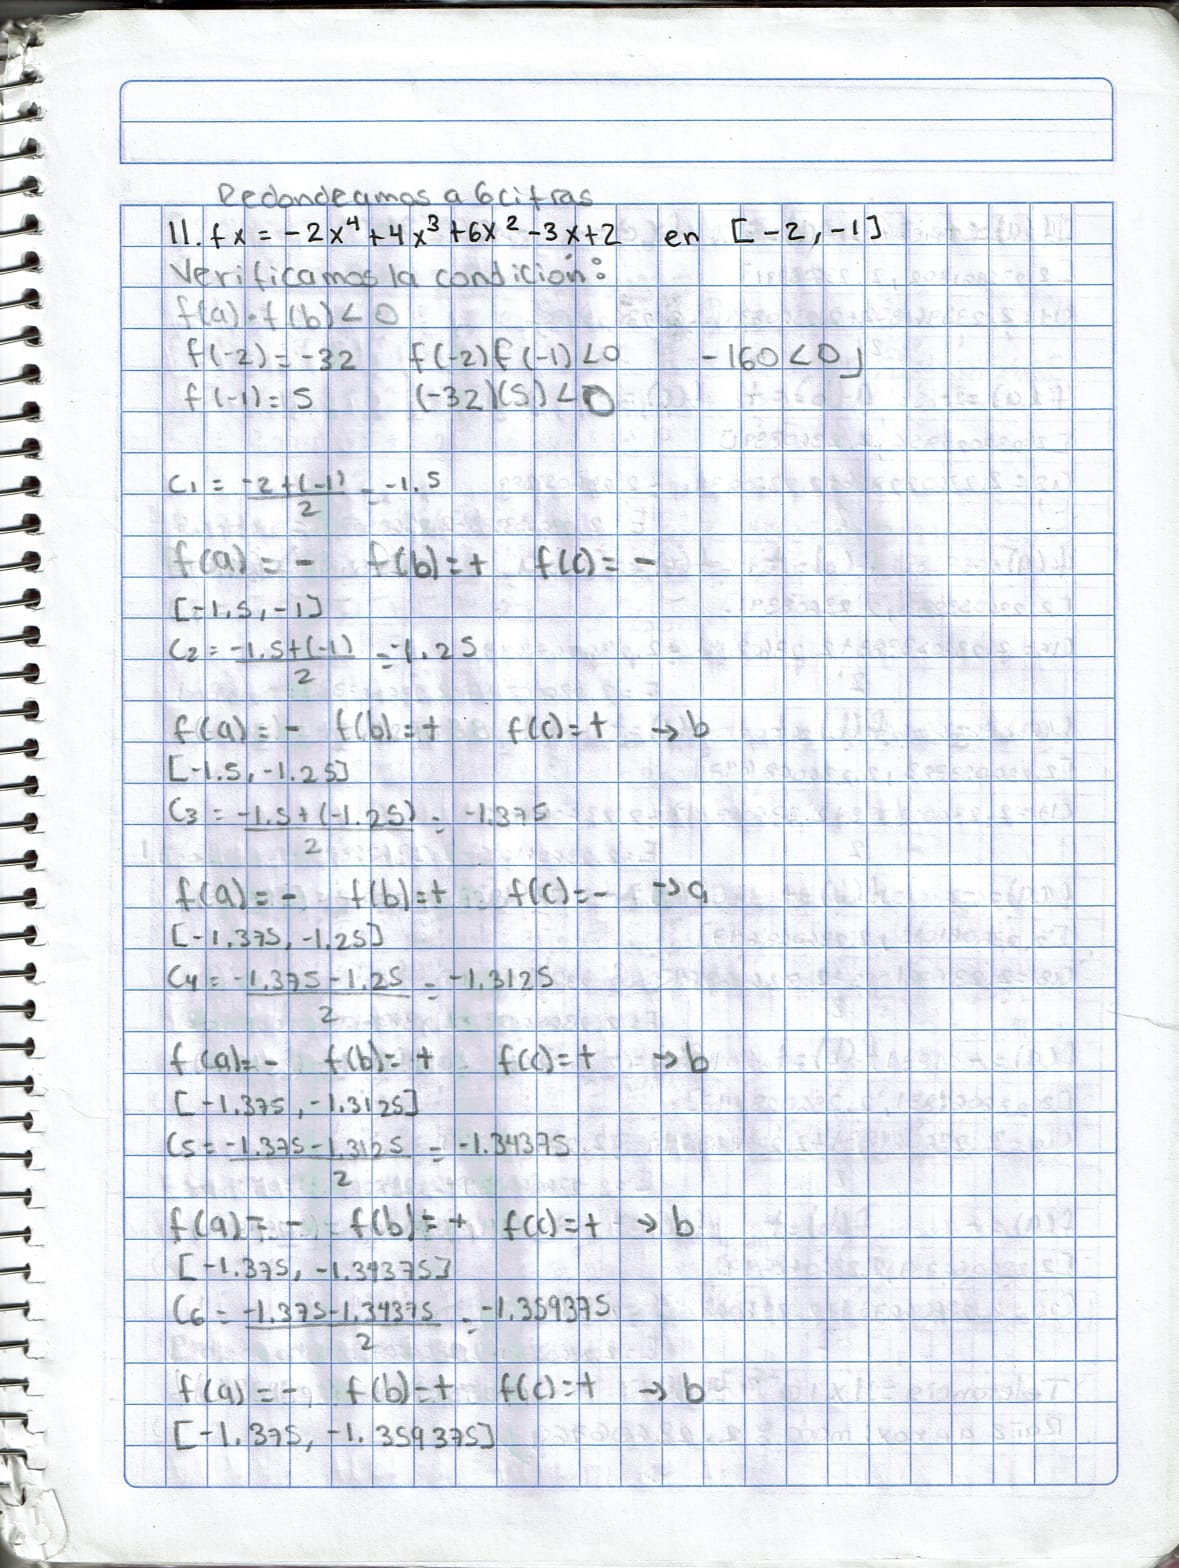
\includegraphics[width=6.25in,height=\textheight,keepaspectratio,alt={Ejercicio 11-1}]{Biseccion11_1.jpg}
\caption{Ejercicio 11-1}
\end{figure}

\begin{figure}
\centering
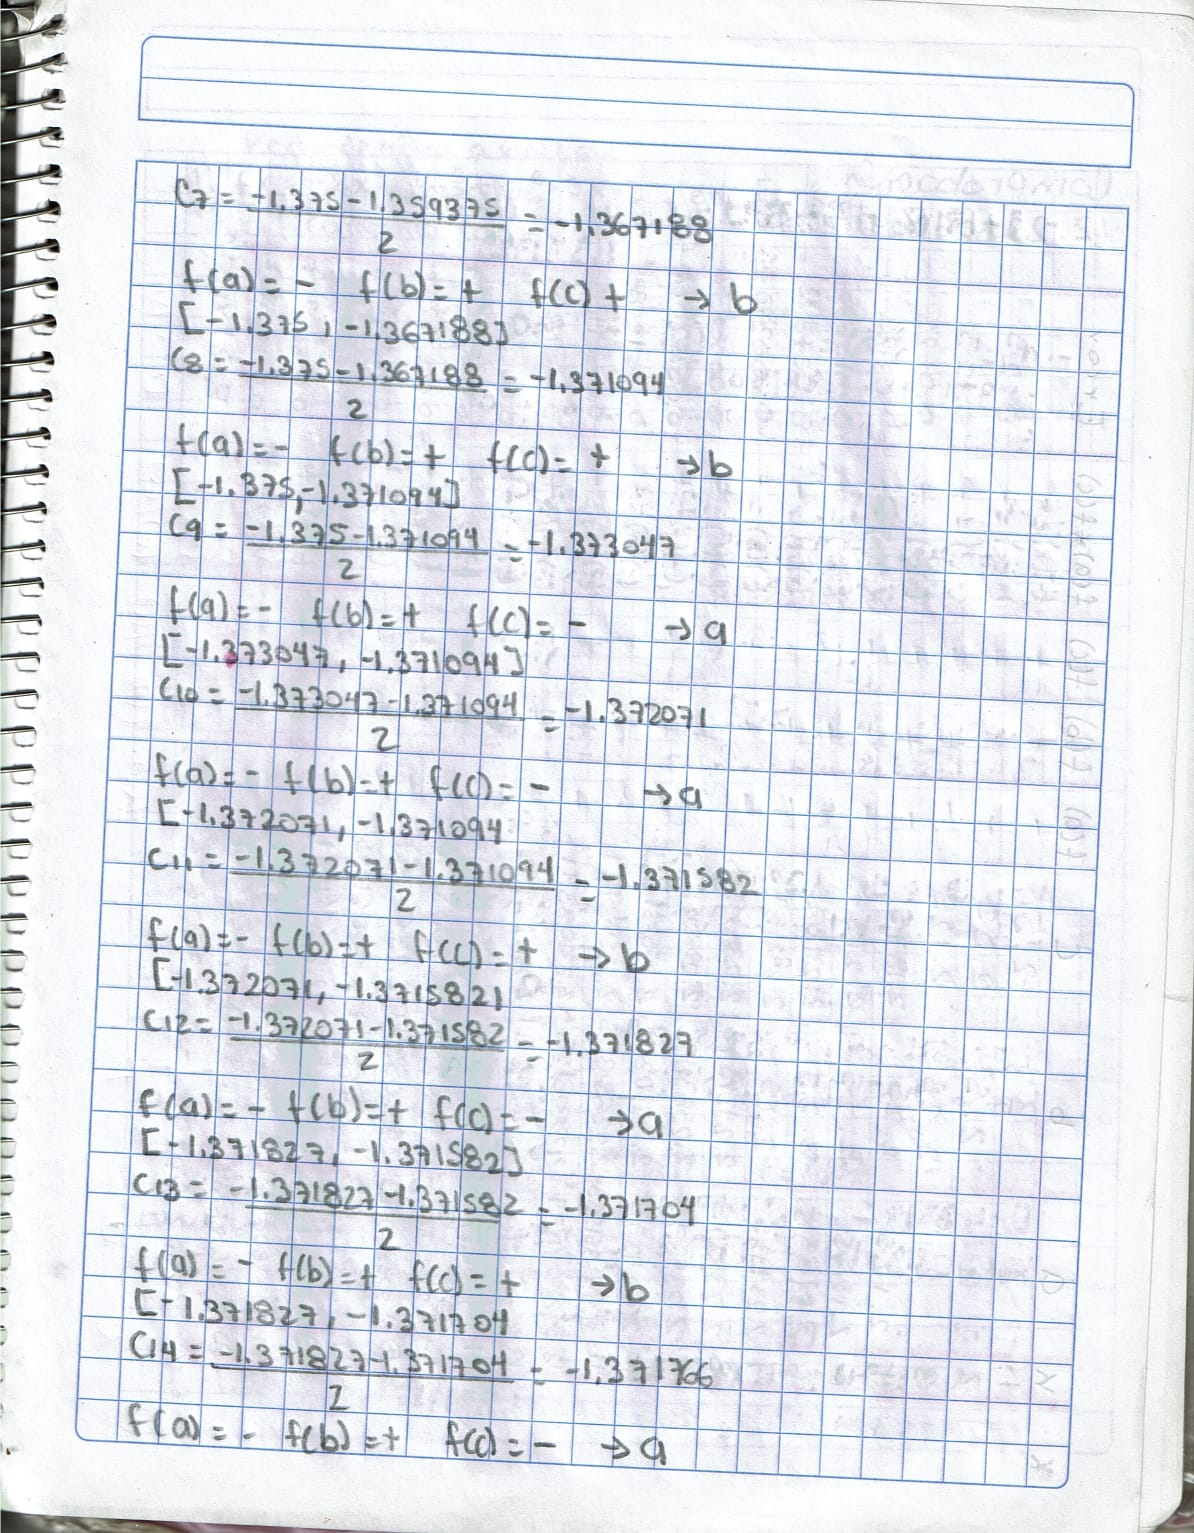
\includegraphics[width=6.25in,height=\textheight,keepaspectratio,alt={Ejercicio 11-2}]{Biseccion11_2.jpg}
\caption{Ejercicio 11-2}
\end{figure}

\begin{figure}
\centering
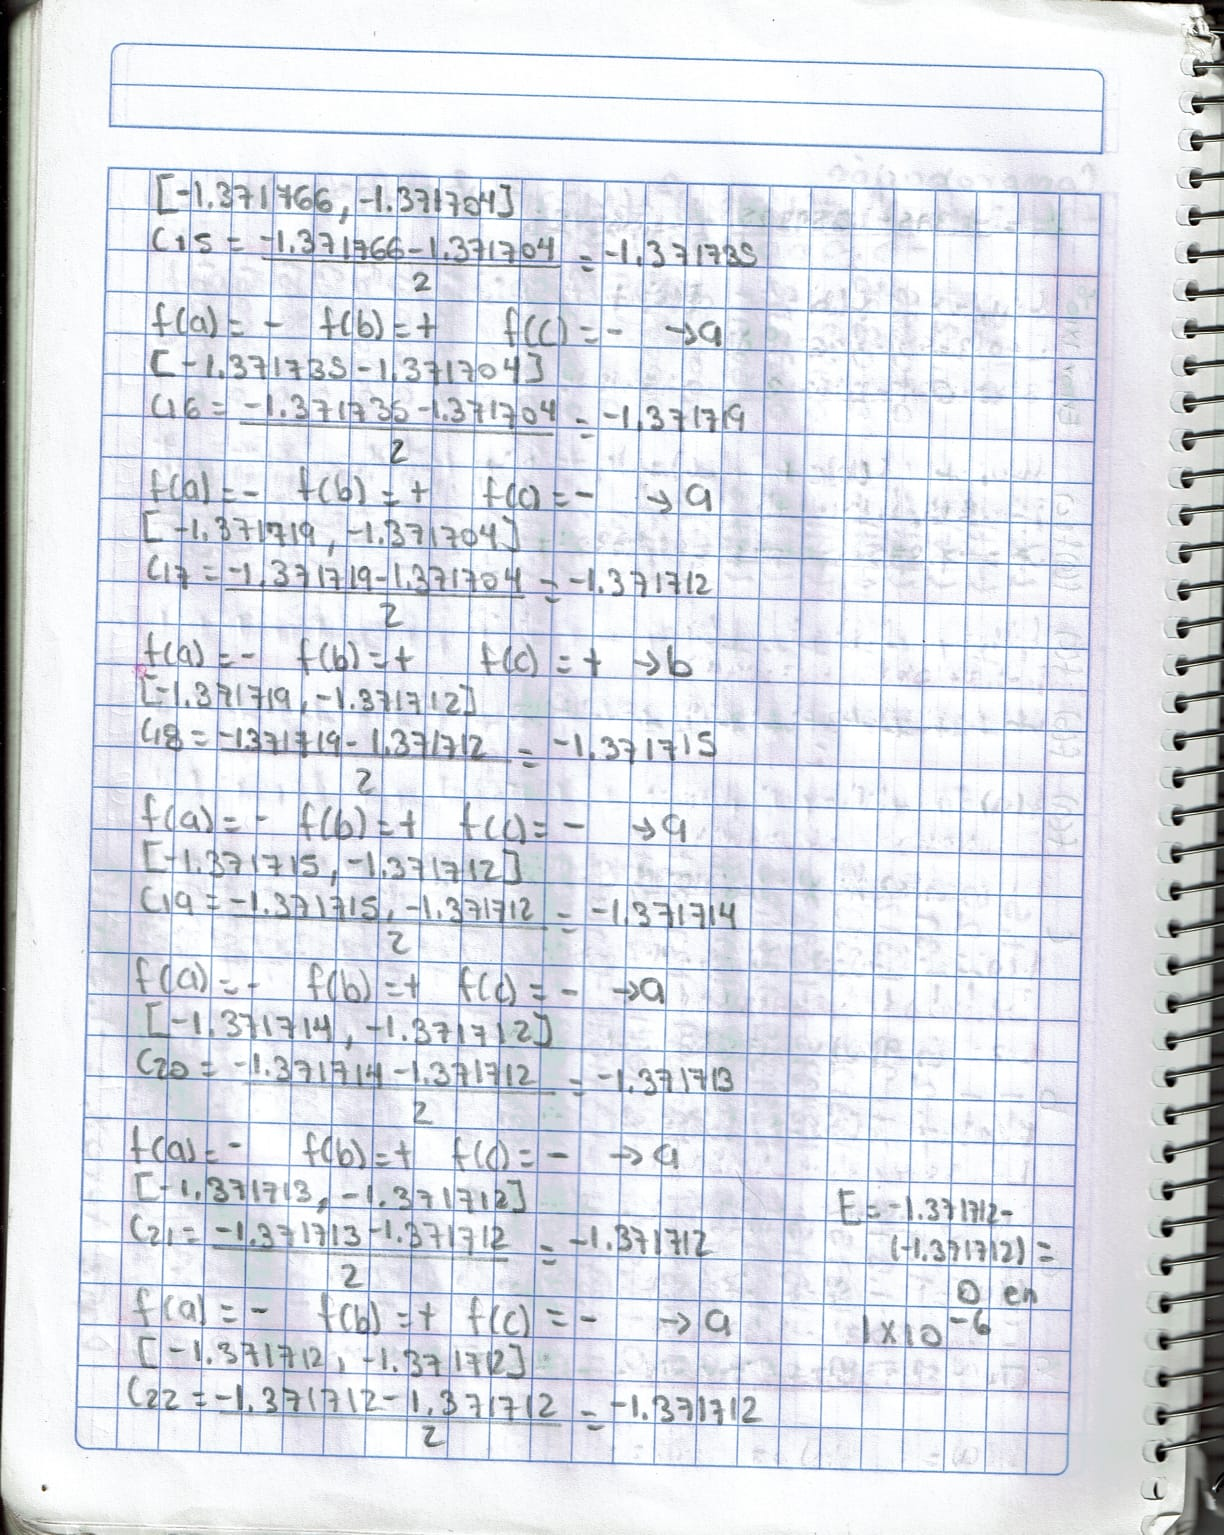
\includegraphics[width=6.25in,height=\textheight,keepaspectratio,alt={Ejercicio 11-3}]{Biseccion11_3.jpg}
\caption{Ejercicio 11-3}
\end{figure}

\begin{figure}
\centering
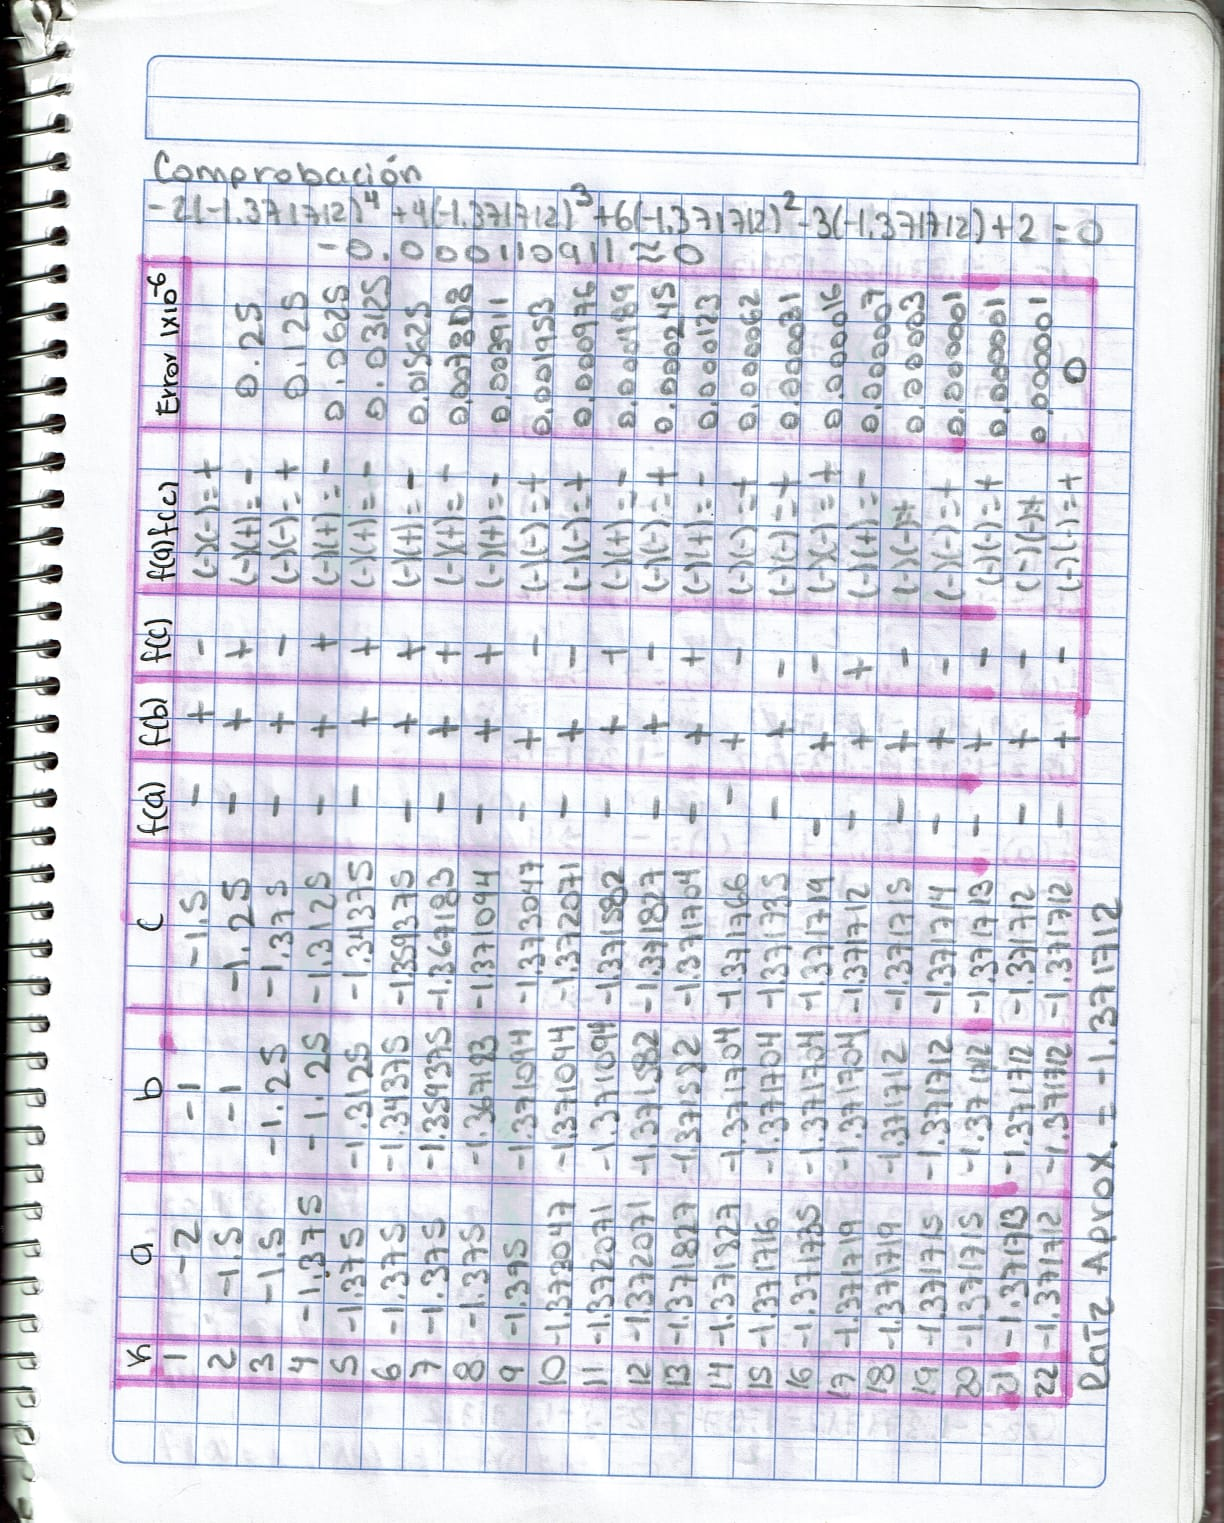
\includegraphics[width=6.25in,height=\textheight,keepaspectratio,alt={Ejercicio 11 TABLA}]{Biseccion11_4.jpg}
\caption{Ejercicio 11 TABLA}
\end{figure}

\begin{figure}
\centering
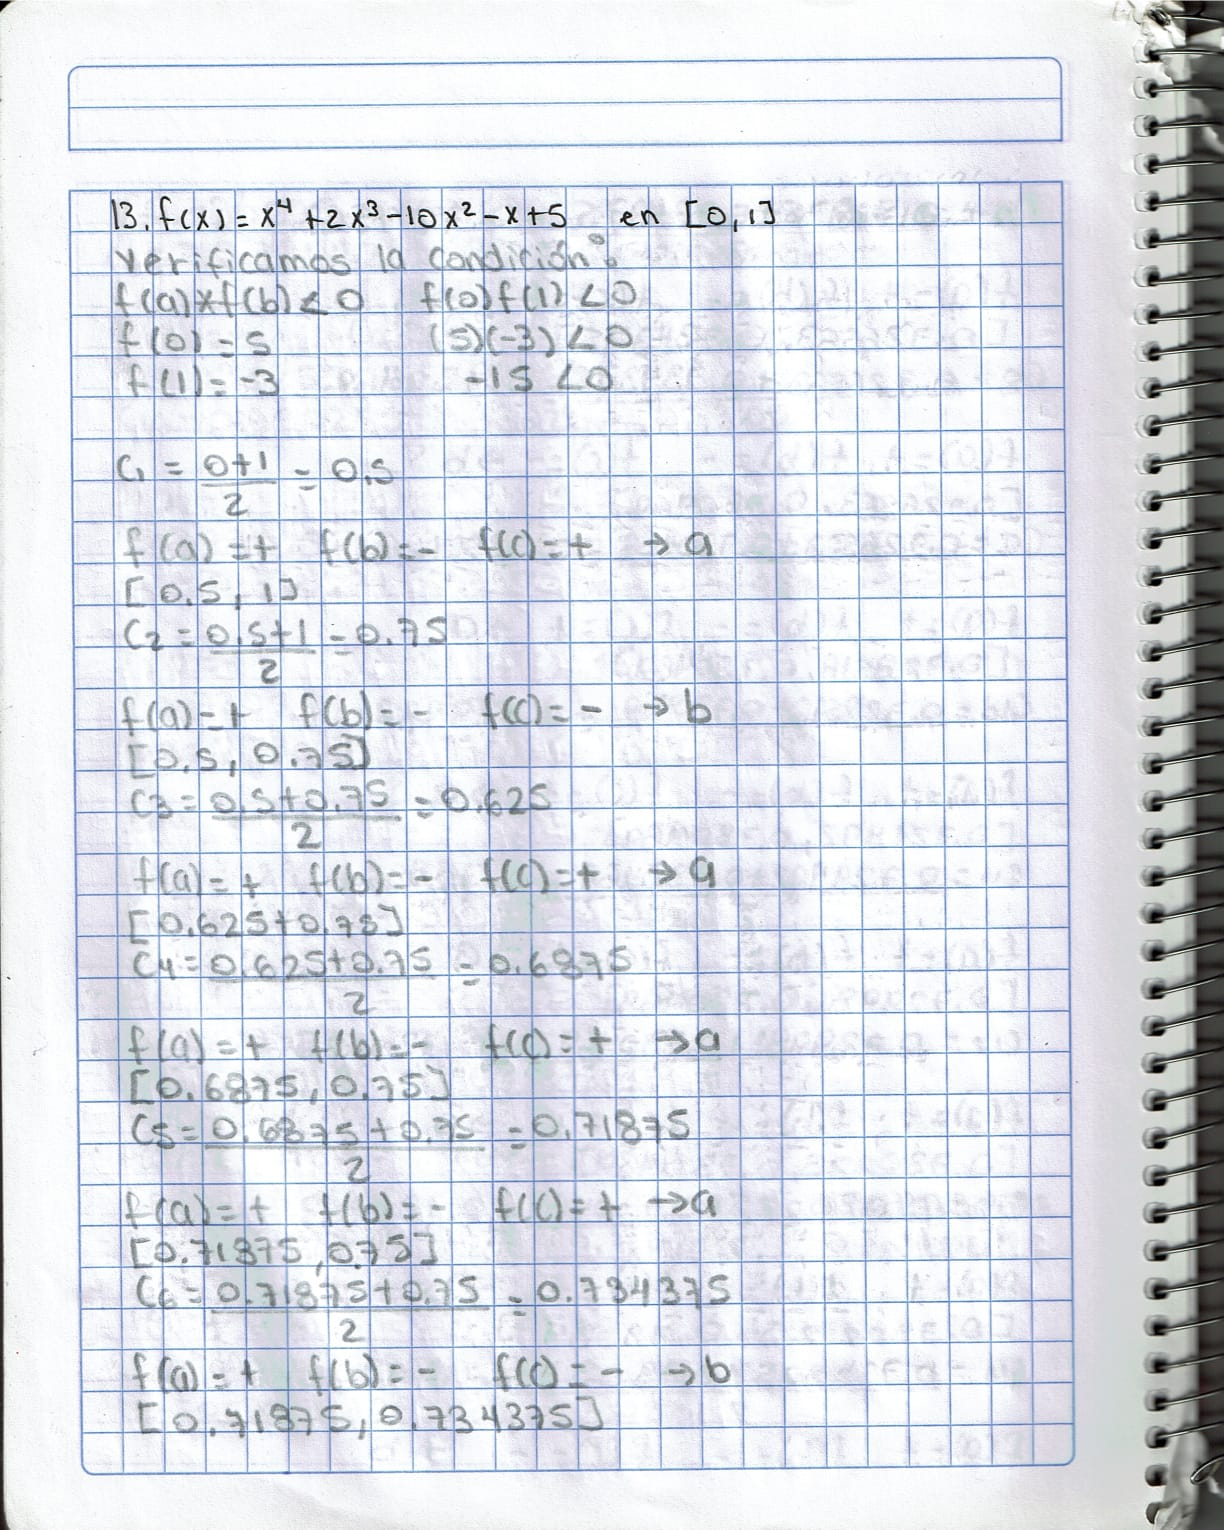
\includegraphics[width=6.25in,height=\textheight,keepaspectratio,alt={Ejercicio 13-1}]{Biseccion13_1.jpg}
\caption{Ejercicio 13-1}
\end{figure}

\begin{figure}
\centering
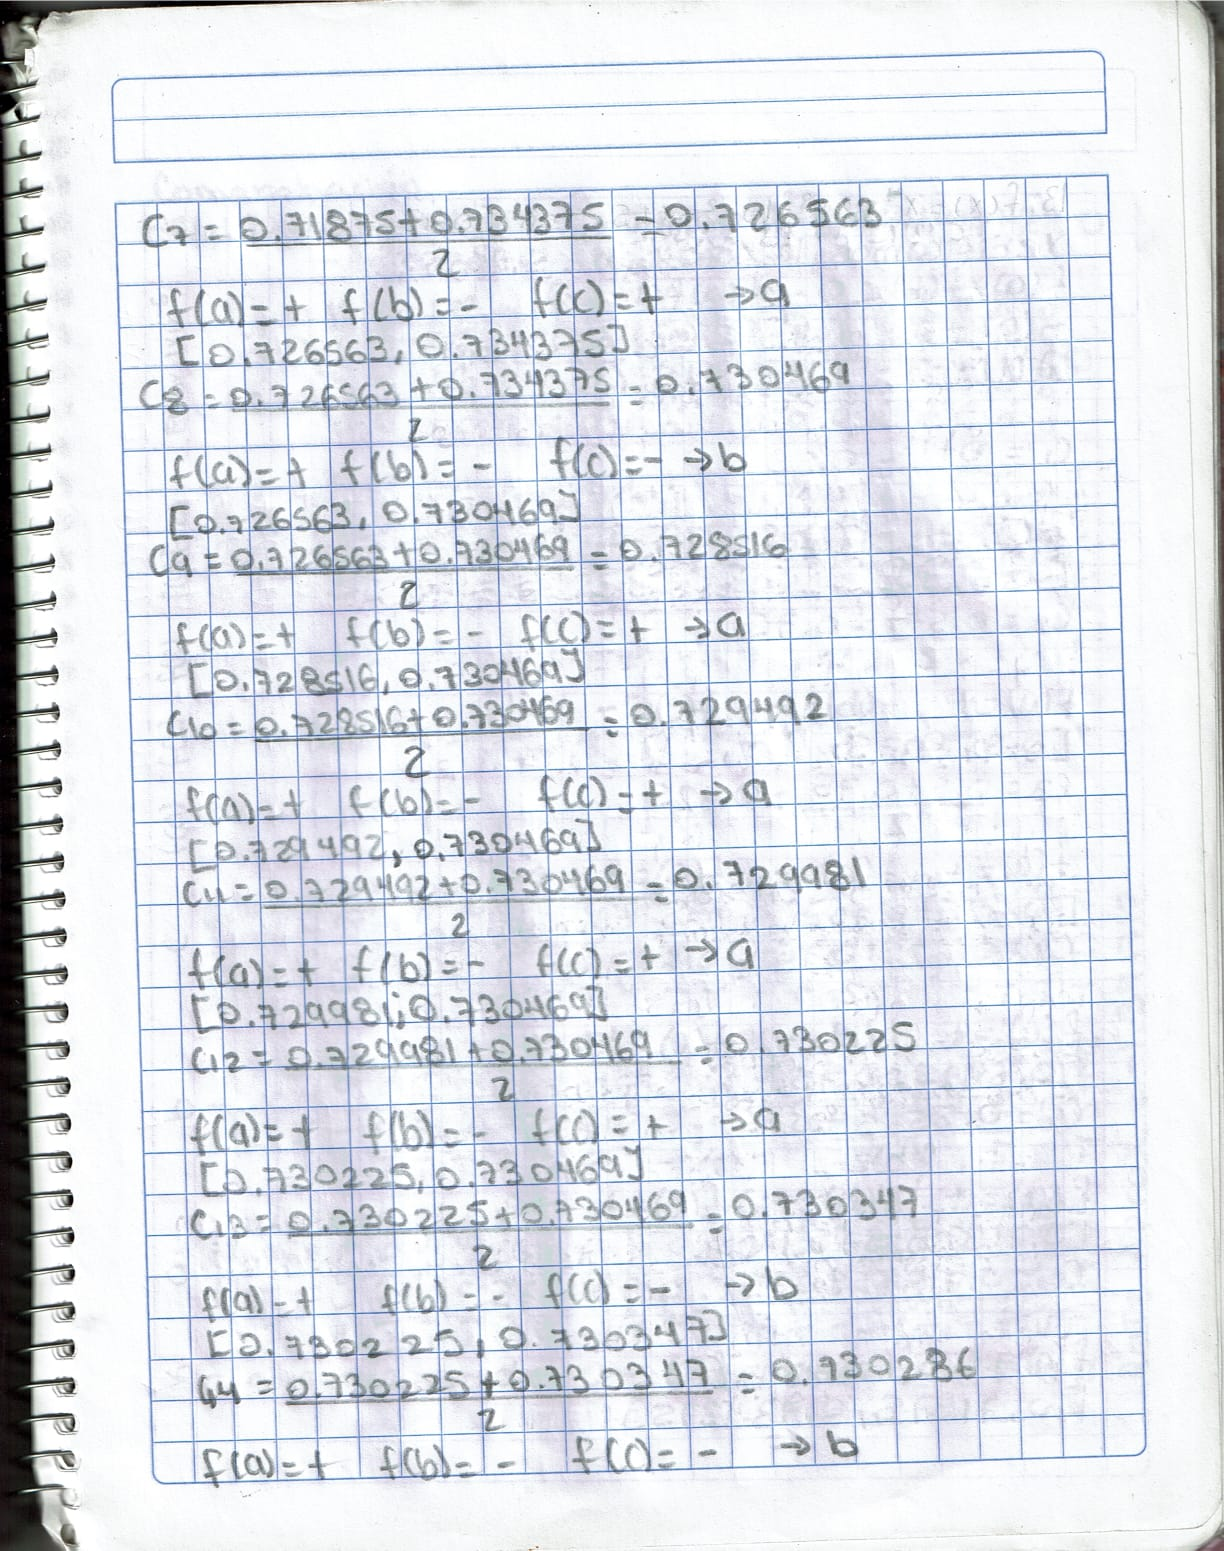
\includegraphics[width=6.25in,height=\textheight,keepaspectratio,alt={Ejercicio 13-2}]{Biseccion13_2.jpg}
\caption{Ejercicio 13-2}
\end{figure}

\begin{figure}
\centering
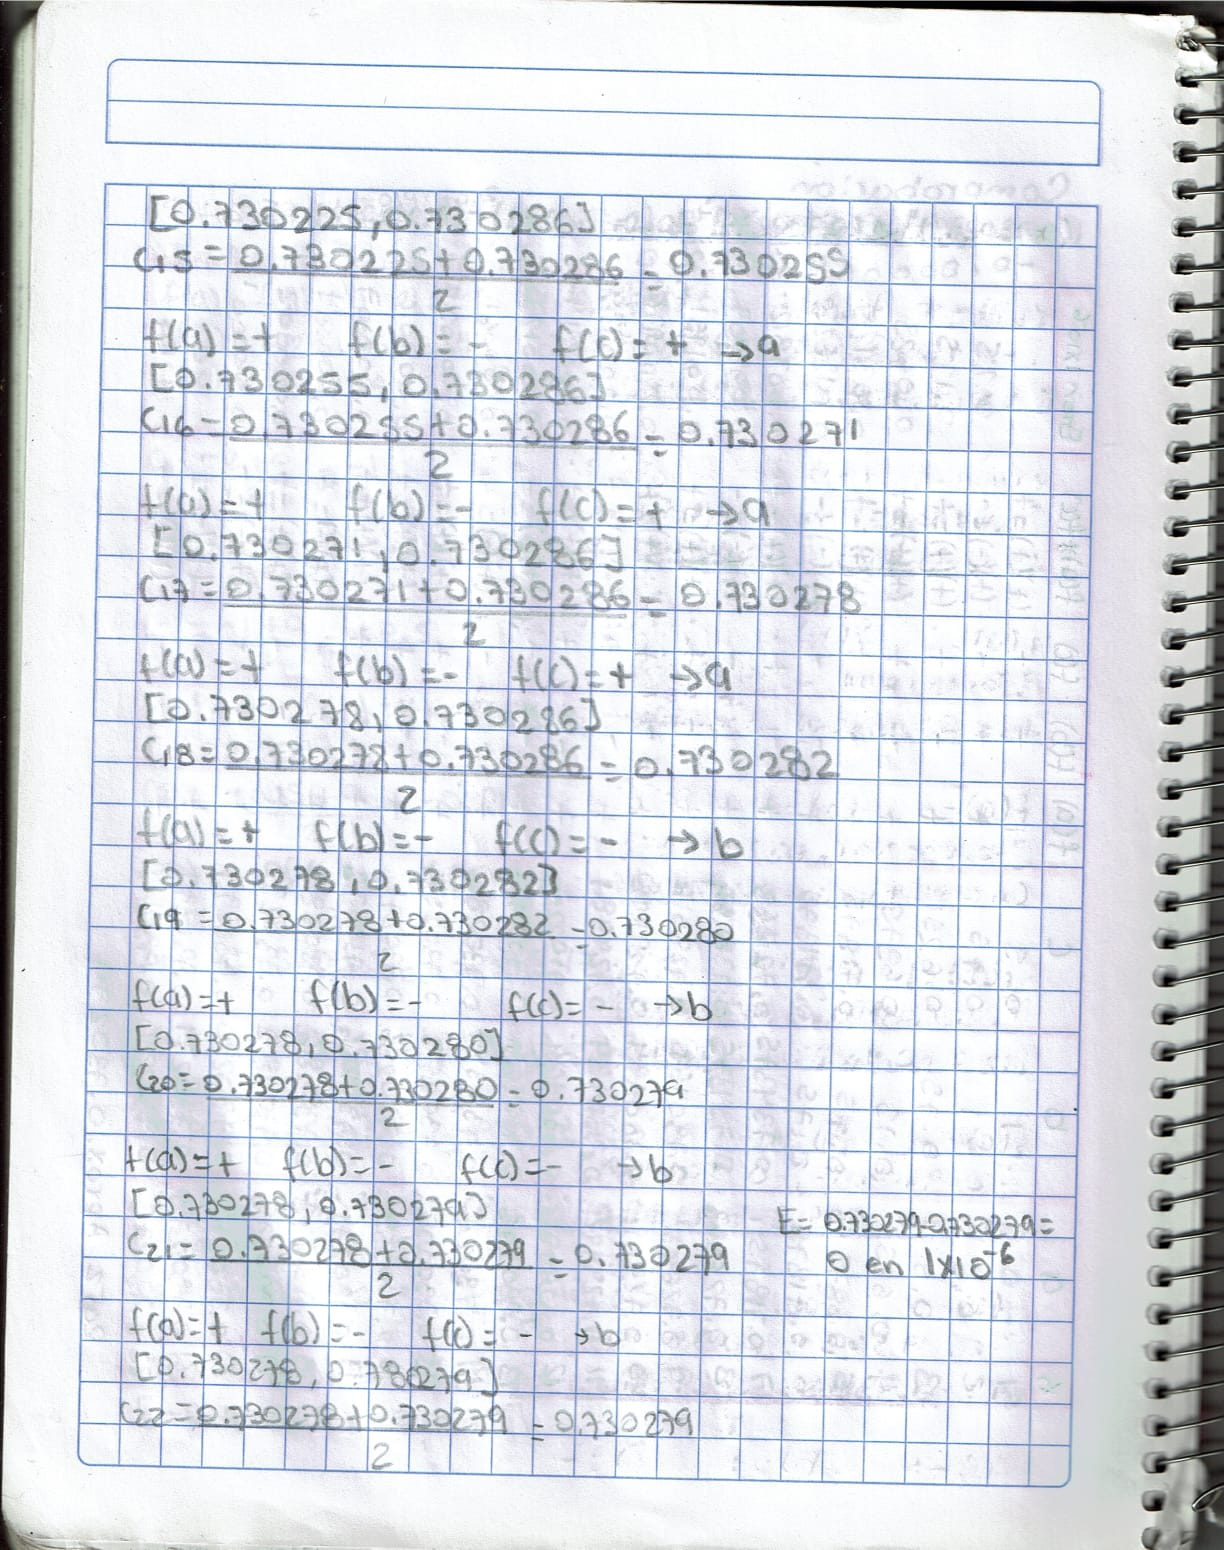
\includegraphics[width=6.25in,height=\textheight,keepaspectratio,alt={Ejercicio 13-3}]{Biseccion13_3.jpg}
\caption{Ejercicio 13-3}
\end{figure}

\begin{figure}
\centering
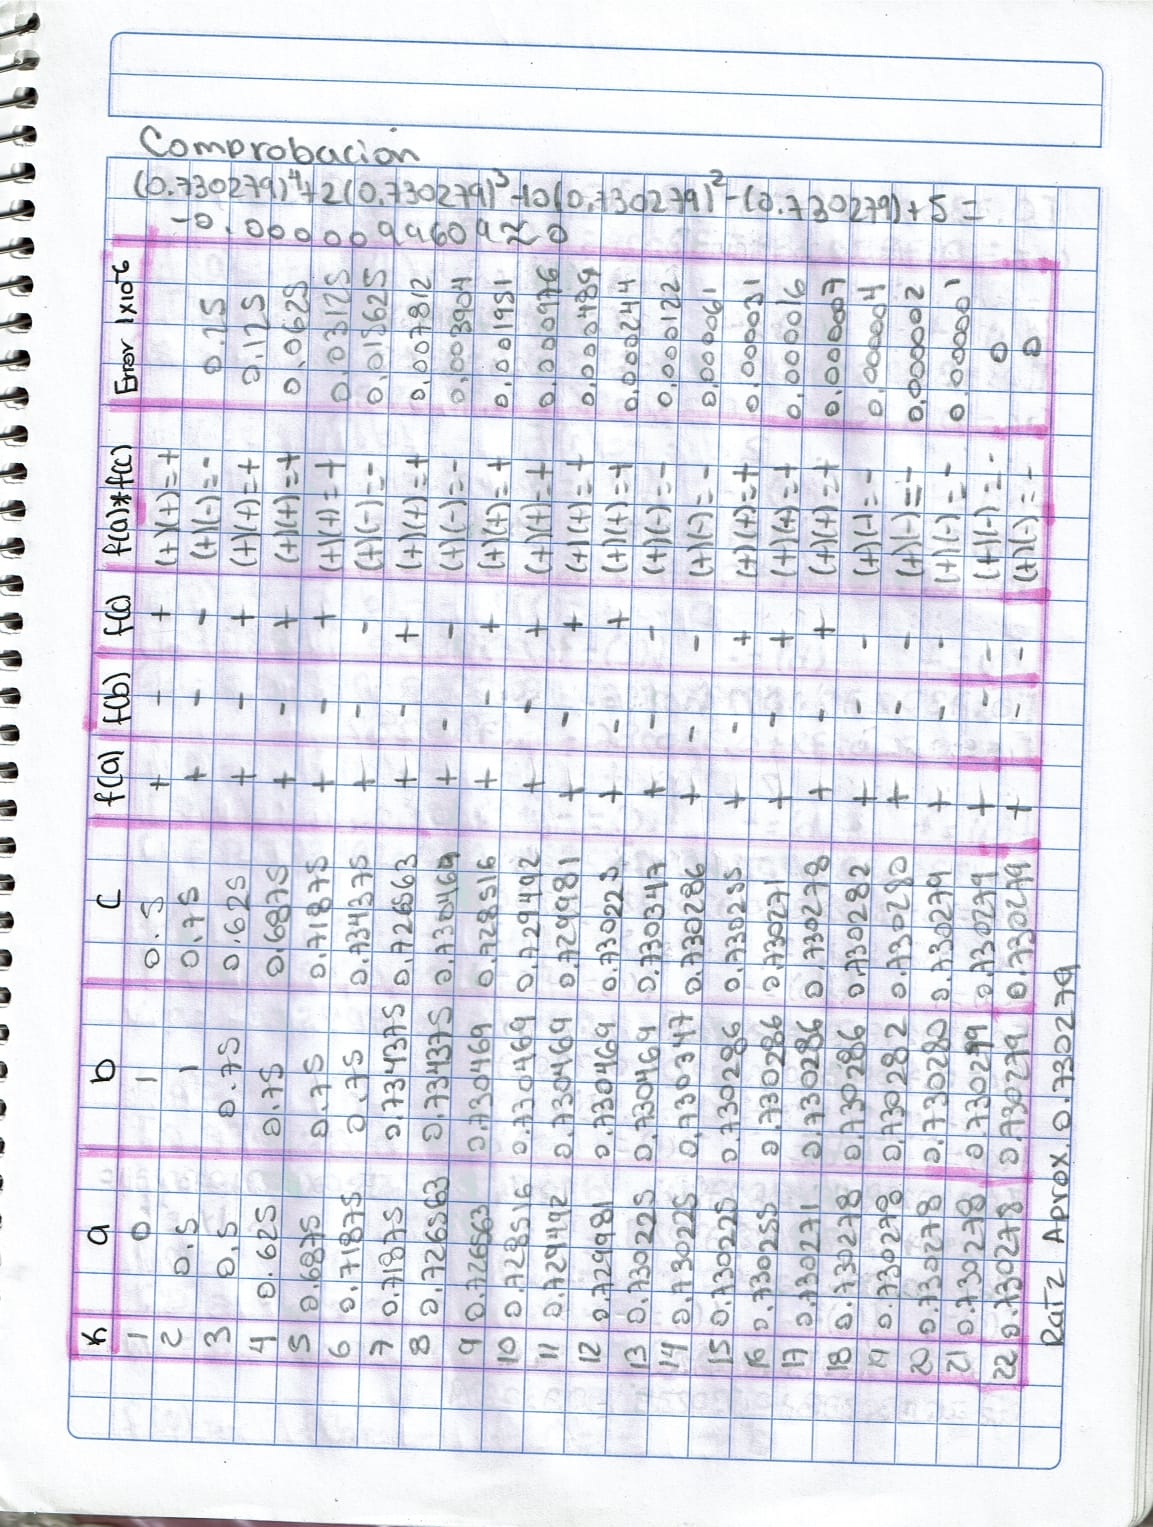
\includegraphics[width=6.25in,height=\textheight,keepaspectratio,alt={Ejercicio 13 TABLA}]{Biseccion13_4.jpg}
\caption{Ejercicio 13 TABLA}
\end{figure}

\begin{figure}
\centering
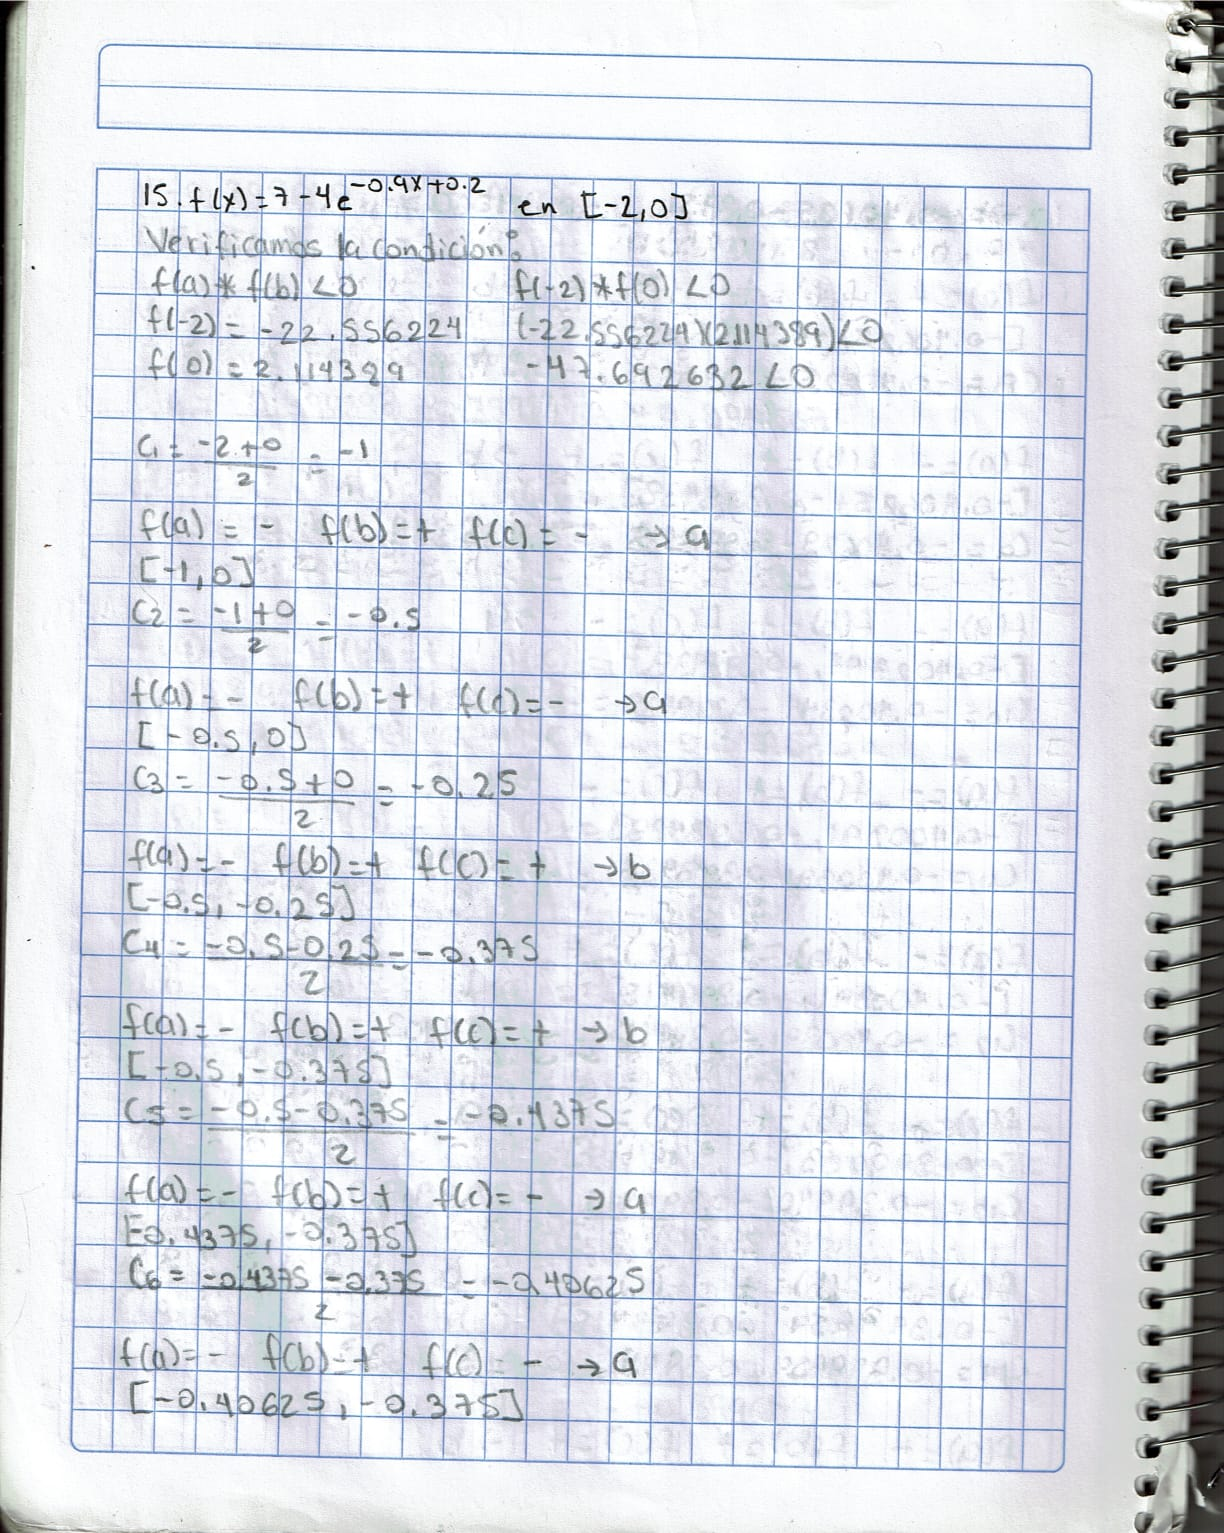
\includegraphics[width=6.25in,height=\textheight,keepaspectratio,alt={Ejercicio 15-1}]{Biseccion15_1.jpg}
\caption{Ejercicio 15-1}
\end{figure}

\begin{figure}
\centering
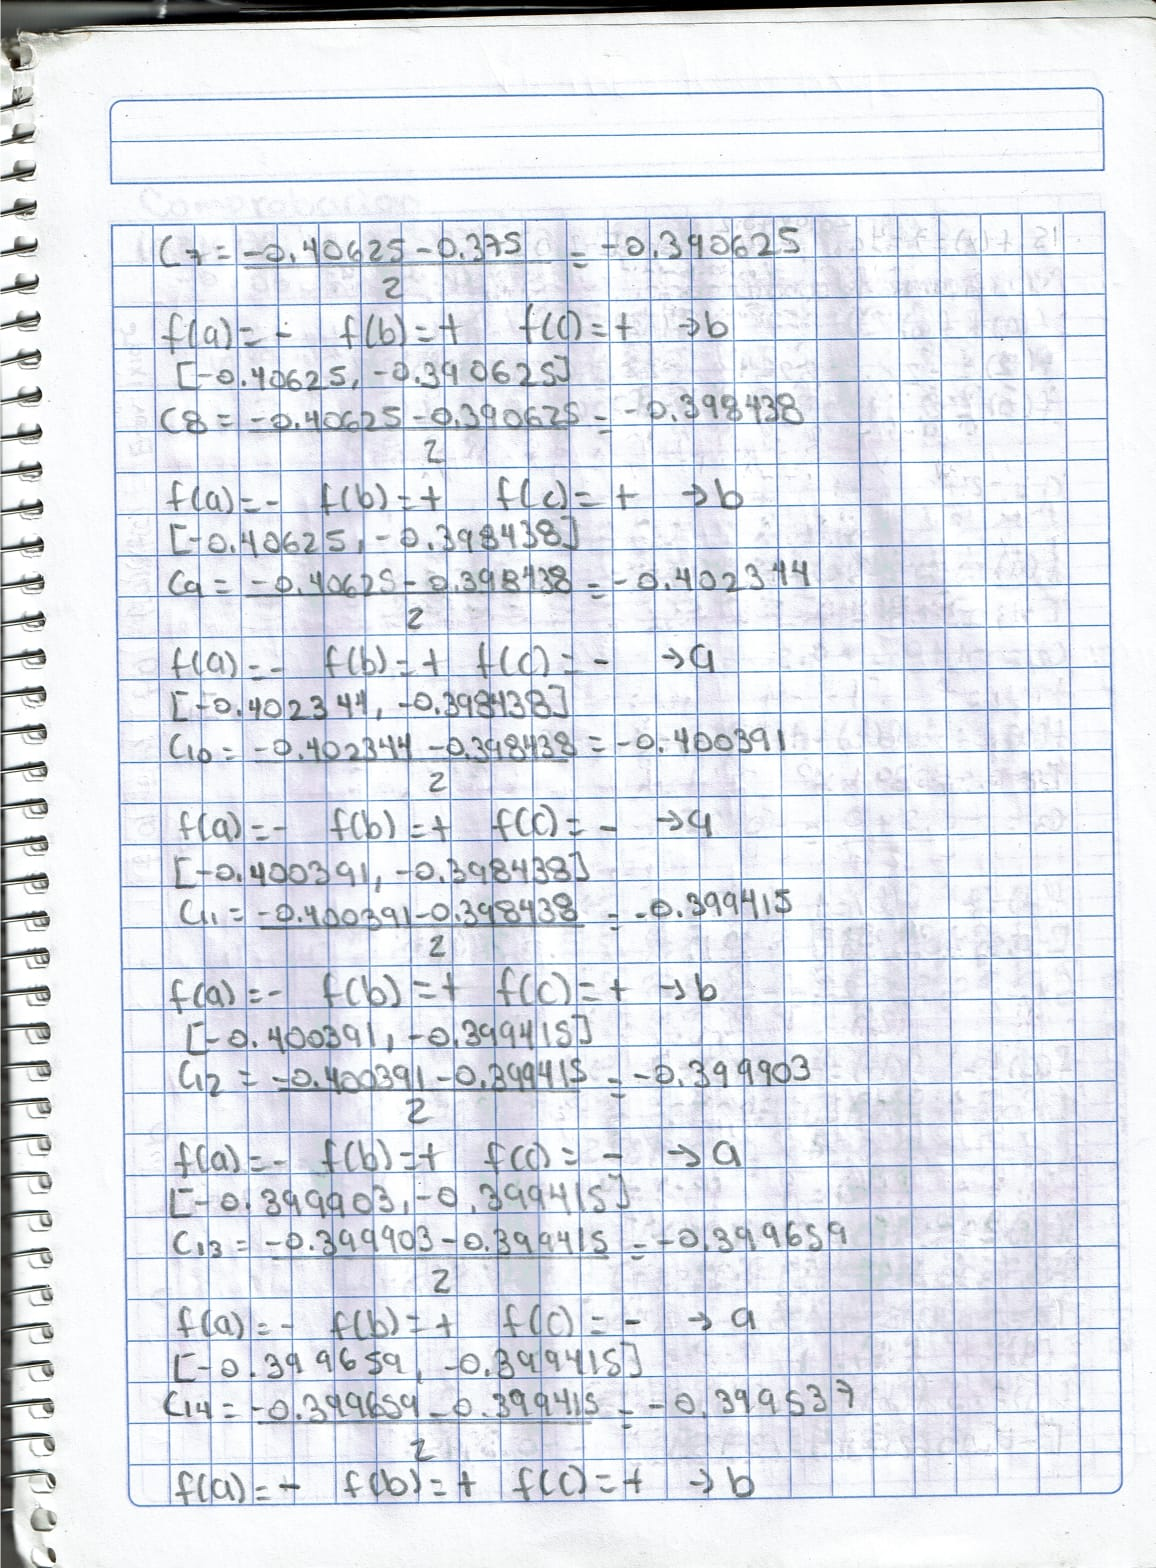
\includegraphics[width=6.25in,height=\textheight,keepaspectratio,alt={Ejercicio 15-2}]{Biseccion15_2.jpg}
\caption{Ejercicio 15-2}
\end{figure}

\begin{figure}
\centering
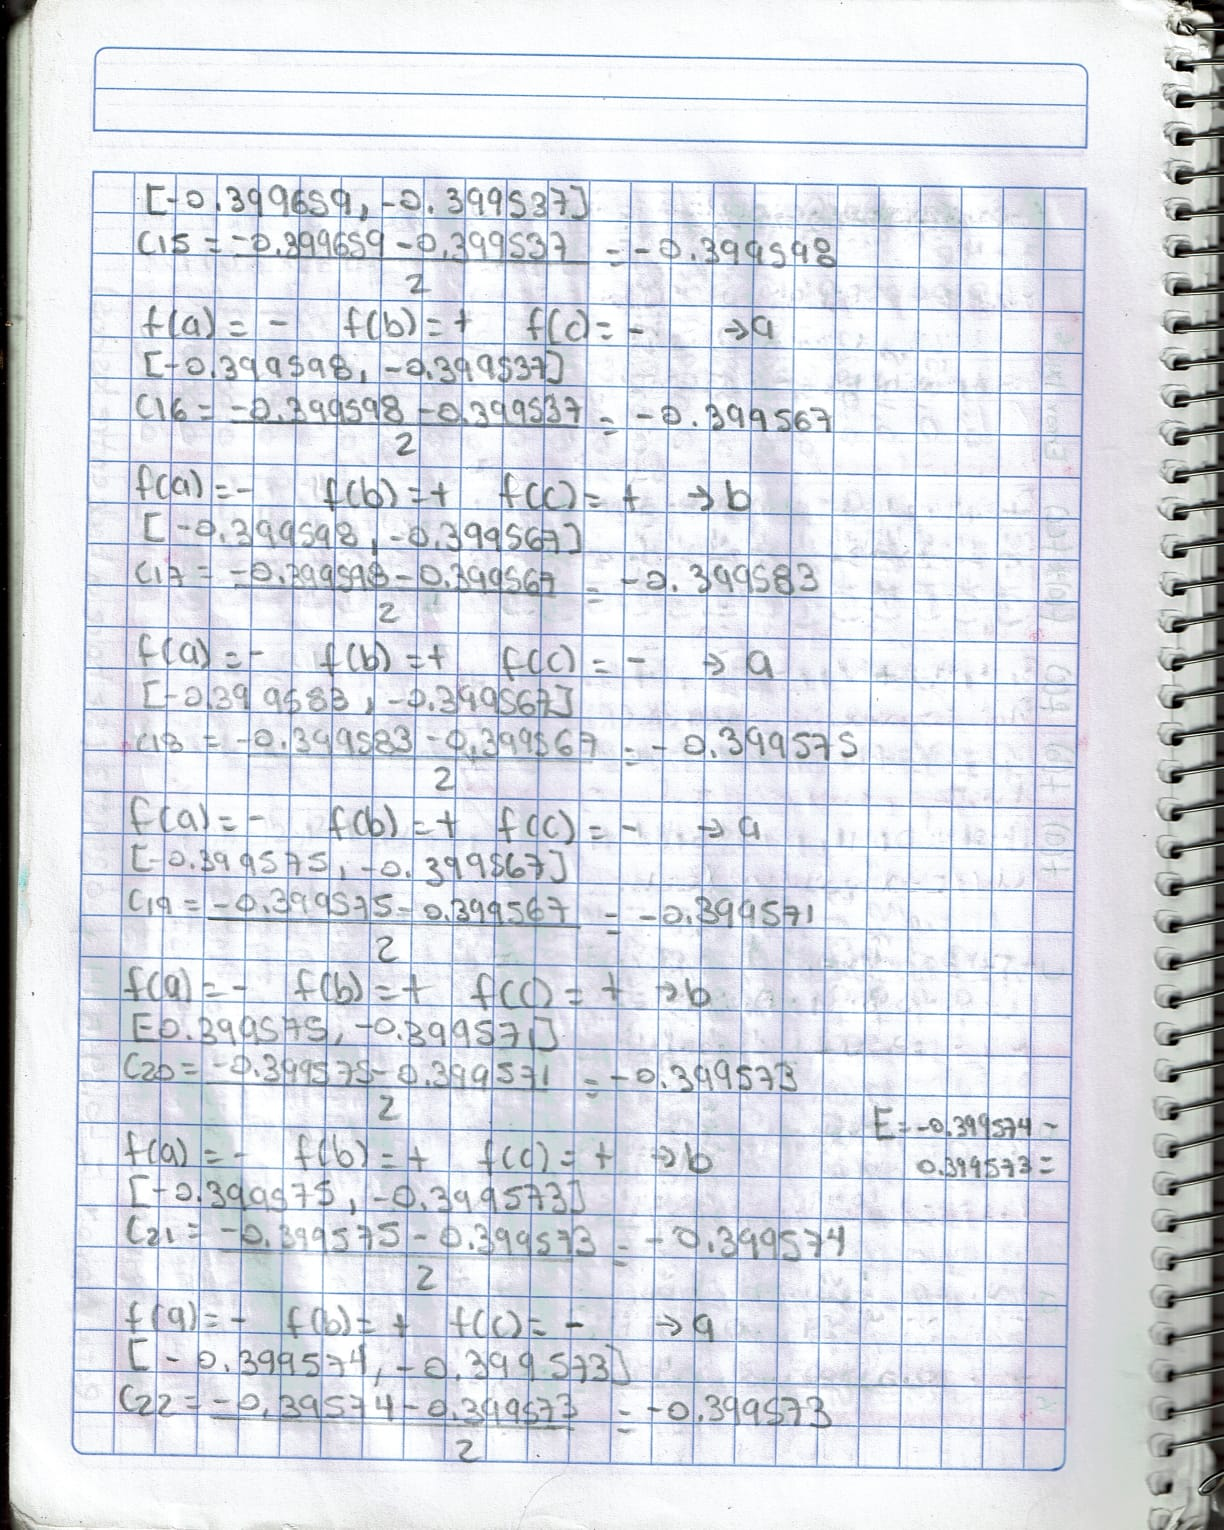
\includegraphics[width=6.25in,height=\textheight,keepaspectratio,alt={Ejercicio 15-3}]{Biseccion15_3.jpg}
\caption{Ejercicio 15-3}
\end{figure}

\begin{figure}
\centering
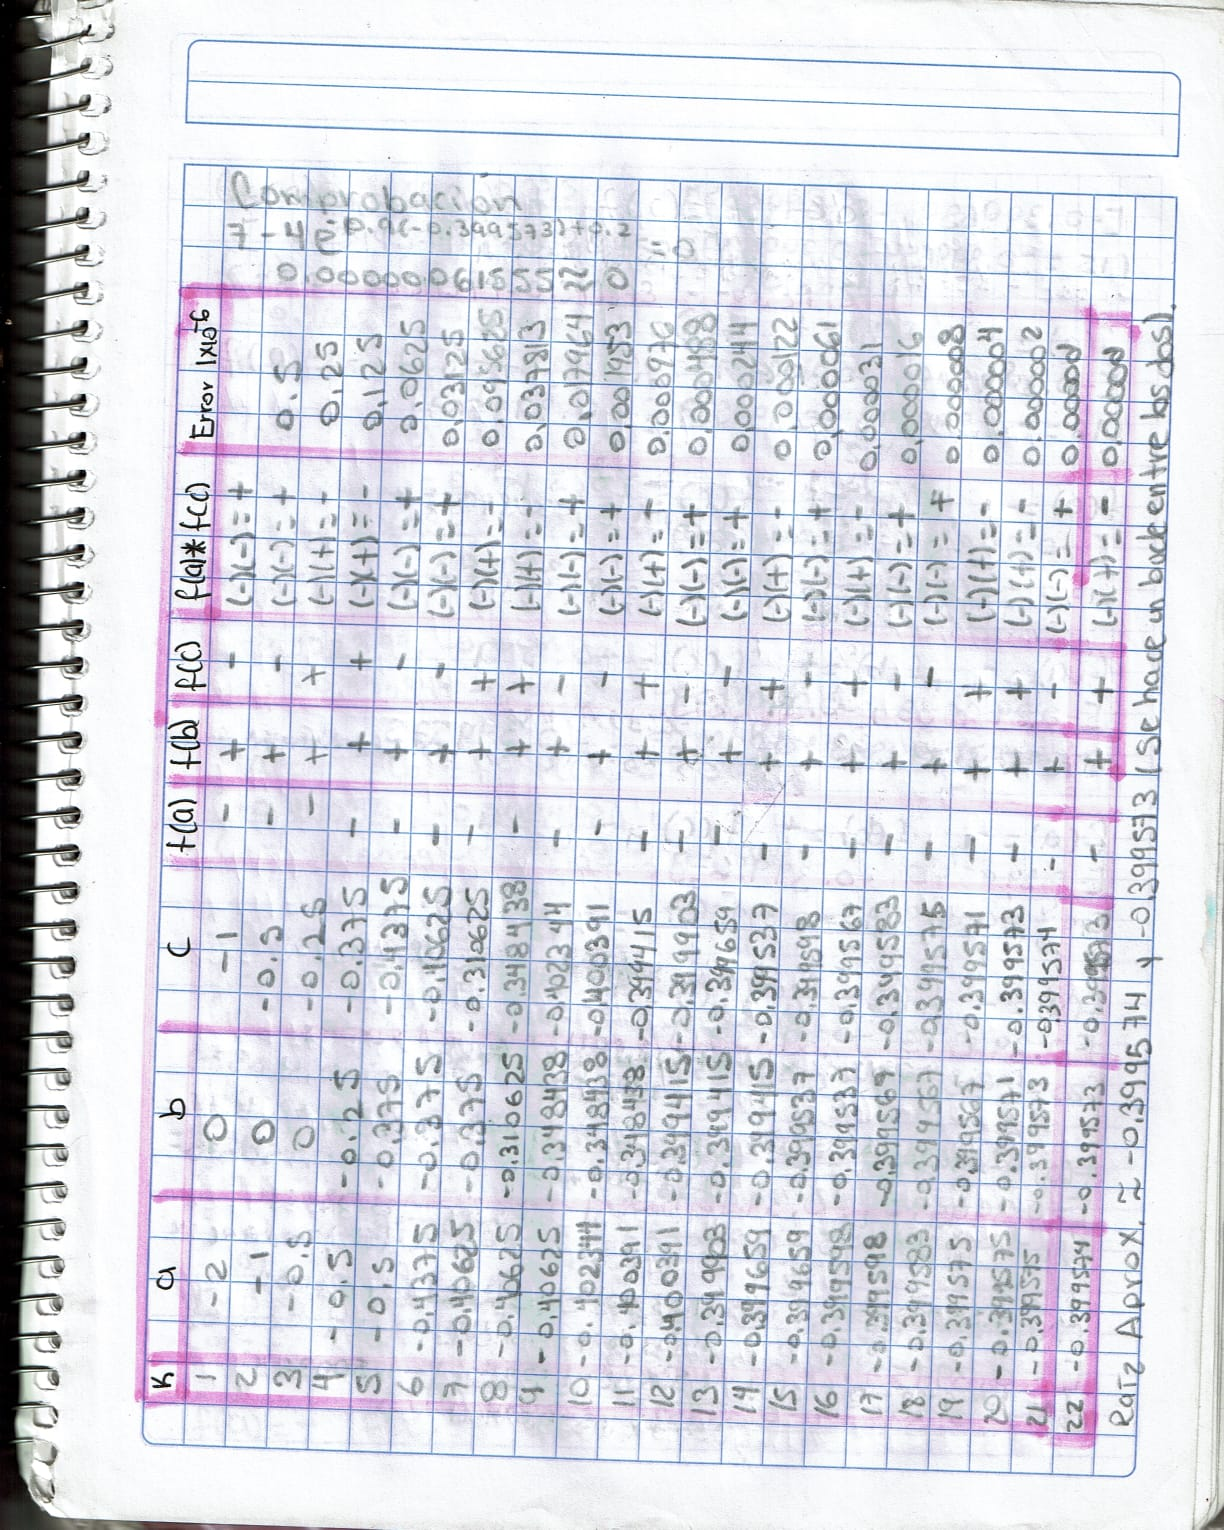
\includegraphics[width=6.25in,height=\textheight,keepaspectratio,alt={Ejercicio 15 TABLA}]{Biseccion15_4.jpg}
\caption{Ejercicio 15 TABLA}
\end{figure}

\subsubsection{Código para
implementación}\label{cuxf3digo-para-implementaciuxf3n}

\begin{Shaded}
\begin{Highlighting}[]
\CommentTok{\# Condición para los intervalos}

\NormalTok{condicion }\OtherTok{\textless{}{-}} \ControlFlowTok{function}\NormalTok{(a, b, f, }\AttributeTok{inicio =} \DecValTok{1}\NormalTok{, }\AttributeTok{fin =} \DecValTok{10}\NormalTok{, }\AttributeTok{paso =} \DecValTok{1}\NormalTok{) \{}
\NormalTok{  fa }\OtherTok{\textless{}{-}} \FunctionTok{f}\NormalTok{(a)}
\NormalTok{  fb }\OtherTok{\textless{}{-}} \FunctionTok{f}\NormalTok{(b)}
\NormalTok{  producto }\OtherTok{\textless{}{-}}\NormalTok{ fa }\SpecialCharTok{*}\NormalTok{ fb}
  
  \CommentTok{\# Resultados}
  \FunctionTok{cat}\NormalTok{(}\StringTok{"f(a) = f("}\NormalTok{, a, }\StringTok{") = "}\NormalTok{, fa, }\StringTok{"}\SpecialCharTok{\textbackslash{}n}\StringTok{"}\NormalTok{)}
  \FunctionTok{cat}\NormalTok{(}\StringTok{"f(b) = f("}\NormalTok{, b, }\StringTok{") = "}\NormalTok{, fb, }\StringTok{"}\SpecialCharTok{\textbackslash{}n}\StringTok{"}\NormalTok{)}
  \FunctionTok{cat}\NormalTok{(}\StringTok{"f(a) · f(b) = "}\NormalTok{, producto, }\StringTok{"}\SpecialCharTok{\textbackslash{}n}\StringTok{"}\NormalTok{)}
  \FunctionTok{cat}\NormalTok{(producto, }\StringTok{"\textless{} 0"}\NormalTok{, }\StringTok{"}\SpecialCharTok{\textbackslash{}n\textbackslash{}n}\StringTok{"}\NormalTok{)}
  
  \ControlFlowTok{if}\NormalTok{(producto }\SpecialCharTok{\textless{}} \DecValTok{0}\NormalTok{) \{}
    \FunctionTok{cat}\NormalTok{(}\StringTok{"SÍ cumple la condición.}\SpecialCharTok{\textbackslash{}n}\StringTok{"}\NormalTok{)}
    \CommentTok{\# Asignar globalmente}
\NormalTok{    a }\OtherTok{\textless{}\textless{}{-}}\NormalTok{ a}
\NormalTok{    b }\OtherTok{\textless{}\textless{}{-}}\NormalTok{ b}
    \FunctionTok{return}\NormalTok{(}\ConstantTok{TRUE}\NormalTok{)}
\NormalTok{  \} }\ControlFlowTok{else}\NormalTok{ \{}
    \FunctionTok{cat}\NormalTok{(}\StringTok{"NO cumple la condición.}\SpecialCharTok{\textbackslash{}n}\StringTok{"}\NormalTok{) }
    \FunctionTok{cat}\NormalTok{(}\StringTok{"Se buscará un nuevo intervalo.}\SpecialCharTok{\textbackslash{}n\textbackslash{}n}\StringTok{"}\NormalTok{)}
    
    \CommentTok{\# Buscar automáticamente un intervalo que sí funcione}
\NormalTok{    x }\OtherTok{\textless{}{-}} \FunctionTok{seq}\NormalTok{(inicio, fin, paso)}
    \ControlFlowTok{for}\NormalTok{ (i }\ControlFlowTok{in} \DecValTok{1}\SpecialCharTok{:}\NormalTok{(}\FunctionTok{length}\NormalTok{(x)}\SpecialCharTok{{-}}\DecValTok{1}\NormalTok{)) \{}
\NormalTok{      a\_nuevo }\OtherTok{\textless{}{-}}\NormalTok{ x[i]}
\NormalTok{      b\_nuevo }\OtherTok{\textless{}{-}}\NormalTok{ x[i}\SpecialCharTok{+}\DecValTok{1}\NormalTok{]}
      \ControlFlowTok{if}\NormalTok{ (}\FunctionTok{f}\NormalTok{(a\_nuevo) }\SpecialCharTok{*} \FunctionTok{f}\NormalTok{(b\_nuevo) }\SpecialCharTok{\textless{}} \DecValTok{0}\NormalTok{) \{}
        \FunctionTok{cat}\NormalTok{(}\StringTok{"Nuevo intervalo encontrado: ["}\NormalTok{, a\_nuevo, }\StringTok{", "}\NormalTok{, b\_nuevo, }\StringTok{"]}\SpecialCharTok{\textbackslash{}n}\StringTok{"}\NormalTok{)}
\NormalTok{        fa }\OtherTok{\textless{}{-}} \FunctionTok{f}\NormalTok{(a\_nuevo)}
\NormalTok{        fb }\OtherTok{\textless{}{-}} \FunctionTok{f}\NormalTok{(b\_nuevo)}
\NormalTok{        producto }\OtherTok{\textless{}{-}}\NormalTok{ fa }\SpecialCharTok{*}\NormalTok{ fb}
        \FunctionTok{cat}\NormalTok{(}\StringTok{"f(a) = f("}\NormalTok{, a\_nuevo, }\StringTok{") = "}\NormalTok{, fa, }\StringTok{"}\SpecialCharTok{\textbackslash{}n}\StringTok{"}\NormalTok{)}
        \FunctionTok{cat}\NormalTok{(}\StringTok{"f(b) = f("}\NormalTok{, b\_nuevo, }\StringTok{") = "}\NormalTok{, fb, }\StringTok{"}\SpecialCharTok{\textbackslash{}n}\StringTok{"}\NormalTok{)}
        \FunctionTok{cat}\NormalTok{(}\StringTok{"f(a) · f(b) = "}\NormalTok{, producto, }\StringTok{"}\SpecialCharTok{\textbackslash{}n}\StringTok{"}\NormalTok{)}
        \FunctionTok{cat}\NormalTok{(producto, }\StringTok{"\textless{} 0"}\NormalTok{, }\StringTok{"}\SpecialCharTok{\textbackslash{}n\textbackslash{}n}\StringTok{"}\NormalTok{)}
          \FunctionTok{cat}\NormalTok{(}\StringTok{"SÍ cumple la condición.}\SpecialCharTok{\textbackslash{}n}\StringTok{"}\NormalTok{)}
        \CommentTok{\# Asignar globalmente}
\NormalTok{        a }\OtherTok{\textless{}\textless{}{-}}\NormalTok{ a\_nuevo}
\NormalTok{        b }\OtherTok{\textless{}\textless{}{-}}\NormalTok{ b\_nuevo}
        \FunctionTok{return}\NormalTok{(}\ConstantTok{TRUE}\NormalTok{)}
\NormalTok{      \}}
\NormalTok{    \}}
    \FunctionTok{cat}\NormalTok{(}\StringTok{"No se encontró ningún intervalo con cambio de signo}\SpecialCharTok{\textbackslash{}n}\StringTok{"}\NormalTok{)}
    \FunctionTok{return}\NormalTok{(}\ConstantTok{FALSE}\NormalTok{)}
\NormalTok{  \}}
\NormalTok{\}}
\end{Highlighting}
\end{Shaded}

\begin{Shaded}
\begin{Highlighting}[]
\CommentTok{\# Método de Bisección que guarda los valores para la tabla}

\NormalTok{biseccion }\OtherTok{\textless{}{-}} \ControlFlowTok{function}\NormalTok{(f, a, b, }\AttributeTok{tol =} \FloatTok{1e{-}5}\NormalTok{, }\AttributeTok{iter\_max =} \DecValTok{100}\NormalTok{)\{}
  \ControlFlowTok{if}\NormalTok{(}\FunctionTok{f}\NormalTok{(a)}\SpecialCharTok{*}\FunctionTok{f}\NormalTok{(b) }\SpecialCharTok{\textgreater{}} \DecValTok{0}\NormalTok{)\{}
    \FunctionTok{cat}\NormalTok{(}\StringTok{"Error: no hay cambio de signo en el intervalo [a,b].}\SpecialCharTok{\textbackslash{}n}\StringTok{"}\NormalTok{)}
    \FunctionTok{return}\NormalTok{(}\ConstantTok{NA}\NormalTok{)}
\NormalTok{  \}}
  
  \DocumentationTok{\#\# Vectores para almacenar los datos de las iteraciones}
  
\NormalTok{  iter\_vec }\OtherTok{\textless{}{-}} \FunctionTok{numeric}\NormalTok{(}\DecValTok{0}\NormalTok{)}
\NormalTok{  a\_vec }\OtherTok{\textless{}{-}} \FunctionTok{numeric}\NormalTok{(}\DecValTok{0}\NormalTok{)}
\NormalTok{  b\_vec }\OtherTok{\textless{}{-}} \FunctionTok{numeric}\NormalTok{(}\DecValTok{0}\NormalTok{)}
\NormalTok{  c\_vec }\OtherTok{\textless{}{-}} \FunctionTok{numeric}\NormalTok{(}\DecValTok{0}\NormalTok{)}
\NormalTok{  fa\_vec }\OtherTok{\textless{}{-}} \FunctionTok{numeric}\NormalTok{(}\DecValTok{0}\NormalTok{)}
\NormalTok{  fb\_vec }\OtherTok{\textless{}{-}} \FunctionTok{numeric}\NormalTok{(}\DecValTok{0}\NormalTok{)}
\NormalTok{  fc\_vec }\OtherTok{\textless{}{-}} \FunctionTok{numeric}\NormalTok{(}\DecValTok{0}\NormalTok{)}
\NormalTok{  signFAFC\_vec }\OtherTok{\textless{}{-}} \FunctionTok{numeric}\NormalTok{(}\DecValTok{0}\NormalTok{)}
\NormalTok{  signFBFC\_vec }\OtherTok{\textless{}{-}} \FunctionTok{numeric}\NormalTok{(}\DecValTok{0}\NormalTok{)}
\NormalTok{  error\_vec }\OtherTok{\textless{}{-}} \FunctionTok{numeric}\NormalTok{(}\DecValTok{0}\NormalTok{)}
  
\NormalTok{  iter }\OtherTok{\textless{}{-}} \DecValTok{0}
\NormalTok{  error }\OtherTok{\textless{}{-}} \FunctionTok{abs}\NormalTok{(b }\SpecialCharTok{{-}}\NormalTok{ a)}
\NormalTok{  c }\OtherTok{\textless{}{-}}\NormalTok{ a}
  
  \ControlFlowTok{while}\NormalTok{(error }\SpecialCharTok{\textgreater{}}\NormalTok{ tol }\SpecialCharTok{\&\&}\NormalTok{ iter }\SpecialCharTok{\textless{}}\NormalTok{ iter\_max)\{}
\NormalTok{    iter }\OtherTok{\textless{}{-}}\NormalTok{ iter }\SpecialCharTok{+} \DecValTok{1}
\NormalTok{    c }\OtherTok{\textless{}{-}}\NormalTok{ (a }\SpecialCharTok{+}\NormalTok{ b)}\SpecialCharTok{/}\DecValTok{2}
\NormalTok{    fc }\OtherTok{\textless{}{-}} \FunctionTok{f}\NormalTok{(c)}

    \ControlFlowTok{if}\NormalTok{(fc }\SpecialCharTok{==} \DecValTok{0}\NormalTok{)\{}
\NormalTok{      iter\_vec }\OtherTok{\textless{}{-}} \FunctionTok{c}\NormalTok{(iter\_vec, iter)}
\NormalTok{      a\_vec }\OtherTok{\textless{}{-}} \FunctionTok{c}\NormalTok{(a\_vec, a)}
\NormalTok{      b\_vec }\OtherTok{\textless{}{-}} \FunctionTok{c}\NormalTok{(b\_vec, b)}
\NormalTok{      c\_vec }\OtherTok{\textless{}{-}} \FunctionTok{c}\NormalTok{(c\_vec, c)}
\NormalTok{      fa\_vec }\OtherTok{\textless{}{-}} \FunctionTok{c}\NormalTok{(fa\_vec, }\FunctionTok{f}\NormalTok{(a))}
\NormalTok{      fb\_vec }\OtherTok{\textless{}{-}} \FunctionTok{c}\NormalTok{(fb\_vec, }\FunctionTok{f}\NormalTok{(b))}
\NormalTok{      fc\_vec }\OtherTok{\textless{}{-}} \FunctionTok{c}\NormalTok{(fc\_vec, fc)}
\NormalTok{      signFAFC\_vec }\OtherTok{\textless{}{-}} \FunctionTok{c}\NormalTok{(signFAFC\_vec, }\FunctionTok{sign}\NormalTok{(}\FunctionTok{f}\NormalTok{(a) }\SpecialCharTok{*}\NormalTok{ fc))}
\NormalTok{      signFBFC\_vec }\OtherTok{\textless{}{-}} \FunctionTok{c}\NormalTok{(signFBFC\_vec, }\FunctionTok{sign}\NormalTok{(}\FunctionTok{f}\NormalTok{(b) }\SpecialCharTok{*}\NormalTok{ fc))}
\NormalTok{      error\_vec }\OtherTok{\textless{}{-}} \FunctionTok{c}\NormalTok{(error\_vec, error)}
      \ControlFlowTok{break}
\NormalTok{    \}}
    
\NormalTok{    fa }\OtherTok{\textless{}{-}} \FunctionTok{f}\NormalTok{(a)}
\NormalTok{    fb }\OtherTok{\textless{}{-}} \FunctionTok{f}\NormalTok{(b)}
    
\CommentTok{\# Almacena los datos de cada iteración}
\NormalTok{    iter\_vec }\OtherTok{\textless{}{-}} \FunctionTok{c}\NormalTok{(iter\_vec, iter)}
\NormalTok{    a\_vec }\OtherTok{\textless{}{-}} \FunctionTok{c}\NormalTok{(a\_vec, a)}
\NormalTok{    b\_vec }\OtherTok{\textless{}{-}} \FunctionTok{c}\NormalTok{(b\_vec, b)}
\NormalTok{    c\_vec }\OtherTok{\textless{}{-}} \FunctionTok{c}\NormalTok{(c\_vec, c)}
\NormalTok{    fa\_vec }\OtherTok{\textless{}{-}} \FunctionTok{c}\NormalTok{(fa\_vec, fa)}
\NormalTok{    fb\_vec }\OtherTok{\textless{}{-}} \FunctionTok{c}\NormalTok{(fb\_vec, fb)}
\NormalTok{    fc\_vec }\OtherTok{\textless{}{-}} \FunctionTok{c}\NormalTok{(fc\_vec, fc)}
\NormalTok{    signFAFC\_vec }\OtherTok{\textless{}{-}} \FunctionTok{c}\NormalTok{(signFAFC\_vec, }\FunctionTok{sign}\NormalTok{(fa }\SpecialCharTok{*}\NormalTok{ fc))}
\NormalTok{    signFBFC\_vec }\OtherTok{\textless{}{-}} \FunctionTok{c}\NormalTok{(signFBFC\_vec, }\FunctionTok{sign}\NormalTok{(fb }\SpecialCharTok{*}\NormalTok{ fc))}
\NormalTok{    error\_vec }\OtherTok{\textless{}{-}} \FunctionTok{c}\NormalTok{(error\_vec, error)}
    
    \ControlFlowTok{if}\NormalTok{(fa }\SpecialCharTok{*}\NormalTok{ fc }\SpecialCharTok{\textless{}} \DecValTok{0}\NormalTok{)\{}
\NormalTok{      b }\OtherTok{\textless{}{-}}\NormalTok{ c}
\NormalTok{    \} }\ControlFlowTok{else}\NormalTok{ \{}
\NormalTok{      a }\OtherTok{\textless{}{-}}\NormalTok{ c}
\NormalTok{    \}}
    
\NormalTok{    error }\OtherTok{\textless{}{-}} \FunctionTok{abs}\NormalTok{(b }\SpecialCharTok{{-}}\NormalTok{ a)}
\NormalTok{  \}}
  
\CommentTok{\# Crea la tabla de las iteraciones}
\NormalTok{  TAB }\OtherTok{\textless{}{-}} \FunctionTok{data.frame}\NormalTok{(}
    \AttributeTok{k =}\NormalTok{ iter\_vec,}
    \AttributeTok{a =}\NormalTok{ a\_vec,}
    \AttributeTok{b =}\NormalTok{ b\_vec,}
    \AttributeTok{c =}\NormalTok{ c\_vec,}
    \StringTok{"f(a)"} \OtherTok{=}\NormalTok{ fa\_vec,}
    \StringTok{"f(b)"} \OtherTok{=}\NormalTok{ fb\_vec,}
    \StringTok{"f(c)"} \OtherTok{=}\NormalTok{ fc\_vec,}
    \StringTok{"Signo(f(a)*f(c)"} \OtherTok{=}\NormalTok{ signFAFC\_vec,}
    \StringTok{"Signo(f(b)*f(c)"} \OtherTok{=}\NormalTok{ signFBFC\_vec,}
    \AttributeTok{Error =}\NormalTok{ error\_vec,}
    \AttributeTok{check.names =} \ConstantTok{FALSE}
\NormalTok{  )}
  
  \FunctionTok{cat}\NormalTok{(}\StringTok{"Raíz aproximada:"}\NormalTok{, c, }\StringTok{"}\SpecialCharTok{\textbackslash{}n}\StringTok{"}\NormalTok{)}
  \FunctionTok{cat}\NormalTok{(}\StringTok{"Iteraciones:"}\NormalTok{, iter, }\StringTok{"}\SpecialCharTok{\textbackslash{}n\textbackslash{}n}\StringTok{"}\NormalTok{)}
  
  \FunctionTok{return}\NormalTok{(}\FunctionTok{list}\NormalTok{(}\AttributeTok{raiz =}\NormalTok{ c, }\AttributeTok{iteraciones =}\NormalTok{ iter, }\AttributeTok{tabla =}\NormalTok{ TAB))}
\NormalTok{\}}
\end{Highlighting}
\end{Shaded}

\begin{Shaded}
\begin{Highlighting}[]
\CommentTok{\# Tabla "bonita"}

\NormalTok{tabla }\OtherTok{\textless{}{-}} \ControlFlowTok{function}\NormalTok{(resultado) \{}
  \FunctionTok{library}\NormalTok{(DT)}
  
  \FunctionTok{datatable}\NormalTok{(}
\NormalTok{    resultado}\SpecialCharTok{$}\NormalTok{tabla,}
    \AttributeTok{options =} \FunctionTok{list}\NormalTok{(}
      \AttributeTok{scrollX =} \ConstantTok{TRUE}\NormalTok{,}
      \AttributeTok{scrollY =} \StringTok{"400px"}\NormalTok{, }
      \AttributeTok{paging =} \ConstantTok{FALSE}\NormalTok{,}
      \AttributeTok{dom =} \StringTok{\textquotesingle{}t\textquotesingle{}}\NormalTok{,}
      \AttributeTok{autoWidth =} \ConstantTok{FALSE}\NormalTok{,}
      \AttributeTok{columnDefs =} \FunctionTok{list}\NormalTok{(}
        \FunctionTok{list}\NormalTok{(}\AttributeTok{className =} \StringTok{\textquotesingle{}dt{-}center\textquotesingle{}}\NormalTok{, }\AttributeTok{targets =} \DecValTok{0}\SpecialCharTok{:}\DecValTok{5}\NormalTok{))}
\NormalTok{    ),}
    \AttributeTok{rownames =} \ConstantTok{FALSE}\NormalTok{,}
    \AttributeTok{class =} \StringTok{\textquotesingle{}cell{-}border stripe\textquotesingle{}}\NormalTok{,}
    \AttributeTok{width =} \StringTok{"100\%"}\NormalTok{,}
    \AttributeTok{caption =} \StringTok{"Tabla de iteraciones en el método de la secante"}\NormalTok{,}
    \AttributeTok{escape =} \ConstantTok{FALSE}
\NormalTok{  ) }\SpecialCharTok{\%\textgreater{}\%}
    \FunctionTok{formatRound}\NormalTok{(}\AttributeTok{columns =} \FunctionTok{c}\NormalTok{(}\DecValTok{2}\NormalTok{, }\DecValTok{3}\NormalTok{, }\DecValTok{4}\NormalTok{, }\DecValTok{5}\NormalTok{, }\DecValTok{6}\NormalTok{, }\DecValTok{7}\NormalTok{, }\DecValTok{10}\NormalTok{), }\AttributeTok{digits =} \DecValTok{6}\NormalTok{)}
\NormalTok{\}}
\end{Highlighting}
\end{Shaded}

\begin{Shaded}
\begin{Highlighting}[]
\CommentTok{\# Gráficas}

\NormalTok{grafica }\OtherTok{\textless{}{-}} \ControlFlowTok{function}\NormalTok{(a, b, f, resultado) \{}
\NormalTok{  tabla\_iteraciones }\OtherTok{\textless{}{-}}\NormalTok{ resultado}\SpecialCharTok{$}\NormalTok{tabla}
\NormalTok{  total\_iteraciones }\OtherTok{\textless{}{-}} \FunctionTok{nrow}\NormalTok{(tabla\_iteraciones)}
\NormalTok{  filas }\OtherTok{\textless{}{-}} \FunctionTok{ceiling}\NormalTok{(total\_iteraciones }\SpecialCharTok{/} \DecValTok{4}\NormalTok{)}
  
  \FunctionTok{par}\NormalTok{(}\AttributeTok{mfrow =} \FunctionTok{c}\NormalTok{(filas, }\DecValTok{4}\NormalTok{), }\AttributeTok{mar =} \FunctionTok{c}\NormalTok{(}\DecValTok{2}\NormalTok{, }\DecValTok{2}\NormalTok{, }\FloatTok{1.5}\NormalTok{, }\DecValTok{1}\NormalTok{))}
  
\NormalTok{  x\_vals }\OtherTok{\textless{}{-}} \FunctionTok{seq}\NormalTok{(a }\SpecialCharTok{{-}} \FloatTok{0.5}\NormalTok{, b }\SpecialCharTok{+} \FloatTok{0.5}\NormalTok{, }\AttributeTok{length.out =} \DecValTok{1000}\NormalTok{)}
\NormalTok{  y\_vals }\OtherTok{\textless{}{-}} \FunctionTok{f}\NormalTok{(x\_vals)}
  
  \ControlFlowTok{for}\NormalTok{ (i }\ControlFlowTok{in} \DecValTok{1}\SpecialCharTok{:}\NormalTok{total\_iteraciones) \{}
    \FunctionTok{plot}\NormalTok{(x\_vals, y\_vals, }\AttributeTok{type =} \StringTok{"l"}\NormalTok{, }\AttributeTok{main =} \FunctionTok{paste}\NormalTok{(}\StringTok{"Iteración"}\NormalTok{, i),}
         \AttributeTok{xlab =} \StringTok{"x"}\NormalTok{, }\AttributeTok{ylab =} \StringTok{"f(x)"}\NormalTok{, }\AttributeTok{col =} \StringTok{"blue"}\NormalTok{, }\AttributeTok{lwd =} \FloatTok{1.2}\NormalTok{)}
    \FunctionTok{abline}\NormalTok{(}\AttributeTok{h =} \DecValTok{0}\NormalTok{, }\AttributeTok{col =} \StringTok{"gray"}\NormalTok{, }\AttributeTok{lty =} \DecValTok{2}\NormalTok{)}

\NormalTok{    a\_actual }\OtherTok{\textless{}{-}}\NormalTok{ tabla\_iteraciones}\SpecialCharTok{$}\NormalTok{a[i]}
\NormalTok{    b\_actual }\OtherTok{\textless{}{-}}\NormalTok{ tabla\_iteraciones}\SpecialCharTok{$}\NormalTok{b[i]}
\NormalTok{    c\_actual }\OtherTok{\textless{}{-}}\NormalTok{ tabla\_iteraciones}\SpecialCharTok{$}\NormalTok{c[i]}
    
    \FunctionTok{points}\NormalTok{(}\FunctionTok{c}\NormalTok{(a\_actual, b\_actual), }\FunctionTok{c}\NormalTok{(}\FunctionTok{f}\NormalTok{(a\_actual), }\FunctionTok{f}\NormalTok{(b\_actual)), }
           \AttributeTok{col =} \FunctionTok{c}\NormalTok{(}\StringTok{"red"}\NormalTok{, }\StringTok{"green"}\NormalTok{), }\AttributeTok{pch =} \DecValTok{19}\NormalTok{, }\AttributeTok{cex =} \FloatTok{0.8}\NormalTok{)}
    \FunctionTok{points}\NormalTok{(c\_actual, }\FunctionTok{f}\NormalTok{(c\_actual), }\AttributeTok{col =} \StringTok{"orange"}\NormalTok{, }\AttributeTok{pch =} \DecValTok{19}\NormalTok{, }\AttributeTok{cex =} \FloatTok{0.6}\NormalTok{)}
    
    \FunctionTok{abline}\NormalTok{(}\AttributeTok{v =}\NormalTok{ a\_actual, }\AttributeTok{col =} \StringTok{"red"}\NormalTok{, }\AttributeTok{lty =} \DecValTok{2}\NormalTok{)}
    \FunctionTok{abline}\NormalTok{(}\AttributeTok{v =}\NormalTok{ b\_actual, }\AttributeTok{col =} \StringTok{"green"}\NormalTok{, }\AttributeTok{lty =} \DecValTok{2}\NormalTok{)}
    \FunctionTok{abline}\NormalTok{(}\AttributeTok{v =}\NormalTok{ c\_actual, }\AttributeTok{col =} \StringTok{"orange"}\NormalTok{, }\AttributeTok{lty =} \DecValTok{3}\NormalTok{)}
    
    \FunctionTok{legend}\NormalTok{(}\StringTok{"topright"}\NormalTok{, }\AttributeTok{legend =} \FunctionTok{paste}\NormalTok{(}\StringTok{"Iter"}\NormalTok{, i), }\AttributeTok{bty =} \StringTok{"n"}\NormalTok{)}
\NormalTok{  \}}
  
  \FunctionTok{par}\NormalTok{(}\AttributeTok{mfrow =} \FunctionTok{c}\NormalTok{(}\DecValTok{1}\NormalTok{, }\DecValTok{1}\NormalTok{))}
\NormalTok{\}}
\end{Highlighting}
\end{Shaded}

\subsubsection{\texorpdfstring{Sistema
\(1\)}{Sistema 1}}\label{sistema-1-5}

\(f(x) = x^2 − 5\) en \([2, 3]\)

\begin{Shaded}
\begin{Highlighting}[]
\CommentTok{\# Datos}

\NormalTok{a }\OtherTok{\textless{}{-}} \DecValTok{2}
\NormalTok{b }\OtherTok{\textless{}{-}} \DecValTok{3}
\NormalTok{f }\OtherTok{\textless{}{-}} \ControlFlowTok{function}\NormalTok{(x) x}\SpecialCharTok{\^{}}\DecValTok{2} \SpecialCharTok{{-}} \DecValTok{5}
\end{Highlighting}
\end{Shaded}

\paragraph{Intervalo}\label{intervalo}

Para cada función \(f(x)\), encuentre un intervalo \([a, b]\) tal que
\(f(a) · f(b) < 0\).

Nota: En la información dada ya nos da un intervalo, por lo que solo se
revisa si cumple con la condición:

\begin{Shaded}
\begin{Highlighting}[]
\FunctionTok{condicion}\NormalTok{(a, b, f)}
\end{Highlighting}
\end{Shaded}

\begin{verbatim}
## f(a) = f( 2 ) =  -1 
## f(b) = f( 3 ) =  4 
## f(a) · f(b) =  -4 
## -4 < 0 
## 
## SÍ cumple la condición.
\end{verbatim}

\begin{verbatim}
## [1] TRUE
\end{verbatim}

\paragraph{Iteraciones}\label{iteraciones}

Realice al menos 8 iteraciones del método de bisección.

\begin{Shaded}
\begin{Highlighting}[]
\NormalTok{resultado }\OtherTok{\textless{}{-}} \FunctionTok{biseccion}\NormalTok{(f, a, b)}
\end{Highlighting}
\end{Shaded}

\begin{verbatim}
## Raíz aproximada: 2.236061 
## Iteraciones: 17
\end{verbatim}

\paragraph{Tabla}\label{tabla}

Registre los valores \(ak\), \(bk\), \(ck\), \(f(ak)\), \(f(bk)\),
\(f(ck)\), \(signo(f(ak)f(ck))\) y el error \(|bk − ak|\).

\begin{Shaded}
\begin{Highlighting}[]
\FunctionTok{tabla}\NormalTok{(resultado)}
\end{Highlighting}
\end{Shaded}

\pandocbounded{\includegraphics[keepaspectratio]{PortafolioDLPF_pdf_files/figure-latex/unnamed-chunk-1149-1.pdf}}

\paragraph{Gráficas}\label{gruxe1ficas}

Grafique la función y los intervalos de reducción en cada paso.

\begin{Shaded}
\begin{Highlighting}[]
\FunctionTok{grafica}\NormalTok{(a, b, f, resultado)}
\end{Highlighting}
\end{Shaded}

\pandocbounded{\includegraphics[keepaspectratio]{PortafolioDLPF_pdf_files/figure-latex/unnamed-chunk-1150-1.pdf}}

\subsubsection{\texorpdfstring{Sistema
\(3\)}{Sistema 3}}\label{sistema-3-5}

\(f(x) = x^4 − 8x + 2\) en \([0, 3]\)

\begin{Shaded}
\begin{Highlighting}[]
\CommentTok{\# Datos}

\NormalTok{a }\OtherTok{\textless{}{-}} \DecValTok{0}
\NormalTok{b }\OtherTok{\textless{}{-}} \DecValTok{3}
\NormalTok{f }\OtherTok{\textless{}{-}} \ControlFlowTok{function}\NormalTok{(x) x}\SpecialCharTok{\^{}}\DecValTok{4} \SpecialCharTok{{-}} \DecValTok{8}\SpecialCharTok{*}\NormalTok{x }\SpecialCharTok{+} \DecValTok{2}
\end{Highlighting}
\end{Shaded}

\paragraph{Intervalo}\label{intervalo-1}

Para cada función \(f(x)\), encuentre un intervalo \([a, b]\) tal que
\(f(a) · f(b) < 0\).

Nota: En la información dada ya nos da un intervalo, por lo que solo se
revisa si cumple con la condición:

\begin{Shaded}
\begin{Highlighting}[]
\FunctionTok{condicion}\NormalTok{(a, b, f)}
\end{Highlighting}
\end{Shaded}

\begin{verbatim}
## f(a) = f( 0 ) =  2 
## f(b) = f( 3 ) =  59 
## f(a) · f(b) =  118 
## 118 < 0 
## 
## NO cumple la condición.
## Se buscará un nuevo intervalo.
## 
## Nuevo intervalo encontrado: [ 1 ,  2 ]
## f(a) = f( 1 ) =  -5 
## f(b) = f( 2 ) =  2 
## f(a) · f(b) =  -10 
## -10 < 0 
## 
## SÍ cumple la condición.
\end{verbatim}

\begin{verbatim}
## [1] TRUE
\end{verbatim}

\paragraph{Iteraciones}\label{iteraciones-1}

Realice al menos 8 iteraciones del método de bisección.

\begin{Shaded}
\begin{Highlighting}[]
\NormalTok{resultado }\OtherTok{\textless{}{-}} \FunctionTok{biseccion}\NormalTok{(f, a, b)}
\end{Highlighting}
\end{Shaded}

\begin{verbatim}
## Raíz aproximada: 1.908562 
## Iteraciones: 17
\end{verbatim}

\paragraph{Tabla}\label{tabla-1}

Registre los valores \(ak\), \(bk\), \(ck\), \(f(ak)\), \(f(bk)\),
\(f(ck)\), \(signo(f(ak)f(ck))\) y el error \(|bk − ak|\).

\begin{Shaded}
\begin{Highlighting}[]
\FunctionTok{tabla}\NormalTok{(resultado)}
\end{Highlighting}
\end{Shaded}

\pandocbounded{\includegraphics[keepaspectratio]{PortafolioDLPF_pdf_files/figure-latex/unnamed-chunk-1154-1.pdf}}

\paragraph{Gráficas}\label{gruxe1ficas-1}

Grafique la función y los intervalos de reducción en cada paso.

\begin{Shaded}
\begin{Highlighting}[]
\FunctionTok{grafica}\NormalTok{(a, b, f, resultado)}
\end{Highlighting}
\end{Shaded}

\pandocbounded{\includegraphics[keepaspectratio]{PortafolioDLPF_pdf_files/figure-latex/unnamed-chunk-1155-1.pdf}}

\subsubsection{\texorpdfstring{Sistema
\(5\)}{Sistema 5}}\label{sistema-5-5}

\(f(x) = cos(x) - x^2\) en \([0, 1]\)

\begin{Shaded}
\begin{Highlighting}[]
\CommentTok{\# Datos}

\NormalTok{a }\OtherTok{\textless{}{-}} \DecValTok{0}
\NormalTok{b }\OtherTok{\textless{}{-}} \DecValTok{1}
\NormalTok{f }\OtherTok{\textless{}{-}} \ControlFlowTok{function}\NormalTok{(x) }\FunctionTok{cos}\NormalTok{(x) }\SpecialCharTok{{-}}\NormalTok{ x}\SpecialCharTok{\^{}}\DecValTok{2}
\end{Highlighting}
\end{Shaded}

\paragraph{Intervalo}\label{intervalo-2}

Para cada función \(f(x)\), encuentre un intervalo \([a, b]\) tal que
\(f(a) · f(b) < 0\).

Nota: En la información dada ya nos da un intervalo, por lo que solo se
revisa si cumple con la condición:

\begin{Shaded}
\begin{Highlighting}[]
\FunctionTok{condicion}\NormalTok{(a, b, f)}
\end{Highlighting}
\end{Shaded}

\begin{verbatim}
## f(a) = f( 0 ) =  1 
## f(b) = f( 1 ) =  -0.4596977 
## f(a) · f(b) =  -0.4596977 
## -0.4596977 < 0 
## 
## SÍ cumple la condición.
\end{verbatim}

\begin{verbatim}
## [1] TRUE
\end{verbatim}

\paragraph{Iteraciones}\label{iteraciones-2}

Realice al menos 8 iteraciones del método de bisección.

\begin{Shaded}
\begin{Highlighting}[]
\NormalTok{resultado }\OtherTok{\textless{}{-}} \FunctionTok{biseccion}\NormalTok{(f, a, b)}
\end{Highlighting}
\end{Shaded}

\begin{verbatim}
## Raíz aproximada: 0.8241348 
## Iteraciones: 17
\end{verbatim}

\paragraph{Tabla}\label{tabla-2}

Registre los valores \(ak\), \(bk\), \(ck\), \(f(ak)\), \(f(bk)\),
\(f(ck)\), \(signo(f(ak)f(ck))\) y el error \(|bk − ak|\).

\begin{Shaded}
\begin{Highlighting}[]
\FunctionTok{tabla}\NormalTok{(resultado)}
\end{Highlighting}
\end{Shaded}

\pandocbounded{\includegraphics[keepaspectratio]{PortafolioDLPF_pdf_files/figure-latex/unnamed-chunk-1159-1.pdf}}

\paragraph{Gráficas}\label{gruxe1ficas-2}

Grafique la función y los intervalos de reducción en cada paso.

\begin{Shaded}
\begin{Highlighting}[]
\FunctionTok{grafica}\NormalTok{(a, b, f, resultado)}
\end{Highlighting}
\end{Shaded}

\pandocbounded{\includegraphics[keepaspectratio]{PortafolioDLPF_pdf_files/figure-latex/unnamed-chunk-1160-1.pdf}}

\subsubsection{\texorpdfstring{Sistema
\(7\)}{Sistema 7}}\label{sistema-7-5}

\(f(x) = −4x^2 + 5x + 6\) en \([−1, 0].\)

\begin{Shaded}
\begin{Highlighting}[]
\CommentTok{\# Datos}

\NormalTok{a }\OtherTok{\textless{}{-}} \SpecialCharTok{{-}}\DecValTok{1}
\NormalTok{b }\OtherTok{\textless{}{-}} \DecValTok{0}
\NormalTok{f }\OtherTok{\textless{}{-}} \ControlFlowTok{function}\NormalTok{(x) }\SpecialCharTok{{-}}\DecValTok{4}\SpecialCharTok{*}\NormalTok{x}\SpecialCharTok{\^{}}\DecValTok{2} \SpecialCharTok{+} \DecValTok{5}\SpecialCharTok{*}\NormalTok{x }\SpecialCharTok{+} \DecValTok{6}
\end{Highlighting}
\end{Shaded}

\paragraph{Intervalo}\label{intervalo-3}

Para cada función \(f(x)\), encuentre un intervalo \([a, b]\) tal que
\(f(a) · f(b) < 0\).

Nota: En la información dada ya nos da un intervalo, por lo que solo se
revisa si cumple con la condición:

\begin{Shaded}
\begin{Highlighting}[]
\FunctionTok{condicion}\NormalTok{(a, b, f)}
\end{Highlighting}
\end{Shaded}

\begin{verbatim}
## f(a) = f( -1 ) =  -3 
## f(b) = f( 0 ) =  6 
## f(a) · f(b) =  -18 
## -18 < 0 
## 
## SÍ cumple la condición.
\end{verbatim}

\begin{verbatim}
## [1] TRUE
\end{verbatim}

\paragraph{Iteraciones}\label{iteraciones-3}

Realice al menos 8 iteraciones del método de bisección.

\begin{Shaded}
\begin{Highlighting}[]
\NormalTok{resultado }\OtherTok{\textless{}{-}} \FunctionTok{biseccion}\NormalTok{(f, a, b)}
\end{Highlighting}
\end{Shaded}

\begin{verbatim}
## Raíz aproximada: -0.75 
## Iteraciones: 2
\end{verbatim}

\paragraph{Tabla}\label{tabla-3}

Registre los valores \(ak\), \(bk\), \(ck\), \(f(ak)\), \(f(bk)\),
\(f(ck)\), \(signo(f(ak)f(ck))\) y el error \(|bk − ak|\).

\begin{Shaded}
\begin{Highlighting}[]
\FunctionTok{tabla}\NormalTok{(resultado)}
\end{Highlighting}
\end{Shaded}

\pandocbounded{\includegraphics[keepaspectratio]{PortafolioDLPF_pdf_files/figure-latex/unnamed-chunk-1164-1.pdf}}

\paragraph{Gráficas}\label{gruxe1ficas-3}

Grafique la función y los intervalos de reducción en cada paso.

\begin{Shaded}
\begin{Highlighting}[]
\FunctionTok{grafica}\NormalTok{(a, b, f, resultado)}
\end{Highlighting}
\end{Shaded}

\pandocbounded{\includegraphics[keepaspectratio]{PortafolioDLPF_pdf_files/figure-latex/unnamed-chunk-1165-1.pdf}}

En este caso, se encontró la raíz exacta en la iteración \(2\) por lo
que graficamente no se puede visualizar pues como tal, no hubo una
aproximación.

\subsubsection{\texorpdfstring{Sistema
\(9\)}{Sistema 9}}\label{sistema-9-5}

\(f(x) = x^3 − 5x + 1\) en \([0, 1].\)

\begin{Shaded}
\begin{Highlighting}[]
\CommentTok{\# Datos}

\NormalTok{a }\OtherTok{\textless{}{-}} \DecValTok{0}
\NormalTok{b }\OtherTok{\textless{}{-}} \DecValTok{1}
\NormalTok{f }\OtherTok{\textless{}{-}} \ControlFlowTok{function}\NormalTok{(x) x}\SpecialCharTok{\^{}}\DecValTok{3} \SpecialCharTok{{-}} \DecValTok{5}\SpecialCharTok{*}\NormalTok{x }\SpecialCharTok{+} \DecValTok{1}
\end{Highlighting}
\end{Shaded}

\paragraph{Intervalo}\label{intervalo-4}

Para cada función \(f(x)\), encuentre un intervalo \([a, b]\) tal que
\(f(a) · f(b) < 0\).

Nota: En la información dada ya nos da un intervalo, por lo que solo se
revisa si cumple con la condición:

\begin{Shaded}
\begin{Highlighting}[]
\FunctionTok{condicion}\NormalTok{(a, b, f)}
\end{Highlighting}
\end{Shaded}

\begin{verbatim}
## f(a) = f( 0 ) =  1 
## f(b) = f( 1 ) =  -3 
## f(a) · f(b) =  -3 
## -3 < 0 
## 
## SÍ cumple la condición.
\end{verbatim}

\begin{verbatim}
## [1] TRUE
\end{verbatim}

\paragraph{Iteraciones}\label{iteraciones-4}

Realice al menos 8 iteraciones del método de bisección.

\begin{Shaded}
\begin{Highlighting}[]
\NormalTok{resultado }\OtherTok{\textless{}{-}} \FunctionTok{biseccion}\NormalTok{(f, a, b)}
\end{Highlighting}
\end{Shaded}

\begin{verbatim}
## Raíz aproximada: 0.2016373 
## Iteraciones: 17
\end{verbatim}

\paragraph{Tabla}\label{tabla-4}

Registre los valores \(ak\), \(bk\), \(ck\), \(f(ak)\), \(f(bk)\),
\(f(ck)\), \(signo(f(ak)f(ck))\) y el error \(|bk − ak|\).

\begin{Shaded}
\begin{Highlighting}[]
\FunctionTok{tabla}\NormalTok{(resultado)}
\end{Highlighting}
\end{Shaded}

\pandocbounded{\includegraphics[keepaspectratio]{PortafolioDLPF_pdf_files/figure-latex/unnamed-chunk-1169-1.pdf}}

\paragraph{Gráficas}\label{gruxe1ficas-4}

Grafique la función y los intervalos de reducción en cada paso.

\begin{Shaded}
\begin{Highlighting}[]
\FunctionTok{grafica}\NormalTok{(a, b, f, resultado)}
\end{Highlighting}
\end{Shaded}

\pandocbounded{\includegraphics[keepaspectratio]{PortafolioDLPF_pdf_files/figure-latex/unnamed-chunk-1170-1.pdf}}

\subsection{Método de la Secante}\label{muxe9todo-de-la-secante}

\subsubsection{Ejercicios a mano}\label{ejercicios-a-mano-7}

\begin{figure}
\centering
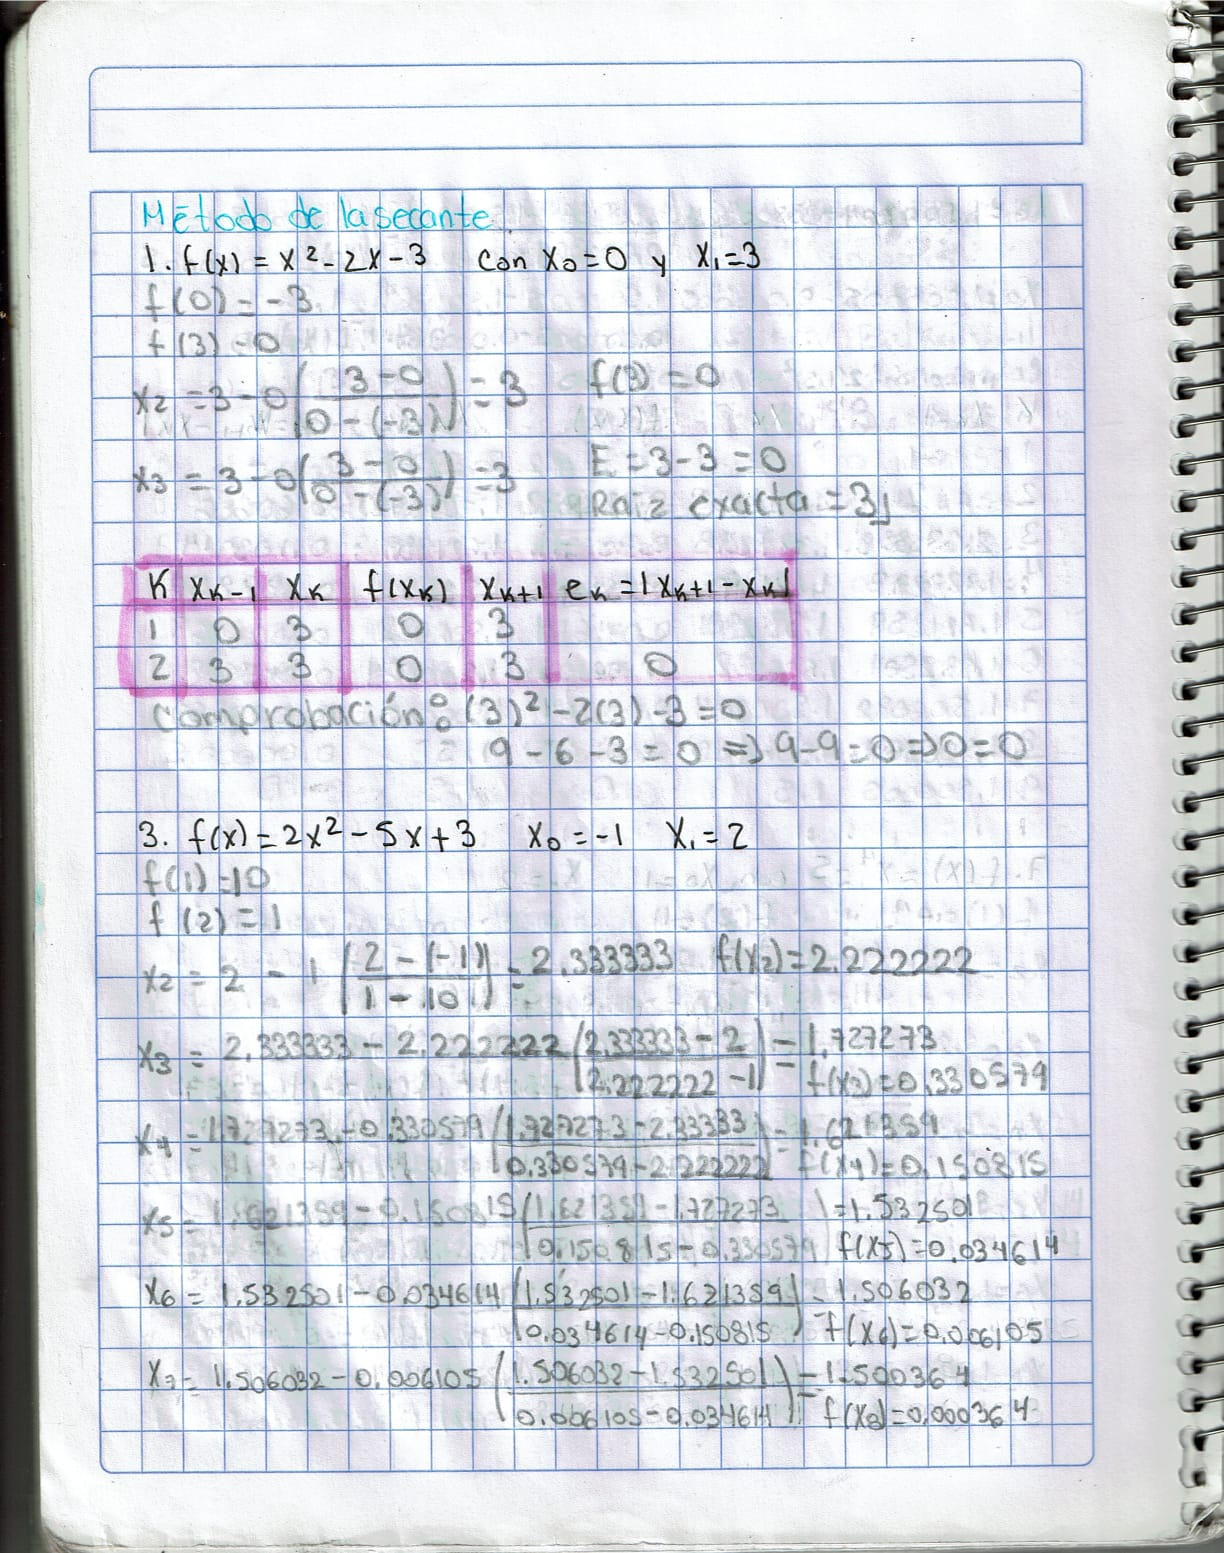
\includegraphics[width=6.25in,height=\textheight,keepaspectratio,alt={Ejercicio 1 y 3}]{Secante1-3_1.jpg}
\caption{Ejercicio 1 y 3}
\end{figure}

\begin{figure}
\centering
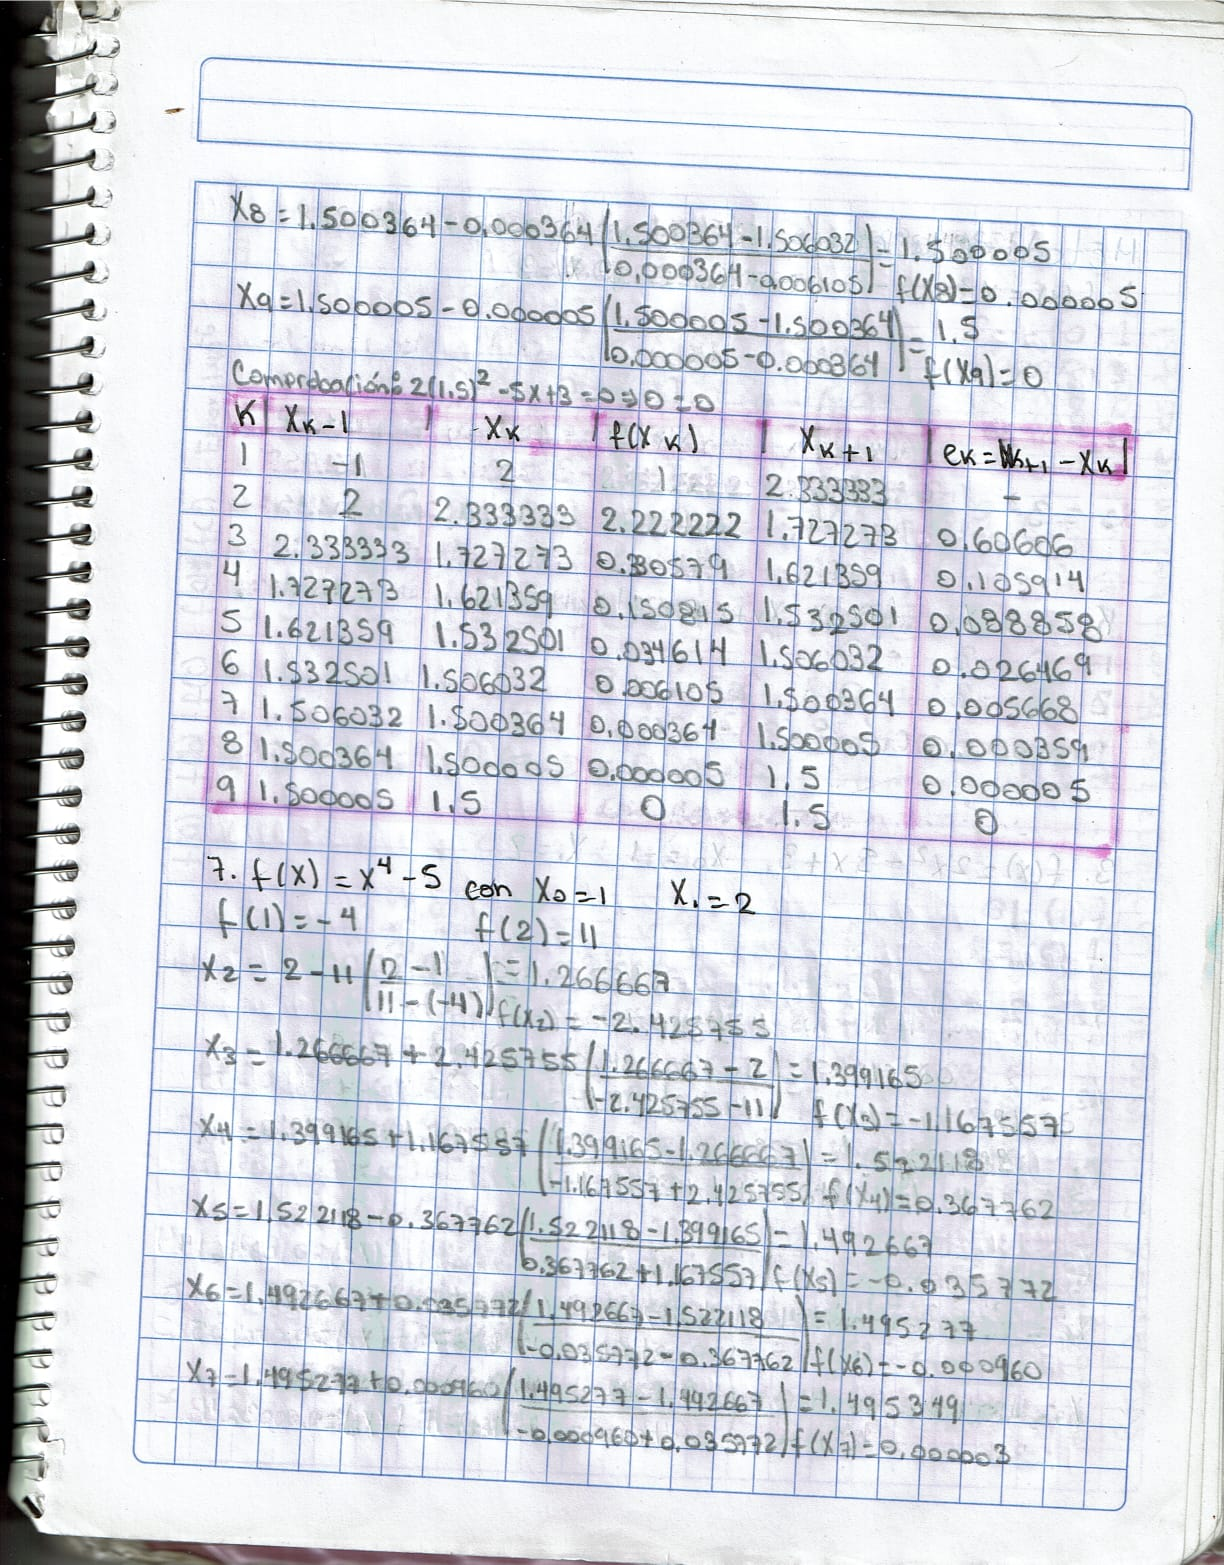
\includegraphics[width=6.25in,height=\textheight,keepaspectratio,alt={Ejercicio 3-2 y 7}]{Secante3_2-7_1.jpg}
\caption{Ejercicio 3-2 y 7}
\end{figure}

\begin{figure}
\centering
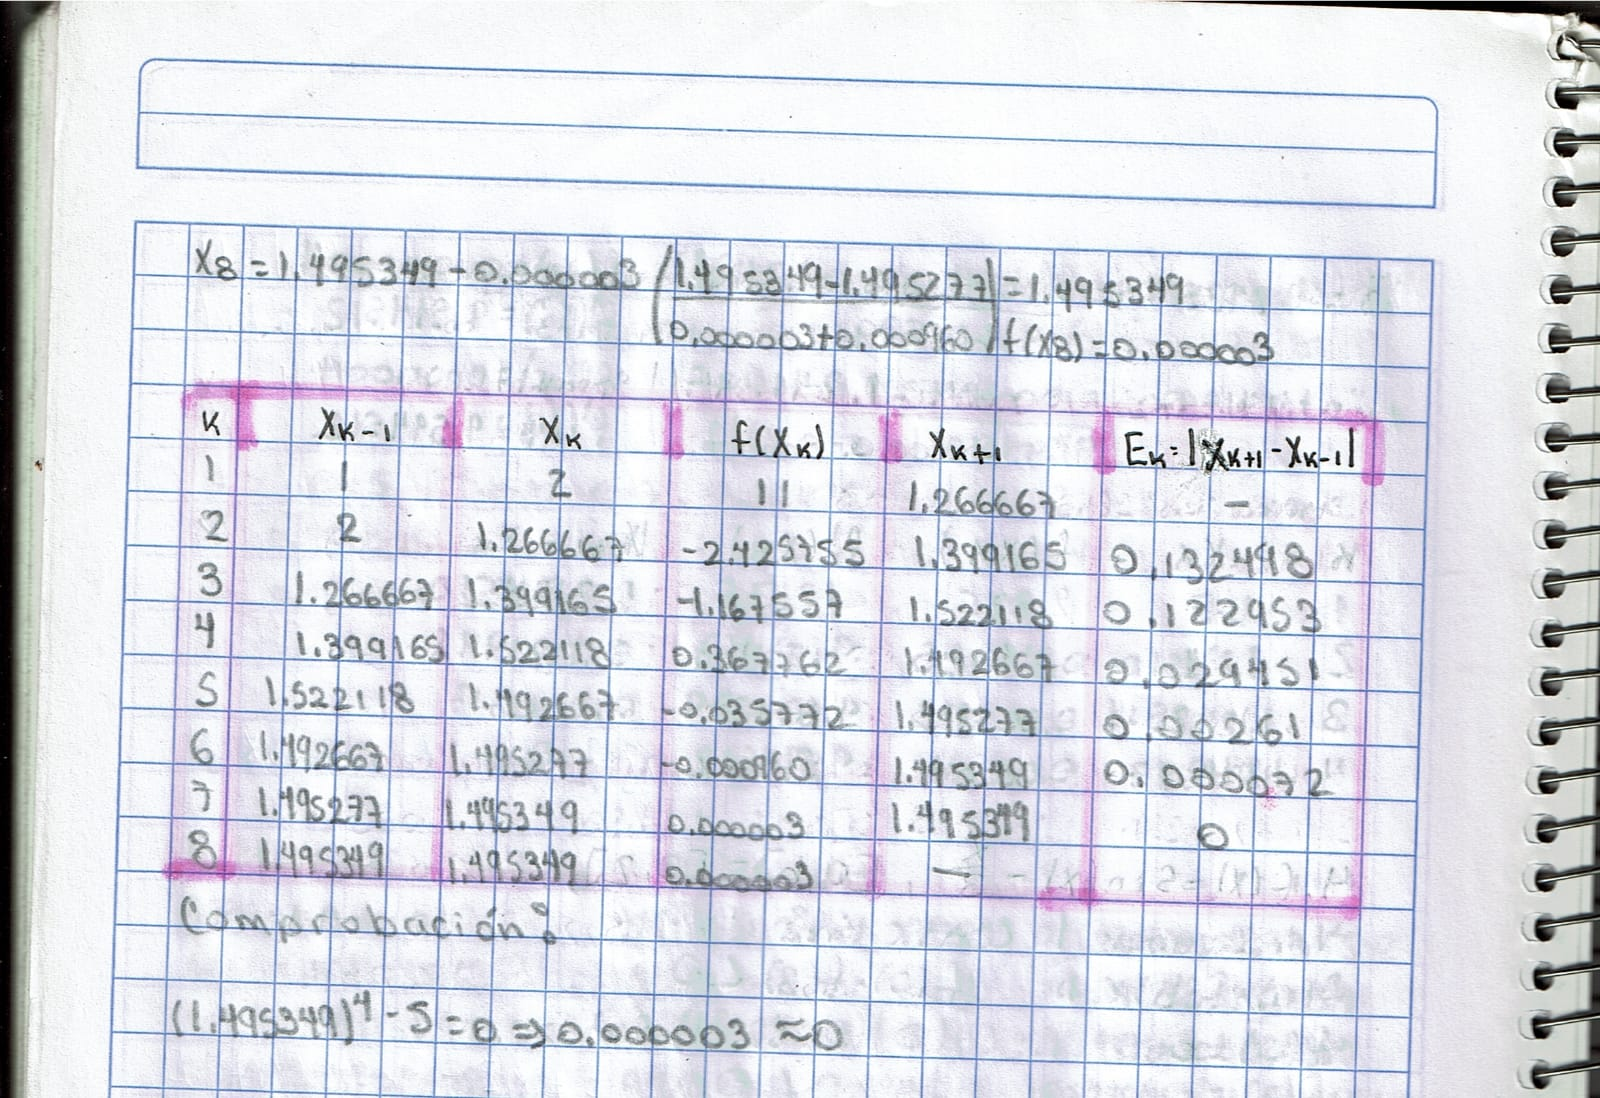
\includegraphics[width=6.25in,height=\textheight,keepaspectratio,alt={Ejercicio 7-2}]{Secante7_2jpg.jpg}
\caption{Ejercicio 7-2}
\end{figure}

\subsubsection{Código para
implementación}\label{cuxf3digo-para-implementaciuxf3n-1}

\begin{Shaded}
\begin{Highlighting}[]
\CommentTok{\# Método de la secante que guarda los valores para la tabla}

\NormalTok{secante }\OtherTok{\textless{}{-}} \ControlFlowTok{function}\NormalTok{(f, x0, x1, }\AttributeTok{tol =} \FloatTok{1e{-}5}\NormalTok{, }\AttributeTok{iter\_max =} \DecValTok{100}\NormalTok{)\{}
  
\CommentTok{\# Vectores para almacenar los datos de las iteraciones}
  
\NormalTok{  iter\_vec }\OtherTok{\textless{}{-}} \FunctionTok{numeric}\NormalTok{(}\DecValTok{0}\NormalTok{)}
\NormalTok{  x0\_vec }\OtherTok{\textless{}{-}} \FunctionTok{numeric}\NormalTok{(}\DecValTok{0}\NormalTok{)}
\NormalTok{  x1\_vec }\OtherTok{\textless{}{-}} \FunctionTok{numeric}\NormalTok{(}\DecValTok{0}\NormalTok{)}
\NormalTok{  x2\_vec }\OtherTok{\textless{}{-}} \FunctionTok{numeric}\NormalTok{(}\DecValTok{0}\NormalTok{)}
\NormalTok{  fx0\_vec }\OtherTok{\textless{}{-}} \FunctionTok{numeric}\NormalTok{(}\DecValTok{0}\NormalTok{)}
\NormalTok{  fx1\_vec }\OtherTok{\textless{}{-}} \FunctionTok{numeric}\NormalTok{(}\DecValTok{0}\NormalTok{)}
\NormalTok{  fx2\_vec }\OtherTok{\textless{}{-}} \FunctionTok{numeric}\NormalTok{(}\DecValTok{0}\NormalTok{)}
\NormalTok{  error\_vec }\OtherTok{\textless{}{-}} \FunctionTok{numeric}\NormalTok{(}\DecValTok{0}\NormalTok{)}
  
\NormalTok{  iter }\OtherTok{\textless{}{-}} \DecValTok{0}
\NormalTok{  error }\OtherTok{\textless{}{-}} \DecValTok{1}
  
  \ControlFlowTok{while}\NormalTok{(error }\SpecialCharTok{\textgreater{}}\NormalTok{ tol }\SpecialCharTok{\&\&}\NormalTok{ iter }\SpecialCharTok{\textless{}}\NormalTok{ iter\_max)\{}
\NormalTok{    fx0 }\OtherTok{\textless{}{-}} \FunctionTok{f}\NormalTok{(x0)}
\NormalTok{    fx1 }\OtherTok{\textless{}{-}} \FunctionTok{f}\NormalTok{(x1)}
    
\CommentTok{\# Evitar división por cero}
    
    \ControlFlowTok{if}\NormalTok{(}\FunctionTok{abs}\NormalTok{(fx1 }\SpecialCharTok{{-}}\NormalTok{ fx0) }\SpecialCharTok{\textless{}} \FloatTok{1e{-}12}\NormalTok{)\{}
      \FunctionTok{cat}\NormalTok{(}\StringTok{"Error: División por cero (f(x1) {-} f(x0) approx 0)}\SpecialCharTok{\textbackslash{}n}\StringTok{"}\NormalTok{)}
      \FunctionTok{return}\NormalTok{(}\ConstantTok{NA}\NormalTok{)}
\NormalTok{    \}}
    
\NormalTok{    x2 }\OtherTok{\textless{}{-}}\NormalTok{ x1 }\SpecialCharTok{{-}}\NormalTok{ fx1 }\SpecialCharTok{*}\NormalTok{ (x1 }\SpecialCharTok{{-}}\NormalTok{ x0) }\SpecialCharTok{/}\NormalTok{ (fx1 }\SpecialCharTok{{-}}\NormalTok{ fx0)}
\NormalTok{    error }\OtherTok{\textless{}{-}} \FunctionTok{abs}\NormalTok{(x2 }\SpecialCharTok{{-}}\NormalTok{ x1)}
    
\CommentTok{\# Almacena los datos de cada iteración}
    
\NormalTok{    iter }\OtherTok{\textless{}{-}}\NormalTok{ iter }\SpecialCharTok{+} \DecValTok{1}
\NormalTok{    iter\_vec }\OtherTok{\textless{}{-}} \FunctionTok{c}\NormalTok{(iter\_vec, iter)}
\NormalTok{    x0\_vec }\OtherTok{\textless{}{-}} \FunctionTok{c}\NormalTok{(x0\_vec, x0)}
\NormalTok{    x1\_vec }\OtherTok{\textless{}{-}} \FunctionTok{c}\NormalTok{(x1\_vec, x1)}
\NormalTok{    x2\_vec }\OtherTok{\textless{}{-}} \FunctionTok{c}\NormalTok{(x2\_vec, x2)}
\NormalTok{    fx0\_vec }\OtherTok{\textless{}{-}} \FunctionTok{c}\NormalTok{(fx0\_vec, fx0)}
\NormalTok{    fx1\_vec }\OtherTok{\textless{}{-}} \FunctionTok{c}\NormalTok{(fx1\_vec, fx1)}
\NormalTok{    fx2\_vec }\OtherTok{\textless{}{-}} \FunctionTok{c}\NormalTok{(fx2\_vec, }\FunctionTok{f}\NormalTok{(x2))}
\NormalTok{    error\_vec }\OtherTok{\textless{}{-}} \FunctionTok{c}\NormalTok{(error\_vec, error)}
    
\CommentTok{\# Actualizar valores para siguiente iteración}
    
\NormalTok{    x0 }\OtherTok{\textless{}{-}}\NormalTok{ x1}
\NormalTok{    x1 }\OtherTok{\textless{}{-}}\NormalTok{ x2}
\NormalTok{  \}}
  
\CommentTok{\# Crea la tabla de las iteraciones}
  
\NormalTok{ TAB }\OtherTok{\textless{}{-}} \FunctionTok{data.frame}\NormalTok{(}
  \StringTok{"k"} \OtherTok{=}\NormalTok{ iter\_vec,}
  \StringTok{"xₖ₋₁"} \OtherTok{=}\NormalTok{ x0\_vec,}
  \StringTok{"xₖ"} \OtherTok{=}\NormalTok{ x1\_vec,}
  \StringTok{"f(xₖ)"} \OtherTok{=}\NormalTok{ fx1\_vec,}
  \StringTok{"xₖ₊₁"} \OtherTok{=}\NormalTok{ x2\_vec,}
  \StringTok{"eₖ = |xₖ₊₁ {-} xₖ|"} \OtherTok{=}\NormalTok{ error\_vec,}
  \AttributeTok{check.names =} \ConstantTok{FALSE}
\NormalTok{)}
  
  \FunctionTok{cat}\NormalTok{(}\StringTok{"Raíz aproximada:"}\NormalTok{, x2, }\StringTok{"}\SpecialCharTok{\textbackslash{}n}\StringTok{"}\NormalTok{)}
  \FunctionTok{cat}\NormalTok{(}\StringTok{"Iteraciones:"}\NormalTok{, iter, }\StringTok{"}\SpecialCharTok{\textbackslash{}n\textbackslash{}n}\StringTok{"}\NormalTok{)}
  
  \FunctionTok{return}\NormalTok{(}\FunctionTok{list}\NormalTok{(}\AttributeTok{raiz =}\NormalTok{ x2, }\AttributeTok{iteraciones =}\NormalTok{ iter, }\AttributeTok{tabla =}\NormalTok{ TAB))}
\NormalTok{\}}
\end{Highlighting}
\end{Shaded}

\begin{Shaded}
\begin{Highlighting}[]
\CommentTok{\# Tabla "bonita"}

\NormalTok{tabla }\OtherTok{\textless{}{-}} \ControlFlowTok{function}\NormalTok{(resultado) \{}
  \FunctionTok{library}\NormalTok{(DT)}
  
  \FunctionTok{datatable}\NormalTok{(}
\NormalTok{    resultado}\SpecialCharTok{$}\NormalTok{tabla,}
    \AttributeTok{options =} \FunctionTok{list}\NormalTok{(}
      \AttributeTok{scrollX =} \ConstantTok{TRUE}\NormalTok{,}
      \AttributeTok{scrollY =} \StringTok{"400px"}\NormalTok{, }
      \AttributeTok{paging =} \ConstantTok{FALSE}\NormalTok{,}
      \AttributeTok{dom =} \StringTok{\textquotesingle{}t\textquotesingle{}}\NormalTok{,}
      \AttributeTok{autoWidth =} \ConstantTok{FALSE}\NormalTok{,}
      \AttributeTok{columnDefs =} \FunctionTok{list}\NormalTok{(}
        \FunctionTok{list}\NormalTok{(}\AttributeTok{className =} \StringTok{\textquotesingle{}dt{-}center\textquotesingle{}}\NormalTok{, }\AttributeTok{targets =} \DecValTok{0}\SpecialCharTok{:}\DecValTok{5}\NormalTok{))}
\NormalTok{    ),}
    \AttributeTok{rownames =} \ConstantTok{FALSE}\NormalTok{,}
    \AttributeTok{class =} \StringTok{\textquotesingle{}cell{-}border stripe\textquotesingle{}}\NormalTok{,}
    \AttributeTok{width =} \StringTok{"100\%"}\NormalTok{,}
    \AttributeTok{caption =} \StringTok{"Tabla de iteraciones en el método de la secante"}\NormalTok{,}
    \AttributeTok{escape =} \ConstantTok{FALSE}
\NormalTok{  ) }\SpecialCharTok{\%\textgreater{}\%}
    \FunctionTok{formatRound}\NormalTok{(}\AttributeTok{columns =} \FunctionTok{c}\NormalTok{(}\DecValTok{2}\NormalTok{, }\DecValTok{3}\NormalTok{, }\DecValTok{4}\NormalTok{, }\DecValTok{5}\NormalTok{, }\DecValTok{6}\NormalTok{), }\AttributeTok{digits =} \DecValTok{6}\NormalTok{)}
\NormalTok{\}}
\end{Highlighting}
\end{Shaded}

\begin{Shaded}
\begin{Highlighting}[]
\CommentTok{\# Iteraciones en el método de bisección}

\NormalTok{n\_biseccion }\OtherTok{\textless{}{-}} \ControlFlowTok{function}\NormalTok{(x0, x1) \{}
\NormalTok{  n }\OtherTok{\textless{}{-}} \FunctionTok{ceiling}\NormalTok{(}\FunctionTok{log}\NormalTok{(}\FunctionTok{abs}\NormalTok{(x0 }\SpecialCharTok{{-}}\NormalTok{ x1) }\SpecialCharTok{/} \FloatTok{1e{-}5}\NormalTok{) }\SpecialCharTok{/} \FunctionTok{log}\NormalTok{(}\DecValTok{2}\NormalTok{))}
  \FunctionTok{return}\NormalTok{(n)}
\NormalTok{\}}
\end{Highlighting}
\end{Shaded}

\begin{Shaded}
\begin{Highlighting}[]
\CommentTok{\# Gráficas}

\NormalTok{grafica }\OtherTok{\textless{}{-}} \ControlFlowTok{function}\NormalTok{(x0, x1, f, resultado) \{}
\NormalTok{  tabla\_iteraciones }\OtherTok{\textless{}{-}}\NormalTok{ resultado}\SpecialCharTok{$}\NormalTok{tabla}
\NormalTok{  total\_iteraciones }\OtherTok{\textless{}{-}} \FunctionTok{nrow}\NormalTok{(tabla\_iteraciones)}
\NormalTok{  filas }\OtherTok{\textless{}{-}} \FunctionTok{ceiling}\NormalTok{(total\_iteraciones }\SpecialCharTok{/} \DecValTok{4}\NormalTok{)}
  
  \FunctionTok{par}\NormalTok{(}\AttributeTok{mfrow =} \FunctionTok{c}\NormalTok{(filas, }\DecValTok{4}\NormalTok{), }\AttributeTok{mar =} \FunctionTok{c}\NormalTok{(}\DecValTok{2}\NormalTok{, }\DecValTok{2}\NormalTok{, }\FloatTok{1.5}\NormalTok{, }\DecValTok{1}\NormalTok{))}
  
\CommentTok{\# Calcular rango dinámico}
  
\NormalTok{  x\_min }\OtherTok{\textless{}{-}} \FunctionTok{min}\NormalTok{(tabla\_iteraciones[,}\DecValTok{2}\NormalTok{]) }\SpecialCharTok{{-}} \FloatTok{0.5}
\NormalTok{  x\_max }\OtherTok{\textless{}{-}} \FunctionTok{max}\NormalTok{(tabla\_iteraciones[,}\DecValTok{3}\NormalTok{]) }\SpecialCharTok{+} \FloatTok{0.5}
\NormalTok{  x\_vals }\OtherTok{\textless{}{-}} \FunctionTok{seq}\NormalTok{(x\_min, x\_max, }\AttributeTok{length.out =} \DecValTok{1000}\NormalTok{)}
\NormalTok{  y\_vals }\OtherTok{\textless{}{-}} \FunctionTok{f}\NormalTok{(x\_vals)}
  
  \ControlFlowTok{for}\NormalTok{ (i }\ControlFlowTok{in} \DecValTok{1}\SpecialCharTok{:}\NormalTok{total\_iteraciones) \{}
    \FunctionTok{plot}\NormalTok{(x\_vals, y\_vals, }\AttributeTok{type =} \StringTok{"l"}\NormalTok{, }\AttributeTok{main =} \FunctionTok{paste}\NormalTok{(}\StringTok{"Iteración"}\NormalTok{, i),}
         \AttributeTok{xlab =} \StringTok{"x"}\NormalTok{, }\AttributeTok{ylab =} \StringTok{"f(x)"}\NormalTok{, }\AttributeTok{col =} \StringTok{"blue"}\NormalTok{, }\AttributeTok{lwd =} \FloatTok{1.2}\NormalTok{)}
    \FunctionTok{abline}\NormalTok{(}\AttributeTok{h =} \DecValTok{0}\NormalTok{, }\AttributeTok{col =} \StringTok{"gray"}\NormalTok{, }\AttributeTok{lty =} \DecValTok{2}\NormalTok{)}

\NormalTok{    x\_anterior }\OtherTok{\textless{}{-}}\NormalTok{ tabla\_iteraciones[i, }\DecValTok{2}\NormalTok{]  }\CommentTok{\# x\_\{k{-}1\}}
\NormalTok{    x\_actual }\OtherTok{\textless{}{-}}\NormalTok{ tabla\_iteraciones[i, }\DecValTok{3}\NormalTok{]    }\CommentTok{\# x\_k  }
\NormalTok{    x\_siguiente }\OtherTok{\textless{}{-}}\NormalTok{ tabla\_iteraciones[i, }\DecValTok{4}\NormalTok{] }\CommentTok{\# x\_\{k+1\} }
    
\CommentTok{\# Calcula la pendiente para la gráfica}
    
\NormalTok{    f\_anterior }\OtherTok{\textless{}{-}} \FunctionTok{f}\NormalTok{(x\_anterior)}
\NormalTok{    f\_actual }\OtherTok{\textless{}{-}} \FunctionTok{f}\NormalTok{(x\_actual)}
\NormalTok{    pendiente }\OtherTok{\textless{}{-}}\NormalTok{ (f\_actual }\SpecialCharTok{{-}}\NormalTok{ f\_anterior) }\SpecialCharTok{/}\NormalTok{ (x\_actual }\SpecialCharTok{{-}}\NormalTok{ x\_anterior)}
    
\CommentTok{\# Grafica la línea secante}
    
\NormalTok{    x\_secante }\OtherTok{\textless{}{-}} \FunctionTok{seq}\NormalTok{(x\_min, x\_max, }\AttributeTok{length.out =} \DecValTok{100}\NormalTok{)}
\NormalTok{    y\_secante }\OtherTok{\textless{}{-}}\NormalTok{ f\_anterior }\SpecialCharTok{+}\NormalTok{ pendiente }\SpecialCharTok{*}\NormalTok{ (x\_secante }\SpecialCharTok{{-}}\NormalTok{ x\_anterior)}
    \FunctionTok{lines}\NormalTok{(x\_secante, y\_secante, }\AttributeTok{col =} \StringTok{"purple"}\NormalTok{, }\AttributeTok{lty =} \DecValTok{2}\NormalTok{, }\AttributeTok{lwd =} \FloatTok{1.5}\NormalTok{)}
    
\CommentTok{\# Puntos de la iteración}
    
    \FunctionTok{points}\NormalTok{(}\FunctionTok{c}\NormalTok{(x\_anterior, x\_actual), }\FunctionTok{c}\NormalTok{(f\_anterior, f\_actual), }
           \AttributeTok{col =} \FunctionTok{c}\NormalTok{(}\StringTok{"red"}\NormalTok{, }\StringTok{"green"}\NormalTok{), }\AttributeTok{pch =} \DecValTok{19}\NormalTok{, }\AttributeTok{cex =} \FloatTok{0.8}\NormalTok{)}
    
\CommentTok{\# Punto de intersección con eje x (x\_\{k+1\})}
    
    \FunctionTok{points}\NormalTok{(x\_siguiente, }\DecValTok{0}\NormalTok{, }\AttributeTok{col =} \StringTok{"orange"}\NormalTok{, }\AttributeTok{pch =} \DecValTok{17}\NormalTok{, }\AttributeTok{cex =} \FloatTok{1.2}\NormalTok{)}
    
\CommentTok{\# Líneas verticales para los puntos importantes}
    
    \FunctionTok{abline}\NormalTok{(}\AttributeTok{v =}\NormalTok{ x\_anterior, }\AttributeTok{col =} \StringTok{"red"}\NormalTok{, }\AttributeTok{lty =} \DecValTok{3}\NormalTok{, }\AttributeTok{lwd =} \FloatTok{0.8}\NormalTok{)}
    \FunctionTok{abline}\NormalTok{(}\AttributeTok{v =}\NormalTok{ x\_actual, }\AttributeTok{col =} \StringTok{"green"}\NormalTok{, }\AttributeTok{lty =} \DecValTok{3}\NormalTok{, }\AttributeTok{lwd =} \FloatTok{0.8}\NormalTok{)}
    \FunctionTok{abline}\NormalTok{(}\AttributeTok{v =}\NormalTok{ x\_siguiente, }\AttributeTok{col =} \StringTok{"orange"}\NormalTok{, }\AttributeTok{lty =} \DecValTok{3}\NormalTok{, }\AttributeTok{lwd =} \FloatTok{1.2}\NormalTok{)}
    
\CommentTok{\# Leyenda explicativa}
    
    \FunctionTok{legend}\NormalTok{(}\StringTok{"topright"}\NormalTok{, }
           \AttributeTok{legend =} \FunctionTok{c}\NormalTok{(}\StringTok{"f(x)"}\NormalTok{, }\StringTok{"Secante"}\NormalTok{, }\StringTok{"x\_\{k{-}1\}"}\NormalTok{, }\StringTok{"x\_k"}\NormalTok{, }\StringTok{"x\_\{k+1\}"}\NormalTok{),}
           \AttributeTok{col =} \FunctionTok{c}\NormalTok{(}\StringTok{"blue"}\NormalTok{, }\StringTok{"purple"}\NormalTok{, }\StringTok{"red"}\NormalTok{, }\StringTok{"green"}\NormalTok{, }\StringTok{"orange"}\NormalTok{),}
           \AttributeTok{lty =} \FunctionTok{c}\NormalTok{(}\DecValTok{1}\NormalTok{, }\DecValTok{2}\NormalTok{, }\ConstantTok{NA}\NormalTok{, }\ConstantTok{NA}\NormalTok{, }\ConstantTok{NA}\NormalTok{), }\AttributeTok{pch =} \FunctionTok{c}\NormalTok{(}\ConstantTok{NA}\NormalTok{, }\ConstantTok{NA}\NormalTok{, }\DecValTok{19}\NormalTok{, }\DecValTok{19}\NormalTok{, }\DecValTok{17}\NormalTok{),}
           \AttributeTok{cex =} \FloatTok{0.7}\NormalTok{, }\AttributeTok{bty =} \StringTok{"n"}\NormalTok{)}
\NormalTok{  \}}
  
  \FunctionTok{par}\NormalTok{(}\AttributeTok{mfrow =} \FunctionTok{c}\NormalTok{(}\DecValTok{1}\NormalTok{, }\DecValTok{1}\NormalTok{))}
\NormalTok{\}}
\end{Highlighting}
\end{Shaded}

\subsubsection{\texorpdfstring{Sistema
\(2\)}{Sistema 2}}\label{sistema-2-5}

\(f(x) = x^4 − 10x^2 + 9\)

\(x_0 = 0\)

\(x_1 = 2\)

\begin{Shaded}
\begin{Highlighting}[]
\CommentTok{\# Datos}

\NormalTok{x0 }\OtherTok{\textless{}{-}} \DecValTok{0}
\NormalTok{x1 }\OtherTok{\textless{}{-}} \DecValTok{2}
\NormalTok{f }\OtherTok{\textless{}{-}} \ControlFlowTok{function}\NormalTok{(x) x}\SpecialCharTok{\^{}}\DecValTok{4} \SpecialCharTok{{-}} \DecValTok{10}\SpecialCharTok{*}\NormalTok{x}\SpecialCharTok{\^{}}\DecValTok{2} \SpecialCharTok{+} \DecValTok{9}
\end{Highlighting}
\end{Shaded}

\paragraph{Puntos iniciales}\label{puntos-iniciales}

Para cada función \(f(x)\), elija dos puntos iniciales \(x_0\), \(x_1\)
cercanos a la raíz.

Nota: En la información dada ya nos da los puntos iniciales:

\(x_0 = 0\)

\(x_1 = 2\)

\paragraph{Iteraciones}\label{iteraciones-5}

Aplique iterativamente:
\(x_{k+1} = x_k − f(x_k) \frac{x_k − x_{k−1}}{f(x_k) − f(x_{k−1})}\)

\begin{Shaded}
\begin{Highlighting}[]
\NormalTok{resultado }\OtherTok{\textless{}{-}} \FunctionTok{secante}\NormalTok{(f, x0, x1)}
\end{Highlighting}
\end{Shaded}

\begin{verbatim}
## Raíz aproximada: 1 
## Iteraciones: 5
\end{verbatim}

\paragraph{Comparación}\label{comparaciuxf3n}

Compare el número de iteraciones con el método de bisección.

\begin{Shaded}
\begin{Highlighting}[]
\FunctionTok{tabla}\NormalTok{(resultado)}
\end{Highlighting}
\end{Shaded}

\pandocbounded{\includegraphics[keepaspectratio]{PortafolioDLPF_pdf_files/figure-latex/unnamed-chunk-1177-1.pdf}}

\begin{Shaded}
\begin{Highlighting}[]
\NormalTok{t\_biseccion }\OtherTok{\textless{}{-}} \FunctionTok{n\_biseccion}\NormalTok{(x0, x1)}
\FunctionTok{cat}\NormalTok{(}\StringTok{"En el método de bisección:"}\NormalTok{, t\_biseccion, }\StringTok{"iteraciones}\SpecialCharTok{\textbackslash{}n}\StringTok{"}\NormalTok{)}
\end{Highlighting}
\end{Shaded}

\begin{verbatim}
## En el método de bisección: 18 iteraciones
\end{verbatim}

\begin{Shaded}
\begin{Highlighting}[]
\FunctionTok{cat}\NormalTok{(}\StringTok{"En el método de la secante:"}\NormalTok{, resultado}\SpecialCharTok{$}\NormalTok{iteraciones, }\StringTok{"iteraciones}\SpecialCharTok{\textbackslash{}n}\StringTok{"}\NormalTok{)}
\end{Highlighting}
\end{Shaded}

\begin{verbatim}
## En el método de la secante: 5 iteraciones
\end{verbatim}

\begin{Shaded}
\begin{Highlighting}[]
\FunctionTok{cat}\NormalTok{(}\StringTok{"Ventaja:"}\NormalTok{, t\_biseccion }\SpecialCharTok{{-}}\NormalTok{ resultado}\SpecialCharTok{$}\NormalTok{iteraciones, }\StringTok{"iteraciones menos}\SpecialCharTok{\textbackslash{}n}\StringTok{"}\NormalTok{)}
\end{Highlighting}
\end{Shaded}

\begin{verbatim}
## Ventaja: 13 iteraciones menos
\end{verbatim}

\paragraph{Gráficas}\label{gruxe1ficas-5}

Grafique la función y los intervalos de reducción en cada paso.

\begin{Shaded}
\begin{Highlighting}[]
\FunctionTok{grafica}\NormalTok{(x0, x1, f, resultado)}
\end{Highlighting}
\end{Shaded}

\pandocbounded{\includegraphics[keepaspectratio]{PortafolioDLPF_pdf_files/figure-latex/unnamed-chunk-1178-1.pdf}}

\subsubsection{\texorpdfstring{Sistema
\(4\)}{Sistema 4}}\label{sistema-4-5}

\(f(x) = -3x^2 + 4x + 2\)

\(x_0 = -1\)

\(x_1 = 3\)

\begin{Shaded}
\begin{Highlighting}[]
\CommentTok{\# Datos}

\NormalTok{x0 }\OtherTok{\textless{}{-}} \SpecialCharTok{{-}}\DecValTok{1}
\NormalTok{x1 }\OtherTok{\textless{}{-}} \DecValTok{3}
\NormalTok{f }\OtherTok{\textless{}{-}} \ControlFlowTok{function}\NormalTok{(x) }\SpecialCharTok{{-}}\DecValTok{3}\SpecialCharTok{*}\NormalTok{x}\SpecialCharTok{\^{}}\DecValTok{2} \SpecialCharTok{+} \DecValTok{4}\SpecialCharTok{*}\NormalTok{x }\SpecialCharTok{+} \DecValTok{2}
\end{Highlighting}
\end{Shaded}

\paragraph{Puntos iniciales}\label{puntos-iniciales-1}

Para cada función \(f(x)\), elija dos puntos iniciales \(x_0\), \(x_1\)
cercanos a la raíz.

Nota: En la información dada ya nos da los puntos iniciales:

\(x_0 = -1\)

\(x_1 = 3\)

\paragraph{Iteraciones}\label{iteraciones-6}

Aplique iterativamente:
\(x_{k+1} = x_k − f(x_k) \frac{x_k − x_{k−1}}{f(x_k) − f(x_{k−1})}\)

\begin{Shaded}
\begin{Highlighting}[]
\NormalTok{resultado }\OtherTok{\textless{}{-}} \FunctionTok{secante}\NormalTok{(f, x0, x1)}
\end{Highlighting}
\end{Shaded}

\begin{verbatim}
## Raíz aproximada: 1.720759 
## Iteraciones: 14
\end{verbatim}

\paragraph{Comparación}\label{comparaciuxf3n-1}

Compare el número de iteraciones con el método de bisección.

\begin{Shaded}
\begin{Highlighting}[]
\FunctionTok{tabla}\NormalTok{(resultado)}
\end{Highlighting}
\end{Shaded}

\pandocbounded{\includegraphics[keepaspectratio]{PortafolioDLPF_pdf_files/figure-latex/unnamed-chunk-1181-1.pdf}}

\begin{Shaded}
\begin{Highlighting}[]
\NormalTok{t\_biseccion }\OtherTok{\textless{}{-}} \FunctionTok{n\_biseccion}\NormalTok{(x0, x1)}
\FunctionTok{cat}\NormalTok{(}\StringTok{"En el método de bisección:"}\NormalTok{, t\_biseccion, }\StringTok{"iteraciones}\SpecialCharTok{\textbackslash{}n}\StringTok{"}\NormalTok{)}
\end{Highlighting}
\end{Shaded}

\begin{verbatim}
## En el método de bisección: 19 iteraciones
\end{verbatim}

\begin{Shaded}
\begin{Highlighting}[]
\FunctionTok{cat}\NormalTok{(}\StringTok{"En el método de la secante:"}\NormalTok{, resultado}\SpecialCharTok{$}\NormalTok{iteraciones, }\StringTok{"iteraciones}\SpecialCharTok{\textbackslash{}n}\StringTok{"}\NormalTok{)}
\end{Highlighting}
\end{Shaded}

\begin{verbatim}
## En el método de la secante: 14 iteraciones
\end{verbatim}

\begin{Shaded}
\begin{Highlighting}[]
\FunctionTok{cat}\NormalTok{(}\StringTok{"Ventaja:"}\NormalTok{, t\_biseccion }\SpecialCharTok{{-}}\NormalTok{ resultado}\SpecialCharTok{$}\NormalTok{iteraciones, }\StringTok{"iteraciones menos}\SpecialCharTok{\textbackslash{}n}\StringTok{"}\NormalTok{)}
\end{Highlighting}
\end{Shaded}

\begin{verbatim}
## Ventaja: 5 iteraciones menos
\end{verbatim}

\paragraph{Gráficas}\label{gruxe1ficas-6}

Grafique la función y los intervalos de reducción en cada paso.

\begin{Shaded}
\begin{Highlighting}[]
\FunctionTok{grafica}\NormalTok{(x0, x1, f, resultado)}
\end{Highlighting}
\end{Shaded}

\pandocbounded{\includegraphics[keepaspectratio]{PortafolioDLPF_pdf_files/figure-latex/unnamed-chunk-1182-1.pdf}}

\subsubsection{\texorpdfstring{Sistema
\(6\)}{Sistema 6}}\label{sistema-6-5}

\(f(x) = x^4 - 5x^3 + 6x^2 + 4x - 8\)

\(x_0 = 0\)

\(x_1 = 3\)

\begin{Shaded}
\begin{Highlighting}[]
\CommentTok{\# Datos}

\NormalTok{x0 }\OtherTok{\textless{}{-}} \DecValTok{0}
\NormalTok{x1 }\OtherTok{\textless{}{-}} \DecValTok{3}
\NormalTok{f }\OtherTok{\textless{}{-}} \ControlFlowTok{function}\NormalTok{(x) x}\SpecialCharTok{\^{}}\DecValTok{4} \SpecialCharTok{{-}} \DecValTok{5}\SpecialCharTok{*}\NormalTok{x}\SpecialCharTok{\^{}}\DecValTok{3} \SpecialCharTok{+} \DecValTok{6}\SpecialCharTok{*}\NormalTok{x}\SpecialCharTok{\^{}}\DecValTok{2} \SpecialCharTok{+} \DecValTok{4}\SpecialCharTok{*}\NormalTok{x }\SpecialCharTok{{-}} \DecValTok{8}
\end{Highlighting}
\end{Shaded}

\paragraph{Puntos iniciales}\label{puntos-iniciales-2}

Para cada función \(f(x)\), elija dos puntos iniciales \(x_0\), \(x_1\)
cercanos a la raíz.

Nota: En la información dada ya nos da los puntos iniciales:

\(x_0 = 0\)

\(x_1 = 3\)

\paragraph{Iteraciones}\label{iteraciones-7}

Aplique iterativamente:
\(x_{k+1} = x_k − f(x_k) \frac{x_k − x_{k−1}}{f(x_k) − f(x_{k−1})}\)

\begin{Shaded}
\begin{Highlighting}[]
\NormalTok{resultado }\OtherTok{\textless{}{-}} \FunctionTok{secante}\NormalTok{(f, x0, x1)}
\end{Highlighting}
\end{Shaded}

\begin{verbatim}
## Raíz aproximada: 2 
## Iteraciones: 2
\end{verbatim}

\paragraph{Comparación}\label{comparaciuxf3n-2}

Compare el número de iteraciones con el método de bisección.

\begin{Shaded}
\begin{Highlighting}[]
\FunctionTok{tabla}\NormalTok{(resultado)}
\end{Highlighting}
\end{Shaded}

\pandocbounded{\includegraphics[keepaspectratio]{PortafolioDLPF_pdf_files/figure-latex/unnamed-chunk-1185-1.pdf}}

\begin{Shaded}
\begin{Highlighting}[]
\NormalTok{t\_biseccion }\OtherTok{\textless{}{-}} \FunctionTok{n\_biseccion}\NormalTok{(x0, x1)}
\FunctionTok{cat}\NormalTok{(}\StringTok{"En el método de bisección:"}\NormalTok{, t\_biseccion, }\StringTok{"iteraciones}\SpecialCharTok{\textbackslash{}n}\StringTok{"}\NormalTok{)}
\end{Highlighting}
\end{Shaded}

\begin{verbatim}
## En el método de bisección: 19 iteraciones
\end{verbatim}

\begin{Shaded}
\begin{Highlighting}[]
\FunctionTok{cat}\NormalTok{(}\StringTok{"En el método de la secante:"}\NormalTok{, resultado}\SpecialCharTok{$}\NormalTok{iteraciones, }\StringTok{"iteraciones}\SpecialCharTok{\textbackslash{}n}\StringTok{"}\NormalTok{)}
\end{Highlighting}
\end{Shaded}

\begin{verbatim}
## En el método de la secante: 2 iteraciones
\end{verbatim}

\begin{Shaded}
\begin{Highlighting}[]
\FunctionTok{cat}\NormalTok{(}\StringTok{"Ventaja:"}\NormalTok{, t\_biseccion }\SpecialCharTok{{-}}\NormalTok{ resultado}\SpecialCharTok{$}\NormalTok{iteraciones, }\StringTok{"iteraciones menos}\SpecialCharTok{\textbackslash{}n}\StringTok{"}\NormalTok{)}
\end{Highlighting}
\end{Shaded}

\begin{verbatim}
## Ventaja: 17 iteraciones menos
\end{verbatim}

\paragraph{Gráficas}\label{gruxe1ficas-7}

Grafique la función y los intervalos de reducción en cada paso.

\begin{Shaded}
\begin{Highlighting}[]
\FunctionTok{grafica}\NormalTok{(x0, x1, f, resultado)}
\end{Highlighting}
\end{Shaded}

\pandocbounded{\includegraphics[keepaspectratio]{PortafolioDLPF_pdf_files/figure-latex/unnamed-chunk-1186-1.pdf}}

\subsubsection{\texorpdfstring{Sistema
\(8\)}{Sistema 8}}\label{sistema-8-5}

\(f(x) = -2x^4 + 3x^3 + 7x^2 - 5x + 1\)

\(x_0 = -1\)

\(x_1 = -2\)

\begin{Shaded}
\begin{Highlighting}[]
\CommentTok{\# Datos}

\NormalTok{x0 }\OtherTok{\textless{}{-}} \SpecialCharTok{{-}}\DecValTok{1}
\NormalTok{x1 }\OtherTok{\textless{}{-}} \SpecialCharTok{{-}}\DecValTok{2}
\NormalTok{f }\OtherTok{\textless{}{-}} \ControlFlowTok{function}\NormalTok{(x) }\SpecialCharTok{{-}}\DecValTok{2}\SpecialCharTok{*}\NormalTok{x}\SpecialCharTok{\^{}}\DecValTok{4} \SpecialCharTok{+} \DecValTok{3}\SpecialCharTok{*}\NormalTok{x}\SpecialCharTok{\^{}}\DecValTok{3} \SpecialCharTok{+} \DecValTok{7}\SpecialCharTok{*}\NormalTok{x}\SpecialCharTok{\^{}}\DecValTok{2} \SpecialCharTok{{-}} \DecValTok{5}\SpecialCharTok{*}\NormalTok{x }\SpecialCharTok{+} \DecValTok{1}
\end{Highlighting}
\end{Shaded}

\paragraph{Puntos iniciales}\label{puntos-iniciales-3}

Para cada función \(f(x)\), elija dos puntos iniciales \(x_0\), \(x_1\)
cercanos a la raíz.

Nota: En la información dada ya nos da los puntos iniciales:

\(x_0 = -1\)

\(x_1 = -2\)

\paragraph{Iteraciones}\label{iteraciones-8}

Aplique iterativamente:
\(x_{k+1} = x_k − f(x_k) \frac{x_k − x_{k−1}}{f(x_k) − f(x_{k−1})}\)

\begin{Shaded}
\begin{Highlighting}[]
\NormalTok{resultado }\OtherTok{\textless{}{-}} \FunctionTok{secante}\NormalTok{(f, x0, x1)}
\end{Highlighting}
\end{Shaded}

\begin{verbatim}
## Raíz aproximada: -1.65022 
## Iteraciones: 8
\end{verbatim}

\paragraph{Comparación}\label{comparaciuxf3n-3}

Compare el número de iteraciones con el método de bisección.

\begin{Shaded}
\begin{Highlighting}[]
\FunctionTok{tabla}\NormalTok{(resultado)}
\end{Highlighting}
\end{Shaded}

\pandocbounded{\includegraphics[keepaspectratio]{PortafolioDLPF_pdf_files/figure-latex/unnamed-chunk-1189-1.pdf}}

\begin{Shaded}
\begin{Highlighting}[]
\NormalTok{t\_biseccion }\OtherTok{\textless{}{-}} \FunctionTok{n\_biseccion}\NormalTok{(x0, x1)}
\FunctionTok{cat}\NormalTok{(}\StringTok{"En el método de bisección:"}\NormalTok{, t\_biseccion, }\StringTok{"iteraciones}\SpecialCharTok{\textbackslash{}n}\StringTok{"}\NormalTok{)}
\end{Highlighting}
\end{Shaded}

\begin{verbatim}
## En el método de bisección: 17 iteraciones
\end{verbatim}

\begin{Shaded}
\begin{Highlighting}[]
\FunctionTok{cat}\NormalTok{(}\StringTok{"En el método de la secante:"}\NormalTok{, resultado}\SpecialCharTok{$}\NormalTok{iteraciones, }\StringTok{"iteraciones}\SpecialCharTok{\textbackslash{}n}\StringTok{"}\NormalTok{)}
\end{Highlighting}
\end{Shaded}

\begin{verbatim}
## En el método de la secante: 8 iteraciones
\end{verbatim}

\begin{Shaded}
\begin{Highlighting}[]
\FunctionTok{cat}\NormalTok{(}\StringTok{"Ventaja:"}\NormalTok{, t\_biseccion }\SpecialCharTok{{-}}\NormalTok{ resultado}\SpecialCharTok{$}\NormalTok{iteraciones, }\StringTok{"iteraciones menos}\SpecialCharTok{\textbackslash{}n}\StringTok{"}\NormalTok{)}
\end{Highlighting}
\end{Shaded}

\begin{verbatim}
## Ventaja: 9 iteraciones menos
\end{verbatim}

En este caso, este método no es muy conveniente.

\paragraph{Gráficas}\label{gruxe1ficas-8}

Grafique la función y los intervalos de reducción en cada paso.

\begin{Shaded}
\begin{Highlighting}[]
\FunctionTok{grafica}\NormalTok{(x0, x1, f, resultado)}
\end{Highlighting}
\end{Shaded}

\pandocbounded{\includegraphics[keepaspectratio]{PortafolioDLPF_pdf_files/figure-latex/unnamed-chunk-1190-1.pdf}}

\subsubsection{\texorpdfstring{Sistema
\(12\)}{Sistema 12}}\label{sistema-12}

\(f(x) = (3x + 3.1) cos(2x + \frac{π}{6})\)

\(x_0 = 0.3\)

\(x_1 = 0.8\)

\begin{Shaded}
\begin{Highlighting}[]
\CommentTok{\# Datos}

\NormalTok{x0 }\OtherTok{\textless{}{-}} \FloatTok{0.3}
\NormalTok{x1 }\OtherTok{\textless{}{-}} \FloatTok{0.8}
\NormalTok{f }\OtherTok{\textless{}{-}} \ControlFlowTok{function}\NormalTok{(x) (}\DecValTok{3}\SpecialCharTok{*}\NormalTok{x }\SpecialCharTok{+} \FloatTok{3.1}\NormalTok{) }\SpecialCharTok{*} \FunctionTok{cos}\NormalTok{(}\DecValTok{2}\SpecialCharTok{*}\NormalTok{x }\SpecialCharTok{+}\NormalTok{ (pi}\SpecialCharTok{/}\DecValTok{6}\NormalTok{))}
\end{Highlighting}
\end{Shaded}

\paragraph{Puntos iniciales}\label{puntos-iniciales-4}

Para cada función \(f(x)\), elija dos puntos iniciales \(x_0\), \(x_1\)
cercanos a la raíz.

Nota: En la información dada ya nos da los puntos iniciales:

\(x_0 = 0.3\)

\(x_1 = 0.8\)

\paragraph{Iteraciones}\label{iteraciones-9}

Aplique iterativamente:
\(x_{k+1} = x_k − f(x_k) \frac{x_k − x_{k−1}}{f(x_k) − f(x_{k−1})}\)

\begin{Shaded}
\begin{Highlighting}[]
\NormalTok{resultado }\OtherTok{\textless{}{-}} \FunctionTok{secante}\NormalTok{(f, x0, x1)}
\end{Highlighting}
\end{Shaded}

\begin{verbatim}
## Raíz aproximada: 0.5235988 
## Iteraciones: 5
\end{verbatim}

\paragraph{Comparación}\label{comparaciuxf3n-4}

Compare el número de iteraciones con el método de bisección.

\begin{Shaded}
\begin{Highlighting}[]
\FunctionTok{tabla}\NormalTok{(resultado)}
\end{Highlighting}
\end{Shaded}

\pandocbounded{\includegraphics[keepaspectratio]{PortafolioDLPF_pdf_files/figure-latex/unnamed-chunk-1193-1.pdf}}

\begin{Shaded}
\begin{Highlighting}[]
\NormalTok{t\_biseccion }\OtherTok{\textless{}{-}} \FunctionTok{n\_biseccion}\NormalTok{(x0, x1)}
\FunctionTok{cat}\NormalTok{(}\StringTok{"En el método de bisección:"}\NormalTok{, t\_biseccion, }\StringTok{"iteraciones}\SpecialCharTok{\textbackslash{}n}\StringTok{"}\NormalTok{)}
\end{Highlighting}
\end{Shaded}

\begin{verbatim}
## En el método de bisección: 16 iteraciones
\end{verbatim}

\begin{Shaded}
\begin{Highlighting}[]
\FunctionTok{cat}\NormalTok{(}\StringTok{"En el método de la secante:"}\NormalTok{, resultado}\SpecialCharTok{$}\NormalTok{iteraciones, }\StringTok{"iteraciones}\SpecialCharTok{\textbackslash{}n}\StringTok{"}\NormalTok{)}
\end{Highlighting}
\end{Shaded}

\begin{verbatim}
## En el método de la secante: 5 iteraciones
\end{verbatim}

\begin{Shaded}
\begin{Highlighting}[]
\FunctionTok{cat}\NormalTok{(}\StringTok{"Ventaja:"}\NormalTok{, t\_biseccion }\SpecialCharTok{{-}}\NormalTok{ resultado}\SpecialCharTok{$}\NormalTok{iteraciones, }\StringTok{"iteraciones menos}\SpecialCharTok{\textbackslash{}n}\StringTok{"}\NormalTok{)}
\end{Highlighting}
\end{Shaded}

\begin{verbatim}
## Ventaja: 11 iteraciones menos
\end{verbatim}

\paragraph{Gráficas}\label{gruxe1ficas-9}

Grafique la función y los intervalos de reducción en cada paso.

\begin{Shaded}
\begin{Highlighting}[]
\FunctionTok{grafica}\NormalTok{(x0, x1, f, resultado)}
\end{Highlighting}
\end{Shaded}

\pandocbounded{\includegraphics[keepaspectratio]{PortafolioDLPF_pdf_files/figure-latex/unnamed-chunk-1194-1.pdf}}

\subsection{Método de Newton-Raphson}\label{muxe9todo-de-newton-raphson}

\subsubsection{Ejercicios a mano}\label{ejercicios-a-mano-8}

\begin{figure}
\centering
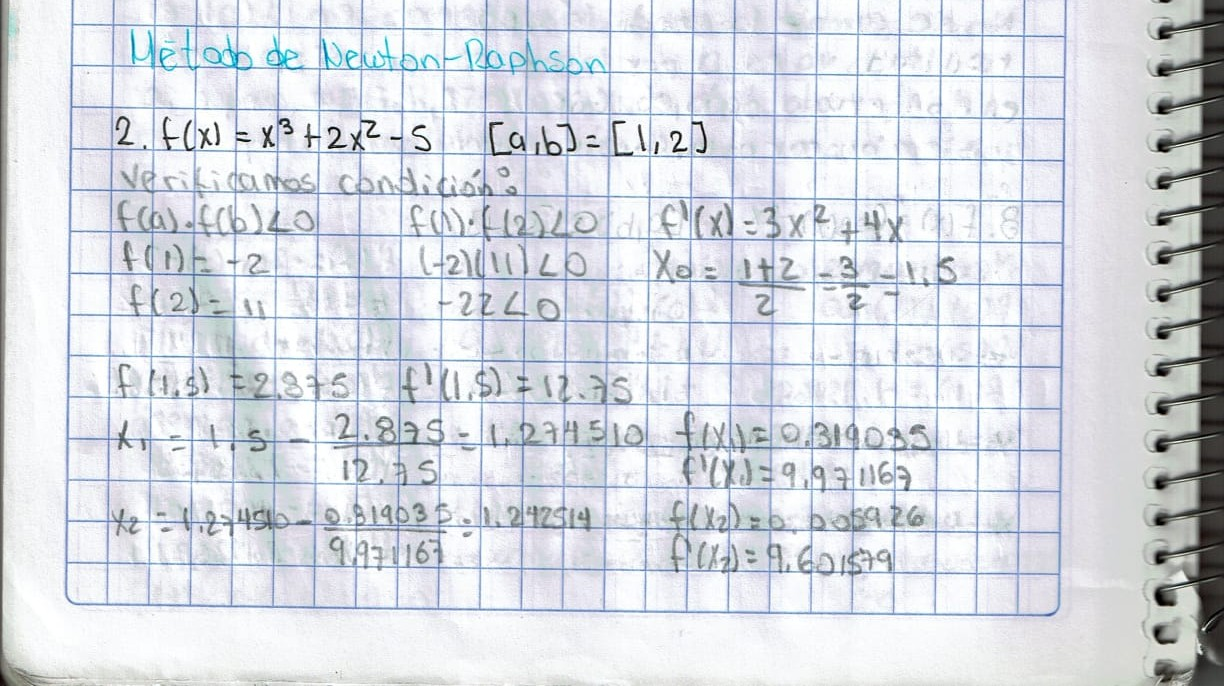
\includegraphics[width=6.25in,height=\textheight,keepaspectratio,alt={Ejercicio 2-1}]{Newton2_1.jpg}
\caption{Ejercicio 2-1}
\end{figure}

\begin{figure}
\centering
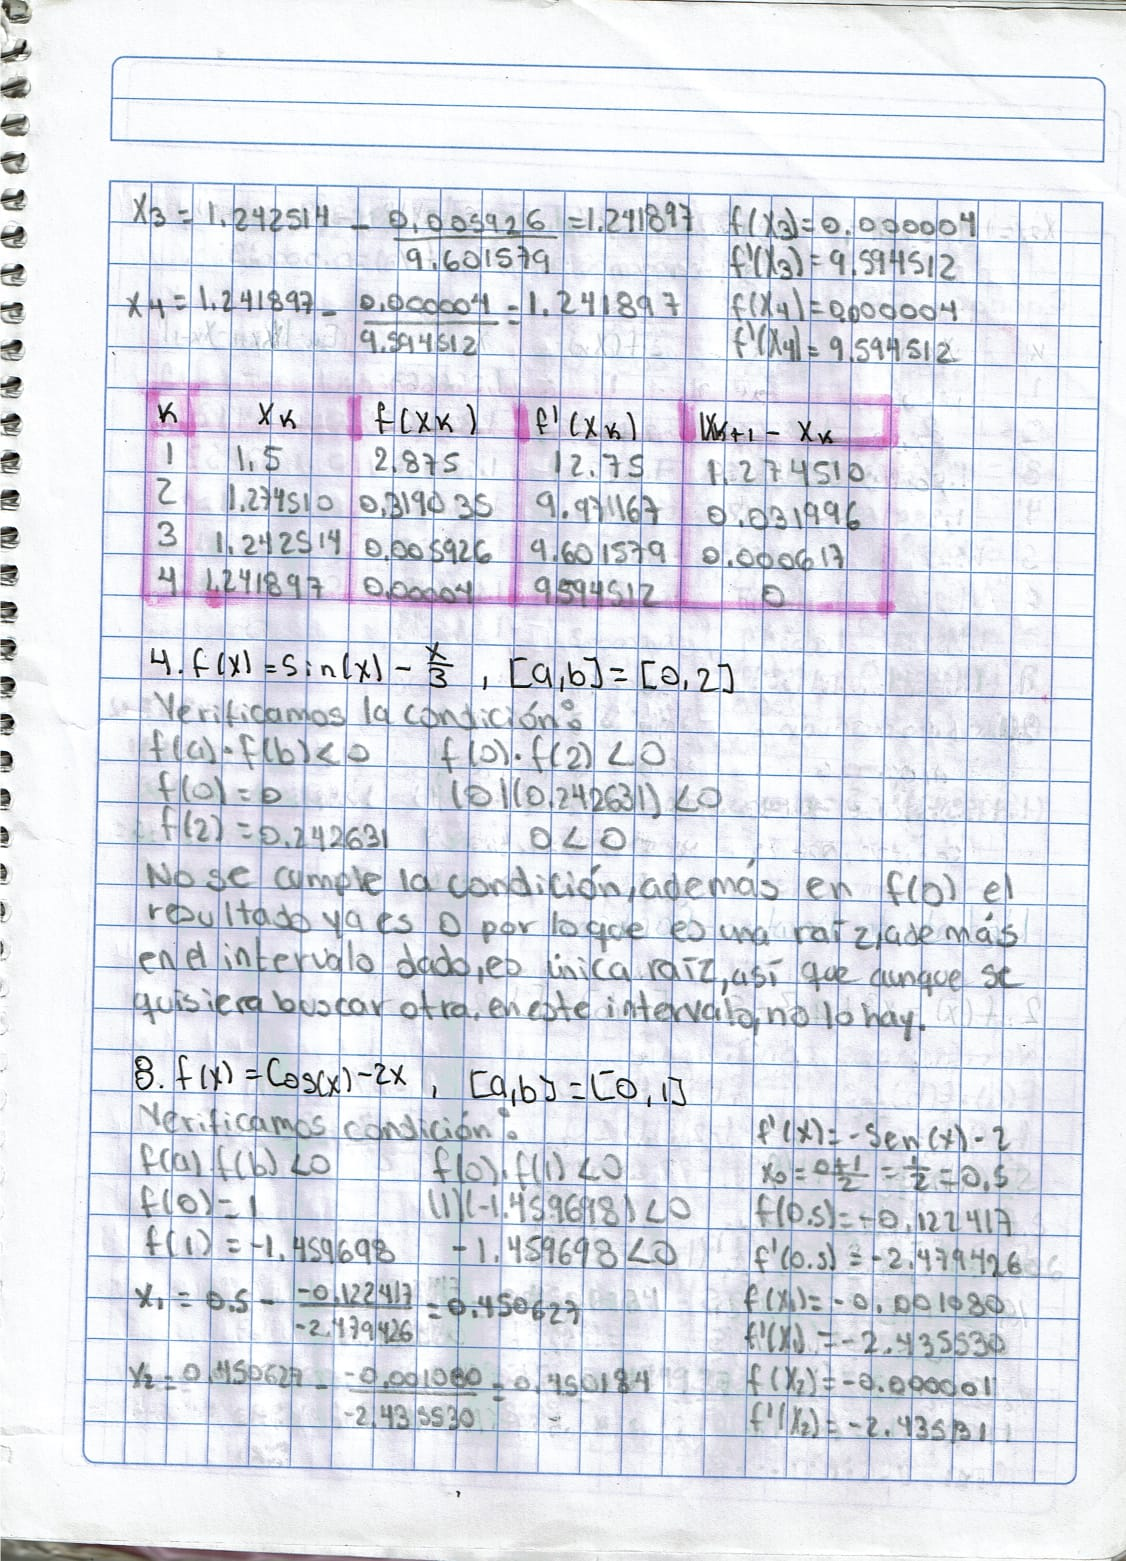
\includegraphics[width=6.25in,height=\textheight,keepaspectratio,alt={Ejercicio 2-2, 4 y 8-1}]{Newton2-4-8.jpg}
\caption{Ejercicio 2-2, 4 y 8-1}
\end{figure}

\begin{figure}
\centering
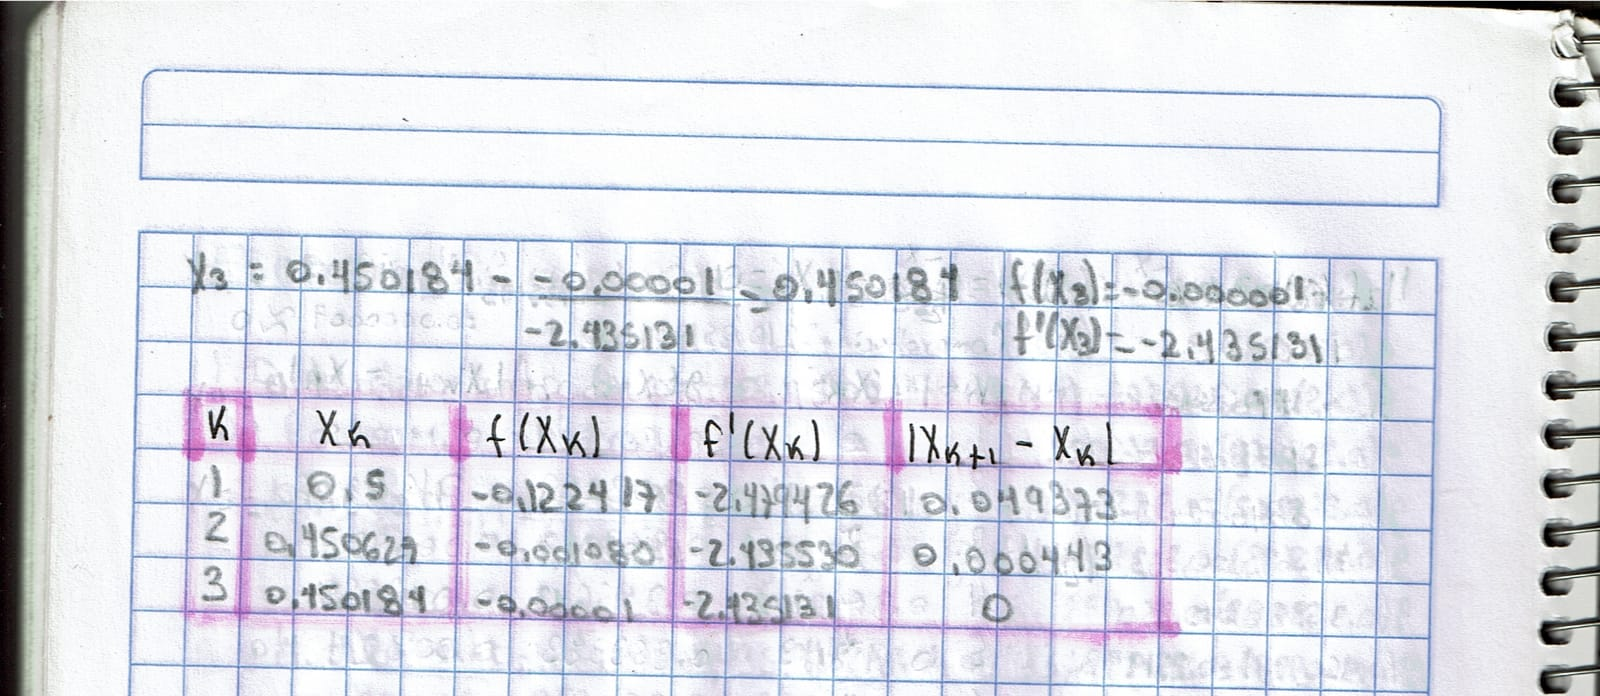
\includegraphics[width=6.25in,height=\textheight,keepaspectratio,alt={Ejercicio 8-2}]{Newton8_2.jpg}
\caption{Ejercicio 8-2}
\end{figure}

\subsubsection{Código para
implementación}\label{cuxf3digo-para-implementaciuxf3n-2}

\begin{Shaded}
\begin{Highlighting}[]
\CommentTok{\# Condición para los intervalos}

\NormalTok{condicion }\OtherTok{\textless{}{-}} \ControlFlowTok{function}\NormalTok{(a, b, f, }\AttributeTok{inicio =} \DecValTok{0}\NormalTok{, }\AttributeTok{fin =} \DecValTok{10}\NormalTok{, }\AttributeTok{paso =} \DecValTok{1}\NormalTok{) \{}
\NormalTok{  fa }\OtherTok{\textless{}{-}} \FunctionTok{f}\NormalTok{(a)}
\NormalTok{  fb }\OtherTok{\textless{}{-}} \FunctionTok{f}\NormalTok{(b)}
\NormalTok{  producto }\OtherTok{\textless{}{-}}\NormalTok{ fa }\SpecialCharTok{*}\NormalTok{ fb}
  
  \CommentTok{\# Resultados}
  \FunctionTok{cat}\NormalTok{(}\StringTok{"f(a) = f("}\NormalTok{, a, }\StringTok{") = "}\NormalTok{, fa, }\StringTok{"}\SpecialCharTok{\textbackslash{}n}\StringTok{"}\NormalTok{)}
  \FunctionTok{cat}\NormalTok{(}\StringTok{"f(b) = f("}\NormalTok{, b, }\StringTok{") = "}\NormalTok{, fb, }\StringTok{"}\SpecialCharTok{\textbackslash{}n}\StringTok{"}\NormalTok{)}
  \FunctionTok{cat}\NormalTok{(}\StringTok{"f(a) · f(b) = "}\NormalTok{, producto, }\StringTok{"}\SpecialCharTok{\textbackslash{}n}\StringTok{"}\NormalTok{)}
  \FunctionTok{cat}\NormalTok{(producto, }\StringTok{"\textless{} 0"}\NormalTok{, }\StringTok{"}\SpecialCharTok{\textbackslash{}n\textbackslash{}n}\StringTok{"}\NormalTok{)}
  
  \ControlFlowTok{if}\NormalTok{(producto }\SpecialCharTok{\textless{}} \DecValTok{0}\NormalTok{) \{}
    \FunctionTok{cat}\NormalTok{(}\StringTok{"SÍ cumple la condición.}\SpecialCharTok{\textbackslash{}n}\StringTok{"}\NormalTok{)}
    \CommentTok{\# Asignar globalmente}
\NormalTok{    a }\OtherTok{\textless{}\textless{}{-}}\NormalTok{ a}
\NormalTok{    b }\OtherTok{\textless{}\textless{}{-}}\NormalTok{ b}
    \FunctionTok{return}\NormalTok{(}\ConstantTok{TRUE}\NormalTok{)}
\NormalTok{  \} }\ControlFlowTok{else}\NormalTok{ \{}
    \FunctionTok{cat}\NormalTok{(}\StringTok{"NO cumple la condición.}\SpecialCharTok{\textbackslash{}n}\StringTok{"}\NormalTok{) }
    \FunctionTok{cat}\NormalTok{(}\StringTok{"Se buscará un nuevo intervalo.}\SpecialCharTok{\textbackslash{}n\textbackslash{}n}\StringTok{"}\NormalTok{)}
    
    \CommentTok{\# Buscar automáticamente un intervalo que sí funcione}
\NormalTok{    x }\OtherTok{\textless{}{-}} \FunctionTok{seq}\NormalTok{(inicio, fin, paso)}
    \ControlFlowTok{for}\NormalTok{ (i }\ControlFlowTok{in} \DecValTok{1}\SpecialCharTok{:}\NormalTok{(}\FunctionTok{length}\NormalTok{(x)}\SpecialCharTok{{-}}\DecValTok{1}\NormalTok{)) \{}
\NormalTok{      a\_nuevo }\OtherTok{\textless{}{-}}\NormalTok{ x[i]}
\NormalTok{      b\_nuevo }\OtherTok{\textless{}{-}}\NormalTok{ x[i}\SpecialCharTok{+}\DecValTok{1}\NormalTok{]}
      \ControlFlowTok{if}\NormalTok{ (}\FunctionTok{f}\NormalTok{(a\_nuevo) }\SpecialCharTok{*} \FunctionTok{f}\NormalTok{(b\_nuevo) }\SpecialCharTok{\textless{}} \DecValTok{0}\NormalTok{) \{}
        \FunctionTok{cat}\NormalTok{(}\StringTok{"Nuevo intervalo encontrado: ["}\NormalTok{, a\_nuevo, }\StringTok{", "}\NormalTok{, b\_nuevo, }\StringTok{"]}\SpecialCharTok{\textbackslash{}n}\StringTok{"}\NormalTok{)}
\NormalTok{        fa }\OtherTok{\textless{}{-}} \FunctionTok{f}\NormalTok{(a\_nuevo)}
\NormalTok{        fb }\OtherTok{\textless{}{-}} \FunctionTok{f}\NormalTok{(b\_nuevo)}
\NormalTok{        producto }\OtherTok{\textless{}{-}}\NormalTok{ fa }\SpecialCharTok{*}\NormalTok{ fb}
        \FunctionTok{cat}\NormalTok{(}\StringTok{"f(a) = f("}\NormalTok{, a\_nuevo, }\StringTok{") = "}\NormalTok{, fa, }\StringTok{"}\SpecialCharTok{\textbackslash{}n}\StringTok{"}\NormalTok{)}
        \FunctionTok{cat}\NormalTok{(}\StringTok{"f(b) = f("}\NormalTok{, b\_nuevo, }\StringTok{") = "}\NormalTok{, fb, }\StringTok{"}\SpecialCharTok{\textbackslash{}n}\StringTok{"}\NormalTok{)}
        \FunctionTok{cat}\NormalTok{(}\StringTok{"f(a) · f(b) = "}\NormalTok{, producto, }\StringTok{"}\SpecialCharTok{\textbackslash{}n}\StringTok{"}\NormalTok{)}
        \FunctionTok{cat}\NormalTok{(producto, }\StringTok{"\textless{} 0"}\NormalTok{, }\StringTok{"}\SpecialCharTok{\textbackslash{}n\textbackslash{}n}\StringTok{"}\NormalTok{)}
          \FunctionTok{cat}\NormalTok{(}\StringTok{"SÍ cumple la condición.}\SpecialCharTok{\textbackslash{}n}\StringTok{"}\NormalTok{)}
        \CommentTok{\# Asignar globalmente}
\NormalTok{        a }\OtherTok{\textless{}\textless{}{-}}\NormalTok{ a\_nuevo}
\NormalTok{        b }\OtherTok{\textless{}\textless{}{-}}\NormalTok{ b\_nuevo}
        \FunctionTok{return}\NormalTok{(}\ConstantTok{TRUE}\NormalTok{)}
\NormalTok{      \}}
\NormalTok{    \}}
    \FunctionTok{cat}\NormalTok{(}\StringTok{"No se encontró ningún intervalo con cambio de signo}\SpecialCharTok{\textbackslash{}n}\StringTok{"}\NormalTok{)}
    \FunctionTok{return}\NormalTok{(}\ConstantTok{FALSE}\NormalTok{)}
\NormalTok{  \}}
\NormalTok{\}}
\end{Highlighting}
\end{Shaded}

\begin{Shaded}
\begin{Highlighting}[]
\CommentTok{\# Método de Newton que guarda los valores para la tabla}

\NormalTok{newton }\OtherTok{\textless{}{-}} \ControlFlowTok{function}\NormalTok{(f, df, x0, }\AttributeTok{tol =} \FloatTok{1e{-}5}\NormalTok{, }\AttributeTok{iter\_max =} \DecValTok{100}\NormalTok{)\{}
  
\CommentTok{\# Vectores para almacenar los datos de las iteraciones}
  
\NormalTok{  iter\_vec }\OtherTok{\textless{}{-}} \FunctionTok{numeric}\NormalTok{(}\DecValTok{0}\NormalTok{)}
\NormalTok{  x0\_vec }\OtherTok{\textless{}{-}} \FunctionTok{numeric}\NormalTok{(}\DecValTok{0}\NormalTok{)}
\NormalTok{  x1\_vec }\OtherTok{\textless{}{-}} \FunctionTok{numeric}\NormalTok{(}\DecValTok{0}\NormalTok{)}
\NormalTok{  fx0\_vec }\OtherTok{\textless{}{-}} \FunctionTok{numeric}\NormalTok{(}\DecValTok{0}\NormalTok{)}
\NormalTok{  dfx0\_vec }\OtherTok{\textless{}{-}} \FunctionTok{numeric}\NormalTok{(}\DecValTok{0}\NormalTok{)}
\NormalTok{  error\_vec }\OtherTok{\textless{}{-}} \FunctionTok{numeric}\NormalTok{(}\DecValTok{0}\NormalTok{)}
  
\NormalTok{  iter }\OtherTok{\textless{}{-}} \DecValTok{0}
\NormalTok{  error }\OtherTok{\textless{}{-}} \DecValTok{1}
  
  \ControlFlowTok{while}\NormalTok{(error }\SpecialCharTok{\textgreater{}}\NormalTok{ tol }\SpecialCharTok{\&\&}\NormalTok{ iter }\SpecialCharTok{\textless{}}\NormalTok{ iter\_max)\{}
    
\NormalTok{    fx0 }\OtherTok{\textless{}{-}} \FunctionTok{f}\NormalTok{(x0)}
\NormalTok{    dfx0 }\OtherTok{\textless{}{-}} \FunctionTok{df}\NormalTok{(x0)}
    
\CommentTok{\# Evitar división por cero}
    
    \ControlFlowTok{if}\NormalTok{(}\FunctionTok{abs}\NormalTok{(dfx0) }\SpecialCharTok{\textless{}} \FloatTok{1e{-}12}\NormalTok{)\{}
      \FunctionTok{cat}\NormalTok{(}\StringTok{"Error: Derivada cercana a cero}\SpecialCharTok{\textbackslash{}n}\StringTok{"}\NormalTok{)}
      \FunctionTok{return}\NormalTok{(}\ConstantTok{NA}\NormalTok{)}
\NormalTok{    \}}
    
\CommentTok{\# Aplicar fórmula de Newton}
    
\NormalTok{    x1 }\OtherTok{\textless{}{-}}\NormalTok{ x0 }\SpecialCharTok{{-}}\NormalTok{ fx0 }\SpecialCharTok{/}\NormalTok{ dfx0}
\NormalTok{    error }\OtherTok{\textless{}{-}} \FunctionTok{abs}\NormalTok{(x1 }\SpecialCharTok{{-}}\NormalTok{ x0)}
    
\CommentTok{\# Almacena los datos de cada iteración}
    
\NormalTok{    iter }\OtherTok{\textless{}{-}}\NormalTok{ iter }\SpecialCharTok{+} \DecValTok{1}
\NormalTok{    iter\_vec }\OtherTok{\textless{}{-}} \FunctionTok{c}\NormalTok{(iter\_vec, iter)}
\NormalTok{    x0\_vec }\OtherTok{\textless{}{-}} \FunctionTok{c}\NormalTok{(x0\_vec, x0)}
\NormalTok{    fx0\_vec }\OtherTok{\textless{}{-}} \FunctionTok{c}\NormalTok{(fx0\_vec, fx0)}
\NormalTok{    dfx0\_vec }\OtherTok{\textless{}{-}} \FunctionTok{c}\NormalTok{(dfx0\_vec, dfx0)}
\NormalTok{    error\_vec }\OtherTok{\textless{}{-}} \FunctionTok{c}\NormalTok{(error\_vec, error)}
    
\CommentTok{\# Actualizar para siguiente iteración}
    
\NormalTok{    x0 }\OtherTok{\textless{}{-}}\NormalTok{ x1}
\NormalTok{  \}}
  
\CommentTok{\# Crea la tabla de las iteraciones}
  
\NormalTok{ TAB }\OtherTok{\textless{}{-}} \FunctionTok{data.frame}\NormalTok{(}
    \StringTok{"k"} \OtherTok{=}\NormalTok{ iter\_vec,}
    \StringTok{"xₖ"} \OtherTok{=}\NormalTok{x0\_vec,}
    \StringTok{"f(xₖ)"} \OtherTok{=}\NormalTok{ fx0\_vec,}
    \StringTok{"f´(xₖ)"} \OtherTok{=}\NormalTok{ dfx0\_vec,}
    \StringTok{"eₖ = |xₖ₊₁ {-} xₖ|"} \OtherTok{=}\NormalTok{ error\_vec,}
    \AttributeTok{check.names =} \ConstantTok{FALSE}
\NormalTok{  )}
  
  \FunctionTok{cat}\NormalTok{(}\StringTok{"Raíz aproximada:"}\NormalTok{, x1, }\StringTok{"}\SpecialCharTok{\textbackslash{}n}\StringTok{"}\NormalTok{)}
  \FunctionTok{cat}\NormalTok{(}\StringTok{"Iteraciones:"}\NormalTok{, iter, }\StringTok{"}\SpecialCharTok{\textbackslash{}n\textbackslash{}n}\StringTok{"}\NormalTok{)}
  
  \FunctionTok{return}\NormalTok{(}\FunctionTok{list}\NormalTok{(}\AttributeTok{raiz =}\NormalTok{ x1, }\AttributeTok{iteraciones =}\NormalTok{ iter, }\AttributeTok{tabla =}\NormalTok{ TAB))}
\NormalTok{\}}
\end{Highlighting}
\end{Shaded}

\begin{Shaded}
\begin{Highlighting}[]
\CommentTok{\# Tabla "bonita"}

\NormalTok{tabla }\OtherTok{\textless{}{-}} \ControlFlowTok{function}\NormalTok{(resultado) \{}
  \FunctionTok{library}\NormalTok{(DT)}
  
  \FunctionTok{datatable}\NormalTok{(}
\NormalTok{    resultado}\SpecialCharTok{$}\NormalTok{tabla,}
    \AttributeTok{options =} \FunctionTok{list}\NormalTok{(}
      \AttributeTok{scrollX =} \ConstantTok{TRUE}\NormalTok{,}
      \AttributeTok{scrollY =} \StringTok{"400px"}\NormalTok{, }
      \AttributeTok{paging =} \ConstantTok{FALSE}\NormalTok{,}
      \AttributeTok{dom =} \StringTok{\textquotesingle{}t\textquotesingle{}}\NormalTok{,}
      \AttributeTok{autoWidth =} \ConstantTok{FALSE}\NormalTok{,}
      \AttributeTok{columnDefs =} \FunctionTok{list}\NormalTok{(}
        \FunctionTok{list}\NormalTok{(}\AttributeTok{className =} \StringTok{\textquotesingle{}dt{-}center\textquotesingle{}}\NormalTok{, }\AttributeTok{targets =} \DecValTok{0}\SpecialCharTok{:}\DecValTok{4}\NormalTok{))}
\NormalTok{    ),}
    \AttributeTok{rownames =} \ConstantTok{FALSE}\NormalTok{,}
    \AttributeTok{class =} \StringTok{\textquotesingle{}cell{-}border stripe\textquotesingle{}}\NormalTok{,}
    \AttributeTok{width =} \StringTok{"100\%"}\NormalTok{,}
    \AttributeTok{caption =} \StringTok{"Tabla de iteraciones en el método de la Newton{-}Raphson"}\NormalTok{,}
    \AttributeTok{escape =} \ConstantTok{FALSE}
\NormalTok{  ) }\SpecialCharTok{\%\textgreater{}\%}
     \FunctionTok{formatRound}\NormalTok{(}\AttributeTok{columns =} \FunctionTok{c}\NormalTok{(}\DecValTok{2}\SpecialCharTok{:}\DecValTok{5}\NormalTok{), }\AttributeTok{digits =} \DecValTok{9}\NormalTok{)}
\NormalTok{\}}
\end{Highlighting}
\end{Shaded}

\begin{Shaded}
\begin{Highlighting}[]
\CommentTok{\# Gráficas}

\NormalTok{grafica }\OtherTok{\textless{}{-}} \ControlFlowTok{function}\NormalTok{(x0, f, df, resultado) \{}
\NormalTok{  tabla\_iteraciones }\OtherTok{\textless{}{-}}\NormalTok{ resultado}\SpecialCharTok{$}\NormalTok{tabla}
\NormalTok{  total\_iteraciones }\OtherTok{\textless{}{-}} \FunctionTok{nrow}\NormalTok{(tabla\_iteraciones)}
\NormalTok{  filas }\OtherTok{\textless{}{-}} \FunctionTok{ceiling}\NormalTok{(total\_iteraciones }\SpecialCharTok{/} \DecValTok{4}\NormalTok{)}
  
  \FunctionTok{par}\NormalTok{(}\AttributeTok{mfrow =} \FunctionTok{c}\NormalTok{(filas, }\DecValTok{4}\NormalTok{), }\AttributeTok{mar =} \FunctionTok{c}\NormalTok{(}\DecValTok{2}\NormalTok{, }\DecValTok{2}\NormalTok{, }\FloatTok{1.5}\NormalTok{, }\DecValTok{1}\NormalTok{))}
  
\CommentTok{\# Calcular rango dinámico}
  
\NormalTok{  x\_min }\OtherTok{\textless{}{-}} \FunctionTok{min}\NormalTok{(tabla\_iteraciones[,}\DecValTok{2}\NormalTok{]) }\SpecialCharTok{{-}} \FloatTok{0.5}
\NormalTok{  x\_max }\OtherTok{\textless{}{-}} \FunctionTok{max}\NormalTok{(tabla\_iteraciones[,}\DecValTok{2}\NormalTok{]) }\SpecialCharTok{+} \FloatTok{0.5}
\NormalTok{  x\_vals }\OtherTok{\textless{}{-}} \FunctionTok{seq}\NormalTok{(x\_min, x\_max, }\AttributeTok{length.out =} \DecValTok{1000}\NormalTok{)}
\NormalTok{  y\_vals }\OtherTok{\textless{}{-}} \FunctionTok{f}\NormalTok{(x\_vals)}
  
  \ControlFlowTok{for}\NormalTok{ (i }\ControlFlowTok{in} \DecValTok{1}\SpecialCharTok{:}\NormalTok{total\_iteraciones) \{}
    \FunctionTok{plot}\NormalTok{(x\_vals, y\_vals, }\AttributeTok{type =} \StringTok{"l"}\NormalTok{, }\AttributeTok{main =} \FunctionTok{paste}\NormalTok{(}\StringTok{"Iteración"}\NormalTok{, i),}
         \AttributeTok{xlab =} \StringTok{"x"}\NormalTok{, }\AttributeTok{ylab =} \StringTok{"f(x)"}\NormalTok{, }\AttributeTok{col =} \StringTok{"blue"}\NormalTok{, }\AttributeTok{lwd =} \FloatTok{1.2}\NormalTok{)}
    \FunctionTok{abline}\NormalTok{(}\AttributeTok{h =} \DecValTok{0}\NormalTok{, }\AttributeTok{col =} \StringTok{"gray"}\NormalTok{, }\AttributeTok{lty =} \DecValTok{2}\NormalTok{)}

\NormalTok{    x\_actual }\OtherTok{\textless{}{-}}\NormalTok{ tabla\_iteraciones[i, }\DecValTok{2}\NormalTok{]    }\CommentTok{\# x\_k}
\NormalTok{    f\_actual }\OtherTok{\textless{}{-}}\NormalTok{ tabla\_iteraciones[i, }\DecValTok{3}\NormalTok{]    }\CommentTok{\# f(x\_k)}
\NormalTok{    df\_actual }\OtherTok{\textless{}{-}}\NormalTok{ tabla\_iteraciones[i, }\DecValTok{4}\NormalTok{]   }\CommentTok{\# f\textquotesingle{}(x\_k)}
    
\CommentTok{\# Calcular recta tangente}
    
\NormalTok{    pendiente }\OtherTok{\textless{}{-}}\NormalTok{ df\_actual}
\NormalTok{    intercepto }\OtherTok{\textless{}{-}}\NormalTok{ f\_actual }\SpecialCharTok{{-}}\NormalTok{ pendiente }\SpecialCharTok{*}\NormalTok{ x\_actual}
\NormalTok{    y\_tangente }\OtherTok{\textless{}{-}}\NormalTok{ pendiente }\SpecialCharTok{*}\NormalTok{ x\_vals }\SpecialCharTok{+}\NormalTok{ intercepto}
    
\CommentTok{\# Graficar recta tangente}
    
    \FunctionTok{lines}\NormalTok{(x\_vals, y\_tangente, }\AttributeTok{col =} \StringTok{"purple"}\NormalTok{, }\AttributeTok{lty =} \DecValTok{2}\NormalTok{, }\AttributeTok{lwd =} \FloatTok{1.5}\NormalTok{)}
    
\CommentTok{\# Puntos de la iteración}
    
    \FunctionTok{points}\NormalTok{(x\_actual, f\_actual, }\AttributeTok{col =} \StringTok{"red"}\NormalTok{, }\AttributeTok{pch =} \DecValTok{19}\NormalTok{, }\AttributeTok{cex =} \FloatTok{0.8}\NormalTok{)}
    
\CommentTok{\# Línea vertical}
    
    \FunctionTok{abline}\NormalTok{(}\AttributeTok{v =}\NormalTok{ x\_actual, }\AttributeTok{col =} \StringTok{"red"}\NormalTok{, }\AttributeTok{lty =} \DecValTok{3}\NormalTok{, }\AttributeTok{lwd =} \FloatTok{0.8}\NormalTok{)}
    
\CommentTok{\# Leyenda}
    
    \FunctionTok{legend}\NormalTok{(}\StringTok{"topright"}\NormalTok{, }
           \AttributeTok{legend =} \FunctionTok{c}\NormalTok{(}\StringTok{"f(x)"}\NormalTok{, }\StringTok{"Tangente"}\NormalTok{, }\StringTok{"x\_k"}\NormalTok{),}
           \AttributeTok{col =} \FunctionTok{c}\NormalTok{(}\StringTok{"blue"}\NormalTok{, }\StringTok{"purple"}\NormalTok{, }\StringTok{"red"}\NormalTok{),}
           \AttributeTok{lty =} \FunctionTok{c}\NormalTok{(}\DecValTok{1}\NormalTok{, }\DecValTok{2}\NormalTok{, }\ConstantTok{NA}\NormalTok{), }\AttributeTok{pch =} \FunctionTok{c}\NormalTok{(}\ConstantTok{NA}\NormalTok{, }\ConstantTok{NA}\NormalTok{, }\DecValTok{19}\NormalTok{),}
           \AttributeTok{cex =} \FloatTok{0.7}\NormalTok{, }\AttributeTok{bty =} \StringTok{"n"}\NormalTok{)}
\NormalTok{  \}}
  
  \FunctionTok{par}\NormalTok{(}\AttributeTok{mfrow =} \FunctionTok{c}\NormalTok{(}\DecValTok{1}\NormalTok{, }\DecValTok{1}\NormalTok{))}
\NormalTok{\}}
\end{Highlighting}
\end{Shaded}

\subsubsection{\texorpdfstring{Sistema
\(1\)}{Sistema 1}}\label{sistema-1-6}

\(f(x) = x^3 - 7x + 6\) en \([a, b] = [0, 1]\)

\begin{Shaded}
\begin{Highlighting}[]
\CommentTok{\# Datos}

\NormalTok{a }\OtherTok{\textless{}{-}} \DecValTok{0}
\NormalTok{b }\OtherTok{\textless{}{-}} \DecValTok{1}
\NormalTok{x0 }\OtherTok{\textless{}{-}}\NormalTok{ (a }\SpecialCharTok{+}\NormalTok{ b) }\SpecialCharTok{/} \DecValTok{2}
\NormalTok{f }\OtherTok{\textless{}{-}} \ControlFlowTok{function}\NormalTok{(x) x}\SpecialCharTok{\^{}}\DecValTok{3} \SpecialCharTok{{-}} \DecValTok{7}\SpecialCharTok{*}\NormalTok{x }\SpecialCharTok{+} \DecValTok{6}
\NormalTok{df }\OtherTok{\textless{}{-}} \ControlFlowTok{function}\NormalTok{(x) }\DecValTok{3}\SpecialCharTok{*}\NormalTok{x}\SpecialCharTok{\^{}}\DecValTok{2} \SpecialCharTok{{-}} \DecValTok{7}
\end{Highlighting}
\end{Shaded}

\paragraph{Intervalo}\label{intervalo-5}

Verifica que exista un intervalo \([a, b]\) donde \(f(a) · f(b) < 0\).

Nota: En la información dada ya nos da un intervalo, por lo que solo se
revisa si cumple con la condición:

\begin{Shaded}
\begin{Highlighting}[]
\FunctionTok{condicion}\NormalTok{(a, b, f)}
\end{Highlighting}
\end{Shaded}

\begin{verbatim}
## f(a) = f( 0 ) =  6 
## f(b) = f( 1 ) =  0 
## f(a) · f(b) =  0 
## 0 < 0 
## 
## NO cumple la condición.
## Se buscará un nuevo intervalo.
## 
## No se encontró ningún intervalo con cambio de signo
\end{verbatim}

\begin{verbatim}
## [1] FALSE
\end{verbatim}

En este caso la raíz está justo en el extremo del intervalo en \(x=1\)
por lo cual, la condición da exactamente \(0\).

\paragraph{Iteraciones}\label{iteraciones-10}

Realice al menos 8 iteraciones del método.

\begin{Shaded}
\begin{Highlighting}[]
\NormalTok{resultado }\OtherTok{\textless{}{-}} \FunctionTok{newton}\NormalTok{(f, df, x0)}
\end{Highlighting}
\end{Shaded}

\begin{verbatim}
## Raíz aproximada: 1 
## Iteraciones: 5
\end{verbatim}

\paragraph{Tabla}\label{tabla-5}

Registre los valores \(x_k\), \(f(x_k)\), \(f´(x_k)\), y el error
\(|bk − ak|\).

\begin{Shaded}
\begin{Highlighting}[]
\FunctionTok{tabla}\NormalTok{(resultado)}
\end{Highlighting}
\end{Shaded}

\pandocbounded{\includegraphics[keepaspectratio]{PortafolioDLPF_pdf_files/figure-latex/unnamed-chunk-1202-1.pdf}}

\paragraph{Gráficas}\label{gruxe1ficas-10}

Grafica la función y marca el punto donde converge la raíz.

\begin{Shaded}
\begin{Highlighting}[]
\FunctionTok{grafica}\NormalTok{(x0, f, df, resultado)}
\end{Highlighting}
\end{Shaded}

\pandocbounded{\includegraphics[keepaspectratio]{PortafolioDLPF_pdf_files/figure-latex/unnamed-chunk-1203-1.pdf}}

\subsubsection{\texorpdfstring{Sistema
\(3\)}{Sistema 3}}\label{sistema-3-6}

\(f(x) = x^4 - 3x^3 + 2\) en \([a, b] = [0, 1]\)

\begin{Shaded}
\begin{Highlighting}[]
\CommentTok{\# Datos}

\NormalTok{a }\OtherTok{\textless{}{-}} \DecValTok{0}
\NormalTok{b }\OtherTok{\textless{}{-}} \DecValTok{1}
\NormalTok{x0 }\OtherTok{\textless{}{-}}\NormalTok{ (a }\SpecialCharTok{+}\NormalTok{ b) }\SpecialCharTok{/} \DecValTok{2}
\NormalTok{f }\OtherTok{\textless{}{-}} \ControlFlowTok{function}\NormalTok{(x) x}\SpecialCharTok{\^{}}\DecValTok{4} \SpecialCharTok{{-}} \DecValTok{3}\SpecialCharTok{*}\NormalTok{x}\SpecialCharTok{\^{}}\DecValTok{3} \SpecialCharTok{+} \DecValTok{2}
\NormalTok{df }\OtherTok{\textless{}{-}} \ControlFlowTok{function}\NormalTok{(x) }\DecValTok{4}\SpecialCharTok{*}\NormalTok{x}\SpecialCharTok{\^{}}\DecValTok{3} \SpecialCharTok{{-}} \DecValTok{9}\SpecialCharTok{*}\NormalTok{x}\SpecialCharTok{\^{}}\DecValTok{2}
\end{Highlighting}
\end{Shaded}

\paragraph{Intervalo}\label{intervalo-6}

Verifica que exista un intervalo \([a, b]\) donde \(f(a) · f(b) < 0\).

Nota: En la información dada ya nos da un intervalo, por lo que solo se
revisa si cumple con la condición:

\begin{Shaded}
\begin{Highlighting}[]
\FunctionTok{condicion}\NormalTok{(a, b, f)}
\end{Highlighting}
\end{Shaded}

\begin{verbatim}
## f(a) = f( 0 ) =  2 
## f(b) = f( 1 ) =  0 
## f(a) · f(b) =  0 
## 0 < 0 
## 
## NO cumple la condición.
## Se buscará un nuevo intervalo.
## 
## Nuevo intervalo encontrado: [ 2 ,  3 ]
## f(a) = f( 2 ) =  -6 
## f(b) = f( 3 ) =  2 
## f(a) · f(b) =  -12 
## -12 < 0 
## 
## SÍ cumple la condición.
\end{verbatim}

\begin{verbatim}
## [1] TRUE
\end{verbatim}

En este caso la raíz está justo en el extremo del intervalo en \(x=1\)
por lo cual, la condición da exactamente \(0\). Y al buscar el nuevo
intervalo, nos da aquel en donde se encuentra otra de las raíces.

\paragraph{Iteraciones}\label{iteraciones-11}

Realice al menos 8 iteraciones del método.

\begin{Shaded}
\begin{Highlighting}[]
\NormalTok{resultado }\OtherTok{\textless{}{-}} \FunctionTok{newton}\NormalTok{(f, df, x0)}
\end{Highlighting}
\end{Shaded}

\begin{verbatim}
## Raíz aproximada: 1 
## Iteraciones: 5
\end{verbatim}

\paragraph{Tabla}\label{tabla-6}

Registre los valores \(x_k\), \(f(x_k)\), \(f´(x_k)\), y el error
\(|bk − ak|\).

\begin{Shaded}
\begin{Highlighting}[]
\FunctionTok{tabla}\NormalTok{(resultado)}
\end{Highlighting}
\end{Shaded}

\pandocbounded{\includegraphics[keepaspectratio]{PortafolioDLPF_pdf_files/figure-latex/unnamed-chunk-1207-1.pdf}}

\paragraph{Gráficas}\label{gruxe1ficas-11}

Grafica la función y marca el punto donde converge la raíz.

\begin{Shaded}
\begin{Highlighting}[]
\FunctionTok{grafica}\NormalTok{(x0, f, df, resultado)}
\end{Highlighting}
\end{Shaded}

\pandocbounded{\includegraphics[keepaspectratio]{PortafolioDLPF_pdf_files/figure-latex/unnamed-chunk-1208-1.pdf}}

\subsubsection{\texorpdfstring{Sistema
\(5\)}{Sistema 5}}\label{sistema-5-6}

\(f(x) = e^{-x} - x\) en \([a, b] = [0, 1]\)

\begin{Shaded}
\begin{Highlighting}[]
\CommentTok{\# Datos}

\NormalTok{a }\OtherTok{\textless{}{-}} \DecValTok{0}
\NormalTok{b }\OtherTok{\textless{}{-}} \DecValTok{1}
\NormalTok{x0 }\OtherTok{\textless{}{-}}\NormalTok{ (a }\SpecialCharTok{+}\NormalTok{ b) }\SpecialCharTok{/} \DecValTok{2}
\NormalTok{f }\OtherTok{\textless{}{-}} \ControlFlowTok{function}\NormalTok{(x) }\FunctionTok{exp}\NormalTok{(}\SpecialCharTok{{-}}\NormalTok{x) }\SpecialCharTok{{-}}\NormalTok{ x}
\NormalTok{df }\OtherTok{\textless{}{-}} \ControlFlowTok{function}\NormalTok{(x) }\SpecialCharTok{{-}}\FunctionTok{exp}\NormalTok{(}\SpecialCharTok{{-}}\NormalTok{x) }\SpecialCharTok{{-}} \DecValTok{1} 
\end{Highlighting}
\end{Shaded}

\paragraph{Intervalo}\label{intervalo-7}

Verifica que exista un intervalo \([a, b]\) donde \(f(a) · f(b) < 0\).

\begin{Shaded}
\begin{Highlighting}[]
\FunctionTok{condicion}\NormalTok{(a, b, f)}
\end{Highlighting}
\end{Shaded}

\begin{verbatim}
## f(a) = f( 0 ) =  1 
## f(b) = f( 1 ) =  -0.6321206 
## f(a) · f(b) =  -0.6321206 
## -0.6321206 < 0 
## 
## SÍ cumple la condición.
\end{verbatim}

\begin{verbatim}
## [1] TRUE
\end{verbatim}

\paragraph{Iteraciones}\label{iteraciones-12}

Realice al menos 8 iteraciones del método.

\begin{Shaded}
\begin{Highlighting}[]
\NormalTok{resultado }\OtherTok{\textless{}{-}} \FunctionTok{newton}\NormalTok{(f, df, x0)}
\end{Highlighting}
\end{Shaded}

\begin{verbatim}
## Raíz aproximada: 0.5671433 
## Iteraciones: 3
\end{verbatim}

\paragraph{Tabla}\label{tabla-7}

Registre los valores \(x_k\), \(f(x_k)\), \(f´(x_k)\), y el error
\(|bk − ak|\).

\begin{Shaded}
\begin{Highlighting}[]
\FunctionTok{tabla}\NormalTok{(resultado)}
\end{Highlighting}
\end{Shaded}

\pandocbounded{\includegraphics[keepaspectratio]{PortafolioDLPF_pdf_files/figure-latex/unnamed-chunk-1212-1.pdf}}

\paragraph{Gráficas}\label{gruxe1ficas-12}

Grafica la función y marca el punto donde converge la raíz.

\begin{Shaded}
\begin{Highlighting}[]
\FunctionTok{grafica}\NormalTok{(x0, f, df, resultado)}
\end{Highlighting}
\end{Shaded}

\pandocbounded{\includegraphics[keepaspectratio]{PortafolioDLPF_pdf_files/figure-latex/unnamed-chunk-1213-1.pdf}}

\subsubsection{\texorpdfstring{Sistema
\(7\)}{Sistema 7}}\label{sistema-7-6}

\(f(x) = x^5 − 3x + 1\) en \([a, b] = [0, 1]\)

\begin{Shaded}
\begin{Highlighting}[]
\CommentTok{\# Datos}

\NormalTok{a }\OtherTok{\textless{}{-}} \DecValTok{0}
\NormalTok{b }\OtherTok{\textless{}{-}} \DecValTok{1}
\NormalTok{x0 }\OtherTok{\textless{}{-}}\NormalTok{ (a }\SpecialCharTok{+}\NormalTok{ b) }\SpecialCharTok{/} \DecValTok{2}
\NormalTok{f }\OtherTok{\textless{}{-}} \ControlFlowTok{function}\NormalTok{(x) x}\SpecialCharTok{\^{}}\DecValTok{5} \SpecialCharTok{{-}} \DecValTok{3}\SpecialCharTok{*}\NormalTok{x }\SpecialCharTok{+} \DecValTok{1}
\NormalTok{df }\OtherTok{\textless{}{-}} \ControlFlowTok{function}\NormalTok{(x) }\DecValTok{5}\SpecialCharTok{*}\NormalTok{x}\SpecialCharTok{\^{}}\DecValTok{4} \SpecialCharTok{{-}} \DecValTok{3} 
\end{Highlighting}
\end{Shaded}

\paragraph{Intervalo}\label{intervalo-8}

Verifica que exista un intervalo \([a, b]\) donde \(f(a) · f(b) < 0\).

\begin{Shaded}
\begin{Highlighting}[]
\FunctionTok{condicion}\NormalTok{(a, b, f)}
\end{Highlighting}
\end{Shaded}

\begin{verbatim}
## f(a) = f( 0 ) =  1 
## f(b) = f( 1 ) =  -1 
## f(a) · f(b) =  -1 
## -1 < 0 
## 
## SÍ cumple la condición.
\end{verbatim}

\begin{verbatim}
## [1] TRUE
\end{verbatim}

\paragraph{Iteraciones}\label{iteraciones-13}

Realice al menos 8 iteraciones del método.

\begin{Shaded}
\begin{Highlighting}[]
\NormalTok{resultado }\OtherTok{\textless{}{-}} \FunctionTok{newton}\NormalTok{(f, df, x0)}
\end{Highlighting}
\end{Shaded}

\begin{verbatim}
## Raíz aproximada: 0.3347341 
## Iteraciones: 4
\end{verbatim}

\paragraph{Tabla}\label{tabla-8}

Registre los valores \(x_k\), \(f(x_k)\), \(f´(x_k)\), y el error
\(|bk − ak|\).

\begin{Shaded}
\begin{Highlighting}[]
\FunctionTok{tabla}\NormalTok{(resultado)}
\end{Highlighting}
\end{Shaded}

\pandocbounded{\includegraphics[keepaspectratio]{PortafolioDLPF_pdf_files/figure-latex/unnamed-chunk-1217-1.pdf}}

\paragraph{Gráficas}\label{gruxe1ficas-13}

Grafica la función y marca el punto donde converge la raíz.

\begin{Shaded}
\begin{Highlighting}[]
\FunctionTok{grafica}\NormalTok{(x0, f, df, resultado)}
\end{Highlighting}
\end{Shaded}

\pandocbounded{\includegraphics[keepaspectratio]{PortafolioDLPF_pdf_files/figure-latex/unnamed-chunk-1218-1.pdf}}

\subsubsection{\texorpdfstring{Sistema
\(9\)}{Sistema 9}}\label{sistema-9-6}

\(f(x) = ln(x + 2) + x - 1\) en \([a, b] = [-1, 0]\)

\begin{Shaded}
\begin{Highlighting}[]
\CommentTok{\# Datos}

\NormalTok{a }\OtherTok{\textless{}{-}} \SpecialCharTok{{-}}\DecValTok{1}
\NormalTok{b }\OtherTok{\textless{}{-}} \DecValTok{0}
\NormalTok{x0 }\OtherTok{\textless{}{-}}\NormalTok{ (a }\SpecialCharTok{+}\NormalTok{ b) }\SpecialCharTok{/} \DecValTok{2}
\NormalTok{f }\OtherTok{\textless{}{-}} \ControlFlowTok{function}\NormalTok{(x) }\FunctionTok{log}\NormalTok{(x }\SpecialCharTok{+} \DecValTok{2}\NormalTok{) }\SpecialCharTok{+}\NormalTok{ x }\SpecialCharTok{{-}} \DecValTok{1}
\NormalTok{df }\OtherTok{\textless{}{-}} \ControlFlowTok{function}\NormalTok{(x) }\DecValTok{1}\SpecialCharTok{/}\NormalTok{(x }\SpecialCharTok{+} \DecValTok{2}\NormalTok{) }\SpecialCharTok{+} \DecValTok{1}
\end{Highlighting}
\end{Shaded}

\paragraph{Intervalo}\label{intervalo-9}

Verifica que exista un intervalo \([a, b]\) donde \(f(a) · f(b) < 0\).

\begin{Shaded}
\begin{Highlighting}[]
\FunctionTok{condicion}\NormalTok{(a, b, f)}
\end{Highlighting}
\end{Shaded}

\begin{verbatim}
## f(a) = f( -1 ) =  -2 
## f(b) = f( 0 ) =  -0.3068528 
## f(a) · f(b) =  0.6137056 
## 0.6137056 < 0 
## 
## NO cumple la condición.
## Se buscará un nuevo intervalo.
## 
## Nuevo intervalo encontrado: [ 0 ,  1 ]
## f(a) = f( 0 ) =  -0.3068528 
## f(b) = f( 1 ) =  1.098612 
## f(a) · f(b) =  -0.3371123 
## -0.3371123 < 0 
## 
## SÍ cumple la condición.
\end{verbatim}

\begin{verbatim}
## [1] TRUE
\end{verbatim}

\paragraph{Iteraciones}\label{iteraciones-14}

Realice al menos 8 iteraciones del método.

\begin{Shaded}
\begin{Highlighting}[]
\NormalTok{resultado }\OtherTok{\textless{}{-}} \FunctionTok{newton}\NormalTok{(f, df, x0)}
\end{Highlighting}
\end{Shaded}

\begin{verbatim}
## Raíz aproximada: 0.20794 
## Iteraciones: 4
\end{verbatim}

\paragraph{Tabla}\label{tabla-9}

Registre los valores \(x_k\), \(f(x_k)\), \(f´(x_k)\), y el error
\(|bk − ak|\).

\begin{Shaded}
\begin{Highlighting}[]
\FunctionTok{tabla}\NormalTok{(resultado)}
\end{Highlighting}
\end{Shaded}

\pandocbounded{\includegraphics[keepaspectratio]{PortafolioDLPF_pdf_files/figure-latex/unnamed-chunk-1222-1.pdf}}

\paragraph{Gráficas}\label{gruxe1ficas-14}

Grafica la función y marca el punto donde converge la raíz.

\begin{Shaded}
\begin{Highlighting}[]
\FunctionTok{grafica}\NormalTok{(x0, f, df, resultado)}
\end{Highlighting}
\end{Shaded}

\pandocbounded{\includegraphics[keepaspectratio]{PortafolioDLPF_pdf_files/figure-latex/unnamed-chunk-1223-1.pdf}}

\subsection{Método del Punto Fijo}\label{muxe9todo-del-punto-fijo}

\subsubsection{Ejercicios a mano}\label{ejercicios-a-mano-9}

\begin{figure}
\centering
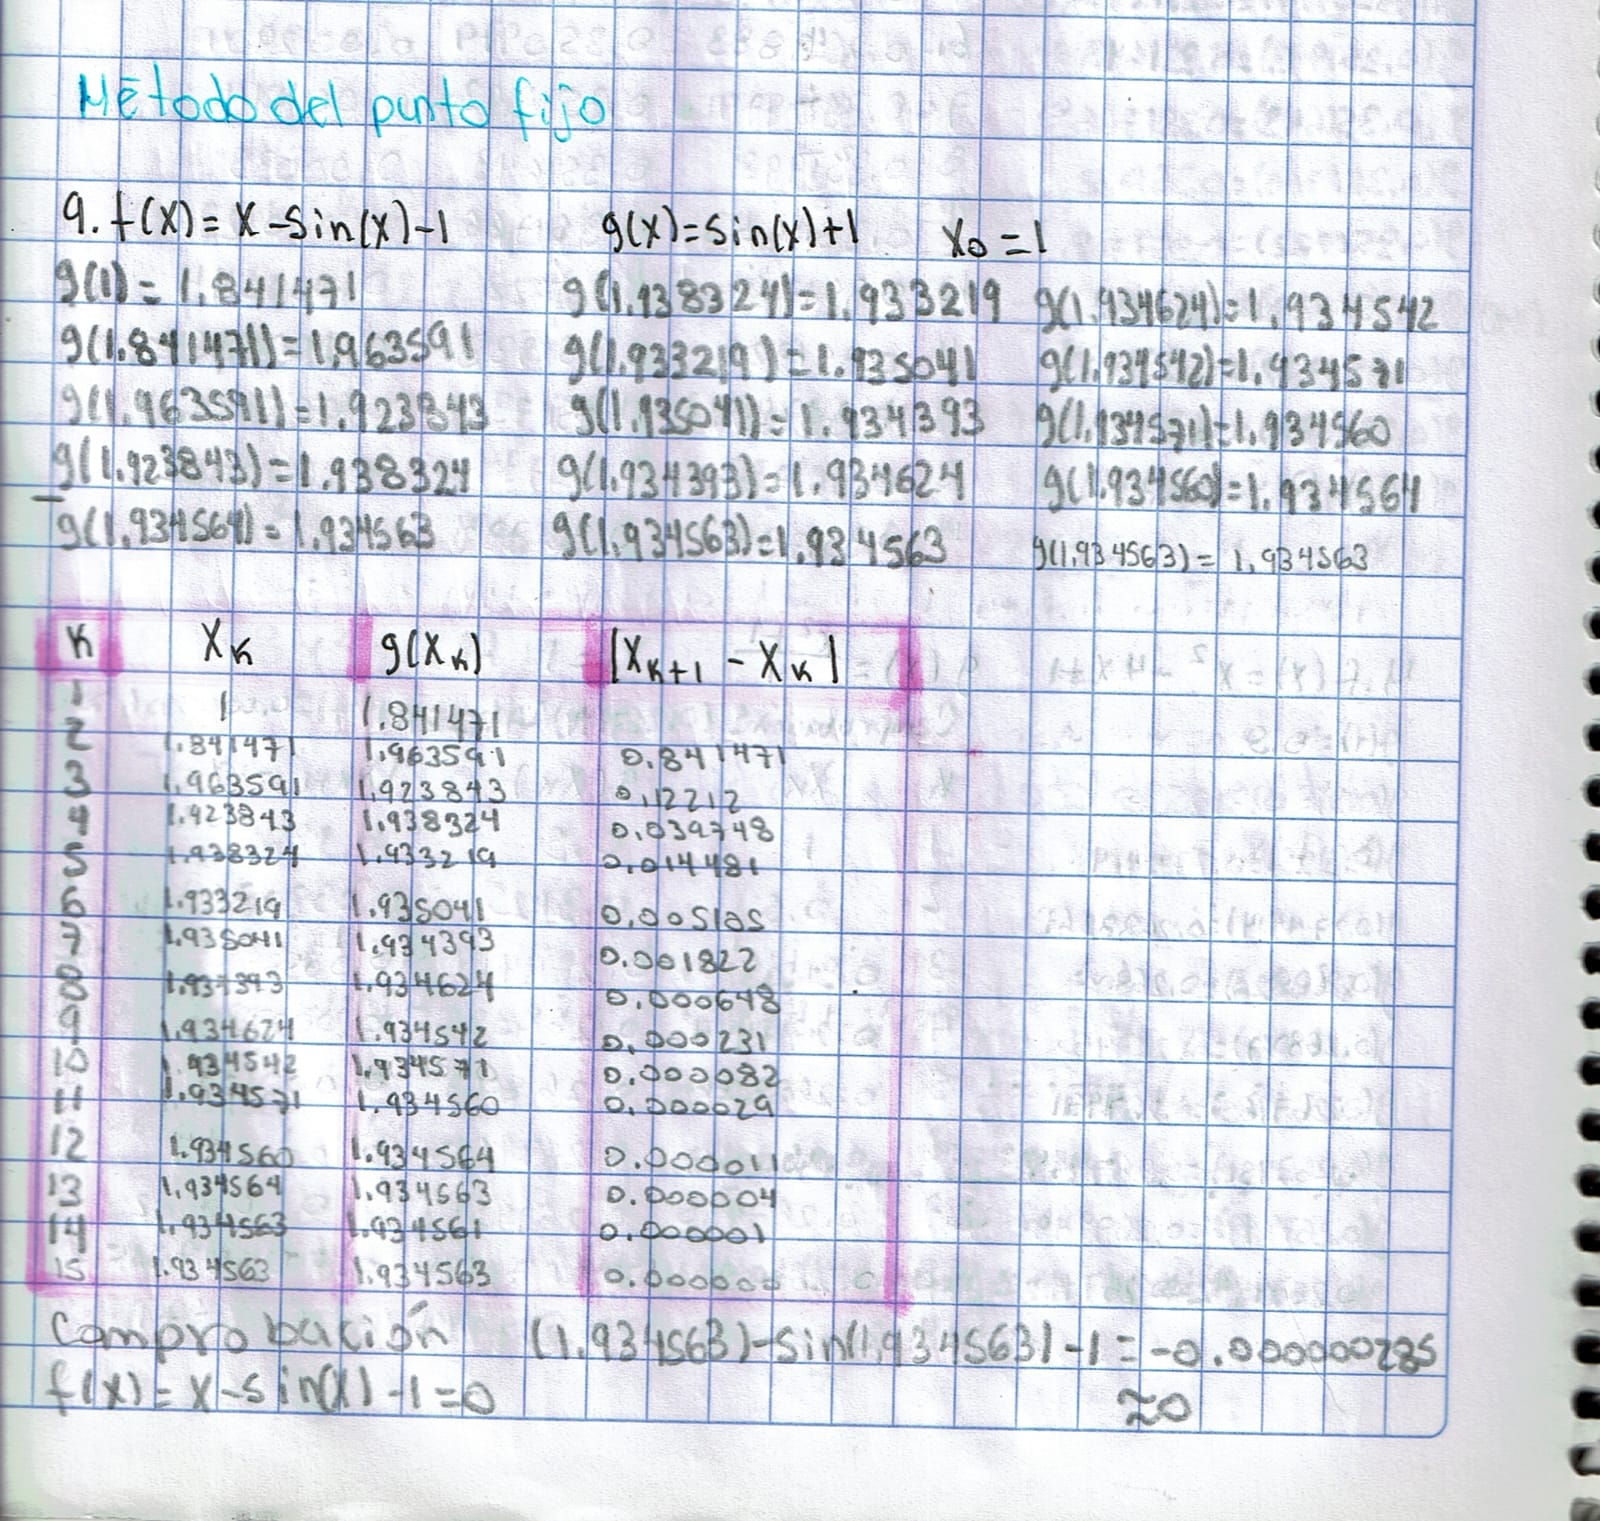
\includegraphics[width=6.25in,height=\textheight,keepaspectratio,alt={Ejercicio 9}]{Punto9.jpg}
\caption{Ejercicio 9}
\end{figure}

\begin{figure}
\centering
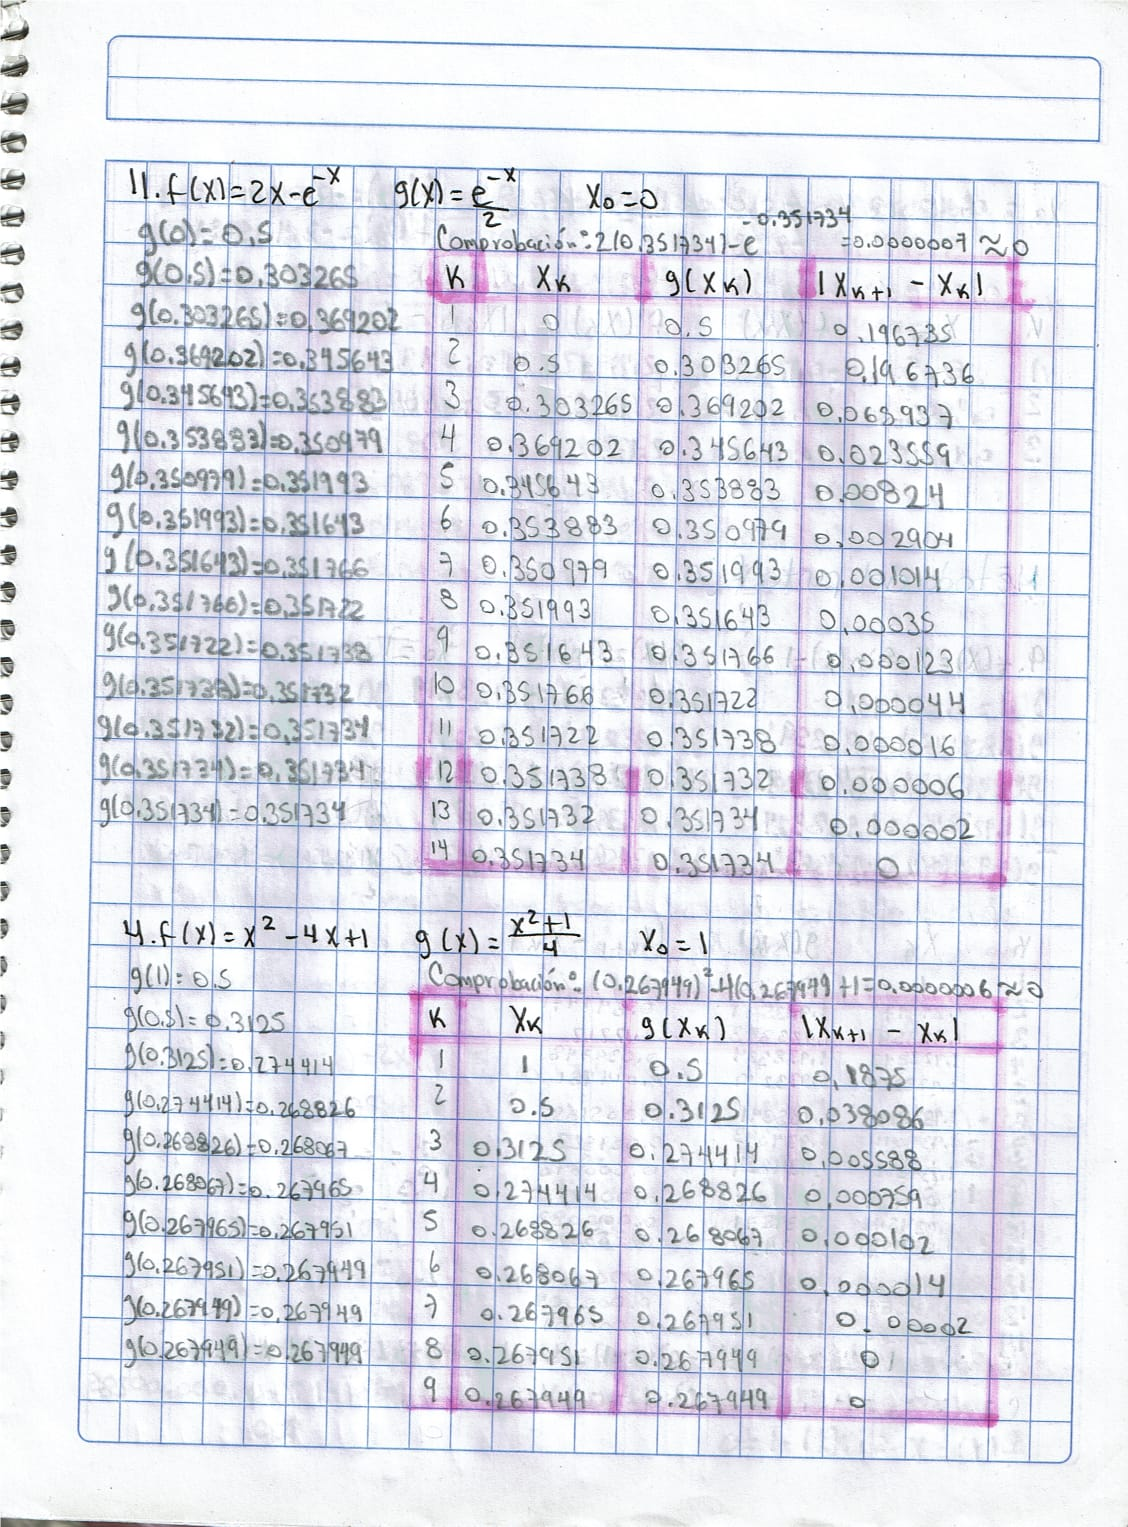
\includegraphics[width=6.25in,height=\textheight,keepaspectratio,alt={Ejercicio 11 y 4}]{Punto11-4.jpg}
\caption{Ejercicio 11 y 4}
\end{figure}

\subsubsection{Código para
implementación}\label{cuxf3digo-para-implementaciuxf3n-3}

\begin{Shaded}
\begin{Highlighting}[]
\CommentTok{\# Método del Punto Fijo que guarda los valores para la tabla}

\NormalTok{fijo }\OtherTok{\textless{}{-}} \ControlFlowTok{function}\NormalTok{(g, x0, }\AttributeTok{tol =} \FloatTok{1e{-}5}\NormalTok{, }\AttributeTok{iter\_max =} \DecValTok{100}\NormalTok{)\{}
  
\CommentTok{\# Vectores para almacenar los datos de las iteraciones}
  
\NormalTok{  iter\_vec }\OtherTok{\textless{}{-}} \FunctionTok{numeric}\NormalTok{(}\DecValTok{0}\NormalTok{)}
\NormalTok{  x0\_vec }\OtherTok{\textless{}{-}} \FunctionTok{numeric}\NormalTok{(}\DecValTok{0}\NormalTok{)}
\NormalTok{  x1\_vec }\OtherTok{\textless{}{-}} \FunctionTok{numeric}\NormalTok{(}\DecValTok{0}\NormalTok{)}
\NormalTok{  gx0\_vec }\OtherTok{\textless{}{-}} \FunctionTok{numeric}\NormalTok{(}\DecValTok{0}\NormalTok{)}
\NormalTok{  error\_vec }\OtherTok{\textless{}{-}} \FunctionTok{numeric}\NormalTok{(}\DecValTok{0}\NormalTok{)}
  
\NormalTok{  iter }\OtherTok{\textless{}{-}} \DecValTok{0}
\NormalTok{  error }\OtherTok{\textless{}{-}} \DecValTok{1}
  
  \ControlFlowTok{while}\NormalTok{(error }\SpecialCharTok{\textgreater{}}\NormalTok{ tol }\SpecialCharTok{\&\&}\NormalTok{ iter }\SpecialCharTok{\textless{}}\NormalTok{ iter\_max)\{}
    
\CommentTok{\# Aplicar fórmula de punto fijo}
    
\NormalTok{    x1 }\OtherTok{\textless{}{-}} \FunctionTok{g}\NormalTok{(x0)}
\NormalTok{    error }\OtherTok{\textless{}{-}} \FunctionTok{abs}\NormalTok{(x1 }\SpecialCharTok{{-}}\NormalTok{ x0)}
    
\CommentTok{\# Almacena los datos de cada iteración}
    
\NormalTok{    iter }\OtherTok{\textless{}{-}}\NormalTok{ iter }\SpecialCharTok{+} \DecValTok{1}
\NormalTok{    iter\_vec }\OtherTok{\textless{}{-}} \FunctionTok{c}\NormalTok{(iter\_vec, iter)}
\NormalTok{    x0\_vec }\OtherTok{\textless{}{-}} \FunctionTok{c}\NormalTok{(x0\_vec, x0)}
\NormalTok{    x1\_vec }\OtherTok{\textless{}{-}} \FunctionTok{c}\NormalTok{(x1\_vec, x1)}
\NormalTok{    gx0\_vec }\OtherTok{\textless{}{-}} \FunctionTok{c}\NormalTok{(gx0\_vec, }\FunctionTok{g}\NormalTok{(x0))}
\NormalTok{    error\_vec }\OtherTok{\textless{}{-}} \FunctionTok{c}\NormalTok{(error\_vec, error)}
    
\CommentTok{\# Actualizar para siguiente iteración}
    
\NormalTok{    x0 }\OtherTok{\textless{}{-}}\NormalTok{ x1}
\NormalTok{  \}}
  
\CommentTok{\# Crea la tabla de las iteraciones}
  
\NormalTok{  TAB }\OtherTok{\textless{}{-}} \FunctionTok{data.frame}\NormalTok{(}
    \StringTok{"k"} \OtherTok{=}\NormalTok{ iter\_vec,}
    \StringTok{"xₖ"} \OtherTok{=}\NormalTok{ x0\_vec,}
    \StringTok{"g(xₖ)"} \OtherTok{=}\NormalTok{ gx0\_vec,}
    \StringTok{"xₖ₊₁"} \OtherTok{=}\NormalTok{ x1\_vec,}
    \StringTok{"eₖ = |xₖ₊₁ {-} xₖ|"} \OtherTok{=}\NormalTok{ error\_vec,}
    \AttributeTok{check.names =} \ConstantTok{FALSE}
\NormalTok{  )}
  
  \FunctionTok{cat}\NormalTok{(}\StringTok{"Raíz aproximada:"}\NormalTok{, x1, }\StringTok{"}\SpecialCharTok{\textbackslash{}n}\StringTok{"}\NormalTok{)}
  \FunctionTok{cat}\NormalTok{(}\StringTok{"Iteraciones:"}\NormalTok{, iter, }\StringTok{"}\SpecialCharTok{\textbackslash{}n\textbackslash{}n}\StringTok{"}\NormalTok{)}
  
  \FunctionTok{return}\NormalTok{(}\FunctionTok{list}\NormalTok{(}\AttributeTok{raiz =}\NormalTok{ x1, }\AttributeTok{iteraciones =}\NormalTok{ iter, }\AttributeTok{tabla =}\NormalTok{ TAB))}
\NormalTok{\}}
\end{Highlighting}
\end{Shaded}

\begin{Shaded}
\begin{Highlighting}[]
\CommentTok{\# Tabla "bonita" para Punto Fijo}

\NormalTok{tabla }\OtherTok{\textless{}{-}} \ControlFlowTok{function}\NormalTok{(resultado) \{}
  \FunctionTok{library}\NormalTok{(DT)}
  
  \FunctionTok{datatable}\NormalTok{(}
\NormalTok{    resultado}\SpecialCharTok{$}\NormalTok{tabla[, }\SpecialCharTok{{-}}\DecValTok{4}\NormalTok{],}
    \AttributeTok{options =} \FunctionTok{list}\NormalTok{(}
      \AttributeTok{scrollX =} \ConstantTok{TRUE}\NormalTok{,}
      \AttributeTok{scrollY =} \StringTok{"400px"}\NormalTok{, }
      \AttributeTok{paging =} \ConstantTok{FALSE}\NormalTok{,}
      \AttributeTok{dom =} \StringTok{\textquotesingle{}t\textquotesingle{}}\NormalTok{,}
      \AttributeTok{autoWidth =} \ConstantTok{FALSE}\NormalTok{,}
      \AttributeTok{columnDefs =} \FunctionTok{list}\NormalTok{(}
        \FunctionTok{list}\NormalTok{(}\AttributeTok{className =} \StringTok{\textquotesingle{}dt{-}center\textquotesingle{}}\NormalTok{, }\AttributeTok{targets =} \DecValTok{0}\SpecialCharTok{:}\DecValTok{3}\NormalTok{))}
\NormalTok{    ),}
    \AttributeTok{rownames =} \ConstantTok{FALSE}\NormalTok{,}
    \AttributeTok{class =} \StringTok{\textquotesingle{}cell{-}border stripe\textquotesingle{}}\NormalTok{,}
    \AttributeTok{width =} \StringTok{"100\%"}\NormalTok{,}
    \AttributeTok{caption =} \StringTok{"Tabla de iteraciones en el método del Punto Fijo"}\NormalTok{,}
    \AttributeTok{escape =} \ConstantTok{FALSE}
\NormalTok{  ) }\SpecialCharTok{\%\textgreater{}\%}
    \FunctionTok{formatRound}\NormalTok{(}\AttributeTok{columns =} \FunctionTok{c}\NormalTok{(}\DecValTok{2}\SpecialCharTok{:}\DecValTok{4}\NormalTok{), }\AttributeTok{digits =} \DecValTok{6}\NormalTok{)}
\NormalTok{\}}
\end{Highlighting}
\end{Shaded}

\begin{Shaded}
\begin{Highlighting}[]
\CommentTok{\# Gráfica para Punto Fijo}

\NormalTok{grafica }\OtherTok{\textless{}{-}} \ControlFlowTok{function}\NormalTok{(g, resultado) \{}

\CommentTok{\# Obtener la raíz aproximada}

\NormalTok{    raiz }\OtherTok{\textless{}{-}}\NormalTok{ resultado}\SpecialCharTok{$}\NormalTok{raiz}
  
\CommentTok{\# Calcular rango alrededor de la raíz}
  
\NormalTok{  x\_min }\OtherTok{\textless{}{-}}\NormalTok{ raiz }\SpecialCharTok{{-}} \DecValTok{1}
\NormalTok{  x\_max }\OtherTok{\textless{}{-}}\NormalTok{ raiz }\SpecialCharTok{+} \DecValTok{1}
\NormalTok{  x\_vals }\OtherTok{\textless{}{-}} \FunctionTok{seq}\NormalTok{(x\_min, x\_max, }\AttributeTok{length.out =} \DecValTok{1000}\NormalTok{)}
\NormalTok{  y\_g }\OtherTok{\textless{}{-}} \FunctionTok{g}\NormalTok{(x\_vals)}
\NormalTok{  y\_x }\OtherTok{\textless{}{-}}\NormalTok{ x\_vals  }\CommentTok{\# y = x}
  
\CommentTok{\# Crear la gráfica}
  
  \FunctionTok{plot}\NormalTok{(x\_vals, y\_g, }\AttributeTok{type =} \StringTok{"l"}\NormalTok{, }\AttributeTok{main =} \StringTok{"Punto de Intersección: y = g(x) y y = x"}\NormalTok{,}
       \AttributeTok{xlab =} \StringTok{"x"}\NormalTok{, }\AttributeTok{ylab =} \StringTok{"y"}\NormalTok{, }\AttributeTok{col =} \StringTok{"blue"}\NormalTok{, }\AttributeTok{lwd =} \DecValTok{2}\NormalTok{, }\AttributeTok{ylim =} \FunctionTok{range}\NormalTok{(}\FunctionTok{c}\NormalTok{(y\_g, y\_x)))}
  \FunctionTok{lines}\NormalTok{(x\_vals, y\_x, }\AttributeTok{col =} \StringTok{"red"}\NormalTok{, }\AttributeTok{lwd =} \DecValTok{2}\NormalTok{, }\AttributeTok{lty =} \DecValTok{2}\NormalTok{)}
  
\CommentTok{\# Marcar el punto de intersección (raíz)}
  
  \FunctionTok{points}\NormalTok{(raiz, raiz, }\AttributeTok{col =} \StringTok{"green"}\NormalTok{, }\AttributeTok{pch =} \DecValTok{19}\NormalTok{, }\AttributeTok{cex =} \FloatTok{1.5}\NormalTok{)}
  
\CommentTok{\# Líneas para mostrar que es la intersección}
  
  \FunctionTok{abline}\NormalTok{(}\AttributeTok{v =}\NormalTok{ raiz, }\AttributeTok{col =} \StringTok{"green"}\NormalTok{, }\AttributeTok{lty =} \DecValTok{3}\NormalTok{, }\AttributeTok{lwd =} \DecValTok{1}\NormalTok{)}
  \FunctionTok{abline}\NormalTok{(}\AttributeTok{h =}\NormalTok{ raiz, }\AttributeTok{col =} \StringTok{"green"}\NormalTok{, }\AttributeTok{lty =} \DecValTok{3}\NormalTok{, }\AttributeTok{lwd =} \DecValTok{1}\NormalTok{)}
  
\CommentTok{\# Leyenda}
  
  \FunctionTok{legend}\NormalTok{(}\StringTok{"topright"}\NormalTok{, }
         \AttributeTok{legend =} \FunctionTok{c}\NormalTok{(}\StringTok{"y = g(x)"}\NormalTok{, }\StringTok{"y = x"}\NormalTok{, }\StringTok{"Punto fijo"}\NormalTok{),}
         \AttributeTok{col =} \FunctionTok{c}\NormalTok{(}\StringTok{"blue"}\NormalTok{, }\StringTok{"red"}\NormalTok{, }\StringTok{"green"}\NormalTok{),}
         \AttributeTok{lty =} \FunctionTok{c}\NormalTok{(}\DecValTok{1}\NormalTok{, }\DecValTok{2}\NormalTok{, }\ConstantTok{NA}\NormalTok{), }\AttributeTok{pch =} \FunctionTok{c}\NormalTok{(}\ConstantTok{NA}\NormalTok{, }\ConstantTok{NA}\NormalTok{, }\DecValTok{19}\NormalTok{),}
         \AttributeTok{lwd =} \FunctionTok{c}\NormalTok{(}\DecValTok{2}\NormalTok{, }\DecValTok{2}\NormalTok{, }\ConstantTok{NA}\NormalTok{), }\AttributeTok{cex =} \FloatTok{0.8}\NormalTok{, }\AttributeTok{bty =} \StringTok{"n"}\NormalTok{)}
\NormalTok{\}}
\end{Highlighting}
\end{Shaded}

\subsubsection{\texorpdfstring{Sistema
\(2\)}{Sistema 2}}\label{sistema-2-6}

\(f(x) = x^3 + x - 1\)

\(g(x) = 1 - x^3\)

\(x_0 = 0.6\)

\begin{Shaded}
\begin{Highlighting}[]
\CommentTok{\# Datos}

\NormalTok{x0 }\OtherTok{\textless{}{-}} \FloatTok{0.6}
\NormalTok{f }\OtherTok{\textless{}{-}} \ControlFlowTok{function}\NormalTok{(x) x}\SpecialCharTok{\^{}}\DecValTok{3} \SpecialCharTok{+}\NormalTok{ x }\SpecialCharTok{{-}} \DecValTok{1}
\NormalTok{g }\OtherTok{\textless{}{-}} \ControlFlowTok{function}\NormalTok{(x) }\DecValTok{1} \SpecialCharTok{{-}}\NormalTok{ x}\SpecialCharTok{\^{}}\DecValTok{3}
\NormalTok{dg }\OtherTok{\textless{}{-}} \ControlFlowTok{function}\NormalTok{(x) }\SpecialCharTok{{-}}\DecValTok{3}\SpecialCharTok{*}\NormalTok{x}\SpecialCharTok{\^{}}\DecValTok{2}
\end{Highlighting}
\end{Shaded}

\paragraph{\texorpdfstring{Forma
\(x = g(x)\)}{Forma x = g(x)}}\label{forma-x-gx}

Reescriba la ecuación f(x) = 0 en forma x = g(x).

Ya se nos da la sugerencia:

\(g(x) = 1 - x^3\)

\paragraph{Condición}\label{condiciuxf3n}

Verifique que la función \(g(x)\) cumpla la condición de convergencia
local \(|g′(x)| < 1\) en el intervalo considerado.

\begin{Shaded}
\begin{Highlighting}[]
\ControlFlowTok{if}\NormalTok{(}\FunctionTok{abs}\NormalTok{(}\FunctionTok{dg}\NormalTok{(x0)) }\SpecialCharTok{\textless{}} \DecValTok{1}\NormalTok{) \{}
  \FunctionTok{cat}\NormalTok{(}\StringTok{"Condición cumplida}\SpecialCharTok{\textbackslash{}n}\StringTok{"}\NormalTok{)}
\NormalTok{\} }\ControlFlowTok{else}\NormalTok{ \{}
  \FunctionTok{cat}\NormalTok{(}\StringTok{"Condición no cumplida, es probable que en las primeras 100 iteraciones no converga.}\SpecialCharTok{\textbackslash{}n}\StringTok{"}\NormalTok{)}
\NormalTok{\}}
\end{Highlighting}
\end{Shaded}

\begin{verbatim}
## Condición no cumplida, es probable que en las primeras 100 iteraciones no converga.
\end{verbatim}

\paragraph{Iteraciones}\label{iteraciones-15}

Realice al menos 8 iteraciones del método.

\begin{Shaded}
\begin{Highlighting}[]
\NormalTok{resultado }\OtherTok{\textless{}{-}} \FunctionTok{fijo}\NormalTok{(g, x0)}
\end{Highlighting}
\end{Shaded}

\begin{verbatim}
## Raíz aproximada: 0 
## Iteraciones: 100
\end{verbatim}

\paragraph{Tabla}\label{tabla-10}

Registre los valores \(x_k\), \(g(x_k)\), y el error
\(|x_{k+1} − x_k|\).

\begin{Shaded}
\begin{Highlighting}[]
\FunctionTok{tabla}\NormalTok{(resultado)}
\end{Highlighting}
\end{Shaded}

\pandocbounded{\includegraphics[keepaspectratio]{PortafolioDLPF_pdf_files/figure-latex/unnamed-chunk-1230-1.pdf}}

\paragraph{Gráficas}\label{gruxe1ficas-15}

Grafica la función y marca el punto donde converge la raíz.

\begin{Shaded}
\begin{Highlighting}[]
\FunctionTok{grafica}\NormalTok{(g, resultado)}
\end{Highlighting}
\end{Shaded}

\pandocbounded{\includegraphics[keepaspectratio]{PortafolioDLPF_pdf_files/figure-latex/unnamed-chunk-1231-1.pdf}}

Para este sistema, el método no es el adecuado ya que en las 100
iteraciones que se hicieron, la función no convergió.

\subsubsection{\texorpdfstring{Sistema
\(4\)}{Sistema 4}}\label{sistema-4-6}

\(f(x) = x^2 - 4^x + 1\)

\(g(x) = \frac{x^2 + 1}{4}\)

\(x_0 = 1\)

\begin{Shaded}
\begin{Highlighting}[]
\CommentTok{\# Datos}

\NormalTok{x0 }\OtherTok{\textless{}{-}} \DecValTok{1}
\NormalTok{f }\OtherTok{\textless{}{-}} \ControlFlowTok{function}\NormalTok{(x) x}\SpecialCharTok{\^{}}\DecValTok{2} \SpecialCharTok{{-}} \DecValTok{4}\SpecialCharTok{\^{}}\NormalTok{x }\SpecialCharTok{+} \DecValTok{1}
\NormalTok{g }\OtherTok{\textless{}{-}} \ControlFlowTok{function}\NormalTok{(x) (x}\SpecialCharTok{\^{}}\DecValTok{2} \SpecialCharTok{+} \DecValTok{1}\NormalTok{) }\SpecialCharTok{/} \DecValTok{4}
\NormalTok{dg }\OtherTok{\textless{}{-}} \ControlFlowTok{function}\NormalTok{(x) (}\DecValTok{1} \SpecialCharTok{/} \DecValTok{2}\NormalTok{) }\SpecialCharTok{*}\NormalTok{ x}
\end{Highlighting}
\end{Shaded}

\paragraph{\texorpdfstring{Forma
\(x = g(x)\)}{Forma x = g(x)}}\label{forma-x-gx-1}

Reescriba la ecuación f(x) = 0 en forma x = g(x).

Ya se nos da la sugerencia:

\(g(x) = \frac{x^2 + 1}{4}\)

\paragraph{Condición}\label{condiciuxf3n-1}

Verifique que la función \(g(x)\) cumpla la condición de convergencia
local \(|g′(x)| < 1\) en el intervalo considerado.

\begin{Shaded}
\begin{Highlighting}[]
\ControlFlowTok{if}\NormalTok{(}\FunctionTok{abs}\NormalTok{(}\FunctionTok{dg}\NormalTok{(x0)) }\SpecialCharTok{\textless{}} \DecValTok{1}\NormalTok{) \{}
  \FunctionTok{cat}\NormalTok{(}\StringTok{"Condición cumplida}\SpecialCharTok{\textbackslash{}n}\StringTok{"}\NormalTok{)}
\NormalTok{\} }\ControlFlowTok{else}\NormalTok{ \{}
  \FunctionTok{cat}\NormalTok{(}\StringTok{"Condición no cumplida, es probable que en las primeras 100 iteraciones no converga.}\SpecialCharTok{\textbackslash{}n}\StringTok{"}\NormalTok{)}
\NormalTok{\}}
\end{Highlighting}
\end{Shaded}

\begin{verbatim}
## Condición cumplida
\end{verbatim}

\paragraph{Iteraciones}\label{iteraciones-16}

Realice al menos 8 iteraciones del método.

\begin{Shaded}
\begin{Highlighting}[]
\NormalTok{resultado }\OtherTok{\textless{}{-}} \FunctionTok{fijo}\NormalTok{(g, x0)}
\end{Highlighting}
\end{Shaded}

\begin{verbatim}
## Raíz aproximada: 0.2679495 
## Iteraciones: 8
\end{verbatim}

\paragraph{Tabla}\label{tabla-11}

Registre los valores \(x_k\), \(g(x_k)\), y el error
\(|x_{k+1} − x_k|\).

\begin{Shaded}
\begin{Highlighting}[]
\FunctionTok{tabla}\NormalTok{(resultado)}
\end{Highlighting}
\end{Shaded}

\pandocbounded{\includegraphics[keepaspectratio]{PortafolioDLPF_pdf_files/figure-latex/unnamed-chunk-1235-1.pdf}}

\paragraph{Gráficas}\label{gruxe1ficas-16}

Grafica la función y marca el punto donde converge la raíz.

\begin{Shaded}
\begin{Highlighting}[]
\FunctionTok{grafica}\NormalTok{(g, resultado)}
\end{Highlighting}
\end{Shaded}

\pandocbounded{\includegraphics[keepaspectratio]{PortafolioDLPF_pdf_files/figure-latex/unnamed-chunk-1236-1.pdf}}

\subsubsection{\texorpdfstring{Sistema
\(8\)}{Sistema 8}}\label{sistema-8-6}

\(f(x) = x^3 - 3x + 1\)

\(g(x) = \sqrt[3]{3x - 1}\)

\(x_0 = 0.8\)

\begin{Shaded}
\begin{Highlighting}[]
\CommentTok{\# Datos}

\NormalTok{x0 }\OtherTok{\textless{}{-}} \FloatTok{0.8}
\NormalTok{f }\OtherTok{\textless{}{-}} \ControlFlowTok{function}\NormalTok{(x) x}\SpecialCharTok{\^{}}\DecValTok{3} \SpecialCharTok{{-}} \DecValTok{3}\SpecialCharTok{*}\NormalTok{x }\SpecialCharTok{+} \DecValTok{1}
\NormalTok{g }\OtherTok{\textless{}{-}} \ControlFlowTok{function}\NormalTok{(x) (}\DecValTok{3}\SpecialCharTok{*}\NormalTok{x }\SpecialCharTok{{-}} \DecValTok{1}\NormalTok{)}\SpecialCharTok{\^{}}\NormalTok{(}\DecValTok{1}\SpecialCharTok{/}\DecValTok{3}\NormalTok{)}
\NormalTok{dg }\OtherTok{\textless{}{-}} \ControlFlowTok{function}\NormalTok{(x) (}\DecValTok{3}\SpecialCharTok{*}\NormalTok{x }\SpecialCharTok{{-}} \DecValTok{1}\NormalTok{)}\SpecialCharTok{\^{}}\NormalTok{(}\SpecialCharTok{{-}}\DecValTok{2}\SpecialCharTok{/}\DecValTok{3}\NormalTok{)}
\end{Highlighting}
\end{Shaded}

\paragraph{\texorpdfstring{Forma
\(x = g(x)\)}{Forma x = g(x)}}\label{forma-x-gx-2}

Reescriba la ecuación f(x) = 0 en forma x = g(x).

Ya se nos da la sugerencia:

\(g(x) = \sqrt[3]{3x - 1}\)

\paragraph{Condición}\label{condiciuxf3n-2}

Verifique que la función \(g(x)\) cumpla la condición de convergencia
local \(|g′(x)| < 1\) en el intervalo considerado.

\begin{Shaded}
\begin{Highlighting}[]
\ControlFlowTok{if}\NormalTok{(}\FunctionTok{abs}\NormalTok{(}\FunctionTok{dg}\NormalTok{(x0)) }\SpecialCharTok{\textless{}} \DecValTok{1}\NormalTok{) \{}
  \FunctionTok{cat}\NormalTok{(}\StringTok{"Condición cumplida}\SpecialCharTok{\textbackslash{}n}\StringTok{"}\NormalTok{)}
\NormalTok{\} }\ControlFlowTok{else}\NormalTok{ \{}
  \FunctionTok{cat}\NormalTok{(}\StringTok{"Condición no cumplida, es probable que en las primeras 100 iteraciones no converga.}\SpecialCharTok{\textbackslash{}n}\StringTok{"}\NormalTok{)}
\NormalTok{\}}
\end{Highlighting}
\end{Shaded}

\begin{verbatim}
## Condición cumplida
\end{verbatim}

\paragraph{Iteraciones}\label{iteraciones-17}

Realice al menos 8 iteraciones del método.

\begin{Shaded}
\begin{Highlighting}[]
\NormalTok{resultado }\OtherTok{\textless{}{-}} \FunctionTok{fijo}\NormalTok{(g, x0)}
\end{Highlighting}
\end{Shaded}

\begin{verbatim}
## Raíz aproximada: 1.532085 
## Iteraciones: 15
\end{verbatim}

\paragraph{Tabla}\label{tabla-12}

Registre los valores \(x_k\), \(g(x_k)\), y el error
\(|x_{k+1} − x_k|\).

\begin{Shaded}
\begin{Highlighting}[]
\FunctionTok{tabla}\NormalTok{(resultado)}
\end{Highlighting}
\end{Shaded}

\pandocbounded{\includegraphics[keepaspectratio]{PortafolioDLPF_pdf_files/figure-latex/unnamed-chunk-1240-1.pdf}}

\paragraph{Gráficas}\label{gruxe1ficas-17}

Grafica la función y marca el punto donde converge la raíz.

\begin{Shaded}
\begin{Highlighting}[]
\FunctionTok{grafica}\NormalTok{(g, resultado)}
\end{Highlighting}
\end{Shaded}

\pandocbounded{\includegraphics[keepaspectratio]{PortafolioDLPF_pdf_files/figure-latex/unnamed-chunk-1241-1.pdf}}

\subsubsection{\texorpdfstring{Sistema
\(10\)}{Sistema 10}}\label{sistema-10-5}

\(f(x) = x^2 - 3\)

\(g(x) = \frac{3}{x}\)

\(x_0 = 1.5\)

\begin{Shaded}
\begin{Highlighting}[]
\CommentTok{\# Datos}

\NormalTok{x0 }\OtherTok{\textless{}{-}} \FloatTok{1.5}
\NormalTok{f }\OtherTok{\textless{}{-}} \ControlFlowTok{function}\NormalTok{(x) x}\SpecialCharTok{\^{}}\DecValTok{2} \SpecialCharTok{{-}} \DecValTok{3}
\NormalTok{g }\OtherTok{\textless{}{-}} \ControlFlowTok{function}\NormalTok{(x) }\DecValTok{3} \SpecialCharTok{/}\NormalTok{ x}
\NormalTok{dg }\OtherTok{\textless{}{-}} \ControlFlowTok{function}\NormalTok{(x) }\SpecialCharTok{{-}} \DecValTok{3} \SpecialCharTok{/}\NormalTok{ x}\SpecialCharTok{\^{}}\DecValTok{2}
\end{Highlighting}
\end{Shaded}

\paragraph{\texorpdfstring{Forma
\(x = g(x)\)}{Forma x = g(x)}}\label{forma-x-gx-3}

Reescriba la ecuación f(x) = 0 en forma x = g(x).

Ya se nos da la sugerencia:

\(g(x) = \frac{3}{x}\)

\paragraph{Condición}\label{condiciuxf3n-3}

Verifique que la función \(g(x)\) cumpla la condición de convergencia
local \(|g′(x)| < 1\) en el intervalo considerado.

\begin{Shaded}
\begin{Highlighting}[]
\ControlFlowTok{if}\NormalTok{(}\FunctionTok{abs}\NormalTok{(}\FunctionTok{dg}\NormalTok{(x0)) }\SpecialCharTok{\textless{}} \DecValTok{1}\NormalTok{) \{}
  \FunctionTok{cat}\NormalTok{(}\StringTok{"Condición cumplida}\SpecialCharTok{\textbackslash{}n}\StringTok{"}\NormalTok{)}
\NormalTok{\} }\ControlFlowTok{else}\NormalTok{ \{}
  \FunctionTok{cat}\NormalTok{(}\StringTok{"Condición no cumplida, es probable que en las primeras 100 iteraciones no converga.}\SpecialCharTok{\textbackslash{}n}\StringTok{"}\NormalTok{)}
\NormalTok{\}}
\end{Highlighting}
\end{Shaded}

\begin{verbatim}
## Condición no cumplida, es probable que en las primeras 100 iteraciones no converga.
\end{verbatim}

\paragraph{Iteraciones}\label{iteraciones-18}

Realice al menos 8 iteraciones del método.

\begin{Shaded}
\begin{Highlighting}[]
\NormalTok{resultado }\OtherTok{\textless{}{-}} \FunctionTok{fijo}\NormalTok{(g, x0)}
\end{Highlighting}
\end{Shaded}

\begin{verbatim}
## Raíz aproximada: 1.5 
## Iteraciones: 100
\end{verbatim}

\paragraph{Tabla}\label{tabla-13}

Registre los valores \(x_k\), \(g(x_k)\), y el error
\(|x_{k+1} − x_k|\).

\begin{Shaded}
\begin{Highlighting}[]
\FunctionTok{tabla}\NormalTok{(resultado)}
\end{Highlighting}
\end{Shaded}

\pandocbounded{\includegraphics[keepaspectratio]{PortafolioDLPF_pdf_files/figure-latex/unnamed-chunk-1245-1.pdf}}

\paragraph{Gráficas}\label{gruxe1ficas-18}

Grafica la función y marca el punto donde converge la raíz.

\begin{Shaded}
\begin{Highlighting}[]
\FunctionTok{grafica}\NormalTok{(g, resultado)}
\end{Highlighting}
\end{Shaded}

\pandocbounded{\includegraphics[keepaspectratio]{PortafolioDLPF_pdf_files/figure-latex/unnamed-chunk-1246-1.pdf}}

Para este sistema, el método no es el adecuado ya que en las 100
iteraciones que se hicieron, la función no convergió.

\subsubsection{\texorpdfstring{Sistema
\(14\)}{Sistema 14}}\label{sistema-14}

\(f(x) = x - e^{-x^2}\)

\(g(x) = e^{-x^2}\)

\(x_0 = 0.5\)

\begin{Shaded}
\begin{Highlighting}[]
\CommentTok{\# Datos}

\NormalTok{x0 }\OtherTok{\textless{}{-}} \FloatTok{0.5}
\NormalTok{f }\OtherTok{\textless{}{-}} \ControlFlowTok{function}\NormalTok{(x) x }\SpecialCharTok{{-}} \FunctionTok{exp}\NormalTok{(}\SpecialCharTok{{-}}\NormalTok{x}\SpecialCharTok{\^{}}\DecValTok{2}\NormalTok{)}
\NormalTok{g }\OtherTok{\textless{}{-}} \ControlFlowTok{function}\NormalTok{(x) }\FunctionTok{exp}\NormalTok{(}\SpecialCharTok{{-}}\NormalTok{x}\SpecialCharTok{\^{}}\DecValTok{2}\NormalTok{)}
\NormalTok{dg }\OtherTok{\textless{}{-}} \ControlFlowTok{function}\NormalTok{(x) }\SpecialCharTok{{-}} \DecValTok{2} \SpecialCharTok{*} \FunctionTok{exp}\NormalTok{(}\SpecialCharTok{{-}}\NormalTok{x}\SpecialCharTok{\^{}}\DecValTok{2}\NormalTok{)}
\end{Highlighting}
\end{Shaded}

\paragraph{\texorpdfstring{Forma
\(x = g(x)\)}{Forma x = g(x)}}\label{forma-x-gx-4}

Reescriba la ecuación f(x) = 0 en forma x = g(x).

Ya se nos da la sugerencia:

\(g(x) = e^{-x^2}\)

\paragraph{Condición}\label{condiciuxf3n-4}

Verifique que la función \(g(x)\) cumpla la condición de convergencia
local \(|g′(x)| < 1\) en el intervalo considerado.

\begin{Shaded}
\begin{Highlighting}[]
\ControlFlowTok{if}\NormalTok{(}\FunctionTok{abs}\NormalTok{(}\FunctionTok{dg}\NormalTok{(x0)) }\SpecialCharTok{\textless{}} \DecValTok{1}\NormalTok{) \{}
  \FunctionTok{cat}\NormalTok{(}\StringTok{"Condición cumplida}\SpecialCharTok{\textbackslash{}n}\StringTok{"}\NormalTok{)}
\NormalTok{\} }\ControlFlowTok{else}\NormalTok{ \{}
  \FunctionTok{cat}\NormalTok{(}\StringTok{"Condición no cumplida, es probable que en las primeras 100 iteraciones no converga.}\SpecialCharTok{\textbackslash{}n}\StringTok{"}\NormalTok{)}
\NormalTok{\}}
\end{Highlighting}
\end{Shaded}

\begin{verbatim}
## Condición no cumplida, es probable que en las primeras 100 iteraciones no converga.
\end{verbatim}

\paragraph{Iteraciones}\label{iteraciones-19}

Realice al menos 8 iteraciones del método.

\begin{Shaded}
\begin{Highlighting}[]
\NormalTok{resultado }\OtherTok{\textless{}{-}} \FunctionTok{fijo}\NormalTok{(g, x0)}
\end{Highlighting}
\end{Shaded}

\begin{verbatim}
## Raíz aproximada: 0.6529231 
## Iteraciones: 65
\end{verbatim}

\paragraph{Tabla}\label{tabla-14}

Registre los valores \(x_k\), \(g(x_k)\), y el error
\(|x_{k+1} − x_k|\).

\begin{Shaded}
\begin{Highlighting}[]
\FunctionTok{tabla}\NormalTok{(resultado)}
\end{Highlighting}
\end{Shaded}

\pandocbounded{\includegraphics[keepaspectratio]{PortafolioDLPF_pdf_files/figure-latex/unnamed-chunk-1250-1.pdf}}

\paragraph{Gráficas}\label{gruxe1ficas-19}

Grafica la función y marca el punto donde converge la raíz.

\begin{Shaded}
\begin{Highlighting}[]
\FunctionTok{grafica}\NormalTok{(g, resultado)}
\end{Highlighting}
\end{Shaded}

\pandocbounded{\includegraphics[keepaspectratio]{PortafolioDLPF_pdf_files/figure-latex/unnamed-chunk-1251-1.pdf}}

Para este sistema, el método sí convergió aunque la condición no se haya
cumplido, sin embargo, para ello tomo \(80\) iteraciones.

\section{Interpolación y
Aproximación}\label{interpolaciuxf3n-y-aproximaciuxf3n}

\subsection{Ejercicio 1}\label{ejercicio-1}

\subsubsection{\texorpdfstring{\(1.1\)}{1.1}}\label{section-5}

\paragraph{\texorpdfstring{\(a)\) Polinomio
interpolante}{a) Polinomio interpolante}}\label{a-polinomio-interpolante}

\begin{figure}
\centering
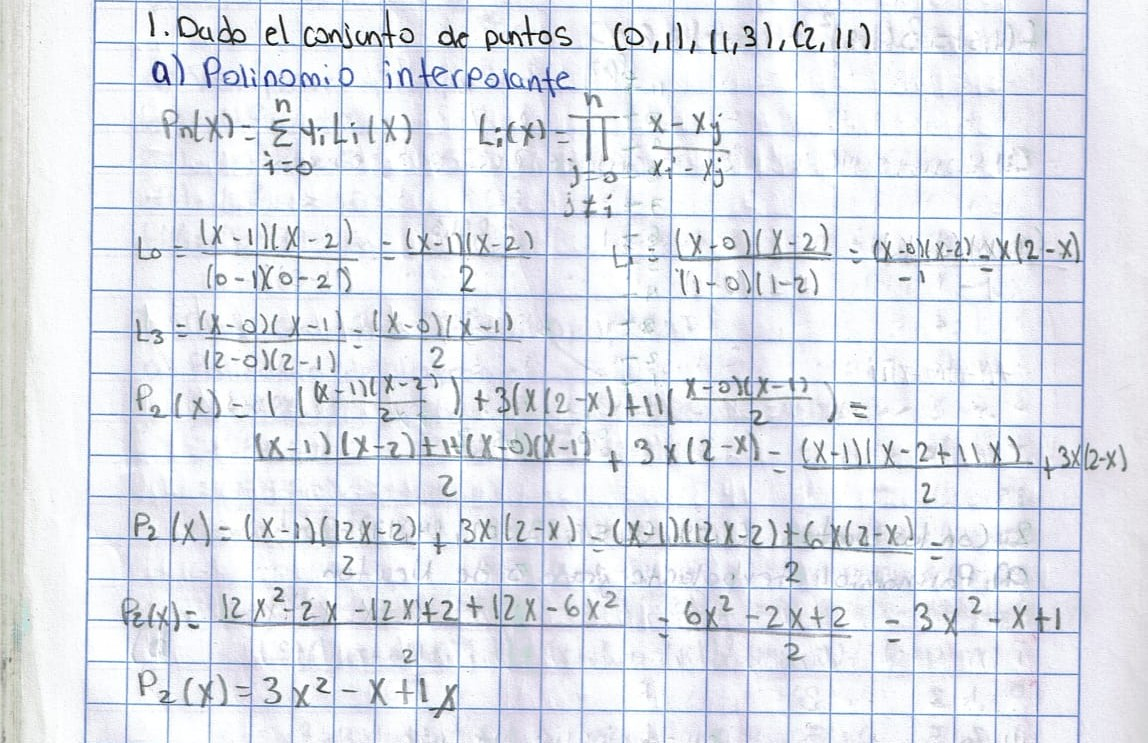
\includegraphics[width=6.25in,height=\textheight,keepaspectratio,alt={Ejercicio 1.1 a}]{Inter1a.jpg}
\caption{Ejercicio 1.1 a}
\end{figure}

\paragraph{\texorpdfstring{\(b)\) Tabla}{b) Tabla}}\label{b-tabla}

\begin{figure}
\centering
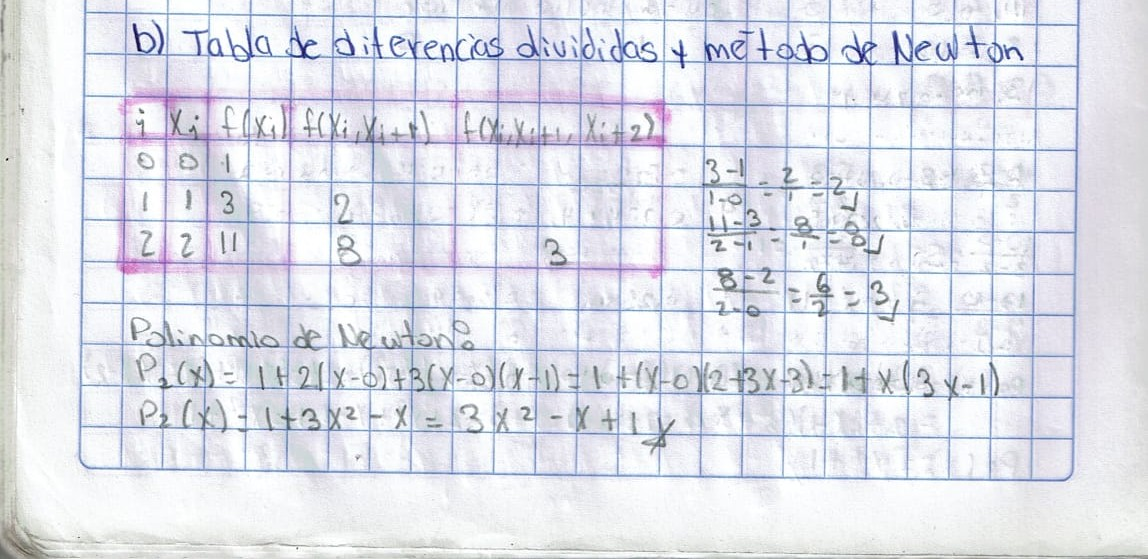
\includegraphics[width=6.25in,height=\textheight,keepaspectratio,alt={Ejercicio 1.1 b}]{Inter1b.jpg}
\caption{Ejercicio 1.1 b}
\end{figure}

\paragraph{\texorpdfstring{\(c)\) Comparación
gráfica}{c) Comparación gráfica}}\label{c-comparaciuxf3n-gruxe1fica}

\begin{figure}
\centering
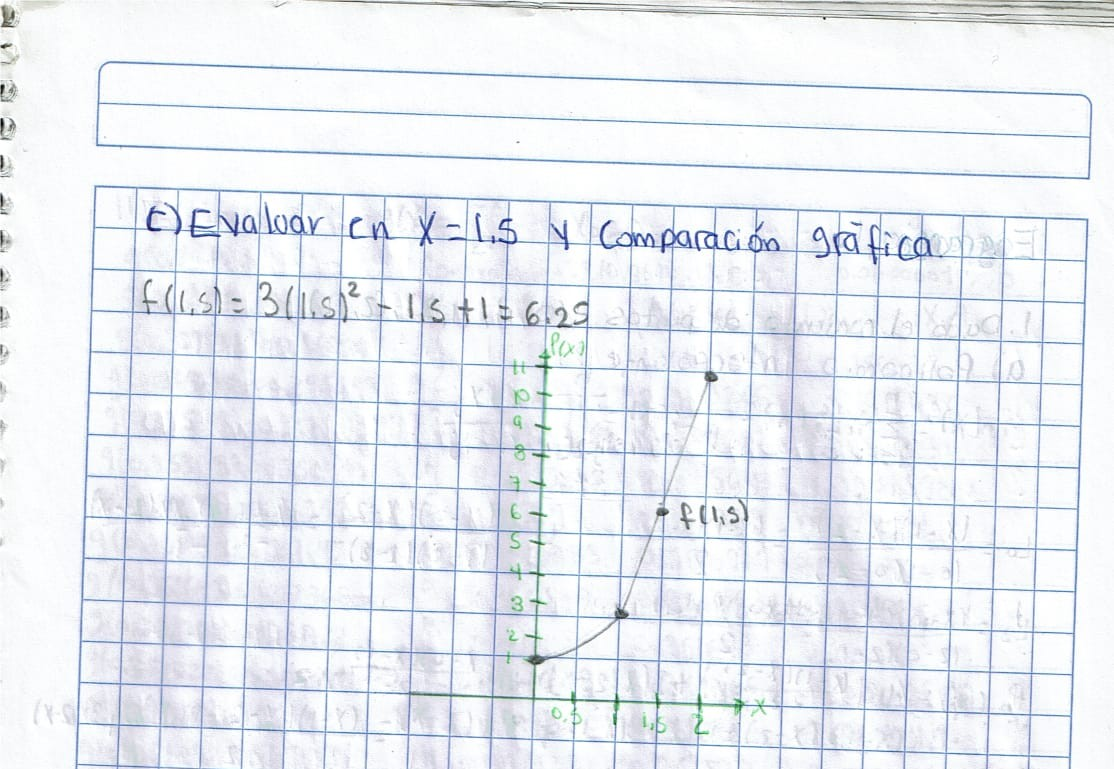
\includegraphics[width=6.25in,height=\textheight,keepaspectratio,alt={Ejercicio 1.1 c}]{Inter1c.jpg}
\caption{Ejercicio 1.1 c}
\end{figure}

\subsubsection{\texorpdfstring{\(1.2\)}{1.2}}\label{section-6}

\paragraph{\texorpdfstring{\(a)\) Polinomio interpolante grado
3}{a) Polinomio interpolante grado 3}}\label{a-polinomio-interpolante-grado-3}

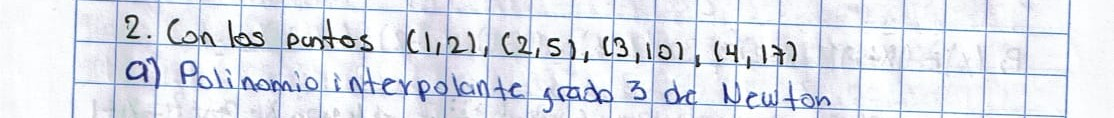
\includegraphics[width=6.25in,height=\textheight,keepaspectratio,alt={Ejercicio 1.2 a1}]{Inter12a.jpg}
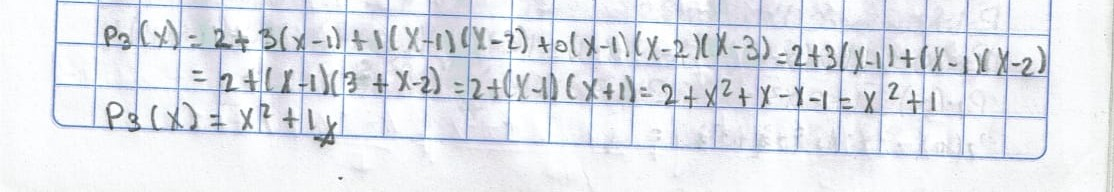
\includegraphics[width=6.25in,height=\textheight,keepaspectratio,alt={Ejercicio 1.2 a2}]{Inter12a2.jpg}

\paragraph{\texorpdfstring{\(b)\) Tabla}{b) Tabla}}\label{b-tabla-1}

\begin{figure}
\centering
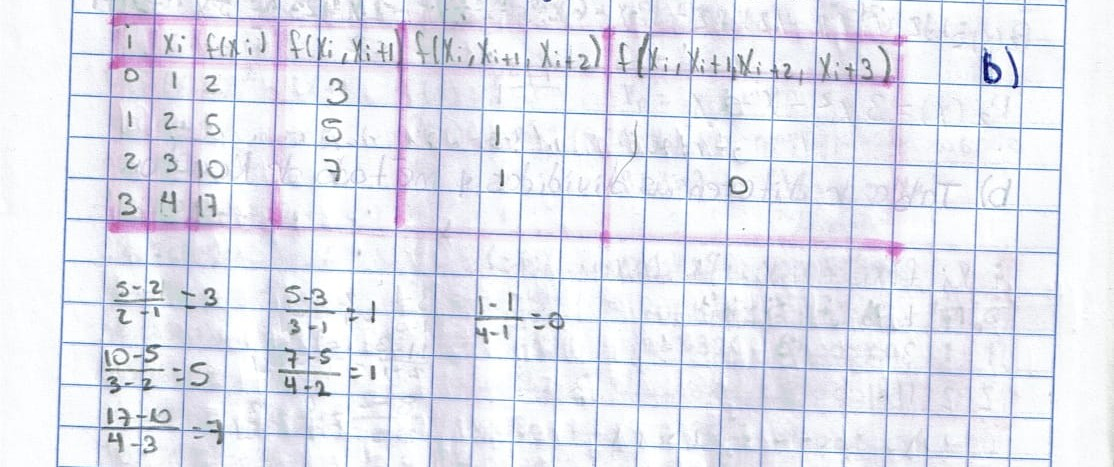
\includegraphics[width=6.25in,height=\textheight,keepaspectratio,alt={Ejercicio 1.2 b}]{Inter12b.jpg}
\caption{Ejercicio 1.2 b}
\end{figure}

\paragraph{\texorpdfstring{\(c)\) Evaluar en
\(x = 2.5\)}{c) Evaluar en x = 2.5}}\label{c-evaluar-en-x-2.5}

\begin{figure}
\centering
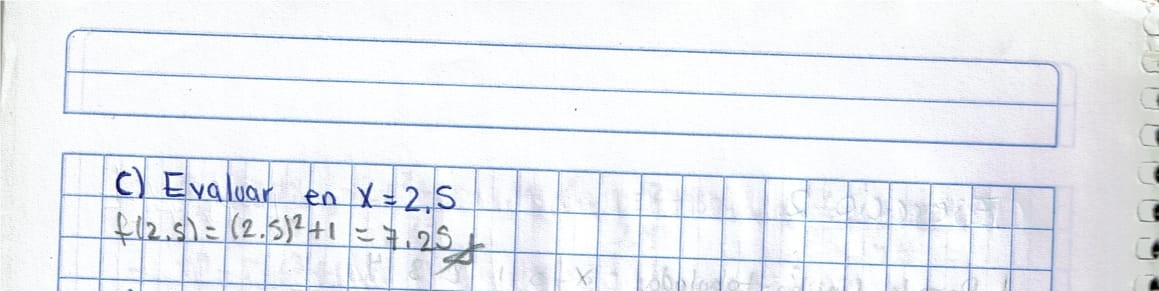
\includegraphics[width=6.25in,height=\textheight,keepaspectratio,alt={Ejercicio 1.2 c}]{Inter12c.jpg}
\caption{Ejercicio 1.2 c}
\end{figure}

\paragraph{\texorpdfstring{\(d)\) Verificar y
comparar}{d) Verificar y comparar}}\label{d-verificar-y-comparar}

\begin{figure}
\centering
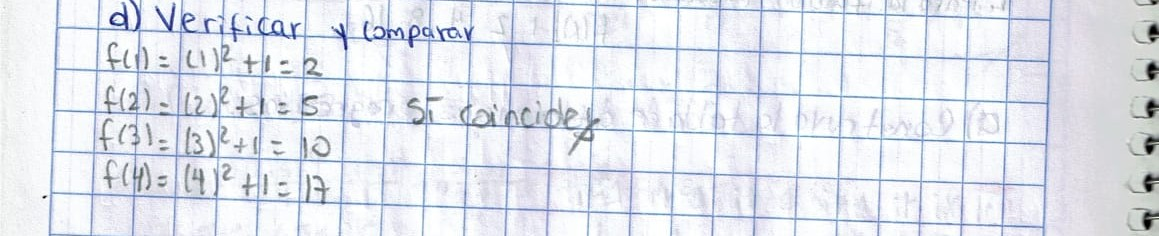
\includegraphics[width=6.25in,height=\textheight,keepaspectratio,alt={Ejercicio 1.2 d}]{Inter12d.jpg}
\caption{Ejercicio 1.2 d}
\end{figure}

\subsubsection{\texorpdfstring{\(1.3\)}{1.3}}\label{section-7}

\paragraph{\texorpdfstring{\(a)\) Polinomio de
Lagrange}{a) Polinomio de Lagrange}}\label{a-polinomio-de-lagrange}

\begin{figure}
\centering
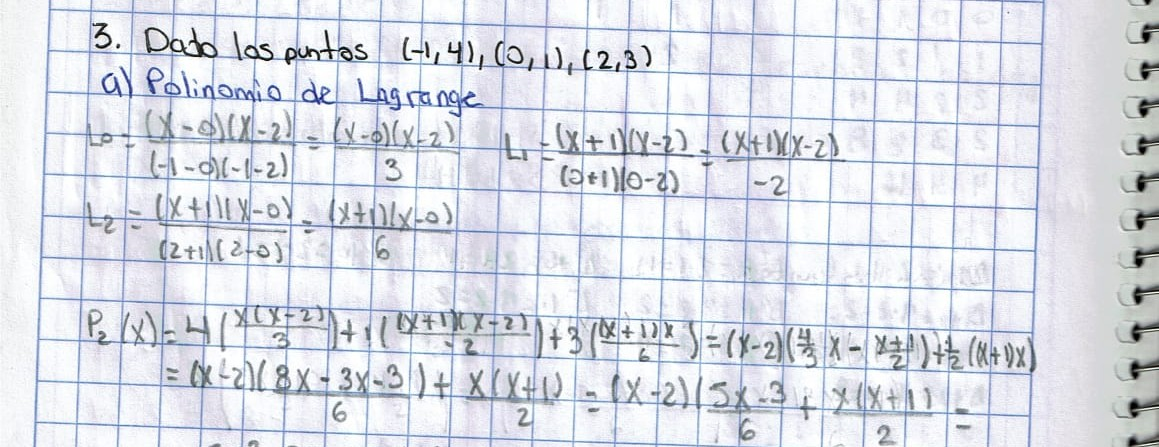
\includegraphics[width=6.25in,height=\textheight,keepaspectratio,alt={Ejercicio 1.3 a}]{Inter13a.jpg}
\caption{Ejercicio 1.3 a}
\end{figure}

\paragraph{\texorpdfstring{\(b)\) Expanda y
simplifique}{b) Expanda y simplifique}}\label{b-expanda-y-simplifique}

\begin{figure}
\centering
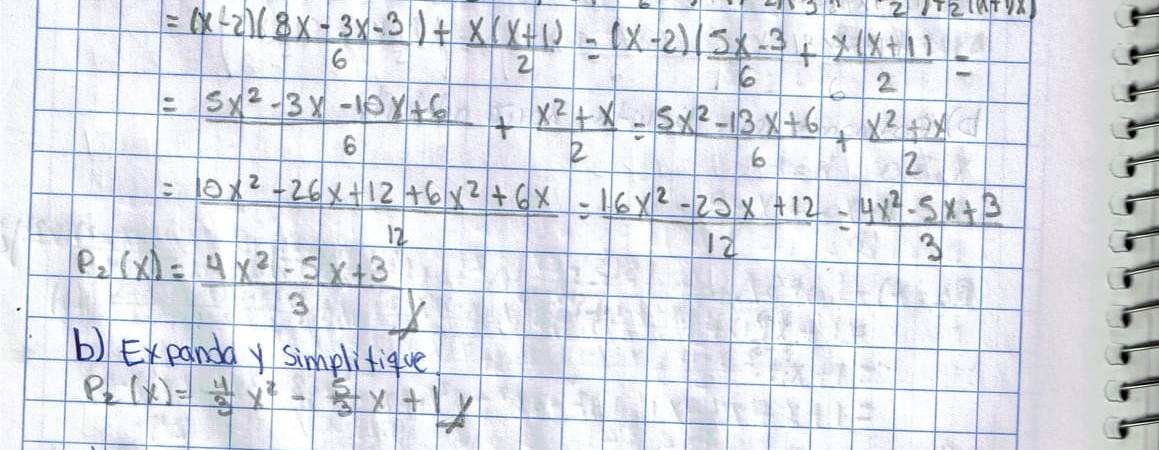
\includegraphics[width=6.25in,height=\textheight,keepaspectratio,alt={Ejercicio 1.3 b}]{Inter13b.jpg}
\caption{Ejercicio 1.3 b}
\end{figure}

\paragraph{\texorpdfstring{\(c)\) Verifique los
valores}{c) Verifique los valores}}\label{c-verifique-los-valores}

\begin{figure}
\centering
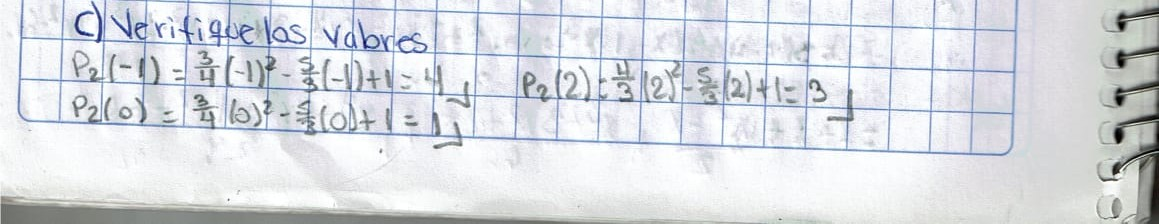
\includegraphics[width=6.25in,height=\textheight,keepaspectratio,alt={Ejercicio 1.3 c}]{Inter13c.jpg}
\caption{Ejercicio 1.3 c}
\end{figure}

\subsection{Ejercicio 2}\label{ejercicio-2}

\subsubsection{\texorpdfstring{\(2.1\)}{2.1}}\label{section-8}

\paragraph{\texorpdfstring{\(a)\) Tabla}{a) Tabla}}\label{a-tabla}

\begin{figure}
\centering
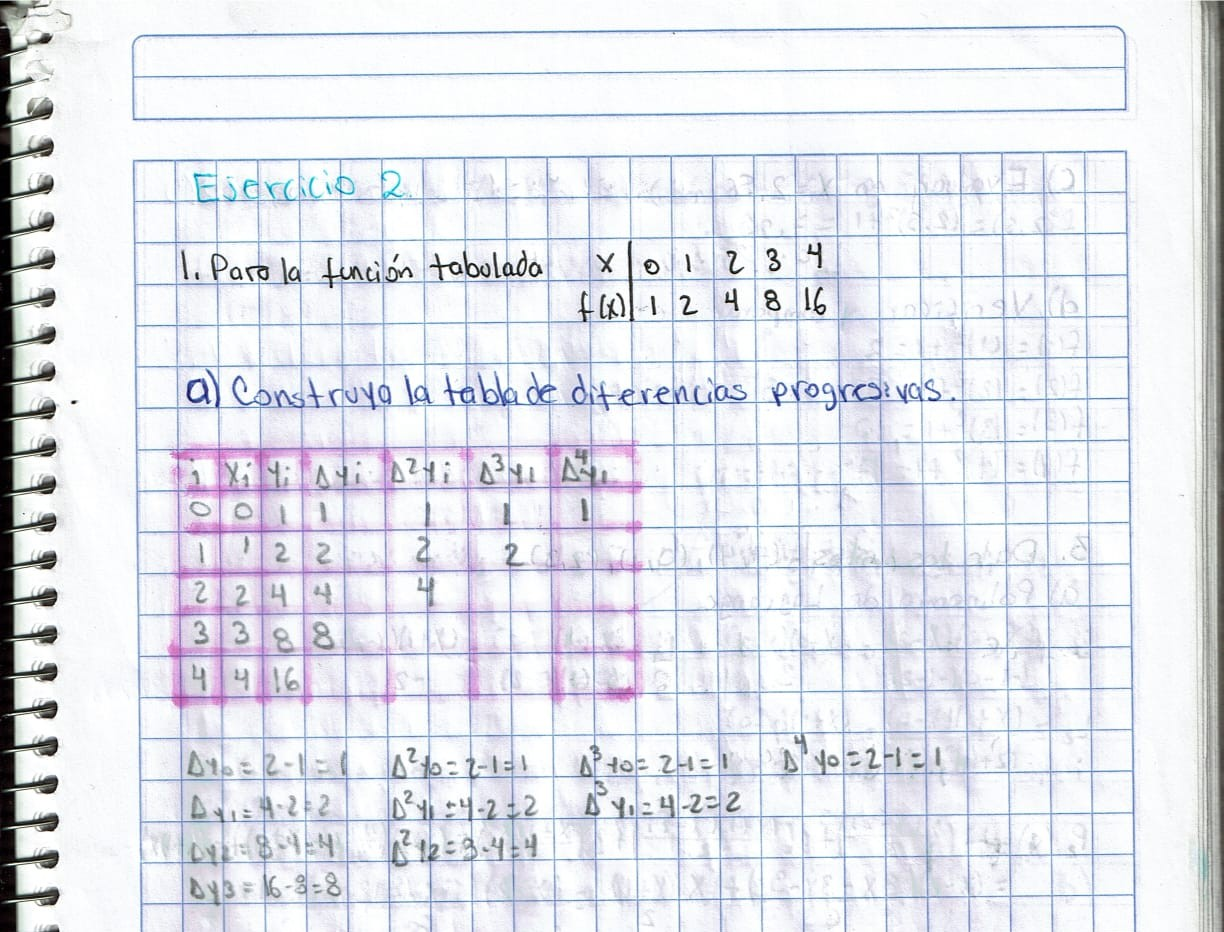
\includegraphics[width=6.25in,height=\textheight,keepaspectratio,alt={Ejercicio 2.1 a}]{Inter21a.jpg}
\caption{Ejercicio 2.1 a}
\end{figure}

\paragraph{\texorpdfstring{\(b)\)
Polinomio}{b) Polinomio}}\label{b-polinomio}

\begin{figure}
\centering
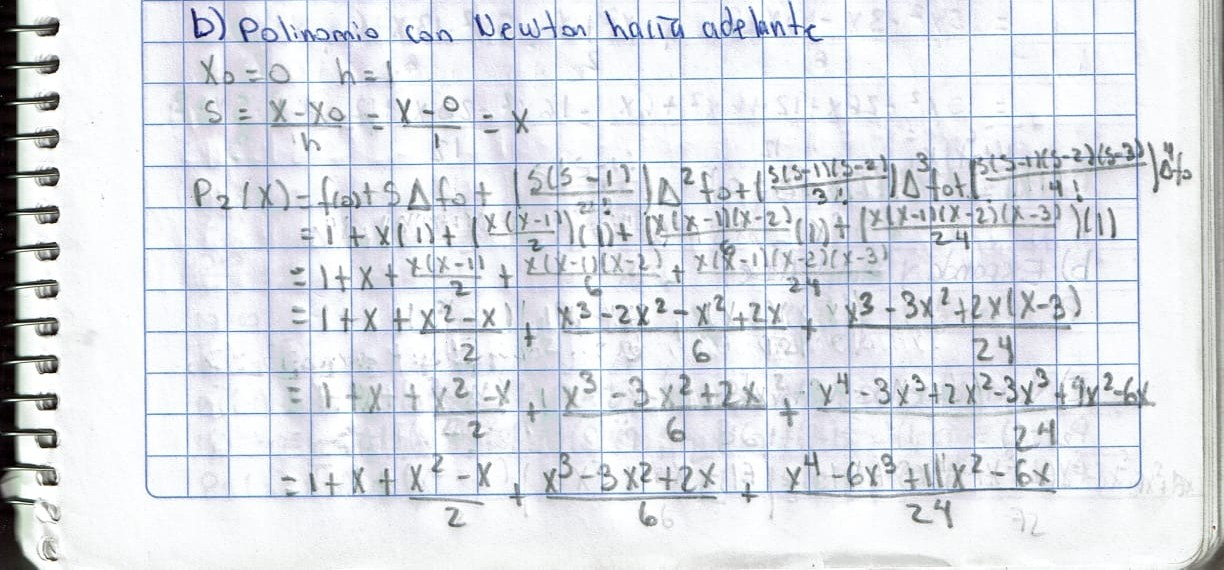
\includegraphics[width=6.25in,height=\textheight,keepaspectratio,alt={Ejercicio 2.1 b1}]{Inter21b.jpg}
\caption{Ejercicio 2.1 b1}
\end{figure}

\begin{figure}
\centering
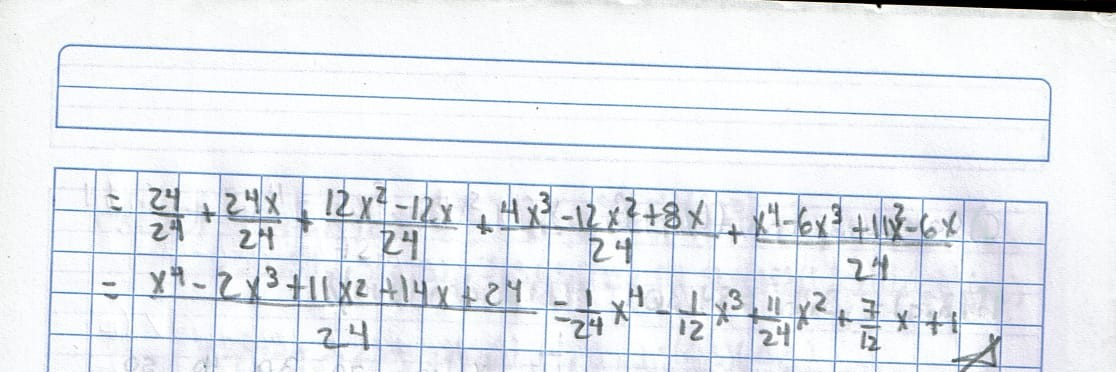
\includegraphics[width=6.25in,height=\textheight,keepaspectratio,alt={Ejercicio 2.1 b2}]{Inter21b2.jpg}
\caption{Ejercicio 2.1 b2}
\end{figure}

\paragraph{\texorpdfstring{\(c)\) Calcule \(f(2.5)\) y
comparación}{c) Calcule f(2.5) y comparación}}\label{c-calcule-f2.5-y-comparaciuxf3n}

\begin{figure}
\centering
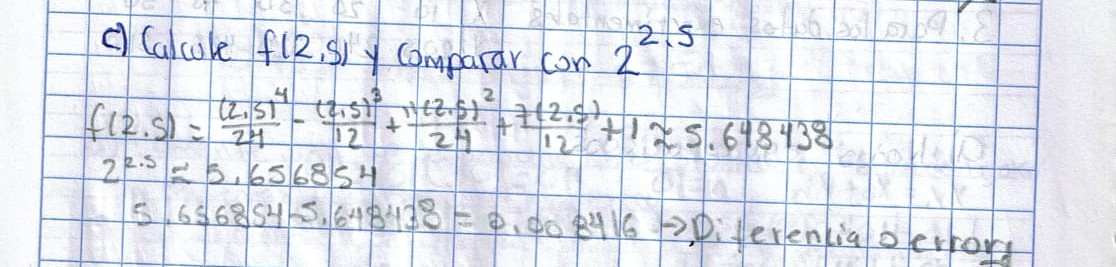
\includegraphics[width=6.25in,height=\textheight,keepaspectratio,alt={Ejercicio 2.1 c}]{Inter21c.jpg}
\caption{Ejercicio 2.1 c}
\end{figure}

\subsubsection{\texorpdfstring{\(2.2\)}{2.2}}\label{section-9}

\paragraph{\texorpdfstring{\(a)\) Tabla}{a) Tabla}}\label{a-tabla-1}

\begin{figure}
\centering
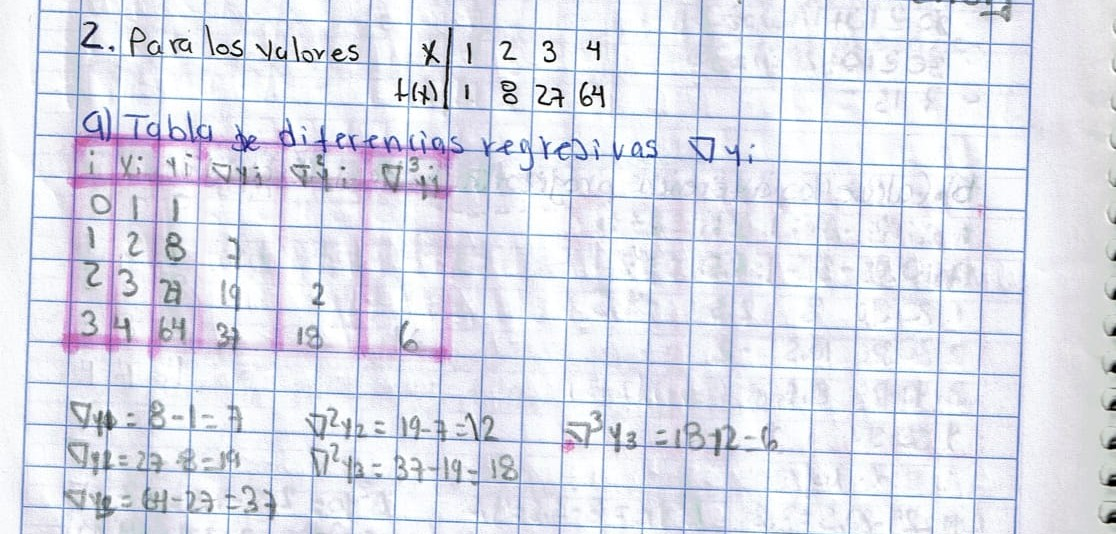
\includegraphics[width=6.25in,height=\textheight,keepaspectratio,alt={Ejercicio 2.2 a}]{Inter22a.jpg}
\caption{Ejercicio 2.2 a}
\end{figure}

\paragraph{\texorpdfstring{\(b)\) Newton hacía
atrás}{b) Newton hacía atrás}}\label{b-newton-hacuxeda-atruxe1s}

\begin{figure}
\centering
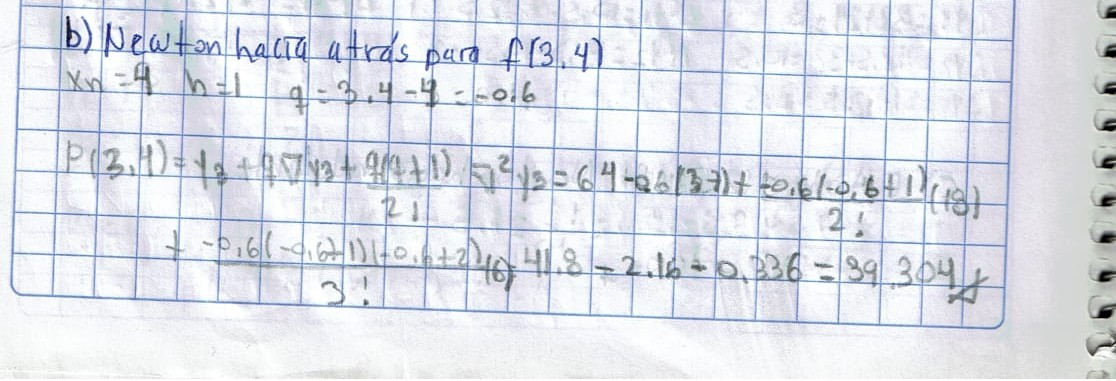
\includegraphics[width=6.25in,height=\textheight,keepaspectratio,alt={Ejercicio 2.2 b}]{Inter22b.jpg}
\caption{Ejercicio 2.2 b}
\end{figure}

\paragraph{\texorpdfstring{\(c)\) Comparación con
\(f(x)=x^3\)}{c) Comparación con f(x)=x\^{}3}}\label{c-comparaciuxf3n-con-fxx3}

\begin{figure}
\centering
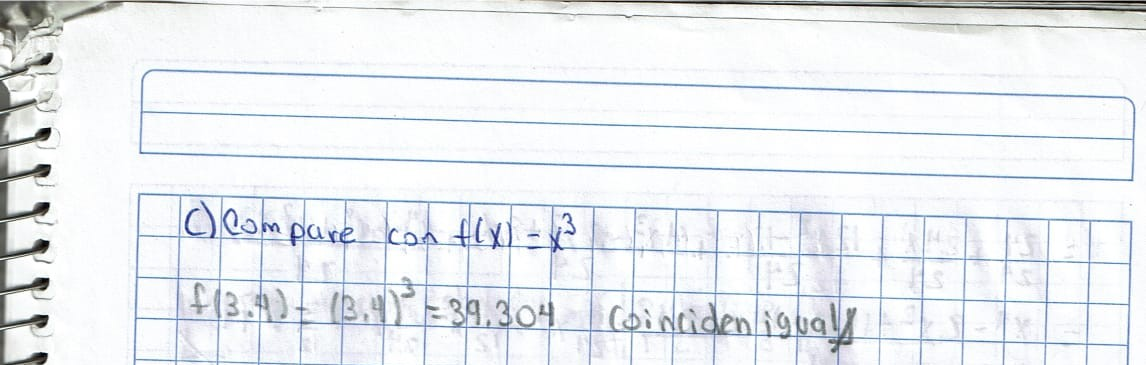
\includegraphics[width=6.25in,height=\textheight,keepaspectratio,alt={Ejercicio 2.2 c}]{Inter22c.jpg}
\caption{Ejercicio 2.2 c}
\end{figure}

\subsubsection{\texorpdfstring{\(2.3\)}{2.3}}\label{section-10}

\paragraph{\texorpdfstring{\(a)\) Nodos
equiespaciados}{a) Nodos equiespaciados}}\label{a-nodos-equiespaciados}

\begin{figure}
\centering
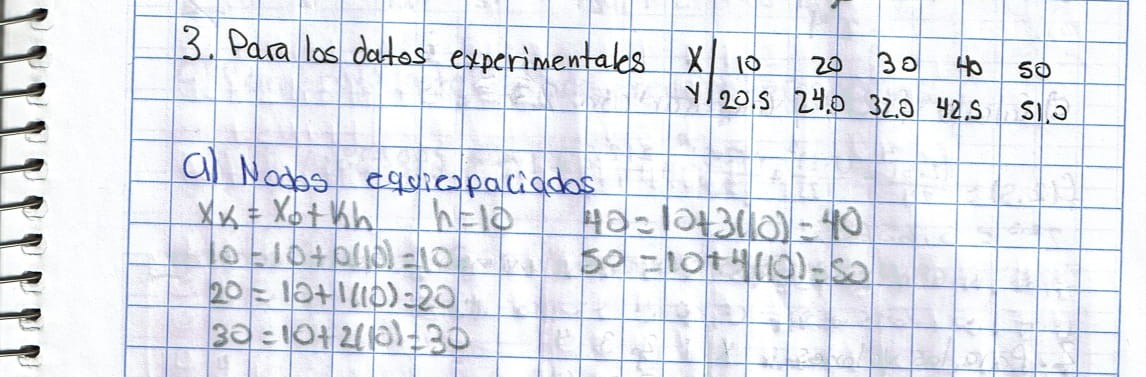
\includegraphics[width=6.25in,height=\textheight,keepaspectratio,alt={Ejercicio 2.3 a}]{Inter23a.jpg}
\caption{Ejercicio 2.3 a}
\end{figure}

\paragraph{\texorpdfstring{\(b)\) Tabla}{b) Tabla}}\label{b-tabla-2}

\begin{figure}
\centering
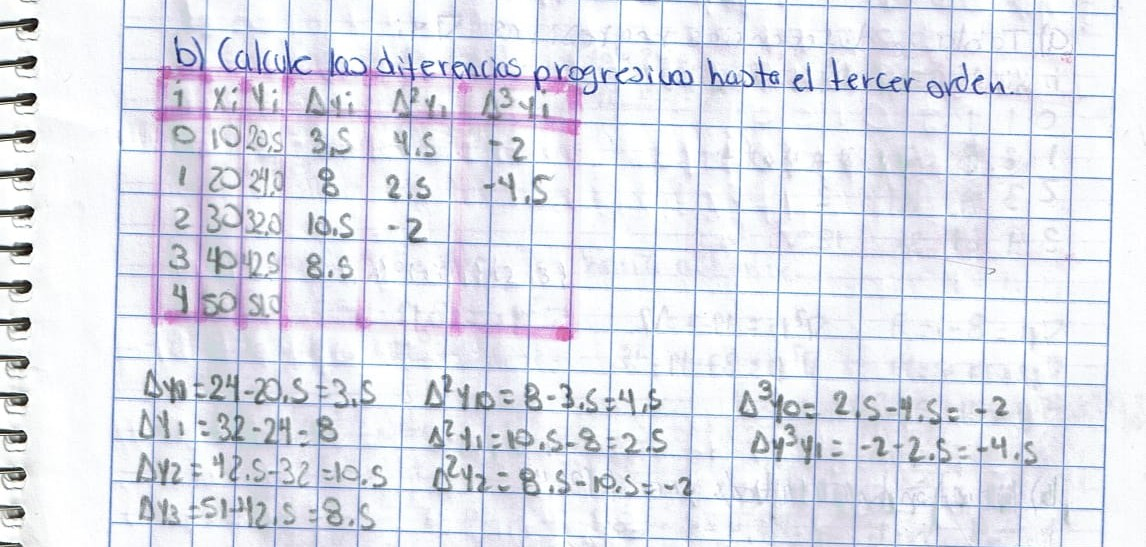
\includegraphics[width=6.25in,height=\textheight,keepaspectratio,alt={Ejercicio 2.3 b}]{Inter23b.jpg}
\caption{Ejercicio 2.3 b}
\end{figure}

\paragraph{\texorpdfstring{\(c)\) Estimación
\(y(25)\)}{c) Estimación y(25)}}\label{c-estimaciuxf3n-y25}

\begin{figure}
\centering
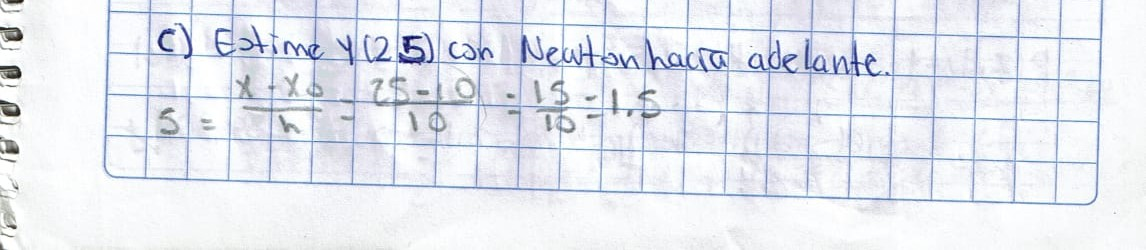
\includegraphics[width=6.25in,height=\textheight,keepaspectratio,alt={Ejercicio 2.3 c1}]{Inter23c.jpg}
\caption{Ejercicio 2.3 c1}
\end{figure}

\begin{figure}
\centering
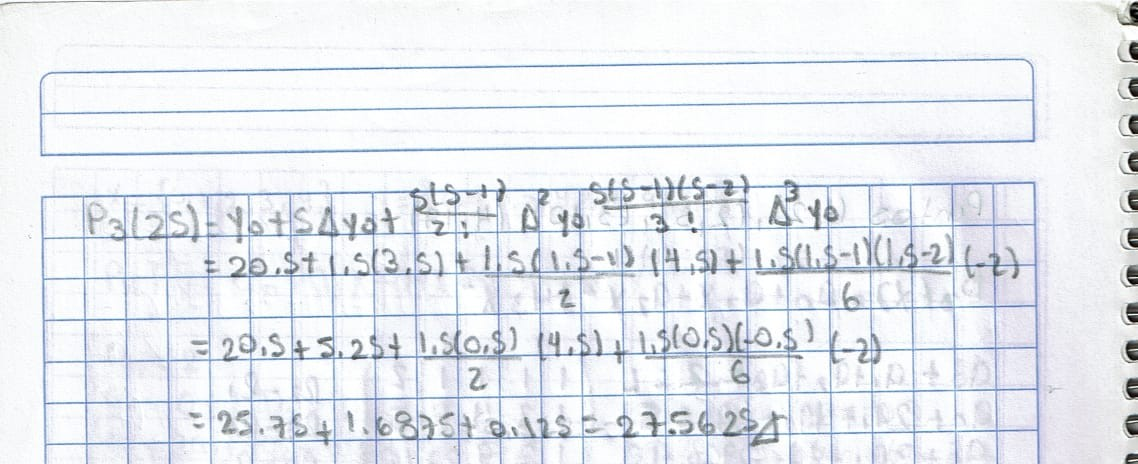
\includegraphics[width=6.25in,height=\textheight,keepaspectratio,alt={Ejercicio 2.3 c2}]{Inter23c2.jpg}
\caption{Ejercicio 2.3 c2}
\end{figure}

\paragraph{\texorpdfstring{\(d)\) Mejora o
no}{d) Mejora o no}}\label{d-mejora-o-no}

\begin{figure}
\centering
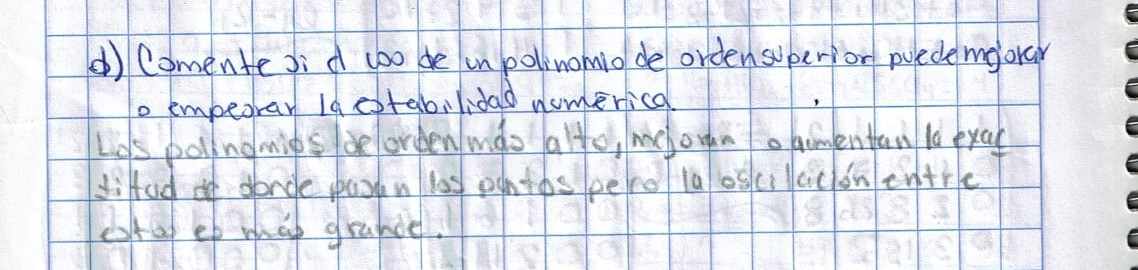
\includegraphics[width=6.25in,height=\textheight,keepaspectratio,alt={Ejercicio 2.3 d}]{Inter23d.jpg}
\caption{Ejercicio 2.3 d}
\end{figure}

\subsection{Ejercicio 3}\label{ejercicio-3}

\subsubsection{\texorpdfstring{\(Puntos (0, 1), (1, 3), (2, 11)\)}{Puntos (0, 1), (1, 3), (2, 11)}}\label{puntos-0-1-1-3-2-11}

\begin{figure}
\centering
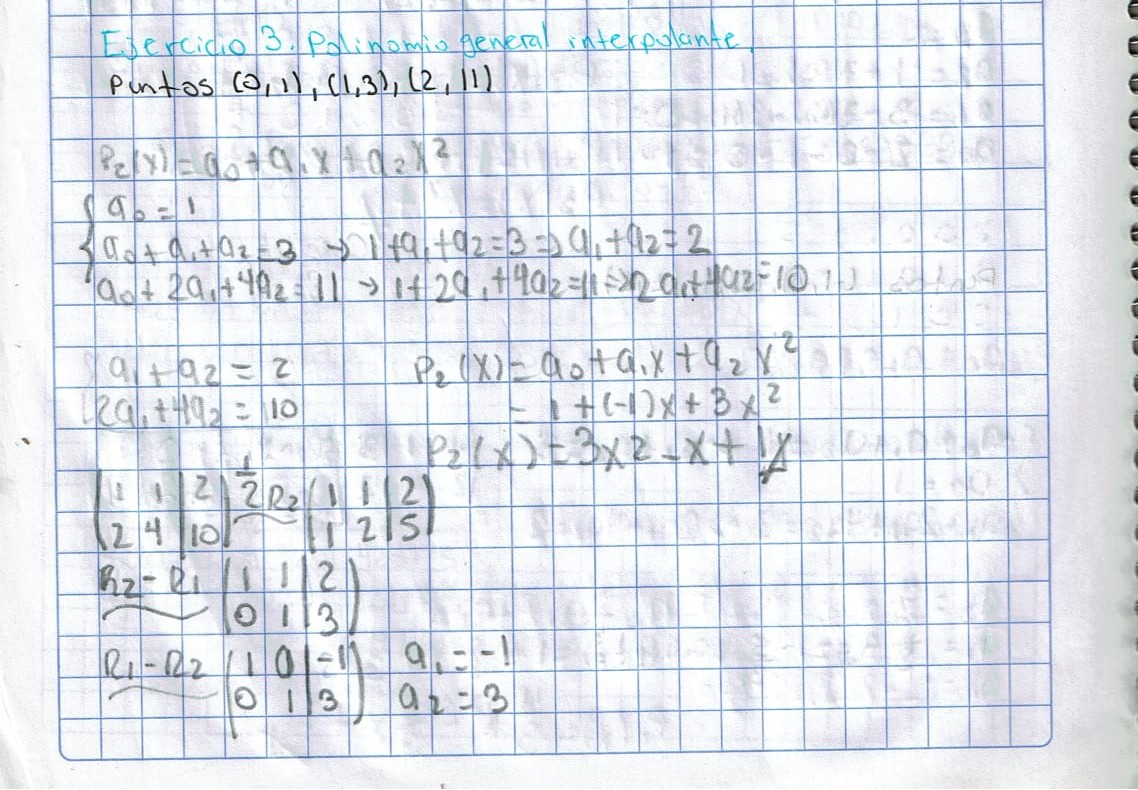
\includegraphics[width=6.25in,height=\textheight,keepaspectratio,alt={Ejercicio 3.1}]{Inter31.jpg}
\caption{Ejercicio 3.1}
\end{figure}

\subsubsection{\texorpdfstring{\(Puntos (1, 2), (2, 5), (3, 10), (4, 17)\)}{Puntos (1, 2), (2, 5), (3, 10), (4, 17)}}\label{puntos-1-2-2-5-3-10-4-17}

\begin{figure}
\centering
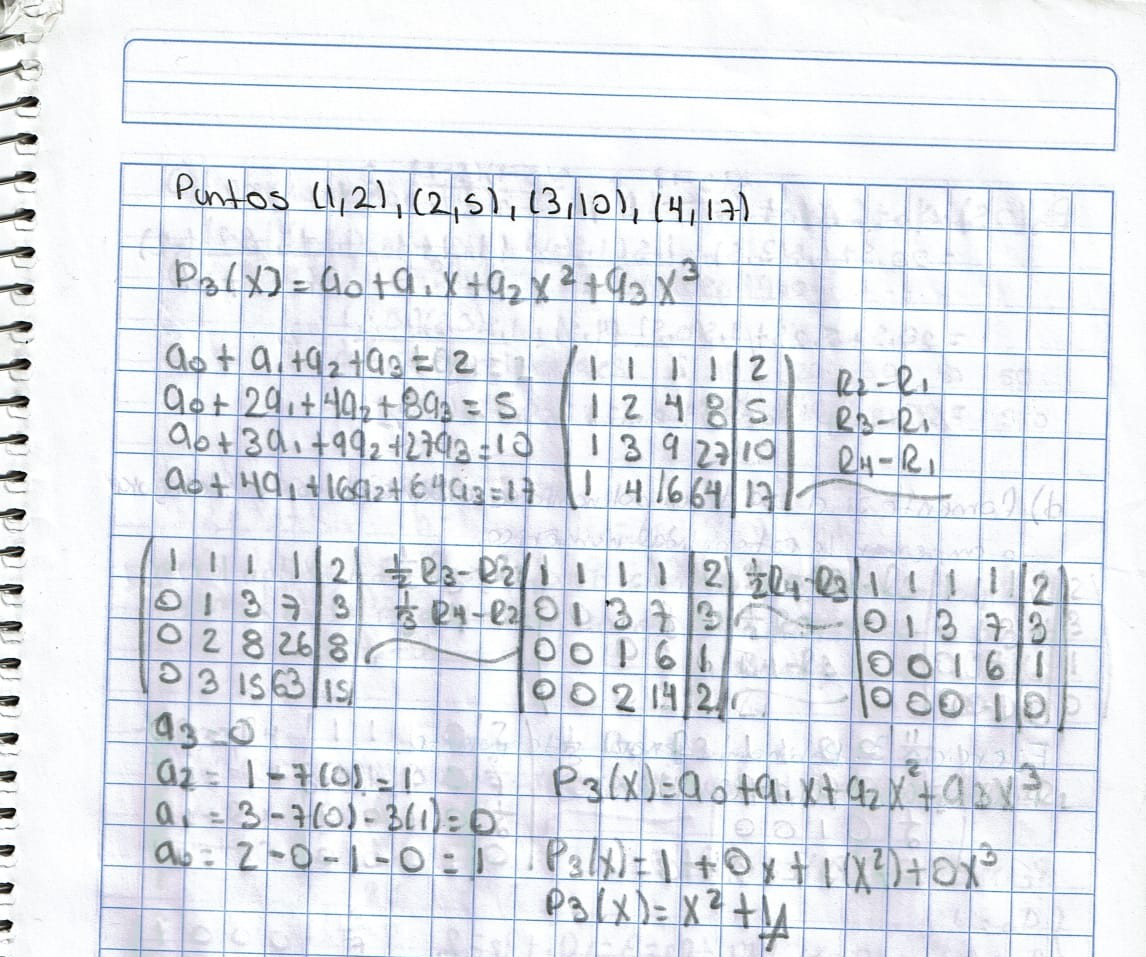
\includegraphics[width=6.25in,height=\textheight,keepaspectratio,alt={Ejercicio 3.2}]{Inter32.jpg}
\caption{Ejercicio 3.2}
\end{figure}

\subsubsection{\texorpdfstring{\(Puntos (-1, 4), (0, 1), (2, 3)\)}{Puntos (-1, 4), (0, 1), (2, 3)}}\label{puntos--1-4-0-1-2-3}

\begin{figure}
\centering
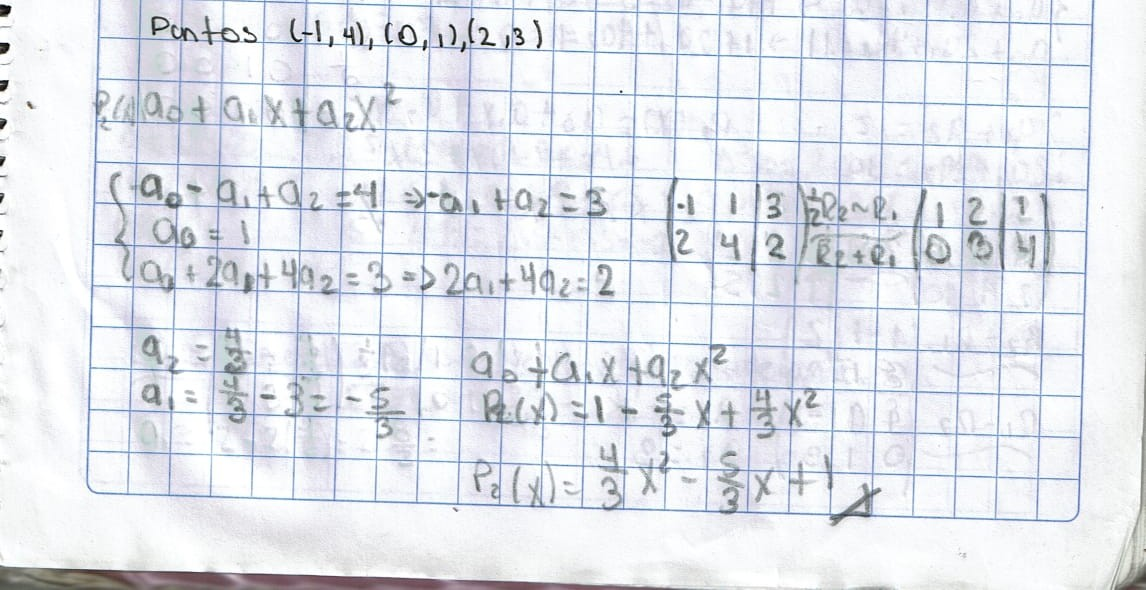
\includegraphics[width=6.25in,height=\textheight,keepaspectratio,alt={Ejercicio 3.3}]{Inter33.jpg}
\caption{Ejercicio 3.3}
\end{figure}

\subsubsection{\texorpdfstring{\(Puntos (0, 2.0), (1, 2.7), (2, 4.8), (3, 8.9), (4, 16.0)\)}{Puntos (0, 2.0), (1, 2.7), (2, 4.8), (3, 8.9), (4, 16.0)}}\label{puntos-0-2.0-1-2.7-2-4.8-3-8.9-4-16.0}

\begin{figure}
\centering
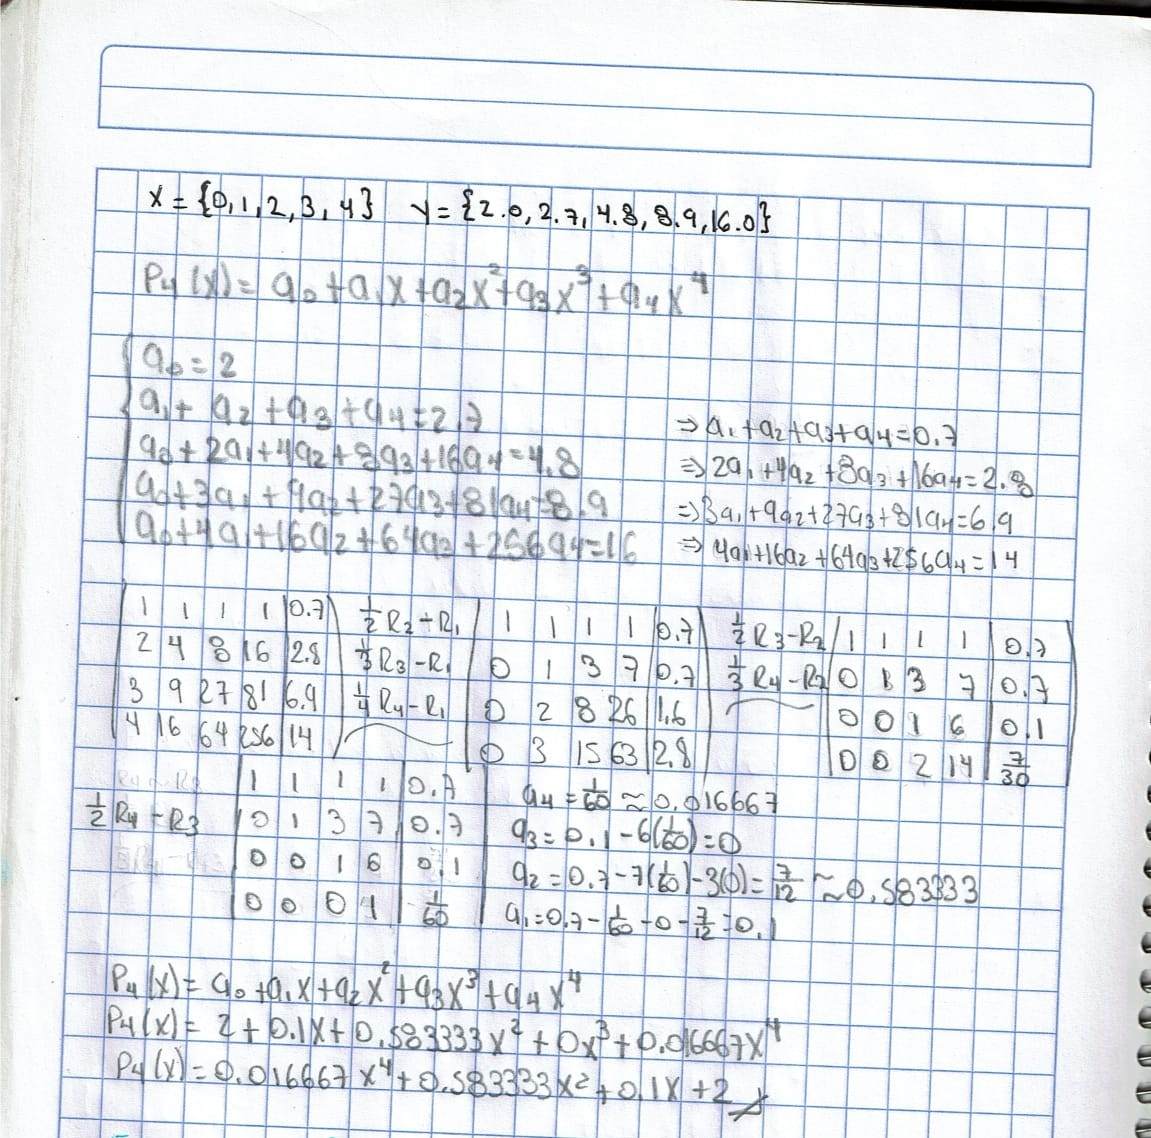
\includegraphics[width=6.25in,height=\textheight,keepaspectratio,alt={Ejercicio 3.4}]{Inter34.jpg}
\caption{Ejercicio 3.4}
\end{figure}

\subsection{Ejercicio 4}\label{ejercicio-4}

\paragraph{\texorpdfstring{\(a)\) Datos experimentales
equiespaciados}{a) Datos experimentales equiespaciados}}\label{a-datos-experimentales-equiespaciados}

\begin{figure}
\centering
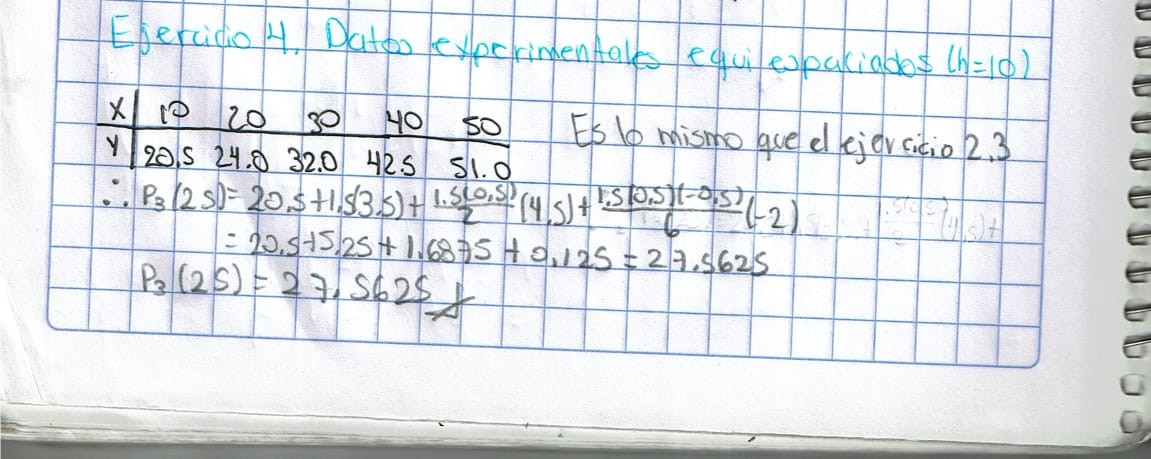
\includegraphics[width=6.25in,height=\textheight,keepaspectratio,alt={Ejercicio 4 a}]{Inter4.jpg}
\caption{Ejercicio 4 a}
\end{figure}

\section{Prácticas de laboratorio}\label{pruxe1cticas-de-laboratorio}

\subsection{Sesión 1}\label{sesiuxf3n-1}

\begin{Shaded}
\begin{Highlighting}[]
\CommentTok{\#{-}{-}{-}{-} SESION 1 {-}{-}{-}{-}}
\DocumentationTok{\#\#{-}{-}{-}{-} OPERADORES LOGICOS {-}{-}{-}{-}}
\DecValTok{17}\SpecialCharTok{\textless{}}\DecValTok{5}
\end{Highlighting}
\end{Shaded}

\begin{verbatim}
## [1] FALSE
\end{verbatim}

\begin{Shaded}
\begin{Highlighting}[]
\DecValTok{17}\SpecialCharTok{\textgreater{}}\DecValTok{5}
\end{Highlighting}
\end{Shaded}

\begin{verbatim}
## [1] TRUE
\end{verbatim}

\begin{Shaded}
\begin{Highlighting}[]
\DecValTok{17}\SpecialCharTok{\textless{}=}\DecValTok{5}
\end{Highlighting}
\end{Shaded}

\begin{verbatim}
## [1] FALSE
\end{verbatim}

\begin{Shaded}
\begin{Highlighting}[]
\DecValTok{17}\SpecialCharTok{\textgreater{}=}\DecValTok{5}
\end{Highlighting}
\end{Shaded}

\begin{verbatim}
## [1] TRUE
\end{verbatim}

\begin{Shaded}
\begin{Highlighting}[]
\DecValTok{17}\SpecialCharTok{!=}\DecValTok{5}
\end{Highlighting}
\end{Shaded}

\begin{verbatim}
## [1] TRUE
\end{verbatim}

\begin{Shaded}
\begin{Highlighting}[]
\DecValTok{17}\SpecialCharTok{==}\DecValTok{5}
\end{Highlighting}
\end{Shaded}

\begin{verbatim}
## [1] FALSE
\end{verbatim}

\begin{Shaded}
\begin{Highlighting}[]
\DocumentationTok{\#\#{-}{-}{-}{-} OPERADORES ARITMETICOS {-}{-}{-}{-}}
\CommentTok{\# SUMA, RESTA, MULTIPLICACION, DIVISION, POTENCIA, MODULO, DIVISION ENTERA}
\DecValTok{17}\SpecialCharTok{+}\DecValTok{5}
\end{Highlighting}
\end{Shaded}

\begin{verbatim}
## [1] 22
\end{verbatim}

\begin{Shaded}
\begin{Highlighting}[]
\DecValTok{17}\SpecialCharTok{*}\DecValTok{5}
\end{Highlighting}
\end{Shaded}

\begin{verbatim}
## [1] 85
\end{verbatim}

\begin{Shaded}
\begin{Highlighting}[]
\DecValTok{17}\SpecialCharTok{*}\DecValTok{5}
\end{Highlighting}
\end{Shaded}

\begin{verbatim}
## [1] 85
\end{verbatim}

\begin{Shaded}
\begin{Highlighting}[]
\DecValTok{17}\SpecialCharTok{\^{}}\DecValTok{5}
\end{Highlighting}
\end{Shaded}

\begin{verbatim}
## [1] 1419857
\end{verbatim}

\begin{Shaded}
\begin{Highlighting}[]
\DecValTok{17}\SpecialCharTok{\%/\%}\DecValTok{5}
\end{Highlighting}
\end{Shaded}

\begin{verbatim}
## [1] 3
\end{verbatim}

\begin{Shaded}
\begin{Highlighting}[]
\DecValTok{17}\SpecialCharTok{\%\%}\DecValTok{5}
\end{Highlighting}
\end{Shaded}

\begin{verbatim}
## [1] 2
\end{verbatim}

\begin{Shaded}
\begin{Highlighting}[]
\DocumentationTok{\#\#{-}{-}{-}{-} LOGARITMOS Y EXPONENCIALES {-}{-}{-}{-}}
\FunctionTok{log}\NormalTok{(}\DecValTok{1}\NormalTok{)}
\end{Highlighting}
\end{Shaded}

\begin{verbatim}
## [1] 0
\end{verbatim}

\begin{Shaded}
\begin{Highlighting}[]
\FunctionTok{log}\NormalTok{(}\DecValTok{12}\NormalTok{)}
\end{Highlighting}
\end{Shaded}

\begin{verbatim}
## [1] 2.484907
\end{verbatim}

\begin{Shaded}
\begin{Highlighting}[]
\FunctionTok{log}\NormalTok{(}\DecValTok{12}\NormalTok{,}\DecValTok{2}\NormalTok{)}
\end{Highlighting}
\end{Shaded}

\begin{verbatim}
## [1] 3.584963
\end{verbatim}

\begin{Shaded}
\begin{Highlighting}[]
\FunctionTok{exp}\NormalTok{(}\DecValTok{12}\NormalTok{)}
\end{Highlighting}
\end{Shaded}

\begin{verbatim}
## [1] 162754.8
\end{verbatim}

\begin{Shaded}
\begin{Highlighting}[]
\FunctionTok{exp}\NormalTok{(}\DecValTok{1}\NormalTok{)}
\end{Highlighting}
\end{Shaded}

\begin{verbatim}
## [1] 2.718282
\end{verbatim}

\begin{Shaded}
\begin{Highlighting}[]
\DocumentationTok{\#\#{-}{-}{-}{-} FUNCIONES TRIGONOMETRICAS {-}{-}{-}{-}}
\FunctionTok{sin}\NormalTok{(}\DecValTok{45}\NormalTok{)}
\end{Highlighting}
\end{Shaded}

\begin{verbatim}
## [1] 0.8509035
\end{verbatim}

\begin{Shaded}
\begin{Highlighting}[]
\FunctionTok{cos}\NormalTok{(}\DecValTok{45}\NormalTok{)}
\end{Highlighting}
\end{Shaded}

\begin{verbatim}
## [1] 0.525322
\end{verbatim}

\begin{Shaded}
\begin{Highlighting}[]
\FunctionTok{tan}\NormalTok{(}\DecValTok{45}\NormalTok{)}
\end{Highlighting}
\end{Shaded}

\begin{verbatim}
## [1] 1.619775
\end{verbatim}

\begin{Shaded}
\begin{Highlighting}[]
\FunctionTok{asin}\NormalTok{(}\FloatTok{0.96}\NormalTok{)}
\end{Highlighting}
\end{Shaded}

\begin{verbatim}
## [1] 1.287002
\end{verbatim}

\begin{Shaded}
\begin{Highlighting}[]
\FunctionTok{acos}\NormalTok{(}\FloatTok{0.97}\NormalTok{)}
\end{Highlighting}
\end{Shaded}

\begin{verbatim}
## [1] 0.2455655
\end{verbatim}

\begin{Shaded}
\begin{Highlighting}[]
\FunctionTok{atan}\NormalTok{(}\FloatTok{0.45}\NormalTok{)}
\end{Highlighting}
\end{Shaded}

\begin{verbatim}
## [1] 0.4228539
\end{verbatim}

\begin{Shaded}
\begin{Highlighting}[]
\DocumentationTok{\#\#{-}{-}{-}{-} FUNCIONES VARIAS {-}{-}{-}{-}}
\FunctionTok{abs}\NormalTok{(}\SpecialCharTok{{-}}\DecValTok{34}\NormalTok{)}
\end{Highlighting}
\end{Shaded}

\begin{verbatim}
## [1] 34
\end{verbatim}

\begin{Shaded}
\begin{Highlighting}[]
\FunctionTok{sqrt}\NormalTok{(}\DecValTok{8}\NormalTok{)}
\end{Highlighting}
\end{Shaded}

\begin{verbatim}
## [1] 2.828427
\end{verbatim}

\begin{Shaded}
\begin{Highlighting}[]
\FunctionTok{floor}\NormalTok{(}\FloatTok{1.56}\NormalTok{)}
\end{Highlighting}
\end{Shaded}

\begin{verbatim}
## [1] 1
\end{verbatim}

\begin{Shaded}
\begin{Highlighting}[]
\FunctionTok{ceiling}\NormalTok{(}\FloatTok{1.56}\NormalTok{)}
\end{Highlighting}
\end{Shaded}

\begin{verbatim}
## [1] 2
\end{verbatim}

\begin{Shaded}
\begin{Highlighting}[]
\FunctionTok{max}\NormalTok{(}\DecValTok{4}\NormalTok{,}\DecValTok{7}\NormalTok{,}\DecValTok{2}\NormalTok{,}\DecValTok{12}\NormalTok{)}
\end{Highlighting}
\end{Shaded}

\begin{verbatim}
## [1] 12
\end{verbatim}

\begin{Shaded}
\begin{Highlighting}[]
\FunctionTok{min}\NormalTok{(}\DecValTok{4}\NormalTok{,}\DecValTok{7}\NormalTok{,}\DecValTok{2}\NormalTok{,}\DecValTok{12}\NormalTok{)}
\end{Highlighting}
\end{Shaded}

\begin{verbatim}
## [1] 2
\end{verbatim}

\begin{Shaded}
\begin{Highlighting}[]
\FunctionTok{sign}\NormalTok{(}\SpecialCharTok{{-}}\DecValTok{45}\NormalTok{)}
\end{Highlighting}
\end{Shaded}

\begin{verbatim}
## [1] -1
\end{verbatim}

\begin{Shaded}
\begin{Highlighting}[]
\DocumentationTok{\#\#{-}{-}{-}{-} EJERCICIOS DE PRACTICA {-}{-}{-}{-}}
\CommentTok{\# calcular la expresion}
\CommentTok{\#cos(pi/6+pi/2)+e\^{}2}
\CommentTok{\# calcular la expresion}
\CommentTok{\#cos(pi/6+pi/2)+e\^{}2*log(5)+a(1/raiz(2))}
\CommentTok{\# introducir las siguientes expresiones: }
\DecValTok{1}\SpecialCharTok{/}\DecValTok{7}
\end{Highlighting}
\end{Shaded}

\begin{verbatim}
## [1] 0.1428571
\end{verbatim}

\begin{Shaded}
\begin{Highlighting}[]
\FunctionTok{options}\NormalTok{(}\AttributeTok{digits=}\DecValTok{3}\NormalTok{); }\DecValTok{1}\SpecialCharTok{/}\DecValTok{7}
\end{Highlighting}
\end{Shaded}

\begin{verbatim}
## [1] 0.143
\end{verbatim}

\begin{Shaded}
\begin{Highlighting}[]
\CommentTok{\# c) options(digits=6); 1/7}
\CommentTok{\# d) round(67.45)}
\CommentTok{\# e) round(75.324568,2)}
\CommentTok{\# f) options(digits=7);}
\CommentTok{\# g) signif(56.345458234234,2)}
\CommentTok{\# h) signif(56.345458234234)}
\CommentTok{\# i) exp({-}30)}
\CommentTok{\# j) options(scipen= 999)}
\CommentTok{\# k) exp({-}30)}
\CommentTok{\# l) options(scipen=0)}
\DocumentationTok{\#\#\#\#{-}{-}{-}{-} MIS EJERCICIOS DE PRACTICA SESION 1 {-}{-}{-}{-}}
\DocumentationTok{\#\#{-}{-}{-}{-} OPERADORES LOGICOS {-}{-}{-}{-}}
\DecValTok{20}\SpecialCharTok{\textless{}}\DecValTok{10}
\end{Highlighting}
\end{Shaded}

\begin{verbatim}
## [1] FALSE
\end{verbatim}

\begin{Shaded}
\begin{Highlighting}[]
\DecValTok{30}\SpecialCharTok{\textgreater{}}\DecValTok{5}
\end{Highlighting}
\end{Shaded}

\begin{verbatim}
## [1] TRUE
\end{verbatim}

\begin{Shaded}
\begin{Highlighting}[]
\DecValTok{46}\SpecialCharTok{\textless{}=}\DecValTok{7}
\end{Highlighting}
\end{Shaded}

\begin{verbatim}
## [1] FALSE
\end{verbatim}

\begin{Shaded}
\begin{Highlighting}[]
\DecValTok{36}\SpecialCharTok{\textgreater{}=}\DecValTok{6}
\end{Highlighting}
\end{Shaded}

\begin{verbatim}
## [1] TRUE
\end{verbatim}

\begin{Shaded}
\begin{Highlighting}[]
\DecValTok{26}\SpecialCharTok{!=}\DecValTok{5}
\end{Highlighting}
\end{Shaded}

\begin{verbatim}
## [1] TRUE
\end{verbatim}

\begin{Shaded}
\begin{Highlighting}[]
\DecValTok{26}\SpecialCharTok{==}\DecValTok{5}
\end{Highlighting}
\end{Shaded}

\begin{verbatim}
## [1] FALSE
\end{verbatim}

\begin{Shaded}
\begin{Highlighting}[]
\DocumentationTok{\#\#{-}{-}{-}{-} OPERADORES ARITMETICOS {-}{-}{-}{-}}
\CommentTok{\# SUMA, RESTA, MULTIPLICACION, DIVISION, POTENCIA, MODULO, DIVISION ENTERA}
\DecValTok{15}\SpecialCharTok{+}\DecValTok{1}
\end{Highlighting}
\end{Shaded}

\begin{verbatim}
## [1] 16
\end{verbatim}

\begin{Shaded}
\begin{Highlighting}[]
\DecValTok{16}\SpecialCharTok{*}\DecValTok{2}
\end{Highlighting}
\end{Shaded}

\begin{verbatim}
## [1] 32
\end{verbatim}

\begin{Shaded}
\begin{Highlighting}[]
\DecValTok{17}\SpecialCharTok{*}\DecValTok{3}
\end{Highlighting}
\end{Shaded}

\begin{verbatim}
## [1] 51
\end{verbatim}

\begin{Shaded}
\begin{Highlighting}[]
\DecValTok{18}\SpecialCharTok{\^{}}\DecValTok{4}
\end{Highlighting}
\end{Shaded}

\begin{verbatim}
## [1] 104976
\end{verbatim}

\begin{Shaded}
\begin{Highlighting}[]
\DecValTok{19}\SpecialCharTok{\%/\%}\DecValTok{5}
\end{Highlighting}
\end{Shaded}

\begin{verbatim}
## [1] 3
\end{verbatim}

\begin{Shaded}
\begin{Highlighting}[]
\DecValTok{20}\SpecialCharTok{\%\%}\DecValTok{6}
\end{Highlighting}
\end{Shaded}

\begin{verbatim}
## [1] 2
\end{verbatim}

\begin{Shaded}
\begin{Highlighting}[]
\DocumentationTok{\#\#{-}{-}{-}{-} LOGARITMOS Y EXPONENCIALES {-}{-}{-}{-}}
\FunctionTok{log}\NormalTok{(}\DecValTok{2}\NormalTok{)}
\end{Highlighting}
\end{Shaded}

\begin{verbatim}
## [1] 0.693
\end{verbatim}

\begin{Shaded}
\begin{Highlighting}[]
\FunctionTok{log}\NormalTok{(}\DecValTok{6}\NormalTok{)}
\end{Highlighting}
\end{Shaded}

\begin{verbatim}
## [1] 1.79
\end{verbatim}

\begin{Shaded}
\begin{Highlighting}[]
\FunctionTok{log}\NormalTok{(}\DecValTok{7}\NormalTok{,}\DecValTok{3}\NormalTok{)}
\end{Highlighting}
\end{Shaded}

\begin{verbatim}
## [1] 1.77
\end{verbatim}

\begin{Shaded}
\begin{Highlighting}[]
\FunctionTok{exp}\NormalTok{(}\DecValTok{2}\NormalTok{)}
\end{Highlighting}
\end{Shaded}

\begin{verbatim}
## [1] 7.39
\end{verbatim}

\begin{Shaded}
\begin{Highlighting}[]
\FunctionTok{exp}\NormalTok{(}\DecValTok{6}\NormalTok{)}
\end{Highlighting}
\end{Shaded}

\begin{verbatim}
## [1] 403
\end{verbatim}

\begin{Shaded}
\begin{Highlighting}[]
\DocumentationTok{\#\#{-}{-}{-}{-} FUNCIONES TRIGONOMETRICAS {-}{-}{-}{-}}
\FunctionTok{sin}\NormalTok{(}\DecValTok{90}\NormalTok{)}
\end{Highlighting}
\end{Shaded}

\begin{verbatim}
## [1] 0.894
\end{verbatim}

\begin{Shaded}
\begin{Highlighting}[]
\FunctionTok{cos}\NormalTok{(}\DecValTok{180}\NormalTok{)}
\end{Highlighting}
\end{Shaded}

\begin{verbatim}
## [1] -0.598
\end{verbatim}

\begin{Shaded}
\begin{Highlighting}[]
\FunctionTok{tan}\NormalTok{(}\DecValTok{90}\NormalTok{)}
\end{Highlighting}
\end{Shaded}

\begin{verbatim}
## [1] -2
\end{verbatim}

\begin{Shaded}
\begin{Highlighting}[]
\FunctionTok{asin}\NormalTok{(}\FloatTok{0.74}\NormalTok{)}
\end{Highlighting}
\end{Shaded}

\begin{verbatim}
## [1] 0.833
\end{verbatim}

\begin{Shaded}
\begin{Highlighting}[]
\FunctionTok{acos}\NormalTok{(}\FloatTok{0.79}\NormalTok{)}
\end{Highlighting}
\end{Shaded}

\begin{verbatim}
## [1] 0.66
\end{verbatim}

\begin{Shaded}
\begin{Highlighting}[]
\FunctionTok{atan}\NormalTok{(}\FloatTok{0.54}\NormalTok{)}
\end{Highlighting}
\end{Shaded}

\begin{verbatim}
## [1] 0.495
\end{verbatim}

\begin{Shaded}
\begin{Highlighting}[]
\DocumentationTok{\#\#{-}{-}{-}{-} FUNCIONES VARIAS {-}{-}{-}{-}}
\FunctionTok{abs}\NormalTok{(}\SpecialCharTok{{-}}\DecValTok{15}\NormalTok{)}
\end{Highlighting}
\end{Shaded}

\begin{verbatim}
## [1] 15
\end{verbatim}

\begin{Shaded}
\begin{Highlighting}[]
\FunctionTok{sqrt}\NormalTok{(}\DecValTok{9}\NormalTok{)}
\end{Highlighting}
\end{Shaded}

\begin{verbatim}
## [1] 3
\end{verbatim}

\begin{Shaded}
\begin{Highlighting}[]
\FunctionTok{floor}\NormalTok{(}\FloatTok{1.76}\NormalTok{)}
\end{Highlighting}
\end{Shaded}

\begin{verbatim}
## [1] 1
\end{verbatim}

\begin{Shaded}
\begin{Highlighting}[]
\FunctionTok{ceiling}\NormalTok{(}\FloatTok{1.76}\NormalTok{)}
\end{Highlighting}
\end{Shaded}

\begin{verbatim}
## [1] 2
\end{verbatim}

\begin{Shaded}
\begin{Highlighting}[]
\FunctionTok{max}\NormalTok{(}\DecValTok{15}\NormalTok{,}\DecValTok{215}\NormalTok{,}\DecValTok{3}\NormalTok{,}\DecValTok{12}\NormalTok{)}
\end{Highlighting}
\end{Shaded}

\begin{verbatim}
## [1] 215
\end{verbatim}

\begin{Shaded}
\begin{Highlighting}[]
\FunctionTok{min}\NormalTok{(}\DecValTok{1}\NormalTok{,}\DecValTok{9}\NormalTok{,}\DecValTok{4}\NormalTok{,}\DecValTok{2}\NormalTok{)}
\end{Highlighting}
\end{Shaded}

\begin{verbatim}
## [1] 1
\end{verbatim}

\begin{Shaded}
\begin{Highlighting}[]
\FunctionTok{sign}\NormalTok{(}\SpecialCharTok{{-}}\DecValTok{69}\NormalTok{)}
\end{Highlighting}
\end{Shaded}

\begin{verbatim}
## [1] -1
\end{verbatim}

\begin{Shaded}
\begin{Highlighting}[]
\DocumentationTok{\#\#{-}{-}{-}{-} EJERCICIOS DE PRACTICA {-}{-}{-}{-}}
\CommentTok{\# calcular la expresion}
\FunctionTok{cos}\NormalTok{(pi}\SpecialCharTok{/}\DecValTok{6}\SpecialCharTok{+}\NormalTok{pi}\SpecialCharTok{/}\DecValTok{2}\NormalTok{)}\SpecialCharTok{+}\FunctionTok{exp}\NormalTok{(}\DecValTok{1}\NormalTok{)}\SpecialCharTok{\^{}}\DecValTok{2}
\end{Highlighting}
\end{Shaded}

\begin{verbatim}
## [1] 6.89
\end{verbatim}

\begin{Shaded}
\begin{Highlighting}[]
\CommentTok{\# calcular la expresion}
\FunctionTok{cos}\NormalTok{(pi}\SpecialCharTok{/}\DecValTok{6}\SpecialCharTok{+}\NormalTok{pi}\SpecialCharTok{/}\DecValTok{2}\NormalTok{)}\SpecialCharTok{+}\FunctionTok{exp}\NormalTok{(}\DecValTok{1}\NormalTok{)}\SpecialCharTok{\^{}}\DecValTok{2}\SpecialCharTok{*}\FunctionTok{log}\NormalTok{(}\DecValTok{5}\NormalTok{)}\SpecialCharTok{+}\FunctionTok{acos}\NormalTok{(}\DecValTok{1}\SpecialCharTok{/}\FunctionTok{sqrt}\NormalTok{(}\DecValTok{2}\NormalTok{))}
\end{Highlighting}
\end{Shaded}

\begin{verbatim}
## [1] 12.2
\end{verbatim}

\begin{Shaded}
\begin{Highlighting}[]
\CommentTok{\# introducir las siguientes expresiones: }
\DecValTok{7}\SpecialCharTok{/}\DecValTok{1}
\end{Highlighting}
\end{Shaded}

\begin{verbatim}
## [1] 7
\end{verbatim}

\begin{Shaded}
\begin{Highlighting}[]
\FunctionTok{options}\NormalTok{(}\AttributeTok{digits=}\DecValTok{4}\NormalTok{); }\DecValTok{2}\SpecialCharTok{/}\DecValTok{8}
\end{Highlighting}
\end{Shaded}

\begin{verbatim}
## [1] 0.25
\end{verbatim}

\begin{Shaded}
\begin{Highlighting}[]
\FunctionTok{options}\NormalTok{(}\AttributeTok{digits=}\DecValTok{6}\NormalTok{); }\DecValTok{53}\SpecialCharTok{/}\DecValTok{3}
\end{Highlighting}
\end{Shaded}

\begin{verbatim}
## [1] 17.6667
\end{verbatim}

\begin{Shaded}
\begin{Highlighting}[]
\FunctionTok{round}\NormalTok{(}\FloatTok{99.99}\NormalTok{)}
\end{Highlighting}
\end{Shaded}

\begin{verbatim}
## [1] 100
\end{verbatim}

\begin{Shaded}
\begin{Highlighting}[]
\FunctionTok{round}\NormalTok{(}\FloatTok{99.98765}\NormalTok{,}\DecValTok{3}\NormalTok{)}
\end{Highlighting}
\end{Shaded}

\begin{verbatim}
## [1] 99.988
\end{verbatim}

\begin{Shaded}
\begin{Highlighting}[]
\FunctionTok{options}\NormalTok{(}\AttributeTok{digits=}\DecValTok{2}\NormalTok{);}
\FunctionTok{signif}\NormalTok{(}\FloatTok{77.77777}\NormalTok{,}\DecValTok{4}\NormalTok{)}
\end{Highlighting}
\end{Shaded}

\begin{verbatim}
## [1] 78
\end{verbatim}

\begin{Shaded}
\begin{Highlighting}[]
\FunctionTok{signif}\NormalTok{(pi)}
\end{Highlighting}
\end{Shaded}

\begin{verbatim}
## [1] 3.1
\end{verbatim}

\begin{Shaded}
\begin{Highlighting}[]
\FunctionTok{exp}\NormalTok{(}\DecValTok{63}\NormalTok{)}
\end{Highlighting}
\end{Shaded}

\begin{verbatim}
## [1] 2.3e+27
\end{verbatim}

\begin{Shaded}
\begin{Highlighting}[]
\FunctionTok{options}\NormalTok{(}\AttributeTok{scipen=} \DecValTok{999}\NormalTok{)}
\FunctionTok{exp}\NormalTok{(}\DecValTok{63}\NormalTok{)}
\end{Highlighting}
\end{Shaded}

\begin{verbatim}
## [1] 2293783159469609954760982528
\end{verbatim}

\begin{Shaded}
\begin{Highlighting}[]
\FunctionTok{options}\NormalTok{(}\AttributeTok{scipen=}\DecValTok{0}\NormalTok{)}
\FunctionTok{exp}\NormalTok{(}\DecValTok{63}\NormalTok{)}
\end{Highlighting}
\end{Shaded}

\begin{verbatim}
## [1] 2.3e+27
\end{verbatim}

\subsection{Sesión 2}\label{sesiuxf3n-2}

\begin{Shaded}
\begin{Highlighting}[]
\CommentTok{\#{-}{-}{-}{-} SESION 2 {-}{-}{-}{-}}
\DocumentationTok{\#\#{-}{-}{-}{-} DEFINICION DE CONSTANTES {-}{-}{-}{-}}
\NormalTok{e }\OtherTok{=} \FunctionTok{exp}\NormalTok{(}\DecValTok{1}\NormalTok{); }
\NormalTok{x }\OtherTok{=} \FloatTok{0.0034}
\NormalTok{e }\OtherTok{\textless{}{-}} \FunctionTok{exp}\NormalTok{(}\DecValTok{1}\NormalTok{)}
\NormalTok{x }\OtherTok{\textless{}{-}} \FloatTok{0.034}\NormalTok{;}
\NormalTok{x0 }\OtherTok{=}\NormalTok{ e}\SpecialCharTok{\^{}}\NormalTok{(}\DecValTok{2}\SpecialCharTok{*}\NormalTok{x)}
\DocumentationTok{\#\#{-}{-}{-}{-} CONCATENAR Y PEGAR EXPRESIONES {-}{-}{-}{-}}
\NormalTok{txt }\OtherTok{=} \StringTok{"El valor de x0 es \_"}
\FunctionTok{cat}\NormalTok{(txt, x0)}
\end{Highlighting}
\end{Shaded}

\begin{verbatim}
## El valor de x0 es _ 1.1
\end{verbatim}

\begin{Shaded}
\begin{Highlighting}[]
\FunctionTok{paste}\NormalTok{(txt,x0)}
\end{Highlighting}
\end{Shaded}

\begin{verbatim}
## [1] "El valor de x0 es _ 1.07036530847877"
\end{verbatim}

\begin{Shaded}
\begin{Highlighting}[]
\FunctionTok{paste0}\NormalTok{(txt,x0)}
\end{Highlighting}
\end{Shaded}

\begin{verbatim}
## [1] "El valor de x0 es _1.07036530847877"
\end{verbatim}

\begin{Shaded}
\begin{Highlighting}[]
\DocumentationTok{\#\#{-}{-}{-}{-} ASIGNACION E IMPRESION {-}{-}{-}{-}}
\NormalTok{x0 }\OtherTok{\textless{}{-}} \DecValTok{1}
\NormalTok{x1 }\OtherTok{\textless{}{-}}\NormalTok{ x0 }\SpecialCharTok{{-}}\NormalTok{ pi}\SpecialCharTok{*}\NormalTok{x0 }\SpecialCharTok{+} \DecValTok{1} 
\NormalTok{(x1 }\OtherTok{\textless{}{-}}\NormalTok{ x0 }\SpecialCharTok{{-}}\NormalTok{ pi}\SpecialCharTok{*}\NormalTok{x0 }\SpecialCharTok{+} \DecValTok{1}\NormalTok{ ) }
\end{Highlighting}
\end{Shaded}

\begin{verbatim}
## [1] -1.1
\end{verbatim}

\begin{Shaded}
\begin{Highlighting}[]
\FunctionTok{print}\NormalTok{(x1)}
\end{Highlighting}
\end{Shaded}

\begin{verbatim}
## [1] -1.1
\end{verbatim}

\begin{Shaded}
\begin{Highlighting}[]
\DocumentationTok{\#\#{-}{-}{-}{-} LISTADO DE OBJETOS DEFINIDOS {-}{-}{-}{-}}
\FunctionTok{ls}\NormalTok{()}
\end{Highlighting}
\end{Shaded}

\begin{verbatim}
##  [1] "a"           "A"           "A1"          "A2"          "A3"         
##  [6] "A4"          "A5"          "Ab"          "b"           "base"       
## [11] "binario"     "biseccion"   "c1"          "c2"          "c3"         
## [16] "c4"          "c5"          "condicion"   "decimal"     "df"         
## [21] "dg"          "dx_inf"      "e"           "f"           "F1"         
## [26] "F2"          "F3"          "F4"          "fijo"        "g"          
## [31] "grafica"     "I"           "II"          "III"         "IV"         
## [36] "m1"          "m10"         "m11"         "m12"         "m13"        
## [41] "m14"         "m15"         "m16"         "m17"         "m18"        
## [46] "m19"         "m2"          "m20"         "m3"          "m4"         
## [51] "m5"          "m6"          "m7"          "m8"          "m9"         
## [56] "n"           "n_biseccion" "n1"          "n2"          "newton"     
## [61] "NuevaA"      "numero"      "r"           "R1"          "R2"         
## [66] "R3"          "R4"          "R5"          "resultado"   "resultado1" 
## [71] "resultado2"  "secante"     "t_biseccion" "tabla"       "txt"        
## [76] "V"           "w"           "x"           "X"           "x_old"      
## [81] "x0"          "x1"          "x2"          "x3"          "x4"         
## [86] "x5"          "y"           "z"
\end{verbatim}

\begin{Shaded}
\begin{Highlighting}[]
\CommentTok{\# Eliminar todos los objetos}
\FunctionTok{rm}\NormalTok{(}\AttributeTok{list=} \FunctionTok{ls}\NormalTok{())}
\FunctionTok{ls}\NormalTok{()}
\end{Highlighting}
\end{Shaded}

\begin{verbatim}
## character(0)
\end{verbatim}

\begin{Shaded}
\begin{Highlighting}[]
\DocumentationTok{\#\#{-}{-}{-}{-} IMPRIMIR PEGAR AVANZADO {-}{-}{-}{-}}
\NormalTok{x0 }\OtherTok{\textless{}{-}} \DecValTok{1}
\NormalTok{x1 }\OtherTok{\textless{}{-}}\NormalTok{ x0 }\SpecialCharTok{{-}}\NormalTok{ pi}\SpecialCharTok{*}\NormalTok{x0 }\SpecialCharTok{+} \DecValTok{1}
\FunctionTok{cat}\NormalTok{(}\StringTok{"x0 ="}\NormalTok{, x0, }\StringTok{"}\SpecialCharTok{\textbackslash{}n}\StringTok{"}\NormalTok{,}\StringTok{"x1 ="}\NormalTok{, x1) }
\end{Highlighting}
\end{Shaded}

\begin{verbatim}
## x0 = 1 
##  x1 = -1.1
\end{verbatim}

\begin{Shaded}
\begin{Highlighting}[]
\DocumentationTok{\#\#{-}{-}{-}{-} EJERCICIOS DE PRACTICA {-}{-}{-}{-}}
\DocumentationTok{\#\#{-}{-}{-}{-} TRABAJO EN CLASE {-}{-}{-}{-}}
\NormalTok{a }\OtherTok{\textless{}{-}} \DecValTok{5}
\NormalTok{b }\OtherTok{\textless{}{-}} \DecValTok{6}
\NormalTok{c }\OtherTok{\textless{}{-}} \DecValTok{3}
\NormalTok{raiz }\OtherTok{\textless{}{-}}\NormalTok{ ((b}\SpecialCharTok{\^{}}\DecValTok{2}\NormalTok{)}\SpecialCharTok{{-}}\NormalTok{(}\DecValTok{4}\SpecialCharTok{*}\NormalTok{a}\SpecialCharTok{*}\NormalTok{c))}
\NormalTok{disc }\OtherTok{\textless{}{-}} \FunctionTok{abs}\NormalTok{(raiz)}
\NormalTok{abs\_disc }\OtherTok{\textless{}{-}} \FunctionTok{abs}\NormalTok{(disc)}
\NormalTok{texto }\OtherTok{\textless{}{-}} \StringTok{"El valor del discriminante es:"}
\FunctionTok{cat}\NormalTok{(texto,disc)}
\end{Highlighting}
\end{Shaded}

\begin{verbatim}
## El valor del discriminante es: 24
\end{verbatim}

\begin{Shaded}
\begin{Highlighting}[]
\DocumentationTok{\#\#\#{-}{-}{-}{-} DISTINTAS MANERAS DE ESCRIBIR{-}{-}{-}{-}}
\FunctionTok{paste}\NormalTok{ (texto,disc)}
\end{Highlighting}
\end{Shaded}

\begin{verbatim}
## [1] "El valor del discriminante es: 24"
\end{verbatim}

\begin{Shaded}
\begin{Highlighting}[]
\FunctionTok{paste0}\NormalTok{(texto,disc)}
\end{Highlighting}
\end{Shaded}

\begin{verbatim}
## [1] "El valor del discriminante es:24"
\end{verbatim}

\begin{Shaded}
\begin{Highlighting}[]
\NormalTok{x0 }\OtherTok{\textless{}{-}} \DecValTok{1}
\NormalTok{x1 }\OtherTok{\textless{}{-}}\NormalTok{ x0 }\SpecialCharTok{{-}}\NormalTok{ pi}\SpecialCharTok{*}\NormalTok{x0 }\SpecialCharTok{+} \DecValTok{1}
\NormalTok{texto }\OtherTok{\textless{}{-}} \StringTok{"El valor de x0 es:"}
\FunctionTok{paste}\NormalTok{ (texto,x0)}
\end{Highlighting}
\end{Shaded}

\begin{verbatim}
## [1] "El valor de x0 es: 1"
\end{verbatim}

\begin{Shaded}
\begin{Highlighting}[]
\NormalTok{texto }\OtherTok{\textless{}{-}} \StringTok{"El valor de x1 es:"}
\FunctionTok{cat}\NormalTok{(texto,x1)}
\end{Highlighting}
\end{Shaded}

\begin{verbatim}
## El valor de x1 es: -1.1
\end{verbatim}

\begin{Shaded}
\begin{Highlighting}[]
\NormalTok{x1\_2 }\OtherTok{\textless{}{-}}\NormalTok{ x1}\SpecialCharTok{\^{}}\DecValTok{2}
\NormalTok{x1\_3 }\OtherTok{\textless{}{-}}\NormalTok{ x1}\SpecialCharTok{\^{}}\DecValTok{3}
\NormalTok{x1\_4 }\OtherTok{\textless{}{-}}\NormalTok{ x1}\SpecialCharTok{\^{}}\DecValTok{4}
\NormalTok{texto1 }\OtherTok{\textless{}{-}} \StringTok{"El valor de"}
\NormalTok{texto2 }\OtherTok{\textless{}{-}} \StringTok{",el cuadrado es:"}
\FunctionTok{paste}\NormalTok{(texto1,x1,texto2,x1\_2)}
\end{Highlighting}
\end{Shaded}

\begin{verbatim}
## [1] "El valor de -1.14159265358979 ,el cuadrado es: 1.30323378673019"
\end{verbatim}

\begin{Shaded}
\begin{Highlighting}[]
\FunctionTok{ls}\NormalTok{()}
\end{Highlighting}
\end{Shaded}

\begin{verbatim}
##  [1] "a"        "abs_disc" "b"        "c"        "disc"     "raiz"    
##  [7] "texto"    "texto1"   "texto2"   "x0"       "x1"       "x1_2"    
## [13] "x1_3"     "x1_4"
\end{verbatim}

\begin{Shaded}
\begin{Highlighting}[]
\FunctionTok{rm}\NormalTok{(}\AttributeTok{list=}\FunctionTok{ls}\NormalTok{())}
\NormalTok{x0 }\OtherTok{\textless{}{-}} \DecValTok{1}
\NormalTok{x1 }\OtherTok{\textless{}{-}}\NormalTok{ x0 }\SpecialCharTok{{-}}\NormalTok{ pi}\SpecialCharTok{*}\NormalTok{x0 }\SpecialCharTok{+} \DecValTok{1}
\FunctionTok{cat}\NormalTok{(}\StringTok{"x0 es"}\NormalTok{,x0,}\StringTok{"}\SpecialCharTok{\textbackslash{}n}\StringTok{x1 es"}\NormalTok{,x1)}
\end{Highlighting}
\end{Shaded}

\begin{verbatim}
## x0 es 1 
## x1 es -1.1
\end{verbatim}

\begin{Shaded}
\begin{Highlighting}[]
\FunctionTok{cat}\NormalTok{(}\StringTok{"x0 es"}\NormalTok{,x0,}\StringTok{"}\SpecialCharTok{\textbackslash{}n}\StringTok{"}\NormalTok{,}\StringTok{"x1 es"}\NormalTok{,x1)}
\end{Highlighting}
\end{Shaded}

\begin{verbatim}
## x0 es 1 
##  x1 es -1.1
\end{verbatim}

\begin{Shaded}
\begin{Highlighting}[]
\DocumentationTok{\#\#\#{-}{-}{-}{-} FUNCIONES TRIGONOMETRICAS{-}{-}{-}{-}}
\NormalTok{a }\OtherTok{\textless{}{-}} \DecValTok{1}
\NormalTok{b }\OtherTok{\textless{}{-}} \DecValTok{2}
\NormalTok{c }\OtherTok{\textless{}{-}} \DecValTok{3}
\NormalTok{alfa }\OtherTok{\textless{}{-}} \DecValTok{35}
\NormalTok{beta }\OtherTok{\textless{}{-}} \DecValTok{55}
\NormalTok{gama }\OtherTok{\textless{}{-}} \DecValTok{90}
\NormalTok{seno\_alfa }\OtherTok{\textless{}{-}}\NormalTok{ a}\SpecialCharTok{/}\NormalTok{c}
\NormalTok{coseno\_alfa }\OtherTok{\textless{}{-}}\NormalTok{ b}\SpecialCharTok{/}\NormalTok{c}
\NormalTok{tangente\_alfa }\OtherTok{\textless{}{-}}\NormalTok{ a}\SpecialCharTok{/}\NormalTok{b}
\NormalTok{texto }\OtherTok{\textless{}{-}} \StringTok{"El valor del seno de alfa es:"}
\FunctionTok{paste}\NormalTok{(texto,seno\_alfa)}
\end{Highlighting}
\end{Shaded}

\begin{verbatim}
## [1] "El valor del seno de alfa es: 0.333333333333333"
\end{verbatim}

\begin{Shaded}
\begin{Highlighting}[]
\NormalTok{texto }\OtherTok{\textless{}{-}} \StringTok{"El valor del coseno de alfa es:"}
\FunctionTok{paste}\NormalTok{(texto,coseno\_alfa)}
\end{Highlighting}
\end{Shaded}

\begin{verbatim}
## [1] "El valor del coseno de alfa es: 0.666666666666667"
\end{verbatim}

\begin{Shaded}
\begin{Highlighting}[]
\NormalTok{texto }\OtherTok{\textless{}{-}} \StringTok{"El valor de la tangente de alfa es:"}
\FunctionTok{paste}\NormalTok{(texto,tangente\_alfa)}
\end{Highlighting}
\end{Shaded}

\begin{verbatim}
## [1] "El valor de la tangente de alfa es: 0.5"
\end{verbatim}

\subsection{Sesión 3}\label{sesiuxf3n-3}

\begin{Shaded}
\begin{Highlighting}[]
\NormalTok{x1 }\OtherTok{\textless{}{-}} \FunctionTok{c}\NormalTok{(}\FloatTok{1.2}\NormalTok{,}\DecValTok{1{-}5}\NormalTok{,}\DecValTok{1{-}9}\NormalTok{,}\DecValTok{1{-}10}\NormalTok{)}
\NormalTok{(x1)}
\end{Highlighting}
\end{Shaded}

\begin{verbatim}
## [1]  1.2 -4.0 -8.0 -9.0
\end{verbatim}

\begin{Shaded}
\begin{Highlighting}[]
\NormalTok{x2 }\OtherTok{\textless{}{-}} \DecValTok{1}\SpecialCharTok{:}\DecValTok{20}
\NormalTok{(x2)}
\end{Highlighting}
\end{Shaded}

\begin{verbatim}
##  [1]  1  2  3  4  5  6  7  8  9 10 11 12 13 14 15 16 17 18 19 20
\end{verbatim}

\begin{Shaded}
\begin{Highlighting}[]
\NormalTok{x3 }\OtherTok{\textless{}{-}} \FunctionTok{seq}\NormalTok{(}\DecValTok{1}\NormalTok{,}\DecValTok{20}\NormalTok{,}\AttributeTok{by=}\FloatTok{0.1}\NormalTok{)}
\NormalTok{(x3)}
\end{Highlighting}
\end{Shaded}

\begin{verbatim}
##   [1]  1.0  1.1  1.2  1.3  1.4  1.5  1.6  1.7  1.8  1.9  2.0  2.1  2.2  2.3  2.4
##  [16]  2.5  2.6  2.7  2.8  2.9  3.0  3.1  3.2  3.3  3.4  3.5  3.6  3.7  3.8  3.9
##  [31]  4.0  4.1  4.2  4.3  4.4  4.5  4.6  4.7  4.8  4.9  5.0  5.1  5.2  5.3  5.4
##  [46]  5.5  5.6  5.7  5.8  5.9  6.0  6.1  6.2  6.3  6.4  6.5  6.6  6.7  6.8  6.9
##  [61]  7.0  7.1  7.2  7.3  7.4  7.5  7.6  7.7  7.8  7.9  8.0  8.1  8.2  8.3  8.4
##  [76]  8.5  8.6  8.7  8.8  8.9  9.0  9.1  9.2  9.3  9.4  9.5  9.6  9.7  9.8  9.9
##  [91] 10.0 10.1 10.2 10.3 10.4 10.5 10.6 10.7 10.8 10.9 11.0 11.1 11.2 11.3 11.4
## [106] 11.5 11.6 11.7 11.8 11.9 12.0 12.1 12.2 12.3 12.4 12.5 12.6 12.7 12.8 12.9
## [121] 13.0 13.1 13.2 13.3 13.4 13.5 13.6 13.7 13.8 13.9 14.0 14.1 14.2 14.3 14.4
## [136] 14.5 14.6 14.7 14.8 14.9 15.0 15.1 15.2 15.3 15.4 15.5 15.6 15.7 15.8 15.9
## [151] 16.0 16.1 16.2 16.3 16.4 16.5 16.6 16.7 16.8 16.9 17.0 17.1 17.2 17.3 17.4
## [166] 17.5 17.6 17.7 17.8 17.9 18.0 18.1 18.2 18.3 18.4 18.5 18.6 18.7 18.8 18.9
## [181] 19.0 19.1 19.2 19.3 19.4 19.5 19.6 19.7 19.8 19.9 20.0
\end{verbatim}

\begin{Shaded}
\begin{Highlighting}[]
\NormalTok{x4 }\OtherTok{\textless{}{-}} \FunctionTok{seq}\NormalTok{(}\DecValTok{20}\NormalTok{,}\DecValTok{1}\NormalTok{,}\AttributeTok{by=}\SpecialCharTok{{-}}\FloatTok{0.1}\NormalTok{)}
\NormalTok{(x4)}
\end{Highlighting}
\end{Shaded}

\begin{verbatim}
##   [1] 20.0 19.9 19.8 19.7 19.6 19.5 19.4 19.3 19.2 19.1 19.0 18.9 18.8 18.7 18.6
##  [16] 18.5 18.4 18.3 18.2 18.1 18.0 17.9 17.8 17.7 17.6 17.5 17.4 17.3 17.2 17.1
##  [31] 17.0 16.9 16.8 16.7 16.6 16.5 16.4 16.3 16.2 16.1 16.0 15.9 15.8 15.7 15.6
##  [46] 15.5 15.4 15.3 15.2 15.1 15.0 14.9 14.8 14.7 14.6 14.5 14.4 14.3 14.2 14.1
##  [61] 14.0 13.9 13.8 13.7 13.6 13.5 13.4 13.3 13.2 13.1 13.0 12.9 12.8 12.7 12.6
##  [76] 12.5 12.4 12.3 12.2 12.1 12.0 11.9 11.8 11.7 11.6 11.5 11.4 11.3 11.2 11.1
##  [91] 11.0 10.9 10.8 10.7 10.6 10.5 10.4 10.3 10.2 10.1 10.0  9.9  9.8  9.7  9.6
## [106]  9.5  9.4  9.3  9.2  9.1  9.0  8.9  8.8  8.7  8.6  8.5  8.4  8.3  8.2  8.1
## [121]  8.0  7.9  7.8  7.7  7.6  7.5  7.4  7.3  7.2  7.1  7.0  6.9  6.8  6.7  6.6
## [136]  6.5  6.4  6.3  6.2  6.1  6.0  5.9  5.8  5.7  5.6  5.5  5.4  5.3  5.2  5.1
## [151]  5.0  4.9  4.8  4.7  4.6  4.5  4.4  4.3  4.2  4.1  4.0  3.9  3.8  3.7  3.6
## [166]  3.5  3.4  3.3  3.2  3.1  3.0  2.9  2.8  2.7  2.6  2.5  2.4  2.3  2.2  2.1
## [181]  2.0  1.9  1.8  1.7  1.6  1.5  1.4  1.3  1.2  1.1  1.0
\end{verbatim}

\begin{Shaded}
\begin{Highlighting}[]
\NormalTok{x5 }\OtherTok{\textless{}{-}} \FunctionTok{rep}\NormalTok{(}\DecValTok{1}\NormalTok{,}\AttributeTok{times=}\DecValTok{10}\NormalTok{)}
\NormalTok{(x5)}
\end{Highlighting}
\end{Shaded}

\begin{verbatim}
##  [1] 1 1 1 1 1 1 1 1 1 1
\end{verbatim}

\begin{Shaded}
\begin{Highlighting}[]
\NormalTok{n1 }\OtherTok{\textless{}{-}} \FunctionTok{length}\NormalTok{(x1); (n1)}
\end{Highlighting}
\end{Shaded}

\begin{verbatim}
## [1] 4
\end{verbatim}

\begin{Shaded}
\begin{Highlighting}[]
\NormalTok{n2 }\OtherTok{\textless{}{-}} \FunctionTok{length}\NormalTok{(x1); (n2)}
\end{Highlighting}
\end{Shaded}

\begin{verbatim}
## [1] 4
\end{verbatim}

\begin{Shaded}
\begin{Highlighting}[]
\NormalTok{n3 }\OtherTok{\textless{}{-}} \FunctionTok{length}\NormalTok{(x1); (n3)}
\end{Highlighting}
\end{Shaded}

\begin{verbatim}
## [1] 4
\end{verbatim}

\begin{Shaded}
\begin{Highlighting}[]
\NormalTok{n4 }\OtherTok{\textless{}{-}} \FunctionTok{length}\NormalTok{(x1); (n4)}
\end{Highlighting}
\end{Shaded}

\begin{verbatim}
## [1] 4
\end{verbatim}

\begin{Shaded}
\begin{Highlighting}[]
\NormalTok{n5 }\OtherTok{\textless{}{-}} \FunctionTok{length}\NormalTok{(x1); (n5)}
\end{Highlighting}
\end{Shaded}

\begin{verbatim}
## [1] 4
\end{verbatim}

\begin{Shaded}
\begin{Highlighting}[]
\NormalTok{x }\OtherTok{\textless{}{-}} \FunctionTok{runif}\NormalTok{(}\DecValTok{100}\NormalTok{,}\SpecialCharTok{{-}}\DecValTok{3}\NormalTok{,}\DecValTok{3}\NormalTok{)}
\NormalTok{(x)}
\end{Highlighting}
\end{Shaded}

\begin{verbatim}
##   [1]  2.693 -1.436  0.888  0.927  1.106  0.163 -1.994  1.374  1.164 -1.901
##  [11]  0.867 -0.021 -1.608 -0.519 -1.273  2.949  1.811 -2.218  1.766 -0.660
##  [21]  1.301  2.605 -2.908 -2.256  0.100  1.416 -1.660 -0.320  1.033  1.767
##  [31] -0.911 -0.324 -2.882 -1.659 -2.391  1.425 -0.706  0.355 -2.433 -1.699
##  [41] -2.137 -2.812 -0.435 -1.941  0.375 -1.551  0.566  1.296 -0.298  2.571
##  [51]  2.134  0.168  1.995  0.976  1.188  1.388  1.257  2.866 -1.157 -0.295
##  [61] -2.487  1.440  2.783 -1.444 -0.868  1.967 -1.874 -1.292 -1.562  1.296
##  [71] -2.001  0.666 -0.672  0.623 -2.814 -1.610 -1.958  2.619  0.539  2.729
##  [81] -0.606  1.074 -1.245  1.056  1.226  2.567  0.197 -1.697  2.579  2.599
##  [91]  2.626  0.963 -0.650 -0.540  1.805 -2.393  0.332  1.035 -0.160 -0.603
\end{verbatim}

Ejemplo de redondeo y truncamiento

\begin{Shaded}
\begin{Highlighting}[]
\NormalTok{x }\OtherTok{\textless{}{-}} \FunctionTok{runif}\NormalTok{(}\DecValTok{20}\NormalTok{,}\SpecialCharTok{{-}}\DecValTok{1}\NormalTok{,}\DecValTok{1}\NormalTok{);(x)}
\end{Highlighting}
\end{Shaded}

\begin{verbatim}
##  [1]  0.021 -0.253 -0.806  0.291  0.813  0.699 -0.979 -0.917  0.513 -0.199
## [11]  0.400  0.547  0.226  0.526 -0.593  0.401  0.584  0.999 -0.191 -0.038
\end{verbatim}

\begin{Shaded}
\begin{Highlighting}[]
\NormalTok{xx }\OtherTok{\textless{}{-}} \DecValTok{100}\SpecialCharTok{*}\NormalTok{x;(xx)}
\end{Highlighting}
\end{Shaded}

\begin{verbatim}
##  [1]   2.1 -25.3 -80.6  29.1  81.3  69.9 -97.9 -91.7  51.3 -19.9  40.0  54.7
## [13]  22.6  52.6 -59.3  40.1  58.4  99.9 -19.1  -3.8
\end{verbatim}

Fijamos la semilla para generar números aleatorios

\begin{Shaded}
\begin{Highlighting}[]
\FunctionTok{set.seed}\NormalTok{(}\DecValTok{123}\NormalTok{) }\CommentTok{\#Sirve para que cuando comparta mi archivo con alguien, vea exactamente los mismos números que yo\#}
\NormalTok{x }\OtherTok{\textless{}{-}} \FunctionTok{runif}\NormalTok{(}\DecValTok{20}\NormalTok{,}\SpecialCharTok{{-}}\DecValTok{1}\NormalTok{,}\DecValTok{1}\NormalTok{)}
\NormalTok{(x)}
\end{Highlighting}
\end{Shaded}

\begin{verbatim}
##  [1] -0.425  0.577 -0.182  0.766  0.881 -0.909  0.056  0.785  0.103 -0.087
## [11]  0.914 -0.093  0.355  0.145 -0.794  0.800 -0.508 -0.916 -0.344  0.909
\end{verbatim}

\begin{Shaded}
\begin{Highlighting}[]
\NormalTok{xx }\OtherTok{\textless{}{-}} \DecValTok{100}\SpecialCharTok{*}\NormalTok{x; (xx)}
\end{Highlighting}
\end{Shaded}

\begin{verbatim}
##  [1] -42.5  57.7 -18.2  76.6  88.1 -90.9   5.6  78.5  10.3  -8.7  91.4  -9.3
## [13]  35.5  14.5 -79.4  80.0 -50.8 -91.6 -34.4  90.9
\end{verbatim}

Redondeamos a tres cifras significativas:

\begin{Shaded}
\begin{Highlighting}[]
\NormalTok{x\_red2 }\OtherTok{\textless{}{-}} \FunctionTok{round}\NormalTok{(xx,}\DecValTok{2}\NormalTok{); (x\_red2)}
\end{Highlighting}
\end{Shaded}

\begin{verbatim}
##  [1] -42.5  57.7 -18.2  76.6  88.1 -90.9   5.6  78.5  10.3  -8.7  91.4  -9.3
## [13]  35.5  14.5 -79.4  80.0 -50.8 -91.6 -34.4  90.9
\end{verbatim}

\begin{Shaded}
\begin{Highlighting}[]
\NormalTok{x\_red3 }\OtherTok{\textless{}{-}} \FunctionTok{round}\NormalTok{(xx,}\DecValTok{3}\NormalTok{); (x\_red3)}
\end{Highlighting}
\end{Shaded}

\begin{verbatim}
##  [1] -42.5  57.7 -18.2  76.6  88.1 -90.9   5.6  78.5  10.3  -8.7  91.4  -9.3
## [13]  35.5  14.5 -79.4  80.0 -50.8 -91.6 -34.4  90.9
\end{verbatim}

Generamos una nueva variable con 5000 datos, con una distribución
uniforme entre -10 y 10, con 3 cifras significativas, posteriormente
obtendremos una muestra de tamaño 500 con el comando
sample(datos\_origen,tamaño\_de\_la\_muestra) y se almacenaran en la
variable muestra\_1:

\begin{Shaded}
\begin{Highlighting}[]
\FunctionTok{set.seed}\NormalTok{(}\DecValTok{123}\NormalTok{)}
\NormalTok{x5000 }\OtherTok{\textless{}{-}} \FunctionTok{runif}\NormalTok{(}\DecValTok{5000}\NormalTok{,}\SpecialCharTok{{-}}\DecValTok{10}\NormalTok{,}\DecValTok{10}\NormalTok{); (x5000) }\CommentTok{\#sirve para crear una lista de números aleatorios con distribución uniforme entre {-}10 y 10\#}
\end{Highlighting}
\end{Shaded}

\begin{verbatim}
##    [1]  -4.2484   5.7661  -1.8205   7.6603   8.8093  -9.0889   0.5621   7.8484
##    [9]   1.0287  -0.8677   9.1367  -0.9333   3.5514   1.4527  -7.9415   7.9965
##   [17]  -5.0782  -9.1588  -3.4416   9.0901   7.7908   3.8561   2.8101   9.8854
##   [25]   3.1141   4.1706   0.8813   1.8828  -4.2168  -7.0577   9.2605   8.0460
##   [33]   3.8141   5.9093  -9.5077  -0.4441   5.1692  -5.6718  -3.6364  -5.3675
##   [41]  -7.1440  -1.7091  -1.7255  -2.6231  -6.9511  -7.2239  -5.3393  -0.6808
##   [49]  -4.6805   7.1566  -9.0834  -1.1560   5.9785  -7.5620   1.2190  -5.8694
##   [57]  -7.4494   5.0662   7.9009  -2.5107   3.3023  -8.1032  -2.3206  -4.5123
##   [65]   6.2928  -1.0297   6.2013   6.2478   5.8868  -1.2034   5.0895   2.5844
##   [73]   4.2036  -9.9875  -0.4937  -5.5976  -2.4037   2.2554  -2.9640  -7.7773
##   [81]  -5.1276   3.3611  -1.6471   5.7639  -7.9427  -1.3021   9.6991   7.8610
##   [89]   7.7294  -6.4989  -7.3861   3.0620  -3.1297   3.1352  -3.5925  -6.2462
##   [97]   5.6459  -8.1281  -0.6644   0.2301   1.9998  -3.3435  -0.2277   9.0895
##  [105]  -0.3420   7.8070   8.2888   2.1747  -1.7862  -7.0581   8.7060  -3.9754
##  [113]  -8.7856   8.9545   4.4119  -7.1541   0.9857   9.0818   1.7097  -1.9098
##  [121]   2.9579  -3.6036  -3.8456  -5.6046  -2.6102   9.6844  -6.9160  -8.1791
##  [129]  -7.1619   3.8001   2.3851   7.8279   3.4600   4.7416   0.4227   3.1968
##  [137]   6.4361   5.7256   9.5964  -1.2114  -3.7660  -1.8105  -9.7907  -6.3230
##  [145]   6.8546  -5.3768  -5.2180  -8.4662  -5.0855   4.6427   6.9491  -0.0495
##  [153]  -2.2418  -5.0710  -7.7781  -2.2001   1.4387  -5.6621  -1.1046  -5.6402
##  [161]   0.0460  -2.9219   2.9997  -2.5057  -2.8911   0.6738   4.8067  -5.5779
##  [169]  -1.7451  -4.6863   2.5995  -6.3234   7.2729   4.9314   3.3657   2.3604
##  [177]  -2.5552   0.5967   7.4936   1.6350   6.7954  -3.7510   4.1658  -4.6996
##  [185]   1.8869  -0.3742  -4.6993   1.2918   8.2638   8.0375  -4.5167  -3.5703
##  [193]   9.7128   2.3999   8.7463  -0.6693  -1.8633   3.1846  -6.9531   1.4573
##  [201]  -5.2255   9.2472   2.0273   0.3006  -1.9485   7.6049  -2.7182  -4.2352
##  [209]  -6.5871  -6.5566  -0.3591  -4.9407  -5.6749   3.4875  -9.0467   4.0171
##  [217]  -2.9622  -1.8211   6.4190   8.3771  -4.3494   9.2221   4.5679   3.7275
##  [225]  -8.9431  -2.0956  -0.4431   1.2051   3.9652   8.3137   2.3670  -1.4316
##  [233]   0.8416  -8.8304  -4.7829  -2.0570  -6.0451   6.6386  -6.9423   6.0684
##  [241]   0.9365   3.2464  -6.5660   2.6611  -3.7626   4.4911  -2.0212   9.3871
##  [249]   9.3480   4.5341  -4.8557  -5.5642   1.8609  -4.6496   0.6214   5.7058
##  [257]  -6.6388  -1.9120  -0.5685   7.3621   8.5142   7.6396   3.4837   9.0033
##  [265]   0.3289   1.5304  -3.2734  -3.0535  -9.5995   0.0563   7.4209  -9.8740
##  [273]  -8.5589  -6.7158   5.4067   4.7037   9.4375  -0.6706  -8.5123   2.9764
##  [281]   5.1719  -7.2579  -2.0683  -5.5003  -8.8408  -2.0821  -8.7014  -5.4823
##  [289]  -8.9074   3.4056  -4.0452  -7.9856  -8.5619   7.6088   5.0849   6.3321
##  [297]   9.6428  -7.9280  -8.0192   5.9766   5.6915  -9.8114   5.5813   4.5878
##  [305]   2.6026  -0.3818  -6.8673  -9.8357  -0.9508  -0.1541  -2.2083  -0.7067
##  [313]   4.2656  -8.8940  -2.9043   6.0562   6.7142  -5.2450  -2.9203   7.1377
##  [321]   7.0753  -4.0821  -7.0590   4.0798  -7.9239  -9.3254   9.9881  -9.3025
##  [329]  -3.2322   8.3013   2.3447  -4.2743   4.7559   6.6811  -3.7146  -0.1487
##  [337]   3.9475   2.8292   2.8785   9.5571  -1.7053  -7.6119   0.5206  -5.4985
##  [345]  -0.2718  -2.5957   9.6670  -2.2336  -5.4151   2.4660  -7.2692   9.3494
##  [353]   0.3014  -6.7386   2.4380   9.7191   3.3754  -1.6217  -3.5331   6.7051
##  [361]  -7.1237  -6.1437   7.9348  -3.8376  -2.7340   5.6789  -6.1324  -9.6447
##  [369]  -1.8678  -0.3366  -1.5631  -3.1438   7.3297  -0.8978   0.6753   9.2769
##  [377]   5.4918  -5.8225  -3.8243   9.4268   1.6980   5.2165  -2.5458   5.3839
##  [385]   0.7535   8.2799  -6.2941  -4.3556  -8.1008  -5.7903   9.5420  -4.0740
##  [393]   4.5197   5.7138  -7.8916  -5.2081  -4.5891  -7.9788  -7.6417   9.8247
##  [401]   9.7211  -7.2587   8.1062   1.5260  -2.0910  -1.0040   4.1300  -8.3499
##  [409]  -3.2137   3.6158  -3.6610   6.6314  -5.6966  -0.0410  -4.4790  -6.1595
##  [417]   9.0124  -3.5655  -0.4309  -9.4401   0.9492   2.8848   1.9253  -3.5613
##  [425]   7.8223   2.5251  -3.9419  -2.2359  -6.7905   7.2510   9.0620   1.2729
##  [433]  -3.4091   9.9323  -5.3036   2.2534  -7.8364  -0.2593  -8.0111  -6.7767
##  [441]  -4.3401   1.6774   4.6342  -6.6896   7.3294   4.1715   5.2080  -7.0583
##  [449]  -2.8389   3.4666   0.4765  -3.0040  -5.1894  -8.8362  -5.2676   7.8016
##  [457]   6.2365   4.9503  -6.9018  -7.5052   9.4945  -1.2774  -0.7197  -6.6940
##  [465]   1.6987  -4.5844  -5.3981   3.8242  -4.3430   6.2080  -8.1217   6.4406
##  [473]  -1.4514   5.1177   3.2477  -1.1095   2.5429  -9.9907  -5.6551   4.0974
##  [481]  -5.6967   6.2787  -3.8447   3.7549   8.6536  -7.6844  -7.4459   3.5645
##  [489]  -1.4210   6.6880   9.4288  -8.5902  -0.8043   4.0317  -8.2612   9.8589
##  [497]  -4.9380  -9.0092   3.7265   5.7385  -2.9279  -2.6712  -4.2580  -8.4005
##  [505]  -2.6909  -6.4397   0.7211   0.0790   8.9007  -3.1736  -0.7057  -8.3494
##  [513]   7.2021  -2.0868   4.7180  -6.5651  -0.9048   5.4041  -8.7470   6.3016
##  [521]  -3.9771  -2.7066  -3.7577  -9.2526   0.3761   3.5803   8.0647  -9.4895
##  [529]   9.7816  -3.9422   8.7828   3.7522  -1.0593   6.3296  -9.2100   4.7806
##  [537]  -3.0256   6.5850   0.7108  -4.5091   6.0190  -8.1671   6.6422  -4.4629
##  [545]   5.0622   9.2831  -8.3707   7.0873   6.0448  -2.2965  -3.4481  -5.9012
##  [553]   1.3877   7.7611   0.5943   1.7392   3.3147   0.5978   0.1969  -9.6768
##  [561]  -9.0458   8.5870   5.3857  -5.9784   3.0052   3.0753  -2.0949   6.2461
##  [569]   0.9405   7.7027   1.0663   8.1210   1.7492  -1.5307   8.9917   4.1808
##  [577]  -1.7339  -9.6327   1.3347  -0.1987   7.5735   6.2571   7.0820  -2.6421
##  [585]   7.4790  -6.9732  -4.3638   3.3341   9.5477   1.6548   0.5318  -8.7844
##  [593]   9.3808  -7.5953  -8.2327   7.6153   0.1674  -3.2501   7.8867  -9.3606
##  [601]  -5.2554   3.7298  -5.4836  -3.6301  -6.5203   6.0286  -7.0744   6.4543
##  [609]  -3.3800  -2.5166   2.5949  -8.0673  -9.5601   9.8609   1.6788   5.6365
##  [617]   7.8379   5.0973   9.5841  -9.1171   8.0680   7.3100   5.5082  -2.4637
##  [625]  -9.1578  -2.7118  -4.5250   7.0093  -2.7520  -3.9104   5.1827   6.8967
##  [633]  -0.8416   4.5926  -7.9184  -5.6003   9.0790   5.0408   6.3791  -1.6445
##  [641]   1.8768   5.9765   7.7682  -2.2962  -8.1936   2.5149   4.9127  -8.2924
##  [649]  -3.9896   2.2912   5.0586   8.3411  -0.4850   1.3424   4.7324   7.1489
##  [657]   8.1829  -8.8724   0.0582  -2.9891   6.9111   6.1287  -7.6534   4.2537
##  [665]  -5.2946  -8.5009   8.7129  -6.8566   2.9411  -6.5296  -9.5985   0.4263
##  [673]  -8.2744  -4.3400  -1.5913   1.7456   6.1339  -5.9601  -0.8115  -1.0371
##  [681]   4.6750   4.2951   6.6244   7.7313   9.0529   1.0123   0.4467  -6.5860
##  [689]  -0.4146  -4.9236  -9.2044   2.6960   0.7912  -7.1979  -4.3258   1.6606
##  [697]  -6.6995  -8.0740  -1.4277  -2.8848   6.8987  -4.7974  -9.5371   7.2480
##  [705]  -3.3082   2.6358   0.9285  -2.4711  -6.2825  -1.4212   2.6155   0.4168
##  [713]   3.1924   4.5872  -0.2635  -2.3109  -9.8633  -9.9263   9.8987  -7.8423
##  [721]  -1.6266   4.3577   4.8508   7.4400   2.1574   5.1241   6.9448   2.2556
##  [729]   5.8645  -9.5429  -1.6617   7.4976   2.9469   8.4896  -6.5555  -3.6837
##  [737]   6.0851   9.7793  -3.5523  -9.9762   9.8434  -7.0330  -9.0127   1.9471
##  [745]  -3.5734   0.5586   5.9084  -8.6213   3.9004   8.9726  -4.4446  -5.0119
##  [753]  -6.8113  -8.5674   1.1488  -0.2033  -0.1142   7.7674  -9.2659  -5.9251
##  [761]   0.2756  -5.2732   1.5087  -0.3548   1.3871  -7.1170  -7.0858  -1.7543
##  [769]   3.6602   3.0686   8.3197   6.2623   3.5178   6.1500  -7.4387  -4.9844
##  [777]  -3.3691  -1.8546   2.7074   6.1722  -4.8240   6.3893  -9.6904   3.0880
##  [785]   6.2344  -0.7726  -5.9317  -9.6246  -4.3373   8.3055   8.6739   0.8506
##  [793]  -5.6115  -0.2114   6.0230  -1.8474  -7.9258  -4.3887  -2.7707  -4.8151
##  [801]  -0.5864  -2.6831  -7.5746  -9.0601  -4.7441   9.3728  -0.2301  -0.4436
##  [809]   4.9759   3.3528  -9.0117   3.9021  -2.7348   7.6827   5.5059  -7.2159
##  [817]  -4.0998  -7.4783   1.7980   1.2335   3.7744  -3.7746   2.1117   9.8207
##  [825]   4.8641  -8.4829  -0.9766  -8.9293  -3.2089   4.6790  -9.9179   5.4382
##  [833]  -0.7405   4.4168   3.3301   1.4415   4.0763   3.1444  -4.2130  -8.0552
##  [841]   9.2484   4.7267   2.2545  -7.6014   1.0052  -4.7449   7.9672  -9.8164
##  [849]  -5.2753  -7.3991  -3.4753   4.5280   9.8349   4.3027   0.0888  -1.2790
##  [857]   8.9765  -7.5964  -8.4971   7.7804  -1.5110  -9.1528   2.9488  -0.6276
##  [865]   2.3585  -4.5837  -6.8541  -7.7149   0.1537   0.9606  -7.1871  -6.6046
##  [873]   5.2397   0.5479   7.2198   3.4711  -9.7392   3.8640   7.8343   2.6370
##  [881]  -7.8541   8.4213   3.5072  -7.0281   4.9068   8.8520  -1.5843  -4.0455
##  [889]  -4.8115  -5.5424   1.3131   5.1330   3.3921   0.9305   6.2293   5.1833
##  [897]  -9.5986  -2.3819  -8.9824   5.9581   8.4740   0.8520   7.0473   1.6713
##  [905]   3.3665   0.2263   5.2550   8.0672   6.4095  -8.5714  -9.9221  -8.9560
##  [913]   7.3312   1.5249  -3.7231   9.1893   1.8239   0.6282  -2.3213  -3.6089
##  [921]   6.1677  -9.1616  -2.7251   7.1319   3.9589   3.6897  -3.0397   1.0936
##  [929]  -7.2551   5.6986   7.7373  -5.9181   5.4125   1.9273   9.1534  -6.8262
##  [937]   0.5195   7.4630   7.3941  -9.5262   9.5178  -0.1955  -2.2166  -1.6489
##  [945]  -8.1415  -6.7638  -1.8917  -3.1637  -1.6949  -3.9190   1.2056  -6.8825
##  [953]   9.1316  -9.1207  -2.5568   9.2523   2.9086  -8.7747  -1.8011  -1.4819
##  [961]   0.1632  -1.0080   2.4652  -7.2004   8.1589   1.3889   0.9656  -7.6634
##  [969]   5.2406  -0.4326   5.6394  -9.0795   6.3969  -4.6118  -4.3430   2.8644
##  [977]   8.9624  -9.8600  -2.9676  -1.6191  -0.8425   4.2339   8.3970   2.5422
##  [985]   8.0436   5.1466  -7.2428  -6.9349  -6.1738  -1.3363  -8.2556  -5.5244
##  [993]   1.4430  -1.9966   1.3093   6.5925   2.8423  -2.1700   4.1916  -7.8235
## [1001]  -4.5275   1.8773  -6.7963   7.0686   6.9548  -0.4423   5.4738  -4.0920
## [1009]  -8.6874  -1.1893  -0.7580  -3.1813  -6.2972   0.1400  -9.6162   5.4737
## [1017]   1.1933   2.8293  -0.6314  -4.4155  -0.7757   5.8548   1.7113  -2.1048
## [1025]   6.2247  -3.6287   1.6289  -0.8902  -4.6239   1.1035  -5.3754   0.8647
## [1033]  -1.0486  -7.3942   2.4345   0.9599  -7.0151   1.1909  -1.4623  -1.0454
## [1041]   6.6659   4.3917  -0.8623   0.4253  -5.1509  -8.4828  -2.1741  -9.7378
## [1049]   7.3500   9.8523   4.1771   6.5343   7.8379   0.7882   1.1063  -4.4712
## [1057]   3.1840  -5.1313  -4.2347   4.3156   4.5507  -6.5391  -3.8738  -2.6019
## [1065]  -8.4456   4.2630   1.0185  -7.2827   9.4833   1.2393   5.7682   6.9783
## [1073]   7.5608   6.0095   2.8030   2.5786  -4.5718  -9.4012  -1.6027  -2.8913
## [1081]  -2.1534  -6.5613  -3.6072  -1.7289   5.1867  -4.5622  -7.6884  -9.4133
## [1089]   6.1371  -0.3975   6.1250  -8.4199  -7.6933  -7.4117   4.7750   5.1420
## [1097]   9.8491   2.4911  -4.2262  -6.0018   6.0184   4.5553  -5.6590   4.8848
## [1105]   7.3331   0.5881   1.9728   8.7526   9.0145   3.2106  -8.5543   6.5266
## [1113]  -0.4091  -2.1754  -4.0175  -5.1138  -1.5638   8.7554  -4.7103   1.3714
## [1121]  -5.9563  -6.1439   4.3722  -3.7296  -7.2322  -8.8394   8.6220   1.3668
## [1129]  -7.6446   1.2959   0.8051   6.3937   4.0596   1.3550   4.4262   5.0489
## [1137]  -2.3715  -4.2398   0.6337  -4.8071   6.6358  -1.8927  -8.5474   9.0752
## [1145]  -5.6563  -1.8875   2.5134   2.5681  -3.4352  -7.2218   8.2931   1.9823
## [1153]   4.9921   8.3791   0.5753  -2.5604  -8.6838   7.0874   0.2082  -5.8000
## [1161]  -2.4831  -5.8527  -0.8152  -5.1700  -7.6262  -8.5506   3.8198  -4.2608
## [1169]  -7.0118   9.4486  -1.7897  -1.9637   2.9711   8.3261  -5.6668   0.9600
## [1177]   4.4010  -2.0551  -8.1200   2.6979  -9.9504  -5.7895   3.5805   7.3238
## [1185]   5.9939  -7.3001  -2.2500   5.7694   3.8583   1.8855  -7.5228   1.1016
## [1193]  -1.0118   5.3233  -9.4780  -6.0966   7.6247  -7.8040   9.3710  -2.2960
## [1201]   7.1718   7.7477  -0.2182   4.3618  -0.2659   9.7742  -8.7050  -6.8467
## [1209]   5.7070   0.8438  -1.6691   9.9777  -4.8865   0.1575  -8.4206   6.2734
## [1217]  -2.3564   6.0437  -6.0415   8.9280  -3.0866   0.4410  -7.7662   7.7195
## [1225]   9.0851  -9.1924  -0.1277  -5.4787   7.1760   0.6187  -9.9072  -4.4488
## [1233]  -3.4959   1.7741  -5.0063  -9.1377  -7.7864   4.0751   8.7804  -3.7766
## [1241]  -8.4301  -3.5651   2.4981  -1.1952   6.0269  -4.4143   1.4143  -9.1574
## [1249]  -6.1857   4.5417   6.5338   0.2144   1.3545  -9.9769  -7.1244   7.3193
## [1257]  -8.3488  -5.1086   9.6309   1.5516  -5.0255   2.2991  -9.3649  -7.0715
## [1265]   4.0615  -8.6888   2.4361   8.7465  -8.2421   9.4561  -9.4798   4.5046
## [1273]  -0.9259   1.3236   7.4546   1.0913   4.7530   2.4626  -3.7794  -2.1561
## [1281]  -5.9583   7.0556   2.1366   5.1220   1.2503  -4.4820   4.7112   0.9856
## [1289]  -3.0775   0.2993   6.3154   0.5255  -5.9392   6.9622  -2.5901  -3.9335
## [1297]   5.4119   4.6690   6.7781   1.3810  -9.4744  -0.2775   0.8536   6.7332
## [1305]   4.5733   1.1023  -8.5317  -7.2700   3.6922  -8.0076  -5.9243  -2.6804
## [1313]   6.9239  -5.2625   4.0976  -7.8478   5.5814  -4.8979   0.9609  -9.3220
## [1321]   6.1222  -3.2449   8.3257  -2.8579   9.5073  -2.3124  -0.2265  -0.1845
## [1329]  -9.7549   2.8295   0.2515  -3.5930   1.6287   2.3469  -1.2345  -6.5926
## [1337]   4.3016   4.9557   6.8783   0.6952  -3.9553  -0.8696  -2.3131  -5.0191
## [1345]   3.0925   9.1065  -4.1783   3.0038   0.7272   1.9490  -9.5020  -9.9032
## [1353]  -7.3724  -9.5037  -8.1574  -0.4888  -6.0669   6.2935  -5.1188  -0.2238
## [1361]   2.9776  -6.8257   6.7396  -1.2681  -5.3301  -4.0229  -6.8116   1.7113
## [1369]  -7.0244  -6.4188  -3.2156  -6.3220  -1.8892   2.2712   3.7134   6.4705
## [1377]  -2.5204   9.0568  -9.6234   2.2475  -0.7285  -2.9054   7.6485  -8.4839
## [1385]   7.6658  -6.2356  -5.6987   7.3906  -8.7832  -5.3020   9.8603   3.5640
## [1393]  -1.2903  -2.4538  -0.7763   6.0370   3.2593  -0.6799  -8.9348  -5.2560
## [1401]  -5.3352  -5.3869  -8.7655  -0.0576  -5.1175   5.1637   0.9461   8.9613
## [1409]  -8.2766   8.9577   4.4480   8.4401   2.2768  -6.7807  -6.3412   4.6037
## [1417]   1.7905  -3.7504   5.4559  -3.2740   7.1135   1.6106  -1.6855   8.6515
## [1425]  -0.7460  -8.0131  -0.6910   9.6817   8.5055  -1.2920   7.3944  -3.9929
## [1433]   5.9595   6.0102  -2.2615  -2.3682   2.9103   7.2333   3.1327   0.3265
## [1441]  -7.0244   2.2553  -9.1607  -0.0328   4.7902   5.0780  -8.7381  -1.1504
## [1449]   0.0134  -4.5951   1.9760   4.7168   4.2716  -7.6701   1.5024   5.9626
## [1457]  -5.3635   4.4971   6.7605  -7.6232   9.1790   4.9553   6.2178  -6.2016
## [1465]  -9.4806   7.2756   8.3836  -7.2474  -0.4470  -0.7408   4.0036  -8.6885
## [1473]   4.6608  -2.0814  -0.7702   4.5060  -0.5999   9.9905   6.9187   6.5641
## [1481]   5.2329  -7.7579   6.7795   6.2770   9.8282  -9.0337   4.9358  -1.6137
## [1489]   1.6429   6.6147  -9.7294  -9.7696   9.9289   5.3138  -3.7067   6.2402
## [1497]   9.8244  -5.9848   2.9207  -1.2490   8.7606   9.7601  -0.8736  -5.3877
## [1505]   3.9098   1.1326   1.6942  -1.3274  -1.4765   1.9371  -0.9583   9.1322
## [1513]   6.8886  -5.5446  -1.5966  -1.6003  -9.5842  -2.3910  -1.5530  -6.1715
## [1521]   4.1066  -9.7296   4.6241  -1.3455   4.6248  -9.7212  -9.0937  -1.6317
## [1529]   2.8768  -5.6041   6.6689   3.8953   7.9825  -1.7152  -1.7799  -4.9997
## [1537]  -2.5247  -5.3621   8.6321  -0.4731  -9.0467   5.4706  -3.3777   1.0575
## [1545]   3.5266  -4.4533  -8.9429  -1.4848   2.2024   9.5209   9.3960  -8.2303
## [1553]  -0.0324  -2.0862  -2.1934  -3.6300   3.6515  -4.3077  -2.1981   9.8034
## [1561]   5.8401  -3.7519   6.3424  -5.5818   0.0215  -6.6606  -7.6068   7.9522
## [1569]  -8.1257   7.3012  -4.4682  -9.4543   5.7477  -2.8268  -9.4979   4.9219
## [1577]  -9.4075  -1.3227  -4.8675  -0.0397   3.0671  -8.3269  -6.3906  -7.9107
## [1585]   6.2479   2.5500   2.6114  -2.1822  -1.3549  -3.0273   5.8712   7.7387
## [1593]   3.0225   1.8573  -3.4436  -8.4862   1.8277  -6.4333   4.8270  -4.1225
## [1601]   2.7837  -7.5036  -4.8947   6.4115   6.0756  -9.0833   7.5106  -7.4398
## [1609]   2.1766  -0.6087   1.1458   4.6079  -0.6028   9.7722   9.6934  -2.1343
## [1617]   2.1769  -3.0903  -1.2577  -5.4174  -9.8786  -9.5225  -8.8248   5.2915
## [1625]  -0.6191   7.0166   1.6344  -6.2622   2.1812   7.8668   5.8864   0.0819
## [1633]  -1.5394   3.0876   7.7548   7.8403  -6.4322  -4.8500  -7.7312   5.9432
## [1641]  -7.8092   6.5814   5.4209   8.8738  -0.6608   8.7971   5.7037   7.4922
## [1649]  -2.1107  -8.0060  -4.4608   4.4444  -2.8739  -2.3458  -9.3606   0.4289
## [1657]  -7.5784   7.7037  -8.5071   5.6846   7.0826  -9.2564  -4.4971   2.8414
## [1665]   5.7016  -1.9987   8.7060  -2.1897  -1.5208  -4.2716   2.2350   1.1763
## [1673]  -9.2007   4.9056  -5.8703   3.1299   0.4483   2.6687   2.3513  -4.3021
## [1681]  -5.5239   0.7804   9.9274  -3.4217  -3.5333  -9.2935   0.5122   1.9361
## [1689]   4.8417   9.0567  -0.2076  -8.3343  -4.8014   7.4969   7.0412   6.8581
## [1697]   8.9381   3.0536  -0.2369  -6.2449   4.2607  -8.2986  -0.7760   8.7181
## [1705]   6.9059   4.3237  -7.5239   1.8965   9.7971   2.3082  -4.5384  -8.7259
## [1713]  -8.5539   7.4702  -2.7435   8.9124   1.1664   0.2532   8.9554  -7.8040
## [1721]   6.3782  -2.4532   1.1328  -3.7226  -8.3531   5.5988  -6.1353   3.1117
## [1729]  -1.2971  -6.0570   9.8932  -1.0651  -9.3715   8.7403   7.4197   2.0249
## [1737]  -4.0197   6.1869   9.0428   7.0411  -7.4538   9.3776   1.1420  -9.8927
## [1745]  -7.2847  -9.8831   6.3375   5.6433   8.6213  -2.6262   9.4891   6.4749
## [1753]   5.7490   2.4565   9.3471  -0.0016   7.8739  -1.9791  -1.0492   8.7156
## [1761]   3.6666  -9.6367  -6.6895  -0.0833  -1.4693   9.8411   7.7790  -3.0849
## [1769]   4.1169   8.1745   3.5259   2.7820  -7.0079   2.0225  -4.5450  -0.8429
## [1777]  -5.5549  -4.9016   3.0738  -0.5601  -6.7807  -4.5584   4.2591   2.2671
## [1785]  -7.3576  -8.5999   9.3253  -2.6346   3.5491   6.9190  -5.1670  -9.2970
## [1793]   1.9048   6.7238  -2.7550  -3.3562   2.8947   9.1723   1.9241   0.2056
## [1801]  -6.8947   6.9170  -5.7124   3.3975   2.3551  -9.0000   8.9880   1.6510
## [1809]   7.2191   0.3693  -4.6775   1.9476   5.9115   3.7857  -0.3874  -0.6814
## [1817]   2.3682  -1.0146   2.0542  -9.9078   9.8999  -1.8708  -7.6410   7.3908
## [1825]   0.8039   7.6320  -9.2492   7.6287   4.4470   5.3962   7.2719   0.0148
## [1833]   8.5173  -5.8385  -9.4579  -3.6841   3.2022  -3.7062   8.8892   5.5794
## [1841]  -3.2114  -0.3671  -1.6801   5.5267  -0.2915  -9.6940   2.8490  -5.3034
## [1849]   4.9405  -4.0879   8.1244   7.0665  -0.7607  -8.5730   1.5561   1.5916
## [1857]   9.8715  -3.2945   3.3360   8.7711   1.4971   3.8342  -8.2048   7.3292
## [1865]   0.0228  -5.5349  -1.7516   7.7261  -0.0881   3.4551  -4.3499   6.3412
## [1873]  -5.0780  -2.6071  -5.2895   8.7151  -1.6985  -7.2510   8.2873  -3.0472
## [1881]   7.0586  -7.1473  -2.8113  -5.0899  -9.0819   5.6910  -6.0166  -2.1630
## [1889]  -3.5288   2.0421   0.8254   9.8165  -4.9242   4.7054   9.5522   1.1609
## [1897]  -2.1458   6.4938  -7.7523   0.7156  -1.1234  -4.5209  -6.8528   7.4368
## [1905]   1.2409   1.0138   1.8473   4.5563   2.7785   2.2890  -8.9517   1.3032
## [1913]   1.7468   2.5713   2.4378  -8.3546  -8.4471   3.7419   6.6061  -7.0818
## [1921]   5.6706  -0.2710   9.7853  -0.0179   1.2452  -2.4349   0.3727  -8.5143
## [1929]   0.7694   9.2212   0.5562  -1.2568  -9.3547  -9.2453  -9.0530  -6.7808
## [1937]  -0.6181   6.1185  -4.3880   5.0957   0.4365  -4.2211  -9.6525   3.3670
## [1945]  -8.6605   6.7277  -7.2931   3.1176   6.7590  -4.8470  -7.2801   5.2698
## [1953]  -5.7601  -4.6406   0.6366  -0.5177  -2.5311   5.5070   1.1641  -6.8953
## [1961]   9.7884  -5.1111  -7.3924  -5.7464  -2.3999  -2.8076  -3.9468  -9.1120
## [1969]   8.6957   1.3743  -5.5839   7.5592  -0.6542   0.8470   5.6880   2.9574
## [1977]  -7.1021  -3.5673   9.0211  -6.2360   5.0081  -0.8168  -7.1727  -5.8961
## [1985]   3.5059  -7.2394  -1.6891  -0.9751   2.4589  -4.9765  -0.7169  -6.6898
## [1993]   7.1561  -6.8690  -8.2334   7.8684  -3.9876   5.0417  -1.9679  -1.0288
## [2001]  -6.8065  -7.1097  -7.0164   0.2887  -0.1435   2.3269  -1.0515  -8.8865
## [2009]  -9.8921  -5.5633   7.0193  -4.6531   1.9720   2.1720   9.8432  -6.1762
## [2017]   5.0678  -5.1523  -3.4510  -9.9293   9.9485  -1.2388   9.9538  -6.0656
## [2025]  -7.7705  -4.9853   3.6095   1.5451  -1.6731   4.5836   1.4838   1.5527
## [2033]   1.8000  -5.5414  -7.9302   4.7301   2.2481   9.0242   9.1975   4.8967
## [2041]  -1.3034  -6.5045  -1.2942   5.2492   8.3806   8.1340   6.3103  -6.0049
## [2049]  -9.0075  -0.4210   1.8079  -8.0676   9.0178  -6.7451   8.4301  -7.4445
## [2057]   3.2548   5.6808   5.2923   3.4514  -7.6867   7.0260   2.3592   6.7282
## [2065]  -6.6014  -9.7944  -3.5306  -4.6063   6.5052   8.6732  -7.4442   8.2668
## [2073]   2.1047  -1.9943   3.3159   5.3520   0.4379  -2.1098   9.3157  -9.0203
## [2081]  -6.9338   3.9368   4.5557  -7.8324  -0.7086   2.8425  -2.0578   9.8086
## [2089]   3.5742  -3.6936  -6.9246  -3.9750  -8.1097  -9.4625  -3.7903   4.8488
## [2097]   9.2018  -1.6839   0.4447  -8.6496   2.5968  -2.9317  -1.5057   9.2754
## [2105]   3.6200   4.3693  -6.5874  -5.9278   7.5310   6.7505   4.4125  -4.3787
## [2113]  -5.8002  -0.1170   0.4351  -5.6034   5.2621  -9.5096   4.2297   6.8178
## [2121]   8.6164   3.2418  -4.6012  -5.6353   7.3564  -9.5086   7.0005   0.4787
## [2129]  -1.2907   8.6259  -6.7090  -2.4242  -7.2391  -7.0056   3.5289   1.2423
## [2137]  -0.5670   6.2220   9.2478   0.3082   4.0745  -6.3824  -2.9007  -9.0019
## [2145]  -6.9489  -8.0146  -4.3970  -2.2510   2.6832   4.1413  -3.4796   9.3037
## [2153]   3.9291  -6.7784  -2.6188  -3.9556  -0.8407   6.4657  -5.3492  -1.9536
## [2161]   9.4323  -7.5116   2.6058   4.0773   1.8240   9.9303  -9.0933   9.8015
## [2169]   4.9061  -1.2650  -6.9399  -1.0227  -6.2735  -1.4690   6.4156  -8.9924
## [2177]  -3.4924   6.8482  -9.1960   5.8375   9.2326   3.2184  -9.8257  -0.6842
## [2185]   4.3323  -9.4364   6.9097   4.9283  -4.7194   4.9183   3.4316  -6.5589
## [2193]   3.3943   8.6071   7.0195   5.6215   3.7168   1.8274  -1.9345  -7.4330
## [2201]   6.4033   4.3344   5.7665  -9.6337  -6.5102   1.9730  -8.3872   4.1463
## [2209]   1.2734  -4.3438  -2.1589   3.4546  -6.7564  -7.8300   0.6689  -7.9360
## [2217]  -8.1316   2.7985   1.2808  -3.8893  -4.6798   2.6500   6.6152  -8.9729
## [2225]   9.8467  -9.5583  -6.4032  -3.4262   7.0979  -6.3128   5.9071   7.1770
## [2233]  -0.5596   2.9641  -3.4992  -0.6773   8.8481  -5.0907  -9.5509   9.3414
## [2241]  -4.7990   3.0821  -8.4924   9.3849   8.3708   7.3631  -1.5124   5.6206
## [2249]  -4.0019  -4.2109   9.9855   9.7407  -0.3991   5.2455  -3.4278  -5.2752
## [2257]   2.3572  -3.1910  -8.8322   9.6389   3.7608   7.2436  -0.7661  -7.4795
## [2265]   3.6059  -9.6010  -6.7408   7.9163  -6.9368  -4.8272  -5.1195  -3.7627
## [2273]  -5.5751  -9.3891   8.0607   9.1879   8.8570  -0.9340  -1.2467  -8.9967
## [2281]  -2.8036   7.9329  -2.5787   0.0657   0.5520  -6.5946   0.7720  -7.7901
## [2289]   2.2821   0.8995  -5.4474   8.0302  -6.0295  -1.5638   7.6872  -5.2360
## [2297]  -4.1674   7.5279   2.3814   7.1460  -0.4543   7.8846  -6.6186   2.4214
## [2305]   4.4552  -6.1957   1.3743   3.4306   8.3842  -3.4888   0.9350  -9.9002
## [2313]  -2.5977   2.7524   2.1921   6.3658  -7.6422   3.2672  -5.9679   1.7372
## [2321]   3.9014   0.5658  -2.6096   3.9694  -0.5259  -5.3838  -0.9173  -8.4162
## [2329]  -4.8464   1.0816  -9.5648  -5.7780   2.7279   4.3395   5.5372  -8.5358
## [2337]  -8.0250   8.9279   8.6177   8.4290   2.9988  -6.8730   8.2029   8.4412
## [2345]  -6.6152  -8.5327   1.3246  -2.6919  -0.7967  -0.7053   5.5781   6.4733
## [2353]  -4.3529   4.5996  -0.0806  -8.6746  -9.2470  -5.2483  -5.6321  -1.5523
## [2361]   0.9950   4.2748  -5.2001   7.9136  -0.3475  -4.7431  -3.6016   3.2860
## [2369]   4.5610   1.4287   7.5739  -1.8159  -5.8921  -0.5836  -2.4118  -5.0487
## [2377]   8.5007  -0.6765  -9.7212   8.8645  -2.5091  -9.8392   9.6105  -2.4492
## [2385]   9.7174  -7.2077   1.2444   5.8872  -6.1220   4.2140   1.3142  -9.7977
## [2393]  -4.8610  -0.5804   8.5373   9.9058  -5.8004   0.9037   2.9079   8.0222
## [2401]   4.6464   2.1942  -5.5126   8.3234   6.0552  -3.7518  -5.4550   3.1519
## [2409]   4.7146  -0.6981   7.2721   3.5000  -6.7706  -9.7582   7.3214  -7.9857
## [2417]  -3.7554  -1.3101   2.3151  -3.2155   1.5996   6.5935  -3.3076  -2.3596
## [2425]   2.1138  -0.0853  -7.8146   6.9186  -1.0829   5.0075   5.9108  -2.1860
## [2433]  -9.7030   4.8683  -8.6323   0.6404  -7.5474   3.5154  -8.8796   5.9602
## [2441]   3.2521  -5.1152  -6.7926  -8.8400  -9.6958   6.6671  -4.7625  -8.8917
## [2449]  -3.0393   1.6044   6.0844  -3.1947  -7.3030   5.4723   7.5448   9.7594
## [2457]   3.0964  -4.9195   2.8291  -0.9878  -6.0608   2.1237   9.4926  -6.0165
## [2465]  -1.3048  -3.2092  -9.3198  -8.0160  -1.6153  -9.0532  -9.4694  -6.5298
## [2473]  -2.4383   1.7665  -3.2714  -0.1090   5.0465  -6.6188   6.8726  -3.5939
## [2481]  -5.3223  -3.8001   5.7982  -4.9098   8.4565  -7.0329  -5.6704   2.5218
## [2489]  -4.8586   4.1435   4.8481  -4.7529   1.4524   8.3130   4.1684   6.8871
## [2497]   8.3988  -4.1073   3.0131  -7.1647   7.0706   3.3201   4.6665  -3.7052
## [2505]   3.3544  -0.7223   3.0057   5.7155   8.0341   0.5482  -6.8378  -4.6076
## [2513]  -7.3092  -5.2488   4.4611   2.5425  -0.9527   2.6861   0.5899  -3.3979
## [2521]   5.4147   2.6998   5.4873  -6.4230  -2.0720   9.2543  -2.4537  -8.4489
## [2529]   0.5867   8.9945   7.1223   0.9887   3.2991   0.0090   8.4814  -8.1614
## [2537]  -0.0609   5.6445   7.3969   8.0310   6.2276  -6.9254   4.5952   5.1901
## [2545]   3.2164   8.1607  -2.2043   9.1396  -0.8683  -6.0998   1.8144  -6.8920
## [2553]   0.3899  -1.7432   6.5443   1.2619  -0.8705  -6.1530  -0.5611  -5.3500
## [2561]  -3.7184   7.3370  -1.1003  -1.3214  -0.5482   6.6680  -9.7932  -3.8174
## [2569]  -8.2769   6.4601  -0.5779   0.6467  -2.0921  -0.9113  -7.7020  -9.3782
## [2577]  -9.5358  -8.4496  -2.7694   5.2282   4.8656  -8.0462   9.2381  -7.1359
## [2585]  -0.3068   1.2982   8.6461   6.4005   0.6617  -2.3106   0.9198   5.9346
## [2593]   2.5469  -7.9209  -6.1601   6.8422  -0.4125   5.5452   6.3636  -4.0613
## [2601]  -5.4658   2.4072  -2.5225   7.7194  -7.4894  -6.8401   2.7693  -6.2774
## [2609]   3.2902   0.2405   4.8324  -3.2697  -7.7746  -1.9542   0.8540   4.8052
## [2617]  -6.5486   1.7297  -0.0031   8.7272   8.2061  -6.9419  -3.8540   3.9659
## [2625]   5.2643   0.1974  -5.4655  -6.6828  -3.6773  -9.1012   3.3914   4.9255
## [2633]  -5.0293  -0.6609  -9.1143  -8.0347   7.9419   2.3030   2.8142  -0.7800
## [2641]  -4.4054   8.8990  -9.5386  -6.4537   9.4286   5.9948   9.9930  -4.7851
## [2649]   1.6437  -8.5541   6.0457   7.6113   7.7926  -9.7735  -5.1720   2.1454
## [2657]  -2.7456   4.1842  -9.1585   3.1434  -5.3862  -4.5405   4.6633  -6.4349
## [2665]  -2.2873   3.6871  -1.6962   0.8432  -0.8962  -7.4587  -9.3763  -6.6869
## [2673]   5.9776  -7.1522  -8.5112  -9.4285  -1.6522   7.0806  -3.3902  -1.1113
## [2681]  -1.7303  -2.9650   8.5570   8.6011  -4.3947   4.5862  -5.6643   8.8050
## [2689]  -8.7140   9.7734  -5.7958  -3.6294  -7.5646   1.6843   3.1669   9.9233
## [2697]  -6.1186   6.3299   2.3890   9.7121  -1.1642   4.4837  -8.4830   2.6069
## [2705]  -5.7083   8.3826   6.2390   7.1223   6.3351  -1.6580   9.5510  -0.0127
## [2713]  -0.0286  -3.1306  -8.6530   8.1473  -5.5776  -4.0467   3.1708   1.3324
## [2721]   9.4258  -7.9014   0.8760   8.3074   7.4587   8.0908   5.5756  -6.6566
## [2729]  -7.5723  -7.6341  -1.3586   5.5477   8.0820  -1.4707   6.1902  -0.6325
## [2737]   3.5721   5.1745   3.6672   6.9516  -3.7686  -6.3447  -8.1296  -9.7041
## [2745]   8.0483   5.9211  -8.4446  -7.9651  -6.5222   0.5736   4.7063  -7.6356
## [2753]  -7.9312   1.0453  -4.1896  -1.1912  -7.6311   8.4324   4.6518  -0.7694
## [2761]   3.4463  -4.2301   3.2689  -2.4986   3.4185  -1.7455   4.2264  -4.3785
## [2769]   4.7741   1.4984  -9.5101  -2.7461  -1.1830  -1.9320   0.8954   7.2639
## [2777]   5.3135  -8.6916  -7.6496  -3.8042  -3.8264   4.6467  -7.1702   9.5515
## [2785]   7.0960   1.6785   7.9913  -9.8131   5.6911   8.1560  -7.7844  -0.6836
## [2793]   3.4870  -0.6910   7.5004  -1.9783   1.3337   3.0741  -4.2868   7.8389
## [2801]  -7.2257   1.1439  -4.9414  -8.5279   5.2530   2.1274  -3.3401   8.1933
## [2809]   1.8005   8.9285   8.0466  -2.2606   4.3696   6.5469   8.2764  -7.3876
## [2817]  -9.1117   9.7647  -2.2104   4.2211   0.5188  -2.2620   4.3713   7.6036
## [2825]  -7.5768  -2.6590   5.7986  -5.6880   2.4145  -2.4456   2.0807   1.2904
## [2833]   3.8889   6.2829  -0.9263  -2.6007   6.4532   0.2525   4.8316   6.9868
## [2841]  -1.1940  -1.8818   7.0184   4.5405   2.3014   4.0000   4.9635  -4.7630
## [2849]  -4.4761  -6.0107   8.8599  -4.5771  -0.0318  -9.2662   6.0347  -1.8955
## [2857]  -0.7975   8.6230  -2.2024   4.9163   5.6722  -5.8509  -8.8695  -3.3697
## [2865]   3.6761   5.3555   3.0610   8.6761  -9.9297  -2.4322   2.8741  -8.0185
## [2873]  -9.6987  -7.0287   4.9062   7.0549  -3.5011  -4.6666  -5.1291   9.1250
## [2881]  -0.0546   3.8890   8.3026   2.1784  -4.7478   8.3786   4.2323  -9.1234
## [2889]   2.6702   7.0546  -7.6181   9.0408  -9.1832  -6.5880  -9.5369  -2.2018
## [2897]   4.1855   3.1151  -0.2771  -8.3855   9.3577   1.2055   4.3381  -4.3315
## [2905]   6.0451   2.5844   8.1792  -2.0775  -3.8343   4.6339   3.9002  -1.2940
## [2913]   6.1504  -3.8877   8.2911   2.5966   5.5433   4.3429   3.2635   4.0618
## [2921]  -6.1473   1.9616   5.3434  -5.2725   3.8311  -8.1552   4.7408   8.8936
## [2929]   3.2818   3.3483  -1.5996  -7.2407  -0.6127  -8.1249   5.0815  -2.6734
## [2937]   1.3627  -2.3396  -5.9352   0.7053  -2.2831   7.2457  -8.1287  -8.7310
## [2945]  -6.6647   8.7131  -1.1498   3.4879  -9.2784  -0.6316  -9.0869   2.4007
## [2953]   7.2978  -6.0826  -4.3580   7.3037  -9.3593   5.6471  -0.8986  -8.3976
## [2961]   8.1352  -6.2199   4.9219  -1.3687   3.4106  -6.2510   7.6349  -9.0227
## [2969]  -5.5959  -4.7640   5.3442  -2.2807  -4.4285  -8.4477   0.0061  -0.9710
## [2977]   9.7320  -7.1573   6.6767  -9.4094   5.5752  -5.4265  -7.3228  -6.1878
## [2985]  -5.6827   8.6834   9.7764  -3.7995  -7.2574   3.2197   1.6983  -3.1187
## [2993]   6.2791  -4.3363   6.9168  -7.2596   7.2390  -8.6576  -1.2958   3.6027
## [3001]  -5.8835   8.8508  -2.4135   2.5248  -6.3300   3.1842   4.6939  -0.0864
## [3009]   7.3744   6.6368   9.6660   3.3370   2.8572  -9.0971  -6.1831  -9.3483
## [3017]   6.9439  -1.5109   6.3441  -6.9668  -1.8831   4.4502  -8.8073  -3.3930
## [3025]   5.5353   6.8092   7.4116   9.0608  -2.3209   9.0126   4.0821  -1.5604
## [3033]  -2.1737  -5.7887   5.0496  -1.0984  -0.9337  -8.3350  -2.6966   7.8991
## [3041]   0.8888  -9.3835  -2.2313  -7.7321  -4.4549   4.3904  -2.4795   2.6892
## [3049]  -0.0650   6.1497   1.6438  -6.5597   8.7458  -8.9238  -8.2554   6.8312
## [3057]  -1.5822   4.3497   4.7230   9.7494   9.2193  -7.1641   3.2990  -9.3369
## [3065]  -0.1097   5.8270  -2.4158   8.9660   3.2135  -1.3447   6.7737   6.0940
## [3073]  -1.4588  -3.4122   1.3008   7.2246   1.7174   2.9024   5.3417   3.8571
## [3081]   7.3360  -8.1060   2.1988  -5.1825  -0.6072  -4.3216   8.3688  -2.0051
## [3089]   1.3069  -8.3825   8.8540   4.7156  -0.4938  -6.3631   4.6073   2.2925
## [3097]  -8.7792  -8.9341  -0.8949  -6.3808  -0.1739   9.6374  -5.5176   4.2506
## [3105]  -6.9975   0.5145   6.5695  -7.4628   6.3937  -5.0799  -8.0596  -6.7260
## [3113]   3.2871   3.5486  -7.3410   9.5905  -7.0678   8.8363   4.0070   1.3593
## [3121]  -5.0730  -3.1826   6.7952   8.4304   0.3073   7.7622   4.0814  -1.5247
## [3129]  -3.9946   9.2677  -7.5036   3.6068   6.3968  -5.6745   1.8817  -6.7661
## [3137]  -1.8895  -5.2223   0.5520   3.4191   8.1513  -3.3441  -5.1493  -3.8002
## [3145]  -5.4639  -7.5399  -4.6449   8.4731  -8.8703   0.0291   5.8757   6.7585
## [3153]   1.5255  -5.1630   1.6412  -7.2497  -0.3458  -8.1263  -3.9006   3.5341
## [3161]  -5.8973  -2.1016   6.0571  -5.4336  -8.4618   5.5645   3.4028   0.2222
## [3169]  -5.7200  -6.2461   2.2229  -9.2252  -5.4112   6.4788  -3.9926  -9.6782
## [3177]   9.2317  -8.2451   4.9605   6.7202  -9.6804   7.0572   1.0059  -3.2063
## [3185]  -3.4860   2.7844  -7.4431  -3.7776   1.6617   5.1839   1.0341   3.7557
## [3193]  -2.5747   8.1349   9.5147   5.3219  -9.7547   0.4521   5.9809  -5.8509
## [3201]  -2.2744   0.8477   4.8851  -3.3334  -3.5017  -1.5251  -4.4740   2.5218
## [3209]  -9.1280   2.1307  -1.6590  -9.1276   9.8682   2.5312   6.7768  -2.0583
## [3217]   9.0618  -2.4320   6.3979  -9.8555   7.4749  -8.5211   6.3341   1.7209
## [3225]   3.6549   4.2832  -4.3979   3.4703  -4.0592   1.4209  -8.9059  -3.0478
## [3233]  -0.0464   0.6338   6.3154   0.2065   6.9789   1.8839   0.7579   2.5408
## [3241]  -4.1605   1.3448   9.9900   8.4091   5.3869   6.8747   8.4456   2.0158
## [3249]  -2.6440   4.9401  -0.3028  -9.9038   3.4628  -1.9270   9.0636  -7.3126
## [3257]  -2.4456   7.9971   6.0668   0.1285  -9.6381  -4.9945  -3.8802   3.2345
## [3265]  -8.0365   9.3058   7.3445  -4.3027  -1.3063  -3.1810  -3.0374  -3.9165
## [3273]   8.2903  -4.3284   7.3569   6.3338  -6.3083  -5.4555   3.3125  -0.6384
## [3281]  -7.8072  -7.0870  -3.6565   2.1441   8.9403  -1.5483   8.5298  -8.0072
## [3289]   7.3258  -4.7902  -4.3194  -6.6828  -9.4009  -8.0376  -7.6028  -6.1170
## [3297]   6.5919  -9.6937  -2.2862   8.2871  -9.6943  -3.8070  -1.4299   1.2426
## [3305]   8.4153   0.3384   4.8008   2.3569  -5.8850   0.1738  -8.7788   5.4900
## [3313]  -5.9151   7.1415   0.2754  -4.9676   6.2550  -8.6599  -9.4761   1.9251
## [3321]   6.9379  -0.9520   0.0435  -5.8068   4.3117   0.7276  -9.0172   6.4543
## [3329]  -4.9501   0.4290  -3.4602  -7.7926   7.0346   2.4928   6.9613  -7.4798
## [3337]   3.3650   2.1587   8.9133   1.6125  -3.9373   8.6956   6.8872  -1.5085
## [3345]  -0.2867   5.3704  -4.9545   6.2408   6.4419  -1.6533   8.3275  -8.5825
## [3353]   6.2019  -0.2819  -3.8953   2.3575  -3.6149   3.0467   8.3170   1.3816
## [3361]   2.7578  -1.6786   5.9322   7.2455  -2.6517  -0.2412   7.9270  -0.7235
## [3369]  -5.8134   3.5251   4.6826   3.0539  -5.8617   9.2154  -9.8621   8.0433
## [3377]  -8.2071   6.7419   1.0841   2.0683   6.2272  -4.7405  -9.2011  -7.2343
## [3385]  -7.8922  -6.4919   9.2236  -6.1194  -3.3564   3.8460   3.8693  -4.2779
## [3393]  -4.0176  -1.4009  -2.3474   8.1363   0.6952   2.1481   0.0875   0.0882
## [3401]  -1.5270  -5.6493  -3.6150  -5.1676  -9.9770  -5.5237   9.3833  -1.3519
## [3409]   9.2661  -4.8836  -7.2914   1.2518  -1.3350   7.2579   8.3095   2.3662
## [3417]   6.8186  -4.2349   7.9826  -7.1779  -7.1617   1.5914   9.9004   0.6696
## [3425]  -7.4298  -6.4576   5.4910   3.0102   1.1235   4.9101  -3.1357  -2.1752
## [3433]  -2.9562   2.4558  -6.7851  -5.0713   8.9534   9.7668   0.7133  -9.0938
## [3441]   2.0453   4.4336   1.6605   0.5295  -2.9247  -8.3988  -7.4321  -2.6825
## [3449]   2.0029  -5.2431  -9.6371  -3.8025  -8.4397  -4.9818  -7.1825  -2.5977
## [3457]  -7.1927   1.3599   0.8536  -6.7261   8.9007   2.5179  -8.7031  -6.3816
## [3465]   3.3548   8.1345   6.3164  -1.1505  -6.7760  -6.6845  -0.4211  -2.0827
## [3473]   5.8984   5.3967  -2.0167   2.6039  -1.7466  -2.6922   2.4171   9.1192
## [3481]  -0.4785   2.4093  -4.2155  -1.8486  -1.1025  -4.3293   9.4028   7.6520
## [3489]   6.1770   4.1645  -6.3960  -8.7205  -7.8684   6.9637  -2.8114   5.7000
## [3497]   8.1608   2.6685   2.3023  -8.6492  -5.1701  -1.7844   6.2235  -2.4172
## [3505]  -1.0610   1.4102  -7.3758  -9.7396   3.5534   6.7031   8.7253  -8.8310
## [3513]   3.3605  -2.2829   1.5226  -7.2237  -4.8833  -3.7388   4.3024  -6.2264
## [3521]  -7.1564   1.4822  -9.0170  -1.2998  -0.3458  -0.7037  -0.2760   4.7517
## [3529]   9.8197   6.8082  -7.7615   7.2284   1.3570   3.6656   5.7921  -1.9495
## [3537]   7.0655  -6.2079  -0.0856  -7.5991  -5.4267   8.1100  -0.5245   0.8095
## [3545]   9.4759   9.4486   3.7072   5.5992  -9.5909   4.5693   8.4540  -1.1908
## [3553]   4.1115   6.3345  -0.2678   6.8600  -0.1425  -9.6466  -1.1907  -0.4415
## [3561]   2.0248  -1.1351  -3.8565   3.4598   2.1823   9.4736  -6.4833   9.4645
## [3569]   1.5863   4.7625   7.3164   2.9497   3.8939   9.9181   6.9875   5.3164
## [3577]  -7.2467  -8.0962   0.4370  -6.1508   4.6293  -0.1083  -7.1448   6.8243
## [3585]   8.8261  -4.4407  -6.9924   4.1335   1.3068  -8.1900   1.2068   2.3052
## [3593]   0.9684  -2.1302  -1.6666   8.0982   3.4724   9.0958  -6.9754   1.1948
## [3601]  -8.0273   2.4690  -4.8725  -0.4147  -0.4571   6.6098   7.9116   1.5375
## [3609]   8.8759  -4.1633   2.5064   2.4037   2.9724  -5.3018  -1.9249  -6.5810
## [3617]   0.3833   1.6872  -8.3984   4.5781   2.2813   3.4179  -4.0773  -2.7886
## [3625]   2.6213   9.2021  -2.7064  -6.0402  -4.9178  -0.2939  -1.7344  -3.4351
## [3633]  -2.8631   3.6772   7.2630  -0.6206   1.6571  -0.0288   3.3462   3.7575
## [3641]  -7.8534  -7.7558   8.6556  -1.5625   1.2662   9.1248  -6.0816  -5.5251
## [3649]   2.4271   6.6913   6.1594  -6.9785  -8.3354   5.5786   9.0899   2.3680
## [3657]  -1.2557   3.2884   7.3778   0.0524   0.5761   5.4149  -2.6043   8.8101
## [3665]  -9.3348  -3.2345  -7.2874  -3.2575  -0.3298   5.1431   5.9225  -1.6708
## [3673]  -9.4012   8.7670   8.3101   2.2423   8.3818   2.5252  -7.4709  -7.1472
## [3681]   3.6329   8.4605  -6.9870   7.6969  -0.9963  -9.0666   6.4694   9.3257
## [3689]   6.1479  -4.0749  -6.0422  -5.9665  -3.0097  -5.5183  -6.7102  -8.1454
## [3697]   2.6580   5.6958  -8.8102  -8.3140  -9.9144  -7.1556   8.5839  -6.7623
## [3705]   9.7700   4.0845  -3.5091  -3.4383   5.5340  -0.0279  -0.0599  -4.6725
## [3713]   8.5960   3.5509   4.2052  -4.3641   1.6138   9.0851  -9.2800   0.2047
## [3721]   7.2117  -4.4502  -2.7430   8.3304  -8.3953   0.2545  -1.5992  -6.8390
## [3729]  -1.0088  -6.6076   7.1049   3.7627  -7.5695  -7.6177  -4.2291   8.8047
## [3737]   8.6328  -6.3414   8.2575  -8.6708   7.5526  -8.8238   9.0339  -6.7986
## [3745]   1.6167   4.2283  -4.3935  -9.4674   4.2124  -3.7451   7.1027  -0.5636
## [3753]   9.8421  -8.4427  -9.5058   1.5034   2.1533  -9.9127   4.8740  -9.0645
## [3761]  -0.4354   8.7711  -8.8072   9.0728   5.4161   7.0310  -5.6407   9.8895
## [3769]   3.8705  -4.2573   6.3588   9.1885   8.0084  -7.4632  -8.8073   6.3683
## [3777]   7.2063  -9.0960  -5.5094   4.0964  -8.0261  -9.6822   8.1126  -9.0193
## [3785]   7.4831  -7.5886  -1.9167  -5.4015   5.5247   1.5265  -6.1039  -1.5049
## [3793]  -1.2005   8.1769  -0.7467   8.6320  -2.2109   6.1053   5.3711  -3.1819
## [3801]   8.7579   0.0766  -3.5145  -1.1471  -0.2605   6.8321   8.9832  -0.5926
## [3809]  -2.5788  -5.4818  -9.9079   4.1887   3.9274  -9.7061  -6.2463   0.7371
## [3817]  -6.8198  -5.0798   8.4463  -2.7379   9.8563   4.5145  -7.0156   1.8380
## [3825]   6.9747   4.6799  -0.7501   0.2217   1.1277  -5.9841   7.7838  -6.9123
## [3833]   1.6920  -0.3813  -6.0543   9.5685  -3.6194  -9.1042   5.0737   1.3372
## [3841]  -9.8051  -3.9849   7.2659  -5.3570  -8.8292   4.2210   0.1750  -1.9011
## [3849]  -1.5097   8.2793   8.0401  -5.6387   1.4979  -9.1869   0.8120  -7.7434
## [3857]   5.1491  -7.7771  -5.9177   5.3541  -1.5531   0.9391   7.6104   4.5526
## [3865]   5.0569   2.0148  -7.9787   6.5245   4.7650   7.6595  -8.3167   6.5895
## [3873]  -4.5037  -3.3157   7.7407  -6.1735  -9.7562   4.1069  -9.2476   6.4505
## [3881]   8.0687  -6.6708  -5.8481   5.9176   7.8639  -5.1263  -1.3361  -2.0369
## [3889]   3.3119  -3.8961   5.8394  -3.1755  -4.8509  -9.9208  -2.3932   1.9885
## [3897]  -3.2193  -6.4843   9.9514  -4.6920   1.0038  -7.2951   3.6364  -0.9930
## [3905]  -2.6671  -2.2774  -1.9106   6.5513   8.3203   5.2241  -2.6530   3.8278
## [3913]   0.1607  -9.6115   2.9380   2.4602  -3.3406  -9.4743   9.4989   9.8255
## [3921]  -8.4684   0.7589   9.5571  -7.8065  -2.7486  -0.0036   8.2526   1.4412
## [3929]  -9.5441   7.1046   6.6097   7.5630   6.1920  -9.9987  -7.9635   6.6965
## [3937]  -5.5771  -9.3917   1.5345   5.1376   7.4731  -8.7927  -5.5632  -1.7195
## [3945]  -1.7734   1.5878   8.8390   9.7520  -7.4040  -4.5025   6.5677   9.8252
## [3953]   3.4640  -8.4522  -7.3119  -3.2381  -4.9578  -4.9835   5.6654  -6.5243
## [3961]   1.9661   3.8317   8.4587   3.7995  -4.5268  -9.7811  -9.1356  -6.6420
## [3969]   7.0528  -9.0817  -4.5722   7.7789   0.9579   6.0964   9.1439   3.7949
## [3977]  -1.9773   9.4208   8.7875   0.3656  -7.2742   2.5347   6.4530  -7.2747
## [3985]   1.9494   9.6593  -5.3874  -1.6526  -7.9946  -4.4298   0.6109  -3.7176
## [3993]   2.0140   9.7420   2.1856  -7.0853   4.0863   3.5836  -3.5483  -1.5337
## [4001]  -3.9107   6.6564   1.8730   6.1439  -4.1190  -7.1783   7.7724  -9.8343
## [4009]   1.3824   9.3510  -4.6162   9.6792  -9.2922  -4.8405  -4.8022   8.9638
## [4017]   9.5925   4.6877  -4.2504  -1.8208  -5.9684   5.3317   4.8621  -0.0308
## [4025]   3.4100   5.0493   5.4773   2.1034  -2.1897   3.4212   7.3842  -1.2719
## [4033]  -7.5905   2.3791  -0.3898   8.4779  -5.1865   5.5296   5.0398   3.5296
## [4041]   1.0344   1.9572   7.3288  -0.0932   9.6046  -8.6125   1.1186  -6.2125
## [4049]  -4.0709   6.8201  -5.8979   1.6544  -2.0748  -3.8886  -0.5549   4.8650
## [4057]   9.5361  -6.8747  -7.4115   1.6112  -7.2570  -5.9601  -3.1670  -4.6820
## [4065]   4.4317   3.9098   5.8842  -4.5106  -6.3609  -0.7479   1.0109   2.4544
## [4073]  -0.3421  -7.4034   7.6799   9.8264   7.2393   7.0450  -2.4517   2.3415
## [4081]   0.3668  -9.2614   4.8606   6.8486  -9.0177   7.8658  -2.4365   3.9113
## [4089]   4.3462   3.6505  -3.9919  -3.9475  -0.4778  -9.0304  -0.1676   1.7725
## [4097]  -5.3072   9.2928  -6.8001   1.5048  -1.5842  -7.5514  -2.7143   9.9745
## [4105]   5.9577  -3.0030   8.7395   4.2639  -0.0951   6.2449   3.0987  -2.7851
## [4113]  -0.5614   1.9672   4.5240  -2.8800   1.7296   0.3321   1.8703   7.7654
## [4121]   7.3426   6.6240  -6.7656  -3.3720   8.5234   8.5008   2.7300   5.8582
## [4129]   1.4349  -9.2125  -4.2469  -0.3832  -1.3017   8.6494   2.9136  -9.9834
## [4137]  -9.6096  -4.0605  -4.5251   6.5894   4.4212   3.6111  -2.3161  -6.2945
## [4145]  -5.7659   4.0738  -4.7502  -5.4730   1.8637  -7.0526  -8.9792  -9.7223
## [4153]   6.1637   6.0513  -9.6991   1.9059  -3.8527   2.1222  -5.6882   8.9574
## [4161]  -7.8819  -7.6102  -7.1892  -4.1429   1.9747  -5.8193  -0.9534  -0.9434
## [4169]  -2.3647   9.7515  -9.7970   7.3097  -8.1460  -6.3582  -1.0447   4.5818
## [4177]  -6.2008  -7.2138  -5.7441  -6.6254   7.0607   4.8003   1.3938   7.1067
## [4185]  -7.0344  -2.4509  -3.6071  -9.4014  -2.2428   4.1888  -5.0368   2.9580
## [4193]  -6.6498   5.4479  -0.4132  -8.7926   5.4142   7.5402   1.7946   2.1954
## [4201]  -1.5863  -9.0297   3.0185   0.0380   5.7276   0.9405  -1.1175   6.7559
## [4209]   3.5147  -8.9668  -7.4803   6.5274  -1.9714   0.1016  -3.2573   2.4768
## [4217]   1.5513  -5.5550   2.7915  -2.8651  -0.9838  -1.9862  -5.5645  -5.0425
## [4225]  -6.4748  -1.3539   2.1939  -1.8189   8.2517  -4.3790  -5.6880   1.0484
## [4233]  -2.9961   8.7609   2.5911  -1.2604  -4.2085  -9.2667   0.9676  -3.5925
## [4241]  -0.3796   6.1861  -5.6240  -8.2125   5.9428  -6.5119   6.0262  -9.2612
## [4249]   6.9423   6.4328   7.9520  -2.5141  -3.8740   8.3793  -3.5770   8.5063
## [4257]   2.0608   1.6233   4.7136  -2.0064  -2.6586  -1.3758  -3.2796   3.9617
## [4265]  -4.6360   7.0698   8.6171  -0.7062  -9.8786   8.8162  -1.3308   6.6640
## [4273]   0.3048  -0.3992  -7.1068  -8.8411   3.0008  -2.5289  -9.5083  -8.5033
## [4281]   6.6041   4.6859  -9.0376   4.5015  -9.7239   2.2191  -5.5487   2.4098
## [4289]   1.2876   0.1494  -4.8532  -2.8218  -4.2403  -6.1997   2.6102  -9.7846
## [4297]  -7.1036   0.1874  -0.6841   0.4209   3.8147   9.9988   8.9774   9.0490
## [4305]   3.6838   4.7229   9.1361  -5.8548   3.4957  -8.0464  -0.0259   5.1610
## [4313]  -9.7596  -6.8025  -7.7930   6.0598  -2.5025   2.6128   5.2370  -5.0276
## [4321]  -2.5294  -3.2105   4.1332   1.4333  -7.1259  -4.0669  -2.1602   0.4441
## [4329]   1.7180  -3.8185  -2.8069   8.5862   0.8984   1.7805  -4.9762  -2.2247
## [4337]   2.9185  -2.6947  -0.6460  -6.4596  -0.3753   8.6316  -9.4868  -2.3363
## [4345]  -4.9948   1.5529  -8.6368   3.0073  -8.9166  -4.1787  -3.7861  -1.1661
## [4353]  -1.2775   9.8436   2.2328  -3.7000   7.2484  -3.2461   3.4325   7.9903
## [4361]   6.8850  -8.2080  -4.0133   0.6174  -2.4180   6.9050   7.2215   3.6268
## [4369]   0.0096   6.0190  -9.0709  -4.7644  -6.0276   6.3230   6.8635   6.6561
## [4377]  -4.5863  -9.6101   2.6120   4.9612   0.1135  -2.7074  -3.8036  -2.8079
## [4385]  -2.7425   0.7730   3.0474  -1.9318   1.6600   3.9155   7.8305   8.9592
## [4393]  -1.5838   2.7321  -6.4410  -8.3937   1.3177   6.3398   5.1940   1.4365
## [4401]   9.7751   9.9034  -3.5713  -6.5596  -2.5584   0.7790   6.2249   3.9737
## [4409]   7.9991   4.4652  -4.8990  -3.8266   4.9367  -5.8951  -4.2803   7.9774
## [4417]  -6.6404  -7.1281   4.6695   0.8567   0.8481   4.0630   3.0297   5.2241
## [4425]  -4.3842   9.6818   9.2734  -9.4382   4.9413  -2.6645  -2.9190  -9.6121
## [4433]   5.1779  -6.8476  -7.7545   4.2763  -1.0956  -9.4772   8.3949   5.6986
## [4441]  -1.4978  -7.4172   6.3744   4.3361  -1.7563  -6.5018  -9.7844  -3.1819
## [4449]  -6.2126   1.2469   1.7626  -4.3649   8.5198   4.0804  -4.4709   4.3036
## [4457]   2.1744  -1.8357  -6.6536  -9.5107  -6.9059   1.7316  -5.6303  -9.1122
## [4465]   8.2902   7.4029   6.5294   2.1934   4.4726   5.9377   7.3535   4.0068
## [4473]  -3.2874  -0.0472   5.5249  -1.6168   1.6604  -3.9889  -7.0587  -4.4889
## [4481]  -5.9406  -5.4961   0.3992   8.4125   1.6292  -4.7700  -2.5206   1.2708
## [4489]  -6.8099   3.4160  -9.6346  -9.7522   3.2933  -5.8887  -2.3221  -6.8099
## [4497]   4.1710   2.2950  -8.7787  -1.8749  -7.8992  -1.9499  -0.8865   2.4929
## [4505]  -8.4229  -3.1603  -9.5263  -3.1697   5.6672   4.8242   6.3234  -8.8887
## [4513]  -6.9697   3.0621  -2.1442  -6.3245  -7.4319  -7.4221   2.4832   0.0401
## [4521]  -0.2368   7.4563  -6.1540   5.1941  -5.6120  -6.8670  -7.1180   7.7271
## [4529]   3.3743  -0.8640   4.3201   4.1431   2.9344   8.3195  -6.0071  -1.3001
## [4537]  -9.2593  -6.8517   4.0450   4.8016  -1.4054  -2.9813  -0.3142  -9.5278
## [4545]   6.9799   3.0529  -6.2842   0.9475   7.4738  -5.4099  -3.2053   5.5236
## [4553]  -5.2427  -8.4717  -1.6301  -6.0111   3.0348   2.4340  -1.6416  -7.0263
## [4561]  -6.3215  -1.4928  -2.2177  -8.8549  -9.8898   7.6600  -3.8891   9.2495
## [4569]   3.5159   7.0860  -1.3441   8.5119   5.0875  -4.4591   3.7302   8.4269
## [4577]   4.8149   3.4501   4.8820  -7.7329  -9.1789  -2.5376   0.0332   9.0077
## [4585]   8.9691   2.8924  -3.6912   0.6473   3.4931   7.1439   1.1402  -8.1121
## [4593]   4.2248   6.7044  -2.1440  -6.1055  -4.8321  -9.2571   0.5737   1.8152
## [4601]   1.6463   7.9409  -1.4703  -5.2484   0.2508  -8.6698   3.1919   4.6924
## [4609]  -5.6236  -6.2037   7.4558  -4.1627   9.7225   4.5829   8.6038   5.0352
## [4617]  -3.5047  -2.4919  -9.3168   7.8965   0.4322  -3.1039   6.2129   5.8365
## [4625]   5.6349   0.6408  -7.8121   7.7668  -7.3436   6.5955   1.0640   1.1454
## [4633]   4.6874  -2.2309   6.1730   7.0421   5.8572  -1.6603  -6.6694   4.4968
## [4641]  -8.1068  -8.8625  -9.5583   3.0458   3.8639  -6.2980   5.9239   5.8160
## [4649]   2.6302   9.1067  -7.1046  -8.7789   8.8305   6.9348  -2.8873  -1.9744
## [4657]   9.2477  -8.0523   4.1864   1.0747   7.6608   4.6596   2.5906  -6.8900
## [4665]  -0.5155  -1.2963  -6.8872   6.6627  -4.2351   2.7177  -0.3757   1.3214
## [4673]   2.2211  -7.8790  -0.2650  -6.7528  -1.4126   3.4095   1.4558  -4.6625
## [4681]  -3.9998  -9.7861  -4.0800   4.0761  -8.5453   9.4929   6.0260   7.8201
## [4689]   0.3743  -3.1319  -0.6664  -7.8272  -5.4126  -2.5025  -1.9569   3.3188
## [4697]  -7.2287  -0.7121  -7.0596   1.0566  -9.4501   6.0996   6.7375  -5.9715
## [4705]   1.0024   2.2590  -7.3591   3.9460   7.5549   9.0079   4.6776  -9.9657
## [4713]   5.4214  -3.1160  -1.7862  -9.9373  -3.2761  -3.5123  -0.7811   6.5065
## [4721]   3.1430  -2.6676   5.7624  -2.3672   8.8805   5.4363  -3.8930  -5.1808
## [4729]  -6.9016   7.7630   0.8034   8.1296   9.9749   1.1041  -3.3180   3.3739
## [4737]   7.4807   9.5587  -1.9207   4.6875  -3.6774  -0.8673  -5.2255   3.8469
## [4745]  -1.6730   3.7960   8.9937  -8.9811   2.3723   4.9330   3.7397   7.4895
## [4753]   5.9838   7.6511   9.6171   0.9718   5.6203   1.5897  -8.4645  -0.6241
## [4761]  -6.9864   1.1255  -8.8804   4.7308  -9.9561  -8.2537   8.0320   9.4832
## [4769]  -3.7850   2.8399   3.0714   2.2456   7.6264   5.6299  -3.9123  -8.9197
## [4777]  -1.0736  -1.4796   2.7385   4.8940   1.7870  -0.7429  -5.6126  -0.9304
## [4785]   5.3511  -4.8352   4.1468   5.5745  -2.2700  -3.8288  -7.7844  -0.4022
## [4793]   4.7348   0.3544   8.4657  -9.7108   8.3257   1.5922   6.1714  -1.3288
## [4801]  -3.7100  -1.8235  -4.0482  -7.5971  -4.4326  -4.4888  -3.1944  -9.6332
## [4809]   5.2179  -1.0567   2.0236  -7.9021  -9.3660  -6.3075  -9.3720   8.7764
## [4817]  -0.1822   6.0497   1.1919  -7.8028  -9.7897  -1.3538  -5.8576   6.1258
## [4825]   0.2199   0.7737   8.5620  -8.4766  -9.5587   1.1565  -7.9068  -4.7382
## [4833]  -7.1999  -6.9403   1.3923  -8.8290   2.5923   4.7200  -2.5155   4.1045
## [4841]  -8.9311   1.6752  -4.7167  -6.3995  -4.2485   2.0768  -1.6054   2.7218
## [4849]   8.9539   0.5167  -5.0145   4.8609   0.6079  -7.2733  -5.1944  -7.6347
## [4857]  -7.8511   3.0156   4.7519  -1.0560  -7.0657   6.8105   9.9377  -9.6109
## [4865]   0.7375   5.9277   0.4805  -5.0680  -0.5306  -4.1565   9.3477   3.9819
## [4873]   4.9326  -9.7274  -1.9818  -0.9227  -7.5646  -4.8560  -7.0107  -1.6604
## [4881]  -5.6754   0.4538   7.7561   0.3327  -1.4989  -4.0952  -5.5107  -8.9364
## [4889]   5.7167   9.1631   8.2143  -4.1618  -5.1265  -3.8447  -3.4363   2.2923
## [4897]   2.7012  -7.8385  -0.0387  -9.0486   3.1553   9.0919   9.1351   8.2073
## [4905]  -0.4815  -2.6155  -2.2106   8.8156   3.7262  -1.6607  -0.3936   4.9417
## [4913]   4.6984  -0.5764  -1.7722  -1.9584   3.4261   3.8149  -8.8212  -0.7960
## [4921]   0.1109  -6.8566  -3.9430  -5.9957  -7.6617   7.0263  -3.2044  -8.7644
## [4929]   2.9010   5.2738   0.7357   0.0489   5.1199   7.7204   6.5324   0.0177
## [4937]   5.9259  -6.1425  -2.5443  -1.8560  -8.1587  -9.9598  -2.2078  -6.8290
## [4945]   7.5786   1.8096  -0.9669   0.6541  -8.9843   5.0682   3.7684  -7.4413
## [4953]   2.2192   2.9938  -3.1129   3.7781   1.3763  -4.4659   8.2912  -9.0792
## [4961]   8.0612   6.3497  -3.5182  -1.6486   0.0851   1.0418  -8.5408  -3.6154
## [4969]  -5.3324  -8.0480   9.5538  -3.1549   8.6587   6.2022  -1.8133   5.9508
## [4977]  -5.1135   5.5682  -8.2826  -5.7605   9.6650  -9.0969   0.9126   3.4755
## [4985]  -4.4745  -0.1409   7.1900  -0.3042  -7.2849  -3.6567   5.3251  -9.0965
## [4993]   8.5038   3.6584  -1.6647  -7.2933   8.5330  -5.3679   4.7884  -9.8379
\end{verbatim}

\begin{Shaded}
\begin{Highlighting}[]
\NormalTok{x\_redondeo }\OtherTok{\textless{}{-}} \FunctionTok{round}\NormalTok{(x5000,}\DecValTok{3}\NormalTok{); (x\_redondeo) }\CommentTok{\#round sirve para redondear, en este caso a 3 cifras significativas\#}
\end{Highlighting}
\end{Shaded}

\begin{verbatim}
##    [1]  -4.248   5.766  -1.820   7.660   8.809  -9.089   0.562   7.848   1.029
##   [10]  -0.868   9.137  -0.933   3.551   1.453  -7.942   7.996  -5.078  -9.159
##   [19]  -3.442   9.090   7.791   3.856   2.810   9.885   3.114   4.171   0.881
##   [28]   1.883  -4.217  -7.058   9.260   8.046   3.814   5.909  -9.508  -0.444
##   [37]   5.169  -5.672  -3.636  -5.367  -7.144  -1.709  -1.726  -2.623  -6.951
##   [46]  -7.224  -5.339  -0.681  -4.681   7.157  -9.083  -1.156   5.978  -7.562
##   [55]   1.219  -5.869  -7.449   5.066   7.901  -2.511   3.302  -8.103  -2.321
##   [64]  -4.512   6.293  -1.030   6.201   6.248   5.887  -1.203   5.090   2.584
##   [73]   4.204  -9.988  -0.494  -5.598  -2.404   2.255  -2.964  -7.777  -5.128
##   [82]   3.361  -1.647   5.764  -7.943  -1.302   9.699   7.861   7.729  -6.499
##   [91]  -7.386   3.062  -3.130   3.135  -3.593  -6.246   5.646  -8.128  -0.664
##  [100]   0.230   2.000  -3.344  -0.228   9.089  -0.342   7.807   8.289   2.175
##  [109]  -1.786  -7.058   8.706  -3.975  -8.786   8.955   4.412  -7.154   0.986
##  [118]   9.082   1.710  -1.910   2.958  -3.604  -3.846  -5.605  -2.610   9.684
##  [127]  -6.916  -8.179  -7.162   3.800   2.385   7.828   3.460   4.742   0.423
##  [136]   3.197   6.436   5.726   9.596  -1.211  -3.766  -1.811  -9.791  -6.323
##  [145]   6.855  -5.377  -5.218  -8.466  -5.086   4.643   6.949  -0.049  -2.242
##  [154]  -5.071  -7.778  -2.200   1.439  -5.662  -1.105  -5.640   0.046  -2.922
##  [163]   3.000  -2.506  -2.891   0.674   4.807  -5.578  -1.745  -4.686   2.599
##  [172]  -6.323   7.273   4.931   3.366   2.360  -2.555   0.597   7.494   1.635
##  [181]   6.795  -3.751   4.166  -4.700   1.887  -0.374  -4.699   1.292   8.264
##  [190]   8.037  -4.517  -3.570   9.713   2.400   8.746  -0.669  -1.863   3.185
##  [199]  -6.953   1.457  -5.225   9.247   2.027   0.301  -1.949   7.605  -2.718
##  [208]  -4.235  -6.587  -6.557  -0.359  -4.941  -5.675   3.488  -9.047   4.017
##  [217]  -2.962  -1.821   6.419   8.377  -4.349   9.222   4.568   3.728  -8.943
##  [226]  -2.096  -0.443   1.205   3.965   8.314   2.367  -1.432   0.842  -8.830
##  [235]  -4.783  -2.057  -6.045   6.639  -6.942   6.068   0.937   3.246  -6.566
##  [244]   2.661  -3.763   4.491  -2.021   9.387   9.348   4.534  -4.856  -5.564
##  [253]   1.861  -4.650   0.621   5.706  -6.639  -1.912  -0.568   7.362   8.514
##  [262]   7.640   3.484   9.003   0.329   1.530  -3.273  -3.054  -9.600   0.056
##  [271]   7.421  -9.874  -8.559  -6.716   5.407   4.704   9.438  -0.671  -8.512
##  [280]   2.976   5.172  -7.258  -2.068  -5.500  -8.841  -2.082  -8.701  -5.482
##  [289]  -8.907   3.406  -4.045  -7.986  -8.562   7.609   5.085   6.332   9.643
##  [298]  -7.928  -8.019   5.977   5.692  -9.811   5.581   4.588   2.603  -0.382
##  [307]  -6.867  -9.836  -0.951  -0.154  -2.208  -0.707   4.266  -8.894  -2.904
##  [316]   6.056   6.714  -5.245  -2.920   7.138   7.075  -4.082  -7.059   4.080
##  [325]  -7.924  -9.325   9.988  -9.303  -3.232   8.301   2.345  -4.274   4.756
##  [334]   6.681  -3.715  -0.149   3.947   2.829   2.878   9.557  -1.705  -7.612
##  [343]   0.521  -5.499  -0.272  -2.596   9.667  -2.234  -5.415   2.466  -7.269
##  [352]   9.349   0.301  -6.739   2.438   9.719   3.375  -1.622  -3.533   6.705
##  [361]  -7.124  -6.144   7.935  -3.838  -2.734   5.679  -6.132  -9.645  -1.868
##  [370]  -0.337  -1.563  -3.144   7.330  -0.898   0.675   9.277   5.492  -5.822
##  [379]  -3.824   9.427   1.698   5.216  -2.546   5.384   0.754   8.280  -6.294
##  [388]  -4.356  -8.101  -5.790   9.542  -4.074   4.520   5.714  -7.892  -5.208
##  [397]  -4.589  -7.979  -7.642   9.825   9.721  -7.259   8.106   1.526  -2.091
##  [406]  -1.004   4.130  -8.350  -3.214   3.616  -3.661   6.631  -5.697  -0.041
##  [415]  -4.479  -6.160   9.012  -3.565  -0.431  -9.440   0.949   2.885   1.925
##  [424]  -3.561   7.822   2.525  -3.942  -2.236  -6.790   7.251   9.062   1.273
##  [433]  -3.409   9.932  -5.304   2.253  -7.836  -0.259  -8.011  -6.777  -4.340
##  [442]   1.677   4.634  -6.690   7.329   4.171   5.208  -7.058  -2.839   3.467
##  [451]   0.476  -3.004  -5.189  -8.836  -5.268   7.802   6.237   4.950  -6.902
##  [460]  -7.505   9.495  -1.277  -0.720  -6.694   1.699  -4.584  -5.398   3.824
##  [469]  -4.343   6.208  -8.122   6.441  -1.451   5.118   3.248  -1.109   2.543
##  [478]  -9.991  -5.655   4.097  -5.697   6.279  -3.845   3.755   8.654  -7.684
##  [487]  -7.446   3.564  -1.421   6.688   9.429  -8.590  -0.804   4.032  -8.261
##  [496]   9.859  -4.938  -9.009   3.726   5.739  -2.928  -2.671  -4.258  -8.401
##  [505]  -2.691  -6.440   0.721   0.079   8.901  -3.174  -0.706  -8.349   7.202
##  [514]  -2.087   4.718  -6.565  -0.905   5.404  -8.747   6.302  -3.977  -2.707
##  [523]  -3.758  -9.253   0.376   3.580   8.065  -9.489   9.782  -3.942   8.783
##  [532]   3.752  -1.059   6.330  -9.210   4.781  -3.026   6.585   0.711  -4.509
##  [541]   6.019  -8.167   6.642  -4.463   5.062   9.283  -8.371   7.087   6.045
##  [550]  -2.297  -3.448  -5.901   1.388   7.761   0.594   1.739   3.315   0.598
##  [559]   0.197  -9.677  -9.046   8.587   5.386  -5.978   3.005   3.075  -2.095
##  [568]   6.246   0.940   7.703   1.066   8.121   1.749  -1.531   8.992   4.181
##  [577]  -1.734  -9.633   1.335  -0.199   7.573   6.257   7.082  -2.642   7.479
##  [586]  -6.973  -4.364   3.334   9.548   1.655   0.532  -8.784   9.381  -7.595
##  [595]  -8.233   7.615   0.167  -3.250   7.887  -9.361  -5.255   3.730  -5.484
##  [604]  -3.630  -6.520   6.029  -7.074   6.454  -3.380  -2.517   2.595  -8.067
##  [613]  -9.560   9.861   1.679   5.636   7.838   5.097   9.584  -9.117   8.068
##  [622]   7.310   5.508  -2.464  -9.158  -2.712  -4.525   7.009  -2.752  -3.910
##  [631]   5.183   6.897  -0.842   4.593  -7.918  -5.600   9.079   5.041   6.379
##  [640]  -1.644   1.877   5.976   7.768  -2.296  -8.194   2.515   4.913  -8.292
##  [649]  -3.990   2.291   5.059   8.341  -0.485   1.342   4.732   7.149   8.183
##  [658]  -8.872   0.058  -2.989   6.911   6.129  -7.653   4.254  -5.295  -8.501
##  [667]   8.713  -6.857   2.941  -6.530  -9.599   0.426  -8.274  -4.340  -1.591
##  [676]   1.746   6.134  -5.960  -0.812  -1.037   4.675   4.295   6.624   7.731
##  [685]   9.053   1.012   0.447  -6.586  -0.415  -4.924  -9.204   2.696   0.791
##  [694]  -7.198  -4.326   1.661  -6.699  -8.074  -1.428  -2.885   6.899  -4.797
##  [703]  -9.537   7.248  -3.308   2.636   0.929  -2.471  -6.283  -1.421   2.615
##  [712]   0.417   3.192   4.587  -0.264  -2.311  -9.863  -9.926   9.899  -7.842
##  [721]  -1.627   4.358   4.851   7.440   2.157   5.124   6.945   2.256   5.864
##  [730]  -9.543  -1.662   7.498   2.947   8.490  -6.555  -3.684   6.085   9.779
##  [739]  -3.552  -9.976   9.843  -7.033  -9.013   1.947  -3.573   0.559   5.908
##  [748]  -8.621   3.900   8.973  -4.445  -5.012  -6.811  -8.567   1.149  -0.203
##  [757]  -0.114   7.767  -9.266  -5.925   0.276  -5.273   1.509  -0.355   1.387
##  [766]  -7.117  -7.086  -1.754   3.660   3.069   8.320   6.262   3.518   6.150
##  [775]  -7.439  -4.984  -3.369  -1.855   2.707   6.172  -4.824   6.389  -9.690
##  [784]   3.088   6.234  -0.773  -5.932  -9.625  -4.337   8.305   8.674   0.851
##  [793]  -5.612  -0.211   6.023  -1.847  -7.926  -4.389  -2.771  -4.815  -0.586
##  [802]  -2.683  -7.575  -9.060  -4.744   9.373  -0.230  -0.444   4.976   3.353
##  [811]  -9.012   3.902  -2.735   7.683   5.506  -7.216  -4.100  -7.478   1.798
##  [820]   1.234   3.774  -3.775   2.112   9.821   4.864  -8.483  -0.977  -8.929
##  [829]  -3.209   4.679  -9.918   5.438  -0.740   4.417   3.330   1.441   4.076
##  [838]   3.144  -4.213  -8.055   9.248   4.727   2.254  -7.601   1.005  -4.745
##  [847]   7.967  -9.816  -5.275  -7.399  -3.475   4.528   9.835   4.303   0.089
##  [856]  -1.279   8.977  -7.596  -8.497   7.780  -1.511  -9.153   2.949  -0.628
##  [865]   2.359  -4.584  -6.854  -7.715   0.154   0.961  -7.187  -6.605   5.240
##  [874]   0.548   7.220   3.471  -9.739   3.864   7.834   2.637  -7.854   8.421
##  [883]   3.507  -7.028   4.907   8.852  -1.584  -4.046  -4.811  -5.542   1.313
##  [892]   5.133   3.392   0.930   6.229   5.183  -9.599  -2.382  -8.982   5.958
##  [901]   8.474   0.852   7.047   1.671   3.366   0.226   5.255   8.067   6.409
##  [910]  -8.571  -9.922  -8.956   7.331   1.525  -3.723   9.189   1.824   0.628
##  [919]  -2.321  -3.609   6.168  -9.162  -2.725   7.132   3.959   3.690  -3.040
##  [928]   1.094  -7.255   5.699   7.737  -5.918   5.412   1.927   9.153  -6.826
##  [937]   0.519   7.463   7.394  -9.526   9.518  -0.196  -2.217  -1.649  -8.141
##  [946]  -6.764  -1.892  -3.164  -1.695  -3.919   1.206  -6.883   9.132  -9.121
##  [955]  -2.557   9.252   2.909  -8.775  -1.801  -1.482   0.163  -1.008   2.465
##  [964]  -7.200   8.159   1.389   0.966  -7.663   5.241  -0.433   5.639  -9.079
##  [973]   6.397  -4.612  -4.343   2.864   8.962  -9.860  -2.968  -1.619  -0.842
##  [982]   4.234   8.397   2.542   8.044   5.147  -7.243  -6.935  -6.174  -1.336
##  [991]  -8.256  -5.524   1.443  -1.997   1.309   6.592   2.842  -2.170   4.192
## [1000]  -7.824  -4.528   1.877  -6.796   7.069   6.955  -0.442   5.474  -4.092
## [1009]  -8.687  -1.189  -0.758  -3.181  -6.297   0.140  -9.616   5.474   1.193
## [1018]   2.829  -0.631  -4.416  -0.776   5.855   1.711  -2.105   6.225  -3.629
## [1027]   1.629  -0.890  -4.624   1.104  -5.375   0.865  -1.049  -7.394   2.435
## [1036]   0.960  -7.015   1.191  -1.462  -1.045   6.666   4.392  -0.862   0.425
## [1045]  -5.151  -8.483  -2.174  -9.738   7.350   9.852   4.177   6.534   7.838
## [1054]   0.788   1.106  -4.471   3.184  -5.131  -4.235   4.316   4.551  -6.539
## [1063]  -3.874  -2.602  -8.446   4.263   1.018  -7.283   9.483   1.239   5.768
## [1072]   6.978   7.561   6.010   2.803   2.579  -4.572  -9.401  -1.603  -2.891
## [1081]  -2.153  -6.561  -3.607  -1.729   5.187  -4.562  -7.688  -9.413   6.137
## [1090]  -0.397   6.125  -8.420  -7.693  -7.412   4.775   5.142   9.849   2.491
## [1099]  -4.226  -6.002   6.018   4.555  -5.659   4.885   7.333   0.588   1.973
## [1108]   8.753   9.014   3.211  -8.554   6.527  -0.409  -2.175  -4.018  -5.114
## [1117]  -1.564   8.755  -4.710   1.371  -5.956  -6.144   4.372  -3.730  -7.232
## [1126]  -8.839   8.622   1.367  -7.645   1.296   0.805   6.394   4.060   1.355
## [1135]   4.426   5.049  -2.372  -4.240   0.634  -4.807   6.636  -1.893  -8.547
## [1144]   9.075  -5.656  -1.887   2.513   2.568  -3.435  -7.222   8.293   1.982
## [1153]   4.992   8.379   0.575  -2.560  -8.684   7.087   0.208  -5.800  -2.483
## [1162]  -5.853  -0.815  -5.170  -7.626  -8.551   3.820  -4.261  -7.012   9.449
## [1171]  -1.790  -1.964   2.971   8.326  -5.667   0.960   4.401  -2.055  -8.120
## [1180]   2.698  -9.950  -5.790   3.580   7.324   5.994  -7.300  -2.250   5.769
## [1189]   3.858   1.885  -7.523   1.102  -1.012   5.323  -9.478  -6.097   7.625
## [1198]  -7.804   9.371  -2.296   7.172   7.748  -0.218   4.362  -0.266   9.774
## [1207]  -8.705  -6.847   5.707   0.844  -1.669   9.978  -4.887   0.158  -8.421
## [1216]   6.273  -2.356   6.044  -6.042   8.928  -3.087   0.441  -7.766   7.719
## [1225]   9.085  -9.192  -0.128  -5.479   7.176   0.619  -9.907  -4.449  -3.496
## [1234]   1.774  -5.006  -9.138  -7.786   4.075   8.780  -3.777  -8.430  -3.565
## [1243]   2.498  -1.195   6.027  -4.414   1.414  -9.157  -6.186   4.542   6.534
## [1252]   0.214   1.355  -9.977  -7.124   7.319  -8.349  -5.109   9.631   1.552
## [1261]  -5.025   2.299  -9.365  -7.072   4.061  -8.689   2.436   8.747  -8.242
## [1270]   9.456  -9.480   4.505  -0.926   1.324   7.455   1.091   4.753   2.463
## [1279]  -3.779  -2.156  -5.958   7.056   2.137   5.122   1.250  -4.482   4.711
## [1288]   0.986  -3.077   0.299   6.315   0.525  -5.939   6.962  -2.590  -3.933
## [1297]   5.412   4.669   6.778   1.381  -9.474  -0.277   0.854   6.733   4.573
## [1306]   1.102  -8.532  -7.270   3.692  -8.008  -5.924  -2.680   6.924  -5.263
## [1315]   4.098  -7.848   5.581  -4.898   0.961  -9.322   6.122  -3.245   8.326
## [1324]  -2.858   9.507  -2.312  -0.227  -0.184  -9.755   2.829   0.251  -3.593
## [1333]   1.629   2.347  -1.235  -6.593   4.302   4.956   6.878   0.695  -3.955
## [1342]  -0.870  -2.313  -5.019   3.093   9.106  -4.178   3.004   0.727   1.949
## [1351]  -9.502  -9.903  -7.372  -9.504  -8.157  -0.489  -6.067   6.293  -5.119
## [1360]  -0.224   2.978  -6.826   6.740  -1.268  -5.330  -4.023  -6.812   1.711
## [1369]  -7.024  -6.419  -3.216  -6.322  -1.889   2.271   3.713   6.471  -2.520
## [1378]   9.057  -9.623   2.247  -0.729  -2.905   7.648  -8.484   7.666  -6.236
## [1387]  -5.699   7.391  -8.783  -5.302   9.860   3.564  -1.290  -2.454  -0.776
## [1396]   6.037   3.259  -0.680  -8.935  -5.256  -5.335  -5.387  -8.765  -0.058
## [1405]  -5.117   5.164   0.946   8.961  -8.277   8.958   4.448   8.440   2.277
## [1414]  -6.781  -6.341   4.604   1.791  -3.750   5.456  -3.274   7.114   1.611
## [1423]  -1.686   8.651  -0.746  -8.013  -0.691   9.682   8.505  -1.292   7.394
## [1432]  -3.993   5.959   6.010  -2.261  -2.368   2.910   7.233   3.133   0.327
## [1441]  -7.024   2.255  -9.161  -0.033   4.790   5.078  -8.738  -1.150   0.013
## [1450]  -4.595   1.976   4.717   4.272  -7.670   1.502   5.963  -5.364   4.497
## [1459]   6.760  -7.623   9.179   4.955   6.218  -6.202  -9.481   7.276   8.384
## [1468]  -7.247  -0.447  -0.741   4.004  -8.689   4.661  -2.081  -0.770   4.506
## [1477]  -0.600   9.990   6.919   6.564   5.233  -7.758   6.780   6.277   9.828
## [1486]  -9.034   4.936  -1.614   1.643   6.615  -9.729  -9.770   9.929   5.314
## [1495]  -3.707   6.240   9.824  -5.985   2.921  -1.249   8.761   9.760  -0.874
## [1504]  -5.388   3.910   1.133   1.694  -1.327  -1.476   1.937  -0.958   9.132
## [1513]   6.889  -5.545  -1.597  -1.600  -9.584  -2.391  -1.553  -6.171   4.107
## [1522]  -9.730   4.624  -1.346   4.625  -9.721  -9.094  -1.632   2.877  -5.604
## [1531]   6.669   3.895   7.982  -1.715  -1.780  -5.000  -2.525  -5.362   8.632
## [1540]  -0.473  -9.047   5.471  -3.378   1.058   3.527  -4.453  -8.943  -1.485
## [1549]   2.202   9.521   9.396  -8.230  -0.032  -2.086  -2.193  -3.630   3.652
## [1558]  -4.308  -2.198   9.803   5.840  -3.752   6.342  -5.582   0.021  -6.661
## [1567]  -7.607   7.952  -8.126   7.301  -4.468  -9.454   5.748  -2.827  -9.498
## [1576]   4.922  -9.407  -1.323  -4.867  -0.040   3.067  -8.327  -6.391  -7.911
## [1585]   6.248   2.550   2.611  -2.182  -1.355  -3.027   5.871   7.739   3.023
## [1594]   1.857  -3.444  -8.486   1.828  -6.433   4.827  -4.122   2.784  -7.504
## [1603]  -4.895   6.411   6.076  -9.083   7.511  -7.440   2.177  -0.609   1.146
## [1612]   4.608  -0.603   9.772   9.693  -2.134   2.177  -3.090  -1.258  -5.417
## [1621]  -9.879  -9.522  -8.825   5.292  -0.619   7.017   1.634  -6.262   2.181
## [1630]   7.867   5.886   0.082  -1.539   3.088   7.755   7.840  -6.432  -4.850
## [1639]  -7.731   5.943  -7.809   6.581   5.421   8.874  -0.661   8.797   5.704
## [1648]   7.492  -2.111  -8.006  -4.461   4.444  -2.874  -2.346  -9.361   0.429
## [1657]  -7.578   7.704  -8.507   5.685   7.083  -9.256  -4.497   2.841   5.702
## [1666]  -1.999   8.706  -2.190  -1.521  -4.272   2.235   1.176  -9.201   4.906
## [1675]  -5.870   3.130   0.448   2.669   2.351  -4.302  -5.524   0.780   9.927
## [1684]  -3.422  -3.533  -9.294   0.512   1.936   4.842   9.057  -0.208  -8.334
## [1693]  -4.801   7.497   7.041   6.858   8.938   3.054  -0.237  -6.245   4.261
## [1702]  -8.299  -0.776   8.718   6.906   4.324  -7.524   1.897   9.797   2.308
## [1711]  -4.538  -8.726  -8.554   7.470  -2.744   8.912   1.166   0.253   8.955
## [1720]  -7.804   6.378  -2.453   1.133  -3.723  -8.353   5.599  -6.135   3.112
## [1729]  -1.297  -6.057   9.893  -1.065  -9.371   8.740   7.420   2.025  -4.020
## [1738]   6.187   9.043   7.041  -7.454   9.378   1.142  -9.893  -7.285  -9.883
## [1747]   6.337   5.643   8.621  -2.626   9.489   6.475   5.749   2.457   9.347
## [1756]  -0.002   7.874  -1.979  -1.049   8.716   3.667  -9.637  -6.689  -0.083
## [1765]  -1.469   9.841   7.779  -3.085   4.117   8.174   3.526   2.782  -7.008
## [1774]   2.023  -4.545  -0.843  -5.555  -4.902   3.074  -0.560  -6.781  -4.558
## [1783]   4.259   2.267  -7.358  -8.600   9.325  -2.635   3.549   6.919  -5.167
## [1792]  -9.297   1.905   6.724  -2.755  -3.356   2.895   9.172   1.924   0.206
## [1801]  -6.895   6.917  -5.712   3.397   2.355  -9.000   8.988   1.651   7.219
## [1810]   0.369  -4.677   1.948   5.912   3.786  -0.387  -0.681   2.368  -1.015
## [1819]   2.054  -9.908   9.900  -1.871  -7.641   7.391   0.804   7.632  -9.249
## [1828]   7.629   4.447   5.396   7.272   0.015   8.517  -5.839  -9.458  -3.684
## [1837]   3.202  -3.706   8.889   5.579  -3.211  -0.367  -1.680   5.527  -0.291
## [1846]  -9.694   2.849  -5.303   4.941  -4.088   8.124   7.066  -0.761  -8.573
## [1855]   1.556   1.592   9.872  -3.295   3.336   8.771   1.497   3.834  -8.205
## [1864]   7.329   0.023  -5.535  -1.752   7.726  -0.088   3.455  -4.350   6.341
## [1873]  -5.078  -2.607  -5.290   8.715  -1.698  -7.251   8.287  -3.047   7.059
## [1882]  -7.147  -2.811  -5.090  -9.082   5.691  -6.017  -2.163  -3.529   2.042
## [1891]   0.825   9.816  -4.924   4.705   9.552   1.161  -2.146   6.494  -7.752
## [1900]   0.716  -1.123  -4.521  -6.853   7.437   1.241   1.014   1.847   4.556
## [1909]   2.779   2.289  -8.952   1.303   1.747   2.571   2.438  -8.355  -8.447
## [1918]   3.742   6.606  -7.082   5.671  -0.271   9.785  -0.018   1.245  -2.435
## [1927]   0.373  -8.514   0.769   9.221   0.556  -1.257  -9.355  -9.245  -9.053
## [1936]  -6.781  -0.618   6.118  -4.388   5.096   0.437  -4.221  -9.652   3.367
## [1945]  -8.660   6.728  -7.293   3.118   6.759  -4.847  -7.280   5.270  -5.760
## [1954]  -4.641   0.637  -0.518  -2.531   5.507   1.164  -6.895   9.788  -5.111
## [1963]  -7.392  -5.746  -2.400  -2.808  -3.947  -9.112   8.696   1.374  -5.584
## [1972]   7.559  -0.654   0.847   5.688   2.957  -7.102  -3.567   9.021  -6.236
## [1981]   5.008  -0.817  -7.173  -5.896   3.506  -7.239  -1.689  -0.975   2.459
## [1990]  -4.977  -0.717  -6.690   7.156  -6.869  -8.233   7.868  -3.988   5.042
## [1999]  -1.968  -1.029  -6.807  -7.110  -7.016   0.289  -0.143   2.327  -1.052
## [2008]  -8.886  -9.892  -5.563   7.019  -4.653   1.972   2.172   9.843  -6.176
## [2017]   5.068  -5.152  -3.451  -9.929   9.948  -1.239   9.954  -6.066  -7.770
## [2026]  -4.985   3.610   1.545  -1.673   4.584   1.484   1.553   1.800  -5.541
## [2035]  -7.930   4.730   2.248   9.024   9.198   4.897  -1.303  -6.504  -1.294
## [2044]   5.249   8.381   8.134   6.310  -6.005  -9.007  -0.421   1.808  -8.068
## [2053]   9.018  -6.745   8.430  -7.444   3.255   5.681   5.292   3.451  -7.687
## [2062]   7.026   2.359   6.728  -6.601  -9.794  -3.531  -4.606   6.505   8.673
## [2071]  -7.444   8.267   2.105  -1.994   3.316   5.352   0.438  -2.110   9.316
## [2080]  -9.020  -6.934   3.937   4.556  -7.832  -0.709   2.843  -2.058   9.809
## [2089]   3.574  -3.694  -6.925  -3.975  -8.110  -9.462  -3.790   4.849   9.202
## [2098]  -1.684   0.445  -8.650   2.597  -2.932  -1.506   9.275   3.620   4.369
## [2107]  -6.587  -5.928   7.531   6.750   4.413  -4.379  -5.800  -0.117   0.435
## [2116]  -5.603   5.262  -9.510   4.230   6.818   8.616   3.242  -4.601  -5.635
## [2125]   7.356  -9.509   7.001   0.479  -1.291   8.626  -6.709  -2.424  -7.239
## [2134]  -7.006   3.529   1.242  -0.567   6.222   9.248   0.308   4.074  -6.382
## [2143]  -2.901  -9.002  -6.949  -8.015  -4.397  -2.251   2.683   4.141  -3.480
## [2152]   9.304   3.929  -6.778  -2.619  -3.956  -0.841   6.466  -5.349  -1.954
## [2161]   9.432  -7.512   2.606   4.077   1.824   9.930  -9.093   9.801   4.906
## [2170]  -1.265  -6.940  -1.023  -6.274  -1.469   6.416  -8.992  -3.492   6.848
## [2179]  -9.196   5.837   9.233   3.218  -9.826  -0.684   4.332  -9.436   6.910
## [2188]   4.928  -4.719   4.918   3.432  -6.559   3.394   8.607   7.019   5.621
## [2197]   3.717   1.827  -1.935  -7.433   6.403   4.334   5.766  -9.634  -6.510
## [2206]   1.973  -8.387   4.146   1.273  -4.344  -2.159   3.455  -6.756  -7.830
## [2215]   0.669  -7.936  -8.132   2.799   1.281  -3.889  -4.680   2.650   6.615
## [2224]  -8.973   9.847  -9.558  -6.403  -3.426   7.098  -6.313   5.907   7.177
## [2233]  -0.560   2.964  -3.499  -0.677   8.848  -5.091  -9.551   9.341  -4.799
## [2242]   3.082  -8.492   9.385   8.371   7.363  -1.512   5.621  -4.002  -4.211
## [2251]   9.985   9.741  -0.399   5.246  -3.428  -5.275   2.357  -3.191  -8.832
## [2260]   9.639   3.761   7.244  -0.766  -7.479   3.606  -9.601  -6.741   7.916
## [2269]  -6.937  -4.827  -5.120  -3.763  -5.575  -9.389   8.061   9.188   8.857
## [2278]  -0.934  -1.247  -8.997  -2.804   7.933  -2.579   0.066   0.552  -6.595
## [2287]   0.772  -7.790   2.282   0.900  -5.447   8.030  -6.029  -1.564   7.687
## [2296]  -5.236  -4.167   7.528   2.381   7.146  -0.454   7.885  -6.619   2.421
## [2305]   4.455  -6.196   1.374   3.431   8.384  -3.489   0.935  -9.900  -2.598
## [2314]   2.752   2.192   6.366  -7.642   3.267  -5.968   1.737   3.901   0.566
## [2323]  -2.610   3.969  -0.526  -5.384  -0.917  -8.416  -4.846   1.082  -9.565
## [2332]  -5.778   2.728   4.339   5.537  -8.536  -8.025   8.928   8.618   8.429
## [2341]   2.999  -6.873   8.203   8.441  -6.615  -8.533   1.325  -2.692  -0.797
## [2350]  -0.705   5.578   6.473  -4.353   4.600  -0.081  -8.675  -9.247  -5.248
## [2359]  -5.632  -1.552   0.995   4.275  -5.200   7.914  -0.348  -4.743  -3.602
## [2368]   3.286   4.561   1.429   7.574  -1.816  -5.892  -0.584  -2.412  -5.049
## [2377]   8.501  -0.677  -9.721   8.864  -2.509  -9.839   9.610  -2.449   9.717
## [2386]  -7.208   1.244   5.887  -6.122   4.214   1.314  -9.798  -4.861  -0.580
## [2395]   8.537   9.906  -5.800   0.904   2.908   8.022   4.646   2.194  -5.513
## [2404]   8.323   6.055  -3.752  -5.455   3.152   4.715  -0.698   7.272   3.500
## [2413]  -6.771  -9.758   7.321  -7.986  -3.755  -1.310   2.315  -3.216   1.600
## [2422]   6.593  -3.308  -2.360   2.114  -0.085  -7.815   6.919  -1.083   5.008
## [2431]   5.911  -2.186  -9.703   4.868  -8.632   0.640  -7.547   3.515  -8.880
## [2440]   5.960   3.252  -5.115  -6.793  -8.840  -9.696   6.667  -4.762  -8.892
## [2449]  -3.039   1.604   6.084  -3.195  -7.303   5.472   7.545   9.759   3.096
## [2458]  -4.919   2.829  -0.988  -6.061   2.124   9.493  -6.017  -1.305  -3.209
## [2467]  -9.320  -8.016  -1.615  -9.053  -9.469  -6.530  -2.438   1.766  -3.271
## [2476]  -0.109   5.047  -6.619   6.873  -3.594  -5.322  -3.800   5.798  -4.910
## [2485]   8.456  -7.033  -5.670   2.522  -4.859   4.143   4.848  -4.753   1.452
## [2494]   8.313   4.168   6.887   8.399  -4.107   3.013  -7.165   7.071   3.320
## [2503]   4.667  -3.705   3.354  -0.722   3.006   5.716   8.034   0.548  -6.838
## [2512]  -4.608  -7.309  -5.249   4.461   2.543  -0.953   2.686   0.590  -3.398
## [2521]   5.415   2.700   5.487  -6.423  -2.072   9.254  -2.454  -8.449   0.587
## [2530]   8.994   7.122   0.989   3.299   0.009   8.481  -8.161  -0.061   5.644
## [2539]   7.397   8.031   6.228  -6.925   4.595   5.190   3.216   8.161  -2.204
## [2548]   9.140  -0.868  -6.100   1.814  -6.892   0.390  -1.743   6.544   1.262
## [2557]  -0.870  -6.153  -0.561  -5.350  -3.718   7.337  -1.100  -1.321  -0.548
## [2566]   6.668  -9.793  -3.817  -8.277   6.460  -0.578   0.647  -2.092  -0.911
## [2575]  -7.702  -9.378  -9.536  -8.450  -2.769   5.228   4.866  -8.046   9.238
## [2584]  -7.136  -0.307   1.298   8.646   6.400   0.662  -2.311   0.920   5.935
## [2593]   2.547  -7.921  -6.160   6.842  -0.412   5.545   6.364  -4.061  -5.466
## [2602]   2.407  -2.522   7.719  -7.489  -6.840   2.769  -6.277   3.290   0.241
## [2611]   4.832  -3.270  -7.775  -1.954   0.854   4.805  -6.549   1.730  -0.003
## [2620]   8.727   8.206  -6.942  -3.854   3.966   5.264   0.197  -5.465  -6.683
## [2629]  -3.677  -9.101   3.391   4.926  -5.029  -0.661  -9.114  -8.035   7.942
## [2638]   2.303   2.814  -0.780  -4.405   8.899  -9.539  -6.454   9.429   5.995
## [2647]   9.993  -4.785   1.644  -8.554   6.046   7.611   7.793  -9.773  -5.172
## [2656]   2.145  -2.746   4.184  -9.159   3.143  -5.386  -4.540   4.663  -6.435
## [2665]  -2.287   3.687  -1.696   0.843  -0.896  -7.459  -9.376  -6.687   5.978
## [2674]  -7.152  -8.511  -9.429  -1.652   7.081  -3.390  -1.111  -1.730  -2.965
## [2683]   8.557   8.601  -4.395   4.586  -5.664   8.805  -8.714   9.773  -5.796
## [2692]  -3.629  -7.565   1.684   3.167   9.923  -6.119   6.330   2.389   9.712
## [2701]  -1.164   4.484  -8.483   2.607  -5.708   8.383   6.239   7.122   6.335
## [2710]  -1.658   9.551  -0.013  -0.029  -3.131  -8.653   8.147  -5.578  -4.047
## [2719]   3.171   1.332   9.426  -7.901   0.876   8.307   7.459   8.091   5.576
## [2728]  -6.657  -7.572  -7.634  -1.359   5.548   8.082  -1.471   6.190  -0.632
## [2737]   3.572   5.175   3.667   6.952  -3.769  -6.345  -8.130  -9.704   8.048
## [2746]   5.921  -8.445  -7.965  -6.522   0.574   4.706  -7.636  -7.931   1.045
## [2755]  -4.190  -1.191  -7.631   8.432   4.652  -0.769   3.446  -4.230   3.269
## [2764]  -2.499   3.418  -1.746   4.226  -4.378   4.774   1.498  -9.510  -2.746
## [2773]  -1.183  -1.932   0.895   7.264   5.313  -8.692  -7.650  -3.804  -3.826
## [2782]   4.647  -7.170   9.551   7.096   1.678   7.991  -9.813   5.691   8.156
## [2791]  -7.784  -0.684   3.487  -0.691   7.500  -1.978   1.334   3.074  -4.287
## [2800]   7.839  -7.226   1.144  -4.941  -8.528   5.253   2.127  -3.340   8.193
## [2809]   1.801   8.929   8.047  -2.261   4.370   6.547   8.276  -7.388  -9.112
## [2818]   9.765  -2.210   4.221   0.519  -2.262   4.371   7.604  -7.577  -2.659
## [2827]   5.799  -5.688   2.415  -2.446   2.081   1.290   3.889   6.283  -0.926
## [2836]  -2.601   6.453   0.252   4.832   6.987  -1.194  -1.882   7.018   4.540
## [2845]   2.301   4.000   4.963  -4.763  -4.476  -6.011   8.860  -4.577  -0.032
## [2854]  -9.266   6.035  -1.896  -0.797   8.623  -2.202   4.916   5.672  -5.851
## [2863]  -8.869  -3.370   3.676   5.355   3.061   8.676  -9.930  -2.432   2.874
## [2872]  -8.019  -9.699  -7.029   4.906   7.055  -3.501  -4.667  -5.129   9.125
## [2881]  -0.055   3.889   8.303   2.178  -4.748   8.379   4.232  -9.123   2.670
## [2890]   7.055  -7.618   9.041  -9.183  -6.588  -9.537  -2.202   4.186   3.115
## [2899]  -0.277  -8.386   9.358   1.205   4.338  -4.332   6.045   2.584   8.179
## [2908]  -2.077  -3.834   4.634   3.900  -1.294   6.150  -3.888   8.291   2.597
## [2917]   5.543   4.343   3.264   4.062  -6.147   1.962   5.343  -5.272   3.831
## [2926]  -8.155   4.741   8.894   3.282   3.348  -1.600  -7.241  -0.613  -8.125
## [2935]   5.081  -2.673   1.363  -2.340  -5.935   0.705  -2.283   7.246  -8.129
## [2944]  -8.731  -6.665   8.713  -1.150   3.488  -9.278  -0.632  -9.087   2.401
## [2953]   7.298  -6.083  -4.358   7.304  -9.359   5.647  -0.899  -8.398   8.135
## [2962]  -6.220   4.922  -1.369   3.411  -6.251   7.635  -9.023  -5.596  -4.764
## [2971]   5.344  -2.281  -4.429  -8.448   0.006  -0.971   9.732  -7.157   6.677
## [2980]  -9.409   5.575  -5.427  -7.323  -6.188  -5.683   8.683   9.776  -3.800
## [2989]  -7.257   3.220   1.698  -3.119   6.279  -4.336   6.917  -7.260   7.239
## [2998]  -8.658  -1.296   3.603  -5.883   8.851  -2.414   2.525  -6.330   3.184
## [3007]   4.694  -0.086   7.374   6.637   9.666   3.337   2.857  -9.097  -6.183
## [3016]  -9.348   6.944  -1.511   6.344  -6.967  -1.883   4.450  -8.807  -3.393
## [3025]   5.535   6.809   7.412   9.061  -2.321   9.013   4.082  -1.560  -2.174
## [3034]  -5.789   5.050  -1.098  -0.934  -8.335  -2.697   7.899   0.889  -9.383
## [3043]  -2.231  -7.732  -4.455   4.390  -2.479   2.689  -0.065   6.150   1.644
## [3052]  -6.560   8.746  -8.924  -8.255   6.831  -1.582   4.350   4.723   9.749
## [3061]   9.219  -7.164   3.299  -9.337  -0.110   5.827  -2.416   8.966   3.214
## [3070]  -1.345   6.774   6.094  -1.459  -3.412   1.301   7.225   1.717   2.902
## [3079]   5.342   3.857   7.336  -8.106   2.199  -5.183  -0.607  -4.322   8.369
## [3088]  -2.005   1.307  -8.382   8.854   4.716  -0.494  -6.363   4.607   2.293
## [3097]  -8.779  -8.934  -0.895  -6.381  -0.174   9.637  -5.518   4.251  -6.997
## [3106]   0.515   6.570  -7.463   6.394  -5.080  -8.060  -6.726   3.287   3.549
## [3115]  -7.341   9.590  -7.068   8.836   4.007   1.359  -5.073  -3.183   6.795
## [3124]   8.430   0.307   7.762   4.081  -1.525  -3.995   9.268  -7.504   3.607
## [3133]   6.397  -5.675   1.882  -6.766  -1.889  -5.222   0.552   3.419   8.151
## [3142]  -3.344  -5.149  -3.800  -5.464  -7.540  -4.645   8.473  -8.870   0.029
## [3151]   5.876   6.759   1.525  -5.163   1.641  -7.250  -0.346  -8.126  -3.901
## [3160]   3.534  -5.897  -2.102   6.057  -5.434  -8.462   5.564   3.403   0.222
## [3169]  -5.720  -6.246   2.223  -9.225  -5.411   6.479  -3.993  -9.678   9.232
## [3178]  -8.245   4.960   6.720  -9.680   7.057   1.006  -3.206  -3.486   2.784
## [3187]  -7.443  -3.778   1.662   5.184   1.034   3.756  -2.575   8.135   9.515
## [3196]   5.322  -9.755   0.452   5.981  -5.851  -2.274   0.848   4.885  -3.333
## [3205]  -3.502  -1.525  -4.474   2.522  -9.128   2.131  -1.659  -9.128   9.868
## [3214]   2.531   6.777  -2.058   9.062  -2.432   6.398  -9.855   7.475  -8.521
## [3223]   6.334   1.721   3.655   4.283  -4.398   3.470  -4.059   1.421  -8.906
## [3232]  -3.048  -0.046   0.634   6.315   0.207   6.979   1.884   0.758   2.541
## [3241]  -4.161   1.345   9.990   8.409   5.387   6.875   8.446   2.016  -2.644
## [3250]   4.940  -0.303  -9.904   3.463  -1.927   9.064  -7.313  -2.446   7.997
## [3259]   6.067   0.129  -9.638  -4.995  -3.880   3.234  -8.036   9.306   7.344
## [3268]  -4.303  -1.306  -3.181  -3.037  -3.917   8.290  -4.328   7.357   6.334
## [3277]  -6.308  -5.455   3.313  -0.638  -7.807  -7.087  -3.657   2.144   8.940
## [3286]  -1.548   8.530  -8.007   7.326  -4.790  -4.319  -6.683  -9.401  -8.038
## [3295]  -7.603  -6.117   6.592  -9.694  -2.286   8.287  -9.694  -3.807  -1.430
## [3304]   1.243   8.415   0.338   4.801   2.357  -5.885   0.174  -8.779   5.490
## [3313]  -5.915   7.141   0.275  -4.968   6.255  -8.660  -9.476   1.925   6.938
## [3322]  -0.952   0.044  -5.807   4.312   0.728  -9.017   6.454  -4.950   0.429
## [3331]  -3.460  -7.793   7.035   2.493   6.961  -7.480   3.365   2.159   8.913
## [3340]   1.612  -3.937   8.696   6.887  -1.509  -0.287   5.370  -4.954   6.241
## [3349]   6.442  -1.653   8.328  -8.582   6.202  -0.282  -3.895   2.357  -3.615
## [3358]   3.047   8.317   1.382   2.758  -1.679   5.932   7.246  -2.652  -0.241
## [3367]   7.927  -0.724  -5.813   3.525   4.683   3.054  -5.862   9.215  -9.862
## [3376]   8.043  -8.207   6.742   1.084   2.068   6.227  -4.741  -9.201  -7.234
## [3385]  -7.892  -6.492   9.224  -6.119  -3.356   3.846   3.869  -4.278  -4.018
## [3394]  -1.401  -2.347   8.136   0.695   2.148   0.087   0.088  -1.527  -5.649
## [3403]  -3.615  -5.168  -9.977  -5.524   9.383  -1.352   9.266  -4.884  -7.291
## [3412]   1.252  -1.335   7.258   8.310   2.366   6.819  -4.235   7.983  -7.178
## [3421]  -7.162   1.591   9.900   0.670  -7.430  -6.458   5.491   3.010   1.123
## [3430]   4.910  -3.136  -2.175  -2.956   2.456  -6.785  -5.071   8.953   9.767
## [3439]   0.713  -9.094   2.045   4.434   1.660   0.529  -2.925  -8.399  -7.432
## [3448]  -2.682   2.003  -5.243  -9.637  -3.803  -8.440  -4.982  -7.183  -2.598
## [3457]  -7.193   1.360   0.854  -6.726   8.901   2.518  -8.703  -6.382   3.355
## [3466]   8.135   6.316  -1.151  -6.776  -6.685  -0.421  -2.083   5.898   5.397
## [3475]  -2.017   2.604  -1.747  -2.692   2.417   9.119  -0.479   2.409  -4.216
## [3484]  -1.849  -1.102  -4.329   9.403   7.652   6.177   4.165  -6.396  -8.720
## [3493]  -7.868   6.964  -2.811   5.700   8.161   2.668   2.302  -8.649  -5.170
## [3502]  -1.784   6.224  -2.417  -1.061   1.410  -7.376  -9.740   3.553   6.703
## [3511]   8.725  -8.831   3.361  -2.283   1.523  -7.224  -4.883  -3.739   4.302
## [3520]  -6.226  -7.156   1.482  -9.017  -1.300  -0.346  -0.704  -0.276   4.752
## [3529]   9.820   6.808  -7.761   7.228   1.357   3.666   5.792  -1.949   7.066
## [3538]  -6.208  -0.086  -7.599  -5.427   8.110  -0.525   0.810   9.476   9.449
## [3547]   3.707   5.599  -9.591   4.569   8.454  -1.191   4.111   6.334  -0.268
## [3556]   6.860  -0.143  -9.647  -1.191  -0.442   2.025  -1.135  -3.856   3.460
## [3565]   2.182   9.474  -6.483   9.465   1.586   4.763   7.316   2.950   3.894
## [3574]   9.918   6.987   5.316  -7.247  -8.096   0.437  -6.151   4.629  -0.108
## [3583]  -7.145   6.824   8.826  -4.441  -6.992   4.133   1.307  -8.190   1.207
## [3592]   2.305   0.968  -2.130  -1.667   8.098   3.472   9.096  -6.975   1.195
## [3601]  -8.027   2.469  -4.873  -0.415  -0.457   6.610   7.912   1.538   8.876
## [3610]  -4.163   2.506   2.404   2.972  -5.302  -1.925  -6.581   0.383   1.687
## [3619]  -8.398   4.578   2.281   3.418  -4.077  -2.789   2.621   9.202  -2.706
## [3628]  -6.040  -4.918  -0.294  -1.734  -3.435  -2.863   3.677   7.263  -0.621
## [3637]   1.657  -0.029   3.346   3.757  -7.853  -7.756   8.656  -1.562   1.266
## [3646]   9.125  -6.082  -5.525   2.427   6.691   6.159  -6.979  -8.335   5.579
## [3655]   9.090   2.368  -1.256   3.288   7.378   0.052   0.576   5.415  -2.604
## [3664]   8.810  -9.335  -3.234  -7.287  -3.258  -0.330   5.143   5.922  -1.671
## [3673]  -9.401   8.767   8.310   2.242   8.382   2.525  -7.471  -7.147   3.633
## [3682]   8.460  -6.987   7.697  -0.996  -9.067   6.469   9.326   6.148  -4.075
## [3691]  -6.042  -5.967  -3.010  -5.518  -6.710  -8.145   2.658   5.696  -8.810
## [3700]  -8.314  -9.914  -7.156   8.584  -6.762   9.770   4.084  -3.509  -3.438
## [3709]   5.534  -0.028  -0.060  -4.673   8.596   3.551   4.205  -4.364   1.614
## [3718]   9.085  -9.280   0.205   7.212  -4.450  -2.743   8.330  -8.395   0.254
## [3727]  -1.599  -6.839  -1.009  -6.608   7.105   3.763  -7.569  -7.618  -4.229
## [3736]   8.805   8.633  -6.341   8.257  -8.671   7.553  -8.824   9.034  -6.799
## [3745]   1.617   4.228  -4.394  -9.467   4.212  -3.745   7.103  -0.564   9.842
## [3754]  -8.443  -9.506   1.503   2.153  -9.913   4.874  -9.064  -0.435   8.771
## [3763]  -8.807   9.073   5.416   7.031  -5.641   9.889   3.870  -4.257   6.359
## [3772]   9.188   8.008  -7.463  -8.807   6.368   7.206  -9.096  -5.509   4.096
## [3781]  -8.026  -9.682   8.113  -9.019   7.483  -7.589  -1.917  -5.402   5.525
## [3790]   1.527  -6.104  -1.505  -1.200   8.177  -0.747   8.632  -2.211   6.105
## [3799]   5.371  -3.182   8.758   0.077  -3.514  -1.147  -0.261   6.832   8.983
## [3808]  -0.593  -2.579  -5.482  -9.908   4.189   3.927  -9.706  -6.246   0.737
## [3817]  -6.820  -5.080   8.446  -2.738   9.856   4.514  -7.016   1.838   6.975
## [3826]   4.680  -0.750   0.222   1.128  -5.984   7.784  -6.912   1.692  -0.381
## [3835]  -6.054   9.568  -3.619  -9.104   5.074   1.337  -9.805  -3.985   7.266
## [3844]  -5.357  -8.829   4.221   0.175  -1.901  -1.510   8.279   8.040  -5.639
## [3853]   1.498  -9.187   0.812  -7.743   5.149  -7.777  -5.918   5.354  -1.553
## [3862]   0.939   7.610   4.553   5.057   2.015  -7.979   6.524   4.765   7.660
## [3871]  -8.317   6.589  -4.504  -3.316   7.741  -6.173  -9.756   4.107  -9.248
## [3880]   6.451   8.069  -6.671  -5.848   5.918   7.864  -5.126  -1.336  -2.037
## [3889]   3.312  -3.896   5.839  -3.175  -4.851  -9.921  -2.393   1.989  -3.219
## [3898]  -6.484   9.951  -4.692   1.004  -7.295   3.636  -0.993  -2.667  -2.277
## [3907]  -1.911   6.551   8.320   5.224  -2.653   3.828   0.161  -9.611   2.938
## [3916]   2.460  -3.341  -9.474   9.499   9.825  -8.468   0.759   9.557  -7.807
## [3925]  -2.749  -0.004   8.253   1.441  -9.544   7.105   6.610   7.563   6.192
## [3934]  -9.999  -7.963   6.697  -5.577  -9.392   1.535   5.138   7.473  -8.793
## [3943]  -5.563  -1.719  -1.773   1.588   8.839   9.752  -7.404  -4.503   6.568
## [3952]   9.825   3.464  -8.452  -7.312  -3.238  -4.958  -4.984   5.665  -6.524
## [3961]   1.966   3.832   8.459   3.799  -4.527  -9.781  -9.136  -6.642   7.053
## [3970]  -9.082  -4.572   7.779   0.958   6.096   9.144   3.795  -1.977   9.421
## [3979]   8.788   0.366  -7.274   2.535   6.453  -7.275   1.949   9.659  -5.387
## [3988]  -1.653  -7.995  -4.430   0.611  -3.718   2.014   9.742   2.186  -7.085
## [3997]   4.086   3.584  -3.548  -1.534  -3.911   6.656   1.873   6.144  -4.119
## [4006]  -7.178   7.772  -9.834   1.382   9.351  -4.616   9.679  -9.292  -4.840
## [4015]  -4.802   8.964   9.592   4.688  -4.250  -1.821  -5.968   5.332   4.862
## [4024]  -0.031   3.410   5.049   5.477   2.103  -2.190   3.421   7.384  -1.272
## [4033]  -7.590   2.379  -0.390   8.478  -5.187   5.530   5.040   3.530   1.034
## [4042]   1.957   7.329  -0.093   9.605  -8.613   1.119  -6.213  -4.071   6.820
## [4051]  -5.898   1.654  -2.075  -3.889  -0.555   4.865   9.536  -6.875  -7.411
## [4060]   1.611  -7.257  -5.960  -3.167  -4.682   4.432   3.910   5.884  -4.511
## [4069]  -6.361  -0.748   1.011   2.454  -0.342  -7.403   7.680   9.826   7.239
## [4078]   7.045  -2.452   2.342   0.367  -9.261   4.861   6.849  -9.018   7.866
## [4087]  -2.436   3.911   4.346   3.650  -3.992  -3.948  -0.478  -9.030  -0.168
## [4096]   1.772  -5.307   9.293  -6.800   1.505  -1.584  -7.551  -2.714   9.975
## [4105]   5.958  -3.003   8.740   4.264  -0.095   6.245   3.099  -2.785  -0.561
## [4114]   1.967   4.524  -2.880   1.730   0.332   1.870   7.765   7.343   6.624
## [4123]  -6.766  -3.372   8.523   8.501   2.730   5.858   1.435  -9.212  -4.247
## [4132]  -0.383  -1.302   8.649   2.914  -9.983  -9.610  -4.061  -4.525   6.589
## [4141]   4.421   3.611  -2.316  -6.295  -5.766   4.074  -4.750  -5.473   1.864
## [4150]  -7.053  -8.979  -9.722   6.164   6.051  -9.699   1.906  -3.853   2.122
## [4159]  -5.688   8.957  -7.882  -7.610  -7.189  -4.143   1.975  -5.819  -0.953
## [4168]  -0.943  -2.365   9.751  -9.797   7.310  -8.146  -6.358  -1.045   4.582
## [4177]  -6.201  -7.214  -5.744  -6.625   7.061   4.800   1.394   7.107  -7.034
## [4186]  -2.451  -3.607  -9.401  -2.243   4.189  -5.037   2.958  -6.650   5.448
## [4195]  -0.413  -8.793   5.414   7.540   1.795   2.195  -1.586  -9.030   3.019
## [4204]   0.038   5.728   0.941  -1.117   6.756   3.515  -8.967  -7.480   6.527
## [4213]  -1.971   0.102  -3.257   2.477   1.551  -5.555   2.791  -2.865  -0.984
## [4222]  -1.986  -5.565  -5.043  -6.475  -1.354   2.194  -1.819   8.252  -4.379
## [4231]  -5.688   1.048  -2.996   8.761   2.591  -1.260  -4.208  -9.267   0.968
## [4240]  -3.593  -0.380   6.186  -5.624  -8.212   5.943  -6.512   6.026  -9.261
## [4249]   6.942   6.433   7.952  -2.514  -3.874   8.379  -3.577   8.506   2.061
## [4258]   1.623   4.714  -2.006  -2.659  -1.376  -3.280   3.962  -4.636   7.070
## [4267]   8.617  -0.706  -9.879   8.816  -1.331   6.664   0.305  -0.399  -7.107
## [4276]  -8.841   3.001  -2.529  -9.508  -8.503   6.604   4.686  -9.038   4.502
## [4285]  -9.724   2.219  -5.549   2.410   1.288   0.149  -4.853  -2.822  -4.240
## [4294]  -6.200   2.610  -9.785  -7.104   0.187  -0.684   0.421   3.815   9.999
## [4303]   8.977   9.049   3.684   4.723   9.136  -5.855   3.496  -8.046  -0.026
## [4312]   5.161  -9.760  -6.802  -7.793   6.060  -2.502   2.613   5.237  -5.028
## [4321]  -2.529  -3.210   4.133   1.433  -7.126  -4.067  -2.160   0.444   1.718
## [4330]  -3.818  -2.807   8.586   0.898   1.781  -4.976  -2.225   2.919  -2.695
## [4339]  -0.646  -6.460  -0.375   8.632  -9.487  -2.336  -4.995   1.553  -8.637
## [4348]   3.007  -8.917  -4.179  -3.786  -1.166  -1.277   9.844   2.233  -3.700
## [4357]   7.248  -3.246   3.432   7.990   6.885  -8.208  -4.013   0.617  -2.418
## [4366]   6.905   7.222   3.627   0.010   6.019  -9.071  -4.764  -6.028   6.323
## [4375]   6.863   6.656  -4.586  -9.610   2.612   4.961   0.113  -2.707  -3.804
## [4384]  -2.808  -2.743   0.773   3.047  -1.932   1.660   3.915   7.830   8.959
## [4393]  -1.584   2.732  -6.441  -8.394   1.318   6.340   5.194   1.436   9.775
## [4402]   9.903  -3.571  -6.560  -2.558   0.779   6.225   3.974   7.999   4.465
## [4411]  -4.899  -3.827   4.937  -5.895  -4.280   7.977  -6.640  -7.128   4.670
## [4420]   0.857   0.848   4.063   3.030   5.224  -4.384   9.682   9.273  -9.438
## [4429]   4.941  -2.664  -2.919  -9.612   5.178  -6.848  -7.754   4.276  -1.096
## [4438]  -9.477   8.395   5.699  -1.498  -7.417   6.374   4.336  -1.756  -6.502
## [4447]  -9.784  -3.182  -6.213   1.247   1.763  -4.365   8.520   4.080  -4.471
## [4456]   4.304   2.174  -1.836  -6.654  -9.511  -6.906   1.732  -5.630  -9.112
## [4465]   8.290   7.403   6.529   2.193   4.473   5.938   7.353   4.007  -3.287
## [4474]  -0.047   5.525  -1.617   1.660  -3.989  -7.059  -4.489  -5.941  -5.496
## [4483]   0.399   8.412   1.629  -4.770  -2.521   1.271  -6.810   3.416  -9.635
## [4492]  -9.752   3.293  -5.889  -2.322  -6.810   4.171   2.295  -8.779  -1.875
## [4501]  -7.899  -1.950  -0.886   2.493  -8.423  -3.160  -9.526  -3.170   5.667
## [4510]   4.824   6.323  -8.889  -6.970   3.062  -2.144  -6.325  -7.432  -7.422
## [4519]   2.483   0.040  -0.237   7.456  -6.154   5.194  -5.612  -6.867  -7.118
## [4528]   7.727   3.374  -0.864   4.320   4.143   2.934   8.319  -6.007  -1.300
## [4537]  -9.259  -6.852   4.045   4.802  -1.405  -2.981  -0.314  -9.528   6.980
## [4546]   3.053  -6.284   0.948   7.474  -5.410  -3.205   5.524  -5.243  -8.472
## [4555]  -1.630  -6.011   3.035   2.434  -1.642  -7.026  -6.321  -1.493  -2.218
## [4564]  -8.855  -9.890   7.660  -3.889   9.250   3.516   7.086  -1.344   8.512
## [4573]   5.088  -4.459   3.730   8.427   4.815   3.450   4.882  -7.733  -9.179
## [4582]  -2.538   0.033   9.008   8.969   2.892  -3.691   0.647   3.493   7.144
## [4591]   1.140  -8.112   4.225   6.704  -2.144  -6.105  -4.832  -9.257   0.574
## [4600]   1.815   1.646   7.941  -1.470  -5.248   0.251  -8.670   3.192   4.692
## [4609]  -5.624  -6.204   7.456  -4.163   9.722   4.583   8.604   5.035  -3.505
## [4618]  -2.492  -9.317   7.897   0.432  -3.104   6.213   5.836   5.635   0.641
## [4627]  -7.812   7.767  -7.344   6.595   1.064   1.145   4.687  -2.231   6.173
## [4636]   7.042   5.857  -1.660  -6.669   4.497  -8.107  -8.863  -9.558   3.046
## [4645]   3.864  -6.298   5.924   5.816   2.630   9.107  -7.105  -8.779   8.831
## [4654]   6.935  -2.887  -1.974   9.248  -8.052   4.186   1.075   7.661   4.660
## [4663]   2.591  -6.890  -0.515  -1.296  -6.887   6.663  -4.235   2.718  -0.376
## [4672]   1.321   2.221  -7.879  -0.265  -6.753  -1.413   3.410   1.456  -4.662
## [4681]  -4.000  -9.786  -4.080   4.076  -8.545   9.493   6.026   7.820   0.374
## [4690]  -3.132  -0.666  -7.827  -5.413  -2.503  -1.957   3.319  -7.229  -0.712
## [4699]  -7.060   1.057  -9.450   6.100   6.738  -5.972   1.002   2.259  -7.359
## [4708]   3.946   7.555   9.008   4.678  -9.966   5.421  -3.116  -1.786  -9.937
## [4717]  -3.276  -3.512  -0.781   6.506   3.143  -2.668   5.762  -2.367   8.880
## [4726]   5.436  -3.893  -5.181  -6.902   7.763   0.803   8.130   9.975   1.104
## [4735]  -3.318   3.374   7.481   9.559  -1.921   4.688  -3.677  -0.867  -5.226
## [4744]   3.847  -1.673   3.796   8.994  -8.981   2.372   4.933   3.740   7.489
## [4753]   5.984   7.651   9.617   0.972   5.620   1.590  -8.465  -0.624  -6.986
## [4762]   1.125  -8.880   4.731  -9.956  -8.254   8.032   9.483  -3.785   2.840
## [4771]   3.071   2.246   7.626   5.630  -3.912  -8.920  -1.074  -1.480   2.739
## [4780]   4.894   1.787  -0.743  -5.613  -0.930   5.351  -4.835   4.147   5.575
## [4789]  -2.270  -3.829  -7.784  -0.402   4.735   0.354   8.466  -9.711   8.326
## [4798]   1.592   6.171  -1.329  -3.710  -1.823  -4.048  -7.597  -4.433  -4.489
## [4807]  -3.194  -9.633   5.218  -1.057   2.024  -7.902  -9.366  -6.307  -9.372
## [4816]   8.776  -0.182   6.050   1.192  -7.803  -9.790  -1.354  -5.858   6.126
## [4825]   0.220   0.774   8.562  -8.477  -9.559   1.157  -7.907  -4.738  -7.200
## [4834]  -6.940   1.392  -8.829   2.592   4.720  -2.516   4.104  -8.931   1.675
## [4843]  -4.717  -6.400  -4.249   2.077  -1.605   2.722   8.954   0.517  -5.014
## [4852]   4.861   0.608  -7.273  -5.194  -7.635  -7.851   3.016   4.752  -1.056
## [4861]  -7.066   6.810   9.938  -9.611   0.737   5.928   0.480  -5.068  -0.531
## [4870]  -4.156   9.348   3.982   4.933  -9.727  -1.982  -0.923  -7.565  -4.856
## [4879]  -7.011  -1.660  -5.675   0.454   7.756   0.333  -1.499  -4.095  -5.511
## [4888]  -8.936   5.717   9.163   8.214  -4.162  -5.127  -3.845  -3.436   2.292
## [4897]   2.701  -7.838  -0.039  -9.049   3.155   9.092   9.135   8.207  -0.482
## [4906]  -2.615  -2.211   8.816   3.726  -1.661  -0.394   4.942   4.698  -0.576
## [4915]  -1.772  -1.958   3.426   3.815  -8.821  -0.796   0.111  -6.857  -3.943
## [4924]  -5.996  -7.662   7.026  -3.204  -8.764   2.901   5.274   0.736   0.049
## [4933]   5.120   7.720   6.532   0.018   5.926  -6.143  -2.544  -1.856  -8.159
## [4942]  -9.960  -2.208  -6.829   7.579   1.810  -0.967   0.654  -8.984   5.068
## [4951]   3.768  -7.441   2.219   2.994  -3.113   3.778   1.376  -4.466   8.291
## [4960]  -9.079   8.061   6.350  -3.518  -1.649   0.085   1.042  -8.541  -3.615
## [4969]  -5.332  -8.048   9.554  -3.155   8.659   6.202  -1.813   5.951  -5.114
## [4978]   5.568  -8.283  -5.760   9.665  -9.097   0.913   3.476  -4.475  -0.141
## [4987]   7.190  -0.304  -7.285  -3.657   5.325  -9.096   8.504   3.658  -1.665
## [4996]  -7.293   8.533  -5.368   4.788  -9.838
\end{verbatim}

\begin{Shaded}
\begin{Highlighting}[]
\NormalTok{muestra\_1 }\OtherTok{\textless{}{-}} \FunctionTok{sample}\NormalTok{(x\_redondeo,}\DecValTok{500}\NormalTok{); (muestra\_1) }\CommentTok{\#sample nos proporciona una muestra de nuestros datos, en este caso, de 500 de 5000 datos\#}
\end{Highlighting}
\end{Shaded}

\begin{verbatim}
##   [1]  6.475  4.723  8.432 -9.892 -3.993 -3.571  1.125  5.448 -3.889  5.187
##  [11]  4.885  5.415  5.118  9.499 -4.750  3.088 -6.104 -4.562  6.795 -1.247
##  [21]  0.780  2.466  1.643  7.324  7.528  1.655  9.189 -1.971 -8.477  2.941
##  [31]  7.610 -3.533  7.756 -3.245 -0.930  7.497  3.610 -5.090  8.008  7.202
##  [41]  3.460 -5.307 -8.675 -7.126 -5.078  9.136 -9.633  2.221  9.493 -2.598
##  [51]  0.940  7.463  4.730 -1.030  8.632 -3.257  0.452 -9.138 -6.771  3.966
##  [61] -8.421 -4.918  8.290 -8.035 -1.673 -1.660  6.756 -9.249  0.089  0.619
##  [71] -0.259  5.240  4.963  4.000  8.776  5.416  8.673 -2.095  3.411 -0.770
##  [81] -8.660  3.815  4.060 -4.459 -3.104 -6.716 -4.985  7.559  4.007 -4.389
##  [91] -8.967 -9.612 -7.642 -2.236 -2.874 -9.543 -4.636 -3.895  2.700  9.140
## [101]  7.083 -9.325 -1.098 -7.635  7.273 -7.110 -1.644  6.246  1.374 -4.340
## [111] -7.216 -0.870  6.237  6.225 -5.019 -2.691  2.840  0.517 -4.883  2.181
## [121]  4.688 -0.380 -7.178 -2.446  4.752 -9.599 -0.952  8.048  5.208  7.329
## [131]  3.946 -2.601 -0.088 -9.030 -9.506 -9.481 -7.432 -2.283 -0.671  5.164
## [141]  4.735 -9.409 -5.128  1.949  8.214 -4.235 -9.017 -7.118  4.555  1.048
## [151]  7.087  4.334 -9.904 -6.100  5.621  4.254  1.314 -1.887  7.225  3.726
## [161] -7.208  0.222 -0.578 -0.515 -5.549 -8.159  1.324  0.425  0.889  8.395
## [171]  8.713 -6.683  4.955 -0.600 -5.744  6.887 -4.280 -4.045 -5.131 -7.824
## [181] -1.268 -8.443  4.302 -8.935 -1.584  9.948  6.330 -0.628 -1.686 -5.796
## [191] -6.483 -6.246  8.632  1.281  2.661 -7.921  2.829  7.105  8.836  1.192
## [201]  1.629  9.773 -2.827 -1.534  1.166  2.345 -6.916 -2.311 -7.259 -2.311
## [211]  0.373  2.355  1.357 -8.208 -5.025 -9.703  6.164  5.342  3.000  3.135
## [221]  9.266  6.137  6.663 -9.121 -7.033  0.848 -4.461  8.973  4.775 -9.212
## [231]  0.574 -1.932  3.500  0.129  4.922  1.002  2.947 -3.630 -7.612  8.369
## [241]  9.903  6.125 -7.136 -0.741  8.771 -4.476 -2.644  4.907 -0.951 -6.524
## [251] -7.074 -1.669 -7.412 -2.682  7.047  7.103 -7.247  1.556  6.056  2.347
## [261]  3.192 -5.086  4.276  8.514  3.403 -1.974 -1.305  5.681  7.421  4.505
## [271]  7.874  7.330  5.008 -0.457  0.197 -1.652  2.908  6.310 -3.380  7.983
## [281]  3.282  4.556  5.352 -6.848  6.454  0.847  3.488  7.996  0.788 -0.018
## [291] -6.083 -4.835 -4.846 -7.812  3.553 -3.136 -2.174  6.987  8.314 -6.549
## [301]  4.882  8.961  7.026 -8.984 -4.545  8.341 -7.016  4.916 -6.654 -6.709
## [311] -7.505 -1.660 -6.054  6.703 -7.854  3.487 -2.231 -5.541 -4.405 -7.243
## [321]  5.316  5.059  8.046  5.636  7.001 -2.642 -2.372  2.367  5.274  7.069
## [331] -0.773  2.885  7.122  4.214  2.434 -1.294 -3.629 -9.599  9.752  5.527
## [341] -0.898 -3.834 -1.847 -3.800 -7.641 -0.619 -6.435  9.125 -8.190 -7.086
## [351]  3.757 -2.880  8.587  7.026 -5.675 -0.593  4.608 -2.414  1.787 -9.504
## [361]  7.055 -4.743  7.885 -6.419  0.966  9.721 -7.963 -3.356  7.561  2.174
## [371]  3.410  5.534  5.545 -1.591 -3.280 -9.813 -9.652 -9.879 -6.186  7.042
## [381] -7.936 -1.471  5.748  6.534 -9.502 -8.277 -0.261  0.432  9.326  1.273
## [391] -5.068  8.958  3.658 -0.603  1.692 -4.378  5.728 -3.874  7.793 -4.471
## [401]  4.166 -1.958 -9.637  4.756 -2.464 -2.725 -0.870 -5.078  3.969  0.429
## [411] -2.664  1.456 -2.190 -7.224  8.030 -0.182  1.239 -3.010 -7.463  9.665
## [421] -7.189 -8.731 -6.739 -3.512  9.493 -7.300  3.320 -1.957  1.498 -1.023
## [431] -5.901 -6.530 -4.861  6.411 -5.697 -7.312 -7.618  4.827 -5.245 -8.830
## [441]  6.023 -7.842  4.593  7.868 -8.371 -9.047 -2.251 -0.314  2.459  5.412
## [451] -9.440  5.568  9.449  1.545  1.660  6.241 -4.002 -9.918  0.716  6.222
## [461] -7.693 -8.521 -0.677  5.477  7.105 -2.274  4.520  7.057  5.943  3.464
## [471]  5.995  9.132 -2.607  7.343 -8.314  7.055 -6.741  3.255 -0.381  9.975
## [481] -9.740 -6.454  8.061  4.894 -6.011 -8.779 -8.398 -4.801 -3.630 -9.201
## [491] -8.841  4.941 -9.158 -1.875 -8.501 -6.246 -4.397  3.354  9.096  6.824
\end{verbatim}

\begin{Shaded}
\begin{Highlighting}[]
\NormalTok{nx }\OtherTok{\textless{}{-}} \FunctionTok{runif}\NormalTok{(}\DecValTok{5000}\NormalTok{,}\SpecialCharTok{{-}}\DecValTok{10}\NormalTok{,}\DecValTok{10}\NormalTok{); (nx)}
\end{Highlighting}
\end{Shaded}

\begin{verbatim}
##    [1]   4.7710   3.0823  -3.9106  -9.5695  -2.3571  -4.9404   0.6539   3.3644
##    [9]  -4.1604  -0.5812  -2.4085  -8.0012  -6.4360   6.9002  -0.5471   7.5519
##   [17]   6.8357  -6.5280   4.4919  -1.4714   1.7041   5.3498   8.5125   6.1226
##   [25]   8.8387  -4.0302  -9.9673  -6.2035   4.8673   2.6996   0.1127  -9.4464
##   [33]  -8.7788  -6.5793   9.8826   5.6083   0.4467  -9.1158  -4.5963  -7.7016
##   [41]   4.4545  -1.9028   7.7174  -2.3740  -1.4447  -9.2058  -1.0078   3.8951
##   [49]   6.1684  -6.9296   1.0501  -1.2559   4.5737  -1.5584  -1.0095   5.1396
##   [57]  -5.0718  -0.5261  -5.4420  -1.0687   8.0694   9.0202   1.7211   2.9003
##   [65]   8.8643   4.6707   9.0052   3.6514  -4.8318   4.3243  -0.2003   8.1836
##   [73]   8.6870  -0.4554  -1.1983   1.9187   4.1306   9.5112  -0.6834  -4.0391
##   [81]   6.5290   8.0330   2.2810  -4.5620  -1.3398   9.1276   0.1860  -4.9475
##   [89]  -1.7933  -5.8457   0.0718   6.9999  -9.5582   6.6542  -4.8947   4.1885
##   [97]   3.2671   2.1529   2.3445   1.9111   3.5374   9.6010   6.7516  -8.4801
##  [105]   0.5642  -6.7603  -1.3661  -7.9915  -7.8887   6.6332   9.0805  -1.9404
##  [113]  -2.6270  -1.0344  -1.3250   9.2546   4.8267  -4.3743  -0.1801   9.5691
##  [121]   1.3493  -8.4130  -8.8140   8.1244   6.4838   2.5340  -5.7221  -3.0243
##  [129]  -7.1726  -1.3722   5.4677   8.1942   6.5351   9.1158  -2.4704  -9.0674
##  [137]  -4.2086   9.9938  -1.0250   9.9006   4.1490  -4.0064   8.1666  -0.5133
##  [145]   6.3063  -4.9302   9.1619  -0.7410  -7.3980   5.4061  -7.1588   0.8232
##  [153]   3.1500   1.5226   0.0998   8.6081  -5.4679  -9.7247  -4.4406  -3.7689
##  [161]   8.0089   1.1483  -7.3008  -5.6643  -8.3084   7.1129  -8.8263  -3.4405
##  [169]   0.0039  -3.3221   7.5411   7.6556   8.0223   5.9588   8.0296  -1.1948
##  [177]  -2.0522  -2.5690   0.5762  -8.5243   4.3370  -5.1438   6.8900   9.9064
##  [185]  -7.8998  -0.2985   3.6739   6.3902   5.3114  -1.4640   8.7194   4.5802
##  [193]  -3.2537  -0.4205   9.3100   8.2741  -5.4384  -3.8548  -3.0663  -9.1256
##  [201]   9.2726   6.3111   3.4945  -1.8791  -4.6771   8.5664  -2.6685   0.9898
##  [209]   0.4209   8.5398   0.0347   2.7383  -5.3010  -2.7293   7.8700   5.3192
##  [217]   5.9089  -3.5394  -8.1498   9.0796  -0.9996   1.1654  -6.5809  -9.5763
##  [225]  -5.7617  -3.6319   1.6518  -8.9740  -5.0029  -9.7062  -5.6306   0.4721
##  [233]  -3.4027   4.8292   9.1111  -5.5360   9.5377  -8.1610   4.7329  -4.5285
##  [241]  -4.4708  -8.7898  -5.4391   5.1795  -3.1081   4.3437  -5.9375  -8.8935
##  [249]   4.5375  -4.6742  -3.3946   7.0500  -9.8883  -1.3346  -7.6324   0.0759
##  [257]   9.5171   3.2350   7.6829   4.6923   0.1055   7.7228  -0.0918   5.6022
##  [265]   0.1353  -8.3166   0.9541  -2.8297   0.7644   2.3758  -5.0565  -0.8686
##  [273]  -7.9573  -9.7068  -8.0728  -5.5162  -7.1107   6.8968  -1.6922   1.2558
##  [281]   1.7141  -8.5913   5.4105   1.7095   5.4498  -1.2610   2.6328   4.9832
##  [289]   3.8956   9.6484  -4.3899  -8.7046  -1.5016  -3.8649  -1.4157  -1.1036
##  [297]   2.9902  -9.6734  -5.3397  -0.2491   7.7769  -4.4693  -4.0037   9.7462
##  [305]  -0.7189  -9.9648  -8.7996   8.6331  -0.5456   6.8656   6.6365   5.3772
##  [313]   2.0704   1.1672   0.5088  -5.2279   2.3253   7.3111   5.2873  -6.2425
##  [321]  -2.5527   5.1280  -8.2455   3.1279   4.3118   7.1818  -5.8035  -4.4919
##  [329]   6.7071  -4.3875   6.9593   2.3741  -5.0076   2.4016  -8.8984   8.3056
##  [337]   7.7135   3.7261   9.0789   1.1516   5.6645   6.0056  -4.6980  -4.1329
##  [345]  -5.4841   7.2559   4.4749  -6.9348   7.0602   2.6475   1.1091  -9.1215
##  [353]  -4.4099   1.9467   9.1347  -8.8311  -0.8506  -1.8306   0.1857  -9.2116
##  [361]   7.2601  -4.7758  -0.7860  -5.6235   8.7177   4.2095  -2.0126  -4.3952
##  [369]   4.0690  -5.5787  -4.1274   7.7811  -0.0138   9.0492   5.5153   7.2582
##  [377]   1.5004  -8.6410   0.3584   7.9828  -9.3846  -7.8075   2.6299  -0.5736
##  [385]   9.8043   5.3733   5.4813  -1.6936   9.9418  -1.1955   9.3476   0.9978
##  [393]   5.0494   3.3125   6.6017   3.1918  -9.8836  -9.1572   8.5106  -1.3943
##  [401]   2.6941   2.2576   9.0655   4.4531  -5.7682  -2.4903   3.2663  -5.1773
##  [409]   1.5399  -8.2856   8.7734  -5.3388  -4.2913  -0.9672  -0.7221  -4.7471
##  [417]  -5.9464   4.4796  -1.5461   2.8675   2.5833  -8.9233  -0.4286   2.4901
##  [425]  -3.4459   4.1198   7.9937  -2.0616  -2.1444  -0.2114  -8.9399  -3.3443
##  [433]  -6.1717  -2.3077  -1.2563  -6.8608  -8.5618   3.2931  -1.6258  -7.7936
##  [441]  -0.7428  -4.4512  -8.1468  -6.3909   0.4833  -6.1620   0.3078  -2.8754
##  [449]   6.5274  -3.7250   0.4279  -5.1605  -3.4945  -2.0007   3.0048  -8.8701
##  [457]   4.1079   0.8841  -3.2165   4.7251  -4.6694  -8.0054  -2.5311  -8.4237
##  [465]  -5.4772   9.7438  -7.6325   1.8929   3.8456   0.4242  -1.9862  -1.5735
##  [473]   0.5837   3.7774   9.6753   0.2971  -0.1509  -4.1487  -6.8011  -3.3460
##  [481]  -4.1340  -2.6952  -0.4844  -2.5078  -1.4654  -5.4777  -8.8866   7.1722
##  [489]   1.2247   0.7475   2.3386  -5.6052   0.3918   4.4565  -9.4356   2.7383
##  [497]   4.8045  -1.0943   5.9477   3.1149   2.1704  -6.3526   4.8530  -1.5761
##  [505]  -7.8502  -6.8228   5.7222  -7.6351  -0.6725  -2.5966  -0.1320   1.3344
##  [513]   9.0792  -6.3876  -2.2706  -1.3897   6.9911  -9.3282  -9.5528  -3.4494
##  [521]  -3.1538   7.5827   1.2933  -7.5044  -8.7660  -7.6710   6.7174  -1.7402
##  [529]   9.3686   4.0712  -4.6235   7.8358   2.9736   9.9204  -7.7007   5.7681
##  [537]   9.5848   4.9807   5.5193   9.5743  -3.4602  -2.3653  -6.4362  -1.6895
##  [545]  -1.5436   1.9994  -1.7642  -8.4442   3.1075  -9.3356  -6.9127   9.2920
##  [553]   0.1711  -4.3471  -9.9460  -3.5296   7.6920  -6.7927  -2.3335   1.1456
##  [561]  -0.1095   4.4557   6.2589  -1.8083  -5.5030   0.1173  -3.9661   6.5860
##  [569]  -4.7073  -0.0859  -8.0663  -4.2544   6.8940  -0.4833  -0.9303  -6.0039
##  [577]  -4.8073   0.8115   4.5077  -6.3077  -6.2921   8.3666  -7.3263  -9.8710
##  [585]  -4.5487   3.1180   0.1587  -3.7447  -6.1540   9.5309   4.8793  -1.8537
##  [593]  -7.9025   3.7008   2.0511   3.0117   5.0797   1.9561  -8.2090   3.9563
##  [601]  -9.5933   9.5422   9.0319   6.4634  -5.0136   1.5572  -3.1262   9.2659
##  [609]   7.0384   4.4024   5.8205   4.8452  -3.4911   7.8688  -8.8884   1.2799
##  [617]  -3.6310   5.3185   2.4526  -2.1628   7.2903   0.9935   7.0661   0.3162
##  [625]   2.9861  -4.7765  -4.2244   9.5811   9.8506  -4.2377   2.0976  -2.7799
##  [633]   9.7692   8.1464   0.3712  -0.1645  -2.2180   7.5724   8.4496  -4.5639
##  [641]   6.9484  -0.1025   2.5307  -1.9814  -8.4450  -6.6751  -9.2466  -2.3835
##  [649]   4.2688  -4.8770  -1.8954   6.0880   5.8986  -2.2894   4.9292  -0.6597
##  [657]  -5.4911  -5.9224  -8.9486   1.7039   9.3498  -8.9302   4.3605  -9.9682
##  [665]   9.7938   9.3991   3.9926   5.5111  -1.0479   4.7439   3.5537  -9.7468
##  [673]   0.7272   5.0168  -9.5931   3.9681   7.0350  -0.6190  -4.7990   5.9065
##  [681]  -1.4968   7.3753   2.5770  -0.9723   0.4005   9.4827   3.6704   6.7702
##  [689]  -2.1042   7.7919  -9.4892  -2.4733   3.6860  -1.0432  -5.7284  -6.4378
##  [697]   3.6104   3.1626  -1.5787   2.0823  -1.9869   0.7273   6.9428  -5.0393
##  [705]   3.6355  -1.8344   0.8054   9.5287   1.9110  -6.4719   7.6733  -3.1532
##  [713]   6.9272  -8.3951  -8.7497  -7.8529   7.0815  -2.2571   7.5475  -3.0442
##  [721]  -2.5394  -4.6270  -0.4993  -5.6098   6.1549  -1.5588   4.7855   7.4321
##  [729]   7.6718  -2.7951   1.4841  -8.0058  -7.3054  -7.1495  -6.3324  -9.5497
##  [737]  -4.7041  -9.1283  -8.9250  -5.4519  -6.6092  -6.7114   1.6960  -7.4945
##  [745]   4.1300   9.5333   3.9591   9.2008   7.9842   9.8966  -5.2298   5.6254
##  [753]   3.9617  -1.2810   3.7434  -7.0317  -9.5569  -7.2900   3.8417  -3.8072
##  [761]  -3.0254   7.9964  -0.4541   4.9489   2.7208   6.2627   0.6487  -1.4843
##  [769]  -0.1344  -8.7973   2.2194   2.5588  -6.8727  -1.6993  -4.3499  -2.3884
##  [777]   5.7354   9.7105   0.1674   6.1553   9.2619  -1.8067   7.7100  -9.4302
##  [785]   3.7258  -2.2561  -4.3442   6.7802   1.5165   2.9072  -2.7513   2.1446
##  [793]   8.3725   7.0402   9.8581  -1.3421   7.5108  -2.7051  -8.6569  -2.0048
##  [801]  -0.0173   5.3736  -5.3741  -2.1234  -1.6618   5.5293   0.5628  -7.8062
##  [809]  -0.3455  -7.9629   7.9021   1.0136   8.5307   5.5297   2.8452  -3.1647
##  [817]   5.5107  -4.3635  -5.2060  -9.9548  -2.2964   2.9183   6.2420  -6.3340
##  [825]   9.6353   3.1274   6.4894   8.4648   1.9652  -3.8005   5.5798   5.1403
##  [833]   7.3997  -1.2124   6.8408   2.8758  -2.3737  -7.5224   0.8106   3.2392
##  [841]  -8.8143   8.0809  -6.1983   9.2762  -8.1498  -7.6492  -0.9783   4.0644
##  [849]  -2.4310  -3.8856   4.0766   3.9883   4.8087  -1.4164  -5.8928  -1.9589
##  [857]  -4.3552   5.0482   1.0954   5.4445   0.2416   2.1981   3.2137   3.5739
##  [865]  -7.4997   2.9491  -5.0048   2.1927   4.2017   0.7269   4.9457   6.4013
##  [873]  -1.2267   5.2223   8.6225   5.7277   9.1104   7.3169  -5.3783   4.1723
##  [881]   6.0471  -1.2160   6.8646  -7.2405   0.4039  -3.7447   1.0253  -6.1567
##  [889]   9.3511  -2.3468   6.2446  -4.0062   0.5113  -1.5593   4.3167  -6.9412
##  [897]  -2.5997  -4.6626   6.2605   2.7785   5.3319   1.6915   9.9457  -3.1384
##  [905]  -2.3751   6.8885  -2.4155  -8.9923  -9.3920   3.7073   6.9877   8.8355
##  [913]  -0.0123  -3.1661  -7.2332   3.0168  -5.8209  -4.2335  -0.7344  -0.1756
##  [921]  -3.7421   5.8527  -4.7840  -6.3929  -8.1913  -4.2098  -5.6314   4.0543
##  [929]   0.4650   3.2238  -6.7381   5.8025  -5.9965   7.8970  -8.1841   5.5861
##  [937]  -8.1861  -7.1880  -5.9889   1.2222   3.1544  -3.1017   0.5382  -0.0467
##  [945]  -3.6758   6.4105   7.7463   2.1757  -4.3123   1.2333   3.1956  -0.9561
##  [953]   2.6034   3.0865   7.3604  -7.6145   7.1096  -3.2665   6.5073   8.9403
##  [961]  -5.7365   4.6219   1.0914  -6.6385  -4.5853  -7.8076  -8.5748  -6.6261
##  [969]   2.4935   4.3819   2.7599   3.3510  -8.1531  -4.3036   9.0128  -2.8764
##  [977]  -6.8548   6.7204   6.9006  -2.4121   3.6360  -0.4658  -6.9750   2.7556
##  [985]   6.4976  -1.4467  -1.0881  -5.3768  -8.4381  -3.2035  -5.4984  -7.2030
##  [993]   1.3714   3.6115  -3.4513   8.1715  -5.1129   1.9297   3.3737   5.8363
## [1001]  -1.1595  -4.8504   1.2280  -1.1158   1.2769  -1.0827   8.9049  -8.4747
## [1009]  -3.4506   0.7083   3.4842   3.6823  -9.8920   5.0565  -4.6703   8.1171
## [1017]  -0.3448  -8.5915  -2.9264   4.6319  -0.2349   5.2667  -4.5694  -1.6635
## [1025]   4.7580   4.5313  -5.8123  -8.4279   0.5140   1.6976  -8.2963  -9.9825
## [1033]  -6.5586   2.4500   4.3844   8.9075  -0.4644   8.7692  -2.1214  -9.9218
## [1041]  -9.6202   4.0737   9.1999  -2.7345  -2.4182  -0.1995   8.5692  -9.7332
## [1049]  -7.8173   2.9979  -5.4744  -4.0161   7.2281   2.9151  -3.0096  -1.5165
## [1057]  -0.2531  -6.9484   0.8690   2.6101  -1.6910   4.4820   8.5129   0.4332
## [1065]  -1.2767   4.2935  -4.6684  -3.5736  -7.4449   8.0114   9.3384  -2.7964
## [1073]   0.3565  -4.3785  -6.7268   7.0240  -1.5446   7.3510   2.4295   5.0391
## [1081]  -9.4500   1.7452  -9.1050   8.8926  -1.0150  -6.8781   1.3105   7.4478
## [1089]  -8.7385   9.1354   7.2279   0.4355   6.7552   4.4194   9.9548   4.5794
## [1097]   0.0089   7.6736  -6.1768  -6.0955  -8.7109   6.2959   4.0132  -9.1254
## [1105]   8.3905   9.6219   6.3199  -4.3223  -0.9817  -2.4814  -8.7917   2.0428
## [1113]  -3.4445  -7.8881  -9.9827  -2.0737  -3.3869   0.4903  -2.3348  -2.6612
## [1121]  -9.6292   9.5727   0.9908  -9.2602   0.2797  -0.8393   0.2039   7.6154
## [1129]  -9.0237  -5.9694  -8.9566  -1.1051  -7.5299   9.4802  -7.5436  -9.3815
## [1137]  -0.1237  -5.7837  -1.4089  -7.6924  -4.3638   4.7099  -4.3993  -6.1358
## [1145]  -8.1680   3.6008  -4.9133  -4.8160  -7.0202  -1.2123   3.3074   6.0812
## [1153]   8.5352   1.0897   3.2432  -9.4771   8.1007  -4.0796  -3.6729   5.2452
## [1161]  -8.2059   9.3714   6.6859  -7.3508  -7.5832  -1.8084  -7.7809  -0.6503
## [1169]   5.5712  -5.3618  -2.2590  -8.3322  -6.2975   9.3405   3.6598   8.6068
## [1177]   1.8209  -8.4051   6.9004  -9.4043   6.2932  -2.1850  -7.1319   3.3312
## [1185]   2.3717  -1.0247   6.1320   7.4121   9.7237  -1.9473  -2.9574  -7.5620
## [1193]   9.8123   8.7146   8.7806  -1.8504   5.4436  -2.2357  -9.3474  -2.0757
## [1201]   9.1785   0.4466   3.4759  -9.7959   0.1119   5.0558  -0.9659   5.2923
## [1209]   1.2516   4.7081   4.6066  -3.1902   3.9498   0.7911   7.5784  -8.4869
## [1217]  -2.4673   2.8099  -9.4935  -5.8610   2.6761   8.1213  -0.0821  -6.4546
## [1225]   5.0937  -9.6051   2.3969   1.3708  -6.9726  -8.9702  -9.1619  -6.4651
## [1233]  -5.1025   5.7862  -6.5275   9.3884  -0.1753  -2.0720   0.1972   6.6878
## [1241]  -8.8780  -8.3160   8.6530   9.1646  -2.0664  -0.0406  -1.9908  -5.6454
## [1249]   4.9729   3.0903   0.4091  -5.8163   4.7271   0.4014  -6.6598   0.8106
## [1257]  -2.4447   7.5765   7.3945  -4.2901  -3.9968  -2.9259  -0.7376   0.9868
## [1265]  -0.4252   6.3048  -6.3611   9.4199   2.7409   8.8639   0.4083   6.6307
## [1273]   9.4213  -9.4297  -6.4860   6.5653   2.4812   5.4880   5.3336  -5.1470
## [1281]  -5.2167  -4.2788  -8.4704  -8.2905   1.3391  -0.1001  -4.4923   0.7221
## [1289]   0.2801  -9.2049  -1.4486  -8.8620  -2.2641   1.3852  -7.3269  -6.9552
## [1297]  -3.9867  -2.3523  -6.0106   6.8641  -3.7903  -3.2983   3.6664   1.0111
## [1305]  -7.5838   4.6195  -1.9130  -7.3927   6.2580   7.8601   8.6693   6.4087
## [1313]  -0.8390   7.9697  -3.6082  -3.3004   4.0070  -8.5689   0.3977   3.9076
## [1321]   4.3960   4.6378   9.0675   9.8893  -2.4023   9.1448   1.6833  -3.5798
## [1329]  -8.0972  -6.8596  -7.3003   4.6539  -4.5238   9.5377  -2.5510  -7.6324
## [1337]  -7.3156  -5.6490   7.7659   9.1948  -6.3620   9.3382  -5.0634   1.5426
## [1345]  -7.6810  -8.9482  -1.0547  -4.1257  -2.0183   7.5696   4.3658   9.6874
## [1353]  -9.9618  -0.1267  -2.7822  -4.7225  -4.2724   2.3985   7.1043   1.1519
## [1361]  -6.5144  -6.3683  -6.7280   4.4607   9.2065   8.3561  -1.4976   0.1047
## [1369]   5.6518   4.6852  -0.7947   1.9902   9.1526   3.5561  -1.7498  -1.6916
## [1377]  -7.9329   7.6903   9.7432   1.8331   8.0925  -3.8492   3.5194   4.7160
## [1385]  -1.8498   6.6158   2.0801  -0.5937  -6.9022  -9.9260   8.5389   8.9819
## [1393]   0.0525  -5.4712   7.2440  -2.7302  -0.2003   8.9447   1.1519  -9.4231
## [1401]   8.1697  -7.3151  -4.0530  -5.4641  -6.8985  -8.1078   1.3482   7.3010
## [1409]  -9.3356   7.9395   6.9339   3.8354   3.1621  -3.3963  -6.9757  -3.2820
## [1417]   0.8111  -4.3001  -1.4040  -4.0021  -1.4980   3.7078  -9.7530   6.3679
## [1425]  -7.7509  -3.5203   3.0942   2.5027   6.6004  -9.8296   7.8906   0.6045
## [1433]  -3.4605  -6.2030   2.5473   7.2803   3.1499   7.6431  -8.3643  -9.7194
## [1441]  -5.8886   6.4364  -3.5892  -4.2842  -7.0985  -1.3022   7.5768   6.3108
## [1449]   0.8686   5.0928   6.0008  -5.8723  -4.5127   2.5108  -5.3934  -3.5955
## [1457]  -6.6801   7.8938   5.5693  -8.8393   2.5303   5.8764  -0.6116   8.3580
## [1465]  -1.1707  -9.9093   5.4253   4.8285  -1.1977  -2.8338  -4.0033   0.8777
## [1473]  -4.6037  -2.1290  -3.7450   5.1112  -8.9704   6.4674   8.2446   4.4691
## [1481]  -7.1155  -0.8465  -4.5005  -3.2853  -6.5289  -1.1159   4.9229  -1.7980
## [1489]   2.7112   1.6248   3.6142  -5.9040   6.6515   4.4117  -5.7605  -6.8187
## [1497]   0.8449  -8.6227  -2.9247   2.0342  -6.6785   3.2207  -0.5526   6.9483
## [1505]  -4.1617   5.3221   8.7870   1.7396   9.5158   5.1081   9.5734  -6.7316
## [1513]   5.7695  -7.4597  -4.8437  -7.7582   4.9361   0.3568   5.7254   4.9169
## [1521]   7.4067   6.3527   6.0802   8.6211   0.4559   2.5800  -6.2942  -1.0200
## [1529]   7.2699  -4.9157   6.5364   2.0056  -6.6171  -0.5131   5.8535  -2.5492
## [1537]  -4.8730  -5.0161  -3.5950  -6.8552  -2.4824  -6.7437   9.1202   8.5812
## [1545]  -0.8172   1.9789  -1.3786  -3.3286   3.3993  -8.8571  -8.3168   1.5293
## [1553]  -7.8129  -3.8102  -9.1043  -0.6845   2.0818  -1.6411   4.5918   5.6228
## [1561]   0.4015  -0.5472   5.3056  -1.4128   4.2018   9.8235   1.7602   7.2305
## [1569]   7.7127   1.0345   1.7268  -5.3534   0.7803   7.6165  -1.2334  -6.4900
## [1577]  -6.0840  -0.3833  -3.4064   6.0611  -8.5946  -3.1916  -2.0836  -2.8654
## [1585]   3.7568   3.4029  -6.2473   1.1092  -1.6119  -1.9683   1.5542  -1.6584
## [1593]  -8.9526   1.9811  -4.2730   3.5931  -2.7332   8.0442   7.0825  -3.2495
## [1601]   8.8400   8.1205  -9.4645  -8.5714   4.1051  -4.8113  -6.3461  -8.2391
## [1609]   5.2370   2.4301  -2.7679   3.2614   4.5759  -8.2807  -7.7473   0.3818
## [1617]   8.8844  -6.3921   1.3221   3.7858  -9.9835  -8.8003   2.6465   6.1281
## [1625]   9.8563  -0.3542   9.0403  -6.9977   9.1573  -0.6609  -6.7375  -2.0950
## [1633]   6.2997  -2.8449   9.6334  -8.6570   3.4915  -4.4159  -4.2890  -1.3761
## [1641]   5.6444  -8.6199   6.9801   2.3762  -5.3161   8.3028   5.5756   5.6584
## [1649]  -5.2511  -5.7544   7.8960  -4.8873   3.7948  -3.5856   3.7328   4.5541
## [1657]   1.6680  -0.3152  -8.7286  -6.5537   6.7642  -8.6946   9.2649   4.2404
## [1665]  -1.7053  -7.0350   0.6123   3.8082  -0.3979   0.5825  -1.6931   5.2956
## [1673]  -4.7023   7.2612   7.8595  -8.4535   4.0266   6.9336   3.3682   5.0843
## [1681]   5.5770  -2.4150  -2.9114  -0.1576  -8.8532   3.7473   9.1572   4.9107
## [1689]  -6.7204  -9.1348   0.1714   8.5540   8.3581  -8.4084  -1.9511  -9.6258
## [1697]   9.3514   6.6004  -9.8518  -8.6936  -0.0441  -1.7735   6.8699  -8.2187
## [1705]   3.9930  -9.2728   1.2871  -3.4159   6.4252   4.8244   3.8134   2.4792
## [1713]   1.2130  -4.7943  -9.2769  -0.1257   6.6770  -0.7862   4.1476  -0.1877
## [1721]  -0.9115  -3.4443  -9.2499   2.8186   1.8492  -7.2106  -3.0121   2.9421
## [1729]   2.9287  -2.6570  -3.0115  -2.6283   8.3948   5.1969  -7.1157  -3.3104
## [1737]  -5.1125  -6.7555   9.4586  -7.7104  -8.5870   4.9653  -7.3119  -9.8037
## [1745]   7.1251  -3.2326  -0.1858   1.4399  -7.7468  -8.3086   7.3420   0.0556
## [1753]  -0.1422   4.9730  -6.5402  -9.3191   1.7116  -6.2504  -6.1504   9.2198
## [1761]  -6.7548  -4.8729   1.7453  -6.6600   2.8845  -6.0895   0.6410  -3.3594
## [1769]   1.5329   1.4749  -4.4496  -5.1836   8.0732   1.5986  -0.2965   5.1729
## [1777]  -9.1208   2.6327   2.4910   5.4664  -2.0205  -5.7680   2.8565  -0.9769
## [1785]   1.1782   4.9349  -7.2411   0.4383  -7.4748   1.6844  -5.8477   0.4056
## [1793]   7.1314   1.4514   3.5257  -0.1968   9.1275  -7.2840  -1.6979   1.3813
## [1801]   2.5837  -3.5115   6.8625   8.4893   7.9952  -4.0360   0.8390   1.2093
## [1809]   6.5331  -9.5153   1.4637  -4.9003   3.8176  -5.9259  -6.4302   7.8194
## [1817]  -0.7650  -1.2009   1.7478   1.1525   2.4620   2.3605  -7.0594  -4.0466
## [1825]   5.2965   2.3637   3.0740   8.6809   2.1786   4.6276  -6.6900   5.2502
## [1833]   5.6534  -5.9601  -1.8307   1.4210  -0.2539   2.3074  -4.5877  -4.8760
## [1841]   5.6692   0.9347  -6.6704   9.5156  -0.2307  -6.7021  -5.7294   4.1970
## [1849]  -7.9755  -7.1710  -1.8099   2.7516  -9.5202  -7.0251  -4.8499   4.4504
## [1857]  -1.3719  -7.9536  -2.3255   0.1634   0.3916   8.2018  -6.5497  -1.7606
## [1865]  -1.6763  -0.8473  -9.2793   8.3974   5.0568   9.5828   7.7058   9.8698
## [1873]  -2.4937  -3.0614   5.5625  -7.0864   0.0617   4.8505  -5.9720   3.3687
## [1881]  -1.1243   8.0128  -4.1317   1.1940  -9.4288   1.2776   1.4341   8.6991
## [1889]   3.4765   1.2869  -6.6029   5.0491  -3.9182   3.7198  -7.5557  -0.3547
## [1897]  -8.2637  -4.0722  -7.4100  -2.6430  -0.5775  -9.4865  -1.2654   7.9891
## [1905]  -5.4771  -8.8931  -3.7010  -4.4528  -0.5331  -2.8886   3.4126   7.7200
## [1913]  -1.6857   0.4613  -3.2365   6.5495  -6.7210  -2.3142   3.5726   9.0535
## [1921]  -5.3891   3.7374  -8.2808   4.1582   8.5274   6.1980  -6.4989  -8.6172
## [1929]   1.0643  -0.0840   6.5331   1.6978   3.5315  -5.5676  -3.5563   0.0971
## [1937]   8.8684  -5.2930  -4.5992   1.7393  -8.5718  -9.2571   4.8336   2.2390
## [1945]   5.0608  -4.7540   6.1057   6.5244  -6.3021  -9.5152  -3.2072   0.3391
## [1953]   9.9001  -1.7484  -1.9068   6.5305   6.7611  -8.8590  -0.8269  -4.1681
## [1961]  -3.7977   5.2345  -9.7111   4.6004  -7.4382   2.7841  -9.1019   2.2709
## [1969]  -7.5758  -9.0479   4.4052   6.0527   5.3228   1.7084  -0.4245  -9.3043
## [1977]  -5.1961  -1.3770   3.6698   6.5980  -6.8378   5.1843  -1.3539  -4.7215
## [1985]  -1.5823   6.3591   9.1451  -3.0861   6.3832   2.9751  -5.9412   6.4687
## [1993]   4.7543   3.0389  -5.5400  -4.8605  -2.0567   5.8777   4.5750   8.6044
## [2001]  -9.8284  -6.4721   2.3776  -1.4457  -4.0509   6.8446  -4.9780  -6.0578
## [2009]  -9.3020  -9.1445   0.9823  -3.7919  -6.4930   7.1380   9.0494  -8.2675
## [2017]   2.2934  -1.9610  -6.6067   6.6392   3.3580   0.3743   0.5341   4.2923
## [2025]   7.3282   8.9562   7.9088   6.3229  -6.9581   4.4561   2.8840   3.7656
## [2033]  -6.3015  -7.5331   1.3435   5.9864   6.8448   4.1225   7.7392   3.1351
## [2041]  -7.0148   0.4561  -4.4742  -7.9629  -9.3818   1.2207   5.0990   7.9051
## [2049]   5.2380  -4.5927   4.6183  -9.2827   2.2659   9.3394   2.4436  -4.2743
## [2057]  -3.2978   7.4586  -5.4276   4.6741  -2.5814   9.0263   9.7942  -0.3357
## [2065]   2.2505  -2.3616  -2.5767   9.1677   2.4079   9.6896  -3.4047   2.4991
## [2073]   8.0417   1.3487   6.0661   5.4212  -9.5070  -4.9876  -4.4371   3.8139
## [2081]  -8.4771  -6.7764   0.0137  -2.3390  -0.1427   5.7332   5.8496  -5.5451
## [2089]  -7.5731   6.0515  -7.9339   3.8446  -2.1588   8.4835  -8.9241   9.6966
## [2097]   6.0576  -4.3496  -3.3335   3.0394  -8.2888   8.8092  -2.8779   1.5777
## [2105]   5.0744  -4.8677   7.8985  -6.8151   8.2398   8.3862   3.0611   9.9066
## [2113]   3.2466  -7.0504   4.4330   0.8802   9.5752  -8.8313  -7.1663   0.5554
## [2121]   3.6907  -2.4129  -2.8166  -0.0962   7.8013   9.9621   9.2229  -8.3809
## [2129]  -9.3119   3.3434  -9.0173   9.3315  -4.1437  -4.5882  -0.2816  -5.8741
## [2137]  -5.4222   0.3853  -2.6809   8.0659  -5.1671  -2.6850   9.6176  -6.9501
## [2145]  -6.0959   0.5624  -1.8277  -9.5639  -1.4918  -8.5991   7.7846   7.2273
## [2153]  -4.0885   3.5363  -7.9668  -9.7029   7.4199   4.6317   8.2420  -9.7882
## [2161]  -9.1997  -3.4510  -2.2710   2.3543  -0.7924  -8.4684  -0.3276   7.9502
## [2169]  -3.3039   7.7545  -6.2045  -5.0023   7.1643   7.3772  -2.5095   1.5582
## [2177]  -0.2231   4.8438  -5.4878   4.9778   6.4974  -8.0091  -4.4826  -9.5725
## [2185]   1.9249   9.7257   6.9075   1.8299  -3.1329   2.9282  -9.2565  -7.6712
## [2193]   0.3315   7.4260  -7.9486   9.3415   8.9798   8.7346   5.1720  -9.5699
## [2201]  -1.4684  -7.0190  -1.3870   0.7790   4.8194   5.1410   8.2512  -4.1348
## [2209]   1.1146  -6.0941   5.5281   1.8174   0.8647  -6.5414   8.1243   9.5900
## [2217]   9.7911  -9.3207  -7.0689   3.8910  -7.7904  -9.5410  -9.7159  -3.7892
## [2225]   2.2911   8.6228  -5.2757   7.3804   7.3166  -8.3844  -9.5325  -8.6008
## [2233]   1.5748   0.4634   3.1723  -6.5940  -8.5306   3.1509  -9.6965  -6.7485
## [2241]   2.1526  -8.9263  -8.7100  -3.3293  -7.3165  -7.7913  -4.1117   7.2280
## [2249]   4.5354  -2.6223  -8.3910  -0.3019  -6.4945   8.3260  -8.6820   9.3681
## [2257]  -2.5920  -0.4223  -6.0170   2.6112   8.6398   8.0950   1.1793  -1.3850
## [2265]   9.4385  -7.0334  -2.8056   6.7987   5.4714  -8.7265  -1.0838  -1.9374
## [2273]  -4.1933  -3.1243   8.6449  -3.9885   8.2182  -9.9411  -4.0517  -4.4273
## [2281]  -8.0989   7.9460   1.4780  -3.6084   9.2139  -4.6411   7.2833  -4.9468
## [2289]  -9.6490  -6.1828  -9.6622   1.1610   1.4035   4.4667   7.0778   8.5258
## [2297]  -1.2595  -8.8267  -4.4286   3.0742   8.9079  -1.2179   9.4514   2.2457
## [2305]   1.0519  -6.9780  -1.5389   0.3630   2.2882  -7.5134  -2.6055   4.9056
## [2313]  -6.1914  -6.5595  -8.8540   0.5067  -3.4432  -9.6660   4.9422   2.5631
## [2321]   9.4271   7.3202  -0.5795   5.5642   5.2642   7.0797   5.1850  -8.2488
## [2329]   3.6752  -1.3444   0.0080  -0.5557   0.3523   5.2860   3.1683  -1.3325
## [2337]  -1.6648  -1.6108  -7.0666   9.0668  -5.1664   7.2470   7.3039  -9.2099
## [2345]  -3.4709  -2.9947  -1.8924  -6.7888   8.8774   9.9704   4.0673  -3.7893
## [2353]  -4.8719   7.4905   8.2456   0.7669   1.9551   0.8666   2.3242   3.7957
## [2361]   5.8398  -1.1343  -0.0570   5.9512  -0.3832   4.2440   2.4255  -9.0803
## [2369]  -2.6820  -4.2152  -3.1636  -3.9927   6.5464  -3.8722   5.2889   7.1325
## [2377]   0.5000   8.6299   6.8736  -6.4337  -9.0142   4.1179  -8.8354  -7.5791
## [2385]  -1.1006  -4.2253  -1.5855   2.3465   6.8771  -1.4985  -3.1795  -5.0378
## [2393]  -8.6304  -7.9141   1.7458  -2.4478  -6.3860   0.4187   6.4112   4.2604
## [2401]  -8.5509  -6.1887  -9.5627   4.4263  -1.5384  -7.5551  -5.3534  -4.1501
## [2409]   9.4740   3.4756  -6.4596  -5.1139  -1.2637  -5.6437   2.4430  -0.3775
## [2417]   5.3853   0.2827  -3.6665   6.4994   8.5669  -1.8454  -6.9054  -9.1102
## [2425]   6.1360  -4.8807   3.2865  -4.7161  -7.2480  -6.4883  -0.4617   2.5247
## [2433]   8.5018   9.8764  -4.8438   5.7290  -4.9064  -1.2305   7.1420   3.8550
## [2441]  -3.2721   8.5091  -1.2677  -2.4288   6.1260   4.9362   1.3634   4.2582
## [2449]  -3.6335  -0.9760   8.6479   0.4509  -3.3956   4.8553   5.8326  -0.2093
## [2457]   4.7157  -2.6577  -3.3188  -4.4748   9.8950   2.2892  -2.1652  -0.4388
## [2465]  -9.1432  -2.8991  -1.4164   1.4017   2.5622  -5.6052   6.9192  -5.7769
## [2473]   5.2205   8.3042  -4.2571  -6.2187   9.6626   2.4784   9.0768  -6.6715
## [2481]  -4.0337  -1.8238  -9.0028   3.0373  -5.5417  -6.8728   4.4199   4.4818
## [2489]  -4.7241   1.7328   5.7222  -2.4846  -6.8624   1.9390  -7.8729   0.5982
## [2497]   4.6399  -5.9890   0.8119  -8.3761  -2.6529   0.8452  -1.0748  -6.8497
## [2505]  -3.0216  -0.2810  -9.4559  -9.0066  -8.3756  -6.4713   5.2728   2.1446
## [2513]   4.7622   7.0413   9.9358   1.3442  -8.6398  -6.7999  -3.0274  -3.2211
## [2521]  -0.3075   7.2589   4.2721   3.9602  -7.0877   5.6874   1.7266   6.8109
## [2529]  -5.7261   2.9417   0.0199   7.3273  -8.8754  -6.6955  -6.3437   2.3555
## [2537]  -5.5438  -2.6575   3.0990   1.5988   7.5474   8.1496  -6.2623   3.8559
## [2545]  -6.3547  -4.7107  -0.4393  -2.7378  -2.8159  -6.5857   0.3279  -0.7157
## [2553]  -4.4710  -3.8264  -3.8130   5.7139  -3.9093  -3.7779  -1.2802   5.2249
## [2561]   0.2605   5.2892   4.8269  -3.3668   1.6020   8.4627   3.3468   0.2148
## [2569]  -6.5701  -4.8613  -0.5247   0.5931   1.1969  -6.7830  -7.7279   4.8495
## [2577]  -5.4941  -6.2930  -3.7865   8.0399   0.2079  -9.6194  -9.7549  -7.3406
## [2585]   8.1775  -2.6490   2.5189  -5.1651   4.5303   8.2200   3.6873  -0.4818
## [2593]   1.7024   2.7726  -9.8876   5.2066   0.3698   1.2151  -0.4063   6.6345
## [2601]  -9.2978   3.3986   5.6958   5.1496  -8.5992  -8.6272  -2.7181  -7.3997
## [2609]  -8.8891  -9.7401  -3.8963  -1.9994   6.9379   8.4779  -0.3229  -6.7212
## [2617]  -2.5461   2.4729   8.1068   3.4076   8.3856   1.8853  -2.4908  -2.2376
## [2625]  -5.4246  -4.6352   3.7426  -4.7572   3.6475   0.1392   7.6607   8.0628
## [2633]  -7.2886  -5.7252  -0.0960  -0.9752   3.5634   0.7907  -5.9201   5.7130
## [2641]  -8.0621  -1.8294  -9.4181   4.7634  -0.3706  -8.6554  -0.3168   5.2749
## [2649]  -3.4714   0.7677  -0.6072  -7.2677  -8.7568  -9.8021   5.6986  -2.8514
## [2657]   1.3288   4.9642  -4.5411   2.5032  -3.2273  -2.8427   5.7338   0.3993
## [2665]  -2.9177   1.2396   9.6529  -5.4820   6.9184   0.4351  -5.4302   0.8939
## [2673]  -7.1710  -5.3022   4.8163   1.5711  -0.0175   2.4387   4.9868   4.0134
## [2681]  -6.6967   5.2294   0.7391   3.1842  -0.5140   2.3689   6.7245  -0.7603
## [2689]   1.9896   3.4640  -2.6943  -7.9565  -2.4350   4.8706   1.5221  -4.0729
## [2697]  -4.6862   9.8059   1.8507  -4.4905  -8.3812  -9.9612  -3.2499   8.2996
## [2705]   6.4442  -4.5060  -0.5361   4.4679   7.7441   1.7860   0.1336   7.2706
## [2713]   6.7648  -6.3362   2.5190  -7.6558  -4.2693   7.1311   6.1134  -6.6222
## [2721]   6.4286  -8.7490  -6.7005   5.6341   1.9258  -0.5203   8.6428   9.7729
## [2729]   1.3249   2.6886   5.0675  -2.7598   8.2409  -4.6946   1.5816   9.0794
## [2737]  -9.1197  -7.7561  -1.5021   4.6274   5.9005   4.2567  -6.8873  -4.3322
## [2745]  -2.5091   8.7539  -3.4348  -5.4533  -9.8056  -0.1554   5.8047   3.0171
## [2753]  -6.7709   9.7983  -8.2251   4.6155  -5.2733   9.1665  -4.0528  -5.3373
## [2761]   2.2483  -9.1909  -8.8208   6.2619  -7.3680  -8.9657  -4.1473  -8.2047
## [2769]   0.3107   4.5865   7.0689  -0.4448  -4.0236   6.0302   2.4419   8.4819
## [2777]   7.4301   6.3862  -9.9428   2.9778  -1.8047   4.1906   5.8147   1.1515
## [2785]  -1.4706   9.1244   5.4648   0.4178  -1.4942   5.8042   6.0789  -6.5284
## [2793]   1.2848   0.3130  -2.7918  -9.5424   0.7578   1.1034  -3.4479  -8.6332
## [2801]   8.3687  -1.0571   7.8462  -1.8976   3.6746   6.6896  -2.9443  -4.7928
## [2809]  -4.2447  -4.9342  -6.1983  -9.5151  -4.6332   4.6499  -1.9675   7.2370
## [2817]   2.9369  -1.7886   9.6279   8.6119   5.5178  -3.1802  -4.8390  -6.8381
## [2825]   7.4192   1.8124  -8.2898   5.0747  -6.8843  -8.6470  -7.5928  -8.9808
## [2833]  -0.1772   0.3702  -9.3339   3.6908   8.4614  -9.8095   5.3549  -9.1203
## [2841]   7.2631   2.4174  -0.2898   6.2585   7.0858  -2.9675   2.5878   7.7002
## [2849]   6.9055  -4.6064  -5.0912  -1.3239  -4.7451   8.2290   3.8023  -0.6500
## [2857]  -7.2603   0.2064   9.4595  -6.3181   1.8587   0.5343   5.1024  -4.8060
## [2865]   2.3511  -9.2805   9.1817  -6.6820  -3.8222  -1.8862  -1.0073   1.2998
## [2873]   1.0714   7.1450  -1.4665   0.3074   0.5986  -1.0138  -3.4697   7.3133
## [2881]   6.2017   9.8427  -1.3423  -0.6809  -0.4108   7.6120   0.3065   3.7316
## [2889]  -6.4620  -0.6062   3.7258  -9.4525  -2.9450  -6.6673   1.7319  -4.2230
## [2897]   0.7508  -7.3309   2.8559  -7.5446   3.2121  -3.2034   2.3439   6.5885
## [2905]   5.9839  -6.4252  -4.6951   0.9407  -3.2908  -1.6086   3.2130   5.7228
## [2913]  -6.5049   0.3066   7.5906  -1.3354  -1.6584  -4.4091  -0.6333   6.2755
## [2921]  -6.2433   7.4544   7.0622   0.1551   3.0430   9.9893   2.8119  -0.0239
## [2929]  -3.7017   9.9654  -5.3575  -1.0650  -4.7012  -8.8375   9.1171  -8.4578
## [2937]  -0.6783  -6.1650   9.6236   8.6070   0.3864   9.1149   4.1291   3.0908
## [2945]  -5.5701   2.4229   7.5520  -4.0870  -2.8635  -5.0139   3.8997  -5.2718
## [2953]  -8.0368  -6.1600   4.7689  -4.1075   3.3644  -4.6651  -9.7732   4.0287
## [2961]  -5.8302   5.5919  -6.9529   8.9111   6.3415  -9.8566   4.2673   3.7948
## [2969]  -5.8131  -2.4987  -1.6800  -2.1006   5.6502  -8.9935  -8.9131  -0.2623
## [2977]   0.2387  -5.6226   2.2188   2.7798   3.3093  -7.3421  -7.1483   9.9943
## [2985]  -4.9142  -5.6584   3.4209  -2.2221   1.4193  -7.8084   5.9125  -2.5495
## [2993]   6.6952   9.6718   1.1459  -3.0116   9.2697   4.5827   1.2201  -6.5267
## [3001]   2.8364   8.7604   3.3367   3.6047  -7.4567  -5.2640   1.1169   1.8225
## [3009]  -2.5142  -3.0114   1.5816   3.8904  -0.1271  -5.8171  -3.1648   3.5679
## [3017]  -7.5850   8.8662  -6.6762   7.9333  -9.6620   2.3963   2.1899   2.6138
## [3025]  -1.2417   3.2661   4.7863   6.3102   2.1924   3.0045  -4.9260   4.5555
## [3033]  -4.4006   4.7640  -8.0655   1.8019  -5.6052   5.2875   9.8555   0.4612
## [3041]   4.9856   6.8812  -7.8402  -3.3153  -9.7307   1.5364  -4.5917   0.2590
## [3049]   3.7346  -7.1725   2.2429   7.6940  -4.6603  -7.5494  -5.0522   8.0815
## [3057]   2.2085  -7.1469   4.1366  -6.7394   9.9641   6.1070  -1.5789  -0.6515
## [3065]  -2.2015  -9.3499   3.2072   8.6727  -4.8387  -9.8717   6.4424  -5.1139
## [3073]  -8.0328  -8.7157   1.1126  -4.2994  -9.4724   0.7066   4.2911  -2.6127
## [3081]  -1.7725  -4.3731   8.7584  -1.3011  -7.1462   2.1220  -7.7312  -6.0787
## [3089]   8.1626  -9.6200   0.9582  -6.4547  -9.2111  -9.4314   5.1830   4.7479
## [3097]  -5.9275   9.3854   3.1272  -7.4798   7.0573  -6.2408  -0.2178  -6.1872
## [3105]   4.5158   5.6953   8.9221   0.2501  -4.3859   3.7512  -6.2305   5.5957
## [3113]   4.6205   1.9574   1.4428   3.4573   1.7292  -7.5499   3.3266  -0.4927
## [3121]   1.6859  -4.6217   4.0417  -8.0805  -7.8014  -7.5759   3.3681   6.5155
## [3129]   9.5148  -8.0659  -0.0671  -3.1403  -3.2379   6.7418   4.0635   2.5804
## [3137]   8.0165   4.8582  -0.3398   2.5964   4.0486  -1.1835  -3.5120  -9.7217
## [3145]  -4.8811  -4.5737  -3.6423  -8.3189   8.1713  -2.9463   8.7768   9.6003
## [3153]  -7.4223   1.0994   1.4760  -5.2795   3.4200   6.2583  -8.4355   3.7684
## [3161]   1.9853  -0.6404  -3.2651  -1.8007  -9.2822  -1.1567   5.3070  -0.5694
## [3169]  -4.0135   4.6443  -8.6660   1.0158   9.6661  -4.6959   5.7788   5.9593
## [3177]   7.5827  -5.1508   1.1906   8.0955  -9.8360  -6.7300  -4.8034   5.4553
## [3185]  -8.5783   7.9153  -3.7008   7.7836   2.1752  -0.8930   4.0315   5.1119
## [3193]   0.5562  -9.6745  -8.4655   3.4313   4.3757  -0.8703  -5.5309   4.5138
## [3201]  -9.6487   0.8661  -8.3734   8.0461   5.7106  -1.3550   2.2810   5.3689
## [3209]  -5.6981  -0.8438  -9.9981   4.8802   4.5192  -7.8178   4.2969   4.5586
## [3217]  -1.4605  -3.0316  -5.4938   3.0702  -8.4561  -6.1860  -4.3478   4.1193
## [3225]  -2.9100   9.9722  -6.5009   8.7657  -7.0992   6.7310   7.1406  -4.6409
## [3233]  -4.0157   2.5471   2.6934  -1.2581   2.0460  -9.5287   3.3940  -1.8980
## [3241]  -3.7702  -2.4841   4.3352  -0.7142   1.1419  -4.0528   7.7136   4.8549
## [3249]   1.1372   9.4496  -5.1958   7.5218   8.9621   4.9086  -2.1643   0.4392
## [3257]   1.4693   0.6037   8.9463   7.5294   2.4623   8.0003   5.0938  -4.4611
## [3265]  -9.8456   6.5779  -7.8071  -7.6323  -6.8633  -7.6700   2.1138   8.8946
## [3273]   4.7266   0.2947  -8.3723   0.2695   5.8035   6.7243   9.9945  -1.5590
## [3281]   6.9485  -6.0282  -6.3202   1.1004  -7.6895  -9.1248  -4.7595  -3.6341
## [3289]   8.8925  -1.2455  -0.9221  -8.5086  -2.5296   1.4659   7.1656  -5.3628
## [3297]   9.1453   7.3475  -5.5322  -2.2132   2.3094  -7.2473  -4.5721   1.8907
## [3305]  -6.7841  -0.4244   6.9881   0.3216  -2.5459   1.7059   4.5261  -3.0643
## [3313]  -6.7780  -2.5602   2.0101   4.8302  -9.6647   8.9621  -7.3870  -9.4586
## [3321]   6.8847  -1.0793  -4.9688   6.7276  -0.4951  -7.6169  -7.5794   7.5671
## [3329]  -8.9756  -2.9548  -1.7087   5.2090   3.9060   8.5946  -6.7139   6.3112
## [3337]   1.0830   7.7537   8.7751  -9.7274  -1.6838  -7.9711  -0.7051   4.3907
## [3345]  -0.7596  -6.3759   1.5578  -4.1897   4.6542   8.3371  -4.8222   0.9274
## [3353]   5.2995   0.3615  -5.6262  -1.9400   1.2008  -8.8993   5.3205  -9.3997
## [3361]  -7.3770  -1.7239   2.2385   2.7721   2.8748  -8.1281  -1.5817  -9.2936
## [3369]  -3.6694   7.9787  -5.2152   3.8784   7.8495   3.7026  -7.8180   6.4091
## [3377]   4.0002   4.2093  -0.9672  -7.0880  -7.7265   7.8876  -6.1096  -7.9852
## [3385]  -6.5126  -3.6777   3.4836   2.6132  -2.1735   2.2129   7.7189   4.4436
## [3393]  -0.1298   6.1929  -3.8805  -5.8187  -4.1033  -8.0205  -6.2076  -7.5709
## [3401]  -0.4927   4.3436  -5.9916  -3.5646  -0.4277   3.2033   3.1786   7.6318
## [3409]  -9.2684  -4.9825  -3.3996   6.4488   2.4423  -4.8100  -0.2324   4.6264
## [3417]  -7.7396   0.2718   3.1316  -6.0492  -0.2616   6.5679   7.1846   5.3008
## [3425]   2.9566  -6.1494  -6.1398   0.3007   5.1069   9.8834  -2.9636  -5.4787
## [3433]   4.2864  -1.3240   8.4432   8.3935  -2.4473  -7.3459   5.1731   9.8271
## [3441]  -9.1379  -4.9542  -9.9240  -3.9793  -9.2673  -0.3075   0.9559   7.1748
## [3449]  -9.9012   9.9879  -9.9150   3.7113   9.7365   4.6449   2.5436  -8.3041
## [3457]   2.1264   1.1232  -0.4819  -9.8171   8.0195  -2.0380  -1.8857   8.5610
## [3465]   5.5029  -1.5701   0.8258  -0.4597  -4.4078   0.3115  -6.2450  -0.9847
## [3473]  -9.2385   0.7970  -0.5950  -8.6927  -8.8652  -3.6939  -3.6657  -2.6734
## [3481]  -7.6281   4.3117   0.7923   1.6428   8.0458  -5.5190   6.6817   6.0413
## [3489]  -6.1454   7.8002  -9.6652  -7.9925  -1.6275   1.4600  -7.3156  -5.4616
## [3497]  -4.1694  -4.5691   2.5021   3.2541  -0.6777   6.0013   9.7664   2.9617
## [3505]   0.1822  -4.0724   7.1444   7.4140  -6.9191   6.9788  -1.7493  -6.7752
## [3513]   5.7142   2.4585   5.0155  -7.5381  -8.2086   8.5755  -4.6201   2.1289
## [3521]  -0.0588   7.1409  -1.3297   3.0209  -4.1366  -0.8622  -7.7037   5.4704
## [3529]   8.6302  -7.3011   5.6037  -8.4805   7.3041  -4.7206   0.2868   2.0793
## [3537]   7.2275  -3.2090   3.3085  -3.5815  -0.8698   6.4287  -5.0974  -3.8447
## [3545]  -7.8572   6.7017   2.3857  -5.6044   6.7513  -2.0242  -1.9511  -5.9137
## [3553]  -6.3521  -3.3004   5.9835  -7.5464  -7.1454   3.4512  -1.5851   7.6292
## [3561]  -0.5663   2.2310   6.3545   9.1315  -9.2038  -8.9902   4.3594  -5.4768
## [3569]  -6.7095   4.0017  -2.6581   4.7351   0.1100   2.5633  -0.0612   9.1913
## [3577]  -1.1167   9.0614  -6.7343  -8.5552   2.7804  -3.2362   2.4865  -8.4844
## [3585]  -3.7493  -6.9735   4.3756   1.9606   8.6325   2.7472   2.6142  -5.6487
## [3593]   5.8385   2.3704   3.4837  -5.3329   5.9124   1.9696   3.5812   0.9008
## [3601]  -2.0517  -2.2360   2.6954  -6.6299   5.3781  -3.5830  -5.9297   3.7668
## [3609]   1.7834  -3.7882   7.6761  -2.5520  -4.8206  -7.1527  -0.1254  -3.3579
## [3617]  -1.0584  -0.1983   8.1307  -5.3406  -5.9542  -2.9807   1.0163  -7.2897
## [3625]  -2.0641   5.4624  -4.7511   9.7288   9.7035  -3.2933   2.6235   3.5926
## [3633]   7.1602   8.8634   4.0985  -2.9935   6.4584  -3.0285   9.5943   4.8255
## [3641]   0.4907  -6.5908   6.4423  -1.3746   8.1582  -4.1985   8.2243  -6.6687
## [3649]   9.9471   3.2602   2.2608  -1.1040   0.4765   9.6996   2.0191  -9.9553
## [3657]   7.1538   4.8126   6.7541  -5.8854   2.4400  -2.2530   3.5981  -7.2376
## [3665]   6.7114   4.3701  -8.8042   8.2472   8.0991   3.7524  -6.4600  -6.3816
## [3673]   1.7679   8.9358   9.1852  -1.3005   1.8425   1.4186  -5.0115  -0.3927
## [3681]  -3.1947  -1.7086  -0.4206   0.6454  -6.8874  -6.9725  -0.1971   7.5118
## [3689]  -0.6517   4.8193  -1.7305   0.6283   3.0184   6.5555  -0.5613  -7.7835
## [3697]  -3.6192   7.2214  -3.6593   1.6789  -4.2149   3.8519  -4.2325  -3.5140
## [3705]  -3.9573  -5.6596  -5.0514  -4.1507  -6.2783   6.9992   2.0894   7.2463
## [3713]   0.5351   8.8002   8.2013  -0.4943  -6.7772  -5.5038   5.0442   8.5910
## [3721]  -4.8041  -8.7932   2.7196  -1.2624  -9.3555   4.5366  -5.8544  -7.5488
## [3729]   7.9561  -8.8126   6.2511   3.7529   0.5773   8.9499  -0.7205  -5.2523
## [3737]  -4.0057  -5.0772  -0.7426  -6.5360  -5.1713   8.6238  -4.5176  -5.2101
## [3745]   9.2174  -5.9766   5.8590  -5.7862   9.9137  -4.4340   6.3677  -4.4997
## [3753]  -1.4984   4.5578   2.8476   2.3714   1.8709   3.6503   7.9597  -4.7144
## [3761]  -2.6260   5.3125   9.5239  -9.9766  -5.2784   7.4055  -1.2333   1.5840
## [3769]  -0.9996  -3.1460  -1.7345   3.6559   9.2460  -7.7872  -4.8475  -4.7308
## [3777]   4.3267   0.8693  -9.0136  -8.8184  -7.2580  -0.3210   5.8896  -0.2898
## [3785]  -6.9333  -2.1970   0.2185  -8.0403  -6.2458   7.5671  -2.9054  -8.6256
## [3793]  -6.9625  -8.6036  -0.4423  -4.3986   0.8027   8.7869  -2.9505   0.8512
## [3801]  -9.5141   2.0480  -3.3186  -1.7100  -9.6110   2.1349  -5.6356   4.7339
## [3809]   3.1820   5.2073  -4.3922   8.2953  -7.6199  -5.6346   5.5210  -1.2563
## [3817]  -8.5407   3.2079  -6.8277   5.9067   2.6750  -2.6088  -9.3868   4.8481
## [3825]   4.4496  -4.1662   2.2658  -2.6726   5.4283   6.8853   6.8487  -9.4027
## [3833]  -8.0681   1.7533  -1.1427   6.4552  -9.3776  -2.6974   7.3959   4.6793
## [3841]   8.7369  -5.2012   8.2112   1.3594  -0.2238   0.0780  -1.3779  -0.2281
## [3849]  -2.0591  -7.9797   6.8197  -1.2916  -4.6374  -5.8433  -6.0737  -2.8086
## [3857]   3.3257   6.9428  -6.0872  -4.2901  -1.3397  -0.2611   5.1490   0.8206
## [3865]   9.3208  -1.5027  -6.5948   5.7981  -6.3092  -0.3386  -4.5969   1.2310
## [3873]   9.4641  -6.2669   4.5392  -2.9773   3.2067  -4.8237  -5.9847   3.6470
## [3881]  -8.2149   7.5049   4.2227  -3.5494   9.4743  -9.7326  -4.5249  -6.0218
## [3889]  -4.4971  -6.4984   7.6036   7.6230   9.3678   1.1370  -9.7483   8.8236
## [3897]   0.0596   3.1151   0.3175  -8.7827   4.6351   3.7934   4.1906  -5.4545
## [3905]  -2.8575   0.0048   9.0582  -0.8097  -8.5910  -1.1455  -0.8264  -2.5963
## [3913]  -1.6395   9.4529  -9.6268   8.6892   9.9961  -6.2615   7.4719   1.5749
## [3921]   6.9836   7.5042   0.5614   7.2977   4.1844  -6.2942  -5.4377   8.4140
## [3929]  -8.0446  -5.1894   8.1444   1.0078   5.1262   1.3401   1.1209  -9.4514
## [3937]   0.9216  -1.0605  -2.2745  -9.6431   5.5860  -9.5074   1.0846   2.5142
## [3945]  -2.0689   2.6708   4.3892   6.7011  -3.4122   2.9572   1.8325  -4.9954
## [3953]   5.0558  -5.7671   1.5456   5.7892  -8.8235   8.5323  -0.5634   5.7559
## [3961]  -0.1259   1.7173  -3.3691  -0.5501   2.4995   8.9656   5.2210  -9.8729
## [3969]   7.2532   6.7925  -2.4592  -1.3318  -2.7681  -7.4030  -6.7782   5.9722
## [3977]   6.5957  -6.7305   2.2354   2.6916  -5.9867   1.4719   5.9540   1.1229
## [3985]  -5.5408  -9.3599   3.8185   1.2902   8.6340  -3.7811  -0.8250  -5.1843
## [3993]   6.2907  -7.6344  -3.9735  -7.4517   6.3170  -6.0223   1.8898   7.8760
## [4001]  -6.1161   5.1305  -1.5968   2.1656   7.4595   9.1393  -5.5966   8.9306
## [4009]  -1.7625   6.3345  -5.5836  -7.6337   2.9234   8.4817   3.6723  -1.6018
## [4017]   0.4958  -1.9174  -2.8223   1.8776  -9.4213   0.5018  -1.8847  -3.7861
## [4025]   7.5006   5.0657  -5.3313  -3.7022   9.4788  -4.2779   4.7162  -2.0073
## [4033]  -1.8797  -5.5256   8.7452   1.2214   8.0413  -0.7747  -2.3391  -2.3269
## [4041]   4.6202   3.5720   7.4679  -9.3197  -6.1358   1.9930   2.4732   6.3254
## [4049]  -0.4747   6.2138  -6.3690   9.7437   9.5195  -4.7772   0.8596  -6.7297
## [4057]  -3.0563   2.5565   5.1722  -9.0806   7.8642   7.7399   5.8870  -7.0495
## [4065]   7.4438   3.3901  -9.9697  -2.6449   0.8313  -9.8266  -1.8326   2.0463
## [4073]  -5.3755  -7.2997   6.6386   6.4363  -3.4103  -9.8577  -5.5593  -1.0423
## [4081]   0.5115  -7.0784   1.0180   7.4033   9.0291  -5.3329  -5.8031   6.5039
## [4089]   7.9114  -3.6042   2.6607   1.0329  -5.6834   8.5636   4.8795  -5.0487
## [4097]  -1.2478   9.3103   4.9904   6.7594   7.8628   8.0107   7.1298  -9.7532
## [4105]   6.6499  -1.3382  -7.1682  -8.5752  -8.8606   5.5231   3.8289   7.7859
## [4113]  -7.9605  -4.6312  -2.1755  -3.9119   5.4931  -8.9511   9.1220   5.7102
## [4121]   3.6315   8.5613  -1.6624  -9.1086   7.0539  -9.3009  -8.6714   7.4743
## [4129]  -4.1703   8.2252  -6.4301   2.8978   0.9255   1.9141  -4.0560  -4.6557
## [4137]  -6.9374   2.6542  -6.5099  -3.4883  -3.5206   9.5897  -1.3621  -3.4681
## [4145]   5.8328  -9.9830  -2.3373   3.8290   5.6532  -7.9130   8.6875   5.8936
## [4153]  -1.1282  -8.7792   4.4843  -2.0420   0.9221   3.0376   3.6234  -1.5638
## [4161]   6.6269  -9.4846   9.7234  -8.4660  -3.4611  -6.0491   7.0865   8.9572
## [4169]  -7.6288  -1.0077  -0.6730   7.9790  -7.7293   1.4245   8.0117  -3.7882
## [4177]  -3.5096   7.4051  -3.4265  -7.4860  -2.8756   8.6140   7.5036   6.4043
## [4185]  -9.5646   2.6247   5.6183   4.3449  -6.2843   1.6135  -1.7242  -3.4515
## [4193]  -1.5835  -2.6880   7.4141  -4.5405  -2.1336   7.8453   6.4612   4.5116
## [4201]  -1.2034  -0.8659  -0.3913  -7.4524  -4.2783   2.5092   3.7659  -6.8585
## [4209]   6.0018  -6.0557   0.7860   9.5853  -1.6595  -8.3728  -6.6036  -6.2276
## [4217]  -9.4201  -4.3863  -2.7206  -4.4866  -7.6131  -7.3963   7.4423  -1.4891
## [4225]  -7.9952  -7.0075   7.8159   8.2055   6.8466   0.9830  -4.7025   6.0919
## [4233]  -8.6714  -8.4011  -4.4340  -0.1153   7.1207   4.1464  -1.6843   0.7816
## [4241]  -7.1347   0.1404  -7.7493  -6.9899   7.9459  -4.7047   5.0076  -3.1445
## [4249]   2.7131  -5.7766   4.4423   5.5502   9.1940   9.2153  -0.6784   8.1155
## [4257]   3.4855   3.2759   3.0221  -0.9418   0.2826   4.3539  -1.9329  -5.6966
## [4265]  -1.7540   2.0893  -0.6346   1.3221  -1.9589  -9.8097  -6.0554   9.4212
## [4273]   4.0716  -8.1700   3.5577  -9.9136  -4.8184  -0.0027  -4.2815   0.8554
## [4281]   2.8025  -0.0639   5.0142   1.1179   7.3644  -7.6395   6.2983   4.4648
## [4289]   9.3529   8.3262  -7.6912  -5.9838   3.1126   2.4030   9.6618  -2.1353
## [4297]   9.3487  -0.4847  -3.8043   6.7079   1.9172   2.1881   2.8466   9.4662
## [4305]   0.2702  -2.6033  -6.4321   8.6164  -3.2751  -3.5136   7.5671  -1.8294
## [4313]   9.5880  -2.5642   2.3223   2.2658  -7.8633   3.5917  -9.9791   1.1542
## [4321]   0.7890   4.5104  -3.2410  -5.6575  -5.9014  -1.8880  -9.0924   4.8569
## [4329]   8.0651   7.0077  -4.2096   2.6489  -6.4681   5.2192   6.4790   5.9913
## [4337]   5.3926   4.5768   2.6816  -1.7702  -1.7248  -1.3054  -2.0122   4.6605
## [4345]   2.6793  -3.5117  -3.2201  -1.0500  -4.0954  -0.7315   8.5880  -8.8744
## [4353]  -7.1382   2.6176  -6.8382   4.3133  -7.0331  -0.4872  -4.4003   9.2720
## [4361]   4.3242  -1.3954  -2.3718   4.3728  -5.0071   4.0569  -2.6545   5.6736
## [4369]   3.4294   3.2384  -4.1828  -1.5169   7.3329   4.2681  -3.8908   2.0014
## [4377]  -2.4847   1.9240   2.5587   5.2822  -6.0025   5.6032  -5.6800  -0.0680
## [4385]   3.5844  -3.0278  -9.2001   8.1590  -8.1347   0.4228   6.5123  -2.9328
## [4393]   0.9718  -6.5597  -4.6794   2.1283   2.6490   3.0136   8.2949  -7.4490
## [4401]   5.7555  -8.2246   2.1178   1.4614   2.6822  -5.8716  -0.5036   8.2254
## [4409]  -6.7384  -7.3179   5.0187  -8.7859  -1.0182  -0.5569  -8.4011   3.6022
## [4417]  -4.5195   1.2466  -2.9975  -0.9620   5.2703   2.9516   7.4031  -5.5774
## [4425]  -7.1843   1.7957   4.5085  -5.9554   1.9223  -5.7883  -5.0404   0.8499
## [4433]  -5.3321   3.1927  -7.7786  -6.1522   6.2139  -8.7909   3.6425  -6.9527
## [4441]  -7.0071  -9.5452  -2.8052   1.0266  -6.9897   4.4130   0.8492   9.2844
## [4449]   8.9233  -6.2907  -0.2911  -3.6346   6.5255  -0.8641   9.3936   1.8780
## [4457]   9.7765  -5.7533  -8.1039   6.4728  -4.3438  -2.9582   3.2954   6.7546
## [4465]   3.8887  -8.9673  -0.1311  -1.2888   8.0825   2.7049  -4.6014  -3.7742
## [4473]  -0.7168  -3.6784   4.7081  -4.7635   6.2488   0.8237   9.2603   7.9316
## [4481]  -0.5608  -6.9431  -5.0117  -0.7886   1.6784  -3.7060  -5.6973   8.4240
## [4489]   6.7465   9.4611  -7.2746   3.8344   9.7370   0.5287   6.3242   8.2814
## [4497]  -3.1212  -3.5564  -6.1297  -0.4531   6.3483   7.0639   8.2147   0.8419
## [4505]  -9.7489  -3.6551   9.4291   1.4676  -4.0584  -3.4558  -7.2595   9.3850
## [4513]   0.7841  -2.9845  -3.0420   6.5317   8.0300   0.0091   4.9173   8.1660
## [4521]  -5.0433   6.4800   5.3482  -4.8350  -2.0379   2.2210  -0.3621  -1.1593
## [4529]   0.9345   3.8488  -0.6264  -0.3698  -7.1562   3.6188   9.1204  -0.9312
## [4537]  -5.1966   6.6075  -6.2670   2.4585  -8.4196  -8.1178   3.5672  -0.1654
## [4545]  -6.3251  -2.6363  -3.5534   7.3576   1.0733  -7.5054  -2.9667  -9.5914
## [4553]  -1.7824   3.5998   1.0538   6.5379   5.5198   3.4939   9.5173   8.2387
## [4561]  -6.7278   6.3292   7.1934  -6.4779   5.9492   6.4790  -9.9593  -4.4399
## [4569]  -0.4719   7.3088   4.1192   6.7923   9.0263  -0.3971  -8.3876   7.1445
## [4577]  -1.6378  -2.1122  -9.6361   6.8799   3.7342  -9.7891   7.7460  -7.0692
## [4585]   0.8151   1.1731   5.2237  -3.9041  -6.4317  -9.9237   7.2725  -5.9641
## [4593]  -0.3513   8.9346   1.5507  -7.7325   0.5280   1.3258   3.5864  -3.7862
## [4601]   3.6699   0.1461   5.9634  -1.4078   5.8376  -1.0811   8.8079  -0.9750
## [4609]   5.3572  -9.7052  -0.2055   0.0045  -9.4407   1.0213   0.8302   3.1991
## [4617]  -8.7228   8.2845   7.1256   0.2932  -7.1267   2.1343  -3.8434  -8.4661
## [4625]   6.5782   0.7932  -6.5949  -8.8016   4.3140   9.5434  -7.8251  -2.7893
## [4633]  -8.3804   2.7528   5.1238   3.4103   3.9548  -8.0895   0.6811   3.5941
## [4641]  -6.2163  -7.1668   2.7042   3.5341   7.4173  -4.6396  -1.2447  -5.0346
## [4649]   5.6443   3.2128   6.0328   2.8595  -0.1988  -1.9657   1.7472  -5.3847
## [4657]  -3.2570   1.5383  -4.9685  -0.3888  -2.2334   6.6269  -9.6550  -4.7267
## [4665]   1.7396  -0.9795   7.7542   9.7684   4.0250  -8.0083   8.5658   2.4895
## [4673]  -0.0892   3.1867  -9.4963  -3.4649  -3.9125  -5.2209  -4.3103  -8.5494
## [4681]   6.6880  -8.4369   4.6587  -2.0824   9.0822   7.8972  -2.2938   0.4283
## [4689]   5.9012   8.7783  -2.6721  -4.5298  -4.3096   4.3714   3.1797   0.9900
## [4697]  -5.9673   2.8313   7.1561   1.6274   2.7774   5.6327  -1.1369  -0.0617
## [4705]  -5.3499   6.6721  -6.8711   3.7600  -9.8685  -0.0761   4.3653  -0.8982
## [4713]  -2.7000  -7.9828  -4.5734  -4.8340   6.8039  -2.0769   9.8085   6.5054
## [4721]  -0.2393   5.7124   1.5351  -5.7992   6.1141  -3.6616   8.9416   9.1764
## [4729]   1.8639  -8.4220  -0.5419   1.4234   0.7707   2.1872   1.4292  -3.8412
## [4737]   2.7761  -8.3009  -5.2183  -3.0606  -2.0180   9.9282  -9.1495  -0.8741
## [4745]  -1.6844  -1.7656  -3.9009   1.4235   5.8469  -7.5752  -0.4020   5.4747
## [4753]  -6.5701   5.2810  -4.0564  -2.7227  -2.6623   0.4731  -7.2199  -3.8647
## [4761]   6.7834   5.0974   1.8780  -9.0284   3.4474  -1.7588  -8.8443   4.6699
## [4769]  -7.8009   9.0846  -4.1436  -6.3639   7.9104  -7.3670  -2.8989  -0.8617
## [4777]   7.4804  -0.4587   3.8238   5.5157  -1.4198  -0.9107  -5.1848  -4.3404
## [4785]   8.2537   9.4123   4.5117  -2.5796  -0.1935   6.2162   1.1813   5.4338
## [4793]  -4.6500  -3.3988   9.3788   9.0357   4.4300  -7.5224   6.3543  -6.5162
## [4801]  -6.8076   7.5684  -8.7964  -8.8064   9.5085   4.7611   0.5624   1.5652
## [4809]  -4.1525   5.4038  -0.5625   5.6545  -3.6938  -4.9430   6.9587  -5.0629
## [4817]   5.2173   5.8452   9.7776   6.2567  -8.2202  -7.3458  -2.6481  -7.8201
## [4825]   3.7854  -7.1747   9.0320  -0.1179  -6.9128  -0.1680   0.1623   9.8007
## [4833]  -3.0646   4.0913  -8.8441  -1.1997  -7.1717  -4.0246  -7.5972  -4.0739
## [4841]  -9.2730  -4.6466   1.8595  -7.2611   1.2935   1.3874   5.3468  -9.9857
## [4849]   7.9106  -7.5778  -9.4804   6.7859  -3.2318   1.1860  -7.3271   4.2085
## [4857]   1.2422  -4.4460   6.7465   8.4133   2.9399  -2.3387  -0.6554   4.4303
## [4865]  -2.8149   0.1091   0.3740   3.6813   6.0654  -3.4112   6.3636   7.8650
## [4873]   3.0639  -3.9529   7.3597   9.9576   0.4033  -1.2848   8.5802   1.0037
## [4881]  -6.8357  -4.6484   2.1560   5.3646  -9.3030   1.4981   3.6017   4.7479
## [4889]  -9.8245   5.2426  -2.2446  -5.5804   0.6269   5.9112   3.8657  -7.6591
## [4897]  -4.4815   1.2189  -4.2680   6.3856   0.3847  -8.8849  -4.3238  -3.4108
## [4905]   3.6622  -3.1302   4.1349  -9.6082  -7.7987  -1.6052  -2.5347   8.4075
## [4913]   7.8507  -8.4069  -3.9106  -7.2843  -4.6828  -3.0574   6.6721  -0.4742
## [4921]  -7.8680   0.8356  -3.1387   1.4990  -4.8888  -2.1914  -8.6762   9.8169
## [4929]  -2.0470  -3.4558   1.6462  -8.1824  -4.9832  -8.8237  -0.7948  -1.5811
## [4937]   3.4189  -4.1058   1.6717   7.0608  -4.1942  -1.4849  -5.9005   0.6313
## [4945]   3.0218  -8.9426   6.5287  -1.8962  -1.4221  -2.1429  -7.0347  -8.3939
## [4953]  -9.8078  -6.3873  -7.2119  -6.1744  -5.0862   5.9187   7.7334   4.2317
## [4961]   1.4307   5.1258   2.4805   8.4022   0.3796  -2.5209  -5.6144   7.6321
## [4969]   3.8603  -2.0956  -6.0216   7.5239   4.9906  -7.8981  -6.5136  -4.5429
## [4977]   5.6459   6.3898   8.8213   9.0257  -7.7891  -0.3101  -7.1573  -2.5958
## [4985]   6.4785   4.6873   9.2827  -0.9603  -4.0389   0.1087  -6.6382   1.9912
## [4993]   3.7553   7.2407   8.2021  -7.1338  -4.3160  -3.4097   0.9835   4.5171
\end{verbatim}

\begin{Shaded}
\begin{Highlighting}[]
\FunctionTok{head}\NormalTok{(nx,}\DecValTok{10}\NormalTok{)}
\end{Highlighting}
\end{Shaded}

\begin{verbatim}
##  [1]  4.77  3.08 -3.91 -9.57 -2.36 -4.94  0.65  3.36 -4.16 -0.58
\end{verbatim}

\begin{Shaded}
\begin{Highlighting}[]
\FunctionTok{tail}\NormalTok{(nx,}\DecValTok{10}\NormalTok{)}
\end{Highlighting}
\end{Shaded}

\begin{verbatim}
##  [1] -6.64  1.99  3.76  7.24  8.20 -7.13 -4.32 -3.41  0.98  4.52
\end{verbatim}

\begin{Shaded}
\begin{Highlighting}[]
\NormalTok{nx\_red }\OtherTok{\textless{}{-}} \FunctionTok{round}\NormalTok{(nx,}\DecValTok{3}\NormalTok{)}
\FunctionTok{head}\NormalTok{(nx,}\DecValTok{15}\NormalTok{)}
\end{Highlighting}
\end{Shaded}

\begin{verbatim}
##  [1]  4.77  3.08 -3.91 -9.57 -2.36 -4.94  0.65  3.36 -4.16 -0.58 -2.41 -8.00
## [13] -6.44  6.90 -0.55
\end{verbatim}

\begin{Shaded}
\begin{Highlighting}[]
\FunctionTok{tail}\NormalTok{(nx,}\DecValTok{15}\NormalTok{)}
\end{Highlighting}
\end{Shaded}

\begin{verbatim}
##  [1]  4.69  9.28 -0.96 -4.04  0.11 -6.64  1.99  3.76  7.24  8.20 -7.13 -4.32
## [13] -3.41  0.98  4.52
\end{verbatim}

\begin{Shaded}
\begin{Highlighting}[]
\NormalTok{muestra1 }\OtherTok{\textless{}{-}} \FunctionTok{sample}\NormalTok{(nx\_red,}\DecValTok{500}\NormalTok{);}
\FunctionTok{head}\NormalTok{(muestra1,}\DecValTok{10}\NormalTok{)}
\end{Highlighting}
\end{Shaded}

\begin{verbatim}
##  [1] -5.47  1.16  9.13 -3.36 -1.69 -0.46  0.36  4.34  4.32 -2.60
\end{verbatim}

\begin{Shaded}
\begin{Highlighting}[]
\FunctionTok{tail}\NormalTok{(muestra1,}\DecValTok{10}\NormalTok{)}
\end{Highlighting}
\end{Shaded}

\begin{verbatim}
##  [1] -6.33  0.54 -8.39  7.59  1.88  5.95  2.94 -6.44 -2.82  3.02
\end{verbatim}

Convertimos todos los números a positivos

\begin{Shaded}
\begin{Highlighting}[]
\NormalTok{muestra2 }\OtherTok{\textless{}{-}} \FunctionTok{abs}\NormalTok{(muestra1)}
\FunctionTok{head}\NormalTok{(muestra2,}\DecValTok{15}\NormalTok{)}
\end{Highlighting}
\end{Shaded}

\begin{verbatim}
##  [1] 5.47 1.16 9.13 3.36 1.69 0.46 0.36 4.34 4.32 2.60 1.01 7.18 0.24 4.70 8.32
\end{verbatim}

\begin{Shaded}
\begin{Highlighting}[]
\FunctionTok{tail}\NormalTok{(muestra2,}\DecValTok{15}\NormalTok{)}
\end{Highlighting}
\end{Shaded}

\begin{verbatim}
##  [1] 6.50 1.52 4.45 9.27 9.07 6.33 0.54 8.39 7.59 1.88 5.95 2.94 6.44 2.82 3.02
\end{verbatim}

\begin{Shaded}
\begin{Highlighting}[]
\NormalTok{nx\_red }\OtherTok{\textless{}{-}} \FunctionTok{round}\NormalTok{(muestra1,}\DecValTok{0}\NormalTok{)}
\NormalTok{muestra3 }\OtherTok{\textless{}{-}} \FunctionTok{abs}\NormalTok{(nx\_red)}
\FunctionTok{head}\NormalTok{(muestra3,}\DecValTok{15}\NormalTok{)}
\end{Highlighting}
\end{Shaded}

\begin{verbatim}
##  [1] 5 1 9 3 2 0 0 4 4 3 1 7 0 5 8
\end{verbatim}

\begin{Shaded}
\begin{Highlighting}[]
\FunctionTok{tail}\NormalTok{(muestra3,}\DecValTok{15}\NormalTok{)}
\end{Highlighting}
\end{Shaded}

\begin{verbatim}
##  [1] 6 2 4 9 9 6 1 8 8 2 6 3 6 3 3
\end{verbatim}

\subsection{Sesión 4}\label{sesiuxf3n-4}

\begin{Shaded}
\begin{Highlighting}[]
\NormalTok{soluciones }\OtherTok{\textless{}{-}} \ControlFlowTok{function}\NormalTok{(a,b,c)\{}
\NormalTok{  d}\OtherTok{\textless{}{-}}\NormalTok{ (b}\SpecialCharTok{\^{}}\DecValTok{2}\NormalTok{)}\SpecialCharTok{{-}}\NormalTok{(}\DecValTok{4}\SpecialCharTok{*}\NormalTok{a}\SpecialCharTok{*}\NormalTok{c)}
  \ControlFlowTok{if}\NormalTok{(d}\SpecialCharTok{\textless{}}\DecValTok{0}\NormalTok{)\{}
\NormalTok{    resp}\OtherTok{\textless{}{-}} \StringTok{"No hay soluciones"}
\NormalTok{  \}}
  \ControlFlowTok{else}\NormalTok{\{}
\NormalTok{    resp}\OtherTok{\textless{}{-}}\StringTok{"Sí hay soluciones"}
\NormalTok{  \}}
\NormalTok{respuesta}\OtherTok{\textless{}{-}} \FunctionTok{cat}\NormalTok{(resp,}\StringTok{""}\NormalTok{,d)}
\FunctionTok{return}\NormalTok{(respuesta)}
\NormalTok{\}}
\NormalTok{intento1}\OtherTok{\textless{}{-}} \FunctionTok{soluciones}\NormalTok{(}\DecValTok{5}\NormalTok{,}\DecValTok{2}\NormalTok{,}\DecValTok{3}\NormalTok{)}
\end{Highlighting}
\end{Shaded}

\begin{verbatim}
## No hay soluciones  -56
\end{verbatim}

\begin{Shaded}
\begin{Highlighting}[]
\NormalTok{valores}\OtherTok{\textless{}{-}} \FunctionTok{c}\NormalTok{(}\DecValTok{15}\NormalTok{,}\DecValTok{3}\NormalTok{,}\SpecialCharTok{{-}}\DecValTok{2}\NormalTok{,}\DecValTok{13}\NormalTok{,}\DecValTok{27}\NormalTok{,}\DecValTok{10}\NormalTok{,}\DecValTok{8}\NormalTok{,}\SpecialCharTok{{-}}\DecValTok{4}\NormalTok{,}\DecValTok{11}\NormalTok{)}
\NormalTok{A}\OtherTok{\textless{}{-}} \FunctionTok{matrix}\NormalTok{(valores,}\AttributeTok{nrow =} \DecValTok{3}\NormalTok{)}
\NormalTok{valoresb}\OtherTok{\textless{}{-}} \FunctionTok{c}\NormalTok{(}\SpecialCharTok{{-}}\DecValTok{3}\NormalTok{,}\DecValTok{2}\NormalTok{,}\SpecialCharTok{{-}}\DecValTok{1}\NormalTok{)}
\NormalTok{b}\OtherTok{\textless{}{-}} \FunctionTok{matrix}\NormalTok{(valoresb,}\AttributeTok{nrow=}\DecValTok{3}\NormalTok{);(b)}
\end{Highlighting}
\end{Shaded}

\begin{verbatim}
##      [,1]
## [1,]   -3
## [2,]    2
## [3,]   -1
\end{verbatim}

\begin{Shaded}
\begin{Highlighting}[]
\NormalTok{Ab}\OtherTok{\textless{}{-}} \FunctionTok{cbind}\NormalTok{(A,b);(Ab)}
\end{Highlighting}
\end{Shaded}

\begin{verbatim}
##      [,1] [,2] [,3] [,4]
## [1,]   15   13    8   -3
## [2,]    3   27   -4    2
## [3,]   -2   10   11   -1
\end{verbatim}

\begin{Shaded}
\begin{Highlighting}[]
\NormalTok{bA}\OtherTok{\textless{}{-}} \FunctionTok{cbind}\NormalTok{(b,A);(bA)}
\end{Highlighting}
\end{Shaded}

\begin{verbatim}
##      [,1] [,2] [,3] [,4]
## [1,]   -3   15   13    8
## [2,]    2    3   27   -4
## [3,]   -1   -2   10   11
\end{verbatim}

\begin{Shaded}
\begin{Highlighting}[]
\NormalTok{Abt}\OtherTok{\textless{}{-}} \FunctionTok{rbind}\NormalTok{(A,}\FunctionTok{t}\NormalTok{(b))}
\NormalTok{btA}\OtherTok{\textless{}{-}} \FunctionTok{rbind}\NormalTok{(}\FunctionTok{t}\NormalTok{(b),A)}
\NormalTok{(Abt)}
\end{Highlighting}
\end{Shaded}

\begin{verbatim}
##      [,1] [,2] [,3]
## [1,]   15   13    8
## [2,]    3   27   -4
## [3,]   -2   10   11
## [4,]   -3    2   -1
\end{verbatim}

\begin{Shaded}
\begin{Highlighting}[]
\NormalTok{(btA)}
\end{Highlighting}
\end{Shaded}

\begin{verbatim}
##      [,1] [,2] [,3]
## [1,]   -3    2   -1
## [2,]   15   13    8
## [3,]    3   27   -4
## [4,]   -2   10   11
\end{verbatim}

\begin{Shaded}
\begin{Highlighting}[]
\NormalTok{valores2}\OtherTok{\textless{}{-}} \FunctionTok{c}\NormalTok{(}\DecValTok{15}\NormalTok{,}\DecValTok{13}\NormalTok{,}\DecValTok{8}\NormalTok{,}\DecValTok{3}\NormalTok{,}\DecValTok{27}\NormalTok{,}\SpecialCharTok{{-}}\DecValTok{4}\NormalTok{,}\SpecialCharTok{{-}}\DecValTok{2}\NormalTok{,}\DecValTok{10}\NormalTok{,}\DecValTok{4}\NormalTok{)}
\NormalTok{tA}\OtherTok{\textless{}{-}} \FunctionTok{matrix}\NormalTok{(}\FunctionTok{t}\NormalTok{(valores),}\AttributeTok{nrow=}\DecValTok{3}\NormalTok{)}
\NormalTok{A2}\OtherTok{\textless{}{-}} \FunctionTok{matrix}\NormalTok{(valores2,}\AttributeTok{nrow =} \DecValTok{3}\NormalTok{)}
\NormalTok{(tA)}
\end{Highlighting}
\end{Shaded}

\begin{verbatim}
##      [,1] [,2] [,3]
## [1,]   15   13    8
## [2,]    3   27   -4
## [3,]   -2   10   11
\end{verbatim}

\begin{Shaded}
\begin{Highlighting}[]
\NormalTok{(A2)}
\end{Highlighting}
\end{Shaded}

\begin{verbatim}
##      [,1] [,2] [,3]
## [1,]   15    3   -2
## [2,]   13   27   10
## [3,]    8   -4    4
\end{verbatim}

\begin{Shaded}
\begin{Highlighting}[]
\NormalTok{r1}\OtherTok{\textless{}{-}}\NormalTok{ Ab[}\DecValTok{1}\NormalTok{,]}
\NormalTok{r2}\OtherTok{\textless{}{-}}\NormalTok{ Ab[}\DecValTok{2}\NormalTok{,]}
\NormalTok{r3}\OtherTok{\textless{}{-}}\NormalTok{ Ab[}\DecValTok{3}\NormalTok{,]}
\NormalTok{c1}\OtherTok{\textless{}{-}}\NormalTok{ Ab[,}\DecValTok{1}\NormalTok{]}
\NormalTok{c2}\OtherTok{\textless{}{-}}\NormalTok{ Ab[,}\DecValTok{2}\NormalTok{]}
\NormalTok{c3}\OtherTok{\textless{}{-}}\NormalTok{ Ab[,}\DecValTok{3}\NormalTok{]}
\NormalTok{a11}\OtherTok{\textless{}{-}}\NormalTok{Ab[}\DecValTok{1}\NormalTok{,}\DecValTok{1}\NormalTok{]}
\NormalTok{a22}\OtherTok{\textless{}{-}}\NormalTok{Ab[}\DecValTok{2}\NormalTok{,}\DecValTok{2}\NormalTok{]}
\NormalTok{a32}\OtherTok{\textless{}{-}}\NormalTok{Ab[}\DecValTok{3}\NormalTok{,}\DecValTok{2}\NormalTok{]}
\NormalTok{a14}\OtherTok{\textless{}{-}}\NormalTok{Ab[}\DecValTok{1}\NormalTok{,}\DecValTok{2}\NormalTok{]}
\NormalTok{a24}\OtherTok{\textless{}{-}}\NormalTok{Ab[}\DecValTok{2}\NormalTok{,}\DecValTok{4}\NormalTok{]}
\end{Highlighting}
\end{Shaded}

\begin{Shaded}
\begin{Highlighting}[]
\NormalTok{m1}\OtherTok{\textless{}{-}} \SpecialCharTok{{-}}\NormalTok{Ab[}\DecValTok{2}\NormalTok{,}\DecValTok{1}\NormalTok{]}\SpecialCharTok{/}\NormalTok{Ab[}\DecValTok{1}\NormalTok{,}\DecValTok{1}\NormalTok{]}
\NormalTok{(m1)}
\end{Highlighting}
\end{Shaded}

\begin{verbatim}
## [1] -0.2
\end{verbatim}

\begin{Shaded}
\begin{Highlighting}[]
\NormalTok{m2}\OtherTok{\textless{}{-}} \SpecialCharTok{{-}}\NormalTok{Ab[}\DecValTok{3}\NormalTok{,}\DecValTok{1}\NormalTok{]}\SpecialCharTok{/}\NormalTok{Ab[}\DecValTok{1}\NormalTok{,}\DecValTok{1}\NormalTok{]}
\NormalTok{(m2)}
\end{Highlighting}
\end{Shaded}

\begin{verbatim}
## [1] 0.13
\end{verbatim}

\begin{Shaded}
\begin{Highlighting}[]
\NormalTok{A1}\OtherTok{\textless{}{-}}\NormalTok{ Ab[}\DecValTok{1}\NormalTok{,]}
\NormalTok{(A1)}
\end{Highlighting}
\end{Shaded}

\begin{verbatim}
## [1] 15 13  8 -3
\end{verbatim}

\begin{Shaded}
\begin{Highlighting}[]
\NormalTok{A2}\OtherTok{\textless{}{-}}\NormalTok{ m1}\SpecialCharTok{*}\NormalTok{Ab[}\DecValTok{1}\NormalTok{,]}\SpecialCharTok{+}\NormalTok{Ab[}\DecValTok{2}\NormalTok{,]}
\NormalTok{(A2)}
\end{Highlighting}
\end{Shaded}

\begin{verbatim}
## [1]  0.0 24.4 -5.6  2.6
\end{verbatim}

\begin{Shaded}
\begin{Highlighting}[]
\NormalTok{A3}\OtherTok{\textless{}{-}}\NormalTok{m2}\SpecialCharTok{*}\NormalTok{Ab[}\DecValTok{1}\NormalTok{,]}\SpecialCharTok{+}\NormalTok{Ab[}\DecValTok{3}\NormalTok{,]}
\NormalTok{(A3)}
\end{Highlighting}
\end{Shaded}

\begin{verbatim}
## [1]  0.0 11.7 12.1 -1.4
\end{verbatim}

\begin{Shaded}
\begin{Highlighting}[]
\NormalTok{NuevaA}\OtherTok{\textless{}{-}} \FunctionTok{rbind}\NormalTok{(A1,A2,A3)}
\NormalTok{(NuevaA)}
\end{Highlighting}
\end{Shaded}

\begin{verbatim}
##    [,1] [,2] [,3] [,4]
## A1   15   13  8.0 -3.0
## A2    0   24 -5.6  2.6
## A3    0   12 12.1 -1.4
\end{verbatim}

\begin{Shaded}
\begin{Highlighting}[]
\NormalTok{Ab}\OtherTok{\textless{}{-}}\NormalTok{ NuevaA}
\NormalTok{m3}\OtherTok{\textless{}{-}}\SpecialCharTok{{-}}\NormalTok{Ab[}\DecValTok{3}\NormalTok{,}\DecValTok{2}\NormalTok{]}\SpecialCharTok{/}\NormalTok{Ab[}\DecValTok{2}\NormalTok{,}\DecValTok{2}\NormalTok{]}
\NormalTok{(m3)}
\end{Highlighting}
\end{Shaded}

\begin{verbatim}
##    A3 
## -0.48
\end{verbatim}

\begin{Shaded}
\begin{Highlighting}[]
\NormalTok{A3}\OtherTok{\textless{}{-}}\NormalTok{ m3}\SpecialCharTok{*}\NormalTok{Ab[}\DecValTok{2}\NormalTok{,]}\SpecialCharTok{+}\NormalTok{Ab[}\DecValTok{3}\NormalTok{,]}
\NormalTok{(A3)}
\end{Highlighting}
\end{Shaded}

\begin{verbatim}
## [1]  0.0  0.0 14.8 -2.7
\end{verbatim}

\begin{Shaded}
\begin{Highlighting}[]
\NormalTok{NuevaA}\OtherTok{\textless{}{-}} \FunctionTok{rbind}\NormalTok{(A1,A2,A3)}
\NormalTok{(NuevaA)}
\end{Highlighting}
\end{Shaded}

\begin{verbatim}
##    [,1] [,2] [,3] [,4]
## A1   15   13  8.0 -3.0
## A2    0   24 -5.6  2.6
## A3    0    0 14.8 -2.7
\end{verbatim}

\subsection{Sesión 5 y Tareita 1}\label{sesiuxf3n-5-y-tareita-1}

Eliminación Gaussiana con pivoteo parcial

El sistema a resolver es:

5x+2y-3z+4w=-1

-x+y+z-3w=2

6x+6y-4z+w=0

x-y-z-w=2

\begin{Shaded}
\begin{Highlighting}[]
\NormalTok{valores}\OtherTok{\textless{}{-}} \FunctionTok{c}\NormalTok{(}\DecValTok{5}\NormalTok{,}\SpecialCharTok{{-}}\DecValTok{1}\NormalTok{,}\DecValTok{6}\NormalTok{,}\DecValTok{1}\NormalTok{,}\DecValTok{2}\NormalTok{,}\DecValTok{1}\NormalTok{,}\DecValTok{6}\NormalTok{,}\SpecialCharTok{{-}}\DecValTok{1}\NormalTok{,}\SpecialCharTok{{-}}\DecValTok{3}\NormalTok{,}\DecValTok{1}\NormalTok{,}\SpecialCharTok{{-}}\DecValTok{4}\NormalTok{,}\SpecialCharTok{{-}}\DecValTok{1}\NormalTok{,}\DecValTok{4}\NormalTok{,}\SpecialCharTok{{-}}\DecValTok{3}\NormalTok{,}\DecValTok{1}\NormalTok{,}\SpecialCharTok{{-}}\DecValTok{1}\NormalTok{,}\SpecialCharTok{{-}}\DecValTok{1}\NormalTok{,}\DecValTok{2}\NormalTok{,}\DecValTok{0}\NormalTok{,}\DecValTok{2}\NormalTok{)}
\NormalTok{A}\OtherTok{\textless{}{-}} \FunctionTok{matrix}\NormalTok{(valores,}\AttributeTok{nrow =} \DecValTok{4}\NormalTok{)}
\NormalTok{(A)}
\end{Highlighting}
\end{Shaded}

\begin{verbatim}
##      [,1] [,2] [,3] [,4] [,5]
## [1,]    5    2   -3    4   -1
## [2,]   -1    1    1   -3    2
## [3,]    6    6   -4    1    0
## [4,]    1   -1   -1   -1    2
\end{verbatim}

Primera eliminación

Cambiar columnas

\begin{Shaded}
\begin{Highlighting}[]
\NormalTok{pivoteo}\OtherTok{\textless{}{-}}\NormalTok{ A[}\FunctionTok{c}\NormalTok{(}\DecValTok{3}\NormalTok{,}\DecValTok{2}\NormalTok{,}\DecValTok{1}\NormalTok{,}\DecValTok{4}\NormalTok{), ]}
\NormalTok{(pivoteo)}
\end{Highlighting}
\end{Shaded}

\begin{verbatim}
##      [,1] [,2] [,3] [,4] [,5]
## [1,]    6    6   -4    1    0
## [2,]   -1    1    1   -3    2
## [3,]    5    2   -3    4   -1
## [4,]    1   -1   -1   -1    2
\end{verbatim}

Volver ceros

\begin{Shaded}
\begin{Highlighting}[]
\NormalTok{m1}\OtherTok{\textless{}{-}} \SpecialCharTok{{-}}\NormalTok{A[}\DecValTok{2}\NormalTok{,}\DecValTok{1}\NormalTok{]}\SpecialCharTok{/}\NormalTok{A[}\DecValTok{1}\NormalTok{,}\DecValTok{1}\NormalTok{]}
\NormalTok{m2}\OtherTok{\textless{}{-}} \SpecialCharTok{{-}}\NormalTok{A[}\DecValTok{3}\NormalTok{,}\DecValTok{1}\NormalTok{]}\SpecialCharTok{/}\NormalTok{A[}\DecValTok{1}\NormalTok{,}\DecValTok{1}\NormalTok{]}
\NormalTok{m3}\OtherTok{\textless{}{-}} \SpecialCharTok{{-}}\NormalTok{A[}\DecValTok{4}\NormalTok{,}\DecValTok{1}\NormalTok{]}\SpecialCharTok{/}\NormalTok{A[}\DecValTok{1}\NormalTok{,}\DecValTok{1}\NormalTok{]}
\NormalTok{R1}\OtherTok{\textless{}{-}}\NormalTok{ pivoteo[}\DecValTok{1}\NormalTok{,]}
\NormalTok{R2}\OtherTok{\textless{}{-}}\NormalTok{ m1}\SpecialCharTok{*}\NormalTok{A[}\DecValTok{1}\NormalTok{,]}\SpecialCharTok{+}\NormalTok{A[}\DecValTok{2}\NormalTok{,]}
\NormalTok{R3}\OtherTok{\textless{}{-}}\NormalTok{ m2}\SpecialCharTok{*}\NormalTok{A[}\DecValTok{1}\NormalTok{,]}\SpecialCharTok{+}\NormalTok{A[}\DecValTok{3}\NormalTok{,]}
\NormalTok{R4}\OtherTok{\textless{}{-}}\NormalTok{ m3}\SpecialCharTok{*}\NormalTok{A[}\DecValTok{1}\NormalTok{,]}\SpecialCharTok{+}\NormalTok{A[}\DecValTok{4}\NormalTok{,]}
\NormalTok{NuevaA}\OtherTok{\textless{}{-}} \FunctionTok{rbind}\NormalTok{(R1,R2,R3,R4)}
\NormalTok{(NuevaA)}
\end{Highlighting}
\end{Shaded}

\begin{verbatim}
##    [,1] [,2] [,3] [,4] [,5]
## R1    6  6.0 -4.0  1.0  0.0
## R2    0  1.4  0.4 -2.2  1.8
## R3    0  3.6 -0.4 -3.8  1.2
## R4    0 -1.4 -0.4 -1.8  2.2
\end{verbatim}

Segunda eliminación

Cambiar columnas Segunda vez

\begin{Shaded}
\begin{Highlighting}[]
\NormalTok{pivoteo}\OtherTok{\textless{}{-}}\NormalTok{ NuevaA[}\FunctionTok{c}\NormalTok{(}\DecValTok{1}\NormalTok{,}\DecValTok{3}\NormalTok{,}\DecValTok{2}\NormalTok{,}\DecValTok{4}\NormalTok{), ]}
\NormalTok{(pivoteo)}
\end{Highlighting}
\end{Shaded}

\begin{verbatim}
##    [,1] [,2] [,3] [,4] [,5]
## R1    6  6.0 -4.0  1.0  0.0
## R3    0  3.6 -0.4 -3.8  1.2
## R2    0  1.4  0.4 -2.2  1.8
## R4    0 -1.4 -0.4 -1.8  2.2
\end{verbatim}

Volver ceros

\begin{Shaded}
\begin{Highlighting}[]
\NormalTok{m4}\OtherTok{\textless{}{-}} \SpecialCharTok{{-}}\NormalTok{pivoteo[}\DecValTok{3}\NormalTok{,}\DecValTok{2}\NormalTok{]}\SpecialCharTok{/}\NormalTok{pivoteo[}\DecValTok{2}\NormalTok{,}\DecValTok{2}\NormalTok{]}
\NormalTok{m5}\OtherTok{\textless{}{-}} \SpecialCharTok{{-}}\NormalTok{pivoteo[}\DecValTok{4}\NormalTok{,}\DecValTok{2}\NormalTok{]}\SpecialCharTok{/}\NormalTok{pivoteo[}\DecValTok{2}\NormalTok{,}\DecValTok{2}\NormalTok{]}
\NormalTok{R1}\OtherTok{\textless{}{-}}\NormalTok{ pivoteo[}\DecValTok{1}\NormalTok{,]}
\NormalTok{R2}\OtherTok{\textless{}{-}}\NormalTok{ pivoteo[}\DecValTok{2}\NormalTok{,]}
\NormalTok{R3}\OtherTok{\textless{}{-}}\NormalTok{ m4}\SpecialCharTok{*}\NormalTok{pivoteo[}\DecValTok{2}\NormalTok{,]}\SpecialCharTok{+}\NormalTok{pivoteo[}\DecValTok{3}\NormalTok{,]}
\NormalTok{R4}\OtherTok{\textless{}{-}}\NormalTok{ m5}\SpecialCharTok{*}\NormalTok{pivoteo[}\DecValTok{2}\NormalTok{,]}\SpecialCharTok{+}\NormalTok{pivoteo[}\DecValTok{4}\NormalTok{,]}
\NormalTok{NuevaA}\OtherTok{\textless{}{-}} \FunctionTok{rbind}\NormalTok{(R1,R2,R3,R4)}
\NormalTok{(NuevaA)}
\end{Highlighting}
\end{Shaded}

\begin{verbatim}
##    [,1] [,2]  [,3]  [,4] [,5]
## R1    6  6.0 -4.00  1.00  0.0
## R2    0  3.6 -0.40 -3.80  1.2
## R3    0  0.0  0.56 -0.72  1.3
## R4    0  0.0 -0.56 -3.28  2.7
\end{verbatim}

Tercera eliminación

Cambiar columnas tercera vez

No es necesario cambiar las columnas porque el máximo valor absoluto de
las columnas, ya se encuentra acomodado

Volver ceros

\begin{Shaded}
\begin{Highlighting}[]
\NormalTok{m6}\OtherTok{\textless{}{-}} \SpecialCharTok{{-}}\NormalTok{NuevaA[}\DecValTok{4}\NormalTok{,}\DecValTok{3}\NormalTok{]}\SpecialCharTok{/}\NormalTok{NuevaA[}\DecValTok{3}\NormalTok{,}\DecValTok{3}\NormalTok{]}
\NormalTok{R1}\OtherTok{\textless{}{-}}\NormalTok{ NuevaA[}\DecValTok{1}\NormalTok{,]}
\NormalTok{R2}\OtherTok{\textless{}{-}}\NormalTok{ NuevaA[}\DecValTok{2}\NormalTok{,]}
\NormalTok{R3}\OtherTok{\textless{}{-}}\NormalTok{ NuevaA[}\DecValTok{3}\NormalTok{,]}
\NormalTok{R4}\OtherTok{\textless{}{-}}\NormalTok{ m6}\SpecialCharTok{*}\NormalTok{NuevaA[}\DecValTok{3}\NormalTok{,]}\SpecialCharTok{+}\NormalTok{NuevaA[}\DecValTok{4}\NormalTok{,]}
\NormalTok{NuevaA}\OtherTok{\textless{}{-}} \FunctionTok{rbind}\NormalTok{(R1,R2,R3,R4)}
\NormalTok{(NuevaA)}
\end{Highlighting}
\end{Shaded}

\begin{verbatim}
##    [,1] [,2]  [,3]  [,4] [,5]
## R1    6  6.0 -4.00  1.00  0.0
## R2    0  3.6 -0.40 -3.80  1.2
## R3    0  0.0  0.56 -0.72  1.3
## R4    0  0.0  0.00 -4.00  4.0
\end{verbatim}

Cuarta eliminación (Aquí comienza la eliminación hacia atrás)

Volver ceros

\begin{Shaded}
\begin{Highlighting}[]
\NormalTok{m7}\OtherTok{\textless{}{-}} \SpecialCharTok{{-}}\NormalTok{NuevaA[}\DecValTok{3}\NormalTok{,}\DecValTok{4}\NormalTok{]}\SpecialCharTok{/}\NormalTok{NuevaA[}\DecValTok{4}\NormalTok{,}\DecValTok{4}\NormalTok{]}
\NormalTok{m8}\OtherTok{\textless{}{-}} \SpecialCharTok{{-}}\NormalTok{NuevaA[}\DecValTok{2}\NormalTok{,}\DecValTok{4}\NormalTok{]}\SpecialCharTok{/}\NormalTok{NuevaA[}\DecValTok{4}\NormalTok{,}\DecValTok{4}\NormalTok{]}
\NormalTok{m9}\OtherTok{\textless{}{-}} \SpecialCharTok{{-}}\NormalTok{NuevaA[}\DecValTok{1}\NormalTok{,}\DecValTok{4}\NormalTok{]}\SpecialCharTok{/}\NormalTok{NuevaA[}\DecValTok{4}\NormalTok{,}\DecValTok{4}\NormalTok{]}

\NormalTok{R1}\OtherTok{\textless{}{-}}\NormalTok{ m9 }\SpecialCharTok{*}\NormalTok{ NuevaA[}\DecValTok{4}\NormalTok{,] }\SpecialCharTok{+}\NormalTok{ NuevaA[}\DecValTok{1}\NormalTok{,]}
\NormalTok{R2}\OtherTok{\textless{}{-}}\NormalTok{ m8 }\SpecialCharTok{*}\NormalTok{ NuevaA[}\DecValTok{4}\NormalTok{,] }\SpecialCharTok{+}\NormalTok{ NuevaA[}\DecValTok{2}\NormalTok{,]}
\NormalTok{R3}\OtherTok{\textless{}{-}}\NormalTok{ m7 }\SpecialCharTok{*}\NormalTok{ NuevaA[}\DecValTok{4}\NormalTok{,] }\SpecialCharTok{+}\NormalTok{ NuevaA[}\DecValTok{3}\NormalTok{,]}
\NormalTok{R4}\OtherTok{\textless{}{-}}\NormalTok{ NuevaA[}\DecValTok{4}\NormalTok{,]}

\NormalTok{NuevaA}\OtherTok{\textless{}{-}} \FunctionTok{rbind}\NormalTok{(R1, R2, R3, R4)}
\NormalTok{(NuevaA)}
\end{Highlighting}
\end{Shaded}

\begin{verbatim}
##    [,1] [,2]  [,3] [,4]  [,5]
## R1    6  6.0 -4.00    0  1.00
## R2    0  3.6 -0.40    0 -2.60
## R3    0  0.0  0.56    0  0.61
## R4    0  0.0  0.00   -4  4.00
\end{verbatim}

Quinta eliminación

\begin{Shaded}
\begin{Highlighting}[]
\NormalTok{m10}\OtherTok{\textless{}{-}} \SpecialCharTok{{-}}\NormalTok{NuevaA[}\DecValTok{2}\NormalTok{,}\DecValTok{3}\NormalTok{]}\SpecialCharTok{/}\NormalTok{NuevaA[}\DecValTok{3}\NormalTok{,}\DecValTok{3}\NormalTok{]}
\NormalTok{m11}\OtherTok{\textless{}{-}} \SpecialCharTok{{-}}\NormalTok{NuevaA[}\DecValTok{1}\NormalTok{,}\DecValTok{3}\NormalTok{]}\SpecialCharTok{/}\NormalTok{NuevaA[}\DecValTok{3}\NormalTok{,}\DecValTok{3}\NormalTok{]}

\NormalTok{R4}\OtherTok{\textless{}{-}}\NormalTok{ NuevaA[}\DecValTok{4}\NormalTok{,]}
\NormalTok{R3}\OtherTok{\textless{}{-}}\NormalTok{ NuevaA[}\DecValTok{3}\NormalTok{,]}
\NormalTok{R2}\OtherTok{\textless{}{-}}\NormalTok{ m10 }\SpecialCharTok{*}\NormalTok{ NuevaA[}\DecValTok{3}\NormalTok{,] }\SpecialCharTok{+}\NormalTok{ NuevaA[}\DecValTok{2}\NormalTok{,]}
\NormalTok{R1}\OtherTok{\textless{}{-}}\NormalTok{ m11 }\SpecialCharTok{*}\NormalTok{ NuevaA[}\DecValTok{3}\NormalTok{,] }\SpecialCharTok{+}\NormalTok{ NuevaA[}\DecValTok{1}\NormalTok{,]}

\NormalTok{NuevaA}\OtherTok{\textless{}{-}} \FunctionTok{rbind}\NormalTok{(R1, R2, R3, R4)}
\NormalTok{(NuevaA)}
\end{Highlighting}
\end{Shaded}

\begin{verbatim}
##    [,1] [,2] [,3] [,4]  [,5]
## R1    6  6.0 0.00    0  5.40
## R2    0  3.6 0.00    0 -2.16
## R3    0  0.0 0.56    0  0.61
## R4    0  0.0 0.00   -4  4.00
\end{verbatim}

Sexta eliminación

\begin{Shaded}
\begin{Highlighting}[]
\NormalTok{m12}\OtherTok{\textless{}{-}} \SpecialCharTok{{-}}\NormalTok{NuevaA[}\DecValTok{1}\NormalTok{,}\DecValTok{2}\NormalTok{]}\SpecialCharTok{/}\NormalTok{NuevaA[}\DecValTok{2}\NormalTok{,}\DecValTok{2}\NormalTok{]}

\NormalTok{R4}\OtherTok{\textless{}{-}}\NormalTok{ NuevaA[}\DecValTok{4}\NormalTok{,]}
\NormalTok{R3}\OtherTok{\textless{}{-}}\NormalTok{ NuevaA[}\DecValTok{3}\NormalTok{,]}
\NormalTok{R2}\OtherTok{\textless{}{-}}\NormalTok{ NuevaA[}\DecValTok{2}\NormalTok{,]}
\NormalTok{R1}\OtherTok{\textless{}{-}}\NormalTok{ m12 }\SpecialCharTok{*}\NormalTok{ NuevaA[}\DecValTok{2}\NormalTok{,] }\SpecialCharTok{+}\NormalTok{ NuevaA[}\DecValTok{1}\NormalTok{,]}

\NormalTok{NuevaA}\OtherTok{\textless{}{-}} \FunctionTok{rbind}\NormalTok{(R1, R2, R3, R4)}
\NormalTok{(NuevaA)}
\end{Highlighting}
\end{Shaded}

\begin{verbatim}
##    [,1] [,2] [,3] [,4]  [,5]
## R1    6  0.0 0.00    0  9.00
## R2    0  3.6 0.00    0 -2.16
## R3    0  0.0 0.56    0  0.61
## R4    0  0.0 0.00   -4  4.00
\end{verbatim}

Soluciones

\begin{Shaded}
\begin{Highlighting}[]
\NormalTok{x}\OtherTok{\textless{}{-}}\NormalTok{ NuevaA[}\DecValTok{1}\NormalTok{,}\DecValTok{5}\NormalTok{] }\SpecialCharTok{/}\NormalTok{ NuevaA[}\DecValTok{1}\NormalTok{,}\DecValTok{1}\NormalTok{]}
\NormalTok{y}\OtherTok{\textless{}{-}}\NormalTok{ NuevaA[}\DecValTok{2}\NormalTok{,}\DecValTok{5}\NormalTok{] }\SpecialCharTok{/}\NormalTok{ NuevaA[}\DecValTok{2}\NormalTok{,}\DecValTok{2}\NormalTok{]}
\NormalTok{z}\OtherTok{\textless{}{-}}\NormalTok{ NuevaA[}\DecValTok{3}\NormalTok{,}\DecValTok{5}\NormalTok{] }\SpecialCharTok{/}\NormalTok{ NuevaA[}\DecValTok{3}\NormalTok{,}\DecValTok{3}\NormalTok{]}
\NormalTok{w}\OtherTok{\textless{}{-}}\NormalTok{ NuevaA[}\DecValTok{4}\NormalTok{,}\DecValTok{5}\NormalTok{] }\SpecialCharTok{/}\NormalTok{ NuevaA[}\DecValTok{4}\NormalTok{,}\DecValTok{4}\NormalTok{]}

\FunctionTok{cat}\NormalTok{(}\StringTok{"Soluciones del sistema:}\SpecialCharTok{\textbackslash{}n}\StringTok{"}\NormalTok{)}
\end{Highlighting}
\end{Shaded}

\begin{verbatim}
## Soluciones del sistema:
\end{verbatim}

\begin{Shaded}
\begin{Highlighting}[]
\FunctionTok{cat}\NormalTok{(}\StringTok{"x ="}\NormalTok{, x, }\StringTok{"}\SpecialCharTok{\textbackslash{}n}\StringTok{"}\NormalTok{)}
\end{Highlighting}
\end{Shaded}

\begin{verbatim}
## x = 1.5
\end{verbatim}

\begin{Shaded}
\begin{Highlighting}[]
\FunctionTok{cat}\NormalTok{(}\StringTok{"y ="}\NormalTok{, y, }\StringTok{"}\SpecialCharTok{\textbackslash{}n}\StringTok{"}\NormalTok{) }
\end{Highlighting}
\end{Shaded}

\begin{verbatim}
## y = -0.6
\end{verbatim}

\begin{Shaded}
\begin{Highlighting}[]
\FunctionTok{cat}\NormalTok{(}\StringTok{"z ="}\NormalTok{, z, }\StringTok{"}\SpecialCharTok{\textbackslash{}n}\StringTok{"}\NormalTok{)}
\end{Highlighting}
\end{Shaded}

\begin{verbatim}
## z = 1.1
\end{verbatim}

\begin{Shaded}
\begin{Highlighting}[]
\FunctionTok{cat}\NormalTok{(}\StringTok{"w ="}\NormalTok{, w, }\StringTok{"}\SpecialCharTok{\textbackslash{}n}\StringTok{"}\NormalTok{)}
\end{Highlighting}
\end{Shaded}

\begin{verbatim}
## w = -1
\end{verbatim}

\subsection{Sesión 6 y Tareita 2}\label{sesiuxf3n-6-y-tareita-2}

Inversa de una matriz

\begin{Shaded}
\begin{Highlighting}[]
\NormalTok{A}\OtherTok{=}\FunctionTok{matrix}\NormalTok{(}\FunctionTok{c}\NormalTok{(}\DecValTok{1}\NormalTok{,}\DecValTok{3}\NormalTok{,}\SpecialCharTok{{-}}\DecValTok{2}\NormalTok{,}\DecValTok{1}\NormalTok{,}
           \DecValTok{1}\NormalTok{,}\DecValTok{4}\NormalTok{,}\SpecialCharTok{{-}}\DecValTok{1}\NormalTok{,}\DecValTok{2}\NormalTok{,}
           \DecValTok{0}\NormalTok{,}\DecValTok{1}\NormalTok{,}\SpecialCharTok{{-}}\DecValTok{1}\NormalTok{,}\DecValTok{4}\NormalTok{,  }
           \DecValTok{2}\NormalTok{,}\DecValTok{6}\NormalTok{,}\DecValTok{1}\NormalTok{,}\DecValTok{2}\NormalTok{),}\AttributeTok{nrow =} \DecValTok{4}\NormalTok{,}\AttributeTok{byrow =} \ConstantTok{TRUE}\NormalTok{)}
\NormalTok{(A)}
\end{Highlighting}
\end{Shaded}

\begin{verbatim}
##      [,1] [,2] [,3] [,4]
## [1,]    1    3   -2    1
## [2,]    1    4   -1    2
## [3,]    0    1   -1    4
## [4,]    2    6    1    2
\end{verbatim}

\begin{Shaded}
\begin{Highlighting}[]
\NormalTok{Aorig}\OtherTok{\textless{}{-}}\NormalTok{ A}
\end{Highlighting}
\end{Shaded}

\begin{enumerate}
\def\labelenumi{\arabic{enumi})}
\tightlist
\item
\end{enumerate}

\begin{Shaded}
\begin{Highlighting}[]
\NormalTok{I }\OtherTok{=} \FunctionTok{diag}\NormalTok{(}\DecValTok{4}\NormalTok{);(I)}
\end{Highlighting}
\end{Shaded}

\begin{verbatim}
##      [,1] [,2] [,3] [,4]
## [1,]    1    0    0    0
## [2,]    0    1    0    0
## [3,]    0    0    1    0
## [4,]    0    0    0    1
\end{verbatim}

\begin{enumerate}
\def\labelenumi{\arabic{enumi})}
\setcounter{enumi}{1}
\tightlist
\item
\end{enumerate}

\begin{Shaded}
\begin{Highlighting}[]
\NormalTok{AInv }\OtherTok{\textless{}{-}} \FunctionTok{cbind}\NormalTok{(A,I);}
\NormalTok{(AInv)}
\end{Highlighting}
\end{Shaded}

\begin{verbatim}
##      [,1] [,2] [,3] [,4] [,5] [,6] [,7] [,8]
## [1,]    1    3   -2    1    1    0    0    0
## [2,]    1    4   -1    2    0    1    0    0
## [3,]    0    1   -1    4    0    0    1    0
## [4,]    2    6    1    2    0    0    0    1
\end{verbatim}

\begin{enumerate}
\def\labelenumi{\arabic{enumi})}
\setcounter{enumi}{2}
\tightlist
\item
\end{enumerate}

\begin{Shaded}
\begin{Highlighting}[]
\NormalTok{A }\OtherTok{\textless{}{-}}\NormalTok{ AInv}
\NormalTok{l21 }\OtherTok{\textless{}{-}}\NormalTok{ A[}\DecValTok{2}\NormalTok{,}\DecValTok{1}\NormalTok{]}\SpecialCharTok{/}\NormalTok{A[}\DecValTok{1}\NormalTok{,}\DecValTok{1}\NormalTok{];(l21)}
\end{Highlighting}
\end{Shaded}

\begin{verbatim}
## [1] 1
\end{verbatim}

\begin{Shaded}
\begin{Highlighting}[]
\NormalTok{l31 }\OtherTok{\textless{}{-}}\NormalTok{ A[}\DecValTok{3}\NormalTok{,}\DecValTok{1}\NormalTok{]}\SpecialCharTok{/}\NormalTok{A[}\DecValTok{1}\NormalTok{,}\DecValTok{1}\NormalTok{];(l31)}
\end{Highlighting}
\end{Shaded}

\begin{verbatim}
## [1] 0
\end{verbatim}

\begin{Shaded}
\begin{Highlighting}[]
\NormalTok{l41 }\OtherTok{\textless{}{-}}\NormalTok{ A[}\DecValTok{4}\NormalTok{,}\DecValTok{1}\NormalTok{]}\SpecialCharTok{/}\NormalTok{A[}\DecValTok{1}\NormalTok{,}\DecValTok{1}\NormalTok{];(l41)}
\end{Highlighting}
\end{Shaded}

\begin{verbatim}
## [1] 2
\end{verbatim}

\begin{enumerate}
\def\labelenumi{\arabic{enumi})}
\setcounter{enumi}{3}
\tightlist
\item
\end{enumerate}

\begin{Shaded}
\begin{Highlighting}[]
\NormalTok{A[}\DecValTok{2}\NormalTok{,] }\OtherTok{\textless{}{-}}\NormalTok{ A[}\DecValTok{2}\NormalTok{,]}\SpecialCharTok{{-}}\NormalTok{l21}\SpecialCharTok{*}\NormalTok{A[}\DecValTok{1}\NormalTok{,];}
\NormalTok{A[}\DecValTok{3}\NormalTok{,] }\OtherTok{\textless{}{-}}\NormalTok{ A[}\DecValTok{3}\NormalTok{,]}\SpecialCharTok{{-}}\NormalTok{l31}\SpecialCharTok{*}\NormalTok{A[}\DecValTok{1}\NormalTok{,];}
\NormalTok{A[}\DecValTok{4}\NormalTok{,] }\OtherTok{\textless{}{-}}\NormalTok{ A[}\DecValTok{4}\NormalTok{,]}\SpecialCharTok{{-}}\NormalTok{l41}\SpecialCharTok{*}\NormalTok{A[}\DecValTok{1}\NormalTok{,];}
\NormalTok{(A)}
\end{Highlighting}
\end{Shaded}

\begin{verbatim}
##      [,1] [,2] [,3] [,4] [,5] [,6] [,7] [,8]
## [1,]    1    3   -2    1    1    0    0    0
## [2,]    0    1    1    1   -1    1    0    0
## [3,]    0    1   -1    4    0    0    1    0
## [4,]    0    0    5    0   -2    0    0    1
\end{verbatim}

\begin{enumerate}
\def\labelenumi{\arabic{enumi})}
\setcounter{enumi}{5}
\tightlist
\item
\end{enumerate}

\begin{Shaded}
\begin{Highlighting}[]
\NormalTok{l32 }\OtherTok{\textless{}{-}}\NormalTok{ A[}\DecValTok{3}\NormalTok{,}\DecValTok{2}\NormalTok{]}\SpecialCharTok{/}\NormalTok{A[}\DecValTok{2}\NormalTok{,}\DecValTok{2}\NormalTok{];(l32)}
\end{Highlighting}
\end{Shaded}

\begin{verbatim}
## [1] 1
\end{verbatim}

\begin{Shaded}
\begin{Highlighting}[]
\NormalTok{l42 }\OtherTok{\textless{}{-}}\NormalTok{ A[}\DecValTok{4}\NormalTok{,}\DecValTok{2}\NormalTok{]}\SpecialCharTok{/}\NormalTok{A[}\DecValTok{2}\NormalTok{,}\DecValTok{2}\NormalTok{];(l42)}
\end{Highlighting}
\end{Shaded}

\begin{verbatim}
## [1] 0
\end{verbatim}

\begin{enumerate}
\def\labelenumi{\arabic{enumi})}
\setcounter{enumi}{6}
\tightlist
\item
\end{enumerate}

\begin{Shaded}
\begin{Highlighting}[]
\NormalTok{A[}\DecValTok{3}\NormalTok{,] }\OtherTok{\textless{}{-}}\NormalTok{ A[}\DecValTok{3}\NormalTok{,]}\SpecialCharTok{{-}}\NormalTok{l32}\SpecialCharTok{*}\NormalTok{A[}\DecValTok{2}\NormalTok{,];}
\NormalTok{A[}\DecValTok{4}\NormalTok{,] }\OtherTok{\textless{}{-}}\NormalTok{ A[}\DecValTok{4}\NormalTok{,]}\SpecialCharTok{{-}}\NormalTok{l42}\SpecialCharTok{*}\NormalTok{A[}\DecValTok{2}\NormalTok{,];}
\NormalTok{(A)}
\end{Highlighting}
\end{Shaded}

\begin{verbatim}
##      [,1] [,2] [,3] [,4] [,5] [,6] [,7] [,8]
## [1,]    1    3   -2    1    1    0    0    0
## [2,]    0    1    1    1   -1    1    0    0
## [3,]    0    0   -2    3    1   -1    1    0
## [4,]    0    0    5    0   -2    0    0    1
\end{verbatim}

\begin{enumerate}
\def\labelenumi{\arabic{enumi})}
\setcounter{enumi}{7}
\tightlist
\item
\end{enumerate}

\begin{Shaded}
\begin{Highlighting}[]
\NormalTok{esc }\OtherTok{\textless{}{-}} \DecValTok{1}\SpecialCharTok{/}\NormalTok{A[}\DecValTok{3}\NormalTok{,}\DecValTok{3}\NormalTok{]}
\NormalTok{A[}\DecValTok{3}\NormalTok{,] }\OtherTok{\textless{}{-}}\NormalTok{ esc}\SpecialCharTok{*}\NormalTok{A[}\DecValTok{3}\NormalTok{,]}
\NormalTok{(A)}
\end{Highlighting}
\end{Shaded}

\begin{verbatim}
##      [,1] [,2] [,3] [,4] [,5] [,6] [,7] [,8]
## [1,]    1    3   -2  1.0  1.0  0.0  0.0    0
## [2,]    0    1    1  1.0 -1.0  1.0  0.0    0
## [3,]    0    0    1 -1.5 -0.5  0.5 -0.5    0
## [4,]    0    0    5  0.0 -2.0  0.0  0.0    1
\end{verbatim}

\begin{enumerate}
\def\labelenumi{\arabic{enumi})}
\setcounter{enumi}{8}
\tightlist
\item
\end{enumerate}

\begin{Shaded}
\begin{Highlighting}[]
\NormalTok{l43 }\OtherTok{\textless{}{-}}\NormalTok{ A[}\DecValTok{4}\NormalTok{,}\DecValTok{3}\NormalTok{]}\SpecialCharTok{/}\NormalTok{A[}\DecValTok{3}\NormalTok{,}\DecValTok{3}\NormalTok{];(l43)}
\end{Highlighting}
\end{Shaded}

\begin{verbatim}
## [1] 5
\end{verbatim}

\begin{enumerate}
\def\labelenumi{\arabic{enumi})}
\setcounter{enumi}{9}
\tightlist
\item
\end{enumerate}

\begin{Shaded}
\begin{Highlighting}[]
\NormalTok{A[}\DecValTok{4}\NormalTok{,] }\OtherTok{\textless{}{-}}\NormalTok{ A[}\DecValTok{4}\NormalTok{,]}\SpecialCharTok{{-}}\NormalTok{l43}\SpecialCharTok{*}\NormalTok{A[}\DecValTok{3}\NormalTok{,];}
\NormalTok{(A)}
\end{Highlighting}
\end{Shaded}

\begin{verbatim}
##      [,1] [,2] [,3] [,4] [,5] [,6] [,7] [,8]
## [1,]    1    3   -2  1.0  1.0  0.0  0.0    0
## [2,]    0    1    1  1.0 -1.0  1.0  0.0    0
## [3,]    0    0    1 -1.5 -0.5  0.5 -0.5    0
## [4,]    0    0    0  7.5  0.5 -2.5  2.5    1
\end{verbatim}

\begin{enumerate}
\def\labelenumi{\arabic{enumi})}
\setcounter{enumi}{10}
\tightlist
\item
\end{enumerate}

\begin{Shaded}
\begin{Highlighting}[]
\NormalTok{esc }\OtherTok{\textless{}{-}} \DecValTok{1}\SpecialCharTok{/}\NormalTok{A[}\DecValTok{4}\NormalTok{,}\DecValTok{4}\NormalTok{]}
\NormalTok{A[}\DecValTok{4}\NormalTok{,] }\OtherTok{\textless{}{-}}\NormalTok{ esc}\SpecialCharTok{*}\NormalTok{A[}\DecValTok{4}\NormalTok{,]}
\NormalTok{(A)}
\end{Highlighting}
\end{Shaded}

\begin{verbatim}
##      [,1] [,2] [,3] [,4]   [,5]  [,6]  [,7] [,8]
## [1,]    1    3   -2  1.0  1.000  0.00  0.00 0.00
## [2,]    0    1    1  1.0 -1.000  1.00  0.00 0.00
## [3,]    0    0    1 -1.5 -0.500  0.50 -0.50 0.00
## [4,]    0    0    0  1.0  0.067 -0.33  0.33 0.13
\end{verbatim}

\begin{enumerate}
\def\labelenumi{\arabic{enumi})}
\setcounter{enumi}{11}
\tightlist
\item
\end{enumerate}

\begin{Shaded}
\begin{Highlighting}[]
\NormalTok{l34 }\OtherTok{\textless{}{-}}\NormalTok{ A[}\DecValTok{3}\NormalTok{,}\DecValTok{4}\NormalTok{]}\SpecialCharTok{/}\NormalTok{A[}\DecValTok{4}\NormalTok{,}\DecValTok{4}\NormalTok{];(l34); A[}\DecValTok{3}\NormalTok{,] }\OtherTok{\textless{}{-}}\NormalTok{ A[}\DecValTok{3}\NormalTok{,]}\SpecialCharTok{{-}}\NormalTok{l34}\SpecialCharTok{*}\NormalTok{A[}\DecValTok{4}\NormalTok{,]}
\end{Highlighting}
\end{Shaded}

\begin{verbatim}
## [1] -1.5
\end{verbatim}

\begin{Shaded}
\begin{Highlighting}[]
\NormalTok{l24 }\OtherTok{\textless{}{-}}\NormalTok{ A[}\DecValTok{2}\NormalTok{,}\DecValTok{4}\NormalTok{]}\SpecialCharTok{/}\NormalTok{A[}\DecValTok{4}\NormalTok{,}\DecValTok{4}\NormalTok{];(l24); A[}\DecValTok{2}\NormalTok{,] }\OtherTok{\textless{}{-}}\NormalTok{ A[}\DecValTok{2}\NormalTok{,]}\SpecialCharTok{{-}}\NormalTok{l24}\SpecialCharTok{*}\NormalTok{A[}\DecValTok{4}\NormalTok{,]}
\end{Highlighting}
\end{Shaded}

\begin{verbatim}
## [1] 1
\end{verbatim}

\begin{Shaded}
\begin{Highlighting}[]
\NormalTok{l14 }\OtherTok{\textless{}{-}}\NormalTok{ A[}\DecValTok{1}\NormalTok{,}\DecValTok{4}\NormalTok{]}\SpecialCharTok{/}\NormalTok{A[}\DecValTok{4}\NormalTok{,}\DecValTok{4}\NormalTok{];(l14); A[}\DecValTok{1}\NormalTok{,] }\OtherTok{\textless{}{-}}\NormalTok{ A[}\DecValTok{1}\NormalTok{,]}\SpecialCharTok{{-}}\NormalTok{l14}\SpecialCharTok{*}\NormalTok{A[}\DecValTok{4}\NormalTok{,]}
\end{Highlighting}
\end{Shaded}

\begin{verbatim}
## [1] 1
\end{verbatim}

\begin{Shaded}
\begin{Highlighting}[]
\NormalTok{(A)}
\end{Highlighting}
\end{Shaded}

\begin{verbatim}
##      [,1] [,2] [,3] [,4]   [,5]  [,6]  [,7]  [,8]
## [1,]    1    3   -2    0  0.933  0.33 -0.33 -0.13
## [2,]    0    1    1    0 -1.067  1.33 -0.33 -0.13
## [3,]    0    0    1    0 -0.400  0.00  0.00  0.20
## [4,]    0    0    0    1  0.067 -0.33  0.33  0.13
\end{verbatim}

\begin{enumerate}
\def\labelenumi{\arabic{enumi})}
\setcounter{enumi}{12}
\tightlist
\item
\end{enumerate}

\begin{Shaded}
\begin{Highlighting}[]
\NormalTok{l23 }\OtherTok{\textless{}{-}}\NormalTok{ A[}\DecValTok{2}\NormalTok{,}\DecValTok{3}\NormalTok{]}\SpecialCharTok{/}\NormalTok{A[}\DecValTok{3}\NormalTok{,}\DecValTok{3}\NormalTok{];(l23); A[}\DecValTok{2}\NormalTok{,] }\OtherTok{\textless{}{-}}\NormalTok{ A[}\DecValTok{2}\NormalTok{,]}\SpecialCharTok{{-}}\NormalTok{l23}\SpecialCharTok{*}\NormalTok{A[}\DecValTok{3}\NormalTok{,]}
\end{Highlighting}
\end{Shaded}

\begin{verbatim}
## [1] 1
\end{verbatim}

\begin{Shaded}
\begin{Highlighting}[]
\NormalTok{l13 }\OtherTok{\textless{}{-}}\NormalTok{ A[}\DecValTok{1}\NormalTok{,}\DecValTok{3}\NormalTok{]}\SpecialCharTok{/}\NormalTok{A[}\DecValTok{3}\NormalTok{,}\DecValTok{3}\NormalTok{];(l13); A[}\DecValTok{1}\NormalTok{,] }\OtherTok{\textless{}{-}}\NormalTok{ A[}\DecValTok{1}\NormalTok{,]}\SpecialCharTok{{-}}\NormalTok{l13}\SpecialCharTok{*}\NormalTok{A[}\DecValTok{3}\NormalTok{,]}
\end{Highlighting}
\end{Shaded}

\begin{verbatim}
## [1] -2
\end{verbatim}

\begin{Shaded}
\begin{Highlighting}[]
\NormalTok{(A)}
\end{Highlighting}
\end{Shaded}

\begin{verbatim}
##      [,1] [,2] [,3] [,4]   [,5]  [,6]  [,7]  [,8]
## [1,]    1    3    0    0  0.133  0.33 -0.33  0.27
## [2,]    0    1    0    0 -0.667  1.33 -0.33 -0.33
## [3,]    0    0    1    0 -0.400  0.00  0.00  0.20
## [4,]    0    0    0    1  0.067 -0.33  0.33  0.13
\end{verbatim}

\begin{enumerate}
\def\labelenumi{\arabic{enumi})}
\setcounter{enumi}{13}
\tightlist
\item
\end{enumerate}

\begin{Shaded}
\begin{Highlighting}[]
\NormalTok{l12 }\OtherTok{\textless{}{-}}\NormalTok{ A[}\DecValTok{1}\NormalTok{,}\DecValTok{2}\NormalTok{]}\SpecialCharTok{/}\NormalTok{A[}\DecValTok{2}\NormalTok{,}\DecValTok{2}\NormalTok{];(l12); A[}\DecValTok{1}\NormalTok{,] }\OtherTok{\textless{}{-}}\NormalTok{ A[}\DecValTok{1}\NormalTok{,]}\SpecialCharTok{{-}}\NormalTok{l12}\SpecialCharTok{*}\NormalTok{A[}\DecValTok{2}\NormalTok{,]}
\end{Highlighting}
\end{Shaded}

\begin{verbatim}
## [1] 3
\end{verbatim}

\begin{Shaded}
\begin{Highlighting}[]
\NormalTok{(A)}
\end{Highlighting}
\end{Shaded}

\begin{verbatim}
##      [,1] [,2] [,3] [,4]   [,5]  [,6]  [,7]  [,8]
## [1,]    1    0    0    0  2.133 -3.67  0.67  1.27
## [2,]    0    1    0    0 -0.667  1.33 -0.33 -0.33
## [3,]    0    0    1    0 -0.400  0.00  0.00  0.20
## [4,]    0    0    0    1  0.067 -0.33  0.33  0.13
\end{verbatim}

\begin{enumerate}
\def\labelenumi{\arabic{enumi})}
\setcounter{enumi}{14}
\tightlist
\item
\end{enumerate}

\begin{Shaded}
\begin{Highlighting}[]
\NormalTok{AInv }\OtherTok{\textless{}{-}}\NormalTok{ A[,}\DecValTok{5}\SpecialCharTok{:}\DecValTok{8}\NormalTok{]; (AInv)}
\end{Highlighting}
\end{Shaded}

\begin{verbatim}
##        [,1]  [,2]  [,3]  [,4]
## [1,]  2.133 -3.67  0.67  1.27
## [2,] -0.667  1.33 -0.33 -0.33
## [3,] -0.400  0.00  0.00  0.20
## [4,]  0.067 -0.33  0.33  0.13
\end{verbatim}

\begin{enumerate}
\def\labelenumi{\arabic{enumi})}
\setcounter{enumi}{15}
\tightlist
\item
\end{enumerate}

\begin{Shaded}
\begin{Highlighting}[]
\NormalTok{IdCalc }\OtherTok{\textless{}{-}}\NormalTok{ Aorig}\SpecialCharTok{\%*\%}\NormalTok{AInv;}
\NormalTok{(IdCalc)}
\end{Highlighting}
\end{Shaded}

\begin{verbatim}
##         [,1]     [,2]    [,3]     [,4]
## [1,] 1.0e+00 -5.6e-17 1.1e-16 -1.9e-16
## [2,] 1.4e-16  1.0e+00 1.1e-16 -2.2e-16
## [3,] 5.6e-17  0.0e+00 1.0e+00 -1.1e-16
## [4,] 1.4e-16 -1.1e-16 2.2e-16  1.0e+00
\end{verbatim}

Factorización LU Ejemplo 1

\begin{Shaded}
\begin{Highlighting}[]
\NormalTok{A}\OtherTok{=}\FunctionTok{matrix}\NormalTok{(}\FunctionTok{c}\NormalTok{(}\DecValTok{1}\NormalTok{,}\DecValTok{1}\NormalTok{,}\DecValTok{1}\NormalTok{,}\DecValTok{1}\NormalTok{,}
           \DecValTok{2}\NormalTok{,}\DecValTok{3}\NormalTok{,}\DecValTok{1}\NormalTok{,}\DecValTok{5}\NormalTok{,}
          \SpecialCharTok{{-}}\DecValTok{1}\NormalTok{,}\DecValTok{1}\NormalTok{,}\SpecialCharTok{{-}}\DecValTok{5}\NormalTok{,}\DecValTok{3}\NormalTok{,}
           \DecValTok{3}\NormalTok{,}\DecValTok{1}\NormalTok{,}\DecValTok{7}\NormalTok{,}\SpecialCharTok{{-}}\DecValTok{2}\NormalTok{),}\AttributeTok{byrow =} \ConstantTok{TRUE}\NormalTok{,}\AttributeTok{nrow =} \DecValTok{4}\NormalTok{)}
\NormalTok{(A)}
\end{Highlighting}
\end{Shaded}

\begin{verbatim}
##      [,1] [,2] [,3] [,4]
## [1,]    1    1    1    1
## [2,]    2    3    1    5
## [3,]   -1    1   -5    3
## [4,]    3    1    7   -2
\end{verbatim}

\begin{Shaded}
\begin{Highlighting}[]
\NormalTok{b}\OtherTok{=}\FunctionTok{matrix}\NormalTok{(}\FunctionTok{c}\NormalTok{(}\DecValTok{10}\NormalTok{,}\DecValTok{31}\NormalTok{,}\SpecialCharTok{{-}}\DecValTok{2}\NormalTok{,}\DecValTok{18}\NormalTok{),}\AttributeTok{nrow =} \DecValTok{4}\NormalTok{)}
\NormalTok{(b)}
\end{Highlighting}
\end{Shaded}

\begin{verbatim}
##      [,1]
## [1,]   10
## [2,]   31
## [3,]   -2
## [4,]   18
\end{verbatim}

\begin{Shaded}
\begin{Highlighting}[]
\NormalTok{Ab }\OtherTok{\textless{}{-}} \FunctionTok{cbind}\NormalTok{(A,b); (Ab)}
\end{Highlighting}
\end{Shaded}

\begin{verbatim}
##      [,1] [,2] [,3] [,4] [,5]
## [1,]    1    1    1    1   10
## [2,]    2    3    1    5   31
## [3,]   -1    1   -5    3   -2
## [4,]    3    1    7   -2   18
\end{verbatim}

Los pivotes se definen como \(a_{kk}^{(k)}\), luego construimos los
multiplicadores: \(l_{i,k}=a_{ik}^{(k)}/a_{kk}^{(k)}\),
\(l_{21}=a_{21}/a_{aa}\) y \(l_{31}=a_{31}/a_{11}\) y
\(l_{41}=a_{41}/a_{11}\)

\begin{Shaded}
\begin{Highlighting}[]
\NormalTok{A }\OtherTok{\textless{}{-}}\NormalTok{ Ab;}
\NormalTok{l21 }\OtherTok{\textless{}{-}}\NormalTok{ A[}\DecValTok{2}\NormalTok{,}\DecValTok{1}\NormalTok{]}\SpecialCharTok{/}\NormalTok{A[}\DecValTok{1}\NormalTok{,}\DecValTok{1}\NormalTok{];(l21)}
\end{Highlighting}
\end{Shaded}

\begin{verbatim}
## [1] 2
\end{verbatim}

\begin{Shaded}
\begin{Highlighting}[]
\NormalTok{l31 }\OtherTok{\textless{}{-}}\NormalTok{ A[}\DecValTok{3}\NormalTok{,}\DecValTok{1}\NormalTok{]}\SpecialCharTok{/}\NormalTok{A[}\DecValTok{1}\NormalTok{,}\DecValTok{1}\NormalTok{];(l31)}
\end{Highlighting}
\end{Shaded}

\begin{verbatim}
## [1] -1
\end{verbatim}

\begin{Shaded}
\begin{Highlighting}[]
\NormalTok{l41 }\OtherTok{\textless{}{-}}\NormalTok{ A[}\DecValTok{4}\NormalTok{,}\DecValTok{1}\NormalTok{]}\SpecialCharTok{/}\NormalTok{A[}\DecValTok{1}\NormalTok{,}\DecValTok{1}\NormalTok{];(l41)}
\end{Highlighting}
\end{Shaded}

\begin{verbatim}
## [1] 3
\end{verbatim}

Construimos la matriz \(U\), donde las entradas
\(a_{ij}^{(k+1)}=a_{ik}^{(k)}-
l_{ik}\times a_{kj}^{(k)}\)

\begin{Shaded}
\begin{Highlighting}[]
\NormalTok{A[}\DecValTok{2}\NormalTok{,] }\OtherTok{\textless{}{-}}\NormalTok{ A[}\DecValTok{2}\NormalTok{,]}\SpecialCharTok{{-}}\NormalTok{l21}\SpecialCharTok{*}\NormalTok{A[}\DecValTok{1}\NormalTok{,]; (A[}\DecValTok{2}\NormalTok{,])}
\end{Highlighting}
\end{Shaded}

\begin{verbatim}
## [1]  0  1 -1  3 11
\end{verbatim}

\begin{Shaded}
\begin{Highlighting}[]
\NormalTok{A[}\DecValTok{3}\NormalTok{,] }\OtherTok{\textless{}{-}}\NormalTok{ A[}\DecValTok{3}\NormalTok{,]}\SpecialCharTok{{-}}\NormalTok{l31}\SpecialCharTok{*}\NormalTok{A[}\DecValTok{1}\NormalTok{,]; (A[}\DecValTok{3}\NormalTok{,])}
\end{Highlighting}
\end{Shaded}

\begin{verbatim}
## [1]  0  2 -4  4  8
\end{verbatim}

\begin{Shaded}
\begin{Highlighting}[]
\NormalTok{A[}\DecValTok{4}\NormalTok{,] }\OtherTok{\textless{}{-}}\NormalTok{ A[}\DecValTok{4}\NormalTok{,]}\SpecialCharTok{{-}}\NormalTok{l41}\SpecialCharTok{*}\NormalTok{A[}\DecValTok{1}\NormalTok{,]; (A[}\DecValTok{4}\NormalTok{,])}
\end{Highlighting}
\end{Shaded}

\begin{verbatim}
## [1]   0  -2   4  -5 -12
\end{verbatim}

Es decir la matriz resultante es:

\begin{Shaded}
\begin{Highlighting}[]
\NormalTok{(A)}
\end{Highlighting}
\end{Shaded}

\begin{verbatim}
##      [,1] [,2] [,3] [,4] [,5]
## [1,]    1    1    1    1   10
## [2,]    0    1   -1    3   11
## [3,]    0    2   -4    4    8
## [4,]    0   -2    4   -5  -12
\end{verbatim}

entonces el pivote es \(A_{22} = 1\), calculemos los \(l_{32}\) y
\(l_{42}\)

\begin{Shaded}
\begin{Highlighting}[]
\NormalTok{l32 }\OtherTok{\textless{}{-}}\NormalTok{ A[}\DecValTok{3}\NormalTok{,}\DecValTok{2}\NormalTok{]}\SpecialCharTok{/}\NormalTok{A[}\DecValTok{2}\NormalTok{,}\DecValTok{2}\NormalTok{];(l32)}
\end{Highlighting}
\end{Shaded}

\begin{verbatim}
## [1] 2
\end{verbatim}

\begin{Shaded}
\begin{Highlighting}[]
\NormalTok{l42 }\OtherTok{\textless{}{-}}\NormalTok{ A[}\DecValTok{4}\NormalTok{,}\DecValTok{2}\NormalTok{]}\SpecialCharTok{/}\NormalTok{A[}\DecValTok{2}\NormalTok{,}\DecValTok{2}\NormalTok{];(l42)}
\end{Highlighting}
\end{Shaded}

\begin{verbatim}
## [1] -2
\end{verbatim}

Haciendo cero debajo del pivote

\begin{Shaded}
\begin{Highlighting}[]
\NormalTok{A[}\DecValTok{3}\NormalTok{,] }\OtherTok{\textless{}{-}}\NormalTok{ A[}\DecValTok{3}\NormalTok{,]}\SpecialCharTok{{-}}\NormalTok{l32}\SpecialCharTok{*}\NormalTok{A[}\DecValTok{2}\NormalTok{,];(A[}\DecValTok{3}\NormalTok{,])}
\end{Highlighting}
\end{Shaded}

\begin{verbatim}
## [1]   0   0  -2  -2 -14
\end{verbatim}

\begin{Shaded}
\begin{Highlighting}[]
\NormalTok{A[}\DecValTok{4}\NormalTok{,] }\OtherTok{\textless{}{-}}\NormalTok{ A[}\DecValTok{4}\NormalTok{,]}\SpecialCharTok{{-}}\NormalTok{l42}\SpecialCharTok{*}\NormalTok{A[}\DecValTok{2}\NormalTok{,];(A[}\DecValTok{4}\NormalTok{,])}
\end{Highlighting}
\end{Shaded}

\begin{verbatim}
## [1]  0  0  2  1 10
\end{verbatim}

La matriz \(A\) queda de la forma:

\begin{Shaded}
\begin{Highlighting}[]
\NormalTok{(A)}
\end{Highlighting}
\end{Shaded}

\begin{verbatim}
##      [,1] [,2] [,3] [,4] [,5]
## [1,]    1    1    1    1   10
## [2,]    0    1   -1    3   11
## [3,]    0    0   -2   -2  -14
## [4,]    0    0    2    1   10
\end{verbatim}

por tanto el pivote es \(A_{33}=-2\), y resta calcylar \(l_{43}\)

\begin{Shaded}
\begin{Highlighting}[]
\NormalTok{l43 }\OtherTok{\textless{}{-}}\NormalTok{ A[}\DecValTok{4}\NormalTok{,}\DecValTok{3}\NormalTok{]}\SpecialCharTok{/}\NormalTok{A[}\DecValTok{3}\NormalTok{,}\DecValTok{3}\NormalTok{];(l43)}
\end{Highlighting}
\end{Shaded}

\begin{verbatim}
## [1] -1
\end{verbatim}

haciendo cero debajo del pivote

\begin{Shaded}
\begin{Highlighting}[]
\NormalTok{A[}\DecValTok{4}\NormalTok{,] }\OtherTok{\textless{}{-}}\NormalTok{ A[}\DecValTok{4}\NormalTok{,]}\SpecialCharTok{{-}}\NormalTok{l43}\SpecialCharTok{*}\NormalTok{A[}\DecValTok{3}\NormalTok{,];(A[}\DecValTok{4}\NormalTok{,])}
\end{Highlighting}
\end{Shaded}

\begin{verbatim}
## [1]  0  0  0 -1 -4
\end{verbatim}

Por lo tanto la matriz \(A\) resultante es

\begin{Shaded}
\begin{Highlighting}[]
\NormalTok{(A)}
\end{Highlighting}
\end{Shaded}

\begin{verbatim}
##      [,1] [,2] [,3] [,4] [,5]
## [1,]    1    1    1    1   10
## [2,]    0    1   -1    3   11
## [3,]    0    0   -2   -2  -14
## [4,]    0    0    0   -1   -4
\end{verbatim}

entonces podemos construir la matriz \(L\) con los valores \(l_{ij}\)
calculados en los pasos anteriores

\begin{Shaded}
\begin{Highlighting}[]
\NormalTok{L}\OtherTok{=}\FunctionTok{diag}\NormalTok{(}\DecValTok{4}\NormalTok{);(L)}
\end{Highlighting}
\end{Shaded}

\begin{verbatim}
##      [,1] [,2] [,3] [,4]
## [1,]    1    0    0    0
## [2,]    0    1    0    0
## [3,]    0    0    1    0
## [4,]    0    0    0    1
\end{verbatim}

\begin{Shaded}
\begin{Highlighting}[]
\NormalTok{L[}\DecValTok{2}\NormalTok{,}\DecValTok{1}\NormalTok{] }\OtherTok{\textless{}{-}}\NormalTok{ l21}
\NormalTok{L[}\DecValTok{3}\NormalTok{,}\DecValTok{1}\NormalTok{] }\OtherTok{\textless{}{-}}\NormalTok{ l31}
\NormalTok{L[}\DecValTok{4}\NormalTok{,}\DecValTok{1}\NormalTok{] }\OtherTok{\textless{}{-}}\NormalTok{ l41}
\NormalTok{L[}\DecValTok{3}\NormalTok{,}\DecValTok{2}\NormalTok{] }\OtherTok{\textless{}{-}}\NormalTok{ l32}
\NormalTok{L[}\DecValTok{4}\NormalTok{,}\DecValTok{2}\NormalTok{] }\OtherTok{\textless{}{-}}\NormalTok{ l42}
\NormalTok{L[}\DecValTok{4}\NormalTok{,}\DecValTok{3}\NormalTok{] }\OtherTok{\textless{}{-}}\NormalTok{ l43}
\NormalTok{(L)}
\end{Highlighting}
\end{Shaded}

\begin{verbatim}
##      [,1] [,2] [,3] [,4]
## [1,]    1    0    0    0
## [2,]    2    1    0    0
## [3,]   -1    2    1    0
## [4,]    3   -2   -1    1
\end{verbatim}

\begin{Shaded}
\begin{Highlighting}[]
\NormalTok{U }\OtherTok{\textless{}{-}}\NormalTok{ A[,}\DecValTok{1}\SpecialCharTok{:}\DecValTok{4}\NormalTok{];(U)}
\end{Highlighting}
\end{Shaded}

\begin{verbatim}
##      [,1] [,2] [,3] [,4]
## [1,]    1    1    1    1
## [2,]    0    1   -1    3
## [3,]    0    0   -2   -2
## [4,]    0    0    0   -1
\end{verbatim}

Verifiquemos que efectivamente \(A=LU\)

\begin{Shaded}
\begin{Highlighting}[]
\NormalTok{Acalculada }\OtherTok{\textless{}{-}}\NormalTok{ L}\SpecialCharTok{\%*\%}\NormalTok{U; (Acalculada)}
\end{Highlighting}
\end{Shaded}

\begin{verbatim}
##      [,1] [,2] [,3] [,4]
## [1,]    1    1    1    1
## [2,]    2    3    1    5
## [3,]   -1    1   -5    3
## [4,]    3    1    7   -2
\end{verbatim}

Ejemplo 2 Apliquemos lo desarrollado para la siguiente matriz \(A\)

\begin{Shaded}
\begin{Highlighting}[]
\NormalTok{A}\OtherTok{=}\FunctionTok{matrix}\NormalTok{(}\FunctionTok{c}\NormalTok{(}\DecValTok{4}\NormalTok{,}\DecValTok{0}\NormalTok{,}\DecValTok{1}\NormalTok{,}\DecValTok{1}\NormalTok{,}
           \DecValTok{3}\NormalTok{,}\DecValTok{1}\NormalTok{,}\DecValTok{3}\NormalTok{,}\DecValTok{1}\NormalTok{,}
           \DecValTok{0}\NormalTok{,}\DecValTok{1}\NormalTok{,}\DecValTok{2}\NormalTok{,}\DecValTok{0}\NormalTok{,}
           \DecValTok{3}\NormalTok{,}\DecValTok{2}\NormalTok{,}\DecValTok{4}\NormalTok{,}\DecValTok{1}\NormalTok{),}\AttributeTok{nrow =} \DecValTok{4}\NormalTok{,}\AttributeTok{byrow =} \ConstantTok{TRUE}\NormalTok{);}
\NormalTok{(A)}
\end{Highlighting}
\end{Shaded}

\begin{verbatim}
##      [,1] [,2] [,3] [,4]
## [1,]    4    0    1    1
## [2,]    3    1    3    1
## [3,]    0    1    2    0
## [4,]    3    2    4    1
\end{verbatim}

\begin{Shaded}
\begin{Highlighting}[]
\NormalTok{b}\OtherTok{=}\FunctionTok{matrix}\NormalTok{(}\FunctionTok{c}\NormalTok{(}\DecValTok{5}\NormalTok{,}\DecValTok{6}\NormalTok{,}\DecValTok{13}\NormalTok{,}\DecValTok{1}\NormalTok{),}\AttributeTok{nrow =} \DecValTok{4}\NormalTok{);(b)}
\end{Highlighting}
\end{Shaded}

\begin{verbatim}
##      [,1]
## [1,]    5
## [2,]    6
## [3,]   13
## [4,]    1
\end{verbatim}

\begin{enumerate}
\def\labelenumi{\arabic{enumi})}
\tightlist
\item
\end{enumerate}

\begin{Shaded}
\begin{Highlighting}[]
\NormalTok{Ab }\OtherTok{\textless{}{-}} \FunctionTok{cbind}\NormalTok{(A,b)}
\NormalTok{A }\OtherTok{\textless{}{-}}\NormalTok{ Ab;}
\end{Highlighting}
\end{Shaded}

\begin{enumerate}
\def\labelenumi{\arabic{enumi})}
\setcounter{enumi}{1}
\tightlist
\item
\end{enumerate}

\begin{Shaded}
\begin{Highlighting}[]
\NormalTok{l21 }\OtherTok{\textless{}{-}}\NormalTok{ A[}\DecValTok{2}\NormalTok{,}\DecValTok{1}\NormalTok{]}\SpecialCharTok{/}\NormalTok{A[}\DecValTok{1}\NormalTok{,}\DecValTok{1}\NormalTok{];(l21)}
\end{Highlighting}
\end{Shaded}

\begin{verbatim}
## [1] 0.75
\end{verbatim}

\begin{Shaded}
\begin{Highlighting}[]
\NormalTok{l31 }\OtherTok{\textless{}{-}}\NormalTok{ A[}\DecValTok{3}\NormalTok{,}\DecValTok{1}\NormalTok{]}\SpecialCharTok{/}\NormalTok{A[}\DecValTok{1}\NormalTok{,}\DecValTok{1}\NormalTok{];(l31)}
\end{Highlighting}
\end{Shaded}

\begin{verbatim}
## [1] 0
\end{verbatim}

\begin{Shaded}
\begin{Highlighting}[]
\NormalTok{l41 }\OtherTok{\textless{}{-}}\NormalTok{ A[}\DecValTok{4}\NormalTok{,}\DecValTok{1}\NormalTok{]}\SpecialCharTok{/}\NormalTok{A[}\DecValTok{1}\NormalTok{,}\DecValTok{1}\NormalTok{];(l41)}
\end{Highlighting}
\end{Shaded}

\begin{verbatim}
## [1] 0.75
\end{verbatim}

\begin{enumerate}
\def\labelenumi{\arabic{enumi})}
\setcounter{enumi}{2}
\tightlist
\item
\end{enumerate}

\begin{Shaded}
\begin{Highlighting}[]
\NormalTok{A[}\DecValTok{2}\NormalTok{,] }\OtherTok{\textless{}{-}}\NormalTok{ A[}\DecValTok{2}\NormalTok{,]}\SpecialCharTok{{-}}\NormalTok{l21}\SpecialCharTok{*}\NormalTok{A[}\DecValTok{1}\NormalTok{,]; (A[}\DecValTok{2}\NormalTok{,])}
\end{Highlighting}
\end{Shaded}

\begin{verbatim}
## [1] 0.00 1.00 2.25 0.25 2.25
\end{verbatim}

\begin{Shaded}
\begin{Highlighting}[]
\NormalTok{A[}\DecValTok{3}\NormalTok{,] }\OtherTok{\textless{}{-}}\NormalTok{ A[}\DecValTok{3}\NormalTok{,]}\SpecialCharTok{{-}}\NormalTok{l31}\SpecialCharTok{*}\NormalTok{A[}\DecValTok{1}\NormalTok{,]; (A[}\DecValTok{3}\NormalTok{,])}
\end{Highlighting}
\end{Shaded}

\begin{verbatim}
## [1]  0  1  2  0 13
\end{verbatim}

\begin{Shaded}
\begin{Highlighting}[]
\NormalTok{A[}\DecValTok{4}\NormalTok{,] }\OtherTok{\textless{}{-}}\NormalTok{ A[}\DecValTok{4}\NormalTok{,]}\SpecialCharTok{{-}}\NormalTok{l41}\SpecialCharTok{*}\NormalTok{A[}\DecValTok{1}\NormalTok{,]; (A[}\DecValTok{4}\NormalTok{,])}
\end{Highlighting}
\end{Shaded}

\begin{verbatim}
## [1]  0.00  2.00  3.25  0.25 -2.75
\end{verbatim}

\begin{enumerate}
\def\labelenumi{\arabic{enumi})}
\setcounter{enumi}{3}
\tightlist
\item
\end{enumerate}

\begin{Shaded}
\begin{Highlighting}[]
\NormalTok{l32 }\OtherTok{\textless{}{-}}\NormalTok{ A[}\DecValTok{3}\NormalTok{,}\DecValTok{2}\NormalTok{]}\SpecialCharTok{/}\NormalTok{A[}\DecValTok{2}\NormalTok{,}\DecValTok{2}\NormalTok{];(l32)}
\end{Highlighting}
\end{Shaded}

\begin{verbatim}
## [1] 1
\end{verbatim}

\begin{Shaded}
\begin{Highlighting}[]
\NormalTok{l42 }\OtherTok{\textless{}{-}}\NormalTok{ A[}\DecValTok{4}\NormalTok{,}\DecValTok{2}\NormalTok{]}\SpecialCharTok{/}\NormalTok{A[}\DecValTok{2}\NormalTok{,}\DecValTok{2}\NormalTok{];(l42)}
\end{Highlighting}
\end{Shaded}

\begin{verbatim}
## [1] 2
\end{verbatim}

\begin{enumerate}
\def\labelenumi{\arabic{enumi})}
\setcounter{enumi}{4}
\tightlist
\item
\end{enumerate}

\begin{Shaded}
\begin{Highlighting}[]
\NormalTok{A[}\DecValTok{3}\NormalTok{,] }\OtherTok{\textless{}{-}}\NormalTok{ A[}\DecValTok{3}\NormalTok{,]}\SpecialCharTok{{-}}\NormalTok{l32}\SpecialCharTok{*}\NormalTok{A[}\DecValTok{2}\NormalTok{,];(A[}\DecValTok{3}\NormalTok{,])}
\end{Highlighting}
\end{Shaded}

\begin{verbatim}
## [1]  0.00  0.00 -0.25 -0.25 10.75
\end{verbatim}

\begin{Shaded}
\begin{Highlighting}[]
\NormalTok{A[}\DecValTok{4}\NormalTok{,] }\OtherTok{\textless{}{-}}\NormalTok{ A[}\DecValTok{4}\NormalTok{,]}\SpecialCharTok{{-}}\NormalTok{l42}\SpecialCharTok{*}\NormalTok{A[}\DecValTok{2}\NormalTok{,];(A[}\DecValTok{4}\NormalTok{,])}
\end{Highlighting}
\end{Shaded}

\begin{verbatim}
## [1]  0.00  0.00 -1.25 -0.25 -7.25
\end{verbatim}

\begin{enumerate}
\def\labelenumi{\arabic{enumi})}
\setcounter{enumi}{5}
\tightlist
\item
\end{enumerate}

\begin{Shaded}
\begin{Highlighting}[]
\NormalTok{l43 }\OtherTok{\textless{}{-}}\NormalTok{ A[}\DecValTok{4}\NormalTok{,}\DecValTok{3}\NormalTok{]}\SpecialCharTok{/}\NormalTok{A[}\DecValTok{3}\NormalTok{,}\DecValTok{3}\NormalTok{];(l43)}
\end{Highlighting}
\end{Shaded}

\begin{verbatim}
## [1] 5
\end{verbatim}

\begin{enumerate}
\def\labelenumi{\arabic{enumi})}
\setcounter{enumi}{6}
\tightlist
\item
\end{enumerate}

\begin{Shaded}
\begin{Highlighting}[]
\NormalTok{A[}\DecValTok{4}\NormalTok{,] }\OtherTok{\textless{}{-}}\NormalTok{ A[}\DecValTok{4}\NormalTok{,]}\SpecialCharTok{{-}}\NormalTok{l43}\SpecialCharTok{*}\NormalTok{A[}\DecValTok{3}\NormalTok{,];(A[}\DecValTok{4}\NormalTok{,])}
\end{Highlighting}
\end{Shaded}

\begin{verbatim}
## [1]   0   0   0   1 -61
\end{verbatim}

\begin{enumerate}
\def\labelenumi{\arabic{enumi})}
\setcounter{enumi}{7}
\tightlist
\item
\end{enumerate}

\begin{Shaded}
\begin{Highlighting}[]
\NormalTok{L}\OtherTok{=}\FunctionTok{diag}\NormalTok{(}\DecValTok{4}\NormalTok{);(L)}
\end{Highlighting}
\end{Shaded}

\begin{verbatim}
##      [,1] [,2] [,3] [,4]
## [1,]    1    0    0    0
## [2,]    0    1    0    0
## [3,]    0    0    1    0
## [4,]    0    0    0    1
\end{verbatim}

\begin{enumerate}
\def\labelenumi{\arabic{enumi})}
\setcounter{enumi}{8}
\tightlist
\item
\end{enumerate}

\begin{Shaded}
\begin{Highlighting}[]
\NormalTok{L[}\DecValTok{2}\NormalTok{,}\DecValTok{1}\NormalTok{] }\OtherTok{\textless{}{-}}\NormalTok{ l21}
\NormalTok{L[}\DecValTok{3}\NormalTok{,}\DecValTok{1}\NormalTok{] }\OtherTok{\textless{}{-}}\NormalTok{ l31}
\NormalTok{L[}\DecValTok{4}\NormalTok{,}\DecValTok{1}\NormalTok{] }\OtherTok{\textless{}{-}}\NormalTok{ l41}
\NormalTok{L[}\DecValTok{3}\NormalTok{,}\DecValTok{2}\NormalTok{] }\OtherTok{\textless{}{-}}\NormalTok{ l32}
\NormalTok{L[}\DecValTok{4}\NormalTok{,}\DecValTok{2}\NormalTok{] }\OtherTok{\textless{}{-}}\NormalTok{ l42}
\NormalTok{L[}\DecValTok{4}\NormalTok{,}\DecValTok{3}\NormalTok{] }\OtherTok{\textless{}{-}}\NormalTok{ l43;}
\NormalTok{(L)}
\end{Highlighting}
\end{Shaded}

\begin{verbatim}
##      [,1] [,2] [,3] [,4]
## [1,] 1.00    0    0    0
## [2,] 0.75    1    0    0
## [3,] 0.00    1    1    0
## [4,] 0.75    2    5    1
\end{verbatim}

\begin{enumerate}
\def\labelenumi{\arabic{enumi})}
\setcounter{enumi}{9}
\tightlist
\item
\end{enumerate}

\begin{Shaded}
\begin{Highlighting}[]
\NormalTok{U }\OtherTok{\textless{}{-}}\NormalTok{ A[,}\DecValTok{1}\SpecialCharTok{:}\DecValTok{4}\NormalTok{];(U)}
\end{Highlighting}
\end{Shaded}

\begin{verbatim}
##      [,1] [,2]  [,3]  [,4]
## [1,]    4    0  1.00  1.00
## [2,]    0    1  2.25  0.25
## [3,]    0    0 -0.25 -0.25
## [4,]    0    0  0.00  1.00
\end{verbatim}

\begin{enumerate}
\def\labelenumi{\arabic{enumi})}
\setcounter{enumi}{10}
\tightlist
\item
\end{enumerate}

\begin{Shaded}
\begin{Highlighting}[]
\NormalTok{Acalculada }\OtherTok{\textless{}{-}}\NormalTok{ L}\SpecialCharTok{\%*\%}\NormalTok{U; (Acalculada)}
\end{Highlighting}
\end{Shaded}

\begin{verbatim}
##      [,1] [,2] [,3] [,4]
## [1,]    4    0    1    1
## [2,]    3    1    3    1
## [3,]    0    1    2    0
## [4,]    3    2    4    1
\end{verbatim}

Ejercicio Aplicar la factorización \(LU\) a la matriz A definida por

\begin{Shaded}
\begin{Highlighting}[]
\NormalTok{A}\OtherTok{=}\FunctionTok{matrix}\NormalTok{(}\FunctionTok{c}\NormalTok{(}\DecValTok{2}\NormalTok{,}\DecValTok{3}\NormalTok{,}\DecValTok{2}\NormalTok{,}\DecValTok{4}\NormalTok{,}
           \DecValTok{4}\NormalTok{,}\DecValTok{10}\NormalTok{,}\SpecialCharTok{{-}}\DecValTok{4}\NormalTok{,}\DecValTok{0}\NormalTok{,}
          \SpecialCharTok{{-}}\DecValTok{3}\NormalTok{,}\SpecialCharTok{{-}}\DecValTok{2}\NormalTok{,}\SpecialCharTok{{-}}\DecValTok{5}\NormalTok{,}\SpecialCharTok{{-}}\DecValTok{2}\NormalTok{,}
          \SpecialCharTok{{-}}\DecValTok{2}\NormalTok{,}\DecValTok{4}\NormalTok{,}\DecValTok{4}\NormalTok{,}\SpecialCharTok{{-}}\DecValTok{7}\NormalTok{),}\AttributeTok{nrow =} \DecValTok{4}\NormalTok{,}\AttributeTok{byrow =} \ConstantTok{TRUE}\NormalTok{)}
\NormalTok{(A)}
\end{Highlighting}
\end{Shaded}

\begin{verbatim}
##      [,1] [,2] [,3] [,4]
## [1,]    2    3    2    4
## [2,]    4   10   -4    0
## [3,]   -3   -2   -5   -2
## [4,]   -2    4    4   -7
\end{verbatim}

\begin{Shaded}
\begin{Highlighting}[]
\NormalTok{Aorig}\OtherTok{\textless{}{-}}\NormalTok{ A}
\end{Highlighting}
\end{Shaded}

Factorización LU

Ejercicio

\begin{Shaded}
\begin{Highlighting}[]
\NormalTok{A}\OtherTok{=}\FunctionTok{matrix}\NormalTok{(}\FunctionTok{c}\NormalTok{(}\DecValTok{2}\NormalTok{,}\DecValTok{3}\NormalTok{,}\DecValTok{2}\NormalTok{,}\DecValTok{4}\NormalTok{,}
           \DecValTok{4}\NormalTok{,}\DecValTok{10}\NormalTok{,}\SpecialCharTok{{-}}\DecValTok{4}\NormalTok{,}\DecValTok{0}\NormalTok{,}
          \SpecialCharTok{{-}}\DecValTok{3}\NormalTok{,}\SpecialCharTok{{-}}\DecValTok{2}\NormalTok{,}\SpecialCharTok{{-}}\DecValTok{5}\NormalTok{,}\SpecialCharTok{{-}}\DecValTok{2}\NormalTok{,}
          \SpecialCharTok{{-}}\DecValTok{2}\NormalTok{,}\DecValTok{4}\NormalTok{,}\DecValTok{4}\NormalTok{,}\SpecialCharTok{{-}}\DecValTok{7}\NormalTok{),}\AttributeTok{nrow =} \DecValTok{4}\NormalTok{,}\AttributeTok{byrow =} \ConstantTok{TRUE}\NormalTok{)}
\NormalTok{(A)}
\end{Highlighting}
\end{Shaded}

\begin{verbatim}
##      [,1] [,2] [,3] [,4]
## [1,]    2    3    2    4
## [2,]    4   10   -4    0
## [3,]   -3   -2   -5   -2
## [4,]   -2    4    4   -7
\end{verbatim}

\begin{Shaded}
\begin{Highlighting}[]
\NormalTok{b}\OtherTok{\textless{}{-}} \FunctionTok{matrix}\NormalTok{(}\FunctionTok{c}\NormalTok{(}\DecValTok{10}\NormalTok{,}\DecValTok{31}\NormalTok{,}\SpecialCharTok{{-}}\DecValTok{2}\NormalTok{,}\DecValTok{18}\NormalTok{),}\AttributeTok{nrow =} \DecValTok{4}\NormalTok{)}
\NormalTok{(b)}
\end{Highlighting}
\end{Shaded}

\begin{verbatim}
##      [,1]
## [1,]   10
## [2,]   31
## [3,]   -2
## [4,]   18
\end{verbatim}

\begin{Shaded}
\begin{Highlighting}[]
\NormalTok{Ab }\OtherTok{\textless{}{-}} \FunctionTok{cbind}\NormalTok{(A,b); (Ab)}
\end{Highlighting}
\end{Shaded}

\begin{verbatim}
##      [,1] [,2] [,3] [,4] [,5]
## [1,]    2    3    2    4   10
## [2,]    4   10   -4    0   31
## [3,]   -3   -2   -5   -2   -2
## [4,]   -2    4    4   -7   18
\end{verbatim}

Los pivotes se definen como \(a_{kk}^{(k)}\), luego construimos los
multiplicadores: \(l_{i,k}=a_{ik}^{(k)}/a_{kk}^{(k)}\),
\(l_{21}=a_{21}/a_{aa}\) y \(l_{31}=a_{31}/a_{11}\) y
\(l_{41}=a_{41}/a_{11}\)

\begin{Shaded}
\begin{Highlighting}[]
\NormalTok{A }\OtherTok{\textless{}{-}}\NormalTok{ Ab;}
\NormalTok{l21 }\OtherTok{\textless{}{-}}\NormalTok{ A[}\DecValTok{2}\NormalTok{,}\DecValTok{1}\NormalTok{]}\SpecialCharTok{/}\NormalTok{A[}\DecValTok{1}\NormalTok{,}\DecValTok{1}\NormalTok{];(l21)}
\end{Highlighting}
\end{Shaded}

\begin{verbatim}
## [1] 2
\end{verbatim}

\begin{Shaded}
\begin{Highlighting}[]
\NormalTok{l31 }\OtherTok{\textless{}{-}}\NormalTok{ A[}\DecValTok{3}\NormalTok{,}\DecValTok{1}\NormalTok{]}\SpecialCharTok{/}\NormalTok{A[}\DecValTok{1}\NormalTok{,}\DecValTok{1}\NormalTok{];(l31)}
\end{Highlighting}
\end{Shaded}

\begin{verbatim}
## [1] -1.5
\end{verbatim}

\begin{Shaded}
\begin{Highlighting}[]
\NormalTok{l41 }\OtherTok{\textless{}{-}}\NormalTok{ A[}\DecValTok{4}\NormalTok{,}\DecValTok{1}\NormalTok{]}\SpecialCharTok{/}\NormalTok{A[}\DecValTok{1}\NormalTok{,}\DecValTok{1}\NormalTok{];(l41)}
\end{Highlighting}
\end{Shaded}

\begin{verbatim}
## [1] -1
\end{verbatim}

Construimos la matriz \(U\), donde las entradas
\(a_{ij}^{(k+1)}=a_{ik}^{(k)}-
l_{ik}\times a_{kj}^{(k)}\)

\begin{Shaded}
\begin{Highlighting}[]
\NormalTok{A[}\DecValTok{2}\NormalTok{,] }\OtherTok{\textless{}{-}}\NormalTok{ A[}\DecValTok{2}\NormalTok{,]}\SpecialCharTok{{-}}\NormalTok{l21}\SpecialCharTok{*}\NormalTok{A[}\DecValTok{1}\NormalTok{,]; (A[}\DecValTok{2}\NormalTok{,])}
\end{Highlighting}
\end{Shaded}

\begin{verbatim}
## [1]  0  4 -8 -8 11
\end{verbatim}

\begin{Shaded}
\begin{Highlighting}[]
\NormalTok{A[}\DecValTok{3}\NormalTok{,] }\OtherTok{\textless{}{-}}\NormalTok{ A[}\DecValTok{3}\NormalTok{,]}\SpecialCharTok{{-}}\NormalTok{l31}\SpecialCharTok{*}\NormalTok{A[}\DecValTok{1}\NormalTok{,]; (A[}\DecValTok{3}\NormalTok{,])}
\end{Highlighting}
\end{Shaded}

\begin{verbatim}
## [1]  0.0  2.5 -2.0  4.0 13.0
\end{verbatim}

\begin{Shaded}
\begin{Highlighting}[]
\NormalTok{A[}\DecValTok{4}\NormalTok{,] }\OtherTok{\textless{}{-}}\NormalTok{ A[}\DecValTok{4}\NormalTok{,]}\SpecialCharTok{{-}}\NormalTok{l41}\SpecialCharTok{*}\NormalTok{A[}\DecValTok{1}\NormalTok{,]; (A[}\DecValTok{4}\NormalTok{,])}
\end{Highlighting}
\end{Shaded}

\begin{verbatim}
## [1]  0  7  6 -3 28
\end{verbatim}

Es decir la matriz resultante es:

\begin{Shaded}
\begin{Highlighting}[]
\NormalTok{(A)}
\end{Highlighting}
\end{Shaded}

\begin{verbatim}
##      [,1] [,2] [,3] [,4] [,5]
## [1,]    2  3.0    2    4   10
## [2,]    0  4.0   -8   -8   11
## [3,]    0  2.5   -2    4   13
## [4,]    0  7.0    6   -3   28
\end{verbatim}

entonces el pivote es \(A_{22} = 1\), calculemos los \(l_{32}\) y
\(l_{42}\)

\begin{Shaded}
\begin{Highlighting}[]
\NormalTok{l32 }\OtherTok{\textless{}{-}}\NormalTok{ A[}\DecValTok{3}\NormalTok{,}\DecValTok{2}\NormalTok{]}\SpecialCharTok{/}\NormalTok{A[}\DecValTok{2}\NormalTok{,}\DecValTok{2}\NormalTok{];(l32)}
\end{Highlighting}
\end{Shaded}

\begin{verbatim}
## [1] 0.62
\end{verbatim}

\begin{Shaded}
\begin{Highlighting}[]
\NormalTok{l42 }\OtherTok{\textless{}{-}}\NormalTok{ A[}\DecValTok{4}\NormalTok{,}\DecValTok{2}\NormalTok{]}\SpecialCharTok{/}\NormalTok{A[}\DecValTok{2}\NormalTok{,}\DecValTok{2}\NormalTok{];(l42)}
\end{Highlighting}
\end{Shaded}

\begin{verbatim}
## [1] 1.8
\end{verbatim}

Haciendo cero debajo del pivote

\begin{Shaded}
\begin{Highlighting}[]
\NormalTok{A[}\DecValTok{3}\NormalTok{,] }\OtherTok{\textless{}{-}}\NormalTok{ A[}\DecValTok{3}\NormalTok{,]}\SpecialCharTok{{-}}\NormalTok{l32}\SpecialCharTok{*}\NormalTok{A[}\DecValTok{2}\NormalTok{,];(A[}\DecValTok{3}\NormalTok{,])}
\end{Highlighting}
\end{Shaded}

\begin{verbatim}
## [1] 0.0 0.0 3.0 9.0 6.1
\end{verbatim}

\begin{Shaded}
\begin{Highlighting}[]
\NormalTok{A[}\DecValTok{4}\NormalTok{,] }\OtherTok{\textless{}{-}}\NormalTok{ A[}\DecValTok{4}\NormalTok{,]}\SpecialCharTok{{-}}\NormalTok{l42}\SpecialCharTok{*}\NormalTok{A[}\DecValTok{2}\NormalTok{,];(A[}\DecValTok{4}\NormalTok{,])}
\end{Highlighting}
\end{Shaded}

\begin{verbatim}
## [1]  0.0  0.0 20.0 11.0  8.8
\end{verbatim}

La matriz \(A\) queda de la forma:

\begin{Shaded}
\begin{Highlighting}[]
\NormalTok{(A)}
\end{Highlighting}
\end{Shaded}

\begin{verbatim}
##      [,1] [,2] [,3] [,4] [,5]
## [1,]    2    3    2    4 10.0
## [2,]    0    4   -8   -8 11.0
## [3,]    0    0    3    9  6.1
## [4,]    0    0   20   11  8.8
\end{verbatim}

por tanto el pivote es \(A_{33}=-2\), y resta calcylar \(l_{43}\)

\begin{Shaded}
\begin{Highlighting}[]
\NormalTok{l43 }\OtherTok{\textless{}{-}}\NormalTok{ A[}\DecValTok{4}\NormalTok{,}\DecValTok{3}\NormalTok{]}\SpecialCharTok{/}\NormalTok{A[}\DecValTok{3}\NormalTok{,}\DecValTok{3}\NormalTok{];(l43)}
\end{Highlighting}
\end{Shaded}

\begin{verbatim}
## [1] 6.7
\end{verbatim}

haciendo cero debajo del pivote

\begin{Shaded}
\begin{Highlighting}[]
\NormalTok{A[}\DecValTok{4}\NormalTok{,] }\OtherTok{\textless{}{-}}\NormalTok{ A[}\DecValTok{4}\NormalTok{,]}\SpecialCharTok{{-}}\NormalTok{l43}\SpecialCharTok{*}\NormalTok{A[}\DecValTok{3}\NormalTok{,];(A[}\DecValTok{4}\NormalTok{,])}
\end{Highlighting}
\end{Shaded}

\begin{verbatim}
## [1]   0   0   0 -49 -32
\end{verbatim}

Por lo tanto la matriz \(A\) resultante es

\begin{Shaded}
\begin{Highlighting}[]
\NormalTok{(A)}
\end{Highlighting}
\end{Shaded}

\begin{verbatim}
##      [,1] [,2] [,3] [,4]  [,5]
## [1,]    2    3    2    4  10.0
## [2,]    0    4   -8   -8  11.0
## [3,]    0    0    3    9   6.1
## [4,]    0    0    0  -49 -32.1
\end{verbatim}

entonces podemos construir la matriz \(L\) con los valores \(l_{ij}\)
calculados en los pasos anteriores

\begin{Shaded}
\begin{Highlighting}[]
\NormalTok{L}\OtherTok{=}\FunctionTok{diag}\NormalTok{(}\DecValTok{4}\NormalTok{);(L)}
\end{Highlighting}
\end{Shaded}

\begin{verbatim}
##      [,1] [,2] [,3] [,4]
## [1,]    1    0    0    0
## [2,]    0    1    0    0
## [3,]    0    0    1    0
## [4,]    0    0    0    1
\end{verbatim}

\begin{Shaded}
\begin{Highlighting}[]
\NormalTok{L[}\DecValTok{2}\NormalTok{,}\DecValTok{1}\NormalTok{] }\OtherTok{\textless{}{-}}\NormalTok{ l21}
\NormalTok{L[}\DecValTok{3}\NormalTok{,}\DecValTok{1}\NormalTok{] }\OtherTok{\textless{}{-}}\NormalTok{ l31}
\NormalTok{L[}\DecValTok{4}\NormalTok{,}\DecValTok{1}\NormalTok{] }\OtherTok{\textless{}{-}}\NormalTok{ l41}
\NormalTok{L[}\DecValTok{3}\NormalTok{,}\DecValTok{2}\NormalTok{] }\OtherTok{\textless{}{-}}\NormalTok{ l32}
\NormalTok{L[}\DecValTok{4}\NormalTok{,}\DecValTok{2}\NormalTok{] }\OtherTok{\textless{}{-}}\NormalTok{ l42}
\NormalTok{L[}\DecValTok{4}\NormalTok{,}\DecValTok{3}\NormalTok{] }\OtherTok{\textless{}{-}}\NormalTok{ l43}
\NormalTok{(L)}
\end{Highlighting}
\end{Shaded}

\begin{verbatim}
##      [,1] [,2] [,3] [,4]
## [1,]  1.0 0.00  0.0    0
## [2,]  2.0 1.00  0.0    0
## [3,] -1.5 0.62  1.0    0
## [4,] -1.0 1.75  6.7    1
\end{verbatim}

\begin{Shaded}
\begin{Highlighting}[]
\NormalTok{U }\OtherTok{\textless{}{-}}\NormalTok{ A[,}\DecValTok{1}\SpecialCharTok{:}\DecValTok{4}\NormalTok{];(U)}
\end{Highlighting}
\end{Shaded}

\begin{verbatim}
##      [,1] [,2] [,3] [,4]
## [1,]    2    3    2    4
## [2,]    0    4   -8   -8
## [3,]    0    0    3    9
## [4,]    0    0    0  -49
\end{verbatim}

Verifiquemos que efectivamente \(A=LU\)

\begin{Shaded}
\begin{Highlighting}[]
\NormalTok{Acalculada }\OtherTok{\textless{}{-}}\NormalTok{ L}\SpecialCharTok{\%*\%}\NormalTok{U; (Acalculada)}
\end{Highlighting}
\end{Shaded}

\begin{verbatim}
##      [,1] [,2] [,3] [,4]
## [1,]    2    3    2    4
## [2,]    4   10   -4    0
## [3,]   -3   -2   -5   -2
## [4,]   -2    4    4   -7
\end{verbatim}

Notas importantes \textbf{Nota 1} Si se fija \(l_{ii}=1\) se le denomina
factorizacion \emph{Doolitle}. \textbf{Nota 2} Una matriz \(A\) tiene
factorización de Doolitle si y sólo sí se le puede aplicar el metodo de
eliminación de Gauss sin pivoteo. \textbf{Nota 3} Si \(U=L^{T}\)
entonces la factorización se le denomina \emph{factorización de
Cholesky}. \textbf{Nota 4} Si la matriz es simétrica y definida
positiva, entonces \(A=LL^{T}\).

\subsection{Sesión 7}\label{sesiuxf3n-7}

Gauss-Seidel

\begin{Shaded}
\begin{Highlighting}[]
\NormalTok{A }\OtherTok{\textless{}{-}} \FunctionTok{matrix}\NormalTok{(}\FunctionTok{c}\NormalTok{(}\DecValTok{4}\NormalTok{, }\SpecialCharTok{{-}}\DecValTok{1}\NormalTok{, }\DecValTok{0}\NormalTok{, }\DecValTok{0}\NormalTok{, }\DecValTok{0}\NormalTok{,}
             \SpecialCharTok{{-}}\DecValTok{1}\NormalTok{, }\DecValTok{4}\NormalTok{, }\SpecialCharTok{{-}}\DecValTok{1}\NormalTok{, }\DecValTok{0}\NormalTok{, }\DecValTok{0}\NormalTok{,}
             \DecValTok{0}\NormalTok{, }\SpecialCharTok{{-}}\DecValTok{1}\NormalTok{, }\DecValTok{4}\NormalTok{, }\SpecialCharTok{{-}}\DecValTok{1}\NormalTok{, }\DecValTok{0}\NormalTok{,}
             \DecValTok{0}\NormalTok{, }\DecValTok{0}\NormalTok{, }\SpecialCharTok{{-}}\DecValTok{1}\NormalTok{, }\DecValTok{4}\NormalTok{, }\SpecialCharTok{{-}}\DecValTok{1}\NormalTok{,}
             \DecValTok{0}\NormalTok{, }\DecValTok{0}\NormalTok{, }\DecValTok{0}\NormalTok{, }\SpecialCharTok{{-}}\DecValTok{1}\NormalTok{, }\DecValTok{4}\NormalTok{),}
\AttributeTok{nrow =} \DecValTok{5}\NormalTok{, }\AttributeTok{byrow =} \ConstantTok{TRUE}\NormalTok{)}
\NormalTok{b }\OtherTok{\textless{}{-}} \FunctionTok{c}\NormalTok{(}\DecValTok{1}\NormalTok{, }\DecValTok{2}\NormalTok{, }\DecValTok{3}\NormalTok{, }\DecValTok{4}\NormalTok{, }\DecValTok{5}\NormalTok{)}
\NormalTok{(A)}
\end{Highlighting}
\end{Shaded}

\begin{verbatim}
##      [,1] [,2] [,3] [,4] [,5]
## [1,]    4   -1    0    0    0
## [2,]   -1    4   -1    0    0
## [3,]    0   -1    4   -1    0
## [4,]    0    0   -1    4   -1
## [5,]    0    0    0   -1    4
\end{verbatim}

\begin{Shaded}
\begin{Highlighting}[]
\NormalTok{(b)}
\end{Highlighting}
\end{Shaded}

\begin{verbatim}
## [1] 1 2 3 4 5
\end{verbatim}

\begin{Shaded}
\begin{Highlighting}[]
\NormalTok{x }\OtherTok{\textless{}{-}} \FunctionTok{rep}\NormalTok{(}\DecValTok{0}\NormalTok{, }\DecValTok{5}\NormalTok{) }\CommentTok{\# x\^{}(0)=(0,0,0,0,0)}
\FunctionTok{cat}\NormalTok{(}\StringTok{"x\^{}(0)="}\NormalTok{,}\FunctionTok{paste}\NormalTok{(}\FunctionTok{sprintf}\NormalTok{(}\StringTok{"\%.8f"}\NormalTok{,x), }\AttributeTok{collapse=}\StringTok{", "}\NormalTok{), }\StringTok{"}\SpecialCharTok{\textbackslash{}n}\StringTok{"}\NormalTok{)}
\end{Highlighting}
\end{Shaded}

\begin{verbatim}
## x^(0)= 0.00000000, 0.00000000, 0.00000000, 0.00000000, 0.00000000
\end{verbatim}

Iteración 1

\begin{Shaded}
\begin{Highlighting}[]
\NormalTok{x\_old }\OtherTok{\textless{}{-}}\NormalTok{ x}
\FunctionTok{cat}\NormalTok{(}\StringTok{"}\SpecialCharTok{\textbackslash{}n}\StringTok{Iteración 1}\SpecialCharTok{\textbackslash{}n}\StringTok{"}\NormalTok{)}
\end{Highlighting}
\end{Shaded}

\begin{verbatim}
## 
## Iteración 1
\end{verbatim}

\begin{Shaded}
\begin{Highlighting}[]
\NormalTok{x[}\DecValTok{1}\NormalTok{] }\OtherTok{\textless{}{-}}\NormalTok{ (b[}\DecValTok{1}\NormalTok{] }\SpecialCharTok{+}\NormalTok{ x\_old[}\DecValTok{2}\NormalTok{]) }\SpecialCharTok{/}\NormalTok{ A[}\DecValTok{1}\NormalTok{,}\DecValTok{1}\NormalTok{]}
\FunctionTok{cat}\NormalTok{(}\FunctionTok{sprintf}\NormalTok{(}\StringTok{"x1\^{}(1) = (1 + \%g)/4 = \%.8f}\SpecialCharTok{\textbackslash{}n}\StringTok{"}\NormalTok{, x\_old[}\DecValTok{2}\NormalTok{], x[}\DecValTok{1}\NormalTok{]))}
\end{Highlighting}
\end{Shaded}

\begin{verbatim}
## x1^(1) = (1 + 0)/4 = 0.25000000
\end{verbatim}

\begin{Shaded}
\begin{Highlighting}[]
\NormalTok{x[}\DecValTok{2}\NormalTok{] }\OtherTok{\textless{}{-}}\NormalTok{ (b[}\DecValTok{2}\NormalTok{] }\SpecialCharTok{+}\NormalTok{ x[}\DecValTok{1}\NormalTok{] }\SpecialCharTok{+}\NormalTok{ x\_old[}\DecValTok{3}\NormalTok{]) }\SpecialCharTok{/}\NormalTok{ A[}\DecValTok{2}\NormalTok{,}\DecValTok{2}\NormalTok{]}
\FunctionTok{cat}\NormalTok{(}\FunctionTok{sprintf}\NormalTok{(}\StringTok{"x2\^{}(1) = (2 + \%.8f + \%g)/4 = \%.8f}\SpecialCharTok{\textbackslash{}n}\StringTok{"}\NormalTok{, x[}\DecValTok{1}\NormalTok{], x\_old[}\DecValTok{3}\NormalTok{], x[}\DecValTok{2}\NormalTok{]))}
\end{Highlighting}
\end{Shaded}

\begin{verbatim}
## x2^(1) = (2 + 0.25000000 + 0)/4 = 0.56250000
\end{verbatim}

\begin{Shaded}
\begin{Highlighting}[]
\NormalTok{x[}\DecValTok{3}\NormalTok{] }\OtherTok{\textless{}{-}}\NormalTok{ (b[}\DecValTok{3}\NormalTok{] }\SpecialCharTok{+}\NormalTok{ x[}\DecValTok{2}\NormalTok{] }\SpecialCharTok{+}\NormalTok{ x\_old[}\DecValTok{4}\NormalTok{]) }\SpecialCharTok{/}\NormalTok{ A[}\DecValTok{3}\NormalTok{,}\DecValTok{3}\NormalTok{]}
\FunctionTok{cat}\NormalTok{(}\FunctionTok{sprintf}\NormalTok{(}\StringTok{"x3\^{}(1) = (3 + \%.8f + \%g)/4 = \%.8f}\SpecialCharTok{\textbackslash{}n}\StringTok{"}\NormalTok{, x[}\DecValTok{2}\NormalTok{], x\_old[}\DecValTok{4}\NormalTok{], x[}\DecValTok{3}\NormalTok{]))}
\end{Highlighting}
\end{Shaded}

\begin{verbatim}
## x3^(1) = (3 + 0.56250000 + 0)/4 = 0.89062500
\end{verbatim}

\begin{Shaded}
\begin{Highlighting}[]
\NormalTok{x[}\DecValTok{4}\NormalTok{] }\OtherTok{\textless{}{-}}\NormalTok{ (b[}\DecValTok{4}\NormalTok{] }\SpecialCharTok{+}\NormalTok{ x[}\DecValTok{3}\NormalTok{] }\SpecialCharTok{+}\NormalTok{ x\_old[}\DecValTok{5}\NormalTok{]) }\SpecialCharTok{/}\NormalTok{ A[}\DecValTok{4}\NormalTok{,}\DecValTok{4}\NormalTok{]}
\FunctionTok{cat}\NormalTok{(}\FunctionTok{sprintf}\NormalTok{(}\StringTok{"x4\^{}(1) = (4 + \%.8f + \%g)/4 = \%.8f}\SpecialCharTok{\textbackslash{}n}\StringTok{"}\NormalTok{, x[}\DecValTok{3}\NormalTok{], x\_old[}\DecValTok{5}\NormalTok{], x[}\DecValTok{4}\NormalTok{]))}
\end{Highlighting}
\end{Shaded}

\begin{verbatim}
## x4^(1) = (4 + 0.89062500 + 0)/4 = 1.22265625
\end{verbatim}

\begin{Shaded}
\begin{Highlighting}[]
\NormalTok{x[}\DecValTok{5}\NormalTok{] }\OtherTok{\textless{}{-}}\NormalTok{ (b[}\DecValTok{5}\NormalTok{] }\SpecialCharTok{+}\NormalTok{ x[}\DecValTok{4}\NormalTok{]) }\SpecialCharTok{/}\NormalTok{ A[}\DecValTok{5}\NormalTok{,}\DecValTok{5}\NormalTok{]}
\FunctionTok{cat}\NormalTok{(}\FunctionTok{sprintf}\NormalTok{(}\StringTok{"x5\^{}(1) = (5 + \%.8f)/4 = \%.8f}\SpecialCharTok{\textbackslash{}n}\StringTok{"}\NormalTok{, x[}\DecValTok{4}\NormalTok{], x[}\DecValTok{5}\NormalTok{]))}
\end{Highlighting}
\end{Shaded}

\begin{verbatim}
## x5^(1) = (5 + 1.22265625)/4 = 1.55566406
\end{verbatim}

\begin{Shaded}
\begin{Highlighting}[]
\NormalTok{r }\OtherTok{\textless{}{-}}\NormalTok{ b }\SpecialCharTok{{-}}\NormalTok{ A }\SpecialCharTok{\%*\%}\NormalTok{ x}
\NormalTok{dx\_inf }\OtherTok{\textless{}{-}} \FunctionTok{max}\NormalTok{(}\FunctionTok{abs}\NormalTok{(x }\SpecialCharTok{{-}}\NormalTok{ x\_old))}
\FunctionTok{cat}\NormalTok{(}\FunctionTok{sprintf}\NormalTok{(}\StringTok{"x\^{}(1) = \%s}\SpecialCharTok{\textbackslash{}n}\StringTok{"}\NormalTok{, }\FunctionTok{paste}\NormalTok{(}\FunctionTok{sprintf}\NormalTok{(}\StringTok{"\%.8f"}\NormalTok{, x), }\AttributeTok{collapse=}\StringTok{", "}\NormalTok{)))}
\end{Highlighting}
\end{Shaded}

\begin{verbatim}
## x^(1) = 0.25000000, 0.56250000, 0.89062500, 1.22265625, 1.55566406
\end{verbatim}

\begin{Shaded}
\begin{Highlighting}[]
\FunctionTok{cat}\NormalTok{(}\FunctionTok{sprintf}\NormalTok{(}\StringTok{"||dx||\_inf = \%.8e | ||r||\_inf = \%.8e}\SpecialCharTok{\textbackslash{}n}\StringTok{"}\NormalTok{, dx\_inf, }\FunctionTok{max}\NormalTok{(}\FunctionTok{abs}\NormalTok{(r))))}
\end{Highlighting}
\end{Shaded}

\begin{verbatim}
## ||dx||_inf = 1.55566406e+00 | ||r||_inf = 1.55566406e+00
\end{verbatim}

Iteración 2

\begin{Shaded}
\begin{Highlighting}[]
\NormalTok{x\_old }\OtherTok{\textless{}{-}}\NormalTok{ x}
\FunctionTok{cat}\NormalTok{(}\StringTok{"}\SpecialCharTok{\textbackslash{}n}\StringTok{Iteración 2}\SpecialCharTok{\textbackslash{}n}\StringTok{"}\NormalTok{)}
\end{Highlighting}
\end{Shaded}

\begin{verbatim}
## 
## Iteración 2
\end{verbatim}

\begin{Shaded}
\begin{Highlighting}[]
\NormalTok{x[}\DecValTok{1}\NormalTok{] }\OtherTok{\textless{}{-}}\NormalTok{ (b[}\DecValTok{1}\NormalTok{] }\SpecialCharTok{+}\NormalTok{ x\_old[}\DecValTok{2}\NormalTok{]) }\SpecialCharTok{/}\NormalTok{ A[}\DecValTok{1}\NormalTok{,}\DecValTok{1}\NormalTok{]}
\FunctionTok{cat}\NormalTok{(}\FunctionTok{sprintf}\NormalTok{(}\StringTok{"x1\^{}(2) = (1 + \%g)/4 = \%.8f}\SpecialCharTok{\textbackslash{}n}\StringTok{"}\NormalTok{, x\_old[}\DecValTok{2}\NormalTok{], x[}\DecValTok{1}\NormalTok{]))}
\end{Highlighting}
\end{Shaded}

\begin{verbatim}
## x1^(2) = (1 + 0.5625)/4 = 0.39062500
\end{verbatim}

\begin{Shaded}
\begin{Highlighting}[]
\NormalTok{x[}\DecValTok{2}\NormalTok{] }\OtherTok{\textless{}{-}}\NormalTok{ (b[}\DecValTok{2}\NormalTok{] }\SpecialCharTok{+}\NormalTok{ x[}\DecValTok{1}\NormalTok{] }\SpecialCharTok{+}\NormalTok{ x\_old[}\DecValTok{3}\NormalTok{]) }\SpecialCharTok{/}\NormalTok{ A[}\DecValTok{2}\NormalTok{,}\DecValTok{2}\NormalTok{]}
\FunctionTok{cat}\NormalTok{(}\FunctionTok{sprintf}\NormalTok{(}\StringTok{"x2\^{}(2) = (2 + \%.8f + \%g)/4 = \%.8f}\SpecialCharTok{\textbackslash{}n}\StringTok{"}\NormalTok{, x[}\DecValTok{1}\NormalTok{], x\_old[}\DecValTok{3}\NormalTok{], x[}\DecValTok{2}\NormalTok{]))}
\end{Highlighting}
\end{Shaded}

\begin{verbatim}
## x2^(2) = (2 + 0.39062500 + 0.890625)/4 = 0.82031250
\end{verbatim}

\begin{Shaded}
\begin{Highlighting}[]
\NormalTok{x[}\DecValTok{3}\NormalTok{] }\OtherTok{\textless{}{-}}\NormalTok{ (b[}\DecValTok{3}\NormalTok{] }\SpecialCharTok{+}\NormalTok{ x[}\DecValTok{2}\NormalTok{] }\SpecialCharTok{+}\NormalTok{ x\_old[}\DecValTok{4}\NormalTok{]) }\SpecialCharTok{/}\NormalTok{ A[}\DecValTok{3}\NormalTok{,}\DecValTok{3}\NormalTok{]}
\FunctionTok{cat}\NormalTok{(}\FunctionTok{sprintf}\NormalTok{(}\StringTok{"x3\^{}(2) = (3 + \%.8f + \%g)/4 = \%.8f}\SpecialCharTok{\textbackslash{}n}\StringTok{"}\NormalTok{, x[}\DecValTok{2}\NormalTok{], x\_old[}\DecValTok{4}\NormalTok{], x[}\DecValTok{3}\NormalTok{]))}
\end{Highlighting}
\end{Shaded}

\begin{verbatim}
## x3^(2) = (3 + 0.82031250 + 1.22266)/4 = 1.26074219
\end{verbatim}

\begin{Shaded}
\begin{Highlighting}[]
\NormalTok{x[}\DecValTok{4}\NormalTok{] }\OtherTok{\textless{}{-}}\NormalTok{ (b[}\DecValTok{4}\NormalTok{] }\SpecialCharTok{+}\NormalTok{ x[}\DecValTok{3}\NormalTok{] }\SpecialCharTok{+}\NormalTok{ x\_old[}\DecValTok{5}\NormalTok{]) }\SpecialCharTok{/}\NormalTok{ A[}\DecValTok{4}\NormalTok{,}\DecValTok{4}\NormalTok{]}
\FunctionTok{cat}\NormalTok{(}\FunctionTok{sprintf}\NormalTok{(}\StringTok{"x4\^{}(2) = (4 + \%.8f + \%g)/4 = \%.8f}\SpecialCharTok{\textbackslash{}n}\StringTok{"}\NormalTok{, x[}\DecValTok{3}\NormalTok{], x\_old[}\DecValTok{5}\NormalTok{], x[}\DecValTok{4}\NormalTok{]))}
\end{Highlighting}
\end{Shaded}

\begin{verbatim}
## x4^(2) = (4 + 1.26074219 + 1.55566)/4 = 1.70410156
\end{verbatim}

\begin{Shaded}
\begin{Highlighting}[]
\NormalTok{x[}\DecValTok{5}\NormalTok{] }\OtherTok{\textless{}{-}}\NormalTok{ (b[}\DecValTok{5}\NormalTok{] }\SpecialCharTok{+}\NormalTok{ x[}\DecValTok{4}\NormalTok{]) }\SpecialCharTok{/}\NormalTok{ A[}\DecValTok{5}\NormalTok{,}\DecValTok{5}\NormalTok{]}
\FunctionTok{cat}\NormalTok{(}\FunctionTok{sprintf}\NormalTok{(}\StringTok{"x5\^{}(2) = (5 + \%.8f)/4 = \%.8f}\SpecialCharTok{\textbackslash{}n}\StringTok{"}\NormalTok{, x[}\DecValTok{4}\NormalTok{], x[}\DecValTok{5}\NormalTok{]))}
\end{Highlighting}
\end{Shaded}

\begin{verbatim}
## x5^(2) = (5 + 1.70410156)/4 = 1.67602539
\end{verbatim}

\begin{Shaded}
\begin{Highlighting}[]
\NormalTok{r }\OtherTok{\textless{}{-}}\NormalTok{ b }\SpecialCharTok{{-}}\NormalTok{ A }\SpecialCharTok{\%*\%}\NormalTok{ x}
\NormalTok{dx\_inf }\OtherTok{\textless{}{-}} \FunctionTok{max}\NormalTok{(}\FunctionTok{abs}\NormalTok{(x }\SpecialCharTok{{-}}\NormalTok{ x\_old))}
\FunctionTok{cat}\NormalTok{(}\FunctionTok{sprintf}\NormalTok{(}\StringTok{"x\^{}(2) = \%s}\SpecialCharTok{\textbackslash{}n}\StringTok{"}\NormalTok{, }\FunctionTok{paste}\NormalTok{(}\FunctionTok{sprintf}\NormalTok{(}\StringTok{"\%.8f"}\NormalTok{, x), }\AttributeTok{collapse=}\StringTok{", "}\NormalTok{)))}
\end{Highlighting}
\end{Shaded}

\begin{verbatim}
## x^(2) = 0.39062500, 0.82031250, 1.26074219, 1.70410156, 1.67602539
\end{verbatim}

\begin{Shaded}
\begin{Highlighting}[]
\FunctionTok{cat}\NormalTok{(}\FunctionTok{sprintf}\NormalTok{(}\StringTok{"||dx||\_inf = \%.8e | ||r||\_inf = \%.8e}\SpecialCharTok{\textbackslash{}n}\StringTok{"}\NormalTok{, dx\_inf, }\FunctionTok{max}\NormalTok{(}\FunctionTok{abs}\NormalTok{(r))))}
\end{Highlighting}
\end{Shaded}

\begin{verbatim}
## ||dx||_inf = 4.81445312e-01 | ||r||_inf = 4.81445312e-01
\end{verbatim}

Iteración 3

\begin{Shaded}
\begin{Highlighting}[]
\NormalTok{x\_old }\OtherTok{\textless{}{-}}\NormalTok{ x}
\FunctionTok{cat}\NormalTok{(}\StringTok{"}\SpecialCharTok{\textbackslash{}n}\StringTok{Iteración 3}\SpecialCharTok{\textbackslash{}n}\StringTok{"}\NormalTok{)}
\end{Highlighting}
\end{Shaded}

\begin{verbatim}
## 
## Iteración 3
\end{verbatim}

\begin{Shaded}
\begin{Highlighting}[]
\NormalTok{x[}\DecValTok{1}\NormalTok{] }\OtherTok{\textless{}{-}}\NormalTok{ (b[}\DecValTok{1}\NormalTok{] }\SpecialCharTok{+}\NormalTok{ x\_old[}\DecValTok{2}\NormalTok{]) }\SpecialCharTok{/}\NormalTok{ A[}\DecValTok{1}\NormalTok{,}\DecValTok{1}\NormalTok{]}
\FunctionTok{cat}\NormalTok{(}\FunctionTok{sprintf}\NormalTok{(}\StringTok{"x1\^{}(3) = (1 + \%g)/4 = \%.8f}\SpecialCharTok{\textbackslash{}n}\StringTok{"}\NormalTok{, x\_old[}\DecValTok{2}\NormalTok{], x[}\DecValTok{1}\NormalTok{]))}
\end{Highlighting}
\end{Shaded}

\begin{verbatim}
## x1^(3) = (1 + 0.820312)/4 = 0.45507812
\end{verbatim}

\begin{Shaded}
\begin{Highlighting}[]
\NormalTok{x[}\DecValTok{2}\NormalTok{] }\OtherTok{\textless{}{-}}\NormalTok{ (b[}\DecValTok{2}\NormalTok{] }\SpecialCharTok{+}\NormalTok{ x[}\DecValTok{1}\NormalTok{] }\SpecialCharTok{+}\NormalTok{ x\_old[}\DecValTok{3}\NormalTok{]) }\SpecialCharTok{/}\NormalTok{ A[}\DecValTok{2}\NormalTok{,}\DecValTok{2}\NormalTok{]}
\FunctionTok{cat}\NormalTok{(}\FunctionTok{sprintf}\NormalTok{(}\StringTok{"x2\^{}(3) = (2 + \%.8f + \%g)/4 = \%.8f}\SpecialCharTok{\textbackslash{}n}\StringTok{"}\NormalTok{, x[}\DecValTok{1}\NormalTok{], x\_old[}\DecValTok{3}\NormalTok{], x[}\DecValTok{2}\NormalTok{]))}
\end{Highlighting}
\end{Shaded}

\begin{verbatim}
## x2^(3) = (2 + 0.45507812 + 1.26074)/4 = 0.92895508
\end{verbatim}

\begin{Shaded}
\begin{Highlighting}[]
\NormalTok{x[}\DecValTok{3}\NormalTok{] }\OtherTok{\textless{}{-}}\NormalTok{ (b[}\DecValTok{3}\NormalTok{] }\SpecialCharTok{+}\NormalTok{ x[}\DecValTok{2}\NormalTok{] }\SpecialCharTok{+}\NormalTok{ x\_old[}\DecValTok{4}\NormalTok{]) }\SpecialCharTok{/}\NormalTok{ A[}\DecValTok{3}\NormalTok{,}\DecValTok{3}\NormalTok{]}
\FunctionTok{cat}\NormalTok{(}\FunctionTok{sprintf}\NormalTok{(}\StringTok{"x3\^{}(3) = (3 + \%.8f + \%g)/4 = \%.8f}\SpecialCharTok{\textbackslash{}n}\StringTok{"}\NormalTok{, x[}\DecValTok{2}\NormalTok{], x\_old[}\DecValTok{4}\NormalTok{], x[}\DecValTok{3}\NormalTok{]))}
\end{Highlighting}
\end{Shaded}

\begin{verbatim}
## x3^(3) = (3 + 0.92895508 + 1.7041)/4 = 1.40826416
\end{verbatim}

\begin{Shaded}
\begin{Highlighting}[]
\NormalTok{x[}\DecValTok{4}\NormalTok{] }\OtherTok{\textless{}{-}}\NormalTok{ (b[}\DecValTok{4}\NormalTok{] }\SpecialCharTok{+}\NormalTok{ x[}\DecValTok{3}\NormalTok{] }\SpecialCharTok{+}\NormalTok{ x\_old[}\DecValTok{5}\NormalTok{]) }\SpecialCharTok{/}\NormalTok{ A[}\DecValTok{4}\NormalTok{,}\DecValTok{4}\NormalTok{]}
\FunctionTok{cat}\NormalTok{(}\FunctionTok{sprintf}\NormalTok{(}\StringTok{"x4\^{}(3) = (4 + \%.8f + \%g)/4 = \%.8f}\SpecialCharTok{\textbackslash{}n}\StringTok{"}\NormalTok{, x[}\DecValTok{3}\NormalTok{], x\_old[}\DecValTok{5}\NormalTok{], x[}\DecValTok{4}\NormalTok{]))}
\end{Highlighting}
\end{Shaded}

\begin{verbatim}
## x4^(3) = (4 + 1.40826416 + 1.67603)/4 = 1.77107239
\end{verbatim}

\begin{Shaded}
\begin{Highlighting}[]
\NormalTok{x[}\DecValTok{5}\NormalTok{] }\OtherTok{\textless{}{-}}\NormalTok{ (b[}\DecValTok{5}\NormalTok{] }\SpecialCharTok{+}\NormalTok{ x[}\DecValTok{4}\NormalTok{]) }\SpecialCharTok{/}\NormalTok{ A[}\DecValTok{5}\NormalTok{,}\DecValTok{5}\NormalTok{]}
\FunctionTok{cat}\NormalTok{(}\FunctionTok{sprintf}\NormalTok{(}\StringTok{"x5\^{}(3) = (5 + \%.8f)/4 = \%.8f}\SpecialCharTok{\textbackslash{}n}\StringTok{"}\NormalTok{, x[}\DecValTok{4}\NormalTok{], x[}\DecValTok{5}\NormalTok{]))}
\end{Highlighting}
\end{Shaded}

\begin{verbatim}
## x5^(3) = (5 + 1.77107239)/4 = 1.69276810
\end{verbatim}

\begin{Shaded}
\begin{Highlighting}[]
\NormalTok{r }\OtherTok{\textless{}{-}}\NormalTok{ b }\SpecialCharTok{{-}}\NormalTok{ A }\SpecialCharTok{\%*\%}\NormalTok{ x}
\NormalTok{dx\_inf }\OtherTok{\textless{}{-}} \FunctionTok{max}\NormalTok{(}\FunctionTok{abs}\NormalTok{(x }\SpecialCharTok{{-}}\NormalTok{ x\_old))}
\FunctionTok{cat}\NormalTok{(}\FunctionTok{sprintf}\NormalTok{(}\StringTok{"x\^{}(3) = \%s}\SpecialCharTok{\textbackslash{}n}\StringTok{"}\NormalTok{, }\FunctionTok{paste}\NormalTok{(}\FunctionTok{sprintf}\NormalTok{(}\StringTok{"\%.8f"}\NormalTok{, x), }\AttributeTok{collapse=}\StringTok{", "}\NormalTok{)))}
\end{Highlighting}
\end{Shaded}

\begin{verbatim}
## x^(3) = 0.45507812, 0.92895508, 1.40826416, 1.77107239, 1.69276810
\end{verbatim}

\begin{Shaded}
\begin{Highlighting}[]
\FunctionTok{cat}\NormalTok{(}\FunctionTok{sprintf}\NormalTok{(}\StringTok{"||dx||\_inf = \%.8e | ||r||\_inf = \%.8e}\SpecialCharTok{\textbackslash{}n}\StringTok{"}\NormalTok{, dx\_inf, }\FunctionTok{max}\NormalTok{(}\FunctionTok{abs}\NormalTok{(r))))}
\end{Highlighting}
\end{Shaded}

\begin{verbatim}
## ||dx||_inf = 1.47521973e-01 | ||r||_inf = 1.47521973e-01
\end{verbatim}

Iteración 4

\begin{Shaded}
\begin{Highlighting}[]
\NormalTok{x\_old }\OtherTok{\textless{}{-}}\NormalTok{ x}
\FunctionTok{cat}\NormalTok{(}\StringTok{"}\SpecialCharTok{\textbackslash{}n}\StringTok{Iteración 4}\SpecialCharTok{\textbackslash{}n}\StringTok{"}\NormalTok{)}
\end{Highlighting}
\end{Shaded}

\begin{verbatim}
## 
## Iteración 4
\end{verbatim}

\begin{Shaded}
\begin{Highlighting}[]
\NormalTok{x[}\DecValTok{1}\NormalTok{] }\OtherTok{\textless{}{-}}\NormalTok{ (b[}\DecValTok{1}\NormalTok{] }\SpecialCharTok{+}\NormalTok{ x\_old[}\DecValTok{2}\NormalTok{]) }\SpecialCharTok{/}\NormalTok{ A[}\DecValTok{1}\NormalTok{,}\DecValTok{1}\NormalTok{]}
\FunctionTok{cat}\NormalTok{(}\FunctionTok{sprintf}\NormalTok{(}\StringTok{"x1\^{}(4) = (1 + \%g)/4 = \%.8f}\SpecialCharTok{\textbackslash{}n}\StringTok{"}\NormalTok{, x\_old[}\DecValTok{2}\NormalTok{], x[}\DecValTok{1}\NormalTok{]))}
\end{Highlighting}
\end{Shaded}

\begin{verbatim}
## x1^(4) = (1 + 0.928955)/4 = 0.48223877
\end{verbatim}

\begin{Shaded}
\begin{Highlighting}[]
\NormalTok{x[}\DecValTok{2}\NormalTok{] }\OtherTok{\textless{}{-}}\NormalTok{ (b[}\DecValTok{2}\NormalTok{] }\SpecialCharTok{+}\NormalTok{ x[}\DecValTok{1}\NormalTok{] }\SpecialCharTok{+}\NormalTok{ x\_old[}\DecValTok{3}\NormalTok{]) }\SpecialCharTok{/}\NormalTok{ A[}\DecValTok{2}\NormalTok{,}\DecValTok{2}\NormalTok{]}
\FunctionTok{cat}\NormalTok{(}\FunctionTok{sprintf}\NormalTok{(}\StringTok{"x2\^{}(4) = (2 + \%.8f + \%g)/4 = \%.8f}\SpecialCharTok{\textbackslash{}n}\StringTok{"}\NormalTok{, x[}\DecValTok{1}\NormalTok{], x\_old[}\DecValTok{3}\NormalTok{], x[}\DecValTok{2}\NormalTok{]))}
\end{Highlighting}
\end{Shaded}

\begin{verbatim}
## x2^(4) = (2 + 0.48223877 + 1.40826)/4 = 0.97262573
\end{verbatim}

\begin{Shaded}
\begin{Highlighting}[]
\NormalTok{x[}\DecValTok{3}\NormalTok{] }\OtherTok{\textless{}{-}}\NormalTok{ (b[}\DecValTok{3}\NormalTok{] }\SpecialCharTok{+}\NormalTok{ x[}\DecValTok{2}\NormalTok{] }\SpecialCharTok{+}\NormalTok{ x\_old[}\DecValTok{4}\NormalTok{]) }\SpecialCharTok{/}\NormalTok{ A[}\DecValTok{3}\NormalTok{,}\DecValTok{3}\NormalTok{]}
\FunctionTok{cat}\NormalTok{(}\FunctionTok{sprintf}\NormalTok{(}\StringTok{"x3\^{}(4) = (3 + \%.8f + \%g)/4 = \%.8f}\SpecialCharTok{\textbackslash{}n}\StringTok{"}\NormalTok{, x[}\DecValTok{2}\NormalTok{], x\_old[}\DecValTok{4}\NormalTok{], x[}\DecValTok{3}\NormalTok{]))}
\end{Highlighting}
\end{Shaded}

\begin{verbatim}
## x3^(4) = (3 + 0.97262573 + 1.77107)/4 = 1.43592453
\end{verbatim}

\begin{Shaded}
\begin{Highlighting}[]
\NormalTok{x[}\DecValTok{4}\NormalTok{] }\OtherTok{\textless{}{-}}\NormalTok{ (b[}\DecValTok{4}\NormalTok{] }\SpecialCharTok{+}\NormalTok{ x[}\DecValTok{3}\NormalTok{] }\SpecialCharTok{+}\NormalTok{ x\_old[}\DecValTok{5}\NormalTok{]) }\SpecialCharTok{/}\NormalTok{ A[}\DecValTok{4}\NormalTok{,}\DecValTok{4}\NormalTok{]}
\FunctionTok{cat}\NormalTok{(}\FunctionTok{sprintf}\NormalTok{(}\StringTok{"x4\^{}(4) = (4 + \%.8f + \%g)/4 = \%.8f}\SpecialCharTok{\textbackslash{}n}\StringTok{"}\NormalTok{, x[}\DecValTok{3}\NormalTok{], x\_old[}\DecValTok{5}\NormalTok{], x[}\DecValTok{4}\NormalTok{]))}
\end{Highlighting}
\end{Shaded}

\begin{verbatim}
## x4^(4) = (4 + 1.43592453 + 1.69277)/4 = 1.78217316
\end{verbatim}

\begin{Shaded}
\begin{Highlighting}[]
\NormalTok{x[}\DecValTok{5}\NormalTok{] }\OtherTok{\textless{}{-}}\NormalTok{ (b[}\DecValTok{5}\NormalTok{] }\SpecialCharTok{+}\NormalTok{ x[}\DecValTok{4}\NormalTok{]) }\SpecialCharTok{/}\NormalTok{ A[}\DecValTok{5}\NormalTok{,}\DecValTok{5}\NormalTok{]}
\FunctionTok{cat}\NormalTok{(}\FunctionTok{sprintf}\NormalTok{(}\StringTok{"x5\^{}(4) = (5 + \%.8f)/4 = \%.8f}\SpecialCharTok{\textbackslash{}n}\StringTok{"}\NormalTok{, x[}\DecValTok{4}\NormalTok{], x[}\DecValTok{5}\NormalTok{]))}
\end{Highlighting}
\end{Shaded}

\begin{verbatim}
## x5^(4) = (5 + 1.78217316)/4 = 1.69554329
\end{verbatim}

\begin{Shaded}
\begin{Highlighting}[]
\NormalTok{r }\OtherTok{\textless{}{-}}\NormalTok{ b }\SpecialCharTok{{-}}\NormalTok{ A }\SpecialCharTok{\%*\%}\NormalTok{ x}
\NormalTok{dx\_inf }\OtherTok{\textless{}{-}} \FunctionTok{max}\NormalTok{(}\FunctionTok{abs}\NormalTok{(x }\SpecialCharTok{{-}}\NormalTok{ x\_old))}
\FunctionTok{cat}\NormalTok{(}\FunctionTok{sprintf}\NormalTok{(}\StringTok{"x\^{}(4) = \%s}\SpecialCharTok{\textbackslash{}n}\StringTok{"}\NormalTok{, }\FunctionTok{paste}\NormalTok{(}\FunctionTok{sprintf}\NormalTok{(}\StringTok{"\%.8f"}\NormalTok{, x), }\AttributeTok{collapse=}\StringTok{", "}\NormalTok{)))}
\end{Highlighting}
\end{Shaded}

\begin{verbatim}
## x^(4) = 0.48223877, 0.97262573, 1.43592453, 1.78217316, 1.69554329
\end{verbatim}

\begin{Shaded}
\begin{Highlighting}[]
\FunctionTok{cat}\NormalTok{(}\FunctionTok{sprintf}\NormalTok{(}\StringTok{"||dx||\_inf = \%.8e | ||r||\_inf = \%.8e}\SpecialCharTok{\textbackslash{}n}\StringTok{"}\NormalTok{, dx\_inf, }\FunctionTok{max}\NormalTok{(}\FunctionTok{abs}\NormalTok{(r))))}
\end{Highlighting}
\end{Shaded}

\begin{verbatim}
## ||dx||_inf = 4.36706543e-02 | ||r||_inf = 4.36706543e-02
\end{verbatim}

Iteración 5

\begin{Shaded}
\begin{Highlighting}[]
\NormalTok{x\_old }\OtherTok{\textless{}{-}}\NormalTok{ x}
\FunctionTok{cat}\NormalTok{(}\StringTok{"}\SpecialCharTok{\textbackslash{}n}\StringTok{Iteración 5}\SpecialCharTok{\textbackslash{}n}\StringTok{"}\NormalTok{)}
\end{Highlighting}
\end{Shaded}

\begin{verbatim}
## 
## Iteración 5
\end{verbatim}

\begin{Shaded}
\begin{Highlighting}[]
\NormalTok{x[}\DecValTok{1}\NormalTok{] }\OtherTok{\textless{}{-}}\NormalTok{ (b[}\DecValTok{1}\NormalTok{] }\SpecialCharTok{+}\NormalTok{ x\_old[}\DecValTok{2}\NormalTok{]) }\SpecialCharTok{/}\NormalTok{ A[}\DecValTok{1}\NormalTok{,}\DecValTok{1}\NormalTok{]}
\FunctionTok{cat}\NormalTok{(}\FunctionTok{sprintf}\NormalTok{(}\StringTok{"x1\^{}(5) = (1 + \%g)/4 = \%.8f}\SpecialCharTok{\textbackslash{}n}\StringTok{"}\NormalTok{, x\_old[}\DecValTok{2}\NormalTok{], x[}\DecValTok{1}\NormalTok{]))}
\end{Highlighting}
\end{Shaded}

\begin{verbatim}
## x1^(5) = (1 + 0.972626)/4 = 0.49315643
\end{verbatim}

\begin{Shaded}
\begin{Highlighting}[]
\NormalTok{x[}\DecValTok{2}\NormalTok{] }\OtherTok{\textless{}{-}}\NormalTok{ (b[}\DecValTok{2}\NormalTok{] }\SpecialCharTok{+}\NormalTok{ x[}\DecValTok{1}\NormalTok{] }\SpecialCharTok{+}\NormalTok{ x\_old[}\DecValTok{3}\NormalTok{]) }\SpecialCharTok{/}\NormalTok{ A[}\DecValTok{2}\NormalTok{,}\DecValTok{2}\NormalTok{]}
\FunctionTok{cat}\NormalTok{(}\FunctionTok{sprintf}\NormalTok{(}\StringTok{"x2\^{}(5) = (2 + \%.8f + \%g)/4 = \%.8f}\SpecialCharTok{\textbackslash{}n}\StringTok{"}\NormalTok{, x[}\DecValTok{1}\NormalTok{], x\_old[}\DecValTok{3}\NormalTok{], x[}\DecValTok{2}\NormalTok{]))}
\end{Highlighting}
\end{Shaded}

\begin{verbatim}
## x2^(5) = (2 + 0.49315643 + 1.43592)/4 = 0.98227024
\end{verbatim}

\begin{Shaded}
\begin{Highlighting}[]
\NormalTok{x[}\DecValTok{3}\NormalTok{] }\OtherTok{\textless{}{-}}\NormalTok{ (b[}\DecValTok{3}\NormalTok{] }\SpecialCharTok{+}\NormalTok{ x[}\DecValTok{2}\NormalTok{] }\SpecialCharTok{+}\NormalTok{ x\_old[}\DecValTok{4}\NormalTok{]) }\SpecialCharTok{/}\NormalTok{ A[}\DecValTok{3}\NormalTok{,}\DecValTok{3}\NormalTok{]}
\FunctionTok{cat}\NormalTok{(}\FunctionTok{sprintf}\NormalTok{(}\StringTok{"x3\^{}(5) = (3 + \%.8f + \%g)/4 = \%.8f}\SpecialCharTok{\textbackslash{}n}\StringTok{"}\NormalTok{, x[}\DecValTok{2}\NormalTok{], x\_old[}\DecValTok{4}\NormalTok{], x[}\DecValTok{3}\NormalTok{]))}
\end{Highlighting}
\end{Shaded}

\begin{verbatim}
## x3^(5) = (3 + 0.98227024 + 1.78217)/4 = 1.44111085
\end{verbatim}

\begin{Shaded}
\begin{Highlighting}[]
\NormalTok{x[}\DecValTok{4}\NormalTok{] }\OtherTok{\textless{}{-}}\NormalTok{ (b[}\DecValTok{4}\NormalTok{] }\SpecialCharTok{+}\NormalTok{ x[}\DecValTok{3}\NormalTok{] }\SpecialCharTok{+}\NormalTok{ x\_old[}\DecValTok{5}\NormalTok{]) }\SpecialCharTok{/}\NormalTok{ A[}\DecValTok{4}\NormalTok{,}\DecValTok{4}\NormalTok{]}
\FunctionTok{cat}\NormalTok{(}\FunctionTok{sprintf}\NormalTok{(}\StringTok{"x4\^{}(5) = (4 + \%.8f + \%g)/4 = \%.8f}\SpecialCharTok{\textbackslash{}n}\StringTok{"}\NormalTok{, x[}\DecValTok{3}\NormalTok{], x\_old[}\DecValTok{5}\NormalTok{], x[}\DecValTok{4}\NormalTok{]))}
\end{Highlighting}
\end{Shaded}

\begin{verbatim}
## x4^(5) = (4 + 1.44111085 + 1.69554)/4 = 1.78416353
\end{verbatim}

\begin{Shaded}
\begin{Highlighting}[]
\NormalTok{x[}\DecValTok{5}\NormalTok{] }\OtherTok{\textless{}{-}}\NormalTok{ (b[}\DecValTok{5}\NormalTok{] }\SpecialCharTok{+}\NormalTok{ x[}\DecValTok{4}\NormalTok{]) }\SpecialCharTok{/}\NormalTok{ A[}\DecValTok{5}\NormalTok{,}\DecValTok{5}\NormalTok{]}
\FunctionTok{cat}\NormalTok{(}\FunctionTok{sprintf}\NormalTok{(}\StringTok{"x5\^{}(5) = (5 + \%.8f)/4 = \%.8f}\SpecialCharTok{\textbackslash{}n}\StringTok{"}\NormalTok{, x[}\DecValTok{4}\NormalTok{], x[}\DecValTok{5}\NormalTok{]))}
\end{Highlighting}
\end{Shaded}

\begin{verbatim}
## x5^(5) = (5 + 1.78416353)/4 = 1.69604088
\end{verbatim}

\begin{Shaded}
\begin{Highlighting}[]
\NormalTok{r }\OtherTok{\textless{}{-}}\NormalTok{ b }\SpecialCharTok{{-}}\NormalTok{ A }\SpecialCharTok{\%*\%}\NormalTok{ x}
\NormalTok{dx\_inf }\OtherTok{\textless{}{-}} \FunctionTok{max}\NormalTok{(}\FunctionTok{abs}\NormalTok{(x }\SpecialCharTok{{-}}\NormalTok{ x\_old))}
\FunctionTok{cat}\NormalTok{(}\FunctionTok{sprintf}\NormalTok{(}\StringTok{"x\^{}(5) = \%s}\SpecialCharTok{\textbackslash{}n}\StringTok{"}\NormalTok{, }\FunctionTok{paste}\NormalTok{(}\FunctionTok{sprintf}\NormalTok{(}\StringTok{"\%.8f"}\NormalTok{, x), }\AttributeTok{collapse=}\StringTok{", "}\NormalTok{)))}
\end{Highlighting}
\end{Shaded}

\begin{verbatim}
## x^(5) = 0.49315643, 0.98227024, 1.44111085, 1.78416353, 1.69604088
\end{verbatim}

\begin{Shaded}
\begin{Highlighting}[]
\FunctionTok{cat}\NormalTok{(}\FunctionTok{sprintf}\NormalTok{(}\StringTok{"||dx||\_inf = \%.8e | ||r||\_inf = \%.8e}\SpecialCharTok{\textbackslash{}n}\StringTok{"}\NormalTok{, dx\_inf, }\FunctionTok{max}\NormalTok{(}\FunctionTok{abs}\NormalTok{(r))))}
\end{Highlighting}
\end{Shaded}

\begin{verbatim}
## ||dx||_inf = 1.09176636e-02 | ||r||_inf = 9.64450836e-03
\end{verbatim}

Iteración 6

\begin{Shaded}
\begin{Highlighting}[]
\NormalTok{x\_old }\OtherTok{\textless{}{-}}\NormalTok{ x}
\FunctionTok{cat}\NormalTok{(}\StringTok{"}\SpecialCharTok{\textbackslash{}n}\StringTok{Iteración 6}\SpecialCharTok{\textbackslash{}n}\StringTok{"}\NormalTok{)}
\end{Highlighting}
\end{Shaded}

\begin{verbatim}
## 
## Iteración 6
\end{verbatim}

\begin{Shaded}
\begin{Highlighting}[]
\NormalTok{x[}\DecValTok{1}\NormalTok{] }\OtherTok{\textless{}{-}}\NormalTok{ (b[}\DecValTok{1}\NormalTok{] }\SpecialCharTok{+}\NormalTok{ x\_old[}\DecValTok{2}\NormalTok{]) }\SpecialCharTok{/}\NormalTok{ A[}\DecValTok{1}\NormalTok{,}\DecValTok{1}\NormalTok{]}
\FunctionTok{cat}\NormalTok{(}\FunctionTok{sprintf}\NormalTok{(}\StringTok{"x1\^{}(6) = (1 + \%g)/4 = \%.8f}\SpecialCharTok{\textbackslash{}n}\StringTok{"}\NormalTok{, x\_old[}\DecValTok{2}\NormalTok{], x[}\DecValTok{1}\NormalTok{]))}
\end{Highlighting}
\end{Shaded}

\begin{verbatim}
## x1^(6) = (1 + 0.98227)/4 = 0.49556756
\end{verbatim}

\begin{Shaded}
\begin{Highlighting}[]
\NormalTok{x[}\DecValTok{2}\NormalTok{] }\OtherTok{\textless{}{-}}\NormalTok{ (b[}\DecValTok{2}\NormalTok{] }\SpecialCharTok{+}\NormalTok{ x[}\DecValTok{1}\NormalTok{] }\SpecialCharTok{+}\NormalTok{ x\_old[}\DecValTok{3}\NormalTok{]) }\SpecialCharTok{/}\NormalTok{ A[}\DecValTok{2}\NormalTok{,}\DecValTok{2}\NormalTok{]}
\FunctionTok{cat}\NormalTok{(}\FunctionTok{sprintf}\NormalTok{(}\StringTok{"x2\^{}(6) = (2 + \%.8f + \%g)/4 = \%.8f}\SpecialCharTok{\textbackslash{}n}\StringTok{"}\NormalTok{, x[}\DecValTok{1}\NormalTok{], x\_old[}\DecValTok{3}\NormalTok{], x[}\DecValTok{2}\NormalTok{]))}
\end{Highlighting}
\end{Shaded}

\begin{verbatim}
## x2^(6) = (2 + 0.49556756 + 1.44111)/4 = 0.98416960
\end{verbatim}

\begin{Shaded}
\begin{Highlighting}[]
\NormalTok{x[}\DecValTok{3}\NormalTok{] }\OtherTok{\textless{}{-}}\NormalTok{ (b[}\DecValTok{3}\NormalTok{] }\SpecialCharTok{+}\NormalTok{ x[}\DecValTok{2}\NormalTok{] }\SpecialCharTok{+}\NormalTok{ x\_old[}\DecValTok{4}\NormalTok{]) }\SpecialCharTok{/}\NormalTok{ A[}\DecValTok{3}\NormalTok{,}\DecValTok{3}\NormalTok{]}
\FunctionTok{cat}\NormalTok{(}\FunctionTok{sprintf}\NormalTok{(}\StringTok{"x3\^{}(6) = (3 + \%.8f + \%g)/4 = \%.8f}\SpecialCharTok{\textbackslash{}n}\StringTok{"}\NormalTok{, x[}\DecValTok{2}\NormalTok{], x\_old[}\DecValTok{4}\NormalTok{], x[}\DecValTok{3}\NormalTok{]))}
\end{Highlighting}
\end{Shaded}

\begin{verbatim}
## x3^(6) = (3 + 0.98416960 + 1.78416)/4 = 1.44208328
\end{verbatim}

\begin{Shaded}
\begin{Highlighting}[]
\NormalTok{x[}\DecValTok{4}\NormalTok{] }\OtherTok{\textless{}{-}}\NormalTok{ (b[}\DecValTok{4}\NormalTok{] }\SpecialCharTok{+}\NormalTok{ x[}\DecValTok{3}\NormalTok{] }\SpecialCharTok{+}\NormalTok{ x\_old[}\DecValTok{5}\NormalTok{]) }\SpecialCharTok{/}\NormalTok{ A[}\DecValTok{4}\NormalTok{,}\DecValTok{4}\NormalTok{]}
\FunctionTok{cat}\NormalTok{(}\FunctionTok{sprintf}\NormalTok{(}\StringTok{"x4\^{}(6) = (4 + \%.8f + \%g)/4 = \%.8f}\SpecialCharTok{\textbackslash{}n}\StringTok{"}\NormalTok{, x[}\DecValTok{3}\NormalTok{], x\_old[}\DecValTok{5}\NormalTok{], x[}\DecValTok{4}\NormalTok{]))}
\end{Highlighting}
\end{Shaded}

\begin{verbatim}
## x4^(6) = (4 + 1.44208328 + 1.69604)/4 = 1.78453104
\end{verbatim}

\begin{Shaded}
\begin{Highlighting}[]
\NormalTok{x[}\DecValTok{5}\NormalTok{] }\OtherTok{\textless{}{-}}\NormalTok{ (b[}\DecValTok{5}\NormalTok{] }\SpecialCharTok{+}\NormalTok{ x[}\DecValTok{4}\NormalTok{]) }\SpecialCharTok{/}\NormalTok{ A[}\DecValTok{5}\NormalTok{,}\DecValTok{5}\NormalTok{]}
\FunctionTok{cat}\NormalTok{(}\FunctionTok{sprintf}\NormalTok{(}\StringTok{"x5\^{}(6) = (5 + \%.8f)/4 = \%.8f}\SpecialCharTok{\textbackslash{}n}\StringTok{"}\NormalTok{, x[}\DecValTok{4}\NormalTok{], x[}\DecValTok{5}\NormalTok{]))}
\end{Highlighting}
\end{Shaded}

\begin{verbatim}
## x5^(6) = (5 + 1.78453104)/4 = 1.69613276
\end{verbatim}

\begin{Shaded}
\begin{Highlighting}[]
\NormalTok{r }\OtherTok{\textless{}{-}}\NormalTok{ b }\SpecialCharTok{{-}}\NormalTok{ A }\SpecialCharTok{\%*\%}\NormalTok{ x}
\NormalTok{dx\_inf }\OtherTok{\textless{}{-}} \FunctionTok{max}\NormalTok{(}\FunctionTok{abs}\NormalTok{(x }\SpecialCharTok{{-}}\NormalTok{ x\_old))}
\FunctionTok{cat}\NormalTok{(}\FunctionTok{sprintf}\NormalTok{(}\StringTok{"x\^{}(6) = \%s}\SpecialCharTok{\textbackslash{}n}\StringTok{"}\NormalTok{, }\FunctionTok{paste}\NormalTok{(}\FunctionTok{sprintf}\NormalTok{(}\StringTok{"\%.8f"}\NormalTok{, x), }\AttributeTok{collapse=}\StringTok{", "}\NormalTok{)))}
\end{Highlighting}
\end{Shaded}

\begin{verbatim}
## x^(6) = 0.49556756, 0.98416960, 1.44208328, 1.78453104, 1.69613276
\end{verbatim}

\begin{Shaded}
\begin{Highlighting}[]
\FunctionTok{cat}\NormalTok{(}\FunctionTok{sprintf}\NormalTok{(}\StringTok{"||dx||\_inf = \%.8e | ||r||\_inf = \%.8e}\SpecialCharTok{\textbackslash{}n}\StringTok{"}\NormalTok{, dx\_inf, }\FunctionTok{max}\NormalTok{(}\FunctionTok{abs}\NormalTok{(r))))}
\end{Highlighting}
\end{Shaded}

\begin{verbatim}
## ||dx||_inf = 2.41112709e-03 | ||r||_inf = 1.89936161e-03
\end{verbatim}

Iteración 7

\begin{Shaded}
\begin{Highlighting}[]
\NormalTok{x\_old }\OtherTok{\textless{}{-}}\NormalTok{ x}
\FunctionTok{cat}\NormalTok{(}\StringTok{"}\SpecialCharTok{\textbackslash{}n}\StringTok{Iteración 7}\SpecialCharTok{\textbackslash{}n}\StringTok{"}\NormalTok{)}
\end{Highlighting}
\end{Shaded}

\begin{verbatim}
## 
## Iteración 7
\end{verbatim}

\begin{Shaded}
\begin{Highlighting}[]
\NormalTok{x[}\DecValTok{1}\NormalTok{] }\OtherTok{\textless{}{-}}\NormalTok{ (b[}\DecValTok{1}\NormalTok{] }\SpecialCharTok{+}\NormalTok{ x\_old[}\DecValTok{2}\NormalTok{]) }\SpecialCharTok{/}\NormalTok{ A[}\DecValTok{1}\NormalTok{,}\DecValTok{1}\NormalTok{]}
\FunctionTok{cat}\NormalTok{(}\FunctionTok{sprintf}\NormalTok{(}\StringTok{"x1\^{}(7) = (1 + \%g)/4 = \%.8f}\SpecialCharTok{\textbackslash{}n}\StringTok{"}\NormalTok{, x\_old[}\DecValTok{2}\NormalTok{], x[}\DecValTok{1}\NormalTok{]))}
\end{Highlighting}
\end{Shaded}

\begin{verbatim}
## x1^(7) = (1 + 0.98417)/4 = 0.49604240
\end{verbatim}

\begin{Shaded}
\begin{Highlighting}[]
\NormalTok{x[}\DecValTok{2}\NormalTok{] }\OtherTok{\textless{}{-}}\NormalTok{ (b[}\DecValTok{2}\NormalTok{] }\SpecialCharTok{+}\NormalTok{ x[}\DecValTok{1}\NormalTok{] }\SpecialCharTok{+}\NormalTok{ x\_old[}\DecValTok{3}\NormalTok{]) }\SpecialCharTok{/}\NormalTok{ A[}\DecValTok{2}\NormalTok{,}\DecValTok{2}\NormalTok{]}
\FunctionTok{cat}\NormalTok{(}\FunctionTok{sprintf}\NormalTok{(}\StringTok{"x2\^{}(7) = (2 + \%.8f + \%g)/4 = \%.8f}\SpecialCharTok{\textbackslash{}n}\StringTok{"}\NormalTok{, x[}\DecValTok{1}\NormalTok{], x\_old[}\DecValTok{3}\NormalTok{], x[}\DecValTok{2}\NormalTok{]))}
\end{Highlighting}
\end{Shaded}

\begin{verbatim}
## x2^(7) = (2 + 0.49604240 + 1.44208)/4 = 0.98453142
\end{verbatim}

\begin{Shaded}
\begin{Highlighting}[]
\NormalTok{x[}\DecValTok{3}\NormalTok{] }\OtherTok{\textless{}{-}}\NormalTok{ (b[}\DecValTok{3}\NormalTok{] }\SpecialCharTok{+}\NormalTok{ x[}\DecValTok{2}\NormalTok{] }\SpecialCharTok{+}\NormalTok{ x\_old[}\DecValTok{4}\NormalTok{]) }\SpecialCharTok{/}\NormalTok{ A[}\DecValTok{3}\NormalTok{,}\DecValTok{3}\NormalTok{]}
\FunctionTok{cat}\NormalTok{(}\FunctionTok{sprintf}\NormalTok{(}\StringTok{"x3\^{}(7) = (3 + \%.8f + \%g)/4 = \%.8f}\SpecialCharTok{\textbackslash{}n}\StringTok{"}\NormalTok{, x[}\DecValTok{2}\NormalTok{], x\_old[}\DecValTok{4}\NormalTok{], x[}\DecValTok{3}\NormalTok{]))}
\end{Highlighting}
\end{Shaded}

\begin{verbatim}
## x3^(7) = (3 + 0.98453142 + 1.78453)/4 = 1.44226562
\end{verbatim}

\begin{Shaded}
\begin{Highlighting}[]
\NormalTok{x[}\DecValTok{4}\NormalTok{] }\OtherTok{\textless{}{-}}\NormalTok{ (b[}\DecValTok{4}\NormalTok{] }\SpecialCharTok{+}\NormalTok{ x[}\DecValTok{3}\NormalTok{] }\SpecialCharTok{+}\NormalTok{ x\_old[}\DecValTok{5}\NormalTok{]) }\SpecialCharTok{/}\NormalTok{ A[}\DecValTok{4}\NormalTok{,}\DecValTok{4}\NormalTok{]}
\FunctionTok{cat}\NormalTok{(}\FunctionTok{sprintf}\NormalTok{(}\StringTok{"x4\^{}(7) = (4 + \%.8f + \%g)/4 = \%.8f}\SpecialCharTok{\textbackslash{}n}\StringTok{"}\NormalTok{, x[}\DecValTok{3}\NormalTok{], x\_old[}\DecValTok{5}\NormalTok{], x[}\DecValTok{4}\NormalTok{]))}
\end{Highlighting}
\end{Shaded}

\begin{verbatim}
## x4^(7) = (4 + 1.44226562 + 1.69613)/4 = 1.78459959
\end{verbatim}

\begin{Shaded}
\begin{Highlighting}[]
\NormalTok{x[}\DecValTok{5}\NormalTok{] }\OtherTok{\textless{}{-}}\NormalTok{ (b[}\DecValTok{5}\NormalTok{] }\SpecialCharTok{+}\NormalTok{ x[}\DecValTok{4}\NormalTok{]) }\SpecialCharTok{/}\NormalTok{ A[}\DecValTok{5}\NormalTok{,}\DecValTok{5}\NormalTok{]}
\FunctionTok{cat}\NormalTok{(}\FunctionTok{sprintf}\NormalTok{(}\StringTok{"x5\^{}(7) = (5 + \%.8f)/4 = \%.8f}\SpecialCharTok{\textbackslash{}n}\StringTok{"}\NormalTok{, x[}\DecValTok{4}\NormalTok{], x[}\DecValTok{5}\NormalTok{]))}
\end{Highlighting}
\end{Shaded}

\begin{verbatim}
## x5^(7) = (5 + 1.78459959)/4 = 1.69614990
\end{verbatim}

\begin{Shaded}
\begin{Highlighting}[]
\NormalTok{r }\OtherTok{\textless{}{-}}\NormalTok{ b }\SpecialCharTok{{-}}\NormalTok{ A }\SpecialCharTok{\%*\%}\NormalTok{ x}
\NormalTok{dx\_inf }\OtherTok{\textless{}{-}} \FunctionTok{max}\NormalTok{(}\FunctionTok{abs}\NormalTok{(x }\SpecialCharTok{{-}}\NormalTok{ x\_old))}
\FunctionTok{cat}\NormalTok{(}\FunctionTok{sprintf}\NormalTok{(}\StringTok{"x\^{}(7) = \%s}\SpecialCharTok{\textbackslash{}n}\StringTok{"}\NormalTok{, }\FunctionTok{paste}\NormalTok{(}\FunctionTok{sprintf}\NormalTok{(}\StringTok{"\%.8f"}\NormalTok{, x), }\AttributeTok{collapse=}\StringTok{", "}\NormalTok{)))}
\end{Highlighting}
\end{Shaded}

\begin{verbatim}
## x^(7) = 0.49604240, 0.98453142, 1.44226562, 1.78459959, 1.69614990
\end{verbatim}

\begin{Shaded}
\begin{Highlighting}[]
\FunctionTok{cat}\NormalTok{(}\FunctionTok{sprintf}\NormalTok{(}\StringTok{"||dx||\_inf = \%.8e | ||r||\_inf = \%.8e}\SpecialCharTok{\textbackslash{}n}\StringTok{"}\NormalTok{, dx\_inf, }\FunctionTok{max}\NormalTok{(}\FunctionTok{abs}\NormalTok{(r))))}
\end{Highlighting}
\end{Shaded}

\begin{verbatim}
## ||dx||_inf = 4.74840403e-04 | ||r||_inf = 3.61818820e-04
\end{verbatim}

Iteración 8

\begin{Shaded}
\begin{Highlighting}[]
\NormalTok{x\_old }\OtherTok{\textless{}{-}}\NormalTok{ x}
\FunctionTok{cat}\NormalTok{(}\StringTok{"}\SpecialCharTok{\textbackslash{}n}\StringTok{Iteración 8}\SpecialCharTok{\textbackslash{}n}\StringTok{"}\NormalTok{)}
\end{Highlighting}
\end{Shaded}

\begin{verbatim}
## 
## Iteración 8
\end{verbatim}

\begin{Shaded}
\begin{Highlighting}[]
\NormalTok{x[}\DecValTok{1}\NormalTok{] }\OtherTok{\textless{}{-}}\NormalTok{ (b[}\DecValTok{1}\NormalTok{] }\SpecialCharTok{+}\NormalTok{ x\_old[}\DecValTok{2}\NormalTok{]) }\SpecialCharTok{/}\NormalTok{ A[}\DecValTok{1}\NormalTok{,}\DecValTok{1}\NormalTok{]}
\FunctionTok{cat}\NormalTok{(}\FunctionTok{sprintf}\NormalTok{(}\StringTok{"x1\^{}(8) = (1 + \%g)/4 = \%.8f}\SpecialCharTok{\textbackslash{}n}\StringTok{"}\NormalTok{, x\_old[}\DecValTok{2}\NormalTok{], x[}\DecValTok{1}\NormalTok{]))}
\end{Highlighting}
\end{Shaded}

\begin{verbatim}
## x1^(8) = (1 + 0.984531)/4 = 0.49613286
\end{verbatim}

\begin{Shaded}
\begin{Highlighting}[]
\NormalTok{x[}\DecValTok{2}\NormalTok{] }\OtherTok{\textless{}{-}}\NormalTok{ (b[}\DecValTok{2}\NormalTok{] }\SpecialCharTok{+}\NormalTok{ x[}\DecValTok{1}\NormalTok{] }\SpecialCharTok{+}\NormalTok{ x\_old[}\DecValTok{3}\NormalTok{]) }\SpecialCharTok{/}\NormalTok{ A[}\DecValTok{2}\NormalTok{,}\DecValTok{2}\NormalTok{]}
\FunctionTok{cat}\NormalTok{(}\FunctionTok{sprintf}\NormalTok{(}\StringTok{"x2\^{}(8) = (2 + \%.8f + \%g)/4 = \%.8f}\SpecialCharTok{\textbackslash{}n}\StringTok{"}\NormalTok{, x[}\DecValTok{1}\NormalTok{], x\_old[}\DecValTok{3}\NormalTok{], x[}\DecValTok{2}\NormalTok{]))}
\end{Highlighting}
\end{Shaded}

\begin{verbatim}
## x2^(8) = (2 + 0.49613286 + 1.44227)/4 = 0.98459962
\end{verbatim}

\begin{Shaded}
\begin{Highlighting}[]
\NormalTok{x[}\DecValTok{3}\NormalTok{] }\OtherTok{\textless{}{-}}\NormalTok{ (b[}\DecValTok{3}\NormalTok{] }\SpecialCharTok{+}\NormalTok{ x[}\DecValTok{2}\NormalTok{] }\SpecialCharTok{+}\NormalTok{ x\_old[}\DecValTok{4}\NormalTok{]) }\SpecialCharTok{/}\NormalTok{ A[}\DecValTok{3}\NormalTok{,}\DecValTok{3}\NormalTok{]}
\FunctionTok{cat}\NormalTok{(}\FunctionTok{sprintf}\NormalTok{(}\StringTok{"x3\^{}(8) = (3 + \%.8f + \%g)/4 = \%.8f}\SpecialCharTok{\textbackslash{}n}\StringTok{"}\NormalTok{, x[}\DecValTok{2}\NormalTok{], x\_old[}\DecValTok{4}\NormalTok{], x[}\DecValTok{3}\NormalTok{]))}
\end{Highlighting}
\end{Shaded}

\begin{verbatim}
## x3^(8) = (3 + 0.98459962 + 1.7846)/4 = 1.44229980
\end{verbatim}

\begin{Shaded}
\begin{Highlighting}[]
\NormalTok{x[}\DecValTok{4}\NormalTok{] }\OtherTok{\textless{}{-}}\NormalTok{ (b[}\DecValTok{4}\NormalTok{] }\SpecialCharTok{+}\NormalTok{ x[}\DecValTok{3}\NormalTok{] }\SpecialCharTok{+}\NormalTok{ x\_old[}\DecValTok{5}\NormalTok{]) }\SpecialCharTok{/}\NormalTok{ A[}\DecValTok{4}\NormalTok{,}\DecValTok{4}\NormalTok{]}
\FunctionTok{cat}\NormalTok{(}\FunctionTok{sprintf}\NormalTok{(}\StringTok{"x4\^{}(8) = (4 + \%.8f + \%g)/4 = \%.8f}\SpecialCharTok{\textbackslash{}n}\StringTok{"}\NormalTok{, x[}\DecValTok{3}\NormalTok{], x\_old[}\DecValTok{5}\NormalTok{], x[}\DecValTok{4}\NormalTok{]))}
\end{Highlighting}
\end{Shaded}

\begin{verbatim}
## x4^(8) = (4 + 1.44229980 + 1.69615)/4 = 1.78461243
\end{verbatim}

\begin{Shaded}
\begin{Highlighting}[]
\NormalTok{x[}\DecValTok{5}\NormalTok{] }\OtherTok{\textless{}{-}}\NormalTok{ (b[}\DecValTok{5}\NormalTok{] }\SpecialCharTok{+}\NormalTok{ x[}\DecValTok{4}\NormalTok{]) }\SpecialCharTok{/}\NormalTok{ A[}\DecValTok{5}\NormalTok{,}\DecValTok{5}\NormalTok{]}
\FunctionTok{cat}\NormalTok{(}\FunctionTok{sprintf}\NormalTok{(}\StringTok{"x5\^{}(8) = (5 + \%.8f)/4 = \%.8f}\SpecialCharTok{\textbackslash{}n}\StringTok{"}\NormalTok{, x[}\DecValTok{4}\NormalTok{], x[}\DecValTok{5}\NormalTok{]))}
\end{Highlighting}
\end{Shaded}

\begin{verbatim}
## x5^(8) = (5 + 1.78461243)/4 = 1.69615311
\end{verbatim}

\begin{Shaded}
\begin{Highlighting}[]
\NormalTok{r }\OtherTok{\textless{}{-}}\NormalTok{ b }\SpecialCharTok{{-}}\NormalTok{ A }\SpecialCharTok{\%*\%}\NormalTok{ x}
\NormalTok{dx\_inf }\OtherTok{\textless{}{-}} \FunctionTok{max}\NormalTok{(}\FunctionTok{abs}\NormalTok{(x }\SpecialCharTok{{-}}\NormalTok{ x\_old))}
\FunctionTok{cat}\NormalTok{(}\FunctionTok{sprintf}\NormalTok{(}\StringTok{"x\^{}(8) = \%s}\SpecialCharTok{\textbackslash{}n}\StringTok{"}\NormalTok{, }\FunctionTok{paste}\NormalTok{(}\FunctionTok{sprintf}\NormalTok{(}\StringTok{"\%.8f"}\NormalTok{, x), }\AttributeTok{collapse=}\StringTok{", "}\NormalTok{)))}
\end{Highlighting}
\end{Shaded}

\begin{verbatim}
## x^(8) = 0.49613286, 0.98459962, 1.44229980, 1.78461243, 1.69615311
\end{verbatim}

\begin{Shaded}
\begin{Highlighting}[]
\FunctionTok{cat}\NormalTok{(}\FunctionTok{sprintf}\NormalTok{(}\StringTok{"||dx||\_inf = \%.8e | ||r||\_inf = \%.8e}\SpecialCharTok{\textbackslash{}n}\StringTok{"}\NormalTok{, dx\_inf, }\FunctionTok{max}\NormalTok{(}\FunctionTok{abs}\NormalTok{(r))))}
\end{Highlighting}
\end{Shaded}

\begin{verbatim}
## ||dx||_inf = 9.04547051e-05 | ||r||_inf = 6.81965612e-05
\end{verbatim}

Iteración 9

\begin{Shaded}
\begin{Highlighting}[]
\NormalTok{x\_old }\OtherTok{\textless{}{-}}\NormalTok{ x}
\FunctionTok{cat}\NormalTok{(}\StringTok{"}\SpecialCharTok{\textbackslash{}n}\StringTok{Iteración 9}\SpecialCharTok{\textbackslash{}n}\StringTok{"}\NormalTok{)}
\end{Highlighting}
\end{Shaded}

\begin{verbatim}
## 
## Iteración 9
\end{verbatim}

\begin{Shaded}
\begin{Highlighting}[]
\NormalTok{x[}\DecValTok{1}\NormalTok{] }\OtherTok{\textless{}{-}}\NormalTok{ (b[}\DecValTok{1}\NormalTok{] }\SpecialCharTok{+}\NormalTok{ x\_old[}\DecValTok{2}\NormalTok{]) }\SpecialCharTok{/}\NormalTok{ A[}\DecValTok{1}\NormalTok{,}\DecValTok{1}\NormalTok{]}
\FunctionTok{cat}\NormalTok{(}\FunctionTok{sprintf}\NormalTok{(}\StringTok{"x1\^{}(9) = (1 + \%g)/4 = \%.8f}\SpecialCharTok{\textbackslash{}n}\StringTok{"}\NormalTok{, x\_old[}\DecValTok{2}\NormalTok{], x[}\DecValTok{1}\NormalTok{]))}
\end{Highlighting}
\end{Shaded}

\begin{verbatim}
## x1^(9) = (1 + 0.9846)/4 = 0.49614990
\end{verbatim}

\begin{Shaded}
\begin{Highlighting}[]
\NormalTok{x[}\DecValTok{2}\NormalTok{] }\OtherTok{\textless{}{-}}\NormalTok{ (b[}\DecValTok{2}\NormalTok{] }\SpecialCharTok{+}\NormalTok{ x[}\DecValTok{1}\NormalTok{] }\SpecialCharTok{+}\NormalTok{ x\_old[}\DecValTok{3}\NormalTok{]) }\SpecialCharTok{/}\NormalTok{ A[}\DecValTok{2}\NormalTok{,}\DecValTok{2}\NormalTok{]}
\FunctionTok{cat}\NormalTok{(}\FunctionTok{sprintf}\NormalTok{(}\StringTok{"x2\^{}(9) = (2 + \%.8f + \%g)/4 = \%.8f}\SpecialCharTok{\textbackslash{}n}\StringTok{"}\NormalTok{, x[}\DecValTok{1}\NormalTok{], x\_old[}\DecValTok{3}\NormalTok{], x[}\DecValTok{2}\NormalTok{]))}
\end{Highlighting}
\end{Shaded}

\begin{verbatim}
## x2^(9) = (2 + 0.49614990 + 1.4423)/4 = 0.98461243
\end{verbatim}

\begin{Shaded}
\begin{Highlighting}[]
\NormalTok{x[}\DecValTok{3}\NormalTok{] }\OtherTok{\textless{}{-}}\NormalTok{ (b[}\DecValTok{3}\NormalTok{] }\SpecialCharTok{+}\NormalTok{ x[}\DecValTok{2}\NormalTok{] }\SpecialCharTok{+}\NormalTok{ x\_old[}\DecValTok{4}\NormalTok{]) }\SpecialCharTok{/}\NormalTok{ A[}\DecValTok{3}\NormalTok{,}\DecValTok{3}\NormalTok{]}
\FunctionTok{cat}\NormalTok{(}\FunctionTok{sprintf}\NormalTok{(}\StringTok{"x3\^{}(9) = (3 + \%.8f + \%g)/4 = \%.8f}\SpecialCharTok{\textbackslash{}n}\StringTok{"}\NormalTok{, x[}\DecValTok{2}\NormalTok{], x\_old[}\DecValTok{4}\NormalTok{], x[}\DecValTok{3}\NormalTok{]))}
\end{Highlighting}
\end{Shaded}

\begin{verbatim}
## x3^(9) = (3 + 0.98461243 + 1.78461)/4 = 1.44230621
\end{verbatim}

\begin{Shaded}
\begin{Highlighting}[]
\NormalTok{x[}\DecValTok{4}\NormalTok{] }\OtherTok{\textless{}{-}}\NormalTok{ (b[}\DecValTok{4}\NormalTok{] }\SpecialCharTok{+}\NormalTok{ x[}\DecValTok{3}\NormalTok{] }\SpecialCharTok{+}\NormalTok{ x\_old[}\DecValTok{5}\NormalTok{]) }\SpecialCharTok{/}\NormalTok{ A[}\DecValTok{4}\NormalTok{,}\DecValTok{4}\NormalTok{]}
\FunctionTok{cat}\NormalTok{(}\FunctionTok{sprintf}\NormalTok{(}\StringTok{"x4\^{}(9) = (4 + \%.8f + \%g)/4 = \%.8f}\SpecialCharTok{\textbackslash{}n}\StringTok{"}\NormalTok{, x[}\DecValTok{3}\NormalTok{], x\_old[}\DecValTok{5}\NormalTok{], x[}\DecValTok{4}\NormalTok{]))}
\end{Highlighting}
\end{Shaded}

\begin{verbatim}
## x4^(9) = (4 + 1.44230621 + 1.69615)/4 = 1.78461483
\end{verbatim}

\begin{Shaded}
\begin{Highlighting}[]
\NormalTok{x[}\DecValTok{5}\NormalTok{] }\OtherTok{\textless{}{-}}\NormalTok{ (b[}\DecValTok{5}\NormalTok{] }\SpecialCharTok{+}\NormalTok{ x[}\DecValTok{4}\NormalTok{]) }\SpecialCharTok{/}\NormalTok{ A[}\DecValTok{5}\NormalTok{,}\DecValTok{5}\NormalTok{]}
\FunctionTok{cat}\NormalTok{(}\FunctionTok{sprintf}\NormalTok{(}\StringTok{"x5\^{}(9) = (5 + \%.8f)/4 = \%.8f}\SpecialCharTok{\textbackslash{}n}\StringTok{"}\NormalTok{, x[}\DecValTok{4}\NormalTok{], x[}\DecValTok{5}\NormalTok{]))}
\end{Highlighting}
\end{Shaded}

\begin{verbatim}
## x5^(9) = (5 + 1.78461483)/4 = 1.69615371
\end{verbatim}

\begin{Shaded}
\begin{Highlighting}[]
\NormalTok{r }\OtherTok{\textless{}{-}}\NormalTok{ b }\SpecialCharTok{{-}}\NormalTok{ A }\SpecialCharTok{\%*\%}\NormalTok{ x}
\NormalTok{dx\_inf }\OtherTok{\textless{}{-}} \FunctionTok{max}\NormalTok{(}\FunctionTok{abs}\NormalTok{(x }\SpecialCharTok{{-}}\NormalTok{ x\_old))}
\FunctionTok{cat}\NormalTok{(}\FunctionTok{sprintf}\NormalTok{(}\StringTok{"x\^{}(9) = \%s}\SpecialCharTok{\textbackslash{}n}\StringTok{"}\NormalTok{, }\FunctionTok{paste}\NormalTok{(}\FunctionTok{sprintf}\NormalTok{(}\StringTok{"\%.8f"}\NormalTok{, x), }\AttributeTok{collapse=}\StringTok{", "}\NormalTok{)))}
\end{Highlighting}
\end{Shaded}

\begin{verbatim}
## x^(9) = 0.49614990, 0.98461243, 1.44230621, 1.78461483, 1.69615371
\end{verbatim}

\begin{Shaded}
\begin{Highlighting}[]
\FunctionTok{cat}\NormalTok{(}\FunctionTok{sprintf}\NormalTok{(}\StringTok{"||dx||\_inf = \%.8e | ||r||\_inf = \%.8e}\SpecialCharTok{\textbackslash{}n}\StringTok{"}\NormalTok{, dx\_inf, }\FunctionTok{max}\NormalTok{(}\FunctionTok{abs}\NormalTok{(r))))}
\end{Highlighting}
\end{Shaded}

\begin{verbatim}
## ||dx||_inf = 1.70491403e-05 | ||r||_inf = 1.28090760e-05
\end{verbatim}

Iteración 10

\begin{Shaded}
\begin{Highlighting}[]
\NormalTok{x\_old }\OtherTok{\textless{}{-}}\NormalTok{ x}
\FunctionTok{cat}\NormalTok{(}\StringTok{"}\SpecialCharTok{\textbackslash{}n}\StringTok{Iteración 10}\SpecialCharTok{\textbackslash{}n}\StringTok{"}\NormalTok{)}
\end{Highlighting}
\end{Shaded}

\begin{verbatim}
## 
## Iteración 10
\end{verbatim}

\begin{Shaded}
\begin{Highlighting}[]
\NormalTok{x[}\DecValTok{1}\NormalTok{] }\OtherTok{\textless{}{-}}\NormalTok{ (b[}\DecValTok{1}\NormalTok{] }\SpecialCharTok{+}\NormalTok{ x\_old[}\DecValTok{2}\NormalTok{]) }\SpecialCharTok{/}\NormalTok{ A[}\DecValTok{1}\NormalTok{,}\DecValTok{1}\NormalTok{]}
\FunctionTok{cat}\NormalTok{(}\FunctionTok{sprintf}\NormalTok{(}\StringTok{"x1\^{}(10) = (1 + \%g)/4 = \%.8f}\SpecialCharTok{\textbackslash{}n}\StringTok{"}\NormalTok{, x\_old[}\DecValTok{2}\NormalTok{], x[}\DecValTok{1}\NormalTok{]))}
\end{Highlighting}
\end{Shaded}

\begin{verbatim}
## x1^(10) = (1 + 0.984612)/4 = 0.49615311
\end{verbatim}

\begin{Shaded}
\begin{Highlighting}[]
\NormalTok{x[}\DecValTok{2}\NormalTok{] }\OtherTok{\textless{}{-}}\NormalTok{ (b[}\DecValTok{2}\NormalTok{] }\SpecialCharTok{+}\NormalTok{ x[}\DecValTok{1}\NormalTok{] }\SpecialCharTok{+}\NormalTok{ x\_old[}\DecValTok{3}\NormalTok{]) }\SpecialCharTok{/}\NormalTok{ A[}\DecValTok{2}\NormalTok{,}\DecValTok{2}\NormalTok{]}
\FunctionTok{cat}\NormalTok{(}\FunctionTok{sprintf}\NormalTok{(}\StringTok{"x2\^{}(10) = (2 + \%.8f + \%g)/4 = \%.8f}\SpecialCharTok{\textbackslash{}n}\StringTok{"}\NormalTok{, x[}\DecValTok{1}\NormalTok{], x\_old[}\DecValTok{3}\NormalTok{], x[}\DecValTok{2}\NormalTok{]))}
\end{Highlighting}
\end{Shaded}

\begin{verbatim}
## x2^(10) = (2 + 0.49615311 + 1.44231)/4 = 0.98461483
\end{verbatim}

\begin{Shaded}
\begin{Highlighting}[]
\NormalTok{x[}\DecValTok{3}\NormalTok{] }\OtherTok{\textless{}{-}}\NormalTok{ (b[}\DecValTok{3}\NormalTok{] }\SpecialCharTok{+}\NormalTok{ x[}\DecValTok{2}\NormalTok{] }\SpecialCharTok{+}\NormalTok{ x\_old[}\DecValTok{4}\NormalTok{]) }\SpecialCharTok{/}\NormalTok{ A[}\DecValTok{3}\NormalTok{,}\DecValTok{3}\NormalTok{]}
\FunctionTok{cat}\NormalTok{(}\FunctionTok{sprintf}\NormalTok{(}\StringTok{"x3\^{}(10) = (3 + \%.8f + \%g)/4 = \%.8f}\SpecialCharTok{\textbackslash{}n}\StringTok{"}\NormalTok{, x[}\DecValTok{2}\NormalTok{], x\_old[}\DecValTok{4}\NormalTok{], x[}\DecValTok{3}\NormalTok{]))}
\end{Highlighting}
\end{Shaded}

\begin{verbatim}
## x3^(10) = (3 + 0.98461483 + 1.78461)/4 = 1.44230741
\end{verbatim}

\begin{Shaded}
\begin{Highlighting}[]
\NormalTok{x[}\DecValTok{4}\NormalTok{] }\OtherTok{\textless{}{-}}\NormalTok{ (b[}\DecValTok{4}\NormalTok{] }\SpecialCharTok{+}\NormalTok{ x[}\DecValTok{3}\NormalTok{] }\SpecialCharTok{+}\NormalTok{ x\_old[}\DecValTok{5}\NormalTok{]) }\SpecialCharTok{/}\NormalTok{ A[}\DecValTok{4}\NormalTok{,}\DecValTok{4}\NormalTok{]}
\FunctionTok{cat}\NormalTok{(}\FunctionTok{sprintf}\NormalTok{(}\StringTok{"x4\^{}(10) = (4 + \%.8f + \%g)/4 = \%.8f}\SpecialCharTok{\textbackslash{}n}\StringTok{"}\NormalTok{, x[}\DecValTok{3}\NormalTok{], x\_old[}\DecValTok{5}\NormalTok{], x[}\DecValTok{4}\NormalTok{]))}
\end{Highlighting}
\end{Shaded}

\begin{verbatim}
## x4^(10) = (4 + 1.44230741 + 1.69615)/4 = 1.78461528
\end{verbatim}

\begin{Shaded}
\begin{Highlighting}[]
\NormalTok{x[}\DecValTok{5}\NormalTok{] }\OtherTok{\textless{}{-}}\NormalTok{ (b[}\DecValTok{5}\NormalTok{] }\SpecialCharTok{+}\NormalTok{ x[}\DecValTok{4}\NormalTok{]) }\SpecialCharTok{/}\NormalTok{ A[}\DecValTok{5}\NormalTok{,}\DecValTok{5}\NormalTok{]}
\FunctionTok{cat}\NormalTok{(}\FunctionTok{sprintf}\NormalTok{(}\StringTok{"x5\^{}(10) = (5 + \%.8f)/4 = \%.8f}\SpecialCharTok{\textbackslash{}n}\StringTok{"}\NormalTok{, x[}\DecValTok{4}\NormalTok{], x[}\DecValTok{5}\NormalTok{]))}
\end{Highlighting}
\end{Shaded}

\begin{verbatim}
## x5^(10) = (5 + 1.78461528)/4 = 1.69615382
\end{verbatim}

\begin{Shaded}
\begin{Highlighting}[]
\NormalTok{r }\OtherTok{\textless{}{-}}\NormalTok{ b }\SpecialCharTok{{-}}\NormalTok{ A }\SpecialCharTok{\%*\%}\NormalTok{ x}
\NormalTok{dx\_inf }\OtherTok{\textless{}{-}} \FunctionTok{max}\NormalTok{(}\FunctionTok{abs}\NormalTok{(x }\SpecialCharTok{{-}}\NormalTok{ x\_old))}
\FunctionTok{cat}\NormalTok{(}\FunctionTok{sprintf}\NormalTok{(}\StringTok{"x\^{}(10) = \%s}\SpecialCharTok{\textbackslash{}n}\StringTok{"}\NormalTok{, }\FunctionTok{paste}\NormalTok{(}\FunctionTok{sprintf}\NormalTok{(}\StringTok{"\%.8f"}\NormalTok{, x), }\AttributeTok{collapse=}\StringTok{", "}\NormalTok{)))}
\end{Highlighting}
\end{Shaded}

\begin{verbatim}
## x^(10) = 0.49615311, 0.98461483, 1.44230741, 1.78461528, 1.69615382
\end{verbatim}

\begin{Shaded}
\begin{Highlighting}[]
\FunctionTok{cat}\NormalTok{(}\FunctionTok{sprintf}\NormalTok{(}\StringTok{"||dx||\_inf = \%.8e | ||r||\_inf = \%.8e}\SpecialCharTok{\textbackslash{}n}\StringTok{"}\NormalTok{, dx\_inf, }\FunctionTok{max}\NormalTok{(}\FunctionTok{abs}\NormalTok{(r))))}
\end{Highlighting}
\end{Shaded}

\begin{verbatim}
## ||dx||_inf = 3.20226900e-06 | ||r||_inf = 2.40309055e-06
\end{verbatim}

Iteración 11

\begin{Shaded}
\begin{Highlighting}[]
\NormalTok{x\_old }\OtherTok{\textless{}{-}}\NormalTok{ x}
\FunctionTok{cat}\NormalTok{(}\StringTok{"}\SpecialCharTok{\textbackslash{}n}\StringTok{Iteración 11}\SpecialCharTok{\textbackslash{}n}\StringTok{"}\NormalTok{)}
\end{Highlighting}
\end{Shaded}

\begin{verbatim}
## 
## Iteración 11
\end{verbatim}

\begin{Shaded}
\begin{Highlighting}[]
\NormalTok{x[}\DecValTok{1}\NormalTok{] }\OtherTok{\textless{}{-}}\NormalTok{ (b[}\DecValTok{1}\NormalTok{] }\SpecialCharTok{+}\NormalTok{ x\_old[}\DecValTok{2}\NormalTok{]) }\SpecialCharTok{/}\NormalTok{ A[}\DecValTok{1}\NormalTok{,}\DecValTok{1}\NormalTok{]}
\FunctionTok{cat}\NormalTok{(}\FunctionTok{sprintf}\NormalTok{(}\StringTok{"x1\^{}(11) = (1 + \%g)/4 = \%.8f}\SpecialCharTok{\textbackslash{}n}\StringTok{"}\NormalTok{, x\_old[}\DecValTok{2}\NormalTok{], x[}\DecValTok{1}\NormalTok{]))}
\end{Highlighting}
\end{Shaded}

\begin{verbatim}
## x1^(11) = (1 + 0.984615)/4 = 0.49615371
\end{verbatim}

\begin{Shaded}
\begin{Highlighting}[]
\NormalTok{x[}\DecValTok{2}\NormalTok{] }\OtherTok{\textless{}{-}}\NormalTok{ (b[}\DecValTok{2}\NormalTok{] }\SpecialCharTok{+}\NormalTok{ x[}\DecValTok{1}\NormalTok{] }\SpecialCharTok{+}\NormalTok{ x\_old[}\DecValTok{3}\NormalTok{]) }\SpecialCharTok{/}\NormalTok{ A[}\DecValTok{2}\NormalTok{,}\DecValTok{2}\NormalTok{]}
\FunctionTok{cat}\NormalTok{(}\FunctionTok{sprintf}\NormalTok{(}\StringTok{"x2\^{}(11) = (2 + \%.8f + \%g)/4 = \%.8f}\SpecialCharTok{\textbackslash{}n}\StringTok{"}\NormalTok{, x[}\DecValTok{1}\NormalTok{], x\_old[}\DecValTok{3}\NormalTok{], x[}\DecValTok{2}\NormalTok{]))}
\end{Highlighting}
\end{Shaded}

\begin{verbatim}
## x2^(11) = (2 + 0.49615371 + 1.44231)/4 = 0.98461528
\end{verbatim}

\begin{Shaded}
\begin{Highlighting}[]
\NormalTok{x[}\DecValTok{3}\NormalTok{] }\OtherTok{\textless{}{-}}\NormalTok{ (b[}\DecValTok{3}\NormalTok{] }\SpecialCharTok{+}\NormalTok{ x[}\DecValTok{2}\NormalTok{] }\SpecialCharTok{+}\NormalTok{ x\_old[}\DecValTok{4}\NormalTok{]) }\SpecialCharTok{/}\NormalTok{ A[}\DecValTok{3}\NormalTok{,}\DecValTok{3}\NormalTok{]}
\FunctionTok{cat}\NormalTok{(}\FunctionTok{sprintf}\NormalTok{(}\StringTok{"x3\^{}(11) = (3 + \%.8f + \%g)/4 = \%.8f}\SpecialCharTok{\textbackslash{}n}\StringTok{"}\NormalTok{, x[}\DecValTok{2}\NormalTok{], x\_old[}\DecValTok{4}\NormalTok{], x[}\DecValTok{3}\NormalTok{]))}
\end{Highlighting}
\end{Shaded}

\begin{verbatim}
## x3^(11) = (3 + 0.98461528 + 1.78462)/4 = 1.44230764
\end{verbatim}

\begin{Shaded}
\begin{Highlighting}[]
\NormalTok{x[}\DecValTok{4}\NormalTok{] }\OtherTok{\textless{}{-}}\NormalTok{ (b[}\DecValTok{4}\NormalTok{] }\SpecialCharTok{+}\NormalTok{ x[}\DecValTok{3}\NormalTok{] }\SpecialCharTok{+}\NormalTok{ x\_old[}\DecValTok{5}\NormalTok{]) }\SpecialCharTok{/}\NormalTok{ A[}\DecValTok{4}\NormalTok{,}\DecValTok{4}\NormalTok{]}
\FunctionTok{cat}\NormalTok{(}\FunctionTok{sprintf}\NormalTok{(}\StringTok{"x4\^{}(11) = (4 + \%.8f + \%g)/4 = \%.8f}\SpecialCharTok{\textbackslash{}n}\StringTok{"}\NormalTok{, x[}\DecValTok{3}\NormalTok{], x\_old[}\DecValTok{5}\NormalTok{], x[}\DecValTok{4}\NormalTok{]))}
\end{Highlighting}
\end{Shaded}

\begin{verbatim}
## x4^(11) = (4 + 1.44230764 + 1.69615)/4 = 1.78461537
\end{verbatim}

\begin{Shaded}
\begin{Highlighting}[]
\NormalTok{x[}\DecValTok{5}\NormalTok{] }\OtherTok{\textless{}{-}}\NormalTok{ (b[}\DecValTok{5}\NormalTok{] }\SpecialCharTok{+}\NormalTok{ x[}\DecValTok{4}\NormalTok{]) }\SpecialCharTok{/}\NormalTok{ A[}\DecValTok{5}\NormalTok{,}\DecValTok{5}\NormalTok{]}
\FunctionTok{cat}\NormalTok{(}\FunctionTok{sprintf}\NormalTok{(}\StringTok{"x5\^{}(11) = (5 + \%.8f)/4 = \%.8f}\SpecialCharTok{\textbackslash{}n}\StringTok{"}\NormalTok{, x[}\DecValTok{4}\NormalTok{], x[}\DecValTok{5}\NormalTok{]))}
\end{Highlighting}
\end{Shaded}

\begin{verbatim}
## x5^(11) = (5 + 1.78461537)/4 = 1.69615384
\end{verbatim}

\begin{Shaded}
\begin{Highlighting}[]
\NormalTok{r }\OtherTok{\textless{}{-}}\NormalTok{ b }\SpecialCharTok{{-}}\NormalTok{ A }\SpecialCharTok{\%*\%}\NormalTok{ x}
\NormalTok{dx\_inf }\OtherTok{\textless{}{-}} \FunctionTok{max}\NormalTok{(}\FunctionTok{abs}\NormalTok{(x }\SpecialCharTok{{-}}\NormalTok{ x\_old))}
\FunctionTok{cat}\NormalTok{(}\FunctionTok{sprintf}\NormalTok{(}\StringTok{"x\^{}(11) = \%s}\SpecialCharTok{\textbackslash{}n}\StringTok{"}\NormalTok{, }\FunctionTok{paste}\NormalTok{(}\FunctionTok{sprintf}\NormalTok{(}\StringTok{"\%.8f"}\NormalTok{, x), }\AttributeTok{collapse=}\StringTok{", "}\NormalTok{)))}
\end{Highlighting}
\end{Shaded}

\begin{verbatim}
## x^(11) = 0.49615371, 0.98461528, 1.44230764, 1.78461537, 1.69615384
\end{verbatim}

\begin{Shaded}
\begin{Highlighting}[]
\FunctionTok{cat}\NormalTok{(}\FunctionTok{sprintf}\NormalTok{(}\StringTok{"||dx||\_inf = \%.8e | ||r||\_inf = \%.8e}\SpecialCharTok{\textbackslash{}n}\StringTok{"}\NormalTok{, dx\_inf, }\FunctionTok{max}\NormalTok{(}\FunctionTok{abs}\NormalTok{(r))))}
\end{Highlighting}
\end{Shaded}

\begin{verbatim}
## ||dx||_inf = 6.00772637e-07 | ||r||_inf = 4.50666278e-07
\end{verbatim}

Iteración 12

\begin{Shaded}
\begin{Highlighting}[]
\NormalTok{x\_old }\OtherTok{\textless{}{-}}\NormalTok{ x}
\FunctionTok{cat}\NormalTok{(}\StringTok{"}\SpecialCharTok{\textbackslash{}n}\StringTok{Iteración 12}\SpecialCharTok{\textbackslash{}n}\StringTok{"}\NormalTok{)}
\end{Highlighting}
\end{Shaded}

\begin{verbatim}
## 
## Iteración 12
\end{verbatim}

\begin{Shaded}
\begin{Highlighting}[]
\NormalTok{x[}\DecValTok{1}\NormalTok{] }\OtherTok{\textless{}{-}}\NormalTok{ (b[}\DecValTok{1}\NormalTok{] }\SpecialCharTok{+}\NormalTok{ x\_old[}\DecValTok{2}\NormalTok{]) }\SpecialCharTok{/}\NormalTok{ A[}\DecValTok{1}\NormalTok{,}\DecValTok{1}\NormalTok{]}
\FunctionTok{cat}\NormalTok{(}\FunctionTok{sprintf}\NormalTok{(}\StringTok{"x1\^{}(12) = (1 + \%g)/4 = \%.8f}\SpecialCharTok{\textbackslash{}n}\StringTok{"}\NormalTok{, x\_old[}\DecValTok{2}\NormalTok{], x[}\DecValTok{1}\NormalTok{]))}
\end{Highlighting}
\end{Shaded}

\begin{verbatim}
## x1^(12) = (1 + 0.984615)/4 = 0.49615382
\end{verbatim}

\begin{Shaded}
\begin{Highlighting}[]
\NormalTok{x[}\DecValTok{2}\NormalTok{] }\OtherTok{\textless{}{-}}\NormalTok{ (b[}\DecValTok{2}\NormalTok{] }\SpecialCharTok{+}\NormalTok{ x[}\DecValTok{1}\NormalTok{] }\SpecialCharTok{+}\NormalTok{ x\_old[}\DecValTok{3}\NormalTok{]) }\SpecialCharTok{/}\NormalTok{ A[}\DecValTok{2}\NormalTok{,}\DecValTok{2}\NormalTok{]}
\FunctionTok{cat}\NormalTok{(}\FunctionTok{sprintf}\NormalTok{(}\StringTok{"x2\^{}(12) = (2 + \%.8f + \%g)/4 = \%.8f}\SpecialCharTok{\textbackslash{}n}\StringTok{"}\NormalTok{, x[}\DecValTok{1}\NormalTok{], x\_old[}\DecValTok{3}\NormalTok{], x[}\DecValTok{2}\NormalTok{]))}
\end{Highlighting}
\end{Shaded}

\begin{verbatim}
## x2^(12) = (2 + 0.49615382 + 1.44231)/4 = 0.98461537
\end{verbatim}

\begin{Shaded}
\begin{Highlighting}[]
\NormalTok{x[}\DecValTok{3}\NormalTok{] }\OtherTok{\textless{}{-}}\NormalTok{ (b[}\DecValTok{3}\NormalTok{] }\SpecialCharTok{+}\NormalTok{ x[}\DecValTok{2}\NormalTok{] }\SpecialCharTok{+}\NormalTok{ x\_old[}\DecValTok{4}\NormalTok{]) }\SpecialCharTok{/}\NormalTok{ A[}\DecValTok{3}\NormalTok{,}\DecValTok{3}\NormalTok{]}
\FunctionTok{cat}\NormalTok{(}\FunctionTok{sprintf}\NormalTok{(}\StringTok{"x3\^{}(12) = (3 + \%.8f + \%g)/4 = \%.8f}\SpecialCharTok{\textbackslash{}n}\StringTok{"}\NormalTok{, x[}\DecValTok{2}\NormalTok{], x\_old[}\DecValTok{4}\NormalTok{], x[}\DecValTok{3}\NormalTok{]))}
\end{Highlighting}
\end{Shaded}

\begin{verbatim}
## x3^(12) = (3 + 0.98461537 + 1.78462)/4 = 1.44230768
\end{verbatim}

\begin{Shaded}
\begin{Highlighting}[]
\NormalTok{x[}\DecValTok{4}\NormalTok{] }\OtherTok{\textless{}{-}}\NormalTok{ (b[}\DecValTok{4}\NormalTok{] }\SpecialCharTok{+}\NormalTok{ x[}\DecValTok{3}\NormalTok{] }\SpecialCharTok{+}\NormalTok{ x\_old[}\DecValTok{5}\NormalTok{]) }\SpecialCharTok{/}\NormalTok{ A[}\DecValTok{4}\NormalTok{,}\DecValTok{4}\NormalTok{]}
\FunctionTok{cat}\NormalTok{(}\FunctionTok{sprintf}\NormalTok{(}\StringTok{"x4\^{}(12) = (4 + \%.8f + \%g)/4 = \%.8f}\SpecialCharTok{\textbackslash{}n}\StringTok{"}\NormalTok{, x[}\DecValTok{3}\NormalTok{], x\_old[}\DecValTok{5}\NormalTok{], x[}\DecValTok{4}\NormalTok{]))}
\end{Highlighting}
\end{Shaded}

\begin{verbatim}
## x4^(12) = (4 + 1.44230768 + 1.69615)/4 = 1.78461538
\end{verbatim}

\begin{Shaded}
\begin{Highlighting}[]
\NormalTok{x[}\DecValTok{5}\NormalTok{] }\OtherTok{\textless{}{-}}\NormalTok{ (b[}\DecValTok{5}\NormalTok{] }\SpecialCharTok{+}\NormalTok{ x[}\DecValTok{4}\NormalTok{]) }\SpecialCharTok{/}\NormalTok{ A[}\DecValTok{5}\NormalTok{,}\DecValTok{5}\NormalTok{]}
\FunctionTok{cat}\NormalTok{(}\FunctionTok{sprintf}\NormalTok{(}\StringTok{"x5\^{}(12) = (5 + \%.8f)/4 = \%.8f}\SpecialCharTok{\textbackslash{}n}\StringTok{"}\NormalTok{, x[}\DecValTok{4}\NormalTok{], x[}\DecValTok{5}\NormalTok{]))}
\end{Highlighting}
\end{Shaded}

\begin{verbatim}
## x5^(12) = (5 + 1.78461538)/4 = 1.69615385
\end{verbatim}

\begin{Shaded}
\begin{Highlighting}[]
\NormalTok{r }\OtherTok{\textless{}{-}}\NormalTok{ b }\SpecialCharTok{{-}}\NormalTok{ A }\SpecialCharTok{\%*\%}\NormalTok{ x}
\NormalTok{dx\_inf }\OtherTok{\textless{}{-}} \FunctionTok{max}\NormalTok{(}\FunctionTok{abs}\NormalTok{(x }\SpecialCharTok{{-}}\NormalTok{ x\_old))}
\FunctionTok{cat}\NormalTok{(}\FunctionTok{sprintf}\NormalTok{(}\StringTok{"x\^{}(12) = \%s}\SpecialCharTok{\textbackslash{}n}\StringTok{"}\NormalTok{, }\FunctionTok{paste}\NormalTok{(}\FunctionTok{sprintf}\NormalTok{(}\StringTok{"\%.8f"}\NormalTok{, x), }\AttributeTok{collapse=}\StringTok{", "}\NormalTok{)))}
\end{Highlighting}
\end{Shaded}

\begin{verbatim}
## x^(12) = 0.49615382, 0.98461537, 1.44230768, 1.78461538, 1.69615385
\end{verbatim}

\begin{Shaded}
\begin{Highlighting}[]
\FunctionTok{cat}\NormalTok{(}\FunctionTok{sprintf}\NormalTok{(}\StringTok{"||dx||\_inf = \%.8e | ||r||\_inf = \%.8e}\SpecialCharTok{\textbackslash{}n}\StringTok{"}\NormalTok{, dx\_inf, }\FunctionTok{max}\NormalTok{(}\FunctionTok{abs}\NormalTok{(r))))}
\end{Highlighting}
\end{Shaded}

\begin{verbatim}
## ||dx||_inf = 1.12666569e-07 | ||r||_inf = 8.45053520e-08
\end{verbatim}

Iteración 13

\begin{Shaded}
\begin{Highlighting}[]
\NormalTok{x\_old }\OtherTok{\textless{}{-}}\NormalTok{ x}
\FunctionTok{cat}\NormalTok{(}\StringTok{"}\SpecialCharTok{\textbackslash{}n}\StringTok{Iteración 13}\SpecialCharTok{\textbackslash{}n}\StringTok{"}\NormalTok{)}
\end{Highlighting}
\end{Shaded}

\begin{verbatim}
## 
## Iteración 13
\end{verbatim}

\begin{Shaded}
\begin{Highlighting}[]
\NormalTok{x[}\DecValTok{1}\NormalTok{] }\OtherTok{\textless{}{-}}\NormalTok{ (b[}\DecValTok{1}\NormalTok{] }\SpecialCharTok{+}\NormalTok{ x\_old[}\DecValTok{2}\NormalTok{]) }\SpecialCharTok{/}\NormalTok{ A[}\DecValTok{1}\NormalTok{,}\DecValTok{1}\NormalTok{]}
\FunctionTok{cat}\NormalTok{(}\FunctionTok{sprintf}\NormalTok{(}\StringTok{"x1\^{}(13) = (1 + \%g)/4 = \%.8f}\SpecialCharTok{\textbackslash{}n}\StringTok{"}\NormalTok{, x\_old[}\DecValTok{2}\NormalTok{], x[}\DecValTok{1}\NormalTok{]))}
\end{Highlighting}
\end{Shaded}

\begin{verbatim}
## x1^(13) = (1 + 0.984615)/4 = 0.49615384
\end{verbatim}

\begin{Shaded}
\begin{Highlighting}[]
\NormalTok{x[}\DecValTok{2}\NormalTok{] }\OtherTok{\textless{}{-}}\NormalTok{ (b[}\DecValTok{2}\NormalTok{] }\SpecialCharTok{+}\NormalTok{ x[}\DecValTok{1}\NormalTok{] }\SpecialCharTok{+}\NormalTok{ x\_old[}\DecValTok{3}\NormalTok{]) }\SpecialCharTok{/}\NormalTok{ A[}\DecValTok{2}\NormalTok{,}\DecValTok{2}\NormalTok{]}
\FunctionTok{cat}\NormalTok{(}\FunctionTok{sprintf}\NormalTok{(}\StringTok{"x2\^{}(13) = (2 + \%.8f + \%g)/4 = \%.8f}\SpecialCharTok{\textbackslash{}n}\StringTok{"}\NormalTok{, x[}\DecValTok{1}\NormalTok{], x\_old[}\DecValTok{3}\NormalTok{], x[}\DecValTok{2}\NormalTok{]))}
\end{Highlighting}
\end{Shaded}

\begin{verbatim}
## x2^(13) = (2 + 0.49615384 + 1.44231)/4 = 0.98461538
\end{verbatim}

\begin{Shaded}
\begin{Highlighting}[]
\NormalTok{x[}\DecValTok{3}\NormalTok{] }\OtherTok{\textless{}{-}}\NormalTok{ (b[}\DecValTok{3}\NormalTok{] }\SpecialCharTok{+}\NormalTok{ x[}\DecValTok{2}\NormalTok{] }\SpecialCharTok{+}\NormalTok{ x\_old[}\DecValTok{4}\NormalTok{]) }\SpecialCharTok{/}\NormalTok{ A[}\DecValTok{3}\NormalTok{,}\DecValTok{3}\NormalTok{]}
\FunctionTok{cat}\NormalTok{(}\FunctionTok{sprintf}\NormalTok{(}\StringTok{"x3\^{}(13) = (3 + \%.8f + \%g)/4 = \%.8f}\SpecialCharTok{\textbackslash{}n}\StringTok{"}\NormalTok{, x[}\DecValTok{2}\NormalTok{], x\_old[}\DecValTok{4}\NormalTok{], x[}\DecValTok{3}\NormalTok{]))}
\end{Highlighting}
\end{Shaded}

\begin{verbatim}
## x3^(13) = (3 + 0.98461538 + 1.78462)/4 = 1.44230769
\end{verbatim}

\begin{Shaded}
\begin{Highlighting}[]
\NormalTok{x[}\DecValTok{4}\NormalTok{] }\OtherTok{\textless{}{-}}\NormalTok{ (b[}\DecValTok{4}\NormalTok{] }\SpecialCharTok{+}\NormalTok{ x[}\DecValTok{3}\NormalTok{] }\SpecialCharTok{+}\NormalTok{ x\_old[}\DecValTok{5}\NormalTok{]) }\SpecialCharTok{/}\NormalTok{ A[}\DecValTok{4}\NormalTok{,}\DecValTok{4}\NormalTok{]}
\FunctionTok{cat}\NormalTok{(}\FunctionTok{sprintf}\NormalTok{(}\StringTok{"x4\^{}(13) = (4 + \%.8f + \%g)/4 = \%.8f}\SpecialCharTok{\textbackslash{}n}\StringTok{"}\NormalTok{, x[}\DecValTok{3}\NormalTok{], x\_old[}\DecValTok{5}\NormalTok{], x[}\DecValTok{4}\NormalTok{]))}
\end{Highlighting}
\end{Shaded}

\begin{verbatim}
## x4^(13) = (4 + 1.44230769 + 1.69615)/4 = 1.78461538
\end{verbatim}

\begin{Shaded}
\begin{Highlighting}[]
\NormalTok{x[}\DecValTok{5}\NormalTok{] }\OtherTok{\textless{}{-}}\NormalTok{ (b[}\DecValTok{5}\NormalTok{] }\SpecialCharTok{+}\NormalTok{ x[}\DecValTok{4}\NormalTok{]) }\SpecialCharTok{/}\NormalTok{ A[}\DecValTok{5}\NormalTok{,}\DecValTok{5}\NormalTok{]}
\FunctionTok{cat}\NormalTok{(}\FunctionTok{sprintf}\NormalTok{(}\StringTok{"x5\^{}(13) = (5 + \%.8f)/4 = \%.8f}\SpecialCharTok{\textbackslash{}n}\StringTok{"}\NormalTok{, x[}\DecValTok{4}\NormalTok{], x[}\DecValTok{5}\NormalTok{]))}
\end{Highlighting}
\end{Shaded}

\begin{verbatim}
## x5^(13) = (5 + 1.78461538)/4 = 1.69615385
\end{verbatim}

\begin{Shaded}
\begin{Highlighting}[]
\NormalTok{r }\OtherTok{\textless{}{-}}\NormalTok{ b }\SpecialCharTok{{-}}\NormalTok{ A }\SpecialCharTok{\%*\%}\NormalTok{ x}
\NormalTok{dx\_inf }\OtherTok{\textless{}{-}} \FunctionTok{max}\NormalTok{(}\FunctionTok{abs}\NormalTok{(x }\SpecialCharTok{{-}}\NormalTok{ x\_old))}
\FunctionTok{cat}\NormalTok{(}\FunctionTok{sprintf}\NormalTok{(}\StringTok{"x\^{}(13) = \%s}\SpecialCharTok{\textbackslash{}n}\StringTok{"}\NormalTok{, }\FunctionTok{paste}\NormalTok{(}\FunctionTok{sprintf}\NormalTok{(}\StringTok{"\%.8f"}\NormalTok{, x), }\AttributeTok{collapse=}\StringTok{", "}\NormalTok{)))}
\end{Highlighting}
\end{Shaded}

\begin{verbatim}
## x^(13) = 0.49615384, 0.98461538, 1.44230769, 1.78461538, 1.69615385
\end{verbatim}

\begin{Shaded}
\begin{Highlighting}[]
\FunctionTok{cat}\NormalTok{(}\FunctionTok{sprintf}\NormalTok{(}\StringTok{"||dx||\_inf = \%.8e | ||r||\_inf = \%.8e}\SpecialCharTok{\textbackslash{}n}\StringTok{"}\NormalTok{, dx\_inf, }\FunctionTok{max}\NormalTok{(}\FunctionTok{abs}\NormalTok{(r))))}
\end{Highlighting}
\end{Shaded}

\begin{verbatim}
## ||dx||_inf = 2.11263380e-08 | ||r||_inf = 1.58450926e-08
\end{verbatim}

Iteración 14

\begin{Shaded}
\begin{Highlighting}[]
\NormalTok{x\_old }\OtherTok{\textless{}{-}}\NormalTok{ x}
\FunctionTok{cat}\NormalTok{(}\StringTok{"}\SpecialCharTok{\textbackslash{}n}\StringTok{Iteración 14}\SpecialCharTok{\textbackslash{}n}\StringTok{"}\NormalTok{)}
\end{Highlighting}
\end{Shaded}

\begin{verbatim}
## 
## Iteración 14
\end{verbatim}

\begin{Shaded}
\begin{Highlighting}[]
\NormalTok{x[}\DecValTok{1}\NormalTok{] }\OtherTok{\textless{}{-}}\NormalTok{ (b[}\DecValTok{1}\NormalTok{] }\SpecialCharTok{+}\NormalTok{ x\_old[}\DecValTok{2}\NormalTok{]) }\SpecialCharTok{/}\NormalTok{ A[}\DecValTok{1}\NormalTok{,}\DecValTok{1}\NormalTok{]}
\FunctionTok{cat}\NormalTok{(}\FunctionTok{sprintf}\NormalTok{(}\StringTok{"x1\^{}(14) = (1 + \%g)/4 = \%.8f}\SpecialCharTok{\textbackslash{}n}\StringTok{"}\NormalTok{, x\_old[}\DecValTok{2}\NormalTok{], x[}\DecValTok{1}\NormalTok{]))}
\end{Highlighting}
\end{Shaded}

\begin{verbatim}
## x1^(14) = (1 + 0.984615)/4 = 0.49615385
\end{verbatim}

\begin{Shaded}
\begin{Highlighting}[]
\NormalTok{x[}\DecValTok{2}\NormalTok{] }\OtherTok{\textless{}{-}}\NormalTok{ (b[}\DecValTok{2}\NormalTok{] }\SpecialCharTok{+}\NormalTok{ x[}\DecValTok{1}\NormalTok{] }\SpecialCharTok{+}\NormalTok{ x\_old[}\DecValTok{3}\NormalTok{]) }\SpecialCharTok{/}\NormalTok{ A[}\DecValTok{2}\NormalTok{,}\DecValTok{2}\NormalTok{]}
\FunctionTok{cat}\NormalTok{(}\FunctionTok{sprintf}\NormalTok{(}\StringTok{"x2\^{}(14) = (2 + \%.8f + \%g)/4 = \%.8f}\SpecialCharTok{\textbackslash{}n}\StringTok{"}\NormalTok{, x[}\DecValTok{1}\NormalTok{], x\_old[}\DecValTok{3}\NormalTok{], x[}\DecValTok{2}\NormalTok{]))}
\end{Highlighting}
\end{Shaded}

\begin{verbatim}
## x2^(14) = (2 + 0.49615385 + 1.44231)/4 = 0.98461538
\end{verbatim}

\begin{Shaded}
\begin{Highlighting}[]
\NormalTok{x[}\DecValTok{3}\NormalTok{] }\OtherTok{\textless{}{-}}\NormalTok{ (b[}\DecValTok{3}\NormalTok{] }\SpecialCharTok{+}\NormalTok{ x[}\DecValTok{2}\NormalTok{] }\SpecialCharTok{+}\NormalTok{ x\_old[}\DecValTok{4}\NormalTok{]) }\SpecialCharTok{/}\NormalTok{ A[}\DecValTok{3}\NormalTok{,}\DecValTok{3}\NormalTok{]}
\FunctionTok{cat}\NormalTok{(}\FunctionTok{sprintf}\NormalTok{(}\StringTok{"x3\^{}(14) = (3 + \%.8f + \%g)/4 = \%.8f}\SpecialCharTok{\textbackslash{}n}\StringTok{"}\NormalTok{, x[}\DecValTok{2}\NormalTok{], x\_old[}\DecValTok{4}\NormalTok{], x[}\DecValTok{3}\NormalTok{]))}
\end{Highlighting}
\end{Shaded}

\begin{verbatim}
## x3^(14) = (3 + 0.98461538 + 1.78462)/4 = 1.44230769
\end{verbatim}

\begin{Shaded}
\begin{Highlighting}[]
\NormalTok{x[}\DecValTok{4}\NormalTok{] }\OtherTok{\textless{}{-}}\NormalTok{ (b[}\DecValTok{4}\NormalTok{] }\SpecialCharTok{+}\NormalTok{ x[}\DecValTok{3}\NormalTok{] }\SpecialCharTok{+}\NormalTok{ x\_old[}\DecValTok{5}\NormalTok{]) }\SpecialCharTok{/}\NormalTok{ A[}\DecValTok{4}\NormalTok{,}\DecValTok{4}\NormalTok{]}
\FunctionTok{cat}\NormalTok{(}\FunctionTok{sprintf}\NormalTok{(}\StringTok{"x4\^{}(14) = (4 + \%.8f + \%g)/4 = \%.8f}\SpecialCharTok{\textbackslash{}n}\StringTok{"}\NormalTok{, x[}\DecValTok{3}\NormalTok{], x\_old[}\DecValTok{5}\NormalTok{], x[}\DecValTok{4}\NormalTok{]))}
\end{Highlighting}
\end{Shaded}

\begin{verbatim}
## x4^(14) = (4 + 1.44230769 + 1.69615)/4 = 1.78461538
\end{verbatim}

\begin{Shaded}
\begin{Highlighting}[]
\NormalTok{x[}\DecValTok{5}\NormalTok{] }\OtherTok{\textless{}{-}}\NormalTok{ (b[}\DecValTok{5}\NormalTok{] }\SpecialCharTok{+}\NormalTok{ x[}\DecValTok{4}\NormalTok{]) }\SpecialCharTok{/}\NormalTok{ A[}\DecValTok{5}\NormalTok{,}\DecValTok{5}\NormalTok{]}
\FunctionTok{cat}\NormalTok{(}\FunctionTok{sprintf}\NormalTok{(}\StringTok{"x5\^{}(14) = (5 + \%.8f)/4 = \%.8f}\SpecialCharTok{\textbackslash{}n}\StringTok{"}\NormalTok{, x[}\DecValTok{4}\NormalTok{], x[}\DecValTok{5}\NormalTok{]))}
\end{Highlighting}
\end{Shaded}

\begin{verbatim}
## x5^(14) = (5 + 1.78461538)/4 = 1.69615385
\end{verbatim}

\begin{Shaded}
\begin{Highlighting}[]
\NormalTok{r }\OtherTok{\textless{}{-}}\NormalTok{ b }\SpecialCharTok{{-}}\NormalTok{ A }\SpecialCharTok{\%*\%}\NormalTok{ x}
\NormalTok{dx\_inf }\OtherTok{\textless{}{-}} \FunctionTok{max}\NormalTok{(}\FunctionTok{abs}\NormalTok{(x }\SpecialCharTok{{-}}\NormalTok{ x\_old))}
\FunctionTok{cat}\NormalTok{(}\FunctionTok{sprintf}\NormalTok{(}\StringTok{"x\^{}(14) = \%s}\SpecialCharTok{\textbackslash{}n}\StringTok{"}\NormalTok{, }\FunctionTok{paste}\NormalTok{(}\FunctionTok{sprintf}\NormalTok{(}\StringTok{"\%.8f"}\NormalTok{, x), }\AttributeTok{collapse=}\StringTok{", "}\NormalTok{)))}
\end{Highlighting}
\end{Shaded}

\begin{verbatim}
## x^(14) = 0.49615385, 0.98461538, 1.44230769, 1.78461538, 1.69615385
\end{verbatim}

\begin{Shaded}
\begin{Highlighting}[]
\FunctionTok{cat}\NormalTok{(}\FunctionTok{sprintf}\NormalTok{(}\StringTok{"||dx||\_inf = \%.8e | ||r||\_inf = \%.8e}\SpecialCharTok{\textbackslash{}n}\StringTok{"}\NormalTok{, dx\_inf, }\FunctionTok{max}\NormalTok{(}\FunctionTok{abs}\NormalTok{(r))))}
\end{Highlighting}
\end{Shaded}

\begin{verbatim}
## ||dx||_inf = 3.96127314e-09 | ||r||_inf = 2.97097602e-09
\end{verbatim}

Iteración 15

\begin{Shaded}
\begin{Highlighting}[]
\NormalTok{x\_old }\OtherTok{\textless{}{-}}\NormalTok{ x}
\FunctionTok{cat}\NormalTok{(}\StringTok{"}\SpecialCharTok{\textbackslash{}n}\StringTok{Iteración 15}\SpecialCharTok{\textbackslash{}n}\StringTok{"}\NormalTok{)}
\end{Highlighting}
\end{Shaded}

\begin{verbatim}
## 
## Iteración 15
\end{verbatim}

\begin{Shaded}
\begin{Highlighting}[]
\NormalTok{x[}\DecValTok{1}\NormalTok{] }\OtherTok{\textless{}{-}}\NormalTok{ (b[}\DecValTok{1}\NormalTok{] }\SpecialCharTok{+}\NormalTok{ x\_old[}\DecValTok{2}\NormalTok{]) }\SpecialCharTok{/}\NormalTok{ A[}\DecValTok{1}\NormalTok{,}\DecValTok{1}\NormalTok{]}
\FunctionTok{cat}\NormalTok{(}\FunctionTok{sprintf}\NormalTok{(}\StringTok{"x1\^{}(15) = (1 + \%g)/4 = \%.8f}\SpecialCharTok{\textbackslash{}n}\StringTok{"}\NormalTok{, x\_old[}\DecValTok{2}\NormalTok{], x[}\DecValTok{1}\NormalTok{]))}
\end{Highlighting}
\end{Shaded}

\begin{verbatim}
## x1^(15) = (1 + 0.984615)/4 = 0.49615385
\end{verbatim}

\begin{Shaded}
\begin{Highlighting}[]
\NormalTok{x[}\DecValTok{2}\NormalTok{] }\OtherTok{\textless{}{-}}\NormalTok{ (b[}\DecValTok{2}\NormalTok{] }\SpecialCharTok{+}\NormalTok{ x[}\DecValTok{1}\NormalTok{] }\SpecialCharTok{+}\NormalTok{ x\_old[}\DecValTok{3}\NormalTok{]) }\SpecialCharTok{/}\NormalTok{ A[}\DecValTok{2}\NormalTok{,}\DecValTok{2}\NormalTok{]}
\FunctionTok{cat}\NormalTok{(}\FunctionTok{sprintf}\NormalTok{(}\StringTok{"x2\^{}(15) = (2 + \%.8f + \%g)/4 = \%.8f}\SpecialCharTok{\textbackslash{}n}\StringTok{"}\NormalTok{, x[}\DecValTok{1}\NormalTok{], x\_old[}\DecValTok{3}\NormalTok{], x[}\DecValTok{2}\NormalTok{]))}
\end{Highlighting}
\end{Shaded}

\begin{verbatim}
## x2^(15) = (2 + 0.49615385 + 1.44231)/4 = 0.98461538
\end{verbatim}

\begin{Shaded}
\begin{Highlighting}[]
\NormalTok{x[}\DecValTok{3}\NormalTok{] }\OtherTok{\textless{}{-}}\NormalTok{ (b[}\DecValTok{3}\NormalTok{] }\SpecialCharTok{+}\NormalTok{ x[}\DecValTok{2}\NormalTok{] }\SpecialCharTok{+}\NormalTok{ x\_old[}\DecValTok{4}\NormalTok{]) }\SpecialCharTok{/}\NormalTok{ A[}\DecValTok{3}\NormalTok{,}\DecValTok{3}\NormalTok{]}
\FunctionTok{cat}\NormalTok{(}\FunctionTok{sprintf}\NormalTok{(}\StringTok{"x3\^{}(15) = (3 + \%.8f + \%g)/4 = \%.8f}\SpecialCharTok{\textbackslash{}n}\StringTok{"}\NormalTok{, x[}\DecValTok{2}\NormalTok{], x\_old[}\DecValTok{4}\NormalTok{], x[}\DecValTok{3}\NormalTok{]))}
\end{Highlighting}
\end{Shaded}

\begin{verbatim}
## x3^(15) = (3 + 0.98461538 + 1.78462)/4 = 1.44230769
\end{verbatim}

\begin{Shaded}
\begin{Highlighting}[]
\NormalTok{x[}\DecValTok{4}\NormalTok{] }\OtherTok{\textless{}{-}}\NormalTok{ (b[}\DecValTok{4}\NormalTok{] }\SpecialCharTok{+}\NormalTok{ x[}\DecValTok{3}\NormalTok{] }\SpecialCharTok{+}\NormalTok{ x\_old[}\DecValTok{5}\NormalTok{]) }\SpecialCharTok{/}\NormalTok{ A[}\DecValTok{4}\NormalTok{,}\DecValTok{4}\NormalTok{]}
\FunctionTok{cat}\NormalTok{(}\FunctionTok{sprintf}\NormalTok{(}\StringTok{"x4\^{}(15) = (4 + \%.8f + \%g)/4 = \%.8f}\SpecialCharTok{\textbackslash{}n}\StringTok{"}\NormalTok{, x[}\DecValTok{3}\NormalTok{], x\_old[}\DecValTok{5}\NormalTok{], x[}\DecValTok{4}\NormalTok{]))}
\end{Highlighting}
\end{Shaded}

\begin{verbatim}
## x4^(15) = (4 + 1.44230769 + 1.69615)/4 = 1.78461538
\end{verbatim}

\begin{Shaded}
\begin{Highlighting}[]
\NormalTok{x[}\DecValTok{5}\NormalTok{] }\OtherTok{\textless{}{-}}\NormalTok{ (b[}\DecValTok{5}\NormalTok{] }\SpecialCharTok{+}\NormalTok{ x[}\DecValTok{4}\NormalTok{]) }\SpecialCharTok{/}\NormalTok{ A[}\DecValTok{5}\NormalTok{,}\DecValTok{5}\NormalTok{]}
\FunctionTok{cat}\NormalTok{(}\FunctionTok{sprintf}\NormalTok{(}\StringTok{"x5\^{}(15) = (5 + \%.8f)/4 = \%.8f}\SpecialCharTok{\textbackslash{}n}\StringTok{"}\NormalTok{, x[}\DecValTok{4}\NormalTok{], x[}\DecValTok{5}\NormalTok{]))}
\end{Highlighting}
\end{Shaded}

\begin{verbatim}
## x5^(15) = (5 + 1.78461538)/4 = 1.69615385
\end{verbatim}

\begin{Shaded}
\begin{Highlighting}[]
\NormalTok{r }\OtherTok{\textless{}{-}}\NormalTok{ b }\SpecialCharTok{{-}}\NormalTok{ A }\SpecialCharTok{\%*\%}\NormalTok{ x}
\NormalTok{dx\_inf }\OtherTok{\textless{}{-}} \FunctionTok{max}\NormalTok{(}\FunctionTok{abs}\NormalTok{(x }\SpecialCharTok{{-}}\NormalTok{ x\_old))}
\FunctionTok{cat}\NormalTok{(}\FunctionTok{sprintf}\NormalTok{(}\StringTok{"x\^{}(15) = \%s}\SpecialCharTok{\textbackslash{}n}\StringTok{"}\NormalTok{, }\FunctionTok{paste}\NormalTok{(}\FunctionTok{sprintf}\NormalTok{(}\StringTok{"\%.8f"}\NormalTok{, x), }\AttributeTok{collapse=}\StringTok{", "}\NormalTok{)))}
\end{Highlighting}
\end{Shaded}

\begin{verbatim}
## x^(15) = 0.49615385, 0.98461538, 1.44230769, 1.78461538, 1.69615385
\end{verbatim}

\begin{Shaded}
\begin{Highlighting}[]
\FunctionTok{cat}\NormalTok{(}\FunctionTok{sprintf}\NormalTok{(}\StringTok{"||dx||\_inf = \%.8e | ||r||\_inf = \%.8e}\SpecialCharTok{\textbackslash{}n}\StringTok{"}\NormalTok{, dx\_inf, }\FunctionTok{max}\NormalTok{(}\FunctionTok{abs}\NormalTok{(r))))}
\end{Highlighting}
\end{Shaded}

\begin{verbatim}
## ||dx||_inf = 7.42744033e-10 | ||r||_inf = 5.57059288e-10
\end{verbatim}

Iteración 16

\begin{Shaded}
\begin{Highlighting}[]
\NormalTok{x\_old }\OtherTok{\textless{}{-}}\NormalTok{ x}
\FunctionTok{cat}\NormalTok{(}\StringTok{"}\SpecialCharTok{\textbackslash{}n}\StringTok{Iteración 16}\SpecialCharTok{\textbackslash{}n}\StringTok{"}\NormalTok{)}
\end{Highlighting}
\end{Shaded}

\begin{verbatim}
## 
## Iteración 16
\end{verbatim}

\begin{Shaded}
\begin{Highlighting}[]
\NormalTok{x[}\DecValTok{1}\NormalTok{] }\OtherTok{\textless{}{-}}\NormalTok{ (b[}\DecValTok{1}\NormalTok{] }\SpecialCharTok{+}\NormalTok{ x\_old[}\DecValTok{2}\NormalTok{]) }\SpecialCharTok{/}\NormalTok{ A[}\DecValTok{1}\NormalTok{,}\DecValTok{1}\NormalTok{]}
\FunctionTok{cat}\NormalTok{(}\FunctionTok{sprintf}\NormalTok{(}\StringTok{"x1\^{}(16) = (1 + \%g)/4 = \%.8f}\SpecialCharTok{\textbackslash{}n}\StringTok{"}\NormalTok{, x\_old[}\DecValTok{2}\NormalTok{], x[}\DecValTok{1}\NormalTok{]))}
\end{Highlighting}
\end{Shaded}

\begin{verbatim}
## x1^(16) = (1 + 0.984615)/4 = 0.49615385
\end{verbatim}

\begin{Shaded}
\begin{Highlighting}[]
\NormalTok{x[}\DecValTok{2}\NormalTok{] }\OtherTok{\textless{}{-}}\NormalTok{ (b[}\DecValTok{2}\NormalTok{] }\SpecialCharTok{+}\NormalTok{ x[}\DecValTok{1}\NormalTok{] }\SpecialCharTok{+}\NormalTok{ x\_old[}\DecValTok{3}\NormalTok{]) }\SpecialCharTok{/}\NormalTok{ A[}\DecValTok{2}\NormalTok{,}\DecValTok{2}\NormalTok{]}
\FunctionTok{cat}\NormalTok{(}\FunctionTok{sprintf}\NormalTok{(}\StringTok{"x2\^{}(16) = (2 + \%.8f + \%g)/4 = \%.8f}\SpecialCharTok{\textbackslash{}n}\StringTok{"}\NormalTok{, x[}\DecValTok{1}\NormalTok{], x\_old[}\DecValTok{3}\NormalTok{], x[}\DecValTok{2}\NormalTok{]))}
\end{Highlighting}
\end{Shaded}

\begin{verbatim}
## x2^(16) = (2 + 0.49615385 + 1.44231)/4 = 0.98461538
\end{verbatim}

\begin{Shaded}
\begin{Highlighting}[]
\NormalTok{x[}\DecValTok{3}\NormalTok{] }\OtherTok{\textless{}{-}}\NormalTok{ (b[}\DecValTok{3}\NormalTok{] }\SpecialCharTok{+}\NormalTok{ x[}\DecValTok{2}\NormalTok{] }\SpecialCharTok{+}\NormalTok{ x\_old[}\DecValTok{4}\NormalTok{]) }\SpecialCharTok{/}\NormalTok{ A[}\DecValTok{3}\NormalTok{,}\DecValTok{3}\NormalTok{]}
\FunctionTok{cat}\NormalTok{(}\FunctionTok{sprintf}\NormalTok{(}\StringTok{"x3\^{}(16) = (3 + \%.8f + \%g)/4 = \%.8f}\SpecialCharTok{\textbackslash{}n}\StringTok{"}\NormalTok{, x[}\DecValTok{2}\NormalTok{], x\_old[}\DecValTok{4}\NormalTok{], x[}\DecValTok{3}\NormalTok{]))}
\end{Highlighting}
\end{Shaded}

\begin{verbatim}
## x3^(16) = (3 + 0.98461538 + 1.78462)/4 = 1.44230769
\end{verbatim}

\begin{Shaded}
\begin{Highlighting}[]
\NormalTok{x[}\DecValTok{4}\NormalTok{] }\OtherTok{\textless{}{-}}\NormalTok{ (b[}\DecValTok{4}\NormalTok{] }\SpecialCharTok{+}\NormalTok{ x[}\DecValTok{3}\NormalTok{] }\SpecialCharTok{+}\NormalTok{ x\_old[}\DecValTok{5}\NormalTok{]) }\SpecialCharTok{/}\NormalTok{ A[}\DecValTok{4}\NormalTok{,}\DecValTok{4}\NormalTok{]}
\FunctionTok{cat}\NormalTok{(}\FunctionTok{sprintf}\NormalTok{(}\StringTok{"x4\^{}(16) = (4 + \%.8f + \%g)/4 = \%.8f}\SpecialCharTok{\textbackslash{}n}\StringTok{"}\NormalTok{, x[}\DecValTok{3}\NormalTok{], x\_old[}\DecValTok{5}\NormalTok{], x[}\DecValTok{4}\NormalTok{]))}
\end{Highlighting}
\end{Shaded}

\begin{verbatim}
## x4^(16) = (4 + 1.44230769 + 1.69615)/4 = 1.78461538
\end{verbatim}

\begin{Shaded}
\begin{Highlighting}[]
\NormalTok{x[}\DecValTok{5}\NormalTok{] }\OtherTok{\textless{}{-}}\NormalTok{ (b[}\DecValTok{5}\NormalTok{] }\SpecialCharTok{+}\NormalTok{ x[}\DecValTok{4}\NormalTok{]) }\SpecialCharTok{/}\NormalTok{ A[}\DecValTok{5}\NormalTok{,}\DecValTok{5}\NormalTok{]}
\FunctionTok{cat}\NormalTok{(}\FunctionTok{sprintf}\NormalTok{(}\StringTok{"x5\^{}(16) = (5 + \%.8f)/4 = \%.8f}\SpecialCharTok{\textbackslash{}n}\StringTok{"}\NormalTok{, x[}\DecValTok{4}\NormalTok{], x[}\DecValTok{5}\NormalTok{]))}
\end{Highlighting}
\end{Shaded}

\begin{verbatim}
## x5^(16) = (5 + 1.78461538)/4 = 1.69615385
\end{verbatim}

\begin{Shaded}
\begin{Highlighting}[]
\NormalTok{r }\OtherTok{\textless{}{-}}\NormalTok{ b }\SpecialCharTok{{-}}\NormalTok{ A }\SpecialCharTok{\%*\%}\NormalTok{ x}
\NormalTok{dx\_inf }\OtherTok{\textless{}{-}} \FunctionTok{max}\NormalTok{(}\FunctionTok{abs}\NormalTok{(x }\SpecialCharTok{{-}}\NormalTok{ x\_old))}
\FunctionTok{cat}\NormalTok{(}\FunctionTok{sprintf}\NormalTok{(}\StringTok{"x\^{}(16) = \%s}\SpecialCharTok{\textbackslash{}n}\StringTok{"}\NormalTok{, }\FunctionTok{paste}\NormalTok{(}\FunctionTok{sprintf}\NormalTok{(}\StringTok{"\%.8f"}\NormalTok{, x), }\AttributeTok{collapse=}\StringTok{", "}\NormalTok{)))}
\end{Highlighting}
\end{Shaded}

\begin{verbatim}
## x^(16) = 0.49615385, 0.98461538, 1.44230769, 1.78461538, 1.69615385
\end{verbatim}

\begin{Shaded}
\begin{Highlighting}[]
\FunctionTok{cat}\NormalTok{(}\FunctionTok{sprintf}\NormalTok{(}\StringTok{"||dx||\_inf = \%.8e | ||r||\_inf = \%.8e}\SpecialCharTok{\textbackslash{}n}\StringTok{"}\NormalTok{, dx\_inf, }\FunctionTok{max}\NormalTok{(}\FunctionTok{abs}\NormalTok{(r))))}
\end{Highlighting}
\end{Shaded}

\begin{verbatim}
## ||dx||_inf = 1.39264822e-10 | ||r||_inf = 1.04448672e-10
\end{verbatim}

Iteración 17

\begin{Shaded}
\begin{Highlighting}[]
\NormalTok{x\_old }\OtherTok{\textless{}{-}}\NormalTok{ x}
\FunctionTok{cat}\NormalTok{(}\StringTok{"}\SpecialCharTok{\textbackslash{}n}\StringTok{Iteración 17}\SpecialCharTok{\textbackslash{}n}\StringTok{"}\NormalTok{)}
\end{Highlighting}
\end{Shaded}

\begin{verbatim}
## 
## Iteración 17
\end{verbatim}

\begin{Shaded}
\begin{Highlighting}[]
\NormalTok{x[}\DecValTok{1}\NormalTok{] }\OtherTok{\textless{}{-}}\NormalTok{ (b[}\DecValTok{1}\NormalTok{] }\SpecialCharTok{+}\NormalTok{ x\_old[}\DecValTok{2}\NormalTok{]) }\SpecialCharTok{/}\NormalTok{ A[}\DecValTok{1}\NormalTok{,}\DecValTok{1}\NormalTok{]}
\FunctionTok{cat}\NormalTok{(}\FunctionTok{sprintf}\NormalTok{(}\StringTok{"x1\^{}(17) = (1 + \%g)/4 = \%.8f}\SpecialCharTok{\textbackslash{}n}\StringTok{"}\NormalTok{, x\_old[}\DecValTok{2}\NormalTok{], x[}\DecValTok{1}\NormalTok{]))}
\end{Highlighting}
\end{Shaded}

\begin{verbatim}
## x1^(17) = (1 + 0.984615)/4 = 0.49615385
\end{verbatim}

\begin{Shaded}
\begin{Highlighting}[]
\NormalTok{x[}\DecValTok{2}\NormalTok{] }\OtherTok{\textless{}{-}}\NormalTok{ (b[}\DecValTok{2}\NormalTok{] }\SpecialCharTok{+}\NormalTok{ x[}\DecValTok{1}\NormalTok{] }\SpecialCharTok{+}\NormalTok{ x\_old[}\DecValTok{3}\NormalTok{]) }\SpecialCharTok{/}\NormalTok{ A[}\DecValTok{2}\NormalTok{,}\DecValTok{2}\NormalTok{]}
\FunctionTok{cat}\NormalTok{(}\FunctionTok{sprintf}\NormalTok{(}\StringTok{"x2\^{}(17) = (2 + \%.8f + \%g)/4 = \%.8f}\SpecialCharTok{\textbackslash{}n}\StringTok{"}\NormalTok{, x[}\DecValTok{1}\NormalTok{], x\_old[}\DecValTok{3}\NormalTok{], x[}\DecValTok{2}\NormalTok{]))}
\end{Highlighting}
\end{Shaded}

\begin{verbatim}
## x2^(17) = (2 + 0.49615385 + 1.44231)/4 = 0.98461538
\end{verbatim}

\begin{Shaded}
\begin{Highlighting}[]
\NormalTok{x[}\DecValTok{3}\NormalTok{] }\OtherTok{\textless{}{-}}\NormalTok{ (b[}\DecValTok{3}\NormalTok{] }\SpecialCharTok{+}\NormalTok{ x[}\DecValTok{2}\NormalTok{] }\SpecialCharTok{+}\NormalTok{ x\_old[}\DecValTok{4}\NormalTok{]) }\SpecialCharTok{/}\NormalTok{ A[}\DecValTok{3}\NormalTok{,}\DecValTok{3}\NormalTok{]}
\FunctionTok{cat}\NormalTok{(}\FunctionTok{sprintf}\NormalTok{(}\StringTok{"x3\^{}(17) = (3 + \%.8f + \%g)/4 = \%.8f}\SpecialCharTok{\textbackslash{}n}\StringTok{"}\NormalTok{, x[}\DecValTok{2}\NormalTok{], x\_old[}\DecValTok{4}\NormalTok{], x[}\DecValTok{3}\NormalTok{]))}
\end{Highlighting}
\end{Shaded}

\begin{verbatim}
## x3^(17) = (3 + 0.98461538 + 1.78462)/4 = 1.44230769
\end{verbatim}

\begin{Shaded}
\begin{Highlighting}[]
\NormalTok{x[}\DecValTok{4}\NormalTok{] }\OtherTok{\textless{}{-}}\NormalTok{ (b[}\DecValTok{4}\NormalTok{] }\SpecialCharTok{+}\NormalTok{ x[}\DecValTok{3}\NormalTok{] }\SpecialCharTok{+}\NormalTok{ x\_old[}\DecValTok{5}\NormalTok{]) }\SpecialCharTok{/}\NormalTok{ A[}\DecValTok{4}\NormalTok{,}\DecValTok{4}\NormalTok{]}
\FunctionTok{cat}\NormalTok{(}\FunctionTok{sprintf}\NormalTok{(}\StringTok{"x4\^{}(17) = (4 + \%.8f + \%g)/4 = \%.8f}\SpecialCharTok{\textbackslash{}n}\StringTok{"}\NormalTok{, x[}\DecValTok{3}\NormalTok{], x\_old[}\DecValTok{5}\NormalTok{], x[}\DecValTok{4}\NormalTok{]))}
\end{Highlighting}
\end{Shaded}

\begin{verbatim}
## x4^(17) = (4 + 1.44230769 + 1.69615)/4 = 1.78461538
\end{verbatim}

\begin{Shaded}
\begin{Highlighting}[]
\NormalTok{x[}\DecValTok{5}\NormalTok{] }\OtherTok{\textless{}{-}}\NormalTok{ (b[}\DecValTok{5}\NormalTok{] }\SpecialCharTok{+}\NormalTok{ x[}\DecValTok{4}\NormalTok{]) }\SpecialCharTok{/}\NormalTok{ A[}\DecValTok{5}\NormalTok{,}\DecValTok{5}\NormalTok{]}
\FunctionTok{cat}\NormalTok{(}\FunctionTok{sprintf}\NormalTok{(}\StringTok{"x5\^{}(17) = (5 + \%.8f)/4 = \%.8f}\SpecialCharTok{\textbackslash{}n}\StringTok{"}\NormalTok{, x[}\DecValTok{4}\NormalTok{], x[}\DecValTok{5}\NormalTok{]))}
\end{Highlighting}
\end{Shaded}

\begin{verbatim}
## x5^(17) = (5 + 1.78461538)/4 = 1.69615385
\end{verbatim}

\begin{Shaded}
\begin{Highlighting}[]
\NormalTok{r }\OtherTok{\textless{}{-}}\NormalTok{ b }\SpecialCharTok{{-}}\NormalTok{ A }\SpecialCharTok{\%*\%}\NormalTok{ x}
\NormalTok{dx\_inf }\OtherTok{\textless{}{-}} \FunctionTok{max}\NormalTok{(}\FunctionTok{abs}\NormalTok{(x }\SpecialCharTok{{-}}\NormalTok{ x\_old))}
\FunctionTok{cat}\NormalTok{(}\FunctionTok{sprintf}\NormalTok{(}\StringTok{"x\^{}(17) = \%s}\SpecialCharTok{\textbackslash{}n}\StringTok{"}\NormalTok{, }\FunctionTok{paste}\NormalTok{(}\FunctionTok{sprintf}\NormalTok{(}\StringTok{"\%.8f"}\NormalTok{, x), }\AttributeTok{collapse=}\StringTok{", "}\NormalTok{)))}
\end{Highlighting}
\end{Shaded}

\begin{verbatim}
## x^(17) = 0.49615385, 0.98461538, 1.44230769, 1.78461538, 1.69615385
\end{verbatim}

\begin{Shaded}
\begin{Highlighting}[]
\FunctionTok{cat}\NormalTok{(}\FunctionTok{sprintf}\NormalTok{(}\StringTok{"||dx||\_inf = \%.8e | ||r||\_inf = \%.8e}\SpecialCharTok{\textbackslash{}n}\StringTok{"}\NormalTok{, dx\_inf, }\FunctionTok{max}\NormalTok{(}\FunctionTok{abs}\NormalTok{(r))))}
\end{Highlighting}
\end{Shaded}

\begin{verbatim}
## ||dx||_inf = 2.61121680e-11 | ||r||_inf = 1.95841121e-11
\end{verbatim}

Iteración 18

\begin{Shaded}
\begin{Highlighting}[]
\NormalTok{x\_old }\OtherTok{\textless{}{-}}\NormalTok{ x}
\FunctionTok{cat}\NormalTok{(}\StringTok{"}\SpecialCharTok{\textbackslash{}n}\StringTok{Iteración 18}\SpecialCharTok{\textbackslash{}n}\StringTok{"}\NormalTok{)}
\end{Highlighting}
\end{Shaded}

\begin{verbatim}
## 
## Iteración 18
\end{verbatim}

\begin{Shaded}
\begin{Highlighting}[]
\NormalTok{x[}\DecValTok{1}\NormalTok{] }\OtherTok{\textless{}{-}}\NormalTok{ (b[}\DecValTok{1}\NormalTok{] }\SpecialCharTok{+}\NormalTok{ x\_old[}\DecValTok{2}\NormalTok{]) }\SpecialCharTok{/}\NormalTok{ A[}\DecValTok{1}\NormalTok{,}\DecValTok{1}\NormalTok{]}
\FunctionTok{cat}\NormalTok{(}\FunctionTok{sprintf}\NormalTok{(}\StringTok{"x1\^{}(18) = (1 + \%g)/4 = \%.8f}\SpecialCharTok{\textbackslash{}n}\StringTok{"}\NormalTok{, x\_old[}\DecValTok{2}\NormalTok{], x[}\DecValTok{1}\NormalTok{]))}
\end{Highlighting}
\end{Shaded}

\begin{verbatim}
## x1^(18) = (1 + 0.984615)/4 = 0.49615385
\end{verbatim}

\begin{Shaded}
\begin{Highlighting}[]
\NormalTok{x[}\DecValTok{2}\NormalTok{] }\OtherTok{\textless{}{-}}\NormalTok{ (b[}\DecValTok{2}\NormalTok{] }\SpecialCharTok{+}\NormalTok{ x[}\DecValTok{1}\NormalTok{] }\SpecialCharTok{+}\NormalTok{ x\_old[}\DecValTok{3}\NormalTok{]) }\SpecialCharTok{/}\NormalTok{ A[}\DecValTok{2}\NormalTok{,}\DecValTok{2}\NormalTok{]}
\FunctionTok{cat}\NormalTok{(}\FunctionTok{sprintf}\NormalTok{(}\StringTok{"x2\^{}(18) = (2 + \%.8f + \%g)/4 = \%.8f}\SpecialCharTok{\textbackslash{}n}\StringTok{"}\NormalTok{, x[}\DecValTok{1}\NormalTok{], x\_old[}\DecValTok{3}\NormalTok{], x[}\DecValTok{2}\NormalTok{]))}
\end{Highlighting}
\end{Shaded}

\begin{verbatim}
## x2^(18) = (2 + 0.49615385 + 1.44231)/4 = 0.98461538
\end{verbatim}

\begin{Shaded}
\begin{Highlighting}[]
\NormalTok{x[}\DecValTok{3}\NormalTok{] }\OtherTok{\textless{}{-}}\NormalTok{ (b[}\DecValTok{3}\NormalTok{] }\SpecialCharTok{+}\NormalTok{ x[}\DecValTok{2}\NormalTok{] }\SpecialCharTok{+}\NormalTok{ x\_old[}\DecValTok{4}\NormalTok{]) }\SpecialCharTok{/}\NormalTok{ A[}\DecValTok{3}\NormalTok{,}\DecValTok{3}\NormalTok{]}
\FunctionTok{cat}\NormalTok{(}\FunctionTok{sprintf}\NormalTok{(}\StringTok{"x3\^{}(18) = (3 + \%.8f + \%g)/4 = \%.8f}\SpecialCharTok{\textbackslash{}n}\StringTok{"}\NormalTok{, x[}\DecValTok{2}\NormalTok{], x\_old[}\DecValTok{4}\NormalTok{], x[}\DecValTok{3}\NormalTok{]))}
\end{Highlighting}
\end{Shaded}

\begin{verbatim}
## x3^(18) = (3 + 0.98461538 + 1.78462)/4 = 1.44230769
\end{verbatim}

\begin{Shaded}
\begin{Highlighting}[]
\NormalTok{x[}\DecValTok{4}\NormalTok{] }\OtherTok{\textless{}{-}}\NormalTok{ (b[}\DecValTok{4}\NormalTok{] }\SpecialCharTok{+}\NormalTok{ x[}\DecValTok{3}\NormalTok{] }\SpecialCharTok{+}\NormalTok{ x\_old[}\DecValTok{5}\NormalTok{]) }\SpecialCharTok{/}\NormalTok{ A[}\DecValTok{4}\NormalTok{,}\DecValTok{4}\NormalTok{]}
\FunctionTok{cat}\NormalTok{(}\FunctionTok{sprintf}\NormalTok{(}\StringTok{"x4\^{}(18) = (4 + \%.8f + \%g)/4 = \%.8f}\SpecialCharTok{\textbackslash{}n}\StringTok{"}\NormalTok{, x[}\DecValTok{3}\NormalTok{], x\_old[}\DecValTok{5}\NormalTok{], x[}\DecValTok{4}\NormalTok{]))}
\end{Highlighting}
\end{Shaded}

\begin{verbatim}
## x4^(18) = (4 + 1.44230769 + 1.69615)/4 = 1.78461538
\end{verbatim}

\begin{Shaded}
\begin{Highlighting}[]
\NormalTok{x[}\DecValTok{5}\NormalTok{] }\OtherTok{\textless{}{-}}\NormalTok{ (b[}\DecValTok{5}\NormalTok{] }\SpecialCharTok{+}\NormalTok{ x[}\DecValTok{4}\NormalTok{]) }\SpecialCharTok{/}\NormalTok{ A[}\DecValTok{5}\NormalTok{,}\DecValTok{5}\NormalTok{]}
\FunctionTok{cat}\NormalTok{(}\FunctionTok{sprintf}\NormalTok{(}\StringTok{"x5\^{}(18) = (5 + \%.8f)/4 = \%.8f}\SpecialCharTok{\textbackslash{}n}\StringTok{"}\NormalTok{, x[}\DecValTok{4}\NormalTok{], x[}\DecValTok{5}\NormalTok{]))}
\end{Highlighting}
\end{Shaded}

\begin{verbatim}
## x5^(18) = (5 + 1.78461538)/4 = 1.69615385
\end{verbatim}

\begin{Shaded}
\begin{Highlighting}[]
\NormalTok{r }\OtherTok{\textless{}{-}}\NormalTok{ b }\SpecialCharTok{{-}}\NormalTok{ A }\SpecialCharTok{\%*\%}\NormalTok{ x}
\NormalTok{dx\_inf }\OtherTok{\textless{}{-}} \FunctionTok{max}\NormalTok{(}\FunctionTok{abs}\NormalTok{(x }\SpecialCharTok{{-}}\NormalTok{ x\_old))}
\FunctionTok{cat}\NormalTok{(}\FunctionTok{sprintf}\NormalTok{(}\StringTok{"x\^{}(18) = \%s}\SpecialCharTok{\textbackslash{}n}\StringTok{"}\NormalTok{, }\FunctionTok{paste}\NormalTok{(}\FunctionTok{sprintf}\NormalTok{(}\StringTok{"\%.8f"}\NormalTok{, x), }\AttributeTok{collapse=}\StringTok{", "}\NormalTok{)))}
\end{Highlighting}
\end{Shaded}

\begin{verbatim}
## x^(18) = 0.49615385, 0.98461538, 1.44230769, 1.78461538, 1.69615385
\end{verbatim}

\begin{Shaded}
\begin{Highlighting}[]
\FunctionTok{cat}\NormalTok{(}\FunctionTok{sprintf}\NormalTok{(}\StringTok{"||dx||\_inf = \%.8e | ||r||\_inf = \%.8e}\SpecialCharTok{\textbackslash{}n}\StringTok{"}\NormalTok{, dx\_inf, }\FunctionTok{max}\NormalTok{(}\FunctionTok{abs}\NormalTok{(r))))}
\end{Highlighting}
\end{Shaded}

\begin{verbatim}
## ||dx||_inf = 4.89602803e-12 | ||r||_inf = 3.67206265e-12
\end{verbatim}

Iteración 19

\begin{Shaded}
\begin{Highlighting}[]
\NormalTok{x\_old }\OtherTok{\textless{}{-}}\NormalTok{ x}
\FunctionTok{cat}\NormalTok{(}\StringTok{"}\SpecialCharTok{\textbackslash{}n}\StringTok{Iteración 19}\SpecialCharTok{\textbackslash{}n}\StringTok{"}\NormalTok{)}
\end{Highlighting}
\end{Shaded}

\begin{verbatim}
## 
## Iteración 19
\end{verbatim}

\begin{Shaded}
\begin{Highlighting}[]
\NormalTok{x[}\DecValTok{1}\NormalTok{] }\OtherTok{\textless{}{-}}\NormalTok{ (b[}\DecValTok{1}\NormalTok{] }\SpecialCharTok{+}\NormalTok{ x\_old[}\DecValTok{2}\NormalTok{]) }\SpecialCharTok{/}\NormalTok{ A[}\DecValTok{1}\NormalTok{,}\DecValTok{1}\NormalTok{]}
\FunctionTok{cat}\NormalTok{(}\FunctionTok{sprintf}\NormalTok{(}\StringTok{"x1\^{}(19) = (1 + \%g)/4 = \%.8f}\SpecialCharTok{\textbackslash{}n}\StringTok{"}\NormalTok{, x\_old[}\DecValTok{2}\NormalTok{], x[}\DecValTok{1}\NormalTok{]))}
\end{Highlighting}
\end{Shaded}

\begin{verbatim}
## x1^(19) = (1 + 0.984615)/4 = 0.49615385
\end{verbatim}

\begin{Shaded}
\begin{Highlighting}[]
\NormalTok{x[}\DecValTok{2}\NormalTok{] }\OtherTok{\textless{}{-}}\NormalTok{ (b[}\DecValTok{2}\NormalTok{] }\SpecialCharTok{+}\NormalTok{ x[}\DecValTok{1}\NormalTok{] }\SpecialCharTok{+}\NormalTok{ x\_old[}\DecValTok{3}\NormalTok{]) }\SpecialCharTok{/}\NormalTok{ A[}\DecValTok{2}\NormalTok{,}\DecValTok{2}\NormalTok{]}
\FunctionTok{cat}\NormalTok{(}\FunctionTok{sprintf}\NormalTok{(}\StringTok{"x2\^{}(19) = (2 + \%.8f + \%g)/4 = \%.8f}\SpecialCharTok{\textbackslash{}n}\StringTok{"}\NormalTok{, x[}\DecValTok{1}\NormalTok{], x\_old[}\DecValTok{3}\NormalTok{], x[}\DecValTok{2}\NormalTok{]))}
\end{Highlighting}
\end{Shaded}

\begin{verbatim}
## x2^(19) = (2 + 0.49615385 + 1.44231)/4 = 0.98461538
\end{verbatim}

\begin{Shaded}
\begin{Highlighting}[]
\NormalTok{x[}\DecValTok{3}\NormalTok{] }\OtherTok{\textless{}{-}}\NormalTok{ (b[}\DecValTok{3}\NormalTok{] }\SpecialCharTok{+}\NormalTok{ x[}\DecValTok{2}\NormalTok{] }\SpecialCharTok{+}\NormalTok{ x\_old[}\DecValTok{4}\NormalTok{]) }\SpecialCharTok{/}\NormalTok{ A[}\DecValTok{3}\NormalTok{,}\DecValTok{3}\NormalTok{]}
\FunctionTok{cat}\NormalTok{(}\FunctionTok{sprintf}\NormalTok{(}\StringTok{"x3\^{}(19) = (3 + \%.8f + \%g)/4 = \%.8f}\SpecialCharTok{\textbackslash{}n}\StringTok{"}\NormalTok{, x[}\DecValTok{2}\NormalTok{], x\_old[}\DecValTok{4}\NormalTok{], x[}\DecValTok{3}\NormalTok{]))}
\end{Highlighting}
\end{Shaded}

\begin{verbatim}
## x3^(19) = (3 + 0.98461538 + 1.78462)/4 = 1.44230769
\end{verbatim}

\begin{Shaded}
\begin{Highlighting}[]
\NormalTok{x[}\DecValTok{4}\NormalTok{] }\OtherTok{\textless{}{-}}\NormalTok{ (b[}\DecValTok{4}\NormalTok{] }\SpecialCharTok{+}\NormalTok{ x[}\DecValTok{3}\NormalTok{] }\SpecialCharTok{+}\NormalTok{ x\_old[}\DecValTok{5}\NormalTok{]) }\SpecialCharTok{/}\NormalTok{ A[}\DecValTok{4}\NormalTok{,}\DecValTok{4}\NormalTok{]}
\FunctionTok{cat}\NormalTok{(}\FunctionTok{sprintf}\NormalTok{(}\StringTok{"x4\^{}(19) = (4 + \%.8f + \%g)/4 = \%.8f}\SpecialCharTok{\textbackslash{}n}\StringTok{"}\NormalTok{, x[}\DecValTok{3}\NormalTok{], x\_old[}\DecValTok{5}\NormalTok{], x[}\DecValTok{4}\NormalTok{]))}
\end{Highlighting}
\end{Shaded}

\begin{verbatim}
## x4^(19) = (4 + 1.44230769 + 1.69615)/4 = 1.78461538
\end{verbatim}

\begin{Shaded}
\begin{Highlighting}[]
\NormalTok{x[}\DecValTok{5}\NormalTok{] }\OtherTok{\textless{}{-}}\NormalTok{ (b[}\DecValTok{5}\NormalTok{] }\SpecialCharTok{+}\NormalTok{ x[}\DecValTok{4}\NormalTok{]) }\SpecialCharTok{/}\NormalTok{ A[}\DecValTok{5}\NormalTok{,}\DecValTok{5}\NormalTok{]}
\FunctionTok{cat}\NormalTok{(}\FunctionTok{sprintf}\NormalTok{(}\StringTok{"x5\^{}(19) = (5 + \%.8f)/4 = \%.8f}\SpecialCharTok{\textbackslash{}n}\StringTok{"}\NormalTok{, x[}\DecValTok{4}\NormalTok{], x[}\DecValTok{5}\NormalTok{]))}
\end{Highlighting}
\end{Shaded}

\begin{verbatim}
## x5^(19) = (5 + 1.78461538)/4 = 1.69615385
\end{verbatim}

\begin{Shaded}
\begin{Highlighting}[]
\NormalTok{r }\OtherTok{\textless{}{-}}\NormalTok{ b }\SpecialCharTok{{-}}\NormalTok{ A }\SpecialCharTok{\%*\%}\NormalTok{ x}
\NormalTok{dx\_inf }\OtherTok{\textless{}{-}} \FunctionTok{max}\NormalTok{(}\FunctionTok{abs}\NormalTok{(x }\SpecialCharTok{{-}}\NormalTok{ x\_old))}
\FunctionTok{cat}\NormalTok{(}\FunctionTok{sprintf}\NormalTok{(}\StringTok{"x\^{}(19) = \%s}\SpecialCharTok{\textbackslash{}n}\StringTok{"}\NormalTok{, }\FunctionTok{paste}\NormalTok{(}\FunctionTok{sprintf}\NormalTok{(}\StringTok{"\%.8f"}\NormalTok{, x), }\AttributeTok{collapse=}\StringTok{", "}\NormalTok{)))}
\end{Highlighting}
\end{Shaded}

\begin{verbatim}
## x^(19) = 0.49615385, 0.98461538, 1.44230769, 1.78461538, 1.69615385
\end{verbatim}

\begin{Shaded}
\begin{Highlighting}[]
\FunctionTok{cat}\NormalTok{(}\FunctionTok{sprintf}\NormalTok{(}\StringTok{"||dx||\_inf = \%.8e | ||r||\_inf = \%.8e}\SpecialCharTok{\textbackslash{}n}\StringTok{"}\NormalTok{, dx\_inf, }\FunctionTok{max}\NormalTok{(}\FunctionTok{abs}\NormalTok{(r))))}
\end{Highlighting}
\end{Shaded}

\begin{verbatim}
## ||dx||_inf = 9.18043419e-13 | ||r||_inf = 6.88338275e-13
\end{verbatim}

Iteración 20

\begin{Shaded}
\begin{Highlighting}[]
\NormalTok{x\_old }\OtherTok{\textless{}{-}}\NormalTok{ x}
\FunctionTok{cat}\NormalTok{(}\StringTok{"}\SpecialCharTok{\textbackslash{}n}\StringTok{Iteración 20}\SpecialCharTok{\textbackslash{}n}\StringTok{"}\NormalTok{)}
\end{Highlighting}
\end{Shaded}

\begin{verbatim}
## 
## Iteración 20
\end{verbatim}

\begin{Shaded}
\begin{Highlighting}[]
\NormalTok{x[}\DecValTok{1}\NormalTok{] }\OtherTok{\textless{}{-}}\NormalTok{ (b[}\DecValTok{1}\NormalTok{] }\SpecialCharTok{+}\NormalTok{ x\_old[}\DecValTok{2}\NormalTok{]) }\SpecialCharTok{/}\NormalTok{ A[}\DecValTok{1}\NormalTok{,}\DecValTok{1}\NormalTok{]}
\FunctionTok{cat}\NormalTok{(}\FunctionTok{sprintf}\NormalTok{(}\StringTok{"x1\^{}(20) = (1 + \%g)/4 = \%.8f}\SpecialCharTok{\textbackslash{}n}\StringTok{"}\NormalTok{, x\_old[}\DecValTok{2}\NormalTok{], x[}\DecValTok{1}\NormalTok{]))}
\end{Highlighting}
\end{Shaded}

\begin{verbatim}
## x1^(20) = (1 + 0.984615)/4 = 0.49615385
\end{verbatim}

\begin{Shaded}
\begin{Highlighting}[]
\NormalTok{x[}\DecValTok{2}\NormalTok{] }\OtherTok{\textless{}{-}}\NormalTok{ (b[}\DecValTok{2}\NormalTok{] }\SpecialCharTok{+}\NormalTok{ x[}\DecValTok{1}\NormalTok{] }\SpecialCharTok{+}\NormalTok{ x\_old[}\DecValTok{3}\NormalTok{]) }\SpecialCharTok{/}\NormalTok{ A[}\DecValTok{2}\NormalTok{,}\DecValTok{2}\NormalTok{]}
\FunctionTok{cat}\NormalTok{(}\FunctionTok{sprintf}\NormalTok{(}\StringTok{"x2\^{}(20) = (2 + \%.8f + \%g)/4 = \%.8f}\SpecialCharTok{\textbackslash{}n}\StringTok{"}\NormalTok{, x[}\DecValTok{1}\NormalTok{], x\_old[}\DecValTok{3}\NormalTok{], x[}\DecValTok{2}\NormalTok{]))}
\end{Highlighting}
\end{Shaded}

\begin{verbatim}
## x2^(20) = (2 + 0.49615385 + 1.44231)/4 = 0.98461538
\end{verbatim}

\begin{Shaded}
\begin{Highlighting}[]
\NormalTok{x[}\DecValTok{3}\NormalTok{] }\OtherTok{\textless{}{-}}\NormalTok{ (b[}\DecValTok{3}\NormalTok{] }\SpecialCharTok{+}\NormalTok{ x[}\DecValTok{2}\NormalTok{] }\SpecialCharTok{+}\NormalTok{ x\_old[}\DecValTok{4}\NormalTok{]) }\SpecialCharTok{/}\NormalTok{ A[}\DecValTok{3}\NormalTok{,}\DecValTok{3}\NormalTok{]}
\FunctionTok{cat}\NormalTok{(}\FunctionTok{sprintf}\NormalTok{(}\StringTok{"x3\^{}(20) = (3 + \%.8f + \%g)/4 = \%.8f}\SpecialCharTok{\textbackslash{}n}\StringTok{"}\NormalTok{, x[}\DecValTok{2}\NormalTok{], x\_old[}\DecValTok{4}\NormalTok{], x[}\DecValTok{3}\NormalTok{]))}
\end{Highlighting}
\end{Shaded}

\begin{verbatim}
## x3^(20) = (3 + 0.98461538 + 1.78462)/4 = 1.44230769
\end{verbatim}

\begin{Shaded}
\begin{Highlighting}[]
\NormalTok{x[}\DecValTok{4}\NormalTok{] }\OtherTok{\textless{}{-}}\NormalTok{ (b[}\DecValTok{4}\NormalTok{] }\SpecialCharTok{+}\NormalTok{ x[}\DecValTok{3}\NormalTok{] }\SpecialCharTok{+}\NormalTok{ x\_old[}\DecValTok{5}\NormalTok{]) }\SpecialCharTok{/}\NormalTok{ A[}\DecValTok{4}\NormalTok{,}\DecValTok{4}\NormalTok{]}
\FunctionTok{cat}\NormalTok{(}\FunctionTok{sprintf}\NormalTok{(}\StringTok{"x4\^{}(20) = (4 + \%.8f + \%g)/4 = \%.8f}\SpecialCharTok{\textbackslash{}n}\StringTok{"}\NormalTok{, x[}\DecValTok{3}\NormalTok{], x\_old[}\DecValTok{5}\NormalTok{], x[}\DecValTok{4}\NormalTok{]))}
\end{Highlighting}
\end{Shaded}

\begin{verbatim}
## x4^(20) = (4 + 1.44230769 + 1.69615)/4 = 1.78461538
\end{verbatim}

\begin{Shaded}
\begin{Highlighting}[]
\NormalTok{x[}\DecValTok{5}\NormalTok{] }\OtherTok{\textless{}{-}}\NormalTok{ (b[}\DecValTok{5}\NormalTok{] }\SpecialCharTok{+}\NormalTok{ x[}\DecValTok{4}\NormalTok{]) }\SpecialCharTok{/}\NormalTok{ A[}\DecValTok{5}\NormalTok{,}\DecValTok{5}\NormalTok{]}
\FunctionTok{cat}\NormalTok{(}\FunctionTok{sprintf}\NormalTok{(}\StringTok{"x5\^{}(20) = (5 + \%.8f)/4 = \%.8f}\SpecialCharTok{\textbackslash{}n}\StringTok{"}\NormalTok{, x[}\DecValTok{4}\NormalTok{], x[}\DecValTok{5}\NormalTok{]))}
\end{Highlighting}
\end{Shaded}

\begin{verbatim}
## x5^(20) = (5 + 1.78461538)/4 = 1.69615385
\end{verbatim}

\begin{Shaded}
\begin{Highlighting}[]
\NormalTok{r }\OtherTok{\textless{}{-}}\NormalTok{ b }\SpecialCharTok{{-}}\NormalTok{ A }\SpecialCharTok{\%*\%}\NormalTok{ x}
\NormalTok{dx\_inf }\OtherTok{\textless{}{-}} \FunctionTok{max}\NormalTok{(}\FunctionTok{abs}\NormalTok{(x }\SpecialCharTok{{-}}\NormalTok{ x\_old))}
\FunctionTok{cat}\NormalTok{(}\FunctionTok{sprintf}\NormalTok{(}\StringTok{"x\^{}(20) = \%s}\SpecialCharTok{\textbackslash{}n}\StringTok{"}\NormalTok{, }\FunctionTok{paste}\NormalTok{(}\FunctionTok{sprintf}\NormalTok{(}\StringTok{"\%.8f"}\NormalTok{, x), }\AttributeTok{collapse=}\StringTok{", "}\NormalTok{)))}
\end{Highlighting}
\end{Shaded}

\begin{verbatim}
## x^(20) = 0.49615385, 0.98461538, 1.44230769, 1.78461538, 1.69615385
\end{verbatim}

\begin{Shaded}
\begin{Highlighting}[]
\FunctionTok{cat}\NormalTok{(}\FunctionTok{sprintf}\NormalTok{(}\StringTok{"||dx||\_inf = \%.8e | ||r||\_inf = \%.8e}\SpecialCharTok{\textbackslash{}n}\StringTok{"}\NormalTok{, dx\_inf, }\FunctionTok{max}\NormalTok{(}\FunctionTok{abs}\NormalTok{(r))))}
\end{Highlighting}
\end{Shaded}

\begin{verbatim}
## ||dx||_inf = 1.72084569e-13 | ||r||_inf = 1.29007915e-13
\end{verbatim}

Iteración 21

\begin{Shaded}
\begin{Highlighting}[]
\NormalTok{x\_old }\OtherTok{\textless{}{-}}\NormalTok{ x}
\FunctionTok{cat}\NormalTok{(}\StringTok{"}\SpecialCharTok{\textbackslash{}n}\StringTok{Iteración 21}\SpecialCharTok{\textbackslash{}n}\StringTok{"}\NormalTok{)}
\end{Highlighting}
\end{Shaded}

\begin{verbatim}
## 
## Iteración 21
\end{verbatim}

\begin{Shaded}
\begin{Highlighting}[]
\NormalTok{x[}\DecValTok{1}\NormalTok{] }\OtherTok{\textless{}{-}}\NormalTok{ (b[}\DecValTok{1}\NormalTok{] }\SpecialCharTok{+}\NormalTok{ x\_old[}\DecValTok{2}\NormalTok{]) }\SpecialCharTok{/}\NormalTok{ A[}\DecValTok{1}\NormalTok{,}\DecValTok{1}\NormalTok{]}
\FunctionTok{cat}\NormalTok{(}\FunctionTok{sprintf}\NormalTok{(}\StringTok{"x1\^{}(21) = (1 + \%g)/4 = \%.8f}\SpecialCharTok{\textbackslash{}n}\StringTok{"}\NormalTok{, x\_old[}\DecValTok{2}\NormalTok{], x[}\DecValTok{1}\NormalTok{]))}
\end{Highlighting}
\end{Shaded}

\begin{verbatim}
## x1^(21) = (1 + 0.984615)/4 = 0.49615385
\end{verbatim}

\begin{Shaded}
\begin{Highlighting}[]
\NormalTok{x[}\DecValTok{2}\NormalTok{] }\OtherTok{\textless{}{-}}\NormalTok{ (b[}\DecValTok{2}\NormalTok{] }\SpecialCharTok{+}\NormalTok{ x[}\DecValTok{1}\NormalTok{] }\SpecialCharTok{+}\NormalTok{ x\_old[}\DecValTok{3}\NormalTok{]) }\SpecialCharTok{/}\NormalTok{ A[}\DecValTok{2}\NormalTok{,}\DecValTok{2}\NormalTok{]}
\FunctionTok{cat}\NormalTok{(}\FunctionTok{sprintf}\NormalTok{(}\StringTok{"x2\^{}(21) = (2 + \%.8f + \%g)/4 = \%.8f}\SpecialCharTok{\textbackslash{}n}\StringTok{"}\NormalTok{, x[}\DecValTok{1}\NormalTok{], x\_old[}\DecValTok{3}\NormalTok{], x[}\DecValTok{2}\NormalTok{]))}
\end{Highlighting}
\end{Shaded}

\begin{verbatim}
## x2^(21) = (2 + 0.49615385 + 1.44231)/4 = 0.98461538
\end{verbatim}

\begin{Shaded}
\begin{Highlighting}[]
\NormalTok{x[}\DecValTok{3}\NormalTok{] }\OtherTok{\textless{}{-}}\NormalTok{ (b[}\DecValTok{3}\NormalTok{] }\SpecialCharTok{+}\NormalTok{ x[}\DecValTok{2}\NormalTok{] }\SpecialCharTok{+}\NormalTok{ x\_old[}\DecValTok{4}\NormalTok{]) }\SpecialCharTok{/}\NormalTok{ A[}\DecValTok{3}\NormalTok{,}\DecValTok{3}\NormalTok{]}
\FunctionTok{cat}\NormalTok{(}\FunctionTok{sprintf}\NormalTok{(}\StringTok{"x3\^{}(21) = (3 + \%.8f + \%g)/4 = \%.8f}\SpecialCharTok{\textbackslash{}n}\StringTok{"}\NormalTok{, x[}\DecValTok{2}\NormalTok{], x\_old[}\DecValTok{4}\NormalTok{], x[}\DecValTok{3}\NormalTok{]))}
\end{Highlighting}
\end{Shaded}

\begin{verbatim}
## x3^(21) = (3 + 0.98461538 + 1.78462)/4 = 1.44230769
\end{verbatim}

\begin{Shaded}
\begin{Highlighting}[]
\NormalTok{x[}\DecValTok{4}\NormalTok{] }\OtherTok{\textless{}{-}}\NormalTok{ (b[}\DecValTok{4}\NormalTok{] }\SpecialCharTok{+}\NormalTok{ x[}\DecValTok{3}\NormalTok{] }\SpecialCharTok{+}\NormalTok{ x\_old[}\DecValTok{5}\NormalTok{]) }\SpecialCharTok{/}\NormalTok{ A[}\DecValTok{4}\NormalTok{,}\DecValTok{4}\NormalTok{]}
\FunctionTok{cat}\NormalTok{(}\FunctionTok{sprintf}\NormalTok{(}\StringTok{"x4\^{}(21) = (4 + \%.8f + \%g)/4 = \%.8f}\SpecialCharTok{\textbackslash{}n}\StringTok{"}\NormalTok{, x[}\DecValTok{3}\NormalTok{], x\_old[}\DecValTok{5}\NormalTok{], x[}\DecValTok{4}\NormalTok{]))}
\end{Highlighting}
\end{Shaded}

\begin{verbatim}
## x4^(21) = (4 + 1.44230769 + 1.69615)/4 = 1.78461538
\end{verbatim}

\begin{Shaded}
\begin{Highlighting}[]
\NormalTok{x[}\DecValTok{5}\NormalTok{] }\OtherTok{\textless{}{-}}\NormalTok{ (b[}\DecValTok{5}\NormalTok{] }\SpecialCharTok{+}\NormalTok{ x[}\DecValTok{4}\NormalTok{]) }\SpecialCharTok{/}\NormalTok{ A[}\DecValTok{5}\NormalTok{,}\DecValTok{5}\NormalTok{]}
\FunctionTok{cat}\NormalTok{(}\FunctionTok{sprintf}\NormalTok{(}\StringTok{"x5\^{}(21) = (5 + \%.8f)/4 = \%.8f}\SpecialCharTok{\textbackslash{}n}\StringTok{"}\NormalTok{, x[}\DecValTok{4}\NormalTok{], x[}\DecValTok{5}\NormalTok{]))}
\end{Highlighting}
\end{Shaded}

\begin{verbatim}
## x5^(21) = (5 + 1.78461538)/4 = 1.69615385
\end{verbatim}

\begin{Shaded}
\begin{Highlighting}[]
\NormalTok{r }\OtherTok{\textless{}{-}}\NormalTok{ b }\SpecialCharTok{{-}}\NormalTok{ A }\SpecialCharTok{\%*\%}\NormalTok{ x}
\NormalTok{dx\_inf }\OtherTok{\textless{}{-}} \FunctionTok{max}\NormalTok{(}\FunctionTok{abs}\NormalTok{(x }\SpecialCharTok{{-}}\NormalTok{ x\_old))}
\FunctionTok{cat}\NormalTok{(}\FunctionTok{sprintf}\NormalTok{(}\StringTok{"x\^{}(21) = \%s}\SpecialCharTok{\textbackslash{}n}\StringTok{"}\NormalTok{, }\FunctionTok{paste}\NormalTok{(}\FunctionTok{sprintf}\NormalTok{(}\StringTok{"\%.8f"}\NormalTok{, x), }\AttributeTok{collapse=}\StringTok{", "}\NormalTok{)))}
\end{Highlighting}
\end{Shaded}

\begin{verbatim}
## x^(21) = 0.49615385, 0.98461538, 1.44230769, 1.78461538, 1.69615385
\end{verbatim}

\begin{Shaded}
\begin{Highlighting}[]
\FunctionTok{cat}\NormalTok{(}\FunctionTok{sprintf}\NormalTok{(}\StringTok{"||dx||\_inf = \%.8e | ||r||\_inf = \%.8e}\SpecialCharTok{\textbackslash{}n}\StringTok{"}\NormalTok{, dx\_inf, }\FunctionTok{max}\NormalTok{(}\FunctionTok{abs}\NormalTok{(r))))}
\end{Highlighting}
\end{Shaded}

\begin{verbatim}
## ||dx||_inf = 3.22519789e-14 | ||r||_inf = 2.43138842e-14
\end{verbatim}

Iteración 22

\begin{Shaded}
\begin{Highlighting}[]
\NormalTok{x\_old }\OtherTok{\textless{}{-}}\NormalTok{ x}
\FunctionTok{cat}\NormalTok{(}\StringTok{"}\SpecialCharTok{\textbackslash{}n}\StringTok{Iteración 22}\SpecialCharTok{\textbackslash{}n}\StringTok{"}\NormalTok{)}
\end{Highlighting}
\end{Shaded}

\begin{verbatim}
## 
## Iteración 22
\end{verbatim}

\begin{Shaded}
\begin{Highlighting}[]
\NormalTok{x[}\DecValTok{1}\NormalTok{] }\OtherTok{\textless{}{-}}\NormalTok{ (b[}\DecValTok{1}\NormalTok{] }\SpecialCharTok{+}\NormalTok{ x\_old[}\DecValTok{2}\NormalTok{]) }\SpecialCharTok{/}\NormalTok{ A[}\DecValTok{1}\NormalTok{,}\DecValTok{1}\NormalTok{]}
\FunctionTok{cat}\NormalTok{(}\FunctionTok{sprintf}\NormalTok{(}\StringTok{"x1\^{}(22) = (1 + \%g)/4 = \%.8f}\SpecialCharTok{\textbackslash{}n}\StringTok{"}\NormalTok{, x\_old[}\DecValTok{2}\NormalTok{], x[}\DecValTok{1}\NormalTok{]))}
\end{Highlighting}
\end{Shaded}

\begin{verbatim}
## x1^(22) = (1 + 0.984615)/4 = 0.49615385
\end{verbatim}

\begin{Shaded}
\begin{Highlighting}[]
\NormalTok{x[}\DecValTok{2}\NormalTok{] }\OtherTok{\textless{}{-}}\NormalTok{ (b[}\DecValTok{2}\NormalTok{] }\SpecialCharTok{+}\NormalTok{ x[}\DecValTok{1}\NormalTok{] }\SpecialCharTok{+}\NormalTok{ x\_old[}\DecValTok{3}\NormalTok{]) }\SpecialCharTok{/}\NormalTok{ A[}\DecValTok{2}\NormalTok{,}\DecValTok{2}\NormalTok{]}
\FunctionTok{cat}\NormalTok{(}\FunctionTok{sprintf}\NormalTok{(}\StringTok{"x2\^{}(22) = (2 + \%.8f + \%g)/4 = \%.8f}\SpecialCharTok{\textbackslash{}n}\StringTok{"}\NormalTok{, x[}\DecValTok{1}\NormalTok{], x\_old[}\DecValTok{3}\NormalTok{], x[}\DecValTok{2}\NormalTok{]))}
\end{Highlighting}
\end{Shaded}

\begin{verbatim}
## x2^(22) = (2 + 0.49615385 + 1.44231)/4 = 0.98461538
\end{verbatim}

\begin{Shaded}
\begin{Highlighting}[]
\NormalTok{x[}\DecValTok{3}\NormalTok{] }\OtherTok{\textless{}{-}}\NormalTok{ (b[}\DecValTok{3}\NormalTok{] }\SpecialCharTok{+}\NormalTok{ x[}\DecValTok{2}\NormalTok{] }\SpecialCharTok{+}\NormalTok{ x\_old[}\DecValTok{4}\NormalTok{]) }\SpecialCharTok{/}\NormalTok{ A[}\DecValTok{3}\NormalTok{,}\DecValTok{3}\NormalTok{]}
\FunctionTok{cat}\NormalTok{(}\FunctionTok{sprintf}\NormalTok{(}\StringTok{"x3\^{}(22) = (3 + \%.8f + \%g)/4 = \%.8f}\SpecialCharTok{\textbackslash{}n}\StringTok{"}\NormalTok{, x[}\DecValTok{2}\NormalTok{], x\_old[}\DecValTok{4}\NormalTok{], x[}\DecValTok{3}\NormalTok{]))}
\end{Highlighting}
\end{Shaded}

\begin{verbatim}
## x3^(22) = (3 + 0.98461538 + 1.78462)/4 = 1.44230769
\end{verbatim}

\begin{Shaded}
\begin{Highlighting}[]
\NormalTok{x[}\DecValTok{4}\NormalTok{] }\OtherTok{\textless{}{-}}\NormalTok{ (b[}\DecValTok{4}\NormalTok{] }\SpecialCharTok{+}\NormalTok{ x[}\DecValTok{3}\NormalTok{] }\SpecialCharTok{+}\NormalTok{ x\_old[}\DecValTok{5}\NormalTok{]) }\SpecialCharTok{/}\NormalTok{ A[}\DecValTok{4}\NormalTok{,}\DecValTok{4}\NormalTok{]}
\FunctionTok{cat}\NormalTok{(}\FunctionTok{sprintf}\NormalTok{(}\StringTok{"x4\^{}(22) = (4 + \%.8f + \%g)/4 = \%.8f}\SpecialCharTok{\textbackslash{}n}\StringTok{"}\NormalTok{, x[}\DecValTok{3}\NormalTok{], x\_old[}\DecValTok{5}\NormalTok{], x[}\DecValTok{4}\NormalTok{]))}
\end{Highlighting}
\end{Shaded}

\begin{verbatim}
## x4^(22) = (4 + 1.44230769 + 1.69615)/4 = 1.78461538
\end{verbatim}

\begin{Shaded}
\begin{Highlighting}[]
\NormalTok{x[}\DecValTok{5}\NormalTok{] }\OtherTok{\textless{}{-}}\NormalTok{ (b[}\DecValTok{5}\NormalTok{] }\SpecialCharTok{+}\NormalTok{ x[}\DecValTok{4}\NormalTok{]) }\SpecialCharTok{/}\NormalTok{ A[}\DecValTok{5}\NormalTok{,}\DecValTok{5}\NormalTok{]}
\FunctionTok{cat}\NormalTok{(}\FunctionTok{sprintf}\NormalTok{(}\StringTok{"x5\^{}(22) = (5 + \%.8f)/4 = \%.8f}\SpecialCharTok{\textbackslash{}n}\StringTok{"}\NormalTok{, x[}\DecValTok{4}\NormalTok{], x[}\DecValTok{5}\NormalTok{]))}
\end{Highlighting}
\end{Shaded}

\begin{verbatim}
## x5^(22) = (5 + 1.78461538)/4 = 1.69615385
\end{verbatim}

\begin{Shaded}
\begin{Highlighting}[]
\NormalTok{r }\OtherTok{\textless{}{-}}\NormalTok{ b }\SpecialCharTok{{-}}\NormalTok{ A }\SpecialCharTok{\%*\%}\NormalTok{ x}
\NormalTok{dx\_inf }\OtherTok{\textless{}{-}} \FunctionTok{max}\NormalTok{(}\FunctionTok{abs}\NormalTok{(x }\SpecialCharTok{{-}}\NormalTok{ x\_old))}
\FunctionTok{cat}\NormalTok{(}\FunctionTok{sprintf}\NormalTok{(}\StringTok{"x\^{}(22) = \%s}\SpecialCharTok{\textbackslash{}n}\StringTok{"}\NormalTok{, }\FunctionTok{paste}\NormalTok{(}\FunctionTok{sprintf}\NormalTok{(}\StringTok{"\%.8f"}\NormalTok{, x), }\AttributeTok{collapse=}\StringTok{", "}\NormalTok{)))}
\end{Highlighting}
\end{Shaded}

\begin{verbatim}
## x^(22) = 0.49615385, 0.98461538, 1.44230769, 1.78461538, 1.69615385
\end{verbatim}

\begin{Shaded}
\begin{Highlighting}[]
\FunctionTok{cat}\NormalTok{(}\FunctionTok{sprintf}\NormalTok{(}\StringTok{"||dx||\_inf = \%.8e | ||r||\_inf = \%.8e}\SpecialCharTok{\textbackslash{}n}\StringTok{"}\NormalTok{, dx\_inf, }\FunctionTok{max}\NormalTok{(}\FunctionTok{abs}\NormalTok{(r))))}
\end{Highlighting}
\end{Shaded}

\begin{verbatim}
## ||dx||_inf = 6.05071548e-15 | ||r||_inf = 4.66293670e-15
\end{verbatim}

Iteración 23

\begin{Shaded}
\begin{Highlighting}[]
\NormalTok{x\_old }\OtherTok{\textless{}{-}}\NormalTok{ x}
\FunctionTok{cat}\NormalTok{(}\StringTok{"}\SpecialCharTok{\textbackslash{}n}\StringTok{Iteración 23}\SpecialCharTok{\textbackslash{}n}\StringTok{"}\NormalTok{)}
\end{Highlighting}
\end{Shaded}

\begin{verbatim}
## 
## Iteración 23
\end{verbatim}

\begin{Shaded}
\begin{Highlighting}[]
\NormalTok{x[}\DecValTok{1}\NormalTok{] }\OtherTok{\textless{}{-}}\NormalTok{ (b[}\DecValTok{1}\NormalTok{] }\SpecialCharTok{+}\NormalTok{ x\_old[}\DecValTok{2}\NormalTok{]) }\SpecialCharTok{/}\NormalTok{ A[}\DecValTok{1}\NormalTok{,}\DecValTok{1}\NormalTok{]}
\FunctionTok{cat}\NormalTok{(}\FunctionTok{sprintf}\NormalTok{(}\StringTok{"x1\^{}(23) = (1 + \%g)/4 = \%.8f}\SpecialCharTok{\textbackslash{}n}\StringTok{"}\NormalTok{, x\_old[}\DecValTok{2}\NormalTok{], x[}\DecValTok{1}\NormalTok{]))}
\end{Highlighting}
\end{Shaded}

\begin{verbatim}
## x1^(23) = (1 + 0.984615)/4 = 0.49615385
\end{verbatim}

\begin{Shaded}
\begin{Highlighting}[]
\NormalTok{x[}\DecValTok{2}\NormalTok{] }\OtherTok{\textless{}{-}}\NormalTok{ (b[}\DecValTok{2}\NormalTok{] }\SpecialCharTok{+}\NormalTok{ x[}\DecValTok{1}\NormalTok{] }\SpecialCharTok{+}\NormalTok{ x\_old[}\DecValTok{3}\NormalTok{]) }\SpecialCharTok{/}\NormalTok{ A[}\DecValTok{2}\NormalTok{,}\DecValTok{2}\NormalTok{]}
\FunctionTok{cat}\NormalTok{(}\FunctionTok{sprintf}\NormalTok{(}\StringTok{"x2\^{}(23) = (2 + \%.8f + \%g)/4 = \%.8f}\SpecialCharTok{\textbackslash{}n}\StringTok{"}\NormalTok{, x[}\DecValTok{1}\NormalTok{], x\_old[}\DecValTok{3}\NormalTok{], x[}\DecValTok{2}\NormalTok{]))}
\end{Highlighting}
\end{Shaded}

\begin{verbatim}
## x2^(23) = (2 + 0.49615385 + 1.44231)/4 = 0.98461538
\end{verbatim}

\begin{Shaded}
\begin{Highlighting}[]
\NormalTok{x[}\DecValTok{3}\NormalTok{] }\OtherTok{\textless{}{-}}\NormalTok{ (b[}\DecValTok{3}\NormalTok{] }\SpecialCharTok{+}\NormalTok{ x[}\DecValTok{2}\NormalTok{] }\SpecialCharTok{+}\NormalTok{ x\_old[}\DecValTok{4}\NormalTok{]) }\SpecialCharTok{/}\NormalTok{ A[}\DecValTok{3}\NormalTok{,}\DecValTok{3}\NormalTok{]}
\FunctionTok{cat}\NormalTok{(}\FunctionTok{sprintf}\NormalTok{(}\StringTok{"x3\^{}(23) = (3 + \%.8f + \%g)/4 = \%.8f}\SpecialCharTok{\textbackslash{}n}\StringTok{"}\NormalTok{, x[}\DecValTok{2}\NormalTok{], x\_old[}\DecValTok{4}\NormalTok{], x[}\DecValTok{3}\NormalTok{]))}
\end{Highlighting}
\end{Shaded}

\begin{verbatim}
## x3^(23) = (3 + 0.98461538 + 1.78462)/4 = 1.44230769
\end{verbatim}

\begin{Shaded}
\begin{Highlighting}[]
\NormalTok{x[}\DecValTok{4}\NormalTok{] }\OtherTok{\textless{}{-}}\NormalTok{ (b[}\DecValTok{4}\NormalTok{] }\SpecialCharTok{+}\NormalTok{ x[}\DecValTok{3}\NormalTok{] }\SpecialCharTok{+}\NormalTok{ x\_old[}\DecValTok{5}\NormalTok{]) }\SpecialCharTok{/}\NormalTok{ A[}\DecValTok{4}\NormalTok{,}\DecValTok{4}\NormalTok{]}
\FunctionTok{cat}\NormalTok{(}\FunctionTok{sprintf}\NormalTok{(}\StringTok{"x4\^{}(23) = (4 + \%.8f + \%g)/4 = \%.8f}\SpecialCharTok{\textbackslash{}n}\StringTok{"}\NormalTok{, x[}\DecValTok{3}\NormalTok{], x\_old[}\DecValTok{5}\NormalTok{], x[}\DecValTok{4}\NormalTok{]))}
\end{Highlighting}
\end{Shaded}

\begin{verbatim}
## x4^(23) = (4 + 1.44230769 + 1.69615)/4 = 1.78461538
\end{verbatim}

\begin{Shaded}
\begin{Highlighting}[]
\NormalTok{x[}\DecValTok{5}\NormalTok{] }\OtherTok{\textless{}{-}}\NormalTok{ (b[}\DecValTok{5}\NormalTok{] }\SpecialCharTok{+}\NormalTok{ x[}\DecValTok{4}\NormalTok{]) }\SpecialCharTok{/}\NormalTok{ A[}\DecValTok{5}\NormalTok{,}\DecValTok{5}\NormalTok{]}
\FunctionTok{cat}\NormalTok{(}\FunctionTok{sprintf}\NormalTok{(}\StringTok{"x5\^{}(23) = (5 + \%.8f)/4 = \%.8f}\SpecialCharTok{\textbackslash{}n}\StringTok{"}\NormalTok{, x[}\DecValTok{4}\NormalTok{], x[}\DecValTok{5}\NormalTok{]))}
\end{Highlighting}
\end{Shaded}

\begin{verbatim}
## x5^(23) = (5 + 1.78461538)/4 = 1.69615385
\end{verbatim}

\begin{Shaded}
\begin{Highlighting}[]
\NormalTok{r }\OtherTok{\textless{}{-}}\NormalTok{ b }\SpecialCharTok{{-}}\NormalTok{ A }\SpecialCharTok{\%*\%}\NormalTok{ x}
\NormalTok{dx\_inf }\OtherTok{\textless{}{-}} \FunctionTok{max}\NormalTok{(}\FunctionTok{abs}\NormalTok{(x }\SpecialCharTok{{-}}\NormalTok{ x\_old))}
\FunctionTok{cat}\NormalTok{(}\FunctionTok{sprintf}\NormalTok{(}\StringTok{"x\^{}(23) = \%s}\SpecialCharTok{\textbackslash{}n}\StringTok{"}\NormalTok{, }\FunctionTok{paste}\NormalTok{(}\FunctionTok{sprintf}\NormalTok{(}\StringTok{"\%.8f"}\NormalTok{, x), }\AttributeTok{collapse=}\StringTok{", "}\NormalTok{)))}
\end{Highlighting}
\end{Shaded}

\begin{verbatim}
## x^(23) = 0.49615385, 0.98461538, 1.44230769, 1.78461538, 1.69615385
\end{verbatim}

\begin{Shaded}
\begin{Highlighting}[]
\FunctionTok{cat}\NormalTok{(}\FunctionTok{sprintf}\NormalTok{(}\StringTok{"||dx||\_inf = \%.8e | ||r||\_inf = \%.8e}\SpecialCharTok{\textbackslash{}n}\StringTok{"}\NormalTok{, dx\_inf, }\FunctionTok{max}\NormalTok{(}\FunctionTok{abs}\NormalTok{(r))))}
\end{Highlighting}
\end{Shaded}

\begin{verbatim}
## ||dx||_inf = 1.16573418e-15 | ||r||_inf = 8.88178420e-16
\end{verbatim}

Iteración 24

\begin{Shaded}
\begin{Highlighting}[]
\NormalTok{x\_old }\OtherTok{\textless{}{-}}\NormalTok{ x}
\FunctionTok{cat}\NormalTok{(}\StringTok{"}\SpecialCharTok{\textbackslash{}n}\StringTok{Iteración 24}\SpecialCharTok{\textbackslash{}n}\StringTok{"}\NormalTok{)}
\end{Highlighting}
\end{Shaded}

\begin{verbatim}
## 
## Iteración 24
\end{verbatim}

\begin{Shaded}
\begin{Highlighting}[]
\NormalTok{x[}\DecValTok{1}\NormalTok{] }\OtherTok{\textless{}{-}}\NormalTok{ (b[}\DecValTok{1}\NormalTok{] }\SpecialCharTok{+}\NormalTok{ x\_old[}\DecValTok{2}\NormalTok{]) }\SpecialCharTok{/}\NormalTok{ A[}\DecValTok{1}\NormalTok{,}\DecValTok{1}\NormalTok{]}
\FunctionTok{cat}\NormalTok{(}\FunctionTok{sprintf}\NormalTok{(}\StringTok{"x1\^{}(24) = (1 + \%g)/4 = \%.8f}\SpecialCharTok{\textbackslash{}n}\StringTok{"}\NormalTok{, x\_old[}\DecValTok{2}\NormalTok{], x[}\DecValTok{1}\NormalTok{]))}
\end{Highlighting}
\end{Shaded}

\begin{verbatim}
## x1^(24) = (1 + 0.984615)/4 = 0.49615385
\end{verbatim}

\begin{Shaded}
\begin{Highlighting}[]
\NormalTok{x[}\DecValTok{2}\NormalTok{] }\OtherTok{\textless{}{-}}\NormalTok{ (b[}\DecValTok{2}\NormalTok{] }\SpecialCharTok{+}\NormalTok{ x[}\DecValTok{1}\NormalTok{] }\SpecialCharTok{+}\NormalTok{ x\_old[}\DecValTok{3}\NormalTok{]) }\SpecialCharTok{/}\NormalTok{ A[}\DecValTok{2}\NormalTok{,}\DecValTok{2}\NormalTok{]}
\FunctionTok{cat}\NormalTok{(}\FunctionTok{sprintf}\NormalTok{(}\StringTok{"x2\^{}(24) = (2 + \%.8f + \%g)/4 = \%.8f}\SpecialCharTok{\textbackslash{}n}\StringTok{"}\NormalTok{, x[}\DecValTok{1}\NormalTok{], x\_old[}\DecValTok{3}\NormalTok{], x[}\DecValTok{2}\NormalTok{]))}
\end{Highlighting}
\end{Shaded}

\begin{verbatim}
## x2^(24) = (2 + 0.49615385 + 1.44231)/4 = 0.98461538
\end{verbatim}

\begin{Shaded}
\begin{Highlighting}[]
\NormalTok{x[}\DecValTok{3}\NormalTok{] }\OtherTok{\textless{}{-}}\NormalTok{ (b[}\DecValTok{3}\NormalTok{] }\SpecialCharTok{+}\NormalTok{ x[}\DecValTok{2}\NormalTok{] }\SpecialCharTok{+}\NormalTok{ x\_old[}\DecValTok{4}\NormalTok{]) }\SpecialCharTok{/}\NormalTok{ A[}\DecValTok{3}\NormalTok{,}\DecValTok{3}\NormalTok{]}
\FunctionTok{cat}\NormalTok{(}\FunctionTok{sprintf}\NormalTok{(}\StringTok{"x3\^{}(24) = (3 + \%.8f + \%g)/4 = \%.8f}\SpecialCharTok{\textbackslash{}n}\StringTok{"}\NormalTok{, x[}\DecValTok{2}\NormalTok{], x\_old[}\DecValTok{4}\NormalTok{], x[}\DecValTok{3}\NormalTok{]))}
\end{Highlighting}
\end{Shaded}

\begin{verbatim}
## x3^(24) = (3 + 0.98461538 + 1.78462)/4 = 1.44230769
\end{verbatim}

\begin{Shaded}
\begin{Highlighting}[]
\NormalTok{x[}\DecValTok{4}\NormalTok{] }\OtherTok{\textless{}{-}}\NormalTok{ (b[}\DecValTok{4}\NormalTok{] }\SpecialCharTok{+}\NormalTok{ x[}\DecValTok{3}\NormalTok{] }\SpecialCharTok{+}\NormalTok{ x\_old[}\DecValTok{5}\NormalTok{]) }\SpecialCharTok{/}\NormalTok{ A[}\DecValTok{4}\NormalTok{,}\DecValTok{4}\NormalTok{]}
\FunctionTok{cat}\NormalTok{(}\FunctionTok{sprintf}\NormalTok{(}\StringTok{"x4\^{}(24) = (4 + \%.8f + \%g)/4 = \%.8f}\SpecialCharTok{\textbackslash{}n}\StringTok{"}\NormalTok{, x[}\DecValTok{3}\NormalTok{], x\_old[}\DecValTok{5}\NormalTok{], x[}\DecValTok{4}\NormalTok{]))}
\end{Highlighting}
\end{Shaded}

\begin{verbatim}
## x4^(24) = (4 + 1.44230769 + 1.69615)/4 = 1.78461538
\end{verbatim}

\begin{Shaded}
\begin{Highlighting}[]
\NormalTok{x[}\DecValTok{5}\NormalTok{] }\OtherTok{\textless{}{-}}\NormalTok{ (b[}\DecValTok{5}\NormalTok{] }\SpecialCharTok{+}\NormalTok{ x[}\DecValTok{4}\NormalTok{]) }\SpecialCharTok{/}\NormalTok{ A[}\DecValTok{5}\NormalTok{,}\DecValTok{5}\NormalTok{]}
\FunctionTok{cat}\NormalTok{(}\FunctionTok{sprintf}\NormalTok{(}\StringTok{"x5\^{}(24) = (5 + \%.8f)/4 = \%.8f}\SpecialCharTok{\textbackslash{}n}\StringTok{"}\NormalTok{, x[}\DecValTok{4}\NormalTok{], x[}\DecValTok{5}\NormalTok{]))}
\end{Highlighting}
\end{Shaded}

\begin{verbatim}
## x5^(24) = (5 + 1.78461538)/4 = 1.69615385
\end{verbatim}

\begin{Shaded}
\begin{Highlighting}[]
\NormalTok{r }\OtherTok{\textless{}{-}}\NormalTok{ b }\SpecialCharTok{{-}}\NormalTok{ A }\SpecialCharTok{\%*\%}\NormalTok{ x}
\NormalTok{dx\_inf }\OtherTok{\textless{}{-}} \FunctionTok{max}\NormalTok{(}\FunctionTok{abs}\NormalTok{(x }\SpecialCharTok{{-}}\NormalTok{ x\_old))}
\FunctionTok{cat}\NormalTok{(}\FunctionTok{sprintf}\NormalTok{(}\StringTok{"x\^{}(24) = \%s}\SpecialCharTok{\textbackslash{}n}\StringTok{"}\NormalTok{, }\FunctionTok{paste}\NormalTok{(}\FunctionTok{sprintf}\NormalTok{(}\StringTok{"\%.8f"}\NormalTok{, x), }\AttributeTok{collapse=}\StringTok{", "}\NormalTok{)))}
\end{Highlighting}
\end{Shaded}

\begin{verbatim}
## x^(24) = 0.49615385, 0.98461538, 1.44230769, 1.78461538, 1.69615385
\end{verbatim}

\begin{Shaded}
\begin{Highlighting}[]
\FunctionTok{cat}\NormalTok{(}\FunctionTok{sprintf}\NormalTok{(}\StringTok{"||dx||\_inf = \%.8e | ||r||\_inf = \%.8e}\SpecialCharTok{\textbackslash{}n}\StringTok{"}\NormalTok{, dx\_inf, }\FunctionTok{max}\NormalTok{(}\FunctionTok{abs}\NormalTok{(r))))}
\end{Highlighting}
\end{Shaded}

\begin{verbatim}
## ||dx||_inf = 2.22044605e-16 | ||r||_inf = 2.22044605e-16
\end{verbatim}

Iteración 25

\begin{Shaded}
\begin{Highlighting}[]
\NormalTok{x\_old }\OtherTok{\textless{}{-}}\NormalTok{ x}
\FunctionTok{cat}\NormalTok{(}\StringTok{"}\SpecialCharTok{\textbackslash{}n}\StringTok{Iteración 25}\SpecialCharTok{\textbackslash{}n}\StringTok{"}\NormalTok{)}
\end{Highlighting}
\end{Shaded}

\begin{verbatim}
## 
## Iteración 25
\end{verbatim}

\begin{Shaded}
\begin{Highlighting}[]
\NormalTok{x[}\DecValTok{1}\NormalTok{] }\OtherTok{\textless{}{-}}\NormalTok{ (b[}\DecValTok{1}\NormalTok{] }\SpecialCharTok{+}\NormalTok{ x\_old[}\DecValTok{2}\NormalTok{]) }\SpecialCharTok{/}\NormalTok{ A[}\DecValTok{1}\NormalTok{,}\DecValTok{1}\NormalTok{]}
\FunctionTok{cat}\NormalTok{(}\FunctionTok{sprintf}\NormalTok{(}\StringTok{"x1\^{}(25) = (1 + \%g)/4 = \%.8f}\SpecialCharTok{\textbackslash{}n}\StringTok{"}\NormalTok{, x\_old[}\DecValTok{2}\NormalTok{], x[}\DecValTok{1}\NormalTok{]))}
\end{Highlighting}
\end{Shaded}

\begin{verbatim}
## x1^(25) = (1 + 0.984615)/4 = 0.49615385
\end{verbatim}

\begin{Shaded}
\begin{Highlighting}[]
\NormalTok{x[}\DecValTok{2}\NormalTok{] }\OtherTok{\textless{}{-}}\NormalTok{ (b[}\DecValTok{2}\NormalTok{] }\SpecialCharTok{+}\NormalTok{ x[}\DecValTok{1}\NormalTok{] }\SpecialCharTok{+}\NormalTok{ x\_old[}\DecValTok{3}\NormalTok{]) }\SpecialCharTok{/}\NormalTok{ A[}\DecValTok{2}\NormalTok{,}\DecValTok{2}\NormalTok{]}
\FunctionTok{cat}\NormalTok{(}\FunctionTok{sprintf}\NormalTok{(}\StringTok{"x2\^{}(25) = (2 + \%.8f + \%g)/4 = \%.8f}\SpecialCharTok{\textbackslash{}n}\StringTok{"}\NormalTok{, x[}\DecValTok{1}\NormalTok{], x\_old[}\DecValTok{3}\NormalTok{], x[}\DecValTok{2}\NormalTok{]))}
\end{Highlighting}
\end{Shaded}

\begin{verbatim}
## x2^(25) = (2 + 0.49615385 + 1.44231)/4 = 0.98461538
\end{verbatim}

\begin{Shaded}
\begin{Highlighting}[]
\NormalTok{x[}\DecValTok{3}\NormalTok{] }\OtherTok{\textless{}{-}}\NormalTok{ (b[}\DecValTok{3}\NormalTok{] }\SpecialCharTok{+}\NormalTok{ x[}\DecValTok{2}\NormalTok{] }\SpecialCharTok{+}\NormalTok{ x\_old[}\DecValTok{4}\NormalTok{]) }\SpecialCharTok{/}\NormalTok{ A[}\DecValTok{3}\NormalTok{,}\DecValTok{3}\NormalTok{]}
\FunctionTok{cat}\NormalTok{(}\FunctionTok{sprintf}\NormalTok{(}\StringTok{"x3\^{}(25) = (3 + \%.8f + \%g)/4 = \%.8f}\SpecialCharTok{\textbackslash{}n}\StringTok{"}\NormalTok{, x[}\DecValTok{2}\NormalTok{], x\_old[}\DecValTok{4}\NormalTok{], x[}\DecValTok{3}\NormalTok{]))}
\end{Highlighting}
\end{Shaded}

\begin{verbatim}
## x3^(25) = (3 + 0.98461538 + 1.78462)/4 = 1.44230769
\end{verbatim}

\begin{Shaded}
\begin{Highlighting}[]
\NormalTok{x[}\DecValTok{4}\NormalTok{] }\OtherTok{\textless{}{-}}\NormalTok{ (b[}\DecValTok{4}\NormalTok{] }\SpecialCharTok{+}\NormalTok{ x[}\DecValTok{3}\NormalTok{] }\SpecialCharTok{+}\NormalTok{ x\_old[}\DecValTok{5}\NormalTok{]) }\SpecialCharTok{/}\NormalTok{ A[}\DecValTok{4}\NormalTok{,}\DecValTok{4}\NormalTok{]}
\FunctionTok{cat}\NormalTok{(}\FunctionTok{sprintf}\NormalTok{(}\StringTok{"x4\^{}(25) = (4 + \%.8f + \%g)/4 = \%.8f}\SpecialCharTok{\textbackslash{}n}\StringTok{"}\NormalTok{, x[}\DecValTok{3}\NormalTok{], x\_old[}\DecValTok{5}\NormalTok{], x[}\DecValTok{4}\NormalTok{]))}
\end{Highlighting}
\end{Shaded}

\begin{verbatim}
## x4^(25) = (4 + 1.44230769 + 1.69615)/4 = 1.78461538
\end{verbatim}

\begin{Shaded}
\begin{Highlighting}[]
\NormalTok{x[}\DecValTok{5}\NormalTok{] }\OtherTok{\textless{}{-}}\NormalTok{ (b[}\DecValTok{5}\NormalTok{] }\SpecialCharTok{+}\NormalTok{ x[}\DecValTok{4}\NormalTok{]) }\SpecialCharTok{/}\NormalTok{ A[}\DecValTok{5}\NormalTok{,}\DecValTok{5}\NormalTok{]}
\FunctionTok{cat}\NormalTok{(}\FunctionTok{sprintf}\NormalTok{(}\StringTok{"x5\^{}(25) = (5 + \%.8f)/4 = \%.8f}\SpecialCharTok{\textbackslash{}n}\StringTok{"}\NormalTok{, x[}\DecValTok{4}\NormalTok{], x[}\DecValTok{5}\NormalTok{]))}
\end{Highlighting}
\end{Shaded}

\begin{verbatim}
## x5^(25) = (5 + 1.78461538)/4 = 1.69615385
\end{verbatim}

\begin{Shaded}
\begin{Highlighting}[]
\NormalTok{r }\OtherTok{\textless{}{-}}\NormalTok{ b }\SpecialCharTok{{-}}\NormalTok{ A }\SpecialCharTok{\%*\%}\NormalTok{ x}
\NormalTok{dx\_inf }\OtherTok{\textless{}{-}} \FunctionTok{max}\NormalTok{(}\FunctionTok{abs}\NormalTok{(x }\SpecialCharTok{{-}}\NormalTok{ x\_old))}
\FunctionTok{cat}\NormalTok{(}\FunctionTok{sprintf}\NormalTok{(}\StringTok{"x\^{}(25) = \%s}\SpecialCharTok{\textbackslash{}n}\StringTok{"}\NormalTok{, }\FunctionTok{paste}\NormalTok{(}\FunctionTok{sprintf}\NormalTok{(}\StringTok{"\%.8f"}\NormalTok{, x), }\AttributeTok{collapse=}\StringTok{", "}\NormalTok{)))}
\end{Highlighting}
\end{Shaded}

\begin{verbatim}
## x^(25) = 0.49615385, 0.98461538, 1.44230769, 1.78461538, 1.69615385
\end{verbatim}

\begin{Shaded}
\begin{Highlighting}[]
\FunctionTok{cat}\NormalTok{(}\FunctionTok{sprintf}\NormalTok{(}\StringTok{"||dx||\_inf = \%.8e | ||r||\_inf = \%.8e}\SpecialCharTok{\textbackslash{}n}\StringTok{"}\NormalTok{, dx\_inf, }\FunctionTok{max}\NormalTok{(}\FunctionTok{abs}\NormalTok{(r))))}
\end{Highlighting}
\end{Shaded}

\begin{verbatim}
## ||dx||_inf = 5.55111512e-17 | ||r||_inf = 0.00000000e+00
\end{verbatim}

\subsection{Sesión 8}\label{sesiuxf3n-8}

\begin{Shaded}
\begin{Highlighting}[]
\NormalTok{N }\OtherTok{\textless{}{-}} \DecValTok{1000}
\NormalTok{a }\OtherTok{\textless{}{-}} \SpecialCharTok{{-}}\DecValTok{10}
\NormalTok{b }\OtherTok{\textless{}{-}} \DecValTok{10}
\NormalTok{paso }\OtherTok{\textless{}{-}} \FloatTok{0.01}
\NormalTok{x }\OtherTok{\textless{}{-}} \FunctionTok{seq}\NormalTok{(a,b,paso); (x)}
\end{Highlighting}
\end{Shaded}

\begin{verbatim}
##    [1] -10.00  -9.99  -9.98  -9.97  -9.96  -9.95  -9.94  -9.93  -9.92  -9.91
##   [11]  -9.90  -9.89  -9.88  -9.87  -9.86  -9.85  -9.84  -9.83  -9.82  -9.81
##   [21]  -9.80  -9.79  -9.78  -9.77  -9.76  -9.75  -9.74  -9.73  -9.72  -9.71
##   [31]  -9.70  -9.69  -9.68  -9.67  -9.66  -9.65  -9.64  -9.63  -9.62  -9.61
##   [41]  -9.60  -9.59  -9.58  -9.57  -9.56  -9.55  -9.54  -9.53  -9.52  -9.51
##   [51]  -9.50  -9.49  -9.48  -9.47  -9.46  -9.45  -9.44  -9.43  -9.42  -9.41
##   [61]  -9.40  -9.39  -9.38  -9.37  -9.36  -9.35  -9.34  -9.33  -9.32  -9.31
##   [71]  -9.30  -9.29  -9.28  -9.27  -9.26  -9.25  -9.24  -9.23  -9.22  -9.21
##   [81]  -9.20  -9.19  -9.18  -9.17  -9.16  -9.15  -9.14  -9.13  -9.12  -9.11
##   [91]  -9.10  -9.09  -9.08  -9.07  -9.06  -9.05  -9.04  -9.03  -9.02  -9.01
##  [101]  -9.00  -8.99  -8.98  -8.97  -8.96  -8.95  -8.94  -8.93  -8.92  -8.91
##  [111]  -8.90  -8.89  -8.88  -8.87  -8.86  -8.85  -8.84  -8.83  -8.82  -8.81
##  [121]  -8.80  -8.79  -8.78  -8.77  -8.76  -8.75  -8.74  -8.73  -8.72  -8.71
##  [131]  -8.70  -8.69  -8.68  -8.67  -8.66  -8.65  -8.64  -8.63  -8.62  -8.61
##  [141]  -8.60  -8.59  -8.58  -8.57  -8.56  -8.55  -8.54  -8.53  -8.52  -8.51
##  [151]  -8.50  -8.49  -8.48  -8.47  -8.46  -8.45  -8.44  -8.43  -8.42  -8.41
##  [161]  -8.40  -8.39  -8.38  -8.37  -8.36  -8.35  -8.34  -8.33  -8.32  -8.31
##  [171]  -8.30  -8.29  -8.28  -8.27  -8.26  -8.25  -8.24  -8.23  -8.22  -8.21
##  [181]  -8.20  -8.19  -8.18  -8.17  -8.16  -8.15  -8.14  -8.13  -8.12  -8.11
##  [191]  -8.10  -8.09  -8.08  -8.07  -8.06  -8.05  -8.04  -8.03  -8.02  -8.01
##  [201]  -8.00  -7.99  -7.98  -7.97  -7.96  -7.95  -7.94  -7.93  -7.92  -7.91
##  [211]  -7.90  -7.89  -7.88  -7.87  -7.86  -7.85  -7.84  -7.83  -7.82  -7.81
##  [221]  -7.80  -7.79  -7.78  -7.77  -7.76  -7.75  -7.74  -7.73  -7.72  -7.71
##  [231]  -7.70  -7.69  -7.68  -7.67  -7.66  -7.65  -7.64  -7.63  -7.62  -7.61
##  [241]  -7.60  -7.59  -7.58  -7.57  -7.56  -7.55  -7.54  -7.53  -7.52  -7.51
##  [251]  -7.50  -7.49  -7.48  -7.47  -7.46  -7.45  -7.44  -7.43  -7.42  -7.41
##  [261]  -7.40  -7.39  -7.38  -7.37  -7.36  -7.35  -7.34  -7.33  -7.32  -7.31
##  [271]  -7.30  -7.29  -7.28  -7.27  -7.26  -7.25  -7.24  -7.23  -7.22  -7.21
##  [281]  -7.20  -7.19  -7.18  -7.17  -7.16  -7.15  -7.14  -7.13  -7.12  -7.11
##  [291]  -7.10  -7.09  -7.08  -7.07  -7.06  -7.05  -7.04  -7.03  -7.02  -7.01
##  [301]  -7.00  -6.99  -6.98  -6.97  -6.96  -6.95  -6.94  -6.93  -6.92  -6.91
##  [311]  -6.90  -6.89  -6.88  -6.87  -6.86  -6.85  -6.84  -6.83  -6.82  -6.81
##  [321]  -6.80  -6.79  -6.78  -6.77  -6.76  -6.75  -6.74  -6.73  -6.72  -6.71
##  [331]  -6.70  -6.69  -6.68  -6.67  -6.66  -6.65  -6.64  -6.63  -6.62  -6.61
##  [341]  -6.60  -6.59  -6.58  -6.57  -6.56  -6.55  -6.54  -6.53  -6.52  -6.51
##  [351]  -6.50  -6.49  -6.48  -6.47  -6.46  -6.45  -6.44  -6.43  -6.42  -6.41
##  [361]  -6.40  -6.39  -6.38  -6.37  -6.36  -6.35  -6.34  -6.33  -6.32  -6.31
##  [371]  -6.30  -6.29  -6.28  -6.27  -6.26  -6.25  -6.24  -6.23  -6.22  -6.21
##  [381]  -6.20  -6.19  -6.18  -6.17  -6.16  -6.15  -6.14  -6.13  -6.12  -6.11
##  [391]  -6.10  -6.09  -6.08  -6.07  -6.06  -6.05  -6.04  -6.03  -6.02  -6.01
##  [401]  -6.00  -5.99  -5.98  -5.97  -5.96  -5.95  -5.94  -5.93  -5.92  -5.91
##  [411]  -5.90  -5.89  -5.88  -5.87  -5.86  -5.85  -5.84  -5.83  -5.82  -5.81
##  [421]  -5.80  -5.79  -5.78  -5.77  -5.76  -5.75  -5.74  -5.73  -5.72  -5.71
##  [431]  -5.70  -5.69  -5.68  -5.67  -5.66  -5.65  -5.64  -5.63  -5.62  -5.61
##  [441]  -5.60  -5.59  -5.58  -5.57  -5.56  -5.55  -5.54  -5.53  -5.52  -5.51
##  [451]  -5.50  -5.49  -5.48  -5.47  -5.46  -5.45  -5.44  -5.43  -5.42  -5.41
##  [461]  -5.40  -5.39  -5.38  -5.37  -5.36  -5.35  -5.34  -5.33  -5.32  -5.31
##  [471]  -5.30  -5.29  -5.28  -5.27  -5.26  -5.25  -5.24  -5.23  -5.22  -5.21
##  [481]  -5.20  -5.19  -5.18  -5.17  -5.16  -5.15  -5.14  -5.13  -5.12  -5.11
##  [491]  -5.10  -5.09  -5.08  -5.07  -5.06  -5.05  -5.04  -5.03  -5.02  -5.01
##  [501]  -5.00  -4.99  -4.98  -4.97  -4.96  -4.95  -4.94  -4.93  -4.92  -4.91
##  [511]  -4.90  -4.89  -4.88  -4.87  -4.86  -4.85  -4.84  -4.83  -4.82  -4.81
##  [521]  -4.80  -4.79  -4.78  -4.77  -4.76  -4.75  -4.74  -4.73  -4.72  -4.71
##  [531]  -4.70  -4.69  -4.68  -4.67  -4.66  -4.65  -4.64  -4.63  -4.62  -4.61
##  [541]  -4.60  -4.59  -4.58  -4.57  -4.56  -4.55  -4.54  -4.53  -4.52  -4.51
##  [551]  -4.50  -4.49  -4.48  -4.47  -4.46  -4.45  -4.44  -4.43  -4.42  -4.41
##  [561]  -4.40  -4.39  -4.38  -4.37  -4.36  -4.35  -4.34  -4.33  -4.32  -4.31
##  [571]  -4.30  -4.29  -4.28  -4.27  -4.26  -4.25  -4.24  -4.23  -4.22  -4.21
##  [581]  -4.20  -4.19  -4.18  -4.17  -4.16  -4.15  -4.14  -4.13  -4.12  -4.11
##  [591]  -4.10  -4.09  -4.08  -4.07  -4.06  -4.05  -4.04  -4.03  -4.02  -4.01
##  [601]  -4.00  -3.99  -3.98  -3.97  -3.96  -3.95  -3.94  -3.93  -3.92  -3.91
##  [611]  -3.90  -3.89  -3.88  -3.87  -3.86  -3.85  -3.84  -3.83  -3.82  -3.81
##  [621]  -3.80  -3.79  -3.78  -3.77  -3.76  -3.75  -3.74  -3.73  -3.72  -3.71
##  [631]  -3.70  -3.69  -3.68  -3.67  -3.66  -3.65  -3.64  -3.63  -3.62  -3.61
##  [641]  -3.60  -3.59  -3.58  -3.57  -3.56  -3.55  -3.54  -3.53  -3.52  -3.51
##  [651]  -3.50  -3.49  -3.48  -3.47  -3.46  -3.45  -3.44  -3.43  -3.42  -3.41
##  [661]  -3.40  -3.39  -3.38  -3.37  -3.36  -3.35  -3.34  -3.33  -3.32  -3.31
##  [671]  -3.30  -3.29  -3.28  -3.27  -3.26  -3.25  -3.24  -3.23  -3.22  -3.21
##  [681]  -3.20  -3.19  -3.18  -3.17  -3.16  -3.15  -3.14  -3.13  -3.12  -3.11
##  [691]  -3.10  -3.09  -3.08  -3.07  -3.06  -3.05  -3.04  -3.03  -3.02  -3.01
##  [701]  -3.00  -2.99  -2.98  -2.97  -2.96  -2.95  -2.94  -2.93  -2.92  -2.91
##  [711]  -2.90  -2.89  -2.88  -2.87  -2.86  -2.85  -2.84  -2.83  -2.82  -2.81
##  [721]  -2.80  -2.79  -2.78  -2.77  -2.76  -2.75  -2.74  -2.73  -2.72  -2.71
##  [731]  -2.70  -2.69  -2.68  -2.67  -2.66  -2.65  -2.64  -2.63  -2.62  -2.61
##  [741]  -2.60  -2.59  -2.58  -2.57  -2.56  -2.55  -2.54  -2.53  -2.52  -2.51
##  [751]  -2.50  -2.49  -2.48  -2.47  -2.46  -2.45  -2.44  -2.43  -2.42  -2.41
##  [761]  -2.40  -2.39  -2.38  -2.37  -2.36  -2.35  -2.34  -2.33  -2.32  -2.31
##  [771]  -2.30  -2.29  -2.28  -2.27  -2.26  -2.25  -2.24  -2.23  -2.22  -2.21
##  [781]  -2.20  -2.19  -2.18  -2.17  -2.16  -2.15  -2.14  -2.13  -2.12  -2.11
##  [791]  -2.10  -2.09  -2.08  -2.07  -2.06  -2.05  -2.04  -2.03  -2.02  -2.01
##  [801]  -2.00  -1.99  -1.98  -1.97  -1.96  -1.95  -1.94  -1.93  -1.92  -1.91
##  [811]  -1.90  -1.89  -1.88  -1.87  -1.86  -1.85  -1.84  -1.83  -1.82  -1.81
##  [821]  -1.80  -1.79  -1.78  -1.77  -1.76  -1.75  -1.74  -1.73  -1.72  -1.71
##  [831]  -1.70  -1.69  -1.68  -1.67  -1.66  -1.65  -1.64  -1.63  -1.62  -1.61
##  [841]  -1.60  -1.59  -1.58  -1.57  -1.56  -1.55  -1.54  -1.53  -1.52  -1.51
##  [851]  -1.50  -1.49  -1.48  -1.47  -1.46  -1.45  -1.44  -1.43  -1.42  -1.41
##  [861]  -1.40  -1.39  -1.38  -1.37  -1.36  -1.35  -1.34  -1.33  -1.32  -1.31
##  [871]  -1.30  -1.29  -1.28  -1.27  -1.26  -1.25  -1.24  -1.23  -1.22  -1.21
##  [881]  -1.20  -1.19  -1.18  -1.17  -1.16  -1.15  -1.14  -1.13  -1.12  -1.11
##  [891]  -1.10  -1.09  -1.08  -1.07  -1.06  -1.05  -1.04  -1.03  -1.02  -1.01
##  [901]  -1.00  -0.99  -0.98  -0.97  -0.96  -0.95  -0.94  -0.93  -0.92  -0.91
##  [911]  -0.90  -0.89  -0.88  -0.87  -0.86  -0.85  -0.84  -0.83  -0.82  -0.81
##  [921]  -0.80  -0.79  -0.78  -0.77  -0.76  -0.75  -0.74  -0.73  -0.72  -0.71
##  [931]  -0.70  -0.69  -0.68  -0.67  -0.66  -0.65  -0.64  -0.63  -0.62  -0.61
##  [941]  -0.60  -0.59  -0.58  -0.57  -0.56  -0.55  -0.54  -0.53  -0.52  -0.51
##  [951]  -0.50  -0.49  -0.48  -0.47  -0.46  -0.45  -0.44  -0.43  -0.42  -0.41
##  [961]  -0.40  -0.39  -0.38  -0.37  -0.36  -0.35  -0.34  -0.33  -0.32  -0.31
##  [971]  -0.30  -0.29  -0.28  -0.27  -0.26  -0.25  -0.24  -0.23  -0.22  -0.21
##  [981]  -0.20  -0.19  -0.18  -0.17  -0.16  -0.15  -0.14  -0.13  -0.12  -0.11
##  [991]  -0.10  -0.09  -0.08  -0.07  -0.06  -0.05  -0.04  -0.03  -0.02  -0.01
## [1001]   0.00   0.01   0.02   0.03   0.04   0.05   0.06   0.07   0.08   0.09
## [1011]   0.10   0.11   0.12   0.13   0.14   0.15   0.16   0.17   0.18   0.19
## [1021]   0.20   0.21   0.22   0.23   0.24   0.25   0.26   0.27   0.28   0.29
## [1031]   0.30   0.31   0.32   0.33   0.34   0.35   0.36   0.37   0.38   0.39
## [1041]   0.40   0.41   0.42   0.43   0.44   0.45   0.46   0.47   0.48   0.49
## [1051]   0.50   0.51   0.52   0.53   0.54   0.55   0.56   0.57   0.58   0.59
## [1061]   0.60   0.61   0.62   0.63   0.64   0.65   0.66   0.67   0.68   0.69
## [1071]   0.70   0.71   0.72   0.73   0.74   0.75   0.76   0.77   0.78   0.79
## [1081]   0.80   0.81   0.82   0.83   0.84   0.85   0.86   0.87   0.88   0.89
## [1091]   0.90   0.91   0.92   0.93   0.94   0.95   0.96   0.97   0.98   0.99
## [1101]   1.00   1.01   1.02   1.03   1.04   1.05   1.06   1.07   1.08   1.09
## [1111]   1.10   1.11   1.12   1.13   1.14   1.15   1.16   1.17   1.18   1.19
## [1121]   1.20   1.21   1.22   1.23   1.24   1.25   1.26   1.27   1.28   1.29
## [1131]   1.30   1.31   1.32   1.33   1.34   1.35   1.36   1.37   1.38   1.39
## [1141]   1.40   1.41   1.42   1.43   1.44   1.45   1.46   1.47   1.48   1.49
## [1151]   1.50   1.51   1.52   1.53   1.54   1.55   1.56   1.57   1.58   1.59
## [1161]   1.60   1.61   1.62   1.63   1.64   1.65   1.66   1.67   1.68   1.69
## [1171]   1.70   1.71   1.72   1.73   1.74   1.75   1.76   1.77   1.78   1.79
## [1181]   1.80   1.81   1.82   1.83   1.84   1.85   1.86   1.87   1.88   1.89
## [1191]   1.90   1.91   1.92   1.93   1.94   1.95   1.96   1.97   1.98   1.99
## [1201]   2.00   2.01   2.02   2.03   2.04   2.05   2.06   2.07   2.08   2.09
## [1211]   2.10   2.11   2.12   2.13   2.14   2.15   2.16   2.17   2.18   2.19
## [1221]   2.20   2.21   2.22   2.23   2.24   2.25   2.26   2.27   2.28   2.29
## [1231]   2.30   2.31   2.32   2.33   2.34   2.35   2.36   2.37   2.38   2.39
## [1241]   2.40   2.41   2.42   2.43   2.44   2.45   2.46   2.47   2.48   2.49
## [1251]   2.50   2.51   2.52   2.53   2.54   2.55   2.56   2.57   2.58   2.59
## [1261]   2.60   2.61   2.62   2.63   2.64   2.65   2.66   2.67   2.68   2.69
## [1271]   2.70   2.71   2.72   2.73   2.74   2.75   2.76   2.77   2.78   2.79
## [1281]   2.80   2.81   2.82   2.83   2.84   2.85   2.86   2.87   2.88   2.89
## [1291]   2.90   2.91   2.92   2.93   2.94   2.95   2.96   2.97   2.98   2.99
## [1301]   3.00   3.01   3.02   3.03   3.04   3.05   3.06   3.07   3.08   3.09
## [1311]   3.10   3.11   3.12   3.13   3.14   3.15   3.16   3.17   3.18   3.19
## [1321]   3.20   3.21   3.22   3.23   3.24   3.25   3.26   3.27   3.28   3.29
## [1331]   3.30   3.31   3.32   3.33   3.34   3.35   3.36   3.37   3.38   3.39
## [1341]   3.40   3.41   3.42   3.43   3.44   3.45   3.46   3.47   3.48   3.49
## [1351]   3.50   3.51   3.52   3.53   3.54   3.55   3.56   3.57   3.58   3.59
## [1361]   3.60   3.61   3.62   3.63   3.64   3.65   3.66   3.67   3.68   3.69
## [1371]   3.70   3.71   3.72   3.73   3.74   3.75   3.76   3.77   3.78   3.79
## [1381]   3.80   3.81   3.82   3.83   3.84   3.85   3.86   3.87   3.88   3.89
## [1391]   3.90   3.91   3.92   3.93   3.94   3.95   3.96   3.97   3.98   3.99
## [1401]   4.00   4.01   4.02   4.03   4.04   4.05   4.06   4.07   4.08   4.09
## [1411]   4.10   4.11   4.12   4.13   4.14   4.15   4.16   4.17   4.18   4.19
## [1421]   4.20   4.21   4.22   4.23   4.24   4.25   4.26   4.27   4.28   4.29
## [1431]   4.30   4.31   4.32   4.33   4.34   4.35   4.36   4.37   4.38   4.39
## [1441]   4.40   4.41   4.42   4.43   4.44   4.45   4.46   4.47   4.48   4.49
## [1451]   4.50   4.51   4.52   4.53   4.54   4.55   4.56   4.57   4.58   4.59
## [1461]   4.60   4.61   4.62   4.63   4.64   4.65   4.66   4.67   4.68   4.69
## [1471]   4.70   4.71   4.72   4.73   4.74   4.75   4.76   4.77   4.78   4.79
## [1481]   4.80   4.81   4.82   4.83   4.84   4.85   4.86   4.87   4.88   4.89
## [1491]   4.90   4.91   4.92   4.93   4.94   4.95   4.96   4.97   4.98   4.99
## [1501]   5.00   5.01   5.02   5.03   5.04   5.05   5.06   5.07   5.08   5.09
## [1511]   5.10   5.11   5.12   5.13   5.14   5.15   5.16   5.17   5.18   5.19
## [1521]   5.20   5.21   5.22   5.23   5.24   5.25   5.26   5.27   5.28   5.29
## [1531]   5.30   5.31   5.32   5.33   5.34   5.35   5.36   5.37   5.38   5.39
## [1541]   5.40   5.41   5.42   5.43   5.44   5.45   5.46   5.47   5.48   5.49
## [1551]   5.50   5.51   5.52   5.53   5.54   5.55   5.56   5.57   5.58   5.59
## [1561]   5.60   5.61   5.62   5.63   5.64   5.65   5.66   5.67   5.68   5.69
## [1571]   5.70   5.71   5.72   5.73   5.74   5.75   5.76   5.77   5.78   5.79
## [1581]   5.80   5.81   5.82   5.83   5.84   5.85   5.86   5.87   5.88   5.89
## [1591]   5.90   5.91   5.92   5.93   5.94   5.95   5.96   5.97   5.98   5.99
## [1601]   6.00   6.01   6.02   6.03   6.04   6.05   6.06   6.07   6.08   6.09
## [1611]   6.10   6.11   6.12   6.13   6.14   6.15   6.16   6.17   6.18   6.19
## [1621]   6.20   6.21   6.22   6.23   6.24   6.25   6.26   6.27   6.28   6.29
## [1631]   6.30   6.31   6.32   6.33   6.34   6.35   6.36   6.37   6.38   6.39
## [1641]   6.40   6.41   6.42   6.43   6.44   6.45   6.46   6.47   6.48   6.49
## [1651]   6.50   6.51   6.52   6.53   6.54   6.55   6.56   6.57   6.58   6.59
## [1661]   6.60   6.61   6.62   6.63   6.64   6.65   6.66   6.67   6.68   6.69
## [1671]   6.70   6.71   6.72   6.73   6.74   6.75   6.76   6.77   6.78   6.79
## [1681]   6.80   6.81   6.82   6.83   6.84   6.85   6.86   6.87   6.88   6.89
## [1691]   6.90   6.91   6.92   6.93   6.94   6.95   6.96   6.97   6.98   6.99
## [1701]   7.00   7.01   7.02   7.03   7.04   7.05   7.06   7.07   7.08   7.09
## [1711]   7.10   7.11   7.12   7.13   7.14   7.15   7.16   7.17   7.18   7.19
## [1721]   7.20   7.21   7.22   7.23   7.24   7.25   7.26   7.27   7.28   7.29
## [1731]   7.30   7.31   7.32   7.33   7.34   7.35   7.36   7.37   7.38   7.39
## [1741]   7.40   7.41   7.42   7.43   7.44   7.45   7.46   7.47   7.48   7.49
## [1751]   7.50   7.51   7.52   7.53   7.54   7.55   7.56   7.57   7.58   7.59
## [1761]   7.60   7.61   7.62   7.63   7.64   7.65   7.66   7.67   7.68   7.69
## [1771]   7.70   7.71   7.72   7.73   7.74   7.75   7.76   7.77   7.78   7.79
## [1781]   7.80   7.81   7.82   7.83   7.84   7.85   7.86   7.87   7.88   7.89
## [1791]   7.90   7.91   7.92   7.93   7.94   7.95   7.96   7.97   7.98   7.99
## [1801]   8.00   8.01   8.02   8.03   8.04   8.05   8.06   8.07   8.08   8.09
## [1811]   8.10   8.11   8.12   8.13   8.14   8.15   8.16   8.17   8.18   8.19
## [1821]   8.20   8.21   8.22   8.23   8.24   8.25   8.26   8.27   8.28   8.29
## [1831]   8.30   8.31   8.32   8.33   8.34   8.35   8.36   8.37   8.38   8.39
## [1841]   8.40   8.41   8.42   8.43   8.44   8.45   8.46   8.47   8.48   8.49
## [1851]   8.50   8.51   8.52   8.53   8.54   8.55   8.56   8.57   8.58   8.59
## [1861]   8.60   8.61   8.62   8.63   8.64   8.65   8.66   8.67   8.68   8.69
## [1871]   8.70   8.71   8.72   8.73   8.74   8.75   8.76   8.77   8.78   8.79
## [1881]   8.80   8.81   8.82   8.83   8.84   8.85   8.86   8.87   8.88   8.89
## [1891]   8.90   8.91   8.92   8.93   8.94   8.95   8.96   8.97   8.98   8.99
## [1901]   9.00   9.01   9.02   9.03   9.04   9.05   9.06   9.07   9.08   9.09
## [1911]   9.10   9.11   9.12   9.13   9.14   9.15   9.16   9.17   9.18   9.19
## [1921]   9.20   9.21   9.22   9.23   9.24   9.25   9.26   9.27   9.28   9.29
## [1931]   9.30   9.31   9.32   9.33   9.34   9.35   9.36   9.37   9.38   9.39
## [1941]   9.40   9.41   9.42   9.43   9.44   9.45   9.46   9.47   9.48   9.49
## [1951]   9.50   9.51   9.52   9.53   9.54   9.55   9.56   9.57   9.58   9.59
## [1961]   9.60   9.61   9.62   9.63   9.64   9.65   9.66   9.67   9.68   9.69
## [1971]   9.70   9.71   9.72   9.73   9.74   9.75   9.76   9.77   9.78   9.79
## [1981]   9.80   9.81   9.82   9.83   9.84   9.85   9.86   9.87   9.88   9.89
## [1991]   9.90   9.91   9.92   9.93   9.94   9.95   9.96   9.97   9.98   9.99
## [2001]  10.00
\end{verbatim}

\begin{Shaded}
\begin{Highlighting}[]
\FunctionTok{head}\NormalTok{(x,}\DecValTok{10}\NormalTok{)}
\end{Highlighting}
\end{Shaded}

\begin{verbatim}
##  [1] -10.0 -10.0 -10.0 -10.0 -10.0  -9.9  -9.9  -9.9  -9.9  -9.9
\end{verbatim}

Graficamos la función cúbica de \(f(x)=-x^{3}-6x^{2}+11x-6\)

\begin{Shaded}
\begin{Highlighting}[]
\NormalTok{A }\OtherTok{\textless{}{-}} \SpecialCharTok{{-}}\DecValTok{1}
\NormalTok{B }\OtherTok{\textless{}{-}} \SpecialCharTok{{-}}\DecValTok{6}
\NormalTok{C }\OtherTok{\textless{}{-}} \DecValTok{11}
\NormalTok{D }\OtherTok{\textless{}{-}} \SpecialCharTok{{-}}\DecValTok{6}

\NormalTok{f\_x }\OtherTok{\textless{}{-}}\NormalTok{ A}\SpecialCharTok{*}\NormalTok{(x}\SpecialCharTok{\^{}}\DecValTok{3}\NormalTok{)}\SpecialCharTok{+}\NormalTok{B}\SpecialCharTok{*}\NormalTok{(x}\SpecialCharTok{\^{}}\DecValTok{2}\NormalTok{)}\SpecialCharTok{+}\NormalTok{C}\SpecialCharTok{*}\NormalTok{x}\SpecialCharTok{+}\NormalTok{D}
\FunctionTok{head}\NormalTok{(f\_x,}\DecValTok{10}\NormalTok{)}
\end{Highlighting}
\end{Shaded}

\begin{verbatim}
##  [1] 284 282 281 279 277 276 274 272 271 269
\end{verbatim}

Graficamos la función

\begin{Shaded}
\begin{Highlighting}[]
\FunctionTok{plot}\NormalTok{(x,f\_x, }\AttributeTok{col =} \StringTok{"red"}\NormalTok{,}
     \AttributeTok{main =} \StringTok{"Gráfica de una función cúbica"}\NormalTok{,}
     \AttributeTok{type =} \StringTok{"l"}\NormalTok{,}
     \AttributeTok{xlab =} \StringTok{"x"}\NormalTok{,}
     \AttributeTok{ylab =} \StringTok{"f(x)"}\NormalTok{)}
\FunctionTok{abline}\NormalTok{(}\AttributeTok{v =} \DecValTok{0}\NormalTok{, }\AttributeTok{type =} \StringTok{"{-}"}\NormalTok{, }\AttributeTok{col =} \StringTok{"blue"}\NormalTok{)}
\end{Highlighting}
\end{Shaded}

\begin{verbatim}
## Warning in int_abline(a = a, b = b, h = h, v = v, untf = untf, ...): graphical
## parameter "type" is obsolete
\end{verbatim}

\begin{Shaded}
\begin{Highlighting}[]
\FunctionTok{abline}\NormalTok{(}\AttributeTok{h =} \DecValTok{0}\NormalTok{, }\AttributeTok{type =} \StringTok{"{-}"}\NormalTok{, }\AttributeTok{col =} \StringTok{"gray"}\NormalTok{)}
\end{Highlighting}
\end{Shaded}

\begin{verbatim}
## Warning in int_abline(a = a, b = b, h = h, v = v, untf = untf, ...): graphical
## parameter "type" is obsolete
\end{verbatim}

\pandocbounded{\includegraphics[keepaspectratio]{PortafolioDLPF_pdf_files/figure-latex/unnamed-chunk-1382-1.pdf}}

Búsqueda de la raíz, después de revisar la gráfica, en el intervalo
\([-9,-5]\)

\begin{Shaded}
\begin{Highlighting}[]
\NormalTok{a }\OtherTok{\textless{}{-}} \SpecialCharTok{{-}}\DecValTok{9}
\NormalTok{b }\OtherTok{\textless{}{-}} \SpecialCharTok{{-}}\DecValTok{5}
\end{Highlighting}
\end{Shaded}

Empezamos con el método de bisección: \(c=\frac{a+b}{2}\)

\begin{Shaded}
\begin{Highlighting}[]
\NormalTok{c }\OtherTok{\textless{}{-}}\NormalTok{ (a }\SpecialCharTok{+}\NormalTok{ b) }\SpecialCharTok{/} \DecValTok{2}\NormalTok{;}
\FunctionTok{print}\NormalTok{(c)}
\end{Highlighting}
\end{Shaded}

\begin{verbatim}
## [1] -7
\end{verbatim}

Definimos la función \(\textit{f_cubica}\) para evaluar nuestra cúbica
en los puntos de interés

\begin{Shaded}
\begin{Highlighting}[]
\NormalTok{f\_cubica }\OtherTok{\textless{}{-}} \ControlFlowTok{function}\NormalTok{(x)\{}
\NormalTok{  A}\SpecialCharTok{*}\NormalTok{(x}\SpecialCharTok{\^{}}\DecValTok{3}\NormalTok{)}\SpecialCharTok{+}\NormalTok{B}\SpecialCharTok{*}\NormalTok{(x}\SpecialCharTok{\^{}}\DecValTok{2}\NormalTok{)}\SpecialCharTok{+}\NormalTok{(C}\SpecialCharTok{*}\NormalTok{x)}\SpecialCharTok{+}\NormalTok{D}
\NormalTok{\}}
\end{Highlighting}
\end{Shaded}

Evaluamos nuestra función, en R, en los puntos \(a\) y \(b\)

\begin{Shaded}
\begin{Highlighting}[]
\NormalTok{fa }\OtherTok{\textless{}{-}} \FunctionTok{f\_cubica}\NormalTok{(a); }\FunctionTok{print}\NormalTok{(fa)}
\end{Highlighting}
\end{Shaded}

\begin{verbatim}
## [1] 138
\end{verbatim}

\begin{Shaded}
\begin{Highlighting}[]
\NormalTok{fb }\OtherTok{\textless{}{-}} \FunctionTok{f\_cubica}\NormalTok{(b); }\FunctionTok{print}\NormalTok{(fb)}
\end{Highlighting}
\end{Shaded}

\begin{verbatim}
## [1] -86
\end{verbatim}

\begin{Shaded}
\begin{Highlighting}[]
\NormalTok{fc }\OtherTok{\textless{}{-}} \FunctionTok{f\_cubica}\NormalTok{(c); }\FunctionTok{print}\NormalTok{(fc)}
\end{Highlighting}
\end{Shaded}

\begin{verbatim}
## [1] -34
\end{verbatim}

\begin{Shaded}
\begin{Highlighting}[]
\NormalTok{signo\_fafc }\OtherTok{\textless{}{-}} \FunctionTok{sign}\NormalTok{(fa}\SpecialCharTok{*}\NormalTok{fc); }\FunctionTok{print}\NormalTok{(signo\_fafc)}
\end{Highlighting}
\end{Shaded}

\begin{verbatim}
## [1] -1
\end{verbatim}

\begin{Shaded}
\begin{Highlighting}[]
\NormalTok{signo\_fbfc }\OtherTok{\textless{}{-}} \FunctionTok{sign}\NormalTok{(fb}\SpecialCharTok{*}\NormalTok{fc); }\FunctionTok{print}\NormalTok{(signo\_fbfc)}
\end{Highlighting}
\end{Shaded}

\begin{verbatim}
## [1] 1
\end{verbatim}

\begin{Shaded}
\begin{Highlighting}[]
\NormalTok{error }\OtherTok{\textless{}{-}}\NormalTok{ (a }\SpecialCharTok{{-}}\NormalTok{ b) }\SpecialCharTok{/} \DecValTok{2}\NormalTok{; }\FunctionTok{print}\NormalTok{(error)}
\end{Highlighting}
\end{Shaded}

\begin{verbatim}
## [1] -2
\end{verbatim}

Como \(fa*fc<0\) y \(fb*fc>0\) hacemos la asignación \(b\leftarrow c\),
y calculamos el nuevo valor de \(c\)

\begin{Shaded}
\begin{Highlighting}[]
\NormalTok{b }\OtherTok{\textless{}{-}}\NormalTok{ c; }\FunctionTok{print}\NormalTok{(b)}
\end{Highlighting}
\end{Shaded}

\begin{verbatim}
## [1] -7
\end{verbatim}

\begin{Shaded}
\begin{Highlighting}[]
\NormalTok{c }\OtherTok{\textless{}{-}}\NormalTok{ (a}\SpecialCharTok{+}\NormalTok{b) }\SpecialCharTok{/} \DecValTok{2}\NormalTok{; }\FunctionTok{print}\NormalTok{(c)}
\end{Highlighting}
\end{Shaded}

\begin{verbatim}
## [1] -8
\end{verbatim}

Evaluamos nuevamente la cúbica en \(a\), \(b\) y \(c\)

\begin{Shaded}
\begin{Highlighting}[]
\NormalTok{fa }\OtherTok{\textless{}{-}} \FunctionTok{f\_cubica}\NormalTok{(a); }\FunctionTok{print}\NormalTok{(fa)}
\end{Highlighting}
\end{Shaded}

\begin{verbatim}
## [1] 138
\end{verbatim}

\begin{Shaded}
\begin{Highlighting}[]
\NormalTok{fb }\OtherTok{\textless{}{-}} \FunctionTok{f\_cubica}\NormalTok{(b); }\FunctionTok{print}\NormalTok{(fb)}
\end{Highlighting}
\end{Shaded}

\begin{verbatim}
## [1] -34
\end{verbatim}

\begin{Shaded}
\begin{Highlighting}[]
\NormalTok{fc }\OtherTok{\textless{}{-}} \FunctionTok{f\_cubica}\NormalTok{(c); }\FunctionTok{print}\NormalTok{(fc)}
\end{Highlighting}
\end{Shaded}

\begin{verbatim}
## [1] 34
\end{verbatim}

\begin{Shaded}
\begin{Highlighting}[]
\NormalTok{signo\_fafc }\OtherTok{\textless{}{-}} \FunctionTok{sign}\NormalTok{(fa}\SpecialCharTok{*}\NormalTok{fc); }\FunctionTok{print}\NormalTok{(signo\_fafc)}
\end{Highlighting}
\end{Shaded}

\begin{verbatim}
## [1] 1
\end{verbatim}

\begin{Shaded}
\begin{Highlighting}[]
\NormalTok{signo\_fbfc }\OtherTok{\textless{}{-}} \FunctionTok{sign}\NormalTok{(fb}\SpecialCharTok{*}\NormalTok{fc); }\FunctionTok{print}\NormalTok{(signo\_fbfc)}
\end{Highlighting}
\end{Shaded}

\begin{verbatim}
## [1] -1
\end{verbatim}

\begin{Shaded}
\begin{Highlighting}[]
\NormalTok{error }\OtherTok{\textless{}{-}}\NormalTok{ (a }\SpecialCharTok{{-}}\NormalTok{ b) }\SpecialCharTok{/} \DecValTok{2}\NormalTok{; }\FunctionTok{print}\NormalTok{(error)}
\end{Highlighting}
\end{Shaded}

\begin{verbatim}
## [1] -1
\end{verbatim}

Como \(fb*fc<0\) y \(fa*fc>0\) hacemos la asignación \(a\leftarrow c\),
y calculamos el nuevo valor de \(c\)

\begin{Shaded}
\begin{Highlighting}[]
\NormalTok{a }\OtherTok{\textless{}{-}}\NormalTok{ c; }\FunctionTok{print}\NormalTok{(a)}
\end{Highlighting}
\end{Shaded}

\begin{verbatim}
## [1] -8
\end{verbatim}

\begin{Shaded}
\begin{Highlighting}[]
\NormalTok{c }\OtherTok{\textless{}{-}}\NormalTok{ (a}\SpecialCharTok{+}\NormalTok{b) }\SpecialCharTok{/} \DecValTok{2}\NormalTok{; }\FunctionTok{print}\NormalTok{(c)}
\end{Highlighting}
\end{Shaded}

\begin{verbatim}
## [1] -7.5
\end{verbatim}

Evaluamos nuevamente la cúbica en \(a\), \(b\) y \(c\)

\begin{Shaded}
\begin{Highlighting}[]
\NormalTok{fa }\OtherTok{\textless{}{-}} \FunctionTok{f\_cubica}\NormalTok{(a); }\FunctionTok{print}\NormalTok{(fa)}
\end{Highlighting}
\end{Shaded}

\begin{verbatim}
## [1] 34
\end{verbatim}

\begin{Shaded}
\begin{Highlighting}[]
\NormalTok{fb }\OtherTok{\textless{}{-}} \FunctionTok{f\_cubica}\NormalTok{(b); }\FunctionTok{print}\NormalTok{(fb)}
\end{Highlighting}
\end{Shaded}

\begin{verbatim}
## [1] -34
\end{verbatim}

\begin{Shaded}
\begin{Highlighting}[]
\NormalTok{fc }\OtherTok{\textless{}{-}} \FunctionTok{f\_cubica}\NormalTok{(c); }\FunctionTok{print}\NormalTok{(fc)}
\end{Highlighting}
\end{Shaded}

\begin{verbatim}
## [1] -4.1
\end{verbatim}

\begin{Shaded}
\begin{Highlighting}[]
\NormalTok{signo\_fafc }\OtherTok{\textless{}{-}} \FunctionTok{sign}\NormalTok{(fa}\SpecialCharTok{*}\NormalTok{fc); }\FunctionTok{print}\NormalTok{(signo\_fafc)}
\end{Highlighting}
\end{Shaded}

\begin{verbatim}
## [1] -1
\end{verbatim}

\begin{Shaded}
\begin{Highlighting}[]
\NormalTok{signo\_fbfc }\OtherTok{\textless{}{-}} \FunctionTok{sign}\NormalTok{(fb}\SpecialCharTok{*}\NormalTok{fc); }\FunctionTok{print}\NormalTok{(signo\_fbfc)}
\end{Highlighting}
\end{Shaded}

\begin{verbatim}
## [1] 1
\end{verbatim}

\begin{Shaded}
\begin{Highlighting}[]
\NormalTok{error }\OtherTok{\textless{}{-}}\NormalTok{ (a }\SpecialCharTok{{-}}\NormalTok{ b) }\SpecialCharTok{/} \DecValTok{2}\NormalTok{; }\FunctionTok{print}\NormalTok{(error)}
\end{Highlighting}
\end{Shaded}

\begin{verbatim}
## [1] -0.5
\end{verbatim}

Como \(fa*fc<0\) y \(fb*fc>0\) hacemos la asignación \(b\leftarrow c\),
y calculamos el nuevo valor de \(c\)

\begin{Shaded}
\begin{Highlighting}[]
\NormalTok{b }\OtherTok{\textless{}{-}}\NormalTok{ c; }\FunctionTok{print}\NormalTok{(b)}
\end{Highlighting}
\end{Shaded}

\begin{verbatim}
## [1] -7.5
\end{verbatim}

\begin{Shaded}
\begin{Highlighting}[]
\NormalTok{c }\OtherTok{\textless{}{-}}\NormalTok{ (a}\SpecialCharTok{+}\NormalTok{b) }\SpecialCharTok{/} \DecValTok{2}\NormalTok{; }\FunctionTok{print}\NormalTok{(c)}
\end{Highlighting}
\end{Shaded}

\begin{verbatim}
## [1] -7.8
\end{verbatim}

Evaluamos nuevamente la cúbica en \(a\), \(b\) y \(c\)

\begin{Shaded}
\begin{Highlighting}[]
\NormalTok{fa }\OtherTok{\textless{}{-}} \FunctionTok{f\_cubica}\NormalTok{(a); }\FunctionTok{print}\NormalTok{(fa)}
\end{Highlighting}
\end{Shaded}

\begin{verbatim}
## [1] 34
\end{verbatim}

\begin{Shaded}
\begin{Highlighting}[]
\NormalTok{fb }\OtherTok{\textless{}{-}} \FunctionTok{f\_cubica}\NormalTok{(b); }\FunctionTok{print}\NormalTok{(fb)}
\end{Highlighting}
\end{Shaded}

\begin{verbatim}
## [1] -4.1
\end{verbatim}

\begin{Shaded}
\begin{Highlighting}[]
\NormalTok{fc }\OtherTok{\textless{}{-}} \FunctionTok{f\_cubica}\NormalTok{(c); }\FunctionTok{print}\NormalTok{(fc)}
\end{Highlighting}
\end{Shaded}

\begin{verbatim}
## [1] 14
\end{verbatim}

\begin{Shaded}
\begin{Highlighting}[]
\NormalTok{signo\_fafc }\OtherTok{\textless{}{-}} \FunctionTok{sign}\NormalTok{(fa}\SpecialCharTok{*}\NormalTok{fc); }\FunctionTok{print}\NormalTok{(signo\_fafc)}
\end{Highlighting}
\end{Shaded}

\begin{verbatim}
## [1] 1
\end{verbatim}

\begin{Shaded}
\begin{Highlighting}[]
\NormalTok{signo\_fbfc }\OtherTok{\textless{}{-}} \FunctionTok{sign}\NormalTok{(fb}\SpecialCharTok{*}\NormalTok{fc); }\FunctionTok{print}\NormalTok{(signo\_fbfc)}
\end{Highlighting}
\end{Shaded}

\begin{verbatim}
## [1] -1
\end{verbatim}

\begin{Shaded}
\begin{Highlighting}[]
\NormalTok{error }\OtherTok{\textless{}{-}}\NormalTok{ (a }\SpecialCharTok{{-}}\NormalTok{ b) }\SpecialCharTok{/} \DecValTok{2}\NormalTok{; }\FunctionTok{print}\NormalTok{(error)}
\end{Highlighting}
\end{Shaded}

\begin{verbatim}
## [1] -0.25
\end{verbatim}

Como \(fb*fc<0\) y \(fa*fc>0\) hacemos la asignación \(a\leftarrow c\),
y calculamos el nuevo valor de \(c\)

\begin{Shaded}
\begin{Highlighting}[]
\NormalTok{a }\OtherTok{\textless{}{-}}\NormalTok{ c; }\FunctionTok{print}\NormalTok{(a)}
\end{Highlighting}
\end{Shaded}

\begin{verbatim}
## [1] -7.8
\end{verbatim}

\begin{Shaded}
\begin{Highlighting}[]
\NormalTok{c }\OtherTok{\textless{}{-}}\NormalTok{ (a}\SpecialCharTok{+}\NormalTok{b) }\SpecialCharTok{/} \DecValTok{2}\NormalTok{; }\FunctionTok{print}\NormalTok{(c)}
\end{Highlighting}
\end{Shaded}

\begin{verbatim}
## [1] -7.6
\end{verbatim}

Evaluamos nuevamente la cúbica en \(a\), \(b\) y \(c\)

\begin{Shaded}
\begin{Highlighting}[]
\NormalTok{fa }\OtherTok{\textless{}{-}} \FunctionTok{f\_cubica}\NormalTok{(a); }\FunctionTok{print}\NormalTok{(fa)}
\end{Highlighting}
\end{Shaded}

\begin{verbatim}
## [1] 14
\end{verbatim}

\begin{Shaded}
\begin{Highlighting}[]
\NormalTok{fb }\OtherTok{\textless{}{-}} \FunctionTok{f\_cubica}\NormalTok{(b); }\FunctionTok{print}\NormalTok{(fb)}
\end{Highlighting}
\end{Shaded}

\begin{verbatim}
## [1] -4.1
\end{verbatim}

\begin{Shaded}
\begin{Highlighting}[]
\NormalTok{fc }\OtherTok{\textless{}{-}} \FunctionTok{f\_cubica}\NormalTok{(c); }\FunctionTok{print}\NormalTok{(fc)}
\end{Highlighting}
\end{Shaded}

\begin{verbatim}
## [1] 4.6
\end{verbatim}

\begin{Shaded}
\begin{Highlighting}[]
\NormalTok{signo\_fafc }\OtherTok{\textless{}{-}} \FunctionTok{sign}\NormalTok{(fa}\SpecialCharTok{*}\NormalTok{fc); }\FunctionTok{print}\NormalTok{(signo\_fafc)}
\end{Highlighting}
\end{Shaded}

\begin{verbatim}
## [1] 1
\end{verbatim}

\begin{Shaded}
\begin{Highlighting}[]
\NormalTok{signo\_fbfc }\OtherTok{\textless{}{-}} \FunctionTok{sign}\NormalTok{(fb}\SpecialCharTok{*}\NormalTok{fc); }\FunctionTok{print}\NormalTok{(signo\_fbfc)}
\end{Highlighting}
\end{Shaded}

\begin{verbatim}
## [1] -1
\end{verbatim}

\begin{Shaded}
\begin{Highlighting}[]
\NormalTok{error }\OtherTok{\textless{}{-}}\NormalTok{ (a }\SpecialCharTok{{-}}\NormalTok{ b) }\SpecialCharTok{/} \DecValTok{2}\NormalTok{; }\FunctionTok{print}\NormalTok{(error)}
\end{Highlighting}
\end{Shaded}

\begin{verbatim}
## [1] -0.12
\end{verbatim}

Como \(fb*fc<0\) y \(fa*fc>0\) hacemos la asignación \(a\leftarrow c\),
y calculamos el nuevo valor de \(c\)

\begin{Shaded}
\begin{Highlighting}[]
\NormalTok{a }\OtherTok{\textless{}{-}}\NormalTok{ c; }\FunctionTok{print}\NormalTok{(a)}
\end{Highlighting}
\end{Shaded}

\begin{verbatim}
## [1] -7.6
\end{verbatim}

\begin{Shaded}
\begin{Highlighting}[]
\NormalTok{c }\OtherTok{\textless{}{-}}\NormalTok{ (a}\SpecialCharTok{+}\NormalTok{b) }\SpecialCharTok{/} \DecValTok{2}\NormalTok{; }\FunctionTok{print}\NormalTok{(c)}
\end{Highlighting}
\end{Shaded}

\begin{verbatim}
## [1] -7.6
\end{verbatim}

Evaluamos nuevamente la cúbica en \(a\), \(b\) y \(c\)

\begin{Shaded}
\begin{Highlighting}[]
\NormalTok{fa }\OtherTok{\textless{}{-}} \FunctionTok{f\_cubica}\NormalTok{(a); }\FunctionTok{print}\NormalTok{(fa)}
\end{Highlighting}
\end{Shaded}

\begin{verbatim}
## [1] 4.6
\end{verbatim}

\begin{Shaded}
\begin{Highlighting}[]
\NormalTok{fb }\OtherTok{\textless{}{-}} \FunctionTok{f\_cubica}\NormalTok{(b); }\FunctionTok{print}\NormalTok{(fb)}
\end{Highlighting}
\end{Shaded}

\begin{verbatim}
## [1] -4.1
\end{verbatim}

\begin{Shaded}
\begin{Highlighting}[]
\NormalTok{fc }\OtherTok{\textless{}{-}} \FunctionTok{f\_cubica}\NormalTok{(c); }\FunctionTok{print}\NormalTok{(fc)}
\end{Highlighting}
\end{Shaded}

\begin{verbatim}
## [1] 0.17
\end{verbatim}

\begin{Shaded}
\begin{Highlighting}[]
\NormalTok{signo\_fafc }\OtherTok{\textless{}{-}} \FunctionTok{sign}\NormalTok{(fa}\SpecialCharTok{*}\NormalTok{fc); }\FunctionTok{print}\NormalTok{(signo\_fafc)}
\end{Highlighting}
\end{Shaded}

\begin{verbatim}
## [1] 1
\end{verbatim}

\begin{Shaded}
\begin{Highlighting}[]
\NormalTok{signo\_fbfc }\OtherTok{\textless{}{-}} \FunctionTok{sign}\NormalTok{(fb}\SpecialCharTok{*}\NormalTok{fc); }\FunctionTok{print}\NormalTok{(signo\_fbfc)}
\end{Highlighting}
\end{Shaded}

\begin{verbatim}
## [1] -1
\end{verbatim}

\begin{Shaded}
\begin{Highlighting}[]
\NormalTok{error }\OtherTok{\textless{}{-}}\NormalTok{ (a }\SpecialCharTok{{-}}\NormalTok{ b) }\SpecialCharTok{/} \DecValTok{2}\NormalTok{; }\FunctionTok{print}\NormalTok{(error)}
\end{Highlighting}
\end{Shaded}

\begin{verbatim}
## [1] -0.062
\end{verbatim}

Como \(fb*fc<0\) y \(fa*fc>0\) hacemos la asignación \(a\leftarrow c\),
y calculamos el nuevo valor de \(c\)

\begin{Shaded}
\begin{Highlighting}[]
\NormalTok{a }\OtherTok{\textless{}{-}}\NormalTok{ c; }\FunctionTok{print}\NormalTok{(a)}
\end{Highlighting}
\end{Shaded}

\begin{verbatim}
## [1] -7.6
\end{verbatim}

\begin{Shaded}
\begin{Highlighting}[]
\NormalTok{c }\OtherTok{\textless{}{-}}\NormalTok{ (a}\SpecialCharTok{+}\NormalTok{b) }\SpecialCharTok{/} \DecValTok{2}\NormalTok{; }\FunctionTok{print}\NormalTok{(c)}
\end{Highlighting}
\end{Shaded}

\begin{verbatim}
## [1] -7.5
\end{verbatim}

Evaluamos nuevamente la cúbica en \(a\), \(b\) y \(c\)

\begin{Shaded}
\begin{Highlighting}[]
\NormalTok{fa }\OtherTok{\textless{}{-}} \FunctionTok{f\_cubica}\NormalTok{(a); }\FunctionTok{print}\NormalTok{(fa)}
\end{Highlighting}
\end{Shaded}

\begin{verbatim}
## [1] 0.17
\end{verbatim}

\begin{Shaded}
\begin{Highlighting}[]
\NormalTok{fb }\OtherTok{\textless{}{-}} \FunctionTok{f\_cubica}\NormalTok{(b); }\FunctionTok{print}\NormalTok{(fb)}
\end{Highlighting}
\end{Shaded}

\begin{verbatim}
## [1] -4.1
\end{verbatim}

\begin{Shaded}
\begin{Highlighting}[]
\NormalTok{fc }\OtherTok{\textless{}{-}} \FunctionTok{f\_cubica}\NormalTok{(c); }\FunctionTok{print}\NormalTok{(fc)}
\end{Highlighting}
\end{Shaded}

\begin{verbatim}
## [1] -2
\end{verbatim}

\begin{Shaded}
\begin{Highlighting}[]
\NormalTok{signo\_fafc }\OtherTok{\textless{}{-}} \FunctionTok{sign}\NormalTok{(fa}\SpecialCharTok{*}\NormalTok{fc); }\FunctionTok{print}\NormalTok{(signo\_fafc)}
\end{Highlighting}
\end{Shaded}

\begin{verbatim}
## [1] -1
\end{verbatim}

\begin{Shaded}
\begin{Highlighting}[]
\NormalTok{signo\_fbfc }\OtherTok{\textless{}{-}} \FunctionTok{sign}\NormalTok{(fb}\SpecialCharTok{*}\NormalTok{fc); }\FunctionTok{print}\NormalTok{(signo\_fbfc)}
\end{Highlighting}
\end{Shaded}

\begin{verbatim}
## [1] 1
\end{verbatim}

\begin{Shaded}
\begin{Highlighting}[]
\NormalTok{error }\OtherTok{\textless{}{-}}\NormalTok{ (a }\SpecialCharTok{{-}}\NormalTok{ b) }\SpecialCharTok{/} \DecValTok{2}\NormalTok{; }\FunctionTok{print}\NormalTok{(error)}
\end{Highlighting}
\end{Shaded}

\begin{verbatim}
## [1] -0.031
\end{verbatim}

Como \(fa*fc<0\) y \(fb*fc>0\) hacemos la asignación \(b\leftarrow c\),
y calculamos el nuevo valor de \(c\)

\begin{Shaded}
\begin{Highlighting}[]
\NormalTok{b }\OtherTok{\textless{}{-}}\NormalTok{ c; }\FunctionTok{print}\NormalTok{(b)}
\end{Highlighting}
\end{Shaded}

\begin{verbatim}
## [1] -7.5
\end{verbatim}

\begin{Shaded}
\begin{Highlighting}[]
\NormalTok{c }\OtherTok{\textless{}{-}}\NormalTok{ (a}\SpecialCharTok{+}\NormalTok{b) }\SpecialCharTok{/} \DecValTok{2}\NormalTok{; }\FunctionTok{print}\NormalTok{(c)}
\end{Highlighting}
\end{Shaded}

\begin{verbatim}
## [1] -7.5
\end{verbatim}

Evaluamos nuevamente la cúbica en \(a\), \(b\) y \(c\)

\begin{Shaded}
\begin{Highlighting}[]
\NormalTok{fa }\OtherTok{\textless{}{-}} \FunctionTok{f\_cubica}\NormalTok{(a); }\FunctionTok{print}\NormalTok{(fa)}
\end{Highlighting}
\end{Shaded}

\begin{verbatim}
## [1] 0.17
\end{verbatim}

\begin{Shaded}
\begin{Highlighting}[]
\NormalTok{fb }\OtherTok{\textless{}{-}} \FunctionTok{f\_cubica}\NormalTok{(b); }\FunctionTok{print}\NormalTok{(fb)}
\end{Highlighting}
\end{Shaded}

\begin{verbatim}
## [1] -2
\end{verbatim}

\begin{Shaded}
\begin{Highlighting}[]
\NormalTok{fc }\OtherTok{\textless{}{-}} \FunctionTok{f\_cubica}\NormalTok{(c); }\FunctionTok{print}\NormalTok{(fc)}
\end{Highlighting}
\end{Shaded}

\begin{verbatim}
## [1] -0.91
\end{verbatim}

\begin{Shaded}
\begin{Highlighting}[]
\NormalTok{signo\_fafc }\OtherTok{\textless{}{-}} \FunctionTok{sign}\NormalTok{(fa}\SpecialCharTok{*}\NormalTok{fc); }\FunctionTok{print}\NormalTok{(signo\_fafc)}
\end{Highlighting}
\end{Shaded}

\begin{verbatim}
## [1] -1
\end{verbatim}

\begin{Shaded}
\begin{Highlighting}[]
\NormalTok{signo\_fbfc }\OtherTok{\textless{}{-}} \FunctionTok{sign}\NormalTok{(fb}\SpecialCharTok{*}\NormalTok{fc); }\FunctionTok{print}\NormalTok{(signo\_fbfc)}
\end{Highlighting}
\end{Shaded}

\begin{verbatim}
## [1] 1
\end{verbatim}

\begin{Shaded}
\begin{Highlighting}[]
\NormalTok{error }\OtherTok{\textless{}{-}}\NormalTok{ (a }\SpecialCharTok{{-}}\NormalTok{ b) }\SpecialCharTok{/} \DecValTok{2}\NormalTok{; }\FunctionTok{print}\NormalTok{(error)}
\end{Highlighting}
\end{Shaded}

\begin{verbatim}
## [1] -0.016
\end{verbatim}

Como \(fa*fc<0\) y \(fb*fc>0\) hacemos la asignación \(b\leftarrow c\),
y calculamos el nuevo valor de \(c\)

\begin{Shaded}
\begin{Highlighting}[]
\NormalTok{b }\OtherTok{\textless{}{-}}\NormalTok{ c; }\FunctionTok{print}\NormalTok{(b)}
\end{Highlighting}
\end{Shaded}

\begin{verbatim}
## [1] -7.5
\end{verbatim}

\begin{Shaded}
\begin{Highlighting}[]
\NormalTok{c }\OtherTok{\textless{}{-}}\NormalTok{ (a}\SpecialCharTok{+}\NormalTok{b) }\SpecialCharTok{/} \DecValTok{2}\NormalTok{; }\FunctionTok{print}\NormalTok{(c)}
\end{Highlighting}
\end{Shaded}

\begin{verbatim}
## [1] -7.6
\end{verbatim}

Evaluamos nuevamente la cúbica en \(a\), \(b\) y \(c\)

\begin{Shaded}
\begin{Highlighting}[]
\NormalTok{fa }\OtherTok{\textless{}{-}} \FunctionTok{f\_cubica}\NormalTok{(a); }\FunctionTok{print}\NormalTok{(fa)}
\end{Highlighting}
\end{Shaded}

\begin{verbatim}
## [1] 0.17
\end{verbatim}

\begin{Shaded}
\begin{Highlighting}[]
\NormalTok{fb }\OtherTok{\textless{}{-}} \FunctionTok{f\_cubica}\NormalTok{(b); }\FunctionTok{print}\NormalTok{(fb)}
\end{Highlighting}
\end{Shaded}

\begin{verbatim}
## [1] -0.91
\end{verbatim}

\begin{Shaded}
\begin{Highlighting}[]
\NormalTok{fc }\OtherTok{\textless{}{-}} \FunctionTok{f\_cubica}\NormalTok{(c); }\FunctionTok{print}\NormalTok{(fc)}
\end{Highlighting}
\end{Shaded}

\begin{verbatim}
## [1] -0.37
\end{verbatim}

\begin{Shaded}
\begin{Highlighting}[]
\NormalTok{signo\_fafc }\OtherTok{\textless{}{-}} \FunctionTok{sign}\NormalTok{(fa}\SpecialCharTok{*}\NormalTok{fc); }\FunctionTok{print}\NormalTok{(signo\_fafc)}
\end{Highlighting}
\end{Shaded}

\begin{verbatim}
## [1] -1
\end{verbatim}

\begin{Shaded}
\begin{Highlighting}[]
\NormalTok{signo\_fbfc }\OtherTok{\textless{}{-}} \FunctionTok{sign}\NormalTok{(fb}\SpecialCharTok{*}\NormalTok{fc); }\FunctionTok{print}\NormalTok{(signo\_fbfc)}
\end{Highlighting}
\end{Shaded}

\begin{verbatim}
## [1] 1
\end{verbatim}

\begin{Shaded}
\begin{Highlighting}[]
\NormalTok{error }\OtherTok{\textless{}{-}}\NormalTok{ (a }\SpecialCharTok{{-}}\NormalTok{ b) }\SpecialCharTok{/} \DecValTok{2}\NormalTok{; }\FunctionTok{print}\NormalTok{(error)}
\end{Highlighting}
\end{Shaded}

\begin{verbatim}
## [1] -0.0078
\end{verbatim}

Como \(fa*fc<0\) y \(fb*fc>0\) hacemos la asignación \(b\leftarrow c\),
y calculamos el nuevo valor de \(c\)

\begin{Shaded}
\begin{Highlighting}[]
\NormalTok{b }\OtherTok{\textless{}{-}}\NormalTok{ c; }\FunctionTok{print}\NormalTok{(b)}
\end{Highlighting}
\end{Shaded}

\begin{verbatim}
## [1] -7.6
\end{verbatim}

\begin{Shaded}
\begin{Highlighting}[]
\NormalTok{c }\OtherTok{\textless{}{-}}\NormalTok{ (a}\SpecialCharTok{+}\NormalTok{b) }\SpecialCharTok{/} \DecValTok{2}\NormalTok{; }\FunctionTok{print}\NormalTok{(c)}
\end{Highlighting}
\end{Shaded}

\begin{verbatim}
## [1] -7.6
\end{verbatim}

Evaluamos nuevamente la cúbica en \(a\), \(b\) y \(c\)

\begin{Shaded}
\begin{Highlighting}[]
\NormalTok{fa }\OtherTok{\textless{}{-}} \FunctionTok{f\_cubica}\NormalTok{(a); }\FunctionTok{print}\NormalTok{(fa)}
\end{Highlighting}
\end{Shaded}

\begin{verbatim}
## [1] 0.17
\end{verbatim}

\begin{Shaded}
\begin{Highlighting}[]
\NormalTok{fb }\OtherTok{\textless{}{-}} \FunctionTok{f\_cubica}\NormalTok{(b); }\FunctionTok{print}\NormalTok{(fb)}
\end{Highlighting}
\end{Shaded}

\begin{verbatim}
## [1] -0.37
\end{verbatim}

\begin{Shaded}
\begin{Highlighting}[]
\NormalTok{fc }\OtherTok{\textless{}{-}} \FunctionTok{f\_cubica}\NormalTok{(c); }\FunctionTok{print}\NormalTok{(fc)}
\end{Highlighting}
\end{Shaded}

\begin{verbatim}
## [1] -0.098
\end{verbatim}

\begin{Shaded}
\begin{Highlighting}[]
\NormalTok{signo\_fafc }\OtherTok{\textless{}{-}} \FunctionTok{sign}\NormalTok{(fa}\SpecialCharTok{*}\NormalTok{fc); }\FunctionTok{print}\NormalTok{(signo\_fafc)}
\end{Highlighting}
\end{Shaded}

\begin{verbatim}
## [1] -1
\end{verbatim}

\begin{Shaded}
\begin{Highlighting}[]
\NormalTok{signo\_fbfc }\OtherTok{\textless{}{-}} \FunctionTok{sign}\NormalTok{(fb}\SpecialCharTok{*}\NormalTok{fc); }\FunctionTok{print}\NormalTok{(signo\_fbfc)}
\end{Highlighting}
\end{Shaded}

\begin{verbatim}
## [1] 1
\end{verbatim}

\begin{Shaded}
\begin{Highlighting}[]
\NormalTok{error }\OtherTok{\textless{}{-}}\NormalTok{ (a }\SpecialCharTok{{-}}\NormalTok{ b) }\SpecialCharTok{/} \DecValTok{2}\NormalTok{; }\FunctionTok{print}\NormalTok{(error)}
\end{Highlighting}
\end{Shaded}

\begin{verbatim}
## [1] -0.0039
\end{verbatim}

Como \(fa*fc<0\) y \(fb*fc>0\) hacemos la asignación \(b\leftarrow c\),
y calculamos el nuevo valor de \(c\)

\begin{Shaded}
\begin{Highlighting}[]
\NormalTok{b }\OtherTok{\textless{}{-}}\NormalTok{ c; }\FunctionTok{print}\NormalTok{(b)}
\end{Highlighting}
\end{Shaded}

\begin{verbatim}
## [1] -7.6
\end{verbatim}

\begin{Shaded}
\begin{Highlighting}[]
\NormalTok{c }\OtherTok{\textless{}{-}}\NormalTok{ (a}\SpecialCharTok{+}\NormalTok{b) }\SpecialCharTok{/} \DecValTok{2}\NormalTok{; }\FunctionTok{print}\NormalTok{(c)}
\end{Highlighting}
\end{Shaded}

\begin{verbatim}
## [1] -7.6
\end{verbatim}

Evaluamos nuevamente la cúbica en \(a\), \(b\) y \(c\)

\begin{Shaded}
\begin{Highlighting}[]
\NormalTok{fa }\OtherTok{\textless{}{-}} \FunctionTok{f\_cubica}\NormalTok{(a); }\FunctionTok{print}\NormalTok{(fa)}
\end{Highlighting}
\end{Shaded}

\begin{verbatim}
## [1] 0.17
\end{verbatim}

\begin{Shaded}
\begin{Highlighting}[]
\NormalTok{fb }\OtherTok{\textless{}{-}} \FunctionTok{f\_cubica}\NormalTok{(b); }\FunctionTok{print}\NormalTok{(fb)}
\end{Highlighting}
\end{Shaded}

\begin{verbatim}
## [1] -0.098
\end{verbatim}

\begin{Shaded}
\begin{Highlighting}[]
\NormalTok{fc }\OtherTok{\textless{}{-}} \FunctionTok{f\_cubica}\NormalTok{(c); }\FunctionTok{print}\NormalTok{(fc)}
\end{Highlighting}
\end{Shaded}

\begin{verbatim}
## [1] 0.038
\end{verbatim}

\begin{Shaded}
\begin{Highlighting}[]
\NormalTok{signo\_fafc }\OtherTok{\textless{}{-}} \FunctionTok{sign}\NormalTok{(fa}\SpecialCharTok{*}\NormalTok{fc); }\FunctionTok{print}\NormalTok{(signo\_fafc)}
\end{Highlighting}
\end{Shaded}

\begin{verbatim}
## [1] 1
\end{verbatim}

\begin{Shaded}
\begin{Highlighting}[]
\NormalTok{signo\_fbfc }\OtherTok{\textless{}{-}} \FunctionTok{sign}\NormalTok{(fb}\SpecialCharTok{*}\NormalTok{fc); }\FunctionTok{print}\NormalTok{(signo\_fbfc)}
\end{Highlighting}
\end{Shaded}

\begin{verbatim}
## [1] -1
\end{verbatim}

\begin{Shaded}
\begin{Highlighting}[]
\NormalTok{error }\OtherTok{\textless{}{-}}\NormalTok{ (a }\SpecialCharTok{{-}}\NormalTok{ b) }\SpecialCharTok{/} \DecValTok{2}\NormalTok{; }\FunctionTok{print}\NormalTok{(error)}
\end{Highlighting}
\end{Shaded}

\begin{verbatim}
## [1] -0.002
\end{verbatim}

Como \(fb*fc<0\) y \(fa*fc>0\) hacemos la asignación \(a\leftarrow c\),
y calculamos el nuevo valor de \(c\)

\begin{Shaded}
\begin{Highlighting}[]
\NormalTok{a }\OtherTok{\textless{}{-}}\NormalTok{ c; }\FunctionTok{print}\NormalTok{(a)}
\end{Highlighting}
\end{Shaded}

\begin{verbatim}
## [1] -7.6
\end{verbatim}

\begin{Shaded}
\begin{Highlighting}[]
\NormalTok{c }\OtherTok{\textless{}{-}}\NormalTok{ (a}\SpecialCharTok{+}\NormalTok{b) }\SpecialCharTok{/} \DecValTok{2}\NormalTok{; }\FunctionTok{print}\NormalTok{(c)}
\end{Highlighting}
\end{Shaded}

\begin{verbatim}
## [1] -7.6
\end{verbatim}

Evaluamos nuevamente la cúbica en \(a\), \(b\) y \(c\)

\begin{Shaded}
\begin{Highlighting}[]
\NormalTok{fa }\OtherTok{\textless{}{-}} \FunctionTok{f\_cubica}\NormalTok{(a); }\FunctionTok{print}\NormalTok{(fa)}
\end{Highlighting}
\end{Shaded}

\begin{verbatim}
## [1] 0.038
\end{verbatim}

\begin{Shaded}
\begin{Highlighting}[]
\NormalTok{fb }\OtherTok{\textless{}{-}} \FunctionTok{f\_cubica}\NormalTok{(b); }\FunctionTok{print}\NormalTok{(fb)}
\end{Highlighting}
\end{Shaded}

\begin{verbatim}
## [1] -0.098
\end{verbatim}

\begin{Shaded}
\begin{Highlighting}[]
\NormalTok{fc }\OtherTok{\textless{}{-}} \FunctionTok{f\_cubica}\NormalTok{(c); }\FunctionTok{print}\NormalTok{(fc)}
\end{Highlighting}
\end{Shaded}

\begin{verbatim}
## [1] -0.03
\end{verbatim}

\begin{Shaded}
\begin{Highlighting}[]
\NormalTok{signo\_fafc }\OtherTok{\textless{}{-}} \FunctionTok{sign}\NormalTok{(fa}\SpecialCharTok{*}\NormalTok{fc); }\FunctionTok{print}\NormalTok{(signo\_fafc)}
\end{Highlighting}
\end{Shaded}

\begin{verbatim}
## [1] -1
\end{verbatim}

\begin{Shaded}
\begin{Highlighting}[]
\NormalTok{signo\_fbfc }\OtherTok{\textless{}{-}} \FunctionTok{sign}\NormalTok{(fb}\SpecialCharTok{*}\NormalTok{fc); }\FunctionTok{print}\NormalTok{(signo\_fbfc)}
\end{Highlighting}
\end{Shaded}

\begin{verbatim}
## [1] 1
\end{verbatim}

\begin{Shaded}
\begin{Highlighting}[]
\NormalTok{error }\OtherTok{\textless{}{-}}\NormalTok{ (a }\SpecialCharTok{{-}}\NormalTok{ b) }\SpecialCharTok{/} \DecValTok{2}\NormalTok{; }\FunctionTok{print}\NormalTok{(error)}
\end{Highlighting}
\end{Shaded}

\begin{verbatim}
## [1] -0.00098
\end{verbatim}

Como \(fa*fc<0\) y \(fb*fc>0\) hacemos la asignación \(b\leftarrow c\),
y calculamos el nuevo valor de \(c\)

\begin{Shaded}
\begin{Highlighting}[]
\NormalTok{b }\OtherTok{\textless{}{-}}\NormalTok{ c; }\FunctionTok{print}\NormalTok{(b)}
\end{Highlighting}
\end{Shaded}

\begin{verbatim}
## [1] -7.6
\end{verbatim}

\begin{Shaded}
\begin{Highlighting}[]
\NormalTok{c }\OtherTok{\textless{}{-}}\NormalTok{ (a}\SpecialCharTok{+}\NormalTok{b) }\SpecialCharTok{/} \DecValTok{2}\NormalTok{; }\FunctionTok{print}\NormalTok{(c)}
\end{Highlighting}
\end{Shaded}

\begin{verbatim}
## [1] -7.6
\end{verbatim}

Evaluamos nuevamente la cúbica en \(a\), \(b\) y \(c\)

\begin{Shaded}
\begin{Highlighting}[]
\NormalTok{fa }\OtherTok{\textless{}{-}} \FunctionTok{f\_cubica}\NormalTok{(a); }\FunctionTok{print}\NormalTok{(fa)}
\end{Highlighting}
\end{Shaded}

\begin{verbatim}
## [1] 0.038
\end{verbatim}

\begin{Shaded}
\begin{Highlighting}[]
\NormalTok{fb }\OtherTok{\textless{}{-}} \FunctionTok{f\_cubica}\NormalTok{(b); }\FunctionTok{print}\NormalTok{(fb)}
\end{Highlighting}
\end{Shaded}

\begin{verbatim}
## [1] -0.03
\end{verbatim}

\begin{Shaded}
\begin{Highlighting}[]
\NormalTok{fc }\OtherTok{\textless{}{-}} \FunctionTok{f\_cubica}\NormalTok{(c); }\FunctionTok{print}\NormalTok{(fc)}
\end{Highlighting}
\end{Shaded}

\begin{verbatim}
## [1] 0.0037
\end{verbatim}

\begin{Shaded}
\begin{Highlighting}[]
\NormalTok{signo\_fafc }\OtherTok{\textless{}{-}} \FunctionTok{sign}\NormalTok{(fa}\SpecialCharTok{*}\NormalTok{fc); }\FunctionTok{print}\NormalTok{(signo\_fafc)}
\end{Highlighting}
\end{Shaded}

\begin{verbatim}
## [1] 1
\end{verbatim}

\begin{Shaded}
\begin{Highlighting}[]
\NormalTok{signo\_fbfc }\OtherTok{\textless{}{-}} \FunctionTok{sign}\NormalTok{(fb}\SpecialCharTok{*}\NormalTok{fc); }\FunctionTok{print}\NormalTok{(signo\_fbfc)}
\end{Highlighting}
\end{Shaded}

\begin{verbatim}
## [1] -1
\end{verbatim}

\begin{Shaded}
\begin{Highlighting}[]
\NormalTok{error }\OtherTok{\textless{}{-}}\NormalTok{ (a }\SpecialCharTok{{-}}\NormalTok{ b) }\SpecialCharTok{/} \DecValTok{2}\NormalTok{; }\FunctionTok{print}\NormalTok{(error)}
\end{Highlighting}
\end{Shaded}

\begin{verbatim}
## [1] -0.00049
\end{verbatim}

Como \(fb*fc<0\) y \(fa*fc>0\) hacemos la asignación \(a\leftarrow c\),
y calculamos el nuevo valor de \(c\)

\begin{Shaded}
\begin{Highlighting}[]
\NormalTok{a }\OtherTok{\textless{}{-}}\NormalTok{ c; }\FunctionTok{print}\NormalTok{(a)}
\end{Highlighting}
\end{Shaded}

\begin{verbatim}
## [1] -7.6
\end{verbatim}

\begin{Shaded}
\begin{Highlighting}[]
\NormalTok{c }\OtherTok{\textless{}{-}}\NormalTok{ (a}\SpecialCharTok{+}\NormalTok{b) }\SpecialCharTok{/} \DecValTok{2}\NormalTok{; }\FunctionTok{print}\NormalTok{(c)}
\end{Highlighting}
\end{Shaded}

\begin{verbatim}
## [1] -7.6
\end{verbatim}

Evaluamos nuevamente la cúbica en \(a\), \(b\) y \(c\)

\begin{Shaded}
\begin{Highlighting}[]
\NormalTok{fa }\OtherTok{\textless{}{-}} \FunctionTok{f\_cubica}\NormalTok{(a); }\FunctionTok{print}\NormalTok{(fa)}
\end{Highlighting}
\end{Shaded}

\begin{verbatim}
## [1] 0.0037
\end{verbatim}

\begin{Shaded}
\begin{Highlighting}[]
\NormalTok{fb }\OtherTok{\textless{}{-}} \FunctionTok{f\_cubica}\NormalTok{(b); }\FunctionTok{print}\NormalTok{(fb)}
\end{Highlighting}
\end{Shaded}

\begin{verbatim}
## [1] -0.03
\end{verbatim}

\begin{Shaded}
\begin{Highlighting}[]
\NormalTok{fc }\OtherTok{\textless{}{-}} \FunctionTok{f\_cubica}\NormalTok{(c); }\FunctionTok{print}\NormalTok{(fc)}
\end{Highlighting}
\end{Shaded}

\begin{verbatim}
## [1] -0.013
\end{verbatim}

\begin{Shaded}
\begin{Highlighting}[]
\NormalTok{signo\_fafc }\OtherTok{\textless{}{-}} \FunctionTok{sign}\NormalTok{(fa}\SpecialCharTok{*}\NormalTok{fc); }\FunctionTok{print}\NormalTok{(signo\_fafc)}
\end{Highlighting}
\end{Shaded}

\begin{verbatim}
## [1] -1
\end{verbatim}

\begin{Shaded}
\begin{Highlighting}[]
\NormalTok{signo\_fbfc }\OtherTok{\textless{}{-}} \FunctionTok{sign}\NormalTok{(fb}\SpecialCharTok{*}\NormalTok{fc); }\FunctionTok{print}\NormalTok{(signo\_fbfc)}
\end{Highlighting}
\end{Shaded}

\begin{verbatim}
## [1] 1
\end{verbatim}

\begin{Shaded}
\begin{Highlighting}[]
\NormalTok{error }\OtherTok{\textless{}{-}}\NormalTok{ (a }\SpecialCharTok{{-}}\NormalTok{ b) }\SpecialCharTok{/} \DecValTok{2}\NormalTok{; }\FunctionTok{print}\NormalTok{(error)}
\end{Highlighting}
\end{Shaded}

\begin{verbatim}
## [1] -0.00024
\end{verbatim}

Como \(fa*fc<0\) y \(fb*fc>0\) hacemos la asignación \(b\leftarrow c\),
y calculamos el nuevo valor de \(c\)

\begin{Shaded}
\begin{Highlighting}[]
\NormalTok{b }\OtherTok{\textless{}{-}}\NormalTok{ c; }\FunctionTok{print}\NormalTok{(b)}
\end{Highlighting}
\end{Shaded}

\begin{verbatim}
## [1] -7.6
\end{verbatim}

\begin{Shaded}
\begin{Highlighting}[]
\NormalTok{c }\OtherTok{\textless{}{-}}\NormalTok{ (a}\SpecialCharTok{+}\NormalTok{b) }\SpecialCharTok{/} \DecValTok{2}\NormalTok{; }\FunctionTok{print}\NormalTok{(c)}
\end{Highlighting}
\end{Shaded}

\begin{verbatim}
## [1] -7.6
\end{verbatim}

Evaluamos nuevamente la cúbica en \(a\), \(b\) y \(c\)

\begin{Shaded}
\begin{Highlighting}[]
\NormalTok{fa }\OtherTok{\textless{}{-}} \FunctionTok{f\_cubica}\NormalTok{(a); }\FunctionTok{print}\NormalTok{(fa)}
\end{Highlighting}
\end{Shaded}

\begin{verbatim}
## [1] 0.0037
\end{verbatim}

\begin{Shaded}
\begin{Highlighting}[]
\NormalTok{fb }\OtherTok{\textless{}{-}} \FunctionTok{f\_cubica}\NormalTok{(b); }\FunctionTok{print}\NormalTok{(fb)}
\end{Highlighting}
\end{Shaded}

\begin{verbatim}
## [1] -0.013
\end{verbatim}

\begin{Shaded}
\begin{Highlighting}[]
\NormalTok{fc }\OtherTok{\textless{}{-}} \FunctionTok{f\_cubica}\NormalTok{(c); }\FunctionTok{print}\NormalTok{(fc)}
\end{Highlighting}
\end{Shaded}

\begin{verbatim}
## [1] -0.0048
\end{verbatim}

\begin{Shaded}
\begin{Highlighting}[]
\NormalTok{signo\_fafc }\OtherTok{\textless{}{-}} \FunctionTok{sign}\NormalTok{(fa}\SpecialCharTok{*}\NormalTok{fc); }\FunctionTok{print}\NormalTok{(signo\_fafc)}
\end{Highlighting}
\end{Shaded}

\begin{verbatim}
## [1] -1
\end{verbatim}

\begin{Shaded}
\begin{Highlighting}[]
\NormalTok{signo\_fbfc }\OtherTok{\textless{}{-}} \FunctionTok{sign}\NormalTok{(fb}\SpecialCharTok{*}\NormalTok{fc); }\FunctionTok{print}\NormalTok{(signo\_fbfc)}
\end{Highlighting}
\end{Shaded}

\begin{verbatim}
## [1] 1
\end{verbatim}

\begin{Shaded}
\begin{Highlighting}[]
\NormalTok{error }\OtherTok{\textless{}{-}}\NormalTok{ (a }\SpecialCharTok{{-}}\NormalTok{ b) }\SpecialCharTok{/} \DecValTok{2}\NormalTok{; }\FunctionTok{print}\NormalTok{(error)}
\end{Highlighting}
\end{Shaded}

\begin{verbatim}
## [1] -0.00012
\end{verbatim}

Como \(fa*fc<0\) y \(fb*fc>0\) hacemos la asignación \(b\leftarrow c\),
y calculamos el nuevo valor de \(c\)

\begin{Shaded}
\begin{Highlighting}[]
\NormalTok{b }\OtherTok{\textless{}{-}}\NormalTok{ c; }\FunctionTok{print}\NormalTok{(b)}
\end{Highlighting}
\end{Shaded}

\begin{verbatim}
## [1] -7.6
\end{verbatim}

\begin{Shaded}
\begin{Highlighting}[]
\NormalTok{c }\OtherTok{\textless{}{-}}\NormalTok{ (a}\SpecialCharTok{+}\NormalTok{b) }\SpecialCharTok{/} \DecValTok{2}\NormalTok{; }\FunctionTok{print}\NormalTok{(c)}
\end{Highlighting}
\end{Shaded}

\begin{verbatim}
## [1] -7.6
\end{verbatim}

Evaluamos nuevamente la cúbica en \(a\), \(b\) y \(c\)

\begin{Shaded}
\begin{Highlighting}[]
\NormalTok{fa }\OtherTok{\textless{}{-}} \FunctionTok{f\_cubica}\NormalTok{(a); }\FunctionTok{print}\NormalTok{(fa)}
\end{Highlighting}
\end{Shaded}

\begin{verbatim}
## [1] 0.0037
\end{verbatim}

\begin{Shaded}
\begin{Highlighting}[]
\NormalTok{fb }\OtherTok{\textless{}{-}} \FunctionTok{f\_cubica}\NormalTok{(b); }\FunctionTok{print}\NormalTok{(fb)}
\end{Highlighting}
\end{Shaded}

\begin{verbatim}
## [1] -0.0048
\end{verbatim}

\begin{Shaded}
\begin{Highlighting}[]
\NormalTok{fc }\OtherTok{\textless{}{-}} \FunctionTok{f\_cubica}\NormalTok{(c); }\FunctionTok{print}\NormalTok{(fc)}
\end{Highlighting}
\end{Shaded}

\begin{verbatim}
## [1] -0.00055
\end{verbatim}

\begin{Shaded}
\begin{Highlighting}[]
\NormalTok{signo\_fafc }\OtherTok{\textless{}{-}} \FunctionTok{sign}\NormalTok{(fa}\SpecialCharTok{*}\NormalTok{fc); }\FunctionTok{print}\NormalTok{(signo\_fafc)}
\end{Highlighting}
\end{Shaded}

\begin{verbatim}
## [1] -1
\end{verbatim}

\begin{Shaded}
\begin{Highlighting}[]
\NormalTok{signo\_fbfc }\OtherTok{\textless{}{-}} \FunctionTok{sign}\NormalTok{(fb}\SpecialCharTok{*}\NormalTok{fc); }\FunctionTok{print}\NormalTok{(signo\_fbfc)}
\end{Highlighting}
\end{Shaded}

\begin{verbatim}
## [1] 1
\end{verbatim}

\begin{Shaded}
\begin{Highlighting}[]
\NormalTok{error }\OtherTok{\textless{}{-}}\NormalTok{ (a }\SpecialCharTok{{-}}\NormalTok{ b) }\SpecialCharTok{/} \DecValTok{2}\NormalTok{; }\FunctionTok{print}\NormalTok{(error)}
\end{Highlighting}
\end{Shaded}

\begin{verbatim}
## [1] -6.1e-05
\end{verbatim}

Como \(fa*fc<0\) y \(fb*fc>0\) hacemos la asignación \(b\leftarrow c\),
y calculamos el nuevo valor de \(c\)

\begin{Shaded}
\begin{Highlighting}[]
\NormalTok{b }\OtherTok{\textless{}{-}}\NormalTok{ c; }\FunctionTok{print}\NormalTok{(b)}
\end{Highlighting}
\end{Shaded}

\begin{verbatim}
## [1] -7.6
\end{verbatim}

\begin{Shaded}
\begin{Highlighting}[]
\NormalTok{c }\OtherTok{\textless{}{-}}\NormalTok{ (a}\SpecialCharTok{+}\NormalTok{b) }\SpecialCharTok{/} \DecValTok{2}\NormalTok{; }\FunctionTok{print}\NormalTok{(c)}
\end{Highlighting}
\end{Shaded}

\begin{verbatim}
## [1] -7.6
\end{verbatim}

Evaluamos nuevamente la cúbica en \(a\), \(b\) y \(c\)

\begin{Shaded}
\begin{Highlighting}[]
\NormalTok{fa }\OtherTok{\textless{}{-}} \FunctionTok{f\_cubica}\NormalTok{(a); }\FunctionTok{print}\NormalTok{(fa)}
\end{Highlighting}
\end{Shaded}

\begin{verbatim}
## [1] 0.0037
\end{verbatim}

\begin{Shaded}
\begin{Highlighting}[]
\NormalTok{fb }\OtherTok{\textless{}{-}} \FunctionTok{f\_cubica}\NormalTok{(b); }\FunctionTok{print}\NormalTok{(fb)}
\end{Highlighting}
\end{Shaded}

\begin{verbatim}
## [1] -0.00055
\end{verbatim}

\begin{Shaded}
\begin{Highlighting}[]
\NormalTok{fc }\OtherTok{\textless{}{-}} \FunctionTok{f\_cubica}\NormalTok{(c); }\FunctionTok{print}\NormalTok{(fc)}
\end{Highlighting}
\end{Shaded}

\begin{verbatim}
## [1] 0.0016
\end{verbatim}

\begin{Shaded}
\begin{Highlighting}[]
\NormalTok{signo\_fafc }\OtherTok{\textless{}{-}} \FunctionTok{sign}\NormalTok{(fa}\SpecialCharTok{*}\NormalTok{fc); }\FunctionTok{print}\NormalTok{(signo\_fafc)}
\end{Highlighting}
\end{Shaded}

\begin{verbatim}
## [1] 1
\end{verbatim}

\begin{Shaded}
\begin{Highlighting}[]
\NormalTok{signo\_fbfc }\OtherTok{\textless{}{-}} \FunctionTok{sign}\NormalTok{(fb}\SpecialCharTok{*}\NormalTok{fc); }\FunctionTok{print}\NormalTok{(signo\_fbfc)}
\end{Highlighting}
\end{Shaded}

\begin{verbatim}
## [1] -1
\end{verbatim}

\begin{Shaded}
\begin{Highlighting}[]
\NormalTok{error }\OtherTok{\textless{}{-}}\NormalTok{ (a }\SpecialCharTok{{-}}\NormalTok{ b) }\SpecialCharTok{/} \DecValTok{2}\NormalTok{; }\FunctionTok{print}\NormalTok{(error)}
\end{Highlighting}
\end{Shaded}

\begin{verbatim}
## [1] -3.1e-05
\end{verbatim}

Como \(fb*fc<0\) y \(fa*fc>0\) hacemos la asignación \(a\leftarrow c\),
y calculamos el nuevo valor de \(c\)

\begin{Shaded}
\begin{Highlighting}[]
\NormalTok{a }\OtherTok{\textless{}{-}}\NormalTok{ c; }\FunctionTok{print}\NormalTok{(a)}
\end{Highlighting}
\end{Shaded}

\begin{verbatim}
## [1] -7.6
\end{verbatim}

\begin{Shaded}
\begin{Highlighting}[]
\NormalTok{c }\OtherTok{\textless{}{-}}\NormalTok{ (a}\SpecialCharTok{+}\NormalTok{b) }\SpecialCharTok{/} \DecValTok{2}\NormalTok{; }\FunctionTok{print}\NormalTok{(c)}
\end{Highlighting}
\end{Shaded}

\begin{verbatim}
## [1] -7.6
\end{verbatim}

Evaluamos nuevamente la cúbica en \(a\), \(b\) y \(c\)

\begin{Shaded}
\begin{Highlighting}[]
\NormalTok{fa }\OtherTok{\textless{}{-}} \FunctionTok{f\_cubica}\NormalTok{(a); }\FunctionTok{print}\NormalTok{(fa)}
\end{Highlighting}
\end{Shaded}

\begin{verbatim}
## [1] 0.0016
\end{verbatim}

\begin{Shaded}
\begin{Highlighting}[]
\NormalTok{fb }\OtherTok{\textless{}{-}} \FunctionTok{f\_cubica}\NormalTok{(b); }\FunctionTok{print}\NormalTok{(fb)}
\end{Highlighting}
\end{Shaded}

\begin{verbatim}
## [1] -0.00055
\end{verbatim}

\begin{Shaded}
\begin{Highlighting}[]
\NormalTok{fc }\OtherTok{\textless{}{-}} \FunctionTok{f\_cubica}\NormalTok{(c); }\FunctionTok{print}\NormalTok{(fc)}
\end{Highlighting}
\end{Shaded}

\begin{verbatim}
## [1] 0.00051
\end{verbatim}

\begin{Shaded}
\begin{Highlighting}[]
\NormalTok{signo\_fafc }\OtherTok{\textless{}{-}} \FunctionTok{sign}\NormalTok{(fa}\SpecialCharTok{*}\NormalTok{fc); }\FunctionTok{print}\NormalTok{(signo\_fafc)}
\end{Highlighting}
\end{Shaded}

\begin{verbatim}
## [1] 1
\end{verbatim}

\begin{Shaded}
\begin{Highlighting}[]
\NormalTok{signo\_fbfc }\OtherTok{\textless{}{-}} \FunctionTok{sign}\NormalTok{(fb}\SpecialCharTok{*}\NormalTok{fc); }\FunctionTok{print}\NormalTok{(signo\_fbfc)}
\end{Highlighting}
\end{Shaded}

\begin{verbatim}
## [1] -1
\end{verbatim}

\begin{Shaded}
\begin{Highlighting}[]
\NormalTok{error }\OtherTok{\textless{}{-}}\NormalTok{ (a }\SpecialCharTok{{-}}\NormalTok{ b) }\SpecialCharTok{/} \DecValTok{2}\NormalTok{; }\FunctionTok{print}\NormalTok{(error)}
\end{Highlighting}
\end{Shaded}

\begin{verbatim}
## [1] -1.5e-05
\end{verbatim}

Como \(fb*fc<0\) y \(fa*fc>0\) hacemos la asignación \(a\leftarrow c\),
y calculamos el nuevo valor de \(c\)

\begin{Shaded}
\begin{Highlighting}[]
\NormalTok{a }\OtherTok{\textless{}{-}}\NormalTok{ c; }\FunctionTok{print}\NormalTok{(a)}
\end{Highlighting}
\end{Shaded}

\begin{verbatim}
## [1] -7.6
\end{verbatim}

\begin{Shaded}
\begin{Highlighting}[]
\NormalTok{c }\OtherTok{\textless{}{-}}\NormalTok{ (a}\SpecialCharTok{+}\NormalTok{b) }\SpecialCharTok{/} \DecValTok{2}\NormalTok{; }\FunctionTok{print}\NormalTok{(c)}
\end{Highlighting}
\end{Shaded}

\begin{verbatim}
## [1] -7.6
\end{verbatim}

Evaluamos nuevamente la cúbica en \(a\), \(b\) y \(c\)

\begin{Shaded}
\begin{Highlighting}[]
\NormalTok{fa }\OtherTok{\textless{}{-}} \FunctionTok{f\_cubica}\NormalTok{(a); }\FunctionTok{print}\NormalTok{(fa)}
\end{Highlighting}
\end{Shaded}

\begin{verbatim}
## [1] 0.00051
\end{verbatim}

\begin{Shaded}
\begin{Highlighting}[]
\NormalTok{fb }\OtherTok{\textless{}{-}} \FunctionTok{f\_cubica}\NormalTok{(b); }\FunctionTok{print}\NormalTok{(fb)}
\end{Highlighting}
\end{Shaded}

\begin{verbatim}
## [1] -0.00055
\end{verbatim}

\begin{Shaded}
\begin{Highlighting}[]
\NormalTok{fc }\OtherTok{\textless{}{-}} \FunctionTok{f\_cubica}\NormalTok{(c); }\FunctionTok{print}\NormalTok{(fc)}
\end{Highlighting}
\end{Shaded}

\begin{verbatim}
## [1] -2.2e-05
\end{verbatim}

\begin{Shaded}
\begin{Highlighting}[]
\NormalTok{signo\_fafc }\OtherTok{\textless{}{-}} \FunctionTok{sign}\NormalTok{(fa}\SpecialCharTok{*}\NormalTok{fc); }\FunctionTok{print}\NormalTok{(signo\_fafc)}
\end{Highlighting}
\end{Shaded}

\begin{verbatim}
## [1] -1
\end{verbatim}

\begin{Shaded}
\begin{Highlighting}[]
\NormalTok{signo\_fbfc }\OtherTok{\textless{}{-}} \FunctionTok{sign}\NormalTok{(fb}\SpecialCharTok{*}\NormalTok{fc); }\FunctionTok{print}\NormalTok{(signo\_fbfc)}
\end{Highlighting}
\end{Shaded}

\begin{verbatim}
## [1] 1
\end{verbatim}

\begin{Shaded}
\begin{Highlighting}[]
\NormalTok{error }\OtherTok{\textless{}{-}}\NormalTok{ (a }\SpecialCharTok{{-}}\NormalTok{ b) }\SpecialCharTok{/} \DecValTok{2}\NormalTok{; }\FunctionTok{print}\NormalTok{(error)}
\end{Highlighting}
\end{Shaded}

\begin{verbatim}
## [1] -7.6e-06
\end{verbatim}

Despúes de varias iteraciones y con un error de \(−7.629395×10^{-6}\) ó
\(−0.000007629395\), obtuvimos que el valor de la raíz es:
\(-7.560005\).

\subsection{Sesión 9}\label{sesiuxf3n-9}

Método de la secante

Primer ejemplo

Graficar la función cúbica de \(f(x)=2x^{3}-3x^{2}-11x+6\) en el
intervalo \(\left[-5,5\right]\)

\begin{Shaded}
\begin{Highlighting}[]
\NormalTok{N }\OtherTok{\textless{}{-}} \FloatTok{0.01}
\NormalTok{a }\OtherTok{\textless{}{-}} \SpecialCharTok{{-}}\DecValTok{5}
\NormalTok{b }\OtherTok{\textless{}{-}} \DecValTok{5}
\NormalTok{x }\OtherTok{\textless{}{-}} \FunctionTok{seq}\NormalTok{(a, b, N); (x)}
\end{Highlighting}
\end{Shaded}

\begin{verbatim}
##    [1] -5.00 -4.99 -4.98 -4.97 -4.96 -4.95 -4.94 -4.93 -4.92 -4.91 -4.90 -4.89
##   [13] -4.88 -4.87 -4.86 -4.85 -4.84 -4.83 -4.82 -4.81 -4.80 -4.79 -4.78 -4.77
##   [25] -4.76 -4.75 -4.74 -4.73 -4.72 -4.71 -4.70 -4.69 -4.68 -4.67 -4.66 -4.65
##   [37] -4.64 -4.63 -4.62 -4.61 -4.60 -4.59 -4.58 -4.57 -4.56 -4.55 -4.54 -4.53
##   [49] -4.52 -4.51 -4.50 -4.49 -4.48 -4.47 -4.46 -4.45 -4.44 -4.43 -4.42 -4.41
##   [61] -4.40 -4.39 -4.38 -4.37 -4.36 -4.35 -4.34 -4.33 -4.32 -4.31 -4.30 -4.29
##   [73] -4.28 -4.27 -4.26 -4.25 -4.24 -4.23 -4.22 -4.21 -4.20 -4.19 -4.18 -4.17
##   [85] -4.16 -4.15 -4.14 -4.13 -4.12 -4.11 -4.10 -4.09 -4.08 -4.07 -4.06 -4.05
##   [97] -4.04 -4.03 -4.02 -4.01 -4.00 -3.99 -3.98 -3.97 -3.96 -3.95 -3.94 -3.93
##  [109] -3.92 -3.91 -3.90 -3.89 -3.88 -3.87 -3.86 -3.85 -3.84 -3.83 -3.82 -3.81
##  [121] -3.80 -3.79 -3.78 -3.77 -3.76 -3.75 -3.74 -3.73 -3.72 -3.71 -3.70 -3.69
##  [133] -3.68 -3.67 -3.66 -3.65 -3.64 -3.63 -3.62 -3.61 -3.60 -3.59 -3.58 -3.57
##  [145] -3.56 -3.55 -3.54 -3.53 -3.52 -3.51 -3.50 -3.49 -3.48 -3.47 -3.46 -3.45
##  [157] -3.44 -3.43 -3.42 -3.41 -3.40 -3.39 -3.38 -3.37 -3.36 -3.35 -3.34 -3.33
##  [169] -3.32 -3.31 -3.30 -3.29 -3.28 -3.27 -3.26 -3.25 -3.24 -3.23 -3.22 -3.21
##  [181] -3.20 -3.19 -3.18 -3.17 -3.16 -3.15 -3.14 -3.13 -3.12 -3.11 -3.10 -3.09
##  [193] -3.08 -3.07 -3.06 -3.05 -3.04 -3.03 -3.02 -3.01 -3.00 -2.99 -2.98 -2.97
##  [205] -2.96 -2.95 -2.94 -2.93 -2.92 -2.91 -2.90 -2.89 -2.88 -2.87 -2.86 -2.85
##  [217] -2.84 -2.83 -2.82 -2.81 -2.80 -2.79 -2.78 -2.77 -2.76 -2.75 -2.74 -2.73
##  [229] -2.72 -2.71 -2.70 -2.69 -2.68 -2.67 -2.66 -2.65 -2.64 -2.63 -2.62 -2.61
##  [241] -2.60 -2.59 -2.58 -2.57 -2.56 -2.55 -2.54 -2.53 -2.52 -2.51 -2.50 -2.49
##  [253] -2.48 -2.47 -2.46 -2.45 -2.44 -2.43 -2.42 -2.41 -2.40 -2.39 -2.38 -2.37
##  [265] -2.36 -2.35 -2.34 -2.33 -2.32 -2.31 -2.30 -2.29 -2.28 -2.27 -2.26 -2.25
##  [277] -2.24 -2.23 -2.22 -2.21 -2.20 -2.19 -2.18 -2.17 -2.16 -2.15 -2.14 -2.13
##  [289] -2.12 -2.11 -2.10 -2.09 -2.08 -2.07 -2.06 -2.05 -2.04 -2.03 -2.02 -2.01
##  [301] -2.00 -1.99 -1.98 -1.97 -1.96 -1.95 -1.94 -1.93 -1.92 -1.91 -1.90 -1.89
##  [313] -1.88 -1.87 -1.86 -1.85 -1.84 -1.83 -1.82 -1.81 -1.80 -1.79 -1.78 -1.77
##  [325] -1.76 -1.75 -1.74 -1.73 -1.72 -1.71 -1.70 -1.69 -1.68 -1.67 -1.66 -1.65
##  [337] -1.64 -1.63 -1.62 -1.61 -1.60 -1.59 -1.58 -1.57 -1.56 -1.55 -1.54 -1.53
##  [349] -1.52 -1.51 -1.50 -1.49 -1.48 -1.47 -1.46 -1.45 -1.44 -1.43 -1.42 -1.41
##  [361] -1.40 -1.39 -1.38 -1.37 -1.36 -1.35 -1.34 -1.33 -1.32 -1.31 -1.30 -1.29
##  [373] -1.28 -1.27 -1.26 -1.25 -1.24 -1.23 -1.22 -1.21 -1.20 -1.19 -1.18 -1.17
##  [385] -1.16 -1.15 -1.14 -1.13 -1.12 -1.11 -1.10 -1.09 -1.08 -1.07 -1.06 -1.05
##  [397] -1.04 -1.03 -1.02 -1.01 -1.00 -0.99 -0.98 -0.97 -0.96 -0.95 -0.94 -0.93
##  [409] -0.92 -0.91 -0.90 -0.89 -0.88 -0.87 -0.86 -0.85 -0.84 -0.83 -0.82 -0.81
##  [421] -0.80 -0.79 -0.78 -0.77 -0.76 -0.75 -0.74 -0.73 -0.72 -0.71 -0.70 -0.69
##  [433] -0.68 -0.67 -0.66 -0.65 -0.64 -0.63 -0.62 -0.61 -0.60 -0.59 -0.58 -0.57
##  [445] -0.56 -0.55 -0.54 -0.53 -0.52 -0.51 -0.50 -0.49 -0.48 -0.47 -0.46 -0.45
##  [457] -0.44 -0.43 -0.42 -0.41 -0.40 -0.39 -0.38 -0.37 -0.36 -0.35 -0.34 -0.33
##  [469] -0.32 -0.31 -0.30 -0.29 -0.28 -0.27 -0.26 -0.25 -0.24 -0.23 -0.22 -0.21
##  [481] -0.20 -0.19 -0.18 -0.17 -0.16 -0.15 -0.14 -0.13 -0.12 -0.11 -0.10 -0.09
##  [493] -0.08 -0.07 -0.06 -0.05 -0.04 -0.03 -0.02 -0.01  0.00  0.01  0.02  0.03
##  [505]  0.04  0.05  0.06  0.07  0.08  0.09  0.10  0.11  0.12  0.13  0.14  0.15
##  [517]  0.16  0.17  0.18  0.19  0.20  0.21  0.22  0.23  0.24  0.25  0.26  0.27
##  [529]  0.28  0.29  0.30  0.31  0.32  0.33  0.34  0.35  0.36  0.37  0.38  0.39
##  [541]  0.40  0.41  0.42  0.43  0.44  0.45  0.46  0.47  0.48  0.49  0.50  0.51
##  [553]  0.52  0.53  0.54  0.55  0.56  0.57  0.58  0.59  0.60  0.61  0.62  0.63
##  [565]  0.64  0.65  0.66  0.67  0.68  0.69  0.70  0.71  0.72  0.73  0.74  0.75
##  [577]  0.76  0.77  0.78  0.79  0.80  0.81  0.82  0.83  0.84  0.85  0.86  0.87
##  [589]  0.88  0.89  0.90  0.91  0.92  0.93  0.94  0.95  0.96  0.97  0.98  0.99
##  [601]  1.00  1.01  1.02  1.03  1.04  1.05  1.06  1.07  1.08  1.09  1.10  1.11
##  [613]  1.12  1.13  1.14  1.15  1.16  1.17  1.18  1.19  1.20  1.21  1.22  1.23
##  [625]  1.24  1.25  1.26  1.27  1.28  1.29  1.30  1.31  1.32  1.33  1.34  1.35
##  [637]  1.36  1.37  1.38  1.39  1.40  1.41  1.42  1.43  1.44  1.45  1.46  1.47
##  [649]  1.48  1.49  1.50  1.51  1.52  1.53  1.54  1.55  1.56  1.57  1.58  1.59
##  [661]  1.60  1.61  1.62  1.63  1.64  1.65  1.66  1.67  1.68  1.69  1.70  1.71
##  [673]  1.72  1.73  1.74  1.75  1.76  1.77  1.78  1.79  1.80  1.81  1.82  1.83
##  [685]  1.84  1.85  1.86  1.87  1.88  1.89  1.90  1.91  1.92  1.93  1.94  1.95
##  [697]  1.96  1.97  1.98  1.99  2.00  2.01  2.02  2.03  2.04  2.05  2.06  2.07
##  [709]  2.08  2.09  2.10  2.11  2.12  2.13  2.14  2.15  2.16  2.17  2.18  2.19
##  [721]  2.20  2.21  2.22  2.23  2.24  2.25  2.26  2.27  2.28  2.29  2.30  2.31
##  [733]  2.32  2.33  2.34  2.35  2.36  2.37  2.38  2.39  2.40  2.41  2.42  2.43
##  [745]  2.44  2.45  2.46  2.47  2.48  2.49  2.50  2.51  2.52  2.53  2.54  2.55
##  [757]  2.56  2.57  2.58  2.59  2.60  2.61  2.62  2.63  2.64  2.65  2.66  2.67
##  [769]  2.68  2.69  2.70  2.71  2.72  2.73  2.74  2.75  2.76  2.77  2.78  2.79
##  [781]  2.80  2.81  2.82  2.83  2.84  2.85  2.86  2.87  2.88  2.89  2.90  2.91
##  [793]  2.92  2.93  2.94  2.95  2.96  2.97  2.98  2.99  3.00  3.01  3.02  3.03
##  [805]  3.04  3.05  3.06  3.07  3.08  3.09  3.10  3.11  3.12  3.13  3.14  3.15
##  [817]  3.16  3.17  3.18  3.19  3.20  3.21  3.22  3.23  3.24  3.25  3.26  3.27
##  [829]  3.28  3.29  3.30  3.31  3.32  3.33  3.34  3.35  3.36  3.37  3.38  3.39
##  [841]  3.40  3.41  3.42  3.43  3.44  3.45  3.46  3.47  3.48  3.49  3.50  3.51
##  [853]  3.52  3.53  3.54  3.55  3.56  3.57  3.58  3.59  3.60  3.61  3.62  3.63
##  [865]  3.64  3.65  3.66  3.67  3.68  3.69  3.70  3.71  3.72  3.73  3.74  3.75
##  [877]  3.76  3.77  3.78  3.79  3.80  3.81  3.82  3.83  3.84  3.85  3.86  3.87
##  [889]  3.88  3.89  3.90  3.91  3.92  3.93  3.94  3.95  3.96  3.97  3.98  3.99
##  [901]  4.00  4.01  4.02  4.03  4.04  4.05  4.06  4.07  4.08  4.09  4.10  4.11
##  [913]  4.12  4.13  4.14  4.15  4.16  4.17  4.18  4.19  4.20  4.21  4.22  4.23
##  [925]  4.24  4.25  4.26  4.27  4.28  4.29  4.30  4.31  4.32  4.33  4.34  4.35
##  [937]  4.36  4.37  4.38  4.39  4.40  4.41  4.42  4.43  4.44  4.45  4.46  4.47
##  [949]  4.48  4.49  4.50  4.51  4.52  4.53  4.54  4.55  4.56  4.57  4.58  4.59
##  [961]  4.60  4.61  4.62  4.63  4.64  4.65  4.66  4.67  4.68  4.69  4.70  4.71
##  [973]  4.72  4.73  4.74  4.75  4.76  4.77  4.78  4.79  4.80  4.81  4.82  4.83
##  [985]  4.84  4.85  4.86  4.87  4.88  4.89  4.90  4.91  4.92  4.93  4.94  4.95
##  [997]  4.96  4.97  4.98  4.99  5.00
\end{verbatim}

\begin{Shaded}
\begin{Highlighting}[]
\FunctionTok{head}\NormalTok{(x,}\DecValTok{10}\NormalTok{)}
\end{Highlighting}
\end{Shaded}

\begin{verbatim}
##  [1] -5.0 -5.0 -5.0 -5.0 -5.0 -5.0 -4.9 -4.9 -4.9 -4.9
\end{verbatim}

\begin{Shaded}
\begin{Highlighting}[]
\NormalTok{A }\OtherTok{\textless{}{-}} \DecValTok{2}
\NormalTok{B }\OtherTok{\textless{}{-}} \SpecialCharTok{{-}}\DecValTok{3}
\NormalTok{C }\OtherTok{\textless{}{-}} \SpecialCharTok{{-}}\DecValTok{11}
\NormalTok{D }\OtherTok{\textless{}{-}} \DecValTok{6}

\NormalTok{f\_x }\OtherTok{\textless{}{-}}\NormalTok{ A}\SpecialCharTok{*}\NormalTok{(x}\SpecialCharTok{\^{}}\DecValTok{3}\NormalTok{)}\SpecialCharTok{+}\NormalTok{B}\SpecialCharTok{*}\NormalTok{(x}\SpecialCharTok{\^{}}\DecValTok{2}\NormalTok{)}\SpecialCharTok{+}\NormalTok{C}\SpecialCharTok{*}\NormalTok{x}\SpecialCharTok{+}\NormalTok{D}
\FunctionTok{head}\NormalTok{(f\_x,}\DecValTok{10}\NormalTok{)}
\end{Highlighting}
\end{Shaded}

\begin{verbatim}
##  [1] -264 -262 -261 -259 -257 -256 -254 -252 -251 -249
\end{verbatim}

Graficamos la función

\begin{Shaded}
\begin{Highlighting}[]
\FunctionTok{plot}\NormalTok{(x,f\_x, }\AttributeTok{col =} \StringTok{"red"}\NormalTok{,}
     \AttributeTok{main =} \StringTok{"Gráfica de una función cúbica"}\NormalTok{,}
     \AttributeTok{type =} \StringTok{"l"}\NormalTok{,}
     \AttributeTok{xlab =} \StringTok{"x"}\NormalTok{,}
     \AttributeTok{ylab =} \StringTok{"f(x)"}\NormalTok{)}
\FunctionTok{abline}\NormalTok{(}\AttributeTok{v =} \DecValTok{0}\NormalTok{, }\AttributeTok{type =} \StringTok{"{-}"}\NormalTok{, }\AttributeTok{col =} \StringTok{"blue"}\NormalTok{)}
\end{Highlighting}
\end{Shaded}

\begin{verbatim}
## Warning in int_abline(a = a, b = b, h = h, v = v, untf = untf, ...): graphical
## parameter "type" is obsolete
\end{verbatim}

\begin{Shaded}
\begin{Highlighting}[]
\FunctionTok{abline}\NormalTok{(}\AttributeTok{h =} \DecValTok{0}\NormalTok{, }\AttributeTok{type =} \StringTok{"{-}"}\NormalTok{, }\AttributeTok{col =} \StringTok{"gray"}\NormalTok{)}
\end{Highlighting}
\end{Shaded}

\begin{verbatim}
## Warning in int_abline(a = a, b = b, h = h, v = v, untf = untf, ...): graphical
## parameter "type" is obsolete
\end{verbatim}

\pandocbounded{\includegraphics[keepaspectratio]{PortafolioDLPF_pdf_files/figure-latex/unnamed-chunk-1426-1.pdf}}

Asignamos la función

\begin{Shaded}
\begin{Highlighting}[]
\NormalTok{f\_secante }\OtherTok{\textless{}{-}} \ControlFlowTok{function}\NormalTok{(x0, x1) \{}
\NormalTok{  A }\OtherTok{\textless{}{-}} \DecValTok{2}
\NormalTok{  B }\OtherTok{\textless{}{-}} \SpecialCharTok{{-}}\DecValTok{3}
\NormalTok{  C }\OtherTok{\textless{}{-}} \SpecialCharTok{{-}}\DecValTok{11}
\NormalTok{  D }\OtherTok{\textless{}{-}} \DecValTok{6}
\NormalTok{  fx0 }\OtherTok{\textless{}{-}}\NormalTok{ A}\SpecialCharTok{*}\NormalTok{(x0}\SpecialCharTok{\^{}}\NormalTok{\{}\DecValTok{3}\NormalTok{\})}\SpecialCharTok{+}\NormalTok{B}\SpecialCharTok{*}\NormalTok{(x0}\SpecialCharTok{\^{}}\NormalTok{\{}\DecValTok{2}\NormalTok{\})}\SpecialCharTok{+}\NormalTok{(C}\SpecialCharTok{*}\NormalTok{x0)}\SpecialCharTok{+}\NormalTok{D}
\NormalTok{  fx1 }\OtherTok{\textless{}{-}}\NormalTok{ A}\SpecialCharTok{*}\NormalTok{(x1}\SpecialCharTok{\^{}}\NormalTok{\{}\DecValTok{3}\NormalTok{\})}\SpecialCharTok{+}\NormalTok{B}\SpecialCharTok{*}\NormalTok{(x1}\SpecialCharTok{\^{}}\NormalTok{\{}\DecValTok{2}\NormalTok{\})}\SpecialCharTok{+}\NormalTok{(C}\SpecialCharTok{*}\NormalTok{x1)}\SpecialCharTok{+}\NormalTok{D}
\NormalTok{  x2 }\OtherTok{\textless{}{-}}\NormalTok{ x1 }\SpecialCharTok{{-}}\NormalTok{ (fx1 }\SpecialCharTok{*}\NormalTok{ (x1 }\SpecialCharTok{{-}}\NormalTok{ x0)) }\SpecialCharTok{/}\NormalTok{ (fx1 }\SpecialCharTok{{-}}\NormalTok{ fx0)}
  \FunctionTok{list}\NormalTok{(}\AttributeTok{next\_x =}\NormalTok{ x2, }\AttributeTok{fx0 =}\NormalTok{ fx0, }\AttributeTok{fx1 =}\NormalTok{ fx1)}
  
\NormalTok{\}}
\end{Highlighting}
\end{Shaded}

La llamamos

\begin{Shaded}
\begin{Highlighting}[]
\NormalTok{x0 }\OtherTok{\textless{}{-}} \FloatTok{2.5}
\NormalTok{x1 }\OtherTok{\textless{}{-}} \FloatTok{3.5}
\NormalTok{r }\OtherTok{\textless{}{-}} \FunctionTok{f\_secante}\NormalTok{(x0, x1)}
\NormalTok{x2 }\OtherTok{\textless{}{-}}\NormalTok{ r}\SpecialCharTok{$}\NormalTok{next\_x; (x2)}
\end{Highlighting}
\end{Shaded}

\begin{verbatim}
## [1] 2.9
\end{verbatim}

\begin{Shaded}
\begin{Highlighting}[]
\NormalTok{mi\_error }\OtherTok{\textless{}{-}} \FunctionTok{abs}\NormalTok{(x2 }\SpecialCharTok{{-}}\NormalTok{ x1); (mi\_error)}
\end{Highlighting}
\end{Shaded}

\begin{verbatim}
## [1] 0.65
\end{verbatim}

\begin{Shaded}
\begin{Highlighting}[]
\NormalTok{x0 }\OtherTok{\textless{}{-}}\NormalTok{ x1}
\NormalTok{x1 }\OtherTok{\textless{}{-}}\NormalTok{ x2}
\NormalTok{r }\OtherTok{\textless{}{-}} \FunctionTok{f\_secante}\NormalTok{(x0, x1)}
\NormalTok{x3 }\OtherTok{\textless{}{-}}\NormalTok{ r}\SpecialCharTok{$}\NormalTok{next\_x; (x3)}
\end{Highlighting}
\end{Shaded}

\begin{verbatim}
## [1] 3
\end{verbatim}

\begin{Shaded}
\begin{Highlighting}[]
\NormalTok{mi\_error }\OtherTok{\textless{}{-}} \FunctionTok{abs}\NormalTok{(x3 }\SpecialCharTok{{-}}\NormalTok{ x2); (mi\_error)}
\end{Highlighting}
\end{Shaded}

\begin{verbatim}
## [1] 0.11
\end{verbatim}

\begin{Shaded}
\begin{Highlighting}[]
\NormalTok{x0 }\OtherTok{\textless{}{-}}\NormalTok{ x2}
\NormalTok{x1 }\OtherTok{\textless{}{-}}\NormalTok{ x3}
\NormalTok{r }\OtherTok{\textless{}{-}} \FunctionTok{f\_secante}\NormalTok{(x0, x1)}
\NormalTok{x4 }\OtherTok{\textless{}{-}}\NormalTok{ r}\SpecialCharTok{$}\NormalTok{next\_x; (x4)}
\end{Highlighting}
\end{Shaded}

\begin{verbatim}
## [1] 3
\end{verbatim}

\begin{Shaded}
\begin{Highlighting}[]
\NormalTok{mi\_error }\OtherTok{\textless{}{-}} \FunctionTok{abs}\NormalTok{(x4 }\SpecialCharTok{{-}}\NormalTok{ x3); (mi\_error)}
\end{Highlighting}
\end{Shaded}

\begin{verbatim}
## [1] 0.041
\end{verbatim}

\begin{Shaded}
\begin{Highlighting}[]
\NormalTok{x0 }\OtherTok{\textless{}{-}}\NormalTok{ x3}
\NormalTok{x1 }\OtherTok{\textless{}{-}}\NormalTok{ x4}
\NormalTok{r }\OtherTok{\textless{}{-}} \FunctionTok{f\_secante}\NormalTok{(x0, x1)}
\NormalTok{x5 }\OtherTok{\textless{}{-}}\NormalTok{ r}\SpecialCharTok{$}\NormalTok{next\_x; (x5)}
\end{Highlighting}
\end{Shaded}

\begin{verbatim}
## [1] 3
\end{verbatim}

\begin{Shaded}
\begin{Highlighting}[]
\NormalTok{mi\_error }\OtherTok{\textless{}{-}} \FunctionTok{abs}\NormalTok{(x5 }\SpecialCharTok{{-}}\NormalTok{ x4); (mi\_error)}
\end{Highlighting}
\end{Shaded}

\begin{verbatim}
## [1] 0.0037
\end{verbatim}

\begin{Shaded}
\begin{Highlighting}[]
\NormalTok{x0 }\OtherTok{\textless{}{-}}\NormalTok{ x4}
\NormalTok{x1 }\OtherTok{\textless{}{-}}\NormalTok{ x5}
\NormalTok{r }\OtherTok{\textless{}{-}} \FunctionTok{f\_secante}\NormalTok{(x0, x1)}
\NormalTok{x6 }\OtherTok{\textless{}{-}}\NormalTok{ r}\SpecialCharTok{$}\NormalTok{next\_x; (x6)}
\end{Highlighting}
\end{Shaded}

\begin{verbatim}
## [1] 3
\end{verbatim}

\begin{Shaded}
\begin{Highlighting}[]
\NormalTok{mi\_error }\OtherTok{\textless{}{-}} \FunctionTok{abs}\NormalTok{(x6 }\SpecialCharTok{{-}}\NormalTok{ x5); (mi\_error)}
\end{Highlighting}
\end{Shaded}

\begin{verbatim}
## [1] 8.3e-05
\end{verbatim}

\begin{Shaded}
\begin{Highlighting}[]
\NormalTok{x0 }\OtherTok{\textless{}{-}}\NormalTok{ x5}
\NormalTok{x1 }\OtherTok{\textless{}{-}}\NormalTok{ x6}
\NormalTok{r }\OtherTok{\textless{}{-}} \FunctionTok{f\_secante}\NormalTok{(x0, x1)}
\NormalTok{x7 }\OtherTok{\textless{}{-}}\NormalTok{ r}\SpecialCharTok{$}\NormalTok{next\_x; (x7)}
\end{Highlighting}
\end{Shaded}

\begin{verbatim}
## [1] 3
\end{verbatim}

\begin{Shaded}
\begin{Highlighting}[]
\NormalTok{mi\_error }\OtherTok{\textless{}{-}} \FunctionTok{abs}\NormalTok{(x7 }\SpecialCharTok{{-}}\NormalTok{ x6); (mi\_error)}
\end{Highlighting}
\end{Shaded}

\begin{verbatim}
## [1] 1.8e-07
\end{verbatim}

Chuleando el código

\begin{Shaded}
\begin{Highlighting}[]
\NormalTok{mi\_pol }\OtherTok{\textless{}{-}} \ControlFlowTok{function}\NormalTok{(x0)\{}
\NormalTok{  A }\OtherTok{\textless{}{-}} \DecValTok{2}
\NormalTok{  B }\OtherTok{\textless{}{-}} \SpecialCharTok{{-}}\DecValTok{3}
\NormalTok{  C }\OtherTok{\textless{}{-}} \SpecialCharTok{{-}}\DecValTok{11}
\NormalTok{  D }\OtherTok{\textless{}{-}} \DecValTok{6}
\NormalTok{  fx0 }\OtherTok{\textless{}{-}}\NormalTok{ A}\SpecialCharTok{*}\NormalTok{(x0}\SpecialCharTok{\^{}}\NormalTok{\{}\DecValTok{3}\NormalTok{\})}\SpecialCharTok{+}\NormalTok{B}\SpecialCharTok{*}\NormalTok{(x0}\SpecialCharTok{\^{}}\NormalTok{\{}\DecValTok{2}\NormalTok{\})}\SpecialCharTok{+}\NormalTok{(C}\SpecialCharTok{*}\NormalTok{x0)}\SpecialCharTok{+}\NormalTok{D}
\NormalTok{\}}
\end{Highlighting}
\end{Shaded}

\begin{Shaded}
\begin{Highlighting}[]
\NormalTok{x0 }\OtherTok{\textless{}{-}} \FloatTok{2.5}
\NormalTok{x1 }\OtherTok{\textless{}{-}} \FloatTok{3.5}
\NormalTok{fx0 }\OtherTok{\textless{}{-}} \FunctionTok{mi\_pol}\NormalTok{(x0)}
\FunctionTok{paste0}\NormalTok{(}\StringTok{"La función evaluada en el punto "}\NormalTok{, x0, }\StringTok{" es "}\NormalTok{, fx0)}
\end{Highlighting}
\end{Shaded}

\begin{verbatim}
## [1] "La función evaluada en el punto 2.5 es -9"
\end{verbatim}

\begin{Shaded}
\begin{Highlighting}[]
\NormalTok{fx1 }\OtherTok{\textless{}{-}} \FunctionTok{mi\_pol}\NormalTok{(x1)}
\FunctionTok{paste0}\NormalTok{(}\StringTok{"La función evaluada en el punto "}\NormalTok{, x1, }\StringTok{" es "}\NormalTok{, fx1)}
\end{Highlighting}
\end{Shaded}

\begin{verbatim}
## [1] "La función evaluada en el punto 3.5 es 16.5"
\end{verbatim}

\begin{Shaded}
\begin{Highlighting}[]
\NormalTok{f\_secante2 }\OtherTok{\textless{}{-}} \ControlFlowTok{function}\NormalTok{(x0, x1) \{}
  
\NormalTok{  fx0 }\OtherTok{\textless{}{-}} \FunctionTok{mi\_pol}\NormalTok{(x0)}
\NormalTok{  fx1 }\OtherTok{\textless{}{-}} \FunctionTok{mi\_pol}\NormalTok{(x1)}
\NormalTok{  x2 }\OtherTok{\textless{}{-}}\NormalTok{ x1 }\SpecialCharTok{{-}}\NormalTok{ (fx1 }\SpecialCharTok{*}\NormalTok{ (x1 }\SpecialCharTok{{-}}\NormalTok{ x0)) }\SpecialCharTok{/}\NormalTok{ (fx1 }\SpecialCharTok{{-}}\NormalTok{ fx0)}
  \FunctionTok{list}\NormalTok{(}\AttributeTok{next\_x =}\NormalTok{ x2, }\AttributeTok{fx0 =}\NormalTok{ fx0, }\AttributeTok{fx1 =}\NormalTok{ fx1)}
\NormalTok{\}}
\end{Highlighting}
\end{Shaded}

\begin{Shaded}
\begin{Highlighting}[]
\NormalTok{r }\OtherTok{\textless{}{-}} \FunctionTok{f\_secante2}\NormalTok{(x0, x1)}
\NormalTok{x2 }\OtherTok{\textless{}{-}}\NormalTok{ r}\SpecialCharTok{$}\NormalTok{next\_x; (x2)}
\end{Highlighting}
\end{Shaded}

\begin{verbatim}
## [1] 2.9
\end{verbatim}

\begin{Shaded}
\begin{Highlighting}[]
\NormalTok{mi\_error }\OtherTok{\textless{}{-}} \FunctionTok{abs}\NormalTok{(x2 }\SpecialCharTok{{-}}\NormalTok{ x1)}
\FunctionTok{paste0}\NormalTok{(}\StringTok{"El error de aproximaci\{on es "}\NormalTok{, mi\_error)}
\end{Highlighting}
\end{Shaded}

\begin{verbatim}
## [1] "El error de aproximaci{on es 0.647058823529412"
\end{verbatim}

\subsection{Sesión 10}\label{sesiuxf3n-10}

Método de Newton - Rhapson

f(x) = cos(x) - x f´(x) = -sen(x) - 1

Primer paso: Graficamos la función

\begin{Shaded}
\begin{Highlighting}[]
\NormalTok{x }\OtherTok{\textless{}{-}} \FunctionTok{seq}\NormalTok{(}\SpecialCharTok{{-}}\DecValTok{5}\NormalTok{, }\DecValTok{5}\NormalTok{, }\FloatTok{0.1}\NormalTok{)}
\NormalTok{y }\OtherTok{\textless{}{-}} \FunctionTok{cos}\NormalTok{(x) }\SpecialCharTok{{-}}\NormalTok{ x}
\FunctionTok{plot}\NormalTok{(x, y, }\AttributeTok{main =} \StringTok{"Función original"}\NormalTok{, }\AttributeTok{type =} \StringTok{"l"}\NormalTok{,}
     \AttributeTok{xlab =} \StringTok{"x"}\NormalTok{,}
     \AttributeTok{ylab =} \StringTok{"f(x)"}\NormalTok{,}
     \AttributeTok{col =} \StringTok{"blue"}\NormalTok{)}
\FunctionTok{abline}\NormalTok{(}\AttributeTok{v =} \DecValTok{0}\NormalTok{, }\AttributeTok{type=} \StringTok{"{-}"}\NormalTok{, }\AttributeTok{col=}\StringTok{"gray"}\NormalTok{)}
\end{Highlighting}
\end{Shaded}

\begin{verbatim}
## Warning in int_abline(a = a, b = b, h = h, v = v, untf = untf, ...): graphical
## parameter "type" is obsolete
\end{verbatim}

\begin{Shaded}
\begin{Highlighting}[]
\FunctionTok{abline}\NormalTok{(}\AttributeTok{h =} \DecValTok{0}\NormalTok{, }\AttributeTok{type=} \StringTok{"{-}"}\NormalTok{, }\AttributeTok{col =} \StringTok{"gray"}\NormalTok{)}
\end{Highlighting}
\end{Shaded}

\begin{verbatim}
## Warning in int_abline(a = a, b = b, h = h, v = v, untf = untf, ...): graphical
## parameter "type" is obsolete
\end{verbatim}

\pandocbounded{\includegraphics[keepaspectratio]{PortafolioDLPF_pdf_files/figure-latex/unnamed-chunk-1438-1.pdf}}

Segundo paso: definimos las funciones

Primero la función \(f(x)=cos(x)-x\)

\begin{Shaded}
\begin{Highlighting}[]
\NormalTok{fx }\OtherTok{\textless{}{-}} \ControlFlowTok{function}\NormalTok{(x)\{}
  \FunctionTok{cos}\NormalTok{(x)}\SpecialCharTok{{-}}\NormalTok{x}
\NormalTok{\}}
\FunctionTok{fx}\NormalTok{(}\DecValTok{1}\NormalTok{)}
\end{Highlighting}
\end{Shaded}

\begin{verbatim}
## [1] -0.46
\end{verbatim}

Ahora la derivada de la función \(f(x)\)

\begin{Shaded}
\begin{Highlighting}[]
\NormalTok{dfx }\OtherTok{\textless{}{-}} \ControlFlowTok{function}\NormalTok{(x)\{}
  \SpecialCharTok{{-}}\FunctionTok{sin}\NormalTok{(x)}\SpecialCharTok{{-}}\DecValTok{1}
\NormalTok{\}}
\FunctionTok{dfx}\NormalTok{(}\DecValTok{1}\NormalTok{)}
\end{Highlighting}
\end{Shaded}

\begin{verbatim}
## [1] -1.8
\end{verbatim}

Finalmente la función \(g(x)\) que se utilizará en el método del punto
fijo

\begin{Shaded}
\begin{Highlighting}[]
\NormalTok{gx }\OtherTok{\textless{}{-}} \ControlFlowTok{function}\NormalTok{(x)\{}
  \FunctionTok{cos}\NormalTok{(x)}
\NormalTok{\}}
\FunctionTok{gx}\NormalTok{(}\DecValTok{1}\NormalTok{)}
\end{Highlighting}
\end{Shaded}

\begin{verbatim}
## [1] 0.54
\end{verbatim}

Iteración de Newton - Raphson

\begin{Shaded}
\begin{Highlighting}[]
\NormalTok{x0 }\OtherTok{\textless{}{-}} \DecValTok{1}
\NormalTok{f }\OtherTok{\textless{}{-}} \FunctionTok{fx}\NormalTok{(x0)}
\NormalTok{df }\OtherTok{\textless{}{-}} \FunctionTok{dfx}\NormalTok{(x0)}
\NormalTok{x1 }\OtherTok{\textless{}{-}}\NormalTok{ x0 }\SpecialCharTok{{-}}\NormalTok{ (f}\SpecialCharTok{/}\NormalTok{df); (x1)}
\end{Highlighting}
\end{Shaded}

\begin{verbatim}
## [1] 0.75
\end{verbatim}

\begin{Shaded}
\begin{Highlighting}[]
\NormalTok{Nerror }\OtherTok{\textless{}{-}}\NormalTok{ x1 }\SpecialCharTok{{-}}\NormalTok{ x0; (Nerror)}
\end{Highlighting}
\end{Shaded}

\begin{verbatim}
## [1] -0.25
\end{verbatim}

Segunda iteración

\begin{Shaded}
\begin{Highlighting}[]
\NormalTok{k }\OtherTok{\textless{}{-}} \DecValTok{1}
\NormalTok{xk }\OtherTok{\textless{}{-}} \FunctionTok{c}\NormalTok{()}
\NormalTok{Nerror }\OtherTok{\textless{}{-}} \DecValTok{15245}
\NormalTok{tolerancia }\OtherTok{\textless{}{-}} \FloatTok{0.0000001}
\NormalTok{Maxiter }\OtherTok{\textless{}{-}} \DecValTok{50}
\NormalTok{x0 }\OtherTok{\textless{}{-}} \DecValTok{1}
\NormalTok{f }\OtherTok{\textless{}{-}} \FunctionTok{fx}\NormalTok{(x0)}
\NormalTok{df }\OtherTok{\textless{}{-}} \FunctionTok{dfx}\NormalTok{(x0)}
\NormalTok{xk[}\DecValTok{1}\NormalTok{] }\OtherTok{\textless{}{-}}\NormalTok{ x0 }\SpecialCharTok{{-}}\NormalTok{ (f }\SpecialCharTok{/}\NormalTok{ df); (xk[}\DecValTok{1}\NormalTok{])}
\end{Highlighting}
\end{Shaded}

\begin{verbatim}
## [1] 0.75
\end{verbatim}

\begin{Shaded}
\begin{Highlighting}[]
\NormalTok{k }\OtherTok{\textless{}{-}}\NormalTok{ k }\SpecialCharTok{+} \DecValTok{1}
\ControlFlowTok{while}\NormalTok{ (k }\SpecialCharTok{\textless{}=}\NormalTok{ Maxiter }\SpecialCharTok{\&\&}\NormalTok{ Nerror }\SpecialCharTok{\textgreater{}}\NormalTok{ tolerancia) \{}
\NormalTok{  x0 }\OtherTok{\textless{}{-}}\NormalTok{ xk[k }\SpecialCharTok{{-}} \DecValTok{1}\NormalTok{]; (x0)}
\NormalTok{  f }\OtherTok{\textless{}{-}} \FunctionTok{fx}\NormalTok{(x0); (f)}
\NormalTok{  df }\OtherTok{\textless{}{-}} \FunctionTok{dfx}\NormalTok{(x0); (df)}
\NormalTok{  xk[k] }\OtherTok{\textless{}{-}}\NormalTok{ x0 }\SpecialCharTok{{-}}\NormalTok{ (f }\SpecialCharTok{/}\NormalTok{ df); (xk[k])}
\NormalTok{  Nerror }\OtherTok{\textless{}{-}} \FunctionTok{abs}\NormalTok{(xk[k] }\SpecialCharTok{{-}}\NormalTok{ xk[k}\DecValTok{{-}1}\NormalTok{]); (Nerror)}
\NormalTok{  k }\OtherTok{\textless{}{-}}\NormalTok{ k }\SpecialCharTok{+} \DecValTok{1}
\NormalTok{\}}
\end{Highlighting}
\end{Shaded}

\subsection{Sesión 11}\label{sesiuxf3n-11}

\(P_1 (1, 2)\)

\(P_2 (2, 3)\)

\(P_3 (4, 7)\)

\(P(x) = a_0 + a_1 x + a_2 x^2\)

Si \(P_2(x)\) pasa por \(P_1\), al evaluar el punto en el polinomio se
cumple la igualdad

\(P_1 (x_1) = y_1\)

\(P_2 (x_2) = y_2\)

\(P_3 (x_3) = y_3\)

\(Matriz original\)

\(A=\begin{bmatrix} 1 & 1 & 1\\ 1 & 2 & 4 \\ 1 & 4 & 16\end{bmatrix}\)

\(b=\begin{bmatrix} 1 \\ 3 \\ 2 \end{bmatrix}\)

\(Ecuación 1\)

\(a_0 +a_1 + a_2(1)^2 = 1\)

\(a_0 + a_1(2) + a_2(2)^2 = 3\)

\(a_0 + a_1(4) + a_2(4)^2 = 7\)

\(Ecuación 2\)

\(a_0 +a_1 + a_2 = 1\)

\(a_0 + 2a_1 + 4a_2 = 3\)

\(a_0 + 4a_1 + 16a_2 = 7\)

Graficamos la función

\begin{Shaded}
\begin{Highlighting}[]
\NormalTok{x }\OtherTok{\textless{}{-}} \FunctionTok{c}\NormalTok{(}\DecValTok{1}\NormalTok{, }\DecValTok{2}\NormalTok{, }\DecValTok{4}\NormalTok{)}
\NormalTok{y }\OtherTok{\textless{}{-}} \FunctionTok{c}\NormalTok{(}\DecValTok{2}\NormalTok{, }\DecValTok{4}\NormalTok{, }\DecValTok{7}\NormalTok{)}

\CommentTok{\# type = "p" indica que se grafiquen solo los puntos.}
\CommentTok{\#pch = 19 usa un circulo sólido para cada punto.}

\FunctionTok{plot}\NormalTok{(x, y, }\AttributeTok{type =} \StringTok{"p"}\NormalTok{, }\AttributeTok{pch =} \DecValTok{19}\NormalTok{, }\AttributeTok{col  =} \StringTok{"red"}\NormalTok{,}
     \AttributeTok{main =} \StringTok{"Interpolación"}\NormalTok{,}
     \AttributeTok{xlab =} \StringTok{""}\NormalTok{,}
     \AttributeTok{ylab =} \StringTok{""}\NormalTok{,}
     \AttributeTok{xlim =} \FunctionTok{c}\NormalTok{(}\DecValTok{0}\NormalTok{, }\DecValTok{8}\NormalTok{),}
     \AttributeTok{ylim =} \FunctionTok{c}\NormalTok{(}\DecValTok{0}\NormalTok{, }\DecValTok{8}\NormalTok{))}
\FunctionTok{text}\NormalTok{(x, y, }\AttributeTok{labels =} \FunctionTok{paste}\NormalTok{(}\StringTok{"("}\NormalTok{, x, }\StringTok{", "}\NormalTok{, y, }\StringTok{")"}\NormalTok{), }\AttributeTok{pos =} \DecValTok{3}\NormalTok{, }\AttributeTok{cex =} \FloatTok{0.8}\NormalTok{)}
\end{Highlighting}
\end{Shaded}

\pandocbounded{\includegraphics[keepaspectratio]{PortafolioDLPF_pdf_files/figure-latex/unnamed-chunk-1444-1.pdf}}

\begin{Shaded}
\begin{Highlighting}[]
\NormalTok{x }\OtherTok{\textless{}{-}} \FunctionTok{seq}\NormalTok{ (}\SpecialCharTok{{-}}\DecValTok{5}\NormalTok{, }\DecValTok{5}\NormalTok{, }\FloatTok{0.1}\NormalTok{)}
\NormalTok{y1 }\OtherTok{\textless{}{-}}\NormalTok{ x }\SpecialCharTok{+} \DecValTok{1}
\NormalTok{y2 }\OtherTok{\textless{}{-}}\NormalTok{ (}\SpecialCharTok{{-}} \DecValTok{1} \SpecialCharTok{{-}} \DecValTok{5} \SpecialCharTok{*}\NormalTok{ x) }\SpecialCharTok{/} \DecValTok{3}
\NormalTok{y3 }\OtherTok{\textless{}{-}} \DecValTok{2}\SpecialCharTok{*}\NormalTok{x}\DecValTok{{-}1}
\end{Highlighting}
\end{Shaded}

\begin{Shaded}
\begin{Highlighting}[]
\CommentTok{\#Superponer un segundo gráfico}
\FunctionTok{par}\NormalTok{(}\AttributeTok{new =} \ConstantTok{TRUE}\NormalTok{)}
\end{Highlighting}
\end{Shaded}

\begin{verbatim}
## Warning in par(new = TRUE): calling par(new=TRUE) with no plot
\end{verbatim}

\begin{Shaded}
\begin{Highlighting}[]
\FunctionTok{plot}\NormalTok{(x, y1,}
     \AttributeTok{type =} \StringTok{"l"}\NormalTok{,}
     \AttributeTok{col =} \StringTok{"red"}\NormalTok{,}
     \AttributeTok{xlab =} \StringTok{""}\NormalTok{,}
     \AttributeTok{ylab =} \StringTok{""}\NormalTok{,}
     \AttributeTok{axes =} \ConstantTok{FALSE}\NormalTok{)}
\end{Highlighting}
\end{Shaded}

\pandocbounded{\includegraphics[keepaspectratio]{PortafolioDLPF_pdf_files/figure-latex/unnamed-chunk-1445-1.pdf}}

\begin{Shaded}
\begin{Highlighting}[]
\CommentTok{\#Superponer un tercer gráfico}
\FunctionTok{par}\NormalTok{(}\AttributeTok{new =} \ConstantTok{TRUE}\NormalTok{)}
\end{Highlighting}
\end{Shaded}

\begin{verbatim}
## Warning in par(new = TRUE): calling par(new=TRUE) with no plot
\end{verbatim}

\begin{Shaded}
\begin{Highlighting}[]
\FunctionTok{plot}\NormalTok{(x, y2,}
     \AttributeTok{type =} \StringTok{"l"}\NormalTok{,}
     \AttributeTok{col =} \StringTok{"red"}\NormalTok{,}
     \AttributeTok{xlab =} \StringTok{""}\NormalTok{,}
     \AttributeTok{ylab =} \StringTok{""}\NormalTok{,}
     \AttributeTok{axes =} \ConstantTok{FALSE}\NormalTok{)}
\end{Highlighting}
\end{Shaded}

\pandocbounded{\includegraphics[keepaspectratio]{PortafolioDLPF_pdf_files/figure-latex/unnamed-chunk-1446-1.pdf}}

\begin{Shaded}
\begin{Highlighting}[]
\CommentTok{\#Superponer un cuarto gráfico}
\FunctionTok{par}\NormalTok{(}\AttributeTok{new =} \ConstantTok{TRUE}\NormalTok{)}
\end{Highlighting}
\end{Shaded}

\begin{verbatim}
## Warning in par(new = TRUE): calling par(new=TRUE) with no plot
\end{verbatim}

\begin{Shaded}
\begin{Highlighting}[]
\FunctionTok{plot}\NormalTok{(x, y3,}
     \AttributeTok{type =} \StringTok{"l"}\NormalTok{,}
     \AttributeTok{col =} \StringTok{"red"}\NormalTok{,}
     \AttributeTok{xlab =} \StringTok{""}\NormalTok{,}
     \AttributeTok{ylab =} \StringTok{""}\NormalTok{,}
     \AttributeTok{axes =} \ConstantTok{FALSE}\NormalTok{)}
\end{Highlighting}
\end{Shaded}

\pandocbounded{\includegraphics[keepaspectratio]{PortafolioDLPF_pdf_files/figure-latex/unnamed-chunk-1447-1.pdf}}

\begin{Shaded}
\begin{Highlighting}[]
\NormalTok{A }\OtherTok{\textless{}{-}} \FunctionTok{matrix}\NormalTok{(}\FunctionTok{c}\NormalTok{(}\DecValTok{1}\NormalTok{, }\DecValTok{1}\NormalTok{, }\DecValTok{1}\NormalTok{,}
              \DecValTok{1}\NormalTok{, }\DecValTok{2}\NormalTok{, }\DecValTok{4}\NormalTok{,}
              \DecValTok{1}\NormalTok{, }\DecValTok{4}\NormalTok{, }\DecValTok{16}\NormalTok{),}
      \AttributeTok{nrow =} \DecValTok{3}\NormalTok{, }\AttributeTok{byrow =} \ConstantTok{TRUE}\NormalTok{)}
\NormalTok{b }\OtherTok{\textless{}{-}} \FunctionTok{matrix}\NormalTok{(}\FunctionTok{c}\NormalTok{(}\DecValTok{2}\NormalTok{, }\DecValTok{3}\NormalTok{, }\DecValTok{7}\NormalTok{), }\AttributeTok{nrow =} \DecValTok{3}\NormalTok{)}

\NormalTok{Ab }\OtherTok{\textless{}{-}} \FunctionTok{cbind}\NormalTok{(A,b); (Ab)}
\end{Highlighting}
\end{Shaded}

\begin{verbatim}
##      [,1] [,2] [,3] [,4]
## [1,]    1    1    1    2
## [2,]    1    2    4    3
## [3,]    1    4   16    7
\end{verbatim}

Primera eliminación

\begin{Shaded}
\begin{Highlighting}[]
\NormalTok{m1 }\OtherTok{\textless{}{-}} \SpecialCharTok{{-}}\NormalTok{Ab[}\DecValTok{2}\NormalTok{,}\DecValTok{1}\NormalTok{] }\SpecialCharTok{/}\NormalTok{ Ab[}\DecValTok{1}\NormalTok{,}\DecValTok{1}\NormalTok{]}
\NormalTok{(m1)}
\end{Highlighting}
\end{Shaded}

\begin{verbatim}
## [1] -1
\end{verbatim}

\begin{Shaded}
\begin{Highlighting}[]
\NormalTok{m2 }\OtherTok{\textless{}{-}} \SpecialCharTok{{-}}\NormalTok{Ab[}\DecValTok{3}\NormalTok{,}\DecValTok{1}\NormalTok{] }\SpecialCharTok{/}\NormalTok{ Ab[}\DecValTok{1}\NormalTok{,}\DecValTok{1}\NormalTok{]}
\NormalTok{(m2)}
\end{Highlighting}
\end{Shaded}

\begin{verbatim}
## [1] -1
\end{verbatim}

\begin{Shaded}
\begin{Highlighting}[]
\NormalTok{A1 }\OtherTok{\textless{}{-}}\NormalTok{ Ab[}\DecValTok{1}\NormalTok{,]}
\NormalTok{(A1)}
\end{Highlighting}
\end{Shaded}

\begin{verbatim}
## [1] 1 1 1 2
\end{verbatim}

\begin{Shaded}
\begin{Highlighting}[]
\NormalTok{A2 }\OtherTok{\textless{}{-}}\NormalTok{ m1 }\SpecialCharTok{*}\NormalTok{ Ab[}\DecValTok{1}\NormalTok{,] }\SpecialCharTok{+}\NormalTok{ Ab[}\DecValTok{2}\NormalTok{,]}
\NormalTok{(A2)}
\end{Highlighting}
\end{Shaded}

\begin{verbatim}
## [1] 0 1 3 1
\end{verbatim}

\begin{Shaded}
\begin{Highlighting}[]
\NormalTok{A3 }\OtherTok{\textless{}{-}}\NormalTok{ m2 }\SpecialCharTok{*}\NormalTok{ Ab[}\DecValTok{1}\NormalTok{,] }\SpecialCharTok{+}\NormalTok{ Ab[}\DecValTok{3}\NormalTok{,]}
\NormalTok{(A3)}
\end{Highlighting}
\end{Shaded}

\begin{verbatim}
## [1]  0  3 15  5
\end{verbatim}

\begin{Shaded}
\begin{Highlighting}[]
\NormalTok{NuevaA }\OtherTok{\textless{}{-}} \FunctionTok{rbind}\NormalTok{(A1, A2, A3)}
\NormalTok{(NuevaA)}
\end{Highlighting}
\end{Shaded}

\begin{verbatim}
##    [,1] [,2] [,3] [,4]
## A1    1    1    1    2
## A2    0    1    3    1
## A3    0    3   15    5
\end{verbatim}

Segunda eliminación

\begin{Shaded}
\begin{Highlighting}[]
\NormalTok{Ab }\OtherTok{\textless{}{-}}\NormalTok{ NuevaA}
\NormalTok{m3 }\OtherTok{\textless{}{-}} \SpecialCharTok{{-}}\NormalTok{Ab[}\DecValTok{3}\NormalTok{,}\DecValTok{2}\NormalTok{] }\SpecialCharTok{/}\NormalTok{ Ab[}\DecValTok{2}\NormalTok{,}\DecValTok{2}\NormalTok{]}
\NormalTok{(m3)}
\end{Highlighting}
\end{Shaded}

\begin{verbatim}
## A3 
## -3
\end{verbatim}

\begin{Shaded}
\begin{Highlighting}[]
\NormalTok{A3 }\OtherTok{\textless{}{-}}\NormalTok{ m3 }\SpecialCharTok{*}\NormalTok{ Ab[}\DecValTok{2}\NormalTok{,] }\SpecialCharTok{+}\NormalTok{ Ab[}\DecValTok{3}\NormalTok{,]}
\NormalTok{(A3)}
\end{Highlighting}
\end{Shaded}

\begin{verbatim}
## [1] 0 0 6 2
\end{verbatim}

\begin{Shaded}
\begin{Highlighting}[]
\NormalTok{NuevaA }\OtherTok{\textless{}{-}} \FunctionTok{rbind}\NormalTok{(A1, A2, A3)}
\NormalTok{(NuevaA)}
\end{Highlighting}
\end{Shaded}

\begin{verbatim}
##    [,1] [,2] [,3] [,4]
## A1    1    1    1    2
## A2    0    1    3    1
## A3    0    0    6    2
\end{verbatim}

Sustitución regresiva

Con esto sabemos los valores de \(x_n\)

\begin{Shaded}
\begin{Highlighting}[]
\NormalTok{Ab }\OtherTok{\textless{}{-}}\NormalTok{ NuevaA}
\NormalTok{x3 }\OtherTok{\textless{}{-}}\NormalTok{ Ab[}\DecValTok{3}\NormalTok{,}\DecValTok{4}\NormalTok{] }\SpecialCharTok{/}\NormalTok{ Ab[}\DecValTok{3}\NormalTok{,}\DecValTok{3}\NormalTok{]; (x3)}
\end{Highlighting}
\end{Shaded}

\begin{verbatim}
##   A3 
## 0.33
\end{verbatim}

\begin{Shaded}
\begin{Highlighting}[]
\NormalTok{x2 }\OtherTok{\textless{}{-}}\NormalTok{ (Ab[}\DecValTok{2}\NormalTok{,}\DecValTok{4}\NormalTok{] }\SpecialCharTok{{-}}\NormalTok{ (Ab[}\DecValTok{2}\NormalTok{,}\DecValTok{3}\NormalTok{] }\SpecialCharTok{*}\NormalTok{ x3)) }\SpecialCharTok{/}\NormalTok{ Ab[}\DecValTok{2}\NormalTok{,}\DecValTok{2}\NormalTok{]; (x2)}
\end{Highlighting}
\end{Shaded}

\begin{verbatim}
## A2 
##  0
\end{verbatim}

\begin{Shaded}
\begin{Highlighting}[]
\NormalTok{x1 }\OtherTok{\textless{}{-}}\NormalTok{ (Ab[}\DecValTok{1}\NormalTok{,}\DecValTok{4}\NormalTok{] }\SpecialCharTok{{-}}\NormalTok{ (Ab[}\DecValTok{1}\NormalTok{,}\DecValTok{2}\NormalTok{] }\SpecialCharTok{*}\NormalTok{ x2) }\SpecialCharTok{{-}}\NormalTok{ (Ab[}\DecValTok{1}\NormalTok{,}\DecValTok{3}\NormalTok{] }\SpecialCharTok{*}\NormalTok{ x3)) }\SpecialCharTok{/}\NormalTok{ Ab[}\DecValTok{1}\NormalTok{,}\DecValTok{1}\NormalTok{]; (x1)}
\end{Highlighting}
\end{Shaded}

\begin{verbatim}
##  A1 
## 1.7
\end{verbatim}

Comprobación

\begin{Shaded}
\begin{Highlighting}[]
\NormalTok{I }\OtherTok{\textless{}{-}} \DecValTok{2}\NormalTok{; (I)}
\end{Highlighting}
\end{Shaded}

\begin{verbatim}
## [1] 2
\end{verbatim}

\begin{Shaded}
\begin{Highlighting}[]
\NormalTok{II }\OtherTok{\textless{}{-}} \DecValTok{3}\NormalTok{; (II)}
\end{Highlighting}
\end{Shaded}

\begin{verbatim}
## [1] 3
\end{verbatim}

\begin{Shaded}
\begin{Highlighting}[]
\NormalTok{III }\OtherTok{\textless{}{-}} \DecValTok{7}\NormalTok{; (III)}
\end{Highlighting}
\end{Shaded}

\begin{verbatim}
## [1] 7
\end{verbatim}

\begin{Shaded}
\begin{Highlighting}[]
\NormalTok{c1 }\OtherTok{\textless{}{-}}\NormalTok{ (}\DecValTok{1} \SpecialCharTok{*}\NormalTok{ x1) }\SpecialCharTok{+}\NormalTok{ (}\DecValTok{1} \SpecialCharTok{*}\NormalTok{ x2) }\SpecialCharTok{+}\NormalTok{ (}\DecValTok{1} \SpecialCharTok{*}\NormalTok{ x3); }\FunctionTok{paste0}\NormalTok{(}\StringTok{"El resultado es: "}\NormalTok{,c1)}
\end{Highlighting}
\end{Shaded}

\begin{verbatim}
## [1] "El resultado es: 2"
\end{verbatim}

\begin{Shaded}
\begin{Highlighting}[]
\NormalTok{c2 }\OtherTok{\textless{}{-}}\NormalTok{ (}\DecValTok{1}\SpecialCharTok{*}\NormalTok{ x1) }\SpecialCharTok{+}\NormalTok{ (}\DecValTok{2} \SpecialCharTok{*}\NormalTok{ x2) }\SpecialCharTok{+}\NormalTok{ (}\DecValTok{4} \SpecialCharTok{*}\NormalTok{ x3); }\FunctionTok{paste0}\NormalTok{(}\StringTok{"El resultado es: "}\NormalTok{,c2)}
\end{Highlighting}
\end{Shaded}

\begin{verbatim}
## [1] "El resultado es: 3"
\end{verbatim}

\begin{Shaded}
\begin{Highlighting}[]
\NormalTok{c3 }\OtherTok{\textless{}{-}}\NormalTok{ (}\DecValTok{1} \SpecialCharTok{*}\NormalTok{ x1) }\SpecialCharTok{+}\NormalTok{ (}\DecValTok{4} \SpecialCharTok{*}\NormalTok{ x2) }\SpecialCharTok{+}\NormalTok{ (}\DecValTok{16} \SpecialCharTok{*}\NormalTok{ x3); }\FunctionTok{paste0}\NormalTok{(}\StringTok{"El resultado es: "}\NormalTok{,c3)}
\end{Highlighting}
\end{Shaded}

\begin{verbatim}
## [1] "El resultado es: 7"
\end{verbatim}

\begin{Shaded}
\begin{Highlighting}[]
\FunctionTok{paste0}\NormalTok{(}\StringTok{"En la ecuación 1: "}\NormalTok{, c1, }\StringTok{" debería ser "}\NormalTok{, I)}
\end{Highlighting}
\end{Shaded}

\begin{verbatim}
## [1] "En la ecuación 1: 2 debería ser 2"
\end{verbatim}

\begin{Shaded}
\begin{Highlighting}[]
\FunctionTok{paste0}\NormalTok{(}\StringTok{"En la ecuación 2: "}\NormalTok{, c2, }\StringTok{" debería ser "}\NormalTok{, II)}
\end{Highlighting}
\end{Shaded}

\begin{verbatim}
## [1] "En la ecuación 2: 3 debería ser 3"
\end{verbatim}

\begin{Shaded}
\begin{Highlighting}[]
\FunctionTok{paste0}\NormalTok{(}\StringTok{"En la ecuación 3: "}\NormalTok{, c3, }\StringTok{" debería ser "}\NormalTok{, III)}
\end{Highlighting}
\end{Shaded}

\begin{verbatim}
## [1] "En la ecuación 3: 7 debería ser 7"
\end{verbatim}

\begin{Shaded}
\begin{Highlighting}[]
\FunctionTok{paste0}\NormalTok{(}\StringTok{"Por lo tanto, los valores son: x1 = "}\NormalTok{, x1, }\StringTok{", x2 = "}\NormalTok{,x2, }\StringTok{", x3 = "}\NormalTok{, x3)}
\end{Highlighting}
\end{Shaded}

\begin{verbatim}
## [1] "Por lo tanto, los valores son: x1 = 1.66666666666667, x2 = 0, x3 = 0.333333333333333"
\end{verbatim}

\section{Revisión de Programas}\label{revisiuxf3n-de-programas}

\subsection{Métodos directos}\label{muxe9todos-directos}

\subsubsection{Gaussiana Simple}\label{gaussiana-simple}

Ejemplo 10.3.

\begin{verbatim}
## k=1, i=2, m=-1.5
##                   b
## [1,]  2 1.0 -1.0  8
## [2,]  0 0.5  0.5  1
## [3,] -2 1.0  2.0 -3
## k=1, i=3, m=-1
##                 b
## [1,] 2 1.0 -1.0 8
## [2,] 0 0.5  0.5 1
## [3,] 0 2.0  1.0 5
## k=2, i=3, m=4
##                 b
## [1,] 2 1.0 -1.0 8
## [2,] 0 0.5  0.5 1
## [3,] 0 0.0 -1.0 1
\end{verbatim}

\begin{verbatim}
## [1]  2  3 -1
\end{verbatim}

\begin{verbatim}
##                
## [1,] 2 1.0 -1.0
## [2,] 0 0.5  0.5
## [3,] 0 0.0 -1.0
\end{verbatim}

\begin{verbatim}
##                 b
## [1,] 2 1.0 -1.0 8
## [2,] 0 0.5  0.5 1
## [3,] 0 0.0 -1.0 1
\end{verbatim}

\begin{verbatim}
##      [,1]
## [1,]    8
## [2,]  -11
## [3,]   -3
\end{verbatim}

\subsubsection{Gaussiana con pivoteo
parcial}\label{gaussiana-con-pivoteo-parcial}

\begin{Shaded}
\begin{Highlighting}[]
\NormalTok{gauss\_piv\_parcial }\OtherTok{\textless{}{-}} \ControlFlowTok{function}\NormalTok{(A, b, tolerancia, }\AttributeTok{verbose =} \ConstantTok{FALSE}\NormalTok{) \{}
\ControlFlowTok{if}\NormalTok{ (}\SpecialCharTok{!}\FunctionTok{is.matrix}\NormalTok{(A)) }\FunctionTok{stop}\NormalTok{(}\StringTok{"A debe ser una matriz."}\NormalTok{)}
\NormalTok{n }\OtherTok{\textless{}{-}} \FunctionTok{nrow}\NormalTok{(A);}
\ControlFlowTok{if}\NormalTok{ (}\FunctionTok{ncol}\NormalTok{(A) }\SpecialCharTok{!=}\NormalTok{ n) }\FunctionTok{stop}\NormalTok{(}\StringTok{"A debe ser cuadrada."}\NormalTok{)}
\ControlFlowTok{if}\NormalTok{ (}\FunctionTok{length}\NormalTok{(b) }\SpecialCharTok{!=}\NormalTok{ n) }\FunctionTok{stop}\NormalTok{(}\StringTok{"Dimensiones de b incorrectas."}\NormalTok{)}
\NormalTok{Ab }\OtherTok{\textless{}{-}} \FunctionTok{cbind}\NormalTok{(A, b)}
\ControlFlowTok{for}\NormalTok{ (k }\ControlFlowTok{in} \DecValTok{1}\SpecialCharTok{:}\NormalTok{(n}\DecValTok{{-}1}\NormalTok{)) \{}
\CommentTok{\# Selecci´on del pivote (m´aximo en valor absoluto en la}
\CommentTok{\#columna k desde la fila k)}
\NormalTok{max\_row }\OtherTok{\textless{}{-}} \FunctionTok{which.max}\NormalTok{(}\FunctionTok{abs}\NormalTok{(Ab[k}\SpecialCharTok{:}\NormalTok{n, k])) }\SpecialCharTok{+}\NormalTok{ (k }\SpecialCharTok{{-}} \DecValTok{1}\NormalTok{)}
\ControlFlowTok{if}\NormalTok{ (}\FunctionTok{abs}\NormalTok{(Ab[max\_row, k]) }\SpecialCharTok{\textless{}}\NormalTok{ tolerancia)\{}
\FunctionTok{stop}\NormalTok{(}\FunctionTok{sprintf}\NormalTok{(}\StringTok{"Pivote casi nulo en columna \%d"}\NormalTok{, k))\}}
\CommentTok{\# Intercambio de filas si es necesario}
\ControlFlowTok{if}\NormalTok{ (max\_row }\SpecialCharTok{!=}\NormalTok{ k) \{}
\NormalTok{Ab[}\FunctionTok{c}\NormalTok{(k, max\_row), ] }\OtherTok{\textless{}{-}}\NormalTok{ Ab[}\FunctionTok{c}\NormalTok{(max\_row, k), ]}
\ControlFlowTok{if}\NormalTok{ (verbose) \{}
\FunctionTok{cat}\NormalTok{(}\FunctionTok{sprintf}\NormalTok{(}\StringTok{"Intercambio de fila \%d con fila \%d}\SpecialCharTok{\textbackslash{}n}\StringTok{"}\NormalTok{, k, max\_row));}
\FunctionTok{print}\NormalTok{(Ab)\}}
\NormalTok{\}}
\ControlFlowTok{for}\NormalTok{ (i }\ControlFlowTok{in}\NormalTok{ (k }\SpecialCharTok{+} \DecValTok{1}\NormalTok{)}\SpecialCharTok{:}\NormalTok{n) \{}
\NormalTok{m }\OtherTok{\textless{}{-}}\NormalTok{ Ab[i, k] }\SpecialCharTok{/}\NormalTok{ Ab[k, k];}
\NormalTok{Ab[i, k}\SpecialCharTok{:}\FunctionTok{ncol}\NormalTok{(Ab)] }\OtherTok{\textless{}{-}}\NormalTok{ Ab[i, k}\SpecialCharTok{:}\FunctionTok{ncol}\NormalTok{(Ab)] }\SpecialCharTok{{-}}\NormalTok{ m }\SpecialCharTok{*}\NormalTok{ Ab[k, k}\SpecialCharTok{:}\FunctionTok{ncol}\NormalTok{(Ab)]}
\ControlFlowTok{if}\NormalTok{ (}\FunctionTok{abs}\NormalTok{(Ab[i, k]) }\SpecialCharTok{\textless{}}\NormalTok{ tolerancia) Ab[i, k] }\OtherTok{\textless{}{-}} \DecValTok{0}
\ControlFlowTok{if}\NormalTok{ (verbose) \{}
\FunctionTok{cat}\NormalTok{(}\FunctionTok{sprintf}\NormalTok{(}\StringTok{"k=\%d, i=\%d, m=\%.6g}\SpecialCharTok{\textbackslash{}n}\StringTok{"}\NormalTok{, k, i, m));}\FunctionTok{print}\NormalTok{(Ab)\}}
\NormalTok{\}}
\NormalTok{\}}
\NormalTok{x }\OtherTok{\textless{}{-}} \FunctionTok{numeric}\NormalTok{(n)}
\ControlFlowTok{for}\NormalTok{ (i }\ControlFlowTok{in}\NormalTok{ n}\SpecialCharTok{:}\DecValTok{1}\NormalTok{) \{}
\ControlFlowTok{if}\NormalTok{ (i }\SpecialCharTok{==}\NormalTok{ n) \{}
\NormalTok{suma }\OtherTok{\textless{}{-}} \DecValTok{0}
\NormalTok{\} }\ControlFlowTok{else}\NormalTok{ \{}
\NormalTok{suma }\OtherTok{\textless{}{-}} \FunctionTok{sum}\NormalTok{(Ab[i, (i }\SpecialCharTok{+} \DecValTok{1}\NormalTok{)}\SpecialCharTok{:}\NormalTok{n] }\SpecialCharTok{*}\NormalTok{ x[(i }\SpecialCharTok{+} \DecValTok{1}\NormalTok{)}\SpecialCharTok{:}\NormalTok{n])}
\NormalTok{\}}
\NormalTok{x[i] }\OtherTok{\textless{}{-}}\NormalTok{ (Ab[i, n }\SpecialCharTok{+} \DecValTok{1}\NormalTok{] }\SpecialCharTok{{-}}\NormalTok{ suma) }\SpecialCharTok{/}\NormalTok{ Ab[i, i]}
\NormalTok{\}}
\FunctionTok{list}\NormalTok{(}\AttributeTok{x =}\NormalTok{ x,}\AttributeTok{U =}\NormalTok{ Ab[, }\DecValTok{1}\SpecialCharTok{:}\NormalTok{n],}\AttributeTok{Ab =}\NormalTok{ Ab)}
\NormalTok{\}}
\end{Highlighting}
\end{Shaded}

Ejemplo 10.4

\begin{verbatim}
## Intercambio de fila 1 con fila 2
##                b
## [1,]  1 -2 -3 -3
## [2,]  0  2  1  3
## [3,] -1  1  2 -1
## k=1, i=2, m=0
##                b
## [1,]  1 -2 -3 -3
## [2,]  0  2  1  3
## [3,] -1  1  2 -1
## k=1, i=3, m=-1
##               b
## [1,] 1 -2 -3 -3
## [2,] 0  2  1  3
## [3,] 0 -1 -1 -4
## k=2, i=3, m=-0.5
##                   b
## [1,] 1 -2 -3.0 -3.0
## [2,] 0  2  1.0  3.0
## [3,] 0  0 -0.5 -2.5
\end{verbatim}

\begin{verbatim}
## [1] 10 -1  5
\end{verbatim}

\subsubsection{Gauss Jordan}\label{gauss-jordan}

+++```\{r\} gauss\_jordan \textless- function(A, b, tolerancia, verbose
= FALSE) \{ if (!is.matrix(A)) stop(``A debe ser una matriz.'') n
\textless- nrow(A); m \textless- ncol(A) if (!is.null(b) \&\& length(b)
!= n) stop(``Dimensiones incompatibles entre A y b.'') Ab \textless-
cbind(A, as.matrix(b)); ncols \textless- ncol(Ab); row \textless- 1 for
(col in 1:m) \{ if (row \textgreater{} n) break pivot\_row\_rel
\textless- which.max(abs(Ab{[}row:n, col{]})) pivot\_row \textless- row
+ pivot\_row\_rel - 1 if (abs(Ab{[}pivot\_row, col{]}) \textless{}
tolerancia) \{ if (verbose) cat(sprintf(``Sin pivote usable en col=\%d
(\textbar piv \textless tol). Se omite columna.\next'') \} if
(pivot\_row != row) \{ Ab{[}c(row, pivot\_row), {]} \textless-
Ab{[}c(pivot\_row, row), {]} if (verbose) \{ cat(sprintf(``Swap filas
\%d \textless-\textgreater{} \%d (col=\%d)\n'', row, pivot\_row, col));
print(Ab)\} \} pivote \textless- Ab{[}row, col{]}; Ab{[}row, {]}
\textless- Ab{[}row, {]} / pivote if (verbose) \{
cat(sprintf(``Normaliza fila \%d por pivote \%.6g (col=\%d)\n'', row,
pivote, col)); print(Ab)\} for (r in 1:n) \{ if (r == row) next factor
\textless- Ab{[}r, col{]} if (abs(factor) \textgreater{} tolerancia) \{
Ab{[}r, {]} \textless- Ab{[}r, {]} - factor * Ab{[}row, {]} if (verbose)
\{ cat(sprintf(``R\%d := R\%d - (\%.6g)*R\%d (col=\%d)\n``, r, r,
factor, row, col));print(Ab)\} \} \} row \textless- row + 1 \}
Ab{[}abs(Ab) \textless{} tolerancia{]} \textless- 0; out \textless-
list(RREF = Ab); X \textless- Ab{[}, (m + 1):ncols, drop = FALSE{]}
out\$x \textless- if (ncol(X) == 1) as.vector(X) else X return(out) +++

A \textless- matrix(c( 2, 1, -1, -3, -1, 2, -2, 1, 2), nrow = 3, byrow =
TRUE) b \textless- c(8, -11, -3); tolerancia \textless- 1e-12; res
\textless- gauss\_jordan(A, b, tolerancia, verbose = TRUE); res\$x

No se puede ejecutar ni verificar, el código tiene un error. Ejemplo
10.5

\subsubsection{Cálculo de inversa}\label{cuxe1lculo-de-inversa}

\begin{Shaded}
\begin{Highlighting}[]
\NormalTok{gauss\_jordan\_inversa }\OtherTok{\textless{}{-}} \ControlFlowTok{function}\NormalTok{(A,tolerancia, }\AttributeTok{verbose =} \ConstantTok{FALSE}\NormalTok{) \{}
\ControlFlowTok{if}\NormalTok{ (}\SpecialCharTok{!}\FunctionTok{is.matrix}\NormalTok{(A)) }\FunctionTok{stop}\NormalTok{(}\StringTok{"A debe ser una matriz."}\NormalTok{)}
\NormalTok{n }\OtherTok{\textless{}{-}} \FunctionTok{nrow}\NormalTok{(A); m }\OtherTok{\textless{}{-}} \FunctionTok{ncol}\NormalTok{(A)}
\ControlFlowTok{if}\NormalTok{ (n }\SpecialCharTok{!=}\NormalTok{ m) }\FunctionTok{stop}\NormalTok{(}\StringTok{"Para invertir, A debe ser cuadrada."}\NormalTok{)}
\NormalTok{Ab }\OtherTok{\textless{}{-}} \FunctionTok{cbind}\NormalTok{(A, }\FunctionTok{diag}\NormalTok{(n));}
\NormalTok{ncols }\OtherTok{\textless{}{-}} \FunctionTok{ncol}\NormalTok{(Ab);}
\NormalTok{row }\OtherTok{\textless{}{-}} \DecValTok{1}
\ControlFlowTok{for}\NormalTok{ (col }\ControlFlowTok{in} \DecValTok{1}\SpecialCharTok{:}\NormalTok{m) \{}
\ControlFlowTok{if}\NormalTok{ (row }\SpecialCharTok{\textgreater{}}\NormalTok{ n) }\ControlFlowTok{break}
\NormalTok{pivot\_row\_rel }\OtherTok{\textless{}{-}} \FunctionTok{which.max}\NormalTok{(}\FunctionTok{abs}\NormalTok{(Ab[row}\SpecialCharTok{:}\NormalTok{n, col]))}
\NormalTok{pivot\_row }\OtherTok{\textless{}{-}}\NormalTok{ row }\SpecialCharTok{+}\NormalTok{ pivot\_row\_rel }\SpecialCharTok{{-}} \DecValTok{1}
\ControlFlowTok{if}\NormalTok{ (}\FunctionTok{abs}\NormalTok{(Ab[pivot\_row, col]) }\SpecialCharTok{\textless{}}\NormalTok{ tolerancia) \{}
\FunctionTok{stop}\NormalTok{(}\FunctionTok{sprintf}\NormalTok{(}\StringTok{"No hay pivote en la columna \%d (|piv|\textless{}tol)."}\NormalTok{,}
\NormalTok{col))}
\NormalTok{\}}
\ControlFlowTok{if}\NormalTok{ (pivot\_row }\SpecialCharTok{!=}\NormalTok{ row) \{}
\NormalTok{Ab[}\FunctionTok{c}\NormalTok{(row, pivot\_row), ] }\OtherTok{\textless{}{-}}\NormalTok{ Ab[}\FunctionTok{c}\NormalTok{(pivot\_row, row), ]}
\ControlFlowTok{if}\NormalTok{ (verbose) \{}
\FunctionTok{cat}\NormalTok{(}\FunctionTok{sprintf}\NormalTok{(}\StringTok{"Intercambia filas \%d \textless{}{-}\textgreater{} \%d (col=\%d)}\SpecialCharTok{\textbackslash{}n}\StringTok{"}\NormalTok{,}
\NormalTok{row, pivot\_row, col));}
\FunctionTok{print}\NormalTok{(Ab)}
\NormalTok{\}}
\NormalTok{\}}
\NormalTok{pivote }\OtherTok{\textless{}{-}}\NormalTok{ Ab[row, col];}
\NormalTok{Ab[row, ] }\OtherTok{\textless{}{-}}\NormalTok{ Ab[row, ] }\SpecialCharTok{/}\NormalTok{ pivote}
\ControlFlowTok{if}\NormalTok{ (verbose) \{}
\FunctionTok{cat}\NormalTok{(}\FunctionTok{sprintf}\NormalTok{(}\StringTok{"Normaliza fila \%d por pivote \%.6g (col=\%d)}\SpecialCharTok{\textbackslash{}n}\StringTok{"}\NormalTok{,}
\NormalTok{row, pivote, col));}
\FunctionTok{print}\NormalTok{(Ab)\}}
\ControlFlowTok{for}\NormalTok{ (r }\ControlFlowTok{in} \DecValTok{1}\SpecialCharTok{:}\NormalTok{n) \{}
\ControlFlowTok{if}\NormalTok{ (r }\SpecialCharTok{==}\NormalTok{ row) }\ControlFlowTok{next}
\NormalTok{factor }\OtherTok{\textless{}{-}}\NormalTok{ Ab[r, col]}
\ControlFlowTok{if}\NormalTok{ (}\FunctionTok{abs}\NormalTok{(factor) }\SpecialCharTok{\textgreater{}}\NormalTok{ tolerancia) \{}
\NormalTok{Ab[r, ] }\OtherTok{\textless{}{-}}\NormalTok{ Ab[r, ] }\SpecialCharTok{{-}}\NormalTok{ factor }\SpecialCharTok{*}\NormalTok{ Ab[row, ]}
\ControlFlowTok{if}\NormalTok{ (verbose)\{}
\FunctionTok{cat}\NormalTok{(}\FunctionTok{sprintf}\NormalTok{(}\StringTok{"R\%d := R\%d {-} (\%.6g)*R\%d (col=\%d)}\SpecialCharTok{\textbackslash{}n}\StringTok{"}\NormalTok{,}
\NormalTok{r, r, factor, row, col));}
\FunctionTok{print}\NormalTok{(Ab)}
\NormalTok{\}}
\NormalTok{\}}
\NormalTok{\}}
\NormalTok{row }\OtherTok{\textless{}{-}}\NormalTok{ row }\SpecialCharTok{+} \DecValTok{1}
\NormalTok{\}}
\NormalTok{Ab[}\FunctionTok{abs}\NormalTok{(Ab) }\SpecialCharTok{\textless{}}\NormalTok{ tolerancia] }\OtherTok{\textless{}{-}} \DecValTok{0}\NormalTok{;}
\NormalTok{LHS }\OtherTok{\textless{}{-}}\NormalTok{ Ab[, }\DecValTok{1}\SpecialCharTok{:}\NormalTok{m, drop }\OtherTok{=} \ConstantTok{FALSE}\NormalTok{]}
\ControlFlowTok{if}\NormalTok{ (}\SpecialCharTok{!}\FunctionTok{all}\NormalTok{(LHS }\SpecialCharTok{==} \FunctionTok{diag}\NormalTok{(n))) \{}
\FunctionTok{stop}\NormalTok{(}\StringTok{"La matriz es singular o la tolerancia es muy estricta."}\NormalTok{)}
\NormalTok{\}}
\NormalTok{Ainv }\OtherTok{\textless{}{-}}\NormalTok{ Ab[, (m }\SpecialCharTok{+} \DecValTok{1}\NormalTok{)}\SpecialCharTok{:}\NormalTok{ncols, drop }\OtherTok{=} \ConstantTok{FALSE}\NormalTok{]}
\FunctionTok{list}\NormalTok{(}\AttributeTok{Ainv =}\NormalTok{ Ainv, }\AttributeTok{RREF =}\NormalTok{ Ab)}
\NormalTok{\}}
\end{Highlighting}
\end{Shaded}

Ejemplo 10.6

\begin{verbatim}
## Intercambia filas 1 <-> 3 (col=1)
##      [,1] [,2] [,3] [,4] [,5] [,6]
## [1,]    5    6    0    0    0    1
## [2,]    0    1    4    0    1    0
## [3,]    1    2    3    1    0    0
## Normaliza fila 1 por pivote 5 (col=1)
##      [,1] [,2] [,3] [,4] [,5] [,6]
## [1,]    1  1.2    0    0    0  0.2
## [2,]    0  1.0    4    0    1  0.0
## [3,]    1  2.0    3    1    0  0.0
## R3 := R3 - (1)*R1 (col=1)
##      [,1] [,2] [,3] [,4] [,5] [,6]
## [1,]    1  1.2    0    0    0  0.2
## [2,]    0  1.0    4    0    1  0.0
## [3,]    0  0.8    3    1    0 -0.2
## Normaliza fila 2 por pivote 1 (col=2)
##      [,1] [,2] [,3] [,4] [,5] [,6]
## [1,]    1  1.2    0    0    0  0.2
## [2,]    0  1.0    4    0    1  0.0
## [3,]    0  0.8    3    1    0 -0.2
## R1 := R1 - (1.2)*R2 (col=2)
##      [,1] [,2] [,3] [,4] [,5] [,6]
## [1,]    1  0.0 -4.8    0 -1.2  0.2
## [2,]    0  1.0  4.0    0  1.0  0.0
## [3,]    0  0.8  3.0    1  0.0 -0.2
## R3 := R3 - (0.8)*R2 (col=2)
##      [,1] [,2] [,3] [,4] [,5] [,6]
## [1,]    1    0 -4.8    0 -1.2  0.2
## [2,]    0    1  4.0    0  1.0  0.0
## [3,]    0    0 -0.2    1 -0.8 -0.2
## Normaliza fila 3 por pivote -0.2 (col=3)
##      [,1] [,2] [,3] [,4] [,5] [,6]
## [1,]    1    0 -4.8    0 -1.2  0.2
## [2,]    0    1  4.0    0  1.0  0.0
## [3,]    0    0  1.0   -5  4.0  1.0
## R1 := R1 - (-4.8)*R3 (col=3)
##      [,1] [,2] [,3] [,4] [,5] [,6]
## [1,]    1    0    0  -24   18    5
## [2,]    0    1    4    0    1    0
## [3,]    0    0    1   -5    4    1
## R2 := R2 - (4)*R3 (col=3)
##      [,1] [,2] [,3] [,4] [,5] [,6]
## [1,]    1    0    0  -24   18    5
## [2,]    0    1    0   20  -15   -4
## [3,]    0    0    1   -5    4    1
\end{verbatim}

\begin{verbatim}
##      [,1] [,2] [,3]
## [1,]  -24   18    5
## [2,]   20  -15   -4
## [3,]   -5    4    1
\end{verbatim}

\begin{verbatim}
##      [,1] [,2] [,3]
## [1,]    1    0    0
## [2,]    0    1    0
## [3,]    0    0    1
\end{verbatim}

\subsubsection{Factorización LU sin
pivoteo}\label{factorizaciuxf3n-lu-sin-pivoteo}

\begin{Shaded}
\begin{Highlighting}[]
\NormalTok{lu\_simple }\OtherTok{\textless{}{-}} \ControlFlowTok{function}\NormalTok{(A, }\AttributeTok{tol =} \FloatTok{1e{-}12}\NormalTok{, }\AttributeTok{verbose =} \ConstantTok{FALSE}\NormalTok{) \{}
\ControlFlowTok{if}\NormalTok{ (}\SpecialCharTok{!}\FunctionTok{is.matrix}\NormalTok{(A)) }\FunctionTok{stop}\NormalTok{(}\StringTok{"A debe ser una matriz."}\NormalTok{)}
\NormalTok{n }\OtherTok{\textless{}{-}} \FunctionTok{nrow}\NormalTok{(A); m }\OtherTok{\textless{}{-}} \FunctionTok{ncol}\NormalTok{(A)}
\ControlFlowTok{if}\NormalTok{ (n }\SpecialCharTok{!=}\NormalTok{ m) }\FunctionTok{stop}\NormalTok{(}\StringTok{"A debe ser cuadrada."}\NormalTok{)}
\NormalTok{U }\OtherTok{\textless{}{-}}\NormalTok{ A;}
\NormalTok{L }\OtherTok{\textless{}{-}} \FunctionTok{diag}\NormalTok{(n)}
\ControlFlowTok{for}\NormalTok{ (k }\ControlFlowTok{in} \DecValTok{1}\SpecialCharTok{:}\NormalTok{(n }\SpecialCharTok{{-}} \DecValTok{1}\NormalTok{)) \{}
\NormalTok{piv }\OtherTok{\textless{}{-}}\NormalTok{ U[k, k]}
\ControlFlowTok{if}\NormalTok{ (}\FunctionTok{abs}\NormalTok{(piv) }\SpecialCharTok{\textless{}}\NormalTok{ tol) \{}
\FunctionTok{stop}\NormalTok{(}\FunctionTok{sprintf}\NormalTok{(}\StringTok{"Pivote casi cero en k=\%d. No se puede continuar."}\NormalTok{,}
\NormalTok{k))}
\NormalTok{\}}
\ControlFlowTok{for}\NormalTok{ (i }\ControlFlowTok{in}\NormalTok{ (k }\SpecialCharTok{+} \DecValTok{1}\NormalTok{)}\SpecialCharTok{:}\NormalTok{n) \{}
\NormalTok{m }\OtherTok{\textless{}{-}}\NormalTok{ U[i, k] }\SpecialCharTok{/}\NormalTok{ piv;}
\NormalTok{L[i, k] }\OtherTok{\textless{}{-}}\NormalTok{ m;}
\NormalTok{U[i, k}\SpecialCharTok{:}\NormalTok{n] }\OtherTok{\textless{}{-}}\NormalTok{ U[i, k}\SpecialCharTok{:}\NormalTok{n] }\SpecialCharTok{{-}}\NormalTok{ m }\SpecialCharTok{*}\NormalTok{ U[k, k}\SpecialCharTok{:}\NormalTok{n]}
\ControlFlowTok{if}\NormalTok{ (verbose) \{}
\FunctionTok{cat}\NormalTok{(}\FunctionTok{sprintf}\NormalTok{(}\StringTok{"k=\%d, i=\%d, m=\%.6g}\SpecialCharTok{\textbackslash{}n}\StringTok{"}\NormalTok{, k, i, m));}
\FunctionTok{print}\NormalTok{(U)}
\NormalTok{\}}
\NormalTok{\}}
\NormalTok{\}}
\FunctionTok{list}\NormalTok{(}\AttributeTok{L =}\NormalTok{ L, }\AttributeTok{U =}\NormalTok{ U)}
\NormalTok{\}}
\end{Highlighting}
\end{Shaded}

Ejemplo 10.7

\begin{verbatim}
##      [,1] [,2] [,3]
## [1,]  1.0    0    0
## [2,] -1.5    1    0
## [3,] -1.0    4    1
\end{verbatim}

\begin{verbatim}
##      [,1] [,2] [,3]
## [1,]    2  1.0 -1.0
## [2,]    0  0.5  0.5
## [3,]    0  0.0 -1.0
\end{verbatim}

\begin{Shaded}
\begin{Highlighting}[]
\NormalTok{solve\_lu\_simple }\OtherTok{\textless{}{-}} \ControlFlowTok{function}\NormalTok{(A, b, }\AttributeTok{tol =} \FloatTok{1e{-}12}\NormalTok{) \{}
\NormalTok{lu }\OtherTok{\textless{}{-}} \FunctionTok{lu\_simple}\NormalTok{(A, }\AttributeTok{tol =}\NormalTok{ tol);}
\NormalTok{y }\OtherTok{\textless{}{-}} \FunctionTok{forward\_sub}\NormalTok{(lu}\SpecialCharTok{$}\NormalTok{L, b)}
\NormalTok{x }\OtherTok{\textless{}{-}} \FunctionTok{back\_sub}\NormalTok{(lu}\SpecialCharTok{$}\NormalTok{U, y, }\AttributeTok{tol =}\NormalTok{ tol)}
\NormalTok{x}
\NormalTok{\}}
\end{Highlighting}
\end{Shaded}

\subsubsection{Factorización LU con
pivoteo}\label{factorizaciuxf3n-lu-con-pivoteo}

\begin{Shaded}
\begin{Highlighting}[]
\NormalTok{lu\_piv\_parcial }\OtherTok{\textless{}{-}} \ControlFlowTok{function}\NormalTok{(A, }\AttributeTok{tol =} \FloatTok{1e{-}12}\NormalTok{, }\AttributeTok{verbose =} \ConstantTok{FALSE}\NormalTok{) \{}
\ControlFlowTok{if}\NormalTok{ (}\SpecialCharTok{!}\FunctionTok{is.matrix}\NormalTok{(A)) }\FunctionTok{stop}\NormalTok{(}\StringTok{"A debe ser una matriz."}\NormalTok{)}
\NormalTok{n }\OtherTok{\textless{}{-}} \FunctionTok{nrow}\NormalTok{(A); m }\OtherTok{\textless{}{-}} \FunctionTok{ncol}\NormalTok{(A);}
\ControlFlowTok{if}\NormalTok{ (n }\SpecialCharTok{!=}\NormalTok{ m) }\FunctionTok{stop}\NormalTok{(}\StringTok{"A debe ser cuadrada."}\NormalTok{)}
\NormalTok{U }\OtherTok{\textless{}{-}}\NormalTok{ A;}
\NormalTok{L }\OtherTok{\textless{}{-}} \FunctionTok{diag}\NormalTok{(n);}
\NormalTok{P }\OtherTok{\textless{}{-}} \FunctionTok{diag}\NormalTok{(n)}
\ControlFlowTok{for}\NormalTok{ (k }\ControlFlowTok{in} \DecValTok{1}\SpecialCharTok{:}\NormalTok{(n }\SpecialCharTok{{-}} \DecValTok{1}\NormalTok{)) \{}
\NormalTok{max\_row }\OtherTok{\textless{}{-}} \FunctionTok{which.max}\NormalTok{(}\FunctionTok{abs}\NormalTok{(U[k}\SpecialCharTok{:}\NormalTok{n, k])) }\SpecialCharTok{+}\NormalTok{ (k }\SpecialCharTok{{-}} \DecValTok{1}\NormalTok{)}
\ControlFlowTok{if}\NormalTok{ (}\FunctionTok{abs}\NormalTok{(U[max\_row, k]) }\SpecialCharTok{\textless{}}\NormalTok{ tol) \{}
\FunctionTok{stop}\NormalTok{(}\FunctionTok{sprintf}\NormalTok{(}\StringTok{"Matriz singular (pivote \textasciitilde{} 0)."}\NormalTok{, k))}
\NormalTok{\}}
\ControlFlowTok{if}\NormalTok{ (max\_row }\SpecialCharTok{!=}\NormalTok{ k) \{}
\NormalTok{U[}\FunctionTok{c}\NormalTok{(k, max\_row), ] }\OtherTok{\textless{}{-}}\NormalTok{ U[}\FunctionTok{c}\NormalTok{(max\_row, k), ];}
\NormalTok{P[}\FunctionTok{c}\NormalTok{(k, max\_row), ] }\OtherTok{\textless{}{-}}\NormalTok{ P[}\FunctionTok{c}\NormalTok{(max\_row, k), ]}
\ControlFlowTok{if}\NormalTok{ (k }\SpecialCharTok{\textgreater{}} \DecValTok{1}\NormalTok{) \{}
\NormalTok{L[}\FunctionTok{c}\NormalTok{(k, max\_row), }\DecValTok{1}\SpecialCharTok{:}\NormalTok{(k }\SpecialCharTok{{-}} \DecValTok{1}\NormalTok{)] }\OtherTok{\textless{}{-}}\NormalTok{ L[}\FunctionTok{c}\NormalTok{(max\_row, k), }\DecValTok{1}\SpecialCharTok{:}\NormalTok{(k }\SpecialCharTok{{-}} \DecValTok{1}\NormalTok{)]}
\NormalTok{\}}
\ControlFlowTok{if}\NormalTok{ (verbose) \{}
\FunctionTok{cat}\NormalTok{(}\FunctionTok{sprintf}\NormalTok{(}\StringTok{"Intercambia filas \%d \textless{}{-}\textgreater{} \%d}\SpecialCharTok{\textbackslash{}n}\StringTok{"}\NormalTok{,}
\NormalTok{k, max\_row));}
\FunctionTok{print}\NormalTok{(U)}
\NormalTok{\}}
\NormalTok{\}}
\ControlFlowTok{for}\NormalTok{ (i }\ControlFlowTok{in}\NormalTok{ (k }\SpecialCharTok{+} \DecValTok{1}\NormalTok{)}\SpecialCharTok{:}\NormalTok{n) \{}
\NormalTok{m }\OtherTok{\textless{}{-}}\NormalTok{ U[i, k] }\SpecialCharTok{/}\NormalTok{ U[k, k];}
\NormalTok{L[i, k] }\OtherTok{\textless{}{-}}\NormalTok{ m;}
\NormalTok{U[i, k}\SpecialCharTok{:}\NormalTok{n] }\OtherTok{\textless{}{-}}\NormalTok{ U[i, k}\SpecialCharTok{:}\NormalTok{n] }\SpecialCharTok{{-}}\NormalTok{ m }\SpecialCharTok{*}\NormalTok{ U[k, k}\SpecialCharTok{:}\NormalTok{n];}
\ControlFlowTok{if}\NormalTok{ (verbose) \{}
\FunctionTok{cat}\NormalTok{(}\FunctionTok{sprintf}\NormalTok{(}\StringTok{"k=\%d, i=\%d, m=\%.6g}\SpecialCharTok{\textbackslash{}n}\StringTok{"}\NormalTok{, k, i, m));}
\FunctionTok{print}\NormalTok{(U)}
\NormalTok{\}}
\NormalTok{\}}
\NormalTok{\}}
\FunctionTok{list}\NormalTok{(}\AttributeTok{P =}\NormalTok{ P, }\AttributeTok{L =}\NormalTok{ L, }\AttributeTok{U =}\NormalTok{ U)}
\NormalTok{\}}
\end{Highlighting}
\end{Shaded}

Ejemplo 10.8

\begin{verbatim}
##      [,1] [,2] [,3]
## [1,]    0    1    0
## [2,]    1    0    0
## [3,]    0    0    1
\end{verbatim}

\begin{verbatim}
##      [,1] [,2] [,3]
## [1,]    1  0.0    0
## [2,]    0  1.0    0
## [3,]   -1 -0.5    1
\end{verbatim}

\begin{verbatim}
##      [,1] [,2] [,3]
## [1,]    1   -2 -3.0
## [2,]    0    2  1.0
## [3,]    0    0 -0.5
\end{verbatim}

Solución vía LU

\begin{Shaded}
\begin{Highlighting}[]
\NormalTok{forward\_sub }\OtherTok{\textless{}{-}} \ControlFlowTok{function}\NormalTok{(L, b) \{}
\NormalTok{n }\OtherTok{\textless{}{-}} \FunctionTok{nrow}\NormalTok{(L);}
\NormalTok{y }\OtherTok{\textless{}{-}} \FunctionTok{numeric}\NormalTok{(n)}
\ControlFlowTok{for}\NormalTok{ (i }\ControlFlowTok{in} \DecValTok{1}\SpecialCharTok{:}\NormalTok{n) \{}
\NormalTok{y[i] }\OtherTok{\textless{}{-}}\NormalTok{ (b[i] }\SpecialCharTok{{-}} \FunctionTok{sum}\NormalTok{(L[i, }\DecValTok{1}\SpecialCharTok{:}\NormalTok{(i }\SpecialCharTok{{-}} \DecValTok{1}\NormalTok{)] }\SpecialCharTok{*}\NormalTok{ y[}\DecValTok{1}\SpecialCharTok{:}\NormalTok{(i }\SpecialCharTok{{-}} \DecValTok{1}\NormalTok{)]))}
\NormalTok{\}}
\NormalTok{y}
\NormalTok{\}}
\end{Highlighting}
\end{Shaded}

\begin{Shaded}
\begin{Highlighting}[]
\CommentTok{\# x en Ux = y}
\NormalTok{back\_sub }\OtherTok{\textless{}{-}} \ControlFlowTok{function}\NormalTok{(U, y, }\AttributeTok{tol =} \FloatTok{1e{-}12}\NormalTok{) \{}
\NormalTok{n }\OtherTok{\textless{}{-}} \FunctionTok{nrow}\NormalTok{(U);}
\NormalTok{x }\OtherTok{\textless{}{-}} \FunctionTok{numeric}\NormalTok{(n)}
\ControlFlowTok{for}\NormalTok{ (i }\ControlFlowTok{in}\NormalTok{ n}\SpecialCharTok{:}\DecValTok{1}\NormalTok{) \{}
\NormalTok{s }\OtherTok{\textless{}{-}} \ControlFlowTok{if}\NormalTok{ (i }\SpecialCharTok{==}\NormalTok{ n) }\DecValTok{0} \ControlFlowTok{else} \FunctionTok{sum}\NormalTok{(U[i, (i }\SpecialCharTok{+} \DecValTok{1}\NormalTok{)}\SpecialCharTok{:}\NormalTok{n] }\SpecialCharTok{*}\NormalTok{ x[(i }\SpecialCharTok{+} \DecValTok{1}\NormalTok{)}\SpecialCharTok{:}\NormalTok{n])}
\ControlFlowTok{if}\NormalTok{ (}\FunctionTok{abs}\NormalTok{(U[i, i]) }\SpecialCharTok{\textless{}}\NormalTok{ tol) }\FunctionTok{stop}\NormalTok{(}\FunctionTok{sprintf}\NormalTok{(}\StringTok{"Pivote \textasciitilde{}0 en U[\%d,\%d]."}\NormalTok{,}
\NormalTok{i, i))}
\NormalTok{x[i] }\OtherTok{\textless{}{-}}\NormalTok{ (y }\SpecialCharTok{{-}}\NormalTok{ s) }\SpecialCharTok{/}\NormalTok{ U[i, i]}
\NormalTok{\}}
\NormalTok{x}
\NormalTok{\}}
\end{Highlighting}
\end{Shaded}

\begin{Shaded}
\begin{Highlighting}[]
\NormalTok{solve\_lu\_piv\_parcial }\OtherTok{\textless{}{-}} \ControlFlowTok{function}\NormalTok{(A, b, }\AttributeTok{tol =} \FloatTok{1e{-}12}\NormalTok{) \{}
\NormalTok{lu }\OtherTok{\textless{}{-}} \FunctionTok{lu\_piv\_parcial}\NormalTok{(A, }\AttributeTok{tol =}\NormalTok{ tol);}
\NormalTok{Pb }\OtherTok{\textless{}{-}}\NormalTok{ lu}\SpecialCharTok{$}\NormalTok{P }\SpecialCharTok{\%*\%}\NormalTok{ b}
\NormalTok{y }\OtherTok{\textless{}{-}} \FunctionTok{forward\_sub}\NormalTok{(lu}\SpecialCharTok{$}\NormalTok{L, }\FunctionTok{as.vector}\NormalTok{(Pb))}
\NormalTok{x }\OtherTok{\textless{}{-}} \FunctionTok{back\_sub}\NormalTok{(lu}\SpecialCharTok{$}\NormalTok{U, y, }\AttributeTok{tol =}\NormalTok{ tol)}
\NormalTok{x}
\NormalTok{\}}

\CommentTok{\# Ejemplo 10.9}
\NormalTok{A }\OtherTok{\textless{}{-}} \FunctionTok{matrix}\NormalTok{(}\FunctionTok{c}\NormalTok{(}
\DecValTok{0}\NormalTok{, }\DecValTok{2}\NormalTok{, }\DecValTok{1}\NormalTok{,}
\DecValTok{1}\NormalTok{, }\SpecialCharTok{{-}}\DecValTok{2}\NormalTok{, }\SpecialCharTok{{-}}\DecValTok{3}\NormalTok{,}
\SpecialCharTok{{-}}\DecValTok{1}\NormalTok{, }\DecValTok{1}\NormalTok{, }\DecValTok{2}\NormalTok{), }\DecValTok{3}\NormalTok{, }\DecValTok{3}\NormalTok{, }\AttributeTok{byrow =} \ConstantTok{TRUE}\NormalTok{)}
\NormalTok{b }\OtherTok{\textless{}{-}} \FunctionTok{c}\NormalTok{(}\DecValTok{3}\NormalTok{, }\SpecialCharTok{{-}}\DecValTok{3}\NormalTok{, }\SpecialCharTok{{-}}\DecValTok{1}\NormalTok{);}
\NormalTok{x }\OtherTok{\textless{}{-}} \FunctionTok{solve\_lu\_piv\_parcial}\NormalTok{(A, b);}
\end{Highlighting}
\end{Shaded}

\begin{verbatim}
## Warning in x[i] <- (y - s)/U[i, i]: number of items to replace is not a
## multiple of replacement length
## Warning in x[i] <- (y - s)/U[i, i]: number of items to replace is not a
## multiple of replacement length
## Warning in x[i] <- (y - s)/U[i, i]: number of items to replace is not a
## multiple of replacement length
\end{verbatim}

\begin{Shaded}
\begin{Highlighting}[]
\NormalTok{x}
\end{Highlighting}
\end{Shaded}

\begin{verbatim}
## [1]  6.0 -4.5  6.0
\end{verbatim}

\subsubsection{Factorización de
Cholesky}\label{factorizaciuxf3n-de-cholesky}

\begin{Shaded}
\begin{Highlighting}[]
\NormalTok{tolerancia }\OtherTok{\textless{}{-}} \FloatTok{1e{-}12}
\NormalTok{cholesky\_fact }\OtherTok{\textless{}{-}} \ControlFlowTok{function}\NormalTok{(A,tolerancia) \{}
  \ControlFlowTok{if}\NormalTok{ (}\SpecialCharTok{!}\FunctionTok{is.matrix}\NormalTok{(A)) }\FunctionTok{stop}\NormalTok{(}\StringTok{"A debe ser una matriz."}\NormalTok{)}
\NormalTok{n }\OtherTok{\textless{}{-}} \FunctionTok{nrow}\NormalTok{(A)}
\ControlFlowTok{if}\NormalTok{ (}\FunctionTok{ncol}\NormalTok{(A) }\SpecialCharTok{!=}\NormalTok{ n) }\FunctionTok{stop}\NormalTok{(}\StringTok{"A debe ser cuadrada."}\NormalTok{)}
\ControlFlowTok{if}\NormalTok{ (}\SpecialCharTok{!}\FunctionTok{all}\NormalTok{(}\FunctionTok{abs}\NormalTok{(A }\SpecialCharTok{{-}} \FunctionTok{t}\NormalTok{(A)) }\SpecialCharTok{\textless{}}\NormalTok{ tolerancia)) }\FunctionTok{stop}\NormalTok{(}\StringTok{"A debe ser sim´etrica."}\NormalTok{)}
\NormalTok{L }\OtherTok{\textless{}{-}} \FunctionTok{matrix}\NormalTok{(}\DecValTok{0}\NormalTok{, n, n)}
\ControlFlowTok{for}\NormalTok{ (j }\ControlFlowTok{in} \DecValTok{1}\SpecialCharTok{:}\NormalTok{n) \{}
\NormalTok{suma }\OtherTok{\textless{}{-}} \FunctionTok{sum}\NormalTok{(L[j, }\DecValTok{1}\SpecialCharTok{:}\NormalTok{(j}\DecValTok{{-}1}\NormalTok{)]}\SpecialCharTok{\^{}}\DecValTok{2}\NormalTok{)}
\NormalTok{val }\OtherTok{\textless{}{-}}\NormalTok{ A[j, j] }\SpecialCharTok{{-}}\NormalTok{ suma}
\ControlFlowTok{if}\NormalTok{ (val }\SpecialCharTok{\textless{}=} \DecValTok{0}\NormalTok{) }\FunctionTok{stop}\NormalTok{(}\StringTok{"A no es definida positiva (fall´o Cholesky)."}\NormalTok{)}
\NormalTok{L[j, j] }\OtherTok{\textless{}{-}} \FunctionTok{sqrt}\NormalTok{(val)}
\ControlFlowTok{if}\NormalTok{ (j }\SpecialCharTok{\textless{}}\NormalTok{ n) \{}
\ControlFlowTok{for}\NormalTok{ (i }\ControlFlowTok{in}\NormalTok{ (j}\SpecialCharTok{+}\DecValTok{1}\NormalTok{)}\SpecialCharTok{:}\NormalTok{n) \{}
\NormalTok{suma }\OtherTok{\textless{}{-}} \FunctionTok{sum}\NormalTok{(L[i, }\DecValTok{1}\SpecialCharTok{:}\NormalTok{(j}\DecValTok{{-}1}\NormalTok{)] }\SpecialCharTok{*}\NormalTok{ L[j, }\DecValTok{1}\SpecialCharTok{:}\NormalTok{(j}\DecValTok{{-}1}\NormalTok{)])}
\NormalTok{L[i, j] }\OtherTok{\textless{}{-}}\NormalTok{ (A[i, j] }\SpecialCharTok{{-}}\NormalTok{ suma) }\SpecialCharTok{/}\NormalTok{ L[j, j]}
\NormalTok{\}}
\NormalTok{\}}
\FunctionTok{cat}\NormalTok{(}\FunctionTok{sprintf}\NormalTok{(}\StringTok{"Paso j=\%d}\SpecialCharTok{\textbackslash{}n}\StringTok{"}\NormalTok{, j))}
\FunctionTok{print}\NormalTok{(L)}
\NormalTok{\}}
\FunctionTok{return}\NormalTok{(L)}
\NormalTok{\}}
\CommentTok{\# Ejemplo 10.10}
\CommentTok{\# Matriz simétrica definida positiva}

\NormalTok{A }\OtherTok{\textless{}{-}} \FunctionTok{matrix}\NormalTok{(}\FunctionTok{c}\NormalTok{(}
\DecValTok{4}\NormalTok{, }\DecValTok{12}\NormalTok{, }\SpecialCharTok{{-}}\DecValTok{16}\NormalTok{,}
\DecValTok{12}\NormalTok{, }\DecValTok{37}\NormalTok{, }\SpecialCharTok{{-}}\DecValTok{43}\NormalTok{,}
\SpecialCharTok{{-}}\DecValTok{16}\NormalTok{, }\SpecialCharTok{{-}}\DecValTok{43}\NormalTok{, }\DecValTok{98}\NormalTok{), }\AttributeTok{nrow =} \DecValTok{3}\NormalTok{, }\AttributeTok{byrow =} \ConstantTok{TRUE}\NormalTok{)}
\NormalTok{L }\OtherTok{\textless{}{-}} \FunctionTok{cholesky\_fact}\NormalTok{(A,tolerancia)}
\end{Highlighting}
\end{Shaded}

\begin{verbatim}
## Paso j=1
##      [,1] [,2] [,3]
## [1,]    2    0    0
## [2,]    6    0    0
## [3,]   -8    0    0
## Paso j=2
##      [,1] [,2] [,3]
## [1,]    2    0    0
## [2,]    6    1    0
## [3,]   -8    5    0
## Paso j=3
##      [,1] [,2] [,3]
## [1,]    2    0    0
## [2,]    6    1    0
## [3,]   -8    5    3
\end{verbatim}

\begin{Shaded}
\begin{Highlighting}[]
\NormalTok{L}
\end{Highlighting}
\end{Shaded}

\begin{verbatim}
##      [,1] [,2] [,3]
## [1,]    2    0    0
## [2,]    6    1    0
## [3,]   -8    5    3
\end{verbatim}

\begin{Shaded}
\begin{Highlighting}[]
\NormalTok{tolerancia }\OtherTok{\textless{}{-}} \FloatTok{1e{-}12}
\NormalTok{solve\_cholesky }\OtherTok{\textless{}{-}} \ControlFlowTok{function}\NormalTok{(A, b, tolerancia) \{}
\NormalTok{L }\OtherTok{\textless{}{-}} \FunctionTok{cholesky\_fact}\NormalTok{(A, tolerancia)}
\NormalTok{y }\OtherTok{\textless{}{-}} \FunctionTok{forward\_sub}\NormalTok{(L, b)}
\NormalTok{x }\OtherTok{\textless{}{-}} \FunctionTok{back\_sub}\NormalTok{(}\FunctionTok{t}\NormalTok{(L), y, tolerancia)}
\NormalTok{x}
\NormalTok{\}}

\CommentTok{\# Ejemplo 10.11.}

\NormalTok{b }\OtherTok{\textless{}{-}} \FunctionTok{c}\NormalTok{(}\DecValTok{1}\NormalTok{, }\DecValTok{2}\NormalTok{, }\DecValTok{3}\NormalTok{)}
\DecValTok{90}
\end{Highlighting}
\end{Shaded}

\begin{verbatim}
## [1] 90
\end{verbatim}

\begin{Shaded}
\begin{Highlighting}[]
\NormalTok{x }\OtherTok{\textless{}{-}} \FunctionTok{solve\_cholesky}\NormalTok{(A, b,tolerancia)}
\end{Highlighting}
\end{Shaded}

\begin{verbatim}
## Paso j=1
##      [,1] [,2] [,3]
## [1,]    2    0    0
## [2,]    6    0    0
## [3,]   -8    0    0
## Paso j=2
##      [,1] [,2] [,3]
## [1,]    2    0    0
## [2,]    6    1    0
## [3,]   -8    5    0
## Paso j=3
##      [,1] [,2] [,3]
## [1,]    2    0    0
## [2,]    6    1    0
## [3,]   -8    5    3
\end{verbatim}

\begin{verbatim}
## Warning in x[i] <- (y - s)/U[i, i]: number of items to replace is not a
## multiple of replacement length
## Warning in x[i] <- (y - s)/U[i, i]: number of items to replace is not a
## multiple of replacement length
## Warning in x[i] <- (y - s)/U[i, i]: number of items to replace is not a
## multiple of replacement length
\end{verbatim}

\begin{Shaded}
\begin{Highlighting}[]
\NormalTok{x}
\end{Highlighting}
\end{Shaded}

\begin{verbatim}
## [1]  3.83 -0.67  0.33
\end{verbatim}

\begin{Shaded}
\begin{Highlighting}[]
\NormalTok{A }\SpecialCharTok{\%*\%}\NormalTok{ x}
\end{Highlighting}
\end{Shaded}

\begin{verbatim}
##          [,1]
## [1,]  2.0e+00
## [2,]  7.0e+00
## [3,] -6.6e-15
\end{verbatim}

\subsection{Métodos iterativos}\label{muxe9todos-iterativos}

\subsubsection{Gauss Jacobi}\label{gauss-jacobi}

\begin{Shaded}
\begin{Highlighting}[]
\NormalTok{jacobi }\OtherTok{\textless{}{-}} \ControlFlowTok{function}\NormalTok{(A, b, }\AttributeTok{x0 =} \ConstantTok{NULL}\NormalTok{, }\AttributeTok{tol =} \FloatTok{1e{-}8}\NormalTok{, }\AttributeTok{maxiter =} \DecValTok{1000}\NormalTok{) \{}
\ControlFlowTok{if}\NormalTok{ (}\SpecialCharTok{!}\FunctionTok{is.matrix}\NormalTok{(A)) }\FunctionTok{stop}\NormalTok{(}\StringTok{"A debe ser una matriz."}\NormalTok{)}
\NormalTok{n }\OtherTok{\textless{}{-}} \FunctionTok{nrow}\NormalTok{(A)}
\ControlFlowTok{if}\NormalTok{ (}\FunctionTok{ncol}\NormalTok{(A) }\SpecialCharTok{!=}\NormalTok{ n) }\FunctionTok{stop}\NormalTok{(}\StringTok{"A debe ser cuadrada."}\NormalTok{)}
\ControlFlowTok{if}\NormalTok{ (}\FunctionTok{length}\NormalTok{(b) }\SpecialCharTok{!=}\NormalTok{ n) }\FunctionTok{stop}\NormalTok{(}\StringTok{"Dimensiones de b incompatibles."}\NormalTok{)}
\ControlFlowTok{if}\NormalTok{ (}\FunctionTok{is.null}\NormalTok{(x0)) x0 }\OtherTok{\textless{}{-}} \FunctionTok{rep}\NormalTok{(}\DecValTok{0}\NormalTok{, n)}
\NormalTok{x }\OtherTok{\textless{}{-}}\NormalTok{ x0;}
\NormalTok{D }\OtherTok{\textless{}{-}} \FunctionTok{diag}\NormalTok{(}\FunctionTok{diag}\NormalTok{(A));}
\NormalTok{R }\OtherTok{\textless{}{-}}\NormalTok{ A }\SpecialCharTok{{-}}\NormalTok{ D;}
\ControlFlowTok{for}\NormalTok{ (k }\ControlFlowTok{in} \DecValTok{1}\SpecialCharTok{:}\NormalTok{maxiter) \{}
\NormalTok{x\_new }\OtherTok{\textless{}{-}}\NormalTok{ (b }\SpecialCharTok{{-}}\NormalTok{ R }\SpecialCharTok{\%*\%}\NormalTok{ x) }\SpecialCharTok{/} \FunctionTok{diag}\NormalTok{(D)}
\FunctionTok{cat}\NormalTok{(}\FunctionTok{sprintf}\NormalTok{(}\StringTok{"Iter \%d: \%s}\SpecialCharTok{\textbackslash{}n}\StringTok{"}\NormalTok{, k,}
\FunctionTok{paste}\NormalTok{(}\FunctionTok{round}\NormalTok{(x\_new, }\DecValTok{6}\NormalTok{), }\AttributeTok{collapse =} \StringTok{" "}\NormalTok{)))}
\ControlFlowTok{if}\NormalTok{ (}\FunctionTok{sqrt}\NormalTok{(}\FunctionTok{sum}\NormalTok{((x\_new }\SpecialCharTok{{-}}\NormalTok{ x)}\SpecialCharTok{\^{}}\DecValTok{2}\NormalTok{)) }\SpecialCharTok{\textless{}}\NormalTok{ tol) \{}
\FunctionTok{return}\NormalTok{(}\FunctionTok{list}\NormalTok{(}\AttributeTok{x =} \FunctionTok{as.vector}\NormalTok{(x\_new),}
\AttributeTok{iter =}\NormalTok{ k, }\AttributeTok{convergencia =} \ConstantTok{TRUE}\NormalTok{))\}}
\NormalTok{x }\OtherTok{\textless{}{-}}\NormalTok{ x\_new}
\NormalTok{\}}
\FunctionTok{list}\NormalTok{(}\AttributeTok{x =} \FunctionTok{as.vector}\NormalTok{(x),}
\AttributeTok{iter =}\NormalTok{ maxiter,}
\AttributeTok{convergencia =} \ConstantTok{FALSE}\NormalTok{)}
\NormalTok{\}}

\CommentTok{\# Ejemplo 10.12}

\NormalTok{A }\OtherTok{\textless{}{-}} \FunctionTok{matrix}\NormalTok{(}\FunctionTok{c}\NormalTok{(}
\DecValTok{4}\NormalTok{, }\SpecialCharTok{{-}}\DecValTok{1}\NormalTok{, }\DecValTok{0}\NormalTok{,}
\SpecialCharTok{{-}}\DecValTok{1}\NormalTok{, }\DecValTok{4}\NormalTok{, }\SpecialCharTok{{-}}\DecValTok{1}\NormalTok{,}
\DecValTok{0}\NormalTok{, }\SpecialCharTok{{-}}\DecValTok{1}\NormalTok{, }\DecValTok{3}\NormalTok{), }\DecValTok{3}\NormalTok{, }\DecValTok{3}\NormalTok{, }\AttributeTok{byrow =} \ConstantTok{TRUE}\NormalTok{)}
\NormalTok{b }\OtherTok{\textless{}{-}} \FunctionTok{c}\NormalTok{(}\DecValTok{15}\NormalTok{, }\DecValTok{10}\NormalTok{, }\DecValTok{10}\NormalTok{)}
\NormalTok{res\_jacobi }\OtherTok{\textless{}{-}} \FunctionTok{jacobi}\NormalTok{(A, b, }\AttributeTok{x0 =} \FunctionTok{c}\NormalTok{(}\DecValTok{0}\NormalTok{, }\DecValTok{0}\NormalTok{, }\DecValTok{0}\NormalTok{), }\AttributeTok{tol =} \FloatTok{1e{-}8}\NormalTok{);}
\end{Highlighting}
\end{Shaded}

\begin{verbatim}
## Iter 1: 3.75 2.5 3.333333
## Iter 2: 4.375 4.270833 4.166667
## Iter 3: 4.817708 4.635417 4.756944
## Iter 4: 4.908854 4.893663 4.878472
## Iter 5: 4.973416 4.946832 4.964554
## Iter 6: 4.986708 4.984493 4.982277
## Iter 7: 4.996123 4.992246 4.994831
## Iter 8: 4.998062 4.997738 4.997415
## Iter 9: 4.999435 4.998869 4.999246
## Iter 10: 4.999717 4.99967 4.999623
## Iter 11: 4.999918 4.999835 4.99989
## Iter 12: 4.999959 4.999952 4.999945
## Iter 13: 4.999988 4.999976 4.999984
## Iter 14: 4.999994 4.999993 4.999992
## Iter 15: 4.999998 4.999996 4.999998
## Iter 16: 4.999999 4.999999 4.999999
## Iter 17: 5 4.999999 5
## Iter 18: 5 5 5
## Iter 19: 5 5 5
## Iter 20: 5 5 5
## Iter 21: 5 5 5
## Iter 22: 5 5 5
\end{verbatim}

\begin{Shaded}
\begin{Highlighting}[]
\NormalTok{res\_jacobi}\SpecialCharTok{$}\NormalTok{x}
\end{Highlighting}
\end{Shaded}

\begin{verbatim}
## [1] 5 5 5
\end{verbatim}

\subsubsection{Gauss Seidel}\label{gauss-seidel}

\begin{Shaded}
\begin{Highlighting}[]
\NormalTok{gauss\_seidel }\OtherTok{\textless{}{-}} \ControlFlowTok{function}\NormalTok{(A, b, }\AttributeTok{x0 =} \ConstantTok{NULL}\NormalTok{,}
\AttributeTok{tol =} \FloatTok{1e{-}8}\NormalTok{, }\AttributeTok{maxiter =} \DecValTok{1000}\NormalTok{, }\AttributeTok{verbose =} \ConstantTok{FALSE}\NormalTok{) \{}
\ControlFlowTok{if}\NormalTok{ (}\SpecialCharTok{!}\FunctionTok{is.matrix}\NormalTok{(A)) }\FunctionTok{stop}\NormalTok{(}\StringTok{"A debe ser una matriz."}\NormalTok{)}
\NormalTok{n }\OtherTok{\textless{}{-}} \FunctionTok{nrow}\NormalTok{(A)}
\ControlFlowTok{if}\NormalTok{ (}\FunctionTok{ncol}\NormalTok{(A) }\SpecialCharTok{!=}\NormalTok{ n) }\FunctionTok{stop}\NormalTok{(}\StringTok{"A debe ser cuadrada."}\NormalTok{)}
\ControlFlowTok{if}\NormalTok{ (}\FunctionTok{length}\NormalTok{(b) }\SpecialCharTok{!=}\NormalTok{ n) }\FunctionTok{stop}\NormalTok{(}\StringTok{"Dimensiones de b incompatibles."}\NormalTok{)}
\NormalTok{x }\OtherTok{\textless{}{-}} \ControlFlowTok{if}\NormalTok{ (}\FunctionTok{is.null}\NormalTok{(x0)) }\FunctionTok{rep}\NormalTok{(}\DecValTok{0}\NormalTok{, n) }\ControlFlowTok{else} \FunctionTok{as.numeric}\NormalTok{(x0)}
\ControlFlowTok{if}\NormalTok{ (}\FunctionTok{length}\NormalTok{(x) }\SpecialCharTok{!=}\NormalTok{ n) }\FunctionTok{stop}\NormalTok{(}\StringTok{"Dimensi´on de x0 incompatible con A."}\NormalTok{)}
\ControlFlowTok{for}\NormalTok{ (k }\ControlFlowTok{in} \DecValTok{1}\SpecialCharTok{:}\NormalTok{maxiter) \{}
\NormalTok{x\_old }\OtherTok{\textless{}{-}}\NormalTok{ x}
\ControlFlowTok{for}\NormalTok{ (i }\ControlFlowTok{in} \DecValTok{1}\SpecialCharTok{:}\NormalTok{n) \{}
\NormalTok{aii }\OtherTok{\textless{}{-}}\NormalTok{ A[i, i]}
\ControlFlowTok{if}\NormalTok{ (}\FunctionTok{abs}\NormalTok{(aii) }\SpecialCharTok{\textless{}}\NormalTok{ .Machine}\SpecialCharTok{$}\NormalTok{double.eps) \{}
\FunctionTok{stop}\NormalTok{(}\FunctionTok{sprintf}\NormalTok{(}\StringTok{"A[\%d,\%d] = 0: Gauss\{Seidel No se puede aplicar"}\NormalTok{,}
\NormalTok{i, i))\}}
\NormalTok{s1 }\OtherTok{\textless{}{-}} \ControlFlowTok{if}\NormalTok{ (i }\SpecialCharTok{\textgreater{}} \DecValTok{1}\NormalTok{) }\FunctionTok{sum}\NormalTok{(A[i, }\DecValTok{1}\SpecialCharTok{:}\NormalTok{(i }\SpecialCharTok{{-}} \DecValTok{1}\NormalTok{)] }\SpecialCharTok{*}\NormalTok{ x[}\DecValTok{1}\SpecialCharTok{:}\NormalTok{(i }\SpecialCharTok{{-}} \DecValTok{1}\NormalTok{)]) }\ControlFlowTok{else} \DecValTok{0}
\NormalTok{s2 }\OtherTok{\textless{}{-}} \ControlFlowTok{if}\NormalTok{ (i }\SpecialCharTok{\textless{}}\NormalTok{ n) }\FunctionTok{sum}\NormalTok{(A[i, (i }\SpecialCharTok{+} \DecValTok{1}\NormalTok{)}\SpecialCharTok{:}\NormalTok{n] }\SpecialCharTok{*}\NormalTok{ x\_old[(i }\SpecialCharTok{+} \DecValTok{1}\NormalTok{)}\SpecialCharTok{:}\NormalTok{n]) }\ControlFlowTok{else} \DecValTok{0}
\NormalTok{x[i] }\OtherTok{\textless{}{-}}\NormalTok{ (b[i] }\SpecialCharTok{{-}}\NormalTok{ s1 }\SpecialCharTok{{-}}\NormalTok{ s2) }\SpecialCharTok{/}\NormalTok{ aii}
\NormalTok{\}}
\NormalTok{dx }\OtherTok{\textless{}{-}} \FunctionTok{sqrt}\NormalTok{(}\FunctionTok{sum}\NormalTok{((x }\SpecialCharTok{{-}}\NormalTok{ x\_old)}\SpecialCharTok{\^{}}\DecValTok{2}\NormalTok{));}
\NormalTok{res }\OtherTok{\textless{}{-}} \FunctionTok{sqrt}\NormalTok{(}\FunctionTok{sum}\NormalTok{((b }\SpecialCharTok{{-}}\NormalTok{ A }\SpecialCharTok{\%*\%}\NormalTok{ x)}\SpecialCharTok{\^{}}\DecValTok{2}\NormalTok{))}
\FunctionTok{cat}\NormalTok{(}\FunctionTok{sprintf}\NormalTok{(}\StringTok{"Iter \%4d |dx|=\%.3e |res|=\%.3e x=\%s}\SpecialCharTok{\textbackslash{}n}\StringTok{"}\NormalTok{,}
\NormalTok{k, dx, res, }\FunctionTok{paste}\NormalTok{(}\FunctionTok{round}\NormalTok{(x, }\DecValTok{6}\NormalTok{), }\AttributeTok{collapse=}\StringTok{" "}\NormalTok{)))}
\ControlFlowTok{if}\NormalTok{ (dx }\SpecialCharTok{\textless{}}\NormalTok{ tol }\SpecialCharTok{\&\&}\NormalTok{ res }\SpecialCharTok{\textless{}}\NormalTok{ tol) \{}
\FunctionTok{return}\NormalTok{(}\FunctionTok{list}\NormalTok{(}\AttributeTok{x =} \FunctionTok{as.vector}\NormalTok{(x), }\AttributeTok{iter =}\NormalTok{ k,}
\AttributeTok{convergencia =} \ConstantTok{TRUE}\NormalTok{,}\AttributeTok{delta =}\NormalTok{ dx, }\AttributeTok{residuo =}\NormalTok{ res))}
\NormalTok{\}}
\NormalTok{\}}
\FunctionTok{list}\NormalTok{(}\AttributeTok{x =} \FunctionTok{as.vector}\NormalTok{(x), }\AttributeTok{iter =}\NormalTok{ maxiter, }\AttributeTok{convergencia =} \ConstantTok{FALSE}\NormalTok{,}
\AttributeTok{delta =} \FunctionTok{sqrt}\NormalTok{(}\FunctionTok{sum}\NormalTok{((x }\SpecialCharTok{{-}}\NormalTok{ x)}\SpecialCharTok{\^{}}\DecValTok{2}\NormalTok{)),}
\AttributeTok{residuo =} \FunctionTok{sqrt}\NormalTok{(}\FunctionTok{sum}\NormalTok{((b }\SpecialCharTok{{-}}\NormalTok{ A }\SpecialCharTok{\%*\%}\NormalTok{ x)}\SpecialCharTok{\^{}}\DecValTok{2}\NormalTok{)))}
\NormalTok{\}}

\CommentTok{\# Ejemplo 10.13}

\NormalTok{A }\OtherTok{\textless{}{-}} \FunctionTok{matrix}\NormalTok{(}\FunctionTok{c}\NormalTok{(}
\DecValTok{4}\NormalTok{, }\SpecialCharTok{{-}}\DecValTok{1}\NormalTok{, }\DecValTok{0}\NormalTok{,}
\SpecialCharTok{{-}}\DecValTok{1}\NormalTok{, }\DecValTok{4}\NormalTok{, }\SpecialCharTok{{-}}\DecValTok{1}\NormalTok{,}
\DecValTok{0}\NormalTok{, }\SpecialCharTok{{-}}\DecValTok{1}\NormalTok{, }\DecValTok{3}
\NormalTok{), }\DecValTok{3}\NormalTok{, }\DecValTok{3}\NormalTok{, }\AttributeTok{byrow =} \ConstantTok{TRUE}\NormalTok{)}
\NormalTok{b }\OtherTok{\textless{}{-}} \FunctionTok{c}\NormalTok{(}\DecValTok{15}\NormalTok{, }\DecValTok{10}\NormalTok{, }\DecValTok{10}\NormalTok{)}
\NormalTok{res\_gs }\OtherTok{\textless{}{-}} \FunctionTok{gauss\_seidel}\NormalTok{(A, b, }\AttributeTok{x0 =} \FunctionTok{c}\NormalTok{(}\DecValTok{0}\NormalTok{,}\DecValTok{0}\NormalTok{,}\DecValTok{0}\NormalTok{), }\AttributeTok{tol =} \FloatTok{1e{-}8}\NormalTok{);}
\end{Highlighting}
\end{Shaded}

\begin{verbatim}
## Iter    1 |dx|=6.778e+00 |res|=5.646e+00 x=3.75 3.4375 4.479167
## Iter    2 |dx|=1.649e+00 |res|=1.407e+00 x=4.609375 4.772135 4.924045
## Iter    3 |dx|=3.917e-01 |res|=2.052e-01 x=4.943034 4.96677 4.988923
## Iter    4 |dx|=5.712e-02 |res|=2.992e-02 x=4.991692 4.995154 4.998385
## Iter    5 |dx|=8.330e-03 |res|=4.363e-03 x=4.998788 4.999293 4.999764
## Iter    6 |dx|=1.215e-03 |res|=6.363e-04 x=4.999823 4.999897 4.999966
## Iter    7 |dx|=1.772e-04 |res|=9.280e-05 x=4.999974 4.999985 4.999995
## Iter    8 |dx|=2.584e-05 |res|=1.353e-05 x=4.999996 4.999998 4.999999
## Iter    9 |dx|=3.768e-06 |res|=1.974e-06 x=4.999999 5 5
## Iter   10 |dx|=5.495e-07 |res|=2.878e-07 x=5 5 5
## Iter   11 |dx|=8.013e-08 |res|=4.197e-08 x=5 5 5
## Iter   12 |dx|=1.169e-08 |res|=6.121e-09 x=5 5 5
## Iter   13 |dx|=1.704e-09 |res|=8.926e-10 x=5 5 5
\end{verbatim}

\begin{Shaded}
\begin{Highlighting}[]
\NormalTok{res\_gs}\SpecialCharTok{$}\NormalTok{x}
\end{Highlighting}
\end{Shaded}

\begin{verbatim}
## [1] 5 5 5
\end{verbatim}

\backmatter
\end{document}
